\documentclass[11pt]{book}

\usepackage{cite} 
\usepackage[pdftex]{graphicx}
\usepackage{titlesec}
\usepackage{listings}
\usepackage{fancyvrb}
\usepackage[svgnames]{xcolor}
\usepackage{framed}
\usepackage{amsmath}
\usepackage{amssymb}
\usepackage{bbm}
\usepackage{hyperref}
\usepackage{makeidx}
\usepackage{color}
\usepackage{verbatim}

\setcounter{secnumdepth}{1}

\definecolor{shadecolor}{gray}{0.95}  % Background color of title bars
\lstset{
language=C,
basicstyle=\small\ttfamily,
backgroundcolor=\color{shadecolor}
}

\definecolor{cvlinkcolor}{rgb}{0.0 0.3 0.8}

% taken from http://en.wikibooks.org/wiki/LaTeX/Hyperlinks
\hypersetup{
    bookmarks=true,         % show bookmarks bar?
    unicode=false,          % non-Latin characters in Acrobat’s bookmarks
    %pdftoolbar=true,        % show Acrobat’s toolbar?
    %pdfmenubar=true,        % show Acrobat’s menu?
    %pdffitwindow=false,     % window fit to page when opened
    %pdfstartview={FitH},    % fits the width of the page to the window
    %pdftitle={My title},    % title
    %pdfauthor={Author},     % author
    %pdfsubject={Subject},   % subject of the document
    %pdfcreator={Creator},   % creator of the document
    %pdfproducer={Producer}, % producer of the document
    %pdfkeywords={keywords}, % list of keywords
    %pdfnewwindow=true,      % links in new window
    colorlinks=true,       % false: boxed links; true: colored links
    linkcolor=cvlinkcolor,  % color of internal links
    citecolor=cvlinkcolor,        % color of links to bibliography
    filecolor=magenta,      % color of file links
    urlcolor=cyan           % color of external links
}

\makeindex

\newcommand{\piRsquare}{\pi r^2}		% This is my own macro !!!

\usepackage{helvetica}
\usepackage{ifthen}
\usepackage{alltt}
\usepackage{opencv}

%%% Margins %%%
\oddsidemargin 0.0in
\evensidemargin 0.0in
\textwidth 6.5in
%\headheight 1.0in
%\topmargin 0.5in
%\textheight 9.0in
%\footheight 1.0in 
%%%%%%%%%%%%%%%

\title{OpenCV Reference Manual}		% used by \maketitle
\author{v2.0}		                % used by \maketitle
\date{Nov 25, 2009}				% used by \maketitle

\begin{document}
\maketitle						% automatic title!

\setcounter{tocdepth}{8}
\tableofcontents

\titleformat{\subsection}
{\titlerule
\vspace{.8ex}%
\normalfont\bfseries\Large}
{\thesection.}{.5em}{}

%%% Define these to get rid of warnings
\def\genc{true}
\def\genpy{true}
\def\gencpp{true}

\newif\ifC
\newif\ifPy
\newif\ifCpp
\newif\ifCPy

\Ctrue
\Cppfalse
\Pyfalse
\CPytrue
\def\targetlang{c}
\part{C API Reference}
\ifCpp
\chapter{Introduction}

Starting from OpenCV 2.0 the new modern C++ interface has been introduced.
It is crisp (less typing is needed to code the same thing), type-safe (no more \texttt{CvArr*} a.k.a. \texttt{void*})
and, in general, more convenient to use. Here is a short example of what it looks like:

\begin{lstlisting}
//
// Simple retro-style photo effect done by adding noise to
// the luminance channel and reducing intensity of the chroma channels
//

// include standard OpenCV headers, same as before
#include "cv.h"
#include "highgui.h"

// all the new API is put into "cv" namespace. Export its content
using namespace cv;

// enable/disable use of mixed API in the code below.
#define DEMO_MIXED_API_USE 1

int main( int argc, char** argv )
{
    const char* imagename = argc > 1 ? argv[1] : "lena.jpg";
#if DEMO_MIXED_API_USE
    // Ptr<T> is safe ref-conting pointer class
    Ptr<IplImage> iplimg = cvLoadImage(imagename);
    
    // cv::Mat replaces the CvMat and IplImage, but it's easy to convert
    // between the old and the new data structures
    // (by default, only the header is converted and the data is shared)
    Mat img(iplimg); 
#else
    // the newer cvLoadImage alternative with MATLAB-style name
    Mat img = imread(imagename);
#endif

    if( !img.data ) // check if the image has been loaded properly
        return -1;

    Mat img_yuv;
    // convert image to YUV color space.
    // The output image will be allocated automatically
    cvtColor(img, img_yuv, CV_BGR2YCrCb); 

    // split the image into separate color planes
    vector<Mat> planes;
    split(img_yuv, planes);

    // another Mat constructor; allocates a matrix of the specified
	// size and type
    Mat noise(img.size(), CV_8U);
    
    // fills the matrix with normally distributed random values;
    // there is also randu() for uniformly distributed random numbers. 
    // Scalar replaces CvScalar, Scalar::all() replaces cvScalarAll().
    randn(noise, Scalar::all(128), Scalar::all(20));
                                                     
    // blur the noise a bit, kernel size is 3x3 and both sigma's 
	// are set to 0.5
    GaussianBlur(noise, noise, Size(3, 3), 0.5, 0.5);

    const double brightness_gain = 0;
    const double contrast_gain = 1.7;
#if DEMO_MIXED_API_USE
    // it's easy to pass the new matrices to the functions that
    // only work with IplImage or CvMat:
    // step 1) - convert the headers, data will not be copied
    IplImage cv_planes_0 = planes[0], cv_noise = noise;
    // step 2) call the function; do not forget unary "&" to form pointers
    cvAddWeighted(&cv_planes_0, contrast_gain, &cv_noise, 1,
                 -128 + brightness_gain, &cv_planes_0);
#else
    addWeighted(planes[0], constrast_gain, noise, 1,
                -128 + brightness_gain, planes[0]);
#endif
    const double color_scale = 0.5;
    // Mat::convertTo() replaces cvConvertScale.
    // One must explicitly specify the output matrix type
    // (we keep it intact, i.e. pass planes[1].type())
    planes[1].convertTo(planes[1], planes[1].type(),
                        color_scale, 128*(1-color_scale));

    // alternative form of convertTo if we know the datatype
    // at compile time ("uchar" here).
    // This expression will not create any temporary arrays
    // and should be almost as fast as the above variant
    planes[2] = Mat_<uchar>(planes[2]*color_scale + 128*(1-color_scale));

    // Mat::mul replaces cvMul(). Again, no temporary arrays are
    // created in the case of simple expressions.
    planes[0] = planes[0].mul(planes[0], 1./255);

    // now merge the results back
    merge(planes, img_yuv);
    // and produce the output RGB image
    cvtColor(img_yuv, img, CV_YCrCb2BGR);

    // this is counterpart for cvNamedWindow
    namedWindow("image with grain", CV_WINDOW_AUTOSIZE);
#if DEMO_MIXED_API_USE
    // this is to demonstrate that img and iplimg really share the data -
    // the result of the above processing is stored to img and thus 
	// in iplimg too.
    cvShowImage("image with grain", iplimg);
#else
    imshow("image with grain", img);
#endif
    waitKey();

    return 0;
    // all the memory will automatically be released
    // by vector<>, Mat and Ptr<> destructors.
}
\end{lstlisting}

Following a summary "cheatsheet" below, the rest of the introduction will discuss the key features of the new interface in more detail.



\section{C++ Cheatsheet}\label{cheatSheet}
 The section is just a summary "cheatsheet" of common things you may want to do with cv::Mat:. The code snippets below all assume the correct 
 namespace is used:
 \begin{lstlisting}
using namespace cv;
using namespace std; 
 \end{lstlisting} 
 
 
 Convert an IplImage or CvMat to an cv::Mat and a cv::Mat to an IplImage or CvMat:
 \begin{lstlisting}
 // Assuming somewhere IplImage *iplimg; exists 
 // and has been allocated and cv::Mat Mimg has been defined
 Mat imgMat(iplimg);  //Construct an Mat image "img" out of an IplImage
 Mimg = iplimg;       //Or just set the header of pre existing cv::Mat 
                      //Ming to iplimg's data (no copying is done)
 
 //Convert to IplImage or CvMat, no data copying
 IplImage ipl_img = img;
 CvMat cvmat = img; // convert cv::Mat -> CvMat
 \end{lstlisting} 
 
 A very simple way to operate on a rectanglular sub-region of an image (ROI -- "Region of Interest"):
\begin{lstlisting}
 //Make a rectangle 
 Rect roi(10, 20, 100, 50);
 //Point a cv::Mat header at it (no allocation is done)
 Mat image_roi = image(roi);
\end{lstlisting}

A bit advanced, but should you want efficiently to sample from a circular region in an image  
(below, instead of sampling, we just draw into a BGR image) :

\begin{lstlisting}
// the function returns x boundary coordinates of 
// the circle for each y. RxV[y1] = x1 means that 
// when y=y1, -x1 <=x<=x1 is inside the circle
void getCircularROI(int R, vector < int > & RxV)
{
    RxV.resize(R+1);
    for( int y = 0; y <= R; y++ )
        RxV[y] = cvRound(sqrt((double)R*R - y*y));
}

// This draws a circle in the green channel
// (note the "[1]" for a BGR" image,
// blue and red channels are not modified),
// but is really an example of how to *sample* from a circular region. 
void drawCircle(Mat &image, int R, Point center)
{
    vector<int> RxV;
    getCircularROI(R, RxV);
	
    Mat_<Vec3b>& img = (Mat_<Vec3b>&)image; //3 channel pointer to image
    for( int dy = -R; dy <= R; dy++ )
    {
        int Rx = RxV[abs(dy)];
        for( int dx = -Rx; dx <= Rx; dx++ )
            img(center.y+dy, center.x+dx)[1] = 255;
    }
}
\end{lstlisting}

\section{Namespace \texttt{cv} and Function Naming}

All the newly introduced classes and functions are placed into \texttt{cv} namespace. Therefore, to access this functionality from your code, use \texttt{cv::} specifier or \texttt{"using namespace cv;"} directive:
\begin{lstlisting}
#include "cv.h"

...
cv::Mat H = cv::findHomography(points1, points2, cv::RANSAC, 5);
...
\end{lstlisting}
or
\begin{lstlisting}
#include "cv.h"

using namespace cv;

...
Mat H = findHomography(points1, points2, RANSAC, 5 );
...
\end{lstlisting}

It is probable that some of the current or future OpenCV external names conflict with STL
or other libraries, in this case use explicit namespace specifiers to resolve the name conflicts:
\begin{lstlisting}
Mat a(100, 100, CV_32F);
randu(a, Scalar::all(1), Scalar::all(std::rand()%256+1));
cv::log(a, a);
a /= std::log(2.);
\end{lstlisting}

For the most of the C functions and structures from OpenCV 1.x you may find the direct counterparts in the new C++ interface. The name is usually formed by omitting \texttt{cv} or \texttt{Cv} prefix and turning the first letter to the low case (unless it's a own name, like Canny, Sobel etc). In case when there is no the new-style counterpart, it's possible to use the old functions with the new structures, as shown the first sample in the chapter.

\section{Memory Management}

When using the new interface, the most of memory deallocation and even memory allocation operations are done automatically when needed.

First of all, \cross{Mat}, \cross{SparseMat} and other classes have destructors
that deallocate memory buffers occupied by the structures when needed.

Secondly, this "when needed" means that the destructors do not always deallocate the buffers, they take into account possible data sharing.
That is, in a destructor the reference counter associated with the underlying data is decremented and the data is deallocated
if and only if the reference counter becomes zero, that is, when no other structures refer to the same buffer. When such a structure
containing a reference counter is copied, usually just the header is duplicated, while the underlying data is not; instead, the reference counter is incremented to memorize that there is another owner of the same data.
Also, some structures, such as \texttt{Mat}, can refer to the user-allocated data.
In this case the reference counter is \texttt{NULL} pointer and then no reference counting is done - the data is not deallocated by the destructors and should be deallocated manually by the user. We saw this scheme in the first example in the chapter:
\begin{lstlisting}
// allocates IplImages and wraps it into shared pointer class.
Ptr<IplImage> iplimg = cvLoadImage(...);

// constructs Mat header for IplImage data;
// does not copy the data;
// the reference counter will be NULL
Mat img(iplimg);
...
// in the end of the block img destructor is called,
// which does not try to deallocate the data because
// of NULL pointer to the reference counter.
//
// Then Ptr<IplImage> destructor is called that decrements
// the reference counter and, as the counter becomes 0 in this case,
// the destructor calls cvReleaseImage().
\end{lstlisting}

The copying semantics was mentioned in the above paragraph, but deserves a dedicated discussion.
By default, the new OpenCV structures implement shallow, so called O(1) (i.e. constant-time) assignment operations. It gives user possibility to pass quite big data structures to functions (though, e.g. passing \texttt{const Mat\&} is still faster than passing \texttt{Mat}), return them (e.g. see the example with \cross{findHomography} above), store them in OpenCV and STL containers etc. - and do all of this very efficiently. On the other hand, most of the new data structures provide \texttt{clone()} method that creates a full copy of an object. Here is the sample:
\begin{lstlisting}
// create a big 8Mb matrix
Mat A(1000, 1000, CV_64F);

// create another header for the same matrix;
// this is instant operation, regardless of the matrix size.
Mat B = A;
// create another header for the 3-rd row of A; no data is copied either
Mat C = B.row(3);
// now create a separate copy of the matrix
Mat D = B.clone();
// copy the 5-th row of B to C, that is, copy the 5-th row of A 
// to the 3-rd row of A.
B.row(5).copyTo(C);
// now let A and D share the data; after that the modified version
// of A is still referenced by B and C.
A = D;
// now make B an empty matrix (which references no memory buffers),
// but the modified version of A will still be referenced by C,
// despite that C is just a single row of the original A
B.release(); 
             
// finally, make a full copy of C. In result, the big modified
// matrix will be deallocated, since it's not referenced by anyone
C = C.clone();
\end{lstlisting}

Memory management of the new data structures is automatic and thus easy. If, however, your code uses \cross{IplImage},
\cross{CvMat} or other C data structures a lot, memory management can still be automated without immediate migration
to \cross{Mat} by using the already mentioned template class \cross{Ptr}, similar to \texttt{shared\_ptr} from Boost and C++ TR1.
It wraps a pointer to an arbitrary object, provides transparent access to all the object fields and associates a reference counter with it.
Instance of the class can be passed to any function that expects the original pointer. For correct deallocation of the object, you should specialize \texttt{Ptr<T>::delete\_obj()} method. Such specialized methods already exist for the classical OpenCV structures, e.g.:
\begin{lstlisting}
// cxoperations.hpp:
...
template<> inline Ptr<IplImage>::delete_obj() {
    cvReleaseImage(&obj);
}
...
\end{lstlisting}
See \cross{Ptr} description for more details and other usage scenarios.


\section{Memory Management Part II. Automatic Data Allocation}\label{AutomaticMemoryManagement2}

With the new interface not only explicit memory deallocation is not needed anymore,
but the memory allocation is often done automatically too. That was demonstrated in the example
in the beginning of the chapter when \texttt{cvtColor} was called, and here are some more details.

\cross{Mat} and other array classes provide method \texttt{create} that allocates a new buffer for array
data if and only if the currently allocated array is not of the required size and type.
If a new buffer is needed, the previously allocated buffer is released
(by engaging all the reference counting mechanism described in the previous section).
Now, since it is very quick to check whether the needed memory buffer is already allocated,
most new OpenCV functions that have arrays as output parameters call the \texttt{create} method and
this way the \emph{automatic data allocation} concept is implemented. Here is the example:
\begin{lstlisting}
#include "cv.h"
#include "highgui.h"

using namespace cv;

int main(int, char**)
{
    VideoCapture cap(0);
    if(!cap.isOpened()) return -1;

    Mat edges;
    namedWindow("edges",1);
    for(;;)
    {
        Mat frame;
        cap >> frame;
        cvtColor(frame, edges, CV_BGR2GRAY);
        GaussianBlur(edges, edges, Size(7,7), 1.5, 1.5);
        Canny(edges, edges, 0, 30, 3);
        imshow("edges", edges);
        if(waitKey(30) >= 0) break;
    }
    return 0;
}
\end{lstlisting}
The matrix \texttt{edges} is allocated during the first frame processing and unless the resolution will suddenly change,
the same buffer will be reused for every next frame's edge map.

In many cases the output array type and size can be inferenced from the input arrays' respective characteristics, but not always.
In these rare cases the corresponding functions take separate input parameters that specify the data type and/or size of the output arrays,
like \cross{resize}. Anyway, a vast majority of the new-style array processing functions call \texttt{create}
for each of the output array, with just a few exceptions like \texttt{mixChannels}, \texttt{RNG::fill} and some others.

Note that this output array allocation semantic is only implemented in the new functions. If you want to pass the new structures to some old OpenCV function, you should first allocate the output arrays using \texttt{create} method, then make \texttt{CvMat} or \texttt{IplImage} headers and after that call the function.

\section{Algebraic Operations}

Just like in v1.x, OpenCV 2.x provides some basic functions operating on matrices, like \texttt{add},
\texttt{subtract}, \texttt{gemm} etc. In addition, it introduces overloaded operators that give the user a convenient
algebraic notation, which is nearly as fast as using the functions directly. For example, here is how the least squares problem $Ax=b$
can be solved using normal equations:
\begin{lstlisting}
Mat x = (A.t()*A).inv()*(A.t()*b);
\end{lstlisting}

The complete list of overloaded operators can be found in \cross{Matrix Expressions}.

\section{Fast Element Access}

Historically, OpenCV provided many different ways to access image and matrix elements, and none of them was both fast and convenient.
With the new data structures, OpenCV 2.x introduces a few more alternatives, hopefully more convenient than before. For detailed description of the operations, please, check \cross{Mat} and \hyperref[MatT]{Mat\_} description. Here is part of the retro-photo-styling example rewritten (in simplified form) using the element access operations:

\begin{lstlisting}
...
// split the image into separate color planes
vector<Mat> planes;
split(img_yuv, planes);

// method 1. process Y plane using an iterator
MatIterator_<uchar> it = planes[0].begin<uchar>(),
                    it_end = planes[0].end<uchar>();
for(; it != it_end; ++it)
{
    double v = *it*1.7 + rand()%21-10;
    *it = saturate_cast<uchar>(v*v/255.);
}

// method 2. process the first chroma plane using pre-stored row pointer.
// method 3. process the second chroma plane using
//           individual element access operations
for( int y = 0; y < img_yuv.rows; y++ )
{
    uchar* Uptr = planes[1].ptr<uchar>(y);
    for( int x = 0; x < img_yuv.cols; x++ )
    {
        Uptr[x] = saturate_cast<uchar>((Uptr[x]-128)/2 + 128);
        uchar& Vxy = planes[2].at<uchar>(y, x);
        Vxy = saturate_cast<uchar>((Vxy-128)/2 + 128);
    }
}

merge(planes, img_yuv);
...
\end{lstlisting}


\section{Saturation Arithmetics}

In the above sample you may have noticed \hyperref[saturatecast]{saturate\_cast} operator, and that's how all the pixel processing is done in OpenCV. When a result of image operation is 8-bit image with pixel values ranging from 0 to 255, each output pixel value is clipped to this available range:

\[
I(x,y)=\min(\max(value, 0), 255)
\]

and the similar rules are applied to 8-bit signed and 16-bit signed and unsigned types. This "saturation" semantics (different from usual C language "wrapping" semantics, where lowest bits are taken, is implemented in every image processing function, from the simple \texttt{cv::add} to 
\texttt{cv::cvtColor}, \texttt{cv::resize}, \texttt{cv::filter2D} etc.
It is not a new feature of OpenCV v2.x, it was there from very beginning. In the new version this special \hyperref[saturatecast]{saturate\_cast} template operator is introduced to simplify implementation of this semantic in your own functions.


\section{Error handling}

The modern error handling mechanism in OpenCV uses exceptions, as opposite to the manual stack unrolling used in previous versions. When OpenCV is built in DEBUG configuration, the error handler provokes memory access violation, so that the full call stack and context can be analyzed with debugger.

\section{Threading and Reenterability}

OpenCV uses OpenMP to run some time-consuming operations in parallel. Threading can be explicitly controlled by \cross{setNumThreads} function. Also, functions and "const" methods of the classes are generally re-enterable, that is, they can be called from different threads asynchronously.

\fi

\ifPy
\chapter{Introduction}

Starting with release 2.0, OpenCV has a new Python interface. This replaces the previous 
\href{http://opencv.willowgarage.com/wiki/SwigPythonInterface}{SWIG-based Python interface}.

Some highlights of the new bindings:

\begin{itemize}
\item{single import of all of OpenCV using \texttt{import cv}}
\item{OpenCV functions no longer have the "cv" prefix}
\item{simple types like CvRect and CvScalar use Python tuples}
\item{sharing of Image storage, so image transport between OpenCV and other systems (e.g. numpy and ROS) is very efficient}
\item{complete documentation for the Python functions}
\end{itemize}

This.

\section{Cookbook}

Here is a collection of code fragments demonstrating some features
of the OpenCV Python bindings.

\subsection{Convert an image}

\begin{lstlisting}
>>> import cv
>>> im = cv.LoadImageM("building.jpg")
>>> print type(im)
<type 'cv.cvmat'>
>>> cv.SaveImage("foo.png", im)
\end{lstlisting}

\subsection{Resize an image}

To resize an image in OpenCV, create a destination image of the appropriate size, then call \cross{Resize}.

\begin{lstlisting}
>>> import cv
>>> original = cv.LoadImageM("building.jpg")
>>> thumbnail = cv.CreateMat(original.rows / 10, original.cols / 10, cv.CV_8UC3)
>>> cv.Resize(original, thumbnail)
\end{lstlisting}

\subsection{Compute the Laplacian}

\begin{lstlisting}
>>> import cv
>>> im = cv.LoadImageM("building.jpg", 1)
>>> dst = cv.CreateImage(cv.GetSize(im), cv.IPL_DEPTH_16S, 3)
>>> laplace = cv.Laplace(im, dst)
>>> cv.SaveImage("foo-laplace.png", dst)
\end{lstlisting}


\subsection{Using GoodFeaturesToTrack}

To find the 10 strongest corner features in an image, use \cross{GoodFeaturesToTrack} like this:

\begin{lstlisting}
>>> import cv
>>> img = cv.LoadImageM("building.jpg", cv.CV_LOAD_IMAGE_GRAYSCALE)
>>> eig_image = cv.CreateMat(img.rows, img.cols, cv.CV_32FC1)
>>> temp_image = cv.CreateMat(img.rows, img.cols, cv.CV_32FC1)
>>> for (x,y) in cv.GoodFeaturesToTrack(img, eig_image, temp_image, 10, 0.04, 1.0, useHarris = True):
...    print "good feature at", x,y
good feature at 198.0 514.0
good feature at 791.0 260.0
good feature at 370.0 467.0
good feature at 374.0 469.0
good feature at 490.0 520.0
good feature at 262.0 278.0
good feature at 781.0 134.0
good feature at 3.0 247.0
good feature at 667.0 321.0
good feature at 764.0 304.0
\end{lstlisting}


\subsection{Using GetSubRect}

GetSubRect returns a rectangular part of another image.  It does this without copying any data.

\begin{lstlisting}
>>> import cv
>>> img = cv.LoadImageM("building.jpg")
>>> sub = cv.GetSubRect(img, (60, 70, 32, 32))  # sub is 32x32 patch within img
>>> cv.SetZero(sub)                             # clear sub to zero, which also clears 32x32 pixels in img
\end{lstlisting}

\subsection{Using CreateMat, and accessing an element}

\begin{lstlisting}
>>> import cv
>>> mat = cv.CreateMat(5, 5, cv.CV_32FC1)
>>> cv.Set(mat, 1.0)
>>> mat[3,1] += 0.375
>>> print mat[3,1]
1.375
>>> print [mat[3,i] for i in range(5)]
[1.0, 1.375, 1.0, 1.0, 1.0]
\end{lstlisting}

\subsection{ROS image message to OpenCV}

See this tutorial: \href{http://www.ros.org/wiki/cv\_bridge/Tutorials/UsingCvBridgeToConvertBetweenROSImagesAndOpenCVImages}{Using CvBridge to convert between ROS images And OpenCV images}.

\subsection{PIL Image to OpenCV}

(For details on PIL see the \href{http://www.pythonware.com/library/pil/handbook/image.htm}{PIL handbook}.)

\begin{lstlisting}
>>> import Image, cv
>>> pi = Image.open('building.jpg')       # PIL image
>>> cv_im = cv.CreateImageHeader(pi.size, cv.IPL_DEPTH_8U, 3)
>>> cv.SetData(cv_im, pi.tostring())
>>> print pi.size, cv.GetSize(cv_im)
(868, 600) (868, 600)
>>> print pi.tostring() == cv_im.tostring()
True
\end{lstlisting}

\subsection{OpenCV to PIL Image}

\begin{lstlisting}
>>> import Image, cv
>>> cv_im = cv.CreateImage((320,200), cv.IPL_DEPTH_8U, 1)
>>> pi = Image.fromstring("L", cv.GetSize(cv_im), cv_im.tostring())
>>> print pi.size
(320, 200)
\end{lstlisting}

\subsection{NumPy and OpenCV}

Using the \href{http://docs.scipy.org/doc/numpy/reference/arrays.interface.html}{array interface}, to use an OpenCV CvMat in NumPy:

\begin{lstlisting}
>>> import cv, numpy
>>> mat = cv.CreateMat(3, 5, cv.CV_32FC1)
>>> cv.Set(mat, 7)
>>> a = numpy.asarray(mat)
>>> print a
[[ 7.  7.  7.  7.  7.]
 [ 7.  7.  7.  7.  7.]
 [ 7.  7.  7.  7.  7.]]
\end{lstlisting}

and to use a NumPy array in OpenCV:

\begin{lstlisting}
>>> import cv, numpy
>>> a = numpy.ones((480, 640))
>>> mat = cv.fromarray(a)
>>> print mat.rows
480
>>> print mat.cols
640
\end{lstlisting}

also, most OpenCV functions can work on NumPy arrays directly, for example:

\begin{lstlisting}
>>> picture = numpy.ones((640, 480))
>>> cv.Smooth(picture, picture, cv.CV_GAUSSIAN, 15, 15)
\end{lstlisting}

Given a 2D array, 
the \cross{fromarray} function (or the implicit version shown above)
returns a single-channel \cross{CvMat} of the same size.
For a 3D array of size $j \times k \times l$, it returns a 
\cross{CvMat} sized $j \times k$ with $l$ channels.

Alternatively, use \cross{fromarray} with the \texttt{allowND} option to always return a \cross{cvMatND}.

\fi


\chapter{cxcore. The Core Functionality}
\section{Basic Structures}

%%%%%%%%%%%%%%%%%%%%%%%%%%%%%%%%%%%%%%%%%%%%%%%%%%%%%%%%%%%%%%%%%%%%%%%%%%%%%%%%%%%%%%
%                                                                                    %
%                                         C                                          %
%                                                                                    %
%%%%%%%%%%%%%%%%%%%%%%%%%%%%%%%%%%%%%%%%%%%%%%%%%%%%%%%%%%%%%%%%%%%%%%%%%%%%%%%%%%%%%%

\ifCPy
\label{CvPoint}\cvclass{CvPoint}
2D point with integer coordinates (usually zero-based).

\begin{lstlisting}
typedef struct CvPoint
{
    int x; 
    int y; 
}
CvPoint;
\end{lstlisting}

\begin{description}
\cvarg{x}{x-coordinate}
\cvarg{y}{y-coordinate} 
\end{description}

\begin{lstlisting}
/* Constructor */
inline CvPoint cvPoint( int x, int y );

/* Conversion from CvPoint2D32f */
inline CvPoint cvPointFrom32f( CvPoint2D32f point );
\end{lstlisting}


\label{CvPoint2D32f}\cvclass{CvPoint2D32f}
2D point with floating-point coordinates

\begin{lstlisting}
typedef struct CvPoint2D32f
{
    float x;
    float y; 
}
CvPoint2D32f;
\end{lstlisting}

\begin{description}
\cvarg{x}{x-coordinate}
\cvarg{y}{y-coordinate}
\end{description}

\begin{lstlisting}
/* Constructor */
inline CvPoint2D32f cvPoint2D32f( double x, double y );

/* Conversion from CvPoint */
inline CvPoint2D32f cvPointTo32f( CvPoint point );
\end{lstlisting}


\label{CvPoint3D32f}\cvclass{CvPoint3D32f}
3D point with floating-point coordinates

\begin{lstlisting}
typedef struct CvPoint3D32f
{
    float x; 
    float y; 
    float z; 
}
CvPoint3D32f;
\end{lstlisting}

\begin{description}
\cvarg{x}{x-coordinate}
\cvarg{y}{y-coordinate}
\cvarg{z}{z-coordinate}
\end{description}

\begin{lstlisting}
/* Constructor */
inline CvPoint3D32f cvPoint3D32f( double x, double y, double z );
\end{lstlisting}

\label{CvPoint2D64f}\cvclass{CvPoint2D64f}
2D point with double precision floating-point coordinates

\begin{lstlisting}
typedef struct CvPoint2D64f
{
    double x; 
    double y; 
}
CvPoint2D64f;
\end{lstlisting}

\begin{description}
\cvarg{x}{x-coordinate}
\cvarg{y}{y-coordinate}
\end{description}

\begin{lstlisting}
/* Constructor */
inline CvPoint2D64f cvPoint2D64f( double x, double y );

/* Conversion from CvPoint */
inline CvPoint2D64f cvPointTo64f( CvPoint point );
\end{lstlisting}

\label{CvPoint3D64f}\cvclass{CvPoint3D64f}
3D point with double precision floating-point coordinates

\begin{lstlisting}
typedef struct CvPoint3D64f
{
    double x; 
    double y; 
    double z; 
}
CvPoint3D64f;
\end{lstlisting}

\begin{description}
\cvarg{x}{x-coordinate}
\cvarg{y}{y-coordinate}
\cvarg{z}{z-coordinate}
\end{description}

\begin{lstlisting}
/* Constructor */
inline CvPoint3D64f cvPoint3D64f( double x, double y, double z );
\end{lstlisting}

\label{CvSize}\cvclass{CvSize}
Pixel-accurate size of a rectangle.

\ifC % {
\begin{lstlisting}
typedef struct CvSize
{
    int width; 
    int height; 
}
CvSize;
\end{lstlisting}

\begin{description}
\cvarg{width}{Width of the rectangle}
\cvarg{height}{Height of the rectangle}
\end{description}

\begin{lstlisting}
/* Constructor */
inline CvSize cvSize( int width, int height );
\end{lstlisting}
\else % }{
Size of a rectangle, represented as a tuple \texttt{(width, height)}, where width and height are integers.
\fi % }

\label{CvSize2D32f}\cvclass{CvSize2D32f}
Sub-pixel accurate size of a rectangle.

\ifC % {
\begin{lstlisting}
typedef struct CvSize2D32f
{
    float width; 
    float height; 
}
CvSize2D32f;
\end{lstlisting}

\begin{description}
\cvarg{width}{Width of the rectangle}
\cvarg{height}{Height of the rectangle}
\end{description}

\begin{lstlisting}
/* Constructor */
inline CvSize2D32f cvSize2D32f( double width, double height );
\end{lstlisting}
\else % }{
Size of a rectangle, represented as a tuple \texttt{(width, height)}, where width and height are floats.
\fi % }

\label{CvRect}\cvclass{CvRect}
Offset (usually the top-left corner) and size of a rectangle.

\begin{lstlisting}
typedef struct CvRect
{
    int x; 
    int y; 
    int width; 
    int height; 
}
CvRect;
\end{lstlisting}

\begin{description}
\cvarg{x}{x-coordinate of the top-left corner}
\cvarg{y}{y-coordinate of the top-left corner (bottom-left for Windows bitmaps)}
\cvarg{width}{Width of the rectangle}
\cvarg{height}{Height of the rectangle}
\end{description}

\begin{lstlisting}
/* Constructor */
inline CvRect cvRect( int x, int y, int width, int height );
\end{lstlisting}

\label{CvScalar}\cvclass{CvScalar}
A container for 1-,2-,3- or 4-tuples of doubles.

\ifC % {
\begin{lstlisting}
typedef struct CvScalar
{
    double val[4];
}
CvScalar;
\end{lstlisting}

\begin{lstlisting}
/* Constructor: 
initializes val[0] with val0, val[1] with val1, etc. 
*/
inline CvScalar cvScalar( double val0, double val1=0,
                          double val2=0, double val3=0 );
/* Constructor: 
initializes all of val[0]...val[3] with val0123 
*/
inline CvScalar cvScalarAll( double val0123 );

/* Constructor: 
initializes val[0] with val0, and all of val[1]...val[3] with zeros 
*/
inline CvScalar cvRealScalar( double val0 );
\end{lstlisting}
\else % }{

CvScalar is always represented as a 4-tuple.

\begin{lstlisting}
>>> import cv
>>> cv.Scalar(1, 2, 3, 4)
(1.0, 2.0, 3.0, 4.0)
>>> cv.ScalarAll(7)
(7.0, 7.0, 7.0, 7.0)
>>> cv.RealScalar(7)
(7.0, 0.0, 0.0, 0.0)
>>> cv.RGB(17, 110, 255)
(255.0, 110.0, 17.0, 0.0)
\end{lstlisting}
\fi % }

\label{CvTermCriteria}\cvclass{CvTermCriteria}
Termination criteria for iterative algorithms.

\ifC % {
\begin{lstlisting}
#define CV_TERMCRIT_ITER    1
#define CV_TERMCRIT_NUMBER  CV_TERMCRIT_ITER
#define CV_TERMCRIT_EPS     2

typedef struct CvTermCriteria
{
    int    type;
    int    max_iter; 
    double epsilon; 
}
CvTermCriteria;
\end{lstlisting}

\begin{description}
\cvarg{type}{A combination of CV\_TERMCRIT\_ITER and CV\_TERMCRIT\_EPS}
\cvarg{max\_iter}{Maximum number of iterations}
\cvarg{epsilon}{Required accuracy}
\end{description}

\begin{lstlisting}
/* Constructor */
inline CvTermCriteria cvTermCriteria( int type, int max_iter, double epsilon );

/* Check and transform a CvTermCriteria so that 
   type=CV_TERMCRIT_ITER+CV_TERMCRIT_EPS
   and both max_iter and epsilon are valid */
CvTermCriteria cvCheckTermCriteria( CvTermCriteria criteria,
                                    double default_eps,
                                    int default_max_iters );
\end{lstlisting}
\else % }{
Represented by a tuple \texttt{(type, max\_iter, epsilon)}.

\begin{description}
\cvarg{type}{\texttt{CV\_TERMCRIT\_ITER}, \texttt{CV\_TERMCRIT\_EPS} or \texttt{CV\_TERMCRIT\_ITER | CV\_TERMCRIT\_EPS}}
\cvarg{max\_iter}{Maximum number of iterations}
\cvarg{epsilon}{Required accuracy}
\end{description}

\fi % }

\label{CvMat}\cvclass{CvMat}
A multi-channel matrix.

\begin{lstlisting}
typedef struct CvMat
{
    int type; 
    int step; 

    int* refcount; 

    union
    {
        uchar* ptr;
        short* s;
        int* i;
        float* fl;
        double* db;
    } data; 

#ifdef __cplusplus
    union
    {
        int rows;
        int height;
    };

    union
    {
        int cols;
        int width;
    };
#else
    int rows; 
    int cols; 
#endif

} CvMat;
\end{lstlisting}

\begin{description}
\cvarg{type}{A CvMat signature (CV\_MAT\_MAGIC\_VAL) containing the type of elements and flags}
\cvarg{step}{Full row length in bytes}
\cvarg{refcount}{Underlying data reference counter}
\cvarg{data}{Pointers to the actual matrix data}
\cvarg{rows}{Number of rows}
\cvarg{cols}{Number of columns}
\end{description}

Matrices are stored row by row. All of the rows are aligned by 4 bytes.


\label{CvMatND}\cvclass{CvMatND}
Multi-dimensional dense multi-channel array.

\begin{lstlisting}
typedef struct CvMatND
{
    int type; 
    int dims;

    int* refcount; 

    union
    {
        uchar* ptr;
        short* s;
        int* i;
        float* fl;
        double* db;
    } data; 

    struct
    {
        int size;
        int step;
    }
    dim[CV_MAX_DIM];

} CvMatND;
\end{lstlisting}

\begin{description}
\cvarg{type}{A CvMatND signature (CV\_MATND\_MAGIC\_VAL), combining the type of elements and flags}
\cvarg{dims}{The number of array dimensions}
\cvarg{refcount}{Underlying data reference counter}
\cvarg{data}{Pointers to the actual matrix data}
\cvarg{dim}{For each dimension, the pair (number of elements, distance between elements in bytes)}
\end{description}

\label{CvSparseMat}\cvclass{CvSparseMat}
Multi-dimensional sparse multi-channel array.

\begin{lstlisting}
typedef struct CvSparseMat
{
    int type;
    int dims; 
    int* refcount; 
    struct CvSet* heap; 
    void** hashtable; 
    int hashsize;
    int total; 
    int valoffset; 
    int idxoffset; 
    int size[CV_MAX_DIM]; 

} CvSparseMat;
\end{lstlisting}

\begin{description}
\cvarg{type}{A CvSparseMat signature (CV\_SPARSE\_MAT\_MAGIC\_VAL), combining the type of elements and flags.}
\cvarg{dims}{Number of dimensions}
\cvarg{refcount}{Underlying reference counter. Not used.}
\cvarg{heap}{A pool of hash table nodes}
\cvarg{hashtable}{The hash table. Each entry is a list of nodes.}
\cvarg{hashsize}{Size of the hash table}
\cvarg{total}{Total number of sparse array nodes}
\cvarg{valoffset}{The value offset of the array nodes, in bytes}
\cvarg{idxoffset}{The index offset of the array nodes, in bytes}
\cvarg{size}{Array of dimension sizes}
\end{description}

\label{IplImage}\cvclass{IplImage}
IPL image header

\begin{lstlisting}
typedef struct _IplImage
{
    int  nSize;         
    int  ID;            
    int  nChannels;     
    int  alphaChannel;  
    int  depth;         
    char colorModel[4]; 
    char channelSeq[4]; 
    int  dataOrder;     
    int  origin;        
    int  align;         
    int  width;         
    int  height;        
    struct _IplROI *roi; 
    struct _IplImage *maskROI; 
    void  *imageId;     
    struct _IplTileInfo *tileInfo; 
    int  imageSize;                             
    char *imageData;  
    int  widthStep;   
    int  BorderMode[4]; 
    int  BorderConst[4]; 
    char *imageDataOrigin; 
}
IplImage;
\end{lstlisting}

\begin{description}
\cvarg{nSize}{\texttt{sizeof(IplImage)}}
\cvarg{ID}{Version, always equals 0}
\cvarg{nChannels}{Number of channels. Most OpenCV functions support 1-4 channels.}
\cvarg{alphaChannel}{Ignored by OpenCV}
\cvarg{depth}{Pixel depth in bits. The supported depths are:
\begin{description}
\cvarg{IPL\_DEPTH\_8U}{Unsigned 8-bit integer}
\cvarg{IPL\_DEPTH\_8S}{Signed 8-bit integer}
\cvarg{IPL\_DEPTH\_16U}{Unsigned 16-bit integer}
\cvarg{IPL\_DEPTH\_16S}{Signed 16-bit integer}
\cvarg{IPL\_DEPTH\_32S}{Signed 32-bit integer}
\cvarg{IPL\_DEPTH\_32F}{Single-precision floating point}
\cvarg{IPL\_DEPTH\_64F}{Double-precision floating point}
\end{description}}
\cvarg{colorModel}{Ignored by OpenCV. The OpenCV function \cross{CvtColor} requires the source and destination color spaces as parameters.}
\cvarg{channelSeq}{Ignored by OpenCV}
\cvarg{dataOrder}{0 = \texttt{IPL\_DATA\_ORDER\_PIXEL} - interleaved color channels, 1 - separate color channels. \cross{CreateImage} only creates images with interleaved channels. For example, the usual layout of a color image is: $ b_{00} g_{00} r_{00} b_{10} g_{10} r_{10} ...$}
\cvarg{origin}{0 - top-left origin, 1 - bottom-left origin (Windows bitmap style)}
\cvarg{align}{Alignment of image rows (4 or 8). OpenCV ignores this and uses widthStep instead.}
\cvarg{width}{Image width in pixels}
\cvarg{height}{Image height in pixels}
\cvarg{roi}{Region Of Interest (ROI). If not NULL, only this image region will be processed.}
\cvarg{maskROI}{Must be NULL in OpenCV}
\cvarg{imageId}{Must be NULL in OpenCV}
\cvarg{tileInfo}{Must be NULL in OpenCV}
\cvarg{imageSize}{Image data size in bytes. For interleaved data, this equals $\texttt{image->height} \cdot \texttt{image->widthStep}$ }
\cvarg{imageData}{A pointer to the aligned image data}
\cvarg{widthStep}{The size of an aligned image row, in bytes}
\cvarg{BorderMode}{Border completion mode, ignored by OpenCV}
\cvarg{BorderConst}{Border completion mode, ignored by OpenCV}
\cvarg{imageDataOrigin}{A pointer to the origin of the image data (not necessarily aligned). This is used for image deallocation.}
\end{description}

The \cross{IplImage} structure was inherited from the Intel Image Processing Library, in which the format is native. OpenCV only supports a subset of possible \cross{IplImage} formats, as outlined in the parameter list above.

In addition to the above restrictions, OpenCV handles ROIs differently. OpenCV functions require that the image size or ROI size of all source and destination images match exactly. On the other hand, the Intel Image Processing Library processes the area of intersection between the source and destination images (or ROIs), allowing them to vary independently. 

\label{CvArr}\cvclass{CvArr}
Arbitrary array

\begin{lstlisting}
typedef void CvArr;
\end{lstlisting}

The metatype \texttt{CvArr} is used \textit{only} as a function parameter to specify that the function accepts arrays of multiple types, such as IplImage*, CvMat* or even CvSeq* sometimes. The particular array type is determined at runtime by analyzing the first 4 bytes of the header.
\fi

%%%%%%%%%%%%%%%%%%%%%%%%%%%%%%%%%%%%%%%%%%%%%%%%%%%%%%%%%%%%%%%%%%%%%%%%%%%%%%%%%%%%%%
%                                                                                    %
%                                        C++                                         %
%                                                                                    %
%%%%%%%%%%%%%%%%%%%%%%%%%%%%%%%%%%%%%%%%%%%%%%%%%%%%%%%%%%%%%%%%%%%%%%%%%%%%%%%%%%%%%%

\ifCpp
\subsection{DataType}\label{DataType}
Template "traits" class for other OpenCV primitive data types

\begin{lstlisting}
template<typename _Tp> class DataType
{
    // value_type is always a synonym for _Tp.
    typedef _Tp value_type;
    
    // intermediate type used for operations on _Tp.
    // it is int for uchar, signed char, unsigned short, signed short and int,
    // float for float, double for double, ...
    typedef <...> work_type;
    // in the case of multi-channel data it is the data type of each channel
    typedef <...> channel_type;
    enum
    {
        // CV_8U ... CV_64F
        depth = DataDepth<channel_type>::value,
        // 1 ... 
        channels = <...>,
        // '1u', '4i', '3f', '2d' etc.
        fmt=<...>,
        // CV_8UC3, CV_32FC2 ...
        type = CV_MAKETYPE(depth, channels)
    };
};
\end{lstlisting}

The template class \texttt{DataType} is descriptive class for OpenCV primitive data types and other types that comply with the following definition. A primitive OpenCV data type is one of \texttt{unsigned char, bool ($\sim$unsigned char), signed char, unsigned short, signed short, int, float, double} or a tuple of values of one of these types, where all the values in the tuple have the same type. If you are familiar with OpenCV \cross{CvMat}'s type notation, CV\_8U ... CV\_32FC3, CV\_64FC2 etc., then a primitive type can be defined as a type for which you can give a unique identifier in a form \verb*"CV\_<bit-depth>{U|S|F}C<number_of_channels>". A universal OpenCV structure able to store a single instance of such primitive data type is \cross{Vec}. Multiple instances of such a type can be stored to a \texttt{std::vector}, \texttt{Mat}, \texttt{Mat\_}, \texttt{MatND}, \texttt{MatND\_}, \texttt{SparseMat}, \texttt{SparseMat\_} or any other container that is able to store \cross{Vec} instances.
 
The class \texttt{DataType} is basically used to provide some description of such primitive data types without adding any fields or methods to the corresponding classes (and it is actually impossible to add anything to primitive C/C++ data types). This technique is known in C++ as class traits. It's not \texttt{DataType} itself that is used, but its specialized versions, such as:

\begin{lstlisting}
template<> class DataType<uchar>
{
    typedef uchar value_type;
    typedef int work_type;
    typedef uchar channel_type;
    enum { channel_type = CV_8U, channels = 1, fmt='u', type = CV_8U };
};
...
template<typename _Tp> DataType<std::complex<_Tp> >
{
    typedef std::complex<_Tp> value_type;
    typedef std::complex<_Tp> work_type;
    typedef _Tp channel_type;
    // DataDepth is another helper trait class
    enum { depth = DataDepth<_Tp>::value, channels=2,
        fmt=(channels-1)*256+DataDepth<_Tp>::fmt,
        type=CV_MAKETYPE(depth, channels) };
};
...
\end{lstlisting}

The main purpose of the classes is to convert compile-time type information to OpenCV-compatible data type identifier, for example:

\begin{lstlisting}
// allocates 30x40 floating-point matrix
Mat A(30, 40, DataType<float>::type);

Mat B = Mat_<std::complex<double> >(3, 3);
// the statement below will print 6, 2 /* i.e. depth == CV_64F, channels == 2 */ 
cout << B.depth() << ", " << B.channels() << endl; 
\end{lstlisting}

that is, such traits are used to tell OpenCV which data type you are working with, even if such a type is not native to OpenCV (the matrix \texttt{B} intialization above compiles because OpenCV defines the proper specialized template class \texttt{DataType<complex<\_Tp> >}). Also, this mechanism is useful (and used in OpenCV this way) for generic algorithms implementations.

\subsection{Point\_}
Template class for 2D points

\begin{lstlisting}
template<typename _Tp> class Point_
{
public:
    typedef _Tp value_type;
    
    Point_();
    Point_(_Tp _x, _Tp _y);
    Point_(const Point_& pt);
    Point_(const CvPoint& pt);
    Point_(const CvPoint2D32f& pt);
    Point_(const Size_<_Tp>& sz);
    Point_(const Vec<_Tp, 2>& v);
    Point_& operator = (const Point_& pt);
    template<typename _Tp2> operator Point_<_Tp2>() const;
    operator CvPoint() const;
    operator CvPoint2D32f() const;
    operator Vec<_Tp, 2>() const;

    // computes dot-product (this->x*pt.x + this->y*pt.y)
    _Tp dot(const Point_& pt) const;
    // computes dot-product using double-precision arithmetics
    double ddot(const Point_& pt) const;
    // returns true if the point is inside the rectangle "r".
    bool inside(const Rect_<_Tp>& r) const;
    
    _Tp x, y;
};
\end{lstlisting}

The class represents a 2D point, specified by its coordinates $x$ and $y$.
Instance of the class is interchangeable with C structures \texttt{CvPoint} and \texttt{CvPoint2D32f}. There is also cast operator to convert point coordinates to the specified type. The conversion from floating-point coordinates to integer coordinates is done by rounding; in general case the conversion uses \hyperref[saturatecast]{saturate\_cast} operation on each of the coordinates. Besides the class members listed in the declaration above, the following operations on points are implemented:

\begin{lstlisting}
    pt1 = pt2 + pt3;
    pt1 = pt2 - pt3;
    pt1 = pt2 * a;
    pt1 = a * pt2;
    pt1 += pt2;
    pt1 -= pt2;
    pt1 *= a;
    double value = norm(pt); // L2 norm
    pt1 == pt2;
    pt1 != pt2;
\end{lstlisting}

For user convenience, the following type aliases are defined:
\begin{lstlisting}
typedef Point_<int> Point2i;
typedef Point2i Point;
typedef Point_<float> Point2f;
typedef Point_<double> Point2d;
\end{lstlisting}

Here is a short example:
\begin{lstlisting}
Point2f a(0.3f, 0.f), b(0.f, 0.4f);
Point pt = (a + b)*10.f;
cout << pt.x << ", " << pt.y << endl; 
\end{lstlisting}

\subsection{Point3\_}

Template class for 3D points

\begin{lstlisting}

template<typename _Tp> class Point3_
{
public:
    typedef _Tp value_type;
    
    Point3_();
    Point3_(_Tp _x, _Tp _y, _Tp _z);
    Point3_(const Point3_& pt);
    explicit Point3_(const Point_<_Tp>& pt);
    Point3_(const CvPoint3D32f& pt);
    Point3_(const Vec<_Tp, 3>& v);
    Point3_& operator = (const Point3_& pt);
    template<typename _Tp2> operator Point3_<_Tp2>() const;
    operator CvPoint3D32f() const;
    operator Vec<_Tp, 3>() const;

    _Tp dot(const Point3_& pt) const;
    double ddot(const Point3_& pt) const;
    
    _Tp x, y, z;
};
\end{lstlisting}

The class represents a 3D point, specified by its coordinates $x$, $y$ and $z$.
Instance of the class is interchangeable with C structure \texttt{CvPoint2D32f}. Similarly to \texttt{Point\_}, the 3D points' coordinates can be converted to another type, and the vector arithmetic and comparison operations are also supported.

The following type aliases are available:

\begin{lstlisting}
typedef Point3_<int> Point3i;
typedef Point3_<float> Point3f;
typedef Point3_<double> Point3d;
\end{lstlisting}

\subsection{Size\_}

Template class for specfying image or rectangle size.

\begin{lstlisting}
template<typename _Tp> class Size_
{
public:
    typedef _Tp value_type;
    
    Size_();
    Size_(_Tp _width, _Tp _height);
    Size_(const Size_& sz);
    Size_(const CvSize& sz);
    Size_(const CvSize2D32f& sz);
    Size_(const Point_<_Tp>& pt);
    Size_& operator = (const Size_& sz);
    _Tp area() const;

    operator Size_<int>() const;
    operator Size_<float>() const;
    operator Size_<double>() const;
    operator CvSize() const;
    operator CvSize2D32f() const;

    _Tp width, height;
};
\end{lstlisting}

The class \texttt{Size\_} is similar to \texttt{Point\_}, except that the two members are called \texttt{width} and \texttt{height} instead of \texttt{x} and \texttt{y}. The structure can be converted to and from the old OpenCV structures \cross{CvSize} and \cross{CvSize2D32f}. The same set of arithmetic and comparison operations as for \texttt{Point\_} is available. 

OpenCV defines the following type aliases:

\begin{lstlisting}
typedef Size_<int> Size2i;
typedef Size2i Size;
typedef Size_<float> Size2f;
\end{lstlisting}

\subsection{Rect\_}

Template class for 2D rectangles

\begin{lstlisting}
template<typename _Tp> class Rect_
{
public:
    typedef _Tp value_type;
    
    Rect_();
    Rect_(_Tp _x, _Tp _y, _Tp _width, _Tp _height);
    Rect_(const Rect_& r);
    Rect_(const CvRect& r);
    // (x, y) <- org, (width, height) <- sz
    Rect_(const Point_<_Tp>& org, const Size_<_Tp>& sz);
    // (x, y) <- min(pt1, pt2), (width, height) <- max(pt1, pt2) - (x, y)
    Rect_(const Point_<_Tp>& pt1, const Point_<_Tp>& pt2);
    Rect_& operator = ( const Rect_& r );
    // returns Point_<_Tp>(x, y)
    Point_<_Tp> tl() const;
    // returns Point_<_Tp>(x+width, y+height)
    Point_<_Tp> br() const;
    
    // returns Size_<_Tp>(width, height)
    Size_<_Tp> size() const;
    // returns width*height
    _Tp area() const;

    operator Rect_<int>() const;
    operator Rect_<float>() const;
    operator Rect_<double>() const;
    operator CvRect() const;

    // x <= pt.x && pt.x < x + width &&
    // y <= pt.y && pt.y < y + height ? true : false
    bool contains(const Point_<_Tp>& pt) const;

    _Tp x, y, width, height;
};
\end{lstlisting}

The rectangle is described by the coordinates of the top-left corner (which is the default interpretation of \texttt{Rect\_::x} and \texttt{Rect\_::y} in OpenCV; though, in your algorithms you may count \texttt{x} and \texttt{y} from the bottom-left corner), the rectangle width and height.

Another assumption OpenCV usually makes is that the top and left boundary of the rectangle are inclusive, while the right and bottom boundaries are not, for example, the method \texttt{Rect\_::contains} returns true if
\begin{eqnarray*}
      x \leq pt.x < x+width,\\
      y \leq pt.y < y+height
\end{eqnarray*}
And virtually every loop over an image \cross{ROI} in OpenCV (where ROI is specified by \texttt{Rect\_<int>}) is implemented as:
\begin{lstlisting}
for(int y = roi.y; y < roi.y + rect.height; y++)
    for(int x = roi.x; x < roi.x + rect.width; x++)
    {
        // ...
    }
\end{lstlisting}

In addition to the class members, the following operations on rectangles are implemented:
\begin{itemize}
    \item $\texttt{rect} = \texttt{rect} \pm \texttt{point}$ (shifting rectangle by a certain offset)
    \item $\texttt{rect} = \texttt{rect} \pm \texttt{size}$ (expanding or shrinking rectangle by a certain amount)
    \item \texttt{rect += point, rect -= point, rect += size, rect -= size} (augmenting operations)
    \item \texttt{rect = rect1 \& rect2} (rectangle intersection)
    \item \texttt{rect = rect1 | rect2} (minimum area rectangle containing \texttt{rect2} and \texttt{rect3})
    \item \texttt{rect \&= rect1, rect |= rect1} (and the corresponding augmenting operations)
    \item \texttt{rect == rect1, rect != rect1} (rectangle comparison)
\end{itemize}

Example. Here is how the partial ordering on rectangles can be established (rect1 $\subseteq$ rect2):
\begin{lstlisting}
template<typename _Tp> inline bool
operator <= (const Rect_<_Tp>& r1, const Rect_<_Tp>& r2)
{
    return (r1 & r2) == r1;
}
\end{lstlisting}

For user convenience, the following type alias is available:
\begin{lstlisting}
typedef Rect_<int> Rect;
\end{lstlisting}

\subsection{RotatedRect}\label{RotatedRect}
Possibly rotated rectangle

\begin{lstlisting}
class RotatedRect
{
public:
    // constructors
    RotatedRect();
    RotatedRect(const Point2f& _center, const Size2f& _size, float _angle);
    RotatedRect(const CvBox2D& box);
    
    // returns minimal up-right rectangle that contains the rotated rectangle
    Rect boundingRect() const;
    // backward conversion to CvBox2D
    operator CvBox2D() const;
    
    // mass center of the rectangle
    Point2f center;
    // size
    Size2f size;
    // rotation angle in degrees
    float angle;
};
\end{lstlisting}

The class \texttt{RotatedRect} replaces the old \cross{CvBox2D} and fully compatible with it.

\subsection{TermCriteria}\label{TermCriteria}

Termination criteria for iterative algorithms

\begin{lstlisting}
class TermCriteria
{
public:
    enum { COUNT=1, MAX_ITER=COUNT, EPS=2 };

    // constructors
    TermCriteria();
    // type can be MAX_ITER, EPS or MAX_ITER+EPS.
    // type = MAX_ITER means that only the number of iterations does matter;
    // type = EPS means that only the required precision (epsilon) does matter
    //    (though, most algorithms put some limit on the number of iterations anyway)
    // type = MAX_ITER + EPS means that algorithm stops when
    // either the specified number of iterations is made,
    // or when the specified accuracy is achieved - whatever happens first.
    TermCriteria(int _type, int _maxCount, double _epsilon);
    TermCriteria(const CvTermCriteria& criteria);
    operator CvTermCriteria() const;

    int type;
    int maxCount;
    double epsilon;
};
\end{lstlisting}

The class \texttt{TermCriteria} replaces the old \cross{CvTermCriteria} and fully compatible with it.


\subsection{Vec}\label{Vec}
Template class for short numerical vectors

\begin{lstlisting}
template<typename _Tp, int cn> class Vec
{
public:
    typedef _Tp value_type;
    enum { depth = DataDepth<_Tp>::value, channels = cn,
           type = CV_MAKETYPE(depth, channels) };
    
    // default constructor: all elements are set to 0
    Vec();
    // constructors taking up to 10 first elements as parameters
    Vec(_Tp v0);
    Vec(_Tp v0, _Tp v1);
    Vec(_Tp v0, _Tp v1, _Tp v2);
    ...
    Vec(_Tp v0, _Tp v1, _Tp v2, _Tp v3, _Tp v4,
        _Tp v5, _Tp v6, _Tp v7, _Tp v8, _Tp v9);
    Vec(const Vec<_Tp, cn>& v);
    // constructs vector with all the components set to alpha.
    static Vec all(_Tp alpha);
    
    // two variants of dot-product
    _Tp dot(const Vec& v) const;
    double ddot(const Vec& v) const;
    
    // cross-product; valid only when cn == 3.
    Vec cross(const Vec& v) const;
    
    // element type conversion
    template<typename T2> operator Vec<T2, cn>() const;
    
    // conversion to/from CvScalar (valid only when cn==4)
    operator CvScalar() const;
    
    // element access
    _Tp operator [](int i) const;
    _Tp& operator[](int i);

    _Tp val[cn];
};
\end{lstlisting}

The class is the most universal representation of short numerical vectors or tuples. It is possible to convert \texttt{Vec<T,2>} to/from \texttt{Point\_}, \texttt{Vec<T,3>} to/from \texttt{Point3\_}, and \texttt{Vec<T,4>} to \cross{CvScalar}~. The elements of \texttt{Vec} are accessed using \texttt{operator[]}. All the expected vector operations are implemented too:

\begin{itemize}
    \item \texttt{v1 = $v2 \pm v3$, v1 = v2 * $\alpha$, v1 = $\alpha$ * v2} (plus the corresponding augmenting operations; note that these operations apply \hyperref[saturatecast]{saturate\_cast.3C.3E} to the each computed vector component)
    \item \texttt{v1 == v2, v1 != v2}
    \item \texttt{double n = norm(v1); // $L_2$-norm}
\end{itemize}

For user convenience, the following type aliases are introduced:
\begin{lstlisting}
typedef Vec<uchar, 2> Vec2b;
typedef Vec<uchar, 3> Vec3b;
typedef Vec<uchar, 4> Vec4b;

typedef Vec<short, 2> Vec2s;
typedef Vec<short, 3> Vec3s;
typedef Vec<short, 4> Vec4s;

typedef Vec<int, 2> Vec2i;
typedef Vec<int, 3> Vec3i;
typedef Vec<int, 4> Vec4i;

typedef Vec<float, 2> Vec2f;
typedef Vec<float, 3> Vec3f;
typedef Vec<float, 4> Vec4f;
typedef Vec<float, 6> Vec6f;

typedef Vec<double, 2> Vec2d;
typedef Vec<double, 3> Vec3d;
typedef Vec<double, 4> Vec4d;
typedef Vec<double, 6> Vec6d;
\end{lstlisting}

The class \texttt{Vec} can be used for declaring various numerical objects, e.g. \texttt{Vec<double,9>} can be used to store a 3x3 double-precision matrix. It is also very useful for declaring and processing multi-channel arrays, see \texttt{Mat\_} description.

\subsection{Scalar\_}
4-element vector

\begin{lstlisting}
template<typename _Tp> class Scalar_ : public Vec<_Tp, 4>
{
public:
    Scalar_();
    Scalar_(_Tp v0, _Tp v1, _Tp v2=0, _Tp v3=0);
    Scalar_(const CvScalar& s);
    Scalar_(_Tp v0);
    static Scalar_<_Tp> all(_Tp v0);
    operator CvScalar() const;

    template<typename T2> operator Scalar_<T2>() const;

    Scalar_<_Tp> mul(const Scalar_<_Tp>& t, double scale=1 ) const;
    template<typename T2> void convertTo(T2* buf, int channels, int unroll_to=0) const;
};

typedef Scalar_<double> Scalar;
\end{lstlisting}

The template class \texttt{Scalar\_} and it's double-precision instantiation \texttt{Scalar} represent 4-element vector. Being derived from \texttt{Vec<\_Tp, 4>}, they can be used as typical 4-element vectors, but in addition they can be converted to/from \texttt{CvScalar}. The type \texttt{Scalar} is widely used in OpenCV for passing pixel values and it is a drop-in replacement for \cross{CvScalar} that was used for the same purpose in the earlier versions of OpenCV.

\subsection{Range}\label{Range}
Specifies a continuous subsequence (a.k.a. slice) of a sequence.

\begin{lstlisting}
class Range
{
public:
    Range();
    Range(int _start, int _end);
    Range(const CvSlice& slice);
    int size() const;
    bool empty() const;
    static Range all();
    operator CvSlice() const;

    int start, end;
};
\end{lstlisting}

The class is used to specify a row or column span in a matrix (\cross{Mat}), and for many other purposes. \texttt{Range(a,b)} is basically the same as \texttt{a:b} in Matlab or \texttt{a..b} in Python. As in Python, \texttt{start} is inclusive left boundary of the range, and \texttt{end} is exclusive right boundary of the range. Such a half-opened interval is usually denoted as $[start,end)$.

The static method \texttt{Range::all()} returns some special variable that means "the whole sequence" or "the whole range", just like "\texttt{:}" in Matlab or "\texttt{...}" in Python. All the methods and functions in OpenCV that take \texttt{Range} support this special \texttt{Range::all()} value, but of course, in the case of your own custom processing you will probably have to check and handle it explicitly:
\begin{lstlisting}
void my_function(..., const Range& r, ....)
{
    if(r == Range::all()) {
        // process all the data
    }
    else {
        // process [r.start, r.end)
    } 
}
\end{lstlisting}

\subsection{Ptr}\label{Ptr}

A template class for smart reference-counting pointers

\begin{lstlisting}
template<typename _Tp> class Ptr
{
public:
    // default constructor
    Ptr();
    // constructor that wraps the object pointer
    Ptr(_Tp* _obj);
    // destructor: calls release()
    ~Ptr();
    // copy constructor; increments ptr's reference counter
    Ptr(const Ptr& ptr);
    // assignment operator; decrements own reference counter
    // (with release()) and increments ptr's reference counter 
    Ptr& operator = (const Ptr& ptr);
    // increments reference counter
    void addref();
    // decrements reference counter; when it becomes 0,
    // delete_obj() is called
    void release();
    // user-specified custom object deletion operation.
    // by default, "delete obj;" is called
    void delete_obj();
    // returns true if obj == 0;
    bool empty() const;

    // provide access to the object fields and methods
    _Tp* operator -> ();
    const _Tp* operator -> () const;

    // return the underlying object pointer;
    // thanks to the methods, the Ptr<_Tp> can be
    // used instead of _Tp*
    operator _Tp* ();
    operator const _Tp*() const;
protected:
    // the incapsulated object pointer
    _Tp* obj;
    // the associated reference counter
    int* refcount;
};
\end{lstlisting}

The class \texttt{Ptr<\_Tp>} is a template class that wraps pointers of the corresponding type. It is similar to \texttt{shared\_ptr} that is a part of Boost library (\url{http://www.boost.org/doc/libs/1_40_0/libs/smart_ptr/shared_ptr.htm}) and also a part of the
\href{http://en.wikipedia.org/wiki/C++0x}{C++0x} standard. 

By using this class you can get the following capabilities:

\begin{itemize}
    \item default constructor, copy constructor and assignment operator for an arbitrary C++ class or a C structure. For some objects, like files, windows, mutexes, sockets etc, copy constructor or assignment operator are difficult to define. For some other objects, like complex classifiers in OpenCV, copy constructors are absent and not easy to implement. Finally, some of complex OpenCV and your own data structures may have been written in C. However, copy constructors and default constructors can simplify programming a lot; besides, they are often required (e.g. by STL containers). By wrapping a pointer to such a complex object \texttt{TObj} to \texttt{Ptr<TObj>} you will automatically get all of the necessary constructors and the assignment operator.
    \item all the above-mentioned operations running very fast, regardless of the data size, i.e. as "O(1)" operations. Indeed, while some structures, like \texttt{std::vector} provide a copy constructor and an assignment operator, the operations may take considerable time if the data structures are big. But if the structures are put into \texttt{Ptr<>}, the overhead becomes small and independent of the data size.
    \item automatic destruction, even for C structures. See the example below with \texttt{FILE*}.  
    \item heterogeneous collections of objects. The standard STL and most other C++ and OpenCV containers can only store objects of the same type and the same size. The classical solution to store objects of different types in the same container is to store pointers to the base class \texttt{base\_class\_t*} instead, but when you loose the automatic memory management. Again, by using \texttt{Ptr<base\_class\_t>()} instead of the raw pointers, you can solve the problem.
\end{itemize}    

The class \texttt{Ptr} treats the wrapped object as a black box, the reference counter is allocated and managed separately. The only thing the pointer class needs to know about the object is how to deallocate it. This knowledge is incapsulated in \texttt{Ptr::delete\_obj()} method, which is called when the reference counter becomes 0. If the object is a C++ class instance, no additional coding is needed, because the default implementation of this method calls \texttt{delete obj;}.
However, if the object is deallocated in a different way, then the specialized method should be created. For example, if you want to wrap \texttt{FILE}, the \texttt{delete\_obj} may be implemented as following:

\begin{lstlisting}
template<> inline void Ptr<FILE>::delete_obj()
{
    fclose(obj); // no need to clear the pointer afterwards,
                 // it is done externally.
}
...

// now use it:
Ptr<FILE> f(fopen("myfile.txt", "r"));
if(f.empty())
    throw ...;
fprintf(f, ....);
...
// the file will be closed automatically by the Ptr<FILE> destructor.
\end{lstlisting}  

\textbf{Note}: The reference increment/decrement operations are implemented as atomic operations, and therefore it is normally safe to use the classes in multi-threaded applications. The same is true for \cross{Mat} and other C++ OpenCV classes that operate on the reference counters.

\subsection{Mat}\label{Mat}

OpenCV C++ matrix class.

\begin{lstlisting}
class Mat
{
public:
    // constructors
    Mat();
    // constructs matrix of the specified size and type
    // (_type is CV_8UC1, CV_64FC3, CV_32SC(12) etc.)
    Mat(int _rows, int _cols, int _type);
    // constucts matrix and fills it with the specified value _s.
    Mat(int _rows, int _cols, int _type, const Scalar& _s);
    Mat(Size _size, int _type);
    // copy constructor
    Mat(const Mat& m);
    // constructor for matrix headers pointing to user-allocated data
    Mat(int _rows, int _cols, int _type, void* _data, size_t _step=AUTO_STEP);
    Mat(Size _size, int _type, void* _data, size_t _step=AUTO_STEP);
    // creates a matrix header for a part of the bigger matrix
    Mat(const Mat& m, const Range& rowRange, const Range& colRange);
    Mat(const Mat& m, const Rect& roi);
    // converts old-style CvMat to the new matrix; the data is not copied by default
    Mat(const CvMat* m, bool copyData=false);
    // converts old-style IplImage to the new matrix; the data is not copied by default
    Mat(const IplImage* img, bool copyData=false);
    // builds matrix from std::vector with or without copying the data
    template<typename _Tp> Mat(const vector<_Tp>& vec, bool copyData=false);
    // helper constructor to compile matrix expressions
    Mat(const MatExpr_Base& expr);
    // destructor - calls release()
    ~Mat();
    // assignment operators
    Mat& operator = (const Mat& m);
    Mat& operator = (const MatExpr_Base& expr);

    ...
    // returns a new matrix header for the specified row
    Mat row(int y) const;
    // returns a new matrix header for the specified column
    Mat col(int x) const;
    // ... for the specified row span
    Mat rowRange(int startrow, int endrow) const;
    Mat rowRange(const Range& r) const;
    // ... for the specified column span
    Mat colRange(int startcol, int endcol) const;
    Mat colRange(const Range& r) const;
    // ... for the specified diagonal
    // (d=0 - the main diagonal,
    //  >0 - a diagonal from the lower half,
    //  <0 - a diagonal from the upper half)
    Mat diag(int d=0) const;
    // constructs a square diagonal matrix which main diagonal is vector "d"
    static Mat diag(const Mat& d);

    // returns deep copy of the matrix, i.e. the data is copied
    Mat clone() const;
    // copies the matrix content to "m".
    // It calls m.create(this->size(), this->type()).
    void copyTo( Mat& m ) const;
    // copies those matrix elements to "m" that are marked with non-zero mask elements.
    void copyTo( Mat& m, const Mat& mask ) const;
    // converts matrix to another datatype with optional scalng. See cvConvertScale.
    void convertTo( Mat& m, int rtype, double alpha=1, double beta=0 ) const;

    ...
    // sets every matrix element to s
    Mat& operator = (const Scalar& s);
    // sets some of the matrix elements to s, according to the mask
    Mat& setTo(const Scalar& s, const Mat& mask=Mat());
    // creates alternative matrix header for the same data, with different
    // number of channels and/or different number of rows. see cvReshape.
    Mat reshape(int _cn, int _rows=0) const;

    // matrix transposition by means of matrix expressions
    MatExpr_<...> t() const;
    // matrix inversion by means of matrix expressions
    MatExpr_<...> inv(int method=DECOMP_LU) const;
    // per-element matrix multiplication by means of matrix expressions
    MatExpr_<...> mul(const Mat& m, double scale=1) const;
    MatExpr_<...> mul(const MatExpr_<...>& m, double scale=1) const;

    // computes cross-product of 2 3D vectors
    Mat cross(const Mat& m) const;
    // computes dot-product
    double dot(const Mat& m) const;

    // Matlab-style matrix initialization. see the description
    static MatExpr_Initializer zeros(int rows, int cols, int type);
    static MatExpr_Initializer zeros(Size size, int type);
    static MatExpr_Initializer ones(int rows, int cols, int type);
    static MatExpr_Initializer ones(Size size, int type);
    static MatExpr_Initializer eye(int rows, int cols, int type);
    static MatExpr_Initializer eye(Size size, int type);
    
    // allocates new matrix data unless the matrix already has specified size and type.
    // previous data is unreferenced if needed.
    void create(int _rows, int _cols, int _type);
    void create(Size _size, int _type);
    // increases the reference counter; use with care to avoid memleaks
    void addref();
    // decreases reference counter;
    // deallocate the data when reference counter reaches 0.
    void release();

    // locates matrix header within a parent matrix. See below
    void locateROI( Size& wholeSize, Point& ofs ) const;
    // moves/resizes the current matrix ROI inside the parent matrix.
    Mat& adjustROI( int dtop, int dbottom, int dleft, int dright );
    // extracts a rectangular sub-matrix
    // (this is a generalized form of row, rowRange etc.)
    Mat operator()( Range rowRange, Range colRange ) const;
    Mat operator()( const Rect& roi ) const;

    // converts header to CvMat; no data is copied
    operator CvMat() const;
    // converts header to IplImage; no data is copied
    operator IplImage() const;
    
    // returns true iff the matrix data is continuous
    // (i.e. when there are no gaps between successive rows).
    // similar to CV_IS_MAT_CONT(cvmat->type)
    bool isContinuous() const;
    // returns element size in bytes,
    // similar to CV_ELEM_SIZE(cvmat->type)
    size_t elemSize() const;
    // returns the size of element channel in bytes.
    size_t elemSize1() const;
    // returns element type, similar to CV_MAT_TYPE(cvmat->type)
    int type() const;
    // returns element type, similar to CV_MAT_DEPTH(cvmat->type)
    int depth() const;
    // returns element type, similar to CV_MAT_CN(cvmat->type)
    int channels() const;
    // returns step/elemSize1()
    size_t step1() const;
    // returns matrix size:
    // width == number of columns, height == number of rows
    Size size() const;
    // returns true if matrix data is NULL
    bool empty() const;

    // returns pointer to y-th row
    uchar* ptr(int y=0);
    const uchar* ptr(int y=0) const;

    // template version of the above method
    template<typename _Tp> _Tp* ptr(int y=0);
    template<typename _Tp> const _Tp* ptr(int y=0) const;
    
    // template methods for read-write or read-only element access.
    // note that _Tp must match the actual matrix type -
    // the functions do not do any on-fly type conversion
    template<typename _Tp> _Tp& at(int y, int x);
    template<typename _Tp> _Tp& at(Point pt);
    template<typename _Tp> const _Tp& at(int y, int x) const;
    template<typename _Tp> const _Tp& at(Point pt) const;
    
    // template methods for iteration over matrix elements.
    // the iterators take care of skipping gaps in the end of rows (if any)
    template<typename _Tp> MatIterator_<_Tp> begin();
    template<typename _Tp> MatIterator_<_Tp> end();
    template<typename _Tp> MatConstIterator_<_Tp> begin() const;
    template<typename _Tp> MatConstIterator_<_Tp> end() const;

    enum { MAGIC_VAL=0x42FF0000, AUTO_STEP=0, CONTINUOUS_FLAG=CV_MAT_CONT_FLAG };

    // includes several bit-fields:
    //  * the magic signature
    //  * continuity flag
    //  * depth
    //  * number of channels
    int flags;
    // the number of rows and columns
    int rows, cols;
    // a distance between successive rows in bytes; includes the gap if any
    size_t step;
    // pointer to the data
    uchar* data;

    // pointer to the reference counter;
    // when matrix points to user-allocated data, the pointer is NULL
    int* refcount;
    
    // helper fields used in locateROI and adjustROI
    uchar* datastart;
    uchar* dataend;
};
\end{lstlisting}

The class \texttt{Mat} represents a 2D numerical array that can act as a matrix (and further it's referred to as a matrix), image, optical flow map etc. It is very similar to \cross{CvMat} type from earlier versions of OpenCV, and similarly to \texttt{CvMat}, the matrix can be multi-channel, but it also fully supports \cross{ROI} mechanism, just like \cross{IplImage}.

There are many different ways to create \texttt{Mat} object. Here are the some popular ones:
\begin{itemize}
\item using \texttt{create(nrows, ncols, type)} method or
    the similar constructor \texttt{Mat(nrows, ncols, type[, fill\_value])} constructor.
    A new matrix of the specified size and specifed type will be allocated.
    \texttt{type} has the same meaning as in \cvCppCross{cvCreateMat} method,
    e.g. \texttt{CV\_8UC1} means 8-bit single-channel matrix,
    \texttt{CV\_32FC2} means 2-channel (i.e. complex) floating-point matrix etc:
        
\begin{lstlisting}
// make 7x7 complex matrix filled with 1+3j.
cv::Mat M(7,7,CV_32FC2,Scalar(1,3));
// and now turn M to 100x60 15-channel 8-bit matrix.
// The old content will be deallocated
M.create(100,60,CV_8UC(15));
\end{lstlisting}
        
    As noted in the introduction of this chapter, \texttt{create()}
    will only allocate a new matrix when the current matrix dimensionality
    or type are different from the specified.
        
\item by using a copy constructor or assignment operator, where on the right side it can
      be a matrix or expression, see below. Again, as noted in the introduction,
      matrix assignment is O(1) operation because it only copies the header
      and increases the reference counter. \texttt{Mat::clone()} method can be used to get a full
      (a.k.a. deep) copy of the matrix when you need it.
          
\item by constructing a header for a part of another matrix. It can be a single row, single column,
      several rows, several columns, rectangular region in the matrix (called a minor in algebra) or
      a diagonal. Such operations are also O(1), because the new header will reference the same data.
      You can actually modify a part of the matrix using this feature, e.g.
          
\begin{lstlisting}
// add 5-th row, multiplied by 3 to the 3rd row
M.row(3) = M.row(3) + M.row(5)*3;

// now copy 7-th column to the 1-st column
// M.col(1) = M.col(7); // this will not work
Mat M1 = M.col(1);
M.col(7).copyTo(M1);

// create new 320x240 image
cv::Mat img(Size(320,240),CV_8UC3);
// select a roi
cv::Mat roi(img, Rect(10,10,100,100));
// fill the ROI with (0,255,0) (which is green in RGB space);
// the original 320x240 image will be modified
roi = Scalar(0,255,0);
\end{lstlisting}

      Thanks to the additional \texttt{datastart} and \texttt{dataend} members, it is possible to
      compute the relative sub-matrix position in the main \emph{"container"} matrix using \texttt{locateROI()}:
      
\begin{lstlisting}
Mat A = Mat::eye(10, 10, CV_32S);
// extracts A columns, 1 (inclusive) to 3 (exclusive).
Mat B = A(Range::all(), Range(1, 3));
// extracts B rows, 5 (inclusive) to 9 (exclusive).
// that is, C ~ A(Range(5, 9), Range(1, 3))
Mat C = B(Range(5, 9), Range::all());
Size size; Point ofs;
C.locateROI(size, ofs);
// size will be (width=10,height=10) and the ofs will be (x=1, y=5)
\end{lstlisting}
          
      As in the case of whole matrices, if you need a deep copy, use \texttt{clone()} method
      of the extracted sub-matrices.
          
\item by making a header for user-allocated-data. It can be useful for
    \begin{enumerate}
        \item processing "foreign" data using OpenCV (e.g. when you implement
        a DirectShow filter or a processing module for gstreamer etc.), e.g.
            
\begin{lstlisting}
void process_video_frame(const unsigned char* pixels,
                         int width, int height, int step)
{
    cv::Mat img(height, width, CV_8UC3, pixels, step);
    cv::GaussianBlur(img, img, cv::Size(7,7), 1.5, 1.5);
}
\end{lstlisting}
            
        \item for quick initialization of small matrices and/or super-fast element access
\begin{lstlisting}
double m[3][3] = {{a, b, c}, {d, e, f}, {g, h, i}};
cv::Mat M = cv::Mat(3, 3, CV_64F, m).inv();
\end{lstlisting}
        \end{enumerate}
        
        partial yet very common cases of this "user-allocated data" case are conversions
        from \cross{CvMat} and \cross{IplImage} to \texttt{Mat}. For this purpose there are special constructors
        taking pointers to \texttt{CvMat} or \texttt{IplImage} and the optional
        flag indicating whether to copy the data or not.
        
        Backward conversion from \texttt{Mat} to \texttt{CvMat} or \texttt{IplImage} is provided via cast operators
        \texttt{Mat::operator CvMat() const} an \texttt{Mat::operator IplImage()}.
        The operators do \emph{not} copy the data.
        
\begin{lstlisting}
IplImage* img = cvLoadImage("greatwave.jpg", 1);
Mat mtx(img); // convert IplImage* -> cv::Mat
CvMat oldmat = mtx; // convert cv::Mat -> CvMat
CV_Assert(oldmat.cols == img->width && oldmat.rows == img->height &&
    oldmat.data.ptr == (uchar*)img->imageData && oldmat.step == img->widthStep);
\end{lstlisting}
        
\item by using MATLAB-style matrix initializers, \texttt{zeros(), ones(), eye()}, e.g.:

\begin{lstlisting}
// create a double-precision identity martix and add it to M.
M += Mat::eye(M.rows, M.cols, CV_64F);
\end{lstlisting}

\item by using comma-separated initializer:
\begin{lstlisting}
// create 3x3 double-precision identity matrix
Mat M = (Mat_<double>(3,3) << 1, 0, 0, 0, 1, 0, 0, 0, 1);
\end{lstlisting}

here we first call constructor of \texttt{Mat\_} class (that we describe further) with the proper matrix, and then we just put \texttt{<<} operator followed by comma-separated values that can be constants, variables, expressions etc. Also, note the extra parentheses that are needed to avoid compiler errors.
        
\end{itemize}

Once matrix is created, it will be automatically managed by using reference-counting mechanism (unless the matrix header is built on top of user-allocated data, in which case you should handle the data by yourself).
The matrix data will be deallocated when no one points to it; if you want to release the data pointed by a matrix header before the matrix destructor is called, use \texttt{Mat::release()}.

The next important thing to learn about the matrix class is element access. Here is how the matrix is stored. The elements are stored in row-major order (row by row). The \texttt{Mat::data} member points to the first element of the first row, \texttt{Mat::rows} contains the number of matrix rows and \texttt{Mat::cols} -- the number of matrix columns. There is yet another member, called \texttt{Mat::step} that is used to actually compute address of a matrix element. The \texttt{Mat::step} is needed because the matrix can be a part of another matrix or because there can some padding space in the end of each row for a proper alignment.
%\includegraphics[width=1.0\textwidth]{pics/roi.png}

Given these parameters, address of the matrix element $M_{ij}$ is computed as following:


\texttt{addr($M_{ij}$)=M.data + M.step*i + j*M.elemSize()}


if you know the matrix element type, e.g. it is \texttt{float}, then you can use \texttt{at<>()} method:


\texttt{addr($M_{ij}$)=\&M.at<float>(i,j)}

(where \& is used to convert the reference returned by \texttt{at} to a pointer).
if you need to process a whole row of matrix, the most efficient way is to get the pointer to the row first, and then just use plain C operator \texttt{[]}:

\begin{lstlisting}
// compute sum of positive matrix elements
// (assuming that M is double-precision matrix)
double sum=0;
for(int i = 0; i < M.rows; i++)
{
    const double* Mi = M.ptr<double>(i);
    for(int j = 0; j < M.cols; j++)
        sum += std::max(Mi[j], 0.);
}
\end{lstlisting}

Some operations, like the above one, do not actually depend on the matrix shape, they just process elements of a matrix one by one (or elements from multiple matrices that are sitting in the same place, e.g. matrix addition). Such operations are called element-wise and it makes sense to check whether all the input/output matrices are continuous, i.e. have no gaps in the end of each row, and if yes, process them as a single long row:

\begin{lstlisting}
// compute sum of positive matrix elements, optimized variant
double sum=0;
int cols = M.cols, rows = M.rows;
if(M.isContinuous())
{
    cols *= rows;
    rows = 1;
}
for(int i = 0; i < rows; i++)
{
    const double* Mi = M.ptr<double>(i);
    for(int j = 0; j < cols; j++)
        sum += std::max(Mi[j], 0.);
}
\end{lstlisting}
in the case of continuous matrix the outer loop body will be executed just once, so the overhead will be smaller, which will be especially noticeable in the case of small matrices.

Finally, there are STL-style iterators that are smart enough to skip gaps between successive rows:
\begin{lstlisting}
// compute sum of positive matrix elements, iterator-based variant
double sum=0;
MatConstIterator_<double> it = M.begin<double>(), it_end = M.end<double>();
for(; it != it_end; ++it)
    sum += std::max(*it, 0.);
\end{lstlisting}

The matrix iterators are random-access iterators, so they can be passed to any STL algorithm, including \texttt{std::sort()}.

\subsection{Matrix Expressions}

This is a list of implemented matrix operations that can be combined in arbitrary complex expressions
(here \emph{A}, \emph{B} stand for matrices (\texttt{Mat}), \emph{s} for a scalar (\texttt{Scalar}),
\emph{$\alpha$} for a real-valued scalar (\texttt{double})):

\begin{itemize}
    \item addition, subtraction, negation: $\texttt{A}\pm \texttt{B},\;\texttt{A}\pm \texttt{s},\;\texttt{s}\pm \texttt{A},\;-\texttt{A}$
    \item scaling: \texttt{A*$\alpha$, A/$\alpha$}
    \item per-element multiplication and division: \texttt{A.mul(B), A/B, $\alpha$/A}
    \item matrix multiplication: \texttt{A*B}
    \item transposition: \texttt{A.t() $\sim A^t$}
    \item matrix inversion and pseudo-inversion, solving linear systems and least-squares problems:
        \texttt{A.inv([method]) $\sim A^{-1}$}, \texttt{A.inv([method])*B $\sim X:\,AX=B$}
    \item comparison: $\texttt{A}\gtreqqless \texttt{B},\;\texttt{A} \ne \texttt{B},\;\texttt{A}\gtreqqless \alpha,\; \texttt{A} \ne \alpha$.
          The result of comparison is 8-bit single channel mask, which elements are set to 255
          (if the particular element or pair of elements satisfy the condition) and 0 otherwise.
    \item bitwise logical operations: \verb"A & B, A & s, A | B, A | s, A ^ B, A ^ s, ~A"
    \item element-wise minimum and maximum: \texttt{min(A, B), min(A, $\alpha$), max(A, B), max(A, $\alpha$)}
    \item element-wise absolute value: \texttt{abs(A)}
    \item cross-product, dot-product: \texttt{A.cross(B), A.dot(B)}
    \item any function of matrix or matrices and scalars that returns a matrix or a scalar, such as
          \cvCppCross{norm}, \cvCppCross{mean}, \cvCppCross{sum}, \cvCppCross{countNonZero}, \cvCppCross{trace},
          \cvCppCross{determinant}, \cvCppCross{repeat} etc.
    \item matrix initializers (\texttt{eye(), zeros(), ones()}), matrix comma-separated initializers,
          matrix constructors and operators that extract sub-matrices (see \cross{Mat} description).
    \item \verb"Mat_<destination_type>()" constructors to cast the result to the proper type.
\end{itemize}
Note, however, that comma-separated initializers and probably some other operations may require additional explicit \texttt{Mat()} or \verb"Mat_<T>()" constuctor calls to resolve possible ambiguity.

\subsection{Mat\_}\label{MatT}
Template matrix class derived from \cross{Mat}

\begin{lstlisting}
template<typename _Tp> class Mat_ : public Mat
{
public:
    typedef _Tp value_type;
    typedef typename DataType<_Tp>::channel_type channel_type;
    typedef MatIterator_<_Tp> iterator;
    typedef MatConstIterator_<_Tp> const_iterator;

    Mat_();
    // equivalent to Mat(_rows, _cols, DataType<_Tp>::type)
    Mat_(int _rows, int _cols);
    // other forms of the above constructor
    Mat_(int _rows, int _cols, const _Tp& value);
    explicit Mat_(Size _size);
    Mat_(Size _size, const _Tp& value);
    // copy/conversion contructor. If m is of different type, it's converted
    Mat_(const Mat& m);
    // copy constructor
    Mat_(const Mat_& m);
    // construct a matrix on top of user-allocated data.
    // step is in bytes(!!!), regardless of the type
    Mat_(int _rows, int _cols, _Tp* _data, size_t _step=AUTO_STEP);
    // minor selection
    Mat_(const Mat_& m, const Range& rowRange, const Range& colRange);
    Mat_(const Mat_& m, const Rect& roi);
    // to support complex matrix expressions
    Mat_(const MatExpr_Base& expr);
    // makes a matrix out of Vec or std::vector. The matrix will have a single column
    template<int n> explicit Mat_(const Vec<_Tp, n>& vec);
    Mat_(const vector<_Tp>& vec, bool copyData=false);

    Mat_& operator = (const Mat& m);
    Mat_& operator = (const Mat_& m);
    // set all the elements to s.
    Mat_& operator = (const _Tp& s);

    // iterators; they are smart enough to skip gaps in the end of rows
    iterator begin();
    iterator end();
    const_iterator begin() const;
    const_iterator end() const;

    // equivalent to Mat::create(_rows, _cols, DataType<_Tp>::type)
    void create(int _rows, int _cols);
    void create(Size _size);
    // cross-product
    Mat_ cross(const Mat_& m) const;
    // to support complex matrix expressions
    Mat_& operator = (const MatExpr_Base& expr);
    // data type conversion
    template<typename T2> operator Mat_<T2>() const;
    // overridden forms of Mat::row() etc.
    Mat_ row(int y) const;
    Mat_ col(int x) const;
    Mat_ diag(int d=0) const;
    Mat_ clone() const;

    // transposition, inversion, per-element multiplication
    MatExpr_<...> t() const;
    MatExpr_<...> inv(int method=DECOMP_LU) const;

    MatExpr_<...> mul(const Mat_& m, double scale=1) const;
    MatExpr_<...> mul(const MatExpr_<...>& m, double scale=1) const;

    // overridden forms of Mat::elemSize() etc.
    size_t elemSize() const;
    size_t elemSize1() const;
    int type() const;
    int depth() const;
    int channels() const;
    size_t step1() const;
    // returns step()/sizeof(_Tp)
    size_t stepT() const;

    // overridden forms of Mat::zeros() etc. Data type is omitted, of course
    static MatExpr_Initializer zeros(int rows, int cols);
    static MatExpr_Initializer zeros(Size size);
    static MatExpr_Initializer ones(int rows, int cols);
    static MatExpr_Initializer ones(Size size);
    static MatExpr_Initializer eye(int rows, int cols);
    static MatExpr_Initializer eye(Size size);

    // some more overriden methods
    Mat_ reshape(int _rows) const;
    Mat_& adjustROI( int dtop, int dbottom, int dleft, int dright );
    Mat_ operator()( const Range& rowRange, const Range& colRange ) const;
    Mat_ operator()( const Rect& roi ) const;

    // more convenient forms of row and element access operators 
    _Tp* operator [](int y);
    const _Tp* operator [](int y) const;

    _Tp& operator ()(int row, int col);
    const _Tp& operator ()(int row, int col) const;
    _Tp& operator ()(Point pt);
    const _Tp& operator ()(Point pt) const;

    // to support matrix expressions
    operator MatExpr_<Mat_, Mat_>() const;
    
    // conversion to vector.
    operator vector<_Tp>() const;
};
\end{lstlisting}

The class \texttt{Mat\_<\_Tp>} is a "thin" template wrapper on top of \texttt{Mat} class. It does not have any extra data fields, nor it or \texttt{Mat} have any virtual methods and thus references or pointers to these two classes can be freely converted one to another. But do it with care, e.g.:

\begin{lstlisting}
// create 100x100 8-bit matrix
Mat M(100,100,CV_8U);
// this will compile fine. no any data conversion will be done.
Mat_<float>& M1 = (Mat_<float>&)M;
// the program will likely crash at the statement below
M1(99,99) = 1.f;
\end{lstlisting}

While \texttt{Mat} is sufficient in most cases, \texttt{Mat\_} can be more convenient if you use a lot of element access operations and if you know matrix type at compile time. Note that \texttt{Mat::at<\_Tp>(int y, int x)} and \texttt{Mat\_<\_Tp>::operator ()(int y, int x)} do absolutely the same and run at the same speed, but the latter is certainly shorter:

\begin{lstlisting}
Mat_<double> M(20,20);
for(int i = 0; i < M.rows; i++)
    for(int j = 0; j < M.cols; j++)
        M(i,j) = 1./(i+j+1);
Mat E, V;
eigen(M,E,V);
cout << E.at<double>(0,0)/E.at<double>(M.rows-1,0);
\end{lstlisting}

\emph{How to use \texttt{Mat\_} for multi-channel images/matrices?}

This is simple - just pass \texttt{Vec} as \texttt{Mat\_} parameter:
\begin{lstlisting}
// allocate 320x240 color image and fill it with green (in RGB space)
Mat_<Vec3b> img(240, 320, Vec3b(0,255,0));
// now draw a diagonal white line
for(int i = 0; i < 100; i++)
    img(i,i)=Vec3b(255,255,255);
// and now scramble the 2nd (red) channel of each pixel
for(int i = 0; i < img.rows; i++)
    for(int j = 0; j < img.cols; j++)
        img(i,j)[2] ^= (uchar)(i ^ j);
\end{lstlisting}

\subsection{MatND}\label{MatND}
n-dimensional dense array

\begin{lstlisting}
class MatND
{
public:
    // default constructor
    MatND();
    // constructs array with specific size and data type
    MatND(int _ndims, const int* _sizes, int _type);
    // constructs array and fills it with the specified value
    MatND(int _ndims, const int* _sizes, int _type, const Scalar& _s);
    // copy constructor. only the header is copied.
    MatND(const MatND& m);
    // sub-array selection. only the header is copied
    MatND(const MatND& m, const Range* ranges);
    // converts old-style nd array to MatND; optionally, copies the data
    MatND(const CvMatND* m, bool copyData=false);
    ~MatND();
    MatND& operator = (const MatND& m);

    // creates a complete copy of the matrix (all the data is copied)
    MatND clone() const;
    // sub-array selection; only the header is copied
    MatND operator()(const Range* ranges) const;

    // copies the data to another matrix.
    // Calls m.create(this->size(), this->type()) prior to
    // copying the data
    void copyTo( MatND& m ) const;
    // copies only the selected elements to another matrix.
    void copyTo( MatND& m, const MatND& mask ) const;
    // converts data to the specified data type.
    // calls m.create(this->size(), rtype) prior to the conversion
    void convertTo( MatND& m, int rtype, double alpha=1, double beta=0 ) const;

    // assigns "s" to each array element. 
    MatND& operator = (const Scalar& s);
    // assigns "s" to the selected elements of array
    // (or to all the elements if mask==MatND())
    MatND& setTo(const Scalar& s, const MatND& mask=MatND());
    // modifies geometry of array without copying the data
    MatND reshape(int _newcn, int _newndims=0, const int* _newsz=0) const;

    // allocates a new buffer for the data unless the current one already
    // has the specified size and type.
    void create(int _ndims, const int* _sizes, int _type);
    // manually increment reference counter (use with care !!!)
    void addref();
    // decrements the reference counter. Dealloctes the data when
    // the reference counter reaches zero.
    void release();

    // converts the matrix to 2D Mat or to the old-style CvMatND.
    // In either case the data is not copied.
    operator Mat() const;
    operator CvMatND() const;
    // returns true if the array data is stored continuously 
    bool isContinuous() const;
    // returns size of each element in bytes
    size_t elemSize() const;
    // returns size of each element channel in bytes
    size_t elemSize1() const;
    // returns OpenCV data type id (CV_8UC1, ... CV_64FC4,...)
    int type() const;
    // returns depth (CV_8U ... CV_64F)
    int depth() const;
    // returns the number of channels
    int channels() const;
    // step1() ~ step()/elemSize1()
    size_t step1(int i) const;

    // return pointer to the element (versions for 1D, 2D, 3D and generic nD cases)
    uchar* ptr(int i0);
    const uchar* ptr(int i0) const;
    uchar* ptr(int i0, int i1);
    const uchar* ptr(int i0, int i1) const;
    uchar* ptr(int i0, int i1, int i2);
    const uchar* ptr(int i0, int i1, int i2) const;
    uchar* ptr(const int* idx);
    const uchar* ptr(const int* idx) const;

    // convenient template methods for element access.
    // note that _Tp must match the actual matrix type -
    // the functions do not do any on-fly type conversion
    template<typename _Tp> _Tp& at(int i0);
    template<typename _Tp> const _Tp& at(int i0) const;
    template<typename _Tp> _Tp& at(int i0, int i1);
    template<typename _Tp> const _Tp& at(int i0, int i1) const;
    template<typename _Tp> _Tp& at(int i0, int i1, int i2);
    template<typename _Tp> const _Tp& at(int i0, int i1, int i2) const;
    template<typename _Tp> _Tp& at(const int* idx);
    template<typename _Tp> const _Tp& at(const int* idx) const;

    enum { MAGIC_VAL=0x42FE0000, AUTO_STEP=-1,
        CONTINUOUS_FLAG=CV_MAT_CONT_FLAG, MAX_DIM=CV_MAX_DIM };

    // combines data type, continuity flag, signature (magic value) 
    int flags;
    // the array dimensionality
    int dims;

    // data reference counter
    int* refcount;
    // pointer to the data
    uchar* data;
    // and its actual beginning and end
    uchar* datastart;
    uchar* dataend;

    // step and size for each dimension, MAX_DIM at max
    int size[MAX_DIM];
    size_t step[MAX_DIM];
};
\end{lstlisting}

The class \texttt{MatND} describes n-dimensional dense numerical single-channel or multi-channel array. This is a convenient representation for multi-dimensional histograms (when they are not very sparse, otherwise \texttt{SparseMat} will do better), voxel volumes, stacked motion fields etc. The data layout of matrix $M$ is defined by the array of \texttt{M.step[]}, so that the address of element $(i_0,...,i_{M.dims-1})$, where $0\leq i_k<M.size[k]$ is computed as:
\[
addr(M_{i_0,...,i_{M.dims-1}}) = M.data + M.step[0]*i_0 + M.step[1]*i_1 + ... + M.step[M.dims-1]*i_{M.dims-1}
\]
which is more general form of the respective formula for \cross{Mat}, wherein $\texttt{size[0]}\sim\texttt{rows}$,
$\texttt{size[1]}\sim\texttt{cols}$, \texttt{step[0]} was simply called \texttt{step}, and \texttt{step[1]} was not stored at all but computed as \texttt{Mat::elemSize()}.

In other aspects \texttt{MatND} is also very similar to \texttt{Mat}, with the following limitations and differences:
\begin{itemize}
    \item much less operations are implemented for \texttt{MatND}
    \item currently, algebraic expressions with \texttt{MatND}'s are not supported
    \item the \texttt{MatND} iterator is completely different from \texttt{Mat} and \texttt{Mat\_} iterators. The latter are per-element iterators, while the former is per-slice iterator, see below.
\end{itemize}

Here is how you can use \texttt{MatND} to compute NxNxN histogram of color 8bpp image (i.e. each channel value ranges from 0..255 and we quantize it to 0..N-1):

\begin{lstlisting}
void computeColorHist(const Mat& image, MatND& hist, int N)
{
    const int histSize[] = {N, N, N};
    
    // make sure that the histogram has proper size and type
    hist.create(3, histSize, CV_32F);
    
    // and clear it
    hist = Scalar(0);
    
    // the loop below assumes that the image
    // is 8-bit 3-channel, so let's check it.
    CV_Assert(image.type() == CV_8UC3);
    MatConstIterator_<Vec3b> it = image.begin<Vec3b>(),
                             it_end = image.end<Vec3b>();    
    for( ; it != it_end; ++it )
    {
        const Vec3b& pix = *it;
        
        // we could have incremented the cells by 1.f/(image.rows*image.cols)
        // instead of 1.f to make the histogram normalized.
        hist.at<float>(pix[0]*N/256, pix[1]*N/256, pix[2]*N/256) += 1.f;
    }
}
\end{lstlisting}

And here is how you can iterate through \texttt{MatND} elements:

\begin{lstlisting}
void normalizeColorHist(MatND& hist)
{
#if 1    
    // intialize iterator (the style is different from STL).
    // after initialization the iterator will contain
    // the number of slices or planes
    // the iterator will go through
    MatNDIterator it(hist);
    double s = 0;
    // iterate through the matrix. on each iteration
    // it.planes[*] (of type Mat) will be set to the current plane.
    for(int p = 0; p < it.nplanes; p++, ++it)
        s += sum(it.planes[0])[0];
    it = MatNDIterator(hist);
    s = 1./s;
    for(int p = 0; p < it.nplanes; p++, ++it)
        it.planes[0] *= s;
#elif 1
    // this is a shorter implementation of the above
    // using built-in operations on MatND
    double s = sum(hist)[0];
    hist.convertTo(hist, hist.type(), 1./s, 0);
#else
    // and this is even shorter one
    // (assuming that the histogram elements are non-negative)
    normalize(hist, hist, 1, 0, NORM_L1);
#endif
}
\end{lstlisting}

You can iterate though several matrices simultaneously as long as they have the same geometry (dimensionality and all the dimension sizes are the same), which is useful for binary and n-ary operations on such matrices. Just pass those matrices to \texttt{MatNDIterator}. Then, during the iteration \texttt{it.planes[0]}, \texttt{it.planes[1]}, ... will be the slices of the corresponding matrices.

\subsection{MatND\_}
Template class for n-dimensional dense array derived from \cross{MatND}.

\begin{lstlisting}
template<typename _Tp> class MatND_ : public MatND
{
public:
    typedef _Tp value_type;
    typedef typename DataType<_Tp>::channel_type channel_type;

    // constructors, the same as in MatND, only the type is omitted
    MatND_();
    MatND_(int dims, const int* _sizes);
    MatND_(int dims, const int* _sizes, const _Tp& _s);
    MatND_(const MatND& m);
    MatND_(const MatND_& m);
    MatND_(const MatND_& m, const Range* ranges);
    MatND_(const CvMatND* m, bool copyData=false);
    MatND_& operator = (const MatND& m);
    MatND_& operator = (const MatND_& m);
    // different initialization function
    // where we take _Tp instead of Scalar
    MatND_& operator = (const _Tp& s);

    // no special destructor is needed; use the one from MatND

    void create(int dims, const int* _sizes);
    template<typename T2> operator MatND_<T2>() const;
    MatND_ clone() const;
    MatND_ operator()(const Range* ranges) const;

    size_t elemSize() const;
    size_t elemSize1() const;
    int type() const;
    int depth() const;
    int channels() const;
    // step[i]/elemSize()
    size_t stepT(int i) const;
    size_t step1(int i) const;

    // shorter alternatives for MatND::at<_Tp>.
    _Tp& operator ()(const int* idx);
    const _Tp& operator ()(const int* idx) const;
    _Tp& operator ()(int idx0);
    const _Tp& operator ()(int idx0) const;
    _Tp& operator ()(int idx0, int idx1);
    const _Tp& operator ()(int idx0, int idx1) const;
    _Tp& operator ()(int idx0, int idx1, int idx2);
    const _Tp& operator ()(int idx0, int idx1, int idx2) const;
    _Tp& operator ()(int idx0, int idx1, int idx2);
    const _Tp& operator ()(int idx0, int idx1, int idx2) const;
};
\end{lstlisting}

\texttt{MatND\_} relates to \texttt{MatND}  almost like \texttt{Mat\_} to \texttt{Mat} - it provides a bit more convenient element access operations and adds no extra members of virtual methods to the base class, thus references/pointers to \texttt{MatND\_} and \texttt{MatND} can be easily converted one to another, e.g.

\begin{lstlisting}
// alternative variant of the above histogram accumulation loop
...
CV_Assert(hist.type() == CV_32FC1);
MatND_<float>& _hist = (MatND_<float>&)hist;
for( ; it != it_end; ++it )
{
    const Vec3b& pix = *it;
    _hist(pix[0]*N/256, pix[1]*N/256, pix[2]*N/256) += 1.f;
}
...
\end{lstlisting}

\subsection{SparseMat}\label{SparseMat}
Sparse n-dimensional array.

\begin{lstlisting}
class SparseMat
{
public:
    typedef SparseMatIterator iterator;
    typedef SparseMatConstIterator const_iterator;

    // internal structure - sparse matrix header
    struct Hdr
    {
        ...
    };

    // sparse matrix node - element of a hash table
    struct Node
    {
        size_t hashval;
        size_t next;
        int idx[CV_MAX_DIM];
    };

    ////////// constructors and destructor //////////
    // default constructor
    SparseMat();
    // creates matrix of the specified size and type
    SparseMat(int dims, const int* _sizes, int _type);
    // copy constructor
    SparseMat(const SparseMat& m);
    // converts dense 2d matrix to the sparse form,
    // if try1d is true and matrix is a single-column matrix (Nx1),
    // then the sparse matrix will be 1-dimensional.
    SparseMat(const Mat& m, bool try1d=false);
    // converts dense n-d matrix to the sparse form
    SparseMat(const MatND& m);
    // converts old-style sparse matrix to the new-style.
    // all the data is copied, so that "m" can be safely
    // deleted after the conversion
    SparseMat(const CvSparseMat* m);
    // destructor
    ~SparseMat();
    
    ///////// assignment operations /////////// 
    
    // this is O(1) operation; no data is copied
    SparseMat& operator = (const SparseMat& m);
    // (equivalent to the corresponding constructor with try1d=false)
    SparseMat& operator = (const Mat& m);
    SparseMat& operator = (const MatND& m);

    // creates full copy of the matrix
    SparseMat clone() const;
    
    // copy all the data to the destination matrix.
    // the destination will be reallocated if needed.
    void copyTo( SparseMat& m ) const;
    // converts 1D or 2D sparse matrix to dense 2D matrix.
    // If the sparse matrix is 1D, then the result will
    // be a single-column matrix.
    void copyTo( Mat& m ) const;
    // converts arbitrary sparse matrix to dense matrix.
    // watch out the memory!
    void copyTo( MatND& m ) const;
    // multiplies all the matrix elements by the specified scalar
    void convertTo( SparseMat& m, int rtype, double alpha=1 ) const;
    // converts sparse matrix to dense matrix with optional type conversion and scaling.
    // When rtype=-1, the destination element type will be the same
    // as the sparse matrix element type.
    // Otherwise rtype will specify the depth and
    // the number of channels will remain the same is in the sparse matrix
    void convertTo( Mat& m, int rtype, double alpha=1, double beta=0 ) const;
    void convertTo( MatND& m, int rtype, double alpha=1, double beta=0 ) const;

    // not used now
    void assignTo( SparseMat& m, int type=-1 ) const;

    // reallocates sparse matrix. If it was already of the proper size and type,
    // it is simply cleared with clear(), otherwise,
    // the old matrix is released (using release()) and the new one is allocated.
    void create(int dims, const int* _sizes, int _type);
    // sets all the matrix elements to 0, which means clearing the hash table.
    void clear();
    // manually increases reference counter to the header.
    void addref();
    // decreses the header reference counter, when it reaches 0,
    // the header and all the underlying data are deallocated.
    void release();

    // converts sparse matrix to the old-style representation.
    // all the elements are copied.
    operator CvSparseMat*() const;
    // size of each element in bytes
    // (the matrix nodes will be bigger because of
    //  element indices and other SparseMat::Node elements).
    size_t elemSize() const;
    // elemSize()/channels()
    size_t elemSize1() const;
    
    // the same is in Mat and MatND
    int type() const;
    int depth() const;
    int channels() const;
    
    // returns the array of sizes and 0 if the matrix is not allocated
    const int* size() const;
    // returns i-th size (or 0)
    int size(int i) const;
    // returns the matrix dimensionality
    int dims() const;
    // returns the number of non-zero elements
    size_t nzcount() const;
    
    // compute element hash value from the element indices:
    // 1D case
    size_t hash(int i0) const;
    // 2D case
    size_t hash(int i0, int i1) const;
    // 3D case
    size_t hash(int i0, int i1, int i2) const;
    // n-D case
    size_t hash(const int* idx) const;
    
    // low-level element-acccess functions,
    // special variants for 1D, 2D, 3D cases and the generic one for n-D case.
    //
    // return pointer to the matrix element.
    //  if the element is there (it's non-zero), the pointer to it is returned
    //  if it's not there and createMissing=false, NULL pointer is returned
    //  if it's not there and createMissing=true, then the new element
    //    is created and initialized with 0. Pointer to it is returned
    //  If the optional hashval pointer is not NULL, the element hash value is
    //  not computed, but *hashval is taken instead.
    uchar* ptr(int i0, bool createMissing, size_t* hashval=0);
    uchar* ptr(int i0, int i1, bool createMissing, size_t* hashval=0);
    uchar* ptr(int i0, int i1, int i2, bool createMissing, size_t* hashval=0);
    uchar* ptr(const int* idx, bool createMissing, size_t* hashval=0);

    // higher-level element access functions:
    // ref<_Tp>(i0,...[,hashval]) - equivalent to *(_Tp*)ptr(i0,...true[,hashval]).
    //    always return valid reference to the element.
    //    If it's did not exist, it is created.
    // find<_Tp>(i0,...[,hashval]) - equivalent to (_const Tp*)ptr(i0,...false[,hashval]).
    //    return pointer to the element or NULL pointer if the element is not there.
    // value<_Tp>(i0,...[,hashval]) - equivalent to
    //    { const _Tp* p = find<_Tp>(i0,...[,hashval]); return p ? *p : _Tp(); }
    //    that is, 0 is returned when the element is not there.
    // note that _Tp must match the actual matrix type -
    // the functions do not do any on-fly type conversion
    
    // 1D case
    template<typename _Tp> _Tp& ref(int i0, size_t* hashval=0);   
    template<typename _Tp> _Tp value(int i0, size_t* hashval=0) const;
    template<typename _Tp> const _Tp* find(int i0, size_t* hashval=0) const;

    // 2D case
    template<typename _Tp> _Tp& ref(int i0, int i1, size_t* hashval=0);   
    template<typename _Tp> _Tp value(int i0, int i1, size_t* hashval=0) const;
    template<typename _Tp> const _Tp* find(int i0, int i1, size_t* hashval=0) const;
    
    // 3D case
    template<typename _Tp> _Tp& ref(int i0, int i1, int i2, size_t* hashval=0);
    template<typename _Tp> _Tp value(int i0, int i1, int i2, size_t* hashval=0) const;
    template<typename _Tp> const _Tp* find(int i0, int i1, int i2, size_t* hashval=0) const;

    // n-D case
    template<typename _Tp> _Tp& ref(const int* idx, size_t* hashval=0);
    template<typename _Tp> _Tp value(const int* idx, size_t* hashval=0) const;
    template<typename _Tp> const _Tp* find(const int* idx, size_t* hashval=0) const;

    // erase the specified matrix element.
    // When there is no such element, the methods do nothing
    void erase(int i0, int i1, size_t* hashval=0);
    void erase(int i0, int i1, int i2, size_t* hashval=0);
    void erase(const int* idx, size_t* hashval=0);

    // return the matrix iterators,
    //   pointing to the first sparse matrix element,
    SparseMatIterator begin();
    SparseMatConstIterator begin() const;
    //   ... or to the point after the last sparse matrix element
    SparseMatIterator end();
    SparseMatConstIterator end() const;
    
    // and the template forms of the above methods.
    // _Tp must match the actual matrix type.
    template<typename _Tp> SparseMatIterator_<_Tp> begin();
    template<typename _Tp> SparseMatConstIterator_<_Tp> begin() const;
    template<typename _Tp> SparseMatIterator_<_Tp> end();
    template<typename _Tp> SparseMatConstIterator_<_Tp> end() const;

    // return value stored in the sparse martix node
    template<typename _Tp> _Tp& value(Node* n);
    template<typename _Tp> const _Tp& value(const Node* n) const;
    
    ////////////// some internal-use methods ///////////////
    ...

    // pointer to the sparse matrix header
    Hdr* hdr;
};
\end{lstlisting}

The class \texttt{SparseMat} represents multi-dimensional sparse numerical arrays. Such a sparse array can store elements of any type that \cross{Mat} and \cross{MatND} can store. "Sparse" means that only non-zero elements are stored (though, as a result of operations on a sparse matrix, some of its stored elements can actually become 0. It's up to the user to detect such elements and delete them using \texttt{SparseMat::erase}). The non-zero elements are stored in a hash table that grows when it's filled enough, so that the search time is O(1) in average (regardless of whether element is there or not). Elements can be accessed using the following methods:

\begin{enumerate}
    \item query operations (\texttt{SparseMat::ptr} and the higher-level \texttt{SparseMat::ref}, \texttt{SparseMat::value} and \texttt{SparseMat::find}), e.g.:
    \begin{lstlisting}
    const int dims = 5;
    int size[] = {10, 10, 10, 10, 10};
    SparseMat sparse_mat(dims, size, CV_32F);
    for(int i = 0; i < 1000; i++)
    {
        int idx[dims];
        for(int k = 0; k < dims; k++)
            idx[k] = rand()%sparse_mat.size(k);
        sparse_mat.ref<float>(idx) += 1.f;
    }
    \end{lstlisting}
    \item sparse matrix iterators. Like \cross{Mat} iterators and unlike \cross{MatND} iterators, the sparse matrix iterators are STL-style, that is, the iteration loop is familiar to C++ users:
    \begin{lstlisting}
    // prints elements of a sparse floating-point matrix
    // and the sum of elements.
    SparseMatConstIterator_<float>
        it = sparse_mat.begin<float>(),
        it_end = sparse_mat.end<float>();
    double s = 0;
    int dims = sparse_mat.dims();
    for(; it != it_end; ++it)
    {
        // print element indices and the element value
        const Node* n = it.node();
        printf("(")
        for(int i = 0; i < dims; i++)
            printf("%3d%c", n->idx[i], i < dims-1 ? ',' : ')');
        printf(": %f\n", *it);    
        s += *it;
    }
    printf("Element sum is %g\n", s);
    \end{lstlisting}
    If you run this loop, you will notice that elements are enumerated in no any logical order (lexicographical etc.), they come in the same order as they stored in the hash table, i.e. semi-randomly. You may collect pointers to the nodes and sort them to get the proper ordering. Note, however, that pointers to the nodes may become invalid when you add more elements to the matrix; this is because of possible buffer reallocation.
    \item a combination of the above 2 methods when you need to process 2 or more sparse matrices simultaneously, e.g. this is how you can compute unnormalized cross-correlation of the 2 floating-point sparse matrices:
    \begin{lstlisting}
    double cross_corr(const SparseMat& a, const SparseMat& b)
    {
        const SparseMat *_a = &a, *_b = &b;
        // if b contains less elements than a,
        // it's faster to iterate through b
        if(_a->nzcount() > _b->nzcount())
            std::swap(_a, _b);
        SparseMatConstIterator_<float> it = _a->begin<float>(),
                                       it_end = _a->end<float>();
        double ccorr = 0;
        for(; it != it_end; ++it)
        {
            // take the next element from the first matrix
            float avalue = *it;
            const Node* anode = it.node();
            // and try to find element with the same index in the second matrix.
            // since the hash value depends only on the element index,
            // we reuse hashvalue stored in the node
            float bvalue = _b->value<float>(anode->idx,&anode->hashval);
            ccorr += avalue*bvalue;
        }
        return ccorr;
    }
    \end{lstlisting}
\end{enumerate}

\subsection{SparseMat\_}
Template sparse n-dimensional array class derived from \cross{SparseMat}

\begin{lstlisting}
template<typename _Tp> class SparseMat_ : public SparseMat
{
public:
    typedef SparseMatIterator_<_Tp> iterator;
    typedef SparseMatConstIterator_<_Tp> const_iterator;

    // constructors;
    // the created matrix will have data type = DataType<_Tp>::type
    SparseMat_();
    SparseMat_(int dims, const int* _sizes);
    SparseMat_(const SparseMat& m);
    SparseMat_(const SparseMat_& m);
    SparseMat_(const Mat& m);
    SparseMat_(const MatND& m);
    SparseMat_(const CvSparseMat* m);
    // assignment operators; data type conversion is done when necessary
    SparseMat_& operator = (const SparseMat& m);
    SparseMat_& operator = (const SparseMat_& m);
    SparseMat_& operator = (const Mat& m);
    SparseMat_& operator = (const MatND& m);

    // equivalent to the correspoding parent class methods
    SparseMat_ clone() const;
    void create(int dims, const int* _sizes);
    operator CvSparseMat*() const;

    // overriden methods that do extra checks for the data type
    int type() const;
    int depth() const;
    int channels() const;
    
    // more convenient element access operations.
    // ref() is retained (but <_Tp> specification is not need anymore);
    // operator () is equivalent to SparseMat::value<_Tp>
    _Tp& ref(int i0, size_t* hashval=0);
    _Tp operator()(int i0, size_t* hashval=0) const;
    _Tp& ref(int i0, int i1, size_t* hashval=0);
    _Tp operator()(int i0, int i1, size_t* hashval=0) const;
    _Tp& ref(int i0, int i1, int i2, size_t* hashval=0);
    _Tp operator()(int i0, int i1, int i2, size_t* hashval=0) const;
    _Tp& ref(const int* idx, size_t* hashval=0);
    _Tp operator()(const int* idx, size_t* hashval=0) const;

    // iterators
    SparseMatIterator_<_Tp> begin();
    SparseMatConstIterator_<_Tp> begin() const;
    SparseMatIterator_<_Tp> end();
    SparseMatConstIterator_<_Tp> end() const;
};
\end{lstlisting}

\texttt{SparseMat\_} is a thin wrapper on top of \cross{SparseMat}, made in the same way as \texttt{Mat\_} and \texttt{MatND\_}.
It simplifies notation of some operations, and that's it.
\begin{lstlisting}
int sz[] = {10, 20, 30};
SparseMat_<double> M(3, sz);
...
M.ref(1, 2, 3) = M(4, 5, 6) + M(7, 8, 9);
\end{lstlisting}
\fi

\section{Operations on Arrays}

%%%%%%%%%%%%%%%%%%%%%%%%%%%%%%%%%%%%%%%%%%%%%%%%%%%%%%%%%%%%%%%%%%%%%%%%%%%%%%%%%%%%%%
%                                                                                    %
%                                         C                                          %
%                                                                                    %
%%%%%%%%%%%%%%%%%%%%%%%%%%%%%%%%%%%%%%%%%%%%%%%%%%%%%%%%%%%%%%%%%%%%%%%%%%%%%%%%%%%%%%

\ifCPy

\cvCPyFunc{AbsDiff}
Calculates absolute difference between two arrays.

\cvdefC{void cvAbsDiff(const CvArr* src1, const CvArr* src2, CvArr* dst);}
\cvdefPy{AbsDiff(src1,src2,dst)-> None}

\begin{description}
\cvarg{src1}{The first source array}
\cvarg{src2}{The second source array}
\cvarg{dst}{The destination array}
\end{description}

The function calculates absolute difference between two arrays.

\[ \texttt{dst}(i)_c = |\texttt{src1}(I)_c - \texttt{src2}(I)_c| \]

All the arrays must have the same data type and the same size (or ROI size).

\cvCPyFunc{AbsDiffS}
Calculates absolute difference between an array and a scalar.

\cvdefC{void cvAbsDiffS(const CvArr* src, CvArr* dst, CvScalar value);}
\cvdefPy{AbsDiffS(src,value,dst)-> None}
\ifC
\begin{lstlisting}
#define cvAbs(src, dst) cvAbsDiffS(src, dst, cvScalarAll(0))
\end{lstlisting}
\fi
\begin{description}
\cvarg{src}{The source array}
\cvarg{dst}{The destination array}
\cvarg{value}{The scalar}
\end{description}

The function calculates absolute difference between an array and a scalar.

\[ \texttt{dst}(i)_c = |\texttt{src}(I)_c - \texttt{value}_c| \]

All the arrays must have the same data type and the same size (or ROI size).


\cvCPyFunc{Add}
Computes the per-element sum of two arrays.

\cvdefC{void cvAdd(const CvArr* src1, const CvArr* src2, CvArr* dst, const CvArr* mask=NULL);}
\cvdefPy{Add(src1,src2,dst,mask=NULL)-> None}

\begin{description}
\cvarg{src1}{The first source array}
\cvarg{src2}{The second source array}
\cvarg{dst}{The destination array}
\cvarg{mask}{Operation mask, 8-bit single channel array; specifies elements of the destination array to be changed}
\end{description}

The function adds one array to another:

\begin{lstlisting}
dst(I)=src1(I)+src2(I) if mask(I)!=0
\end{lstlisting}

All the arrays must have the same type, except the mask, and the same size (or ROI size).
For types that have limited range this operation is saturating.

\cvCPyFunc{AddS}
Computes the sum of an array and a scalar.

\cvdefC{void cvAddS(const CvArr* src, CvScalar value, CvArr* dst, const CvArr* mask=NULL);}
\cvdefPy{AddS(src,value,dst,mask=NULL)-> None}

\begin{description}
\cvarg{src}{The source array}
\cvarg{value}{Added scalar}
\cvarg{dst}{The destination array}
\cvarg{mask}{Operation mask, 8-bit single channel array; specifies elements of the destination array to be changed}
\end{description}

The function adds a scalar \texttt{value} to every element in the source array \texttt{src1} and stores the result in \texttt{dst}.
For types that have limited range this operation is saturating.

\begin{lstlisting}
dst(I)=src(I)+value if mask(I)!=0
\end{lstlisting}

All the arrays must have the same type, except the mask, and the same size (or ROI size).


\cvCPyFunc{AddWeighted}
Computes the weighted sum of two arrays.

\cvdefC{void  cvAddWeighted(const CvArr* src1, double alpha,
                     const CvArr* src2, double beta,
                     double gamma, CvArr* dst);}
\cvdefPy{AddWeighted(src1,alpha,src2,beta,gamma,dst)-> None}

\begin{description}
\cvarg{src1}{The first source array}
\cvarg{alpha}{Weight for the first array elements}
\cvarg{src2}{The second source array}
\cvarg{beta}{Weight for the second array elements}
\cvarg{dst}{The destination array}
\cvarg{gamma}{Scalar, added to each sum}
\end{description}

The function calculates the weighted sum of two arrays as follows:

\begin{lstlisting}
dst(I)=src1(I)*alpha+src2(I)*beta+gamma
\end{lstlisting}

All the arrays must have the same type and the same size (or ROI size).
For types that have limited range this operation is saturating.


\cvCPyFunc{And}
Calculates per-element bit-wise conjunction of two arrays.

\cvdefC{void cvAnd(const CvArr* src1, const CvArr* src2, CvArr* dst, const CvArr* mask=NULL);}
\cvdefPy{And(src1,src2,dst,mask=NULL)-> None}

\begin{description}
\cvarg{src1}{The first source array}
\cvarg{src2}{The second source array}
\cvarg{dst}{The destination array}
\cvarg{mask}{Operation mask, 8-bit single channel array; specifies elements of the destination array to be changed}
\end{description}

The function calculates per-element bit-wise logical conjunction of two arrays:

\begin{lstlisting}
dst(I)=src1(I)&src2(I) if mask(I)!=0
\end{lstlisting}

In the case of floating-point arrays their bit representations are used for the operation. All the arrays must have the same type, except the mask, and the same size.

\cvCPyFunc{AndS}
Calculates per-element bit-wise conjunction of an array and a scalar.

\cvdefC{void cvAndS(const CvArr* src, CvScalar value, CvArr* dst, const CvArr* mask=NULL);}
\cvdefPy{AndS(src,value,dst,mask=NULL)-> None}

\begin{description}
\cvarg{src}{The source array}
\cvarg{value}{Scalar to use in the operation}
\cvarg{dst}{The destination array}
\cvarg{mask}{Operation mask, 8-bit single channel array; specifies elements of the destination array to be changed}
\end{description}

The function calculates per-element bit-wise conjunction of an array and a scalar:

\begin{lstlisting}
dst(I)=src(I)&value if mask(I)!=0
\end{lstlisting}

Prior to the actual operation, the scalar is converted to the same type as that of the array(s). In the case of floating-point arrays their bit representations are used for the operation. All the arrays must have the same type, except the mask, and the same size.

The following sample demonstrates how to calculate the absolute value of floating-point array elements by clearing the most-significant bit:

\begin{lstlisting}
float a[] = { -1, 2, -3, 4, -5, 6, -7, 8, -9 };
CvMat A = cvMat(3, 3, CV\_32F, &a);
int i, absMask = 0x7fffffff;
cvAndS(&A, cvRealScalar(*(float*)&absMask), &A, 0);
for(i = 0; i < 9; i++ )
    printf("%.1f ", a[i]);
\end{lstlisting}

The code should print:

\begin{lstlisting}
1.0 2.0 3.0 4.0 5.0 6.0 7.0 8.0 9.0
\end{lstlisting}


\cvCPyFunc{Avg}
Calculates average (mean) of array elements.

\cvdefC{CvScalar cvAvg(const CvArr* arr, const CvArr* mask=NULL);}
\cvdefPy{Avg(arr,mask=NULL)-> CvScalar}

\begin{description}
\cvarg{arr}{The array}
\cvarg{mask}{The optional operation mask}
\end{description}

The function calculates the average value \texttt{M} of array elements, independently for each channel:

\[
\begin{array}{l}
N = \sum_I (\texttt{mask}(I) \ne 0)\\
M_c = \frac{\sum_{ I, \, \texttt{mask}(I) \ne 0} \texttt{arr}(I)_c}{N}
\end{array}
\]

If the array is \texttt{IplImage} and COI is set, the function processes the selected channel only and stores the average to the first scalar component $ S_0 $ .

\cvCPyFunc{AvgSdv}
Calculates average (mean) of array elements.

\cvdefC{void cvAvgSdv(const CvArr* arr, CvScalar* mean, CvScalar* stdDev, const CvArr* mask=NULL);}
\cvdefPy{AvgSdv(arr,mask=NULL)-> (mean, stdDev)}

\begin{description}
\cvarg{arr}{The array}
\ifC
\cvarg{mean}{Pointer to the output mean value, may be NULL if it is not needed}
\cvarg{stdDev}{Pointer to the output standard deviation}
\fi
\cvarg{mask}{The optional operation mask}
\ifPy
\cvarg{mean}{Mean value, a CvScalar}
\cvarg{stdDev}{Standard deviation, a CvScalar}
\fi

\end{description}

The function calculates the average value and standard deviation of array elements, independently for each channel:

\[
\begin{array}{l}
N = \sum_I (\texttt{mask}(I) \ne 0)\\
mean_c = \frac{1}{N} \, \sum_{ I, \, \texttt{mask}(I) \ne 0} \texttt{arr}(I)_c\\
stdDev_c = \sqrt{\frac{1}{N} \, \sum_{ I, \, \texttt{mask}(I) \ne 0} (\texttt{arr}(I)_c - mean_c)^2}
\end{array}
\]

If the array is \texttt{IplImage} and COI is set, the function processes the selected channel only and stores the average and standard deviation to the first components of the output scalars ($mean_0$ and $stdDev_0$).

\cvCPyFunc{CalcCovarMatrix}
Calculates covariance matrix of a set of vectors.

\cvdefC{
void cvCalcCovarMatrix(\par const CvArr** vects,\par int count,\par CvArr* covMat,\par CvArr* avg,\par int flags);}
\cvdefPy{CalcCovarMatrix(vects,covMat,avg,flags)-> None}

\begin{description}
\cvarg{vects}{The input vectors, all of which must have the same type and the same size. The vectors do not have to be 1D, they can be 2D (e.g., images) and so forth}
\ifC
\cvarg{count}{The number of input vectors}
\fi
\cvarg{covMat}{The output covariance matrix that should be floating-point and square}
\cvarg{avg}{The input or output (depending on the flags) array - the mean (average) vector of the input vectors}
\cvarg{flags}{The operation flags, a combination of the following values
\begin{description}
\cvarg{CV\_COVAR\_SCRAMBLED}{The output covariance matrix is calculated as:
\[
 \texttt{scale} * [ \texttt{vects} [0]- \texttt{avg} ,\texttt{vects} [1]- \texttt{avg} ,...]^T \cdot [\texttt{vects} [0]-\texttt{avg} ,\texttt{vects} [1]-\texttt{avg} ,...] 
\],
that is, the covariance matrix is
$\texttt{count} \times \texttt{count}$.
Such an unusual covariance matrix is used for fast PCA
of a set of very large vectors (see, for example, the EigenFaces technique
for face recognition). Eigenvalues of this "scrambled" matrix will
match the eigenvalues of the true covariance matrix and the "true"
eigenvectors can be easily calculated from the eigenvectors of the
"scrambled" covariance matrix.}
\cvarg{CV\_COVAR\_NORMAL}{The output covariance matrix is calculated as:
\[
 \texttt{scale} * [ \texttt{vects} [0]- \texttt{avg} ,\texttt{vects} [1]- \texttt{avg} ,...] \cdot [\texttt{vects} [0]-\texttt{avg} ,\texttt{vects} [1]-\texttt{avg} ,...]^T 
\],
that is, \texttt{covMat} will be a covariance matrix
with the same linear size as the total number of elements in each
input vector. One and only one of \texttt{CV\_COVAR\_SCRAMBLED} and
\texttt{CV\_COVAR\_NORMAL} must be specified}
\cvarg{CV\_COVAR\_USE\_AVG}{If the flag is specified, the function does not calculate \texttt{avg} from the input vectors, but, instead, uses the passed \texttt{avg} vector. This is useful if \texttt{avg} has been already calculated somehow, or if the covariance matrix is calculated by parts - in this case, \texttt{avg} is not a mean vector of the input sub-set of vectors, but rather the mean vector of the whole set.}
\cvarg{CV\_COVAR\_SCALE}{If the flag is specified, the covariance matrix is scaled. In the "normal" mode \texttt{scale} is '1./count'; in the "scrambled" mode \texttt{scale} is the reciprocal of the total number of elements in each input vector. By default (if the flag is not specified) the covariance matrix is not scaled ('scale=1').}

\cvarg{CV\_COVAR\_ROWS}{Means that all the input vectors are stored as rows of a single matrix, \texttt{vects[0]}. \texttt{count} is ignored in this case, and \texttt{avg} should be a single-row vector of an appropriate size.}
\cvarg{CV\_COVAR\_COLS}{Means that all the input vectors are stored as columns of a single matrix, \texttt{vects[0]}. \texttt{count} is ignored in this case, and \texttt{avg} should be a single-column vector of an appropriate size.}

\end{description}}
\end{description}

The function calculates the covariance matrix
and, optionally, the mean vector of the set of input vectors. The function
can be used for PCA, for comparing vectors using Mahalanobis distance and so forth.

\cvCPyFunc{CartToPolar}
Calculates the magnitude and/or angle of 2d vectors.

\cvdefC{void cvCartToPolar(\par const CvArr* x,\par const CvArr* y,\par CvArr* magnitude,\par CvArr* angle=NULL,\par int angleInDegrees=0);}
\cvdefPy{CartToPolar(x,y,magnitude,angle=NULL,angleInDegrees=0)-> None}

\begin{description}
\cvarg{x}{The array of x-coordinates}
\cvarg{y}{The array of y-coordinates}
\cvarg{magnitude}{The destination array of magnitudes, may be set to NULL if it is not needed}
\cvarg{angle}{The destination array of angles, may be set to NULL if it is not needed. The angles are measured in radians $(0$ to $2 \pi )$ or in degrees (0 to 360 degrees).}
\cvarg{angleInDegrees}{The flag indicating whether the angles are measured in radians, which is default mode, or in degrees}
\end{description}

The function calculates either the magnitude, angle, or both of every 2d vector (x(I),y(I)):

\begin{lstlisting}

magnitude(I)=sqrt(x(I)^2^+y(I)^2^ ),
angle(I)=atan(y(I)/x(I) )

\end{lstlisting}

The angles are calculated with 0.1 degree accuracy. For the (0,0) point, the angle is set to 0.

\cvCPyFunc{Cbrt}
Calculates the cubic root

\cvdefC{float cvCbrt(float value);}
\cvdefPy{Cbrt(value)-> float}

\begin{description}
\cvarg{value}{The input floating-point value}
\end{description}


The function calculates the cubic root of the argument, and normally it is faster than \texttt{pow(value,1./3)}. In addition, negative arguments are handled properly. Special values ($\pm \infty $, NaN) are not handled.

\cvCPyFunc{ClearND}
Clears a specific array element.
\cvdefC{void cvClearND(CvArr* arr, int* idx);}
\cvdefPy{ClearND(arr,idx)-> None}

\begin{description}
\cvarg{arr}{Input array}
\cvarg{idx}{Array of the element indices}
\end{description}

The function \cvCPyCross{ClearND} clears (sets to zero) a specific element of a dense array or deletes the element of a sparse array. If the sparse array element does not exists, the function does nothing.

\cvCPyFunc{CloneImage}
Makes a full copy of an image, including the header, data, and ROI.

\cvdefC{IplImage* cvCloneImage(const IplImage* image);}
\cvdefPy{CloneImage(image)-> copy}

\begin{description}
\cvarg{image}{The original image}
\end{description}

The returned \texttt{IplImage*} points to the image copy.

\cvCPyFunc{CloneMat}
Creates a full matrix copy.

\cvdefC{CvMat* cvCloneMat(const CvMat* mat);}
\cvdefPy{CloneMat(mat)-> copy}

\begin{description}
\cvarg{mat}{Matrix to be copied}
\end{description}

Creates a full copy of a matrix and returns a pointer to the copy.

\cvCPyFunc{CloneMatND}
Creates full copy of a multi-dimensional array and returns a pointer to the copy.

\cvdefC{CvMatND* cvCloneMatND(const CvMatND* mat);}
\cvdefPy{CloneMatND(mat)-> copy}

\begin{description}
\cvarg{mat}{Input array}
\end{description}


\cvCPyFunc{CloneSparseMat}
Creates full copy of sparse array.

\cvdefC{CvSparseMat* cvCloneSparseMat(const CvSparseMat* mat);}
\cvdefPy{CloneSparseMat(mat) -> mat}

\begin{description}
\cvarg{mat}{Input array}
\end{description}

The function creates a copy of the input array and returns pointer to the copy.

\cvCPyFunc{Cmp}
Performs per-element comparison of two arrays.

\cvdefC{void cvCmp(const CvArr* src1, const CvArr* src2, CvArr* dst, int cmpOp);}
\cvdefPy{Cmp(src1,src2,dst,cmpOp)-> None}

\begin{description}
\cvarg{src1}{The first source array}
\cvarg{src2}{The second source array. Both source arrays must have a single channel.}
\cvarg{dst}{The destination array, must have 8u or 8s type}
\cvarg{cmpOp}{The flag specifying the relation between the elements to be checked
\begin{description}
 \cvarg{CV\_CMP\_EQ}{src1(I) "equal to" value}
 \cvarg{CV\_CMP\_GT}{src1(I) "greater than" value}
 \cvarg{CV\_CMP\_GE}{src1(I) "greater or equal" value}
 \cvarg{CV\_CMP\_LT}{src1(I) "less than" value}
 \cvarg{CV\_CMP\_LE}{src1(I) "less or equal" value}
 \cvarg{CV\_CMP\_NE}{src1(I) "not equal" value}
\end{description}}
\end{description}

The function compares the corresponding elements of two arrays and fills the destination mask array:

\begin{lstlisting}
dst(I)=src1(I) op src2(I),
\end{lstlisting}

\texttt{dst(I)} is set to 0xff (all \texttt{1}-bits) if the specific relation between the elements is true and 0 otherwise. All the arrays must have the same type, except the destination, and the same size (or ROI size)

\cvCPyFunc{CmpS}
Performs per-element comparison of an array and a scalar.

\cvdefC{void cvCmpS(const CvArr* src, double value, CvArr* dst, int cmpOp);}
\cvdefPy{CmpS(src,value,dst,cmpOp)-> None}

\begin{description}
\cvarg{src}{The source array, must have a single channel}
\cvarg{value}{The scalar value to compare each array element with}
\cvarg{dst}{The destination array, must have 8u or 8s type}
\cvarg{cmpOp}{The flag specifying the relation between the elements to be checked
\begin{description}
 \cvarg{CV\_CMP\_EQ}{src1(I) "equal to" value}
 \cvarg{CV\_CMP\_GT}{src1(I) "greater than" value}
 \cvarg{CV\_CMP\_GE}{src1(I) "greater or equal" value}
 \cvarg{CV\_CMP\_LT}{src1(I) "less than" value}
 \cvarg{CV\_CMP\_LE}{src1(I) "less or equal" value}
 \cvarg{CV\_CMP\_NE}{src1(I) "not equal" value}
\end{description}}
\end{description}

The function compares the corresponding elements of an array and a scalar and fills the destination mask array:

\begin{lstlisting}
dst(I)=src(I) op scalar
\end{lstlisting}

where \texttt{op} is $=,\; >,\; \ge,\; <,\; \le\; or\; \ne$.

\texttt{dst(I)} is set to 0xff (all \texttt{1}-bits) if the specific relation between the elements is true and 0 otherwise. All the arrays must have the same size (or ROI size).

\cvCPyFunc{ConvertScale}
Converts one array to another with optional linear transformation.

\cvdefC{void cvConvertScale(const CvArr* src, CvArr* dst, double scale=1, double shift=0);}
\cvdefPy{ConvertScale(src,dst,scale=1.0,shift=0.0)-> None}

\begin{lstlisting}
#define cvCvtScale cvConvertScale
#define cvScale  cvConvertScale
#define cvConvert(src, dst )  cvConvertScale((src), (dst), 1, 0 )
\end{lstlisting}

\begin{description}
\cvarg{src}{Source array}
\cvarg{dst}{Destination array}
\cvarg{scale}{Scale factor}
\cvarg{shift}{Value added to the scaled source array elements}
\end{description}


The function has several different purposes, and thus has several different names. It copies one array to another with optional scaling, which is performed first, and/or optional type conversion, performed after:

\[
\texttt{dst}(I) = \texttt{scale} \texttt{src}(I) + (\texttt{shift}_0,\texttt{shift}_1,...)
\]

All the channels of multi-channel arrays are processed independently.

The type of conversion is done with rounding and saturation, that is if the
result of scaling + conversion can not be represented exactly by a value
of the destination array element type, it is set to the nearest representable
value on the real axis.

In the case of \texttt{scale=1, shift=0} no prescaling is done. This is a specially
optimized case and it has the appropriate \cvCPyCross{Convert} name. If
source and destination array types have equal types, this is also a
special case that can be used to scale and shift a matrix or an image
and that is caled \cvCPyCross{Scale}.

\cvCPyFunc{ConvertScaleAbs}
Converts input array elements to another 8-bit unsigned integer with optional linear transformation.

\cvdefC{void cvConvertScaleAbs(const CvArr* src, CvArr* dst, double scale=1, double shift=0);}
\cvdefPy{ConvertScaleAbs(src,dst,scale=1.0,shift=0.0)-> None}

\begin{lstlisting}
#define cvCvtScaleAbs cvConvertScaleAbs
\end{lstlisting}

\begin{description}
\cvarg{src}{Source array}
\cvarg{dst}{Destination array (should have 8u depth)}
\cvarg{scale}{ScaleAbs factor}
\cvarg{shift}{Value added to the scaled source array elements}
\end{description}


The function is similar to \cvCPyCross{ConvertScale}, but it stores absolute values of the conversion results:

\[
\texttt{dst}(I) = |\texttt{scale} \texttt{src}(I) + (\texttt{shift}_0,\texttt{shift}_1,...)|
\]

The function supports only destination arrays of 8u (8-bit unsigned integers) type; for other types the function can be emulated by a combination of \cvCPyCross{ConvertScale} and \cvCPyCross{Abs} functions.

\cvCPyFunc{Copy}
Copies one array to another.

\cvdefC{void cvCopy(const CvArr* src, CvArr* dst, const CvArr* mask=NULL);}
\cvdefPy{Copy(src,dst,mask=NULL)-> None}

\begin{description}
\cvarg{src}{The source array}
\cvarg{dst}{The destination array}
\cvarg{mask}{Operation mask, 8-bit single channel array; specifies elements of the destination array to be changed}
\end{description}


The function copies selected elements from an input array to an output array:

\[
\texttt{dst}(I)=\texttt{src}(I) \quad \text{if} \quad \texttt{mask}(I) \ne 0.
\]

If any of the passed arrays is of \texttt{IplImage} type, then its ROI
and COI fields are used. Both arrays must have the same type, the same
number of dimensions, and the same size. The function can also copy sparse
arrays (mask is not supported in this case).

\cvCPyFunc{CountNonZero}
Counts non-zero array elements.

\cvdefC{int cvCountNonZero(const CvArr* arr);}
\cvdefPy{CountNonZero(arr)-> int}

\begin{description}
\cvarg{arr}{The array must be a single-channel array or a multi-channel image with COI set}
\end{description}


The function returns the number of non-zero elements in arr:

\[ \sum_I (\texttt{arr}(I) \ne 0) \]

In the case of \texttt{IplImage} both ROI and COI are supported.


\cvCPyFunc{CreateData}
Allocates array data

\cvdefC{void cvCreateData(CvArr* arr);}
\cvdefPy{CreateData(arr) -> None}

\begin{description}
\cvarg{arr}{Array header}
\end{description}


The function allocates image, matrix or
multi-dimensional array data. Note that in the case of matrix types OpenCV
allocation functions are used and in the case of IplImage they are used
unless \texttt{CV\_TURN\_ON\_IPL\_COMPATIBILITY} was called. In the
latter case IPL functions are used to allocate the data.

\cvCPyFunc{CreateImage}
Creates an image header and allocates the image data.

\cvdefC{IplImage* cvCreateImage(CvSize size, int depth, int channels);}
\cvdefPy{CreateImage(size, depth, channels)->image}

\begin{description}
\cvarg{size}{Image width and height}
\cvarg{depth}{Bit depth of image elements. See \cross{IplImage} for valid depths.}
\cvarg{channels}{Number of channels per pixel. See \cross{IplImage} for details. This function only creates images with interleaved channels.}
\end{description}

This call is a shortened form of
\begin{lstlisting}
header = cvCreateImageHeader(size, depth, channels);
cvCreateData(header);
\end{lstlisting}


\cvCPyFunc{CreateImageHeader}
Creates an image header but does not allocate the image data.

\cvdefC{IplImage* cvCreateImageHeader(CvSize size, int depth, int channels);}
\cvdefPy{CreateImageHeader(size, depth, channels) -> image}

\begin{description}
\cvarg{size}{Image width and height}
\cvarg{depth}{Image depth (see \cvCPyCross{CreateImage})}
\cvarg{channels}{Number of channels (see \cvCPyCross{CreateImage})}
\end{description}

This call is an analogue of
\begin{lstlisting}
hdr=iplCreateImageHeader(channels, 0, depth,
                      channels == 1 ? "GRAY" : "RGB",
                      channels == 1 ? "GRAY" : channels == 3 ? "BGR" :
                      channels == 4 ? "BGRA" : "",
                      IPL_DATA_ORDER_PIXEL, IPL_ORIGIN_TL, 4,
                      size.width, size.height,
                      0,0,0,0);
\end{lstlisting}
but it does not use IPL functions by default (see the \texttt{CV\_TURN\_ON\_IPL\_COMPATIBILITY} macro).

\cvCPyFunc{CreateMat}\label{cvCreateMat}
Creates a matrix header and allocates the matrix data. 

\cvdefC{CvMat* cvCreateMat(\par int rows,\par int cols,\par int type);}
\cvdefPy{CreateMat(rows, cols, type) -> mat}

\begin{description}
\cvarg{rows}{Number of rows in the matrix}
\cvarg{cols}{Number of columns in the matrix}
\cvarg{type}{The type of the matrix elements in the form \texttt{CV\_<bit depth><S|U|F>C<number of channels>}, where S=signed, U=unsigned, F=float. For example, CV\_8UC1 means the elements are 8-bit unsigned and the there is 1 channel, and CV\_32SC2 means the elements are 32-bit signed and there are 2 channels.}
\end{description}

This is the concise form for:

\begin{lstlisting}
CvMat* mat = cvCreateMatHeader(rows, cols, type);
cvCreateData(mat);
\end{lstlisting}

\cvCPyFunc{CreateMatHeader}
Creates a matrix header but does not allocate the matrix data.

\cvdefC{CvMat* cvCreateMatHeader(\par int rows,\par int cols,\par int type);}
\cvdefPy{CreateMatHeader(rows, cols, type) -> mat}

\begin{description}
\cvarg{rows}{Number of rows in the matrix}
\cvarg{cols}{Number of columns in the matrix}
\cvarg{type}{Type of the matrix elements, see \cvCPyCross{CreateMat}}
\end{description}

The function allocates a new matrix header and returns a pointer to it. The matrix data can then be allocated using \cvCPyCross{CreateData} or set explicitly to user-allocated data via \cvCPyCross{SetData}.

\cvCPyFunc{CreateMatND}
Creates the header and allocates the data for a multi-dimensional dense array.

\cvdefC{CvMatND* cvCreateMatND(\par int dims,\par const int* sizes,\par int type);}
\cvdefPy{CreateMatND(dims, type) -> None}

\begin{description}
\ifPy
\cvarg{dims}{List or tuple of array dimensions, up to 32 in length.}
\else
\cvarg{dims}{Number of array dimensions. This must not exceed CV\_MAX\_DIM (32 by default, but can be changed at build time).}
\cvarg{sizes}{Array of dimension sizes.}
\fi
\cvarg{type}{Type of array elements, see \cvCPyCross{CreateMat}.}
\end{description}

This is a short form for:

\begin{lstlisting}
CvMatND* mat = cvCreateMatNDHeader(dims, sizes, type);
cvCreateData(mat);
\end{lstlisting}

\cvCPyFunc{CreateMatNDHeader}
Creates a new matrix header but does not allocate the matrix data.

\cvdefC{CvMatND* cvCreateMatNDHeader(\par int dims,\par const int* sizes,\par int type);}
\cvdefPy{CreateMatNDHeader(dims, type) -> None}

\begin{description}
\ifPy
\cvarg{dims}{List or tuple of array dimensions, up to 32 in length.}
\else
\cvarg{dims}{Number of array dimensions}
\cvarg{sizes}{Array of dimension sizes}
\fi
\cvarg{type}{Type of array elements, see \cvCPyCross{CreateMat}}
\end{description}

The function allocates a header for a multi-dimensional dense array. The array data can further be allocated using \cvCPyCross{CreateData} or set explicitly to user-allocated data via \cvCPyCross{SetData}.

\cvCPyFunc{CreateSparseMat}
Creates sparse array.

\cvdefC{CvSparseMat* cvCreateSparseMat(int dims, const int* sizes, int type);}
\cvdefPy{CreateSparseMat(dims, type) -> cvmat}

\begin{description}
\ifC
\cvarg{dims}{Number of array dimensions. In contrast to the dense matrix, the number of dimensions is practically unlimited (up to $2^{16}$).}
\cvarg{sizes}{Array of dimension sizes}
\else
\cvarg{dims}{List or tuple of array dimensions.}
\fi
\cvarg{type}{Type of array elements. The same as for CvMat}
\end{description}

The function allocates a multi-dimensional sparse array. Initially the array contain no elements, that is \cvCPyCross{Get} or \cvCPyCross{GetReal} returns zero for every index.


\cvCPyFunc{CrossProduct}
Calculates the cross product of two 3D vectors.

\cvdefC{void cvCrossProduct(const CvArr* src1, const CvArr* src2, CvArr* dst);}
\cvdefPy{CrossProduct(src1,src2,dst)-> None}

\begin{description}
\cvarg{src1}{The first source vector}
\cvarg{src2}{The second source vector}
\cvarg{dst}{The destination vector}
\end{description}


The function calculates the cross product of two 3D vectors:

\[ \texttt{dst} = \texttt{src1} \times \texttt{src2} \]
or:
\[
\begin{array}{l}
\texttt{dst}_1 = \texttt{src1}_2 \texttt{src2}_3 - \texttt{src1}_3 \texttt{src2}_2\\
\texttt{dst}_2 = \texttt{src1}_3 \texttt{src2}_1 - \texttt{src1}_1 \texttt{src2}_3\\
\texttt{dst}_3 = \texttt{src1}_1 \texttt{src2}_2 - \texttt{src1}_2 \texttt{src2}_1
\end{array}
\]

\cvCPyFunc{DCT}
Performs a forward or inverse Discrete Cosine transform of a 1D or 2D floating-point array.

\cvdefC{void cvDCT(const CvArr* src, CvArr* dst, int flags);}
\cvdefPy{DCT(src,dst,flags)-> None}

\begin{lstlisting}
#define CV_DXT_FORWARD  0
#define CV_DXT_INVERSE  1
#define CV_DXT_ROWS     4
\end{lstlisting}

\begin{description}
\cvarg{src}{Source array, real 1D or 2D array}
\cvarg{dst}{Destination array of the same size and same type as the source}
\cvarg{flags}{Transformation flags, a combination of the following values
\begin{description}
\cvarg{CV\_DXT\_FORWARD}{do a forward 1D or 2D transform.}
\cvarg{CV\_DXT\_INVERSE}{do an inverse 1D or 2D transform.}
\cvarg{CV\_DXT\_ROWS}{do a forward or inverse transform of every individual row of the input matrix. This flag allows user to transform multiple vectors simultaneously and can be used to decrease the overhead (which is sometimes several times larger than the processing itself), to do 3D and higher-dimensional transforms and so forth.}
\end{description}}
\end{description}

The function performs a forward or inverse transform of a 1D or 2D floating-point array:

Forward Cosine transform of 1D vector of $N$ elements:
\[Y = C^{(N)} \cdot X\]
where
\[C^{(N)}_{jk}=\sqrt{\alpha_j/N}\cos\left(\frac{\pi(2k+1)j}{2N}\right)\]
and $\alpha_0=1$, $\alpha_j=2$ for $j > 0$.

Inverse Cosine transform of 1D vector of N elements:
\[X = \left(C^{(N)}\right)^{-1} \cdot Y = \left(C^{(N)}\right)^T \cdot Y\]
(since $C^{(N)}$ is orthogonal matrix, $C^{(N)} \cdot \left(C^{(N)}\right)^T = I$)

Forward Cosine transform of 2D $M \times N$ matrix:
\[Y = C^{(N)} \cdot X \cdot \left(C^{(N)}\right)^T\]

Inverse Cosine transform of 2D vector of $M \times N$ elements:
\[X = \left(C^{(N)}\right)^T \cdot X \cdot C^{(N)}\]


\cvCPyFunc{DFT}
Performs a forward or inverse Discrete Fourier transform of a 1D or 2D floating-point array.

\cvdefC{void cvDFT(const CvArr* src, CvArr* dst, int flags, int nonzeroRows=0);}
\cvdefPy{DFT(src,dst,flags,nonzeroRows=0)-> None}

\begin{lstlisting}
#define CV_DXT_FORWARD  0
#define CV_DXT_INVERSE  1
#define CV_DXT_SCALE    2
#define CV_DXT_ROWS     4
#define CV_DXT_INV_SCALE (CV_DXT_SCALE|CV_DXT_INVERSE)
#define CV_DXT_INVERSE_SCALE CV_DXT_INV_SCALE
\end{lstlisting}

\begin{description}
\cvarg{src}{Source array, real or complex}
\cvarg{dst}{Destination array of the same size and same type as the source}
\cvarg{flags}{Transformation flags, a combination of the following values
\begin{description}
\cvarg{CV\_DXT\_FORWARD}{do a forward 1D or 2D transform. The result is not scaled.}
\cvarg{CV\_DXT\_INVERSE}{do an inverse 1D or 2D transform. The result is not scaled. \texttt{CV\_DXT\_FORWARD} and \texttt{CV\_DXT\_INVERSE} are mutually exclusive, of course.}
\cvarg{CV\_DXT\_SCALE}{scale the result: divide it by the number of array elements. Usually, it is combined with \texttt{CV\_DXT\_INVERSE}, and one may use a shortcut \texttt{CV\_DXT\_INV\_SCALE}.}
\cvarg{CV\_DXT\_ROWS}{do a forward or inverse transform of every individual row of the input matrix. This flag allows the user to transform multiple vectors simultaneously and can be used to decrease the overhead (which is sometimes several times larger than the processing itself), to do 3D and higher-dimensional transforms and so forth.}
\end{description}}
\cvarg{nonzeroRows}{Number of nonzero rows in the source array
(in the case of a forward 2d transform), or a number of rows of interest in
the destination array (in the case of an inverse 2d transform). If the value
is negative, zero, or greater than the total number of rows, it is
ignored. The parameter can be used to speed up 2d convolution/correlation
when computing via DFT. See the example below.}
\end{description}

The function performs a forward or inverse transform of a 1D or 2D floating-point array:


Forward Fourier transform of 1D vector of N elements:
\[y = F^{(N)} \cdot x, where F^{(N)}_{jk}=exp(-i \cdot 2\pi \cdot j \cdot k/N)\], 
\[i=sqrt(-1)\]

Inverse Fourier transform of 1D vector of N elements:
\[x'= (F^{(N)})^{-1} \cdot y = conj(F^(N)) \cdot y
x = (1/N) \cdot x\]

Forward Fourier transform of 2D vector of M $\times$ N elements:
\[Y = F^{(M)} \cdot X \cdot F^{(N)}\]

Inverse Fourier transform of 2D vector of M $\times$ N elements:
\[X'= conj(F^{(M)}) \cdot Y \cdot conj(F^{(N)})
X = (1/(M \cdot N)) \cdot X'\]


In the case of real (single-channel) data, the packed format, borrowed from IPL, is used to represent the result of a forward Fourier transform or input for an inverse Fourier transform:

\[\begin{bmatrix}
Re Y_{0,0} & Re Y_{0,1} & Im Y_{0,1} & Re Y_{0,2} & Im Y_{0,2} & \cdots & Re Y_{0,N/2-1} & Im Y_{0,N/2-1} & Re Y_{0,N/2} \\
Re Y_{1,0} & Re Y_{1,1} & Im Y_{1,1} & Re Y_{1,2} & Im Y_{1,2} & \cdots & Re Y_{1,N/2-1} & Im Y_{1,N/2-1} & Re Y_{1,N/2} \\
Im Y_{1,0} & Re Y_{2,1} & Im Y_{2,1} & Re Y_{2,2} & Im Y_{2,2} & \cdots & Re Y_{2,N/2-1} & Im Y_{2,N/2-1} & Im Y_{1,N/2} \\
\hdotsfor{9} \\
Re Y_{M/2-1,0} &  Re Y_{M-3,1}  & Im Y_{M-3,1} & \hdotsfor{3} & Re Y_{M-3,N/2-1} & Im Y_{M-3,N/2-1}& Re Y_{M/2-1,N/2} \\
Im Y_{M/2-1,0} &  Re Y_{M-2,1}  & Im Y_{M-2,1} & \hdotsfor{3} & Re Y_{M-2,N/2-1} & Im Y_{M-2,N/2-1}& Im Y_{M/2-1,N/2} \\
Re Y_{M/2,0}  &  Re Y_{M-1,1} &  Im Y_{M-1,1} & \hdotsfor{3} & Re Y_{M-1,N/2-1} & Im Y_{M-1,N/2-1}& Re Y_{M/2,N/2}
\end{bmatrix}
\]


Note: the last column is present if \texttt{N} is even, the last row is present if \texttt{M} is even.
In the case of 1D real transform the result looks like the first row of the above matrix.

Here is the example of how to compute 2D convolution using DFT.

\begin{lstlisting}
CvMat* A = cvCreateMat(M1, N1, CVg32F);
CvMat* B = cvCreateMat(M2, N2, A->type);

// it is also possible to have only abs(M2-M1)+1 times abs(N2-N1)+1
// part of the full convolution result
CvMat* conv = cvCreateMat(A->rows + B->rows - 1, A->cols + B->cols - 1, 
			   A->type);

// initialize A and B
...

int dftgM = cvGetOptimalDFTSize(A->rows + B->rows - 1);
int dftgN = cvGetOptimalDFTSize(A->cols + B->cols - 1);

CvMat* dftgA = cvCreateMat(dft\_M, dft\_N, A->type);
CvMat* dftgB = cvCreateMat(dft\_M, dft\_N, B->type);
CvMat tmp;

// copy A to dftgA and pad dft\_A with zeros
cvGetSubRect(dftgA, &tmp, cvRect(0,0,A->cols,A->rows));
cvCopy(A, &tmp);
cvGetSubRect(dftgA, &tmp, cvRect(A->cols,0,dft\_A->cols - A->cols,A->rows));
cvZero(&tmp);
// no need to pad bottom part of dftgA with zeros because of
// use nonzerogrows parameter in cvDFT() call below

cvDFT(dftgA, dft\_A, CV\_DXT\_FORWARD, A->rows);

// repeat the same with the second array
cvGetSubRect(dftgB, &tmp, cvRect(0,0,B->cols,B->rows));
cvCopy(B, &tmp);
cvGetSubRect(dftgB, &tmp, cvRect(B->cols,0,dft\_B->cols - B->cols,B->rows));
cvZero(&tmp);
// no need to pad bottom part of dftgB with zeros because of
// use nonzerogrows parameter in cvDFT() call below

cvDFT(dftgB, dft\_B, CV\_DXT\_FORWARD, B->rows);

cvMulSpectrums(dftgA, dft\_B, dft\_A, 0 /* or CV\_DXT\_MUL\_CONJ to get 
		correlation rather than convolution */);

cvDFT(dftgA, dft\_A, CV\_DXT\_INV\_SCALE, conv->rows); // calculate only 
							 // the top part
cvGetSubRect(dftgA, &tmp, cvRect(0,0,conv->cols,conv->rows));

cvCopy(&tmp, conv);
\end{lstlisting}

\ifC

\cvCPyFunc{DecRefData}
Decrements an array data reference counter.

\cvdefC{void cvDecRefData(CvArr* arr);}

\begin{description}
\cvarg{arr}{Pointer to an array header}
\end{description}

The function decrements the data reference counter in a \cross{CvMat} or
\cross{CvMatND} if the reference counter pointer
is not NULL. If the counter reaches zero, the data is deallocated. In the
current implementation the reference counter is not NULL only if the data
was allocated using the \cvCPyCross{CreateData} function. The counter will be NULL in other cases such as:
external data was assigned to the header using \cvCPyCross{SetData}, the matrix
header is part of a larger matrix or image, or the header was converted from an image or n-dimensional matrix header. 

\fi


\cvCPyFunc{Det}
Returns the determinant of a matrix.

\cvdefC{double cvDet(const CvArr* mat);}
\cvdefPy{Det(mat)-> double}

\begin{description}
\cvarg{mat}{The source matrix}
\end{description}

The function returns the determinant of the square matrix \texttt{mat}. The direct method is used for small matrices and Gaussian elimination is used for larger matrices. For symmetric positive-determined matrices, it is also possible to run
\cvCPyCross{SVD}
with $U = V = 0$ and then calculate the determinant as a product of the diagonal elements of $W$.

\cvCPyFunc{Div}
Performs per-element division of two arrays.

\cvdefC{void cvDiv(const CvArr* src1, const CvArr* src2, CvArr* dst, double scale=1);}
\cvdefPy{Div(src1,src2,dst,scale)-> None}

\begin{description}
\cvarg{src1}{The first source array. If the pointer is NULL, the array is assumed to be all 1's.}
\cvarg{src2}{The second source array}
\cvarg{dst}{The destination array}
\cvarg{scale}{Optional scale factor}
\end{description}

The function divides one array by another:

\[
\texttt{dst}(I)=\fork
{\texttt{scale} \cdot \texttt{src1}(I)/\texttt{src2}(I)}{if \texttt{src1} is not \texttt{NULL}}
{\texttt{scale}/\texttt{src2}(I)}{otherwise}
\]

All the arrays must have the same type and the same size (or ROI size).


\cvCPyFunc{DotProduct}
Calculates the dot product of two arrays in Euclidian metrics.

\cvdefC{double cvDotProduct(const CvArr* src1, const CvArr* src2);}
\cvdefPy{DotProduct(src1,src2)-> double}

\begin{description}
\cvarg{src1}{The first source array}
\cvarg{src2}{The second source array}
\end{description}

The function calculates and returns the Euclidean dot product of two arrays.

\[
src1 \bullet src2 = \sum_I (\texttt{src1}(I) \texttt{src2}(I))
\]

In the case of multiple channel arrays, the results for all channels are accumulated. In particular, \texttt{cvDotProduct(a,a)} where \texttt{a} is a complex vector, will return $||\texttt{a}||^2$.
The function can process multi-dimensional arrays, row by row, layer by layer, and so on.

\cvCPyFunc{EigenVV}
Computes eigenvalues and eigenvectors of a symmetric matrix.

\cvdefC{
void cvEigenVV(\par CvArr* mat,\par CvArr* evects,\par CvArr* evals,\par double eps=0,
\par int lowindex = 0, \par int highindex = 0);}
\cvdefPy{EigenVV(mat,evects,evals,eps,lowindex,highindex)-> None}

\begin{description}
\cvarg{mat}{The input symmetric square matrix, modified during the processing}
\cvarg{evects}{The output matrix of eigenvectors, stored as subsequent rows}
\cvarg{evals}{The output vector of eigenvalues, stored in the descending order (order of eigenvalues and eigenvectors is syncronized, of course)}
\cvarg{eps}{Accuracy of diagonalization. Typically, \texttt{DBL\_EPSILON} (about $ 10^{-15} $) works well.
THIS PARAMETER IS CURRENTLY IGNORED.}
\cvarg{lowindex}{Optional index of largest eigenvalue/-vector to calculate.
(See below.)}
\cvarg{highindex}{Optional index of smallest eigenvalue/-vector to calculate.
(See below.)}
\end{description}


The function computes the eigenvalues and eigenvectors of matrix \texttt{A}:

\begin{lstlisting}
mat*evects(i,:)' = evals(i)*evects(i,:)' (in MATLAB notation)
\end{lstlisting}

If either low- or highindex is supplied the other is required, too.
Indexing is 1-based. Example: To calculate the largest eigenvector/-value set
lowindex = highindex = 1.
For legacy reasons this function always returns a square matrix the same size
as the source matrix with eigenvectors and a vector the length of the source
matrix with eigenvalues. The selected eigenvectors/-values are always in the
first highindex - lowindex + 1 rows.

The contents of matrix \texttt{A} is destroyed by the function.

Currently the function is slower than \cvCPyCross{SVD} yet less accurate,
so if \texttt{A} is known to be positively-defined (for example, it
is a covariance matrix)it is recommended to use \cvCPyCross{SVD} to find
eigenvalues and eigenvectors of \texttt{A}, especially if eigenvectors
are not required.

\cvCPyFunc{Exp}
Calculates the exponent of every array element.

\cvdefC{void cvExp(const CvArr* src, CvArr* dst);}
\cvdefPy{Exp(src,dst)-> None}

\begin{description}
\cvarg{src}{The source array}
\cvarg{dst}{The destination array, it should have \texttt{double} type or the same type as the source}
\end{description}


The function calculates the exponent of every element of the input array:

\[
\texttt{dst} [I] = e^{\texttt{src}(I)}
\]

The maximum relative error is about $7 \times 10^{-6}$. Currently, the function converts denormalized values to zeros on output.

\cvCPyFunc{FastArctan}
Calculates the angle of a 2D vector.

\cvdefC{float cvFastArctan(float y, float x);}
\cvdefPy{FastArctan(y,x)-> float}

\begin{description}
\cvarg{x}{x-coordinate of 2D vector}
\cvarg{y}{y-coordinate of 2D vector}
\end{description}


The function calculates the full-range angle of an input 2D vector. The angle is 
measured in degrees and varies from 0 degrees to 360 degrees. The accuracy is about 0.1 degrees.

\cvCPyFunc{Flip}
Flip a 2D array around vertical, horizontal or both axes.

\cvdefC{void  cvFlip(const CvArr* src, CvArr* dst=NULL, int flipMode=0);}
\cvdefPy{Flip(src,dst=NULL,flipMode=0)-> None}

\begin{lstlisting}
#define cvMirror cvFlip
\end{lstlisting}

\begin{description}
\cvarg{src}{Source array}
\cvarg{dst}{Destination array.
If $\texttt{dst} = \texttt{NULL}$ the flipping is done in place.}
\cvarg{flipMode}{Specifies how to flip the array:
0 means flipping around the x-axis, positive (e.g., 1) means flipping around y-axis, and negative (e.g., -1) means flipping around both axes. See also the discussion below for the formulas:}
\end{description}

The function flips the array in one of three different ways (row and column indices are 0-based):

\[
dst(i,j) = \forkthree
{\texttt{src}(rows(\texttt{src})-i-1,j)}{if $\texttt{flipMode} = 0$}
{\texttt{src}(i,cols(\texttt{src})-j-1)}{if $\texttt{flipMode} > 0$}
{\texttt{src}(rows(\texttt{src})-i-1,cols(\texttt{src})-j-1)}{if $\texttt{flipMode} < 0$}
\]

The example scenarios of function use are:
\begin{itemize}
  \item vertical flipping of the image (flipMode = 0) to switch between top-left and bottom-left image origin, which is a typical operation in video processing under Win32 systems.
  \item horizontal flipping of the image with subsequent horizontal shift and absolute difference calculation to check for a vertical-axis symmetry (flipMode $>$ 0)
  \item simultaneous horizontal and vertical flipping of the image with subsequent shift and absolute difference calculation to check for a central symmetry (flipMode $<$ 0)
  \item reversing the order of 1d point arrays (flipMode > 0)
\end{itemize}

\cvCPyFunc{GEMM}
Performs generalized matrix multiplication.

\cvdefC{void cvGEMM(\par const CvArr* src1, \par const CvArr* src2, double alpha,
              \par const CvArr* src3, \par double beta, \par CvArr* dst, \par int tABC=0);\newline
\#define cvMatMulAdd(src1, src2, src3, dst ) cvGEMM(src1, src2, 1, src3, 1, dst, 0 )\par
\#define cvMatMul(src1, src2, dst ) cvMatMulAdd(src1, src2, 0, dst )}
              
\cvdefPy{GEMM(src1,src2,alphs,src3,beta,dst,tABC=0)-> None}

\begin{description}
\cvarg{src1}{The first source array}
\cvarg{src2}{The second source array}
\cvarg{src3}{The third source array (shift). Can be NULL, if there is no shift.}
\cvarg{dst}{The destination array}
\cvarg{tABC}{The operation flags that can be 0 or a combination of the following values
\begin{description}
\cvarg{CV\_GEMM\_A\_T}{transpose src1}
\cvarg{CV\_GEMM\_B\_T}{transpose src2}
\cvarg{CV\_GEMM\_C\_T}{transpose src3}
\end{description}

For example, \texttt{CV\_GEMM\_A\_T+CV\_GEMM\_C\_T} corresponds to
\[
\texttt{alpha} \, \texttt{src1} ^T \, \texttt{src2} + \texttt{beta} \, \texttt{src3} ^T
\]}
\end{description}

The function performs generalized matrix multiplication:

\[
\texttt{dst} = \texttt{alpha} \, op(\texttt{src1}) \, op(\texttt{src2}) + \texttt{beta} \, op(\texttt{src3}) \quad \text{where $op(X)$ is $X$ or $X^T$}
\]

All the matrices should have the same data type and coordinated sizes. Real or complex floating-point matrices are supported.

\ifC  % {

\cvCPyFunc{Get?D}
Return a specific array element.

\cvdefC{
CvScalar cvGet1D(const CvArr* arr, int idx0);
CvScalar cvGet2D(const CvArr* arr, int idx0, int idx1);
CvScalar cvGet3D(const CvArr* arr, int idx0, int idx1, int idx2);
CvScalar cvGetND(const CvArr* arr, int* idx);
}

\begin{description}
\cvarg{arr}{Input array}
\cvarg{idx0}{The first zero-based component of the element index}
\cvarg{idx1}{The second zero-based component of the element index}
\cvarg{idx2}{The third zero-based component of the element index}
\cvarg{idx}{Array of the element indices}
\end{description}

The functions return a specific array element. In the case of a sparse array the functions return 0 if the requested node does not exist (no new node is created by the functions).
\else % }{

\cvCPyFunc{Get1D}
Return a specific array element.

\cvdefPy{ Get1D(arr, idx) -> scalar }

\begin{description}
\cvarg{arr}{Input array}
\cvarg{idx}{Zero-based element index}
\end{description}

Return a specific array element.  Array must have dimension 3.

\cvCPyFunc{Get2D}
Return a specific array element.

\cvdefPy{ Get2D(arr, idx0, idx1) -> scalar }

\begin{description}
\cvarg{arr}{Input array}
\cvarg{idx0}{Zero-based element row index}
\cvarg{idx1}{Zero-based element column index}
\end{description}

Return a specific array element.  Array must have dimension 2.

\cvCPyFunc{Get3D}
Return a specific array element.

\cvdefPy{ Get3D(arr, idx0, idx1, idx2) -> scalar }

\begin{description}
\cvarg{arr}{Input array}
\cvarg{idx0}{Zero-based element index}
\cvarg{idx1}{Zero-based element index}
\cvarg{idx2}{Zero-based element index}
\end{description}

Return a specific array element.  Array must have dimension 3.

\cvCPyFunc{GetND}
Return a specific array element.

\cvdefPy{ GetND(arr, indices) -> scalar }

\begin{description}
\cvarg{arr}{Input array}
\cvarg{indices}{List of zero-based element indices}
\end{description}

Return a specific array element.  The length of array indices must be the same as the dimension of the array.

\fi % }

\ifC % {
\cvCPyFunc{GetCol(s)}
Returns array column or column span.

\cvdefC{CvMat* cvGetCol(const CvArr* arr, CvMat* submat, int col);}
\cvdefPy{GetCol(arr,row)-> submat}
\cvdefC{CvMat* cvGetCols(const CvArr* arr, CvMat* submat, int startCol, int endCol);}
\cvdefPy{GetCols(arr,startCol,endCol)-> submat}

\begin{description}
\cvarg{arr}{Input array}
\cvarg{submat}{Pointer to the resulting sub-array header}
\cvarg{col}{Zero-based index of the selected column}
\cvarg{startCol}{Zero-based index of the starting column (inclusive) of the span}
\cvarg{endCol}{Zero-based index of the ending column (exclusive) of the span}
\end{description}

The functions \texttt{GetCol} and \texttt{GetCols} return the header, corresponding to a specified column span of the input array. \texttt{GetCol} is a shortcut for \cvCPyCross{GetCols}:

\begin{lstlisting}
cvGetCol(arr, submat, col); // ~ cvGetCols(arr, submat, col, col + 1);
\end{lstlisting}

\else % }{

\cvCPyFunc{GetCol}
Returns array column.

\cvdefPy{GetCol(arr,col)-> submat}

\begin{description}
\cvarg{arr}{Input array}
\cvarg{col}{Zero-based index of the selected column}
\cvarg{submat}{resulting single-column array}
\end{description}

The function \texttt{GetCol} returns a single column from the input array.

\cvCPyFunc{GetCols}
Returns array column span.

\cvdefPy{GetCols(arr,startCol,endCol)-> submat}

\begin{description}
\cvarg{arr}{Input array}
\cvarg{startCol}{Zero-based index of the starting column (inclusive) of the span}
\cvarg{endCol}{Zero-based index of the ending column (exclusive) of the span}
\cvarg{submat}{resulting multi-column array}
\end{description}

The function \texttt{GetCols} returns a column span from the input array.

\fi % }

\cvCPyFunc{GetDiag}
Returns one of array diagonals.

\cvdefC{CvMat* cvGetDiag(const CvArr* arr, CvMat* submat, int diag=0);}
\cvdefPy{GetDiag(arr,diag=0)-> submat}

\begin{description}
\cvarg{arr}{Input array}
\cvarg{submat}{Pointer to the resulting sub-array header}
\cvarg{diag}{Array diagonal. Zero corresponds to the main diagonal, -1 corresponds to the diagonal above the main , 1 corresponds to the diagonal below the main, and so forth.}
\end{description}

The function returns the header, corresponding to a specified diagonal of the input array.

\ifC
\subsection{cvGetDims, cvGetDimSize}\label{cvGetDims}

Return number of array dimensions and their sizes or the size of a particular dimension.

\cvdefC{int cvGetDims(const CvArr* arr, int* sizes=NULL);}
\cvdefC{int cvGetDimSize(const CvArr* arr, int index);}

\begin{description}
\cvarg{arr}{Input array}
\cvarg{sizes}{Optional output vector of the array dimension sizes. For
2d arrays the number of rows (height) goes first, number of columns
(width) next.}
\cvarg{index}{Zero-based dimension index (for matrices 0 means number
of rows, 1 means number of columns; for images 0 means height, 1 means
width)}
\end{description}

The function \texttt{cvGetDims} returns the array dimensionality and the
array of dimension sizes. In the case of \texttt{IplImage} or \cross{CvMat} it always
returns 2 regardless of number of image/matrix rows. The function
\texttt{cvGetDimSize} returns the particular dimension size (number of
elements per that dimension). For example, the following code calculates
total number of array elements in two ways:

\begin{lstlisting}
// via cvGetDims()
int sizes[CV_MAX_DIM];
int i, total = 1;
int dims = cvGetDims(arr, size);
for(i = 0; i < dims; i++ )
    total *= sizes[i];

// via cvGetDims() and cvGetDimSize()
int i, total = 1;
int dims = cvGetDims(arr);
for(i = 0; i < dims; i++ )
    total *= cvGetDimsSize(arr, i);
\end{lstlisting}
\fi

\ifPy
\cvCPyFunc{GetDims}
Returns list of array dimensions

\cvdefPy{GetDims(arr)-> list}

\begin{description}
\cvarg{arr}{Input array}
\end{description}

The function returns a list of array dimensions.
In the case of \texttt{IplImage} or \cross{CvMat} it always
returns a list of length 2.
\fi


\cvCPyFunc{GetElemType}
Returns type of array elements.

\cvdefC{int cvGetElemType(const CvArr* arr);}
\cvdefPy{GetElemType(arr)-> int}

\begin{description}
\cvarg{arr}{Input array}
\end{description}

The function returns type of the array elements
as described in \cvCPyCross{CreateMat} discussion: \texttt{CV\_8UC1} ... \texttt{CV\_64FC4}.


\cvCPyFunc{GetImage}
Returns image header for arbitrary array.

\cvdefC{IplImage* cvGetImage(const CvArr* arr, IplImage* imageHeader);}
\cvdefPy{GetImage(arr) -> iplimage}

\begin{description}
\cvarg{arr}{Input array}
\ifC
\cvarg{imageHeader}{Pointer to \texttt{IplImage} structure used as a temporary buffer}
\fi
\end{description}

The function returns the image header for the input array
that can be a matrix - \cross{CvMat}, or an image - \texttt{IplImage*}. In
the case of an image the function simply returns the input pointer. In the
case of \cross{CvMat} it initializes an \texttt{imageHeader} structure
with the parameters of the input matrix. Note that if we transform
\texttt{IplImage} to \cross{CvMat} and then transform CvMat back to
IplImage, we can get different headers if the ROI is set, and thus some
IPL functions that calculate image stride from its width and align may
fail on the resultant image.

\cvCPyFunc{GetImageCOI}
Returns the index of the channel of interest. 

\cvdefC{int cvGetImageCOI(const IplImage* image);}
\cvdefPy{GetImageCOI(image)-> channel}

\begin{description}
\cvarg{image}{A pointer to the image header}
\end{description}

Returns the channel of interest of in an IplImage. Returned values correspond to the \texttt{coi} in \cvCPyCross{SetImageCOI}.

\cvCPyFunc{GetImageROI}
Returns the image ROI.

\cvdefC{CvRect cvGetImageROI(const IplImage* image);}
\cvdefPy{GetImageROI(image)-> CvRect}

\begin{description}
\cvarg{image}{A pointer to the image header}
\end{description}

If there is no ROI set, \texttt{cvRect(0,0,image->width,image->height)} is returned.

\cvCPyFunc{GetMat}
Returns matrix header for arbitrary array.

\cvdefC{CvMat* cvGetMat(const CvArr* arr, CvMat* header, int* coi=NULL, int allowND=0);}
\cvdefPy{GetMat(arr) -> cvmat }

\begin{description}
\cvarg{arr}{Input array}
\ifC
\cvarg{header}{Pointer to \cross{CvMat} structure used as a temporary buffer}
\cvarg{coi}{Optional output parameter for storing COI}
\cvarg{allowND}{If non-zero, the function accepts multi-dimensional dense arrays (CvMatND*) and returns 2D (if CvMatND has two dimensions) or 1D matrix (when CvMatND has 1 dimension or more than 2 dimensions). The array must be continuous.}
\fi
\end{description}

The function returns a matrix header for the input array that can be a matrix - 

\cross{CvMat}, an image - \texttt{IplImage} or a multi-dimensional dense array - \cross{CvMatND} (latter case is allowed only if \texttt{allowND != 0}) . In the case of matrix the function simply returns the input pointer. In the case of \texttt{IplImage*} or \cross{CvMatND} it initializes the \texttt{header} structure with parameters of the current image ROI and returns the pointer to this temporary structure. Because COI is not supported by \cross{CvMat}, it is returned separately.

The function provides an easy way to handle both types of arrays - \texttt{IplImage} and \cross{CvMat} - using the same code. Reverse transform from \cross{CvMat} to \texttt{IplImage} can be done using the \cvCPyCross{GetImage} function.

Input array must have underlying data allocated or attached, otherwise the function fails.

If the input array is \texttt{IplImage} with planar data layout and COI set, the function returns the pointer to the selected plane and COI = 0. It enables per-plane processing of multi-channel images with planar data layout using OpenCV functions.

\ifC
\cvCPyFunc{GetNextSparseNode} 
Returns the next sparse matrix element

\cvdefC{CvSparseNode* cvGetNextSparseNode(CvSparseMatIterator* matIterator);}

\begin{description}
\cvarg{matIterator}{Sparse array iterator}
\end{description}


The function moves iterator to the next sparse matrix element and returns pointer to it. In the current version there is no any particular order of the elements, because they are stored in the hash table. The sample below demonstrates how to iterate through the sparse matrix:

Using \cvCPyCross{InitSparseMatIterator} and \cvCPyCross{GetNextSparseNode} to calculate sum of floating-point sparse array.

\begin{lstlisting}
double sum;
int i, dims = cvGetDims(array);
CvSparseMatIterator mat_iterator;
CvSparseNode* node = cvInitSparseMatIterator(array, &mat_iterator);

for(; node != 0; node = cvGetNextSparseNode(&mat_iterator ))
{
    /* get pointer to the element indices */
    int* idx = CV_NODE_IDX(array, node);
    /* get value of the element (assume that the type is CV_32FC1) */
    float val = *(float*)CV_NODE_VAL(array, node);
    printf("(");
    for(i = 0; i < dims; i++ )
        printf("%4d%s", idx[i], i < dims - 1 "," : "): ");
    printf("%g\n", val);

    sum += val;
}

printf("\nTotal sum = %g\n", sum);
\end{lstlisting}

\fi

\cvCPyFunc{GetOptimalDFTSize}
Returns optimal DFT size for a given vector size.

\cvdefC{int cvGetOptimalDFTSize(int size0);}
\cvdefPy{GetOptimalDFTSize(size0)-> int}

\begin{description}
\cvarg{size0}{Vector size}
\end{description}

The function returns the minimum number
\texttt{N} that is greater than or equal to \texttt{size0}, such that the DFT
of a vector of size \texttt{N} can be computed fast. In the current
implementation $N=2^p \times 3^q \times 5^r$, for some $p$, $q$, $r$.

The function returns a negative number if \texttt{size0} is too large
(very close to \texttt{INT\_MAX})


\ifC
\cvCPyFunc{GetRawData}
Retrieves low-level information about the array.

\cvdefC{void cvGetRawData(const CvArr* arr, uchar** data,
                   int* step=NULL, CvSize* roiSize=NULL);}

\begin{description}
\cvarg{arr}{Array header}
\cvarg{data}{Output pointer to the whole image origin or ROI origin if ROI is set}
\cvarg{step}{Output full row length in bytes}
\cvarg{roiSize}{Output ROI size}
\end{description}

The function fills output variables with low-level information about the array data. All output parameters are optional, so some of the pointers may be set to \texttt{NULL}. If the array is \texttt{IplImage} with ROI set, the parameters of ROI are returned.

The following example shows how to get access to array elements. GetRawData calculates the absolute value of the elements in a single-channel, floating-point array.

\begin{lstlisting}
float* data;
int step;

CvSize size;
int x, y;

cvGetRawData(array, (uchar**)&data, &step, &size);
step /= sizeof(data[0]);

for(y = 0; y < size.height; y++, data += step )
    for(x = 0; x < size.width; x++ )
        data[x] = (float)fabs(data[x]);

\end{lstlisting}

\cvCPyFunc{GetReal?D}
Return a specific element of single-channel array.

\begin{lstlisting}
double cvGetReal1D(const CvArr* arr, int idx0);
double cvGetReal2D(const CvArr* arr, int idx0, int idx1);
double cvGetReal3D(const CvArr* arr, int idx0, int idx1, int idx2);
double cvGetRealND(const CvArr* arr, int* idx);
\end{lstlisting}

\begin{description}
\cvarg{arr}{Input array. Must have a single channel.}
\cvarg{idx0}{The first zero-based component of the element index}
\cvarg{idx1}{The second zero-based component of the element index}
\cvarg{idx2}{The third zero-based component of the element index}
\cvarg{idx}{Array of the element indices}
\end{description}


The functions \texttt{cvGetReal*D} return a specific element of a single-channel array. If the array has multiple channels, a runtime error is raised. Note that \cvCPyCross{Get} function can be used safely for both single-channel and multiple-channel arrays though they are a bit slower.

In the case of a sparse array the functions return 0 if the requested node does not exist (no new node is created by the functions).

\fi

\ifC %{
\cvCPyFunc{GetRow(s)}
Returns array row or row span.

\cvdefC{CvMat* cvGetRow(const CvArr* arr, CvMat* submat, int row);}
\cvdefPy{GetRow(arr,row)-> submat}
\cvdefC{CvMat* cvGetRows(const CvArr* arr, CvMat* submat, int startRow, int endRow, int deltaRow=1);}
\cvdefPy{GetRows(arr,startRow,endRow,deltaRow=1)-> submat}

\begin{description}
\cvarg{arr}{Input array}
\cvarg{submat}{Pointer to the resulting sub-array header}
\cvarg{row}{Zero-based index of the selected row}
\cvarg{startRow}{Zero-based index of the starting row (inclusive) of the span}
\cvarg{endRow}{Zero-based index of the ending row (exclusive) of the span}
\cvarg{deltaRow}{Index step in the row span. That is, the function extracts every \texttt{deltaRow}-th row from \texttt{startRow} and up to (but not including) \texttt{endRow}.}
\end{description}

The functions return the header, corresponding to a specified row/row span of the input array. Note that \texttt{GetRow} is a shortcut for \cvCPyCross{GetRows}:

\begin{lstlisting}
cvGetRow(arr, submat, row ) ~ cvGetRows(arr, submat, row, row + 1, 1);
\end{lstlisting}

\else % }{

\cvCPyFunc{GetRow}
Returns array row.

\cvdefPy{GetRow(arr,row)-> submat}

\begin{description}
\cvarg{arr}{Input array}
\cvarg{row}{Zero-based index of the selected row}
\cvarg{submat}{resulting single-row array}
\end{description}

The function \texttt{GetRow} returns a single row from the input array.

\cvCPyFunc{GetRows}
Returns array row span.

\cvdefPy{GetRows(arr,startRow,endRow)-> submat}

\begin{description}
\cvarg{arr}{Input array}
\cvarg{startRow}{Zero-based index of the starting row (inclusive) of the span}
\cvarg{endRow}{Zero-based index of the ending row (exclusive) of the span}
\cvarg{submat}{resulting multi-row array}
\end{description}

The function \texttt{GetRows} returns a row span from the input array.

\fi % }

\cvCPyFunc{GetSize}
Returns size of matrix or image ROI.

\cvdefC{CvSize cvGetSize(const CvArr* arr);}
\cvdefPy{GetSize(arr)-> CvSize}

\begin{description}
\cvarg{arr}{array header}
\end{description}

The function returns number of rows (CvSize::height) and number of columns (CvSize::width) of the input matrix or image. In the case of image the size of ROI is returned.


\cvCPyFunc{GetSubRect}
Returns matrix header corresponding to the rectangular sub-array of input image or matrix.

\cvdefC{CvMat* cvGetSubRect(const CvArr* arr, CvMat* submat, CvRect rect);}
\cvdefPy{GetSubRect(arr, rect) -> cvmat}

\begin{description}
\cvarg{arr}{Input array}
\ifC
\cvarg{submat}{Pointer to the resultant sub-array header}
\fi
\cvarg{rect}{Zero-based coordinates of the rectangle of interest}
\end{description}

The function returns header, corresponding to
a specified rectangle of the input array. In other words, it allows
the user to treat a rectangular part of input array as a stand-alone
array. ROI is taken into account by the function so the sub-array of
ROI is actually extracted.

\cvCPyFunc{InRange}
Checks that array elements lie between the elements of two other arrays.

\cvdefC{void cvInRange(const CvArr* src, const CvArr* lower, const CvArr* upper, CvArr* dst);}
\cvdefPy{InRange(src,lower,upper,dst)-> None}

\begin{description}
\cvarg{src}{The first source array}
\cvarg{lower}{The inclusive lower boundary array}
\cvarg{upper}{The exclusive upper boundary array}
\cvarg{dst}{The destination array, must have 8u or 8s type}
\end{description}


The function does the range check for every element of the input array:

\[
\texttt{dst}(I)=\texttt{lower}(I)_0 <= \texttt{src}(I)_0 < \texttt{upper}(I)_0
\]

For single-channel arrays,

\[
\texttt{dst}(I)=
\texttt{lower}(I)_0 <= \texttt{src}(I)_0 < \texttt{upper}(I)_0 \land
\texttt{lower}(I)_1 <= \texttt{src}(I)_1 < \texttt{upper}(I)_1
\]

For two-channel arrays and so forth,

dst(I) is set to 0xff (all \texttt{1}-bits) if src(I) is within the range and 0 otherwise. All the arrays must have the same type, except the destination, and the same size (or ROI size).


\cvCPyFunc{InRangeS}
Checks that array elements lie between two scalars.

\cvdefC{void cvInRangeS(const CvArr* src, CvScalar lower, CvScalar upper, CvArr* dst);}
\cvdefPy{InRangeS(src,lower,upper,dst)-> None}

\begin{description}
\cvarg{src}{The first source array}
\cvarg{lower}{The inclusive lower boundary}
\cvarg{upper}{The exclusive upper boundary}
\cvarg{dst}{The destination array, must have 8u or 8s type}
\end{description}


The function does the range check for every element of the input array:

\[
\texttt{dst}(I)=\texttt{lower}_0 <= \texttt{src}(I)_0 < \texttt{upper}_0
\]

For single-channel arrays,

\[
\texttt{dst}(I)=
\texttt{lower}_0 <= \texttt{src}(I)_0 < \texttt{upper}_0 \land
\texttt{lower}_1 <= \texttt{src}(I)_1 < \texttt{upper}_1
\]

For two-channel arrays nd so forth,

'dst(I)' is set to 0xff (all \texttt{1}-bits) if 'src(I)' is within the range and 0 otherwise. All the arrays must have the same size (or ROI size).

\ifC
\cvCPyFunc{IncRefData}
Increments array data reference counter.

\cvdefC{int cvIncRefData(CvArr* arr);}

\begin{description}
\cvarg{arr}{Array header}
\end{description}

The function increments \cross{CvMat} or
\cross{CvMatND} data reference counter and returns the new counter value
if the reference counter pointer is not NULL, otherwise it returns zero.

\cvCPyFunc{InitImageHeader}
Initializes an image header that was previously allocated.

\cvdefC{IplImage* cvInitImageHeader(\par IplImage* image,\par CvSize size,\par int depth,\par int channels,\par int origin=0,\par int align=4);}

\begin{description}
\cvarg{image}{Image header to initialize}
\cvarg{size}{Image width and height}
\cvarg{depth}{Image depth (see \cvCPyCross{CreateImage})}
\cvarg{channels}{Number of channels (see \cvCPyCross{CreateImage})}
\cvarg{origin}{Top-left \texttt{IPL\_ORIGIN\_TL} or bottom-left \texttt{IPL\_ORIGIN\_BL}}
\cvarg{align}{Alignment for image rows, typically 4 or 8 bytes}
\end{description}

The returned \texttt{IplImage*} points to the initialized header.

\cvCPyFunc{InitMatHeader}
Initializes a pre-allocated matrix header.

\cvdefC{
CvMat* cvInitMatHeader(\par CvMat* mat,\par int rows,\par int cols,\par int type, \par void* data=NULL,\par int step=CV\_AUTOSTEP);
}

\begin{description}
\cvarg{mat}{A pointer to the matrix header to be initialized}
\cvarg{rows}{Number of rows in the matrix}
\cvarg{cols}{Number of columns in the matrix}
\cvarg{type}{Type of the matrix elements, see \cvCPyCross{CreateMat}.}
\cvarg{data}{Optional: data pointer assigned to the matrix header}
\cvarg{step}{Optional: full row width in bytes of the assigned data. By default, the minimal possible step is used which assumes there are no gaps between subsequent rows of the matrix.}
\end{description}

This function is often used to process raw data with OpenCV matrix functions. For example, the following code computes the matrix product of two matrices, stored as ordinary arrays:

\begin{lstlisting}
double a[] = { 1, 2, 3, 4,
               5, 6, 7, 8,
               9, 10, 11, 12 };

double b[] = { 1, 5, 9,
               2, 6, 10,
               3, 7, 11,
               4, 8, 12 };

double c[9];
CvMat Ma, Mb, Mc ;

cvInitMatHeader(&Ma, 3, 4, CV_64FC1, a);
cvInitMatHeader(&Mb, 4, 3, CV_64FC1, b);
cvInitMatHeader(&Mc, 3, 3, CV_64FC1, c);

cvMatMulAdd(&Ma, &Mb, 0, &Mc);
// the c array now contains the product of a (3x4) and b (4x3)

\end{lstlisting}

\cvCPyFunc{InitMatNDHeader}
Initializes a pre-allocated multi-dimensional array header.

\cvdefC{CvMatND* cvInitMatNDHeader(\par CvMatND* mat,\par int dims,\par const int* sizes,\par int type,\par void* data=NULL);}

\begin{description}
\cvarg{mat}{A pointer to the array header to be initialized}
\cvarg{dims}{The number of array dimensions}
\cvarg{sizes}{An array of dimension sizes}
\cvarg{type}{Type of array elements, see \cvCPyCross{CreateMat}}
\cvarg{data}{Optional data pointer assigned to the matrix header}
\end{description}

\cvCPyFunc{InitSparseMatIterator}
Initializes sparse array elements iterator.

\cvdefC{CvSparseNode* cvInitSparseMatIterator(const CvSparseMat* mat,
                                       CvSparseMatIterator* matIterator);}

\begin{description}
\cvarg{mat}{Input array}
\cvarg{matIterator}{Initialized iterator}
\end{description}

The function initializes iterator of
sparse array elements and returns pointer to the first element, or NULL
if the array is empty.

\fi

\cvCPyFunc{InvSqrt}
Calculates the inverse square root.

\cvdefC{float cvInvSqrt(float value);}
\cvdefPy{InvSqrt(value)-> float}

\begin{description}
\cvarg{value}{The input floating-point value}
\end{description}


The function calculates the inverse square root of the argument, and normally it is faster than \texttt{1./sqrt(value)}. If the argument is zero or negative, the result is not determined. Special values ($\pm \infty $ , NaN) are not handled.

\cvCPyFunc{Invert}
Finds the inverse or pseudo-inverse of a matrix.

\cvdefC{double cvInvert(const CvArr* src, CvArr* dst, int method=CV\_LU);}
\cvdefPy{Invert(src,dst,method=CV\_LU)-> double}
\begin{lstlisting}
#define cvInv cvInvert
\end{lstlisting}

\begin{description}
\cvarg{src}{The source matrix}
\cvarg{dst}{The destination matrix}
\cvarg{method}{Inversion method
\begin{description}
 \cvarg{CV\_LU}{Gaussian elimination with optimal pivot element chosen}
 \cvarg{CV\_SVD}{Singular value decomposition (SVD) method}
 \cvarg{CV\_SVD\_SYM}{SVD method for a symmetric positively-defined matrix}
\end{description}}
\end{description}

The function inverts matrix \texttt{src1} and stores the result in \texttt{src2}.

In the case of \texttt{LU} method, the function returns the \texttt{src1} determinant (src1 must be square). If it is 0, the matrix is not inverted and \texttt{src2} is filled with zeros.

In the case of \texttt{SVD} methods, the function returns the inversed condition of \texttt{src1} (ratio of the smallest singular value to the largest singular value) and 0 if \texttt{src1} is all zeros. The SVD methods calculate a pseudo-inverse matrix if \texttt{src1} is singular.


\cvCPyFunc{IsInf}
Determines if the argument is Infinity.

\cvdefC{int cvIsInf(double value);}
\cvdefPy{IsInf(value)-> int}

\begin{description}
\cvarg{value}{The input floating-point value}
\end{description}

The function returns 1 if the argument is $\pm \infty $ (as defined by IEEE754 standard), 0 otherwise.

\cvCPyFunc{IsNaN}
Determines if the argument is Not A Number.

\cvdefC{int cvIsNaN(double value);}
\cvdefPy{IsNaN(value)-> int}

\begin{description}
\cvarg{value}{The input floating-point value}
\end{description}

The function returns 1 if the argument is Not A Number (as defined by IEEE754 standard), 0 otherwise.


\cvCPyFunc{LUT}
Performs a look-up table transform of an array.

\cvdefC{void cvLUT(const CvArr* src, CvArr* dst, const CvArr* lut);}
\cvdefPy{LUT(src,dst,lut)-> None}

\begin{description}
\cvarg{src}{Source array of 8-bit elements}
\cvarg{dst}{Destination array of a given depth and of the same number of channels as the source array}
\cvarg{lut}{Look-up table of 256 elements; should have the same depth as the destination array. In the case of multi-channel source and destination arrays, the table should either have a single-channel (in this case the same table is used for all channels) or the same number of channels as the source/destination array.}
\end{description}

The function fills the destination array with values from the look-up table. Indices of the entries are taken from the source array. That is, the function processes each element of \texttt{src} as follows:

\[
\texttt{dst}_i \leftarrow \texttt{lut}_{\texttt{src}_i + d}
\]

where

\[
d = \fork
{0}{if \texttt{src} has depth \texttt{CV\_8U}}
{128}{if \texttt{src} has depth \texttt{CV\_8S}}
\]

\cvCPyFunc{Log}
Calculates the natural logarithm of every array element's absolute value.

\cvdefC{void cvLog(const CvArr* src, CvArr* dst);}
\cvdefPy{Log(src,dst)-> None}

\begin{description}
\cvarg{src}{The source array}
\cvarg{dst}{The destination array, it should have \texttt{double} type or the same type as the source}
\end{description}

The function calculates the natural logarithm of the absolute value of every element of the input array:

\[
\texttt{dst} [I] = \fork
{\log{|\texttt{src}(I)}}{if $\texttt{src}[I] \ne 0$ }
{\texttt{C}}{otherwise}
\]

Where \texttt{C} is a large negative number (about -700 in the current implementation).

\cvCPyFunc{Mahalonobis}
Calculates the Mahalonobis distance between two vectors.

\cvdefC{double cvMahalanobis(\par const CvArr* vec1,\par const CvArr* vec2,\par CvArr* mat);}
\cvdefPy{Mahalonobis(vec1,vec2,mat)-> None}

\begin{description}
\cvarg{vec1}{The first 1D source vector}
\cvarg{vec2}{The second 1D source vector}
\cvarg{mat}{The inverse covariance matrix}
\end{description}


The function calculates and returns the weighted distance between two vectors:

\[
d(\texttt{vec1},\texttt{vec2})=\sqrt{\sum_{i,j}{\texttt{icovar(i,j)}\cdot(\texttt{vec1}(I)-\texttt{vec2}(I))\cdot(\texttt{vec1(j)}-\texttt{vec2(j)})}}
\]

The covariance matrix may be calculated using the \cvCPyCross{CalcCovarMatrix} function and further inverted using the \cvCPyCross{Invert} function (CV\_SVD method is the prefered one because the matrix might be singular).


\ifC
\cvCPyFunc{Mat}
Initializes matrix header (lightweight variant).

\cvdefC{CvMat cvMat(\par int rows,\par int cols,\par int type,\par void* data=NULL);}

\begin{description}
\cvarg{rows}{Number of rows in the matrix}
\cvarg{cols}{Number of columns in the matrix}
\cvarg{type}{Type of the matrix elements - see \cvCPyCross{CreateMat}}
\cvarg{data}{Optional data pointer assigned to the matrix header}
\end{description}

Initializes a matrix header and assigns data to it. The matrix is filled \textit{row}-wise (the first \texttt{cols} elements of data form the first row of the matrix, etc.)

This function is a fast inline substitution for \cvCPyCross{InitMatHeader}. Namely, it is equivalent to:

\begin{lstlisting}
CvMat mat;
cvInitMatHeader(&mat, rows, cols, type, data, CV\_AUTOSTEP);
\end{lstlisting}
\fi

\cvCPyFunc{Max}
Finds per-element maximum of two arrays.

\cvdefC{void cvMax(const CvArr* src1, const CvArr* src2, CvArr* dst);}
\cvdefPy{Max(src1,src2,dst)-> None}

\begin{description}
\cvarg{src1}{The first source array}
\cvarg{src2}{The second source array}
\cvarg{dst}{The destination array}
\end{description}

The function calculates per-element maximum of two arrays:

\[
\texttt{dst}(I)=\max(\texttt{src1}(I), \texttt{src2}(I))
\]

All the arrays must have a single channel, the same data type and the same size (or ROI size).


\cvCPyFunc{MaxS}
Finds per-element maximum of array and scalar.

\cvdefC{void cvMaxS(const CvArr* src, double value, CvArr* dst);}
\cvdefPy{MaxS(src,value,dst)-> None}

\begin{description}
\cvarg{src}{The first source array}
\cvarg{value}{The scalar value}
\cvarg{dst}{The destination array}
\end{description}

The function calculates per-element maximum of array and scalar:

\[
\texttt{dst}(I)=\max(\texttt{src}(I), \texttt{value})
\]

All the arrays must have a single channel, the same data type and the same size (or ROI size).


\cvCPyFunc{Merge}
Composes a multi-channel array from several single-channel arrays or inserts a single channel into the array.

\cvdefC{void cvMerge(const CvArr* src0, const CvArr* src1,
              const CvArr* src2, const CvArr* src3, CvArr* dst);}
\ifC
\begin{lstlisting}
#define cvCvtPlaneToPix cvMerge
\end{lstlisting}
\fi
\cvdefPy{Merge(src0,src1,src2,src3,dst)-> None}

\begin{description}
\cvarg{src0}{Input channel 0}
\cvarg{src1}{Input channel 1}
\cvarg{src2}{Input channel 2}
\cvarg{src3}{Input channel 3}
\cvarg{dst}{Destination array}
\end{description}

The function is the opposite to \cvCPyCross{Split}. If the destination array has N channels then if the first N input channels are not NULL, they all are copied to the destination array; if only a single source channel of the first N is not NULL, this particular channel is copied into the destination array; otherwise an error is raised. The rest of the source channels (beyond the first N) must always be NULL. For IplImage \cvCPyCross{Copy} with COI set can be also used to insert a single channel into the image.

\cvCPyFunc{Min}
Finds per-element minimum of two arrays.

\cvdefC{void cvMin(const CvArr* src1, const CvArr* src2, CvArr* dst);}
\cvdefPy{Min(src1,src2,dst)-> None}

\begin{description}
\cvarg{src1}{The first source array}
\cvarg{src2}{The second source array}
\cvarg{dst}{The destination array}
\end{description}


The function calculates per-element minimum of two arrays:

\[
\texttt{dst}(I)=\min(\texttt{src1}(I),\texttt{src2}(I))
\]

All the arrays must have a single channel, the same data type and the same size (or ROI size).


\cvCPyFunc{MinMaxLoc}
Finds global minimum and maximum in array or subarray.

\cvdefC{void cvMinMaxLoc(const CvArr* arr, double* minVal, double* maxVal,
                  CvPoint* minLoc=NULL, CvPoint* maxLoc=NULL, const CvArr* mask=NULL);}
\cvdefPy{MinMaxLoc(arr,mask=NULL)-> (minVal,maxVal,minLoc,maxLoc)}

\begin{description}
\cvarg{arr}{The source array, single-channel or multi-channel with COI set}
\cvarg{minVal}{Pointer to returned minimum value}
\cvarg{maxVal}{Pointer to returned maximum value}
\cvarg{minLoc}{Pointer to returned minimum location}
\cvarg{maxLoc}{Pointer to returned maximum location}
\cvarg{mask}{The optional mask used to select a subarray}
\end{description}

The function finds minimum and maximum element values
and their positions. The extremums are searched across the whole array,
selected \texttt{ROI} (in the case of \texttt{IplImage}) or, if \texttt{mask}
is not \texttt{NULL}, in the specified array region. If the array has
more than one channel, it must be \texttt{IplImage} with \texttt{COI}
set. In the case of multi-dimensional arrays, \texttt{minLoc->x} and \texttt{maxLoc->x}
will contain raw (linear) positions of the extremums.

\cvCPyFunc{MinS}
Finds per-element minimum of an array and a scalar.

\cvdefC{void cvMinS(const CvArr* src, double value, CvArr* dst);}
\cvdefPy{MinS(src,value,dst)-> None}

\begin{description}
\cvarg{src}{The first source array}
\cvarg{value}{The scalar value}
\cvarg{dst}{The destination array}
\end{description}

The function calculates minimum of an array and a scalar:

\[
\texttt{dst}(I)=\min(\texttt{src}(I), \texttt{value})
\]

All the arrays must have a single channel, the same data type and the same size (or ROI size).


\cvCPyFunc{MixChannels}
Copies several channels from input arrays to certain channels of output arrays

\cvdefC{void cvMixChannels(const CvArr** src, int srcCount, \par
                    CvArr** dst, int dstCount, \par
                    const int* fromTo, int pairCount);}
\cvdefPy{MixChannels(src, dst, fromTo) -> None}

\begin{description}
\cvarg{src}{Input arrays}
\cvC{\cvarg{srcCount}{The number of input arrays.}}
\cvarg{dst}{Destination arrays}
\cvC{\cvarg{dstCount}{The number of output arrays.}}
\cvarg{fromTo}{The array of pairs of indices of the planes
copied. \cvC{\texttt{fromTo[k*2]} is the 0-based index of the input channel in \texttt{src} and
\texttt{fromTo[k*2+1]} is the index of the output channel in \texttt{dst}.
Here the continuous channel numbering is used, that is, the first input image channels are indexed
from \texttt{0} to \texttt{channels(src[0])-1}, the second input image channels are indexed from
\texttt{channels(src[0])} to \texttt{channels(src[0]) + channels(src[1])-1} etc., and the same
scheme is used for the output image channels.
As a special case, when \texttt{fromTo[k*2]} is negative,
the corresponding output channel is filled with zero.}\cvPy{Each pair \texttt{fromTo[k]=(i,j)}
means that i-th plane from \texttt{src} is copied to the j-th plane in \texttt{dst}, where continuous
plane numbering is used both in the input array list and the output array list.
As a special case, when the \texttt{fromTo[k][0]} is negative, the corresponding output plane \texttt{j}
 is filled with zero.}}
\end{description}

The function is a generalized form of \cvCPyCross{cvSplit} and \cvCPyCross{Merge}
and some forms of \cross{CvtColor}. It can be used to change the order of the
planes, add/remove alpha channel, extract or insert a single plane or
multiple planes etc.

As an example, this code splits a 4-channel RGBA image into a 3-channel
BGR (i.e. with R and B swapped) and separate alpha channel image:

\ifPy
\begin{lstlisting}
        rgba = cv.CreateMat(100, 100, cv.CV_8UC4)
        bgr =  cv.CreateMat(100, 100, cv.CV_8UC3)
        alpha = cv.CreateMat(100, 100, cv.CV_8UC1)
        cv.Set(rgba, (1,2,3,4))
        cv.MixChannels([rgba], [bgr, alpha], [
           (0, 2),    # rgba[0] -> bgr[2]
           (1, 1),    # rgba[1] -> bgr[1]
           (2, 0),    # rgba[2] -> bgr[0]
           (3, 3)     # rgba[3] -> alpha[0]
        ])
\end{lstlisting}
\fi

\ifC
\begin{lstlisting}
    CvMat* rgba = cvCreateMat(100, 100, CV_8UC4);
    CvMat* bgr = cvCreateMat(rgba->rows, rgba->cols, CV_8UC3);
    CvMat* alpha = cvCreateMat(rgba->rows, rgba->cols, CV_8UC1);
    cvSet(rgba, cvScalar(1,2,3,4));

    CvArr* out[] = { bgr, alpha };
    int from_to[] = { 0,2,  1,1,  2,0,  3,3 };
    cvMixChannels(&bgra, 1, out, 2, from_to, 4);
\end{lstlisting}
\fi

\cvCPyFunc{Mul}
Calculates the per-element product of two arrays.

\cvdefC{void cvMul(const CvArr* src1, const CvArr* src2, CvArr* dst, double scale=1);}
\cvdefPy{Mul(src1,src2,dst,scale)-> None}

\begin{description}
\cvarg{src1}{The first source array}
\cvarg{src2}{The second source array}
\cvarg{dst}{The destination array}
\cvarg{scale}{Optional scale factor}
\end{description}


The function calculates the per-element product of two arrays:

\[
\texttt{dst}(I)=\texttt{scale} \cdot \texttt{src1}(I) \cdot \texttt{src2}(I)
\]

All the arrays must have the same type and the same size (or ROI size).
For types that have limited range this operation is saturating.

\cvCPyFunc{MulSpectrums}
Performs per-element multiplication of two Fourier spectrums.

\cvdefC{void cvMulSpectrums(\par const CvArr* src1,\par const CvArr* src2,\par CvArr* dst,\par int flags);}
\cvdefPy{MulSpectrums(src1,src2,dst,flags)-> None}

\begin{description}
\cvarg{src1}{The first source array}
\cvarg{src2}{The second source array}
\cvarg{dst}{The destination array of the same type and the same size as the source arrays}
\cvarg{flags}{A combination of the following values;
\begin{description}
\cvarg{CV\_DXT\_ROWS}{treats each row of the arrays as a separate spectrum (see \cvCPyCross{DFT} parameters description).}
\cvarg{CV\_DXT\_MUL\_CONJ}{conjugate the second source array before the multiplication.}
\end{description}}

\end{description}

The function performs per-element multiplication of the two CCS-packed or complex matrices that are results of a real or complex Fourier transform.

The function, together with \cvCPyCross{DFT}, may be used to calculate convolution of two arrays rapidly.


\cvCPyFunc{MulTransposed}
Calculates the product of an array and a transposed array.

\cvdefC{void cvMulTransposed(const CvArr* src, CvArr* dst, int order, const CvArr* delta=NULL, double scale=1.0);}
\cvdefPy{MulTransposed(src,dst,order,delta=NULL,scale)-> None}

\begin{description}
\cvarg{src}{The source matrix}
\cvarg{dst}{The destination matrix. Must be \texttt{CV\_32F} or \texttt{CV\_64F}.}
\cvarg{order}{Order of multipliers}
\cvarg{delta}{An optional array, subtracted from \texttt{src} before multiplication}
\cvarg{scale}{An optional scaling}
\end{description}

The function calculates the product of src and its transposition:

\[
\texttt{dst}=\texttt{scale} (\texttt{src}-\texttt{delta}) (\texttt{src}-\texttt{delta})^T
\]

if $\texttt{order}=0$, and

\[
\texttt{dst}=\texttt{scale} (\texttt{src}-\texttt{delta})^T (\texttt{src}-\texttt{delta})
\]

otherwise.

\cvCPyFunc{Norm}
Calculates absolute array norm, absolute difference norm, or relative difference norm.

\cvdefC{double cvNorm(const CvArr* arr1, const CvArr* arr2=NULL, int normType=CV\_L2, const CvArr* mask=NULL);}
\cvdefPy{Norm(arr1,arr2,normType=CV\_L2,mask=NULL)-> double}

\begin{description}
\cvarg{arr1}{The first source image}
\cvarg{arr2}{The second source image. If it is NULL, the absolute norm of \texttt{arr1} is calculated, otherwise the absolute or relative norm of \texttt{arr1}-\texttt{arr2} is calculated.}
\cvarg{normType}{Type of norm, see the discussion}
\cvarg{mask}{The optional operation mask}
\end{description}

The function calculates the absolute norm of \texttt{arr1} if \texttt{arr2} is NULL:
\[
norm = \forkthree
{||\texttt{arr1}||_C    = \max_I |\texttt{arr1}(I)|}{if $\texttt{normType} = \texttt{CV\_C}$}
{||\texttt{arr1}||_{L1} = \sum_I |\texttt{arr1}(I)|}{if $\texttt{normType} = \texttt{CV\_L1}$}
{||\texttt{arr1}||_{L2} = \sqrt{\sum_I \texttt{arr1}(I)^2}}{if $\texttt{normType} = \texttt{CV\_L2}$}
\]

or the absolute difference norm if \texttt{arr2} is not NULL:
\[
norm = \forkthree
{||\texttt{arr1}-\texttt{arr2}||_C    = \max_I |\texttt{arr1}(I) - \texttt{arr2}(I)|}{if $\texttt{normType} = \texttt{CV\_C}$}
{||\texttt{arr1}-\texttt{arr2}||_{L1} = \sum_I |\texttt{arr1}(I) - \texttt{arr2}(I)|}{if $\texttt{normType} = \texttt{CV\_L1}$}
{||\texttt{arr1}-\texttt{arr2}||_{L2} = \sqrt{\sum_I (\texttt{arr1}(I) - \texttt{arr2}(I))^2}}{if $\texttt{normType} = \texttt{CV\_L2}$}
\]

or the relative difference norm if \texttt{arr2} is not NULL and \texttt{(normType \& CV\_RELATIVE) != 0}:

\[
norm = \forkthree
{\frac{||\texttt{arr1}-\texttt{arr2}||_C    }{||\texttt{arr2}||_C   }}{if $\texttt{normType} = \texttt{CV\_RELATIVE\_C}$}
{\frac{||\texttt{arr1}-\texttt{arr2}||_{L1} }{||\texttt{arr2}||_{L1}}}{if $\texttt{normType} = \texttt{CV\_RELATIVE\_L1}$}
{\frac{||\texttt{arr1}-\texttt{arr2}||_{L2} }{||\texttt{arr2}||_{L2}}}{if $\texttt{normType} = \texttt{CV\_RELATIVE\_L2}$}
\]

The function returns the calculated norm. A multiple-channel array is treated as a single-channel, that is, the results for all channels are combined.

\cvCPyFunc{Not}
Performs per-element bit-wise inversion of array elements.

\cvdefC{void cvNot(const CvArr* src, CvArr* dst);}
\cvdefPy{Not(src,dst)-> None}

\begin{description}
\cvarg{src}{The source array}
\cvarg{dst}{The destination array}
\end{description}


The function Not inverses every bit of every array element:

\begin{lstlisting}
dst(I)=~src(I)
\end{lstlisting}


\cvCPyFunc{Or}
Calculates per-element bit-wise disjunction of two arrays.

\cvdefC{void cvOr(const CvArr* src1, const CvArr* src2, CvArr* dst, const CvArr* mask=NULL);}
\cvdefPy{Or(src1,src2,dst,mask=NULL)-> None}

\begin{description}
\cvarg{src1}{The first source array}
\cvarg{src2}{The second source array}
\cvarg{dst}{The destination array}
\cvarg{mask}{Operation mask, 8-bit single channel array; specifies elements of the destination array to be changed}
\end{description}


The function calculates per-element bit-wise disjunction of two arrays:

\begin{lstlisting}
dst(I)=src1(I)|src2(I)
\end{lstlisting}

In the case of floating-point arrays their bit representations are used for the operation. All the arrays must have the same type, except the mask, and the same size.

\cvCPyFunc{OrS}
Calculates a per-element bit-wise disjunction of an array and a scalar.

\cvdefC{void cvOrS(const CvArr* src, CvScalar value, CvArr* dst, const CvArr* mask=NULL);}
\cvdefPy{OrS(src1,value,dst,mask=NULL)-> None}

\begin{description}
\cvarg{src1}{The source array}
\cvarg{value}{Scalar to use in the operation}
\cvarg{dst}{The destination array}
\cvarg{mask}{Operation mask, 8-bit single channel array; specifies elements of the destination array to be changed}
\end{description}


The function OrS calculates per-element bit-wise disjunction of an array and a scalar:

\begin{lstlisting}
dst(I)=src(I)|value if mask(I)!=0
\end{lstlisting}

Prior to the actual operation, the scalar is converted to the same type as that of the array(s). In the case of floating-point arrays their bit representations are used for the operation. All the arrays must have the same type, except the mask, and the same size.


\cvCPyFunc{PerspectiveTransform}
Performs perspective matrix transformation of a vector array.

\cvdefC{void cvPerspectiveTransform(const CvArr* src, CvArr* dst, const CvMat* mat);}
\cvdefPy{PerspectiveTransform(src,dst,mat)-> None}

\begin{description}
\cvarg{src}{The source three-channel floating-point array}
\cvarg{dst}{The destination three-channel floating-point array}
\cvarg{mat}{$3\times 3$ or $4 \times 4$ transformation matrix}
\end{description}


The function transforms every element of \texttt{src} (by treating it as 2D or 3D vector) in the following way:

\[ (x, y, z) \rightarrow (x'/w, y'/w, z'/w) \]

where

\[
(x', y', z', w') = \texttt{mat} \cdot
\begin{bmatrix} x & y & z & 1 \end{bmatrix}
\]

and
\[ w = \fork{w'}{if $w' \ne 0$}{\infty}{otherwise} \]

\cvCPyFunc{PolarToCart}
Calculates Cartesian coordinates of 2d vectors represented in polar form.

\cvdefC{void cvPolarToCart(\par const CvArr* magnitude,\par const CvArr* angle,\par CvArr* x,\par CvArr* y,\par int angleInDegrees=0);}
\cvdefPy{PolarToCart(magnitude,angle,x,y,angleInDegrees=0)-> None}

\begin{description}
\cvarg{magnitude}{The array of magnitudes. If it is NULL, the magnitudes are assumed to be all 1's.}
\cvarg{angle}{The array of angles, whether in radians or degrees}
\cvarg{x}{The destination array of x-coordinates, may be set to NULL if it is not needed}
\cvarg{y}{The destination array of y-coordinates, mau be set to NULL if it is not needed}
\cvarg{angleInDegrees}{The flag indicating whether the angles are measured in radians, which is default mode, or in degrees}
\end{description}

The function calculates either the x-coodinate, y-coordinate or both of every vector \texttt{magnitude(I)*exp(angle(I)*j), j=sqrt(-1)}:

\begin{lstlisting}
x(I)=magnitude(I)*cos(angle(I)),
y(I)=magnitude(I)*sin(angle(I))
\end{lstlisting}


\cvCPyFunc{Pow}
Raises every array element to a power.

\cvdefC{void cvPow(\par const CvArr* src,\par CvArr* dst,\par double power);}
\cvdefPy{Pow(src,dst,power)-> None}

\begin{description}
\cvarg{src}{The source array}
\cvarg{dst}{The destination array, should be the same type as the source}
\cvarg{power}{The exponent of power}
\end{description}


The function raises every element of the input array to \texttt{p}:

\[
\texttt{dst} [I] = \fork
{\texttt{src}(I)^p}{if \texttt{p} is integer}
{|\texttt{src}(I)^p|}{otherwise}
\]

That is, for a non-integer power exponent the absolute values of input array elements are used. However, it is possible to get true values for negative values using some extra operations, as the following example, computing the cube root of array elements, shows:

\begin{lstlisting}
CvSize size = cvGetSize(src);
CvMat* mask = cvCreateMat(size.height, size.width, CVg8UC1);
cvCmpS(src, 0, mask, CVgCMPgLT); /* find negative elements */
cvPow(src, dst, 1./3);
cvSubRS(dst, cvScalarAll(0), dst, mask); /* negate the results of negative inputs */
cvReleaseMat(&mask);
\end{lstlisting}

For some values of \texttt{power}, such as integer values, 0.5, and -0.5, specialized faster algorithms are used.

\ifC
\cvCPyFunc{Ptr?D}
Return pointer to a particular array element.

\begin{lstlisting}
uchar* cvPtr1D(const CvArr* arr, int idx0, int* type=NULL);
uchar* cvPtr2D(const CvArr* arr, int idx0, int idx1, int* type=NULL);
uchar* cvPtr3D(const CvArr* arr, int idx0, int idx1, int idx2, int* type=NULL);
uchar* cvPtrND(const CvArr* arr, int* idx, int* type=NULL, int createNode=1, unsigned* precalcHashval=NULL);
\end{lstlisting}

\begin{description}
\cvarg{arr}{Input array}
\cvarg{idx0}{The first zero-based component of the element index}
\cvarg{idx1}{The second zero-based component of the element index}
\cvarg{idx2}{The third zero-based component of the element index}
\cvarg{idx}{Array of the element indices}
\cvarg{type}{Optional output parameter: type of matrix elements}
\cvarg{createNode}{Optional input parameter for sparse matrices. Non-zero value of the parameter means that the requested element is created if it does not exist already.}
\cvarg{precalcHashval}{Optional input parameter for sparse matrices. If the pointer is not NULL, the function does not recalculate the node hash value, but takes it from the specified location. It is useful for speeding up pair-wise operations (TODO: provide an example)}
\end{description}

The functions return a pointer to a specific array element. Number of array dimension should match to the number of indices passed to the function except for \texttt{cvPtr1D} function that can be used for sequential access to 1D, 2D or nD dense arrays.

The functions can be used for sparse arrays as well - if the requested node does not exist they create it and set it to zero.

All these as well as other functions accessing array elements (\cvCPyCross{Get}, \cvCPyCross{GetReal}, 
\cvCPyCross{Set}, \cvCPyCross{SetReal}) raise an error in case if the element index is out of range.

\fi

\cvCPyFunc{RNG}
Initializes a random number generator state.

\cvdefC{CvRNG cvRNG(int64 seed=-1);}
\cvdefPy{RNG(seed=-1LL)-> CvRNG}

\begin{description}
\cvarg{seed}{64-bit value used to initiate a random sequence}
\end{description}

The function initializes a random number generator
and returns the state. The pointer to the state can be then passed to the
\cvCPyCross{RandInt}, \cvCPyCross{RandReal} and \cvCPyCross{RandArr} functions. In the
current implementation a multiply-with-carry generator is used.

\cvCPyFunc{RandArr}
Fills an array with random numbers and updates the RNG state.

\cvdefC{void cvRandArr(\par CvRNG* rng,\par CvArr* arr,\par int distType,\par CvScalar param1,\par CvScalar param2);}
\cvdefPy{RandArr(rng,arr,distType,param1,param2)-> None}

\begin{description}
\cvarg{rng}{RNG state initialized by \cvCPyCross{RNG}}
\cvarg{arr}{The destination array}
\cvarg{distType}{Distribution type
\begin{description}
\cvarg{CV\_RAND\_UNI}{uniform distribution}
\cvarg{CV\_RAND\_NORMAL}{normal or Gaussian distribution}
\end{description}}
\cvarg{param1}{The first parameter of the distribution. In the case of a uniform distribution it is the inclusive lower boundary of the random numbers range. In the case of a normal distribution it is the mean value of the random numbers.}
\cvarg{param2}{The second parameter of the distribution. In the case of a uniform distribution it is the exclusive upper boundary of the random numbers range. In the case of a normal distribution it is the standard deviation of the random numbers.}
\end{description}

The function fills the destination array with uniformly
or normally distributed random numbers.

\ifC
In the example below, the function
is used to add a few normally distributed floating-point numbers to
random locations within a 2d array.

\begin{lstlisting}
/* let noisy_screen be the floating-point 2d array that is to be "crapped" */
CvRNG rng_state = cvRNG(0xffffffff);
int i, pointCount = 1000;
/* allocate the array of coordinates of points */
CvMat* locations = cvCreateMat(pointCount, 1, CV_32SC2);
/* arr of random point values */
CvMat* values = cvCreateMat(pointCount, 1, CV_32FC1);
CvSize size = cvGetSize(noisy_screen);

/* initialize the locations */
cvRandArr(&rng_state, locations, CV_RAND_UNI, cvScalar(0,0,0,0), 
	   cvScalar(size.width,size.height,0,0));

/* generate values */
cvRandArr(&rng_state, values, CV_RAND_NORMAL,
           cvRealScalar(100), // average intensity
           cvRealScalar(30) // deviation of the intensity
          );

/* set the points */
for(i = 0; i < pointCount; i++ )
{
    CvPoint pt = *(CvPoint*)cvPtr1D(locations, i, 0);
    float value = *(float*)cvPtr1D(values, i, 0);
    *((float*)cvPtr2D(noisy_screen, pt.y, pt.x, 0 )) += value;
}

/* not to forget to release the temporary arrays */
cvReleaseMat(&locations);
cvReleaseMat(&values);

/* RNG state does not need to be deallocated */
\end{lstlisting}
\fi

\cvCPyFunc{RandInt}
Returns a 32-bit unsigned integer and updates RNG.

\cvdefC{unsigned cvRandInt(CvRNG* rng);}
\cvdefPy{RandInt(rng)-> unsigned}

\begin{description}
\cvarg{rng}{RNG state initialized by \texttt{RandInit} and, optionally, customized by \texttt{RandSetRange} (though, the latter function does not affect the discussed function outcome)}
\end{description}

The function returns a uniformly-distributed random
32-bit unsigned integer and updates the RNG state. It is similar to the rand()
function from the C runtime library, but it always generates a 32-bit number
whereas rand() returns a number in between 0 and \texttt{RAND\_MAX}
which is $2^{16}$ or $2^{32}$, depending on the platform.

The function is useful for generating scalar random numbers, such as
points, patch sizes, table indices, etc., where integer numbers of a certain
range can be generated using a modulo operation and floating-point numbers
can be generated by scaling from 0 to 1 or any other specific range.

\ifC
Here is the example from the previous function discussion rewritten using
\cvCPyCross{RandInt}:

\begin{lstlisting}
/* the input and the task is the same as in the previous sample. */
CvRNG rnggstate = cvRNG(0xffffffff);
int i, pointCount = 1000;
/* ... - no arrays are allocated here */
CvSize size = cvGetSize(noisygscreen);
/* make a buffer for normally distributed numbers to reduce call overhead */
#define bufferSize 16
float normalValueBuffer[bufferSize];
CvMat normalValueMat = cvMat(bufferSize, 1, CVg32F, normalValueBuffer);
int valuesLeft = 0;

for(i = 0; i < pointCount; i++ )
{
    CvPoint pt;
    /* generate random point */
    pt.x = cvRandInt(&rnggstate ) % size.width;
    pt.y = cvRandInt(&rnggstate ) % size.height;

    if(valuesLeft <= 0 )
    {
        /* fulfill the buffer with normally distributed numbers 
	   if the buffer is empty */
        cvRandArr(&rnggstate, &normalValueMat, CV\_RAND\_NORMAL, 
		   cvRealScalar(100), cvRealScalar(30));
        valuesLeft = bufferSize;
    }
    *((float*)cvPtr2D(noisygscreen, pt.y, pt.x, 0 ) = 
				normalValueBuffer[--valuesLeft];
}

/* there is no need to deallocate normalValueMat because we have
both the matrix header and the data on stack. It is a common and efficient
practice of working with small, fixed-size matrices */
\end{lstlisting}
\fi

\cvCPyFunc{RandReal}
Returns a floating-point random number and updates RNG.

\cvdefC{double cvRandReal(CvRNG* rng);}
\cvdefPy{RandReal(rng)-> double}

\begin{description}
\cvarg{rng}{RNG state initialized by \cvCPyCross{RNG}}
\end{description}


The function returns a uniformly-distributed random floating-point number between 0 and 1 (1 is not included).

\cvCPyFunc{Reduce}
Reduces a matrix to a vector.

\cvdefC{void cvReduce(const CvArr* src, CvArr* dst, int dim = -1, int op=CV\_REDUCE\_SUM);}
\cvdefPy{Reduce(src,dst,dim=-1,op=CV\_REDUCE\_SUM)-> None}

\begin{description}
\cvarg{src}{The input matrix.}
\cvarg{dst}{The output single-row/single-column vector that accumulates somehow all the matrix rows/columns.}
\cvarg{dim}{The dimension index along which the matrix is reduced. 0 means that the matrix is reduced to a single row, 1 means that the matrix is reduced to a single column and -1 means that the dimension is chosen automatically by analysing the dst size.}
\cvarg{op}{The reduction operation. It can take of the following values:
\begin{description}
\cvarg{CV\_REDUCE\_SUM}{The output is the sum of all of the matrix's rows/columns.}
\cvarg{CV\_REDUCE\_AVG}{The output is the mean vector of all of the matrix's rows/columns.}
\cvarg{CV\_REDUCE\_MAX}{The output is the maximum (column/row-wise) of all of the matrix's rows/columns.}
\cvarg{CV\_REDUCE\_MIN}{The output is the minimum (column/row-wise) of all of the matrix's rows/columns.}
\end{description}}
\end{description}

The function reduces matrix to a vector by treating the matrix rows/columns as a set of 1D vectors and performing the specified operation on the vectors until a single row/column is obtained. For example, the function can be used to compute horizontal and vertical projections of an raster image. In the case of \texttt{CV\_REDUCE\_SUM} and \texttt{CV\_REDUCE\_AVG} the output may have a larger element bit-depth to preserve accuracy. And multi-channel arrays are also supported in these two reduction modes. 

\ifC
\cvCPyFunc{ReleaseData}
Releases array data.

\cvdefC{void cvReleaseData(CvArr* arr);}

\begin{description}
\cvarg{arr}{Array header}
\end{description}

The function releases the array data. In the case of \cross{CvMat} or \cross{CvMatND} it simply calls cvDecRefData(), that is the function can not deallocate external data. See also the note to \cvCPyCross{CreateData}.

\cvCPyFunc{ReleaseImage}
Deallocates the image header and the image data.

\cvdefC{void cvReleaseImage(IplImage** image);}

\begin{description}
\cvarg{image}{Double pointer to the image header}
\end{description}

This call is a shortened form of

\begin{lstlisting}
if(*image )
{
    cvReleaseData(*image);
    cvReleaseImageHeader(image);
}
\end{lstlisting}


\cvCPyFunc{ReleaseImageHeader}
Deallocates an image header.

\cvdefC{void cvReleaseImageHeader(IplImage** image);}

\begin{description}
\cvarg{image}{Double pointer to the image header}
\end{description}

This call is an analogue of
\begin{lstlisting}
if(image )
{
    iplDeallocate(*image, IPL_IMAGE_HEADER | IPL_IMAGE_ROI);
    *image = 0;
}
\end{lstlisting}
but it does not use IPL functions by default (see the \texttt{CV\_TURN\_ON\_IPL\_COMPATIBILITY} macro).


\cvCPyFunc{ReleaseMat}
Deallocates a matrix.

\cvdefC{void cvReleaseMat(CvMat** mat);}

\begin{description}
\cvarg{mat}{Double pointer to the matrix}
\end{description}


The function decrements the matrix data reference counter and deallocates matrix header. If the data reference counter is 0, it also deallocates the data.

\begin{lstlisting}
if(*mat )
    cvDecRefData(*mat);
cvFree((void**)mat);
\end{lstlisting}


\cvCPyFunc{ReleaseMatND}
Deallocates a multi-dimensional array.

\cvdefC{void cvReleaseMatND(CvMatND** mat);}

\begin{description}
\cvarg{mat}{Double pointer to the array}
\end{description}

The function decrements the array data reference counter and releases the array header. If the reference counter reaches 0, it also deallocates the data.

\begin{lstlisting}
if(*mat )
    cvDecRefData(*mat);
cvFree((void**)mat);
\end{lstlisting}

\cvCPyFunc{ReleaseSparseMat}
Deallocates sparse array.

\cvdefC{void cvReleaseSparseMat(CvSparseMat** mat);}

\begin{description}
\cvarg{mat}{Double pointer to the array}
\end{description}

The function releases the sparse array and clears the array pointer upon exit.

\fi

\cvCPyFunc{Repeat}
Fill the destination array with repeated copies of the source array.

\cvdefC{void cvRepeat(const CvArr* src, CvArr* dst);}
\cvdefPy{Repeat(src,dst)-> None}

\begin{description}
\cvarg{src}{Source array, image or matrix}
\cvarg{dst}{Destination array, image or matrix}
\end{description}

The function fills the destination array with repeated copies of the source array:

\begin{lstlisting}
dst(i,j)=src(i mod rows(src), j mod cols(src))
\end{lstlisting}

So the destination array may be as larger as well as smaller than the source array.

\cvCPyFunc{ResetImageROI}
Resets the image ROI to include the entire image and releases the ROI structure.

\cvdefC{void cvResetImageROI(IplImage* image);}
\cvdefPy{ResetImageROI(image)-> None}

\begin{description}
\cvarg{image}{A pointer to the image header}
\end{description}

This produces a similar result to the following, but in addition it releases the ROI structure.

\begin{lstlisting}
cvSetImageROI(image, cvRect(0, 0, image->width, image->height ));
cvSetImageCOI(image, 0);
\end{lstlisting}


\cvCPyFunc{Reshape}
Changes shape of matrix/image without copying data.

\cvdefC{CvMat* cvReshape(const CvArr* arr, CvMat* header, int newCn, int newRows=0);}
\cvdefPy{Reshape(arr, newCn, newRows=0) -> cvmat}

\begin{description}
\cvarg{arr}{Input array}
\ifC
\cvarg{header}{Output header to be filled}
\fi
\cvarg{newCn}{New number of channels. 'newCn = 0' means that the number of channels remains unchanged.}
\cvarg{newRows}{New number of rows. 'newRows = 0' means that the number of rows remains unchanged unless it needs to be changed according to \texttt{newCn} value.}
\end{description}

The function initializes the CvMat header so that it points to the same data as the original array but has a different shape - different number of channels, different number of rows, or both.

\ifC
The following example code creates one image buffer and two image headers, the first is for a 320x240x3 image and the second is for a 960x240x1 image:

\begin{lstlisting}
IplImage* color_img = cvCreateImage(cvSize(320,240), IPL_DEPTH_8U, 3);
CvMat gray_mat_hdr;
IplImage gray_img_hdr, *gray_img;
cvReshape(color_img, &gray_mat_hdr, 1);
gray_img = cvGetImage(&gray_mat_hdr, &gray_img_hdr);
\end{lstlisting}

And the next example converts a 3x3 matrix to a single 1x9 vector:

\begin{lstlisting}
CvMat* mat = cvCreateMat(3, 3, CV_32F);
CvMat row_header, *row;
row = cvReshape(mat, &row_header, 0, 1);
\end{lstlisting}
\fi

\cvCPyFunc{ReshapeMatND}
Changes the shape of a multi-dimensional array without copying the data.

\cvdefC{CvArr* cvReshapeMatND(const CvArr* arr,
                       int sizeofHeader, CvArr* header,
                       int newCn, int newDims, int* newSizes);}
\cvdefPy{ReshapeMatND(arr, newCn, newDims) -> cvmat}

\ifC
\begin{lstlisting}
#define cvReshapeND(arr, header, newCn, newDims, newSizes )   \
      cvReshapeMatND((arr), sizeof(*(header)), (header),         \
                      (newCn), (newDims), (newSizes))
\end{lstlisting}
\fi

\begin{description}
\cvarg{arr}{Input array}
\ifC
\cvarg{sizeofHeader}{Size of output header to distinguish between IplImage, CvMat and CvMatND output headers}
\cvarg{header}{Output header to be filled}
\cvarg{newCn}{New number of channels. $\texttt{newCn} = 0$ means that the number of channels remains unchanged.}
\cvarg{newDims}{New number of dimensions. $\texttt{newDims} = 0$ means that the number of dimensions remains the same.}
\cvarg{newSizes}{Array of new dimension sizes. Only $\texttt{newDims}-1$ values are used, because the total number of elements must remain the same.
Thus, if $\texttt{newDims} = 1$, \texttt{newSizes} array is not used.}
\else
\cvarg{newDims}{List of new dimensions.}
\fi
\end{description}

The function is an advanced version of \cvCPyCross{Reshape} that can work with multi-dimensional arrays as well (though it can work with ordinary images and matrices) and change the number of dimensions.

\ifC
Below are the two samples from the \cvCPyCross{Reshape} description rewritten using \cvCPyCross{ReshapeMatND}:

\begin{lstlisting}

IplImage* color_img = cvCreateImage(cvSize(320,240), IPL_DEPTH_8U, 3);
IplImage gray_img_hdr, *gray_img;
gray_img = (IplImage*)cvReshapeND(color_img, &gray_img_hdr, 1, 0, 0);

...

/* second example is modified to convert 2x2x2 array to 8x1 vector */
int size[] = { 2, 2, 2 };
CvMatND* mat = cvCreateMatND(3, size, CV_32F);
CvMat row_header, *row;
row = (CvMat*)cvReshapeND(mat, &row_header, 0, 1, 0);

\end{lstlisting}
\fi

\ifC
\cvfunc{cvRound, cvFloor, cvCeil}\label{cvRound}

Converts a floating-point number to an integer.

\cvdefC{
int cvRound(double value);
int cvFloor(double value);
int cvCeil(double value);

}\cvdefPy{Round, Floor, Ceil(value)-> int}

\begin{description}
\cvarg{value}{The input floating-point value}
\end{description}


The functions convert the input floating-point number to an integer using one of the rounding
modes. \texttt{Round} returns the nearest integer value to the
argument. \texttt{Floor} returns the maximum integer value that is not
larger than the argument. \texttt{Ceil} returns the minimum integer
value that is not smaller than the argument. On some architectures the
functions work much faster than the standard cast
operations in C. If the absolute value of the argument is greater than
$2^{31}$, the result is not determined. Special values ($\pm \infty$ , NaN)
are not handled.

\else

\cvfunc{Round}

Converts a floating-point number to the nearest integer value.

\cvdefPy{Round(value) -> int}

\begin{description}
\cvarg{value}{The input floating-point value}
\end{description}

On some architectures this function is much faster than the standard cast
operations. If the absolute value of the argument is greater than
$2^{31}$, the result is not determined. Special values ($\pm \infty$ , NaN)
are not handled.

\cvfunc{Floor}

Converts a floating-point number to the nearest integer value that is not larger than the argument.

\cvdefPy{Floor(value) -> int}

\begin{description}
\cvarg{value}{The input floating-point value}
\end{description}

On some architectures this function is much faster than the standard cast
operations. If the absolute value of the argument is greater than
$2^{31}$, the result is not determined. Special values ($\pm \infty$ , NaN)
are not handled.

\cvfunc{Ceil}

Converts a floating-point number to the nearest integer value that is not smaller than the argument.

\cvdefPy{Ceil(value) -> int}

\begin{description}
\cvarg{value}{The input floating-point value}
\end{description}

On some architectures this function is much faster than the standard cast
operations. If the absolute value of the argument is greater than
$2^{31}$, the result is not determined. Special values ($\pm \infty$ , NaN)
are not handled.

\fi


\cvCPyFunc{ScaleAdd}
Calculates the sum of a scaled array and another array.

\cvdefC{void cvScaleAdd(const CvArr* src1, CvScalar scale, const CvArr* src2, CvArr* dst);}
\cvdefPy{ScaleAdd(src1,scale,src2,dst)-> None}

\begin{description}
\cvarg{src1}{The first source array}
\cvarg{scale}{Scale factor for the first array}
\cvarg{src2}{The second source array}
\cvarg{dst}{The destination array}
\end{description}

\begin{lstlisting}
#define cvMulAddS cvScaleAdd
\end{lstlisting}

The function calculates the sum of a scaled array and another array:

\[
\texttt{dst}(I)=\texttt{scale} \, \texttt{src1}(I) + \texttt{src2}(I)
\]

All array parameters should have the same type and the same size.

\cvCPyFunc{Set}
Sets every element of an array to a given value.

\cvdefC{void cvSet(CvArr* arr, CvScalar value, const CvArr* mask=NULL);}
\cvdefPy{Set(arr,value,mask=NULL)-> None}

\begin{description}
\cvarg{arr}{The destination array}
\cvarg{value}{Fill value}
\cvarg{mask}{Operation mask, 8-bit single channel array; specifies elements of the destination array to be changed}
\end{description}


The function copies the scalar \texttt{value} to every selected element of the destination array:

\[
\texttt{arr}(I)=\texttt{value} \quad \text{if} \quad \texttt{mask}(I) \ne 0
\]

If array \texttt{arr} is of \texttt{IplImage} type, then is ROI used, but COI must not be set.

\ifC % {
\cvCPyFunc{Set?D}
Change the particular array element.

\begin{lstlisting}
void cvSet1D(CvArr* arr, int idx0, CvScalar value);
void cvSet2D(CvArr* arr, int idx0, int idx1, CvScalar value);
void cvSet3D(CvArr* arr, int idx0, int idx1, int idx2, CvScalar value);
void cvSetND(CvArr* arr, int* idx, CvScalar value);
\end{lstlisting}

\begin{description}
\cvarg{arr}{Input array}
\cvarg{idx0}{The first zero-based component of the element index}
\cvarg{idx1}{The second zero-based component of the element index}
\cvarg{idx2}{The third zero-based component of the element index}
\cvarg{idx}{Array of the element indices}
\cvarg{value}{The assigned value}
\end{description}

The functions assign the new value to a particular array element. In the case of a sparse array the functions create the node if it does not exist yet.

\else % }{

\cvCPyFunc{Set1D}
Set a specific array element.

\cvdefPy{ Set1D(arr, idx, value) -> None }

\begin{description}
\cvarg{arr}{Input array}
\cvarg{idx}{Zero-based element index}
\cvarg{value}{The value to assign to the element}
\end{description}

Sets a specific array element.  Array must have dimension 1.

\cvCPyFunc{Set2D}
Set a specific array element.

\cvdefPy{ Set2D(arr, idx0, idx1, value) -> None }

\begin{description}
\cvarg{arr}{Input array}
\cvarg{idx0}{Zero-based element row index}
\cvarg{idx1}{Zero-based element column index}
\cvarg{value}{The value to assign to the element}
\end{description}

Sets a specific array element.  Array must have dimension 2.

\cvCPyFunc{Set3D}
Set a specific array element.

\cvdefPy{ Set3D(arr, idx0, idx1, idx2, value) -> None }

\begin{description}
\cvarg{arr}{Input array}
\cvarg{idx0}{Zero-based element index}
\cvarg{idx1}{Zero-based element index}
\cvarg{idx2}{Zero-based element index}
\cvarg{value}{The value to assign to the element}
\end{description}

Sets a specific array element.  Array must have dimension 3.

\cvCPyFunc{SetND}
Set a specific array element.

\cvdefPy{ SetND(arr, indices, value) -> None }

\begin{description}
\cvarg{arr}{Input array}
\cvarg{indices}{List of zero-based element indices}
\cvarg{value}{The value to assign to the element}
\end{description}

Sets a specific array element.  The length of array indices must be the same as the dimension of the array.
\fi % }

\cvCPyFunc{SetData}
Assigns user data to the array header.

\cvdefC{void cvSetData(CvArr* arr, void* data, int step);}
\cvdefPy{SetData(arr, data, step)-> None}

\begin{description}
\cvarg{arr}{Array header}
\cvarg{data}{User data}
\cvarg{step}{Full row length in bytes}
\end{description}

The function assigns user data to the array header. Header should be initialized before using \texttt{cvCreate*Header}, \texttt{cvInit*Header} or \cvCPyCross{Mat} (in the case of matrix) function.

\cvCPyFunc{SetIdentity}
Initializes a scaled identity matrix.

\cvdefC{void cvSetIdentity(CvArr* mat, CvScalar value=cvRealScalar(1));}
\cvdefPy{SetIdentity(mat,value=1)-> None}

\begin{description}
\cvarg{mat}{The matrix to initialize (not necesserily square)}
\cvarg{value}{The value to assign to the diagonal elements}
\end{description}

The function initializes a scaled identity matrix:

\[
\texttt{arr}(i,j)=\fork{\texttt{value}}{ if $i=j$}{0}{otherwise}
\]

\cvCPyFunc{SetImageCOI}
Sets the channel of interest in an IplImage.

\cvdefC{void cvSetImageCOI(\par IplImage* image,\par int coi);}
\cvdefPy{SetImageCOI(image, coi)-> None}

\begin{description}
\cvarg{image}{A pointer to the image header}
\cvarg{coi}{The channel of interest. 0 - all channels are selected, 1 - first channel is selected, etc. Note that the channel indices become 1-based.}
\end{description}

If the ROI is set to \texttt{NULL} and the coi is \textit{not} 0,
the ROI is allocated. Most OpenCV functions do \textit{not} support
the COI setting, so to process an individual image/matrix channel one
may copy (via \cvCPyCross{Copy} or \cvCPyCross{Split}) the channel to a separate
image/matrix, process it and then copy the result back (via \cvCPyCross{Copy}
or \cvCPyCross{Merge}) if needed.

\cvCPyFunc{SetImageROI}
Sets an image Region Of Interest (ROI) for a given rectangle.

\cvdefC{void cvSetImageROI(\par IplImage* image,\par CvRect rect);}
\cvdefPy{SetImageROI(image, rect)-> None}

\begin{description}
\cvarg{image}{A pointer to the image header}
\cvarg{rect}{The ROI rectangle}
\end{description}

If the original image ROI was \texttt{NULL} and the \texttt{rect} is not the whole image, the ROI structure is allocated.

Most OpenCV functions support the use of ROI and treat the image rectangle as a separate image. For example, all of the pixel coordinates are counted from the top-left (or bottom-left) corner of the ROI, not the original image.

\if % {
\cvCPyFunc{SetReal?D}
Change a specific array element.

\begin{lstlisting}
void cvSetReal1D(CvArr* arr, int idx0, double value);
void cvSetReal2D(CvArr* arr, int idx0, int idx1, double value);
void cvSetReal3D(CvArr* arr, int idx0, int idx1, int idx2, double value);
void cvSetRealND(CvArr* arr, int* idx, double value);
\end{lstlisting}

\begin{description}
\cvarg{arr}{Input array}
\cvarg{idx0}{The first zero-based component of the element index}
\cvarg{idx1}{The second zero-based component of the element index}
\cvarg{idx2}{The third zero-based component of the element index}
\cvarg{idx}{Array of the element indices}
\cvarg{value}{The assigned value}
\end{description}

The functions assign a new value to a specific
element of a single-channel array. If the array has multiple channels,
a runtime error is raised. Note that the \cvCPyCross{Set*D} function can be used
safely for both single-channel and multiple-channel arrays, though they
are a bit slower.

In the case of a sparse array the functions create the node if it does not yet exist.

\else % }{

\cvCPyFunc{SetReal1D}
Set a specific array element.

\cvdefPy{ SetReal1D(arr, idx, value) -> None }

\begin{description}
\cvarg{arr}{Input array}
\cvarg{idx}{Zero-based element index}
\cvarg{value}{The value to assign to the element}
\end{description}

Sets a specific array element.  Array must have dimension 1.

\cvCPyFunc{SetReal2D}
Set a specific array element.

\cvdefPy{ SetReal2D(arr, idx0, idx1, value) -> None }

\begin{description}
\cvarg{arr}{Input array}
\cvarg{idx0}{Zero-based element row index}
\cvarg{idx1}{Zero-based element column index}
\cvarg{value}{The value to assign to the element}
\end{description}

Sets a specific array element.  Array must have dimension 2.

\cvCPyFunc{SetReal3D}
Set a specific array element.

\cvdefPy{ SetReal3D(arr, idx0, idx1, idx2, value) -> None }

\begin{description}
\cvarg{arr}{Input array}
\cvarg{idx0}{Zero-based element index}
\cvarg{idx1}{Zero-based element index}
\cvarg{idx2}{Zero-based element index}
\cvarg{value}{The value to assign to the element}
\end{description}

Sets a specific array element.  Array must have dimension 3.

\cvCPyFunc{SetRealND}
Set a specific array element.

\cvdefPy{ SetRealND(arr, indices, value) -> None }

\begin{description}
\cvarg{arr}{Input array}
\cvarg{indices}{List of zero-based element indices}
\cvarg{value}{The value to assign to the element}
\end{description}

Sets a specific array element.  The length of array indices must be the same as the dimension of the array.
\fi % }

\cvCPyFunc{SetZero}
Clears the array.

\cvdefC{void cvSetZero(CvArr* arr);}
\cvdefPy{SetZero(arr)-> None}

\ifC
\begin{lstlisting}
#define cvZero cvSetZero
\end{lstlisting}
\fi

\begin{description}
\cvarg{arr}{Array to be cleared}
\end{description}

The function clears the array. In the case of dense arrays (CvMat, CvMatND or IplImage), cvZero(array) is equivalent to cvSet(array,cvScalarAll(0),0).
In the case of sparse arrays all the elements are removed.

\cvCPyFunc{Solve}
Solves a linear system or least-squares problem.

\cvdefC{int cvSolve(const CvArr* src1, const CvArr* src2, CvArr* dst, int method=CV\_LU);}
\cvdefPy{Solve(A,B,X,method=CV\_LU)-> None}

\begin{description}
\cvarg{A}{The source matrix}
\cvarg{B}{The right-hand part of the linear system}
\cvarg{X}{The output solution}
\cvarg{method}{The solution (matrix inversion) method
\begin{description}
 \cvarg{CV\_LU}{Gaussian elimination with optimal pivot element chosen}
 \cvarg{CV\_SVD}{Singular value decomposition (SVD) method}
 \cvarg{CV\_SVD\_SYM}{SVD method for a symmetric positively-defined matrix.}
\end{description}}
\end{description}

The function solves a linear system or least-squares problem (the latter is possible with SVD methods):

\[
\texttt{dst} = argmin_X||\texttt{src1} \, \texttt{X} - \texttt{src2}||
\]

If \texttt{CV\_LU} method is used, the function returns 1 if \texttt{src1} is non-singular and 0 otherwise; in the latter case \texttt{dst} is not valid.

\cvCPyFunc{SolveCubic}
Finds the real roots of a cubic equation.

\cvdefC{void cvSolveCubic(const CvArr* coeffs, CvArr* roots);}
\cvdefPy{SolveCubic(coeffs,roots)-> None}

\begin{description}
\cvarg{coeffs}{The equation coefficients, an array of 3 or 4 elements}
\cvarg{roots}{The output array of real roots which should have 3 elements}
\end{description}

The function finds the real roots of a cubic equation:

If coeffs is a 4-element vector:

\[
\texttt{coeffs}[0] x^3 + \texttt{coeffs}[1] x^2 + \texttt{coeffs}[2] x + \texttt{coeffs}[3] = 0
\]

or if coeffs is 3-element vector:

\[
x^3 + \texttt{coeffs}[0] x^2 + \texttt{coeffs}[1] x + \texttt{coeffs}[2] = 0
\]

The function returns the number of real roots found. The roots are
stored to \texttt{root} array, which is padded with zeros if there is
only one root.

\cvCPyFunc{Split}
Divides multi-channel array into several single-channel arrays or extracts a single channel from the array.

\cvdefC{void cvSplit(const CvArr* src, CvArr* dst0, CvArr* dst1,
              CvArr* dst2, CvArr* dst3);}
\cvdefPy{Split(src,dst0,dst1,dst2,dst3)-> None}

\begin{lstlisting}
#define cvCvtPixToPlane cvSplit
\end{lstlisting}

\begin{description}
\cvarg{src}{Source array}
\cvarg{dst0}{Destination channel 0}
\cvarg{dst1}{Destination channel 1}
\cvarg{dst2}{Destination channel 2}
\cvarg{dst3}{Destination channel 3}
\end{description}

The function divides a multi-channel array into separate
single-channel arrays. Two modes are available for the operation. If the
source array has N channels then if the first N destination channels
are not NULL, they all are extracted from the source array;
if only a single destination channel of the first N is not NULL, this
particular channel is extracted; otherwise an error is raised. The rest
of the destination channels (beyond the first N) must always be NULL. For
IplImage \cvCPyCross{Copy} with COI set can be also used to extract a single
channel from the image.


\cvCPyFunc{Sqrt}
Calculates the square root.

\cvdefC{float cvSqrt(float value);}
\cvdefPy{Sqrt(value)-> float}

\begin{description}
\cvarg{value}{The input floating-point value}
\end{description}


The function calculates the square root of the argument. If the argument is negative, the result is not determined.

\cvCPyFunc{Sub}
Computes the per-element difference between two arrays.

\cvdefC{void cvSub(const CvArr* src1, const CvArr* src2, CvArr* dst, const CvArr* mask=NULL);}
\cvdefPy{Sub(src1,src2,dst,mask=NULL)-> None}

\begin{description}
\cvarg{src1}{The first source array}
\cvarg{src2}{The second source array}
\cvarg{dst}{The destination array}
\cvarg{mask}{Operation mask, 8-bit single channel array; specifies elements of the destination array to be changed}
\end{description}


The function subtracts one array from another one:

\begin{lstlisting}
dst(I)=src1(I)-src2(I) if mask(I)!=0
\end{lstlisting}

All the arrays must have the same type, except the mask, and the same size (or ROI size).
For types that have limited range this operation is saturating.

\cvCPyFunc{SubRS}
Computes the difference between a scalar and an array.

\cvdefC{void cvSubRS(const CvArr* src, CvScalar value, CvArr* dst, const CvArr* mask=NULL);}
\cvdefPy{SubRS(src,value,dst,mask=NULL)-> None}

\begin{description}
\cvarg{src}{The first source array}
\cvarg{value}{Scalar to subtract from}
\cvarg{dst}{The destination array}
\cvarg{mask}{Operation mask, 8-bit single channel array; specifies elements of the destination array to be changed}
\end{description}

The function subtracts every element of source array from a scalar:

\begin{lstlisting}
dst(I)=value-src(I) if mask(I)!=0
\end{lstlisting}

All the arrays must have the same type, except the mask, and the same size (or ROI size).
For types that have limited range this operation is saturating.

\cvCPyFunc{SubS}
Computes the difference between an array and a scalar.

\cvdefC{void cvSubS(const CvArr* src, CvScalar value, CvArr* dst, const CvArr* mask=NULL);}
\cvdefPy{SubS(src,value,dst,mask=NULL)-> None}

\begin{description}
\cvarg{src}{The source array}
\cvarg{value}{Subtracted scalar}
\cvarg{dst}{The destination array}
\cvarg{mask}{Operation mask, 8-bit single channel array; specifies elements of the destination array to be changed}
\end{description}

The function subtracts a scalar from every element of the source array:

\begin{lstlisting}
dst(I)=src(I)-value if mask(I)!=0
\end{lstlisting}

All the arrays must have the same type, except the mask, and the same size (or ROI size).
For types that have limited range this operation is saturating.


\cvCPyFunc{Sum}
Adds up array elements.

\cvdefC{CvScalar cvSum(const CvArr* arr);}
\cvdefPy{Sum(arr)-> CvScalar}

\begin{description}
\cvarg{arr}{The array}
\end{description}


The function calculates the sum \texttt{S} of array elements, independently for each channel:

\[ \sum_I \texttt{arr}(I)_c \]

If the array is \texttt{IplImage} and COI is set, the function processes the selected channel only and stores the sum to the first scalar component.


\cvCPyFunc{SVBkSb}
Performs singular value back substitution.

\cvdefC{
void  cvSVBkSb(\par const CvArr* W,\par const CvArr* U,\par const CvArr* V,\par const CvArr* B,\par CvArr* X,\par int flags);}
\cvdefPy{SVBkSb(W,U,V,B,X,flags)-> None}

\begin{description}
\cvarg{W}{Matrix or vector of singular values}
\cvarg{U}{Left orthogonal matrix (tranposed, perhaps)}
\cvarg{V}{Right orthogonal matrix (tranposed, perhaps)}
\cvarg{B}{The matrix to multiply the pseudo-inverse of the original matrix \texttt{A} by. This is an optional parameter. If it is omitted then it is assumed to be an identity matrix of an appropriate size (so that \texttt{X} will be the reconstructed pseudo-inverse of \texttt{A}).}
\cvarg{X}{The destination matrix: result of back substitution}
\cvarg{flags}{Operation flags, should match exactly to the \texttt{flags} passed to \cvCPyCross{SVD}}
\end{description}

The function calculates back substitution for decomposed matrix \texttt{A} (see \cvCPyCross{SVD} description) and matrix \texttt{B}:

\[
\texttt{X} = \texttt{V} \texttt{W}^{-1} \texttt{U}^T \texttt{B}
\]

where

\[
W^{-1}_{(i,i)}=
\fork
{1/W_{(i,i)}}{if $W_{(i,i)} > \epsilon \sum_i{W_{(i,i)}}$ }
{0}{otherwise}
\]

and $\epsilon$ is a small number that depends on the matrix data type.

This function together with \cvCPyCross{SVD} is used inside \cvCPyCross{Invert}
and \cvCPyCross{Solve}, and the possible reason to use these (svd and bksb)
"low-level" function, is to avoid allocation of temporary matrices inside
the high-level counterparts (inv and solve).

\cvCPyFunc{SVD}
Performs singular value decomposition of a real floating-point matrix.

\cvdefC{void cvSVD(\par CvArr* A, \par CvArr* W, \par CvArr* U=NULL, \par CvArr* V=NULL, \par int flags=0);}
\cvdefPy{SVD(A,flags=0)-> (W,U,V)}

\begin{description}
\cvarg{A}{Source $\texttt{M} \times \texttt{N}$ matrix}
\cvarg{W}{Resulting singular value diagonal matrix ($\texttt{M} \times \texttt{N}$ or $\min(\texttt{M}, \texttt{N})  \times \min(\texttt{M}, \texttt{N})$) or $\min(\texttt{M},\texttt{N}) \times 1$ vector of the singular values}
\cvarg{U}{Optional left orthogonal matrix, $\texttt{M} \times \min(\texttt{M}, \texttt{N})$ (when \texttt{CV\_SVD\_U\_T} is not set), or $\min(\texttt{M},\texttt{N}) \times \texttt{M}$ (when \texttt{CV\_SVD\_U\_T} is set), or $\texttt{M} \times \texttt{M}$ (regardless of \texttt{CV\_SVD\_U\_T} flag).}
\cvarg{V}{Optional right orthogonal matrix, $\texttt{N} \times \min(\texttt{M}, \texttt{N})$ (when \texttt{CV\_SVD\_V\_T} is not set), or $\min(\texttt{M},\texttt{N}) \times \texttt{N}$ (when \texttt{CV\_SVD\_V\_T} is set), or $\texttt{N} \times \texttt{N}$ (regardless of \texttt{CV\_SVD\_V\_T} flag).}
\cvarg{flags}{Operation flags; can be 0 or a combination of the following values:
\begin{description}
  \cvarg{CV\_SVD\_MODIFY\_A}{enables modification of matrix \texttt{A} during the operation. It speeds up the processing.}
  \cvarg{CV\_SVD\_U\_T}{means that the transposed matrix \texttt{U} is returned. Specifying the flag speeds up the processing.}
  \cvarg{CV\_SVD\_V\_T}{means that the transposed matrix \texttt{V} is returned. Specifying the flag speeds up the processing.}
\end{description}}
\end{description}

The function decomposes matrix \texttt{A} into the product of a diagonal matrix and two 

orthogonal matrices:

\[
A=U \, W \, V^T
\]

where $W$ is a diagonal matrix of singular values that can be coded as a
1D vector of singular values and $U$ and $V$. All the singular values
are non-negative and sorted (together with $U$ and $V$ columns)
in descending order.

An SVD algorithm is numerically robust and its typical applications include:

\begin{itemize}
  \item accurate eigenvalue problem solution when matrix \texttt{A}
  is a square, symmetric, and positively defined matrix, for example, when
  it is a covariance matrix. $W$ in this case will be a vector/matrix
  of the eigenvalues, and $U = V$ will be a matrix of the eigenvectors.
  \item accurate solution of a poor-conditioned linear system.
  \item least-squares solution of an overdetermined linear system. This and the preceeding is done by using the \cvCPyCross{Solve} function with the \texttt{CV\_SVD} method.
  \item accurate calculation of different matrix characteristics such as the matrix rank (the number of non-zero singular values), condition number (ratio of the largest singular value to the smallest one), and determinant (absolute value of the determinant is equal to the product of singular values). 
\end{itemize}

\cvCPyFunc{Trace}
Returns the trace of a matrix.

\cvdefC{CvScalar cvTrace(const CvArr* mat);}
\cvdefPy{Trace(mat)-> CvScalar}

\begin{description}
\cvarg{mat}{The source matrix}
\end{description}


The function returns the sum of the diagonal elements of the matrix \texttt{src1}.

\[ tr(\texttt{mat}) = \sum_i \texttt{mat}(i,i) \]

\cvCPyFunc{Transform}

Performs matrix transformation of every array element.

\cvdefC{void cvTransform(const CvArr* src, CvArr* dst, const CvMat* transmat, const CvMat* shiftvec=NULL);}
\cvdefPy{Transform(src,dst,transmat,shiftvec=NULL)-> None}

\begin{description}
\cvarg{src}{The first source array}
\cvarg{dst}{The destination array}
\cvarg{transmat}{Transformation matrix}
\cvarg{shiftvec}{Optional shift vector}
\end{description}

The function performs matrix transformation of every element of array \texttt{src} and stores the results in \texttt{dst}:

\[
dst(I) = transmat \cdot src(I) + shiftvec %  or   dst(I),,k,,=sum,,j,,(transmat(k,j)*src(I),,j,,) + shiftvec(k)
\]

That is, every element of an \texttt{N}-channel array \texttt{src} is
considered as an \texttt{N}-element vector which is transformed using
a $\texttt{M} \times \texttt{N}$ matrix \texttt{transmat} and shift
vector \texttt{shiftvec} into an element of \texttt{M}-channel array
\texttt{dst}. There is an option to embedd \texttt{shiftvec} into
\texttt{transmat}. In this case \texttt{transmat} should be a $\texttt{M}
\times (N+1)$ matrix and the rightmost column is treated as the shift
vector.

Both source and destination arrays should have the same depth and the
same size or selected ROI size. \texttt{transmat} and \texttt{shiftvec}
should be real floating-point matrices.

The function may be used for geometrical transformation of n dimensional
point set, arbitrary linear color space transformation, shuffling the
channels and so forth.

\cvCPyFunc{Transpose}
Transposes a matrix.

\cvdefC{void cvTranspose(const CvArr* src, CvArr* dst);}
\cvdefPy{Transpose(src,dst)-> None}

\begin{lstlisting}
#define cvT cvTranspose
\end{lstlisting}

\begin{description}
\cvarg{src}{The source matrix}
\cvarg{dst}{The destination matrix}
\end{description}

The function transposes matrix \texttt{src1}:

\[ \texttt{dst}(i,j) = \texttt{src}(j,i) \]

Note that no complex conjugation is done in the case of a complex
matrix. Conjugation should be done separately: look at the sample code
in \cvCPyCross{XorS} for an example.

\cvCPyFunc{Xor}
Performs per-element bit-wise "exclusive or" operation on two arrays.

\cvdefC{void cvXor(const CvArr* src1, const CvArr* src2, CvArr* dst, const CvArr* mask=NULL);}
\cvdefPy{Xor(src1,src2,dst,mask=NULL)-> None}

\begin{description}
\cvarg{src1}{The first source array}
\cvarg{src2}{The second source array}
\cvarg{dst}{The destination array}
\cvarg{mask}{Operation mask, 8-bit single channel array; specifies elements of the destination array to be changed}
\end{description}

The function calculates per-element bit-wise logical conjunction of two arrays:

\begin{lstlisting}
dst(I)=src1(I)^src2(I) if mask(I)!=0
\end{lstlisting}

In the case of floating-point arrays their bit representations are used for the operation. All the arrays must have the same type, except the mask, and the same size.

\cvCPyFunc{XorS}
Performs per-element bit-wise "exclusive or" operation on an array and a scalar.

\cvdefC{void cvXorS(const CvArr* src, CvScalar value, CvArr* dst, const CvArr* mask=NULL);}
\cvdefPy{XorS(src,value,dst,mask=NULL)-> None}

\begin{description}
\cvarg{src}{The source array}
\cvarg{value}{Scalar to use in the operation}
\cvarg{dst}{The destination array}
\cvarg{mask}{Operation mask, 8-bit single channel array; specifies elements of the destination array to be changed}
\end{description}


The function XorS calculates per-element bit-wise conjunction of an array and a scalar:

\begin{lstlisting}
dst(I)=src(I)^value if mask(I)!=0
\end{lstlisting}

Prior to the actual operation, the scalar is converted to the same type as that of the array(s). In the case of floating-point arrays their bit representations are used for the operation. All the arrays must have the same type, except the mask, and the same size

The following sample demonstrates how to conjugate complex vector by switching the most-significant bit of imaging part:

\begin{lstlisting}

float a[] = { 1, 0, 0, 1, -1, 0, 0, -1 }; /* 1, j, -1, -j */
CvMat A = cvMat(4, 1, CV\_32FC2, &a);
int i, negMask = 0x80000000;
cvXorS(&A, cvScalar(0, *(float*)&negMask, 0, 0 ), &A, 0);
for(i = 0; i < 4; i++ )
    printf("(%.1f, %.1f) ", a[i*2], a[i*2+1]);

\end{lstlisting}

The code should print:

\begin{lstlisting}
(1.0,0.0) (0.0,-1.0) (-1.0,0.0) (0.0,1.0)
\end{lstlisting}

\cvCPyFunc{mGet}
Returns the particular element of single-channel floating-point matrix.

\cvdefC{double cvmGet(const CvMat* mat, int row, int col);}
\cvdefPy{mGet(mat,row,col)-> double}

\begin{description}
\cvarg{mat}{Input matrix}
\cvarg{row}{The zero-based index of row}
\cvarg{col}{The zero-based index of column}
\end{description}

The function is a fast replacement for \cvCPyCross{GetReal2D}
in the case of single-channel floating-point matrices. It is faster because
it is inline, it does fewer checks for array type and array element type,
and it checks for the row and column ranges only in debug mode.

\cvCPyFunc{mSet}
Returns a specific element of a single-channel floating-point matrix.

\cvdefC{void cvmSet(CvMat* mat, int row, int col, double value);}
\cvdefPy{mSet(mat,row,col,value)-> None}

\begin{description}
\cvarg{mat}{The matrix}
\cvarg{row}{The zero-based index of row}
\cvarg{col}{The zero-based index of column}
\cvarg{value}{The new value of the matrix element}
\end{description}


The function is a fast replacement for \cvCPyCross{SetReal2D}
in the case of single-channel floating-point matrices. It is faster because
it is inline, it does fewer checks for array type and array element type, 
and it checks for the row and column ranges only in debug mode.

\fi

%%%%%%%%%%%%%%%%%%%%%%%%%%%%%%%%%%%%%%%%%%%%%%%%%%%%%%%%%%%%%%%%%%%%%%%%%%%%%%%%
%                                                                              %
%                                  C++ API                                     % 
%                                                                              %
%%%%%%%%%%%%%%%%%%%%%%%%%%%%%%%%%%%%%%%%%%%%%%%%%%%%%%%%%%%%%%%%%%%%%%%%%%%%%%%%

\ifCpp

\cvCppFunc{abs}
Computes absolute value of each matrix element

\cvdefCpp{MatExpr<...> abs(const Mat\& src);\newline
MatExpr<...> abs(const MatExpr<...>\& src);}

\begin{description}
\cvarg{src}{matrix or matrix expression}
\end{description}

\texttt{abs} is a meta-function that is expanded to one of \cvCppCross{absdiff} forms:

\begin{itemize}
    \item \texttt{C = abs(A-B)} is equivalent to \texttt{absdiff(A, B, C)} and
    \item \texttt{C = abs(A)} is equivalent to \texttt{absdiff(A, Scalar::all(0), C)}.
    \item \texttt{C = Mat\_<Vec<uchar,\emph{n}> >(abs(A*$\alpha$ + $\beta$))} is equivalent to \texttt{convertScaleAbs(A, C, alpha, beta)}
\end{itemize}

The output matrix will have the same size and the same type as the input one
(except for the last case, where \texttt{C} will be \texttt{depth=CV\_8U}).

See also: \cross{Matrix Expressions}, \cvCppCross{absdiff}, \hyperref[cppfunc.saturatecast]{saturate\_cast}

\cvCppFunc{absdiff}
Computes per-element absolute difference between 2 arrays or between array and a scalar.

\cvdefCpp{void absdiff(const Mat\& src1, const Mat\& src2, Mat\& dst);\newline
void absdiff(const Mat\& src1, const Scalar\& sc, Mat\& dst);\newline
void absdiff(const MatND\& src1, const MatND\& src2, MatND\& dst);\newline
void absdiff(const MatND\& src1, const Scalar\& sc, MatND\& dst);}

\begin{description}
\cvarg{src1}{The first input array}
\cvarg{src2}{The second input array; Must be the same size and same type as \texttt{src1}}
\cvarg{sc}{Scalar; the second input parameter}
\cvarg{dst}{The destination array; it will have the same size and same type as \texttt{src1}; see \texttt{Mat::create}}
\end{description}

The functions \texttt{absdiff} compute:
\begin{itemize}
    \item absolute difference between two arrays
    \[\texttt{dst}(I) = \texttt{saturate}(|\texttt{src1}(I) - \texttt{src2}(I)|)\]
    \item or absolute difference between array and a scalar:
    \[\texttt{dst}(I) = \texttt{saturate}(|\texttt{src1}(I) - \texttt{sc}|)\]
\end{itemize}
where \texttt{I} is multi-dimensional index of array elements.
in the case of multi-channel arrays each channel is processed independently.

See also: \cvCppCross{abs}, \hyperref[cppfunc.saturatecast]{saturate\_cast}

\cvCppFunc{add}
Computes the per-element sum of two arrays or an array and a scalar.

\cvdefCpp{void add(const Mat\& src1, const Mat\& src2, Mat\& dst);\newline
void add(const Mat\& src1, const Mat\& src2, \par Mat\& dst, const Mat\& mask);\newline
void add(const Mat\& src1, const Scalar\& sc, \par Mat\& dst, const Mat\& mask=Mat());\newline
void add(const MatND\& src1, const MatND\& src2, MatND\& dst);\newline
void add(const MatND\& src1, const MatND\& src2, \par MatND\& dst, const MatND\& mask);\newline
void add(const MatND\& src1, const Scalar\& sc, \par MatND\& dst, const MatND\& mask=MatND());}

\begin{description}
\cvarg{src1}{The first source array}
\cvarg{src2}{The second source array. It must have the same size and same type as \texttt{src1}}
\cvarg{sc}{Scalar; the second input parameter}
\cvarg{dst}{The destination array; it will have the same size and same type as \texttt{src1}; see \texttt{Mat::create}}
\cvarg{mask}{The optional operation mask, 8-bit single channel array;
             specifies elements of the destination array to be changed}
\end{description}

The functions \texttt{add} compute:
\begin{itemize}
    \item the sum of two arrays:
    \[\texttt{dst}(I) = \texttt{saturate}(\texttt{src1}(I) + \texttt{src2}(I))\quad\texttt{if mask}(I)\ne0\]
    \item or the sum of array and a scalar:
    \[\texttt{dst}(I) = \texttt{saturate}(\texttt{src1}(I) + \texttt{sc})\quad\texttt{if mask}(I)\ne0\]
\end{itemize}
where \texttt{I} is multi-dimensional index of array elements.

The first function in the above list can be replaced with matrix expressions:
\begin{lstlisting}
dst = src1 + src2;
dst += src1; // equivalent to add(dst, src1, dst);
\end{lstlisting}

in the case of multi-channel arrays each channel is processed independently.

See also: \cvCppCross{subtract}, \cvCppCross{addWeighted}, \cvCppCross{scaleAdd}, \cvCppCross{convertScale},
\cross{Matrix Expressions}, \hyperref[cppfunc.saturatecast]{saturate\_cast}.

\cvCppFunc{addWeighted}
Computes the weighted sum of two arrays.

\cvdefCpp{void addWeighted(const Mat\& src1, double alpha, const Mat\& src2,\par
                 double beta, double gamma, Mat\& dst);\newline
void addWeighted(const MatND\& src1, double alpha, const MatND\& src2,\par
                 double beta, double gamma, MatND\& dst);
}

\begin{description}
\cvarg{src1}{The first source array}
\cvarg{alpha}{Weight for the first array elements}
\cvarg{src2}{The second source array; must have the same size and same type as \texttt{src1}}
\cvarg{beta}{Weight for the second array elements}
\cvarg{dst}{The destination array; it will have the same size and same type as \texttt{src1}}
\cvarg{gamma}{Scalar, added to each sum}
\end{description}

The functions \texttt{addWeighted} calculate the weighted sum of two arrays as follows:
\[\texttt{dst}(I)=\texttt{saturate}(\texttt{src1}(I)*\texttt{alpha} + \texttt{src2}(I)*\texttt{beta} + \texttt{gamma})\]
where \texttt{I} is multi-dimensional index of array elements.

The first function can be replaced with a matrix expression:
\begin{lstlisting}
dst = src1*alpha + src2*beta + gamma;
\end{lstlisting}

In the case of multi-channel arrays each channel is processed independently.

See also: \cvCppCross{add}, \cvCppCross{subtract}, \cvCppCross{scaleAdd}, \cvCppCross{convertScale},
\cross{Matrix Expressions}, \hyperref[cppfunc.saturatecast]{saturate\_cast}.

\subsection{cv::bitwise\_and}\label{cppfunc.bitwise.and}
Calculates per-element bit-wise conjunction of two arrays and an array and a scalar.

\cvdefCpp{void bitwise\_and(const Mat\& src1, const Mat\& src2,\par Mat\& dst, const Mat\& mask=Mat());\newline
void bitwise\_and(const Mat\& src1, const Scalar\& sc,\par  Mat\& dst, const Mat\& mask=Mat());\newline
void bitwise\_and(const MatND\& src1, const MatND\& src2,\par  MatND\& dst, const MatND\& mask=MatND());\newline
void bitwise\_and(const MatND\& src1, const Scalar\& sc,\par  MatND\& dst, const MatND\& mask=MatND());}

\begin{description}
\cvarg{src1}{The first source array}
\cvarg{src2}{The second source array. It must have the same size and same type as \texttt{src1}}
\cvarg{sc}{Scalar; the second input parameter}
\cvarg{dst}{The destination array; it will have the same size and same type as \texttt{src1}; see \texttt{Mat::create}}
\cvarg{mask}{The optional operation mask, 8-bit single channel array;
             specifies elements of the destination array to be changed}
\end{description}

The functions \texttt{bitwise\_and} compute per-element bit-wise logical conjunction:
\begin{itemize}
    \item of two arrays
    \[\texttt{dst}(I) = \texttt{src1}(I) \wedge \texttt{src2}(I)\quad\texttt{if mask}(I)\ne0\]
    \item or array and a scalar:
    \[\texttt{dst}(I) = \texttt{src1}(I) \wedge \texttt{sc}\quad\texttt{if mask}(I)\ne0\]
\end{itemize}

In the case of floating-point arrays their machine-specific bit representations (usually IEEE754-compliant) are used for the operation, and in the case of multi-channel arrays each channel is processed independently.

See also: \hyperref[cppfunc.bitwise.and]{bitwise\_and}, \hyperref[cppfunc.bitwise.not]{bitwise\_not}, \hyperref[cppfunc.bitwise.xor]{bitwise\_xor}

\subsection{cv::bitwise\_not}\label{cppfunc.bitwise.not}
Inverts every bit of array

\cvdefCpp{void bitwise\_not(const Mat\& src, Mat\& dst);\newline
void bitwise\_not(const MatND\& src, MatND\& dst);}
\begin{description}
\cvarg{src1}{The source array}
\cvarg{dst}{The destination array; it is reallocated to be of the same size and
            the same type as \texttt{src}; see \texttt{Mat::create}}
\cvarg{mask}{The optional operation mask, 8-bit single channel array;
             specifies elements of the destination array to be changed}
\end{description}

The functions \texttt{bitwise\_not} compute per-element bit-wise inversion of the source array:
\[\texttt{dst}(I) = \neg\texttt{src}(I)\]

In the case of floating-point source array its machine-specific bit representation (usually IEEE754-compliant) is used for the operation. in the case of multi-channel arrays each channel is processed independently.

See also: \hyperref[cppfunc.bitwise.and]{bitwise\_and}, \hyperref[cppfunc.bitwise.or]{bitwise\_or}, \hyperref[cppfunc.bitwise.xor]{bitwise\_xor}


\subsection{cv::bitwise\_or}\label{cppfunc.bitwise.or}
Calculates per-element bit-wise disjunction of two arrays and an array and a scalar.

\cvdefCpp{void bitwise\_or(const Mat\& src1, const Mat\& src2,\par Mat\& dst, const Mat\& mask=Mat());\newline
void bitwise\_or(const Mat\& src1, const Scalar\& sc,\par  Mat\& dst, const Mat\& mask=Mat());\newline
void bitwise\_or(const MatND\& src1, const MatND\& src2,\par  MatND\& dst, const MatND\& mask=MatND());\newline
void bitwise\_or(const MatND\& src1, const Scalar\& sc,\par  MatND\& dst, const MatND\& mask=MatND());}
\begin{description}
\cvarg{src1}{The first source array}
\cvarg{src2}{The second source array. It must have the same size and same type as \texttt{src1}}
\cvarg{sc}{Scalar; the second input parameter}
\cvarg{dst}{The destination array; it is reallocated to be of the same size and
            the same type as \texttt{src1}; see \texttt{Mat::create}}
\cvarg{mask}{The optional operation mask, 8-bit single channel array;
             specifies elements of the destination array to be changed}
\end{description}

The functions \texttt{bitwise\_or} compute per-element bit-wise logical disjunction
\begin{itemize}
    \item of two arrays
    \[\texttt{dst}(I) = \texttt{src1}(I) \vee \texttt{src2}(I)\quad\texttt{if mask}(I)\ne0\]
    \item or array and a scalar:
    \[\texttt{dst}(I) = \texttt{src1}(I) \vee \texttt{sc}\quad\texttt{if mask}(I)\ne0\]
\end{itemize}

In the case of floating-point arrays their machine-specific bit representations (usually IEEE754-compliant) are used for the operation. in the case of multi-channel arrays each channel is processed independently.

See also: \hyperref[cppfunc.bitwise.and]{bitwise\_and}, \hyperref[cppfunc.bitwise.not]{bitwise\_not}, \hyperref[cppfunc.bitwise.or]{bitwise\_or}

\subsection{cv::bitwise\_xor}\label{cppfunc.bitwise.xor}
Calculates per-element bit-wise "exclusive or" operation on two arrays and an array and a scalar.

\cvdefCpp{void bitwise\_xor(const Mat\& src1, const Mat\& src2,\par Mat\& dst, const Mat\& mask=Mat());\newline
void bitwise\_xor(const Mat\& src1, const Scalar\& sc,\par  Mat\& dst, const Mat\& mask=Mat());\newline
void bitwise\_xor(const MatND\& src1, const MatND\& src2,\par  MatND\& dst, const MatND\& mask=MatND());\newline
void bitwise\_xor(const MatND\& src1, const Scalar\& sc,\par  MatND\& dst, const MatND\& mask=MatND());}
\begin{description}
\cvarg{src1}{The first source array}
\cvarg{src2}{The second source array. It must have the same size and same type as \texttt{src1}}
\cvarg{sc}{Scalar; the second input parameter}
\cvarg{dst}{The destination array; it is reallocated to be of the same size and
            the same type as \texttt{src1}; see \texttt{Mat::create}}
\cvarg{mask}{The optional operation mask, 8-bit single channel array;
             specifies elements of the destination array to be changed}
\end{description}

The functions \texttt{bitwise\_xor} compute per-element bit-wise logical "exclusive or" operation

\begin{itemize}
    \item on two arrays
    \[\texttt{dst}(I) = \texttt{src1}(I) \oplus \texttt{src2}(I)\quad\texttt{if mask}(I)\ne0\]
    \item or array and a scalar:
    \[\texttt{dst}(I) = \texttt{src1}(I) \oplus \texttt{sc}\quad\texttt{if mask}(I)\ne0\]
\end{itemize}

In the case of floating-point arrays their machine-specific bit representations (usually IEEE754-compliant) are used for the operation. in the case of multi-channel arrays each channel is processed independently.

See also: \hyperref[cppfunc.bitwise.and]{bitwise\_and}, \hyperref[cppfunc.bitwise.not]{bitwise\_not}, \hyperref[cppfunc.bitwise.or]{bitwise\_or}

\cvCppFunc{calcCovarMatrix}
Calculates covariation matrix of a set of vectors

\cvdefCpp{void calcCovarMatrix( const Mat* samples, int nsamples,\par
                      Mat\& covar, Mat\& mean,\par
                      int flags, int ctype=CV\_64F);\newline
void calcCovarMatrix( const Mat\& samples, Mat\& covar, Mat\& mean,\par
                      int flags, int ctype=CV\_64F);}
\begin{description}
\cvarg{samples}{The samples, stored as separate matrices, or as rows or columns of a single matrix}
\cvarg{nsamples}{The number of samples when they are stored separately}
\cvarg{covar}{The output covariance matrix; it will have type=\texttt{ctype} and square size}
\cvarg{mean}{The input or output (depending on the flags) array - the mean (average) vector of the input vectors}
\cvarg{flags}{The operation flags, a combination of the following values
\begin{description}
\cvarg{CV\_COVAR\_SCRAMBLED}{The output covariance matrix is calculated as:
\[
 \texttt{scale} \cdot [ \texttt{vects} [0]- \texttt{mean} ,\texttt{vects} [1]- \texttt{mean} ,...]^T \cdot [\texttt{vects} [0]-\texttt{mean} ,\texttt{vects} [1]-\texttt{mean} ,...] 
\],
that is, the covariance matrix will be $\texttt{nsamples} \times \texttt{nsamples}$.
Such an unusual covariance matrix is used for fast PCA
of a set of very large vectors (see, for example, the EigenFaces technique
for face recognition). Eigenvalues of this "scrambled" matrix will
match the eigenvalues of the true covariance matrix and the "true"
eigenvectors can be easily calculated from the eigenvectors of the
"scrambled" covariance matrix.}
\cvarg{CV\_COVAR\_NORMAL}{The output covariance matrix is calculated as:
\[
 \texttt{scale} \cdot [ \texttt{vects} [0]- \texttt{mean} ,\texttt{vects} [1]- \texttt{mean} ,...] \cdot [\texttt{vects} [0]-\texttt{mean} ,\texttt{vects} [1]-\texttt{mean} ,...]^T 
\],
that is, \texttt{covar} will be a square matrix
of the same size as the total number of elements in each
input vector. One and only one of \texttt{CV\_COVAR\_SCRAMBLED} and
\texttt{CV\_COVAR\_NORMAL} must be specified}
\cvarg{CV\_COVAR\_USE\_AVG}{If the flag is specified, the function does not calculate \texttt{mean} from the input vectors, but, instead, uses the passed \texttt{mean} vector. This is useful if \texttt{mean} has been pre-computed or known a-priori, or if the covariance matrix is calculated by parts - in this case, \texttt{mean} is not a mean vector of the input sub-set of vectors, but rather the mean vector of the whole set.}
\cvarg{CV\_COVAR\_SCALE}{If the flag is specified, the covariance matrix is scaled. In the "normal" mode \texttt{scale} is \texttt{1./nsamples}; in the "scrambled" mode \texttt{scale} is the reciprocal of the total number of elements in each input vector. By default (if the flag is not specified) the covariance matrix is not scaled (i.e. \texttt{scale=1}).}

\cvarg{CV\_COVAR\_ROWS}{[Only useful in the second variant of the function] The flag means that all the input vectors are stored as rows of the \texttt{samples} matrix. \texttt{mean} should be a single-row vector in this case.}
\cvarg{CV\_COVAR\_COLS}{[Only useful in the second variant of the function] The flag means that all the input vectors are stored as columns of the \texttt{samples} matrix. \texttt{mean} should be a single-column vector in this case.}

\end{description}}
\end{description}

The functions \texttt{calcCovarMatrix} calculate the covariance matrix
and, optionally, the mean vector of the set of input vectors.

See also: \cvCppCross{PCA}, \cvCppCross{mulTransposed}, \cvCppCross{Mahalanobis}

\cvCppFunc{cartToPolar}
Calculates the magnitude and angle of 2d vectors.

\cvdefCpp{void cartToPolar(const Mat\& x, const Mat\& y,\par
                 Mat\& magnitude, Mat\& angle,\par
                 bool angleInDegrees=false);}
\begin{description}
\cvarg{x}{The array of x-coordinates; must be single-precision or double-precision floating-point array}
\cvarg{y}{The array of y-coordinates; it must have the same size and same type as \texttt{x}}
\cvarg{magnitude}{The destination array of magnitudes of the same size and same type as \texttt{x}}
\cvarg{angle}{The destination array of angles of the same size and same type as \texttt{x}.
The angles are measured in radians $(0$ to $2 \pi )$ or in degrees (0 to 360 degrees).}
\cvarg{angleInDegrees}{The flag indicating whether the angles are measured in radians, which is default mode, or in degrees}
\end{description}

The function \texttt{cartToPolar} calculates either the magnitude, angle, or both of every 2d vector (x(I),y(I)):

\[
\begin{array}{l}
\texttt{magnitude}(I)=\sqrt{\texttt{x}(I)^2+\texttt{y}(I)^2},\\
\texttt{angle}(I)=\texttt{atan2}(\texttt{y}(I), \texttt{x}(I))[\cdot180/\pi]
\end{array}
\]

The angles are calculated with $\sim\,0.3^\circ$ accuracy. For the (0,0) point, the angle is set to 0.

\cvCppFunc{checkRange}
Checks every element of an input array for invalid values.

\cvdefCpp{bool checkRange(const Mat\& src, bool quiet=true, Point* pos=0,\par
                double minVal=-DBL\_MAX, double maxVal=DBL\_MAX);\newline
bool checkRange(const MatND\& src, bool quiet=true, int* pos=0,\par
                double minVal=-DBL\_MAX, double maxVal=DBL\_MAX);}
\begin{description}
\cvarg{src}{The array to check}
\cvarg{quiet}{The flag indicating whether the functions quietly return false when the array elements are out of range, or they throw an exception.}
\cvarg{pos}{The optional output parameter, where the position of the first outlier is stored. In the second function \texttt{pos}, when not NULL, must be a pointer to array of \texttt{src.dims} elements}
\cvarg{minVal}{The inclusive lower boundary of valid values range}
\cvarg{maxVal}{The exclusive upper boundary of valid values range}
\end{description}

The functions \texttt{checkRange} check that every array element is
neither NaN nor $\pm \infty $. When \texttt{minVal < -DBL\_MAX} and \texttt{maxVal < DBL\_MAX}, then the functions also check that
each value is between \texttt{minVal} and \texttt{maxVal}. in the case of multi-channel arrays each channel is processed independently.
If some values are out of range, position of the first outlier is stored in \texttt{pos} (when $\texttt{pos}\ne0$), and then the functions either return false (when \texttt{quiet=true}) or throw an exception.


\cvCppFunc{compare}
Performs per-element comparison of two arrays or an array and scalar value.

\cvdefCpp{void compare(const Mat\& src1, const Mat\& src2, Mat\& dst, int cmpop);\newline
void compare(const Mat\& src1, double value, \par Mat\& dst, int cmpop);\newline
void compare(const MatND\& src1, const MatND\& src2, \par MatND\& dst, int cmpop);\newline
void compare(const MatND\& src1, double value, \par MatND\& dst, int cmpop);}
\begin{description}
\cvarg{src1}{The first source array}
\cvarg{src2}{The second source array; must have the same size and same type as \texttt{src1}}
\cvarg{value}{The scalar value to compare each array element with}
\cvarg{dst}{The destination array; will have the same size as \texttt{src1} and type=\texttt{CV\_8UC1}}
\cvarg{cmpop}{The flag specifying the relation between the elements to be checked
\begin{description}
 \cvarg{CMP\_EQ}{$\texttt{src1}(I) = \texttt{src2}(I)$ or $\texttt{src1}(I) = \texttt{value}$}
 \cvarg{CMP\_GT}{$\texttt{src1}(I) > \texttt{src2}(I)$ or $\texttt{src1}(I) > \texttt{value}$}
 \cvarg{CMP\_GE}{$\texttt{src1}(I) \geq \texttt{src2}(I)$ or $\texttt{src1}(I) \geq \texttt{value}$}
 \cvarg{CMP\_LT}{$\texttt{src1}(I) < \texttt{src2}(I)$ or $\texttt{src1}(I) < \texttt{value}$}
 \cvarg{CMP\_LE}{$\texttt{src1}(I) \leq \texttt{src2}(I)$ or $\texttt{src1}(I) \leq \texttt{value}$}
 \cvarg{CMP\_NE}{$\texttt{src1}(I) \ne \texttt{src2}(I)$ or $\texttt{src1}(I) \ne \texttt{value}$}
\end{description}}
\end{description}

The functions \texttt{compare} compare each element of \texttt{src1} with the corresponding element of \texttt{src2}
or with real scalar \texttt{value}. When the comparison result is true, the corresponding element of destination array is set to 255, otherwise it is set to 0:
\begin{itemize}
    \item \texttt{dst(I) = src1(I) cmpop src2(I) ? 255 : 0}
    \item \texttt{dst(I) = src1(I) cmpop value ? 255 : 0}
\end{itemize}

The comparison operations can be replaced with the equivalent matrix expressions:

\begin{lstlisting}
Mat dst1 = src1 >= src2;
Mat dst2 = src1 < 8;
...
\end{lstlisting}

See also: \cvCppCross{checkRange}, \cvCppCross{min}, \cvCppCross{max}, \cvCppCross{threshold}, \cross{Matrix Expressions}

\cvCppFunc{completeSymm}
Copies the lower or the upper half of a square matrix to another half.

\cvdefCpp{void completeSymm(Mat\& mtx, bool lowerToUpper=false);}
\begin{description}
\cvarg{mtx}{Input-output floating-point square matrix}
\cvarg{lowerToUpper}{If true, the lower half is copied to the upper half, otherwise the upper half is copied to the lower half}
\end{description}

The function \texttt{completeSymm} copies the lower half of a square matrix to its another half; the matrix diagonal remains unchanged:

\begin{itemize}
    \item $\texttt{mtx}_{ij}=\texttt{mtx}_{ji}$ for $i > j$ if \texttt{lowerToUpper=false}
    \item $\texttt{mtx}_{ij}=\texttt{mtx}_{ji}$ for $i < j$ if \texttt{lowerToUpper=true}
\end{itemize}

See also: \cvCppCross{flip}, \cvCppCross{transpose}

\cvCppFunc{convertScaleAbs}
Scales, computes absolute values and converts the result to 8-bit.

\cvdefCpp{void convertScaleAbs(const Mat\& src, Mat\& dst, double alpha=1, double beta=0);}
\begin{description}
\cvarg{src}{The source array}
\cvarg{dst}{The destination array}
\cvarg{alpha}{The optional scale factor}
\cvarg{beta}{The optional delta added to the scaled values}
\end{description}

On each element of the input array the function \texttt{convertScaleAbs} performs 3 operations sequentially: scaling, taking absolute value, conversion to unsigned 8-bit type:
\[\texttt{dst}(I)=\texttt{saturate\_cast<uchar>}(|\texttt{src}(I)*\texttt{alpha} + \texttt{beta}|)\]

in the case of multi-channel arrays the function processes each channel independently. When the output is not 8-bit, the operation can be emulated by calling \texttt{Mat::convertTo} method (or by using matrix expressions) and then by computing absolute value of the result, for example:

\begin{lstlisting}
Mat_<float> A(30,30);
randu(A, Scalar(-100), Scalar(100));
Mat_<float> B = A*5 + 3;
B = abs(B);
// Mat_<float> B = abs(A*5+3) will also do the job,
// but it will allocate a temporary matrix
\end{lstlisting}

See also: \cvCppCross{Mat::convertTo}, \cvCppCross{abs}

\cvCppFunc{countNonZero}
Counts non-zero array elements.

\cvdefCpp{int countNonZero( const Mat\& mtx );\newline
int countNonZero( const MatND\& mtx );}
\begin{description}
\cvarg{mtx}Single-channel array
\end{description}

The function \texttt{cvCountNonZero} returns the number of non-zero elements in mtx:

\[ \sum_{I:\;\texttt{mtx}(I)\ne0} 1 \]

See also: \cvCppCross{mean}, \cvCppCross{meanStdDev}, \cvCppCross{norm}, \cvCppCross{minMaxLoc}, \cvCppCross{calcCovarMatrix}

\cvCppFunc{cubeRoot}
Computes cube root of the argument

\cvdefCpp{float cubeRoot(float val);}
\begin{description}
\cvarg{val}The function argument
\end{description}

The function \texttt{cubeRoot} computes $\sqrt[3]{\texttt{val}}$.
Negative arguments are handled correctly, \emph{NaN} and $\pm\infty$ are not handled.
The accuracy approaches the maximum possible accuracy for single-precision data.

\cvCppFunc{cvarrToMat}
Converts CvMat, IplImage or CvMatND to cv::Mat.

\cvdefCpp{Mat cvarrToMat(const CvArr* src, bool copyData=false, bool allowND=true, int coiMode=0);}
\begin{description}
\cvarg{src}{The source \texttt{CvMat}, \texttt{IplImage} or \texttt{CvMatND}}
\cvarg{copyData}{When it is false (default value), no data is copied, only the new header is created.
 In this case the original array should not be deallocated while the new matrix header is used. The the parameter is true, all the data is copied, then user may deallocate the original array right after the conversion}
\cvarg{allowND}{When it is true (default value), then \texttt{CvMatND} is converted to \texttt{Mat} if it's possible
(e.g. then the data is contiguous). If it's not possible, or when the parameter is false, the function will report an error}
\cvarg{coiMode}{The parameter specifies how the IplImage COI (when set) is handled.
\begin{itemize}
    \item If \texttt{coiMode=0}, the function will report an error if COI is set.
    \item If \texttt{coiMode=1}, the function will never report an error; instead it returns the header to the whole original image and user will have to check and process COI manually, see \cvCppCross{extractImageCOI}.
%    \item If \texttt{coiMode=2}, the function will extract the COI into the separate matrix. \emph{This is also done when the COI is set and }\texttt{copyData=true}}
\end{itemize}}
\end{description}

The function \texttt{cvarrToMat} converts \cross{CvMat}, \cross{IplImage} or \cross{CvMatND} header to \cvCppCross{Mat} header, and optionally duplicates the underlying data. The constructed header is returned by the function.

When \texttt{copyData=false}, the conversion is done really fast (in O(1) time) and the newly created matrix header will have \texttt{refcount=0}, which means that no reference counting is done for the matrix data, and user has to preserve the data until the new header is destructed. Otherwise, when \texttt{copyData=true}, the new buffer will be allocated and managed as if you created a new matrix from scratch and copy the data there. That is,
\texttt{cvarrToMat(src, true) $\sim$ cvarrToMat(src, false).clone()} (assuming that COI is not set). The function provides uniform way of supporting \cross{CvArr} paradigm in the code that is migrated to use new-style data structures internally. The reverse transformation, from \cvCppCross{Mat} to \cross{CvMat} or \cross{IplImage} can be done by simple assignment:

\begin{lstlisting}
CvMat* A = cvCreateMat(10, 10, CV_32F);
cvSetIdentity(A);
IplImage A1; cvGetImage(A, &A1);
Mat B = cvarrToMat(A);
Mat B1 = cvarrToMat(&A1);
IplImage C = B;
CvMat C1 = B1;
// now A, A1, B, B1, C and C1 are different headers
// for the same 10x10 floating-point array.
// note, that you will need to use "&"
// to pass C & C1 to OpenCV functions, e.g:
printf("%g", cvDet(&C1));
\end{lstlisting}

Normally, the function is used to convert an old-style 2D array (\cross{CvMat} or \cross{IplImage}) to \texttt{Mat}, however, the function can also take \cross{CvMatND} on input and create \cvCppCross{Mat} for it, if it's possible. And for \texttt{CvMatND A} it is possible if and only if \texttt{A.dim[i].size*A.dim.step[i] == A.dim.step[i-1]} for all or for all but one \texttt{i, 0 < i < A.dims}. That is, the matrix data should be continuous or it should be representable as a sequence of continuous matrices. By using this function in this way, you can process \cross{CvMatND} using arbitrary element-wise function. But for more complex operations, such as filtering functions, it will not work, and you need to convert \cross{CvMatND} to \cvCppCross{MatND} using the corresponding constructor of the latter.

The last parameter, \texttt{coiMode}, specifies how to react on an image with COI set: by default it's 0, and then the function reports an error when an image with COI comes in. And \texttt{coiMode=1} means that no error is signaled - user has to check COI presence and handle it manually. The modern structures, such as \cvCppCross{Mat} and \cvCppCross{MatND} do not support COI natively. To process individual channel of an new-style array, you will need either to organize loop over the array (e.g. using matrix iterators) where the channel of interest will be processed, or extract the COI using \cvCppCross{mixChannels} (for new-style arrays) or \cvCppCross{extractImageCOI} (for old-style arrays), process this individual channel and insert it back to the destination array if need (using \cvCppCross{mixChannel} or \cvCppCross{insertImageCOI}, respectively).

See also: \cvCppCross{cvGetImage}, \cvCppCross{cvGetMat}, \cvCppCross{cvGetMatND}, \cvCppCross{extractImageCOI}, \cvCppCross{insertImageCOI}, \cvCppCross{mixChannels}


\cvCppFunc{dct}
Performs a forward or inverse discrete cosine transform of 1D or 2D array

\cvdefCpp{void dct(const Mat\& src, Mat\& dst, int flags=0);}
\begin{description}
\cvarg{src}{The source floating-point array}
\cvarg{dst}{The destination array; will have the same size and same type as \texttt{src}}
\cvarg{flags}\cvarg{flags}{Transformation flags, a combination of the following values
\begin{description}
\cvarg{DCT\_INVERSE}{do an inverse 1D or 2D transform instead of the default forward transform.}
\cvarg{DCT\_ROWS}{do a forward or inverse transform of every individual row of the input matrix. This flag allows user to transform multiple vectors simultaneously and can be used to decrease the overhead (which is sometimes several times larger than the processing itself), to do 3D and higher-dimensional transforms and so forth.}
\end{description}}
\end{description}

The function \texttt{dct} performs a forward or inverse discrete cosine transform (DCT) of a 1D or 2D floating-point array:

Forward Cosine transform of 1D vector of $N$ elements:
\[Y = C^{(N)} \cdot X\]
where
\[C^{(N)}_{jk}=\sqrt{\alpha_j/N}\cos\left(\frac{\pi(2k+1)j}{2N}\right)\]
and $\alpha_0=1$, $\alpha_j=2$ for $j > 0$.

Inverse Cosine transform of 1D vector of N elements:
\[X = \left(C^{(N)}\right)^{-1} \cdot Y = \left(C^{(N)}\right)^T \cdot Y\]
(since $C^{(N)}$ is orthogonal matrix, $C^{(N)} \cdot \left(C^{(N)}\right)^T = I$)

Forward Cosine transform of 2D $M \times N$ matrix:
\[Y = C^{(N)} \cdot X \cdot \left(C^{(N)}\right)^T\]

Inverse Cosine transform of 2D vector of $M \times N$ elements:
\[X = \left(C^{(N)}\right)^T \cdot X \cdot C^{(N)}\]

The function chooses the mode of operation by looking at the flags and size of the input array:
\begin{itemize}
    \item if \texttt{(flags \& DCT\_INVERSE) == 0}, the function does forward 1D or 2D transform, otherwise it is inverse 1D or 2D transform.
    \item if \texttt{(flags \& DCT\_ROWS) $\ne$ 0}, the function performs 1D transform of each row.
    \item otherwise, if the array is a single column or a single row, the function performs 1D transform
    \item otherwise it performs 2D transform.
\end{itemize}

\textbf{Important note}: currently cv::dct supports even-size arrays (2, 4, 6 ...). For data analysis and approximation you can pad the array when necessary.

Also, the function's performance depends very much, and not monotonically, on the array size, see \cvCppCross{getOptimalDFTSize}. In the current implementation DCT of a vector of size \texttt{N} is computed via DFT of a vector of size \texttt{N/2}, thus the optimal DCT size $\texttt{N}^*\geq\texttt{N}$ can be computed as:

\begin{lstlisting}
size_t getOptimalDCTSize(size_t N) { return 2*getOptimalDFTSize((N+1)/2); }
\end{lstlisting}

See also: \cvCppCross{dft}, \cvCppCross{getOptimalDFTSize}, \cvCppCross{idct}


\cvCppFunc{dft}
Performs a forward or inverse Discrete Fourier transform of 1D or 2D floating-point array.

\cvdefCpp{void dft(const Mat\& src, Mat\& dst, int flags=0, int nonzeroRows=0);}
\begin{description}
\cvarg{src}{The source array, real or complex}
\cvarg{dst}{The destination array, which size and type depends on the \texttt{flags}}
\cvarg{flags}{Transformation flags, a combination of the following values
\begin{description}
\cvarg{DFT\_INVERSE}{do an inverse 1D or 2D transform instead of the default forward transform.}
\cvarg{DFT\_SCALE}{scale the result: divide it by the number of array elements. Normally, it is combined with \texttt{DFT\_INVERSE}}.
\cvarg{DFT\_ROWS}{do a forward or inverse transform of every individual row of the input matrix. This flag allows the user to transform multiple vectors simultaneously and can be used to decrease the overhead (which is sometimes several times larger than the processing itself), to do 3D and higher-dimensional transforms and so forth.}
\cvarg{DFT\_COMPLEX\_OUTPUT}{then the function performs forward transformation of 1D or 2D real array, the result, though being a complex array, has complex-conjugate symmetry (\emph{CCS}), see the description below. Such an array can be packed into real array of the same size as input, which is the fastest option and which is what the function does by default. However, you may wish to get the full complex array (for simpler spectrum analysis etc.). Pass the flag to tell the function to produce full-size complex output array.}
\cvarg{DFT\_REAL\_OUTPUT}{then the function performs inverse transformation of 1D or 2D complex array, the result is normally a complex array of the same size. However, if the source array has conjugate-complex symmetry (for example, it is a result of forward transformation with \texttt{DFT\_COMPLEX\_OUTPUT} flag), then the output is real array. While the function itself does not check whether the input is symmetrical or not, you can pass the flag and then the function will assume the symmetry and produce the real output array. Note that when the input is packed real array and inverse transformation is executed, the function treats the input as packed complex-conjugate symmetrical array, so the output will also be real array}
\end{description}}
\cvarg{nonzeroRows}{When the parameter $\ne 0$, the function assumes that only the first \texttt{nonzeroRows} rows of the input array (\texttt{DFT\_INVERSE} is not set) or only the first \texttt{nonzeroRows} of the output array (\texttt{DFT\_INVERSE} is set) contain non-zeros, thus the function can handle the rest of the rows more efficiently and thus save some time. This technique is very useful for computing array cross-correlation or convolution using DFT}
\end{description}

Forward Fourier transform of 1D vector of N elements:
\[Y = F^{(N)} \cdot X,\]
where $F^{(N)}_{jk}=\exp(-2\pi i j k/N)$ and $i=\sqrt{-1}$

Inverse Fourier transform of 1D vector of N elements:
\[
\begin{array}{l}
X'= \left(F^{(N)}\right)^{-1} \cdot Y = \left(F^{(N)}\right)^* \cdot y \\
X = (1/N) \cdot X,
\end{array}
\]
where $F^*=\left(\textrm{Re}(F^{(N)})-\textrm{Im}(F^{(N)})\right)^T$

Forward Fourier transform of 2D vector of $M \times N$ elements:
\[Y = F^{(M)} \cdot X \cdot F^{(N)}\]

Inverse Fourier transform of 2D vector of $M \times N$ elements:
\[
\begin{array}{l}
X'= \left(F^{(M)}\right)^* \cdot Y \cdot \left(F^{(N)}\right)^*\\
X = \frac{1}{M \cdot N} \cdot X'
\end{array}
\]

In the case of real (single-channel) data, the packed format called \emph{CCS} (complex-conjugate-symmetrical) that was borrowed from IPL and used to represent the result of a forward Fourier transform or input for an inverse Fourier transform:

\[\begin{bmatrix}
Re Y_{0,0} & Re Y_{0,1} & Im Y_{0,1} & Re Y_{0,2} & Im Y_{0,2} & \cdots & Re Y_{0,N/2-1} & Im Y_{0,N/2-1} & Re Y_{0,N/2} \\
Re Y_{1,0} & Re Y_{1,1} & Im Y_{1,1} & Re Y_{1,2} & Im Y_{1,2} & \cdots & Re Y_{1,N/2-1} & Im Y_{1,N/2-1} & Re Y_{1,N/2} \\
Im Y_{1,0} & Re Y_{2,1} & Im Y_{2,1} & Re Y_{2,2} & Im Y_{2,2} & \cdots & Re Y_{2,N/2-1} & Im Y_{2,N/2-1} & Im Y_{1,N/2} \\
\hdotsfor{9} \\
Re Y_{M/2-1,0} &  Re Y_{M-3,1}  & Im Y_{M-3,1} & \hdotsfor{3} & Re Y_{M-3,N/2-1} & Im Y_{M-3,N/2-1}& Re Y_{M/2-1,N/2} \\
Im Y_{M/2-1,0} &  Re Y_{M-2,1}  & Im Y_{M-2,1} & \hdotsfor{3} & Re Y_{M-2,N/2-1} & Im Y_{M-2,N/2-1}& Im Y_{M/2-1,N/2} \\
Re Y_{M/2,0}  &  Re Y_{M-1,1} &  Im Y_{M-1,1} & \hdotsfor{3} & Re Y_{M-1,N/2-1} & Im Y_{M-1,N/2-1}& Re Y_{M/2,N/2}
\end{bmatrix}
\]

in the case of 1D transform of real vector, the output will look as the first row of the above matrix. 

So, the function chooses the operation mode depending on the flags and size of the input array:
\begin{itemize}
    \item if \texttt{DFT\_ROWS} is set or the input array has single row or single column then the function performs 1D forward or inverse transform (of each row of a matrix when \texttt{DFT\_ROWS} is set, otherwise it will be 2D transform.
    \item if input array is real and \texttt{DFT\_INVERSE} is not set, the function does forward 1D or 2D transform:
    \begin{itemize}
        \item when \texttt{DFT\_COMPLEX\_OUTPUT} is set then the output will be complex matrix of the same size as input.
        \item otherwise the output will be a real matrix of the same size as input. in the case of 2D transform it will use the packed format as shown above; in the case of single 1D transform it will look as the first row of the above matrix; in the case of multiple 1D transforms (when using \texttt{DCT\_ROWS} flag) each row of the output matrix will look like the first row of the above matrix.
    \end{itemize}
    \item otherwise, if the input array is complex and either \texttt{DFT\_INVERSE} or \texttt{DFT\_REAL\_OUTPUT} are not set then the output will be a complex array of the same size as input and the function will perform the forward or inverse 1D or 2D transform of the whole input array or each row of the input array independently, depending on the flags \texttt{DFT\_INVERSE} and \texttt{DFT\_ROWS}.
    \item otherwise, i.e. when \texttt{DFT\_INVERSE} is set, the input array is real, or it is complex but \texttt{DFT\_REAL\_OUTPUT} is set, the output will be a real array of the same size as input, and the function will perform 1D or 2D inverse transformation of the whole input array or each individual row, depending on the flags \texttt{DFT\_INVERSE} and \texttt{DFT\_ROWS}.
\end{itemize}

The scaling is done after the transformation if \texttt{DFT\_SCALE} is set.

Unlike \cvCppCross{dct}, the function supports arrays of arbitrary size, but only those arrays are processed efficiently, which sizes can be factorized in a product of small prime numbers (2, 3 and 5 in the current implementation). Such an efficient DFT size can be computed using \cvCppCross{getOptimalDFTSize} method.

Here is the sample on how to compute DFT-based convolution of two 2D real arrays:
\begin{lstlisting}
void convolveDFT(const Mat& A, const Mat& B, Mat& C)
{
    // reallocate the output array if needed
    C.create(abs(A.rows - B.rows)+1, abs(A.cols - B.cols)+1, A.type());
    Size dftSize;
    // compute the size of DFT transform
    dftSize.width = getOptimalDFTSize(A.cols + B.cols - 1);
    dftSize.height = getOptimalDFTSize(A.rows + B.rows - 1);
    
    // allocate temporary buffers and initialize them with 0's
    Mat tempA(dftSize, A.type(), Scalar::all(0));
    Mat tempB(dftSize, B.type(), Scalar::all(0));
    
    // copy A and B to the top-left corners of tempA and tempB, respectively
    Mat roiA(tempA, Rect(0,0,A.cols,A.rows));
    A.copyTo(roiA);
    Mat roiB(tempB, Rect(0,0,B.cols,B.rows));
    B.copyTo(roiB);
    
    // now transform the padded A & B in-place;
    // use "nonzeroRows" hint for faster processing
    dft(tempA, tempA, 0, A.rows);
    dft(tempB, tempB, 0, B.rows);
    
    // multiply the spectrums;
    // the function handles packed spectrum representations well
    mulSpectrums(tempA, tempB, tempA);
    
    // transform the product back from the frequency domain.
    // Even though all the result rows will be non-zero,
    // we need only the first C.rows of them, and thus we
    // pass nonzeroRows == C.rows
    dft(tempA, tempA, DFT_INVERSE + DFT_SCALE, C.rows);
    
    // now copy the result back to C.
    tempA(Rect(0, 0, C.cols, C.rows)).copyTo(C);
    
    // all the temporary buffers will be deallocated automatically
}
\end{lstlisting}

What can be optimized in the above sample?
\begin{itemize}
    \item since we passed $\texttt{nonzeroRows} \ne 0$ to the forward transform calls and
    since we copied \texttt{A}/\texttt{B} to the top-left corners of \texttt{tempA}/\texttt{tempB}, respectively,
    it's not necessary to clear the whole \texttt{tempA} and \texttt{tempB};
    it is only necessary to clear the \texttt{tempA.cols - A.cols} (\texttt{tempB.cols - B.cols})
    rightmost columns of the matrices.
    \item this DFT-based convolution does not have to be applied to the whole big arrays,
    especially if \texttt{B} is significantly smaller than \texttt{A} or vice versa.
    Instead, we can compute convolution by parts. For that we need to split the destination array
    \texttt{C} into multiple tiles and for each tile estimate, which parts of \texttt{A} and \texttt{B}
    are required to compute convolution in this tile. If the tiles in \texttt{C} are too small,
    the speed will decrease a lot, because of repeated work - in the ultimate case, when each tile in \texttt{C} is a single pixel,
    the algorithm becomes equivalent to the naive convolution algorithm.
    If the tiles are too big, the temporary arrays \texttt{tempA} and \texttt{tempB} become too big
    and there is also slowdown because of bad cache locality. So there is optimal tile size somewhere in the middle.
    \item if the convolution is done by parts, since different tiles in \texttt{C} can be computed in parallel, the loop can be threaded.
\end{itemize}

All of the above improvements have been implemented in \cvCppCross{matchTemplate} and \cvCppCross{filter2D}, therefore, by using them, you can get even better performance than with the above theoretically optimal implementation (though, those two functions actually compute cross-correlation, not convolution, so you will need to "flip" the kernel or the image around the center using \cvCppCross{flip}).

See also: \cvCppCross{dct}, \cvCppCross{getOptimalDFTSize}, \cvCppCross{mulSpectrums}, \cvCppCross{filter2D}, \cvCppCross{matchTemplate}, \cvCppCross{flip}, \cvCppCross{cartToPolar}, \cvCppCross{magnitude}, \cvCppCross{phase}

\cvCppFunc{divide}

Performs per-element division of two arrays or a scalar by an array.

\cvdefCpp{void divide(const Mat\& src1, const Mat\& src2, \par Mat\& dst, double scale=1);\newline
void divide(double scale, const Mat\& src2, Mat\& dst);\newline
void divide(const MatND\& src1, const MatND\& src2, \par MatND\& dst, double scale=1);\newline
void divide(double scale, const MatND\& src2, MatND\& dst);}
\begin{description}
\cvarg{src1}{The first source array}
\cvarg{src2}{The second source array; should have the same size and same type as \texttt{src1}}
\cvarg{scale}{Scale factor}
\cvarg{dst}{The destination array; will have the same size and same type as \texttt{src2}}
\end{description}

The functions \texttt{divide} divide one array by another:
\[\texttt{dst(I) = saturate(src1(I)*scale/src2(I))} \]

or a scalar by array, when there is no \texttt{src1}:
\[\texttt{dst(I) = saturate(scale/src2(I))} \]

The result will have the same type as \texttt{src1}. When \texttt{src2(I)=0}, \texttt{dst(I)=0} too.

See also: \cvCppCross{multiply}, \cvCppCross{add}, \cvCppCross{subtract}, \cross{Matrix Expressions}

\cvCppFunc{determinant}

Returns determinant of a square floating-point matrix.

\cvdefCpp{double determinant(const Mat\& mtx);}
\begin{description}
\cvarg{mtx}{The input matrix; must have \texttt{CV\_32FC1} or \texttt{CV\_64FC1} type and square size}
\end{description}

The function \texttt{determinant} computes and returns determinant of the specified matrix. For small matrices (\texttt{mtx.cols=mtx.rows<=3})
the direct method is used; for larger matrices the function uses LU factorization.

For symmetric positive-determined matrices, it is also possible to compute \cvCppCross{SVD}: $\texttt{mtx}=U \cdot W \cdot V^T$ and then calculate the determinant as a product of the diagonal elements of $W$.

See also: \cvCppCross{SVD}, \cvCppCross{trace}, \cvCppCross{invert}, \cvCppCross{solve}, \cross{Matrix Expressions}

\cvCppFunc{eigen}
Computes eigenvalues and eigenvectors of a symmetric matrix.

\cvdefCpp{bool eigen(const Mat\& src, Mat\& eigenvalues, \par int lowindex=-1, int highindex=-1);\newline
bool eigen(const Mat\& src, Mat\& eigenvalues, \par Mat\& eigenvectors, int lowindex=-1,\par
int highindex=-1);}
\begin{description}
\cvarg{src}{The input matrix; must have \texttt{CV\_32FC1} or \texttt{CV\_64FC1} type, square size and be symmetric: $\texttt{src}^T=\texttt{src}$}
\cvarg{eigenvalues}{The output vector of eigenvalues of the same type as \texttt{src}; The eigenvalues are stored in the descending order.}
\cvarg{eigenvectors}{The output matrix of eigenvectors; It will have the same size and the same type as \texttt{src}; The eigenvectors are stored as subsequent matrix rows, in the same order as the corresponding eigenvalues}
\cvarg{lowindex}{Optional index of largest eigenvalue/-vector to calculate.
(See below.)}
\cvarg{highindex}{Optional index of smallest eigenvalue/-vector to calculate.
(See below.)}
\end{description}

The functions \texttt{eigen} compute just eigenvalues, or eigenvalues and eigenvectors of symmetric matrix \texttt{src}:

\begin{lstlisting}
src*eigenvectors(i,:)' = eigenvalues(i)*eigenvectors(i,:)' (in MATLAB notation)
\end{lstlisting}

If either low- or highindex is supplied the other is required, too.
Indexing is 0-based. Example: To calculate the largest eigenvector/-value set
lowindex = highindex = 0.
For legacy reasons this function always returns a square matrix the same size
as the source matrix with eigenvectors and a vector the length of the source
matrix with eigenvalues. The selected eigenvectors/-values are always in the
first highindex - lowindex + 1 rows.

See also: \cvCppCross{SVD}, \cvCppCross{completeSymm}, \cvCppCross{PCA}

\cvCppFunc{exp}
Calculates the exponent of every array element.

\cvdefCpp{void exp(const Mat\& src, Mat\& dst);\newline
void exp(const MatND\& src, MatND\& dst);}
\begin{description}
\cvarg{src}{The source array}
\cvarg{dst}{The destination array; will have the same size and same type as \texttt{src}}
\end{description}

The function \texttt{exp} calculates the exponent of every element of the input array:

\[
\texttt{dst} [I] = e^{\texttt{src}}(I)
\]

The maximum relative error is about $7 \times 10^{-6}$ for single-precision and less than $10^{-10}$ for double-precision. Currently, the function converts denormalized values to zeros on output. Special values (NaN, $\pm \infty$) are not handled.

See also: \cvCppCross{log}, \cvCppCross{cartToPolar}, \cvCppCross{polarToCart}, \cvCppCross{phase}, \cvCppCross{pow}, \cvCppCross{sqrt}, \cvCppCross{magnitude}

\cvCppFunc{extractImageCOI}

Extract the selected image channel

\cvdefCpp{void extractImageCOI(const CvArr* src, Mat\& dst, int coi=-1);}
\begin{description}
\cvarg{src}{The source array. It should be a pointer to \cross{CvMat} or \cross{IplImage}}
\cvarg{dst}{The destination array; will have single-channel, and the same size and the same depth as \texttt{src}}
\cvarg{coi}{If the parameter is \texttt{>=0}, it specifies the channel to extract;
If it is \texttt{<0}, \texttt{src} must be a pointer to \texttt{IplImage} with valid COI set - then the selected COI is extracted.}
\end{description}

The function \texttt{extractImageCOI} is used to extract image COI from an old-style array and put the result to the new-style C++ matrix. As usual, the destination matrix is reallocated using \texttt{Mat::create} if needed.

To extract a channel from a new-style matrix, use \cvCppCross{mixChannels} or \cvCppCross{split}

See also: \cvCppCross{mixChannels}, \cvCppCross{split}, \cvCppCross{merge}, \cvCppCross{cvarrToMat}, \cvCppCross{cvSetImageCOI}, \cvCppCross{cvGetImageCOI}


\cvCppFunc{fastAtan2}
Calculates the angle of a 2D vector in degrees

\cvdefCpp{float fastAtan2(float y, float x);}
\begin{description}
\cvarg{x}{x-coordinate of the vector}
\cvarg{y}{y-coordinate of the vector}
\end{description}

The function \texttt{fastAtan2} calculates the full-range angle of an input 2D vector. The angle is 
measured in degrees and varies from $0^\circ$ to $360^\circ$. The accuracy is about $0.3^\circ$.

\cvCppFunc{flip}
Flips a 2D array around vertical, horizontal or both axes.

\cvdefCpp{void flip(const Mat\& src, Mat\& dst, int flipCode);}
\begin{description}
\cvarg{src}{The source array}
\cvarg{dst}{The destination array; will have the same size and same type as \texttt{src}}
\cvarg{flipCode}{Specifies how to flip the array:
0 means flipping around the x-axis, positive (e.g., 1) means flipping around y-axis, and negative (e.g., -1) means flipping around both axes. See also the discussion below for the formulas.}
\end{description}

The function \texttt{flip} flips the array in one of three different ways (row and column indices are 0-based):

\[
\texttt{dst}_{ij} = \forkthree
{\texttt{src}_{\texttt{src.rows}-i-1,j}}{if \texttt{flipCode} = 0}
{\texttt{src}_{i,\texttt{src.cols}-j-1}}{if \texttt{flipCode} > 0}
{\texttt{src}_{\texttt{src.rows}-i-1,\texttt{src.cols}-j-1}}{if \texttt{flipCode} < 0}
\]

The example scenarios of function use are:
\begin{itemize}
  \item vertical flipping of the image ($\texttt{flipCode} = 0$) to switch between top-left and bottom-left image origin, which is a typical operation in video processing in Windows.
  \item horizontal flipping of the image with subsequent horizontal shift and absolute difference calculation to check for a vertical-axis symmetry ($\texttt{flipCode} > 0$)
  \item simultaneous horizontal and vertical flipping of the image with subsequent shift and absolute difference calculation to check for a central symmetry ($\texttt{flipCode} < 0$)
  \item reversing the order of 1d point arrays ($\texttt{flipCode} > 0$ or $\texttt{flipCode} = 0$)
\end{itemize}

See also: \cvCppCross{transpose}, \cvCppCross{repeat}, \cvCppCross{completeSymm}

\cvCppFunc{gemm}
Performs generalized matrix multiplication.

\cvdefCpp{void gemm(const Mat\& src1, const Mat\& src2, double alpha,\par
          const Mat\& src3, double beta, Mat\& dst, int flags=0);}
\begin{description}
\cvarg{src1}{The first multiplied input matrix; should have \texttt{CV\_32FC1}, \texttt{CV\_64FC1}, \texttt{CV\_32FC2} or \texttt{CV\_64FC2} type}
\cvarg{src2}{The second multiplied input matrix; should have the same type as \texttt{src1}}
\cvarg{alpha}{The weight of the matrix product}
\cvarg{src3}{The third optional delta matrix added to the matrix product; should have the same type as \texttt{src1} and \texttt{src2}}
\cvarg{beta}{The weight of \texttt{src3}}
\cvarg{dst}{The destination matrix; It will have the proper size and the same type as input matrices}
\cvarg{flags}{Operation flags:
\begin{description}
    \cvarg{GEMM\_1\_T}{transpose \texttt{src1}}
    \cvarg{GEMM\_2\_T}{transpose \texttt{src2}}
    \cvarg{GEMM\_3\_T}{transpose \texttt{src3}}
\end{description}}
\end{description}

The function performs generalized matrix multiplication and similar to the corresponding functions \texttt{*gemm} in BLAS level 3.
For example, \texttt{gemm(src1, src2, alpha, src3, beta, dst, GEMM\_1\_T + GEMM\_3\_T)} corresponds to
\[
\texttt{dst} = \texttt{alpha} \cdot \texttt{src1} ^T \cdot \texttt{src2} + \texttt{beta} \cdot \texttt{src3} ^T
\]

The function can be replaced with a matrix expression, e.g. the above call can be replaced with:
\begin{lstlisting}
dst = alpha*src1.t()*src2 + beta*src3.t();
\end{lstlisting}

See also: \cvCppCross{mulTransposed}, \cvCppCross{transform}, \cross{Matrix Expressions}


\cvCppFunc{getConvertElem}
Returns conversion function for a single pixel

\cvdefCpp{ConvertData getConvertElem(int fromType, int toType);\newline
ConvertScaleData getConvertScaleElem(int fromType, int toType);\newline
typedef void (*ConvertData)(const void* from, void* to, int cn);\newline
typedef void (*ConvertScaleData)(const void* from, void* to,\par
                                 int cn, double alpha, double beta);}
\begin{description}
\cvarg{fromType}{The source pixel type}
\cvarg{toType}{The destination pixel type}
\cvarg{from}{Callback parameter: pointer to the input pixel}
\cvarg{to}{Callback parameter: pointer to the output pixel}
\cvarg{cn}{Callback parameter: the number of channels; can be arbitrary, 1, 100, 100000, ...}
\cvarg{alpha}{ConvertScaleData callback optional parameter: the scale factor}
\cvarg{beta}{ConvertScaleData callback optional parameter: the delta or offset}
\end{description}

The functions \texttt{getConvertElem} and \texttt{getConvertScaleElem} return pointers to the functions for converting individual pixels from one type to another. While the main function purpose is to convert single pixels (actually, for converting sparse matrices from one type to another), you can use them to convert the whole row of a dense matrix or the whole matrix at once, by setting \texttt{cn = matrix.cols*matrix.rows*matrix.channels()} if the matrix data is continuous.

See also: \cvCppCross{Mat::convertTo}, \cvCppCross{MatND::convertTo}, \cvCppCross{SparseMat::convertTo}


\cvCppFunc{getOptimalDFTSize}
Returns optimal DFT size for a given vector size.

\cvdefCpp{int getOptimalDFTSize(int vecsize);}
\begin{description}
\cvarg{vecsize}{Vector size}
\end{description}

DFT performance is not a monotonic function of a vector size, therefore, when you compute convolution of two arrays or do a spectral analysis of array, it usually makes sense to pad the input data with zeros to get a bit larger array that can be transformed much faster than the original one.
Arrays, which size is a power-of-two (2, 4, 8, 16, 32, ...) are the fastest to process, though, the arrays, which size is a product of 2's, 3's and 5's (e.g. 300 = 5*5*3*2*2), are also processed quite efficiently.

The function \texttt{getOptimalDFTSize} returns the minimum number \texttt{N} that is greater than or equal to \texttt{vecsize}, such that the DFT
of a vector of size \texttt{N} can be computed efficiently. In the current implementation $N=2^p \times 3^q \times 5^r$, for some $p$, $q$, $r$.

The function returns a negative number if \texttt{vecsize} is too large (very close to \texttt{INT\_MAX}).

While the function cannot be used directly to estimate the optimal vector size for DCT transform (since the current DCT implementation supports only even-size vectors), it can be easily computed as \texttt{getOptimalDFTSize((vecsize+1)/2)*2}.

See also: \cvCppCross{dft}, \cvCppCross{dct}, \cvCppCross{idft}, \cvCppCross{idct}, \cvCppCross{mulSpectrums}

\cvCppFunc{idct}
Computes inverse Discrete Cosine Transform of a 1D or 2D array

\cvdefCpp{void idct(const Mat\& src, Mat\& dst, int flags=0);}
\begin{description}
\cvarg{src}{The source floating-point single-channel array}
\cvarg{dst}{The destination array. Will have the same size and same type as \texttt{src}}
\cvarg{flags}{The operation flags.}
\end{description}

\texttt{idct(src, dst, flags)} is equivalent to \texttt{dct(src, dst, flags | DCT\_INVERSE)}.
See \cvCppCross{dct} for details.

See also: \cvCppCross{dct}, \cvCppCross{dft}, \cvCppCross{idft}, \cvCppCross{getOptimalDFTSize}


\cvCppFunc{idft}
Computes inverse Discrete Fourier Transform of a 1D or 2D array

\cvdefCpp{void idft(const Mat\& src, Mat\& dst, int flags=0, int outputRows=0);}
\begin{description}
\cvarg{src}{The source floating-point real or complex array}
\cvarg{dst}{The destination array, which size and type depends on the \texttt{flags}}
\cvarg{flags}{The operation flags. See \cvCppCross{dft}}
\cvarg{nonzeroRows}{The number of \texttt{dst} rows to compute.
The rest of the rows will have undefined content.
See the convolution sample in \cvCppCross{dft} description}
\end{description}

\texttt{idft(src, dst, flags)} is equivalent to \texttt{dct(src, dst, flags | DFT\_INVERSE)}.
See \cvCppCross{dft} for details.
Note, that none of \texttt{dft} and \texttt{idft} scale the result by default.
Thus, you should pass \texttt{DFT\_SCALE} to one of \texttt{dft} or \texttt{idft}
explicitly to make these transforms mutually inverse.

See also: \cvCppCross{dft}, \cvCppCross{dct}, \cvCppCross{idct}, \cvCppCross{mulSpectrums}, \cvCppCross{getOptimalDFTSize}


\cvCppFunc{inRange}
Checks if array elements lie between the elements of two other arrays.

\cvdefCpp{void inRange(const Mat\& src, const Mat\& lowerb,\par
             const Mat\& upperb, Mat\& dst);\newline
void inRange(const Mat\& src, const Scalar\& lowerb,\par
             const Scalar\& upperb, Mat\& dst);\newline
void inRange(const MatND\& src, const MatND\& lowerb,\par
             const MatND\& upperb, MatND\& dst);\newline
void inRange(const MatND\& src, const Scalar\& lowerb,\par
             const Scalar\& upperb, MatND\& dst);}
\begin{description}
\cvarg{src}{The first source array}
\cvarg{lowerb}{The inclusive lower boundary array of the same size and type as \texttt{src}}
\cvarg{upperb}{The exclusive upper boundary array of the same size and type as \texttt{src}}
\cvarg{dst}{The destination array, will have the same size as \texttt{src} and \texttt{CV\_8U} type}
\end{description}

The functions \texttt{inRange} do the range check for every element of the input array:

\[
\texttt{dst}(I)=\texttt{lowerb}(I)_0 \leq \texttt{src}(I)_0 < \texttt{upperb}(I)_0
\]

for single-channel arrays,

\[
\texttt{dst}(I)=
\texttt{lowerb}(I)_0 \leq \texttt{src}(I)_0 < \texttt{upperb}(I)_0 \land
\texttt{lowerb}(I)_1 \leq \texttt{src}(I)_1 < \texttt{upperb}(I)_1
\]

for two-channel arrays and so forth.
\texttt{dst}(I) is set to 255 (all \texttt{1}-bits) if \texttt{src}(I) is within the specified range and 0 otherwise.


\cvCppFunc{invert}
Finds the inverse or pseudo-inverse of a matrix

\cvdefCpp{double invert(const Mat\& src, Mat\& dst, int method=DECOMP\_LU);}
\begin{description}
\cvarg{src}{The source floating-point $M \times N$ matrix}
\cvarg{dst}{The destination matrix; will have $N \times M$ size and the same type as \texttt{src}}
\cvarg{flags}{The inversion method :
\begin{description}
 \cvarg{DECOMP\_LU}{Gaussian elimination with optimal pivot element chosen}
 \cvarg{DECOMP\_SVD}{Singular value decomposition (SVD) method}
 \cvarg{DECOMP\_CHOLESKY}{Cholesky decomposion. The matrix must be symmetrical and positively defined}
\end{description}}
\end{description}

The function \texttt{invert} inverts matrix \texttt{src} and stores the result in \texttt{dst}.
When the matrix \texttt{src} is singular or non-square, the function computes the pseudo-inverse matrix, i.e. the matrix \texttt{dst}, such that $\|\texttt{src} \cdot \texttt{dst} - I\|$ is minimal.

In the case of \texttt{DECOMP\_LU} method, the function returns the \texttt{src} determinant (\texttt{src} must be square). If it is 0, the matrix is not inverted and \texttt{dst} is filled with zeros.

In the case of \texttt{DECOMP\_SVD} method, the function returns the inversed condition number of \texttt{src} (the ratio of the smallest singular value to the largest singular value) and 0 if \texttt{src} is singular. The SVD method calculates a pseudo-inverse matrix if \texttt{src} is singular.

Similarly to \texttt{DECOMP\_LU}, the method \texttt{DECOMP\_CHOLESKY} works only with non-singular square matrices. In this case the function stores the inverted matrix in \texttt{dst} and returns non-zero, otherwise it returns 0.

See also: \cvCppCross{solve}, \cvCppCross{SVD}


\cvCppFunc{log}
Calculates the natural logarithm of every array element.

\cvdefCpp{void log(const Mat\& src, Mat\& dst);\newline
void log(const MatND\& src, MatND\& dst);}
\begin{description}
\cvarg{src}{The source array}
\cvarg{dst}{The destination array; will have the same size and same type as \texttt{src}}
\end{description}

The function \texttt{log} calculates the natural logarithm of the absolute value of every element of the input array:

\[
\texttt{dst}(I) = \fork
{\log |\texttt{src}(I)|}{if $\texttt{src}(I) \ne 0$ }
{\texttt{C}}{otherwise}
\]

Where \texttt{C} is a large negative number (about -700 in the current implementation).
The maximum relative error is about $7 \times 10^{-6}$ for single-precision input and less than $10^{-10}$ for double-precision input. Special values (NaN, $\pm \infty$) are not handled.

See also: \cvCppCross{exp}, \cvCppCross{cartToPolar}, \cvCppCross{polarToCart}, \cvCppCross{phase}, \cvCppCross{pow}, \cvCppCross{sqrt}, \cvCppCross{magnitude}


\cvCppFunc{LUT}
Performs a look-up table transform of an array.

\cvdefCpp{void LUT(const Mat\& src, const Mat\& lut, Mat\& dst);}
\begin{description}
\cvarg{src}{Source array of 8-bit elements}
\cvarg{lut}{Look-up table of 256 elements. In the case of multi-channel source array, the table should either have a single channel (in this case the same table is used for all channels) or the same number of channels as in the source array}
\cvarg{dst}{Destination array; will have the same size and the same number of channels as \texttt{src}, and the same depth as \texttt{lut}}
\end{description}

The function \texttt{LUT} fills the destination array with values from the look-up table. Indices of the entries are taken from the source array. That is, the function processes each element of \texttt{src} as follows:

\[
\texttt{dst}(I) \leftarrow \texttt{lut(src(I) + d)}
\]

where

\[
d = \fork
{0}{if \texttt{src} has depth \texttt{CV\_8U}}
{128}{if \texttt{src} has depth \texttt{CV\_8S}}
\]

See also: \cvCppCross{convertScaleAbs}, \texttt{Mat::convertTo}

\cvCppFunc{magnitude}
Calculates magnitude of 2D vectors.

\cvdefCpp{void magnitude(const Mat\& x, const Mat\& y, Mat\& magnitude);}
\begin{description}
\cvarg{x}{The floating-point array of x-coordinates of the vectors}
\cvarg{y}{The floating-point array of y-coordinates of the vectors; must have the same size as \texttt{x}}
\cvarg{dst}{The destination array; will have the same size and same type as \texttt{x}}
\end{description}

The function \texttt{magnitude} calculates magnitude of 2D vectors formed from the corresponding elements of \texttt{x} and \texttt{y} arrays:

\[
\texttt{dst}(I) = \sqrt{\texttt{x}(I)^2 + \texttt{y}(I)^2}
\]

See also: \cvCppCross{cartToPolar}, \cvCppCross{polarToCart}, \cvCppCross{phase}, \cvCppCross{sqrt}


\cvCppFunc{Mahalanobis}
Calculates the Mahalanobis distance between two vectors.

\cvdefCpp{double Mahalanobis(const Mat\& vec1, const Mat\& vec2, \par const Mat\& icovar);}
\begin{description}
\cvarg{vec1}{The first 1D source vector}
\cvarg{vec2}{The second 1D source vector}
\cvarg{icovar}{The inverse covariance matrix}
\end{description}

The function \texttt{cvMahalonobis} calculates and returns the weighted distance between two vectors:

\[
d(\texttt{vec1},\texttt{vec2})=\sqrt{\sum_{i,j}{\texttt{icovar(i,j)}\cdot(\texttt{vec1}(I)-\texttt{vec2}(I))\cdot(\texttt{vec1(j)}-\texttt{vec2(j)})}}
\]

The covariance matrix may be calculated using the \cvCppCross{calcCovarMatrix} function and then inverted using the \cvCppCross{invert} function (preferably using DECOMP\_SVD method, as the most accurate).


\cvCppFunc{max}
Calculates per-element maximum of two arrays or array and a scalar

\cvdefCpp{Mat\_Expr<...> max(const Mat\& src1, const Mat\& src2);\newline
Mat\_Expr<...> max(const Mat\& src1, double value);\newline
Mat\_Expr<...> max(double value, const Mat\& src1);\newline
void max(const Mat\& src1, const Mat\& src2, Mat\& dst);\newline
void max(const Mat\& src1, double value, Mat\& dst);\newline
void max(const MatND\& src1, const MatND\& src2, MatND\& dst);\newline
void max(const MatND\& src1, double value, MatND\& dst);}
\begin{description}
\cvarg{src1}{The first source array}
\cvarg{src2}{The second source array of the same size and type as \texttt{src1}}
\cvarg{value}{The real scalar value}
\cvarg{dst}{The destination array; will have the same size and type as \texttt{src1}}
\end{description}

The functions \texttt{max} compute per-element maximum of two arrays:
\[\texttt{dst}(I)=\max(\texttt{src1}(I), \texttt{src2}(I))\]
or array and a scalar:
\[\texttt{dst}(I)=\max(\texttt{src1}(I), \texttt{value})\]

In the second variant, when the source array is multi-channel, each channel is compared with \texttt{value} independently.

The first 3 variants of the function listed above are actually a part of \cross{Matrix Expressions}, they return the expression object that can be further transformed, or assigned to a matrix, or passed to a function etc.

See also: \cvCppCross{min}, \cvCppCross{compare}, \cvCppCross{inRange}, \cvCppCross{minMaxLoc}, \cross{Matrix Expressions}

\cvCppFunc{mean}
Calculates average (mean) of array elements

\cvdefCpp{Scalar mean(const Mat\& mtx);\newline
Scalar mean(const Mat\& mtx, const Mat\& mask);\newline
Scalar mean(const MatND\& mtx);\newline
Scalar mean(const MatND\& mtx, const MatND\& mask);}
\begin{description}
\cvarg{mtx}{The source array; it should have 1 to 4 channels (so that the result can be stored in \cvCppCross{Scalar})}
\cvarg{mask}{The optional operation mask}
\end{description}

The functions \texttt{mean} compute mean value \texttt{M} of array elements, independently for each channel, and return it:

\[
\begin{array}{l}
N = \sum_{I:\;\texttt{mask}(I)\ne 0} 1\\
M_c = \left(\sum_{I:\;\texttt{mask}(I)\ne 0}{\texttt{mtx}(I)_c}\right)/N
\end{array}
\]

When all the mask elements are 0's, the functions return \texttt{Scalar::all(0)}.

See also: \cvCppCross{countNonZero}, \cvCppCross{meanStdDev}, \cvCppCross{norm}, \cvCppCross{minMaxLoc}

\cvCppFunc{meanStdDev}
Calculates mean and standard deviation of array elements

\cvdefCpp{void meanStdDev(const Mat\& mtx, Scalar\& mean, \par Scalar\& stddev, const Mat\& mask=Mat());\newline
void meanStdDev(const MatND\& mtx, Scalar\& mean, \par Scalar\& stddev, const MatND\& mask=MatND());}
\begin{description}
\cvarg{mtx}{The source array; it should have 1 to 4 channels (so that the results can be stored in \cvCppCross{Scalar}'s)}
\cvarg{mean}{The output parameter: computed mean value}
\cvarg{stddev}{The output parameter: computed standard deviation}
\cvarg{mask}{The optional operation mask}
\end{description}

The functions \texttt{meanStdDev} compute the mean and the standard deviation \texttt{M} of array elements, independently for each channel, and return it via the output parameters:

\[
\begin{array}{l}
N = \sum_{I, \texttt{mask}(I) \ne 0} 1\\
\texttt{mean}_c = \frac{\sum_{ I: \; \texttt{mask}(I) \ne 0} \texttt{src}(I)_c}{N}\\
\texttt{stddev}_c = \sqrt{\sum_{ I: \; \texttt{mask}(I) \ne 0} \left(\texttt{src}(I)_c - \texttt{mean}_c\right)^2}
\end{array}
\]

When all the mask elements are 0's, the functions return \texttt{mean=stddev=Scalar::all(0)}.
Note that the computed standard deviation is only the diagonal of the complete normalized covariance matrix. If the full matrix is needed, you can reshape the multi-channel array $M \times N$ to the single-channel array $M*N \times \texttt{mtx.channels}()$ (only possible when the matrix is continuous) and then pass the matrix to \cvCppCross{calcCovarMatrix}.

See also: \cvCppCross{countNonZero}, \cvCppCross{mean}, \cvCppCross{norm}, \cvCppCross{minMaxLoc}, \cvCppCross{calcCovarMatrix}


\cvCppFunc{merge}
Composes a multi-channel array from several single-channel arrays.

\cvdefCpp{void merge(const Mat* mv, size\_t count, Mat\& dst);\newline
void merge(const vector<Mat>\& mv, Mat\& dst);\newline
void merge(const MatND* mv, size\_t count, MatND\& dst);\newline
void merge(const vector<MatND>\& mv, MatND\& dst);}
\begin{description}
\cvarg{mv}{The source array or vector of the single-channel matrices to be merged. All the matrices in \texttt{mv} must have the same size and the same type}
\cvarg{count}{The number of source matrices when \texttt{mv} is a plain C array; must be greater than zero}
\cvarg{dst}{The destination array; will have the same size and the same depth as \texttt{mv[0]}, the number of channels will match the number of source matrices}
\end{description}
    
The functions \texttt{merge} merge several single-channel arrays (or rather interleave their elements) to make a single multi-channel array.

\[\texttt{dst}(I)_c = \texttt{mv}[c](I)\]

The function \cvCppCross{split} does the reverse operation and if you need to merge several multi-channel images or shuffle channels in some other advanced way, use \cvCppCross{mixChannels}

See also: \cvCppCross{mixChannels}, \cvCppCross{split}, \cvCppCross{reshape}

\cvCppFunc{min}
Calculates per-element minimum of two arrays or array and a scalar

\cvdefCpp{Mat\_Expr<...> min(const Mat\& src1, const Mat\& src2);\newline
Mat\_Expr<...> min(const Mat\& src1, double value);\newline
Mat\_Expr<...> min(double value, const Mat\& src1);\newline
void min(const Mat\& src1, const Mat\& src2, Mat\& dst);\newline
void min(const Mat\& src1, double value, Mat\& dst);\newline
void min(const MatND\& src1, const MatND\& src2, MatND\& dst);\newline
void min(const MatND\& src1, double value, MatND\& dst);}
\begin{description}
\cvarg{src1}{The first source array}
\cvarg{src2}{The second source array of the same size and type as \texttt{src1}}
\cvarg{value}{The real scalar value}
\cvarg{dst}{The destination array; will have the same size and type as \texttt{src1}}
\end{description}

The functions \texttt{min} compute per-element minimum of two arrays:
\[\texttt{dst}(I)=\min(\texttt{src1}(I), \texttt{src2}(I))\]
or array and a scalar:
\[\texttt{dst}(I)=\min(\texttt{src1}(I), \texttt{value})\]

In the second variant, when the source array is multi-channel, each channel is compared with \texttt{value} independently.

The first 3 variants of the function listed above are actually a part of \cross{Matrix Expressions}, they return the expression object that can be further transformed, or assigned to a matrix, or passed to a function etc.

See also: \cvCppCross{max}, \cvCppCross{compare}, \cvCppCross{inRange}, \cvCppCross{minMaxLoc}, \cross{Matrix Expressions}

\cvCppFunc{minMaxLoc}
Finds global minimum and maximum in a whole array or sub-array

\cvdefCpp{void minMaxLoc(const Mat\& src, double* minVal,\par
               double* maxVal=0, Point* minLoc=0,\par
               Point* maxLoc=0, const Mat\& mask=Mat());\newline
void minMaxLoc(const MatND\& src, double* minVal,\par
               double* maxVal, int* minIdx=0, int* maxIdx=0,\par
               const MatND\& mask=MatND());\newline
void minMaxLoc(const SparseMat\& src, double* minVal,\par
               double* maxVal, int* minIdx=0, int* maxIdx=0);}
\begin{description}
\cvarg{src}{The source single-channel array}
\cvarg{minVal}{Pointer to returned minimum value; \texttt{NULL} if not required}
\cvarg{maxVal}{Pointer to returned maximum value; \texttt{NULL} if not required}
\cvarg{minLoc}{Pointer to returned minimum location (in 2D case); \texttt{NULL} if not required}
\cvarg{maxLoc}{Pointer to returned maximum location (in 2D case); \texttt{NULL} if not required}
\cvarg{minIdx}{Pointer to returned minimum location (in nD case);
 \texttt{NULL} if not required, otherwise must point to an array of \texttt{src.dims} elements and the coordinates of minimum element in each dimensions will be stored sequentially there.}
\cvarg{maxIdx}{Pointer to returned maximum location (in nD case); \texttt{NULL} if not required}
\cvarg{mask}{The optional mask used to select a sub-array}
\end{description}

The functions \texttt{ninMaxLoc} find minimum and maximum element values
and their positions. The extremums are searched across the whole array, or,
if \texttt{mask} is not an empty array, in the specified array region.

The functions do not work with multi-channel arrays. If you need to find minimum or maximum elements across all the channels, use \cvCppCross{reshape} first to reinterpret the array as single-channel. Or you may extract the particular channel using \cvCppCross{extractImageCOI} or \cvCppCross{mixChannels} or \cvCppCross{split}.

in the case of a sparse matrix the minimum is found among non-zero elements only.

See also: \cvCppCross{max}, \cvCppCross{min}, \cvCppCross{compare}, \cvCppCross{inRange}, \cvCppCross{extractImageCOI}, \cvCppCross{mixChannels}, \cvCppCross{split}, \cvCppCross{reshape}.

\cvCppFunc{mixChannels}
Copies specified channels from input arrays to the specified channels of output arrays

\cvdefCpp{void mixChannels(const Mat* srcv, int nsrc, Mat* dstv, int ndst,\par
                 const int* fromTo, size\_t npairs);\newline
void mixChannels(const MatND* srcv, int nsrc, MatND* dstv, int ndst,\par
                 const int* fromTo, size\_t npairs);\newline
void mixChannels(const vector<Mat>\& srcv, vector<Mat>\& dstv,\par
                 const int* fromTo, int npairs);\newline
void mixChannels(const vector<MatND>\& srcv, vector<MatND>\& dstv,\par
                 const int* fromTo, int npairs);}
\begin{description}
\cvarg{srcv}{The input array or vector of matrices.
All the matrices must have the same size and the same depth}
\cvarg{nsrc}{The number of elements in \texttt{srcv}}
\cvarg{dstv}{The output array or vector of matrices.
All the matrices \emph{must be allocated}, their size and depth must be the same as in \texttt{srcv[0]}}
\cvarg{ndst}{The number of elements in \texttt{dstv}}
\cvarg{fromTo}{The array of index pairs, specifying which channels are copied and where.
\texttt{fromTo[k*2]} is the 0-based index of the input channel in \texttt{srcv} and
\texttt{fromTo[k*2+1]} is the index of the output channel in \texttt{dstv}. Here the continuous channel numbering is used, that is,
the first input image channels are indexed from \texttt{0} to \texttt{srcv[0].channels()-1},
the second input image channels are indexed from \texttt{srcv[0].channels()} to
\texttt{srcv[0].channels() + srcv[1].channels()-1} etc., and the same scheme is used for the output image channels.
As a special case, when \texttt{fromTo[k*2]} is negative, the corresponding output channel is filled with zero.
}
\texttt{npairs}{The number of pairs. In the latter case the parameter is not passed explicitly, but computed as \texttt{srcv.size()} (=\texttt{dstv.size()})}
\end{description}

The functions \texttt{mixChannels} provide an advanced mechanism for shuffling image channels. \cvCppCross{split} and \cvCppCross{merge} and some forms of \cvCppCross{cvtColor} are partial cases of \texttt{mixChannels}.

As an example, this code splits a 4-channel RGBA image into a 3-channel
BGR (i.e. with R and B channels swapped) and separate alpha channel image:

\begin{lstlisting}
Mat rgba( 100, 100, CV_8UC4, Scalar(1,2,3,4) );
Mat bgr( rgba.rows, rgba.cols, CV_8UC3 );
Mat alpha( rgba.rows, rgba.cols, CV_8UC1 );

// forming array of matrices is quite efficient operations,
// because the matrix data is not copied, only the headers
Mat out[] = { bgr, alpha };
// rgba[0] -> bgr[2], rgba[1] -> bgr[1],
// rgba[2] -> bgr[0], rgba[3] -> alpha[0]
int from_to[] = { 0,2,  1,1,  2,0,  3,3 };
mixChannels( &rgba, 1, out, 2, from_to, 4 );
\end{lstlisting}

Note that, unlike many other new-style C++ functions in OpenCV (see the introduction section and \cvCppCross{Mat::create}),
\texttt{mixChannels} requires the destination arrays be pre-allocated before calling the function.

See also: \cvCppCross{split}, \cvCppCross{merge}, \cvCppCross{cvtColor} 


\cvCppFunc{mulSpectrums}
Performs per-element multiplication of two Fourier spectrums.

\cvdefCpp{void mulSpectrums(const Mat\& src1, const Mat\& src2, Mat\& dst,\par
                  int flags, bool conj=false);}
\begin{description}
\cvarg{src1}{The first source array}
\cvarg{src2}{The second source array; must have the same size and the same type as \texttt{src1}}
\cvarg{dst}{The destination array; will have the same size and the same type as \texttt{src1}}
\cvarg{flags}{The same flags as passed to \cvCppCross{dft}; only the flag \texttt{DFT\_ROWS} is checked for}
\cvarg{conj}{The optional flag that conjugate the second source array before the multiplication (true) or not (false)}
\end{description}

The function \texttt{mulSpectrums} performs per-element multiplication of the two CCS-packed or complex matrices that are results of a real or complex Fourier transform.

The function, together with \cvCppCross{dft} and \cvCppCross{idft}, may be used to calculate convolution (pass \texttt{conj=false}) or correlation (pass \texttt{conj=false}) of two arrays rapidly. When the arrays are complex, they are simply multiplied (per-element) with optional conjugation of the second array elements. When the arrays are real, they assumed to be CCS-packed (see \cvCppCross{dft} for details).

\cvCppFunc{multiply}
Calculates the per-element scaled product of two arrays

\cvdefCpp{void multiply(const Mat\& src1, const Mat\& src2, \par Mat\& dst, double scale=1);\newline
void multiply(const MatND\& src1, const MatND\& src2, \par MatND\& dst, double scale=1);}
\begin{description}
\cvarg{src1}{The first source array}
\cvarg{src2}{The second source array of the same size and the same type as \texttt{src1}}
\cvarg{dst}{The destination array; will have the same size and the same type as \texttt{src1}}
\cvarg{scale}{The optional scale factor}
\end{description}

The function \texttt{multiply} calculates the per-element product of two arrays:

\[
\texttt{dst}(I)=\texttt{saturate}(\texttt{scale} \cdot \texttt{src1}(I) \cdot \texttt{src2}(I))
\]

There is also \cross{Matrix Expressions}-friendly variant of the first function, see \cvCppCross{Mat::mul}.

If you are looking for a matrix product, not per-element product, see \cvCppCross{gemm}.

See also: \cvCppCross{add}, \cvCppCross{substract}, \cvCppCross{divide}, \cross{Matrix Expressions}, \cvCppCross{scaleAdd}, \cvCppCross{addWeighted}, \cvCppCross{accumulate}, \cvCppCross{accumulateProduct}, \cvCppCross{accumulateSquare}, \cvCppCross{Mat::convertTo}

\cvCppFunc{mulTransposed}
Calculates the product of a matrix and its transposition.

\cvdefCpp{void mulTransposed( const Mat\& src, Mat\& dst, bool aTa,\par
                    const Mat\& delta=Mat(),\par
                    double scale=1, int rtype=-1 );}
\begin{description}
\cvarg{src}{The source matrix}
\cvarg{dst}{The destination square matrix}
\cvarg{aTa}{Specifies the multiplication ordering; see the description below}
\cvarg{delta}{The optional delta matrix, subtracted from \texttt{src} before the multiplication. When the matrix is empty (\texttt{delta=Mat()}), it's assumed to be zero, i.e. nothing is subtracted, otherwise if it has the same size as \texttt{src}, then it's simply subtracted, otherwise it is "repeated" (see \cvCppCross{repeat}) to cover the full \texttt{src} and then subtracted. Type of the delta matrix, when it's not empty, must be the same as the type of created destination matrix, see the \texttt{rtype} description}
\cvarg{scale}{The optional scale factor for the matrix product}
\cvarg{rtype}{When it's negative, the destination matrix will have the same type as \texttt{src}. Otherwise, it will have \texttt{type=CV\_MAT\_DEPTH(rtype)}, which should be either \texttt{CV\_32F} or \texttt{CV\_64F}}
\end{description}

The function \texttt{mulTransposed} calculates the product of \texttt{src} and its transposition:
\[
\texttt{dst}=\texttt{scale} (\texttt{src}-\texttt{delta})^T (\texttt{src}-\texttt{delta})
\]
if \texttt{aTa=true}, and

\[
\texttt{dst}=\texttt{scale} (\texttt{src}-\texttt{delta}) (\texttt{src}-\texttt{delta})^T
\]

otherwise. The function is used to compute covariance matrix and with zero delta can be used as a faster substitute for general matrix product $A*B$ when $B=A^T$.

See also: \cvCppCross{calcCovarMatrix}, \cvCppCross{gemm}, \cvCppCross{repeat}, \cvCppCross{reduce}


\cvCppFunc{norm}
Calculates absolute array norm, absolute difference norm, or relative difference norm.

\cvdefCpp{double norm(const Mat\& src1, int normType=NORM\_L2);\newline
double norm(const Mat\& src1, const Mat\& src2, int normType=NORM\_L2);\newline
double norm(const Mat\& src1, int normType, const Mat\& mask);\newline
double norm(const Mat\& src1, const Mat\& src2, \par int normType, const Mat\& mask);\newline
double norm(const MatND\& src1, int normType=NORM\_L2, \par const MatND\& mask=MatND());\newline
double norm(const MatND\& src1, const MatND\& src2,\par
            int normType=NORM\_L2, const MatND\& mask=MatND());\newline
double norm( const SparseMat\& src, int normType );}
\begin{description}
\cvarg{src1}{The first source array}
\cvarg{src2}{The second source array of the same size and the same type as \texttt{src1}}
\cvarg{normType}{Type of the norm; see the discussion below}
\cvarg{mask}{The optional operation mask}
\end{description}

The functions \texttt{norm} calculate the absolute norm of \texttt{src1} (when there is no \texttt{src2}):
\[
norm = \forkthree
{\|\texttt{src1}\|_{L_{\infty}}    = \max_I |\texttt{src1}(I)|}{if $\texttt{normType} = \texttt{NORM\_INF}$}
{\|\texttt{src1}\|_{L_1} = \sum_I |\texttt{src1}(I)|}{if $\texttt{normType} = \texttt{NORM\_L1}$}
{\|\texttt{src1}\|_{L_2} = \sqrt{\sum_I \texttt{src1}(I)^2}}{if $\texttt{normType} = \texttt{NORM\_L2}$}
\]

or an absolute or relative difference norm if \texttt{src2} is there:
\[
norm = \forkthree
{\|\texttt{src1}-\texttt{src2}\|_{L_{\infty}}    = \max_I |\texttt{src1}(I) - \texttt{src2}(I)|}{if $\texttt{normType} = \texttt{NORM\_INF}$}
{\|\texttt{src1}-\texttt{src2}\|_{L_1} = \sum_I |\texttt{src1}(I) - \texttt{src2}(I)|}{if $\texttt{normType} = \texttt{NORM\_L1}$}
{\|\texttt{src1}-\texttt{src2}\|_{L_2} = \sqrt{\sum_I (\texttt{src1}(I) - \texttt{src2}(I))^2}}{if $\texttt{normType} = \texttt{NORM\_L2}$}
\]

or

\[
norm = \forkthree
{\frac{\|\texttt{src1}-\texttt{src2}\|_{L_{\infty}}    }{\|\texttt{src2}\|_{L_{\infty}}   }}{if $\texttt{normType} = \texttt{NORM\_RELATIVE\_INF}$}
{\frac{\|\texttt{src1}-\texttt{src2}\|_{L_1} }{\|\texttt{src2}\|_{L_1}}}{if $\texttt{normType} = \texttt{NORM\_RELATIVE\_L1}$}
{\frac{\|\texttt{src1}-\texttt{src2}\|_{L_2} }{\|\texttt{src2}\|_{L_2}}}{if $\texttt{normType} = \texttt{NORM\_RELATIVE\_L2}$}
\]

The functions \texttt{norm} return the calculated norm.

When there is \texttt{mask} parameter, and it is not empty (then it should have type \texttt{CV\_8U} and the same size as \texttt{src1}), the norm is computed only over the specified by the mask region.

A multiple-channel source arrays are treated as a single-channel, that is, the results for all channels are combined.


\cvCppFunc{normalize}
Normalizes array's norm or the range

\cvdefCpp{void normalize( const Mat\& src, Mat\& dst, \par double alpha=1, double beta=0,\par
                int normType=NORM\_L2, int rtype=-1, \par const Mat\& mask=Mat());\newline
void normalize( const MatND\& src, MatND\& dst, \par double alpha=1, double beta=0,\par
                int normType=NORM\_L2, int rtype=-1, \par const MatND\& mask=MatND());\newline
void normalize( const SparseMat\& src, SparseMat\& dst, \par double alpha, int normType );}
\begin{description}
\cvarg{src}{The source array}
\cvarg{dst}{The destination array; will have the same size as \texttt{src}}
\cvarg{alpha}{The norm value to normalize to or the lower range boundary in the case of range normalization}
\cvarg{beta}{The upper range boundary in the case of range normalization; not used for norm normalization}
\cvarg{normType}{The normalization type, see the discussion}
\cvarg{rtype}{When the parameter is negative, the destination array will have the same type as \texttt{src}, otherwise it will have the same number of channels as \texttt{src} and the depth\texttt{=CV\_MAT\_DEPTH(rtype)}}
\cvarg{mask}{The optional operation mask}
\end{description}

The functions \texttt{normalize} scale and shift the source array elements, so that
\[\|\texttt{dst}\|_{L_p}=\texttt{alpha}\]
(where $p=\infty$, 1 or 2) when \texttt{normType=NORM\_INF}, \texttt{NORM\_L1} or \texttt{NORM\_L2},
or so that
\[\min_I \texttt{dst}(I)=\texttt{alpha},\,\,\max_I \texttt{dst}(I)=\texttt{beta}\]
when \texttt{normType=NORM\_MINMAX} (for dense arrays only).

The optional mask specifies the sub-array to be normalize, that is, the norm or min-n-max are computed over the sub-array and then this sub-array is modified to be normalized. If you want to only use the mask to compute the norm or min-max, but modify the whole array, you can use \cvCppCross{norm} and \cvCppCross{Mat::convertScale}/\cvCppCross{MatND::convertScale}/cross{SparseMat::convertScale} separately.

in the case of sparse matrices, only the non-zero values are analyzed and transformed. Because of this, the range transformation for sparse matrices is not allowed, since it can shift the zero level. 

See also: \cvCppCross{norm}, \cvCppCross{Mat::convertScale}, \cvCppCross{MatND::convertScale}, \cvCppCross{SparseMat::convertScale}


\cvCppFunc{PCA}
Class for Principal Component Analysis

\begin{lstlisting}
class PCA
{
public:
    // default constructor
    PCA();newline
    // computes PCA for a set of vectors stored as data rows or columns.
    PCA(const Mat& data, const Mat& mean, int flags, int maxComponents=0);newline
    // computes PCA for a set of vectors stored as data rows or columns
    PCA& operator()(const Mat& data, const Mat& mean, int flags, int maxComponents=0);newline
    // projects vector into the principal components space
    Mat project(const Mat& vec) const;newline
    void project(const Mat& vec, Mat& result) const;newline
    // reconstructs the vector from its PC projection
    Mat backProject(const Mat& vec) const;newline
    void backProject(const Mat& vec, Mat& result) const;newline

    // eigenvectors of the PC space, stored as the matrix rows
    Mat eigenvectors;newline
    // the corresponding eigenvalues; not used for PCA compression/decompression
    Mat eigenvalues;newline
    // mean vector, subtracted from the projected vector
    // or added to the reconstructed vector
    Mat mean;
};
\end{lstlisting}

The class \texttt{PCA} is used to compute the special basis for a set of vectors. The basis will consist of eigenvectors of the covariance matrix computed from the input set of vectors. And also the class \texttt{PCA} can transform vectors to/from the new coordinate space, defined by the basis. Usually, in this new coordinate system each vector from the original set (and any linear combination of such vectors) can be quite accurately approximated by taking just the first few its components, corresponding to the eigenvectors of the largest eigenvalues of the covariance matrix. Geometrically it means that we compute projection of the vector to a subspace formed by a few eigenvectors corresponding to the dominant eigenvalues of the covariation matrix. And usually such a projection is very close to the original vector. That is, we can represent the original vector from a high-dimensional space with a much shorter vector consisting of the projected vector's coordinates in the subspace. Such a transformation is also known as Karhunen-Loeve Transform, or KLT. See \url{http://en.wikipedia.org/wiki/Principal\_component\_analysis}

The following sample is the function that takes two matrices. The first one stores the set of vectors (a row per vector) that is used to compute PCA, the second one stores another "test" set of vectors (a row per vector) that are first compressed with PCA, then reconstructed back and then the reconstruction error norm is computed and printed for each vector.
\begin{lstlisting}
PCA compressPCA(const Mat& pcaset, int maxComponents,
                const Mat& testset, Mat& compressed)
{
    PCA pca(pcaset, // pass the data
            Mat(), // we do not have a pre-computed mean vector,
                   // so let the PCA engine to compute it
            CV_PCA_DATA_AS_ROW, // indicate that the vectors
                                // are stored as matrix rows
                                // (use CV_PCA_DATA_AS_COL if the vectors are
                                // the matrix columns)
            maxComponents // specify, how many principal components to retain
            );
    // if there is no test data, just return the computed basis, ready-to-use
    if( !testset.data )
        return pca;
    CV_Assert( testset.cols == pcaset.cols );

    compressed.create(testset.rows, maxComponents, testset.type());

    Mat reconstructed;
    for( int i = 0; i < testset.rows; i++ )
    {
        Mat vec = testset.row(i), coeffs = compressed.row(i);
        // compress the vector, the result will be stored
        // in the i-th row of the output matrix
        pca.project(vec, coeffs);
        // and then reconstruct it
        pca.backProject(coeffs, reconstructed);
        // and measure the error
        printf("%d. diff = %g\n", i, norm(vec, reconstructed, NORM_L2));
    }
    return pca;
}
\end{lstlisting}

See also: \cvCppCross{calcCovarMatrix}, \cvCppCross{mulTransposed}, \cvCppCross{SVD}, \cvCppCross{dft}, \cvCppCross{dct}

\cvCppFunc{perspectiveTransform}
Performs perspective matrix transformation of vectors.

\cvdefCpp{void perspectiveTransform(const Mat\& src, \par Mat\& dst, const Mat\& mtx );}
\begin{description}
\cvarg{src}{The source two-channel or three-channel floating-point array;
            each element is 2D/3D vector to be transformed}
\cvarg{dst}{The destination array; it will have the same size and same type as \texttt{src}}
\cvarg{mtx}{$3\times 3$ or $4 \times 4$ transformation matrix}
\end{description}

The function \texttt{perspectiveTransform} transforms every element of \texttt{src},
by treating it as 2D or 3D vector, in the following way (here 3D vector transformation is shown; in the case of 2D vector transformation the $z$ component is omitted):

\[ (x, y, z) \rightarrow (x'/w, y'/w, z'/w) \]

where

\[
(x', y', z', w') = \texttt{mat} \cdot
\begin{bmatrix} x & y & z & 1 \end{bmatrix}
\]

and
\[ w = \fork{w'}{if $w' \ne 0$}{\infty}{otherwise} \]

Note that the function transforms a sparse set of 2D or 3D vectors. If you want to transform an image using perspective transformation, use \cvCppCross{warpPerspective}. If you have an inverse task, i.e. want to compute the most probable perspective transformation out of several pairs of corresponding points, you can use \cvCppCross{getPerspectiveTransform} or \cvCppCross{findHomography}.

See also: \cvCppCross{transform}, \cvCppCross{warpPerspective}, \cvCppCross{getPerspectiveTransform}, \cvCppCross{findHomography}

\cvCppFunc{phase}
Calculates the rotation angle of 2d vectors

\cvdefCpp{void phase(const Mat\& x, const Mat\& y, Mat\& angle,\par
           bool angleInDegrees=false);}
\begin{description}
\cvarg{x}{The source floating-point array of x-coordinates of 2D vectors}
\cvarg{y}{The source array of y-coordinates of 2D vectors; must have the same size and the same type as \texttt{x}}
\cvarg{angle}{The destination array of vector angles; it will have the same size and same type as \texttt{x}}
\cvarg{angleInDegrees}{When it is true, the function will compute angle in degrees, otherwise they will be measured in radians}
\end{description}

The function \texttt{phase} computes the rotation angle of each 2D vector that is formed from the corresponding elements of \texttt{x} and \texttt{y}:

\[\texttt{angle}(I) = \texttt{atan2}(\texttt{y}(I), \texttt{x}(I))\]

The angle estimation accuracy is $\sim\,0.3^\circ$, when \texttt{x(I)=y(I)=0}, the corresponding \texttt{angle}(I) is set to $0$.

See also:

\cvCppFunc{polarToCart}
Computes x and y coordinates of 2D vectors from their magnitude and angle.

\cvdefCpp{void polarToCart(const Mat\& magnitude, const Mat\& angle,\par
                 Mat\& x, Mat\& y, bool angleInDegrees=false);}
\begin{description}
\cvarg{magnitude}{The source floating-point array of magnitudes of 2D vectors. It can be an empty matrix (\texttt{=Mat()}) - in this case the function assumes that all the magnitudes are =1. If it's not empty, it must have the same size and same type as \texttt{angle}}
\cvarg{angle}{The source floating-point array of angles of the 2D vectors}
\cvarg{x}{The destination array of x-coordinates of 2D vectors; will have the same size and the same type as \texttt{angle}}
\cvarg{y}{The destination array of y-coordinates of 2D vectors; will have the same size and the same type as \texttt{angle}}
\cvarg{angleInDegrees}{When it is true, the input angles are measured in degrees, otherwise they are measured in radians}
\end{description}

The function \texttt{polarToCart} computes the cartesian coordinates of each 2D vector represented by the corresponding elements of \texttt{magnitude} and \texttt{angle}:

\[
\begin{array}{l}
\texttt{x}(I) = \texttt{magnitude}(I)\cos(\texttt{angle}(I))\\
\texttt{y}(I) = \texttt{magnitude}(I)\sin(\texttt{angle}(I))\\
\end{array}
\]

The relative accuracy of the estimated coordinates is $\sim\,10^{-6}$.

See also: \cvCppCross{cartToPolar}, \cvCppCross{magnitude}, \cvCppCross{phase}, \cvCppCross{exp}, \cvCppCross{log}, \cvCppCross{pow}, \cvCppCross{sqrt}

\cvCppFunc{pow}
Raises every array element to a power.

\cvdefCpp{void pow(const Mat\& src, double p, Mat\& dst);\newline
void pow(const MatND\& src, double p, MatND\& dst);}
\begin{description}
\cvarg{src}{The source array}
\cvarg{p}{The exponent of power}
\cvarg{dst}{The destination array; will have the same size and the same type as \texttt{src}}
\end{description}

The function \texttt{pow} raises every element of the input array to \texttt{p}:

\[
\texttt{dst}(I) = \fork
{\texttt{src}(I)^p}{if \texttt{p} is integer}
{|\texttt{src}(I)|^p}{otherwise}
\]

That is, for a non-integer power exponent the absolute values of input array elements are used. However, it is possible to get true values for negative values using some extra operations, as the following example, computing the 5th root of array \texttt{src}, shows:

\begin{lstlisting}
Mat mask = src < 0;
pow(src, 1./5, dst);
subtract(Scalar::all(0), dst, dst, mask);
\end{lstlisting}

For some values of \texttt{p}, such as integer values, 0.5, and -0.5, specialized faster algorithms are used.

See also: \cvCppCross{sqrt}, \cvCppCross{exp}, \cvCppCross{log}, \cvCppCross{cartToPolar}, \cvCppCross{polarToCart}

\cvCppFunc{randu}
Generates a single uniformly-distributed random number or array of random numbers

\cvdefCpp{template<typename \_Tp> \_Tp randu();\newline
void randu(Mat\& mtx, const Scalar\& low, const Scalar\& high);}
\begin{description}
\cvarg{mtx}{The output array of random numbers. The array must be pre-allocated and have 1 to 4 channels}
\cvarg{low}{The inclusive lower boundary of the generated random numbers}
\cvarg{high}{The exclusive upper boundary of the generated random numbers}
\end{description}

The template functions \texttt{randu} generate and return the next uniformly-distributed random value of the specified type. \texttt{randu<int>()} is equivalent to \texttt{(int)theRNG();} etc. See \cvCppCross{RNG} description.

The second non-template variant of the function fills the matrix \texttt{mtx} with uniformly-distributed random numbers from the specified range:

\[\texttt{low}_c \leq \texttt{mtx}(I)_c < \texttt{high}_c\]

See also: \cvCppCross{RNG}, \cvCppCross{randn}, \cvCppCross{theRNG}.

\cvCppFunc{randn}
Fills array with normally distributed random numbers

\cvdefCpp{void randn(Mat\& mtx, const Scalar\& mean, const Scalar\& stddev);}
\begin{description}
\cvarg{mtx}{The output array of random numbers. The array must be pre-allocated and have 1 to 4 channels}
\cvarg{mean}{The mean value (expectation) of the generated random numbers}
\cvarg{stddev}{The standard deviation of the generated random numbers}
\end{description}

The function \texttt{randn} fills the matrix \texttt{mtx} with normally distributed random numbers with the specified mean and standard deviation. \hyperref[cppfunc.saturatecast]{saturate\_cast} is applied to the generated numbers (i.e. the values are clipped)

See also: \cvCppCross{RNG}, \cvCppCross{randu}

\cvCppFunc{randShuffle}
Shuffles the array elements randomly

\cvdefCpp{void randShuffle(Mat\& mtx, double iterFactor=1., RNG* rng=0);}
\begin{description}
\cvarg{mtx}{The input/output numerical 1D array}
\cvarg{iterFactor}{The scale factor that determines the number of random swap operations. See the discussion}
\cvarg{rng}{The optional random number generator used for shuffling. If it is zero, \cvCppCross{theRNG}() is used instead}
\end{description}

The function \texttt{randShuffle} shuffles the specified 1D array by randomly choosing pairs of elements and swapping them. The number of such swap operations will be \texttt{mtx.rows*mtx.cols*iterFactor}

See also: \cvCppCross{RNG}, \cvCppCross{sort}

\cvCppFunc{reduce}
Reduces a matrix to a vector

\cvdefCpp{void reduce(const Mat\& mtx, Mat\& vec, \par int dim, int reduceOp, int dtype=-1);}
\begin{description}
\cvarg{mtx}{The source 2D matrix}
\cvarg{vec}{The destination vector. Its size and type is defined by \texttt{dim} and \texttt{dtype} parameters}
\cvarg{dim}{The dimension index along which the matrix is reduced. 0 means that the matrix is reduced to a single row and 1 means that the matrix is reduced to a single column}
\cvarg{reduceOp}{The reduction operation, one of:
\begin{description}
\cvarg{CV\_REDUCE\_SUM}{The output is the sum of all of the matrix's rows/columns.}
\cvarg{CV\_REDUCE\_AVG}{The output is the mean vector of all of the matrix's rows/columns.}
\cvarg{CV\_REDUCE\_MAX}{The output is the maximum (column/row-wise) of all of the matrix's rows/columns.}
\cvarg{CV\_REDUCE\_MIN}{The output is the minimum (column/row-wise) of all of the matrix's rows/columns.}
\end{description}}
\cvarg{dtype}{When it is negative, the destination vector will have the same type as the source matrix, otherwise, its type will be \texttt{CV\_MAKE\_TYPE(CV\_MAT\_DEPTH(dtype), mtx.channels())}}
\end{description}

The function \texttt{reduce} reduces matrix to a vector by treating the matrix rows/columns as a set of 1D vectors and performing the specified operation on the vectors until a single row/column is obtained. For example, the function can be used to compute horizontal and vertical projections of an raster image. In the case of \texttt{CV\_REDUCE\_SUM} and \texttt{CV\_REDUCE\_AVG} the output may have a larger element bit-depth to preserve accuracy. And multi-channel arrays are also supported in these two reduction modes. 

See also: \cvCppCross{repeat}

\cvCppFunc{repeat}
Fill the destination array with repeated copies of the source array.

\cvdefCpp{void repeat(const Mat\& src, int ny, int nx, Mat\& dst);\newline
Mat repeat(const Mat\& src, int ny, int nx);}
\begin{description}
\cvarg{src}{The source array to replicate}
\cvarg{dst}{The destination array; will have the same type as \texttt{src}}
\cvarg{ny}{How many times the \texttt{src} is repeated along the vertical axis}
\cvarg{nx}{How many times the \texttt{src} is repeated along the horizontal axis}
\end{description}

The functions \cvCppCross{repeat} duplicate the source array one or more times along each of the two axes:

\[\texttt{dst}_{ij}=\texttt{src}_{i\mod\texttt{src.rows},\;j\mod\texttt{src.cols}}\]

The second variant of the function is more convenient to use with \cross{Matrix Expressions}

See also: \cvCppCross{reduce}, \cross{Matrix Expressions}

\ifplastex
\subsection{saturate\_cast}\label{cppfunc.saturatecast}
\else
\subsection{cv::saturate\_cast}\label{cppfunc.saturatecast}
\fi
Template function for accurate conversion from one primitive type to another

\cvdefCpp{template<typename \_Tp> inline \_Tp saturate\_cast(unsigned char v);\newline
template<typename \_Tp> inline \_Tp saturate\_cast(signed char v);\newline
template<typename \_Tp> inline \_Tp saturate\_cast(unsigned short v);\newline
template<typename \_Tp> inline \_Tp saturate\_cast(signed short v);\newline
template<typename \_Tp> inline \_Tp saturate\_cast(int v);\newline
template<typename \_Tp> inline \_Tp saturate\_cast(unsigned int v);\newline
template<typename \_Tp> inline \_Tp saturate\_cast(float v);\newline
template<typename \_Tp> inline \_Tp saturate\_cast(double v);}

\begin{description}
\cvarg{v}{The function parameter}
\end{description}

The functions \texttt{saturate\_cast} resembles the standard C++ cast operations, such as \texttt{static\_cast<T>()} etc. They perform an efficient and accurate conversion from one primitive type to another, see the introduction. "saturate" in the name means that when the input value \texttt{v} is out of range of the target type, the result will not be formed just by taking low bits of the input, but instead the value will be clipped. For example:

\begin{lstlisting}
uchar a = saturate_cast<uchar>(-100); // a = 0 (UCHAR_MIN)
short b = saturate_cast<short>(33333.33333); // b = 32767 (SHRT_MAX)
\end{lstlisting}

Such clipping is done when the target type is \texttt{unsigned char, signed char, unsigned short or signed short} - for 32-bit integers no clipping is done.

When the parameter is floating-point value and the target type is an integer (8-, 16- or 32-bit), the floating-point value is first rounded to the nearest integer and then clipped if needed (when the target type is 8- or 16-bit).

This operation is used in most simple or complex image processing functions in OpenCV.

See also: \cvCppCross{add}, \cvCppCross{subtract}, \cvCppCross{multiply}, \cvCppCross{divide}, \cvCppCross{Mat::convertTo}

\cvCppFunc{scaleAdd}
Calculates the sum of a scaled array and another array.

\cvdefCpp{void scaleAdd(const Mat\& src1, double scale, \par const Mat\& src2, Mat\& dst);\newline
void scaleAdd(const MatND\& src1, double scale, \par const MatND\& src2, MatND\& dst);}
\begin{description}
\cvarg{src1}{The first source array}
\cvarg{scale}{Scale factor for the first array}
\cvarg{src2}{The second source array; must have the same size and the same type as \texttt{src1}}
\cvarg{dst}{The destination array; will have the same size and the same type as \texttt{src1}}
\end{description}

The function \texttt{cvScaleAdd} is one of the classical primitive linear algebra operations, known as \texttt{DAXPY} or \texttt{SAXPY} in \href{http://en.wikipedia.org/wiki/Basic_Linear_Algebra_Subprograms}{BLAS}. It calculates the sum of a scaled array and another array:

\[
\texttt{dst}(I)=\texttt{scale} \cdot \texttt{src1}(I) + \texttt{src2}(I)
\]

The function can also be emulated with a matrix expression, for example:

\begin{lstlisting}
Mat A(3, 3, CV_64F);
...
A.row(0) = A.row(1)*2 + A.row(2);
\end{lstlisting}

See also: \cvCppCross{add}, \cvCppCross{addWeighted}, \cvCppCross{subtract}, \cvCppCross{Mat::dot}, \cvCppCross{Mat::convertTo}, \cross{Matrix Expressions}

\cvCppFunc{setIdentity}
Initializes a scaled identity matrix

\cvdefCpp{void setIdentity(Mat\& dst, const Scalar\& value=Scalar(1));}
\begin{description}
\cvarg{dst}{The matrix to initialize (not necessarily square)}
\cvarg{value}{The value to assign to the diagonal elements}
\end{description}

The function \cvCppCross{setIdentity} initializes a scaled identity matrix:

\[
\texttt{dst}(i,j)=\fork{\texttt{value}}{ if $i=j$}{0}{otherwise}
\]

The function can also be emulated using the matrix initializers and the matrix expressions:
\begin{lstlisting}
Mat A = Mat::eye(4, 3, CV_32F)*5;
// A will be set to [[5, 0, 0], [0, 5, 0], [0, 0, 5], [0, 0, 0]]
\end{lstlisting}

See also: \cvCppCross{Mat::zeros}, \cvCppCross{Mat::ones}, \cross{Matrix Expressions},
\cvCppCross{Mat::setTo}, \cvCppCross{Mat::operator=},

\cvCppFunc{solve}
Solves one or more linear systems or least-squares problems.

\cvdefCpp{bool solve(const Mat\& src1, const Mat\& src2, \par Mat\& dst, int flags=DECOMP\_LU);}
\begin{description}
\cvarg{src1}{The input matrix on the left-hand side of the system}
\cvarg{src2}{The input matrix on the right-hand side of the system}
\cvarg{dst}{The output solution}
\cvarg{flags}{The solution (matrix inversion) method
\begin{description}
 \cvarg{DECOMP\_LU}{Gaussian elimination with optimal pivot element chosen}
 \cvarg{DECOMP\_CHOLESKY}{Cholesky $LL^T$ factorization; the matrix \texttt{src1} must be symmetrical and positively defined}
 \cvarg{DECOMP\_EIG}{Eigenvalue decomposition; the matrix \texttt{src1} must be symmetrical}
 \cvarg{DECOMP\_SVD}{Singular value decomposition (SVD) method; the system can be over-defined and/or the matrix \texttt{src1} can be singular}
 \cvarg{DECOMP\_QR}{QR factorization; the system can be over-defined and/or the matrix \texttt{src1} can be singular}
 \cvarg{DECOMP\_NORMAL}{While all the previous flags are mutually exclusive, this flag can be used together with any of the previous. It means that the normal equations $\texttt{src1}^T\cdot\texttt{src1}\cdot\texttt{dst}=\texttt{src1}^T\texttt{src2}$ are solved instead of the original system $\texttt{src1}\cdot\texttt{dst}=\texttt{src2}$}
\end{description}}
\end{description}

The function \texttt{solve} solves a linear system or least-squares problem (the latter is possible with SVD or QR methods, or by specifying the flag \texttt{DECOMP\_NORMAL}):

\[
\texttt{dst} = \arg \min_X\|\texttt{src1}\cdot\texttt{X} - \texttt{src2}\|
\]

If \texttt{DECOMP\_LU} or \texttt{DECOMP\_CHOLESKY} method is used, the function returns 1 if \texttt{src1} (or $\texttt{src1}^T\texttt{src1}$) is non-singular and 0 otherwise; in the latter case \texttt{dst} is not valid. Other methods find some pseudo-solution in the case of singular left-hand side part.

Note that if you want to find unity-norm solution of an under-defined singular system $\texttt{src1}\cdot\texttt{dst}=0$, the function \texttt{solve} will not do the work. Use \cvCppCross{SVD::solveZ} instead.

See also: \cvCppCross{invert}, \cvCppCross{SVD}, \cvCppCross{eigen}

\cvCppFunc{solveCubic}
Finds the real roots of a cubic equation.

\cvdefCpp{void solveCubic(const Mat\& coeffs, Mat\& roots);}
\begin{description}
\cvarg{coeffs}{The equation coefficients, an array of 3 or 4 elements}
\cvarg{roots}{The destination array of real roots which will have 1 or 3 elements}
\end{description}

The function \texttt{solveCubic} finds the real roots of a cubic equation:

(if coeffs is a 4-element vector)

\[
\texttt{coeffs}[0] x^3 + \texttt{coeffs}[1] x^2 + \texttt{coeffs}[2] x + \texttt{coeffs}[3] = 0
\]

or (if coeffs is 3-element vector):

\[
x^3 + \texttt{coeffs}[0] x^2 + \texttt{coeffs}[1] x + \texttt{coeffs}[2] = 0
\]

The roots are stored to \texttt{roots} array.

\cvCppFunc{solvePoly}
Finds the real or complex roots of a polynomial equation

\cvdefCpp{void solvePoly(const Mat\& coeffs, Mat\& roots, \par int maxIters=20, int fig=100);}
\begin{description}
\cvarg{coeffs}{The array of polynomial coefficients}
\cvarg{roots}{The destination (complex) array of roots}
\cvarg{maxIters}{The maximum number of iterations the algorithm does}
\cvarg{fig}{}
\end{description}

The function \texttt{solvePoly} finds real and complex roots of a polynomial equation:
\[
\texttt{coeffs}[0] x^{n} + \texttt{coeffs}[1] x^{n-1} + ... + \texttt{coeffs}[n-1] x + \texttt{coeffs}[n] = 0
\]

\cvCppFunc{sort}
Sorts each row or each column of a matrix

\cvdefCpp{void sort(const Mat\& src, Mat\& dst, int flags);}
\begin{description}
\cvarg{src}{The source single-channel array}
\cvarg{dst}{The destination array of the same size and the same type as \texttt{src}}
\cvarg{flags}{The operation flags, a combination of the following values:
\begin{description}
    \cvarg{CV\_SORT\_EVERY\_ROW}{Each matrix row is sorted independently}
    \cvarg{CV\_SORT\_EVERY\_COLUMN}{Each matrix column is sorted independently. This flag and the previous one are mutually exclusive}
    \cvarg{CV\_SORT\_ASCENDING}{Each matrix row is sorted in the ascending order}
    \cvarg{CV\_SORT\_DESCENDING}{Each matrix row is sorted in the descending order. This flag and the previous one are also mutually exclusive}
\end{description}}
\end{description}

The function \texttt{sort} sorts each matrix row or each matrix column in ascending or descending order. If you want to sort matrix rows or columns lexicographically, you can use STL \texttt{std::sort} generic function with the proper comparison predicate.

See also: \cvCppCross{sortIdx}, \cvCppCross{randShuffle}

\cvCppFunc{sortIdx}
Sorts each row or each column of a matrix

\cvdefCpp{void sortIdx(const Mat\& src, Mat\& dst, int flags);}
\begin{description}
\cvarg{src}{The source single-channel array}
\cvarg{dst}{The destination integer array of the same size as \texttt{src}}
\cvarg{flags}{The operation flags, a combination of the following values:
\begin{description}
    \cvarg{CV\_SORT\_EVERY\_ROW}{Each matrix row is sorted independently}
    \cvarg{CV\_SORT\_EVERY\_COLUMN}{Each matrix column is sorted independently. This flag and the previous one are mutually exclusive}
    \cvarg{CV\_SORT\_ASCENDING}{Each matrix row is sorted in the ascending order}
    \cvarg{CV\_SORT\_DESCENDING}{Each matrix row is sorted in the descending order. This flag and the previous one are also mutually exclusive}
\end{description}}
\end{description}

The function \texttt{sortIdx} sorts each matrix row or each matrix column in ascending or descending order. Instead of reordering the elements themselves, it stores the indices of sorted elements in the destination array. For example:

\begin{lstlisting}
Mat A = Mat::eye(3,3,CV_32F), B;
sortIdx(A, B, CV_SORT_EVERY_ROW + CV_SORT_ASCENDING);
// B will probably contain
// (because of equal elements in A some permutations are possible):
// [[1, 2, 0], [0, 2, 1], [0, 1, 2]]
\end{lstlisting}

See also: \cvCppCross{sort}, \cvCppCross{randShuffle}

\cvCppFunc{split}
Divides multi-channel array into several single-channel arrays

\cvdefCpp{void split(const Mat\& mtx, Mat* mv);\newline
void split(const Mat\& mtx, vector<Mat>\& mv);\newline
void split(const MatND\& mtx, MatND* mv);\newline
void split(const MatND\& mtx, vector<MatND>\& mv);}
\begin{description}
\cvarg{mtx}{The source multi-channel array}
\cvarg{mv}{The destination array or vector of arrays; The number of arrays must match \texttt{mtx.channels()}. The arrays themselves will be reallocated if needed}
\end{description}

The functions \texttt{split} split multi-channel array into separate single-channel arrays:

\[ \texttt{mv}[c](I) = \texttt{mtx}(I)_c \]

If you need to extract a single-channel or do some other sophisticated channel permutation, use \cvCppCross{mixChannels}

See also: \cvCppCross{merge}, \cvCppCross{mixChannels}, \cvCppCross{cvtColor}

\cvCppFunc{sqrt}
Calculates square root of array elements

\cvdefCpp{void sqrt(const Mat\& src, Mat\& dst);\newline
void sqrt(const MatND\& src, MatND\& dst);}
\begin{description}
\cvarg{src}{The source floating-point array}
\cvarg{dst}{The destination array; will have the same size and the same type as \texttt{src}}
\end{description}

The functions \texttt{sqrt} calculate square root of each source array element. in the case of multi-channel arrays each channel is processed independently. The function accuracy is approximately the same as of the built-in \texttt{std::sqrt}.

See also: \cvCppCross{pow}, \cvCppCross{magnitude}

\cvCppFunc{subtract}
Calculates per-element difference between two arrays or array and a scalar

\cvdefCpp{void subtract(const Mat\& src1, const Mat\& src2, Mat\& dst);\newline
void subtract(const Mat\& src1, const Mat\& src2, \par Mat\& dst, const Mat\& mask);\newline
void subtract(const Mat\& src1, const Scalar\& sc, \par Mat\& dst, const Mat\& mask=Mat());\newline
void subtract(const Scalar\& sc, const Mat\& src2, \par Mat\& dst, const Mat\& mask=Mat());\newline
void subtract(const MatND\& src1, const MatND\& src2, MatND\& dst);\newline
void subtract(const MatND\& src1, const MatND\& src2, \par MatND\& dst, const MatND\& mask);\newline
void subtract(const MatND\& src1, const Scalar\& sc, \par MatND\& dst, const MatND\& mask=MatND());\newline
void subtract(const Scalar\& sc, const MatND\& src2, \par MatND\& dst, const MatND\& mask=MatND());}
\begin{description}
\cvarg{src1}{The first source array}
\cvarg{src2}{The second source array. It must have the same size and same type as \texttt{src1}}
\cvarg{sc}{Scalar; the first or the second input parameter}
\cvarg{dst}{The destination array; it will have the same size and same type as \texttt{src1}; see \texttt{Mat::create}}
\cvarg{mask}{The optional operation mask, 8-bit single channel array;
             specifies elements of the destination array to be changed}
\end{description}

The functions \texttt{subtract} compute

\begin{itemize}
    \item the difference between two arrays
    \[\texttt{dst}(I) = \texttt{saturate}(\texttt{src1}(I) - \texttt{src2}(I))\quad\texttt{if mask}(I)\ne0\]
    \item the difference between array and a scalar:
    \[\texttt{dst}(I) = \texttt{saturate}(\texttt{src1}(I) - \texttt{sc})\quad\texttt{if mask}(I)\ne0\]
    \item the difference between scalar and an array:
    \[\texttt{dst}(I) = \texttt{saturate}(\texttt{sc} - \texttt{src2}(I))\quad\texttt{if mask}(I)\ne0\]
\end{itemize}

where \texttt{I} is multi-dimensional index of array elements.

The first function in the above list can be replaced with matrix expressions:
\begin{lstlisting}
dst = src1 - src2;
dst -= src2; // equivalent to subtract(dst, src2, dst);
\end{lstlisting}

See also: \cvCppCross{add}, \cvCppCross{addWeighted}, \cvCppCross{scaleAdd}, \cvCppCross{convertScale},
\cross{Matrix Expressions}, \hyperref[cppfunc.saturatecast]{saturate\_cast}.

\cvCppFunc{SVD}
Class for computing Singular Value Decomposition

\begin{lstlisting}
class SVD
{
public:
    enum { MODIFY_A=1, NO_UV=2, FULL_UV=4 };newline
    // default empty constructor
    SVD();newline
    // decomposes m into u, w and vt: m = u*w*vt;newline
    // u and vt are orthogonal, w is diagonal
    SVD( const Mat& m, int flags=0 );newline
    // decomposes m into u, w and vt.
    SVD& operator ()( const Mat& m, int flags=0 );newline

    // finds such vector x, norm(x)=1, so that m*x = 0,
    // where m is singular matrix
    static void solveZ( const Mat& m, Mat& dst );newline
    // does back-subsitution:
    // dst = vt.t()*inv(w)*u.t()*rhs ~ inv(m)*rhs
    void backSubst( const Mat& rhs, Mat& dst ) const;newline

    Mat u, w, vt;
};
\end{lstlisting}

The class \texttt{SVD} is used to compute Singular Value Decomposition of a floating-point matrix and then use it to solve least-square problems, under-determined linear systems, invert matrices, compute condition numbers etc.
For a bit faster operation you can pass \texttt{flags=SVD::MODIFY\_A|...} to modify the decomposed matrix when it is not necessarily to preserve it. If you want to compute condition number of a matrix or absolute value of its determinant - you do not need \texttt{u} and \texttt{vt}, so you can pass \texttt{flags=SVD::NO\_UV|...}. Another flag \texttt{FULL\_UV} indicates that full-size \texttt{u} and \texttt{vt} must be computed, which is not necessary most of the time.

See also: \cvCppCross{invert}, \cvCppCross{solve}, \cvCppCross{eigen}, \cvCppCross{determinant}

\cvCppFunc{sum}
Calculates sum of array elements

\cvdefCpp{Scalar sum(const Mat\& mtx);\newline
Scalar sum(const MatND\& mtx);}
\begin{description}
\cvarg{mtx}{The source array; must have 1 to 4 channels}
\end{description}

The functions \texttt{sum} calculate and return the sum of array elements, independently for each channel.

See also: \cvCppCross{countNonZero}, \cvCppCross{mean}, \cvCppCross{meanStdDev}, \cvCppCross{norm}, \cvCppCross{minMaxLoc}, \cvCppCross{reduce}

\cvCppFunc{theRNG}
Returns the default random number generator

\cvdefCpp{RNG\& theRNG();}

The function \texttt{theRNG} returns the default random number generator. For each thread there is separate random number generator, so you can use the function safely in multi-thread environments. If you just need to get a single random number using this generator or initialize an array, you can use \cvCppCross{randu} or \cvCppCross{randn} instead. But if you are going to generate many random numbers inside a loop, it will be much faster to use this function to retrieve the generator and then use \texttt{RNG::operator \_Tp()}.

See also: \cvCppCross{RNG}, \cvCppCross{randu}, \cvCppCross{randn}

\cvCppFunc{trace}
Returns the trace of a matrix

\cvdefCpp{Scalar trace(const Mat\& mtx);}
\begin{description}
\cvarg{mtx}{The source matrix}
\end{description}

The function \texttt{trace} returns the sum of the diagonal elements of the matrix \texttt{mtx}.

\[ \mathrm{tr}(\texttt{mtx}) = \sum_i \texttt{mtx}(i,i) \]


\cvCppFunc{transform}
Performs matrix transformation of every array element.

\cvdefCpp{void transform(const Mat\& src, \par Mat\& dst, const Mat\& mtx );}
\begin{description}
\cvarg{src}{The source array; must have as many channels (1 to 4) as \texttt{mtx.cols} or \texttt{mtx.cols-1}}
\cvarg{dst}{The destination array; will have the same size and depth as \texttt{src} and as many channels as \texttt{mtx.rows}}
\cvarg{mtx}{The transformation matrix}
\end{description}

The function \texttt{transform} performs matrix transformation of every element of array \texttt{src} and stores the results in \texttt{dst}:

\[
\texttt{dst}(I) = \texttt{mtx} \cdot \texttt{src}(I)
\]
(when \texttt{mtx.cols=src.channels()}), or

\[
\texttt{dst}(I) = \texttt{mtx} \cdot [\texttt{src}(I); 1]
\]
(when \texttt{mtx.cols=src.channels()+1})

That is, every element of an \texttt{N}-channel array \texttt{src} is
considered as \texttt{N}-element vector, which is transformed using
a $\texttt{M} \times \texttt{N}$ or $\texttt{M} \times \texttt{N+1}$ matrix \texttt{mtx} into
an element of \texttt{M}-channel array \texttt{dst}.

The function may be used for geometrical transformation of $N$-dimensional
points, arbitrary linear color space transformation (such as various kinds of RGB$\rightarrow$YUV transforms), shuffling the image channels and so forth.

See also: \cvCppCross{perspectiveTransform}, \cvCppCross{getAffineTransform}, \cvCppCross{estimateRigidTransform}, \cvCppCross{warpAffine}, \cvCppCross{warpPerspective}

\cvCppFunc{transpose}
Transposes a matrix

\cvdefCpp{void transpose(const Mat\& src, Mat\& dst);}
\begin{description}
\cvarg{src}{The source array}
\cvarg{dst}{The destination array of the same type as \texttt{src}}
\end{description}

The function \cvCppCross{transpose} transposes the matrix \texttt{src}:

\[ \texttt{dst}(i,j) = \texttt{src}(j,i) \]

Note that no complex conjugation is done in the case of a complex
matrix, it should be done separately if needed.

\fi

\section{Dynamic Structures}

\ifCPy

\ifC

\cvfunc{CvMemStorage}\label{CvMemStorage}
Growing memory storage.

\begin{lstlisting}
typedef struct CvMemStorage
{
    struct CvMemBlock* bottom;/* first allocated block */
    struct CvMemBlock* top; /* the current memory block - top of the stack */
    struct CvMemStorage* parent; /* borrows new blocks from */
    int block\_size; /* block size */
    int free\_space; /* free space in the \texttt{top} block (in bytes) */
} CvMemStorage;
\end{lstlisting}

Memory storage is a low-level structure used to store dynamicly growing
data structures such as sequences, contours, graphs, subdivisions, etc. It
is organized as a list of memory blocks of equal size - \texttt{bottom}
field is the beginning of the list of blocks and \texttt{top} is the
currently used block, but not necessarily the last block of the list. All
blocks between \texttt{bottom} and \texttt{top}, not including the
latter, are considered fully occupied; all blocks between \texttt{top}
and the last block, not including \texttt{top}, are considered free
and \texttt{top} itself is partly ocupied - \texttt{free\_space}
contains the number of free bytes left in the end of \texttt{top}.

A new memory buffer that may be allocated explicitly by
\cvCPyCross{MemStorageAlloc} function or implicitly by higher-level functions,
such as \cvCPyCross{SeqPush}, \cvCPyCross{GraphAddEdge}, etc., \texttt{always}
starts in the end of the current block if it fits there. After allocation,
\texttt{free\_space} is decremented by the size of the allocated buffer
plus some padding to keep the proper alignment. When the allocated buffer
does not fit into the available portion of \texttt{top}, the next storage
block from the list is taken as \texttt{top} and \texttt{free\_space}
is reset to the whole block size prior to the allocation.

If there are no more free blocks, a new block is allocated (or borrowed
from the parent, see \cvCPyCross{CreateChildMemStorage}) and added to the end of
list. Thus, the storage behaves as a stack with \texttt{bottom} indicating
bottom of the stack and the pair (\texttt{top}, \texttt{free\_space})
indicating top of the stack. The stack top may be saved via
\cvCPyCross{SaveMemStoragePos}, restored via \cvCPyCross{RestoreMemStoragePos},
or reset via \cvCPyCross{ClearStorage}.

\cvfunc{CvMemBlock}\label{CvMemBlock}
Memory storage block.

\begin{lstlisting}
typedef struct CvMemBlock
{
    struct CvMemBlock* prev;
    struct CvMemBlock* next;
} CvMemBlock;
\end{lstlisting}

The structure \cross{CvMemBlock} represents a single block of memory
storage. The actual data in the memory blocks follows the header, that is,
the $i_{th}$ byte of the memory block can be retrieved with the expression
\texttt{((char*)(mem\_block\_ptr+1))[i]}. However, there is normally no need
to access the storage structure fields directly.

\cvfunc{CvMemStoragePos}\label{CvMemStoragePos}
Memory storage position.

\begin{lstlisting}
typedef struct CvMemStoragePos
{
    CvMemBlock* top;
    int free\_space;
} CvMemStoragePos;
\end{lstlisting}

The structure described above stores the position of the stack top that can be saved via \cvCPyCross{SaveMemStoragePos} and restored via \cvCPyCross{RestoreMemStoragePos}.

\fi

\cvclass{CvSeq}\label{CvSeq}
Growable sequence of elements.

\ifPy
Many OpenCV functions return a CvSeq object.  The CvSeq obect is a sequence, so these are all legal:
\begin{lstlisting}
seq = cv.FindContours(scribble, storage, cv.CV_RETR_CCOMP, cv.CV_CHAIN_APPROX_SIMPLE)
# seq is a sequence of point pairs
print len(seq)
# FindContours returns a sequence of (x,y) points, so to print them out:
for (x,y) in seq:
   print (x,y)
print seq[10]            # tenth entry in the seqeuence
print seq[::-1]          # reversed sequence
print sorted(list(seq))  # sorted sequence
\end{lstlisting}

Also, a CvSeq object has methods
\texttt{h\_next()},
\texttt{h\_prev()},
\texttt{v\_next()} and
\texttt{v\_prev()}.
Some OpenCV functions (for example \cvCPyCross{FindContours}) can return multiple CvSeq objects, connected by these relations.
In this case the methods return the other sequences.  If no relation between sequences exists, then the methods return \texttt{None}.

\fi

\ifC
\begin{lstlisting}

#define CV_SEQUENCE\_FIELDS() \
    int flags; /* micsellaneous flags */ \
    int header_size; /* size of sequence header */ \
    struct CvSeq* h_prev; /* previous sequence */ \
    struct CvSeq* h_next; /* next sequence */ \
    struct CvSeq* v_prev; /* 2nd previous sequence */ \
    struct CvSeq* v_next; /* 2nd next sequence */ \
    int total; /* total number of elements */ \
    int elem_size;/* size of sequence element in bytes */ \
    char* block_max;/* maximal bound of the last block */ \
    char* ptr; /* current write pointer */ \
    int delta_elems; /* how many elements allocated when the sequence grows 
			(sequence granularity) */ \
    CvMemStorage* storage; /* where the seq is stored */ \
    CvSeqBlock* free_blocks; /* free blocks list */ \
    CvSeqBlock* first; /* pointer to the first sequence block */

typedef struct CvSeq
{
    CV_SEQUENCE_FIELDS()
} CvSeq;

\end{lstlisting}

The structure \cross{CvSeq} is a base for all of OpenCV dynamic data structures.

Such an unusual definition via a helper macro simplifies the extension
of the structure \cross{CvSeq} with additional parameters. To extend
\cross{CvSeq} the user may define a new structure and put user-defined
fields after all \cross{CvSeq} fields that are included via the macro
\texttt{CV\_SEQUENCE\_FIELDS()}.

There are two types of sequences - dense and sparse. The base type for dense
sequences is \cross{CvSeq} and such sequences are used to represent
growable 1d arrays - vectors, stacks, queues, and deques. They have no gaps
in the middle - if an element is removed from the middle or inserted
into the middle of the sequence, the elements from the closer end are
shifted. Sparse sequences have \cross{CvSet} as a base class and they are
discussed later in more detail. They are sequences of nodes; each may be either occupied or free as indicated by the node flag. Such
sequences are used for unordered data structures such as sets of elements,
graphs, hash tables and so forth.

The field \texttt{header\_size} contains the actual size of the sequence
header and should be greater than or equal to \texttt{sizeof(CvSeq)}.

The fields
\texttt{h\_prev}, \texttt{h\_next}, \texttt{v\_prev}, \texttt{v\_next}
can be used to create hierarchical structures from separate sequences. The
fields \texttt{h\_prev} and \texttt{h\_next} point to the previous and
the next sequences on the same hierarchical level, while the fields
\texttt{v\_prev} and \texttt{v\_next} point to the previous and the
next sequences in the vertical direction, that is, the parent and its first
child. But these are just names and the pointers can be used in a
different way.

The field \texttt{first} points to the first sequence block, whose structure is described below.

The field \texttt{total} contains the actual number of dense sequence elements and number of allocated nodes in a sparse sequence.

The field \texttt{flags} contains the particular dynamic type
signature (\texttt{CV\_SEQ\_MAGIC\_VAL} for dense sequences and
\texttt{CV\_SET\_MAGIC\_VAL} for sparse sequences) in the highest 16
bits and miscellaneous information about the sequence. The lowest
\texttt{CV\_SEQ\_ELTYPE\_BITS} bits contain the ID of the element
type. Most of sequence processing functions do not use element type but rather
element size stored in \texttt{elem\_size}. If a sequence contains the
numeric data for one of the \cross{CvMat} type then the element type matches
to the corresponding \cross{CvMat} element type, e.g., \texttt{CV\_32SC2} may be
used for a sequence of 2D points, \texttt{CV\_32FC1} for sequences of floating-point
values, etc. A \texttt{CV\_SEQ\_ELTYPE(seq\_header\_ptr)} macro retrieves the
type of sequence elements. Processing functions that work with numerical
sequences check that \texttt{elem\_size} is equal to that calculated from
the type element size. Besides \cross{CvMat} compatible types, there
are few extra element types defined in the \texttt{cvtypes.h} header:

Standard Types of Sequence Elements

\begin{lstlisting}

#define CV_SEQ_ELTYPE_POINT          CV_32SC2  /* (x,y) */
#define CV_SEQ_ELTYPE_CODE           CV_8UC1   /* freeman code: 0..7 */
#define CV_SEQ_ELTYPE_GENERIC        0 /* unspecified type of 
					sequence elements */
#define CV_SEQ_ELTYPE_PTR            CV_USRTYPE1 /* =6 */
#define CV_SEQ_ELTYPE_PPOINT         CV_SEQ_ELTYPE_PTR  /* &elem: pointer to 
						element of other sequence */
#define CV_SEQ_ELTYPE_INDEX          CV_32SC1  /* #elem: index of element of 
						      some other sequence */
#define CV_SEQ_ELTYPE_GRAPH_EDGE     CV_SEQ_ELTYPE_GENERIC  /* &next_o, 
						  &next_d, &vtx_o, &vtx_d */
#define CV_SEQ_ELTYPE_GRAPH_VERTEX   CV_SEQ_ELTYPE_GENERIC  /* first_edge, 
								   &(x,y) */
#define CV_SEQ_ELTYPE_TRIAN_ATR      CV_SEQ_ELTYPE_GENERIC  /* vertex of the 
							    binary tree   */
#define CV_SEQ_ELTYPE_CONNECTED_COMP CV_SEQ_ELTYPE_GENERIC  /* connected 
							       component  */
#define CV_SEQ_ELTYPE_POINT3D        CV_32FC3  /* (x,y,z)  */

\end{lstlisting}

The next \texttt{CV\_SEQ\_KIND\_BITS} bits specify the kind of sequence:

Standard Kinds of Sequences

\begin{lstlisting}

/* generic (unspecified) kind of sequence */
#define CV_SEQ_KIND_GENERIC     (0 << CV_SEQ_ELTYPE_BITS)

/* dense sequence suntypes */
#define CV_SEQ_KIND_CURVE       (1 << CV_SEQ_ELTYPE_BITS)
#define CV_SEQ_KIND_BIN_TREE    (2 << CV_SEQ_ELTYPE_BITS)

/* sparse sequence (or set) subtypes */
#define CV_SEQ_KIND_GRAPH       (3 << CV_SEQ_ELTYPE_BITS)
#define CV_SEQ_KIND_SUBDIV2D    (4 << CV_SEQ_ELTYPE_BITS)

\end{lstlisting}

The remaining bits are used to identify different features specific
to certain sequence kinds and element types. For example, curves
made of points \texttt{(CV\_SEQ\_KIND\_CURVE|CV\_SEQ\_ELTYPE\_POINT)},
together with the flag \texttt{CV\_SEQ\_FLAG\_CLOSED}, belong to the
type \texttt{CV\_SEQ\_POLYGON} or, if other flags are used, to its
subtype. Many contour processing functions check the type of the input
sequence and report an error if they do not support this type. The
file \texttt{cvtypes.h} stores the complete list of all supported
predefined sequence types and helper macros designed to get the sequence
type of other properties. The definition of the building
blocks of sequences can be found below.

\cvclass{CvSeqBlock}\label{CvSeqBlock}

Continuous sequence block.

\begin{lstlisting}

typedef struct CvSeqBlock
{
    struct CvSeqBlock* prev; /* previous sequence block */
    struct CvSeqBlock* next; /* next sequence block */
    int start_index; /* index of the first element in the block +
    sequence->first->start_index */
    int count; /* number of elements in the block */
    char* data; /* pointer to the first element of the block */
} CvSeqBlock;

\end{lstlisting}

Sequence blocks make up a circular double-linked list, so the pointers
\texttt{prev} and \texttt{next} are never \texttt{NULL} and point to the
previous and the next sequence blocks within the sequence. It means that
\texttt{next} of the last block is the first block and \texttt{prev} of
the first block is the last block. The fields \texttt{startIndex} and
\texttt{count} help to track the block location within the sequence. For
example, if the sequence consists of 10 elements and splits into three
blocks of 3, 5, and 2 elements, and the first block has the parameter
\texttt{startIndex = 2}, then pairs \texttt{(startIndex, count)} for the sequence
blocks are
(2,3), (5, 5), and (10, 2)
correspondingly. The parameter
\texttt{startIndex} of the first block is usually \texttt{0} unless
some elements have been inserted at the beginning of the sequence.

\cvclass{CvSlice}\label{CvSlice}
A sequence slice.

\begin{lstlisting}
typedef struct CvSlice
{
    int start_index;
    int end_index;
} CvSlice;

inline CvSlice cvSlice( int start, int end );
#define CV_WHOLE_SEQ_END_INDEX 0x3fffffff
#define CV_WHOLE_SEQ  cvSlice(0, CV_WHOLE_SEQ_END_INDEX)

/* calculates the sequence slice length */
int cvSliceLength( CvSlice slice, const CvSeq* seq );
\end{lstlisting}

Some of functions that operate on sequences take a \texttt{CvSlice slice}
parameter that is often set to the whole sequence (CV\_WHOLE\_SEQ) by
default. Either of the \texttt{startIndex} and \texttt{endIndex}
may be negative or exceed the sequence length, \texttt{startIndex} is
inclusive, and \texttt{endIndex} is an exclusive boundary. If they are equal,
the slice is considered empty (i.e., contains no elements). Because
sequences are treated as circular structures, the slice may select a
few elements in the end of a sequence followed by a few elements at the
beginning of the sequence. For example, \texttt{cvSlice(-2, 3)} in the case of
a 10-element sequence will select a 5-element slice, containing the pre-last
(8th), last (9th), the very first (0th), second (1th) and third (2nd)
elements. The functions normalize the slice argument in the following way:
first, \cvCPyCross{SliceLength} is called to determine the length of the slice,
then, \texttt{startIndex} of the slice is normalized similarly to the
argument of \cvCPyCross{GetSeqElem} (i.e., negative indices are allowed). The
actual slice to process starts at the normalized \texttt{startIndex}
and lasts \cvCPyCross{SliceLength} elements (again, assuming the sequence is
a circular structure).

If a function does not accept a slice argument, but you want to process
only a part of the sequence, the sub-sequence may be extracted
using the \cvCPyCross{SeqSlice} function, or stored into a continuous
buffer with \cross{CvtSeqToArray} (optionally, followed by
\cvCPyCross{MakeSeqHeaderForArray}).

\fi

\cvclass{CvSet}\label{CvSet}
Collection of nodes.

\ifPy
Some OpenCV functions return a CvSet object. The CvSet obect is iterable, for example:

\begin{lstlisting}
for i in s:
  print i
print set(s)
print list(s)
\end{lstlisting}

\fi

\ifC
\begin{lstlisting}
typedef struct CvSetElem
{
    int flags; /* it is negative if the node is free and zero or positive otherwise */
    struct CvSetElem* next_free; /* if the node is free, the field is a
                                    pointer to next free node */
}
CvSetElem;

#define CV_SET_FIELDS()    \
    CV_SEQUENCE_FIELDS()   /* inherits from [#CvSeq CvSeq] */ \
    struct CvSetElem* free_elems; /* list of free nodes */

typedef struct CvSet
{
    CV_SET_FIELDS()
} CvSet;
\end{lstlisting}

The structure \cross{CvSet} is a base for OpenCV sparse data structures.

As follows from the above declaration, \cross{CvSet} inherits from
\cross{CvSeq} and it adds the \texttt{free\_elems} field, which
is a list of free nodes, to it. Every set node, whether free or not, is an
element of the underlying sequence. While there are no restrictions on
elements of dense sequences, the set (and derived structures) elements
must start with an integer field and be able to fit CvSetElem structure,
because these two fields (an integer followed by a pointer) are required
for the organization of a node set with the list of free nodes. If a node is
free, the \texttt{flags} field is negative (the most-significant bit, or
MSB, of the field is set), and the \texttt{next\_free} points to the next
free node (the first free node is referenced by the \texttt{free\_elems}
field of \cross{CvSet}). And if a node is occupied, the \texttt{flags} field
is positive and contains the node index that may be retrieved using the
(\texttt{set\_elem->flags \& CV\_SET\_ELEM\_IDX\_MASK}) expressions, the rest of
the node content is determined by the user. In particular, the occupied
nodes are not linked as the free nodes are, so the second field can be
used for such a link as well as for some different purpose. The macro
\texttt{CV\_IS\_SET\_ELEM(set\_elem\_ptr)} can be used to determined whether
the specified node is occupied or not.

Initially the set and the list are empty. When a new node is requested
from the set, it is taken from the list of free nodes, which is then updated. If the list appears to be empty, a new sequence block is allocated
and all the nodes within the block are joined in the list of free
nodes. Thus, the \texttt{total} field of the set is the total number of nodes
both occupied and free. When an occupied node is released, it is added
to the list of free nodes. The node released last will be occupied first.

In OpenCV \cross{CvSet} is used for representing graphs (\cross{CvGraph}),
sparse multi-dimensional arrays (\cross{CvSparseMat}), and planar subdivisions
\cross{CvSubdiv2D}.


\cvclass{CvGraph}\label{CvGraph}
Oriented or unoriented weighted graph.

\begin{lstlisting}
#define CV_GRAPH_VERTEX_FIELDS()    \
    int flags; /* vertex flags */   \
    struct CvGraphEdge* first; /* the first incident edge */

typedef struct CvGraphVtx
{
    CV_GRAPH_VERTEX_FIELDS()
}
CvGraphVtx;

#define CV_GRAPH_EDGE_FIELDS()      \
    int flags; /* edge flags */     \
    float weight; /* edge weight */ \
    struct CvGraphEdge* next[2]; /* the next edges in the incidence lists for staring (0) */ \
                                  /* and ending (1) vertices */ \
    struct CvGraphVtx* vtx[2]; /* the starting (0) and ending (1) vertices */

typedef struct CvGraphEdge
{
    CV_GRAPH_EDGE_FIELDS()
}
CvGraphEdge;

#define  CV_GRAPH_FIELDS()                  \
    CV_SET_FIELDS() /* set of vertices */   \
    CvSet* edges;   /* set of edges */

typedef struct CvGraph
{
    CV_GRAPH_FIELDS()
}
CvGraph;

\end{lstlisting}

The structure \cross{CvGraph} is a base for graphs used in OpenCV.

The graph structure inherits from \cross{CvSet} - which describes common graph properties and the graph vertices, and contains another set as a member - which describes the graph edges.

The vertex, edge, and the graph header structures are declared using the
same technique as other extendible OpenCV structures - via macros, which
simplify extension and customization of the structures. While the vertex
and edge structures do not inherit from \cross{CvSetElem} explicitly, they
satisfy both conditions of the set elements: having an integer field in
the beginning and fitting within the CvSetElem structure. The \texttt{flags} fields are
used as for indicating occupied vertices and edges as well as for other
purposes, for example, for graph traversal (see \cvCPyCross{CreateGraphScanner}
et al.), so it is better not to use them directly.

The graph is represented as a set of edges each of which has a list of
incident edges. The incidence lists for different vertices are interleaved
to avoid information duplication as much as posssible.

The graph may be oriented or unoriented. In the latter case there is no
distiction between the edge connecting vertex $A$ with vertex $B$ and the edge
connecting vertex $B$ with vertex $A$ - only one of them can exist in the
graph at the same moment and it represents both $A \rightarrow B$ and
$B \rightarrow A$ edges.

\cvclass{CvGraphScanner}\label{CvGraphScanner}
Graph traversal state.

\begin{lstlisting}
typedef struct CvGraphScanner
{
    CvGraphVtx* vtx;       /* current graph vertex (or current edge origin) */
    CvGraphVtx* dst;       /* current graph edge destination vertex */
    CvGraphEdge* edge;     /* current edge */

    CvGraph* graph;        /* the graph */
    CvSeq*   stack;        /* the graph vertex stack */
    int      index;        /* the lower bound of certainly visited vertices */
    int      mask;         /* event mask */
}
CvGraphScanner;

\end{lstlisting}

The structure \cross{CvGraphScanner} is used for depth-first graph traversal. See discussion of the functions below.

\cvmacro{CV\_TREE\_NODE\_FIELDS}\label{CV_TREE_NODE_FIELDS}
Helper macro for a tree node type declaration.

The macro \texttt{CV\_TREE\_NODE\_FIELDS()} is used to declare structures
that can be organized into hierarchical strucutures (trees), such as
\cross{CvSeq} - the basic type for all dynamic structures. The trees
created with nodes declared using this macro can be processed using the
functions described below in this section.

\cvclass{CvTreeNodeIterator}\label{CvTreeNodeIterator}
Opens existing or creates new file storage.

\begin{lstlisting}
typedef struct CvTreeNodeIterator
{
    const void* node;
    int level;
    int max_level;
}
CvTreeNodeIterator;
\end{lstlisting}

\begin{lstlisting}
#define CV_TREE_NODE_FIELDS(node_type)                          \
    int       flags;         /* micsellaneous flags */          \
    int       header_size;   /* size of sequence header */      \
    struct    node_type* h_prev; /* previous sequence */        \
    struct    node_type* h_next; /* next sequence */            \
    struct    node_type* v_prev; /* 2nd previous sequence */    \
    struct    node_type* v_next; /* 2nd next sequence */

\end{lstlisting}

The structure \cross{CvTreeNodeIterator} is used to traverse trees. Each tree node should start with the certain fields which are defined by \texttt{CV\_TREE\_NODE\_FIELDS(...)} macro. In C++ terms, each tree node should be a structure "derived" from

\begin{lstlisting}
struct _BaseTreeNode
{
    CV_TREE_NODE_FIELDS(_BaseTreeNode);
}
\end{lstlisting}

\texttt{CvSeq}, \texttt{CvSet}, \texttt{CvGraph} and other dynamic structures derived from \texttt{CvSeq} comply with the requirement.

\cvCPyFunc{ClearGraph}
Clears a graph.

\cvdefC{
void cvClearGraph( CvGraph* graph );
}

\begin{description}
\cvarg{graph}{Graph}
\end{description}

The function removes all vertices and edges from a graph. The function has O(1) time complexity.

\cvCPyFunc{ClearMemStorage}
Clears memory storage.

\cvdefC{void cvClearMemStorage( CvMemStorage* storage );}

\begin{description}
\cvarg{storage}{Memory storage}
\end{description}

The function resets the top (free space
boundary) of the storage to the very beginning. This function does not
deallocate any memory. If the storage has a parent, the function returns
all blocks to the parent.

\cvCPyFunc{ClearSeq}
Clears a sequence.

\cvdefC{void cvClearSeq( CvSeq* seq );}
\cvdefPy{ClearSeq(seq)-> None}

\begin{description}
\cvarg{seq}{Sequence}
\end{description}

The function removes all elements from a
sequence. The function does not return the memory to the storage block, but this
memory is reused later when new elements are added to the sequence. The function has
'O(1)' time complexity.


\cvCPyFunc{ClearSet}
Clears a set.

\cvdefC{void cvClearSet( CvSet* setHeader );}

\begin{description}
\cvarg{setHeader}{Cleared set}
\end{description}


The function removes all elements from set. It has O(1) time complexity.


\cvCPyFunc{CloneGraph}
Clones a graph.

\cvdefC{CvGraph* cvCloneGraph( \par const CvGraph* graph,\par CvMemStorage* storage );}

\begin{description}
\cvarg{graph}{The graph to copy}
\cvarg{storage}{Container for the copy}
\end{description}


The function creates a full copy of the specified graph. If the
graph vertices or edges have pointers to some external data, it can still be
shared between the copies. The vertex and edge indices in the new graph
may be different from the original because the function defragments
the vertex and edge sets.

\fi

\cvCPyFunc{CloneSeq}
Creates a copy of a sequence.

\cvdefC{CvSeq* cvCloneSeq( \par const CvSeq* seq,\par CvMemStorage* storage=NULL );}
\cvdefPy{CloneSeq(seq,storage)-> None}

\begin{description}
\cvarg{seq}{Sequence}
\cvarg{storage}{The destination storage block to hold the new sequence header and the copied data, if any. If it is NULL, the function uses the storage block containing the input sequence.} 
\end{description}

The function makes a complete copy of the input sequence and returns it.

\ifC
The call
\begin{lstlisting}
cvCloneSeq( seq, storage )
\end{lstlisting}

is equivalent to

\begin{lstlisting}
cvSeqSlice( seq, CV_WHOLE_SEQ, storage, 1 )
\end{lstlisting}

\cvCPyFunc{CreateChildMemStorage}
Creates child memory storage.

\cvdefC{CvMemStorage* cvCreateChildMemStorage(CvMemStorage* parent);}

\begin{description}
\cvarg{parent}{Parent memory storage}
\end{description}

The function creates a child memory
storage that is similar to simple memory storage except for the
differences in the memory allocation/deallocation mechanism. When a
child storage needs a new block to add to the block list, it tries
to get this block from the parent. The first unoccupied parent block
available is taken and excluded from the parent block list. If no blocks
are available, the parent either allocates a block or borrows one from
its own parent, if any. In other words, the chain, or a more complex
structure, of memory storages where every storage is a child/parent of
another is possible. When a child storage is released or even cleared,
it returns all blocks to the parent. In other aspects, child storage
is the same as simple storage.

Child storage is useful in the following situation. Imagine
that the user needs to process dynamic data residing in a given storage area and
put the result back to that same storage area. With the simplest approach,
when temporary data is resided in the same storage area as the input and
output data, the storage area will look as follows after processing:

Dynamic data processing without using child storage

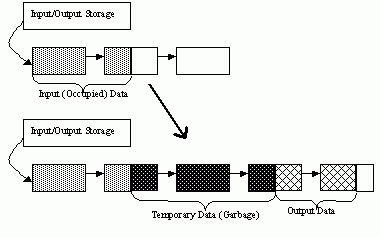
\includegraphics[width=0.5\textwidth]{pics/memstorage1.png}

That is, garbage appears in the middle of the storage. However, if
one creates a child memory storage at the beginning of processing,
writes temporary data there, and releases the child storage at the end,
no garbage will appear in the source/destination storage:

Dynamic data processing using a child storage

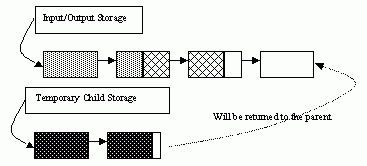
\includegraphics[width=0.5\textwidth]{pics/memstorage2.png}

\cvCPyFunc{CreateGraph}
Creates an empty graph.

\cvdefC{CvGraph* cvCreateGraph( \par int graph\_flags,\par int header\_size,\par int vtx\_size,\par int edge\_size,\par CvMemStorage* storage );}

\begin{description}
\cvarg{graph\_flags}{Type of the created graph. Usually, it is either \texttt{CV\_SEQ\_KIND\_GRAPH} for generic unoriented graphs and
\texttt{CV\_SEQ\_KIND\_GRAPH | CV\_GRAPH\_FLAG\_ORIENTED} for generic oriented graphs.}
\cvarg{header\_size}{Graph header size; may not be less than \texttt{sizeof(CvGraph)}}
\cvarg{vtx\_size}{Graph vertex size; the custom vertex structure must start with \cross{CvGraphVtx} (use \texttt{CV\_GRAPH\_VERTEX\_FIELDS()})}
\cvarg{edge\_size}{Graph edge size; the custom edge structure must start with \cross{CvGraphEdge} (use \texttt{CV\_GRAPH\_EDGE\_FIELDS()})}
\cvarg{storage}{The graph container}
\end{description}

The function creates an empty graph and returns a pointer to it.

\cvCPyFunc{CreateGraphScanner}
Creates structure for depth-first graph traversal.

\cvdefC{
CvGraphScanner*  cvCreateGraphScanner( \par CvGraph* graph,\par CvGraphVtx* vtx=NULL,\par int mask=CV\_GRAPH\_ALL\_ITEMS );
}

\begin{description}
\cvarg{graph}{Graph}
\cvarg{vtx}{Initial vertex to start from. If NULL, the traversal starts from the first vertex (a vertex with the minimal index in the sequence of vertices).}
\cvarg{mask}{Event mask indicating which events are of interest to the user (where \cvCPyCross{NextGraphItem} function returns control to the user) It can be \texttt{CV\_GRAPH\_ALL\_ITEMS} (all events are of interest) or a combination of the following flags:

\begin{description}
\cvarg{CV\_GRAPH\_VERTEX}{stop at the graph vertices visited for the first time}
\cvarg{CV\_GRAPH\_TREE\_EDGE}{stop at tree edges (\texttt{tree edge} is the edge connecting the last visited vertex and the vertex to be visited next)}
\cvarg{CV\_GRAPH\_BACK\_EDGE}{stop at back edges (\texttt{back edge} is an edge connecting the last visited vertex with some of its ancestors in the search tree)}
\cvarg{CV\_GRAPH\_FORWARD\_EDGE}{stop at forward edges (\texttt{forward edge} is an edge conecting the last visited vertex with some of its descendants in the search tree. The forward edges are only possible during oriented graph traversal)}
\cvarg{CV\_GRAPH\_CROSS\_EDGE}{stop at cross edges (\texttt{cross edge} is an edge connecting different search trees or branches of the same tree. The \texttt{cross edges} are only possible during oriented graph traversal)}
\cvarg{CV\_GRAPH\_ANY\_EDGE}{stop at any edge (\texttt{tree, back, forward}, and \texttt{cross edges})}
\cvarg{CV\_GRAPH\_NEW\_TREE}{stop in the beginning of every new search tree. When the traversal procedure visits all vertices and edges reachable from the initial vertex (the visited vertices together with tree edges make up a tree), it searches for some unvisited vertex in the graph and resumes the traversal process from that vertex. Before starting a new tree (including the very first tree when \texttt{cvNextGraphItem} is called for the first time) it generates a \texttt{CV\_GRAPH\_NEW\_TREE} event. For unoriented graphs, each search tree corresponds to a connected component of the graph.}
\cvarg{CV\_GRAPH\_BACKTRACKING}{stop at every already visited vertex during backtracking - returning to already visited vertexes of the traversal tree.}
\end{description}}
\end{description}

The function creates a structure for depth-first graph traversal/search. The initialized structure is used in the \cvCPyCross{NextGraphItem} function - the incremental traversal procedure.

\fi

\cvCPyFunc{CreateMemStorage}
Creates memory storage.

\cvdefC{CvMemStorage* cvCreateMemStorage( int blockSize=0 );}
\cvdefPy{CreateMemStorage(blockSize = 0) -> memstorage}

\begin{description}
\cvarg{blockSize}{Size of the storage blocks in bytes. If it is 0, the block size is set to a default value - currently it is  about 64K.}
\end{description}

The function creates an empty memory storage. See \cross{CvMemStorage} description.

\ifC

\cvCPyFunc{CreateSeq}
Creates a sequence.

\cvdefC{CvSeq* cvCreateSeq( \par int seqFlags,\par int headerSize,\par int elemSize,\par CvMemStorage* storage);}

\begin{description}
\cvarg{seqFlags}{Flags of the created sequence. If the sequence is not passed to any function working with a specific type of sequences, the sequence value may be set to 0, otherwise the appropriate type must be selected from the list of predefined sequence types.}
\cvarg{headerSize}{Size of the sequence header; must be greater than or equal to \texttt{sizeof(CvSeq)}. If a specific type or its extension is indicated, this type must fit the base type header.}
\cvarg{elemSize}{Size of the sequence elements in bytes. The size must be consistent with the sequence type. For example, for a sequence of points to be created, the element type \newline \texttt{CV\_SEQ\_ELTYPE\_POINT} should be specified and the parameter \texttt{elemSize} must be equal to \texttt{sizeof(CvPoint)}.}
\cvarg{storage}{Sequence location}
\end{description}

The function creates a sequence and returns
the pointer to it. The function allocates the sequence header in
the storage block as one continuous chunk and sets the structure
fields \texttt{flags}, \texttt{elemSize}, \texttt{headerSize}, and
\texttt{storage} to passed values, sets \texttt{delta\_elems} to the
default value (that may be reassigned using the \cvCPyCross{SetSeqBlockSize}
function), and clears other header fields, including the space following
the first \texttt{sizeof(CvSeq)} bytes.

\cvCPyFunc{CreateSet}
Creates an empty set.

\cvdefC{CvSet* cvCreateSet( \par int set\_flags,\par int header\_size,\par int elem\_size,\par CvMemStorage* storage );}

\begin{description}
\cvarg{set\_flags}{Type of the created set}
\cvarg{header\_size}{Set header size; may not be less than \texttt{sizeof(CvSet)}}
\cvarg{elem\_size}{Set element size; may not be less than \cross{CvSetElem}}
\cvarg{storage}{Container for the set}
\end{description}

The function creates an empty set with a specified header size and element size, and returns the pointer to the set. This function is just a thin layer on top of \cvCPyCross{CreateSeq}.

\cvCPyFunc{CvtSeqToArray}
Copies a sequence to one continuous block of memory.

\cvdefC{void* cvCvtSeqToArray( \par const CvSeq* seq,\par void* elements,\par CvSlice slice=CV\_WHOLE\_SEQ );}

\begin{description}
\cvarg{seq}{Sequence}
\cvarg{elements}{Pointer to the destination array that must be large enough. It should be a pointer to data, not a matrix header.}
\cvarg{slice}{The sequence portion to copy to the array}
\end{description}

The function copies the entire sequence or subsequence to the specified buffer and returns the pointer to the buffer.

\cvCPyFunc{EndWriteSeq}
Finishes the process of writing a sequence.

\cvdefC{CvSeq* cvEndWriteSeq( CvSeqWriter* writer );}

\begin{description}
\cvarg{writer}{Writer state}
\end{description}


The function finishes the writing process and
returns the pointer to the written sequence. The function also truncates
the last incomplete sequence block to return the remaining part of the
block to memory storage. After that, the sequence can be read and
modified safely. See \cvCPyCross{cvStartWriteSeq} and \cvCPyCross{cvStartAppendToSeq}

\cvCPyFunc{FindGraphEdge}
Finds an edge in a graph.

\cvdefC{
CvGraphEdge* cvFindGraphEdge( const CvGraph* graph, int start\_idx, int end\_idx );
}

\begin{lstlisting}

#define cvGraphFindEdge cvFindGraphEdge

\end{lstlisting}

\begin{description}
\cvarg{graph}{Graph}
\cvarg{start\_idx}{Index of the starting vertex of the edge}
\cvarg{end\_idx}{Index of the ending vertex of the edge. For an unoriented graph, the order of the vertex parameters does not matter.}
\end{description}

The function finds the graph edge connecting two specified vertices and returns a pointer to it or NULL if the edge does not exist.

\cvCPyFunc{FindGraphEdgeByPtr}
Finds an edge in a graph by using its pointer.

\cvdefC{
CvGraphEdge* cvFindGraphEdgeByPtr( \par const CvGraph* graph,\par const CvGraphVtx* startVtx,\par const CvGraphVtx* endVtx );
}

\begin{lstlisting}
#define cvGraphFindEdgeByPtr cvFindGraphEdgeByPtr
\end{lstlisting}

\begin{description}
\cvarg{graph}{Graph}
\cvarg{startVtx}{Pointer to the starting vertex of the edge}
\cvarg{endVtx}{Pointer to the ending vertex of the edge. For an unoriented graph, the order of the vertex parameters does not matter.}
\end{description}

The function finds the graph edge connecting two specified vertices and returns pointer to it or NULL if the edge does not exists.

\cvCPyFunc{FlushSeqWriter}
Updates sequence headers from the writer.

\cvdefC{void cvFlushSeqWriter( CvSeqWriter* writer );}

\begin{description}
\cvarg{writer}{Writer state}
\end{description}

The function is intended to enable the user to
read sequence elements, whenever required, during the writing process,
e.g., in order to check specific conditions. The function updates the
sequence headers to make reading from the sequence possible. The writer
is not closed, however, so that the writing process can be continued at
any time. If an algorithm requires frequent flushes, consider using
\cvCPyCross{SeqPush} instead.

\cvCPyFunc{GetGraphVtx}
Finds a graph vertex by using its index.

\cvdefC{CvGraphVtx* cvGetGraphVtx( \par CvGraph* graph,\par int vtx\_idx );}

\begin{description}
\cvarg{graph}{Graph}
\cvarg{vtx\_idx}{Index of the vertex}
\end{description}


The function finds the graph vertex by using its index and returns the pointer to it or NULL if the vertex does not belong to the graph.


\cvCPyFunc{GetSeqElem}
Returns a pointer to a sequence element according to its index.

\cvdefC{char* cvGetSeqElem( const CvSeq* seq, int index );}

\begin{lstlisting}
#define CV_GET_SEQ_ELEM( TYPE, seq, index )  (TYPE*)cvGetSeqElem( (CvSeq*)(seq), (index) )
\end{lstlisting}

\begin{description}
\cvarg{seq}{Sequence}
\cvarg{index}{Index of element}
\end{description}

The function finds the element with the given
index in the sequence and returns the pointer to it. If the element
is not found, the function returns 0. The function supports negative
indices, where -1 stands for the last sequence element, -2 stands for
the one before last, etc. If the sequence is most likely to consist of
a single sequence block or the desired element is likely to be located
in the first block, then the macro
\texttt{CV\_GET\_SEQ\_ELEM( elemType, seq, index )}
should be used, where the parameter \texttt{elemType} is the
type of sequence elements ( \cross{CvPoint} for example), the parameter
\texttt{seq} is a sequence, and the parameter \texttt{index} is the index
of the desired element. The macro checks first whether the desired element
belongs to the first block of the sequence and returns it if it does;
otherwise the macro calls the main function \texttt{GetSeqElem}. Negative
indices always cause the \cvCPyCross{GetSeqElem} call. The function has O(1)
time complexity assuming that the number of blocks is much smaller than the
number of elements.

\cvCPyFunc{GetSeqReaderPos}
Returns the current reader position.

\cvdefC{int cvGetSeqReaderPos( CvSeqReader* reader );}

\begin{description}
\cvarg{reader}{Reader state}
\end{description}


The function returns the current reader position (within 0 ... \texttt{reader->seq->total} - 1).

\cvCPyFunc{GetSetElem}
Finds a set element by its index.

\cvdefC{CvSetElem* cvGetSetElem( \par const CvSet* setHeader,\par int index );}

\begin{description}
\cvarg{setHeader}{Set}
\cvarg{index}{Index of the set element within a sequence}
\end{description}

The function finds a set element by its index. The function returns the pointer to it or 0 if the index is invalid or the corresponding node is free. The function supports negative indices as it uses \cvCPyCross{GetSeqElem} to locate the node.

\cvCPyFunc{GraphAddEdge}
Adds an edge to a graph.

\cvdefC{int cvGraphAddEdge( \par CvGraph* graph,\par int start\_idx,\par int end\_idx,\par const CvGraphEdge* edge=NULL,\par CvGraphEdge** inserted\_edge=NULL );
}

\begin{description}
\cvarg{graph}{Graph}
\cvarg{start\_idx}{Index of the starting vertex of the edge}
\cvarg{end\_idx}{Index of the ending vertex of the edge. For an unoriented graph, the order of the vertex parameters does not matter.}
\cvarg{edge}{Optional input parameter, initialization data for the edge}
\cvarg{inserted\_edge}{Optional output parameter to contain the address of the inserted edge}
\end{description}


The function connects two specified vertices. The function returns 1 if the edge has been added successfully, 0 if the edge connecting the two vertices exists already and -1 if either of the vertices was not found, the starting and the ending vertex are the same, or there is some other critical situation. In the latter case (i.e., when the result is negative), the function also reports an error by default.

\cvCPyFunc{GraphAddEdgeByPtr}
Adds an edge to a graph by using its pointer.

\cvdefC{int cvGraphAddEdgeByPtr( \par CvGraph* graph,\par CvGraphVtx* start\_vtx,\par CvGraphVtx* end\_vtx,\par const CvGraphEdge* edge=NULL,\par CvGraphEdge** inserted\_edge=NULL );}

\begin{description}
\cvarg{graph}{Graph}
\cvarg{start\_vtx}{Pointer to the starting vertex of the edge}
\cvarg{end\_vtx}{Pointer to the ending vertex of the edge. For an unoriented graph, the order of the vertex parameters does not matter.}
\cvarg{edge}{Optional input parameter, initialization data for the edge}
\cvarg{inserted\_edge}{Optional output parameter to contain the address of the inserted edge within the edge set}
\end{description}

The function connects two specified vertices. The
function returns 1 if the edge has been added successfully, 0 if the
edge connecting the two vertices exists already, and -1 if either of the
vertices was not found, the starting and the ending vertex are the same
or there is some other critical situation. In the latter case (i.e., when
the result is negative), the function also reports an error by default.

\cvCPyFunc{GraphAddVtx}
Adds a vertex to a graph.

\cvdefC{
int cvGraphAddVtx( \par CvGraph* graph,\par const CvGraphVtx* vtx=NULL,\par CvGraphVtx** inserted\_vtx=NULL );}

\begin{description}
\cvarg{graph}{Graph}
\cvarg{vtx}{Optional input argument used to initialize the added vertex (only user-defined fields beyond \texttt{sizeof(CvGraphVtx)} are copied)}
\cvarg{inserted\_vertex}{Optional output argument. If not \texttt{NULL}, the address of the new vertex is written here.}
\end{description}

The function adds a vertex to the graph and returns the vertex index.

\cvCPyFunc{GraphEdgeIdx}
Returns the index of a graph edge.

\cvdefC{
int cvGraphEdgeIdx( \par CvGraph* graph,\par CvGraphEdge* edge );
}

\begin{description}
\cvarg{graph}{Graph}
\cvarg{edge}{Pointer to the graph edge}
\end{description}

The function returns the index of a graph edge.

\cvCPyFunc{GraphRemoveEdge}
Removes an edge from a graph.

\cvdefC{void cvGraphRemoveEdge( \par CvGraph* graph,\par int start\_idx,\par int end\_idx );}

\begin{description}
\cvarg{graph}{Graph}
\cvarg{start\_idx}{Index of the starting vertex of the edge}
\cvarg{end\_idx}{Index of the ending vertex of the edge. For an unoriented graph, the order of the vertex parameters does not matter.}
\end{description}

The function removes the edge connecting two specified vertices. If the vertices are not connected [in that order], the function does nothing.

\cvCPyFunc{GraphRemoveEdgeByPtr}

Removes an edge from a graph by using its pointer.

\cvdefC{void cvGraphRemoveEdgeByPtr( \par CvGraph* graph,\par CvGraphVtx* start\_vtx,\par CvGraphVtx* end\_vtx );}

\begin{description}
\cvarg{graph}{Graph}
\cvarg{start\_vtx}{Pointer to the starting vertex of the edge}
\cvarg{end\_vtx}{Pointer to the ending vertex of the edge. For an unoriented graph, the order of the vertex parameters does not matter.}
\end{description}

The function removes the edge connecting two specified vertices. If the vertices are not connected [in that order], the function does nothing.

\cvCPyFunc{GraphRemoveVtx}
Removes a vertex from a graph.

\cvdefC{int cvGraphRemoveVtx( \par CvGraph* graph,\par int index );}

\begin{description}
\cvarg{graph}{Graph}
\cvarg{vtx\_idx}{Index of the removed vertex}
\end{description}

The function removes a vertex from a graph
together with all the edges incident to it. The function reports an error
if the input vertex does not belong to the graph. The return value is the
number of edges deleted, or -1 if the vertex does not belong to the graph.

\cvCPyFunc{GraphRemoveVtxByPtr}
Removes a vertex from a graph by using its pointer.

\cvdefC{int cvGraphRemoveVtxByPtr( \par CvGraph* graph,\par CvGraphVtx* vtx );}

\begin{description}
\cvarg{graph}{Graph}
\cvarg{vtx}{Pointer to the removed vertex}
\end{description}


The function removes a vertex from the graph by using its pointer together with all the edges incident to it. The function reports an error if the vertex does not belong to the graph. The return value is the number of edges deleted, or -1 if the vertex does not belong to the graph.

\cvCPyFunc{GraphVtxDegree}
Counts the number of edges indicent to the vertex.

\cvdefC{
int cvGraphVtxDegree( const CvGraph* graph, int vtxIdx );
}

\begin{description}
\cvarg{graph}{Graph}
\cvarg{vtxIdx}{Index of the graph vertex}
\end{description}

The function returns the number of edges incident to the specified vertex, both incoming and outgoing. To count the edges, the following code is used:

\begin{lstlisting}
CvGraphEdge* edge = vertex->first; int count = 0;
while( edge )
{
    edge = CV_NEXT_GRAPH_EDGE( edge, vertex );
    count++;
}
\end{lstlisting}

The macro \texttt{CV\_NEXT\_GRAPH\_EDGE( edge, vertex )} returns the edge incident to \texttt{vertex} that follows after \texttt{edge}.

\cvCPyFunc{GraphVtxDegreeByPtr}
Finds an edge in a graph.

\cvdefC{
int cvGraphVtxDegreeByPtr( \par const CvGraph* graph,\par const CvGraphVtx* vtx );
}

\begin{description}
\cvarg{graph}{Graph}
\cvarg{vtx}{Pointer to the graph vertex}
\end{description}

The function returns the number of edges incident to the specified vertex, both incoming and outcoming.


\cvCPyFunc{GraphVtxIdx}
Returns the index of a graph vertex.

\cvdefC{int cvGraphVtxIdx( \par CvGraph* graph,\par CvGraphVtx* vtx );}

\begin{description}
\cvarg{graph}{Graph}
\cvarg{vtx}{Pointer to the graph vertex}
\end{description}

The function returns the index of a graph vertex.

\cvCPyFunc{InitTreeNodeIterator}

Initializes the tree node iterator.

\cvdefC{

void cvInitTreeNodeIterator( \par CvTreeNodeIterator* tree\_iterator,\par const void* first,\par int max\_level );

}

\begin{description}
\cvarg{tree\_iterator}{Tree iterator initialized by the function}
\cvarg{first}{The initial node to start traversing from}
\cvarg{max\_level}{The maximal level of the tree (\texttt{first} node assumed to be at the first level) to traverse up to. For example, 1 means that only nodes at the same level as \texttt{first} should be visited, 2 means that the nodes on the same level as \texttt{first} and their direct children should be visited, and so forth.}
\end{description}

The function initializes the tree iterator. The tree is traversed in depth-first order.

\cvCPyFunc{InsertNodeIntoTree}

Adds a new node to a tree.

\cvdefC{void cvInsertNodeIntoTree( \par void* node,\par void* parent,\par void* frame );}

\begin{description}
\cvarg{node}{The inserted node}
\cvarg{parent}{The parent node that is already in the tree}
\cvarg{frame}{The top level node. If \texttt{parent} and \texttt{frame} are the same, the \texttt{v\_prev} field of \texttt{node} is set to NULL rather than \texttt{parent}.}
\end{description}

The function adds another node into tree. The function does not allocate any memory, it can only modify links of the tree nodes.

\cvCPyFunc{MakeSeqHeaderForArray}
Constructs a sequence header for an array.

\cvdefC{CvSeq* cvMakeSeqHeaderForArray( \par int seq\_type,\par int header\_size,\par int elem\_size,\par void* elements,\par int total,\par CvSeq* seq,\par CvSeqBlock* block );}

\begin{description}
\cvarg{seq\_type}{Type of the created sequence}
\cvarg{header\_size}{Size of the header of the sequence. Parameter sequence must point to the structure of that size or greater}
\cvarg{elem\_size}{Size of the sequence elements}
\cvarg{elements}{Elements that will form a sequence}
\cvarg{total}{Total number of elements in the sequence. The number of array elements must be equal to the value of this parameter.}
\cvarg{seq}{Pointer to the local variable that is used as the sequence header}
\cvarg{block}{Pointer to the local variable that is the header of the single sequence block}
\end{description}

The function initializes a sequence
header for an array. The sequence header as well as the sequence block are
allocated by the user (for example, on stack). No data is copied by the
function. The resultant sequence will consists of a single block and
have NULL storage pointer; thus, it is possible to read its elements,
but the attempts to add elements to the sequence will raise an error in
most cases.

\cvCPyFunc{MemStorageAlloc}
Allocates a memory buffer in a storage block.

\cvdefC{void* cvMemStorageAlloc( \par CvMemStorage* storage,\par size\_t size );}

\begin{description}
\cvarg{storage}{Memory storage}
\cvarg{size}{Buffer size}
\end{description}

The function allocates a memory buffer in
a storage block. The buffer size must not exceed the storage block size,
otherwise a runtime error is raised. The buffer address is aligned by
\texttt{CV\_STRUCT\_ALIGN=sizeof(double)} (for the moment) bytes.

\cvCPyFunc{MemStorageAllocString}
Allocates a text string in a storage block.

\cvdefC{CvString cvMemStorageAllocString(CvMemStorage* storage, const char* ptr, int len=-1);}

\begin{lstlisting}
typedef struct CvString
{
    int len;
    char* ptr;
}
CvString;
\end{lstlisting}

\begin{description}
\cvarg{storage}{Memory storage}
\cvarg{ptr}{The string}
\cvarg{len}{Length of the string (not counting the ending \texttt{NUL}) . If the parameter is negative, the function computes the length.}
\end{description}

The function creates copy of the string
in memory storage. It returns the structure that contains user-passed
or computed length of the string and pointer to the copied string.

\cvCPyFunc{NextGraphItem}
Executes one or more steps of the graph traversal procedure.

\cvdefC{
int cvNextGraphItem( CvGraphScanner* scanner );
}

\begin{description}
\cvarg{scanner}{Graph traversal state. It is updated by this function.}
\end{description}

The function traverses through the graph
until an event of interest to the user (that is, an event, specified
in the \texttt{mask} in the \cvCPyCross{CreateGraphScanner} call) is met or the
traversal is completed. In the first case, it returns one of the events
listed in the description of the \texttt{mask} parameter above and with
the next call it resumes the traversal. In the latter case, it returns
\texttt{CV\_GRAPH\_OVER} (-1). When the event is \texttt{CV\_GRAPH\_VERTEX},
\texttt{CV\_GRAPH\_BACKTRACKING}, or \texttt{CV\_GRAPH\_NEW\_TREE},
the currently observed vertex is stored in \texttt{scanner-$>$vtx}. And if the
event is edge-related, the edge itself is stored at \texttt{scanner-$>$edge},
the previously visited vertex - at \texttt{scanner-$>$vtx} and the other ending
vertex of the edge - at \texttt{scanner-$>$dst}.

\cvCPyFunc{NextTreeNode}

Returns the currently observed node and moves the iterator toward the next node.

\cvdefC{

void* cvNextTreeNode( CvTreeNodeIterator* tree\_iterator );

}

\begin{description}
\cvarg{tree\_iterator}{Tree iterator initialized by the function}
\end{description}


The function returns the currently observed node and then updates the iterator - moving it toward the next node. In other words, the function behavior is similar to the *p++ expression on a typical C pointer or C++ collection iterator. The function returns NULL if there are no more nodes.


\cvCPyFunc{PrevTreeNode}

Returns the currently observed node and moves the iterator toward the previous node.

\cvdefC{

void* cvPrevTreeNode( CvTreeNodeIterator* tree\_iterator );

}

\begin{description}
\cvarg{tree\_iterator}{Tree iterator initialized by the function}
\end{description}


The function returns the currently observed node and then updates the iterator - moving it toward the previous node. In other words, the function behavior is similar to the *p-- expression on a typicl C pointer or C++ collection iterator. The function returns NULL if there are no more nodes.


\cvCPyFunc{ReleaseGraphScanner}
Completes the graph traversal procedure.

\cvdefC{
void cvReleaseGraphScanner( CvGraphScanner** scanner );
}

\begin{description}
\cvarg{scanner}{Double pointer to graph traverser}
\end{description}


The function completes the graph traversal procedure and releases the traverser state.



\cvCPyFunc{ReleaseMemStorage}
Releases memory storage.

\cvdefC{void cvReleaseMemStorage( CvMemStorage** storage );}

\begin{description}
\cvarg{storage}{Pointer to the released storage}
\end{description}

The function deallocates all storage memory
blocks or returns them to the parent, if any. Then it deallocates the
storage header and clears the pointer to the storage. All child storage 
associated with a given parent storage block must be released before the 
parent storage block is released.

\cvCPyFunc{RestoreMemStoragePos}
Restores memory storage position.

\cvdefC{void cvRestoreMemStoragePos(\par CvMemStorage* storage,\par CvMemStoragePos* pos);}

\begin{description}
\cvarg{storage}{Memory storage}
\cvarg{pos}{New storage top position}
\end{description}

The function restores the position of the storage top from the parameter \texttt{pos}. This function and the function \texttt{cvClearMemStorage} are the only methods to release memory occupied in memory blocks. Note again that there is no way to free memory in the middle of an occupied portion of a storage block.


\cvCPyFunc{SaveMemStoragePos}
Saves memory storage position.

\cvdefC{void cvSaveMemStoragePos(\par const CvMemStorage* storage,\par CvMemStoragePos* pos);}

\begin{description}
\cvarg{storage}{Memory storage}
\cvarg{pos}{The output position of the storage top}
\end{description}

The function saves the current position
of the storage top to the parameter \texttt{pos}. The function
\texttt{cvRestoreMemStoragePos} can further retrieve this position.

\cvCPyFunc{SeqElemIdx}
Returns the index of a specific sequence element.

\cvdefC{int cvSeqElemIdx( \par const CvSeq* seq,\par const void* element,\par CvSeqBlock** block=NULL );}

\begin{description}
\cvarg{seq}{Sequence}
\cvarg{element}{Pointer to the element within the sequence}
\cvarg{block}{Optional argument. If the pointer is not \texttt{NULL}, the address of the sequence block that contains the element is stored in this location.}
\end{description}

The function returns the index of a sequence element or a negative number if the element is not found.

\cvCPyFunc{SeqInsert}
Inserts an element in the middle of a sequence.

\cvdefC{char* cvSeqInsert( \par CvSeq* seq,\par int beforeIndex,\par void* element=NULL );}

\begin{description}
\cvarg{seq}{Sequence}
\cvarg{beforeIndex}{Index before which the element is inserted. Inserting before 0 (the minimal allowed value of the parameter) is equal to \cvCPyCross{SeqPushFront} and inserting before \texttt{seq->total} (the maximal allowed value of the parameter) is equal to \cvCPyCross{SeqPush}.}
\cvarg{element}{Inserted element} 
\end{description}

The function shifts the sequence elements from the inserted position to the nearest end of the sequence and copies the \texttt{element} content there if the pointer is not NULL. The function returns a pointer to the inserted element.


\cvCPyFunc{SeqInsertSlice}
Inserts an array in the middle of a sequence.

\cvdefC{void cvSeqInsertSlice( \par CvSeq* seq,\par int beforeIndex,\par const CvArr* fromArr );}

\begin{description}
\cvarg{seq}{Sequence}
\cvarg{slice}{The part of the sequence to remove}
\cvarg{fromArr}{The array to take elements from}
\end{description}


The function inserts all \texttt{fromArr}
array elements at the specified position of the sequence. The array
\texttt{fromArr} can be a matrix or another sequence.

\fi

\cvCPyFunc{SeqInvert}
Reverses the order of sequence elements.

\cvdefC{void cvSeqInvert( CvSeq* seq );}
\cvdefPy{SeqInvert(seq)-> None}

\begin{description}
\cvarg{seq}{Sequence}
\end{description}


The function reverses the sequence in-place - makes the first element go last, the last element go first and so forth.

\ifC

\cvCPyFunc{SeqPop}
Removes an element from the end of a sequence.

\cvdefC{void cvSeqPop( \par CvSeq* seq,\par void* element=NULL );}

\begin{description}
\cvarg{seq}{Sequence}
\cvarg{element}{Optional parameter . If the pointer is not zero, the function copies the removed element to this location.}
\end{description}

The function removes an element from a sequence. The function reports an error if the sequence is already empty. The function has O(1) complexity.

\cvCPyFunc{SeqPopFront}
Removes an element from the beginning of a sequence.

\cvdefC{void cvSeqPopFront( \par \par CvSeq* seq,\par\par void* element=NULL );}

\begin{description}
\cvarg{seq}{Sequence}
\cvarg{element}{Optional parameter. If the pointer is not zero, the function copies the removed element to this location.}
\end{description}

The function removes an element from the beginning of a sequence. The function reports an error if the sequence is already empty. The function has O(1) complexity.

\cvCPyFunc{SeqPopMulti}
Removes several elements from either end of a sequence.

\cvdefC{void cvSeqPopMulti( \par CvSeq* seq,\par void* elements,\par int count,\par int in\_front=0 );}

\begin{description}
\cvarg{seq}{Sequence}
\cvarg{elements}{Removed elements}
\cvarg{count}{Number of elements to pop}
\cvarg{in\_front}{The flags specifying which end of the modified sequence.
\begin{description}
\cvarg{CV\_BACK}{the elements are added to the end of the sequence}
\cvarg{CV\_FRONT}{the elements are added to the beginning of the sequence}
\end{description}}
\end{description}

The function removes several elements from either end of the sequence. If the number of the elements to be removed exceeds the total number of elements in the sequence, the function removes as many elements as possible.

\cvCPyFunc{SeqPush}
Adds an element to the end of a sequence.

\cvdefC{char* cvSeqPush( \par CvSeq* seq,\par void* element=NULL );}

\begin{description}
\cvarg{seq}{Sequence}
\cvarg{element}{Added element}
\end{description}

The function adds an element to the end of a sequence and returns a pointer to the allocated element. If the input \texttt{element} is NULL, the function simply allocates a space for one more element.

The following code demonstrates how to create a new sequence using this function:

\begin{lstlisting}
CvMemStorage* storage = cvCreateMemStorage(0);
CvSeq* seq = cvCreateSeq( CV_32SC1, /* sequence of integer elements */
                          sizeof(CvSeq), /* header size - no extra fields */
                          sizeof(int), /* element size */
                          storage /* the container storage */ );
int i;
for( i = 0; i < 100; i++ )
{
    int* added = (int*)cvSeqPush( seq, &i );
    printf( "%d is added\n", *added );
}

...
/* release memory storage in the end */
cvReleaseMemStorage( &storage );
\end{lstlisting}

The function has O(1) complexity, but there is a faster method for writing large sequences (see \cvCPyCross{StartWriteSeq} and related functions).


\cvCPyFunc{SeqPushFront}
Adds an element to the beginning of a sequence.

\cvdefC{char* cvSeqPushFront( CvSeq* seq, void* element=NULL );}

\begin{description}
\cvarg{seq}{Sequence}
\cvarg{element}{Added element}
\end{description}

The function is similar to \cvCPyCross{SeqPush} but it adds the new element to the beginning of the sequence. The function has O(1) complexity.

\cvCPyFunc{SeqPushMulti}
Pushes several elements to either end of a sequence.

\cvdefC{void cvSeqPushMulti( \par CvSeq* seq,\par void* elements,\par int count,\par int in\_front=0 );}

\begin{description}
\cvarg{seq}{Sequence}
\cvarg{elements}{Added elements}
\cvarg{count}{Number of elements to push}
\cvarg{in\_front}{The flags specifying which end of the modified sequence.
\begin{description}
\cvarg{CV\_BACK}{the elements are added to the end of the sequence}
\cvarg{CV\_FRONT}{the elements are added to the beginning of the sequence}
\end{description}}
\end{description}

The function adds several elements to either
end of a sequence. The elements are added to the sequence in the same
order as they are arranged in the input array but they can fall into
different sequence blocks.

\fi

\cvCPyFunc{SeqRemove}
Removes an element from the middle of a sequence.

\cvdefC{void cvSeqRemove( \par CvSeq* seq,\par int index );}
\cvdefPy{SeqRemove(seq,index)-> None}

\begin{description}
\cvarg{seq}{Sequence}
\cvarg{index}{Index of removed element}
\end{description}

The function removes elements with the given
index. If the index is out of range the function reports an error. An
attempt to remove an element from an empty sequence is a special
case of this situation. The function removes an element by shifting
the sequence elements between the nearest end of the sequence and the
\texttt{index}-th position, not counting the latter.


\cvCPyFunc{SeqRemoveSlice}
Removes a sequence slice.

\cvdefC{void cvSeqRemoveSlice( CvSeq* seq, CvSlice slice );}
\cvdefPy{SeqRemoveSlice(seq,slice)-> None}

\begin{description}
\cvarg{seq}{Sequence}
\cvarg{slice}{The part of the sequence to remove}
\end{description}

The function removes a slice from the sequence.

\ifC

\cvCPyFunc{SeqSearch}
Searches for an element in a sequence.

\begin{lstlisting}
/* a < b ? -1 : a > b ? 1 : 0 */
typedef int (CV_CDECL* CvCmpFunc)(const void* a, const void* b, void* userdata);

char* cvSeqSearch( CvSeq* seq, const void* elem, CvCmpFunc func,
                   int is_sorted, int* elem_idx, void* userdata=NULL );
\end{lstlisting}

\begin{description}
\cvarg{seq}{The sequence}
\cvarg{elem}{The element to look for}
\cvarg{func}{The comparison function that returns negative, zero or positive value depending on the relationships among the elements (see also \cvCPyCross{SeqSort})}
\cvarg{is\_sorted}{Whether the sequence is sorted or not}
\cvarg{elem\_idx}{Output parameter; index of the found element}
\cvarg{userdata}{The user parameter passed to the compasion function; helps to avoid global variables in some cases}
\end{description}

The function searches for the element in the sequence. If
the sequence is sorted, a binary O(log(N)) search is used; otherwise, a
simple linear search is used. If the element is not found, the function
returns a NULL pointer and the index is set to the number of sequence
elements if a linear search is used, or to the smallest index
\texttt{i, seq(i)>elem}.

\cvCPyFunc{SeqSlice}
Makes a separate header for a sequence slice.

\cvdefC{CvSeq* cvSeqSlice( \par const CvSeq* seq,\par CvSlice slice,\par CvMemStorage* storage=NULL,\par int copy\_data=0 );}

\begin{description}
\cvarg{seq}{Sequence}
\cvarg{slice}{The part of the sequence to be extracted}
\cvarg{storage}{The destination storage block to hold the new sequence header and the copied data, if any. If it is NULL, the function uses the storage block containing the input sequence.}
\cvarg{copy\_data}{The flag that indicates whether to copy the elements of the extracted slice (\texttt{copy\_data!=0}) or not (\texttt{copy\_data=0})}
\end{description}

The function creates a sequence that represents the specified slice of the input sequence. The new sequence either shares the elements with the original sequence or has its own copy of the elements. So if one needs to process a part of sequence but the processing function does not have a slice parameter, the required sub-sequence may be extracted using this function.

\cvCPyFunc{SeqSort}
Sorts sequence element using the specified comparison function.

\cvdefC{void cvSeqSort( CvSeq* seq, CvCmpFunc func, void* userdata=NULL );}

\begin{lstlisting}
/* a < b ? -1 : a > b ? 1 : 0 */
typedef int (CV_CDECL* CvCmpFunc)(const void* a, const void* b, void* userdata);
\end{lstlisting}

\begin{description}
\cvarg{seq}{The sequence to sort}
\cvarg{func}{The comparison function that returns a negative, zero, or positive value depending on the relationships among the elements (see the above declaration and the example below) - a similar function is used by \texttt{qsort} from C runline except that in the latter, \texttt{userdata} is not used}
\cvarg{userdata}{The user parameter passed to the compasion function; helps to avoid global variables in some cases}
\end{description}

The function sorts the sequence in-place using the specified criteria. Below is an example of using this function:

\begin{lstlisting}
/* Sort 2d points in top-to-bottom left-to-right order */
static int cmp_func( const void* _a, const void* _b, void* userdata )
{
    CvPoint* a = (CvPoint*)_a;
    CvPoint* b = (CvPoint*)_b;
    int y_diff = a->y - b->y;
    int x_diff = a->x - b->x;
    return y_diff ? y_diff : x_diff;
}

...

CvMemStorage* storage = cvCreateMemStorage(0);
CvSeq* seq = cvCreateSeq( CV_32SC2, sizeof(CvSeq), sizeof(CvPoint), storage );
int i;

for( i = 0; i < 10; i++ )
{
    CvPoint pt;
    pt.x = rand() % 1000;
    pt.y = rand() % 1000;
    cvSeqPush( seq, &pt );
}

cvSeqSort( seq, cmp_func, 0 /* userdata is not used here */ );

/* print out the sorted sequence */
for( i = 0; i < seq->total; i++ )
{
    CvPoint* pt = (CvPoint*)cvSeqElem( seq, i );
    printf( "(%d,%d)\n", pt->x, pt->y );
}

cvReleaseMemStorage( &storage );
\end{lstlisting}


\cvCPyFunc{SetAdd}
Occupies a node in the set.

\cvdefC{int cvSetAdd( \par CvSet* setHeader,\par CvSetElem* elem=NULL,\par CvSetElem** inserted\_elem=NULL );}

\begin{description}
\cvarg{setHeader}{Set}
\cvarg{elem}{Optional input argument, an inserted element. If not NULL, the function copies the data to the allocated node (the MSB of the first integer field is cleared after copying).}
\cvarg{inserted\_elem}{Optional output argument; the pointer to the allocated cell}
\end{description}

The function allocates a new node, optionally copies
input element data to it, and returns the pointer and the index to the
node. The index value is taken from the lower bits of the \texttt{flags}
field of the node. The function has O(1) complexity; however, there exists
a faster function for allocating set nodes (see \cvCPyCross{SetNew}).

\cvCPyFunc{SetNew}
Adds an element to a set (fast variant).

\cvdefC{CvSetElem* cvSetNew( CvSet* setHeader );}

\begin{description}
\cvarg{setHeader}{Set}
\end{description}

The function is an inline lightweight variant of \cvCPyCross{SetAdd}. It occupies a new node and returns a pointer to it rather than an index.


\cvCPyFunc{SetRemove}
Removes an element from a set.

\cvdefC{void cvSetRemove( \par CvSet* setHeader,\par int index );}

\begin{description}
\cvarg{setHeader}{Set}
\cvarg{index}{Index of the removed element}
\end{description}

The function removes an element with a specified
index from the set. If the node at the specified location is not occupied,
the function does nothing. The function has O(1) complexity; however,
\cvCPyCross{SetRemoveByPtr} provides a quicker way to remove a set element
if it is located already.

\cvCPyFunc{SetRemoveByPtr}
Removes a set element based on its pointer.

\cvdefC{void cvSetRemoveByPtr( \par CvSet* setHeader,\par void* elem );}

\begin{description}
\cvarg{setHeader}{Set}
\cvarg{elem}{Removed element}
\end{description}

The function is an inline lightweight variant of \cvCPyCross{SetRemove} that requires an element pointer. The function does not check whether the node is occupied or not - the user should take care of that.


\cvCPyFunc{SetSeqBlockSize}
Sets up sequence block size.

\cvdefC{void cvSetSeqBlockSize( \par CvSeq* seq,\par int deltaElems );}

\begin{description}
\cvarg{seq}{Sequence}
\cvarg{deltaElems}{Desirable sequence block size for elements}
\end{description}

The function affects memory allocation
granularity. When the free space in the sequence buffers has run out,
the function allocates the space for \texttt{deltaElems} sequence
elements. If this block immediately follows the one previously allocated,
the two blocks are concatenated; otherwise, a new sequence block is
created. Therefore, the bigger the parameter is, the lower the possible
sequence fragmentation, but the more space in the storage block is wasted. When
the sequence is created, the parameter \texttt{deltaElems} is set to
the default value of about 1K. The function can be called any time after
the sequence is created and affects future allocations. The function
can modify the passed value of the parameter to meet memory storage
constraints.

\cvCPyFunc{SetSeqReaderPos}
Moves the reader to the specified position.

\cvdefC{void cvSetSeqReaderPos( \par CvSeqReader* reader,\par int index,\par int is\_relative=0 );}

\begin{description}
\cvarg{reader}{Reader state}
\cvarg{index}{The destination position. If the positioning mode is used (see the next parameter), the actual position will be \texttt{index} mod \texttt{reader->seq->total}.}
\cvarg{is\_relative}{If it is not zero, then \texttt{index} is a relative to the current position}
\end{description}

The function moves the read position to an absolute position or relative to the current position.


\cvCPyFunc{StartAppendToSeq}
Initializes the process of writing data to a sequence.

\cvdefC{void cvStartAppendToSeq( \par CvSeq* seq,\par CvSeqWriter* writer );}

\begin{description}
\cvarg{seq}{Pointer to the sequence}
\cvarg{writer}{Writer state; initialized by the function}
\end{description}

The function initializes the process of
writing data to a sequence. Written elements are added to the end of the
sequence by using the
\texttt{CV\_WRITE\_SEQ\_ELEM( written\_elem, writer )}
macro. Note
that during the writing process, other operations on the sequence may
yield an incorrect result or even corrupt the sequence (see description of
\cvCPyCross{FlushSeqWriter}, which helps to avoid some of these problems).

\cvCPyFunc{StartReadSeq}
Initializes the process of sequential reading from a sequence.

\cvdefC{void cvStartReadSeq( \par const CvSeq* seq,\par CvSeqReader* reader,\par int reverse=0 );}

\begin{description}
\cvarg{seq}{Sequence}
\cvarg{reader}{Reader state; initialized by the function}
\cvarg{reverse}{Determines the direction of the sequence traversal. If \texttt{reverse} is 0, the reader is positioned at the first sequence element; otherwise it is positioned at the last element. }
\end{description}

The function initializes the reader state. After
that, all the sequence elements from the first one down to the last one
can be read by subsequent calls of the macro
\texttt{CV\_READ\_SEQ\_ELEM( read\_elem, reader )}
in the case of forward reading and by using
\texttt{CV\_REV\_READ\_SEQ\_ELEM( read\_elem, reader )}
in the case of reverse
reading. Both macros put the sequence element to \texttt{read\_elem} and
move the reading pointer toward the next element. A circular structure
of sequence blocks is used for the reading process, that is, after the
last element has been read by the macro \texttt{CV\_READ\_SEQ\_ELEM}, the
first element is read when the macro is called again. The same applies to
\texttt{CV\_REV\_READ\_SEQ\_ELEM}. There is no function to finish the reading
process, since it neither changes the sequence nor creates any temporary
buffers. The reader field \texttt{ptr} points to the current element of
the sequence that is to be read next. The code below demonstrates how
to use the sequence writer and reader.

\begin{lstlisting}
CvMemStorage* storage = cvCreateMemStorage(0);
CvSeq* seq = cvCreateSeq( CV_32SC1, sizeof(CvSeq), sizeof(int), storage );
CvSeqWriter writer;
CvSeqReader reader;
int i;

cvStartAppendToSeq( seq, &writer );
for( i = 0; i < 10; i++ )
{
    int val = rand()%100;
    CV_WRITE_SEQ_ELEM( val, writer );
    printf("%d is written\n", val );
}
cvEndWriteSeq( &writer );

cvStartReadSeq( seq, &reader, 0 );
for( i = 0; i < seq->total; i++ )
{
    int val;
#if 1
    CV_READ_SEQ_ELEM( val, reader );
    printf("%d is read\n", val );
#else /* alternative way, that is prefferable if sequence elements are large,
         or their size/type is unknown at compile time */
    printf("%d is read\n", *(int*)reader.ptr );
    CV_NEXT_SEQ_ELEM( seq->elem_size, reader );
#endif
}
...

cvReleaseStorage( &storage );
\end{lstlisting}

\cvCPyFunc{StartWriteSeq}
Creates a new sequence and initializes a writer for it.

\cvdefC{
void cvStartWriteSeq( \par int seq\_flags,\par int header\_size,\par int elem\_size,\par CvMemStorage* storage,\par CvSeqWriter* writer );
}

\begin{description}
\cvarg{seq\_flags}{Flags of the created sequence. If the sequence is not passed to any function working with a specific type of sequences, the sequence value may be equal to 0; otherwise the appropriate type must be selected from the list of predefined sequence types.}
\cvarg{header\_size}{Size of the sequence header. The parameter value may not be less than \texttt{sizeof(CvSeq)}. If a certain type or extension is specified, it must fit within the base type header.}
\cvarg{elem\_size}{Size of the sequence elements in bytes; must be consistent with the sequence type. For example, if a sequence of points is created (element type \texttt{CV\_SEQ\_ELTYPE\_POINT} ), then the parameter \texttt{elem\_size} must be equal to \texttt{sizeof(CvPoint)}.}
\cvarg{storage}{Sequence location}
\cvarg{writer}{Writer state; initialized by the function}
\end{description}

The function is a combination of
\cvCPyCross{CreateSeq} and \cvCPyCross{StartAppendToSeq}. The pointer to the
created sequence is stored at
\texttt{writer->seq}
and is also returned by the
\cvCPyCross{EndWriteSeq} function that should be called at the end.

\cvCPyFunc{TreeToNodeSeq}
Gathers all node pointers to a single sequence.

\cvdefC{

CvSeq* cvTreeToNodeSeq( \par const void* first,\par int header\_size,\par CvMemStorage* storage );

}

\begin{description}
\cvarg{first}{The initial tree node}
\cvarg{header\_size}{Header size of the created sequence (sizeof(CvSeq) is the most frequently used value)}
\cvarg{storage}{Container for the sequence}
\end{description}

The function puts pointers of all nodes reacheable from \texttt{first} into a single sequence. The pointers are written sequentially in the depth-first order.

\fi

\fi


\section{Drawing Functions}

Drawing functions work with matrices/images of arbitrary depth.
The boundaries of the shapes can be rendered with antialiasing (implemented only for 8-bit images for now).
All the functions include the parameter color that uses a rgb value (that may be constructed
with \texttt{CV\_RGB} \cvC{macro or the \cvCppCross{cvScalar} function}
\cvCpp{or the \cross{Scalar} constructor}) for color
images and brightness for grayscale images. For color images the order channel
is normally \emph{Blue, Green, Red}, this is what \cvCppCross{imshow}, \cvCppCross{imread} and \cvCppCross{imwrite} expect
\ifCpp
, so if you form a color using \cross{Scalar} constructor, it should look like:
\[\texttt{Scalar}(blue\_component, green\_component, red\_component[, alpha\_component])\]
\fi
\ifC
, so if you form a color using \cvCppCross{cvScalar}, it should look like:
\[\texttt{cvScalar}(blue\_component, green\_component, red\_component[, alpha\_component])\]
\fi

If you are using your own image rendering and I/O functions, you can use any channel ordering, the drawing functions process each channel independently and do not depend on the channel order or even on the color space used. The whole image can be converted from BGR to RGB or to a different color space using \cvCppCross{cvtColor}.

If a drawn figure is partially or completely outside the image, the drawing functions clip it. Also, many drawing functions can handle pixel coordinates specified with sub-pixel accuracy, that is, the coordinates can be passed as fixed-point numbers, encoded as integers. The number of fractional bits is specified by the \texttt{shift} parameter and the real point coordinates are calculated as $\texttt{Point}(x,y)\rightarrow\texttt{Point2f}(x*2^{-shift},y*2^{-shift})$. This feature is especially effective wehn rendering antialiased shapes.

Also, note that the functions do not support alpha-transparency - when the target image is 4-channnel, then the \texttt{color[3]} is simply copied to the repainted pixels. Thus, if you want to paint semi-transparent shapes, you can paint them in a separate buffer and then blend it with the main image.

\ifCPy

\cvCPyFunc{Circle}
Draws a circle.

\cvdefC{void cvCircle( \par CvArr* img,\par CvPoint center,\par int radius,\par CvScalar color,\par int thickness=1,\par int lineType=8,\par int shift=0 );}
\cvdefPy{Circle(img,center,radius,color,thickness=1,lineType=8,shift=0)-> None}

\begin{description}
\cvarg{img}{Image where the circle is drawn}
\cvarg{center}{Center of the circle}
\cvarg{radius}{Radius of the circle}
\cvarg{color}{Circle color}
\cvarg{thickness}{Thickness of the circle outline if positive, otherwise this indicates that a filled circle is to be drawn}
\cvarg{lineType}{Type of the circle boundary, see \cross{Line} description}
\cvarg{shift}{Number of fractional bits in the center coordinates and radius value}
\end{description}

The function draws a simple or filled circle with a
given center and radius.

\cvCPyFunc{ClipLine}
Clips the line against the image rectangle.

\cvdefC{int cvClipLine( \par CvSize imgSize,\par CvPoint* pt1,\par CvPoint* pt2 );}
\cvdefPy{ClipLine(img, pt1, pt2) -> (clipped\_pt1, clipped\_pt2)}
\begin{description}
\cvarg{imgSize}{Size of the image \cvPy{as a 2-tuple}}
\cvarg{pt1}{First ending point of the line segment. \cvC{It is modified by the function.}}
\cvarg{pt2}{Second ending point of the line segment. \cvC{It is modified by the function.}}
\end{description}

The function calculates a part of the line segment which is entirely within the image.
\cvC{It returns 0 if the line segment is completely outside the image and 1 otherwise.}
\cvPy{If the line segment is outside the image, it returns None. If the line segment is inside the image it returns a new pair of points.}

\cvCPyFunc{DrawContours}
Draws contour outlines or interiors in an image.

\cvdefC{
void cvDrawContours( \par CvArr *img,\par CvSeq* contour,\par CvScalar external\_color,\par CvScalar hole\_color,\par int max\_level,\par int thickness=1,\par int lineType=8 );
}
\cvdefPy{DrawContours(img,contour,external\_color,hole\_color,max\_level,thickness=1,lineType=8,offset=(0,0))-> None}

\begin{description}
\cvarg{img}{Image where the contours are to be drawn. As with any other drawing function, the contours are clipped with the ROI.}
\cvarg{contour}{Pointer to the first contour}
\cvarg{external\_color}{Color of the external contours}
\cvarg{hole\_color}{Color of internal contours (holes)}
\cvarg{max\_level}{Maximal level for drawn contours. If 0, only
\texttt{contour} is drawn. If 1, the contour and all contours following
it on the same level are drawn. If 2, all contours following and all
contours one level below the contours are drawn, and so forth. If the value
is negative, the function does not draw the contours following after
\texttt{contour} but draws the child contours of \texttt{contour} up
to the $|\texttt{max\_level}|-1$ level.}
\cvarg{thickness}{Thickness of lines the contours are drawn with.
If it is negative (For example, =CV\_FILLED), the contour interiors are
drawn.}
\cvarg{lineType}{Type of the contour segments, see \cross{Line} description}
\end{description}

The function draws contour outlines in the image if $\texttt{thickness} \ge 0$ or fills the area bounded by the contours if $ \texttt{thickness}<0$.

\ifC
\subsection{Example: Connected component detection via contour functions}
\begin{lstlisting}
#include "cv.h"
#include "highgui.h"

int main( int argc, char** argv )
{
    IplImage* src;
    // the first command line parameter must be file name of binary 
    // (black-n-white) image
    if( argc == 2 && (src=cvLoadImage(argv[1], 0))!= 0)
    {
        IplImage* dst = cvCreateImage( cvGetSize(src), 8, 3 );
        CvMemStorage* storage = cvCreateMemStorage(0);
        CvSeq* contour = 0;

        cvThreshold( src, src, 1, 255, CV_THRESH_BINARY );
        cvNamedWindow( "Source", 1 );
        cvShowImage( "Source", src );

        cvFindContours( src, storage, &contour, sizeof(CvContour), 
			CV_RETR_CCOMP, CV_CHAIN_APPROX_SIMPLE );
        cvZero( dst );

        for( ; contour != 0; contour = contour->h_next )
        {
            CvScalar color = CV_RGB( rand()&255, rand()&255, rand()&255 );
            /* replace CV_FILLED with 1 to see the outlines */
            cvDrawContours( dst, contour, color, color, -1, CV_FILLED, 8 );
        }

        cvNamedWindow( "Components", 1 );
        cvShowImage( "Components", dst );
        cvWaitKey(0);
    }
}
\end{lstlisting}
\fi

\cvCPyFunc{Ellipse}
Draws a simple or thick elliptic arc or an fills ellipse sector.

\cvdefC{void cvEllipse( \par CvArr* img,\par CvPoint center,\par CvSize axes,\par double angle,\par double start\_angle,\par double end\_angle,\par CvScalar color,\par int thickness=1,\par int lineType=8,\par int shift=0 );}
\cvdefPy{Ellipse(img,pt1,axes,angle,start\_angle,end\_angle,color,thickness=1,lineType=8,shift=0)-> None}

\begin{description}
\cvarg{img}{The image}
\cvarg{center}{Center of the ellipse}
\cvarg{axes}{Length of the ellipse axes}
\cvarg{angle}{Rotation angle}
\cvarg{start\_angle}{Starting angle of the elliptic arc}
\cvarg{end\_angle}{Ending angle of the elliptic arc.}
\cvarg{color}{Ellipse color}
\cvarg{thickness}{Thickness of the ellipse arc outline if positive, otherwise this indicates that a filled ellipse sector is to be drawn}
\cvarg{lineType}{Type of the ellipse boundary, see \cross{Line} description}
\cvarg{shift}{Number of fractional bits in the center coordinates and axes' values}
\end{description}

The function draws a simple or thick elliptic
arc or fills an ellipse sector. The arc is clipped by the ROI rectangle.
A piecewise-linear approximation is used for antialiased arcs and
thick arcs. All the angles are given in degrees. The picture below
explains the meaning of the parameters.

Parameters of Elliptic Arc

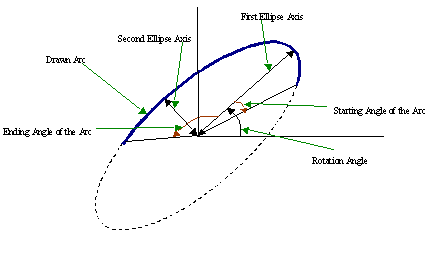
\includegraphics[width=0.5\textwidth]{pics/ellipse.png}

\cvCPyFunc{EllipseBox}

Draws a simple or thick elliptic arc or fills an ellipse sector.

\cvdefC{void cvEllipseBox( \par CvArr* img, \par CvBox2D box, \par CvScalar color,
                   \par int thickness=1, \par int lineType=8, \par int shift=0 );}
\cvdefPy{EllipseBox(img,box,color,thickness=1,lineType=8,shift=0)-> None}

\begin{description}
\cvarg{img}{Image}
\cvarg{box}{The enclosing box of the ellipse drawn}
\cvarg{thickness}{Thickness of the ellipse boundary}
\cvarg{lineType}{Type of the ellipse boundary, see \cross{Line} description}
\cvarg{shift}{Number of fractional bits in the box vertex coordinates}
\end{description}

The function draws a simple or thick ellipse outline, or fills an ellipse. The functions provides a convenient way to draw an ellipse approximating some shape; that is what \cross{CamShift} and \cross{FitEllipse} do. The ellipse drawn is clipped by ROI rectangle. A piecewise-linear approximation is used for antialiased arcs and thick arcs.

\cvCPyFunc{FillConvexPoly}
Fills a convex polygon.

\cvdefC{
void cvFillConvexPoly( \par CvArr* img,\par CvPoint* pts,\par int npts,\par CvScalar color,\par int lineType=8,\par int shift=0 );}
\cvdefPy{FillConvexPoly(img,pn,color,lineType=8,shift=0)-> None}

\begin{description}
\cvarg{img}{Image}
\cvarg{pts}{Array of pointers to a single polygon}
\cvarg{npts}{Polygon vertex counter}
\cvarg{color}{Polygon color}
\cvarg{lineType}{Type of the polygon boundaries, see \cross{Line} description}
\cvarg{shift}{Number of fractional bits in the vertex coordinates}
\end{description}

The function fills a convex polygon's interior.
This function is much faster than the function \texttt{cvFillPoly}
and can fill not only convex polygons but any monotonic polygon,
i.e., a polygon whose contour intersects every horizontal line (scan
line) twice at the most.


\cvCPyFunc{FillPoly}
Fills a polygon's interior.

\cvdefC{
void cvFillPoly( \par CvArr* img,\par CvPoint** pts,\par int* npts,\par int contours,\par CvScalar color,\par int lineType=8,\par int shift=0 );
}
\cvdefPy{FillPoly(img,polys,color,lineType=8,shift=0)-> None}

\begin{description}
\cvarg{img}{Image}
\ifC
\cvarg{pts}{Array of pointers to polygons}
\cvarg{npts}{Array of polygon vertex counters}
\cvarg{contours}{Number of contours that bind the filled region}
\fi
\ifPy
\cvarg{polys}{List of lists of (x,y) pairs.  Each list of points is a polygon.}
\fi
\cvarg{color}{Polygon color}
\cvarg{lineType}{Type of the polygon boundaries, see \cross{Line} description}
\cvarg{shift}{Number of fractional bits in the vertex coordinates}
\end{description}


The function fills an area bounded by several
polygonal contours. The function fills complex areas, for example,
areas with holes, contour self-intersection, and so forth.

\cvCPyFunc{GetTextSize}
Retrieves the width and height of a text string.

\cvdefC{
void cvGetTextSize( \par const char* textString,\par const CvFont* font,\par CvSize* textSize,\par int* baseline );}
\cvdefPy{GetTextSize(textString,font)-> (textSize,baseline)}

\begin{description}
\cvarg{font}{Pointer to the font structure}
\cvarg{textString}{Input string}
\cvarg{textSize}{Resultant size of the text string. Height of the text does not include the height of character parts that are below the baseline.}
\cvarg{baseline}{y-coordinate of the baseline relative to the bottom-most text point}
\end{description}

The function calculates the dimensions of a rectangle to enclose a text string when a specified font is used.

\cvCPyFunc{InitFont}
Initializes font structure.

\cvdefC{
void cvInitFont( \par CvFont* font,\par int fontFace,\par double hscale,\par double vscale,\par double shear=0,\par int thickness=1,\par int lineType=8 );}
\cvdefPy{InitFont(fontFace,hscale,vscale,shear=0,thickness=1,lineType=8)-> font}

\begin{description}
\cvarg{font}{Pointer to the font structure initialized by the function}
\cvarg{fontFace}{Font name identifier. Only a subset of Hershey fonts \url{http://sources.isc.org/utils/misc/hershey-font.txt} are supported now:
 \begin{description}
 \cvarg{CV\_FONT\_HERSHEY\_SIMPLEX}{normal size sans-serif font}
 \cvarg{CV\_FONT\_HERSHEY\_PLAIN}{small size sans-serif font}
 \cvarg{CV\_FONT\_HERSHEY\_DUPLEX}{normal size sans-serif font (more complex than \par \texttt{CV\_FONT\_HERSHEY\_SIMPLEX})}
 \cvarg{CV\_FONT\_HERSHEY\_COMPLEX}{normal size serif font}
 \cvarg{CV\_FONT\_HERSHEY\_TRIPLEX}{normal size serif font (more complex than \texttt{CV\_FONT\_HERSHEY\_COMPLEX})}
 \cvarg{CV\_FONT\_HERSHEY\_COMPLEX\_SMALL}{smaller version of \texttt{CV\_FONT\_HERSHEY\_COMPLEX}}
 \cvarg{CV\_FONT\_HERSHEY\_SCRIPT\_SIMPLEX}{hand-writing style font}
 \cvarg{CV\_FONT\_HERSHEY\_SCRIPT\_COMPLEX}{more complex variant of \texttt{CV\_FONT\_HERSHEY\_SCRIPT\_SIMPLEX}}
 \end{description}
 The parameter can be composited from one of the values above and an optional \texttt{CV\_FONT\_ITALIC} flag, which indicates italic or oblique font.}
\cvarg{hscale}{Horizontal scale.  If equal to \texttt{1.0f}, the characters have the original width depending on the font type. If equal to \texttt{0.5f}, the characters are of half the original width.}
\cvarg{vscale}{Vertical scale. If equal to \texttt{1.0f}, the characters have the original height depending on the font type. If equal to \texttt{0.5f}, the characters are of half the original height.}
\cvarg{shear}{Approximate tangent of the character slope relative to the vertical line.  A zero value means a non-italic font, \texttt{1.0f} means about a 45 degree slope, etc.} 
\cvarg{thickness}{Thickness of the text strokes}
\cvarg{lineType}{Type of the strokes, see \cross{Line} description}
\end{description}

The function initializes the font structure that can be passed to text rendering functions.


\cvCPyFunc{InitLineIterator}
Initializes the line iterator.

\cvdefC{
int cvInitLineIterator( \par const CvArr* image,\par CvPoint pt1,\par CvPoint pt2,\par CvLineIterator* line\_iterator,\par int connectivity=8,\par int left\_to\_right=0 );
}
\cvdefPy{InitLineIterator(image, pt1, pt2, connectivity=8, left\_to\_right=0) -> None}

\begin{description}
\cvarg{image}{Image to sample the line from}
\cvarg{pt1}{First ending point of the line segment}
\cvarg{pt2}{Second ending point of the line segment}
\cvC{\cvarg{line\_iterator}{Pointer to the line iterator state structure}}
\cvarg{connectivity}{The scanned line connectivity, 4 or 8.}
\cvarg{left\_to\_right}{
If ($ \texttt{left\_to\_right} = 0 $ ) then the line is scanned in the specified order, from \texttt{pt1} to \texttt{pt2}.
If ($ \texttt{left\_to\_right} \ne 0$) the line is scanned from left-most point to right-most.}
\end{description}

The function initializes the line
iterator and returns the number of pixels between the two end points.
Both points must be inside the image. After the iterator has been
initialized, all the points on the raster line that connects the
two ending points may be retrieved by successive calls of
\texttt{CV\_NEXT\_LINE\_POINT} point. The points on the line are
calculated one by one using a 4-connected or 8-connected Bresenham
algorithm.

\ifC
\cvfunc{Example: Using line iterator to calculate the sum of pixel values along the color line}

\begin{lstlisting}

CvScalar sum_line_pixels( IplImage* image, CvPoint pt1, CvPoint pt2 )
{
    CvLineIterator iterator;
    int blue_sum = 0, green_sum = 0, red_sum = 0;
    int count = cvInitLineIterator( image, pt1, pt2, &iterator, 8, 0 );

    for( int i = 0; i < count; i++ ){
        blue_sum += iterator.ptr[0];
        green_sum += iterator.ptr[1];
        red_sum += iterator.ptr[2];
        CV_NEXT_LINE_POINT(iterator);

        /* print the pixel coordinates: demonstrates how to calculate the 
							coordinates */
        {
        int offset, x, y;
        /* assume that ROI is not set, otherwise need to take it 
						into account. */
        offset = iterator.ptr - (uchar*)(image->imageData);
        y = offset/image->widthStep;
        x = (offset - y*image->widthStep)/(3*sizeof(uchar) 
					/* size of pixel */);
        printf("(%d,%d)\n", x, y );
        }
    }
    return cvScalar( blue_sum, green_sum, red_sum );
}

\end{lstlisting}
\fi

\cvCPyFunc{Line}
Draws a line segment connecting two points.

\cvdefC{
void cvLine( \par CvArr* img,\par CvPoint pt1,\par CvPoint pt2,\par CvScalar color,\par int thickness=1,\par int lineType=8,\par int shift=0 );
}
\cvdefPy{Line(img,pt1,pt2,color,thickness=1,lineType=8,shift=0)-> None}

\begin{description}
\cvarg{img}{The image}
\cvarg{pt1}{First point of the line segment}
\cvarg{pt2}{Second point of the line segment}
\cvarg{color}{Line color}
\cvarg{thickness}{Line thickness}
\cvarg{lineType}{Type of the line:
  \begin{description}
  \cvarg{8}{(or omitted) 8-connected line.}
  \cvarg{4}{4-connected line.}
  \cvarg{CV\_AA}{antialiased line.}
  \end{description}}
\cvarg{shift}{Number of fractional bits in the point coordinates}
\end{description}

The function draws the line segment between
\texttt{pt1} and \texttt{pt2} points in the image. The line is
clipped by the image or ROI rectangle. For non-antialiased lines
with integer coordinates the 8-connected or 4-connected Bresenham
algorithm is used. Thick lines are drawn with rounding endings.
Antialiased lines are drawn using Gaussian filtering. To specify
the line color, the user may use the macro
\texttt{CV\_RGB( r, g, b )}.

\cvCPyFunc{PolyLine}
Draws simple or thick polygons.

\cvdefC{
void cvPolyLine( \par CvArr* img,\par CvPoint** pts,\par int* npts,\par int contours,\par int is\_closed,\par CvScalar color,\par int thickness=1,\par int lineType=8,\par int shift=0 );}
\cvdefPy{PolyLine(img,pts,is\_closed,color,thickness=1,lineType=8,shift=0)-> None}

\begin{description}
\ifC
\cvarg{pts}{Array of pointers to polygons}
\cvarg{npts}{Array of polygon vertex counters}
\cvarg{contours}{Number of contours that bind the filled region}
\fi
\ifPy
\cvarg{polys}{List of lists of (x,y) pairs.  Each list of points is a polygon.}
\fi
\cvarg{img}{Image}
\cvarg{is\_closed}{Indicates whether the polylines must be drawn
closed. If closed, the function draws the line from the last vertex
of every contour to the first vertex.}
\cvarg{color}{Polyline color}
\cvarg{thickness}{Thickness of the polyline edges}
\cvarg{lineType}{Type of the line segments, see \cross{Line} description}
\cvarg{shift}{Number of fractional bits in the vertex coordinates}
\end{description}

The function draws single or multiple polygonal curves.

\cvCPyFunc{PutText}
Draws a text string.

\cvdefC{
void cvPutText( \par CvArr* img,\par const char* text,\par CvPoint org,\par const CvFont* font,\par CvScalar color );}
\cvdefPy{PutText(img,text,org,font,color)-> None}

\begin{description}
\cvarg{img}{Input image}
\cvarg{text}{String to print}
\cvarg{org}{Coordinates of the bottom-left corner of the first letter}
\cvarg{font}{Pointer to the font structure}
\cvarg{color}{Text color}
\end{description}


The function renders the text in the image with
the specified font and color. The printed text is clipped by the ROI
rectangle. Symbols that do not belong to the specified font are
replaced with the symbol for a rectangle.

\cvCPyFunc{Rectangle}
Draws a simple, thick, or filled rectangle.

\cvdefC{void cvRectangle( \par CvArr* img,\par CvPoint pt1,\par CvPoint pt2,\par CvScalar color,\par int thickness=1,\par int lineType=8,\par int shift=0 );}
\cvdefPy{Rectangle(img,pt1,pt2,color,thickness=1,lineType=8,shift=0)-> None}

\begin{description}
\cvarg{img}{Image}
\cvarg{pt1}{One of the rectangle's vertices}
\cvarg{pt2}{Opposite rectangle vertex}
\cvarg{color}{Line color (RGB) or brightness (grayscale image)}
\cvarg{thickness}{Thickness of lines that make up the rectangle. Negative values, e.g., CV\_FILLED, cause the function to draw a filled rectangle.}
\cvarg{lineType}{Type of the line, see \cross{Line} description}
\cvarg{shift}{Number of fractional bits in the point coordinates}
\end{description}

The function draws a rectangle with two opposite corners \texttt{pt1} and \texttt{pt2}.

\cvfunc{CV\_RGB}\label{CV_RGB}
Constructs a color value.

\cvdefC{\#define CV\_RGB( r, g, b )  cvScalar( (b), (g), (r) )}
\cvdefPy{CV\_RGB(red,grn,blu)->CvScalar}

\fi

\ifCpp

\cvCppFunc{circle}
Draws a circle

\cvdefCpp{
void circle(Mat\& img, Point center, int radius,\par
            const Scalar\& color, int thickness=1,\par
            int lineType=8, int shift=0);\newline
}
\begin{description}
\cvarg{img}{Image where the circle is drawn}
\cvarg{center}{Center of the circle}
\cvarg{radius}{Radius of the circle}
\cvarg{color}{Circle color}
\cvarg{thickness}{Thickness of the circle outline if positive; negative thickness means that a filled circle is to be drawn}
\cvarg{lineType}{Type of the circle boundary, see \cvCppCross{line} description}
\cvarg{shift}{Number of fractional bits in the center coordinates and radius value}
\end{description}

The function \texttt{circle} draws a simple or filled circle with a
given center and radius.

\cvCppFunc{clipLine}
Clips the line against the image rectangle

\cvdefCpp{
bool clipLine(Size imgSize, Point\& pt1, Point\& pt2);\newline
bool clipLine(Rect imgRect, Point\& pt1, Point\& pt2);\newline
}
\begin{description}
\cvarg{imgSize}{The image size; the image rectangle will be \texttt{Rect(0, 0, imgSize.width, imgSize.height)}}
\cvarg{imgSize}{The image rectangle}
\cvarg{pt1}{The first line point}
\cvarg{pt2}{The second line point}
\end{description}

The functions \texttt{clipLine} calculate a part of the line
segment which is entirely within the specified rectangle.
They return \texttt{false} if the line segment is completely outside the rectangle and \texttt{true} otherwise.


\cvCppFunc{ellipse}
Draws a simple or thick elliptic arc or an fills ellipse sector.

\cvdefCpp{
void ellipse(Mat\& img, Point center, Size axes,\par
             double angle, double startAngle, double endAngle,\par
             const Scalar\& color, int thickness=1,\par
             int lineType=8, int shift=0);\newline
void ellipse(Mat\& img, const RotatedRect\& box, const Scalar\& color,\par
             int thickness=1, int lineType=8);\newline
}
\begin{description}
\cvarg{img}{The image}
\cvarg{center}{Center of the ellipse}
\cvarg{axes}{Length of the ellipse axes}
\cvarg{angle}{The ellipse rotation angle in degrees}
\cvarg{startAngle}{Starting angle of the elliptic arc in degrees}
\cvarg{endAngle}{Ending angle of the elliptic arc in degrees}
\cvarg{box}{Alternative ellipse representation via a \cross{RotatedRect}, i.e. the function draws an ellipse inscribed in the rotated rectangle}
\cvarg{color}{Ellipse color}
\cvarg{thickness}{Thickness of the ellipse arc outline if positive, otherwise this indicates that a filled ellipse sector is to be drawn}
\cvarg{lineType}{Type of the ellipse boundary, see \cvCppCross{line} description}
\cvarg{shift}{Number of fractional bits in the center coordinates and axes' values}
\end{description}

The functions \texttt{ellipse} with less parameters draw an ellipse outline, a filled ellipse, an elliptic
arc or a filled ellipse sector. 
A piecewise-linear curve is used to approximate the elliptic arc boundary. If you need more control of the ellipse rendering, you can retrieve the curve using \cvCppCross{ellipse2Poly} and then render it with \cvCppCross{polylines} or fill it with \cvCppCross{fillPoly}. If you use the first variant of the function and want to draw the whole ellipse, not an arc, pass \texttt{startAngle=0} and \texttt{endAngle=360}. The picture below
explains the meaning of the parameters.

Parameters of Elliptic Arc

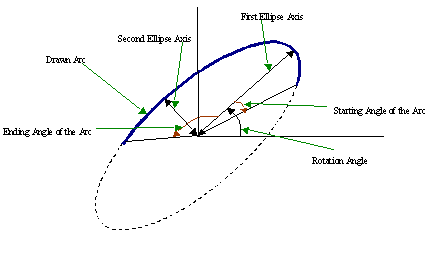
\includegraphics[width=0.5\textwidth]{pics/ellipse.png}

\cvCppFunc{ellipse2Poly}
Approximates an elliptic arc with a polyline

\cvdefCpp{
void ellipse2Poly( Point center, Size axes, int angle,\par
                   int startAngle, int endAngle, int delta,\par
                   vector<Point>\& pts );\newline
}
\begin{description}
\cvarg{center}{Center of the arc}
\cvarg{axes}{Half-sizes of the arc. See \cvCppCross{ellipse}}
\cvarg{angle}{Rotation angle of the ellipse in degrees. See \cvCppCross{ellipse}}
\cvarg{startAngle}{Starting angle of the elliptic arc in degrees}
\cvarg{endAngle}{Ending angle of the elliptic arc in degrees}
\cvarg{delta}{Angle between the subsequent polyline vertices. It defines the approximation accuracy.}
\cvarg{pts}{The output vector of polyline vertices}
\end{description}

The function \texttt{ellipse2Poly} computes the vertices of a polyline that approximates the specified elliptic arc. It is used by \cvCppCross{ellipse}.

\cvCppFunc{fillConvexPoly}
Fills a convex polygon.

\cvdefCpp{
void fillConvexPoly(Mat\& img, const Point* pts, int npts,\par
                    const Scalar\& color, int lineType=8,\par
                    int shift=0);\newline
}
\begin{description}
\cvarg{img}{Image}
\cvarg{pts}{The polygon vertices}
\cvarg{npts}{The number of polygon vertices}
\cvarg{color}{Polygon color}
\cvarg{lineType}{Type of the polygon boundaries, see \cvCppCross{line} description}
\cvarg{shift}{The number of fractional bits in the vertex coordinates}
\end{description}

The function \texttt{fillConvexPoly} draws a filled convex polygon.
This function is much faster than the function \texttt{fillPoly}
and can fill not only convex polygons but any monotonic polygon without self-intersections,
i.e., a polygon whose contour intersects every horizontal line (scan
line) twice at the most (though, its top-most and/or the bottom edge could be horizontal).

\cvCppFunc{fillPoly}
Fills the area bounded by one or more polygons

\cvdefCpp{void fillPoly(Mat\& img, const Point** pts, \par
              const int* npts, int ncontours,\par
              const Scalar\& color, int lineType=8,\par
              int shift=0, Point offset=Point() );}
\begin{description}
\cvarg{img}{Image}
\cvarg{pts}{Array of polygons, each represented as an array of points}
\cvarg{npts}{The array of polygon vertex counters}
\cvarg{ncontours}{The number of contours that bind the filled region}
\cvarg{color}{Polygon color}
\cvarg{lineType}{Type of the polygon boundaries, see \cvCppCross{line} description}
\cvarg{shift}{The number of fractional bits in the vertex coordinates}
\end{description}

The function \texttt{fillPoly} fills an area bounded by several
polygonal contours. The function can fills complex areas, for example,
areas with holes, contours with self-intersections (some of thier parts), and so forth.

\cvCppFunc{getTextSize}
Calculates the width and height of a text string.

\cvdefCpp{Size getTextSize(const string\& text, int fontFace,\par
                 double fontScale, int thickness,\par
                 int* baseLine);\newline}
\begin{description}
\cvarg{text}{The input text string}
\cvarg{fontFace}{The font to use; see \cvCppCross{putText}}
\cvarg{fontScale}{The font scale; see \cvCppCross{putText}}
\cvarg{thickness}{The thickness of lines used to render the text; see \cvCppCross{putText}}
\cvarg{baseLine}{The output parameter - y-coordinate of the baseline relative to the bottom-most text point}
\end{description}

The function \texttt{getTextSize} calculates and returns size of the box that contain the specified text.
That is, the following code will render some text, the tight box surrounding it and the baseline:

\begin{lstlisting}
// Use "y" to show that the baseLine is about
string text = "Funny text inside the box";
int fontFace = FONT_HERSHEY_SCRIPT_SIMPLEX;
double fontScale = 2;
int thickness = 3;

Mat img(600, 800, CV_8UC3, Scalar::all(0));

int baseline=0;
Size textSize = getTextSize(text, fontFace,
                            fontScale, thickness, &baseline);
baseline += thickness;

// center the text
Point textOrg((img.cols - textSize.width)/2,
              (img.rows + textSize.height)/2);

// draw the box
rectangle(img, textOrg + Point(0, baseline),
          textOrg + Point(textSize.width, -textSize.height),
          Scalar(0,0,255));
// ... and the baseline first
line(img, textOrg + Point(0, thickness),
     textOrg + Point(textSize.width, thickness),
     Scalar(0, 0, 255));

// then put the text itself
putText(img, text, textOrg, fontFace, fontScale,
        Scalar::all(255), thickness, 8);
\end{lstlisting}
        
        
\cvCppFunc{line}
Draws a line segment connecting two points

\cvdefCpp{void line(Mat\& img, Point pt1, Point pt2, const Scalar\& color,\par
          int thickness=1, int lineType=8, int shift=0);\newline}
\begin{description}
\cvarg{img}{The image}
\cvarg{pt1}{First point of the line segment}
\cvarg{pt2}{Second point of the line segment}
\cvarg{color}{Line color}
\cvarg{thickness}{Line thickness}
\cvarg{lineType}{Type of the line:
  \begin{description}
  \cvarg{8}{(or omitted) 8-connected line.}
  \cvarg{4}{4-connected line.}
  \cvarg{CV\_AA}{antialiased line.}
  \end{description}}
\cvarg{shift}{Number of fractional bits in the point coordinates}
\end{description}

The function \texttt{line} draws the line segment between
\texttt{pt1} and \texttt{pt2} points in the image. The line is
clipped by the image boundaries. For non-antialiased lines
with integer coordinates the 8-connected or 4-connected Bresenham
algorithm is used. Thick lines are drawn with rounding endings.
Antialiased lines are drawn using Gaussian filtering. To specify
the line color, the user may use the macro
\texttt{CV\_RGB(r, g, b)}.


\cvCppFunc{LineIterator}
Class for iterating pixels on a raster line

\begin{lstlisting}
class LineIterator
{
public:
    // creates iterators for the line connecting pt1 and pt2
    // the line will be clipped on the image boundaries
    // the line is 8-connected or 4-connected
    // If leftToRight=true, then the iteration is always done
    // from the left-most point to the right most,
    // not to depend on the ordering of pt1 and pt2 parameters
    LineIterator(const Mat& img, Point pt1, Point pt2,
                 int connectivity=8, bool leftToRight=false);newline
    // returns pointer to the current line pixel
    uchar* operator *();newline
    // move the iterator to the next pixel
    LineIterator& operator ++();newline
    LineIterator operator ++(int);newline

    // internal state of the iterator
    uchar* ptr;newline
    int err, count;newline
    int minusDelta, plusDelta;newline
    int minusStep, plusStep;newline
};
\end{lstlisting}

The class \texttt{LineIterator} is used to get each pixel of a raster line. It can be treated as versatile implementation of the Bresenham algorithm, where you can stop at each pixel and do some extra processing, for example, grab pixel values along the line, or draw a line with some effect (e.g. with XOR operation).

The number of pixels along the line is store in \texttt{LineIterator::count}.

\begin{lstlisting}
// grabs pixels along the line (pt1, pt2)
// from 8-bit 3-channel image to the buffer
LineIterator it(img, pt1, pt2, 8);
vector<Vec3b> buf(it.count);

for(int i = 0; i < it.count; i++, ++it)
    buf[i] = *(const Vec3b)*it;
\end{lstlisting}


\cvCppFunc{rectangle}
Draws a simple, thick, or filled up-right rectangle.

\cvdefCpp{void rectangle(Mat\& img, Point pt1, Point pt2,\par
               const Scalar\& color, int thickness=1,\par
               int lineType=8, int shift=0);}
\begin{description}
\cvarg{img}{Image}
\cvarg{pt1}{One of the rectangle's vertices}
\cvarg{pt2}{Opposite to \texttt{pt1} rectangle vertex}
\cvarg{color}{Rectangle color or brightness (grayscale image)}
\cvarg{thickness}{Thickness of lines that make up the rectangle. Negative values, e.g. \texttt{CV\_FILLED}, mean that the function has to draw a filled rectangle.}
\cvarg{lineType}{Type of the line, see \cvCppCross{line} description}
\cvarg{shift}{Number of fractional bits in the point coordinates}
\end{description}

The function \texttt{rectangle} draws a rectangle outline or a filled rectangle, which two opposite corners are \texttt{pt1} and \texttt{pt2}.
               

\cvCppFunc{polylines}
Draws several polygonal curves

\cvdefCpp{void polylines(Mat\& img, const Point** pts, const int* npts,\par
               int ncontours, bool isClosed, const Scalar\& color,\par
               int thickness=1, int lineType=8, int shift=0 );\newline}
\begin{description}
\cvarg{img}{The image}
\cvarg{pts}{Array of polygonal curves}
\cvarg{npts}{Array of polygon vertex counters}
\cvarg{ncontours}{The number of curves}
\cvarg{isClosed}{Indicates whether the drawn polylines are closed or not. If they are closed, the function draws the line from the last vertex of each curve to its first vertex}
\cvarg{color}{Polyline color}
\cvarg{thickness}{Thickness of the polyline edges}
\cvarg{lineType}{Type of the line segments, see \cvCppCross{line} description}
\cvarg{shift}{The number of fractional bits in the vertex coordinates}
\end{description}

The function \texttt{polylines} draws one or more polygonal curves.

\cvCppFunc{putText}
Draws a text string

\cvdefCpp{void putText( Mat\& img, const string\& text, Point org,\par
              int fontFace, double fontScale, Scalar color,\par
              int thickness=1, int lineType=8,\par
              bool bottomLeftOrigin=false );}
\begin{description}
\cvarg{img}{The image}
\cvarg{text}{The text string to be drawn}
\cvarg{org}{The bottom-left corner of the text string in the image}
\cvarg{fontFace}{The font type, one of \cvarg{FONT\_HERSHEY\_SIMPLEX}, \cvarg{FONT\_HERSHEY\_PLAIN},
 \cvarg{FONT\_HERSHEY\_DUPLEX}, \cvarg{FONT\_HERSHEY\_COMPLEX}, \cvarg{FONT\_HERSHEY\_TRIPLEX},
 \cvarg{FONT\_HERSHEY\_COMPLEX\_SMALL}, \cvarg{FONT\_HERSHEY\_SCRIPT\_SIMPLEX} or \cvarg{FONT\_HERSHEY\_SCRIPT\_COMPLEX},
   where each of the font id's can be combined with \cvarg{FONT\_HERSHEY\_ITALIC} to get the slanted letters.}
\cvarg{fontScale}{The font scale factor that is multiplied by the font-specific base size}
\cvarg{thickness}{Thickness of the lines used to draw the text}
\cvarg{lineType}{The line type; see \texttt{line} for details}
\cvarg{bottomLeftOrigin}{When true, the image data origin is at the bottom-left corner, otherwise it's at the top-left corner}
\end{description}

The function \texttt{putText} draws a text string in the image.
Symbols that can not be rendered using the specified font are
replaced question marks. See \cvCppCross{getTextSize} for a text rendering code example.

\fi

\subsection{XML/YAML Persistence}

\ifCPy

\ifC
\cvstruct{CvFileStorage}\label{CvFileStorage}
File Storage.

\begin{lstlisting}
typedef struct CvFileStorage
{
    ...       // hidden fields
} CvFileStorage;
\end{lstlisting}

The structure \cross{CvFileStorage} is a "black box" representation
of the file storage associated with a file on disk. Several
functions that are described below take \texttt{CvFileStorage} as
inputs and allow theuser to save or to load hierarchical collections
that consist of scalar values, standard CXCore objects (such as
matrices, sequences, graphs), and user-defined objects.

CXCore can read and write data in XML (http://www.w3c.org/XML) or YAML
(http://www.yaml.org) formats. Below is an example of $3 \times 3$
floating-point identity matrix \texttt{A}, stored in XML and YAML files
using CXCore functions:

XML:

\begin{verbatim}
<?xml version="1.0">
<opencv_storage>
<A type_id="opencv-matrix">
  <rows>3</rows>
  <cols>3</cols>
  <dt>f</dt>
  <data>1. 0. 0. 0. 1. 0. 0. 0. 1.</data>
</A>
</opencv_storage>
\end{verbatim}

YAML:

\begin{verbatim}
%YAML:1.0
A: !!opencv-matrix
  rows: 3
  cols: 3
  dt: f
  data: [ 1., 0., 0., 0., 1., 0., 0., 0., 1.]
\end{verbatim}

As it can be seen from the examples, XML uses nested tags to represent
hierarchy, while YAML uses indentation for that purpose (similar
to the Python programming language).

The same CXCore functions can read and write data in both formats;
the particular format is determined by the extension of the opened
file, .xml for XML files and .yml or .yaml for YAML.


\cvstruct{CvFileNode}\label{CvFileNode}
File Storage Node.

\begin{lstlisting}
/* file node type */
#define CV_NODE_NONE        0
#define CV_NODE_INT         1
#define CV_NODE_INTEGER     CV_NODE_INT
#define CV_NODE_REAL        2
#define CV_NODE_FLOAT       CV_NODE_REAL
#define CV_NODE_STR         3
#define CV_NODE_STRING      CV_NODE_STR
#define CV_NODE_REF         4 /* not used */
#define CV_NODE_SEQ         5
#define CV_NODE_MAP         6
#define CV_NODE_TYPE_MASK   7

/* optional flags */
#define CV_NODE_USER        16
#define CV_NODE_EMPTY       32
#define CV_NODE_NAMED       64

#define CV_NODE_TYPE(tag)  ((tag) & CV_NODE_TYPE_MASK)

#define CV_NODE_IS_INT(tag)        (CV_NODE_TYPE(tag) == CV_NODE_INT)
#define CV_NODE_IS_REAL(tag)       (CV_NODE_TYPE(tag) == CV_NODE_REAL)
#define CV_NODE_IS_STRING(tag)     (CV_NODE_TYPE(tag) == CV_NODE_STRING)
#define CV_NODE_IS_SEQ(tag)        (CV_NODE_TYPE(tag) == CV_NODE_SEQ)
#define CV_NODE_IS_MAP(tag)        (CV_NODE_TYPE(tag) == CV_NODE_MAP)
#define CV_NODE_IS_COLLECTION(tag) (CV_NODE_TYPE(tag) >= CV_NODE_SEQ)
#define CV_NODE_IS_FLOW(tag)       (((tag) & CV_NODE_FLOW) != 0)
#define CV_NODE_IS_EMPTY(tag)      (((tag) & CV_NODE_EMPTY) != 0)
#define CV_NODE_IS_USER(tag)       (((tag) & CV_NODE_USER) != 0)
#define CV_NODE_HAS_NAME(tag)      (((tag) & CV_NODE_NAMED) != 0)

#define CV_NODE_SEQ_SIMPLE 256
#define CV_NODE_SEQ_IS_SIMPLE(seq) (((seq)->flags & CV_NODE_SEQ_SIMPLE) != 0)

typedef struct CvString
{
    int len;
    char* ptr;
}
CvString;

/* all the keys (names) of elements in the readed file storage
   are stored in the hash to speed up the lookup operations */
typedef struct CvStringHashNode
{
    unsigned hashval;
    CvString str;
    struct CvStringHashNode* next;
}
CvStringHashNode;

/* basic element of the file storage - scalar or collection */
typedef struct CvFileNode
{
    int tag;
    struct CvTypeInfo* info; /* type information
            (only for user-defined object, for others it is 0) */
    union
    {
        double f; /* scalar floating-point number */
        int i;    /* scalar integer number */
        CvString str; /* text string */
        CvSeq* seq; /* sequence (ordered collection of file nodes) */
        struct CvMap* map; /* map (collection of named file nodes) */
    } data;
}
CvFileNode;
\end{lstlisting}

The structure is used only for retrieving data from file storage
(i.e., for loading data from the file). When data is written to a file,
it is done sequentially, with minimal buffering. No data is stored
in the file storage.

In opposite, when data is read from a file, the whole file is parsed
and represented in memory as a tree. Every node of the tree is
represented by \cross{CvFileNode}. The type of file node \texttt{N}
can be retrieved as \texttt{CV\_NODE\_TYPE(N->tag)}. Some file nodes
(leaves) are scalars: text strings, integers, or floating-point
numbers. Other file nodes are collections of file nodes, which can
be scalars or collections in their turn. There are two types of
collections: sequences and maps (we use YAML notation, however, the
same is true for XML streams). Sequences (do not mix them with
\cross{CvSeq}) are ordered collections of unnamed file nodes; maps
are unordered collections of named file nodes. Thus, elements of
sequences are accessed by index (\cross{GetSeqElem}), while elements
of maps are accessed by name (\cross{GetFileNodeByName}). The table
below describes the different types of file nodes:

\begin{tabular}{| c | c | c |}
\hline
Type           & \texttt{CV\_NODE\_TYPE(node->tag)} & Value\\ \hline \hline
Integer        & \texttt{CV\_NODE\_INT}             & \texttt{node->data.i} \\ \hline
Floating-point & \texttt{CV\_NODE\_REAL}            & \texttt{node->data.f} \\ \hline
Text string    & \texttt{CV\_NODE\_STR}             & \texttt{node->data.str.ptr} \\ \hline
Sequence       & \texttt{CV\_NODE\_SEQ}             & \texttt{node->data.seq} \\ \hline
Map            & \texttt{CV\_NODE\_MAP}             & \texttt{node->data.map} (see below)\\ \hline
\end{tabular}

There is no need to access the \texttt{map} field directly (by the way,
\texttt{CvMap} is a hidden structure). The elements of the map can
be retrieved with the \cross{GetFileNodeByName} function that takes a
pointer to the "map" file node.

A user (custom) object is an instance of either one of the standard CxCore
types, such as \cross{CvMat}, \cross{CvSeq} etc., or any type
registered with \cross{RegisterTypeInfo}. Such an object is initially
represented in a file as a map (as shown in XML and YAML example files
above) after the file storage has been opened and parsed. Then the
object can be decoded (coverted to native representation) by
request - when a user calls the \cross{Read} or \cross{ReadByName} functions.


\cvstruct{CvAttrList}\label{CvAttrList}
List of attributes.

\begin{lstlisting}
typedef struct CvAttrList
{
    const char** attr; /* NULL-terminated array of (attribute\_name,attribute\_value) pairs */
    struct CvAttrList* next; /* pointer to next chunk of the attributes list */
}
CvAttrList;

/* initializes CvAttrList structure */
inline CvAttrList cvAttrList( const char** attr=NULL, CvAttrList* next=NULL );

/* returns attribute value or 0 (NULL) if there is no such attribute */
const char* cvAttrValue( const CvAttrList* attr, const char* attr\_name );
\end{lstlisting}

In the current implementation, attributes are used to pass extra parameters when writing user objects (see \cross{Write}). XML attributes inside tags are not supported, aside from the object type specification (\texttt{type\_id} attribute).


\cvstruct{CvTypeInfo}\label{CvTypeInfo}
Type information.

\begin{lstlisting}
typedef int (CV_CDECL *CvIsInstanceFunc)( const void* structPtr );
typedef void (CV_CDECL *CvReleaseFunc)( void** structDblPtr );
typedef void* (CV_CDECL *CvReadFunc)( CvFileStorage* storage, CvFileNode* node );
typedef void (CV_CDECL *CvWriteFunc)( CvFileStorage* storage,
                                      const char* name,
                                      const void* structPtr,
                                      CvAttrList attributes );
typedef void* (CV_CDECL *CvCloneFunc)( const void* structPtr );

typedef struct CvTypeInfo
{
    int flags; /* not used */
    int header_size; /* sizeof(CvTypeInfo) */
    struct CvTypeInfo* prev; /* previous registered type in the list */
    struct CvTypeInfo* next; /* next registered type in the list */
    const char* type_name; /* type name, written to file storage */

    /* methods */
    CvIsInstanceFunc is_instance; /* checks if the passed object belongs to the type */
    CvReleaseFunc release; /* releases object (memory etc.) */
    CvReadFunc read; /* reads object from file storage */
    CvWriteFunc write; /* writes object to file storage */
    CvCloneFunc clone; /* creates a copy of the object */
}
CvTypeInfo;

\end{lstlisting}

The structure \cross{CvTypeInfo} contains information about one of the
standard or user-defined types. Instances of the type may or may not
contain a pointer to the corresponding \cross{CvTypeInfo} structure. In
any case, there is a way to find the type info structure for a given object
using the \cross{TypeOf} function. Aternatively, type info can be found by
type name using \cross{FindType}, which is used when an object is read
from file storage. The user can register a new type with \cross{RegisterType}
that adds the type information structure into the beginning of the type
list. Thus, it is possible to create specialized types from generic
standard types and override the basic methods.


\cvCPyFunc{Clone}
Makes a clone of an object.

\cvcodeC{void* cvClone( const void* structPtr );}

\begin{description}
\cvarg{structPtr}{The object to clone}
\end{description}

The function finds the type of a given object and calls \texttt{clone} with the passed object.

\cvCPyFunc{EndWriteStruct}
Ends the writing of a structure.

\cvcodeC{void  cvEndWriteStruct(CvFileStorage* fs);}

\begin{description}
\cvarg{fs}{File storage}
\end{description}

The function finishes the currently written structure.

\cvCPyFunc{FindType}
Finds a type by its name.

\cvcodeC{CvTypeInfo* cvFindType(const char* typeName);}

\begin{description}
\cvarg{typeName}{Type name}
\end{description}

The function finds a registered type by its name. It returns NULL if there is no type with the specified name.


\cvCPyFunc{FirstType}
Returns the beginning of a type list.

\cvcodeC{CvTypeInfo* cvFirstType(void);}

The function returns the first type in the list of registered types. Navigation through the list can be done via the \texttt{prev} and \texttt{next} fields of the \cross{CvTypeInfo} structure.

\cvCPyFunc{GetFileNode}
Finds a node in a map or file storage.

\cvcodeC{CvFileNode* cvGetFileNode( \par CvFileStorage* fs,\par CvFileNode* map,\par const CvStringHashNode* key,\par int createMissing=0 );}

\begin{description}
\cvarg{fs}{File storage}
\cvarg{map}{The parent map. If it is NULL, the function searches a top-level node. If both \texttt{map} and \texttt{key} are NULLs, the function returns the root file node - a map that contains top-level nodes.}
\cvarg{key}{Unique pointer to the node name, retrieved with \cross{GetHashedKey}}
\cvarg{createMissing}{Flag that specifies whether an absent node should be added to the map}
\end{description}


The function finds a file node. It is a faster version of \cross{GetFileNodeByName} (see \cross{GetHashedKey} discussion). Also, the function can insert a new node, if it is not in the map yet.

\cvCPyFunc{GetFileNodeByName}
Finds a node in a map or file storage.

\cvcodeC{CvFileNode* cvGetFileNodeByName( \par const CvFileStorage* fs,\par const CvFileNode* map,\par const char* name);}

\begin{description}
\cvarg{fs}{File storage}
\cvarg{map}{The parent map. If it is NULL, the function searches in all the top-level nodes (streams), starting with the first one.}
\cvarg{name}{The file node name}
\end{description}


The function finds a file node by
\texttt{name}. The node is searched either in \texttt{map} or, if the
pointer is NULL, among the top-level file storage nodes. Using
this function for maps and \cross{GetSeqElem} (or sequence reader)
for sequences, it is possible to nagivate through the file storage. To
speed up multiple queries for a certain key (e.g., in the case of an array
of structures) one may use a combination of \cross{GetHashedKey} and
\cross{GetFileNode}.

\cvCPyFunc{GetFileNodeName}
Returns the name of a file node.

\cvcodeC{const char* cvGetFileNodeName( const CvFileNode* node );}

\begin{description}
\cvarg{node}{File node}
\end{description}

The function returns the name of a file node or NULL, if the file node does not have a name or if \texttt{node} is \texttt{NULL}.


\cvCPyFunc{GetHashedKey}
Returns a unique pointer for a given name.

\cvcodeC{CvStringHashNode* cvGetHashedKey( \par CvFileStorage* fs,\par const char* name,\par int len=-1,\par int createMissing=0 );}

\begin{description}
\cvarg{fs}{File storage}
\cvarg{name}{Literal node name}
\cvarg{len}{Length of the name (if it is known apriori), or -1 if it needs to be calculated}
\cvarg{createMissing}{Flag that specifies, whether an absent key should be added into the hash table}
\end{description}

The function returns a unique pointer for
each particular file node name. This pointer can be then passed to the
\cross{GetFileNode} function that is faster than \cross{GetFileNodeByName}
because it compares text strings by comparing pointers rather than the
strings' content.

Consider the following example where an array of points is encoded as a sequence of 2-entry maps:

\begin{lstlisting}

%YAML:1.0
points:
  - { x: 10, y: 10 }
  - { x: 20, y: 20 }
  - { x: 30, y: 30 }
  # ...

\end{lstlisting}

Then, it is possible to get hashed "x" and "y" pointers to speed up decoding of the points.
\cvfunc{Example: Reading an array of structures from file storage}

\begin{lstlisting}

#include "cxcore.h"

int main( int argc, char** argv )
{
    CvFileStorage* fs = cvOpenFileStorage( "points.yml", 0, CV\_STORAGE\_READ );
    CvStringHashNode* x\_key = cvGetHashedNode( fs, "x", -1, 1 );
    CvStringHashNode* y\_key = cvGetHashedNode( fs, "y", -1, 1 );
    CvFileNode* points = cvGetFileNodeByName( fs, 0, "points" );

    if( CV\_NODE\_IS\_SEQ(points->tag) )
    {
        CvSeq* seq = points->data.seq;
        int i, total = seq->total;
        CvSeqReader reader;
        cvStartReadSeq( seq, &reader, 0 );
        for( i = 0; i < total; i++ )
        {
            CvFileNode* pt = (CvFileNode*)reader.ptr;
#if 1 /* faster variant */
            CvFileNode* xnode = cvGetFileNode( fs, pt, x\_key, 0 );
            CvFileNode* ynode = cvGetFileNode( fs, pt, y\_key, 0 );
            assert( xnode && CV\_NODE\_IS\_INT(xnode->tag) &&
                    ynode && CV\_NODE\_IS\_INT(ynode->tag));
            int x = xnode->data.i; // or x = cvReadInt( xnode, 0 );
            int y = ynode->data.i; // or y = cvReadInt( ynode, 0 );
#elif 1 /* slower variant; does not use x\_key & y\_key */
            CvFileNode* xnode = cvGetFileNodeByName( fs, pt, "x" );
            CvFileNode* ynode = cvGetFileNodeByName( fs, pt, "y" );
            assert( xnode && CV\_NODE\_IS\_INT(xnode->tag) &&
                    ynode && CV\_NODE\_IS\_INT(ynode->tag));
            int x = xnode->data.i; // or x = cvReadInt( xnode, 0 );
            int y = ynode->data.i; // or y = cvReadInt( ynode, 0 );
#else /* the slowest yet the easiest to use variant */
            int x = cvReadIntByName( fs, pt, "x", 0 /* default value */ );
            int y = cvReadIntByName( fs, pt, "y", 0 /* default value */ );
#endif
            CV\_NEXT\_SEQ\_ELEM( seq->elem\_size, reader );
            printf("%d: (%d, %d)\n", i, x, y );
        }
    }
    cvReleaseFileStorage( &fs );
    return 0;
}

\end{lstlisting}

Please note that whatever method of accessing a map you are using, it is
still much slower than using plain sequences; for example, in the above
example, it is more efficient to encode the points as pairs of integers
in a single numeric sequence.

\cvCPyFunc{GetRootFileNode}
Retrieves one of the top-level nodes of the file storage.

\cvcodeC{CvFileNode* cvGetRootFileNode( \par const CvFileStorage* fs,\par int stream\_index=0 );}

\begin{description}
\cvarg{fs}{File storage}
\cvarg{stream\_index}{Zero-based index of the stream. See \cross{StartNextStream}. In most cases, there is only one stream in the file; however, there can be several.}
\end{description}

The function returns one of the top-level file
nodes. The top-level nodes do not have a name, they correspond to the
streams that are stored one after another in the file storage. If the
index is out of range, the function returns a NULL pointer, so all the
top-level nodes may be iterated by subsequent calls to the function with
\texttt{stream\_index=0,1,...}, until the NULL pointer is returned. This function
may be used as a base for recursive traversal of the file storage.

\fi

\cvCPyFunc{Load}
Loads an object from a file.

\cvcodeC{void* cvLoad( \par const char* filename,\par CvMemStorage* memstorage=NULL,\par const char* name=NULL,\par const char** realName=NULL );}
\cvcodePy{Load(filename,storage=NULL,name=NULL)-> generic}

\begin{description}
\cvarg{filename}{File name}
\cvarg{memstorage}{Memory storage for dynamic structures, such as \cross{CvSeq} or \cross{CvGraph} . It is not used for matrices or images.}
\cvarg{name}{Optional object name. If it is NULL, the first top-level object in the storage will be loaded.}
\cvC{\cvarg{realName}{Optional output parameter that will contain the name of the loaded object (useful if \texttt{name=NULL})}}
\end{description}

The function loads an object from a file. It provides a
simple interface to \cvCPyCross{Read}. After the object is loaded, the file
storage is closed and all the temporary buffers are deleted. Thus,
to load a dynamic structure, such as a sequence, contour, or graph, one
should pass a valid memory storage destination to the function.

\ifC

\cvCPyFunc{OpenFileStorage}
Opens file storage for reading or writing data.

\cvcodeC{CvFileStorage* cvOpenFileStorage(\par const char* filename,\par CvMemStorage* memstorage,\par int flags);}

\begin{description}
\cvarg{filename}{Name of the file associated with the storage}
\cvarg{memstorage}{Memory storage used for temporary data and for
storing dynamic structures, such as \cross{CvSeq} or \cross{CvGraph}.
If it is NULL, a temporary memory storage is created and used.}
\cvarg{flags}{Can be one of the following:
  \begin{description}
  \cvarg{CV\_STORAGE\_READ}{the storage is open for reading}
  \cvarg{CV\_STORAGE\_WRITE}{the storage is open for writing}
  \end{description}}
\end{description}

The function opens file storage for
reading or writing data. In the latter case, a new file is created
or an existing file is rewritten. The type of the read or written file is
determined by the filename extension: \texttt{.xml} for \texttt{XML}
and \texttt{.yml} or \texttt{.yaml} for \texttt{YAML}. The function
returns a pointer to the \cross{CvFileStorage} structure.

\cvCPyFunc{Read}
Decodes an object and returns a pointer to it.

\cvcodeC{void* cvRead( \par CvFileStorage* fs,\par CvFileNode* node,\par CvAttrList* attributes=NULL );}

\begin{description}
\cvarg{fs}{File storage}
\cvarg{node}{The root object node}
\cvarg{attributes}{Unused parameter}
\end{description}

The function decodes a user object (creates an object in a
native representation from the file storage subtree) and returns it. The
object to be decoded must be an instance of a registered type that supports the
\texttt{read} method (see \cross{CvTypeInfo}). The type of the object is
determined by the type name that is encoded in the file. If the object
is a dynamic structure, it is created either in memory storage and passed to
\cross{OpenFileStorage} or, if a NULL pointer was passed, in temporary
memory storage, which is released when \cross{ReleaseFileStorage} is
called. Otherwise, if the object is not a dynamic structure, it is
created in a heap and should be released with a specialized function or by
using the generic \cross{Release}.

\cvCPyFunc{ReadByName}
Finds an object by name and decodes it.

\cvcodeC{void* cvReadByName( \par CvFileStorage* fs,\par const CvFileNode* map,\par const char* name,\par CvAttrList* attributes=NULL );}

\begin{description}
\cvarg{fs}{File storage}
\cvarg{map}{The parent map. If it is NULL, the function searches a top-level node.}
\cvarg{name}{The node name}
\cvarg{attributes}{Unused parameter}
\end{description}

The function is a simple superposition of \cross{GetFileNodeByName} and \cross{Read}.

\cvCPyFunc{ReadInt}
Retrieves an integer value from a file node.

\cvcodeC{int cvReadInt( \par const CvFileNode* node,\par int defaultValue=0 );}

\begin{description}
\cvarg{node}{File node}
\cvarg{defaultValue}{The value that is returned if \texttt{node} is NULL}
\end{description}


The function returns an integer that is represented
by the file node. If the file node is NULL, the \texttt{defaultValue}
is returned (thus, it is convenient to call the function right after
\cross{GetFileNode} without checking for a NULL pointer). If
the file node has type \texttt{CV\_NODE\_INT}, then \texttt{node->data.i} is
returned. If the file node has type \texttt{CV\_NODE\_REAL},
then \texttt{node->data.f} is converted to an integer and returned. Otherwise the
result is not determined.

\cvCPyFunc{ReadIntByName}
Finds a file node and returns its value.

\cvcodeC{int cvReadIntByName( \par const CvFileStorage* fs,\par const CvFileNode* map,\par const char* name,\par int defaultValue=0 );}

\begin{description}
\cvarg{fs}{File storage}
\cvarg{map}{The parent map. If it is NULL, the function searches a top-level node.}
\cvarg{name}{The node name}
\cvarg{defaultValue}{The value that is returned if the file node is not found}
\end{description}

The function is a simple superposition of \cross{GetFileNodeByName} and \cross{ReadInt}.


\cvCPyFunc{ReadRawData}
Reads multiple numbers.

\cvcodeC{void cvReadRawData(\par const CvFileStorage* fs,\par const CvFileNode* src,\par void* dst,\par const char* dt);}

\begin{description}
\cvarg{fs}{File storage}
\cvarg{src}{The file node (a sequence) to read numbers from}
\cvarg{dst}{Pointer to the destination array}
\cvarg{dt}{Specification of each array element. It has the same format as in \cross{WriteRawData}.}
\end{description}

The function reads elements from a file node that represents a sequence of scalars.

\cvCPyFunc{ReadRawDataSlice}
Initializes file node sequence reader.

\cvcodeC{void cvReadRawDataSlice( \par const CvFileStorage* fs,\par CvSeqReader* reader,\par int count,\par void* dst,\par const char* dt );}

\begin{description}
\cvarg{fs}{File storage}
\cvarg{reader}{The sequence reader. Initialize it with \cross{StartReadRawData}.}
\cvarg{count}{The number of elements to read}
\cvarg{dst}{Pointer to the destination array}
\cvarg{dt}{Specification of each array element. It has the same format as in \cross{WriteRawData}.}
\end{description}

The function reads one or more elements from
the file node, representing a sequence, to a user-specified array. The
total number of read sequence elements is a product of \texttt{total}
and the number of components in each array element. For example, if
dt=\texttt{2if}, the function will read $\texttt{total} \times 3$
sequence elements. As with any sequence, some parts of the file node
sequence may be skipped or read repeatedly by repositioning the reader
using \cross{SetSeqReaderPos}.


\cvCPyFunc{ReadReal}
Retrieves a floating-point value from a file node.

\cvcodeC{double cvReadReal( \par const CvFileNode* node,\par double defaultValue=0. );}

\begin{description}
\cvarg{node}{File node}
\cvarg{defaultValue}{The value that is returned if \texttt{node} is NULL}
\end{description}

The function returns a floating-point value
that is represented by the file node. If the file node is NULL, the
\texttt{defaultValue} is returned (thus, it is convenient to call
the function right after \cross{GetFileNode} without checking for a NULL
pointer). If the file node has type \texttt{CV\_NODE\_REAL},
then \texttt{node->data.f} is returned. If the file node has type
\texttt{CV\_NODE\_INT}, then \texttt{node-$>$data.f} is converted to floating-point
and returned. Otherwise the result is not determined.

\cvCPyFunc{ReadRealByName}
Finds a file node and returns its value.

\cvcodeC{double  cvReadRealByName(\par const CvFileStorage* fs,\par const CvFileNode* map,\par const char* name,\par double defaultValue=0.);}

\begin{description}
\cvarg{fs}{File storage}
\cvarg{map}{The parent map. If it is NULL, the function searches a top-level node.}
\cvarg{name}{The node name}
\cvarg{defaultValue}{The value that is returned if the file node is not found}
\end{description}

The function is a simple superposition of \cross{GetFileNodeByName} and \cross{ReadReal}.

\cvCPyFunc{ReadString}
Retrieves a text string from a file node.

\cvcodeC{const char* cvReadString( \par const CvFileNode* node,\par const char* defaultValue=NULL );}

\begin{description}
\cvarg{node}{File node}
\cvarg{defaultValue}{The value that is returned if \texttt{node} is NULL}
\end{description}

The function returns a text string that is represented
by the file node. If the file node is NULL, the \texttt{defaultValue}
is returned (thus, it is convenient to call the function right after
\cross{GetFileNode} without checking for a NULL pointer). If
the file node has type \texttt{CV\_NODE\_STR}, then \texttt{node-$>$data.str.ptr}
is returned. Otherwise the result is not determined.

\cvCPyFunc{ReadStringByName}
Finds a file node by its name and returns its value.

\cvcodeC{const char* cvReadStringByName( \par const CvFileStorage* fs,\par const CvFileNode* map,\par const char* name,\par const char* defaultValue=NULL );}

\begin{description}
\cvarg{fs}{File storage}
\cvarg{map}{The parent map. If it is NULL, the function searches a top-level node.}
\cvarg{name}{The node name}
\cvarg{defaultValue}{The value that is returned if the file node is not found}
\end{description}

The function is a simple superposition of \cross{GetFileNodeByName} and \cross{ReadString}.

\cvCPyFunc{RegisterType}
Registers a new type.

\cvcodeC{void cvRegisterType(const CvTypeInfo* info);}

\begin{description}
\cvarg{info}{Type info structure}
\end{description}

The function registers a new type, which is
described by \texttt{info}. The function creates a copy of the structure,
so the user should delete it after calling the function.

\cvCPyFunc{Release}
Releases an object.

\cvcodeC{void cvRelease( void** structPtr );}

\begin{description}
\cvarg{structPtr}{Double pointer to the object}
\end{description}

The function finds the type of a given object and calls \texttt{release} with the double pointer.

\cvCPyFunc{ReleaseFileStorage}
Releases file storage.

\cvcodeC{void  cvReleaseFileStorage(CvFileStorage** fs);}

\begin{description}
\cvarg{fs}{Double pointer to the released file storage}
\end{description}


The function closes the file associated with the storage and releases all the temporary structures. It must be called after all I/O operations with the storage are finished.

\fi

\cvCPyFunc{Save}
Saves an object to a file.

\cvcodeC{void cvSave( \par const char* filename,\par const void* structPtr,\par const char* name=NULL,\par const char* comment=NULL,\par CvAttrList attributes=cvAttrList());}
\cvcodePy{Save(filename,structPtr,name=NULL,comment=NULL)-> None}

\begin{description}
\cvarg{filename}{File name}
\cvarg{structPtr}{Object to save}
\cvarg{name}{Optional object name. If it is NULL, the name will be formed from \texttt{filename}.}
\cvarg{comment}{Optional comment to put in the beginning of the file}
\cvC{\cvarg{attributes}{Optional attributes passed to \cross{Write}}}
\end{description}

The function saves an object to a file. It provides a simple interface to \cross{Write}.

\ifC

\cvCPyFunc{StartNextStream}
Starts the next stream.

\cvcodeC{void cvStartNextStream(CvFileStorage* fs);}

\begin{description}
\cvarg{fs}{File storage}
\end{description}

The function starts the next stream in file storage. Both YAML and XML support multiple "streams." This is useful for concatenating files or for resuming the writing process.

\cvCPyFunc{StartReadRawData}
Initializes the file node sequence reader.

\cvcodeC{void cvStartReadRawData( \par const CvFileStorage* fs,\par const CvFileNode* src,\par CvSeqReader* reader);}

\begin{description}
\cvarg{fs}{File storage}
\cvarg{src}{The file node (a sequence) to read numbers from}
\cvarg{reader}{Pointer to the sequence reader}
\end{description}

The function initializes the sequence reader to read data from a file node. The initialized reader can be then passed to \cross{ReadRawDataSlice}.

\cvCPyFunc{StartWriteStruct}
Starts writing a new structure.

\cvcodeC{void  cvStartWriteStruct( CvFileStorage* fs,\par const char* name,\par int struct\_flags,\par const char* typeName=NULL,\par CvAttrList attributes=cvAttrList( \par));}

\begin{description}
\cvarg{fs}{File storage}
\cvarg{name}{Name of the written structure. The structure can be accessed by this name when the storage is read.}
\cvarg{struct\_flags}{A combination one of the following values:
\begin{description}
\cvarg{CV\_NODE\_SEQ}{the written structure is a sequence (see discussion of \cross{CvFileStorage}), that is, its elements do not have a name.}
\cvarg{CV\_NODE\_MAP}{the written structure is a map (see discussion of \cross{CvFileStorage}), that is, all its elements have names.\end{description}}
 One and only one of the two above flags must be specified}

\cvarg{CV\_NODE\_FLOW}{the optional flag that makes sense only for YAML streams. It means that the structure is written as a flow (not as a block), which is more compact. It is recommended to use this flag for structures or arrays whose elements are all scalars.}
\cvarg{typeName}{Optional parameter - the object type name. In
case of XML it is written as a \texttt{type\_id} attribute of the
structure opening tag. In the case of YAML it is written after a colon
following the structure name (see the example in \cross{CvFileStorage}
description). Mainly it is used with user objects. When the storage
is read, the encoded type name is used to determine the object type
(see \cross{CvTypeInfo} and \cross{FindTypeInfo}).}
\cvarg{attributes}{This parameter is not used in the current implementation}
\end{description}

The function starts writing a compound
structure (collection) that can be a sequence or a map. After all
the structure fields, which can be scalars or structures, are
written, \cross{EndWriteStruct} should be called. The function can
be used to group some objects or to implement the \texttt{write}
function for a some user object (see \cross{CvTypeInfo}).

\cvCPyFunc{TypeOf}
Returns the type of an object.

\cvcodeC{CvTypeInfo* cvTypeOf( const void* structPtr );}

\begin{description}
\cvarg{structPtr}{The object pointer}
\end{description}

The function finds the type of a given object. It iterates
through the list of registered types and calls the \texttt{is\_instance}
function/method for every type info structure with that object until one
of them returns non-zero or until the whole list has been traversed. In
the latter case, the function returns NULL.

\cvCPyFunc{UnregisterType}
Unregisters the type.

\cvcodeC{void cvUnregisterType( const char* typeName );}

\begin{description}
\cvarg{typeName}{Name of an unregistered type}
\end{description}

The function unregisters a type with
a specified name. If the name is unknown, it is possible to locate
the type info by an instance of the type using \cross{TypeOf} or by
iterating the type list, starting from \cross{FirstType}, and then calling
\texttt{cvUnregisterType(info->typeName)}.

\cvCPyFunc{Write}
Writes a user object.

\cvcodeC{void  cvWrite( CvFileStorage* fs,\par const char* name,\par const void* ptr,\par CvAttrList attributes=cvAttrList(\par) );}

\begin{description}
\cvarg{fs}{File storage}
\cvarg{name}{Name of the written object. Should be NULL if and only if the parent structure is a sequence.}
\cvarg{ptr}{Pointer to the object}
\cvarg{attributes}{The attributes of the object. They are specific for each particular type (see the dicsussion below).}
\end{description}

The function writes an object to file storage. First, the appropriate type info is found using \cross{TypeOf}. Then, the \texttt{write} method associated with the type info is called.

Attributes are used to customize the writing procedure. The standard types support the following attributes (all the \texttt{*dt} attributes have the same format as in \cross{WriteRawData}):

\begin{enumerate}
\item CvSeq
  \begin{description}
  \cvarg{header\_dt}{description of user fields of the sequence header that follow CvSeq, or CvChain (if the sequence is a Freeman chain) or CvContour (if the sequence is a contour or point sequence)}
  \cvarg{dt}{description of the sequence elements.}
  \cvarg{recursive}{if the attribute is present and is not equal to "0" or "false", the whole tree of sequences (contours) is stored.}
  \end{description}
 \item Cvgraph
  \begin{description}
  \cvarg{header\_dt}{description of user fields of the graph header that follows CvGraph;}
  \cvarg{vertex\_dt}{description of user fields of graph vertices}
  \cvarg{edge\_dt}{description of user fields of graph edges (note that the edge weight is always written, so there is no need to specify it explicitly)}
  \end{description}
\end{enumerate}

Below is the code that creates the YAML file shown in the \texttt{CvFileStorage} description:

\begin{lstlisting}
#include "cxcore.h"

int main( int argc, char** argv )
{
    CvMat* mat = cvCreateMat( 3, 3, CV\_32F );
    CvFileStorage* fs = cvOpenFileStorage( "example.yml", 0, CV\_STORAGE\_WRITE );

    cvSetIdentity( mat );
    cvWrite( fs, "A", mat, cvAttrList(0,0) );

    cvReleaseFileStorage( &fs );
    cvReleaseMat( &mat );
    return 0;
}
\end{lstlisting}


\cvCPyFunc{WriteComment}
Writes a comment.

\cvcodeC{void  cvWriteComment(\par CvFileStorage* fs,\par const char* comment,\par int eolComment);}

\begin{description}
\cvarg{fs}{File storage}
\cvarg{comment}{The written comment, single-line or multi-line}
\cvarg{eolComment}{If non-zero, the function tries to put the comment at the end of current line. If the flag is zero, if the comment is multi-line, or if it does not fit at the end of the current line, the comment starts  a new line.}
\end{description}

The function writes a comment into file storage. The comments are skipped when the storage is read, so they may be used only for debugging or descriptive purposes.

\cvCPyFunc{WriteFileNode}
Writes a file node to another file storage.

\cvcodeC{void cvWriteFileNode( \par CvFileStorage* fs,\par const char* new\_node\_name,\par const CvFileNode* node,\par int embed );}

\begin{description}
\cvarg{fs}{Destination file storage}
\cvarg{new\_file\_node}{New name of the file node in the destination file storage. To keep the existing name, use \cross{cvGetFileNodeName}}
\cvarg{node}{The written node}
\cvarg{embed}{If the written node is a collection and this parameter is not zero, no extra level of hiararchy is created. Instead, all the elements of \texttt{node} are written into the currently written structure. Of course, map elements may be written only to a map, and sequence elements may be written only to a sequence.}
\end{description}

The function writes a copy of a file node to file storage. Possible applications of the function are merging several file storages into one and conversion between XML and YAML formats.


\cvCPyFunc{WriteInt}
Writes an integer value.

\cvcodeC{void  cvWriteInt(\par CvFileStorage* fs,\par const char* name,\par int value);}

\begin{description}
\cvarg{fs}{File storage}
\cvarg{name}{Name of the written value. Should be NULL if and only if the parent structure is a sequence.}
\cvarg{value}{The written value}
\end{description}

The function writes a single integer value (with or without a name) to the file storage.

\cvCPyFunc{WriteRawData}
Writes multiple numbers.

\cvcodeC{void  cvWriteRawData( \par CvFileStorage* fs,\par const void* src,\par int len,\par const char* dt );}

\begin{description}
\cvarg{fs}{File storage}
\cvarg{src}{Pointer to the written array}
\cvarg{len}{Number of the array elements to write}
\cvarg{dt}{Specification of each array element that has the following format \newline
\texttt{([count]\{'u'|'c'|'w'|'s'|'i'|'f'|'d'\})...}
where the characters correspond to fundamental C types:
\begin{description}
 \cvarg{u}{8-bit unsigned number}
 \cvarg{c}{8-bit signed number}
 \cvarg{w}{16-bit unsigned number}
 \cvarg{s}{16-bit signed number}
 \cvarg{i}{32-bit signed number}
 \cvarg{f}{single precision floating-point number}
 \cvarg{d}{double precision floating-point number}
 \cvarg{r}{pointer, 32 lower bits of which are written as a signed integer. The type can be used to store structures with links between the elements.
\texttt{count} is the optional counter of values of a given type. For
example, \texttt{2if} means that each array element is a structure
of 2 integers, followed by a single-precision floating-point number. The
equivalent notations of the above specification are '\texttt{iif}',
'\texttt{2i1f}' and so forth. Other examples: \texttt{u} means that the
array consists of bytes, and \texttt{2d} means the array consists of pairs
of doubles.}
\end{description}}
\end{description}

The function writes an array, whose elements consist
of single or multiple numbers. The function call can be replaced with
a loop containing a few \cross{WriteInt} and \cross{WriteReal} calls, but
a single call is more efficient. Note that because none of the elements
have a name, they should be written to a sequence rather than a map.

\cvCPyFunc{WriteReal}
Writes a floating-point value.

\cvcodeC{void  cvWriteReal( \par CvFileStorage* fs,\par const char* name,\par double value );}

\begin{description}
\cvarg{fs}{File storage}
\cvarg{name}{Name of the written value. Should be NULL if and only if the parent structure is a sequence.}
\cvarg{value}{The written value}
\end{description}

The function writes a single floating-point
value (with or without a name) to file storage. Special
values are encoded as follows: NaN (Not A Number) as .NaN, $ \pm \infty $ as +.Inf
(-.Inf).

The following example shows how to use the low-level writing functions
to store custom structures, such as termination criteria, without
registering a new type.

\begin{lstlisting}
void write_termcriteria( CvFileStorage* fs, const char* struct_name,
                         CvTermCriteria* termcrit )
{
    cvStartWriteStruct( fs, struct_name, CV_NODE_MAP, NULL, cvAttrList(0,0));
    cvWriteComment( fs, "termination criteria", 1 ); // just a description
    if( termcrit->type & CV_TERMCRIT_ITER )
        cvWriteInteger( fs, "max_iterations", termcrit->max_iter );
    if( termcrit->type & CV_TERMCRIT_EPS )
        cvWriteReal( fs, "accuracy", termcrit->epsilon );
    cvEndWriteStruct( fs );
}
\end{lstlisting}

\cvCPyFunc{WriteString}
Writes a text string.

\cvcodeC{void  cvWriteString( \par CvFileStorage* fs,\par const char* name,\par const char* str,\par int quote=0 );}

\begin{description}
\cvarg{fs}{File storage}
\cvarg{name}{Name of the written string . Should be NULL if and only if the parent structure is a sequence.}
\cvarg{str}{The written text string}
\cvarg{quote}{If non-zero, the written string is put in quotes, regardless of whether they are required. Otherwise, if the flag is zero, quotes are used only when they are required (e.g. when the string starts with a digit or contains spaces).}
\end{description}

The function writes a text string to file storage.

\fi

\fi

\ifCpp

\cvfunc{FileStorage}\label{FileStorage}
The XML/YAML file storage class

\begin{lstlisting}
class FileStorage
{
public:
    enum { READ=0, WRITE=1, APPEND=2 };
    enum { UNDEFINED=0, VALUE_EXPECTED=1, NAME_EXPECTED=2, INSIDE_MAP=4 };
    // the default constructor
    FileStorage();
    // the constructor that opens the file for reading
    // (flags=FileStorage::READ) or writing (flags=FileStorage::WRITE)
    FileStorage(const string& filename, int flags);
    // wraps the already opened CvFileStorage*
    FileStorage(CvFileStorage* fs);
    // the destructor; closes the file if needed
    virtual ~FileStorage();

    // opens the specified file for reading (flags=FileStorage::READ)
    // or writing (flags=FileStorage::WRITE)
    virtual bool open(const string& filename, int flags);
    // checks if the storage is opened
    virtual bool isOpened() const;
    // closes the file
    virtual void release();

    // returns the first top-level node
    FileNode getFirstTopLevelNode() const;
    // returns the root file node
    // (it's the parent of the first top-level node)
    FileNode root(int streamidx=0) const;
    // returns the top-level node by name
    FileNode operator[](const string& nodename) const;
    FileNode operator[](const char* nodename) const;

    // returns the underlying CvFileStorage*
    CvFileStorage* operator *() { return fs; }
    const CvFileStorage* operator *() const { return fs; }
    
    // writes the certain number of elements of the specified format
    // (see DataType) without any headers
    void writeRaw( const string& fmt, const uchar* vec, size_t len );
    
    // writes an old-style object (CvMat, CvMatND etc.)
    void writeObj( const string& name, const void* obj );

    // returns the default object name from the filename
    // (used by cvSave() with the default object name etc.)
    static string getDefaultObjectName(const string& filename);

    Ptr<CvFileStorage> fs;
    string elname;
    vector<char> structs;
    int state;
};
\end{lstlisting}


\cvfunc{FileNode}\label{FileNode}
The XML/YAML file node class

\begin{lstlisting}
class CV_EXPORTS FileNode
{
public:
    enum { NONE=0, INT=1, REAL=2, FLOAT=REAL, STR=3,
        STRING=STR, REF=4, SEQ=5, MAP=6, TYPE_MASK=7,
        FLOW=8, USER=16, EMPTY=32, NAMED=64 };
    FileNode();
    FileNode(const CvFileStorage* fs, const CvFileNode* node);
    FileNode(const FileNode& node);
    FileNode operator[](const string& nodename) const;
    FileNode operator[](const char* nodename) const;
    FileNode operator[](int i) const;
    int type() const;
    int rawDataSize(const string& fmt) const;
    bool empty() const;
    bool isNone() const;
    bool isSeq() const;
    bool isMap() const;
    bool isInt() const;
    bool isReal() const;
    bool isString() const;
    bool isNamed() const;
    string name() const;
    size_t size() const;
    operator int() const;
    operator float() const;
    operator double() const;
    operator string() const;

    FileNodeIterator begin() const;
    FileNodeIterator end() const;

    void readRaw( const string& fmt, uchar* vec, size_t len ) const;
    void* readObj() const;

    // do not use wrapper pointer classes for better efficiency
    const CvFileStorage* fs;
    const CvFileNode* node;
};
\end{lstlisting}

\cvfunc{FileNodeIterator}\label{FileNodeIterator}
The XML/YAML file node iterator class

\begin{lstlisting}
class CV_EXPORTS FileNodeIterator
{
public:
    FileNodeIterator();
    FileNodeIterator(const CvFileStorage* fs,
        const CvFileNode* node, size_t ofs=0);
    FileNodeIterator(const FileNodeIterator& it);
    FileNode operator *() const;
    FileNode operator ->() const;

    FileNodeIterator& operator ++();
    FileNodeIterator operator ++(int);
    FileNodeIterator& operator --();
    FileNodeIterator operator --(int);
    FileNodeIterator& operator += (int);
    FileNodeIterator& operator -= (int);

    FileNodeIterator& readRaw( const string& fmt, uchar* vec,
                               size_t maxCount=(size_t)INT_MAX );

    const CvFileStorage* fs;
    const CvFileNode* container;
    CvSeqReader reader;
    size_t remaining;
};
\end{lstlisting}

\fi


\section{Clustering and Search in Multi-Dimensional Spaces}

\ifCPy

\cvCPyFunc{KMeans2}
Splits set of vectors by a given number of clusters.

\cvdefC{int cvKMeans2(const CvArr* samples, int nclusters,\par
                      CvArr* labels, CvTermCriteria termcrit,\par
                      int attempts=1, CvRNG* rng=0, \par
                      int flags=0, CvArr* centers=0,\par
                      double* compactness=0);}
\cvdefPy{KMeans2(samples,nclusters,labels,termcrit)-> None}

\begin{description}
\cvarg{samples}{Floating-point matrix of input samples, one row per sample}
\cvarg{nclusters}{Number of clusters to split the set by}
\cvarg{labels}{Output integer vector storing cluster indices for every sample}
\cvarg{termcrit}{Specifies maximum number of iterations and/or accuracy (distance the centers can move by between subsequent iterations)}
\ifC
\cvarg{attempts}{How many times the algorithm is executed using different initial labelings. The algorithm returns labels that yield the best compactness (see the last function parameter)}
\cvarg{rng}{Optional external random number generator; can be used to fully control the function behaviour}
\cvarg{flags}{Can be 0 or \texttt{CV\_KMEANS\_USE\_INITIAL\_LABELS}. The latter
value means that during the first (and possibly the only) attempt, the
function uses the user-supplied labels as the initial approximation
instead of generating random labels. For the second and further attempts,
the function will use randomly generated labels in any case}
\cvarg{centers}{The optional output array of the cluster centers}
\cvarg{compactness}{The optional output parameter, which is computed as
$\sum_i ||\texttt{samples}_i - \texttt{centers}_{\texttt{labels}_i}||^2$
after every attempt; the best (minimum) value is chosen and the
corresponding labels are returned by the function. Basically, the
user can use only the core of the function, set the number of
attempts to 1, initialize labels each time using a custom algorithm
(\texttt{flags=CV\_KMEAN\_USE\_INITIAL\_LABELS}) and, based on the output compactness
or any other criteria, choose the best clustering.}
\fi
\end{description}

The function \texttt{cvKMeans2} implements a k-means algorithm that finds the
centers of \texttt{nclusters} clusters and groups the input samples
around the clusters. On output, $\texttt{labels}_i$ contains a cluster index for
samples stored in the i-th row of the \texttt{samples} matrix.

\ifC
\cvfunc{Example: Clustering random samples of multi-gaussian distribution with k-means}
\begin{lstlisting}
#include "cxcore.h"
#include "highgui.h"

void main( int argc, char** argv )
{
    #define MAX_CLUSTERS 5
    CvScalar color_tab[MAX_CLUSTERS];
    IplImage* img = cvCreateImage( cvSize( 500, 500 ), 8, 3 );
    CvRNG rng = cvRNG(0xffffffff);

    color_tab[0] = CV_RGB(255,0,0);
    color_tab[1] = CV_RGB(0,255,0);
    color_tab[2] = CV_RGB(100,100,255);
    color_tab[3] = CV_RGB(255,0,255);
    color_tab[4] = CV_RGB(255,255,0);

    cvNamedWindow( "clusters", 1 );

    for(;;)
    {
        int k, cluster_count = cvRandInt(&rng)%MAX_CLUSTERS + 1;
        int i, sample_count = cvRandInt(&rng)%1000 + 1;
        CvMat* points = cvCreateMat( sample_count, 1, CV_32FC2 );
        CvMat* clusters = cvCreateMat( sample_count, 1, CV_32SC1 );

        /* generate random sample from multigaussian distribution */
        for( k = 0; k < cluster_count; k++ )
        {
            CvPoint center;
            CvMat point_chunk;
            center.x = cvRandInt(&rng)%img->width;
            center.y = cvRandInt(&rng)%img->height;
            cvGetRows( points,
                       &point_chunk,
                       k*sample_count/cluster_count,
                       (k == (cluster_count - 1)) ?
                           sample_count :
                           (k+1)*sample_count/cluster_count );
            cvRandArr( &rng, &point_chunk, CV_RAND_NORMAL,
                       cvScalar(center.x,center.y,0,0),
                       cvScalar(img->width/6, img->height/6,0,0) );
        }

        /* shuffle samples */
        for( i = 0; i < sample_count/2; i++ )
        {
            CvPoint2D32f* pt1 =
                (CvPoint2D32f*)points->data.fl + cvRandInt(&rng)%sample_count;
            CvPoint2D32f* pt2 =
                (CvPoint2D32f*)points->data.fl + cvRandInt(&rng)%sample_count;
            CvPoint2D32f temp;
            CV_SWAP( *pt1, *pt2, temp );
        }

        cvKMeans2( points, cluster_count, clusters,
                   cvTermCriteria( CV_TERMCRIT_EPS+CV_TERMCRIT_ITER, 10, 1.0 ));

        cvZero( img );

        for( i = 0; i < sample_count; i++ )
        {
            CvPoint2D32f pt = ((CvPoint2D32f*)points->data.fl)[i];
            int cluster_idx = clusters->data.i[i];
            cvCircle( img,
                      cvPointFrom32f(pt),
                      2,
                      color_tab[cluster_idx],
                      CV_FILLED );
        }

        cvReleaseMat( &points );
        cvReleaseMat( &clusters );

        cvShowImage( "clusters", img );

        int key = cvWaitKey(0);
        if( key == 27 )
            break;
    }
}
\end{lstlisting}

\cvCPyFunc{SeqPartition}
Splits a sequence into equivalency classes.

\begin{lstlisting}
typedef int (CV_CDECL* CvCmpFunc)(const void* a, const void* b, void* userdata);
\end{lstlisting}

\cvdefC{
int cvSeqPartition( \par const CvSeq* seq,\par CvMemStorage* storage,\par CvSeq** labels,\par CvCmpFunc is\_equal,\par void* userdata );
}

\begin{description}
\cvarg{seq}{The sequence to partition}
\cvarg{storage}{The storage block to store the sequence of equivalency classes. If it is NULL, the function uses \texttt{seq->storage} for output labels}
\cvarg{labels}{Ouput parameter. Double pointer to the sequence of 0-based labels of input sequence elements}
\cvarg{is\_equal}{The relation function that should return non-zero if the two particular sequence elements are from the same class, and zero otherwise. The partitioning algorithm uses transitive closure of the relation function as an equivalency critria}
\cvarg{userdata}{Pointer that is transparently passed to the \texttt{is\_equal} function}
\end{description}

The function \texttt{cvSeqPartition} implements a quadratic algorithm for
splitting a set into one or more equivalancy classes. The function
returns the number of equivalency classes.

\cvfunc{Example: Partitioning a 2d point set}
\begin{lstlisting}

#include "cxcore.h"
#include "highgui.h"
#include <stdio.h>

CvSeq* point_seq = 0;
IplImage* canvas = 0;
CvScalar* colors = 0;
int pos = 10;

int is_equal( const void* _a, const void* _b, void* userdata )
{
    CvPoint a = *(const CvPoint*)_a;
    CvPoint b = *(const CvPoint*)_b;
    double threshold = *(double*)userdata;
    return (double)((a.x - b.x)*(a.x - b.x) + (a.y - b.y)*(a.y - b.y)) <=
        threshold;
}

void on_track( int pos )
{
    CvSeq* labels = 0;
    double threshold = pos*pos;
    int i, class_count = cvSeqPartition( point_seq,
                                         0,
                                         &labels,
                                         is_equal,
                                         &threshold );
    printf("%4d classes\n", class_count );
    cvZero( canvas );

    for( i = 0; i < labels->total; i++ )
    {
        CvPoint pt = *(CvPoint*)cvGetSeqElem( point_seq, i );
        CvScalar color = colors[*(int*)cvGetSeqElem( labels, i )];
        cvCircle( canvas, pt, 1, color, -1 );
    }

    cvShowImage( "points", canvas );
}

int main( int argc, char** argv )
{
    CvMemStorage* storage = cvCreateMemStorage(0);
    point_seq = cvCreateSeq( CV_32SC2,
                             sizeof(CvSeq),
                             sizeof(CvPoint),
                             storage );
    CvRNG rng = cvRNG(0xffffffff);

    int width = 500, height = 500;
    int i, count = 1000;
    canvas = cvCreateImage( cvSize(width,height), 8, 3 );

    colors = (CvScalar*)cvAlloc( count*sizeof(colors[0]) );
    for( i = 0; i < count; i++ )
    {
        CvPoint pt;
        int icolor;
        pt.x = cvRandInt( &rng ) % width;
        pt.y = cvRandInt( &rng ) % height;
        cvSeqPush( point_seq, &pt );
        icolor = cvRandInt( &rng ) | 0x00404040;
        colors[i] = CV_RGB(icolor & 255,
                           (icolor >> 8)&255,
                           (icolor >> 16)&255);
    }

    cvNamedWindow( "points", 1 );
    cvCreateTrackbar( "threshold", "points", &pos, 50, on_track );
    on_track(pos);
    cvWaitKey(0);
    return 0;
}
\end{lstlisting}

\fi

\fi

\ifCpp

\cvCppFunc{kmeans}

\cvdefCpp{double kmeans( const Mat\& samples, int clusterCount, Mat\& labels,\par
               TermCriteria termcrit, int attempts,\par
               int flags, Mat* centers );}
\begin{description}
\cvarg{samples}{Floating-point matrix of input samples, one row per sample}
\cvarg{clusterCount}{The number of clusters to split the set by}
\cvarg{labels}{The input/output integer array that will store the cluster indices for every sample}
\cvarg{termcrit}{Specifies maximum number of iterations and/or accuracy (distance the centers can move by between subsequent iterations)}

\cvarg{attempts}{How many times the algorithm is executed using different initial labelings. The algorithm returns the labels that yield the best compactness (see the last function parameter)}
\cvarg{flags}{It can take the following values:
\begin{description}
\cvarg{KMEANS\_RANDOM\_CENTERS}{Random initial centers are selected in each attempt}
\cvarg{KMEANS\_PP\_CENTERS}{Use kmeans++ center initialization by Arthur and Vassilvitskii}
\cvarg{KMEANS\_USE\_INITIAL\_LABELS}{During the first (and possibly the only) attempt, the
function uses the user-supplied labels instaed of computing them from the initial centers. For the second and further attempts, the function will use the random or semi-random centers (use one of \texttt{KMEANS\_*\_CENTERS} flag to specify the exact method)}
\end{description}}
\cvarg{centers}{The output matrix of the cluster centers, one row per each cluster center}
\end{description}

The function \texttt{kmeans} implements a k-means algorithm that finds the
centers of \texttt{clusterCount} clusters and groups the input samples
around the clusters. On output, $\texttt{labels}_i$ contains a 0-based cluster index for
the sample stored in the $i^{th}$ row of the \texttt{samples} matrix.

The function returns the compactness measure, which is computed as
\[
\sum_i \|\texttt{samples}_i - \texttt{centers}_{\texttt{labels}_i}\|^2
\]
after every attempt; the best (minimum) value is chosen and the
corresponding labels and the compactness value are returned by the function.
Basically, the user can use only the core of the function, set the number of
attempts to 1, initialize labels each time using some custom algorithm and pass them with
\par (\texttt{flags}=\texttt{KMEANS\_USE\_INITIAL\_LABELS}) flag, and then choose the best (most-compact) clustering.

\cvCppFunc{partition}
Splits an element set into equivalency classes.

\cvdefCpp{template<typename \_Tp, class \_EqPredicate> int\newline
    partition( const vector<\_Tp>\& vec, vector<int>\& labels,\par
               \_EqPredicate predicate=\_EqPredicate());}
\begin{description}
\cvarg{vec}{The set of elements stored as a vector}
\cvarg{labels}{The output vector of labels; will contain as many elements as \texttt{vec}. Each label \texttt{labels[i]} is 0-based cluster index of \texttt{vec[i]}}
\cvarg{predicate}{The equivalence predicate (i.e. pointer to a boolean function of two arguments or an instance of the class that has the method \texttt{bool operator()(const \_Tp\& a, const \_Tp\& b)}. The predicate returns true when the elements are certainly if the same class, and false if they may or may not be in the same class}
\end{description}

The generic function \texttt{partition} implements an $O(N^2)$ algorithm for
splitting a set of $N$ elements into one or more equivalency classes, as described in \url{http://en.wikipedia.org/wiki/Disjoint-set_data_structure}. The function
returns the number of equivalency classes.

\subsection{Fast Approximate Nearest Neighbor Search}

\def\urltilda{\kern -.05em\lower .7ex\hbox{\~{}}\kern .04em}

This section documents OpenCV's interface to the FLANN\footnote{http://people.cs.ubc.ca/\urltilda mariusm/flann} library. FLANN (Fast Library for Approximate Nearest Neighbors) is a library that
contains a collection of algorithms optimized for fast nearest neighbor search in large datasets and for high dimensional features. More 
information about FLANN can be found in \cite{muja_flann_2009}.

\cvCppFunc{flann::Index}
The FLANN nearest neighbor index class.

\begin{lstlisting}
namespace flann
{
    class Index 
    {
    public:
	    Index(const Mat& features, const IndexParams& params);

	    void knnSearch(const vector<float>& query, 
			   vector<int>& indices, 
			   vector<float>& dists, 
			   int knn, 
			   const SearchParams& params);
	    void knnSearch(const Mat& queries, 
                           Mat& indices, 
                           Mat& dists, 
                           int knn, 
		           const SearchParams& params);

	    int radiusSearch(const vector<float>& query, 
			     vector<int>& indices, 
			     vector<float>& dists, 
			     float radius, 
			     const SearchParams& params);
	    int radiusSearch(const Mat& query, 
			     Mat& indices, 
			     Mat& dists, 
			     float radius, 
			     const SearchParams& params);

	    void save(std::string filename);

	    int veclen() const;

	    int size() const;
    };
}
\end{lstlisting}

\cvCppFunc{flann::Index::Index}
Constructs a nearest neighbor search index for a given dataset.

\cvdefCpp{Index::Index(const Mat\& features, const IndexParams\& params);}
\begin{description}
\cvarg{features}{ Matrix of type CV\_32F containing the features(points) to index. The size of the matrix is num\_features x feature\_dimensionality.}
\cvarg{params}{Structure containing the index parameters. The type of index that will be constructed depends on the type of this parameter.
The possible parameter types are:

\begin{description}
 \cvarg{LinearIndexParams}{When passing an object of this type, the index will perform a linear, brute-force search.
   \cvcode{
    struct LinearIndexParams : public IndexParams\newline
  \{\newline
  \};}
  }

\cvarg{KDTreeIndexParams}{When passing an object of this type the index constructed will consist of a set 
of randomized kd-trees which will be searched in parallel.
 \cvcode{
  struct KDTreeIndexParams : public IndexParams\newline
  \{\newline
	KDTreeIndexParams( int trees = 4 );\newline
  \};}
\begin{description}
\cvarg{trees}{The number of parallel kd-trees to use. Good values are in the range [1..16]}
\end{description}
}
\cvarg{KMeansIndexParams}{When passing an object of this type the index constructed will be a hierarchical k-means tree. 
\cvcode{
  struct KMeansIndexParams : public IndexParams\newline
  \{\newline
	    KMeansIndexParams( int branching = 32,\par
			   int iterations = 11,\par
			   flann\_centers\_init\_t centers\_init = CENTERS\_RANDOM,\par
			   float cb\_index = 0.2 );\newline
  \};}
\begin{description}
\cvarg{branching}{ The branching factor to use for the hierarchical k-means tree }
\cvarg{iterations}{ The maximum number of iterations to use in the k-means clustering 
		    stage when building the k-means tree. A value of -1 used here means
		    that the k-means clustering should be iterated until convergence}
\cvarg{centers\_init}{ The algorithm to use for selecting the initial
		  centers when performing a k-means clustering step. The possible values are
		  CENTERS\_RANDOM (picks the initial cluster centers randomly), CENTERS\_GONZALES (picks the
		  initial centers using Gonzales' algorithm) and CENTERS\_KMEANSPP (picks the initial
		centers using the algorithm suggested in \cite{arthur_kmeanspp_2007}) }
\cvarg{cb\_index}{ This parameter (cluster boundary index) influences the
		  way exploration is performed in the hierarchical kmeans tree. When \texttt{cb\_index} is zero
		  the next kmeans domain to be explored is choosen to be the one with the closest center. 
		  A value greater then zero also takes into account the size of the domain.}
\end{description}
}
\cvarg{CompositeIndexParams}{When using a parameters object of this type the index created combines the randomized kd-trees 
	and the hierarchical k-means tree.
\cvcode{
  struct CompositeIndexParams : public IndexParams\newline 
  \{\newline
	    CompositeIndexParams( int trees = 4,\par
			      int branching = 32,\par
			      int iterations = 11,\par
			      flann\_centers\_init\_t centers\_init = CENTERS\_RANDOM,\par 
			      float cb\_index = 0.2 );\newline
  \};}
}
\cvarg{AutotunedIndexParams}{When passing an object of this type the index created is automatically tuned to offer 
the best performance, by choosing the optimal index type (randomized kd-trees, hierarchical kmeans, linear) and parameters for the
dataset provided.
\cvcode{
  struct AutotunedIndexParams : public IndexParams\newline 
  \{\newline
	    AutotunedIndexParams( float target\_precision = 0.9,\par
			      float build\_weight = 0.01,\par
			      float memory\_weight = 0,\par
			      float sample\_fraction = 0.1 );\newline
  \};}
\begin{description}
\cvarg{target\_precision}{ Is a number between 0 and 1 specifying the
percentage of the approximate nearest-neighbor searches that return the
exact nearest-neighbor. Using a higher value for this parameter gives
more accurate results, but the search takes longer. The optimum value
usually depends on the application. }

\cvarg{build\_weight}{ Specifies the importance of the
index build time raported to the nearest-neighbor search time. In some
applications it's acceptable for the index build step to take a long time
if the subsequent searches in the index can be performed very fast. In
other applications it's required that the index be build as fast as
possible even if that leads to slightly longer search times.}

\cvarg{memory\_weight} {Is used to specify the tradeoff between
time (index build time and search time) and memory used by the index. A
value less than 1 gives more importance to the time spent and a value
greater than 1 gives more importance to the memory usage.}

\cvarg{sample\_fraction} {Is a number between 0 and 1 indicating what fraction
of the dataset to use in the automatic parameter configuration algorithm. Running the 
algorithm on the full dataset gives the most accurate results, but for
very large datasets can take longer than desired. In such case using just a fraction of the
data helps speeding up this algorithm while still giving good approximations of the
optimum parameters.}
\end{description}
}
 \cvarg{SavedIndexParams}{This object type is used for loading a previously saved index from the disk.
\cvcode{
  struct SavedIndexParams : public IndexParams\newline
  \{\newline
	   SavedIndexParams( std::string filename );\newline
  \};}
\begin{description}
\cvarg{filename}{ The filename in which the index was saved. }
\end{description}
}
\end {description}
}
\end{description}

\cvCppFunc{flann::Index::knnSearch}
Performs a K-nearest neighbor search for a given query point using the index.
\cvdefCpp{void Index::knnSearch(const vector<float>\& query, \par
		vector<int>\& indices, \par
		vector<float>\& dists, \par
		int knn, \par
		const SearchParams\& params);}
\begin{description}
\cvarg{query}{The query point}
\cvarg{indices}{Vector that will contain the indices of the K-nearest neighbors found. It must have at least knn size.}
\cvarg{dists}{Vector that will contain the distances to the K-nearest neighbors found. It must have at least knn size.}
\cvarg{knn}{Number of nearest neighbors to search for.}
\cvarg{params}{Search parameters}
\begin{lstlisting}
  struct SearchParams {
	  SearchParams(int checks = 32);
  };
\end{lstlisting}
\begin{description}
\cvarg{checks}{ The number of times the tree(s) in the index should be recursively traversed. A
higher value for this parameter would give better search precision, but
also take more time. If automatic configuration was used when the
index was created, the number of checks required to achieve the specified
precision was also computed, in which case this parameter is ignored.}
\end{description}
\end{description}

\cvCppFunc{flann::Index::knnSearch}
Performs a K-nearest neighbor search for multiple query points.

\cvdefCpp{void Index::knnSearch(const Mat\& queries,\par
		Mat\& indices, Mat\& dists,\par
		int knn, const SearchParams\& params);}

\begin{description}
\cvarg{queries}{The query points, one per row}
\cvarg{indices}{Indices of the nearest neighbors found }
\cvarg{dists}{Distances to the nearest neighbors found}
\cvarg{knn}{Number of nearest neighbors to search for}
\cvarg{params}{Search parameters}
\end{description}


\cvCppFunc{flann::Index::radiusSearch}
Performs a radius nearest neighbor search for a given query point.
\cvdefCpp{int Index::radiusSearch(const vector<float>\& query, \par
		  vector<int>\& indices, \par
		  vector<float>\& dists, \par
		  float radius, \par
		  const SearchParams\& params);}
\begin{description}
\cvarg{query}{The query point}
\cvarg{indices}{Vector that will contain the indices of the points found within the search radius in decreasing order of the distance to the query point. If the number of neighbors in the search radius is bigger than the size of this vector, the ones that don't fit in the vector are ignored. }
\cvarg{dists}{Vector that will contain the distances to the points found within the search radius}
\cvarg{radius}{The search radius}
\cvarg{params}{Search parameters}
\end{description}


\cvCppFunc{flann::Index::radiusSearch}
Performs a radius nearest neighbor search for multiple query points.
\cvdefCpp{int Index::radiusSearch(const Mat\& query, \par
		  Mat\& indices, \par
		  Mat\& dists, \par
		  float radius, \par
		  const SearchParams\& params);}
\begin{description}
\cvarg{queries}{The query points, one per row}
\cvarg{indices}{Indices of the nearest neighbors found}
\cvarg{dists}{Distances to the nearest neighbors found}
\cvarg{radius}{The search radius}
\cvarg{params}{Search parameters}
\end{description}


\cvCppFunc{flann::Index::save}
Saves the index to a file.
\cvdefCpp{void Index::save(std::string filename);}
\begin{description}
\cvarg{filename}{The file to save the index to}
\end{description}


\cvCppFunc{flann::hierarchicalClustering}
Clusters the given points by constructing a hierarchical k-means tree and choosing a cut in the tree that minimizes the cluster's variance.
\cvdefCpp{int hierarchicalClustering(const Mat\& features, Mat\& centers,\par
                                      const KMeansIndexParams\& params);}
\begin{description}
\cvarg{features}{The points to be clustered}
\cvarg{centers}{The centers of the clusters obtained. The number of rows in this matrix represents the number of clusters desired, 
however, because of the way the cut in the hierarchical tree is choosen, the number of clusters computed will be
 the highest number of the form $(branching-1)*k+1$ that's lower than the number of clusters desired, where $branching$ is the tree's 
branching factor (see description of the KMeansIndexParams).  }
\cvarg{params}{Parameters used in the construction of the hierarchical k-means tree}
\end{description}
The function returns the number of clusters computed.

\fi
\section{Utility and System Functions and Macros}

\ifCPy
\subsection{Error Handling}\label{Error handling}

\ifPy
Errors in argument type cause a \texttt{TypeError} exception.
OpenCV errors cause an \texttt{cv.error} exception.

For example a function argument that is the wrong type produces a \texttt{TypeError}:

\begin{lstlisting}
>>> import cv
>>> cv.LoadImage(4)
Traceback (most recent call last):
  File "<stdin>", line 1, in <module>
TypeError: argument 1 must be string, not int
\end{lstlisting}

A function with the 

\begin{lstlisting}
>>> cv.CreateMat(-1, -1, cv.CV_8UC1)
Traceback (most recent call last):
  File "<stdin>", line 1, in <module>
error: Non-positive width or height
\end{lstlisting}

\fi

\ifC % {
Error handling in OpenCV is similar to IPL (Image Processing
Library). In the case of an error, functions do not return the error
code. Instead, they raise an error using \texttt{CV\_ERROR}
macro that calls \cvCPyCross{Error} that, in its turn, sets the error
status with \cvCPyCross{SetErrStatus} and calls a standard or user-defined
error handler (that can display a message box, write to log, etc., see
\cvCPyCross{RedirectError}).  There is a global variable, one per each program
thread, that contains current error status (an integer value). The status
can be retrieved with the \cvCPyCross{GetErrStatus} function.

There are three modes of error handling (see \cvCPyCross{SetErrMode} and
\cvCPyCross{GetErrMode}):

\begin{itemize}
\item \textbf{Leaf}. The program is terminated after the error handler is
called. This is the default value. It is useful for debugging, as the
error is signalled immediately after it occurs. However, for production
systems, other two methods may be preferable as they provide more
control.
\item \textbf{Parent}. The program is not terminated, but the error handler
is called. The stack is unwound (it is done w/o using a C++ exception
mechanism). The user may check error code after calling the \texttt{CxCore} function with
\cvCPyCross{GetErrStatus} and react.
\item \textbf{Silent}. Similar to \texttt{Parent} mode, but no error handler
is called.
\end{itemize}

Actually, the semantics of the \texttt{Leaf} and \texttt{Parent} modes are implemented by error handlers and the above description is true for them. \cvCPyCross{GuiBoxReport} behaves slightly differently, and some custom error handlers may implement quite different semantics.  

Macros for raising an error, checking for errors, etc.
\begin{lstlisting}

/* special macros for enclosing processing statements within a function and separating
   them from prologue (resource initialization) and epilogue (guaranteed resource release) */
#define __BEGIN__       {
#define __END__         goto exit; exit: ; }
/* proceeds to "resource release" stage */
#define EXIT            goto exit

/* Declares locally the function name for CV_ERROR() use */
#define CV_FUNCNAME( Name )  \
    static char cvFuncName[] = Name

/* Raises an error within the current context */
#define CV_ERROR( Code, Msg )                                       \
{                                                                   \
     cvError( (Code), cvFuncName, Msg, __FILE__, __LINE__ );        \
     EXIT;                                                          \
}

/* Checks status after calling CXCORE function */
#define CV_CHECK()                                                  \
{                                                                   \
    if( cvGetErrStatus() < 0 )                                   \
        CV_ERROR( CV_StsBackTrace, "Inner function failed." );      \
}

/* Provies shorthand for CXCORE function call and CV_CHECK() */
#define CV_CALL( Statement )                                        \
{                                                                   \
    Statement;                                                      \
    CV_CHECK();                                                     \
}

/* Checks some condition in both debug and release configurations */
#define CV_ASSERT( Condition )                                          \
{                                                                       \
    if( !(Condition) )                                                  \
        CV_ERROR( CV_StsInternal, "Assertion: " #Condition " failed" ); \
}

/* these macros are similar to their CV_... counterparts, but they
   do not need exit label nor cvFuncName to be defined */
#define OPENCV_ERROR(status,func_name,err_msg) ...
#define OPENCV_ERRCHK(func_name,err_msg) ...
#define OPENCV_ASSERT(condition,func_name,err_msg) ...
#define OPENCV_CALL(statement) ...

\end{lstlisting}

Instead of a discussion, below is a documented example of a typical CXCORE function and an example of the function use.

\subsection{Example: Use of Error Handling Macros}
\begin{lstlisting}

#include "cxcore.h"
#include <stdio.h>

void cvResizeDCT( CvMat* input_array, CvMat* output_array )
{
    CvMat* temp_array = 0; // declare pointer that should be released anyway.

    CV_FUNCNAME( "cvResizeDCT" ); // declare cvFuncName

    __BEGIN__; // start processing. There may be some declarations just after 
              // this macro, but they could not be accessed from the epilogue.

    if( !CV_IS_MAT(input_array) || !CV_IS_MAT(output_array) )
        // use CV_ERROR() to raise an error
        CV_ERROR( CV_StsBadArg, 
	"input_array or output_array are not valid matrices" );

    // some restrictions that are going to be removed later, may be checked 
    // with CV_ASSERT()
    CV_ASSERT( input_array->rows == 1 && output_array->rows == 1 );

    // use CV_CALL for safe function call
    CV_CALL( temp_array = cvCreateMat( input_array->rows,
                                       MAX(input_array->cols,
				       output_array->cols),
                                       input_array->type ));

    if( output_array->cols > input_array->cols )
        CV_CALL( cvZero( temp_array ));

    temp_array->cols = input_array->cols;
    CV_CALL( cvDCT( input_array, temp_array, CV_DXT_FORWARD ));
    temp_array->cols = output_array->cols;
    CV_CALL( cvDCT( temp_array, output_array, CV_DXT_INVERSE ));
    CV_CALL( cvScale( output_array,
                      output_array,
                      1./sqrt((double)input_array->cols*output_array->cols), 0 ));

    __END__; // finish processing. Epilogue follows after the macro.

    // release temp_array. If temp_array has not been allocated
    // before an error occured, cvReleaseMat
    // takes care of it and does nothing in this case.
    cvReleaseMat( &temp_array );
}

int main( int argc, char** argv )
{
    CvMat* src = cvCreateMat( 1, 512, CV_32F );
#if 1 /* no errors */
    CvMat* dst = cvCreateMat( 1, 256, CV_32F );
#else
    CvMat* dst = 0; /* test error processing mechanism */
#endif
    cvSet( src, cvRealScalar(1.), 0 );
#if 0 /* change 0 to 1 to suppress error handler invocation */
    cvSetErrMode( CV_ErrModeSilent );
#endif
    cvResizeDCT( src, dst ); // if some error occurs, the message
                             // box will popup, or a message will be
                             // written to log, or some user-defined
                             // processing will be done
    if( cvGetErrStatus() < 0 )
        printf("Some error occured" );
    else
        printf("Everything is OK" );
    return 0;
}
\end{lstlisting}

\cvCPyFunc{GetErrStatus}
Returns the current error status.

\cvdefC{int cvGetErrStatus( void );}

The function returns the current error status -
the value set with the last \cvCPyCross{SetErrStatus} call. Note that in
\texttt{Leaf} mode, the program terminates immediately after an
error occurs, so to always gain control after the function call,
one should call \cvCPyCross{SetErrMode} and set the \texttt{Parent}
or \texttt{Silent} error mode.

\cvCPyFunc{SetErrStatus}
Sets the error status.

\cvdefC{void cvSetErrStatus( int status );}

\begin{description}
\cvarg{status}{The error status}
\end{description}

The function sets the error status to the specified value. Mostly, the function is used to reset the error status (set to it \texttt{CV\_StsOk}) to recover after an error. In other cases it is more natural to call \cvCPyCross{Error} or \texttt{CV\_ERROR}.

\cvCPyFunc{GetErrMode}
Returns the current error mode.

\cvdefC{int cvGetErrMode(void);}

The function returns the current error mode - the value set with the last \cvCPyCross{SetErrMode} call.

\cvCPyFunc{SetErrMode}
Sets the error mode.

\begin{lstlisting}
#define CV_ErrModeLeaf    0
#define CV_ErrModeParent  1
#define CV_ErrModeSilent  2
\end{lstlisting}

\cvdefC{int cvSetErrMode( int mode );}

\begin{description}
\cvarg{mode}{The error mode}
\end{description}

The function sets the specified error mode. For descriptions of different error modes, see the beginning of the error section.

\cvCPyFunc{Error}
Raises an error.

\cvdefC{int cvError( \par int status,\par const char* func\_name,\par const char* err\_msg,\par const char* filename,\par int line );}

\begin{description}
\cvarg{status}{The error status}
\cvarg{func\_name}{Name of the function where the error occured}
\cvarg{err\_msg}{Additional information/diagnostics about the error}
\cvarg{filename}{Name of the file where the error occured}
\cvarg{line}{Line number, where the error occured}
\end{description}

The function sets the error status to the specified value (via \cvCPyCross{SetErrStatus}) and, if the error mode is not \texttt{Silent}, calls the error handler.

\cvCPyFunc{ErrorStr}
Returns textual description of an error status code.

\cvdefC{const char* cvErrorStr( int status );}

\begin{description}
\cvarg{status}{The error status}
\end{description}

The function returns the textual description for
the specified error status code. In the case of unknown status, the function
returns a NULL pointer.

\cvCPyFunc{RedirectError}
Sets a new error handler.


\cvdefC{CvErrorCallback cvRedirectError( \par CvErrorCallback error\_handler,\par void* userdata=NULL,\par void** prevUserdata=NULL );}

\begin{description}
\cvarg{error\_handler}{The new error\_handler}
\cvarg{userdata}{Arbitrary pointer that is transparently passed to the error handler}
\cvarg{prevUserdata}{Pointer to the previously assigned user data pointer}
\end{description}

\begin{lstlisting}
typedef int (CV_CDECL *CvErrorCallback)( int status, const char* func_name,
                    const char* err_msg, const char* file_name, int line );
\end{lstlisting}

The function sets a new error handler that
can be one of the standard handlers or a custom handler
that has a specific interface. The handler takes the same parameters
as the \cvCPyCross{Error} function. If the handler returns a non-zero value, the
program is terminated; otherwise, it continues. The error handler may
check the current error mode with \cvCPyCross{GetErrMode} to make a decision.


\cvfunc{cvNulDevReport cvStdErrReport cvGuiBoxReport}
\label{cvNulDevReport}
\label{cvStdErrReport}
\label{cvGuiBoxReport}

Provide standard error handling.

\cvdefC{
int cvNulDevReport( int status, const char* func\_name,
                    const char* err\_msg, const char* file\_name,
                    int line, void* userdata ); \newline

int cvStdErrReport( int status, const char* func\_name,
                    const char* err\_msg, const char* file\_name,
                    int line, void* userdata ); \newline

int cvGuiBoxReport( int status, const char* func\_name,
                    const char* err\_msg, const char* file\_name,
                    int line, void* userdata );
}

\begin{description}
\cvarg{status}{The error status}
\cvarg{func\_name}{Name of the function where the error occured}
\cvarg{err\_msg}{Additional information/diagnostics about the error}
\cvarg{filename}{Name of the file where the error occured}
\cvarg{line}{Line number, where the error occured}
\cvarg{userdata}{Pointer to the user data. Ignored by the standard handlers}
\end{description}

The functions \texttt{cvNullDevReport}, \texttt{cvStdErrReport},
and \texttt{cvGuiBoxReport} provide standard error
handling. \texttt{cvGuiBoxReport} is the default error
handler on Win32 systems, \texttt{cvStdErrReport} is the default on other
systems. \texttt{cvGuiBoxReport} pops up a message box with the error
description and suggest a few options. Below is an example message box
that may be recieved with the sample code above, if one introduces an
error as described in the sample.

\textbf{Error Message Box}
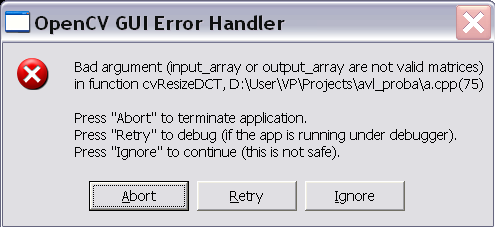
\includegraphics[width=0.5\textwidth]{pics/errmsg.png}

If the error handler is set to \texttt{cvStdErrReport}, the above message will be printed to standard error output and the program will be terminated or continued, depending on the current error mode.

\textbf{Error Message printed to Standard Error Output (in \texttt{Leaf} mode)}

\begin{lstlisting}
OpenCV ERROR: Bad argument (input_array or output_array are not valid matrices)
        in function cvResizeDCT, D:\User\VP\Projects\avl\_proba\a.cpp(75)
Terminating the application...
\end{lstlisting}

\cvCPyFunc{Alloc}
Allocates a memory buffer.

\cvdefC{void* cvAlloc( size\_t size );}

\begin{description}
\cvarg{size}{Buffer size in bytes}
\end{description}

The function allocates \texttt{size} bytes and returns
a pointer to the allocated buffer. In the case of an error the function reports an
error and returns a NULL pointer. By default, \texttt{cvAlloc} calls
\texttt{icvAlloc} which
itself calls \texttt{malloc}. However it is possible to assign user-defined memory
allocation/deallocation functions using the \cvCPyCross{SetMemoryManager} function.

\cvCPyFunc{Free}
Deallocates a memory buffer.

\cvdefC{void cvFree( void** ptr );}

\begin{description}
\cvarg{ptr}{Double pointer to released buffer}
\end{description}

The function deallocates a memory buffer allocated by
\cvCPyCross{Alloc}. It clears the pointer to buffer upon exit, which is why
the double pointer is used. If the \texttt{*buffer} is already NULL, the function
does nothing.

\fi % }

\cvCPyFunc{GetTickCount}
Returns the number of ticks.

\cvdefC{int64 cvGetTickCount( void );}
\cvdefPy{GetTickCount() -> long}

The function returns number of the ticks starting from some platform-dependent event (number of CPU ticks from the startup, number of milliseconds from 1970th year, etc.). The function is useful for accurate measurement of a function/user-code execution time. To convert the number of ticks to time units, use \cvCPyCross{GetTickFrequency}.

\cvCPyFunc{GetTickFrequency}
Returns the number of ticks per microsecond.

\cvdefC{double cvGetTickFrequency( void );}
\cvdefPy{GetTickFrequency() -> long}

The function returns the number of ticks per microsecond. Thus, the quotient of \cvCPyCross{GetTickCount} and \cvCPyCross{GetTickFrequency} will give the number of microseconds starting from the platform-dependent event.

\ifC % {

\cvCPyFunc{RegisterModule}
Registers another module.

\begin{lstlisting}
typedef struct CvPluginFuncInfo
{
    void** func_addr;
    void* default_func_addr;
    const char* func_names;
    int search_modules;
    int loaded_from;
}
CvPluginFuncInfo;

typedef struct CvModuleInfo
{
    struct CvModuleInfo* next;
    const char* name;
    const char* version;
    CvPluginFuncInfo* func_tab;
}
CvModuleInfo;
\end{lstlisting}

\cvdefC{int cvRegisterModule( const CvModuleInfo* moduleInfo );}

\begin{description}
\cvarg{moduleInfo}{Information about the module}
\end{description}

The function adds a module to the list of
registered modules. After the module is registered, information about
it can be retrieved using the \cvCPyCross{GetModuleInfo} function. Also, the
registered module makes full use of optimized plugins (IPP, MKL, ...),
supported by CXCORE. CXCORE itself, CV (computer vision), CVAUX (auxilary
computer vision), and HIGHGUI (visualization and image/video acquisition) are
examples of modules. Registration is usually done when the shared library
is loaded. See \texttt{cxcore/src/cxswitcher.cpp} and
\texttt{cv/src/cvswitcher.cpp} for details about how registration is done
and look at \texttt{cxcore/src/cxswitcher.cpp}, \texttt{cxcore/src/\_cxipp.h}
on how IPP and MKL are connected to the modules.

\cvCPyFunc{GetModuleInfo}
Retrieves information about registered module(s) and plugins.

\cvdefC{
void  cvGetModuleInfo( \par const char* moduleName,\par const char** version,\par const char** loadedAddonPlugins);
}

\begin{description}
\cvarg{moduleName}{Name of the module of interest, or NULL, which means all the modules}
\cvarg{version}{The output parameter. Information about the module(s), including version}
\cvarg{loadedAddonPlugins}{The list of names and versions of the optimized plugins that CXCORE was able to find and load}
\end{description}

The function returns information about one or
all of the registered modules. The returned information is stored inside
the libraries, so the user should not deallocate or modify the returned
text strings.

\cvCPyFunc{UseOptimized}
Switches between optimized/non-optimized modes.

\cvdefC{int cvUseOptimized( int onoff );}

\begin{description}
\cvarg{onoff}{Use optimized ($\ne 0$) or not ($=0$)}
\end{description}

The function switches between the mode, where
only pure C implementations from cxcore, OpenCV, etc. are used, and
the mode, where IPP and MKL functions are used if available. When
\texttt{cvUseOptimized(0)} is called, all the optimized libraries are
unloaded. The function may be useful for debugging, IPP and MKL upgrading on
the fly, online speed comparisons, etc. It returns the number of optimized
functions loaded. Note that by default, the optimized plugins are loaded,
so it is not necessary to call \texttt{cvUseOptimized(1)} in the beginning of
the program (actually, it will only increase the startup time).

\cvCPyFunc{SetMemoryManager}
Accesses custom/default memory managing functions.

\begin{lstlisting}
typedef void* (CV_CDECL *CvAllocFunc)(size_t size, void* userdata);
typedef int (CV_CDECL *CvFreeFunc)(void* pptr, void* userdata);
\end{lstlisting}

\cvdefC{
void cvSetMemoryManager( \par CvAllocFunc allocFunc=NULL,\par CvFreeFunc freeFunc=NULL,\par void* userdata=NULL );
}

\begin{description}
\cvarg{allocFunc}{Allocation function; the interface is similar to \texttt{malloc}, except that \texttt{userdata} may be used to determine the context}
\cvarg{freeFunc}{Deallocation function; the interface is similar to \texttt{free}}
\cvarg{userdata}{User data that is transparently passed to the custom functions}
\end{description}

The function sets user-defined memory
managment functions (substitutes for \texttt{malloc} and \texttt{free}) that will be called
by \texttt{cvAlloc, cvFree} and higher-level functions (e.g., \texttt{cvCreateImage}). Note
that the function should be called when there is data allocated using
\texttt{cvAlloc}. Also, to avoid infinite recursive calls, it is not
allowed to call \texttt{cvAlloc} and \cvCPyCross{Free} from the custom
allocation/deallocation functions.

If the \texttt{alloc\_func} and \texttt{free\_func} pointers are
\texttt{NULL}, the default memory managing functions are restored.

\cvCPyFunc{SetIPLAllocators}
Switches to IPL functions for image allocation/deallocation.

\begin{lstlisting}
typedef IplImage* (CV_STDCALL* Cv_iplCreateImageHeader)
                            (int,int,int,char*,char*,int,int,int,int,int,
                            IplROI*,IplImage*,void*,IplTileInfo*);
typedef void (CV_STDCALL* Cv_iplAllocateImageData)(IplImage*,int,int);
typedef void (CV_STDCALL* Cv_iplDeallocate)(IplImage*,int);
typedef IplROI* (CV_STDCALL* Cv_iplCreateROI)(int,int,int,int,int);
typedef IplImage* (CV_STDCALL* Cv_iplCloneImage)(const IplImage*);

#define CV_TURN_ON_IPL_COMPATIBILITY()                                  \
    cvSetIPLAllocators( iplCreateImageHeader, iplAllocateImage,         \
                        iplDeallocate, iplCreateROI, iplCloneImage )
\end{lstlisting}

\cvdefC{
void cvSetIPLAllocators( \par
                         Cv\_iplCreateImageHeader create\_header, \par
                         Cv\_iplAllocateImageData allocate\_data, \par
                         Cv\_iplDeallocate deallocate, \par
                         Cv\_iplCreateROI create\_roi, \par
                         Cv\_iplCloneImage clone\_image );
}

\begin{description}
\cvarg{create\_header}{Pointer to iplCreateImageHeader}
\cvarg{allocate\_data}{Pointer to iplAllocateImage}
\cvarg{deallocate}{Pointer to iplDeallocate}
\cvarg{create\_roi}{Pointer to iplCreateROI}
\cvarg{clone\_image}{Pointer to iplCloneImage}
\end{description}


The function causes CXCORE to use IPL functions
for image allocation/deallocation operations. For convenience, there
is the wrapping macro \texttt{CV\_TURN\_ON\_IPL\_COMPATIBILITY}. The
function is useful for applications where IPL and CXCORE/OpenCV are used
together and still there are calls to \texttt{iplCreateImageHeader},
etc. The function is not necessary if IPL is called only for data
processing and all the allocation/deallocation is done by CXCORE, or
if all the allocation/deallocation is done by IPL and some of OpenCV
functions are used to process the data.

\fi

\fi

\ifCpp

\cvCppFunc{alignPtr}
Aligns pointer to the specified number of bytes

\cvdefCpp{template<typename \_Tp> \_Tp* alignPtr(\_Tp* ptr, int n=sizeof(\_Tp));}
\begin{description}
\cvarg{ptr}{The aligned pointer}
\cvarg{n}{The alignment size; must be a power of two}
\end{description}

The function returns the aligned pointer of the same type as the input pointer:
\[\texttt{(\_Tp*)(((size\_t)ptr + n-1) \& -n)}\]


\cvCppFunc{alignSize}
Aligns a buffer size to the specified number of bytes

\cvdefCpp{size\_t alignSize(size\_t sz, int n);}
\begin{description}
\cvarg{sz}{The buffer size to align}
\cvarg{n}{The alignment size; must be a power of two}
\end{description}

The function returns the minimum number that is greater or equal to \texttt{sz} and is divisble by \texttt{n}:
\[\texttt{(sz + n-1) \& -n}\]


\cvCppFunc{allocate}
Allocates an array of elements

\cvdefCpp{template<typename \_Tp> \_Tp* allocate(size\_t n);}
\begin{description}
\cvarg{n}{The number of elements to allocate}
\end{description}

The generic function \texttt{allocate} allocates buffer for the specified number of elements. For each element the default constructor is called.


\cvCppFunc{deallocate}
Allocates an array of elements

\cvdefCpp{template<typename \_Tp> void deallocate(\_Tp* ptr, size\_t n);}
\begin{description}
\cvarg{ptr}{Pointer to the deallocated buffer}
\cvarg{n}{The number of elements in the buffer}
\end{description}

The generic function \texttt{deallocate} deallocates the buffer allocated with \cvCppCross{allocate}. The number of elements must match the number passed to \cvCppCross{allocate}.

\cvfunc{CV\_Assert}\label{CV Assert}
Checks a condition at runtime.

\cvdefC{CV\_Assert(expr)}
\cvdefCpp{CV\_Assert(expr)}
\cvdefPy{CV\_Assert(expr)}

\begin{lstlisting}
#define CV_Assert( expr ) ...
#define CV_DbgAssert(expr) ...
\end{lstlisting}

\begin{description}
\cvarg{expr}{The checked expression}
\end{description}

The macros \texttt{CV\_Assert} and \texttt{CV\_DbgAssert} evaluate the specified expression and if it is 0, the macros raise an error (see \cvCppCross{error}). The macro \texttt{CV\_Assert} checks the condition in both Debug and Release configurations, while \texttt{CV\_DbgAssert} is only retained in the Debug configuration.

\cvCppFunc{error}
Signals an error and raises the exception

\cvdefCpp{void error( const Exception\& exc );\newline
\#define CV\_Error( code, msg ) <...>\newline
\#define CV\_Error\_( code, args ) <...>}
\begin{description}
\cvarg{exc}{The exception to throw}
\cvarg{code}{The error code, normally, a negative value. The list of pre-defined error codes can be found in \texttt{cxerror.h}}
\cvarg{msg}{Text of the error message}
\cvarg{args}{printf-like formatted error message in parantheses}
\end{description}

The function and the helper macros \texttt{CV\_Error} and \texttt{CV\_Error\_} call the error handler. Currently, the error handler prints the error code (\texttt{exc.code}), the context (\texttt{exc.file}, \texttt{exc.line} and the error message \texttt{exc.err} to the standard error stream \texttt{stderr}. In Debug configuration it then provokes memory access violation, so that the execution stack and all the parameters can be analyzed in debugger. In Release configuration the exception \texttt{exc} is thrown.

The macro \texttt{CV\_Error\_} can be used to construct the error message on-fly to include some dynamic information, for example:

\begin{lstlisting}
// note the extra parentheses around the formatted text message
CV_Error_(CV_StsOutOfRange,
    ("the matrix element (%d,%d)=%g is out of range",
    i, j, mtx.at<float>(i,j)))
\end{lstlisting}


\cvclass{Exception}\label{Exception}
The exception class passed to error

\begin{lstlisting}
class  Exception
{
public:
    // various constructors and the copy operation
    Exception() { code = 0; line = 0; }
    Exception(int _code, const string& _err,
              const string& _func, const string& _file, int _line);newline
    Exception(const Exception& exc);newline
    Exception& operator = (const Exception& exc);newline

    // the error code
    int code;newline
    // the error text message
    string err;newline
    // function name where the error happened
    string func;newline
    // the source file name where the error happened
    string file;newline
    // the source file line where the error happened
    int line;
};
\end{lstlisting}

The class \texttt{Exception} encapsulates all or almost all the necessary information about the error happened in the program. The exception is usually constructed and thrown implicitly, via \texttt{CV\_Error} and \texttt{CV\_Error\_} macros, see \cvCppCross{error}.


\cvCppFunc{fastMalloc}
Allocates aligned memory buffer

\cvdefCpp{void* fastMalloc(size\_t size);}
\begin{description}
\cvarg{size}{The allocated buffer size}
\end{description}
 
The function allocates buffer of the specified size and returns it. When the buffer size is 16 bytes or more, the returned buffer is aligned on 16 bytes.

\cvCppFunc{fastFree}
Deallocates memory buffer

\cvdefCpp{void fastFree(void* ptr);}
\begin{description}
\cvarg{ptr}{Pointer to the allocated buffer}
\end{description}

The function deallocates the buffer, allocated with \cvCppCross{fastMalloc}.
If NULL pointer is passed, the function does nothing.

\cvCppFunc{format}
Returns a text string formatted using printf-like expression

\cvdefCpp{string format( const char* fmt, ... );}
\begin{description}
\cvarg{fmt}{The printf-compatible formatting specifiers}
\end{description}

The function acts like \texttt{sprintf}, but forms and returns STL string. It can be used for form the error message in \cvCppCross{Exception} constructor.

\cvCppFunc{getNumThreads}
Returns the number of threads used by OpenCV

\cvdefCpp{int getNumThreads();}

The function returns the number of threads that is used by OpenCV.

See also: \cvCppCross{setNumThreads}, \cvCppCross{getThreadNum}.


\cvCppFunc{getThreadNum}
Returns index of the currently executed thread

\cvdefCpp{int getThreadNum();}

The function returns 0-based index of the currently executed thread. The function is only valid inside a parallel OpenMP region. When OpenCV is built without OpenMP support, the function always returns 0.

See also: \cvCppCross{setNumThreads}, \cvCppCross{getNumThreads}.

\cvCppFunc{getTickCount}
Returns the number of ticks

\cvdefCpp{int64 getTickCount();}

The function returns the number of ticks since the certain event (e.g. when the machine was turned on).
It can be used to initialize \cvCppCross{RNG} or to measure a function execution time by reading the tick count before and after the function call. See also the tick frequency.

\cvCppFunc{getTickFrequency}
Returns the number of ticks per second

\cvdefCpp{double getTickFrequency();}

The function returns the number of ticks per second.
That is, the following code computes the execution time in seconds.
\begin{lstlisting}
double t = (double)getTickCount();
// do something ...
t = ((double)getTickCount() - t)/getTickFrequency();
\end{lstlisting}

\cvCppFunc{setNumThreads}
Sets the number of threads used by OpenCV

\cvdefCpp{void setNumThreads(int nthreads);}
\begin{description}
\cvarg{nthreads}{The number of threads used by OpenCV}
\end{description}

The function sets the number of threads used by OpenCV in parallel OpenMP regions. If \texttt{nthreads=0}, the function will use the default number of threads, which is usually equal to the number of the processing cores.

See also: \cvCppCross{getNumThreads}, \cvCppCross{getThreadNum}

\fi


\chapter{cv. Image Processing and Computer Vision}
\section{Image Filtering}

Functions and classes described in this section are used to perform various linear or non-linear filtering operations on 2D images (represented as \cvCppCross{Mat}'s), that is, for each pixel location $(x,y)$ in the source image some its (normally rectangular) neighborhood is considered and used to compute the response. In case of a linear filter it is a weighted sum of pixel values, in case of morphological operations it is the minimum or maximum etc. The computed response is stored to the destination image at the same location $(x,y)$. It means, that the output image will be of the same size as the input image. Normally, the functions supports multi-channel arrays, in which case every channel is processed independently, therefore the output image will also have the same number of channels as the input one.

Another common feature of the functions and classes described in this section is that, unlike simple arithmetic functions, they need to extrapolate values of some non-existing pixels. For example, if we want to smooth an image using a Gaussian $3 \times 3$ filter, then during the processing of the left-most pixels in each row we need pixels to the left of them, i.e. outside of the image. We can let those pixels be the same as the left-most image pixels (i.e. use "replicated border" extrapolation method), or assume that all the non-existing pixels are zeros ("contant border" extrapolation method) etc. \cvCpp{OpenCV let the user to specify the extrapolation method; see the function \cvCppCross{borderInterpolate} and discussion of \texttt{borderType} parameter in various functions below.}

\ifCPy

\cvCPyFunc{CopyMakeBorder}
Copies an image and makes a border around it.

\cvdefC{
void cvCopyMakeBorder(
\par const CvArr* src,
\par CvArr* dst,
\par CvPoint offset,
\par int bordertype,
\par CvScalar value=cvScalarAll(0) );}
\cvdefPy{CopyMakeBorder(src,dst,offset,bordrtype,value=cvScalarAll(0))-> None}

\begin{description}
\cvarg{src}{The source image}
\cvarg{dst}{The destination image}
\cvarg{offset}{Coordinates of the top-left corner (or bottom-left in the case of images with bottom-left origin) of the destination image rectangle where the source image (or its ROI) is copied. Size of the rectanlge matches the source image size/ROI size}
\cvarg{bordertype}{Type of the border to create around the copied source image rectangle; types inlude:
\begin{description}
\cvarg{IPL\_BORDER\_CONSTANT}{border is filled with the fixed value, passed as last parameter of the function.}
\cvarg{IPL\_BORDER\_REPLICATE}{the pixels from the top and bottom rows, the left-most and right-most columns are replicated to fill the border.}
\end{description}
(The other two border types from IPL, \texttt{IPL\_BORDER\_REFLECT} and \texttt{IPL\_BORDER\_WRAP}, are currently unsupported)}
\cvarg{value}{Value of the border pixels if \texttt{bordertype} is \texttt{IPL\_BORDER\_CONSTANT}}
\end{description}

The function copies the source 2D array into the interior of the destination array and makes a border of the specified type around the copied area. The function is useful when one needs to emulate border type that is different from the one embedded into a specific algorithm implementation. For example, morphological functions, as well as most of other filtering functions in OpenCV, internally use replication border type, while the user may need a zero border or a border, filled with 1's or 255's.

\cvCPyFunc{CreateStructuringElementEx}
Creates a structuring element.

\cvdefC{IplConvKernel* cvCreateStructuringElementEx(\par int cols,
 \par int rows, \par int anchorX, \par int anchorY, \par int shape, \par int* values=NULL );}
\cvdefPy{CreateStructuringElementEx(cols,rows,anchorX,anchorY,shape,values={NULL,0})-> kernel}

\begin{description}
\cvarg{cols}{Number of columns in the structuring element}
\cvarg{rows}{Number of rows in the structuring element}
\cvarg{anchorX}{Relative horizontal offset of the anchor point}
\cvarg{anchorY}{Relative vertical offset of the anchor point}
\cvarg{shape}{Shape of the structuring element; may have the following values:
\begin{description}
  \cvarg{CV\_SHAPE\_RECT}{a rectangular element}
  \cvarg{CV\_SHAPE\_CROSS}{a cross-shaped element}
  \cvarg{CV\_SHAPE\_ELLIPSE}{an elliptic element}
  \cvarg{CV\_SHAPE\_CUSTOM}{a user-defined element. In this case the parameter \texttt{values} specifies the mask, that is, which neighbors of the pixel must be considered}
\end{description}}
\cvarg{values}{Pointer to the structuring element data, a plane array, representing row-by-row scanning of the element matrix. Non-zero values indicate points that belong to the element. If the pointer is \texttt{NULL}, then all values are considered non-zero, that is, the element is of a rectangular shape. This parameter is considered only if the shape is \texttt{CV\_SHAPE\_CUSTOM} }
\end{description}

The function CreateStructuringElementEx allocates and fills the structure \texttt{IplConvKernel}, which can be used as a structuring element in the morphological operations.

\cvCPyFunc{Dilate}
Dilates an image by using a specific structuring element.

\cvdefC{void cvDilate(\par const CvArr* src,\par CvArr* dst,\par IplConvKernel* element=NULL,\par int iterations=1 );}
\cvdefPy{Dilate(src,dst,element=NULL,iterations=1)-> None}

\begin{description}
\cvarg{src}{Source image}
\cvarg{dst}{Destination image}
\cvarg{element}{Structuring element used for dilation. If it is \texttt{NULL}, a $3\times 3$ rectangular structuring element is used}
\cvarg{iterations}{Number of times dilation is applied}
\end{description}

The function dilates the source image using the specified structuring element that determines the shape of a pixel neighborhood over which the maximum is taken:

\[
\max_{(x',y') \, in \, \texttt{element}}src(x+x',y+y')
\]

The function supports the in-place mode. Dilation can be applied several (\texttt{iterations}) times. For color images, each channel is processed independently.

\cvCPyFunc{Erode}
Erodes an image by using a specific structuring element.

\cvdefC{void cvErode(\par const CvArr* src,\par  CvArr* dst,\par  IplConvKernel* element=NULL,\par  int iterations=1);}
\cvdefPy{Erode(src,dst,element=NULL,itertions=1)-> None}

\begin{description}
\cvarg{src}{Source image}
\cvarg{dst}{Destination image}
\cvarg{element}{Structuring element used for erosion. If it is \texttt{NULL}, a $3\times 3$ rectangular structuring element is used}
\cvarg{iterations}{Number of times erosion is applied}
\end{description}

The function erodes the source image using the specified structuring element that determines the shape of a pixel neighborhood over which the minimum is taken:

\[
\min_{(x',y') \, in \, \texttt{element}}src(x+x',y+y')
\]

The function supports the in-place mode. Erosion can be applied several (\texttt{iterations}) times. For color images, each channel is processed independently.

\cvCPyFunc{Filter2D}
Convolves an image with the kernel.

\cvdefC{void cvFilter2D(
\par const CvArr* src,\par  CvArr* dst,\par  const CvMat* kernel,\par  CvPoint anchor=cvPoint(-1,-1));}
\cvdefPy{Filter2D(src,dst,kernel,anchor=(-1,-1))-> None}

\begin{description}
\cvarg{src}{The source image}
\cvarg{dst}{The destination image}
\cvarg{kernel}{Convolution kernel, a single-channel floating point matrix. If you want to apply different kernels to different channels, split the image into separate color planes using \cvCPyCross{Split} and process them individually}
\cvarg{anchor}{The anchor of the kernel that indicates the relative position of a filtered point within the kernel. The anchor shoud lie within the kernel. The special default value (-1,-1) means that it is at the kernel center}
\end{description}

The function applies an arbitrary linear filter to the image. In-place operation is supported. When the aperture is partially outside the image, the function interpolates outlier pixel values from the nearest pixels that are inside the image.

\cvCPyFunc{Laplace}
Calculates the Laplacian of an image.

\cvdefC{void cvLaplace(\par const CvArr* src,\par  CvArr* dst,\par  int apertureSize=3);}
\cvdefPy{Laplace(src,dst,apertureSize=3)-> None}
\begin{description}
\cvarg{src}{Source image}
\cvarg{dst}{Destination image}
\cvarg{apertureSize}{Aperture size (it has the same meaning as \cvCPyCross{Sobel})}
\end{description}

The function calculates the Laplacian of the source image by adding up the second x and y derivatives calculated using the Sobel operator:

\[
\texttt{dst}(x,y) = \frac{d^2 \texttt{src}}{dx^2} + \frac{d^2 \texttt{src}}{dy^2}
\]

Setting \texttt{apertureSize} = 1 gives the fastest variant that is equal to convolving the image with the following kernel:

\[ \vecthreethree {0}{1}{0}{1}{-4}{1}{0}{1}{0} \]

Similar to the \cvCPyCross{Sobel} function, no scaling is done and the same combinations of input and output formats are supported.

\cvCPyFunc{MorphologyEx}
Performs advanced morphological transformations.

\cvdefC{void cvMorphologyEx(
\par const CvArr* src,\par  CvArr* dst,\par  CvArr* temp,\par  IplConvKernel* element,
\par int operation,\par  int iterations=1 );}
\cvdefPy{MorphologyEx(src,dst,temp,element,operation,iterations=1)-> None}

\begin{description}
\cvarg{src}{Source image}
\cvarg{dst}{Destination image}
\cvarg{temp}{Temporary image, required in some cases}
\cvarg{element}{Structuring element}
\cvarg{operation}{Type of morphological operation, one of the following:
\begin{description}
\cvarg{CV\_MOP\_OPEN}{opening}
\cvarg{CV\_MOP\_CLOSE}{closing}
\cvarg{CV\_MOP\_GRADIENT}{morphological gradient}
\cvarg{CV\_MOP\_TOPHAT}{"top hat"}
\cvarg{CV\_MOP\_BLACKHAT}{"black hat"}
\end{description}}
\cvarg{iterations}{Number of times erosion and dilation are applied}
\end{description}

The function can perform advanced morphological transformations using erosion and dilation as basic operations.

Opening:

\[
dst=open(src,element)=dilate(erode(src,element),element)
\]

Closing:

\[
dst=close(src,element)=erode(dilate(src,element),element)
\]

Morphological gradient:

\[
dst=morph\_grad(src,element)=dilate(src,element)-erode(src,element)
\]

"Top hat":

\[
dst=tophat(src,element)=src-open(src,element)
\]

"Black hat":

\[
dst=blackhat(src,element)=close(src,element)-src
\]

The temporary image \texttt{temp} is required for a morphological gradient and, in the case of in-place operation, for "top hat" and "black hat".

\cvCPyFunc{PyrDown}
Downsamples an image.

\cvdefC{void cvPyrDown(\par const CvArr* src,\par CvArr* dst,\par int filter=CV\_GAUSSIAN\_5x5 );}
\cvdefPy{PyrDown(src,dst,filter=CV\_GAUSSIAN\_5X5)-> None}

\begin{description}
\cvarg{src}{The source image}
\cvarg{dst}{The destination image, should have a half as large width and height than the source}
\cvarg{filter}{Type of the filter used for convolution; only \texttt{CV\_GAUSSIAN\_5x5} is currently supported}
\end{description}

The function performs the downsampling step of the Gaussian pyramid decomposition. First it convolves the source image with the specified filter and then downsamples the image by rejecting even rows and columns.

\ifC
\cvCPyFunc{ReleaseStructuringElement}
Deletes a structuring element.

\cvdefC{void cvReleaseStructuringElement( IplConvKernel** element );}

\begin{description}
\cvarg{element}{Pointer to the deleted structuring element}
\end{description}

The function releases the structure \texttt{IplConvKernel} that is no longer needed. If \texttt{*element} is \texttt{NULL}, the function has no effect.
\fi

\cvCPyFunc{Smooth}
Smooths the image in one of several ways.

\cvdefC{void cvSmooth(\par const CvArr* src,
\par CvArr* dst,\par  int smoothtype=CV\_GAUSSIAN,\par  int param1=3,\par  int param2=0,\par  double param3=0, \par double param4=0);}
\cvdefPy{Smooth(src,dst,smoothtype=CV\_GAUSSIAN,param1=3,param2=0,param3=0,param4=0)-> None}

\begin{description}
\cvarg{src}{The source image}
\cvarg{dst}{The destination image}
\cvarg{smoothtype}{Type of the smoothing:
\begin{description}
  \cvarg{CV\_BLUR\_NO\_SCALE}{linear convolution with $\texttt{param1}\times\texttt{param2}$ box kernel (all 1's). If you want to smooth different pixels with different-size box kernels, you can use the integral image that is computed using \cvCPyCross{Integral}}
  \cvarg{CV\_BLUR}{linear convolution with $\texttt{param1}\times\texttt{param2}$ box kernel (all 1's) with subsequent scaling by $1/(\texttt{param1}\cdot\texttt{param2})$}
  \cvarg{CV\_GAUSSIAN}{linear convolution with a $\texttt{param1}\times\texttt{param2}$ Gaussian kernel}
  \cvarg{CV\_MEDIAN}{median filter with a $\texttt{param1}\times\texttt{param1}$ square aperture}
  \cvarg{CV\_BILATERAL}{bilateral filter with a $\texttt{param1}\times\texttt{param1}$ square aperture, color sigma=\texttt{param3} and spatial sigma=\texttt{param4}. If \texttt{param1=0}, the aperture square side is set to \newline \texttt{cvRound(param4*1.5)*2+1}. Information about bilateral filtering can be found at \url{http://www.dai.ed.ac.uk/CVonline/LOCAL\_COPIES/MANDUCHI1/Bilateral\_Filtering.html}}
\end{description}}
\cvarg{param1}{The first parameter of the smoothing operation, the aperture width. Must be a positive odd number (1, 3, 5, ...)}
\cvarg{param2}{The second parameter of the smoothing operation, the aperture height. Ignored by \texttt{CV\_MEDIAN} and \texttt{CV\_BILATERAL} methods. In the case of simple scaled/non-scaled and Gaussian blur if \texttt{param2} is zero, it is set to \texttt{param1}. Otherwise it must be a positive odd number.}
\cvarg{param3}{In the case of a Gaussian parameter this parameter may specify Gaussian $\sigma$ (standard deviation). If it is zero, it is calculated from the kernel size:
\[
\sigma = 0.3 (n/2 - 1) + 0.8 \quad \text{where} \quad n=
\begin{array}{l l}
\mbox{\texttt{param1} for horizontal kernel}\\
\mbox{\texttt{param2} for vertical kernel}
\end{array}
\]

Using standard sigma for small kernels ($3\times 3$ to $7\times 7$) gives better speed. If \texttt{param3} is not zero, while \texttt{param1} and \texttt{param2} are zeros, the kernel size is calculated from the sigma (to provide accurate enough operation).}
\end{description}

The function smooths an image using one of several methods. Every of the methods has some features and restrictions listed below

Blur with no scaling works with single-channel images only and supports accumulation of 8-bit to 16-bit format (similar to \cvCPyCross{Sobel} and \cvCPyCross{Laplace}) and 32-bit floating point to 32-bit floating-point format.

Simple blur and Gaussian blur support 1- or 3-channel, 8-bit and 32-bit floating point images. These two methods can process images in-place.

Median and bilateral filters work with 1- or 3-channel 8-bit images and can not process images in-place.

\cvCPyFunc{Sobel}
Calculates the first, second, third or mixed image derivatives using an extended Sobel operator.

\cvdefC{void cvSobel(\par const CvArr* src,\par  CvArr* dst,\par  int xorder,\par  int yorder,\par  int apertureSize=3 );}
\cvdefPy{Sobel(src,dst,xorder,yorder,apertureSize = 3)-> None}

\begin{description}
\cvarg{src}{Source image of type CvArr*}
\cvarg{dst}{Destination image}
\cvarg{xorder}{Order of the derivative x}
\cvarg{yorder}{Order of the derivative y}
\cvarg{apertureSize}{Size of the extended Sobel kernel, must be 1, 3, 5 or 7}
\end{description}

In all cases except 1, an $\texttt{apertureSize} \times
\texttt{apertureSize}$ separable kernel will be used to calculate the
derivative. For $\texttt{apertureSize} = 1$ $ 3 \times 1$ or $ 1 \times 3$
a kernel is used (Gaussian smoothing is not done). There is also the special
value \texttt{CV\_SCHARR} (-1) that corresponds to a $3\times3$ Scharr
filter that may give more accurate results than a $3\times3$ Sobel. Scharr
aperture is

\[ \vecthreethree
{-3}{0}{3}
{-10}{0}{10}
{-3}{0}{3}
\]

for the x-derivative or transposed for the y-derivative.

The function calculates the image derivative by convolving the image with the appropriate kernel:

\[
\texttt{dst}(x,y) = \frac{d^{xorder+yorder} \texttt{src}}{dx^{xorder} \cdot dy^{yorder}}
\]

The Sobel operators combine Gaussian smoothing and differentiation
so the result is more or less resistant to the noise. Most often,
the function is called with (\texttt{xorder} = 1, \texttt{yorder} = 0,
\texttt{apertureSize} = 3) or (\texttt{xorder} = 0, \texttt{yorder} = 1,
\texttt{apertureSize} = 3) to calculate the first x- or y- image
derivative. The first case corresponds to a kernel of:

\[ \vecthreethree
{-1}{0}{1}
{-2}{0}{2}
{-1}{0}{1}
\]

and the second one corresponds to a kernel of:
\[ \vecthreethree
{-1}{-2}{-1}
{0}{0}{0}
{1}{2}{1}
\]
or a kernel of:
\[ \vecthreethree
{1}{2}{1}
{0}{0}{0}
{-1}{2}{-1}
\]

depending on the image origin (\texttt{origin} field of
\texttt{IplImage} structure). No scaling is done, so the destination image
usually has larger numbers (in absolute values) than the source image does. To
avoid overflow, the function requires a 16-bit destination image if the
source image is 8-bit. The result can be converted back to 8-bit using the
\cvCPyCross{ConvertScale} or the \cvCPyCross{ConvertScaleAbs} function. Besides 8-bit images
the function can process 32-bit floating-point images. Both the source and the 
destination must be single-channel images of equal size or equal ROI size.

\fi

\ifCpp

\cvCppFunc{BaseColumnFilter}
Base class for filters with single-column kernels

\begin{lstlisting}
class BaseColumnFilter
{
public:
    virtual ~BaseColumnFilter();
    
    // To be overriden by the user.
    //
    // runs filtering operation on the set of rows,
    // "dstcount + ksize - 1" rows on input,
    // "dstcount" rows on output,
    // each input and output row has "width" elements
    // the filtered rows are written into "dst" buffer.
    virtual void operator()(const uchar** src, uchar* dst, int dststep,
                            int dstcount, int width) = 0;
    // resets the filter state (may be needed for IIR filters)
    virtual void reset();
    
    int ksize; // the aperture size
    int anchor; // position of the anchor point,
                // normally not used during the processing
};
\end{lstlisting}

The class \texttt{BaseColumnFilter} is the base class for filtering data using single-column kernels. The filtering does not have to be a linear operation. In general, it could be written as following:

\[\texttt{dst}(x,y) = F(\texttt{src}[y](x),\;\texttt{src}[y+1](x),\;...,\;\texttt{src}[y+\texttt{ksize}-1](x)\]

where $F$ is the filtering function, but, as it is represented as a class, it can produce any side effects, memorize previously processed data etc. The class only defines the interface and is not used directly. Instead, there are several functions in OpenCV (and you can add more) that return pointers to the derived classes that implement specific filtering operations. Those pointers are then passed to \cvCppCross{FilterEngine} constructor. While the filtering operation interface uses \texttt{uchar} type, a particular implementation is not limited to 8-bit data.

See also: \cvCppCross{BaseRowFilter}, \cvCppCross{BaseFilter}, \cvCppCross{FilterEngine},
    \cvCppCross{getColumnSumFilter}, \cvCppCross{getLinearColumnFilter}, \cvCppCross{getMorphologyColumnFilter}


\cvCppFunc{BaseFilter}
Base class for 2D image filters

\begin{lstlisting}
class BaseFilter
{
public:
    virtual ~BaseFilter();
    
    // To be overriden by the user.
    //
    // runs filtering operation on the set of rows,
    // "dstcount + ksize.height - 1" rows on input,
    // "dstcount" rows on output,
    // each input row has "(width + ksize.width-1)*cn" elements
    // each output row has "width*cn" elements.
    // the filtered rows are written into "dst" buffer.
    virtual void operator()(const uchar** src, uchar* dst, int dststep,
                            int dstcount, int width, int cn) = 0;
    // resets the filter state (may be needed for IIR filters)                        
    virtual void reset();
    Size ksize;
    Point anchor;
};
\end{lstlisting}

The class \texttt{BaseFilter} is the base class for filtering data using 2D kernels. The filtering does not have to be a linear operation. In general, it could be written as following:

\[
  \begin{array}{l}
  \texttt{dst}(x,y) = F( \texttt{src}[y](x),\;\texttt{src}[y](x+1),\;...,\;\texttt{src}[y](x+\texttt{ksize.width}-1), \\
  \texttt{src}[y+1](x),\;\texttt{src}[y+1](x+1),\;...,\;\texttt{src}[y+1](x+\texttt{ksize.width}-1), \\
  ......................................................................................... \\
  \texttt{src}[y+\texttt{ksize.height-1}](x),\\
  \texttt{src}[y+\texttt{ksize.height-1}](x+1),\\
  ...
  \texttt{src}[y+\texttt{ksize.height-1}](x+\texttt{ksize.width}-1))
  \end{array}
  \]

where $F$ is the filtering function. The class only defines the interface and is not used directly. Instead, there are several functions in OpenCV (and you can add more) that return pointers to the derived classes that implement specific filtering operations. Those pointers are then passed to \cvCppCross{FilterEngine} constructor. While the filtering operation interface uses \texttt{uchar} type, a particular implementation is not limited to 8-bit data.

See also: \cvCppCross{BaseColumnFilter}, \cvCppCross{BaseRowFilter}, \cvCppCross{FilterEngine},
    \cvCppCross{getLinearFilter}, \cvCppCross{getMorphologyFilter}

\cvCppFunc{BaseRowFilter}
Base class for filters with single-row kernels

\begin{lstlisting}
class BaseRowFilter
{
public:
    virtual ~BaseRowFilter();
    
    // To be overriden by the user.
    //
    // runs filtering operation on the single input row
    // of "width" element, each element is has "cn" channels.
    // the filtered row is written into "dst" buffer.
    virtual void operator()(const uchar* src, uchar* dst,
                            int width, int cn) = 0;
    int ksize, anchor;
};
\end{lstlisting}

The class \texttt{BaseRowFilter} is the base class for filtering data using single-row kernels. The filtering does not have to be a linear operation. In general, it could be written as following:

\[\texttt{dst}(x,y) = F(\texttt{src}[y](x),\;\texttt{src}[y](x+1),\;...,\;\texttt{src}[y](x+\texttt{ksize.width}-1))\]

where $F$ is the filtering function. The class only defines the interface and is not used directly. Instead, there are several functions in OpenCV (and you can add more) that return pointers to the derived classes that implement specific filtering operations. Those pointers are then passed to \cvCppCross{FilterEngine} constructor. While the filtering operation interface uses \texttt{uchar} type, a particular implementation is not limited to 8-bit data.

See also: \cvCppCross{BaseColumnFilter}, \cvCppCross{Filter}, \cvCppCross{FilterEngine},
 \cvCppCross{getLinearRowFilter}, \cvCppCross{getMorphologyRowFilter}, \cvCppCross{getRowSumFilter}

\cvCppFunc{FilterEngine}
Generic image filtering class

\begin{lstlisting}
class FilterEngine
{
public:
    // empty constructor
    FilterEngine();
    // builds a 2D non-separable filter (!_filter2D.empty()) or
    // a separable filter (!_rowFilter.empty() && !_columnFilter.empty())
    // the input data type will be "srcType", the output data type will be "dstType",
    // the intermediate data type is "bufType".
    // _rowBorderType and _columnBorderType determine how the image
    // will be extrapolated beyond the image boundaries.
    // _borderValue is only used when _rowBorderType and/or _columnBorderType
    // == cv::BORDER_CONSTANT
    FilterEngine(const Ptr<BaseFilter>& _filter2D,
                 const Ptr<BaseRowFilter>& _rowFilter,
                 const Ptr<BaseColumnFilter>& _columnFilter,
                 int srcType, int dstType, int bufType,
                 int _rowBorderType=BORDER_REPLICATE,
                 int _columnBorderType=-1, // use _rowBorderType by default 
                 const Scalar& _borderValue=Scalar());
    virtual ~FilterEngine();
    // separate function for the engine initialization
    void init(const Ptr<BaseFilter>& _filter2D,
              const Ptr<BaseRowFilter>& _rowFilter,
              const Ptr<BaseColumnFilter>& _columnFilter,
              int srcType, int dstType, int bufType,
              int _rowBorderType=BORDER_REPLICATE, int _columnBorderType=-1,
              const Scalar& _borderValue=Scalar());
    // starts filtering of the ROI in an image of size "wholeSize".
    // returns the starting y-position in the source image.
    virtual int start(Size wholeSize, Rect roi, int maxBufRows=-1);
    // alternative form of start that takes the image
    // itself instead of "wholeSize". Set isolated to true to pretend that
    // there are no real pixels outside of the ROI
    // (so that the pixels will be extrapolated using the specified border modes)
    virtual int start(const Mat& src, const Rect& srcRoi=Rect(0,0,-1,-1),
                      bool isolated=false, int maxBufRows=-1);
    // processes the next portion of the source image,
    // "srcCount" rows starting from "src" and
    // stores the results to "dst".
    // returns the number of produced rows
    virtual int proceed(const uchar* src, int srcStep, int srcCount,
                        uchar* dst, int dstStep);
    // higher-level function that processes the whole
    // ROI or the whole image with a single call
    virtual void apply( const Mat& src, Mat& dst,
                        const Rect& srcRoi=Rect(0,0,-1,-1),
                        Point dstOfs=Point(0,0),
                        bool isolated=false);
    bool isSeparable() const { return filter2D.empty(); }
    // how many rows from the input image are not yet processed
    int remainingInputRows() const;
    // how many output rows are not yet produced
    int remainingOutputRows() const;
    ...
    // the starting and the ending rows in the source image
    int startY, endY;
    
    // pointers to the filters
    Ptr<BaseFilter> filter2D;
    Ptr<BaseRowFilter> rowFilter;
    Ptr<BaseColumnFilter> columnFilter;
};
\end{lstlisting}

The class \texttt{FilterEngine} can be used to apply an arbitrary filtering operation to an image.
It contains all the necessary intermediate buffers, it computes extrapolated values
of the "virtual" pixels outside of the image etc. Pointers to the initialized \texttt{FilterEngine} instances
are returned by various \texttt{create*Filter} functions, see below, and they are used inside high-level functions such as \cvCppCross{filter2D}, \cvCppCross{erode}, \cvCppCross{dilate} etc, that is, the class is the workhorse in many of OpenCV filtering functions.

This class makes it easier (though, maybe not very easy yet) to combine filtering operations with other operations, such as color space conversions, thresholding, arithmetic operations, etc. By combining several operations together you can get much better performance because your data will stay in cache. For example, below is the implementation of Laplace operator for a floating-point images, which is a simplified implementation of \cvCppCross{Laplacian}:

\begin{lstlisting}
void laplace_f(const Mat& src, Mat& dst)
{
    CV_Assert( src.type() == CV_32F );
    dst.create(src.size(), src.type());
    
    // get the derivative and smooth kernels for d2I/dx2.
    // for d2I/dy2 we could use the same kernels, just swapped
    Mat kd, ks;
    getSobelKernels( kd, ks, 2, 0, ksize, false, ktype );
    
    // let's process 10 source rows at once
    int DELTA = std::min(10, src.rows);
    Ptr<FilterEngine> Fxx = createSeparableLinearFilter(src.type(),
        dst.type(), kd, ks, Point(-1,-1), 0, borderType, borderType, Scalar() ); 
    Ptr<FilterEngine> Fyy = createSeparableLinearFilter(src.type(),
        dst.type(), ks, kd, Point(-1,-1), 0, borderType, borderType, Scalar() );

    int y = Fxx->start(src), dsty = 0, dy = 0;
    Fyy->start(src);
    const uchar* sptr = src.data + y*src.step;

    // allocate the buffers for the spatial image derivatives;
    // the buffers need to have more than DELTA rows, because at the
    // last iteration the output may take max(kd.rows-1,ks.rows-1)
    // rows more than the input.
    Mat Ixx( DELTA + kd.rows - 1, src.cols, dst.type() );
    Mat Iyy( DELTA + kd.rows - 1, src.cols, dst.type() );
    
    // inside the loop we always pass DELTA rows to the filter
    // (note that the "proceed" method takes care of possibe overflow, since
    // it was given the actual image height in the "start" method)
    // on output we can get:
    //  * < DELTA rows (the initial buffer accumulation stage)
    //  * = DELTA rows (settled state in the middle)
    //  * > DELTA rows (then the input image is over, but we generate
    //                  "virtual" rows using the border mode and filter them)
    // this variable number of output rows is dy.
    // dsty is the current output row.
    // sptr is the pointer to the first input row in the portion to process
    for( ; dsty < dst.rows; sptr += DELTA*src.step, dsty += dy )
    {
        Fxx->proceed( sptr, (int)src.step, DELTA, Ixx.data, (int)Ixx.step );
        dy = Fyy->proceed( sptr, (int)src.step, DELTA, d2y.data, (int)Iyy.step );
        if( dy > 0 )
        {
            Mat dstripe = dst.rowRange(dsty, dsty + dy);
            add(Ixx.rowRange(0, dy), Iyy.rowRange(0, dy), dstripe);
        }
    }
}
\end{lstlisting}

If you do not need that much control of the filtering process, you can simply use the \texttt{FilterEngine::apply} method. Here is how the method is actually implemented:

\begin{lstlisting}
void FilterEngine::apply(const Mat& src, Mat& dst,
    const Rect& srcRoi, Point dstOfs, bool isolated)
{
    // check matrix types
    CV_Assert( src.type() == srcType && dst.type() == dstType );
    
    // handle the "whole image" case
    Rect _srcRoi = srcRoi;
    if( _srcRoi == Rect(0,0,-1,-1) )
        _srcRoi = Rect(0,0,src.cols,src.rows);
    
    // check if the destination ROI is inside the dst.
    // and FilterEngine::start will check if the source ROI is inside src.
    CV_Assert( dstOfs.x >= 0 && dstOfs.y >= 0 &&
        dstOfs.x + _srcRoi.width <= dst.cols &&
        dstOfs.y + _srcRoi.height <= dst.rows );

    // start filtering
    int y = start(src, _srcRoi, isolated);
    
    // process the whole ROI. Note that "endY - startY" is the total number
    // of the source rows to process
    // (including the possible rows outside of srcRoi but inside the source image)
    proceed( src.data + y*src.step,
             (int)src.step, endY - startY,
             dst.data + dstOfs.y*dst.step +
             dstOfs.x*dst.elemSize(), (int)dst.step );
}
\end{lstlisting}

Unlike the earlier versions of OpenCV, now the filtering operations fully support the notion of image ROI, that is, pixels outside of the ROI but inside the image can be used in the filtering operations. For example, you can take a ROI of a single pixel and filter it - that will be a filter response at that particular pixel (however, it's possible to emulate the old behavior by passing \texttt{isolated=false} to \texttt{FilterEngine::start} or \texttt{FilterEngine::apply}). You can pass the ROI explicitly to \texttt{FilterEngine::apply}, or construct a new matrix headers:

\begin{lstlisting}
// compute dI/dx derivative at src(x,y)

// method 1:
// form a matrix header for a single value
float val1 = 0;
Mat dst1(1,1,CV_32F,&val1);

Ptr<FilterEngine> Fx = createDerivFilter(CV_32F, CV_32F,
                        1, 0, 3, BORDER_REFLECT_101);
Fx->apply(src, Rect(x,y,1,1), Point(), dst1);

// method 2:
// form a matrix header for a single value
float val2 = 0;
Mat dst2(1,1,CV_32F,&val2);

Mat pix_roi(src, Rect(x,y,1,1));
Sobel(pix_roi, dst2, dst2.type(), 1, 0, 3, 1, 0, BORDER_REFLECT_101);

printf("method1 = %g, method2 = %g\n", val1, val2);
\end{lstlisting}

Note on the data types. As it was mentioned in \cvCppCross{BaseFilter} description, the specific filters can process data of any type, despite that \texttt{Base*Filter::operator()} only takes \texttt{uchar} pointers and no information about the actual types. To make it all work, the following rules are used:

\begin{itemize}
    \item in case of separable filtering \texttt{FilterEngine::rowFilter} applied first. It transforms the input image data (of type \texttt{srcType}) to the intermediate results stored in the internal buffers (of type \texttt{bufType}). Then these intermediate results are processed \emph{as single-channel data} with \texttt{FilterEngine::columnFilter} and stored in the output image (of type \texttt{dstType}). Thus, the input type for \texttt{rowFilter} is \texttt{srcType} and the output type is \texttt{bufType}; the input type for \texttt{columnFilter} is \texttt{CV\_MAT\_DEPTH(bufType)} and the output type is \texttt{CV\_MAT\_DEPTH(dstType)}.
    
    \item in case of non-separable filtering \texttt{bufType} must be the same as \texttt{srcType}. The source data is copied to the temporary buffer if needed and then just passed to \texttt{FilterEngine::filter2D}. That is, the input type for \texttt{filter2D} is \texttt{srcType} (=\texttt{bufType}) and the output type is \texttt{dstType}.
\end{itemize}

See also: \cvCppCross{BaseColumnFilter}, \cvCppCross{BaseFilter}, \cvCppCross{BaseRowFilter}, \cvCppCross{createBoxFilter},
\cvCppCross{createDerivFilter}, \cvCppCross{createGaussianFilter}, \cvCppCross{createLinearFilter},
\cvCppCross{createMorphologyFilter}, \cvCppCross{createSeparableLinearFilter}

\cvCppFunc{bilateralFilter}
Applies bilateral filter to the image

\cvdefCpp{void bilateralFilter( const Mat\& src, Mat\& dst, int d,\par
                      double sigmaColor, double sigmaSpace,\par
                      int borderType=BORDER\_DEFAULT );}
\begin{description}
\cvarg{src}{The source 8-bit or floating-point, 1-channel or 3-channel image}
\cvarg{dst}{The destination image; will have the same size and the same type as \texttt{src}}
\cvarg{d}{The diameter of each pixel neighborhood, that is used during filtering. If it is non-positive, it's computed from \texttt{sigmaSpace}}
\cvarg{sigmaColor}{Filter sigma in the color space. Larger value of the parameter means that farther colors within the pixel neighborhood (see \texttt{sigmaSpace}) will be mixed together, resulting in larger areas of semi-equal color}
\cvarg{sigmaSpace}{Filter sigma in the coordinate space. Larger value of the parameter means that farther pixels will influence each other (as long as their colors are close enough; see \texttt{sigmaColor}). Then \texttt{d>0}, it specifies the neighborhood size regardless of \texttt{sigmaSpace}, otherwise \texttt{d} is proportional to \texttt{sigmaSpace}}
\end{description}

The function applies bilateral filtering to the input image, as described in
\url{http://www.dai.ed.ac.uk/CVonline/LOCAL\_COPIES/MANDUCHI1/Bilateral\_Filtering.html}

\cvCppFunc{blur}
Smoothes image using normalized box filter

\cvdefCpp{void blur( const Mat\& src, Mat\& dst,\par
           Size ksize, Point anchor=Point(-1,-1),\par
           int borderType=BORDER\_DEFAULT );}
\begin{description}
\cvarg{src}{The source image}
\cvarg{dst}{The destination image; will have the same size and the same type as \texttt{src}}
\cvarg{ksize}{The smoothing kernel size}
\cvarg{anchor}{The anchor point. The default value \texttt{Point(-1,-1)} means that the anchor is at the kernel center}
\cvarg{borderType}{The border mode used to extrapolate pixels outside of the image}
\end{description}

The function smoothes the image using the kernel:

\[ \texttt{K} = \frac{1}{\texttt{ksize.width*ksize.height}}
\begin{bmatrix}
1 & 1 & 1 & \cdots & 1 & 1 \\
1 & 1 & 1 & \cdots & 1 & 1 \\
\hdotsfor{6} \\
1 & 1 & 1 & \cdots & 1 & 1 \\
\end{bmatrix}
\]

The call \texttt{blur(src, dst, ksize, anchor, borderType)} is equivalent to
\texttt{boxFilter(src, dst, src.type(), anchor, true, borderType)}.

See also: \cvCppCross{boxFilter}, \cvCppCross{bilateralFilter}, \cvCppCross{GaussianBlur}, \cvCppCross{medianBlur}.

\cvCppFunc{borderInterpolate}
Computes source location of extrapolated pixel

\cvdefCpp{int borderInterpolate( int p, int len, int borderType );}
\begin{description}
\cvarg{p}{0-based coordinate of the extrapolated pixel along one of the axes, likely <0 or >=\texttt{len}}
\cvarg{len}{length of the array along the corresponding axis}
\cvarg{borderType}{the border type, one of the \texttt{BORDER\_*}, except for \texttt{BORDER\_TRANSPARENT} and \texttt{BORDER\_ISOLATED}. When \texttt{borderType==BORDER\_CONSTANT} the function always returns -1, regardless of \texttt{p} and \texttt{len}}
\end{description}

The function computes and returns the coordinate of the donor pixel, corresponding to the specified extrapolated pixel when using the specified extrapolation border mode. For example, if we use \texttt{BORDER\_WRAP} mode in the horizontal direction, \texttt{BORDER\_REFLECT\_101} in the vertical direction and want to compute value of the "virtual" pixel \texttt{Point(-5, 100)} in a floating-point image \texttt{img}, it will be

\begin{lstlisting}
float val = img.at<float>(borderInterpolate(100, img.rows, BORDER_REFLECT_101),
                          borderInterpolate(-5, img.cols, BORDER_WRAP));
\end{lstlisting}

Normally, the function is not called directly; it is used inside \cvCppCross{FilterEngine} and \cvCppCross{copyMakeBorder} to compute tables for quick extrapolation.

See also: \cvCppCross{FilterEngine}, \cvCppCross{copyMakeBorder}

\cvCppFunc{boxFilter}
Smoothes image using box filter

\cvdefCpp{void boxFilter( const Mat\& src, Mat\& dst, int ddepth,\par
                Size ksize, Point anchor=Point(-1,-1),\par
                bool normalize=true,\par
                int borderType=BORDER\_DEFAULT );}
\begin{description}
\cvarg{src}{The source image}
\cvarg{dst}{The destination image; will have the same size and the same type as \texttt{src}}
\cvarg{ksize}{The smoothing kernel size}
\cvarg{anchor}{The anchor point. The default value \texttt{Point(-1,-1)} means that the anchor is at the kernel center}
\cvarg{normalize}{Indicates, whether the kernel is normalized by its area or not}
\cvarg{borderType}{The border mode used to extrapolate pixels outside of the image}
\end{description}

The function smoothes the image using the kernel:

\[ \texttt{K} = \alpha
\begin{bmatrix}
1 & 1 & 1 & \cdots & 1 & 1 \\
1 & 1 & 1 & \cdots & 1 & 1 \\
\hdotsfor{6} \\
1 & 1 & 1 & \cdots & 1 & 1
\end{bmatrix}
\]

where

\[\alpha=\fork
{\frac{1}{\texttt{ksize.width*ksize.height}}}{when \texttt{normalize=true}}
{1}{otherwise} \]

Unnormalized box filter is useful for computing various integral characteristics over each pixel neighborhood, such as covariation matrices of image derivatives (used in dense optical flow algorithms, \hyperref[conerHarris]{Harris corner detector} etc.). If you need to compute pixel sums over variable-size windows, use \cvCppCross{integral}.

See also: \cvCppCross{boxFilter}, \cvCppCross{bilateralFilter}, \cvCppCross{GaussianBlur}, \cvCppCross{medianBlur}, \cvCppCross{integral}.

\cvCppFunc{buildPyramid}
Constructs Gaussian pyramid for an image

\cvdefCpp{void buildPyramid( const Mat\& src, vector<Mat>\& dst, int maxlevel );}
\begin{description}
\cvarg{src}{The source image; check \cvCppCross{pyrDown} for the list of supported types}
\cvarg{dst}{The destination vector of \texttt{maxlevel+1} images of the same type as \texttt{src};
\texttt{dst[0]} will be the same as \texttt{src}, \texttt{dst[1]} is the next pyramid layer,
a smoothed and down-sized \texttt{src} etc.}
\cvarg{maxlevel}{The 0-based index of the last (i.e. the smallest) pyramid layer; it must be non-negative}
\end{description}

The function constructs a vector of images and builds the gaussian pyramid by recursively applying \cvCppCross{pyrDown} to the previously built pyramid layers, starting from \texttt{dst[0]==src}.

\cvCppFunc{copyMakeBorder}
Forms a border around the image

\cvdefCpp{void copyMakeBorder( const Mat\& src, Mat\& dst,\par
                    int top, int bottom, int left, int right,\par
                    int borderType, const Scalar\& value=Scalar() );}
\begin{description}
\cvarg{src}{The source image}
\cvarg{dst}{The destination image; will have the same type as \texttt{src} and the size \texttt{Size(src.cols+left+right, src.rows+top+bottom)}}
\cvarg{top, bottom, left, right}{Specify how much pixels in each direction from the source image rectangle one needs to extrapolate, e.g. \texttt{top=1, bottom=1, left=1, right=1} mean that 1 pixel-wide border needs to be built}
\cvarg{borderType}{The border type; see \cvCppCross{borderInterpolate}}
\cvarg{value}{The border value if \texttt{borderType==BORDER\_CONSTANT}}
\end{description}

The function copies the source image into the middle of the destination image. The areas to the left, to the right, above and below the copied source image will be filled with extrapolated pixels. This is not what \cvCppCross{FilterEngine} or based on it filtering functions do (they extrapolate pixels on-fly), but what other more complex functions, including your own, may do to simplify image boundary handling.

The function supports the mode when \texttt{src} is already in the middle of \texttt{dst}. In this case the function does not copy \texttt{src} itself, but simply constructs the border, e.g.:

\begin{lstlisting}
// let border be the same in all directions
int border=2;
// constructs a larger image to fit both the image and the border
Mat gray_buf(rgb.rows + border*2, rgb.cols + border*2, rgb.depth());
// select the middle part of it w/o copying data
Mat gray(gray_canvas, Rect(border, border, rgb.cols, rgb.rows));
// convert image from RGB to grayscale
cvtColor(rgb, gray, CV_RGB2GRAY);
// form a border in-place
copyMakeBorder(gray, gray_buf, border, border,
               border, border, BORDER_REPLICATE);
// now do some custom filtering ...
...
\end{lstlisting}

See also: \cvCppCross{borderInterpolate}

\cvCppFunc{createBoxFilter}
Returns box filter engine

\cvdefCpp{Ptr<FilterEngine> createBoxFilter( int srcType, int dstType,\par
                                 Size ksize, Point anchor=Point(-1,-1),\par
                                 bool normalize=true,\par
                                 int borderType=BORDER\_DEFAULT);\newline
Ptr<BaseRowFilter> getRowSumFilter(int srcType, int sumType,\par
                                   int ksize, int anchor=-1);\newline
Ptr<BaseColumnFilter> getColumnSumFilter(int sumType, int dstType,\par
                                   int ksize, int anchor=-1, double scale=1);}
\begin{description}
\cvarg{srcType}{The source image type}
\cvarg{sumType}{The intermediate horizontal sum type; must have as many channels as \texttt{srcType}}
\cvarg{dstType}{The destination image type; must have as many channels as \texttt{srcType}}
\cvarg{ksize}{The aperture size}
\cvarg{anchor}{The anchor position with the kernel; negative values mean that the anchor is at the kernel center}
\cvarg{normalize}{Whether the sums are normalized or not; see \cvCppCross{boxFilter}}
\cvarg{scale}{Another way to specify normalization in lower-level \texttt{getColumnSumFilter}}
\cvarg{borderType}{Which border type to use; see \cvCppCross{borderInterpolate}}
\end{description}

The function is a convenience function that retrieves horizontal sum primitive filter with \cvCppCross{getRowSumFilter}, vertical sum filter with \cvCppCross{getColumnSumFilter}, constructs new \cvCppCross{FilterEngine} and passes both of the primitive filters there. The constructed filter engine can be used for image filtering with normalized or unnormalized box filter.

The function itself is used by \cvCppCross{blur} and \cvCppCross{boxFilter}.

See also: \cvCppCross{FilterEngine}, \cvCppCross{blur}, \cvCppCross{boxFilter}.

\cvCppFunc{createDerivFilter}
Returns engine for computing image derivatives 

\cvdefCpp{Ptr<FilterEngine> createDerivFilter( int srcType, int dstType,\par
                                     int dx, int dy, int ksize,\par
                                     int borderType=BORDER\_DEFAULT );}
\begin{description}
\cvarg{srcType}{The source image type}
\cvarg{dstType}{The destination image type; must have as many channels as \texttt{srcType}}
\cvarg{dx}{The derivative order in respect with x}
\cvarg{dy}{The derivative order in respect with y}
\cvarg{ksize}{The aperture size; see \cvCppCross{getDerivKernels}}
\cvarg{borderType}{Which border type to use; see \cvCppCross{borderInterpolate}}
\end{description}

The function \cvCppCross{createDerivFilter} is a small convenience function that retrieves linear filter coefficients for computing image derivatives using \cvCppCross{getDerivKernels} and then creates a separable linear filter with \cvCppCross{createSeparableLinearFilter}. The function is used by \cvCppCross{Sobel} and \cvCppCross{Scharr}.

See also: \cvCppCross{createSeparableLinearFilter}, \cvCppCross{getDerivKernels}, \cvCppCross{Scharr}, \cvCppCross{Sobel}.

\cvCppFunc{createGaussianFilter}
Returns engine for smoothing images with a Gaussian filter

\cvdefCpp{Ptr<FilterEngine> createGaussianFilter( int type, Size ksize,\par
                                   double sigmaX, double sigmaY=0,\par
                                   int borderType=BORDER\_DEFAULT);}
\begin{description}
\cvarg{type}{The source and the destination image type}
\cvarg{ksize}{The aperture size; see \cvCppCross{getGaussianKernel}}
\cvarg{sigmaX}{The Gaussian sigma in the horizontal direction; see \cvCppCross{getGaussianKernel}}
\cvarg{sigmaY}{The Gaussian sigma in the vertical direction; if 0, then $\texttt{sigmaY}\leftarrow\texttt{sigmaX}$}
\cvarg{borderType}{Which border type to use; see \cvCppCross{borderInterpolate}}
\end{description}

The function \cvCppCross{createGaussianFilter} computes Gaussian kernel coefficients and then returns separable linear filter for that kernel. The function is used by \cvCppCross{GaussianBlur}. Note that while the function takes just one data type, both for input and output, you can pass by this limitation by calling \cvCppCross{getGaussianKernel} and then \cvCppCross{createSeparableFilter} directly.

See also: \cvCppCross{createSeparableLinearFilter}, \cvCppCross{getGaussianKernel}, \cvCppCross{GaussianBlur}.

\cvCppFunc{createLinearFilter}
Creates non-separable linear filter engine

\cvdefCpp{Ptr<FilterEngine> createLinearFilter(int srcType, int dstType,\par
               const Mat\& kernel, Point \_anchor=Point(-1,-1),\par
               double delta=0, int rowBorderType=BORDER\_DEFAULT,\par
               int columnBorderType=-1, const Scalar\& borderValue=Scalar());\newline
Ptr<BaseFilter> getLinearFilter(int srcType, int dstType,\par
                               const Mat\& kernel,\par
                               Point anchor=Point(-1,-1),\par
                               double delta=0, int bits=0);}
\begin{description}
\cvarg{srcType}{The source image type}
\cvarg{dstType}{The destination image type; must have as many channels as \texttt{srcType}}
\cvarg{kernel}{The 2D array of filter coefficients}
\cvarg{anchor}{The anchor point within the kernel; special value \texttt{Point(-1,-1)} means that the anchor is at the kernel center}
\cvarg{delta}{The value added to the filtered results before storing them}
\cvarg{bits}{When the kernel is an integer matrix representing fixed-point filter coefficients,
             the parameter specifies the number of the fractional bits}
\cvarg{rowBorderType, columnBorderType}{The pixel extrapolation methods in the horizontal and the vertical directions; see \cvCppCross{borderInterpolate}}
\cvarg{borderValue}{Used in case of constant border}
\end{description}

The function returns pointer to 2D linear filter for the specified kernel, the source array type and the destination array type. The function is a higher-level function that calls \texttt{getLinearFilter} and passes the retrieved 2D filter to \cvCppCross{FilterEngine} constructor.

See also: \cvCppCross{createSeparableLinearFilter}, \cvCppCross{FilterEngine}, \cvCppCross{filter2D}

\cvCppFunc{createMorphologyFilter}
Creates engine for non-separable morphological operations

\cvdefCpp{Ptr<FilterEngine> createMorphologyFilter(int op, int type,\par
    const Mat\& element, Point anchor=Point(-1,-1),\par
    int rowBorderType=BORDER\_CONSTANT,\par
    int columnBorderType=-1,\par
    const Scalar\& borderValue=morphologyDefaultBorderValue());\newline
Ptr<BaseFilter> getMorphologyFilter(int op, int type, const Mat\& element,\par
                                    Point anchor=Point(-1,-1));\newline
Ptr<BaseRowFilter> getMorphologyRowFilter(int op, int type,\par
                                          int esize, int anchor=-1);\newline
Ptr<BaseColumnFilter> getMorphologyColumnFilter(int op, int type,\par
                                                int esize, int anchor=-1);\newline
static inline Scalar morphologyDefaultBorderValue()\par
{ return Scalar::all(DBL\_MAX); }}
\begin{description}
\cvarg{op}{The morphology operation id, \texttt{MORPH\_ERODE} or \texttt{MORPH\_DILATE}}
\cvarg{type}{The input/output image type}
\cvarg{element}{The 2D 8-bit structuring element for the morphological operation. Non-zero elements indicate the pixels that belong to the element}
\cvarg{esize}{The horizontal or vertical structuring element size for separable morphological operations}
\cvarg{anchor}{The anchor position within the structuring element; negative values mean that the anchor is at the center}
\cvarg{rowBorderType, columnBorderType}{The pixel extrapolation methods in the horizontal and the vertical directions; see \cvCppCross{borderInterpolate}}
\cvarg{borderValue}{The border value in case of a constant border. The default value,\\ \texttt{morphologyDefaultBorderValue}, has the special meaning. It is transformed $+\inf$ for the erosion and to $-\inf$ for the dilation, which means that the minimum (maximum) is effectively computed only over the pixels that are inside the image.}
\end{description}

The functions construct primitive morphological filtering operations or a filter engine based on them. Normally it's enough to use \cvCppCross{createMorphologyFilter} or even higher-level \cvCppCross{erode}, \cvCppCross{dilate} or \cvCppCross{morphologyEx}, Note, that \cvCppCross{createMorphologyFilter} analyses the structuring element shape and builds a separable morphological filter engine when the structuring element is square.

See also: \cvCppCross{erode}, \cvCppCross{dilate}, \cvCppCross{morphologyEx}, \cvCppCross{FilterEngine}

\cvCppFunc{createSeparableLinearFilter}
Creates engine for separable linear filter

\cvdefCpp{Ptr<FilterEngine> createSeparableLinearFilter(int srcType, int dstType,\par
                         const Mat\& rowKernel, const Mat\& columnKernel,\par
                         Point anchor=Point(-1,-1), double delta=0,\par
                         int rowBorderType=BORDER\_DEFAULT,\par
                         int columnBorderType=-1,\par
                         const Scalar\& borderValue=Scalar());\newline
Ptr<BaseColumnFilter> getLinearColumnFilter(int bufType, int dstType,\par
                         const Mat\& columnKernel, int anchor,\par
                         int symmetryType, double delta=0,\par
                         int bits=0);\newline
Ptr<BaseRowFilter> getLinearRowFilter(int srcType, int bufType,\par
                         const Mat\& rowKernel, int anchor,\par
                         int symmetryType);}
\begin{description}
\cvarg{srcType}{The source array type}
\cvarg{dstType}{The destination image type; must have as many channels as \texttt{srcType}}
\cvarg{bufType}{The inermediate buffer type; must have as many channels as \texttt{srcType}}
\cvarg{rowKernel}{The coefficients for filtering each row}
\cvarg{columnKernel}{The coefficients for filtering each column}
\cvarg{anchor}{The anchor position within the kernel; negative values mean that anchor is positioned at the aperture center}
\cvarg{delta}{The value added to the filtered results before storing them}
\cvarg{bits}{When the kernel is an integer matrix representing fixed-point filter coefficients,
             the parameter specifies the number of the fractional bits}
\cvarg{rowBorderType, columnBorderType}{The pixel extrapolation methods in the horizontal and the vertical directions; see \cvCppCross{borderInterpolate}}
\cvarg{borderValue}{Used in case of a constant border}
\cvarg{symmetryType}{The type of each of the row and column kernel; see \cvCppCross{getKernelType}.}
\end{description}

The functions construct primitive separable linear filtering operations or a filter engine based on them. Normally it's enough to use \cvCppCross{createSeparableLinearFilter} or even higher-level \cvCppCross{sepFilter2D}. The function \cvCppCross{createMorphologyFilter} is smart enough to figure out the \texttt{symmetryType} for each of the two kernels, the intermediate \texttt{bufType}, and, if the filtering can be done in integer arithmetics, the number of \texttt{bits} to encode the filter coefficients. If it does not work for you, it's possible to call \texttt{getLinearColumnFilter}, \texttt{getLinearRowFilter} directly and then pass them to \cvCppCross{FilterEngine} constructor.

See also: \cvCppCross{sepFilter2D}, \cvCppCross{createLinearFilter}, \cvCppCross{FilterEngine}, \cvCppCross{getKernelType}


\cvCppFunc{dilate}
Dilates an image by using a specific structuring element.

\cvdefCpp{void dilate( const Mat\& src, Mat\& dst, const Mat\& element,\par
             Point anchor=Point(-1,-1), int iterations=1,\par
             int borderType=BORDER\_CONSTANT,\par
             const Scalar\& borderValue=morphologyDefaultBorderValue() );}
\begin{description}
\cvarg{src}{The source image}
\cvarg{dst}{The destination image. It will have the same size and the same type as \texttt{src}}
\cvarg{element}{The structuring element used for dilation. If \texttt{element=Mat()}, a $3\times 3$ rectangular structuring element is used}
\cvarg{anchor}{Position of the anchor within the element. The default value $(-1, -1)$ means that the anchor is at the element center}
\cvarg{iterations}{The number of times dilation is applied}
\cvarg{borderType}{The pixel extrapolation method; see \cvCppCross{borderInterpolate}}
\cvarg{borderValue}{The border value in case of a constant border. The default value has a special meaning, see \cvCppCross{createMorphologyFilter}}
\end{description}

The function dilates the source image using the specified structuring element that determines the shape of a pixel neighborhood over which the maximum is taken:

\[
\texttt{dst}(x,y) = \max_{(x',y'): \, \texttt{element}(x',y')\ne0}\texttt{src}(x+x',y+y')
\]

The function supports the in-place mode. Dilation can be applied several (\texttt{iterations}) times. In the case of multi-channel images each channel is processed independently.

See also: \cvCppCross{erode}, \cvCppCross{morphologyEx}, \cvCppCross{createMorphologyFilter}

\cvCppFunc{erode}
Erodes an image by using a specific structuring element.

\cvdefCpp{void erode( const Mat\& src, Mat\& dst, const Mat\& element,\par
            Point anchor=Point(-1,-1), int iterations=1,\par
            int borderType=BORDER\_CONSTANT,\par
            const Scalar\& borderValue=morphologyDefaultBorderValue() );}
\begin{description}
\cvarg{src}{The source image}
\cvarg{dst}{The destination image. It will have the same size and the same type as \texttt{src}}
\cvarg{element}{The structuring element used for dilation. If \texttt{element=Mat()}, a $3\times 3$ rectangular structuring element is used}
\cvarg{anchor}{Position of the anchor within the element. The default value $(-1, -1)$ means that the anchor is at the element center}
\cvarg{iterations}{The number of times erosion is applied}
\cvarg{borderType}{The pixel extrapolation method; see \cvCppCross{borderInterpolate}}
\cvarg{borderValue}{The border value in case of a constant border. The default value has a special meaning, see \cvCppCross{createMorphoogyFilter}}
\end{description}

The function erodes the source image using the specified structuring element that determines the shape of a pixel neighborhood over which the minimum is taken:

\[
\texttt{dst}(x,y) = \min_{(x',y'): \, \texttt{element}(x',y')\ne0}\texttt{src}(x+x',y+y')
\]

The function supports the in-place mode. Erosion can be applied several (\texttt{iterations}) times. In the case of multi-channel images each channel is processed independently.

See also: \cvCppCross{dilate}, \cvCppCross{morphologyEx}, \cvCppCross{createMorphologyFilter}

\cvCppFunc{filter2D}
Convolves an image with the kernel

\cvdefCpp{void filter2D( const Mat\& src, Mat\& dst, int ddepth,\par
               const Mat\& kernel, Point anchor=Point(-1,-1),\par
               double delta=0, int borderType=BORDER\_DEFAULT );}
\begin{description}
\cvarg{src}{The source image}
\cvarg{dst}{The destination image. It will have the same size and the same number of channels as \texttt{src}}
\cvarg{ddepth}{The desired depth of the destination image. If it is negative, it will be the same as \texttt{src.depth()}}
\cvarg{kernel}{Convolution kernel (or rather a correlation kernel), a single-channel floating point matrix. If you want to apply different kernels to different channels, split the image into separate color planes using \cvCppCross{split} and process them individually}
\cvarg{anchor}{The anchor of the kernel that indicates the relative position of a filtered point within the kernel. The anchor should lie within the kernel. The special default value (-1,-1) means that the anchor is at the kernel center}
\cvarg{delta}{The optional value added to the filtered pixels before storing them in \texttt{dst}}
\cvarg{borderType}{The pixel extrapolation method; see \cvCppCross{borderInterpolate}}
\end{description}

The function applies an arbitrary linear filter to the image. In-place operation is supported. When the aperture is partially outside the image, the function interpolates outlier pixel values according to the specified border mode.

The function does actually computes correlation, not the convolution:

\[
\texttt{dst}(x,y) = \sum_{\stackrel{0\leq x' < \texttt{kernel.cols},}{0\leq y' < \texttt{kernel.rows}}} \texttt{kernel}(x',y')*\texttt{src}(x+x'-\texttt{anchor.x},y+y'-\texttt{anchor.y})
\]

That is, the kernel is not mirrored around the anchor point. If you need a real convolution, flip the kernel using \cvCppCross{flip} and set the new anchor to \texttt{(kernel.cols - anchor.x - 1, kernel.rows - anchor.y - 1)}.

The function uses \hyperref[dft]{DFT}-based algorithm in case of sufficiently large kernels (~$11\times11$) and the direct algorithm (that uses the engine retrieved by \cvCppCross{createLinearFilter}) for small kernels.

See also: \cvCppCross{sepFilter2D}, \cvCppCross{createLinearFilter}, \cvCppCross{dft}, \cvCppCross{matchTemplate}

\cvCppFunc{GaussianBlur}
Smoothes image using a Gaussian filter

\cvdefCpp{void GaussianBlur( const Mat\& src, Mat\& dst, Size ksize,\par
                   double sigmaX, double sigmaY=0,\par
                   int borderType=BORDER\_DEFAULT );}
\begin{description}
\cvarg{src}{The source image}
\cvarg{dst}{The destination image; will have the same size and the same type as \texttt{src}}
\cvarg{ksize}{The Gaussian kernel size; \texttt{ksize.width} and \texttt{ksize.height} can differ, but they both must be positive and odd. Or, they can be zero's, then they are computed from \texttt{sigma*}}
\cvarg{sigmaX, sigmaY}{The Gaussian kernel standard deviations in X and Y direction. If \texttt{sigmaY} is zero, it is set to be equal to \texttt{sigmaX}. If they are both zeros, they are computed from \texttt{ksize.width} and \texttt{ksize.height}, respectively, see \cvCppCross{getGaussianKernel}. To fully control the result regardless of possible future modification of all this semantics, it is recommended to specify all of \texttt{ksize}, \texttt{sigmaX} and \texttt{sigmaY}}
\cvarg{borderType}{The pixel extrapolation method; see \cvCppCross{borderInterpolate}}
\end{description}

The function convolves the source image with the specified Gaussian kernel. In-place filtering is supported.

See also: \cvCppCross{sepFilter2D}, \cvCppCross{filter2D}, \cvCppCross{blur}, \cvCppCross{boxFilter}, \cvCppCross{bilateralFilter}, \cvCppCross{medianBlur}

\cvCppFunc{getDerivKernels}
Returns filter coefficients for computing spatial image derivatives

\cvdefCpp{void getDerivKernels( Mat\& kx, Mat\& ky, int dx, int dy, int ksize,\par
                      bool normalize=false, int ktype=CV\_32F );}
\begin{description}
\cvarg{kx}{The output matrix of row filter coefficients; will have type \texttt{ktype}}
\cvarg{ky}{The output matrix of column filter coefficients; will have type \texttt{ktype}}
\cvarg{dx}{The derivative order in respect with x}
\cvarg{dy}{The derivative order in respect with y}
\cvarg{ksize}{The aperture size. It can be \texttt{CV\_SCHARR}, 1, 3, 5 or 7}
\cvarg{normalize}{Indicates, whether to normalize (scale down) the filter coefficients or not. In theory the coefficients should have the denominator $=2^{ksize*2-dx-dy-2}$. If you are going to filter floating-point images, you will likely want to use the normalized kernels. But if you compute derivatives of a 8-bit image, store the results in 16-bit image and wish to preserve all the fractional bits, you may want to set \texttt{normalize=false}.}
\cvarg{ktype}{The type of filter coefficients. It can be \texttt{CV\_32f} or \texttt{CV\_64F}}
\end{description}

The function computes and returns the filter coefficients for spatial image derivatives. When \texttt{ksize=CV\_SCHARR}, the Scharr $3 \times 3$ kernels are generated, see \cvCppCross{Scharr}. Otherwise, Sobel kernels are generated, see \cvCppCross{Sobel}. The filters are normally passed to \cvCppCross{sepFilter2D} or to \cvCppCross{createSeparableLinearFilter}.

\cvCppFunc{getGaussianKernel}
Returns Gaussian filter coefficients

\cvdefCpp{Mat getGaussianKernel( int ksize, double sigma, int ktype=CV\_64F );}
\begin{description}
\cvarg{ksize}{The aperture size. It should be odd ($\texttt{ksize} \mod 2 = 1$) and positive.}
\cvarg{sigma}{The Gaussian standard deviation. If it is non-positive, it is computed from \texttt{ksize} as \\
\texttt{sigma = 0.3*(ksize/2 - 1) + 0.8}}
\cvarg{ktype}{The type of filter coefficients. It can be \texttt{CV\_32f} or \texttt{CV\_64F}}
\end{description}

The function computes and returns the $\texttt{ksize} \times 1$ matrix of Gaussian filter coefficients:

\[G_i=\alpha*e^{-(i-(\texttt{ksize}-1)/2)^2/(2*\texttt{sigma})^2},\]
 
where $i=0..\texttt{ksize}-1$ and $\alpha$ is the scale factor chosen so that $\sum_i G_i=1$

Two of such generated kernels can be passed to \cvCppCross{sepFilter2D} or to \cvCppCross{createSeparableLinearFilter} that will automatically detect that these are smoothing kernels and handle them accordingly. Also you may use the higher-level \cvCppCross{GaussianBlur}.

See also: \cvCppCross{sepFilter2D}, \cvCppCross{createSeparableLinearFilter}, \cvCppCross{getDerivKernels}, \cvCppCross{getStructuringElement}, \cvCppCross{GaussianBlur}.

\cvCppFunc{getKernelType}
Returns the kernel type

\cvdefCpp{int getKernelType(const Mat\& kernel, Point anchor);}

\begin{description}
\cvarg{kernel}{1D array of the kernel coefficients to analyze}
\cvarg{anchor}{The anchor position within the kernel}
\end{description}

The function analyzes the kernel coefficients and returns the corresponding kernel type:
\begin{description}
    \cvarg{KERNEL\_GENERAL}{Generic kernel - when there is no any type of symmetry or other properties}
    \cvarg{KERNEL\_SYMMETRICAL}{The kernel is symmetrical: $\texttt{kernel}_i == \texttt{kernel}_{ksize-i-1}$ and the anchor is at the center}
    \cvarg{KERNEL\_ASYMMETRICAL}{The kernel is asymmetrical: $\texttt{kernel}_i == -\texttt{kernel}_{ksize-i-1}$ and the anchor is at the center}
    \cvarg{KERNEL\_SMOOTH}{All the kernel elements are non-negative and sum to 1. E.g. the Gaussian kernel is both smooth kernel and symmetrical, so the function will return \texttt{KERNEL\_SMOOTH | KERNEL\_SYMMETRICAL}}
    \cvarg{KERNEL\_INTEGER}{Al the kernel coefficients are integer numbers. This flag can be combined with \texttt{KERNEL\_SYMMETRICAL} or \texttt{KERNEL\_ASYMMETRICAL}}
\end{description}

\cvCppFunc{getStructuringElement}
Returns the structuring element of the specified size and shape for morphological operations

\cvdefCpp{Mat getStructuringElement(int shape, Size esize,\par Point anchor=Point(-1,-1));}

\begin{description}
\cvarg{shape}{The element shape, one of:
    
    \begin{itemize}
        \item \texttt{MORPH\_RECT} - rectangular structuring element
            \[E_{ij}=1\]

        \item \texttt{MORPH\_ELLIPSE} - elliptic structuring element, i.e. a filled
            ellipse inscribed into the rectangle
            \texttt{Rect(0, 0, esize.width, 0.esize.height)}

        \item \texttt{MORPH\_CROSS} - cross-shaped structuring element:
            \[
            E_{ij} = \fork
            {1}{if i=\texttt{anchor.y} or j=\texttt{anchor.x}}
            {0}{otherwise}
            \]
        
    \end{itemize}}
\cvarg{esize}{Size of the structuring element}
\cvarg{anchor}{The anchor position within the element. The default value $(-1, -1)$ means that the anchor is at the center. Note that only the cross-shaped element's shape depends on the anchor position; in other cases the anchor just regulates by how much the result of the morphological operation is shifted}
\end{description}

The function constructs and returns the structuring element that can be then passed to \cvCppCross{createMorphologyFilter}, \cvCppCross{erode}, \cvCppCross{dilate} or \cvCppCross{morphologyEx}. But also you can construct an arbitrary binary mask yourself and use it as the structuring element.  

\cvCppFunc{medianBlur}
Smoothes image using median filter

\cvdefCpp{void medianBlur( const Mat\& src, Mat\& dst, int ksize );}
\begin{description}
\cvarg{src}{The source 1-, 3- or 4-channel image. When \texttt{ksize} is 3 or 5, the image depth should be \texttt{CV\_8U}, \texttt{CV\_16U} or \texttt{CV\_32F}. For larger aperture sizes it can only be \texttt{CV\_8U}}
\cvarg{dst}{The destination array; will have the same size and the same type as \texttt{src}}
\cvarg{ksize}{The aperture linear size. It must be odd and more than 1, i.e. 3, 5, 7 ...}
\end{description}

The function smoothes image using the median filter with $\texttt{ksize} \times \texttt{ksize}$ aperture. Each channel of a multi-channel image is processed independently. In-place operation is supported.

See also: \cvCppCross{bilateralFilter}, \cvCppCross{blur}, \cvCppCross{boxFilter}, \cvCppCross{GaussianBlur}

\cvCppFunc{morphologyEx}
Performs advanced morphological transformations

\cvdefCpp{void morphologyEx( const Mat\& src, Mat\& dst, \par
                   int op, const Mat\& element,\par
                   Point anchor=Point(-1,-1), int iterations=1,\par
                   int borderType=BORDER\_CONSTANT,\par
                   const Scalar\& borderValue=morphologyDefaultBorderValue() );}
\begin{description}
\cvarg{src}{Source image}
\cvarg{dst}{Destination image. It will have the same size and the same type as \texttt{src}}
\cvarg{element}{Structuring element}
\cvarg{op}{Type of morphological operation, one of the following:
\begin{description}
\cvarg{MORPH\_OPEN}{opening}
\cvarg{MORPH\_CLOSE}{closing}
\cvarg{MORPH\_GRADIENT}{morphological gradient}
\cvarg{MORPH\_TOPHAT}{"top hat"}
\cvarg{MORPH\_BLACKHAT}{"black hat"}
\end{description}}
\cvarg{iterations}{Number of times erosion and dilation are applied}
\cvarg{borderType}{The pixel extrapolation method; see \cvCppCross{borderInterpolate}}
\cvarg{borderValue}{The border value in case of a constant border. The default value has a special meaning, see \cvCppCross{createMorphoogyFilter}}
\end{description}

The function can perform advanced morphological transformations using erosion and dilation as basic operations.

Opening:

\[
\texttt{dst}=\mathrm{open}(\texttt{src},\texttt{element})=\mathrm{dilate}(\mathrm{erode}(\texttt{src},\texttt{element}))
\]

Closing:

\[
\texttt{dst}=\mathrm{close}(\texttt{src},\texttt{element})=\mathrm{erode}(\mathrm{dilate}(\texttt{src},\texttt{element}))
\]

Morphological gradient:

\[
\texttt{dst}=\mathrm{morph\_grad}(\texttt{src},\texttt{element})=\mathrm{dilate}(\texttt{src},\texttt{element})-\mathrm{erode}(\texttt{src},\texttt{element})
\]

"Top hat":

\[
\texttt{dst}=\mathrm{tophat}(\texttt{src},\texttt{element})=\texttt{src}-\mathrm{open}(\texttt{src},\texttt{element})
\]

"Black hat":

\[
\texttt{dst}=\mathrm{blackhat}(\texttt{src},\texttt{element})=\mathrm{close}(\texttt{src},\texttt{element})-\texttt{src}
\]

Any of the operations can be done in-place.

See also: \cvCppCross{dilate}, \cvCppCross{erode}, \cvCppCross{createMorphologyFilter}

\cvCppFunc{Laplacian}
Calculates the Laplacian of an image

\cvdefCpp{void Laplacian( const Mat\& src, Mat\& dst, int ddepth,\par
               int ksize=1, double scale=1, double delta=0,\par
               int borderType=BORDER\_DEFAULT );}
\begin{description}
\cvarg{src}{Source image}
\cvarg{dst}{Destination image; will have the same size and the same number of channels as \texttt{src}}
\cvarg{ddepth}{The desired depth of the destination image}
\cvarg{ksize}{The aperture size used to compute the second-derivative filters, see \cvCppCross{getDerivKernels}. It must be positive and odd}
\cvarg{scale}{The optional scale factor for the computed Laplacian values (by default, no scaling is applied, see \cvCppCross{getDerivKernels})}
\cvarg{delta}{The optional delta value, added to the results prior to storing them in \texttt{dst}}
\cvarg{borderType}{The pixel extrapolation method, see \cvCppCross{borderInterpolate}}
\end{description}

The function calculates the Laplacian of the source image by adding up the second x and y derivatives calculated using the Sobel operator:

\[
\texttt{dst} = \Delta \texttt{src} = \frac{\partial^2 \texttt{src}}{\partial x^2} + \frac{\partial^2 \texttt{src}}{\partial y^2}
\]


This is done when \texttt{ksize > 1}. When \texttt{ksize == 1}, the Laplacian is computed by filtering the image with the following $3 \times 3$ aperture:

\[ \vecthreethree {0}{1}{0}{1}{-4}{1}{0}{1}{0} \]

See also: \cvCppCross{Sobel}, \cvCppCross{Scharr} 

\cvCppFunc{pyrDown}
Smoothes an image and downsamples it.

\cvdefCpp{void pyrDown( const Mat\& src, Mat\& dst, const Size\& dstsize=Size());}
\begin{description}
\cvarg{src}{The source image}
\cvarg{dst}{The destination image. It will have the specified size and the same type as \texttt{src}}
\cvarg{dstsize}{Size of the destination image. By default it is computed as \texttt{Size((src.cols+1)/2, (src.rows+1)/2)}. But in any case the following conditions should be satisfied:
\[
\begin{array}{l}
|\texttt{dstsize.width}*2-src.cols|\leq 2 \\
|\texttt{dstsize.height}*2-src.rows|\leq 2
\end{array}
\]
}
\end{description}

The function performs the downsampling step of the Gaussian pyramid construction. First it convolves the source image with the kernel:

\[\frac{1}{16}
\begin{bmatrix}
    1 & 4 & 6 & 4 & 1 \\
    4 & 16 & 24 & 16 & 4 \\
    6 & 24 & 36 & 24 & 6 \\
    4 & 16 & 24 & 16 & 4 \\
    1 & 4 & 6 & 4 & 1
\end{bmatrix}
\]    

and then downsamples the image by rejecting even rows and columns.

\cvCppFunc{pyrUp}
Upsamples an image and then smoothes it

\cvdefCpp{void pyrUp( const Mat\& src, Mat\& dst, const Size\& dstsize=Size());}
\begin{description}
\cvarg{src}{The source image}
\cvarg{dst}{The destination image. It will have the specified size and the same type as \texttt{src}}
\cvarg{dstsize}{Size of the destination image. By default it is computed as \texttt{Size(src.cols*2, (src.rows*2)}. But in any case the following conditions should be satisfied:
\[
\begin{array}{l}
|\texttt{dstsize.width}-src.cols*2|\leq (\texttt{dstsize.width} \mod 2) \\
|\texttt{dstsize.height}-src.rows*2|\leq (\texttt{dstsize.height} \mod 2)
\end{array}
\]
}
\end{description}

The function performs the upsampling step of the Gaussian pyramid construction (it can actually be used to construct the Laplacian pyramid). First it upsamples the source image by injecting even zero rows and columns and then convolves the result with the same kernel as in \cvCppCross{pyrDown}, multiplied by 4.

\cvCppFunc{sepFilter2D}
Applies separable linear filter to an image

\cvdefCpp{void sepFilter2D( const Mat\& src, Mat\& dst, int ddepth,\par
                  const Mat\& rowKernel, const Mat\& columnKernel,\par
                  Point anchor=Point(-1,-1),\par
                  double delta=0, int borderType=BORDER\_DEFAULT );}
\begin{description}
\cvarg{src}{The source image}
\cvarg{dst}{The destination image; will have the same size and the same number of channels as \texttt{src}}
\cvarg{ddepth}{The destination image depth}
\cvarg{rowKernel}{The coefficients for filtering each row}
\cvarg{columnKernel}{The coefficients for filtering each column}
\cvarg{anchor}{The anchor position within the kernel; The default value $(-1, 1)$ means that the anchor is at the kernel center}
\cvarg{delta}{The value added to the filtered results before storing them}
\cvarg{borderType}{The pixel extrapolation method; see \cvCppCross{borderInterpolate}}
\end{description}

The function applies a separable linear filter to the image. That is, first, every row of \texttt{src} is filtered with 1D kernel \texttt{rowKernel}. Then, every column of the result is filtered with 1D kernel \texttt{columnKernel} and the final result shifted by \texttt{delta} is stored in \texttt{dst}.

See also: \cvCppCross{createSeparableLinearFilter}, \cvCppCross{filter2D}, \cvCppCross{Sobel}, \cvCppCross{GaussianBlur}, \cvCppCross{boxFilter}, \cvCppCross{blur}.

\cvCppFunc{Sobel}
Calculates the first, second, third or mixed image derivatives using an extended Sobel operator

\cvdefCpp{void Sobel( const Mat\& src, Mat\& dst, int ddepth,\par
            int xorder, int yorder, int ksize=3,\par
            double scale=1, double delta=0,\par
            int borderType=BORDER\_DEFAULT );}
\begin{description}
\cvarg{src}{The source image}
\cvarg{dst}{The destination image; will have the same size and the same number of channels as \texttt{src}}
\cvarg{ddepth}{The destination image depth}
\cvarg{xorder}{Order of the derivative x}
\cvarg{yorder}{Order of the derivative y}
\cvarg{ksize}{Size of the extended Sobel kernel, must be 1, 3, 5 or 7}
\cvarg{scale}{The optional scale factor for the computed derivative values (by default, no scaling is applied, see \cvCppCross{getDerivKernels})}
\cvarg{delta}{The optional delta value, added to the results prior to storing them in \texttt{dst}}
\cvarg{borderType}{The pixel extrapolation method, see \cvCppCross{borderInterpolate}}
\end{description}

In all cases except 1, an $\texttt{ksize} \times
\texttt{ksize}$ separable kernel will be used to calculate the
derivative. When $\texttt{ksize = 1}$, a $ 3 \times 1$ or $ 1 \times 3$
kernel will be used (i.e. no Gaussian smoothing is done). \texttt{ksize = 1} can only be used for the first or the second x- or y- derivatives.

There is also the special value \texttt{ksize = CV\_SCHARR} (-1) that corresponds to a $3\times3$ Scharr
filter that may give more accurate results than a $3\times3$ Sobel. The Scharr
aperture is

\[ \vecthreethree
{-3}{0}{3}
{-10}{0}{10}
{-3}{0}{3}
\]

for the x-derivative or transposed for the y-derivative.

The function calculates the image derivative by convolving the image with the appropriate kernel:

\[
\texttt{dst} = \frac{\partial^{xorder+yorder} \texttt{src}}{\partial x^{xorder} \partial y^{yorder}}
\]

The Sobel operators combine Gaussian smoothing and differentiation,
so the result is more or less resistant to the noise. Most often,
the function is called with (\texttt{xorder} = 1, \texttt{yorder} = 0,
\texttt{ksize} = 3) or (\texttt{xorder} = 0, \texttt{yorder} = 1,
\texttt{ksize} = 3) to calculate the first x- or y- image
derivative. The first case corresponds to a kernel of:

\[ \vecthreethree
{-1}{0}{1}
{-2}{0}{2}
{-1}{0}{1}
\]

and the second one corresponds to a kernel of:
\[ \vecthreethree
{-1}{-2}{-1}
{0}{0}{0}
{1}{2}{1}
\]

See also: \cvCppCross{Scharr}, \cvCppCross{Lapacian}, \cvCppCross{sepFilter2D}, \cvCppCross{filter2D}, \cvCppCross{GaussianBlur}

\cvCppFunc{Scharr}
Calculates the first x- or y- image derivative using Scharr operator

\cvdefCpp{void Scharr( const Mat\& src, Mat\& dst, int ddepth,\par
            int xorder, int yorder,\par
            double scale=1, double delta=0,\par
            int borderType=BORDER\_DEFAULT );}
\begin{description}
\cvarg{src}{The source image}
\cvarg{dst}{The destination image; will have the same size and the same number of channels as \texttt{src}}
\cvarg{ddepth}{The destination image depth}
\cvarg{xorder}{Order of the derivative x}
\cvarg{yorder}{Order of the derivative y}
\cvarg{scale}{The optional scale factor for the computed derivative values (by default, no scaling is applied, see \cvCppCross{getDerivKernels})}
\cvarg{delta}{The optional delta value, added to the results prior to storing them in \texttt{dst}}
\cvarg{borderType}{The pixel extrapolation method, see \cvCppCross{borderInterpolate}}
\end{description}

The function computes the first x- or y- spatial image derivative using Scharr operator. The call
\[\texttt{Scharr(src, dst, ddepth, xorder, yorder, scale, delta, borderType)}\]
is equivalent to
\[\texttt{Sobel(src, dst, ddepth, xorder, yorder, CV\_SCHARR, scale, delta, borderType)}.\]

\fi

\section{Geometric Image Transformations}

The functions in this section perform various geometrical transformations of 2D images. That is, they do not change the image content, but deform the pixel grid, and map this deformed grid to the destination image. In fact, to avoid sampling artifacts, the mapping is done in the reverse order, from destination to the source. That is, for each pixel $(x, y)$ of the destination image, the functions compute coordinates of the corresponding "donor" pixel in the source image and copy the pixel value, that is:

\[\texttt{dst}(x,y)=\texttt{src}(f_x(x,y), f_y(x,y))\]

In the case when the user specifies the forward mapping: $\left<g_x, g_y\right>: \texttt{src} \rightarrow \texttt{dst}$, the OpenCV functions first compute the corresponding inverse mapping: $\left<f_x, f_y\right>: \texttt{dst} \rightarrow \texttt{src}$ and then use the above formula.

The actual implementations of the geometrical transformations, from the most generic \cvCross{Remap}{remap} and to the simplest and the fastest \cvCross{Resize}{resize}, need to solve the 2 main problems with the above formula:
\begin{enumerate}
    \item extrapolation of non-existing pixels. Similarly to the filtering functions, described in the previous section, for some $(x,y)$ one of $f_x(x,y)$ or $f_y(x,y)$, or they both, may fall outside of the image, in which case some extrapolation method needs to be used. OpenCV provides the same selection of the extrapolation methods as in the filtering functions, but also an additional method \texttt{BORDER\_TRANSPARENT}, which means that the corresponding pixels in the destination image will not be modified at all.
    \item interpolation of pixel values. Usually $f_x(x,y)$ and $f_y(x,y)$ are floating-point numbers (i.e. $\left<f_x, f_y\right>$ can be an affine or perspective transformation, or radial lens distortion correction etc.), so a pixel values at fractional coordinates needs to be retrieved. In the simplest case the coordinates can be just rounded to the nearest integer coordinates and the corresponding pixel used, which is called nearest-neighbor interpolation. However, a better result can be achieved by using more sophisticated \href{http://en.wikipedia.org/wiki/Multivariate_interpolation}{interpolation methods}, where a polynomial function is fit into some neighborhood of the computed pixel $(f_x(x,y), f_y(x,y))$ and then the value of the polynomial at $(f_x(x,y), f_y(x,y))$ is taken as the interpolated pixel value. In OpenCV you can choose between several interpolation methods, see \cvCross{Resize}{resize}. 
\end{enumerate}

\ifCPy

\cvCPyFunc{2DRotationMatrix}
Calculates the affine matrix of 2d rotation.

\cvdefC{
CvMat* cv2DRotationMatrix(
\par CvPoint2D32f center,
\par double angle,
\par double scale,
\par CvMat* mapMatrix );
}\cvdefPy{2DRotationMatrix(center,angle,scale,mapMatrix)-> None}

\begin{description}
\cvarg{center}{Center of the rotation in the source image}
\cvarg{angle}{The rotation angle in degrees. Positive values mean counter-clockwise rotation (the coordinate origin is assumed to be the top-left corner)}
\cvarg{scale}{Isotropic scale factor}
\cvarg{mapMatrix}{Pointer to the destination $2\times 3$ matrix}
\end{description}

The function \texttt{cv2DRotationMatrix} calculates the following matrix:

\[
\begin{bmatrix}
\alpha & \beta & (1-\alpha) \cdot \texttt{center.x} - \beta \cdot \texttt{center.y} \\
-\beta & \alpha & \beta \cdot \texttt{center.x} - (1-\alpha) \cdot \texttt{center.y}
\end{bmatrix}
\]

where

\[
\alpha = \texttt{scale} \cdot cos(\texttt{angle}), \beta = \texttt{scale} \cdot sin(\texttt{angle})
\]

The transformation maps the rotation center to itself. If this is not the purpose, the shift should be adjusted.

\cvCPyFunc{GetAffineTransform}
Calculates the affine transform from 3 corresponding points.

\cvdefC{
CvMat* cvGetAffineTransform(
\par const CvPoint2D32f* src,
\par const CvPoint2D32f* dst, 
\par CvMat* mapMatrix );
}\cvdefPy{GetAffineTransform(src,dst,mapMatrix)-> None}

\begin{description}
\cvarg{src}{ Coordinates of 3 triangle vertices in the source image}
\cvarg{dst}{ Coordinates of the 3 corresponding triangle vertices in the destination image}
\cvarg{mapMatrix}{ Pointer to the destination $2 \times 3$ matrix}
\end{description}

The function cvGetAffineTransform calculates the matrix of an affine transform such that:

\[
\begin{bmatrix}
x'_i\\
y'_i
\end{bmatrix}
=
\texttt{mapMatrix}
\cdot
\begin{bmatrix}
x_i\\
y_i\\
1
\end{bmatrix}
\]

where

\[
dst(i)=(x'_i,y'_i),
src(i)=(x_i, y_i),
i=0,1,2
\]

\cvCPyFunc{GetPerspectiveTransform}
Calculates the perspective transform from 4 corresponding points.

\cvdefC{
CvMat* cvGetPerspectiveTransform(
\par const CvPoint2D32f* src,
\par const CvPoint2D32f* dst,
\par CvMat* mapMatrix );
}\cvdefPy{GetPerspectiveTransform(src,dst,mapMatrix)-> None}

\begin{description}
\cvarg{src}{Coordinates of 4 quadrangle vertices in the source image}
\cvarg{dst}{Coordinates of the 4 corresponding quadrangle vertices in the destination image}
\cvarg{mapMatrix}{Pointer to the destination $3\times 3$ matrix}
\end{description}

The function \texttt{cvGetPerspectiveTransform} calculates a matrix of perspective transforms such that:

\[
\begin{bmatrix}
x'_i\\
y'_i
\end{bmatrix}
=
\texttt{mapMatrix}
\cdot
\begin{bmatrix}
x_i\\
y_i\\
1
\end{bmatrix}
\]

where

\[
dst(i)=(x'_i,y'_i),
src(i)=(x_i, y_i),
i=0,1,2,3
\]

\cvCPyFunc{GetQuadrangleSubPix}
Retrieves the pixel quadrangle from an image with sub-pixel accuracy.

\cvdefC{
void cvGetQuadrangleSubPix(
\par const CvArr* src,
\par CvArr* dst,
\par const CvMat* mapMatrix );
}\cvdefPy{GetQuadrangleSubPix(src,dst,mapMatrix)-> None}

\begin{description}
\cvarg{src}{Source image}
\cvarg{dst}{Extracted quadrangle}
\cvarg{mapMatrix}{The transformation $2 \times 3$ matrix $[A|b]$ (see the discussion)}
\end{description}

The function \texttt{cvGetQuadrangleSubPix} extracts pixels from \texttt{src} at sub-pixel accuracy and stores them to \texttt{dst} as follows:

\[
dst(x, y)= src( A_{11} x' + A_{12} y' + b_1, A_{21} x' + A_{22} y' + b_2)
\]

where

\[
x'=x-\frac{(width(dst)-1)}{2}, 
y'=y-\frac{(height(dst)-1)}{2}
\]

and

\[
\texttt{mapMatrix} = \begin{bmatrix}
A_{11} & A_{12} & b_1\\
A_{21} & A_{22} & b_2
\end{bmatrix}
\]

The values of pixels at non-integer coordinates are retrieved using bilinear interpolation. When the function needs pixels outside of the image, it uses replication border mode to reconstruct the values. Every channel of multiple-channel images is processed independently.


\cvCPyFunc{GetRectSubPix}
Retrieves the pixel rectangle from an image with sub-pixel accuracy.
 
\cvdefC{void cvGetRectSubPix(
\par const CvArr* src,
\par CvArr* dst,
\par CvPoint2D32f center );
}\cvdefPy{GetRectSubPix(src,dst,center)-> None}

\begin{description}
\cvarg{src}{Source image}
\cvarg{dst}{Extracted rectangle}
\cvarg{center}{Floating point coordinates of the extracted rectangle center within the source image. The center must be inside the image}
\end{description}

The function \texttt{cvGetRectSubPix} extracts pixels from \texttt{src}:

\[
dst(x, y) = src(x + \texttt{center.x} - (width(\texttt{dst})-1)*0.5, y + \texttt{center.y} - (height(\texttt{dst} )-1)*0.5)
\]

where the values of the pixels at non-integer coordinates are retrieved
using bilinear interpolation. Every channel of multiple-channel
images is processed independently. While the rectangle center
must be inside the image, parts of the rectangle may be
outside. In this case, the replication border mode is used to get
pixel values beyond the image boundaries.


\cvCPyFunc{InitUndistortMap}
Computes an undistortion map.

\cvdefC{void cvInitUndistortMap( \par const CvMat* intrinsic\_matrix,\par const CvMat* distortion\_coeffs,\par CvArr* mapx,\par CvArr* mapy );
}\cvdefPy{InitUndistortMap(camera\_matrix,distortion\_coeffs,mapx,mapy)-> None}

\begin{description}
\cvarg{intrinsic\_matrix}{The output camera matrix $A = \vecthreethree{fx}{0}{cx}{0}{fy}{cy}{0}{0}{1} $}
\cvarg{distortion\_coeffs}{The output 4x1 or 1x4 vector of distortion coefficients $k_1, k_2, k_3, k_4$.}
\cvarg{mapx}{The output array of x-coordinates of the map}
\cvarg{mapy}{The output array of y-coordinates of the map}
\end{description}

The function \texttt{cvInitUndistortMap} pre-computes the undistortion map - coordinates of the corresponding pixel in the distorted image for every pixel in the corrected image. Then, the map (together with input and output images) can be passed to the \cvCPyCross{Remap} function.

\cvCPyFunc{InitUndistortRectifyMap}
Computes the undistortion and rectification transformation map of a head of a stereo camera.

\cvdefC{
void cvInitUndistortRectifyMap( \par const CvMat* camera\_matrix,
                                \par const CvMat* dist\_coeffs,
                                \par const CvMat* R,
                                \par const CvMat* new\_camera\_matrix,
                                \par CvArr* mapx, \par CvArr* mapy );

}\cvdefPy{InitUndistortRectifyMap(camera\_matrix,dist\_coeffs,R,new\_camera\_matrix,mapx,mapy)-> None}

\begin{description}
\cvarg{camera\_matrix}{The camera matrix $A=[fx 0 cx; 0 fy cy; 0 0 1]$}
\cvarg{dist\_coeffs}{The vector of distortion coefficients, \cross{4x1, 1x4, 5x1 or 1x5}}
\cvarg{R}{The rectification transformation in object space (3x3 matrix). R1 or R2, computed by \cvCPyCross{StereoRectify} can be passed here. If the parameter is NULL, the identity matrix is used}
\cvarg{new\_camera\_matrix}{The new camera matrix $A'=[fx' 0 cx'; 0 fy' cy'; 0 0 1]$}
\cvarg{mapx}{The output array of x-coordinates of the map}
\cvarg{mapy}{The output array of y-coordinates of the map}
\end{description}

The function \texttt{InitUndistortRectifyMap} is an extended version of \cvCPyCross{InitUndistortMap}. That is, in addition to the correction of lens distortion, the function can also apply arbitrary perspective transformation R and finally it can scale and shift the image according to the new camera matrix. That is, in pseudo code the transformation can be represented as:

\begin{lstlisting}
// (u,v) is the input point,
// camera_matrix=[fx 0 cx; 0 fy cy; 0 0 1]
// new_camera_matrix=[fx' 0 cx'; 0 fy' cy'; 0 0 1]
x = (u - cx')/fx'
y = (v - cy')/fy'
[X,Y,W]T = R-1*[x y 1]T
x' = X/W, y' = Y/W
x" = x'*(1 + k1r2 + k2r4 + k3r6) + 2*p1x'*y' + p2(r2+2*x'2)
y" = y'*(1 + k1r2 + k2r4 + k3r6) + p1(r2+2*y'2) + 2*p2*x'*y'
mapx(u,v) = x"*fx + cx
mapy(u,v) = y"*fy + cy
\end{lstlisting}

Note that the code above does the reverse transformation from the target image (i.e. the ideal one, after undistortion and rectification) to the original "raw" image straight from the camera. That's for bilinear interpolation purposes and in order to fill the whole destination image w/o gaps using \cvCPyCross{Remap}.
 
Normally, this function is called [twice, once for each head of stereo camera] after \cvCPyCross{StereoRectify}. But it is also possible to compute the rectification transformations directly from the fundamental matrix, e.g. by using \cvCPyCross{StereoRectifyUncalibrated}. Such functions work with pixels and produce homographies as rectification transformations, not rotation matrices R in 3D space. In this case, the R can be computed from the homography matrix \texttt{H} as 

\begin{lstlisting}
R = inv(camera_matrix)*H*camera_matrix
\end{lstlisting}

\cvCPyFunc{LogPolar}
Remaps an image to log-polar space.

\cvdefC{
void cvLogPolar(
\par const CvArr* src,
\par CvArr* dst,
\par CvPoint2D32f center,
\par double M,
\par int flags=CV\_INTER\_LINEAR+CV\_WARP\_FILL\_OUTLIERS );}
\cvdefPy{LogPolar(src,dst,center,M,flags=CV\_INNER\_LINEAR+CV\_WARP\_FILL\_OUTLIERS)-> None}

\begin{description}
\cvarg{src}{Source image}
\cvarg{dst}{Destination image}
\cvarg{center}{The transformation center; where the output precision is maximal}
\cvarg{M}{Magnitude scale parameter. See below}
\cvarg{flags}{A combination of interpolation methods and the following optional flags:
\begin{description}
  \cvarg{CV\_WARP\_FILL\_OUTLIERS}{fills all of the destination image pixels. If some of them correspond to outliers in the source image, they are set to zero}
  \cvarg{CV\_WARP\_INVERSE\_MAP}{See below}
\end{description}}
\end{description}

The function \texttt{cvLogPolar} transforms the source image using the following transformation:

Forward transformation (\texttt{CV\_WARP\_INVERSE\_MAP} is not set):

\[
dst(\phi,\rho) = src(x,y)
\]

Inverse transformation (\texttt{CV\_WARP\_INVERSE\_MAP} is set):

\[
dst(x,y) = src(\phi,\rho)
\]

where

\[
\rho = M \cdot \log{\sqrt{x^2 + y^2}},
\phi=atan(y/x)
\]

The function emulates the human "foveal" vision and can be used for fast scale and rotation-invariant template matching, for object tracking and so forth.
The function can not operate in-place.

\ifC
\cvfunc{Example: Log-polar transformation}
\begin{lstlisting}
#include <cv.h>
#include <highgui.h>

int main(int argc, char** argv)
{
    IplImage* src;

    if( argc == 2 && (src=cvLoadImage(argv[1],1) != 0 )
    {
        IplImage* dst = cvCreateImage( cvSize(256,256), 8, 3 );
        IplImage* src2 = cvCreateImage( cvGetSize(src), 8, 3 );
        cvLogPolar( src, dst, cvPoint2D32f(src->width/2,src->height/2), 40, 
        CV_INTER_LINEAR+CV_WARP_FILL_OUTLIERS );
        cvLogPolar( dst, src2, cvPoint2D32f(src->width/2,src->height/2), 40, 
        CV_INTER_LINEAR+CV_WARP_FILL_OUTLIERS+CV_WARP_INVERSE_MAP );
        cvNamedWindow( "log-polar", 1 );
        cvShowImage( "log-polar", dst );
        cvNamedWindow( "inverse log-polar", 1 );
        cvShowImage( "inverse log-polar", src2 );
        cvWaitKey();
    }
    return 0;
}
\end{lstlisting}

And this is what the program displays when \texttt{opencv/samples/c/fruits.jpg} is passed to it
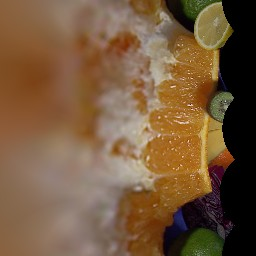
\includegraphics[width=0.4\textwidth]{pics/logpolar.jpg}
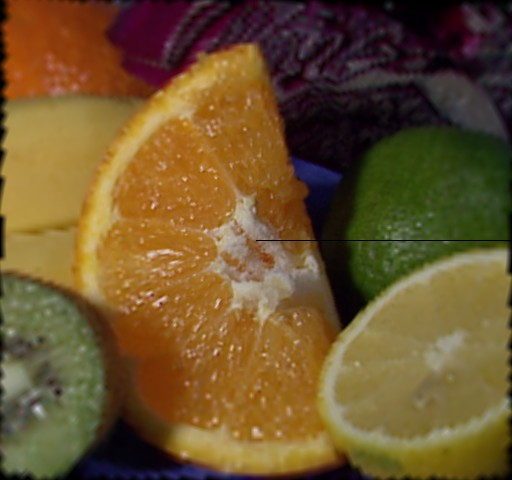
\includegraphics[width=0.4\textwidth]{pics/inv_logpolar.jpg}
\fi

\cvCPyFunc{Remap}
Applies a generic geometrical transformation to the image.

\cvdefC{
void cvRemap(
\par const CvArr* src,
\par CvArr* dst,
\par const CvArr* mapx,
\par const CvArr* mapy,
\par int flags=CV\_INTER\_LINEAR+CV\_WARP\_FILL\_OUTLIERS,
\par CvScalar fillval=cvScalarAll(0) );}
\cvdefPy{Remap(src,dst,mapx,mapy,flags=CV\_INNER\_LINEAR+CV\_WARP\_FILL\_OUTLIERS,fillval=cvScalarAll0))-> None}

\begin{description}
\cvarg{src}{Source image}
\cvarg{dst}{Destination image}
\cvarg{mapx}{The map of x-coordinates (32fC1 image)}
\cvarg{mapy}{The map of y-coordinates (32fC1 image)}
\cvarg{flags}{A combination of interpolation method and the following optional flag(s):
\begin{description}
  \cvarg{CV\_WARP\_FILL\_OUTLIERS}{fills all of the destination image pixels. If some of them correspond to outliers in the source image, they are set to \texttt{fillval}}
\end{description}}
\cvarg{fillval}{A value used to fill outliers}
\end{description}

The function \texttt{cvRemap} transforms the source image using the specified map:

\[
\texttt{dst}(x,y) = \texttt{src}(\texttt{mapx}(x,y),\texttt{mapy}(x,y))
\]

Similar to other geometrical transformations, some interpolation method (specified by user) is used to extract pixels with non-integer coordinates.
Note that the function can not operate in-place.

\cvCPyFunc{Resize}
Resizes an image.

\cvdefC{
void cvResize(
\par const CvArr* src,
\par CvArr* dst,
\par int interpolation=CV\_INTER\_LINEAR );}
\cvdefPy{Resize(src,dst,interpolation=CV\_INTER\_LINEAR)-> None}

\begin{description}
\cvarg{src}{Source image}
\cvarg{dst}{Destination image}
\cvarg{interpolation}{Interpolation method:
\begin{description}
\cvarg{CV\_INTER\_NN}{nearest-neigbor interpolation}
\cvarg{CV\_INTER\_LINEAR}{bilinear interpolation (used by default)}
\cvarg{CV\_INTER\_AREA}{resampling using pixel area relation. It is the preferred method for image decimation that gives moire-free results. In terms of zooming it is similar to the \texttt{CV\_INTER\_NN} method}
\cvarg{CV\_INTER\_CUBIC}{bicubic interpolation}
\end{description}}
\end{description}

The function \texttt{cvResize} resizes an image \texttt{src} so that it fits exactly into \texttt{dst}. If ROI is set, the function considers the ROI as supported.

\cvCPyFunc{Undistort2}
Transforms an image to compensate for lens distortion.

\cvdefC{void cvUndistort2( \par const CvArr* src,\par CvArr* dst,\par const CvMat* intrinsic\_matrix,\par const CvMat* distortion\_coeffs );
}
\cvdefPy{Undistort2(src,dst,intrinsic\_matrix,distortion\_coeffs)-> None}

\begin{description}
\cvarg{src}{The input (distorted) image}
\cvarg{dst}{The output (corrected) image}
\cvarg{intrinsic\_matrix}{The camera matrix $A = \vecthreethree{fx}{0}{cx}{0}{fy}{cy}{0}{0}{1} $}
\cvarg{distortion\_coeffs}{The 4x1 or 1x4 vector of distortion coefficients $k_1, k_2, k_3, k_4$.}
\end{description}

The function \texttt{cvUndistort2} transforms the image to compensate
radial and tangential lens distortion. The camera matrix and
distortion parameters can be determined using
\cvCPyCross{CalibrateCamera2}. For every
pixel in the output image the function computes the coordinates of the
corresponding location in the input image using the formulas in the
section beginning. Then, the pixel value is computed using bilinear
interpolation. If the resolution of images is different from what
was used at the calibration stage, $fx, fy, cx$ and $cy$
need to be adjusted appropriately, while the distortion coefficients
remain the same.

The function can not operate in-place.

\cvCPyFunc{WarpAffine}
Applies an affine transformation to an image.

\cvdefC{
void cvWarpAffine(
\par const CvArr* src,
\par CvArr* dst,
\par const CvMat* mapMatrix,
\par int flags=CV\_INTER\_LINEAR+CV\_WARP\_FILL\_OUTLIERS,
\par CvScalar fillval=cvScalarAll(0) );
}
\cvdefPy{WarpAffline(src,dst,mapMatrix,flags=CV\_INTER\_LINEAR+CV\_WARP\_FILL\_OUTLIERS,fillval=cvScalarAll(0))-> None}

\begin{description}
\cvarg{src}{Source image}
\cvarg{dst}{Destination image}
\cvarg{mapMatrix}{$2\times 3$ transformation matrix}
\cvarg{flags}{A combination of interpolation methods and the following optional flags:
\begin{description}
  \cvarg{CV\_WARP\_FILL\_OUTLIERS}{fills all of the destination image pixels; if some of them correspond to outliers in the source image, they are set to \texttt{fillval}}
  \cvarg{CV\_WARP\_INVERSE\_MAP}{indicates that \texttt{matrix} is inversely
  transformed from the destination image to the source and, thus, can be used
  directly for pixel interpolation. Otherwise, the function finds
  the inverse transform from \texttt{mapMatrix}}}
\end{description}
\cvarg{fillval}{A value used to fill outliers}
\end{description}

The function \texttt{cvWarpAffine} transforms the source image using the specified matrix:

\[
dst(x',y') = src(x,y)
\]

where

\[
\begin{matrix}
\begin{bmatrix}
x'\\
y'
\end{bmatrix} = \texttt{mapMatrix} \cdot \begin{bmatrix}
x\\
y\\
1
\end{bmatrix} & \mbox{if CV\_WARP\_INVERSE\_MAP is not set}\\
\begin{bmatrix}
x\\
y
\end{bmatrix} = \texttt{mapMatrix} \cdot \begin{bmatrix}
x'\\
y'\\
1
\end{bmatrix}& \mbox{otherwise}
\end{matrix}
\]

The function is similar to \cvCPyCross{GetQuadrangleSubPix} but they are not exactly the same. \cvCPyCross{WarpAffine} requires input and output image have the same data type, has larger overhead (so it is not quite suitable for small images) and can leave part of destination image unchanged. While \cvCPyCross{GetQuadrangleSubPix} may extract quadrangles from 8-bit images into floating-point buffer, has smaller overhead and always changes the whole destination image content.
Note that the function can not operate in-place.

To transform a sparse set of points, use the \cvCPyCross{Transform} function from cxcore.

\cvCPyFunc{WarpPerspective}
Applies a perspective transformation to an image.

\cvdefC{
void cvWarpPerspective(
\par const CvArr* src,
\par CvArr* dst,
\par const CvMat* mapMatrix,
\par int flags=CV\_INTER\_LINEAR+CV\_WARP\_FILL\_OUTLIERS,
\par CvScalar fillval=cvScalarAll(0) );
}\cvdefPy{WarpPerspective(src,dst,mapMatrix,flags=CV\_I
NNER\_LINEAR+CV\_WARP\_FILL\_OUTLIERS,fillval=cvScalarAll(0
))-> None}

\begin{description}
\cvarg{src}{Source image}
\cvarg{dst}{Destination image}
\cvarg{mapMatrix}{$3\times 3$ transformation matrix}
\cvarg{flags}{A combination of interpolation methods and the following optional flags:
\begin{description}
  \cvarg{CV\_WARP\_FILL\_OUTLIERS}{fills all of the destination image pixels; if some of them correspond to outliers in the source image, they are set to \texttt{fillval}}
  \cvarg{CV\_WARP\_INVERSE\_MAP}{indicates that \texttt{matrix} is inversely transformed from the destination image to the source and, thus, can be used directly for pixel interpolation. Otherwise, the function finds the inverse transform from \texttt{mapMatrix}}
\end{description}}
\cvarg{fillval}{A value used to fill outliers}
\end{description}

The function \texttt{cvWarpPerspective} transforms the source image using the specified matrix:

\[
\begin{matrix}
\begin{bmatrix}
x'\\
y'
\end{bmatrix} = \texttt{mapMatrix} \cdot \begin{bmatrix}
x\\
y\\
1
\end{bmatrix} & \mbox{if CV\_WARP\_INVERSE\_MAP is not set}\\
\begin{bmatrix}
x\\
y
\end{bmatrix} = \texttt{mapMatrix} \cdot \begin{bmatrix}
x'\\
y'\\
1
\end{bmatrix}& \mbox{otherwise}
\end{matrix}
\]

Note that the function can not operate in-place.
For a sparse set of points use the \cvCPyCross{PerspectiveTransform} function from CxCore.

\fi

\ifCpp

\cvCppFunc{convertMaps}
Converts image transformation maps from one representation to another

\cvdefCpp{void convertMaps( const Mat\& map1, const Mat\& map2,\par
                  Mat\& dstmap1, Mat\& dstmap2,\par
                  int dstmap1type, bool nninterpolation=false );}
\begin{description}
\cvarg{map1}{The first input map of type \texttt{CV\_16SC2} or \texttt{CV\_32FC1} or \texttt{CV\_32FC2}}
\cvarg{map2}{The second input map of type \texttt{CV\_16UC1} or \texttt{CV\_32FC1} or none (empty matrix), respectively}
\cvarg{dstmap1}{The first output map; will have type \texttt{dstmap1type} and the same size as \texttt{src}}
\cvarg{dstmap2}{The second output map}
\cvarg{dstmap1type}{The type of the first output map; should be \texttt{CV\_16SC2}, \texttt{CV\_32FC1} or \texttt{CV\_32FC2}}
\cvarg{nninterpolation}{Indicates whether the fixed-point maps will be used for nearest-neighbor or for more complex interpolation}
\end{description}

The function converts a pair of maps for \cvCppCross{remap} from one representation to another. The following options (\texttt{(map1.type(), map2.type())} $\rightarrow$ \texttt{(dstmap1.type(), dstmap2.type())}) are supported:
\begin{enumerate}
    \item $\texttt{(CV\_32FC1, CV\_32FC1)} \rightarrow \texttt{(CV\_16SC2, CV\_16UC1)}$. This is the most frequently used conversion operation, in which the original floating-point maps (see \cvCppCross{remap}) are converted to more compact and much faster fixed-point representation. The first output array will contain the rounded coordinates and the second array (created only when \texttt{nninterpolation=false}) will contain indices in the interpolation tables.   
    \item $\texttt{(CV\_32FC2)} \rightarrow \texttt{(CV\_16SC2, CV\_16UC1)}$. The same as above, but the original maps are stored in one 2-channel matrix.
    \item the reverse conversion. Obviously, the reconstructed floating-point maps will not be exactly the same as the originals.
\end{enumerate} 

See also: \cvCppCross{remap}, \cvCppCross{undisort}, \cvCppCross{initUndistortRectifyMap}

\cvCppFunc{getAffineTransform}
Calculates the affine transform from 3 pairs of the corresponding points

\cvdefCpp{Mat getAffineTransform( const Point2f src[], const Point2f dst[] );}

\begin{description}
\cvarg{src}{Coordinates of a triangle vertices in the source image}
\cvarg{dst}{Coordinates of the corresponding triangle vertices in the destination image}
\end{description}

The function calculates the $2 \times 3$ matrix of an affine transform such that:

\[
\begin{bmatrix}
x'_i\\
y'_i
\end{bmatrix}
=
\texttt{map\_matrix}
\cdot
\begin{bmatrix}
x_i\\
y_i\\
1
\end{bmatrix}
\]

where

\[
dst(i)=(x'_i,y'_i),
src(i)=(x_i, y_i),
i=0,1,2
\]

See also: \cvCppCross{warpAffine}, \cvCppCross{transform}

\cvCppFunc{getPerspectiveTransform}
Calculates the perspective transform from 4 pairs of the corresponding points

\cvdefCpp{Mat getPerspectiveTransform( const Point2f src[], \par const Point2f dst[] );}

\begin{description}
\cvarg{src}{Coordinates of a quadrange vertices in the source image}
\cvarg{dst}{Coordinates of the corresponding quadrangle vertices in the destination image}
\end{description}

The function calculates the $3 \times 3$ matrix of a perspective transform such that:

\[
\begin{bmatrix}
t_i x'_i\\
t_i y'_i\\
t_i
\end{bmatrix}
=
\texttt{map\_matrix}
\cdot
\begin{bmatrix}
x_i\\
y_i\\
1
\end{bmatrix}
\]

where

\[
dst(i)=(x'_i,y'_i),
src(i)=(x_i, y_i),
i=0,1,2
\]

See also: \cvCppCross{findHomography}, \cvCppCross{warpPerspective}, \cvCppCross{perspectiveTransform}

\cvCppFunc{getRectSubPix}
Retrieves the pixel rectangle from an image with sub-pixel accuracy

\cvdefCpp{void getRectSubPix( const Mat\& image, Size patchSize,\par
                    Point2f center, Mat\& dst, int patchType=-1 );}
\begin{description}
\cvarg{src}{Source image}
\cvarg{patchSize}{Size of the extracted patch}
\cvarg{center}{Floating point coordinates of the extracted rectangle center within the source image. The center must be inside the image}
\cvarg{dst}{The extracted patch; will have the size \texttt{patchSize} and the same number of channels as \texttt{src}}
\cvarg{patchType}{The depth of the extracted pixels. By default they will have the same depth as \texttt{src}}
\end{description}

The function \texttt{getRectSubPix} extracts pixels from \texttt{src}:

\[
dst(x, y) = src(x + \texttt{center.x} - (\texttt{dst.cols}-1)*0.5, y + \texttt{center.y} - (\texttt{dst.rows}-1)*0.5)
\]

where the values of the pixels at non-integer coordinates are retrieved
using bilinear interpolation. Every channel of multiple-channel
images is processed independently. While the rectangle center
must be inside the image, parts of the rectangle may be
outside. In this case, the replication border mode (see \cvCppCross{borderInterpolate}) is used to extrapolate
the pixel values outside of the image.

See also: \cvCppCross{warpAffine}, \cvCppCross{warpPerspective}

\cvCppFunc{getRotationMatrix2D}
Calculates the affine matrix of 2d rotation.

\cvdefCpp{Mat getRotationMatrix2D( Point2f center, double angle, double scale );}
\begin{description}
\cvarg{center}{Center of the rotation in the source image}
\cvarg{angle}{The rotation angle in degrees. Positive values mean counter-clockwise rotation (the coordinate origin is assumed to be the top-left corner)}
\cvarg{scale}{Isotropic scale factor}
\end{description}

The function calculates the following matrix:

\[
\begin{bmatrix}
\alpha & \beta & (1-\alpha) \cdot \texttt{center.x} - \beta \cdot \texttt{center.y} \\
-\beta & \alpha & \beta \cdot \texttt{center.x} - (1-\alpha) \cdot \texttt{center.y}
\end{bmatrix}
\]

where

\[
\begin{array}{l}
\alpha = \texttt{scale} \cdot \cos \texttt{angle},\\
\beta = \texttt{scale} \cdot \sin \texttt{angle}
\end{array}
\]

The transformation maps the rotation center to itself. If this is not the purpose, the shift should be adjusted.

See also: \cvCppCross{getAffineTransform}, \cvCppCross{warpAffine}, \cvCppCross{transform}

\cvCppFunc{initUndistortRectifyMap}
Computes the undistortion and rectification transformation map of a head of a stereo camera.

\cvdefCpp{void initUndistortRectifyMap( const Mat\& cameraMatrix,\par
                           const Mat\& distCoeffs, const Mat\& R,\par
                           const Mat\& newCameraMatrix,\par
                           Size size, int m1type,\par
                           Mat\& map1, Mat\& map2 );}
\begin{description}
\cvarg{cameraMatrix}{The camera matrix $A=\vecthreethree{f_x}{0}{c_x}{0}{f_y}{c_y}{0}{0}{1}$}
\cvarg{distCoeffs}{The vector of distortion coefficients, \cvCppCross{4x1, 1x4, 5x1 or 1x5}}
\cvarg{R}{The rectification transformation in object space (3x3 matrix). \texttt{R1} or \texttt{R2}, computed by \cvCppCross{stereoRectify} can be passed here. If the matrix is empty, the identity transformation is assumed}
\cvarg{newCameraMatrix}{The new camera matrix $A'=\vecthreethree{f_x'}{0}{c_x'}{0}{f_y'}{c_y'}{0}{0}{1}$}
\cvarg{size}{The image size}
\cvarg{m1type}{The type of the first output map, can be \texttt{CV\_32FC1} or \texttt{CV\_16SC2}. See \cvCppCross{convertMaps}}
\cvarg{map1}{The first output map}
\cvarg{map2}{The second output map}
\end{description}

The function computes the joint undistortion+rectification transformation and represents the result in the form of maps for \cvCppCross{remap}. The undistorted image will look like the original, as if it was captured with a camera with camera matrix \texttt{=newCameraMatrix} and zero distortion. Also, this new camera will be oriented differently in the coordinate space, according to \texttt{R}. That, for example, helps to align a stereo pair so that the epipolar lines on both images become horizontal and have the same y- coordinate (in case of horizontally aligned stereo camera).

The function actually builds the maps for the inverse mapping algorithm that is used by \cvCppCross{remap}. That is, for each pixel $(u, v)$ in the destination (corrected and rectified) image the function computes the corresponding coordinates in the source image (i.e. the original image from camera). The process is the following:

\[
\begin{array}{l}
x \leftarrow (u - {c'}_x)/{f'}_x \\
y \leftarrow (v - {c'}_y)/{f'}_y \\
{[X\,Y\,W]}^T \leftarrow R^{-1}*[x\,y\,1]^T \\
x' \leftarrow X/W \\
y' \leftarrow Y/W \\
x" \leftarrow x' (1 + k_1 r^2 + k_2 r^4 + k_3 r^6) + 2p_1 x' y' + p_2(r^2 + 2 x'^2) \\
y" \leftarrow y' (1 + k_1 r^2 + k_2 r^4 + k_3 r^6) + p_1 (r^2 + 2 y'^2) + 2 p_2 x' y' \\
map_x(u,v) \leftarrow x" f_x + c_x \\
map_y(u,v) \leftarrow y" f_y + c_y
\end{array}
\]
where $(k_1, k_2, p_1, p_2[, k_3])$\label{4x1, 1x4, 5x1 or 1x5} are the distortion coefficients. 
 
In the case of a stereo camera this function is called twice, once for each camera head, after \cvCppCross{stereoRectify}. But it is also possible to compute the rectification transformations directly from the fundamental matrix, e.g. by using \cvCppCross{stereoRectifyUncalibrated}. Such functions work with pixels and produce homographies \texttt{H} as rectification transformations, not rotation matrices \texttt{R} in 3D space. In this case, the \texttt{R} can be computed from the homography matrix \texttt{H} as 

\[ \texttt{R} = \texttt{cameraMatrix}^{-1} \cdot \texttt{H} \cdot \texttt{cameraMatrix} \]

\cvCppFunc{invertAffineTransform}
Inverts an affine transformation

\cvdefCpp{void invertAffineTransform(const Mat\& M, Mat\& iM);}
\begin{description}
\cvarg{M}{The original affine transformation}
\cvarg{iM}{The output reverse affine transformation}
\end{description}

The function computes inverse affine transformation represented by $2 \times 3$ matrix \texttt{M}:

\[\begin{bmatrix}
a_{11} & a_{12} & b_1 \\
a_{21} & a_{22} & b_2
\end{bmatrix}
\]

The result will also be a $2 \times 3$ matrix of the same type as \texttt{M}.

\cvCppFunc{remap}
Applies a generic geometrical transformation to an image.

\cvdefCpp{void remap( const Mat\& src, Mat\& dst, const Mat\& map1, const Mat\& map2,\par
            int interpolation, int borderMode=BORDER\_CONSTANT,\par
            const Scalar\& borderValue=Scalar());}
\begin{description}
\cvarg{src}{Source image}
\cvarg{dst}{Destination image. It will have the same size as \texttt{map1} and the same type as \texttt{src}}
\cvarg{map1}{The first map of type \texttt{CV\_16SC2}, \texttt{CV\_32FC1} or \texttt{CV\_32FC2}. See \cvCppCross{convertMaps}}
\cvarg{map2}{The second map of type \texttt{CV\_16UC1}, \texttt{CV\_32FC1} or none (empty map), respectively}
\cvarg{interpolation}{The interpolation method, see \cvCppCross{resize}. The method \texttt{INTER\_AREA} is not supported by this function}
\cvarg{borderMode}{The pixel extrapolation method, see \cvCppCross{borderInterpolate}. When the\\ \texttt{borderMode=BORDER\_TRANSPARENT}, it means that the pixels in the destination image that corresponds to the "outliers" in the source image are not modified by the function}
\cvarg{borderValue}{A value used in the case of a constant border. By default it is 0}
\end{description}

The function \texttt{remap} transforms the source image using the specified map:

\[
\texttt{dst}(x,y) = \texttt{src}(map_x(x,y),map_y(x,y))
\]

Where values of pixels with non-integer coordinates are computed using one of the available interpolation methods. $map_x$ and $map_y$ can be encoded as separate floating-point maps, interleaved floating-point maps or fixed-point maps.
The function can not operate in-place.

\cvCppFunc{resize}
Resizes an image

\cvdefCpp{void resize( const Mat\& src, Mat\& dst,\par
             Size dsize, double fx=0, double fy=0,\par
             int interpolation=INTER\_LINEAR );}
\begin{description}
\cvarg{src}{Source image}
\cvarg{dst}{Destination image. It will have size \texttt{dsize} (when it is non-zero) or the size computed from \texttt{src.size()}
and \texttt{fx} and \texttt{fy}. The type of \texttt{dst} will be the same as of \texttt{src}.}
\cvarg{dsize}{The destination image size. If it is zero, then it is computed as:
\[\texttt{dsize = Size(round(fx*src.cols), round(fy*src.rows))}\].
Either \texttt{dsize} or both \texttt{fx} or \texttt{fy} must be non-zero.}
\cvarg{fx}{The scale factor along the horizontal axis. When 0, it is computed as
\[\texttt{(double)dsize.width/src.cols}\]}
\cvarg{fy}{The scale factor along the vertical axis. When 0, it is computed as
\[\texttt{(double)dsize.height/src.rows}\]}
\cvarg{interpolation}{The interpolation method:
\begin{description}
\cvarg{INTER\_NEAREST}{nearest-neighbor interpolation}
\cvarg{INTER\_LINEAR}{bilinear interpolation (used by default)}
\cvarg{INTER\_AREA}{resampling using pixel area relation. It may be the preferred method for image decimation, as it gives moire-free results. But when the image is zoomed, it is similar to the \texttt{INTER\_NEAREST} method}
\cvarg{INTER\_CUBIC}{bicubic interpolation over 4x4 pixel neighborhood}
\cvarg{INTER\_LANCZOS4}{Lanczos interpolation over 8x8 pixel neighborhood}
\end{description}}
\end{description}

The function \texttt{resize} resizes an image \texttt{src} down to or up to the specified size.
Note that the initial \texttt{dst} type or size are not taken into account. Instead the size and type are derived from the \texttt{src}, \texttt{dsize}, \texttt{fx} and \texttt{fy}. If you want to resize \texttt{src} so that it fits the pre-created \texttt{dst}, you may call the function as:

\begin{lstlisting}
// explicitly specify dsize=dst.size(); fx and fy will be computed from that.
resize(src, dst, dst.size(), 0, 0, interpolation);
\end{lstlisting}

If you want to decimate the image by factor of 2 in each direction, you can call the function this way:

\begin{lstlisting}
// specify fx and fy and let the function to compute the destination image size.
resize(src, dst, Size(), 0.5, 0.5, interpolation);
\end{lstlisting}

See also: \cvCppCross{warpAffine}, \cvCppCross{warpPerspective}, \cvCppCross{remap}.

\cvCppFunc{undistort}
Transforms an image to compensate for lens distortion.

\cvdefCpp{void undistort( const Mat\& src, Mat\& dst, const Mat\& cameraMatrix,\par
                const Mat\& distCoeffs, const Mat\& newCameraMatrix=Mat() );}
\begin{description}
\cvarg{src}{The input (distorted) image}
\cvarg{dst}{The output (corrected) image; will have the same size and the same type as \texttt{src}}
\cvarg{cameraMatrix}{The camera matrix $A = \vecthreethree{f_x}{0}{c_x}{0}{f_y}{c_y}{0}{0}{1} $}
\cvarg{distortion\_coeffs}{The 4x1, 5x1, 1x4 or 1x5 vector of distortion coefficients $(k_1, k_2, p_1, p_2[, k_3])$.}
\cvarg{newCameraMatrix}{Camera matrix of the distorted image. By default it is the same as \texttt{cameraMatrix}, but you may additionally scale and shift the result by using some different matrix}
\end{description}

The function \texttt{undistort} transforms the image to compensate
radial and tangential lens distortion. The function is simply a combination of \cvCppCross{initUndistortRectifyMap} (with unity \texttt{R}) and \cvCppCross{remap} (with bilinear interpolation) put into one loop.

The camera matrix and the distortion parameters can be determined using
\cvCppCross{calibrateCamera}. If the resolution of images is different from the used at the calibration stage, $f_x, f_y, c_x$ and $c_y$
need to be scaled accordingly, while the distortion coefficients remain the same.

\cvCppFunc{warpAffine}
Applies an affine transformation to an image.

\cvdefCpp{void warpAffine( const Mat\& src, Mat\& dst,\par
                 const Mat\& M, Size dsize,\par
                 int flags=INTER\_LINEAR,\par
                 int borderMode=BORDER\_CONSTANT,\par
                 const Scalar\& borderValue=Scalar());}
\begin{description}
\cvarg{src}{Source image}
\cvarg{dst}{Destination image; will have size \texttt{dsize} and the same type as \texttt{src}}
\cvarg{M}{$2\times 3$ transformation matrix}
\cvarg{dsize}{Size of the destination image}
\cvarg{flags}{A combination of interpolation methods, see \cvCppCross{resize}, and the optional flag \texttt{WARP\_INVERSE\_MAP} that means that \texttt{M} is the inverse transformation ($\texttt{dst}\rightarrow\texttt{src}$)}
\cvarg{borderMode}{The pixel extrapolation method, see \cvCppCross{borderInterpolate}. When the \\ \texttt{borderMode=BORDER\_TRANSPARENT}, it means that the pixels in the destination image that corresponds to the "outliers" in the source image are not modified by the function}
\cvarg{borderValue}{A value used in case of a constant border. By default it is 0}
\end{description}

The function \texttt{warpAffine} transforms the source image using the specified matrix:

\[
\texttt{dst}(x,y) = \texttt{src}(\texttt{M}_{11} x + \texttt{M}_{12} y + \texttt{M}_{13}, \texttt{M}_{21} x + \texttt{M}_{22} y + \texttt{M}_{23})
\]
when the flag \texttt{WARP\_INVERSE\_MAP} is set. Otherwise, the transformation is first inverted with \cvCppCross{invertAffineTransform} and then put in the formula above instead of \texttt{M}.
The function can not operate in-place.

See also: \cvCppCross{warpPerspective}, \cvCppCross{resize}, \cvCppCross{remap}, \cvCppCross{getRectSubPix}, \cvCppCross{transform}

\cvCppFunc{warpPerspective}
Applies a perspective transformation to an image.

\cvdefCpp{void warpPerspective( const Mat\& src, Mat\& dst,\par
                      const Mat\& M, Size dsize,\par
                      int flags=INTER\_LINEAR,\par
                      int borderMode=BORDER\_CONSTANT,\par
                      const Scalar\& borderValue=Scalar());}
\begin{description}
\cvarg{src}{Source image}
\cvarg{dst}{Destination image; will have size \texttt{dsize} and the same type as \texttt{src}}
\cvarg{M}{$3\times 3$ transformation matrix}
\cvarg{dsize}{Size of the destination image}
\cvarg{flags}{A combination of interpolation methods, see \cvCppCross{resize}, and the optional flag \texttt{WARP\_INVERSE\_MAP} that means that \texttt{M} is the inverse transformation ($\texttt{dst}\rightarrow\texttt{src}$)}
\cvarg{borderMode}{The pixel extrapolation method, see \cvCppCross{borderInterpolate}. When the \\ \texttt{borderMode=BORDER\_TRANSPARENT}, it means that the pixels in the destination image that corresponds to the "outliers" in the source image are not modified by the function}
\cvarg{borderValue}{A value used in case of a constant border. By default it is 0}
\end{description}

The function \texttt{warpPerspective} transforms the source image using the specified matrix:

\[
\texttt{dst}(x,y) = \texttt{src}\left(\frac{M_{11} x + M_{12} y + M_{13}}{M_{31} x + M_{32} y + M_{33}},
    \frac{M_{21} x + M_{22} y + M_{23}}{M_{31} x + M_{32} y + M_{33}}\right)
\]
when the flag \texttt{WARP\_INVERSE\_MAP} is set. Otherwise, the transformation is first inverted with \cvCppCross{invert} and then put in the formula above instead of \texttt{M}.
The function can not operate in-place.

See also: \cvCppCross{warpAffine}, \cvCppCross{resize}, \cvCppCross{remap}, \cvCppCross{getRectSubPix}, \cvCppCross{perspectiveTransform}

\fi


\section{Miscellaneous Image Transformations}

\ifCPy

\cvCPyFunc{AdaptiveThreshold}
Applies an adaptive threshold to an array.

\cvdefC{
void cvAdaptiveThreshold(
\par const CvArr* src,\par CvArr* dst,\par double maxValue,\par
int adaptive\_method=CV\_ADAPTIVE\_THRESH\_MEAN\_C,\par
int thresholdType=CV\_THRESH\_BINARY,\par
int blockSize=3,\par double param1=5 );
}

\cvdefPy{AdaptiveThreshold(src,dst,maxValue, adaptive\_method=CV\_ADAPTIVE\_THRESH\_MEAN\_C, thresholdType=CV\_THRESH\_BINARY,blockSize=3,param1=5)-> None}

\begin{description}
\cvarg{src}{Source image}
\cvarg{dst}{Destination image}
\cvarg{maxValue}{Maximum value that is used with \texttt{CV\_THRESH\_BINARY} and \texttt{CV\_THRESH\_BINARY\_INV}}
\cvarg{adaptive\_method}{Adaptive thresholding algorithm to use: \texttt{CV\_ADAPTIVE\_THRESH\_MEAN\_C} or \texttt{CV\_ADAPTIVE\_THRESH\_GAUSSIAN\_C} (see the discussion)}
\cvarg{thresholdType}{Thresholding type; must be one of
\begin{description}
\cvarg{CV\_THRESH\_BINARY}{xxx}
\cvarg{CV\_THRESH\_BINARY\_INV}{xxx}
\end{description}}
\cvarg{blockSize}{The size of a pixel neighborhood that is used to calculate a threshold value for the pixel: 3, 5, 7, and so on}
\cvarg{param1}{The method-dependent parameter. For the methods \texttt{CV\_ADAPTIVE\_THRESH\_MEAN\_C} and \texttt{CV\_ADAPTIVE\_THRESH\_GAUSSIAN\_C} it is a constant subtracted from the mean or weighted mean (see the discussion), though it may be negative}
\end{description}

The function transforms a grayscale image to a binary image according to the formulas:

\begin{description}
\cvarg{CV\_THRESH\_BINARY}{\[ dst(x,y) = \fork{\texttt{maxValue}}{if $src(x,y) > T(x,y)$}{0}{otherwise} \]}
\cvarg{CV\_THRESH\_BINARY\_INV}{\[ dst(x,y) = \fork{0}{if $src(x,y) > T(x,y)$}{\texttt{maxValue}}{otherwise} \]}
\end{description}

where $T(x,y)$ is a threshold calculated individually for each pixel.

For the method \texttt{CV\_ADAPTIVE\_THRESH\_MEAN\_C} it is the mean of a $\texttt{blockSize} \times \texttt{blockSize}$ pixel neighborhood, minus \texttt{param1}.

For the method \texttt{CV\_ADAPTIVE\_THRESH\_GAUSSIAN\_C} it is the weighted sum (gaussian) of a $\texttt{blockSize} \times \texttt{blockSize}$ pixel neighborhood, minus \texttt{param1}.

\cvCPyFunc{CvtColor}
Converts an image from one color space to another.

\cvdefC{
void cvCvtColor(
\par const CvArr* src,
\par CvArr* dst,
\par int code );
}\cvdefPy{CvtColor(src,dst,code)-> None}

\begin{description}
\cvarg{src}{The source 8-bit (8u), 16-bit (16u) or single-precision floating-point (32f) image}
\cvarg{dst}{The destination image of the same data type as the source. The number of channels may be different}
\cvarg{code}{Color conversion operation that can be specifed using \texttt{CV\_ \textit{src\_color\_space} 2 \textit{dst\_color\_space}} constants (see below)}
\end{description}

The function converts the input image from one color
space to another. The function ignores the \texttt{colorModel} and
\texttt{channelSeq} fields of the \texttt{IplImage} header, so the
source image color space should be specified correctly (including
order of the channels in the case of RGB space. For example, BGR means 24-bit
format with $B_0, G_0, R_0, B_1, G_1, R_1, ...$ layout
whereas RGB means 24-format with $R_0, G_0, B_0, R_1, G_1, B_1, ...$
layout).

The conventional range for R,G,B channel values is:

\begin{itemize}
\item 0 to 255 for 8-bit images
\item 0 to 65535 for 16-bit images and
\item 0 to 1 for floating-point images.
\end{itemize}

Of course, in the case of linear transformations the range can be
specific, but in order to get correct results in the case of non-linear
transformations, the input image should be scaled.

The function can do the following transformations:

\begin{itemize}
\item Transformations within RGB space like adding/removing the alpha channel, reversing the channel order, conversion to/from 16-bit RGB color (R5:G6:B5 or R5:G5:B5), as well as conversion to/from grayscale using:
\[
\text{RGB[A] to Gray:} Y \leftarrow 0.299 \cdot R + 0.587 \cdot G + 0.114 \cdot B
\]
and
\[
\text{Gray to RGB[A]:} R \leftarrow Y, G \leftarrow Y, B \leftarrow Y, A \leftarrow 0
\]

The conversion from a RGB image to gray is done with:
\begin{lstlisting}
cvCvtColor(src ,bwsrc, CV_RGB2GRAY)
\end{lstlisting}

\item RGB $\leftrightarrow$ CIE XYZ.Rec 709 with D65 white point (\texttt{CV\_BGR2XYZ, CV\_RGB2XYZ, CV\_XYZ2BGR, CV\_XYZ2RGB}):
\[
\begin{bmatrix}
X \\
Y \\
Z
\end{bmatrix}
\leftarrow
\begin{bmatrix}
0.412453 & 0.357580 & 0.180423\\
0.212671 & 0.715160 & 0.072169\\
0.019334 & 0.119193 & 0.950227
\end{bmatrix}
\cdot
\begin{bmatrix}
R \\
G \\
B
\end{bmatrix}
\]
\[
\begin{bmatrix}
R \\
G \\
B
\end{bmatrix}
\leftarrow
\begin{bmatrix}
3.240479 & -1.53715 & -0.498535\\
-0.969256 &  1.875991 & 0.041556\\
0.055648 & -0.204043 & 1.057311
\end{bmatrix}
\cdot
\begin{bmatrix}
X \\
Y \\
Z
\end{bmatrix}
\]
$X$, $Y$ and $Z$ cover the whole value range (in the case of floating-point images $Z$ may exceed 1).

\item RGB $\leftrightarrow$ YCrCb JPEG (a.k.a. YCC) (\texttt{CV\_BGR2YCrCb, CV\_RGB2YCrCb, CV\_YCrCb2BGR, CV\_YCrCb2RGB})
\[ Y \leftarrow 0.299 \cdot R + 0.587 \cdot G + 0.114 \cdot B \]
\[  Cr \leftarrow (R-Y) \cdot 0.713 + delta \]
\[  Cb \leftarrow (B-Y) \cdot 0.564 + delta \]
\[  R \leftarrow Y + 1.403 \cdot (Cr - delta) \]
\[  G \leftarrow Y - 0.344 \cdot (Cr - delta) - 0.714 \cdot (Cb - delta) \]
\[  B \leftarrow Y + 1.773 \cdot (Cb - delta) \]
where
\[
delta = \left\{
\begin{array}{l l}
128 & \mbox{for 8-bit images}\\
32768 & \mbox{for 16-bit images}\\
0.5 & \mbox{for floating-point images}
\end{array} \right.
\]
Y, Cr and Cb cover the whole value range.

\item RGB $\leftrightarrow$ HSV (\texttt{CV\_BGR2HSV, CV\_RGB2HSV, CV\_HSV2BGR, CV\_HSV2RGB})
in the case of 8-bit and 16-bit images
R, G and B are converted to floating-point format and scaled to fit the 0 to 1 range
\[ V \leftarrow max(R,G,B) \]

\[ S \leftarrow \fork{\frac{V-min(R,G,B)}{V}}{if $V \neq 0$}{0}{otherwise} \]
\[ H \leftarrow \forkthree
{{60(G - B)}/{S}}{if $V=R$}
{{120+60(B - R)}/{S}}{if $V=G$}
{{240+60(R - G)}/{S}}{if $V=B$} \]
if $H<0$ then $H \leftarrow H+360$

On output $0 \leq V \leq 1$, $0 \leq S \leq 1$, $0 \leq H \leq 360$.

The values are then converted to the destination data type:
\begin{description}
\item[8-bit images]
\[ V \leftarrow 255 V, S \leftarrow 255 S, H \leftarrow H/2 \text{(to fit to 0 to 255)} \]
\item[16-bit images (currently not supported)]
\[ V <- 65535 V, S <- 65535 S, H <- H \]
\item[32-bit images]
H, S, V are left as is
\end{description}

\item RGB $\leftrightarrow$ HLS (\texttt{CV\_BGR2HLS, CV\_RGB2HLS, CV\_HLS2BGR, CV\_HLS2RGB}).
in the case of 8-bit and 16-bit images
R, G and B are converted to floating-point format and scaled to fit the 0 to 1 range.
\[ V_{max} \leftarrow {max}(R,G,B) \]
\[ V_{min} \leftarrow {min}(R,G,B) \]
\[ L \leftarrow \frac{V_{max} - V_{min}}{2} \]
\[ S \leftarrow \fork
{\frac{V_{max} - V_{min}}{V_{max} + V_{min}}}{if $L < 0.5$}
{\frac{V_{max} - V_{min}}{2 - (V_{max} + V_{min})}}{if $L \ge 0.5$} \]
\[ H \leftarrow \forkthree
{{60(G - B)}/{S}}{if $V_{max}=R$}
{{120+60(B - R)}/{S}}{if $V_{max}=G$}
{{240+60(R - G)}/{S}}{if $V_{max}=B$} \]
if $H<0$ then $H \leftarrow H+360$
On output $0 \leq V \leq 1$, $0 \leq S \leq 1$, $0 \leq H \leq 360$.

The values are then converted to the destination data type:
\begin{description}
\item[8-bit images]
\[ V \leftarrow 255 V, S \leftarrow 255 S, H \leftarrow H/2 \text{(to fit to 0 to 255)} \]
\item[16-bit images (currently not supported)]
\[ V <- 65535 V, S <- 65535 S, H <- H \]
\item[32-bit images]
H, S, V are left as is
\end{description}

\item RGB $\leftrightarrow$ CIE L*a*b* (\texttt{CV\_BGR2Lab, CV\_RGB2Lab, CV\_Lab2BGR, CV\_Lab2RGB})
in the case of 8-bit and 16-bit images
R, G and B are converted to floating-point format and scaled to fit the 0 to 1 range
\[ \vecthree{X}{Y}{Z} \leftarrow \vecthreethree
{0.412453}{0.357580}{0.180423}
{0.212671}{0.715160}{0.072169}
{0.019334}{0.119193}{0.950227}
\cdot
\vecthree{R}{G}{B} \]
\[ X \leftarrow X/X_n, \text{where} X_n = 0.950456 \]
\[ Z \leftarrow Z/Z_n, \text{where} Z_n = 1.088754 \]
\[ L \leftarrow \fork
{116*Y^{1/3}-16}{for $Y>0.008856$}
{903.3*Y}{for $Y \le 0.008856$} \]
\[ a \leftarrow 500 (f(X)-f(Y)) + delta \]
\[ b \leftarrow 200 (f(Y)-f(Z)) + delta \]
where
\[f(t)=\fork
{t^{1/3}}{for $t>0.008856$}
{7.787 t+16/116}{for $t<=0.008856$} \]
and
\[ delta = \fork{128}{for 8-bit images}{0}{for floating-point images} \]
On output $0 \leq L \leq 100$, $-127 \leq a \leq 127$, $-127 \leq b \leq 127$

The values are then converted to the destination data type:
\begin{description}
\item[8-bit images]
\[L \leftarrow L*255/100, a \leftarrow a + 128, b \leftarrow b + 128\]
\item[16-bit images] currently not supported
\item[32-bit images]
L, a, b are left as is
\end{description}

\item RGB $\leftrightarrow$ CIE L*u*v* (\texttt{CV\_BGR2Luv, CV\_RGB2Luv, CV\_Luv2BGR, CV\_Luv2RGB})
in the case of 8-bit and 16-bit images
R, G and B are converted to floating-point format and scaled to fit 0 to 1 range
\[ \vecthree{X}{Y}{Z} \leftarrow \vecthreethree
{0.412453}{0.357580}{0.180423}
{0.212671}{0.715160}{0.072169}
{0.019334}{0.119193}{0.950227}
\cdot
\vecthree{R}{G}{B} \]
\[ L \leftarrow \fork
{116 Y^{1/3}}{for $Y>0.008856$}
{903.3 Y}{for $Y<=0.008856$} \]
\[ u' \leftarrow 4*X/(X + 15*Y + 3 Z) \]
\[ v' \leftarrow 9*Y/(X + 15*Y + 3 Z) \]
\[ u \leftarrow 13*L*(u' - u_n) \quad \text{where} \quad u_n=0.19793943 \]
\[ v \leftarrow 13*L*(v' - v_n) \quad \text{where} \quad v_n=0.46831096 \]
On output $0 \leq L \leq 100$, $-134 \leq u \leq 220$, $-140 \leq v \leq 122$.

The values are then converted to the destination data type:
\begin{description}
\item[8-bit images]
\[L \leftarrow 255/100 L, u \leftarrow 255/354 (u + 134), v \leftarrow 255/256 (v + 140) \]
\item[16-bit images] currently not supported
\item[32-bit images] L, u, v are left as is
\end{description}

The above formulas for converting RGB to/from various color spaces have been taken from multiple sources on Web, primarily from
the Ford98
at the Charles Poynton site.

\item Bayer $\rightarrow$ RGB (\texttt{CV\_BayerBG2BGR, CV\_BayerGB2BGR, CV\_BayerRG2BGR, CV\_BayerGR2BGR, CV\_BayerBG2RGB, CV\_BayerGB2RGB, CV\_BayerRG2RGB, CV\_BayerGR2RGB}) The Bayer pattern is widely used in CCD and CMOS cameras. It allows one to get color pictures from a single plane where R,G and B pixels (sensors of a particular component) are interleaved like this:



\[
\newcommand{\Rcell}{\color{red}R}
\newcommand{\Gcell}{\color{green}G}
\newcommand{\Bcell}{\color{blue}B}
\definecolor{BackGray}{rgb}{0.8,0.8,0.8}
\begin{array}{ c c c c c }
\Rcell&\Gcell&\Rcell&\Gcell&\Rcell\\
\Gcell&\colorbox{BackGray}{\Bcell}&\colorbox{BackGray}{\Gcell}&\Bcell&\Gcell\\
\Rcell&\Gcell&\Rcell&\Gcell&\Rcell\\
\Gcell&\Bcell&\Gcell&\Bcell&\Gcell\\
\Rcell&\Gcell&\Rcell&\Gcell&\Rcell
\end{array}
\]

The output RGB components of a pixel are interpolated from 1, 2 or
4 neighbors of the pixel having the same color. There are several
modifications of the above pattern that can be achieved by shifting
the pattern one pixel left and/or one pixel up. The two letters
$C_1$ and $C_2$
in the conversion constants
\texttt{CV\_Bayer} $ C_1 C_2 $ \texttt{2BGR}
and
\texttt{CV\_Bayer} $ C_1 C_2 $ \texttt{2RGB}
indicate the particular pattern
type - these are components from the second row, second and third
columns, respectively. For example, the above pattern has very
popular "BG" type.
\end{itemize}

\cvCPyFunc{DistTransform}
Calculates the distance to the closest zero pixel for all non-zero pixels of the source image.

\cvdefC{
void cvDistTransform( \par const CvArr* src,\par CvArr* dst,\par int distance\_type=CV\_DIST\_L2,\par int mask\_size=3,\par const float* mask=NULL,\par CvArr* labels=NULL );
}
\cvdefPy{DistTransform(src,dst,distance\_type=CV\_DIST\_L2,mask\_size=3,mask=None,labels=NULL)-> None}

\begin{description}
\cvarg{src}{8-bit, single-channel (binary) source image}
\cvarg{dst}{Output image with calculated distances (32-bit floating-point, single-channel)}
\cvarg{distance\_type}{Type of distance; can be \texttt{CV\_DIST\_L1, CV\_DIST\_L2, CV\_DIST\_C} or \texttt{CV\_DIST\_USER}}
\cvarg{mask\_size}{Size of the distance transform mask; can be 3 or 5. in the case of \texttt{CV\_DIST\_L1} or \texttt{CV\_DIST\_C} the parameter is forced to 3, because a $3\times 3$ mask gives the same result as a $5\times 5 $ yet it is faster}
\cvarg{mask}{User-defined mask in the case of a user-defined distance, it consists of 2 numbers (horizontal/vertical shift cost, diagonal shift cost) in the case ofa  $3\times 3$ mask and 3 numbers (horizontal/vertical shift cost, diagonal shift cost, knight's move cost) in the case of a $5\times 5$ mask}
\cvarg{labels}{The optional output 2d array of integer type labels, the same size as \texttt{src} and \texttt{dst}}
\end{description}

The function calculates the approximated
distance from every binary image pixel to the nearest zero pixel.
For zero pixels the function sets the zero distance, for others it
finds the shortest path consisting of basic shifts: horizontal,
vertical, diagonal or knight's move (the latest is available for a
$5\times 5$ mask). The overall distance is calculated as a sum of these
basic distances. Because the distance function should be symmetric,
all of the horizontal and vertical shifts must have the same cost (that
is denoted as \texttt{a}), all the diagonal shifts must have the
same cost (denoted \texttt{b}), and all knight's moves must have
the same cost (denoted \texttt{c}). For \texttt{CV\_DIST\_C} and
\texttt{CV\_DIST\_L1} types the distance is calculated precisely,
whereas for \texttt{CV\_DIST\_L2} (Euclidian distance) the distance
can be calculated only with some relative error (a $5\times 5$ mask
gives more accurate results), OpenCV uses the values suggested in
\cite{Borgefors86}:


\begin{tabular}{| c | c | c |}
\hline
\texttt{CV\_DIST\_C}  & $(3\times 3)$ & a = 1, b = 1\\ \hline
\texttt{CV\_DIST\_L1} & $(3\times 3)$ & a = 1, b = 2\\ \hline
\texttt{CV\_DIST\_L2} & $(3\times 3)$ & a=0.955, b=1.3693\\ \hline
\texttt{CV\_DIST\_L2} & $(5\times 5)$ & a=1, b=1.4, c=2.1969\\ \hline
\end{tabular}

And below are samples of the distance field (black (0) pixel is in the middle of white square) in the case of a user-defined distance:

User-defined $3 \times 3$ mask (a=1, b=1.5)

\begin{tabular}{| c | c | c | c | c | c | c |}
\hline
4.5 & 4 & 3.5 & 3 & 3.5 & 4 & 4.5\\ \hline
4 & 3 & 2.5 & 2 & 2.5 & 3 & 4\\ \hline
3.5 & 2.5 & 1.5 & 1 & 1.5 & 2.5 & 3.5\\ \hline
3 & 2 & 1 &     & 1 & 2 & 3\\ \hline
3.5 & 2.5 & 1.5 & 1 & 1.5 & 2.5 & 3.5\\ \hline
4 & 3 & 2.5 & 2 & 2.5 & 3 & 4\\ \hline
4.5 & 4 & 3.5 & 3 & 3.5 & 4 & 4.5\\ \hline
\end{tabular}

User-defined $5 \times 5$ mask (a=1, b=1.5, c=2)

\begin{tabular}{| c | c | c | c | c | c | c |}
\hline
4.5 & 3.5 & 3 & 3 & 3 & 3.5 & 4.5\\ \hline
3.5 & 3 & 2 & 2 & 2 & 3 & 3.5\\ \hline
3 & 2 & 1.5 & 1 & 1.5 & 2 & 3\\ \hline
3 & 2 & 1 & & 1 & 2 & 3\\ \hline
3 & 2 & 1.5 & 1 & 1.5 & 2 & 3\\ \hline
3.5 & 3 & 2 & 2 & 2 & 3 & 3.5\\ \hline
4 & 3.5 & 3 & 3 & 3 & 3.5 & 4\\ \hline
\end{tabular}


Typically, for a fast, coarse distance estimation \texttt{CV\_DIST\_L2},
a $3\times 3$ mask is used, and for a more accurate distance estimation
\texttt{CV\_DIST\_L2}, a $5\times 5$ mask is used.

When the output parameter \texttt{labels} is not \texttt{NULL}, for
every non-zero pixel the function also finds the nearest connected
component consisting of zero pixels. The connected components
themselves are found as contours in the beginning of the function.

In this mode the processing time is still O(N), where N is the number of
pixels. Thus, the function provides a very fast way to compute approximate
Voronoi diagram for the binary image.

\cvclass{CvConnectedComp}

\ifC
\begin{lstlisting}
typedef struct CvConnectedComp
{
    double area;    /* area of the segmented component */
    CvScalar value; /* average color of the connected component */
    CvRect rect;    /* ROI of the segmented component */
    CvSeq* contour; /* optional component boundary
                      (the contour might have child contours corresponding to the holes) */
} CvConnectedComp;

\end{lstlisting}
\fi

\ifPy
Connected component, represented as a tuple (area, value, rect), where
area is the area of the component as a float, value is the average color
as a \cross{CvScalar}, and rect is the ROI of the component, as a \cross{CvRect}.
\fi

\cvCPyFunc{FloodFill}
Fills a connected component with the given color.

\cvdefC{
void cvFloodFill(\par CvArr* image,\par CvPoint seed\_point,\par CvScalar new\_val,\par
                  CvScalar lo\_diff=cvScalarAll(0),\par CvScalar up\_diff=cvScalarAll(0),\par
                  CvConnectedComp* comp=NULL,\par int flags=4,\par CvArr* mask=NULL );

}
\cvdefPy{FloodFill(image,seed\_point,new\_val,lo\_diff=(0,0,0,0),up\_diff=(0,0,0,0),flags=4,mask=NULL)-> comp}


\begin{description}
\cvarg{image}{Input 1- or 3-channel, 8-bit or floating-point image. It is modified by the function unless the \texttt{CV\_FLOODFILL\_MASK\_ONLY} flag is set (see below)}
\cvarg{seed\_point}{The starting point}
\cvarg{new\_val}{New value of the repainted domain pixels}
\cvarg{lo\_diff}{Maximal lower brightness/color difference between the currently observed pixel and one of its neighbors belonging to the component, or a seed pixel being added to the component. In the case of 8-bit color images it is a packed value}
\cvarg{up\_diff}{Maximal upper brightness/color difference between the currently observed pixel and one of its neighbors belonging to the component, or a seed pixel being added to the component. In the case of 8-bit color images it is a packed value}
\ifC % {
\cvarg{comp}{Pointer to the structure that the function fills with the information about the repainted domain.
Note that the function does not fill \texttt{comp->contour} field. The boundary of the filled component can be retrieved from the output mask image using \cvCPyCross{FindContours}}
\else % }{
\cvarg{comp}{Returned connected component for the repainted domain. Note that the function does not fill \texttt{comp->contour} field. The boundary of the filled component can be retrieved from the output mask image using \cvCPyCross{FindContours}}
\fi % }
\cvarg{flags}{The operation flags. Lower bits contain connectivity value, 4 (by default) or 8, used within the function. Connectivity determines which neighbors of a pixel are considered. Upper bits can be 0 or a combination of the following flags:
\begin{description}
  \cvarg{CV\_FLOODFILL\_FIXED\_RANGE}{if set, the difference between the current pixel and seed pixel is considered, otherwise the difference between neighbor pixels is considered (the range is floating)}
  \cvarg{CV\_FLOODFILL\_MASK\_ONLY}{if set, the function does not fill the image (\texttt{new\_val} is ignored), but fills the mask (that must be non-NULL in this case)}
\end{description}}
\cvarg{mask}{Operation mask, should be a single-channel 8-bit image, 2 pixels wider and 2 pixels taller than \texttt{image}. If not NULL, the function uses and updates the mask, so the user takes responsibility of initializing the \texttt{mask} content. Floodfilling can't go across non-zero pixels in the mask, for example, an edge detector output can be used as a mask to stop filling at edges. It is possible to use the same mask in multiple calls to the function to make sure the filled area do not overlap. \textbf{Note}: because the mask is larger than the filled image, a pixel in \texttt{mask} that corresponds to $(x,y)$ pixel in \texttt{image} will have coordinates $(x+1,y+1)$ }
\end{description}

The function fills a connected component starting from the seed point with the specified color. The connectivity is determined by the closeness of pixel values. The pixel at $(x,y)$ is considered to belong to the repainted domain if:

\begin{description}

\item[grayscale image, floating range] \[
src(x',y')-\texttt{lo\_diff} <= src(x,y) <= src(x',y')+\texttt{up\_diff} \]

\item[grayscale image, fixed range] \[
src(seed.x,seed.y)-\texttt{lo\_diff}<=src(x,y)<=src(seed.x,seed.y)+\texttt{up\_diff} \]

\item[color image, floating range]
\[ src(x',y')_r-\texttt{lo\_diff}_r<=src(x,y)_r<=src(x',y')_r+\texttt{up\_diff}_r \]
\[ src(x',y')_g-\texttt{lo\_diff}_g<=src(x,y)_g<=src(x',y')_g+\texttt{up\_diff}_g \]
\[ src(x',y')_b-\texttt{lo\_diff}_b<=src(x,y)_b<=src(x',y')_b+\texttt{up\_diff}_b \]

\item[color image, fixed range]
\[ src(seed.x,seed.y)_r-\texttt{lo\_diff}_r<=src(x,y)_r<=src(seed.x,seed.y)_r+\texttt{up\_diff}_r \]
\[ src(seed.x,seed.y)_g-\texttt{lo\_diff}_g<=src(x,y)_g<=src(seed.x,seed.y)_g+\texttt{up\_diff}_g \]
\[ src(seed.x,seed.y)_b-\texttt{lo\_diff}_b<=src(x,y)_b<=src(seed.x,seed.y)_b+\texttt{up\_diff}_b \]
\end{description}

where $src(x',y')$ is the value of one of pixel neighbors. That is, to be added to the connected component, a pixel's color/brightness should be close enough to the:
\begin{itemize}
  \item color/brightness of one of its neighbors that are already referred to the connected component in the case of floating range
  \item color/brightness of the seed point in the case of fixed range.
\end{itemize}

\cvCPyFunc{Inpaint}
Inpaints the selected region in the image.

\cvdefC{
void cvInpaint( \par const CvArr* src, \par const CvArr* mask, \par CvArr* dst,
                \par double inpaintRadius, \par int flags);

}\cvdefPy{Inpaint(src,mask,dst,inpaintRadius,flags) -> None}

\begin{description}
\cvarg{src}{The input 8-bit 1-channel or 3-channel image.}
\cvarg{mask}{The inpainting mask, 8-bit 1-channel image. Non-zero pixels indicate the area that needs to be inpainted.}
\cvarg{dst}{The output image of the same format and the same size as input.}
\cvarg{inpaintRadius}{The radius of circlular neighborhood of each point inpainted that is considered by the algorithm.}
\cvarg{flags}{The inpainting method, one of the following:
\begin{description}
\cvarg{CV\_INPAINT\_NS}{Navier-Stokes based method.}
\cvarg{CV\_INPAINT\_TELEA}{The method by Alexandru Telea \cite{Telea04}}
\end{description}}
\end{description}

The function reconstructs the selected image area from the pixel near the area boundary. The function may be used to remove dust and scratches from a scanned photo, or to remove undesirable objects from still images or video.

\cvCPyFunc{Integral}
Calculates the integral of an image.

\cvdefC{
void cvIntegral(
\par const CvArr* image,
\par CvArr* sum,
\par CvArr* sqsum=NULL,
\par CvArr* tiltedSum=NULL );
}\cvdefPy{Integral(image,sum,sqsum=NULL,tiltedSum=NULL)-> None}

\begin{description}
\cvarg{image}{The source image, $W\times H$, 8-bit or floating-point (32f or 64f)}
\cvarg{sum}{The integral image, $(W+1)\times (H+1)$, 32-bit integer or double precision floating-point (64f)}
\cvarg{sqsum}{The integral image for squared pixel values, $(W+1)\times (H+1)$, double precision floating-point (64f)}
\cvarg{tiltedSum}{The integral for the image rotated by 45 degrees, $(W+1)\times (H+1)$, the same data type as \texttt{sum}}
\end{description}

The function calculates one or more integral images for the source image as following:

\[
\texttt{sum}(X,Y) = \sum_{x<X,y<Y} \texttt{image}(x,y)
\]

\[
\texttt{sqsum}(X,Y) = \sum_{x<X,y<Y} \texttt{image}(x,y)^2
\]

\[
\texttt{tiltedSum}(X,Y) = \sum_{y<Y,abs(x-X+1)\leq Y-y-1} \texttt{image}(x,y)
\]

Using these integral images, one may calculate sum, mean and standard deviation over a specific up-right or rotated rectangular region of the image in a constant time, for example:

\[
\sum_{x_1<=x<x_2, \, y_1<=y<y_2} = \texttt{sum}(x_2,y_2)-\texttt{sum}(x_1,y_2)-\texttt{sum}(x_2,y_1)+\texttt{sum}(x_1,x_1)
\]

It makes possible to do a fast blurring or fast block correlation with variable window size, for example. In the case of multi-channel images, sums for each channel are accumulated independently.


\cvCPyFunc{PyrMeanShiftFiltering}
Does meanshift image segmentation

\cvdefC{

void cvPyrMeanShiftFiltering( \par const CvArr* src, \par CvArr* dst,
     \par double sp, \par double sr, \par int max\_level=1,
     \par CvTermCriteria termcrit=\par cvTermCriteria(CV\_TERMCRIT\_ITER+CV\_TERMCRIT\_EPS,5,1));

}\cvdefPy{PyrMeanShiftFiltering(src,dst,sp,sr,max\_level=1,termcrit=(CV\_TERMCRIT\_ITER+CV\_TERMCRIT\_EPS,5,1))-> None}

\begin{description}
\cvarg{src}{The source 8-bit, 3-channel image.}
\cvarg{dst}{The destination image of the same format and the same size as the source.}
\cvarg{sp}{The spatial window radius.}
\cvarg{sr}{The color window radius.}
\cvarg{max\_level}{Maximum level of the pyramid for the segmentation.}
\cvarg{termcrit}{Termination criteria: when to stop meanshift iterations.}
\end{description}

The function implements the filtering
stage of meanshift segmentation, that is, the output of the function is
the filtered "posterized" image with color gradients and fine-grain
texture flattened. At every pixel $(X,Y)$ of the input image (or
down-sized input image, see below) the function executes meanshift
iterations, that is, the pixel $(X,Y)$ neighborhood in the joint
space-color hyperspace is considered:

\[
(x,y): X-\texttt{sp} \le x \le X+\texttt{sp} , Y-\texttt{sp} \le y \le Y+\texttt{sp} , ||(R,G,B)-(r,g,b)||  \le  \texttt{sr}
\]

where \texttt{(R,G,B)} and \texttt{(r,g,b)} are the vectors of color components at \texttt{(X,Y)} and \texttt{(x,y)}, respectively (though, the algorithm does not depend on the color space used, so any 3-component color space can be used instead). Over the neighborhood the average spatial value \texttt{(X',Y')} and average color vector \texttt{(R',G',B')} are found and they act as the neighborhood center on the next iteration: 

$(X,Y)~(X',Y'), (R,G,B)~(R',G',B').$

After the iterations over, the color components of the initial pixel (that is, the pixel from where the iterations started) are set to the final value (average color at the last iteration): 

$I(X,Y) <- (R*,G*,B*)$

Then $\texttt{max\_level}>0$ , the gaussian pyramid of
$\texttt{max\_level}+1$ levels is built, and the above procedure is run
on the smallest layer. After that, the results are propagated to the
larger layer and the iterations are run again only on those pixels where
the layer colors differ much ( $>\texttt{sr}$ ) from the lower-resolution
layer, that is, the boundaries of the color regions are clarified. Note,
that the results will be actually different from the ones obtained by
running the meanshift procedure on the whole original image (i.e. when
$\texttt{max\_level}==0$ ).

\cvCPyFunc{PyrSegmentation}
Implements image segmentation by pyramids.

\cvdefC{
void cvPyrSegmentation(\par IplImage* src,\par IplImage* dst,\par
                        CvMemStorage* storage,\par CvSeq** comp,\par
                        int level,\par double threshold1,\par double threshold2 );
}\cvdefPy{PyrSegmentation(src,dst,storage,level,threshold1,threshold2)-> comp}

\begin{description}
\cvarg{src}{The source image}
\cvarg{dst}{The destination image}
\cvarg{storage}{Storage; stores the resulting sequence of connected components}
\cvarg{comp}{Pointer to the output sequence of the segmented components}
\cvarg{level}{Maximum level of the pyramid for the segmentation}
\cvarg{threshold1}{Error threshold for establishing the links}
\cvarg{threshold2}{Error threshold for the segments clustering}
\end{description}

The function implements image segmentation by pyramids. The pyramid builds up to the level \texttt{level}. The links between any pixel \texttt{a} on level \texttt{i} and its candidate father pixel \texttt{b} on the adjacent level are established if
$p(c(a),c(b))<threshold1$.
After the connected components are defined, they are joined into several clusters.
Any two segments A and B belong to the same cluster, if $p(c(A),c(B))<threshold2$.
If the input image has only one channel, then $p(c^1,c^2)=|c^1-c^2|$.
If the input image has three channels (red, green and blue), then
\[
  p(c^1,c^2) = 0.30 (c^1_r - c^2_r) +
               0.59 (c^1_g - c^2_g) +
               0.11 (c^1_b - c^2_b).
\]

There may be more than one connected component per a cluster. The images \texttt{src} and \texttt{dst} should be 8-bit single-channel or 3-channel images or equal size.

\cvCPyFunc{Threshold}
Applies a fixed-level threshold to array elements.

\cvdefC{
double cvThreshold(
\par const CvArr* src,
\par CvArr* dst,
\par double threshold,
\par double maxValue,
\par int thresholdType );
}
\cvdefPy{Threshold(src,dst,threshold,maxValue,thresholdType)-> None}

\begin{description}
\cvarg{src}{Source array (single-channel, 8-bit or 32-bit floating point)}
\cvarg{dst}{Destination array; must be either the same type as \texttt{src} or 8-bit}
\cvarg{threshold}{Threshold value}
\cvarg{maxValue}{Maximum value to use with \texttt{CV\_THRESH\_BINARY} and \texttt{CV\_THRESH\_BINARY\_INV} thresholding types}
\cvarg{thresholdType}{Thresholding type (see the discussion)}
\end{description}

The function applies fixed-level thresholding
to a single-channel array. The function is typically used to get a
bi-level (binary) image out of a grayscale image (\cvCPyCross{CmpS} could
be also used for this purpose) or for removing a noise, i.e. filtering
out pixels with too small or too large values. There are several
types of thresholding that the function supports that are determined by
\texttt{thresholdType}:

\begin{description}
\cvarg{CV\_THRESH\_BINARY}{\[ \texttt{dst}(x,y) = \fork{\texttt{maxValue}}{if $\texttt{src}(x,y) > \texttt{threshold}$}{0}{otherwise} \]}
\cvarg{CV\_THRESH\_BINARY\_INV}{\[ \texttt{dst}(x,y) = \fork{0}{if $\texttt{src}(x,y) > \texttt{threshold}$}{\texttt{maxValue}}{otherwise} \]}
\cvarg{CV\_THRESH\_TRUNC}{\[ \texttt{dst}(x,y) = \fork{\texttt{threshold}}{if $\texttt{src}(x,y) > \texttt{threshold}$}{\texttt{src}(x,y)}{otherwise} \]}
\cvarg{CV\_THRESH\_TOZERO}{\[ \texttt{dst}(x,y) = \fork{\texttt{src}(x,y)}{if $\texttt{src}(x,y) > \texttt{threshold}$}{0}{otherwise} \]}
\cvarg{CV\_THRESH\_TOZERO\_INV}{\[ \texttt{dst}(x,y) = \fork{0}{if $\texttt{src}(x,y) > \texttt{threshold}$}{\texttt{src}(x,y)}{otherwise} \]}
\end{description}

Also, the special value \texttt{CV\_THRESH\_OTSU} may be combined with
one of the above values. In this case the function determines the optimal threshold
value using Otsu's algorithm and uses it instead of the specified \texttt{thresh}.
The function returns the computed threshold value.
Currently, Otsu's method is implemented only for 8-bit images.

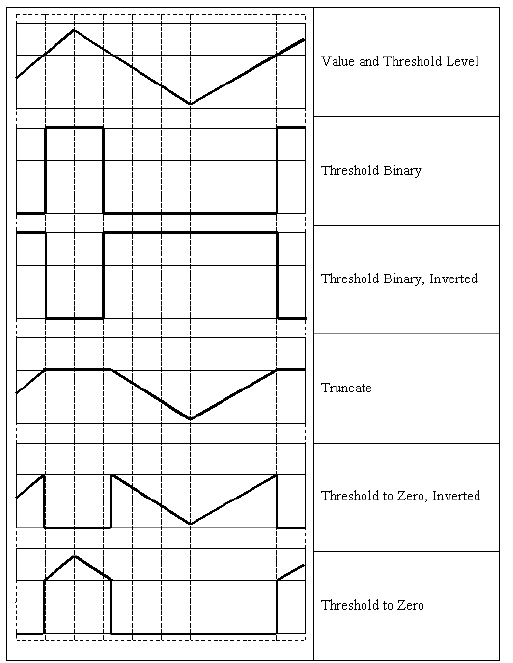
\includegraphics[width=0.5\textwidth]{pics/threshold.png}


\fi

\ifCpp

\cvCppFunc{adaptiveThreshold}
Applies an adaptive threshold to an array.

\cvdefCpp{void adaptiveThreshold( const Mat\& src, Mat\& dst, double maxValue,\par
                        int adaptiveMethod, int thresholdType,\par
                        int blockSize, double C );}
\begin{description}
\cvarg{src}{Source 8-bit single-channel image}
\cvarg{dst}{Destination image; will have the same size and the same type as \texttt{src}}
\cvarg{maxValue}{The non-zero value assigned to the pixels for which the condition is satisfied. See the discussion}
\cvarg{adaptiveMethod}{Adaptive thresholding algorithm to use,
   \texttt{ADAPTIVE\_THRESH\_MEAN\_C} or \texttt{ADAPTIVE\_THRESH\_GAUSSIAN\_C} (see the discussion)}
\cvarg{thresholdType}{Thresholding type; must be one of \texttt{THRESH\_BINARY} or \texttt{THRESH\_BINARY\_INV}}
\cvarg{blockSize}{The size of a pixel neighborhood that is used to calculate a threshold value for the pixel: 3, 5, 7, and so on}
\cvarg{C}{The constant subtracted from the mean or weighted mean (see the discussion); normally, it's positive, but may be zero or negative as well}
\end{description}

The function transforms a grayscale image to a binary image according to the formulas:

\begin{description}
\cvarg{THRESH\_BINARY}{\[ dst(x,y) = \fork{\texttt{maxValue}}{if $src(x,y) > T(x,y)$}{0}{otherwise} \]}
\cvarg{THRESH\_BINARY\_INV}{\[ dst(x,y) = \fork{0}{if $src(x,y) > T(x,y)$}{\texttt{maxValue}}{otherwise} \]}
\end{description}

where $T(x,y)$ is a threshold calculated individually for each pixel.

\begin{enumerate}
    \item
For the method \texttt{ADAPTIVE\_THRESH\_MEAN\_C} the threshold value $T(x,y)$ is the mean of a $\texttt{blockSize} \times \texttt{blockSize}$ neighborhood of $(x, y)$, minus \texttt{C}.
    \item
For the method \texttt{ADAPTIVE\_THRESH\_GAUSSIAN\_C} the threshold value $T(x, y)$ is the weighted sum (i.e. cross-correlation with a Gaussian window) of a $\texttt{blockSize} \times \texttt{blockSize}$ neighborhood of $(x, y)$, minus \texttt{C}. The default sigma (standard deviation) is used for the specified \texttt{blockSize}, see \cvCppCross{getGaussianKernel}.
\end{enumerate}

The function can process the image in-place.

See also: \cvCppCross{threshold}, \cvCppCross{blur}, \cvCppCross{GaussianBlur}


\cvCppFunc{cvtColor}
Converts image from one color space to another

\cvdefCpp{void cvtColor( const Mat\& src, Mat\& dst, int code, int dstCn=0 );}
\begin{description}
\cvarg{src}{The source image, 8-bit unsigned, 16-bit unsigned (\texttt{CV\_16UC...}) or single-precision floating-point}
\cvarg{dst}{The destination image; will have the same size and the same depth as \texttt{src}}
\cvarg{code}{The color space conversion code; see the discussion}
\cvarg{dstCn}{The number of channels in the destination image; if the parameter is 0, the number of the channels will be derived automatically from \texttt{src} and the \texttt{code}}
\end{description}

The function converts the input image from one color
space to another. In the case of transformation to-from RGB color space the ordering of the channels should be specified explicitly (RGB or BGR).

The conventional ranges for R, G and B channel values are:

\begin{itemize}
 \item 0 to 255 for \texttt{CV\_8U} images
 \item 0 to 65535 for \texttt{CV\_16U} images and
 \item 0 to 1 for \texttt{CV\_32F} images.
\end{itemize}

Of course, in the case of linear transformations the range does not matter,
but in the non-linear cases the input RGB image should be normalized to the proper value range in order to get the correct results, e.g. for RGB$\rightarrow$L*u*v* transformation. For example, if you have a 32-bit floating-point image directly converted from 8-bit image without any scaling, then it will have 0..255 value range, instead of the assumed by the function 0..1. So, before calling \texttt{cvtColor}, you need first to scale the image down:
\begin{lstlisting}
img *= 1./255;
cvtColor(img, img, CV_BGR2Luv);
\end{lstlisting}

The function can do the following transformations:

\begin{itemize}
 \item Transformations within RGB space like adding/removing the alpha channel, reversing the channel order, conversion to/from 16-bit RGB color (R5:G6:B5 or R5:G5:B5), as well as conversion to/from grayscale using:
 \[
 \text{RGB[A] to Gray:}\quad Y \leftarrow 0.299 \cdot R + 0.587 \cdot G + 0.114 \cdot B
 \]
 and
 \[
 \text{Gray to RGB[A]:}\quad R \leftarrow Y, G \leftarrow Y, B \leftarrow Y, A \leftarrow 0
 \]

The conversion from a RGB image to gray is done with:
\begin{lstlisting}
cvtColor(src, bwsrc, CV_RGB2GRAY);
\end{lstlisting}

Some more advanced channel reordering can also be done with \cvCppCross{mixChannels}.

 \item RGB $\leftrightarrow$ CIE XYZ.Rec 709 with D65 white point (\texttt{CV\_BGR2XYZ, CV\_RGB2XYZ, CV\_XYZ2BGR, CV\_XYZ2RGB}):
 \[
 \begin{bmatrix}
 X \\
 Y \\
 Z
 \end{bmatrix}
 \leftarrow
 \begin{bmatrix}
0.412453 & 0.357580 & 0.180423\\
0.212671 & 0.715160 & 0.072169\\
0.019334 & 0.119193 & 0.950227
 \end{bmatrix}
 \cdot
 \begin{bmatrix}
 R \\
 G \\
 B
 \end{bmatrix}
 \]
 \[
 \begin{bmatrix}
 R \\
 G \\
 B
 \end{bmatrix}
 \leftarrow
 \begin{bmatrix}
3.240479 & -1.53715 & -0.498535\\
-0.969256 &  1.875991 & 0.041556\\
0.055648 & -0.204043 & 1.057311
 \end{bmatrix}
 \cdot
 \begin{bmatrix}
 X \\
 Y \\
 Z
 \end{bmatrix}
 \]
$X$, $Y$ and $Z$ cover the whole value range (in the case of floating-point images $Z$ may exceed 1).

 \item RGB $\leftrightarrow$ YCrCb JPEG (a.k.a. YCC) (\texttt{CV\_BGR2YCrCb, CV\_RGB2YCrCb, CV\_YCrCb2BGR, CV\_YCrCb2RGB})
 \[ Y \leftarrow 0.299 \cdot R + 0.587 \cdot G + 0.114 \cdot B \]
 \[  Cr \leftarrow (R-Y) \cdot 0.713 + delta \]
 \[  Cb \leftarrow (B-Y) \cdot 0.564 + delta \]
 \[  R \leftarrow Y + 1.403 \cdot (Cr - delta) \]
 \[  G \leftarrow Y - 0.344 \cdot (Cr - delta) - 0.714 \cdot (Cb - delta) \]
 \[  B \leftarrow Y + 1.773 \cdot (Cb - delta) \]
where
 \[
  delta = \left\{
  \begin{array}{l l}
  128 & \mbox{for 8-bit images}\\
  32768 & \mbox{for 16-bit images}\\
  0.5 & \mbox{for floating-point images}
  \end{array} \right.
 \]
Y, Cr and Cb cover the whole value range.

 \item RGB $\leftrightarrow$ HSV (\texttt{CV\_BGR2HSV, CV\_RGB2HSV, CV\_HSV2BGR, CV\_HSV2RGB})
  in the case of 8-bit and 16-bit images
  R, G and B are converted to floating-point format and scaled to fit the 0 to 1 range
  \[ V \leftarrow max(R,G,B) \]

\[ S \leftarrow \fork{\frac{V-min(R,G,B)}{V}}{if $V \neq 0$}{0}{otherwise} \]
\[ H \leftarrow \forkthree
{{60(G - B)}/{S}}{if $V=R$}
{{120+60(B - R)}/{S}}{if $V=G$}
{{240+60(R - G)}/{S}}{if $V=B$} \]
if $H<0$ then $H \leftarrow H+360$

On output $0 \leq V \leq 1$, $0 \leq S \leq 1$, $0 \leq H \leq 360$.

The values are then converted to the destination data type:
\begin{description}
\item[8-bit images]
\[ V \leftarrow 255 V, S \leftarrow 255 S, H \leftarrow H/2 \text{(to fit to 0 to 255)} \]
\item[16-bit images (currently not supported)]
\[ V <- 65535 V, S <- 65535 S, H <- H \]
\item[32-bit images]
H, S, V are left as is
\end{description}

 \item RGB $\leftrightarrow$ HLS (\texttt{CV\_BGR2HLS, CV\_RGB2HLS, CV\_HLS2BGR, CV\_HLS2RGB}).
  in the case of 8-bit and 16-bit images
  R, G and B are converted to floating-point format and scaled to fit the 0 to 1 range.
  \[ V_{max} \leftarrow {max}(R,G,B) \]
  \[ V_{min} \leftarrow {min}(R,G,B) \]
  \[ L \leftarrow \frac{V_{max} - V_{min}}{2} \]
  \[ S \leftarrow \fork
    {\frac{V_{max} - V_{min}}{V_{max} + V_{min}}}{if $L < 0.5$}
    {\frac{V_{max} - V_{min}}{2 - (V_{max} + V_{min})}}{if $L \ge 0.5$} \]
  \[ H \leftarrow \forkthree
  {{60(G - B)}/{S}}{if $V_{max}=R$}
  {{120+60(B - R)}/{S}}{if $V_{max}=G$}
  {{240+60(R - G)}/{S}}{if $V_{max}=B$} \]
  if $H<0$ then $H \leftarrow H+360$
On output $0 \leq V \leq 1$, $0 \leq S \leq 1$, $0 \leq H \leq 360$.

The values are then converted to the destination data type:
\begin{description}
\item[8-bit images]
\[ V \leftarrow 255\cdot V, S \leftarrow 255\cdot S, H \leftarrow H/2\; \text{(to fit to 0 to 255)} \]
\item[16-bit images (currently not supported)]
\[ V <- 65535\cdot V, S <- 65535\cdot S, H <- H \]
\item[32-bit images]
H, S, V are left as is
\end{description}

 \item RGB $\leftrightarrow$ CIE L*a*b* (\texttt{CV\_BGR2Lab, CV\_RGB2Lab, CV\_Lab2BGR, CV\_Lab2RGB})
  in the case of 8-bit and 16-bit images
  R, G and B are converted to floating-point format and scaled to fit the 0 to 1 range
\[ \vecthree{X}{Y}{Z} \leftarrow \vecthreethree
{0.412453}{0.357580}{0.180423}
{0.212671}{0.715160}{0.072169}
{0.019334}{0.119193}{0.950227}
\cdot
\vecthree{R}{G}{B} \]
\[ X \leftarrow X/X_n, \text{where} X_n = 0.950456 \]
\[ Z \leftarrow Z/Z_n, \text{where} Z_n = 1.088754 \]
\[ L \leftarrow \fork
{116*Y^{1/3}-16}{for $Y>0.008856$}
{903.3*Y}{for $Y \le 0.008856$} \]
\[ a \leftarrow 500 (f(X)-f(Y)) + delta \]
\[ b \leftarrow 200 (f(Y)-f(Z)) + delta \]
where
\[f(t)=\fork
{t^{1/3}}{for $t>0.008856$}
{7.787 t+16/116}{for $t\leq 0.008856$} \]
and
\[ delta = \fork{128}{for 8-bit images}{0}{for floating-point images} \]
On output $0 \leq L \leq 100$, $-127 \leq a \leq 127$, $-127 \leq b \leq 127$

The values are then converted to the destination data type:
\begin{description}
\item[8-bit images]
\[L \leftarrow L*255/100,\; a \leftarrow a + 128,\; b \leftarrow b + 128\]
\item[16-bit images] currently not supported
\item[32-bit images]
L, a, b are left as is
\end{description}

 \item RGB $\leftrightarrow$ CIE L*u*v* (\texttt{CV\_BGR2Luv, CV\_RGB2Luv, CV\_Luv2BGR, CV\_Luv2RGB})
  in the case of 8-bit and 16-bit images
  R, G and B are converted to floating-point format and scaled to fit 0 to 1 range
  \[ \vecthree{X}{Y}{Z} \leftarrow \vecthreethree
{0.412453}{0.357580}{0.180423}
{0.212671}{0.715160}{0.072169}
{0.019334}{0.119193}{0.950227}
\cdot
\vecthree{R}{G}{B} \]
\[ L \leftarrow \fork
{116 Y^{1/3}}{for $Y>0.008856$}
{903.3 Y}{for $Y\leq 0.008856$} \]
\[ u' \leftarrow 4*X/(X + 15*Y + 3 Z) \]
\[ v' \leftarrow 9*Y/(X + 15*Y + 3 Z) \]
\[ u \leftarrow 13*L*(u' - u_n) \quad \text{where} \quad u_n=0.19793943 \]
\[ v \leftarrow 13*L*(v' - v_n) \quad \text{where} \quad v_n=0.46831096 \]
On output $0 \leq L \leq 100$, $-134 \leq u \leq 220$, $-140 \leq v \leq 122$.

The values are then converted to the destination data type:
\begin{description}
\item[8-bit images]
\[L \leftarrow 255/100 L,\; u \leftarrow 255/354 (u + 134),\; v \leftarrow 255/256 (v + 140) \]
\item[16-bit images] currently not supported
\item[32-bit images] L, u, v are left as is
\end{description}

The above formulas for converting RGB to/from various color spaces have been taken from multiple sources on Web, primarily from the Charles Poynton site \url{http://www.poynton.com/ColorFAQ.html}

 \item Bayer $\rightarrow$ RGB (\texttt{CV\_BayerBG2BGR, CV\_BayerGB2BGR, CV\_BayerRG2BGR, CV\_BayerGR2BGR, CV\_BayerBG2RGB, CV\_BayerGB2RGB, CV\_BayerRG2RGB, CV\_BayerGR2RGB}) The Bayer pattern is widely used in CCD and CMOS cameras. It allows one to get color pictures from a single plane where R,G and B pixels (sensors of a particular component) are interleaved like this:

\[
\newcommand{\Rcell}{\color{red}R}
\newcommand{\Gcell}{\color{green}G}
\newcommand{\Bcell}{\color{blue}B}
\definecolor{BackGray}{rgb}{0.8,0.8,0.8}
\begin{array}{ c c c c c }
\Rcell&\Gcell&\Rcell&\Gcell&\Rcell\\
\Gcell&\colorbox{BackGray}{\Bcell}&\colorbox{BackGray}{\Gcell}&\Bcell&\Gcell\\
\Rcell&\Gcell&\Rcell&\Gcell&\Rcell\\
\Gcell&\Bcell&\Gcell&\Bcell&\Gcell\\
\Rcell&\Gcell&\Rcell&\Gcell&\Rcell
\end{array}
\]

The output RGB components of a pixel are interpolated from 1, 2 or
4 neighbors of the pixel having the same color. There are several
modifications of the above pattern that can be achieved by shifting
the pattern one pixel left and/or one pixel up. The two letters
$C_1$ and $C_2$
in the conversion constants
\texttt{CV\_Bayer} $ C_1 C_2 $ \texttt{2BGR}
and
\texttt{CV\_Bayer} $ C_1 C_2 $ \texttt{2RGB}
indicate the particular pattern
type - these are components from the second row, second and third
columns, respectively. For example, the above pattern has very
popular "BG" type.
\end{itemize}



\cvCppFunc{distanceTransform}
Calculates the distance to the closest zero pixel for each pixel of the source image.

\cvdefCpp{void distanceTransform( const Mat\& src, Mat\& dst,\par
                        int distanceType, int maskSize );\newline
void distanceTransform( const Mat\& src, Mat\& dst, Mat\& labels,\par
                        int distanceType, int maskSize );}
\begin{description}
\cvarg{src}{8-bit, single-channel (binary) source image}
\cvarg{dst}{Output image with calculated distances; will be 32-bit floating-point, single-channel image of the same size as \texttt{src}}
\cvarg{distanceType}{Type of distance; can be \texttt{CV\_DIST\_L1, CV\_DIST\_L2} or \texttt{CV\_DIST\_C}}
\cvarg{maskSize}{Size of the distance transform mask; can be 3, 5 or \texttt{CV\_DIST\_MASK\_PRECISE} (the latter option is only supported by the first of the functions). In the case of \texttt{CV\_DIST\_L1} or \texttt{CV\_DIST\_C} distance type the parameter is forced to 3, because a $3\times 3$ mask gives the same result as a $5\times 5$ or any larger aperture.}
\cvarg{labels}{The optional output 2d array of labels - the discrete Voronoi diagram; will have type \texttt{CV\_32SC1} and the same size as \texttt{src}. See the discussion}
\end{description}

The functions \texttt{distanceTransform} calculate the approximate or precise
distance from every binary image pixel to the nearest zero pixel.
(for zero image pixels the distance will obviously be zero).

When \texttt{maskSize == CV\_DIST\_MASK\_PRECISE} and \texttt{distanceType == CV\_DIST\_L2}, the function runs the algorithm described in \cite{Felzenszwalb04}.

In other cases the algorithm \cite{Borgefors86} is used, that is,
for pixel the function finds the shortest path to the nearest zero pixel
consisting of basic shifts: horizontal,
vertical, diagonal or knight's move (the latest is available for a
$5\times 5$ mask). The overall distance is calculated as a sum of these
basic distances. Because the distance function should be symmetric,
all of the horizontal and vertical shifts must have the same cost (that
is denoted as \texttt{a}), all the diagonal shifts must have the
same cost (denoted \texttt{b}), and all knight's moves must have
the same cost (denoted \texttt{c}). For \texttt{CV\_DIST\_C} and
\texttt{CV\_DIST\_L1} types the distance is calculated precisely,
whereas for \texttt{CV\_DIST\_L2} (Euclidian distance) the distance
can be calculated only with some relative error (a $5\times 5$ mask
gives more accurate results). For \texttt{a}, \texttt{b} and \texttt{c}
OpenCV uses the values suggested in the original paper:


\begin{tabular}{| c | c | c |}
\hline
\texttt{CV\_DIST\_C}  & $(3\times 3)$ & a = 1, b = 1\\ \hline
\texttt{CV\_DIST\_L1} & $(3\times 3)$ & a = 1, b = 2\\ \hline
\texttt{CV\_DIST\_L2} & $(3\times 3)$ & a=0.955, b=1.3693\\ \hline
\texttt{CV\_DIST\_L2} & $(5\times 5)$ & a=1, b=1.4, c=2.1969\\ \hline
\end{tabular}


Typically, for a fast, coarse distance estimation \texttt{CV\_DIST\_L2},
a $3\times 3$ mask is used, and for a more accurate distance estimation
\texttt{CV\_DIST\_L2}, a $5\times 5$ mask or the precise algorithm is used.
Note that both the precise and the approximate algorithms are linear on the number of pixels.

The second variant of the function does not only compute the minimum distance for each pixel $(x, y)$,
but it also identifies the nearest the nearest connected
component consisting of zero pixels. Index of the component is stored in $\texttt{labels}(x, y)$.
The connected components of zero pixels are also found and marked by the function.

In this mode the complexity is still linear.
That is, the function provides a very fast way to compute Voronoi diagram for the binary image.
Currently, this second variant can only use the approximate distance transform algorithm.


\cvCppFunc{floodFill}
Fills a connected component with the given color.

\cvdefCpp{int floodFill( Mat\& image,\par
               Point seed, Scalar newVal, Rect* rect=0,\par
               Scalar loDiff=Scalar(), Scalar upDiff=Scalar(),\par
               int flags=4 );\newline
int floodFill( Mat\& image, Mat\& mask,\par
               Point seed, Scalar newVal, Rect* rect=0,\par
               Scalar loDiff=Scalar(), Scalar upDiff=Scalar(),\par
               int flags=4 );}
\begin{description}
\cvarg{image}{Input/output 1- or 3-channel, 8-bit or floating-point image. It is modified by the function unless the \texttt{FLOODFILL\_MASK\_ONLY} flag is set (in the second variant of the function; see below)}
\cvarg{mask}{(For the second function only) Operation mask, should be a single-channel 8-bit image, 2 pixels wider and 2 pixels taller. The function uses and updates the mask, so the user takes responsibility of initializing the \texttt{mask} content. Flood-filling can't go across non-zero pixels in the mask, for example, an edge detector output can be used as a mask to stop filling at edges. It is possible to use the same mask in multiple calls to the function to make sure the filled area do not overlap. \textbf{Note}: because the mask is larger than the filled image, a pixel $(x, y)$ in \texttt{image} will correspond to the pixel $(x+1, y+1)$ in the \texttt{mask}}
\cvarg{seed}{The starting point}
\cvarg{newVal}{New value of the repainted domain pixels}
\cvarg{loDiff}{Maximal lower brightness/color difference between the currently observed pixel and one of its neighbors belonging to the component, or a seed pixel being added to the component}
\cvarg{upDiff}{Maximal upper brightness/color difference between the currently observed pixel and one of its neighbors belonging to the component, or a seed pixel being added to the component}
\cvarg{rect}{The optional output parameter that the function sets to the minimum bounding rectangle of the repainted domain}
\cvarg{flags}{The operation flags. Lower bits contain connectivity value, 4 (by default) or 8, used within the function. Connectivity determines which neighbors of a pixel are considered. Upper bits can be 0 or a combination of the following flags:
\begin{description}
  \cvarg{FLOODFILL\_FIXED\_RANGE}{if set, the difference between the current pixel and seed pixel is considered, otherwise the difference between neighbor pixels is considered (i.e. the range is floating)}
  \cvarg{FLOODFILL\_MASK\_ONLY}{(for the second variant only) if set, the function does not change the image (\texttt{newVal} is ignored), but fills the mask}
\end{description}}
\end{description}

The functions \texttt{floodFill} fill a connected component starting from the seed point with the specified color. The connectivity is determined by the color/brightness closeness of the neighbor pixels. The pixel at $(x,y)$ is considered to belong to the repainted domain if:

\begin{description}

\item[grayscale image, floating range] \[
\texttt{src}(x',y')-\texttt{loDiff} \leq \texttt{src}(x,y) \leq \texttt{src}(x',y')+\texttt{upDiff} \]

\item[grayscale image, fixed range] \[
\texttt{src}(\texttt{seed}.x,\texttt{seed}.y)-\texttt{loDiff}\leq \texttt{src}(x,y) \leq \texttt{src}(\texttt{seed}.x,\texttt{seed}.y)+\texttt{upDiff} \]

\item[color image, floating range]
\[ \texttt{src}(x',y')_r-\texttt{loDiff}_r\leq \texttt{src}(x,y)_r\leq \texttt{src}(x',y')_r+\texttt{upDiff}_r \]
\[ \texttt{src}(x',y')_g-\texttt{loDiff}_g\leq \texttt{src}(x,y)_g\leq \texttt{src}(x',y')_g+\texttt{upDiff}_g \]
\[ \texttt{src}(x',y')_b-\texttt{loDiff}_b\leq \texttt{src}(x,y)_b\leq \texttt{src}(x',y')_b+\texttt{upDiff}_b \]

\item[color image, fixed range]
\[ \texttt{src}(\texttt{seed}.x,\texttt{seed}.y)_r-\texttt{loDiff}_r\leq \texttt{src}(x,y)_r\leq \texttt{src}(\texttt{seed}.x,\texttt{seed}.y)_r+\texttt{upDiff}_r \]
\[ \texttt{src}(\texttt{seed}.x,\texttt{seed}.y)_g-\texttt{loDiff}_g\leq \texttt{src}(x,y)_g\leq \texttt{src}(\texttt{seed}.x,\texttt{seed}.y)_g+\texttt{upDiff}_g \]
\[ \texttt{src}(\texttt{seed}.x,\texttt{seed}.y)_b-\texttt{loDiff}_b\leq \texttt{src}(x,y)_b\leq \texttt{src}(\texttt{seed}.x,\texttt{seed}.y)_b+\texttt{upDiff}_b \]
\end{description}

where $src(x',y')$ is the value of one of pixel neighbors that is already known to belong to the component. That is, to be added to the connected component, a pixel's color/brightness should be close enough to the:
\begin{itemize}
  \item color/brightness of one of its neighbors that are already referred to the connected component in the case of floating range
  \item color/brightness of the seed point in the case of fixed range.
\end{itemize}

By using these functions you can either mark a connected component with the specified color in-place, or build a mask and then extract the contour or copy the region to another image etc. Various modes of the function are demonstrated in \texttt{floodfill.c} sample.

See also: \cvCppCross{findContours}


\cvCppFunc{inpaint}
Inpaints the selected region in the image.

\cvdefCpp{void inpaint( const Mat\& src, const Mat\& inpaintMask,\par
              Mat\& dst, double inpaintRadius, int flags );}

\begin{description}
\cvarg{src}{The input 8-bit 1-channel or 3-channel image.}
\cvarg{inpaintMask}{The inpainting mask, 8-bit 1-channel image. Non-zero pixels indicate the area that needs to be inpainted.}
\cvarg{dst}{The output image; will have the same size and the same type as \texttt{src}}
\cvarg{inpaintRadius}{The radius of a circlular neighborhood of each point inpainted that is considered by the algorithm.}
\cvarg{flags}{The inpainting method, one of the following:
\begin{description}
\cvarg{INPAINT\_NS}{Navier-Stokes based method.}
\cvarg{INPAINT\_TELEA}{The method by Alexandru Telea \cite{Telea04}}
\end{description}}
\end{description}

The function reconstructs the selected image area from the pixel near the area boundary. The function may be used to remove dust and scratches from a scanned photo, or to remove undesirable objects from still images or video. See \url{http://en.wikipedia.org/wiki/Inpainting} for more details.


\cvCppFunc{integral}
Calculates the integral of an image.

\cvdefCpp{void integral( const Mat\& image, Mat\& sum, int sdepth=-1 );\newline
void integral( const Mat\& image, Mat\& sum, Mat\& sqsum, int sdepth=-1 );\newline
void integral( const Mat\& image, Mat\& sum, \par Mat\& sqsum, Mat\& tilted, int sdepth=-1 );}
\begin{description}
\cvarg{image}{The source image, $W \times H$, 8-bit or floating-point (32f or 64f)}
\cvarg{sum}{The integral image, $(W+1)\times (H+1)$, 32-bit integer or floating-point (32f or 64f)}
\cvarg{sqsum}{The integral image for squared pixel values, $(W+1)\times (H+1)$, double precision floating-point (64f)}
\cvarg{tilted}{The integral for the image rotated by 45 degrees, $(W+1)\times (H+1)$, the same data type as \texttt{sum}}
\cvarg{sdepth}{The desired depth of the integral and the tilted integral images, \texttt{CV\_32S},  \texttt{CV\_32F} or \texttt{CV\_64F}}
\end{description}

The functions \texttt{integral} calculate one or more integral images for the source image as following:

\[
\texttt{sum}(X,Y) = \sum_{x<X,y<Y} \texttt{image}(x,y)
\]

\[
\texttt{sqsum}(X,Y) = \sum_{x<X,y<Y} \texttt{image}(x,y)^2
\]

\[
\texttt{tilted}(X,Y) = \sum_{y<Y,abs(x-X+1)\leq Y-y-1} \texttt{image}(x,y)
\]

Using these integral images, one may calculate sum, mean and standard deviation over a specific up-right or rotated rectangular region of the image in a constant time, for example:

\[
\sum_{x_1\leq x < x_2, \, y_1 \leq y < y_2} \texttt{image}(x,y) = \texttt{sum}(x_2,y_2)-\texttt{sum}(x_1,y_2)-\texttt{sum}(x_2,y_1)+\texttt{sum}(x_1,x_1)
\]

It makes possible to do a fast blurring or fast block correlation with variable window size, for example. In the case of multi-channel images, sums for each channel are accumulated independently.

As a practical example, the next figure shows the calculation of the integral of a straight rectangle \texttt{Rect(3,3,3,2)} and of a tilted rectangle \texttt{Rect(5,1,2,3)}. The selected pixels in the original \texttt{image} are shown, as well as the relative pixels in the integral images \texttt{sum} and \texttt{tilted}.
 
\begin{center}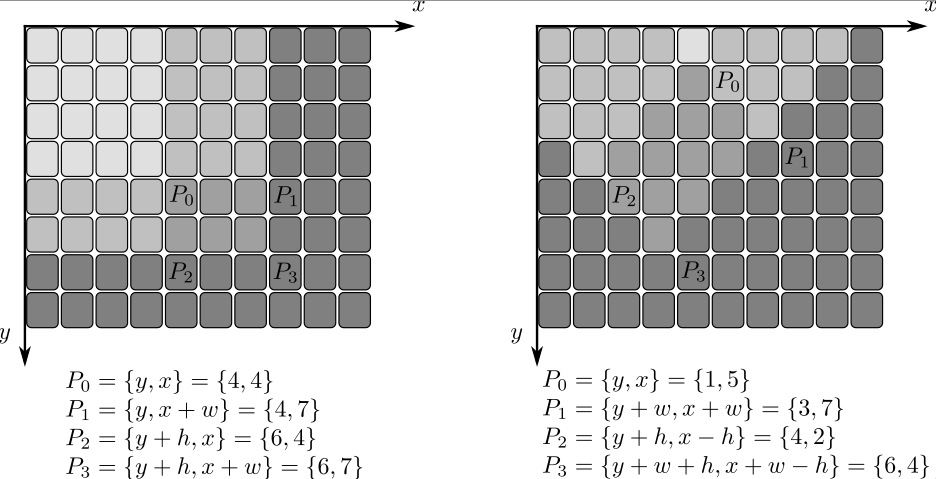
\includegraphics[width=0.8\textwidth]{pics/integral.png}\end{center}

\cvCppFunc{threshold}
Applies a fixed-level threshold to each array element

\cvdefCpp{double threshold( const Mat\& src, Mat\& dst, double thresh,\par
                  double maxVal, int thresholdType );}
\begin{description}
\cvarg{src}{Source array (single-channel, 8-bit of 32-bit floating point)}
\cvarg{dst}{Destination array; will have the same size and the same type as \texttt{src}}
\cvarg{thresh}{Threshold value}
\cvarg{maxVal}{Maximum value to use with \texttt{THRESH\_BINARY} and \texttt{THRESH\_BINARY\_INV} thresholding types}
\cvarg{thresholdType}{Thresholding type (see the discussion)}
\end{description}

The function applies fixed-level thresholding
to a single-channel array. The function is typically used to get a
bi-level (binary) image out of a grayscale image (\cvCppCross{compare} could
be also used for this purpose) or for removing a noise, i.e. filtering
out pixels with too small or too large values. There are several
types of thresholding that the function supports that are determined by
\texttt{thresholdType}:

\begin{description}
\cvarg{THRESH\_BINARY}{\[ \texttt{dst}(x,y) = \fork{\texttt{maxVal}}{if $\texttt{src}(x,y) > \texttt{thresh}$}{0}{otherwise} \]}
\cvarg{THRESH\_BINARY\_INV}{\[ \texttt{dst}(x,y) = \fork{0}{if $\texttt{src}(x,y) > \texttt{thresh}$}{\texttt{maxVal}}{otherwise} \]}
\cvarg{THRESH\_TRUNC}{\[ \texttt{dst}(x,y) = \fork{\texttt{threshold}}{if $\texttt{src}(x,y) > \texttt{thresh}$}{\texttt{src}(x,y)}{otherwise} \]}
\cvarg{THRESH\_TOZERO}{\[ \texttt{dst}(x,y) = \fork{\texttt{src}(x,y)}{if $\texttt{src}(x,y) > \texttt{thresh}$}{0}{otherwise} \]}
\cvarg{THRESH\_TOZERO\_INV}{\[ \texttt{dst}(x,y) = \fork{0}{if $\texttt{src}(x,y) > \texttt{thresh}$}{\texttt{src}(x,y)}{otherwise} \]}
\end{description}

Also, the special value \texttt{THRESH\_OTSU} may be combined with
one of the above values. In this case the function determines the optimal threshold
value using Otsu's algorithm and uses it instead of the specified \texttt{thresh}.
The function returns the computed threshold value.
Currently, Otsu's method is implemented only for 8-bit images.

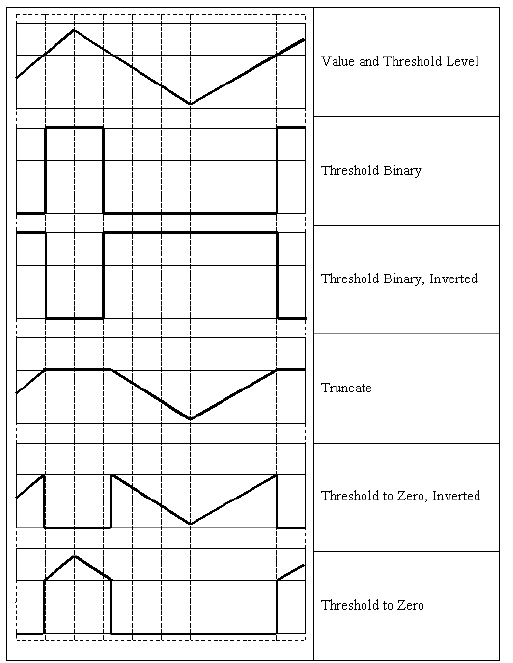
\includegraphics[width=0.5\textwidth]{pics/threshold.png}

See also: \cvCppCross{adaptiveThreshold}, \cvCppCross{findContours}, \cvCppCross{compare}, \cvCppCross{min}, \cvCppCross{max}

\cvCppFunc{watershed}
Does marker-based image segmentation using watershed algrorithm

\cvdefCpp{void watershed( const Mat\& image, Mat\& markers );}
\begin{description}
\cvarg{image}{The input 8-bit 3-channel image.} 
\cvarg{markers}{The input/output 32-bit single-channel image (map) of markers. It should have the same size as \texttt{image}}
\end{description}

The function implements one of the variants
of watershed, non-parametric marker-based segmentation algorithm,
described in \cite{Meyer92}. Before passing the image to the
function, user has to outline roughly the desired regions in the image
\texttt{markers} with positive ($>0$) indices, i.e. every region is
represented as one or more connected components with the pixel values
1, 2, 3 etc (such markers can be retrieved from a binary mask
using \cvCppCross{findContours}and \cvCppCross{drawContours}, see \texttt{watershed.cpp} demo).
The markers will be "seeds" of the future image
regions. All the other pixels in \texttt{markers}, which relation to the
outlined regions is not known and should be defined by the algorithm,
should be set to 0's. On the output of the function, each pixel in
markers is set to one of values of the "seed" components, or to -1 at
boundaries between the regions.

Note, that it is not necessary that every two neighbor connected
components are separated by a watershed boundary (-1's pixels), for
example, in case when such tangent components exist in the initial
marker image. Visual demonstration and usage example of the function
can be found in OpenCV samples directory; see \texttt{watershed.cpp} demo.

See also: \cvCppCross{findContours}

\fi

\section{Histograms}

\ifCPy

\ifC
\cvfunc{CvHistogram}\label{CvHistogram}
Multi-dimensional histogram.

\begin{lstlisting}
typedef struct CvHistogram
{
    int     type;
    CvArr*  bins;
    float   thresh[CV_MAX_DIM][2]; /* for uniform histograms */
    float** thresh2; /* for non-uniform histograms */
    CvMatND mat; /* embedded matrix header for array histograms */
}
CvHistogram;
\end{lstlisting}
\fi

\cvCPyFunc{CalcBackProject}
Calculates the back projection.

\cvdefC{
void cvCalcBackProject( \par IplImage** image,\par CvArr* back\_project,\par const CvHistogram* hist );
}\cvdefPy{CalcBackProject(image,back\_project,hist)-> None}

\begin{description}
\cvarg{image}{Source images (though you may pass CvMat** as well)}
\cvarg{back\_project}{Destination back projection image of the same type as the source images}
\cvarg{hist}{Histogram}
\end{description}

The function calculates the back project of the histogram. For each tuple of pixels at the same position of all input single-channel images the function puts the value of the histogram bin, corresponding to the tuple in the destination image. In terms of statistics, the value of each output image pixel is the probability of the observed tuple given the distribution (histogram). For example, to find a red object in the picture, one may do the following:

\begin{enumerate}
 \item Calculate a hue histogram for the red object assuming the image contains only this object. The histogram is likely to have a strong maximum, corresponding to red color.
 \item Calculate back projection of a hue plane of input image where the object is searched, using the histogram. Threshold the image.
 \item Find connected components in the resulting picture and choose the right component using some additional criteria, for example, the largest connected component.
\end{enumerate}

That is the approximate algorithm of Camshift color object tracker, except for the 3rd step, instead of which CAMSHIFT algorithm is used to locate the object on the back projection given the previous object position.

\cvCPyFunc{CalcBackProjectPatch}
Locates a template within an image by using a histogram comparison.

\cvdefC{
void cvCalcBackProjectPatch( \par IplImage** image,\par CvArr* dst,\par CvSize patch\_size,\par CvHistogram* hist,\par int method,\par float factor );
}\cvdefPy{CalcBackProjectPatch(images,dst,patch\_size,hist,method,factor)-> None}

\begin{description}
\cvarg{image}{Source images (though, you may pass CvMat** as well)}
\cvarg{dst}{Destination image}
\cvarg{patch\_size}{Size of the patch slid though the source image}
\cvarg{hist}{Histogram}
\cvarg{method}{Compasion method, passed to \cvCPyCross{CompareHist} (see description of that function)}
\cvarg{factor}{Normalization factor for histograms, will affect the normalization scale of the destination image, pass 1 if unsure}
\end{description}

The function calculates the back projection by comparing histograms of the source image patches with the given histogram. Taking measurement results from some image at each location over ROI creates an array \texttt{image}. These results might be one or more of hue, \texttt{x} derivative, \texttt{y} derivative, Laplacian filter, oriented Gabor filter, etc. Each measurement output is collected into its own separate image. The \texttt{image} image array is a collection of these measurement images. A multi-dimensional histogram \texttt{hist} is constructed by sampling from the \texttt{image} image array. The final histogram is normalized. The \texttt{hist} histogram has as many dimensions as the number of elements in \texttt{image} array.

Each new image is measured and then converted into an \texttt{image} image array over a chosen ROI. Histograms are taken from this \texttt{image} image in an area covered by a "patch" with an anchor at center as shown in the picture below. The histogram is normalized using the parameter \texttt{norm\_factor} so that it may be compared with \texttt{hist}. The calculated histogram is compared to the model histogram; \texttt{hist} uses The function \texttt{cvCompareHist} with the comparison method=\texttt{method}). The resulting output is placed at the location corresponding to the patch anchor in the probability image \texttt{dst}. This process is repeated as the patch is slid over the ROI. Iterative histogram update by subtracting trailing pixels covered by the patch and adding newly covered pixels to the histogram can save a lot of operations, though it is not implemented yet.

\cvfunc{Back Project Calculation by Patches}

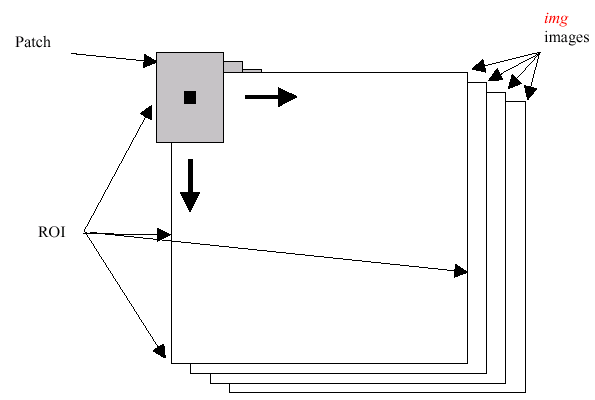
\includegraphics[width=0.5\textwidth]{pics/backprojectpatch.png}

\cvCPyFunc{CalcHist}
Calculates the histogram of image(s).

\cvdefC{
void cvCalcHist( \par IplImage** image,\par CvHistogram* hist,\par int accumulate=0,\par const CvArr* mask=NULL );
}\cvdefPy{CalcHist(image,hist,ccumulate=0,mask=NULL)-> None}

\begin{description}
\cvarg{image}{Source images (though you may pass CvMat** as well)}
\cvarg{hist}{Pointer to the histogram}
\cvarg{accumulate}{Accumulation flag. If it is set, the histogram is not cleared in the beginning. This feature allows user to compute a single histogram from several images, or to update the histogram online}
\cvarg{mask}{The operation mask, determines what pixels of the source images are counted}
\end{description}

The function calculates the histogram of one or more
single-channel images. The elements of a tuple that is used to increment
a histogram bin are taken at the same location from the corresponding
input images.

% ===== Sample. Calculating and displaying 2D Hue-Saturation histogram of a color image =====
\begin{lstlisting}
#include <cv.h>
#include <highgui.h>

int main( int argc, char** argv )
{
    IplImage* src;
    if( argc == 2 && (src=cvLoadImage(argv[1], 1))!= 0)
    {
        IplImage* h_plane = cvCreateImage( cvGetSize(src), 8, 1 );
        IplImage* s_plane = cvCreateImage( cvGetSize(src), 8, 1 );
        IplImage* v_plane = cvCreateImage( cvGetSize(src), 8, 1 );
        IplImage* planes[] = { h_plane, s_plane };
        IplImage* hsv = cvCreateImage( cvGetSize(src), 8, 3 );
        int h_bins = 30, s_bins = 32;
        int hist_size[] = {h_bins, s_bins};
        /* hue varies from 0 (~0 deg red) to 180 (~360 deg red again) */
        float h_ranges[] = { 0, 180 };
        /* saturation varies from 0 (black-gray-white) to
           255 (pure spectrum color) */
        float s_ranges[] = { 0, 255 };
        float* ranges[] = { h_ranges, s_ranges };
        int scale = 10;
        IplImage* hist_img =
            cvCreateImage( cvSize(h_bins*scale,s_bins*scale), 8, 3 );
        CvHistogram* hist;
        float max_value = 0;
        int h, s;

        cvCvtColor( src, hsv, CV_BGR2HSV );
        cvCvtPixToPlane( hsv, h_plane, s_plane, v_plane, 0 );
        hist = cvCreateHist( 2, hist_size, CV_HIST_ARRAY, ranges, 1 );
        cvCalcHist( planes, hist, 0, 0 );
        cvGetMinMaxHistValue( hist, 0, &max_value, 0, 0 );
        cvZero( hist_img );

        for( h = 0; h < h_bins; h++ )
        {
            for( s = 0; s < s_bins; s++ )
            {
                float bin_val = cvQueryHistValue_2D( hist, h, s );
                int intensity = cvRound(bin_val*255/max_value);
                cvRectangle( hist_img, cvPoint( h*scale, s*scale ),
                             cvPoint( (h+1)*scale - 1, (s+1)*scale - 1),
                             CV_RGB(intensity,intensity,intensity),
                             CV_FILLED );
            }
        }

        cvNamedWindow( "Source", 1 );
        cvShowImage( "Source", src );

        cvNamedWindow( "H-S Histogram", 1 );
        cvShowImage( "H-S Histogram", hist_img );

        cvWaitKey(0);
    }
}
\end{lstlisting}

\cvCPyFunc{CalcProbDensity}
Divides one histogram by another.

\cvdefC{
void  cvCalcProbDensity( \par const CvHistogram* hist1,\par const CvHistogram* hist2,\par CvHistogram* dst\_hist,\par double scale=255 );
}\cvdefPy{CalcProbDensity(hist1,hist2,dst\_hst,scale=255)-> None}

\begin{description}
\cvarg{hist1}{first histogram (the divisor)}
\cvarg{hist2}{second histogram}
\cvarg{dst\_hist}{destination histogram}
\cvarg{scale}{scale factor for the destination histogram}
\end{description}

The function calculates the object probability density from the two histograms as:

\[
\texttt{dist\_hist}(I)=
\forkthree
{0}{if $\texttt{hist1}(I)=0$}
{\texttt{scale}}{if $\texttt{hist1}(I) \ne 0$ and $\texttt{hist2}(I) > \texttt{hist1}(I)$}
{\frac{\texttt{hist2}(I) \cdot \texttt{scale}}{\texttt{hist1}(I)}}{if $\texttt{hist1}(I) \ne 0$ and $\texttt{hist2}(I) \le \texttt{hist1}(I)$}
\]

So the destination histogram bins are within less than \texttt{scale}.

\cvCPyFunc{ClearHist}
Clears the histogram.

\cvdefC{
void cvClearHist( CvHistogram* hist );
}\cvdefPy{ClearHist(hist)-> None}

\begin{description}
\cvarg{hist}{Histogram}
\end{description}

The function sets all of the histogram bins to 0 in the case of a dense histogram and removes all histogram bins in the case of a sparse array.

\cvCPyFunc{CompareHist}
Compares two dense histograms.

\cvdefC{
double cvCompareHist( \par const CvHistogram* hist1,\par const CvHistogram* hist2,\par int method );
}\cvdefPy{CompareHist(hist1,hist2,method)->float}

\begin{description}
\cvarg{hist1}{The first dense histogram}
\cvarg{hist2}{The second dense histogram}
\cvarg{method}{Comparison method, one of the following:
\begin{description}
  \cvarg{CV\_COMP\_CORREL}{Correlation}
  \cvarg{CV\_COMP\_CHISQR}{Chi-Square}
  \cvarg{CV\_COMP\_INTERSECT}{Intersection}
  \cvarg{CV\_COMP\_BHATTACHARYYA}{Bhattacharyya distance}
\end{description}}
\end{description}

The function compares two dense histograms using the specified method ($H_1$ denotes the first histogram, $H_2$ the second):

\begin{description}
\item[Correlation (method=CV\_COMP\_CORREL)]
\[
d(H_1,H_2) = \frac
{\sum_I (H'_1(I) \cdot H'_2(I))}
{\sqrt{\sum_I(H'_1(I)^2) \cdot \sum_I(H'_2(I)^2)}}
\]
where
\[
H'_k(I) = \frac{H_k(I) - 1}{N \cdot \sum_J H_k(J)}
\]
where N is the number of histogram bins.

\item[Chi-Square (method=CV\_COMP\_CHISQR)]
\[ d(H_1,H_2) = \sum_I \frac{(H_1(I)-H_2(I))^2}{H_1(I)+H_2(I)} \]

\item[Intersection (method=CV\_COMP\_INTERSECT)]
\[ d(H_1,H_2) = \sum_I \min (H_1(I), H_2(I)) \]

\item[Bhattacharyya distance (method=CV\_COMP\_BHATTACHARYYA)]
\[ d(H_1,H_2) = \sqrt{1 - \sum_I \frac{\sqrt{H_1(I) \cdot H_2(I)}}{ \sqrt { \sum_I H_1(I) \cdot \sum_I H_2(I) }}} \]

\end{description}

The function returns $d(H_1, H_2)$.

Note: the method \texttt{CV\_COMP\_BHATTACHARYYA} only works with normalized histograms.

To compare a sparse histogram or more general sparse configurations of weighted points, consider using the \cvCPyCross{CalcEMD2} function.

\ifC
\cvCPyFunc{CopyHist}
Copies a histogram.

\cvdefC{
void cvCopyHist( const CvHistogram* src, CvHistogram** dst );
}

\begin{description}
\cvarg{src}{Source histogram}
\cvarg{dst}{Pointer to destination histogram}
\end{description}

The function makes a copy of the histogram. If the
second histogram pointer \texttt{*dst} is NULL, a new histogram of the
same size as \texttt{src} is created. Otherwise, both histograms must
have equal types and sizes. Then the function copies the source histogram's
bin values to the destination histogram and sets the same bin value ranges
as in \texttt{src}.

\fi

\cvCPyFunc{CreateHist}
Creates a histogram.

\cvdefC{
CvHistogram* cvCreateHist(\par int dims,\par int* sizes,\par int type,\par float** ranges=NULL,\par int uniform=1 );
}\cvdefPy{CreateHist(dims, type, ranges, uniform = 1) -> hist}

\begin{description}
\cvC{\cvarg{dims}{Number of histogram dimensions}
\cvarg{sizes}{Array of the histogram dimension sizes}}
\cvPy{\cvarg{dims}{for an N-dimensional histogram, list of length N giving the size of each dimension}}
\cvarg{type}{Histogram representation format: \texttt{CV\_HIST\_ARRAY} means that the histogram data is represented as a multi-dimensional dense array CvMatND; \texttt{CV\_HIST\_SPARSE} means that histogram data is represented as a multi-dimensional sparse array CvSparseMat}
\cvarg{ranges}{Array of ranges for the histogram bins. Its meaning depends on the \texttt{uniform} parameter value. The ranges are used for when the histogram is calculated or backprojected to determine which histogram bin corresponds to which value/tuple of values from the input image(s)}
\cvarg{uniform}{Uniformity flag; if not 0, the histogram has evenly
spaced bins and for every $0<=i<cDims$ \texttt{ranges[i]}
is an array of two numbers: lower and upper boundaries for the i-th
histogram dimension.
The whole range [lower,upper] is then split
into \texttt{dims[i]} equal parts to determine the \texttt{i-th} input
tuple value ranges for every histogram bin. And if \texttt{uniform=0},
then \texttt{i-th} element of \texttt{ranges} array contains
\texttt{dims[i]+1} elements:
$\texttt{lower}_0, \texttt{upper}_0, 
\texttt{lower}_1, \texttt{upper}_1 = \texttt{lower}_2,
...
\texttt{upper}_{dims[i]-1} $
where
$\texttt{lower}_j$ and $\texttt{upper}_j$
are lower and upper
boundaries of \texttt{i-th} input tuple value for \texttt{j-th}
bin, respectively. In either case, the input values that are beyond
the specified range for a histogram bin are not counted by
\cvCPyCross{CalcHist} and filled with 0 by \cvCPyCross{CalcBackProject}}
\end{description}

The function creates a histogram of the specified
size and returns a pointer to the created histogram. If the array
\texttt{ranges} is 0, the histogram bin ranges must be specified later
via the function \cvCPyCross{SetHistBinRanges}. Though \cvCPyCross{CalcHist}
and \cvCPyCross{CalcBackProject} may process 8-bit images without setting
bin ranges, they assume thy are equally spaced in 0 to 255 bins.

\cvCPyFunc{GetHistValue*D}
Returns a pointer to the histogram bin.

\begin{lstlisting}
#define cvGetHistValue_1D( hist, idx0 ) 
    ((float*)(cvPtr1D( (hist)->bins, (idx0), 0 ))
#define cvGetHistValue_2D( hist, idx0, idx1 ) 
    ((float*)(cvPtr2D( (hist)->bins, (idx0), (idx1), 0 )))
#define cvGetHistValue_3D( hist, idx0, idx1, idx2 ) 
    ((float*)(cvPtr3D( (hist)->bins, (idx0), (idx1), (idx2), 0 )))
#define cvGetHistValue_nD( hist, idx ) 
    ((float*)(cvPtrND( (hist)->bins, (idx), 0 )))
\end{lstlisting}

\begin{description}
\cvarg{hist}{Histogram}
\cvarg{idx0, idx1, idx2, idx3}{Indices of the bin}
\cvarg{idx}{Array of indices}
\end{description}

The macros \texttt{GetHistValue} return a pointer to the specified bin of the 1D, 2D, 3D or N-D histogram. In the case of a sparse histogram the function creates a new bin and sets it to 0, unless it exists already.


\cvCPyFunc{GetMinMaxHistValue}
Finds the minimum and maximum histogram bins.

\cvdefC{
void cvGetMinMaxHistValue( \par const CvHistogram* hist,\par float* min\_value,\par float* max\_value,\par int* min\_idx=NULL,\par int* max\_idx=NULL );

}\cvdefPy{GetMinMaxHistValue(hist)-> min\_val,max\_val,min\_loc,max\_loc}

\begin{description}
\cvarg{hist}{Histogram}
\cvarg{min\_value}{Pointer to the minimum value of the histogram}
\cvarg{max\_value}{Pointer to the maximum value of the histogram}
\cvarg{min\_idx}{Pointer to the array of coordinates for the minimum}
\cvarg{max\_idx}{Pointer to the array of coordinates for the maximum}
\end{description}

The function finds the minimum and
maximum histogram bins and their positions. All of output arguments are
optional. Among several extremas with the same value the ones with the
minimum index (in lexicographical order) are returned. In the case of several maximums
or minimums, the earliest in lexicographical order (extrema locations)
is returned.

\ifC % {
\cvCPyFunc{MakeHistHeaderForArray}
Makes a histogram out of an array.

\cvdefC{
CvHistogram*  cvMakeHistHeaderForArray( \par int dims,\par int* sizes,\par CvHistogram* hist,\par float* data,\par float** ranges=NULL,\par int uniform=1 );
}

\begin{description}
\cvarg{dims}{Number of histogram dimensions}
\cvarg{sizes}{Array of the histogram dimension sizes}
\cvarg{hist}{The histogram header initialized by the function}
\cvarg{data}{Array that will be used to store histogram bins}
\cvarg{ranges}{Histogram bin ranges, see \cvCPyCross{CreateHist}}
\cvarg{uniform}{Uniformity flag, see \cvCPyCross{CreateHist}}
\end{description}

The function initializes the histogram, whose header and bins are allocated by th user. \cvCPyCross{ReleaseHist} does not need to be called afterwards. Only dense histograms can be initialized this way. The function returns \texttt{hist}.
\fi % }

\cvCPyFunc{NormalizeHist}
Normalizes the histogram.

\cvdefC{
void cvNormalizeHist( CvHistogram* hist, double factor );
}\cvdefPy{NormalizeHist(hist,factor)-> None}

\begin{description}
\cvarg{hist}{Pointer to the histogram}
\cvarg{factor}{Normalization factor}
\end{description}

The function normalizes the histogram bins by scaling them, such that the sum of the bins becomes equal to \texttt{factor}.

\cvCPyFunc{QueryHistValue*D}
Queries the value of the histogram bin.

\begin{lstlisting}
#define cvQueryHistValue\_1D( hist, idx0 ) \
    cvGetReal1D( (hist)->bins, (idx0) )
#define cvQueryHistValue\_2D( hist, idx0, idx1 ) \
    cvGetReal2D( (hist)->bins, (idx0), (idx1) )
#define cvQueryHistValue\_3D( hist, idx0, idx1, idx2 ) \
    cvGetReal3D( (hist)->bins, (idx0), (idx1), (idx2) )
#define cvQueryHistValue\_nD( hist, idx ) \
    cvGetRealND( (hist)->bins, (idx) )
\end{lstlisting}

\begin{description}
\cvarg{hist}{Histogram}
\cvarg{idx0, idx1, idx2, idx3}{Indices of the bin}
\cvarg{idx}{Array of indices}
\end{description}

The macros return the value of the specified bin of the 1D, 2D, 3D or N-D histogram. In the case of a sparse histogram the function returns 0, if the bin is not present in the histogram no new bin is created.

\ifC
\cvCPyFunc{ReleaseHist}
Releases the histogram.

\cvdefC{
void cvReleaseHist( CvHistogram** hist );
}

\begin{description}
\cvarg{hist}{Double pointer to the released histogram}
\end{description}

The function releases the histogram (header and the data). The pointer to the histogram is cleared by the function. If \texttt{*hist} pointer is already \texttt{NULL}, the function does nothing.

\cvCPyFunc{SetHistBinRanges}
Sets the bounds of the histogram bins.

\cvdefC{
void cvSetHistBinRanges( \par CvHistogram* hist,\par float** ranges,\par int uniform=1 );
}

\begin{description}
\cvarg{hist}{Histogram}
\cvarg{ranges}{Array of bin ranges arrays, see \cvCPyCross{CreateHist}}
\cvarg{uniform}{Uniformity flag, see \cvCPyCross{CreateHist}}
\end{description}

The function is a stand-alone function for setting bin ranges in the histogram. For a more detailed description of the parameters \texttt{ranges} and \texttt{uniform} see the \cvCPyCross{CalcHist} function, that can initialize the ranges as well. Ranges for the histogram bins must be set before the histogram is calculated or the backproject of the histogram is calculated.

\fi

\cvCPyFunc{ThreshHist}
Thresholds the histogram.

\cvdefC{
void cvThreshHist( CvHistogram* hist, double threshold );
}\cvdefPy{ThreshHist(hist,threshold)-> None}

\begin{description}
\cvarg{hist}{Pointer to the histogram}
\cvarg{threshold}{Threshold level}
\end{description}

The function clears histogram bins that are below the specified threshold.

\fi

\ifCpp

\cvCppFunc{calcHist}
Calculates histogram of a set of arrays

\cvdefCpp{void calcHist( const Mat* arrays, int narrays,\par
               const int* channels, const Mat\& mask,\par
               MatND\& hist, int dims, const int* histSize,\par
               const float** ranges, bool uniform=true,\par
               bool accumulate=false );\newline
void calcHist( const Mat* arrays, int narrays,\par
               const int* channels, const Mat\& mask,\par
               SparseMat\& hist, int dims, const int* histSize,\par
               const float** ranges, bool uniform=true,\par
               bool accumulate=false );}
\begin{description}
\cvarg{arrays}{Source arrays. They all should have the same depth, \texttt{CV\_8U} or \texttt{CV\_32F}, and the same size. Each of them can have an arbitrary number of channels}
\cvarg{narrays}{The number of source arrays}
\cvarg{channels}{The list of \texttt{dims} channels that are used to compute the histogram. The first array channels are numerated from 0 to \texttt{arrays[0].channels()-1}, the second array channels are counted from \texttt{arrays[0].channels()} to \texttt{arrays[0].channels() + arrays[1].channels()-1} etc.}
\cvarg{mask}{The optional mask. If the matrix is not empty, it must be 8-bit array of the same size as \texttt{arrays[i]}. The non-zero mask elements mark the array elements that are counted in the histogram}
\cvarg{hist}{The output histogram, a dense or sparse \texttt{dims}-dimensional array}
\cvarg{dims}{The histogram dimensionality; must be positive and not greater than \texttt{CV\_MAX\_DIMS}(=32 in the current OpenCV version)}
\cvarg{histSize}{The array of histogram sizes in each dimension}
\cvarg{ranges}{The array of \texttt{dims} arrays of the histogram bin boundaries in each dimension. When the histogram is uniform (\texttt{uniform}=true), then for each dimension \texttt{i} it's enough to specify the lower (inclusive) boundary $L_0$ of the 0-th histogram bin and the upper (exclusive) boundary $U_{\texttt{histSize}[i]-1}$ for the last histogram bin \texttt{histSize[i]-1}. That is, in the case of uniform histogram each of \texttt{ranges[i]} is an array of 2 elements. When the histogram is not uniform (\texttt{uniform=false}), then each of \texttt{ranges[i]} contains \texttt{histSize[i]+1} elements: $L_0, U_0=L_1, U_1=L_2, ..., U_{\texttt{histSize[i]}-2}=L_{\texttt{histSize[i]}-1}, U_{\texttt{histSize[i]}-1}$. The array elements, which are not between $L_0$ and $U_{\texttt{histSize[i]}-1}$, are not counted in the histogram}
\cvarg{uniform}{Indicates whether the histogram is uniform or not, see above}
\cvarg{accumulate}{Accumulation flag. If it is set, the histogram is not cleared in the beginning (when it is allocated). This feature allows user to compute a single histogram from several sets of arrays, or to update the histogram in time}
\end{description}

The functions \texttt{calcHist} calculate the histogram of one or more
arrays. The elements of a tuple that is used to increment
a histogram bin are taken at the same location from the corresponding
input arrays. The sample below shows how to compute 2D Hue-Saturation histogram for a color imag

\begin{lstlisting}
#include <cv.h>
#include <highgui.h>

using namespace cv;

int main( int argc, char** argv )
{
    Mat src;
    if( argc != 2 || !(src=imread(argv[1], 1)).data )
        return -1;

    Mat hsv;
    cvtColor(src, hsv, CV_BGR2HSV);

    // let's quantize the hue to 30 levels
    // and the saturation to 32 levels
    int hbins = 30, sbins = 32;
    int histSize[] = {hbins, sbins};
    // hue varies from 0 to 179, see cvtColor
    float hranges[] = { 0, 180 };
    // saturation varies from 0 (black-gray-white) to
    // 255 (pure spectrum color)
    float sranges[] = { 0, 256 };
    float* ranges[] = { hranges, sranges };
    MatND hist;
    // we compute the histogram from the 0-th and 1-st channels
    int channels[] = {0, 1};
    
    calcHist( &hsv, 1, channels, Mat(), // do not use mask
        hist, 2, histSize, ranges,
        true, // the histogram is uniform
        false );
    double maxVal=0;
    minMaxLoc(hist, 0, &maxVal, 0, 0);
    
    int scale = 10;
    Mat histImg = Mat::zeros(sbins*scale, hbins*10, CV_8UC3);        

    for( int h = 0; h < hbins; h++ )
        for( int s = 0; s < sbins; s++ )
        {
            float binVal = hist.at<float>(h, s);
            int intensity = cvRound(binVal*255/maxValue);
            cvRectangle( histImg, Point(h*scale, s*scale),
                         Point( (h+1)*scale - 1, (s+1)*scale - 1),
                         Scalar::all(intensity),
                         CV_FILLED );
        }

    namedWindow( "Source", 1 );
    imshow( "Source", src );

    namedWindow( "H-S Histogram", 1 );
    imshow( "H-S Histogram", histImg );

    waitKey();
}
\end{lstlisting}


\cvCppFunc{calcBackProject}
Calculates the back projection of a histogram.

\cvdefCpp{void calcBackProject( const Mat* arrays, int narrays,\par
                      const int* channels, const MatND\& hist,\par
                      Mat\& backProject, const float** ranges,\par
                      double scale=1, bool uniform=true );\newline
void calcBackProject( const Mat* arrays, int narrays,\par
                      const int* channels, const SparseMat\& hist,\par
                      Mat\& backProject, const float** ranges,\par
                      double scale=1, bool uniform=true );}
\begin{description}
\cvarg{arrays}{Source arrays. They all should have the same depth, \texttt{CV\_8U} or \texttt{CV\_32F}, and the same size. Each of them can have an arbitrary number of channels}
\cvarg{narrays}{The number of source arrays}
\cvarg{channels}{The list of channels that are used to compute the back projection. The number of channels must match the histogram dimensionality. The first array channels are numerated from 0 to \texttt{arrays[0].channels()-1}, the second array channels are counted from \texttt{arrays[0].channels()} to \texttt{arrays[0].channels() + arrays[1].channels()-1} etc.}
\cvarg{hist}{The input histogram, a dense or sparse}
\cvarg{backProject}{Destination back projection aray; will be a single-channel array of the same size and the same depth as \texttt{arrays[0]}}
\cvarg{ranges}{The array of arrays of the histogram bin boundaries in each dimension. See \cvCppCross{calcHist}}
\cvarg{scale}{The optional scale factor for the output back projection}
\cvarg{uniform}{Indicates whether the histogram is uniform or not, see above}
\end{description}

The functions \texttt{calcBackProject} calculate the back project of the histogram. That is, similarly to \texttt{calcHist}, at each location \texttt{(x, y)} the function collects the values from the selected channels in the input images and finds the corresponding histogram bin. But instead of incrementing it, the function reads the bin value, scales it by \texttt{scale} and stores in \texttt{backProject(x,y)}. In terms of statistics, the function computes probability of each element value in respect with the empirical probability distribution represented by the histogram. Here is how, for example, you can find and track a bright-colored object in a scene:

\begin{enumerate}
 \item Before the tracking, show the object to the camera such that covers almost the whole frame. Calculate a hue histogram. The histogram will likely have a strong maximums, corresponding to the dominant colors in the object.
 \item During the tracking, calculate back projection of a hue plane of each input video frame using that pre-computed histogram. Threshold the back projection to suppress weak colors. It may also have sense to suppress pixels with non sufficient color saturation and too dark or too bright pixels.
 \item Find connected components in the resulting picture and choose, for example, the largest component.
\end{enumerate}

That is the approximate algorithm of \cvCppCross{CAMShift} color object tracker.

See also: \cvCppCross{calcHist}

\cvCppFunc{compareHist}
Compares two histograms

\cvdefCpp{double compareHist( const MatND\& H1, const MatND\& H2, int method );\newline
double compareHist( const SparseMat\& H1, \par const SparseMat\& H2, int method );}
\begin{description}
\cvarg{H1}{The first compared histogram}
\cvarg{H2}{The second compared histogram of the same size as \texttt{H1}}
\cvarg{method}{The comparison method, one of the following:
\begin{description}
  \cvarg{CV\_COMP\_CORREL}{Correlation}
  \cvarg{CV\_COMP\_CHISQR}{Chi-Square}
  \cvarg{CV\_COMP\_INTERSECT}{Intersection}
  \cvarg{CV\_COMP\_BHATTACHARYYA}{Bhattacharyya distance}
\end{description}}
\end{description}

The functions \texttt{compareHist} compare two dense or two sparse histograms using the specified method:

\begin{description}
\item[Correlation (method=CV\_COMP\_CORREL)]
\[
d(H_1,H_2) = \frac
{\sum_I (H_1(I) - \bar{H_1}) (H_2(I) - \bar{H_2})}
{\sqrt{\sum_I(H_1(I) - \bar{H_1})^2 \sum_I(H_2(I) - \bar{H_2})^2}}
\]
where
\[
\bar{H_k} = \frac{1}{N} \sum_J H_k(J)
\]
and $N$ is the total number of histogram bins.

\item[Chi-Square (method=CV\_COMP\_CHISQR)]
\[ d(H_1,H_2) = \sum_I \frac{\left(H_1(I)-H_2(I)\right)^2}{H_1(I)+H_2(I)} \]

\item[Intersection (method=CV\_COMP\_INTERSECT)]
\[ d(H_1,H_2) = \sum_I \min (H_1(I), H_2(I)) \]

\item[Bhattacharyya distance (method=CV\_COMP\_BHATTACHARYYA)]
\[ d(H_1,H_2) = \sqrt{1 - \frac{1}{\sqrt{\bar{H_1} \bar{H_2} N^2}} \sum_I \sqrt{H_1(I) \cdot H_2(I)}} \]

\end{description}

The function returns $d(H_1, H_2)$.

While the function works well with 1-, 2-, 3-dimensional dense histograms, it may not be suitable for high-dimensional sparse histograms, where, because of aliasing and sampling problems the coordinates of non-zero histogram bins can slightly shift. To compare such histograms or more general sparse configurations of weighted points, consider using the \cvCppCross{calcEMD} function.

\cvCppFunc{equalizeHist}
Equalizes the histogram of a grayscale image.

\cvdefCpp{void equalizeHist( const Mat\& src, Mat\& dst );}
\begin{description}
\cvarg{src}{The source 8-bit single channel image}
\cvarg{dst}{The destination image; will have the same size and the same type as \texttt{src}}
\end{description}

The function equalizes the histogram of the input image using the following algorithm:

\begin{enumerate}
\item calculate the histogram $H$ for \texttt{src}.
\item normalize the histogram so that the sum of histogram bins is 255.
\item compute the integral of the histogram:
\[
H'_i = \sum_{0 \le j < i} H(j)
\]
\item transform the image using $H'$ as a look-up table: $\texttt{dst}(x,y) = H'(\texttt{src}(x,y))$
\end{enumerate}

The algorithm normalizes the brightness and increases the contrast of the image.

\fi

\section{Feature Detection}

\ifCPy

\cvCPyFunc{Canny}
Implements the Canny algorithm for edge detection.

\cvdefC{
void cvCanny(\par const CvArr* image,
\par CvArr* edges,
\par double threshold1,
\par double threshold2,
\par int aperture\_size=3 );
}\cvdefPy{Canny(image,edges,threshold1,threshold2,aperture\_size=3)-> None}
\begin{description}
\cvarg{image}{Single-channel input image}
\cvarg{edges}{Single-channel image to store the edges found by the function}
\cvarg{threshold1}{The first threshold}
\cvarg{threshold2}{The second threshold}
\cvarg{aperture\_size}{Aperture parameter for the Sobel operator (see \cvCPyCross{Sobel})}
\end{description}

The function finds the edges on the input image \texttt{image} and marks them in the output image \texttt{edges} using the Canny algorithm. The smallest value between \texttt{threshold1} and \texttt{threshold2} is used for edge linking, the largest value is used to find the initial segments of strong edges.

\cvCPyFunc{CornerEigenValsAndVecs}
Calculates eigenvalues and eigenvectors of image blocks for corner detection.

\cvdefC{
void cvCornerEigenValsAndVecs( \par const CvArr* image,\par CvArr* eigenvv,\par int blockSize,\par int aperture\_size=3 );

}\cvdefPy{CornerEigenValsAndVecs(image,eigenvv,blockSize,aperture\_size=3)-> None}

\begin{description}
\cvarg{image}{Input image}
\cvarg{eigenvv}{Image to store the results. It must be 6 times wider than the input image}
\cvarg{blockSize}{Neighborhood size (see discussion)}
\cvarg{aperture\_size}{Aperture parameter for the Sobel operator (see \cvCPyCross{Sobel})}
\end{description}

For every pixel, the function \texttt{cvCornerEigenValsAndVecs} considers a $\texttt{blockSize} \times \texttt{blockSize}$ neigborhood S(p). It calcualtes the covariation matrix of derivatives over the neigborhood as:

\[
M = \begin{bmatrix}
\sum_{S(p)}(dI/dx)^2 & \sum_{S(p)}(dI/dx \cdot dI/dy)^2 \\
\sum_{S(p)}(dI/dx \cdot dI/dy)^2 & \sum_{S(p)}(dI/dy)^2
\end{bmatrix}
\]

After that it finds eigenvectors and eigenvalues of the matrix and stores them into destination image in form
$(\lambda_1, \lambda_2, x_1, y_1, x_2, y_2)$ where
\begin{description}
\item[$\lambda_1, \lambda_2$]are the eigenvalues of $M$; not sorted
\item[$x_1, y_1$]are the eigenvectors corresponding to $\lambda_1$
\item[$x_2, y_2$]are the eigenvectors corresponding to $\lambda_2$
\end{description}

\cvCPyFunc{CornerHarris}
Harris edge detector.

\cvdefC{
void cvCornerHarris(
\par const CvArr* image,
\par CvArr* harris\_responce,
\par int blockSize,
\par int aperture\_size=3,
\par double k=0.04 );
}\cvdefPy{CornerHarris(image,harris\_dst,blockSize,aperture\_size=3,k=0.04)-> None}

\begin{description}
\cvarg{image}{Input image}
\cvarg{harris\_responce}{Image to store the Harris detector responses. Should have the same size as \texttt{image}}
\cvarg{blockSize}{Neighborhood size (see the discussion of \cvCPyCross{CornerEigenValsAndVecs})}
\cvarg{aperture\_size}{Aperture parameter for the Sobel operator (see \cvCPyCross{Sobel}).}
% format. In the case of floating-point input format this parameter is the number of the fixed float filter used for differencing
\cvarg{k}{Harris detector free parameter. See the formula below}
\end{description}

The function runs the Harris edge detector on the image. Similarly to \cvCPyCross{CornerMinEigenVal} and \cvCPyCross{CornerEigenValsAndVecs}, for each pixel it calculates a $2\times2$ gradient covariation matrix $M$ over a $\texttt{blockSize} \times \texttt{blockSize}$ neighborhood. Then, it stores

\[
det(M) - k \, trace(M)^2
\]

to the destination image. Corners in the image can be found as the local maxima of the destination image.

\cvCPyFunc{CornerMinEigenVal}
Calculates the minimal eigenvalue of gradient matrices for corner detection.

\cvdefC{
void cvCornerMinEigenVal(
\par const CvArr* image,
\par CvArr* eigenval,
\par int blockSize,
\par int aperture\_size=3 );
}\cvdefPy{CornerMinEigenVal(image,eigenval,blockSize,aperture\_size=3)-> None}
\begin{description}
\cvarg{image}{Input image}
\cvarg{eigenval}{Image to store the minimal eigenvalues. Should have the same size as \texttt{image}}
\cvarg{blockSize}{Neighborhood size (see the discussion of \cvCPyCross{CornerEigenValsAndVecs})}
\cvarg{aperture\_size}{Aperture parameter for the Sobel operator (see \cvCPyCross{Sobel}).}
%  format. In the case of floating-point input format this parameter is the number of the fixed float filter used for differencing
\end{description}

The function is similar to \cvCPyCross{CornerEigenValsAndVecs} but it calculates and stores only the minimal eigen value of derivative covariation matrix for every pixel, i.e. $min(\lambda_1, \lambda_2)$ in terms of the previous function.

\cvCPyFunc{ExtractSURF}
Extracts Speeded Up Robust Features from an image.

\cvdefC{
void cvExtractSURF( \par const CvArr* image,\par const CvArr* mask,\par CvSeq** keypoints,\par CvSeq** descriptors,\par CvMemStorage* storage,\par CvSURFParams params );
}\cvdefPy{ExtractSURF(image,mask,storage,params)-> keypoints,descriptors}

\begin{description}
\cvarg{image}{The input 8-bit grayscale image}
\cvarg{mask}{The optional input 8-bit mask. The features are only found in the areas that contain more than 50\% of non-zero mask pixels}
\cvarg{keypoints}{The output parameter; double pointer to the sequence of keypoints. The sequence of CvSURFPoint structures is as follows:}
\begin{lstlisting}
 typedef struct CvSURFPoint
 {
    CvPoint2D32f pt; // position of the feature within the image
    int laplacian;   // -1, 0 or +1. sign of the laplacian at the point.
                     // can be used to speedup feature comparison
                     // (normally features with laplacians of different 
             // signs can not match)
    int size;        // size of the feature
    float dir;       // orientation of the feature: 0..360 degrees
    float hessian;   // value of the hessian (can be used to 
             // approximately estimate the feature strengths;
                     // see also params.hessianThreshold)
 }
 CvSURFPoint;
\end{lstlisting}
\cvarg{descriptors}{The optional output parameter; double pointer to the sequence of descriptors. Depending on the params.extended value, each element of the sequence will be either a 64-element or a 128-element floating-point (\texttt{CV\_32F}) vector. If the parameter is NULL, the descriptors are not computed}
\cvarg{storage}{Memory storage where keypoints and descriptors will be stored}
\cvarg{params}{Various algorithm parameters put to the structure CvSURFParams:}
\begin{lstlisting}
 typedef struct CvSURFParams
 {
    int extended; // 0 means basic descriptors (64 elements each),
                  // 1 means extended descriptors (128 elements each)
    double hessianThreshold; // only features with keypoint.hessian 
          // larger than that are extracted.
                  // good default value is ~300-500 (can depend on the 
          // average local contrast and sharpness of the image).
                  // user can further filter out some features based on 
          // their hessian values and other characteristics.
    int nOctaves; // the number of octaves to be used for extraction.
                  // With each next octave the feature size is doubled 
          // (3 by default)
    int nOctaveLayers; // The number of layers within each octave 
          // (4 by default)
 }
 CvSURFParams;

 CvSURFParams cvSURFParams(double hessianThreshold, int extended=0); 
          // returns default parameters
\end{lstlisting}
\end{description}

The function cvExtractSURF finds robust features in the image, as
described in
Bay06
. For each feature it returns its location, size,
orientation and optionally the descriptor, basic or extended. The function
can be used for object tracking and localization, image stitching etc. See the
\texttt{find\_obj.cpp} demo in OpenCV samples directory.

\cvCPyFunc{FindCornerSubPix}
Refines the corner locations.

\cvdefC{
void cvFindCornerSubPix(
\par const CvArr* image,
\par CvPoint2D32f* corners,
\par int count,
\par CvSize win,
\par CvSize zero\_zone,
\par CvTermCriteria criteria );
}\cvdefPy{FindCornerSubPix(image,corners,win,zero\_zone,criteria)-> corners}

\begin{description}
\cvarg{image}{Input image}
\ifC
\cvarg{corners}{Initial coordinates of the input corners; refined coordinates on output}
\cvarg{count}{Number of corners}
\fi
\ifPy
\cvarg{corners}{Initial coordinates of the input corners as a list of (x, y) pairs}
\fi
\cvarg{win}{Half of the side length of the search window. For example, if \texttt{win}=(5,5), then a $5*2+1 \times 5*2+1 = 11 \times 11$ search window would be used}
\cvarg{zero\_zone}{Half of the size of the dead region in the middle of the search zone over which the summation in the formula below is not done. It is used sometimes to avoid possible singularities of the autocorrelation matrix. The value of (-1,-1) indicates that there is no such size}
\cvarg{criteria}{Criteria for termination of the iterative process of corner refinement. That is, the process of corner position refinement stops either after a certain number of iterations or when a required accuracy is achieved. The \texttt{criteria} may specify either of or both the maximum number of iteration and the required accuracy}
\end{description}

The function iterates to find the sub-pixel accurate location of corners, or radial saddle points, as shown in on the picture below.
\ifPy
It returns the refined coordinates as a list of (x, y) pairs.
\fi

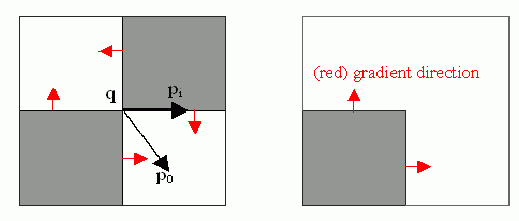
\includegraphics[width=1.0\textwidth]{pics/cornersubpix.png}

Sub-pixel accurate corner locator is based on the observation that every vector from the center $q$ to a point $p$ located within a neighborhood of $q$ is orthogonal to the image gradient at $p$ subject to image and measurement noise. Consider the expression:

\[
\epsilon_i = {DI_{p_i}}^T \cdot (q - p_i)
\]

where ${DI_{p_i}}$ is the image gradient at the one of the points $p_i$ in a neighborhood of $q$. The value of $q$ is to be found such that $\epsilon_i$ is minimized. A system of equations may be set up with $\epsilon_i$ set to zero:

\[
\sum_i(DI_{p_i} \cdot {DI_{p_i}}^T) - \sum_i(DI_{p_i} \cdot {DI_{p_i}}^T \cdot p_i)
\]

where the gradients are summed within a neighborhood ("search window") of $q$. Calling the first gradient term $G$ and the second gradient term $b$ gives:

\[
q = G^{-1} \cdot b
\]

The algorithm sets the center of the neighborhood window at this new center $q$ and then iterates until the center keeps within a set threshold.

\cvCPyFunc{GetStarKeypoints}
Retrieves keypoints using the StarDetector algorithm.

\cvdefC{
CvSeq* cvGetStarKeypoints( \par const CvArr* image,\par CvMemStorage* storage,\par CvStarDetectorParams params=cvStarDetectorParams() );
}\cvdefPy{GetStarKeypoints(image,storage,params)-> keypoints}

\begin{description}
\cvarg{image}{The input 8-bit grayscale image}
\cvarg{storage}{Memory storage where the keypoints will be stored}
\cvarg{params}{Various algorithm parameters given to the structure CvStarDetectorParams:}
\begin{lstlisting}
 typedef struct CvStarDetectorParams
 {
    int maxSize; // maximal size of the features detected. The following 
                 // values of the parameter are supported:
                 // 4, 6, 8, 11, 12, 16, 22, 23, 32, 45, 46, 64, 90, 128
    int responseThreshold; // threshold for the approximatd laplacian,
                           // used to eliminate weak features
    int lineThresholdProjected; // another threshold for laplacian to 
                // eliminate edges
    int lineThresholdBinarized; // another threshold for the feature 
                // scale to eliminate edges
    int suppressNonmaxSize; // linear size of a pixel neighborhood 
                // for non-maxima suppression
 }
 CvStarDetectorParams;
\end{lstlisting}
\end{description}

The function GetStarKeypoints extracts keypoints that are local
scale-space extremas. The scale-space is constructed by computing
approximate values of laplacians with different sigma's at each
pixel. Instead of using pyramids, a popular approach to save computing
time, all of the laplacians are computed at each pixel of the original
high-resolution image. But each approximate laplacian value is computed
in O(1) time regardless of the sigma, thanks to the use of integral
images. The algorithm is based on the paper 
Agrawal08
, but instead
of a square, hexagon or octagon it uses an 8-end star shape, hence the name,
consisting of overlapping upright and tilted squares.

Each computed feature is represented by the following structure:

\begin{lstlisting}
typedef struct CvStarKeypoint
{
    CvPoint pt; // coordinates of the feature
    int size; // feature size, see CvStarDetectorParams::maxSize
    float response; // the approximated laplacian value at that point.
}
CvStarKeypoint;

inline CvStarKeypoint cvStarKeypoint(CvPoint pt, int size, float response);
\end{lstlisting}

\ifC
Below is the small usage sample:

\begin{lstlisting}
#include "cv.h"
#include "highgui.h"

int main(int argc, char** argv)
{
    const char* filename = argc > 1 ? argv[1] : "lena.jpg";
    IplImage* img = cvLoadImage( filename, 0 ), *cimg;
    CvMemStorage* storage = cvCreateMemStorage(0);
    CvSeq* keypoints = 0;
    int i;

    if( !img )
        return 0;
    cvNamedWindow( "image", 1 );
    cvShowImage( "image", img );
    cvNamedWindow( "features", 1 );
    cimg = cvCreateImage( cvGetSize(img), 8, 3 );
    cvCvtColor( img, cimg, CV_GRAY2BGR );

    keypoints = cvGetStarKeypoints( img, storage, cvStarDetectorParams(45) );

    for( i = 0; i < (keypoints ? keypoints->total : 0); i++ )
    {
        CvStarKeypoint kpt = *(CvStarKeypoint*)cvGetSeqElem(keypoints, i);
        int r = kpt.size/2;
        cvCircle( cimg, kpt.pt, r, CV_RGB(0,255,0));
        cvLine( cimg, cvPoint(kpt.pt.x + r, kpt.pt.y + r),
            cvPoint(kpt.pt.x - r, kpt.pt.y - r), CV_RGB(0,255,0));
        cvLine( cimg, cvPoint(kpt.pt.x - r, kpt.pt.y + r),
            cvPoint(kpt.pt.x + r, kpt.pt.y - r), CV_RGB(0,255,0));
    }
    cvShowImage( "features", cimg );
    cvWaitKey();
}
\end{lstlisting}
\fi

\cvCPyFunc{GoodFeaturesToTrack}
Determines strong corners on an image.

\cvdefC{
void cvGoodFeaturesToTrack(
\par const CvArr* image
\par CvArr* eigImage, CvArr* tempImage
\par CvPoint2D32f* corners
\par int* cornerCount
\par double qualityLevel
\par double minDistance
\par const CvArr* mask=NULL
\par int blockSize=3
\par int useHarris=0
\par double k=0.04 );
}
\cvdefPy{GoodFeaturesToTrack(image,eigImage,tempImage,qualityLevel,minDistance,mask=NULL,blockSize=3,useHarris=0,k=0.04)-> corners}

\begin{description}
\cvarg{image}{The source 8-bit or floating-point 32-bit, single-channel image}
\cvarg{eigImage}{Temporary floating-point 32-bit image, the same size as \texttt{image}}
\cvarg{tempImage}{Another temporary image, the same size and format as \texttt{eigImage}}
\cvarg{corners}{Output parameter; detected corners}
\cvarg{cornerCount}{Output parameter; number of detected corners}
\cvarg{qualityLevel}{Multiplier for the max/min eigenvalue; specifies the minimal accepted quality of image corners}
\cvarg{minDistance}{Limit, specifying the minimum possible distance between the returned corners; Euclidian distance is used}
\cvarg{mask}{Region of interest. The function selects points either in the specified region or in the whole image if the mask is NULL}
\cvarg{blockSize}{Size of the averaging block, passed to the underlying \cvCPyCross{CornerMinEigenVal} or \cvCPyCross{CornerHarris} used by the function}
\cvarg{useHarris}{If nonzero, Harris operator (\cvCPyCross{CornerHarris}) is used instead of default \cvCPyCross{CornerMinEigenVal}}
\cvarg{k}{Free parameter of Harris detector; used only if ($\texttt{useHarris} != 0$)}
\end{description}

The function finds corners with big
eigenvalues in the image. The function first calculates the minimal
eigenvalue for every source image pixel using the \cvCPyCross{CornerMinEigenVal}
function and stores them in \texttt{eigImage}. Then it performs
non-maxima suppression (only local maxima in $3\times 3$ neighborhood
remain). The next step is rejecting the corners with the minimal
eigenvalue less than
$\texttt{qualityLevel} \cdot max(\texttt{eigImage}(x,y))$
.
Finally, the function ensures that all the corners found are distanced
enough from one another by considering the corners (the strongest
corners are considered first) and checking that the distance between
the newly considered feature and the features considered earlier
is larger than \texttt{minDistance}. So, the function removes the
features than are too close to the stronger features.

\cvCPyFunc{HoughLines2}
Finds lines in a binary image using a Hough transform.

\cvdefC{
CvSeq* cvHoughLines2( \par CvArr* image,\par void* line\_storage,\par int method,\par double rho,\par double theta,\par int threshold,\par double param1=0,\par double param2=0 );
}\cvdefPy{HoughLines2(image,storage,method,rho,theta,threshold,param1=0,parma2=0)-> lines}

\begin{description}
\cvarg{image}{The 8-bit, single-channel, binary source image. In the case of a probabilistic method, the image is modified by the function}
\cvarg{line\_storage}{The storage for the lines that are detected. It can
be a memory storage (in this case a sequence of lines is created in
the storage and returned by the function) or single row/single column
matrix (CvMat*) of a particular type (see below) to which the lines'
parameters are written. The matrix header is modified by the function
so its \texttt{cols} or \texttt{rows} will contain the number of lines
detected. If \texttt{line\_storage} is a matrix and the actual number
of lines exceeds the matrix size, the maximum possible number of lines
is returned (in the case of standard hough transform the lines are sorted
by the accumulator value)}
\cvarg{method}{The Hough transform variant, one of the following:
\begin{description}
  \cvarg{CV\_HOUGH\_STANDARD}{classical or standard Hough transform. Every line is represented by two floating-point numbers $(\rho, \theta)$, where $\rho$ is a distance between (0,0) point and the line, and $\theta$ is the angle between x-axis and the normal to the line. Thus, the matrix must be (the created sequence will be) of \texttt{CV\_32FC2} type}
  \cvarg{CV\_HOUGH\_PROBABILISTIC}{probabilistic Hough transform (more efficient in case if picture contains a few long linear segments). It returns line segments rather than the whole line. Each segment is represented by starting and ending points, and the matrix must be (the created sequence will be) of \texttt{CV\_32SC4} type}
  \cvarg{CV\_HOUGH\_MULTI\_SCALE}{multi-scale variant of the classical Hough transform. The lines are encoded the same way as \texttt{CV\_HOUGH\_STANDARD}}
\end{description}}
\cvarg{rho}{Distance resolution in pixel-related units}
\cvarg{theta}{Angle resolution measured in radians}
\cvarg{threshold}{Threshold parameter. A line is returned by the function if the corresponding accumulator value is greater than \texttt{threshold}}
\cvarg{param1}{The first method-dependent parameter:
\begin{itemize}
  \item For the classical Hough transform it is not used (0).
  \item For the probabilistic Hough transform it is the minimum line length.
  \item For the multi-scale Hough transform it is the divisor for the distance resolution $\rho$. (The coarse distance resolution will be $\rho$ and the accurate resolution will be $(\rho / \texttt{param1})$).
\end{itemize}}
\cvarg{param2}{The second method-dependent parameter:
\begin{itemize}
  \item For the classical Hough transform it is not used (0).
  \item For the probabilistic Hough transform it is the maximum gap between line segments lying on the same line to treat them as a single line segment (i.e. to join them).
  \item For the multi-scale Hough transform it is the divisor for the angle resolution $\theta$. (The coarse angle resolution will be $\theta$ and the accurate resolution will be $(\theta / \texttt{param2})$).
\end{itemize}}
\end{description}

The function implements a few variants of the Hough transform for line detection.

\ifC
\textbf{Example. Detecting lines with Hough transform.}
\begin{lstlisting}
/* This is a standalone program. Pass an image name as a first parameter
of the program.  Switch between standard and probabilistic Hough transform
by changing "#if 1" to "#if 0" and back */
#include <cv.h>
#include <highgui.h>
#include <math.h>

int main(int argc, char** argv)
{
    IplImage* src;
    if( argc == 2 && (src=cvLoadImage(argv[1], 0))!= 0)
    {
        IplImage* dst = cvCreateImage( cvGetSize(src), 8, 1 );
        IplImage* color_dst = cvCreateImage( cvGetSize(src), 8, 3 );
        CvMemStorage* storage = cvCreateMemStorage(0);
        CvSeq* lines = 0;
        int i;
        cvCanny( src, dst, 50, 200, 3 );
        cvCvtColor( dst, color_dst, CV_GRAY2BGR );
#if 1
        lines = cvHoughLines2( dst,
                               storage,
                               CV_HOUGH_STANDARD,
                               1,
                               CV_PI/180,
                               100,
                               0,
                               0 );

        for( i = 0; i < MIN(lines->total,100); i++ )
        {
            float* line = (float*)cvGetSeqElem(lines,i);
            float rho = line[0];
            float theta = line[1];
            CvPoint pt1, pt2;
            double a = cos(theta), b = sin(theta);
            double x0 = a*rho, y0 = b*rho;
            pt1.x = cvRound(x0 + 1000*(-b));
            pt1.y = cvRound(y0 + 1000*(a));
            pt2.x = cvRound(x0 - 1000*(-b));
            pt2.y = cvRound(y0 - 1000*(a));
            cvLine( color_dst, pt1, pt2, CV_RGB(255,0,0), 3, 8 );
        }
#else
        lines = cvHoughLines2( dst,
                               storage,
                               CV_HOUGH_PROBABILISTIC,
                               1,
                               CV_PI/180,
                               80,
                               30,
                               10 );
        for( i = 0; i < lines->total; i++ )
        {
            CvPoint* line = (CvPoint*)cvGetSeqElem(lines,i);
            cvLine( color_dst, line[0], line[1], CV_RGB(255,0,0), 3, 8 );
        }
#endif
        cvNamedWindow( "Source", 1 );
        cvShowImage( "Source", src );

        cvNamedWindow( "Hough", 1 );
        cvShowImage( "Hough", color_dst );

        cvWaitKey(0);
    }
}
\end{lstlisting}

This is the sample picture the function parameters have been tuned for:

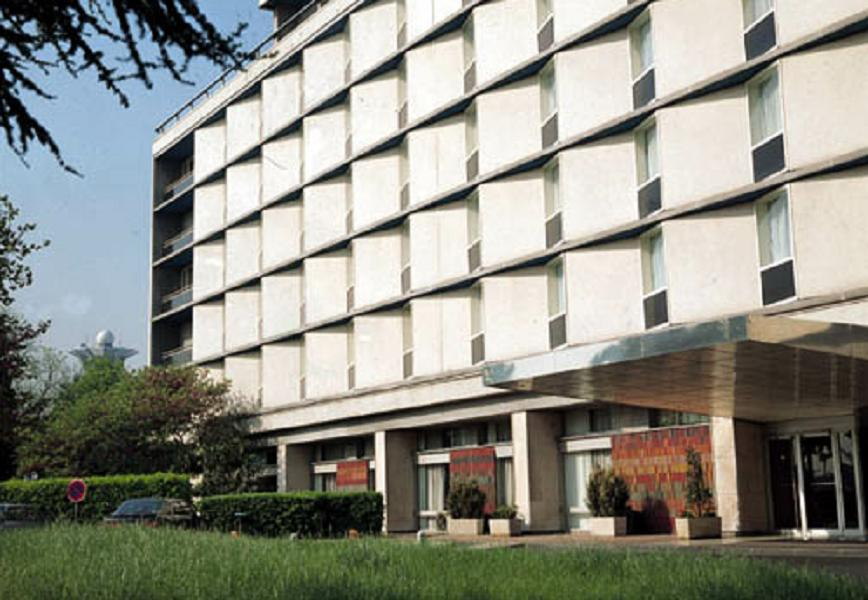
\includegraphics[width=0.5\textwidth]{pics/building.jpg}

And this is the output of the above program in the case of probabilistic Hough transform (\texttt{\#if 0} case):

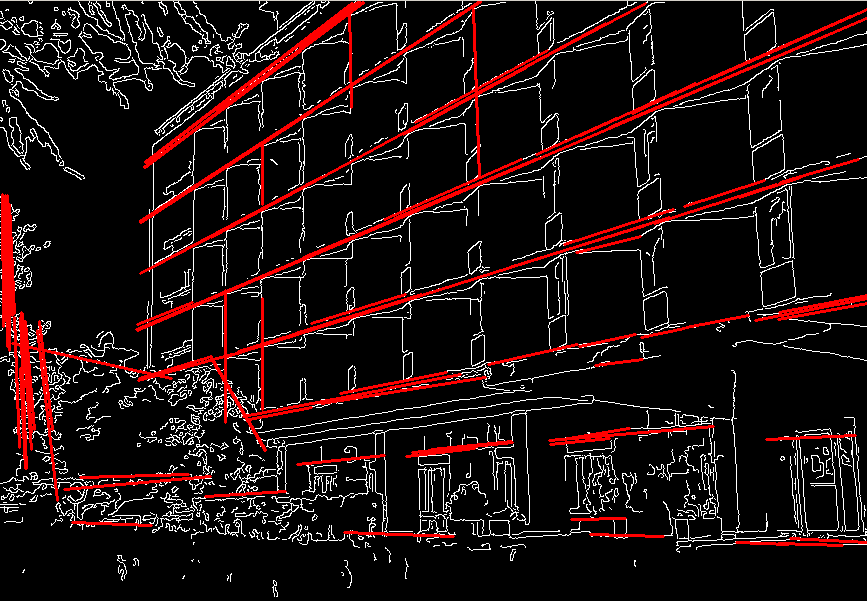
\includegraphics[width=0.5\textwidth]{pics/houghp.png}
\fi

\cvCPyFunc{PreCornerDetect}
Calculates the feature map for corner detection.

\cvdefC{
void cvPreCornerDetect(
\par const CvArr* image,
\par CvArr* corners,
\par int apertureSize=3 );
}\cvdefPy{PreCornerDetect(image,corners,aperture\_size=3)-> None}
\begin{description}
\cvarg{image}{Input image}
\cvarg{corners}{Image to store the corner candidates}
\cvarg{apertureSize}{Aperture parameter for the Sobel operator (see \cvCPyCross{Sobel})}
\end{description}

The function calculates the function

\[
D_x^2 D_{yy} + D_y^2 D_{xx} - 2 D_x D_y D_{xy}
\]

where $D_?$ denotes one of the first image derivatives and $D_{??}$ denotes a second image derivative.

The corners can be found as local maximums of the function below:

\begin{lstlisting}
// assume that the image is floating-point
IplImage* corners = cvCloneImage(image);
IplImage* dilated_corners = cvCloneImage(image);
IplImage* corner_mask = cvCreateImage( cvGetSize(image), 8, 1 );
cvPreCornerDetect( image, corners, 3 );
cvDilate( corners, dilated_corners, 0, 1 );
cvSubS( corners, dilated_corners, corners );
cvCmpS( corners, 0, corner_mask, CV_CMP_GE );
cvReleaseImage( &corners );
cvReleaseImage( &dilated_corners );
\end{lstlisting}

\ifC
\cvCPyFunc{SampleLine}
Reads the raster line to the buffer.

\cvdefC{
int cvSampleLine(
\par const CvArr* image
\par CvPoint pt1
\par CvPoint pt2
\par void* buffer
\par int connectivity=8 );
}

\begin{description}
\cvarg{image}{Image to sample the line from}
\cvarg{pt1}{Starting line point}
\cvarg{pt2}{Ending line point}
\cvarg{buffer}{Buffer to store the line points; must have enough size to store
$max( |\texttt{pt2.x} - \texttt{pt1.x}|+1, |\texttt{pt2.y} - \texttt{pt1.y}|+1 )$
points in the case of an 8-connected line and
$ (|\texttt{pt2.x}-\texttt{pt1.x}|+|\texttt{pt2.y}-\texttt{pt1.y}|+1) $
in the case of a 4-connected line}
\cvarg{connectivity}{The line connectivity, 4 or 8}
\end{description}

The function implements a particular application of line iterators. The function reads all of the image points lying on the line between \texttt{pt1} and \texttt{pt2}, including the end points, and stores them into the buffer.

\fi

\fi


\ifCpp

\cvCppFunc{Canny}
Finds edges in an image using Canny algorithm.

\cvdefCpp{void Canny( const Mat\& image, Mat\& edges,\par
            double threshold1, double threshold2,\par
            int apertureSize=3, bool L2gradient=false );}
\begin{description}
\cvarg{image}{Single-channel 8-bit input image}
\cvarg{edges}{The output edge map. It will have the same size and the same type as \texttt{image}}
\cvarg{threshold1}{The first threshold for the hysteresis procedure}
\cvarg{threshold2}{The second threshold for the hysteresis procedure}
\cvarg{apertureSize}{Aperture size for the \cvCppCross{Sobel} operator}
\cvarg{L2gradient}{Indicates, whether the more accurate $L_2$ norm $=\sqrt{(dI/dx)^2 + (dI/dy)^2}$ should be used to compute the image gradient magnitude (\texttt{L2gradient=true}), or a faster default $L_1$ norm $=|dI/dx|+|dI/dy|$ is enough (\texttt{L2gradient=false})}
\end{description}

The function finds edges in the input image \texttt{image} and marks them in the output map \texttt{edges} using the Canny algorithm. The smallest value between \texttt{threshold1} and \texttt{threshold2} is used for edge linking, the largest value is used to find the initial segments of strong edges, see
\url{http://en.wikipedia.org/wiki/Canny_edge_detector}

\cvCppFunc{cornerEigenValsAndVecs}
Calculates eigenvalues and eigenvectors of image blocks for corner detection.

\cvdefCpp{void cornerEigenValsAndVecs( const Mat\& src, Mat\& dst,\par
                            int blockSize, int apertureSize,\par
                            int borderType=BORDER\_DEFAULT );}
\begin{description}
\cvarg{src}{Input single-channel 8-bit or floating-point image}
\cvarg{dst}{Image to store the results. It will have the same size as \texttt{src} and the type \texttt{CV\_32FC(6)}}
\cvarg{blockSize}{Neighborhood size (see discussion)}
\cvarg{apertureSize}{Aperture parameter for the \cvCppCross{Sobel} operator}
\cvarg{boderType}{Pixel extrapolation method; see \cvCppCross{borderInterpolate}}
\end{description}

For every pixel $p$, the function \texttt{cornerEigenValsAndVecs} considers a \texttt{blockSize} $\times$ \texttt{blockSize} neigborhood $S(p)$. It calculates the covariation matrix of derivatives over the neighborhood as:

\[
M = \begin{bmatrix}
\sum_{S(p)}(dI/dx)^2 & \sum_{S(p)}(dI/dx dI/dy)^2 \\
\sum_{S(p)}(dI/dx dI/dy)^2 & \sum_{S(p)}(dI/dy)^2
\end{bmatrix}
\]

Where the derivatives are computed using \cvCppCross{Sobel} operator.

After that it finds eigenvectors and eigenvalues of $M$ and stores them into destination image in the form
$(\lambda_1, \lambda_2, x_1, y_1, x_2, y_2)$ where
\begin{description}
\item[$\lambda_1, \lambda_2$]are the eigenvalues of $M$; not sorted
\item[$x_1, y_1$]are the eigenvectors corresponding to $\lambda_1$
\item[$x_2, y_2$]are the eigenvectors corresponding to $\lambda_2$
\end{description}

The output of the function can be used for robust edge or corner detection.

See also: \cvCppCross{cornerMinEigenVal}, \cvCppCross{cornerHarris}, \cvCppCross{preCornerDetect}

\cvCppFunc{cornerHarris}
Harris edge detector.

\cvdefCpp{void cornerHarris( const Mat\& src, Mat\& dst, int blockSize,\par
                  int apertureSize, double k,\par
                  int borderType=BORDER\_DEFAULT );}
\begin{description}
\cvarg{src}{Input single-channel 8-bit or floating-point image}
\cvarg{dst}{Image to store the Harris detector responses; will have type \texttt{CV\_32FC1} and the same size as \texttt{src}}
\cvarg{blockSize}{Neighborhood size (see the discussion of \cvCppCross{cornerEigenValsAndVecs})}
\cvarg{apertureSize}{Aperture parameter for the \cvCppCross{Sobel} operator}
\cvarg{k}{Harris detector free parameter. See the formula below}
\cvarg{boderType}{Pixel extrapolation method; see \cvCppCross{borderInterpolate}}
\end{description}

The function runs the Harris edge detector on the image. Similarly to \cvCppCross{cornerMinEigenVal} and \cvCppCross{cornerEigenValsAndVecs}, for each pixel $(x, y)$ it calculates a $2\times2$ gradient covariation matrix $M^{(x,y)}$ over a $\texttt{blockSize} \times \texttt{blockSize}$ neighborhood. Then, it computes the following characteristic:

\[
\texttt{dst}(x,y) = \mathrm{det} M^{(x,y)} - k \cdot \left(\mathrm{tr} M^{(x,y)}\right)^2
\]

Corners in the image can be found as the local maxima of this response map.

\cvCppFunc{cornerMinEigenVal}
Calculates the minimal eigenvalue of gradient matrices for corner detection.

\cvdefCpp{void cornerMinEigenVal( const Mat\& src, Mat\& dst,\par
                        int blockSize, int apertureSize=3,\par
                        int borderType=BORDER\_DEFAULT );}
\begin{description}
\cvarg{src}{Input single-channel 8-bit or floating-point image}
\cvarg{dst}{Image to store the minimal eigenvalues; will have type \texttt{CV\_32FC1} and the same size as \texttt{src}}
\cvarg{blockSize}{Neighborhood size (see the discussion of \cvCppCross{cornerEigenValsAndVecs})}
\cvarg{apertureSize}{Aperture parameter for the \cvCppCross{Sobel} operator}
\cvarg{boderType}{Pixel extrapolation method; see \cvCppCross{borderInterpolate}}
\end{description}

The function is similar to \cvCppCross{cornerEigenValsAndVecs} but it calculates and stores only the minimal eigenvalue of the covariation matrix of derivatives, i.e. $\min(\lambda_1, \lambda_2)$ in terms of the formulae in \cvCppCross{cornerEigenValsAndVecs} description.

\cvCppFunc{cornerSubPix}
Refines the corner locations.

\cvdefCpp{void cornerSubPix( const Mat\& image, vector<Point2f>\& corners,\par
                   Size winSize, Size zeroZone,\par
                   TermCriteria criteria );}
\begin{description}
\cvarg{image}{Input image}
\cvarg{corners}{Initial coordinates of the input corners; refined coordinates on output}
\cvarg{winSize}{Half of the side length of the search window. For example, if \texttt{winSize=Size(5,5)}, then a $5*2+1 \times 5*2+1 = 11 \times 11$ search window would be used}
\cvarg{zeroZone}{Half of the size of the dead region in the middle of the search zone over which the summation in the formula below is not done. It is used sometimes to avoid possible singularities of the autocorrelation matrix. The value of (-1,-1) indicates that there is no such size}
\cvarg{criteria}{Criteria for termination of the iterative process of corner refinement. That is, the process of corner position refinement stops either after a certain number of iterations or when a required accuracy is achieved. The \texttt{criteria} may specify either of or both the maximum number of iteration and the required accuracy}
\end{description}

The function iterates to find the sub-pixel accurate location of corners, or radial saddle points, as shown in on the picture below.

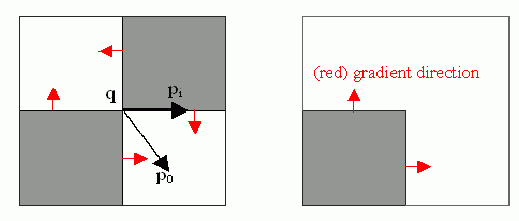
\includegraphics[width=1.0\textwidth]{pics/cornersubpix.png}

Sub-pixel accurate corner locator is based on the observation that every vector from the center $q$ to a point $p$ located within a neighborhood of $q$ is orthogonal to the image gradient at $p$ subject to image and measurement noise. Consider the expression:

\[
\epsilon_i = {DI_{p_i}}^T \cdot (q - p_i)
\]

where ${DI_{p_i}}$ is the image gradient at the one of the points $p_i$ in a neighborhood of $q$. The value of $q$ is to be found such that $\epsilon_i$ is minimized. A system of equations may be set up with $\epsilon_i$ set to zero:

\[
\sum_i(DI_{p_i} \cdot {DI_{p_i}}^T) - \sum_i(DI_{p_i} \cdot {DI_{p_i}}^T \cdot p_i)
\]

where the gradients are summed within a neighborhood ("search window") of $q$. Calling the first gradient term $G$ and the second gradient term $b$ gives:

\[
q = G^{-1} \cdot b
\]

The algorithm sets the center of the neighborhood window at this new center $q$ and then iterates until the center keeps within a set threshold.


\cvCppFunc{goodFeaturesToTrack}
Determines strong corners on an image.

\cvdefCpp{void goodFeaturesToTrack( const Mat\& image, vector<Point2f>\& corners,\par
                         int maxCorners, double qualityLevel, double minDistance,\par
                         const Mat\& mask=Mat(), int blockSize=3,\par
                         bool useHarrisDetector=false, double k=0.04 );}
\begin{description}
\cvarg{image}{The input 8-bit or floating-point 32-bit, single-channel image}
\cvarg{corners}{The output vector of detected corners}
\cvarg{maxCorners}{The maximum number of corners to return. If there are more corners than that will be found, the strongest of them will be returned}
\cvarg{qualityLevel}{Characterizes the minimal accepted quality of image corners; the value of the parameter is multiplied by the by the best corner quality measure (which is the min eigenvalue, see \cvCppCross{cornerMinEigenVal}, or the Harris function response, see \cvCppCross{cornerHarris}). The corners, which quality measure is less than the product, will be rejected. For example, if the best corner has the quality measure = 1500, and the \texttt{qualityLevel=0.01}, then all the corners which quality measure is less than 15 will be rejected.}
\cvarg{minDistance}{The minimum possible Euclidean distance between the returned corners}
\cvarg{mask}{The optional region of interest. If the image is not empty (then it needs to have the type \texttt{CV\_8UC1} and the same size as \texttt{image}), it will specify the region in which the corners are detected}
\cvarg{blockSize}{Size of the averaging block for computing derivative covariation matrix over each pixel neighborhood, see \cvCppCross{cornerEigenValsAndVecs}}
\cvarg{useHarrisDetector}{Indicates, whether to use \hyperref[cornerHarris]{Harris} operator or \cvCppCross{cornerMinEigenVal}}
\cvarg{k}{Free parameter of Harris detector}
\end{description}

The function finds the most prominent corners in the image or in the specified image region, as described
in \cite{Shi94}:
\begin{enumerate}
\item the function first calculates the corner quality measure at every source image pixel using the \cvCppCross{cornerMinEigenVal} or \cvCppCross{cornerHarris}
\item then it performs non-maxima suppression (the local maxima in $3\times 3$ neighborhood
are retained).
\item the next step rejects the corners with the minimal eigenvalue less than $\texttt{qualityLevel} \cdot \max_{x,y} qualityMeasureMap(x,y)$.
\item the remaining corners are then sorted by the quality measure in the descending order.
\item finally, the function throws away each corner $pt_j$ if there is a stronger corner $pt_i$ ($i < j$) such that the distance between them is less than \texttt{minDistance}
\end{enumerate}

The function can be used to initialize a point-based tracker of an object.

See also: \cvCppCross{cornerMinEigenVal}, \cvCppCross{cornerHarris}, \cvCppCross{calcOpticalFlowPyrLK}, \cvCppCross{estimateRigidMotion}, \cvCppCross{PlanarObjectDetector}, \cvCppCross{OneWayDescriptor}

\cvCppFunc{HoughCircles}
Finds circles in a grayscale image using a Hough transform.

\cvdefCpp{void HoughCircles( Mat\& image, vector<Vec3f>\& circles,\par
                 int method, double dp, double minDist,\par
                 double param1=100, double param2=100,\par
                 int minRadius=0, int maxRadius=0 );}
\begin{description}
\cvarg{image}{The 8-bit, single-channel, grayscale input image}
\cvarg{circles}{The output vector of found circles. Each vector is encoded as 3-element floating-point vector $(x, y, radius)$}
\cvarg{method}{Currently, the only implemented method is \texttt{CV\_HOUGH\_GRADIENT}, which is basically \emph{21HT}, described in \cite{Yuen90}.}
\cvarg{dp}{The inverse ratio of the accumulator resolution to the image resolution. For example, if \texttt{dp=1}, the accumulator will have the same resolution as the input image, if \texttt{dp=2} - accumulator will have half as big width and height, etc}
\cvarg{minDist}{Minimum distance between the centers of the detected circles. If the parameter is too small, multiple neighbor circles may be falsely detected in addition to a true one. If it is too large, some circles may be missed}
\cvarg{param1}{The first method-specific parameter. in the case of \texttt{CV\_HOUGH\_GRADIENT} it is the higher threshold of the two passed to \cvCppCross{Canny} edge detector (the lower one will be twice smaller)}
\cvarg{param2}{The second method-specific parameter. in the case of \texttt{CV\_HOUGH\_GRADIENT} it is the accumulator threshold at the center detection stage. The smaller it is, the more false circles may be detected. Circles, corresponding to the larger accumulator values, will be returned first}
\cvarg{minRadius}{Minimum circle radius}
\cvarg{maxRadius}{Maximum circle radius}
\end{description}

The function finds circles in a grayscale image using some modification of Hough transform. Here is a short usage example:

\begin{lstlisting}
#include <cv.h>
#include <highgui.h>
#include <math.h>

using namespace cv;

int main(int argc, char** argv)
{
    Mat img, gray;
    if( argc != 2 && !(img=imread(argv[1], 1)).data)
        return -1;
    cvtColor(img, gray, CV_BGR2GRAY);
    // smooth it, otherwise a lot of false circles may be detected
    GaussianBlur( gray, gray, 9, 9, 2, 2 );
    vector<Vec3f> circles;
    houghCircles(gray, circles, CV_HOUGH_GRADIENT,
                 2, gray->rows/4, 200, 100 );
    for( size_t i = 0; i < circles.size(); i++ )
    {
         Point center(cvRound(circles[i][0]), cvRound(circles[i][1]));
         int radius = cvRound(circles[i][2]);
         // draw the circle center
         circle( img, center, 3, Scalar(0,255,0), -1, 8, 0 );
         // draw the circle outline
         circle( img, center, radius, Scalar(0,0,255), 3, 8, 0 );
    }
    namedWindow( "circles", 1 );
    imshow( "circles", img );
    return 0;
}
\end{lstlisting}

Note that usually the function detects the circles' centers well, however it may fail to find the correct radii. You can assist the function by specifying the radius range (\texttt{minRadius} and \texttt{maxRadius}) if you know it, or you may ignore the returned radius, use only the center and find the correct radius using some additional procedure.

See also: \cvCppCross{fitEllipse}, \cvCppCross{minEnclosingCircle}

\cvCppFunc{HoughLines}
Finds lines in a binary image using standard Hough transform.

\cvdefCpp{void HoughLines( Mat\& image, vector<Vec2f>\& lines,\par
                 double rho, double theta, int threshold,\par
                 double srn=0, double stn=0 );}
\begin{description}
\cvarg{image}{The 8-bit, single-channel, binary source image. The image may be modified by the function}
\cvarg{lines}{The output vector of lines. Each line is represented by a two-element vector $(\rho, \theta)$. $\rho$ is the distance from the coordinate origin $(0,0)$ (top-left corner of the image) and $\theta$ is the line rotation angle in radians ($0 \sim \textrm{vertical line}, \pi/2 \sim \textrm{horizontal line}$)}
\cvarg{rho}{Distance resolution of the accumulator in pixels}
\cvarg{theta}{Angle resolution of the accumulator in radians}
\cvarg{threshold}{The accumulator threshold parameter. Only those lines are returned that get enough votes ($>\texttt{threshold}$)}
\cvarg{srn}{For the multi-scale Hough transform it is the divisor for the distance resolution \texttt{rho}. The coarse accumulator distance resolution will be \texttt{rho} and the accurate accumulator resolution will be \texttt{rho/srn}. If both \texttt{srn=0} and \texttt{stn=0} then the classical Hough transform is used, otherwise both these parameters should be positive.}
\cvarg{stn}{For the multi-scale Hough transform it is the divisor for the distance resolution \texttt{theta}}
\end{description}

The function implements standard or standard multi-scale Hough transform algorithm for line detection. See \cvCppCross{HoughLinesP} for the code example.


\cvCppFunc{HoughLinesP}
Finds lines segments in a binary image using probabilistic Hough transform.

\cvdefCpp{void HoughLinesP( Mat\& image, vector<Vec4i>\& lines,\par
                  double rho, double theta, int threshold,\par
                  double minLineLength=0, double maxLineGap=0 );}
\begin{description}
\cvarg{image}{The 8-bit, single-channel, binary source image. The image may be modified by the function}
\cvarg{lines}{The output vector of lines. Each line is represented by a 4-element vector $(x_1, y_1, x_2, y_2)$, where $(x_1,y_1)$ and $(x_2, y_2)$ are the ending points of each line segment detected.}
\cvarg{rho}{Distance resolution of the accumulator in pixels}
\cvarg{theta}{Angle resolution of the accumulator in radians}
\cvarg{threshold}{The accumulator threshold parameter. Only those lines are returned that get enough votes ($>\texttt{threshold}$)}
\cvarg{minLineLength}{The minimum line length. Line segments shorter than that will be rejected}
\cvarg{maxLineGap}{The maximum allowed gap between points on the same line to link them.}
\end{description}

The function implements probabilistic Hough transform algorithm for line detection, described in \cite{Matas00}. Below is line detection example:

\begin{lstlisting}
/* This is a standalone program. Pass an image name as a first parameter
of the program.  Switch between standard and probabilistic Hough transform
by changing "#if 1" to "#if 0" and back */
#include <cv.h>
#include <highgui.h>
#include <math.h>

using namespace cv;

int main(int argc, char** argv)
{
    Mat src, dst, color_dst;
    if( argc != 2 || !(src=imread(argv[1], 0)).data)
        return -1;
        
    Canny( src, dst, 50, 200, 3 );
    cvtColor( dst, color_dst, CV_GRAY2BGR );    
        
#if 0
    vector<Vec2f> lines;
    HoughLines( dst, lines, 1, CV_PI/180, 100 );

    for( size_t i = 0; i < lines.size(); i++ )
    {
        float rho = lines[i][0];
        float theta = lines[i][1];
        double a = cos(theta), b = sin(theta);
        double x0 = a*rho, y0 = b*rho;
        Point pt1(cvRound(x0 + 1000*(-b)),
                  cvRound(y0 + 1000*(a)));
        Point pt2(cvRound(x0 - 1000*(-b)),
                  cvRound(y0 - 1000*(a)));
        line( color_dst, pt1, pt2, Scalar(0,0,255), 3, 8 );
    }
#else
    vector<Vec4i> lines;
    HoughLinesP( dst, lines, 1, CV_PI/180, 80, 30, 10 );
    for( size_t i = 0; i < lines.size(); i++ )
    {
        line( color_dst, Point(lines[i][0], lines[i][1]),
            Point(lines[i][2], lines[i][3]), Scalar(0,0,255), 3, 8 );
    }
#endif
    namedWindow( "Source", 1 );
    imshow( "Source", src );

    namedWindow( "Detected Lines", 1 );
    imshow( "Detected Lines", color_dst );

    waitKey(0);
    return 0;
}
\end{lstlisting}


This is the sample picture the function parameters have been tuned for:

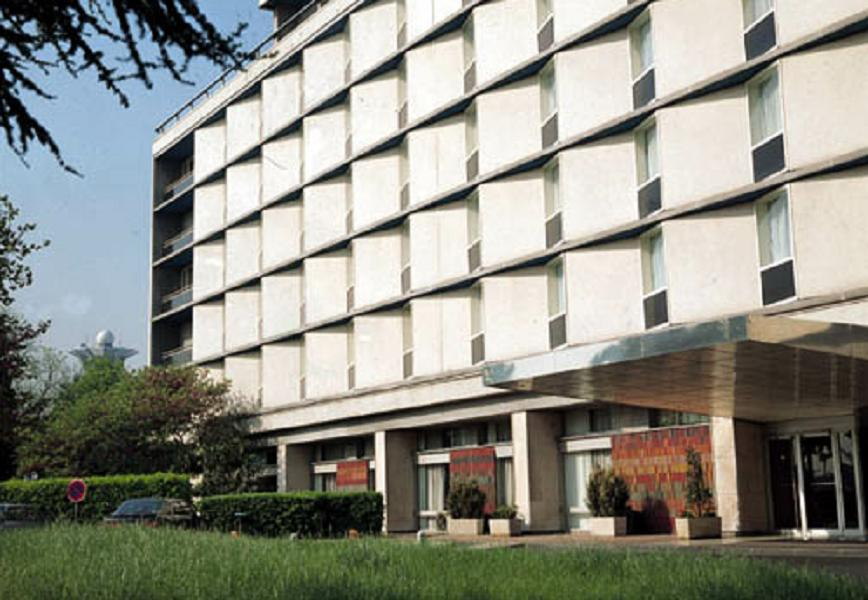
\includegraphics[width=0.5\textwidth]{pics/building.jpg}

And this is the output of the above program in the case of probabilistic Hough transform

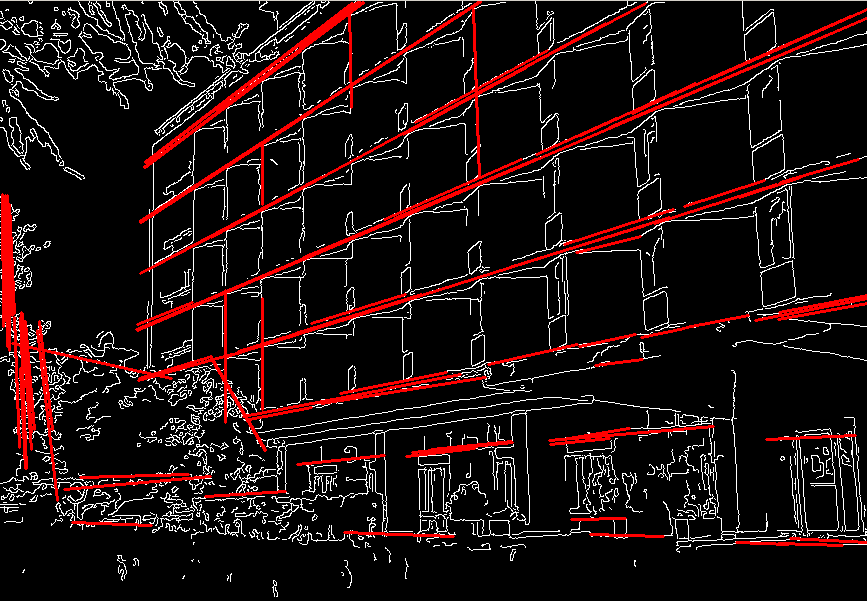
\includegraphics[width=0.5\textwidth]{pics/houghp.png}

\cvCppFunc{perCornerDetect}
Calculates the feature map for corner detection

\cvdefCpp{void preCornerDetect( const Mat\& src, Mat\& dst, int apertureSize,\par
                     int borderType=BORDER\_DEFAULT );}
\begin{description}
\cvarg{src}{The source single-channel 8-bit of floating-point image}
\cvarg{dst}{The output image; will have type \texttt{CV\_32F} and the same size as \texttt{src}}
\cvarg{apertureSize}{Aperture size of \cvCppCross{Sobel}}
\cvarg{borderType}{The pixel extrapolation method; see \cvCppCross{borderInterpolate}}
\end{description}

The function calculates the complex spatial derivative-based function of the source image

\[
\texttt{dst} = (D_x \texttt{src})^2 \cdot D_{yy} \texttt{src} + (D_y \texttt{src})^2 \cdot D_{xx} \texttt{src} - 2 D_x \texttt{src} \cdot D_y \texttt{src} \cdot D_{xy} \texttt{src}
\]

where $D_x$, $D_y$ are the first image derivatives, $D_{xx}$, $D_{yy}$ are the second image derivatives and $D_{xy}$ is the mixed derivative.

The corners can be found as local maximums of the functions, as shown below:

\begin{lstlisting}
Mat corners, dilated_corners;
preCornerDetect(image, corners, 3);
// dilation with 3x3 rectangular structuring element
dilate(corners, dilated_corners, Mat(), 1);
Mat corner_mask = corners == dilated_corners;
\end{lstlisting}


\cvCppFunc{KeyPoint}
Data structure for salient point detectors

\begin{lstlisting}
KeyPoint
{
public:
    // default constructor
    KeyPoint();
    // two complete constructors
    KeyPoint(Point2f _pt, float _size, float _angle=-1,
            float _response=0, int _octave=0, int _class_id=-1);
    KeyPoint(float x, float y, float _size, float _angle=-1,
             float _response=0, int _octave=0, int _class_id=-1);
    // coordinate of the point
    Point2f pt;
    // feature size
    float size;
    // feature orintation in degrees
    // (has negative value if the orientation
    // is not defined/not computed)
    float angle;
    // feature strength
    // (can be used to select only
    // the most prominent key points)
    float response;
    // scale-space octave in which the feature has been found;
    // may correlate with the size
    int octave;
    // point (can be used by feature
    // classifiers or object detectors)
    int class_id;
};

// reading/writing a vector of keypoints to a file storage
void write(FileStorage& fs, const string& name, const vector<KeyPoint>& keypoints);
void read(const FileNode& node, vector<KeyPoint>& keypoints);    
\end{lstlisting}


\cvCppFunc{MSER}
Maximally-Stable Extremal Region Extractor

\begin{lstlisting}
class MSER : public CvMSERParams
{
public:
    // default constructor
    MSER();
    // constructor that initializes all the algorithm parameters
    MSER( int _delta, int _min_area, int _max_area,
          float _max_variation, float _min_diversity,
          int _max_evolution, double _area_threshold,
          double _min_margin, int _edge_blur_size );
    // runs the extractor on the specified image; returns the MSERs,
    // each encoded as a contour (vector<Point>, see findContours)
    // the optional mask marks the area where MSERs are searched for
    void operator()(Mat& image, vector<vector<Point> >& msers, const Mat& mask) const;
};
\end{lstlisting}

The class encapsulates all the parameters of MSER (see \url{http://en.wikipedia.org/wiki/Maximally_stable_extremal_regions}) extraction algorithm. 

\cvCppFunc{SURF}
Class for extracting Speeded Up Robust Features from an image.

\begin{lstlisting}
class SURF : public CvSURFParams
{
public:
    // default constructor
    SURF();
    // constructor that initializes all the algorithm parameters
    SURF(double _hessianThreshold, int _nOctaves=4,
         int _nOctaveLayers=2, bool _extended=false);
    // returns the number of elements in each descriptor (64 or 128)
    int descriptorSize() const;
    // detects keypoints using fast multi-scale Hessian detector
    void operator()(const Mat& img, const Mat& mask,
                    vector<KeyPoint>& keypoints) const;
    // detects keypoints and computes the SURF descriptors for them
    void operator()(const Mat& img, const Mat& mask,
                    vector<KeyPoint>& keypoints,
                    vector<float>& descriptors,
                    bool useProvidedKeypoints=false) const;
};
\end{lstlisting}

The class \texttt{SURF} implements Speeded Up Robust Features descriptor \cite{Bay06}.
There is fast multi-scale Hessian keypoint detector that can be used to find the keypoints
(which is the default option), but the descriptors can be also computed for the user-specified keypoints.
The function can be used for object tracking and localization, image stitching etc. See the
\texttt{find\_obj.cpp} demo in OpenCV samples directory.


\cvCppFunc{StarDetector}
Implements Star keypoint detector

\begin{lstlisting}
class StarDetector : CvStarDetectorParams
{
public:
    // default constructor
    StarDetector();
    // the full constructor initialized all the algorithm parameters:
    // maxSize - maximum size of the features. The following 
    //      values of the parameter are supported:
    //      4, 6, 8, 11, 12, 16, 22, 23, 32, 45, 46, 64, 90, 128
    // responseThreshold - threshold for the approximated laplacian,
    //      used to eliminate weak features. The larger it is,
    //      the less features will be retrieved
    // lineThresholdProjected - another threshold for the laplacian to 
    //      eliminate edges
    // lineThresholdBinarized - another threshold for the feature 
    //      size to eliminate edges.
    // The larger the 2 threshold, the more points you get.
    StarDetector(int maxSize, int responseThreshold,
                 int lineThresholdProjected,
                 int lineThresholdBinarized,
                 int suppressNonmaxSize);

    // finds keypoints in an image
    void operator()(const Mat& image, vector<KeyPoint>& keypoints) const;
};
\end{lstlisting}

The class implements a modified version of CenSurE keypoint detector described in
\cite{Agrawal08}

\fi

\section{Motion Analysis and Object Tracking}

\ifCPy

\cvCPyFunc{Acc}
Adds a frame to an accumulator.

\cvdefC{
void cvAcc( \par const CvArr* image,\par CvArr* sum,\par const CvArr* mask=NULL );
}\cvdefPy{Acc(image,smu,mask=NULL)-> None}

\begin{description}
\cvarg{image}{Input image, 1- or 3-channel, 8-bit or 32-bit floating point. (each channel of multi-channel image is processed independently)}
\cvarg{sum}{Accumulator with the same number of channels as input image, 32-bit or 64-bit floating-point}
\cvarg{mask}{Optional operation mask}
\end{description}

The function adds the whole image \texttt{image} or its selected region to the accumulator \texttt{sum}:

\[ \texttt{sum}(x,y) \leftarrow \texttt{sum}(x,y) + \texttt{image}(x,y) \quad \text{if} \quad \texttt{mask}(x,y) \ne 0 \]

\cvCPyFunc{CalcGlobalOrientation}
Calculates the global motion orientation of some selected region.

\cvdefC{
double cvCalcGlobalOrientation( \par const CvArr* orientation,\par const CvArr* mask,\par const CvArr* mhi,\par double timestamp,\par double duration );
}\cvdefPy{CalcGlobalOrientation(orientation,mask,mhi,timestamp,duration)-> float}

\begin{description}
\cvarg{orientation}{Motion gradient orientation image; calculated by the function \cvCPyCross{CalcMotionGradient}}
\cvarg{mask}{Mask image. It may be a conjunction of a valid gradient mask, obtained with \cvCPyCross{CalcMotionGradient} and the mask of the region, whose direction needs to be calculated}
\cvarg{mhi}{Motion history image}
\cvarg{timestamp}{Current time in milliseconds or other units, it is better to store time passed to \cvCPyCross{UpdateMotionHistory} before and reuse it here, because running \cvCPyCross{UpdateMotionHistory} and \cvCPyCross{CalcMotionGradient} on large images may take some time}
\cvarg{duration}{Maximal duration of motion track in milliseconds, the same as \cvCPyCross{UpdateMotionHistory}}
\end{description}

The function calculates the general
motion direction in the selected region and returns the angle between
0 degrees  and 360 degrees . At first the function builds the orientation histogram
and finds the basic orientation as a coordinate of the histogram
maximum. After that the function calculates the shift relative to the
basic orientation as a weighted sum of all of the orientation vectors: the more
recent the motion, the greater the weight. The resultant angle is
a circular sum of the basic orientation and the shift.

\cvCPyFunc{CalcMotionGradient}
Calculates the gradient orientation of a motion history image.

\cvdefC{
void cvCalcMotionGradient( \par const CvArr* mhi,\par CvArr* mask,\par CvArr* orientation,\par double delta1,\par double delta2,\par int apertureSize=3 );
}\cvdefPy{CalcMotionGradient(mhi,mask,orientation,delta1,delta2,apertureSize=3)-> None}

\begin{description}
\cvarg{mhi}{Motion history image}
\cvarg{mask}{Mask image; marks pixels where the motion gradient data is correct; output parameter}
\cvarg{orientation}{Motion gradient orientation image; contains angles from 0 to ~360 degrees }
\cvarg{delta1, delta2}{The function finds the minimum ($m(x,y)$) and maximum ($M(x,y)$) mhi values over each pixel $(x,y)$ neighborhood and assumes the gradient is valid only if
\[
\min(\texttt{delta1} , \texttt{delta2} ) \le M(x,y)-m(x,y) \le \max(\texttt{delta1} ,\texttt{delta2} ).
\]}
\cvarg{apertureSize}{Aperture size of derivative operators used by the function: CV\_SCHARR, 1, 3, 5 or 7 (see \cvCPyCross{Sobel})}
\end{description}

The function calculates the derivatives $Dx$ and $Dy$ of \texttt{mhi} and then calculates gradient orientation as:

\[
\texttt{orientation}(x,y)=\arctan{\frac{Dy(x,y)}{Dx(x,y)}}
\]

where both $Dx(x,y)$ and $Dy(x,y)$ signs are taken into account (as in the \cvCPyCross{CartToPolar} function). After that \texttt{mask} is filled to indicate where the orientation is valid (see the \texttt{delta1} and \texttt{delta2} description).

\cvCPyFunc{CalcOpticalFlowBM}
Calculates the optical flow for two images by using the block matching method.

\cvdefC{
void cvCalcOpticalFlowBM( \par const CvArr* prev,\par const CvArr* curr,\par CvSize blockSize,\par CvSize shiftSize,\par CvSize max\_range,\par int usePrevious,\par CvArr* velx,\par CvArr* vely );
}\cvdefPy{CalcOpticalFlowBM(prev,curr,blockSize,shiftSize,max\_range,usePrevious,velx,vely)-> None}

\begin{description}
\cvarg{prev}{First image, 8-bit, single-channel}
\cvarg{curr}{Second image, 8-bit, single-channel}
\cvarg{blockSize}{Size of basic blocks that are compared}
\cvarg{shiftSize}{Block coordinate increments}
\cvarg{max\_range}{Size of the scanned neighborhood in pixels around the block}
\cvarg{usePrevious}{Uses the previous (input) velocity field}
\cvarg{velx}{Horizontal component of the optical flow of
\[
\left\lfloor \frac{\texttt{prev->width} - \texttt{blockSize.width}}{\texttt{shiftSize.width}} \right\rfloor
\times
\left\lfloor \frac{\texttt{prev->height} - \texttt{blockSize.height}}{\texttt{shiftSize.height}} \right\rfloor
\]
size, 32-bit floating-point, single-channel}
\cvarg{vely}{Vertical component of the optical flow of the same size \texttt{velx}, 32-bit floating-point, single-channel}
\end{description}

The function calculates the optical
flow for overlapped blocks $\texttt{blockSize.width} \times \texttt{blockSize.height}$ pixels each, thus the velocity
fields are smaller than the original images. For every block in \texttt{prev} the functions tries to find a similar block in
\texttt{curr} in some neighborhood of the original block or shifted by (velx(x0,y0),vely(x0,y0)) block as has been calculated by previous
function call (if \texttt{usePrevious=1})

\cvCPyFunc{CalcOpticalFlowHS}
Calculates the optical flow for two images.

\cvdefC{
void cvCalcOpticalFlowHS( \par const CvArr* prev,\par const CvArr* curr,\par int usePrevious,\par CvArr* velx,\par CvArr* vely,\par double lambda,\par CvTermCriteria criteria );
}\cvdefPy{CalcOpticalFlowHS(prev,curr,usePrevious,velx,vely,lambda,criteria)-> None}

\begin{description}
\cvarg{prev}{First image, 8-bit, single-channel}
\cvarg{curr}{Second image, 8-bit, single-channel}
\cvarg{usePrevious}{Uses the previous (input) velocity field}
\cvarg{velx}{Horizontal component of the optical flow of the same size as input images, 32-bit floating-point, single-channel}
\cvarg{vely}{Vertical component of the optical flow of the same size as input images, 32-bit floating-point, single-channel}
\cvarg{lambda}{Lagrangian multiplier}
\cvarg{criteria}{Criteria of termination of velocity computing}
\end{description}

The function computes the flow for every pixel of the first input image using the Horn and Schunck algorithm
\cvCPyCross{Horn81}.

\cvCPyFunc{CalcOpticalFlowLK}
Calculates the optical flow for two images.

\cvdefC{
void cvCalcOpticalFlowLK( \par const CvArr* prev,\par const CvArr* curr,\par CvSize winSize,\par CvArr* velx,\par CvArr* vely );
}\cvdefPy{CalcOpticalFlowLK(prev,curr,winSize,velx,vely)-> None}
\begin{description}

\cvarg{prev}{First image, 8-bit, single-channel}
\cvarg{curr}{Second image, 8-bit, single-channel}
\cvarg{winSize}{Size of the averaging window used for grouping pixels}
\cvarg{velx}{Horizontal component of the optical flow of the same size as input images, 32-bit floating-point, single-channel}
\cvarg{vely}{Vertical component of the optical flow of the same size as input images, 32-bit floating-point, single-channel}
\end{description}

The function computes the flow for every pixel of the first input image using the Lucas and Kanade algorithm
\cvCPyCross{Lucas81}.

\cvCPyFunc{CalcOpticalFlowPyrLK}
Calculates the optical flow for a sparse feature set using the iterative Lucas-Kanade method with pyramids.

\cvdefC{
void cvCalcOpticalFlowPyrLK( \par const CvArr* prev,\par const CvArr* curr,\par CvArr* prevPyr,\par CvArr* currPyr,\par const CvPoint2D32f* prevFeatures,\par CvPoint2D32f* currFeatures,\par int count,\par CvSize winSize,\par int level,\par char* status,\par float* track\_error,\par CvTermCriteria criteria,\par int flags );
}\cvdefPy{
CalcOpticalFlowPyrLK(  prev, curr, prevPyr, currPyr, prevFeatures, CvSize winSize, int level, criteria, flags, guesses = None) -> (currFeatures, status, track\_error)
}

\begin{description}
\cvarg{prev}{First frame, at time \texttt{t}}
\cvarg{curr}{Second frame, at time \texttt{t + dt} }
\cvarg{prevPyr}{Buffer for the pyramid for the first frame. If the pointer is not \texttt{NULL} , the buffer must have a sufficient size to store the pyramid from level \texttt{1} to level \texttt{level} ; the total size of \texttt{(image\_width+8)*image\_height/3} bytes is sufficient}
\cvarg{currPyr}{Similar to \texttt{prevPyr}, used for the second frame}
\cvarg{prevFeatures}{Array of points for which the flow needs to be found}
\cvarg{currFeatures}{Array of 2D points containing the calculated new positions of the input features in the second image}
\cvarg{count}{Number of feature points}
\cvarg{winSize}{Size of the search window of each pyramid level}
\cvarg{level}{Maximal pyramid level number. If \texttt{0} , pyramids are not used (single level), if \texttt{1} , two levels are used, etc}
\cvarg{status}{Array. Every element of the array is set to \texttt{1} if the flow for the corresponding feature has been found, \texttt{0} otherwise}
\cvarg{error}{Array of double numbers containing the difference between patches around the original and moved points. Optional parameter; can be \texttt{NULL }}
\cvarg{criteria}{Specifies when the iteration process of finding the flow for each point on each pyramid level should be stopped}
\cvarg{flags}{Miscellaneous flags:
\begin{description}
  \cvarg{CV\_LKFLOWPyr\_A\_READY}{pyramid for the first frame is precalculated before the call}
  \cvarg{CV\_LKFLOWPyr\_B\_READY}{ pyramid for the second frame is precalculated before the call}
  \cvC{\cvarg{CV\_LKFLOW\_INITIAL\_GUESSES}{array B contains initial coordinates of features before the function call}}
\end{description}}
\cvPy{\cvarg{guesses}{optional array of estimated coordinates of features in second frame, with same length as \texttt{prevFeatures}}}
\end{description}

The function implements the sparse iterative version of the Lucas-Kanade optical flow in pyramids
\cvCPyCross{Bouguet00}
. It calculates the coordinates of the feature points on the current video
frame given their coordinates on the previous frame. The function finds
the coordinates with sub-pixel accuracy.

Both parameters \texttt{prevPyr} and \texttt{currPyr} comply with the
following rules: if the image pointer is 0, the function allocates the
buffer internally, calculates the pyramid, and releases the buffer after
processing. Otherwise, the function calculates the pyramid and stores
it in the buffer unless the flag \texttt{CV\_LKFLOWPyr\_A[B]\_READY}
is set. The image should be large enough to fit the Gaussian pyramid
data. After the function call both pyramids are calculated and the
readiness flag for the corresponding image can be set in the next call
(i.e., typically, for all the image pairs except the very first one
\texttt{CV\_LKFLOWPyr\_A\_READY} is set).


\cvCPyFunc{CamShift}
Finds the object center, size, and orientation.

\cvdefC{
int cvCamShift( \par const CvArr* prob\_image,\par CvRect window,\par CvTermCriteria criteria,\par CvConnectedComp* comp,\par CvBox2D* box=NULL );
}\cvdefPy{CamShift(prob\_image,window,criteria,box=NULL)-> comp}

\begin{description}
\cvarg{prob\_image}{Back projection of object histogram (see \cvCPyCross{CalcBackProject})}
\cvarg{window}{Initial search window}
\cvarg{criteria}{Criteria applied to determine when the window search should be finished}
\cvarg{comp}{Resultant structure that contains the converged search window coordinates (\texttt{comp->rect} field) and the sum of all of the pixels inside the window (\texttt{comp->area} field)}
\cvarg{box}{Circumscribed box for the object. If not \texttt{NULL}, it contains object size and orientation}
\end{description}

The function implements the CAMSHIFT object tracking algrorithm
\cvCPyCross{Bradski98}.
First, it finds an object center using \cvCPyCross{MeanShift} and, after that, calculates the object size and orientation. The function returns number of iterations made within \cvCPyCross{MeanShift}.

The \cvCPyCross{CvCamShiftTracker} class declared in cv.hpp implements the color object tracker that uses the function.

\cvCPyFunc{CvConDensation}
ConDenstation state.

\begin{lstlisting}
    typedef struct CvConDensation
    {
        int MP;     //Dimension of measurement vector
        int DP;     // Dimension of state vector
        float* DynamMatr;       // Matrix of the linear Dynamics system
        float* State;           // Vector of State
        int SamplesNum;         // Number of the Samples
        float** flSamples;      // array of the Sample Vectors
        float** flNewSamples;   // temporary array of the Sample Vectors
        float* flConfidence;    // Confidence for each Sample
        float* flCumulative;    // Cumulative confidence
        float* Temp;            // Temporary vector
        float* RandomSample;    // RandomVector to update sample set
        CvRandState* RandS;     // Array of structures to generate random vectors
    } CvConDensation;

\end{lstlisting}
The structure \texttt{CvConDensation} stores the CONditional DENSity propagATION tracker state. The information about the algorithm can be found at \url{http://www.dai.ed.ac.uk/CVonline/LOCAL\_COPIES/ISARD1/condensation.html}.

\cvCPyFunc{CreateConDensation}
Allocates the ConDensation filter structure.

\cvdefC{
CvConDensation* cvCreateConDensation( \par int dynam\_params,\par int measure\_params,\par int sample\_count );
}

\begin{description}
\cvarg{dynam\_params}{Dimension of the state vector}
\cvarg{measure\_params}{Dimension of the measurement vector}
\cvarg{sample\_count}{Number of samples}
\end{description}

The function creates a \texttt{CvConDensation} structure and returns a pointer to the structure.

\cvCPyFunc{ConDensInitSampleSet}
Initializes the sample set for the ConDensation algorithm.

\cvdefC{
void cvConDensInitSampleSet( CvConDensation* condens, \par CvMat* lower\_bound, \par CvMat* upper\_bound );
}

\begin{description}
\cvarg{condens}{Pointer to a structure to be initialized}
\cvarg{lower\_bound}{Vector of the lower boundary for each dimension}
\cvarg{upper\_bound}{Vector of the upper boundary for each dimension}
\end{description}

The function fills the samples arrays in the structure \cvCPyCross{CvConDensation} with values within the specified ranges.


\cvfunc{CvKalman}\label{CvKalman}
Kalman filter state.

\begin{lstlisting}
typedef struct CvKalman
{
    int MP;                     /* number of measurement vector dimensions */
    int DP;                     /* number of state vector dimensions */
    int CP;                     /* number of control vector dimensions */

    /* backward compatibility fields */
#if 1
    float* PosterState;         /* =state_pre->data.fl */
    float* PriorState;          /* =state_post->data.fl */
    float* DynamMatr;           /* =transition_matrix->data.fl */
    float* MeasurementMatr;     /* =measurement_matrix->data.fl */
    float* MNCovariance;        /* =measurement_noise_cov->data.fl */
    float* PNCovariance;        /* =process_noise_cov->data.fl */
    float* KalmGainMatr;        /* =gain->data.fl */
    float* PriorErrorCovariance;/* =error_cov_pre->data.fl */
    float* PosterErrorCovariance;/* =error_cov_post->data.fl */
    float* Temp1;               /* temp1->data.fl */
    float* Temp2;               /* temp2->data.fl */
#endif

    CvMat* state_pre;           /* predicted state (x'(k)):
                                    x(k)=A*x(k-1)+B*u(k) */
    CvMat* state_post;          /* corrected state (x(k)):
                                    x(k)=x'(k)+K(k)*(z(k)-H*x'(k)) */
    CvMat* transition_matrix;   /* state transition matrix (A) */
    CvMat* control_matrix;      /* control matrix (B)
                                   (it is not used if there is no control)*/
    CvMat* measurement_matrix;  /* measurement matrix (H) */
    CvMat* process_noise_cov;   /* process noise covariance matrix (Q) */
    CvMat* measurement_noise_cov; /* measurement noise covariance matrix (R) */
    CvMat* error_cov_pre;       /* priori error estimate covariance matrix (P'(k)):
                                    P'(k)=A*P(k-1)*At + Q*/
    CvMat* gain;                /* Kalman gain matrix (K(k)):
                                    K(k)=P'(k)*Ht*inv(H*P'(k)*Ht+R)*/
    CvMat* error_cov_post;      /* posteriori error estimate covariance matrix (P(k)):
                                    P(k)=(I-K(k)*H)*P'(k) */
    CvMat* temp1;               /* temporary matrices */
    CvMat* temp2;
    CvMat* temp3;
    CvMat* temp4;
    CvMat* temp5;
}
CvKalman;
\end{lstlisting}

The structure \texttt{CvKalman} is used to keep the Kalman filter
state. It is created by the \cvCPyCross{CreateKalman} function, updated
by the \cvCPyCross{KalmanPredict} and \cvCPyCross{KalmanCorrect} functions
and released by the \cvCPyCross{ReleaseKalman} function. Normally, the
structure is used for the standard Kalman filter (notation and the
formulas below are borrowed from the excellent Kalman tutorial
\cite{Welch95})

\[
\begin{array}{l}
x_k=A \cdot x_{k-1}+B \cdot u_k+w_k\\
z_k=H \cdot x_k+v_k
\end{array}
\]

where:

\[
\begin{array}{l l}
x_k\;(x_{k-1})& \text{state of the system at the moment \emph{k} (\emph{k-1})}\\
z_k & \text{measurement of the system state at the moment \emph{k}}\\
u_k & \text{external control applied at the moment \emph{k}}
\end{array}
\]

$w_k$ and $v_k$ are normally-distributed process and measurement noise, respectively:

\[
\begin{array}{l}
p(w) \sim N(0,Q)\\
p(v) \sim N(0,R)
\end{array}
\]

that is,

$Q$ process noise covariance matrix, constant or variable,

$R$ measurement noise covariance matrix, constant or variable

In the case of the standard Kalman filter, all of the matrices: A, B, H, Q and R are initialized once after the \cvCPyCross{CvKalman} structure is allocated via \cvCPyCross{CreateKalman}. However, the same structure and the same functions may be used to simulate the extended Kalman filter by linearizing the extended Kalman filter equation in the current system state neighborhood, in this case A, B, H (and, probably, Q and R) should be updated on every step.

\cvCPyFunc{CreateKalman}
Allocates the Kalman filter structure.

\cvdefC{
CvKalman* cvCreateKalman( \par int dynam\_params,\par int measure\_params,\par int control\_params=0 );
}

\cvdefPy{
CreateKalman(dynam\_params, measure\_params, control\_params=0) -> CvKalman
}

\begin{description}
\cvarg{dynam\_params}{dimensionality of the state vector}
\cvarg{measure\_params}{dimensionality of the measurement vector}
\cvarg{control\_params}{dimensionality of the control vector}
\end{description}

The function allocates \cvCPyCross{CvKalman} and all its matrices and initializes them somehow.


\cvCPyFunc{KalmanCorrect}
Adjusts the model state.

\cvdefC{
const CvMat* cvKalmanCorrect( CvKalman* kalman, const CvMat* measurement );
}
\cvdefPy{
KalmanCorrect(kalman, measurement) -> cvmat
}

\begin{lstlisting}
#define cvKalmanUpdateByMeasurement cvKalmanCorrect
\end{lstlisting}

\begin{description}
\ifC
\cvarg{kalman}{Pointer to the structure to be updated}
\else
\cvarg{kalman}{Kalman filter object returned by \cvCPyCross{CreateKalman}}
\fi
\cvarg{measurement}{CvMat containing the measurement vector}
\end{description}

The function adjusts the stochastic model state on the basis of the given measurement of the model state:

\[
\begin{array}{l}
K_k=P'_k \cdot H^T \cdot (H \cdot P'_k \cdot H^T+R)^{-1}\\
x_k=x'_k+K_k \cdot (z_k-H \cdot x'_k)\\
P_k=(I-K_k \cdot H) \cdot P'_k
\end{array}
\]

where

\begin{tabular}{l p{4 in}}
$z_k$ & given measurement (\texttt{mesurement} parameter)\\
$K_k$ & Kalman "gain" matrix.
\end{tabular}

The function stores the adjusted state at \texttt{kalman->state\_post} and returns it on output.

\ifC
Example. Using Kalman filter to track a rotating point
\begin{lstlisting}
#include "cv.h"
#include "highgui.h"
#include <math.h>

int main(int argc, char** argv)
{
    /* A matrix data */
    const float A[] = { 1, 1, 0, 1 };

    IplImage* img = cvCreateImage( cvSize(500,500), 8, 3 );
    CvKalman* kalman = cvCreateKalman( 2, 1, 0 );
    /* state is (phi, delta_phi) - angle and angle increment */
    CvMat* state = cvCreateMat( 2, 1, CV_32FC1 );
    CvMat* process_noise = cvCreateMat( 2, 1, CV_32FC1 );
    /* only phi (angle) is measured */
    CvMat* measurement = cvCreateMat( 1, 1, CV_32FC1 );
    CvRandState rng;
    int code = -1;

    cvRandInit( &rng, 0, 1, -1, CV_RAND_UNI );

    cvZero( measurement );
    cvNamedWindow( "Kalman", 1 );

    for(;;)
    {
        cvRandSetRange( &rng, 0, 0.1, 0 );
        rng.disttype = CV_RAND_NORMAL;

        cvRand( &rng, state );

        memcpy( kalman->transition_matrix->data.fl, A, sizeof(A));
        cvSetIdentity( kalman->measurement_matrix, cvRealScalar(1) );
        cvSetIdentity( kalman->process_noise_cov, cvRealScalar(1e-5) );
        cvSetIdentity( kalman->measurement_noise_cov, cvRealScalar(1e-1) );
        cvSetIdentity( kalman->error_cov_post, cvRealScalar(1));
        /* choose random initial state */
        cvRand( &rng, kalman->state_post );

        rng.disttype = CV_RAND_NORMAL;

        for(;;)
        {
            #define calc_point(angle)                                      \
                cvPoint( cvRound(img->width/2 + img->width/3*cos(angle)),  \
                         cvRound(img->height/2 - img->width/3*sin(angle)))

            float state_angle = state->data.fl[0];
            CvPoint state_pt = calc_point(state_angle);

            /* predict point position */
            const CvMat* prediction = cvKalmanPredict( kalman, 0 );
            float predict_angle = prediction->data.fl[0];
            CvPoint predict_pt = calc_point(predict_angle);
            float measurement_angle;
            CvPoint measurement_pt;

            cvRandSetRange( &rng,
                            0,
                            sqrt(kalman->measurement_noise_cov->data.fl[0]),
                            0 );
            cvRand( &rng, measurement );

            /* generate measurement */
            cvMatMulAdd( kalman->measurement_matrix, state, measurement, measurement );

            measurement_angle = measurement->data.fl[0];
            measurement_pt = calc_point(measurement_angle);

            /* plot points */
            #define draw_cross( center, color, d )                        \
                cvLine( img, cvPoint( center.x - d, center.y - d ),       \
                             cvPoint( center.x + d, center.y + d ),       \
                             color, 1, 0 );                               \
                cvLine( img, cvPoint( center.x + d, center.y - d ),       \
                             cvPoint( center.x - d, center.y + d ),       \
                             color, 1, 0 )

            cvZero( img );
            draw_cross( state_pt, CV_RGB(255,255,255), 3 );
            draw_cross( measurement_pt, CV_RGB(255,0,0), 3 );
            draw_cross( predict_pt, CV_RGB(0,255,0), 3 );
            cvLine( img, state_pt, predict_pt, CV_RGB(255,255,0), 3, 0 );

            /* adjust Kalman filter state */
            cvKalmanCorrect( kalman, measurement );

            cvRandSetRange( &rng,
                            0,
                            sqrt(kalman->process_noise_cov->data.fl[0]),
                            0 );
            cvRand( &rng, process_noise );
            cvMatMulAdd( kalman->transition_matrix,
                         state,
                         process_noise,
                         state );

            cvShowImage( "Kalman", img );
            code = cvWaitKey( 100 );

            if( code > 0 ) /* break current simulation by pressing a key */
                break;
        }
        if( code == 27 ) /* exit by ESCAPE */
            break;
    }

    return 0;
}
\end{lstlisting}
\fi

\cvCPyFunc{KalmanPredict}
Estimates the subsequent model state.

\cvdefC{
const CvMat* cvKalmanPredict( \par CvKalman* kalman, \par const CvMat* control=NULL );
}
\cvdefPy{
cvKalmanPredict(kalman, control=None) -> cvmat
}
\begin{lstlisting}
#define cvKalmanUpdateByTime cvKalmanPredict
\end{lstlisting}

\begin{description}
\ifC
\cvarg{kalman}{Kalman filter state}
\else
\cvarg{kalman}{Kalman filter object returned by \cvCPyCross{CreateKalman}}
\fi
\cvarg{control}{Control vector $u_k$, should be NULL iff there is no external control (\texttt{control\_params} =0)}
\end{description}

The function estimates the subsequent stochastic model state by its current state and stores it at \texttt{kalman->state\_pre}:

\[
\begin{array}{l}
x'_k=A \cdot x_{k-1}+B \cdot u_k\\
P'_k=A \cdot P_{k-1}+A^T + Q
\end{array}
\]

where

\begin{tabular}{l p{5 in}}
$x'_k$ & is predicted state \texttt{kalman->state\_pre},\\
$x_{k-1}$ & is corrected state on the previous step \texttt{kalman->state\_post}
                (should be initialized somehow in the beginning, zero vector by default),\\
$u_k$ & is external control (\texttt{control} parameter),\\
$P'_k$ & is priori error covariance matrix \texttt{kalman->error\_cov\_pre}\\
$P_{k-1}$ & is posteriori error covariance matrix on the previous step \texttt{kalman->error\_cov\_post}
                (should be initialized somehow in the beginning, identity matrix by default),
\end{tabular}

The function returns the estimated state.

\cvCPyFunc{MeanShift}
Finds the object center on back projection.

\cvdefC{
int cvMeanShift( \par const CvArr* prob\_image,\par CvRect window,\par CvTermCriteria criteria,\par CvConnectedComp* comp );
}\cvdefPy{MeanShift(prob\_image,window,criteria)-> comp}

\begin{description}
\cvarg{prob\_image}{Back projection of the object histogram (see \cvCPyCross{CalcBackProject})}
\cvarg{window}{Initial search window}
\cvarg{criteria}{Criteria applied to determine when the window search should be finished}
\cvarg{comp}{Resultant structure that contains the converged search window coordinates (\texttt{comp->rect} field) and the sum of all of the pixels inside the window (\texttt{comp->area} field)}
\end{description}

The function iterates to find the object center
given its back projection and initial position of search window. The
iterations are made until the search window center moves by less than
the given value and/or until the function has done the maximum number
of iterations. The function returns the number of iterations made.

\cvCPyFunc{MultiplyAcc}
Adds the product of two input images to the accumulator.

\cvdefC{
void cvMultiplyAcc( \par const CvArr* image1,\par const CvArr* image2,\par CvArr* acc,\par const CvArr* mask=NULL );
}\cvdefPy{MulitplyAcc(image1,image2,acc,mask=NULL)-> None}

\begin{description}
\cvarg{image1}{First input image, 1- or 3-channel, 8-bit or 32-bit floating point (each channel of multi-channel image is processed independently)}
\cvarg{image2}{Second input image, the same format as the first one}
\cvarg{acc}{Accumulator with the same number of channels as input images, 32-bit or 64-bit floating-point}
\cvarg{mask}{Optional operation mask}
\end{description}

The function adds the product of 2 images or their selected regions to the accumulator \texttt{acc}:

\[ \texttt{acc}(x,y) \leftarrow \texttt{acc}(x,y) + \texttt{image1}(x,y) \cdot \texttt{image2}(x,y) \quad \text{if} \quad \texttt{mask}(x,y) \ne 0 \]

\cvCPyFunc{ReleaseConDensation}
Deallocates the ConDensation filter structure.

\cvdefC{
void cvReleaseConDensation( CvConDensation** condens );

}
\begin{description}
\cvarg{condens}{Pointer to the pointer to the structure to be released}
\end{description}

The function releases the structure \cvCPyCross{CvConDensation}) and frees all memory previously allocated for the structure.

\cvCPyFunc{ReleaseKalman}
Deallocates the Kalman filter structure.

\cvdefC{
void cvReleaseKalman( \par CvKalman** kalman );
}

\begin{description}
\cvarg{kalman}{double pointer to the Kalman filter structure}
\end{description}

The function releases the structure \cvCPyCross{CvKalman} and all of the underlying matrices.

\cvCPyFunc{RunningAvg}
Updates the running average.

\cvdefC{
void cvRunningAvg( \par const CvArr* image,\par CvArr* acc,\par double alpha,\par const CvArr* mask=NULL );
}\cvdefPy{RunningAvg(image,acc,alpha,mask=NULL)-> None}

\begin{description}
\cvarg{image}{Input image, 1- or 3-channel, 8-bit or 32-bit floating point (each channel of multi-channel image is processed independently)}
\cvarg{acc}{Accumulator with the same number of channels as input image, 32-bit or 64-bit floating-point}
\cvarg{alpha}{Weight of input image}
\cvarg{mask}{Optional operation mask}
\end{description}

The function calculates the weighted sum of the input image
\texttt{image} and the accumulator \texttt{acc} so that \texttt{acc}
becomes a running average of frame sequence:

\[ \texttt{acc}(x,y) \leftarrow (1-\alpha) \cdot \texttt{acc}(x,y) + \alpha \cdot \texttt{image}(x,y) \quad \text{if} \quad \texttt{mask}(x,y) \ne 0 \]

where $\alpha$ (\texttt{alpha}) regulates the update speed (how fast the accumulator forgets about previous frames).


\cvCPyFunc{SegmentMotion}
Segments a whole motion into separate moving parts.

\cvdefC{
CvSeq* cvSegmentMotion( \par const CvArr* mhi,\par CvArr* seg\_mask,\par CvMemStorage* storage,\par double timestamp,\par double seg\_thresh );
}\cvdefPy{SegmentMotion(mhi,seg\_mask,storage,timestamp,seg\_thresh)-> None}

\begin{description}
\cvarg{mhi}{Motion history image}
\cvarg{seg\_mask}{Image where the mask found should be stored, single-channel, 32-bit floating-point}
\cvarg{storage}{Memory storage that will contain a sequence of motion connected components}
\cvarg{timestamp}{Current time in milliseconds or other units}
\cvarg{seg\_thresh}{Segmentation threshold; recommended to be equal to the interval between motion history "steps" or greater}
\end{description}

The function finds all of the motion segments and
marks them in \texttt{seg\_mask} with individual values (1,2,...). It
also returns a sequence of \cvCPyCross{CvConnectedComp}
structures, one for each motion component. After that the
motion direction for every component can be calculated with
\cvCPyCross{CalcGlobalOrientation} using the extracted mask of the particular
component \cvCPyCross{Cmp}.

\cvCPyFunc{SnakeImage}
Changes the contour position to minimize its energy.

\cvdefC{
void cvSnakeImage( \par const IplImage* image,\par CvPoint* points,\par int length,\par float* alpha,\par float* beta,\par float* gamma,\par int coeff\_usage,\par CvSize win,\par CvTermCriteria criteria,\par int calc\_gradient=1 );
}\cvdefPy{SnakeImage(image,points,alpha,beta,gamma,coeff\_usage,win,criteria,calc\_gradient=1)-> None}

\begin{description}
\cvarg{image}{The source image or external energy field}
\cvarg{points}{Contour points (snake)}
\cvarg{length}{Number of points in the contour}
\cvarg{alpha}{Weight[s] of continuity energy, single float or array of \texttt{length} floats, one for each contour point}
\cvarg{beta}{Weight[s] of curvature energy, similar to \texttt{alpha}}
\cvarg{gamma}{Weight[s] of image energy, similar to \texttt{alpha}}
\cvarg{coeff\_usage}{Different uses of the previous three parameters:
\begin{description}
  \cvarg{CV\_VALUE}{indicates that each of \texttt{alpha, beta, gamma} is a pointer to a single value to be used for all points;}
  \cvarg{CV\_ARRAY}{indicates that each of \texttt{alpha, beta, gamma} is a pointer to an array of coefficients different for all the points of the snake. All the arrays must have the size equal to the contour size.}
\end{description}}
\cvarg{win}{Size of neighborhood of every point used to search the minimum, both \texttt{win.width} and \texttt{win.height} must be odd}
\cvarg{criteria}{Termination criteria}
\cvarg{calc\_gradient}{Gradient flag; if not 0, the function calculates the gradient magnitude for every image pixel and consideres it as the energy field, otherwise the input image itself is considered}
\end{description}

The function updates the snake in order to minimize its
total energy that is a sum of internal energy that depends on the contour
shape (the smoother contour is, the smaller internal energy is) and
external energy that depends on the energy field and reaches minimum at
the local energy extremums that correspond to the image edges in the case
of using an image gradient.

The parameter \texttt{criteria.epsilon} is used to define the minimal
number of points that must be moved during any iteration to keep the
iteration process running.

If at some iteration the number of moved points is less
than \texttt{criteria.epsilon} or the function performed
\texttt{criteria.max\_iter} iterations, the function terminates.

\cvCPyFunc{SquareAcc}
Adds the square of the source image to the accumulator.

\cvdefC{
void cvSquareAcc( \par const CvArr* image,\par CvArr* sqsum,\par const CvArr* mask=NULL );
}\cvdefPy{SquareAcc(image,sqsum,mask=NULL)-> None}

\begin{description}
\cvarg{image}{Input image, 1- or 3-channel, 8-bit or 32-bit floating point (each channel of multi-channel image is processed independently)}
\cvarg{sqsum}{Accumulator with the same number of channels as input image, 32-bit or 64-bit floating-point}
\cvarg{mask}{Optional operation mask}
\end{description}

The function adds the input image \texttt{image} or its selected region, raised to power 2, to the accumulator \texttt{sqsum}:

\[ \texttt{sqsum}(x,y) \leftarrow \texttt{sqsum}(x,y) + \texttt{image}(x,y)^2 \quad \text{if} \quad \texttt{mask}(x,y) \ne 0 \]

\cvCPyFunc{UpdateMotionHistory}
Updates the motion history image by a moving silhouette.

\cvdefC{
void cvUpdateMotionHistory( \par const CvArr* silhouette,\par CvArr* mhi,\par double timestamp,\par double duration );
}\cvdefPy{UpdateMotionHistory(silhouette,mhi,timestamp,duration)-> None}

\begin{description}
\cvarg{silhouette}{Silhouette mask that has non-zero pixels where the motion occurs}
\cvarg{mhi}{Motion history image, that is updated by the function (single-channel, 32-bit floating-point)}
\cvarg{timestamp}{Current time in milliseconds or other units}
\cvarg{duration}{Maximal duration of the motion track in the same units as \texttt{timestamp}}
\end{description}

The function updates the motion history image as following:

\[
\texttt{mhi}(x,y)=\forkthree
{\texttt{timestamp}}{if $\texttt{silhouette}(x,y) \ne 0$}
{0}{if $\texttt{silhouette}(x,y) = 0$ and $\texttt{mhi} < (\texttt{timestamp} - \texttt{duration})$}
{\texttt{mhi}(x,y)}{otherwise}
\]
That is, MHI pixels where motion occurs are set to the current timestamp, while the pixels where motion happened far ago are cleared.

\fi

\ifCpp

\cvCppFunc{accumulate}
Adds image to the accumulator.

\cvdefCpp{void accumulate( const Mat\& src, Mat\& dst, const Mat\& mask=Mat() );}
\begin{description}
\cvarg{src}{The input image, 1- or 3-channel, 8-bit or 32-bit floating point}
\cvarg{dst}{The accumulator image with the same number of channels as input image, 32-bit or 64-bit floating-point}
\cvarg{mask}{Optional operation mask}
\end{description}

The function adds \texttt{src}, or some of its elements, to \texttt{dst}:

\[ \texttt{dst}(x,y) \leftarrow \texttt{dst}(x,y) + \texttt{src}(x,y) \quad \text{if} \quad \texttt{mask}(x,y) \ne 0 \]

The function supports multi-channel images; each channel is processed independently.

The functions \texttt{accumulate*} can be used, for example, to collect statistic of background of a scene, viewed by a still camera, for the further foreground-background segmentation.

See also: \cvCppCross{accumulateSquare}, \cvCppCross{accumulateProduct}, \cvCppCross{accumulateWeighted}

\cvCppFunc{accumulateSquare}
Adds the square of the source image to the accumulator.

\cvdefCpp{void accumulateSquare( const Mat\& src, Mat\& dst, \par const Mat\& mask=Mat() );}
\begin{description}
\cvarg{src}{The input image, 1- or 3-channel, 8-bit or 32-bit floating point}
\cvarg{dst}{The accumulator image with the same number of channels as input image, 32-bit or 64-bit floating-point}
\cvarg{mask}{Optional operation mask}
\end{description}

The function adds the input image \texttt{src} or its selected region, raised to power 2, to the accumulator \texttt{dst}:

\[ \texttt{dst}(x,y) \leftarrow \texttt{dst}(x,y) + \texttt{src}(x,y)^2 \quad \text{if} \quad \texttt{mask}(x,y) \ne 0 \]

The function supports multi-channel images; each channel is processed independently.

See also: \cvCppCross{accumulateSquare}, \cvCppCross{accumulateProduct}, \cvCppCross{accumulateWeighted}

\cvCppFunc{accumulateProduct}
Adds the per-element product of two input images to the accumulator.

\cvdefCpp{void accumulateProduct( const Mat\& src1, const Mat\& src2,\par
                        Mat\& dst, const Mat\& mask=Mat() );}
\begin{description}
\cvarg{src1}{The first input image, 1- or 3-channel, 8-bit or 32-bit floating point}
\cvarg{src2}{The second input image of the same type and the same size as \texttt{src1}}
\cvarg{dst}{Accumulator with the same number of channels as input images, 32-bit or 64-bit floating-point}
\cvarg{mask}{Optional operation mask}
\end{description}

The function adds the product of 2 images or their selected regions to the accumulator \texttt{dst}:

\[ \texttt{dst}(x,y) \leftarrow \texttt{dst}(x,y) + \texttt{src1}(x,y) \cdot \texttt{src2}(x,y) \quad \text{if} \quad \texttt{mask}(x,y) \ne 0 \]

The function supports multi-channel images; each channel is processed independently.

See also: \cvCppCross{accumulate}, \cvCppCross{accumulateSquare}, \cvCppCross{accumulateWeighted}

\cvCppFunc{accumulateWeighted}
Updates the running average.

\cvdefCpp{void accumulateWeighted( const Mat\& src, Mat\& dst,\par
                         double alpha, const Mat\& mask=Mat() );}
\begin{description}
\cvarg{src}{The input image, 1- or 3-channel, 8-bit or 32-bit floating point}
\cvarg{dst}{The accumulator image with the same number of channels as input image, 32-bit or 64-bit floating-point}
\cvarg{alpha}{Weight of the input image}
\cvarg{mask}{Optional operation mask}
\end{description}

The function calculates the weighted sum of the input image
\texttt{src} and the accumulator \texttt{dst} so that \texttt{dst}
becomes a running average of frame sequence:

\[ \texttt{dst}(x,y) \leftarrow (1-\texttt{alpha}) \cdot \texttt{dst}(x,y) + \texttt{alpha} \cdot \texttt{src}(x,y) \quad \text{if} \quad \texttt{mask}(x,y) \ne 0 \]

that is, \texttt{alpha} regulates the update speed (how fast the accumulator "forgets" about earlier images).
The function supports multi-channel images; each channel is processed independently.

See also: \cvCppCross{accumulate}, \cvCppCross{accumulateSquare}, \cvCppCross{accumulateProduct}

\cvCppFunc{calcOpticalFlowPyrLK}
Calculates the optical flow for a sparse feature set using the iterative Lucas-Kanade method with pyramids

\cvdefCpp{void calcOpticalFlowPyrLK( const Mat\& prevImg, const Mat\& nextImg,\par
        const vector<Point2f>\& prevPts, vector<Point2f>\& nextPts,\par
        vector<uchar>\& status, vector<float>\& err, \par
        Size winSize=Size(15,15), int maxLevel=3,\par
        TermCriteria criteria=TermCriteria(\par
            TermCriteria::COUNT+TermCriteria::EPS, 30, 0.01),\par
        double derivLambda=0.5, int flags=0 );}
\begin{description}
\cvarg{prevImg}{The first 8-bit single-channel or 3-channel input image}
\cvarg{nextImg}{The second input image of the same size and the same type as \texttt{prevImg}}
\cvarg{prevPts}{Vector of points for which the flow needs to be found}
\cvarg{nextPts}{The output vector of points containing the calculated new positions of the input features in the second image}
\cvarg{status}{The output status vector. Each element of the vector is set to 1 if the flow for the corresponding features has been found, 0 otherwise}
\cvarg{err}{The output vector that will contain the difference between patches around the original and moved points}
\cvarg{winSize}{Size of the search window at each pyramid level}
\cvarg{maxLevel}{0-based maximal pyramid level number. If 0, pyramids are not used (single level), if 1, two levels are used etc.}
\cvarg{criteria}{Specifies the termination criteria of the iterative search algorithm (after the specified maximum number of iterations \texttt{criteria.maxCount} or when the search window moves by less than \texttt{criteria.epsilon}}
\cvarg{derivLambda}{The relative weight of the spatial image derivatives impact to the optical flow estimation. If \texttt{derivLambda=0}, only the image intensity is used, if \texttt{derivLambda=1}, only derivatives are used. Any other values between 0 and 1 means that both derivatives and the image intensity are used (in the corresponding proportions).}
\cvarg{flags}{The operation flags:
\begin{description}
  \cvarg{OPTFLOW\_USE\_INITIAL\_FLOW}{use initial estimations stored in \texttt{nextPts}. If the flag is not set, then initially $\texttt{nextPts}\leftarrow\texttt{prevPts}$}
\end{description}}
\end{description}

The function implements the sparse iterative version of the Lucas-Kanade optical flow in pyramids, see \cite{Bouguet00}.

\cvCppFunc{calcOpticalFlowFarneback}
Computes dense optical flow using Gunnar Farneback's algorithm

\cvdefCpp{void calcOpticalFlowFarneback( const Mat\& prevImg, const Mat\& nextImg,\par
                               Mat\& flow, double pyrScale, int levels, int winsize,\par
                               int iterations, int polyN, double polySigma, int flags );}
\begin{description}
\cvarg{prevImg}{The first 8-bit single-channel input image}
\cvarg{nextImg}{The second input image of the same size and the same type as \texttt{prevImg}}
\cvarg{flow}{The computed flow image; will have the same size as \texttt{prevImg} and type \texttt{CV\_32FC2}}
\cvarg{pyrScale}{Specifies the image scale (<1) to build the pyramids for each image. \texttt{pyrScale=0.5} means the classical pyramid, where each next layer is twice smaller than the previous}
\cvarg{levels}{The number of pyramid layers, including the initial image. \texttt{levels=1} means that no extra layers are created and only the original images are used}
\cvarg{winsize}{The averaging window size; The larger values increase the algorithm robustness to image noise and give more chances for fast motion detection, but yield more blurred motion field}
\cvarg{iterations}{The number of iterations the algorithm does at each pyramid level}
\cvarg{polyN}{Size of the pixel neighborhood used to find polynomial expansion in each pixel. The larger values mean that the image will be approximated with smoother surfaces, yielding more robust algorithm and more blurred  motion field. Typically, \texttt{polyN}=5 or 7}
\cvarg{polySigma}{Standard deviation of the Gaussian that is used to smooth derivatives that are used as a basis for the polynomial expansion. For \texttt{polyN=5} you can set \texttt{polySigma=1.1}, for \texttt{polyN=7} a good value would be \texttt{polySigma=1.5}}
\cvarg{flags}{The operation flags; can be a combination of the following:
\begin{description}
    \cvarg{OPTFLOW\_USE\_INITIAL\_FLOW}{Use the input \texttt{flow} as the initial flow approximation}
    \cvarg{OPTFLOW\_FARNEBACK\_GAUSSIAN}{Use a Gaussian $\texttt{winsize}\times\texttt{winsize}$ filter instead of box filter of the same size for optical flow estimation. Usually, this option gives more accurate flow than with a box filter, at the cost of lower speed (and normally \texttt{winsize} for a Gaussian window should be set to a larger value to achieve the same level of robustness)}
\end{description}}
\end{description}

The function finds optical flow for each \texttt{prevImg} pixel using the alorithm so that

\[\texttt{prevImg}(x,y) \sim \texttt{nextImg}(\texttt{flow}(x,y)[0], \texttt{flow}(x,y)[1])\]


\cvCppFunc{updateMotionHistory}
Updates the motion history image by a moving silhouette.

\cvdefCpp{void updateMotionHistory( const Mat\& silhouette, Mat\& mhi,\par
                          double timestamp, double duration );}
\begin{description}
\cvarg{silhouette}{Silhouette mask that has non-zero pixels where the motion occurs}
\cvarg{mhi}{Motion history image, that is updated by the function (single-channel, 32-bit floating-point)}
\cvarg{timestamp}{Current time in milliseconds or other units}
\cvarg{duration}{Maximal duration of the motion track in the same units as \texttt{timestamp}}
\end{description}

The function updates the motion history image as following:

\[
\texttt{mhi}(x,y)=\forkthree
{\texttt{timestamp}}{if $\texttt{silhouette}(x,y) \ne 0$}
{0}{if $\texttt{silhouette}(x,y) = 0$ and $\texttt{mhi} < (\texttt{timestamp} - \texttt{duration})$}
{\texttt{mhi}(x,y)}{otherwise}
\]
That is, MHI pixels where motion occurs are set to the current \texttt{timestamp}, while the pixels where motion happened last time a long time ago are cleared.

The function, together with \cvCppCross{calcMotionGradient} and \cvCppCross{calcGlobalOrientation}, implements the motion templates technique, described in \cite{Davis97} and \cite{Bradski00}.
See also the OpenCV sample \texttt{motempl.c} that demonstrates the use of all the motion template functions.

\cvCppFunc{calcMotionGradient}
Calculates the gradient orientation of a motion history image.

\cvdefCpp{void calcMotionGradient( const Mat\& mhi, Mat\& mask,\par
                         Mat\& orientation,\par
                         double delta1, double delta2,\par
                         int apertureSize=3 );}
\begin{description}
\cvarg{mhi}{Motion history single-channel floating-point image}
\cvarg{mask}{The output mask image; will have the type \texttt{CV\_8UC1} and the same size as \texttt{mhi}. Its non-zero elements will mark pixels where the motion gradient data is correct}
\cvarg{orientation}{The output motion gradient orientation image; will have the same type and the same size as \texttt{mhi}. Each pixel of it will the motion orientation in degrees, from 0 to 360.}
\cvarg{delta1, delta2}{The minimal and maximal allowed difference between \texttt{mhi} values within a pixel neighorhood. That is, the function finds the minimum ($m(x,y)$) and maximum ($M(x,y)$) \texttt{mhi} values over $3 \times 3$ neighborhood of each pixel and marks the motion orientation at $(x, y)$ as valid only if
\[
\min(\texttt{delta1} , \texttt{delta2} ) \le M(x,y)-m(x,y) \le \max(\texttt{delta1} ,\texttt{delta2}).
\]}
\cvarg{apertureSize}{The aperture size of \cvCppCross{Sobel} operator}
\end{description}

The function calculates the gradient orientation at each pixel $(x, y)$ as:

\[
\texttt{orientation}(x,y)=\arctan{\frac{d\texttt{mhi}/dy}{d\texttt{mhi}/dx}}
\]

(in fact, \cvCppCross{fastArctan} and \cvCppCross{phase} are used, so that the computed angle is measured in degrees and covers the full range 0..360). Also, the \texttt{mask} is filled to indicate pixels where the computed angle is valid.

\cvCppFunc{calcGlobalOrientation}
Calculates the global motion orientation in some selected region.

\cvdefCpp{double calcGlobalOrientation( const Mat\& orientation, const Mat\& mask,\par
                              const Mat\& mhi, double timestamp,\par
                              double duration );}
\begin{description}
\cvarg{orientation}{Motion gradient orientation image, calculated by the function \cvCppCross{calcMotionGradient}}
\cvarg{mask}{Mask image. It may be a conjunction of a valid gradient mask, also calculated by \cvCppCross{calcMotionGradient}, and the mask of the region, whose direction needs to be calculated}
\cvarg{mhi}{The motion history image, calculated by \cvCppCross{updateMotionHistory}}
\cvarg{timestamp}{The timestamp passed to \cvCppCross{updateMotionHistory}}
\cvarg{duration}{Maximal duration of motion track in milliseconds, passed to \cvCppCross{updateMotionHistory}}
\end{description}

The function calculates the average
motion direction in the selected region and returns the angle between
0 degrees  and 360 degrees. The average direction is computed from
the weighted orientation histogram, where a recent motion has larger
weight and the motion occurred in the past has smaller weight, as recorded in \texttt{mhi}.

\cvCppFunc{CamShift}
Finds the object center, size, and orientation

\cvdefCpp{RotatedRect CamShift( const Mat\& probImage, Rect\& window,\par
                      TermCriteria criteria );}
\begin{description}
\cvarg{probImage}{Back projection of the object histogram; see \cvCppCross{calcBackProject}}
\cvarg{window}{Initial search window}
\cvarg{criteria}{Stop criteria for the underlying \cvCppCross{meanShift}}
\end{description}

The function implements the CAMSHIFT object tracking algrorithm
\cvCppCross{Bradski98}.
First, it finds an object center using \cvCppCross{meanShift} and then adjust the window size and finds the optimal rotation. The function returns the rotated rectangle structure that includes the object position, size and the orientation. The next position of the search window can be obtained with \texttt{RotatedRect::boundingRect()}.

See the OpenCV sample \texttt{camshiftdemo.c} that tracks colored objects.

\cvCppFunc{meanShift}
Finds the object on a back projection image.

\cvdefCpp{int meanShift( const Mat\& probImage, Rect\& window,\par
               TermCriteria criteria );}
\begin{description}
\cvarg{probImage}{Back projection of the object histogram; see \cvCppCross{calcBackProject}}
\cvarg{window}{Initial search window}
\cvarg{criteria}{The stop criteria for the iterative search algorithm}
\end{description}

The function implements iterative object search algorithm. It takes the object back projection on input and the initial position. The mass center in \texttt{window} of the back projection image is computed and the search window center shifts to the mass center. The procedure is repeated until the specified number of iterations \texttt{criteria.maxCount} is done or until the window center shifts by less than \texttt{criteria.epsilon}. The algorithm is used inside \cvCppCross{CamShift} and, unlike \cvCppCross{CamShift}, the search window size or orientation do not change during the search. You can simply pass the output of \cvCppCross{calcBackProject} to this function, but better results can be obtained if you pre-filter the back projection and remove the noise (e.g. by retrieving connected components with \cvCppCross{findContours}, throwing away contours with small area (\cvCppCross{contourArea}) and rendering the  remaining contours with \cvCppCross{drawContours})


\cvCppFunc{KalmanFilter}
Kalman filter class

\begin{lstlisting}
class KalmanFilter
{
public:
    KalmanFilter();newline
    KalmanFilter(int dynamParams, int measureParams, int controlParams=0);newline
    void init(int dynamParams, int measureParams, int controlParams=0);newline
    // predicts statePre from statePost
    const Mat& predict(const Mat& control=Mat());newline
    // corrects statePre based on the input measurement vector
    // and stores the result to statePost. 
    const Mat& correct(const Mat& measurement);newline

    Mat statePre;           // predicted state (x'(k)):
                            //    x(k)=A*x(k-1)+B*u(k)
    Mat statePost;          // corrected state (x(k)):
                            //    x(k)=x'(k)+K(k)*(z(k)-H*x'(k))
    Mat transitionMatrix;   // state transition matrix (A)
    Mat controlMatrix;      // control matrix (B)
                            //   (it is not used if there is no control)
    Mat measurementMatrix;  // measurement matrix (H)
    Mat processNoiseCov;    // process noise covariance matrix (Q)
    Mat measurementNoiseCov;// measurement noise covariance matrix (R)
    Mat errorCovPre;        // priori error estimate covariance matrix (P'(k)):
                            //    P'(k)=A*P(k-1)*At + Q)*/
    Mat gain;               // Kalman gain matrix (K(k)):
                            //    K(k)=P'(k)*Ht*inv(H*P'(k)*Ht+R)
    Mat errorCovPost;       // posteriori error estimate covariance matrix (P(k)):
                            //    P(k)=(I-K(k)*H)*P'(k)
    ...
};
\end{lstlisting}

The class implements standard Kalman filter \url{http://en.wikipedia.org/wiki/Kalman_filter}. However, you can modify \texttt{transitionMatrix}, \texttt{controlMatrix} and \texttt{measurementMatrix} to get the extended Kalman filter functionality. See the OpenCV sample \texttt{kalman.c}

\fi

\section{Structural Analysis and Shape Descriptors}

\ifCPy

\cvCPyFunc{ApproxChains}
Approximates Freeman chain(s) with a polygonal curve.

\cvdefC{
CvSeq* cvApproxChains( \par CvSeq* src\_seq,\par CvMemStorage* storage,\par int method=CV\_CHAIN\_APPROX\_SIMPLE,\par double parameter=0,\par int minimal\_perimeter=0,\par int recursive=0 );
}\cvdefPy{ApproxChains(src\_seq,storage,method=CV\_CHAIN\_APPROX\_SIMPLE,parameter=0,minimal\_perimiter=0,recursive=0)-> chains}

\begin{description}
\cvarg{src\_seq}{Pointer to the chain that can refer to other chains}
\cvarg{storage}{Storage location for the resulting polylines}
\cvarg{method}{Approximation method (see the description of the function \cvCPyCross{FindContours})}
\cvarg{parameter}{Method parameter (not used now)}
\cvarg{minimal\_perimeter}{Approximates only those contours whose perimeters are not less than \texttt{minimal\_perimeter}. Other chains are removed from the resulting structure}
\cvarg{recursive}{If not 0, the function approximates all chains that access can be obtained to from \texttt{src\_seq} by using the \texttt{h\_next} or \texttt{v\_next links}. If 0, the single chain is approximated}
\end{description}

This is a stand-alone approximation routine. The function \texttt{cvApproxChains} works exactly in the same way as \cvCPyCross{FindContours} with the corresponding approximation flag. The function returns pointer to the first resultant contour. Other approximated contours, if any, can be accessed via the \texttt{v\_next} or \texttt{h\_next} fields of the returned structure.

\cvCPyFunc{ApproxPoly}
Approximates polygonal curve(s) with the specified precision.

\cvdefC{
CvSeq* cvApproxPoly( \par const void* src\_seq,\par int header\_size,\par CvMemStorage* storage,\par int method,\par double parameter,\par int parameter2=0 );
}\cvdefPy{
ApproxPoly(src\_seq, storage, method, parameter=0, parameter2=0)
}

\begin{description}
\cvarg{src\_seq}{Sequence of an array of points}
\cvarg{header\_size}{Header size of the approximated curve[s]}
\cvarg{storage}{Container for the approximated contours. If it is NULL, the input sequences' storage is used}
\cvarg{method}{Approximation method; only \texttt{CV\_POLY\_APPROX\_DP} is supported, that corresponds to the Douglas-Peucker algorithm}
\cvarg{parameter}{Method-specific parameter; in the case of \texttt{CV\_POLY\_APPROX\_DP} it is a desired approximation accuracy}
\cvarg{parameter2}{If case if \texttt{src\_seq} is a sequence, the parameter determines whether the single sequence should be approximated or all sequences on the same level or below \texttt{src\_seq} (see \cvCPyCross{FindContours} for description of hierarchical contour structures). If \texttt{src\_seq} is an array CvMat* of points, the parameter specifies whether the curve is closed (\texttt{parameter2}!=0) or not (\texttt{parameter2} =0)}
\end{description}

The function approximates one or more curves and
returns the approximation result[s]. In the case of multiple curves,
the resultant tree will have the same structure as the input one (1:1
correspondence).

\cvCPyFunc{ArcLength}
Calculates the contour perimeter or the curve length.

\cvdefC{
double cvArcLength( \par const void* curve,\par CvSlice slice=CV\_WHOLE\_SEQ,\par int isClosed=-1 );
}\cvdefPy{ArcLength(curve,slice=CV\_WHOLE\_SEQ,isClosed=-1)-> double}

\begin{description}
\cvarg{curve}{Sequence or array of the curve points}
\cvarg{slice}{Starting and ending points of the curve, by default, the whole curve length is calculated}
\cvarg{isClosed}{Indicates whether the curve is closed or not. There are 3 cases:
\begin{itemize}
  \item $\texttt{isClosed}=0$ the curve is assumed to be unclosed.
  \item $\texttt{isClosed}>0$ the curve is assumed to be closed.
  \item $\texttt{isClosed}<0$ if curve is sequence, the flag \texttt{CV\_SEQ\_FLAG\_CLOSED} of \texttt{((CvSeq*)curve)->flags} is checked to determine if the curve is closed or not, otherwise (curve is represented by array (CvMat*) of points) it is assumed to be unclosed.
\end{itemize}}
\end{description}

The function calculates the length or curve as the sum of lengths of segments between subsequent points

\cvCPyFunc{BoundingRect}
Calculates the up-right bounding rectangle of a point set.

\cvdefC{
CvRect cvBoundingRect( CvArr* points, int update=0 );
}\cvdefPy{BoundingRect(points,update=0)-> CvRect}

\begin{description}
\cvarg{points}{2D point set, either a sequence or vector (\texttt{CvMat}) of points}
\cvarg{update}{The update flag. See below.}
\end{description}

The function returns the up-right bounding rectangle for a 2d point set.
Here is the list of possible combination of the flag values and type of \texttt{points}:

\begin{tabular}{|c|c|p{3in}|}
\hline
update & points & action \\ \hline
0 & \texttt{CvContour\*} & the bounding rectangle is not calculated, but it is taken from \texttt{rect} field of the contour header.\\ \hline
1 & \texttt{CvContour\*} & the bounding rectangle is calculated and written to \texttt{rect} field of the contour header.\\ \hline
0 & \texttt{CvSeq\*} or \texttt{CvMat\*} & the bounding rectangle is calculated and returned.\\ \hline
1 & \texttt{CvSeq\*} or \texttt{CvMat\*} & runtime error is raised.\\ \hline
\end{tabular}

\cvCPyFunc{BoxPoints}
Finds the box vertices.

\cvdefC{
void cvBoxPoints( \par CvBox2D box,\par CvPoint2D32f pt[4] );
}\cvdefPy{BoxPoints(box)-> points}

\begin{description}
\cvarg{box}{Box}
\cvarg{pt}{Array of vertices}
\end{description}

The function calculates the vertices of the input 2d box. Here is the function code:

\begin{lstlisting}
void cvBoxPoints( CvBox2D box, CvPoint2D32f pt[4] )
{
    float a = (float)cos(box.angle)*0.5f;
    float b = (float)sin(box.angle)*0.5f;

    pt[0].x = box.center.x - a*box.size.height - b*box.size.width;
    pt[0].y = box.center.y + b*box.size.height - a*box.size.width;
    pt[1].x = box.center.x + a*box.size.height - b*box.size.width;
    pt[1].y = box.center.y - b*box.size.height - a*box.size.width;
    pt[2].x = 2*box.center.x - pt[0].x;
    pt[2].y = 2*box.center.y - pt[0].y;
    pt[3].x = 2*box.center.x - pt[1].x;
    pt[3].y = 2*box.center.y - pt[1].y;
}
\end{lstlisting}

\cvCPyFunc{CalcPGH}
Calculates a pair-wise geometrical histogram for a contour.

\cvdefC{
void cvCalcPGH( const CvSeq* contour, CvHistogram* hist );
}\cvdefPy{CalcPGH(contour,hist)-> None}

\begin{description}
\cvarg{contour}{Input contour. Currently, only integer point coordinates are allowed}
\cvarg{hist}{Calculated histogram; must be two-dimensional}
\end{description}

The function calculates a
2D pair-wise geometrical histogram (PGH), described in
\cvCPyCross{Iivarinen97}
for the contour. The algorithm considers every pair of contour
edges. The angle between the edges and the minimum/maximum distances
are determined for every pair. To do this each of the edges in turn
is taken as the base, while the function loops through all the other
edges. When the base edge and any other edge are considered, the minimum
and maximum distances from the points on the non-base edge and line of
the base edge are selected. The angle between the edges defines the row
of the histogram in which all the bins that correspond to the distance
between the calculated minimum and maximum distances are incremented
(that is, the histogram is transposed relatively to the \cvCPyCross{Iivarninen97}
definition). The histogram can be used for contour matching.

\cvCPyFunc{CalcEMD2}
Computes the "minimal work" distance between two weighted point configurations.

\cvdefC{
float cvCalcEMD2( \par const CvArr* signature1,\par const CvArr* signature2,\par int distance\_type,\par CvDistanceFunction distance\_func=NULL,\par const CvArr* cost\_matrix=NULL,\par CvArr* flow=NULL,\par float* lower\_bound=NULL,\par void* userdata=NULL );
}\cvdefPy{CalcEMD2(signature1, signature2, distance\_type, distance\_func = None, cost\_matrix=None, flow=None, lower\_bound=None, userdata = None) -> float}

\begin{lstlisting}
typedef float (*CvDistanceFunction)(const float* f1, const float* f2, void* userdata);
\end{lstlisting}

\begin{description}
\cvarg{signature1}{First signature, a $\texttt{size1}\times \texttt{dims}+1$ floating-point matrix. Each row stores the point weight followed by the point coordinates. The matrix is allowed to have a single column (weights only) if the user-defined cost matrix is used}
\cvarg{signature2}{Second signature of the same format as \texttt{signature1}, though the number of rows may be different. The total weights may be different, in this case an extra "dummy" point is added to either \texttt{signature1} or \texttt{signature2}}
\cvarg{distance\_type}{Metrics used; \texttt{CV\_DIST\_L1, CV\_DIST\_L2}, and \texttt{CV\_DIST\_C} stand for one of the standard metrics; \texttt{CV\_DIST\_USER} means that a user-defined function \texttt{distance\_func} or pre-calculated \texttt{cost\_matrix} is used}
\cvarg{distance\_func}{The user-defined distance function. It takes coordinates of two points and returns the distance between the points}
\cvarg{cost\_matrix}{The user-defined $\texttt{size1}\times \texttt{size2}$ cost matrix. At least one of \texttt{cost\_matrix} and \texttt{distance\_func} must be NULL. Also, if a cost matrix is used, lower boundary (see below) can not be calculated, because it needs a metric function}
\cvarg{flow}{The resultant $\texttt{size1} \times \texttt{size2}$ flow matrix: $\texttt{flow}_{i,j}$ is a flow from $i$ th point of \texttt{signature1} to $j$ th point of \texttt{signature2}}
\cvarg{lower\_bound}{Optional input/output parameter: lower boundary of distance between the two signatures that is a distance between mass centers. The lower boundary may not be calculated if the user-defined cost matrix is used, the total weights of point configurations are not equal, or if the signatures consist of weights only (i.e. the signature matrices have a single column). The user \textbf{must} initialize \texttt{*lower\_bound}. If the calculated distance between mass centers is greater or equal to \texttt{*lower\_bound} (it means that the signatures are far enough) the function does not calculate EMD. In any case \texttt{*lower\_bound} is set to the calculated distance between mass centers on return. Thus, if user wants to calculate both distance between mass centers and EMD, \texttt{*lower\_bound} should be set to 0}
\cvarg{userdata}{Pointer to optional data that is passed into the user-defined distance function}
\end{description}

The function computes the earth mover distance and/or
a lower boundary of the distance between the two weighted point
configurations. One of the applications described in \cvCPyCross{RubnerSept98} is
multi-dimensional histogram comparison for image retrieval. EMD is a a
transportation problem that is solved using some modification of a simplex
algorithm, thus the complexity is exponential in the worst case, though, on average
it is much faster. In the case of a real metric the lower boundary
can be calculated even faster (using linear-time algorithm) and it can
be used to determine roughly whether the two signatures are far enough
so that they cannot relate to the same object.

\cvCPyFunc{CheckContourConvexity}
Tests contour convexity.

\cvdefC{
int cvCheckContourConvexity( const CvArr* contour );
}\cvdefPy{CheckContourConvexity(contour)-> int}

\begin{description}
\cvarg{contour}{Tested contour (sequence or array of points)}
\end{description}

The function tests whether the input contour is convex or not. The contour must be simple, without self-intersections.

\cvfunc{CvConvexityDefect}\label{CvConvexityDefect}

Structure describing a single contour convexity defect.

\begin{lstlisting}
typedef struct CvConvexityDefect
{
    CvPoint* start; /* point of the contour where the defect begins */
    CvPoint* end; /* point of the contour where the defect ends */
    CvPoint* depth_point; /* the farthest from the convex hull point within the defect */
    float depth; /* distance between the farthest point and the convex hull */
} CvConvexityDefect;
\end{lstlisting}

% ===== Picture. Convexity defects of hand contour. =====
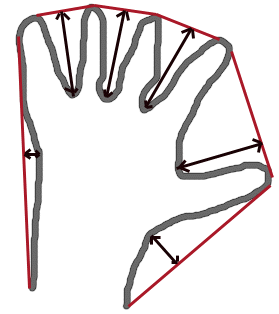
\includegraphics[width=0.5\textwidth]{pics/defects.png}

\cvCPyFunc{ContourArea}
Calculates the area of a whole contour or a contour section.

\cvdefC{
double cvContourArea( \par const CvArr* contour, \par CvSlice slice=CV\_WHOLE\_SEQ );
}\cvdefPy{ContourAres(contour,slice=CV\_WHOLE\_SEQ)-> double}

\begin{description}
\cvarg{contour}{Contour (sequence or array of vertices)}
\cvarg{slice}{Starting and ending points of the contour section of interest, by default, the area of the whole contour is calculated}
\end{description}

The function calculates the area of a whole contour
or a contour section. In the latter case the total area bounded by the
contour arc and the chord connecting the 2 selected points is calculated
as shown on the picture below:

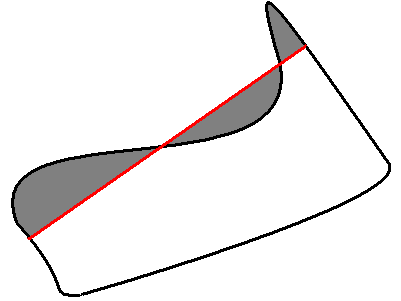
\includegraphics[width=0.5\textwidth]{pics/contoursecarea.png}

Orientation of the contour affects the area sign, thus the function may return a \emph{negative} result. Use the \texttt{fabs()} function from C runtime to get the absolute value of the area.

\cvCPyFunc{ContourFromContourTree}
Restores a contour from the tree.

\cvdefC{
CvSeq* cvContourFromContourTree( \par const CvContourTree* tree,\par CvMemStorage* storage,\par CvTermCriteria criteria );
}\cvdefPy{ContourFromContourTree(tree,storage,criteria)-> contour}

\begin{description}
\cvarg{tree}{Contour tree}
\cvarg{storage}{Container for the reconstructed contour}
\cvarg{criteria}{Criteria, where to stop reconstruction}
\end{description}

The function restores the contour from its binary tree representation. The parameter \texttt{criteria} determines the accuracy and/or the number of tree levels used for reconstruction, so it is possible to build an approximated contour. The function returns the reconstructed contour.

\cvCPyFunc{ConvexHull2}
Finds the convex hull of a point set.

\cvdefC{
CvSeq* cvConvexHull2( \par const CvArr* input,\par void* hull\_storage=NULL,\par int orientation=CV\_CLOCKWISE,\par int return\_points=0 );
}\cvdefPy{ConvexHull2(points,storage,orientaton=CV\_CLOCKWISE,return\_points=0)-> convex\_hull}

\begin{description}
\cvarg{points}{Sequence or array of 2D points with 32-bit integer or floating-point coordinates}
\cvarg{hull\_storage}{The destination array (CvMat*) or memory storage (CvMemStorage*) that will store the convex hull. If it is an array, it should be 1d and have the same number of elements as the input array/sequence. On output the header is modified as to truncate the array down to the hull size.  If \texttt{hull\_storage} is NULL then the convex hull will be stored in the same storage as the input sequence}
\cvarg{orientation}{Desired orientation of convex hull: \texttt{CV\_CLOCKWISE} or \texttt{CV\_COUNTER\_CLOCKWISE}}
\cvarg{return\_points}{If non-zero, the points themselves will be stored in the hull instead of indices if \texttt{hull\_storage} is an array, or pointers if \texttt{hull\_storage} is memory storage}
\end{description}

The function finds the convex hull of a 2D point set using Sklansky's algorithm. If \texttt{hull\_storage} is memory storage, the function creates a sequence containing the hull points or pointers to them, depending on \texttt{return\_points} value and returns the sequence on output.  If \texttt{hull\_storage} is a CvMat, the function returns NULL.

% ===== Example. Building convex hull for a sequence or array of points =====
\begin{lstlisting}
#include "cv.h"
#include "highgui.h"
#include <stdlib.h>

#define ARRAY  0 /* switch between array/sequence method by replacing 0<=>1 */

void main( int argc, char** argv )
{
    IplImage* img = cvCreateImage( cvSize( 500, 500 ), 8, 3 );
    cvNamedWindow( "hull", 1 );

#if !ARRAY
        CvMemStorage* storage = cvCreateMemStorage();
#endif

    for(;;)
    {
        int i, count = rand()%100 + 1, hullcount;
        CvPoint pt0;
#if !ARRAY
        CvSeq* ptseq = cvCreateSeq( CV_SEQ_KIND_GENERIC|CV_32SC2,
                                    sizeof(CvContour),
                                    sizeof(CvPoint),
                                    storage );
        CvSeq* hull;

        for( i = 0; i < count; i++ )
        {
            pt0.x = rand() % (img->width/2) + img->width/4;
            pt0.y = rand() % (img->height/2) + img->height/4;
            cvSeqPush( ptseq, &pt0 );
        }
        hull = cvConvexHull2( ptseq, 0, CV_CLOCKWISE, 0 );
        hullcount = hull->total;
#else
        CvPoint* points = (CvPoint*)malloc( count * sizeof(points[0]));
        int* hull = (int*)malloc( count * sizeof(hull[0]));
        CvMat point_mat = cvMat( 1, count, CV_32SC2, points );
        CvMat hull_mat = cvMat( 1, count, CV_32SC1, hull );

        for( i = 0; i < count; i++ )
        {
            pt0.x = rand() % (img->width/2) + img->width/4;
            pt0.y = rand() % (img->height/2) + img->height/4;
            points[i] = pt0;
        }
        cvConvexHull2( &point_mat, &hull_mat, CV_CLOCKWISE, 0 );
        hullcount = hull_mat.cols;
#endif
        cvZero( img );
        for( i = 0; i < count; i++ )
        {
#if !ARRAY
            pt0 = *CV_GET_SEQ_ELEM( CvPoint, ptseq, i );
#else
            pt0 = points[i];
#endif
            cvCircle( img, pt0, 2, CV_RGB( 255, 0, 0 ), CV_FILLED );
        }

#if !ARRAY
        pt0 = **CV_GET_SEQ_ELEM( CvPoint*, hull, hullcount - 1 );
#else
        pt0 = points[hull[hullcount-1]];
#endif

        for( i = 0; i < hullcount; i++ )
        {
#if !ARRAY
            CvPoint pt = **CV_GET_SEQ_ELEM( CvPoint*, hull, i );
#else
            CvPoint pt = points[hull[i]];
#endif
            cvLine( img, pt0, pt, CV_RGB( 0, 255, 0 ));
            pt0 = pt;
        }

        cvShowImage( "hull", img );

        int key = cvWaitKey(0);
        if( key == 27 ) // 'ESC'
            break;

#if !ARRAY
        cvClearMemStorage( storage );
#else
        free( points );
        free( hull );
#endif
    }
}
\end{lstlisting}

\cvCPyFunc{ConvexityDefects}
Finds the convexity defects of a contour.

\cvdefC{
CvSeq* cvConvexityDefects( \par const CvArr* contour,\par const CvArr* convexhull,\par CvMemStorage* storage=NULL );
}\cvdefPy{ConvexityDefects(contour,convexhull,storage)-> convexity\_defects}

\begin{description}
\cvarg{contour}{Input contour}
\cvarg{convexhull}{Convex hull obtained using \cvCPyCross{ConvexHull2} that should contain pointers or indices to the contour points, not the hull points themselves (the \texttt{return\_points} parameter in \cvCPyCross{ConvexHull2} should be 0)}
\cvarg{storage}{Container for the output sequence of convexity defects. If it is NULL, the contour or hull (in that order) storage is used}
\end{description}

The function finds all convexity defects of the input contour and returns a sequence of the CvConvexityDefect structures.

\cvCPyFunc{CreateContourTree}
Creates a hierarchical representation of a contour.

\cvdefC{
CvContourTree* cvCreateContourTree( \par const CvSeq* contour,\par CvMemStorage* storage,\par double threshold );
}\cvdefPy{CreateCountourTree(contour,storage,threshold)-> contour\_tree}

\begin{description}
\cvarg{contour}{Input contour}
\cvarg{storage}{Container for output tree}
\cvarg{threshold}{Approximation accuracy}
\end{description}

The function creates a binary tree representation for the input \texttt{contour} and returns the pointer to its root. If the parameter \texttt{threshold} is less than or equal to 0, the function creates a full binary tree representation. If the threshold is greater than 0, the function creates a representation with the precision \texttt{threshold}: if the vertices with the interceptive area of its base line are less than \texttt{threshold}, the tree should not be built any further. The function returns the created tree.

\cvCPyFunc{EndFindContours}
Finishes the scanning process.

\cvdefC{
CvSeq* cvEndFindContours( \par CvContourScanner* scanner );
}

\begin{description}
\cvarg{scanner}{Pointer to the contour scanner}
\end{description}

The function finishes the scanning process and returns a pointer to the first contour on the highest level.

\cvCPyFunc{FindContours}
Finds the contours in a binary image.

\cvdefC{
int cvFindContours(\par CvArr* image,\par CvMemStorage* storage,\par CvSeq** first\_contour,\par
                    int header\_size=sizeof(CvContour),\par int mode=CV\_RETR\_LIST,\par
                    int method=CV\_CHAIN\_APPROX\_SIMPLE,\par CvPoint offset=cvPoint(0,0) );
}\cvdefPy{FindContours(image, storage, mode=CV\_RETR\_LIST, method=CV\_CHAIN\_APPROX\_SIMPLE, offset=(0,0)) -> cvseq}

\begin{description}
\cvarg{image}{The source, an 8-bit single channel image. Non-zero pixels are treated as 1's, zero pixels remain 0's - the image is treated as \texttt{binary}. To get such a binary image from grayscale, one may use \cvCPyCross{Threshold}, \cvCPyCross{AdaptiveThreshold} or \cvCPyCross{Canny}. The function modifies the source image's content}
\cvarg{storage}{Container of the retrieved contours}
\cvarg{first\_contour}{Output parameter, will contain the pointer to the first outer contour}
\cvarg{header\_size}{Size of the sequence header, $\ge \texttt{sizeof(CvChain)}$ if $\texttt{method} =\texttt{CV\_CHAIN\_CODE}$,
and $\ge \texttt{sizeof(CvContour)}$ otherwise}
\cvarg{mode}{Retrieval mode
\begin{description}
  \cvarg{CV\_RETR\_EXTERNAL}{retrives only the extreme outer contours}
  \cvarg{CV\_RETR\_LIST}{retrieves all of the contours and puts them in the list}
  \cvarg{CV\_RETR\_CCOMP}{retrieves all of the contours and organizes them into a two-level hierarchy: on the top level are the external boundaries of the components, on the second level are the boundaries of the holes}
  \cvarg{CV\_RETR\_TREE}{retrieves all of the contours and reconstructs the full hierarchy of nested contours}
\end{description}}
\cvarg{method}{Approximation method (for all the modes, except \texttt{CV\_LINK\_RUNS}, which uses built-in approximation)
\begin{description}
  \cvarg{CV\_CHAIN\_CODE}{outputs contours in the Freeman chain code. All other methods output polygons (sequences of vertices)}
  \cvarg{CV\_CHAIN\_APPROX\_NONE}{translates all of the points from the chain code into points}
  \cvarg{CV\_CHAIN\_APPROX\_SIMPLE}{compresses horizontal, vertical, and diagonal segments and leaves only their end points}
  \cvarg{CV\_CHAIN\_APPROX\_TC89\_L1,CV\_CHAIN\_APPROX\_TC89\_KCOS}{applies one of the flavors of the Teh-Chin chain approximation algorithm.}
  \cvarg{CV\_LINK\_RUNS}{uses a completely different contour retrieval algorithm by linking horizontal segments of 1's. Only the \texttt{CV\_RETR\_LIST} retrieval mode can be used with this method.}
\end{description}}
\cvarg{offset}{Offset, by which every contour point is shifted. This is useful if the contours are extracted from the image ROI and then they should be analyzed in the whole image context}
\end{description}

The function retrieves contours from the
binary image and returns the number of retrieved contours. The
pointer \texttt{first\_contour} is filled by the function. It will
contain a pointer to the first outermost contour or \texttt{NULL} if no
contours are detected (if the image is completely black). Other
contours may be reached from \texttt{first\_contour} using the
\texttt{h\_next} and \texttt{v\_next} links. The sample in the
\cvCPyCross{DrawContours} discussion shows how to use contours for
connected component detection. Contours can be also used for shape
analysis and object recognition - see \texttt{squares.c} in the OpenCV
sample directory.


\cvCPyFunc{FindNextContour}
Finds the next contour in the image.

\cvdefC{
CvSeq* cvFindNextContour( \par CvContourScanner scanner );
}

\begin{description}
\cvarg{scanner}{Contour scanner initialized by \cvCPyCross{StartFindContours} }
\end{description}

The function locates and retrieves the next contour in the image and returns a pointer to it. The function returns NULL if there are no more contours.

\cvCPyFunc{FitEllipse}
Fits an ellipse around a set of 2D points.

\cvdefC{
CvBox2D cvFitEllipse2( \par const CvArr* points );
}\cvdefPy{FitEllipse2(points)-> Box2D}

\begin{description}
\cvarg{points}{Sequence or array of points}
\end{description}

The function calculates the ellipse that fits best
(in least-squares sense) around a set of 2D points. The meaning of the
returned structure fields is similar to those in \cvCPyCross{Ellipse} except
that \texttt{size} stores the full lengths of the ellipse axises,
not half-lengths.

\cvCPyFunc{FitLine}
Fits a line to a 2D or 3D point set.

\cvdefC{
void  cvFitLine( \par const CvArr* points,\par int dist\_type,\par double param,\par double reps,\par double aeps,\par float* line );
}\cvdefPy{FitLine(points, dist\_type, param, reps, aeps) -> line}

\begin{description}
\cvarg{points}{Sequence or array of 2D or 3D points with 32-bit integer or floating-point coordinates}
\cvarg{dist\_type}{The distance used for fitting (see the discussion)}
\cvarg{param}{Numerical parameter (\texttt{C}) for some types of distances, if 0 then some optimal value is chosen}
\cvarg{reps, aeps}{Sufficient accuracy for the radius (distance between the coordinate origin and the line) and angle, respectively; 0.01 would be a good default value for both.}
\cvarg{line}{The output line parameters. In the case of a 2d fitting,
it is \cvC{an array} \cvPy{a tuple} of 4 floats \texttt{(vx, vy,
x0, y0)} where \texttt{(vx, vy)} is a normalized vector collinear to the
line and \texttt{(x0, y0)} is some point on the line. in the case of a
3D fitting it is \cvC{an array} \cvPy{a tuple} of 6 floats \texttt{(vx, vy, vz, x0, y0, z0)}
where \texttt{(vx, vy, vz)} is a normalized vector collinear to the line
and \texttt{(x0, y0, z0)} is some point on the line}
\end{description}

The function fits a line to a 2D or 3D point set by minimizing $\sum_i \rho(r_i)$ where $r_i$ is the distance between the $i$ th point and the line and $\rho(r)$ is a distance function, one of:

\begin{description}

\item[dist\_type=CV\_DIST\_L2]
\[ \rho(r) = r^2/2 \quad \text{(the simplest and the fastest least-squares method)} \]

\item[dist\_type=CV\_DIST\_L1]
\[ \rho(r) = r \]

\item[dist\_type=CV\_DIST\_L12]
\[ \rho(r) = 2 \cdot (\sqrt{1 + \frac{r^2}{2}} - 1) \]

\item[dist\_type=CV\_DIST\_FAIR]
\[ \rho\left(r\right) = C^2 \cdot \left( \frac{r}{C} - \log{\left(1 + \frac{r}{C}\right)}\right) \quad \text{where} \quad C=1.3998 \]

\item[dist\_type=CV\_DIST\_WELSCH]
\[ \rho\left(r\right) = \frac{C^2}{2} \cdot \left( 1 - \exp{\left(-\left(\frac{r}{C}\right)^2\right)}\right) \quad \text{where} \quad C=2.9846 \]

\item[dist\_type=CV\_DIST\_HUBER]
\[ \rho(r) = \fork
{r^2/2}{if $r < C$}
{C \cdot (r-C/2)}{otherwise}  \quad \text{where} \quad C=1.345
\]
\end{description}

\cvCPyFunc{GetCentralMoment}
Retrieves the central moment from the moment state structure.

\cvdefC{
double cvGetCentralMoment( \par CvMoments* moments,\par int x\_order,\par int y\_order );
}\cvdefPy{GetCentralMoment(cvmoments, x\_order, y\_order) -> double}

\begin{description}
\cvarg{moments}{Pointer to the moment state structure}
\cvarg{x\_order}{x order of the retrieved moment, $\texttt{x\_order} >= 0$}
\cvarg{y\_order}{y order of the retrieved moment, $\texttt{y\_order} >= 0$ and $\texttt{x\_order} + \texttt{y\_order} <= 3$}
\end{description}

The function retrieves the central moment, which in the case of image moments is defined as:

\[
\mu_{x\_order, \, y\_order} = \sum_{x,y} (I(x,y) \cdot (x-x_c)^{x\_order} \cdot (y-y_c)^{y\_order})
\]

where $x_c,y_c$ are the coordinates of the gravity center:

\[
x_c=\frac{M_{10}}{M_{00}}, y_c=\frac{M_{01}}{M_{00}}
\]

\cvCPyFunc{GetHuMoments}
Calculates the seven Hu invariants.

\cvdefC{void cvGetHuMoments( const CvMoments* moments,CvHuMoments* hu );}
\begin{description}
\cvarg{moments}{The input moments, computed with \cvCPyCross{Moments}}
\cvarg{hu}{The output Hu invariants}
\end{description}

The function calculates the seven Hu invariants, see \url{http://en.wikipedia.org/wiki/Image_moment}, that are defined as:

\[ \begin{array}{l}
hu_1=\eta_{20}+\eta_{02}\\
hu_2=(\eta_{20}-\eta_{02})^{2}+4\eta_{11}^{2}\\
hu_3=(\eta_{30}-3\eta_{12})^{2}+ (3\eta_{21}-\eta_{03})^{2}\\
hu_4=(\eta_{30}+\eta_{12})^{2}+ (\eta_{21}+\eta_{03})^{2}\\
hu_5=(\eta_{30}-3\eta_{12})(\eta_{30}+\eta_{12})[(\eta_{30}+\eta_{12})^{2}-3(\eta_{21}+\eta_{03})^{2}]+(3\eta_{21}-\eta_{03})(\eta_{21}+\eta_{03})[3(\eta_{30}+\eta_{12})^{2}-(\eta_{21}+\eta_{03})^{2}]\\
hu_6=(\eta_{20}-\eta_{02})[(\eta_{30}+\eta_{12})^{2}- (\eta_{21}+\eta_{03})^{2}]+4\eta_{11}(\eta_{30}+\eta_{12})(\eta_{21}+\eta_{03})\\
hu_7=(3\eta_{21}-\eta_{03})(\eta_{21}+\eta_{03})[3(\eta_{30}+\eta_{12})^{2}-(\eta_{21}+\eta_{03})^{2}]-(\eta_{30}-3\eta_{12})(\eta_{21}+\eta_{03})[3(\eta_{30}+\eta_{12})^{2}-(\eta_{21}+\eta_{03})^{2}]\\
\end{array}
\]

where $\eta_{ji}$ denote the normalized central moments.

These values are proved to be invariant to the image scale, rotation, and reflection except the seventh one, whose sign is changed by reflection. Of course, this invariance was proved with the assumption of infinite image resolution. In case of a raster images the computed Hu invariants for the original and transformed images will be a bit different.


\cvCPyFunc{GetNormalizedCentralMoment}
Retrieves the normalized central moment from the moment state structure.

\cvdefC{
double cvGetNormalizedCentralMoment( \par CvMoments* moments,\par int x\_order,\par int y\_order );
}\cvdefPy{GetNormalizedCentralMoment(cvmoments, x\_order, y\_order) -> double}

\begin{description}
\cvarg{moments}{Pointer to the moment state structure}
\cvarg{x\_order}{x order of the retrieved moment, $\texttt{x\_order} >= 0$}
\cvarg{y\_order}{y order of the retrieved moment, $\texttt{y\_order} >= 0$ and $\texttt{x\_order} + \texttt{y\_order} <= 3$}
\end{description}

The function retrieves the normalized central moment:

\[
\eta_{x\_order, \, y\_order} = \frac{\mu_{x\_order, \, y\_order}}{M_{00}^{(y\_order+x\_order)/2+1}}
\]

\cvCPyFunc{GetSpatialMoment}
Retrieves the spatial moment from the moment state structure.

\cvdefC{
double cvGetSpatialMoment( \par CvMoments* moments, \par int x\_order, \par int y\_order );
}\cvdefPy{GetSpatialMoment(cvmoments, x\_order, y\_order) -> double}

\begin{description}
\cvarg{moments}{The moment state, calculated by \cvCPyCross{Moments}}
\cvarg{x\_order}{x order of the retrieved moment, $\texttt{x\_order} >= 0$}
\cvarg{y\_order}{y order of the retrieved moment, $\texttt{y\_order} >= 0$ and $\texttt{x\_order} + \texttt{y\_order} <= 3$}
\end{description}

The function retrieves the spatial moment, which in the case of image moments is defined as:

\[
M_{x\_order, \, y\_order} = \sum_{x,y} (I(x,y) \cdot x^{x\_order} \cdot y^{y\_order})
\]

where $I(x,y)$ is the intensity of the pixel $(x, y)$.

\cvCPyFunc{MatchContourTrees}
Compares two contours using their tree representations.

\cvdefC{
double cvMatchContourTrees( \par const CvContourTree* tree1,\par const CvContourTree* tree2,\par int method,\par double threshold );
}\cvdefPy{MatchContourTrees(tree1,tree2,method,threshold)-> double}

\begin{description}
\cvarg{tree1}{First contour tree}
\cvarg{tree2}{Second contour tree}
\cvarg{method}{Similarity measure, only \texttt{CV\_CONTOUR\_TREES\_MATCH\_I1} is supported}
\cvarg{threshold}{Similarity threshold}
\end{description}

The function calculates the value of the matching measure for two contour trees. The similarity measure is calculated level by level from the binary tree roots. If at a certain level the difference between contours becomes less than \texttt{threshold}, the reconstruction process is interrupted and the current difference is returned.

\cvCPyFunc{MatchShapes}
Compares two shapes.

\cvdefC{
double cvMatchShapes( \par const void* object1,\par const void* object2,\par int method,\par double parameter=0 );
}\cvdefPy{MatchShapes(object1,object2,method,parameter=0)-> None}

\begin{description}
\cvarg{object1}{First contour or grayscale image}
\cvarg{object2}{Second contour or grayscale image}
\cvarg{method}{Comparison method;
 \texttt{CV\_CONTOUR\_MATCH\_I1}, 
 \texttt{CV\_CONTOURS\_MATCH\_I2} 
or 
 \texttt{CV\_CONTOURS\_MATCH\_I3}}
\cvarg{parameter}{Method-specific parameter (is not used now)}
\end{description}

The function compares two shapes. The 3 implemented methods all use Hu moments (see \cvCPyCross{GetHuMoments}) ($A$ is \texttt{object1}, $B$ is \texttt{object2}):

\begin{description}
\item[method=CV\_CONTOUR\_MATCH\_I1]
\[ I_1(A,B) = \sum_{i=1...7} \left| \frac{1}{m^A_i} - \frac{1}{m^B_i} \right| \]

\item[method=CV\_CONTOUR\_MATCH\_I2]
\[ I_2(A,B) = \sum_{i=1...7} \left| m^A_i - m^B_i \right| \]

\item[method=CV\_CONTOUR\_MATCH\_I3]
\[ I_3(A,B) = \sum_{i=1...7} \frac{ \left| m^A_i - m^B_i \right| }{ \left| m^A_i \right| } \]
\end{description}

where

\[
\begin{array}{l}
m^A_i = sign(h^A_i) \cdot \log{h^A_i}
m^B_i = sign(h^B_i) \cdot \log{h^B_i}
\end{array}
\]

and $h^A_i, h^B_i$ are the Hu moments of $A$ and $B$ respectively.


\cvCPyFunc{MinAreaRect2}
Finds the circumscribed rectangle of minimal area for a given 2D point set.

\cvdefC{
CvBox2D  cvMinAreaRect2( \par const CvArr* points,\par CvMemStorage* storage=NULL );
}\cvdefPy{MinAreaRect2(points,storage)-> CvBox2D}

\begin{description}
\cvarg{points}{Sequence or array of points}
\cvarg{storage}{Optional temporary memory storage}
\end{description}

The function finds a circumscribed rectangle of the minimal area for a 2D point set by building a convex hull for the set and applying the rotating calipers technique to the hull.

\cvfunc{Picture. Minimal-area bounding rectangle for contour}

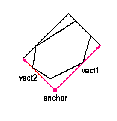
\includegraphics[width=0.5\textwidth]{pics/minareabox.png}

\cvCPyFunc{MinEnclosingCircle}
Finds the circumscribed circle of minimal area for a given 2D point set.

\cvdefC{
int cvMinEnclosingCircle( \par const CvArr* points,\par CvPoint2D32f* center,\par float* radius );
}\cvdefPy{MinEnclosingCircle(points)-> int,center,radius}

\begin{description}
\cvarg{points}{Sequence or array of 2D points}
\cvarg{center}{Output parameter; the center of the enclosing circle}
\cvarg{radius}{Output parameter; the radius of the enclosing circle}
\end{description}

The function finds the minimal circumscribed
circle for a 2D point set using an iterative algorithm. It returns nonzero
if the resultant circle contains all the input points and zero otherwise
(i.e. the algorithm failed).

\cvCPyFunc{Moments}
Calculates all of the moments up to the third order of a polygon or rasterized shape.

\cvdefC{
void cvMoments( \par const CvArr* arr,\par CvMoments* moments,\par int binary=0 );
}\cvdefPy{Moments(arr) -> cvmoments}

\begin{description}
\cvarg{arr}{Image (1-channel or 3-channel with COI set) or polygon (CvSeq of points or a vector of points)}
\cvarg{moments}{Pointer to returned moment's state structure}
\cvarg{binary}{(For images only) If the flag is non-zero, all of the zero pixel values are treated as zeroes, and all of the others are treated as 1's}
\end{description}

The function calculates spatial and central moments up to the third order and writes them to \texttt{moments}. The moments may then be used then to calculate the gravity center of the shape, its area, main axises and various shape characeteristics including 7 Hu invariants.

\cvCPyFunc{PointPolygonTest}
Point in contour test.

\cvdefC{
double cvPointPolygonTest( \par const CvArr* contour,\par CvPoint2D32f pt,\par int measure\_dist );
}\cvdefPy{PointPolygonTest(contour,pt,measure\_dist)-> double}

\begin{description}
\cvarg{contour}{Input contour}
\cvarg{pt}{The point tested against the contour}
\cvarg{measure\_dist}{If it is non-zero, the function estimates the distance from the point to the nearest contour edge}
\end{description}

The function determines whether the
point is inside a contour, outside, or lies on an edge (or coinsides
with a vertex). It returns positive, negative or zero value,
correspondingly. When $\texttt{measure\_dist} =0$, the return value
is +1, -1 and 0, respectively. When $\texttt{measure\_dist} \ne 0$,
it is a signed distance between the point and the nearest contour
edge.

Here is the sample output of the function, where each image pixel is tested against the contour.

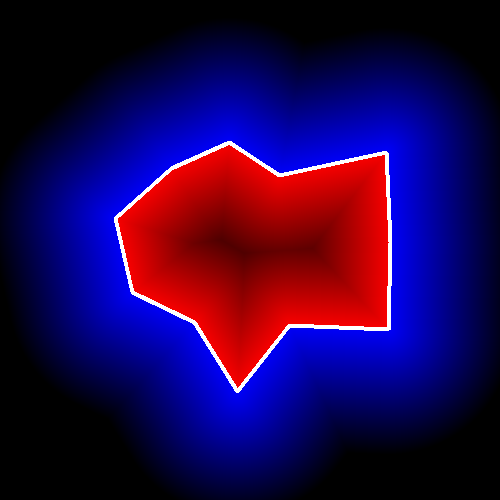
\includegraphics[width=0.5\textwidth]{pics/pointpolygon.png}

\ifC

\cvCPyFunc{PointSeqFromMat}
Initializes a point sequence header from a point vector.

\cvdefC{
CvSeq* cvPointSeqFromMat( \par int seq\_kind,\par const CvArr* mat,\par CvContour* contour\_header,\par CvSeqBlock* block );
}

\begin{description}
\cvarg{seq\_kind}{Type of the point sequence: point set (0), a curve (\texttt{CV\_SEQ\_KIND\_CURVE}), closed curve (\texttt{CV\_SEQ\_KIND\_CURVE+CV\_SEQ\_FLAG\_CLOSED}) etc.}
\cvarg{mat}{Input matrix. It should be a continuous, 1-dimensional vector of points, that is, it should have type \texttt{CV\_32SC2} or \texttt{CV\_32FC2}}
\cvarg{contour\_header}{Contour header, initialized by the function}
\cvarg{block}{Sequence block header, initialized by the function}
\end{description}

The function initializes a sequence
header to create a "virtual" sequence in which elements reside in
the specified matrix. No data is copied. The initialized sequence
header may be passed to any function that takes a point sequence
on input. No extra elements can be added to the sequence,
but some may be removed. The function is a specialized variant of
\cvCPyCross{MakeSeqHeaderForArray} and uses
the latter internally. It returns a pointer to the initialized contour
header. Note that the bounding rectangle (field \texttt{rect} of
\texttt{CvContour} strucuture) is not initialized by the function. If
you need one, use \cvCPyCross{BoundingRect}.

Here is a simple usage example.

\begin{lstlisting}
CvContour header;
CvSeqBlock block;
CvMat* vector = cvCreateMat( 1, 3, CV_32SC2 );

CV_MAT_ELEM( *vector, CvPoint, 0, 0 ) = cvPoint(100,100);
CV_MAT_ELEM( *vector, CvPoint, 0, 1 ) = cvPoint(100,200);
CV_MAT_ELEM( *vector, CvPoint, 0, 2 ) = cvPoint(200,100);

IplImage* img = cvCreateImage( cvSize(300,300), 8, 3 );
cvZero(img);

cvDrawContours( img,
    cvPointSeqFromMat(CV_SEQ_KIND_CURVE+CV_SEQ_FLAG_CLOSED,
                      vector,
                      &header,
                      &block),
                CV_RGB(255,0,0),
                CV_RGB(255,0,0),
                0, 3, 8, cvPoint(0,0));
\end{lstlisting}


\cvCPyFunc{ReadChainPoint}
Gets the next chain point.

\cvdefC{
CvPoint cvReadChainPoint( CvChainPtReader* reader );
}

\begin{description}
\cvarg{reader}{Chain reader state}
\end{description}

The function returns the current chain point and updates the reader position.

\cvCPyFunc{StartFindContours}
Initializes the contour scanning process.

\cvdefC{
CvContourScanner cvStartFindContours(\par CvArr* image,\par CvMemStorage* storage,\par
                                      int header\_size=sizeof(CvContour),\par
                                      int mode=CV\_RETR\_LIST,\par
                                      int method=CV\_CHAIN\_APPROX\_SIMPLE,\par
                                      CvPoint offset=cvPoint(0,\par0) );
}

\begin{description}
\cvarg{image}{The 8-bit, single channel, binary source image}
\cvarg{storage}{Container of the retrieved contours}
\cvarg{header\_size}{Size of the sequence header, $>=sizeof(CvChain)$ if \texttt{method} =CV\_CHAIN\_CODE, and $>=sizeof(CvContour)$ otherwise}
\cvarg{mode}{Retrieval mode; see \cvCPyCross{FindContours}}
\cvarg{method}{Approximation method. It has the same meaning in \cvCPyCross{FindContours}, but \texttt{CV\_LINK\_RUNS} can not be used here}
\cvarg{offset}{ROI offset; see \cvCPyCross{FindContours}}
\end{description}

The function initializes and returns a pointer to the contour scanner. The scanner is used in \cvCPyCross{FindNextContour} to retrieve the rest of the contours.

\cvCPyFunc{StartReadChainPoints}
Initializes the chain reader.

\cvdefC{
void cvStartReadChainPoints( CvChain* chain, CvChainPtReader* reader );
}

The function initializes a special reader.

\cvCPyFunc{SubstituteContour}
Replaces a retrieved contour.

\cvdefC{
void cvSubstituteContour( \par CvContourScanner scanner, \par CvSeq* new\_contour );
}

\begin{description}
\cvarg{scanner}{Contour scanner initialized by \cvCPyCross{StartFindContours} }
\cvarg{new\_contour}{Substituting contour}
\end{description}

The function replaces the retrieved
contour, that was returned from the preceding call of
\cvCPyCross{FindNextContour} and stored inside the contour scanner
state, with the user-specified contour. The contour is inserted
into the resulting structure, list, two-level hierarchy, or tree,
depending on the retrieval mode. If the parameter \texttt{new\_contour}
is \texttt{NULL}, the retrieved contour is not included in the
resulting structure, nor are any of its children that might be added
to this structure later.

\fi

\fi


\ifCpp

\cvCppFunc{moments}
Calculates all of the moments up to the third order of a polygon or rasterized shape.

\cvdefCpp{Moments moments( const Mat\& array, bool binaryImage=false );}

where the class \texttt{Moments} is defined as:
\begin{lstlisting}
class Moments
{
public:
    Moments();
    Moments(double m00, double m10, double m01, double m20, double m11,
            double m02, double m30, double m21, double m12, double m03 );
    Moments( const CvMoments\& moments );
    operator CvMoments() const;
    
    // spatial moments
    double  m00, m10, m01, m20, m11, m02, m30, m21, m12, m03;
    // central moments
    double  mu20, mu11, mu02, mu30, mu21, mu12, mu03;
    // central normalized moments
    double  nu20, nu11, nu02, nu30, nu21, nu12, nu03;
};
\end{lstlisting}

\begin{description}
\cvarg{array}{A raster image (single-channel, 8-bit or floating-point 2D array) or an array
    ($1 \times N$ or $N \times 1$) of 2D points (\texttt{Point} or \texttt{Point2f})}
\cvarg{binaryImage}{(For images only) If it is true, then all the non-zero image pixels are treated as 1's}
\end{description}

The function computes moments, up to the 3rd order, of a vector shape or a rasterized shape.
In case of a raster image, the spatial moments $\texttt{Moments::m}_{ji}$ are computed as:

\[\texttt{m}_{ji}=\sum_{x,y} \left(\texttt{array}(x,y) \cdot x^j \cdot y^i\right),\]

the central moments $\texttt{Moments::mu}_{ji}$ are computed as:
\[\texttt{mu}_{ji}=\sum_{x,y} \left(\texttt{array}(x,y) \cdot (x - \bar{x})^j \cdot (y - \bar{y})^i\right)\]
where $(\bar{x}, \bar{y})$ is the mass center:

\[
\bar{x}=\frac{\texttt{m}_{10}}{\texttt{m}_{00}},\; \bar{y}=\frac{\texttt{m}_{01}}{\texttt{m}_{00}}
\]

and the normalized central moments $\texttt{Moments::nu}_{ij}$ are computed as:
\[\texttt{nu}_{ji}=\frac{\texttt{mu}_{ji}}{\texttt{m}_{00}^{(i+j)/2+1}}.\]

Note that $\texttt{mu}_{00}=\texttt{m}_{00}$, $\texttt{nu}_{00}=1$ $\texttt{nu}_{10}=\texttt{mu}_{10}=\texttt{mu}_{01}=\texttt{mu}_{10}=0$, hence the values are not stored.

The moments of a contour are defined in the same way, but computed using Green's formula
(see \url{http://en.wikipedia.org/wiki/Green_theorem}), therefore, because of a limited raster resolution, the moments computed for a contour will be slightly different from the moments computed for the same contour rasterized.

See also: \cvCppCross{contourArea}, \cvCppCross{arcLength}

\cvCppFunc{HuMoments}
Calculates the seven Hu invariants.

\cvdefCpp{void HuMoments( const Moments\& moments, double h[7] );}
\begin{description}
\cvarg{moments}{The input moments, computed with \cvCppCross{moments}}
\cvarg{h}{The output Hu invariants}
\end{description}

The function calculates the seven Hu invariants, see \url{http://en.wikipedia.org/wiki/Image_moment}, that are defined as:

\[ \begin{array}{l}
h[0]=\eta_{20}+\eta_{02}\\
h[1]=(\eta_{20}-\eta_{02})^{2}+4\eta_{11}^{2}\\
h[2]=(\eta_{30}-3\eta_{12})^{2}+ (3\eta_{21}-\eta_{03})^{2}\\
h[3]=(\eta_{30}+\eta_{12})^{2}+ (\eta_{21}+\eta_{03})^{2}\\
h[4]=(\eta_{30}-3\eta_{12})(\eta_{30}+\eta_{12})[(\eta_{30}+\eta_{12})^{2}-3(\eta_{21}+\eta_{03})^{2}]+(3\eta_{21}-\eta_{03})(\eta_{21}+\eta_{03})[3(\eta_{30}+\eta_{12})^{2}-(\eta_{21}+\eta_{03})^{2}]\\
h[5]=(\eta_{20}-\eta_{02})[(\eta_{30}+\eta_{12})^{2}- (\eta_{21}+\eta_{03})^{2}]+4\eta_{11}(\eta_{30}+\eta_{12})(\eta_{21}+\eta_{03})\\
h[6]=(3\eta_{21}-\eta_{03})(\eta_{21}+\eta_{03})[3(\eta_{30}+\eta_{12})^{2}-(\eta_{21}+\eta_{03})^{2}]-(\eta_{30}-3\eta_{12})(\eta_{21}+\eta_{03})[3(\eta_{30}+\eta_{12})^{2}-(\eta_{21}+\eta_{03})^{2}]\\
\end{array}
\]

where $\eta_{ji}$ stand for $\texttt{Moments::nu}_{ji}$.

These values are proved to be invariant to the image scale, rotation, and reflection except the seventh one, whose sign is changed by reflection. Of course, this invariance was proved with the assumption of infinite image resolution. In case of a raster images the computed Hu invariants for the original and transformed images will be a bit different.

See also: \cvCppCross{matchShapes}

\cvCppFunc{findContours}
Finds the contours in a binary image.

\cvdefCpp{void findContours( const Mat\& image, vector<vector<Point> >\& contours,\par
                   vector<Vec4i>\& hierarchy, int mode,\par
                   int method, Point offset=Point());\newline
void findContours( const Mat\& image, vector<vector<Point> >\& contours,\par
                   int mode, int method, Point offset=Point());
}
\begin{description}
\cvarg{image}{The source, an 8-bit single-channel image. Non-zero pixels are treated as 1's, zero pixels remain 0's - the image is treated as \texttt{binary}. You can use \cvCppCross{compare}, \cvCppCross{inRange}, \cvCppCross{threshold}, \cvCppCross{adaptiveThreshold}, \cvCppCross{Canny} etc. to create a binary image out of a grayscale or color one. The function modifies the \texttt{image} while extracting the contours}
\cvarg{contours}{The detected contours. Each contour is stored as a vector of points}
\cvarg{hiararchy}{The optional output vector that will contain information about the image topology. It will have as many elements as the number of contours. For each contour \texttt{contours[i]}, the elements \texttt{hierarchy[i][0]}, \texttt{hiearchy[i][1]}, \texttt{hiearchy[i][2]}, \texttt{hiearchy[i][3]} will be set to 0-based indices in \texttt{contours} of the next and previous contours at the same hierarchical level, the first child contour and the parent contour, respectively. If for some contour \texttt{i} there is no next, previous, parent or nested contours, the corresponding elements of \texttt{hierarchy[i]} will be negative}
\cvarg{mode}{The contour retrieval mode
\begin{description}
  \cvarg{CV\_RETR\_EXTERNAL}{retrieves only the extreme outer contours; It will set \texttt{hierarchy[i][2]=hierarchy[i][3]=-1} for all the contours}
  \cvarg{CV\_RETR\_LIST}{retrieves all of the contours without establishing any hierarchical relationships}
  \cvarg{CV\_RETR\_CCOMP}{retrieves all of the contours and organizes them into a two-level hierarchy: on the top level are the external boundaries of the components, on the second level are the boundaries of the holes. If inside a hole of a connected component there is another contour, it will still be put on the top level}
  \cvarg{CV\_RETR\_TREE}{retrieves all of the contours and reconstructs the full hierarchy of nested contours. This full hierarchy is built and shown in OpenCV \texttt{contours.c} demo}
\end{description}}
\cvarg{method}{The contour approximation method.
\begin{description}
  \cvarg{CV\_CHAIN\_APPROX\_NONE}{stores absolutely all the contour points. That is, every 2 points of a contour stored with this method are 8-connected neighbors of each other}
  \cvarg{CV\_CHAIN\_APPROX\_SIMPLE}{compresses horizontal, vertical, and diagonal segments and leaves only their end points. E.g. an up-right rectangular contour will be encoded with 4 points}
  \cvarg{CV\_CHAIN\_APPROX\_TC89\_L1,CV\_CHAIN\_APPROX\_TC89\_KCOS}{applies one of the flavors of the Teh-Chin chain approximation algorithm; see \cite{TehChin89}}
\end{description}}
\cvarg{offset}{The optional offset, by which every contour point is shifted. This is useful if the contours are extracted from the image ROI and then they should be analyzed in the whole image context}
\end{description}

The function retrieves contours from the
binary image using the algorithm \cite{Suzuki85}. The contours are a useful tool for shape analysis and object detection and recognition. See \texttt{squares.c} in the OpenCV sample directory.

\cvCppFunc{drawContours}
Draws contours' outlines or filled contours.

\cvdefCpp{void drawContours( Mat\& image, const vector<vector<Point> >\& contours,\par
                   int contourIdx, const Scalar\& color, int thickness=1,\par
                   int lineType=8, const vector<Vec4i>\& hierarchy=vector<Vec4i>(),\par
                   int maxLevel=INT\_MAX, Point offset=Point() );}
\begin{description}
\cvarg{image}{The destination image}
\cvarg{contours}{All the input contours. Each contour is stored as a point vector}
\cvarg{contourIdx}{Indicates the contour to draw. If it is negative, all the contours are drawn}
\cvarg{color}{The contours' color}
\cvarg{thickness}{Thickness of lines the contours are drawn with.
If it is negative (e.g. \texttt{thickness=CV\_FILLED}), the contour interiors are
drawn.}
\cvarg{lineType}{The line connectivity; see \cvCppCross{line} description}
\cvarg{hierarchy}{The optional information about hierarchy. It is only needed if you want to draw only some of the  contours (see \texttt{maxLevel})}
\cvarg{maxLevel}{Maximal level for drawn contours. If 0, only
the specified contour is drawn. If 1, the function draws the contour(s) and all the nested contours. If 2, the function draws the contours, all the nested contours and all the nested into nested contours etc. This parameter is only taken into account when there is \texttt{hierarchy} available.}
\cvarg{offset}{The optional contour shift parameter. Shift all the drawn contours by the specified $\texttt{offset}=(dx,dy)$}
\end{description}

The function draws contour outlines in the image if $\texttt{thickness} \ge 0$ or fills the area bounded by the contours if $ \texttt{thickness}<0$. Here is the example on how to retrieve connected components from the binary image and label them

\begin{lstlisting}
#include "cv.h"
#include "highgui.h"

using namespace cv;

int main( int argc, char** argv )
{
    Mat src;
    // the first command line parameter must be file name of binary 
    // (black-n-white) image
    if( argc != 2 || !(src=imread(argv[1], 0)).data)
        return -1;

    Mat dst = Mat::zeros(src.rows, src.cols, CV_8UC3);

    src = src > 1;
    namedWindow( "Source", 1 );
    imshow( "Source", src );

    vector<vector<Point> > contours;
    vector<Vec4i> hierarchy;
    
    findContours( src, contours, hierarchy, 
        CV_RETR_CCOMP, CV_CHAIN_APPROX_SIMPLE );

    // iterate through all the top-level contours,
    // draw each connected component with its own random color
    int idx = 0;
    for( ; idx >= 0; idx = hiearchy[idx][0] )
    {
        Scalar color( rand()&255, rand()&255, rand()&255 );
        drawContours( dst, contours, idx, color, CV_FILLED, 8, hiearchy );
    }

    namedWindow( "Components", 1 );
    imshow( "Components", dst );
    waitKey(0);
}
\end{lstlisting}


\cvCppFunc{approxPolyDP}
Approximates polygonal curve(s) with the specified precision.

\cvdefCpp{void approxPolyDP( const Mat\& curve,\par
                   vector<Point>\& approxCurve,\par
                   double epsilon, bool closed );\newline
void approxPolyDP( const Mat\& curve,\par
                   vector<Point2f>\& approxCurve,\par
                   double epsilon, bool closed );}
\begin{description}
\cvarg{curve}{The polygon or curve to approximate. Must be $1 \times N$ or $N \times 1$ matrix of type \texttt{CV\_32SC2} or \texttt{CV\_32FC2}. You can also pass \texttt{vector<Point>} or \texttt{vector<Point2f} that will be automatically converted to the matrix of the proper size and type}
\cvarg{approxCurve}{The result of the approximation; The type should match the type of the input curve}
\cvarg{epsilon}{Specifies the approximation accuracy. This is the maximum distance between the original curve and its approximation}
\cvarg{closed}{If true, the approximated curve is closed (i.e. its first and last vertices are connected), otherwise it's not}
\end{description}

The functions \texttt{approxPolyDP} approximate a curve or a polygon with another curve/polygon with less vertices, so that the distance between them is less or equal to the specified precision. It used Douglas-Peucker algorithm \url{http://en.wikipedia.org/wiki/Ramer-Douglas-Peucker_algorithm}

\cvCppFunc{arcLength}
Calculates a contour perimeter or a curve length.

\cvdefCpp{double arcLength( const Mat\& curve, bool closed );}
\begin{description}
\cvarg{curve}{The input vector of 2D points, represented by \texttt{CV\_32SC2} or \texttt{CV\_32FC2} matrix or by \texttt{vector<Point>} or \texttt{vector<Point2f>}}
\cvarg{closed}{Indicates, whether the curve is closed or not}
\end{description}

The function computes the curve length or the closed contour perimeter.

\cvCppFunc{boundingRect}
Calculates the up-right bounding rectangle of a point set.

\cvdefCpp{Rect boundingRect( const Mat\& points );}
\begin{description}
\cvarg{points}{The input 2D point set, represented by \texttt{CV\_32SC2} or \texttt{CV\_32FC2} matrix or by \texttt{vector<Point>} or \texttt{vector<Point2f>}}
\end{description}

The function calculates and returns the minimal up-right bounding rectangle for the specified point set.


\cvCppFunc{estimateRigidTransform}
Computes optimal affine transformation between two 2D point sets

\cvdefCpp{Mat estimateRigidTransform( const Mat\& srcpt, const Mat\& dstpt,\par
                            bool fullAffine );}
\begin{description}
\cvarg{srcpt}{The first input 2D point set}
\cvarg{dst}{The second input 2D point set of the same size and the same type as \texttt{A}}
\cvarg{fullAffine}{If true, the function finds the optimal affine transformation with no any additional resrictions (i.e. there are 6 degrees of freedom); otherwise, the class of transformations to choose from is limited to combinations of translation, rotation and uniform scaling (i.e. there are 5 degrees of freedom)}
\end{description}

The function finds the optimal affine transform $[A|b]$ (a $2 \times 3$ floating-point matrix) that approximates best the transformation from $\texttt{srcpt}_i$ to $\texttt{dstpt}_i$:

\[ [A^*|b^*] = arg \min_{[A|b]} \sum_i \|\texttt{dstpt}_i - A {\texttt{srcpt}_i}^T - b \|^2 \]

where $[A|b]$ can be either arbitrary (when \texttt{fullAffine=true}) or have form
\[\begin{bmatrix}a_{11} & a_{12} & b_1 \\ -a_{12} & a_{11} & b_2 \end{bmatrix}\] when \texttt{fullAffine=false}.

See also: \cvCppCross{getAffineTransform}, \cvCppCross{getPerspectiveTransform}, \cvCppCross{findHomography}

\cvCppFunc{estimateAffine3D}
Computes optimal affine transformation between two 3D point sets

\cvdefCpp{int estimateAffine3D(const Mat\& srcpt, const Mat\& dstpt, Mat\& out,\par
                     vector<uchar>\& outliers,\par
                     double ransacThreshold = 3.0,\par
                     double confidence = 0.99);}
\begin{description}
\cvarg{srcpt}{The first input 3D point set}
\cvarg{dstpt}{The second input 3D point set}
\cvarg{out}{The output 3D affine transformation matrix $3 \times 4$}
\cvarg{outliers}{The output vector indicating which points are outliers}
\cvarg{ransacThreshold}{The maximum reprojection error in RANSAC algorithm to consider a point an inlier}
\cvarg{confidence}{The confidence level, between 0 and 1, with which the matrix is estimated}
\end{description}

The function estimates the optimal 3D affine transformation between two 3D point sets using RANSAC algorithm.


\cvCppFunc{contourArea}
Calculates the contour area

\cvdefCpp{double contourArea( const Mat\& contour );    }
\begin{description}
\cvarg{contour}{The contour vertices, represented by \texttt{CV\_32SC2} or \texttt{CV\_32FC2} matrix or by \texttt{vector<Point>} or \texttt{vector<Point2f>}}
\end{description}

The function computes the contour area. Similarly to \cvCppCross{moments} the area is computed using the Green formula, thus the returned area and the number of non-zero pixels, if you draw the contour using \cvCppCross{drawContours} or \cvCppCross{fillPoly}, can be different.
Here is a short example:

\begin{lstlisting}
vector<Point> contour;
contour.push_back(Point2f(0, 0));
contour.push_back(Point2f(10, 0));
contour.push_back(Point2f(10, 10));
contour.push_back(Point2f(5, 4));

double area0 = contourArea(contour);
vector<Point> approx;
approxPolyDP(contour, approx, 5, true);
double area1 = contourArea(approx);

cout << "area0 =" << area0 << endl <<
        "area1 =" << area1 << endl <<
        "approx poly vertices" << approx.size() << endl; 
\end{lstlisting}

\cvCppFunc{convexHull}    
Finds the convex hull of a point set.

\cvdefCpp{void convexHull( const Mat\& points, vector<int>\& hull,\par
                 bool clockwise=false );\newline
void convexHull( const Mat\& points, vector<Point>\& hull,\par
                 bool clockwise=false );\newline
void convexHull( const Mat\& points, vector<Point2f>\& hull,\par
                 bool clockwise=false );}
\begin{description}
\cvarg{points}{The input 2D point set, represented by \texttt{CV\_32SC2} or \texttt{CV\_32FC2} matrix or by
\texttt{vector<Point>} or \texttt{vector<Point2f>}}
\cvarg{hull}{The output convex hull. It is either a vector of points that form the hull, or a vector of 0-based point indices of the hull points in the original array (since the set of convex hull points is a subset of the original point set).}
\cvarg{clockwise}{If true, the output convex hull will be oriented clockwise, otherwise it will be oriented counter-clockwise. Here, the usual screen coordinate system is assumed - the origin is at the top-left corner, x axis is oriented to the right, and y axis is oriented downwards.}
\end{description}

The functions find the convex hull of a 2D point set using Sklansky's algorithm \cite{Sklansky82} that has $O(N logN)$ or $O(N)$ complexity (where $N$ is the number of input points), depending on how the initial sorting is implemented (currently it is $O(N logN)$. See the OpenCV sample \texttt{convexhull.c} that demonstrates the use of the different function variants. 


\cvCppFunc{fitEllipse}
Fits an ellipse around a set of 2D points.

\cvdefCpp{RotatedRect fitEllipse( const Mat\& points );}
\begin{description}
\cvarg{points}{The input 2D point set, represented by \texttt{CV\_32SC2} or \texttt{CV\_32FC2} matrix or by
\texttt{vector<Point>} or \texttt{vector<Point2f>}}
\end{description}

The function calculates the ellipse that fits best
(in least-squares sense) a set of 2D points. It returns the rotated rectangle in which the ellipse is inscribed.

\cvCppFunc{fitLine}
Fits a line to a 2D or 3D point set.

\cvdefCpp{void fitLine( const Mat\& points, Vec4f\& line, int distType,\par
              double param, double reps, double aeps );\newline
void fitLine( const Mat\& points, Vec6f\& line, int distType,\par
              double param, double reps, double aeps );}
\begin{description}
\cvarg{points}{The input 2D point set, represented by \texttt{CV\_32SC2} or \texttt{CV\_32FC2} matrix or by
\texttt{vector<Point>}, \texttt{vector<Point2f>}, \texttt{vector<Point3i>} or \texttt{vector<Point3f>}}
\cvarg{line}{The output line parameters. In the case of a 2d fitting,
it is a vector of 4 floats \texttt{(vx, vy,
x0, y0)} where \texttt{(vx, vy)} is a normalized vector collinear to the
line and \texttt{(x0, y0)} is some point on the line. in the case of a
3D fitting it is vector of 6 floats \texttt{(vx, vy, vz, x0, y0, z0)}
where \texttt{(vx, vy, vz)} is a normalized vector collinear to the line
and \texttt{(x0, y0, z0)} is some point on the line}
\cvarg{distType}{The distance used by the M-estimator (see the discussion)}
\cvarg{param}{Numerical parameter (\texttt{C}) for some types of distances, if 0 then some optimal value is chosen}
\cvarg{reps, aeps}{Sufficient accuracy for the radius (distance between the coordinate origin and the line) and angle, respectively; 0.01 would be a good default value for both.}
\end{description}

The functions \texttt{fitLine} fit a line to a 2D or 3D point set by minimizing $\sum_i \rho(r_i)$ where $r_i$ is the distance between the $i^{th}$ point and the line and $\rho(r)$ is a distance function, one of:

\begin{description}
\item[distType=CV\_DIST\_L2]
\[ \rho(r) = r^2/2 \quad \text{(the simplest and the fastest least-squares method)} \]

\item[distType=CV\_DIST\_L1]
\[ \rho(r) = r \]

\item[distType=CV\_DIST\_L12]
\[ \rho(r) = 2 \cdot (\sqrt{1 + \frac{r^2}{2}} - 1) \]

\item[distType=CV\_DIST\_FAIR]
\[ \rho\left(r\right) = C^2 \cdot \left( \frac{r}{C} - \log{\left(1 + \frac{r}{C}\right)}\right) \quad \text{where} \quad C=1.3998 \]

\item[distType=CV\_DIST\_WELSCH]
\[ \rho\left(r\right) = \frac{C^2}{2} \cdot \left( 1 - \exp{\left(-\left(\frac{r}{C}\right)^2\right)}\right) \quad \text{where} \quad C=2.9846 \]

\item[distType=CV\_DIST\_HUBER]
\[ \rho(r) = \fork
{r^2/2}{if $r < C$}
{C \cdot (r-C/2)}{otherwise}  \quad \text{where} \quad C=1.345
\]
\end{description}

The algorithm is based on the M-estimator (\url{http://en.wikipedia.org/wiki/M-estimator}) technique, that iteratively fits the line using weighted least-squares algorithm and after each iteration the weights $w_i$ are adjusted to beinversely proportional to $\rho(r_i)$. 


\cvCppFunc{isContourConvex}
Tests contour convexity.

\cvdefCpp{bool isContourConvex( const Mat\& contour );}
\begin{description}
\cvarg{contour}{The tested contour, a matrix of type \texttt{CV\_32SC2} or \texttt{CV\_32FC2}, or \texttt{vector<Point>} or \texttt{vector<Point2f>}}
\end{description}

The function tests whether the input contour is convex or not. The contour must be simple, i.e. without self-intersections, otherwise the function output is undefined.


\cvCppFunc{minAreaRect}
Finds the minimum area rotated rectangle enclosing a 2D point set.

\cvdefCpp{RotatedRect minAreaRect( const Mat\& points );}
\begin{description}
\cvarg{points}{The input 2D point set, represented by \texttt{CV\_32SC2} or \texttt{CV\_32FC2} matrix or by \texttt{vector<Point>} or \texttt{vector<Point2f>}}
\end{description}

The function calculates and returns the minimum area bounding rectangle (possibly rotated) for the specified point set. See the OpenCV sample \texttt{minarea.c}

\cvCppFunc{minEnclosingCircle}
Finds the minimum area circle enclosing a 2D point set.

\cvdefCpp{void minEnclosingCircle( const Mat\& points, Point2f\& center, float\& radius );    }
\begin{description}
\cvarg{points}{The input 2D point set, represented by \texttt{CV\_32SC2} or \texttt{CV\_32FC2} matrix or by \texttt{vector<Point>} or \texttt{vector<Point2f>}}
\cvarg{center}{The output center of the circle}
\cvarg{radius}{The output radius of the circle}
\end{description}

The function finds the minimal enclosing circle of a 2D point set using iterative algorithm. See the OpenCV sample \texttt{minarea.c}

\cvCppFunc{matchShapes}
Compares two shapes.

\cvdefCpp{double matchShapes( const Mat\& object1,\par
                    const Mat\& object2,\par
                    int method, double parameter=0 );}
\begin{description}
\cvarg{object1}{The first contour or grayscale image}
\cvarg{object2}{The second contour or grayscale image}
\cvarg{method}{Comparison method:
 \texttt{CV\_CONTOUR\_MATCH\_I1},\\ 
 \texttt{CV\_CONTOURS\_MATCH\_I2}\\ 
or 
 \texttt{CV\_CONTOURS\_MATCH\_I3} (see the discussion below)}
\cvarg{parameter}{Method-specific parameter (is not used now)}
\end{description}

The function compares two shapes. The 3 implemented methods all use Hu invariants (see \cvCppCross{HuMoments}) as following ($A$ denotes \texttt{object1}, $B$ denotes \texttt{object2}):

\begin{description}
\item[method=CV\_CONTOUR\_MATCH\_I1]
\[ I_1(A,B) = \sum_{i=1...7} \left| \frac{1}{m^A_i} - \frac{1}{m^B_i} \right| \]

\item[method=CV\_CONTOUR\_MATCH\_I2]
\[ I_2(A,B) = \sum_{i=1...7} \left| m^A_i - m^B_i \right| \]

\item[method=CV\_CONTOUR\_MATCH\_I3]
\[ I_3(A,B) = \sum_{i=1...7} \frac{ \left| m^A_i - m^B_i \right| }{ \left| m^A_i \right| } \]
\end{description}

where

\[
\begin{array}{l}
m^A_i = \mathrm{sign}(h^A_i) \cdot \log{h^A_i} \\
m^B_i = \mathrm{sign}(h^B_i) \cdot \log{h^B_i}
\end{array}
\]

and $h^A_i, h^B_i$ are the Hu moments of $A$ and $B$ respectively.


\cvCppFunc{pointPolygonTest}
Performs point-in-contour test.

\cvdefCpp{double pointPolygonTest( const Mat\& contour,\par
                         Point2f pt, bool measureDist );}
\begin{description}
\cvarg{contour}{The input contour}
\cvarg{pt}{The point tested against the contour}
\cvarg{measureDist}{If true, the function estimates the signed distance from the point to the nearest contour edge; otherwise, the function only checks if the point is inside or not.}
\end{description}

The function determines whether the
point is inside a contour, outside, or lies on an edge (or coincides
with a vertex). It returns positive (inside), negative (outside) or zero (on an edge) value,
correspondingly. When \texttt{measureDist=false}, the return value
is +1, -1 and 0, respectively. Otherwise, the return value
it is a signed distance between the point and the nearest contour
edge.

Here is the sample output of the function, where each image pixel is tested against the contour.

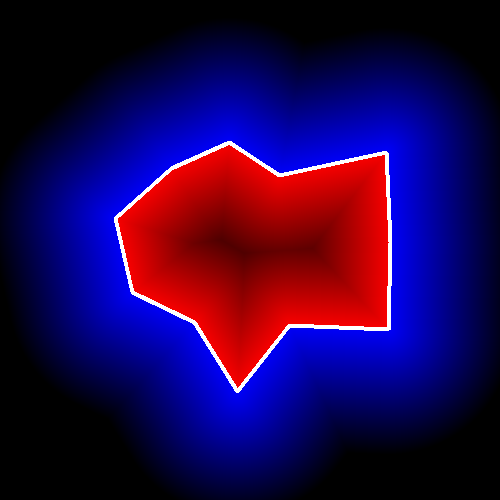
\includegraphics[width=0.5\textwidth]{pics/pointpolygon.png}

\fi

\section{Planar Subdivisions}

\ifCPy

\cvfunc{CvSubdiv2D}\label{CvSubdiv2D}

Planar subdivision.

\begin{lstlisting}
#define CV_SUBDIV2D_FIELDS()    \
    CV_GRAPH_FIELDS()           \
    int  quad_edges;            \
    int  is_geometry_valid;     \
    CvSubdiv2DEdge recent_edge; \
    CvPoint2D32f  topleft;      \
    CvPoint2D32f  bottomright;

typedef struct CvSubdiv2D
{
    CV_SUBDIV2D_FIELDS()
}
CvSubdiv2D;
\end{lstlisting}

Planar subdivision is the subdivision of a plane into a set of
non-overlapped regions (facets) that cover the whole plane. The above
structure describes a subdivision built on a 2d point set, where the points
are linked together and form a planar graph, which, together with a few
edges connecting the exterior subdivision points (namely, convex hull points)
with infinity, subdivides a plane into facets by its edges.

For every subdivision there exists a dual subdivision in which facets and
points (subdivision vertices) swap their roles, that is, a facet is
treated as a vertex (called a virtual point below) of the dual subdivision and
the original subdivision vertices become facets. On the picture below
original subdivision is marked with solid lines and dual subdivision
with dotted lines.

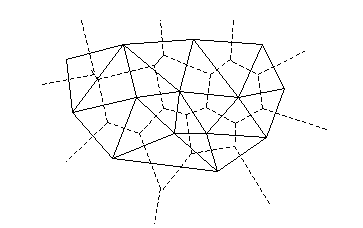
\includegraphics[width=0.5\textwidth]{pics/subdiv.png}

OpenCV subdivides a plane into triangles using Delaunay's
algorithm. Subdivision is built iteratively starting from a dummy
triangle that includes all the subdivision points for sure. In this
case the dual subdivision is a Voronoi diagram of the input 2d point set. The
subdivisions can be used for the 3d piece-wise transformation of a plane,
morphing, fast location of points on the plane, building special graphs
(such as NNG,RNG) and so forth.

\cvfunc{CvQuadEdge2D}\label{CvQuadEdge2D}

Quad-edge of planar subdivision.

\begin{lstlisting}
/* one of edges within quad-edge, lower 2 bits is index (0..3)
   and upper bits are quad-edge pointer */
typedef long CvSubdiv2DEdge;

/* quad-edge structure fields */
#define CV_QUADEDGE2D_FIELDS()     \
    int flags;                     \
    struct CvSubdiv2DPoint* pt[4]; \
    CvSubdiv2DEdge  next[4];

typedef struct CvQuadEdge2D
{
    CV_QUADEDGE2D_FIELDS()
}
CvQuadEdge2D;

\end{lstlisting}

Quad-edge is a basic element of subdivision containing four edges (e, eRot, reversed e and reversed eRot):

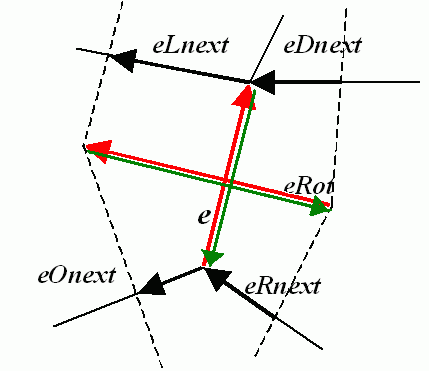
\includegraphics[width=0.5\textwidth]{pics/quadedge.png}

\cvfunc{CvSubdiv2DPoint}\label{CvSubdiv2DPoint}

Point of original or dual subdivision.

\begin{lstlisting}
#define CV_SUBDIV2D_POINT_FIELDS()\
    int            flags;      \
    CvSubdiv2DEdge first;      \
    CvPoint2D32f   pt;

#define CV_SUBDIV2D_VIRTUAL_POINT_FLAG (1 << 30)

typedef struct CvSubdiv2DPoint
{
    CV_SUBDIV2D_POINT_FIELDS()
}
CvSubdiv2DPoint;
\end{lstlisting}

\cvCPyFunc{CalcSubdivVoronoi2D}
Calculates the coordinates of Voronoi diagram cells.

\cvdefC{
void cvCalcSubdivVoronoi2D( \par CvSubdiv2D* subdiv );
}\cvdefPy{CalcSubdivVoronoi2D(subdiv)-> None}

\begin{description}
\cvarg{subdiv}{Delaunay subdivision, in which all the points are already added}
\end{description}

The function calculates the coordinates
of virtual points. All virtual points corresponding to some vertex of the
original subdivision form (when connected together) a boundary of the Voronoi
cell at that point.

\cvCPyFunc{ClearSubdivVoronoi2D}
Removes all virtual points.

\cvdefC{
void cvClearSubdivVoronoi2D( CvSubdiv2D* subdiv );
}\cvdefPy{ClearSubdivVoronoi2D(subdiv)-> None}

\begin{description}
\cvarg{subdiv}{Delaunay subdivision}
\end{description}

The function removes all of the virtual points. It
is called internally in \cvCPyCross{CalcSubdivVoronoi2D} if the subdivision
was modified after previous call to the function.


\cvCPyFunc{CreateSubdivDelaunay2D}
Creates an empty Delaunay triangulation.

\cvdefC{
CvSubdiv2D* cvCreateSubdivDelaunay2D( \par CvRect rect,\par CvMemStorage* storage );
}\cvdefPy{CreateSubdivDelaunay2D(rect,storage)-> delaunay\_triangulation}

\begin{description}
\cvarg{rect}{Rectangle that includes all of the 2d points that are to be added to the subdivision}
\cvarg{storage}{Container for subdivision}
\end{description}

The function creates an empty Delaunay
subdivision, where 2d points can be added using the function
\cvCPyCross{SubdivDelaunay2DInsert}. All of the points to be added must be within
the specified rectangle, otherwise a runtime error will be raised.

Note that the triangulation is a single large triangle that covers the given rectangle.  Hence the three vertices of this triangle are outside the rectangle \texttt{rect}.

\cvCPyFunc{FindNearestPoint2D}
Finds the closest subdivision vertex to the given point.

\cvdefC{
CvSubdiv2DPoint* cvFindNearestPoint2D( \par CvSubdiv2D* subdiv,\par CvPoint2D32f pt );
}\cvdefPy{FindNearestPoint2D(subdiv,pt)-> point}

\begin{description}
\cvarg{subdiv}{Delaunay or another subdivision}
\cvarg{pt}{Input point}
\end{description}

The function is another function that
locates the input point within the subdivision. It finds the subdivision vertex that
is the closest to the input point. It is not necessarily one of vertices
of the facet containing the input point, though the facet (located using
\cvCPyCross{Subdiv2DLocate}) is used as a starting
point. The function returns a pointer to the found subdivision vertex.

\cvCPyFunc{Subdiv2DEdgeDst}
Returns the edge destination.

\cvdefC{
CvSubdiv2DPoint* cvSubdiv2DEdgeDst( \par CvSubdiv2DEdge edge );
}\cvdefPy{Subdiv2DEdgeDist(edge)-> point}

\begin{description}
\cvarg{edge}{Subdivision edge (not a quad-edge)}
\end{description}

The function returns the edge destination. The
returned pointer may be NULL if the edge is from dual subdivision and
the virtual point coordinates are not calculated yet. The virtual points
can be calculated using the function \cvCPyCross{CalcSubdivVoronoi2D}.

\cvCPyFunc{Subdiv2DEdgeOrg}
Returns the edge origin.

\cvdefC{
CvSubdiv2DPoint* cvSubdiv2DEdgeOrg( \par CvSubdiv2DEdge edge );
}\cvdefPy{Subdiv2DEdgeOrg(edge)-> point}

\begin{description}
\cvarg{edge}{Subdivision edge (not a quad-edge)}
\end{description}

The function returns the edge
origin. The returned pointer may be NULL if the edge is from dual
subdivision and the virtual point coordinates are not calculated
yet. The virtual points can be calculated using the function
\cvCPyCross{CalcSubdivVoronoi2D}.

\cvCPyFunc{Subdiv2DGetEdge}
Returns one of the edges related to the given edge.

\cvdefC{
CvSubdiv2DEdge  cvSubdiv2DGetEdge( CvSubdiv2DEdge edge, CvNextEdgeType type );


}\cvdefPy{Subdiv2DGetEdge(edge,type)-> CvSubdiv2DEdge}
\begin{lstlisting}
#define cvSubdiv2DNextEdge( edge ) cvSubdiv2DGetEdge( edge, CV_NEXT_AROUND_ORG )
\end{lstlisting}

\begin{description}
\cvarg{edge}{Subdivision edge (not a quad-edge)}
\cvarg{type}{Specifies which of the related edges to return, one of the following:}
\begin{description}
  \cvarg{CV\_NEXT\_AROUND\_ORG}{next around the edge origin (\texttt{eOnext} on the picture above if \texttt{e} is the input edge)}
  \cvarg{CV\_NEXT\_AROUND\_DST}{next around the edge vertex (\texttt{eDnext})}
  \cvarg{CV\_PREV\_AROUND\_ORG}{previous around the edge origin (reversed \texttt{eRnext})}
  \cvarg{CV\_PREV\_AROUND\_DST}{previous around the edge destination (reversed \texttt{eLnext})}
  \cvarg{CV\_NEXT\_AROUND\_LEFT}{next around the left facet (\texttt{eLnext})}
  \cvarg{CV\_NEXT\_AROUND\_RIGHT}{next around the right facet (\texttt{eRnext})}
  \cvarg{CV\_PREV\_AROUND\_LEFT}{previous around the left facet (reversed \texttt{eOnext})}
  \cvarg{CV\_PREV\_AROUND\_RIGHT}{previous around the right facet (reversed \texttt{eDnext})}
\end{description}
\end{description}

The function returns one of the edges related to the input edge.

\cvCPyFunc{Subdiv2DLocate}
Returns the location of a point within a Delaunay triangulation.

\cvdefC{
CvSubdiv2DPointLocation  cvSubdiv2DLocate( \par CvSubdiv2D* subdiv,\par CvPoint2D32f pt,\par CvSubdiv2DEdge* edge,\par CvSubdiv2DPoint** vertex=NULL );
}\cvdefPy{Subdiv2DLocate(subdiv, pt) -> (loc, where)}

\begin{description}
\cvarg{subdiv}{Delaunay or another subdivision}
\cvarg{pt}{The point to locate}
\cvC{\cvarg{edge}{The output edge the point falls onto or right to}}
\cvC{\cvarg{vertex}{Optional output vertex double pointer the input point coinsides with}}
\cvPy{\cvarg{loc}{The location of the point within the triangulation}}
\cvPy{\cvarg{where}{The edge or vertex.  See below.}}
\end{description}

The function locates the input point within the subdivision. There are 5 cases:

\ifC
\begin{itemize}
 \item The point falls into some facet. The function returns \texttt{CV\_PTLOC\_INSIDE} and \texttt{*edge} will contain one of edges of the facet.
 \item The point falls onto the edge. The function returns \texttt{CV\_PTLOC\_ON\_EDGE} and \texttt{*edge} will contain this edge.
 \item The point coincides with one of the subdivision vertices. The function returns \texttt{CV\_PTLOC\_VERTEX} and \texttt{*vertex} will contain a pointer to the vertex.
 \item The point is outside the subdivsion reference rectangle. The function returns \texttt{CV\_PTLOC\_OUTSIDE\_RECT} and no pointers are filled.
 \item One of input arguments is invalid. A runtime error is raised or, if silent or "parent" error processing mode is selected, \\texttt{CV\_PTLOC\_ERROR} is returnd.
\end{itemize}
\fi

\ifPy
\begin{itemize}
 \item The point falls into some facet.                          \texttt{loc} is \texttt{CV\_PTLOC\_INSIDE} and \texttt{where} is one of edges of the facet.
 \item The point falls onto the edge.                            \texttt{loc} is \texttt{CV\_PTLOC\_ON\_EDGE} and \texttt{where} is the edge.
 \item The point coincides with one of the subdivision vertices. \texttt{loc} is \texttt{CV\_PTLOC\_VERTEX} and \texttt{where} is the vertex.
 \item The point is outside the subdivsion reference rectangle.  \texttt{loc} is \texttt{CV\_PTLOC\_OUTSIDE\_RECT} and \texttt{where} is None.
 \item One of input arguments is invalid. The function raises an exception.
\end{itemize}
\fi

\cvCPyFunc{Subdiv2DRotateEdge}
Returns another edge of the same quad-edge.

\cvdefC{
CvSubdiv2DEdge  cvSubdiv2DRotateEdge( \par CvSubdiv2DEdge edge,\par int rotate );
}\cvdefPy{Subdiv2DRotateEdge(edge,rotate)-> CvSubdiv2DEdge}

\begin{description}
\cvarg{edge}{Subdivision edge (not a quad-edge)}
\cvarg{type}{Specifies which of the edges of the same quad-edge as the input one to return, one of the following:
\begin{description}
  \cvarg{0}{the input edge (\texttt{e} on the picture above if \texttt{e} is the input edge)}
  \cvarg{1}{the rotated edge (\texttt{eRot})}
  \cvarg{2}{the reversed edge (reversed \texttt{e} (in green))}
  \cvarg{3}{the reversed rotated edge (reversed \texttt{eRot} (in green))}
\end{description}}
\end{description}

The function returns one of the edges of the same quad-edge as the input edge.

\cvCPyFunc{SubdivDelaunay2DInsert}
Inserts a single point into a Delaunay triangulation.

\cvdefC{
CvSubdiv2DPoint*  cvSubdivDelaunay2DInsert( \par CvSubdiv2D* subdiv,\par CvPoint2D32f pt);
}\cvdefPy{SubdivDelaunay2DInsert(subdiv,pt)-> point}

\begin{description}
\cvarg{subdiv}{Delaunay subdivision created by the function \cvCPyCross{CreateSubdivDelaunay2D}}
\cvarg{pt}{Inserted point}
\end{description}

The function inserts a single point into a subdivision and modifies the subdivision topology appropriately. If a point with the same coordinates exists already, no new point is added. The function returns a pointer to the allocated point. No virtual point coordinates are calculated at this stage.

\fi
\section{Object Detection}

\ifCPy

\cvCPyFunc{MatchTemplate}
Compares a template against overlapped image regions.

\cvdefC{
void cvMatchTemplate( \par const CvArr* image,\par const CvArr* templ,\par CvArr* result,\par int method );
}\cvdefPy{MatchTemplate(image,templ,result,method)-> None}

\begin{description}
\cvarg{image}{Image where the search is running; should be 8-bit or 32-bit floating-point}
\cvarg{templ}{Searched template; must be not greater than the source image and the same data type as the image}
\cvarg{result}{A map of comparison results; single-channel 32-bit floating-point.
If \texttt{image} is $W \times H$ and
\texttt{templ} is $w \times h$ then \texttt{result} must be $(W-w+1) \times (H-h+1)$}
\cvarg{method}{Specifies the way the template must be compared with the image regions (see below)}
\end{description}

The function is similar to
\cvCPyCross{CalcBackProjectPatch}. It slides through \texttt{image}, compares the
overlapped patches of size $w \times h$ against \texttt{templ}
using the specified method and stores the comparison results to
\texttt{result}. Here are the formulas for the different comparison
methods one may use ($I$ denotes \texttt{image}, $T$ \texttt{template},
$R$ \texttt{result}). The summation is done over template and/or the
image patch: $x' = 0...w-1, y' = 0...h-1$

% \texttt{x'=0..w-1, y'=0..h-1}):

\begin{description}
\item[method=CV\_TM\_SQDIFF]
\[ R(x,y)=\sum_{x',y'} (T(x',y')-I(x+x',y+y'))^2 \]

\item[method=CV\_TM\_SQDIFF\_NORMED]
\[ R(x,y)=\frac
{\sum_{x',y'} (T(x',y')-I(x+x',y+y'))^2}
{\sqrt{\sum_{x',y'}T(x',y')^2 \cdot \sum_{x',y'} I(x+x',y+y')^2}}
\]

\item[method=CV\_TM\_CCORR]
\[ R(x,y)=\sum_{x',y'} (T(x',y') \cdot I(x+x',y+y')) \]

\item[method=CV\_TM\_CCORR\_NORMED]
\[ R(x,y)=\frac
{\sum_{x',y'} (T(x',y') \cdot I'(x+x',y+y'))}
{\sqrt{\sum_{x',y'}T(x',y')^2 \cdot \sum_{x',y'} I(x+x',y+y')^2}}
\]

\item[method=CV\_TM\_CCOEFF]
\[ R(x,y)=\sum_{x',y'} (T'(x',y') \cdot I(x+x',y+y')) \]

where
\[ 
\begin{array}{l}
T'(x',y')=T(x',y') - 1/(w \cdot h) \cdot \sum_{x'',y''} T(x'',y'')\\
I'(x+x',y+y')=I(x+x',y+y') - 1/(w \cdot h) \cdot \sum_{x'',y''} I(x+x'',y+y'')
\end{array}
\]

\item[method=CV\_TM\_CCOEFF\_NORMED]
\[ R(x,y)=\frac
{ \sum_{x',y'} (T'(x',y') \cdot I'(x+x',y+y')) }
{ \sqrt{\sum_{x',y'}T'(x',y')^2 \cdot \sum_{x',y'} I'(x+x',y+y')^2} }
\]
\end{description}

After the function finishes the comparison, the best matches can be found as global minimums (\texttt{CV\_TM\_SQDIFF}) or maximums (\texttt{CV\_TM\_CCORR} and \texttt{CV\_TM\_CCOEFF}) using the \cvCPyCross{MinMaxLoc} function. In the case of a color image, template summation in the numerator and each sum in the denominator is done over all of the channels (and separate mean values are used for each channel).

\subsection{Haar Feature-based Cascade Classifier for Object Detection}

The object detector described below has been initially proposed by Paul Viola
\cvCPyCross{Viola01}
and improved by Rainer Lienhart
\cvCPyCross{Lienhart02}
. First, a classifier (namely a \emph{cascade of boosted classifiers working with haar-like features}) is trained with a few hundred sample views of a particular object (i.e., a face or a car), called positive examples, that are scaled to the same size (say, 20x20), and negative examples - arbitrary images of the same size.

After a classifier is trained, it can be applied to a region of interest
(of the same size as used during the training) in an input image. The
classifier outputs a "1" if the region is likely to show the object
(i.e., face/car), and "0" otherwise. To search for the object in the
whole image one can move the search window across the image and check
every location using the classifier. The classifier is designed so that
it can be easily "resized" in order to be able to find the objects of
interest at different sizes, which is more efficient than resizing the
image itself. So, to find an object of an unknown size in the image the
scan procedure should be done several times at different scales.

The word "cascade" in the classifier name means that the resultant
classifier consists of several simpler classifiers (\emph{stages}) that
are applied subsequently to a region of interest until at some stage the
candidate is rejected or all the stages are passed. The word "boosted"
means that the classifiers at every stage of the cascade are complex
themselves and they are built out of basic classifiers using one of four
different \texttt{boosting} techniques (weighted voting). Currently
Discrete Adaboost, Real Adaboost, Gentle Adaboost and Logitboost are
supported. The basic classifiers are decision-tree classifiers with at
least 2 leaves. Haar-like features are the input to the basic classifers,
and are calculated as described below. The current algorithm uses the
following Haar-like features:

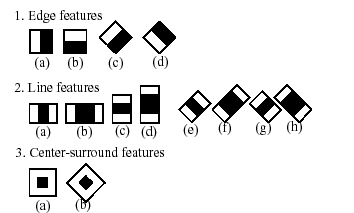
\includegraphics[width=0.5\textwidth]{pics/haarfeatures.png}

The feature used in a particular classifier is specified by its shape (1a, 2b etc.), position within the region of interest and the scale (this scale is not the same as the scale used at the detection stage, though these two scales are multiplied). For example, in the case of the third line feature (2c) the response is calculated as the difference between the sum of image pixels under the rectangle covering the whole feature (including the two white stripes and the black stripe in the middle) and the sum of the image pixels under the black stripe multiplied by 3 in order to compensate for the differences in the size of areas. The sums of pixel values over a rectangular regions are calculated rapidly using integral images (see below and the \cvCPyCross{Integral} description).

\ifPy
A simple demonstration of face detection, which draws a rectangle around each detected face:

\begin{lstlisting}

hc = cv.Load("haarcascade_frontalface_default.xml")
img = cv.LoadImage("faces.jpg", 0)
faces = cv.HaarDetectObjects(img, hc, cv.CreateMemStorage())
for (x,y,w,h),n in faces:
    cv.Rectangle(img, (x,y), (x+w,y+h), 255)
cv.SaveImage("faces_detected.jpg", img)

\end{lstlisting}

\fi

\ifC
To see the object detector at work, have a look at the HaarFaceDetect demo.

The following reference is for the detection part only. There
is a separate application called \texttt{haartraining} that can
train a cascade of boosted classifiers from a set of samples. See
\texttt{opencv/apps/haartraining} for details.

\cvclass{CvHaarFeature, CvHaarClassifier, CvHaarStageClassifier, CvHaarClassifierCascade}
\label{CvHaarFeature}
\label{CvHaarClassifier}
\label{CvHaarStageClassifier}
\label{CvHaarClassifierCascade}

Boosted Haar classifier structures.

\begin{lstlisting}
#define CV_HAAR_FEATURE_MAX  3

/* a haar feature consists of 2-3 rectangles with appropriate weights */
typedef struct CvHaarFeature
{
    int  tilted;  /* 0 means up-right feature, 1 means 45--rotated feature */

    /* 2-3 rectangles with weights of opposite signs and
       with absolute values inversely proportional to the areas of the 
       rectangles.  If rect[2].weight !=0, then
       the feature consists of 3 rectangles, otherwise it consists of 2 */
    struct
    {
        CvRect r;
        float weight;
    } rect[CV_HAAR_FEATURE_MAX];
}
CvHaarFeature;

/* a single tree classifier (stump in the simplest case) that returns the 
   response for the feature at the particular image location (i.e. pixel 
   sum over subrectangles of the window) and gives out a value depending 
   on the response */
typedef struct CvHaarClassifier
{
    int count;  /* number of nodes in the decision tree */

    /* these are "parallel" arrays. Every index \texttt{i}
       corresponds to a node of the decision tree (root has 0-th index).

       left[i] - index of the left child (or negated index if the 
         left child is a leaf)
       right[i] - index of the right child (or negated index if the 
          right child is a leaf)
       threshold[i] - branch threshold. if feature responce is <= threshold, 
                    left branch is chosen, otherwise right branch is chosen.
       alpha[i] - output value correponding to the leaf. */
    CvHaarFeature* haar_feature;
    float* threshold;
    int* left;
    int* right;
    float* alpha;
}
CvHaarClassifier;

/* a boosted battery of classifiers(=stage classifier):
   the stage classifier returns 1
   if the sum of the classifiers responses
   is greater than \texttt{threshold} and 0 otherwise */
typedef struct CvHaarStageClassifier
{
    int  count;  /* number of classifiers in the battery */
    float threshold; /* threshold for the boosted classifier */
    CvHaarClassifier* classifier; /* array of classifiers */

    /* these fields are used for organizing trees of stage classifiers,
       rather than just stright cascades */
    int next;
    int child;
    int parent;
}
CvHaarStageClassifier;

typedef struct CvHidHaarClassifierCascade CvHidHaarClassifierCascade;

/* cascade or tree of stage classifiers */
typedef struct CvHaarClassifierCascade
{
    int  flags; /* signature */
    int  count; /* number of stages */
    CvSize orig_window_size; /* original object size (the cascade is 
                            trained for) */

    /* these two parameters are set by cvSetImagesForHaarClassifierCascade */
    CvSize real_window_size; /* current object size */
    double scale; /* current scale */
    CvHaarStageClassifier* stage_classifier; /* array of stage classifiers */
    CvHidHaarClassifierCascade* hid_cascade; /* hidden optimized 
                        representation of the 
                        cascade, created by 
                cvSetImagesForHaarClassifierCascade */
}
CvHaarClassifierCascade;
\end{lstlisting}

All the structures are used for representing a cascaded of boosted Haar classifiers. The cascade has the following hierarchical structure:

\begin{verbatim}
    Cascade:
        Stage,,1,,:
            Classifier,,11,,:
                Feature,,11,,
            Classifier,,12,,:
                Feature,,12,,
            ...
        Stage,,2,,:
            Classifier,,21,,:
                Feature,,21,,
            ...
        ...
\end{verbatim}

The whole hierarchy can be constructed manually or loaded from a file or an embedded base using the function \cvCPyCross{LoadHaarClassifierCascade}.

\cvCPyFunc{LoadHaarClassifierCascade}
Loads a trained cascade classifier from a file or the classifier database embedded in OpenCV.

\cvdefC{
CvHaarClassifierCascade* cvLoadHaarClassifierCascade( \par const char* directory,\par CvSize orig\_window\_size );
}

\begin{description}
\cvarg{directory}{Name of the directory containing the description of a trained cascade classifier}
\cvarg{orig\_window\_size}{Original size of the objects the cascade has been trained on. Note that it is not stored in the cascade and therefore must be specified separately}
\end{description}

The function loads a trained cascade
of haar classifiers from a file or the classifier database embedded in
OpenCV. The base can be trained using the \texttt{haartraining} application
(see opencv/apps/haartraining for details).

\textbf{The function is obsolete}. Nowadays object detection classifiers are stored in XML or YAML files, rather than in directories. To load a cascade from a file, use the \cvCPyCross{Load} function.

\fi

\cvCPyFunc{HaarDetectObjects}
Detects objects in the image.

\ifC
\begin{lstlisting}
typedef struct CvAvgComp
{
    CvRect rect; /* bounding rectangle for the object (average rectangle of a group) */
    int neighbors; /* number of neighbor rectangles in the group */
}
CvAvgComp;
\end{lstlisting}
\fi

\cvdefC{
CvSeq* cvHaarDetectObjects( \par const CvArr* image,\par CvHaarClassifierCascade* cascade,\par CvMemStorage* storage,\par double scale\_factor=1.1,\par int min\_neighbors=3,\par int flags=0,\par CvSize min\_size=cvSize(0,\par0) );
}\cvdefPy{HaarDetectObjects(image,cascade,storage,scale\_factor=1.1,min\_neighbors=3,flags=0,min\_size=(0,0))-> detected\_objects}

\begin{description}
\cvarg{image}{Image to detect objects in}
\cvarg{cascade}{Haar classifier cascade in internal representation}
\cvarg{storage}{Memory storage to store the resultant sequence of the object candidate rectangles}
\cvarg{scale\_factor}{The factor by which the search window is scaled between the subsequent scans, 1.1 means increasing window by 10\% }
\cvarg{min\_neighbors}{Minimum number (minus 1) of neighbor rectangles that makes up an object. All the groups of a smaller number of rectangles than \texttt{min\_neighbors}-1 are rejected. If \texttt{min\_neighbors} is 0, the function does not any grouping at all and returns all the detected candidate rectangles, which may be useful if the user wants to apply a customized grouping procedure}
\cvarg{flags}{Mode of operation. Currently the only flag that may be specified is \texttt{CV\_HAAR\_DO\_CANNY\_PRUNING}. If it is set, the function uses Canny edge detector to reject some image regions that contain too few or too much edges and thus can not contain the searched object. The particular threshold values are tuned for face detection and in this case the pruning speeds up the processing}
\cvarg{min\_size}{Minimum window size. By default, it is set to the size of samples the classifier has been trained on ($\sim 20\times 20$ for face detection)}
\end{description}

The function finds rectangular regions in the given image that are likely to contain objects the cascade has been trained for and returns those regions as a sequence of rectangles. The function scans the image several times at different scales (see \cvCPyCross{SetImagesForHaarClassifierCascade}). Each time it considers overlapping regions in the image and applies the classifiers to the regions using \cvCPyCross{RunHaarClassifierCascade}. It may also apply some heuristics to reduce number of analyzed regions, such as Canny prunning. After it has proceeded and collected the candidate rectangles (regions that passed the classifier cascade), it groups them and returns a sequence of average rectangles for each large enough group. The default parameters (\texttt{scale\_factor} =1.1, \texttt{min\_neighbors} =3, \texttt{flags} =0) are tuned for accurate yet slow object detection. For a faster operation on real video images the settings are: \texttt{scale\_factor} =1.2, \texttt{min\_neighbors} =2, \texttt{flags} =\texttt{CV\_HAAR\_DO\_CANNY\_PRUNING}, \texttt{min\_size} =\textit{minimum possible face size} (for example, $\sim$ 1/4 to 1/16 of the image area in the case of video conferencing).

\ifPy
The function returns a list of tuples, \texttt{(rect, neighbors)}, where rect is a \cross{CvRect} specifying the object's extents
and neighbors is a number of neighbors.

\begin{lstlisting}
>>> import cv
>>> image = cv.LoadImageM("lena.jpg", cv.CV_LOAD_IMAGE_GRAYSCALE)
>>> cascade = cv.Load("../../data/haarcascades/haarcascade_frontalface_alt.xml")
>>> print cv.HaarDetectObjects(image, cascade, cv.CreateMemStorage(0), 1.2, 2, 0, (20, 20))
[((217, 203, 169, 169), 24)]
\end{lstlisting}
\fi

\ifC
% ===== Example. Using cascade of Haar classifiers to find objects (e.g. faces). =====
\begin{lstlisting}
#include "cv.h"
#include "highgui.h"

CvHaarClassifierCascade* load_object_detector( const char* cascade_path )
{
    return (CvHaarClassifierCascade*)cvLoad( cascade_path );
}

void detect_and_draw_objects( IplImage* image,
                              CvHaarClassifierCascade* cascade,
                              int do_pyramids )
{
    IplImage* small_image = image;
    CvMemStorage* storage = cvCreateMemStorage(0);
    CvSeq* faces;
    int i, scale = 1;

    /* if the flag is specified, down-scale the input image to get a
       performance boost w/o loosing quality (perhaps) */
    if( do_pyramids )
    {
        small_image = cvCreateImage( cvSize(image->width/2,image->height/2), IPL_DEPTH_8U, 3 );
        cvPyrDown( image, small_image, CV_GAUSSIAN_5x5 );
        scale = 2;
    }

    /* use the fastest variant */
    faces = cvHaarDetectObjects( small_image, cascade, storage, 1.2, 2, CV_HAAR_DO_CANNY_PRUNING );

    /* draw all the rectangles */
    for( i = 0; i < faces->total; i++ )
    {
        /* extract the rectanlges only */
        CvRect face_rect = *(CvRect*)cvGetSeqElem( faces, i );
        cvRectangle( image, cvPoint(face_rect.x*scale,face_rect.y*scale),
                     cvPoint((face_rect.x+face_rect.width)*scale,
                             (face_rect.y+face_rect.height)*scale),
                     CV_RGB(255,0,0), 3 );
    }

    if( small_image != image )
        cvReleaseImage( &small_image );
    cvReleaseMemStorage( &storage );
}

/* takes image filename and cascade path from the command line */
int main( int argc, char** argv )
{
    IplImage* image;
    if( argc==3 && (image = cvLoadImage( argv[1], 1 )) != 0 )
    {
        CvHaarClassifierCascade* cascade = load_object_detector(argv[2]);
        detect_and_draw_objects( image, cascade, 1 );
        cvNamedWindow( "test", 0 );
        cvShowImage( "test", image );
        cvWaitKey(0);
        cvReleaseHaarClassifierCascade( &cascade );
        cvReleaseImage( &image );
    }

    return 0;
}
\end{lstlisting}


\cvCPyFunc{SetImagesForHaarClassifierCascade}
Assigns images to the hidden cascade.

\cvdefC{
void cvSetImagesForHaarClassifierCascade( \par CvHaarClassifierCascade* cascade,\par const CvArr* sum,\par const CvArr* sqsum,\par const CvArr* tilted\_sum,\par double scale );
}

\begin{description}
\cvarg{cascade}{Hidden Haar classifier cascade, created by \cvCPyCross{CreateHidHaarClassifierCascade}}
\cvarg{sum}{Integral (sum) single-channel image of 32-bit integer format. This image as well as the two subsequent images are used for fast feature evaluation and brightness/contrast normalization. They all can be retrieved from input 8-bit or floating point single-channel image using the function \cvCPyCross{Integral}}
\cvarg{sqsum}{Square sum single-channel image of 64-bit floating-point format}
\cvarg{tilted\_sum}{Tilted sum single-channel image of 32-bit integer format}
\cvarg{scale}{Window scale for the cascade. If \texttt{scale} =1, the original window size is used (objects of that size are searched) - the same size as specified in \cvCPyCross{LoadHaarClassifierCascade} (24x24 in the case of \texttt{default\_face\_cascade}), if \texttt{scale} =2, a two times larger window is used (48x48 in the case of default face cascade). While this will speed-up search about four times, faces smaller than 48x48 cannot be detected}
\end{description}

The function assigns images and/or window scale to the hidden classifier cascade. If image pointers are NULL, the previously set images are used further (i.e. NULLs mean "do not change images"). Scale parameter has no such a "protection" value, but the previous value can be retrieved by the \cvCPyCross{GetHaarClassifierCascadeScale} function and reused again. The function is used to prepare cascade for detecting object of the particular size in the particular image. The function is called internally by \cvCPyCross{HaarDetectObjects}, but it can be called by the user if they are using the lower-level function \cvCPyCross{RunHaarClassifierCascade}.

\cvCPyFunc{ReleaseHaarClassifierCascade}
Releases the haar classifier cascade.

\cvdefC{
void cvReleaseHaarClassifierCascade( \par CvHaarClassifierCascade** cascade );
}

\begin{description}
\cvarg{cascade}{Double pointer to the released cascade. The pointer is cleared by the function}
\end{description}

The function deallocates the cascade that has been created manually or loaded using \cvCPyCross{LoadHaarClassifierCascade} or \cvCPyCross{Load}.

\cvCPyFunc{RunHaarClassifierCascade}
Runs a cascade of boosted classifiers at the given image location.

\cvdefC{
int cvRunHaarClassifierCascade( \par CvHaarClassifierCascade* cascade,\par CvPoint pt,\par int start\_stage=0 );
}

\begin{description}
\cvarg{cascade}{Haar classifier cascade}
\cvarg{pt}{Top-left corner of the analyzed region. Size of the region is a original window size scaled by the currenly set scale. The current window size may be retrieved using the \cvCPyCross{GetHaarClassifierCascadeWindowSize} function}
\cvarg{start\_stage}{Initial zero-based index of the cascade stage to start from. The function assumes that all the previous stages are passed. This feature is used internally by \cvCPyCross{HaarDetectObjects} for better processor cache utilization}
\end{description}

The function runs the Haar classifier
cascade at a single image location. Before using this function the
integral images and the appropriate scale (window size) should be set
using \cvCPyCross{SetImagesForHaarClassifierCascade}. The function returns
a positive value if the analyzed rectangle passed all the classifier stages
(it is a candidate) and a zero or negative value otherwise.

\fi

\fi

\ifCpp

\cvclass{FeatureEvaluator}
Base class for computing feature values in cascade classifiers.

\begin{lstlisting}
class CV_EXPORTS FeatureEvaluator
{
public:    
    enum { HAAR = 0, LBP = 1 }; // supported feature types 
    virtual ~FeatureEvaluator(); // destructor
    virtual bool read(const FileNode& node);
    virtual Ptr<FeatureEvaluator> clone() const;
    virtual int getFeatureType() const;
    
    virtual bool setImage(const Mat& img, Size origWinSize);
    virtual bool setWindow(Point p);

    virtual double calcOrd(int featureIdx) const;
    virtual int calcCat(int featureIdx) const;

    static Ptr<FeatureEvaluator> create(int type);
};
\end{lstlisting}

\cvCppFunc{FeatureEvaluator::read}
Reads parameters of the features from a FileStorage node.

\begin{lstlisting}
bool FeatureEvaluator::read(const FileNode& node);
\end{lstlisting}

\begin{description}
\cvarg{node}{File node from which the feature parameters are read.}
\end{description}

\cvCppFunc{FeatureEvaluator::clone}
Returns a full copy of the feature evaluator.

\begin{lstlisting}
Ptr<FeatureEvaluator> FeatureEvaluator::clone() const;
\end{lstlisting}

\cvCppFunc{FeatureEvaluator::getFeatureType}
Returns the feature type (HAAR or LBP for now).

\begin{lstlisting}
int FeatureEvaluator::getFeatureType() const;
\end{lstlisting}

\cvCppFunc{FeatureEvaluator::setImage}
Sets the image in which to compute the features.

\begin{lstlisting}
bool FeatureEvaluator::setImage(const Mat& img, Size origWinSize);
\end{lstlisting}

\begin{description}
\cvarg{img}{Matrix of type  \texttt{CV\_8UC1} containing the image in which to compute the features.}
\cvarg{origWinSize}{Size of training images.}
\end{description}

\cvCppFunc{FeatureEvaluator::setWindow}
Sets window in the current image in which the features will be computed (called by \cvCppCross{CascadeClassifier::runAt}).

\begin{lstlisting}
bool FeatureEvaluator::setWindow(Point p); 
\end{lstlisting}

\begin{description}
\cvarg{p}{The upper left point of window in which the features will be computed. Size of the window is equal to size of training images.}
\end{description}

\cvCppFunc{FeatureEvaluator::calcOrd}
Computes value of an ordered (numerical) feature.

\begin{lstlisting}
double FeatureEvaluator::calcOrd(int featureIdx) const;
\end{lstlisting}

\begin{description}
\cvarg{featureIdx}{Index of feature whose value will be computed.}
\end{description}
Returns computed value of ordered feature.

\cvCppFunc{FeatureEvaluator::calcCat}
Computes value of a categorical feature.

\begin{lstlisting}
int FeatureEvaluator::calcCat(int featureIdx) const;
\end{lstlisting}

\begin{description}
\cvarg{featureIdx}{Index of feature whose value will be computed.}
\end{description}
Returns computed label of categorical feature, i.e. value from [0,... (number of categories - 1)].

\cvCppFunc{FeatureEvaluator::create}
Constructs feature evaluator.

\begin{lstlisting}
static Ptr<FeatureEvaluator> FeatureEvaluator::create(int type);
\end{lstlisting}

\begin{description}
\cvarg{type}{Type of features evaluated by cascade (HAAR or LBP for now).}
\end{description}

\cvclass{CascadeClassifier}
The cascade classifier class for object detection.

\begin{lstlisting}
class CascadeClassifier
{
public:
	// structure for storing tree node
    struct CV_EXPORTS DTreeNode 
    {
        int featureIdx; // feature index on which is a split
        float threshold; // split threshold of ordered features only
        int left; // left child index in the tree nodes array
        int right; // right child index in the tree nodes array
    };
    
    // structure for storing desision tree
    struct CV_EXPORTS DTree 
    {
        int nodeCount; // nodes count
    };
    
    // structure for storing cascade stage (BOOST only for now)
    struct CV_EXPORTS Stage
    {
        int first; // first tree index in tree array
        int ntrees; // number of trees
        float threshold; // treshold of stage sum
    };
    
    enum { BOOST = 0 }; // supported stage types
    
    // mode of detection (see parameter flags in function HaarDetectObjects)
    enum { DO_CANNY_PRUNING = CV_HAAR_DO_CANNY_PRUNING,
           SCALE_IMAGE = CV_HAAR_SCALE_IMAGE,
           FIND_BIGGEST_OBJECT = CV_HAAR_FIND_BIGGEST_OBJECT,
           DO_ROUGH_SEARCH = CV_HAAR_DO_ROUGH_SEARCH }; 

    CascadeClassifier(); // default constructor
    CascadeClassifier(const string& filename);
    ~CascadeClassifier(); // destructor
    
    bool empty() const;
    bool load(const string& filename);
    bool read(const FileNode& node);

    void detectMultiScale( const Mat& image, vector<Rect>& objects, 
                           double scaleFactor=1.1, int minNeighbors=3, 
						   int flags=0, Size minSize=Size());
    
    bool setImage( Ptr<FeatureEvaluator>&, const Mat& );
    int runAt( Ptr<FeatureEvaluator>&, Point );

    bool is_stump_based; // true, if the trees are stumps

    int stageType; // stage type (BOOST only for now)
    int featureType; // feature type (HAAR or LBP for now)
    int ncategories; // number of categories (for categorical features only) 
    Size origWinSize; // size of training images
    
    vector<Stage> stages; // vector of stages (BOOST for now)
    vector<DTree> classifiers; // vector of decision trees
    vector<DTreeNode> nodes; // vector of tree nodes
    vector<float> leaves; // vector of leaf values
    vector<int> subsets; // subsets of split by categorical feature

    Ptr<FeatureEvaluator> feval; // pointer to feature evaluator
    Ptr<CvHaarClassifierCascade> oldCascade; // pointer to old cascade
};
\end{lstlisting}

\cvCppFunc{CascadeClassifier::CascadeClassifier}
Loads the classifier from file.

\begin{lstlisting}
CascadeClassifier::CascadeClassifier(const string& filename);
\end{lstlisting}

\begin{description}
\cvarg{filename}{Name of file from which classifier will be load.}
\end{description}

\cvCppFunc{CascadeClassifier::empty}
Checks if the classifier has been loaded or not.

\begin{lstlisting}
bool CascadeClassifier::empty() const;
\end{lstlisting}

\cvCppFunc{CascadeClassifier::load}
Loads the classifier from file. The previous content is destroyed.

\begin{lstlisting}
bool CascadeClassifier::load(const string& filename);
\end{lstlisting}

\begin{description}
\cvarg{filename}{Name of file from which classifier will be load. File may contain as old haar classifier (trained by haartraining application) or new cascade classifier (trained traincascade application).}
\end{description}

\cvCppFunc{CascadeClassifier::read}
Reads the classifier from a FileStorage node. File may contain a new cascade classifier (trained traincascade application) only.

\begin{lstlisting}
bool CascadeClassifier::read(const FileNode& node);
\end{lstlisting}

\cvCppFunc{CascadeClassifier::detectMultiScale}
Detects objects of different sizes in the input image. The detected objects are returned as a list of rectangles.

\begin{lstlisting}
void CascadeClassifier::detectMultiScale( const Mat& image,
                           vector<Rect>& objects,
                           double scaleFactor=1.1,
                           int minNeighbors=3, int flags=0,
                           Size minSize=Size());
\end{lstlisting}

\begin{description}
\cvarg{image}{Matrix of type  \texttt{CV\_8U} containing the image in which to detect objects.}
\cvarg{objects}{Vector of rectangles such that each rectangle contains the detected object.}
\cvarg{scaleFactor}{Specifies how much the image size is reduced at each image scale.}
\cvarg{minNeighbors}{Speficifes how many neighbors should each candiate rectangle have to retain it.}
\cvarg{flags}{This parameter is not used for new cascade and have the same meaning for old cascade as in function cvHaarDetectObjects.}
\cvarg{minSize}{The minimum possible object size. Objects smaller than that are ignored.}
\end{description}

\cvCppFunc{CascadeClassifier::setImage}
Sets the image for detection (called by detectMultiScale at each image level).

\begin{lstlisting}
bool CascadeClassifier::setImage( Ptr<FeatureEvaluator>& feval, const Mat& image );
\end{lstlisting}

\begin{description}
\cvarg{feval}{Pointer to feature evaluator which is used for computing features.}
\cvarg{image}{Matrix of type  \texttt{CV\_8UC1} containing the image in which to compute the features.}
\end{description}

\cvCppFunc{CascadeClassifier::runAt}
Runs the detector at the specified point (the image that the detector is working with should be set by setImage).

\begin{lstlisting}
int CascadeClassifier::runAt( Ptr<FeatureEvaluator>& feval, Point pt );
\end{lstlisting}

\begin{description}
\cvarg{feval}{Feature evaluator which is used for computing features.}
\cvarg{pt}{The upper left point of window in which the features will be computed. Size of the window is equal to size of training images.}
\end{description}
Returns:
1 - if cascade classifier detects object in the given location.
-si - otherwise. si is an index of stage which first predicted that given window is a background image.

\cvCppFunc{groupRectangles}
Groups the object candidate rectangles

\cvdefCpp{void groupRectangles(vector<Rect>\& rectList,\par
                     int groupThreshold, double eps=0.2);}
\begin{description}
\cvarg{rectList}{The input/output vector of rectangles. On output there will be retained and grouped rectangles}
\cvarg{groupThreshold}{The minimum possible number of rectangles, minus 1, in a group of rectangles to retain it.}
\cvarg{eps}{The relative difference between sides of the rectangles to merge them into a group}
\end{description}

The function is a wrapper for a generic function \cvCppCross{partition}. It clusters all the input rectangles using the rectangle equivalence criteria, that combines rectangles that have similar sizes and similar locations (the similarity is defined by \texttt{eps}). When \texttt{eps=0}, no clustering is done at all. If $\texttt{eps}\rightarrow +\inf$, all the rectangles will be put in one cluster. Then, the small clusters, containing less than or equal to \texttt{groupThreshold} rectangles, will be rejected. In each other cluster the average rectangle will be computed and put into the output rectangle list.  

\cvCppFunc{matchTemplate}
Compares a template against overlapped image regions.

\cvdefCpp{void matchTemplate( const Mat\& image, const Mat\& templ,\par
                    Mat\& result, int method );}
\begin{description}
\cvarg{image}{Image where the search is running; should be 8-bit or 32-bit floating-point}
\cvarg{templ}{Searched template; must be not greater than the source image and have the same data type}
\cvarg{result}{A map of comparison results; will be single-channel 32-bit floating-point.
If \texttt{image} is $W \times H$ and
\texttt{templ} is $w \times h$ then \texttt{result} will be $(W-w+1) \times (H-h+1)$}
\cvarg{method}{Specifies the comparison method (see below)}
\end{description}

The function slides through \texttt{image}, compares the
overlapped patches of size $w \times h$ against \texttt{templ}
using the specified method and stores the comparison results to
\texttt{result}. Here are the formulas for the available comparison
methods ($I$ denotes \texttt{image}, $T$ \texttt{template},
$R$ \texttt{result}). The summation is done over template and/or the
image patch: $x' = 0...w-1, y' = 0...h-1$

% \texttt{x'=0..w-1, y'=0..h-1}):

\begin{description}
\item[method=CV\_TM\_SQDIFF]
\[ R(x,y)=\sum_{x',y'} (T(x',y')-I(x+x',y+y'))^2 \]

\item[method=CV\_TM\_SQDIFF\_NORMED]
\[ R(x,y)=\frac
{\sum_{x',y'} (T(x',y')-I(x+x',y+y'))^2}
{\sqrt{\sum_{x',y'}T(x',y')^2 \cdot \sum_{x',y'} I(x+x',y+y')^2}}
\]

\item[method=CV\_TM\_CCORR]
\[ R(x,y)=\sum_{x',y'} (T(x',y') \cdot I(x+x',y+y')) \]

\item[method=CV\_TM\_CCORR\_NORMED]
\[ R(x,y)=\frac
{\sum_{x',y'} (T(x',y') \cdot I'(x+x',y+y'))}
{\sqrt{\sum_{x',y'}T(x',y')^2 \cdot \sum_{x',y'} I(x+x',y+y')^2}}
\]

\item[method=CV\_TM\_CCOEFF]
\[ R(x,y)=\sum_{x',y'} (T'(x',y') \cdot I(x+x',y+y')) \]

where
\[ 
\begin{array}{l}
T'(x',y')=T(x',y') - 1/(w \cdot h) \cdot \sum_{x'',y''} T(x'',y'')\\
I'(x+x',y+y')=I(x+x',y+y') - 1/(w \cdot h) \cdot \sum_{x'',y''} I(x+x'',y+y'')
\end{array}
\]

\item[method=CV\_TM\_CCOEFF\_NORMED]
\[ R(x,y)=\frac
{ \sum_{x',y'} (T'(x',y') \cdot I'(x+x',y+y')) }
{ \sqrt{\sum_{x',y'}T'(x',y')^2 \cdot \sum_{x',y'} I'(x+x',y+y')^2} }
\]
\end{description}

After the function finishes the comparison, the best matches can be found as global minimums (when \texttt{CV\_TM\_SQDIFF} was used) or maximums (when \texttt{CV\_TM\_CCORR} or \texttt{CV\_TM\_CCOEFF} was used) using the \cvCppCross{minMaxLoc} function. In the case of a color image, template summation in the numerator and each sum in the denominator is done over all of the channels (and separate mean values are used for each channel). That is, the function can take a color template and a color image; the result will still be a single-channel image, which is easier to analyze.

\fi

\section{Camera Calibration and 3D Reconstruction}

The functions in this section use the so-called pinhole camera model. That
is, a scene view is formed by projecting 3D points into the image plane
using a perspective transformation.

\[
s \; m' = A [R|t] M'
\]

or

\[
s \vecthree{u}{v}{1} = \vecthreethree
{f_x}{0}{c_x}
{0}{f_y}{c_y}
{0}{0}{1}
\begin{bmatrix}
 r_{11} & r_{12} & r_{13} & t_1 \\
 r_{21} & r_{22} & r_{23} & t_2 \\
 r_{31} & r_{32} & r_{33} & t_3
\end{bmatrix}
\begin{bmatrix}X\\Y\\Z\\1 \end{bmatrix}
\]

Where $(X, Y, Z)$ are the coordinates of a 3D point in the world
coordinate space, $(u, v)$ are the coordinates of the projection point
in pixels. $A$ is called a camera matrix, or a matrix of
intrinsic parameters. $(cx, cy)$ is a principal point (that is
usually at the image center), and $fx, fy$ are the focal lengths
expressed in pixel-related units. Thus, if an image from camera is
scaled by some factor, all of these parameters should
be scaled (multiplied/divided, respectively) by the same factor. The
matrix of intrinsic parameters does not depend on the scene viewed and,
once estimated, can be re-used (as long as the focal length is fixed (in
case of zoom lens)). The joint rotation-translation matrix $[R|t]$
is called a matrix of extrinsic parameters. It is used to describe the
camera motion around a static scene, or vice versa, rigid motion of an
object in front of still camera. That is, $[R|t]$ translates
coordinates of a point $(X, Y, Z)$ to some coordinate system,
fixed with respect to the camera. The transformation above is equivalent
to the following (when $z \ne 0$):

\[
\begin{array}{l}
\vecthree{x}{y}{z} = R \vecthree{X}{Y}{Z} + t\\
x' = x/z\\
y' = y/z\\
u = f_x*x' + c_x\\
v = f_y*y' + c_y
\end{array}
\]

Real lenses usually have some distortion, mostly
radial distorion and slight tangential distortion. So, the above model
is extended as:

\[
\begin{array}{l}
\vecthree{x}{y}{z} = R \vecthree{X}{Y}{Z} + t\\
x' = x/z\\
y' = y/z\\
x'' = x' (1 + k_1 r^2 + k_2 r^4 + k_3 r^6) + 2 p_1 x' y' + p_2(r^2 + 2 x'^2) \\
y'' = y' (1 + k_1 r^2 + k_2 r^4 + k_3 r^6) + p_1 (r^2 + 2 y'^2) + 2 p_2 x' y' \\
\text{where} \quad r^2 = x'^2 + y'^2 \\
u = f_x*x'' + c_x\\
v = f_y*y'' + c_y
\end{array}
\]

$k_1$, $k_2$, $k_3$ are radial distortion coefficients, $p_1$, $p_2$ are tangential distortion coefficients.
Higher-order coefficients are not considered in OpenCV. In the functions below the coefficients are passed or returned as
\label{k123p12}
\[ (k_1, k_2, p_1, p_2[, k_3]) \]vector. That is, if the vector contains 4 elements, it means that $k_3=0$.
The distortion coefficients do not depend on the scene viewed, thus they also belong to the intrinsic camera parameters.
\emph{And they remain the same regardless of the captured image resolution.}
That is, if, for example, a camera has been calibrated on images of $320
\times 240$ resolution, absolutely the same distortion coefficients can
be used for images of $640 \times 480$ resolution from the same camera (while $f_x$,
$f_y$, $c_x$ and $c_y$ need to be scaled appropriately).

The functions below use the above model to

\begin{itemize}
 \item Project 3D points to the image plane given intrinsic and extrinsic parameters
 \item Compute extrinsic parameters given intrinsic parameters, a few 3D points and their projections.
 \item Estimate intrinsic and extrinsic camera parameters from several views of a known calibration pattern (i.e. every view is described by several 3D-2D point correspodences).
\end{itemize}

\ifCPy

\cvCPyFunc{CalcImageHomography}
Calculates the homography matrix for an oblong planar object (e.g. arm).

\cvdefC{
void cvCalcImageHomography( \par float* line,\par CvPoint3D32f* center,\par float* intrinsic,\par float* homography );
}\cvdefPy{CalcImageHomography(line,points)-> intrinsic,homography}

\begin{description}
\cvarg{line}{the main object axis direction (vector (dx,dy,dz))}
\cvarg{center}{object center ((cx,cy,cz))}
\cvarg{intrinsic}{intrinsic camera parameters (3x3 matrix)}
\cvarg{homography}{output homography matrix (3x3)}
\end{description}

The function calculates the homography
matrix for the initial image transformation from image plane to the
plane, defined by a 3D oblong object line (See \_\_Figure 6-10\_\_
in the OpenCV Guide 3D Reconstruction Chapter).


\cvCPyFunc{CalibrateCamera2}
Finds the intrinsic and extrinsic camera parameters using a calibration pattern.

\cvdefC{
void cvCalibrateCamera2( \par const CvMat* objectPoints,\par const CvMat* imagePoints,\par const CvMat* pointCounts,\par CvSize imageSize,\par CvMat* intrinsicMatrix,\par CvMat* distortionCoeffs,\par CvMat* rotationVectors=NULL,\par CvMat* translationVectors=NULL,\par int flags=0 );
}\cvdefPy{CalibrateCamera2(objectPoints,imagePoints,pointCounts,imageSize,intrinsicMatrix,distortionCoeffs,rotationVectors,translationVectors,flags=0)-> None}

\begin{description}
\cvarg{objectPoints}{The joint matrix of object points, 3xN or Nx3, where N is the total number of points in all views}
\cvarg{imagePoints}{The joint matrix of corresponding image points, 2xN or Nx2, where N is the total number of points in all views}
\cvarg{pointCounts}{Vector containing the number of points in each particular view, 1xM or Mx1, where M is the number of points in a scene}
\cvarg{imageSize}{Size of the image, used only to initialize the intrinsic camera matrix}
\cvarg{intrinsicMatrix}{The output camera matrix $A = \vecthreethree{f_x}{0}{c_x}{0}{f_y}{c_y}{0}{0}{1} $. If \texttt{CV\_CALIB\_USE\_INTRINSIC\_GUESS} and/or \texttt{CV\_CALIB\_FIX\_ASPECT\_RATION} are specified, some or all of \texttt{fx, fy, cx, cy} must be initialized}
\cvarg{distortionCoeffs}{The output 4x1, 1x4, 5x1 or 1x5 vector of distortion coefficients \hyperref[k123p12]{$(k_1, k_2, p_1, p_2[, k_3])$}}.
\cvarg{rotationVectors}{The output 3xM or Mx3 array of rotation vectors (compact representation of rotation matrices, \cvCPyCross{Rodrigues2})}
\cvarg{translationVectors}{The output 3xM or Mx3 array of translation vectors}
\cvarg{flags}{Different flags, may be 0 or combination of the following values:
\begin{description}
\cvarg{CV\_CALIB\_USE\_INTRINSIC\_GUESS}{\texttt{intrinsicMatrix} contains the valid initial values of \texttt{fx, fy, cx, cy} that are optimized further. Otherwise, \texttt{(cx, cy)} is initially set to the image center (\texttt{imageSize} is used here), and focal distances are computed in some least-squares fashion. Note, that if intrinsic parameters are known, there is no need to use this function. Use \cvCPyCross{FindExtrinsicCameraParams2} instead.}
\cvarg{CV\_CALIB\_FIX\_PRINCIPAL\_POINT}{The principal point is not changed during the global optimization, it stays at the center and at the other location specified (when \texttt{CV\_CALIB\_USE\_INTRINSIC\_GUESS} is set as well)}
\cvarg{CV\_CALIB\_FIX\_ASPECT\_RATIO}{The optimization procedure considers only one of \texttt{fx} and \texttt{fy} as independent variables and keeps the aspect ratio \texttt{fx/fy} the same as it was set initially in \texttt{intrinsicMatrix}. In this case the actual initial values of \texttt{(fx, fy)} are either taken from the matrix (when \texttt{CV\_CALIB\_USE\_INTRINSIC\_GUESS} is set) or estimated somehow (in the latter case \texttt{fx, fy} may be set to arbitrary values, only their ratio is used).}
\cvarg{CV\_CALIB\_ZERO\_TANGENT\_DIST}{Tangential distortion coefficients are set to zeros and do not change during the optimization.}}
\end{description}
\end{description}

The function estimates the intrinsic camera
parameters and extrinsic parameters for each of the views. The
coordinates of 3D object points and their correspondent 2D projections
in each view must be specified. That may be achieved by using an
object with known geometry and easily detectable feature points.
Such an object is called a calibration rig or calibration pattern,
and OpenCV has built-in support for a chessboard as a calibration
rig (see \cvCPyCross{FindChessboardCornerGuesses}). Currently, initialization
of intrinsic parameters (when \texttt{CV\_CALIB\_USE\_INTRINSIC\_GUESS}
is not set) is only implemented for planar calibration rigs
(z-coordinates of object points must be all 0's or all 1's). 3D
rigs can still be used as long as initial \texttt{intrinsicMatrix}
is provided. After the initial values of intrinsic and extrinsic
parameters are computed, they are optimized to minimize the total
back-projection error - the sum of squared differences between the
actual coordinates of image points and the ones computed using
\cvCPyCross{ProjectPoints2}.

Note: if you're using a non-square (=non-NxN) grid and
\cvCPyCross{FindChessboardCorners} for calibration, and cvCalibrateCamera2 returns
bad values (i.e. zero distortion coefficients, an image center of
(w/2-0.5,h/2-0.5), and / or large differences between $fx$ and $fy$ (ratios of
10:1 or more)), then you've probaby  used patternSize=cvSize(rows,cols),
but should use patternSize=cvSize(cols,rows) in \cvCPyCross{FindChessboardCorners}.

\cvCPyFunc{ComputeCorrespondEpilines}
For points in one image of a stereo pair, computes the corresponding epilines in the other image.

\cvdefC{
void cvComputeCorrespondEpilines( \par const CvMat* points,\par int which\_image,\par const CvMat* fundamentalMatrix,\par CvMat* correspondent\_lines);
}\cvdefPy{ComputeCorrespondEpilines(points, which\_image, fundamentalMatrix, correspondent\_lines) -> None}

\begin{description}
\cvarg{points}{The input points. \texttt{2xN, Nx2, 3xN} or \texttt{Nx3} array (where \texttt{N} number of points). Multi-channel \texttt{1xN} or \texttt{Nx1} array is also acceptable}
\cvarg{which\_image}{Index of the image (1 or 2) that contains the \texttt{points}}
\cvarg{fundamentalMatrix}{Fundamental matrix}
\cvarg{correspondent\_lines}{Computed epilines, a \texttt{3xN} or \texttt{Nx3} array}
\end{description}

For every point in one of the two images of a stereo-pair the function
\texttt{ComputeCorrespondEpilines} finds the equation of a line that
contains the corresponding point (i.e. projection of the same 3D
point) in the other image. Each line is encoded by a vector of 3
elements $l = \vecthree{a}{b}{c}$ so that:

\[ l^T \vecthree{x}{y}{1} = 0 \]
or
\[ a x + b y + c = 0 \]

From the fundamental matrix definition (see \cvCPyCross{FindFundamentalMatrix}
discussion), line $l_1$ for a point $p_1$ in the first image
$(\texttt{which\_image} =1)$ can be computed as:

\[ l_2 = F p_1 \]

and the line $l_1$ for a point $p_2$ in the second image $(\texttt{which\_image} =1)$ can be computed as:

\[ l_1 = F^T p_2 \]

Line coefficients are defined up to a scale. They are normalized $(a^2+b^2=1)$ are stored into \texttt{correspondent\_lines}.

\ifC

\cvCPyFunc{ConvertPointsHomogenious}
Convert points to/from homogenious coordinates.

\cvdefC{
void cvConvertPointsHomogenious( \par const CvMat* src,\par CvMat* dst );
}

\begin{description}
\cvarg{src}{The input point array, \texttt{2xN, Nx2, 3xN, Nx3, 4xN or Nx4 (where \texttt{N} is the number of points)}. Multi-channel \texttt{1xN} or \texttt{Nx1} array is also acceptable}
\cvarg{dst}{The output point array, must contain the same number of points as the input; The dimensionality must be the same, 1 less or 1 more than the input, and also within 2 to 4}
\end{description}

The function converts 2D or 3D points from/to homogenious coordinates, or simply copies or transposes the array. If the input array dimensionality is larger than the output, each coordinate is divided by the last coordinate:

\[
\begin{array}{l}
(x,y[,z],w) -> (x',y'[,z'])\\
\text{where} \\
x' = x/w \\
y' = y/w \\
z' = z/w \quad \text{(if output is 3D)}
\end{array}
\]

If the output array dimensionality is larger, an extra 1 is appended to each point.  Otherwise, the input array is simply copied (with optional tranposition) to the output.

\textbf{Note} because the function accepts a large variety of array layouts, it may report an error when input/output array dimensionality is ambiguous. It is always safe to use the function with number of points $\texttt{N} \ge 5$, or to use multi-channel \texttt{Nx1} or \texttt{1xN} arrays.

\fi

\cvCPyFunc{CreatePOSITObject}
Initializes a structure containing object information.

\cvdefC{
CvPOSITObject* cvCreatePOSITObject( \par CvPoint3D32f* points,\par int point\_count );
}\cvdefPy{CreatePOSITObject(points)-> POSITObject}

\begin{description}
\cvarg{points}{Pointer to the points of the 3D object model}
\cvarg{point\_count}{Number of object points}
\end{description}

The function allocates memory for the object structure and computes the object inverse matrix.

The preprocessed object data is stored in the structure \cvCPyCross{CvPOSITObject}, internal for OpenCV, which means that the user cannot directly access the structure data. The user may only create this structure and pass its pointer to the function.

An object is defined as a set of points given in a coordinate system. The function \cvCPyCross{POSIT} computes a vector that begins at a camera-related coordinate system center and ends at the \texttt{points[0]} of the object.

Once the work with a given object is finished, the function \cvCPyCross{ReleasePOSITObject} must be called to free memory.

\cvCPyFunc{CreateStereoBMState}
Creates block matching stereo correspondence structure.

\begin{lstlisting}
#define CV_STEREO_BM_BASIC 0
#define CV_STEREO_BM_FISH_EYE 1
#define CV_STEREO_BM_NARROW 2
\end{lstlisting}

\cvdefC{

CvStereoBMState* cvCreateStereoBMState( int preset=CV\_STEREO\_BM\_BASIC,
                                        int numberOfDisparities=0 );

}\cvdefPy{CreateStereoBMState(preset=CV\_STEREO\_BM\_BASIC,numberOfDisparities=0)-> StereoBMState}

\begin{description}
\cvarg{preset}{ID of one of the pre-defined parameter sets. Any of the parameters can be overridden after creating the structure.}
\cvarg{numberOfDisparities}{The number of disparities. If the parameter is 0, it is taken from the preset, otherwise the supplied value overrides the one from preset.}
\end{description}

The function creates the stereo correspondence structure and initializes it. It is possible to override any of the parameters at any time between the calls to \cvCPyCross{cvFindStereoCorrespondenceBM}.

\cvCPyFunc{CreateStereoGCState}
Creates the state of graph cut-based stereo correspondence algorithm.

\cvdefC{

CvStereoGCState* cvCreateStereoGCState( int numberOfDisparities,
                                        int maxIters );

}\cvdefPy{CreateStereoGCState(numberOfDispaities,maxIters)-> StereoGCState}

\begin{description}
\cvarg{numberOfDisparities}{The number of disparities. The disparity search range will be $\texttt{state->minDisparity} \le disparity < \texttt{state->minDisparity} + \texttt{state->numberOfDisparities}$}
\cvarg{maxIters}{Maximum number of iterations. On each iteration all possible (or reasonable) alpha-expansions are tried. The algorithm may terminate earlier if it could not find an alpha-expansion that decreases the overall cost function value. See \href{\#Kolmogorov03}{[Kolmogorov03]}  for details. }
\end{description}

The function creates the stereo correspondence structure and initializes it. It is possible to override any of the parameters at any time between the calls to \cvCPyCross{cvFindStereoCorrespondenceGC}.

\cvCPyFunc{CvStereoBMState}
The structure for block matching stereo correspondence algorithm.

\begin{lstlisting}
typedef struct CvStereoBMState
{
    //pre filters (normalize input images):
    int       preFilterType; // 0 for now
    int       preFilterSize; // ~5x5..21x21
    int       preFilterCap;  // up to ~31
    //correspondence using Sum of Absolute Difference (SAD):
    int       SADWindowSize; // Could be 5x5..21x21
    int       minDisparity;  // minimum disparity (=0)
    int       numberOfDisparities; // maximum disparity - minimum disparity
    //post filters (knock out bad matches):
    int       textureThreshold; // areas with no texture are ignored
    float     uniquenessRatio;// filter out pixels if there are other close matches
                              // with different disparity
    int       speckleWindowSize;// Disparity variation window (not used)
    int       speckleRange; // Acceptable range of variation in window (not used)
    // internal buffers, do not modify (!)
    CvMat* preFilteredImg0;
    CvMat* preFilteredImg1;
    CvMat* slidingSumBuf;
}
CvStereoBMState;
\end{lstlisting}

The block matching stereo correspondence algorithm, by Kurt Konolige, is very fast one-pass stereo matching algorithm that uses sliding sums of absolute differences between pixels in the left image and the pixels in the right image, shifted by some varying amount of pixels (from \texttt{minDisparity} to \texttt{minDisparity+numberOfDisparities}). On a pair of images WxH the algorithm computes disparity in \texttt{O(W*H*numberOfDisparities)} time. In order to improve quality and reability of the disparity map, the algorithm includes pre-filtering and post-filtering procedures.

Note that the algorithm searches for the corresponding blocks in x direction only. It means that the supplied stereo pair should be rectified. Vertical stereo layout is not directly supported, but in such a case the images could be transposed by user.

\cvCPyFunc{CvStereoGCState}
The structure for graph cuts-based stereo correspondence algorithm

\begin{lstlisting}
typedef struct CvStereoGCState
{
    int Ithreshold; // threshold for piece-wise linear data cost function (5 by default)
    int interactionRadius; // radius for smoothness cost function (1 by default; means Potts model)
    float K, lambda, lambda1, lambda2; // parameters for the cost function
                                       // (usually computed adaptively from the input data)
    int occlusionCost; // 10000 by default
    int minDisparity; // 0 by default; see CvStereoBMState
    int numberOfDisparities; // defined by user; see CvStereoBMState
    int maxIters; // number of iterations; defined by user.

    // internal buffers
    CvMat* left;
    CvMat* right;
    CvMat* dispLeft;
    CvMat* dispRight;
    CvMat* ptrLeft;
    CvMat* ptrRight;
    CvMat* vtxBuf;
    CvMat* edgeBuf;
}
CvStereoGCState;
\end{lstlisting}

The graph cuts stereo correspondence algorithm, described in \href{\#Kolmogrov03}{[Kolmogorov03]} (as \textbf{KZ1}), is non-realtime stereo correpsondence algorithm that usually gives very accurate depth map with well-defined object boundaries. The algorithm represents stereo problem as a sequence of binary optimization problems, each of those is solved using maximum graph flow algorithm. The state structure above should not be allocated and initialized manually; instead, use \cvCPyCross{cvCreateStereoGCState} and then override necessary parameters if needed.

\cvCPyFunc{DecomposeProjectionMatrix}
Computes the `RQ' decomposition of 3x3 matrices.

\cvdefC{
void cvDecomposeProjectionMatrix( \par const CvMat *projMatr,\par CvMat *calibMatr,\par CvMat *rotMatr,\par CvMat *posVect,\par CvMat *rotMatrX=NULL,\par CvMat *rotMatrY=NULL,\par CvMat *rotMatrZ=NULL,\par CvPoint3D64f *eulerAngles=NULL);
}\cvdefPy{DecomposeProjectionMatrix(projMatr, calibMatr, rotMatr, posVect, rotMatrX = None, rotMatrY = None, rotMatrZ = None) -> eulerAngles}

\begin{description}
\cvarg{projMatr}{The 3x4 input projection matrix P}
\cvarg{calibMatr}{The output 3x3 internal calibration matrix K}
\cvarg{rotMatr}{The output 3x3 external rotation matrix R}
\cvarg{posVect}{The output 4x1 external homogenious position vector C}
\cvarg{rotMatrX}{Optional 3x3 rotation matrix around x-axis}
\cvarg{rotMatrY}{Optional 3x3 rotation matrix around y-axis}
\cvarg{rotMatrZ}{Optional 3x3 rotation matrix around z-axis}
\cvarg{eulerAngles}{Optional 3 points containing the three Euler angles of rotation}
\end{description}

The function computes a decomposition of a projection matrix into a calibration and a rotation matrix and the position of the camera.

It optionally returns three rotation matrices, one for each axis, and the three Euler angles that could be used in OpenGL.


\cvCPyFunc{DrawChessBoardCorners}
Renders the detected chessboard corners.

\cvdefC{
void cvDrawChessboardCorners( \par CvArr* image,\par CvSize patternSize,\par CvPoint2D32f* corners,\par int count,\par int pattern\_was\_found );
}\cvdefPy{DrawChessboardCorners(image,patternSize,corners,pattern\_was\_found)-> None}

\begin{description}
\cvarg{image}{The destination image; it must be an 8-bit color image}
\cvarg{patternSize}{The number of inner corners per chessboard row and column. ( patternSize = cvSize(points\_per\_row,points\_per\_colum) = cvSize(columns,rows) )}
\cvarg{corners}{The array of corners detected}
\cvarg{count}{The number of corners}
\cvarg{pattern\_was\_found}{Indicates whether the complete board was found $(\ne 0)$ or not $(=0)$. One may just pass the return value \cvCPyCross{FindChessboardCorners} here}
\end{description}

The function draws the individual chessboard corners detected as red circles if the board was not found $(\texttt{pattern\_was\_found} =0)$ or as colored corners connected with lines if the board was found $(\texttt{pattern\_was\_found} \ne 0)$.


\cvCPyFunc{FindChessboardCorners}
Finds the positions of the internal corners of the chessboard.

\cvdefC{
int cvFindChessboardCorners( \par const void* image,\par CvSize patternSize,\par CvPoint2D32f* corners,\par int* corner\_count=NULL,\par int flags=CV\_CALIB\_CB\_ADAPTIVE\_THRESH );
}\cvdefPy{FindChessboardCorners(image, patternSize, flags=CV\_CALIB\_CB\_ADAPTIVE\_THRESH) -> corners}

\begin{description}
\cvarg{image}{Source chessboard view; it must be an 8-bit grayscale or color image}
\cvarg{patternSize}{The number of inner corners per chessboard row and column}
( patternSize = cvSize(points\_per\_row,points\_per\_colum) = cvSize(columns,rows) )
\cvarg{corners}{The output array of corners detected}
\cvC{\cvarg{corner\_count}{The output corner counter. If it is not NULL, it stores the number of corners found}}
\cvarg{flags}{Various operation flags, can be 0 or a combination of the following values:
\begin{description}
 \cvarg{CV\_CALIB\_CB\_ADAPTIVE\_THRESH}{use adaptive thresholding to convert the image to black and white, rather than a fixed threshold level (computed from the average image brightness).}
 \cvarg{CV\_CALIB\_CB\_NORMALIZE\_IMAGE}{normalize the image using \cvCPyCross{NormalizeHist} before applying fixed or adaptive thresholding.}
 \cvarg{CV\_CALIB\_CB\_FILTER\_QUADS}{use additional criteria (like contour area, perimeter, square-like shape) to filter out false quads that are extracted at the contour retrieval stage.}
\end{description}}
\end{description}

The function attempts to determine
whether the input image is a view of the chessboard pattern and
locate the internal chessboard corners. The function returns a non-zero
value if all of the corners have been found and they have been placed
in a certain order (row by row, left to right in every row),
otherwise, if the function fails to find all the corners or reorder
them, it returns 0. For example, a regular chessboard has 8 x 8
squares and 7 x 7 internal corners, that is, points, where the black
squares touch each other. The coordinates detected are approximate,
and to determine their position more accurately, the user may use
the function \cvCPyCross{FindCornerSubPix}.

\cvCPyFunc{FindExtrinsicCameraParams2}
Finds the extrinsic camera parameters for a particular view.

\cvdefC{
void cvFindExtrinsicCameraParams2( \par const CvMat* objectPoints,\par const CvMat* imagePoints,\par const CvMat* intrinsicMatrix,\par const CvMat* distortionCoeffs,\par CvMat* rotation\_vector,\par CvMat* translation\_vector );
}\cvdefPy{FindExtrinsicCameraParams2(objectPoints,imagePoints,intrinsicMatrix,distortionCoeffs,rotation\_vector,translation\_vector)-> None}

\begin{description}
\cvarg{objectPoints}{The array of object points, 3xN or Nx3, where N is the number of points in the view}
\cvarg{imagePoints}{The array of corresponding image points, 2xN or Nx2, where N is the number of points in the view}
\cvarg{intrinsicMatrix}{The input camera matrix $A = \vecthreethree{fx}{0}{cx}{0}{fy}{cy}{0}{0}{1} $}
\cvarg{distortionCoeffs}{The input 4x1, 1x4, 5x1 or 1x5 vector of distortion coefficients \hyperref[k123p12]{$(k_1, k_2, p_1, p_2[, k_3])$}. If it is NULL, all of the distortion coefficients are set to 0}
\cvarg{rotation\_vector}{The output 3x1 or 1x3 rotation vector (compact representation of a rotation matrix, \cvCPyCross{Rodrigues2}}
\cvarg{translation\_vector}{The output 3x1 or 1x3 translation vector}
\end{description}

The function estimates the extrinsic camera parameters using known intrinsic parameters and extrinsic parameters for each view. The coordinates of 3D object points and their correspondent 2D projections must be specified. This function also minimizes back-projection error.

\cvCPyFunc{FindFundamentalMat}
Calculates the fundamental matrix from the corresponding points in two images.

\cvdefC{
int cvFindFundamentalMat( \par const CvMat* points1,\par const CvMat* points2,\par CvMat* fundamentalMatrix,\par int    method=CV\_FM\_RANSAC,\par double param1=1.,\par double param2=0.99,\par CvMat* status=NULL);
}\cvdefPy{FindFundamentalMat(points1, points2, fundamentalMatrix, method=CV\_FM\_RANSAC, param1=1., double param2=0.99, status = None) -> None}

\begin{description}
\cvarg{points1}{Array of the first image points of \texttt{2xN, Nx2, 3xN} or \texttt{Nx3} size (where \texttt{N} is number of points). Multi-channel \texttt{1xN} or \texttt{Nx1} array is also acceptable. The point coordinates should be floating-point (single or double precision)}
\cvarg{points2}{Array of the second image points of the same size and format as \texttt{points1}}
\cvarg{fundamentalMatrix}{The output fundamental matrix or matrices. The size should be 3x3 or 9x3 (7-point method may return up to 3 matrices)}
\cvarg{method}{Method for computing the fundamental matrix
\begin{description}
  \cvarg{CV\_FM\_7POINT}{for a 7-point algorithm. $N = 7$}
  \cvarg{CV\_FM\_8POINT}{for an 8-point algorithm. $N \ge 8$}
  \cvarg{CV\_FM\_RANSAC}{for the RANSAC algorithm. $N \ge 8$}
  \cvarg{CV\_FM\_LMEDS}{for the LMedS algorithm. $N \ge 8$}
\end{description}}
\cvarg{param1}{The parameter is used for RANSAC or LMedS methods only. It is the maximum distance from point to epipolar line in pixels, beyond which the point is considered an outlier and is not used for computing the final fundamental matrix. Usually it is set to 0.5 or 1.0}
\cvarg{param2}{The parameter is used for RANSAC or LMedS methods only. It denotes the desirable level of confidence that the matrix is correct}
\cvarg{status}{The optional output array of N elements, every element of which is set to 0 for outliers and to 1 for the other points. The array is computed only in RANSAC and LMedS methods. For other methods it is set to 1}
\end{description}

The epipolar geometry is described by the following equation:

\[ p_2^T F p1=0 \]

where $F$ is fundamental matrix, $p_1$ and $p_2$ are corresponding points in the first and the second images, respectively.

The function calculates the fundamental
matrix using one of four methods listed above and returns the number
of fundamental matrices found (1 or 3) and 0, if no matrix is found.

The calculated fundamental matrix may be passed further to
\texttt{cvComputeCorrespondEpilines} that finds the epipolar lines
corresponding to the specified points.

\cvfunc{Example. Estimation of fundamental matrix using RANSAC algorithm}
\begin{lstlisting}
int point_count = 100;
CvMat* points1;
CvMat* points2;
CvMat* status;
CvMat* fundamental_matrix;

points1 = cvCreateMat(1,point_count,CV_32FC2);
points2 = cvCreateMat(1,point_count,CV_32FC2);
status = cvCreateMat(1,point_count,CV_8UC1);

/* Fill the points here ... */
for( i = 0; i < point_count; i++ )
{
    points1->data.fl[i*2] = <x,,1,i,,>;
    points1->data.fl[i*2+1] = <y,,1,i,,>;
    points2->data.fl[i*2] = <x,,2,i,,>;
    points2->data.fl[i*2+1] = <y,,2,i,,>;
}

fundamental_matrix = cvCreateMat(3,3,CV_32FC1);
int fm_count = cvFindFundamentalMat( points1,points2,fundamental_matrix,
                                     CV_FM_RANSAC,1.0,0.99,status );
\end{lstlisting}

\cvCPyFunc{FindHomography}
Finds the perspective transformation between two planes.

\cvdefC{
void cvFindHomography( \par const CvMat* srcPoints,\par const CvMat* dstPoints,\par CvMat* homography \par
int method=0, \par double ransacReprojThreshold=0, \par CvMat* mask=NULL);
}\cvdefPy{FindHomography(srcPoints,dstPoints)-> homography}

\begin{description}
\cvarg{srcPoints}{Point coordinates in the original plane, 2xN, Nx2, 3xN or Nx3 array (the latter two are for representation in homogenious coordinates), where N is the number of points}
\cvarg{dstPoints}{Point coordinates in the destination plane, 2xN, Nx2, 3xN or Nx3 array (the latter two are for representation in homogenious coordinates)}
\cvarg{homography}{Output 3x3 homography matrix}
\cvarg{method}{ The method used to computed homography matrix; one of the following:
\begin{description}
\cvarg{0}{regular method using all the point pairs}
\cvarg{CV\_RANSAC}{RANSAC-based robust method}
\cvarg{CV\_LMEDS}{Least-Median robust method}
\end{description}}
\cvarg{ransacReprojThreshold}{The maximum allowed reprojection error to treat a point pair as an inlier. The parameter is only used in RANSAC-based homography estimation. E.g. if \texttt{dstPoints} coordinates are measured in pixels with pixel-accurate precision, it makes sense to set this parameter somewhere in the range 1 to 3. }
\cvarg{mask}{The optional output mask set by a robust method (\texttt{CV\_RANSAC} or \texttt{CV\_LMEDS}).}
\end{description}

The function finds the perspective transformation $H$ between the source and the destination planes:

\[
s_i \vecthree{x'_i}{y'_i}{1} \sim H \vecthree{x_i}{y_i}{1}
\]

So that the back-projection error is minimized:

\[
\sum_i
\left( x'_i-\frac{h_{11} x_i + h_{12} y_i + h_{13}}{h_{31} x_i + h_{32} y_i + h_{33}} \right)^2+
\left( y'_i-\frac{h_{21} x_i + h_{22} y_i + h_{23}}{h_{31} x_i + h_{32} y_i + h_{33}} \right)^2
\]

If the parameter method is set to the default value 0, the function
uses all the point pairs and estimates the best suitable homography
matrix. However, if not all of the point pairs ($srcPoints_i$,
$dstPoints_i$) fit the rigid perspective transformation (i.e. there
can be outliers), it is still possible to estimate the correct
transformation using one of the robust methods available. Both
methods, \texttt{CV\_RANSAC} and \texttt{CV\_LMEDS}, try many different random subsets
of the corresponding point pairs (of 5 pairs each), estimate
the homography matrix using this subset and a simple least-square
algorithm and then compute the quality/goodness of the computed homography
(which is the number of inliers for RANSAC or the median reprojection
error for LMeDs). The best subset is then used to produce the initial
estimate of the homography matrix and the mask of inliers/outliers.

Regardless of the method, robust or not, the computed homography
matrix is refined further (using inliers only in the case of a robust
method) with the Levenberg-Marquardt method in order to reduce the
reprojection error even more.

The method \texttt{CV\_RANSAC} can handle practically any ratio of outliers,
but it needs the threshold to distinguish inliers from outliers.
The method \texttt{CV\_LMEDS} does not need any threshold, but it works
correctly only when there are more than 50\% of inliers. Finally,
if you are sure in the computed features and there can be only some
small noise, but no outliers, the default method could be the best
choice.

The function is used to find initial intrinsic and extrinsic matrices.
Homography matrix is determined up to a scale, thus it is normalized
to make $h_{33} =1$.

\cvCPyFunc{FindStereoCorrespondenceBM}
Computes the disparity map using block matching algorithm.

\cvdefC{

void cvFindStereoCorrespondenceBM( \par const CvArr* left, \par const CvArr* right,
                                   \par CvArr* disparity, \par CvStereoBMState* state );

}\cvdefPy{FindStereoCorrespondenceBM(left,right,disparity,state)-> None}

\begin{description}
\cvarg{left}{The left single-channel, 8-bit image.}
\cvarg{right}{The right image of the same size and the same type.}
\cvarg{disparity}{The output single-channel 16-bit signed disparity map of the same size as input images. Its elements will be the computed disparities, multiplied by 16 and rounded to integers.}
\cvarg{state}{Stereo correspondence structure.}
\end{description}

The function cvFindStereoCorrespondenceBM computes disparity map for the input rectified stereo pair.

\cvCPyFunc{FindStereoCorrespondenceGC}
Computes the disparity map using graph cut-based algorithm.

\cvdefC{

void cvFindStereoCorrespondenceGC( \par const CvArr* left, \par const CvArr* right,
                                   \par CvArr* dispLeft, \par CvArr* dispRight,
                                   \par CvStereoGCState* state,
                                   \par int useDisparityGuess = CV\_DEFAULT(0) );

}\cvdefPy{FindStereoCorrespondenceGC(\par left,\par right,\par dispLeft,\par dispRight,\par state,\par useDisparityGuess=CV\_DEFAULT(0))-> None}

\begin{description}
\cvarg{left}{The left single-channel, 8-bit image.}
\cvarg{right}{The right image of the same size and the same type.}
\cvarg{dispLeft}{The optional output single-channel 16-bit signed left disparity map of the same size as input images.}
\cvarg{dispRight}{The optional output single-channel 16-bit signed right disparity map of the same size as input images.}
\cvarg{state}{Stereo correspondence structure.}
\cvarg{useDisparityGuess}{If the parameter is not zero, the algorithm will start with pre-defined disparity maps. Both dispLeft and dispRight should be valid disparity maps. Otherwise, the function starts with blank disparity maps (all pixels are marked as occlusions).}
\end{description}

The function computes disparity maps for the input rectified stereo pair. Note that the left disparity image will contain values in the following range: 

\[
-\texttt{state->numberOfDisparities}-\texttt{state->minDisparity}
< dispLeft(x,y) \le -\texttt{state->minDisparity},
\]

or
\[
dispLeft(x,y) == \texttt{CV\_STEREO\_GC\_OCCLUSION}
\]

and for the right disparity image the following will be true: 

\[
\texttt{state->minDisparity} \le dispRight(x,y) 
< \texttt{state->minDisparity} + \texttt{state->numberOfDisparities}
\]

or

\[
dispRight(x,y) == \texttt{CV\_STEREO\_GC\_OCCLUSION}
\]

that is, the range for the left disparity image will be inversed,
and the pixels for which no good match has been found, will be marked
as occlusions.

Here is how the function can be called:

\begin{lstlisting}
// image_left and image_right are the input 8-bit single-channel images
// from the left and the right cameras, respectively
CvSize size = cvGetSize(image_left);
CvMat* disparity_left = cvCreateMat( size.height, size.width, CV_16S );
CvMat* disparity_right = cvCreateMat( size.height, size.width, CV_16S );
CvStereoGCState* state = cvCreateStereoGCState( 16, 2 );
cvFindStereoCorrespondenceGC( image_left, image_right,
    disparity_left, disparity_right, state, 0 );
cvReleaseStereoGCState( &state );
// now process the computed disparity images as you want ...
\end{lstlisting}

and this is the output left disparity image computed from the well-known Tsukuba stereo pair and multiplied by -16 (because the values in the left disparity images are usually negative): 

\begin{lstlisting}
CvMat* disparity_left_visual = cvCreateMat( size.height, size.width, CV_8U );
cvConvertScale( disparity_left, disparity_left_visual, -16 );
cvSave( "disparity.png", disparity_left_visual );
\end{lstlisting}

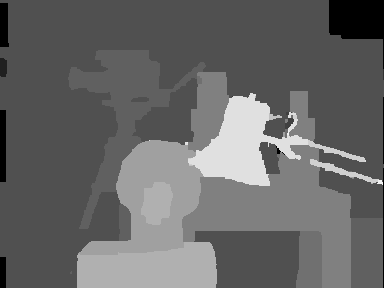
\includegraphics{pics/disparity.png}

\cvCPyFunc{POSIT}
Implements the POSIT algorithm.

\cvdefC{
void cvPOSIT( \par CvPOSITObject* posit\_object,\par CvPoint2D32f* imagePoints,\par double focal\_length,\par CvTermCriteria criteria,\par CvMatr32f rotationMatrix,\par CvVect32f translation\_vector );
}\cvdefPy{POSIT(posit\_object,imagePoints,focal\_length,criteria)-> rotationMatrix,translation\_vector}

\begin{description}
\cvarg{posit\_object}{Pointer to the object structure}
\cvarg{imagePoints}{Pointer to the object points projections on the 2D image plane}
\cvarg{focal\_length}{Focal length of the camera used}
\cvarg{criteria}{Termination criteria of the iterative POSIT algorithm}
\cvarg{rotationMatrix}{Matrix of rotations}
\cvarg{translation\_vector}{Translation vector}
\end{description}

The function implements the POSIT algorithm. Image coordinates are given in a camera-related coordinate system. The focal length may be retrieved using the camera calibration functions. At every iteration of the algorithm a new perspective projection of the estimated pose is computed.

Difference norm between two projections is the maximal distance between corresponding points. The parameter \texttt{criteria.epsilon} serves to stop the algorithm if the difference is small.

\ifC
\cvCPyFunc{ProjectPoints2}
Projects 3D points on to an image plane.

\cvdefC{
void cvProjectPoints2( \par const CvMat* objectPoints,\par const CvMat* rotation\_vector,\par const CvMat* translation\_vector,\par const CvMat* intrinsicMatrix,\par const CvMat* distortionCoeffs,\par CvMat* imagePoints,\par CvMat* dpdrot=NULL,\par CvMat* dpdt=NULL,\par CvMat* dpdf=NULL,\par CvMat* dpdc=NULL,\par CvMat* dpddist=NULL );
}\cvdefPy{ProjectPoints2(objectPoints,rotation\_vector,translation\_vector,intrinsicMatrix,distortionCoeffs, imagePoints,dpdrot=NULL,dpdt=NULL,dpdf=NULL,dpdc=NULL,dpddist=NULL)-> None}

\begin{description}
\cvarg{objectPoints}{The array of object points, 3xN or Nx3, where N is the number of points in the view}
\cvarg{rotation\_vector}{The rotation vector, 1x3 or 3x1}
\cvarg{translation\_vector}{The translation vector, 1x3 or 3x1}
\cvarg{intrinsicMatrix}{The camera matrix $A = \vecthreethree{fx}{0}{cx}{0}{fy}{cy}{0}{0}{1} $}
\cvarg{distortionCoeffs}{The input 4x1, 1x4, 5x1 or 1x5 vector of distortion coefficients \hyperref[k123p12]{$(k_1, k_2, p_1, p_2[, k_3])$}. If it is NULL, all of the distortion coefficients are considered 0's}
\cvarg{imagePoints}{The output array of image points, 2xN or Nx2, where N is the total number of points in the view}
\cvarg{dpdrot}{Optional Nx3 matrix of derivatives of image points with respect to components of the rotation vector}
\cvarg{dpdt}{Optional Nx3 matrix of derivatives of image points with respect to components of the translation vector}
\cvarg{dpdf}{Optional Nx2 matrix of derivatives of image points with respect to $fx$ and $fy$}
\cvarg{dpdc}{Optional Nx2 matrix of derivatives of image points with respect to $cx$ and $cy$}
\cvarg{dpddist}{Optional Nx4 matrix of derivatives of image points with respect to distortion coefficients}
\end{description}

The function computes projections of 3D
points to the image plane given intrinsic and extrinsic camera
parameters. Optionally, the function computes jacobians - matrices
of partial derivatives of image points as functions of all the
input parameters with respect to the particular parameters, intrinsic and/or
extrinsic. The jacobians are used during the global optimization
in \cvCPyCross{CalibrateCamera2} and
\cvCPyCross{FindExtrinsicCameraParams2}. The
function itself is also used to compute back-projection error for with
current intrinsic and extrinsic parameters.

Note, that with intrinsic and/or extrinsic parameters set to special
values, the function can be used to compute just an extrinsic transformation
or just an intrinsic transformation (i.e. distortion of a sparse set
of points).

\cvCPyFunc{RQDecomp3x3}
Computes the `RQ' decomposition of 3x3 matrices.

\cvdefC{
void cvRQDecomp3x3( \par const CvMat *matrixM,\par CvMat *matrixR,\par CvMat *matrixQ,\par CvMat *matrixQx=NULL,\par CvMat *matrixQy=NULL,\par CvMat *matrixQz=NULL,\par CvPoint3D64f *eulerAngles=NULL);
}\cvdefPy{RQDecomp3x3(matrixM, matrixR, matrixQ, matrixQx = None, matrixQy = None, matrixQz = None) -> eulerAngles}

\begin{description}
\cvarg{matrixM}{The 3x3 input matrix M}
\cvarg{matrixR}{The output 3x3 upper-triangular matrix R}
\cvarg{matrixQ}{The output 3x3 orthogonal matrix Q}
\cvarg{matrixQx}{Optional 3x3 rotation matrix around x-axis}
\cvarg{matrixQy}{Optional 3x3 rotation matrix around y-axis}
\cvarg{matrixQz}{Optional 3x3 rotation matrix around z-axis}
\cvarg{eulerAngles}{Optional 3 points containing the three Euler angles of rotation}
\end{description}

The function computes a RQ decomposition using the given rotations. This function is used in \cvCPyCross{DecomposeProjectionMatrix} to decompose the left 3x3 submatrix of a projection matrix into a calibration and a rotation matrix.

It optionally returns three rotation matrices, one for each axis, and the three Euler angles that could be used in OpenGL.


\cvCPyFunc{ReleasePOSITObject}
Deallocates a 3D object structure.

\cvdefC{
void cvReleasePOSITObject( \par CvPOSITObject** posit\_object );
}

\begin{description}
\cvarg{posit\_object}{Double pointer to \texttt{CvPOSIT} structure}
\end{description}

The function releases memory previously allocated by the function \cvCPyCross{CreatePOSITObject}.

\fi

\cvCPyFunc{ReleaseStereoBMState}
Releases block matching stereo correspondence structure.

\cvdefC{

void cvReleaseStereoBMState( CvStereoBMState** state );

}\cvdefPy{ReleaseStereoBMState(state)-> None}

\begin{description}
\cvarg{state}{Double pointer to the released structure.}
\end{description}

The function releases the stereo correspondence structure and all the associated internal buffers. 

\cvCPyFunc{ReleaseStereoGCState}
Releases the state structure of the graph cut-based stereo correspondence algorithm.

\cvdefC{

void cvReleaseStereoGCState( CvStereoGCState** state );

}\cvdefPy{ReleaseStereoGCState(state)-> None}

\begin{description}
\cvarg{state}{Double pointer to the released structure.}
\end{description}

The function releases the stereo correspondence structure and all the associated internal buffers. 


\cvCPyFunc{Rodrigues2}
Converts a rotation matrix to a rotation vector or vice versa.

\cvdefC{
int  cvRodrigues2( \par const CvMat* src,\par CvMat* dst,\par CvMat* jacobian=0 );
}\cvdefPy{Rodrigues2(src,dst,jacobian=0)-> None}

\begin{description}
\cvarg{src}{The input rotation vector (3x1 or 1x3) or rotation matrix (3x3)}
\cvarg{dst}{The output rotation matrix (3x3) or rotation vector (3x1 or 1x3), respectively}
\cvarg{jacobian}{Optional output Jacobian matrix, 3x9 or 9x3 - partial derivatives of the output array components with respect to the input array components}
\end{description}

The function converts a rotation vector to a rotation matrix or vice versa. A rotation vector is a compact representation of rotation matrix. Direction of the rotation vector is the rotation axis and the length of the vector is the rotation angle around the axis. The rotation matrix $R$, corresponding to the rotation vector $r$, is computed as following:

\[
\begin{array}{l}
\theta \leftarrow norm(r)\\
r \leftarrow r/\theta\\
R = \cos{\theta} I + (1-\cos{\theta}) r r^T + \sin{\theta}
\vecthreethree
{0}{-r_z}{r_y}
{r_z}{0}{-r_x}
{-r_y}{r_x}{0}
\end{array}
\]

Inverse transformation can also be done easily as

\[
\sin(\theta)
\vecthreethree
{0}{-r_z}{r_y}
{r_z}{0}{-r_x}
{-r_y}{r_x}{0}
=
\frac{R - R^T}{2}
\]

A rotation vector is a convenient representation of a rotation matrix
as a matrix with only 3 degrees of freedom. The representation is
used in the global optimization procedures inside
\cvCPyCross{FindExtrinsicCameraParams2}
and \cvCPyCross{CalibrateCamera2}.


\cvCPyFunc{StereoCalibrate}
Calibrates stereo camera.

\cvdefC{

void cvStereoCalibrate( \par const CvMat* objectPoints, \par const CvMat* imagePoints1,
                        \par const CvMat* imagePoints2, \par const CvMat* pointCounts,
                        \par CvMat* cameraMatrix1, \par CvMat* distCoeffs1,
                        \par CvMat* cameraMatrix2, \par CvMat* distCoeffs2,
                       \par CvSize imageSize, \par CvMat* R, \par CvMat* T,
                        \par CvMat* E=0, \par CvMat* F=0,
                        \par CvTermCriteria term\_crit=cvTermCriteria(
                               \par CV\_TERMCRIT\_ITER+CV\_TERMCRIT\_EPS,30,1e-6),
                        \par int flags=CV\_CALIB\_FIX\_INTRINSIC );

}\cvdefPy{StereoCalibrate(\par objectPoints,\par imagePoints1,\par imagePoints2,\par pointCounts,\par cameraMatrix1,\par distCoeffs1,\par cameraMatrix2,\par distCoeffs2,\par imageSize,\par R,\par T,\par E=NULL,\par F=NULL,\par term\_crit=cvTermCriteria(CV\_TERMCRIT\_ITER+CV\_TERMCRIT\_EPS,30,1e-6),\par flags=CV\_CALIB\_FIX\_INTRINSIC)-> None}

\begin{description}
\cvarg{objectPoints}{The joint matrix of object points, 3xN or Nx3, where N is the total number of points in all views.}
\cvarg{imagePoints1}{The joint matrix of corresponding image points in the views from the 1st camera, 2xN or Nx2, where N is the total number of points in all views.}
\cvarg{imagePoints2}{The joint matrix of corresponding image points in the views from the 2nd camera, 2xN or Nx2, where N is the total number of points in all views.}
\cvarg{pointCounts}{Vector containing numbers of points in each view, 1xM or Mx1, where M is the number of views.}
\cvarg{cameraMatrix1, cameraMatrix2}{The input/output camera matrices $[{f_x}^(j) 0 {c_x}^(j); 0 {f_y}^(j) {c_y}^(j); 0 0 1]$. If \texttt{CV\_CALIB\_USE\_INTRINSIC\_GUESS} or \texttt{CV\_CALIB\_FIX\_ASPECT\_RATIO} are specified, some or all of the elements of the matrices must be initialized.}
\cvarg{distCoeffs1, distCoeffs2}{The input/output vectors of distortion coefficients for each camera, \hyperref[k123p12]{${k_1}^(j), {k_2}^(j), {p_1}^(j), {p_2}^(j) [, {k_3}^(j)]$}}
\cvarg{imageSize}{Size of the image, used only to initialize intrinsic camera matrix.} 
\cvarg{R}{The rotation matrix between the 1st and the 2nd cameras' coordinate systems.}
\cvarg{T}{The translation vector between the cameras' coordinate systems.}
\cvarg{E}{The optional output essential matrix.}
\cvarg{F}{The optional output fundamental matrix.}
\cvarg{term\_crit}{Termination criteria for the iterative optimiziation algorithm.}
\cvarg{flags}{Different flags, may be 0 or combination of the following values:
\begin{description}
\cvarg{CV\_CALIB\_FIX\_INTRINSIC}{If it is set, \texttt{cameraMatrix1,2}, as well as \texttt{distCoeffs1,2} are fixed, so that only extrinsic parameters are optimized.}
\cvarg{CV\_CALIB\_USE\_INTRINSIC\_GUESS}{The flag allows the function to optimize some or all of the intrinsic parameters, depending on the other flags, but the initial values are provided by the user.}
\cvarg{CV\_CALIB\_FIX\_PRINCIPAL\_POINT}{The principal points are fixed during the optimization.}
\cvarg{CV\_CALIB\_FIX\_FOCAL\_LENGTH}{${f_x}^(j)$ and ${f_y}^(j)$ are fixed.}
\cvarg{CV\_CALIB\_FIX\_ASPECT\_RATIO}{${f_y}^(j)$ is optimized, but the ratio ${fx}_k/{fy}_k$ is fixed.}
\cvarg{CV\_CALIB\_SAME\_FOCAL\_LENGTH}{Enforces ${f_x}^(0)={f_x}^(1)$ and ${f_y}^(0)={f_y}^(1)$. \texttt{CV\_CALIB\_ZERO\_TANGENT\_DIST} - Tangential distortion coefficients for each camera are set to zeros and fixed there.}
\cvarg{CV\_CALIB\_FIX\_K1}{The 0-th distortion coefficients (k1) are fixed.}
\cvarg{CV\_CALIB\_FIX\_K2}{The 1-st distortion coefficients (k2) are fixed.}
\cvarg{CV\_CALIB\_FIX\_K3}{The 4-th distortion coefficients (k3) are fixed.}
\end{description}}
\end{description}

The function estimates transformation between the 2 cameras making a stereo pair. If we have a stereo camera, where the relative position and orientatation of the 2 cameras is fixed, and if we computed poses of an object relative to the fist camera and to the second camera, (R1, T1) and (R2, T2), respectively (that can be done with \cvCPyCross{cvFindExtrinsicCameraParams2}), obviously, those poses will relate to each other, i.e. given ($R_1$, $T_1$) it should be possible to compute ($R_2$, $T_2$) - we only need to know the position and orientation of the 2nd camera relative to the 1st camera. That's what the described function does. It computes ($R$, $T$) such that:

\[
R_2=R*R_1
T_2=R*T_1 + T,
\]

Optionally, it computes the essential matrix E:

\[
E=
\vecthreethree
{0}{-T_2}{T_1}
{T_2}{0}{-T_0}
{-T_1}{T_0}{0}
*R
\]

where $T_i$ are components of the translation vector $T$: $T=[T_0, T_1, T_2]^T$. And also the function can compute the fundamental matrix F:

$F = inv(cameraMatrix2)^T*E*inv(cameraMatrix1)$

Besides the stereo-related information, the function can also perform full calibration of each of the 2 cameras. However, because of the high dimensionality of the parameter space and noise in the input data the function can diverge from the correct solution. Thus, if intrinsic parameters can be estimated with high accuracy for each of the cameras individually (e.g. using \cvCPyCross{cvCalibrateCamera2}), it is recommended to do so and then pass \texttt{CV\_CALIB\_FIX\_INTRINSIC} flag to the function along with the computed intrinsic parameters. Otherwise, if all the parameters are estimated at once, it makes sense to restrict some parameters, e.g. pass \texttt{CV\_CALIB\_SAME\_FOCAL\_LENGTH} and \texttt{CV\_CALIB\_ZERO\_TANGENT\_DIST} flags, which are usually reasonable assumptions. 

\cvCPyFunc{StereoRectify}
Computes rectification transform for stereo camera.

\cvdefC{void cvStereoRectify( \par const CvMat* cameraMatrix1, \par const CvMat* cameraMatrix2,
                      \par const CvMat* distCoeffs1, \par const CvMat* distCoeffs2,
                      \par CvSize imageSize, \par const CvMat* R, \par const CvMat* T,
                      \par CvMat* R1, \par CvMat* R2, \par CvMat* P1, \par CvMat* P2,
                      \par CvMat* Q=0, \par int flags=CV\_CALIB\_ZERO\_DISPARITY );}
\cvdefPy{StereoRectify(\par cameraMatrix1,\par cameraMatrix2,\par distCoeffs1,\par distCoeffs2,\par imageSize,\par R,\par T,\par R1,\par R2,\par P1,\par P2,\par Q=NULL,\par flags=CV\_CALIB\_ZERO\_DISPARITY)-> None}

\begin{description}
\cvarg{cameraMatrix1, cameraMatrix2}{The camera matrices $[{f_x}^(j) 0 {c_x}^(j); 0 {f_y}^(j) {c_y}^(j); 0 0 1]$.}
\cvarg{distCoeffs1, distCoeffs2}{The input distortion coefficients for each camera, \hyperref[k123p12]{${k_1}^(j), {k_2}^(j), {p_1}^(j), {p_2}^(j) [, {k_3}^(j)]$}}
\cvarg{imageSize}{Size of the image used for stereo calibration.}
\cvarg{R}{The rotation matrix between the 1st and the 2nd cameras' coordinate systems.}
\cvarg{T}{The translation vector between the cameras' coordinate systems.}
\cvarg{R1, R2}{3x3 Rectification transforms (rotation matrices) for the first and the second cameras, respectively.}
\cvarg{P1, P2}{3x4 Projection matrices in the new (rectified) coordinate systems.}
\cvarg{Q}{The optional output disparity-to-depth mapping matrix, 4x4, see \cvCPyCross{cvReprojectImageTo3D}.}
\cvarg{flags}{The operation flags; may be 0 or \texttt{CV\_CALIB\_ZERO\_DISPARITY}. If the flag is set, the function makes the principal points of each camera have the same pixel coordinates in the rectified views. And if the flag is not set, the function can shift one of the image in horizontal or vertical direction (depending on the orientation of epipolar lines) in order to maximise the useful image area. }
\end{description}

The function computes the rotation matrices for each camera that (virtually) make both camera image planes the same plane. Consequently, that makes all the epipolar lines parallel and thus simplifies the dense stereo correspondence problem. On input the function takes the matrices computed by \cvCPyCross{cvStereoCalibrate} and on output it gives 2 rotation matrices and also 2 projection matrices in the new coordinates. The function is normally called after \cvCPyCross{cvStereoCalibrate} that computes both camera matrices, the distortion coefficients, R and T. The 2 cases are distinguished by the function: 

\begin{enumerate}
\item Horizontal stereo, when 1st and 2nd camera views are shifted relative to each other mainly along the x axis (with possible small vertical shift). Then in the rectified images the corresponding epipolar lines in left and right cameras will be horizontal and have the same y-coordinate. P1 and P2 will look as: 

\[
P1=
\begin{bmatrix}
f & 0 & cx1 & 0\\
0 & f & cy & 0\\
0 & 0 & 1 & 0
\end{bmatrix}
\]
\[
P2=
\begin{bmatrix}
f & 0 & cx2 & Tx*f\\
0 & f & cy & 0\\
0 & 0 & 1 & 0
\end{bmatrix}
,
\]

where $T_x$ is horizontal shift between the cameras and cx1=cx2 if \texttt{CV\_CALIB\_ZERO\_DISPARITY} is set.
\item Vertical stereo, when 1st and 2nd camera views are shifted relative to each other mainly in vertical direction (and probably a bit in the horizontal direction too). Then the epipolar lines in the rectified images will be vertical and have the same x coordinate. P1 and P2 will look as:

\[
P1=
\begin{bmatrix}
f & 0 & cx & 0\\
0 & f & cy1 & 0\\
0 & 0 & 1 & 0
\end{bmatrix}
\]
\[
P2=
\begin{bmatrix}
f & 0 & cx & 0\\
0 & f & cy2 & Ty*f\\
0 & 0 & 1 & 0
\end{bmatrix}
,
\]

where $T_y$ is vertical shift between the cameras and cy1=cy2 if \texttt{CV\_CALIB\_ZERO\_DISPARITY} is set.
\end{enumerate} 

As you can see, the first 3 columns of P1 and P2 will effectively be the new "rectified" camera matrices. 

\cvCPyFunc{StereoRectifyUncalibrated}
Computes rectification transform for uncalibrated stereo camera.

\cvdefC{

void cvStereoRectifyUncalibrated( \par const CvMat* points1, \par const CvMat* points2,
                                  \par const CvMat* F, \par CvSize imageSize,
                                  \par CvMat* H1, \par CvMat* H2,
                                  \par double threshold=5 );

}\cvdefPy{StereoRectifyUncalibrated(points1,points2,F,imageSize,H1,H2,threshold=5)-> None}

\begin{description}
\cvarg{points1, points2}{The 2 arrays of corresponding 2D points.}
\cvarg{F}{Fundamental matrix. It can be computed using the same set of point pairs points1 and points2  using \cvCPyCross{cvFindFundamentalMat}.}
\cvarg{imageSize}{Size of the image.}
\cvarg{H1, H2}{The rectification homography matrices for the first and for the second images.}
\cvarg{threshold}{Optional threshold used to filter out the outliers. If the parameter is greater than zero, then all the point pairs that do not comply the epipolar geometry well enough (that is, the points for which $fabs(points2[i]^T*F*points1[i])>threshold$) are rejected prior to computing the homographies. }
\end{description}

The function computes the rectification transformations without knowing intrinsic parameters of the cameras and their relative position in space, hence the suffix "Uncalibrated". Another related difference from \cvCPyCross{cvStereoRectify} is that the function outputs not the rectification transformations in the object (3D) space, but the planar perspective transformations, encoded by the homography matrices H1 and H2. The function implements the following algorithm \href{\#Hartly99}{[Hartley99]}. 

Note that while the algorithm does not need to know the intrinsic parameters of the cameras, it heavily depends on the epipolar geometry. Therefore, if the camera lenses have significant distortion, it would better be corrected before computing the fundamental matrix and calling this function. For example, distortion coefficients can be estimated for each head of stereo camera separately by using \cvCPyCross{cvCalibrateCamera2} and then the images can be corrected using \cvCPyCross{cvUndistort2}. 

\cvCPyFunc{UndistortPoints}
Computes the ideal point coordinates from the observed point coordinates.

\cvdefC{void cvUndistortPoints( \par const CvMat* src, \par CvMat* dst,
                        \par const CvMat* cameraMatrix,
                        \par const CvMat* distCoeffs,
                        \par const CvMat* R=NULL,
                        \par const CvMat* P=NULL);}
\cvdefPy{UndistortPoints(src,dst,cameraMatrix,distCoeffs,R=NULL,P=NULL)-> None}

\begin{description}
\cvarg{src}{The observed point coordinates}
\cvarg{dst}{The ideal point coordinates, after undistortion and reverse perspective transformation}
\cvarg{cameraMatrix}{The camera matrix $A=[fx 0 cx; 0 fy cy; 0 0 1]$}
\cvarg{distCoeffs}{he vector of distortion coefficients, \cvCPyCross{4x1, 1x4, 5x1 or 1x5}}
\cvarg{R}{The rectification transformation in object space (3x3 matrix). \texttt{R1} or \texttt{R2}, computed by \cvCPyCross{StereoRectify} can be passed here. If the parameter is NULL, the identity matrix is used}
\cvarg{P}{The new camera matrix (3x3) or the new projection matrix (3x4). \texttt{P1} or \texttt{P2}, computed by \cvCPyCross{StereoRectify} can be passed here. If the parameter is NULL, the identity matrix is used}
\end{description}

The function is similar to \cvCPyCross{InitUndistortRectifyMap} and is opposite to it at the same time. The functions are similar in that they both are used to correct lens distortion and to perform the optional perspective (rectification) transformation. They are opposite because the function \cvCPyCross{InitUndistortRectifyMap} does actually perform the reverse transformation in order to initialize the maps properly, while this function does the forward transformation. That is, in pseudo-code it can be expressed as:

\begin{lstlisting}
// (u,v) is the input point, (u', v') is the output point
// camera_matrix=[fx 0 cx; 0 fy cy; 0 0 1]
// P=[fx' 0 cx' tx; 0 fy' cy' ty; 0 0 1 tz]
x" = (u - cx)/fx
y" = (v - cy)/fy
(x',y') = undistort(x",y",dist_coeffs)
[X,Y,W]T = R*[x' y' 1]T
x = X/W, y = Y/W
u' = x*fx' + cx'
v' = y*fy' + cy',
\end{lstlisting}

where undistort() is approximate iterative algorithm that estimates the normalized original point coordinates out of the normalized distorted point coordinates ("normalized" means that the coordinates do not depend on the camera matrix).

The function can be used as for stereo cameras, as well as for individual cameras when R=NULL. 

\fi


\ifCpp

\cvCppFunc{calibrateCamera}
Finds the camera matrix and the camera poses from several views of the calibration pattern.

\cvdefCpp{void calibrateCamera( const vector<vector<Point3f> >\& objectPoints,\par
                      const vector<vector<Point2f> >\& imagePoints,\par
                      Size imageSize,\par
                      Mat\& cameraMatrix, Mat\& distCoeffs,\par
                      vector<Mat>\& rvecs, vector<Mat>\& tvecs,\par
                      int flags=0 );}
\begin{description}
\cvarg{objectPoints}{The vector of vectors of points on the calibration rig in its coordinate system, one vector per a view of the rig. If the the same calibration rig is shown in each view and it's fully visible, all the vectors can be the same (though, you may change the numbering from one view to another). The points are 3D, but since they are in the rig coordinate system, then if the rig is planar, it may have sense to put the model to the XY coordinate plane, so that Z-coordinate of each input object point is 0}
\cvarg{imagePoints}{The vector of vectors of the object point projections on the calibration rig views, one vector per a view. The projections must be in the same order as the corresponding object points.}
\cvarg{imageSize}{Size of the image, used only to initialize the intrinsic camera matrix}
\cvarg{cameraMatrix}{The input/output matrix of intrinsic camera parameters $A = \vecthreethree{fx}{0}{cx}{0}{fy}{cy}{0}{0}{1}$. If any of \texttt{CALIB\_USE\_INTRINSIC\_GUESS}, \texttt{CALIB\_FIX\_ASPECT\_RATIO}, \texttt{CALIB\_FIX\_FOCAL\_LENGTH} are specified, some or all of \texttt{fx, fy, cx, cy} must be initialized}
\cvarg{distCoeffs}{The input/output lens distortion coefficients, 4x1, 5x1, 1x4 or 1x5 floating-point vector $(k_1, k_2, p_1, p_2[, k_3])$. If any of \texttt{CALIB\_FIX\_K1}, \texttt{CALIB\_FIX\_K2} or \texttt{CALIB\_FIX\_K3} is specified, then the corresponding elements of \texttt{distCoeffs} must be initialized.}
\cvarg{rvecs}{The output vector of rotation vectors (see \cvCppCross{Rodrigues}) estimated for each camera view}
\cvarg{tvecsrans}{The output vector of translation vectors estimated for each camera view}
\cvarg{flags}{Different flags, may be 0 or a combination of the following values:
\begin{description}
\cvarg{CALIB\_USE\_INTRINSIC\_GUESS}{\texttt{cameraMatrix} contains the valid initial values of \texttt{fx, fy, cx, cy} that are optimized further. Otherwise, \texttt{(cx, cy)} is initially set to the image center (computed from the input \texttt{imageSize}), and focal distances are computed in some least-squares fashion. Note, that if the focal distance initialization is currently supported only for planar calibration rigs. That is, if the calibration rig is 3D, then you must initialize \texttt{cameraMatrix} and pass \texttt{CALIB\_USE\_INTRINSIC\_GUESS} flag. Also, note that distortion coefficients are not regulated by this function; use \texttt{CALIB\_ZERO\_TANGENT\_DIST} and \texttt{CALIB\_FIX\_K?} to fix them}
\cvarg{CALIB\_FIX\_PRINCIPAL\_POINT}{The principal point is not changed during the global optimization, it stays at the center or, when \texttt{CALIB\_USE\_INTRINSIC\_GUESS} is set too, at the other specified location}
\cvarg{CALIB\_FIX\_ASPECT\_RATIO}{The optimization procedure considers only one of \texttt{fx} and \texttt{fy} as independent variables and keeps the aspect ratio \texttt{fx/fy} the same as it was set initially in the input \texttt{cameraMatrix}. In this case the actual initial values of \texttt{(fx, fy)} are either taken from the matrix (when \texttt{CALIB\_USE\_INTRINSIC\_GUESS} is set) or estimated.}
\cvarg{CALIB\_ZERO\_TANGENT\_DIST}{Tangential distortion coefficients are set to zeros and do not change during the optimization.}
\cvarg{CALIB\_FIX\_FOCAL\_LENGTH}{Both \texttt{fx} and \texttt{fy} are fixed (taken from \texttt{cameraMatrix} and do not change during the optimization.}
\cvarg{CALIB\_FIX\_K1, CALIB\_FIX\_K2, CALIB\_FIX\_K3}{The particular distortion coefficients is read from the input \texttt{distCoeffs} and stays the same during optimization}
\end{description}}
\end{description}

The function estimates the intrinsic camera
parameters and the extrinsic parameters for each of the views. The
coordinates of 3D object points and their correspondent 2D projections
in each view must be specified. You can use a calibration rig with a known geometry and easily and precisely detectable feature points, e.g. a checkerboard (see \cvCppCross{findChessboardCorners}).

The algorithm does the following:
\begin{enumerate}
    \item First, it computes the initial intrinsic parameters (only for planar calibration rigs) or reads them from the input parameters. The distortion coefficients are all set to zeros initially (unless some of \texttt{CALIB\_FIX\_K?} are specified).
    \item The the initial camera pose is estimated as if the intrinsic parameters have been already known. This is done using \cvCppCross{solvePnP}
    \item After that the global Levenberg-Marquardt optimization algorithm is run to minimize the reprojection error, i.e. the total sum of squared distances between the observed feature points \texttt{imagePoints} and the projected (using the current estimates for camera parameters and the poses) object points \texttt{objectPoints}; see \cvCppCross{projectPoints}.
\end{enumerate}

Note: if you're using a non-square (=non-NxN) grid and
\cvCppCross{findChessboardCorners} for calibration, and \texttt{calibrateCamera} returns
bad values (i.e. zero distortion coefficients, an image center very far from
$(w/2-0.5,h/2-0.5)$, and / or large differences between $f_x$ and $f_y$ (ratios of
10:1 or more)), then you've probaby used \texttt{patternSize=cvSize(rows,cols)},
but should use \texttt{patternSize=cvSize(cols,rows)} in \cvCppCross{findChessboardCorners}.

See also: \cvCppCross{findChessboardCorners}, \cvCppCross{solvePnP}, \cvCppCross{initCameraMatrix2D}, \cvCppCross{stereoCalibrate}, \cvCppCross{undistort}


\cvCppFunc{calibrationMatrixValues}
Computes some useful camera characteristics from the camera matrix

\cvdefCpp{void calibrationMatrixValues( const Mat\& cameraMatrix,\par
                              Size imageSize,\par
                              double apertureWidth,\par
                              double apertureHeight,\par
                              double\& fovx,\par
                              double\& fovy,\par
                              double\& focalLength,\par
                              Point2d\& principalPoint,\par
                              double\& aspectRatio );}
\begin{description}
\cvarg{cameraMatrix}{The input camera matrix that can be estimated by \cvCppCross{calibrateCamera} or \cvCppCross{stereoCalibrate}}
\cvarg{imageSize}{The input image size in pixels}
\cvarg{apertureWidth}{Physical width of the sensor}
\cvarg{apertureHeight}{Physical height of the sensor}
\cvarg{fovx}{The output field of view in degrees along the horizontal sensor axis}
\cvarg{fovy}{The output field of view in degrees along the vertical sensor axis}
\cvarg{focalLength}{The focal length of the lens in mm}
\cvarg{prinicialPoint}{The principal point in pixels}
\cvarg{aspectRatio}{$f_y/f_x$}
\end{description}

The function computes various useful camera characteristics from the previously estimated camera matrix.

\cvCppFunc{composeRT}
Combines two rotation-and-shift transformations

\cvdefCpp{void composeRT( const Mat\& rvec1, const Mat\& tvec1,\par
                const Mat\& rvec2, const Mat\& tvec2,\par
                Mat\& rvec3, Mat\& tvec3 );\newline
void composeRT( const Mat\& rvec1, const Mat\& tvec1,\par
                const Mat\& rvec2, const Mat\& tvec2,\par
                Mat\& rvec3, Mat\& tvec3,\par
                Mat\& dr3dr1, Mat\& dr3dt1,\par
                Mat\& dr3dr2, Mat\& dr3dt2,\par
                Mat\& dt3dr1, Mat\& dt3dt1,\par
                Mat\& dt3dr2, Mat\& dt3dt2 );}
\begin{description}
\cvarg{rvec1}{The first rotation vector}
\cvarg{tvec1}{The first translation vector}
\cvarg{rvec2}{The second rotation vector}
\cvarg{tvec2}{The second translation vector}
\cvarg{rvec3}{The output rotation vector of the superposition}
\cvarg{tvec3}{The output translation vector of the superposition}
\cvarg{d??d??}{The optional output derivatives of \texttt{rvec3} or \texttt{tvec3} w.r.t. \texttt{rvec?} or \texttt{tvec?}}
\end{description}

The functions compute:

\[ \begin{array}{l}
\texttt{rvec3} = \mathrm{rodrigues}^{-1}\left(\mathrm{rodrigues}(\texttt{rvec2}) \cdot
\mathrm{rodrigues}(\texttt{rvec1})\right) \\
\texttt{tvec3} = \mathrm{rodrigues}(\texttt{rvec2}) \cdot \texttt{tvec1} + \texttt{tvec2}
\end{array}, \]

where $\mathrm{rodrigues}$ denotes a rotation vector to rotation matrix transformation, and $\mathrm{rodrigues}^{-1}$ denotes the inverse transformation, see \cvCppCross{Rodrigues}.

Also, the functions can compute the derivatives of the output vectors w.r.t the input vectors (see \cvCppCross{matMulDeriv}).
The functions are used inside \cvCppCross{stereoCalibrate} but can also be used in your own code where Levenberg-Marquardt or another gradient-based solver is used to optimize a function that contains matrix multiplication.


\cvCppFunc{computeCorrespondEpilines}
For points in one image of a stereo pair, computes the corresponding epilines in the other image.

\cvdefCpp{void computeCorrespondEpilines( const Mat\& points,\par
                                int whichImage, const Mat\& F,\par
                                vector<Vec3f>\& lines );}
\begin{description}
\cvarg{points}{The input points. $N \times 1$ or $1 \times N$ matrix of type \texttt{CV\_32FC2} or \texttt{vector<Point2f>}}
\cvarg{whichImage}{Index of the image (1 or 2) that contains the \texttt{points}}
\cvarg{F}{The fundamental matrix that can be estimated using \cvCppCross{findFundamentalMat} or \texttt{stereoRectify}}
\cvarg{lines}{The output vector of the corresponding to the points epipolar lines in the other image. Each line $ax + by + c=0$ is encoded as 3-element vector $(a, b, c)$}
\end{description}

For every point in one of the two images of a stereo-pair the function
\texttt{computeCorrespondEpilines} finds the equation of the
corresponding epipolar line in the other image.

From the fundamental matrix definition (see \cvCppCross{findFundamentalMatrix}),
line $l^{(2)}_i$ in the second image for the point $p^{(1)}_i$ in the first image (i.e. when \texttt{whichImage=1}) is computed as:

\[ l^{(2)}_i = F p^{(1)}_i \]

and, vice versa, when \texttt{whichImage=2}, $l^{(1)}_i$ is computed from $p^{(2)}_i$ as:

\[ l^{(1)}_i = F^T p^{(2)}_i \]

Line coefficients are defined up to a scale. They are normalized, such that $a_i^2+b_i^2=1$.

\cvCppFunc{convertPointHomogeneous}
Converts 2D points to/from homogeneous coordinates.

\cvdefCpp{void convertPointsHomogeneous( const Mat\& src, vector<Point3f>\& dst );\newline
void convertPointsHomogeneous( const Mat\& src, vector<Point2f>\& dst );}

\begin{description}
\cvarg{src}{The input array or vector of 2D or 3D points}
\cvarg{dst}{The output vector of 3D or 2D points, respectively}
\end{description}

The first of the functions converts 2D points to the homogeneous coordinates by adding extra \texttt{1} component to each point. When the input vector already contains 3D points, it is simply copied to \texttt{dst}. The second function converts 3D points to 2D points by dividing 1st and 2nd components by the 3rd one. If the input vector already contains 2D points, it is simply copied to \texttt{dst}.

\cvCppFunc{decomposeProjectionMatrix}
Decomposes the projection matrix into a rotation matrix and a camera matrix.

\cvdefCpp{void decomposeProjectionMatrix( const Mat\& projMatrix,\par
                                Mat\& cameraMatrix,\par
                                Mat\& rotMatrix, Mat\& transVect );\newline
void decomposeProjectionMatrix( const Mat\& projMatrix, \par
                                Mat\& cameraMatrix,\par
                                Mat\& rotMatrix, Mat\& transVect,\par
                                Mat\& rotMatrixX, Mat\& rotMatrixY,\par
                                Mat\& rotMatrixZ, Vec3d\& eulerAngles );}
\begin{description}
\cvarg{projMatrix}{The input $3 \times 4$ projection matrix}
\cvarg{cameraMatrix}{The output $3 \times 3$ camera matrix}
\cvarg{rotMatrix}{The output $3 \times 3$ rotation matrix}
\cvarg{transVect}{The output $3 \times 1$ translation vector}
\cvarg{rotMatrixX}{The optional output rotation matrix around x-axis}
\cvarg{rotMatrixY}{The optional output rotation matrix around y-axis}
\cvarg{rotMatrixZ}{The optional output rotation matrix around z-axis}
\cvarg{eulerAngles}{The optional output 3-vector of the Euler rotation angles}
\end{description}

The function computes a decomposition of a projection matrix into a calibration and a rotation matrix and the position of the camera.

It optionally returns three rotation matrices, one for each axis, and the three Euler angles that could be used in OpenGL.

The function is based on \cvCppCross{RQDecomp3x3}.

\cvCppFunc{drawChessboardCorners}
Draws the detected chessboard corners.

\cvdefCpp{void drawChessboardCorners( Mat\& image, Size patternSize,\par
                            const Mat\& corners,\par
                            bool patternWasFound );}
\begin{description}
\cvarg{image}{The destination image; it must be an 8-bit color image}
\cvarg{patternSize}{The number of inner corners per chessboard row and column, i.e. \texttt{Size(<corners per row>, <corners per column>)}}
\cvarg{corners}{The array of detected corners; \texttt{vector<Point2f>} can be passed here as well}
\cvarg{patternWasFound}{Indicates whether the complete board was found. Just pass the return value of \cvCppCross{findChessboardCorners} here}
\end{description}

The function draws the detected chessboard corners. If no complete board was found, the detected corners will be marked with small red circles. Otherwise, a colored board (each board row with a different color) will be drawn.

\cvCppFunc{findFundamentalMat}
Calculates the fundamental matrix from the corresponding points in two images.

\cvdefCpp{Mat findFundamentalMat( const Mat\& points1, const Mat\& points2,\par
                        vector<uchar>\& mask, int method=FM\_RANSAC,\par
                        double param1=3., double param2=0.99 );\newline
Mat findFundamentalMat( const Mat\& points1, const Mat\& points2,\par
                        int method=FM\_RANSAC,\par
                        double param1=3., double param2=0.99 );}
\begin{description}
\cvarg{points1}{Array of $N$ points in the first image, a matrix of \texttt{CV\_32FC2} type or \texttt{vector<Point2f>}. The points in homogeneous coordinates can also be passed.}
\cvarg{points2}{Array of the corresponding points in the second image of the same size and the same type as \texttt{points1}}
\cvarg{method}{Method for computing the fundamental matrix
\begin{description}
  \cvarg{FM\_7POINT}{for a 7-point algorithm. $N = 7$}
  \cvarg{FM\_8POINT}{for an 8-point algorithm. $N \ge 8$}
  \cvarg{FM\_RANSAC}{for the RANSAC algorithm. $N \ge 8$}
  \cvarg{FM\_LMEDS}{for the LMedS algorithm. $N \ge 8$}
\end{description}}
\cvarg{param1}{The parameter is used for RANSAC only. It is the maximum distance in pixels from point to epipolar line in pixels, beyond which the point is considered an outlier and is not used for computing the final fundamental matrix. It can be set to something like 1-3, depending on the accuracy of the point localization, image resolution and the image noise}
\cvarg{param2}{The parameter is used for RANSAC or LMedS methods only. It denotes the desirable level of confidence (between 0 and 1) that the estimated matrix is correct}
\cvarg{mask}{The optional output array of $N$ elements, every element of which is set to 0 for outliers and to 1 for the other points. The array is computed only in RANSAC and LMedS methods. Other methods set every element to 1}
\end{description}

The epipolar geometry is described by the following equation:

\[ [p_2; 1]^T F [p_1; 1] = 0 \]

where $F$ is fundamental matrix, $p_1$ and $p_2$ are corresponding points in the first and the second images, respectively.

The function calculates the fundamental
matrix using one of four methods listed above and returns the found fundamental matrix. In the case of \texttt{FM\_7POINT} the function may return a $9 \times 3$ matrix. It means that the 3 fundamental matrices are possible and they are all found and stored sequentially.

The calculated fundamental matrix may be passed further to
\texttt{computeCorrespondEpilines} that finds the epipolar lines
corresponding to the specified points. It can also be passed to \cvCppCross{stereoRectifyUncalibrated} to compute the rectification transformation.

\begin{lstlisting}
// Example. Estimation of fundamental matrix using RANSAC algorithm
int point_count = 100;
vector<Point2f> points1(point_count);
vector<Point2f> points2(point_count);

// initialize the points here ... */
for( int i = 0; i < point_count; i++ )
{
    points1[i] = ...;
    points2[i] = ...;
}

Mat fundamental_matrix =
 findFundamentalMat(points1, points2, FM_RANSAC, 3, 0.99);
\end{lstlisting}


\cvCppFunc{findChessboardCorners}
Finds the positions of the internal corners of the chessboard.

\cvdefCpp{bool findChessboardCorners( const Mat\& image, Size patternSize,\par
                            vector<Point2f>\& corners,\par
                            int flags=CV\_CALIB\_CB\_ADAPTIVE\_THRESH+\par
                                 CV\_CALIB\_CB\_NORMALIZE\_IMAGE );}
\begin{description}
\cvarg{image}{The input chessboard (a.k.a. checkerboard) view; it must be an 8-bit grayscale or color image}
\cvarg{patternSize}{The number of inner corners per chessboard row and column, i.e.
\texttt{patternSize = cvSize(<points per row>, <points per column>)}}
\cvarg{corners}{The output vector of the corners detected. If the board is found (the function returned true), the corners should be properly ordered.}
\cvarg{flags}{Various operation flags, can be 0 or a combination of the following values:
\begin{description}
 \cvarg{CALIB\_CB\_ADAPTIVE\_THRESH}{use adaptive thresholding, instead of a fixed-level threshold, to convert the image to black and white rather than a fixed threshold level}
 \cvarg{CALIB\_CB\_NORMALIZE\_IMAGE}{normalize the image brightness and contrast using \cvCppCross{equalizeHist} before applying fixed or adaptive thresholding}
 \cvarg{CALIB\_CB\_FILTER\_QUADS}{use some additional criteria (like contour area, perimeter, square-like shape) to filter out false quads that are extracted at the contour retrieval stage. Since the current corner grouping engine is smart enough, usually this parameter is omitted.}
\end{description}}
\end{description}

The function attempts to determine
whether the input image is a view of the chessboard pattern and, if yes,
locate the internal chessboard corners. The function returns true if all
of the chessboard corners have been found and they have been placed
in a certain order (row by row, left to right in every row),
otherwise, if the function fails to find all the corners or reorder
them, it returns 0. For example, a regular chessboard has 8 x 8
squares and 7 x 7 internal corners, that is, points, where the black
squares touch each other. The coordinates detected are approximate,
and to determine their position more accurately, the user may use
the function \cvCppCross{cornerSubPix} or other subpixel adjustment technique.

Sometimes the function fails to find the board because the image is too large or too small. If so, try to resize it and then scale the found corners coordinates back (or even scale the computed \texttt{cameraMatrix} back).


\cvCppFunc{getDefaultNewCameraMatrix}
Returns the default new camera matrix

\cvdefCpp{Mat getDefaultNewCameraMatrix(\par
                               const Mat\& cameraMatrix,\par
                               Size imgSize=Size(),\par
                               bool centerPrincipalPoint=false );}
\begin{description}
\cvarg{cameraMatrix}{The input camera matrix}
\cvarg{imageSize}{The camera view image size in pixels}
\cvarg{centerPrincipalPoint}{Indicates whether in the new camera matrix the principal point should be at the image center or not}
\end{description}

The function returns the camera matrix that is either an exact copy of the input \texttt{cameraMatrix} (when \texttt{centerPrinicipalPoint=false}), or the modified one (when \texttt{centerPrincipalPoint}=true).

In the latter case the new camera matrix will be:

\[\begin{bmatrix}
f_x && 0 && (\texttt{imgSize.width}-1)*0.5 \\
0 && f_y && (\texttt{imgSize.height}-1)*0.5 \\
0 && 0 && 1
\end{bmatrix},\]

where $f_x$ and $f_y$ are $(0,0)$ and $(1,1)$ elements of \texttt{cameraMatrix}, respectively.

By default, the undistortion functions in OpenCV (see \texttt{initUndistortRectifyMap}, \texttt{undistort}) do not move the principal point. However, when you work with stereo, it's important to move the principal points in both views to the same y-coordinate (which is required by most of stereo correspondence algorithms), and maybe to the same x-coordinate too. So you can form the new camera matrix for each view, where the principal points will be at the center. 

\cvCppFunc{initCameraMatrix2D}
Finds the initial camera matrix from the 3D-2D point correspondences

\cvdefCpp{Mat initCameraMatrix2D( const vector<vector<Point3f> >\& objectPoints,\par
                        const vector<vector<Point2f> >\& imagePoints,\par
                        Size imageSize, double aspectRatio=1. );}
\begin{description}
\cvarg{objectPoints}{The vector of vectors of the object points. See \cvCppCross{calibrateCamera}}
\cvarg{imagePoints}{The vector of vectors of the corresponding image points. See \cvCppCross{calibrateCamera}}
\cvarg{imageSize}{The image size in pixels; used to initialize the principal point}
\cvarg{aspectRatio}{If it is zero or negative, both $f_x$ and $f_y$ are estimated independently. Otherwise $f_x = f_y * \texttt{aspectRatio}$}
\end{description}

The function estimates and returns the initial camera matrix for camera calibration process.
Currently, the function only supports planar calibration rigs, i.e. the rig for which the $3 \times 3$ covariance matrix of object points is singular.


\cvCppFunc{Rodrigues}
Converts a rotation matrix to a rotation vector or vice versa.

\cvdefCpp{void Rodrigues(const Mat\& src, Mat\& dst);\newline
void Rodrigues(const Mat\& src, Mat\& dst, Mat\& jacobian);}

\begin{description}
\cvarg{src}{The input rotation vector (3x1 or 1x3) or a rotation matrix (3x3)}
\cvarg{dst}{The output rotation matrix (3x3) or a rotation vector (3x1 or 1x3), respectively}
\cvarg{jacobian}{The optional output Jacobian matrix, 3x9 or 9x3 - partial derivatives of the output array components with respect to the input array components}
\end{description}

The functions convert a rotation vector to a rotation matrix or vice versa. A rotation vector is a compact representation of rotation matrix. Direction of the rotation vector is the rotation axis and the length of the vector is the rotation angle around the axis. The rotation matrix $R$, corresponding to the rotation vector $r$, is computed as following:

\[
\begin{array}{l}
\theta \leftarrow norm(r)\\
r \leftarrow r/\theta\\
R = \cos{\theta} I + (1-\cos{\theta}) r r^T + \sin{\theta}
\vecthreethree
{0}{-r_z}{r_y}
{r_z}{0}{-r_x}
{-r_y}{r_x}{0}
\end{array}
\]

Inverse transformation can also be done easily, since

\[
\sin(\theta)
\vecthreethree
{0}{-r_z}{r_y}
{r_z}{0}{-r_x}
{-r_y}{r_x}{0}
=
\frac{R - R^T}{2}
\]

A rotation vector is a convenient and most-compact representation of a rotation matrix
(since any rotation matrix has just 3 degrees of freedom). The representation is
used in the global 3D geometry optimization procedures like \cvCppCross{calibrateCamera}, \cvCppCross{stereoCalibrate} or \cvCppCross{solvePnP}.


\cvCppFunc{RQDecomp3x3}
Computes the 'RQ' decomposition of 3x3 matrices.

\cvdefCpp{void RQDecomp3x3( const Mat\& M, Mat\& R, Mat\& Q );\newline
Vec3d RQDecomp3x3( const Mat\& M, Mat\& R, Mat\& Q,\par
                   Mat\& Qx, Mat\& Qy, Mat\& Qz );}
\begin{description}
\cvarg{M}{The input $3 \times 3$ floating-point matrix}
\cvarg{R}{The output $3 \times 3$ upper-triangular matrix}
\cvarg{Q}{The output $3 \times 3$ orthogonal matrix}
\cvarg{Qx, Qy, Qz}{The optional output matrices that decompose the rotation matrix Q into separate rotation matrices for each coordinate axis}
\end{description}

The function implements RQ decomposition of a $3 \times 3$ matrix. The function is by \cvCppCross{decomposeProjectionMatrix}.

\cvCppFunc{matMulDeriv}
Computes partial derivatives of the matrix product w.r.t each multiplied matrix

\cvdefCpp{void matMulDeriv( const Mat\& A, const Mat\& B, Mat\& dABdA, Mat\& dABdB );}
\begin{description}
\cvarg{A}{The first multiplied matrix}
\cvarg{B}{The second multiplied matrix}
\cvarg{dABdA}{The first output derivative matrix \texttt{d(A*B)/dA} of size $\texttt{A.rows*B.cols} \times {A.rows*A.cols}$}
\cvarg{dABdA}{The second output derivative matrix \texttt{d(A*B)/dB} of size $\texttt{A.rows*B.cols} \times {B.rows*B.cols}$}
\end{description}

The function computes the partial derivatives of the elements of the matrix product $A*B$ w.r.t. the elements of each of the two input matrices. The function is used to compute Jacobian matrices in \cvCppCross{stereoCalibrate}, but can also be used in any other similar optimization function.

\cvCppFunc{projectPoints}
Projects 3D points on to an image plane.

\cvdefCpp{void projectPoints( const Mat\& objectPoints,\par
                    const Mat\& rvec, const Mat\& tvec,\par
                    const Mat\& cameraMatrix,\par
                    const Mat\& distCoeffs,\par
                    vector<Point2f>\& imagePoints );\newline
void projectPoints( const Mat\& objectPoints,\par
                    const Mat\& rvec, const Mat\& tvec,\par
                    const Mat\& cameraMatrix,\par
                    const Mat\& distCoeffs,\par
                    vector<Point2f>\& imagePoints,\par
                    Mat\& dpdrot, Mat\& dpdt, Mat\& dpdf,\par
                    Mat\& dpdc, Mat\& dpddist,\par
                    double aspectRatio=0 );}
\begin{description}
\cvarg{objectPoints}{The input array of 3D object points, a matrix of type \texttt{CV\_32FC3} or \texttt{vector<Point3f>}}
\cvarg{imagePoints}{The output array of 2D image points}
\cvarg{rvec}{The rotation vector, 1x3 or 3x1}
\cvarg{tvec}{The translation vector, 1x3 or 3x1}
\cvarg{cameraMatrix}{The camera matrix $\vecthreethree{f_x}{0}{c_x}{0}{f_y}{c_y}{0}{0}{1}$}
\cvarg{distCoeffs}{The array of distortion coefficients, 4x1, 5x1, 1x4 or 1x5: $(k_1, k_2, p_1, p_2[, k_3])$. If the matrix is empty, the function uses zero distortion coefficients}
\cvarg{dpdrot, dpdt, dpdf, dpdc, dpdist}{The optional matrices of the partial derivatives of the computed point projections w.r.t the rotation vector, the translation vector, $f_x$ and $f_y$, $c_x$ and $c_y$ and the distortion coefficients respectively. Each matrix has $2*N$ rows (where $N$ is the number of points) - even rows (0th, 2nd ...) are the derivatives of the x-coordinates w.r.t. the camera parameters and odd rows (1st, 3rd ...) are the derivatives of the y-coordinates.}
\cvarg{aspectRatio}{If zero or negative, $f_x$ and $f_y$ are treated as independent variables, otherwise they $f_x = f_y*\texttt{aspectRatio}$, so the derivatives are adjusted appropriately}
\end{description}

The function computes projections of 3D
points to the image plane given intrinsic and extrinsic camera
parameters. Optionally, the function computes jacobians - matrices
of partial derivatives of image points as functions of all the
input parameters with respect to the particular camera parameters, intrinsic and/or
extrinsic. The computed jacobians are used during the global optimization
in \cvCppCross{calibrateCamera}, \cvCppCross{stereoCalibrate} and \cvCppCross{solvePnP}.

Note, that by setting \texttt{rvec=tvec=(0,0,0)} or by setting \texttt{cameraMatrix=Mat::eye(3,3,CV\_64F)} or by setting \texttt{distCoeffs=Mat()} you can get various useful partial cases of the function, i.e. you can computed the distorted coordinates for a sparse set of points, or apply a perspective transformation (and also compute the derivatives) in the ideal zero-distortion setup etc.

\cvCppFunc{reprojectImageTo3D}
Reprojects disparity image to 3D space.

\cvdefCpp{void reprojectImageTo3D( const Mat\& disparity,\par
                         Mat\& \_3dImage, const Mat\& Q,\par
                         bool handleMissingValues=false );}
\begin{description}
\cvarg{disparity}{The input single-channel 16-bit signed or 32-bit floating-point disparity image}
\cvarg{\_3dImage}{The output 3-channel floating-point image of the same size as \texttt{disparity}.
 Each element of \texttt{\_3dImage(x,y)} will contain the 3D coordinates of the point \texttt{(x,y)}, computed from the disparity map.}
\cvarg{Q}{The $4 \times 4$ perspective transformation matrix that can be obtained with \cvCppCross{stereoRectify}}
\cvarg{handleMissingValues}{If true, when the pixels with the minimal disparity (that corresponds to the ouliers; see \cvCppCross{StereoBM}) will be transformed to 3D points with some very large Z value (currently set to 10000)}
\end{description}
 
The function transforms 1-channel disparity map to 3-channel image representing a 3D surface. That is, for each pixel \texttt{(x,y)} and the corresponding disparity \texttt{d=disparity(x,y)} it computes: 

\[\begin{array}{l}
[X\; Y\; Z\; W]^T = \texttt{Q}*[x\; y\; \texttt{disparity}(x,y)\; 1]^T \\
\texttt{\_3dImage}(x,y) = (X/W,\; Y/W,\; Z/W)
\end{array}\]

The matrix \texttt{Q} can be arbitrary $4 \times 4$ matrix, e.g. the one computed by \cvCppCross{stereoRectify}. To reproject a sparse set of points {(x,y,d),...} to 3D space, use \cvCppCross{perspectiveTransform}.  


\cvCppFunc{solvePnP}
Finds the camera pose from the 3D-2D point correspondences

\cvdefCpp{void solvePnP( const Mat\& objectPoints,\par
               const Mat\& imagePoints,\par
               const Mat\& cameraMatrix,\par
               const Mat\& distCoeffs,\par
               Mat\& rvec, Mat\& tvec,\par
               bool useExtrinsicGuess=false );}
\begin{description}
\cvarg{objectPoints}{The array of object points, a matrix of type \texttt{CV\_32FC3} or \texttt{vector<Point3f>}}
\cvarg{imagePoints}{The array of the corresponding image points, a matrix of type{CV\_32FC2} or \texttt{vector<Point2f>}}
\cvarg{cameraMatrix}{The input camera matrix $\vecthreethree{f_x}{0}{c_x}{0}{f_y}{c_y}{0}{0}{1}$}
\cvarg{distCoeffs}{The input 4x1, 5x1, 1x4 or 1x5 array of distortion coefficients $(k_1, k_2, p_1, p_2[, k_3])$. If it is NULL, all of the distortion coefficients are set to 0}
\cvarg{rvec}{The output camera view rotation vector (compact representation of a rotation matrix, \cvCppCross{Rodrigues} that (together with \texttt{tvec}) brings points from the model coordinate system to the camera coordinate system}
\cvarg{tvec}{The output camera view translation vector}
\end{description}

The function estimates the camera pose given a set of object points, their corresponding image projections, as well as the camera matrix and the distortion coefficients. This function finds such a pose that minimizes back-projection error, i.e. the sum of squared distances between the observed projections \texttt{imagePoints} and the projected with \cvCppCross{projectPoints} \texttt{objectPoints}.

\cvCppFunc{stereoCalibrate}
Calibrates stereo camera.

\cvdefCpp{void stereoCalibrate( const vector<vector<Point3f> >\& objectPoints,\par
                      const vector<vector<Point2f> >\& imagePoints1,\par
                      const vector<vector<Point2f> >\& imagePoints2,\par
                      Mat\& cameraMatrix1, Mat\& distCoeffs1,\par
                      Mat\& cameraMatrix2, Mat\& distCoeffs2,\par
                      Size imageSize, Mat\& R, Mat\& T,\par
                      Mat\& E, Mat\& F,\par
                      TermCriteria criteria = TermCriteria(TermCriteria::COUNT+\par
                         TermCriteria::EPS, 30, 1e-6),\par
                      int flags=CALIB\_FIX\_INTRINSIC );}
\begin{description}
\cvarg{objectPoints}{The vector of vectors of points on the calibration rig in its coordinate system, one vector per a view of the rig. See \cvCppCross{calibrateCamera}}
\cvarg{imagePoints1}{The vector of vectors of the object point projections to the first camera views, one vector per a view. The projections must be in the same order as the corresponding object points.}
\cvarg{imagePoints2}{The vector of vectors of the object point projections to the second camera views, one vector per a view. The projections must be in the same order as the corresponding object points.}
\cvarg{imageSize}{Size of the image, used only to initialize the intrinsic camera matrices}
\cvarg{cameraMatrix1, cameraMatrix2}{The input/output first and second camera matrices, respectively: $ \vecthreethree{f_x^{(j)}}{0}{c_x^{(j)}}{0}{f_y^{(j)}}{c_y^{(j)}}{0}{0}{1}$, $j = 0,\, 1$. If any of \texttt{CALIB\_USE\_INTRINSIC\_GUESS}, \texttt{CALIB\_FIX\_ASPECT\_RATIO},
\texttt{CALIB\_FIX\_INTRINSIC} or \texttt{CALIB\_FIX\_FOCAL\_LENGTH} are specified, some or all of the matrices' components must be initialized}
\cvarg{distCoeffs1, distCoeffs2}{The input/output lens distortion coefficients for the first and the second cameras, 4x1, 5x1, 1x4 or 1x5 floating-point vectors $(k_1^{(j)}, k_2^{(j)}, p_1^{(j)}, p_2^{(j)}[, k_3^{(j)}])$, $j = 0,\, 1$. If any of \texttt{CALIB\_FIX\_K1}, \texttt{CALIB\_FIX\_K2} or \texttt{CALIB\_FIX\_K3} is specified, then the corresponding elements of the distortion coefficients must be initialized.}
\cvarg{R}{The output rotation matrix between the 1st and the 2nd cameras' coordinate systems.}
\cvarg{T}{The output translation vector between the cameras' coordinate systems.}
\cvarg{E}{The output essential matrix.}
\cvarg{F}{The output fundamental matrix.}
\cvarg{criteria}{The termination criteria for the iterative optimiziation algorithm.}
\cvarg{flags}{Different flags, may be 0 or combination of the following values:
\begin{description}
\cvarg{CALIB\_FIX\_INTRINSIC}{If it is set, \texttt{cameraMatrix?}, as well as \texttt{distCoeffs?} are fixed, so that only \texttt{R, T, E} and \texttt{F} are estimated.}
\cvarg{CALIB\_USE\_INTRINSIC\_GUESS}{The flag allows the function to optimize some or all of the intrinsic parameters, depending on the other flags, but the initial values are provided by the user.}
\cvarg{CALIB\_FIX\_PRINCIPAL\_POINT}{The principal points are fixed during the optimization.}
\cvarg{CALIB\_FIX\_FOCAL\_LENGTH}{$f^{(j)}_x$ and $f^{(j)}_y$ are fixed.}
\cvarg{CALIB\_FIX\_ASPECT\_RATIO}{$f^{(j)}_y$ is optimized, but the ratio $f^{(j)}_x/f^{(j)}_y$ is fixed.}
\cvarg{CALIB\_SAME\_FOCAL\_LENGTH}{Enforces $f^{(0)}_x=f^{(1)}_x$ and $f^{(0)}_y=f^{(1)}_y$} \cvarg{CALIB\_ZERO\_TANGENT\_DIST}{Tangential distortion coefficients for each camera are set to zeros and fixed there.}
\cvarg{CALIB\_FIX\_K1, CALIB\_FIX\_K2, CALIB\_FIX\_K3}{Fixes the corresponding radial distortion coefficient (the coefficient must be passed to the function)}
\end{description}}
\end{description}

The function estimates transformation between the 2 cameras - heads of a stereo pair. If we have a stereo camera, where the relative position and orientatation of the 2 cameras is fixed, and if we computed poses of an object relative to the fist camera and to the second camera, $(R^{(1)}, T^{(1)})$ and $(R^{(2)}, T^{(2)})$, respectively (that can be done with \cvCppCross{solvePnP}), then, obviously, those poses will relate to each other, by knowing only one of $(R^{(j)}, T^{(j)})$ we can compute the other one:

\[\begin{array}{l}
R^{(2)}=R*R^{(1)} \\
T^{(2)}=R*T^{(1)} + T,
\end{array}
\]

And, vice versa, if we computed both $(R^{(1)}, T^{(1)})$ and $(R^{(2)}, T^{(2)})$, we can compute the relative position and orientation of the 2 cameras as following:

\[\begin{array}{l}
R=R^{(2)} {R^{(1)}}^{-1} \\
T=T^{(2)} - R^{(2)} {R^{(1)}}^{-1}*T^{(1)}
\end{array}
\]

The function uses this idea, but the actual algorithm is more complex to take all the available pairs of the camera views into account.

Also, the function computes the essential matrix \texttt{E}:

\[
E=
\vecthreethree
{0}{-T_2}{T_1}
{T_2}{0}{-T_0}
{-T_1}{T_0}{0}
*R,
\]

where $T_i$ are components of the translation vector $T:\,T=[T_0, T_1, T_2]^T$,
and the fundamental matrix \texttt{F}:

\[F = cameraMatrix2^{-T} \cdot E \cdot cameraMatrix1^{-1}\]

Besides the stereo-related information, the function can also perform full calibration of each of the 2 cameras. However, because of the high dimensionality of the parameter space and noise in the input data the function can diverge from the correct solution. Thus, if the intrinsic parameters can be estimated with high accuracy for each of the cameras individually (e.g. using \cvCppCross{calibrateCamera}), it is recommended to do so and then pass \texttt{CALIB\_FIX\_INTRINSIC} flag to the function along with the computed intrinsic parameters. Otherwise, if all the parameters are needed to be estimated at once, it makes sense to restrict some parameters, e.g. pass \texttt{CALIB\_SAME\_FOCAL\_LENGTH} and \texttt{CALIB\_ZERO\_TANGENT\_DIST} flags, which are usually reasonable assumptions. 


\cvCppFunc{stereoRectify}
Computes rectification transforms for each head of a calibrated stereo camera.

\cvdefCpp{void stereoRectify( const Mat\& cameraMatrix1, const Mat\& distCoeffs1,\par
                    const Mat\& cameraMatrix2, const Mat\& distCoeffs2,\par
                    Size imageSize, const Mat\& R, const Mat\& T,\par
                    Mat\& R1, Mat\& R2, Mat\& P1, Mat\& P2, Mat\& Q,\par
                    int flags=CALIB\_ZERO\_DISPARITY );}
\begin{description}
\cvarg{cameraMatrix1, cameraMatrix2}{The camera matrices $\vecthreethree{f_x^{(j)}}{0}{c_x^{(j)}}{0}{f_y^{(j)}}{c_y^{(j)}}{0}{0}{1}$}
\cvarg{distCoeffs1, distCoeffs2}{The vectors of distortion coefficients for each camera, $(k_1^{(j)}, k_2^{(j)}, p_1^{(j)}, p_2^{(j)}[, k_3^{(j)}])$}
\cvarg{imageSize}{Size of the image used for stereo calibration.}
\cvarg{R}{The input rotation matrix between the 1st and the 2nd cameras' coordinate systems; can be computed with \cvCppCross{stereoCalibrate}.}
\cvarg{T}{The translation vector between the cameras' coordinate systems; can be computed with \cvCppCross{stereoCalibrate}.}
\cvarg{R1, R2}{The output $3 \times 3$ rectification transforms (rotation matrices) for the first and the second cameras, respectively.}
\cvarg{P1, P2}{The output $3 \times 4$ projection matrices in the new (rectified) coordinate systems.}
\cvarg{Q}{The output $4 \times 4$ disparity-to-depth mapping matrix, see \cvCppCross{reprojectImageTo3D}.}
\cvarg{flags}{The operation flags; may be 0 or \texttt{CALIB\_ZERO\_DISPARITY}. If the flag is set, the function makes the principal points of each camera have the same pixel coordinates in the rectified views. And if the flag is not set, the function may still shift the images in horizontal or vertical direction (depending on the orientation of epipolar lines) in order to maximize the useful image area.}
\end{description}

The function computes the rotation matrices for each camera that (virtually) make both camera image planes the same plane. Consequently, that makes all the epipolar lines parallel and thus simplifies the dense stereo correspondence problem. On input the function takes the matrices computed by \cvCppCross{stereoCalibrate} and on output it gives 2 rotation matrices and also 2 projection matrices in the new coordinates. The 2 cases are distinguished by the function are: 

\begin{enumerate}
\item Horizontal stereo, when 1st and 2nd camera views are shifted relative to each other mainly along the x axis (with possible small vertical shift). Then in the rectified images the corresponding epipolar lines in left and right cameras will be horizontal and have the same y-coordinate. P1 and P2 will look as: 

\[\texttt{P1}=
\begin{bmatrix}
f & 0 & cx_1 & 0\\
0 & f & cy & 0\\
0 & 0 & 1 & 0
\end{bmatrix}
\]
\[\texttt{P2}=
\begin{bmatrix}
f & 0 & cx_2 & T_x*f\\
0 & f & cy & 0\\
0 & 0 & 1 & 0
\end{bmatrix}
,
\]

where $T_x$ is horizontal shift between the cameras and $cx_1=cx_2$ if \texttt{CALIB\_ZERO\_DISPARITY} is set.
\item Vertical stereo, when 1st and 2nd camera views are shifted relative to each other mainly in vertical direction (and probably a bit in the horizontal direction too). Then the epipolar lines in the rectified images will be vertical and have the same x coordinate. P2 and P2 will look as:

\[
\texttt{P1}=
\begin{bmatrix}
f & 0 & cx & 0\\
0 & f & cy_1 & 0\\
0 & 0 & 1 & 0
\end{bmatrix}
\]
\[
\texttt{P2}=
\begin{bmatrix}
f & 0 & cx & 0\\
0 & f & cy_2 & T_y*f\\
0 & 0 & 1 & 0
\end{bmatrix}
,
\]

where $T_y$ is vertical shift between the cameras and $cy_1=cy_2$ if \texttt{CALIB\_ZERO\_DISPARITY} is set.
\end{enumerate} 

As you can see, the first 3 columns of \texttt{P1} and \texttt{P2} will effectively be the new "rectified" camera matrices. 
The matrices, together with \texttt{R1} and \texttt{R2}, can then be passed to \cvCppCross{initUndistortRectifyMap} to initialize the rectification map for each camera.  

\cvCppFunc{stereoRectifyUncalibrated}
Computes rectification transforms for each head of an uncalibrated stereo camera.

\cvdefCpp{bool stereoRectifyUncalibrated( const Mat\& points1,\par
                                const Mat\& points2,\par
                                const Mat\& F, Size imgSize,\par
                                Mat\& H1, Mat\& H2,\par
                                double threshold=5 );}
\begin{description}
\cvarg{points1, points2}{The two arrays of corresponding 2D points.}
\cvarg{F}{Fundamental matrix. It can be computed using the same set of point pairs \texttt{points1} and \texttt{points2}  using \cvCppCross{findFundamentalMat}.}
\cvarg{imageSize}{Size of the image.}
\cvarg{H1, H2}{The output rectification homography matrices for the first and for the second images.}
\cvarg{threshold}{Optional threshold used to filter out the outliers. If the parameter is greater than zero, then all the point pairs that do not comply the epipolar geometry well enough (that is, the points for which $|\texttt{points2[i]}^T*\texttt{F}*\texttt{points1[i]}|>\texttt{threshold}$) are rejected prior to computing the homographies.}
\end{description}

The function computes the rectification transformations without knowing intrinsic parameters of the cameras and their relative position in space, hence the suffix "Uncalibrated". Another related difference from \cvCppCross{stereoRectify} is that the function outputs not the rectification transformations in the object (3D) space, but the planar perspective transformations, encoded by the homography matrices \texttt{H1} and \texttt{H2}. The function implements the algorithm \cite{Hartley99}. 

Note that while the algorithm does not need to know the intrinsic parameters of the cameras, it heavily depends on the epipolar geometry. Therefore, if the camera lenses have significant distortion, it would better be corrected before computing the fundamental matrix and calling this function. For example, distortion coefficients can be estimated for each head of stereo camera separately by using \cvCppCross{calibrateCamera} and then the images can be corrected using \cvCppCross{undistort}, or just the point coordinates can be corrected with \cvCppCross{undistortPoints}. 

\cvCppFunc{StereoBM}
The class for computing stereo correspondence using block matching algorithm.

\begin{lstlisting}
// Block matching stereo correspondence algorithm\par
class StereoBM
{
    enum { NORMALIZED_RESPONSE = CV_STEREO_BM_NORMALIZED_RESPONSE,
        BASIC_PRESET=CV_STEREO_BM_BASIC,
        FISH_EYE_PRESET=CV_STEREO_BM_FISH_EYE,
        NARROW_PRESET=CV_STEREO_BM_NARROW };

    StereoBM();
    // the preset is one of ..._PRESET above.
    // ndisparities is the size of disparity range,
    // in which the optimal disparity at each pixel is searched for.
    // SADWindowSize is the size of averaging window used to match pixel blocks
    //    (larger values mean better robustness to noise, but yield blurry disparity maps)
    StereoBM(int preset, int ndisparities=0, int SADWindowSize=21);
    // separate initialization function
    void init(int preset, int ndisparities=0, int SADWindowSize=21);
    // computes the disparity for the two rectified 8-bit single-channel images.
    // the disparity will be 16-bit singed image of the same size as left.
    void operator()( const Mat& left, const Mat& right, Mat& disparity );

    Ptr<CvStereoBMState> state;
};
\end{lstlisting}


\cvCppFunc{undistortPoints}
Computes the ideal point coordinates from the observed point coordinates.

\cvdefCpp{void undistortPoints( const Mat\& src, vector<Point2f>\& dst,\par
                      const Mat\& cameraMatrix, const Mat\& distCoeffs,\par
                      const Mat\& R=Mat(), const Mat\& P=Mat());\newline
void undistortPoints( const Mat\& src, Mat\& dst,\par
                      const Mat\& cameraMatrix, const Mat\& distCoeffs,\par
                      const Mat\& R=Mat(), const Mat\& P=Mat());}
\begin{description}
\cvarg{src}{The observed point coordinates, a matrix or vector of 2D points.}
\cvarg{dst}{The ideal point coordinates, after undistortion and reverse perspective transformation}
\cvarg{cameraMatrix}{The camera matrix $\vecthreethree{f_x}{0}{c_x}{0}{f_y}{c_y}{0}{0}{1}$}
\cvarg{distCoeffs}{he vector of distortion coefficients, $(k_1^{(j)}, k_2^{(j)}, p_1^{(j)}, p_2^{(j)}[, k_3^{(j)}])$}
\cvarg{R}{The rectification transformation in object space (3x3 matrix). \texttt{R1} or \texttt{R2}, computed by \cvCppCross{StereoRectify} can be passed here. If the matrix is empty, the identity transformation is used}
\cvarg{P}{The new camera matrix (3x3) or the new projection matrix (3x4). \texttt{P1} or \texttt{P2}, computed by \cvCppCross{StereoRectify} can be passed here. If the matrix is empty, the identity new camera matrix is used}
\end{description}

The function is similar to \cvCppCross{undistort} and \cvCppCross{initUndistortRectifyMap}, but it operates on a sparse set of points instead of a raster image. Also the function does some kind of reverse transformation to \cvCppCross{projectPoints} (in the case of 3D object it will not reconstruct its 3D coordinates, of course; but for a planar object it will, up to a translation vector, if the proper \texttt{R} is specified).

\fi

\section{Object Recognition}

\subsection{Bag of Visual Words Matching}

The functions and classes described in this section are used to allow OpenCV's 2D feature descriptors to be used in a bag of words framework, first described in \cite{sivic_zisserman_2003}.

\cvclass{BasicBOWTrainer}
Class used for training visual vocabularies using the bag of words approach.

\begin{lstlisting}
class BasicBOWTrainer : public BOWTrainer
{
public:
    BasicBOWTrainer(const int ClusterCenters);
    //generate vocabulary - input should contain one row per descriptor
    void compute(const Mat& descriptors, Mat& vocabulary);
    void saveVocabulary(const std::string filename, const Mat& vocabulary);
};
\end{lstlisting}

The class must be initialized using \texttt{BasicBOWTrainer(clusterCenterCount)}, where clusterCenterCount specifies how many visual words to learn during the training stage.

\cvCppFunc{BasicBOWTrainer::compute}
Computes a code-book of visual words or \emph{vocabulary} given a set of input descriptor vectors.

\cvdefCpp{void compute(const Mat\& descriptors, Mat\& vocabulary);}
\begin{description}
\cvarg{descriptors}{ Matrix of type CV\_32F containing the features (descriptors) to cluster to generate the code book. The size of the matrix is num\_features x feature\_dimensionality.}
\cvarg{vocabulary}{ Matrix of type CV\_32F which is filled with the code book visual words trained from the input descriptor set. The size of the matrix is cluster\_center\_count x feature\_dimensionality.}
\end{description}

\cvCppFunc{BasicBOWTrainer::saveVocabulary}
Saves a trained vocabulary to file for use later e.g. by the BOWGenerator class.

\cvdefCpp{void saveVocabulary(const std::string filename, const Mat\& vocabulary);}
\begin{description}
\cvarg{filename}{ Filename to save the vocabulary to.}
\cvarg{vocabulary}{ Matrix of type CV\_32F as returned from BasicBOWTrainer::compute.}
\end{description}

\cvclass{BOWGenerator}
Class used for generating image descriptors or `bag-of-visual-words' vectors for a given image given a set of keypoints and a vocabulary of visual words.

\begin{lstlisting}
template<class dExtractor>
class BOWGenerator: public ImagedescGenerator
{
public:
    /* constructors */
    BOWGenerator(const Mat& vocabulary);
    BOWGenerator(const std::string vocabulary);
    /* 'Bag of visual word' descriptor computation */
    void compute(KeyPointCollection& keypoints, Mat& image_descs);
    void compute(const Mat& image, std::vector<KeyPoint>& points,
        Mat& image_desc);
    void compute(const Mat& image, std::vector<KeyPoint>& points,
        Mat& image_desc, std::vector<std::vector<KeyPoint> >& keypoint_data);
    void compute(KeyPointCollection& keypoints, Mat& image_descs,
        std::vector<std::vector<std::vector<KeyPoint> > >& keypoint_data);
};
\end{lstlisting}

The class must first be initialized with a vocabulary of visual words trained using the BasicBOWTrainer class. Such a vocabulary can be specified directly by calling the \texttt{BOWGenerator(const Mat\& vocabulary)} with a pre-computed vocabulary in the form of an OpenCV matrix. Alternatively, the \texttt{BOWGenerator(const std::string vocabulary)} constructor can be used which loads in a visual vocabulary previously saved to file using \texttt{BasicBOWTrainer::saveVocabulary}.

This is a template class, and it must also be initialized with a class type parameter derived from the features\_2d::DescriptorExtractor abstract base class. A simple example of usage in conjunction with the BasicBowTrainer class and using SURF descriptors might be as follows:

\begin{lstlisting}
cv::Mat all_descriptors, voc_vocab
//-- load descriptors from training images into all_descriptors matrix --
//Train a vocabulary of visual words using BasicBOWTrainer class
cv::BasicBOWTrainer bow_trainer(5000);
bow_trainer.compute(all_descriptors, voc_vocab);
//Initialize BOWGenerator using the trained visual vocabulary and
// specify that SURF visual features should be used when extracting
// feature descriptors
cv::BOWGenerator<cv::SurfDescriptorExtractor> bow_gen(voc_vocab);
\end{lstlisting}

Once the class has been properly initialized with a visual vocabulary and extractor type, the \texttt{BOWGenerator::compute} member function can be used to compute image descriptors using the vocabulary.

\cvCppFunc{BOWGenerator::compute}
Computes the `bag-of-visual-words' vector for a set of keypoints using the currently loaded visual vocabulary. There are several different ways in which this can be called. The most basic way is to compute the image descriptor for a single image using:

\cvdefCpp{void compute(const Mat\& image, std::vector<KeyPoint>\& points,
    Mat\& image\_desc);}
\begin{description}
\cvarg{image}{ Source image for which to compute the image descriptor.}
\cvarg{points}{ A vector of keypoints extracted from the image using a class derived from features\_2d::FeatureDetector.}
\cvarg{image\_desc}{ A vector of type CV\_32F in which the bag of words vector for \texttt{image} is returned. The vector is of the same length as the size of the visual vocabulary in use.}
\end{description}

If information about the specific keypoint to which a given visual word occurence in the returned image descriptor relates is required (e.g. to incorporate a spatial verification stage when matching bag of words vectors) the following overloaded version of the function can be used:

\cvdefCpp{void compute(const Mat\& image, std::vector<KeyPoint>\& points,
    Mat\& image\_desc, std::vector<std::vector<KeyPoint> >\& keypoint\_data);}
A three dimensional vector of keypoints is returned in \texttt{keypoint\_data} which can be used to establish which keypoint in the \texttt{points} input array each visual word occurence in \texttt{image\_desc} relates to. Keypoints can be indexed in the form:
\[
\texttt{keypoint\_data}[\texttt{visual\_word\_index}][\texttt{occurence\_index}]
\]

Finally, bag of words vectors can be returned for multiple images at the same time by passing image and keypoint data to the function using a KeyPointCollection structure. There are two versions which correspond to the overloaded function calls for single images above:

\cvdefCpp{void compute(KeyPointCollection\& keypoints, Mat\& image\_descs);
void compute(KeyPointCollection\& keypoints, Mat\& image\_descs, std::vector<std::vector<std::vector<KeyPoint> > >\& keypoint\_data);}

In the case of the version which returns keypoint data, as the keypoints from multiple images have now been used \texttt{keypoint\_data} is now indexed in the form:
\[
\texttt{keypoint\_data}[\texttt{image\_index}][\texttt{visual\_word\_index}][\texttt{occurence\_index}]
\].

\subsection{PASCAL VOC Datasets}

This section documents OpenCV's interface to the PASCAL Visual Object Classes Challenge datasets\footnote{http://pascallin.ecs.soton.ac.uk/challenges/VOC/}. This can be used to load in data from all VOC datasets from VOC2007 up to and including the most recent (VOC 2010) and evaluate the performance of a given approach to object recognition in a standardized manner. The VOC2005 and VOC2006 dataset are currently unsupported due to differences in the way these older datasets store ground truth data.

The interface conforms to the guidelines provided by the PASCAL VOC development kit\footnote{http://pascallin.ecs.soton.ac.uk/challenges/VOC/voc2010/index.html\#devkit} and can be used to evaluate (and output standard VOC results files) for both the classification and detection tasks as well as output standard classification performance metrics such as precision/recall/ap for a given object classification/query result.

\cvclass{VocData}
Class used to encapsulate all input/output operations to the PASCAL VOC dataset and compute standard performance metrics for a given object classification/query result.

\begin{lstlisting}
class VocData : public ObdData
{
public:
    /* constructors */
    VocData(std::string rootDir, bool useTestDataset,
        VocDataset dataset = CV_VOC2010);
    /* functions for returning classification/object data for multiple
        images given an object class */
    void getClassImages(const std::string& obj_class,
        const ObdDatasetType dataset, vector<ObdImage>& images,
        vector<bool>& object_present);
    void getClassObjects(const std::string& obj_class,
        const ObdDatasetType dataset, vector<ObdImage>& images,
        vector<vector<ObdObject> >& objects);
    void getClassObjects(const std::string& obj_class,
        const ObdDatasetType dataset, vector<ObdImage>& images,
        vector<vector<ObdObject> >& objects,
        vector<vector<VocObjectData> >& object_data,
        vector<VocGT>& ground_truth);
    /* functions for returning object data for a single image
        given an image id */
    ObdImage getObjects(const std::string& id, vector<ObdObject>& objects);
    ObdImage getObjects(const std::string& id, vector<ObdObject>& objects,
        vector<VocObjectData>& object_data);
    ObdImage getObjects(const std::string& obj_class, const std::string id,
        vector<ObdObject>& objects, vector<VocObjectData>& object_data,
        VocGT& ground_truth);
    /* functions for returning the ground truth (present/absent) for
        groups of images */
    void getClassifierGroundTruth(const std::string& obj_class,
        const vector<ObdImage>& images, vector<bool>& ground_truth);
    void getClassifierGroundTruth(const std::string& obj_class,
        const vector<std::string>& images, vector<bool>& ground_truth);
    void getDetectorGroundTruth(const std::string& obj_class,
        const ObdDatasetType dataset, const vector<ObdImage>& images,
        const vector<vector<Rect> >& bounding_boxes,
        const vector<vector<float> >& scores,
        vector<vector<bool> >& ground_truth,
        vector<vector<bool> >& detection_difficult,
        bool ignore_difficult = true);
    /* functions for writing VOC-compatible results files */
    void writeClassifierResultsFile(const std::string& obj_class,
        const ObdDatasetType dataset, const vector<ObdImage>& images,
        const vector<float>& scores, const int competition = 1,
        const bool overwrite_ifexists = false);
    void writeDetectorResultsFile(const std::string& obj_class,
        const ObdDatasetType dataset, const vector<ObdImage>& images,
        const vector<vector<float> >& scores,
        const vector<vector<Rect> >& bounding_boxes,
        const int competition = 3,
        const bool overwrite_ifexists = false);
    /* functions for calculating metrics from a set of
        classification/detection results */
    string getResultsFilename(const std::string& obj_class,
        const VocTask task, const ObdDatasetType dataset,
        const int competition = -1, const int number = -1);
    void calcClassifierPrecRecall(const std::string& obj_class,
        const vector<ObdImage>& images, const vector<float>& scores,
        vector<float>& precision, vector<float>& recall, float& ap);
    void calcClassifierPrecRecall(const std::string& obj_class,
        const vector<ObdImage>& images, const vector<float>& scores,
        vector<float>& precision, vector<float>& recall, float& ap,
        vector<size_t>& ranking);
    void calcClassifierPrecRecall(const std::string& input_file,
        vector<float>& precision, vector<float>& recall, float& ap,
        bool outputRankingFile = false);
    void calcDetectorPrecRecall(const std::string& obj_class,
        const ObdDatasetType dataset, const vector<ObdImage>& images,
        const vector<vector<float> >& scores,
        const vector<vector<Rect> >& bounding_boxes,
        vector<float>& precision, vector<float>& recall, float& ap,
        bool ignore_difficult = true);
    void calcDetectorPrecRecall(const std::string& input_file,
        vector<float>& precision, vector<float>& recall, float& ap,
        bool ignore_difficult = true);
    /* functions for calculating confusion matrices */
    void calcClassifierConfMatRow(const std::string& obj_class,
        const vector<ObdImage>& images, const vector<float>& scores,
        const VocConfCond cond, const float threshold,
        vector<string>& output_headers, vector<float>& output_values);
    void calcDetectorConfMatRow(const std::string& obj_class,
        const ObdDatasetType dataset, const vector<ObdImage>& images,
        const vector<vector<float> >& scores,
        const vector<vector<Rect> >& bounding_boxes, const VocConfCond cond,
        const float threshold, vector<string>& output_headers,
        vector<float>& output_values, bool ignore_difficult = true);
    /* functions for outputting gnuplot output files */
    void savePrecRecallToGnuplot(const std::string output_file,
        const vector<float>& precision, const vector<float>& recall,
        const float ap, const std::string title = std::string(),
        const VocPlotType plot_type = CV_VOC_PLOT_SCREEN);
    /* functions for reading in result/ground truth files */
    void readClassifierGroundTruth(const std::string& obj_class,
        const ObdDatasetType dataset, vector<ObdObject>& images,
        vector<bool>& object_present);
    void readClassifierResultsFile(const std:: string& input_file,
        vector<ObdImage>& images, vector<float>& socres);
    void readDetectorResultsFile(const std::string& input_file,
        vector<ObdImage>& images, vector<vector<float> >& scores,
        vector<vector<Rect> >& bounding_boxes);
    /* functions for getting dataset info */
    std::vector<std::string> getObjectClasses();
    std::string getResultsDirectory();
};
\end{lstlisting}
The first step in using the class is to initialize it with the desired VOC dataset and the path to the root directory where the VOC ground truth data is stored. Below is the description of the class constructor.

\cvCppFunc{VocData::VocData}

\cvdefCpp{VocData(std::string rootDir, bool useTestDataset, VocDataset dataset = CV\_VOC2010)}
\begin{description}
\cvarg{rootDir}{ The path to the directory which contains the ground truth data for the VOC dataset to load. For example, in the case of the VOC2010 dataset, this would be set to the location of the `VOC2010' directory. The VOC datasets can be downloaded from the PASCAL VOC website\footnote{http://pascallin.ecs.soton.ac.uk/challenges/VOC/}.}
\cvarg{useTestDataset}{ Determines whether the VOC test dataset is also available in the VOC dataset folder. This in general needs to be obtained seperately from the VOC training/validation set and is the dataset used to evaluate performance in the final challenge. If the VOC test dataset is available, the combination of the VOC training and validation datasets are used as the class `training' dataset when retrieving ground truth data using the interface and the VOC test dataset is used as the class `test' dataset. If the VOC test dataset is not available, the VOC training dataset is used as the class `training' dataset and the VOC validation dataset is used as the class `test' dataset.}
\cvarg{VocDataset}{ Specifies the VOC dataset to use. Must correspond to the ground truth data available at the location specified by \texttt{rootDir}. Can be one of the following values: \texttt{\{CV\_VOC2007, CV\_VOC2008, CV\_VOC2009, CV\_VOC2010\}}.}
\end{description}

\cvCppFunc{VocData::getClassImages}

Return the classification ground truth data for all images of a given VOC object class.

\cvdefCpp{void getClassImages(const std::string\& obj\_class, const ObdDatasetType dataset, vector<ObdImage>\& images, vector<bool>\& object\_present)}
\begin{description}
\cvarg{obj\_class}{ The VOC object class identifier string for the object class for which to retrieve ground truth data.}
\cvarg{dataset}{ Either \texttt{CV\_OBD\_TRAIN} or \texttt{CV\_OBD\_TEST}. Specifies whether to extract images from the training or test set.}
\cvarg{images}{ Used to return an array of \texttt{ObdImage} containing info of all images extracted from the ground truth file for the given object class.}
\cvarg{object\_present}{ An array of bools specifying whether the object specified by \texttt{obj\_class} is present in each image or not.}
\end{description}

This function is primarily useful for the classification task, where only whether a given object is present or not in an image is required, and not each object instance's position etc. For the detection task \texttt{getClassObjects} is more suitable.

\cvCppFunc{VocData::getClassObjects}

Return the object data for all images of a given VOC object class. This function returns extended object information in addition to the absent/present classification data returned by \texttt{getClassImages}.

\cvdefCpp{void getClassObjects(const std::string\& obj\_class, const ObdDatasetType dataset, 
vector<ObdImage>\& images, vector<vector<ObdObject> >\& objects)}
\begin{description}
\cvarg{obj\_class}{ The VOC object class identifier string for the object class for which to retrieve ground truth data.}
\cvarg{dataset}{ Either \texttt{CV\_OBD\_TRAIN} or \texttt{CV\_OBD\_TEST}. Specifies whether to extract images from the training or test set.}
\cvarg{images}{ Used to return an array of \texttt{ObdImage} containing info of all images extracted from the ground truth file for the given object class.}
\cvarg{objects}{ A 2D vector returning the extended object info (bounding box etc.) for each object instance in each image. The first dimension indexes the image, and the second the objects within that image. See \texttt{ObdObject} for more details.}
\end{description}

There is a further overloaded version of the function which returns extended information in addition to the basic object bounding box data encapsulated in the array of \texttt{ObdObject}'s:

\cvdefCpp{void getClassObjects(const std::string\& obj\_class, const ObdDatasetType dataset, 
vector<ObdImage>\& images, vector<vector<ObdObject> >\& objects,
vector<vector<VocObjectData> >\& object\_data, vector<VocGT>\& ground\_truth}
\begin{description}
\cvarg{object\_data}{ A 2D vector returning VOC-specific extended object info (marked difficult etc.). See \texttt{VocObjectData} for more details.}
\cvarg{ground\_truth}{ Returns whether there are any difficult/non-difficult instances of the current object class within each image. If there are non-difficult instances, the value corresponding to any image is set to \texttt{CV\_VOC\_GT\_PRESENT}. If there are only difficult instances it is set to \texttt{CV\_VOC\_GT\_DIFFICULT}. Otherwise the object is not present, and it is set to \texttt{CV\_VOC\_GT\_NONE}.}
\end{description}

\cvCppFunc{VocData::getObjects}

Return ground truth data for the objects present in an image with a given VOC image code. This is used to retrieve the ground truth data for a specific image from the VOC dataset given it's identifier in the format \texttt{YYYY\_XXXXXX} where \texttt{YYYY} specifies the year of the VOC dataset the image was originally from (e.g. 2010 in the case of the VOC 2010 dataset) and \texttt{XXXXXX} is a unique identifying code\footnote{The VOC2007 dataset lacks the year portion of the code}.

\cvdefCpp{ObdImage getObjects(const std::string\& id, vector<ObdObject>\& objects)}
\begin{description}
\cvarg{id}{ VOC unique identifier of the image for which ground truth data should be retrieved (string code in form YYYY\_XXXXXX where YYYY is the year)}
\cvarg{objects}{ Returns the extended object info (bounding box etc.) for each object in the image. See \texttt{ObdObject} for more details.}
\end{description}

The function returns an instance of \texttt{ObdImage} containing the path of the image in the filesystem with the given code. There are also two extended versions of this function which return additional information:

\cvdefCpp{ObdImage getObjects(const std::string\& id, vector<ObdObject>\& objects, vector<VocObjectData>\& object\_data)}
\begin{description}
\cvarg{object\_data}{ Returns VOC-specific extended object info (marked difficult etc.) for the objects in the image. See \texttt{VocObjectData} for more details.}
\end{description}

\cvdefCpp{ObdImage getObjects(const std::string\& obj\_class, const std::string id, vector<ObdObject>\& objects, 
vector<VocObjectData>\& object\_data, VocGT\& ground\_truth)}
\begin{description}
\cvarg{ground\_truth}{ Returns whether there are any difficult/non-difficult instances of the object class specified by \texttt{obj\_class} within the image. If there are non-difficult instances, the value corresponding to any image is set to \texttt{CV\_VOC\_GT\_PRESENT}. If there are only difficult instances it is set to \texttt{CV\_VOC\_GT\_DIFFICULT}. Otherwise the object is not present, and it is set to \texttt{CV\_VOC\_GT\_NONE}.}
\end{description}

\cvCppFunc{VocData::getClassifierGroundTruth}

Return ground truth classification data for the presence/absence of a given object class in an arbitrary array of images.

\cvdefCpp{void getClassifierGroundTruth(const std::string\& obj\_class, const vector<ObdImage>\& images, 
vector<bool>\& ground\_truth);}
\begin{description}
\cvarg{obj\_class}{ The VOC object class identifier string for the object class for which to retrieve ground truth data for.}
\cvarg{images}{ An input array of \texttt{ObdImage} containing the images for which ground truth data will be returned.}
\cvarg{ground\_truth}{ An output array indicating the presence/absence of \texttt{obj\_class} within each image}
\end{description}

There is also an overloaded version which accepts a vector of image code strings instead of a vector of ObdImage:

\cvdefCpp{void getClassifierGroundTruth(const std::string\& obj\_class, const vector<std::string>\& images, 
vector<bool>\& ground\_truth);}

\cvCppFunc{VocData::getDetectorGroundTruth}

Return ground truth detection data for the accuracy of an array of object detections.

\cvdefCpp{void getDetectorGroundTruth(const std::string\& obj\_class, const ObdDatasetType dataset, const vector<ObdImage>\& images, const vector<vector<Rect> >\& bounding\_boxes, const vector<vector<float> >\& scores, vector<vector<bool> >\& ground\_truth, vector<vector<bool> >\& detection\_difficult, bool ignore\_difficult = true);}
\begin{description}
\cvarg{obj\_class}{ The VOC object class identifier string for the object class represented by the detections in \texttt{bounding\_boxes}.}
\cvarg{dataset}{ Either \texttt{CV\_OBD\_TRAIN} or \texttt{CV\_OBD\_TEST}. Specifies whether to extract ground truth for the training or test set.}
\cvarg{images}{ An input array of image code strings relating to the images in which objects have been detected.}
\cvarg{bounding\_boxes}{ A 2D input array of detection bounding boxes. The first dimension relates to the image in which the object was detected, and the second dimension relates to the index of the detected object.}
\cvarg{scores}{ An input array containing the pre-calculated match score for each detection. This is used as in the case of multiple detections of the same object (see below), the detection with the highest match will be assigned as a true positive with all others being marked as false positives.}
\cvarg{ground\_truth}{ A 2D output array of booleans which is set to \texttt{true} for every successful detection and \texttt{false} otherwise.}
\cvarg{detection\_difficult}{ A 2D output array indicating whether the detection fired on an object marked as `difficult'. This allows it to be ignored if necessary (the VOC documentation specifies objects marked as difficult have no effects on the results and are effectively ignored).}
\cvarg{ignore\_difficult}{ Determines whether objects marked as 'difficult' should be ignored for the purposes of evaluation or not (default true - as specified in the voc documentation, in this case objects marked as difficult have no effects on the results, and even accurate detections of difficult objects are marked as \texttt{false}.)}
\end{description}

Note that as specified in the VOC development kit documentation, multiple detections of the same object in an image are considered FALSE detections e.g. 5 detections of a single object is counted as one true positive (the detection with the highest score, as per the implementation in the VOC development kit) with the remaining 4 detections being marked as false positives. This is generally not the behaviour desired, and as such it is the responsibility of the participant's system to filter such multiple detections from its output.

\cvCppFunc{VocData::writeClassifierResultsFile}

Write VOC-compliant classifier results file to the current dataset results directory (at the location defined by the VOC documentation).

\cvdefCpp{void writeClassifierResultsFile(const std::string\& obj\_class, const ObdDatasetType dataset, const vector<ObdImage>\& images, const vector<float>\& scores, const int competition = 1, const bool overwrite\_ifexists = false)}
\begin{description}
\cvarg{obj\_class}{ The VOC object class identifier string for the object class for which to write a results file.}
\cvarg{dataset}{ Either \texttt{CV\_OBD\_TRAIN} or \texttt{CV\_OBD\_TEST}. Specifies whether to extract images from the training or test set.}
\cvarg{images}{ An input array of \texttt{ObdImage} containing the images for which data will be saved to the result file.}
\cvarg{scores}{ A corresponding input array of confidence scores for the presence of the specified object class in each image of the \texttt{images} array.}
\cvarg{competition}{ If specified, defines which competition the results are for (see VOC development kit documentation -- default 1).}
\cvarg{overwrite\_ifexists}{ Specifies whether the classifier results file should be overwritten if it exists. By default, this is false and instead a new file with a numbered postfix will be created.}
\end{description}

Note that if the dataset results directory does not exist, the function call will fail. Therefore, it is important to make sure that this directory is created beforehand. Details as to it's location can be found in the VOC documentation, but in general it is a sub-directory named `results' within the dataset root directory.

\cvCppFunc{VocData::writeDetectorResultsFile}

Write VOC-compliant detector results file to the current dataset results directory (at the location defined by the VOC documentation).

\cvdefCpp{void writeDetectorResultsFile(const std::string\& obj\_class, const ObdDatasetType dataset, const vector<ObdImage>\& images, const vector<vector<float> >\& scores, const vector<vector<Rect> >\& bounding\_boxes, const int competition = 3, const bool overwrite\_ifexists = false)}
\begin{description}
\cvarg{obj\_class}{ The VOC object class identifier string for the object class for which to write a results file.}
\cvarg{dataset}{ Either \texttt{CV\_OBD\_TRAIN} or \texttt{CV\_OBD\_TEST}. Specifies whether to extract images from the training or test set.}
\cvarg{images}{ An input array of \texttt{ObdImage} containing the images for which data will be saved to the result file.}
\cvarg{scores}{ A corresponding input array of confidence scores for the presence of the specified object class in each object detection within each image of the \texttt{images} array (the first array dimension corresponds to a given image, and the second dimension corresponds to a given object detection).}
\cvarg{bounding\_boxes}{ A corresponding input array of bounding boxes for the presence of the specified object class in each object detection within each image of the \texttt{images} array.}
\cvarg{competition}{ If specified, defines which competition the results are for (see VOC development kit documentation -- default 3).}
\cvarg{overwrite\_ifexists}{ Specifies whether the classifier results file should be overwritten if it exists. By default, this is false and instead a new file with a numbered postfix will be created.}
\end{description}

Note that as with \texttt{writeClassifierResultsFile} if the dataset results directory does not exist, the function call will fail. Therefore, it is important to make sure that this directory is created beforehand. Details as to it's location can be found in the VOC documentation, but in general it is a sub-directory named `results' within the dataset root directory.

\cvCppFunc{VocData::getResultsFilename}

Used to construct the filename of a VOC-standard classification/detection results file from the object class and active dataset (see the VOC development kit documentation for more details). By default \texttt{writeClassifierResultsFile} and \texttt{writeDetectorResultsFile} both save a file in this format to the current dataset results directory (again, at the location defined by the VOC documentation), and this function can be used to reconstruct this filename to allow the saved results to again be loaded to, for example, calculate the precision-recall for the result set. An example of this usage might be as follows:

\begin{lstlisting}
VocData voc_data("/home/user/VOC/",false);
voc_data.writeClassifierResultsFile("chair", cv::CV_OBD_TEST, images,
    confidences);
/* -- later read in results written by writeClassifierResultsFile and
    calculate precision-recall for the result set */
const std::string result_file =
    voc_data.getResultsFilename("chair", cv::CV_VOC_TASK_CLASSIFICATION,
    cv::CV_OBD_TEST);
voc_data.calcClassifierPrecRecall(result_file, precision, recall, ap);
\end{lstlisting}

\cvdefCpp{std::string getResultsFilename(const std::string obj\_class, const VocTask task, 
const ObdDatasetType dataset, const int competition, const int number)}
\begin{description}
\cvarg{obj\_class}{ The VOC object class identifier string for the object class for which to construct a filename.}
\cvarg{task}{ Specifies whether to generate a filename for the classification (\texttt{CV\_VOC\_TASK\_CLASSIFICATION}) or detection (\texttt{CV\_VOC\_TASK\_DETECTION}) task.}
\cvarg{dataset}{ Either \texttt{CV\_OBD\_TRAIN} or \texttt{CV\_OBD\_TEST}. Specifies whether to extract images from the training or test set.}
\cvarg{competition}{ If specified, defines which competition the results are for (see VOC development kit documentation -- default -1 sets competition number 1 for the classification task or competition number 3 for the detection task).}
\cvarg{number}{If specified and above 0, defines which of a number of duplicate results file produced for a given set of settings should be used (this number will be added as a postfix to the filename. Default -1)}
\end{description}

\cvCppFunc{VocData::calcClassifierPrecRecall}

Used to calculate precision, recall and average precision (AP) over a given set of classification results. The most straightforward way to use this function is to provide the filename of a VOC standard classification results file:

\cvdefCpp{void calcClassifierPrecRecall(const std::string input\_file, vector<float>\& precision, 
vector<float>\& recall, float\& ap, bool outputRankingFile = false);}
\begin{description}
\cvarg{input\_file}{ The VOC standard classification results file from which to read data and calculate precision/recall. If a full path is not specified, it is assumed that this file is in the current dataset results directory. The filename itself can be constructed using \texttt{getResultsFilename}.}
\cvarg{precision}{ Returns a vector containing the precision calculated at each datapoint of a p-r curve generated from the result set.}
\cvarg{recall}{ Returns a vector containing the recall calculated at each datapoint of a p-r curve generated from the result set.}
\cvarg{ap}{ Returns the AP (average precision) metric calculated from the result set. This is equivalent to the area under the precision-recall curve.}
\cvarg{outputRankingFile}{ If true, also outputs a plain-text file in the same directory as the input file containing the ranking order (with scores) of the images contained in \texttt{input\_file}. This filename will be named `scoregt\_$\langle$ class$\rangle$ \_name.txt'.}
\end{description}

There is also a version of the function which can be used to calculate precision and recall from a set of input arrays instead of a VOC results file:

\cvdefCpp{void calcClassifierPrecRecall(const std::string\& obj\_class, const vector<ObdImage>\& images, 
const vector<float>\& scores, vector<float>\& precision, vector<float>\& recall, float\& ap)}
\begin{description}
\cvarg{obj\_class}{ The VOC object class identifier string for the object class for which to calculate precision/recall metrics.}
\cvarg{images}{ An input array of \texttt{ObdImage} containing the images for which precision/recall will be calculated.}
\cvarg{scores}{ An input vector containing the similarity score for each input image (higher is more similar).}
\end{description}

There is no need for the input arrays (images and scores) to be sorted in any way. However, internally both are sorted in order of descending score. This ordering may be useful for constructing an ordered ranking list of results, and so there is another version of the function which returns this sorting order:

\cvdefCpp{void calcClassifierPrecRecall(const std::string\& obj\_class, const vector<ObdImage>\& images, 
const vector<float>\& scores, vector<float>\& precision, vector<float>\& recall, float\& ap, vector<size\_t>\& ranking)}
\begin{description}
\cvarg{ranking}{ A output vector containing indices which can subsequently be used to retrieve elements of \texttt{images} and \texttt{scores} in descending order of similarity score. For example, to access the first sorted item in the ranked list in the \texttt{images} array use:
\[
\texttt{images}[\texttt{ranking}[\texttt{0}]]}
\]
\end{description}

Note that to calculate the average precision (AP) instead of taking the area beneath the precision-recall curve as-is, a monotonically decreasing version of the curve is generated with the precision $p_o$ at a given recall $r_o$ given by the maximum precision acheived at any recall $r \ge r_o$. Furthermore, for datasets prior to VOC2010, this curve is then sampled at discrete points $r = 0.0, 0.1, 0.2, \cdots , 0.9, 1.0$ when calculating the bounded area.

\cvCppFunc{VocData::calcDetectorPrecRecall}

Used to calculate precision, recall and average precision (AP) over a given set of detection results. The most straightforward way to use this function is to provide the filename of a VOC standard detection results file:

\cvdefCpp{void calcDetectorPrecRecall(const std::string\& input\_file, vector<float>\& precision, 
vector<float>\& recall, float\& ap, bool ignore\_difficult = true);}
\begin{description}
\cvarg{input\_file}{ The VOC standard detection results file from which to read data and calculate precision/recall. If a full path is not specified, it is assumed that this file is in the current dataset results directory. The filename itself can be constructed using \texttt{getResultsFilename}.}
\cvarg{precision}{ Returns a vector containing the precision calculated at each datapoint of a p-r curve generated from the result set.}
\cvarg{recall}{ Returns a vector containing the recall calculated at each datapoint of a p-r curve generated from the result set.}
\cvarg{ap}{ Returns the AP (average precision) metric calculated from the result set. This is equivalent to the area under the precision-recall curve.}
\cvarg{ignore\_difficult}{ Determines whether objects marked as `difficult' should be ignored for the purposes of evaluation or not (default true - as specified in the voc documentation, in this case objects marked as difficult have no effects on the results.)}
\end{description}

There is also a version of the function which can be used to calculate precision and recall from a set of input arrays instead of a VOC results file:

\cvdefCpp{void calcDetectorPrecRecall(const std::string\& obj\_class, const ObdDatasetType dataset, const vector<ObdImage>\& images, const vector<vector<float> >\& scores, const vector<vector<Rect> >\& bounding\_boxes, vector<float>\& precision, vector<float>\& recall, float\& ap, bool ignore\_difficult = true);}
\begin{description}
\cvarg{obj\_class}{ The VOC object class identifier string for the object class for which to calculate precision/recall metrics.}
\cvarg{dataset}{ Either \texttt{CV\_OBD\_TRAIN} or \texttt{CV\_OBD\_TEST}. Specifies whether to extract ground truth for the training or test set.}
\cvarg{images}{ An input array of \texttt{ObdImage} containing the images for which precision/recall will be calculated.}
\cvarg{scores}{ A 2D input vector containing the similarity score for each detected object (higher is more similar -- the first dimension indexes the image within which the object was detected, and the second dimension indexes the collection of detected objects within each image).}
\cvarg{bounding\_boxes}{ A 2D input vector containing the predicted boundary box for each detected object.}
\end{description}

In both cases, the validity of a detection in the results set is calculated internally using \texttt{getDetectorGroundTruth} and the overlap criterion specified in the VOC documentation is used to determine whether a particular detection is accurate or not.

\cvCppFunc{VocData::calcClassifierConfMatRow}

Used to calculate the row of a confusion matrix given a set of classifier results for a VOC object class.

\cvdefCpp{void calcClassifierConfMatRow(const std::string\& obj\_class, 
const vector<ObdImage>\& images, const vector<float>\& scores, const VocConfCond cond, 
const float threshold, vector<string>\& output\_headers, vector<float>\& output\_values);}
\begin{description}
\cvarg{obj\_class}{ The VOC object class identifier string for the object class for which to calculate the confusion matrix row.}
\cvarg{images}{ An input array of \texttt{ObdImage} containing the images for which the confusion matrix row will be calculated.}
\cvarg{scores}{ An input vector containing the similarity score for each input image (higher is more similar).}
\cvarg{cond}{ The condition to use when determining the number of images which should be taken into account when calculating the confusion matrix row. If set to \texttt{CV\_VOC\_CCOND\_RECALL} all images up to a proportion recall specified by \texttt{threshold} are considered. If set to \texttt{CV\_VOC\_CCOND\_SCORETHRESH} all images with a score above the value specified by \texttt{threshold} are considered.}
\cvarg{threshold}{ The threshold to use when determining the number of images which should be taken into account when calculating the confusion matrix row. Used in conjunction with \texttt{cond}.}
\cvarg{output\_headers}{ An output vector of object class headers for the confusion matrix row.}
\cvarg{output\_values}{ An output vector of values for the confusion matrix row corresponding to the classes defined in \texttt{output\_headers}. This is normalized such that $\sum output\_headers = 1$.}
\end{description}

For the \texttt{cond} parameter \texttt{CV\_VOC\_CCOND\_SCORETHRESH} is particularly useful when the scores for each image are the output of a classifier, with +1 defining positives, -1 defining negatives and 0 being the class boundary. In this case, to account for only cases in which the object class was detected, use \texttt{CV\_VOC\_CCOND\_SCORETHRESH} and set \texttt{threshold} to 0. Alternatively, when setting \texttt{cond} to \texttt{CV\_VOC\_CCOND\_RECALL} the confusion matrix row at 50\% recall could be calculated by setting \texttt{threshold} to 0.5, for example.

The methodology used by the classifier version of this function is that true positives have a single unit added to the column corresponding to \texttt{obj\_class} in the confusion matrix row, whereas false positives have a single unit distributed in proportion between all the columns in the confusion matrix row corresponding to the objects present in the image.

A full confusion matrix can be constructed by calling this function recursively with classification results for each one of the classes of the current dataset (retrieved using \texttt{getObjectClasses}) The individual rows calculated in this way can then be concatenated into a single confusion matrix. This can be useful for inspecting the performance of a given approach to classification more thoroughly, allowing frequently confused object classes to be identified and the classification algorithm to be optimised.

\cvCppFunc{VocData::calcDetectorConfMatRow}

Used to calculate the row of a confusion matrix given a set of detection results for a VOC object class.

\cvdefCpp{virtual void calcDetectorConfMatRow(const std::string\& obj\_class, ObdDatasetType dataset, const vector<ObdImage>\& images, const vector<vector<float> >\& scores, const vector<vector<Rect> >\& bounding\_boxes, const VocConfCond cond, const float threshold, vector<string>\& output\_headers, vector<float>\& output\_values, bool ignore\_difficult = true);}
\begin{description}
\cvarg{obj\_class}{ The VOC object class identifier string for the object class for which to calculate the confusion matrix row.}
\cvarg{dataset}{ Either \texttt{CV\_OBD\_TRAIN} or \texttt{CV\_OBD\_TEST}. Specifies whether to extract ground truth for the training or test set.}
\cvarg{images}{ An input array of \texttt{ObdImage} containing the images for which the confusion matrix row will be calculated.}
\cvarg{scores}{ A 2D input vector containing the similarity score for each object detected in each input image (higher is more similar).}
\cvarg{bounding\_boxes}{ A 2D input vector containing the predicted boundary box for each detected object.}
\cvarg{cond}{ The condition to use when determining the number of images which should be taken into account when calculating the confusion matrix row. If set to \texttt{CV\_VOC\_CCOND\_RECALL} all images up to a proportion recall specified by \texttt{threshold} are considered. If set to \texttt{CV\_VOC\_CCOND\_SCORETHRESH} all images with a score above the value specified by \texttt{threshold} are considered.}
\cvarg{threshold}{ The threshold to use when determining the number of images which should be taken into account when calculating the confusion matrix row. Used in conjunction with \texttt{cond}.}
\cvarg{output\_headers}{ An output vector of object class headers for the confusion matrix row. In addition to the object classes present in the currently active dataset, a further additional object class labelled `background' is added to the end of this array and object detections are assigned to this when their bounding boxes do not overlap any objects in their parent images (as defined by the dataset groundtruth) and thus are `background'.}
\cvarg{output\_values}{ An output vector of values for the confusion matrix row corresponding to the classes defined in \texttt{output\_headers}. This is normalized such that $\sum output\_headers = 1$.}
\cvarg{ignore\_difficult}{ Determines whether objects marked as `difficult' should be ignored for the purposes of evaluation or not (default true - as specified in the voc documentation, in this case objects marked as difficult have no effects on the results.)}
\end{description}

The methodology used by the detection version of this function is as follows: each object detection is assigned to the closest matching object in the ground truth as specified by the overlap score defined in the voc development kit documentation. If the object detection passes the overlap condition, and thus counts as a true positive detection, for the class defined by \texttt{obj\_class} but the overlap score is higher for a class \emph{other} than \texttt{obj\_class}, the detection will not be assigned to \texttt{obj\_class} but to the second object category. Furthermore, unlike the ground truth returned by \texttt{getDetectorGroundTruth} and used in the \texttt{calcDetectorPrecRecall} function, multiple detections \emph{are not} accounted for explicitly. This means that if three detections overlap the same object in the ground truth, they will all be assigned to that object's class (whereas when using \texttt{getDetectorGroundTruth} only the first such detection would be counted as a valid detection). This is another reason to follow the guidelines specified by the voc development kit detection and first filter multiple detections from the input arrays before calling this function.

A full confusion matrix can be constructed by calling this function recursively with detection results for each one of the classes of the current dataset (retrieved using \texttt{getObjectClasses}) The individual rows calculated in this way can then be concatenated into a single confusion matrix. This can be useful for inspecting the performance of a given approach to detection more thoroughly, allowing frequently confused object classes to be identified and the detection algorithm to be optimised.

For further notes about the \texttt{cond} and \texttt{threshold} parameters, see the documentation for the \texttt{calcClassifierConfMatRow} function.

\cvCppFunc{VocData::savePrecRecallToGnuplot}

Used to output a set of precision-recall results (generated using \texttt{calcClassifierPrecRecall} or \texttt{calcDetectorPrecRecall}) to a GNUPlot\footnote{http://www.gnuplot.info/} compatible data file. In conjunction with GNUPlot, this can be used to easily produce a precision-recall plot and display that plot on screen or save it to a PDF file by passing the data file to GNUPlot as a parameter. For example:
\[
\texttt{>> gnuplot "datafile.dat"}
\]

\cvdefCpp{void savePrecRecallToGnuplot(const std::string\& output\_file, const vector<float>\& precision, 
const vector<float>\& recall, const float ap, const std::string title, const VocPlotType plot\_type)}
\begin{description}
\cvarg{output\_file}{ The filename to save the GNUPlot datafile. If a full path is not specified, it is assumed that this file should be save to the current dataset results directory.}
\cvarg{precision}{ An input vector of precision values as returned from \texttt{calcClassifierPrecRecall} or \texttt{calcDetectorPrecRecall}.}
\cvarg{recall}{ An input vector of recall values as returned from \texttt{calcClassifierPrecRecall} or \texttt{calcDetectorPrecRecall}.}
\cvarg{ap}{ The AP (average precision) as returned from \texttt{calcClassifierPrecRecall} or \texttt{calcDetectorPrecRecall}.}
\cvarg{title}{ Title to use for the plot (if not specified, just the AP is printed as the title). This also specifies the filename of the output file if printing to pdf.}
\cvarg{plot\_type}{ Specifies whether to instruct GNUPlot to save to a PDF file (\texttt{CV\_VOC\_PLOT\_PDF}) or directly to screen (\texttt{CV\_VOC\_PLOT\_SCREEN}) in the datafile.}
\end{description}

Note that no plot file is produced nor is any plot displayed on the screen when this function is called. In order to do this, pass the generated datafile to GNUPlot via the command line as described above.

\cvCppFunc{VocData::readClassifierGroundTruth}

Utility function which extracts data from the classification ground truth file for a given object class and dataset into a set of output vectors.

\cvdefCpp{void readClassifierGroundTruth(const std::string\& obj\_class, 
const ObdDatasetType dataset, vector<ObdObject>\& images, vector<bool>\& object\_present);}
\begin{description}
\cvarg{obj\_class}{ The VOC object class identifier string for the object class for which to retrieve the classifier ground truth.}
\cvarg{dataset}{ Either \texttt{CV\_OBD\_TRAIN} or \texttt{CV\_OBD\_TEST}. Specifies whether to extract ground truth for the training or test set.}
\cvarg{images}{ An output array of \texttt{ObdImage} containing the images extracted from the ground truth file.}
\cvarg{object\_present}{ An output array of bools specifying whether the object specified by \texttt{obj\_class} is present in each image extracted from the ground truth file or not.}
\end{description}

\cvCppFunc{VocData::readClassifierResultsFile}

Utility function which extracts data from a given classifier results file into a set of output vectors.

\cvdefCpp{void readClassifierResultsFile(const std:: string\& input\_file, 
vector<ObdImage>\& images, vector<float>\& scores);}
\begin{description}
\cvarg{input\_file}{ The VOC standard classification results file from which to read data. If a full path is not specified, it is assumed that this file is in the current dataset results directory. The filename itself can be constructed using \texttt{getResultsFilename}.}
\cvarg{images}{ An output array of \texttt{ObdImage} containing the images extracted from the results file.}
\cvarg{scores}{ An output array containing the similarity scores of each image extracted from the results file.}
\end{description}

\cvCppFunc{VocData::readDetectorResultsFile}

Utility function which extracts data from a given detector results file into a set of output vectors.

\cvdefCpp{void readDetectorResultsFile(const std::string\& input\_file, 
vector<ObdImage>\& images, vector<vector<float> >\& scores, 
vector<vector<Rect> >\& bounding\_boxes);}
\begin{description}
\cvarg{input\_file}{ The VOC standard detection results file from which to read data and calculate precision/recall. If a full path is not specified, it is assumed that this file is in the current dataset results directory. The filename itself can be constructed using \texttt{getResultsFilename}.}
\cvarg{images}{ An output array of \texttt{ObdImage} containing the images extracted from the results file.}
\cvarg{scores}{ A 2D output array containing the similarity scores of each object extracted from the results file.}
\cvarg{bounding\_boxes}{ A 2D output array containing the bounding boxes of each object extracted from the results file.}
\end{description}

\cvCppFunc{VocData::getObjectClasses}

\cvdefCpp{std::vector<std::string> getObjectClasses()}

Returns an array of valid object categroy class identifiers for the current dataset.

\cvCppFunc{VocData::getResultsDirectory}

\cvdefCpp{std::string getResultsDirectory()}

Returns the path to the results directory of the current dataset.

\cvclass{ObdImage}

Used to store information related to a single image within a dataset.

\begin{lstlisting}
class ObdImage
{
public:
    ObdImage(std::string p_id, std::string p_path):
        id(p_id), path(p_path) {};
    /* unique identifier code e.g. for VOC is in the form YYYY\_XXXXXX */
    std::string id;
    /* path to the image in the filesystem */
    std::string path;
};
\end{lstlisting}

\cvclass{ObdObject}
Used to store bounding box information about object instances within a parent image.

\begin{lstlisting}
class ObdObject
{
public:
    /* object class of the defined object */
    std::string object_class;
    /* bounding box coordinates of the object in the parent image */
    Rect boundingBox;
};
\end{lstlisting}

\cvclass{VocObjectData}
Used to store VOC-specific datafields related to object instances as described in the VOC development kit documentation.

\begin{lstlisting}
class VocObjectData
{
public:
    /* determines whether the object is marked difficult or not */
    bool difficult;
    /* determines whether the object is mainly occluded by other
        objects or not */
    bool occluded;
    /* determines whether the object is truncated by the edge of the
        image frame or not */
    bool truncated;
    /* the pose of the object. Can be one of: CV_VOC_POSE_UNSPECIFIED,
        CV_VOC_POSE_FRONTAL, CV_VOC_POSE_REAR, CV_VOC_POSE_LEFT,
        CV_VOC_POSE_RIGHT */
    VocPose pose;
};
\end{lstlisting}

\subsection{Extended Visual Features}

\cvclass{DenseFeatureDetector}
Class used for extracting features densely from an image.

\begin{lstlisting}
class DenseFeatureDetector : public FeatureDetector
{
public:
    DenseFeatureDetector(const float feature_scale, const int bound,
        const int sampling_step = 6, const int scale_levels = 1,
        const float scale_mul = 0.1,
        const bool step_varies_with_scale = true,
        const bool bound_varies_with_scale = false);

    virtual void detectImpl(const cv::Mat& image, const cv::Mat& mask,
        std::vector<cv::KeyPoint>& keypoints) const;

    int getStep();

    void setStep(const int step);
\end{lstlisting}

\cvclass{ColorSurfDescriptorExtractor}
Class used for extracting color SURF features (calculated in the Opponent color space) from an image.

\begin{lstlisting}
class ColorSurfDescriptorExtractor : public SurfDescriptorExtractor
{
public:
    ColorSurfDescriptorExtractor(int nOctaves=4,
            int nOctaveLayers=2, bool extended=false);

    virtual void compute( const Mat& image,
        vector<KeyPoint>& keypoints, Mat& descriptors) const;
};
\end{lstlisting}


\chapter{cvaux. Extra Computer Vision Functionality}
\input{cvaux_bgfg}
\section{Object detection and descriptors}
\ifCpp

\cvclass{RandomizedTree}
The class contains base structure for \texttt{RTreeClassifier}

\begin{lstlisting}
class CV_EXPORTS RandomizedTree
{  
public:
	friend class RTreeClassifier;  

	RandomizedTree();
	~RandomizedTree();

	void train(std::vector<BaseKeypoint> const& base_set,
		 cv::RNG &rng, int depth, int views,
		 size_t reduced_num_dim, int num_quant_bits);
	void train(std::vector<BaseKeypoint> const& base_set,
		 cv::RNG &rng, PatchGenerator &make_patch, int depth,
		 int views, size_t reduced_num_dim, int num_quant_bits);

	// following two funcs are EXPERIMENTAL 
	//(do not use unless you know exactly what you do)
	static void quantizeVector(float *vec, int dim, int N, float bnds[2],
		 int clamp_mode=0);
	static void quantizeVector(float *src, int dim, int N, float bnds[2],
		 uchar *dst);  

	// patch_data must be a 32x32 array (no row padding)
	float* getPosterior(uchar* patch_data);
	const float* getPosterior(uchar* patch_data) const;
	uchar* getPosterior2(uchar* patch_data);

	void read(const char* file_name, int num_quant_bits);
	void read(std::istream &is, int num_quant_bits);
	void write(const char* file_name) const;
	void write(std::ostream &os) const;

	int classes() { return classes_; }
	int depth() { return depth_; }

	void discardFloatPosteriors() { freePosteriors(1); }

	inline void applyQuantization(int num_quant_bits)
		 { makePosteriors2(num_quant_bits); }

private:
	int classes_;
	int depth_;
	int num_leaves_;  
	std::vector<RTreeNode> nodes_;  
	float **posteriors_;        // 16-bytes aligned posteriors
	uchar **posteriors2_;     // 16-bytes aligned posteriors
	std::vector<int> leaf_counts_;

	void createNodes(int num_nodes, cv::RNG &rng);
	void allocPosteriorsAligned(int num_leaves, int num_classes);
	void freePosteriors(int which);   
		 // which: 1=posteriors_, 2=posteriors2_, 3=both
	void init(int classes, int depth, cv::RNG &rng);
	void addExample(int class_id, uchar* patch_data);
	void finalize(size_t reduced_num_dim, int num_quant_bits);  
	int getIndex(uchar* patch_data) const;
	inline float* getPosteriorByIndex(int index);
	inline uchar* getPosteriorByIndex2(int index);
	inline const float* getPosteriorByIndex(int index) const;
	void convertPosteriorsToChar();
	void makePosteriors2(int num_quant_bits);
	void compressLeaves(size_t reduced_num_dim);  
	void estimateQuantPercForPosteriors(float perc[2]);
};
\end{lstlisting}

\cvCppFunc{RandomizedTree::train}
Trains a randomized tree using input set of keypoints

\cvdefCpp{
void train(std::vector<BaseKeypoint> const\& base\_set, cv::RNG \&rng,
			PatchGenerator \&make\_patch, int depth, int views, size\_t reduced\_num\_dim,
			int num\_quant\_bits);	
			}
\cvdefCpp{
void train(std::vector<BaseKeypoint> const\& base\_set, cv::RNG \&rng,
			PatchGenerator \&make\_patch, int depth, int views, size\_t reduced\_num\_dim,
			int num\_quant\_bits);	
			}				
\begin{description}
\cvarg{base\_set} {Vector of \texttt{BaseKeypoint} type. Contains keypoints from the image are used for training}
\cvarg{rng} {Random numbers generator is used for training}
\cvarg{make\_patch} {Patch generator is used for training}
\cvarg{depth} {Maximum tree depth}
%\cvarg{views} {}
\cvarg{reduced\_num\_dim} {Number of dimensions are used in compressed signature}
\cvarg{num\_quant\_bits} {Number of bits are used for quantization}
\end{description}		

\cvCppFunc {RandomizedTree::read}
Reads pre-saved randomized tree from file or stream
\cvdefCpp{read(const char* file\_name, int num\_quant\_bits)}	
\cvdefCpp{read(std::istream \&is, int num\_quant\_bits)}	
\begin{description}
\cvarg{file\_name}{Filename of file contains randomized tree data}
\cvarg{is}{Input stream associated with file contains randomized tree data}
\cvarg{num\_quant\_bits} {Number of bits are used for quantization}
\end{description}

\cvCppFunc {RandomizedTree::write}
Writes current randomized tree to a file or stream
\cvdefCpp{void write(const char* file\_name) const;}	
\cvdefCpp{void write(std::ostream \&os) const;}	
\begin{description}
\cvarg{file\_name}{Filename of file where randomized tree data will be stored}
\cvarg{is}{Output stream associated with file where randomized tree data will be stored}
\end{description}


\cvCppFunc {RandomizedTree::applyQuantization}
Applies quantization to the current randomized tree
\cvdefCpp{void applyQuantization(int num\_quant\_bits)}
\begin{description}
\cvarg{num\_quant\_bits} {Number of bits are used for quantization}
\end{description}
		
		


\cvstruct{RTreeNode}
The class contains base structure for \texttt{RandomizedTree}

\begin{lstlisting}
struct RTreeNode
{
	short offset1, offset2;

	RTreeNode() {}

	RTreeNode(uchar x1, uchar y1, uchar x2, uchar y2)
		: offset1(y1*PATCH_SIZE + x1),
		offset2(y2*PATCH_SIZE + x2)
	{}

	//! Left child on 0, right child on 1
	inline bool operator() (uchar* patch_data) const
	{
		return patch_data[offset1] > patch_data[offset2];
	}
};
\end{lstlisting}


\cvclass{RTreeClassifier}
The class contains \texttt{RTreeClassifier}. It represents calonder descriptor which was originally introduced by Michael Calonder

\begin{lstlisting}
class CV_EXPORTS RTreeClassifier
{   
public:
	static const int DEFAULT_TREES = 48;
	static const size_t DEFAULT_NUM_QUANT_BITS = 4;  

	RTreeClassifier();

	void train(std::vector<BaseKeypoint> const& base_set, 
		cv::RNG &rng,
		int num_trees = RTreeClassifier::DEFAULT_TREES,
		int depth = DEFAULT_DEPTH,
		int views = DEFAULT_VIEWS,
		size_t reduced_num_dim = DEFAULT_REDUCED_NUM_DIM,
		int num_quant_bits = DEFAULT_NUM_QUANT_BITS,
			 bool print_status = true);
	void train(std::vector<BaseKeypoint> const& base_set,
		cv::RNG &rng, 
		PatchGenerator &make_patch,
		int num_trees = RTreeClassifier::DEFAULT_TREES,
		int depth = DEFAULT_DEPTH,
		int views = DEFAULT_VIEWS,
		size_t reduced_num_dim = DEFAULT_REDUCED_NUM_DIM,
		int num_quant_bits = DEFAULT_NUM_QUANT_BITS,
		 bool print_status = true);

	// sig must point to a memory block of at least 
	//classes()*sizeof(float|uchar) bytes
	void getSignature(IplImage *patch, uchar *sig);
	void getSignature(IplImage *patch, float *sig);
	void getSparseSignature(IplImage *patch, float *sig,
		 float thresh);
		 
	static int countNonZeroElements(float *vec, int n, double tol=1e-10);
	static inline void safeSignatureAlloc(uchar **sig, int num_sig=1,
			int sig_len=176);
	static inline uchar* safeSignatureAlloc(int num_sig=1,
			 int sig_len=176);  

	inline int classes() { return classes_; }
	inline int original_num_classes()
		 { return original_num_classes_; }

	void setQuantization(int num_quant_bits);
	void discardFloatPosteriors();

	void read(const char* file_name);
	void read(std::istream &is);
	void write(const char* file_name) const;
	void write(std::ostream &os) const;

	std::vector<RandomizedTree> trees_;

private:    
	int classes_;
	int num_quant_bits_;
	uchar **posteriors_;
	ushort *ptemp_;
	int original_num_classes_;  
	bool keep_floats_;
};
\end{lstlisting}

\cvCppFunc{RTreeClassifier::train}
Trains a randomized tree classificator using input set of keypoints
\cvdefCpp{
		void train(std::vector<BaseKeypoint> const\& base\_set, 
			cv::RNG \&rng,
			int num\_trees = RTreeClassifier::DEFAULT\_TREES,
			int depth = DEFAULT\_DEPTH,
			int views = DEFAULT\_VIEWS,
			size\_t reduced\_num\_dim = DEFAULT\_REDUCED\_NUM\_DIM,
			int num\_quant\_bits = DEFAULT\_NUM\_QUANT\_BITS, bool print\_status = true);
			}
\cvdefCpp{
		void train(std::vector<BaseKeypoint> const\& base\_set,
			cv::RNG \&rng, 
			PatchGenerator \&make\_patch,
			int num\_trees = RTreeClassifier::DEFAULT\_TREES,
			int depth = DEFAULT\_DEPTH,
			int views = DEFAULT\_VIEWS,
			size\_t reduced\_num\_dim = DEFAULT\_REDUCED\_NUM\_DIM,
			int num\_quant\_bits = DEFAULT\_NUM\_QUANT\_BITS, bool print\_status = true);
}			
\begin{description}
\cvarg{base\_set} {Vector of \texttt{BaseKeypoint} type. Contains keypoints from the image are used for training}
\cvarg{rng} {Random numbers generator is used for training}
\cvarg{make\_patch} {Patch generator is used for training}
\cvarg{num\_trees} {Number of randomized trees used in RTreeClassificator}
\cvarg{depth} {Maximum tree depth}
%\cvarg{views} {}
\cvarg{reduced\_num\_dim} {Number of dimensions are used in compressed signature}
\cvarg{num\_quant\_bits} {Number of bits are used for quantization}
\cvarg{print\_status} {Print current status of training on the console}
\end{description}		

\cvCppFunc{RTreeClassifier::getSignature}
Returns signature for image patch 
\cvdefCpp{
void getSignature(IplImage *patch, uchar *sig)
}
\cvdefCpp{
void getSignature(IplImage *patch, float *sig)
}
\begin{description}
\cvarg{patch} {Image patch to calculate signature for}
\cvarg{sig} {Output signature (array dimension is \texttt{reduced\_num\_dim)}}
\end{description}

\cvCppFunc{RTreeClassifier::getSparseSignature}
The function is simular to \texttt{getSignature} but uses the threshold for removing all signature elements less than the threshold. So that the signature is compressed
\cvdefCpp{
	void getSparseSignature(IplImage *patch, float *sig,
		 float thresh);
}
\begin{description}
\cvarg{patch} {Image patch to calculate signature for}
\cvarg{sig} {Output signature (array dimension is \texttt{reduced\_num\_dim)}}
\cvarg{tresh} {The threshold that is used for compressing the signature}
\end{description}

\cvCppFunc{RTreeClassifier::countNonZeroElements}
The function returns the number of non-zero elements in the input array. 
\cvdefCpp{
static int countNonZeroElements(float *vec, int n, double tol=1e-10);
}
\begin{description}
\cvarg{vec}{Input vector contains float elements}
\cvarg{n}{Input vector size}
\cvarg{tol} {The threshold used for elements counting. We take all elements are less than \texttt{tol} as zero elements}
\end{description}

\cvCppFunc {RTreeClassifier::read}
Reads pre-saved RTreeClassifier from file or stream
\cvdefCpp{read(const char* file\_name)}	
\cvdefCpp{read(std::istream \&is)}	
\begin{description}
\cvarg{file\_name}{Filename of file contains randomized tree data}
\cvarg{is}{Input stream associated with file contains randomized tree data}
\end{description}

\cvCppFunc {RTreeClassifier::write}
Writes current RTreeClassifier to a file or stream
\cvdefCpp{void write(const char* file\_name) const;}	
\cvdefCpp{void write(std::ostream \&os) const;}	
\begin{description}
\cvarg{file\_name}{Filename of file where randomized tree data will be stored}
\cvarg{is}{Output stream associated with file where randomized tree data will be stored}
\end{description}


\cvCppFunc {RTreeClassifier::setQuantization}
Applies quantization to the current randomized tree
\cvdefCpp{void setQuantization(int num\_quant\_bits)}
\begin{description}
\cvarg{num\_quant\_bits} {Number of bits are used for quantization}
\end{description}		

Below there is an example of \texttt{RTreeClassifier} usage for feature matching. There are test and train images and we extract features from both with SURF. Output is $best\_corr$ and $best\_corr\_idx$ arrays which keep the best probabilities and corresponding features indexes for every train feature.
% ===== Example. Using RTreeClassifier for features matching =====
\begin{lstlisting}
CvMemStorage* storage = cvCreateMemStorage(0);
CvSeq *objectKeypoints = 0, *objectDescriptors = 0;
CvSeq *imageKeypoints = 0, *imageDescriptors = 0;
CvSURFParams params = cvSURFParams(500, 1);
cvExtractSURF( test_image, 0, &imageKeypoints, &imageDescriptors,
		 storage, params );
cvExtractSURF( train_image, 0, &objectKeypoints, &objectDescriptors,
		 storage, params );

cv::RTreeClassifier detector;
int patch_width = cv::PATCH_SIZE;
iint patch_height = cv::PATCH_SIZE;
vector<cv::BaseKeypoint> base_set;
int i=0;
CvSURFPoint* point;
for (i=0;i<(n_points > 0 ? n_points : objectKeypoints->total);i++)
{
	point=(CvSURFPoint*)cvGetSeqElem(objectKeypoints,i);
	base_set.push_back(
		cv::BaseKeypoint(point->pt.x,point->pt.y,train_image));
}

	//Detector training
 cv::RNG rng( cvGetTickCount() );
cv::PatchGenerator gen(0,255,2,false,0.7,1.3,-CV_PI/3,CV_PI/3,
			-CV_PI/3,CV_PI/3);

printf("RTree Classifier training...\n");
detector.train(base_set,rng,gen,24,cv::DEFAULT_DEPTH,2000,
	(int)base_set.size(), detector.DEFAULT_NUM_QUANT_BITS);
printf("Done\n");

float* signature = new float[detector.original_num_classes()];
float* best_corr;
int* best_corr_idx;
if (imageKeypoints->total > 0)
{
	best_corr = new float[imageKeypoints->total];
	best_corr_idx = new int[imageKeypoints->total];
}

for(i=0; i < imageKeypoints->total; i++)
{
	point=(CvSURFPoint*)cvGetSeqElem(imageKeypoints,i);
	int part_idx = -1;
	float prob = 0.0f;

	CvRect roi = cvRect((int)(point->pt.x) - patch_width/2,
		(int)(point->pt.y) - patch_height/2,
		 patch_width, patch_height);
	cvSetImageROI(test_image, roi);
	roi = cvGetImageROI(test_image);
	if(roi.width != patch_width || roi.height != patch_height)
	{
		best_corr_idx[i] = part_idx;
		best_corr[i] = prob;
	}
	else
	{
		cvSetImageROI(test_image, roi);
		IplImage* roi_image =
			 cvCreateImage(cvSize(roi.width, roi.height),
			 test_image->depth, test_image->nChannels);
		cvCopy(test_image,roi_image);

		detector.getSignature(roi_image, signature);
		for (int j = 0; j< detector.original_num_classes();j++)
		{
			if (prob < signature[j])
			{
				part_idx = j;
				prob = signature[j];
			}
		}

		best_corr_idx[i] = part_idx;
		best_corr[i] = prob;

			
		if (roi_image)
			cvReleaseImage(&roi_image);
	}
	cvResetImageROI(test_image);
}
	
\end{lstlisting}

\fi
\input{cvaux_3d}

\chapter{highgui. High-level GUI and Media I/O}
\chapter{HighGui}

\subsection{HighGUI overview}

While OpenCV was designed for use in production level
applications, HighGUI was designed soley as an addendum for quick software prototypes
and experimental setups. The general idea behind HighGUI's design was to
have a small set of directly useable functions allowing your computer's
vision code to interact with the environment.

Simple methods to display
images on screen and to allow (limited) user input are provided, as these are common 
HighGUI tasks.

Note: None of the methods implemented in HighGUI allow for building
sleek user interfaces with production level error handling. Because of
this, HighGUI is not the tool to build end-user applications. For
example: camera input methods in HighGUI are designed to be easily
useable, but there are no means to react to cameras being plugged
in or out during run time.

\subsection{Simple GUI}

\cvfunc{NamedWindow}

Creates a window.

\cvexp{
int cvNamedWindow( const char* name, int flags );

}{CPP}{NamedWindow(name,flags=CV\_WINDOW\_AUTOSIZE)-> None}

\begin{description}
\cvarg{ name}{Name of the window in the window caption that may be used as a window identifier.}
\cvarg{ flags}{Flags of the window. Currently the only supported flag is \texttt{CV\_WINDOW\_AUTOSIZE}. If this is set, window size is automatically adjusted to fit the displayed image (see \cross{ShowImage}), and the user can not change the window size manually.}
\end{description}

The function \texttt{cvNamedWindow} creates a window which can be used as a placeholder for images and trackbars. Created windows are referred to by their names.

If a window with the same name already exists, the function does nothing.

\cvfunc{DestroyWindow}

Destroys a window.

\cvexp{
void cvDestroyWindow( const char* name );

}{CPP}{DestroyWindow(name)-> None}

\begin{description}
\cvarg{ name}{Name of the window to be destroyed.}
\end{description}

The function \texttt{cvDestroyWindow} destroys the window with the given name.

\cvfunc{DestroyAllWindows} 

Destroys all of the HighGUI windows.

\cvexp{
void cvDestroyAllWindows(void);

}{CPP}{DestroyAllWindows()-> None}

The function \texttt{cvDestroyAllWindows} destroys all of the opened HighGUI windows.

\cvfunc{ResizeWindow} 

Sets the window size.

\cvexp{
void cvResizeWindow( const char* name, int width, int height );

}{CPP}{ResizeWindow(name,width,height)-> None}

\begin{description}
\cvarg{ name}{Name of the window to be resized.}
\cvarg{ width}{New width}
\cvarg{ height}{New height}
\end{description}

The function \texttt{cvResizeWindow} changes the size of the window.

\cvfunc{MoveWindow} 

Sets the position of the window.

\cvexp{
void cvMoveWindow( const char* name, int x, int y );

}{CPP}{MoveWindow(name,x,y)-> None}

\begin{description}
\cvarg{ name}{Name of the window to be resized.}
\cvarg{ x}{New x coordinate of the top-left corner}
\cvarg{ y}{New y coordinate of the top-left corner}
\end{description}

The function \texttt{cvMoveWindow} changes the position of the window.

\ifC
\cvfunc{GetWindowHandle}

Gets the window's handle by its name.

\cvexp{
void* cvGetWindowHandle( const char* name );

}{CPP}{PYTHON}

\begin{description}
\cvarg{ name}{Name of the window}.
\end{description}

The function \texttt{cvGetWindowHandle} returns the native window handle (HWND in case of Win32 and GtkWidget in case of GTK+).

\cvfunc{GetWindowName} 

Gets the window's name by its handle.

\cvexp{
const char* cvGetWindowName( void* window\_handle );

}{CPP}{PYTHON}

\begin{description}
\cvarg{ window\_handle}{Handle of the window.}
\end{description}

The function \texttt{cvGetWindowName} returns the name of the window given its native handle (HWND in case of Win32 and GtkWidget in case of GTK+).
\fi

\cvfunc{ShowImage} 

Displays the image in the specified window

\cvexp{
void cvShowImage( const char* name, const CvArr* image );

}{CPP}{ShowImage(name,image)-> None}

\begin{description}
\cvarg{ name}{Name of the window.}
\cvarg{ image}{Image to be shown.}
\end{description}

The function \texttt{cvShowImage} displays the image in the specified window. If the window was created with the \texttt{CV\_WINDOW\_AUTOSIZE} flag then the image is shown with its original size, otherwise the image is scaled to fit in the window.

\cvfunc{CreateTrackbar} 

Creates a trackbar and attaches it to the specified window

\cvexp{
int cvCreateTrackbar( \par const char* trackbar\_name, \par const char* window\_name,
                      \par int* value, \par int count, \par CvTrackbarCallback on\_change );

}{CPP}{
CreateTrackbar(trackbar\_name, window\_name, value, count, on\_change)
}
\begin{lstlisting}
CV_EXTERN_C_FUNCPTR( void (*CvTrackbarCallback)(int pos) );
\end{lstlisting}

\begin{description}
\cvarg{ trackbar\_name}{Name of the created trackbar.}
\cvarg{ window\_name}{Name of the window which will be used as a parent for created trackbar.}
\cvarg{ value}{Pointer to an integer variable, whose value will reflect the position of the slider. Upon creation, the slider position is defined by this variable.}
\cvarg{ count}{Maximal position of the slider. Minimal position is always 0.}
\cvarg{ on\_change}{Pointer to the function to be called every time the slider changes position. This function should be prototyped as \texttt{void Foo(int);}Can be NULL if callback is not required.}
\end{description}

The function \texttt{cvCreateTrackbar} creates a trackbar (a.k.a. slider or range control) with the specified name and range, assigns a variable to be syncronized with trackbar position and specifies a callback function to be called on trackbar position change. The created trackbar is displayed on the top of the given window.

\cvfunc{GetTrackbarPos} 

Returns the trackbar position.

\cvexp{
int cvGetTrackbarPos( \par const char* trackbar\_name, \par const char* window\_name );

}{CPP}{GetTrackbarPos(trackbar\_name,window\_name)-> None}

\begin{description}
\cvarg{ trackbar\_name}{Name of the trackbar.}
\cvarg{ window\_name}{Name of the window which is the parent of the trackbar.}
\end{description}

The function \texttt{cvGetTrackbarPos} returns the current position of the specified trackbar.

\cvfunc{SetTrackbarPos} 

Sets the trackbar position.

\cvexp{
void cvSetTrackbarPos( \par const char* trackbar\_name, \par const char* window\_name, \par int pos );

}{CPP}{SetTrackbarPos(trackbar\_name,window\_name)-> None}

\begin{description}
\cvarg{ trackbar\_name}{Name of the trackbar.}
\cvarg{ window\_name}{Name of the window which is the parent of trackbar.}
\cvarg{ pos}{New position.}
\end{description}

The function \texttt{cvSetTrackbarPos} sets the position of the specified trackbar.

\cvfunc{SetMouseCallback} %XXX Weird URL Formatting

Assigns callback for mouse events.

\cvexp{
void cvSetMouseCallback( const char* window\_name, CvMouseCallback on\_mouse, void* param=NULL );
}{CPP}{SetMouseCallback(window\_name, on\_mouse, param) -> None}

\begin{lstlisting}
#define CV_EVENT_MOUSEMOVE      0
#define CV_EVENT_LBUTTONDOWN    1
#define CV_EVENT_RBUTTONDOWN    2
#define CV_EVENT_MBUTTONDOWN    3
#define CV_EVENT_LBUTTONUP      4
#define CV_EVENT_RBUTTONUP      5
#define CV_EVENT_MBUTTONUP      6
#define CV_EVENT_LBUTTONDBLCLK  7
#define CV_EVENT_RBUTTONDBLCLK  8
#define CV_EVENT_MBUTTONDBLCLK  9

#define CV_EVENT_FLAG_LBUTTON   1
#define CV_EVENT_FLAG_RBUTTON   2
#define CV_EVENT_FLAG_MBUTTON   4
#define CV_EVENT_FLAG_CTRLKEY   8
#define CV_EVENT_FLAG_SHIFTKEY  16
#define CV_EVENT_FLAG_ALTKEY    32

CV_EXTERN_C_FUNCPTR( void (*CvMouseCallback )(int event, 
					      int x, 
					      int y, 
					      int flags, 
				              void* param) );
\end{lstlisting}

\begin{description}
\cvarg{ window\_name}{Name of the window.}
\cvarg{ on\_mouse}{Pointer to the function to be called every time a mouse event occurs in the specified window. This function should be prototyped as

\cvexp{
void Foo(int event, int x, int y, int flags, void* param);
}{CPP}{Foo(event,x,y,flags,param)-> None}

where \texttt{event} is one of \texttt{CV\_EVENT\_*}, \texttt{x} and \texttt{y} are the coordinates of the mouse pointer in image coordinates (not window coordinates), \texttt{flags} is a combination of \texttt{CV\_EVENT\_FLAG}, and \texttt{param} is a user-defined parameter passed to the \texttt{cvSetMouseCallback} function call.}
\cvarg{param}{User-defined parameter to be passed to the callback function.}
\end{description}

The function \texttt{cvSetMouseCallback} sets the callback function for mouse events occuring within the specified window. To see how it works, look at 

\url{http://opencvlibrary.sourceforge.net/../../samples/c/ffilldemo.c|opencv/samples/c/ffilldemo.c} 

\cvfunc{WaitKey} 

Waits for a pressed key.

\cvexp{
int cvWaitKey( int delay=0 );

}{CPP}{WaitKey(delay=0)-> int}

\begin{description}
\cvarg{ delay}{Delay in milliseconds.}
\end{description}

The function \texttt{cvWaitKey} waits for key event infinitely ($ \texttt{delay} <= 0$) or for \texttt{delay} milliseconds. Returns the code of the pressed key or -1 if no key was pressed before the specified time had elapsed.

\textbf{Note:} This function is the only method in HighGUI that can fetch and handle events, so it needs to be called periodically for normal event processing, unless HighGUI is used within some environment that takes care of event processing.

\subsection{Loading and Saving Images}

\cvfunc{LoadImage} % XXX:Doesn't match manual

Loads an image from a file.

\cvexp{
IplImage* cvLoadImage( \par const char* filename, \par int iscolor=CV\_LOAD\_IMAGE\_COLOR );
}{CPP}{LoadImage(filename, iscolor=CV\_LOAD\_IMAGE\_COLOR)}

\begin{lstlisting}
#define CV_LOAD_IMAGE_COLOR       1
#define CV_LOAD_IMAGE_GRAYSCALE   0
#define CV_LOAD_IMAGE_UNCHANGED  -1
\end{lstlisting}

\begin{description}
\cvarg{ filename}{Name of file to be loaded.}
\cvarg{ iscolor}{Specific color type of the loaded image: if $ > 0 $, the loaded image is forced to be a 3-channel color image; if 0, the loaded image is forced to be grayscale; if $ < 0 $, the loaded image will be loaded as is.}
\end{description}

The function \texttt{cvLoadImage} loads an image from the specified file and returns the pointer to the loaded image. Currently the following file formats are supported:
\begin{itemize}
\item Windows bitmaps - BMP, DIB
\item JPEG files - JPEG, JPG, JPE
\item Portable Network Graphics - PNG
\item Portable image format - PBM, PGM, PPM
\item Sun rasters - SR, RAS
\item TIFF files - TIFF, TIF
\end{itemize}

\cvfunc{SaveImage} 

Saves an image to a specified file.

\cvexp{
int cvSaveImage( const char* filename, const CvArr* image );

}{CPP}{SaveImage(filename,image)-> None}

\begin{description}
\cvarg{ filename}{Name of the file.}
\cvarg{ image}{Image to be saved.}
\end{description}

The function \texttt{cvSaveImage} saves the image to the specified file. The image format is chosen based on the \texttt{filename} extension, see \cross{LoadImage}. Only 8-bit single-channel or 3-channel (with 'BGR' channel order) images can be saved using this function. If the format, depth or channel order is different, use \texttt{cvCvtScale} and \texttt{cvCvtColor} to convert it before saving, or use universal \texttt{cvSave} to save the image to XML or YAML format.

\subsection{Video I/O functions}

\cvstruct{CvCapture}\label{CvCapture}

Video capturing structure.

\ifC
\cvexp{
typedef struct CvCapture CvCapture;

}{CPP}{PYTHON}
\fi

The structure \texttt{CvCapture} does not have a public interface and is used only as a parameter for video capturing functions.

\cvfunc{CaptureFromFile} % XXX:Called cvCreateFileCapture in manual

Initializes capturing a video from a file.

\cvexp{
CvCapture* cvCaptureFromFile( const char* filename );

}{CPP}{CaptureFromFile(filename) -> CvCapture}

\begin{description}
\cvarg{ filename}{Name of the video file.}
\end{description}

The function \texttt{cvCaptureFromFile} allocates and initializes the CvCapture structure for reading the video stream from the specified file. Which codecs and file formats are supported depends on the back end library. On Windows HighGui uses Video for Windows (VfW), on Linux ffmpeg is used and on Mac OS X the back end is QuickTime. See VideoCodecs for some discussion on what to expect and how to prepare your video files.

After the allocated structure is not used any more it should be released by the \cross{ReleaseCapture} function.

\cvfunc{CaptureFromCAM} % XXX:Called cvCreateCameraCapture in manual

Initializes capturing a video from a camera.

\cvexp{
CvCapture* cvCaptureFromCAM( int index );

}{CPP}{CaptureFromCAM(index) -> CvCapture}

\begin{description}
\cvarg{ index}{Index of the camera to be used. If there is only one camera or it does not matter what camera is used -1 may be passed.}
\end{description}

The function \texttt{cvCaptureFromCAM} allocates and initializes the CvCapture structure for reading a video stream from the camera. Currently two camera interfaces can be used on Windows: Video for Windows (VFW) and Matrox Imaging Library (MIL); and two on Linux: V4L and FireWire (IEEE1394).

To release the structure, use \cross{ReleaseCapture}.

\ifC
\cvfunc{ReleaseCapture} 

Releases the CvCapture structure.

\cvexp{
void cvReleaseCapture( CvCapture** capture );

}{CPP}{PYTHON}

\begin{description}
\cvarg{ capture}{Pointer to video the capturing structure.}
\end{description}

The function \texttt{cvReleaseCapture} releases the CvCapture structure allocated by \cross{CaptureFromFile} or \cross{CaptureFromCAM}.
\fi

\cvfunc{GrabFrame} 

Grabs the frame from a camera or file.

\cvexp{
int cvGrabFrame( CvCapture* capture );

}{CPP}{GrabFrame(capture) -> int}

\begin{description}
\cvarg{ capture}{video capturing structure.}
\end{description}

The function \texttt{cvGrabFrame} grabs the frame from a camera or file. The grabbed frame is stored internally. The purpose of this function is to grab the frame \emph{quickly} so that syncronization can occur if it has to read from several cameras simultaneously. The grabbed frames are not exposed because they may be stored in a compressed format (as defined by the camera/driver). To retrieve the grabbed frame, \cross{RetrieveFrame} should be used.

\cvfunc{RetrieveFrame} % XXX:Different than manual

Gets the image grabbed with cvGrabFrame.

\cvexp{
IplImage* cvRetrieveFrame( CvCapture* capture );

}{CPP}{RetrieveFrame(capture) -> iplimage}

\begin{description}
\cvarg{ capture}{video capturing structure.}
\end{description}

The function \texttt{cvRetrieveFrame} returns the pointer to the image grabbed with the \cross{GrabFrame} function. The returned image should not be released or modified by the user.  In the event of an error, the return value may be NULL.

\cvfunc{QueryFrame} 

Grabs and returns a frame from a camera or file.

\cvexp{
IplImage* cvQueryFrame( CvCapture* capture );

}{CPP}{QueryFrame(capture) -> iplimage}

\begin{description}
\cvarg{ capture}{video capturing structure.}
\end{description}

The function \texttt{cvQueryFrame} grabs a frame from a camera or video file, decompresses it and returns it. This function is just a combination of \cross{GrabFrame} and \cross{RetrieveFrame}, but in one call. The returned image should not be released or modified by the user.  In the event of an error, the return value may be NULL.

\cvfunc{GetCaptureProperty}

Gets video capturing properties.

\cvexp{
double cvGetCaptureProperty( CvCapture* capture, int property\_id );

}{CPP}{GetCaptureProperty(capture, property\_id)->double}

\begin{description}
\cvarg{capture}{video capturing structure.}
\cvarg{property\_id}{Property identifier. Can be one of the following:
\begin{description}
\cvarg{CV\_CAP\_PROP\_POS\_MSEC}{Film current position in milliseconds or video capture timestamp}
\cvarg{CV\_CAP\_PROP\_POS\_FRAMES}{0-based index of the frame to be decoded/captured next}
\cvarg{CV\_CAP\_PROP\_POS\_AVI\_RATIO}{Relative position of the video file (0 - start of the film, 1 - end of the film)}
\cvarg{CV\_CAP\_PROP\_FRAME\_WIDTH}{Width of the frames in the video stream}
\cvarg{CV\_CAP\_PROP\_FRAME\_HEIGHT}{Height of the frames in the video stream}
\cvarg{CV\_CAP\_PROP\_FPS}{Frame rate}
\cvarg{CV\_CAP\_PROP\_FOURCC}{4-character code of codec}
\cvarg{CV\_CAP\_PROP\_FRAME\_COUNT}{Number of frames in the video file}
\cvarg{CV\_CAP\_PROP\_BRIGHTNESS}{Brightness of the image (only for cameras)}
\cvarg{CV\_CAP\_PROP\_CONTRAST}{Contrast of the image (only for cameras)}
\cvarg{CV\_CAP\_PROP\_SATURATION}{Saturation of the image (only for cameras)}
\cvarg{CV\_CAP\_PROP\_HUE}{Hue of the image (only for cameras)}
\end{description} }
\end{description}

The function \texttt{cvGetCaptureProperty} retrieves the specified property of the camera or video file.

\cvfunc{SetCaptureProperty} 

Sets video capturing properties.

\cvexp{
int cvSetCaptureProperty( \par CvCapture* capture, \par int property\_id, \par double value );

}{CPP}{SetCaptureProperty(capture, property\_id,double)}

\begin{description}
\cvarg{ capture}{video capturing structure.}
\cvarg{ property\_id}{property identifier. Can be one of the following:

\begin{description}
\cvarg{CV\_CAP\_PROP\_POS\_MSEC}{Film current position in milliseconds or video capture timestamp}
\cvarg{CV\_CAP\_PROP\_POS\_FRAMES}{0-based index of the frame to be decoded/captured next}
\cvarg{CV\_CAP\_PROP\_POS\_AVI\_RATIO}{Relative position of the video file (0 - start of the film, 1 - end of the film)}
\cvarg{CV\_CAP\_PROP\_FRAME\_WIDTH}{Width of the frames in the video stream}
\cvarg{CV\_CAP\_PROP\_FRAME\_HEIGHT}{Height of the frames in the video stream}
\cvarg{CV\_CAP\_PROP\_FPS}{Frame rate}
\cvarg{CV\_CAP\_PROP\_FOURCC}{4-character code of codec}
\cvarg{CV\_CAP\_PROP\_BRIGHTNESS}{Brightness of the image (only for cameras)}
\cvarg{CV\_CAP\_PROP\_CONTRAST}{Contrast of the image (only for cameras)}
\cvarg{CV\_CAP\_PROP\_SATURATION}{Saturation of the image (only for cameras)}
\cvarg{CV\_CAP\_PROP\_HUE}{Hue of the image (only for cameras)}
\end{description} }

\cvarg{ value}{value of the property.}
\end{description}

The function \texttt{cvSetCaptureProperty} sets the specified property of video capturing. Currently the function supports only video files: \texttt{CV\_CAP\_PROP\_POS\_MSEC, CV\_CAP\_PROP\_POS\_FRAMES, CV\_CAP\_PROP\_POS\_AVI\_RATIO}.

NB This function currently does nothing when using the latest CVS download on linux with FFMPEG (the function contents are hidden if 0 is used and returned).

\cvfunc{CreateVideoWriter} % XXX Different than manual

Creates the video file writer.

\cvexp{
typedef struct CvVideoWriter CvVideoWriter;
CvVideoWriter* cvCreateVideoWriter( \par const char* filename, \par int fourcc, \par double fps, \par CvSize frame\_size, \par int is\_color=1 );

}{CPP}{CreateVideoWriter(filename, fourcc, fps, frame\_size, is\_color) -> CvVideoWriter}

\begin{description}
\cvarg{ filename}{Name of the output video file.}
\cvarg{ fourcc}{4-character code of codec used to compress the frames. For example,
\texttt{CV\_FOURCC('P','I','M,'1')} is a MPEG-1 codec,
\texttt{CV\_FOURCC('M','J','P','G')} is a motion-jpeg codec etc.
Under Win32 it is possible to pass -1 in order to choose compression method and additional compression parameters from dialog. Under Win32 if 0 is passed while using an avi filename it will create a video writer that creates an uncompressed avi file.}
\cvarg{ fps}{Framerate of the created video stream.}
\cvarg{ frame\_size}{Size of the  video frames.}
\cvarg{ is\_color}{If it is not zero, the encoder will expect and encode color frames, otherwise it will work with grayscale frames (the flag is currently supported on Windows only).}
\end{description}

The function \texttt{cvCreateVideoWriter} creates the video writer structure.

Which codecs and file formats are supported depends on the back end library. On Windows HighGui uses Video for Windows (VfW), on Linux ffmpeg is used and on Mac OS X the back end is QuickTime. See VideoCodecs for some discussion on what to expect.

\ifC
\cvfunc{ReleaseVideoWriter}

Releases the AVI writer.

\cvexp{
void cvReleaseVideoWriter( CvVideoWriter** writer );

}{CPP}{PYTHON}

\begin{description}
\cvarg{ writer}{Pointer to the video file writer structure.}
\end{description}

The function \texttt{cvReleaseVideoWriter} finishes writing to the video file and releases the structure.
\fi

\cvfunc{WriteFrame} 

Writes a frame to a video file.

\cvexp{
int cvWriteFrame( CvVideoWriter* writer, const IplImage* image );

}{CPP}{WriteFrame(writer, image)->int}

\begin{description}
\cvarg{ writer}{Video writer structure}
\cvarg{ image}{The written frame}
\end{description}

The function \texttt{cvWriteFrame} writes/appends one frame to a video file.

\ifC
\subsection{Utility and System Functions}

\cvfunc{InitSystem}

Initializes HighGUI.

\cvexp{
int cvInitSystem( int argc, char** argv );

}{CPP}{PYTHON}

\begin{description}
\cvarg{ argc}{Number of command line arguments}
\cvarg{ argv}{Array of command line arguments}
\end{description}

The function \texttt{cvInitSystem} initializes HighGUI. If it wasn't
called explicitly by the user before the first window was created, it is
called implicitly then with \texttt{argc=0}, \texttt{argv=NULL}. Under
Win32 there is no need to call it explicitly. Under X Window the arguments
may be used to customize a look of HighGUI windows and controls.

\cvfunc{ConvertImage} % XXX:TBD

Converts one image to another with an optional vertical flip.

\cvexp{
void cvConvertImage( const CvArr* src, CvArr* dst, int flags=0 );

}{CPP}{PYTHON}

\begin{description}
\cvarg{ src}{Source image.}
\cvarg{ dst}{Destination image. Must be single-channel or 3-channel 8-bit image.}
\cvarg{ flags}{The operation flags:
\begin{description}
\cvarg{CV\_CVTIMG\_FLIP}{Flips the image vertically}
\cvarg{CV\_CVTIMG\_SWAP\_RB}{Swaps the red and blue channels. In OpenCV color images have \texttt{BGR} channel order, however on some systems the order needs to be reversed before displaying the image (\cross{ShowImage} does this automatically).}
\end{description}}
\end{description}

The function \texttt{cvConvertImage} converts one image to another and flips the result vertically if desired. The function is used by \cross{ShowImage}.
\fi

\ifPy     %Qt is for C and Cpp, so do nothing
\else

% ----- This section is now integrated in HighGui.tex

%\section{Qt updated functions}
%\ifC
%\section{C Language}
%\cvCPyFunc{ConvertImage} % XXX:TBD
%Converts one image to another with an optional vertical flip.
%
%\cvdefC{void cvConvertImage( const CvArr* src, CvArr* dst, int flags=0 );}
%
%\begin{description}
%\cvarg{src}{Source image.}
%\cvarg{dst}{Destination image. Must be single-channel or 3-channel 8-bit image.}
%\cvarg{flags}{The operation flags:
%\begin{description}
%\cvarg{CV\_CVTIMG\_FLIP}{Flips the image vertically}
%\cvarg{CV\_CVTIMG\_SWAP\_RB}{Swaps the red and blue channels. In OpenCV color images have \texttt{BGR} channel order, however on some systems the order needs to be reversed before displaying the image (\cross{ShowImage} does this automatically).}
%\end{description}}
%\end{description}
%
%The function \texttt{cvConvertImage} converts one image to another and flips the result vertically if desired. The function is used by \cross{ShowImage}.


%\cvCPyFunc{CreateTrackbar} 
%Creates a trackbar and attaches it to the specified window
%
%\cvdefC{
%int cvCreateTrackbar( \par const char* trackbarName, \par const char* windowName,
%                      \par int* value, \par int count, \par CvTrackbarCallback onChange );
%}
%
%\begin{description}
%\cvarg{trackbarName}{Name of the created trackbar.}
%\cvarg{windowName}{Name of the window which will be used as a parent for created trackbar. Can be NULL if the trackbar should be attached to the control panel.}
%\cvarg{value}{Pointer to an integer variable, whose value will reflect the position of the slider. Upon creation, the slider position is defined by this variable.}
%
%\cvarg{count}{Maximal position of the slider. Minimal position is always 0.}
%
%\cvarg{onChange}{
%Pointer to the function to be called every time the slider changes position.
%This function should be prototyped as \texttt{void Foo(int);}  Can be NULL if callback is not required.}
%
%\end{description}
%
%The function \texttt{cvCreateTrackbar} creates a trackbar (a.k.a. slider or range control) with the specified name and range, assigns a variable to be syncronized with trackbar position and specifies a callback function to be called on trackbar position change. The created trackbar is displayed at the bottom of the given window if \emph{windowName} is correctly provided, or displayed on the control panel if \emph{windowName} is NULL.
%\begin{lstlisting}
%CV_EXTERN_C_FUNCPTR( void (*CvTrackbarCallback)(int pos) );
%\end{lstlisting}

%By clicking on the label of each trackbar, it is possible to edit the trackbar's value manually for a more accurate control of it.

%\cvCPyFunc{DestroyAllWindows} 
%Destroys all of the HighGUI windows.
%
%\cvdefC{void cvDestroyAllWindows(void);}
%
%The function \texttt{cvDestroyAllWindows} destroys all of the opened HighGUI windows.
%
%\cvCPyFunc{DestroyWindow}
%Destroys a window.
%
%\cvdefC{void cvDestroyWindow( const char* name );}
%
%\begin{description}
%\cvarg{name}{Name of the window to be destroyed.}
%\end{description}
%
%The function \texttt{cvDestroyWindow} destroys the window with the given name.

%\cvCPyFunc{GetTrackbarPos} 
%Returns the trackbar position.
%
%\cvdefC{int cvGetTrackbarPos( \par const char* trackbarName, \par const char* windowName );}
%
%\begin{description}
%\cvarg{trackbarName}{Name of the trackbar.}
%\cvarg{windowName}{Name of the window which is the parent of the trackbar. Can be NULL if the trackbar is attached to the control panel.} 
%\end{description}
%
%The function \texttt{cvGetTrackbarPos} returns the current position of the specified trackbar.

%\cvCPyFunc{GetWindowHandle}
%Gets the window's handle by its name.
%
%\cvdefC{void* cvGetWindowHandle( const char* name );}
%
%\begin{description}
%\cvarg{name}{Name of the window}.
%\end{description}
%
%The function \texttt{cvGetWindowHandle} returns the native window handle. (QWidget)

%\cvCPyFunc{GetWindowName} 
%Gets the window's name by its handle.
%
%\cvdefC{const char* cvGetWindowName( void* windowHandle );}
%
%\begin{description}
%\cvarg{windowHandle}{Handle of the window.}
%\end{description}
%
%The function \texttt{cvGetWindowName} returns the name of the window given its native handle (QWidget).
%
%\cvCPyFunc{InitSystem}
%Initializes HighGUI.
%
%\cvdefC{int cvInitSystem( int argc, char** argv );}
%
%\begin{description}
%\cvarg{argc}{Number of command line arguments}
%\cvarg{argv}{Array of command line arguments}
%\end{description}
%
%The function \texttt{cvInitSystem} initializes HighGUI. If it wasn't
%called explicitly by the user before the first window was created, it is
%called implicitly then with \texttt{argc=0}, \texttt{argv=NULL}. Under
%Win32 there is no need to call it explicitly. Under X Window the arguments
%may be used to customize a look of HighGUI windows and controls.


%\cvCPyFunc{MoveWindow} 
%Sets the position of the window.
%
%\cvdefC{void cvMoveWindow( const char* name, int x, int y );}
%
%\begin{description}
%\cvarg{name}{Name of the window to be moved.}
%\cvarg{x}{New x coordinate of the top-left corner}
%\cvarg{y}{New y coordinate of the top-left corner}
%\end{description}
%
%The function \texttt{cvMoveWindow} changes the position of the window.

%\cvCPyFunc{NamedWindow}
%Creates a window.
%
%\cvdefC{int cvNamedWindow( const char* name, int flags = 0 );}
%
%\begin{description}
%\cvarg{name}{Name of the window in the window caption that may be used as a window identifier.}
%\cvarg{flags}{Flags of the window. Currently the supported flags are:
%\begin{description}
%		\cvarg{CV\_WINDOW\_NORMAL or CV\_WINDOW\_AUTOSIZE:}
%{ \texttt{CV\_WINDOW\_NORMAL} let the user resize the window, whereas  \texttt{CV\_WINDOW\_AUTOSIZE} adjusts automatically the window's size to fit the displayed image (see \cross{ShowImage}), and the user can not change the window size manually.}
%		\cvarg{CV\_WINDOW\_FREERATIO or CV\_WINDOW\_KEEPRATIO:}
%{\texttt{CV\_WINDOW\_FREERATIO} adjust the image without respect the its ration, whereas \texttt{CV\_WINDOW\_KEEPRATIO} keep the image's ratio.}
%		\cvarg{CV\_GUI\_NORMAL or CV\_GUI\_EXPANDED:}
%{ \texttt{CV\_GUI\_NORMAL} is the old way to draw the window without statusbar and toolbar, whereas \texttt{CV\_GUI\_EXPANDED} is the new enhance GUI.}
%\end{description}
%
%This parameter is optional. The default flags set for a new window are \texttt{CV\_WINDOW\_AUTOSIZE}, \texttt{CV\_WINDOW\_KEEPRATIO}, and \texttt{CV\_GUI\_EXPANDED}.
%
%However, if you want to modify the flags, you can combine them using OR operator, ie:
%cvNamedWindow( ``myWindow'', \texttt{CV\_WINDOW\_NORMAL} \textbar \texttt{CV\_GUI\_NORMAL});}
%\end{description}
%
%The function \texttt{cvNamedWindow} creates a window which can be used as a placeholder for images and trackbars. Created windows are referred to by their names.
%
%
%If a window with the same name already exists, the function does nothing.

%\cvCPyFunc{ResizeWindow} 
%Sets the window size.
%
%\cvdefC{void cvResizeWindow( const char* name, int width, int height );}
%
%\begin{description}
%\cvarg{name}{Name of the window to be resized.}
%\cvarg{width}{New width}
%\cvarg{height}{New height}
%\end{description}
%
%The function \texttt{cvResizeWindow} changes the size of the window.

%\cvCPyFunc{SetMouseCallback}
%Assigns callback for mouse events.
%
%\cvdefC{void cvSetMouseCallback( const char* windowName, CvMouseCallback onMouse, void* param=NULL );}
%
%
%\begin{description}
%\cvarg{windowName}{Name of the window.}
%
%\cvarg{onMouse}{Pointer to the function to be called every time a mouse event occurs in the specified window. This function should be prototyped as
%\texttt{void Foo(int event, int x, int y, int flags, void* param);}
%where \texttt{event} is one of \texttt{CV\_EVENT\_*}, \texttt{x} and \texttt{y} are the coordinates of the mouse pointer in image coordinates (not window coordinates), \texttt{flags} is a combination of \texttt{CV\_EVENT\_FLAG\_*}, and \texttt{param} is a user-defined parameter passed to the \texttt{cvSetMouseCallback} function call.}
%
%\cvarg{param}{User-defined parameter to be passed to the callback function.}
%\end{description}
%
%The function \texttt{cvSetMouseCallback} sets the callback function for mouse events occuring within the specified window. 
%
%The \texttt{event} parameter is one of:
%
%\begin{description}
%\cvarg{CV\_EVENT\_MOUSEMOVE}{Mouse movement}
%\cvarg{CV\_EVENT\_LBUTTONDOWN}{Left button down}
%\cvarg{CV\_EVENT\_RBUTTONDOWN}{Right button down}
%\cvarg{CV\_EVENT\_MBUTTONDOWN}{Middle button down}
%\cvarg{CV\_EVENT\_LBUTTONUP}{Left button up}
%\cvarg{CV\_EVENT\_RBUTTONUP}{Right button up}
%\cvarg{CV\_EVENT\_MBUTTONUP}{Middle button up}
%\cvarg{CV\_EVENT\_LBUTTONDBLCLK}{Left button double click}
%\cvarg{CV\_EVENT\_RBUTTONDBLCLK}{Right button double click}
%\cvarg{CV\_EVENT\_MBUTTONDBLCLK}{Middle button double click}
%\end{description}
%
%The \texttt{flags} parameter is a combination of :
%
%\begin{description}
%\cvarg{CV\_EVENT\_FLAG\_LBUTTON}{Left button pressed}
%\cvarg{CV\_EVENT\_FLAG\_RBUTTON}{Right button pressed}
%\cvarg{CV\_EVENT\_FLAG\_MBUTTON}{Middle button pressed}
%\cvarg{CV\_EVENT\_FLAG\_CTRLKEY}{Control key pressed}
%\cvarg{CV\_EVENT\_FLAG\_SHIFTKEY}{Shift key pressed}
%\cvarg{CV\_EVENT\_FLAG\_ALTKEY}{Alt key pressed}
%\end{description}

%\cvCPyFunc{SetTrackbarPos} 
%Sets the trackbar position.
%
%\cvdefC{void cvSetTrackbarPos( \par const char* trackbarName, \par const char* windowName, \par int pos );}
%
%\begin{description}
%\cvarg{trackbarName}{Name of the trackbar.}
%\cvarg{windowName}{Name of the window which is the parent of trackbar.  Can be NULL if the trackbar is attached to the control panel.}
%\cvarg{pos}{New position.}
%\end{description}
%
%The function \texttt{cvSetTrackbarPos} sets the position of the specified trackbar.
%
%\cvCPyFunc{ShowImage} 
%Displays the image in the specified window
%
%\cvdefC{void cvShowImage( const char* name, const CvArr* image );}
%
%\begin{description}
%\cvarg{name}{Name of the window.}
%\cvarg{image}{Image to be shown.}
%\end{description}
%
%The function \texttt{cvShowImage} displays the image in the specified window. If the window was created with the \texttt{CV\_WINDOW\_AUTOSIZE} flag then the image is shown with its original size, otherwise the image is scaled to fit in the window. The function may scale the image, depending on its depth:
%\begin{itemize}
%    \item If the image is 8-bit unsigned, it is displayed as is.
%    \item If the image is 16-bit unsigned or 32-bit integer, the pixels are divided by 256. That is, the value range [0,255*256] is mapped to [0,255].
%    \item If the image is 32-bit floating-point, the pixel values are multiplied by 255. That is, the value range [0,1] is mapped to [0,255].
%\end{itemize}

%\cvCPyFunc{WaitKey} 
%Waits for a pressed key.
%
%\cvdefC{int cvWaitKey( int delay=0 );}
%\cvdefPy{WaitKey(delay=0)-> int}
%
%\begin{description}
%\cvarg{delay}{Delay in milliseconds.}
%\end{description}
%
%The function \texttt{cvWaitKey} waits for key event infinitely ($ \texttt{delay} <= 0$) or for \texttt{delay} milliseconds. Returns the code of the pressed key or -1 if no key was pressed before the specified time had elapsed.
%
%\textbf{Note:} This function is the only method in HighGUI that can fetch and handle events, so it needs to be called periodically for normal event processing, unless HighGUI is used within some environment that takes care of event processing. With this current Qt implementation, this is the only way to process event such as repaint for the windows, and so on \ldots
%
%\fi

%\ifCpp

%%%%%%%%%%%%%%%%%%% HERE CPP
%\section{C++ Language}

%\cvCppFunc{createTrackbar}
%Creates a trackbar and attaches it to the specified window
%
%\cvdefCpp{int createTrackbar( const string\& trackbarname,\par
%                    const string\& winname,\par
%                    int* value, int count,\par
%                    TrackbarCallback onChange CV\_DEFAULT(0),\par
%                    void* userdata CV\_DEFAULT(0));}
%\begin{description}
%\cvarg{trackbarname}{Name of the created trackbar.}
%\cvarg{winname}{Name of the window which will be used as a parent for created trackbar. Can be NULL if the trackbar should be attached to the control panel.}
%\cvarg{value}{The optional pointer to an integer variable, whose value will reflect the position of the slider. Upon creation, the slider position is defined by this variable.}
%\cvarg{count}{The maximal position of the slider. The minimal position is always 0.}
%\cvarg{onChange}{Pointer to the function to be called every time the slider changes position. This function should be prototyped as \texttt{void Foo(int,void*);}, where the first parameter is the trackbar position and the second parameter is the user data (see the next parameter). If the callback is NULL pointer, then no callbacks is called, but only \texttt{value} is updated}
%\cvarg{userdata}{The user data that is passed as-is to the callback; it can be used to handle trackbar events without using global variables}
%\end{description}
%
%The function \texttt{createTrackbar} creates a trackbar (a.k.a. slider or range control) with the specified name and range, assigns a variable \texttt{value} to be syncronized with trackbar position and specifies a callback function \texttt{onChange} to be called on the trackbar position change. The created trackbar is displayed at the bottom of the given window if \emph{winname} is correctly provided, or displayed on the control panel if \emph{winname} is NULL.
%
%By clicking on the label of each trackbar, it is possible to edit the trackbar's value manually for a more accurate control of it.

%\cvCppFunc{getTrackbarPos}
%Returns the trackbar position.
%
%\cvdefCpp{int getTrackbarPos( const string\& trackbarname, \par const string\& winname );}
%\begin{description}
%\cvarg{trackbarname}{Name of the trackbar.}
%\cvarg{winname}{Name of the window which is the parent of the trackbar. Can be NULL if the trackbar is attached to the control panel.}
%\end{description}
%
%The function returns the current position of the specified trackbar.

%
%\cvCppFunc{imshow}
%Displays the image in the specified window
%
%\cvdefCpp{void imshow( const string\& winname, \par const Mat\& image );}
%\begin{description}
%\cvarg{winname}{Name of the window.}
%\cvarg{image}{Image to be shown.}
%\end{description}
%
%The function \texttt{imshow} displays the image in the specified window. If the window was created with the \texttt{CV\_WINDOW\_AUTOSIZE} flag then the image is shown with its original size, otherwise the image is scaled to fit in the window. The function may scale the image, depending on its depth:
%\begin{itemize}
%    \item If the image is 8-bit unsigned, it is displayed as is.
%    \item If the image is 16-bit unsigned or 32-bit integer, the pixels are divided by 256. That is, the value range [0,255*256] is mapped to [0,255].
%    \item If the image is 32-bit floating-point, the pixel values are multiplied by 255. That is, the value range [0,1] is mapped to [0,255].
%\end{itemize}


%\cvCppFunc{namedWindow}
%Creates a window.
%
%\cvdefCpp{void namedWindow( const string\& winname, \par int flags = 0 );}
%\begin{description}
%\cvarg{name}{Name of the window in the window caption that may be used as a window identifier.}
%\cvarg{flags}{Flags of the window. Currently the supported flags are:
%\begin{description}
%		\cvarg{CV\_WINDOW\_NORMAL or CV\_WINDOW\_AUTOSIZE:}
%{ \texttt{CV\_WINDOW\_NORMAL} let the user resize the window, whereas  \texttt{CV\_WINDOW\_AUTOSIZE} adjusts automatically the window's size to fit the displayed image (see \cross{ShowImage}), and the user can not change the window size manually.}
%		\cvarg{CV\_WINDOW\_FREERATIO or CV\_WINDOW\_KEEPRATIO:}
%{\texttt{CV\_WINDOW\_FREERATIO} adjust the image without respect the its ration, whereas \texttt{CV\_WINDOW\_KEEPRATIO} keep the image's ratio.}
%		\cvarg{CV\_GUI\_NORMAL or CV\_GUI\_EXPANDED:}
%{ \texttt{CV\_GUI\_NORMAL} is the old way to draw the window without statusbar and toolbar, whereas \texttt{CV\_GUI\_EXPANDED} is the new enhance GUI.}
%\end{description}
%
%This parameter is optional. The default flags set for a new window are \texttt{CV\_WINDOW\_AUTOSIZE}, \texttt{CV\_WINDOW\_KEEPRATIO}, and \texttt{CV\_GUI\_EXPANDED}.
%
%However, if you want to modify the flags, you can combine them using OR operator, ie:
%namedWindow( ``myWindow'', \texttt{CV\_WINDOW\_NORMAL} \textbar \texttt{CV\_GUI\_NORMAL});}
%\end{description}
%
%The function \texttt{namedWindow} creates a window which can be used as a placeholder for images and trackbars. Created windows are referred to by their names.
%
%If a window with the same name already exists, the function does nothing.
%
%\cvCppFunc{setTrackbarPos}
%Sets the trackbar position.
%
%\cvdefCpp{void setTrackbarPos( const string\& trackbarname, \par const string\& winname, int pos );}
%\begin{description}
%\cvarg{trackbarname}{Name of the trackbar.}
%\cvarg{winname}{Name of the window which is the parent of trackbar. Can be NULL if the trackbar is attached to the control panel.}
%\cvarg{pos}{The new position.}
%\end{description}
%
%The function sets the position of the specified trackbar.


%\cvCppFunc{waitKey}
%Waits for a pressed key.
%
%\cvdefCpp{int waitKey(int delay=0);}
%\begin{description}
%\cvarg{delay}{Delay in milliseconds. 0 is the special value that means "forever"}
%\end{description}
%
%The function \texttt{waitKey} waits for key event infinitely (when $\texttt{delay}\leq 0$) or for \texttt{delay} milliseconds, when it's positive. Returns the code of the pressed key or -1 if no key was pressed before the specified time had elapsed.
%
%\textbf{Note:} This function is the only method in HighGUI that can fetch and handle events, so it needs to be called periodically for normal event processing, unless HighGUI is used within some environment that takes care of event processing. With this current Qt implementation, this is the only way to process event such as repaint for the windows, and so on \ldots
%
%\textbf{Note 2:} The function only works if there is at least one HighGUI window created and the window is active. If there are several HighGUI windows, any of them can be active.

%\fi










\section{Qt new functions}

%here explain and picture
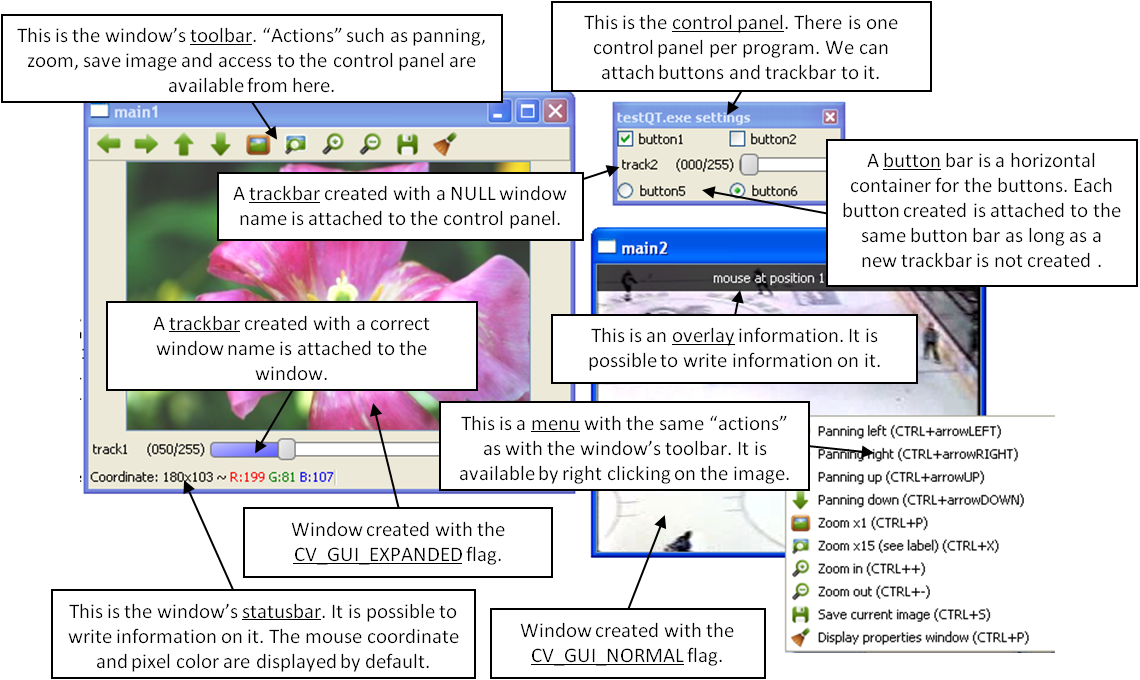
\includegraphics[width=1.1\textwidth]{pics/Qt_GUI.png}

This figure explains the new functionalities implemented with Qt GUI. As we can see, the new GUI provides a statusbar, a toolbar, and a control panel. The control panel can have trackbars and buttonbars attached to it.
\begin{itemize}
    \item  To attach a trackbar, the window\_name parameter must be NULL.
    \item  To attach a buttonbar, a button must be created. 
If the last bar attached to the control panel is a buttonbar, the new button is added on the right of the last button. 
If the last bar attached to the control panel is a trackbar, or the control panel is empty, a new buttonbar is created. Then a new button is attached to it.
\end{itemize}

The following code is an example used to generate the figure.
\begin{lstlisting}
int main(int argc, char *argv[])
    int value = 50;
    int value2 = 0;

    cvNamedWindow("main1",CV_WINDOW_NORMAL);
    cvNamedWindow("main2",CV_WINDOW_AUTOSIZE | CV_GUI_NORMAL);

    cvCreateTrackbar( "track1", "main1", &value, 255,  NULL);//OK tested
    char* nameb1 = "button1";
    char* nameb2 = "button2";
    cvCreateButton(nameb1,callbackButton,nameb1,CV_CHECKBOX,1);
	
    cvCreateButton(nameb2,callbackButton,nameb2,CV_CHECKBOX,0);
    cvCreateTrackbar( "track2", NULL, &value2, 255, NULL);
    cvCreateButton("button5",callbackButton1,NULL,CV_RADIOBOX,0);
    cvCreateButton("button6",callbackButton2,NULL,CV_RADIOBOX,1);

    cvSetMouseCallback( "main2",on_mouse,NULL );

    IplImage* img1 = cvLoadImage("files/flower.jpg");
    IplImage* img2 = cvCreateImage(cvGetSize(img1),8,3);
    CvCapture* video = cvCaptureFromFile("files/hockey.avi");
    IplImage* img3 = cvCreateImage(cvGetSize(cvQueryFrame(video)),8,3);

    while(cvWaitKey(33) != 27)
    {
        cvAddS(img1,cvScalarAll(value),img2);
        cvAddS(cvQueryFrame(video),cvScalarAll(value2),img3);
        cvShowImage("main1",img2);
        cvShowImage("main2",img3);
    }

    cvDestroyAllWindows();
    cvReleaseImage(&img1);
    cvReleaseImage(&img2);
    cvReleaseImage(&img3);
    cvReleaseCapture(&video);
    return 0;
}
\end{lstlisting}

\ifC
%CVAPI(void) cvSetWindowProperty(const char* name, int prop_id, double prop_value);
\cvCPyFunc{SetWindowProperty}
Change the parameters of the window dynamically.

\cvdefC{void  cvSetWindowProperty(const char* name, int prop\_id, double prop\_value);}

\begin{description}
\cvarg{name}{Name of the window.}
\cvarg{prop\_id}{Window's property to edit. The operation flags:
\begin{description}
\cvarg{CV\_WND\_PROP\_FULLSCREEN}{Change if the window is fullscreen (\texttt{CV\_WINDOW\_NORMAL} or \texttt{CV\_WINDOW\_FULLSCREEN}).}
\cvarg{CV\_WND\_PROP\_AUTOSIZE}{Change if the user can resize the window (texttt{CV\_WINDOW\_NORMAL} or  \texttt{CV\_WINDOW\_AUTOSIZE}).}
\cvarg{CV\_WND\_PROP\_ASPECTRATIO}{Change if the image's aspect ratio is preserved  (texttt{CV\_WINDOW\_FREERATIO} or \texttt{CV\_WINDOW\_KEEPRATIO}).}
\end{description}}
\cvarg{prop\_value}{New value of the Window's property. The operation flags:
\begin{description}
\cvarg{CV\_WINDOW\_NORMAL}{Change the window in normal size, or allows the user to resize the window.}
\cvarg{CV\_WINDOW\_AUTOSIZE}{The user cannot resize the window, the size is constrainted by the image displayed.}
\cvarg{CV\_WINDOW\_FULLSCREEN}{Change the window to fullscreen.}
\cvarg{CV\_WINDOW\_FREERATIO}{The image expends as much as it can (no ratio constraint)}
\cvarg{CV\_WINDOW\_KEEPRATIO}{The ration image is respected.}
\end{description}}
\end{description}

The function \texttt{ cvSetWindowProperty} allows to change the window's properties.



%CVAPI(double) cvGetWindowProperty(const char* name, int prop_id);
\cvCPyFunc{GetWindowProperty}
Get the parameters of the window.

\cvdefC{void  cvGetWindowProperty(const char* name, int prop\_id);}

\begin{description}
\cvarg{name}{Name of the window.}
\cvarg{prop\_id}{Window's property to retrive. The operation flags:
\begin{description}
\cvarg{CV\_WND\_PROP\_FULLSCREEN}{Change if the window is fullscreen (\texttt{CV\_WINDOW\_NORMAL} or \texttt{CV\_WINDOW\_FULLSCREEN}).}
\cvarg{CV\_WND\_PROP\_AUTOSIZE}{Change if the user can resize the window (texttt{CV\_WINDOW\_NORMAL} or  \texttt{CV\_WINDOW\_AUTOSIZE}).}
\cvarg{CV\_WND\_PROP\_ASPECTRATIO}{Change if the image's aspect ratio is preserved  (texttt{CV\_WINDOW\_FREERATIO} or \texttt{CV\_WINDOW\_KEEPRATIO}).}
\end{description}}
\end{description}
See \cross{SetWindowProperty} to know the meaning of the returned values.

The function \texttt{ cvGetWindowProperty} return window's properties.


\cvCPyFunc{FontQt}
Create the font to be used to draw text on an image (with \cross{addText}).

\cvdefC{CvFont cvFontQt(const char* nameFont, int pointSize  = -1, CvScalar color = cvScalarAll(0), int weight = CV\_FONT\_NORMAL,  int style = CV\_STYLE\_NORMAL, int spacing = 0);}

\begin{description}
\cvarg{nameFont}{Name of the font. The name should match the name of a system font (such as ``Times''). If the font is not found, a default one will be used.}
\cvarg{pointSize}{Size of the font. If not specified, equal zero or negative, the point size of the font is set to a system-dependent default value. Generally, this is 12 points.}
\cvarg{color}{Color of the font in BGRA --  A = 255 is fully transparent. Use the macro CV\_RGB for simplicity.}
\cvarg{weight}{The operation flags:
\begin{description}
\cvarg{CV\_FONT\_LIGHT}{Weight of 25}
\cvarg{CV\_FONT\_NORMAL}{Weight of 50}
\cvarg{CV\_FONT\_DEMIBOLD}{Weight of 63}
\cvarg{CV\_FONT\_BOLD}{Weight of 75}
\cvarg{CV\_FONT\_BLACK}{Weight of 87}
You can also specify a positive integer for more control.
\end{description}}
\cvarg{style}{The operation flags:
\begin{description}
\cvarg{CV\_STYLE\_NORMAL}{Font is normal}
\cvarg{CV\_STYLE\_ITALIC}{Font is in italic}
\cvarg{CV\_STYLE\_OBLIQUE}{Font is oblique}
\end{description}}
\cvarg{spacing}{Spacing between characters. Can be negative or positive}
\end{description}

The function \texttt{cvFontQt} creates a CvFont object to be used with \cross{addText}. This CvFont is not compatible with cvPutText. 

A basic usage of this function is:
\begin{lstlisting}
CvFont font = cvFontQt(''Times'');
cvAddText( img1, ``Hello World !'', cvPoint(50,50), &font);
\end{lstlisting}


\cvCPyFunc{addText}
Create the font to be used to draw text on an image 
\cvdefC{void cvAddText(const CvArr* img, const char* text, CvPoint location, CvFont *font);}

\begin{description}
\cvarg{img}{Image where the text should be drawn}
\cvarg{text}{Text to write on the image}
\cvarg{location}{Point(x,y) where the text should start on the image}
\cvarg{font}{Font to use to draw the text}
\end{description}

The function \texttt{cvAddText} draw \emph{text} on the image \emph{img} using a specific font \emph{font} (see example \cross{FontQt})


%CVAPI(void) cvDisplayOverlay(const char* name, const char* text, int delay);
\cvCPyFunc{displayOverlay}
Display text on the window's image as an overlay for delay milliseconds. This is not editing the image's data. The text is display on the top of the image.
\cvdefC{void cvDisplayOverlay(const char* name, const char* text, int delay);}

\begin{description}
\cvarg{name}{Name of the window}
\cvarg{text}{Overlay text to write on the window's image}
\cvarg{delay}{Delay to display the overlay text. If this function is called before the previous overlay text time out, the timer is restarted and the text updated. . If this value is zero, the text never disapers.}
\end{description}

The function \texttt{cvDisplayOverlay} aims at displaying useful information/tips on the window for a certain amount of time \emph{delay}. This information is display on the top of the window.


%CVAPI(void) cvDisplayStatusBar(const char* name, const char* text, int delayms);
\cvCPyFunc{displayStatusBar}
Display text on the window's statusbar as for delay milliseconds.
\cvdefC{void cvDisplayStatusBar(const char* name, const char* text, int delayms);}

\begin{description}
\cvarg{name}{Name of the window}
\cvarg{text}{Text to write on the window's statusbar}
\cvarg{delay}{Delay to display the text. If this function is called before the previous text time out, the timer is restarted and the text updated. If this value is zero, the text never disapers.}
\end{description}

The function \texttt{cvDisplayOverlay} aims at displaying useful information/tips on the window for a certain amount of time \emph{delay}. This information is displayed on the window's statubar (the window must be created with \texttt{CV\_GUI\_EXPANDED} flags).



%CVAPI(void) cvCreateOpenGLCallback( const char* window_name, CvOpenGLCallback callbackOpenGL, void* userdata CV_DEFAULT(NULL), double angle CV_DEFAULT(-1), double zmin CV_DEFAULT(-1), double zmax CV_DEFAULT(-1));
\cvCPyFunc{createOpenGLCallback}
Create a callback function called to draw OpenGL on top the the image display by \emph{window\_name}.
\cvdefC{void cvCreateOpenGLCallback( const char* window\_name, CvOpenGLCallback callbackOpenGL, void* userdata CV\_DEFAULT(NULL), double angle CV\_DEFAULT(-1), double zmin CV\_DEFAULT(-1), double zmax CV\_DEFAULT(-1);}

\begin{description}
\cvarg{window\_name}{Name of the window}
\cvarg{callbackOpenGL}{
Pointer to the function to be called every frame.
This function should be prototyped as \texttt{void Foo(*void);}.}
\cvarg{userdata}{pointer passed to the callback function. \emph{(Optional)}}
\cvarg{angle}{Specifies the field of view angle, in degrees, in the y direction.. \emph{(Optional - Default 45 degree)}}
\cvarg{zmin}{Specifies the distance from the viewer to the near clipping plane (always positive). \emph{(Optional - Default 0.01)}}
\cvarg{zmax}{Specifies the distance from the viewer to the far clipping plane (always positive). \emph{(Optional - Default 1000)}}    									
\end{description}

The function \texttt{cvCreateOpenGLCallback} can be used to draw 3D data on the window.  An example of callback could be:
\begin{lstlisting}
void on_opengl(void* param)
{
    //draw scene here
    glLoadIdentity();

    glTranslated(0.0, 0.0, -1.0);

    glRotatef( 55, 1, 0, 0 );
    glRotatef( 45, 0, 1, 0 );
    glRotatef( 0, 0, 0, 1 );

    static const int coords[6][4][3] = {
        { { +1, -1, -1 }, { -1, -1, -1 }, { -1, +1, -1 }, { +1, +1, -1 } },
        { { +1, +1, -1 }, { -1, +1, -1 }, { -1, +1, +1 }, { +1, +1, +1 } },
        { { +1, -1, +1 }, { +1, -1, -1 }, { +1, +1, -1 }, { +1, +1, +1 } },
        { { -1, -1, -1 }, { -1, -1, +1 }, { -1, +1, +1 }, { -1, +1, -1 } },
        { { +1, -1, +1 }, { -1, -1, +1 }, { -1, -1, -1 }, { +1, -1, -1 } },
        { { -1, -1, +1 }, { +1, -1, +1 }, { +1, +1, +1 }, { -1, +1, +1 } }
    };

    for (int i = 0; i < 6; ++i) {
                glColor3ub( i*20, 100+i*10, i*42 );
                glBegin(GL_QUADS);
                for (int j = 0; j < 4; ++j) {
                        glVertex3d(0.2 * coords[i][j][0], 0.2 * coords[i][j][1], 0.2 * coords[i][j][2]);
                }
                glEnd();
    }
}
\end{lstlisting}

\begin{lstlisting}
CV_EXTERN_C_FUNCPTR( *CvOpenGLCallback)(void* userdata));
\end{lstlisting}


%CVAPI(void) cvSaveWindowParameters(const char* name);
\cvCPyFunc{saveWindowParameters}
Save parameters of the window \emph{window\_name}.
\cvdefC{void cvSaveWindowParameters(const char* name);}

\begin{description}
\cvarg{name}{Name of the window}							
\end{description}

The function \texttt{cvSaveWindowParameters} saves size, location, flags,  trackbars' value, zoom and panning location of the window \emph{window\_name}


%CVAPI(void) cvLoadWindowParameters(const char* name);
\cvCPyFunc{loadWindowParameters}
Load parameters of the window \emph{window\_name}.
\cvdefC{void cvLoadWindowParameters(const char* name);}

\begin{description}
\cvarg{name}{Name of the window}							
\end{description}

The function \texttt{cvLoadWindowParameters} load size, location, flags,  trackbars' value, zoom and panning location of the window \emph{window\_name}


%CVAPI(int) cvCreateButton( const char* button_name CV_DEFAULT(NULL),CvButtonCallback on_change CV_DEFAULT(NULL), void* userdata CV_DEFAULT(NULL) , int button_type CV_DEFAULT(CV_PUSH_BUTTON), int initial_button_state CV_DEFAULT(0));
\cvCPyFunc{createButton}
Create a callback function called to draw OpenGL on top the the image display by \emph{window\_name}.
\cvdefC{cvCreateButton( const char* button\_name CV\_DEFAULT(NULL),CvButtonCallback on\_change CV\_DEFAULT(NULL), void* userdata CV\_DEFAULT(NULL) , int button\_type CV\_DEFAULT(CV\_PUSH\_BUTTON), int initial\_button\_state CV\_DEFAULT(0);}

\begin{description}
\cvarg{ button\_name}{Name of the button  \emph{( if NULL, the name will be "button <number of boutton>")}}
\cvarg{on\_change}{
Pointer to the function to be called every time the button changed its state.
This function should be prototyped as \texttt{void Foo(int state,*void);}. \emph{state} is the current state of the button. It could be -1 for a push button, 0 or 1 for a check/radio box button.}
\cvarg{userdata}{pointer passed to the callback function. \emph{(Optional)}}
\end{description}

The \texttt{button\_type} parameter can be :  \emph{(Optional -- Will be a push button by default.)
\begin{description}
\cvarg{CV\_PUSH\_BUTTON}{The button will be a push button.}
\cvarg{CV\_CHECKBOX}{The button will be a checkbox button.}
\cvarg{CV\_RADIOBOX}{The button will be a radiobox button. The radiobox on the same buttonbar (same line) are exclusive; one on can be select at the time.}
\end{description}}	
\begin{description}
\cvarg{initial\_button\_state}{Default state of the button. Use for checkbox and radiobox, its value could be 0 or 1. \emph{(Optional)}}							
\end{description}

The function \texttt{cvCreateButton} attach button to the control panel. Each button is added to a buttonbar on the right of the last button.
A new buttonbar is create if nothing was attached to the control panel before, or if the last element attached to the control panel was a trackbar.

Here are various example of \texttt{cvCreateButton}  function call:
\begin{lstlisting}
cvCreateButton(NULL,callbackButton);//create a push button "button 0", that will call callbackButton. 
cvCreateButton("button2",callbackButton,NULL,CV\_CHECKBOX,0);
cvCreateButton("button3",callbackButton,&value);
cvCreateButton("button5",callbackButton1,NULL,CV\_RADIOBOX);
cvCreateButton("button6",callbackButton2,NULL,CV\_PUSH\_BUTTON,1);
\end{lstlisting}

\begin{lstlisting}
CV_EXTERN_C_FUNCPTR( *CvButtonCallback)(int state, void* userdata));
\end{lstlisting}

\fi





\ifCpp


%CVAPI(void) cvSetWindowProperty(const char* name, int prop_id, double prop_value);
\cvCppFunc{setWindowProperty}
Change the parameters of the window dynamically.

\cvdefCpp{void  setWindowProperty(const string\& name, int prop\_id, double prop\_value);}

\begin{description}
\cvarg{name}{Name of the window.}
\cvarg{prop\_id}{Window's property to edit. The operation flags:
\begin{description}
\cvarg{CV\_WND\_PROP\_FULLSCREEN}{Change if the window is fullscreen (\texttt{CV\_WINDOW\_NORMAL} or \texttt{CV\_WINDOW\_FULLSCREEN}).}
\cvarg{CV\_WND\_PROP\_AUTOSIZE}{Change if the user can resize the window (texttt{CV\_WINDOW\_NORMAL} or  \texttt{CV\_WINDOW\_AUTOSIZE}).}
\cvarg{CV\_WND\_PROP\_ASPECTRATIO}{Change if the image's aspect ratio is preserved  (texttt{CV\_WINDOW\_FREERATIO} or \texttt{CV\_WINDOW\_KEEPRATIO}).}
\end{description}}
\cvarg{prop\_value}{New value of the Window's property. The operation flags:
\begin{description}
\cvarg{CV\_WINDOW\_NORMAL}{Change the window in normal size, or allows the user to resize the window.}
\cvarg{CV\_WINDOW\_AUTOSIZE}{The user cannot resize the window, the size is constrainted by the image displayed.}
\cvarg{CV\_WINDOW\_FULLSCREEN}{Change the window to fullscreen.}
\cvarg{CV\_WINDOW\_FREERATIO}{The image expends as much as it can (no ratio constraint)}
\cvarg{CV\_WINDOW\_KEEPRATIO}{The ration image is respected.}
\end{description}}
\end{description}

The function \texttt{ setWindowProperty} allows to change the window's properties.



%CVAPI(double) cvGetWindowProperty(const char* name, int prop_id);
\cvCppFunc{getWindowProperty}
Get the parameters of the window.

\cvdefCpp{void  getWindowProperty(const char* name, int prop\_id);}

\begin{description}
\cvarg{name}{Name of the window.}
\cvarg{prop\_id}{Window's property to retrive. The operation flags:
\begin{description}
\cvarg{CV\_WND\_PROP\_FULLSCREEN}{Change if the window is fullscreen (\texttt{CV\_WINDOW\_NORMAL} or \texttt{CV\_WINDOW\_FULLSCREEN}).}
\cvarg{CV\_WND\_PROP\_AUTOSIZE}{Change if the user can resize the window (texttt{CV\_WINDOW\_NORMAL} or  \texttt{CV\_WINDOW\_AUTOSIZE}).}
\cvarg{CV\_WND\_PROP\_ASPECTRATIO}{Change if the image's aspect ratio is preserved  (texttt{CV\_WINDOW\_FREERATIO} or \texttt{CV\_WINDOW\_KEEPRATIO}).}
\end{description}}
\end{description}
See \cross{setWindowProperty} to know the meaning of the returned values.

The function \texttt{ getWindowProperty} return window's properties.


\cvCppFunc{fontQt}
Create the font to be used to draw text on an image.

\cvdefCpp{CvFont fontQt(const string\& nameFont, int pointSize  = -1, Scalar color = Scalar::all(0), int weight = CV\_FONT\_NORMAL,  int style = CV\_STYLE\_NORMAL, int spacing = 0);}

\begin{description}
\cvarg{nameFont}{Name of the font. The name should match the name of a system font (such as ``Times''). If the font is not found, a default one will be used.}
\cvarg{pointSize}{Size of the font. If not specified, equal zero or negative, the point size of the font is set to a system-dependent default value. Generally, this is 12 points.}
\cvarg{color}{Color of the font in BGRA --  A = 255 is fully transparent. Use the macro CV\_RGB for simplicity.}
\cvarg{weight}{The operation flags:
\begin{description}
\cvarg{CV\_FONT\_LIGHT}{Weight of 25}
\cvarg{CV\_FONT\_NORMAL}{Weight of 50}
\cvarg{CV\_FONT\_DEMIBOLD}{Weight of 63}
\cvarg{CV\_FONT\_BOLD}{Weight of 75}
\cvarg{CV\_FONT\_BLACK}{Weight of 87}
You can also specify a positive integer for more control.
\end{description}}
\cvarg{style}{The operation flags:
\begin{description}
\cvarg{CV\_STYLE\_NORMAL}{Font is normal}
\cvarg{CV\_STYLE\_ITALIC}{Font is in italic}
\cvarg{CV\_STYLE\_OBLIQUE}{Font is oblique}
\end{description}}
\cvarg{spacing}{Spacing between characters. Can be negative or positive}
\end{description}

The function \texttt{fontQt} creates a CvFont object. This CvFont is not compatible with putText. 

A basic usage of this function is:
\begin{lstlisting}
CvFont font = fontQt(''Times'');
addText( img1, ``Hello World !'', Point(50,50), &font);
\end{lstlisting}

\cvCppFunc{addText}
Create the font to be used to draw text on an image 
\cvdefCpp{void addText(const Mat\& img, const string\& text, Point location, CvFont *font);}

\begin{description}
\cvarg{img}{Image where the text should be drawn}
\cvarg{text}{Text to write on the image}
\cvarg{location}{Point(x,y) where the text should start on the image}
\cvarg{font}{Font to use to draw the text}
\end{description}

The function \texttt{addText} draw \emph{text} on the image \emph{img} using a specific font \emph{font} (see example \cross{fontQt})


%CVAPI(void) cvDisplayOverlay(const char* name, const char* text, int delay);
\cvCppFunc{displayOverlay}
Display text on the window's image as an overlay for delay milliseconds. This is not editing the image's data. The text is display on the top of the image.
\cvdefCpp{void displayOverlay(const string\& name, const string\& text, int delay);}

\begin{description}
\cvarg{name}{Name of the window}
\cvarg{text}{Overlay text to write on the window's image}
\cvarg{delay}{Delay to display the overlay text. If this function is called before the previous overlay text time out, the timer is restarted and the text updated. . If this value is zero, the text never disapers.}
\end{description}

The function \texttt{displayOverlay} aims at displaying useful information/tips on the window for a certain amount of time \emph{delay}. This information is display on the top of the window.


%CVAPI(void) cvDisplayStatusBar(const char* name, const char* text, int delayms);
\cvCppFunc{displayStatusBar}
Display text on the window's statusbar as for delay milliseconds.
\cvdefCpp{void displayStatusBar(const string\& name, const string\& text, int delayms);}

\begin{description}
\cvarg{name}{Name of the window}
\cvarg{text}{Text to write on the window's statusbar}
\cvarg{delay}{Delay to display the text. If this function is called before the previous text time out, the timer is restarted and the text updated. If this value is zero, the text never disapers.}
\end{description}

The function \texttt{displayOverlay} aims at displaying useful information/tips on the window for a certain amount of time \emph{delay}. This information is displayed on the window's statubar (the window must be created with \texttt{CV\_GUI\_EXPANDED} flags).



%CVAPI(void) cvCreateOpenGLCallback( const char* window_name, CvOpenGLCallback callbackOpenGL, void* userdata CV_DEFAULT(NULL), double angle CV_DEFAULT(-1), double zmin CV_DEFAULT(-1), double zmax CV_DEFAULT(-1));
\cvCppFunc{createOpenGLCallback}
Create a callback function called to draw OpenGL on top the the image display by \emph{window\_name}.
\cvdefCpp{void createOpenGLCallback( const string\& window\_name, OpenGLCallback callbackOpenGL, void* userdata CV\_DEFAULT(NULL), double angle CV\_DEFAULT(-1), double zmin CV\_DEFAULT(-1), double zmax CV\_DEFAULT(-1);}

\begin{description}
\cvarg{window\_name}{Name of the window}
\cvarg{callbackOpenGL}{
Pointer to the function to be called every frame.
This function should be prototyped as \texttt{void Foo(*void);}.}
\cvarg{userdata}{pointer passed to the callback function. \emph{(Optional)}}
\cvarg{angle}{Specifies the field of view angle, in degrees, in the y direction.. \emph{(Optional - Default 45 degree)}}
\cvarg{zmin}{Specifies the distance from the viewer to the near clipping plane (always positive). \emph{(Optional - Default 0.01)}}
\cvarg{zmax}{Specifies the distance from the viewer to the far clipping plane (always positive). \emph{(Optional - Default 1000)}}    									
\end{description}

The function \texttt{createOpenGLCallback} can be used to draw 3D data on the window.  An example of callback could be:
\begin{lstlisting}
void on_opengl(void* param)
{
    glLoadIdentity();

    glTranslated(0.0, 0.0, -1.0);

    glRotatef( 55, 1, 0, 0 );
    glRotatef( 45, 0, 1, 0 );
    glRotatef( 0, 0, 0, 1 );

    static const int coords[6][4][3] = {
        { { +1, -1, -1 }, { -1, -1, -1 }, { -1, +1, -1 }, { +1, +1, -1 } },
        { { +1, +1, -1 }, { -1, +1, -1 }, { -1, +1, +1 }, { +1, +1, +1 } },
        { { +1, -1, +1 }, { +1, -1, -1 }, { +1, +1, -1 }, { +1, +1, +1 } },
        { { -1, -1, -1 }, { -1, -1, +1 }, { -1, +1, +1 }, { -1, +1, -1 } },
        { { +1, -1, +1 }, { -1, -1, +1 }, { -1, -1, -1 }, { +1, -1, -1 } },
        { { -1, -1, +1 }, { +1, -1, +1 }, { +1, +1, +1 }, { -1, +1, +1 } }
    };

    for (int i = 0; i < 6; ++i) {
                glColor3ub( i*20, 100+i*10, i*42 );
                glBegin(GL_QUADS);
                for (int j = 0; j < 4; ++j) {
                        glVertex3d(0.2 * coords[i][j][0], 0.2 * coords[i][j][1], 0.2 * coords[i][j][2]);
                }
                glEnd();
    }
}
\end{lstlisting}


%CVAPI(void) cvSaveWindowParameters(const char* name);
\cvCppFunc{saveWindowParameters}
Save parameters of the window \emph{window\_name}.
\cvdefCpp{void saveWindowParameters(const string\& name);}

\begin{description}
\cvarg{name}{Name of the window}							
\end{description}

The function \texttt{saveWindowParameters} saves size, location, flags,  trackbars' value, zoom and panning location of the window \emph{window\_name}


%CVAPI(void) cvLoadWindowParameters(const char* name);
\cvCppFunc{loadWindowParameters}
Load parameters of the window \emph{window\_name}.
\cvdefCpp{void loadWindowParameters(const string\& name);}

\begin{description}
\cvarg{name}{Name of the window}							
\end{description}

The function \texttt{loadWindowParameters} load size, location, flags,  trackbars' value, zoom and panning location of the window \emph{window\_name}


%CVAPI(int) cvCreateButton( const char* button_name CV_DEFAULT(NULL),CvButtonCallback on_change CV_DEFAULT(NULL), void* userdata CV_DEFAULT(NULL) , int button_type CV_DEFAULT(CV_PUSH_BUTTON), int initial_button_state CV_DEFAULT(0));
\cvCppFunc{createButton}
Create a callback function called to draw OpenGL on top the the image display by \emph{window\_name}.
\cvdefCpp{createButton( const string\& button\_name CV\_DEFAULT(NULL),ButtonCallback on\_change CV\_DEFAULT(NULL), void* userdata CV\_DEFAULT(NULL) , int button\_type CV\_DEFAULT(CV\_PUSH\_BUTTON), int initial\_button\_state CV\_DEFAULT(0);}

\begin{description}
\cvarg{ button\_name}{Name of the button  \emph{( if NULL, the name will be "button <number of boutton>")}}
\cvarg{on\_change}{
Pointer to the function to be called every time the button changed its state.
This function should be prototyped as \texttt{void Foo(int state,*void);}. \emph{state} is the current state of the button. It could be -1 for a push button, 0 or 1 for a check/radio box button.}
\cvarg{userdata}{pointer passed to the callback function. \emph{(Optional)}}
\end{description}

The \texttt{button\_type} parameter can be :  \emph{(Optional -- Will be a push button by default.)
\begin{description}
\cvarg{CV\_PUSH\_BUTTON}{The button will be a push button.}
\cvarg{CV\_CHECKBOX}{The button will be a checkbox button.}
\cvarg{CV\_RADIOBOX}{The button will be a radiobox button. The radiobox on the same buttonbar (same line) are exclusive; one on can be select at the time.}
\end{description}}	
\begin{description}
\cvarg{initial\_button\_state}{Default state of the button. Use for checkbox and radiobox, its value could be 0 or 1. \emph{(Optional)}}							
\end{description}

The function \texttt{createButton} attach a button to the control panel. Each button is added to a buttonbar on the right of the last button.
A new buttonbar is create if nothing was attached to the control panel before, or if the last element attached to the control panel was a trackbar.

Here are various example of \texttt{createButton}  function call:
\begin{lstlisting}
createButton(NULL,callbackButton);//create a push button "button 0", that will call callbackButton. 
createButton("button2",callbackButton,NULL,CV\_CHECKBOX,0);
createButton("button3",callbackButton,&value);
createButton("button5",callbackButton1,NULL,CV\_RADIOBOX);
createButton("button6",callbackButton2,NULL,CV\_PUSH\_BUTTON,1);
\end{lstlisting}

\fi
\fi

\chapter{ml. Machine Learning}
The Machine Learning Library (MLL) is a set of classes and functions for statistical classification, regression and clustering of data.

Most of the classification and regression algorithms are implemented as C++ classes. As the algorithms have different seta of features (like the ability to handle missing measurements, or categorical input variables etc.), there is a little common ground between the classes. This common ground is defined by the class `CvStatModel` that all the other ML classes are derived from.

\ifCpp

\section{Statistical Models}

\cvfunc{CvStatModel}
Base class for the statistical models in ML.

\begin{lstlisting}
class CvStatModel
{
public:
    /* CvStatModel(); */
    /* CvStatModel( const CvMat* train_data ... ); */

    virtual ~CvStatModel();

    virtual void clear()=0;

    /* virtual bool train( const CvMat* train_data, [int tflag,] ..., const 
	CvMat* responses, ...,
     [const CvMat* var_idx,] ..., [const CvMat* sample_idx,] ...
     [const CvMat* var_type,] ..., [const CvMat* missing_mask,] 
	<misc_training_alg_params> ... )=0;
      */

    /* virtual float predict( const CvMat* sample ... ) const=0; */

    virtual void save( const char* filename, const char* name=0 )=0;
    virtual void load( const char* filename, const char* name=0 )=0;

    virtual void write( CvFileStorage* storage, const char* name )=0;
    virtual void read( CvFileStorage* storage, CvFileNode* node )=0;
};
\end{lstlisting}

In this declaration some methods are commented off. Actually, these are methods for which there is no unified API (with the exception of the default constructor), however, there are many similarities in the syntax and semantics that are briefly described below in this section, as if they are a part of the base class.


\cvfunc{CvStatModel::CvStatModel}
Default constructor.

\cvdefCpp{
CvStatModel::CvStatModel();
}

Each statistical model class in ML has a default constructor without parameters. This constructor is useful for 2-stage model construction, when the default constructor is followed by \texttt{train()} or \texttt{load()}.


\cvfunc{CvStatModel::CvStatModel(...)}
Training constructor.

\cvdefCpp{
CvStatModel::CvStatModel( const CvMat* train\_data ... ); 
}

Most ML classes provide single-step construct and train constructors. This constructor is equivalent to the default constructor, followed by the \texttt{train()} method with the parameters that are passed to the constructor.


\cvfunc{CvStatModel::~CvStatModel}
Virtual destructor.

\cvdefCpp{
CvStatModel::~CvStatModel();
}

The destructor of the base class is declared as virtual, so it is safe to write the following code:

\begin{lstlisting}
CvStatModel* model;
if( use\_svm )
    model = new CvSVM(... /* SVM params */);
else
    model = new CvDTree(... /* Decision tree params */);
...
delete model;
\end{lstlisting}

Normally, the destructor of each derived class does nothing, but in this instance it calls the overridden method \texttt{clear()} that deallocates all the memory.


\cvfunc{CvStatModel::clear}
Deallocates memory and resets the model state.

\cvdefCpp{
void CvStatModel::clear();
}

The method \texttt{clear} does the same job as the destructor; it deallocates all the memory occupied by the class members. But the object itself is not destructed, and can be reused further. This method is called from the destructor, from the \texttt{train} methods of the derived classes, from the methods \texttt{load()}, \texttt{read()} or even explicitly by the user.


\cvfunc{CvStatModel::save}
Saves the model to a file.

\cvdefCpp{
void CvStatModel::save( const char* filename, const char* name=0 );
}

The method \texttt{save} stores the complete model state to the specified XML or YAML file with the specified name or default name (that depends on the particular class). \texttt{Data persistence} functionality from CxCore is used.


\cvfunc{CvStatModel::load}
Loads the model from a file.

\cvdefCpp{
void CvStatModel::load( const char* filename, const char* name=0 );
}

The method \texttt{load} loads the complete model state with the specified name (or default model-dependent name) from the specified XML or YAML file. The previous model state is cleared by \texttt{clear()}.

Note that the method is virtual, so any model can be loaded using this virtual method. However, unlike the C types of OpenCV that can be loaded using the generic \\cross{cvLoad}, here the model type must be known, because an empty model must be constructed beforehand. This limitation will be removed in the later ML versions.


\cvfunc{CvStatModel::write}
Writes the model to file storage.

\cvdefCpp{
void CvStatModel::write( CvFileStorage* storage, const char* name );
}

The method \texttt{write} stores the complete model state to the file storage with the specified name or default name (that depends on the particular class). The method is called by \texttt{save()}.


\cvfunc{CvStatModel::read}
Reads the model from file storage.

\cvdefCpp{
void CvStatMode::read( CvFileStorage* storage, CvFileNode* node );
}

The method \texttt{read} restores the complete model state from the specified node of the file storage. The node must be located by the user using the function \cross{GetFileNodeByName}.

The previous model state is cleared by \texttt{clear()}.


\cvfunc{CvStatModel::train}
Trains the model.

\cvdefCpp{bool CvStatMode::train( const CvMat* train\_data, [int tflag,] ..., const CvMat* responses, ..., \par
    [const CvMat* var\_idx,] ..., [const CvMat* sample\_idx,] ... \par
    [const CvMat* var\_type,] ..., [const CvMat* missing\_mask,] <misc\_training\_alg\_params> ... );}

The method trains the statistical model using a set of input feature vectors and the corresponding output values (responses). Both input and output vectors/values are passed as matrices. By default the input feature vectors are stored as \texttt{train\_data} rows, i.e. all the components (features) of a training vector are stored continuously. However, some algorithms can handle the transposed representation, when all values of each particular feature (component/input variable) over the whole input set are stored continuously. If both layouts are supported, the method includes \texttt{tflag} parameter that specifies the orientation:
\begin{itemize}
 \item \texttt{tflag=CV\_ROW\_SAMPLE} means that the feature vectors are stored as rows,
 \item \texttt{tflag=CV\_COL\_SAMPLE} means that the feature vectors are stored as columns.
\end{itemize}
The \texttt{train\_data} must have a \texttt{CV\_32FC1} (32-bit floating-point, single-channel) format. Responses are usually stored in the 1d vector (a row or a column) of \texttt{CV\_32SC1} (only in the classification problem) or \texttt{CV\_32FC1} format, one value per input vector (although some algorithms, like various flavors of neural nets, take vector responses).

For classification problems the responses are discrete class labels; for regression problems the responses are values of the function to be approximated. Some algorithms can deal only with classification problems, some - only with regression problems, and some can deal with both problems. In the latter case the type of output variable is either passed as separate parameter, or as a last element of \texttt{var\_type} vector:
\begin{itemize}
 \item \texttt{CV\_VAR\_CATEGORICAL} means that the output values are discrete class labels,
 \item \texttt{CV\_VAR\_ORDERED(=CV\_VAR\_NUMERICAL)} means that the output values are ordered, i.e. 2 different values can be compared as numbers, and this is a regression problem
\end{itemize}
The types of input variables can be also specified using \texttt{var\_type}. Most algorithms can handle only ordered input variables.

Many models in the ML may be trained on a selected feature subset, and/or on a selected sample subset of the training set. To make it easier for the user, the method \texttt{train} usually includes \texttt{var\_idx} and \texttt{sample\_idx} parameters. The former identifies variables (features) of interest, and the latter identifies samples of interest. Both vectors are either integer (\texttt{CV\_32SC1}) vectors, i.e. lists of 0-based indices, or 8-bit (\texttt{CV\_8UC1}) masks of active variables/samples. The user may pass \texttt{NULL} pointers instead of either of the arguments, meaning that all of the variables/samples are used for training.

Additionally some algorithms can handle missing measurements, that is when certain features of certain training samples have unknown values (for example, they forgot to measure a temperature of patient A on Monday). The parameter \texttt{missing\_mask}, an 8-bit matrix the same size as \texttt{train\_data}, is used to mark the missed values (non-zero elements of the mask).

Usually, the previous model state is cleared by \texttt{clear()} before running the training procedure. However, some algorithms may optionally update the model state with the new training data, instead of resetting it.


\cvfunc{CvStatModel::predict}
Predicts the response for the sample.

\cvdefCpp{
float CvStatMode::predict( const CvMat* sample[, <prediction\_params>] ) const;
}

The method is used to predict the response for a new sample. In the case of classification the method returns the class label, in the case of regression - the output function value. The input sample must have as many components as the \texttt{train\_data} passed to \texttt{train} contains. If the \texttt{var\_idx} parameter is passed to \texttt{train}, it is remembered and then is used to extract only the necessary components from the input sample in the method \texttt{predict}.

The suffix "const" means that prediction does not affect the internal model state, so the method can be safely called from within different threads.

\section{Normal Bayes Classifier}

This is a simple classification model assuming that feature vectors from each class are normally distributed (though, not necessarily independently distributed), so the whole data distribution function is assumed to be a Gaussian mixture, one component per  class. Using the training data the algorithm estimates mean vectors and covariance matrices for every class, and then it uses them for prediction.

\textbf{[Fukunaga90] K. Fukunaga. Introduction to Statistical Pattern Recognition. second ed., New York: Academic Press, 1990.}


\cvfunc{CvNormalBayesClassifier}

Bayes classifier for normally distributed data.

\begin{lstlisting}
class CvNormalBayesClassifier : public CvStatModel
{
public:
    CvNormalBayesClassifier();
    virtual ~CvNormalBayesClassifier();

    CvNormalBayesClassifier( const CvMat* _train_data, const CvMat* _responses,
        const CvMat* _var_idx=0, const CvMat* _sample_idx=0 );

    virtual bool train( const CvMat* _train_data, const CvMat* _responses,
        const CvMat* _var_idx = 0, const CvMat* _sample_idx=0, bool update=false );

    virtual float predict( const CvMat* _samples, CvMat* results=0 ) const;
    virtual void clear();

    virtual void save( const char* filename, const char* name=0 );
    virtual void load( const char* filename, const char* name=0 );

    virtual void write( CvFileStorage* storage, const char* name );
    virtual void read( CvFileStorage* storage, CvFileNode* node );
protected:
    ...
};
\end{lstlisting}



\cvfunc{CvNormalBayesClassifier::train}
Trains the model.

\cvdefCpp{
bool CvNormalBayesClassifier::train( \par const CvMat* \_train\_data, \par const CvMat* \_responses,
               \par const CvMat* \_var\_idx =0, \par const CvMat* \_sample\_idx=0, \par bool update=false );
}

The method trains the Normal Bayes classifier. It follows the conventions of the generic \texttt{train} "method" with the following limitations: only CV\_ROW\_SAMPLE data layout is supported; the input variables are all ordered; the output variable is categorical (i.e. elements of \texttt{\_responses} must be integer numbers, though the vector may have \texttt{CV\_32FC1} type), and missing measurements are not supported.

In addition, there is an \texttt{update} flag that identifies whether the model should be trained from scratch (\texttt{update=false}) or should be updated using the new training data (\texttt{update=true}).

\cvfunc{CvNormalBayesClassifier::predict}
Predicts the response for sample(s)

\cvdefCpp{
float CvNormalBayesClassifier::predict( \par const CvMat* samples, \par CvMat* results=0 ) const;
}

The method \texttt{predict} estimates the most probable classes for the input vectors. The input vectors (one or more) are stored as rows of the matrix \texttt{samples}. In the case of multiple input vectors, there should be one output vector \texttt{results}. The predicted class for a single input vector is returned by the method.

\section{K Nearest Neighbors}

The algorithm caches all of the training samples, and predicts the response for a new sample by analyzing a certain number (\textbf{K}) of the nearest neighbors of the sample (using voting, calculating weighted sum etc.) The method is sometimes referred to as "learning by example", because for prediction it looks for the feature vector with a known response that is closest to the given vector.


\cvfunc{CvKNearest}
K Nearest Neighbors model.

\begin{lstlisting}
class CvKNearest : public CvStatModel
{
public:

    CvKNearest();
    virtual ~CvKNearest();

    CvKNearest( const CvMat* _train_data, const CvMat* _responses,
                const CvMat* _sample_idx=0, bool _is_regression=false, int max_k=32 );

    virtual bool train( const CvMat* _train_data, const CvMat* _responses,
                        const CvMat* _sample_idx=0, bool is_regression=false,
                        int _max_k=32, bool _update_base=false );

    virtual float find_nearest( const CvMat* _samples, int k, CvMat* results,
        const float** neighbors=0, CvMat* neighbor_responses=0, CvMat* dist=0 ) const;

    virtual void clear();
    int get_max_k() const;
    int get_var_count() const;
    int get_sample_count() const;
    bool is_regression() const;

protected:
    ...
};
\end{lstlisting}



\cvfunc{CvKNearest::train}
Trains the model.

\cvdefCpp{
bool CvKNearest::train( \par const CvMat* \_train\_data, \par const CvMat* \_responses,
                        \par const CvMat* \_sample\_idx=0, \par bool is\_regression=false,
                        \par int \_max\_k=32, \par bool \_update\_base=false );

}

The method trains the K-Nearest model. It follows the conventions of generic \texttt{train} "method" with the following limitations: only CV\_ROW\_SAMPLE data layout is supported, the input variables are all ordered, the output variables can be either categorical (\texttt{is\_regression=false}) or ordered (\texttt{is\_regression=true}), variable subsets (\texttt{var\_idx}) and missing measurements are not supported.

The parameter \texttt{\_max\_k} specifies the number of maximum neighbors that may be passed to the method \texttt{find\_nearest}.

The parameter \texttt{\_update\_base} specifies whether the model is trained from scratch \newline (\texttt{\_update\_base=false}), or it is updated using the new training data (\texttt{\_update\_base=true}). In the latter case the parameter \texttt{\_max\_k} must not be larger than the original value.


\cvfunc{CvKNearest::find\_nearest}

Finds the neighbors for the input vectors.

\cvdefCpp{

float CvKNearest::find\_nearest( \par const CvMat* \_samples, \par int k, CvMat* results=0,
        \par const float** neighbors=0, \par CvMat* neighbor\_responses=0, \par CvMat* dist=0 ) const;

}

For each input vector (which are the rows of the matrix
\texttt{\_samples}) the method finds the $ \texttt{k} \le
\texttt{get\_max\_k()} $ nearest neighbor.  In the case of regression,
the predicted result will be a mean value of the particular vector's
neighbor responses. In the case of classification the class is determined
by voting.

For custom classification/regression prediction, the method can optionally return pointers to the neighbor vectors themselves (\texttt{neighbors}, an array of \texttt{k*\_samples->rows} pointers), their corresponding output values (\texttt{neighbor\_responses}, a vector of \texttt{k*\_samples->rows} elements) and the distances from the input vectors to the neighbors (\texttt{dist}, also a vector of \texttt{k*\_samples->rows} elements).

For each input vector the neighbors are sorted by their distances to the vector.

If only a single input vector is passed, all output matrices are optional and the predicted value is returned by the method.

\cvfunc{Example. Classification of 2D samples from a Gaussian mixture with the k-nearest classifier}

\begin{lstlisting}
#include "ml.h"
#include "highgui.h"

int main( int argc, char** argv )
{
    const int K = 10;
    int i, j, k, accuracy;
    float response;
    int train_sample_count = 100;
    CvRNG rng_state = cvRNG(-1);
    CvMat* trainData = cvCreateMat( train_sample_count, 2, CV_32FC1 );
    CvMat* trainClasses = cvCreateMat( train_sample_count, 1, CV_32FC1 );
    IplImage* img = cvCreateImage( cvSize( 500, 500 ), 8, 3 );
    float _sample[2];
    CvMat sample = cvMat( 1, 2, CV_32FC1, _sample );
    cvZero( img );

    CvMat trainData1, trainData2, trainClasses1, trainClasses2;

    // form the training samples
    cvGetRows( trainData, &trainData1, 0, train_sample_count/2 );
    cvRandArr( &rng_state, &trainData1, CV_RAND_NORMAL, cvScalar(200,200), cvScalar(50,50) );

    cvGetRows( trainData, &trainData2, train_sample_count/2, train_sample_count );
    cvRandArr( &rng_state, &trainData2, CV_RAND_NORMAL, cvScalar(300,300), cvScalar(50,50) );

    cvGetRows( trainClasses, &trainClasses1, 0, train_sample_count/2 );
    cvSet( &trainClasses1, cvScalar(1) );

    cvGetRows( trainClasses, &trainClasses2, train_sample_count/2, train_sample_count );
    cvSet( &trainClasses2, cvScalar(2) );

    // learn classifier
    CvKNearest knn( trainData, trainClasses, 0, false, K );
    CvMat* nearests = cvCreateMat( 1, K, CV_32FC1);

    for( i = 0; i < img->height; i++ )
    {
        for( j = 0; j < img->width; j++ )
        {
            sample.data.fl[0] = (float)j;
            sample.data.fl[1] = (float)i;

            // estimates the response and get the neighbors' labels
            response = knn.find_nearest(&sample,K,0,0,nearests,0);

            // compute the number of neighbors representing the majority
            for( k = 0, accuracy = 0; k < K; k++ )
            {
                if( nearests->data.fl[k] == response)
                    accuracy++;
            }
            // highlight the pixel depending on the accuracy (or confidence)
            cvSet2D( img, i, j, response == 1 ?
                (accuracy > 5 ? CV_RGB(180,0,0) : CV_RGB(180,120,0)) :
                (accuracy > 5 ? CV_RGB(0,180,0) : CV_RGB(120,120,0)) );
        }
    }

    // display the original training samples
    for( i = 0; i < train_sample_count/2; i++ )
    {
        CvPoint pt;
        pt.x = cvRound(trainData1.data.fl[i*2]);
        pt.y = cvRound(trainData1.data.fl[i*2+1]);
        cvCircle( img, pt, 2, CV_RGB(255,0,0), CV_FILLED );
        pt.x = cvRound(trainData2.data.fl[i*2]);
        pt.y = cvRound(trainData2.data.fl[i*2+1]);
        cvCircle( img, pt, 2, CV_RGB(0,255,0), CV_FILLED );
    }

    cvNamedWindow( "classifier result", 1 );
    cvShowImage( "classifier result", img );
    cvWaitKey(0);

    cvReleaseMat( &trainClasses );
    cvReleaseMat( &trainData );
    return 0;
}
\end{lstlisting}


\section{Support Vector Machines}

Originally, support vector machines (SVM) was a technique for building an optimal (in some sense) binary (2-class) classifier. Then the technique has been extended to regression and clustering problems. SVM is a partial case of kernel-based methods, it maps feature vectors into higher-dimensional space using some kernel function, and then it builds an optimal linear discriminating function in this space (or an optimal hyper-plane that fits into the training data, ...). in the case of SVM the kernel is not defined explicitly. Instead, a distance between any 2 points in the hyper-space needs to be defined.

The solution is optimal in a sense that the margin between the separating hyper-plane and the nearest feature vectors from the both classes (in the case of 2-class classifier) is maximal. The feature vectors that are the closest to the hyper-plane are called "support vectors", meaning that the position of other vectors does not affect the hyper-plane (the decision function).

There are a lot of good references on SVM. Here are only a few ones to start with.
\begin{itemize}
\item \textbf{[Burges98] C. Burges. "A tutorial on support vector machines for pattern recognition", Knowledge Discovery and Data Mining 2(2), 1998.} (available online at \url{http://citeseer.ist.psu.edu/burges98tutorial.html}).
\item \textbf{LIBSVM - A Library for Support Vector Machines. By Chih-Chung Chang and Chih-Jen Lin} (\url{http://www.csie.ntu.edu.tw/~cjlin/libsvm/})
\end{itemize}

\cvfunc{CvSVM}
Support Vector Machines.

\begin{lstlisting}
class CvSVM : public CvStatModel
{
public:
    // SVM type
    enum { C_SVC=100, NU_SVC=101, ONE_CLASS=102, EPS_SVR=103, NU_SVR=104 };

    // SVM kernel type
    enum { LINEAR=0, POLY=1, RBF=2, SIGMOID=3 };

    // SVM params type
    enum { C=0, GAMMA=1, P=2, NU=3, COEF=4, DEGREE=5 };

    CvSVM();
    virtual ~CvSVM();

    CvSVM( const CvMat* _train_data, const CvMat* _responses,
           const CvMat* _var_idx=0, const CvMat* _sample_idx=0,
           CvSVMParams _params=CvSVMParams() );

    virtual bool train( const CvMat* _train_data, const CvMat* _responses,
                        const CvMat* _var_idx=0, const CvMat* _sample_idx=0,
                        CvSVMParams _params=CvSVMParams() );

    virtual bool train_auto( const CvMat* _train_data, const CvMat* _responses,
        const CvMat* _var_idx, const CvMat* _sample_idx, CvSVMParams _params,
        int k_fold = 10,
        CvParamGrid C_grid      = get_default_grid(CvSVM::C),
        CvParamGrid gamma_grid  = get_default_grid(CvSVM::GAMMA),
        CvParamGrid p_grid      = get_default_grid(CvSVM::P),
        CvParamGrid nu_grid     = get_default_grid(CvSVM::NU),
        CvParamGrid coef_grid   = get_default_grid(CvSVM::COEF),
        CvParamGrid degree_grid = get_default_grid(CvSVM::DEGREE) );

    virtual float predict( const CvMat* _sample ) const;
    virtual int get_support_vector_count() const;
    virtual const float* get_support_vector(int i) const;
    virtual CvSVMParams get_params() const { return params; };
    virtual void clear();

    static CvParamGrid get_default_grid( int param_id );

    virtual void save( const char* filename, const char* name=0 );
    virtual void load( const char* filename, const char* name=0 );

    virtual void write( CvFileStorage* storage, const char* name );
    virtual void read( CvFileStorage* storage, CvFileNode* node );
    int get_var_count() const { return var_idx ? var_idx->cols : var_all; }

protected:
    ...
};
\end{lstlisting}


\cvfunc{CvSVMParams}
SVM training parameters.

\begin{lstlisting}
struct CvSVMParams
{
    CvSVMParams();
    CvSVMParams( int _svm_type, int _kernel_type,
                 double _degree, double _gamma, double _coef0,
                 double _C, double _nu, double _p,
                 CvMat* _class_weights, CvTermCriteria _term_crit );

    int         svm_type;
    int         kernel_type;
    double      degree; // for poly
    double      gamma;  // for poly/rbf/sigmoid
    double      coef0;  // for poly/sigmoid

    double      C;  // for CV_SVM_C_SVC, CV_SVM_EPS_SVR and CV_SVM_NU_SVR
    double      nu; // for CV_SVM_NU_SVC, CV_SVM_ONE_CLASS, and CV_SVM_NU_SVR
    double      p; // for CV_SVM_EPS_SVR
    CvMat*      class_weights; // for CV_SVM_C_SVC
    CvTermCriteria term_crit; // termination criteria
};

\end{lstlisting}

%\begin{description}
%\cvarg{svm\_type}{Type of SVM, one of the following types:
%\begin{description}
%\cvarg{CvSVM::C\_SVC}{n-class classification ($n>=2$), allows imperfect separation of classes with penalty multiplier \texttt{C} for outliers.}
%\cvarg{CvSVM::NU\_SVC}{n-class classification with possible imperfect separation. Parameter \texttt{nu} (in the range 0..1, the larger the value, the smoother the decision boundary) is used instead of \texttt{C}.}
%\cvarg{CvSVM::ONE\_CLASS}{one-class SVM. All of the training data is from the same class, SVM builds a boundary that separates the class from the rest of the feature space.}
%\cvarg{CvSVM::EPS\_SVR}{regression. The distance between feature vectors from the training set and the fitting hyper-plane must be less than \texttt{p}. For outliers the penalty multiplier \texttt{C} is used.}
%\cvarg{CvSVM::NU\_SVR}{regression; \texttt{nu} is used instead of \texttt{p}.}
%\end{description}}
%\cvarg{kernel\_type}{The kernel type, one of the following types:
%\begin{description}
%\cvarg{CvSVM::LINEAR}{no mapping is done, linear discrimination (or regression) is done in the original feature space. It is the fastest option $d(x,y) = x•y == (x,y)$.}
%\cvarg{CvSVM::POLY}{polynomial kernel: $d(x,y) = (gamma*(x•y)+coef0)^{degree}$.}
%\cvarg{CvSVM::RBF}{radial-basis-function kernel; a good choice in most cases: $d(x,y) = exp(-gamma*|x-y|^2)$}
%\cvarg{CvSVM::SIGMOID}{sigmoid function is used as a kernel: $d(x,y) = tanh(gamma*(x•y)+coef0)'$}
%\end{description}}
%\cvarg{degree, gamma, coef0}{Parameters of the kernel, see the formulas above.}
%\cvarg{C, nu, p}{Parameters in the generalized SVM optimization problem.}
%\cvarg{class\_weights}{Optional weights, assigned to particular classes. They are multiplied by \texttt{C} and thus affect the misclassification penalty for different classes. The larger weight, the larger penalty on misclassification of data from the corresponding class.}
%\cvarg{term\_crit}{Termination procedure for the iterative SVM training procedure (which solves a partial case of constrained quadratic optimization problem)}
%\end{description}

The structure must be initialized and passed to the training method of \cross{CvSVM}.


\cvfunc{CvSVM::train}
Trains SVM.

\cvdefCpp{
bool CvSVM::train( \par const CvMat* \_train\_data, \par const CvMat* \_responses,
                   \par const CvMat* \_var\_idx=0, \par const CvMat* \_sample\_idx=0,
                   \par CvSVMParams \_params=CvSVMParams() );

}

The method trains the SVM model. It follows the conventions of the generic \texttt{train} "method" with the following limitations: only the CV\_ROW\_SAMPLE data layout is supported, the input variables are all ordered, the output variables can be either categorical (\texttt{\_params.svm\_type=CvSVM::C\_SVC} or \texttt{\_params.svm\_type=CvSVM::NU\_SVC}), or ordered (\texttt{\_params.svm\_type=CvSVM::EPS\_SVR} or \texttt{\_params.svm\_type=CvSVM::NU\_SVR}), or not required at all (\texttt{\_params.svm\_type=CvSVM::ONE\_CLASS}), missing measurements are not supported.

All the other parameters are gathered in \cross{CvSVMParams} structure.


\cvfunc{CvSVM::train\_auto} % XXX not in manual
Trains SVM with optimal parameters.

\cvdefCpp{
train\_auto( \par const CvMat* \_train\_data, \par const CvMat* \_responses,
        \par const CvMat* \_var\_idx, \par const CvMat* \_sample\_idx,
        \par CvSVMParams params, \par int k\_fold = 10,
        \par CvParamGrid C\_grid      = get\_default\_grid(CvSVM::C),
        \par CvParamGrid gamma\_grid  = get\_default\_grid(CvSVM::GAMMA),
        \par CvParamGrid p\_grid      = get\_default\_grid(CvSVM::P),
        \par CvParamGrid nu\_grid     = get\_default\_grid(CvSVM::NU),
        \par CvParamGrid coef\_grid   = get\_default\_grid(CvSVM::COEF),
        \par CvParamGrid degree\_grid = get\_default\_grid(CvSVM::DEGREE) );
}

\begin{description}
\cvarg{k\_fold}{Cross-validation parameter. The training set is divided into \texttt{k\_fold} subsets, one subset being used to train the model, the others forming the test set. So, the SVM algorithm is executed \texttt{k\_fold} times.}
\end{description}

The method trains the SVM model automatically by choosing the optimal
parameters \texttt{C}, \texttt{gamma}, \texttt{p}, \texttt{nu},
\texttt{coef0}, \texttt{degree} from \cross{CvSVMParams}. By optimal
one means that the cross-validation estimate of the test set error
is minimal. The parameters are iterated by a logarithmic grid, for
example, the parameter \texttt{gamma} takes the values in the set
( $min$, $min*step$, $min*{step}^2$, ... $min*{step}^n$ )
where $min$ is \texttt{gamma\_grid.min\_val}, $step$ is
\texttt{gamma\_grid.step}, and $n$ is the maximal index such, that

\[ \texttt{gamma\_grid.min\_val}*\texttt{gamma\_grid.step}^n < \texttt{gamma\_grid.max\_val} \]
So \texttt{step} must always be greater than 1.

If there is no need in optimization in some parameter, the according grid step should be set to any value less or equal to 1. For example, to avoid optimization in \texttt{gamma} one should set \texttt{gamma\_grid.step = 0}, \texttt{gamma\_grid.min\_val}, \texttt{gamma\_grid.max\_val} being arbitrary numbers. In this case, the value \texttt{params.gamma} will be taken for \texttt{gamma}.

And, finally, if the optimization in some parameter is required, but
there is no idea of the corresponding grid, one may call the function
\texttt{CvSVM::get\_default\_grid}. In
order to generate a grid, say, for \texttt{gamma}, call
\texttt{CvSVM::get\_default\_grid(CvSVM::GAMMA)}.

This function works for the case of classification 
(\texttt{params.svm\_type=CvSVM::C\_SVC} or \texttt{params.svm\_type=CvSVM::NU\_SVC}) 
as well as for the regression 
(\texttt{params.svm\_type=CvSVM::EPS\_SVR} or \texttt{params.svm\_type=CvSVM::NU\_SVR}). If 
\texttt{params.svm\_type=CvSVM::ONE\_CLASS}, no optimization is made and the usual SVM with specified in \texttt{params} parameters is executed.

\cvfunc{CvSVM::get\_default\_grid} % XXX not in manual
Generates a grid for the SVM parameters.

\cvdefCpp{
CvParamGrid CvSVM::get\_default\_grid( int param\_id );
}

\begin{description}
\cvarg{param\_id}{Must be one of the following:
\begin{description}
\cvarg{CvSVM::C}{}
\cvarg{CvSVM::GAMMA}{}
\cvarg{CvSVM::P}{}
\cvarg{CvSVM::NU}{}
\cvarg{CvSVM::COEF}{}
\cvarg{CvSVM::DEGREE}{}. 
\end{description}
The grid will be generated for the parameter with this ID.}
\end{description}

The function generates a grid for the specified parameter of the SVM algorithm. The grid may be passed to the function \texttt{CvSVM::train\_auto}.


\cvfunc{CvSVM::get\_params} % XXX not in manual
Returns the current SVM parameters.

\cvdefCpp{
CvSVMParams CvSVM::get\_params() const;
}

This function may be used to get the optimal parameters that were obtained while automatically training \texttt{CvSVM::train\_auto}.


\cvfunc{CvSVM::get\_support\_vector*}
Retrieves the number of support vectors and the particular vector.

\cvdefCpp{
int CvSVM::get\_support\_vector\_count() const;
\newline
const float* CvSVM::get\_support\_vector(int i) const;

}

The methods can be used to retrieve the set of support vectors.

\section{Decision Trees}


The ML classes discussed in this section implement Classification And Regression Tree algorithms, which are described in \href{#paper_Breiman84}{[Breiman84]}.

The class \cross{CvDTree} represents a single decision tree that may be used alone, or as a base class in tree ensembles (see \cross{Boosting} and \cross{Random Trees}).

A decision tree is a binary tree (i.e. tree where each non-leaf node has exactly 2 child nodes). It can be used either for classification, when each tree leaf is marked with some class label (multiple leafs may have the same label), or for regression, when each tree leaf is also assigned a constant (so the approximation function is piecewise constant).

\subsection{Predicting with Decision Trees}

To reach a leaf node, and to obtain a response for the input feature
vector, the prediction procedure starts with the root node. From each
non-leaf node the procedure goes to the left (i.e. selects the left
child node as the next observed node), or to the right based on the
value of a certain variable, whose index is stored in the observed
node. The variable can be either ordered or categorical. In the first
case, the variable value is compared with the certain threshold (which
is also stored in the node); if the value is less than the threshold,
the procedure goes to the left, otherwise, to the right (for example,
if the weight is less than 1 kilogram, the procedure goes to the left,
else to the right). And in the second case the discrete variable value is
tested to see if it belongs to a certain subset of values (also stored
in the node) from a limited set of values the variable could take; if
yes, the procedure goes to the left, else - to the right (for example,
if the color is green or red, go to the left, else to the right). That
is, in each node, a pair of entities (variable\_index, decision\_rule
(threshold/subset)) is used. This pair is called a split (split on
the variable variable\_index). Once a leaf node is reached, the value
assigned to this node is used as the output of prediction procedure.

Sometimes, certain features of the input vector are missed (for example, in the darkness it is difficult to determine the object color), and the prediction procedure may get stuck in the certain node (in the mentioned example if the node is split by color). To avoid such situations, decision trees use so-called surrogate splits. That is, in addition to the best "primary" split, every tree node may also be split on one or more other variables with nearly the same results.

\subsection{Training Decision Trees}

The tree is built recursively, starting from the root node. All of the training data (feature vectors and the responses) is used to split the root node. In each node the optimum decision rule (i.e. the best "primary" split) is found based on some criteria (in ML \texttt{gini} "purity" criteria is used for classification, and sum of squared errors is used for regression). Then, if necessary, the surrogate splits are found that resemble the results of the primary split on the training data; all of the data is divided using the primary and the surrogate splits (just like it is done in the prediction procedure) between the left and the right child node. Then the procedure recursively splits both left and right nodes. At each node the recursive procedure may stop (i.e. stop splitting the node further) in one of the following cases:
\begin{itemize}
\item{depth of the tree branch being constructed has reached the specified maximum value.}
\item{number of training samples in the node is less than the specified threshold, when it is not statistically representative to split the node further.}
\item{all the samples in the node belong to the same class (or, in the case of regression, the variation is too small).}
\item{the best split found does not give any noticeable improvement compared to a random choice.}
\end{itemize}
When the tree is built, it may be pruned using a cross-validation procedure, if necessary. That is, some branches of the tree that may lead to the model overfitting are cut off. Normally this procedure is only applied to standalone decision trees, while tree ensembles usually build small enough trees and use their own protection schemes against overfitting.

\subsection{Variable importance}

Besides the obvious use of decision trees - prediction, the tree can be also used for various data analysis. One of the key properties of the constructed decision tree algorithms is that it is possible to compute importance (relative decisive power) of each variable. For example, in a spam filter that uses a set of words occurred in the message as a feature vector, the variable importance rating can be used to determine the most "spam-indicating" words and thus help to keep the dictionary size reasonable.

Importance of each variable is computed over all the splits on this variable in the tree, primary and surrogate ones. Thus, to compute variable importance correctly, the surrogate splits must be enabled in the training parameters, even if there is no missing data.

\textbf{[Breiman84] Breiman, L., Friedman, J. Olshen, R. and Stone, C. (1984), "Classification and Regression Trees", Wadsworth.}


\cvfunc{CvDTreeSplit}
Decision tree node split.

\begin{lstlisting}
struct CvDTreeSplit
{
    int var_idx;
    int inversed;
    float quality;
    CvDTreeSplit* next;
    union
    {
        int subset[2];
        struct
        {
            float c;
            int split_point;
        }
        ord;
    };
};
\end{lstlisting}

%\begin{description}
%\cvarg{var\_idx}{Index of the variable used in the split.}
%\cvarg{inversed}{When it equals 1, the inverse split rule is used (i.e. left and right branches are exchanged in the expressions below).}
%\cvarg{quality}{The split quality, a positive number. It is used to choose the best primary split, then to choose and sort the surrogate splits. After the tree is constructed, it is also used to compute variable importance.}
%\cvarg{next}{Pointer to the next split in the node split list.}
%\cvarg{subset}{Bit array indicating the value subset in the case of split on a categorical variable.
%
%The rule is:\texttt{if var\_value in subset then next\_node<-left else next\_node<-right}.}
%\cvarg{c}{The threshold value in the case of a split on an ordered variable.
%
%The rule is:\texttt{if var\_value in subset then next\_node<-left else next\_node<-right}.}
%\cvarg{split\_point}{Used internally by the training algorithm.}
%\end{description}


\cvfunc{CvDTreeNode}
Decision tree node.

\begin{lstlisting}
struct CvDTreeNode
{
    int class_idx;
    int Tn;
    double value;

    CvDTreeNode* parent;
    CvDTreeNode* left;
    CvDTreeNode* right;

    CvDTreeSplit* split;

    int sample_count;
    int depth;
    ...
};
\end{lstlisting}

%\begin{description}
%\cvarg{value}{The value assigned to the tree node. It is either a class label, or the estimated function value.}
%\cvarg{class\_idx}{The assigned to the node normalized class index (to 0 to class\_count-1 range), it is used internally in classification trees and tree ensembles.}
%\cvarg{Tn}{The tree index in an ordered sequence of trees. The indices are used during and after the pruning procedure. The root node has the maximum value \texttt{Tn} of the whole tree, child nodes have \texttt{Tn} less than or equal to the parent's \texttt{Tn}, and the nodes with 
%$ \texttt{Tn} \le \texttt{CvDTree::pruned\_tree\_idx} $ are not taken into consideration at the prediction stage (the corresponding branches are considered as cut-off), even if they have not been physically deleted from the tree at the pruning stage.}
%\cvarg{parent, left, right}{Pointers to the parent node, left and right child nodes.}\cvarg{split}{Pointer to the first (primary) split.}
%\cvarg{sample\_count}{The number of samples that fall into the node at the training stage. It is used to resolve the difficult cases - when the variable for the primary split is missing, and all the variables for the other surrogate splits are missing too,the sample is directed to the left if \texttt{left->sample\_count$>$right->sample\_count} and to the right otherwise.}
%\cvarg{depth}{The node depth, the root node depth is 0, the child nodes depth is the parent's depth + 1.}
%\end{description}

Other numerous fields of \texttt{CvDTreeNode} are used internally at the training stage.


\cvfunc{CvDTreeParams}
Decision tree training parameters.

\begin{lstlisting}
struct CvDTreeParams
{
    int max_categories;
    int max_depth;
    int min_sample_count;
    int cv_folds;
    bool use_surrogates;
    bool use_1se_rule;
    bool truncate_pruned_tree;
    float regression_accuracy;
    const float* priors;

    CvDTreeParams() : max_categories(10), max_depth(INT_MAX), min_sample_count(10),
        cv_folds(10), use_surrogates(true), use_1se_rule(true),
        truncate_pruned_tree(true), regression_accuracy(0.01f), priors(0)
    {}

    CvDTreeParams( int _max_depth, int _min_sample_count,
                   float _regression_accuracy, bool _use_surrogates,
                   int _max_categories, int _cv_folds,
                   bool _use_1se_rule, bool _truncate_pruned_tree,
                   const float* _priors );
};
\end{lstlisting}

%\begin{description}
%\cvarg{max\_depth}{This parameter specifies the maximum possible depth of the tree. That is the training algorithms attempts to split a node while its depth is less than \texttt{max\_depth}. The actual depth may be smaller if the other termination criteria are met (see the outline of the training procedure in the beginning of the section), and/or if the tree is pruned.}
%\cvarg{min\_sample\_count}{A node is not split if the number of samples directed to the node is less than the parameter value.}
%\cvarg{regression\_accuracy}{Another stop criteria - only for regression trees. As soon as the estimated node value differs from the node training samples responses by less than the parameter value, the node is not split further.}
%\cvarg{use\_surrogates}{If \texttt{true}, surrogate splits are built. Surrogate splits are needed to handle missing measurements and for variable importance estimation.}
%\cvarg{max\_categories}{If a discrete variable, on which the training procedure tries to make a split, takes more than \texttt{max\_categories} values, the precise best subset estimation may take a very long time (as the algorithm is exponential). Instead, many decision trees engines (including ML) try to find sub-optimal split in this case by clustering all the samples into \texttt{max\_categories} clusters (i.e. some categories are merged together).
%
%Note that this technique is used only in \texttt{N($>$2)}-class classification problems. in the case of regression and 2-class classification the optimal split can be found efficiently without employing clustering, thus the parameter is not used in these cases.}
%\cvarg{cv\_folds}{If this parameter is $>$1, the tree is pruned using \texttt{cv\_folds}-fold cross validation.}
%\cvarg{use\_1se\_rule}{If \texttt{true}, the tree is truncated a bit more by the pruning procedure. That leads to compact, and more resistant to the training data noise, but a bit less accurate decision tree.}
%\cvarg{truncate\_pruned\_tree}{If \texttt{true}, the cut off nodes (with
% $ \texttt{Tn} \le \texttt{CvDTree::pruned\_tree\_idx} $ ) are physically
% removed from the tree. Otherwise they are kept, and by decreasing

% \texttt{CvDTree::pruned\_tree\_idx} (e.g. setting it to -1) it is still possible to get the results from the original un-pruned (or pruned less aggressively) tree.}
%\cvarg{priors}{The array of a priori class probabilities, sorted by the class label value. The parameter can be used to tune the decision tree preferences toward a certain class. For example, if users want to detect some rare anomaly occurrence, the training base will likely contain many more normal cases than anomalies, so a very good classification performance will be achieved just by considering every case as normal. To avoid this, the priors can be specified, where the anomaly probability is artificially increased (up to 0.5 or even greater), so the weight of the misclassified anomalies becomes much bigger, and the tree is adjusted properly.

%
%A note about memory management: the field \texttt{priors} is a pointer to the array of floats. The array should be allocated by the user, and released just after the \texttt{CvDTreeParams} structure is passed to \cross{CvDTreeTrainData} or \cross{CvDTree} constructors/methods (as the methods make a copy of the array).}
%\end{description}

The structure contains all the decision tree training parameters. There is a default constructor that initializes all the parameters with the default values tuned for standalone classification tree. Any of the parameters can be overridden then, or the structure may be fully initialized using the advanced variant of the constructor.


\cvfunc{CvDTreeTrainData}
Decision tree training data and shared data for tree ensembles.

\begin{lstlisting}
struct CvDTreeTrainData
{
    CvDTreeTrainData();
    CvDTreeTrainData( const CvMat* _train_data, int _tflag,
                      const CvMat* _responses, const CvMat* _var_idx=0,
                      const CvMat* _sample_idx=0, const CvMat* _var_type=0,
                      const CvMat* _missing_mask=0,
                      const CvDTreeParams& _params=CvDTreeParams(),
                      bool _shared=false, bool _add_labels=false );
    virtual ~CvDTreeTrainData();

    virtual void set_data( const CvMat* _train_data, int _tflag,
                          const CvMat* _responses, const CvMat* _var_idx=0,
                          const CvMat* _sample_idx=0, const CvMat* _var_type=0,
                          const CvMat* _missing_mask=0,
                          const CvDTreeParams& _params=CvDTreeParams(),
                          bool _shared=false, bool _add_labels=false,
                          bool _update_data=false );

    virtual void get_vectors( const CvMat* _subsample_idx,
         float* values, uchar* missing, float* responses, 
	 bool get_class_idx=false );

    virtual CvDTreeNode* subsample_data( const CvMat* _subsample_idx );

    virtual void write_params( CvFileStorage* fs );
    virtual void read_params( CvFileStorage* fs, CvFileNode* node );

    // release all the data
    virtual void clear();

    int get_num_classes() const;
    int get_var_type(int vi) const;
    int get_work_var_count() const;

    virtual int* get_class_labels( CvDTreeNode* n );
    virtual float* get_ord_responses( CvDTreeNode* n );
    virtual int* get_labels( CvDTreeNode* n );
    virtual int* get_cat_var_data( CvDTreeNode* n, int vi );
    virtual CvPair32s32f* get_ord_var_data( CvDTreeNode* n, int vi );
    virtual int get_child_buf_idx( CvDTreeNode* n );

    ////////////////////////////////////

    virtual bool set_params( const CvDTreeParams& params );
    virtual CvDTreeNode* new_node( CvDTreeNode* parent, int count,
                                   int storage_idx, int offset );

    virtual CvDTreeSplit* new_split_ord( int vi, float cmp_val,
                int split_point, int inversed, float quality );
    virtual CvDTreeSplit* new_split_cat( int vi, float quality );
    virtual void free_node_data( CvDTreeNode* node );
    virtual void free_train_data();
    virtual void free_node( CvDTreeNode* node );

    int sample_count, var_all, var_count, max_c_count;
    int ord_var_count, cat_var_count;
    bool have_labels, have_priors;
    bool is_classifier;

    int buf_count, buf_size;
    bool shared;

    CvMat* cat_count;
    CvMat* cat_ofs;
    CvMat* cat_map;

    CvMat* counts;
    CvMat* buf;
    CvMat* direction;
    CvMat* split_buf;

    CvMat* var_idx;
    CvMat* var_type; // i-th element =
                     //   k<0  - ordered
                     //   k>=0 - categorical, see k-th element of cat_* arrays
    CvMat* priors;

    CvDTreeParams params;

    CvMemStorage* tree_storage;
    CvMemStorage* temp_storage;

    CvDTreeNode* data_root;

    CvSet* node_heap;
    CvSet* split_heap;
    CvSet* cv_heap;
    CvSet* nv_heap;

    CvRNG rng;
};
\end{lstlisting}


This structure is mostly used internally for storing both standalone trees and tree ensembles efficiently. Basically, it contains 3 types of information:
\begin{enumerate}
\item{The training parameters, an instance of \cross{CvDTreeParams}.}
\item{The training data, preprocessed in order to find the best splits more efficiently. For tree ensembles this preprocessed data is reused by all the trees. Additionally, the training data characteristics that are shared by all trees in the ensemble are stored here: variable types, the number of classes, class label compression map etc.}
\item{Buffers, memory storages for tree nodes, splits and other elements of the trees constructed.}
\end{enumerate}
There are 2 ways of using this structure. In simple cases (e.g. a standalone tree, or the ready-to-use "black box" tree ensemble from ML, like \cross{Random Trees} or \cross{Boosting}) there is no need to care or even to know about the structure - just construct the needed statistical model, train it and use it. The \texttt{CvDTreeTrainData} structure will be constructed and used internally. However, for custom tree algorithms, or another sophisticated cases, the structure may be constructed and used explicitly. The scheme is the following:
\begin{itemize}
\item The structure is initialized using the default constructor, followed by \texttt{set\_data} (or it is built using the full form of constructor). The parameter \texttt{\_shared} must be set to \texttt{true}.
\item One or more trees are trained using this data, see the special form of the method \texttt{CvDTree::train}.
\item Finally, the structure can be released only after all the trees using it are released.
\end{itemize}


\cvfunc{CvDTree}
Decision tree.

\begin{lstlisting}
class CvDTree : public CvStatModel
{
public:
    CvDTree();
    virtual ~CvDTree();

    virtual bool train( const CvMat* _train_data, int _tflag,
                        const CvMat* _responses, const CvMat* _var_idx=0,
                        const CvMat* _sample_idx=0, const CvMat* _var_type=0,
                        const CvMat* _missing_mask=0,
                        CvDTreeParams params=CvDTreeParams() );

    virtual bool train( CvDTreeTrainData* _train_data, 
			const CvMat* _subsample_idx );

    virtual CvDTreeNode* predict( const CvMat* _sample, 
				  const CvMat* _missing_data_mask=0,
                                  bool raw_mode=false ) const;
    virtual const CvMat* get_var_importance();
    virtual void clear();

    virtual void read( CvFileStorage* fs, CvFileNode* node );
    virtual void write( CvFileStorage* fs, const char* name );

    // special read & write methods for trees in the tree ensembles
    virtual void read( CvFileStorage* fs, CvFileNode* node,
                       CvDTreeTrainData* data );
    virtual void write( CvFileStorage* fs );

    const CvDTreeNode* get_root() const;
    int get_pruned_tree_idx() const;
    CvDTreeTrainData* get_data();

protected:

    virtual bool do_train( const CvMat* _subsample_idx );

    virtual void try_split_node( CvDTreeNode* n );
    virtual void split_node_data( CvDTreeNode* n );
    virtual CvDTreeSplit* find_best_split( CvDTreeNode* n );
    virtual CvDTreeSplit* find_split_ord_class( CvDTreeNode* n, int vi );
    virtual CvDTreeSplit* find_split_cat_class( CvDTreeNode* n, int vi );
    virtual CvDTreeSplit* find_split_ord_reg( CvDTreeNode* n, int vi );
    virtual CvDTreeSplit* find_split_cat_reg( CvDTreeNode* n, int vi );
    virtual CvDTreeSplit* find_surrogate_split_ord( CvDTreeNode* n, int vi );
    virtual CvDTreeSplit* find_surrogate_split_cat( CvDTreeNode* n, int vi );
    virtual double calc_node_dir( CvDTreeNode* node );
    virtual void complete_node_dir( CvDTreeNode* node );
    virtual void cluster_categories( const int* vectors, int vector_count,
        int var_count, int* sums, int k, int* cluster_labels );

    virtual void calc_node_value( CvDTreeNode* node );

    virtual void prune_cv();
    virtual double update_tree_rnc( int T, int fold );
    virtual int cut_tree( int T, int fold, double min_alpha );
    virtual void free_prune_data(bool cut_tree);
    virtual void free_tree();

    virtual void write_node( CvFileStorage* fs, CvDTreeNode* node );
    virtual void write_split( CvFileStorage* fs, CvDTreeSplit* split );
    virtual CvDTreeNode* read_node( CvFileStorage* fs, 
				    CvFileNode* node, 
				    CvDTreeNode* parent );
    virtual CvDTreeSplit* read_split( CvFileStorage* fs, CvFileNode* node );
    virtual void write_tree_nodes( CvFileStorage* fs );
    virtual void read_tree_nodes( CvFileStorage* fs, CvFileNode* node );

    CvDTreeNode* root;

    int pruned_tree_idx;
    CvMat* var_importance;

    CvDTreeTrainData* data;
};
\end{lstlisting}


\cvfunc{CvDTree::train}

Trains a decision tree.

\cvdefCpp{
bool CvDTree::train( \par const CvMat* \_train\_data, \par int \_tflag,
                     \par const CvMat* \_responses, \par const CvMat* \_var\_idx=0,
                     \par const CvMat* \_sample\_idx=0, \par const CvMat* \_var\_type=0,
                     \par const CvMat* \_missing\_mask=0,
                     \par CvDTreeParams params=CvDTreeParams() );
\newline
\newline
bool CvDTree::train( CvDTreeTrainData* \_train\_data, const CvMat* \_subsample\_idx );
}

There are 2 \texttt{train} methods in \texttt{CvDTree}.

The first method follows the generic \texttt{CvStatModel::train} conventions,  it is the most complete form. Both data layouts (\texttt{\_tflag=CV\_ROW\_SAMPLE} and \texttt{\_tflag=CV\_COL\_SAMPLE}) are supported, as well as sample and variable subsets, missing measurements, arbitrary combinations of input and output variable types etc. The last parameter contains all of the necessary training parameters, see the \cross{CvDTreeParams} description.

The second method \texttt{train} is mostly used for building tree ensembles. It takes the pre-constructed \cross{CvDTreeTrainData} instance and the optional subset of training set. The indices in \texttt{\_subsample\_idx} are counted relatively to the \texttt{\_sample\_idx}, passed to \texttt{CvDTreeTrainData} constructor. For example, if \texttt{\_sample\_idx=[1, 5, 7, 100]}, then \texttt{\_subsample\_idx=[0,3]} means that the samples \texttt{[1, 100]} of the original training set are used.


\cvfunc{CvDTree::predict}
Returns the leaf node of the decision tree corresponding to the input vector.

\cvdefCpp{
CvDTreeNode* CvDTree::predict( \par const CvMat* \_sample, \par const CvMat* \_missing\_data\_mask=0,
                               \par bool raw\_mode=false ) const;

}

The method takes the feature vector and the optional missing measurement mask on input, traverses the decision tree and returns the reached leaf node on output. The prediction result, either the class label or the estimated function value, may be retrieved as the \texttt{value} field of the \cross{CvDTreeNode} structure, for example: dtree-$>$predict(sample,mask)-$>$value.

The last parameter is normally set to \texttt{false}, implying a regular
input. If it is \texttt{true}, the method assumes that all the values of
the discrete input variables have been already normalized to $0$
to $num\_of\_categories_i-1$ ranges. (as the decision tree uses such
normalized representation internally). It is useful for faster prediction
with tree ensembles. For ordered input variables the flag is not used.

Example: Building A Tree for Classifying Mushrooms.  See the
\texttt{mushroom.cpp} sample that demonstrates how to build and use the
decision tree.

\section{Boosting} % XXX make sure the math is right

A common machine learning task is supervised learning. In supervised learning, the goal is to learn the functional relationship $F: y = F(x)$ between the input $x$ and the output $y$. Predicting the qualitative output is called classification, while predicting the quantitative output is called regression.

Boosting is a powerful learning concept, which provide a solution to the supervised classification learning task. It combines the performance of many "weak" classifiers to produce a powerful 'committee' \cross{HTF01}. A weak classifier is only required to be better than chance, and thus can be very simple and computationally inexpensive. Many of them smartly combined, however, results in a strong classifier, which often outperforms most 'monolithic' strong classifiers such as SVMs and Neural Networks.

Decision trees are the most popular weak classifiers used in boosting schemes. Often the simplest decision trees with only a single split node per tree (called stumps) are sufficient.

The boosted model is based on $N$ training examples ${(x_i,y_i)}1N$ with $x_i \in{R^K}$ and $y_i \in{-1, +1}$. $x_i$ is a $K$-component vector. Each component encodes a feature relevant for the learning task at hand. The desired two-class output is encoded as -1 and +1.

Different variants of boosting are known such as Discrete Adaboost, Real AdaBoost, LogitBoost, and Gentle AdaBoost \cross{FHT98}. All of them are very similar in their overall structure. Therefore, we will look only at the standard two-class Discrete AdaBoost algorithm as shown in the box below. Each sample is initially assigned the same weight (step 2). Next a weak classifier $f_{m(x)}$ is trained on the weighted training data (step 3a). Its weighted training error and scaling factor $c_m$ is computed (step 3b). The weights are increased for training samples, which have been misclassified (step 3c). All weights are then normalized, and the process of finding the next weak classifier continues for another $M$-1 times. The final classifier $F(x)$ is the sign of the weighted sum over the individual weak classifiers (step 4).

\begin{itemize}
\item Given $N$ examples ${(x_i,y_i)}1N$ with $x_i \in{R^K}, y_i \in{-1, +1}$.
\item Start with weights $w_i = 1/N, i = 1,...,N$.
\item Repeat for $m$ = $1,2,...,M$:
\begin{itemize}
\item Fit the classifier $f_m(x) \in{-1,1}$, using weights $w_i$ on the training data.
\item Compute $err_m = E_w [1_{(y =\neq f_m(x))}], c_m = log((1 - err_m)/err_m)$.
\item Set $w_i \Leftarrow w_i exp[c_m 1_{(y_i \neq f_m(x_i))}], i = 1,2,...,N,$ and renormalize so that $\Sigma i w_i = 1$.
\item Output the classifier sign$[\Sigma m = 1M c_m f_m(x)]$.
\end{itemize}
\end{itemize}

Two-class Discrete AdaBoost Algorithm: Training (steps 1 to 3) and Evaluation (step 4)
\newline
\newline
\textbf{NOTE:} As well as the classical boosting methods, the current implementation supports 2-class classifiers only. For M$>$2 classes there is the \textbf{AdaBoost.MH} algorithm, described in \cross{FHT98}, that reduces the problem to the 2-class problem, yet with a much larger training set.

In order to reduce computation time for boosted models without substantially losing accuracy, the influence trimming technique may be employed. As the training algorithm proceeds and the number of trees in the ensemble is increased, a larger number of the training samples are classified correctly and with increasing confidence, thereby those samples receive smaller weights on the subsequent iterations. Examples with very low relative weight have small impact on training of the weak classifier. Thus such examples may be excluded during the weak classifier training without having much effect on the induced classifier. This process is controlled with the weight\_trim\_rate parameter. Only examples with the summary fraction weight\_trim\_rate of the total weight mass are used in the weak classifier training. Note that the weights for \textbf{all} training examples are recomputed at each training iteration. Examples deleted at a particular iteration may be used again for learning some of the weak classifiers further \cross{FHT98}.

\textbf{[HTF01] Hastie, T., Tibshirani, R., Friedman, J. H. The Elements of Statistical Learning: Data Mining, Inference, and Prediction. Springer Series in Statistics. 2001.}

\textbf{[FHT98] Friedman, J. H., Hastie, T. and Tibshirani, R. Additive Logistic Regression: a Statistical View of Boosting. Technical Report, Dept. of Statistics, Stanford University, 1998.}


\cvfunc{CvBoostParams}
Boosting training parameters.

\begin{lstlisting}
struct CvBoostParams : public CvDTreeParams
{
    int boost_type;
    int weak_count;
    int split_criteria;
    double weight_trim_rate;

    CvBoostParams();
    CvBoostParams( int boost_type, int weak_count, double weight_trim_rate,
                   int max_depth, bool use_surrogates, const float* priors );
};
\end{lstlisting}

%\begin{description}
%\cvarg{boost\_type}{Boosting type, one of the following:
%\begin{description}
%\cvarg{CvBoost::DISCRETE}{Discrete AdaBoost}
%\cvarg{CvBoost::REAL}{Real AdaBoost}
%\cvarg{CvBoost::LOGIT}{LogitBoost}
%\cvarg{CvBoost::GENTLE}{Gentle AdaBoost}
%\end{description}
%Gentle AdaBoost and Real AdaBoost are often the preferable choices.}
%\cvarg{weak\_count}{The number of weak classifiers to build.}
%\cvarg{split\_criteria}{Splitting criteria, used to choose optimal splits during a weak tree construction:
%\begin{description}
%\cvarg{CvBoost::DEFAULT}{Use the default criteria for the particular boosting method, see below.}
%\cvarg{CvBoost::GINI}{Use the Gini index. This is the default option for Real AdaBoost; may be also used for Discrete AdaBoost.}
%\cvarg{CvBoost::MISCLASS}{Use the misclassification rate. This is the default option for Discrete AdaBoost; may be also used for Real AdaBoost.}
%\cvarg{CvBoost::SQERR}{Use the least squares criteria. This is the default and the only option for LogitBoost and Gentle AdaBoost.}
%\end{description}
%test.}
%\cvarg{weight\_trim\_rate}{The weight trimming ratio, between 0 and 1. See the discussion of it above. If the parameter is $ \le 0 $ or $ >1 $, the trimming is not used and all of the samples are used at each iteration. The default value is 0.95.}
%\end{description}

The structure is derived from \cross{CvDTreeParams}, but not all of the decision tree parameters are supported. In particular, cross-validation is not supported.


\cvfunc{CvBoostTree}
Weak tree classifier.

\begin{lstlisting}
class CvBoostTree: public CvDTree
{
public:
    CvBoostTree();
    virtual ~CvBoostTree();

    virtual bool train( CvDTreeTrainData* _train_data,
                        const CvMat* subsample_idx, CvBoost* ensemble );
    virtual void scale( double s );
    virtual void read( CvFileStorage* fs, CvFileNode* node,
                       CvBoost* ensemble, CvDTreeTrainData* _data );
    virtual void clear();

protected:
    ...
    CvBoost* ensemble;
};
\end{lstlisting}


The weak classifier, a component of the boosted tree classifier \cross{CvBoost}, is a derivative of \cross{CvDTree}. Normally, there is no need to use the weak classifiers directly, however they can be accessed as elements of the sequence \texttt{CvBoost::weak}, retrieved by \texttt{CvBoost::get\_weak\_predictors}.

Note, that in the case of LogitBoost and Gentle AdaBoost each weak predictor is a regression tree, rather than a classification tree. Even in the case of Discrete AdaBoost and Real AdaBoost the \texttt{CvBoostTree::predict} return value (\texttt{CvDTreeNode::value}) is not the output class label; a negative value "votes" for class \#0, a positive - for class \#1. And the votes are weighted. The weight of each individual tree may be increased or decreased using the method \texttt{CvBoostTree::scale}.


\cvfunc{CvBoost}
Boosted tree classifier.

\begin{lstlisting}
class CvBoost : public CvStatModel
{
public:
    // Boosting type
    enum { DISCRETE=0, REAL=1, LOGIT=2, GENTLE=3 };

    // Splitting criteria
    enum { DEFAULT=0, GINI=1, MISCLASS=3, SQERR=4 };

    CvBoost();
    virtual ~CvBoost();

    CvBoost( const CvMat* _train_data, int _tflag,
             const CvMat* _responses, const CvMat* _var_idx=0,
             const CvMat* _sample_idx=0, const CvMat* _var_type=0,
             const CvMat* _missing_mask=0,
             CvBoostParams params=CvBoostParams() );

    virtual bool train( const CvMat* _train_data, int _tflag,
             const CvMat* _responses, const CvMat* _var_idx=0,
             const CvMat* _sample_idx=0, const CvMat* _var_type=0,
             const CvMat* _missing_mask=0,
             CvBoostParams params=CvBoostParams(),
             bool update=false );

    virtual float predict( const CvMat* _sample, const CvMat* _missing=0,
                           CvMat* weak_responses=0, CvSlice slice=CV_WHOLE_SEQ,
                           bool raw_mode=false ) const;

    virtual void prune( CvSlice slice );

    virtual void clear();

    virtual void write( CvFileStorage* storage, const char* name );
    virtual void read( CvFileStorage* storage, CvFileNode* node );

    CvSeq* get_weak_predictors();
    const CvBoostParams& get_params() const;
    ...

protected:
    virtual bool set_params( const CvBoostParams& _params );
    virtual void update_weights( CvBoostTree* tree );
    virtual void trim_weights();
    virtual void write_params( CvFileStorage* fs );
    virtual void read_params( CvFileStorage* fs, CvFileNode* node );

    CvDTreeTrainData* data;
    CvBoostParams params;
    CvSeq* weak;
    ...
};
\end{lstlisting}

\cvfunc{CvBoost::train}
Trains a boosted tree classifier.

\cvdefCpp{
bool CvBoost::train( \par const CvMat* \_train\_data, \par int \_tflag,
             \par const CvMat* \_responses, \par const CvMat* \_var\_idx=0,
             \par const CvMat* \_sample\_idx=0, \par const CvMat* \_var\_type=0,
             \par const CvMat* \_missing\_mask=0,
             \par CvBoostParams params=CvBoostParams(),
             \par bool update=false );
}

The train method follows the common template; the last parameter \texttt{update} specifies whether the classifier needs to be updated (i.e. the new weak tree classifiers added to the existing ensemble), or the classifier needs to be rebuilt from scratch. The responses must be categorical, i.e. boosted trees can not be built for regression, and there should be 2 classes.


\cvfunc{CvBoost::predict}
Predicts a response for the input sample.

\cvdefCpp{
float CvBoost::predict( \par const CvMat* sample, \par const CvMat* missing=0,
                        \par CvMat* weak\_responses=0, \par CvSlice slice=CV\_WHOLE\_SEQ,
                        \par bool raw\_mode=false ) const;
}

%\begin{description}
%\cvarg{sample}{The input sample.}
%\cvarg{missing}{The optional mask of missing measurements. To handle missing measurements, the weak classifiers must include surrogate splits (see \texttt{CvDTreeParams::use\_surrogates}).}
%\cvarg{weak\_responses}{The optional output parameter, a floating-point vector of responses from each individual weak classifier. The number of elements in the vector must be equal to the \texttt{slice} length.}
%\cvarg{slice}{The continuous subset of the sequence of weak classifiers to be used for prediction. By default, all the weak classifiers are used.}
%\cvarg{raw\_mode}{It has the same meaning as in \texttt{CvDTree::predict}. Normally, it should be set to false.}
%\end{description}

The method \texttt{CvBoost::predict} runs the sample through the trees in the ensemble and returns the output class label based on the weighted voting.


\cvfunc{CvBoost::prune}
Removes the specified weak classifiers.

\cvdefCpp{
void CvBoost::prune( CvSlice slice );
}

The method removes the specified weak classifiers from the sequence. Note that this method should not be confused with the pruning of individual decision trees, which is currently not supported.


\cvfunc{CvBoost::get\_weak\_predictors}
Returns the sequence of weak tree classifiers.

\cvdefCpp{
CvSeq* CvBoost::get\_weak\_predictors();
}

The method returns the sequence of weak classifiers. Each element of the sequence is a pointer to a \texttt{CvBoostTree} class (or, probably, to some of its derivatives).

\section{Random Trees}


Random trees have been introduced by Leo Breiman and Adele Cutler: \url{http://www.stat.berkeley.edu/users/breiman/RandomForests/}. The algorithm can deal with both classification and regression problems. Random trees is a collection (ensemble) of tree predictors that is called \textbf{forest} further in this section (the term has been also introduced by L. Breiman). The classification works as follows: the random trees classifier takes the input feature vector, classifies it with every tree in the forest, and outputs the class label that recieved the majority of "votes". In the case of regression the classifier response is the average of the responses over all the trees in the forest.

All the trees are trained with the same parameters, but on the different training sets, which are generated from the original training set using the bootstrap procedure: for each training set we randomly select the same number of vectors as in the original set (\texttt{=N}). The vectors are chosen with replacement. That is, some vectors will occur more than once and some will be absent. At each node of each tree trained not all the variables are used to find the best split, rather than a random subset of them. With each node a new subset is generated, however its size is fixed for all the nodes and all the trees. It is a training parameter, set to $\sqrt{number\_of\_variables}$ by default. None of the trees that are built are pruned.

In random trees there is no need for any accuracy estimation procedures, such as cross-validation or bootstrap, or a separate test set to get an estimate of the training error. The error is estimated internally during the training. When the training set for the current tree is drawn by sampling with replacement, some vectors are left out (so-called \emph{oob (out-of-bag) data}). The size of oob data is about \texttt{N/3}. The classification error is estimated by using this oob-data as following:
\begin{itemize}
\item Get a prediction for each vector, which is oob relatively to the i-th tree, using the very i-th tree.
\item After all the trees have been trained, for each vector that has ever been oob, find the class-"winner" for it (i.e. the class that has got the majority of votes in the trees, where the vector was oob) and compare it to the ground-truth response.
\item Then the classification error estimate is computed as ratio of number of misclassified oob vectors to all the vectors in the original data. In the case of regression the oob-error is computed as the squared error for oob vectors difference divided by the total number of vectors.
\end{itemize}

\textbf{References:}
\begin{itemize}
\item Machine Learning, Wald I, July 2002.
    \url{http://stat-www.berkeley.edu/users/breiman/wald2002-1.pdf}
\item Looking Inside the Black Box, Wald II, July 2002.
    \url{http://stat-www.berkeley.edu/users/breiman/wald2002-2.pdf}
\item Software for the Masses, Wald III, July 2002.
    \url{http://stat-www.berkeley.edu/users/breiman/wald2002-3.pdf}
\item And other articles from the web site \url{http://www.stat.berkeley.edu/users/breiman/RandomForests/cc_home.htm}.
\end{itemize}

\cvfunc{CvRTParams}
Training Parameters of Random Trees.

\begin{lstlisting}
struct CvRTParams : public CvDTreeParams
{
    bool calc_var_importance;
    int nactive_vars;
    CvTermCriteria term_crit;

    CvRTParams() : CvDTreeParams( 5, 10, 0, false, 10, 0, false, false, 0 ),
        calc_var_importance(false), nactive_vars(0)
    {
        term_crit = cvTermCriteria( CV_TERMCRIT_ITER+CV_TERMCRIT_EPS, 50, 0.1 );
    }

    CvRTParams( int _max_depth, int _min_sample_count,
                float _regression_accuracy, bool _use_surrogates,
                int _max_categories, const float* _priors,
                bool _calc_var_importance,
                int _nactive_vars, int max_tree_count,
                float forest_accuracy, int termcrit_type );
};
\end{lstlisting}

%\begin{description}
%\cvarg{calc\_var\_importance}{If it is set, then variable importance is computed by the training procedure. To retrieve the computed variable importance array, call the method \newline \texttt{CvRTrees::get\_var\_importance().}}
%\cvarg{nactive\_vars}{The number of variables that are randomly selected at each tree node and that are used to find the best split(s).}
%\cvarg{term\_crit}{Termination criteria for growing the forest: \texttt{term\_crit.max\_iter} is the maximum number of trees in the forest (see also \texttt{max\_tree\_count} parameter of the constructor, by default it is set to 50).
%
%\texttt{term\_crit.epsilon} is the sufficient accuracy (\cross{OOB error}).}
%\end{description}

The set of training parameters for the forest is the superset of the training parameters for a single tree. However, Random trees do not need all the functionality/features of decision trees, most noticeably, the trees are not pruned, so the cross-validation parameters are not used.


\cvfunc{CvRTrees}
Random Trees.

\begin{lstlisting}
class CvRTrees : public CvStatModel
{
public:
    CvRTrees();
    virtual ~CvRTrees();
    virtual bool train( const CvMat* _train_data, int _tflag,
                        const CvMat* _responses, const CvMat* _var_idx=0,
                        const CvMat* _sample_idx=0, const CvMat* _var_type=0,
                        const CvMat* _missing_mask=0,
                        CvRTParams params=CvRTParams() );
    virtual float predict( const CvMat* sample, const CvMat* missing = 0 ) 
								const;
    virtual void clear();

    virtual const CvMat* get_var_importance();
    virtual float get_proximity( const CvMat* sample_1, const CvMat* sample_2 ) 
									const;

    virtual void read( CvFileStorage* fs, CvFileNode* node );
    virtual void write( CvFileStorage* fs, const char* name );

    CvMat* get_active_var_mask();
    CvRNG* get_rng();

    int get_tree_count() const;
    CvForestTree* get_tree(int i) const;

protected:

    bool grow_forest( const CvTermCriteria term_crit );

    // array of the trees of the forest
    CvForestTree** trees;
    CvDTreeTrainData* data;
    int ntrees;
    int nclasses;
    ...
};
\end{lstlisting}


\cvfunc{CvRTrees::train}
Trains the Random Trees model.

\cvdefCpp{
bool CvRTrees::train( \par const CvMat* train\_data, \par int tflag,
                    \par const CvMat* responses, \par const CvMat* comp\_idx=0,
                    \par const CvMat* sample\_idx=0, \par const CvMat* var\_type=0,
                    \par const CvMat* missing\_mask=0,
                    \par CvRTParams params=CvRTParams() );
}

The method \texttt{CvRTrees::train} is very similar to the first form of \texttt{CvDTree::train}() and follows the generic method \texttt{CvStatModel::train} conventions. All of the specific to the algorithm training parameters are passed as a \cross{CvRTParams} instance. The estimate of the training error (\texttt{oob-error}) is stored in the protected class member \texttt{oob\_error}.


\cvfunc{CvRTrees::predict}
Predicts the output for the input sample.

\cvdefCpp{
double CvRTrees::predict( \par const CvMat* sample, \par const CvMat* missing=0 ) const;
}

The input parameters of the prediction method are the same as in \texttt{CvDTree::predict}, but the return value type is different. This method returns the cumulative result from all the trees in the forest (the class that receives the majority of voices, or the mean of the regression function estimates).


\cvfunc{CvRTrees::get\_var\_importance}
Retrieves the variable importance array.

\cvdefCpp{
const CvMat* CvRTrees::get\_var\_importance() const;
}

The method returns the variable importance vector, computed at the training stage when \texttt{\cross{CvRTParams}::calc\_var\_importance} is set. If the training flag is not set, then the \texttt{NULL} pointer is returned. This is unlike decision trees, where variable importance can be computed anytime after the training.


\cvfunc{CvRTrees::get\_proximity}
Retrieves the proximity measure between two training samples.

\cvdefCpp{
float CvRTrees::get\_proximity( \par const CvMat* sample\_1, \par const CvMat* sample\_2 ) const;
}

The method returns proximity measure between any two samples (the ratio of the those trees in the ensemble, in which the samples fall into the same leaf node, to the total number of the trees).


Example: Prediction of mushroom goodness using random trees classifier

\begin{lstlisting}
#include <float.h>
#include <stdio.h>
#include <ctype.h>
#include "ml.h"

int main( void )
{
    CvStatModel*    cls = NULL;
    CvFileStorage*  storage = cvOpenFileStorage( "Mushroom.xml", 
						  NULL,CV_STORAGE_READ );
    CvMat*          data = (CvMat*)cvReadByName(storage, NULL, "sample", 0 );
    CvMat           train_data, test_data;
    CvMat           response;
    CvMat*          missed = NULL;
    CvMat*          comp_idx = NULL;
    CvMat*          sample_idx = NULL;
    CvMat*          type_mask = NULL;
    int             resp_col = 0;
    int             i,j;
    CvRTreesParams  params;
    CvTreeClassifierTrainParams cart_params;
    const int       ntrain_samples = 1000;
    const int       ntest_samples  = 1000;
    const int       nvars = 23;

    if(data == NULL || data->cols != nvars)
    {
        puts("Error in source data");
        return -1;
    }

    cvGetSubRect( data, &train_data, cvRect(0, 0, nvars, ntrain_samples) );
    cvGetSubRect( data, &test_data, cvRect(0, ntrain_samples, nvars,
        ntrain_samples + ntest_samples) );

    resp_col = 0;
    cvGetCol( &train_data, &response, resp_col);

    /* create missed variable matrix */
    missed = cvCreateMat(train_data.rows, train_data.cols, CV_8UC1);
    for( i = 0; i < train_data.rows; i++ )
        for( j = 0; j < train_data.cols; j++ )
            CV_MAT_ELEM(*missed,uchar,i,j)  
	  = (uchar)(CV_MAT_ELEM(train_data,float,i,j) < 0);

    /* create comp_idx vector */
    comp_idx = cvCreateMat(1, train_data.cols-1, CV_32SC1);
    for( i = 0; i < train_data.cols; i++ )
    {
        if(i<resp_col)CV_MAT_ELEM(*comp_idx,int,0,i) = i;
        if(i>resp_col)CV_MAT_ELEM(*comp_idx,int,0,i-1) = i;
    }

    /* create sample_idx vector */
    sample_idx = cvCreateMat(1, train_data.rows, CV_32SC1);
    for( j = i = 0; i < train_data.rows; i++ )
    {
        if(CV_MAT_ELEM(response,float,i,0) < 0) continue;
        CV_MAT_ELEM(*sample_idx,int,0,j) = i;
        j++;
    }
    sample_idx->cols = j;

    /* create type mask */
    type_mask = cvCreateMat(1, train_data.cols+1, CV_8UC1);
    cvSet( type_mask, cvRealScalar(CV_VAR_CATEGORICAL), 0);

    // initialize training parameters
    cvSetDefaultParamTreeClassifier((CvStatModelParams*)&cart_params);
    cart_params.wrong_feature_as_unknown = 1;
    params.tree_params = &cart_params;
    params.term_crit.max_iter = 50;
    params.term_crit.epsilon = 0.1;
    params.term_crit.type = CV_TERMCRIT_ITER|CV_TERMCRIT_EPS;

    puts("Random forest results");
    cls = cvCreateRTreesClassifier( &train_data, 
				    CV_ROW_SAMPLE, 
				    &response,
        			    (CvStatModelParams*)& 
				    params, 
				    comp_idx, 
				    sample_idx, 
				    type_mask, 
				    missed );
    if( cls )
    {
        CvMat sample = cvMat( 1, nvars, CV_32FC1, test_data.data.fl );
        CvMat test_resp;
        int wrong = 0, total = 0;
        cvGetCol( &test_data, &test_resp, resp_col);
        for( i = 0; i < ntest_samples; i++, sample.data.fl += nvars )
        {
            if( CV_MAT_ELEM(test_resp,float,i,0) >= 0 )
            {
                float resp = cls->predict( cls, &sample, NULL );
                wrong += (fabs(resp-response.data.fl[i]) > 1e-3 ) ? 1 : 0;
                total++;
            }
        }
        printf( "Test set error = %.2f\n", wrong*100.f/(float)total );
    }
    else
       puts("Error forest creation");

    cvReleaseMat(&missed);
    cvReleaseMat(&sample_idx);
    cvReleaseMat(&comp_idx);
    cvReleaseMat(&type_mask);
    cvReleaseMat(&data);
    cvReleaseStatModel(&cls);
    cvReleaseFileStorage(&storage);
    return 0;
}
\end{lstlisting}

\section{Expectation-Maximization}

The EM (Expectation-Maximization) algorithm estimates the parameters of the multivariate probability density function in the form of a Gaussian mixture distribution with a specified number of mixtures.

Consider the set of the feature vectors $x_1, x_2,...,x_{N}$ : N vectors from a d-dimensional Euclidean space drawn from a Gaussian mixture:

\[
p(x;a_k,S_k,\pi_k) = \sum_{k=1}^{m}\pi_kp_k(x), \quad \pi_k \geq 0, \quad \sum_{k=1}^{m}\pi_k=1,
\]

\[
p_k(x)=\varphi(x;a_k,S_k)=\frac{1}{(2\pi)^{d/2}\mid{S_k}\mid^{1/2}}exp\left\{-\frac{1}{2}(x-a_k)^TS_k^{-1}(x-a_k)\right\},
\]

where $m$ is the number of mixtures, $p_k$ is the normal distribution
density with the mean $a_k$ and covariance matrix $S_k$, $\pi_k$
is the weight of the k-th mixture. Given the number of mixtures
$M$ and the samples $x_i$, $i=1..N$ the algorithm finds the
maximum-likelihood estimates (MLE) of the all the mixture parameters,
i.e. $a_k$, $S_k$ and $\pi_k$ :

\[
L(x,\theta)=logp(x,\theta)=\sum_{i=1}^{N}log\left(\sum_{k=1}^{m}\pi_kp_k(x)\right)\to\max_{\theta\in\Theta},
\]

\[
\Theta=\left\{(a_k,S_k,\pi_k): a_k \in \mathbbm{R} ^d,S_k=S_k^T>0,S_k \in \mathbbm{R} ^{d \times d},\pi_k\geq 0,\sum_{k=1}^{m}\pi_k=1\right\}.
\]

EM algorithm is an iterative procedure. Each iteration of it includes
two steps. At the first step (Expectation-step, or E-step), we find a
probability $p_{i,k}$ (denoted $\alpha_{i,k}$ in the formula below) of
sample \texttt{i} to belong to mixture \texttt{k} using the currently
available mixture parameter estimates:

\[
\alpha_{ki} = \frac{\pi_k\varphi(x;a_k,S_k)}{\sum\limits_{j=1}^{m}\pi_j\varphi(x;a_j,S_j)}.
\]

At the second step (Maximization-step, or M-step) the mixture parameter estimates are refined using the computed probabilities:

\[
\pi_k=\frac{1}{N}\sum_{i=1}^{N}\alpha_{ki}, \quad a_k=\frac{\sum\limits_{i=1}^{N}\alpha_{ki}x_i}{\sum\limits_{i=1}^{N}\alpha_{ki}}, \quad S_k=\frac{\sum\limits_{i=1}^{N}\alpha_{ki}(x_i-a_k)(x_i-a_k)^T}{\sum\limits_{i=1}^{N}\alpha_{ki}},
\]

Alternatively, the algorithm may start with the M-step when the initial values for $p_{i,k}$ can be provided. Another alternative when $p_{i,k}$ are unknown, is to use a simpler clustering algorithm to pre-cluster the input samples and thus obtain initial $p_{i,k}$. Often (and in ML) the \cross{KMeans2} algorithm is used for that purpose.

One of the main that EM algorithm should deal with is the large number
of parameters to estimate. The majority of the parameters sits in
covariance matrices, which are $d \times d$ elements each
(where $d$ is the feature space dimensionality). However, in
many practical problems the covariance matrices are close to diagonal,
or even to $\mu_k*I$, where $I$ is identity matrix and
$\mu_k$ is mixture-dependent "scale" parameter. So a robust computation
scheme could be to start with the harder constraints on the covariance
matrices and then use the estimated parameters as an input for a less
constrained optimization problem (often a diagonal covariance matrix is
already a good enough approximation).

\textbf{References:}
\begin{itemize}
\item Bilmes98 J. A. Bilmes. A Gentle Tutorial of the EM Algorithm and its Application to Parameter Estimation for Gaussian Mixture and Hidden Markov Models. Technical Report TR-97-021, International Computer Science Institute and Computer Science Division, University of California at Berkeley, April 1998.
\end{itemize}


\cvfunc{CvEMParams}
Parameters of the EM algorithm.

\begin{lstlisting}
struct CvEMParams
{
    CvEMParams() : nclusters(10), cov_mat_type(CvEM::COV_MAT_DIAGONAL),
        start_step(CvEM::START_AUTO_STEP), probs(0), weights(0), means(0), 
						     covs(0)
    {
        term_crit=cvTermCriteria( CV_TERMCRIT_ITER+CV_TERMCRIT_EPS, 
						100, FLT_EPSILON );
    }

    CvEMParams( int _nclusters, int _cov_mat_type=1/*CvEM::COV_MAT_DIAGONAL*/,
                int _start_step=0/*CvEM::START_AUTO_STEP*/,
                CvTermCriteria _term_crit=cvTermCriteria(
					CV_TERMCRIT_ITER+CV_TERMCRIT_EPS, 
					100, FLT_EPSILON),
                CvMat* _probs=0, CvMat* _weights=0, 
		CvMat* _means=0, CvMat** _covs=0 ) :
                nclusters(_nclusters), cov_mat_type(_cov_mat_type), 
		start_step(_start_step),
                probs(_probs), weights(_weights), means(_means), covs(_covs), 
		term_crit(_term_crit)
    {}

    int nclusters;
    int cov_mat_type;
    int start_step;
    const CvMat* probs;
    const CvMat* weights;
    const CvMat* means;
    const CvMat** covs;
    CvTermCriteria term_crit;
};
\end{lstlisting}

%\begin{description}
%\cvarg{nclusters}{The number of mixtures. Some EM implementation could determine the optimal number of mixtures within a specified value range, but that is not the case in ML yet.}
%\cvarg{cov\_mat\_type}{The type of the mixture covariance matrices; should be one of the following:
%\begin{description}
%\cvarg{CvEM::COV\_MAT\_GENERIC}{a covariance matrix of each mixture may be an arbitrary, symmetrical, positively defined matrix, so the number of free parameters in each matrix is about $\texttt{d}^2/2$. It is not recommended to use this option, unless there is pretty accurate initial estimation of the parameters and/or a huge number of training samples.}
%\cvarg{CvEM::COV\_MAT\_DIAGONAL}{a covariance matrix of each mixture may be an arbitrary diagonal matrix with positive diagonal elements, that is, non-diagonal elements are forced to be 0's, so the number of free parameters is \texttt{d} for each matrix. This is the most commonly used option yielding good estimation results.}
%\cvarg{CvEM::COV\_MAT\_SPHERICAL}{a covariance matrix of each mixture is a scaled identity matrix, $\mu_k*\texttt{I}$, so the only parameter to be estimated is $\mu_k$. The option may be used in special cases, when the constraint is relevant, or as a first step in the optimization (e.g. in case when the data is preprocessed with \cross{CalcPCA}). The results of such preliminary estimation may be passed again to the optimization procedure, this time with \texttt{cov\_mat\_type=CvEM::COV\_MAT\_DIAGONAL}.}
%\end{description}}
%\cvarg{start\_step}{The initial step the algorithm starts from; should be one of the following:
%\begin{description}
%\cvarg{CvEM::START\_E\_STEP}{the algorithm starts with E-step. At least, the initial values of mean vectors, \texttt{CvEMParams::means} must be passed. Optionally, the user may also provide initial values for weights (\texttt{CvEMParams::weights}) and/or covariance matrices (\texttt{CvEMParams::covs}).}
%\cvarg{CvEM::START\_M\_STEP}{the algorithm starts with M-step. The initial probabilities $p_{i,k}$ must be provided.}
%\cvarg{CvEM::START\_AUTO\_STEP}{No values are required from the user, k-means algorithm is used to estimate initial mixtures parameters.}
%\end{description}}
%\cvarg{term\_crit}{Termination criteria of the procedure. EM algorithm stops either after a certain number of iterations (\texttt{term\_crit.num\_iter}), or when the parameters change too little (no more than \texttt{term\_crit.epsilon}) from iteration to iteration.}
%\cvarg{probs}{Initial probabilities $p_{i,k}$; are used (and must be not \texttt{NULL}) only when  \newline \texttt{start\_step=CvEM::START\_M\_STEP}.}
%\cvarg{weights}{Initial mixture weights $\pi_k$; are used (if not \texttt{NULL}) only when  \newline \texttt{start\_step=CvEM::START\_E\_STEP}.}
%\cvarg{covs}{Initial mixture covariance matrices $S_k$; are used (if not \texttt{NULL}) only when  \newline \texttt{start\_step=CvEM::START\_E\_STEP}.}
%\cvarg{means}{Initial mixture means $a_k$; are used (and must be not \texttt{NULL}) only when  \newline \texttt{start\_step=CvEM::START\_E\_STEP}.}
%\end{description}

The structure has 2 constructors, the default one represents a rough rule-of-thumb, with another one it is possible to override a variety of parameters, from a single number of mixtures (the only essential problem-dependent parameter), to the initial values for the mixture parameters.


\cvfunc{CvEM}
EM model.

\begin{lstlisting}
class CV_EXPORTS CvEM : public CvStatModel
{
public:
    // Type of covariance matrices
    enum { COV_MAT_SPHERICAL=0, COV_MAT_DIAGONAL=1, COV_MAT_GENERIC=2 };

    // The initial step
    enum { START_E_STEP=1, START_M_STEP=2, START_AUTO_STEP=0 };

    CvEM();
    CvEM( const CvMat* samples, const CvMat* sample_idx=0,
          CvEMParams params=CvEMParams(), CvMat* labels=0 );
    virtual ~CvEM();

    virtual bool train( const CvMat* samples, const CvMat* sample_idx=0,
                        CvEMParams params=CvEMParams(), CvMat* labels=0 );

    virtual float predict( const CvMat* sample, CvMat* probs ) const;
    virtual void clear();

    int get_nclusters() const { return params.nclusters; }
    const CvMat* get_means() const { return means; }
    const CvMat** get_covs() const { return covs; }
    const CvMat* get_weights() const { return weights; }
    const CvMat* get_probs() const { return probs; }

protected:

    virtual void set_params( const CvEMParams& params,
                             const CvVectors& train_data );
    virtual void init_em( const CvVectors& train_data );
    virtual double run_em( const CvVectors& train_data );
    virtual void init_auto( const CvVectors& samples );
    virtual void kmeans( const CvVectors& train_data, int nclusters,
                         CvMat* labels, CvTermCriteria criteria,
                         const CvMat* means );
    CvEMParams params;
    double log_likelihood;

    CvMat* means;
    CvMat** covs;
    CvMat* weights;
    CvMat* probs;

    CvMat* log_weight_div_det;
    CvMat* inv_eigen_values;
    CvMat** cov_rotate_mats;
};
\end{lstlisting}


\cvfunc{CvEM::train}

Estimates the Gaussian mixture parameters from the sample set.

\cvdefCpp{

void CvEM::train( \par const CvMat* samples, \par const CvMat*  sample\_idx=0,
                  \par CvEMParams params=CvEMParams(), \par CvMat* labels=0 );

}

Unlike many of the ML models, EM is an unsupervised learning algorithm and it does not take responses (class labels or the function values) on input. Instead, it computes the \cross{MLE} of the Gaussian mixture parameters from the input sample set, stores all the parameters inside the structure: $p_{i,k}$ in \texttt{probs}, $a_k$ in \texttt{means} $S_k$ in \texttt{covs[k]}, $\pi_k$ in \texttt{weights} and optionally computes the output "class label" for each sample: $\texttt{labels}_i=\texttt{arg max}_k(p_{i,k}), i=1..N$ (i.e. indices of the most-probable mixture for each sample).

The trained model can be used further for prediction, just like any other classifier. The model trained is similar to the \cross{Bayes classifier}.


Example: Clustering random samples of multi-Gaussian distribution using EM

\begin{lstlisting}
#include "ml.h"
#include "highgui.h"

int main( int argc, char** argv )
{
    const int N = 4;
    const int N1 = (int)sqrt((double)N);
    const CvScalar colors[] = \cvdefCpp{0,0,255}},{{0,255,0}},
				    {{0,255,255}},{{255,255,0}
				    ;
    int i, j;
    int nsamples = 100;
    CvRNG rng_state = cvRNG(-1);
    CvMat* samples = cvCreateMat( nsamples, 2, CV_32FC1 );
    CvMat* labels = cvCreateMat( nsamples, 1, CV_32SC1 );
    IplImage* img = cvCreateImage( cvSize( 500, 500 ), 8, 3 );
    float _sample[2];
    CvMat sample = cvMat( 1, 2, CV_32FC1, _sample );
    CvEM em_model;
    CvEMParams params;
    CvMat samples_part;

    cvReshape( samples, samples, 2, 0 );
    for( i = 0; i < N; i++ )
    {
        CvScalar mean, sigma;

        // form the training samples
        cvGetRows( samples, &samples_part, i*nsamples/N, 
					   (i+1)*nsamples/N );
        mean = cvScalar(((i%N1)+1.)*img->width/(N1+1), 
		       ((i/N1)+1.)*img->height/(N1+1));
        sigma = cvScalar(30,30);
        cvRandArr( &rng_state, &samples_part, CV_RAND_NORMAL, 
							mean, sigma );
    }
    cvReshape( samples, samples, 1, 0 );

    // initialize model's parameters
    params.covs      = NULL;
    params.means     = NULL;
    params.weights   = NULL;
    params.probs     = NULL;
    params.nclusters = N;
    params.cov_mat_type       = CvEM::COV_MAT_SPHERICAL;
    params.start_step         = CvEM::START_AUTO_STEP;
    params.term_crit.max_iter = 10;
    params.term_crit.epsilon  = 0.1;
    params.term_crit.type     = CV_TERMCRIT_ITER|CV_TERMCRIT_EPS;

    // cluster the data
    em_model.train( samples, 0, params, labels );

#if 0
    // the piece of code shows how to repeatedly optimize the model
    // with less-constrained parameters 
    //(COV_MAT_DIAGONAL instead of COV_MAT_SPHERICAL)
    // when the output of the first stage is used as input for the second.
    CvEM em_model2;
    params.cov_mat_type = CvEM::COV_MAT_DIAGONAL;
    params.start_step = CvEM::START_E_STEP;
    params.means = em_model.get_means();
    params.covs = (const CvMat**)em_model.get_covs();
    params.weights = em_model.get_weights();

    em_model2.train( samples, 0, params, labels );
    // to use em_model2, replace em_model.predict() 
    // with em_model2.predict() below
#endif
    // classify every image pixel
    cvZero( img );
    for( i = 0; i < img->height; i++ )
    {
        for( j = 0; j < img->width; j++ )
        {
            CvPoint pt = cvPoint(j, i);
            sample.data.fl[0] = (float)j;
            sample.data.fl[1] = (float)i;
            int response = cvRound(em_model.predict( &sample, NULL ));
            CvScalar c = colors[response];

            cvCircle( img, pt, 1, cvScalar(c.val[0]*0.75,
		c.val[1]*0.75,c.val[2]*0.75), CV_FILLED );
        }
    }

    //draw the clustered samples
    for( i = 0; i < nsamples; i++ )
    {
        CvPoint pt;
        pt.x = cvRound(samples->data.fl[i*2]);
        pt.y = cvRound(samples->data.fl[i*2+1]);
        cvCircle( img, pt, 1, colors[labels->data.i[i]], CV_FILLED );
    }

    cvNamedWindow( "EM-clustering result", 1 );
    cvShowImage( "EM-clustering result", img );
    cvWaitKey(0);

    cvReleaseMat( &samples );
    cvReleaseMat( &labels );
    return 0;
}

\end{lstlisting}

\section{Neural Networks}

ML implements feed-forward artificial neural networks, more particularly, multi-layer perceptrons (MLP), the most commonly used type of neural networks. MLP consists of the input layer, output layer and one or more hidden layers. Each layer of MLP includes one or more neurons that are directionally linked with the neurons from the previous and the next layer. Here is an example of a 3-layer perceptron with 3 inputs, 2 outputs and the hidden layer including 5 neurons:

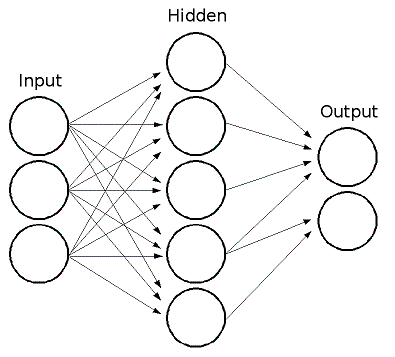
\includegraphics{pics/mlp_.png}

All the neurons in MLP are similar. Each of them has several input links (i.e. it takes the output values from several neurons in the previous layer on input) and several output links (i.e. it passes the response to several neurons in the next layer). The values retrieved from the previous layer are summed with certain weights, individual for each neuron, plus the bias term, and the sum is transformed using the activation function $f$ that may be also different for different neurons. Here is the picture:

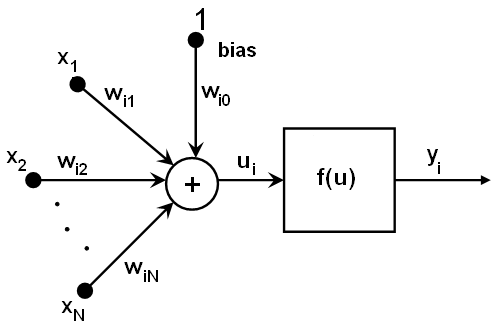
\includegraphics{pics/neuron_model.png}

In other words, given the outputs $x_j$ of the layer $n$, the outputs $y_i$ of the layer $n+1$ are computed as:

\[
    u_i = \sum_j (w^{n+1}_{i,j}*x_j) + w^{n+1}_{i,bias}
\]

\[
    y_i = f(u_i)
\]

Different activation functions may be used, ML implements 3 standard ones:
\begin{itemize}
\item Identity function (\texttt{CvANN\_MLP::IDENTITY}): $f(x)=x$
\item Symmetrical sigmoid (\texttt{CvANN\_MLP::SIGMOID\_SYM}): $f(x)=\beta*(1-e^{-\alpha x})/(1+e^{-\alpha x}$), the default choice for MLP; the standard sigmoid with $\beta =1, \alpha =1$ is shown below:

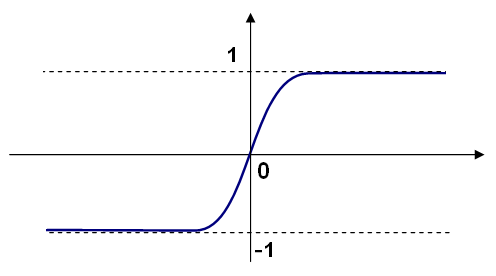
\includegraphics{pics/sigmoid_bipolar.png} 

\item Gaussian function (\texttt{CvANN\_MLP::GAUSSIAN}): $f(x)=\beta e^{-\alpha x*x}$, not completely supported by the moment.
\end{itemize}
In ML all the neurons have the same activation functions, with the same free parameters ($\alpha, \beta$) that are specified by user and are not altered by the training algorithms.

So the whole trained network works as follows: It takes the feature vector on input, the vector size is equal to the size of the input layer, when the values are passed as input to the first hidden layer, the outputs of the hidden layer are computed using the weights and the activation functions and passed further downstream, until we compute the output layer.

So, in order to compute the network one needs to know all the
weights $w^{n+1)}_{i,j}$. The weights are computed by the training
algorithm. The algorithm takes a training set: multiple input vectors
with the corresponding output vectors, and iteratively adjusts the
weights to try to make the network give the desired response on the
provided input vectors.

The larger the network size (the number of hidden layers and their sizes),
the more is the potential network flexibility, and the error on the
training set could be made arbitrarily small. But at the same time the
learned network will also "learn" the noise present in the training set,
so the error on the test set usually starts increasing after the network
size reaches some limit. Besides, the larger networks are train much
longer than the smaller ones, so it is reasonable to preprocess the data
(using \cross{CalcPCA} or similar technique) and train a smaller network
on only the essential features.

Another feature of the MLP's is their inability to handle categorical
data as is, however there is a workaround. If a certain feature in the
input or output (i.e. in the case of \texttt{n}-class classifier for
$n>2$) layer is categorical and can take $M>2$
different values, it makes sense to represent it as binary tuple of
\texttt{M} elements, where \texttt{i}-th element is 1 if and only if the
feature is equal to the \texttt{i}-th value out of \texttt{M} possible. It
will increase the size of the input/output layer, but will speedup the
training algorithm convergence and at the same time enable "fuzzy" values
of such variables, i.e. a tuple of probabilities instead of a fixed value.

ML implements 2 algorithms for training MLP's. The first is the classical
random sequential back-propagation algorithm
and the second (default one) is batch RPROP algorithm.

References:
\begin{itemize}
\item \url{http://en.wikipedia.org/wiki/Backpropagation}. Wikipedia article about the back-propagation algorithm.
\item Y. LeCun, L. Bottou, G.B. Orr and K.-R. Muller, "Efficient backprop", in Neural Networks---Tricks of the Trade, Springer Lecture Notes in Computer Sciences 1524, pp.5-50, 1998.
\item M. Riedmiller and H. Braun, "A Direct Adaptive Method for Faster Backpropagation Learning: The RPROP Algorithm", Proc. ICNN, San Francisco (1993).
\end{itemize}

\cvfunc{CvANN\_MLP\_TrainParams}
Parameters of the MLP training algorithm.

\begin{lstlisting}
struct CvANN_MLP_TrainParams
{
    CvANN_MLP_TrainParams();
    CvANN_MLP_TrainParams( CvTermCriteria term_crit, int train_method,
                           double param1, double param2=0 );
    ~CvANN_MLP_TrainParams();

    enum { BACKPROP=0, RPROP=1 };

    CvTermCriteria term_crit;
    int train_method;

    // backpropagation parameters
    double bp_dw_scale, bp_moment_scale;

    // rprop parameters
    double rp_dw0, rp_dw_plus, rp_dw_minus, rp_dw_min, rp_dw_max;
};
\end{lstlisting}

%\begin{description}
%\cvarg{term\_crit}{The termination criteria for the training algorithm. It identifies how many iterations are done by the algorithm (for sequential backpropagation algorithm the number is multiplied by the size of the training set) and how much the weights could change between the iterations to make the algorithm continue.}
%\cvarg{train\_method}{The training algorithm to use; can be one of \texttt{CvANN\_MLP\_TrainParams::BACKPROP} (sequential backpropagation algorithm) or \texttt{CvANN\_MLP\_TrainParams::RPROP} (RPROP algorithm, default value).}
%\cvarg{bp\_dw\_scale}{(Backpropagation only): The coefficient to multiply the computed weight gradient by. The recommended value is about 0.1. The parameter can be set via \texttt{param1} of the constructor.}
%\cvarg{bp\_moment\_scale}{(Backpropagation only): The coefficient to multiply the difference between weights on the 2 previous iterations. This parameter provides some inertia to smooth the random fluctuations of the weights. It can vary from 0 (the feature is disabled) to 1 and beyond. The value 0.1 or so is good enough. The parameter can be set via \texttt{param2} of the constructor.}
%\cvarg{rp\_dw0}{(RPROP only): Initial magnitude of the weight delta. The default value is 0.1. This parameter can be set via \texttt{param1} of the constructor.}
%\cvarg{rp\_dw\_plus}{(RPROP only): The increase factor for the weight delta. It must be $>1$, the default value is 1.2, which should work well in most cases, according to the algorithm's author. The parameter can only be changed explicitly by modifying the structure member.}
%\cvarg{rp\_dw\_minus}{(RPROP only): The decrease factor for the weight delta. It must be $<1$, the default value is 0.5, which should work well in most cases, according to the algorithm's author. The parameter can only be changed explicitly by modifying the structure member.}
%\cvarg{rp\_dw\_min}{(RPROP only): The minimum value of the weight delta. It must be $>0$, the default value is \texttt{FLT\_EPSILON}. The parameter can be set via \texttt{param2} of the constructor.}
%\cvarg{rp\_dw\_max}{(RPROP only): The maximum value of the weight delta. It must be $>1$, the default value is 50. The parameter can only be changed explicitly by modifying the structure member.}
%\end{description}

The structure has default constructor that initializes parameters for \texttt{RPROP} algorithm. There is also more advanced constructor to customize the parameters and/or choose backpropagation algorithm. Finally, the individual parameters can be adjusted after the structure is created.


\cvfunc{CvANN\_MLP}
MLP model.

\begin{lstlisting}
class CvANN_MLP : public CvStatModel
{
public:
    CvANN_MLP();
    CvANN_MLP( const CvMat* _layer_sizes,
               int _activ_func=SIGMOID_SYM,
               double _f_param1=0, double _f_param2=0 );

    virtual ~CvANN_MLP();

    virtual void create( const CvMat* _layer_sizes,
                         int _activ_func=SIGMOID_SYM,
                         double _f_param1=0, double _f_param2=0 );

    virtual int train( const CvMat* _inputs, const CvMat* _outputs,
                       const CvMat* _sample_weights, 
		       const CvMat* _sample_idx=0,
                       CvANN_MLP_TrainParams _params = CvANN_MLP_TrainParams(),
                       int flags=0 );
    virtual float predict( const CvMat* _inputs,
                           CvMat* _outputs ) const;

    virtual void clear();

    // possible activation functions
    enum { IDENTITY = 0, SIGMOID_SYM = 1, GAUSSIAN = 2 };

    // available training flags
    enum { UPDATE_WEIGHTS = 1, NO_INPUT_SCALE = 2, NO_OUTPUT_SCALE = 4 };

    virtual void read( CvFileStorage* fs, CvFileNode* node );
    virtual void write( CvFileStorage* storage, const char* name );

    int get_layer_count() { return layer_sizes ? layer_sizes->cols : 0; }
    const CvMat* get_layer_sizes() { return layer_sizes; }

protected:

    virtual bool prepare_to_train( const CvMat* _inputs, const CvMat* _outputs,
            const CvMat* _sample_weights, const CvMat* _sample_idx,
            CvANN_MLP_TrainParams _params,
            CvVectors* _ivecs, CvVectors* _ovecs, double** _sw, int _flags );

    // sequential random backpropagation
    virtual int train_backprop( CvVectors _ivecs, CvVectors _ovecs, 
						const double* _sw );

    // RPROP algorithm
    virtual int train_rprop( CvVectors _ivecs, CvVectors _ovecs, 
					     const double* _sw );

    virtual void calc_activ_func( CvMat* xf, const double* bias ) const;
    virtual void calc_activ_func_deriv( CvMat* xf, CvMat* deriv, 
					     const double* bias ) const;
    virtual void set_activ_func( int _activ_func=SIGMOID_SYM,
                                 double _f_param1=0, double _f_param2=0 );
    virtual void init_weights();
    virtual void scale_input( const CvMat* _src, CvMat* _dst ) const;
    virtual void scale_output( const CvMat* _src, CvMat* _dst ) const;
    virtual void calc_input_scale( const CvVectors* vecs, int flags );
    virtual void calc_output_scale( const CvVectors* vecs, int flags );

    virtual void write_params( CvFileStorage* fs );
    virtual void read_params( CvFileStorage* fs, CvFileNode* node );

    CvMat* layer_sizes;
    CvMat* wbuf;
    CvMat* sample_weights;
    double** weights;
    double f_param1, f_param2;
    double min_val, max_val, min_val1, max_val1;
    int activ_func;
    int max_count, max_buf_sz;
    CvANN_MLP_TrainParams params;
    CvRNG rng;
};
\end{lstlisting}

Unlike many other models in ML that are constructed and trained at once, in the MLP model these steps are separated. First, a network with the specified topology is created using the non-default constructor or the method \texttt{create}. All the weights are set to zeros. Then the network is trained using the set of input and output vectors. The training procedure can be repeated more than once, i.e. the weights can be adjusted based on the new training data.


\cvfunc{CvANN\_MLP::create}
Constructs the MLP with the specified topology

\cvdefCpp{
void CvANN\_MLP::create( \par const CvMat* \_layer\_sizes,
                        \par int \_activ\_func=SIGMOID\_SYM,
                        \par double \_f\_param1=0, \par double \_f\_param2=0 );
}

\begin{description}
\cvarg{\_layer\_sizes}{The integer vector specifies the number of neurons in each layer including the input and output layers.}
\cvarg{\_activ\_func}{Specifies the activation function for each neuron; one of \texttt{CvANN\_MLP::IDENTITY}, \texttt{CvANN\_MLP::SIGMOID\_SYM} and \texttt{CvANN\_MLP::GAUSSIAN}.}
\cvarg{\_f\_param1,\_f\_param2}{Free parameters of the activation function, $\alpha$ and $\beta$, respectively. See the formulas in the introduction section.}
\end{description}

The method creates a MLP network with the specified topology and assigns the same activation function to all the neurons.

\cvfunc{CvANN\_MLP::train}
Trains/updates MLP.

\cvdefCpp{
int CvANN\_MLP::train( \par const CvMat* \_inputs, \par const CvMat* \_outputs,
                      \par const CvMat* \_sample\_weights, \par const CvMat* \_sample\_idx=0,
                      \par CvANN\_MLP\_TrainParams \_params = CvANN\_MLP\_TrainParams(),
                      \par int flags=0 );
}

\begin{description}
\cvarg{\_inputs}{A floating-point matrix of input vectors, one vector per row.}
\cvarg{\_outputs}{A floating-point matrix of the corresponding output vectors, one vector per row.}
\cvarg{\_sample\_weights}{(RPROP only) The optional floating-point vector of weights for each sample. Some samples may be more important than others for training, and the user may want to raise the weight of certain classes to find the right balance between hit-rate and false-alarm rate etc.}
\cvarg{\_sample\_idx}{The optional integer vector indicating the samples (i.e. rows of \texttt{\_inputs} and \texttt{\_outputs}) that are taken into account.}
\cvarg{\_params}{The training params. See \texttt{CvANN\_MLP\_TrainParams} description.}
\cvarg{\_flags}{The various parameters to control the training algorithm. May be a combination of the following:
\begin{description}
\cvarg{UPDATE\_WEIGHTS = 1}{algorithm updates the network weights, rather than computes them from scratch (in the latter case the weights are initialized using \emph{Nguyen-Widrow} algorithm).}
\cvarg{NO\_INPUT\_SCALE}{algorithm does not normalize the input vectors. If this flag is not set, the training algorithm normalizes each input feature independently, shifting its mean value to 0 and making the standard deviation =1. If the network is assumed to be updated frequently, the new training data could be much different from original one. In this case user should take care of proper normalization.}
\cvarg{NO\_OUTPUT\_SCALE}{algorithm does not normalize the output vectors. If the flag is not set, the training algorithm normalizes each output features independently, by transforming it to the certain range depending on the activation function used.}
\end{description}}
\end{description}

This method applies the specified training algorithm to compute/adjust the network weights. It returns the number of done iterations.

\fi




\Cfalse
\Cpptrue
\Pyfalse
\CPyfalse
\def\targetlang{cpp}
\part{C++ API Reference}
\ifCpp
\chapter{Introduction}

Starting from OpenCV 2.0 the new modern C++ interface has been introduced.
It is crisp (less typing is needed to code the same thing), type-safe (no more \texttt{CvArr*} a.k.a. \texttt{void*})
and, in general, more convenient to use. Here is a short example of what it looks like:

\begin{lstlisting}
//
// Simple retro-style photo effect done by adding noise to
// the luminance channel and reducing intensity of the chroma channels
//

// include standard OpenCV headers, same as before
#include "cv.h"
#include "highgui.h"

// all the new API is put into "cv" namespace. Export its content
using namespace cv;

// enable/disable use of mixed API in the code below.
#define DEMO_MIXED_API_USE 1

int main( int argc, char** argv )
{
    const char* imagename = argc > 1 ? argv[1] : "lena.jpg";
#if DEMO_MIXED_API_USE
    // Ptr<T> is safe ref-conting pointer class
    Ptr<IplImage> iplimg = cvLoadImage(imagename);
    
    // cv::Mat replaces the CvMat and IplImage, but it's easy to convert
    // between the old and the new data structures
    // (by default, only the header is converted and the data is shared)
    Mat img(iplimg); 
#else
    // the newer cvLoadImage alternative with MATLAB-style name
    Mat img = imread(imagename);
#endif

    if( !img.data ) // check if the image has been loaded properly
        return -1;

    Mat img_yuv;
    // convert image to YUV color space.
    // The output image will be allocated automatically
    cvtColor(img, img_yuv, CV_BGR2YCrCb); 

    // split the image into separate color planes
    vector<Mat> planes;
    split(img_yuv, planes);

    // another Mat constructor; allocates a matrix of the specified
	// size and type
    Mat noise(img.size(), CV_8U);
    
    // fills the matrix with normally distributed random values;
    // there is also randu() for uniformly distributed random numbers. 
    // Scalar replaces CvScalar, Scalar::all() replaces cvScalarAll().
    randn(noise, Scalar::all(128), Scalar::all(20));
                                                     
    // blur the noise a bit, kernel size is 3x3 and both sigma's 
	// are set to 0.5
    GaussianBlur(noise, noise, Size(3, 3), 0.5, 0.5);

    const double brightness_gain = 0;
    const double contrast_gain = 1.7;
#if DEMO_MIXED_API_USE
    // it's easy to pass the new matrices to the functions that
    // only work with IplImage or CvMat:
    // step 1) - convert the headers, data will not be copied
    IplImage cv_planes_0 = planes[0], cv_noise = noise;
    // step 2) call the function; do not forget unary "&" to form pointers
    cvAddWeighted(&cv_planes_0, contrast_gain, &cv_noise, 1,
                 -128 + brightness_gain, &cv_planes_0);
#else
    addWeighted(planes[0], constrast_gain, noise, 1,
                -128 + brightness_gain, planes[0]);
#endif
    const double color_scale = 0.5;
    // Mat::convertTo() replaces cvConvertScale.
    // One must explicitly specify the output matrix type
    // (we keep it intact, i.e. pass planes[1].type())
    planes[1].convertTo(planes[1], planes[1].type(),
                        color_scale, 128*(1-color_scale));

    // alternative form of convertTo if we know the datatype
    // at compile time ("uchar" here).
    // This expression will not create any temporary arrays
    // and should be almost as fast as the above variant
    planes[2] = Mat_<uchar>(planes[2]*color_scale + 128*(1-color_scale));

    // Mat::mul replaces cvMul(). Again, no temporary arrays are
    // created in the case of simple expressions.
    planes[0] = planes[0].mul(planes[0], 1./255);

    // now merge the results back
    merge(planes, img_yuv);
    // and produce the output RGB image
    cvtColor(img_yuv, img, CV_YCrCb2BGR);

    // this is counterpart for cvNamedWindow
    namedWindow("image with grain", CV_WINDOW_AUTOSIZE);
#if DEMO_MIXED_API_USE
    // this is to demonstrate that img and iplimg really share the data -
    // the result of the above processing is stored to img and thus 
	// in iplimg too.
    cvShowImage("image with grain", iplimg);
#else
    imshow("image with grain", img);
#endif
    waitKey();

    return 0;
    // all the memory will automatically be released
    // by vector<>, Mat and Ptr<> destructors.
}
\end{lstlisting}

Following a summary "cheatsheet" below, the rest of the introduction will discuss the key features of the new interface in more detail.



\section{C++ Cheatsheet}\label{cheatSheet}
 The section is just a summary "cheatsheet" of common things you may want to do with cv::Mat:. The code snippets below all assume the correct 
 namespace is used:
 \begin{lstlisting}
using namespace cv;
using namespace std; 
 \end{lstlisting} 
 
 
 Convert an IplImage or CvMat to an cv::Mat and a cv::Mat to an IplImage or CvMat:
 \begin{lstlisting}
 // Assuming somewhere IplImage *iplimg; exists 
 // and has been allocated and cv::Mat Mimg has been defined
 Mat imgMat(iplimg);  //Construct an Mat image "img" out of an IplImage
 Mimg = iplimg;       //Or just set the header of pre existing cv::Mat 
                      //Ming to iplimg's data (no copying is done)
 
 //Convert to IplImage or CvMat, no data copying
 IplImage ipl_img = img;
 CvMat cvmat = img; // convert cv::Mat -> CvMat
 \end{lstlisting} 
 
 A very simple way to operate on a rectanglular sub-region of an image (ROI -- "Region of Interest"):
\begin{lstlisting}
 //Make a rectangle 
 Rect roi(10, 20, 100, 50);
 //Point a cv::Mat header at it (no allocation is done)
 Mat image_roi = image(roi);
\end{lstlisting}

A bit advanced, but should you want efficiently to sample from a circular region in an image  
(below, instead of sampling, we just draw into a BGR image) :

\begin{lstlisting}
// the function returns x boundary coordinates of 
// the circle for each y. RxV[y1] = x1 means that 
// when y=y1, -x1 <=x<=x1 is inside the circle
void getCircularROI(int R, vector < int > & RxV)
{
    RxV.resize(R+1);
    for( int y = 0; y <= R; y++ )
        RxV[y] = cvRound(sqrt((double)R*R - y*y));
}

// This draws a circle in the green channel
// (note the "[1]" for a BGR" image,
// blue and red channels are not modified),
// but is really an example of how to *sample* from a circular region. 
void drawCircle(Mat &image, int R, Point center)
{
    vector<int> RxV;
    getCircularROI(R, RxV);
	
    Mat_<Vec3b>& img = (Mat_<Vec3b>&)image; //3 channel pointer to image
    for( int dy = -R; dy <= R; dy++ )
    {
        int Rx = RxV[abs(dy)];
        for( int dx = -Rx; dx <= Rx; dx++ )
            img(center.y+dy, center.x+dx)[1] = 255;
    }
}
\end{lstlisting}

\section{Namespace \texttt{cv} and Function Naming}

All the newly introduced classes and functions are placed into \texttt{cv} namespace. Therefore, to access this functionality from your code, use \texttt{cv::} specifier or \texttt{"using namespace cv;"} directive:
\begin{lstlisting}
#include "cv.h"

...
cv::Mat H = cv::findHomography(points1, points2, cv::RANSAC, 5);
...
\end{lstlisting}
or
\begin{lstlisting}
#include "cv.h"

using namespace cv;

...
Mat H = findHomography(points1, points2, RANSAC, 5 );
...
\end{lstlisting}

It is probable that some of the current or future OpenCV external names conflict with STL
or other libraries, in this case use explicit namespace specifiers to resolve the name conflicts:
\begin{lstlisting}
Mat a(100, 100, CV_32F);
randu(a, Scalar::all(1), Scalar::all(std::rand()%256+1));
cv::log(a, a);
a /= std::log(2.);
\end{lstlisting}

For the most of the C functions and structures from OpenCV 1.x you may find the direct counterparts in the new C++ interface. The name is usually formed by omitting \texttt{cv} or \texttt{Cv} prefix and turning the first letter to the low case (unless it's a own name, like Canny, Sobel etc). In case when there is no the new-style counterpart, it's possible to use the old functions with the new structures, as shown the first sample in the chapter.

\section{Memory Management}

When using the new interface, the most of memory deallocation and even memory allocation operations are done automatically when needed.

First of all, \cross{Mat}, \cross{SparseMat} and other classes have destructors
that deallocate memory buffers occupied by the structures when needed.

Secondly, this "when needed" means that the destructors do not always deallocate the buffers, they take into account possible data sharing.
That is, in a destructor the reference counter associated with the underlying data is decremented and the data is deallocated
if and only if the reference counter becomes zero, that is, when no other structures refer to the same buffer. When such a structure
containing a reference counter is copied, usually just the header is duplicated, while the underlying data is not; instead, the reference counter is incremented to memorize that there is another owner of the same data.
Also, some structures, such as \texttt{Mat}, can refer to the user-allocated data.
In this case the reference counter is \texttt{NULL} pointer and then no reference counting is done - the data is not deallocated by the destructors and should be deallocated manually by the user. We saw this scheme in the first example in the chapter:
\begin{lstlisting}
// allocates IplImages and wraps it into shared pointer class.
Ptr<IplImage> iplimg = cvLoadImage(...);

// constructs Mat header for IplImage data;
// does not copy the data;
// the reference counter will be NULL
Mat img(iplimg);
...
// in the end of the block img destructor is called,
// which does not try to deallocate the data because
// of NULL pointer to the reference counter.
//
// Then Ptr<IplImage> destructor is called that decrements
// the reference counter and, as the counter becomes 0 in this case,
// the destructor calls cvReleaseImage().
\end{lstlisting}

The copying semantics was mentioned in the above paragraph, but deserves a dedicated discussion.
By default, the new OpenCV structures implement shallow, so called O(1) (i.e. constant-time) assignment operations. It gives user possibility to pass quite big data structures to functions (though, e.g. passing \texttt{const Mat\&} is still faster than passing \texttt{Mat}), return them (e.g. see the example with \cross{findHomography} above), store them in OpenCV and STL containers etc. - and do all of this very efficiently. On the other hand, most of the new data structures provide \texttt{clone()} method that creates a full copy of an object. Here is the sample:
\begin{lstlisting}
// create a big 8Mb matrix
Mat A(1000, 1000, CV_64F);

// create another header for the same matrix;
// this is instant operation, regardless of the matrix size.
Mat B = A;
// create another header for the 3-rd row of A; no data is copied either
Mat C = B.row(3);
// now create a separate copy of the matrix
Mat D = B.clone();
// copy the 5-th row of B to C, that is, copy the 5-th row of A 
// to the 3-rd row of A.
B.row(5).copyTo(C);
// now let A and D share the data; after that the modified version
// of A is still referenced by B and C.
A = D;
// now make B an empty matrix (which references no memory buffers),
// but the modified version of A will still be referenced by C,
// despite that C is just a single row of the original A
B.release(); 
             
// finally, make a full copy of C. In result, the big modified
// matrix will be deallocated, since it's not referenced by anyone
C = C.clone();
\end{lstlisting}

Memory management of the new data structures is automatic and thus easy. If, however, your code uses \cross{IplImage},
\cross{CvMat} or other C data structures a lot, memory management can still be automated without immediate migration
to \cross{Mat} by using the already mentioned template class \cross{Ptr}, similar to \texttt{shared\_ptr} from Boost and C++ TR1.
It wraps a pointer to an arbitrary object, provides transparent access to all the object fields and associates a reference counter with it.
Instance of the class can be passed to any function that expects the original pointer. For correct deallocation of the object, you should specialize \texttt{Ptr<T>::delete\_obj()} method. Such specialized methods already exist for the classical OpenCV structures, e.g.:
\begin{lstlisting}
// cxoperations.hpp:
...
template<> inline Ptr<IplImage>::delete_obj() {
    cvReleaseImage(&obj);
}
...
\end{lstlisting}
See \cross{Ptr} description for more details and other usage scenarios.


\section{Memory Management Part II. Automatic Data Allocation}\label{AutomaticMemoryManagement2}

With the new interface not only explicit memory deallocation is not needed anymore,
but the memory allocation is often done automatically too. That was demonstrated in the example
in the beginning of the chapter when \texttt{cvtColor} was called, and here are some more details.

\cross{Mat} and other array classes provide method \texttt{create} that allocates a new buffer for array
data if and only if the currently allocated array is not of the required size and type.
If a new buffer is needed, the previously allocated buffer is released
(by engaging all the reference counting mechanism described in the previous section).
Now, since it is very quick to check whether the needed memory buffer is already allocated,
most new OpenCV functions that have arrays as output parameters call the \texttt{create} method and
this way the \emph{automatic data allocation} concept is implemented. Here is the example:
\begin{lstlisting}
#include "cv.h"
#include "highgui.h"

using namespace cv;

int main(int, char**)
{
    VideoCapture cap(0);
    if(!cap.isOpened()) return -1;

    Mat edges;
    namedWindow("edges",1);
    for(;;)
    {
        Mat frame;
        cap >> frame;
        cvtColor(frame, edges, CV_BGR2GRAY);
        GaussianBlur(edges, edges, Size(7,7), 1.5, 1.5);
        Canny(edges, edges, 0, 30, 3);
        imshow("edges", edges);
        if(waitKey(30) >= 0) break;
    }
    return 0;
}
\end{lstlisting}
The matrix \texttt{edges} is allocated during the first frame processing and unless the resolution will suddenly change,
the same buffer will be reused for every next frame's edge map.

In many cases the output array type and size can be inferenced from the input arrays' respective characteristics, but not always.
In these rare cases the corresponding functions take separate input parameters that specify the data type and/or size of the output arrays,
like \cross{resize}. Anyway, a vast majority of the new-style array processing functions call \texttt{create}
for each of the output array, with just a few exceptions like \texttt{mixChannels}, \texttt{RNG::fill} and some others.

Note that this output array allocation semantic is only implemented in the new functions. If you want to pass the new structures to some old OpenCV function, you should first allocate the output arrays using \texttt{create} method, then make \texttt{CvMat} or \texttt{IplImage} headers and after that call the function.

\section{Algebraic Operations}

Just like in v1.x, OpenCV 2.x provides some basic functions operating on matrices, like \texttt{add},
\texttt{subtract}, \texttt{gemm} etc. In addition, it introduces overloaded operators that give the user a convenient
algebraic notation, which is nearly as fast as using the functions directly. For example, here is how the least squares problem $Ax=b$
can be solved using normal equations:
\begin{lstlisting}
Mat x = (A.t()*A).inv()*(A.t()*b);
\end{lstlisting}

The complete list of overloaded operators can be found in \cross{Matrix Expressions}.

\section{Fast Element Access}

Historically, OpenCV provided many different ways to access image and matrix elements, and none of them was both fast and convenient.
With the new data structures, OpenCV 2.x introduces a few more alternatives, hopefully more convenient than before. For detailed description of the operations, please, check \cross{Mat} and \hyperref[MatT]{Mat\_} description. Here is part of the retro-photo-styling example rewritten (in simplified form) using the element access operations:

\begin{lstlisting}
...
// split the image into separate color planes
vector<Mat> planes;
split(img_yuv, planes);

// method 1. process Y plane using an iterator
MatIterator_<uchar> it = planes[0].begin<uchar>(),
                    it_end = planes[0].end<uchar>();
for(; it != it_end; ++it)
{
    double v = *it*1.7 + rand()%21-10;
    *it = saturate_cast<uchar>(v*v/255.);
}

// method 2. process the first chroma plane using pre-stored row pointer.
// method 3. process the second chroma plane using
//           individual element access operations
for( int y = 0; y < img_yuv.rows; y++ )
{
    uchar* Uptr = planes[1].ptr<uchar>(y);
    for( int x = 0; x < img_yuv.cols; x++ )
    {
        Uptr[x] = saturate_cast<uchar>((Uptr[x]-128)/2 + 128);
        uchar& Vxy = planes[2].at<uchar>(y, x);
        Vxy = saturate_cast<uchar>((Vxy-128)/2 + 128);
    }
}

merge(planes, img_yuv);
...
\end{lstlisting}


\section{Saturation Arithmetics}

In the above sample you may have noticed \hyperref[saturatecast]{saturate\_cast} operator, and that's how all the pixel processing is done in OpenCV. When a result of image operation is 8-bit image with pixel values ranging from 0 to 255, each output pixel value is clipped to this available range:

\[
I(x,y)=\min(\max(value, 0), 255)
\]

and the similar rules are applied to 8-bit signed and 16-bit signed and unsigned types. This "saturation" semantics (different from usual C language "wrapping" semantics, where lowest bits are taken, is implemented in every image processing function, from the simple \texttt{cv::add} to 
\texttt{cv::cvtColor}, \texttt{cv::resize}, \texttt{cv::filter2D} etc.
It is not a new feature of OpenCV v2.x, it was there from very beginning. In the new version this special \hyperref[saturatecast]{saturate\_cast} template operator is introduced to simplify implementation of this semantic in your own functions.


\section{Error handling}

The modern error handling mechanism in OpenCV uses exceptions, as opposite to the manual stack unrolling used in previous versions. When OpenCV is built in DEBUG configuration, the error handler provokes memory access violation, so that the full call stack and context can be analyzed with debugger.

\section{Threading and Reenterability}

OpenCV uses OpenMP to run some time-consuming operations in parallel. Threading can be explicitly controlled by \cross{setNumThreads} function. Also, functions and "const" methods of the classes are generally re-enterable, that is, they can be called from different threads asynchronously.

\fi

\ifPy
\chapter{Introduction}

Starting with release 2.0, OpenCV has a new Python interface. This replaces the previous 
\href{http://opencv.willowgarage.com/wiki/SwigPythonInterface}{SWIG-based Python interface}.

Some highlights of the new bindings:

\begin{itemize}
\item{single import of all of OpenCV using \texttt{import cv}}
\item{OpenCV functions no longer have the "cv" prefix}
\item{simple types like CvRect and CvScalar use Python tuples}
\item{sharing of Image storage, so image transport between OpenCV and other systems (e.g. numpy and ROS) is very efficient}
\item{complete documentation for the Python functions}
\end{itemize}

This.

\section{Cookbook}

Here is a collection of code fragments demonstrating some features
of the OpenCV Python bindings.

\subsection{Convert an image}

\begin{lstlisting}
>>> import cv
>>> im = cv.LoadImageM("building.jpg")
>>> print type(im)
<type 'cv.cvmat'>
>>> cv.SaveImage("foo.png", im)
\end{lstlisting}

\subsection{Resize an image}

To resize an image in OpenCV, create a destination image of the appropriate size, then call \cross{Resize}.

\begin{lstlisting}
>>> import cv
>>> original = cv.LoadImageM("building.jpg")
>>> thumbnail = cv.CreateMat(original.rows / 10, original.cols / 10, cv.CV_8UC3)
>>> cv.Resize(original, thumbnail)
\end{lstlisting}

\subsection{Compute the Laplacian}

\begin{lstlisting}
>>> import cv
>>> im = cv.LoadImageM("building.jpg", 1)
>>> dst = cv.CreateImage(cv.GetSize(im), cv.IPL_DEPTH_16S, 3)
>>> laplace = cv.Laplace(im, dst)
>>> cv.SaveImage("foo-laplace.png", dst)
\end{lstlisting}


\subsection{Using GoodFeaturesToTrack}

To find the 10 strongest corner features in an image, use \cross{GoodFeaturesToTrack} like this:

\begin{lstlisting}
>>> import cv
>>> img = cv.LoadImageM("building.jpg", cv.CV_LOAD_IMAGE_GRAYSCALE)
>>> eig_image = cv.CreateMat(img.rows, img.cols, cv.CV_32FC1)
>>> temp_image = cv.CreateMat(img.rows, img.cols, cv.CV_32FC1)
>>> for (x,y) in cv.GoodFeaturesToTrack(img, eig_image, temp_image, 10, 0.04, 1.0, useHarris = True):
...    print "good feature at", x,y
good feature at 198.0 514.0
good feature at 791.0 260.0
good feature at 370.0 467.0
good feature at 374.0 469.0
good feature at 490.0 520.0
good feature at 262.0 278.0
good feature at 781.0 134.0
good feature at 3.0 247.0
good feature at 667.0 321.0
good feature at 764.0 304.0
\end{lstlisting}


\subsection{Using GetSubRect}

GetSubRect returns a rectangular part of another image.  It does this without copying any data.

\begin{lstlisting}
>>> import cv
>>> img = cv.LoadImageM("building.jpg")
>>> sub = cv.GetSubRect(img, (60, 70, 32, 32))  # sub is 32x32 patch within img
>>> cv.SetZero(sub)                             # clear sub to zero, which also clears 32x32 pixels in img
\end{lstlisting}

\subsection{Using CreateMat, and accessing an element}

\begin{lstlisting}
>>> import cv
>>> mat = cv.CreateMat(5, 5, cv.CV_32FC1)
>>> cv.Set(mat, 1.0)
>>> mat[3,1] += 0.375
>>> print mat[3,1]
1.375
>>> print [mat[3,i] for i in range(5)]
[1.0, 1.375, 1.0, 1.0, 1.0]
\end{lstlisting}

\subsection{ROS image message to OpenCV}

See this tutorial: \href{http://www.ros.org/wiki/cv\_bridge/Tutorials/UsingCvBridgeToConvertBetweenROSImagesAndOpenCVImages}{Using CvBridge to convert between ROS images And OpenCV images}.

\subsection{PIL Image to OpenCV}

(For details on PIL see the \href{http://www.pythonware.com/library/pil/handbook/image.htm}{PIL handbook}.)

\begin{lstlisting}
>>> import Image, cv
>>> pi = Image.open('building.jpg')       # PIL image
>>> cv_im = cv.CreateImageHeader(pi.size, cv.IPL_DEPTH_8U, 3)
>>> cv.SetData(cv_im, pi.tostring())
>>> print pi.size, cv.GetSize(cv_im)
(868, 600) (868, 600)
>>> print pi.tostring() == cv_im.tostring()
True
\end{lstlisting}

\subsection{OpenCV to PIL Image}

\begin{lstlisting}
>>> import Image, cv
>>> cv_im = cv.CreateImage((320,200), cv.IPL_DEPTH_8U, 1)
>>> pi = Image.fromstring("L", cv.GetSize(cv_im), cv_im.tostring())
>>> print pi.size
(320, 200)
\end{lstlisting}

\subsection{NumPy and OpenCV}

Using the \href{http://docs.scipy.org/doc/numpy/reference/arrays.interface.html}{array interface}, to use an OpenCV CvMat in NumPy:

\begin{lstlisting}
>>> import cv, numpy
>>> mat = cv.CreateMat(3, 5, cv.CV_32FC1)
>>> cv.Set(mat, 7)
>>> a = numpy.asarray(mat)
>>> print a
[[ 7.  7.  7.  7.  7.]
 [ 7.  7.  7.  7.  7.]
 [ 7.  7.  7.  7.  7.]]
\end{lstlisting}

and to use a NumPy array in OpenCV:

\begin{lstlisting}
>>> import cv, numpy
>>> a = numpy.ones((480, 640))
>>> mat = cv.fromarray(a)
>>> print mat.rows
480
>>> print mat.cols
640
\end{lstlisting}

also, most OpenCV functions can work on NumPy arrays directly, for example:

\begin{lstlisting}
>>> picture = numpy.ones((640, 480))
>>> cv.Smooth(picture, picture, cv.CV_GAUSSIAN, 15, 15)
\end{lstlisting}

Given a 2D array, 
the \cross{fromarray} function (or the implicit version shown above)
returns a single-channel \cross{CvMat} of the same size.
For a 3D array of size $j \times k \times l$, it returns a 
\cross{CvMat} sized $j \times k$ with $l$ channels.

Alternatively, use \cross{fromarray} with the \texttt{allowND} option to always return a \cross{cvMatND}.

\fi


\chapter{cxcore. The Core Functionality}
\section{Basic Structures}

%%%%%%%%%%%%%%%%%%%%%%%%%%%%%%%%%%%%%%%%%%%%%%%%%%%%%%%%%%%%%%%%%%%%%%%%%%%%%%%%%%%%%%
%                                                                                    %
%                                         C                                          %
%                                                                                    %
%%%%%%%%%%%%%%%%%%%%%%%%%%%%%%%%%%%%%%%%%%%%%%%%%%%%%%%%%%%%%%%%%%%%%%%%%%%%%%%%%%%%%%

\ifCPy
\label{CvPoint}\cvclass{CvPoint}
2D point with integer coordinates (usually zero-based).

\begin{lstlisting}
typedef struct CvPoint
{
    int x; 
    int y; 
}
CvPoint;
\end{lstlisting}

\begin{description}
\cvarg{x}{x-coordinate}
\cvarg{y}{y-coordinate} 
\end{description}

\begin{lstlisting}
/* Constructor */
inline CvPoint cvPoint( int x, int y );

/* Conversion from CvPoint2D32f */
inline CvPoint cvPointFrom32f( CvPoint2D32f point );
\end{lstlisting}


\label{CvPoint2D32f}\cvclass{CvPoint2D32f}
2D point with floating-point coordinates

\begin{lstlisting}
typedef struct CvPoint2D32f
{
    float x;
    float y; 
}
CvPoint2D32f;
\end{lstlisting}

\begin{description}
\cvarg{x}{x-coordinate}
\cvarg{y}{y-coordinate}
\end{description}

\begin{lstlisting}
/* Constructor */
inline CvPoint2D32f cvPoint2D32f( double x, double y );

/* Conversion from CvPoint */
inline CvPoint2D32f cvPointTo32f( CvPoint point );
\end{lstlisting}


\label{CvPoint3D32f}\cvclass{CvPoint3D32f}
3D point with floating-point coordinates

\begin{lstlisting}
typedef struct CvPoint3D32f
{
    float x; 
    float y; 
    float z; 
}
CvPoint3D32f;
\end{lstlisting}

\begin{description}
\cvarg{x}{x-coordinate}
\cvarg{y}{y-coordinate}
\cvarg{z}{z-coordinate}
\end{description}

\begin{lstlisting}
/* Constructor */
inline CvPoint3D32f cvPoint3D32f( double x, double y, double z );
\end{lstlisting}

\label{CvPoint2D64f}\cvclass{CvPoint2D64f}
2D point with double precision floating-point coordinates

\begin{lstlisting}
typedef struct CvPoint2D64f
{
    double x; 
    double y; 
}
CvPoint2D64f;
\end{lstlisting}

\begin{description}
\cvarg{x}{x-coordinate}
\cvarg{y}{y-coordinate}
\end{description}

\begin{lstlisting}
/* Constructor */
inline CvPoint2D64f cvPoint2D64f( double x, double y );

/* Conversion from CvPoint */
inline CvPoint2D64f cvPointTo64f( CvPoint point );
\end{lstlisting}

\label{CvPoint3D64f}\cvclass{CvPoint3D64f}
3D point with double precision floating-point coordinates

\begin{lstlisting}
typedef struct CvPoint3D64f
{
    double x; 
    double y; 
    double z; 
}
CvPoint3D64f;
\end{lstlisting}

\begin{description}
\cvarg{x}{x-coordinate}
\cvarg{y}{y-coordinate}
\cvarg{z}{z-coordinate}
\end{description}

\begin{lstlisting}
/* Constructor */
inline CvPoint3D64f cvPoint3D64f( double x, double y, double z );
\end{lstlisting}

\label{CvSize}\cvclass{CvSize}
Pixel-accurate size of a rectangle.

\ifC % {
\begin{lstlisting}
typedef struct CvSize
{
    int width; 
    int height; 
}
CvSize;
\end{lstlisting}

\begin{description}
\cvarg{width}{Width of the rectangle}
\cvarg{height}{Height of the rectangle}
\end{description}

\begin{lstlisting}
/* Constructor */
inline CvSize cvSize( int width, int height );
\end{lstlisting}
\else % }{
Size of a rectangle, represented as a tuple \texttt{(width, height)}, where width and height are integers.
\fi % }

\label{CvSize2D32f}\cvclass{CvSize2D32f}
Sub-pixel accurate size of a rectangle.

\ifC % {
\begin{lstlisting}
typedef struct CvSize2D32f
{
    float width; 
    float height; 
}
CvSize2D32f;
\end{lstlisting}

\begin{description}
\cvarg{width}{Width of the rectangle}
\cvarg{height}{Height of the rectangle}
\end{description}

\begin{lstlisting}
/* Constructor */
inline CvSize2D32f cvSize2D32f( double width, double height );
\end{lstlisting}
\else % }{
Size of a rectangle, represented as a tuple \texttt{(width, height)}, where width and height are floats.
\fi % }

\label{CvRect}\cvclass{CvRect}
Offset (usually the top-left corner) and size of a rectangle.

\begin{lstlisting}
typedef struct CvRect
{
    int x; 
    int y; 
    int width; 
    int height; 
}
CvRect;
\end{lstlisting}

\begin{description}
\cvarg{x}{x-coordinate of the top-left corner}
\cvarg{y}{y-coordinate of the top-left corner (bottom-left for Windows bitmaps)}
\cvarg{width}{Width of the rectangle}
\cvarg{height}{Height of the rectangle}
\end{description}

\begin{lstlisting}
/* Constructor */
inline CvRect cvRect( int x, int y, int width, int height );
\end{lstlisting}

\label{CvScalar}\cvclass{CvScalar}
A container for 1-,2-,3- or 4-tuples of doubles.

\ifC % {
\begin{lstlisting}
typedef struct CvScalar
{
    double val[4];
}
CvScalar;
\end{lstlisting}

\begin{lstlisting}
/* Constructor: 
initializes val[0] with val0, val[1] with val1, etc. 
*/
inline CvScalar cvScalar( double val0, double val1=0,
                          double val2=0, double val3=0 );
/* Constructor: 
initializes all of val[0]...val[3] with val0123 
*/
inline CvScalar cvScalarAll( double val0123 );

/* Constructor: 
initializes val[0] with val0, and all of val[1]...val[3] with zeros 
*/
inline CvScalar cvRealScalar( double val0 );
\end{lstlisting}
\else % }{

CvScalar is always represented as a 4-tuple.

\begin{lstlisting}
>>> import cv
>>> cv.Scalar(1, 2, 3, 4)
(1.0, 2.0, 3.0, 4.0)
>>> cv.ScalarAll(7)
(7.0, 7.0, 7.0, 7.0)
>>> cv.RealScalar(7)
(7.0, 0.0, 0.0, 0.0)
>>> cv.RGB(17, 110, 255)
(255.0, 110.0, 17.0, 0.0)
\end{lstlisting}
\fi % }

\label{CvTermCriteria}\cvclass{CvTermCriteria}
Termination criteria for iterative algorithms.

\ifC % {
\begin{lstlisting}
#define CV_TERMCRIT_ITER    1
#define CV_TERMCRIT_NUMBER  CV_TERMCRIT_ITER
#define CV_TERMCRIT_EPS     2

typedef struct CvTermCriteria
{
    int    type;
    int    max_iter; 
    double epsilon; 
}
CvTermCriteria;
\end{lstlisting}

\begin{description}
\cvarg{type}{A combination of CV\_TERMCRIT\_ITER and CV\_TERMCRIT\_EPS}
\cvarg{max\_iter}{Maximum number of iterations}
\cvarg{epsilon}{Required accuracy}
\end{description}

\begin{lstlisting}
/* Constructor */
inline CvTermCriteria cvTermCriteria( int type, int max_iter, double epsilon );

/* Check and transform a CvTermCriteria so that 
   type=CV_TERMCRIT_ITER+CV_TERMCRIT_EPS
   and both max_iter and epsilon are valid */
CvTermCriteria cvCheckTermCriteria( CvTermCriteria criteria,
                                    double default_eps,
                                    int default_max_iters );
\end{lstlisting}
\else % }{
Represented by a tuple \texttt{(type, max\_iter, epsilon)}.

\begin{description}
\cvarg{type}{\texttt{CV\_TERMCRIT\_ITER}, \texttt{CV\_TERMCRIT\_EPS} or \texttt{CV\_TERMCRIT\_ITER | CV\_TERMCRIT\_EPS}}
\cvarg{max\_iter}{Maximum number of iterations}
\cvarg{epsilon}{Required accuracy}
\end{description}

\fi % }

\label{CvMat}\cvclass{CvMat}
A multi-channel matrix.

\begin{lstlisting}
typedef struct CvMat
{
    int type; 
    int step; 

    int* refcount; 

    union
    {
        uchar* ptr;
        short* s;
        int* i;
        float* fl;
        double* db;
    } data; 

#ifdef __cplusplus
    union
    {
        int rows;
        int height;
    };

    union
    {
        int cols;
        int width;
    };
#else
    int rows; 
    int cols; 
#endif

} CvMat;
\end{lstlisting}

\begin{description}
\cvarg{type}{A CvMat signature (CV\_MAT\_MAGIC\_VAL) containing the type of elements and flags}
\cvarg{step}{Full row length in bytes}
\cvarg{refcount}{Underlying data reference counter}
\cvarg{data}{Pointers to the actual matrix data}
\cvarg{rows}{Number of rows}
\cvarg{cols}{Number of columns}
\end{description}

Matrices are stored row by row. All of the rows are aligned by 4 bytes.


\label{CvMatND}\cvclass{CvMatND}
Multi-dimensional dense multi-channel array.

\begin{lstlisting}
typedef struct CvMatND
{
    int type; 
    int dims;

    int* refcount; 

    union
    {
        uchar* ptr;
        short* s;
        int* i;
        float* fl;
        double* db;
    } data; 

    struct
    {
        int size;
        int step;
    }
    dim[CV_MAX_DIM];

} CvMatND;
\end{lstlisting}

\begin{description}
\cvarg{type}{A CvMatND signature (CV\_MATND\_MAGIC\_VAL), combining the type of elements and flags}
\cvarg{dims}{The number of array dimensions}
\cvarg{refcount}{Underlying data reference counter}
\cvarg{data}{Pointers to the actual matrix data}
\cvarg{dim}{For each dimension, the pair (number of elements, distance between elements in bytes)}
\end{description}

\label{CvSparseMat}\cvclass{CvSparseMat}
Multi-dimensional sparse multi-channel array.

\begin{lstlisting}
typedef struct CvSparseMat
{
    int type;
    int dims; 
    int* refcount; 
    struct CvSet* heap; 
    void** hashtable; 
    int hashsize;
    int total; 
    int valoffset; 
    int idxoffset; 
    int size[CV_MAX_DIM]; 

} CvSparseMat;
\end{lstlisting}

\begin{description}
\cvarg{type}{A CvSparseMat signature (CV\_SPARSE\_MAT\_MAGIC\_VAL), combining the type of elements and flags.}
\cvarg{dims}{Number of dimensions}
\cvarg{refcount}{Underlying reference counter. Not used.}
\cvarg{heap}{A pool of hash table nodes}
\cvarg{hashtable}{The hash table. Each entry is a list of nodes.}
\cvarg{hashsize}{Size of the hash table}
\cvarg{total}{Total number of sparse array nodes}
\cvarg{valoffset}{The value offset of the array nodes, in bytes}
\cvarg{idxoffset}{The index offset of the array nodes, in bytes}
\cvarg{size}{Array of dimension sizes}
\end{description}

\label{IplImage}\cvclass{IplImage}
IPL image header

\begin{lstlisting}
typedef struct _IplImage
{
    int  nSize;         
    int  ID;            
    int  nChannels;     
    int  alphaChannel;  
    int  depth;         
    char colorModel[4]; 
    char channelSeq[4]; 
    int  dataOrder;     
    int  origin;        
    int  align;         
    int  width;         
    int  height;        
    struct _IplROI *roi; 
    struct _IplImage *maskROI; 
    void  *imageId;     
    struct _IplTileInfo *tileInfo; 
    int  imageSize;                             
    char *imageData;  
    int  widthStep;   
    int  BorderMode[4]; 
    int  BorderConst[4]; 
    char *imageDataOrigin; 
}
IplImage;
\end{lstlisting}

\begin{description}
\cvarg{nSize}{\texttt{sizeof(IplImage)}}
\cvarg{ID}{Version, always equals 0}
\cvarg{nChannels}{Number of channels. Most OpenCV functions support 1-4 channels.}
\cvarg{alphaChannel}{Ignored by OpenCV}
\cvarg{depth}{Pixel depth in bits. The supported depths are:
\begin{description}
\cvarg{IPL\_DEPTH\_8U}{Unsigned 8-bit integer}
\cvarg{IPL\_DEPTH\_8S}{Signed 8-bit integer}
\cvarg{IPL\_DEPTH\_16U}{Unsigned 16-bit integer}
\cvarg{IPL\_DEPTH\_16S}{Signed 16-bit integer}
\cvarg{IPL\_DEPTH\_32S}{Signed 32-bit integer}
\cvarg{IPL\_DEPTH\_32F}{Single-precision floating point}
\cvarg{IPL\_DEPTH\_64F}{Double-precision floating point}
\end{description}}
\cvarg{colorModel}{Ignored by OpenCV. The OpenCV function \cross{CvtColor} requires the source and destination color spaces as parameters.}
\cvarg{channelSeq}{Ignored by OpenCV}
\cvarg{dataOrder}{0 = \texttt{IPL\_DATA\_ORDER\_PIXEL} - interleaved color channels, 1 - separate color channels. \cross{CreateImage} only creates images with interleaved channels. For example, the usual layout of a color image is: $ b_{00} g_{00} r_{00} b_{10} g_{10} r_{10} ...$}
\cvarg{origin}{0 - top-left origin, 1 - bottom-left origin (Windows bitmap style)}
\cvarg{align}{Alignment of image rows (4 or 8). OpenCV ignores this and uses widthStep instead.}
\cvarg{width}{Image width in pixels}
\cvarg{height}{Image height in pixels}
\cvarg{roi}{Region Of Interest (ROI). If not NULL, only this image region will be processed.}
\cvarg{maskROI}{Must be NULL in OpenCV}
\cvarg{imageId}{Must be NULL in OpenCV}
\cvarg{tileInfo}{Must be NULL in OpenCV}
\cvarg{imageSize}{Image data size in bytes. For interleaved data, this equals $\texttt{image->height} \cdot \texttt{image->widthStep}$ }
\cvarg{imageData}{A pointer to the aligned image data}
\cvarg{widthStep}{The size of an aligned image row, in bytes}
\cvarg{BorderMode}{Border completion mode, ignored by OpenCV}
\cvarg{BorderConst}{Border completion mode, ignored by OpenCV}
\cvarg{imageDataOrigin}{A pointer to the origin of the image data (not necessarily aligned). This is used for image deallocation.}
\end{description}

The \cross{IplImage} structure was inherited from the Intel Image Processing Library, in which the format is native. OpenCV only supports a subset of possible \cross{IplImage} formats, as outlined in the parameter list above.

In addition to the above restrictions, OpenCV handles ROIs differently. OpenCV functions require that the image size or ROI size of all source and destination images match exactly. On the other hand, the Intel Image Processing Library processes the area of intersection between the source and destination images (or ROIs), allowing them to vary independently. 

\label{CvArr}\cvclass{CvArr}
Arbitrary array

\begin{lstlisting}
typedef void CvArr;
\end{lstlisting}

The metatype \texttt{CvArr} is used \textit{only} as a function parameter to specify that the function accepts arrays of multiple types, such as IplImage*, CvMat* or even CvSeq* sometimes. The particular array type is determined at runtime by analyzing the first 4 bytes of the header.
\fi

%%%%%%%%%%%%%%%%%%%%%%%%%%%%%%%%%%%%%%%%%%%%%%%%%%%%%%%%%%%%%%%%%%%%%%%%%%%%%%%%%%%%%%
%                                                                                    %
%                                        C++                                         %
%                                                                                    %
%%%%%%%%%%%%%%%%%%%%%%%%%%%%%%%%%%%%%%%%%%%%%%%%%%%%%%%%%%%%%%%%%%%%%%%%%%%%%%%%%%%%%%

\ifCpp
\subsection{DataType}\label{DataType}
Template "traits" class for other OpenCV primitive data types

\begin{lstlisting}
template<typename _Tp> class DataType
{
    // value_type is always a synonym for _Tp.
    typedef _Tp value_type;
    
    // intermediate type used for operations on _Tp.
    // it is int for uchar, signed char, unsigned short, signed short and int,
    // float for float, double for double, ...
    typedef <...> work_type;
    // in the case of multi-channel data it is the data type of each channel
    typedef <...> channel_type;
    enum
    {
        // CV_8U ... CV_64F
        depth = DataDepth<channel_type>::value,
        // 1 ... 
        channels = <...>,
        // '1u', '4i', '3f', '2d' etc.
        fmt=<...>,
        // CV_8UC3, CV_32FC2 ...
        type = CV_MAKETYPE(depth, channels)
    };
};
\end{lstlisting}

The template class \texttt{DataType} is descriptive class for OpenCV primitive data types and other types that comply with the following definition. A primitive OpenCV data type is one of \texttt{unsigned char, bool ($\sim$unsigned char), signed char, unsigned short, signed short, int, float, double} or a tuple of values of one of these types, where all the values in the tuple have the same type. If you are familiar with OpenCV \cross{CvMat}'s type notation, CV\_8U ... CV\_32FC3, CV\_64FC2 etc., then a primitive type can be defined as a type for which you can give a unique identifier in a form \verb*"CV\_<bit-depth>{U|S|F}C<number_of_channels>". A universal OpenCV structure able to store a single instance of such primitive data type is \cross{Vec}. Multiple instances of such a type can be stored to a \texttt{std::vector}, \texttt{Mat}, \texttt{Mat\_}, \texttt{MatND}, \texttt{MatND\_}, \texttt{SparseMat}, \texttt{SparseMat\_} or any other container that is able to store \cross{Vec} instances.
 
The class \texttt{DataType} is basically used to provide some description of such primitive data types without adding any fields or methods to the corresponding classes (and it is actually impossible to add anything to primitive C/C++ data types). This technique is known in C++ as class traits. It's not \texttt{DataType} itself that is used, but its specialized versions, such as:

\begin{lstlisting}
template<> class DataType<uchar>
{
    typedef uchar value_type;
    typedef int work_type;
    typedef uchar channel_type;
    enum { channel_type = CV_8U, channels = 1, fmt='u', type = CV_8U };
};
...
template<typename _Tp> DataType<std::complex<_Tp> >
{
    typedef std::complex<_Tp> value_type;
    typedef std::complex<_Tp> work_type;
    typedef _Tp channel_type;
    // DataDepth is another helper trait class
    enum { depth = DataDepth<_Tp>::value, channels=2,
        fmt=(channels-1)*256+DataDepth<_Tp>::fmt,
        type=CV_MAKETYPE(depth, channels) };
};
...
\end{lstlisting}

The main purpose of the classes is to convert compile-time type information to OpenCV-compatible data type identifier, for example:

\begin{lstlisting}
// allocates 30x40 floating-point matrix
Mat A(30, 40, DataType<float>::type);

Mat B = Mat_<std::complex<double> >(3, 3);
// the statement below will print 6, 2 /* i.e. depth == CV_64F, channels == 2 */ 
cout << B.depth() << ", " << B.channels() << endl; 
\end{lstlisting}

that is, such traits are used to tell OpenCV which data type you are working with, even if such a type is not native to OpenCV (the matrix \texttt{B} intialization above compiles because OpenCV defines the proper specialized template class \texttt{DataType<complex<\_Tp> >}). Also, this mechanism is useful (and used in OpenCV this way) for generic algorithms implementations.

\subsection{Point\_}
Template class for 2D points

\begin{lstlisting}
template<typename _Tp> class Point_
{
public:
    typedef _Tp value_type;
    
    Point_();
    Point_(_Tp _x, _Tp _y);
    Point_(const Point_& pt);
    Point_(const CvPoint& pt);
    Point_(const CvPoint2D32f& pt);
    Point_(const Size_<_Tp>& sz);
    Point_(const Vec<_Tp, 2>& v);
    Point_& operator = (const Point_& pt);
    template<typename _Tp2> operator Point_<_Tp2>() const;
    operator CvPoint() const;
    operator CvPoint2D32f() const;
    operator Vec<_Tp, 2>() const;

    // computes dot-product (this->x*pt.x + this->y*pt.y)
    _Tp dot(const Point_& pt) const;
    // computes dot-product using double-precision arithmetics
    double ddot(const Point_& pt) const;
    // returns true if the point is inside the rectangle "r".
    bool inside(const Rect_<_Tp>& r) const;
    
    _Tp x, y;
};
\end{lstlisting}

The class represents a 2D point, specified by its coordinates $x$ and $y$.
Instance of the class is interchangeable with C structures \texttt{CvPoint} and \texttt{CvPoint2D32f}. There is also cast operator to convert point coordinates to the specified type. The conversion from floating-point coordinates to integer coordinates is done by rounding; in general case the conversion uses \hyperref[saturatecast]{saturate\_cast} operation on each of the coordinates. Besides the class members listed in the declaration above, the following operations on points are implemented:

\begin{lstlisting}
    pt1 = pt2 + pt3;
    pt1 = pt2 - pt3;
    pt1 = pt2 * a;
    pt1 = a * pt2;
    pt1 += pt2;
    pt1 -= pt2;
    pt1 *= a;
    double value = norm(pt); // L2 norm
    pt1 == pt2;
    pt1 != pt2;
\end{lstlisting}

For user convenience, the following type aliases are defined:
\begin{lstlisting}
typedef Point_<int> Point2i;
typedef Point2i Point;
typedef Point_<float> Point2f;
typedef Point_<double> Point2d;
\end{lstlisting}

Here is a short example:
\begin{lstlisting}
Point2f a(0.3f, 0.f), b(0.f, 0.4f);
Point pt = (a + b)*10.f;
cout << pt.x << ", " << pt.y << endl; 
\end{lstlisting}

\subsection{Point3\_}

Template class for 3D points

\begin{lstlisting}

template<typename _Tp> class Point3_
{
public:
    typedef _Tp value_type;
    
    Point3_();
    Point3_(_Tp _x, _Tp _y, _Tp _z);
    Point3_(const Point3_& pt);
    explicit Point3_(const Point_<_Tp>& pt);
    Point3_(const CvPoint3D32f& pt);
    Point3_(const Vec<_Tp, 3>& v);
    Point3_& operator = (const Point3_& pt);
    template<typename _Tp2> operator Point3_<_Tp2>() const;
    operator CvPoint3D32f() const;
    operator Vec<_Tp, 3>() const;

    _Tp dot(const Point3_& pt) const;
    double ddot(const Point3_& pt) const;
    
    _Tp x, y, z;
};
\end{lstlisting}

The class represents a 3D point, specified by its coordinates $x$, $y$ and $z$.
Instance of the class is interchangeable with C structure \texttt{CvPoint2D32f}. Similarly to \texttt{Point\_}, the 3D points' coordinates can be converted to another type, and the vector arithmetic and comparison operations are also supported.

The following type aliases are available:

\begin{lstlisting}
typedef Point3_<int> Point3i;
typedef Point3_<float> Point3f;
typedef Point3_<double> Point3d;
\end{lstlisting}

\subsection{Size\_}

Template class for specfying image or rectangle size.

\begin{lstlisting}
template<typename _Tp> class Size_
{
public:
    typedef _Tp value_type;
    
    Size_();
    Size_(_Tp _width, _Tp _height);
    Size_(const Size_& sz);
    Size_(const CvSize& sz);
    Size_(const CvSize2D32f& sz);
    Size_(const Point_<_Tp>& pt);
    Size_& operator = (const Size_& sz);
    _Tp area() const;

    operator Size_<int>() const;
    operator Size_<float>() const;
    operator Size_<double>() const;
    operator CvSize() const;
    operator CvSize2D32f() const;

    _Tp width, height;
};
\end{lstlisting}

The class \texttt{Size\_} is similar to \texttt{Point\_}, except that the two members are called \texttt{width} and \texttt{height} instead of \texttt{x} and \texttt{y}. The structure can be converted to and from the old OpenCV structures \cross{CvSize} and \cross{CvSize2D32f}. The same set of arithmetic and comparison operations as for \texttt{Point\_} is available. 

OpenCV defines the following type aliases:

\begin{lstlisting}
typedef Size_<int> Size2i;
typedef Size2i Size;
typedef Size_<float> Size2f;
\end{lstlisting}

\subsection{Rect\_}

Template class for 2D rectangles

\begin{lstlisting}
template<typename _Tp> class Rect_
{
public:
    typedef _Tp value_type;
    
    Rect_();
    Rect_(_Tp _x, _Tp _y, _Tp _width, _Tp _height);
    Rect_(const Rect_& r);
    Rect_(const CvRect& r);
    // (x, y) <- org, (width, height) <- sz
    Rect_(const Point_<_Tp>& org, const Size_<_Tp>& sz);
    // (x, y) <- min(pt1, pt2), (width, height) <- max(pt1, pt2) - (x, y)
    Rect_(const Point_<_Tp>& pt1, const Point_<_Tp>& pt2);
    Rect_& operator = ( const Rect_& r );
    // returns Point_<_Tp>(x, y)
    Point_<_Tp> tl() const;
    // returns Point_<_Tp>(x+width, y+height)
    Point_<_Tp> br() const;
    
    // returns Size_<_Tp>(width, height)
    Size_<_Tp> size() const;
    // returns width*height
    _Tp area() const;

    operator Rect_<int>() const;
    operator Rect_<float>() const;
    operator Rect_<double>() const;
    operator CvRect() const;

    // x <= pt.x && pt.x < x + width &&
    // y <= pt.y && pt.y < y + height ? true : false
    bool contains(const Point_<_Tp>& pt) const;

    _Tp x, y, width, height;
};
\end{lstlisting}

The rectangle is described by the coordinates of the top-left corner (which is the default interpretation of \texttt{Rect\_::x} and \texttt{Rect\_::y} in OpenCV; though, in your algorithms you may count \texttt{x} and \texttt{y} from the bottom-left corner), the rectangle width and height.

Another assumption OpenCV usually makes is that the top and left boundary of the rectangle are inclusive, while the right and bottom boundaries are not, for example, the method \texttt{Rect\_::contains} returns true if
\begin{eqnarray*}
      x \leq pt.x < x+width,\\
      y \leq pt.y < y+height
\end{eqnarray*}
And virtually every loop over an image \cross{ROI} in OpenCV (where ROI is specified by \texttt{Rect\_<int>}) is implemented as:
\begin{lstlisting}
for(int y = roi.y; y < roi.y + rect.height; y++)
    for(int x = roi.x; x < roi.x + rect.width; x++)
    {
        // ...
    }
\end{lstlisting}

In addition to the class members, the following operations on rectangles are implemented:
\begin{itemize}
    \item $\texttt{rect} = \texttt{rect} \pm \texttt{point}$ (shifting rectangle by a certain offset)
    \item $\texttt{rect} = \texttt{rect} \pm \texttt{size}$ (expanding or shrinking rectangle by a certain amount)
    \item \texttt{rect += point, rect -= point, rect += size, rect -= size} (augmenting operations)
    \item \texttt{rect = rect1 \& rect2} (rectangle intersection)
    \item \texttt{rect = rect1 | rect2} (minimum area rectangle containing \texttt{rect2} and \texttt{rect3})
    \item \texttt{rect \&= rect1, rect |= rect1} (and the corresponding augmenting operations)
    \item \texttt{rect == rect1, rect != rect1} (rectangle comparison)
\end{itemize}

Example. Here is how the partial ordering on rectangles can be established (rect1 $\subseteq$ rect2):
\begin{lstlisting}
template<typename _Tp> inline bool
operator <= (const Rect_<_Tp>& r1, const Rect_<_Tp>& r2)
{
    return (r1 & r2) == r1;
}
\end{lstlisting}

For user convenience, the following type alias is available:
\begin{lstlisting}
typedef Rect_<int> Rect;
\end{lstlisting}

\subsection{RotatedRect}\label{RotatedRect}
Possibly rotated rectangle

\begin{lstlisting}
class RotatedRect
{
public:
    // constructors
    RotatedRect();
    RotatedRect(const Point2f& _center, const Size2f& _size, float _angle);
    RotatedRect(const CvBox2D& box);
    
    // returns minimal up-right rectangle that contains the rotated rectangle
    Rect boundingRect() const;
    // backward conversion to CvBox2D
    operator CvBox2D() const;
    
    // mass center of the rectangle
    Point2f center;
    // size
    Size2f size;
    // rotation angle in degrees
    float angle;
};
\end{lstlisting}

The class \texttt{RotatedRect} replaces the old \cross{CvBox2D} and fully compatible with it.

\subsection{TermCriteria}\label{TermCriteria}

Termination criteria for iterative algorithms

\begin{lstlisting}
class TermCriteria
{
public:
    enum { COUNT=1, MAX_ITER=COUNT, EPS=2 };

    // constructors
    TermCriteria();
    // type can be MAX_ITER, EPS or MAX_ITER+EPS.
    // type = MAX_ITER means that only the number of iterations does matter;
    // type = EPS means that only the required precision (epsilon) does matter
    //    (though, most algorithms put some limit on the number of iterations anyway)
    // type = MAX_ITER + EPS means that algorithm stops when
    // either the specified number of iterations is made,
    // or when the specified accuracy is achieved - whatever happens first.
    TermCriteria(int _type, int _maxCount, double _epsilon);
    TermCriteria(const CvTermCriteria& criteria);
    operator CvTermCriteria() const;

    int type;
    int maxCount;
    double epsilon;
};
\end{lstlisting}

The class \texttt{TermCriteria} replaces the old \cross{CvTermCriteria} and fully compatible with it.


\subsection{Vec}\label{Vec}
Template class for short numerical vectors

\begin{lstlisting}
template<typename _Tp, int cn> class Vec
{
public:
    typedef _Tp value_type;
    enum { depth = DataDepth<_Tp>::value, channels = cn,
           type = CV_MAKETYPE(depth, channels) };
    
    // default constructor: all elements are set to 0
    Vec();
    // constructors taking up to 10 first elements as parameters
    Vec(_Tp v0);
    Vec(_Tp v0, _Tp v1);
    Vec(_Tp v0, _Tp v1, _Tp v2);
    ...
    Vec(_Tp v0, _Tp v1, _Tp v2, _Tp v3, _Tp v4,
        _Tp v5, _Tp v6, _Tp v7, _Tp v8, _Tp v9);
    Vec(const Vec<_Tp, cn>& v);
    // constructs vector with all the components set to alpha.
    static Vec all(_Tp alpha);
    
    // two variants of dot-product
    _Tp dot(const Vec& v) const;
    double ddot(const Vec& v) const;
    
    // cross-product; valid only when cn == 3.
    Vec cross(const Vec& v) const;
    
    // element type conversion
    template<typename T2> operator Vec<T2, cn>() const;
    
    // conversion to/from CvScalar (valid only when cn==4)
    operator CvScalar() const;
    
    // element access
    _Tp operator [](int i) const;
    _Tp& operator[](int i);

    _Tp val[cn];
};
\end{lstlisting}

The class is the most universal representation of short numerical vectors or tuples. It is possible to convert \texttt{Vec<T,2>} to/from \texttt{Point\_}, \texttt{Vec<T,3>} to/from \texttt{Point3\_}, and \texttt{Vec<T,4>} to \cross{CvScalar}~. The elements of \texttt{Vec} are accessed using \texttt{operator[]}. All the expected vector operations are implemented too:

\begin{itemize}
    \item \texttt{v1 = $v2 \pm v3$, v1 = v2 * $\alpha$, v1 = $\alpha$ * v2} (plus the corresponding augmenting operations; note that these operations apply \hyperref[saturatecast]{saturate\_cast.3C.3E} to the each computed vector component)
    \item \texttt{v1 == v2, v1 != v2}
    \item \texttt{double n = norm(v1); // $L_2$-norm}
\end{itemize}

For user convenience, the following type aliases are introduced:
\begin{lstlisting}
typedef Vec<uchar, 2> Vec2b;
typedef Vec<uchar, 3> Vec3b;
typedef Vec<uchar, 4> Vec4b;

typedef Vec<short, 2> Vec2s;
typedef Vec<short, 3> Vec3s;
typedef Vec<short, 4> Vec4s;

typedef Vec<int, 2> Vec2i;
typedef Vec<int, 3> Vec3i;
typedef Vec<int, 4> Vec4i;

typedef Vec<float, 2> Vec2f;
typedef Vec<float, 3> Vec3f;
typedef Vec<float, 4> Vec4f;
typedef Vec<float, 6> Vec6f;

typedef Vec<double, 2> Vec2d;
typedef Vec<double, 3> Vec3d;
typedef Vec<double, 4> Vec4d;
typedef Vec<double, 6> Vec6d;
\end{lstlisting}

The class \texttt{Vec} can be used for declaring various numerical objects, e.g. \texttt{Vec<double,9>} can be used to store a 3x3 double-precision matrix. It is also very useful for declaring and processing multi-channel arrays, see \texttt{Mat\_} description.

\subsection{Scalar\_}
4-element vector

\begin{lstlisting}
template<typename _Tp> class Scalar_ : public Vec<_Tp, 4>
{
public:
    Scalar_();
    Scalar_(_Tp v0, _Tp v1, _Tp v2=0, _Tp v3=0);
    Scalar_(const CvScalar& s);
    Scalar_(_Tp v0);
    static Scalar_<_Tp> all(_Tp v0);
    operator CvScalar() const;

    template<typename T2> operator Scalar_<T2>() const;

    Scalar_<_Tp> mul(const Scalar_<_Tp>& t, double scale=1 ) const;
    template<typename T2> void convertTo(T2* buf, int channels, int unroll_to=0) const;
};

typedef Scalar_<double> Scalar;
\end{lstlisting}

The template class \texttt{Scalar\_} and it's double-precision instantiation \texttt{Scalar} represent 4-element vector. Being derived from \texttt{Vec<\_Tp, 4>}, they can be used as typical 4-element vectors, but in addition they can be converted to/from \texttt{CvScalar}. The type \texttt{Scalar} is widely used in OpenCV for passing pixel values and it is a drop-in replacement for \cross{CvScalar} that was used for the same purpose in the earlier versions of OpenCV.

\subsection{Range}\label{Range}
Specifies a continuous subsequence (a.k.a. slice) of a sequence.

\begin{lstlisting}
class Range
{
public:
    Range();
    Range(int _start, int _end);
    Range(const CvSlice& slice);
    int size() const;
    bool empty() const;
    static Range all();
    operator CvSlice() const;

    int start, end;
};
\end{lstlisting}

The class is used to specify a row or column span in a matrix (\cross{Mat}), and for many other purposes. \texttt{Range(a,b)} is basically the same as \texttt{a:b} in Matlab or \texttt{a..b} in Python. As in Python, \texttt{start} is inclusive left boundary of the range, and \texttt{end} is exclusive right boundary of the range. Such a half-opened interval is usually denoted as $[start,end)$.

The static method \texttt{Range::all()} returns some special variable that means "the whole sequence" or "the whole range", just like "\texttt{:}" in Matlab or "\texttt{...}" in Python. All the methods and functions in OpenCV that take \texttt{Range} support this special \texttt{Range::all()} value, but of course, in the case of your own custom processing you will probably have to check and handle it explicitly:
\begin{lstlisting}
void my_function(..., const Range& r, ....)
{
    if(r == Range::all()) {
        // process all the data
    }
    else {
        // process [r.start, r.end)
    } 
}
\end{lstlisting}

\subsection{Ptr}\label{Ptr}

A template class for smart reference-counting pointers

\begin{lstlisting}
template<typename _Tp> class Ptr
{
public:
    // default constructor
    Ptr();
    // constructor that wraps the object pointer
    Ptr(_Tp* _obj);
    // destructor: calls release()
    ~Ptr();
    // copy constructor; increments ptr's reference counter
    Ptr(const Ptr& ptr);
    // assignment operator; decrements own reference counter
    // (with release()) and increments ptr's reference counter 
    Ptr& operator = (const Ptr& ptr);
    // increments reference counter
    void addref();
    // decrements reference counter; when it becomes 0,
    // delete_obj() is called
    void release();
    // user-specified custom object deletion operation.
    // by default, "delete obj;" is called
    void delete_obj();
    // returns true if obj == 0;
    bool empty() const;

    // provide access to the object fields and methods
    _Tp* operator -> ();
    const _Tp* operator -> () const;

    // return the underlying object pointer;
    // thanks to the methods, the Ptr<_Tp> can be
    // used instead of _Tp*
    operator _Tp* ();
    operator const _Tp*() const;
protected:
    // the incapsulated object pointer
    _Tp* obj;
    // the associated reference counter
    int* refcount;
};
\end{lstlisting}

The class \texttt{Ptr<\_Tp>} is a template class that wraps pointers of the corresponding type. It is similar to \texttt{shared\_ptr} that is a part of Boost library (\url{http://www.boost.org/doc/libs/1_40_0/libs/smart_ptr/shared_ptr.htm}) and also a part of the
\href{http://en.wikipedia.org/wiki/C++0x}{C++0x} standard. 

By using this class you can get the following capabilities:

\begin{itemize}
    \item default constructor, copy constructor and assignment operator for an arbitrary C++ class or a C structure. For some objects, like files, windows, mutexes, sockets etc, copy constructor or assignment operator are difficult to define. For some other objects, like complex classifiers in OpenCV, copy constructors are absent and not easy to implement. Finally, some of complex OpenCV and your own data structures may have been written in C. However, copy constructors and default constructors can simplify programming a lot; besides, they are often required (e.g. by STL containers). By wrapping a pointer to such a complex object \texttt{TObj} to \texttt{Ptr<TObj>} you will automatically get all of the necessary constructors and the assignment operator.
    \item all the above-mentioned operations running very fast, regardless of the data size, i.e. as "O(1)" operations. Indeed, while some structures, like \texttt{std::vector} provide a copy constructor and an assignment operator, the operations may take considerable time if the data structures are big. But if the structures are put into \texttt{Ptr<>}, the overhead becomes small and independent of the data size.
    \item automatic destruction, even for C structures. See the example below with \texttt{FILE*}.  
    \item heterogeneous collections of objects. The standard STL and most other C++ and OpenCV containers can only store objects of the same type and the same size. The classical solution to store objects of different types in the same container is to store pointers to the base class \texttt{base\_class\_t*} instead, but when you loose the automatic memory management. Again, by using \texttt{Ptr<base\_class\_t>()} instead of the raw pointers, you can solve the problem.
\end{itemize}    

The class \texttt{Ptr} treats the wrapped object as a black box, the reference counter is allocated and managed separately. The only thing the pointer class needs to know about the object is how to deallocate it. This knowledge is incapsulated in \texttt{Ptr::delete\_obj()} method, which is called when the reference counter becomes 0. If the object is a C++ class instance, no additional coding is needed, because the default implementation of this method calls \texttt{delete obj;}.
However, if the object is deallocated in a different way, then the specialized method should be created. For example, if you want to wrap \texttt{FILE}, the \texttt{delete\_obj} may be implemented as following:

\begin{lstlisting}
template<> inline void Ptr<FILE>::delete_obj()
{
    fclose(obj); // no need to clear the pointer afterwards,
                 // it is done externally.
}
...

// now use it:
Ptr<FILE> f(fopen("myfile.txt", "r"));
if(f.empty())
    throw ...;
fprintf(f, ....);
...
// the file will be closed automatically by the Ptr<FILE> destructor.
\end{lstlisting}  

\textbf{Note}: The reference increment/decrement operations are implemented as atomic operations, and therefore it is normally safe to use the classes in multi-threaded applications. The same is true for \cross{Mat} and other C++ OpenCV classes that operate on the reference counters.

\subsection{Mat}\label{Mat}

OpenCV C++ matrix class.

\begin{lstlisting}
class Mat
{
public:
    // constructors
    Mat();
    // constructs matrix of the specified size and type
    // (_type is CV_8UC1, CV_64FC3, CV_32SC(12) etc.)
    Mat(int _rows, int _cols, int _type);
    // constucts matrix and fills it with the specified value _s.
    Mat(int _rows, int _cols, int _type, const Scalar& _s);
    Mat(Size _size, int _type);
    // copy constructor
    Mat(const Mat& m);
    // constructor for matrix headers pointing to user-allocated data
    Mat(int _rows, int _cols, int _type, void* _data, size_t _step=AUTO_STEP);
    Mat(Size _size, int _type, void* _data, size_t _step=AUTO_STEP);
    // creates a matrix header for a part of the bigger matrix
    Mat(const Mat& m, const Range& rowRange, const Range& colRange);
    Mat(const Mat& m, const Rect& roi);
    // converts old-style CvMat to the new matrix; the data is not copied by default
    Mat(const CvMat* m, bool copyData=false);
    // converts old-style IplImage to the new matrix; the data is not copied by default
    Mat(const IplImage* img, bool copyData=false);
    // builds matrix from std::vector with or without copying the data
    template<typename _Tp> Mat(const vector<_Tp>& vec, bool copyData=false);
    // helper constructor to compile matrix expressions
    Mat(const MatExpr_Base& expr);
    // destructor - calls release()
    ~Mat();
    // assignment operators
    Mat& operator = (const Mat& m);
    Mat& operator = (const MatExpr_Base& expr);

    ...
    // returns a new matrix header for the specified row
    Mat row(int y) const;
    // returns a new matrix header for the specified column
    Mat col(int x) const;
    // ... for the specified row span
    Mat rowRange(int startrow, int endrow) const;
    Mat rowRange(const Range& r) const;
    // ... for the specified column span
    Mat colRange(int startcol, int endcol) const;
    Mat colRange(const Range& r) const;
    // ... for the specified diagonal
    // (d=0 - the main diagonal,
    //  >0 - a diagonal from the lower half,
    //  <0 - a diagonal from the upper half)
    Mat diag(int d=0) const;
    // constructs a square diagonal matrix which main diagonal is vector "d"
    static Mat diag(const Mat& d);

    // returns deep copy of the matrix, i.e. the data is copied
    Mat clone() const;
    // copies the matrix content to "m".
    // It calls m.create(this->size(), this->type()).
    void copyTo( Mat& m ) const;
    // copies those matrix elements to "m" that are marked with non-zero mask elements.
    void copyTo( Mat& m, const Mat& mask ) const;
    // converts matrix to another datatype with optional scalng. See cvConvertScale.
    void convertTo( Mat& m, int rtype, double alpha=1, double beta=0 ) const;

    ...
    // sets every matrix element to s
    Mat& operator = (const Scalar& s);
    // sets some of the matrix elements to s, according to the mask
    Mat& setTo(const Scalar& s, const Mat& mask=Mat());
    // creates alternative matrix header for the same data, with different
    // number of channels and/or different number of rows. see cvReshape.
    Mat reshape(int _cn, int _rows=0) const;

    // matrix transposition by means of matrix expressions
    MatExpr_<...> t() const;
    // matrix inversion by means of matrix expressions
    MatExpr_<...> inv(int method=DECOMP_LU) const;
    // per-element matrix multiplication by means of matrix expressions
    MatExpr_<...> mul(const Mat& m, double scale=1) const;
    MatExpr_<...> mul(const MatExpr_<...>& m, double scale=1) const;

    // computes cross-product of 2 3D vectors
    Mat cross(const Mat& m) const;
    // computes dot-product
    double dot(const Mat& m) const;

    // Matlab-style matrix initialization. see the description
    static MatExpr_Initializer zeros(int rows, int cols, int type);
    static MatExpr_Initializer zeros(Size size, int type);
    static MatExpr_Initializer ones(int rows, int cols, int type);
    static MatExpr_Initializer ones(Size size, int type);
    static MatExpr_Initializer eye(int rows, int cols, int type);
    static MatExpr_Initializer eye(Size size, int type);
    
    // allocates new matrix data unless the matrix already has specified size and type.
    // previous data is unreferenced if needed.
    void create(int _rows, int _cols, int _type);
    void create(Size _size, int _type);
    // increases the reference counter; use with care to avoid memleaks
    void addref();
    // decreases reference counter;
    // deallocate the data when reference counter reaches 0.
    void release();

    // locates matrix header within a parent matrix. See below
    void locateROI( Size& wholeSize, Point& ofs ) const;
    // moves/resizes the current matrix ROI inside the parent matrix.
    Mat& adjustROI( int dtop, int dbottom, int dleft, int dright );
    // extracts a rectangular sub-matrix
    // (this is a generalized form of row, rowRange etc.)
    Mat operator()( Range rowRange, Range colRange ) const;
    Mat operator()( const Rect& roi ) const;

    // converts header to CvMat; no data is copied
    operator CvMat() const;
    // converts header to IplImage; no data is copied
    operator IplImage() const;
    
    // returns true iff the matrix data is continuous
    // (i.e. when there are no gaps between successive rows).
    // similar to CV_IS_MAT_CONT(cvmat->type)
    bool isContinuous() const;
    // returns element size in bytes,
    // similar to CV_ELEM_SIZE(cvmat->type)
    size_t elemSize() const;
    // returns the size of element channel in bytes.
    size_t elemSize1() const;
    // returns element type, similar to CV_MAT_TYPE(cvmat->type)
    int type() const;
    // returns element type, similar to CV_MAT_DEPTH(cvmat->type)
    int depth() const;
    // returns element type, similar to CV_MAT_CN(cvmat->type)
    int channels() const;
    // returns step/elemSize1()
    size_t step1() const;
    // returns matrix size:
    // width == number of columns, height == number of rows
    Size size() const;
    // returns true if matrix data is NULL
    bool empty() const;

    // returns pointer to y-th row
    uchar* ptr(int y=0);
    const uchar* ptr(int y=0) const;

    // template version of the above method
    template<typename _Tp> _Tp* ptr(int y=0);
    template<typename _Tp> const _Tp* ptr(int y=0) const;
    
    // template methods for read-write or read-only element access.
    // note that _Tp must match the actual matrix type -
    // the functions do not do any on-fly type conversion
    template<typename _Tp> _Tp& at(int y, int x);
    template<typename _Tp> _Tp& at(Point pt);
    template<typename _Tp> const _Tp& at(int y, int x) const;
    template<typename _Tp> const _Tp& at(Point pt) const;
    
    // template methods for iteration over matrix elements.
    // the iterators take care of skipping gaps in the end of rows (if any)
    template<typename _Tp> MatIterator_<_Tp> begin();
    template<typename _Tp> MatIterator_<_Tp> end();
    template<typename _Tp> MatConstIterator_<_Tp> begin() const;
    template<typename _Tp> MatConstIterator_<_Tp> end() const;

    enum { MAGIC_VAL=0x42FF0000, AUTO_STEP=0, CONTINUOUS_FLAG=CV_MAT_CONT_FLAG };

    // includes several bit-fields:
    //  * the magic signature
    //  * continuity flag
    //  * depth
    //  * number of channels
    int flags;
    // the number of rows and columns
    int rows, cols;
    // a distance between successive rows in bytes; includes the gap if any
    size_t step;
    // pointer to the data
    uchar* data;

    // pointer to the reference counter;
    // when matrix points to user-allocated data, the pointer is NULL
    int* refcount;
    
    // helper fields used in locateROI and adjustROI
    uchar* datastart;
    uchar* dataend;
};
\end{lstlisting}

The class \texttt{Mat} represents a 2D numerical array that can act as a matrix (and further it's referred to as a matrix), image, optical flow map etc. It is very similar to \cross{CvMat} type from earlier versions of OpenCV, and similarly to \texttt{CvMat}, the matrix can be multi-channel, but it also fully supports \cross{ROI} mechanism, just like \cross{IplImage}.

There are many different ways to create \texttt{Mat} object. Here are the some popular ones:
\begin{itemize}
\item using \texttt{create(nrows, ncols, type)} method or
    the similar constructor \texttt{Mat(nrows, ncols, type[, fill\_value])} constructor.
    A new matrix of the specified size and specifed type will be allocated.
    \texttt{type} has the same meaning as in \cvCppCross{cvCreateMat} method,
    e.g. \texttt{CV\_8UC1} means 8-bit single-channel matrix,
    \texttt{CV\_32FC2} means 2-channel (i.e. complex) floating-point matrix etc:
        
\begin{lstlisting}
// make 7x7 complex matrix filled with 1+3j.
cv::Mat M(7,7,CV_32FC2,Scalar(1,3));
// and now turn M to 100x60 15-channel 8-bit matrix.
// The old content will be deallocated
M.create(100,60,CV_8UC(15));
\end{lstlisting}
        
    As noted in the introduction of this chapter, \texttt{create()}
    will only allocate a new matrix when the current matrix dimensionality
    or type are different from the specified.
        
\item by using a copy constructor or assignment operator, where on the right side it can
      be a matrix or expression, see below. Again, as noted in the introduction,
      matrix assignment is O(1) operation because it only copies the header
      and increases the reference counter. \texttt{Mat::clone()} method can be used to get a full
      (a.k.a. deep) copy of the matrix when you need it.
          
\item by constructing a header for a part of another matrix. It can be a single row, single column,
      several rows, several columns, rectangular region in the matrix (called a minor in algebra) or
      a diagonal. Such operations are also O(1), because the new header will reference the same data.
      You can actually modify a part of the matrix using this feature, e.g.
          
\begin{lstlisting}
// add 5-th row, multiplied by 3 to the 3rd row
M.row(3) = M.row(3) + M.row(5)*3;

// now copy 7-th column to the 1-st column
// M.col(1) = M.col(7); // this will not work
Mat M1 = M.col(1);
M.col(7).copyTo(M1);

// create new 320x240 image
cv::Mat img(Size(320,240),CV_8UC3);
// select a roi
cv::Mat roi(img, Rect(10,10,100,100));
// fill the ROI with (0,255,0) (which is green in RGB space);
// the original 320x240 image will be modified
roi = Scalar(0,255,0);
\end{lstlisting}

      Thanks to the additional \texttt{datastart} and \texttt{dataend} members, it is possible to
      compute the relative sub-matrix position in the main \emph{"container"} matrix using \texttt{locateROI()}:
      
\begin{lstlisting}
Mat A = Mat::eye(10, 10, CV_32S);
// extracts A columns, 1 (inclusive) to 3 (exclusive).
Mat B = A(Range::all(), Range(1, 3));
// extracts B rows, 5 (inclusive) to 9 (exclusive).
// that is, C ~ A(Range(5, 9), Range(1, 3))
Mat C = B(Range(5, 9), Range::all());
Size size; Point ofs;
C.locateROI(size, ofs);
// size will be (width=10,height=10) and the ofs will be (x=1, y=5)
\end{lstlisting}
          
      As in the case of whole matrices, if you need a deep copy, use \texttt{clone()} method
      of the extracted sub-matrices.
          
\item by making a header for user-allocated-data. It can be useful for
    \begin{enumerate}
        \item processing "foreign" data using OpenCV (e.g. when you implement
        a DirectShow filter or a processing module for gstreamer etc.), e.g.
            
\begin{lstlisting}
void process_video_frame(const unsigned char* pixels,
                         int width, int height, int step)
{
    cv::Mat img(height, width, CV_8UC3, pixels, step);
    cv::GaussianBlur(img, img, cv::Size(7,7), 1.5, 1.5);
}
\end{lstlisting}
            
        \item for quick initialization of small matrices and/or super-fast element access
\begin{lstlisting}
double m[3][3] = {{a, b, c}, {d, e, f}, {g, h, i}};
cv::Mat M = cv::Mat(3, 3, CV_64F, m).inv();
\end{lstlisting}
        \end{enumerate}
        
        partial yet very common cases of this "user-allocated data" case are conversions
        from \cross{CvMat} and \cross{IplImage} to \texttt{Mat}. For this purpose there are special constructors
        taking pointers to \texttt{CvMat} or \texttt{IplImage} and the optional
        flag indicating whether to copy the data or not.
        
        Backward conversion from \texttt{Mat} to \texttt{CvMat} or \texttt{IplImage} is provided via cast operators
        \texttt{Mat::operator CvMat() const} an \texttt{Mat::operator IplImage()}.
        The operators do \emph{not} copy the data.
        
\begin{lstlisting}
IplImage* img = cvLoadImage("greatwave.jpg", 1);
Mat mtx(img); // convert IplImage* -> cv::Mat
CvMat oldmat = mtx; // convert cv::Mat -> CvMat
CV_Assert(oldmat.cols == img->width && oldmat.rows == img->height &&
    oldmat.data.ptr == (uchar*)img->imageData && oldmat.step == img->widthStep);
\end{lstlisting}
        
\item by using MATLAB-style matrix initializers, \texttt{zeros(), ones(), eye()}, e.g.:

\begin{lstlisting}
// create a double-precision identity martix and add it to M.
M += Mat::eye(M.rows, M.cols, CV_64F);
\end{lstlisting}

\item by using comma-separated initializer:
\begin{lstlisting}
// create 3x3 double-precision identity matrix
Mat M = (Mat_<double>(3,3) << 1, 0, 0, 0, 1, 0, 0, 0, 1);
\end{lstlisting}

here we first call constructor of \texttt{Mat\_} class (that we describe further) with the proper matrix, and then we just put \texttt{<<} operator followed by comma-separated values that can be constants, variables, expressions etc. Also, note the extra parentheses that are needed to avoid compiler errors.
        
\end{itemize}

Once matrix is created, it will be automatically managed by using reference-counting mechanism (unless the matrix header is built on top of user-allocated data, in which case you should handle the data by yourself).
The matrix data will be deallocated when no one points to it; if you want to release the data pointed by a matrix header before the matrix destructor is called, use \texttt{Mat::release()}.

The next important thing to learn about the matrix class is element access. Here is how the matrix is stored. The elements are stored in row-major order (row by row). The \texttt{Mat::data} member points to the first element of the first row, \texttt{Mat::rows} contains the number of matrix rows and \texttt{Mat::cols} -- the number of matrix columns. There is yet another member, called \texttt{Mat::step} that is used to actually compute address of a matrix element. The \texttt{Mat::step} is needed because the matrix can be a part of another matrix or because there can some padding space in the end of each row for a proper alignment.
%\includegraphics[width=1.0\textwidth]{pics/roi.png}

Given these parameters, address of the matrix element $M_{ij}$ is computed as following:


\texttt{addr($M_{ij}$)=M.data + M.step*i + j*M.elemSize()}


if you know the matrix element type, e.g. it is \texttt{float}, then you can use \texttt{at<>()} method:


\texttt{addr($M_{ij}$)=\&M.at<float>(i,j)}

(where \& is used to convert the reference returned by \texttt{at} to a pointer).
if you need to process a whole row of matrix, the most efficient way is to get the pointer to the row first, and then just use plain C operator \texttt{[]}:

\begin{lstlisting}
// compute sum of positive matrix elements
// (assuming that M is double-precision matrix)
double sum=0;
for(int i = 0; i < M.rows; i++)
{
    const double* Mi = M.ptr<double>(i);
    for(int j = 0; j < M.cols; j++)
        sum += std::max(Mi[j], 0.);
}
\end{lstlisting}

Some operations, like the above one, do not actually depend on the matrix shape, they just process elements of a matrix one by one (or elements from multiple matrices that are sitting in the same place, e.g. matrix addition). Such operations are called element-wise and it makes sense to check whether all the input/output matrices are continuous, i.e. have no gaps in the end of each row, and if yes, process them as a single long row:

\begin{lstlisting}
// compute sum of positive matrix elements, optimized variant
double sum=0;
int cols = M.cols, rows = M.rows;
if(M.isContinuous())
{
    cols *= rows;
    rows = 1;
}
for(int i = 0; i < rows; i++)
{
    const double* Mi = M.ptr<double>(i);
    for(int j = 0; j < cols; j++)
        sum += std::max(Mi[j], 0.);
}
\end{lstlisting}
in the case of continuous matrix the outer loop body will be executed just once, so the overhead will be smaller, which will be especially noticeable in the case of small matrices.

Finally, there are STL-style iterators that are smart enough to skip gaps between successive rows:
\begin{lstlisting}
// compute sum of positive matrix elements, iterator-based variant
double sum=0;
MatConstIterator_<double> it = M.begin<double>(), it_end = M.end<double>();
for(; it != it_end; ++it)
    sum += std::max(*it, 0.);
\end{lstlisting}

The matrix iterators are random-access iterators, so they can be passed to any STL algorithm, including \texttt{std::sort()}.

\subsection{Matrix Expressions}

This is a list of implemented matrix operations that can be combined in arbitrary complex expressions
(here \emph{A}, \emph{B} stand for matrices (\texttt{Mat}), \emph{s} for a scalar (\texttt{Scalar}),
\emph{$\alpha$} for a real-valued scalar (\texttt{double})):

\begin{itemize}
    \item addition, subtraction, negation: $\texttt{A}\pm \texttt{B},\;\texttt{A}\pm \texttt{s},\;\texttt{s}\pm \texttt{A},\;-\texttt{A}$
    \item scaling: \texttt{A*$\alpha$, A/$\alpha$}
    \item per-element multiplication and division: \texttt{A.mul(B), A/B, $\alpha$/A}
    \item matrix multiplication: \texttt{A*B}
    \item transposition: \texttt{A.t() $\sim A^t$}
    \item matrix inversion and pseudo-inversion, solving linear systems and least-squares problems:
        \texttt{A.inv([method]) $\sim A^{-1}$}, \texttt{A.inv([method])*B $\sim X:\,AX=B$}
    \item comparison: $\texttt{A}\gtreqqless \texttt{B},\;\texttt{A} \ne \texttt{B},\;\texttt{A}\gtreqqless \alpha,\; \texttt{A} \ne \alpha$.
          The result of comparison is 8-bit single channel mask, which elements are set to 255
          (if the particular element or pair of elements satisfy the condition) and 0 otherwise.
    \item bitwise logical operations: \verb"A & B, A & s, A | B, A | s, A ^ B, A ^ s, ~A"
    \item element-wise minimum and maximum: \texttt{min(A, B), min(A, $\alpha$), max(A, B), max(A, $\alpha$)}
    \item element-wise absolute value: \texttt{abs(A)}
    \item cross-product, dot-product: \texttt{A.cross(B), A.dot(B)}
    \item any function of matrix or matrices and scalars that returns a matrix or a scalar, such as
          \cvCppCross{norm}, \cvCppCross{mean}, \cvCppCross{sum}, \cvCppCross{countNonZero}, \cvCppCross{trace},
          \cvCppCross{determinant}, \cvCppCross{repeat} etc.
    \item matrix initializers (\texttt{eye(), zeros(), ones()}), matrix comma-separated initializers,
          matrix constructors and operators that extract sub-matrices (see \cross{Mat} description).
    \item \verb"Mat_<destination_type>()" constructors to cast the result to the proper type.
\end{itemize}
Note, however, that comma-separated initializers and probably some other operations may require additional explicit \texttt{Mat()} or \verb"Mat_<T>()" constuctor calls to resolve possible ambiguity.

\subsection{Mat\_}\label{MatT}
Template matrix class derived from \cross{Mat}

\begin{lstlisting}
template<typename _Tp> class Mat_ : public Mat
{
public:
    typedef _Tp value_type;
    typedef typename DataType<_Tp>::channel_type channel_type;
    typedef MatIterator_<_Tp> iterator;
    typedef MatConstIterator_<_Tp> const_iterator;

    Mat_();
    // equivalent to Mat(_rows, _cols, DataType<_Tp>::type)
    Mat_(int _rows, int _cols);
    // other forms of the above constructor
    Mat_(int _rows, int _cols, const _Tp& value);
    explicit Mat_(Size _size);
    Mat_(Size _size, const _Tp& value);
    // copy/conversion contructor. If m is of different type, it's converted
    Mat_(const Mat& m);
    // copy constructor
    Mat_(const Mat_& m);
    // construct a matrix on top of user-allocated data.
    // step is in bytes(!!!), regardless of the type
    Mat_(int _rows, int _cols, _Tp* _data, size_t _step=AUTO_STEP);
    // minor selection
    Mat_(const Mat_& m, const Range& rowRange, const Range& colRange);
    Mat_(const Mat_& m, const Rect& roi);
    // to support complex matrix expressions
    Mat_(const MatExpr_Base& expr);
    // makes a matrix out of Vec or std::vector. The matrix will have a single column
    template<int n> explicit Mat_(const Vec<_Tp, n>& vec);
    Mat_(const vector<_Tp>& vec, bool copyData=false);

    Mat_& operator = (const Mat& m);
    Mat_& operator = (const Mat_& m);
    // set all the elements to s.
    Mat_& operator = (const _Tp& s);

    // iterators; they are smart enough to skip gaps in the end of rows
    iterator begin();
    iterator end();
    const_iterator begin() const;
    const_iterator end() const;

    // equivalent to Mat::create(_rows, _cols, DataType<_Tp>::type)
    void create(int _rows, int _cols);
    void create(Size _size);
    // cross-product
    Mat_ cross(const Mat_& m) const;
    // to support complex matrix expressions
    Mat_& operator = (const MatExpr_Base& expr);
    // data type conversion
    template<typename T2> operator Mat_<T2>() const;
    // overridden forms of Mat::row() etc.
    Mat_ row(int y) const;
    Mat_ col(int x) const;
    Mat_ diag(int d=0) const;
    Mat_ clone() const;

    // transposition, inversion, per-element multiplication
    MatExpr_<...> t() const;
    MatExpr_<...> inv(int method=DECOMP_LU) const;

    MatExpr_<...> mul(const Mat_& m, double scale=1) const;
    MatExpr_<...> mul(const MatExpr_<...>& m, double scale=1) const;

    // overridden forms of Mat::elemSize() etc.
    size_t elemSize() const;
    size_t elemSize1() const;
    int type() const;
    int depth() const;
    int channels() const;
    size_t step1() const;
    // returns step()/sizeof(_Tp)
    size_t stepT() const;

    // overridden forms of Mat::zeros() etc. Data type is omitted, of course
    static MatExpr_Initializer zeros(int rows, int cols);
    static MatExpr_Initializer zeros(Size size);
    static MatExpr_Initializer ones(int rows, int cols);
    static MatExpr_Initializer ones(Size size);
    static MatExpr_Initializer eye(int rows, int cols);
    static MatExpr_Initializer eye(Size size);

    // some more overriden methods
    Mat_ reshape(int _rows) const;
    Mat_& adjustROI( int dtop, int dbottom, int dleft, int dright );
    Mat_ operator()( const Range& rowRange, const Range& colRange ) const;
    Mat_ operator()( const Rect& roi ) const;

    // more convenient forms of row and element access operators 
    _Tp* operator [](int y);
    const _Tp* operator [](int y) const;

    _Tp& operator ()(int row, int col);
    const _Tp& operator ()(int row, int col) const;
    _Tp& operator ()(Point pt);
    const _Tp& operator ()(Point pt) const;

    // to support matrix expressions
    operator MatExpr_<Mat_, Mat_>() const;
    
    // conversion to vector.
    operator vector<_Tp>() const;
};
\end{lstlisting}

The class \texttt{Mat\_<\_Tp>} is a "thin" template wrapper on top of \texttt{Mat} class. It does not have any extra data fields, nor it or \texttt{Mat} have any virtual methods and thus references or pointers to these two classes can be freely converted one to another. But do it with care, e.g.:

\begin{lstlisting}
// create 100x100 8-bit matrix
Mat M(100,100,CV_8U);
// this will compile fine. no any data conversion will be done.
Mat_<float>& M1 = (Mat_<float>&)M;
// the program will likely crash at the statement below
M1(99,99) = 1.f;
\end{lstlisting}

While \texttt{Mat} is sufficient in most cases, \texttt{Mat\_} can be more convenient if you use a lot of element access operations and if you know matrix type at compile time. Note that \texttt{Mat::at<\_Tp>(int y, int x)} and \texttt{Mat\_<\_Tp>::operator ()(int y, int x)} do absolutely the same and run at the same speed, but the latter is certainly shorter:

\begin{lstlisting}
Mat_<double> M(20,20);
for(int i = 0; i < M.rows; i++)
    for(int j = 0; j < M.cols; j++)
        M(i,j) = 1./(i+j+1);
Mat E, V;
eigen(M,E,V);
cout << E.at<double>(0,0)/E.at<double>(M.rows-1,0);
\end{lstlisting}

\emph{How to use \texttt{Mat\_} for multi-channel images/matrices?}

This is simple - just pass \texttt{Vec} as \texttt{Mat\_} parameter:
\begin{lstlisting}
// allocate 320x240 color image and fill it with green (in RGB space)
Mat_<Vec3b> img(240, 320, Vec3b(0,255,0));
// now draw a diagonal white line
for(int i = 0; i < 100; i++)
    img(i,i)=Vec3b(255,255,255);
// and now scramble the 2nd (red) channel of each pixel
for(int i = 0; i < img.rows; i++)
    for(int j = 0; j < img.cols; j++)
        img(i,j)[2] ^= (uchar)(i ^ j);
\end{lstlisting}

\subsection{MatND}\label{MatND}
n-dimensional dense array

\begin{lstlisting}
class MatND
{
public:
    // default constructor
    MatND();
    // constructs array with specific size and data type
    MatND(int _ndims, const int* _sizes, int _type);
    // constructs array and fills it with the specified value
    MatND(int _ndims, const int* _sizes, int _type, const Scalar& _s);
    // copy constructor. only the header is copied.
    MatND(const MatND& m);
    // sub-array selection. only the header is copied
    MatND(const MatND& m, const Range* ranges);
    // converts old-style nd array to MatND; optionally, copies the data
    MatND(const CvMatND* m, bool copyData=false);
    ~MatND();
    MatND& operator = (const MatND& m);

    // creates a complete copy of the matrix (all the data is copied)
    MatND clone() const;
    // sub-array selection; only the header is copied
    MatND operator()(const Range* ranges) const;

    // copies the data to another matrix.
    // Calls m.create(this->size(), this->type()) prior to
    // copying the data
    void copyTo( MatND& m ) const;
    // copies only the selected elements to another matrix.
    void copyTo( MatND& m, const MatND& mask ) const;
    // converts data to the specified data type.
    // calls m.create(this->size(), rtype) prior to the conversion
    void convertTo( MatND& m, int rtype, double alpha=1, double beta=0 ) const;

    // assigns "s" to each array element. 
    MatND& operator = (const Scalar& s);
    // assigns "s" to the selected elements of array
    // (or to all the elements if mask==MatND())
    MatND& setTo(const Scalar& s, const MatND& mask=MatND());
    // modifies geometry of array without copying the data
    MatND reshape(int _newcn, int _newndims=0, const int* _newsz=0) const;

    // allocates a new buffer for the data unless the current one already
    // has the specified size and type.
    void create(int _ndims, const int* _sizes, int _type);
    // manually increment reference counter (use with care !!!)
    void addref();
    // decrements the reference counter. Dealloctes the data when
    // the reference counter reaches zero.
    void release();

    // converts the matrix to 2D Mat or to the old-style CvMatND.
    // In either case the data is not copied.
    operator Mat() const;
    operator CvMatND() const;
    // returns true if the array data is stored continuously 
    bool isContinuous() const;
    // returns size of each element in bytes
    size_t elemSize() const;
    // returns size of each element channel in bytes
    size_t elemSize1() const;
    // returns OpenCV data type id (CV_8UC1, ... CV_64FC4,...)
    int type() const;
    // returns depth (CV_8U ... CV_64F)
    int depth() const;
    // returns the number of channels
    int channels() const;
    // step1() ~ step()/elemSize1()
    size_t step1(int i) const;

    // return pointer to the element (versions for 1D, 2D, 3D and generic nD cases)
    uchar* ptr(int i0);
    const uchar* ptr(int i0) const;
    uchar* ptr(int i0, int i1);
    const uchar* ptr(int i0, int i1) const;
    uchar* ptr(int i0, int i1, int i2);
    const uchar* ptr(int i0, int i1, int i2) const;
    uchar* ptr(const int* idx);
    const uchar* ptr(const int* idx) const;

    // convenient template methods for element access.
    // note that _Tp must match the actual matrix type -
    // the functions do not do any on-fly type conversion
    template<typename _Tp> _Tp& at(int i0);
    template<typename _Tp> const _Tp& at(int i0) const;
    template<typename _Tp> _Tp& at(int i0, int i1);
    template<typename _Tp> const _Tp& at(int i0, int i1) const;
    template<typename _Tp> _Tp& at(int i0, int i1, int i2);
    template<typename _Tp> const _Tp& at(int i0, int i1, int i2) const;
    template<typename _Tp> _Tp& at(const int* idx);
    template<typename _Tp> const _Tp& at(const int* idx) const;

    enum { MAGIC_VAL=0x42FE0000, AUTO_STEP=-1,
        CONTINUOUS_FLAG=CV_MAT_CONT_FLAG, MAX_DIM=CV_MAX_DIM };

    // combines data type, continuity flag, signature (magic value) 
    int flags;
    // the array dimensionality
    int dims;

    // data reference counter
    int* refcount;
    // pointer to the data
    uchar* data;
    // and its actual beginning and end
    uchar* datastart;
    uchar* dataend;

    // step and size for each dimension, MAX_DIM at max
    int size[MAX_DIM];
    size_t step[MAX_DIM];
};
\end{lstlisting}

The class \texttt{MatND} describes n-dimensional dense numerical single-channel or multi-channel array. This is a convenient representation for multi-dimensional histograms (when they are not very sparse, otherwise \texttt{SparseMat} will do better), voxel volumes, stacked motion fields etc. The data layout of matrix $M$ is defined by the array of \texttt{M.step[]}, so that the address of element $(i_0,...,i_{M.dims-1})$, where $0\leq i_k<M.size[k]$ is computed as:
\[
addr(M_{i_0,...,i_{M.dims-1}}) = M.data + M.step[0]*i_0 + M.step[1]*i_1 + ... + M.step[M.dims-1]*i_{M.dims-1}
\]
which is more general form of the respective formula for \cross{Mat}, wherein $\texttt{size[0]}\sim\texttt{rows}$,
$\texttt{size[1]}\sim\texttt{cols}$, \texttt{step[0]} was simply called \texttt{step}, and \texttt{step[1]} was not stored at all but computed as \texttt{Mat::elemSize()}.

In other aspects \texttt{MatND} is also very similar to \texttt{Mat}, with the following limitations and differences:
\begin{itemize}
    \item much less operations are implemented for \texttt{MatND}
    \item currently, algebraic expressions with \texttt{MatND}'s are not supported
    \item the \texttt{MatND} iterator is completely different from \texttt{Mat} and \texttt{Mat\_} iterators. The latter are per-element iterators, while the former is per-slice iterator, see below.
\end{itemize}

Here is how you can use \texttt{MatND} to compute NxNxN histogram of color 8bpp image (i.e. each channel value ranges from 0..255 and we quantize it to 0..N-1):

\begin{lstlisting}
void computeColorHist(const Mat& image, MatND& hist, int N)
{
    const int histSize[] = {N, N, N};
    
    // make sure that the histogram has proper size and type
    hist.create(3, histSize, CV_32F);
    
    // and clear it
    hist = Scalar(0);
    
    // the loop below assumes that the image
    // is 8-bit 3-channel, so let's check it.
    CV_Assert(image.type() == CV_8UC3);
    MatConstIterator_<Vec3b> it = image.begin<Vec3b>(),
                             it_end = image.end<Vec3b>();    
    for( ; it != it_end; ++it )
    {
        const Vec3b& pix = *it;
        
        // we could have incremented the cells by 1.f/(image.rows*image.cols)
        // instead of 1.f to make the histogram normalized.
        hist.at<float>(pix[0]*N/256, pix[1]*N/256, pix[2]*N/256) += 1.f;
    }
}
\end{lstlisting}

And here is how you can iterate through \texttt{MatND} elements:

\begin{lstlisting}
void normalizeColorHist(MatND& hist)
{
#if 1    
    // intialize iterator (the style is different from STL).
    // after initialization the iterator will contain
    // the number of slices or planes
    // the iterator will go through
    MatNDIterator it(hist);
    double s = 0;
    // iterate through the matrix. on each iteration
    // it.planes[*] (of type Mat) will be set to the current plane.
    for(int p = 0; p < it.nplanes; p++, ++it)
        s += sum(it.planes[0])[0];
    it = MatNDIterator(hist);
    s = 1./s;
    for(int p = 0; p < it.nplanes; p++, ++it)
        it.planes[0] *= s;
#elif 1
    // this is a shorter implementation of the above
    // using built-in operations on MatND
    double s = sum(hist)[0];
    hist.convertTo(hist, hist.type(), 1./s, 0);
#else
    // and this is even shorter one
    // (assuming that the histogram elements are non-negative)
    normalize(hist, hist, 1, 0, NORM_L1);
#endif
}
\end{lstlisting}

You can iterate though several matrices simultaneously as long as they have the same geometry (dimensionality and all the dimension sizes are the same), which is useful for binary and n-ary operations on such matrices. Just pass those matrices to \texttt{MatNDIterator}. Then, during the iteration \texttt{it.planes[0]}, \texttt{it.planes[1]}, ... will be the slices of the corresponding matrices.

\subsection{MatND\_}
Template class for n-dimensional dense array derived from \cross{MatND}.

\begin{lstlisting}
template<typename _Tp> class MatND_ : public MatND
{
public:
    typedef _Tp value_type;
    typedef typename DataType<_Tp>::channel_type channel_type;

    // constructors, the same as in MatND, only the type is omitted
    MatND_();
    MatND_(int dims, const int* _sizes);
    MatND_(int dims, const int* _sizes, const _Tp& _s);
    MatND_(const MatND& m);
    MatND_(const MatND_& m);
    MatND_(const MatND_& m, const Range* ranges);
    MatND_(const CvMatND* m, bool copyData=false);
    MatND_& operator = (const MatND& m);
    MatND_& operator = (const MatND_& m);
    // different initialization function
    // where we take _Tp instead of Scalar
    MatND_& operator = (const _Tp& s);

    // no special destructor is needed; use the one from MatND

    void create(int dims, const int* _sizes);
    template<typename T2> operator MatND_<T2>() const;
    MatND_ clone() const;
    MatND_ operator()(const Range* ranges) const;

    size_t elemSize() const;
    size_t elemSize1() const;
    int type() const;
    int depth() const;
    int channels() const;
    // step[i]/elemSize()
    size_t stepT(int i) const;
    size_t step1(int i) const;

    // shorter alternatives for MatND::at<_Tp>.
    _Tp& operator ()(const int* idx);
    const _Tp& operator ()(const int* idx) const;
    _Tp& operator ()(int idx0);
    const _Tp& operator ()(int idx0) const;
    _Tp& operator ()(int idx0, int idx1);
    const _Tp& operator ()(int idx0, int idx1) const;
    _Tp& operator ()(int idx0, int idx1, int idx2);
    const _Tp& operator ()(int idx0, int idx1, int idx2) const;
    _Tp& operator ()(int idx0, int idx1, int idx2);
    const _Tp& operator ()(int idx0, int idx1, int idx2) const;
};
\end{lstlisting}

\texttt{MatND\_} relates to \texttt{MatND}  almost like \texttt{Mat\_} to \texttt{Mat} - it provides a bit more convenient element access operations and adds no extra members of virtual methods to the base class, thus references/pointers to \texttt{MatND\_} and \texttt{MatND} can be easily converted one to another, e.g.

\begin{lstlisting}
// alternative variant of the above histogram accumulation loop
...
CV_Assert(hist.type() == CV_32FC1);
MatND_<float>& _hist = (MatND_<float>&)hist;
for( ; it != it_end; ++it )
{
    const Vec3b& pix = *it;
    _hist(pix[0]*N/256, pix[1]*N/256, pix[2]*N/256) += 1.f;
}
...
\end{lstlisting}

\subsection{SparseMat}\label{SparseMat}
Sparse n-dimensional array.

\begin{lstlisting}
class SparseMat
{
public:
    typedef SparseMatIterator iterator;
    typedef SparseMatConstIterator const_iterator;

    // internal structure - sparse matrix header
    struct Hdr
    {
        ...
    };

    // sparse matrix node - element of a hash table
    struct Node
    {
        size_t hashval;
        size_t next;
        int idx[CV_MAX_DIM];
    };

    ////////// constructors and destructor //////////
    // default constructor
    SparseMat();
    // creates matrix of the specified size and type
    SparseMat(int dims, const int* _sizes, int _type);
    // copy constructor
    SparseMat(const SparseMat& m);
    // converts dense 2d matrix to the sparse form,
    // if try1d is true and matrix is a single-column matrix (Nx1),
    // then the sparse matrix will be 1-dimensional.
    SparseMat(const Mat& m, bool try1d=false);
    // converts dense n-d matrix to the sparse form
    SparseMat(const MatND& m);
    // converts old-style sparse matrix to the new-style.
    // all the data is copied, so that "m" can be safely
    // deleted after the conversion
    SparseMat(const CvSparseMat* m);
    // destructor
    ~SparseMat();
    
    ///////// assignment operations /////////// 
    
    // this is O(1) operation; no data is copied
    SparseMat& operator = (const SparseMat& m);
    // (equivalent to the corresponding constructor with try1d=false)
    SparseMat& operator = (const Mat& m);
    SparseMat& operator = (const MatND& m);

    // creates full copy of the matrix
    SparseMat clone() const;
    
    // copy all the data to the destination matrix.
    // the destination will be reallocated if needed.
    void copyTo( SparseMat& m ) const;
    // converts 1D or 2D sparse matrix to dense 2D matrix.
    // If the sparse matrix is 1D, then the result will
    // be a single-column matrix.
    void copyTo( Mat& m ) const;
    // converts arbitrary sparse matrix to dense matrix.
    // watch out the memory!
    void copyTo( MatND& m ) const;
    // multiplies all the matrix elements by the specified scalar
    void convertTo( SparseMat& m, int rtype, double alpha=1 ) const;
    // converts sparse matrix to dense matrix with optional type conversion and scaling.
    // When rtype=-1, the destination element type will be the same
    // as the sparse matrix element type.
    // Otherwise rtype will specify the depth and
    // the number of channels will remain the same is in the sparse matrix
    void convertTo( Mat& m, int rtype, double alpha=1, double beta=0 ) const;
    void convertTo( MatND& m, int rtype, double alpha=1, double beta=0 ) const;

    // not used now
    void assignTo( SparseMat& m, int type=-1 ) const;

    // reallocates sparse matrix. If it was already of the proper size and type,
    // it is simply cleared with clear(), otherwise,
    // the old matrix is released (using release()) and the new one is allocated.
    void create(int dims, const int* _sizes, int _type);
    // sets all the matrix elements to 0, which means clearing the hash table.
    void clear();
    // manually increases reference counter to the header.
    void addref();
    // decreses the header reference counter, when it reaches 0,
    // the header and all the underlying data are deallocated.
    void release();

    // converts sparse matrix to the old-style representation.
    // all the elements are copied.
    operator CvSparseMat*() const;
    // size of each element in bytes
    // (the matrix nodes will be bigger because of
    //  element indices and other SparseMat::Node elements).
    size_t elemSize() const;
    // elemSize()/channels()
    size_t elemSize1() const;
    
    // the same is in Mat and MatND
    int type() const;
    int depth() const;
    int channels() const;
    
    // returns the array of sizes and 0 if the matrix is not allocated
    const int* size() const;
    // returns i-th size (or 0)
    int size(int i) const;
    // returns the matrix dimensionality
    int dims() const;
    // returns the number of non-zero elements
    size_t nzcount() const;
    
    // compute element hash value from the element indices:
    // 1D case
    size_t hash(int i0) const;
    // 2D case
    size_t hash(int i0, int i1) const;
    // 3D case
    size_t hash(int i0, int i1, int i2) const;
    // n-D case
    size_t hash(const int* idx) const;
    
    // low-level element-acccess functions,
    // special variants for 1D, 2D, 3D cases and the generic one for n-D case.
    //
    // return pointer to the matrix element.
    //  if the element is there (it's non-zero), the pointer to it is returned
    //  if it's not there and createMissing=false, NULL pointer is returned
    //  if it's not there and createMissing=true, then the new element
    //    is created and initialized with 0. Pointer to it is returned
    //  If the optional hashval pointer is not NULL, the element hash value is
    //  not computed, but *hashval is taken instead.
    uchar* ptr(int i0, bool createMissing, size_t* hashval=0);
    uchar* ptr(int i0, int i1, bool createMissing, size_t* hashval=0);
    uchar* ptr(int i0, int i1, int i2, bool createMissing, size_t* hashval=0);
    uchar* ptr(const int* idx, bool createMissing, size_t* hashval=0);

    // higher-level element access functions:
    // ref<_Tp>(i0,...[,hashval]) - equivalent to *(_Tp*)ptr(i0,...true[,hashval]).
    //    always return valid reference to the element.
    //    If it's did not exist, it is created.
    // find<_Tp>(i0,...[,hashval]) - equivalent to (_const Tp*)ptr(i0,...false[,hashval]).
    //    return pointer to the element or NULL pointer if the element is not there.
    // value<_Tp>(i0,...[,hashval]) - equivalent to
    //    { const _Tp* p = find<_Tp>(i0,...[,hashval]); return p ? *p : _Tp(); }
    //    that is, 0 is returned when the element is not there.
    // note that _Tp must match the actual matrix type -
    // the functions do not do any on-fly type conversion
    
    // 1D case
    template<typename _Tp> _Tp& ref(int i0, size_t* hashval=0);   
    template<typename _Tp> _Tp value(int i0, size_t* hashval=0) const;
    template<typename _Tp> const _Tp* find(int i0, size_t* hashval=0) const;

    // 2D case
    template<typename _Tp> _Tp& ref(int i0, int i1, size_t* hashval=0);   
    template<typename _Tp> _Tp value(int i0, int i1, size_t* hashval=0) const;
    template<typename _Tp> const _Tp* find(int i0, int i1, size_t* hashval=0) const;
    
    // 3D case
    template<typename _Tp> _Tp& ref(int i0, int i1, int i2, size_t* hashval=0);
    template<typename _Tp> _Tp value(int i0, int i1, int i2, size_t* hashval=0) const;
    template<typename _Tp> const _Tp* find(int i0, int i1, int i2, size_t* hashval=0) const;

    // n-D case
    template<typename _Tp> _Tp& ref(const int* idx, size_t* hashval=0);
    template<typename _Tp> _Tp value(const int* idx, size_t* hashval=0) const;
    template<typename _Tp> const _Tp* find(const int* idx, size_t* hashval=0) const;

    // erase the specified matrix element.
    // When there is no such element, the methods do nothing
    void erase(int i0, int i1, size_t* hashval=0);
    void erase(int i0, int i1, int i2, size_t* hashval=0);
    void erase(const int* idx, size_t* hashval=0);

    // return the matrix iterators,
    //   pointing to the first sparse matrix element,
    SparseMatIterator begin();
    SparseMatConstIterator begin() const;
    //   ... or to the point after the last sparse matrix element
    SparseMatIterator end();
    SparseMatConstIterator end() const;
    
    // and the template forms of the above methods.
    // _Tp must match the actual matrix type.
    template<typename _Tp> SparseMatIterator_<_Tp> begin();
    template<typename _Tp> SparseMatConstIterator_<_Tp> begin() const;
    template<typename _Tp> SparseMatIterator_<_Tp> end();
    template<typename _Tp> SparseMatConstIterator_<_Tp> end() const;

    // return value stored in the sparse martix node
    template<typename _Tp> _Tp& value(Node* n);
    template<typename _Tp> const _Tp& value(const Node* n) const;
    
    ////////////// some internal-use methods ///////////////
    ...

    // pointer to the sparse matrix header
    Hdr* hdr;
};
\end{lstlisting}

The class \texttt{SparseMat} represents multi-dimensional sparse numerical arrays. Such a sparse array can store elements of any type that \cross{Mat} and \cross{MatND} can store. "Sparse" means that only non-zero elements are stored (though, as a result of operations on a sparse matrix, some of its stored elements can actually become 0. It's up to the user to detect such elements and delete them using \texttt{SparseMat::erase}). The non-zero elements are stored in a hash table that grows when it's filled enough, so that the search time is O(1) in average (regardless of whether element is there or not). Elements can be accessed using the following methods:

\begin{enumerate}
    \item query operations (\texttt{SparseMat::ptr} and the higher-level \texttt{SparseMat::ref}, \texttt{SparseMat::value} and \texttt{SparseMat::find}), e.g.:
    \begin{lstlisting}
    const int dims = 5;
    int size[] = {10, 10, 10, 10, 10};
    SparseMat sparse_mat(dims, size, CV_32F);
    for(int i = 0; i < 1000; i++)
    {
        int idx[dims];
        for(int k = 0; k < dims; k++)
            idx[k] = rand()%sparse_mat.size(k);
        sparse_mat.ref<float>(idx) += 1.f;
    }
    \end{lstlisting}
    \item sparse matrix iterators. Like \cross{Mat} iterators and unlike \cross{MatND} iterators, the sparse matrix iterators are STL-style, that is, the iteration loop is familiar to C++ users:
    \begin{lstlisting}
    // prints elements of a sparse floating-point matrix
    // and the sum of elements.
    SparseMatConstIterator_<float>
        it = sparse_mat.begin<float>(),
        it_end = sparse_mat.end<float>();
    double s = 0;
    int dims = sparse_mat.dims();
    for(; it != it_end; ++it)
    {
        // print element indices and the element value
        const Node* n = it.node();
        printf("(")
        for(int i = 0; i < dims; i++)
            printf("%3d%c", n->idx[i], i < dims-1 ? ',' : ')');
        printf(": %f\n", *it);    
        s += *it;
    }
    printf("Element sum is %g\n", s);
    \end{lstlisting}
    If you run this loop, you will notice that elements are enumerated in no any logical order (lexicographical etc.), they come in the same order as they stored in the hash table, i.e. semi-randomly. You may collect pointers to the nodes and sort them to get the proper ordering. Note, however, that pointers to the nodes may become invalid when you add more elements to the matrix; this is because of possible buffer reallocation.
    \item a combination of the above 2 methods when you need to process 2 or more sparse matrices simultaneously, e.g. this is how you can compute unnormalized cross-correlation of the 2 floating-point sparse matrices:
    \begin{lstlisting}
    double cross_corr(const SparseMat& a, const SparseMat& b)
    {
        const SparseMat *_a = &a, *_b = &b;
        // if b contains less elements than a,
        // it's faster to iterate through b
        if(_a->nzcount() > _b->nzcount())
            std::swap(_a, _b);
        SparseMatConstIterator_<float> it = _a->begin<float>(),
                                       it_end = _a->end<float>();
        double ccorr = 0;
        for(; it != it_end; ++it)
        {
            // take the next element from the first matrix
            float avalue = *it;
            const Node* anode = it.node();
            // and try to find element with the same index in the second matrix.
            // since the hash value depends only on the element index,
            // we reuse hashvalue stored in the node
            float bvalue = _b->value<float>(anode->idx,&anode->hashval);
            ccorr += avalue*bvalue;
        }
        return ccorr;
    }
    \end{lstlisting}
\end{enumerate}

\subsection{SparseMat\_}
Template sparse n-dimensional array class derived from \cross{SparseMat}

\begin{lstlisting}
template<typename _Tp> class SparseMat_ : public SparseMat
{
public:
    typedef SparseMatIterator_<_Tp> iterator;
    typedef SparseMatConstIterator_<_Tp> const_iterator;

    // constructors;
    // the created matrix will have data type = DataType<_Tp>::type
    SparseMat_();
    SparseMat_(int dims, const int* _sizes);
    SparseMat_(const SparseMat& m);
    SparseMat_(const SparseMat_& m);
    SparseMat_(const Mat& m);
    SparseMat_(const MatND& m);
    SparseMat_(const CvSparseMat* m);
    // assignment operators; data type conversion is done when necessary
    SparseMat_& operator = (const SparseMat& m);
    SparseMat_& operator = (const SparseMat_& m);
    SparseMat_& operator = (const Mat& m);
    SparseMat_& operator = (const MatND& m);

    // equivalent to the correspoding parent class methods
    SparseMat_ clone() const;
    void create(int dims, const int* _sizes);
    operator CvSparseMat*() const;

    // overriden methods that do extra checks for the data type
    int type() const;
    int depth() const;
    int channels() const;
    
    // more convenient element access operations.
    // ref() is retained (but <_Tp> specification is not need anymore);
    // operator () is equivalent to SparseMat::value<_Tp>
    _Tp& ref(int i0, size_t* hashval=0);
    _Tp operator()(int i0, size_t* hashval=0) const;
    _Tp& ref(int i0, int i1, size_t* hashval=0);
    _Tp operator()(int i0, int i1, size_t* hashval=0) const;
    _Tp& ref(int i0, int i1, int i2, size_t* hashval=0);
    _Tp operator()(int i0, int i1, int i2, size_t* hashval=0) const;
    _Tp& ref(const int* idx, size_t* hashval=0);
    _Tp operator()(const int* idx, size_t* hashval=0) const;

    // iterators
    SparseMatIterator_<_Tp> begin();
    SparseMatConstIterator_<_Tp> begin() const;
    SparseMatIterator_<_Tp> end();
    SparseMatConstIterator_<_Tp> end() const;
};
\end{lstlisting}

\texttt{SparseMat\_} is a thin wrapper on top of \cross{SparseMat}, made in the same way as \texttt{Mat\_} and \texttt{MatND\_}.
It simplifies notation of some operations, and that's it.
\begin{lstlisting}
int sz[] = {10, 20, 30};
SparseMat_<double> M(3, sz);
...
M.ref(1, 2, 3) = M(4, 5, 6) + M(7, 8, 9);
\end{lstlisting}
\fi

\section{Operations on Arrays}

%%%%%%%%%%%%%%%%%%%%%%%%%%%%%%%%%%%%%%%%%%%%%%%%%%%%%%%%%%%%%%%%%%%%%%%%%%%%%%%%%%%%%%
%                                                                                    %
%                                         C                                          %
%                                                                                    %
%%%%%%%%%%%%%%%%%%%%%%%%%%%%%%%%%%%%%%%%%%%%%%%%%%%%%%%%%%%%%%%%%%%%%%%%%%%%%%%%%%%%%%

\ifCPy

\cvCPyFunc{AbsDiff}
Calculates absolute difference between two arrays.

\cvdefC{void cvAbsDiff(const CvArr* src1, const CvArr* src2, CvArr* dst);}
\cvdefPy{AbsDiff(src1,src2,dst)-> None}

\begin{description}
\cvarg{src1}{The first source array}
\cvarg{src2}{The second source array}
\cvarg{dst}{The destination array}
\end{description}

The function calculates absolute difference between two arrays.

\[ \texttt{dst}(i)_c = |\texttt{src1}(I)_c - \texttt{src2}(I)_c| \]

All the arrays must have the same data type and the same size (or ROI size).

\cvCPyFunc{AbsDiffS}
Calculates absolute difference between an array and a scalar.

\cvdefC{void cvAbsDiffS(const CvArr* src, CvArr* dst, CvScalar value);}
\cvdefPy{AbsDiffS(src,value,dst)-> None}
\ifC
\begin{lstlisting}
#define cvAbs(src, dst) cvAbsDiffS(src, dst, cvScalarAll(0))
\end{lstlisting}
\fi
\begin{description}
\cvarg{src}{The source array}
\cvarg{dst}{The destination array}
\cvarg{value}{The scalar}
\end{description}

The function calculates absolute difference between an array and a scalar.

\[ \texttt{dst}(i)_c = |\texttt{src}(I)_c - \texttt{value}_c| \]

All the arrays must have the same data type and the same size (or ROI size).


\cvCPyFunc{Add}
Computes the per-element sum of two arrays.

\cvdefC{void cvAdd(const CvArr* src1, const CvArr* src2, CvArr* dst, const CvArr* mask=NULL);}
\cvdefPy{Add(src1,src2,dst,mask=NULL)-> None}

\begin{description}
\cvarg{src1}{The first source array}
\cvarg{src2}{The second source array}
\cvarg{dst}{The destination array}
\cvarg{mask}{Operation mask, 8-bit single channel array; specifies elements of the destination array to be changed}
\end{description}

The function adds one array to another:

\begin{lstlisting}
dst(I)=src1(I)+src2(I) if mask(I)!=0
\end{lstlisting}

All the arrays must have the same type, except the mask, and the same size (or ROI size).
For types that have limited range this operation is saturating.

\cvCPyFunc{AddS}
Computes the sum of an array and a scalar.

\cvdefC{void cvAddS(const CvArr* src, CvScalar value, CvArr* dst, const CvArr* mask=NULL);}
\cvdefPy{AddS(src,value,dst,mask=NULL)-> None}

\begin{description}
\cvarg{src}{The source array}
\cvarg{value}{Added scalar}
\cvarg{dst}{The destination array}
\cvarg{mask}{Operation mask, 8-bit single channel array; specifies elements of the destination array to be changed}
\end{description}

The function adds a scalar \texttt{value} to every element in the source array \texttt{src1} and stores the result in \texttt{dst}.
For types that have limited range this operation is saturating.

\begin{lstlisting}
dst(I)=src(I)+value if mask(I)!=0
\end{lstlisting}

All the arrays must have the same type, except the mask, and the same size (or ROI size).


\cvCPyFunc{AddWeighted}
Computes the weighted sum of two arrays.

\cvdefC{void  cvAddWeighted(const CvArr* src1, double alpha,
                     const CvArr* src2, double beta,
                     double gamma, CvArr* dst);}
\cvdefPy{AddWeighted(src1,alpha,src2,beta,gamma,dst)-> None}

\begin{description}
\cvarg{src1}{The first source array}
\cvarg{alpha}{Weight for the first array elements}
\cvarg{src2}{The second source array}
\cvarg{beta}{Weight for the second array elements}
\cvarg{dst}{The destination array}
\cvarg{gamma}{Scalar, added to each sum}
\end{description}

The function calculates the weighted sum of two arrays as follows:

\begin{lstlisting}
dst(I)=src1(I)*alpha+src2(I)*beta+gamma
\end{lstlisting}

All the arrays must have the same type and the same size (or ROI size).
For types that have limited range this operation is saturating.


\cvCPyFunc{And}
Calculates per-element bit-wise conjunction of two arrays.

\cvdefC{void cvAnd(const CvArr* src1, const CvArr* src2, CvArr* dst, const CvArr* mask=NULL);}
\cvdefPy{And(src1,src2,dst,mask=NULL)-> None}

\begin{description}
\cvarg{src1}{The first source array}
\cvarg{src2}{The second source array}
\cvarg{dst}{The destination array}
\cvarg{mask}{Operation mask, 8-bit single channel array; specifies elements of the destination array to be changed}
\end{description}

The function calculates per-element bit-wise logical conjunction of two arrays:

\begin{lstlisting}
dst(I)=src1(I)&src2(I) if mask(I)!=0
\end{lstlisting}

In the case of floating-point arrays their bit representations are used for the operation. All the arrays must have the same type, except the mask, and the same size.

\cvCPyFunc{AndS}
Calculates per-element bit-wise conjunction of an array and a scalar.

\cvdefC{void cvAndS(const CvArr* src, CvScalar value, CvArr* dst, const CvArr* mask=NULL);}
\cvdefPy{AndS(src,value,dst,mask=NULL)-> None}

\begin{description}
\cvarg{src}{The source array}
\cvarg{value}{Scalar to use in the operation}
\cvarg{dst}{The destination array}
\cvarg{mask}{Operation mask, 8-bit single channel array; specifies elements of the destination array to be changed}
\end{description}

The function calculates per-element bit-wise conjunction of an array and a scalar:

\begin{lstlisting}
dst(I)=src(I)&value if mask(I)!=0
\end{lstlisting}

Prior to the actual operation, the scalar is converted to the same type as that of the array(s). In the case of floating-point arrays their bit representations are used for the operation. All the arrays must have the same type, except the mask, and the same size.

The following sample demonstrates how to calculate the absolute value of floating-point array elements by clearing the most-significant bit:

\begin{lstlisting}
float a[] = { -1, 2, -3, 4, -5, 6, -7, 8, -9 };
CvMat A = cvMat(3, 3, CV\_32F, &a);
int i, absMask = 0x7fffffff;
cvAndS(&A, cvRealScalar(*(float*)&absMask), &A, 0);
for(i = 0; i < 9; i++ )
    printf("%.1f ", a[i]);
\end{lstlisting}

The code should print:

\begin{lstlisting}
1.0 2.0 3.0 4.0 5.0 6.0 7.0 8.0 9.0
\end{lstlisting}


\cvCPyFunc{Avg}
Calculates average (mean) of array elements.

\cvdefC{CvScalar cvAvg(const CvArr* arr, const CvArr* mask=NULL);}
\cvdefPy{Avg(arr,mask=NULL)-> CvScalar}

\begin{description}
\cvarg{arr}{The array}
\cvarg{mask}{The optional operation mask}
\end{description}

The function calculates the average value \texttt{M} of array elements, independently for each channel:

\[
\begin{array}{l}
N = \sum_I (\texttt{mask}(I) \ne 0)\\
M_c = \frac{\sum_{ I, \, \texttt{mask}(I) \ne 0} \texttt{arr}(I)_c}{N}
\end{array}
\]

If the array is \texttt{IplImage} and COI is set, the function processes the selected channel only and stores the average to the first scalar component $ S_0 $ .

\cvCPyFunc{AvgSdv}
Calculates average (mean) of array elements.

\cvdefC{void cvAvgSdv(const CvArr* arr, CvScalar* mean, CvScalar* stdDev, const CvArr* mask=NULL);}
\cvdefPy{AvgSdv(arr,mask=NULL)-> (mean, stdDev)}

\begin{description}
\cvarg{arr}{The array}
\ifC
\cvarg{mean}{Pointer to the output mean value, may be NULL if it is not needed}
\cvarg{stdDev}{Pointer to the output standard deviation}
\fi
\cvarg{mask}{The optional operation mask}
\ifPy
\cvarg{mean}{Mean value, a CvScalar}
\cvarg{stdDev}{Standard deviation, a CvScalar}
\fi

\end{description}

The function calculates the average value and standard deviation of array elements, independently for each channel:

\[
\begin{array}{l}
N = \sum_I (\texttt{mask}(I) \ne 0)\\
mean_c = \frac{1}{N} \, \sum_{ I, \, \texttt{mask}(I) \ne 0} \texttt{arr}(I)_c\\
stdDev_c = \sqrt{\frac{1}{N} \, \sum_{ I, \, \texttt{mask}(I) \ne 0} (\texttt{arr}(I)_c - mean_c)^2}
\end{array}
\]

If the array is \texttt{IplImage} and COI is set, the function processes the selected channel only and stores the average and standard deviation to the first components of the output scalars ($mean_0$ and $stdDev_0$).

\cvCPyFunc{CalcCovarMatrix}
Calculates covariance matrix of a set of vectors.

\cvdefC{
void cvCalcCovarMatrix(\par const CvArr** vects,\par int count,\par CvArr* covMat,\par CvArr* avg,\par int flags);}
\cvdefPy{CalcCovarMatrix(vects,covMat,avg,flags)-> None}

\begin{description}
\cvarg{vects}{The input vectors, all of which must have the same type and the same size. The vectors do not have to be 1D, they can be 2D (e.g., images) and so forth}
\ifC
\cvarg{count}{The number of input vectors}
\fi
\cvarg{covMat}{The output covariance matrix that should be floating-point and square}
\cvarg{avg}{The input or output (depending on the flags) array - the mean (average) vector of the input vectors}
\cvarg{flags}{The operation flags, a combination of the following values
\begin{description}
\cvarg{CV\_COVAR\_SCRAMBLED}{The output covariance matrix is calculated as:
\[
 \texttt{scale} * [ \texttt{vects} [0]- \texttt{avg} ,\texttt{vects} [1]- \texttt{avg} ,...]^T \cdot [\texttt{vects} [0]-\texttt{avg} ,\texttt{vects} [1]-\texttt{avg} ,...] 
\],
that is, the covariance matrix is
$\texttt{count} \times \texttt{count}$.
Such an unusual covariance matrix is used for fast PCA
of a set of very large vectors (see, for example, the EigenFaces technique
for face recognition). Eigenvalues of this "scrambled" matrix will
match the eigenvalues of the true covariance matrix and the "true"
eigenvectors can be easily calculated from the eigenvectors of the
"scrambled" covariance matrix.}
\cvarg{CV\_COVAR\_NORMAL}{The output covariance matrix is calculated as:
\[
 \texttt{scale} * [ \texttt{vects} [0]- \texttt{avg} ,\texttt{vects} [1]- \texttt{avg} ,...] \cdot [\texttt{vects} [0]-\texttt{avg} ,\texttt{vects} [1]-\texttt{avg} ,...]^T 
\],
that is, \texttt{covMat} will be a covariance matrix
with the same linear size as the total number of elements in each
input vector. One and only one of \texttt{CV\_COVAR\_SCRAMBLED} and
\texttt{CV\_COVAR\_NORMAL} must be specified}
\cvarg{CV\_COVAR\_USE\_AVG}{If the flag is specified, the function does not calculate \texttt{avg} from the input vectors, but, instead, uses the passed \texttt{avg} vector. This is useful if \texttt{avg} has been already calculated somehow, or if the covariance matrix is calculated by parts - in this case, \texttt{avg} is not a mean vector of the input sub-set of vectors, but rather the mean vector of the whole set.}
\cvarg{CV\_COVAR\_SCALE}{If the flag is specified, the covariance matrix is scaled. In the "normal" mode \texttt{scale} is '1./count'; in the "scrambled" mode \texttt{scale} is the reciprocal of the total number of elements in each input vector. By default (if the flag is not specified) the covariance matrix is not scaled ('scale=1').}

\cvarg{CV\_COVAR\_ROWS}{Means that all the input vectors are stored as rows of a single matrix, \texttt{vects[0]}. \texttt{count} is ignored in this case, and \texttt{avg} should be a single-row vector of an appropriate size.}
\cvarg{CV\_COVAR\_COLS}{Means that all the input vectors are stored as columns of a single matrix, \texttt{vects[0]}. \texttt{count} is ignored in this case, and \texttt{avg} should be a single-column vector of an appropriate size.}

\end{description}}
\end{description}

The function calculates the covariance matrix
and, optionally, the mean vector of the set of input vectors. The function
can be used for PCA, for comparing vectors using Mahalanobis distance and so forth.

\cvCPyFunc{CartToPolar}
Calculates the magnitude and/or angle of 2d vectors.

\cvdefC{void cvCartToPolar(\par const CvArr* x,\par const CvArr* y,\par CvArr* magnitude,\par CvArr* angle=NULL,\par int angleInDegrees=0);}
\cvdefPy{CartToPolar(x,y,magnitude,angle=NULL,angleInDegrees=0)-> None}

\begin{description}
\cvarg{x}{The array of x-coordinates}
\cvarg{y}{The array of y-coordinates}
\cvarg{magnitude}{The destination array of magnitudes, may be set to NULL if it is not needed}
\cvarg{angle}{The destination array of angles, may be set to NULL if it is not needed. The angles are measured in radians $(0$ to $2 \pi )$ or in degrees (0 to 360 degrees).}
\cvarg{angleInDegrees}{The flag indicating whether the angles are measured in radians, which is default mode, or in degrees}
\end{description}

The function calculates either the magnitude, angle, or both of every 2d vector (x(I),y(I)):

\begin{lstlisting}

magnitude(I)=sqrt(x(I)^2^+y(I)^2^ ),
angle(I)=atan(y(I)/x(I) )

\end{lstlisting}

The angles are calculated with 0.1 degree accuracy. For the (0,0) point, the angle is set to 0.

\cvCPyFunc{Cbrt}
Calculates the cubic root

\cvdefC{float cvCbrt(float value);}
\cvdefPy{Cbrt(value)-> float}

\begin{description}
\cvarg{value}{The input floating-point value}
\end{description}


The function calculates the cubic root of the argument, and normally it is faster than \texttt{pow(value,1./3)}. In addition, negative arguments are handled properly. Special values ($\pm \infty $, NaN) are not handled.

\cvCPyFunc{ClearND}
Clears a specific array element.
\cvdefC{void cvClearND(CvArr* arr, int* idx);}
\cvdefPy{ClearND(arr,idx)-> None}

\begin{description}
\cvarg{arr}{Input array}
\cvarg{idx}{Array of the element indices}
\end{description}

The function \cvCPyCross{ClearND} clears (sets to zero) a specific element of a dense array or deletes the element of a sparse array. If the sparse array element does not exists, the function does nothing.

\cvCPyFunc{CloneImage}
Makes a full copy of an image, including the header, data, and ROI.

\cvdefC{IplImage* cvCloneImage(const IplImage* image);}
\cvdefPy{CloneImage(image)-> copy}

\begin{description}
\cvarg{image}{The original image}
\end{description}

The returned \texttt{IplImage*} points to the image copy.

\cvCPyFunc{CloneMat}
Creates a full matrix copy.

\cvdefC{CvMat* cvCloneMat(const CvMat* mat);}
\cvdefPy{CloneMat(mat)-> copy}

\begin{description}
\cvarg{mat}{Matrix to be copied}
\end{description}

Creates a full copy of a matrix and returns a pointer to the copy.

\cvCPyFunc{CloneMatND}
Creates full copy of a multi-dimensional array and returns a pointer to the copy.

\cvdefC{CvMatND* cvCloneMatND(const CvMatND* mat);}
\cvdefPy{CloneMatND(mat)-> copy}

\begin{description}
\cvarg{mat}{Input array}
\end{description}


\cvCPyFunc{CloneSparseMat}
Creates full copy of sparse array.

\cvdefC{CvSparseMat* cvCloneSparseMat(const CvSparseMat* mat);}
\cvdefPy{CloneSparseMat(mat) -> mat}

\begin{description}
\cvarg{mat}{Input array}
\end{description}

The function creates a copy of the input array and returns pointer to the copy.

\cvCPyFunc{Cmp}
Performs per-element comparison of two arrays.

\cvdefC{void cvCmp(const CvArr* src1, const CvArr* src2, CvArr* dst, int cmpOp);}
\cvdefPy{Cmp(src1,src2,dst,cmpOp)-> None}

\begin{description}
\cvarg{src1}{The first source array}
\cvarg{src2}{The second source array. Both source arrays must have a single channel.}
\cvarg{dst}{The destination array, must have 8u or 8s type}
\cvarg{cmpOp}{The flag specifying the relation between the elements to be checked
\begin{description}
 \cvarg{CV\_CMP\_EQ}{src1(I) "equal to" value}
 \cvarg{CV\_CMP\_GT}{src1(I) "greater than" value}
 \cvarg{CV\_CMP\_GE}{src1(I) "greater or equal" value}
 \cvarg{CV\_CMP\_LT}{src1(I) "less than" value}
 \cvarg{CV\_CMP\_LE}{src1(I) "less or equal" value}
 \cvarg{CV\_CMP\_NE}{src1(I) "not equal" value}
\end{description}}
\end{description}

The function compares the corresponding elements of two arrays and fills the destination mask array:

\begin{lstlisting}
dst(I)=src1(I) op src2(I),
\end{lstlisting}

\texttt{dst(I)} is set to 0xff (all \texttt{1}-bits) if the specific relation between the elements is true and 0 otherwise. All the arrays must have the same type, except the destination, and the same size (or ROI size)

\cvCPyFunc{CmpS}
Performs per-element comparison of an array and a scalar.

\cvdefC{void cvCmpS(const CvArr* src, double value, CvArr* dst, int cmpOp);}
\cvdefPy{CmpS(src,value,dst,cmpOp)-> None}

\begin{description}
\cvarg{src}{The source array, must have a single channel}
\cvarg{value}{The scalar value to compare each array element with}
\cvarg{dst}{The destination array, must have 8u or 8s type}
\cvarg{cmpOp}{The flag specifying the relation between the elements to be checked
\begin{description}
 \cvarg{CV\_CMP\_EQ}{src1(I) "equal to" value}
 \cvarg{CV\_CMP\_GT}{src1(I) "greater than" value}
 \cvarg{CV\_CMP\_GE}{src1(I) "greater or equal" value}
 \cvarg{CV\_CMP\_LT}{src1(I) "less than" value}
 \cvarg{CV\_CMP\_LE}{src1(I) "less or equal" value}
 \cvarg{CV\_CMP\_NE}{src1(I) "not equal" value}
\end{description}}
\end{description}

The function compares the corresponding elements of an array and a scalar and fills the destination mask array:

\begin{lstlisting}
dst(I)=src(I) op scalar
\end{lstlisting}

where \texttt{op} is $=,\; >,\; \ge,\; <,\; \le\; or\; \ne$.

\texttt{dst(I)} is set to 0xff (all \texttt{1}-bits) if the specific relation between the elements is true and 0 otherwise. All the arrays must have the same size (or ROI size).

\cvCPyFunc{ConvertScale}
Converts one array to another with optional linear transformation.

\cvdefC{void cvConvertScale(const CvArr* src, CvArr* dst, double scale=1, double shift=0);}
\cvdefPy{ConvertScale(src,dst,scale=1.0,shift=0.0)-> None}

\begin{lstlisting}
#define cvCvtScale cvConvertScale
#define cvScale  cvConvertScale
#define cvConvert(src, dst )  cvConvertScale((src), (dst), 1, 0 )
\end{lstlisting}

\begin{description}
\cvarg{src}{Source array}
\cvarg{dst}{Destination array}
\cvarg{scale}{Scale factor}
\cvarg{shift}{Value added to the scaled source array elements}
\end{description}


The function has several different purposes, and thus has several different names. It copies one array to another with optional scaling, which is performed first, and/or optional type conversion, performed after:

\[
\texttt{dst}(I) = \texttt{scale} \texttt{src}(I) + (\texttt{shift}_0,\texttt{shift}_1,...)
\]

All the channels of multi-channel arrays are processed independently.

The type of conversion is done with rounding and saturation, that is if the
result of scaling + conversion can not be represented exactly by a value
of the destination array element type, it is set to the nearest representable
value on the real axis.

In the case of \texttt{scale=1, shift=0} no prescaling is done. This is a specially
optimized case and it has the appropriate \cvCPyCross{Convert} name. If
source and destination array types have equal types, this is also a
special case that can be used to scale and shift a matrix or an image
and that is caled \cvCPyCross{Scale}.

\cvCPyFunc{ConvertScaleAbs}
Converts input array elements to another 8-bit unsigned integer with optional linear transformation.

\cvdefC{void cvConvertScaleAbs(const CvArr* src, CvArr* dst, double scale=1, double shift=0);}
\cvdefPy{ConvertScaleAbs(src,dst,scale=1.0,shift=0.0)-> None}

\begin{lstlisting}
#define cvCvtScaleAbs cvConvertScaleAbs
\end{lstlisting}

\begin{description}
\cvarg{src}{Source array}
\cvarg{dst}{Destination array (should have 8u depth)}
\cvarg{scale}{ScaleAbs factor}
\cvarg{shift}{Value added to the scaled source array elements}
\end{description}


The function is similar to \cvCPyCross{ConvertScale}, but it stores absolute values of the conversion results:

\[
\texttt{dst}(I) = |\texttt{scale} \texttt{src}(I) + (\texttt{shift}_0,\texttt{shift}_1,...)|
\]

The function supports only destination arrays of 8u (8-bit unsigned integers) type; for other types the function can be emulated by a combination of \cvCPyCross{ConvertScale} and \cvCPyCross{Abs} functions.

\cvCPyFunc{Copy}
Copies one array to another.

\cvdefC{void cvCopy(const CvArr* src, CvArr* dst, const CvArr* mask=NULL);}
\cvdefPy{Copy(src,dst,mask=NULL)-> None}

\begin{description}
\cvarg{src}{The source array}
\cvarg{dst}{The destination array}
\cvarg{mask}{Operation mask, 8-bit single channel array; specifies elements of the destination array to be changed}
\end{description}


The function copies selected elements from an input array to an output array:

\[
\texttt{dst}(I)=\texttt{src}(I) \quad \text{if} \quad \texttt{mask}(I) \ne 0.
\]

If any of the passed arrays is of \texttt{IplImage} type, then its ROI
and COI fields are used. Both arrays must have the same type, the same
number of dimensions, and the same size. The function can also copy sparse
arrays (mask is not supported in this case).

\cvCPyFunc{CountNonZero}
Counts non-zero array elements.

\cvdefC{int cvCountNonZero(const CvArr* arr);}
\cvdefPy{CountNonZero(arr)-> int}

\begin{description}
\cvarg{arr}{The array must be a single-channel array or a multi-channel image with COI set}
\end{description}


The function returns the number of non-zero elements in arr:

\[ \sum_I (\texttt{arr}(I) \ne 0) \]

In the case of \texttt{IplImage} both ROI and COI are supported.


\cvCPyFunc{CreateData}
Allocates array data

\cvdefC{void cvCreateData(CvArr* arr);}
\cvdefPy{CreateData(arr) -> None}

\begin{description}
\cvarg{arr}{Array header}
\end{description}


The function allocates image, matrix or
multi-dimensional array data. Note that in the case of matrix types OpenCV
allocation functions are used and in the case of IplImage they are used
unless \texttt{CV\_TURN\_ON\_IPL\_COMPATIBILITY} was called. In the
latter case IPL functions are used to allocate the data.

\cvCPyFunc{CreateImage}
Creates an image header and allocates the image data.

\cvdefC{IplImage* cvCreateImage(CvSize size, int depth, int channels);}
\cvdefPy{CreateImage(size, depth, channels)->image}

\begin{description}
\cvarg{size}{Image width and height}
\cvarg{depth}{Bit depth of image elements. See \cross{IplImage} for valid depths.}
\cvarg{channels}{Number of channels per pixel. See \cross{IplImage} for details. This function only creates images with interleaved channels.}
\end{description}

This call is a shortened form of
\begin{lstlisting}
header = cvCreateImageHeader(size, depth, channels);
cvCreateData(header);
\end{lstlisting}


\cvCPyFunc{CreateImageHeader}
Creates an image header but does not allocate the image data.

\cvdefC{IplImage* cvCreateImageHeader(CvSize size, int depth, int channels);}
\cvdefPy{CreateImageHeader(size, depth, channels) -> image}

\begin{description}
\cvarg{size}{Image width and height}
\cvarg{depth}{Image depth (see \cvCPyCross{CreateImage})}
\cvarg{channels}{Number of channels (see \cvCPyCross{CreateImage})}
\end{description}

This call is an analogue of
\begin{lstlisting}
hdr=iplCreateImageHeader(channels, 0, depth,
                      channels == 1 ? "GRAY" : "RGB",
                      channels == 1 ? "GRAY" : channels == 3 ? "BGR" :
                      channels == 4 ? "BGRA" : "",
                      IPL_DATA_ORDER_PIXEL, IPL_ORIGIN_TL, 4,
                      size.width, size.height,
                      0,0,0,0);
\end{lstlisting}
but it does not use IPL functions by default (see the \texttt{CV\_TURN\_ON\_IPL\_COMPATIBILITY} macro).

\cvCPyFunc{CreateMat}\label{cvCreateMat}
Creates a matrix header and allocates the matrix data. 

\cvdefC{CvMat* cvCreateMat(\par int rows,\par int cols,\par int type);}
\cvdefPy{CreateMat(rows, cols, type) -> mat}

\begin{description}
\cvarg{rows}{Number of rows in the matrix}
\cvarg{cols}{Number of columns in the matrix}
\cvarg{type}{The type of the matrix elements in the form \texttt{CV\_<bit depth><S|U|F>C<number of channels>}, where S=signed, U=unsigned, F=float. For example, CV\_8UC1 means the elements are 8-bit unsigned and the there is 1 channel, and CV\_32SC2 means the elements are 32-bit signed and there are 2 channels.}
\end{description}

This is the concise form for:

\begin{lstlisting}
CvMat* mat = cvCreateMatHeader(rows, cols, type);
cvCreateData(mat);
\end{lstlisting}

\cvCPyFunc{CreateMatHeader}
Creates a matrix header but does not allocate the matrix data.

\cvdefC{CvMat* cvCreateMatHeader(\par int rows,\par int cols,\par int type);}
\cvdefPy{CreateMatHeader(rows, cols, type) -> mat}

\begin{description}
\cvarg{rows}{Number of rows in the matrix}
\cvarg{cols}{Number of columns in the matrix}
\cvarg{type}{Type of the matrix elements, see \cvCPyCross{CreateMat}}
\end{description}

The function allocates a new matrix header and returns a pointer to it. The matrix data can then be allocated using \cvCPyCross{CreateData} or set explicitly to user-allocated data via \cvCPyCross{SetData}.

\cvCPyFunc{CreateMatND}
Creates the header and allocates the data for a multi-dimensional dense array.

\cvdefC{CvMatND* cvCreateMatND(\par int dims,\par const int* sizes,\par int type);}
\cvdefPy{CreateMatND(dims, type) -> None}

\begin{description}
\ifPy
\cvarg{dims}{List or tuple of array dimensions, up to 32 in length.}
\else
\cvarg{dims}{Number of array dimensions. This must not exceed CV\_MAX\_DIM (32 by default, but can be changed at build time).}
\cvarg{sizes}{Array of dimension sizes.}
\fi
\cvarg{type}{Type of array elements, see \cvCPyCross{CreateMat}.}
\end{description}

This is a short form for:

\begin{lstlisting}
CvMatND* mat = cvCreateMatNDHeader(dims, sizes, type);
cvCreateData(mat);
\end{lstlisting}

\cvCPyFunc{CreateMatNDHeader}
Creates a new matrix header but does not allocate the matrix data.

\cvdefC{CvMatND* cvCreateMatNDHeader(\par int dims,\par const int* sizes,\par int type);}
\cvdefPy{CreateMatNDHeader(dims, type) -> None}

\begin{description}
\ifPy
\cvarg{dims}{List or tuple of array dimensions, up to 32 in length.}
\else
\cvarg{dims}{Number of array dimensions}
\cvarg{sizes}{Array of dimension sizes}
\fi
\cvarg{type}{Type of array elements, see \cvCPyCross{CreateMat}}
\end{description}

The function allocates a header for a multi-dimensional dense array. The array data can further be allocated using \cvCPyCross{CreateData} or set explicitly to user-allocated data via \cvCPyCross{SetData}.

\cvCPyFunc{CreateSparseMat}
Creates sparse array.

\cvdefC{CvSparseMat* cvCreateSparseMat(int dims, const int* sizes, int type);}
\cvdefPy{CreateSparseMat(dims, type) -> cvmat}

\begin{description}
\ifC
\cvarg{dims}{Number of array dimensions. In contrast to the dense matrix, the number of dimensions is practically unlimited (up to $2^{16}$).}
\cvarg{sizes}{Array of dimension sizes}
\else
\cvarg{dims}{List or tuple of array dimensions.}
\fi
\cvarg{type}{Type of array elements. The same as for CvMat}
\end{description}

The function allocates a multi-dimensional sparse array. Initially the array contain no elements, that is \cvCPyCross{Get} or \cvCPyCross{GetReal} returns zero for every index.


\cvCPyFunc{CrossProduct}
Calculates the cross product of two 3D vectors.

\cvdefC{void cvCrossProduct(const CvArr* src1, const CvArr* src2, CvArr* dst);}
\cvdefPy{CrossProduct(src1,src2,dst)-> None}

\begin{description}
\cvarg{src1}{The first source vector}
\cvarg{src2}{The second source vector}
\cvarg{dst}{The destination vector}
\end{description}


The function calculates the cross product of two 3D vectors:

\[ \texttt{dst} = \texttt{src1} \times \texttt{src2} \]
or:
\[
\begin{array}{l}
\texttt{dst}_1 = \texttt{src1}_2 \texttt{src2}_3 - \texttt{src1}_3 \texttt{src2}_2\\
\texttt{dst}_2 = \texttt{src1}_3 \texttt{src2}_1 - \texttt{src1}_1 \texttt{src2}_3\\
\texttt{dst}_3 = \texttt{src1}_1 \texttt{src2}_2 - \texttt{src1}_2 \texttt{src2}_1
\end{array}
\]

\cvCPyFunc{DCT}
Performs a forward or inverse Discrete Cosine transform of a 1D or 2D floating-point array.

\cvdefC{void cvDCT(const CvArr* src, CvArr* dst, int flags);}
\cvdefPy{DCT(src,dst,flags)-> None}

\begin{lstlisting}
#define CV_DXT_FORWARD  0
#define CV_DXT_INVERSE  1
#define CV_DXT_ROWS     4
\end{lstlisting}

\begin{description}
\cvarg{src}{Source array, real 1D or 2D array}
\cvarg{dst}{Destination array of the same size and same type as the source}
\cvarg{flags}{Transformation flags, a combination of the following values
\begin{description}
\cvarg{CV\_DXT\_FORWARD}{do a forward 1D or 2D transform.}
\cvarg{CV\_DXT\_INVERSE}{do an inverse 1D or 2D transform.}
\cvarg{CV\_DXT\_ROWS}{do a forward or inverse transform of every individual row of the input matrix. This flag allows user to transform multiple vectors simultaneously and can be used to decrease the overhead (which is sometimes several times larger than the processing itself), to do 3D and higher-dimensional transforms and so forth.}
\end{description}}
\end{description}

The function performs a forward or inverse transform of a 1D or 2D floating-point array:

Forward Cosine transform of 1D vector of $N$ elements:
\[Y = C^{(N)} \cdot X\]
where
\[C^{(N)}_{jk}=\sqrt{\alpha_j/N}\cos\left(\frac{\pi(2k+1)j}{2N}\right)\]
and $\alpha_0=1$, $\alpha_j=2$ for $j > 0$.

Inverse Cosine transform of 1D vector of N elements:
\[X = \left(C^{(N)}\right)^{-1} \cdot Y = \left(C^{(N)}\right)^T \cdot Y\]
(since $C^{(N)}$ is orthogonal matrix, $C^{(N)} \cdot \left(C^{(N)}\right)^T = I$)

Forward Cosine transform of 2D $M \times N$ matrix:
\[Y = C^{(N)} \cdot X \cdot \left(C^{(N)}\right)^T\]

Inverse Cosine transform of 2D vector of $M \times N$ elements:
\[X = \left(C^{(N)}\right)^T \cdot X \cdot C^{(N)}\]


\cvCPyFunc{DFT}
Performs a forward or inverse Discrete Fourier transform of a 1D or 2D floating-point array.

\cvdefC{void cvDFT(const CvArr* src, CvArr* dst, int flags, int nonzeroRows=0);}
\cvdefPy{DFT(src,dst,flags,nonzeroRows=0)-> None}

\begin{lstlisting}
#define CV_DXT_FORWARD  0
#define CV_DXT_INVERSE  1
#define CV_DXT_SCALE    2
#define CV_DXT_ROWS     4
#define CV_DXT_INV_SCALE (CV_DXT_SCALE|CV_DXT_INVERSE)
#define CV_DXT_INVERSE_SCALE CV_DXT_INV_SCALE
\end{lstlisting}

\begin{description}
\cvarg{src}{Source array, real or complex}
\cvarg{dst}{Destination array of the same size and same type as the source}
\cvarg{flags}{Transformation flags, a combination of the following values
\begin{description}
\cvarg{CV\_DXT\_FORWARD}{do a forward 1D or 2D transform. The result is not scaled.}
\cvarg{CV\_DXT\_INVERSE}{do an inverse 1D or 2D transform. The result is not scaled. \texttt{CV\_DXT\_FORWARD} and \texttt{CV\_DXT\_INVERSE} are mutually exclusive, of course.}
\cvarg{CV\_DXT\_SCALE}{scale the result: divide it by the number of array elements. Usually, it is combined with \texttt{CV\_DXT\_INVERSE}, and one may use a shortcut \texttt{CV\_DXT\_INV\_SCALE}.}
\cvarg{CV\_DXT\_ROWS}{do a forward or inverse transform of every individual row of the input matrix. This flag allows the user to transform multiple vectors simultaneously and can be used to decrease the overhead (which is sometimes several times larger than the processing itself), to do 3D and higher-dimensional transforms and so forth.}
\end{description}}
\cvarg{nonzeroRows}{Number of nonzero rows in the source array
(in the case of a forward 2d transform), or a number of rows of interest in
the destination array (in the case of an inverse 2d transform). If the value
is negative, zero, or greater than the total number of rows, it is
ignored. The parameter can be used to speed up 2d convolution/correlation
when computing via DFT. See the example below.}
\end{description}

The function performs a forward or inverse transform of a 1D or 2D floating-point array:


Forward Fourier transform of 1D vector of N elements:
\[y = F^{(N)} \cdot x, where F^{(N)}_{jk}=exp(-i \cdot 2\pi \cdot j \cdot k/N)\], 
\[i=sqrt(-1)\]

Inverse Fourier transform of 1D vector of N elements:
\[x'= (F^{(N)})^{-1} \cdot y = conj(F^(N)) \cdot y
x = (1/N) \cdot x\]

Forward Fourier transform of 2D vector of M $\times$ N elements:
\[Y = F^{(M)} \cdot X \cdot F^{(N)}\]

Inverse Fourier transform of 2D vector of M $\times$ N elements:
\[X'= conj(F^{(M)}) \cdot Y \cdot conj(F^{(N)})
X = (1/(M \cdot N)) \cdot X'\]


In the case of real (single-channel) data, the packed format, borrowed from IPL, is used to represent the result of a forward Fourier transform or input for an inverse Fourier transform:

\[\begin{bmatrix}
Re Y_{0,0} & Re Y_{0,1} & Im Y_{0,1} & Re Y_{0,2} & Im Y_{0,2} & \cdots & Re Y_{0,N/2-1} & Im Y_{0,N/2-1} & Re Y_{0,N/2} \\
Re Y_{1,0} & Re Y_{1,1} & Im Y_{1,1} & Re Y_{1,2} & Im Y_{1,2} & \cdots & Re Y_{1,N/2-1} & Im Y_{1,N/2-1} & Re Y_{1,N/2} \\
Im Y_{1,0} & Re Y_{2,1} & Im Y_{2,1} & Re Y_{2,2} & Im Y_{2,2} & \cdots & Re Y_{2,N/2-1} & Im Y_{2,N/2-1} & Im Y_{1,N/2} \\
\hdotsfor{9} \\
Re Y_{M/2-1,0} &  Re Y_{M-3,1}  & Im Y_{M-3,1} & \hdotsfor{3} & Re Y_{M-3,N/2-1} & Im Y_{M-3,N/2-1}& Re Y_{M/2-1,N/2} \\
Im Y_{M/2-1,0} &  Re Y_{M-2,1}  & Im Y_{M-2,1} & \hdotsfor{3} & Re Y_{M-2,N/2-1} & Im Y_{M-2,N/2-1}& Im Y_{M/2-1,N/2} \\
Re Y_{M/2,0}  &  Re Y_{M-1,1} &  Im Y_{M-1,1} & \hdotsfor{3} & Re Y_{M-1,N/2-1} & Im Y_{M-1,N/2-1}& Re Y_{M/2,N/2}
\end{bmatrix}
\]


Note: the last column is present if \texttt{N} is even, the last row is present if \texttt{M} is even.
In the case of 1D real transform the result looks like the first row of the above matrix.

Here is the example of how to compute 2D convolution using DFT.

\begin{lstlisting}
CvMat* A = cvCreateMat(M1, N1, CVg32F);
CvMat* B = cvCreateMat(M2, N2, A->type);

// it is also possible to have only abs(M2-M1)+1 times abs(N2-N1)+1
// part of the full convolution result
CvMat* conv = cvCreateMat(A->rows + B->rows - 1, A->cols + B->cols - 1, 
			   A->type);

// initialize A and B
...

int dftgM = cvGetOptimalDFTSize(A->rows + B->rows - 1);
int dftgN = cvGetOptimalDFTSize(A->cols + B->cols - 1);

CvMat* dftgA = cvCreateMat(dft\_M, dft\_N, A->type);
CvMat* dftgB = cvCreateMat(dft\_M, dft\_N, B->type);
CvMat tmp;

// copy A to dftgA and pad dft\_A with zeros
cvGetSubRect(dftgA, &tmp, cvRect(0,0,A->cols,A->rows));
cvCopy(A, &tmp);
cvGetSubRect(dftgA, &tmp, cvRect(A->cols,0,dft\_A->cols - A->cols,A->rows));
cvZero(&tmp);
// no need to pad bottom part of dftgA with zeros because of
// use nonzerogrows parameter in cvDFT() call below

cvDFT(dftgA, dft\_A, CV\_DXT\_FORWARD, A->rows);

// repeat the same with the second array
cvGetSubRect(dftgB, &tmp, cvRect(0,0,B->cols,B->rows));
cvCopy(B, &tmp);
cvGetSubRect(dftgB, &tmp, cvRect(B->cols,0,dft\_B->cols - B->cols,B->rows));
cvZero(&tmp);
// no need to pad bottom part of dftgB with zeros because of
// use nonzerogrows parameter in cvDFT() call below

cvDFT(dftgB, dft\_B, CV\_DXT\_FORWARD, B->rows);

cvMulSpectrums(dftgA, dft\_B, dft\_A, 0 /* or CV\_DXT\_MUL\_CONJ to get 
		correlation rather than convolution */);

cvDFT(dftgA, dft\_A, CV\_DXT\_INV\_SCALE, conv->rows); // calculate only 
							 // the top part
cvGetSubRect(dftgA, &tmp, cvRect(0,0,conv->cols,conv->rows));

cvCopy(&tmp, conv);
\end{lstlisting}

\ifC

\cvCPyFunc{DecRefData}
Decrements an array data reference counter.

\cvdefC{void cvDecRefData(CvArr* arr);}

\begin{description}
\cvarg{arr}{Pointer to an array header}
\end{description}

The function decrements the data reference counter in a \cross{CvMat} or
\cross{CvMatND} if the reference counter pointer
is not NULL. If the counter reaches zero, the data is deallocated. In the
current implementation the reference counter is not NULL only if the data
was allocated using the \cvCPyCross{CreateData} function. The counter will be NULL in other cases such as:
external data was assigned to the header using \cvCPyCross{SetData}, the matrix
header is part of a larger matrix or image, or the header was converted from an image or n-dimensional matrix header. 

\fi


\cvCPyFunc{Det}
Returns the determinant of a matrix.

\cvdefC{double cvDet(const CvArr* mat);}
\cvdefPy{Det(mat)-> double}

\begin{description}
\cvarg{mat}{The source matrix}
\end{description}

The function returns the determinant of the square matrix \texttt{mat}. The direct method is used for small matrices and Gaussian elimination is used for larger matrices. For symmetric positive-determined matrices, it is also possible to run
\cvCPyCross{SVD}
with $U = V = 0$ and then calculate the determinant as a product of the diagonal elements of $W$.

\cvCPyFunc{Div}
Performs per-element division of two arrays.

\cvdefC{void cvDiv(const CvArr* src1, const CvArr* src2, CvArr* dst, double scale=1);}
\cvdefPy{Div(src1,src2,dst,scale)-> None}

\begin{description}
\cvarg{src1}{The first source array. If the pointer is NULL, the array is assumed to be all 1's.}
\cvarg{src2}{The second source array}
\cvarg{dst}{The destination array}
\cvarg{scale}{Optional scale factor}
\end{description}

The function divides one array by another:

\[
\texttt{dst}(I)=\fork
{\texttt{scale} \cdot \texttt{src1}(I)/\texttt{src2}(I)}{if \texttt{src1} is not \texttt{NULL}}
{\texttt{scale}/\texttt{src2}(I)}{otherwise}
\]

All the arrays must have the same type and the same size (or ROI size).


\cvCPyFunc{DotProduct}
Calculates the dot product of two arrays in Euclidian metrics.

\cvdefC{double cvDotProduct(const CvArr* src1, const CvArr* src2);}
\cvdefPy{DotProduct(src1,src2)-> double}

\begin{description}
\cvarg{src1}{The first source array}
\cvarg{src2}{The second source array}
\end{description}

The function calculates and returns the Euclidean dot product of two arrays.

\[
src1 \bullet src2 = \sum_I (\texttt{src1}(I) \texttt{src2}(I))
\]

In the case of multiple channel arrays, the results for all channels are accumulated. In particular, \texttt{cvDotProduct(a,a)} where \texttt{a} is a complex vector, will return $||\texttt{a}||^2$.
The function can process multi-dimensional arrays, row by row, layer by layer, and so on.

\cvCPyFunc{EigenVV}
Computes eigenvalues and eigenvectors of a symmetric matrix.

\cvdefC{
void cvEigenVV(\par CvArr* mat,\par CvArr* evects,\par CvArr* evals,\par double eps=0,
\par int lowindex = 0, \par int highindex = 0);}
\cvdefPy{EigenVV(mat,evects,evals,eps,lowindex,highindex)-> None}

\begin{description}
\cvarg{mat}{The input symmetric square matrix, modified during the processing}
\cvarg{evects}{The output matrix of eigenvectors, stored as subsequent rows}
\cvarg{evals}{The output vector of eigenvalues, stored in the descending order (order of eigenvalues and eigenvectors is syncronized, of course)}
\cvarg{eps}{Accuracy of diagonalization. Typically, \texttt{DBL\_EPSILON} (about $ 10^{-15} $) works well.
THIS PARAMETER IS CURRENTLY IGNORED.}
\cvarg{lowindex}{Optional index of largest eigenvalue/-vector to calculate.
(See below.)}
\cvarg{highindex}{Optional index of smallest eigenvalue/-vector to calculate.
(See below.)}
\end{description}


The function computes the eigenvalues and eigenvectors of matrix \texttt{A}:

\begin{lstlisting}
mat*evects(i,:)' = evals(i)*evects(i,:)' (in MATLAB notation)
\end{lstlisting}

If either low- or highindex is supplied the other is required, too.
Indexing is 1-based. Example: To calculate the largest eigenvector/-value set
lowindex = highindex = 1.
For legacy reasons this function always returns a square matrix the same size
as the source matrix with eigenvectors and a vector the length of the source
matrix with eigenvalues. The selected eigenvectors/-values are always in the
first highindex - lowindex + 1 rows.

The contents of matrix \texttt{A} is destroyed by the function.

Currently the function is slower than \cvCPyCross{SVD} yet less accurate,
so if \texttt{A} is known to be positively-defined (for example, it
is a covariance matrix)it is recommended to use \cvCPyCross{SVD} to find
eigenvalues and eigenvectors of \texttt{A}, especially if eigenvectors
are not required.

\cvCPyFunc{Exp}
Calculates the exponent of every array element.

\cvdefC{void cvExp(const CvArr* src, CvArr* dst);}
\cvdefPy{Exp(src,dst)-> None}

\begin{description}
\cvarg{src}{The source array}
\cvarg{dst}{The destination array, it should have \texttt{double} type or the same type as the source}
\end{description}


The function calculates the exponent of every element of the input array:

\[
\texttt{dst} [I] = e^{\texttt{src}(I)}
\]

The maximum relative error is about $7 \times 10^{-6}$. Currently, the function converts denormalized values to zeros on output.

\cvCPyFunc{FastArctan}
Calculates the angle of a 2D vector.

\cvdefC{float cvFastArctan(float y, float x);}
\cvdefPy{FastArctan(y,x)-> float}

\begin{description}
\cvarg{x}{x-coordinate of 2D vector}
\cvarg{y}{y-coordinate of 2D vector}
\end{description}


The function calculates the full-range angle of an input 2D vector. The angle is 
measured in degrees and varies from 0 degrees to 360 degrees. The accuracy is about 0.1 degrees.

\cvCPyFunc{Flip}
Flip a 2D array around vertical, horizontal or both axes.

\cvdefC{void  cvFlip(const CvArr* src, CvArr* dst=NULL, int flipMode=0);}
\cvdefPy{Flip(src,dst=NULL,flipMode=0)-> None}

\begin{lstlisting}
#define cvMirror cvFlip
\end{lstlisting}

\begin{description}
\cvarg{src}{Source array}
\cvarg{dst}{Destination array.
If $\texttt{dst} = \texttt{NULL}$ the flipping is done in place.}
\cvarg{flipMode}{Specifies how to flip the array:
0 means flipping around the x-axis, positive (e.g., 1) means flipping around y-axis, and negative (e.g., -1) means flipping around both axes. See also the discussion below for the formulas:}
\end{description}

The function flips the array in one of three different ways (row and column indices are 0-based):

\[
dst(i,j) = \forkthree
{\texttt{src}(rows(\texttt{src})-i-1,j)}{if $\texttt{flipMode} = 0$}
{\texttt{src}(i,cols(\texttt{src})-j-1)}{if $\texttt{flipMode} > 0$}
{\texttt{src}(rows(\texttt{src})-i-1,cols(\texttt{src})-j-1)}{if $\texttt{flipMode} < 0$}
\]

The example scenarios of function use are:
\begin{itemize}
  \item vertical flipping of the image (flipMode = 0) to switch between top-left and bottom-left image origin, which is a typical operation in video processing under Win32 systems.
  \item horizontal flipping of the image with subsequent horizontal shift and absolute difference calculation to check for a vertical-axis symmetry (flipMode $>$ 0)
  \item simultaneous horizontal and vertical flipping of the image with subsequent shift and absolute difference calculation to check for a central symmetry (flipMode $<$ 0)
  \item reversing the order of 1d point arrays (flipMode > 0)
\end{itemize}

\cvCPyFunc{GEMM}
Performs generalized matrix multiplication.

\cvdefC{void cvGEMM(\par const CvArr* src1, \par const CvArr* src2, double alpha,
              \par const CvArr* src3, \par double beta, \par CvArr* dst, \par int tABC=0);\newline
\#define cvMatMulAdd(src1, src2, src3, dst ) cvGEMM(src1, src2, 1, src3, 1, dst, 0 )\par
\#define cvMatMul(src1, src2, dst ) cvMatMulAdd(src1, src2, 0, dst )}
              
\cvdefPy{GEMM(src1,src2,alphs,src3,beta,dst,tABC=0)-> None}

\begin{description}
\cvarg{src1}{The first source array}
\cvarg{src2}{The second source array}
\cvarg{src3}{The third source array (shift). Can be NULL, if there is no shift.}
\cvarg{dst}{The destination array}
\cvarg{tABC}{The operation flags that can be 0 or a combination of the following values
\begin{description}
\cvarg{CV\_GEMM\_A\_T}{transpose src1}
\cvarg{CV\_GEMM\_B\_T}{transpose src2}
\cvarg{CV\_GEMM\_C\_T}{transpose src3}
\end{description}

For example, \texttt{CV\_GEMM\_A\_T+CV\_GEMM\_C\_T} corresponds to
\[
\texttt{alpha} \, \texttt{src1} ^T \, \texttt{src2} + \texttt{beta} \, \texttt{src3} ^T
\]}
\end{description}

The function performs generalized matrix multiplication:

\[
\texttt{dst} = \texttt{alpha} \, op(\texttt{src1}) \, op(\texttt{src2}) + \texttt{beta} \, op(\texttt{src3}) \quad \text{where $op(X)$ is $X$ or $X^T$}
\]

All the matrices should have the same data type and coordinated sizes. Real or complex floating-point matrices are supported.

\ifC  % {

\cvCPyFunc{Get?D}
Return a specific array element.

\cvdefC{
CvScalar cvGet1D(const CvArr* arr, int idx0);
CvScalar cvGet2D(const CvArr* arr, int idx0, int idx1);
CvScalar cvGet3D(const CvArr* arr, int idx0, int idx1, int idx2);
CvScalar cvGetND(const CvArr* arr, int* idx);
}

\begin{description}
\cvarg{arr}{Input array}
\cvarg{idx0}{The first zero-based component of the element index}
\cvarg{idx1}{The second zero-based component of the element index}
\cvarg{idx2}{The third zero-based component of the element index}
\cvarg{idx}{Array of the element indices}
\end{description}

The functions return a specific array element. In the case of a sparse array the functions return 0 if the requested node does not exist (no new node is created by the functions).
\else % }{

\cvCPyFunc{Get1D}
Return a specific array element.

\cvdefPy{ Get1D(arr, idx) -> scalar }

\begin{description}
\cvarg{arr}{Input array}
\cvarg{idx}{Zero-based element index}
\end{description}

Return a specific array element.  Array must have dimension 3.

\cvCPyFunc{Get2D}
Return a specific array element.

\cvdefPy{ Get2D(arr, idx0, idx1) -> scalar }

\begin{description}
\cvarg{arr}{Input array}
\cvarg{idx0}{Zero-based element row index}
\cvarg{idx1}{Zero-based element column index}
\end{description}

Return a specific array element.  Array must have dimension 2.

\cvCPyFunc{Get3D}
Return a specific array element.

\cvdefPy{ Get3D(arr, idx0, idx1, idx2) -> scalar }

\begin{description}
\cvarg{arr}{Input array}
\cvarg{idx0}{Zero-based element index}
\cvarg{idx1}{Zero-based element index}
\cvarg{idx2}{Zero-based element index}
\end{description}

Return a specific array element.  Array must have dimension 3.

\cvCPyFunc{GetND}
Return a specific array element.

\cvdefPy{ GetND(arr, indices) -> scalar }

\begin{description}
\cvarg{arr}{Input array}
\cvarg{indices}{List of zero-based element indices}
\end{description}

Return a specific array element.  The length of array indices must be the same as the dimension of the array.

\fi % }

\ifC % {
\cvCPyFunc{GetCol(s)}
Returns array column or column span.

\cvdefC{CvMat* cvGetCol(const CvArr* arr, CvMat* submat, int col);}
\cvdefPy{GetCol(arr,row)-> submat}
\cvdefC{CvMat* cvGetCols(const CvArr* arr, CvMat* submat, int startCol, int endCol);}
\cvdefPy{GetCols(arr,startCol,endCol)-> submat}

\begin{description}
\cvarg{arr}{Input array}
\cvarg{submat}{Pointer to the resulting sub-array header}
\cvarg{col}{Zero-based index of the selected column}
\cvarg{startCol}{Zero-based index of the starting column (inclusive) of the span}
\cvarg{endCol}{Zero-based index of the ending column (exclusive) of the span}
\end{description}

The functions \texttt{GetCol} and \texttt{GetCols} return the header, corresponding to a specified column span of the input array. \texttt{GetCol} is a shortcut for \cvCPyCross{GetCols}:

\begin{lstlisting}
cvGetCol(arr, submat, col); // ~ cvGetCols(arr, submat, col, col + 1);
\end{lstlisting}

\else % }{

\cvCPyFunc{GetCol}
Returns array column.

\cvdefPy{GetCol(arr,col)-> submat}

\begin{description}
\cvarg{arr}{Input array}
\cvarg{col}{Zero-based index of the selected column}
\cvarg{submat}{resulting single-column array}
\end{description}

The function \texttt{GetCol} returns a single column from the input array.

\cvCPyFunc{GetCols}
Returns array column span.

\cvdefPy{GetCols(arr,startCol,endCol)-> submat}

\begin{description}
\cvarg{arr}{Input array}
\cvarg{startCol}{Zero-based index of the starting column (inclusive) of the span}
\cvarg{endCol}{Zero-based index of the ending column (exclusive) of the span}
\cvarg{submat}{resulting multi-column array}
\end{description}

The function \texttt{GetCols} returns a column span from the input array.

\fi % }

\cvCPyFunc{GetDiag}
Returns one of array diagonals.

\cvdefC{CvMat* cvGetDiag(const CvArr* arr, CvMat* submat, int diag=0);}
\cvdefPy{GetDiag(arr,diag=0)-> submat}

\begin{description}
\cvarg{arr}{Input array}
\cvarg{submat}{Pointer to the resulting sub-array header}
\cvarg{diag}{Array diagonal. Zero corresponds to the main diagonal, -1 corresponds to the diagonal above the main , 1 corresponds to the diagonal below the main, and so forth.}
\end{description}

The function returns the header, corresponding to a specified diagonal of the input array.

\ifC
\subsection{cvGetDims, cvGetDimSize}\label{cvGetDims}

Return number of array dimensions and their sizes or the size of a particular dimension.

\cvdefC{int cvGetDims(const CvArr* arr, int* sizes=NULL);}
\cvdefC{int cvGetDimSize(const CvArr* arr, int index);}

\begin{description}
\cvarg{arr}{Input array}
\cvarg{sizes}{Optional output vector of the array dimension sizes. For
2d arrays the number of rows (height) goes first, number of columns
(width) next.}
\cvarg{index}{Zero-based dimension index (for matrices 0 means number
of rows, 1 means number of columns; for images 0 means height, 1 means
width)}
\end{description}

The function \texttt{cvGetDims} returns the array dimensionality and the
array of dimension sizes. In the case of \texttt{IplImage} or \cross{CvMat} it always
returns 2 regardless of number of image/matrix rows. The function
\texttt{cvGetDimSize} returns the particular dimension size (number of
elements per that dimension). For example, the following code calculates
total number of array elements in two ways:

\begin{lstlisting}
// via cvGetDims()
int sizes[CV_MAX_DIM];
int i, total = 1;
int dims = cvGetDims(arr, size);
for(i = 0; i < dims; i++ )
    total *= sizes[i];

// via cvGetDims() and cvGetDimSize()
int i, total = 1;
int dims = cvGetDims(arr);
for(i = 0; i < dims; i++ )
    total *= cvGetDimsSize(arr, i);
\end{lstlisting}
\fi

\ifPy
\cvCPyFunc{GetDims}
Returns list of array dimensions

\cvdefPy{GetDims(arr)-> list}

\begin{description}
\cvarg{arr}{Input array}
\end{description}

The function returns a list of array dimensions.
In the case of \texttt{IplImage} or \cross{CvMat} it always
returns a list of length 2.
\fi


\cvCPyFunc{GetElemType}
Returns type of array elements.

\cvdefC{int cvGetElemType(const CvArr* arr);}
\cvdefPy{GetElemType(arr)-> int}

\begin{description}
\cvarg{arr}{Input array}
\end{description}

The function returns type of the array elements
as described in \cvCPyCross{CreateMat} discussion: \texttt{CV\_8UC1} ... \texttt{CV\_64FC4}.


\cvCPyFunc{GetImage}
Returns image header for arbitrary array.

\cvdefC{IplImage* cvGetImage(const CvArr* arr, IplImage* imageHeader);}
\cvdefPy{GetImage(arr) -> iplimage}

\begin{description}
\cvarg{arr}{Input array}
\ifC
\cvarg{imageHeader}{Pointer to \texttt{IplImage} structure used as a temporary buffer}
\fi
\end{description}

The function returns the image header for the input array
that can be a matrix - \cross{CvMat}, or an image - \texttt{IplImage*}. In
the case of an image the function simply returns the input pointer. In the
case of \cross{CvMat} it initializes an \texttt{imageHeader} structure
with the parameters of the input matrix. Note that if we transform
\texttt{IplImage} to \cross{CvMat} and then transform CvMat back to
IplImage, we can get different headers if the ROI is set, and thus some
IPL functions that calculate image stride from its width and align may
fail on the resultant image.

\cvCPyFunc{GetImageCOI}
Returns the index of the channel of interest. 

\cvdefC{int cvGetImageCOI(const IplImage* image);}
\cvdefPy{GetImageCOI(image)-> channel}

\begin{description}
\cvarg{image}{A pointer to the image header}
\end{description}

Returns the channel of interest of in an IplImage. Returned values correspond to the \texttt{coi} in \cvCPyCross{SetImageCOI}.

\cvCPyFunc{GetImageROI}
Returns the image ROI.

\cvdefC{CvRect cvGetImageROI(const IplImage* image);}
\cvdefPy{GetImageROI(image)-> CvRect}

\begin{description}
\cvarg{image}{A pointer to the image header}
\end{description}

If there is no ROI set, \texttt{cvRect(0,0,image->width,image->height)} is returned.

\cvCPyFunc{GetMat}
Returns matrix header for arbitrary array.

\cvdefC{CvMat* cvGetMat(const CvArr* arr, CvMat* header, int* coi=NULL, int allowND=0);}
\cvdefPy{GetMat(arr) -> cvmat }

\begin{description}
\cvarg{arr}{Input array}
\ifC
\cvarg{header}{Pointer to \cross{CvMat} structure used as a temporary buffer}
\cvarg{coi}{Optional output parameter for storing COI}
\cvarg{allowND}{If non-zero, the function accepts multi-dimensional dense arrays (CvMatND*) and returns 2D (if CvMatND has two dimensions) or 1D matrix (when CvMatND has 1 dimension or more than 2 dimensions). The array must be continuous.}
\fi
\end{description}

The function returns a matrix header for the input array that can be a matrix - 

\cross{CvMat}, an image - \texttt{IplImage} or a multi-dimensional dense array - \cross{CvMatND} (latter case is allowed only if \texttt{allowND != 0}) . In the case of matrix the function simply returns the input pointer. In the case of \texttt{IplImage*} or \cross{CvMatND} it initializes the \texttt{header} structure with parameters of the current image ROI and returns the pointer to this temporary structure. Because COI is not supported by \cross{CvMat}, it is returned separately.

The function provides an easy way to handle both types of arrays - \texttt{IplImage} and \cross{CvMat} - using the same code. Reverse transform from \cross{CvMat} to \texttt{IplImage} can be done using the \cvCPyCross{GetImage} function.

Input array must have underlying data allocated or attached, otherwise the function fails.

If the input array is \texttt{IplImage} with planar data layout and COI set, the function returns the pointer to the selected plane and COI = 0. It enables per-plane processing of multi-channel images with planar data layout using OpenCV functions.

\ifC
\cvCPyFunc{GetNextSparseNode} 
Returns the next sparse matrix element

\cvdefC{CvSparseNode* cvGetNextSparseNode(CvSparseMatIterator* matIterator);}

\begin{description}
\cvarg{matIterator}{Sparse array iterator}
\end{description}


The function moves iterator to the next sparse matrix element and returns pointer to it. In the current version there is no any particular order of the elements, because they are stored in the hash table. The sample below demonstrates how to iterate through the sparse matrix:

Using \cvCPyCross{InitSparseMatIterator} and \cvCPyCross{GetNextSparseNode} to calculate sum of floating-point sparse array.

\begin{lstlisting}
double sum;
int i, dims = cvGetDims(array);
CvSparseMatIterator mat_iterator;
CvSparseNode* node = cvInitSparseMatIterator(array, &mat_iterator);

for(; node != 0; node = cvGetNextSparseNode(&mat_iterator ))
{
    /* get pointer to the element indices */
    int* idx = CV_NODE_IDX(array, node);
    /* get value of the element (assume that the type is CV_32FC1) */
    float val = *(float*)CV_NODE_VAL(array, node);
    printf("(");
    for(i = 0; i < dims; i++ )
        printf("%4d%s", idx[i], i < dims - 1 "," : "): ");
    printf("%g\n", val);

    sum += val;
}

printf("\nTotal sum = %g\n", sum);
\end{lstlisting}

\fi

\cvCPyFunc{GetOptimalDFTSize}
Returns optimal DFT size for a given vector size.

\cvdefC{int cvGetOptimalDFTSize(int size0);}
\cvdefPy{GetOptimalDFTSize(size0)-> int}

\begin{description}
\cvarg{size0}{Vector size}
\end{description}

The function returns the minimum number
\texttt{N} that is greater than or equal to \texttt{size0}, such that the DFT
of a vector of size \texttt{N} can be computed fast. In the current
implementation $N=2^p \times 3^q \times 5^r$, for some $p$, $q$, $r$.

The function returns a negative number if \texttt{size0} is too large
(very close to \texttt{INT\_MAX})


\ifC
\cvCPyFunc{GetRawData}
Retrieves low-level information about the array.

\cvdefC{void cvGetRawData(const CvArr* arr, uchar** data,
                   int* step=NULL, CvSize* roiSize=NULL);}

\begin{description}
\cvarg{arr}{Array header}
\cvarg{data}{Output pointer to the whole image origin or ROI origin if ROI is set}
\cvarg{step}{Output full row length in bytes}
\cvarg{roiSize}{Output ROI size}
\end{description}

The function fills output variables with low-level information about the array data. All output parameters are optional, so some of the pointers may be set to \texttt{NULL}. If the array is \texttt{IplImage} with ROI set, the parameters of ROI are returned.

The following example shows how to get access to array elements. GetRawData calculates the absolute value of the elements in a single-channel, floating-point array.

\begin{lstlisting}
float* data;
int step;

CvSize size;
int x, y;

cvGetRawData(array, (uchar**)&data, &step, &size);
step /= sizeof(data[0]);

for(y = 0; y < size.height; y++, data += step )
    for(x = 0; x < size.width; x++ )
        data[x] = (float)fabs(data[x]);

\end{lstlisting}

\cvCPyFunc{GetReal?D}
Return a specific element of single-channel array.

\begin{lstlisting}
double cvGetReal1D(const CvArr* arr, int idx0);
double cvGetReal2D(const CvArr* arr, int idx0, int idx1);
double cvGetReal3D(const CvArr* arr, int idx0, int idx1, int idx2);
double cvGetRealND(const CvArr* arr, int* idx);
\end{lstlisting}

\begin{description}
\cvarg{arr}{Input array. Must have a single channel.}
\cvarg{idx0}{The first zero-based component of the element index}
\cvarg{idx1}{The second zero-based component of the element index}
\cvarg{idx2}{The third zero-based component of the element index}
\cvarg{idx}{Array of the element indices}
\end{description}


The functions \texttt{cvGetReal*D} return a specific element of a single-channel array. If the array has multiple channels, a runtime error is raised. Note that \cvCPyCross{Get} function can be used safely for both single-channel and multiple-channel arrays though they are a bit slower.

In the case of a sparse array the functions return 0 if the requested node does not exist (no new node is created by the functions).

\fi

\ifC %{
\cvCPyFunc{GetRow(s)}
Returns array row or row span.

\cvdefC{CvMat* cvGetRow(const CvArr* arr, CvMat* submat, int row);}
\cvdefPy{GetRow(arr,row)-> submat}
\cvdefC{CvMat* cvGetRows(const CvArr* arr, CvMat* submat, int startRow, int endRow, int deltaRow=1);}
\cvdefPy{GetRows(arr,startRow,endRow,deltaRow=1)-> submat}

\begin{description}
\cvarg{arr}{Input array}
\cvarg{submat}{Pointer to the resulting sub-array header}
\cvarg{row}{Zero-based index of the selected row}
\cvarg{startRow}{Zero-based index of the starting row (inclusive) of the span}
\cvarg{endRow}{Zero-based index of the ending row (exclusive) of the span}
\cvarg{deltaRow}{Index step in the row span. That is, the function extracts every \texttt{deltaRow}-th row from \texttt{startRow} and up to (but not including) \texttt{endRow}.}
\end{description}

The functions return the header, corresponding to a specified row/row span of the input array. Note that \texttt{GetRow} is a shortcut for \cvCPyCross{GetRows}:

\begin{lstlisting}
cvGetRow(arr, submat, row ) ~ cvGetRows(arr, submat, row, row + 1, 1);
\end{lstlisting}

\else % }{

\cvCPyFunc{GetRow}
Returns array row.

\cvdefPy{GetRow(arr,row)-> submat}

\begin{description}
\cvarg{arr}{Input array}
\cvarg{row}{Zero-based index of the selected row}
\cvarg{submat}{resulting single-row array}
\end{description}

The function \texttt{GetRow} returns a single row from the input array.

\cvCPyFunc{GetRows}
Returns array row span.

\cvdefPy{GetRows(arr,startRow,endRow)-> submat}

\begin{description}
\cvarg{arr}{Input array}
\cvarg{startRow}{Zero-based index of the starting row (inclusive) of the span}
\cvarg{endRow}{Zero-based index of the ending row (exclusive) of the span}
\cvarg{submat}{resulting multi-row array}
\end{description}

The function \texttt{GetRows} returns a row span from the input array.

\fi % }

\cvCPyFunc{GetSize}
Returns size of matrix or image ROI.

\cvdefC{CvSize cvGetSize(const CvArr* arr);}
\cvdefPy{GetSize(arr)-> CvSize}

\begin{description}
\cvarg{arr}{array header}
\end{description}

The function returns number of rows (CvSize::height) and number of columns (CvSize::width) of the input matrix or image. In the case of image the size of ROI is returned.


\cvCPyFunc{GetSubRect}
Returns matrix header corresponding to the rectangular sub-array of input image or matrix.

\cvdefC{CvMat* cvGetSubRect(const CvArr* arr, CvMat* submat, CvRect rect);}
\cvdefPy{GetSubRect(arr, rect) -> cvmat}

\begin{description}
\cvarg{arr}{Input array}
\ifC
\cvarg{submat}{Pointer to the resultant sub-array header}
\fi
\cvarg{rect}{Zero-based coordinates of the rectangle of interest}
\end{description}

The function returns header, corresponding to
a specified rectangle of the input array. In other words, it allows
the user to treat a rectangular part of input array as a stand-alone
array. ROI is taken into account by the function so the sub-array of
ROI is actually extracted.

\cvCPyFunc{InRange}
Checks that array elements lie between the elements of two other arrays.

\cvdefC{void cvInRange(const CvArr* src, const CvArr* lower, const CvArr* upper, CvArr* dst);}
\cvdefPy{InRange(src,lower,upper,dst)-> None}

\begin{description}
\cvarg{src}{The first source array}
\cvarg{lower}{The inclusive lower boundary array}
\cvarg{upper}{The exclusive upper boundary array}
\cvarg{dst}{The destination array, must have 8u or 8s type}
\end{description}


The function does the range check for every element of the input array:

\[
\texttt{dst}(I)=\texttt{lower}(I)_0 <= \texttt{src}(I)_0 < \texttt{upper}(I)_0
\]

For single-channel arrays,

\[
\texttt{dst}(I)=
\texttt{lower}(I)_0 <= \texttt{src}(I)_0 < \texttt{upper}(I)_0 \land
\texttt{lower}(I)_1 <= \texttt{src}(I)_1 < \texttt{upper}(I)_1
\]

For two-channel arrays and so forth,

dst(I) is set to 0xff (all \texttt{1}-bits) if src(I) is within the range and 0 otherwise. All the arrays must have the same type, except the destination, and the same size (or ROI size).


\cvCPyFunc{InRangeS}
Checks that array elements lie between two scalars.

\cvdefC{void cvInRangeS(const CvArr* src, CvScalar lower, CvScalar upper, CvArr* dst);}
\cvdefPy{InRangeS(src,lower,upper,dst)-> None}

\begin{description}
\cvarg{src}{The first source array}
\cvarg{lower}{The inclusive lower boundary}
\cvarg{upper}{The exclusive upper boundary}
\cvarg{dst}{The destination array, must have 8u or 8s type}
\end{description}


The function does the range check for every element of the input array:

\[
\texttt{dst}(I)=\texttt{lower}_0 <= \texttt{src}(I)_0 < \texttt{upper}_0
\]

For single-channel arrays,

\[
\texttt{dst}(I)=
\texttt{lower}_0 <= \texttt{src}(I)_0 < \texttt{upper}_0 \land
\texttt{lower}_1 <= \texttt{src}(I)_1 < \texttt{upper}_1
\]

For two-channel arrays nd so forth,

'dst(I)' is set to 0xff (all \texttt{1}-bits) if 'src(I)' is within the range and 0 otherwise. All the arrays must have the same size (or ROI size).

\ifC
\cvCPyFunc{IncRefData}
Increments array data reference counter.

\cvdefC{int cvIncRefData(CvArr* arr);}

\begin{description}
\cvarg{arr}{Array header}
\end{description}

The function increments \cross{CvMat} or
\cross{CvMatND} data reference counter and returns the new counter value
if the reference counter pointer is not NULL, otherwise it returns zero.

\cvCPyFunc{InitImageHeader}
Initializes an image header that was previously allocated.

\cvdefC{IplImage* cvInitImageHeader(\par IplImage* image,\par CvSize size,\par int depth,\par int channels,\par int origin=0,\par int align=4);}

\begin{description}
\cvarg{image}{Image header to initialize}
\cvarg{size}{Image width and height}
\cvarg{depth}{Image depth (see \cvCPyCross{CreateImage})}
\cvarg{channels}{Number of channels (see \cvCPyCross{CreateImage})}
\cvarg{origin}{Top-left \texttt{IPL\_ORIGIN\_TL} or bottom-left \texttt{IPL\_ORIGIN\_BL}}
\cvarg{align}{Alignment for image rows, typically 4 or 8 bytes}
\end{description}

The returned \texttt{IplImage*} points to the initialized header.

\cvCPyFunc{InitMatHeader}
Initializes a pre-allocated matrix header.

\cvdefC{
CvMat* cvInitMatHeader(\par CvMat* mat,\par int rows,\par int cols,\par int type, \par void* data=NULL,\par int step=CV\_AUTOSTEP);
}

\begin{description}
\cvarg{mat}{A pointer to the matrix header to be initialized}
\cvarg{rows}{Number of rows in the matrix}
\cvarg{cols}{Number of columns in the matrix}
\cvarg{type}{Type of the matrix elements, see \cvCPyCross{CreateMat}.}
\cvarg{data}{Optional: data pointer assigned to the matrix header}
\cvarg{step}{Optional: full row width in bytes of the assigned data. By default, the minimal possible step is used which assumes there are no gaps between subsequent rows of the matrix.}
\end{description}

This function is often used to process raw data with OpenCV matrix functions. For example, the following code computes the matrix product of two matrices, stored as ordinary arrays:

\begin{lstlisting}
double a[] = { 1, 2, 3, 4,
               5, 6, 7, 8,
               9, 10, 11, 12 };

double b[] = { 1, 5, 9,
               2, 6, 10,
               3, 7, 11,
               4, 8, 12 };

double c[9];
CvMat Ma, Mb, Mc ;

cvInitMatHeader(&Ma, 3, 4, CV_64FC1, a);
cvInitMatHeader(&Mb, 4, 3, CV_64FC1, b);
cvInitMatHeader(&Mc, 3, 3, CV_64FC1, c);

cvMatMulAdd(&Ma, &Mb, 0, &Mc);
// the c array now contains the product of a (3x4) and b (4x3)

\end{lstlisting}

\cvCPyFunc{InitMatNDHeader}
Initializes a pre-allocated multi-dimensional array header.

\cvdefC{CvMatND* cvInitMatNDHeader(\par CvMatND* mat,\par int dims,\par const int* sizes,\par int type,\par void* data=NULL);}

\begin{description}
\cvarg{mat}{A pointer to the array header to be initialized}
\cvarg{dims}{The number of array dimensions}
\cvarg{sizes}{An array of dimension sizes}
\cvarg{type}{Type of array elements, see \cvCPyCross{CreateMat}}
\cvarg{data}{Optional data pointer assigned to the matrix header}
\end{description}

\cvCPyFunc{InitSparseMatIterator}
Initializes sparse array elements iterator.

\cvdefC{CvSparseNode* cvInitSparseMatIterator(const CvSparseMat* mat,
                                       CvSparseMatIterator* matIterator);}

\begin{description}
\cvarg{mat}{Input array}
\cvarg{matIterator}{Initialized iterator}
\end{description}

The function initializes iterator of
sparse array elements and returns pointer to the first element, or NULL
if the array is empty.

\fi

\cvCPyFunc{InvSqrt}
Calculates the inverse square root.

\cvdefC{float cvInvSqrt(float value);}
\cvdefPy{InvSqrt(value)-> float}

\begin{description}
\cvarg{value}{The input floating-point value}
\end{description}


The function calculates the inverse square root of the argument, and normally it is faster than \texttt{1./sqrt(value)}. If the argument is zero or negative, the result is not determined. Special values ($\pm \infty $ , NaN) are not handled.

\cvCPyFunc{Invert}
Finds the inverse or pseudo-inverse of a matrix.

\cvdefC{double cvInvert(const CvArr* src, CvArr* dst, int method=CV\_LU);}
\cvdefPy{Invert(src,dst,method=CV\_LU)-> double}
\begin{lstlisting}
#define cvInv cvInvert
\end{lstlisting}

\begin{description}
\cvarg{src}{The source matrix}
\cvarg{dst}{The destination matrix}
\cvarg{method}{Inversion method
\begin{description}
 \cvarg{CV\_LU}{Gaussian elimination with optimal pivot element chosen}
 \cvarg{CV\_SVD}{Singular value decomposition (SVD) method}
 \cvarg{CV\_SVD\_SYM}{SVD method for a symmetric positively-defined matrix}
\end{description}}
\end{description}

The function inverts matrix \texttt{src1} and stores the result in \texttt{src2}.

In the case of \texttt{LU} method, the function returns the \texttt{src1} determinant (src1 must be square). If it is 0, the matrix is not inverted and \texttt{src2} is filled with zeros.

In the case of \texttt{SVD} methods, the function returns the inversed condition of \texttt{src1} (ratio of the smallest singular value to the largest singular value) and 0 if \texttt{src1} is all zeros. The SVD methods calculate a pseudo-inverse matrix if \texttt{src1} is singular.


\cvCPyFunc{IsInf}
Determines if the argument is Infinity.

\cvdefC{int cvIsInf(double value);}
\cvdefPy{IsInf(value)-> int}

\begin{description}
\cvarg{value}{The input floating-point value}
\end{description}

The function returns 1 if the argument is $\pm \infty $ (as defined by IEEE754 standard), 0 otherwise.

\cvCPyFunc{IsNaN}
Determines if the argument is Not A Number.

\cvdefC{int cvIsNaN(double value);}
\cvdefPy{IsNaN(value)-> int}

\begin{description}
\cvarg{value}{The input floating-point value}
\end{description}

The function returns 1 if the argument is Not A Number (as defined by IEEE754 standard), 0 otherwise.


\cvCPyFunc{LUT}
Performs a look-up table transform of an array.

\cvdefC{void cvLUT(const CvArr* src, CvArr* dst, const CvArr* lut);}
\cvdefPy{LUT(src,dst,lut)-> None}

\begin{description}
\cvarg{src}{Source array of 8-bit elements}
\cvarg{dst}{Destination array of a given depth and of the same number of channels as the source array}
\cvarg{lut}{Look-up table of 256 elements; should have the same depth as the destination array. In the case of multi-channel source and destination arrays, the table should either have a single-channel (in this case the same table is used for all channels) or the same number of channels as the source/destination array.}
\end{description}

The function fills the destination array with values from the look-up table. Indices of the entries are taken from the source array. That is, the function processes each element of \texttt{src} as follows:

\[
\texttt{dst}_i \leftarrow \texttt{lut}_{\texttt{src}_i + d}
\]

where

\[
d = \fork
{0}{if \texttt{src} has depth \texttt{CV\_8U}}
{128}{if \texttt{src} has depth \texttt{CV\_8S}}
\]

\cvCPyFunc{Log}
Calculates the natural logarithm of every array element's absolute value.

\cvdefC{void cvLog(const CvArr* src, CvArr* dst);}
\cvdefPy{Log(src,dst)-> None}

\begin{description}
\cvarg{src}{The source array}
\cvarg{dst}{The destination array, it should have \texttt{double} type or the same type as the source}
\end{description}

The function calculates the natural logarithm of the absolute value of every element of the input array:

\[
\texttt{dst} [I] = \fork
{\log{|\texttt{src}(I)}}{if $\texttt{src}[I] \ne 0$ }
{\texttt{C}}{otherwise}
\]

Where \texttt{C} is a large negative number (about -700 in the current implementation).

\cvCPyFunc{Mahalonobis}
Calculates the Mahalonobis distance between two vectors.

\cvdefC{double cvMahalanobis(\par const CvArr* vec1,\par const CvArr* vec2,\par CvArr* mat);}
\cvdefPy{Mahalonobis(vec1,vec2,mat)-> None}

\begin{description}
\cvarg{vec1}{The first 1D source vector}
\cvarg{vec2}{The second 1D source vector}
\cvarg{mat}{The inverse covariance matrix}
\end{description}


The function calculates and returns the weighted distance between two vectors:

\[
d(\texttt{vec1},\texttt{vec2})=\sqrt{\sum_{i,j}{\texttt{icovar(i,j)}\cdot(\texttt{vec1}(I)-\texttt{vec2}(I))\cdot(\texttt{vec1(j)}-\texttt{vec2(j)})}}
\]

The covariance matrix may be calculated using the \cvCPyCross{CalcCovarMatrix} function and further inverted using the \cvCPyCross{Invert} function (CV\_SVD method is the prefered one because the matrix might be singular).


\ifC
\cvCPyFunc{Mat}
Initializes matrix header (lightweight variant).

\cvdefC{CvMat cvMat(\par int rows,\par int cols,\par int type,\par void* data=NULL);}

\begin{description}
\cvarg{rows}{Number of rows in the matrix}
\cvarg{cols}{Number of columns in the matrix}
\cvarg{type}{Type of the matrix elements - see \cvCPyCross{CreateMat}}
\cvarg{data}{Optional data pointer assigned to the matrix header}
\end{description}

Initializes a matrix header and assigns data to it. The matrix is filled \textit{row}-wise (the first \texttt{cols} elements of data form the first row of the matrix, etc.)

This function is a fast inline substitution for \cvCPyCross{InitMatHeader}. Namely, it is equivalent to:

\begin{lstlisting}
CvMat mat;
cvInitMatHeader(&mat, rows, cols, type, data, CV\_AUTOSTEP);
\end{lstlisting}
\fi

\cvCPyFunc{Max}
Finds per-element maximum of two arrays.

\cvdefC{void cvMax(const CvArr* src1, const CvArr* src2, CvArr* dst);}
\cvdefPy{Max(src1,src2,dst)-> None}

\begin{description}
\cvarg{src1}{The first source array}
\cvarg{src2}{The second source array}
\cvarg{dst}{The destination array}
\end{description}

The function calculates per-element maximum of two arrays:

\[
\texttt{dst}(I)=\max(\texttt{src1}(I), \texttt{src2}(I))
\]

All the arrays must have a single channel, the same data type and the same size (or ROI size).


\cvCPyFunc{MaxS}
Finds per-element maximum of array and scalar.

\cvdefC{void cvMaxS(const CvArr* src, double value, CvArr* dst);}
\cvdefPy{MaxS(src,value,dst)-> None}

\begin{description}
\cvarg{src}{The first source array}
\cvarg{value}{The scalar value}
\cvarg{dst}{The destination array}
\end{description}

The function calculates per-element maximum of array and scalar:

\[
\texttt{dst}(I)=\max(\texttt{src}(I), \texttt{value})
\]

All the arrays must have a single channel, the same data type and the same size (or ROI size).


\cvCPyFunc{Merge}
Composes a multi-channel array from several single-channel arrays or inserts a single channel into the array.

\cvdefC{void cvMerge(const CvArr* src0, const CvArr* src1,
              const CvArr* src2, const CvArr* src3, CvArr* dst);}
\ifC
\begin{lstlisting}
#define cvCvtPlaneToPix cvMerge
\end{lstlisting}
\fi
\cvdefPy{Merge(src0,src1,src2,src3,dst)-> None}

\begin{description}
\cvarg{src0}{Input channel 0}
\cvarg{src1}{Input channel 1}
\cvarg{src2}{Input channel 2}
\cvarg{src3}{Input channel 3}
\cvarg{dst}{Destination array}
\end{description}

The function is the opposite to \cvCPyCross{Split}. If the destination array has N channels then if the first N input channels are not NULL, they all are copied to the destination array; if only a single source channel of the first N is not NULL, this particular channel is copied into the destination array; otherwise an error is raised. The rest of the source channels (beyond the first N) must always be NULL. For IplImage \cvCPyCross{Copy} with COI set can be also used to insert a single channel into the image.

\cvCPyFunc{Min}
Finds per-element minimum of two arrays.

\cvdefC{void cvMin(const CvArr* src1, const CvArr* src2, CvArr* dst);}
\cvdefPy{Min(src1,src2,dst)-> None}

\begin{description}
\cvarg{src1}{The first source array}
\cvarg{src2}{The second source array}
\cvarg{dst}{The destination array}
\end{description}


The function calculates per-element minimum of two arrays:

\[
\texttt{dst}(I)=\min(\texttt{src1}(I),\texttt{src2}(I))
\]

All the arrays must have a single channel, the same data type and the same size (or ROI size).


\cvCPyFunc{MinMaxLoc}
Finds global minimum and maximum in array or subarray.

\cvdefC{void cvMinMaxLoc(const CvArr* arr, double* minVal, double* maxVal,
                  CvPoint* minLoc=NULL, CvPoint* maxLoc=NULL, const CvArr* mask=NULL);}
\cvdefPy{MinMaxLoc(arr,mask=NULL)-> (minVal,maxVal,minLoc,maxLoc)}

\begin{description}
\cvarg{arr}{The source array, single-channel or multi-channel with COI set}
\cvarg{minVal}{Pointer to returned minimum value}
\cvarg{maxVal}{Pointer to returned maximum value}
\cvarg{minLoc}{Pointer to returned minimum location}
\cvarg{maxLoc}{Pointer to returned maximum location}
\cvarg{mask}{The optional mask used to select a subarray}
\end{description}

The function finds minimum and maximum element values
and their positions. The extremums are searched across the whole array,
selected \texttt{ROI} (in the case of \texttt{IplImage}) or, if \texttt{mask}
is not \texttt{NULL}, in the specified array region. If the array has
more than one channel, it must be \texttt{IplImage} with \texttt{COI}
set. In the case of multi-dimensional arrays, \texttt{minLoc->x} and \texttt{maxLoc->x}
will contain raw (linear) positions of the extremums.

\cvCPyFunc{MinS}
Finds per-element minimum of an array and a scalar.

\cvdefC{void cvMinS(const CvArr* src, double value, CvArr* dst);}
\cvdefPy{MinS(src,value,dst)-> None}

\begin{description}
\cvarg{src}{The first source array}
\cvarg{value}{The scalar value}
\cvarg{dst}{The destination array}
\end{description}

The function calculates minimum of an array and a scalar:

\[
\texttt{dst}(I)=\min(\texttt{src}(I), \texttt{value})
\]

All the arrays must have a single channel, the same data type and the same size (or ROI size).


\cvCPyFunc{MixChannels}
Copies several channels from input arrays to certain channels of output arrays

\cvdefC{void cvMixChannels(const CvArr** src, int srcCount, \par
                    CvArr** dst, int dstCount, \par
                    const int* fromTo, int pairCount);}
\cvdefPy{MixChannels(src, dst, fromTo) -> None}

\begin{description}
\cvarg{src}{Input arrays}
\cvC{\cvarg{srcCount}{The number of input arrays.}}
\cvarg{dst}{Destination arrays}
\cvC{\cvarg{dstCount}{The number of output arrays.}}
\cvarg{fromTo}{The array of pairs of indices of the planes
copied. \cvC{\texttt{fromTo[k*2]} is the 0-based index of the input channel in \texttt{src} and
\texttt{fromTo[k*2+1]} is the index of the output channel in \texttt{dst}.
Here the continuous channel numbering is used, that is, the first input image channels are indexed
from \texttt{0} to \texttt{channels(src[0])-1}, the second input image channels are indexed from
\texttt{channels(src[0])} to \texttt{channels(src[0]) + channels(src[1])-1} etc., and the same
scheme is used for the output image channels.
As a special case, when \texttt{fromTo[k*2]} is negative,
the corresponding output channel is filled with zero.}\cvPy{Each pair \texttt{fromTo[k]=(i,j)}
means that i-th plane from \texttt{src} is copied to the j-th plane in \texttt{dst}, where continuous
plane numbering is used both in the input array list and the output array list.
As a special case, when the \texttt{fromTo[k][0]} is negative, the corresponding output plane \texttt{j}
 is filled with zero.}}
\end{description}

The function is a generalized form of \cvCPyCross{cvSplit} and \cvCPyCross{Merge}
and some forms of \cross{CvtColor}. It can be used to change the order of the
planes, add/remove alpha channel, extract or insert a single plane or
multiple planes etc.

As an example, this code splits a 4-channel RGBA image into a 3-channel
BGR (i.e. with R and B swapped) and separate alpha channel image:

\ifPy
\begin{lstlisting}
        rgba = cv.CreateMat(100, 100, cv.CV_8UC4)
        bgr =  cv.CreateMat(100, 100, cv.CV_8UC3)
        alpha = cv.CreateMat(100, 100, cv.CV_8UC1)
        cv.Set(rgba, (1,2,3,4))
        cv.MixChannels([rgba], [bgr, alpha], [
           (0, 2),    # rgba[0] -> bgr[2]
           (1, 1),    # rgba[1] -> bgr[1]
           (2, 0),    # rgba[2] -> bgr[0]
           (3, 3)     # rgba[3] -> alpha[0]
        ])
\end{lstlisting}
\fi

\ifC
\begin{lstlisting}
    CvMat* rgba = cvCreateMat(100, 100, CV_8UC4);
    CvMat* bgr = cvCreateMat(rgba->rows, rgba->cols, CV_8UC3);
    CvMat* alpha = cvCreateMat(rgba->rows, rgba->cols, CV_8UC1);
    cvSet(rgba, cvScalar(1,2,3,4));

    CvArr* out[] = { bgr, alpha };
    int from_to[] = { 0,2,  1,1,  2,0,  3,3 };
    cvMixChannels(&bgra, 1, out, 2, from_to, 4);
\end{lstlisting}
\fi

\cvCPyFunc{Mul}
Calculates the per-element product of two arrays.

\cvdefC{void cvMul(const CvArr* src1, const CvArr* src2, CvArr* dst, double scale=1);}
\cvdefPy{Mul(src1,src2,dst,scale)-> None}

\begin{description}
\cvarg{src1}{The first source array}
\cvarg{src2}{The second source array}
\cvarg{dst}{The destination array}
\cvarg{scale}{Optional scale factor}
\end{description}


The function calculates the per-element product of two arrays:

\[
\texttt{dst}(I)=\texttt{scale} \cdot \texttt{src1}(I) \cdot \texttt{src2}(I)
\]

All the arrays must have the same type and the same size (or ROI size).
For types that have limited range this operation is saturating.

\cvCPyFunc{MulSpectrums}
Performs per-element multiplication of two Fourier spectrums.

\cvdefC{void cvMulSpectrums(\par const CvArr* src1,\par const CvArr* src2,\par CvArr* dst,\par int flags);}
\cvdefPy{MulSpectrums(src1,src2,dst,flags)-> None}

\begin{description}
\cvarg{src1}{The first source array}
\cvarg{src2}{The second source array}
\cvarg{dst}{The destination array of the same type and the same size as the source arrays}
\cvarg{flags}{A combination of the following values;
\begin{description}
\cvarg{CV\_DXT\_ROWS}{treats each row of the arrays as a separate spectrum (see \cvCPyCross{DFT} parameters description).}
\cvarg{CV\_DXT\_MUL\_CONJ}{conjugate the second source array before the multiplication.}
\end{description}}

\end{description}

The function performs per-element multiplication of the two CCS-packed or complex matrices that are results of a real or complex Fourier transform.

The function, together with \cvCPyCross{DFT}, may be used to calculate convolution of two arrays rapidly.


\cvCPyFunc{MulTransposed}
Calculates the product of an array and a transposed array.

\cvdefC{void cvMulTransposed(const CvArr* src, CvArr* dst, int order, const CvArr* delta=NULL, double scale=1.0);}
\cvdefPy{MulTransposed(src,dst,order,delta=NULL,scale)-> None}

\begin{description}
\cvarg{src}{The source matrix}
\cvarg{dst}{The destination matrix. Must be \texttt{CV\_32F} or \texttt{CV\_64F}.}
\cvarg{order}{Order of multipliers}
\cvarg{delta}{An optional array, subtracted from \texttt{src} before multiplication}
\cvarg{scale}{An optional scaling}
\end{description}

The function calculates the product of src and its transposition:

\[
\texttt{dst}=\texttt{scale} (\texttt{src}-\texttt{delta}) (\texttt{src}-\texttt{delta})^T
\]

if $\texttt{order}=0$, and

\[
\texttt{dst}=\texttt{scale} (\texttt{src}-\texttt{delta})^T (\texttt{src}-\texttt{delta})
\]

otherwise.

\cvCPyFunc{Norm}
Calculates absolute array norm, absolute difference norm, or relative difference norm.

\cvdefC{double cvNorm(const CvArr* arr1, const CvArr* arr2=NULL, int normType=CV\_L2, const CvArr* mask=NULL);}
\cvdefPy{Norm(arr1,arr2,normType=CV\_L2,mask=NULL)-> double}

\begin{description}
\cvarg{arr1}{The first source image}
\cvarg{arr2}{The second source image. If it is NULL, the absolute norm of \texttt{arr1} is calculated, otherwise the absolute or relative norm of \texttt{arr1}-\texttt{arr2} is calculated.}
\cvarg{normType}{Type of norm, see the discussion}
\cvarg{mask}{The optional operation mask}
\end{description}

The function calculates the absolute norm of \texttt{arr1} if \texttt{arr2} is NULL:
\[
norm = \forkthree
{||\texttt{arr1}||_C    = \max_I |\texttt{arr1}(I)|}{if $\texttt{normType} = \texttt{CV\_C}$}
{||\texttt{arr1}||_{L1} = \sum_I |\texttt{arr1}(I)|}{if $\texttt{normType} = \texttt{CV\_L1}$}
{||\texttt{arr1}||_{L2} = \sqrt{\sum_I \texttt{arr1}(I)^2}}{if $\texttt{normType} = \texttt{CV\_L2}$}
\]

or the absolute difference norm if \texttt{arr2} is not NULL:
\[
norm = \forkthree
{||\texttt{arr1}-\texttt{arr2}||_C    = \max_I |\texttt{arr1}(I) - \texttt{arr2}(I)|}{if $\texttt{normType} = \texttt{CV\_C}$}
{||\texttt{arr1}-\texttt{arr2}||_{L1} = \sum_I |\texttt{arr1}(I) - \texttt{arr2}(I)|}{if $\texttt{normType} = \texttt{CV\_L1}$}
{||\texttt{arr1}-\texttt{arr2}||_{L2} = \sqrt{\sum_I (\texttt{arr1}(I) - \texttt{arr2}(I))^2}}{if $\texttt{normType} = \texttt{CV\_L2}$}
\]

or the relative difference norm if \texttt{arr2} is not NULL and \texttt{(normType \& CV\_RELATIVE) != 0}:

\[
norm = \forkthree
{\frac{||\texttt{arr1}-\texttt{arr2}||_C    }{||\texttt{arr2}||_C   }}{if $\texttt{normType} = \texttt{CV\_RELATIVE\_C}$}
{\frac{||\texttt{arr1}-\texttt{arr2}||_{L1} }{||\texttt{arr2}||_{L1}}}{if $\texttt{normType} = \texttt{CV\_RELATIVE\_L1}$}
{\frac{||\texttt{arr1}-\texttt{arr2}||_{L2} }{||\texttt{arr2}||_{L2}}}{if $\texttt{normType} = \texttt{CV\_RELATIVE\_L2}$}
\]

The function returns the calculated norm. A multiple-channel array is treated as a single-channel, that is, the results for all channels are combined.

\cvCPyFunc{Not}
Performs per-element bit-wise inversion of array elements.

\cvdefC{void cvNot(const CvArr* src, CvArr* dst);}
\cvdefPy{Not(src,dst)-> None}

\begin{description}
\cvarg{src}{The source array}
\cvarg{dst}{The destination array}
\end{description}


The function Not inverses every bit of every array element:

\begin{lstlisting}
dst(I)=~src(I)
\end{lstlisting}


\cvCPyFunc{Or}
Calculates per-element bit-wise disjunction of two arrays.

\cvdefC{void cvOr(const CvArr* src1, const CvArr* src2, CvArr* dst, const CvArr* mask=NULL);}
\cvdefPy{Or(src1,src2,dst,mask=NULL)-> None}

\begin{description}
\cvarg{src1}{The first source array}
\cvarg{src2}{The second source array}
\cvarg{dst}{The destination array}
\cvarg{mask}{Operation mask, 8-bit single channel array; specifies elements of the destination array to be changed}
\end{description}


The function calculates per-element bit-wise disjunction of two arrays:

\begin{lstlisting}
dst(I)=src1(I)|src2(I)
\end{lstlisting}

In the case of floating-point arrays their bit representations are used for the operation. All the arrays must have the same type, except the mask, and the same size.

\cvCPyFunc{OrS}
Calculates a per-element bit-wise disjunction of an array and a scalar.

\cvdefC{void cvOrS(const CvArr* src, CvScalar value, CvArr* dst, const CvArr* mask=NULL);}
\cvdefPy{OrS(src1,value,dst,mask=NULL)-> None}

\begin{description}
\cvarg{src1}{The source array}
\cvarg{value}{Scalar to use in the operation}
\cvarg{dst}{The destination array}
\cvarg{mask}{Operation mask, 8-bit single channel array; specifies elements of the destination array to be changed}
\end{description}


The function OrS calculates per-element bit-wise disjunction of an array and a scalar:

\begin{lstlisting}
dst(I)=src(I)|value if mask(I)!=0
\end{lstlisting}

Prior to the actual operation, the scalar is converted to the same type as that of the array(s). In the case of floating-point arrays their bit representations are used for the operation. All the arrays must have the same type, except the mask, and the same size.


\cvCPyFunc{PerspectiveTransform}
Performs perspective matrix transformation of a vector array.

\cvdefC{void cvPerspectiveTransform(const CvArr* src, CvArr* dst, const CvMat* mat);}
\cvdefPy{PerspectiveTransform(src,dst,mat)-> None}

\begin{description}
\cvarg{src}{The source three-channel floating-point array}
\cvarg{dst}{The destination three-channel floating-point array}
\cvarg{mat}{$3\times 3$ or $4 \times 4$ transformation matrix}
\end{description}


The function transforms every element of \texttt{src} (by treating it as 2D or 3D vector) in the following way:

\[ (x, y, z) \rightarrow (x'/w, y'/w, z'/w) \]

where

\[
(x', y', z', w') = \texttt{mat} \cdot
\begin{bmatrix} x & y & z & 1 \end{bmatrix}
\]

and
\[ w = \fork{w'}{if $w' \ne 0$}{\infty}{otherwise} \]

\cvCPyFunc{PolarToCart}
Calculates Cartesian coordinates of 2d vectors represented in polar form.

\cvdefC{void cvPolarToCart(\par const CvArr* magnitude,\par const CvArr* angle,\par CvArr* x,\par CvArr* y,\par int angleInDegrees=0);}
\cvdefPy{PolarToCart(magnitude,angle,x,y,angleInDegrees=0)-> None}

\begin{description}
\cvarg{magnitude}{The array of magnitudes. If it is NULL, the magnitudes are assumed to be all 1's.}
\cvarg{angle}{The array of angles, whether in radians or degrees}
\cvarg{x}{The destination array of x-coordinates, may be set to NULL if it is not needed}
\cvarg{y}{The destination array of y-coordinates, mau be set to NULL if it is not needed}
\cvarg{angleInDegrees}{The flag indicating whether the angles are measured in radians, which is default mode, or in degrees}
\end{description}

The function calculates either the x-coodinate, y-coordinate or both of every vector \texttt{magnitude(I)*exp(angle(I)*j), j=sqrt(-1)}:

\begin{lstlisting}
x(I)=magnitude(I)*cos(angle(I)),
y(I)=magnitude(I)*sin(angle(I))
\end{lstlisting}


\cvCPyFunc{Pow}
Raises every array element to a power.

\cvdefC{void cvPow(\par const CvArr* src,\par CvArr* dst,\par double power);}
\cvdefPy{Pow(src,dst,power)-> None}

\begin{description}
\cvarg{src}{The source array}
\cvarg{dst}{The destination array, should be the same type as the source}
\cvarg{power}{The exponent of power}
\end{description}


The function raises every element of the input array to \texttt{p}:

\[
\texttt{dst} [I] = \fork
{\texttt{src}(I)^p}{if \texttt{p} is integer}
{|\texttt{src}(I)^p|}{otherwise}
\]

That is, for a non-integer power exponent the absolute values of input array elements are used. However, it is possible to get true values for negative values using some extra operations, as the following example, computing the cube root of array elements, shows:

\begin{lstlisting}
CvSize size = cvGetSize(src);
CvMat* mask = cvCreateMat(size.height, size.width, CVg8UC1);
cvCmpS(src, 0, mask, CVgCMPgLT); /* find negative elements */
cvPow(src, dst, 1./3);
cvSubRS(dst, cvScalarAll(0), dst, mask); /* negate the results of negative inputs */
cvReleaseMat(&mask);
\end{lstlisting}

For some values of \texttt{power}, such as integer values, 0.5, and -0.5, specialized faster algorithms are used.

\ifC
\cvCPyFunc{Ptr?D}
Return pointer to a particular array element.

\begin{lstlisting}
uchar* cvPtr1D(const CvArr* arr, int idx0, int* type=NULL);
uchar* cvPtr2D(const CvArr* arr, int idx0, int idx1, int* type=NULL);
uchar* cvPtr3D(const CvArr* arr, int idx0, int idx1, int idx2, int* type=NULL);
uchar* cvPtrND(const CvArr* arr, int* idx, int* type=NULL, int createNode=1, unsigned* precalcHashval=NULL);
\end{lstlisting}

\begin{description}
\cvarg{arr}{Input array}
\cvarg{idx0}{The first zero-based component of the element index}
\cvarg{idx1}{The second zero-based component of the element index}
\cvarg{idx2}{The third zero-based component of the element index}
\cvarg{idx}{Array of the element indices}
\cvarg{type}{Optional output parameter: type of matrix elements}
\cvarg{createNode}{Optional input parameter for sparse matrices. Non-zero value of the parameter means that the requested element is created if it does not exist already.}
\cvarg{precalcHashval}{Optional input parameter for sparse matrices. If the pointer is not NULL, the function does not recalculate the node hash value, but takes it from the specified location. It is useful for speeding up pair-wise operations (TODO: provide an example)}
\end{description}

The functions return a pointer to a specific array element. Number of array dimension should match to the number of indices passed to the function except for \texttt{cvPtr1D} function that can be used for sequential access to 1D, 2D or nD dense arrays.

The functions can be used for sparse arrays as well - if the requested node does not exist they create it and set it to zero.

All these as well as other functions accessing array elements (\cvCPyCross{Get}, \cvCPyCross{GetReal}, 
\cvCPyCross{Set}, \cvCPyCross{SetReal}) raise an error in case if the element index is out of range.

\fi

\cvCPyFunc{RNG}
Initializes a random number generator state.

\cvdefC{CvRNG cvRNG(int64 seed=-1);}
\cvdefPy{RNG(seed=-1LL)-> CvRNG}

\begin{description}
\cvarg{seed}{64-bit value used to initiate a random sequence}
\end{description}

The function initializes a random number generator
and returns the state. The pointer to the state can be then passed to the
\cvCPyCross{RandInt}, \cvCPyCross{RandReal} and \cvCPyCross{RandArr} functions. In the
current implementation a multiply-with-carry generator is used.

\cvCPyFunc{RandArr}
Fills an array with random numbers and updates the RNG state.

\cvdefC{void cvRandArr(\par CvRNG* rng,\par CvArr* arr,\par int distType,\par CvScalar param1,\par CvScalar param2);}
\cvdefPy{RandArr(rng,arr,distType,param1,param2)-> None}

\begin{description}
\cvarg{rng}{RNG state initialized by \cvCPyCross{RNG}}
\cvarg{arr}{The destination array}
\cvarg{distType}{Distribution type
\begin{description}
\cvarg{CV\_RAND\_UNI}{uniform distribution}
\cvarg{CV\_RAND\_NORMAL}{normal or Gaussian distribution}
\end{description}}
\cvarg{param1}{The first parameter of the distribution. In the case of a uniform distribution it is the inclusive lower boundary of the random numbers range. In the case of a normal distribution it is the mean value of the random numbers.}
\cvarg{param2}{The second parameter of the distribution. In the case of a uniform distribution it is the exclusive upper boundary of the random numbers range. In the case of a normal distribution it is the standard deviation of the random numbers.}
\end{description}

The function fills the destination array with uniformly
or normally distributed random numbers.

\ifC
In the example below, the function
is used to add a few normally distributed floating-point numbers to
random locations within a 2d array.

\begin{lstlisting}
/* let noisy_screen be the floating-point 2d array that is to be "crapped" */
CvRNG rng_state = cvRNG(0xffffffff);
int i, pointCount = 1000;
/* allocate the array of coordinates of points */
CvMat* locations = cvCreateMat(pointCount, 1, CV_32SC2);
/* arr of random point values */
CvMat* values = cvCreateMat(pointCount, 1, CV_32FC1);
CvSize size = cvGetSize(noisy_screen);

/* initialize the locations */
cvRandArr(&rng_state, locations, CV_RAND_UNI, cvScalar(0,0,0,0), 
	   cvScalar(size.width,size.height,0,0));

/* generate values */
cvRandArr(&rng_state, values, CV_RAND_NORMAL,
           cvRealScalar(100), // average intensity
           cvRealScalar(30) // deviation of the intensity
          );

/* set the points */
for(i = 0; i < pointCount; i++ )
{
    CvPoint pt = *(CvPoint*)cvPtr1D(locations, i, 0);
    float value = *(float*)cvPtr1D(values, i, 0);
    *((float*)cvPtr2D(noisy_screen, pt.y, pt.x, 0 )) += value;
}

/* not to forget to release the temporary arrays */
cvReleaseMat(&locations);
cvReleaseMat(&values);

/* RNG state does not need to be deallocated */
\end{lstlisting}
\fi

\cvCPyFunc{RandInt}
Returns a 32-bit unsigned integer and updates RNG.

\cvdefC{unsigned cvRandInt(CvRNG* rng);}
\cvdefPy{RandInt(rng)-> unsigned}

\begin{description}
\cvarg{rng}{RNG state initialized by \texttt{RandInit} and, optionally, customized by \texttt{RandSetRange} (though, the latter function does not affect the discussed function outcome)}
\end{description}

The function returns a uniformly-distributed random
32-bit unsigned integer and updates the RNG state. It is similar to the rand()
function from the C runtime library, but it always generates a 32-bit number
whereas rand() returns a number in between 0 and \texttt{RAND\_MAX}
which is $2^{16}$ or $2^{32}$, depending on the platform.

The function is useful for generating scalar random numbers, such as
points, patch sizes, table indices, etc., where integer numbers of a certain
range can be generated using a modulo operation and floating-point numbers
can be generated by scaling from 0 to 1 or any other specific range.

\ifC
Here is the example from the previous function discussion rewritten using
\cvCPyCross{RandInt}:

\begin{lstlisting}
/* the input and the task is the same as in the previous sample. */
CvRNG rnggstate = cvRNG(0xffffffff);
int i, pointCount = 1000;
/* ... - no arrays are allocated here */
CvSize size = cvGetSize(noisygscreen);
/* make a buffer for normally distributed numbers to reduce call overhead */
#define bufferSize 16
float normalValueBuffer[bufferSize];
CvMat normalValueMat = cvMat(bufferSize, 1, CVg32F, normalValueBuffer);
int valuesLeft = 0;

for(i = 0; i < pointCount; i++ )
{
    CvPoint pt;
    /* generate random point */
    pt.x = cvRandInt(&rnggstate ) % size.width;
    pt.y = cvRandInt(&rnggstate ) % size.height;

    if(valuesLeft <= 0 )
    {
        /* fulfill the buffer with normally distributed numbers 
	   if the buffer is empty */
        cvRandArr(&rnggstate, &normalValueMat, CV\_RAND\_NORMAL, 
		   cvRealScalar(100), cvRealScalar(30));
        valuesLeft = bufferSize;
    }
    *((float*)cvPtr2D(noisygscreen, pt.y, pt.x, 0 ) = 
				normalValueBuffer[--valuesLeft];
}

/* there is no need to deallocate normalValueMat because we have
both the matrix header and the data on stack. It is a common and efficient
practice of working with small, fixed-size matrices */
\end{lstlisting}
\fi

\cvCPyFunc{RandReal}
Returns a floating-point random number and updates RNG.

\cvdefC{double cvRandReal(CvRNG* rng);}
\cvdefPy{RandReal(rng)-> double}

\begin{description}
\cvarg{rng}{RNG state initialized by \cvCPyCross{RNG}}
\end{description}


The function returns a uniformly-distributed random floating-point number between 0 and 1 (1 is not included).

\cvCPyFunc{Reduce}
Reduces a matrix to a vector.

\cvdefC{void cvReduce(const CvArr* src, CvArr* dst, int dim = -1, int op=CV\_REDUCE\_SUM);}
\cvdefPy{Reduce(src,dst,dim=-1,op=CV\_REDUCE\_SUM)-> None}

\begin{description}
\cvarg{src}{The input matrix.}
\cvarg{dst}{The output single-row/single-column vector that accumulates somehow all the matrix rows/columns.}
\cvarg{dim}{The dimension index along which the matrix is reduced. 0 means that the matrix is reduced to a single row, 1 means that the matrix is reduced to a single column and -1 means that the dimension is chosen automatically by analysing the dst size.}
\cvarg{op}{The reduction operation. It can take of the following values:
\begin{description}
\cvarg{CV\_REDUCE\_SUM}{The output is the sum of all of the matrix's rows/columns.}
\cvarg{CV\_REDUCE\_AVG}{The output is the mean vector of all of the matrix's rows/columns.}
\cvarg{CV\_REDUCE\_MAX}{The output is the maximum (column/row-wise) of all of the matrix's rows/columns.}
\cvarg{CV\_REDUCE\_MIN}{The output is the minimum (column/row-wise) of all of the matrix's rows/columns.}
\end{description}}
\end{description}

The function reduces matrix to a vector by treating the matrix rows/columns as a set of 1D vectors and performing the specified operation on the vectors until a single row/column is obtained. For example, the function can be used to compute horizontal and vertical projections of an raster image. In the case of \texttt{CV\_REDUCE\_SUM} and \texttt{CV\_REDUCE\_AVG} the output may have a larger element bit-depth to preserve accuracy. And multi-channel arrays are also supported in these two reduction modes. 

\ifC
\cvCPyFunc{ReleaseData}
Releases array data.

\cvdefC{void cvReleaseData(CvArr* arr);}

\begin{description}
\cvarg{arr}{Array header}
\end{description}

The function releases the array data. In the case of \cross{CvMat} or \cross{CvMatND} it simply calls cvDecRefData(), that is the function can not deallocate external data. See also the note to \cvCPyCross{CreateData}.

\cvCPyFunc{ReleaseImage}
Deallocates the image header and the image data.

\cvdefC{void cvReleaseImage(IplImage** image);}

\begin{description}
\cvarg{image}{Double pointer to the image header}
\end{description}

This call is a shortened form of

\begin{lstlisting}
if(*image )
{
    cvReleaseData(*image);
    cvReleaseImageHeader(image);
}
\end{lstlisting}


\cvCPyFunc{ReleaseImageHeader}
Deallocates an image header.

\cvdefC{void cvReleaseImageHeader(IplImage** image);}

\begin{description}
\cvarg{image}{Double pointer to the image header}
\end{description}

This call is an analogue of
\begin{lstlisting}
if(image )
{
    iplDeallocate(*image, IPL_IMAGE_HEADER | IPL_IMAGE_ROI);
    *image = 0;
}
\end{lstlisting}
but it does not use IPL functions by default (see the \texttt{CV\_TURN\_ON\_IPL\_COMPATIBILITY} macro).


\cvCPyFunc{ReleaseMat}
Deallocates a matrix.

\cvdefC{void cvReleaseMat(CvMat** mat);}

\begin{description}
\cvarg{mat}{Double pointer to the matrix}
\end{description}


The function decrements the matrix data reference counter and deallocates matrix header. If the data reference counter is 0, it also deallocates the data.

\begin{lstlisting}
if(*mat )
    cvDecRefData(*mat);
cvFree((void**)mat);
\end{lstlisting}


\cvCPyFunc{ReleaseMatND}
Deallocates a multi-dimensional array.

\cvdefC{void cvReleaseMatND(CvMatND** mat);}

\begin{description}
\cvarg{mat}{Double pointer to the array}
\end{description}

The function decrements the array data reference counter and releases the array header. If the reference counter reaches 0, it also deallocates the data.

\begin{lstlisting}
if(*mat )
    cvDecRefData(*mat);
cvFree((void**)mat);
\end{lstlisting}

\cvCPyFunc{ReleaseSparseMat}
Deallocates sparse array.

\cvdefC{void cvReleaseSparseMat(CvSparseMat** mat);}

\begin{description}
\cvarg{mat}{Double pointer to the array}
\end{description}

The function releases the sparse array and clears the array pointer upon exit.

\fi

\cvCPyFunc{Repeat}
Fill the destination array with repeated copies of the source array.

\cvdefC{void cvRepeat(const CvArr* src, CvArr* dst);}
\cvdefPy{Repeat(src,dst)-> None}

\begin{description}
\cvarg{src}{Source array, image or matrix}
\cvarg{dst}{Destination array, image or matrix}
\end{description}

The function fills the destination array with repeated copies of the source array:

\begin{lstlisting}
dst(i,j)=src(i mod rows(src), j mod cols(src))
\end{lstlisting}

So the destination array may be as larger as well as smaller than the source array.

\cvCPyFunc{ResetImageROI}
Resets the image ROI to include the entire image and releases the ROI structure.

\cvdefC{void cvResetImageROI(IplImage* image);}
\cvdefPy{ResetImageROI(image)-> None}

\begin{description}
\cvarg{image}{A pointer to the image header}
\end{description}

This produces a similar result to the following, but in addition it releases the ROI structure.

\begin{lstlisting}
cvSetImageROI(image, cvRect(0, 0, image->width, image->height ));
cvSetImageCOI(image, 0);
\end{lstlisting}


\cvCPyFunc{Reshape}
Changes shape of matrix/image without copying data.

\cvdefC{CvMat* cvReshape(const CvArr* arr, CvMat* header, int newCn, int newRows=0);}
\cvdefPy{Reshape(arr, newCn, newRows=0) -> cvmat}

\begin{description}
\cvarg{arr}{Input array}
\ifC
\cvarg{header}{Output header to be filled}
\fi
\cvarg{newCn}{New number of channels. 'newCn = 0' means that the number of channels remains unchanged.}
\cvarg{newRows}{New number of rows. 'newRows = 0' means that the number of rows remains unchanged unless it needs to be changed according to \texttt{newCn} value.}
\end{description}

The function initializes the CvMat header so that it points to the same data as the original array but has a different shape - different number of channels, different number of rows, or both.

\ifC
The following example code creates one image buffer and two image headers, the first is for a 320x240x3 image and the second is for a 960x240x1 image:

\begin{lstlisting}
IplImage* color_img = cvCreateImage(cvSize(320,240), IPL_DEPTH_8U, 3);
CvMat gray_mat_hdr;
IplImage gray_img_hdr, *gray_img;
cvReshape(color_img, &gray_mat_hdr, 1);
gray_img = cvGetImage(&gray_mat_hdr, &gray_img_hdr);
\end{lstlisting}

And the next example converts a 3x3 matrix to a single 1x9 vector:

\begin{lstlisting}
CvMat* mat = cvCreateMat(3, 3, CV_32F);
CvMat row_header, *row;
row = cvReshape(mat, &row_header, 0, 1);
\end{lstlisting}
\fi

\cvCPyFunc{ReshapeMatND}
Changes the shape of a multi-dimensional array without copying the data.

\cvdefC{CvArr* cvReshapeMatND(const CvArr* arr,
                       int sizeofHeader, CvArr* header,
                       int newCn, int newDims, int* newSizes);}
\cvdefPy{ReshapeMatND(arr, newCn, newDims) -> cvmat}

\ifC
\begin{lstlisting}
#define cvReshapeND(arr, header, newCn, newDims, newSizes )   \
      cvReshapeMatND((arr), sizeof(*(header)), (header),         \
                      (newCn), (newDims), (newSizes))
\end{lstlisting}
\fi

\begin{description}
\cvarg{arr}{Input array}
\ifC
\cvarg{sizeofHeader}{Size of output header to distinguish between IplImage, CvMat and CvMatND output headers}
\cvarg{header}{Output header to be filled}
\cvarg{newCn}{New number of channels. $\texttt{newCn} = 0$ means that the number of channels remains unchanged.}
\cvarg{newDims}{New number of dimensions. $\texttt{newDims} = 0$ means that the number of dimensions remains the same.}
\cvarg{newSizes}{Array of new dimension sizes. Only $\texttt{newDims}-1$ values are used, because the total number of elements must remain the same.
Thus, if $\texttt{newDims} = 1$, \texttt{newSizes} array is not used.}
\else
\cvarg{newDims}{List of new dimensions.}
\fi
\end{description}

The function is an advanced version of \cvCPyCross{Reshape} that can work with multi-dimensional arrays as well (though it can work with ordinary images and matrices) and change the number of dimensions.

\ifC
Below are the two samples from the \cvCPyCross{Reshape} description rewritten using \cvCPyCross{ReshapeMatND}:

\begin{lstlisting}

IplImage* color_img = cvCreateImage(cvSize(320,240), IPL_DEPTH_8U, 3);
IplImage gray_img_hdr, *gray_img;
gray_img = (IplImage*)cvReshapeND(color_img, &gray_img_hdr, 1, 0, 0);

...

/* second example is modified to convert 2x2x2 array to 8x1 vector */
int size[] = { 2, 2, 2 };
CvMatND* mat = cvCreateMatND(3, size, CV_32F);
CvMat row_header, *row;
row = (CvMat*)cvReshapeND(mat, &row_header, 0, 1, 0);

\end{lstlisting}
\fi

\ifC
\cvfunc{cvRound, cvFloor, cvCeil}\label{cvRound}

Converts a floating-point number to an integer.

\cvdefC{
int cvRound(double value);
int cvFloor(double value);
int cvCeil(double value);

}\cvdefPy{Round, Floor, Ceil(value)-> int}

\begin{description}
\cvarg{value}{The input floating-point value}
\end{description}


The functions convert the input floating-point number to an integer using one of the rounding
modes. \texttt{Round} returns the nearest integer value to the
argument. \texttt{Floor} returns the maximum integer value that is not
larger than the argument. \texttt{Ceil} returns the minimum integer
value that is not smaller than the argument. On some architectures the
functions work much faster than the standard cast
operations in C. If the absolute value of the argument is greater than
$2^{31}$, the result is not determined. Special values ($\pm \infty$ , NaN)
are not handled.

\else

\cvfunc{Round}

Converts a floating-point number to the nearest integer value.

\cvdefPy{Round(value) -> int}

\begin{description}
\cvarg{value}{The input floating-point value}
\end{description}

On some architectures this function is much faster than the standard cast
operations. If the absolute value of the argument is greater than
$2^{31}$, the result is not determined. Special values ($\pm \infty$ , NaN)
are not handled.

\cvfunc{Floor}

Converts a floating-point number to the nearest integer value that is not larger than the argument.

\cvdefPy{Floor(value) -> int}

\begin{description}
\cvarg{value}{The input floating-point value}
\end{description}

On some architectures this function is much faster than the standard cast
operations. If the absolute value of the argument is greater than
$2^{31}$, the result is not determined. Special values ($\pm \infty$ , NaN)
are not handled.

\cvfunc{Ceil}

Converts a floating-point number to the nearest integer value that is not smaller than the argument.

\cvdefPy{Ceil(value) -> int}

\begin{description}
\cvarg{value}{The input floating-point value}
\end{description}

On some architectures this function is much faster than the standard cast
operations. If the absolute value of the argument is greater than
$2^{31}$, the result is not determined. Special values ($\pm \infty$ , NaN)
are not handled.

\fi


\cvCPyFunc{ScaleAdd}
Calculates the sum of a scaled array and another array.

\cvdefC{void cvScaleAdd(const CvArr* src1, CvScalar scale, const CvArr* src2, CvArr* dst);}
\cvdefPy{ScaleAdd(src1,scale,src2,dst)-> None}

\begin{description}
\cvarg{src1}{The first source array}
\cvarg{scale}{Scale factor for the first array}
\cvarg{src2}{The second source array}
\cvarg{dst}{The destination array}
\end{description}

\begin{lstlisting}
#define cvMulAddS cvScaleAdd
\end{lstlisting}

The function calculates the sum of a scaled array and another array:

\[
\texttt{dst}(I)=\texttt{scale} \, \texttt{src1}(I) + \texttt{src2}(I)
\]

All array parameters should have the same type and the same size.

\cvCPyFunc{Set}
Sets every element of an array to a given value.

\cvdefC{void cvSet(CvArr* arr, CvScalar value, const CvArr* mask=NULL);}
\cvdefPy{Set(arr,value,mask=NULL)-> None}

\begin{description}
\cvarg{arr}{The destination array}
\cvarg{value}{Fill value}
\cvarg{mask}{Operation mask, 8-bit single channel array; specifies elements of the destination array to be changed}
\end{description}


The function copies the scalar \texttt{value} to every selected element of the destination array:

\[
\texttt{arr}(I)=\texttt{value} \quad \text{if} \quad \texttt{mask}(I) \ne 0
\]

If array \texttt{arr} is of \texttt{IplImage} type, then is ROI used, but COI must not be set.

\ifC % {
\cvCPyFunc{Set?D}
Change the particular array element.

\begin{lstlisting}
void cvSet1D(CvArr* arr, int idx0, CvScalar value);
void cvSet2D(CvArr* arr, int idx0, int idx1, CvScalar value);
void cvSet3D(CvArr* arr, int idx0, int idx1, int idx2, CvScalar value);
void cvSetND(CvArr* arr, int* idx, CvScalar value);
\end{lstlisting}

\begin{description}
\cvarg{arr}{Input array}
\cvarg{idx0}{The first zero-based component of the element index}
\cvarg{idx1}{The second zero-based component of the element index}
\cvarg{idx2}{The third zero-based component of the element index}
\cvarg{idx}{Array of the element indices}
\cvarg{value}{The assigned value}
\end{description}

The functions assign the new value to a particular array element. In the case of a sparse array the functions create the node if it does not exist yet.

\else % }{

\cvCPyFunc{Set1D}
Set a specific array element.

\cvdefPy{ Set1D(arr, idx, value) -> None }

\begin{description}
\cvarg{arr}{Input array}
\cvarg{idx}{Zero-based element index}
\cvarg{value}{The value to assign to the element}
\end{description}

Sets a specific array element.  Array must have dimension 1.

\cvCPyFunc{Set2D}
Set a specific array element.

\cvdefPy{ Set2D(arr, idx0, idx1, value) -> None }

\begin{description}
\cvarg{arr}{Input array}
\cvarg{idx0}{Zero-based element row index}
\cvarg{idx1}{Zero-based element column index}
\cvarg{value}{The value to assign to the element}
\end{description}

Sets a specific array element.  Array must have dimension 2.

\cvCPyFunc{Set3D}
Set a specific array element.

\cvdefPy{ Set3D(arr, idx0, idx1, idx2, value) -> None }

\begin{description}
\cvarg{arr}{Input array}
\cvarg{idx0}{Zero-based element index}
\cvarg{idx1}{Zero-based element index}
\cvarg{idx2}{Zero-based element index}
\cvarg{value}{The value to assign to the element}
\end{description}

Sets a specific array element.  Array must have dimension 3.

\cvCPyFunc{SetND}
Set a specific array element.

\cvdefPy{ SetND(arr, indices, value) -> None }

\begin{description}
\cvarg{arr}{Input array}
\cvarg{indices}{List of zero-based element indices}
\cvarg{value}{The value to assign to the element}
\end{description}

Sets a specific array element.  The length of array indices must be the same as the dimension of the array.
\fi % }

\cvCPyFunc{SetData}
Assigns user data to the array header.

\cvdefC{void cvSetData(CvArr* arr, void* data, int step);}
\cvdefPy{SetData(arr, data, step)-> None}

\begin{description}
\cvarg{arr}{Array header}
\cvarg{data}{User data}
\cvarg{step}{Full row length in bytes}
\end{description}

The function assigns user data to the array header. Header should be initialized before using \texttt{cvCreate*Header}, \texttt{cvInit*Header} or \cvCPyCross{Mat} (in the case of matrix) function.

\cvCPyFunc{SetIdentity}
Initializes a scaled identity matrix.

\cvdefC{void cvSetIdentity(CvArr* mat, CvScalar value=cvRealScalar(1));}
\cvdefPy{SetIdentity(mat,value=1)-> None}

\begin{description}
\cvarg{mat}{The matrix to initialize (not necesserily square)}
\cvarg{value}{The value to assign to the diagonal elements}
\end{description}

The function initializes a scaled identity matrix:

\[
\texttt{arr}(i,j)=\fork{\texttt{value}}{ if $i=j$}{0}{otherwise}
\]

\cvCPyFunc{SetImageCOI}
Sets the channel of interest in an IplImage.

\cvdefC{void cvSetImageCOI(\par IplImage* image,\par int coi);}
\cvdefPy{SetImageCOI(image, coi)-> None}

\begin{description}
\cvarg{image}{A pointer to the image header}
\cvarg{coi}{The channel of interest. 0 - all channels are selected, 1 - first channel is selected, etc. Note that the channel indices become 1-based.}
\end{description}

If the ROI is set to \texttt{NULL} and the coi is \textit{not} 0,
the ROI is allocated. Most OpenCV functions do \textit{not} support
the COI setting, so to process an individual image/matrix channel one
may copy (via \cvCPyCross{Copy} or \cvCPyCross{Split}) the channel to a separate
image/matrix, process it and then copy the result back (via \cvCPyCross{Copy}
or \cvCPyCross{Merge}) if needed.

\cvCPyFunc{SetImageROI}
Sets an image Region Of Interest (ROI) for a given rectangle.

\cvdefC{void cvSetImageROI(\par IplImage* image,\par CvRect rect);}
\cvdefPy{SetImageROI(image, rect)-> None}

\begin{description}
\cvarg{image}{A pointer to the image header}
\cvarg{rect}{The ROI rectangle}
\end{description}

If the original image ROI was \texttt{NULL} and the \texttt{rect} is not the whole image, the ROI structure is allocated.

Most OpenCV functions support the use of ROI and treat the image rectangle as a separate image. For example, all of the pixel coordinates are counted from the top-left (or bottom-left) corner of the ROI, not the original image.

\if % {
\cvCPyFunc{SetReal?D}
Change a specific array element.

\begin{lstlisting}
void cvSetReal1D(CvArr* arr, int idx0, double value);
void cvSetReal2D(CvArr* arr, int idx0, int idx1, double value);
void cvSetReal3D(CvArr* arr, int idx0, int idx1, int idx2, double value);
void cvSetRealND(CvArr* arr, int* idx, double value);
\end{lstlisting}

\begin{description}
\cvarg{arr}{Input array}
\cvarg{idx0}{The first zero-based component of the element index}
\cvarg{idx1}{The second zero-based component of the element index}
\cvarg{idx2}{The third zero-based component of the element index}
\cvarg{idx}{Array of the element indices}
\cvarg{value}{The assigned value}
\end{description}

The functions assign a new value to a specific
element of a single-channel array. If the array has multiple channels,
a runtime error is raised. Note that the \cvCPyCross{Set*D} function can be used
safely for both single-channel and multiple-channel arrays, though they
are a bit slower.

In the case of a sparse array the functions create the node if it does not yet exist.

\else % }{

\cvCPyFunc{SetReal1D}
Set a specific array element.

\cvdefPy{ SetReal1D(arr, idx, value) -> None }

\begin{description}
\cvarg{arr}{Input array}
\cvarg{idx}{Zero-based element index}
\cvarg{value}{The value to assign to the element}
\end{description}

Sets a specific array element.  Array must have dimension 1.

\cvCPyFunc{SetReal2D}
Set a specific array element.

\cvdefPy{ SetReal2D(arr, idx0, idx1, value) -> None }

\begin{description}
\cvarg{arr}{Input array}
\cvarg{idx0}{Zero-based element row index}
\cvarg{idx1}{Zero-based element column index}
\cvarg{value}{The value to assign to the element}
\end{description}

Sets a specific array element.  Array must have dimension 2.

\cvCPyFunc{SetReal3D}
Set a specific array element.

\cvdefPy{ SetReal3D(arr, idx0, idx1, idx2, value) -> None }

\begin{description}
\cvarg{arr}{Input array}
\cvarg{idx0}{Zero-based element index}
\cvarg{idx1}{Zero-based element index}
\cvarg{idx2}{Zero-based element index}
\cvarg{value}{The value to assign to the element}
\end{description}

Sets a specific array element.  Array must have dimension 3.

\cvCPyFunc{SetRealND}
Set a specific array element.

\cvdefPy{ SetRealND(arr, indices, value) -> None }

\begin{description}
\cvarg{arr}{Input array}
\cvarg{indices}{List of zero-based element indices}
\cvarg{value}{The value to assign to the element}
\end{description}

Sets a specific array element.  The length of array indices must be the same as the dimension of the array.
\fi % }

\cvCPyFunc{SetZero}
Clears the array.

\cvdefC{void cvSetZero(CvArr* arr);}
\cvdefPy{SetZero(arr)-> None}

\ifC
\begin{lstlisting}
#define cvZero cvSetZero
\end{lstlisting}
\fi

\begin{description}
\cvarg{arr}{Array to be cleared}
\end{description}

The function clears the array. In the case of dense arrays (CvMat, CvMatND or IplImage), cvZero(array) is equivalent to cvSet(array,cvScalarAll(0),0).
In the case of sparse arrays all the elements are removed.

\cvCPyFunc{Solve}
Solves a linear system or least-squares problem.

\cvdefC{int cvSolve(const CvArr* src1, const CvArr* src2, CvArr* dst, int method=CV\_LU);}
\cvdefPy{Solve(A,B,X,method=CV\_LU)-> None}

\begin{description}
\cvarg{A}{The source matrix}
\cvarg{B}{The right-hand part of the linear system}
\cvarg{X}{The output solution}
\cvarg{method}{The solution (matrix inversion) method
\begin{description}
 \cvarg{CV\_LU}{Gaussian elimination with optimal pivot element chosen}
 \cvarg{CV\_SVD}{Singular value decomposition (SVD) method}
 \cvarg{CV\_SVD\_SYM}{SVD method for a symmetric positively-defined matrix.}
\end{description}}
\end{description}

The function solves a linear system or least-squares problem (the latter is possible with SVD methods):

\[
\texttt{dst} = argmin_X||\texttt{src1} \, \texttt{X} - \texttt{src2}||
\]

If \texttt{CV\_LU} method is used, the function returns 1 if \texttt{src1} is non-singular and 0 otherwise; in the latter case \texttt{dst} is not valid.

\cvCPyFunc{SolveCubic}
Finds the real roots of a cubic equation.

\cvdefC{void cvSolveCubic(const CvArr* coeffs, CvArr* roots);}
\cvdefPy{SolveCubic(coeffs,roots)-> None}

\begin{description}
\cvarg{coeffs}{The equation coefficients, an array of 3 or 4 elements}
\cvarg{roots}{The output array of real roots which should have 3 elements}
\end{description}

The function finds the real roots of a cubic equation:

If coeffs is a 4-element vector:

\[
\texttt{coeffs}[0] x^3 + \texttt{coeffs}[1] x^2 + \texttt{coeffs}[2] x + \texttt{coeffs}[3] = 0
\]

or if coeffs is 3-element vector:

\[
x^3 + \texttt{coeffs}[0] x^2 + \texttt{coeffs}[1] x + \texttt{coeffs}[2] = 0
\]

The function returns the number of real roots found. The roots are
stored to \texttt{root} array, which is padded with zeros if there is
only one root.

\cvCPyFunc{Split}
Divides multi-channel array into several single-channel arrays or extracts a single channel from the array.

\cvdefC{void cvSplit(const CvArr* src, CvArr* dst0, CvArr* dst1,
              CvArr* dst2, CvArr* dst3);}
\cvdefPy{Split(src,dst0,dst1,dst2,dst3)-> None}

\begin{lstlisting}
#define cvCvtPixToPlane cvSplit
\end{lstlisting}

\begin{description}
\cvarg{src}{Source array}
\cvarg{dst0}{Destination channel 0}
\cvarg{dst1}{Destination channel 1}
\cvarg{dst2}{Destination channel 2}
\cvarg{dst3}{Destination channel 3}
\end{description}

The function divides a multi-channel array into separate
single-channel arrays. Two modes are available for the operation. If the
source array has N channels then if the first N destination channels
are not NULL, they all are extracted from the source array;
if only a single destination channel of the first N is not NULL, this
particular channel is extracted; otherwise an error is raised. The rest
of the destination channels (beyond the first N) must always be NULL. For
IplImage \cvCPyCross{Copy} with COI set can be also used to extract a single
channel from the image.


\cvCPyFunc{Sqrt}
Calculates the square root.

\cvdefC{float cvSqrt(float value);}
\cvdefPy{Sqrt(value)-> float}

\begin{description}
\cvarg{value}{The input floating-point value}
\end{description}


The function calculates the square root of the argument. If the argument is negative, the result is not determined.

\cvCPyFunc{Sub}
Computes the per-element difference between two arrays.

\cvdefC{void cvSub(const CvArr* src1, const CvArr* src2, CvArr* dst, const CvArr* mask=NULL);}
\cvdefPy{Sub(src1,src2,dst,mask=NULL)-> None}

\begin{description}
\cvarg{src1}{The first source array}
\cvarg{src2}{The second source array}
\cvarg{dst}{The destination array}
\cvarg{mask}{Operation mask, 8-bit single channel array; specifies elements of the destination array to be changed}
\end{description}


The function subtracts one array from another one:

\begin{lstlisting}
dst(I)=src1(I)-src2(I) if mask(I)!=0
\end{lstlisting}

All the arrays must have the same type, except the mask, and the same size (or ROI size).
For types that have limited range this operation is saturating.

\cvCPyFunc{SubRS}
Computes the difference between a scalar and an array.

\cvdefC{void cvSubRS(const CvArr* src, CvScalar value, CvArr* dst, const CvArr* mask=NULL);}
\cvdefPy{SubRS(src,value,dst,mask=NULL)-> None}

\begin{description}
\cvarg{src}{The first source array}
\cvarg{value}{Scalar to subtract from}
\cvarg{dst}{The destination array}
\cvarg{mask}{Operation mask, 8-bit single channel array; specifies elements of the destination array to be changed}
\end{description}

The function subtracts every element of source array from a scalar:

\begin{lstlisting}
dst(I)=value-src(I) if mask(I)!=0
\end{lstlisting}

All the arrays must have the same type, except the mask, and the same size (or ROI size).
For types that have limited range this operation is saturating.

\cvCPyFunc{SubS}
Computes the difference between an array and a scalar.

\cvdefC{void cvSubS(const CvArr* src, CvScalar value, CvArr* dst, const CvArr* mask=NULL);}
\cvdefPy{SubS(src,value,dst,mask=NULL)-> None}

\begin{description}
\cvarg{src}{The source array}
\cvarg{value}{Subtracted scalar}
\cvarg{dst}{The destination array}
\cvarg{mask}{Operation mask, 8-bit single channel array; specifies elements of the destination array to be changed}
\end{description}

The function subtracts a scalar from every element of the source array:

\begin{lstlisting}
dst(I)=src(I)-value if mask(I)!=0
\end{lstlisting}

All the arrays must have the same type, except the mask, and the same size (or ROI size).
For types that have limited range this operation is saturating.


\cvCPyFunc{Sum}
Adds up array elements.

\cvdefC{CvScalar cvSum(const CvArr* arr);}
\cvdefPy{Sum(arr)-> CvScalar}

\begin{description}
\cvarg{arr}{The array}
\end{description}


The function calculates the sum \texttt{S} of array elements, independently for each channel:

\[ \sum_I \texttt{arr}(I)_c \]

If the array is \texttt{IplImage} and COI is set, the function processes the selected channel only and stores the sum to the first scalar component.


\cvCPyFunc{SVBkSb}
Performs singular value back substitution.

\cvdefC{
void  cvSVBkSb(\par const CvArr* W,\par const CvArr* U,\par const CvArr* V,\par const CvArr* B,\par CvArr* X,\par int flags);}
\cvdefPy{SVBkSb(W,U,V,B,X,flags)-> None}

\begin{description}
\cvarg{W}{Matrix or vector of singular values}
\cvarg{U}{Left orthogonal matrix (tranposed, perhaps)}
\cvarg{V}{Right orthogonal matrix (tranposed, perhaps)}
\cvarg{B}{The matrix to multiply the pseudo-inverse of the original matrix \texttt{A} by. This is an optional parameter. If it is omitted then it is assumed to be an identity matrix of an appropriate size (so that \texttt{X} will be the reconstructed pseudo-inverse of \texttt{A}).}
\cvarg{X}{The destination matrix: result of back substitution}
\cvarg{flags}{Operation flags, should match exactly to the \texttt{flags} passed to \cvCPyCross{SVD}}
\end{description}

The function calculates back substitution for decomposed matrix \texttt{A} (see \cvCPyCross{SVD} description) and matrix \texttt{B}:

\[
\texttt{X} = \texttt{V} \texttt{W}^{-1} \texttt{U}^T \texttt{B}
\]

where

\[
W^{-1}_{(i,i)}=
\fork
{1/W_{(i,i)}}{if $W_{(i,i)} > \epsilon \sum_i{W_{(i,i)}}$ }
{0}{otherwise}
\]

and $\epsilon$ is a small number that depends on the matrix data type.

This function together with \cvCPyCross{SVD} is used inside \cvCPyCross{Invert}
and \cvCPyCross{Solve}, and the possible reason to use these (svd and bksb)
"low-level" function, is to avoid allocation of temporary matrices inside
the high-level counterparts (inv and solve).

\cvCPyFunc{SVD}
Performs singular value decomposition of a real floating-point matrix.

\cvdefC{void cvSVD(\par CvArr* A, \par CvArr* W, \par CvArr* U=NULL, \par CvArr* V=NULL, \par int flags=0);}
\cvdefPy{SVD(A,flags=0)-> (W,U,V)}

\begin{description}
\cvarg{A}{Source $\texttt{M} \times \texttt{N}$ matrix}
\cvarg{W}{Resulting singular value diagonal matrix ($\texttt{M} \times \texttt{N}$ or $\min(\texttt{M}, \texttt{N})  \times \min(\texttt{M}, \texttt{N})$) or $\min(\texttt{M},\texttt{N}) \times 1$ vector of the singular values}
\cvarg{U}{Optional left orthogonal matrix, $\texttt{M} \times \min(\texttt{M}, \texttt{N})$ (when \texttt{CV\_SVD\_U\_T} is not set), or $\min(\texttt{M},\texttt{N}) \times \texttt{M}$ (when \texttt{CV\_SVD\_U\_T} is set), or $\texttt{M} \times \texttt{M}$ (regardless of \texttt{CV\_SVD\_U\_T} flag).}
\cvarg{V}{Optional right orthogonal matrix, $\texttt{N} \times \min(\texttt{M}, \texttt{N})$ (when \texttt{CV\_SVD\_V\_T} is not set), or $\min(\texttt{M},\texttt{N}) \times \texttt{N}$ (when \texttt{CV\_SVD\_V\_T} is set), or $\texttt{N} \times \texttt{N}$ (regardless of \texttt{CV\_SVD\_V\_T} flag).}
\cvarg{flags}{Operation flags; can be 0 or a combination of the following values:
\begin{description}
  \cvarg{CV\_SVD\_MODIFY\_A}{enables modification of matrix \texttt{A} during the operation. It speeds up the processing.}
  \cvarg{CV\_SVD\_U\_T}{means that the transposed matrix \texttt{U} is returned. Specifying the flag speeds up the processing.}
  \cvarg{CV\_SVD\_V\_T}{means that the transposed matrix \texttt{V} is returned. Specifying the flag speeds up the processing.}
\end{description}}
\end{description}

The function decomposes matrix \texttt{A} into the product of a diagonal matrix and two 

orthogonal matrices:

\[
A=U \, W \, V^T
\]

where $W$ is a diagonal matrix of singular values that can be coded as a
1D vector of singular values and $U$ and $V$. All the singular values
are non-negative and sorted (together with $U$ and $V$ columns)
in descending order.

An SVD algorithm is numerically robust and its typical applications include:

\begin{itemize}
  \item accurate eigenvalue problem solution when matrix \texttt{A}
  is a square, symmetric, and positively defined matrix, for example, when
  it is a covariance matrix. $W$ in this case will be a vector/matrix
  of the eigenvalues, and $U = V$ will be a matrix of the eigenvectors.
  \item accurate solution of a poor-conditioned linear system.
  \item least-squares solution of an overdetermined linear system. This and the preceeding is done by using the \cvCPyCross{Solve} function with the \texttt{CV\_SVD} method.
  \item accurate calculation of different matrix characteristics such as the matrix rank (the number of non-zero singular values), condition number (ratio of the largest singular value to the smallest one), and determinant (absolute value of the determinant is equal to the product of singular values). 
\end{itemize}

\cvCPyFunc{Trace}
Returns the trace of a matrix.

\cvdefC{CvScalar cvTrace(const CvArr* mat);}
\cvdefPy{Trace(mat)-> CvScalar}

\begin{description}
\cvarg{mat}{The source matrix}
\end{description}


The function returns the sum of the diagonal elements of the matrix \texttt{src1}.

\[ tr(\texttt{mat}) = \sum_i \texttt{mat}(i,i) \]

\cvCPyFunc{Transform}

Performs matrix transformation of every array element.

\cvdefC{void cvTransform(const CvArr* src, CvArr* dst, const CvMat* transmat, const CvMat* shiftvec=NULL);}
\cvdefPy{Transform(src,dst,transmat,shiftvec=NULL)-> None}

\begin{description}
\cvarg{src}{The first source array}
\cvarg{dst}{The destination array}
\cvarg{transmat}{Transformation matrix}
\cvarg{shiftvec}{Optional shift vector}
\end{description}

The function performs matrix transformation of every element of array \texttt{src} and stores the results in \texttt{dst}:

\[
dst(I) = transmat \cdot src(I) + shiftvec %  or   dst(I),,k,,=sum,,j,,(transmat(k,j)*src(I),,j,,) + shiftvec(k)
\]

That is, every element of an \texttt{N}-channel array \texttt{src} is
considered as an \texttt{N}-element vector which is transformed using
a $\texttt{M} \times \texttt{N}$ matrix \texttt{transmat} and shift
vector \texttt{shiftvec} into an element of \texttt{M}-channel array
\texttt{dst}. There is an option to embedd \texttt{shiftvec} into
\texttt{transmat}. In this case \texttt{transmat} should be a $\texttt{M}
\times (N+1)$ matrix and the rightmost column is treated as the shift
vector.

Both source and destination arrays should have the same depth and the
same size or selected ROI size. \texttt{transmat} and \texttt{shiftvec}
should be real floating-point matrices.

The function may be used for geometrical transformation of n dimensional
point set, arbitrary linear color space transformation, shuffling the
channels and so forth.

\cvCPyFunc{Transpose}
Transposes a matrix.

\cvdefC{void cvTranspose(const CvArr* src, CvArr* dst);}
\cvdefPy{Transpose(src,dst)-> None}

\begin{lstlisting}
#define cvT cvTranspose
\end{lstlisting}

\begin{description}
\cvarg{src}{The source matrix}
\cvarg{dst}{The destination matrix}
\end{description}

The function transposes matrix \texttt{src1}:

\[ \texttt{dst}(i,j) = \texttt{src}(j,i) \]

Note that no complex conjugation is done in the case of a complex
matrix. Conjugation should be done separately: look at the sample code
in \cvCPyCross{XorS} for an example.

\cvCPyFunc{Xor}
Performs per-element bit-wise "exclusive or" operation on two arrays.

\cvdefC{void cvXor(const CvArr* src1, const CvArr* src2, CvArr* dst, const CvArr* mask=NULL);}
\cvdefPy{Xor(src1,src2,dst,mask=NULL)-> None}

\begin{description}
\cvarg{src1}{The first source array}
\cvarg{src2}{The second source array}
\cvarg{dst}{The destination array}
\cvarg{mask}{Operation mask, 8-bit single channel array; specifies elements of the destination array to be changed}
\end{description}

The function calculates per-element bit-wise logical conjunction of two arrays:

\begin{lstlisting}
dst(I)=src1(I)^src2(I) if mask(I)!=0
\end{lstlisting}

In the case of floating-point arrays their bit representations are used for the operation. All the arrays must have the same type, except the mask, and the same size.

\cvCPyFunc{XorS}
Performs per-element bit-wise "exclusive or" operation on an array and a scalar.

\cvdefC{void cvXorS(const CvArr* src, CvScalar value, CvArr* dst, const CvArr* mask=NULL);}
\cvdefPy{XorS(src,value,dst,mask=NULL)-> None}

\begin{description}
\cvarg{src}{The source array}
\cvarg{value}{Scalar to use in the operation}
\cvarg{dst}{The destination array}
\cvarg{mask}{Operation mask, 8-bit single channel array; specifies elements of the destination array to be changed}
\end{description}


The function XorS calculates per-element bit-wise conjunction of an array and a scalar:

\begin{lstlisting}
dst(I)=src(I)^value if mask(I)!=0
\end{lstlisting}

Prior to the actual operation, the scalar is converted to the same type as that of the array(s). In the case of floating-point arrays their bit representations are used for the operation. All the arrays must have the same type, except the mask, and the same size

The following sample demonstrates how to conjugate complex vector by switching the most-significant bit of imaging part:

\begin{lstlisting}

float a[] = { 1, 0, 0, 1, -1, 0, 0, -1 }; /* 1, j, -1, -j */
CvMat A = cvMat(4, 1, CV\_32FC2, &a);
int i, negMask = 0x80000000;
cvXorS(&A, cvScalar(0, *(float*)&negMask, 0, 0 ), &A, 0);
for(i = 0; i < 4; i++ )
    printf("(%.1f, %.1f) ", a[i*2], a[i*2+1]);

\end{lstlisting}

The code should print:

\begin{lstlisting}
(1.0,0.0) (0.0,-1.0) (-1.0,0.0) (0.0,1.0)
\end{lstlisting}

\cvCPyFunc{mGet}
Returns the particular element of single-channel floating-point matrix.

\cvdefC{double cvmGet(const CvMat* mat, int row, int col);}
\cvdefPy{mGet(mat,row,col)-> double}

\begin{description}
\cvarg{mat}{Input matrix}
\cvarg{row}{The zero-based index of row}
\cvarg{col}{The zero-based index of column}
\end{description}

The function is a fast replacement for \cvCPyCross{GetReal2D}
in the case of single-channel floating-point matrices. It is faster because
it is inline, it does fewer checks for array type and array element type,
and it checks for the row and column ranges only in debug mode.

\cvCPyFunc{mSet}
Returns a specific element of a single-channel floating-point matrix.

\cvdefC{void cvmSet(CvMat* mat, int row, int col, double value);}
\cvdefPy{mSet(mat,row,col,value)-> None}

\begin{description}
\cvarg{mat}{The matrix}
\cvarg{row}{The zero-based index of row}
\cvarg{col}{The zero-based index of column}
\cvarg{value}{The new value of the matrix element}
\end{description}


The function is a fast replacement for \cvCPyCross{SetReal2D}
in the case of single-channel floating-point matrices. It is faster because
it is inline, it does fewer checks for array type and array element type, 
and it checks for the row and column ranges only in debug mode.

\fi

%%%%%%%%%%%%%%%%%%%%%%%%%%%%%%%%%%%%%%%%%%%%%%%%%%%%%%%%%%%%%%%%%%%%%%%%%%%%%%%%
%                                                                              %
%                                  C++ API                                     % 
%                                                                              %
%%%%%%%%%%%%%%%%%%%%%%%%%%%%%%%%%%%%%%%%%%%%%%%%%%%%%%%%%%%%%%%%%%%%%%%%%%%%%%%%

\ifCpp

\cvCppFunc{abs}
Computes absolute value of each matrix element

\cvdefCpp{MatExpr<...> abs(const Mat\& src);\newline
MatExpr<...> abs(const MatExpr<...>\& src);}

\begin{description}
\cvarg{src}{matrix or matrix expression}
\end{description}

\texttt{abs} is a meta-function that is expanded to one of \cvCppCross{absdiff} forms:

\begin{itemize}
    \item \texttt{C = abs(A-B)} is equivalent to \texttt{absdiff(A, B, C)} and
    \item \texttt{C = abs(A)} is equivalent to \texttt{absdiff(A, Scalar::all(0), C)}.
    \item \texttt{C = Mat\_<Vec<uchar,\emph{n}> >(abs(A*$\alpha$ + $\beta$))} is equivalent to \texttt{convertScaleAbs(A, C, alpha, beta)}
\end{itemize}

The output matrix will have the same size and the same type as the input one
(except for the last case, where \texttt{C} will be \texttt{depth=CV\_8U}).

See also: \cross{Matrix Expressions}, \cvCppCross{absdiff}, \hyperref[cppfunc.saturatecast]{saturate\_cast}

\cvCppFunc{absdiff}
Computes per-element absolute difference between 2 arrays or between array and a scalar.

\cvdefCpp{void absdiff(const Mat\& src1, const Mat\& src2, Mat\& dst);\newline
void absdiff(const Mat\& src1, const Scalar\& sc, Mat\& dst);\newline
void absdiff(const MatND\& src1, const MatND\& src2, MatND\& dst);\newline
void absdiff(const MatND\& src1, const Scalar\& sc, MatND\& dst);}

\begin{description}
\cvarg{src1}{The first input array}
\cvarg{src2}{The second input array; Must be the same size and same type as \texttt{src1}}
\cvarg{sc}{Scalar; the second input parameter}
\cvarg{dst}{The destination array; it will have the same size and same type as \texttt{src1}; see \texttt{Mat::create}}
\end{description}

The functions \texttt{absdiff} compute:
\begin{itemize}
    \item absolute difference between two arrays
    \[\texttt{dst}(I) = \texttt{saturate}(|\texttt{src1}(I) - \texttt{src2}(I)|)\]
    \item or absolute difference between array and a scalar:
    \[\texttt{dst}(I) = \texttt{saturate}(|\texttt{src1}(I) - \texttt{sc}|)\]
\end{itemize}
where \texttt{I} is multi-dimensional index of array elements.
in the case of multi-channel arrays each channel is processed independently.

See also: \cvCppCross{abs}, \hyperref[cppfunc.saturatecast]{saturate\_cast}

\cvCppFunc{add}
Computes the per-element sum of two arrays or an array and a scalar.

\cvdefCpp{void add(const Mat\& src1, const Mat\& src2, Mat\& dst);\newline
void add(const Mat\& src1, const Mat\& src2, \par Mat\& dst, const Mat\& mask);\newline
void add(const Mat\& src1, const Scalar\& sc, \par Mat\& dst, const Mat\& mask=Mat());\newline
void add(const MatND\& src1, const MatND\& src2, MatND\& dst);\newline
void add(const MatND\& src1, const MatND\& src2, \par MatND\& dst, const MatND\& mask);\newline
void add(const MatND\& src1, const Scalar\& sc, \par MatND\& dst, const MatND\& mask=MatND());}

\begin{description}
\cvarg{src1}{The first source array}
\cvarg{src2}{The second source array. It must have the same size and same type as \texttt{src1}}
\cvarg{sc}{Scalar; the second input parameter}
\cvarg{dst}{The destination array; it will have the same size and same type as \texttt{src1}; see \texttt{Mat::create}}
\cvarg{mask}{The optional operation mask, 8-bit single channel array;
             specifies elements of the destination array to be changed}
\end{description}

The functions \texttt{add} compute:
\begin{itemize}
    \item the sum of two arrays:
    \[\texttt{dst}(I) = \texttt{saturate}(\texttt{src1}(I) + \texttt{src2}(I))\quad\texttt{if mask}(I)\ne0\]
    \item or the sum of array and a scalar:
    \[\texttt{dst}(I) = \texttt{saturate}(\texttt{src1}(I) + \texttt{sc})\quad\texttt{if mask}(I)\ne0\]
\end{itemize}
where \texttt{I} is multi-dimensional index of array elements.

The first function in the above list can be replaced with matrix expressions:
\begin{lstlisting}
dst = src1 + src2;
dst += src1; // equivalent to add(dst, src1, dst);
\end{lstlisting}

in the case of multi-channel arrays each channel is processed independently.

See also: \cvCppCross{subtract}, \cvCppCross{addWeighted}, \cvCppCross{scaleAdd}, \cvCppCross{convertScale},
\cross{Matrix Expressions}, \hyperref[cppfunc.saturatecast]{saturate\_cast}.

\cvCppFunc{addWeighted}
Computes the weighted sum of two arrays.

\cvdefCpp{void addWeighted(const Mat\& src1, double alpha, const Mat\& src2,\par
                 double beta, double gamma, Mat\& dst);\newline
void addWeighted(const MatND\& src1, double alpha, const MatND\& src2,\par
                 double beta, double gamma, MatND\& dst);
}

\begin{description}
\cvarg{src1}{The first source array}
\cvarg{alpha}{Weight for the first array elements}
\cvarg{src2}{The second source array; must have the same size and same type as \texttt{src1}}
\cvarg{beta}{Weight for the second array elements}
\cvarg{dst}{The destination array; it will have the same size and same type as \texttt{src1}}
\cvarg{gamma}{Scalar, added to each sum}
\end{description}

The functions \texttt{addWeighted} calculate the weighted sum of two arrays as follows:
\[\texttt{dst}(I)=\texttt{saturate}(\texttt{src1}(I)*\texttt{alpha} + \texttt{src2}(I)*\texttt{beta} + \texttt{gamma})\]
where \texttt{I} is multi-dimensional index of array elements.

The first function can be replaced with a matrix expression:
\begin{lstlisting}
dst = src1*alpha + src2*beta + gamma;
\end{lstlisting}

In the case of multi-channel arrays each channel is processed independently.

See also: \cvCppCross{add}, \cvCppCross{subtract}, \cvCppCross{scaleAdd}, \cvCppCross{convertScale},
\cross{Matrix Expressions}, \hyperref[cppfunc.saturatecast]{saturate\_cast}.

\subsection{cv::bitwise\_and}\label{cppfunc.bitwise.and}
Calculates per-element bit-wise conjunction of two arrays and an array and a scalar.

\cvdefCpp{void bitwise\_and(const Mat\& src1, const Mat\& src2,\par Mat\& dst, const Mat\& mask=Mat());\newline
void bitwise\_and(const Mat\& src1, const Scalar\& sc,\par  Mat\& dst, const Mat\& mask=Mat());\newline
void bitwise\_and(const MatND\& src1, const MatND\& src2,\par  MatND\& dst, const MatND\& mask=MatND());\newline
void bitwise\_and(const MatND\& src1, const Scalar\& sc,\par  MatND\& dst, const MatND\& mask=MatND());}

\begin{description}
\cvarg{src1}{The first source array}
\cvarg{src2}{The second source array. It must have the same size and same type as \texttt{src1}}
\cvarg{sc}{Scalar; the second input parameter}
\cvarg{dst}{The destination array; it will have the same size and same type as \texttt{src1}; see \texttt{Mat::create}}
\cvarg{mask}{The optional operation mask, 8-bit single channel array;
             specifies elements of the destination array to be changed}
\end{description}

The functions \texttt{bitwise\_and} compute per-element bit-wise logical conjunction:
\begin{itemize}
    \item of two arrays
    \[\texttt{dst}(I) = \texttt{src1}(I) \wedge \texttt{src2}(I)\quad\texttt{if mask}(I)\ne0\]
    \item or array and a scalar:
    \[\texttt{dst}(I) = \texttt{src1}(I) \wedge \texttt{sc}\quad\texttt{if mask}(I)\ne0\]
\end{itemize}

In the case of floating-point arrays their machine-specific bit representations (usually IEEE754-compliant) are used for the operation, and in the case of multi-channel arrays each channel is processed independently.

See also: \hyperref[cppfunc.bitwise.and]{bitwise\_and}, \hyperref[cppfunc.bitwise.not]{bitwise\_not}, \hyperref[cppfunc.bitwise.xor]{bitwise\_xor}

\subsection{cv::bitwise\_not}\label{cppfunc.bitwise.not}
Inverts every bit of array

\cvdefCpp{void bitwise\_not(const Mat\& src, Mat\& dst);\newline
void bitwise\_not(const MatND\& src, MatND\& dst);}
\begin{description}
\cvarg{src1}{The source array}
\cvarg{dst}{The destination array; it is reallocated to be of the same size and
            the same type as \texttt{src}; see \texttt{Mat::create}}
\cvarg{mask}{The optional operation mask, 8-bit single channel array;
             specifies elements of the destination array to be changed}
\end{description}

The functions \texttt{bitwise\_not} compute per-element bit-wise inversion of the source array:
\[\texttt{dst}(I) = \neg\texttt{src}(I)\]

In the case of floating-point source array its machine-specific bit representation (usually IEEE754-compliant) is used for the operation. in the case of multi-channel arrays each channel is processed independently.

See also: \hyperref[cppfunc.bitwise.and]{bitwise\_and}, \hyperref[cppfunc.bitwise.or]{bitwise\_or}, \hyperref[cppfunc.bitwise.xor]{bitwise\_xor}


\subsection{cv::bitwise\_or}\label{cppfunc.bitwise.or}
Calculates per-element bit-wise disjunction of two arrays and an array and a scalar.

\cvdefCpp{void bitwise\_or(const Mat\& src1, const Mat\& src2,\par Mat\& dst, const Mat\& mask=Mat());\newline
void bitwise\_or(const Mat\& src1, const Scalar\& sc,\par  Mat\& dst, const Mat\& mask=Mat());\newline
void bitwise\_or(const MatND\& src1, const MatND\& src2,\par  MatND\& dst, const MatND\& mask=MatND());\newline
void bitwise\_or(const MatND\& src1, const Scalar\& sc,\par  MatND\& dst, const MatND\& mask=MatND());}
\begin{description}
\cvarg{src1}{The first source array}
\cvarg{src2}{The second source array. It must have the same size and same type as \texttt{src1}}
\cvarg{sc}{Scalar; the second input parameter}
\cvarg{dst}{The destination array; it is reallocated to be of the same size and
            the same type as \texttt{src1}; see \texttt{Mat::create}}
\cvarg{mask}{The optional operation mask, 8-bit single channel array;
             specifies elements of the destination array to be changed}
\end{description}

The functions \texttt{bitwise\_or} compute per-element bit-wise logical disjunction
\begin{itemize}
    \item of two arrays
    \[\texttt{dst}(I) = \texttt{src1}(I) \vee \texttt{src2}(I)\quad\texttt{if mask}(I)\ne0\]
    \item or array and a scalar:
    \[\texttt{dst}(I) = \texttt{src1}(I) \vee \texttt{sc}\quad\texttt{if mask}(I)\ne0\]
\end{itemize}

In the case of floating-point arrays their machine-specific bit representations (usually IEEE754-compliant) are used for the operation. in the case of multi-channel arrays each channel is processed independently.

See also: \hyperref[cppfunc.bitwise.and]{bitwise\_and}, \hyperref[cppfunc.bitwise.not]{bitwise\_not}, \hyperref[cppfunc.bitwise.or]{bitwise\_or}

\subsection{cv::bitwise\_xor}\label{cppfunc.bitwise.xor}
Calculates per-element bit-wise "exclusive or" operation on two arrays and an array and a scalar.

\cvdefCpp{void bitwise\_xor(const Mat\& src1, const Mat\& src2,\par Mat\& dst, const Mat\& mask=Mat());\newline
void bitwise\_xor(const Mat\& src1, const Scalar\& sc,\par  Mat\& dst, const Mat\& mask=Mat());\newline
void bitwise\_xor(const MatND\& src1, const MatND\& src2,\par  MatND\& dst, const MatND\& mask=MatND());\newline
void bitwise\_xor(const MatND\& src1, const Scalar\& sc,\par  MatND\& dst, const MatND\& mask=MatND());}
\begin{description}
\cvarg{src1}{The first source array}
\cvarg{src2}{The second source array. It must have the same size and same type as \texttt{src1}}
\cvarg{sc}{Scalar; the second input parameter}
\cvarg{dst}{The destination array; it is reallocated to be of the same size and
            the same type as \texttt{src1}; see \texttt{Mat::create}}
\cvarg{mask}{The optional operation mask, 8-bit single channel array;
             specifies elements of the destination array to be changed}
\end{description}

The functions \texttt{bitwise\_xor} compute per-element bit-wise logical "exclusive or" operation

\begin{itemize}
    \item on two arrays
    \[\texttt{dst}(I) = \texttt{src1}(I) \oplus \texttt{src2}(I)\quad\texttt{if mask}(I)\ne0\]
    \item or array and a scalar:
    \[\texttt{dst}(I) = \texttt{src1}(I) \oplus \texttt{sc}\quad\texttt{if mask}(I)\ne0\]
\end{itemize}

In the case of floating-point arrays their machine-specific bit representations (usually IEEE754-compliant) are used for the operation. in the case of multi-channel arrays each channel is processed independently.

See also: \hyperref[cppfunc.bitwise.and]{bitwise\_and}, \hyperref[cppfunc.bitwise.not]{bitwise\_not}, \hyperref[cppfunc.bitwise.or]{bitwise\_or}

\cvCppFunc{calcCovarMatrix}
Calculates covariation matrix of a set of vectors

\cvdefCpp{void calcCovarMatrix( const Mat* samples, int nsamples,\par
                      Mat\& covar, Mat\& mean,\par
                      int flags, int ctype=CV\_64F);\newline
void calcCovarMatrix( const Mat\& samples, Mat\& covar, Mat\& mean,\par
                      int flags, int ctype=CV\_64F);}
\begin{description}
\cvarg{samples}{The samples, stored as separate matrices, or as rows or columns of a single matrix}
\cvarg{nsamples}{The number of samples when they are stored separately}
\cvarg{covar}{The output covariance matrix; it will have type=\texttt{ctype} and square size}
\cvarg{mean}{The input or output (depending on the flags) array - the mean (average) vector of the input vectors}
\cvarg{flags}{The operation flags, a combination of the following values
\begin{description}
\cvarg{CV\_COVAR\_SCRAMBLED}{The output covariance matrix is calculated as:
\[
 \texttt{scale} \cdot [ \texttt{vects} [0]- \texttt{mean} ,\texttt{vects} [1]- \texttt{mean} ,...]^T \cdot [\texttt{vects} [0]-\texttt{mean} ,\texttt{vects} [1]-\texttt{mean} ,...] 
\],
that is, the covariance matrix will be $\texttt{nsamples} \times \texttt{nsamples}$.
Such an unusual covariance matrix is used for fast PCA
of a set of very large vectors (see, for example, the EigenFaces technique
for face recognition). Eigenvalues of this "scrambled" matrix will
match the eigenvalues of the true covariance matrix and the "true"
eigenvectors can be easily calculated from the eigenvectors of the
"scrambled" covariance matrix.}
\cvarg{CV\_COVAR\_NORMAL}{The output covariance matrix is calculated as:
\[
 \texttt{scale} \cdot [ \texttt{vects} [0]- \texttt{mean} ,\texttt{vects} [1]- \texttt{mean} ,...] \cdot [\texttt{vects} [0]-\texttt{mean} ,\texttt{vects} [1]-\texttt{mean} ,...]^T 
\],
that is, \texttt{covar} will be a square matrix
of the same size as the total number of elements in each
input vector. One and only one of \texttt{CV\_COVAR\_SCRAMBLED} and
\texttt{CV\_COVAR\_NORMAL} must be specified}
\cvarg{CV\_COVAR\_USE\_AVG}{If the flag is specified, the function does not calculate \texttt{mean} from the input vectors, but, instead, uses the passed \texttt{mean} vector. This is useful if \texttt{mean} has been pre-computed or known a-priori, or if the covariance matrix is calculated by parts - in this case, \texttt{mean} is not a mean vector of the input sub-set of vectors, but rather the mean vector of the whole set.}
\cvarg{CV\_COVAR\_SCALE}{If the flag is specified, the covariance matrix is scaled. In the "normal" mode \texttt{scale} is \texttt{1./nsamples}; in the "scrambled" mode \texttt{scale} is the reciprocal of the total number of elements in each input vector. By default (if the flag is not specified) the covariance matrix is not scaled (i.e. \texttt{scale=1}).}

\cvarg{CV\_COVAR\_ROWS}{[Only useful in the second variant of the function] The flag means that all the input vectors are stored as rows of the \texttt{samples} matrix. \texttt{mean} should be a single-row vector in this case.}
\cvarg{CV\_COVAR\_COLS}{[Only useful in the second variant of the function] The flag means that all the input vectors are stored as columns of the \texttt{samples} matrix. \texttt{mean} should be a single-column vector in this case.}

\end{description}}
\end{description}

The functions \texttt{calcCovarMatrix} calculate the covariance matrix
and, optionally, the mean vector of the set of input vectors.

See also: \cvCppCross{PCA}, \cvCppCross{mulTransposed}, \cvCppCross{Mahalanobis}

\cvCppFunc{cartToPolar}
Calculates the magnitude and angle of 2d vectors.

\cvdefCpp{void cartToPolar(const Mat\& x, const Mat\& y,\par
                 Mat\& magnitude, Mat\& angle,\par
                 bool angleInDegrees=false);}
\begin{description}
\cvarg{x}{The array of x-coordinates; must be single-precision or double-precision floating-point array}
\cvarg{y}{The array of y-coordinates; it must have the same size and same type as \texttt{x}}
\cvarg{magnitude}{The destination array of magnitudes of the same size and same type as \texttt{x}}
\cvarg{angle}{The destination array of angles of the same size and same type as \texttt{x}.
The angles are measured in radians $(0$ to $2 \pi )$ or in degrees (0 to 360 degrees).}
\cvarg{angleInDegrees}{The flag indicating whether the angles are measured in radians, which is default mode, or in degrees}
\end{description}

The function \texttt{cartToPolar} calculates either the magnitude, angle, or both of every 2d vector (x(I),y(I)):

\[
\begin{array}{l}
\texttt{magnitude}(I)=\sqrt{\texttt{x}(I)^2+\texttt{y}(I)^2},\\
\texttt{angle}(I)=\texttt{atan2}(\texttt{y}(I), \texttt{x}(I))[\cdot180/\pi]
\end{array}
\]

The angles are calculated with $\sim\,0.3^\circ$ accuracy. For the (0,0) point, the angle is set to 0.

\cvCppFunc{checkRange}
Checks every element of an input array for invalid values.

\cvdefCpp{bool checkRange(const Mat\& src, bool quiet=true, Point* pos=0,\par
                double minVal=-DBL\_MAX, double maxVal=DBL\_MAX);\newline
bool checkRange(const MatND\& src, bool quiet=true, int* pos=0,\par
                double minVal=-DBL\_MAX, double maxVal=DBL\_MAX);}
\begin{description}
\cvarg{src}{The array to check}
\cvarg{quiet}{The flag indicating whether the functions quietly return false when the array elements are out of range, or they throw an exception.}
\cvarg{pos}{The optional output parameter, where the position of the first outlier is stored. In the second function \texttt{pos}, when not NULL, must be a pointer to array of \texttt{src.dims} elements}
\cvarg{minVal}{The inclusive lower boundary of valid values range}
\cvarg{maxVal}{The exclusive upper boundary of valid values range}
\end{description}

The functions \texttt{checkRange} check that every array element is
neither NaN nor $\pm \infty $. When \texttt{minVal < -DBL\_MAX} and \texttt{maxVal < DBL\_MAX}, then the functions also check that
each value is between \texttt{minVal} and \texttt{maxVal}. in the case of multi-channel arrays each channel is processed independently.
If some values are out of range, position of the first outlier is stored in \texttt{pos} (when $\texttt{pos}\ne0$), and then the functions either return false (when \texttt{quiet=true}) or throw an exception.


\cvCppFunc{compare}
Performs per-element comparison of two arrays or an array and scalar value.

\cvdefCpp{void compare(const Mat\& src1, const Mat\& src2, Mat\& dst, int cmpop);\newline
void compare(const Mat\& src1, double value, \par Mat\& dst, int cmpop);\newline
void compare(const MatND\& src1, const MatND\& src2, \par MatND\& dst, int cmpop);\newline
void compare(const MatND\& src1, double value, \par MatND\& dst, int cmpop);}
\begin{description}
\cvarg{src1}{The first source array}
\cvarg{src2}{The second source array; must have the same size and same type as \texttt{src1}}
\cvarg{value}{The scalar value to compare each array element with}
\cvarg{dst}{The destination array; will have the same size as \texttt{src1} and type=\texttt{CV\_8UC1}}
\cvarg{cmpop}{The flag specifying the relation between the elements to be checked
\begin{description}
 \cvarg{CMP\_EQ}{$\texttt{src1}(I) = \texttt{src2}(I)$ or $\texttt{src1}(I) = \texttt{value}$}
 \cvarg{CMP\_GT}{$\texttt{src1}(I) > \texttt{src2}(I)$ or $\texttt{src1}(I) > \texttt{value}$}
 \cvarg{CMP\_GE}{$\texttt{src1}(I) \geq \texttt{src2}(I)$ or $\texttt{src1}(I) \geq \texttt{value}$}
 \cvarg{CMP\_LT}{$\texttt{src1}(I) < \texttt{src2}(I)$ or $\texttt{src1}(I) < \texttt{value}$}
 \cvarg{CMP\_LE}{$\texttt{src1}(I) \leq \texttt{src2}(I)$ or $\texttt{src1}(I) \leq \texttt{value}$}
 \cvarg{CMP\_NE}{$\texttt{src1}(I) \ne \texttt{src2}(I)$ or $\texttt{src1}(I) \ne \texttt{value}$}
\end{description}}
\end{description}

The functions \texttt{compare} compare each element of \texttt{src1} with the corresponding element of \texttt{src2}
or with real scalar \texttt{value}. When the comparison result is true, the corresponding element of destination array is set to 255, otherwise it is set to 0:
\begin{itemize}
    \item \texttt{dst(I) = src1(I) cmpop src2(I) ? 255 : 0}
    \item \texttt{dst(I) = src1(I) cmpop value ? 255 : 0}
\end{itemize}

The comparison operations can be replaced with the equivalent matrix expressions:

\begin{lstlisting}
Mat dst1 = src1 >= src2;
Mat dst2 = src1 < 8;
...
\end{lstlisting}

See also: \cvCppCross{checkRange}, \cvCppCross{min}, \cvCppCross{max}, \cvCppCross{threshold}, \cross{Matrix Expressions}

\cvCppFunc{completeSymm}
Copies the lower or the upper half of a square matrix to another half.

\cvdefCpp{void completeSymm(Mat\& mtx, bool lowerToUpper=false);}
\begin{description}
\cvarg{mtx}{Input-output floating-point square matrix}
\cvarg{lowerToUpper}{If true, the lower half is copied to the upper half, otherwise the upper half is copied to the lower half}
\end{description}

The function \texttt{completeSymm} copies the lower half of a square matrix to its another half; the matrix diagonal remains unchanged:

\begin{itemize}
    \item $\texttt{mtx}_{ij}=\texttt{mtx}_{ji}$ for $i > j$ if \texttt{lowerToUpper=false}
    \item $\texttt{mtx}_{ij}=\texttt{mtx}_{ji}$ for $i < j$ if \texttt{lowerToUpper=true}
\end{itemize}

See also: \cvCppCross{flip}, \cvCppCross{transpose}

\cvCppFunc{convertScaleAbs}
Scales, computes absolute values and converts the result to 8-bit.

\cvdefCpp{void convertScaleAbs(const Mat\& src, Mat\& dst, double alpha=1, double beta=0);}
\begin{description}
\cvarg{src}{The source array}
\cvarg{dst}{The destination array}
\cvarg{alpha}{The optional scale factor}
\cvarg{beta}{The optional delta added to the scaled values}
\end{description}

On each element of the input array the function \texttt{convertScaleAbs} performs 3 operations sequentially: scaling, taking absolute value, conversion to unsigned 8-bit type:
\[\texttt{dst}(I)=\texttt{saturate\_cast<uchar>}(|\texttt{src}(I)*\texttt{alpha} + \texttt{beta}|)\]

in the case of multi-channel arrays the function processes each channel independently. When the output is not 8-bit, the operation can be emulated by calling \texttt{Mat::convertTo} method (or by using matrix expressions) and then by computing absolute value of the result, for example:

\begin{lstlisting}
Mat_<float> A(30,30);
randu(A, Scalar(-100), Scalar(100));
Mat_<float> B = A*5 + 3;
B = abs(B);
// Mat_<float> B = abs(A*5+3) will also do the job,
// but it will allocate a temporary matrix
\end{lstlisting}

See also: \cvCppCross{Mat::convertTo}, \cvCppCross{abs}

\cvCppFunc{countNonZero}
Counts non-zero array elements.

\cvdefCpp{int countNonZero( const Mat\& mtx );\newline
int countNonZero( const MatND\& mtx );}
\begin{description}
\cvarg{mtx}Single-channel array
\end{description}

The function \texttt{cvCountNonZero} returns the number of non-zero elements in mtx:

\[ \sum_{I:\;\texttt{mtx}(I)\ne0} 1 \]

See also: \cvCppCross{mean}, \cvCppCross{meanStdDev}, \cvCppCross{norm}, \cvCppCross{minMaxLoc}, \cvCppCross{calcCovarMatrix}

\cvCppFunc{cubeRoot}
Computes cube root of the argument

\cvdefCpp{float cubeRoot(float val);}
\begin{description}
\cvarg{val}The function argument
\end{description}

The function \texttt{cubeRoot} computes $\sqrt[3]{\texttt{val}}$.
Negative arguments are handled correctly, \emph{NaN} and $\pm\infty$ are not handled.
The accuracy approaches the maximum possible accuracy for single-precision data.

\cvCppFunc{cvarrToMat}
Converts CvMat, IplImage or CvMatND to cv::Mat.

\cvdefCpp{Mat cvarrToMat(const CvArr* src, bool copyData=false, bool allowND=true, int coiMode=0);}
\begin{description}
\cvarg{src}{The source \texttt{CvMat}, \texttt{IplImage} or \texttt{CvMatND}}
\cvarg{copyData}{When it is false (default value), no data is copied, only the new header is created.
 In this case the original array should not be deallocated while the new matrix header is used. The the parameter is true, all the data is copied, then user may deallocate the original array right after the conversion}
\cvarg{allowND}{When it is true (default value), then \texttt{CvMatND} is converted to \texttt{Mat} if it's possible
(e.g. then the data is contiguous). If it's not possible, or when the parameter is false, the function will report an error}
\cvarg{coiMode}{The parameter specifies how the IplImage COI (when set) is handled.
\begin{itemize}
    \item If \texttt{coiMode=0}, the function will report an error if COI is set.
    \item If \texttt{coiMode=1}, the function will never report an error; instead it returns the header to the whole original image and user will have to check and process COI manually, see \cvCppCross{extractImageCOI}.
%    \item If \texttt{coiMode=2}, the function will extract the COI into the separate matrix. \emph{This is also done when the COI is set and }\texttt{copyData=true}}
\end{itemize}}
\end{description}

The function \texttt{cvarrToMat} converts \cross{CvMat}, \cross{IplImage} or \cross{CvMatND} header to \cvCppCross{Mat} header, and optionally duplicates the underlying data. The constructed header is returned by the function.

When \texttt{copyData=false}, the conversion is done really fast (in O(1) time) and the newly created matrix header will have \texttt{refcount=0}, which means that no reference counting is done for the matrix data, and user has to preserve the data until the new header is destructed. Otherwise, when \texttt{copyData=true}, the new buffer will be allocated and managed as if you created a new matrix from scratch and copy the data there. That is,
\texttt{cvarrToMat(src, true) $\sim$ cvarrToMat(src, false).clone()} (assuming that COI is not set). The function provides uniform way of supporting \cross{CvArr} paradigm in the code that is migrated to use new-style data structures internally. The reverse transformation, from \cvCppCross{Mat} to \cross{CvMat} or \cross{IplImage} can be done by simple assignment:

\begin{lstlisting}
CvMat* A = cvCreateMat(10, 10, CV_32F);
cvSetIdentity(A);
IplImage A1; cvGetImage(A, &A1);
Mat B = cvarrToMat(A);
Mat B1 = cvarrToMat(&A1);
IplImage C = B;
CvMat C1 = B1;
// now A, A1, B, B1, C and C1 are different headers
// for the same 10x10 floating-point array.
// note, that you will need to use "&"
// to pass C & C1 to OpenCV functions, e.g:
printf("%g", cvDet(&C1));
\end{lstlisting}

Normally, the function is used to convert an old-style 2D array (\cross{CvMat} or \cross{IplImage}) to \texttt{Mat}, however, the function can also take \cross{CvMatND} on input and create \cvCppCross{Mat} for it, if it's possible. And for \texttt{CvMatND A} it is possible if and only if \texttt{A.dim[i].size*A.dim.step[i] == A.dim.step[i-1]} for all or for all but one \texttt{i, 0 < i < A.dims}. That is, the matrix data should be continuous or it should be representable as a sequence of continuous matrices. By using this function in this way, you can process \cross{CvMatND} using arbitrary element-wise function. But for more complex operations, such as filtering functions, it will not work, and you need to convert \cross{CvMatND} to \cvCppCross{MatND} using the corresponding constructor of the latter.

The last parameter, \texttt{coiMode}, specifies how to react on an image with COI set: by default it's 0, and then the function reports an error when an image with COI comes in. And \texttt{coiMode=1} means that no error is signaled - user has to check COI presence and handle it manually. The modern structures, such as \cvCppCross{Mat} and \cvCppCross{MatND} do not support COI natively. To process individual channel of an new-style array, you will need either to organize loop over the array (e.g. using matrix iterators) where the channel of interest will be processed, or extract the COI using \cvCppCross{mixChannels} (for new-style arrays) or \cvCppCross{extractImageCOI} (for old-style arrays), process this individual channel and insert it back to the destination array if need (using \cvCppCross{mixChannel} or \cvCppCross{insertImageCOI}, respectively).

See also: \cvCppCross{cvGetImage}, \cvCppCross{cvGetMat}, \cvCppCross{cvGetMatND}, \cvCppCross{extractImageCOI}, \cvCppCross{insertImageCOI}, \cvCppCross{mixChannels}


\cvCppFunc{dct}
Performs a forward or inverse discrete cosine transform of 1D or 2D array

\cvdefCpp{void dct(const Mat\& src, Mat\& dst, int flags=0);}
\begin{description}
\cvarg{src}{The source floating-point array}
\cvarg{dst}{The destination array; will have the same size and same type as \texttt{src}}
\cvarg{flags}\cvarg{flags}{Transformation flags, a combination of the following values
\begin{description}
\cvarg{DCT\_INVERSE}{do an inverse 1D or 2D transform instead of the default forward transform.}
\cvarg{DCT\_ROWS}{do a forward or inverse transform of every individual row of the input matrix. This flag allows user to transform multiple vectors simultaneously and can be used to decrease the overhead (which is sometimes several times larger than the processing itself), to do 3D and higher-dimensional transforms and so forth.}
\end{description}}
\end{description}

The function \texttt{dct} performs a forward or inverse discrete cosine transform (DCT) of a 1D or 2D floating-point array:

Forward Cosine transform of 1D vector of $N$ elements:
\[Y = C^{(N)} \cdot X\]
where
\[C^{(N)}_{jk}=\sqrt{\alpha_j/N}\cos\left(\frac{\pi(2k+1)j}{2N}\right)\]
and $\alpha_0=1$, $\alpha_j=2$ for $j > 0$.

Inverse Cosine transform of 1D vector of N elements:
\[X = \left(C^{(N)}\right)^{-1} \cdot Y = \left(C^{(N)}\right)^T \cdot Y\]
(since $C^{(N)}$ is orthogonal matrix, $C^{(N)} \cdot \left(C^{(N)}\right)^T = I$)

Forward Cosine transform of 2D $M \times N$ matrix:
\[Y = C^{(N)} \cdot X \cdot \left(C^{(N)}\right)^T\]

Inverse Cosine transform of 2D vector of $M \times N$ elements:
\[X = \left(C^{(N)}\right)^T \cdot X \cdot C^{(N)}\]

The function chooses the mode of operation by looking at the flags and size of the input array:
\begin{itemize}
    \item if \texttt{(flags \& DCT\_INVERSE) == 0}, the function does forward 1D or 2D transform, otherwise it is inverse 1D or 2D transform.
    \item if \texttt{(flags \& DCT\_ROWS) $\ne$ 0}, the function performs 1D transform of each row.
    \item otherwise, if the array is a single column or a single row, the function performs 1D transform
    \item otherwise it performs 2D transform.
\end{itemize}

\textbf{Important note}: currently cv::dct supports even-size arrays (2, 4, 6 ...). For data analysis and approximation you can pad the array when necessary.

Also, the function's performance depends very much, and not monotonically, on the array size, see \cvCppCross{getOptimalDFTSize}. In the current implementation DCT of a vector of size \texttt{N} is computed via DFT of a vector of size \texttt{N/2}, thus the optimal DCT size $\texttt{N}^*\geq\texttt{N}$ can be computed as:

\begin{lstlisting}
size_t getOptimalDCTSize(size_t N) { return 2*getOptimalDFTSize((N+1)/2); }
\end{lstlisting}

See also: \cvCppCross{dft}, \cvCppCross{getOptimalDFTSize}, \cvCppCross{idct}


\cvCppFunc{dft}
Performs a forward or inverse Discrete Fourier transform of 1D or 2D floating-point array.

\cvdefCpp{void dft(const Mat\& src, Mat\& dst, int flags=0, int nonzeroRows=0);}
\begin{description}
\cvarg{src}{The source array, real or complex}
\cvarg{dst}{The destination array, which size and type depends on the \texttt{flags}}
\cvarg{flags}{Transformation flags, a combination of the following values
\begin{description}
\cvarg{DFT\_INVERSE}{do an inverse 1D or 2D transform instead of the default forward transform.}
\cvarg{DFT\_SCALE}{scale the result: divide it by the number of array elements. Normally, it is combined with \texttt{DFT\_INVERSE}}.
\cvarg{DFT\_ROWS}{do a forward or inverse transform of every individual row of the input matrix. This flag allows the user to transform multiple vectors simultaneously and can be used to decrease the overhead (which is sometimes several times larger than the processing itself), to do 3D and higher-dimensional transforms and so forth.}
\cvarg{DFT\_COMPLEX\_OUTPUT}{then the function performs forward transformation of 1D or 2D real array, the result, though being a complex array, has complex-conjugate symmetry (\emph{CCS}), see the description below. Such an array can be packed into real array of the same size as input, which is the fastest option and which is what the function does by default. However, you may wish to get the full complex array (for simpler spectrum analysis etc.). Pass the flag to tell the function to produce full-size complex output array.}
\cvarg{DFT\_REAL\_OUTPUT}{then the function performs inverse transformation of 1D or 2D complex array, the result is normally a complex array of the same size. However, if the source array has conjugate-complex symmetry (for example, it is a result of forward transformation with \texttt{DFT\_COMPLEX\_OUTPUT} flag), then the output is real array. While the function itself does not check whether the input is symmetrical or not, you can pass the flag and then the function will assume the symmetry and produce the real output array. Note that when the input is packed real array and inverse transformation is executed, the function treats the input as packed complex-conjugate symmetrical array, so the output will also be real array}
\end{description}}
\cvarg{nonzeroRows}{When the parameter $\ne 0$, the function assumes that only the first \texttt{nonzeroRows} rows of the input array (\texttt{DFT\_INVERSE} is not set) or only the first \texttt{nonzeroRows} of the output array (\texttt{DFT\_INVERSE} is set) contain non-zeros, thus the function can handle the rest of the rows more efficiently and thus save some time. This technique is very useful for computing array cross-correlation or convolution using DFT}
\end{description}

Forward Fourier transform of 1D vector of N elements:
\[Y = F^{(N)} \cdot X,\]
where $F^{(N)}_{jk}=\exp(-2\pi i j k/N)$ and $i=\sqrt{-1}$

Inverse Fourier transform of 1D vector of N elements:
\[
\begin{array}{l}
X'= \left(F^{(N)}\right)^{-1} \cdot Y = \left(F^{(N)}\right)^* \cdot y \\
X = (1/N) \cdot X,
\end{array}
\]
where $F^*=\left(\textrm{Re}(F^{(N)})-\textrm{Im}(F^{(N)})\right)^T$

Forward Fourier transform of 2D vector of $M \times N$ elements:
\[Y = F^{(M)} \cdot X \cdot F^{(N)}\]

Inverse Fourier transform of 2D vector of $M \times N$ elements:
\[
\begin{array}{l}
X'= \left(F^{(M)}\right)^* \cdot Y \cdot \left(F^{(N)}\right)^*\\
X = \frac{1}{M \cdot N} \cdot X'
\end{array}
\]

In the case of real (single-channel) data, the packed format called \emph{CCS} (complex-conjugate-symmetrical) that was borrowed from IPL and used to represent the result of a forward Fourier transform or input for an inverse Fourier transform:

\[\begin{bmatrix}
Re Y_{0,0} & Re Y_{0,1} & Im Y_{0,1} & Re Y_{0,2} & Im Y_{0,2} & \cdots & Re Y_{0,N/2-1} & Im Y_{0,N/2-1} & Re Y_{0,N/2} \\
Re Y_{1,0} & Re Y_{1,1} & Im Y_{1,1} & Re Y_{1,2} & Im Y_{1,2} & \cdots & Re Y_{1,N/2-1} & Im Y_{1,N/2-1} & Re Y_{1,N/2} \\
Im Y_{1,0} & Re Y_{2,1} & Im Y_{2,1} & Re Y_{2,2} & Im Y_{2,2} & \cdots & Re Y_{2,N/2-1} & Im Y_{2,N/2-1} & Im Y_{1,N/2} \\
\hdotsfor{9} \\
Re Y_{M/2-1,0} &  Re Y_{M-3,1}  & Im Y_{M-3,1} & \hdotsfor{3} & Re Y_{M-3,N/2-1} & Im Y_{M-3,N/2-1}& Re Y_{M/2-1,N/2} \\
Im Y_{M/2-1,0} &  Re Y_{M-2,1}  & Im Y_{M-2,1} & \hdotsfor{3} & Re Y_{M-2,N/2-1} & Im Y_{M-2,N/2-1}& Im Y_{M/2-1,N/2} \\
Re Y_{M/2,0}  &  Re Y_{M-1,1} &  Im Y_{M-1,1} & \hdotsfor{3} & Re Y_{M-1,N/2-1} & Im Y_{M-1,N/2-1}& Re Y_{M/2,N/2}
\end{bmatrix}
\]

in the case of 1D transform of real vector, the output will look as the first row of the above matrix. 

So, the function chooses the operation mode depending on the flags and size of the input array:
\begin{itemize}
    \item if \texttt{DFT\_ROWS} is set or the input array has single row or single column then the function performs 1D forward or inverse transform (of each row of a matrix when \texttt{DFT\_ROWS} is set, otherwise it will be 2D transform.
    \item if input array is real and \texttt{DFT\_INVERSE} is not set, the function does forward 1D or 2D transform:
    \begin{itemize}
        \item when \texttt{DFT\_COMPLEX\_OUTPUT} is set then the output will be complex matrix of the same size as input.
        \item otherwise the output will be a real matrix of the same size as input. in the case of 2D transform it will use the packed format as shown above; in the case of single 1D transform it will look as the first row of the above matrix; in the case of multiple 1D transforms (when using \texttt{DCT\_ROWS} flag) each row of the output matrix will look like the first row of the above matrix.
    \end{itemize}
    \item otherwise, if the input array is complex and either \texttt{DFT\_INVERSE} or \texttt{DFT\_REAL\_OUTPUT} are not set then the output will be a complex array of the same size as input and the function will perform the forward or inverse 1D or 2D transform of the whole input array or each row of the input array independently, depending on the flags \texttt{DFT\_INVERSE} and \texttt{DFT\_ROWS}.
    \item otherwise, i.e. when \texttt{DFT\_INVERSE} is set, the input array is real, or it is complex but \texttt{DFT\_REAL\_OUTPUT} is set, the output will be a real array of the same size as input, and the function will perform 1D or 2D inverse transformation of the whole input array or each individual row, depending on the flags \texttt{DFT\_INVERSE} and \texttt{DFT\_ROWS}.
\end{itemize}

The scaling is done after the transformation if \texttt{DFT\_SCALE} is set.

Unlike \cvCppCross{dct}, the function supports arrays of arbitrary size, but only those arrays are processed efficiently, which sizes can be factorized in a product of small prime numbers (2, 3 and 5 in the current implementation). Such an efficient DFT size can be computed using \cvCppCross{getOptimalDFTSize} method.

Here is the sample on how to compute DFT-based convolution of two 2D real arrays:
\begin{lstlisting}
void convolveDFT(const Mat& A, const Mat& B, Mat& C)
{
    // reallocate the output array if needed
    C.create(abs(A.rows - B.rows)+1, abs(A.cols - B.cols)+1, A.type());
    Size dftSize;
    // compute the size of DFT transform
    dftSize.width = getOptimalDFTSize(A.cols + B.cols - 1);
    dftSize.height = getOptimalDFTSize(A.rows + B.rows - 1);
    
    // allocate temporary buffers and initialize them with 0's
    Mat tempA(dftSize, A.type(), Scalar::all(0));
    Mat tempB(dftSize, B.type(), Scalar::all(0));
    
    // copy A and B to the top-left corners of tempA and tempB, respectively
    Mat roiA(tempA, Rect(0,0,A.cols,A.rows));
    A.copyTo(roiA);
    Mat roiB(tempB, Rect(0,0,B.cols,B.rows));
    B.copyTo(roiB);
    
    // now transform the padded A & B in-place;
    // use "nonzeroRows" hint for faster processing
    dft(tempA, tempA, 0, A.rows);
    dft(tempB, tempB, 0, B.rows);
    
    // multiply the spectrums;
    // the function handles packed spectrum representations well
    mulSpectrums(tempA, tempB, tempA);
    
    // transform the product back from the frequency domain.
    // Even though all the result rows will be non-zero,
    // we need only the first C.rows of them, and thus we
    // pass nonzeroRows == C.rows
    dft(tempA, tempA, DFT_INVERSE + DFT_SCALE, C.rows);
    
    // now copy the result back to C.
    tempA(Rect(0, 0, C.cols, C.rows)).copyTo(C);
    
    // all the temporary buffers will be deallocated automatically
}
\end{lstlisting}

What can be optimized in the above sample?
\begin{itemize}
    \item since we passed $\texttt{nonzeroRows} \ne 0$ to the forward transform calls and
    since we copied \texttt{A}/\texttt{B} to the top-left corners of \texttt{tempA}/\texttt{tempB}, respectively,
    it's not necessary to clear the whole \texttt{tempA} and \texttt{tempB};
    it is only necessary to clear the \texttt{tempA.cols - A.cols} (\texttt{tempB.cols - B.cols})
    rightmost columns of the matrices.
    \item this DFT-based convolution does not have to be applied to the whole big arrays,
    especially if \texttt{B} is significantly smaller than \texttt{A} or vice versa.
    Instead, we can compute convolution by parts. For that we need to split the destination array
    \texttt{C} into multiple tiles and for each tile estimate, which parts of \texttt{A} and \texttt{B}
    are required to compute convolution in this tile. If the tiles in \texttt{C} are too small,
    the speed will decrease a lot, because of repeated work - in the ultimate case, when each tile in \texttt{C} is a single pixel,
    the algorithm becomes equivalent to the naive convolution algorithm.
    If the tiles are too big, the temporary arrays \texttt{tempA} and \texttt{tempB} become too big
    and there is also slowdown because of bad cache locality. So there is optimal tile size somewhere in the middle.
    \item if the convolution is done by parts, since different tiles in \texttt{C} can be computed in parallel, the loop can be threaded.
\end{itemize}

All of the above improvements have been implemented in \cvCppCross{matchTemplate} and \cvCppCross{filter2D}, therefore, by using them, you can get even better performance than with the above theoretically optimal implementation (though, those two functions actually compute cross-correlation, not convolution, so you will need to "flip" the kernel or the image around the center using \cvCppCross{flip}).

See also: \cvCppCross{dct}, \cvCppCross{getOptimalDFTSize}, \cvCppCross{mulSpectrums}, \cvCppCross{filter2D}, \cvCppCross{matchTemplate}, \cvCppCross{flip}, \cvCppCross{cartToPolar}, \cvCppCross{magnitude}, \cvCppCross{phase}

\cvCppFunc{divide}

Performs per-element division of two arrays or a scalar by an array.

\cvdefCpp{void divide(const Mat\& src1, const Mat\& src2, \par Mat\& dst, double scale=1);\newline
void divide(double scale, const Mat\& src2, Mat\& dst);\newline
void divide(const MatND\& src1, const MatND\& src2, \par MatND\& dst, double scale=1);\newline
void divide(double scale, const MatND\& src2, MatND\& dst);}
\begin{description}
\cvarg{src1}{The first source array}
\cvarg{src2}{The second source array; should have the same size and same type as \texttt{src1}}
\cvarg{scale}{Scale factor}
\cvarg{dst}{The destination array; will have the same size and same type as \texttt{src2}}
\end{description}

The functions \texttt{divide} divide one array by another:
\[\texttt{dst(I) = saturate(src1(I)*scale/src2(I))} \]

or a scalar by array, when there is no \texttt{src1}:
\[\texttt{dst(I) = saturate(scale/src2(I))} \]

The result will have the same type as \texttt{src1}. When \texttt{src2(I)=0}, \texttt{dst(I)=0} too.

See also: \cvCppCross{multiply}, \cvCppCross{add}, \cvCppCross{subtract}, \cross{Matrix Expressions}

\cvCppFunc{determinant}

Returns determinant of a square floating-point matrix.

\cvdefCpp{double determinant(const Mat\& mtx);}
\begin{description}
\cvarg{mtx}{The input matrix; must have \texttt{CV\_32FC1} or \texttt{CV\_64FC1} type and square size}
\end{description}

The function \texttt{determinant} computes and returns determinant of the specified matrix. For small matrices (\texttt{mtx.cols=mtx.rows<=3})
the direct method is used; for larger matrices the function uses LU factorization.

For symmetric positive-determined matrices, it is also possible to compute \cvCppCross{SVD}: $\texttt{mtx}=U \cdot W \cdot V^T$ and then calculate the determinant as a product of the diagonal elements of $W$.

See also: \cvCppCross{SVD}, \cvCppCross{trace}, \cvCppCross{invert}, \cvCppCross{solve}, \cross{Matrix Expressions}

\cvCppFunc{eigen}
Computes eigenvalues and eigenvectors of a symmetric matrix.

\cvdefCpp{bool eigen(const Mat\& src, Mat\& eigenvalues, \par int lowindex=-1, int highindex=-1);\newline
bool eigen(const Mat\& src, Mat\& eigenvalues, \par Mat\& eigenvectors, int lowindex=-1,\par
int highindex=-1);}
\begin{description}
\cvarg{src}{The input matrix; must have \texttt{CV\_32FC1} or \texttt{CV\_64FC1} type, square size and be symmetric: $\texttt{src}^T=\texttt{src}$}
\cvarg{eigenvalues}{The output vector of eigenvalues of the same type as \texttt{src}; The eigenvalues are stored in the descending order.}
\cvarg{eigenvectors}{The output matrix of eigenvectors; It will have the same size and the same type as \texttt{src}; The eigenvectors are stored as subsequent matrix rows, in the same order as the corresponding eigenvalues}
\cvarg{lowindex}{Optional index of largest eigenvalue/-vector to calculate.
(See below.)}
\cvarg{highindex}{Optional index of smallest eigenvalue/-vector to calculate.
(See below.)}
\end{description}

The functions \texttt{eigen} compute just eigenvalues, or eigenvalues and eigenvectors of symmetric matrix \texttt{src}:

\begin{lstlisting}
src*eigenvectors(i,:)' = eigenvalues(i)*eigenvectors(i,:)' (in MATLAB notation)
\end{lstlisting}

If either low- or highindex is supplied the other is required, too.
Indexing is 0-based. Example: To calculate the largest eigenvector/-value set
lowindex = highindex = 0.
For legacy reasons this function always returns a square matrix the same size
as the source matrix with eigenvectors and a vector the length of the source
matrix with eigenvalues. The selected eigenvectors/-values are always in the
first highindex - lowindex + 1 rows.

See also: \cvCppCross{SVD}, \cvCppCross{completeSymm}, \cvCppCross{PCA}

\cvCppFunc{exp}
Calculates the exponent of every array element.

\cvdefCpp{void exp(const Mat\& src, Mat\& dst);\newline
void exp(const MatND\& src, MatND\& dst);}
\begin{description}
\cvarg{src}{The source array}
\cvarg{dst}{The destination array; will have the same size and same type as \texttt{src}}
\end{description}

The function \texttt{exp} calculates the exponent of every element of the input array:

\[
\texttt{dst} [I] = e^{\texttt{src}}(I)
\]

The maximum relative error is about $7 \times 10^{-6}$ for single-precision and less than $10^{-10}$ for double-precision. Currently, the function converts denormalized values to zeros on output. Special values (NaN, $\pm \infty$) are not handled.

See also: \cvCppCross{log}, \cvCppCross{cartToPolar}, \cvCppCross{polarToCart}, \cvCppCross{phase}, \cvCppCross{pow}, \cvCppCross{sqrt}, \cvCppCross{magnitude}

\cvCppFunc{extractImageCOI}

Extract the selected image channel

\cvdefCpp{void extractImageCOI(const CvArr* src, Mat\& dst, int coi=-1);}
\begin{description}
\cvarg{src}{The source array. It should be a pointer to \cross{CvMat} or \cross{IplImage}}
\cvarg{dst}{The destination array; will have single-channel, and the same size and the same depth as \texttt{src}}
\cvarg{coi}{If the parameter is \texttt{>=0}, it specifies the channel to extract;
If it is \texttt{<0}, \texttt{src} must be a pointer to \texttt{IplImage} with valid COI set - then the selected COI is extracted.}
\end{description}

The function \texttt{extractImageCOI} is used to extract image COI from an old-style array and put the result to the new-style C++ matrix. As usual, the destination matrix is reallocated using \texttt{Mat::create} if needed.

To extract a channel from a new-style matrix, use \cvCppCross{mixChannels} or \cvCppCross{split}

See also: \cvCppCross{mixChannels}, \cvCppCross{split}, \cvCppCross{merge}, \cvCppCross{cvarrToMat}, \cvCppCross{cvSetImageCOI}, \cvCppCross{cvGetImageCOI}


\cvCppFunc{fastAtan2}
Calculates the angle of a 2D vector in degrees

\cvdefCpp{float fastAtan2(float y, float x);}
\begin{description}
\cvarg{x}{x-coordinate of the vector}
\cvarg{y}{y-coordinate of the vector}
\end{description}

The function \texttt{fastAtan2} calculates the full-range angle of an input 2D vector. The angle is 
measured in degrees and varies from $0^\circ$ to $360^\circ$. The accuracy is about $0.3^\circ$.

\cvCppFunc{flip}
Flips a 2D array around vertical, horizontal or both axes.

\cvdefCpp{void flip(const Mat\& src, Mat\& dst, int flipCode);}
\begin{description}
\cvarg{src}{The source array}
\cvarg{dst}{The destination array; will have the same size and same type as \texttt{src}}
\cvarg{flipCode}{Specifies how to flip the array:
0 means flipping around the x-axis, positive (e.g., 1) means flipping around y-axis, and negative (e.g., -1) means flipping around both axes. See also the discussion below for the formulas.}
\end{description}

The function \texttt{flip} flips the array in one of three different ways (row and column indices are 0-based):

\[
\texttt{dst}_{ij} = \forkthree
{\texttt{src}_{\texttt{src.rows}-i-1,j}}{if \texttt{flipCode} = 0}
{\texttt{src}_{i,\texttt{src.cols}-j-1}}{if \texttt{flipCode} > 0}
{\texttt{src}_{\texttt{src.rows}-i-1,\texttt{src.cols}-j-1}}{if \texttt{flipCode} < 0}
\]

The example scenarios of function use are:
\begin{itemize}
  \item vertical flipping of the image ($\texttt{flipCode} = 0$) to switch between top-left and bottom-left image origin, which is a typical operation in video processing in Windows.
  \item horizontal flipping of the image with subsequent horizontal shift and absolute difference calculation to check for a vertical-axis symmetry ($\texttt{flipCode} > 0$)
  \item simultaneous horizontal and vertical flipping of the image with subsequent shift and absolute difference calculation to check for a central symmetry ($\texttt{flipCode} < 0$)
  \item reversing the order of 1d point arrays ($\texttt{flipCode} > 0$ or $\texttt{flipCode} = 0$)
\end{itemize}

See also: \cvCppCross{transpose}, \cvCppCross{repeat}, \cvCppCross{completeSymm}

\cvCppFunc{gemm}
Performs generalized matrix multiplication.

\cvdefCpp{void gemm(const Mat\& src1, const Mat\& src2, double alpha,\par
          const Mat\& src3, double beta, Mat\& dst, int flags=0);}
\begin{description}
\cvarg{src1}{The first multiplied input matrix; should have \texttt{CV\_32FC1}, \texttt{CV\_64FC1}, \texttt{CV\_32FC2} or \texttt{CV\_64FC2} type}
\cvarg{src2}{The second multiplied input matrix; should have the same type as \texttt{src1}}
\cvarg{alpha}{The weight of the matrix product}
\cvarg{src3}{The third optional delta matrix added to the matrix product; should have the same type as \texttt{src1} and \texttt{src2}}
\cvarg{beta}{The weight of \texttt{src3}}
\cvarg{dst}{The destination matrix; It will have the proper size and the same type as input matrices}
\cvarg{flags}{Operation flags:
\begin{description}
    \cvarg{GEMM\_1\_T}{transpose \texttt{src1}}
    \cvarg{GEMM\_2\_T}{transpose \texttt{src2}}
    \cvarg{GEMM\_3\_T}{transpose \texttt{src3}}
\end{description}}
\end{description}

The function performs generalized matrix multiplication and similar to the corresponding functions \texttt{*gemm} in BLAS level 3.
For example, \texttt{gemm(src1, src2, alpha, src3, beta, dst, GEMM\_1\_T + GEMM\_3\_T)} corresponds to
\[
\texttt{dst} = \texttt{alpha} \cdot \texttt{src1} ^T \cdot \texttt{src2} + \texttt{beta} \cdot \texttt{src3} ^T
\]

The function can be replaced with a matrix expression, e.g. the above call can be replaced with:
\begin{lstlisting}
dst = alpha*src1.t()*src2 + beta*src3.t();
\end{lstlisting}

See also: \cvCppCross{mulTransposed}, \cvCppCross{transform}, \cross{Matrix Expressions}


\cvCppFunc{getConvertElem}
Returns conversion function for a single pixel

\cvdefCpp{ConvertData getConvertElem(int fromType, int toType);\newline
ConvertScaleData getConvertScaleElem(int fromType, int toType);\newline
typedef void (*ConvertData)(const void* from, void* to, int cn);\newline
typedef void (*ConvertScaleData)(const void* from, void* to,\par
                                 int cn, double alpha, double beta);}
\begin{description}
\cvarg{fromType}{The source pixel type}
\cvarg{toType}{The destination pixel type}
\cvarg{from}{Callback parameter: pointer to the input pixel}
\cvarg{to}{Callback parameter: pointer to the output pixel}
\cvarg{cn}{Callback parameter: the number of channels; can be arbitrary, 1, 100, 100000, ...}
\cvarg{alpha}{ConvertScaleData callback optional parameter: the scale factor}
\cvarg{beta}{ConvertScaleData callback optional parameter: the delta or offset}
\end{description}

The functions \texttt{getConvertElem} and \texttt{getConvertScaleElem} return pointers to the functions for converting individual pixels from one type to another. While the main function purpose is to convert single pixels (actually, for converting sparse matrices from one type to another), you can use them to convert the whole row of a dense matrix or the whole matrix at once, by setting \texttt{cn = matrix.cols*matrix.rows*matrix.channels()} if the matrix data is continuous.

See also: \cvCppCross{Mat::convertTo}, \cvCppCross{MatND::convertTo}, \cvCppCross{SparseMat::convertTo}


\cvCppFunc{getOptimalDFTSize}
Returns optimal DFT size for a given vector size.

\cvdefCpp{int getOptimalDFTSize(int vecsize);}
\begin{description}
\cvarg{vecsize}{Vector size}
\end{description}

DFT performance is not a monotonic function of a vector size, therefore, when you compute convolution of two arrays or do a spectral analysis of array, it usually makes sense to pad the input data with zeros to get a bit larger array that can be transformed much faster than the original one.
Arrays, which size is a power-of-two (2, 4, 8, 16, 32, ...) are the fastest to process, though, the arrays, which size is a product of 2's, 3's and 5's (e.g. 300 = 5*5*3*2*2), are also processed quite efficiently.

The function \texttt{getOptimalDFTSize} returns the minimum number \texttt{N} that is greater than or equal to \texttt{vecsize}, such that the DFT
of a vector of size \texttt{N} can be computed efficiently. In the current implementation $N=2^p \times 3^q \times 5^r$, for some $p$, $q$, $r$.

The function returns a negative number if \texttt{vecsize} is too large (very close to \texttt{INT\_MAX}).

While the function cannot be used directly to estimate the optimal vector size for DCT transform (since the current DCT implementation supports only even-size vectors), it can be easily computed as \texttt{getOptimalDFTSize((vecsize+1)/2)*2}.

See also: \cvCppCross{dft}, \cvCppCross{dct}, \cvCppCross{idft}, \cvCppCross{idct}, \cvCppCross{mulSpectrums}

\cvCppFunc{idct}
Computes inverse Discrete Cosine Transform of a 1D or 2D array

\cvdefCpp{void idct(const Mat\& src, Mat\& dst, int flags=0);}
\begin{description}
\cvarg{src}{The source floating-point single-channel array}
\cvarg{dst}{The destination array. Will have the same size and same type as \texttt{src}}
\cvarg{flags}{The operation flags.}
\end{description}

\texttt{idct(src, dst, flags)} is equivalent to \texttt{dct(src, dst, flags | DCT\_INVERSE)}.
See \cvCppCross{dct} for details.

See also: \cvCppCross{dct}, \cvCppCross{dft}, \cvCppCross{idft}, \cvCppCross{getOptimalDFTSize}


\cvCppFunc{idft}
Computes inverse Discrete Fourier Transform of a 1D or 2D array

\cvdefCpp{void idft(const Mat\& src, Mat\& dst, int flags=0, int outputRows=0);}
\begin{description}
\cvarg{src}{The source floating-point real or complex array}
\cvarg{dst}{The destination array, which size and type depends on the \texttt{flags}}
\cvarg{flags}{The operation flags. See \cvCppCross{dft}}
\cvarg{nonzeroRows}{The number of \texttt{dst} rows to compute.
The rest of the rows will have undefined content.
See the convolution sample in \cvCppCross{dft} description}
\end{description}

\texttt{idft(src, dst, flags)} is equivalent to \texttt{dct(src, dst, flags | DFT\_INVERSE)}.
See \cvCppCross{dft} for details.
Note, that none of \texttt{dft} and \texttt{idft} scale the result by default.
Thus, you should pass \texttt{DFT\_SCALE} to one of \texttt{dft} or \texttt{idft}
explicitly to make these transforms mutually inverse.

See also: \cvCppCross{dft}, \cvCppCross{dct}, \cvCppCross{idct}, \cvCppCross{mulSpectrums}, \cvCppCross{getOptimalDFTSize}


\cvCppFunc{inRange}
Checks if array elements lie between the elements of two other arrays.

\cvdefCpp{void inRange(const Mat\& src, const Mat\& lowerb,\par
             const Mat\& upperb, Mat\& dst);\newline
void inRange(const Mat\& src, const Scalar\& lowerb,\par
             const Scalar\& upperb, Mat\& dst);\newline
void inRange(const MatND\& src, const MatND\& lowerb,\par
             const MatND\& upperb, MatND\& dst);\newline
void inRange(const MatND\& src, const Scalar\& lowerb,\par
             const Scalar\& upperb, MatND\& dst);}
\begin{description}
\cvarg{src}{The first source array}
\cvarg{lowerb}{The inclusive lower boundary array of the same size and type as \texttt{src}}
\cvarg{upperb}{The exclusive upper boundary array of the same size and type as \texttt{src}}
\cvarg{dst}{The destination array, will have the same size as \texttt{src} and \texttt{CV\_8U} type}
\end{description}

The functions \texttt{inRange} do the range check for every element of the input array:

\[
\texttt{dst}(I)=\texttt{lowerb}(I)_0 \leq \texttt{src}(I)_0 < \texttt{upperb}(I)_0
\]

for single-channel arrays,

\[
\texttt{dst}(I)=
\texttt{lowerb}(I)_0 \leq \texttt{src}(I)_0 < \texttt{upperb}(I)_0 \land
\texttt{lowerb}(I)_1 \leq \texttt{src}(I)_1 < \texttt{upperb}(I)_1
\]

for two-channel arrays and so forth.
\texttt{dst}(I) is set to 255 (all \texttt{1}-bits) if \texttt{src}(I) is within the specified range and 0 otherwise.


\cvCppFunc{invert}
Finds the inverse or pseudo-inverse of a matrix

\cvdefCpp{double invert(const Mat\& src, Mat\& dst, int method=DECOMP\_LU);}
\begin{description}
\cvarg{src}{The source floating-point $M \times N$ matrix}
\cvarg{dst}{The destination matrix; will have $N \times M$ size and the same type as \texttt{src}}
\cvarg{flags}{The inversion method :
\begin{description}
 \cvarg{DECOMP\_LU}{Gaussian elimination with optimal pivot element chosen}
 \cvarg{DECOMP\_SVD}{Singular value decomposition (SVD) method}
 \cvarg{DECOMP\_CHOLESKY}{Cholesky decomposion. The matrix must be symmetrical and positively defined}
\end{description}}
\end{description}

The function \texttt{invert} inverts matrix \texttt{src} and stores the result in \texttt{dst}.
When the matrix \texttt{src} is singular or non-square, the function computes the pseudo-inverse matrix, i.e. the matrix \texttt{dst}, such that $\|\texttt{src} \cdot \texttt{dst} - I\|$ is minimal.

In the case of \texttt{DECOMP\_LU} method, the function returns the \texttt{src} determinant (\texttt{src} must be square). If it is 0, the matrix is not inverted and \texttt{dst} is filled with zeros.

In the case of \texttt{DECOMP\_SVD} method, the function returns the inversed condition number of \texttt{src} (the ratio of the smallest singular value to the largest singular value) and 0 if \texttt{src} is singular. The SVD method calculates a pseudo-inverse matrix if \texttt{src} is singular.

Similarly to \texttt{DECOMP\_LU}, the method \texttt{DECOMP\_CHOLESKY} works only with non-singular square matrices. In this case the function stores the inverted matrix in \texttt{dst} and returns non-zero, otherwise it returns 0.

See also: \cvCppCross{solve}, \cvCppCross{SVD}


\cvCppFunc{log}
Calculates the natural logarithm of every array element.

\cvdefCpp{void log(const Mat\& src, Mat\& dst);\newline
void log(const MatND\& src, MatND\& dst);}
\begin{description}
\cvarg{src}{The source array}
\cvarg{dst}{The destination array; will have the same size and same type as \texttt{src}}
\end{description}

The function \texttt{log} calculates the natural logarithm of the absolute value of every element of the input array:

\[
\texttt{dst}(I) = \fork
{\log |\texttt{src}(I)|}{if $\texttt{src}(I) \ne 0$ }
{\texttt{C}}{otherwise}
\]

Where \texttt{C} is a large negative number (about -700 in the current implementation).
The maximum relative error is about $7 \times 10^{-6}$ for single-precision input and less than $10^{-10}$ for double-precision input. Special values (NaN, $\pm \infty$) are not handled.

See also: \cvCppCross{exp}, \cvCppCross{cartToPolar}, \cvCppCross{polarToCart}, \cvCppCross{phase}, \cvCppCross{pow}, \cvCppCross{sqrt}, \cvCppCross{magnitude}


\cvCppFunc{LUT}
Performs a look-up table transform of an array.

\cvdefCpp{void LUT(const Mat\& src, const Mat\& lut, Mat\& dst);}
\begin{description}
\cvarg{src}{Source array of 8-bit elements}
\cvarg{lut}{Look-up table of 256 elements. In the case of multi-channel source array, the table should either have a single channel (in this case the same table is used for all channels) or the same number of channels as in the source array}
\cvarg{dst}{Destination array; will have the same size and the same number of channels as \texttt{src}, and the same depth as \texttt{lut}}
\end{description}

The function \texttt{LUT} fills the destination array with values from the look-up table. Indices of the entries are taken from the source array. That is, the function processes each element of \texttt{src} as follows:

\[
\texttt{dst}(I) \leftarrow \texttt{lut(src(I) + d)}
\]

where

\[
d = \fork
{0}{if \texttt{src} has depth \texttt{CV\_8U}}
{128}{if \texttt{src} has depth \texttt{CV\_8S}}
\]

See also: \cvCppCross{convertScaleAbs}, \texttt{Mat::convertTo}

\cvCppFunc{magnitude}
Calculates magnitude of 2D vectors.

\cvdefCpp{void magnitude(const Mat\& x, const Mat\& y, Mat\& magnitude);}
\begin{description}
\cvarg{x}{The floating-point array of x-coordinates of the vectors}
\cvarg{y}{The floating-point array of y-coordinates of the vectors; must have the same size as \texttt{x}}
\cvarg{dst}{The destination array; will have the same size and same type as \texttt{x}}
\end{description}

The function \texttt{magnitude} calculates magnitude of 2D vectors formed from the corresponding elements of \texttt{x} and \texttt{y} arrays:

\[
\texttt{dst}(I) = \sqrt{\texttt{x}(I)^2 + \texttt{y}(I)^2}
\]

See also: \cvCppCross{cartToPolar}, \cvCppCross{polarToCart}, \cvCppCross{phase}, \cvCppCross{sqrt}


\cvCppFunc{Mahalanobis}
Calculates the Mahalanobis distance between two vectors.

\cvdefCpp{double Mahalanobis(const Mat\& vec1, const Mat\& vec2, \par const Mat\& icovar);}
\begin{description}
\cvarg{vec1}{The first 1D source vector}
\cvarg{vec2}{The second 1D source vector}
\cvarg{icovar}{The inverse covariance matrix}
\end{description}

The function \texttt{cvMahalonobis} calculates and returns the weighted distance between two vectors:

\[
d(\texttt{vec1},\texttt{vec2})=\sqrt{\sum_{i,j}{\texttt{icovar(i,j)}\cdot(\texttt{vec1}(I)-\texttt{vec2}(I))\cdot(\texttt{vec1(j)}-\texttt{vec2(j)})}}
\]

The covariance matrix may be calculated using the \cvCppCross{calcCovarMatrix} function and then inverted using the \cvCppCross{invert} function (preferably using DECOMP\_SVD method, as the most accurate).


\cvCppFunc{max}
Calculates per-element maximum of two arrays or array and a scalar

\cvdefCpp{Mat\_Expr<...> max(const Mat\& src1, const Mat\& src2);\newline
Mat\_Expr<...> max(const Mat\& src1, double value);\newline
Mat\_Expr<...> max(double value, const Mat\& src1);\newline
void max(const Mat\& src1, const Mat\& src2, Mat\& dst);\newline
void max(const Mat\& src1, double value, Mat\& dst);\newline
void max(const MatND\& src1, const MatND\& src2, MatND\& dst);\newline
void max(const MatND\& src1, double value, MatND\& dst);}
\begin{description}
\cvarg{src1}{The first source array}
\cvarg{src2}{The second source array of the same size and type as \texttt{src1}}
\cvarg{value}{The real scalar value}
\cvarg{dst}{The destination array; will have the same size and type as \texttt{src1}}
\end{description}

The functions \texttt{max} compute per-element maximum of two arrays:
\[\texttt{dst}(I)=\max(\texttt{src1}(I), \texttt{src2}(I))\]
or array and a scalar:
\[\texttt{dst}(I)=\max(\texttt{src1}(I), \texttt{value})\]

In the second variant, when the source array is multi-channel, each channel is compared with \texttt{value} independently.

The first 3 variants of the function listed above are actually a part of \cross{Matrix Expressions}, they return the expression object that can be further transformed, or assigned to a matrix, or passed to a function etc.

See also: \cvCppCross{min}, \cvCppCross{compare}, \cvCppCross{inRange}, \cvCppCross{minMaxLoc}, \cross{Matrix Expressions}

\cvCppFunc{mean}
Calculates average (mean) of array elements

\cvdefCpp{Scalar mean(const Mat\& mtx);\newline
Scalar mean(const Mat\& mtx, const Mat\& mask);\newline
Scalar mean(const MatND\& mtx);\newline
Scalar mean(const MatND\& mtx, const MatND\& mask);}
\begin{description}
\cvarg{mtx}{The source array; it should have 1 to 4 channels (so that the result can be stored in \cvCppCross{Scalar})}
\cvarg{mask}{The optional operation mask}
\end{description}

The functions \texttt{mean} compute mean value \texttt{M} of array elements, independently for each channel, and return it:

\[
\begin{array}{l}
N = \sum_{I:\;\texttt{mask}(I)\ne 0} 1\\
M_c = \left(\sum_{I:\;\texttt{mask}(I)\ne 0}{\texttt{mtx}(I)_c}\right)/N
\end{array}
\]

When all the mask elements are 0's, the functions return \texttt{Scalar::all(0)}.

See also: \cvCppCross{countNonZero}, \cvCppCross{meanStdDev}, \cvCppCross{norm}, \cvCppCross{minMaxLoc}

\cvCppFunc{meanStdDev}
Calculates mean and standard deviation of array elements

\cvdefCpp{void meanStdDev(const Mat\& mtx, Scalar\& mean, \par Scalar\& stddev, const Mat\& mask=Mat());\newline
void meanStdDev(const MatND\& mtx, Scalar\& mean, \par Scalar\& stddev, const MatND\& mask=MatND());}
\begin{description}
\cvarg{mtx}{The source array; it should have 1 to 4 channels (so that the results can be stored in \cvCppCross{Scalar}'s)}
\cvarg{mean}{The output parameter: computed mean value}
\cvarg{stddev}{The output parameter: computed standard deviation}
\cvarg{mask}{The optional operation mask}
\end{description}

The functions \texttt{meanStdDev} compute the mean and the standard deviation \texttt{M} of array elements, independently for each channel, and return it via the output parameters:

\[
\begin{array}{l}
N = \sum_{I, \texttt{mask}(I) \ne 0} 1\\
\texttt{mean}_c = \frac{\sum_{ I: \; \texttt{mask}(I) \ne 0} \texttt{src}(I)_c}{N}\\
\texttt{stddev}_c = \sqrt{\sum_{ I: \; \texttt{mask}(I) \ne 0} \left(\texttt{src}(I)_c - \texttt{mean}_c\right)^2}
\end{array}
\]

When all the mask elements are 0's, the functions return \texttt{mean=stddev=Scalar::all(0)}.
Note that the computed standard deviation is only the diagonal of the complete normalized covariance matrix. If the full matrix is needed, you can reshape the multi-channel array $M \times N$ to the single-channel array $M*N \times \texttt{mtx.channels}()$ (only possible when the matrix is continuous) and then pass the matrix to \cvCppCross{calcCovarMatrix}.

See also: \cvCppCross{countNonZero}, \cvCppCross{mean}, \cvCppCross{norm}, \cvCppCross{minMaxLoc}, \cvCppCross{calcCovarMatrix}


\cvCppFunc{merge}
Composes a multi-channel array from several single-channel arrays.

\cvdefCpp{void merge(const Mat* mv, size\_t count, Mat\& dst);\newline
void merge(const vector<Mat>\& mv, Mat\& dst);\newline
void merge(const MatND* mv, size\_t count, MatND\& dst);\newline
void merge(const vector<MatND>\& mv, MatND\& dst);}
\begin{description}
\cvarg{mv}{The source array or vector of the single-channel matrices to be merged. All the matrices in \texttt{mv} must have the same size and the same type}
\cvarg{count}{The number of source matrices when \texttt{mv} is a plain C array; must be greater than zero}
\cvarg{dst}{The destination array; will have the same size and the same depth as \texttt{mv[0]}, the number of channels will match the number of source matrices}
\end{description}
    
The functions \texttt{merge} merge several single-channel arrays (or rather interleave their elements) to make a single multi-channel array.

\[\texttt{dst}(I)_c = \texttt{mv}[c](I)\]

The function \cvCppCross{split} does the reverse operation and if you need to merge several multi-channel images or shuffle channels in some other advanced way, use \cvCppCross{mixChannels}

See also: \cvCppCross{mixChannels}, \cvCppCross{split}, \cvCppCross{reshape}

\cvCppFunc{min}
Calculates per-element minimum of two arrays or array and a scalar

\cvdefCpp{Mat\_Expr<...> min(const Mat\& src1, const Mat\& src2);\newline
Mat\_Expr<...> min(const Mat\& src1, double value);\newline
Mat\_Expr<...> min(double value, const Mat\& src1);\newline
void min(const Mat\& src1, const Mat\& src2, Mat\& dst);\newline
void min(const Mat\& src1, double value, Mat\& dst);\newline
void min(const MatND\& src1, const MatND\& src2, MatND\& dst);\newline
void min(const MatND\& src1, double value, MatND\& dst);}
\begin{description}
\cvarg{src1}{The first source array}
\cvarg{src2}{The second source array of the same size and type as \texttt{src1}}
\cvarg{value}{The real scalar value}
\cvarg{dst}{The destination array; will have the same size and type as \texttt{src1}}
\end{description}

The functions \texttt{min} compute per-element minimum of two arrays:
\[\texttt{dst}(I)=\min(\texttt{src1}(I), \texttt{src2}(I))\]
or array and a scalar:
\[\texttt{dst}(I)=\min(\texttt{src1}(I), \texttt{value})\]

In the second variant, when the source array is multi-channel, each channel is compared with \texttt{value} independently.

The first 3 variants of the function listed above are actually a part of \cross{Matrix Expressions}, they return the expression object that can be further transformed, or assigned to a matrix, or passed to a function etc.

See also: \cvCppCross{max}, \cvCppCross{compare}, \cvCppCross{inRange}, \cvCppCross{minMaxLoc}, \cross{Matrix Expressions}

\cvCppFunc{minMaxLoc}
Finds global minimum and maximum in a whole array or sub-array

\cvdefCpp{void minMaxLoc(const Mat\& src, double* minVal,\par
               double* maxVal=0, Point* minLoc=0,\par
               Point* maxLoc=0, const Mat\& mask=Mat());\newline
void minMaxLoc(const MatND\& src, double* minVal,\par
               double* maxVal, int* minIdx=0, int* maxIdx=0,\par
               const MatND\& mask=MatND());\newline
void minMaxLoc(const SparseMat\& src, double* minVal,\par
               double* maxVal, int* minIdx=0, int* maxIdx=0);}
\begin{description}
\cvarg{src}{The source single-channel array}
\cvarg{minVal}{Pointer to returned minimum value; \texttt{NULL} if not required}
\cvarg{maxVal}{Pointer to returned maximum value; \texttt{NULL} if not required}
\cvarg{minLoc}{Pointer to returned minimum location (in 2D case); \texttt{NULL} if not required}
\cvarg{maxLoc}{Pointer to returned maximum location (in 2D case); \texttt{NULL} if not required}
\cvarg{minIdx}{Pointer to returned minimum location (in nD case);
 \texttt{NULL} if not required, otherwise must point to an array of \texttt{src.dims} elements and the coordinates of minimum element in each dimensions will be stored sequentially there.}
\cvarg{maxIdx}{Pointer to returned maximum location (in nD case); \texttt{NULL} if not required}
\cvarg{mask}{The optional mask used to select a sub-array}
\end{description}

The functions \texttt{ninMaxLoc} find minimum and maximum element values
and their positions. The extremums are searched across the whole array, or,
if \texttt{mask} is not an empty array, in the specified array region.

The functions do not work with multi-channel arrays. If you need to find minimum or maximum elements across all the channels, use \cvCppCross{reshape} first to reinterpret the array as single-channel. Or you may extract the particular channel using \cvCppCross{extractImageCOI} or \cvCppCross{mixChannels} or \cvCppCross{split}.

in the case of a sparse matrix the minimum is found among non-zero elements only.

See also: \cvCppCross{max}, \cvCppCross{min}, \cvCppCross{compare}, \cvCppCross{inRange}, \cvCppCross{extractImageCOI}, \cvCppCross{mixChannels}, \cvCppCross{split}, \cvCppCross{reshape}.

\cvCppFunc{mixChannels}
Copies specified channels from input arrays to the specified channels of output arrays

\cvdefCpp{void mixChannels(const Mat* srcv, int nsrc, Mat* dstv, int ndst,\par
                 const int* fromTo, size\_t npairs);\newline
void mixChannels(const MatND* srcv, int nsrc, MatND* dstv, int ndst,\par
                 const int* fromTo, size\_t npairs);\newline
void mixChannels(const vector<Mat>\& srcv, vector<Mat>\& dstv,\par
                 const int* fromTo, int npairs);\newline
void mixChannels(const vector<MatND>\& srcv, vector<MatND>\& dstv,\par
                 const int* fromTo, int npairs);}
\begin{description}
\cvarg{srcv}{The input array or vector of matrices.
All the matrices must have the same size and the same depth}
\cvarg{nsrc}{The number of elements in \texttt{srcv}}
\cvarg{dstv}{The output array or vector of matrices.
All the matrices \emph{must be allocated}, their size and depth must be the same as in \texttt{srcv[0]}}
\cvarg{ndst}{The number of elements in \texttt{dstv}}
\cvarg{fromTo}{The array of index pairs, specifying which channels are copied and where.
\texttt{fromTo[k*2]} is the 0-based index of the input channel in \texttt{srcv} and
\texttt{fromTo[k*2+1]} is the index of the output channel in \texttt{dstv}. Here the continuous channel numbering is used, that is,
the first input image channels are indexed from \texttt{0} to \texttt{srcv[0].channels()-1},
the second input image channels are indexed from \texttt{srcv[0].channels()} to
\texttt{srcv[0].channels() + srcv[1].channels()-1} etc., and the same scheme is used for the output image channels.
As a special case, when \texttt{fromTo[k*2]} is negative, the corresponding output channel is filled with zero.
}
\texttt{npairs}{The number of pairs. In the latter case the parameter is not passed explicitly, but computed as \texttt{srcv.size()} (=\texttt{dstv.size()})}
\end{description}

The functions \texttt{mixChannels} provide an advanced mechanism for shuffling image channels. \cvCppCross{split} and \cvCppCross{merge} and some forms of \cvCppCross{cvtColor} are partial cases of \texttt{mixChannels}.

As an example, this code splits a 4-channel RGBA image into a 3-channel
BGR (i.e. with R and B channels swapped) and separate alpha channel image:

\begin{lstlisting}
Mat rgba( 100, 100, CV_8UC4, Scalar(1,2,3,4) );
Mat bgr( rgba.rows, rgba.cols, CV_8UC3 );
Mat alpha( rgba.rows, rgba.cols, CV_8UC1 );

// forming array of matrices is quite efficient operations,
// because the matrix data is not copied, only the headers
Mat out[] = { bgr, alpha };
// rgba[0] -> bgr[2], rgba[1] -> bgr[1],
// rgba[2] -> bgr[0], rgba[3] -> alpha[0]
int from_to[] = { 0,2,  1,1,  2,0,  3,3 };
mixChannels( &rgba, 1, out, 2, from_to, 4 );
\end{lstlisting}

Note that, unlike many other new-style C++ functions in OpenCV (see the introduction section and \cvCppCross{Mat::create}),
\texttt{mixChannels} requires the destination arrays be pre-allocated before calling the function.

See also: \cvCppCross{split}, \cvCppCross{merge}, \cvCppCross{cvtColor} 


\cvCppFunc{mulSpectrums}
Performs per-element multiplication of two Fourier spectrums.

\cvdefCpp{void mulSpectrums(const Mat\& src1, const Mat\& src2, Mat\& dst,\par
                  int flags, bool conj=false);}
\begin{description}
\cvarg{src1}{The first source array}
\cvarg{src2}{The second source array; must have the same size and the same type as \texttt{src1}}
\cvarg{dst}{The destination array; will have the same size and the same type as \texttt{src1}}
\cvarg{flags}{The same flags as passed to \cvCppCross{dft}; only the flag \texttt{DFT\_ROWS} is checked for}
\cvarg{conj}{The optional flag that conjugate the second source array before the multiplication (true) or not (false)}
\end{description}

The function \texttt{mulSpectrums} performs per-element multiplication of the two CCS-packed or complex matrices that are results of a real or complex Fourier transform.

The function, together with \cvCppCross{dft} and \cvCppCross{idft}, may be used to calculate convolution (pass \texttt{conj=false}) or correlation (pass \texttt{conj=false}) of two arrays rapidly. When the arrays are complex, they are simply multiplied (per-element) with optional conjugation of the second array elements. When the arrays are real, they assumed to be CCS-packed (see \cvCppCross{dft} for details).

\cvCppFunc{multiply}
Calculates the per-element scaled product of two arrays

\cvdefCpp{void multiply(const Mat\& src1, const Mat\& src2, \par Mat\& dst, double scale=1);\newline
void multiply(const MatND\& src1, const MatND\& src2, \par MatND\& dst, double scale=1);}
\begin{description}
\cvarg{src1}{The first source array}
\cvarg{src2}{The second source array of the same size and the same type as \texttt{src1}}
\cvarg{dst}{The destination array; will have the same size and the same type as \texttt{src1}}
\cvarg{scale}{The optional scale factor}
\end{description}

The function \texttt{multiply} calculates the per-element product of two arrays:

\[
\texttt{dst}(I)=\texttt{saturate}(\texttt{scale} \cdot \texttt{src1}(I) \cdot \texttt{src2}(I))
\]

There is also \cross{Matrix Expressions}-friendly variant of the first function, see \cvCppCross{Mat::mul}.

If you are looking for a matrix product, not per-element product, see \cvCppCross{gemm}.

See also: \cvCppCross{add}, \cvCppCross{substract}, \cvCppCross{divide}, \cross{Matrix Expressions}, \cvCppCross{scaleAdd}, \cvCppCross{addWeighted}, \cvCppCross{accumulate}, \cvCppCross{accumulateProduct}, \cvCppCross{accumulateSquare}, \cvCppCross{Mat::convertTo}

\cvCppFunc{mulTransposed}
Calculates the product of a matrix and its transposition.

\cvdefCpp{void mulTransposed( const Mat\& src, Mat\& dst, bool aTa,\par
                    const Mat\& delta=Mat(),\par
                    double scale=1, int rtype=-1 );}
\begin{description}
\cvarg{src}{The source matrix}
\cvarg{dst}{The destination square matrix}
\cvarg{aTa}{Specifies the multiplication ordering; see the description below}
\cvarg{delta}{The optional delta matrix, subtracted from \texttt{src} before the multiplication. When the matrix is empty (\texttt{delta=Mat()}), it's assumed to be zero, i.e. nothing is subtracted, otherwise if it has the same size as \texttt{src}, then it's simply subtracted, otherwise it is "repeated" (see \cvCppCross{repeat}) to cover the full \texttt{src} and then subtracted. Type of the delta matrix, when it's not empty, must be the same as the type of created destination matrix, see the \texttt{rtype} description}
\cvarg{scale}{The optional scale factor for the matrix product}
\cvarg{rtype}{When it's negative, the destination matrix will have the same type as \texttt{src}. Otherwise, it will have \texttt{type=CV\_MAT\_DEPTH(rtype)}, which should be either \texttt{CV\_32F} or \texttt{CV\_64F}}
\end{description}

The function \texttt{mulTransposed} calculates the product of \texttt{src} and its transposition:
\[
\texttt{dst}=\texttt{scale} (\texttt{src}-\texttt{delta})^T (\texttt{src}-\texttt{delta})
\]
if \texttt{aTa=true}, and

\[
\texttt{dst}=\texttt{scale} (\texttt{src}-\texttt{delta}) (\texttt{src}-\texttt{delta})^T
\]

otherwise. The function is used to compute covariance matrix and with zero delta can be used as a faster substitute for general matrix product $A*B$ when $B=A^T$.

See also: \cvCppCross{calcCovarMatrix}, \cvCppCross{gemm}, \cvCppCross{repeat}, \cvCppCross{reduce}


\cvCppFunc{norm}
Calculates absolute array norm, absolute difference norm, or relative difference norm.

\cvdefCpp{double norm(const Mat\& src1, int normType=NORM\_L2);\newline
double norm(const Mat\& src1, const Mat\& src2, int normType=NORM\_L2);\newline
double norm(const Mat\& src1, int normType, const Mat\& mask);\newline
double norm(const Mat\& src1, const Mat\& src2, \par int normType, const Mat\& mask);\newline
double norm(const MatND\& src1, int normType=NORM\_L2, \par const MatND\& mask=MatND());\newline
double norm(const MatND\& src1, const MatND\& src2,\par
            int normType=NORM\_L2, const MatND\& mask=MatND());\newline
double norm( const SparseMat\& src, int normType );}
\begin{description}
\cvarg{src1}{The first source array}
\cvarg{src2}{The second source array of the same size and the same type as \texttt{src1}}
\cvarg{normType}{Type of the norm; see the discussion below}
\cvarg{mask}{The optional operation mask}
\end{description}

The functions \texttt{norm} calculate the absolute norm of \texttt{src1} (when there is no \texttt{src2}):
\[
norm = \forkthree
{\|\texttt{src1}\|_{L_{\infty}}    = \max_I |\texttt{src1}(I)|}{if $\texttt{normType} = \texttt{NORM\_INF}$}
{\|\texttt{src1}\|_{L_1} = \sum_I |\texttt{src1}(I)|}{if $\texttt{normType} = \texttt{NORM\_L1}$}
{\|\texttt{src1}\|_{L_2} = \sqrt{\sum_I \texttt{src1}(I)^2}}{if $\texttt{normType} = \texttt{NORM\_L2}$}
\]

or an absolute or relative difference norm if \texttt{src2} is there:
\[
norm = \forkthree
{\|\texttt{src1}-\texttt{src2}\|_{L_{\infty}}    = \max_I |\texttt{src1}(I) - \texttt{src2}(I)|}{if $\texttt{normType} = \texttt{NORM\_INF}$}
{\|\texttt{src1}-\texttt{src2}\|_{L_1} = \sum_I |\texttt{src1}(I) - \texttt{src2}(I)|}{if $\texttt{normType} = \texttt{NORM\_L1}$}
{\|\texttt{src1}-\texttt{src2}\|_{L_2} = \sqrt{\sum_I (\texttt{src1}(I) - \texttt{src2}(I))^2}}{if $\texttt{normType} = \texttt{NORM\_L2}$}
\]

or

\[
norm = \forkthree
{\frac{\|\texttt{src1}-\texttt{src2}\|_{L_{\infty}}    }{\|\texttt{src2}\|_{L_{\infty}}   }}{if $\texttt{normType} = \texttt{NORM\_RELATIVE\_INF}$}
{\frac{\|\texttt{src1}-\texttt{src2}\|_{L_1} }{\|\texttt{src2}\|_{L_1}}}{if $\texttt{normType} = \texttt{NORM\_RELATIVE\_L1}$}
{\frac{\|\texttt{src1}-\texttt{src2}\|_{L_2} }{\|\texttt{src2}\|_{L_2}}}{if $\texttt{normType} = \texttt{NORM\_RELATIVE\_L2}$}
\]

The functions \texttt{norm} return the calculated norm.

When there is \texttt{mask} parameter, and it is not empty (then it should have type \texttt{CV\_8U} and the same size as \texttt{src1}), the norm is computed only over the specified by the mask region.

A multiple-channel source arrays are treated as a single-channel, that is, the results for all channels are combined.


\cvCppFunc{normalize}
Normalizes array's norm or the range

\cvdefCpp{void normalize( const Mat\& src, Mat\& dst, \par double alpha=1, double beta=0,\par
                int normType=NORM\_L2, int rtype=-1, \par const Mat\& mask=Mat());\newline
void normalize( const MatND\& src, MatND\& dst, \par double alpha=1, double beta=0,\par
                int normType=NORM\_L2, int rtype=-1, \par const MatND\& mask=MatND());\newline
void normalize( const SparseMat\& src, SparseMat\& dst, \par double alpha, int normType );}
\begin{description}
\cvarg{src}{The source array}
\cvarg{dst}{The destination array; will have the same size as \texttt{src}}
\cvarg{alpha}{The norm value to normalize to or the lower range boundary in the case of range normalization}
\cvarg{beta}{The upper range boundary in the case of range normalization; not used for norm normalization}
\cvarg{normType}{The normalization type, see the discussion}
\cvarg{rtype}{When the parameter is negative, the destination array will have the same type as \texttt{src}, otherwise it will have the same number of channels as \texttt{src} and the depth\texttt{=CV\_MAT\_DEPTH(rtype)}}
\cvarg{mask}{The optional operation mask}
\end{description}

The functions \texttt{normalize} scale and shift the source array elements, so that
\[\|\texttt{dst}\|_{L_p}=\texttt{alpha}\]
(where $p=\infty$, 1 or 2) when \texttt{normType=NORM\_INF}, \texttt{NORM\_L1} or \texttt{NORM\_L2},
or so that
\[\min_I \texttt{dst}(I)=\texttt{alpha},\,\,\max_I \texttt{dst}(I)=\texttt{beta}\]
when \texttt{normType=NORM\_MINMAX} (for dense arrays only).

The optional mask specifies the sub-array to be normalize, that is, the norm or min-n-max are computed over the sub-array and then this sub-array is modified to be normalized. If you want to only use the mask to compute the norm or min-max, but modify the whole array, you can use \cvCppCross{norm} and \cvCppCross{Mat::convertScale}/\cvCppCross{MatND::convertScale}/cross{SparseMat::convertScale} separately.

in the case of sparse matrices, only the non-zero values are analyzed and transformed. Because of this, the range transformation for sparse matrices is not allowed, since it can shift the zero level. 

See also: \cvCppCross{norm}, \cvCppCross{Mat::convertScale}, \cvCppCross{MatND::convertScale}, \cvCppCross{SparseMat::convertScale}


\cvCppFunc{PCA}
Class for Principal Component Analysis

\begin{lstlisting}
class PCA
{
public:
    // default constructor
    PCA();newline
    // computes PCA for a set of vectors stored as data rows or columns.
    PCA(const Mat& data, const Mat& mean, int flags, int maxComponents=0);newline
    // computes PCA for a set of vectors stored as data rows or columns
    PCA& operator()(const Mat& data, const Mat& mean, int flags, int maxComponents=0);newline
    // projects vector into the principal components space
    Mat project(const Mat& vec) const;newline
    void project(const Mat& vec, Mat& result) const;newline
    // reconstructs the vector from its PC projection
    Mat backProject(const Mat& vec) const;newline
    void backProject(const Mat& vec, Mat& result) const;newline

    // eigenvectors of the PC space, stored as the matrix rows
    Mat eigenvectors;newline
    // the corresponding eigenvalues; not used for PCA compression/decompression
    Mat eigenvalues;newline
    // mean vector, subtracted from the projected vector
    // or added to the reconstructed vector
    Mat mean;
};
\end{lstlisting}

The class \texttt{PCA} is used to compute the special basis for a set of vectors. The basis will consist of eigenvectors of the covariance matrix computed from the input set of vectors. And also the class \texttt{PCA} can transform vectors to/from the new coordinate space, defined by the basis. Usually, in this new coordinate system each vector from the original set (and any linear combination of such vectors) can be quite accurately approximated by taking just the first few its components, corresponding to the eigenvectors of the largest eigenvalues of the covariance matrix. Geometrically it means that we compute projection of the vector to a subspace formed by a few eigenvectors corresponding to the dominant eigenvalues of the covariation matrix. And usually such a projection is very close to the original vector. That is, we can represent the original vector from a high-dimensional space with a much shorter vector consisting of the projected vector's coordinates in the subspace. Such a transformation is also known as Karhunen-Loeve Transform, or KLT. See \url{http://en.wikipedia.org/wiki/Principal\_component\_analysis}

The following sample is the function that takes two matrices. The first one stores the set of vectors (a row per vector) that is used to compute PCA, the second one stores another "test" set of vectors (a row per vector) that are first compressed with PCA, then reconstructed back and then the reconstruction error norm is computed and printed for each vector.
\begin{lstlisting}
PCA compressPCA(const Mat& pcaset, int maxComponents,
                const Mat& testset, Mat& compressed)
{
    PCA pca(pcaset, // pass the data
            Mat(), // we do not have a pre-computed mean vector,
                   // so let the PCA engine to compute it
            CV_PCA_DATA_AS_ROW, // indicate that the vectors
                                // are stored as matrix rows
                                // (use CV_PCA_DATA_AS_COL if the vectors are
                                // the matrix columns)
            maxComponents // specify, how many principal components to retain
            );
    // if there is no test data, just return the computed basis, ready-to-use
    if( !testset.data )
        return pca;
    CV_Assert( testset.cols == pcaset.cols );

    compressed.create(testset.rows, maxComponents, testset.type());

    Mat reconstructed;
    for( int i = 0; i < testset.rows; i++ )
    {
        Mat vec = testset.row(i), coeffs = compressed.row(i);
        // compress the vector, the result will be stored
        // in the i-th row of the output matrix
        pca.project(vec, coeffs);
        // and then reconstruct it
        pca.backProject(coeffs, reconstructed);
        // and measure the error
        printf("%d. diff = %g\n", i, norm(vec, reconstructed, NORM_L2));
    }
    return pca;
}
\end{lstlisting}

See also: \cvCppCross{calcCovarMatrix}, \cvCppCross{mulTransposed}, \cvCppCross{SVD}, \cvCppCross{dft}, \cvCppCross{dct}

\cvCppFunc{perspectiveTransform}
Performs perspective matrix transformation of vectors.

\cvdefCpp{void perspectiveTransform(const Mat\& src, \par Mat\& dst, const Mat\& mtx );}
\begin{description}
\cvarg{src}{The source two-channel or three-channel floating-point array;
            each element is 2D/3D vector to be transformed}
\cvarg{dst}{The destination array; it will have the same size and same type as \texttt{src}}
\cvarg{mtx}{$3\times 3$ or $4 \times 4$ transformation matrix}
\end{description}

The function \texttt{perspectiveTransform} transforms every element of \texttt{src},
by treating it as 2D or 3D vector, in the following way (here 3D vector transformation is shown; in the case of 2D vector transformation the $z$ component is omitted):

\[ (x, y, z) \rightarrow (x'/w, y'/w, z'/w) \]

where

\[
(x', y', z', w') = \texttt{mat} \cdot
\begin{bmatrix} x & y & z & 1 \end{bmatrix}
\]

and
\[ w = \fork{w'}{if $w' \ne 0$}{\infty}{otherwise} \]

Note that the function transforms a sparse set of 2D or 3D vectors. If you want to transform an image using perspective transformation, use \cvCppCross{warpPerspective}. If you have an inverse task, i.e. want to compute the most probable perspective transformation out of several pairs of corresponding points, you can use \cvCppCross{getPerspectiveTransform} or \cvCppCross{findHomography}.

See also: \cvCppCross{transform}, \cvCppCross{warpPerspective}, \cvCppCross{getPerspectiveTransform}, \cvCppCross{findHomography}

\cvCppFunc{phase}
Calculates the rotation angle of 2d vectors

\cvdefCpp{void phase(const Mat\& x, const Mat\& y, Mat\& angle,\par
           bool angleInDegrees=false);}
\begin{description}
\cvarg{x}{The source floating-point array of x-coordinates of 2D vectors}
\cvarg{y}{The source array of y-coordinates of 2D vectors; must have the same size and the same type as \texttt{x}}
\cvarg{angle}{The destination array of vector angles; it will have the same size and same type as \texttt{x}}
\cvarg{angleInDegrees}{When it is true, the function will compute angle in degrees, otherwise they will be measured in radians}
\end{description}

The function \texttt{phase} computes the rotation angle of each 2D vector that is formed from the corresponding elements of \texttt{x} and \texttt{y}:

\[\texttt{angle}(I) = \texttt{atan2}(\texttt{y}(I), \texttt{x}(I))\]

The angle estimation accuracy is $\sim\,0.3^\circ$, when \texttt{x(I)=y(I)=0}, the corresponding \texttt{angle}(I) is set to $0$.

See also:

\cvCppFunc{polarToCart}
Computes x and y coordinates of 2D vectors from their magnitude and angle.

\cvdefCpp{void polarToCart(const Mat\& magnitude, const Mat\& angle,\par
                 Mat\& x, Mat\& y, bool angleInDegrees=false);}
\begin{description}
\cvarg{magnitude}{The source floating-point array of magnitudes of 2D vectors. It can be an empty matrix (\texttt{=Mat()}) - in this case the function assumes that all the magnitudes are =1. If it's not empty, it must have the same size and same type as \texttt{angle}}
\cvarg{angle}{The source floating-point array of angles of the 2D vectors}
\cvarg{x}{The destination array of x-coordinates of 2D vectors; will have the same size and the same type as \texttt{angle}}
\cvarg{y}{The destination array of y-coordinates of 2D vectors; will have the same size and the same type as \texttt{angle}}
\cvarg{angleInDegrees}{When it is true, the input angles are measured in degrees, otherwise they are measured in radians}
\end{description}

The function \texttt{polarToCart} computes the cartesian coordinates of each 2D vector represented by the corresponding elements of \texttt{magnitude} and \texttt{angle}:

\[
\begin{array}{l}
\texttt{x}(I) = \texttt{magnitude}(I)\cos(\texttt{angle}(I))\\
\texttt{y}(I) = \texttt{magnitude}(I)\sin(\texttt{angle}(I))\\
\end{array}
\]

The relative accuracy of the estimated coordinates is $\sim\,10^{-6}$.

See also: \cvCppCross{cartToPolar}, \cvCppCross{magnitude}, \cvCppCross{phase}, \cvCppCross{exp}, \cvCppCross{log}, \cvCppCross{pow}, \cvCppCross{sqrt}

\cvCppFunc{pow}
Raises every array element to a power.

\cvdefCpp{void pow(const Mat\& src, double p, Mat\& dst);\newline
void pow(const MatND\& src, double p, MatND\& dst);}
\begin{description}
\cvarg{src}{The source array}
\cvarg{p}{The exponent of power}
\cvarg{dst}{The destination array; will have the same size and the same type as \texttt{src}}
\end{description}

The function \texttt{pow} raises every element of the input array to \texttt{p}:

\[
\texttt{dst}(I) = \fork
{\texttt{src}(I)^p}{if \texttt{p} is integer}
{|\texttt{src}(I)|^p}{otherwise}
\]

That is, for a non-integer power exponent the absolute values of input array elements are used. However, it is possible to get true values for negative values using some extra operations, as the following example, computing the 5th root of array \texttt{src}, shows:

\begin{lstlisting}
Mat mask = src < 0;
pow(src, 1./5, dst);
subtract(Scalar::all(0), dst, dst, mask);
\end{lstlisting}

For some values of \texttt{p}, such as integer values, 0.5, and -0.5, specialized faster algorithms are used.

See also: \cvCppCross{sqrt}, \cvCppCross{exp}, \cvCppCross{log}, \cvCppCross{cartToPolar}, \cvCppCross{polarToCart}

\cvCppFunc{randu}
Generates a single uniformly-distributed random number or array of random numbers

\cvdefCpp{template<typename \_Tp> \_Tp randu();\newline
void randu(Mat\& mtx, const Scalar\& low, const Scalar\& high);}
\begin{description}
\cvarg{mtx}{The output array of random numbers. The array must be pre-allocated and have 1 to 4 channels}
\cvarg{low}{The inclusive lower boundary of the generated random numbers}
\cvarg{high}{The exclusive upper boundary of the generated random numbers}
\end{description}

The template functions \texttt{randu} generate and return the next uniformly-distributed random value of the specified type. \texttt{randu<int>()} is equivalent to \texttt{(int)theRNG();} etc. See \cvCppCross{RNG} description.

The second non-template variant of the function fills the matrix \texttt{mtx} with uniformly-distributed random numbers from the specified range:

\[\texttt{low}_c \leq \texttt{mtx}(I)_c < \texttt{high}_c\]

See also: \cvCppCross{RNG}, \cvCppCross{randn}, \cvCppCross{theRNG}.

\cvCppFunc{randn}
Fills array with normally distributed random numbers

\cvdefCpp{void randn(Mat\& mtx, const Scalar\& mean, const Scalar\& stddev);}
\begin{description}
\cvarg{mtx}{The output array of random numbers. The array must be pre-allocated and have 1 to 4 channels}
\cvarg{mean}{The mean value (expectation) of the generated random numbers}
\cvarg{stddev}{The standard deviation of the generated random numbers}
\end{description}

The function \texttt{randn} fills the matrix \texttt{mtx} with normally distributed random numbers with the specified mean and standard deviation. \hyperref[cppfunc.saturatecast]{saturate\_cast} is applied to the generated numbers (i.e. the values are clipped)

See also: \cvCppCross{RNG}, \cvCppCross{randu}

\cvCppFunc{randShuffle}
Shuffles the array elements randomly

\cvdefCpp{void randShuffle(Mat\& mtx, double iterFactor=1., RNG* rng=0);}
\begin{description}
\cvarg{mtx}{The input/output numerical 1D array}
\cvarg{iterFactor}{The scale factor that determines the number of random swap operations. See the discussion}
\cvarg{rng}{The optional random number generator used for shuffling. If it is zero, \cvCppCross{theRNG}() is used instead}
\end{description}

The function \texttt{randShuffle} shuffles the specified 1D array by randomly choosing pairs of elements and swapping them. The number of such swap operations will be \texttt{mtx.rows*mtx.cols*iterFactor}

See also: \cvCppCross{RNG}, \cvCppCross{sort}

\cvCppFunc{reduce}
Reduces a matrix to a vector

\cvdefCpp{void reduce(const Mat\& mtx, Mat\& vec, \par int dim, int reduceOp, int dtype=-1);}
\begin{description}
\cvarg{mtx}{The source 2D matrix}
\cvarg{vec}{The destination vector. Its size and type is defined by \texttt{dim} and \texttt{dtype} parameters}
\cvarg{dim}{The dimension index along which the matrix is reduced. 0 means that the matrix is reduced to a single row and 1 means that the matrix is reduced to a single column}
\cvarg{reduceOp}{The reduction operation, one of:
\begin{description}
\cvarg{CV\_REDUCE\_SUM}{The output is the sum of all of the matrix's rows/columns.}
\cvarg{CV\_REDUCE\_AVG}{The output is the mean vector of all of the matrix's rows/columns.}
\cvarg{CV\_REDUCE\_MAX}{The output is the maximum (column/row-wise) of all of the matrix's rows/columns.}
\cvarg{CV\_REDUCE\_MIN}{The output is the minimum (column/row-wise) of all of the matrix's rows/columns.}
\end{description}}
\cvarg{dtype}{When it is negative, the destination vector will have the same type as the source matrix, otherwise, its type will be \texttt{CV\_MAKE\_TYPE(CV\_MAT\_DEPTH(dtype), mtx.channels())}}
\end{description}

The function \texttt{reduce} reduces matrix to a vector by treating the matrix rows/columns as a set of 1D vectors and performing the specified operation on the vectors until a single row/column is obtained. For example, the function can be used to compute horizontal and vertical projections of an raster image. In the case of \texttt{CV\_REDUCE\_SUM} and \texttt{CV\_REDUCE\_AVG} the output may have a larger element bit-depth to preserve accuracy. And multi-channel arrays are also supported in these two reduction modes. 

See also: \cvCppCross{repeat}

\cvCppFunc{repeat}
Fill the destination array with repeated copies of the source array.

\cvdefCpp{void repeat(const Mat\& src, int ny, int nx, Mat\& dst);\newline
Mat repeat(const Mat\& src, int ny, int nx);}
\begin{description}
\cvarg{src}{The source array to replicate}
\cvarg{dst}{The destination array; will have the same type as \texttt{src}}
\cvarg{ny}{How many times the \texttt{src} is repeated along the vertical axis}
\cvarg{nx}{How many times the \texttt{src} is repeated along the horizontal axis}
\end{description}

The functions \cvCppCross{repeat} duplicate the source array one or more times along each of the two axes:

\[\texttt{dst}_{ij}=\texttt{src}_{i\mod\texttt{src.rows},\;j\mod\texttt{src.cols}}\]

The second variant of the function is more convenient to use with \cross{Matrix Expressions}

See also: \cvCppCross{reduce}, \cross{Matrix Expressions}

\ifplastex
\subsection{saturate\_cast}\label{cppfunc.saturatecast}
\else
\subsection{cv::saturate\_cast}\label{cppfunc.saturatecast}
\fi
Template function for accurate conversion from one primitive type to another

\cvdefCpp{template<typename \_Tp> inline \_Tp saturate\_cast(unsigned char v);\newline
template<typename \_Tp> inline \_Tp saturate\_cast(signed char v);\newline
template<typename \_Tp> inline \_Tp saturate\_cast(unsigned short v);\newline
template<typename \_Tp> inline \_Tp saturate\_cast(signed short v);\newline
template<typename \_Tp> inline \_Tp saturate\_cast(int v);\newline
template<typename \_Tp> inline \_Tp saturate\_cast(unsigned int v);\newline
template<typename \_Tp> inline \_Tp saturate\_cast(float v);\newline
template<typename \_Tp> inline \_Tp saturate\_cast(double v);}

\begin{description}
\cvarg{v}{The function parameter}
\end{description}

The functions \texttt{saturate\_cast} resembles the standard C++ cast operations, such as \texttt{static\_cast<T>()} etc. They perform an efficient and accurate conversion from one primitive type to another, see the introduction. "saturate" in the name means that when the input value \texttt{v} is out of range of the target type, the result will not be formed just by taking low bits of the input, but instead the value will be clipped. For example:

\begin{lstlisting}
uchar a = saturate_cast<uchar>(-100); // a = 0 (UCHAR_MIN)
short b = saturate_cast<short>(33333.33333); // b = 32767 (SHRT_MAX)
\end{lstlisting}

Such clipping is done when the target type is \texttt{unsigned char, signed char, unsigned short or signed short} - for 32-bit integers no clipping is done.

When the parameter is floating-point value and the target type is an integer (8-, 16- or 32-bit), the floating-point value is first rounded to the nearest integer and then clipped if needed (when the target type is 8- or 16-bit).

This operation is used in most simple or complex image processing functions in OpenCV.

See also: \cvCppCross{add}, \cvCppCross{subtract}, \cvCppCross{multiply}, \cvCppCross{divide}, \cvCppCross{Mat::convertTo}

\cvCppFunc{scaleAdd}
Calculates the sum of a scaled array and another array.

\cvdefCpp{void scaleAdd(const Mat\& src1, double scale, \par const Mat\& src2, Mat\& dst);\newline
void scaleAdd(const MatND\& src1, double scale, \par const MatND\& src2, MatND\& dst);}
\begin{description}
\cvarg{src1}{The first source array}
\cvarg{scale}{Scale factor for the first array}
\cvarg{src2}{The second source array; must have the same size and the same type as \texttt{src1}}
\cvarg{dst}{The destination array; will have the same size and the same type as \texttt{src1}}
\end{description}

The function \texttt{cvScaleAdd} is one of the classical primitive linear algebra operations, known as \texttt{DAXPY} or \texttt{SAXPY} in \href{http://en.wikipedia.org/wiki/Basic_Linear_Algebra_Subprograms}{BLAS}. It calculates the sum of a scaled array and another array:

\[
\texttt{dst}(I)=\texttt{scale} \cdot \texttt{src1}(I) + \texttt{src2}(I)
\]

The function can also be emulated with a matrix expression, for example:

\begin{lstlisting}
Mat A(3, 3, CV_64F);
...
A.row(0) = A.row(1)*2 + A.row(2);
\end{lstlisting}

See also: \cvCppCross{add}, \cvCppCross{addWeighted}, \cvCppCross{subtract}, \cvCppCross{Mat::dot}, \cvCppCross{Mat::convertTo}, \cross{Matrix Expressions}

\cvCppFunc{setIdentity}
Initializes a scaled identity matrix

\cvdefCpp{void setIdentity(Mat\& dst, const Scalar\& value=Scalar(1));}
\begin{description}
\cvarg{dst}{The matrix to initialize (not necessarily square)}
\cvarg{value}{The value to assign to the diagonal elements}
\end{description}

The function \cvCppCross{setIdentity} initializes a scaled identity matrix:

\[
\texttt{dst}(i,j)=\fork{\texttt{value}}{ if $i=j$}{0}{otherwise}
\]

The function can also be emulated using the matrix initializers and the matrix expressions:
\begin{lstlisting}
Mat A = Mat::eye(4, 3, CV_32F)*5;
// A will be set to [[5, 0, 0], [0, 5, 0], [0, 0, 5], [0, 0, 0]]
\end{lstlisting}

See also: \cvCppCross{Mat::zeros}, \cvCppCross{Mat::ones}, \cross{Matrix Expressions},
\cvCppCross{Mat::setTo}, \cvCppCross{Mat::operator=},

\cvCppFunc{solve}
Solves one or more linear systems or least-squares problems.

\cvdefCpp{bool solve(const Mat\& src1, const Mat\& src2, \par Mat\& dst, int flags=DECOMP\_LU);}
\begin{description}
\cvarg{src1}{The input matrix on the left-hand side of the system}
\cvarg{src2}{The input matrix on the right-hand side of the system}
\cvarg{dst}{The output solution}
\cvarg{flags}{The solution (matrix inversion) method
\begin{description}
 \cvarg{DECOMP\_LU}{Gaussian elimination with optimal pivot element chosen}
 \cvarg{DECOMP\_CHOLESKY}{Cholesky $LL^T$ factorization; the matrix \texttt{src1} must be symmetrical and positively defined}
 \cvarg{DECOMP\_EIG}{Eigenvalue decomposition; the matrix \texttt{src1} must be symmetrical}
 \cvarg{DECOMP\_SVD}{Singular value decomposition (SVD) method; the system can be over-defined and/or the matrix \texttt{src1} can be singular}
 \cvarg{DECOMP\_QR}{QR factorization; the system can be over-defined and/or the matrix \texttt{src1} can be singular}
 \cvarg{DECOMP\_NORMAL}{While all the previous flags are mutually exclusive, this flag can be used together with any of the previous. It means that the normal equations $\texttt{src1}^T\cdot\texttt{src1}\cdot\texttt{dst}=\texttt{src1}^T\texttt{src2}$ are solved instead of the original system $\texttt{src1}\cdot\texttt{dst}=\texttt{src2}$}
\end{description}}
\end{description}

The function \texttt{solve} solves a linear system or least-squares problem (the latter is possible with SVD or QR methods, or by specifying the flag \texttt{DECOMP\_NORMAL}):

\[
\texttt{dst} = \arg \min_X\|\texttt{src1}\cdot\texttt{X} - \texttt{src2}\|
\]

If \texttt{DECOMP\_LU} or \texttt{DECOMP\_CHOLESKY} method is used, the function returns 1 if \texttt{src1} (or $\texttt{src1}^T\texttt{src1}$) is non-singular and 0 otherwise; in the latter case \texttt{dst} is not valid. Other methods find some pseudo-solution in the case of singular left-hand side part.

Note that if you want to find unity-norm solution of an under-defined singular system $\texttt{src1}\cdot\texttt{dst}=0$, the function \texttt{solve} will not do the work. Use \cvCppCross{SVD::solveZ} instead.

See also: \cvCppCross{invert}, \cvCppCross{SVD}, \cvCppCross{eigen}

\cvCppFunc{solveCubic}
Finds the real roots of a cubic equation.

\cvdefCpp{void solveCubic(const Mat\& coeffs, Mat\& roots);}
\begin{description}
\cvarg{coeffs}{The equation coefficients, an array of 3 or 4 elements}
\cvarg{roots}{The destination array of real roots which will have 1 or 3 elements}
\end{description}

The function \texttt{solveCubic} finds the real roots of a cubic equation:

(if coeffs is a 4-element vector)

\[
\texttt{coeffs}[0] x^3 + \texttt{coeffs}[1] x^2 + \texttt{coeffs}[2] x + \texttt{coeffs}[3] = 0
\]

or (if coeffs is 3-element vector):

\[
x^3 + \texttt{coeffs}[0] x^2 + \texttt{coeffs}[1] x + \texttt{coeffs}[2] = 0
\]

The roots are stored to \texttt{roots} array.

\cvCppFunc{solvePoly}
Finds the real or complex roots of a polynomial equation

\cvdefCpp{void solvePoly(const Mat\& coeffs, Mat\& roots, \par int maxIters=20, int fig=100);}
\begin{description}
\cvarg{coeffs}{The array of polynomial coefficients}
\cvarg{roots}{The destination (complex) array of roots}
\cvarg{maxIters}{The maximum number of iterations the algorithm does}
\cvarg{fig}{}
\end{description}

The function \texttt{solvePoly} finds real and complex roots of a polynomial equation:
\[
\texttt{coeffs}[0] x^{n} + \texttt{coeffs}[1] x^{n-1} + ... + \texttt{coeffs}[n-1] x + \texttt{coeffs}[n] = 0
\]

\cvCppFunc{sort}
Sorts each row or each column of a matrix

\cvdefCpp{void sort(const Mat\& src, Mat\& dst, int flags);}
\begin{description}
\cvarg{src}{The source single-channel array}
\cvarg{dst}{The destination array of the same size and the same type as \texttt{src}}
\cvarg{flags}{The operation flags, a combination of the following values:
\begin{description}
    \cvarg{CV\_SORT\_EVERY\_ROW}{Each matrix row is sorted independently}
    \cvarg{CV\_SORT\_EVERY\_COLUMN}{Each matrix column is sorted independently. This flag and the previous one are mutually exclusive}
    \cvarg{CV\_SORT\_ASCENDING}{Each matrix row is sorted in the ascending order}
    \cvarg{CV\_SORT\_DESCENDING}{Each matrix row is sorted in the descending order. This flag and the previous one are also mutually exclusive}
\end{description}}
\end{description}

The function \texttt{sort} sorts each matrix row or each matrix column in ascending or descending order. If you want to sort matrix rows or columns lexicographically, you can use STL \texttt{std::sort} generic function with the proper comparison predicate.

See also: \cvCppCross{sortIdx}, \cvCppCross{randShuffle}

\cvCppFunc{sortIdx}
Sorts each row or each column of a matrix

\cvdefCpp{void sortIdx(const Mat\& src, Mat\& dst, int flags);}
\begin{description}
\cvarg{src}{The source single-channel array}
\cvarg{dst}{The destination integer array of the same size as \texttt{src}}
\cvarg{flags}{The operation flags, a combination of the following values:
\begin{description}
    \cvarg{CV\_SORT\_EVERY\_ROW}{Each matrix row is sorted independently}
    \cvarg{CV\_SORT\_EVERY\_COLUMN}{Each matrix column is sorted independently. This flag and the previous one are mutually exclusive}
    \cvarg{CV\_SORT\_ASCENDING}{Each matrix row is sorted in the ascending order}
    \cvarg{CV\_SORT\_DESCENDING}{Each matrix row is sorted in the descending order. This flag and the previous one are also mutually exclusive}
\end{description}}
\end{description}

The function \texttt{sortIdx} sorts each matrix row or each matrix column in ascending or descending order. Instead of reordering the elements themselves, it stores the indices of sorted elements in the destination array. For example:

\begin{lstlisting}
Mat A = Mat::eye(3,3,CV_32F), B;
sortIdx(A, B, CV_SORT_EVERY_ROW + CV_SORT_ASCENDING);
// B will probably contain
// (because of equal elements in A some permutations are possible):
// [[1, 2, 0], [0, 2, 1], [0, 1, 2]]
\end{lstlisting}

See also: \cvCppCross{sort}, \cvCppCross{randShuffle}

\cvCppFunc{split}
Divides multi-channel array into several single-channel arrays

\cvdefCpp{void split(const Mat\& mtx, Mat* mv);\newline
void split(const Mat\& mtx, vector<Mat>\& mv);\newline
void split(const MatND\& mtx, MatND* mv);\newline
void split(const MatND\& mtx, vector<MatND>\& mv);}
\begin{description}
\cvarg{mtx}{The source multi-channel array}
\cvarg{mv}{The destination array or vector of arrays; The number of arrays must match \texttt{mtx.channels()}. The arrays themselves will be reallocated if needed}
\end{description}

The functions \texttt{split} split multi-channel array into separate single-channel arrays:

\[ \texttt{mv}[c](I) = \texttt{mtx}(I)_c \]

If you need to extract a single-channel or do some other sophisticated channel permutation, use \cvCppCross{mixChannels}

See also: \cvCppCross{merge}, \cvCppCross{mixChannels}, \cvCppCross{cvtColor}

\cvCppFunc{sqrt}
Calculates square root of array elements

\cvdefCpp{void sqrt(const Mat\& src, Mat\& dst);\newline
void sqrt(const MatND\& src, MatND\& dst);}
\begin{description}
\cvarg{src}{The source floating-point array}
\cvarg{dst}{The destination array; will have the same size and the same type as \texttt{src}}
\end{description}

The functions \texttt{sqrt} calculate square root of each source array element. in the case of multi-channel arrays each channel is processed independently. The function accuracy is approximately the same as of the built-in \texttt{std::sqrt}.

See also: \cvCppCross{pow}, \cvCppCross{magnitude}

\cvCppFunc{subtract}
Calculates per-element difference between two arrays or array and a scalar

\cvdefCpp{void subtract(const Mat\& src1, const Mat\& src2, Mat\& dst);\newline
void subtract(const Mat\& src1, const Mat\& src2, \par Mat\& dst, const Mat\& mask);\newline
void subtract(const Mat\& src1, const Scalar\& sc, \par Mat\& dst, const Mat\& mask=Mat());\newline
void subtract(const Scalar\& sc, const Mat\& src2, \par Mat\& dst, const Mat\& mask=Mat());\newline
void subtract(const MatND\& src1, const MatND\& src2, MatND\& dst);\newline
void subtract(const MatND\& src1, const MatND\& src2, \par MatND\& dst, const MatND\& mask);\newline
void subtract(const MatND\& src1, const Scalar\& sc, \par MatND\& dst, const MatND\& mask=MatND());\newline
void subtract(const Scalar\& sc, const MatND\& src2, \par MatND\& dst, const MatND\& mask=MatND());}
\begin{description}
\cvarg{src1}{The first source array}
\cvarg{src2}{The second source array. It must have the same size and same type as \texttt{src1}}
\cvarg{sc}{Scalar; the first or the second input parameter}
\cvarg{dst}{The destination array; it will have the same size and same type as \texttt{src1}; see \texttt{Mat::create}}
\cvarg{mask}{The optional operation mask, 8-bit single channel array;
             specifies elements of the destination array to be changed}
\end{description}

The functions \texttt{subtract} compute

\begin{itemize}
    \item the difference between two arrays
    \[\texttt{dst}(I) = \texttt{saturate}(\texttt{src1}(I) - \texttt{src2}(I))\quad\texttt{if mask}(I)\ne0\]
    \item the difference between array and a scalar:
    \[\texttt{dst}(I) = \texttt{saturate}(\texttt{src1}(I) - \texttt{sc})\quad\texttt{if mask}(I)\ne0\]
    \item the difference between scalar and an array:
    \[\texttt{dst}(I) = \texttt{saturate}(\texttt{sc} - \texttt{src2}(I))\quad\texttt{if mask}(I)\ne0\]
\end{itemize}

where \texttt{I} is multi-dimensional index of array elements.

The first function in the above list can be replaced with matrix expressions:
\begin{lstlisting}
dst = src1 - src2;
dst -= src2; // equivalent to subtract(dst, src2, dst);
\end{lstlisting}

See also: \cvCppCross{add}, \cvCppCross{addWeighted}, \cvCppCross{scaleAdd}, \cvCppCross{convertScale},
\cross{Matrix Expressions}, \hyperref[cppfunc.saturatecast]{saturate\_cast}.

\cvCppFunc{SVD}
Class for computing Singular Value Decomposition

\begin{lstlisting}
class SVD
{
public:
    enum { MODIFY_A=1, NO_UV=2, FULL_UV=4 };newline
    // default empty constructor
    SVD();newline
    // decomposes m into u, w and vt: m = u*w*vt;newline
    // u and vt are orthogonal, w is diagonal
    SVD( const Mat& m, int flags=0 );newline
    // decomposes m into u, w and vt.
    SVD& operator ()( const Mat& m, int flags=0 );newline

    // finds such vector x, norm(x)=1, so that m*x = 0,
    // where m is singular matrix
    static void solveZ( const Mat& m, Mat& dst );newline
    // does back-subsitution:
    // dst = vt.t()*inv(w)*u.t()*rhs ~ inv(m)*rhs
    void backSubst( const Mat& rhs, Mat& dst ) const;newline

    Mat u, w, vt;
};
\end{lstlisting}

The class \texttt{SVD} is used to compute Singular Value Decomposition of a floating-point matrix and then use it to solve least-square problems, under-determined linear systems, invert matrices, compute condition numbers etc.
For a bit faster operation you can pass \texttt{flags=SVD::MODIFY\_A|...} to modify the decomposed matrix when it is not necessarily to preserve it. If you want to compute condition number of a matrix or absolute value of its determinant - you do not need \texttt{u} and \texttt{vt}, so you can pass \texttt{flags=SVD::NO\_UV|...}. Another flag \texttt{FULL\_UV} indicates that full-size \texttt{u} and \texttt{vt} must be computed, which is not necessary most of the time.

See also: \cvCppCross{invert}, \cvCppCross{solve}, \cvCppCross{eigen}, \cvCppCross{determinant}

\cvCppFunc{sum}
Calculates sum of array elements

\cvdefCpp{Scalar sum(const Mat\& mtx);\newline
Scalar sum(const MatND\& mtx);}
\begin{description}
\cvarg{mtx}{The source array; must have 1 to 4 channels}
\end{description}

The functions \texttt{sum} calculate and return the sum of array elements, independently for each channel.

See also: \cvCppCross{countNonZero}, \cvCppCross{mean}, \cvCppCross{meanStdDev}, \cvCppCross{norm}, \cvCppCross{minMaxLoc}, \cvCppCross{reduce}

\cvCppFunc{theRNG}
Returns the default random number generator

\cvdefCpp{RNG\& theRNG();}

The function \texttt{theRNG} returns the default random number generator. For each thread there is separate random number generator, so you can use the function safely in multi-thread environments. If you just need to get a single random number using this generator or initialize an array, you can use \cvCppCross{randu} or \cvCppCross{randn} instead. But if you are going to generate many random numbers inside a loop, it will be much faster to use this function to retrieve the generator and then use \texttt{RNG::operator \_Tp()}.

See also: \cvCppCross{RNG}, \cvCppCross{randu}, \cvCppCross{randn}

\cvCppFunc{trace}
Returns the trace of a matrix

\cvdefCpp{Scalar trace(const Mat\& mtx);}
\begin{description}
\cvarg{mtx}{The source matrix}
\end{description}

The function \texttt{trace} returns the sum of the diagonal elements of the matrix \texttt{mtx}.

\[ \mathrm{tr}(\texttt{mtx}) = \sum_i \texttt{mtx}(i,i) \]


\cvCppFunc{transform}
Performs matrix transformation of every array element.

\cvdefCpp{void transform(const Mat\& src, \par Mat\& dst, const Mat\& mtx );}
\begin{description}
\cvarg{src}{The source array; must have as many channels (1 to 4) as \texttt{mtx.cols} or \texttt{mtx.cols-1}}
\cvarg{dst}{The destination array; will have the same size and depth as \texttt{src} and as many channels as \texttt{mtx.rows}}
\cvarg{mtx}{The transformation matrix}
\end{description}

The function \texttt{transform} performs matrix transformation of every element of array \texttt{src} and stores the results in \texttt{dst}:

\[
\texttt{dst}(I) = \texttt{mtx} \cdot \texttt{src}(I)
\]
(when \texttt{mtx.cols=src.channels()}), or

\[
\texttt{dst}(I) = \texttt{mtx} \cdot [\texttt{src}(I); 1]
\]
(when \texttt{mtx.cols=src.channels()+1})

That is, every element of an \texttt{N}-channel array \texttt{src} is
considered as \texttt{N}-element vector, which is transformed using
a $\texttt{M} \times \texttt{N}$ or $\texttt{M} \times \texttt{N+1}$ matrix \texttt{mtx} into
an element of \texttt{M}-channel array \texttt{dst}.

The function may be used for geometrical transformation of $N$-dimensional
points, arbitrary linear color space transformation (such as various kinds of RGB$\rightarrow$YUV transforms), shuffling the image channels and so forth.

See also: \cvCppCross{perspectiveTransform}, \cvCppCross{getAffineTransform}, \cvCppCross{estimateRigidTransform}, \cvCppCross{warpAffine}, \cvCppCross{warpPerspective}

\cvCppFunc{transpose}
Transposes a matrix

\cvdefCpp{void transpose(const Mat\& src, Mat\& dst);}
\begin{description}
\cvarg{src}{The source array}
\cvarg{dst}{The destination array of the same type as \texttt{src}}
\end{description}

The function \cvCppCross{transpose} transposes the matrix \texttt{src}:

\[ \texttt{dst}(i,j) = \texttt{src}(j,i) \]

Note that no complex conjugation is done in the case of a complex
matrix, it should be done separately if needed.

\fi

\section{Dynamic Structures}

\ifCPy

\ifC

\cvfunc{CvMemStorage}\label{CvMemStorage}
Growing memory storage.

\begin{lstlisting}
typedef struct CvMemStorage
{
    struct CvMemBlock* bottom;/* first allocated block */
    struct CvMemBlock* top; /* the current memory block - top of the stack */
    struct CvMemStorage* parent; /* borrows new blocks from */
    int block\_size; /* block size */
    int free\_space; /* free space in the \texttt{top} block (in bytes) */
} CvMemStorage;
\end{lstlisting}

Memory storage is a low-level structure used to store dynamicly growing
data structures such as sequences, contours, graphs, subdivisions, etc. It
is organized as a list of memory blocks of equal size - \texttt{bottom}
field is the beginning of the list of blocks and \texttt{top} is the
currently used block, but not necessarily the last block of the list. All
blocks between \texttt{bottom} and \texttt{top}, not including the
latter, are considered fully occupied; all blocks between \texttt{top}
and the last block, not including \texttt{top}, are considered free
and \texttt{top} itself is partly ocupied - \texttt{free\_space}
contains the number of free bytes left in the end of \texttt{top}.

A new memory buffer that may be allocated explicitly by
\cvCPyCross{MemStorageAlloc} function or implicitly by higher-level functions,
such as \cvCPyCross{SeqPush}, \cvCPyCross{GraphAddEdge}, etc., \texttt{always}
starts in the end of the current block if it fits there. After allocation,
\texttt{free\_space} is decremented by the size of the allocated buffer
plus some padding to keep the proper alignment. When the allocated buffer
does not fit into the available portion of \texttt{top}, the next storage
block from the list is taken as \texttt{top} and \texttt{free\_space}
is reset to the whole block size prior to the allocation.

If there are no more free blocks, a new block is allocated (or borrowed
from the parent, see \cvCPyCross{CreateChildMemStorage}) and added to the end of
list. Thus, the storage behaves as a stack with \texttt{bottom} indicating
bottom of the stack and the pair (\texttt{top}, \texttt{free\_space})
indicating top of the stack. The stack top may be saved via
\cvCPyCross{SaveMemStoragePos}, restored via \cvCPyCross{RestoreMemStoragePos},
or reset via \cvCPyCross{ClearStorage}.

\cvfunc{CvMemBlock}\label{CvMemBlock}
Memory storage block.

\begin{lstlisting}
typedef struct CvMemBlock
{
    struct CvMemBlock* prev;
    struct CvMemBlock* next;
} CvMemBlock;
\end{lstlisting}

The structure \cross{CvMemBlock} represents a single block of memory
storage. The actual data in the memory blocks follows the header, that is,
the $i_{th}$ byte of the memory block can be retrieved with the expression
\texttt{((char*)(mem\_block\_ptr+1))[i]}. However, there is normally no need
to access the storage structure fields directly.

\cvfunc{CvMemStoragePos}\label{CvMemStoragePos}
Memory storage position.

\begin{lstlisting}
typedef struct CvMemStoragePos
{
    CvMemBlock* top;
    int free\_space;
} CvMemStoragePos;
\end{lstlisting}

The structure described above stores the position of the stack top that can be saved via \cvCPyCross{SaveMemStoragePos} and restored via \cvCPyCross{RestoreMemStoragePos}.

\fi

\cvclass{CvSeq}\label{CvSeq}
Growable sequence of elements.

\ifPy
Many OpenCV functions return a CvSeq object.  The CvSeq obect is a sequence, so these are all legal:
\begin{lstlisting}
seq = cv.FindContours(scribble, storage, cv.CV_RETR_CCOMP, cv.CV_CHAIN_APPROX_SIMPLE)
# seq is a sequence of point pairs
print len(seq)
# FindContours returns a sequence of (x,y) points, so to print them out:
for (x,y) in seq:
   print (x,y)
print seq[10]            # tenth entry in the seqeuence
print seq[::-1]          # reversed sequence
print sorted(list(seq))  # sorted sequence
\end{lstlisting}

Also, a CvSeq object has methods
\texttt{h\_next()},
\texttt{h\_prev()},
\texttt{v\_next()} and
\texttt{v\_prev()}.
Some OpenCV functions (for example \cvCPyCross{FindContours}) can return multiple CvSeq objects, connected by these relations.
In this case the methods return the other sequences.  If no relation between sequences exists, then the methods return \texttt{None}.

\fi

\ifC
\begin{lstlisting}

#define CV_SEQUENCE\_FIELDS() \
    int flags; /* micsellaneous flags */ \
    int header_size; /* size of sequence header */ \
    struct CvSeq* h_prev; /* previous sequence */ \
    struct CvSeq* h_next; /* next sequence */ \
    struct CvSeq* v_prev; /* 2nd previous sequence */ \
    struct CvSeq* v_next; /* 2nd next sequence */ \
    int total; /* total number of elements */ \
    int elem_size;/* size of sequence element in bytes */ \
    char* block_max;/* maximal bound of the last block */ \
    char* ptr; /* current write pointer */ \
    int delta_elems; /* how many elements allocated when the sequence grows 
			(sequence granularity) */ \
    CvMemStorage* storage; /* where the seq is stored */ \
    CvSeqBlock* free_blocks; /* free blocks list */ \
    CvSeqBlock* first; /* pointer to the first sequence block */

typedef struct CvSeq
{
    CV_SEQUENCE_FIELDS()
} CvSeq;

\end{lstlisting}

The structure \cross{CvSeq} is a base for all of OpenCV dynamic data structures.

Such an unusual definition via a helper macro simplifies the extension
of the structure \cross{CvSeq} with additional parameters. To extend
\cross{CvSeq} the user may define a new structure and put user-defined
fields after all \cross{CvSeq} fields that are included via the macro
\texttt{CV\_SEQUENCE\_FIELDS()}.

There are two types of sequences - dense and sparse. The base type for dense
sequences is \cross{CvSeq} and such sequences are used to represent
growable 1d arrays - vectors, stacks, queues, and deques. They have no gaps
in the middle - if an element is removed from the middle or inserted
into the middle of the sequence, the elements from the closer end are
shifted. Sparse sequences have \cross{CvSet} as a base class and they are
discussed later in more detail. They are sequences of nodes; each may be either occupied or free as indicated by the node flag. Such
sequences are used for unordered data structures such as sets of elements,
graphs, hash tables and so forth.

The field \texttt{header\_size} contains the actual size of the sequence
header and should be greater than or equal to \texttt{sizeof(CvSeq)}.

The fields
\texttt{h\_prev}, \texttt{h\_next}, \texttt{v\_prev}, \texttt{v\_next}
can be used to create hierarchical structures from separate sequences. The
fields \texttt{h\_prev} and \texttt{h\_next} point to the previous and
the next sequences on the same hierarchical level, while the fields
\texttt{v\_prev} and \texttt{v\_next} point to the previous and the
next sequences in the vertical direction, that is, the parent and its first
child. But these are just names and the pointers can be used in a
different way.

The field \texttt{first} points to the first sequence block, whose structure is described below.

The field \texttt{total} contains the actual number of dense sequence elements and number of allocated nodes in a sparse sequence.

The field \texttt{flags} contains the particular dynamic type
signature (\texttt{CV\_SEQ\_MAGIC\_VAL} for dense sequences and
\texttt{CV\_SET\_MAGIC\_VAL} for sparse sequences) in the highest 16
bits and miscellaneous information about the sequence. The lowest
\texttt{CV\_SEQ\_ELTYPE\_BITS} bits contain the ID of the element
type. Most of sequence processing functions do not use element type but rather
element size stored in \texttt{elem\_size}. If a sequence contains the
numeric data for one of the \cross{CvMat} type then the element type matches
to the corresponding \cross{CvMat} element type, e.g., \texttt{CV\_32SC2} may be
used for a sequence of 2D points, \texttt{CV\_32FC1} for sequences of floating-point
values, etc. A \texttt{CV\_SEQ\_ELTYPE(seq\_header\_ptr)} macro retrieves the
type of sequence elements. Processing functions that work with numerical
sequences check that \texttt{elem\_size} is equal to that calculated from
the type element size. Besides \cross{CvMat} compatible types, there
are few extra element types defined in the \texttt{cvtypes.h} header:

Standard Types of Sequence Elements

\begin{lstlisting}

#define CV_SEQ_ELTYPE_POINT          CV_32SC2  /* (x,y) */
#define CV_SEQ_ELTYPE_CODE           CV_8UC1   /* freeman code: 0..7 */
#define CV_SEQ_ELTYPE_GENERIC        0 /* unspecified type of 
					sequence elements */
#define CV_SEQ_ELTYPE_PTR            CV_USRTYPE1 /* =6 */
#define CV_SEQ_ELTYPE_PPOINT         CV_SEQ_ELTYPE_PTR  /* &elem: pointer to 
						element of other sequence */
#define CV_SEQ_ELTYPE_INDEX          CV_32SC1  /* #elem: index of element of 
						      some other sequence */
#define CV_SEQ_ELTYPE_GRAPH_EDGE     CV_SEQ_ELTYPE_GENERIC  /* &next_o, 
						  &next_d, &vtx_o, &vtx_d */
#define CV_SEQ_ELTYPE_GRAPH_VERTEX   CV_SEQ_ELTYPE_GENERIC  /* first_edge, 
								   &(x,y) */
#define CV_SEQ_ELTYPE_TRIAN_ATR      CV_SEQ_ELTYPE_GENERIC  /* vertex of the 
							    binary tree   */
#define CV_SEQ_ELTYPE_CONNECTED_COMP CV_SEQ_ELTYPE_GENERIC  /* connected 
							       component  */
#define CV_SEQ_ELTYPE_POINT3D        CV_32FC3  /* (x,y,z)  */

\end{lstlisting}

The next \texttt{CV\_SEQ\_KIND\_BITS} bits specify the kind of sequence:

Standard Kinds of Sequences

\begin{lstlisting}

/* generic (unspecified) kind of sequence */
#define CV_SEQ_KIND_GENERIC     (0 << CV_SEQ_ELTYPE_BITS)

/* dense sequence suntypes */
#define CV_SEQ_KIND_CURVE       (1 << CV_SEQ_ELTYPE_BITS)
#define CV_SEQ_KIND_BIN_TREE    (2 << CV_SEQ_ELTYPE_BITS)

/* sparse sequence (or set) subtypes */
#define CV_SEQ_KIND_GRAPH       (3 << CV_SEQ_ELTYPE_BITS)
#define CV_SEQ_KIND_SUBDIV2D    (4 << CV_SEQ_ELTYPE_BITS)

\end{lstlisting}

The remaining bits are used to identify different features specific
to certain sequence kinds and element types. For example, curves
made of points \texttt{(CV\_SEQ\_KIND\_CURVE|CV\_SEQ\_ELTYPE\_POINT)},
together with the flag \texttt{CV\_SEQ\_FLAG\_CLOSED}, belong to the
type \texttt{CV\_SEQ\_POLYGON} or, if other flags are used, to its
subtype. Many contour processing functions check the type of the input
sequence and report an error if they do not support this type. The
file \texttt{cvtypes.h} stores the complete list of all supported
predefined sequence types and helper macros designed to get the sequence
type of other properties. The definition of the building
blocks of sequences can be found below.

\cvclass{CvSeqBlock}\label{CvSeqBlock}

Continuous sequence block.

\begin{lstlisting}

typedef struct CvSeqBlock
{
    struct CvSeqBlock* prev; /* previous sequence block */
    struct CvSeqBlock* next; /* next sequence block */
    int start_index; /* index of the first element in the block +
    sequence->first->start_index */
    int count; /* number of elements in the block */
    char* data; /* pointer to the first element of the block */
} CvSeqBlock;

\end{lstlisting}

Sequence blocks make up a circular double-linked list, so the pointers
\texttt{prev} and \texttt{next} are never \texttt{NULL} and point to the
previous and the next sequence blocks within the sequence. It means that
\texttt{next} of the last block is the first block and \texttt{prev} of
the first block is the last block. The fields \texttt{startIndex} and
\texttt{count} help to track the block location within the sequence. For
example, if the sequence consists of 10 elements and splits into three
blocks of 3, 5, and 2 elements, and the first block has the parameter
\texttt{startIndex = 2}, then pairs \texttt{(startIndex, count)} for the sequence
blocks are
(2,3), (5, 5), and (10, 2)
correspondingly. The parameter
\texttt{startIndex} of the first block is usually \texttt{0} unless
some elements have been inserted at the beginning of the sequence.

\cvclass{CvSlice}\label{CvSlice}
A sequence slice.

\begin{lstlisting}
typedef struct CvSlice
{
    int start_index;
    int end_index;
} CvSlice;

inline CvSlice cvSlice( int start, int end );
#define CV_WHOLE_SEQ_END_INDEX 0x3fffffff
#define CV_WHOLE_SEQ  cvSlice(0, CV_WHOLE_SEQ_END_INDEX)

/* calculates the sequence slice length */
int cvSliceLength( CvSlice slice, const CvSeq* seq );
\end{lstlisting}

Some of functions that operate on sequences take a \texttt{CvSlice slice}
parameter that is often set to the whole sequence (CV\_WHOLE\_SEQ) by
default. Either of the \texttt{startIndex} and \texttt{endIndex}
may be negative or exceed the sequence length, \texttt{startIndex} is
inclusive, and \texttt{endIndex} is an exclusive boundary. If they are equal,
the slice is considered empty (i.e., contains no elements). Because
sequences are treated as circular structures, the slice may select a
few elements in the end of a sequence followed by a few elements at the
beginning of the sequence. For example, \texttt{cvSlice(-2, 3)} in the case of
a 10-element sequence will select a 5-element slice, containing the pre-last
(8th), last (9th), the very first (0th), second (1th) and third (2nd)
elements. The functions normalize the slice argument in the following way:
first, \cvCPyCross{SliceLength} is called to determine the length of the slice,
then, \texttt{startIndex} of the slice is normalized similarly to the
argument of \cvCPyCross{GetSeqElem} (i.e., negative indices are allowed). The
actual slice to process starts at the normalized \texttt{startIndex}
and lasts \cvCPyCross{SliceLength} elements (again, assuming the sequence is
a circular structure).

If a function does not accept a slice argument, but you want to process
only a part of the sequence, the sub-sequence may be extracted
using the \cvCPyCross{SeqSlice} function, or stored into a continuous
buffer with \cross{CvtSeqToArray} (optionally, followed by
\cvCPyCross{MakeSeqHeaderForArray}).

\fi

\cvclass{CvSet}\label{CvSet}
Collection of nodes.

\ifPy
Some OpenCV functions return a CvSet object. The CvSet obect is iterable, for example:

\begin{lstlisting}
for i in s:
  print i
print set(s)
print list(s)
\end{lstlisting}

\fi

\ifC
\begin{lstlisting}
typedef struct CvSetElem
{
    int flags; /* it is negative if the node is free and zero or positive otherwise */
    struct CvSetElem* next_free; /* if the node is free, the field is a
                                    pointer to next free node */
}
CvSetElem;

#define CV_SET_FIELDS()    \
    CV_SEQUENCE_FIELDS()   /* inherits from [#CvSeq CvSeq] */ \
    struct CvSetElem* free_elems; /* list of free nodes */

typedef struct CvSet
{
    CV_SET_FIELDS()
} CvSet;
\end{lstlisting}

The structure \cross{CvSet} is a base for OpenCV sparse data structures.

As follows from the above declaration, \cross{CvSet} inherits from
\cross{CvSeq} and it adds the \texttt{free\_elems} field, which
is a list of free nodes, to it. Every set node, whether free or not, is an
element of the underlying sequence. While there are no restrictions on
elements of dense sequences, the set (and derived structures) elements
must start with an integer field and be able to fit CvSetElem structure,
because these two fields (an integer followed by a pointer) are required
for the organization of a node set with the list of free nodes. If a node is
free, the \texttt{flags} field is negative (the most-significant bit, or
MSB, of the field is set), and the \texttt{next\_free} points to the next
free node (the first free node is referenced by the \texttt{free\_elems}
field of \cross{CvSet}). And if a node is occupied, the \texttt{flags} field
is positive and contains the node index that may be retrieved using the
(\texttt{set\_elem->flags \& CV\_SET\_ELEM\_IDX\_MASK}) expressions, the rest of
the node content is determined by the user. In particular, the occupied
nodes are not linked as the free nodes are, so the second field can be
used for such a link as well as for some different purpose. The macro
\texttt{CV\_IS\_SET\_ELEM(set\_elem\_ptr)} can be used to determined whether
the specified node is occupied or not.

Initially the set and the list are empty. When a new node is requested
from the set, it is taken from the list of free nodes, which is then updated. If the list appears to be empty, a new sequence block is allocated
and all the nodes within the block are joined in the list of free
nodes. Thus, the \texttt{total} field of the set is the total number of nodes
both occupied and free. When an occupied node is released, it is added
to the list of free nodes. The node released last will be occupied first.

In OpenCV \cross{CvSet} is used for representing graphs (\cross{CvGraph}),
sparse multi-dimensional arrays (\cross{CvSparseMat}), and planar subdivisions
\cross{CvSubdiv2D}.


\cvclass{CvGraph}\label{CvGraph}
Oriented or unoriented weighted graph.

\begin{lstlisting}
#define CV_GRAPH_VERTEX_FIELDS()    \
    int flags; /* vertex flags */   \
    struct CvGraphEdge* first; /* the first incident edge */

typedef struct CvGraphVtx
{
    CV_GRAPH_VERTEX_FIELDS()
}
CvGraphVtx;

#define CV_GRAPH_EDGE_FIELDS()      \
    int flags; /* edge flags */     \
    float weight; /* edge weight */ \
    struct CvGraphEdge* next[2]; /* the next edges in the incidence lists for staring (0) */ \
                                  /* and ending (1) vertices */ \
    struct CvGraphVtx* vtx[2]; /* the starting (0) and ending (1) vertices */

typedef struct CvGraphEdge
{
    CV_GRAPH_EDGE_FIELDS()
}
CvGraphEdge;

#define  CV_GRAPH_FIELDS()                  \
    CV_SET_FIELDS() /* set of vertices */   \
    CvSet* edges;   /* set of edges */

typedef struct CvGraph
{
    CV_GRAPH_FIELDS()
}
CvGraph;

\end{lstlisting}

The structure \cross{CvGraph} is a base for graphs used in OpenCV.

The graph structure inherits from \cross{CvSet} - which describes common graph properties and the graph vertices, and contains another set as a member - which describes the graph edges.

The vertex, edge, and the graph header structures are declared using the
same technique as other extendible OpenCV structures - via macros, which
simplify extension and customization of the structures. While the vertex
and edge structures do not inherit from \cross{CvSetElem} explicitly, they
satisfy both conditions of the set elements: having an integer field in
the beginning and fitting within the CvSetElem structure. The \texttt{flags} fields are
used as for indicating occupied vertices and edges as well as for other
purposes, for example, for graph traversal (see \cvCPyCross{CreateGraphScanner}
et al.), so it is better not to use them directly.

The graph is represented as a set of edges each of which has a list of
incident edges. The incidence lists for different vertices are interleaved
to avoid information duplication as much as posssible.

The graph may be oriented or unoriented. In the latter case there is no
distiction between the edge connecting vertex $A$ with vertex $B$ and the edge
connecting vertex $B$ with vertex $A$ - only one of them can exist in the
graph at the same moment and it represents both $A \rightarrow B$ and
$B \rightarrow A$ edges.

\cvclass{CvGraphScanner}\label{CvGraphScanner}
Graph traversal state.

\begin{lstlisting}
typedef struct CvGraphScanner
{
    CvGraphVtx* vtx;       /* current graph vertex (or current edge origin) */
    CvGraphVtx* dst;       /* current graph edge destination vertex */
    CvGraphEdge* edge;     /* current edge */

    CvGraph* graph;        /* the graph */
    CvSeq*   stack;        /* the graph vertex stack */
    int      index;        /* the lower bound of certainly visited vertices */
    int      mask;         /* event mask */
}
CvGraphScanner;

\end{lstlisting}

The structure \cross{CvGraphScanner} is used for depth-first graph traversal. See discussion of the functions below.

\cvmacro{CV\_TREE\_NODE\_FIELDS}\label{CV_TREE_NODE_FIELDS}
Helper macro for a tree node type declaration.

The macro \texttt{CV\_TREE\_NODE\_FIELDS()} is used to declare structures
that can be organized into hierarchical strucutures (trees), such as
\cross{CvSeq} - the basic type for all dynamic structures. The trees
created with nodes declared using this macro can be processed using the
functions described below in this section.

\cvclass{CvTreeNodeIterator}\label{CvTreeNodeIterator}
Opens existing or creates new file storage.

\begin{lstlisting}
typedef struct CvTreeNodeIterator
{
    const void* node;
    int level;
    int max_level;
}
CvTreeNodeIterator;
\end{lstlisting}

\begin{lstlisting}
#define CV_TREE_NODE_FIELDS(node_type)                          \
    int       flags;         /* micsellaneous flags */          \
    int       header_size;   /* size of sequence header */      \
    struct    node_type* h_prev; /* previous sequence */        \
    struct    node_type* h_next; /* next sequence */            \
    struct    node_type* v_prev; /* 2nd previous sequence */    \
    struct    node_type* v_next; /* 2nd next sequence */

\end{lstlisting}

The structure \cross{CvTreeNodeIterator} is used to traverse trees. Each tree node should start with the certain fields which are defined by \texttt{CV\_TREE\_NODE\_FIELDS(...)} macro. In C++ terms, each tree node should be a structure "derived" from

\begin{lstlisting}
struct _BaseTreeNode
{
    CV_TREE_NODE_FIELDS(_BaseTreeNode);
}
\end{lstlisting}

\texttt{CvSeq}, \texttt{CvSet}, \texttt{CvGraph} and other dynamic structures derived from \texttt{CvSeq} comply with the requirement.

\cvCPyFunc{ClearGraph}
Clears a graph.

\cvdefC{
void cvClearGraph( CvGraph* graph );
}

\begin{description}
\cvarg{graph}{Graph}
\end{description}

The function removes all vertices and edges from a graph. The function has O(1) time complexity.

\cvCPyFunc{ClearMemStorage}
Clears memory storage.

\cvdefC{void cvClearMemStorage( CvMemStorage* storage );}

\begin{description}
\cvarg{storage}{Memory storage}
\end{description}

The function resets the top (free space
boundary) of the storage to the very beginning. This function does not
deallocate any memory. If the storage has a parent, the function returns
all blocks to the parent.

\cvCPyFunc{ClearSeq}
Clears a sequence.

\cvdefC{void cvClearSeq( CvSeq* seq );}
\cvdefPy{ClearSeq(seq)-> None}

\begin{description}
\cvarg{seq}{Sequence}
\end{description}

The function removes all elements from a
sequence. The function does not return the memory to the storage block, but this
memory is reused later when new elements are added to the sequence. The function has
'O(1)' time complexity.


\cvCPyFunc{ClearSet}
Clears a set.

\cvdefC{void cvClearSet( CvSet* setHeader );}

\begin{description}
\cvarg{setHeader}{Cleared set}
\end{description}


The function removes all elements from set. It has O(1) time complexity.


\cvCPyFunc{CloneGraph}
Clones a graph.

\cvdefC{CvGraph* cvCloneGraph( \par const CvGraph* graph,\par CvMemStorage* storage );}

\begin{description}
\cvarg{graph}{The graph to copy}
\cvarg{storage}{Container for the copy}
\end{description}


The function creates a full copy of the specified graph. If the
graph vertices or edges have pointers to some external data, it can still be
shared between the copies. The vertex and edge indices in the new graph
may be different from the original because the function defragments
the vertex and edge sets.

\fi

\cvCPyFunc{CloneSeq}
Creates a copy of a sequence.

\cvdefC{CvSeq* cvCloneSeq( \par const CvSeq* seq,\par CvMemStorage* storage=NULL );}
\cvdefPy{CloneSeq(seq,storage)-> None}

\begin{description}
\cvarg{seq}{Sequence}
\cvarg{storage}{The destination storage block to hold the new sequence header and the copied data, if any. If it is NULL, the function uses the storage block containing the input sequence.} 
\end{description}

The function makes a complete copy of the input sequence and returns it.

\ifC
The call
\begin{lstlisting}
cvCloneSeq( seq, storage )
\end{lstlisting}

is equivalent to

\begin{lstlisting}
cvSeqSlice( seq, CV_WHOLE_SEQ, storage, 1 )
\end{lstlisting}

\cvCPyFunc{CreateChildMemStorage}
Creates child memory storage.

\cvdefC{CvMemStorage* cvCreateChildMemStorage(CvMemStorage* parent);}

\begin{description}
\cvarg{parent}{Parent memory storage}
\end{description}

The function creates a child memory
storage that is similar to simple memory storage except for the
differences in the memory allocation/deallocation mechanism. When a
child storage needs a new block to add to the block list, it tries
to get this block from the parent. The first unoccupied parent block
available is taken and excluded from the parent block list. If no blocks
are available, the parent either allocates a block or borrows one from
its own parent, if any. In other words, the chain, or a more complex
structure, of memory storages where every storage is a child/parent of
another is possible. When a child storage is released or even cleared,
it returns all blocks to the parent. In other aspects, child storage
is the same as simple storage.

Child storage is useful in the following situation. Imagine
that the user needs to process dynamic data residing in a given storage area and
put the result back to that same storage area. With the simplest approach,
when temporary data is resided in the same storage area as the input and
output data, the storage area will look as follows after processing:

Dynamic data processing without using child storage

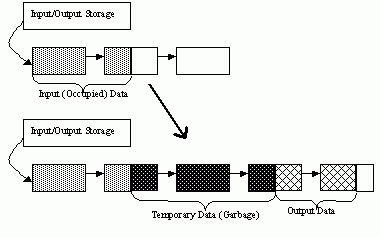
\includegraphics[width=0.5\textwidth]{pics/memstorage1.png}

That is, garbage appears in the middle of the storage. However, if
one creates a child memory storage at the beginning of processing,
writes temporary data there, and releases the child storage at the end,
no garbage will appear in the source/destination storage:

Dynamic data processing using a child storage

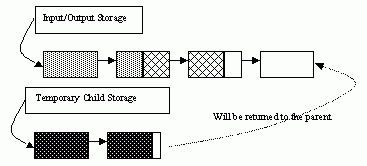
\includegraphics[width=0.5\textwidth]{pics/memstorage2.png}

\cvCPyFunc{CreateGraph}
Creates an empty graph.

\cvdefC{CvGraph* cvCreateGraph( \par int graph\_flags,\par int header\_size,\par int vtx\_size,\par int edge\_size,\par CvMemStorage* storage );}

\begin{description}
\cvarg{graph\_flags}{Type of the created graph. Usually, it is either \texttt{CV\_SEQ\_KIND\_GRAPH} for generic unoriented graphs and
\texttt{CV\_SEQ\_KIND\_GRAPH | CV\_GRAPH\_FLAG\_ORIENTED} for generic oriented graphs.}
\cvarg{header\_size}{Graph header size; may not be less than \texttt{sizeof(CvGraph)}}
\cvarg{vtx\_size}{Graph vertex size; the custom vertex structure must start with \cross{CvGraphVtx} (use \texttt{CV\_GRAPH\_VERTEX\_FIELDS()})}
\cvarg{edge\_size}{Graph edge size; the custom edge structure must start with \cross{CvGraphEdge} (use \texttt{CV\_GRAPH\_EDGE\_FIELDS()})}
\cvarg{storage}{The graph container}
\end{description}

The function creates an empty graph and returns a pointer to it.

\cvCPyFunc{CreateGraphScanner}
Creates structure for depth-first graph traversal.

\cvdefC{
CvGraphScanner*  cvCreateGraphScanner( \par CvGraph* graph,\par CvGraphVtx* vtx=NULL,\par int mask=CV\_GRAPH\_ALL\_ITEMS );
}

\begin{description}
\cvarg{graph}{Graph}
\cvarg{vtx}{Initial vertex to start from. If NULL, the traversal starts from the first vertex (a vertex with the minimal index in the sequence of vertices).}
\cvarg{mask}{Event mask indicating which events are of interest to the user (where \cvCPyCross{NextGraphItem} function returns control to the user) It can be \texttt{CV\_GRAPH\_ALL\_ITEMS} (all events are of interest) or a combination of the following flags:

\begin{description}
\cvarg{CV\_GRAPH\_VERTEX}{stop at the graph vertices visited for the first time}
\cvarg{CV\_GRAPH\_TREE\_EDGE}{stop at tree edges (\texttt{tree edge} is the edge connecting the last visited vertex and the vertex to be visited next)}
\cvarg{CV\_GRAPH\_BACK\_EDGE}{stop at back edges (\texttt{back edge} is an edge connecting the last visited vertex with some of its ancestors in the search tree)}
\cvarg{CV\_GRAPH\_FORWARD\_EDGE}{stop at forward edges (\texttt{forward edge} is an edge conecting the last visited vertex with some of its descendants in the search tree. The forward edges are only possible during oriented graph traversal)}
\cvarg{CV\_GRAPH\_CROSS\_EDGE}{stop at cross edges (\texttt{cross edge} is an edge connecting different search trees or branches of the same tree. The \texttt{cross edges} are only possible during oriented graph traversal)}
\cvarg{CV\_GRAPH\_ANY\_EDGE}{stop at any edge (\texttt{tree, back, forward}, and \texttt{cross edges})}
\cvarg{CV\_GRAPH\_NEW\_TREE}{stop in the beginning of every new search tree. When the traversal procedure visits all vertices and edges reachable from the initial vertex (the visited vertices together with tree edges make up a tree), it searches for some unvisited vertex in the graph and resumes the traversal process from that vertex. Before starting a new tree (including the very first tree when \texttt{cvNextGraphItem} is called for the first time) it generates a \texttt{CV\_GRAPH\_NEW\_TREE} event. For unoriented graphs, each search tree corresponds to a connected component of the graph.}
\cvarg{CV\_GRAPH\_BACKTRACKING}{stop at every already visited vertex during backtracking - returning to already visited vertexes of the traversal tree.}
\end{description}}
\end{description}

The function creates a structure for depth-first graph traversal/search. The initialized structure is used in the \cvCPyCross{NextGraphItem} function - the incremental traversal procedure.

\fi

\cvCPyFunc{CreateMemStorage}
Creates memory storage.

\cvdefC{CvMemStorage* cvCreateMemStorage( int blockSize=0 );}
\cvdefPy{CreateMemStorage(blockSize = 0) -> memstorage}

\begin{description}
\cvarg{blockSize}{Size of the storage blocks in bytes. If it is 0, the block size is set to a default value - currently it is  about 64K.}
\end{description}

The function creates an empty memory storage. See \cross{CvMemStorage} description.

\ifC

\cvCPyFunc{CreateSeq}
Creates a sequence.

\cvdefC{CvSeq* cvCreateSeq( \par int seqFlags,\par int headerSize,\par int elemSize,\par CvMemStorage* storage);}

\begin{description}
\cvarg{seqFlags}{Flags of the created sequence. If the sequence is not passed to any function working with a specific type of sequences, the sequence value may be set to 0, otherwise the appropriate type must be selected from the list of predefined sequence types.}
\cvarg{headerSize}{Size of the sequence header; must be greater than or equal to \texttt{sizeof(CvSeq)}. If a specific type or its extension is indicated, this type must fit the base type header.}
\cvarg{elemSize}{Size of the sequence elements in bytes. The size must be consistent with the sequence type. For example, for a sequence of points to be created, the element type \newline \texttt{CV\_SEQ\_ELTYPE\_POINT} should be specified and the parameter \texttt{elemSize} must be equal to \texttt{sizeof(CvPoint)}.}
\cvarg{storage}{Sequence location}
\end{description}

The function creates a sequence and returns
the pointer to it. The function allocates the sequence header in
the storage block as one continuous chunk and sets the structure
fields \texttt{flags}, \texttt{elemSize}, \texttt{headerSize}, and
\texttt{storage} to passed values, sets \texttt{delta\_elems} to the
default value (that may be reassigned using the \cvCPyCross{SetSeqBlockSize}
function), and clears other header fields, including the space following
the first \texttt{sizeof(CvSeq)} bytes.

\cvCPyFunc{CreateSet}
Creates an empty set.

\cvdefC{CvSet* cvCreateSet( \par int set\_flags,\par int header\_size,\par int elem\_size,\par CvMemStorage* storage );}

\begin{description}
\cvarg{set\_flags}{Type of the created set}
\cvarg{header\_size}{Set header size; may not be less than \texttt{sizeof(CvSet)}}
\cvarg{elem\_size}{Set element size; may not be less than \cross{CvSetElem}}
\cvarg{storage}{Container for the set}
\end{description}

The function creates an empty set with a specified header size and element size, and returns the pointer to the set. This function is just a thin layer on top of \cvCPyCross{CreateSeq}.

\cvCPyFunc{CvtSeqToArray}
Copies a sequence to one continuous block of memory.

\cvdefC{void* cvCvtSeqToArray( \par const CvSeq* seq,\par void* elements,\par CvSlice slice=CV\_WHOLE\_SEQ );}

\begin{description}
\cvarg{seq}{Sequence}
\cvarg{elements}{Pointer to the destination array that must be large enough. It should be a pointer to data, not a matrix header.}
\cvarg{slice}{The sequence portion to copy to the array}
\end{description}

The function copies the entire sequence or subsequence to the specified buffer and returns the pointer to the buffer.

\cvCPyFunc{EndWriteSeq}
Finishes the process of writing a sequence.

\cvdefC{CvSeq* cvEndWriteSeq( CvSeqWriter* writer );}

\begin{description}
\cvarg{writer}{Writer state}
\end{description}


The function finishes the writing process and
returns the pointer to the written sequence. The function also truncates
the last incomplete sequence block to return the remaining part of the
block to memory storage. After that, the sequence can be read and
modified safely. See \cvCPyCross{cvStartWriteSeq} and \cvCPyCross{cvStartAppendToSeq}

\cvCPyFunc{FindGraphEdge}
Finds an edge in a graph.

\cvdefC{
CvGraphEdge* cvFindGraphEdge( const CvGraph* graph, int start\_idx, int end\_idx );
}

\begin{lstlisting}

#define cvGraphFindEdge cvFindGraphEdge

\end{lstlisting}

\begin{description}
\cvarg{graph}{Graph}
\cvarg{start\_idx}{Index of the starting vertex of the edge}
\cvarg{end\_idx}{Index of the ending vertex of the edge. For an unoriented graph, the order of the vertex parameters does not matter.}
\end{description}

The function finds the graph edge connecting two specified vertices and returns a pointer to it or NULL if the edge does not exist.

\cvCPyFunc{FindGraphEdgeByPtr}
Finds an edge in a graph by using its pointer.

\cvdefC{
CvGraphEdge* cvFindGraphEdgeByPtr( \par const CvGraph* graph,\par const CvGraphVtx* startVtx,\par const CvGraphVtx* endVtx );
}

\begin{lstlisting}
#define cvGraphFindEdgeByPtr cvFindGraphEdgeByPtr
\end{lstlisting}

\begin{description}
\cvarg{graph}{Graph}
\cvarg{startVtx}{Pointer to the starting vertex of the edge}
\cvarg{endVtx}{Pointer to the ending vertex of the edge. For an unoriented graph, the order of the vertex parameters does not matter.}
\end{description}

The function finds the graph edge connecting two specified vertices and returns pointer to it or NULL if the edge does not exists.

\cvCPyFunc{FlushSeqWriter}
Updates sequence headers from the writer.

\cvdefC{void cvFlushSeqWriter( CvSeqWriter* writer );}

\begin{description}
\cvarg{writer}{Writer state}
\end{description}

The function is intended to enable the user to
read sequence elements, whenever required, during the writing process,
e.g., in order to check specific conditions. The function updates the
sequence headers to make reading from the sequence possible. The writer
is not closed, however, so that the writing process can be continued at
any time. If an algorithm requires frequent flushes, consider using
\cvCPyCross{SeqPush} instead.

\cvCPyFunc{GetGraphVtx}
Finds a graph vertex by using its index.

\cvdefC{CvGraphVtx* cvGetGraphVtx( \par CvGraph* graph,\par int vtx\_idx );}

\begin{description}
\cvarg{graph}{Graph}
\cvarg{vtx\_idx}{Index of the vertex}
\end{description}


The function finds the graph vertex by using its index and returns the pointer to it or NULL if the vertex does not belong to the graph.


\cvCPyFunc{GetSeqElem}
Returns a pointer to a sequence element according to its index.

\cvdefC{char* cvGetSeqElem( const CvSeq* seq, int index );}

\begin{lstlisting}
#define CV_GET_SEQ_ELEM( TYPE, seq, index )  (TYPE*)cvGetSeqElem( (CvSeq*)(seq), (index) )
\end{lstlisting}

\begin{description}
\cvarg{seq}{Sequence}
\cvarg{index}{Index of element}
\end{description}

The function finds the element with the given
index in the sequence and returns the pointer to it. If the element
is not found, the function returns 0. The function supports negative
indices, where -1 stands for the last sequence element, -2 stands for
the one before last, etc. If the sequence is most likely to consist of
a single sequence block or the desired element is likely to be located
in the first block, then the macro
\texttt{CV\_GET\_SEQ\_ELEM( elemType, seq, index )}
should be used, where the parameter \texttt{elemType} is the
type of sequence elements ( \cross{CvPoint} for example), the parameter
\texttt{seq} is a sequence, and the parameter \texttt{index} is the index
of the desired element. The macro checks first whether the desired element
belongs to the first block of the sequence and returns it if it does;
otherwise the macro calls the main function \texttt{GetSeqElem}. Negative
indices always cause the \cvCPyCross{GetSeqElem} call. The function has O(1)
time complexity assuming that the number of blocks is much smaller than the
number of elements.

\cvCPyFunc{GetSeqReaderPos}
Returns the current reader position.

\cvdefC{int cvGetSeqReaderPos( CvSeqReader* reader );}

\begin{description}
\cvarg{reader}{Reader state}
\end{description}


The function returns the current reader position (within 0 ... \texttt{reader->seq->total} - 1).

\cvCPyFunc{GetSetElem}
Finds a set element by its index.

\cvdefC{CvSetElem* cvGetSetElem( \par const CvSet* setHeader,\par int index );}

\begin{description}
\cvarg{setHeader}{Set}
\cvarg{index}{Index of the set element within a sequence}
\end{description}

The function finds a set element by its index. The function returns the pointer to it or 0 if the index is invalid or the corresponding node is free. The function supports negative indices as it uses \cvCPyCross{GetSeqElem} to locate the node.

\cvCPyFunc{GraphAddEdge}
Adds an edge to a graph.

\cvdefC{int cvGraphAddEdge( \par CvGraph* graph,\par int start\_idx,\par int end\_idx,\par const CvGraphEdge* edge=NULL,\par CvGraphEdge** inserted\_edge=NULL );
}

\begin{description}
\cvarg{graph}{Graph}
\cvarg{start\_idx}{Index of the starting vertex of the edge}
\cvarg{end\_idx}{Index of the ending vertex of the edge. For an unoriented graph, the order of the vertex parameters does not matter.}
\cvarg{edge}{Optional input parameter, initialization data for the edge}
\cvarg{inserted\_edge}{Optional output parameter to contain the address of the inserted edge}
\end{description}


The function connects two specified vertices. The function returns 1 if the edge has been added successfully, 0 if the edge connecting the two vertices exists already and -1 if either of the vertices was not found, the starting and the ending vertex are the same, or there is some other critical situation. In the latter case (i.e., when the result is negative), the function also reports an error by default.

\cvCPyFunc{GraphAddEdgeByPtr}
Adds an edge to a graph by using its pointer.

\cvdefC{int cvGraphAddEdgeByPtr( \par CvGraph* graph,\par CvGraphVtx* start\_vtx,\par CvGraphVtx* end\_vtx,\par const CvGraphEdge* edge=NULL,\par CvGraphEdge** inserted\_edge=NULL );}

\begin{description}
\cvarg{graph}{Graph}
\cvarg{start\_vtx}{Pointer to the starting vertex of the edge}
\cvarg{end\_vtx}{Pointer to the ending vertex of the edge. For an unoriented graph, the order of the vertex parameters does not matter.}
\cvarg{edge}{Optional input parameter, initialization data for the edge}
\cvarg{inserted\_edge}{Optional output parameter to contain the address of the inserted edge within the edge set}
\end{description}

The function connects two specified vertices. The
function returns 1 if the edge has been added successfully, 0 if the
edge connecting the two vertices exists already, and -1 if either of the
vertices was not found, the starting and the ending vertex are the same
or there is some other critical situation. In the latter case (i.e., when
the result is negative), the function also reports an error by default.

\cvCPyFunc{GraphAddVtx}
Adds a vertex to a graph.

\cvdefC{
int cvGraphAddVtx( \par CvGraph* graph,\par const CvGraphVtx* vtx=NULL,\par CvGraphVtx** inserted\_vtx=NULL );}

\begin{description}
\cvarg{graph}{Graph}
\cvarg{vtx}{Optional input argument used to initialize the added vertex (only user-defined fields beyond \texttt{sizeof(CvGraphVtx)} are copied)}
\cvarg{inserted\_vertex}{Optional output argument. If not \texttt{NULL}, the address of the new vertex is written here.}
\end{description}

The function adds a vertex to the graph and returns the vertex index.

\cvCPyFunc{GraphEdgeIdx}
Returns the index of a graph edge.

\cvdefC{
int cvGraphEdgeIdx( \par CvGraph* graph,\par CvGraphEdge* edge );
}

\begin{description}
\cvarg{graph}{Graph}
\cvarg{edge}{Pointer to the graph edge}
\end{description}

The function returns the index of a graph edge.

\cvCPyFunc{GraphRemoveEdge}
Removes an edge from a graph.

\cvdefC{void cvGraphRemoveEdge( \par CvGraph* graph,\par int start\_idx,\par int end\_idx );}

\begin{description}
\cvarg{graph}{Graph}
\cvarg{start\_idx}{Index of the starting vertex of the edge}
\cvarg{end\_idx}{Index of the ending vertex of the edge. For an unoriented graph, the order of the vertex parameters does not matter.}
\end{description}

The function removes the edge connecting two specified vertices. If the vertices are not connected [in that order], the function does nothing.

\cvCPyFunc{GraphRemoveEdgeByPtr}

Removes an edge from a graph by using its pointer.

\cvdefC{void cvGraphRemoveEdgeByPtr( \par CvGraph* graph,\par CvGraphVtx* start\_vtx,\par CvGraphVtx* end\_vtx );}

\begin{description}
\cvarg{graph}{Graph}
\cvarg{start\_vtx}{Pointer to the starting vertex of the edge}
\cvarg{end\_vtx}{Pointer to the ending vertex of the edge. For an unoriented graph, the order of the vertex parameters does not matter.}
\end{description}

The function removes the edge connecting two specified vertices. If the vertices are not connected [in that order], the function does nothing.

\cvCPyFunc{GraphRemoveVtx}
Removes a vertex from a graph.

\cvdefC{int cvGraphRemoveVtx( \par CvGraph* graph,\par int index );}

\begin{description}
\cvarg{graph}{Graph}
\cvarg{vtx\_idx}{Index of the removed vertex}
\end{description}

The function removes a vertex from a graph
together with all the edges incident to it. The function reports an error
if the input vertex does not belong to the graph. The return value is the
number of edges deleted, or -1 if the vertex does not belong to the graph.

\cvCPyFunc{GraphRemoveVtxByPtr}
Removes a vertex from a graph by using its pointer.

\cvdefC{int cvGraphRemoveVtxByPtr( \par CvGraph* graph,\par CvGraphVtx* vtx );}

\begin{description}
\cvarg{graph}{Graph}
\cvarg{vtx}{Pointer to the removed vertex}
\end{description}


The function removes a vertex from the graph by using its pointer together with all the edges incident to it. The function reports an error if the vertex does not belong to the graph. The return value is the number of edges deleted, or -1 if the vertex does not belong to the graph.

\cvCPyFunc{GraphVtxDegree}
Counts the number of edges indicent to the vertex.

\cvdefC{
int cvGraphVtxDegree( const CvGraph* graph, int vtxIdx );
}

\begin{description}
\cvarg{graph}{Graph}
\cvarg{vtxIdx}{Index of the graph vertex}
\end{description}

The function returns the number of edges incident to the specified vertex, both incoming and outgoing. To count the edges, the following code is used:

\begin{lstlisting}
CvGraphEdge* edge = vertex->first; int count = 0;
while( edge )
{
    edge = CV_NEXT_GRAPH_EDGE( edge, vertex );
    count++;
}
\end{lstlisting}

The macro \texttt{CV\_NEXT\_GRAPH\_EDGE( edge, vertex )} returns the edge incident to \texttt{vertex} that follows after \texttt{edge}.

\cvCPyFunc{GraphVtxDegreeByPtr}
Finds an edge in a graph.

\cvdefC{
int cvGraphVtxDegreeByPtr( \par const CvGraph* graph,\par const CvGraphVtx* vtx );
}

\begin{description}
\cvarg{graph}{Graph}
\cvarg{vtx}{Pointer to the graph vertex}
\end{description}

The function returns the number of edges incident to the specified vertex, both incoming and outcoming.


\cvCPyFunc{GraphVtxIdx}
Returns the index of a graph vertex.

\cvdefC{int cvGraphVtxIdx( \par CvGraph* graph,\par CvGraphVtx* vtx );}

\begin{description}
\cvarg{graph}{Graph}
\cvarg{vtx}{Pointer to the graph vertex}
\end{description}

The function returns the index of a graph vertex.

\cvCPyFunc{InitTreeNodeIterator}

Initializes the tree node iterator.

\cvdefC{

void cvInitTreeNodeIterator( \par CvTreeNodeIterator* tree\_iterator,\par const void* first,\par int max\_level );

}

\begin{description}
\cvarg{tree\_iterator}{Tree iterator initialized by the function}
\cvarg{first}{The initial node to start traversing from}
\cvarg{max\_level}{The maximal level of the tree (\texttt{first} node assumed to be at the first level) to traverse up to. For example, 1 means that only nodes at the same level as \texttt{first} should be visited, 2 means that the nodes on the same level as \texttt{first} and their direct children should be visited, and so forth.}
\end{description}

The function initializes the tree iterator. The tree is traversed in depth-first order.

\cvCPyFunc{InsertNodeIntoTree}

Adds a new node to a tree.

\cvdefC{void cvInsertNodeIntoTree( \par void* node,\par void* parent,\par void* frame );}

\begin{description}
\cvarg{node}{The inserted node}
\cvarg{parent}{The parent node that is already in the tree}
\cvarg{frame}{The top level node. If \texttt{parent} and \texttt{frame} are the same, the \texttt{v\_prev} field of \texttt{node} is set to NULL rather than \texttt{parent}.}
\end{description}

The function adds another node into tree. The function does not allocate any memory, it can only modify links of the tree nodes.

\cvCPyFunc{MakeSeqHeaderForArray}
Constructs a sequence header for an array.

\cvdefC{CvSeq* cvMakeSeqHeaderForArray( \par int seq\_type,\par int header\_size,\par int elem\_size,\par void* elements,\par int total,\par CvSeq* seq,\par CvSeqBlock* block );}

\begin{description}
\cvarg{seq\_type}{Type of the created sequence}
\cvarg{header\_size}{Size of the header of the sequence. Parameter sequence must point to the structure of that size or greater}
\cvarg{elem\_size}{Size of the sequence elements}
\cvarg{elements}{Elements that will form a sequence}
\cvarg{total}{Total number of elements in the sequence. The number of array elements must be equal to the value of this parameter.}
\cvarg{seq}{Pointer to the local variable that is used as the sequence header}
\cvarg{block}{Pointer to the local variable that is the header of the single sequence block}
\end{description}

The function initializes a sequence
header for an array. The sequence header as well as the sequence block are
allocated by the user (for example, on stack). No data is copied by the
function. The resultant sequence will consists of a single block and
have NULL storage pointer; thus, it is possible to read its elements,
but the attempts to add elements to the sequence will raise an error in
most cases.

\cvCPyFunc{MemStorageAlloc}
Allocates a memory buffer in a storage block.

\cvdefC{void* cvMemStorageAlloc( \par CvMemStorage* storage,\par size\_t size );}

\begin{description}
\cvarg{storage}{Memory storage}
\cvarg{size}{Buffer size}
\end{description}

The function allocates a memory buffer in
a storage block. The buffer size must not exceed the storage block size,
otherwise a runtime error is raised. The buffer address is aligned by
\texttt{CV\_STRUCT\_ALIGN=sizeof(double)} (for the moment) bytes.

\cvCPyFunc{MemStorageAllocString}
Allocates a text string in a storage block.

\cvdefC{CvString cvMemStorageAllocString(CvMemStorage* storage, const char* ptr, int len=-1);}

\begin{lstlisting}
typedef struct CvString
{
    int len;
    char* ptr;
}
CvString;
\end{lstlisting}

\begin{description}
\cvarg{storage}{Memory storage}
\cvarg{ptr}{The string}
\cvarg{len}{Length of the string (not counting the ending \texttt{NUL}) . If the parameter is negative, the function computes the length.}
\end{description}

The function creates copy of the string
in memory storage. It returns the structure that contains user-passed
or computed length of the string and pointer to the copied string.

\cvCPyFunc{NextGraphItem}
Executes one or more steps of the graph traversal procedure.

\cvdefC{
int cvNextGraphItem( CvGraphScanner* scanner );
}

\begin{description}
\cvarg{scanner}{Graph traversal state. It is updated by this function.}
\end{description}

The function traverses through the graph
until an event of interest to the user (that is, an event, specified
in the \texttt{mask} in the \cvCPyCross{CreateGraphScanner} call) is met or the
traversal is completed. In the first case, it returns one of the events
listed in the description of the \texttt{mask} parameter above and with
the next call it resumes the traversal. In the latter case, it returns
\texttt{CV\_GRAPH\_OVER} (-1). When the event is \texttt{CV\_GRAPH\_VERTEX},
\texttt{CV\_GRAPH\_BACKTRACKING}, or \texttt{CV\_GRAPH\_NEW\_TREE},
the currently observed vertex is stored in \texttt{scanner-$>$vtx}. And if the
event is edge-related, the edge itself is stored at \texttt{scanner-$>$edge},
the previously visited vertex - at \texttt{scanner-$>$vtx} and the other ending
vertex of the edge - at \texttt{scanner-$>$dst}.

\cvCPyFunc{NextTreeNode}

Returns the currently observed node and moves the iterator toward the next node.

\cvdefC{

void* cvNextTreeNode( CvTreeNodeIterator* tree\_iterator );

}

\begin{description}
\cvarg{tree\_iterator}{Tree iterator initialized by the function}
\end{description}


The function returns the currently observed node and then updates the iterator - moving it toward the next node. In other words, the function behavior is similar to the *p++ expression on a typical C pointer or C++ collection iterator. The function returns NULL if there are no more nodes.


\cvCPyFunc{PrevTreeNode}

Returns the currently observed node and moves the iterator toward the previous node.

\cvdefC{

void* cvPrevTreeNode( CvTreeNodeIterator* tree\_iterator );

}

\begin{description}
\cvarg{tree\_iterator}{Tree iterator initialized by the function}
\end{description}


The function returns the currently observed node and then updates the iterator - moving it toward the previous node. In other words, the function behavior is similar to the *p-- expression on a typicl C pointer or C++ collection iterator. The function returns NULL if there are no more nodes.


\cvCPyFunc{ReleaseGraphScanner}
Completes the graph traversal procedure.

\cvdefC{
void cvReleaseGraphScanner( CvGraphScanner** scanner );
}

\begin{description}
\cvarg{scanner}{Double pointer to graph traverser}
\end{description}


The function completes the graph traversal procedure and releases the traverser state.



\cvCPyFunc{ReleaseMemStorage}
Releases memory storage.

\cvdefC{void cvReleaseMemStorage( CvMemStorage** storage );}

\begin{description}
\cvarg{storage}{Pointer to the released storage}
\end{description}

The function deallocates all storage memory
blocks or returns them to the parent, if any. Then it deallocates the
storage header and clears the pointer to the storage. All child storage 
associated with a given parent storage block must be released before the 
parent storage block is released.

\cvCPyFunc{RestoreMemStoragePos}
Restores memory storage position.

\cvdefC{void cvRestoreMemStoragePos(\par CvMemStorage* storage,\par CvMemStoragePos* pos);}

\begin{description}
\cvarg{storage}{Memory storage}
\cvarg{pos}{New storage top position}
\end{description}

The function restores the position of the storage top from the parameter \texttt{pos}. This function and the function \texttt{cvClearMemStorage} are the only methods to release memory occupied in memory blocks. Note again that there is no way to free memory in the middle of an occupied portion of a storage block.


\cvCPyFunc{SaveMemStoragePos}
Saves memory storage position.

\cvdefC{void cvSaveMemStoragePos(\par const CvMemStorage* storage,\par CvMemStoragePos* pos);}

\begin{description}
\cvarg{storage}{Memory storage}
\cvarg{pos}{The output position of the storage top}
\end{description}

The function saves the current position
of the storage top to the parameter \texttt{pos}. The function
\texttt{cvRestoreMemStoragePos} can further retrieve this position.

\cvCPyFunc{SeqElemIdx}
Returns the index of a specific sequence element.

\cvdefC{int cvSeqElemIdx( \par const CvSeq* seq,\par const void* element,\par CvSeqBlock** block=NULL );}

\begin{description}
\cvarg{seq}{Sequence}
\cvarg{element}{Pointer to the element within the sequence}
\cvarg{block}{Optional argument. If the pointer is not \texttt{NULL}, the address of the sequence block that contains the element is stored in this location.}
\end{description}

The function returns the index of a sequence element or a negative number if the element is not found.

\cvCPyFunc{SeqInsert}
Inserts an element in the middle of a sequence.

\cvdefC{char* cvSeqInsert( \par CvSeq* seq,\par int beforeIndex,\par void* element=NULL );}

\begin{description}
\cvarg{seq}{Sequence}
\cvarg{beforeIndex}{Index before which the element is inserted. Inserting before 0 (the minimal allowed value of the parameter) is equal to \cvCPyCross{SeqPushFront} and inserting before \texttt{seq->total} (the maximal allowed value of the parameter) is equal to \cvCPyCross{SeqPush}.}
\cvarg{element}{Inserted element} 
\end{description}

The function shifts the sequence elements from the inserted position to the nearest end of the sequence and copies the \texttt{element} content there if the pointer is not NULL. The function returns a pointer to the inserted element.


\cvCPyFunc{SeqInsertSlice}
Inserts an array in the middle of a sequence.

\cvdefC{void cvSeqInsertSlice( \par CvSeq* seq,\par int beforeIndex,\par const CvArr* fromArr );}

\begin{description}
\cvarg{seq}{Sequence}
\cvarg{slice}{The part of the sequence to remove}
\cvarg{fromArr}{The array to take elements from}
\end{description}


The function inserts all \texttt{fromArr}
array elements at the specified position of the sequence. The array
\texttt{fromArr} can be a matrix or another sequence.

\fi

\cvCPyFunc{SeqInvert}
Reverses the order of sequence elements.

\cvdefC{void cvSeqInvert( CvSeq* seq );}
\cvdefPy{SeqInvert(seq)-> None}

\begin{description}
\cvarg{seq}{Sequence}
\end{description}


The function reverses the sequence in-place - makes the first element go last, the last element go first and so forth.

\ifC

\cvCPyFunc{SeqPop}
Removes an element from the end of a sequence.

\cvdefC{void cvSeqPop( \par CvSeq* seq,\par void* element=NULL );}

\begin{description}
\cvarg{seq}{Sequence}
\cvarg{element}{Optional parameter . If the pointer is not zero, the function copies the removed element to this location.}
\end{description}

The function removes an element from a sequence. The function reports an error if the sequence is already empty. The function has O(1) complexity.

\cvCPyFunc{SeqPopFront}
Removes an element from the beginning of a sequence.

\cvdefC{void cvSeqPopFront( \par \par CvSeq* seq,\par\par void* element=NULL );}

\begin{description}
\cvarg{seq}{Sequence}
\cvarg{element}{Optional parameter. If the pointer is not zero, the function copies the removed element to this location.}
\end{description}

The function removes an element from the beginning of a sequence. The function reports an error if the sequence is already empty. The function has O(1) complexity.

\cvCPyFunc{SeqPopMulti}
Removes several elements from either end of a sequence.

\cvdefC{void cvSeqPopMulti( \par CvSeq* seq,\par void* elements,\par int count,\par int in\_front=0 );}

\begin{description}
\cvarg{seq}{Sequence}
\cvarg{elements}{Removed elements}
\cvarg{count}{Number of elements to pop}
\cvarg{in\_front}{The flags specifying which end of the modified sequence.
\begin{description}
\cvarg{CV\_BACK}{the elements are added to the end of the sequence}
\cvarg{CV\_FRONT}{the elements are added to the beginning of the sequence}
\end{description}}
\end{description}

The function removes several elements from either end of the sequence. If the number of the elements to be removed exceeds the total number of elements in the sequence, the function removes as many elements as possible.

\cvCPyFunc{SeqPush}
Adds an element to the end of a sequence.

\cvdefC{char* cvSeqPush( \par CvSeq* seq,\par void* element=NULL );}

\begin{description}
\cvarg{seq}{Sequence}
\cvarg{element}{Added element}
\end{description}

The function adds an element to the end of a sequence and returns a pointer to the allocated element. If the input \texttt{element} is NULL, the function simply allocates a space for one more element.

The following code demonstrates how to create a new sequence using this function:

\begin{lstlisting}
CvMemStorage* storage = cvCreateMemStorage(0);
CvSeq* seq = cvCreateSeq( CV_32SC1, /* sequence of integer elements */
                          sizeof(CvSeq), /* header size - no extra fields */
                          sizeof(int), /* element size */
                          storage /* the container storage */ );
int i;
for( i = 0; i < 100; i++ )
{
    int* added = (int*)cvSeqPush( seq, &i );
    printf( "%d is added\n", *added );
}

...
/* release memory storage in the end */
cvReleaseMemStorage( &storage );
\end{lstlisting}

The function has O(1) complexity, but there is a faster method for writing large sequences (see \cvCPyCross{StartWriteSeq} and related functions).


\cvCPyFunc{SeqPushFront}
Adds an element to the beginning of a sequence.

\cvdefC{char* cvSeqPushFront( CvSeq* seq, void* element=NULL );}

\begin{description}
\cvarg{seq}{Sequence}
\cvarg{element}{Added element}
\end{description}

The function is similar to \cvCPyCross{SeqPush} but it adds the new element to the beginning of the sequence. The function has O(1) complexity.

\cvCPyFunc{SeqPushMulti}
Pushes several elements to either end of a sequence.

\cvdefC{void cvSeqPushMulti( \par CvSeq* seq,\par void* elements,\par int count,\par int in\_front=0 );}

\begin{description}
\cvarg{seq}{Sequence}
\cvarg{elements}{Added elements}
\cvarg{count}{Number of elements to push}
\cvarg{in\_front}{The flags specifying which end of the modified sequence.
\begin{description}
\cvarg{CV\_BACK}{the elements are added to the end of the sequence}
\cvarg{CV\_FRONT}{the elements are added to the beginning of the sequence}
\end{description}}
\end{description}

The function adds several elements to either
end of a sequence. The elements are added to the sequence in the same
order as they are arranged in the input array but they can fall into
different sequence blocks.

\fi

\cvCPyFunc{SeqRemove}
Removes an element from the middle of a sequence.

\cvdefC{void cvSeqRemove( \par CvSeq* seq,\par int index );}
\cvdefPy{SeqRemove(seq,index)-> None}

\begin{description}
\cvarg{seq}{Sequence}
\cvarg{index}{Index of removed element}
\end{description}

The function removes elements with the given
index. If the index is out of range the function reports an error. An
attempt to remove an element from an empty sequence is a special
case of this situation. The function removes an element by shifting
the sequence elements between the nearest end of the sequence and the
\texttt{index}-th position, not counting the latter.


\cvCPyFunc{SeqRemoveSlice}
Removes a sequence slice.

\cvdefC{void cvSeqRemoveSlice( CvSeq* seq, CvSlice slice );}
\cvdefPy{SeqRemoveSlice(seq,slice)-> None}

\begin{description}
\cvarg{seq}{Sequence}
\cvarg{slice}{The part of the sequence to remove}
\end{description}

The function removes a slice from the sequence.

\ifC

\cvCPyFunc{SeqSearch}
Searches for an element in a sequence.

\begin{lstlisting}
/* a < b ? -1 : a > b ? 1 : 0 */
typedef int (CV_CDECL* CvCmpFunc)(const void* a, const void* b, void* userdata);

char* cvSeqSearch( CvSeq* seq, const void* elem, CvCmpFunc func,
                   int is_sorted, int* elem_idx, void* userdata=NULL );
\end{lstlisting}

\begin{description}
\cvarg{seq}{The sequence}
\cvarg{elem}{The element to look for}
\cvarg{func}{The comparison function that returns negative, zero or positive value depending on the relationships among the elements (see also \cvCPyCross{SeqSort})}
\cvarg{is\_sorted}{Whether the sequence is sorted or not}
\cvarg{elem\_idx}{Output parameter; index of the found element}
\cvarg{userdata}{The user parameter passed to the compasion function; helps to avoid global variables in some cases}
\end{description}

The function searches for the element in the sequence. If
the sequence is sorted, a binary O(log(N)) search is used; otherwise, a
simple linear search is used. If the element is not found, the function
returns a NULL pointer and the index is set to the number of sequence
elements if a linear search is used, or to the smallest index
\texttt{i, seq(i)>elem}.

\cvCPyFunc{SeqSlice}
Makes a separate header for a sequence slice.

\cvdefC{CvSeq* cvSeqSlice( \par const CvSeq* seq,\par CvSlice slice,\par CvMemStorage* storage=NULL,\par int copy\_data=0 );}

\begin{description}
\cvarg{seq}{Sequence}
\cvarg{slice}{The part of the sequence to be extracted}
\cvarg{storage}{The destination storage block to hold the new sequence header and the copied data, if any. If it is NULL, the function uses the storage block containing the input sequence.}
\cvarg{copy\_data}{The flag that indicates whether to copy the elements of the extracted slice (\texttt{copy\_data!=0}) or not (\texttt{copy\_data=0})}
\end{description}

The function creates a sequence that represents the specified slice of the input sequence. The new sequence either shares the elements with the original sequence or has its own copy of the elements. So if one needs to process a part of sequence but the processing function does not have a slice parameter, the required sub-sequence may be extracted using this function.

\cvCPyFunc{SeqSort}
Sorts sequence element using the specified comparison function.

\cvdefC{void cvSeqSort( CvSeq* seq, CvCmpFunc func, void* userdata=NULL );}

\begin{lstlisting}
/* a < b ? -1 : a > b ? 1 : 0 */
typedef int (CV_CDECL* CvCmpFunc)(const void* a, const void* b, void* userdata);
\end{lstlisting}

\begin{description}
\cvarg{seq}{The sequence to sort}
\cvarg{func}{The comparison function that returns a negative, zero, or positive value depending on the relationships among the elements (see the above declaration and the example below) - a similar function is used by \texttt{qsort} from C runline except that in the latter, \texttt{userdata} is not used}
\cvarg{userdata}{The user parameter passed to the compasion function; helps to avoid global variables in some cases}
\end{description}

The function sorts the sequence in-place using the specified criteria. Below is an example of using this function:

\begin{lstlisting}
/* Sort 2d points in top-to-bottom left-to-right order */
static int cmp_func( const void* _a, const void* _b, void* userdata )
{
    CvPoint* a = (CvPoint*)_a;
    CvPoint* b = (CvPoint*)_b;
    int y_diff = a->y - b->y;
    int x_diff = a->x - b->x;
    return y_diff ? y_diff : x_diff;
}

...

CvMemStorage* storage = cvCreateMemStorage(0);
CvSeq* seq = cvCreateSeq( CV_32SC2, sizeof(CvSeq), sizeof(CvPoint), storage );
int i;

for( i = 0; i < 10; i++ )
{
    CvPoint pt;
    pt.x = rand() % 1000;
    pt.y = rand() % 1000;
    cvSeqPush( seq, &pt );
}

cvSeqSort( seq, cmp_func, 0 /* userdata is not used here */ );

/* print out the sorted sequence */
for( i = 0; i < seq->total; i++ )
{
    CvPoint* pt = (CvPoint*)cvSeqElem( seq, i );
    printf( "(%d,%d)\n", pt->x, pt->y );
}

cvReleaseMemStorage( &storage );
\end{lstlisting}


\cvCPyFunc{SetAdd}
Occupies a node in the set.

\cvdefC{int cvSetAdd( \par CvSet* setHeader,\par CvSetElem* elem=NULL,\par CvSetElem** inserted\_elem=NULL );}

\begin{description}
\cvarg{setHeader}{Set}
\cvarg{elem}{Optional input argument, an inserted element. If not NULL, the function copies the data to the allocated node (the MSB of the first integer field is cleared after copying).}
\cvarg{inserted\_elem}{Optional output argument; the pointer to the allocated cell}
\end{description}

The function allocates a new node, optionally copies
input element data to it, and returns the pointer and the index to the
node. The index value is taken from the lower bits of the \texttt{flags}
field of the node. The function has O(1) complexity; however, there exists
a faster function for allocating set nodes (see \cvCPyCross{SetNew}).

\cvCPyFunc{SetNew}
Adds an element to a set (fast variant).

\cvdefC{CvSetElem* cvSetNew( CvSet* setHeader );}

\begin{description}
\cvarg{setHeader}{Set}
\end{description}

The function is an inline lightweight variant of \cvCPyCross{SetAdd}. It occupies a new node and returns a pointer to it rather than an index.


\cvCPyFunc{SetRemove}
Removes an element from a set.

\cvdefC{void cvSetRemove( \par CvSet* setHeader,\par int index );}

\begin{description}
\cvarg{setHeader}{Set}
\cvarg{index}{Index of the removed element}
\end{description}

The function removes an element with a specified
index from the set. If the node at the specified location is not occupied,
the function does nothing. The function has O(1) complexity; however,
\cvCPyCross{SetRemoveByPtr} provides a quicker way to remove a set element
if it is located already.

\cvCPyFunc{SetRemoveByPtr}
Removes a set element based on its pointer.

\cvdefC{void cvSetRemoveByPtr( \par CvSet* setHeader,\par void* elem );}

\begin{description}
\cvarg{setHeader}{Set}
\cvarg{elem}{Removed element}
\end{description}

The function is an inline lightweight variant of \cvCPyCross{SetRemove} that requires an element pointer. The function does not check whether the node is occupied or not - the user should take care of that.


\cvCPyFunc{SetSeqBlockSize}
Sets up sequence block size.

\cvdefC{void cvSetSeqBlockSize( \par CvSeq* seq,\par int deltaElems );}

\begin{description}
\cvarg{seq}{Sequence}
\cvarg{deltaElems}{Desirable sequence block size for elements}
\end{description}

The function affects memory allocation
granularity. When the free space in the sequence buffers has run out,
the function allocates the space for \texttt{deltaElems} sequence
elements. If this block immediately follows the one previously allocated,
the two blocks are concatenated; otherwise, a new sequence block is
created. Therefore, the bigger the parameter is, the lower the possible
sequence fragmentation, but the more space in the storage block is wasted. When
the sequence is created, the parameter \texttt{deltaElems} is set to
the default value of about 1K. The function can be called any time after
the sequence is created and affects future allocations. The function
can modify the passed value of the parameter to meet memory storage
constraints.

\cvCPyFunc{SetSeqReaderPos}
Moves the reader to the specified position.

\cvdefC{void cvSetSeqReaderPos( \par CvSeqReader* reader,\par int index,\par int is\_relative=0 );}

\begin{description}
\cvarg{reader}{Reader state}
\cvarg{index}{The destination position. If the positioning mode is used (see the next parameter), the actual position will be \texttt{index} mod \texttt{reader->seq->total}.}
\cvarg{is\_relative}{If it is not zero, then \texttt{index} is a relative to the current position}
\end{description}

The function moves the read position to an absolute position or relative to the current position.


\cvCPyFunc{StartAppendToSeq}
Initializes the process of writing data to a sequence.

\cvdefC{void cvStartAppendToSeq( \par CvSeq* seq,\par CvSeqWriter* writer );}

\begin{description}
\cvarg{seq}{Pointer to the sequence}
\cvarg{writer}{Writer state; initialized by the function}
\end{description}

The function initializes the process of
writing data to a sequence. Written elements are added to the end of the
sequence by using the
\texttt{CV\_WRITE\_SEQ\_ELEM( written\_elem, writer )}
macro. Note
that during the writing process, other operations on the sequence may
yield an incorrect result or even corrupt the sequence (see description of
\cvCPyCross{FlushSeqWriter}, which helps to avoid some of these problems).

\cvCPyFunc{StartReadSeq}
Initializes the process of sequential reading from a sequence.

\cvdefC{void cvStartReadSeq( \par const CvSeq* seq,\par CvSeqReader* reader,\par int reverse=0 );}

\begin{description}
\cvarg{seq}{Sequence}
\cvarg{reader}{Reader state; initialized by the function}
\cvarg{reverse}{Determines the direction of the sequence traversal. If \texttt{reverse} is 0, the reader is positioned at the first sequence element; otherwise it is positioned at the last element. }
\end{description}

The function initializes the reader state. After
that, all the sequence elements from the first one down to the last one
can be read by subsequent calls of the macro
\texttt{CV\_READ\_SEQ\_ELEM( read\_elem, reader )}
in the case of forward reading and by using
\texttt{CV\_REV\_READ\_SEQ\_ELEM( read\_elem, reader )}
in the case of reverse
reading. Both macros put the sequence element to \texttt{read\_elem} and
move the reading pointer toward the next element. A circular structure
of sequence blocks is used for the reading process, that is, after the
last element has been read by the macro \texttt{CV\_READ\_SEQ\_ELEM}, the
first element is read when the macro is called again. The same applies to
\texttt{CV\_REV\_READ\_SEQ\_ELEM}. There is no function to finish the reading
process, since it neither changes the sequence nor creates any temporary
buffers. The reader field \texttt{ptr} points to the current element of
the sequence that is to be read next. The code below demonstrates how
to use the sequence writer and reader.

\begin{lstlisting}
CvMemStorage* storage = cvCreateMemStorage(0);
CvSeq* seq = cvCreateSeq( CV_32SC1, sizeof(CvSeq), sizeof(int), storage );
CvSeqWriter writer;
CvSeqReader reader;
int i;

cvStartAppendToSeq( seq, &writer );
for( i = 0; i < 10; i++ )
{
    int val = rand()%100;
    CV_WRITE_SEQ_ELEM( val, writer );
    printf("%d is written\n", val );
}
cvEndWriteSeq( &writer );

cvStartReadSeq( seq, &reader, 0 );
for( i = 0; i < seq->total; i++ )
{
    int val;
#if 1
    CV_READ_SEQ_ELEM( val, reader );
    printf("%d is read\n", val );
#else /* alternative way, that is prefferable if sequence elements are large,
         or their size/type is unknown at compile time */
    printf("%d is read\n", *(int*)reader.ptr );
    CV_NEXT_SEQ_ELEM( seq->elem_size, reader );
#endif
}
...

cvReleaseStorage( &storage );
\end{lstlisting}

\cvCPyFunc{StartWriteSeq}
Creates a new sequence and initializes a writer for it.

\cvdefC{
void cvStartWriteSeq( \par int seq\_flags,\par int header\_size,\par int elem\_size,\par CvMemStorage* storage,\par CvSeqWriter* writer );
}

\begin{description}
\cvarg{seq\_flags}{Flags of the created sequence. If the sequence is not passed to any function working with a specific type of sequences, the sequence value may be equal to 0; otherwise the appropriate type must be selected from the list of predefined sequence types.}
\cvarg{header\_size}{Size of the sequence header. The parameter value may not be less than \texttt{sizeof(CvSeq)}. If a certain type or extension is specified, it must fit within the base type header.}
\cvarg{elem\_size}{Size of the sequence elements in bytes; must be consistent with the sequence type. For example, if a sequence of points is created (element type \texttt{CV\_SEQ\_ELTYPE\_POINT} ), then the parameter \texttt{elem\_size} must be equal to \texttt{sizeof(CvPoint)}.}
\cvarg{storage}{Sequence location}
\cvarg{writer}{Writer state; initialized by the function}
\end{description}

The function is a combination of
\cvCPyCross{CreateSeq} and \cvCPyCross{StartAppendToSeq}. The pointer to the
created sequence is stored at
\texttt{writer->seq}
and is also returned by the
\cvCPyCross{EndWriteSeq} function that should be called at the end.

\cvCPyFunc{TreeToNodeSeq}
Gathers all node pointers to a single sequence.

\cvdefC{

CvSeq* cvTreeToNodeSeq( \par const void* first,\par int header\_size,\par CvMemStorage* storage );

}

\begin{description}
\cvarg{first}{The initial tree node}
\cvarg{header\_size}{Header size of the created sequence (sizeof(CvSeq) is the most frequently used value)}
\cvarg{storage}{Container for the sequence}
\end{description}

The function puts pointers of all nodes reacheable from \texttt{first} into a single sequence. The pointers are written sequentially in the depth-first order.

\fi

\fi


\section{Drawing Functions}

Drawing functions work with matrices/images of arbitrary depth.
The boundaries of the shapes can be rendered with antialiasing (implemented only for 8-bit images for now).
All the functions include the parameter color that uses a rgb value (that may be constructed
with \texttt{CV\_RGB} \cvC{macro or the \cvCppCross{cvScalar} function}
\cvCpp{or the \cross{Scalar} constructor}) for color
images and brightness for grayscale images. For color images the order channel
is normally \emph{Blue, Green, Red}, this is what \cvCppCross{imshow}, \cvCppCross{imread} and \cvCppCross{imwrite} expect
\ifCpp
, so if you form a color using \cross{Scalar} constructor, it should look like:
\[\texttt{Scalar}(blue\_component, green\_component, red\_component[, alpha\_component])\]
\fi
\ifC
, so if you form a color using \cvCppCross{cvScalar}, it should look like:
\[\texttt{cvScalar}(blue\_component, green\_component, red\_component[, alpha\_component])\]
\fi

If you are using your own image rendering and I/O functions, you can use any channel ordering, the drawing functions process each channel independently and do not depend on the channel order or even on the color space used. The whole image can be converted from BGR to RGB or to a different color space using \cvCppCross{cvtColor}.

If a drawn figure is partially or completely outside the image, the drawing functions clip it. Also, many drawing functions can handle pixel coordinates specified with sub-pixel accuracy, that is, the coordinates can be passed as fixed-point numbers, encoded as integers. The number of fractional bits is specified by the \texttt{shift} parameter and the real point coordinates are calculated as $\texttt{Point}(x,y)\rightarrow\texttt{Point2f}(x*2^{-shift},y*2^{-shift})$. This feature is especially effective wehn rendering antialiased shapes.

Also, note that the functions do not support alpha-transparency - when the target image is 4-channnel, then the \texttt{color[3]} is simply copied to the repainted pixels. Thus, if you want to paint semi-transparent shapes, you can paint them in a separate buffer and then blend it with the main image.

\ifCPy

\cvCPyFunc{Circle}
Draws a circle.

\cvdefC{void cvCircle( \par CvArr* img,\par CvPoint center,\par int radius,\par CvScalar color,\par int thickness=1,\par int lineType=8,\par int shift=0 );}
\cvdefPy{Circle(img,center,radius,color,thickness=1,lineType=8,shift=0)-> None}

\begin{description}
\cvarg{img}{Image where the circle is drawn}
\cvarg{center}{Center of the circle}
\cvarg{radius}{Radius of the circle}
\cvarg{color}{Circle color}
\cvarg{thickness}{Thickness of the circle outline if positive, otherwise this indicates that a filled circle is to be drawn}
\cvarg{lineType}{Type of the circle boundary, see \cross{Line} description}
\cvarg{shift}{Number of fractional bits in the center coordinates and radius value}
\end{description}

The function draws a simple or filled circle with a
given center and radius.

\cvCPyFunc{ClipLine}
Clips the line against the image rectangle.

\cvdefC{int cvClipLine( \par CvSize imgSize,\par CvPoint* pt1,\par CvPoint* pt2 );}
\cvdefPy{ClipLine(img, pt1, pt2) -> (clipped\_pt1, clipped\_pt2)}
\begin{description}
\cvarg{imgSize}{Size of the image \cvPy{as a 2-tuple}}
\cvarg{pt1}{First ending point of the line segment. \cvC{It is modified by the function.}}
\cvarg{pt2}{Second ending point of the line segment. \cvC{It is modified by the function.}}
\end{description}

The function calculates a part of the line segment which is entirely within the image.
\cvC{It returns 0 if the line segment is completely outside the image and 1 otherwise.}
\cvPy{If the line segment is outside the image, it returns None. If the line segment is inside the image it returns a new pair of points.}

\cvCPyFunc{DrawContours}
Draws contour outlines or interiors in an image.

\cvdefC{
void cvDrawContours( \par CvArr *img,\par CvSeq* contour,\par CvScalar external\_color,\par CvScalar hole\_color,\par int max\_level,\par int thickness=1,\par int lineType=8 );
}
\cvdefPy{DrawContours(img,contour,external\_color,hole\_color,max\_level,thickness=1,lineType=8,offset=(0,0))-> None}

\begin{description}
\cvarg{img}{Image where the contours are to be drawn. As with any other drawing function, the contours are clipped with the ROI.}
\cvarg{contour}{Pointer to the first contour}
\cvarg{external\_color}{Color of the external contours}
\cvarg{hole\_color}{Color of internal contours (holes)}
\cvarg{max\_level}{Maximal level for drawn contours. If 0, only
\texttt{contour} is drawn. If 1, the contour and all contours following
it on the same level are drawn. If 2, all contours following and all
contours one level below the contours are drawn, and so forth. If the value
is negative, the function does not draw the contours following after
\texttt{contour} but draws the child contours of \texttt{contour} up
to the $|\texttt{max\_level}|-1$ level.}
\cvarg{thickness}{Thickness of lines the contours are drawn with.
If it is negative (For example, =CV\_FILLED), the contour interiors are
drawn.}
\cvarg{lineType}{Type of the contour segments, see \cross{Line} description}
\end{description}

The function draws contour outlines in the image if $\texttt{thickness} \ge 0$ or fills the area bounded by the contours if $ \texttt{thickness}<0$.

\ifC
\subsection{Example: Connected component detection via contour functions}
\begin{lstlisting}
#include "cv.h"
#include "highgui.h"

int main( int argc, char** argv )
{
    IplImage* src;
    // the first command line parameter must be file name of binary 
    // (black-n-white) image
    if( argc == 2 && (src=cvLoadImage(argv[1], 0))!= 0)
    {
        IplImage* dst = cvCreateImage( cvGetSize(src), 8, 3 );
        CvMemStorage* storage = cvCreateMemStorage(0);
        CvSeq* contour = 0;

        cvThreshold( src, src, 1, 255, CV_THRESH_BINARY );
        cvNamedWindow( "Source", 1 );
        cvShowImage( "Source", src );

        cvFindContours( src, storage, &contour, sizeof(CvContour), 
			CV_RETR_CCOMP, CV_CHAIN_APPROX_SIMPLE );
        cvZero( dst );

        for( ; contour != 0; contour = contour->h_next )
        {
            CvScalar color = CV_RGB( rand()&255, rand()&255, rand()&255 );
            /* replace CV_FILLED with 1 to see the outlines */
            cvDrawContours( dst, contour, color, color, -1, CV_FILLED, 8 );
        }

        cvNamedWindow( "Components", 1 );
        cvShowImage( "Components", dst );
        cvWaitKey(0);
    }
}
\end{lstlisting}
\fi

\cvCPyFunc{Ellipse}
Draws a simple or thick elliptic arc or an fills ellipse sector.

\cvdefC{void cvEllipse( \par CvArr* img,\par CvPoint center,\par CvSize axes,\par double angle,\par double start\_angle,\par double end\_angle,\par CvScalar color,\par int thickness=1,\par int lineType=8,\par int shift=0 );}
\cvdefPy{Ellipse(img,pt1,axes,angle,start\_angle,end\_angle,color,thickness=1,lineType=8,shift=0)-> None}

\begin{description}
\cvarg{img}{The image}
\cvarg{center}{Center of the ellipse}
\cvarg{axes}{Length of the ellipse axes}
\cvarg{angle}{Rotation angle}
\cvarg{start\_angle}{Starting angle of the elliptic arc}
\cvarg{end\_angle}{Ending angle of the elliptic arc.}
\cvarg{color}{Ellipse color}
\cvarg{thickness}{Thickness of the ellipse arc outline if positive, otherwise this indicates that a filled ellipse sector is to be drawn}
\cvarg{lineType}{Type of the ellipse boundary, see \cross{Line} description}
\cvarg{shift}{Number of fractional bits in the center coordinates and axes' values}
\end{description}

The function draws a simple or thick elliptic
arc or fills an ellipse sector. The arc is clipped by the ROI rectangle.
A piecewise-linear approximation is used for antialiased arcs and
thick arcs. All the angles are given in degrees. The picture below
explains the meaning of the parameters.

Parameters of Elliptic Arc

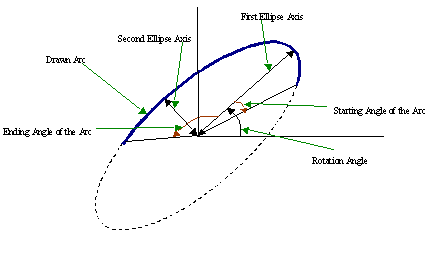
\includegraphics[width=0.5\textwidth]{pics/ellipse.png}

\cvCPyFunc{EllipseBox}

Draws a simple or thick elliptic arc or fills an ellipse sector.

\cvdefC{void cvEllipseBox( \par CvArr* img, \par CvBox2D box, \par CvScalar color,
                   \par int thickness=1, \par int lineType=8, \par int shift=0 );}
\cvdefPy{EllipseBox(img,box,color,thickness=1,lineType=8,shift=0)-> None}

\begin{description}
\cvarg{img}{Image}
\cvarg{box}{The enclosing box of the ellipse drawn}
\cvarg{thickness}{Thickness of the ellipse boundary}
\cvarg{lineType}{Type of the ellipse boundary, see \cross{Line} description}
\cvarg{shift}{Number of fractional bits in the box vertex coordinates}
\end{description}

The function draws a simple or thick ellipse outline, or fills an ellipse. The functions provides a convenient way to draw an ellipse approximating some shape; that is what \cross{CamShift} and \cross{FitEllipse} do. The ellipse drawn is clipped by ROI rectangle. A piecewise-linear approximation is used for antialiased arcs and thick arcs.

\cvCPyFunc{FillConvexPoly}
Fills a convex polygon.

\cvdefC{
void cvFillConvexPoly( \par CvArr* img,\par CvPoint* pts,\par int npts,\par CvScalar color,\par int lineType=8,\par int shift=0 );}
\cvdefPy{FillConvexPoly(img,pn,color,lineType=8,shift=0)-> None}

\begin{description}
\cvarg{img}{Image}
\cvarg{pts}{Array of pointers to a single polygon}
\cvarg{npts}{Polygon vertex counter}
\cvarg{color}{Polygon color}
\cvarg{lineType}{Type of the polygon boundaries, see \cross{Line} description}
\cvarg{shift}{Number of fractional bits in the vertex coordinates}
\end{description}

The function fills a convex polygon's interior.
This function is much faster than the function \texttt{cvFillPoly}
and can fill not only convex polygons but any monotonic polygon,
i.e., a polygon whose contour intersects every horizontal line (scan
line) twice at the most.


\cvCPyFunc{FillPoly}
Fills a polygon's interior.

\cvdefC{
void cvFillPoly( \par CvArr* img,\par CvPoint** pts,\par int* npts,\par int contours,\par CvScalar color,\par int lineType=8,\par int shift=0 );
}
\cvdefPy{FillPoly(img,polys,color,lineType=8,shift=0)-> None}

\begin{description}
\cvarg{img}{Image}
\ifC
\cvarg{pts}{Array of pointers to polygons}
\cvarg{npts}{Array of polygon vertex counters}
\cvarg{contours}{Number of contours that bind the filled region}
\fi
\ifPy
\cvarg{polys}{List of lists of (x,y) pairs.  Each list of points is a polygon.}
\fi
\cvarg{color}{Polygon color}
\cvarg{lineType}{Type of the polygon boundaries, see \cross{Line} description}
\cvarg{shift}{Number of fractional bits in the vertex coordinates}
\end{description}


The function fills an area bounded by several
polygonal contours. The function fills complex areas, for example,
areas with holes, contour self-intersection, and so forth.

\cvCPyFunc{GetTextSize}
Retrieves the width and height of a text string.

\cvdefC{
void cvGetTextSize( \par const char* textString,\par const CvFont* font,\par CvSize* textSize,\par int* baseline );}
\cvdefPy{GetTextSize(textString,font)-> (textSize,baseline)}

\begin{description}
\cvarg{font}{Pointer to the font structure}
\cvarg{textString}{Input string}
\cvarg{textSize}{Resultant size of the text string. Height of the text does not include the height of character parts that are below the baseline.}
\cvarg{baseline}{y-coordinate of the baseline relative to the bottom-most text point}
\end{description}

The function calculates the dimensions of a rectangle to enclose a text string when a specified font is used.

\cvCPyFunc{InitFont}
Initializes font structure.

\cvdefC{
void cvInitFont( \par CvFont* font,\par int fontFace,\par double hscale,\par double vscale,\par double shear=0,\par int thickness=1,\par int lineType=8 );}
\cvdefPy{InitFont(fontFace,hscale,vscale,shear=0,thickness=1,lineType=8)-> font}

\begin{description}
\cvarg{font}{Pointer to the font structure initialized by the function}
\cvarg{fontFace}{Font name identifier. Only a subset of Hershey fonts \url{http://sources.isc.org/utils/misc/hershey-font.txt} are supported now:
 \begin{description}
 \cvarg{CV\_FONT\_HERSHEY\_SIMPLEX}{normal size sans-serif font}
 \cvarg{CV\_FONT\_HERSHEY\_PLAIN}{small size sans-serif font}
 \cvarg{CV\_FONT\_HERSHEY\_DUPLEX}{normal size sans-serif font (more complex than \par \texttt{CV\_FONT\_HERSHEY\_SIMPLEX})}
 \cvarg{CV\_FONT\_HERSHEY\_COMPLEX}{normal size serif font}
 \cvarg{CV\_FONT\_HERSHEY\_TRIPLEX}{normal size serif font (more complex than \texttt{CV\_FONT\_HERSHEY\_COMPLEX})}
 \cvarg{CV\_FONT\_HERSHEY\_COMPLEX\_SMALL}{smaller version of \texttt{CV\_FONT\_HERSHEY\_COMPLEX}}
 \cvarg{CV\_FONT\_HERSHEY\_SCRIPT\_SIMPLEX}{hand-writing style font}
 \cvarg{CV\_FONT\_HERSHEY\_SCRIPT\_COMPLEX}{more complex variant of \texttt{CV\_FONT\_HERSHEY\_SCRIPT\_SIMPLEX}}
 \end{description}
 The parameter can be composited from one of the values above and an optional \texttt{CV\_FONT\_ITALIC} flag, which indicates italic or oblique font.}
\cvarg{hscale}{Horizontal scale.  If equal to \texttt{1.0f}, the characters have the original width depending on the font type. If equal to \texttt{0.5f}, the characters are of half the original width.}
\cvarg{vscale}{Vertical scale. If equal to \texttt{1.0f}, the characters have the original height depending on the font type. If equal to \texttt{0.5f}, the characters are of half the original height.}
\cvarg{shear}{Approximate tangent of the character slope relative to the vertical line.  A zero value means a non-italic font, \texttt{1.0f} means about a 45 degree slope, etc.} 
\cvarg{thickness}{Thickness of the text strokes}
\cvarg{lineType}{Type of the strokes, see \cross{Line} description}
\end{description}

The function initializes the font structure that can be passed to text rendering functions.


\cvCPyFunc{InitLineIterator}
Initializes the line iterator.

\cvdefC{
int cvInitLineIterator( \par const CvArr* image,\par CvPoint pt1,\par CvPoint pt2,\par CvLineIterator* line\_iterator,\par int connectivity=8,\par int left\_to\_right=0 );
}
\cvdefPy{InitLineIterator(image, pt1, pt2, connectivity=8, left\_to\_right=0) -> None}

\begin{description}
\cvarg{image}{Image to sample the line from}
\cvarg{pt1}{First ending point of the line segment}
\cvarg{pt2}{Second ending point of the line segment}
\cvC{\cvarg{line\_iterator}{Pointer to the line iterator state structure}}
\cvarg{connectivity}{The scanned line connectivity, 4 or 8.}
\cvarg{left\_to\_right}{
If ($ \texttt{left\_to\_right} = 0 $ ) then the line is scanned in the specified order, from \texttt{pt1} to \texttt{pt2}.
If ($ \texttt{left\_to\_right} \ne 0$) the line is scanned from left-most point to right-most.}
\end{description}

The function initializes the line
iterator and returns the number of pixels between the two end points.
Both points must be inside the image. After the iterator has been
initialized, all the points on the raster line that connects the
two ending points may be retrieved by successive calls of
\texttt{CV\_NEXT\_LINE\_POINT} point. The points on the line are
calculated one by one using a 4-connected or 8-connected Bresenham
algorithm.

\ifC
\cvfunc{Example: Using line iterator to calculate the sum of pixel values along the color line}

\begin{lstlisting}

CvScalar sum_line_pixels( IplImage* image, CvPoint pt1, CvPoint pt2 )
{
    CvLineIterator iterator;
    int blue_sum = 0, green_sum = 0, red_sum = 0;
    int count = cvInitLineIterator( image, pt1, pt2, &iterator, 8, 0 );

    for( int i = 0; i < count; i++ ){
        blue_sum += iterator.ptr[0];
        green_sum += iterator.ptr[1];
        red_sum += iterator.ptr[2];
        CV_NEXT_LINE_POINT(iterator);

        /* print the pixel coordinates: demonstrates how to calculate the 
							coordinates */
        {
        int offset, x, y;
        /* assume that ROI is not set, otherwise need to take it 
						into account. */
        offset = iterator.ptr - (uchar*)(image->imageData);
        y = offset/image->widthStep;
        x = (offset - y*image->widthStep)/(3*sizeof(uchar) 
					/* size of pixel */);
        printf("(%d,%d)\n", x, y );
        }
    }
    return cvScalar( blue_sum, green_sum, red_sum );
}

\end{lstlisting}
\fi

\cvCPyFunc{Line}
Draws a line segment connecting two points.

\cvdefC{
void cvLine( \par CvArr* img,\par CvPoint pt1,\par CvPoint pt2,\par CvScalar color,\par int thickness=1,\par int lineType=8,\par int shift=0 );
}
\cvdefPy{Line(img,pt1,pt2,color,thickness=1,lineType=8,shift=0)-> None}

\begin{description}
\cvarg{img}{The image}
\cvarg{pt1}{First point of the line segment}
\cvarg{pt2}{Second point of the line segment}
\cvarg{color}{Line color}
\cvarg{thickness}{Line thickness}
\cvarg{lineType}{Type of the line:
  \begin{description}
  \cvarg{8}{(or omitted) 8-connected line.}
  \cvarg{4}{4-connected line.}
  \cvarg{CV\_AA}{antialiased line.}
  \end{description}}
\cvarg{shift}{Number of fractional bits in the point coordinates}
\end{description}

The function draws the line segment between
\texttt{pt1} and \texttt{pt2} points in the image. The line is
clipped by the image or ROI rectangle. For non-antialiased lines
with integer coordinates the 8-connected or 4-connected Bresenham
algorithm is used. Thick lines are drawn with rounding endings.
Antialiased lines are drawn using Gaussian filtering. To specify
the line color, the user may use the macro
\texttt{CV\_RGB( r, g, b )}.

\cvCPyFunc{PolyLine}
Draws simple or thick polygons.

\cvdefC{
void cvPolyLine( \par CvArr* img,\par CvPoint** pts,\par int* npts,\par int contours,\par int is\_closed,\par CvScalar color,\par int thickness=1,\par int lineType=8,\par int shift=0 );}
\cvdefPy{PolyLine(img,pts,is\_closed,color,thickness=1,lineType=8,shift=0)-> None}

\begin{description}
\ifC
\cvarg{pts}{Array of pointers to polygons}
\cvarg{npts}{Array of polygon vertex counters}
\cvarg{contours}{Number of contours that bind the filled region}
\fi
\ifPy
\cvarg{polys}{List of lists of (x,y) pairs.  Each list of points is a polygon.}
\fi
\cvarg{img}{Image}
\cvarg{is\_closed}{Indicates whether the polylines must be drawn
closed. If closed, the function draws the line from the last vertex
of every contour to the first vertex.}
\cvarg{color}{Polyline color}
\cvarg{thickness}{Thickness of the polyline edges}
\cvarg{lineType}{Type of the line segments, see \cross{Line} description}
\cvarg{shift}{Number of fractional bits in the vertex coordinates}
\end{description}

The function draws single or multiple polygonal curves.

\cvCPyFunc{PutText}
Draws a text string.

\cvdefC{
void cvPutText( \par CvArr* img,\par const char* text,\par CvPoint org,\par const CvFont* font,\par CvScalar color );}
\cvdefPy{PutText(img,text,org,font,color)-> None}

\begin{description}
\cvarg{img}{Input image}
\cvarg{text}{String to print}
\cvarg{org}{Coordinates of the bottom-left corner of the first letter}
\cvarg{font}{Pointer to the font structure}
\cvarg{color}{Text color}
\end{description}


The function renders the text in the image with
the specified font and color. The printed text is clipped by the ROI
rectangle. Symbols that do not belong to the specified font are
replaced with the symbol for a rectangle.

\cvCPyFunc{Rectangle}
Draws a simple, thick, or filled rectangle.

\cvdefC{void cvRectangle( \par CvArr* img,\par CvPoint pt1,\par CvPoint pt2,\par CvScalar color,\par int thickness=1,\par int lineType=8,\par int shift=0 );}
\cvdefPy{Rectangle(img,pt1,pt2,color,thickness=1,lineType=8,shift=0)-> None}

\begin{description}
\cvarg{img}{Image}
\cvarg{pt1}{One of the rectangle's vertices}
\cvarg{pt2}{Opposite rectangle vertex}
\cvarg{color}{Line color (RGB) or brightness (grayscale image)}
\cvarg{thickness}{Thickness of lines that make up the rectangle. Negative values, e.g., CV\_FILLED, cause the function to draw a filled rectangle.}
\cvarg{lineType}{Type of the line, see \cross{Line} description}
\cvarg{shift}{Number of fractional bits in the point coordinates}
\end{description}

The function draws a rectangle with two opposite corners \texttt{pt1} and \texttt{pt2}.

\cvfunc{CV\_RGB}\label{CV_RGB}
Constructs a color value.

\cvdefC{\#define CV\_RGB( r, g, b )  cvScalar( (b), (g), (r) )}
\cvdefPy{CV\_RGB(red,grn,blu)->CvScalar}

\fi

\ifCpp

\cvCppFunc{circle}
Draws a circle

\cvdefCpp{
void circle(Mat\& img, Point center, int radius,\par
            const Scalar\& color, int thickness=1,\par
            int lineType=8, int shift=0);\newline
}
\begin{description}
\cvarg{img}{Image where the circle is drawn}
\cvarg{center}{Center of the circle}
\cvarg{radius}{Radius of the circle}
\cvarg{color}{Circle color}
\cvarg{thickness}{Thickness of the circle outline if positive; negative thickness means that a filled circle is to be drawn}
\cvarg{lineType}{Type of the circle boundary, see \cvCppCross{line} description}
\cvarg{shift}{Number of fractional bits in the center coordinates and radius value}
\end{description}

The function \texttt{circle} draws a simple or filled circle with a
given center and radius.

\cvCppFunc{clipLine}
Clips the line against the image rectangle

\cvdefCpp{
bool clipLine(Size imgSize, Point\& pt1, Point\& pt2);\newline
bool clipLine(Rect imgRect, Point\& pt1, Point\& pt2);\newline
}
\begin{description}
\cvarg{imgSize}{The image size; the image rectangle will be \texttt{Rect(0, 0, imgSize.width, imgSize.height)}}
\cvarg{imgSize}{The image rectangle}
\cvarg{pt1}{The first line point}
\cvarg{pt2}{The second line point}
\end{description}

The functions \texttt{clipLine} calculate a part of the line
segment which is entirely within the specified rectangle.
They return \texttt{false} if the line segment is completely outside the rectangle and \texttt{true} otherwise.


\cvCppFunc{ellipse}
Draws a simple or thick elliptic arc or an fills ellipse sector.

\cvdefCpp{
void ellipse(Mat\& img, Point center, Size axes,\par
             double angle, double startAngle, double endAngle,\par
             const Scalar\& color, int thickness=1,\par
             int lineType=8, int shift=0);\newline
void ellipse(Mat\& img, const RotatedRect\& box, const Scalar\& color,\par
             int thickness=1, int lineType=8);\newline
}
\begin{description}
\cvarg{img}{The image}
\cvarg{center}{Center of the ellipse}
\cvarg{axes}{Length of the ellipse axes}
\cvarg{angle}{The ellipse rotation angle in degrees}
\cvarg{startAngle}{Starting angle of the elliptic arc in degrees}
\cvarg{endAngle}{Ending angle of the elliptic arc in degrees}
\cvarg{box}{Alternative ellipse representation via a \cross{RotatedRect}, i.e. the function draws an ellipse inscribed in the rotated rectangle}
\cvarg{color}{Ellipse color}
\cvarg{thickness}{Thickness of the ellipse arc outline if positive, otherwise this indicates that a filled ellipse sector is to be drawn}
\cvarg{lineType}{Type of the ellipse boundary, see \cvCppCross{line} description}
\cvarg{shift}{Number of fractional bits in the center coordinates and axes' values}
\end{description}

The functions \texttt{ellipse} with less parameters draw an ellipse outline, a filled ellipse, an elliptic
arc or a filled ellipse sector. 
A piecewise-linear curve is used to approximate the elliptic arc boundary. If you need more control of the ellipse rendering, you can retrieve the curve using \cvCppCross{ellipse2Poly} and then render it with \cvCppCross{polylines} or fill it with \cvCppCross{fillPoly}. If you use the first variant of the function and want to draw the whole ellipse, not an arc, pass \texttt{startAngle=0} and \texttt{endAngle=360}. The picture below
explains the meaning of the parameters.

Parameters of Elliptic Arc

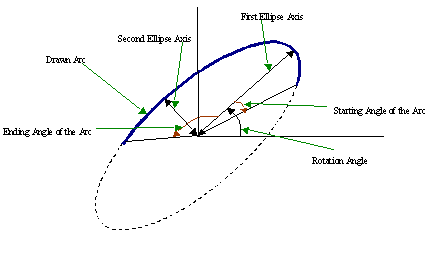
\includegraphics[width=0.5\textwidth]{pics/ellipse.png}

\cvCppFunc{ellipse2Poly}
Approximates an elliptic arc with a polyline

\cvdefCpp{
void ellipse2Poly( Point center, Size axes, int angle,\par
                   int startAngle, int endAngle, int delta,\par
                   vector<Point>\& pts );\newline
}
\begin{description}
\cvarg{center}{Center of the arc}
\cvarg{axes}{Half-sizes of the arc. See \cvCppCross{ellipse}}
\cvarg{angle}{Rotation angle of the ellipse in degrees. See \cvCppCross{ellipse}}
\cvarg{startAngle}{Starting angle of the elliptic arc in degrees}
\cvarg{endAngle}{Ending angle of the elliptic arc in degrees}
\cvarg{delta}{Angle between the subsequent polyline vertices. It defines the approximation accuracy.}
\cvarg{pts}{The output vector of polyline vertices}
\end{description}

The function \texttt{ellipse2Poly} computes the vertices of a polyline that approximates the specified elliptic arc. It is used by \cvCppCross{ellipse}.

\cvCppFunc{fillConvexPoly}
Fills a convex polygon.

\cvdefCpp{
void fillConvexPoly(Mat\& img, const Point* pts, int npts,\par
                    const Scalar\& color, int lineType=8,\par
                    int shift=0);\newline
}
\begin{description}
\cvarg{img}{Image}
\cvarg{pts}{The polygon vertices}
\cvarg{npts}{The number of polygon vertices}
\cvarg{color}{Polygon color}
\cvarg{lineType}{Type of the polygon boundaries, see \cvCppCross{line} description}
\cvarg{shift}{The number of fractional bits in the vertex coordinates}
\end{description}

The function \texttt{fillConvexPoly} draws a filled convex polygon.
This function is much faster than the function \texttt{fillPoly}
and can fill not only convex polygons but any monotonic polygon without self-intersections,
i.e., a polygon whose contour intersects every horizontal line (scan
line) twice at the most (though, its top-most and/or the bottom edge could be horizontal).

\cvCppFunc{fillPoly}
Fills the area bounded by one or more polygons

\cvdefCpp{void fillPoly(Mat\& img, const Point** pts, \par
              const int* npts, int ncontours,\par
              const Scalar\& color, int lineType=8,\par
              int shift=0, Point offset=Point() );}
\begin{description}
\cvarg{img}{Image}
\cvarg{pts}{Array of polygons, each represented as an array of points}
\cvarg{npts}{The array of polygon vertex counters}
\cvarg{ncontours}{The number of contours that bind the filled region}
\cvarg{color}{Polygon color}
\cvarg{lineType}{Type of the polygon boundaries, see \cvCppCross{line} description}
\cvarg{shift}{The number of fractional bits in the vertex coordinates}
\end{description}

The function \texttt{fillPoly} fills an area bounded by several
polygonal contours. The function can fills complex areas, for example,
areas with holes, contours with self-intersections (some of thier parts), and so forth.

\cvCppFunc{getTextSize}
Calculates the width and height of a text string.

\cvdefCpp{Size getTextSize(const string\& text, int fontFace,\par
                 double fontScale, int thickness,\par
                 int* baseLine);\newline}
\begin{description}
\cvarg{text}{The input text string}
\cvarg{fontFace}{The font to use; see \cvCppCross{putText}}
\cvarg{fontScale}{The font scale; see \cvCppCross{putText}}
\cvarg{thickness}{The thickness of lines used to render the text; see \cvCppCross{putText}}
\cvarg{baseLine}{The output parameter - y-coordinate of the baseline relative to the bottom-most text point}
\end{description}

The function \texttt{getTextSize} calculates and returns size of the box that contain the specified text.
That is, the following code will render some text, the tight box surrounding it and the baseline:

\begin{lstlisting}
// Use "y" to show that the baseLine is about
string text = "Funny text inside the box";
int fontFace = FONT_HERSHEY_SCRIPT_SIMPLEX;
double fontScale = 2;
int thickness = 3;

Mat img(600, 800, CV_8UC3, Scalar::all(0));

int baseline=0;
Size textSize = getTextSize(text, fontFace,
                            fontScale, thickness, &baseline);
baseline += thickness;

// center the text
Point textOrg((img.cols - textSize.width)/2,
              (img.rows + textSize.height)/2);

// draw the box
rectangle(img, textOrg + Point(0, baseline),
          textOrg + Point(textSize.width, -textSize.height),
          Scalar(0,0,255));
// ... and the baseline first
line(img, textOrg + Point(0, thickness),
     textOrg + Point(textSize.width, thickness),
     Scalar(0, 0, 255));

// then put the text itself
putText(img, text, textOrg, fontFace, fontScale,
        Scalar::all(255), thickness, 8);
\end{lstlisting}
        
        
\cvCppFunc{line}
Draws a line segment connecting two points

\cvdefCpp{void line(Mat\& img, Point pt1, Point pt2, const Scalar\& color,\par
          int thickness=1, int lineType=8, int shift=0);\newline}
\begin{description}
\cvarg{img}{The image}
\cvarg{pt1}{First point of the line segment}
\cvarg{pt2}{Second point of the line segment}
\cvarg{color}{Line color}
\cvarg{thickness}{Line thickness}
\cvarg{lineType}{Type of the line:
  \begin{description}
  \cvarg{8}{(or omitted) 8-connected line.}
  \cvarg{4}{4-connected line.}
  \cvarg{CV\_AA}{antialiased line.}
  \end{description}}
\cvarg{shift}{Number of fractional bits in the point coordinates}
\end{description}

The function \texttt{line} draws the line segment between
\texttt{pt1} and \texttt{pt2} points in the image. The line is
clipped by the image boundaries. For non-antialiased lines
with integer coordinates the 8-connected or 4-connected Bresenham
algorithm is used. Thick lines are drawn with rounding endings.
Antialiased lines are drawn using Gaussian filtering. To specify
the line color, the user may use the macro
\texttt{CV\_RGB(r, g, b)}.


\cvCppFunc{LineIterator}
Class for iterating pixels on a raster line

\begin{lstlisting}
class LineIterator
{
public:
    // creates iterators for the line connecting pt1 and pt2
    // the line will be clipped on the image boundaries
    // the line is 8-connected or 4-connected
    // If leftToRight=true, then the iteration is always done
    // from the left-most point to the right most,
    // not to depend on the ordering of pt1 and pt2 parameters
    LineIterator(const Mat& img, Point pt1, Point pt2,
                 int connectivity=8, bool leftToRight=false);newline
    // returns pointer to the current line pixel
    uchar* operator *();newline
    // move the iterator to the next pixel
    LineIterator& operator ++();newline
    LineIterator operator ++(int);newline

    // internal state of the iterator
    uchar* ptr;newline
    int err, count;newline
    int minusDelta, plusDelta;newline
    int minusStep, plusStep;newline
};
\end{lstlisting}

The class \texttt{LineIterator} is used to get each pixel of a raster line. It can be treated as versatile implementation of the Bresenham algorithm, where you can stop at each pixel and do some extra processing, for example, grab pixel values along the line, or draw a line with some effect (e.g. with XOR operation).

The number of pixels along the line is store in \texttt{LineIterator::count}.

\begin{lstlisting}
// grabs pixels along the line (pt1, pt2)
// from 8-bit 3-channel image to the buffer
LineIterator it(img, pt1, pt2, 8);
vector<Vec3b> buf(it.count);

for(int i = 0; i < it.count; i++, ++it)
    buf[i] = *(const Vec3b)*it;
\end{lstlisting}


\cvCppFunc{rectangle}
Draws a simple, thick, or filled up-right rectangle.

\cvdefCpp{void rectangle(Mat\& img, Point pt1, Point pt2,\par
               const Scalar\& color, int thickness=1,\par
               int lineType=8, int shift=0);}
\begin{description}
\cvarg{img}{Image}
\cvarg{pt1}{One of the rectangle's vertices}
\cvarg{pt2}{Opposite to \texttt{pt1} rectangle vertex}
\cvarg{color}{Rectangle color or brightness (grayscale image)}
\cvarg{thickness}{Thickness of lines that make up the rectangle. Negative values, e.g. \texttt{CV\_FILLED}, mean that the function has to draw a filled rectangle.}
\cvarg{lineType}{Type of the line, see \cvCppCross{line} description}
\cvarg{shift}{Number of fractional bits in the point coordinates}
\end{description}

The function \texttt{rectangle} draws a rectangle outline or a filled rectangle, which two opposite corners are \texttt{pt1} and \texttt{pt2}.
               

\cvCppFunc{polylines}
Draws several polygonal curves

\cvdefCpp{void polylines(Mat\& img, const Point** pts, const int* npts,\par
               int ncontours, bool isClosed, const Scalar\& color,\par
               int thickness=1, int lineType=8, int shift=0 );\newline}
\begin{description}
\cvarg{img}{The image}
\cvarg{pts}{Array of polygonal curves}
\cvarg{npts}{Array of polygon vertex counters}
\cvarg{ncontours}{The number of curves}
\cvarg{isClosed}{Indicates whether the drawn polylines are closed or not. If they are closed, the function draws the line from the last vertex of each curve to its first vertex}
\cvarg{color}{Polyline color}
\cvarg{thickness}{Thickness of the polyline edges}
\cvarg{lineType}{Type of the line segments, see \cvCppCross{line} description}
\cvarg{shift}{The number of fractional bits in the vertex coordinates}
\end{description}

The function \texttt{polylines} draws one or more polygonal curves.

\cvCppFunc{putText}
Draws a text string

\cvdefCpp{void putText( Mat\& img, const string\& text, Point org,\par
              int fontFace, double fontScale, Scalar color,\par
              int thickness=1, int lineType=8,\par
              bool bottomLeftOrigin=false );}
\begin{description}
\cvarg{img}{The image}
\cvarg{text}{The text string to be drawn}
\cvarg{org}{The bottom-left corner of the text string in the image}
\cvarg{fontFace}{The font type, one of \cvarg{FONT\_HERSHEY\_SIMPLEX}, \cvarg{FONT\_HERSHEY\_PLAIN},
 \cvarg{FONT\_HERSHEY\_DUPLEX}, \cvarg{FONT\_HERSHEY\_COMPLEX}, \cvarg{FONT\_HERSHEY\_TRIPLEX},
 \cvarg{FONT\_HERSHEY\_COMPLEX\_SMALL}, \cvarg{FONT\_HERSHEY\_SCRIPT\_SIMPLEX} or \cvarg{FONT\_HERSHEY\_SCRIPT\_COMPLEX},
   where each of the font id's can be combined with \cvarg{FONT\_HERSHEY\_ITALIC} to get the slanted letters.}
\cvarg{fontScale}{The font scale factor that is multiplied by the font-specific base size}
\cvarg{thickness}{Thickness of the lines used to draw the text}
\cvarg{lineType}{The line type; see \texttt{line} for details}
\cvarg{bottomLeftOrigin}{When true, the image data origin is at the bottom-left corner, otherwise it's at the top-left corner}
\end{description}

The function \texttt{putText} draws a text string in the image.
Symbols that can not be rendered using the specified font are
replaced question marks. See \cvCppCross{getTextSize} for a text rendering code example.

\fi

\subsection{XML/YAML Persistence}

\ifCPy

\ifC
\cvstruct{CvFileStorage}\label{CvFileStorage}
File Storage.

\begin{lstlisting}
typedef struct CvFileStorage
{
    ...       // hidden fields
} CvFileStorage;
\end{lstlisting}

The structure \cross{CvFileStorage} is a "black box" representation
of the file storage associated with a file on disk. Several
functions that are described below take \texttt{CvFileStorage} as
inputs and allow theuser to save or to load hierarchical collections
that consist of scalar values, standard CXCore objects (such as
matrices, sequences, graphs), and user-defined objects.

CXCore can read and write data in XML (http://www.w3c.org/XML) or YAML
(http://www.yaml.org) formats. Below is an example of $3 \times 3$
floating-point identity matrix \texttt{A}, stored in XML and YAML files
using CXCore functions:

XML:

\begin{verbatim}
<?xml version="1.0">
<opencv_storage>
<A type_id="opencv-matrix">
  <rows>3</rows>
  <cols>3</cols>
  <dt>f</dt>
  <data>1. 0. 0. 0. 1. 0. 0. 0. 1.</data>
</A>
</opencv_storage>
\end{verbatim}

YAML:

\begin{verbatim}
%YAML:1.0
A: !!opencv-matrix
  rows: 3
  cols: 3
  dt: f
  data: [ 1., 0., 0., 0., 1., 0., 0., 0., 1.]
\end{verbatim}

As it can be seen from the examples, XML uses nested tags to represent
hierarchy, while YAML uses indentation for that purpose (similar
to the Python programming language).

The same CXCore functions can read and write data in both formats;
the particular format is determined by the extension of the opened
file, .xml for XML files and .yml or .yaml for YAML.


\cvstruct{CvFileNode}\label{CvFileNode}
File Storage Node.

\begin{lstlisting}
/* file node type */
#define CV_NODE_NONE        0
#define CV_NODE_INT         1
#define CV_NODE_INTEGER     CV_NODE_INT
#define CV_NODE_REAL        2
#define CV_NODE_FLOAT       CV_NODE_REAL
#define CV_NODE_STR         3
#define CV_NODE_STRING      CV_NODE_STR
#define CV_NODE_REF         4 /* not used */
#define CV_NODE_SEQ         5
#define CV_NODE_MAP         6
#define CV_NODE_TYPE_MASK   7

/* optional flags */
#define CV_NODE_USER        16
#define CV_NODE_EMPTY       32
#define CV_NODE_NAMED       64

#define CV_NODE_TYPE(tag)  ((tag) & CV_NODE_TYPE_MASK)

#define CV_NODE_IS_INT(tag)        (CV_NODE_TYPE(tag) == CV_NODE_INT)
#define CV_NODE_IS_REAL(tag)       (CV_NODE_TYPE(tag) == CV_NODE_REAL)
#define CV_NODE_IS_STRING(tag)     (CV_NODE_TYPE(tag) == CV_NODE_STRING)
#define CV_NODE_IS_SEQ(tag)        (CV_NODE_TYPE(tag) == CV_NODE_SEQ)
#define CV_NODE_IS_MAP(tag)        (CV_NODE_TYPE(tag) == CV_NODE_MAP)
#define CV_NODE_IS_COLLECTION(tag) (CV_NODE_TYPE(tag) >= CV_NODE_SEQ)
#define CV_NODE_IS_FLOW(tag)       (((tag) & CV_NODE_FLOW) != 0)
#define CV_NODE_IS_EMPTY(tag)      (((tag) & CV_NODE_EMPTY) != 0)
#define CV_NODE_IS_USER(tag)       (((tag) & CV_NODE_USER) != 0)
#define CV_NODE_HAS_NAME(tag)      (((tag) & CV_NODE_NAMED) != 0)

#define CV_NODE_SEQ_SIMPLE 256
#define CV_NODE_SEQ_IS_SIMPLE(seq) (((seq)->flags & CV_NODE_SEQ_SIMPLE) != 0)

typedef struct CvString
{
    int len;
    char* ptr;
}
CvString;

/* all the keys (names) of elements in the readed file storage
   are stored in the hash to speed up the lookup operations */
typedef struct CvStringHashNode
{
    unsigned hashval;
    CvString str;
    struct CvStringHashNode* next;
}
CvStringHashNode;

/* basic element of the file storage - scalar or collection */
typedef struct CvFileNode
{
    int tag;
    struct CvTypeInfo* info; /* type information
            (only for user-defined object, for others it is 0) */
    union
    {
        double f; /* scalar floating-point number */
        int i;    /* scalar integer number */
        CvString str; /* text string */
        CvSeq* seq; /* sequence (ordered collection of file nodes) */
        struct CvMap* map; /* map (collection of named file nodes) */
    } data;
}
CvFileNode;
\end{lstlisting}

The structure is used only for retrieving data from file storage
(i.e., for loading data from the file). When data is written to a file,
it is done sequentially, with minimal buffering. No data is stored
in the file storage.

In opposite, when data is read from a file, the whole file is parsed
and represented in memory as a tree. Every node of the tree is
represented by \cross{CvFileNode}. The type of file node \texttt{N}
can be retrieved as \texttt{CV\_NODE\_TYPE(N->tag)}. Some file nodes
(leaves) are scalars: text strings, integers, or floating-point
numbers. Other file nodes are collections of file nodes, which can
be scalars or collections in their turn. There are two types of
collections: sequences and maps (we use YAML notation, however, the
same is true for XML streams). Sequences (do not mix them with
\cross{CvSeq}) are ordered collections of unnamed file nodes; maps
are unordered collections of named file nodes. Thus, elements of
sequences are accessed by index (\cross{GetSeqElem}), while elements
of maps are accessed by name (\cross{GetFileNodeByName}). The table
below describes the different types of file nodes:

\begin{tabular}{| c | c | c |}
\hline
Type           & \texttt{CV\_NODE\_TYPE(node->tag)} & Value\\ \hline \hline
Integer        & \texttt{CV\_NODE\_INT}             & \texttt{node->data.i} \\ \hline
Floating-point & \texttt{CV\_NODE\_REAL}            & \texttt{node->data.f} \\ \hline
Text string    & \texttt{CV\_NODE\_STR}             & \texttt{node->data.str.ptr} \\ \hline
Sequence       & \texttt{CV\_NODE\_SEQ}             & \texttt{node->data.seq} \\ \hline
Map            & \texttt{CV\_NODE\_MAP}             & \texttt{node->data.map} (see below)\\ \hline
\end{tabular}

There is no need to access the \texttt{map} field directly (by the way,
\texttt{CvMap} is a hidden structure). The elements of the map can
be retrieved with the \cross{GetFileNodeByName} function that takes a
pointer to the "map" file node.

A user (custom) object is an instance of either one of the standard CxCore
types, such as \cross{CvMat}, \cross{CvSeq} etc., or any type
registered with \cross{RegisterTypeInfo}. Such an object is initially
represented in a file as a map (as shown in XML and YAML example files
above) after the file storage has been opened and parsed. Then the
object can be decoded (coverted to native representation) by
request - when a user calls the \cross{Read} or \cross{ReadByName} functions.


\cvstruct{CvAttrList}\label{CvAttrList}
List of attributes.

\begin{lstlisting}
typedef struct CvAttrList
{
    const char** attr; /* NULL-terminated array of (attribute\_name,attribute\_value) pairs */
    struct CvAttrList* next; /* pointer to next chunk of the attributes list */
}
CvAttrList;

/* initializes CvAttrList structure */
inline CvAttrList cvAttrList( const char** attr=NULL, CvAttrList* next=NULL );

/* returns attribute value or 0 (NULL) if there is no such attribute */
const char* cvAttrValue( const CvAttrList* attr, const char* attr\_name );
\end{lstlisting}

In the current implementation, attributes are used to pass extra parameters when writing user objects (see \cross{Write}). XML attributes inside tags are not supported, aside from the object type specification (\texttt{type\_id} attribute).


\cvstruct{CvTypeInfo}\label{CvTypeInfo}
Type information.

\begin{lstlisting}
typedef int (CV_CDECL *CvIsInstanceFunc)( const void* structPtr );
typedef void (CV_CDECL *CvReleaseFunc)( void** structDblPtr );
typedef void* (CV_CDECL *CvReadFunc)( CvFileStorage* storage, CvFileNode* node );
typedef void (CV_CDECL *CvWriteFunc)( CvFileStorage* storage,
                                      const char* name,
                                      const void* structPtr,
                                      CvAttrList attributes );
typedef void* (CV_CDECL *CvCloneFunc)( const void* structPtr );

typedef struct CvTypeInfo
{
    int flags; /* not used */
    int header_size; /* sizeof(CvTypeInfo) */
    struct CvTypeInfo* prev; /* previous registered type in the list */
    struct CvTypeInfo* next; /* next registered type in the list */
    const char* type_name; /* type name, written to file storage */

    /* methods */
    CvIsInstanceFunc is_instance; /* checks if the passed object belongs to the type */
    CvReleaseFunc release; /* releases object (memory etc.) */
    CvReadFunc read; /* reads object from file storage */
    CvWriteFunc write; /* writes object to file storage */
    CvCloneFunc clone; /* creates a copy of the object */
}
CvTypeInfo;

\end{lstlisting}

The structure \cross{CvTypeInfo} contains information about one of the
standard or user-defined types. Instances of the type may or may not
contain a pointer to the corresponding \cross{CvTypeInfo} structure. In
any case, there is a way to find the type info structure for a given object
using the \cross{TypeOf} function. Aternatively, type info can be found by
type name using \cross{FindType}, which is used when an object is read
from file storage. The user can register a new type with \cross{RegisterType}
that adds the type information structure into the beginning of the type
list. Thus, it is possible to create specialized types from generic
standard types and override the basic methods.


\cvCPyFunc{Clone}
Makes a clone of an object.

\cvcodeC{void* cvClone( const void* structPtr );}

\begin{description}
\cvarg{structPtr}{The object to clone}
\end{description}

The function finds the type of a given object and calls \texttt{clone} with the passed object.

\cvCPyFunc{EndWriteStruct}
Ends the writing of a structure.

\cvcodeC{void  cvEndWriteStruct(CvFileStorage* fs);}

\begin{description}
\cvarg{fs}{File storage}
\end{description}

The function finishes the currently written structure.

\cvCPyFunc{FindType}
Finds a type by its name.

\cvcodeC{CvTypeInfo* cvFindType(const char* typeName);}

\begin{description}
\cvarg{typeName}{Type name}
\end{description}

The function finds a registered type by its name. It returns NULL if there is no type with the specified name.


\cvCPyFunc{FirstType}
Returns the beginning of a type list.

\cvcodeC{CvTypeInfo* cvFirstType(void);}

The function returns the first type in the list of registered types. Navigation through the list can be done via the \texttt{prev} and \texttt{next} fields of the \cross{CvTypeInfo} structure.

\cvCPyFunc{GetFileNode}
Finds a node in a map or file storage.

\cvcodeC{CvFileNode* cvGetFileNode( \par CvFileStorage* fs,\par CvFileNode* map,\par const CvStringHashNode* key,\par int createMissing=0 );}

\begin{description}
\cvarg{fs}{File storage}
\cvarg{map}{The parent map. If it is NULL, the function searches a top-level node. If both \texttt{map} and \texttt{key} are NULLs, the function returns the root file node - a map that contains top-level nodes.}
\cvarg{key}{Unique pointer to the node name, retrieved with \cross{GetHashedKey}}
\cvarg{createMissing}{Flag that specifies whether an absent node should be added to the map}
\end{description}


The function finds a file node. It is a faster version of \cross{GetFileNodeByName} (see \cross{GetHashedKey} discussion). Also, the function can insert a new node, if it is not in the map yet.

\cvCPyFunc{GetFileNodeByName}
Finds a node in a map or file storage.

\cvcodeC{CvFileNode* cvGetFileNodeByName( \par const CvFileStorage* fs,\par const CvFileNode* map,\par const char* name);}

\begin{description}
\cvarg{fs}{File storage}
\cvarg{map}{The parent map. If it is NULL, the function searches in all the top-level nodes (streams), starting with the first one.}
\cvarg{name}{The file node name}
\end{description}


The function finds a file node by
\texttt{name}. The node is searched either in \texttt{map} or, if the
pointer is NULL, among the top-level file storage nodes. Using
this function for maps and \cross{GetSeqElem} (or sequence reader)
for sequences, it is possible to nagivate through the file storage. To
speed up multiple queries for a certain key (e.g., in the case of an array
of structures) one may use a combination of \cross{GetHashedKey} and
\cross{GetFileNode}.

\cvCPyFunc{GetFileNodeName}
Returns the name of a file node.

\cvcodeC{const char* cvGetFileNodeName( const CvFileNode* node );}

\begin{description}
\cvarg{node}{File node}
\end{description}

The function returns the name of a file node or NULL, if the file node does not have a name or if \texttt{node} is \texttt{NULL}.


\cvCPyFunc{GetHashedKey}
Returns a unique pointer for a given name.

\cvcodeC{CvStringHashNode* cvGetHashedKey( \par CvFileStorage* fs,\par const char* name,\par int len=-1,\par int createMissing=0 );}

\begin{description}
\cvarg{fs}{File storage}
\cvarg{name}{Literal node name}
\cvarg{len}{Length of the name (if it is known apriori), or -1 if it needs to be calculated}
\cvarg{createMissing}{Flag that specifies, whether an absent key should be added into the hash table}
\end{description}

The function returns a unique pointer for
each particular file node name. This pointer can be then passed to the
\cross{GetFileNode} function that is faster than \cross{GetFileNodeByName}
because it compares text strings by comparing pointers rather than the
strings' content.

Consider the following example where an array of points is encoded as a sequence of 2-entry maps:

\begin{lstlisting}

%YAML:1.0
points:
  - { x: 10, y: 10 }
  - { x: 20, y: 20 }
  - { x: 30, y: 30 }
  # ...

\end{lstlisting}

Then, it is possible to get hashed "x" and "y" pointers to speed up decoding of the points.
\cvfunc{Example: Reading an array of structures from file storage}

\begin{lstlisting}

#include "cxcore.h"

int main( int argc, char** argv )
{
    CvFileStorage* fs = cvOpenFileStorage( "points.yml", 0, CV\_STORAGE\_READ );
    CvStringHashNode* x\_key = cvGetHashedNode( fs, "x", -1, 1 );
    CvStringHashNode* y\_key = cvGetHashedNode( fs, "y", -1, 1 );
    CvFileNode* points = cvGetFileNodeByName( fs, 0, "points" );

    if( CV\_NODE\_IS\_SEQ(points->tag) )
    {
        CvSeq* seq = points->data.seq;
        int i, total = seq->total;
        CvSeqReader reader;
        cvStartReadSeq( seq, &reader, 0 );
        for( i = 0; i < total; i++ )
        {
            CvFileNode* pt = (CvFileNode*)reader.ptr;
#if 1 /* faster variant */
            CvFileNode* xnode = cvGetFileNode( fs, pt, x\_key, 0 );
            CvFileNode* ynode = cvGetFileNode( fs, pt, y\_key, 0 );
            assert( xnode && CV\_NODE\_IS\_INT(xnode->tag) &&
                    ynode && CV\_NODE\_IS\_INT(ynode->tag));
            int x = xnode->data.i; // or x = cvReadInt( xnode, 0 );
            int y = ynode->data.i; // or y = cvReadInt( ynode, 0 );
#elif 1 /* slower variant; does not use x\_key & y\_key */
            CvFileNode* xnode = cvGetFileNodeByName( fs, pt, "x" );
            CvFileNode* ynode = cvGetFileNodeByName( fs, pt, "y" );
            assert( xnode && CV\_NODE\_IS\_INT(xnode->tag) &&
                    ynode && CV\_NODE\_IS\_INT(ynode->tag));
            int x = xnode->data.i; // or x = cvReadInt( xnode, 0 );
            int y = ynode->data.i; // or y = cvReadInt( ynode, 0 );
#else /* the slowest yet the easiest to use variant */
            int x = cvReadIntByName( fs, pt, "x", 0 /* default value */ );
            int y = cvReadIntByName( fs, pt, "y", 0 /* default value */ );
#endif
            CV\_NEXT\_SEQ\_ELEM( seq->elem\_size, reader );
            printf("%d: (%d, %d)\n", i, x, y );
        }
    }
    cvReleaseFileStorage( &fs );
    return 0;
}

\end{lstlisting}

Please note that whatever method of accessing a map you are using, it is
still much slower than using plain sequences; for example, in the above
example, it is more efficient to encode the points as pairs of integers
in a single numeric sequence.

\cvCPyFunc{GetRootFileNode}
Retrieves one of the top-level nodes of the file storage.

\cvcodeC{CvFileNode* cvGetRootFileNode( \par const CvFileStorage* fs,\par int stream\_index=0 );}

\begin{description}
\cvarg{fs}{File storage}
\cvarg{stream\_index}{Zero-based index of the stream. See \cross{StartNextStream}. In most cases, there is only one stream in the file; however, there can be several.}
\end{description}

The function returns one of the top-level file
nodes. The top-level nodes do not have a name, they correspond to the
streams that are stored one after another in the file storage. If the
index is out of range, the function returns a NULL pointer, so all the
top-level nodes may be iterated by subsequent calls to the function with
\texttt{stream\_index=0,1,...}, until the NULL pointer is returned. This function
may be used as a base for recursive traversal of the file storage.

\fi

\cvCPyFunc{Load}
Loads an object from a file.

\cvcodeC{void* cvLoad( \par const char* filename,\par CvMemStorage* memstorage=NULL,\par const char* name=NULL,\par const char** realName=NULL );}
\cvcodePy{Load(filename,storage=NULL,name=NULL)-> generic}

\begin{description}
\cvarg{filename}{File name}
\cvarg{memstorage}{Memory storage for dynamic structures, such as \cross{CvSeq} or \cross{CvGraph} . It is not used for matrices or images.}
\cvarg{name}{Optional object name. If it is NULL, the first top-level object in the storage will be loaded.}
\cvC{\cvarg{realName}{Optional output parameter that will contain the name of the loaded object (useful if \texttt{name=NULL})}}
\end{description}

The function loads an object from a file. It provides a
simple interface to \cvCPyCross{Read}. After the object is loaded, the file
storage is closed and all the temporary buffers are deleted. Thus,
to load a dynamic structure, such as a sequence, contour, or graph, one
should pass a valid memory storage destination to the function.

\ifC

\cvCPyFunc{OpenFileStorage}
Opens file storage for reading or writing data.

\cvcodeC{CvFileStorage* cvOpenFileStorage(\par const char* filename,\par CvMemStorage* memstorage,\par int flags);}

\begin{description}
\cvarg{filename}{Name of the file associated with the storage}
\cvarg{memstorage}{Memory storage used for temporary data and for
storing dynamic structures, such as \cross{CvSeq} or \cross{CvGraph}.
If it is NULL, a temporary memory storage is created and used.}
\cvarg{flags}{Can be one of the following:
  \begin{description}
  \cvarg{CV\_STORAGE\_READ}{the storage is open for reading}
  \cvarg{CV\_STORAGE\_WRITE}{the storage is open for writing}
  \end{description}}
\end{description}

The function opens file storage for
reading or writing data. In the latter case, a new file is created
or an existing file is rewritten. The type of the read or written file is
determined by the filename extension: \texttt{.xml} for \texttt{XML}
and \texttt{.yml} or \texttt{.yaml} for \texttt{YAML}. The function
returns a pointer to the \cross{CvFileStorage} structure.

\cvCPyFunc{Read}
Decodes an object and returns a pointer to it.

\cvcodeC{void* cvRead( \par CvFileStorage* fs,\par CvFileNode* node,\par CvAttrList* attributes=NULL );}

\begin{description}
\cvarg{fs}{File storage}
\cvarg{node}{The root object node}
\cvarg{attributes}{Unused parameter}
\end{description}

The function decodes a user object (creates an object in a
native representation from the file storage subtree) and returns it. The
object to be decoded must be an instance of a registered type that supports the
\texttt{read} method (see \cross{CvTypeInfo}). The type of the object is
determined by the type name that is encoded in the file. If the object
is a dynamic structure, it is created either in memory storage and passed to
\cross{OpenFileStorage} or, if a NULL pointer was passed, in temporary
memory storage, which is released when \cross{ReleaseFileStorage} is
called. Otherwise, if the object is not a dynamic structure, it is
created in a heap and should be released with a specialized function or by
using the generic \cross{Release}.

\cvCPyFunc{ReadByName}
Finds an object by name and decodes it.

\cvcodeC{void* cvReadByName( \par CvFileStorage* fs,\par const CvFileNode* map,\par const char* name,\par CvAttrList* attributes=NULL );}

\begin{description}
\cvarg{fs}{File storage}
\cvarg{map}{The parent map. If it is NULL, the function searches a top-level node.}
\cvarg{name}{The node name}
\cvarg{attributes}{Unused parameter}
\end{description}

The function is a simple superposition of \cross{GetFileNodeByName} and \cross{Read}.

\cvCPyFunc{ReadInt}
Retrieves an integer value from a file node.

\cvcodeC{int cvReadInt( \par const CvFileNode* node,\par int defaultValue=0 );}

\begin{description}
\cvarg{node}{File node}
\cvarg{defaultValue}{The value that is returned if \texttt{node} is NULL}
\end{description}


The function returns an integer that is represented
by the file node. If the file node is NULL, the \texttt{defaultValue}
is returned (thus, it is convenient to call the function right after
\cross{GetFileNode} without checking for a NULL pointer). If
the file node has type \texttt{CV\_NODE\_INT}, then \texttt{node->data.i} is
returned. If the file node has type \texttt{CV\_NODE\_REAL},
then \texttt{node->data.f} is converted to an integer and returned. Otherwise the
result is not determined.

\cvCPyFunc{ReadIntByName}
Finds a file node and returns its value.

\cvcodeC{int cvReadIntByName( \par const CvFileStorage* fs,\par const CvFileNode* map,\par const char* name,\par int defaultValue=0 );}

\begin{description}
\cvarg{fs}{File storage}
\cvarg{map}{The parent map. If it is NULL, the function searches a top-level node.}
\cvarg{name}{The node name}
\cvarg{defaultValue}{The value that is returned if the file node is not found}
\end{description}

The function is a simple superposition of \cross{GetFileNodeByName} and \cross{ReadInt}.


\cvCPyFunc{ReadRawData}
Reads multiple numbers.

\cvcodeC{void cvReadRawData(\par const CvFileStorage* fs,\par const CvFileNode* src,\par void* dst,\par const char* dt);}

\begin{description}
\cvarg{fs}{File storage}
\cvarg{src}{The file node (a sequence) to read numbers from}
\cvarg{dst}{Pointer to the destination array}
\cvarg{dt}{Specification of each array element. It has the same format as in \cross{WriteRawData}.}
\end{description}

The function reads elements from a file node that represents a sequence of scalars.

\cvCPyFunc{ReadRawDataSlice}
Initializes file node sequence reader.

\cvcodeC{void cvReadRawDataSlice( \par const CvFileStorage* fs,\par CvSeqReader* reader,\par int count,\par void* dst,\par const char* dt );}

\begin{description}
\cvarg{fs}{File storage}
\cvarg{reader}{The sequence reader. Initialize it with \cross{StartReadRawData}.}
\cvarg{count}{The number of elements to read}
\cvarg{dst}{Pointer to the destination array}
\cvarg{dt}{Specification of each array element. It has the same format as in \cross{WriteRawData}.}
\end{description}

The function reads one or more elements from
the file node, representing a sequence, to a user-specified array. The
total number of read sequence elements is a product of \texttt{total}
and the number of components in each array element. For example, if
dt=\texttt{2if}, the function will read $\texttt{total} \times 3$
sequence elements. As with any sequence, some parts of the file node
sequence may be skipped or read repeatedly by repositioning the reader
using \cross{SetSeqReaderPos}.


\cvCPyFunc{ReadReal}
Retrieves a floating-point value from a file node.

\cvcodeC{double cvReadReal( \par const CvFileNode* node,\par double defaultValue=0. );}

\begin{description}
\cvarg{node}{File node}
\cvarg{defaultValue}{The value that is returned if \texttt{node} is NULL}
\end{description}

The function returns a floating-point value
that is represented by the file node. If the file node is NULL, the
\texttt{defaultValue} is returned (thus, it is convenient to call
the function right after \cross{GetFileNode} without checking for a NULL
pointer). If the file node has type \texttt{CV\_NODE\_REAL},
then \texttt{node->data.f} is returned. If the file node has type
\texttt{CV\_NODE\_INT}, then \texttt{node-$>$data.f} is converted to floating-point
and returned. Otherwise the result is not determined.

\cvCPyFunc{ReadRealByName}
Finds a file node and returns its value.

\cvcodeC{double  cvReadRealByName(\par const CvFileStorage* fs,\par const CvFileNode* map,\par const char* name,\par double defaultValue=0.);}

\begin{description}
\cvarg{fs}{File storage}
\cvarg{map}{The parent map. If it is NULL, the function searches a top-level node.}
\cvarg{name}{The node name}
\cvarg{defaultValue}{The value that is returned if the file node is not found}
\end{description}

The function is a simple superposition of \cross{GetFileNodeByName} and \cross{ReadReal}.

\cvCPyFunc{ReadString}
Retrieves a text string from a file node.

\cvcodeC{const char* cvReadString( \par const CvFileNode* node,\par const char* defaultValue=NULL );}

\begin{description}
\cvarg{node}{File node}
\cvarg{defaultValue}{The value that is returned if \texttt{node} is NULL}
\end{description}

The function returns a text string that is represented
by the file node. If the file node is NULL, the \texttt{defaultValue}
is returned (thus, it is convenient to call the function right after
\cross{GetFileNode} without checking for a NULL pointer). If
the file node has type \texttt{CV\_NODE\_STR}, then \texttt{node-$>$data.str.ptr}
is returned. Otherwise the result is not determined.

\cvCPyFunc{ReadStringByName}
Finds a file node by its name and returns its value.

\cvcodeC{const char* cvReadStringByName( \par const CvFileStorage* fs,\par const CvFileNode* map,\par const char* name,\par const char* defaultValue=NULL );}

\begin{description}
\cvarg{fs}{File storage}
\cvarg{map}{The parent map. If it is NULL, the function searches a top-level node.}
\cvarg{name}{The node name}
\cvarg{defaultValue}{The value that is returned if the file node is not found}
\end{description}

The function is a simple superposition of \cross{GetFileNodeByName} and \cross{ReadString}.

\cvCPyFunc{RegisterType}
Registers a new type.

\cvcodeC{void cvRegisterType(const CvTypeInfo* info);}

\begin{description}
\cvarg{info}{Type info structure}
\end{description}

The function registers a new type, which is
described by \texttt{info}. The function creates a copy of the structure,
so the user should delete it after calling the function.

\cvCPyFunc{Release}
Releases an object.

\cvcodeC{void cvRelease( void** structPtr );}

\begin{description}
\cvarg{structPtr}{Double pointer to the object}
\end{description}

The function finds the type of a given object and calls \texttt{release} with the double pointer.

\cvCPyFunc{ReleaseFileStorage}
Releases file storage.

\cvcodeC{void  cvReleaseFileStorage(CvFileStorage** fs);}

\begin{description}
\cvarg{fs}{Double pointer to the released file storage}
\end{description}


The function closes the file associated with the storage and releases all the temporary structures. It must be called after all I/O operations with the storage are finished.

\fi

\cvCPyFunc{Save}
Saves an object to a file.

\cvcodeC{void cvSave( \par const char* filename,\par const void* structPtr,\par const char* name=NULL,\par const char* comment=NULL,\par CvAttrList attributes=cvAttrList());}
\cvcodePy{Save(filename,structPtr,name=NULL,comment=NULL)-> None}

\begin{description}
\cvarg{filename}{File name}
\cvarg{structPtr}{Object to save}
\cvarg{name}{Optional object name. If it is NULL, the name will be formed from \texttt{filename}.}
\cvarg{comment}{Optional comment to put in the beginning of the file}
\cvC{\cvarg{attributes}{Optional attributes passed to \cross{Write}}}
\end{description}

The function saves an object to a file. It provides a simple interface to \cross{Write}.

\ifC

\cvCPyFunc{StartNextStream}
Starts the next stream.

\cvcodeC{void cvStartNextStream(CvFileStorage* fs);}

\begin{description}
\cvarg{fs}{File storage}
\end{description}

The function starts the next stream in file storage. Both YAML and XML support multiple "streams." This is useful for concatenating files or for resuming the writing process.

\cvCPyFunc{StartReadRawData}
Initializes the file node sequence reader.

\cvcodeC{void cvStartReadRawData( \par const CvFileStorage* fs,\par const CvFileNode* src,\par CvSeqReader* reader);}

\begin{description}
\cvarg{fs}{File storage}
\cvarg{src}{The file node (a sequence) to read numbers from}
\cvarg{reader}{Pointer to the sequence reader}
\end{description}

The function initializes the sequence reader to read data from a file node. The initialized reader can be then passed to \cross{ReadRawDataSlice}.

\cvCPyFunc{StartWriteStruct}
Starts writing a new structure.

\cvcodeC{void  cvStartWriteStruct( CvFileStorage* fs,\par const char* name,\par int struct\_flags,\par const char* typeName=NULL,\par CvAttrList attributes=cvAttrList( \par));}

\begin{description}
\cvarg{fs}{File storage}
\cvarg{name}{Name of the written structure. The structure can be accessed by this name when the storage is read.}
\cvarg{struct\_flags}{A combination one of the following values:
\begin{description}
\cvarg{CV\_NODE\_SEQ}{the written structure is a sequence (see discussion of \cross{CvFileStorage}), that is, its elements do not have a name.}
\cvarg{CV\_NODE\_MAP}{the written structure is a map (see discussion of \cross{CvFileStorage}), that is, all its elements have names.\end{description}}
 One and only one of the two above flags must be specified}

\cvarg{CV\_NODE\_FLOW}{the optional flag that makes sense only for YAML streams. It means that the structure is written as a flow (not as a block), which is more compact. It is recommended to use this flag for structures or arrays whose elements are all scalars.}
\cvarg{typeName}{Optional parameter - the object type name. In
case of XML it is written as a \texttt{type\_id} attribute of the
structure opening tag. In the case of YAML it is written after a colon
following the structure name (see the example in \cross{CvFileStorage}
description). Mainly it is used with user objects. When the storage
is read, the encoded type name is used to determine the object type
(see \cross{CvTypeInfo} and \cross{FindTypeInfo}).}
\cvarg{attributes}{This parameter is not used in the current implementation}
\end{description}

The function starts writing a compound
structure (collection) that can be a sequence or a map. After all
the structure fields, which can be scalars or structures, are
written, \cross{EndWriteStruct} should be called. The function can
be used to group some objects or to implement the \texttt{write}
function for a some user object (see \cross{CvTypeInfo}).

\cvCPyFunc{TypeOf}
Returns the type of an object.

\cvcodeC{CvTypeInfo* cvTypeOf( const void* structPtr );}

\begin{description}
\cvarg{structPtr}{The object pointer}
\end{description}

The function finds the type of a given object. It iterates
through the list of registered types and calls the \texttt{is\_instance}
function/method for every type info structure with that object until one
of them returns non-zero or until the whole list has been traversed. In
the latter case, the function returns NULL.

\cvCPyFunc{UnregisterType}
Unregisters the type.

\cvcodeC{void cvUnregisterType( const char* typeName );}

\begin{description}
\cvarg{typeName}{Name of an unregistered type}
\end{description}

The function unregisters a type with
a specified name. If the name is unknown, it is possible to locate
the type info by an instance of the type using \cross{TypeOf} or by
iterating the type list, starting from \cross{FirstType}, and then calling
\texttt{cvUnregisterType(info->typeName)}.

\cvCPyFunc{Write}
Writes a user object.

\cvcodeC{void  cvWrite( CvFileStorage* fs,\par const char* name,\par const void* ptr,\par CvAttrList attributes=cvAttrList(\par) );}

\begin{description}
\cvarg{fs}{File storage}
\cvarg{name}{Name of the written object. Should be NULL if and only if the parent structure is a sequence.}
\cvarg{ptr}{Pointer to the object}
\cvarg{attributes}{The attributes of the object. They are specific for each particular type (see the dicsussion below).}
\end{description}

The function writes an object to file storage. First, the appropriate type info is found using \cross{TypeOf}. Then, the \texttt{write} method associated with the type info is called.

Attributes are used to customize the writing procedure. The standard types support the following attributes (all the \texttt{*dt} attributes have the same format as in \cross{WriteRawData}):

\begin{enumerate}
\item CvSeq
  \begin{description}
  \cvarg{header\_dt}{description of user fields of the sequence header that follow CvSeq, or CvChain (if the sequence is a Freeman chain) or CvContour (if the sequence is a contour or point sequence)}
  \cvarg{dt}{description of the sequence elements.}
  \cvarg{recursive}{if the attribute is present and is not equal to "0" or "false", the whole tree of sequences (contours) is stored.}
  \end{description}
 \item Cvgraph
  \begin{description}
  \cvarg{header\_dt}{description of user fields of the graph header that follows CvGraph;}
  \cvarg{vertex\_dt}{description of user fields of graph vertices}
  \cvarg{edge\_dt}{description of user fields of graph edges (note that the edge weight is always written, so there is no need to specify it explicitly)}
  \end{description}
\end{enumerate}

Below is the code that creates the YAML file shown in the \texttt{CvFileStorage} description:

\begin{lstlisting}
#include "cxcore.h"

int main( int argc, char** argv )
{
    CvMat* mat = cvCreateMat( 3, 3, CV\_32F );
    CvFileStorage* fs = cvOpenFileStorage( "example.yml", 0, CV\_STORAGE\_WRITE );

    cvSetIdentity( mat );
    cvWrite( fs, "A", mat, cvAttrList(0,0) );

    cvReleaseFileStorage( &fs );
    cvReleaseMat( &mat );
    return 0;
}
\end{lstlisting}


\cvCPyFunc{WriteComment}
Writes a comment.

\cvcodeC{void  cvWriteComment(\par CvFileStorage* fs,\par const char* comment,\par int eolComment);}

\begin{description}
\cvarg{fs}{File storage}
\cvarg{comment}{The written comment, single-line or multi-line}
\cvarg{eolComment}{If non-zero, the function tries to put the comment at the end of current line. If the flag is zero, if the comment is multi-line, or if it does not fit at the end of the current line, the comment starts  a new line.}
\end{description}

The function writes a comment into file storage. The comments are skipped when the storage is read, so they may be used only for debugging or descriptive purposes.

\cvCPyFunc{WriteFileNode}
Writes a file node to another file storage.

\cvcodeC{void cvWriteFileNode( \par CvFileStorage* fs,\par const char* new\_node\_name,\par const CvFileNode* node,\par int embed );}

\begin{description}
\cvarg{fs}{Destination file storage}
\cvarg{new\_file\_node}{New name of the file node in the destination file storage. To keep the existing name, use \cross{cvGetFileNodeName}}
\cvarg{node}{The written node}
\cvarg{embed}{If the written node is a collection and this parameter is not zero, no extra level of hiararchy is created. Instead, all the elements of \texttt{node} are written into the currently written structure. Of course, map elements may be written only to a map, and sequence elements may be written only to a sequence.}
\end{description}

The function writes a copy of a file node to file storage. Possible applications of the function are merging several file storages into one and conversion between XML and YAML formats.


\cvCPyFunc{WriteInt}
Writes an integer value.

\cvcodeC{void  cvWriteInt(\par CvFileStorage* fs,\par const char* name,\par int value);}

\begin{description}
\cvarg{fs}{File storage}
\cvarg{name}{Name of the written value. Should be NULL if and only if the parent structure is a sequence.}
\cvarg{value}{The written value}
\end{description}

The function writes a single integer value (with or without a name) to the file storage.

\cvCPyFunc{WriteRawData}
Writes multiple numbers.

\cvcodeC{void  cvWriteRawData( \par CvFileStorage* fs,\par const void* src,\par int len,\par const char* dt );}

\begin{description}
\cvarg{fs}{File storage}
\cvarg{src}{Pointer to the written array}
\cvarg{len}{Number of the array elements to write}
\cvarg{dt}{Specification of each array element that has the following format \newline
\texttt{([count]\{'u'|'c'|'w'|'s'|'i'|'f'|'d'\})...}
where the characters correspond to fundamental C types:
\begin{description}
 \cvarg{u}{8-bit unsigned number}
 \cvarg{c}{8-bit signed number}
 \cvarg{w}{16-bit unsigned number}
 \cvarg{s}{16-bit signed number}
 \cvarg{i}{32-bit signed number}
 \cvarg{f}{single precision floating-point number}
 \cvarg{d}{double precision floating-point number}
 \cvarg{r}{pointer, 32 lower bits of which are written as a signed integer. The type can be used to store structures with links between the elements.
\texttt{count} is the optional counter of values of a given type. For
example, \texttt{2if} means that each array element is a structure
of 2 integers, followed by a single-precision floating-point number. The
equivalent notations of the above specification are '\texttt{iif}',
'\texttt{2i1f}' and so forth. Other examples: \texttt{u} means that the
array consists of bytes, and \texttt{2d} means the array consists of pairs
of doubles.}
\end{description}}
\end{description}

The function writes an array, whose elements consist
of single or multiple numbers. The function call can be replaced with
a loop containing a few \cross{WriteInt} and \cross{WriteReal} calls, but
a single call is more efficient. Note that because none of the elements
have a name, they should be written to a sequence rather than a map.

\cvCPyFunc{WriteReal}
Writes a floating-point value.

\cvcodeC{void  cvWriteReal( \par CvFileStorage* fs,\par const char* name,\par double value );}

\begin{description}
\cvarg{fs}{File storage}
\cvarg{name}{Name of the written value. Should be NULL if and only if the parent structure is a sequence.}
\cvarg{value}{The written value}
\end{description}

The function writes a single floating-point
value (with or without a name) to file storage. Special
values are encoded as follows: NaN (Not A Number) as .NaN, $ \pm \infty $ as +.Inf
(-.Inf).

The following example shows how to use the low-level writing functions
to store custom structures, such as termination criteria, without
registering a new type.

\begin{lstlisting}
void write_termcriteria( CvFileStorage* fs, const char* struct_name,
                         CvTermCriteria* termcrit )
{
    cvStartWriteStruct( fs, struct_name, CV_NODE_MAP, NULL, cvAttrList(0,0));
    cvWriteComment( fs, "termination criteria", 1 ); // just a description
    if( termcrit->type & CV_TERMCRIT_ITER )
        cvWriteInteger( fs, "max_iterations", termcrit->max_iter );
    if( termcrit->type & CV_TERMCRIT_EPS )
        cvWriteReal( fs, "accuracy", termcrit->epsilon );
    cvEndWriteStruct( fs );
}
\end{lstlisting}

\cvCPyFunc{WriteString}
Writes a text string.

\cvcodeC{void  cvWriteString( \par CvFileStorage* fs,\par const char* name,\par const char* str,\par int quote=0 );}

\begin{description}
\cvarg{fs}{File storage}
\cvarg{name}{Name of the written string . Should be NULL if and only if the parent structure is a sequence.}
\cvarg{str}{The written text string}
\cvarg{quote}{If non-zero, the written string is put in quotes, regardless of whether they are required. Otherwise, if the flag is zero, quotes are used only when they are required (e.g. when the string starts with a digit or contains spaces).}
\end{description}

The function writes a text string to file storage.

\fi

\fi

\ifCpp

\cvfunc{FileStorage}\label{FileStorage}
The XML/YAML file storage class

\begin{lstlisting}
class FileStorage
{
public:
    enum { READ=0, WRITE=1, APPEND=2 };
    enum { UNDEFINED=0, VALUE_EXPECTED=1, NAME_EXPECTED=2, INSIDE_MAP=4 };
    // the default constructor
    FileStorage();
    // the constructor that opens the file for reading
    // (flags=FileStorage::READ) or writing (flags=FileStorage::WRITE)
    FileStorage(const string& filename, int flags);
    // wraps the already opened CvFileStorage*
    FileStorage(CvFileStorage* fs);
    // the destructor; closes the file if needed
    virtual ~FileStorage();

    // opens the specified file for reading (flags=FileStorage::READ)
    // or writing (flags=FileStorage::WRITE)
    virtual bool open(const string& filename, int flags);
    // checks if the storage is opened
    virtual bool isOpened() const;
    // closes the file
    virtual void release();

    // returns the first top-level node
    FileNode getFirstTopLevelNode() const;
    // returns the root file node
    // (it's the parent of the first top-level node)
    FileNode root(int streamidx=0) const;
    // returns the top-level node by name
    FileNode operator[](const string& nodename) const;
    FileNode operator[](const char* nodename) const;

    // returns the underlying CvFileStorage*
    CvFileStorage* operator *() { return fs; }
    const CvFileStorage* operator *() const { return fs; }
    
    // writes the certain number of elements of the specified format
    // (see DataType) without any headers
    void writeRaw( const string& fmt, const uchar* vec, size_t len );
    
    // writes an old-style object (CvMat, CvMatND etc.)
    void writeObj( const string& name, const void* obj );

    // returns the default object name from the filename
    // (used by cvSave() with the default object name etc.)
    static string getDefaultObjectName(const string& filename);

    Ptr<CvFileStorage> fs;
    string elname;
    vector<char> structs;
    int state;
};
\end{lstlisting}


\cvfunc{FileNode}\label{FileNode}
The XML/YAML file node class

\begin{lstlisting}
class CV_EXPORTS FileNode
{
public:
    enum { NONE=0, INT=1, REAL=2, FLOAT=REAL, STR=3,
        STRING=STR, REF=4, SEQ=5, MAP=6, TYPE_MASK=7,
        FLOW=8, USER=16, EMPTY=32, NAMED=64 };
    FileNode();
    FileNode(const CvFileStorage* fs, const CvFileNode* node);
    FileNode(const FileNode& node);
    FileNode operator[](const string& nodename) const;
    FileNode operator[](const char* nodename) const;
    FileNode operator[](int i) const;
    int type() const;
    int rawDataSize(const string& fmt) const;
    bool empty() const;
    bool isNone() const;
    bool isSeq() const;
    bool isMap() const;
    bool isInt() const;
    bool isReal() const;
    bool isString() const;
    bool isNamed() const;
    string name() const;
    size_t size() const;
    operator int() const;
    operator float() const;
    operator double() const;
    operator string() const;

    FileNodeIterator begin() const;
    FileNodeIterator end() const;

    void readRaw( const string& fmt, uchar* vec, size_t len ) const;
    void* readObj() const;

    // do not use wrapper pointer classes for better efficiency
    const CvFileStorage* fs;
    const CvFileNode* node;
};
\end{lstlisting}

\cvfunc{FileNodeIterator}\label{FileNodeIterator}
The XML/YAML file node iterator class

\begin{lstlisting}
class CV_EXPORTS FileNodeIterator
{
public:
    FileNodeIterator();
    FileNodeIterator(const CvFileStorage* fs,
        const CvFileNode* node, size_t ofs=0);
    FileNodeIterator(const FileNodeIterator& it);
    FileNode operator *() const;
    FileNode operator ->() const;

    FileNodeIterator& operator ++();
    FileNodeIterator operator ++(int);
    FileNodeIterator& operator --();
    FileNodeIterator operator --(int);
    FileNodeIterator& operator += (int);
    FileNodeIterator& operator -= (int);

    FileNodeIterator& readRaw( const string& fmt, uchar* vec,
                               size_t maxCount=(size_t)INT_MAX );

    const CvFileStorage* fs;
    const CvFileNode* container;
    CvSeqReader reader;
    size_t remaining;
};
\end{lstlisting}

\fi


\section{Clustering and Search in Multi-Dimensional Spaces}

\ifCPy

\cvCPyFunc{KMeans2}
Splits set of vectors by a given number of clusters.

\cvdefC{int cvKMeans2(const CvArr* samples, int nclusters,\par
                      CvArr* labels, CvTermCriteria termcrit,\par
                      int attempts=1, CvRNG* rng=0, \par
                      int flags=0, CvArr* centers=0,\par
                      double* compactness=0);}
\cvdefPy{KMeans2(samples,nclusters,labels,termcrit)-> None}

\begin{description}
\cvarg{samples}{Floating-point matrix of input samples, one row per sample}
\cvarg{nclusters}{Number of clusters to split the set by}
\cvarg{labels}{Output integer vector storing cluster indices for every sample}
\cvarg{termcrit}{Specifies maximum number of iterations and/or accuracy (distance the centers can move by between subsequent iterations)}
\ifC
\cvarg{attempts}{How many times the algorithm is executed using different initial labelings. The algorithm returns labels that yield the best compactness (see the last function parameter)}
\cvarg{rng}{Optional external random number generator; can be used to fully control the function behaviour}
\cvarg{flags}{Can be 0 or \texttt{CV\_KMEANS\_USE\_INITIAL\_LABELS}. The latter
value means that during the first (and possibly the only) attempt, the
function uses the user-supplied labels as the initial approximation
instead of generating random labels. For the second and further attempts,
the function will use randomly generated labels in any case}
\cvarg{centers}{The optional output array of the cluster centers}
\cvarg{compactness}{The optional output parameter, which is computed as
$\sum_i ||\texttt{samples}_i - \texttt{centers}_{\texttt{labels}_i}||^2$
after every attempt; the best (minimum) value is chosen and the
corresponding labels are returned by the function. Basically, the
user can use only the core of the function, set the number of
attempts to 1, initialize labels each time using a custom algorithm
(\texttt{flags=CV\_KMEAN\_USE\_INITIAL\_LABELS}) and, based on the output compactness
or any other criteria, choose the best clustering.}
\fi
\end{description}

The function \texttt{cvKMeans2} implements a k-means algorithm that finds the
centers of \texttt{nclusters} clusters and groups the input samples
around the clusters. On output, $\texttt{labels}_i$ contains a cluster index for
samples stored in the i-th row of the \texttt{samples} matrix.

\ifC
\cvfunc{Example: Clustering random samples of multi-gaussian distribution with k-means}
\begin{lstlisting}
#include "cxcore.h"
#include "highgui.h"

void main( int argc, char** argv )
{
    #define MAX_CLUSTERS 5
    CvScalar color_tab[MAX_CLUSTERS];
    IplImage* img = cvCreateImage( cvSize( 500, 500 ), 8, 3 );
    CvRNG rng = cvRNG(0xffffffff);

    color_tab[0] = CV_RGB(255,0,0);
    color_tab[1] = CV_RGB(0,255,0);
    color_tab[2] = CV_RGB(100,100,255);
    color_tab[3] = CV_RGB(255,0,255);
    color_tab[4] = CV_RGB(255,255,0);

    cvNamedWindow( "clusters", 1 );

    for(;;)
    {
        int k, cluster_count = cvRandInt(&rng)%MAX_CLUSTERS + 1;
        int i, sample_count = cvRandInt(&rng)%1000 + 1;
        CvMat* points = cvCreateMat( sample_count, 1, CV_32FC2 );
        CvMat* clusters = cvCreateMat( sample_count, 1, CV_32SC1 );

        /* generate random sample from multigaussian distribution */
        for( k = 0; k < cluster_count; k++ )
        {
            CvPoint center;
            CvMat point_chunk;
            center.x = cvRandInt(&rng)%img->width;
            center.y = cvRandInt(&rng)%img->height;
            cvGetRows( points,
                       &point_chunk,
                       k*sample_count/cluster_count,
                       (k == (cluster_count - 1)) ?
                           sample_count :
                           (k+1)*sample_count/cluster_count );
            cvRandArr( &rng, &point_chunk, CV_RAND_NORMAL,
                       cvScalar(center.x,center.y,0,0),
                       cvScalar(img->width/6, img->height/6,0,0) );
        }

        /* shuffle samples */
        for( i = 0; i < sample_count/2; i++ )
        {
            CvPoint2D32f* pt1 =
                (CvPoint2D32f*)points->data.fl + cvRandInt(&rng)%sample_count;
            CvPoint2D32f* pt2 =
                (CvPoint2D32f*)points->data.fl + cvRandInt(&rng)%sample_count;
            CvPoint2D32f temp;
            CV_SWAP( *pt1, *pt2, temp );
        }

        cvKMeans2( points, cluster_count, clusters,
                   cvTermCriteria( CV_TERMCRIT_EPS+CV_TERMCRIT_ITER, 10, 1.0 ));

        cvZero( img );

        for( i = 0; i < sample_count; i++ )
        {
            CvPoint2D32f pt = ((CvPoint2D32f*)points->data.fl)[i];
            int cluster_idx = clusters->data.i[i];
            cvCircle( img,
                      cvPointFrom32f(pt),
                      2,
                      color_tab[cluster_idx],
                      CV_FILLED );
        }

        cvReleaseMat( &points );
        cvReleaseMat( &clusters );

        cvShowImage( "clusters", img );

        int key = cvWaitKey(0);
        if( key == 27 )
            break;
    }
}
\end{lstlisting}

\cvCPyFunc{SeqPartition}
Splits a sequence into equivalency classes.

\begin{lstlisting}
typedef int (CV_CDECL* CvCmpFunc)(const void* a, const void* b, void* userdata);
\end{lstlisting}

\cvdefC{
int cvSeqPartition( \par const CvSeq* seq,\par CvMemStorage* storage,\par CvSeq** labels,\par CvCmpFunc is\_equal,\par void* userdata );
}

\begin{description}
\cvarg{seq}{The sequence to partition}
\cvarg{storage}{The storage block to store the sequence of equivalency classes. If it is NULL, the function uses \texttt{seq->storage} for output labels}
\cvarg{labels}{Ouput parameter. Double pointer to the sequence of 0-based labels of input sequence elements}
\cvarg{is\_equal}{The relation function that should return non-zero if the two particular sequence elements are from the same class, and zero otherwise. The partitioning algorithm uses transitive closure of the relation function as an equivalency critria}
\cvarg{userdata}{Pointer that is transparently passed to the \texttt{is\_equal} function}
\end{description}

The function \texttt{cvSeqPartition} implements a quadratic algorithm for
splitting a set into one or more equivalancy classes. The function
returns the number of equivalency classes.

\cvfunc{Example: Partitioning a 2d point set}
\begin{lstlisting}

#include "cxcore.h"
#include "highgui.h"
#include <stdio.h>

CvSeq* point_seq = 0;
IplImage* canvas = 0;
CvScalar* colors = 0;
int pos = 10;

int is_equal( const void* _a, const void* _b, void* userdata )
{
    CvPoint a = *(const CvPoint*)_a;
    CvPoint b = *(const CvPoint*)_b;
    double threshold = *(double*)userdata;
    return (double)((a.x - b.x)*(a.x - b.x) + (a.y - b.y)*(a.y - b.y)) <=
        threshold;
}

void on_track( int pos )
{
    CvSeq* labels = 0;
    double threshold = pos*pos;
    int i, class_count = cvSeqPartition( point_seq,
                                         0,
                                         &labels,
                                         is_equal,
                                         &threshold );
    printf("%4d classes\n", class_count );
    cvZero( canvas );

    for( i = 0; i < labels->total; i++ )
    {
        CvPoint pt = *(CvPoint*)cvGetSeqElem( point_seq, i );
        CvScalar color = colors[*(int*)cvGetSeqElem( labels, i )];
        cvCircle( canvas, pt, 1, color, -1 );
    }

    cvShowImage( "points", canvas );
}

int main( int argc, char** argv )
{
    CvMemStorage* storage = cvCreateMemStorage(0);
    point_seq = cvCreateSeq( CV_32SC2,
                             sizeof(CvSeq),
                             sizeof(CvPoint),
                             storage );
    CvRNG rng = cvRNG(0xffffffff);

    int width = 500, height = 500;
    int i, count = 1000;
    canvas = cvCreateImage( cvSize(width,height), 8, 3 );

    colors = (CvScalar*)cvAlloc( count*sizeof(colors[0]) );
    for( i = 0; i < count; i++ )
    {
        CvPoint pt;
        int icolor;
        pt.x = cvRandInt( &rng ) % width;
        pt.y = cvRandInt( &rng ) % height;
        cvSeqPush( point_seq, &pt );
        icolor = cvRandInt( &rng ) | 0x00404040;
        colors[i] = CV_RGB(icolor & 255,
                           (icolor >> 8)&255,
                           (icolor >> 16)&255);
    }

    cvNamedWindow( "points", 1 );
    cvCreateTrackbar( "threshold", "points", &pos, 50, on_track );
    on_track(pos);
    cvWaitKey(0);
    return 0;
}
\end{lstlisting}

\fi

\fi

\ifCpp

\cvCppFunc{kmeans}

\cvdefCpp{double kmeans( const Mat\& samples, int clusterCount, Mat\& labels,\par
               TermCriteria termcrit, int attempts,\par
               int flags, Mat* centers );}
\begin{description}
\cvarg{samples}{Floating-point matrix of input samples, one row per sample}
\cvarg{clusterCount}{The number of clusters to split the set by}
\cvarg{labels}{The input/output integer array that will store the cluster indices for every sample}
\cvarg{termcrit}{Specifies maximum number of iterations and/or accuracy (distance the centers can move by between subsequent iterations)}

\cvarg{attempts}{How many times the algorithm is executed using different initial labelings. The algorithm returns the labels that yield the best compactness (see the last function parameter)}
\cvarg{flags}{It can take the following values:
\begin{description}
\cvarg{KMEANS\_RANDOM\_CENTERS}{Random initial centers are selected in each attempt}
\cvarg{KMEANS\_PP\_CENTERS}{Use kmeans++ center initialization by Arthur and Vassilvitskii}
\cvarg{KMEANS\_USE\_INITIAL\_LABELS}{During the first (and possibly the only) attempt, the
function uses the user-supplied labels instaed of computing them from the initial centers. For the second and further attempts, the function will use the random or semi-random centers (use one of \texttt{KMEANS\_*\_CENTERS} flag to specify the exact method)}
\end{description}}
\cvarg{centers}{The output matrix of the cluster centers, one row per each cluster center}
\end{description}

The function \texttt{kmeans} implements a k-means algorithm that finds the
centers of \texttt{clusterCount} clusters and groups the input samples
around the clusters. On output, $\texttt{labels}_i$ contains a 0-based cluster index for
the sample stored in the $i^{th}$ row of the \texttt{samples} matrix.

The function returns the compactness measure, which is computed as
\[
\sum_i \|\texttt{samples}_i - \texttt{centers}_{\texttt{labels}_i}\|^2
\]
after every attempt; the best (minimum) value is chosen and the
corresponding labels and the compactness value are returned by the function.
Basically, the user can use only the core of the function, set the number of
attempts to 1, initialize labels each time using some custom algorithm and pass them with
\par (\texttt{flags}=\texttt{KMEANS\_USE\_INITIAL\_LABELS}) flag, and then choose the best (most-compact) clustering.

\cvCppFunc{partition}
Splits an element set into equivalency classes.

\cvdefCpp{template<typename \_Tp, class \_EqPredicate> int\newline
    partition( const vector<\_Tp>\& vec, vector<int>\& labels,\par
               \_EqPredicate predicate=\_EqPredicate());}
\begin{description}
\cvarg{vec}{The set of elements stored as a vector}
\cvarg{labels}{The output vector of labels; will contain as many elements as \texttt{vec}. Each label \texttt{labels[i]} is 0-based cluster index of \texttt{vec[i]}}
\cvarg{predicate}{The equivalence predicate (i.e. pointer to a boolean function of two arguments or an instance of the class that has the method \texttt{bool operator()(const \_Tp\& a, const \_Tp\& b)}. The predicate returns true when the elements are certainly if the same class, and false if they may or may not be in the same class}
\end{description}

The generic function \texttt{partition} implements an $O(N^2)$ algorithm for
splitting a set of $N$ elements into one or more equivalency classes, as described in \url{http://en.wikipedia.org/wiki/Disjoint-set_data_structure}. The function
returns the number of equivalency classes.

\subsection{Fast Approximate Nearest Neighbor Search}

\def\urltilda{\kern -.05em\lower .7ex\hbox{\~{}}\kern .04em}

This section documents OpenCV's interface to the FLANN\footnote{http://people.cs.ubc.ca/\urltilda mariusm/flann} library. FLANN (Fast Library for Approximate Nearest Neighbors) is a library that
contains a collection of algorithms optimized for fast nearest neighbor search in large datasets and for high dimensional features. More 
information about FLANN can be found in \cite{muja_flann_2009}.

\cvCppFunc{flann::Index}
The FLANN nearest neighbor index class.

\begin{lstlisting}
namespace flann
{
    class Index 
    {
    public:
	    Index(const Mat& features, const IndexParams& params);

	    void knnSearch(const vector<float>& query, 
			   vector<int>& indices, 
			   vector<float>& dists, 
			   int knn, 
			   const SearchParams& params);
	    void knnSearch(const Mat& queries, 
                           Mat& indices, 
                           Mat& dists, 
                           int knn, 
		           const SearchParams& params);

	    int radiusSearch(const vector<float>& query, 
			     vector<int>& indices, 
			     vector<float>& dists, 
			     float radius, 
			     const SearchParams& params);
	    int radiusSearch(const Mat& query, 
			     Mat& indices, 
			     Mat& dists, 
			     float radius, 
			     const SearchParams& params);

	    void save(std::string filename);

	    int veclen() const;

	    int size() const;
    };
}
\end{lstlisting}

\cvCppFunc{flann::Index::Index}
Constructs a nearest neighbor search index for a given dataset.

\cvdefCpp{Index::Index(const Mat\& features, const IndexParams\& params);}
\begin{description}
\cvarg{features}{ Matrix of type CV\_32F containing the features(points) to index. The size of the matrix is num\_features x feature\_dimensionality.}
\cvarg{params}{Structure containing the index parameters. The type of index that will be constructed depends on the type of this parameter.
The possible parameter types are:

\begin{description}
 \cvarg{LinearIndexParams}{When passing an object of this type, the index will perform a linear, brute-force search.
   \cvcode{
    struct LinearIndexParams : public IndexParams\newline
  \{\newline
  \};}
  }

\cvarg{KDTreeIndexParams}{When passing an object of this type the index constructed will consist of a set 
of randomized kd-trees which will be searched in parallel.
 \cvcode{
  struct KDTreeIndexParams : public IndexParams\newline
  \{\newline
	KDTreeIndexParams( int trees = 4 );\newline
  \};}
\begin{description}
\cvarg{trees}{The number of parallel kd-trees to use. Good values are in the range [1..16]}
\end{description}
}
\cvarg{KMeansIndexParams}{When passing an object of this type the index constructed will be a hierarchical k-means tree. 
\cvcode{
  struct KMeansIndexParams : public IndexParams\newline
  \{\newline
	    KMeansIndexParams( int branching = 32,\par
			   int iterations = 11,\par
			   flann\_centers\_init\_t centers\_init = CENTERS\_RANDOM,\par
			   float cb\_index = 0.2 );\newline
  \};}
\begin{description}
\cvarg{branching}{ The branching factor to use for the hierarchical k-means tree }
\cvarg{iterations}{ The maximum number of iterations to use in the k-means clustering 
		    stage when building the k-means tree. A value of -1 used here means
		    that the k-means clustering should be iterated until convergence}
\cvarg{centers\_init}{ The algorithm to use for selecting the initial
		  centers when performing a k-means clustering step. The possible values are
		  CENTERS\_RANDOM (picks the initial cluster centers randomly), CENTERS\_GONZALES (picks the
		  initial centers using Gonzales' algorithm) and CENTERS\_KMEANSPP (picks the initial
		centers using the algorithm suggested in \cite{arthur_kmeanspp_2007}) }
\cvarg{cb\_index}{ This parameter (cluster boundary index) influences the
		  way exploration is performed in the hierarchical kmeans tree. When \texttt{cb\_index} is zero
		  the next kmeans domain to be explored is choosen to be the one with the closest center. 
		  A value greater then zero also takes into account the size of the domain.}
\end{description}
}
\cvarg{CompositeIndexParams}{When using a parameters object of this type the index created combines the randomized kd-trees 
	and the hierarchical k-means tree.
\cvcode{
  struct CompositeIndexParams : public IndexParams\newline 
  \{\newline
	    CompositeIndexParams( int trees = 4,\par
			      int branching = 32,\par
			      int iterations = 11,\par
			      flann\_centers\_init\_t centers\_init = CENTERS\_RANDOM,\par 
			      float cb\_index = 0.2 );\newline
  \};}
}
\cvarg{AutotunedIndexParams}{When passing an object of this type the index created is automatically tuned to offer 
the best performance, by choosing the optimal index type (randomized kd-trees, hierarchical kmeans, linear) and parameters for the
dataset provided.
\cvcode{
  struct AutotunedIndexParams : public IndexParams\newline 
  \{\newline
	    AutotunedIndexParams( float target\_precision = 0.9,\par
			      float build\_weight = 0.01,\par
			      float memory\_weight = 0,\par
			      float sample\_fraction = 0.1 );\newline
  \};}
\begin{description}
\cvarg{target\_precision}{ Is a number between 0 and 1 specifying the
percentage of the approximate nearest-neighbor searches that return the
exact nearest-neighbor. Using a higher value for this parameter gives
more accurate results, but the search takes longer. The optimum value
usually depends on the application. }

\cvarg{build\_weight}{ Specifies the importance of the
index build time raported to the nearest-neighbor search time. In some
applications it's acceptable for the index build step to take a long time
if the subsequent searches in the index can be performed very fast. In
other applications it's required that the index be build as fast as
possible even if that leads to slightly longer search times.}

\cvarg{memory\_weight} {Is used to specify the tradeoff between
time (index build time and search time) and memory used by the index. A
value less than 1 gives more importance to the time spent and a value
greater than 1 gives more importance to the memory usage.}

\cvarg{sample\_fraction} {Is a number between 0 and 1 indicating what fraction
of the dataset to use in the automatic parameter configuration algorithm. Running the 
algorithm on the full dataset gives the most accurate results, but for
very large datasets can take longer than desired. In such case using just a fraction of the
data helps speeding up this algorithm while still giving good approximations of the
optimum parameters.}
\end{description}
}
 \cvarg{SavedIndexParams}{This object type is used for loading a previously saved index from the disk.
\cvcode{
  struct SavedIndexParams : public IndexParams\newline
  \{\newline
	   SavedIndexParams( std::string filename );\newline
  \};}
\begin{description}
\cvarg{filename}{ The filename in which the index was saved. }
\end{description}
}
\end {description}
}
\end{description}

\cvCppFunc{flann::Index::knnSearch}
Performs a K-nearest neighbor search for a given query point using the index.
\cvdefCpp{void Index::knnSearch(const vector<float>\& query, \par
		vector<int>\& indices, \par
		vector<float>\& dists, \par
		int knn, \par
		const SearchParams\& params);}
\begin{description}
\cvarg{query}{The query point}
\cvarg{indices}{Vector that will contain the indices of the K-nearest neighbors found. It must have at least knn size.}
\cvarg{dists}{Vector that will contain the distances to the K-nearest neighbors found. It must have at least knn size.}
\cvarg{knn}{Number of nearest neighbors to search for.}
\cvarg{params}{Search parameters}
\begin{lstlisting}
  struct SearchParams {
	  SearchParams(int checks = 32);
  };
\end{lstlisting}
\begin{description}
\cvarg{checks}{ The number of times the tree(s) in the index should be recursively traversed. A
higher value for this parameter would give better search precision, but
also take more time. If automatic configuration was used when the
index was created, the number of checks required to achieve the specified
precision was also computed, in which case this parameter is ignored.}
\end{description}
\end{description}

\cvCppFunc{flann::Index::knnSearch}
Performs a K-nearest neighbor search for multiple query points.

\cvdefCpp{void Index::knnSearch(const Mat\& queries,\par
		Mat\& indices, Mat\& dists,\par
		int knn, const SearchParams\& params);}

\begin{description}
\cvarg{queries}{The query points, one per row}
\cvarg{indices}{Indices of the nearest neighbors found }
\cvarg{dists}{Distances to the nearest neighbors found}
\cvarg{knn}{Number of nearest neighbors to search for}
\cvarg{params}{Search parameters}
\end{description}


\cvCppFunc{flann::Index::radiusSearch}
Performs a radius nearest neighbor search for a given query point.
\cvdefCpp{int Index::radiusSearch(const vector<float>\& query, \par
		  vector<int>\& indices, \par
		  vector<float>\& dists, \par
		  float radius, \par
		  const SearchParams\& params);}
\begin{description}
\cvarg{query}{The query point}
\cvarg{indices}{Vector that will contain the indices of the points found within the search radius in decreasing order of the distance to the query point. If the number of neighbors in the search radius is bigger than the size of this vector, the ones that don't fit in the vector are ignored. }
\cvarg{dists}{Vector that will contain the distances to the points found within the search radius}
\cvarg{radius}{The search radius}
\cvarg{params}{Search parameters}
\end{description}


\cvCppFunc{flann::Index::radiusSearch}
Performs a radius nearest neighbor search for multiple query points.
\cvdefCpp{int Index::radiusSearch(const Mat\& query, \par
		  Mat\& indices, \par
		  Mat\& dists, \par
		  float radius, \par
		  const SearchParams\& params);}
\begin{description}
\cvarg{queries}{The query points, one per row}
\cvarg{indices}{Indices of the nearest neighbors found}
\cvarg{dists}{Distances to the nearest neighbors found}
\cvarg{radius}{The search radius}
\cvarg{params}{Search parameters}
\end{description}


\cvCppFunc{flann::Index::save}
Saves the index to a file.
\cvdefCpp{void Index::save(std::string filename);}
\begin{description}
\cvarg{filename}{The file to save the index to}
\end{description}


\cvCppFunc{flann::hierarchicalClustering}
Clusters the given points by constructing a hierarchical k-means tree and choosing a cut in the tree that minimizes the cluster's variance.
\cvdefCpp{int hierarchicalClustering(const Mat\& features, Mat\& centers,\par
                                      const KMeansIndexParams\& params);}
\begin{description}
\cvarg{features}{The points to be clustered}
\cvarg{centers}{The centers of the clusters obtained. The number of rows in this matrix represents the number of clusters desired, 
however, because of the way the cut in the hierarchical tree is choosen, the number of clusters computed will be
 the highest number of the form $(branching-1)*k+1$ that's lower than the number of clusters desired, where $branching$ is the tree's 
branching factor (see description of the KMeansIndexParams).  }
\cvarg{params}{Parameters used in the construction of the hierarchical k-means tree}
\end{description}
The function returns the number of clusters computed.

\fi
\section{Utility and System Functions and Macros}

\ifCPy
\subsection{Error Handling}\label{Error handling}

\ifPy
Errors in argument type cause a \texttt{TypeError} exception.
OpenCV errors cause an \texttt{cv.error} exception.

For example a function argument that is the wrong type produces a \texttt{TypeError}:

\begin{lstlisting}
>>> import cv
>>> cv.LoadImage(4)
Traceback (most recent call last):
  File "<stdin>", line 1, in <module>
TypeError: argument 1 must be string, not int
\end{lstlisting}

A function with the 

\begin{lstlisting}
>>> cv.CreateMat(-1, -1, cv.CV_8UC1)
Traceback (most recent call last):
  File "<stdin>", line 1, in <module>
error: Non-positive width or height
\end{lstlisting}

\fi

\ifC % {
Error handling in OpenCV is similar to IPL (Image Processing
Library). In the case of an error, functions do not return the error
code. Instead, they raise an error using \texttt{CV\_ERROR}
macro that calls \cvCPyCross{Error} that, in its turn, sets the error
status with \cvCPyCross{SetErrStatus} and calls a standard or user-defined
error handler (that can display a message box, write to log, etc., see
\cvCPyCross{RedirectError}).  There is a global variable, one per each program
thread, that contains current error status (an integer value). The status
can be retrieved with the \cvCPyCross{GetErrStatus} function.

There are three modes of error handling (see \cvCPyCross{SetErrMode} and
\cvCPyCross{GetErrMode}):

\begin{itemize}
\item \textbf{Leaf}. The program is terminated after the error handler is
called. This is the default value. It is useful for debugging, as the
error is signalled immediately after it occurs. However, for production
systems, other two methods may be preferable as they provide more
control.
\item \textbf{Parent}. The program is not terminated, but the error handler
is called. The stack is unwound (it is done w/o using a C++ exception
mechanism). The user may check error code after calling the \texttt{CxCore} function with
\cvCPyCross{GetErrStatus} and react.
\item \textbf{Silent}. Similar to \texttt{Parent} mode, but no error handler
is called.
\end{itemize}

Actually, the semantics of the \texttt{Leaf} and \texttt{Parent} modes are implemented by error handlers and the above description is true for them. \cvCPyCross{GuiBoxReport} behaves slightly differently, and some custom error handlers may implement quite different semantics.  

Macros for raising an error, checking for errors, etc.
\begin{lstlisting}

/* special macros for enclosing processing statements within a function and separating
   them from prologue (resource initialization) and epilogue (guaranteed resource release) */
#define __BEGIN__       {
#define __END__         goto exit; exit: ; }
/* proceeds to "resource release" stage */
#define EXIT            goto exit

/* Declares locally the function name for CV_ERROR() use */
#define CV_FUNCNAME( Name )  \
    static char cvFuncName[] = Name

/* Raises an error within the current context */
#define CV_ERROR( Code, Msg )                                       \
{                                                                   \
     cvError( (Code), cvFuncName, Msg, __FILE__, __LINE__ );        \
     EXIT;                                                          \
}

/* Checks status after calling CXCORE function */
#define CV_CHECK()                                                  \
{                                                                   \
    if( cvGetErrStatus() < 0 )                                   \
        CV_ERROR( CV_StsBackTrace, "Inner function failed." );      \
}

/* Provies shorthand for CXCORE function call and CV_CHECK() */
#define CV_CALL( Statement )                                        \
{                                                                   \
    Statement;                                                      \
    CV_CHECK();                                                     \
}

/* Checks some condition in both debug and release configurations */
#define CV_ASSERT( Condition )                                          \
{                                                                       \
    if( !(Condition) )                                                  \
        CV_ERROR( CV_StsInternal, "Assertion: " #Condition " failed" ); \
}

/* these macros are similar to their CV_... counterparts, but they
   do not need exit label nor cvFuncName to be defined */
#define OPENCV_ERROR(status,func_name,err_msg) ...
#define OPENCV_ERRCHK(func_name,err_msg) ...
#define OPENCV_ASSERT(condition,func_name,err_msg) ...
#define OPENCV_CALL(statement) ...

\end{lstlisting}

Instead of a discussion, below is a documented example of a typical CXCORE function and an example of the function use.

\subsection{Example: Use of Error Handling Macros}
\begin{lstlisting}

#include "cxcore.h"
#include <stdio.h>

void cvResizeDCT( CvMat* input_array, CvMat* output_array )
{
    CvMat* temp_array = 0; // declare pointer that should be released anyway.

    CV_FUNCNAME( "cvResizeDCT" ); // declare cvFuncName

    __BEGIN__; // start processing. There may be some declarations just after 
              // this macro, but they could not be accessed from the epilogue.

    if( !CV_IS_MAT(input_array) || !CV_IS_MAT(output_array) )
        // use CV_ERROR() to raise an error
        CV_ERROR( CV_StsBadArg, 
	"input_array or output_array are not valid matrices" );

    // some restrictions that are going to be removed later, may be checked 
    // with CV_ASSERT()
    CV_ASSERT( input_array->rows == 1 && output_array->rows == 1 );

    // use CV_CALL for safe function call
    CV_CALL( temp_array = cvCreateMat( input_array->rows,
                                       MAX(input_array->cols,
				       output_array->cols),
                                       input_array->type ));

    if( output_array->cols > input_array->cols )
        CV_CALL( cvZero( temp_array ));

    temp_array->cols = input_array->cols;
    CV_CALL( cvDCT( input_array, temp_array, CV_DXT_FORWARD ));
    temp_array->cols = output_array->cols;
    CV_CALL( cvDCT( temp_array, output_array, CV_DXT_INVERSE ));
    CV_CALL( cvScale( output_array,
                      output_array,
                      1./sqrt((double)input_array->cols*output_array->cols), 0 ));

    __END__; // finish processing. Epilogue follows after the macro.

    // release temp_array. If temp_array has not been allocated
    // before an error occured, cvReleaseMat
    // takes care of it and does nothing in this case.
    cvReleaseMat( &temp_array );
}

int main( int argc, char** argv )
{
    CvMat* src = cvCreateMat( 1, 512, CV_32F );
#if 1 /* no errors */
    CvMat* dst = cvCreateMat( 1, 256, CV_32F );
#else
    CvMat* dst = 0; /* test error processing mechanism */
#endif
    cvSet( src, cvRealScalar(1.), 0 );
#if 0 /* change 0 to 1 to suppress error handler invocation */
    cvSetErrMode( CV_ErrModeSilent );
#endif
    cvResizeDCT( src, dst ); // if some error occurs, the message
                             // box will popup, or a message will be
                             // written to log, or some user-defined
                             // processing will be done
    if( cvGetErrStatus() < 0 )
        printf("Some error occured" );
    else
        printf("Everything is OK" );
    return 0;
}
\end{lstlisting}

\cvCPyFunc{GetErrStatus}
Returns the current error status.

\cvdefC{int cvGetErrStatus( void );}

The function returns the current error status -
the value set with the last \cvCPyCross{SetErrStatus} call. Note that in
\texttt{Leaf} mode, the program terminates immediately after an
error occurs, so to always gain control after the function call,
one should call \cvCPyCross{SetErrMode} and set the \texttt{Parent}
or \texttt{Silent} error mode.

\cvCPyFunc{SetErrStatus}
Sets the error status.

\cvdefC{void cvSetErrStatus( int status );}

\begin{description}
\cvarg{status}{The error status}
\end{description}

The function sets the error status to the specified value. Mostly, the function is used to reset the error status (set to it \texttt{CV\_StsOk}) to recover after an error. In other cases it is more natural to call \cvCPyCross{Error} or \texttt{CV\_ERROR}.

\cvCPyFunc{GetErrMode}
Returns the current error mode.

\cvdefC{int cvGetErrMode(void);}

The function returns the current error mode - the value set with the last \cvCPyCross{SetErrMode} call.

\cvCPyFunc{SetErrMode}
Sets the error mode.

\begin{lstlisting}
#define CV_ErrModeLeaf    0
#define CV_ErrModeParent  1
#define CV_ErrModeSilent  2
\end{lstlisting}

\cvdefC{int cvSetErrMode( int mode );}

\begin{description}
\cvarg{mode}{The error mode}
\end{description}

The function sets the specified error mode. For descriptions of different error modes, see the beginning of the error section.

\cvCPyFunc{Error}
Raises an error.

\cvdefC{int cvError( \par int status,\par const char* func\_name,\par const char* err\_msg,\par const char* filename,\par int line );}

\begin{description}
\cvarg{status}{The error status}
\cvarg{func\_name}{Name of the function where the error occured}
\cvarg{err\_msg}{Additional information/diagnostics about the error}
\cvarg{filename}{Name of the file where the error occured}
\cvarg{line}{Line number, where the error occured}
\end{description}

The function sets the error status to the specified value (via \cvCPyCross{SetErrStatus}) and, if the error mode is not \texttt{Silent}, calls the error handler.

\cvCPyFunc{ErrorStr}
Returns textual description of an error status code.

\cvdefC{const char* cvErrorStr( int status );}

\begin{description}
\cvarg{status}{The error status}
\end{description}

The function returns the textual description for
the specified error status code. In the case of unknown status, the function
returns a NULL pointer.

\cvCPyFunc{RedirectError}
Sets a new error handler.


\cvdefC{CvErrorCallback cvRedirectError( \par CvErrorCallback error\_handler,\par void* userdata=NULL,\par void** prevUserdata=NULL );}

\begin{description}
\cvarg{error\_handler}{The new error\_handler}
\cvarg{userdata}{Arbitrary pointer that is transparently passed to the error handler}
\cvarg{prevUserdata}{Pointer to the previously assigned user data pointer}
\end{description}

\begin{lstlisting}
typedef int (CV_CDECL *CvErrorCallback)( int status, const char* func_name,
                    const char* err_msg, const char* file_name, int line );
\end{lstlisting}

The function sets a new error handler that
can be one of the standard handlers or a custom handler
that has a specific interface. The handler takes the same parameters
as the \cvCPyCross{Error} function. If the handler returns a non-zero value, the
program is terminated; otherwise, it continues. The error handler may
check the current error mode with \cvCPyCross{GetErrMode} to make a decision.


\cvfunc{cvNulDevReport cvStdErrReport cvGuiBoxReport}
\label{cvNulDevReport}
\label{cvStdErrReport}
\label{cvGuiBoxReport}

Provide standard error handling.

\cvdefC{
int cvNulDevReport( int status, const char* func\_name,
                    const char* err\_msg, const char* file\_name,
                    int line, void* userdata ); \newline

int cvStdErrReport( int status, const char* func\_name,
                    const char* err\_msg, const char* file\_name,
                    int line, void* userdata ); \newline

int cvGuiBoxReport( int status, const char* func\_name,
                    const char* err\_msg, const char* file\_name,
                    int line, void* userdata );
}

\begin{description}
\cvarg{status}{The error status}
\cvarg{func\_name}{Name of the function where the error occured}
\cvarg{err\_msg}{Additional information/diagnostics about the error}
\cvarg{filename}{Name of the file where the error occured}
\cvarg{line}{Line number, where the error occured}
\cvarg{userdata}{Pointer to the user data. Ignored by the standard handlers}
\end{description}

The functions \texttt{cvNullDevReport}, \texttt{cvStdErrReport},
and \texttt{cvGuiBoxReport} provide standard error
handling. \texttt{cvGuiBoxReport} is the default error
handler on Win32 systems, \texttt{cvStdErrReport} is the default on other
systems. \texttt{cvGuiBoxReport} pops up a message box with the error
description and suggest a few options. Below is an example message box
that may be recieved with the sample code above, if one introduces an
error as described in the sample.

\textbf{Error Message Box}
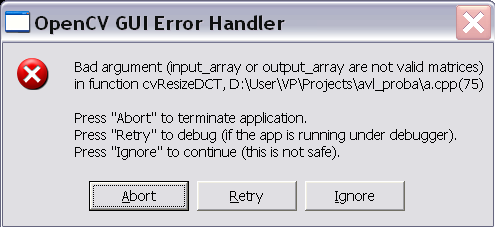
\includegraphics[width=0.5\textwidth]{pics/errmsg.png}

If the error handler is set to \texttt{cvStdErrReport}, the above message will be printed to standard error output and the program will be terminated or continued, depending on the current error mode.

\textbf{Error Message printed to Standard Error Output (in \texttt{Leaf} mode)}

\begin{lstlisting}
OpenCV ERROR: Bad argument (input_array or output_array are not valid matrices)
        in function cvResizeDCT, D:\User\VP\Projects\avl\_proba\a.cpp(75)
Terminating the application...
\end{lstlisting}

\cvCPyFunc{Alloc}
Allocates a memory buffer.

\cvdefC{void* cvAlloc( size\_t size );}

\begin{description}
\cvarg{size}{Buffer size in bytes}
\end{description}

The function allocates \texttt{size} bytes and returns
a pointer to the allocated buffer. In the case of an error the function reports an
error and returns a NULL pointer. By default, \texttt{cvAlloc} calls
\texttt{icvAlloc} which
itself calls \texttt{malloc}. However it is possible to assign user-defined memory
allocation/deallocation functions using the \cvCPyCross{SetMemoryManager} function.

\cvCPyFunc{Free}
Deallocates a memory buffer.

\cvdefC{void cvFree( void** ptr );}

\begin{description}
\cvarg{ptr}{Double pointer to released buffer}
\end{description}

The function deallocates a memory buffer allocated by
\cvCPyCross{Alloc}. It clears the pointer to buffer upon exit, which is why
the double pointer is used. If the \texttt{*buffer} is already NULL, the function
does nothing.

\fi % }

\cvCPyFunc{GetTickCount}
Returns the number of ticks.

\cvdefC{int64 cvGetTickCount( void );}
\cvdefPy{GetTickCount() -> long}

The function returns number of the ticks starting from some platform-dependent event (number of CPU ticks from the startup, number of milliseconds from 1970th year, etc.). The function is useful for accurate measurement of a function/user-code execution time. To convert the number of ticks to time units, use \cvCPyCross{GetTickFrequency}.

\cvCPyFunc{GetTickFrequency}
Returns the number of ticks per microsecond.

\cvdefC{double cvGetTickFrequency( void );}
\cvdefPy{GetTickFrequency() -> long}

The function returns the number of ticks per microsecond. Thus, the quotient of \cvCPyCross{GetTickCount} and \cvCPyCross{GetTickFrequency} will give the number of microseconds starting from the platform-dependent event.

\ifC % {

\cvCPyFunc{RegisterModule}
Registers another module.

\begin{lstlisting}
typedef struct CvPluginFuncInfo
{
    void** func_addr;
    void* default_func_addr;
    const char* func_names;
    int search_modules;
    int loaded_from;
}
CvPluginFuncInfo;

typedef struct CvModuleInfo
{
    struct CvModuleInfo* next;
    const char* name;
    const char* version;
    CvPluginFuncInfo* func_tab;
}
CvModuleInfo;
\end{lstlisting}

\cvdefC{int cvRegisterModule( const CvModuleInfo* moduleInfo );}

\begin{description}
\cvarg{moduleInfo}{Information about the module}
\end{description}

The function adds a module to the list of
registered modules. After the module is registered, information about
it can be retrieved using the \cvCPyCross{GetModuleInfo} function. Also, the
registered module makes full use of optimized plugins (IPP, MKL, ...),
supported by CXCORE. CXCORE itself, CV (computer vision), CVAUX (auxilary
computer vision), and HIGHGUI (visualization and image/video acquisition) are
examples of modules. Registration is usually done when the shared library
is loaded. See \texttt{cxcore/src/cxswitcher.cpp} and
\texttt{cv/src/cvswitcher.cpp} for details about how registration is done
and look at \texttt{cxcore/src/cxswitcher.cpp}, \texttt{cxcore/src/\_cxipp.h}
on how IPP and MKL are connected to the modules.

\cvCPyFunc{GetModuleInfo}
Retrieves information about registered module(s) and plugins.

\cvdefC{
void  cvGetModuleInfo( \par const char* moduleName,\par const char** version,\par const char** loadedAddonPlugins);
}

\begin{description}
\cvarg{moduleName}{Name of the module of interest, or NULL, which means all the modules}
\cvarg{version}{The output parameter. Information about the module(s), including version}
\cvarg{loadedAddonPlugins}{The list of names and versions of the optimized plugins that CXCORE was able to find and load}
\end{description}

The function returns information about one or
all of the registered modules. The returned information is stored inside
the libraries, so the user should not deallocate or modify the returned
text strings.

\cvCPyFunc{UseOptimized}
Switches between optimized/non-optimized modes.

\cvdefC{int cvUseOptimized( int onoff );}

\begin{description}
\cvarg{onoff}{Use optimized ($\ne 0$) or not ($=0$)}
\end{description}

The function switches between the mode, where
only pure C implementations from cxcore, OpenCV, etc. are used, and
the mode, where IPP and MKL functions are used if available. When
\texttt{cvUseOptimized(0)} is called, all the optimized libraries are
unloaded. The function may be useful for debugging, IPP and MKL upgrading on
the fly, online speed comparisons, etc. It returns the number of optimized
functions loaded. Note that by default, the optimized plugins are loaded,
so it is not necessary to call \texttt{cvUseOptimized(1)} in the beginning of
the program (actually, it will only increase the startup time).

\cvCPyFunc{SetMemoryManager}
Accesses custom/default memory managing functions.

\begin{lstlisting}
typedef void* (CV_CDECL *CvAllocFunc)(size_t size, void* userdata);
typedef int (CV_CDECL *CvFreeFunc)(void* pptr, void* userdata);
\end{lstlisting}

\cvdefC{
void cvSetMemoryManager( \par CvAllocFunc allocFunc=NULL,\par CvFreeFunc freeFunc=NULL,\par void* userdata=NULL );
}

\begin{description}
\cvarg{allocFunc}{Allocation function; the interface is similar to \texttt{malloc}, except that \texttt{userdata} may be used to determine the context}
\cvarg{freeFunc}{Deallocation function; the interface is similar to \texttt{free}}
\cvarg{userdata}{User data that is transparently passed to the custom functions}
\end{description}

The function sets user-defined memory
managment functions (substitutes for \texttt{malloc} and \texttt{free}) that will be called
by \texttt{cvAlloc, cvFree} and higher-level functions (e.g., \texttt{cvCreateImage}). Note
that the function should be called when there is data allocated using
\texttt{cvAlloc}. Also, to avoid infinite recursive calls, it is not
allowed to call \texttt{cvAlloc} and \cvCPyCross{Free} from the custom
allocation/deallocation functions.

If the \texttt{alloc\_func} and \texttt{free\_func} pointers are
\texttt{NULL}, the default memory managing functions are restored.

\cvCPyFunc{SetIPLAllocators}
Switches to IPL functions for image allocation/deallocation.

\begin{lstlisting}
typedef IplImage* (CV_STDCALL* Cv_iplCreateImageHeader)
                            (int,int,int,char*,char*,int,int,int,int,int,
                            IplROI*,IplImage*,void*,IplTileInfo*);
typedef void (CV_STDCALL* Cv_iplAllocateImageData)(IplImage*,int,int);
typedef void (CV_STDCALL* Cv_iplDeallocate)(IplImage*,int);
typedef IplROI* (CV_STDCALL* Cv_iplCreateROI)(int,int,int,int,int);
typedef IplImage* (CV_STDCALL* Cv_iplCloneImage)(const IplImage*);

#define CV_TURN_ON_IPL_COMPATIBILITY()                                  \
    cvSetIPLAllocators( iplCreateImageHeader, iplAllocateImage,         \
                        iplDeallocate, iplCreateROI, iplCloneImage )
\end{lstlisting}

\cvdefC{
void cvSetIPLAllocators( \par
                         Cv\_iplCreateImageHeader create\_header, \par
                         Cv\_iplAllocateImageData allocate\_data, \par
                         Cv\_iplDeallocate deallocate, \par
                         Cv\_iplCreateROI create\_roi, \par
                         Cv\_iplCloneImage clone\_image );
}

\begin{description}
\cvarg{create\_header}{Pointer to iplCreateImageHeader}
\cvarg{allocate\_data}{Pointer to iplAllocateImage}
\cvarg{deallocate}{Pointer to iplDeallocate}
\cvarg{create\_roi}{Pointer to iplCreateROI}
\cvarg{clone\_image}{Pointer to iplCloneImage}
\end{description}


The function causes CXCORE to use IPL functions
for image allocation/deallocation operations. For convenience, there
is the wrapping macro \texttt{CV\_TURN\_ON\_IPL\_COMPATIBILITY}. The
function is useful for applications where IPL and CXCORE/OpenCV are used
together and still there are calls to \texttt{iplCreateImageHeader},
etc. The function is not necessary if IPL is called only for data
processing and all the allocation/deallocation is done by CXCORE, or
if all the allocation/deallocation is done by IPL and some of OpenCV
functions are used to process the data.

\fi

\fi

\ifCpp

\cvCppFunc{alignPtr}
Aligns pointer to the specified number of bytes

\cvdefCpp{template<typename \_Tp> \_Tp* alignPtr(\_Tp* ptr, int n=sizeof(\_Tp));}
\begin{description}
\cvarg{ptr}{The aligned pointer}
\cvarg{n}{The alignment size; must be a power of two}
\end{description}

The function returns the aligned pointer of the same type as the input pointer:
\[\texttt{(\_Tp*)(((size\_t)ptr + n-1) \& -n)}\]


\cvCppFunc{alignSize}
Aligns a buffer size to the specified number of bytes

\cvdefCpp{size\_t alignSize(size\_t sz, int n);}
\begin{description}
\cvarg{sz}{The buffer size to align}
\cvarg{n}{The alignment size; must be a power of two}
\end{description}

The function returns the minimum number that is greater or equal to \texttt{sz} and is divisble by \texttt{n}:
\[\texttt{(sz + n-1) \& -n}\]


\cvCppFunc{allocate}
Allocates an array of elements

\cvdefCpp{template<typename \_Tp> \_Tp* allocate(size\_t n);}
\begin{description}
\cvarg{n}{The number of elements to allocate}
\end{description}

The generic function \texttt{allocate} allocates buffer for the specified number of elements. For each element the default constructor is called.


\cvCppFunc{deallocate}
Allocates an array of elements

\cvdefCpp{template<typename \_Tp> void deallocate(\_Tp* ptr, size\_t n);}
\begin{description}
\cvarg{ptr}{Pointer to the deallocated buffer}
\cvarg{n}{The number of elements in the buffer}
\end{description}

The generic function \texttt{deallocate} deallocates the buffer allocated with \cvCppCross{allocate}. The number of elements must match the number passed to \cvCppCross{allocate}.

\cvfunc{CV\_Assert}\label{CV Assert}
Checks a condition at runtime.

\cvdefC{CV\_Assert(expr)}
\cvdefCpp{CV\_Assert(expr)}
\cvdefPy{CV\_Assert(expr)}

\begin{lstlisting}
#define CV_Assert( expr ) ...
#define CV_DbgAssert(expr) ...
\end{lstlisting}

\begin{description}
\cvarg{expr}{The checked expression}
\end{description}

The macros \texttt{CV\_Assert} and \texttt{CV\_DbgAssert} evaluate the specified expression and if it is 0, the macros raise an error (see \cvCppCross{error}). The macro \texttt{CV\_Assert} checks the condition in both Debug and Release configurations, while \texttt{CV\_DbgAssert} is only retained in the Debug configuration.

\cvCppFunc{error}
Signals an error and raises the exception

\cvdefCpp{void error( const Exception\& exc );\newline
\#define CV\_Error( code, msg ) <...>\newline
\#define CV\_Error\_( code, args ) <...>}
\begin{description}
\cvarg{exc}{The exception to throw}
\cvarg{code}{The error code, normally, a negative value. The list of pre-defined error codes can be found in \texttt{cxerror.h}}
\cvarg{msg}{Text of the error message}
\cvarg{args}{printf-like formatted error message in parantheses}
\end{description}

The function and the helper macros \texttt{CV\_Error} and \texttt{CV\_Error\_} call the error handler. Currently, the error handler prints the error code (\texttt{exc.code}), the context (\texttt{exc.file}, \texttt{exc.line} and the error message \texttt{exc.err} to the standard error stream \texttt{stderr}. In Debug configuration it then provokes memory access violation, so that the execution stack and all the parameters can be analyzed in debugger. In Release configuration the exception \texttt{exc} is thrown.

The macro \texttt{CV\_Error\_} can be used to construct the error message on-fly to include some dynamic information, for example:

\begin{lstlisting}
// note the extra parentheses around the formatted text message
CV_Error_(CV_StsOutOfRange,
    ("the matrix element (%d,%d)=%g is out of range",
    i, j, mtx.at<float>(i,j)))
\end{lstlisting}


\cvclass{Exception}\label{Exception}
The exception class passed to error

\begin{lstlisting}
class  Exception
{
public:
    // various constructors and the copy operation
    Exception() { code = 0; line = 0; }
    Exception(int _code, const string& _err,
              const string& _func, const string& _file, int _line);newline
    Exception(const Exception& exc);newline
    Exception& operator = (const Exception& exc);newline

    // the error code
    int code;newline
    // the error text message
    string err;newline
    // function name where the error happened
    string func;newline
    // the source file name where the error happened
    string file;newline
    // the source file line where the error happened
    int line;
};
\end{lstlisting}

The class \texttt{Exception} encapsulates all or almost all the necessary information about the error happened in the program. The exception is usually constructed and thrown implicitly, via \texttt{CV\_Error} and \texttt{CV\_Error\_} macros, see \cvCppCross{error}.


\cvCppFunc{fastMalloc}
Allocates aligned memory buffer

\cvdefCpp{void* fastMalloc(size\_t size);}
\begin{description}
\cvarg{size}{The allocated buffer size}
\end{description}
 
The function allocates buffer of the specified size and returns it. When the buffer size is 16 bytes or more, the returned buffer is aligned on 16 bytes.

\cvCppFunc{fastFree}
Deallocates memory buffer

\cvdefCpp{void fastFree(void* ptr);}
\begin{description}
\cvarg{ptr}{Pointer to the allocated buffer}
\end{description}

The function deallocates the buffer, allocated with \cvCppCross{fastMalloc}.
If NULL pointer is passed, the function does nothing.

\cvCppFunc{format}
Returns a text string formatted using printf-like expression

\cvdefCpp{string format( const char* fmt, ... );}
\begin{description}
\cvarg{fmt}{The printf-compatible formatting specifiers}
\end{description}

The function acts like \texttt{sprintf}, but forms and returns STL string. It can be used for form the error message in \cvCppCross{Exception} constructor.

\cvCppFunc{getNumThreads}
Returns the number of threads used by OpenCV

\cvdefCpp{int getNumThreads();}

The function returns the number of threads that is used by OpenCV.

See also: \cvCppCross{setNumThreads}, \cvCppCross{getThreadNum}.


\cvCppFunc{getThreadNum}
Returns index of the currently executed thread

\cvdefCpp{int getThreadNum();}

The function returns 0-based index of the currently executed thread. The function is only valid inside a parallel OpenMP region. When OpenCV is built without OpenMP support, the function always returns 0.

See also: \cvCppCross{setNumThreads}, \cvCppCross{getNumThreads}.

\cvCppFunc{getTickCount}
Returns the number of ticks

\cvdefCpp{int64 getTickCount();}

The function returns the number of ticks since the certain event (e.g. when the machine was turned on).
It can be used to initialize \cvCppCross{RNG} or to measure a function execution time by reading the tick count before and after the function call. See also the tick frequency.

\cvCppFunc{getTickFrequency}
Returns the number of ticks per second

\cvdefCpp{double getTickFrequency();}

The function returns the number of ticks per second.
That is, the following code computes the execution time in seconds.
\begin{lstlisting}
double t = (double)getTickCount();
// do something ...
t = ((double)getTickCount() - t)/getTickFrequency();
\end{lstlisting}

\cvCppFunc{setNumThreads}
Sets the number of threads used by OpenCV

\cvdefCpp{void setNumThreads(int nthreads);}
\begin{description}
\cvarg{nthreads}{The number of threads used by OpenCV}
\end{description}

The function sets the number of threads used by OpenCV in parallel OpenMP regions. If \texttt{nthreads=0}, the function will use the default number of threads, which is usually equal to the number of the processing cores.

See also: \cvCppCross{getNumThreads}, \cvCppCross{getThreadNum}

\fi


\chapter{cv. Image Processing and Computer Vision}
\section{Image Filtering}

Functions and classes described in this section are used to perform various linear or non-linear filtering operations on 2D images (represented as \cvCppCross{Mat}'s), that is, for each pixel location $(x,y)$ in the source image some its (normally rectangular) neighborhood is considered and used to compute the response. In case of a linear filter it is a weighted sum of pixel values, in case of morphological operations it is the minimum or maximum etc. The computed response is stored to the destination image at the same location $(x,y)$. It means, that the output image will be of the same size as the input image. Normally, the functions supports multi-channel arrays, in which case every channel is processed independently, therefore the output image will also have the same number of channels as the input one.

Another common feature of the functions and classes described in this section is that, unlike simple arithmetic functions, they need to extrapolate values of some non-existing pixels. For example, if we want to smooth an image using a Gaussian $3 \times 3$ filter, then during the processing of the left-most pixels in each row we need pixels to the left of them, i.e. outside of the image. We can let those pixels be the same as the left-most image pixels (i.e. use "replicated border" extrapolation method), or assume that all the non-existing pixels are zeros ("contant border" extrapolation method) etc. \cvCpp{OpenCV let the user to specify the extrapolation method; see the function \cvCppCross{borderInterpolate} and discussion of \texttt{borderType} parameter in various functions below.}

\ifCPy

\cvCPyFunc{CopyMakeBorder}
Copies an image and makes a border around it.

\cvdefC{
void cvCopyMakeBorder(
\par const CvArr* src,
\par CvArr* dst,
\par CvPoint offset,
\par int bordertype,
\par CvScalar value=cvScalarAll(0) );}
\cvdefPy{CopyMakeBorder(src,dst,offset,bordrtype,value=cvScalarAll(0))-> None}

\begin{description}
\cvarg{src}{The source image}
\cvarg{dst}{The destination image}
\cvarg{offset}{Coordinates of the top-left corner (or bottom-left in the case of images with bottom-left origin) of the destination image rectangle where the source image (or its ROI) is copied. Size of the rectanlge matches the source image size/ROI size}
\cvarg{bordertype}{Type of the border to create around the copied source image rectangle; types inlude:
\begin{description}
\cvarg{IPL\_BORDER\_CONSTANT}{border is filled with the fixed value, passed as last parameter of the function.}
\cvarg{IPL\_BORDER\_REPLICATE}{the pixels from the top and bottom rows, the left-most and right-most columns are replicated to fill the border.}
\end{description}
(The other two border types from IPL, \texttt{IPL\_BORDER\_REFLECT} and \texttt{IPL\_BORDER\_WRAP}, are currently unsupported)}
\cvarg{value}{Value of the border pixels if \texttt{bordertype} is \texttt{IPL\_BORDER\_CONSTANT}}
\end{description}

The function copies the source 2D array into the interior of the destination array and makes a border of the specified type around the copied area. The function is useful when one needs to emulate border type that is different from the one embedded into a specific algorithm implementation. For example, morphological functions, as well as most of other filtering functions in OpenCV, internally use replication border type, while the user may need a zero border or a border, filled with 1's or 255's.

\cvCPyFunc{CreateStructuringElementEx}
Creates a structuring element.

\cvdefC{IplConvKernel* cvCreateStructuringElementEx(\par int cols,
 \par int rows, \par int anchorX, \par int anchorY, \par int shape, \par int* values=NULL );}
\cvdefPy{CreateStructuringElementEx(cols,rows,anchorX,anchorY,shape,values={NULL,0})-> kernel}

\begin{description}
\cvarg{cols}{Number of columns in the structuring element}
\cvarg{rows}{Number of rows in the structuring element}
\cvarg{anchorX}{Relative horizontal offset of the anchor point}
\cvarg{anchorY}{Relative vertical offset of the anchor point}
\cvarg{shape}{Shape of the structuring element; may have the following values:
\begin{description}
  \cvarg{CV\_SHAPE\_RECT}{a rectangular element}
  \cvarg{CV\_SHAPE\_CROSS}{a cross-shaped element}
  \cvarg{CV\_SHAPE\_ELLIPSE}{an elliptic element}
  \cvarg{CV\_SHAPE\_CUSTOM}{a user-defined element. In this case the parameter \texttt{values} specifies the mask, that is, which neighbors of the pixel must be considered}
\end{description}}
\cvarg{values}{Pointer to the structuring element data, a plane array, representing row-by-row scanning of the element matrix. Non-zero values indicate points that belong to the element. If the pointer is \texttt{NULL}, then all values are considered non-zero, that is, the element is of a rectangular shape. This parameter is considered only if the shape is \texttt{CV\_SHAPE\_CUSTOM} }
\end{description}

The function CreateStructuringElementEx allocates and fills the structure \texttt{IplConvKernel}, which can be used as a structuring element in the morphological operations.

\cvCPyFunc{Dilate}
Dilates an image by using a specific structuring element.

\cvdefC{void cvDilate(\par const CvArr* src,\par CvArr* dst,\par IplConvKernel* element=NULL,\par int iterations=1 );}
\cvdefPy{Dilate(src,dst,element=NULL,iterations=1)-> None}

\begin{description}
\cvarg{src}{Source image}
\cvarg{dst}{Destination image}
\cvarg{element}{Structuring element used for dilation. If it is \texttt{NULL}, a $3\times 3$ rectangular structuring element is used}
\cvarg{iterations}{Number of times dilation is applied}
\end{description}

The function dilates the source image using the specified structuring element that determines the shape of a pixel neighborhood over which the maximum is taken:

\[
\max_{(x',y') \, in \, \texttt{element}}src(x+x',y+y')
\]

The function supports the in-place mode. Dilation can be applied several (\texttt{iterations}) times. For color images, each channel is processed independently.

\cvCPyFunc{Erode}
Erodes an image by using a specific structuring element.

\cvdefC{void cvErode(\par const CvArr* src,\par  CvArr* dst,\par  IplConvKernel* element=NULL,\par  int iterations=1);}
\cvdefPy{Erode(src,dst,element=NULL,itertions=1)-> None}

\begin{description}
\cvarg{src}{Source image}
\cvarg{dst}{Destination image}
\cvarg{element}{Structuring element used for erosion. If it is \texttt{NULL}, a $3\times 3$ rectangular structuring element is used}
\cvarg{iterations}{Number of times erosion is applied}
\end{description}

The function erodes the source image using the specified structuring element that determines the shape of a pixel neighborhood over which the minimum is taken:

\[
\min_{(x',y') \, in \, \texttt{element}}src(x+x',y+y')
\]

The function supports the in-place mode. Erosion can be applied several (\texttt{iterations}) times. For color images, each channel is processed independently.

\cvCPyFunc{Filter2D}
Convolves an image with the kernel.

\cvdefC{void cvFilter2D(
\par const CvArr* src,\par  CvArr* dst,\par  const CvMat* kernel,\par  CvPoint anchor=cvPoint(-1,-1));}
\cvdefPy{Filter2D(src,dst,kernel,anchor=(-1,-1))-> None}

\begin{description}
\cvarg{src}{The source image}
\cvarg{dst}{The destination image}
\cvarg{kernel}{Convolution kernel, a single-channel floating point matrix. If you want to apply different kernels to different channels, split the image into separate color planes using \cvCPyCross{Split} and process them individually}
\cvarg{anchor}{The anchor of the kernel that indicates the relative position of a filtered point within the kernel. The anchor shoud lie within the kernel. The special default value (-1,-1) means that it is at the kernel center}
\end{description}

The function applies an arbitrary linear filter to the image. In-place operation is supported. When the aperture is partially outside the image, the function interpolates outlier pixel values from the nearest pixels that are inside the image.

\cvCPyFunc{Laplace}
Calculates the Laplacian of an image.

\cvdefC{void cvLaplace(\par const CvArr* src,\par  CvArr* dst,\par  int apertureSize=3);}
\cvdefPy{Laplace(src,dst,apertureSize=3)-> None}
\begin{description}
\cvarg{src}{Source image}
\cvarg{dst}{Destination image}
\cvarg{apertureSize}{Aperture size (it has the same meaning as \cvCPyCross{Sobel})}
\end{description}

The function calculates the Laplacian of the source image by adding up the second x and y derivatives calculated using the Sobel operator:

\[
\texttt{dst}(x,y) = \frac{d^2 \texttt{src}}{dx^2} + \frac{d^2 \texttt{src}}{dy^2}
\]

Setting \texttt{apertureSize} = 1 gives the fastest variant that is equal to convolving the image with the following kernel:

\[ \vecthreethree {0}{1}{0}{1}{-4}{1}{0}{1}{0} \]

Similar to the \cvCPyCross{Sobel} function, no scaling is done and the same combinations of input and output formats are supported.

\cvCPyFunc{MorphologyEx}
Performs advanced morphological transformations.

\cvdefC{void cvMorphologyEx(
\par const CvArr* src,\par  CvArr* dst,\par  CvArr* temp,\par  IplConvKernel* element,
\par int operation,\par  int iterations=1 );}
\cvdefPy{MorphologyEx(src,dst,temp,element,operation,iterations=1)-> None}

\begin{description}
\cvarg{src}{Source image}
\cvarg{dst}{Destination image}
\cvarg{temp}{Temporary image, required in some cases}
\cvarg{element}{Structuring element}
\cvarg{operation}{Type of morphological operation, one of the following:
\begin{description}
\cvarg{CV\_MOP\_OPEN}{opening}
\cvarg{CV\_MOP\_CLOSE}{closing}
\cvarg{CV\_MOP\_GRADIENT}{morphological gradient}
\cvarg{CV\_MOP\_TOPHAT}{"top hat"}
\cvarg{CV\_MOP\_BLACKHAT}{"black hat"}
\end{description}}
\cvarg{iterations}{Number of times erosion and dilation are applied}
\end{description}

The function can perform advanced morphological transformations using erosion and dilation as basic operations.

Opening:

\[
dst=open(src,element)=dilate(erode(src,element),element)
\]

Closing:

\[
dst=close(src,element)=erode(dilate(src,element),element)
\]

Morphological gradient:

\[
dst=morph\_grad(src,element)=dilate(src,element)-erode(src,element)
\]

"Top hat":

\[
dst=tophat(src,element)=src-open(src,element)
\]

"Black hat":

\[
dst=blackhat(src,element)=close(src,element)-src
\]

The temporary image \texttt{temp} is required for a morphological gradient and, in the case of in-place operation, for "top hat" and "black hat".

\cvCPyFunc{PyrDown}
Downsamples an image.

\cvdefC{void cvPyrDown(\par const CvArr* src,\par CvArr* dst,\par int filter=CV\_GAUSSIAN\_5x5 );}
\cvdefPy{PyrDown(src,dst,filter=CV\_GAUSSIAN\_5X5)-> None}

\begin{description}
\cvarg{src}{The source image}
\cvarg{dst}{The destination image, should have a half as large width and height than the source}
\cvarg{filter}{Type of the filter used for convolution; only \texttt{CV\_GAUSSIAN\_5x5} is currently supported}
\end{description}

The function performs the downsampling step of the Gaussian pyramid decomposition. First it convolves the source image with the specified filter and then downsamples the image by rejecting even rows and columns.

\ifC
\cvCPyFunc{ReleaseStructuringElement}
Deletes a structuring element.

\cvdefC{void cvReleaseStructuringElement( IplConvKernel** element );}

\begin{description}
\cvarg{element}{Pointer to the deleted structuring element}
\end{description}

The function releases the structure \texttt{IplConvKernel} that is no longer needed. If \texttt{*element} is \texttt{NULL}, the function has no effect.
\fi

\cvCPyFunc{Smooth}
Smooths the image in one of several ways.

\cvdefC{void cvSmooth(\par const CvArr* src,
\par CvArr* dst,\par  int smoothtype=CV\_GAUSSIAN,\par  int param1=3,\par  int param2=0,\par  double param3=0, \par double param4=0);}
\cvdefPy{Smooth(src,dst,smoothtype=CV\_GAUSSIAN,param1=3,param2=0,param3=0,param4=0)-> None}

\begin{description}
\cvarg{src}{The source image}
\cvarg{dst}{The destination image}
\cvarg{smoothtype}{Type of the smoothing:
\begin{description}
  \cvarg{CV\_BLUR\_NO\_SCALE}{linear convolution with $\texttt{param1}\times\texttt{param2}$ box kernel (all 1's). If you want to smooth different pixels with different-size box kernels, you can use the integral image that is computed using \cvCPyCross{Integral}}
  \cvarg{CV\_BLUR}{linear convolution with $\texttt{param1}\times\texttt{param2}$ box kernel (all 1's) with subsequent scaling by $1/(\texttt{param1}\cdot\texttt{param2})$}
  \cvarg{CV\_GAUSSIAN}{linear convolution with a $\texttt{param1}\times\texttt{param2}$ Gaussian kernel}
  \cvarg{CV\_MEDIAN}{median filter with a $\texttt{param1}\times\texttt{param1}$ square aperture}
  \cvarg{CV\_BILATERAL}{bilateral filter with a $\texttt{param1}\times\texttt{param1}$ square aperture, color sigma=\texttt{param3} and spatial sigma=\texttt{param4}. If \texttt{param1=0}, the aperture square side is set to \newline \texttt{cvRound(param4*1.5)*2+1}. Information about bilateral filtering can be found at \url{http://www.dai.ed.ac.uk/CVonline/LOCAL\_COPIES/MANDUCHI1/Bilateral\_Filtering.html}}
\end{description}}
\cvarg{param1}{The first parameter of the smoothing operation, the aperture width. Must be a positive odd number (1, 3, 5, ...)}
\cvarg{param2}{The second parameter of the smoothing operation, the aperture height. Ignored by \texttt{CV\_MEDIAN} and \texttt{CV\_BILATERAL} methods. In the case of simple scaled/non-scaled and Gaussian blur if \texttt{param2} is zero, it is set to \texttt{param1}. Otherwise it must be a positive odd number.}
\cvarg{param3}{In the case of a Gaussian parameter this parameter may specify Gaussian $\sigma$ (standard deviation). If it is zero, it is calculated from the kernel size:
\[
\sigma = 0.3 (n/2 - 1) + 0.8 \quad \text{where} \quad n=
\begin{array}{l l}
\mbox{\texttt{param1} for horizontal kernel}\\
\mbox{\texttt{param2} for vertical kernel}
\end{array}
\]

Using standard sigma for small kernels ($3\times 3$ to $7\times 7$) gives better speed. If \texttt{param3} is not zero, while \texttt{param1} and \texttt{param2} are zeros, the kernel size is calculated from the sigma (to provide accurate enough operation).}
\end{description}

The function smooths an image using one of several methods. Every of the methods has some features and restrictions listed below

Blur with no scaling works with single-channel images only and supports accumulation of 8-bit to 16-bit format (similar to \cvCPyCross{Sobel} and \cvCPyCross{Laplace}) and 32-bit floating point to 32-bit floating-point format.

Simple blur and Gaussian blur support 1- or 3-channel, 8-bit and 32-bit floating point images. These two methods can process images in-place.

Median and bilateral filters work with 1- or 3-channel 8-bit images and can not process images in-place.

\cvCPyFunc{Sobel}
Calculates the first, second, third or mixed image derivatives using an extended Sobel operator.

\cvdefC{void cvSobel(\par const CvArr* src,\par  CvArr* dst,\par  int xorder,\par  int yorder,\par  int apertureSize=3 );}
\cvdefPy{Sobel(src,dst,xorder,yorder,apertureSize = 3)-> None}

\begin{description}
\cvarg{src}{Source image of type CvArr*}
\cvarg{dst}{Destination image}
\cvarg{xorder}{Order of the derivative x}
\cvarg{yorder}{Order of the derivative y}
\cvarg{apertureSize}{Size of the extended Sobel kernel, must be 1, 3, 5 or 7}
\end{description}

In all cases except 1, an $\texttt{apertureSize} \times
\texttt{apertureSize}$ separable kernel will be used to calculate the
derivative. For $\texttt{apertureSize} = 1$ $ 3 \times 1$ or $ 1 \times 3$
a kernel is used (Gaussian smoothing is not done). There is also the special
value \texttt{CV\_SCHARR} (-1) that corresponds to a $3\times3$ Scharr
filter that may give more accurate results than a $3\times3$ Sobel. Scharr
aperture is

\[ \vecthreethree
{-3}{0}{3}
{-10}{0}{10}
{-3}{0}{3}
\]

for the x-derivative or transposed for the y-derivative.

The function calculates the image derivative by convolving the image with the appropriate kernel:

\[
\texttt{dst}(x,y) = \frac{d^{xorder+yorder} \texttt{src}}{dx^{xorder} \cdot dy^{yorder}}
\]

The Sobel operators combine Gaussian smoothing and differentiation
so the result is more or less resistant to the noise. Most often,
the function is called with (\texttt{xorder} = 1, \texttt{yorder} = 0,
\texttt{apertureSize} = 3) or (\texttt{xorder} = 0, \texttt{yorder} = 1,
\texttt{apertureSize} = 3) to calculate the first x- or y- image
derivative. The first case corresponds to a kernel of:

\[ \vecthreethree
{-1}{0}{1}
{-2}{0}{2}
{-1}{0}{1}
\]

and the second one corresponds to a kernel of:
\[ \vecthreethree
{-1}{-2}{-1}
{0}{0}{0}
{1}{2}{1}
\]
or a kernel of:
\[ \vecthreethree
{1}{2}{1}
{0}{0}{0}
{-1}{2}{-1}
\]

depending on the image origin (\texttt{origin} field of
\texttt{IplImage} structure). No scaling is done, so the destination image
usually has larger numbers (in absolute values) than the source image does. To
avoid overflow, the function requires a 16-bit destination image if the
source image is 8-bit. The result can be converted back to 8-bit using the
\cvCPyCross{ConvertScale} or the \cvCPyCross{ConvertScaleAbs} function. Besides 8-bit images
the function can process 32-bit floating-point images. Both the source and the 
destination must be single-channel images of equal size or equal ROI size.

\fi

\ifCpp

\cvCppFunc{BaseColumnFilter}
Base class for filters with single-column kernels

\begin{lstlisting}
class BaseColumnFilter
{
public:
    virtual ~BaseColumnFilter();
    
    // To be overriden by the user.
    //
    // runs filtering operation on the set of rows,
    // "dstcount + ksize - 1" rows on input,
    // "dstcount" rows on output,
    // each input and output row has "width" elements
    // the filtered rows are written into "dst" buffer.
    virtual void operator()(const uchar** src, uchar* dst, int dststep,
                            int dstcount, int width) = 0;
    // resets the filter state (may be needed for IIR filters)
    virtual void reset();
    
    int ksize; // the aperture size
    int anchor; // position of the anchor point,
                // normally not used during the processing
};
\end{lstlisting}

The class \texttt{BaseColumnFilter} is the base class for filtering data using single-column kernels. The filtering does not have to be a linear operation. In general, it could be written as following:

\[\texttt{dst}(x,y) = F(\texttt{src}[y](x),\;\texttt{src}[y+1](x),\;...,\;\texttt{src}[y+\texttt{ksize}-1](x)\]

where $F$ is the filtering function, but, as it is represented as a class, it can produce any side effects, memorize previously processed data etc. The class only defines the interface and is not used directly. Instead, there are several functions in OpenCV (and you can add more) that return pointers to the derived classes that implement specific filtering operations. Those pointers are then passed to \cvCppCross{FilterEngine} constructor. While the filtering operation interface uses \texttt{uchar} type, a particular implementation is not limited to 8-bit data.

See also: \cvCppCross{BaseRowFilter}, \cvCppCross{BaseFilter}, \cvCppCross{FilterEngine},
    \cvCppCross{getColumnSumFilter}, \cvCppCross{getLinearColumnFilter}, \cvCppCross{getMorphologyColumnFilter}


\cvCppFunc{BaseFilter}
Base class for 2D image filters

\begin{lstlisting}
class BaseFilter
{
public:
    virtual ~BaseFilter();
    
    // To be overriden by the user.
    //
    // runs filtering operation on the set of rows,
    // "dstcount + ksize.height - 1" rows on input,
    // "dstcount" rows on output,
    // each input row has "(width + ksize.width-1)*cn" elements
    // each output row has "width*cn" elements.
    // the filtered rows are written into "dst" buffer.
    virtual void operator()(const uchar** src, uchar* dst, int dststep,
                            int dstcount, int width, int cn) = 0;
    // resets the filter state (may be needed for IIR filters)                        
    virtual void reset();
    Size ksize;
    Point anchor;
};
\end{lstlisting}

The class \texttt{BaseFilter} is the base class for filtering data using 2D kernels. The filtering does not have to be a linear operation. In general, it could be written as following:

\[
  \begin{array}{l}
  \texttt{dst}(x,y) = F( \texttt{src}[y](x),\;\texttt{src}[y](x+1),\;...,\;\texttt{src}[y](x+\texttt{ksize.width}-1), \\
  \texttt{src}[y+1](x),\;\texttt{src}[y+1](x+1),\;...,\;\texttt{src}[y+1](x+\texttt{ksize.width}-1), \\
  ......................................................................................... \\
  \texttt{src}[y+\texttt{ksize.height-1}](x),\\
  \texttt{src}[y+\texttt{ksize.height-1}](x+1),\\
  ...
  \texttt{src}[y+\texttt{ksize.height-1}](x+\texttt{ksize.width}-1))
  \end{array}
  \]

where $F$ is the filtering function. The class only defines the interface and is not used directly. Instead, there are several functions in OpenCV (and you can add more) that return pointers to the derived classes that implement specific filtering operations. Those pointers are then passed to \cvCppCross{FilterEngine} constructor. While the filtering operation interface uses \texttt{uchar} type, a particular implementation is not limited to 8-bit data.

See also: \cvCppCross{BaseColumnFilter}, \cvCppCross{BaseRowFilter}, \cvCppCross{FilterEngine},
    \cvCppCross{getLinearFilter}, \cvCppCross{getMorphologyFilter}

\cvCppFunc{BaseRowFilter}
Base class for filters with single-row kernels

\begin{lstlisting}
class BaseRowFilter
{
public:
    virtual ~BaseRowFilter();
    
    // To be overriden by the user.
    //
    // runs filtering operation on the single input row
    // of "width" element, each element is has "cn" channels.
    // the filtered row is written into "dst" buffer.
    virtual void operator()(const uchar* src, uchar* dst,
                            int width, int cn) = 0;
    int ksize, anchor;
};
\end{lstlisting}

The class \texttt{BaseRowFilter} is the base class for filtering data using single-row kernels. The filtering does not have to be a linear operation. In general, it could be written as following:

\[\texttt{dst}(x,y) = F(\texttt{src}[y](x),\;\texttt{src}[y](x+1),\;...,\;\texttt{src}[y](x+\texttt{ksize.width}-1))\]

where $F$ is the filtering function. The class only defines the interface and is not used directly. Instead, there are several functions in OpenCV (and you can add more) that return pointers to the derived classes that implement specific filtering operations. Those pointers are then passed to \cvCppCross{FilterEngine} constructor. While the filtering operation interface uses \texttt{uchar} type, a particular implementation is not limited to 8-bit data.

See also: \cvCppCross{BaseColumnFilter}, \cvCppCross{Filter}, \cvCppCross{FilterEngine},
 \cvCppCross{getLinearRowFilter}, \cvCppCross{getMorphologyRowFilter}, \cvCppCross{getRowSumFilter}

\cvCppFunc{FilterEngine}
Generic image filtering class

\begin{lstlisting}
class FilterEngine
{
public:
    // empty constructor
    FilterEngine();
    // builds a 2D non-separable filter (!_filter2D.empty()) or
    // a separable filter (!_rowFilter.empty() && !_columnFilter.empty())
    // the input data type will be "srcType", the output data type will be "dstType",
    // the intermediate data type is "bufType".
    // _rowBorderType and _columnBorderType determine how the image
    // will be extrapolated beyond the image boundaries.
    // _borderValue is only used when _rowBorderType and/or _columnBorderType
    // == cv::BORDER_CONSTANT
    FilterEngine(const Ptr<BaseFilter>& _filter2D,
                 const Ptr<BaseRowFilter>& _rowFilter,
                 const Ptr<BaseColumnFilter>& _columnFilter,
                 int srcType, int dstType, int bufType,
                 int _rowBorderType=BORDER_REPLICATE,
                 int _columnBorderType=-1, // use _rowBorderType by default 
                 const Scalar& _borderValue=Scalar());
    virtual ~FilterEngine();
    // separate function for the engine initialization
    void init(const Ptr<BaseFilter>& _filter2D,
              const Ptr<BaseRowFilter>& _rowFilter,
              const Ptr<BaseColumnFilter>& _columnFilter,
              int srcType, int dstType, int bufType,
              int _rowBorderType=BORDER_REPLICATE, int _columnBorderType=-1,
              const Scalar& _borderValue=Scalar());
    // starts filtering of the ROI in an image of size "wholeSize".
    // returns the starting y-position in the source image.
    virtual int start(Size wholeSize, Rect roi, int maxBufRows=-1);
    // alternative form of start that takes the image
    // itself instead of "wholeSize". Set isolated to true to pretend that
    // there are no real pixels outside of the ROI
    // (so that the pixels will be extrapolated using the specified border modes)
    virtual int start(const Mat& src, const Rect& srcRoi=Rect(0,0,-1,-1),
                      bool isolated=false, int maxBufRows=-1);
    // processes the next portion of the source image,
    // "srcCount" rows starting from "src" and
    // stores the results to "dst".
    // returns the number of produced rows
    virtual int proceed(const uchar* src, int srcStep, int srcCount,
                        uchar* dst, int dstStep);
    // higher-level function that processes the whole
    // ROI or the whole image with a single call
    virtual void apply( const Mat& src, Mat& dst,
                        const Rect& srcRoi=Rect(0,0,-1,-1),
                        Point dstOfs=Point(0,0),
                        bool isolated=false);
    bool isSeparable() const { return filter2D.empty(); }
    // how many rows from the input image are not yet processed
    int remainingInputRows() const;
    // how many output rows are not yet produced
    int remainingOutputRows() const;
    ...
    // the starting and the ending rows in the source image
    int startY, endY;
    
    // pointers to the filters
    Ptr<BaseFilter> filter2D;
    Ptr<BaseRowFilter> rowFilter;
    Ptr<BaseColumnFilter> columnFilter;
};
\end{lstlisting}

The class \texttt{FilterEngine} can be used to apply an arbitrary filtering operation to an image.
It contains all the necessary intermediate buffers, it computes extrapolated values
of the "virtual" pixels outside of the image etc. Pointers to the initialized \texttt{FilterEngine} instances
are returned by various \texttt{create*Filter} functions, see below, and they are used inside high-level functions such as \cvCppCross{filter2D}, \cvCppCross{erode}, \cvCppCross{dilate} etc, that is, the class is the workhorse in many of OpenCV filtering functions.

This class makes it easier (though, maybe not very easy yet) to combine filtering operations with other operations, such as color space conversions, thresholding, arithmetic operations, etc. By combining several operations together you can get much better performance because your data will stay in cache. For example, below is the implementation of Laplace operator for a floating-point images, which is a simplified implementation of \cvCppCross{Laplacian}:

\begin{lstlisting}
void laplace_f(const Mat& src, Mat& dst)
{
    CV_Assert( src.type() == CV_32F );
    dst.create(src.size(), src.type());
    
    // get the derivative and smooth kernels for d2I/dx2.
    // for d2I/dy2 we could use the same kernels, just swapped
    Mat kd, ks;
    getSobelKernels( kd, ks, 2, 0, ksize, false, ktype );
    
    // let's process 10 source rows at once
    int DELTA = std::min(10, src.rows);
    Ptr<FilterEngine> Fxx = createSeparableLinearFilter(src.type(),
        dst.type(), kd, ks, Point(-1,-1), 0, borderType, borderType, Scalar() ); 
    Ptr<FilterEngine> Fyy = createSeparableLinearFilter(src.type(),
        dst.type(), ks, kd, Point(-1,-1), 0, borderType, borderType, Scalar() );

    int y = Fxx->start(src), dsty = 0, dy = 0;
    Fyy->start(src);
    const uchar* sptr = src.data + y*src.step;

    // allocate the buffers for the spatial image derivatives;
    // the buffers need to have more than DELTA rows, because at the
    // last iteration the output may take max(kd.rows-1,ks.rows-1)
    // rows more than the input.
    Mat Ixx( DELTA + kd.rows - 1, src.cols, dst.type() );
    Mat Iyy( DELTA + kd.rows - 1, src.cols, dst.type() );
    
    // inside the loop we always pass DELTA rows to the filter
    // (note that the "proceed" method takes care of possibe overflow, since
    // it was given the actual image height in the "start" method)
    // on output we can get:
    //  * < DELTA rows (the initial buffer accumulation stage)
    //  * = DELTA rows (settled state in the middle)
    //  * > DELTA rows (then the input image is over, but we generate
    //                  "virtual" rows using the border mode and filter them)
    // this variable number of output rows is dy.
    // dsty is the current output row.
    // sptr is the pointer to the first input row in the portion to process
    for( ; dsty < dst.rows; sptr += DELTA*src.step, dsty += dy )
    {
        Fxx->proceed( sptr, (int)src.step, DELTA, Ixx.data, (int)Ixx.step );
        dy = Fyy->proceed( sptr, (int)src.step, DELTA, d2y.data, (int)Iyy.step );
        if( dy > 0 )
        {
            Mat dstripe = dst.rowRange(dsty, dsty + dy);
            add(Ixx.rowRange(0, dy), Iyy.rowRange(0, dy), dstripe);
        }
    }
}
\end{lstlisting}

If you do not need that much control of the filtering process, you can simply use the \texttt{FilterEngine::apply} method. Here is how the method is actually implemented:

\begin{lstlisting}
void FilterEngine::apply(const Mat& src, Mat& dst,
    const Rect& srcRoi, Point dstOfs, bool isolated)
{
    // check matrix types
    CV_Assert( src.type() == srcType && dst.type() == dstType );
    
    // handle the "whole image" case
    Rect _srcRoi = srcRoi;
    if( _srcRoi == Rect(0,0,-1,-1) )
        _srcRoi = Rect(0,0,src.cols,src.rows);
    
    // check if the destination ROI is inside the dst.
    // and FilterEngine::start will check if the source ROI is inside src.
    CV_Assert( dstOfs.x >= 0 && dstOfs.y >= 0 &&
        dstOfs.x + _srcRoi.width <= dst.cols &&
        dstOfs.y + _srcRoi.height <= dst.rows );

    // start filtering
    int y = start(src, _srcRoi, isolated);
    
    // process the whole ROI. Note that "endY - startY" is the total number
    // of the source rows to process
    // (including the possible rows outside of srcRoi but inside the source image)
    proceed( src.data + y*src.step,
             (int)src.step, endY - startY,
             dst.data + dstOfs.y*dst.step +
             dstOfs.x*dst.elemSize(), (int)dst.step );
}
\end{lstlisting}

Unlike the earlier versions of OpenCV, now the filtering operations fully support the notion of image ROI, that is, pixels outside of the ROI but inside the image can be used in the filtering operations. For example, you can take a ROI of a single pixel and filter it - that will be a filter response at that particular pixel (however, it's possible to emulate the old behavior by passing \texttt{isolated=false} to \texttt{FilterEngine::start} or \texttt{FilterEngine::apply}). You can pass the ROI explicitly to \texttt{FilterEngine::apply}, or construct a new matrix headers:

\begin{lstlisting}
// compute dI/dx derivative at src(x,y)

// method 1:
// form a matrix header for a single value
float val1 = 0;
Mat dst1(1,1,CV_32F,&val1);

Ptr<FilterEngine> Fx = createDerivFilter(CV_32F, CV_32F,
                        1, 0, 3, BORDER_REFLECT_101);
Fx->apply(src, Rect(x,y,1,1), Point(), dst1);

// method 2:
// form a matrix header for a single value
float val2 = 0;
Mat dst2(1,1,CV_32F,&val2);

Mat pix_roi(src, Rect(x,y,1,1));
Sobel(pix_roi, dst2, dst2.type(), 1, 0, 3, 1, 0, BORDER_REFLECT_101);

printf("method1 = %g, method2 = %g\n", val1, val2);
\end{lstlisting}

Note on the data types. As it was mentioned in \cvCppCross{BaseFilter} description, the specific filters can process data of any type, despite that \texttt{Base*Filter::operator()} only takes \texttt{uchar} pointers and no information about the actual types. To make it all work, the following rules are used:

\begin{itemize}
    \item in case of separable filtering \texttt{FilterEngine::rowFilter} applied first. It transforms the input image data (of type \texttt{srcType}) to the intermediate results stored in the internal buffers (of type \texttt{bufType}). Then these intermediate results are processed \emph{as single-channel data} with \texttt{FilterEngine::columnFilter} and stored in the output image (of type \texttt{dstType}). Thus, the input type for \texttt{rowFilter} is \texttt{srcType} and the output type is \texttt{bufType}; the input type for \texttt{columnFilter} is \texttt{CV\_MAT\_DEPTH(bufType)} and the output type is \texttt{CV\_MAT\_DEPTH(dstType)}.
    
    \item in case of non-separable filtering \texttt{bufType} must be the same as \texttt{srcType}. The source data is copied to the temporary buffer if needed and then just passed to \texttt{FilterEngine::filter2D}. That is, the input type for \texttt{filter2D} is \texttt{srcType} (=\texttt{bufType}) and the output type is \texttt{dstType}.
\end{itemize}

See also: \cvCppCross{BaseColumnFilter}, \cvCppCross{BaseFilter}, \cvCppCross{BaseRowFilter}, \cvCppCross{createBoxFilter},
\cvCppCross{createDerivFilter}, \cvCppCross{createGaussianFilter}, \cvCppCross{createLinearFilter},
\cvCppCross{createMorphologyFilter}, \cvCppCross{createSeparableLinearFilter}

\cvCppFunc{bilateralFilter}
Applies bilateral filter to the image

\cvdefCpp{void bilateralFilter( const Mat\& src, Mat\& dst, int d,\par
                      double sigmaColor, double sigmaSpace,\par
                      int borderType=BORDER\_DEFAULT );}
\begin{description}
\cvarg{src}{The source 8-bit or floating-point, 1-channel or 3-channel image}
\cvarg{dst}{The destination image; will have the same size and the same type as \texttt{src}}
\cvarg{d}{The diameter of each pixel neighborhood, that is used during filtering. If it is non-positive, it's computed from \texttt{sigmaSpace}}
\cvarg{sigmaColor}{Filter sigma in the color space. Larger value of the parameter means that farther colors within the pixel neighborhood (see \texttt{sigmaSpace}) will be mixed together, resulting in larger areas of semi-equal color}
\cvarg{sigmaSpace}{Filter sigma in the coordinate space. Larger value of the parameter means that farther pixels will influence each other (as long as their colors are close enough; see \texttt{sigmaColor}). Then \texttt{d>0}, it specifies the neighborhood size regardless of \texttt{sigmaSpace}, otherwise \texttt{d} is proportional to \texttt{sigmaSpace}}
\end{description}

The function applies bilateral filtering to the input image, as described in
\url{http://www.dai.ed.ac.uk/CVonline/LOCAL\_COPIES/MANDUCHI1/Bilateral\_Filtering.html}

\cvCppFunc{blur}
Smoothes image using normalized box filter

\cvdefCpp{void blur( const Mat\& src, Mat\& dst,\par
           Size ksize, Point anchor=Point(-1,-1),\par
           int borderType=BORDER\_DEFAULT );}
\begin{description}
\cvarg{src}{The source image}
\cvarg{dst}{The destination image; will have the same size and the same type as \texttt{src}}
\cvarg{ksize}{The smoothing kernel size}
\cvarg{anchor}{The anchor point. The default value \texttt{Point(-1,-1)} means that the anchor is at the kernel center}
\cvarg{borderType}{The border mode used to extrapolate pixels outside of the image}
\end{description}

The function smoothes the image using the kernel:

\[ \texttt{K} = \frac{1}{\texttt{ksize.width*ksize.height}}
\begin{bmatrix}
1 & 1 & 1 & \cdots & 1 & 1 \\
1 & 1 & 1 & \cdots & 1 & 1 \\
\hdotsfor{6} \\
1 & 1 & 1 & \cdots & 1 & 1 \\
\end{bmatrix}
\]

The call \texttt{blur(src, dst, ksize, anchor, borderType)} is equivalent to
\texttt{boxFilter(src, dst, src.type(), anchor, true, borderType)}.

See also: \cvCppCross{boxFilter}, \cvCppCross{bilateralFilter}, \cvCppCross{GaussianBlur}, \cvCppCross{medianBlur}.

\cvCppFunc{borderInterpolate}
Computes source location of extrapolated pixel

\cvdefCpp{int borderInterpolate( int p, int len, int borderType );}
\begin{description}
\cvarg{p}{0-based coordinate of the extrapolated pixel along one of the axes, likely <0 or >=\texttt{len}}
\cvarg{len}{length of the array along the corresponding axis}
\cvarg{borderType}{the border type, one of the \texttt{BORDER\_*}, except for \texttt{BORDER\_TRANSPARENT} and \texttt{BORDER\_ISOLATED}. When \texttt{borderType==BORDER\_CONSTANT} the function always returns -1, regardless of \texttt{p} and \texttt{len}}
\end{description}

The function computes and returns the coordinate of the donor pixel, corresponding to the specified extrapolated pixel when using the specified extrapolation border mode. For example, if we use \texttt{BORDER\_WRAP} mode in the horizontal direction, \texttt{BORDER\_REFLECT\_101} in the vertical direction and want to compute value of the "virtual" pixel \texttt{Point(-5, 100)} in a floating-point image \texttt{img}, it will be

\begin{lstlisting}
float val = img.at<float>(borderInterpolate(100, img.rows, BORDER_REFLECT_101),
                          borderInterpolate(-5, img.cols, BORDER_WRAP));
\end{lstlisting}

Normally, the function is not called directly; it is used inside \cvCppCross{FilterEngine} and \cvCppCross{copyMakeBorder} to compute tables for quick extrapolation.

See also: \cvCppCross{FilterEngine}, \cvCppCross{copyMakeBorder}

\cvCppFunc{boxFilter}
Smoothes image using box filter

\cvdefCpp{void boxFilter( const Mat\& src, Mat\& dst, int ddepth,\par
                Size ksize, Point anchor=Point(-1,-1),\par
                bool normalize=true,\par
                int borderType=BORDER\_DEFAULT );}
\begin{description}
\cvarg{src}{The source image}
\cvarg{dst}{The destination image; will have the same size and the same type as \texttt{src}}
\cvarg{ksize}{The smoothing kernel size}
\cvarg{anchor}{The anchor point. The default value \texttt{Point(-1,-1)} means that the anchor is at the kernel center}
\cvarg{normalize}{Indicates, whether the kernel is normalized by its area or not}
\cvarg{borderType}{The border mode used to extrapolate pixels outside of the image}
\end{description}

The function smoothes the image using the kernel:

\[ \texttt{K} = \alpha
\begin{bmatrix}
1 & 1 & 1 & \cdots & 1 & 1 \\
1 & 1 & 1 & \cdots & 1 & 1 \\
\hdotsfor{6} \\
1 & 1 & 1 & \cdots & 1 & 1
\end{bmatrix}
\]

where

\[\alpha=\fork
{\frac{1}{\texttt{ksize.width*ksize.height}}}{when \texttt{normalize=true}}
{1}{otherwise} \]

Unnormalized box filter is useful for computing various integral characteristics over each pixel neighborhood, such as covariation matrices of image derivatives (used in dense optical flow algorithms, \hyperref[conerHarris]{Harris corner detector} etc.). If you need to compute pixel sums over variable-size windows, use \cvCppCross{integral}.

See also: \cvCppCross{boxFilter}, \cvCppCross{bilateralFilter}, \cvCppCross{GaussianBlur}, \cvCppCross{medianBlur}, \cvCppCross{integral}.

\cvCppFunc{buildPyramid}
Constructs Gaussian pyramid for an image

\cvdefCpp{void buildPyramid( const Mat\& src, vector<Mat>\& dst, int maxlevel );}
\begin{description}
\cvarg{src}{The source image; check \cvCppCross{pyrDown} for the list of supported types}
\cvarg{dst}{The destination vector of \texttt{maxlevel+1} images of the same type as \texttt{src};
\texttt{dst[0]} will be the same as \texttt{src}, \texttt{dst[1]} is the next pyramid layer,
a smoothed and down-sized \texttt{src} etc.}
\cvarg{maxlevel}{The 0-based index of the last (i.e. the smallest) pyramid layer; it must be non-negative}
\end{description}

The function constructs a vector of images and builds the gaussian pyramid by recursively applying \cvCppCross{pyrDown} to the previously built pyramid layers, starting from \texttt{dst[0]==src}.

\cvCppFunc{copyMakeBorder}
Forms a border around the image

\cvdefCpp{void copyMakeBorder( const Mat\& src, Mat\& dst,\par
                    int top, int bottom, int left, int right,\par
                    int borderType, const Scalar\& value=Scalar() );}
\begin{description}
\cvarg{src}{The source image}
\cvarg{dst}{The destination image; will have the same type as \texttt{src} and the size \texttt{Size(src.cols+left+right, src.rows+top+bottom)}}
\cvarg{top, bottom, left, right}{Specify how much pixels in each direction from the source image rectangle one needs to extrapolate, e.g. \texttt{top=1, bottom=1, left=1, right=1} mean that 1 pixel-wide border needs to be built}
\cvarg{borderType}{The border type; see \cvCppCross{borderInterpolate}}
\cvarg{value}{The border value if \texttt{borderType==BORDER\_CONSTANT}}
\end{description}

The function copies the source image into the middle of the destination image. The areas to the left, to the right, above and below the copied source image will be filled with extrapolated pixels. This is not what \cvCppCross{FilterEngine} or based on it filtering functions do (they extrapolate pixels on-fly), but what other more complex functions, including your own, may do to simplify image boundary handling.

The function supports the mode when \texttt{src} is already in the middle of \texttt{dst}. In this case the function does not copy \texttt{src} itself, but simply constructs the border, e.g.:

\begin{lstlisting}
// let border be the same in all directions
int border=2;
// constructs a larger image to fit both the image and the border
Mat gray_buf(rgb.rows + border*2, rgb.cols + border*2, rgb.depth());
// select the middle part of it w/o copying data
Mat gray(gray_canvas, Rect(border, border, rgb.cols, rgb.rows));
// convert image from RGB to grayscale
cvtColor(rgb, gray, CV_RGB2GRAY);
// form a border in-place
copyMakeBorder(gray, gray_buf, border, border,
               border, border, BORDER_REPLICATE);
// now do some custom filtering ...
...
\end{lstlisting}

See also: \cvCppCross{borderInterpolate}

\cvCppFunc{createBoxFilter}
Returns box filter engine

\cvdefCpp{Ptr<FilterEngine> createBoxFilter( int srcType, int dstType,\par
                                 Size ksize, Point anchor=Point(-1,-1),\par
                                 bool normalize=true,\par
                                 int borderType=BORDER\_DEFAULT);\newline
Ptr<BaseRowFilter> getRowSumFilter(int srcType, int sumType,\par
                                   int ksize, int anchor=-1);\newline
Ptr<BaseColumnFilter> getColumnSumFilter(int sumType, int dstType,\par
                                   int ksize, int anchor=-1, double scale=1);}
\begin{description}
\cvarg{srcType}{The source image type}
\cvarg{sumType}{The intermediate horizontal sum type; must have as many channels as \texttt{srcType}}
\cvarg{dstType}{The destination image type; must have as many channels as \texttt{srcType}}
\cvarg{ksize}{The aperture size}
\cvarg{anchor}{The anchor position with the kernel; negative values mean that the anchor is at the kernel center}
\cvarg{normalize}{Whether the sums are normalized or not; see \cvCppCross{boxFilter}}
\cvarg{scale}{Another way to specify normalization in lower-level \texttt{getColumnSumFilter}}
\cvarg{borderType}{Which border type to use; see \cvCppCross{borderInterpolate}}
\end{description}

The function is a convenience function that retrieves horizontal sum primitive filter with \cvCppCross{getRowSumFilter}, vertical sum filter with \cvCppCross{getColumnSumFilter}, constructs new \cvCppCross{FilterEngine} and passes both of the primitive filters there. The constructed filter engine can be used for image filtering with normalized or unnormalized box filter.

The function itself is used by \cvCppCross{blur} and \cvCppCross{boxFilter}.

See also: \cvCppCross{FilterEngine}, \cvCppCross{blur}, \cvCppCross{boxFilter}.

\cvCppFunc{createDerivFilter}
Returns engine for computing image derivatives 

\cvdefCpp{Ptr<FilterEngine> createDerivFilter( int srcType, int dstType,\par
                                     int dx, int dy, int ksize,\par
                                     int borderType=BORDER\_DEFAULT );}
\begin{description}
\cvarg{srcType}{The source image type}
\cvarg{dstType}{The destination image type; must have as many channels as \texttt{srcType}}
\cvarg{dx}{The derivative order in respect with x}
\cvarg{dy}{The derivative order in respect with y}
\cvarg{ksize}{The aperture size; see \cvCppCross{getDerivKernels}}
\cvarg{borderType}{Which border type to use; see \cvCppCross{borderInterpolate}}
\end{description}

The function \cvCppCross{createDerivFilter} is a small convenience function that retrieves linear filter coefficients for computing image derivatives using \cvCppCross{getDerivKernels} and then creates a separable linear filter with \cvCppCross{createSeparableLinearFilter}. The function is used by \cvCppCross{Sobel} and \cvCppCross{Scharr}.

See also: \cvCppCross{createSeparableLinearFilter}, \cvCppCross{getDerivKernels}, \cvCppCross{Scharr}, \cvCppCross{Sobel}.

\cvCppFunc{createGaussianFilter}
Returns engine for smoothing images with a Gaussian filter

\cvdefCpp{Ptr<FilterEngine> createGaussianFilter( int type, Size ksize,\par
                                   double sigmaX, double sigmaY=0,\par
                                   int borderType=BORDER\_DEFAULT);}
\begin{description}
\cvarg{type}{The source and the destination image type}
\cvarg{ksize}{The aperture size; see \cvCppCross{getGaussianKernel}}
\cvarg{sigmaX}{The Gaussian sigma in the horizontal direction; see \cvCppCross{getGaussianKernel}}
\cvarg{sigmaY}{The Gaussian sigma in the vertical direction; if 0, then $\texttt{sigmaY}\leftarrow\texttt{sigmaX}$}
\cvarg{borderType}{Which border type to use; see \cvCppCross{borderInterpolate}}
\end{description}

The function \cvCppCross{createGaussianFilter} computes Gaussian kernel coefficients and then returns separable linear filter for that kernel. The function is used by \cvCppCross{GaussianBlur}. Note that while the function takes just one data type, both for input and output, you can pass by this limitation by calling \cvCppCross{getGaussianKernel} and then \cvCppCross{createSeparableFilter} directly.

See also: \cvCppCross{createSeparableLinearFilter}, \cvCppCross{getGaussianKernel}, \cvCppCross{GaussianBlur}.

\cvCppFunc{createLinearFilter}
Creates non-separable linear filter engine

\cvdefCpp{Ptr<FilterEngine> createLinearFilter(int srcType, int dstType,\par
               const Mat\& kernel, Point \_anchor=Point(-1,-1),\par
               double delta=0, int rowBorderType=BORDER\_DEFAULT,\par
               int columnBorderType=-1, const Scalar\& borderValue=Scalar());\newline
Ptr<BaseFilter> getLinearFilter(int srcType, int dstType,\par
                               const Mat\& kernel,\par
                               Point anchor=Point(-1,-1),\par
                               double delta=0, int bits=0);}
\begin{description}
\cvarg{srcType}{The source image type}
\cvarg{dstType}{The destination image type; must have as many channels as \texttt{srcType}}
\cvarg{kernel}{The 2D array of filter coefficients}
\cvarg{anchor}{The anchor point within the kernel; special value \texttt{Point(-1,-1)} means that the anchor is at the kernel center}
\cvarg{delta}{The value added to the filtered results before storing them}
\cvarg{bits}{When the kernel is an integer matrix representing fixed-point filter coefficients,
             the parameter specifies the number of the fractional bits}
\cvarg{rowBorderType, columnBorderType}{The pixel extrapolation methods in the horizontal and the vertical directions; see \cvCppCross{borderInterpolate}}
\cvarg{borderValue}{Used in case of constant border}
\end{description}

The function returns pointer to 2D linear filter for the specified kernel, the source array type and the destination array type. The function is a higher-level function that calls \texttt{getLinearFilter} and passes the retrieved 2D filter to \cvCppCross{FilterEngine} constructor.

See also: \cvCppCross{createSeparableLinearFilter}, \cvCppCross{FilterEngine}, \cvCppCross{filter2D}

\cvCppFunc{createMorphologyFilter}
Creates engine for non-separable morphological operations

\cvdefCpp{Ptr<FilterEngine> createMorphologyFilter(int op, int type,\par
    const Mat\& element, Point anchor=Point(-1,-1),\par
    int rowBorderType=BORDER\_CONSTANT,\par
    int columnBorderType=-1,\par
    const Scalar\& borderValue=morphologyDefaultBorderValue());\newline
Ptr<BaseFilter> getMorphologyFilter(int op, int type, const Mat\& element,\par
                                    Point anchor=Point(-1,-1));\newline
Ptr<BaseRowFilter> getMorphologyRowFilter(int op, int type,\par
                                          int esize, int anchor=-1);\newline
Ptr<BaseColumnFilter> getMorphologyColumnFilter(int op, int type,\par
                                                int esize, int anchor=-1);\newline
static inline Scalar morphologyDefaultBorderValue()\par
{ return Scalar::all(DBL\_MAX); }}
\begin{description}
\cvarg{op}{The morphology operation id, \texttt{MORPH\_ERODE} or \texttt{MORPH\_DILATE}}
\cvarg{type}{The input/output image type}
\cvarg{element}{The 2D 8-bit structuring element for the morphological operation. Non-zero elements indicate the pixels that belong to the element}
\cvarg{esize}{The horizontal or vertical structuring element size for separable morphological operations}
\cvarg{anchor}{The anchor position within the structuring element; negative values mean that the anchor is at the center}
\cvarg{rowBorderType, columnBorderType}{The pixel extrapolation methods in the horizontal and the vertical directions; see \cvCppCross{borderInterpolate}}
\cvarg{borderValue}{The border value in case of a constant border. The default value,\\ \texttt{morphologyDefaultBorderValue}, has the special meaning. It is transformed $+\inf$ for the erosion and to $-\inf$ for the dilation, which means that the minimum (maximum) is effectively computed only over the pixels that are inside the image.}
\end{description}

The functions construct primitive morphological filtering operations or a filter engine based on them. Normally it's enough to use \cvCppCross{createMorphologyFilter} or even higher-level \cvCppCross{erode}, \cvCppCross{dilate} or \cvCppCross{morphologyEx}, Note, that \cvCppCross{createMorphologyFilter} analyses the structuring element shape and builds a separable morphological filter engine when the structuring element is square.

See also: \cvCppCross{erode}, \cvCppCross{dilate}, \cvCppCross{morphologyEx}, \cvCppCross{FilterEngine}

\cvCppFunc{createSeparableLinearFilter}
Creates engine for separable linear filter

\cvdefCpp{Ptr<FilterEngine> createSeparableLinearFilter(int srcType, int dstType,\par
                         const Mat\& rowKernel, const Mat\& columnKernel,\par
                         Point anchor=Point(-1,-1), double delta=0,\par
                         int rowBorderType=BORDER\_DEFAULT,\par
                         int columnBorderType=-1,\par
                         const Scalar\& borderValue=Scalar());\newline
Ptr<BaseColumnFilter> getLinearColumnFilter(int bufType, int dstType,\par
                         const Mat\& columnKernel, int anchor,\par
                         int symmetryType, double delta=0,\par
                         int bits=0);\newline
Ptr<BaseRowFilter> getLinearRowFilter(int srcType, int bufType,\par
                         const Mat\& rowKernel, int anchor,\par
                         int symmetryType);}
\begin{description}
\cvarg{srcType}{The source array type}
\cvarg{dstType}{The destination image type; must have as many channels as \texttt{srcType}}
\cvarg{bufType}{The inermediate buffer type; must have as many channels as \texttt{srcType}}
\cvarg{rowKernel}{The coefficients for filtering each row}
\cvarg{columnKernel}{The coefficients for filtering each column}
\cvarg{anchor}{The anchor position within the kernel; negative values mean that anchor is positioned at the aperture center}
\cvarg{delta}{The value added to the filtered results before storing them}
\cvarg{bits}{When the kernel is an integer matrix representing fixed-point filter coefficients,
             the parameter specifies the number of the fractional bits}
\cvarg{rowBorderType, columnBorderType}{The pixel extrapolation methods in the horizontal and the vertical directions; see \cvCppCross{borderInterpolate}}
\cvarg{borderValue}{Used in case of a constant border}
\cvarg{symmetryType}{The type of each of the row and column kernel; see \cvCppCross{getKernelType}.}
\end{description}

The functions construct primitive separable linear filtering operations or a filter engine based on them. Normally it's enough to use \cvCppCross{createSeparableLinearFilter} or even higher-level \cvCppCross{sepFilter2D}. The function \cvCppCross{createMorphologyFilter} is smart enough to figure out the \texttt{symmetryType} for each of the two kernels, the intermediate \texttt{bufType}, and, if the filtering can be done in integer arithmetics, the number of \texttt{bits} to encode the filter coefficients. If it does not work for you, it's possible to call \texttt{getLinearColumnFilter}, \texttt{getLinearRowFilter} directly and then pass them to \cvCppCross{FilterEngine} constructor.

See also: \cvCppCross{sepFilter2D}, \cvCppCross{createLinearFilter}, \cvCppCross{FilterEngine}, \cvCppCross{getKernelType}


\cvCppFunc{dilate}
Dilates an image by using a specific structuring element.

\cvdefCpp{void dilate( const Mat\& src, Mat\& dst, const Mat\& element,\par
             Point anchor=Point(-1,-1), int iterations=1,\par
             int borderType=BORDER\_CONSTANT,\par
             const Scalar\& borderValue=morphologyDefaultBorderValue() );}
\begin{description}
\cvarg{src}{The source image}
\cvarg{dst}{The destination image. It will have the same size and the same type as \texttt{src}}
\cvarg{element}{The structuring element used for dilation. If \texttt{element=Mat()}, a $3\times 3$ rectangular structuring element is used}
\cvarg{anchor}{Position of the anchor within the element. The default value $(-1, -1)$ means that the anchor is at the element center}
\cvarg{iterations}{The number of times dilation is applied}
\cvarg{borderType}{The pixel extrapolation method; see \cvCppCross{borderInterpolate}}
\cvarg{borderValue}{The border value in case of a constant border. The default value has a special meaning, see \cvCppCross{createMorphologyFilter}}
\end{description}

The function dilates the source image using the specified structuring element that determines the shape of a pixel neighborhood over which the maximum is taken:

\[
\texttt{dst}(x,y) = \max_{(x',y'): \, \texttt{element}(x',y')\ne0}\texttt{src}(x+x',y+y')
\]

The function supports the in-place mode. Dilation can be applied several (\texttt{iterations}) times. In the case of multi-channel images each channel is processed independently.

See also: \cvCppCross{erode}, \cvCppCross{morphologyEx}, \cvCppCross{createMorphologyFilter}

\cvCppFunc{erode}
Erodes an image by using a specific structuring element.

\cvdefCpp{void erode( const Mat\& src, Mat\& dst, const Mat\& element,\par
            Point anchor=Point(-1,-1), int iterations=1,\par
            int borderType=BORDER\_CONSTANT,\par
            const Scalar\& borderValue=morphologyDefaultBorderValue() );}
\begin{description}
\cvarg{src}{The source image}
\cvarg{dst}{The destination image. It will have the same size and the same type as \texttt{src}}
\cvarg{element}{The structuring element used for dilation. If \texttt{element=Mat()}, a $3\times 3$ rectangular structuring element is used}
\cvarg{anchor}{Position of the anchor within the element. The default value $(-1, -1)$ means that the anchor is at the element center}
\cvarg{iterations}{The number of times erosion is applied}
\cvarg{borderType}{The pixel extrapolation method; see \cvCppCross{borderInterpolate}}
\cvarg{borderValue}{The border value in case of a constant border. The default value has a special meaning, see \cvCppCross{createMorphoogyFilter}}
\end{description}

The function erodes the source image using the specified structuring element that determines the shape of a pixel neighborhood over which the minimum is taken:

\[
\texttt{dst}(x,y) = \min_{(x',y'): \, \texttt{element}(x',y')\ne0}\texttt{src}(x+x',y+y')
\]

The function supports the in-place mode. Erosion can be applied several (\texttt{iterations}) times. In the case of multi-channel images each channel is processed independently.

See also: \cvCppCross{dilate}, \cvCppCross{morphologyEx}, \cvCppCross{createMorphologyFilter}

\cvCppFunc{filter2D}
Convolves an image with the kernel

\cvdefCpp{void filter2D( const Mat\& src, Mat\& dst, int ddepth,\par
               const Mat\& kernel, Point anchor=Point(-1,-1),\par
               double delta=0, int borderType=BORDER\_DEFAULT );}
\begin{description}
\cvarg{src}{The source image}
\cvarg{dst}{The destination image. It will have the same size and the same number of channels as \texttt{src}}
\cvarg{ddepth}{The desired depth of the destination image. If it is negative, it will be the same as \texttt{src.depth()}}
\cvarg{kernel}{Convolution kernel (or rather a correlation kernel), a single-channel floating point matrix. If you want to apply different kernels to different channels, split the image into separate color planes using \cvCppCross{split} and process them individually}
\cvarg{anchor}{The anchor of the kernel that indicates the relative position of a filtered point within the kernel. The anchor should lie within the kernel. The special default value (-1,-1) means that the anchor is at the kernel center}
\cvarg{delta}{The optional value added to the filtered pixels before storing them in \texttt{dst}}
\cvarg{borderType}{The pixel extrapolation method; see \cvCppCross{borderInterpolate}}
\end{description}

The function applies an arbitrary linear filter to the image. In-place operation is supported. When the aperture is partially outside the image, the function interpolates outlier pixel values according to the specified border mode.

The function does actually computes correlation, not the convolution:

\[
\texttt{dst}(x,y) = \sum_{\stackrel{0\leq x' < \texttt{kernel.cols},}{0\leq y' < \texttt{kernel.rows}}} \texttt{kernel}(x',y')*\texttt{src}(x+x'-\texttt{anchor.x},y+y'-\texttt{anchor.y})
\]

That is, the kernel is not mirrored around the anchor point. If you need a real convolution, flip the kernel using \cvCppCross{flip} and set the new anchor to \texttt{(kernel.cols - anchor.x - 1, kernel.rows - anchor.y - 1)}.

The function uses \hyperref[dft]{DFT}-based algorithm in case of sufficiently large kernels (~$11\times11$) and the direct algorithm (that uses the engine retrieved by \cvCppCross{createLinearFilter}) for small kernels.

See also: \cvCppCross{sepFilter2D}, \cvCppCross{createLinearFilter}, \cvCppCross{dft}, \cvCppCross{matchTemplate}

\cvCppFunc{GaussianBlur}
Smoothes image using a Gaussian filter

\cvdefCpp{void GaussianBlur( const Mat\& src, Mat\& dst, Size ksize,\par
                   double sigmaX, double sigmaY=0,\par
                   int borderType=BORDER\_DEFAULT );}
\begin{description}
\cvarg{src}{The source image}
\cvarg{dst}{The destination image; will have the same size and the same type as \texttt{src}}
\cvarg{ksize}{The Gaussian kernel size; \texttt{ksize.width} and \texttt{ksize.height} can differ, but they both must be positive and odd. Or, they can be zero's, then they are computed from \texttt{sigma*}}
\cvarg{sigmaX, sigmaY}{The Gaussian kernel standard deviations in X and Y direction. If \texttt{sigmaY} is zero, it is set to be equal to \texttt{sigmaX}. If they are both zeros, they are computed from \texttt{ksize.width} and \texttt{ksize.height}, respectively, see \cvCppCross{getGaussianKernel}. To fully control the result regardless of possible future modification of all this semantics, it is recommended to specify all of \texttt{ksize}, \texttt{sigmaX} and \texttt{sigmaY}}
\cvarg{borderType}{The pixel extrapolation method; see \cvCppCross{borderInterpolate}}
\end{description}

The function convolves the source image with the specified Gaussian kernel. In-place filtering is supported.

See also: \cvCppCross{sepFilter2D}, \cvCppCross{filter2D}, \cvCppCross{blur}, \cvCppCross{boxFilter}, \cvCppCross{bilateralFilter}, \cvCppCross{medianBlur}

\cvCppFunc{getDerivKernels}
Returns filter coefficients for computing spatial image derivatives

\cvdefCpp{void getDerivKernels( Mat\& kx, Mat\& ky, int dx, int dy, int ksize,\par
                      bool normalize=false, int ktype=CV\_32F );}
\begin{description}
\cvarg{kx}{The output matrix of row filter coefficients; will have type \texttt{ktype}}
\cvarg{ky}{The output matrix of column filter coefficients; will have type \texttt{ktype}}
\cvarg{dx}{The derivative order in respect with x}
\cvarg{dy}{The derivative order in respect with y}
\cvarg{ksize}{The aperture size. It can be \texttt{CV\_SCHARR}, 1, 3, 5 or 7}
\cvarg{normalize}{Indicates, whether to normalize (scale down) the filter coefficients or not. In theory the coefficients should have the denominator $=2^{ksize*2-dx-dy-2}$. If you are going to filter floating-point images, you will likely want to use the normalized kernels. But if you compute derivatives of a 8-bit image, store the results in 16-bit image and wish to preserve all the fractional bits, you may want to set \texttt{normalize=false}.}
\cvarg{ktype}{The type of filter coefficients. It can be \texttt{CV\_32f} or \texttt{CV\_64F}}
\end{description}

The function computes and returns the filter coefficients for spatial image derivatives. When \texttt{ksize=CV\_SCHARR}, the Scharr $3 \times 3$ kernels are generated, see \cvCppCross{Scharr}. Otherwise, Sobel kernels are generated, see \cvCppCross{Sobel}. The filters are normally passed to \cvCppCross{sepFilter2D} or to \cvCppCross{createSeparableLinearFilter}.

\cvCppFunc{getGaussianKernel}
Returns Gaussian filter coefficients

\cvdefCpp{Mat getGaussianKernel( int ksize, double sigma, int ktype=CV\_64F );}
\begin{description}
\cvarg{ksize}{The aperture size. It should be odd ($\texttt{ksize} \mod 2 = 1$) and positive.}
\cvarg{sigma}{The Gaussian standard deviation. If it is non-positive, it is computed from \texttt{ksize} as \\
\texttt{sigma = 0.3*(ksize/2 - 1) + 0.8}}
\cvarg{ktype}{The type of filter coefficients. It can be \texttt{CV\_32f} or \texttt{CV\_64F}}
\end{description}

The function computes and returns the $\texttt{ksize} \times 1$ matrix of Gaussian filter coefficients:

\[G_i=\alpha*e^{-(i-(\texttt{ksize}-1)/2)^2/(2*\texttt{sigma})^2},\]
 
where $i=0..\texttt{ksize}-1$ and $\alpha$ is the scale factor chosen so that $\sum_i G_i=1$

Two of such generated kernels can be passed to \cvCppCross{sepFilter2D} or to \cvCppCross{createSeparableLinearFilter} that will automatically detect that these are smoothing kernels and handle them accordingly. Also you may use the higher-level \cvCppCross{GaussianBlur}.

See also: \cvCppCross{sepFilter2D}, \cvCppCross{createSeparableLinearFilter}, \cvCppCross{getDerivKernels}, \cvCppCross{getStructuringElement}, \cvCppCross{GaussianBlur}.

\cvCppFunc{getKernelType}
Returns the kernel type

\cvdefCpp{int getKernelType(const Mat\& kernel, Point anchor);}

\begin{description}
\cvarg{kernel}{1D array of the kernel coefficients to analyze}
\cvarg{anchor}{The anchor position within the kernel}
\end{description}

The function analyzes the kernel coefficients and returns the corresponding kernel type:
\begin{description}
    \cvarg{KERNEL\_GENERAL}{Generic kernel - when there is no any type of symmetry or other properties}
    \cvarg{KERNEL\_SYMMETRICAL}{The kernel is symmetrical: $\texttt{kernel}_i == \texttt{kernel}_{ksize-i-1}$ and the anchor is at the center}
    \cvarg{KERNEL\_ASYMMETRICAL}{The kernel is asymmetrical: $\texttt{kernel}_i == -\texttt{kernel}_{ksize-i-1}$ and the anchor is at the center}
    \cvarg{KERNEL\_SMOOTH}{All the kernel elements are non-negative and sum to 1. E.g. the Gaussian kernel is both smooth kernel and symmetrical, so the function will return \texttt{KERNEL\_SMOOTH | KERNEL\_SYMMETRICAL}}
    \cvarg{KERNEL\_INTEGER}{Al the kernel coefficients are integer numbers. This flag can be combined with \texttt{KERNEL\_SYMMETRICAL} or \texttt{KERNEL\_ASYMMETRICAL}}
\end{description}

\cvCppFunc{getStructuringElement}
Returns the structuring element of the specified size and shape for morphological operations

\cvdefCpp{Mat getStructuringElement(int shape, Size esize,\par Point anchor=Point(-1,-1));}

\begin{description}
\cvarg{shape}{The element shape, one of:
    
    \begin{itemize}
        \item \texttt{MORPH\_RECT} - rectangular structuring element
            \[E_{ij}=1\]

        \item \texttt{MORPH\_ELLIPSE} - elliptic structuring element, i.e. a filled
            ellipse inscribed into the rectangle
            \texttt{Rect(0, 0, esize.width, 0.esize.height)}

        \item \texttt{MORPH\_CROSS} - cross-shaped structuring element:
            \[
            E_{ij} = \fork
            {1}{if i=\texttt{anchor.y} or j=\texttt{anchor.x}}
            {0}{otherwise}
            \]
        
    \end{itemize}}
\cvarg{esize}{Size of the structuring element}
\cvarg{anchor}{The anchor position within the element. The default value $(-1, -1)$ means that the anchor is at the center. Note that only the cross-shaped element's shape depends on the anchor position; in other cases the anchor just regulates by how much the result of the morphological operation is shifted}
\end{description}

The function constructs and returns the structuring element that can be then passed to \cvCppCross{createMorphologyFilter}, \cvCppCross{erode}, \cvCppCross{dilate} or \cvCppCross{morphologyEx}. But also you can construct an arbitrary binary mask yourself and use it as the structuring element.  

\cvCppFunc{medianBlur}
Smoothes image using median filter

\cvdefCpp{void medianBlur( const Mat\& src, Mat\& dst, int ksize );}
\begin{description}
\cvarg{src}{The source 1-, 3- or 4-channel image. When \texttt{ksize} is 3 or 5, the image depth should be \texttt{CV\_8U}, \texttt{CV\_16U} or \texttt{CV\_32F}. For larger aperture sizes it can only be \texttt{CV\_8U}}
\cvarg{dst}{The destination array; will have the same size and the same type as \texttt{src}}
\cvarg{ksize}{The aperture linear size. It must be odd and more than 1, i.e. 3, 5, 7 ...}
\end{description}

The function smoothes image using the median filter with $\texttt{ksize} \times \texttt{ksize}$ aperture. Each channel of a multi-channel image is processed independently. In-place operation is supported.

See also: \cvCppCross{bilateralFilter}, \cvCppCross{blur}, \cvCppCross{boxFilter}, \cvCppCross{GaussianBlur}

\cvCppFunc{morphologyEx}
Performs advanced morphological transformations

\cvdefCpp{void morphologyEx( const Mat\& src, Mat\& dst, \par
                   int op, const Mat\& element,\par
                   Point anchor=Point(-1,-1), int iterations=1,\par
                   int borderType=BORDER\_CONSTANT,\par
                   const Scalar\& borderValue=morphologyDefaultBorderValue() );}
\begin{description}
\cvarg{src}{Source image}
\cvarg{dst}{Destination image. It will have the same size and the same type as \texttt{src}}
\cvarg{element}{Structuring element}
\cvarg{op}{Type of morphological operation, one of the following:
\begin{description}
\cvarg{MORPH\_OPEN}{opening}
\cvarg{MORPH\_CLOSE}{closing}
\cvarg{MORPH\_GRADIENT}{morphological gradient}
\cvarg{MORPH\_TOPHAT}{"top hat"}
\cvarg{MORPH\_BLACKHAT}{"black hat"}
\end{description}}
\cvarg{iterations}{Number of times erosion and dilation are applied}
\cvarg{borderType}{The pixel extrapolation method; see \cvCppCross{borderInterpolate}}
\cvarg{borderValue}{The border value in case of a constant border. The default value has a special meaning, see \cvCppCross{createMorphoogyFilter}}
\end{description}

The function can perform advanced morphological transformations using erosion and dilation as basic operations.

Opening:

\[
\texttt{dst}=\mathrm{open}(\texttt{src},\texttt{element})=\mathrm{dilate}(\mathrm{erode}(\texttt{src},\texttt{element}))
\]

Closing:

\[
\texttt{dst}=\mathrm{close}(\texttt{src},\texttt{element})=\mathrm{erode}(\mathrm{dilate}(\texttt{src},\texttt{element}))
\]

Morphological gradient:

\[
\texttt{dst}=\mathrm{morph\_grad}(\texttt{src},\texttt{element})=\mathrm{dilate}(\texttt{src},\texttt{element})-\mathrm{erode}(\texttt{src},\texttt{element})
\]

"Top hat":

\[
\texttt{dst}=\mathrm{tophat}(\texttt{src},\texttt{element})=\texttt{src}-\mathrm{open}(\texttt{src},\texttt{element})
\]

"Black hat":

\[
\texttt{dst}=\mathrm{blackhat}(\texttt{src},\texttt{element})=\mathrm{close}(\texttt{src},\texttt{element})-\texttt{src}
\]

Any of the operations can be done in-place.

See also: \cvCppCross{dilate}, \cvCppCross{erode}, \cvCppCross{createMorphologyFilter}

\cvCppFunc{Laplacian}
Calculates the Laplacian of an image

\cvdefCpp{void Laplacian( const Mat\& src, Mat\& dst, int ddepth,\par
               int ksize=1, double scale=1, double delta=0,\par
               int borderType=BORDER\_DEFAULT );}
\begin{description}
\cvarg{src}{Source image}
\cvarg{dst}{Destination image; will have the same size and the same number of channels as \texttt{src}}
\cvarg{ddepth}{The desired depth of the destination image}
\cvarg{ksize}{The aperture size used to compute the second-derivative filters, see \cvCppCross{getDerivKernels}. It must be positive and odd}
\cvarg{scale}{The optional scale factor for the computed Laplacian values (by default, no scaling is applied, see \cvCppCross{getDerivKernels})}
\cvarg{delta}{The optional delta value, added to the results prior to storing them in \texttt{dst}}
\cvarg{borderType}{The pixel extrapolation method, see \cvCppCross{borderInterpolate}}
\end{description}

The function calculates the Laplacian of the source image by adding up the second x and y derivatives calculated using the Sobel operator:

\[
\texttt{dst} = \Delta \texttt{src} = \frac{\partial^2 \texttt{src}}{\partial x^2} + \frac{\partial^2 \texttt{src}}{\partial y^2}
\]


This is done when \texttt{ksize > 1}. When \texttt{ksize == 1}, the Laplacian is computed by filtering the image with the following $3 \times 3$ aperture:

\[ \vecthreethree {0}{1}{0}{1}{-4}{1}{0}{1}{0} \]

See also: \cvCppCross{Sobel}, \cvCppCross{Scharr} 

\cvCppFunc{pyrDown}
Smoothes an image and downsamples it.

\cvdefCpp{void pyrDown( const Mat\& src, Mat\& dst, const Size\& dstsize=Size());}
\begin{description}
\cvarg{src}{The source image}
\cvarg{dst}{The destination image. It will have the specified size and the same type as \texttt{src}}
\cvarg{dstsize}{Size of the destination image. By default it is computed as \texttt{Size((src.cols+1)/2, (src.rows+1)/2)}. But in any case the following conditions should be satisfied:
\[
\begin{array}{l}
|\texttt{dstsize.width}*2-src.cols|\leq 2 \\
|\texttt{dstsize.height}*2-src.rows|\leq 2
\end{array}
\]
}
\end{description}

The function performs the downsampling step of the Gaussian pyramid construction. First it convolves the source image with the kernel:

\[\frac{1}{16}
\begin{bmatrix}
    1 & 4 & 6 & 4 & 1 \\
    4 & 16 & 24 & 16 & 4 \\
    6 & 24 & 36 & 24 & 6 \\
    4 & 16 & 24 & 16 & 4 \\
    1 & 4 & 6 & 4 & 1
\end{bmatrix}
\]    

and then downsamples the image by rejecting even rows and columns.

\cvCppFunc{pyrUp}
Upsamples an image and then smoothes it

\cvdefCpp{void pyrUp( const Mat\& src, Mat\& dst, const Size\& dstsize=Size());}
\begin{description}
\cvarg{src}{The source image}
\cvarg{dst}{The destination image. It will have the specified size and the same type as \texttt{src}}
\cvarg{dstsize}{Size of the destination image. By default it is computed as \texttt{Size(src.cols*2, (src.rows*2)}. But in any case the following conditions should be satisfied:
\[
\begin{array}{l}
|\texttt{dstsize.width}-src.cols*2|\leq (\texttt{dstsize.width} \mod 2) \\
|\texttt{dstsize.height}-src.rows*2|\leq (\texttt{dstsize.height} \mod 2)
\end{array}
\]
}
\end{description}

The function performs the upsampling step of the Gaussian pyramid construction (it can actually be used to construct the Laplacian pyramid). First it upsamples the source image by injecting even zero rows and columns and then convolves the result with the same kernel as in \cvCppCross{pyrDown}, multiplied by 4.

\cvCppFunc{sepFilter2D}
Applies separable linear filter to an image

\cvdefCpp{void sepFilter2D( const Mat\& src, Mat\& dst, int ddepth,\par
                  const Mat\& rowKernel, const Mat\& columnKernel,\par
                  Point anchor=Point(-1,-1),\par
                  double delta=0, int borderType=BORDER\_DEFAULT );}
\begin{description}
\cvarg{src}{The source image}
\cvarg{dst}{The destination image; will have the same size and the same number of channels as \texttt{src}}
\cvarg{ddepth}{The destination image depth}
\cvarg{rowKernel}{The coefficients for filtering each row}
\cvarg{columnKernel}{The coefficients for filtering each column}
\cvarg{anchor}{The anchor position within the kernel; The default value $(-1, 1)$ means that the anchor is at the kernel center}
\cvarg{delta}{The value added to the filtered results before storing them}
\cvarg{borderType}{The pixel extrapolation method; see \cvCppCross{borderInterpolate}}
\end{description}

The function applies a separable linear filter to the image. That is, first, every row of \texttt{src} is filtered with 1D kernel \texttt{rowKernel}. Then, every column of the result is filtered with 1D kernel \texttt{columnKernel} and the final result shifted by \texttt{delta} is stored in \texttt{dst}.

See also: \cvCppCross{createSeparableLinearFilter}, \cvCppCross{filter2D}, \cvCppCross{Sobel}, \cvCppCross{GaussianBlur}, \cvCppCross{boxFilter}, \cvCppCross{blur}.

\cvCppFunc{Sobel}
Calculates the first, second, third or mixed image derivatives using an extended Sobel operator

\cvdefCpp{void Sobel( const Mat\& src, Mat\& dst, int ddepth,\par
            int xorder, int yorder, int ksize=3,\par
            double scale=1, double delta=0,\par
            int borderType=BORDER\_DEFAULT );}
\begin{description}
\cvarg{src}{The source image}
\cvarg{dst}{The destination image; will have the same size and the same number of channels as \texttt{src}}
\cvarg{ddepth}{The destination image depth}
\cvarg{xorder}{Order of the derivative x}
\cvarg{yorder}{Order of the derivative y}
\cvarg{ksize}{Size of the extended Sobel kernel, must be 1, 3, 5 or 7}
\cvarg{scale}{The optional scale factor for the computed derivative values (by default, no scaling is applied, see \cvCppCross{getDerivKernels})}
\cvarg{delta}{The optional delta value, added to the results prior to storing them in \texttt{dst}}
\cvarg{borderType}{The pixel extrapolation method, see \cvCppCross{borderInterpolate}}
\end{description}

In all cases except 1, an $\texttt{ksize} \times
\texttt{ksize}$ separable kernel will be used to calculate the
derivative. When $\texttt{ksize = 1}$, a $ 3 \times 1$ or $ 1 \times 3$
kernel will be used (i.e. no Gaussian smoothing is done). \texttt{ksize = 1} can only be used for the first or the second x- or y- derivatives.

There is also the special value \texttt{ksize = CV\_SCHARR} (-1) that corresponds to a $3\times3$ Scharr
filter that may give more accurate results than a $3\times3$ Sobel. The Scharr
aperture is

\[ \vecthreethree
{-3}{0}{3}
{-10}{0}{10}
{-3}{0}{3}
\]

for the x-derivative or transposed for the y-derivative.

The function calculates the image derivative by convolving the image with the appropriate kernel:

\[
\texttt{dst} = \frac{\partial^{xorder+yorder} \texttt{src}}{\partial x^{xorder} \partial y^{yorder}}
\]

The Sobel operators combine Gaussian smoothing and differentiation,
so the result is more or less resistant to the noise. Most often,
the function is called with (\texttt{xorder} = 1, \texttt{yorder} = 0,
\texttt{ksize} = 3) or (\texttt{xorder} = 0, \texttt{yorder} = 1,
\texttt{ksize} = 3) to calculate the first x- or y- image
derivative. The first case corresponds to a kernel of:

\[ \vecthreethree
{-1}{0}{1}
{-2}{0}{2}
{-1}{0}{1}
\]

and the second one corresponds to a kernel of:
\[ \vecthreethree
{-1}{-2}{-1}
{0}{0}{0}
{1}{2}{1}
\]

See also: \cvCppCross{Scharr}, \cvCppCross{Lapacian}, \cvCppCross{sepFilter2D}, \cvCppCross{filter2D}, \cvCppCross{GaussianBlur}

\cvCppFunc{Scharr}
Calculates the first x- or y- image derivative using Scharr operator

\cvdefCpp{void Scharr( const Mat\& src, Mat\& dst, int ddepth,\par
            int xorder, int yorder,\par
            double scale=1, double delta=0,\par
            int borderType=BORDER\_DEFAULT );}
\begin{description}
\cvarg{src}{The source image}
\cvarg{dst}{The destination image; will have the same size and the same number of channels as \texttt{src}}
\cvarg{ddepth}{The destination image depth}
\cvarg{xorder}{Order of the derivative x}
\cvarg{yorder}{Order of the derivative y}
\cvarg{scale}{The optional scale factor for the computed derivative values (by default, no scaling is applied, see \cvCppCross{getDerivKernels})}
\cvarg{delta}{The optional delta value, added to the results prior to storing them in \texttt{dst}}
\cvarg{borderType}{The pixel extrapolation method, see \cvCppCross{borderInterpolate}}
\end{description}

The function computes the first x- or y- spatial image derivative using Scharr operator. The call
\[\texttt{Scharr(src, dst, ddepth, xorder, yorder, scale, delta, borderType)}\]
is equivalent to
\[\texttt{Sobel(src, dst, ddepth, xorder, yorder, CV\_SCHARR, scale, delta, borderType)}.\]

\fi

\section{Geometric Image Transformations}

The functions in this section perform various geometrical transformations of 2D images. That is, they do not change the image content, but deform the pixel grid, and map this deformed grid to the destination image. In fact, to avoid sampling artifacts, the mapping is done in the reverse order, from destination to the source. That is, for each pixel $(x, y)$ of the destination image, the functions compute coordinates of the corresponding "donor" pixel in the source image and copy the pixel value, that is:

\[\texttt{dst}(x,y)=\texttt{src}(f_x(x,y), f_y(x,y))\]

In the case when the user specifies the forward mapping: $\left<g_x, g_y\right>: \texttt{src} \rightarrow \texttt{dst}$, the OpenCV functions first compute the corresponding inverse mapping: $\left<f_x, f_y\right>: \texttt{dst} \rightarrow \texttt{src}$ and then use the above formula.

The actual implementations of the geometrical transformations, from the most generic \cvCross{Remap}{remap} and to the simplest and the fastest \cvCross{Resize}{resize}, need to solve the 2 main problems with the above formula:
\begin{enumerate}
    \item extrapolation of non-existing pixels. Similarly to the filtering functions, described in the previous section, for some $(x,y)$ one of $f_x(x,y)$ or $f_y(x,y)$, or they both, may fall outside of the image, in which case some extrapolation method needs to be used. OpenCV provides the same selection of the extrapolation methods as in the filtering functions, but also an additional method \texttt{BORDER\_TRANSPARENT}, which means that the corresponding pixels in the destination image will not be modified at all.
    \item interpolation of pixel values. Usually $f_x(x,y)$ and $f_y(x,y)$ are floating-point numbers (i.e. $\left<f_x, f_y\right>$ can be an affine or perspective transformation, or radial lens distortion correction etc.), so a pixel values at fractional coordinates needs to be retrieved. In the simplest case the coordinates can be just rounded to the nearest integer coordinates and the corresponding pixel used, which is called nearest-neighbor interpolation. However, a better result can be achieved by using more sophisticated \href{http://en.wikipedia.org/wiki/Multivariate_interpolation}{interpolation methods}, where a polynomial function is fit into some neighborhood of the computed pixel $(f_x(x,y), f_y(x,y))$ and then the value of the polynomial at $(f_x(x,y), f_y(x,y))$ is taken as the interpolated pixel value. In OpenCV you can choose between several interpolation methods, see \cvCross{Resize}{resize}. 
\end{enumerate}

\ifCPy

\cvCPyFunc{2DRotationMatrix}
Calculates the affine matrix of 2d rotation.

\cvdefC{
CvMat* cv2DRotationMatrix(
\par CvPoint2D32f center,
\par double angle,
\par double scale,
\par CvMat* mapMatrix );
}\cvdefPy{2DRotationMatrix(center,angle,scale,mapMatrix)-> None}

\begin{description}
\cvarg{center}{Center of the rotation in the source image}
\cvarg{angle}{The rotation angle in degrees. Positive values mean counter-clockwise rotation (the coordinate origin is assumed to be the top-left corner)}
\cvarg{scale}{Isotropic scale factor}
\cvarg{mapMatrix}{Pointer to the destination $2\times 3$ matrix}
\end{description}

The function \texttt{cv2DRotationMatrix} calculates the following matrix:

\[
\begin{bmatrix}
\alpha & \beta & (1-\alpha) \cdot \texttt{center.x} - \beta \cdot \texttt{center.y} \\
-\beta & \alpha & \beta \cdot \texttt{center.x} - (1-\alpha) \cdot \texttt{center.y}
\end{bmatrix}
\]

where

\[
\alpha = \texttt{scale} \cdot cos(\texttt{angle}), \beta = \texttt{scale} \cdot sin(\texttt{angle})
\]

The transformation maps the rotation center to itself. If this is not the purpose, the shift should be adjusted.

\cvCPyFunc{GetAffineTransform}
Calculates the affine transform from 3 corresponding points.

\cvdefC{
CvMat* cvGetAffineTransform(
\par const CvPoint2D32f* src,
\par const CvPoint2D32f* dst, 
\par CvMat* mapMatrix );
}\cvdefPy{GetAffineTransform(src,dst,mapMatrix)-> None}

\begin{description}
\cvarg{src}{ Coordinates of 3 triangle vertices in the source image}
\cvarg{dst}{ Coordinates of the 3 corresponding triangle vertices in the destination image}
\cvarg{mapMatrix}{ Pointer to the destination $2 \times 3$ matrix}
\end{description}

The function cvGetAffineTransform calculates the matrix of an affine transform such that:

\[
\begin{bmatrix}
x'_i\\
y'_i
\end{bmatrix}
=
\texttt{mapMatrix}
\cdot
\begin{bmatrix}
x_i\\
y_i\\
1
\end{bmatrix}
\]

where

\[
dst(i)=(x'_i,y'_i),
src(i)=(x_i, y_i),
i=0,1,2
\]

\cvCPyFunc{GetPerspectiveTransform}
Calculates the perspective transform from 4 corresponding points.

\cvdefC{
CvMat* cvGetPerspectiveTransform(
\par const CvPoint2D32f* src,
\par const CvPoint2D32f* dst,
\par CvMat* mapMatrix );
}\cvdefPy{GetPerspectiveTransform(src,dst,mapMatrix)-> None}

\begin{description}
\cvarg{src}{Coordinates of 4 quadrangle vertices in the source image}
\cvarg{dst}{Coordinates of the 4 corresponding quadrangle vertices in the destination image}
\cvarg{mapMatrix}{Pointer to the destination $3\times 3$ matrix}
\end{description}

The function \texttt{cvGetPerspectiveTransform} calculates a matrix of perspective transforms such that:

\[
\begin{bmatrix}
x'_i\\
y'_i
\end{bmatrix}
=
\texttt{mapMatrix}
\cdot
\begin{bmatrix}
x_i\\
y_i\\
1
\end{bmatrix}
\]

where

\[
dst(i)=(x'_i,y'_i),
src(i)=(x_i, y_i),
i=0,1,2,3
\]

\cvCPyFunc{GetQuadrangleSubPix}
Retrieves the pixel quadrangle from an image with sub-pixel accuracy.

\cvdefC{
void cvGetQuadrangleSubPix(
\par const CvArr* src,
\par CvArr* dst,
\par const CvMat* mapMatrix );
}\cvdefPy{GetQuadrangleSubPix(src,dst,mapMatrix)-> None}

\begin{description}
\cvarg{src}{Source image}
\cvarg{dst}{Extracted quadrangle}
\cvarg{mapMatrix}{The transformation $2 \times 3$ matrix $[A|b]$ (see the discussion)}
\end{description}

The function \texttt{cvGetQuadrangleSubPix} extracts pixels from \texttt{src} at sub-pixel accuracy and stores them to \texttt{dst} as follows:

\[
dst(x, y)= src( A_{11} x' + A_{12} y' + b_1, A_{21} x' + A_{22} y' + b_2)
\]

where

\[
x'=x-\frac{(width(dst)-1)}{2}, 
y'=y-\frac{(height(dst)-1)}{2}
\]

and

\[
\texttt{mapMatrix} = \begin{bmatrix}
A_{11} & A_{12} & b_1\\
A_{21} & A_{22} & b_2
\end{bmatrix}
\]

The values of pixels at non-integer coordinates are retrieved using bilinear interpolation. When the function needs pixels outside of the image, it uses replication border mode to reconstruct the values. Every channel of multiple-channel images is processed independently.


\cvCPyFunc{GetRectSubPix}
Retrieves the pixel rectangle from an image with sub-pixel accuracy.
 
\cvdefC{void cvGetRectSubPix(
\par const CvArr* src,
\par CvArr* dst,
\par CvPoint2D32f center );
}\cvdefPy{GetRectSubPix(src,dst,center)-> None}

\begin{description}
\cvarg{src}{Source image}
\cvarg{dst}{Extracted rectangle}
\cvarg{center}{Floating point coordinates of the extracted rectangle center within the source image. The center must be inside the image}
\end{description}

The function \texttt{cvGetRectSubPix} extracts pixels from \texttt{src}:

\[
dst(x, y) = src(x + \texttt{center.x} - (width(\texttt{dst})-1)*0.5, y + \texttt{center.y} - (height(\texttt{dst} )-1)*0.5)
\]

where the values of the pixels at non-integer coordinates are retrieved
using bilinear interpolation. Every channel of multiple-channel
images is processed independently. While the rectangle center
must be inside the image, parts of the rectangle may be
outside. In this case, the replication border mode is used to get
pixel values beyond the image boundaries.


\cvCPyFunc{InitUndistortMap}
Computes an undistortion map.

\cvdefC{void cvInitUndistortMap( \par const CvMat* intrinsic\_matrix,\par const CvMat* distortion\_coeffs,\par CvArr* mapx,\par CvArr* mapy );
}\cvdefPy{InitUndistortMap(camera\_matrix,distortion\_coeffs,mapx,mapy)-> None}

\begin{description}
\cvarg{intrinsic\_matrix}{The output camera matrix $A = \vecthreethree{fx}{0}{cx}{0}{fy}{cy}{0}{0}{1} $}
\cvarg{distortion\_coeffs}{The output 4x1 or 1x4 vector of distortion coefficients $k_1, k_2, k_3, k_4$.}
\cvarg{mapx}{The output array of x-coordinates of the map}
\cvarg{mapy}{The output array of y-coordinates of the map}
\end{description}

The function \texttt{cvInitUndistortMap} pre-computes the undistortion map - coordinates of the corresponding pixel in the distorted image for every pixel in the corrected image. Then, the map (together with input and output images) can be passed to the \cvCPyCross{Remap} function.

\cvCPyFunc{InitUndistortRectifyMap}
Computes the undistortion and rectification transformation map of a head of a stereo camera.

\cvdefC{
void cvInitUndistortRectifyMap( \par const CvMat* camera\_matrix,
                                \par const CvMat* dist\_coeffs,
                                \par const CvMat* R,
                                \par const CvMat* new\_camera\_matrix,
                                \par CvArr* mapx, \par CvArr* mapy );

}\cvdefPy{InitUndistortRectifyMap(camera\_matrix,dist\_coeffs,R,new\_camera\_matrix,mapx,mapy)-> None}

\begin{description}
\cvarg{camera\_matrix}{The camera matrix $A=[fx 0 cx; 0 fy cy; 0 0 1]$}
\cvarg{dist\_coeffs}{The vector of distortion coefficients, \cross{4x1, 1x4, 5x1 or 1x5}}
\cvarg{R}{The rectification transformation in object space (3x3 matrix). R1 or R2, computed by \cvCPyCross{StereoRectify} can be passed here. If the parameter is NULL, the identity matrix is used}
\cvarg{new\_camera\_matrix}{The new camera matrix $A'=[fx' 0 cx'; 0 fy' cy'; 0 0 1]$}
\cvarg{mapx}{The output array of x-coordinates of the map}
\cvarg{mapy}{The output array of y-coordinates of the map}
\end{description}

The function \texttt{InitUndistortRectifyMap} is an extended version of \cvCPyCross{InitUndistortMap}. That is, in addition to the correction of lens distortion, the function can also apply arbitrary perspective transformation R and finally it can scale and shift the image according to the new camera matrix. That is, in pseudo code the transformation can be represented as:

\begin{lstlisting}
// (u,v) is the input point,
// camera_matrix=[fx 0 cx; 0 fy cy; 0 0 1]
// new_camera_matrix=[fx' 0 cx'; 0 fy' cy'; 0 0 1]
x = (u - cx')/fx'
y = (v - cy')/fy'
[X,Y,W]T = R-1*[x y 1]T
x' = X/W, y' = Y/W
x" = x'*(1 + k1r2 + k2r4 + k3r6) + 2*p1x'*y' + p2(r2+2*x'2)
y" = y'*(1 + k1r2 + k2r4 + k3r6) + p1(r2+2*y'2) + 2*p2*x'*y'
mapx(u,v) = x"*fx + cx
mapy(u,v) = y"*fy + cy
\end{lstlisting}

Note that the code above does the reverse transformation from the target image (i.e. the ideal one, after undistortion and rectification) to the original "raw" image straight from the camera. That's for bilinear interpolation purposes and in order to fill the whole destination image w/o gaps using \cvCPyCross{Remap}.
 
Normally, this function is called [twice, once for each head of stereo camera] after \cvCPyCross{StereoRectify}. But it is also possible to compute the rectification transformations directly from the fundamental matrix, e.g. by using \cvCPyCross{StereoRectifyUncalibrated}. Such functions work with pixels and produce homographies as rectification transformations, not rotation matrices R in 3D space. In this case, the R can be computed from the homography matrix \texttt{H} as 

\begin{lstlisting}
R = inv(camera_matrix)*H*camera_matrix
\end{lstlisting}

\cvCPyFunc{LogPolar}
Remaps an image to log-polar space.

\cvdefC{
void cvLogPolar(
\par const CvArr* src,
\par CvArr* dst,
\par CvPoint2D32f center,
\par double M,
\par int flags=CV\_INTER\_LINEAR+CV\_WARP\_FILL\_OUTLIERS );}
\cvdefPy{LogPolar(src,dst,center,M,flags=CV\_INNER\_LINEAR+CV\_WARP\_FILL\_OUTLIERS)-> None}

\begin{description}
\cvarg{src}{Source image}
\cvarg{dst}{Destination image}
\cvarg{center}{The transformation center; where the output precision is maximal}
\cvarg{M}{Magnitude scale parameter. See below}
\cvarg{flags}{A combination of interpolation methods and the following optional flags:
\begin{description}
  \cvarg{CV\_WARP\_FILL\_OUTLIERS}{fills all of the destination image pixels. If some of them correspond to outliers in the source image, they are set to zero}
  \cvarg{CV\_WARP\_INVERSE\_MAP}{See below}
\end{description}}
\end{description}

The function \texttt{cvLogPolar} transforms the source image using the following transformation:

Forward transformation (\texttt{CV\_WARP\_INVERSE\_MAP} is not set):

\[
dst(\phi,\rho) = src(x,y)
\]

Inverse transformation (\texttt{CV\_WARP\_INVERSE\_MAP} is set):

\[
dst(x,y) = src(\phi,\rho)
\]

where

\[
\rho = M \cdot \log{\sqrt{x^2 + y^2}},
\phi=atan(y/x)
\]

The function emulates the human "foveal" vision and can be used for fast scale and rotation-invariant template matching, for object tracking and so forth.
The function can not operate in-place.

\ifC
\cvfunc{Example: Log-polar transformation}
\begin{lstlisting}
#include <cv.h>
#include <highgui.h>

int main(int argc, char** argv)
{
    IplImage* src;

    if( argc == 2 && (src=cvLoadImage(argv[1],1) != 0 )
    {
        IplImage* dst = cvCreateImage( cvSize(256,256), 8, 3 );
        IplImage* src2 = cvCreateImage( cvGetSize(src), 8, 3 );
        cvLogPolar( src, dst, cvPoint2D32f(src->width/2,src->height/2), 40, 
        CV_INTER_LINEAR+CV_WARP_FILL_OUTLIERS );
        cvLogPolar( dst, src2, cvPoint2D32f(src->width/2,src->height/2), 40, 
        CV_INTER_LINEAR+CV_WARP_FILL_OUTLIERS+CV_WARP_INVERSE_MAP );
        cvNamedWindow( "log-polar", 1 );
        cvShowImage( "log-polar", dst );
        cvNamedWindow( "inverse log-polar", 1 );
        cvShowImage( "inverse log-polar", src2 );
        cvWaitKey();
    }
    return 0;
}
\end{lstlisting}

And this is what the program displays when \texttt{opencv/samples/c/fruits.jpg} is passed to it
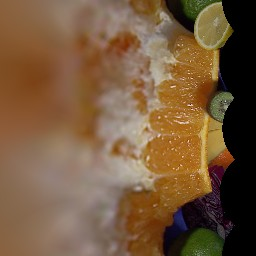
\includegraphics[width=0.4\textwidth]{pics/logpolar.jpg}
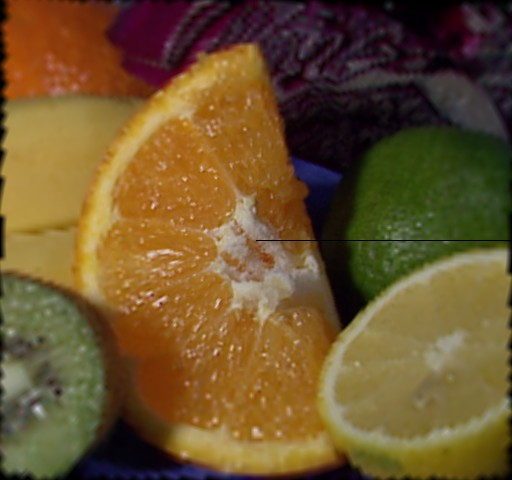
\includegraphics[width=0.4\textwidth]{pics/inv_logpolar.jpg}
\fi

\cvCPyFunc{Remap}
Applies a generic geometrical transformation to the image.

\cvdefC{
void cvRemap(
\par const CvArr* src,
\par CvArr* dst,
\par const CvArr* mapx,
\par const CvArr* mapy,
\par int flags=CV\_INTER\_LINEAR+CV\_WARP\_FILL\_OUTLIERS,
\par CvScalar fillval=cvScalarAll(0) );}
\cvdefPy{Remap(src,dst,mapx,mapy,flags=CV\_INNER\_LINEAR+CV\_WARP\_FILL\_OUTLIERS,fillval=cvScalarAll0))-> None}

\begin{description}
\cvarg{src}{Source image}
\cvarg{dst}{Destination image}
\cvarg{mapx}{The map of x-coordinates (32fC1 image)}
\cvarg{mapy}{The map of y-coordinates (32fC1 image)}
\cvarg{flags}{A combination of interpolation method and the following optional flag(s):
\begin{description}
  \cvarg{CV\_WARP\_FILL\_OUTLIERS}{fills all of the destination image pixels. If some of them correspond to outliers in the source image, they are set to \texttt{fillval}}
\end{description}}
\cvarg{fillval}{A value used to fill outliers}
\end{description}

The function \texttt{cvRemap} transforms the source image using the specified map:

\[
\texttt{dst}(x,y) = \texttt{src}(\texttt{mapx}(x,y),\texttt{mapy}(x,y))
\]

Similar to other geometrical transformations, some interpolation method (specified by user) is used to extract pixels with non-integer coordinates.
Note that the function can not operate in-place.

\cvCPyFunc{Resize}
Resizes an image.

\cvdefC{
void cvResize(
\par const CvArr* src,
\par CvArr* dst,
\par int interpolation=CV\_INTER\_LINEAR );}
\cvdefPy{Resize(src,dst,interpolation=CV\_INTER\_LINEAR)-> None}

\begin{description}
\cvarg{src}{Source image}
\cvarg{dst}{Destination image}
\cvarg{interpolation}{Interpolation method:
\begin{description}
\cvarg{CV\_INTER\_NN}{nearest-neigbor interpolation}
\cvarg{CV\_INTER\_LINEAR}{bilinear interpolation (used by default)}
\cvarg{CV\_INTER\_AREA}{resampling using pixel area relation. It is the preferred method for image decimation that gives moire-free results. In terms of zooming it is similar to the \texttt{CV\_INTER\_NN} method}
\cvarg{CV\_INTER\_CUBIC}{bicubic interpolation}
\end{description}}
\end{description}

The function \texttt{cvResize} resizes an image \texttt{src} so that it fits exactly into \texttt{dst}. If ROI is set, the function considers the ROI as supported.

\cvCPyFunc{Undistort2}
Transforms an image to compensate for lens distortion.

\cvdefC{void cvUndistort2( \par const CvArr* src,\par CvArr* dst,\par const CvMat* intrinsic\_matrix,\par const CvMat* distortion\_coeffs );
}
\cvdefPy{Undistort2(src,dst,intrinsic\_matrix,distortion\_coeffs)-> None}

\begin{description}
\cvarg{src}{The input (distorted) image}
\cvarg{dst}{The output (corrected) image}
\cvarg{intrinsic\_matrix}{The camera matrix $A = \vecthreethree{fx}{0}{cx}{0}{fy}{cy}{0}{0}{1} $}
\cvarg{distortion\_coeffs}{The 4x1 or 1x4 vector of distortion coefficients $k_1, k_2, k_3, k_4$.}
\end{description}

The function \texttt{cvUndistort2} transforms the image to compensate
radial and tangential lens distortion. The camera matrix and
distortion parameters can be determined using
\cvCPyCross{CalibrateCamera2}. For every
pixel in the output image the function computes the coordinates of the
corresponding location in the input image using the formulas in the
section beginning. Then, the pixel value is computed using bilinear
interpolation. If the resolution of images is different from what
was used at the calibration stage, $fx, fy, cx$ and $cy$
need to be adjusted appropriately, while the distortion coefficients
remain the same.

The function can not operate in-place.

\cvCPyFunc{WarpAffine}
Applies an affine transformation to an image.

\cvdefC{
void cvWarpAffine(
\par const CvArr* src,
\par CvArr* dst,
\par const CvMat* mapMatrix,
\par int flags=CV\_INTER\_LINEAR+CV\_WARP\_FILL\_OUTLIERS,
\par CvScalar fillval=cvScalarAll(0) );
}
\cvdefPy{WarpAffline(src,dst,mapMatrix,flags=CV\_INTER\_LINEAR+CV\_WARP\_FILL\_OUTLIERS,fillval=cvScalarAll(0))-> None}

\begin{description}
\cvarg{src}{Source image}
\cvarg{dst}{Destination image}
\cvarg{mapMatrix}{$2\times 3$ transformation matrix}
\cvarg{flags}{A combination of interpolation methods and the following optional flags:
\begin{description}
  \cvarg{CV\_WARP\_FILL\_OUTLIERS}{fills all of the destination image pixels; if some of them correspond to outliers in the source image, they are set to \texttt{fillval}}
  \cvarg{CV\_WARP\_INVERSE\_MAP}{indicates that \texttt{matrix} is inversely
  transformed from the destination image to the source and, thus, can be used
  directly for pixel interpolation. Otherwise, the function finds
  the inverse transform from \texttt{mapMatrix}}}
\end{description}
\cvarg{fillval}{A value used to fill outliers}
\end{description}

The function \texttt{cvWarpAffine} transforms the source image using the specified matrix:

\[
dst(x',y') = src(x,y)
\]

where

\[
\begin{matrix}
\begin{bmatrix}
x'\\
y'
\end{bmatrix} = \texttt{mapMatrix} \cdot \begin{bmatrix}
x\\
y\\
1
\end{bmatrix} & \mbox{if CV\_WARP\_INVERSE\_MAP is not set}\\
\begin{bmatrix}
x\\
y
\end{bmatrix} = \texttt{mapMatrix} \cdot \begin{bmatrix}
x'\\
y'\\
1
\end{bmatrix}& \mbox{otherwise}
\end{matrix}
\]

The function is similar to \cvCPyCross{GetQuadrangleSubPix} but they are not exactly the same. \cvCPyCross{WarpAffine} requires input and output image have the same data type, has larger overhead (so it is not quite suitable for small images) and can leave part of destination image unchanged. While \cvCPyCross{GetQuadrangleSubPix} may extract quadrangles from 8-bit images into floating-point buffer, has smaller overhead and always changes the whole destination image content.
Note that the function can not operate in-place.

To transform a sparse set of points, use the \cvCPyCross{Transform} function from cxcore.

\cvCPyFunc{WarpPerspective}
Applies a perspective transformation to an image.

\cvdefC{
void cvWarpPerspective(
\par const CvArr* src,
\par CvArr* dst,
\par const CvMat* mapMatrix,
\par int flags=CV\_INTER\_LINEAR+CV\_WARP\_FILL\_OUTLIERS,
\par CvScalar fillval=cvScalarAll(0) );
}\cvdefPy{WarpPerspective(src,dst,mapMatrix,flags=CV\_I
NNER\_LINEAR+CV\_WARP\_FILL\_OUTLIERS,fillval=cvScalarAll(0
))-> None}

\begin{description}
\cvarg{src}{Source image}
\cvarg{dst}{Destination image}
\cvarg{mapMatrix}{$3\times 3$ transformation matrix}
\cvarg{flags}{A combination of interpolation methods and the following optional flags:
\begin{description}
  \cvarg{CV\_WARP\_FILL\_OUTLIERS}{fills all of the destination image pixels; if some of them correspond to outliers in the source image, they are set to \texttt{fillval}}
  \cvarg{CV\_WARP\_INVERSE\_MAP}{indicates that \texttt{matrix} is inversely transformed from the destination image to the source and, thus, can be used directly for pixel interpolation. Otherwise, the function finds the inverse transform from \texttt{mapMatrix}}
\end{description}}
\cvarg{fillval}{A value used to fill outliers}
\end{description}

The function \texttt{cvWarpPerspective} transforms the source image using the specified matrix:

\[
\begin{matrix}
\begin{bmatrix}
x'\\
y'
\end{bmatrix} = \texttt{mapMatrix} \cdot \begin{bmatrix}
x\\
y\\
1
\end{bmatrix} & \mbox{if CV\_WARP\_INVERSE\_MAP is not set}\\
\begin{bmatrix}
x\\
y
\end{bmatrix} = \texttt{mapMatrix} \cdot \begin{bmatrix}
x'\\
y'\\
1
\end{bmatrix}& \mbox{otherwise}
\end{matrix}
\]

Note that the function can not operate in-place.
For a sparse set of points use the \cvCPyCross{PerspectiveTransform} function from CxCore.

\fi

\ifCpp

\cvCppFunc{convertMaps}
Converts image transformation maps from one representation to another

\cvdefCpp{void convertMaps( const Mat\& map1, const Mat\& map2,\par
                  Mat\& dstmap1, Mat\& dstmap2,\par
                  int dstmap1type, bool nninterpolation=false );}
\begin{description}
\cvarg{map1}{The first input map of type \texttt{CV\_16SC2} or \texttt{CV\_32FC1} or \texttt{CV\_32FC2}}
\cvarg{map2}{The second input map of type \texttt{CV\_16UC1} or \texttt{CV\_32FC1} or none (empty matrix), respectively}
\cvarg{dstmap1}{The first output map; will have type \texttt{dstmap1type} and the same size as \texttt{src}}
\cvarg{dstmap2}{The second output map}
\cvarg{dstmap1type}{The type of the first output map; should be \texttt{CV\_16SC2}, \texttt{CV\_32FC1} or \texttt{CV\_32FC2}}
\cvarg{nninterpolation}{Indicates whether the fixed-point maps will be used for nearest-neighbor or for more complex interpolation}
\end{description}

The function converts a pair of maps for \cvCppCross{remap} from one representation to another. The following options (\texttt{(map1.type(), map2.type())} $\rightarrow$ \texttt{(dstmap1.type(), dstmap2.type())}) are supported:
\begin{enumerate}
    \item $\texttt{(CV\_32FC1, CV\_32FC1)} \rightarrow \texttt{(CV\_16SC2, CV\_16UC1)}$. This is the most frequently used conversion operation, in which the original floating-point maps (see \cvCppCross{remap}) are converted to more compact and much faster fixed-point representation. The first output array will contain the rounded coordinates and the second array (created only when \texttt{nninterpolation=false}) will contain indices in the interpolation tables.   
    \item $\texttt{(CV\_32FC2)} \rightarrow \texttt{(CV\_16SC2, CV\_16UC1)}$. The same as above, but the original maps are stored in one 2-channel matrix.
    \item the reverse conversion. Obviously, the reconstructed floating-point maps will not be exactly the same as the originals.
\end{enumerate} 

See also: \cvCppCross{remap}, \cvCppCross{undisort}, \cvCppCross{initUndistortRectifyMap}

\cvCppFunc{getAffineTransform}
Calculates the affine transform from 3 pairs of the corresponding points

\cvdefCpp{Mat getAffineTransform( const Point2f src[], const Point2f dst[] );}

\begin{description}
\cvarg{src}{Coordinates of a triangle vertices in the source image}
\cvarg{dst}{Coordinates of the corresponding triangle vertices in the destination image}
\end{description}

The function calculates the $2 \times 3$ matrix of an affine transform such that:

\[
\begin{bmatrix}
x'_i\\
y'_i
\end{bmatrix}
=
\texttt{map\_matrix}
\cdot
\begin{bmatrix}
x_i\\
y_i\\
1
\end{bmatrix}
\]

where

\[
dst(i)=(x'_i,y'_i),
src(i)=(x_i, y_i),
i=0,1,2
\]

See also: \cvCppCross{warpAffine}, \cvCppCross{transform}

\cvCppFunc{getPerspectiveTransform}
Calculates the perspective transform from 4 pairs of the corresponding points

\cvdefCpp{Mat getPerspectiveTransform( const Point2f src[], \par const Point2f dst[] );}

\begin{description}
\cvarg{src}{Coordinates of a quadrange vertices in the source image}
\cvarg{dst}{Coordinates of the corresponding quadrangle vertices in the destination image}
\end{description}

The function calculates the $3 \times 3$ matrix of a perspective transform such that:

\[
\begin{bmatrix}
t_i x'_i\\
t_i y'_i\\
t_i
\end{bmatrix}
=
\texttt{map\_matrix}
\cdot
\begin{bmatrix}
x_i\\
y_i\\
1
\end{bmatrix}
\]

where

\[
dst(i)=(x'_i,y'_i),
src(i)=(x_i, y_i),
i=0,1,2
\]

See also: \cvCppCross{findHomography}, \cvCppCross{warpPerspective}, \cvCppCross{perspectiveTransform}

\cvCppFunc{getRectSubPix}
Retrieves the pixel rectangle from an image with sub-pixel accuracy

\cvdefCpp{void getRectSubPix( const Mat\& image, Size patchSize,\par
                    Point2f center, Mat\& dst, int patchType=-1 );}
\begin{description}
\cvarg{src}{Source image}
\cvarg{patchSize}{Size of the extracted patch}
\cvarg{center}{Floating point coordinates of the extracted rectangle center within the source image. The center must be inside the image}
\cvarg{dst}{The extracted patch; will have the size \texttt{patchSize} and the same number of channels as \texttt{src}}
\cvarg{patchType}{The depth of the extracted pixels. By default they will have the same depth as \texttt{src}}
\end{description}

The function \texttt{getRectSubPix} extracts pixels from \texttt{src}:

\[
dst(x, y) = src(x + \texttt{center.x} - (\texttt{dst.cols}-1)*0.5, y + \texttt{center.y} - (\texttt{dst.rows}-1)*0.5)
\]

where the values of the pixels at non-integer coordinates are retrieved
using bilinear interpolation. Every channel of multiple-channel
images is processed independently. While the rectangle center
must be inside the image, parts of the rectangle may be
outside. In this case, the replication border mode (see \cvCppCross{borderInterpolate}) is used to extrapolate
the pixel values outside of the image.

See also: \cvCppCross{warpAffine}, \cvCppCross{warpPerspective}

\cvCppFunc{getRotationMatrix2D}
Calculates the affine matrix of 2d rotation.

\cvdefCpp{Mat getRotationMatrix2D( Point2f center, double angle, double scale );}
\begin{description}
\cvarg{center}{Center of the rotation in the source image}
\cvarg{angle}{The rotation angle in degrees. Positive values mean counter-clockwise rotation (the coordinate origin is assumed to be the top-left corner)}
\cvarg{scale}{Isotropic scale factor}
\end{description}

The function calculates the following matrix:

\[
\begin{bmatrix}
\alpha & \beta & (1-\alpha) \cdot \texttt{center.x} - \beta \cdot \texttt{center.y} \\
-\beta & \alpha & \beta \cdot \texttt{center.x} - (1-\alpha) \cdot \texttt{center.y}
\end{bmatrix}
\]

where

\[
\begin{array}{l}
\alpha = \texttt{scale} \cdot \cos \texttt{angle},\\
\beta = \texttt{scale} \cdot \sin \texttt{angle}
\end{array}
\]

The transformation maps the rotation center to itself. If this is not the purpose, the shift should be adjusted.

See also: \cvCppCross{getAffineTransform}, \cvCppCross{warpAffine}, \cvCppCross{transform}

\cvCppFunc{initUndistortRectifyMap}
Computes the undistortion and rectification transformation map of a head of a stereo camera.

\cvdefCpp{void initUndistortRectifyMap( const Mat\& cameraMatrix,\par
                           const Mat\& distCoeffs, const Mat\& R,\par
                           const Mat\& newCameraMatrix,\par
                           Size size, int m1type,\par
                           Mat\& map1, Mat\& map2 );}
\begin{description}
\cvarg{cameraMatrix}{The camera matrix $A=\vecthreethree{f_x}{0}{c_x}{0}{f_y}{c_y}{0}{0}{1}$}
\cvarg{distCoeffs}{The vector of distortion coefficients, \cvCppCross{4x1, 1x4, 5x1 or 1x5}}
\cvarg{R}{The rectification transformation in object space (3x3 matrix). \texttt{R1} or \texttt{R2}, computed by \cvCppCross{stereoRectify} can be passed here. If the matrix is empty, the identity transformation is assumed}
\cvarg{newCameraMatrix}{The new camera matrix $A'=\vecthreethree{f_x'}{0}{c_x'}{0}{f_y'}{c_y'}{0}{0}{1}$}
\cvarg{size}{The image size}
\cvarg{m1type}{The type of the first output map, can be \texttt{CV\_32FC1} or \texttt{CV\_16SC2}. See \cvCppCross{convertMaps}}
\cvarg{map1}{The first output map}
\cvarg{map2}{The second output map}
\end{description}

The function computes the joint undistortion+rectification transformation and represents the result in the form of maps for \cvCppCross{remap}. The undistorted image will look like the original, as if it was captured with a camera with camera matrix \texttt{=newCameraMatrix} and zero distortion. Also, this new camera will be oriented differently in the coordinate space, according to \texttt{R}. That, for example, helps to align a stereo pair so that the epipolar lines on both images become horizontal and have the same y- coordinate (in case of horizontally aligned stereo camera).

The function actually builds the maps for the inverse mapping algorithm that is used by \cvCppCross{remap}. That is, for each pixel $(u, v)$ in the destination (corrected and rectified) image the function computes the corresponding coordinates in the source image (i.e. the original image from camera). The process is the following:

\[
\begin{array}{l}
x \leftarrow (u - {c'}_x)/{f'}_x \\
y \leftarrow (v - {c'}_y)/{f'}_y \\
{[X\,Y\,W]}^T \leftarrow R^{-1}*[x\,y\,1]^T \\
x' \leftarrow X/W \\
y' \leftarrow Y/W \\
x" \leftarrow x' (1 + k_1 r^2 + k_2 r^4 + k_3 r^6) + 2p_1 x' y' + p_2(r^2 + 2 x'^2) \\
y" \leftarrow y' (1 + k_1 r^2 + k_2 r^4 + k_3 r^6) + p_1 (r^2 + 2 y'^2) + 2 p_2 x' y' \\
map_x(u,v) \leftarrow x" f_x + c_x \\
map_y(u,v) \leftarrow y" f_y + c_y
\end{array}
\]
where $(k_1, k_2, p_1, p_2[, k_3])$\label{4x1, 1x4, 5x1 or 1x5} are the distortion coefficients. 
 
In the case of a stereo camera this function is called twice, once for each camera head, after \cvCppCross{stereoRectify}. But it is also possible to compute the rectification transformations directly from the fundamental matrix, e.g. by using \cvCppCross{stereoRectifyUncalibrated}. Such functions work with pixels and produce homographies \texttt{H} as rectification transformations, not rotation matrices \texttt{R} in 3D space. In this case, the \texttt{R} can be computed from the homography matrix \texttt{H} as 

\[ \texttt{R} = \texttt{cameraMatrix}^{-1} \cdot \texttt{H} \cdot \texttt{cameraMatrix} \]

\cvCppFunc{invertAffineTransform}
Inverts an affine transformation

\cvdefCpp{void invertAffineTransform(const Mat\& M, Mat\& iM);}
\begin{description}
\cvarg{M}{The original affine transformation}
\cvarg{iM}{The output reverse affine transformation}
\end{description}

The function computes inverse affine transformation represented by $2 \times 3$ matrix \texttt{M}:

\[\begin{bmatrix}
a_{11} & a_{12} & b_1 \\
a_{21} & a_{22} & b_2
\end{bmatrix}
\]

The result will also be a $2 \times 3$ matrix of the same type as \texttt{M}.

\cvCppFunc{remap}
Applies a generic geometrical transformation to an image.

\cvdefCpp{void remap( const Mat\& src, Mat\& dst, const Mat\& map1, const Mat\& map2,\par
            int interpolation, int borderMode=BORDER\_CONSTANT,\par
            const Scalar\& borderValue=Scalar());}
\begin{description}
\cvarg{src}{Source image}
\cvarg{dst}{Destination image. It will have the same size as \texttt{map1} and the same type as \texttt{src}}
\cvarg{map1}{The first map of type \texttt{CV\_16SC2}, \texttt{CV\_32FC1} or \texttt{CV\_32FC2}. See \cvCppCross{convertMaps}}
\cvarg{map2}{The second map of type \texttt{CV\_16UC1}, \texttt{CV\_32FC1} or none (empty map), respectively}
\cvarg{interpolation}{The interpolation method, see \cvCppCross{resize}. The method \texttt{INTER\_AREA} is not supported by this function}
\cvarg{borderMode}{The pixel extrapolation method, see \cvCppCross{borderInterpolate}. When the\\ \texttt{borderMode=BORDER\_TRANSPARENT}, it means that the pixels in the destination image that corresponds to the "outliers" in the source image are not modified by the function}
\cvarg{borderValue}{A value used in the case of a constant border. By default it is 0}
\end{description}

The function \texttt{remap} transforms the source image using the specified map:

\[
\texttt{dst}(x,y) = \texttt{src}(map_x(x,y),map_y(x,y))
\]

Where values of pixels with non-integer coordinates are computed using one of the available interpolation methods. $map_x$ and $map_y$ can be encoded as separate floating-point maps, interleaved floating-point maps or fixed-point maps.
The function can not operate in-place.

\cvCppFunc{resize}
Resizes an image

\cvdefCpp{void resize( const Mat\& src, Mat\& dst,\par
             Size dsize, double fx=0, double fy=0,\par
             int interpolation=INTER\_LINEAR );}
\begin{description}
\cvarg{src}{Source image}
\cvarg{dst}{Destination image. It will have size \texttt{dsize} (when it is non-zero) or the size computed from \texttt{src.size()}
and \texttt{fx} and \texttt{fy}. The type of \texttt{dst} will be the same as of \texttt{src}.}
\cvarg{dsize}{The destination image size. If it is zero, then it is computed as:
\[\texttt{dsize = Size(round(fx*src.cols), round(fy*src.rows))}\].
Either \texttt{dsize} or both \texttt{fx} or \texttt{fy} must be non-zero.}
\cvarg{fx}{The scale factor along the horizontal axis. When 0, it is computed as
\[\texttt{(double)dsize.width/src.cols}\]}
\cvarg{fy}{The scale factor along the vertical axis. When 0, it is computed as
\[\texttt{(double)dsize.height/src.rows}\]}
\cvarg{interpolation}{The interpolation method:
\begin{description}
\cvarg{INTER\_NEAREST}{nearest-neighbor interpolation}
\cvarg{INTER\_LINEAR}{bilinear interpolation (used by default)}
\cvarg{INTER\_AREA}{resampling using pixel area relation. It may be the preferred method for image decimation, as it gives moire-free results. But when the image is zoomed, it is similar to the \texttt{INTER\_NEAREST} method}
\cvarg{INTER\_CUBIC}{bicubic interpolation over 4x4 pixel neighborhood}
\cvarg{INTER\_LANCZOS4}{Lanczos interpolation over 8x8 pixel neighborhood}
\end{description}}
\end{description}

The function \texttt{resize} resizes an image \texttt{src} down to or up to the specified size.
Note that the initial \texttt{dst} type or size are not taken into account. Instead the size and type are derived from the \texttt{src}, \texttt{dsize}, \texttt{fx} and \texttt{fy}. If you want to resize \texttt{src} so that it fits the pre-created \texttt{dst}, you may call the function as:

\begin{lstlisting}
// explicitly specify dsize=dst.size(); fx and fy will be computed from that.
resize(src, dst, dst.size(), 0, 0, interpolation);
\end{lstlisting}

If you want to decimate the image by factor of 2 in each direction, you can call the function this way:

\begin{lstlisting}
// specify fx and fy and let the function to compute the destination image size.
resize(src, dst, Size(), 0.5, 0.5, interpolation);
\end{lstlisting}

See also: \cvCppCross{warpAffine}, \cvCppCross{warpPerspective}, \cvCppCross{remap}.

\cvCppFunc{undistort}
Transforms an image to compensate for lens distortion.

\cvdefCpp{void undistort( const Mat\& src, Mat\& dst, const Mat\& cameraMatrix,\par
                const Mat\& distCoeffs, const Mat\& newCameraMatrix=Mat() );}
\begin{description}
\cvarg{src}{The input (distorted) image}
\cvarg{dst}{The output (corrected) image; will have the same size and the same type as \texttt{src}}
\cvarg{cameraMatrix}{The camera matrix $A = \vecthreethree{f_x}{0}{c_x}{0}{f_y}{c_y}{0}{0}{1} $}
\cvarg{distortion\_coeffs}{The 4x1, 5x1, 1x4 or 1x5 vector of distortion coefficients $(k_1, k_2, p_1, p_2[, k_3])$.}
\cvarg{newCameraMatrix}{Camera matrix of the distorted image. By default it is the same as \texttt{cameraMatrix}, but you may additionally scale and shift the result by using some different matrix}
\end{description}

The function \texttt{undistort} transforms the image to compensate
radial and tangential lens distortion. The function is simply a combination of \cvCppCross{initUndistortRectifyMap} (with unity \texttt{R}) and \cvCppCross{remap} (with bilinear interpolation) put into one loop.

The camera matrix and the distortion parameters can be determined using
\cvCppCross{calibrateCamera}. If the resolution of images is different from the used at the calibration stage, $f_x, f_y, c_x$ and $c_y$
need to be scaled accordingly, while the distortion coefficients remain the same.

\cvCppFunc{warpAffine}
Applies an affine transformation to an image.

\cvdefCpp{void warpAffine( const Mat\& src, Mat\& dst,\par
                 const Mat\& M, Size dsize,\par
                 int flags=INTER\_LINEAR,\par
                 int borderMode=BORDER\_CONSTANT,\par
                 const Scalar\& borderValue=Scalar());}
\begin{description}
\cvarg{src}{Source image}
\cvarg{dst}{Destination image; will have size \texttt{dsize} and the same type as \texttt{src}}
\cvarg{M}{$2\times 3$ transformation matrix}
\cvarg{dsize}{Size of the destination image}
\cvarg{flags}{A combination of interpolation methods, see \cvCppCross{resize}, and the optional flag \texttt{WARP\_INVERSE\_MAP} that means that \texttt{M} is the inverse transformation ($\texttt{dst}\rightarrow\texttt{src}$)}
\cvarg{borderMode}{The pixel extrapolation method, see \cvCppCross{borderInterpolate}. When the \\ \texttt{borderMode=BORDER\_TRANSPARENT}, it means that the pixels in the destination image that corresponds to the "outliers" in the source image are not modified by the function}
\cvarg{borderValue}{A value used in case of a constant border. By default it is 0}
\end{description}

The function \texttt{warpAffine} transforms the source image using the specified matrix:

\[
\texttt{dst}(x,y) = \texttt{src}(\texttt{M}_{11} x + \texttt{M}_{12} y + \texttt{M}_{13}, \texttt{M}_{21} x + \texttt{M}_{22} y + \texttt{M}_{23})
\]
when the flag \texttt{WARP\_INVERSE\_MAP} is set. Otherwise, the transformation is first inverted with \cvCppCross{invertAffineTransform} and then put in the formula above instead of \texttt{M}.
The function can not operate in-place.

See also: \cvCppCross{warpPerspective}, \cvCppCross{resize}, \cvCppCross{remap}, \cvCppCross{getRectSubPix}, \cvCppCross{transform}

\cvCppFunc{warpPerspective}
Applies a perspective transformation to an image.

\cvdefCpp{void warpPerspective( const Mat\& src, Mat\& dst,\par
                      const Mat\& M, Size dsize,\par
                      int flags=INTER\_LINEAR,\par
                      int borderMode=BORDER\_CONSTANT,\par
                      const Scalar\& borderValue=Scalar());}
\begin{description}
\cvarg{src}{Source image}
\cvarg{dst}{Destination image; will have size \texttt{dsize} and the same type as \texttt{src}}
\cvarg{M}{$3\times 3$ transformation matrix}
\cvarg{dsize}{Size of the destination image}
\cvarg{flags}{A combination of interpolation methods, see \cvCppCross{resize}, and the optional flag \texttt{WARP\_INVERSE\_MAP} that means that \texttt{M} is the inverse transformation ($\texttt{dst}\rightarrow\texttt{src}$)}
\cvarg{borderMode}{The pixel extrapolation method, see \cvCppCross{borderInterpolate}. When the \\ \texttt{borderMode=BORDER\_TRANSPARENT}, it means that the pixels in the destination image that corresponds to the "outliers" in the source image are not modified by the function}
\cvarg{borderValue}{A value used in case of a constant border. By default it is 0}
\end{description}

The function \texttt{warpPerspective} transforms the source image using the specified matrix:

\[
\texttt{dst}(x,y) = \texttt{src}\left(\frac{M_{11} x + M_{12} y + M_{13}}{M_{31} x + M_{32} y + M_{33}},
    \frac{M_{21} x + M_{22} y + M_{23}}{M_{31} x + M_{32} y + M_{33}}\right)
\]
when the flag \texttt{WARP\_INVERSE\_MAP} is set. Otherwise, the transformation is first inverted with \cvCppCross{invert} and then put in the formula above instead of \texttt{M}.
The function can not operate in-place.

See also: \cvCppCross{warpAffine}, \cvCppCross{resize}, \cvCppCross{remap}, \cvCppCross{getRectSubPix}, \cvCppCross{perspectiveTransform}

\fi


\section{Miscellaneous Image Transformations}

\ifCPy

\cvCPyFunc{AdaptiveThreshold}
Applies an adaptive threshold to an array.

\cvdefC{
void cvAdaptiveThreshold(
\par const CvArr* src,\par CvArr* dst,\par double maxValue,\par
int adaptive\_method=CV\_ADAPTIVE\_THRESH\_MEAN\_C,\par
int thresholdType=CV\_THRESH\_BINARY,\par
int blockSize=3,\par double param1=5 );
}

\cvdefPy{AdaptiveThreshold(src,dst,maxValue, adaptive\_method=CV\_ADAPTIVE\_THRESH\_MEAN\_C, thresholdType=CV\_THRESH\_BINARY,blockSize=3,param1=5)-> None}

\begin{description}
\cvarg{src}{Source image}
\cvarg{dst}{Destination image}
\cvarg{maxValue}{Maximum value that is used with \texttt{CV\_THRESH\_BINARY} and \texttt{CV\_THRESH\_BINARY\_INV}}
\cvarg{adaptive\_method}{Adaptive thresholding algorithm to use: \texttt{CV\_ADAPTIVE\_THRESH\_MEAN\_C} or \texttt{CV\_ADAPTIVE\_THRESH\_GAUSSIAN\_C} (see the discussion)}
\cvarg{thresholdType}{Thresholding type; must be one of
\begin{description}
\cvarg{CV\_THRESH\_BINARY}{xxx}
\cvarg{CV\_THRESH\_BINARY\_INV}{xxx}
\end{description}}
\cvarg{blockSize}{The size of a pixel neighborhood that is used to calculate a threshold value for the pixel: 3, 5, 7, and so on}
\cvarg{param1}{The method-dependent parameter. For the methods \texttt{CV\_ADAPTIVE\_THRESH\_MEAN\_C} and \texttt{CV\_ADAPTIVE\_THRESH\_GAUSSIAN\_C} it is a constant subtracted from the mean or weighted mean (see the discussion), though it may be negative}
\end{description}

The function transforms a grayscale image to a binary image according to the formulas:

\begin{description}
\cvarg{CV\_THRESH\_BINARY}{\[ dst(x,y) = \fork{\texttt{maxValue}}{if $src(x,y) > T(x,y)$}{0}{otherwise} \]}
\cvarg{CV\_THRESH\_BINARY\_INV}{\[ dst(x,y) = \fork{0}{if $src(x,y) > T(x,y)$}{\texttt{maxValue}}{otherwise} \]}
\end{description}

where $T(x,y)$ is a threshold calculated individually for each pixel.

For the method \texttt{CV\_ADAPTIVE\_THRESH\_MEAN\_C} it is the mean of a $\texttt{blockSize} \times \texttt{blockSize}$ pixel neighborhood, minus \texttt{param1}.

For the method \texttt{CV\_ADAPTIVE\_THRESH\_GAUSSIAN\_C} it is the weighted sum (gaussian) of a $\texttt{blockSize} \times \texttt{blockSize}$ pixel neighborhood, minus \texttt{param1}.

\cvCPyFunc{CvtColor}
Converts an image from one color space to another.

\cvdefC{
void cvCvtColor(
\par const CvArr* src,
\par CvArr* dst,
\par int code );
}\cvdefPy{CvtColor(src,dst,code)-> None}

\begin{description}
\cvarg{src}{The source 8-bit (8u), 16-bit (16u) or single-precision floating-point (32f) image}
\cvarg{dst}{The destination image of the same data type as the source. The number of channels may be different}
\cvarg{code}{Color conversion operation that can be specifed using \texttt{CV\_ \textit{src\_color\_space} 2 \textit{dst\_color\_space}} constants (see below)}
\end{description}

The function converts the input image from one color
space to another. The function ignores the \texttt{colorModel} and
\texttt{channelSeq} fields of the \texttt{IplImage} header, so the
source image color space should be specified correctly (including
order of the channels in the case of RGB space. For example, BGR means 24-bit
format with $B_0, G_0, R_0, B_1, G_1, R_1, ...$ layout
whereas RGB means 24-format with $R_0, G_0, B_0, R_1, G_1, B_1, ...$
layout).

The conventional range for R,G,B channel values is:

\begin{itemize}
\item 0 to 255 for 8-bit images
\item 0 to 65535 for 16-bit images and
\item 0 to 1 for floating-point images.
\end{itemize}

Of course, in the case of linear transformations the range can be
specific, but in order to get correct results in the case of non-linear
transformations, the input image should be scaled.

The function can do the following transformations:

\begin{itemize}
\item Transformations within RGB space like adding/removing the alpha channel, reversing the channel order, conversion to/from 16-bit RGB color (R5:G6:B5 or R5:G5:B5), as well as conversion to/from grayscale using:
\[
\text{RGB[A] to Gray:} Y \leftarrow 0.299 \cdot R + 0.587 \cdot G + 0.114 \cdot B
\]
and
\[
\text{Gray to RGB[A]:} R \leftarrow Y, G \leftarrow Y, B \leftarrow Y, A \leftarrow 0
\]

The conversion from a RGB image to gray is done with:
\begin{lstlisting}
cvCvtColor(src ,bwsrc, CV_RGB2GRAY)
\end{lstlisting}

\item RGB $\leftrightarrow$ CIE XYZ.Rec 709 with D65 white point (\texttt{CV\_BGR2XYZ, CV\_RGB2XYZ, CV\_XYZ2BGR, CV\_XYZ2RGB}):
\[
\begin{bmatrix}
X \\
Y \\
Z
\end{bmatrix}
\leftarrow
\begin{bmatrix}
0.412453 & 0.357580 & 0.180423\\
0.212671 & 0.715160 & 0.072169\\
0.019334 & 0.119193 & 0.950227
\end{bmatrix}
\cdot
\begin{bmatrix}
R \\
G \\
B
\end{bmatrix}
\]
\[
\begin{bmatrix}
R \\
G \\
B
\end{bmatrix}
\leftarrow
\begin{bmatrix}
3.240479 & -1.53715 & -0.498535\\
-0.969256 &  1.875991 & 0.041556\\
0.055648 & -0.204043 & 1.057311
\end{bmatrix}
\cdot
\begin{bmatrix}
X \\
Y \\
Z
\end{bmatrix}
\]
$X$, $Y$ and $Z$ cover the whole value range (in the case of floating-point images $Z$ may exceed 1).

\item RGB $\leftrightarrow$ YCrCb JPEG (a.k.a. YCC) (\texttt{CV\_BGR2YCrCb, CV\_RGB2YCrCb, CV\_YCrCb2BGR, CV\_YCrCb2RGB})
\[ Y \leftarrow 0.299 \cdot R + 0.587 \cdot G + 0.114 \cdot B \]
\[  Cr \leftarrow (R-Y) \cdot 0.713 + delta \]
\[  Cb \leftarrow (B-Y) \cdot 0.564 + delta \]
\[  R \leftarrow Y + 1.403 \cdot (Cr - delta) \]
\[  G \leftarrow Y - 0.344 \cdot (Cr - delta) - 0.714 \cdot (Cb - delta) \]
\[  B \leftarrow Y + 1.773 \cdot (Cb - delta) \]
where
\[
delta = \left\{
\begin{array}{l l}
128 & \mbox{for 8-bit images}\\
32768 & \mbox{for 16-bit images}\\
0.5 & \mbox{for floating-point images}
\end{array} \right.
\]
Y, Cr and Cb cover the whole value range.

\item RGB $\leftrightarrow$ HSV (\texttt{CV\_BGR2HSV, CV\_RGB2HSV, CV\_HSV2BGR, CV\_HSV2RGB})
in the case of 8-bit and 16-bit images
R, G and B are converted to floating-point format and scaled to fit the 0 to 1 range
\[ V \leftarrow max(R,G,B) \]

\[ S \leftarrow \fork{\frac{V-min(R,G,B)}{V}}{if $V \neq 0$}{0}{otherwise} \]
\[ H \leftarrow \forkthree
{{60(G - B)}/{S}}{if $V=R$}
{{120+60(B - R)}/{S}}{if $V=G$}
{{240+60(R - G)}/{S}}{if $V=B$} \]
if $H<0$ then $H \leftarrow H+360$

On output $0 \leq V \leq 1$, $0 \leq S \leq 1$, $0 \leq H \leq 360$.

The values are then converted to the destination data type:
\begin{description}
\item[8-bit images]
\[ V \leftarrow 255 V, S \leftarrow 255 S, H \leftarrow H/2 \text{(to fit to 0 to 255)} \]
\item[16-bit images (currently not supported)]
\[ V <- 65535 V, S <- 65535 S, H <- H \]
\item[32-bit images]
H, S, V are left as is
\end{description}

\item RGB $\leftrightarrow$ HLS (\texttt{CV\_BGR2HLS, CV\_RGB2HLS, CV\_HLS2BGR, CV\_HLS2RGB}).
in the case of 8-bit and 16-bit images
R, G and B are converted to floating-point format and scaled to fit the 0 to 1 range.
\[ V_{max} \leftarrow {max}(R,G,B) \]
\[ V_{min} \leftarrow {min}(R,G,B) \]
\[ L \leftarrow \frac{V_{max} - V_{min}}{2} \]
\[ S \leftarrow \fork
{\frac{V_{max} - V_{min}}{V_{max} + V_{min}}}{if $L < 0.5$}
{\frac{V_{max} - V_{min}}{2 - (V_{max} + V_{min})}}{if $L \ge 0.5$} \]
\[ H \leftarrow \forkthree
{{60(G - B)}/{S}}{if $V_{max}=R$}
{{120+60(B - R)}/{S}}{if $V_{max}=G$}
{{240+60(R - G)}/{S}}{if $V_{max}=B$} \]
if $H<0$ then $H \leftarrow H+360$
On output $0 \leq V \leq 1$, $0 \leq S \leq 1$, $0 \leq H \leq 360$.

The values are then converted to the destination data type:
\begin{description}
\item[8-bit images]
\[ V \leftarrow 255 V, S \leftarrow 255 S, H \leftarrow H/2 \text{(to fit to 0 to 255)} \]
\item[16-bit images (currently not supported)]
\[ V <- 65535 V, S <- 65535 S, H <- H \]
\item[32-bit images]
H, S, V are left as is
\end{description}

\item RGB $\leftrightarrow$ CIE L*a*b* (\texttt{CV\_BGR2Lab, CV\_RGB2Lab, CV\_Lab2BGR, CV\_Lab2RGB})
in the case of 8-bit and 16-bit images
R, G and B are converted to floating-point format and scaled to fit the 0 to 1 range
\[ \vecthree{X}{Y}{Z} \leftarrow \vecthreethree
{0.412453}{0.357580}{0.180423}
{0.212671}{0.715160}{0.072169}
{0.019334}{0.119193}{0.950227}
\cdot
\vecthree{R}{G}{B} \]
\[ X \leftarrow X/X_n, \text{where} X_n = 0.950456 \]
\[ Z \leftarrow Z/Z_n, \text{where} Z_n = 1.088754 \]
\[ L \leftarrow \fork
{116*Y^{1/3}-16}{for $Y>0.008856$}
{903.3*Y}{for $Y \le 0.008856$} \]
\[ a \leftarrow 500 (f(X)-f(Y)) + delta \]
\[ b \leftarrow 200 (f(Y)-f(Z)) + delta \]
where
\[f(t)=\fork
{t^{1/3}}{for $t>0.008856$}
{7.787 t+16/116}{for $t<=0.008856$} \]
and
\[ delta = \fork{128}{for 8-bit images}{0}{for floating-point images} \]
On output $0 \leq L \leq 100$, $-127 \leq a \leq 127$, $-127 \leq b \leq 127$

The values are then converted to the destination data type:
\begin{description}
\item[8-bit images]
\[L \leftarrow L*255/100, a \leftarrow a + 128, b \leftarrow b + 128\]
\item[16-bit images] currently not supported
\item[32-bit images]
L, a, b are left as is
\end{description}

\item RGB $\leftrightarrow$ CIE L*u*v* (\texttt{CV\_BGR2Luv, CV\_RGB2Luv, CV\_Luv2BGR, CV\_Luv2RGB})
in the case of 8-bit and 16-bit images
R, G and B are converted to floating-point format and scaled to fit 0 to 1 range
\[ \vecthree{X}{Y}{Z} \leftarrow \vecthreethree
{0.412453}{0.357580}{0.180423}
{0.212671}{0.715160}{0.072169}
{0.019334}{0.119193}{0.950227}
\cdot
\vecthree{R}{G}{B} \]
\[ L \leftarrow \fork
{116 Y^{1/3}}{for $Y>0.008856$}
{903.3 Y}{for $Y<=0.008856$} \]
\[ u' \leftarrow 4*X/(X + 15*Y + 3 Z) \]
\[ v' \leftarrow 9*Y/(X + 15*Y + 3 Z) \]
\[ u \leftarrow 13*L*(u' - u_n) \quad \text{where} \quad u_n=0.19793943 \]
\[ v \leftarrow 13*L*(v' - v_n) \quad \text{where} \quad v_n=0.46831096 \]
On output $0 \leq L \leq 100$, $-134 \leq u \leq 220$, $-140 \leq v \leq 122$.

The values are then converted to the destination data type:
\begin{description}
\item[8-bit images]
\[L \leftarrow 255/100 L, u \leftarrow 255/354 (u + 134), v \leftarrow 255/256 (v + 140) \]
\item[16-bit images] currently not supported
\item[32-bit images] L, u, v are left as is
\end{description}

The above formulas for converting RGB to/from various color spaces have been taken from multiple sources on Web, primarily from
the Ford98
at the Charles Poynton site.

\item Bayer $\rightarrow$ RGB (\texttt{CV\_BayerBG2BGR, CV\_BayerGB2BGR, CV\_BayerRG2BGR, CV\_BayerGR2BGR, CV\_BayerBG2RGB, CV\_BayerGB2RGB, CV\_BayerRG2RGB, CV\_BayerGR2RGB}) The Bayer pattern is widely used in CCD and CMOS cameras. It allows one to get color pictures from a single plane where R,G and B pixels (sensors of a particular component) are interleaved like this:



\[
\newcommand{\Rcell}{\color{red}R}
\newcommand{\Gcell}{\color{green}G}
\newcommand{\Bcell}{\color{blue}B}
\definecolor{BackGray}{rgb}{0.8,0.8,0.8}
\begin{array}{ c c c c c }
\Rcell&\Gcell&\Rcell&\Gcell&\Rcell\\
\Gcell&\colorbox{BackGray}{\Bcell}&\colorbox{BackGray}{\Gcell}&\Bcell&\Gcell\\
\Rcell&\Gcell&\Rcell&\Gcell&\Rcell\\
\Gcell&\Bcell&\Gcell&\Bcell&\Gcell\\
\Rcell&\Gcell&\Rcell&\Gcell&\Rcell
\end{array}
\]

The output RGB components of a pixel are interpolated from 1, 2 or
4 neighbors of the pixel having the same color. There are several
modifications of the above pattern that can be achieved by shifting
the pattern one pixel left and/or one pixel up. The two letters
$C_1$ and $C_2$
in the conversion constants
\texttt{CV\_Bayer} $ C_1 C_2 $ \texttt{2BGR}
and
\texttt{CV\_Bayer} $ C_1 C_2 $ \texttt{2RGB}
indicate the particular pattern
type - these are components from the second row, second and third
columns, respectively. For example, the above pattern has very
popular "BG" type.
\end{itemize}

\cvCPyFunc{DistTransform}
Calculates the distance to the closest zero pixel for all non-zero pixels of the source image.

\cvdefC{
void cvDistTransform( \par const CvArr* src,\par CvArr* dst,\par int distance\_type=CV\_DIST\_L2,\par int mask\_size=3,\par const float* mask=NULL,\par CvArr* labels=NULL );
}
\cvdefPy{DistTransform(src,dst,distance\_type=CV\_DIST\_L2,mask\_size=3,mask=None,labels=NULL)-> None}

\begin{description}
\cvarg{src}{8-bit, single-channel (binary) source image}
\cvarg{dst}{Output image with calculated distances (32-bit floating-point, single-channel)}
\cvarg{distance\_type}{Type of distance; can be \texttt{CV\_DIST\_L1, CV\_DIST\_L2, CV\_DIST\_C} or \texttt{CV\_DIST\_USER}}
\cvarg{mask\_size}{Size of the distance transform mask; can be 3 or 5. in the case of \texttt{CV\_DIST\_L1} or \texttt{CV\_DIST\_C} the parameter is forced to 3, because a $3\times 3$ mask gives the same result as a $5\times 5 $ yet it is faster}
\cvarg{mask}{User-defined mask in the case of a user-defined distance, it consists of 2 numbers (horizontal/vertical shift cost, diagonal shift cost) in the case ofa  $3\times 3$ mask and 3 numbers (horizontal/vertical shift cost, diagonal shift cost, knight's move cost) in the case of a $5\times 5$ mask}
\cvarg{labels}{The optional output 2d array of integer type labels, the same size as \texttt{src} and \texttt{dst}}
\end{description}

The function calculates the approximated
distance from every binary image pixel to the nearest zero pixel.
For zero pixels the function sets the zero distance, for others it
finds the shortest path consisting of basic shifts: horizontal,
vertical, diagonal or knight's move (the latest is available for a
$5\times 5$ mask). The overall distance is calculated as a sum of these
basic distances. Because the distance function should be symmetric,
all of the horizontal and vertical shifts must have the same cost (that
is denoted as \texttt{a}), all the diagonal shifts must have the
same cost (denoted \texttt{b}), and all knight's moves must have
the same cost (denoted \texttt{c}). For \texttt{CV\_DIST\_C} and
\texttt{CV\_DIST\_L1} types the distance is calculated precisely,
whereas for \texttt{CV\_DIST\_L2} (Euclidian distance) the distance
can be calculated only with some relative error (a $5\times 5$ mask
gives more accurate results), OpenCV uses the values suggested in
\cite{Borgefors86}:


\begin{tabular}{| c | c | c |}
\hline
\texttt{CV\_DIST\_C}  & $(3\times 3)$ & a = 1, b = 1\\ \hline
\texttt{CV\_DIST\_L1} & $(3\times 3)$ & a = 1, b = 2\\ \hline
\texttt{CV\_DIST\_L2} & $(3\times 3)$ & a=0.955, b=1.3693\\ \hline
\texttt{CV\_DIST\_L2} & $(5\times 5)$ & a=1, b=1.4, c=2.1969\\ \hline
\end{tabular}

And below are samples of the distance field (black (0) pixel is in the middle of white square) in the case of a user-defined distance:

User-defined $3 \times 3$ mask (a=1, b=1.5)

\begin{tabular}{| c | c | c | c | c | c | c |}
\hline
4.5 & 4 & 3.5 & 3 & 3.5 & 4 & 4.5\\ \hline
4 & 3 & 2.5 & 2 & 2.5 & 3 & 4\\ \hline
3.5 & 2.5 & 1.5 & 1 & 1.5 & 2.5 & 3.5\\ \hline
3 & 2 & 1 &     & 1 & 2 & 3\\ \hline
3.5 & 2.5 & 1.5 & 1 & 1.5 & 2.5 & 3.5\\ \hline
4 & 3 & 2.5 & 2 & 2.5 & 3 & 4\\ \hline
4.5 & 4 & 3.5 & 3 & 3.5 & 4 & 4.5\\ \hline
\end{tabular}

User-defined $5 \times 5$ mask (a=1, b=1.5, c=2)

\begin{tabular}{| c | c | c | c | c | c | c |}
\hline
4.5 & 3.5 & 3 & 3 & 3 & 3.5 & 4.5\\ \hline
3.5 & 3 & 2 & 2 & 2 & 3 & 3.5\\ \hline
3 & 2 & 1.5 & 1 & 1.5 & 2 & 3\\ \hline
3 & 2 & 1 & & 1 & 2 & 3\\ \hline
3 & 2 & 1.5 & 1 & 1.5 & 2 & 3\\ \hline
3.5 & 3 & 2 & 2 & 2 & 3 & 3.5\\ \hline
4 & 3.5 & 3 & 3 & 3 & 3.5 & 4\\ \hline
\end{tabular}


Typically, for a fast, coarse distance estimation \texttt{CV\_DIST\_L2},
a $3\times 3$ mask is used, and for a more accurate distance estimation
\texttt{CV\_DIST\_L2}, a $5\times 5$ mask is used.

When the output parameter \texttt{labels} is not \texttt{NULL}, for
every non-zero pixel the function also finds the nearest connected
component consisting of zero pixels. The connected components
themselves are found as contours in the beginning of the function.

In this mode the processing time is still O(N), where N is the number of
pixels. Thus, the function provides a very fast way to compute approximate
Voronoi diagram for the binary image.

\cvclass{CvConnectedComp}

\ifC
\begin{lstlisting}
typedef struct CvConnectedComp
{
    double area;    /* area of the segmented component */
    CvScalar value; /* average color of the connected component */
    CvRect rect;    /* ROI of the segmented component */
    CvSeq* contour; /* optional component boundary
                      (the contour might have child contours corresponding to the holes) */
} CvConnectedComp;

\end{lstlisting}
\fi

\ifPy
Connected component, represented as a tuple (area, value, rect), where
area is the area of the component as a float, value is the average color
as a \cross{CvScalar}, and rect is the ROI of the component, as a \cross{CvRect}.
\fi

\cvCPyFunc{FloodFill}
Fills a connected component with the given color.

\cvdefC{
void cvFloodFill(\par CvArr* image,\par CvPoint seed\_point,\par CvScalar new\_val,\par
                  CvScalar lo\_diff=cvScalarAll(0),\par CvScalar up\_diff=cvScalarAll(0),\par
                  CvConnectedComp* comp=NULL,\par int flags=4,\par CvArr* mask=NULL );

}
\cvdefPy{FloodFill(image,seed\_point,new\_val,lo\_diff=(0,0,0,0),up\_diff=(0,0,0,0),flags=4,mask=NULL)-> comp}


\begin{description}
\cvarg{image}{Input 1- or 3-channel, 8-bit or floating-point image. It is modified by the function unless the \texttt{CV\_FLOODFILL\_MASK\_ONLY} flag is set (see below)}
\cvarg{seed\_point}{The starting point}
\cvarg{new\_val}{New value of the repainted domain pixels}
\cvarg{lo\_diff}{Maximal lower brightness/color difference between the currently observed pixel and one of its neighbors belonging to the component, or a seed pixel being added to the component. In the case of 8-bit color images it is a packed value}
\cvarg{up\_diff}{Maximal upper brightness/color difference between the currently observed pixel and one of its neighbors belonging to the component, or a seed pixel being added to the component. In the case of 8-bit color images it is a packed value}
\ifC % {
\cvarg{comp}{Pointer to the structure that the function fills with the information about the repainted domain.
Note that the function does not fill \texttt{comp->contour} field. The boundary of the filled component can be retrieved from the output mask image using \cvCPyCross{FindContours}}
\else % }{
\cvarg{comp}{Returned connected component for the repainted domain. Note that the function does not fill \texttt{comp->contour} field. The boundary of the filled component can be retrieved from the output mask image using \cvCPyCross{FindContours}}
\fi % }
\cvarg{flags}{The operation flags. Lower bits contain connectivity value, 4 (by default) or 8, used within the function. Connectivity determines which neighbors of a pixel are considered. Upper bits can be 0 or a combination of the following flags:
\begin{description}
  \cvarg{CV\_FLOODFILL\_FIXED\_RANGE}{if set, the difference between the current pixel and seed pixel is considered, otherwise the difference between neighbor pixels is considered (the range is floating)}
  \cvarg{CV\_FLOODFILL\_MASK\_ONLY}{if set, the function does not fill the image (\texttt{new\_val} is ignored), but fills the mask (that must be non-NULL in this case)}
\end{description}}
\cvarg{mask}{Operation mask, should be a single-channel 8-bit image, 2 pixels wider and 2 pixels taller than \texttt{image}. If not NULL, the function uses and updates the mask, so the user takes responsibility of initializing the \texttt{mask} content. Floodfilling can't go across non-zero pixels in the mask, for example, an edge detector output can be used as a mask to stop filling at edges. It is possible to use the same mask in multiple calls to the function to make sure the filled area do not overlap. \textbf{Note}: because the mask is larger than the filled image, a pixel in \texttt{mask} that corresponds to $(x,y)$ pixel in \texttt{image} will have coordinates $(x+1,y+1)$ }
\end{description}

The function fills a connected component starting from the seed point with the specified color. The connectivity is determined by the closeness of pixel values. The pixel at $(x,y)$ is considered to belong to the repainted domain if:

\begin{description}

\item[grayscale image, floating range] \[
src(x',y')-\texttt{lo\_diff} <= src(x,y) <= src(x',y')+\texttt{up\_diff} \]

\item[grayscale image, fixed range] \[
src(seed.x,seed.y)-\texttt{lo\_diff}<=src(x,y)<=src(seed.x,seed.y)+\texttt{up\_diff} \]

\item[color image, floating range]
\[ src(x',y')_r-\texttt{lo\_diff}_r<=src(x,y)_r<=src(x',y')_r+\texttt{up\_diff}_r \]
\[ src(x',y')_g-\texttt{lo\_diff}_g<=src(x,y)_g<=src(x',y')_g+\texttt{up\_diff}_g \]
\[ src(x',y')_b-\texttt{lo\_diff}_b<=src(x,y)_b<=src(x',y')_b+\texttt{up\_diff}_b \]

\item[color image, fixed range]
\[ src(seed.x,seed.y)_r-\texttt{lo\_diff}_r<=src(x,y)_r<=src(seed.x,seed.y)_r+\texttt{up\_diff}_r \]
\[ src(seed.x,seed.y)_g-\texttt{lo\_diff}_g<=src(x,y)_g<=src(seed.x,seed.y)_g+\texttt{up\_diff}_g \]
\[ src(seed.x,seed.y)_b-\texttt{lo\_diff}_b<=src(x,y)_b<=src(seed.x,seed.y)_b+\texttt{up\_diff}_b \]
\end{description}

where $src(x',y')$ is the value of one of pixel neighbors. That is, to be added to the connected component, a pixel's color/brightness should be close enough to the:
\begin{itemize}
  \item color/brightness of one of its neighbors that are already referred to the connected component in the case of floating range
  \item color/brightness of the seed point in the case of fixed range.
\end{itemize}

\cvCPyFunc{Inpaint}
Inpaints the selected region in the image.

\cvdefC{
void cvInpaint( \par const CvArr* src, \par const CvArr* mask, \par CvArr* dst,
                \par double inpaintRadius, \par int flags);

}\cvdefPy{Inpaint(src,mask,dst,inpaintRadius,flags) -> None}

\begin{description}
\cvarg{src}{The input 8-bit 1-channel or 3-channel image.}
\cvarg{mask}{The inpainting mask, 8-bit 1-channel image. Non-zero pixels indicate the area that needs to be inpainted.}
\cvarg{dst}{The output image of the same format and the same size as input.}
\cvarg{inpaintRadius}{The radius of circlular neighborhood of each point inpainted that is considered by the algorithm.}
\cvarg{flags}{The inpainting method, one of the following:
\begin{description}
\cvarg{CV\_INPAINT\_NS}{Navier-Stokes based method.}
\cvarg{CV\_INPAINT\_TELEA}{The method by Alexandru Telea \cite{Telea04}}
\end{description}}
\end{description}

The function reconstructs the selected image area from the pixel near the area boundary. The function may be used to remove dust and scratches from a scanned photo, or to remove undesirable objects from still images or video.

\cvCPyFunc{Integral}
Calculates the integral of an image.

\cvdefC{
void cvIntegral(
\par const CvArr* image,
\par CvArr* sum,
\par CvArr* sqsum=NULL,
\par CvArr* tiltedSum=NULL );
}\cvdefPy{Integral(image,sum,sqsum=NULL,tiltedSum=NULL)-> None}

\begin{description}
\cvarg{image}{The source image, $W\times H$, 8-bit or floating-point (32f or 64f)}
\cvarg{sum}{The integral image, $(W+1)\times (H+1)$, 32-bit integer or double precision floating-point (64f)}
\cvarg{sqsum}{The integral image for squared pixel values, $(W+1)\times (H+1)$, double precision floating-point (64f)}
\cvarg{tiltedSum}{The integral for the image rotated by 45 degrees, $(W+1)\times (H+1)$, the same data type as \texttt{sum}}
\end{description}

The function calculates one or more integral images for the source image as following:

\[
\texttt{sum}(X,Y) = \sum_{x<X,y<Y} \texttt{image}(x,y)
\]

\[
\texttt{sqsum}(X,Y) = \sum_{x<X,y<Y} \texttt{image}(x,y)^2
\]

\[
\texttt{tiltedSum}(X,Y) = \sum_{y<Y,abs(x-X+1)\leq Y-y-1} \texttt{image}(x,y)
\]

Using these integral images, one may calculate sum, mean and standard deviation over a specific up-right or rotated rectangular region of the image in a constant time, for example:

\[
\sum_{x_1<=x<x_2, \, y_1<=y<y_2} = \texttt{sum}(x_2,y_2)-\texttt{sum}(x_1,y_2)-\texttt{sum}(x_2,y_1)+\texttt{sum}(x_1,x_1)
\]

It makes possible to do a fast blurring or fast block correlation with variable window size, for example. In the case of multi-channel images, sums for each channel are accumulated independently.


\cvCPyFunc{PyrMeanShiftFiltering}
Does meanshift image segmentation

\cvdefC{

void cvPyrMeanShiftFiltering( \par const CvArr* src, \par CvArr* dst,
     \par double sp, \par double sr, \par int max\_level=1,
     \par CvTermCriteria termcrit=\par cvTermCriteria(CV\_TERMCRIT\_ITER+CV\_TERMCRIT\_EPS,5,1));

}\cvdefPy{PyrMeanShiftFiltering(src,dst,sp,sr,max\_level=1,termcrit=(CV\_TERMCRIT\_ITER+CV\_TERMCRIT\_EPS,5,1))-> None}

\begin{description}
\cvarg{src}{The source 8-bit, 3-channel image.}
\cvarg{dst}{The destination image of the same format and the same size as the source.}
\cvarg{sp}{The spatial window radius.}
\cvarg{sr}{The color window radius.}
\cvarg{max\_level}{Maximum level of the pyramid for the segmentation.}
\cvarg{termcrit}{Termination criteria: when to stop meanshift iterations.}
\end{description}

The function implements the filtering
stage of meanshift segmentation, that is, the output of the function is
the filtered "posterized" image with color gradients and fine-grain
texture flattened. At every pixel $(X,Y)$ of the input image (or
down-sized input image, see below) the function executes meanshift
iterations, that is, the pixel $(X,Y)$ neighborhood in the joint
space-color hyperspace is considered:

\[
(x,y): X-\texttt{sp} \le x \le X+\texttt{sp} , Y-\texttt{sp} \le y \le Y+\texttt{sp} , ||(R,G,B)-(r,g,b)||  \le  \texttt{sr}
\]

where \texttt{(R,G,B)} and \texttt{(r,g,b)} are the vectors of color components at \texttt{(X,Y)} and \texttt{(x,y)}, respectively (though, the algorithm does not depend on the color space used, so any 3-component color space can be used instead). Over the neighborhood the average spatial value \texttt{(X',Y')} and average color vector \texttt{(R',G',B')} are found and they act as the neighborhood center on the next iteration: 

$(X,Y)~(X',Y'), (R,G,B)~(R',G',B').$

After the iterations over, the color components of the initial pixel (that is, the pixel from where the iterations started) are set to the final value (average color at the last iteration): 

$I(X,Y) <- (R*,G*,B*)$

Then $\texttt{max\_level}>0$ , the gaussian pyramid of
$\texttt{max\_level}+1$ levels is built, and the above procedure is run
on the smallest layer. After that, the results are propagated to the
larger layer and the iterations are run again only on those pixels where
the layer colors differ much ( $>\texttt{sr}$ ) from the lower-resolution
layer, that is, the boundaries of the color regions are clarified. Note,
that the results will be actually different from the ones obtained by
running the meanshift procedure on the whole original image (i.e. when
$\texttt{max\_level}==0$ ).

\cvCPyFunc{PyrSegmentation}
Implements image segmentation by pyramids.

\cvdefC{
void cvPyrSegmentation(\par IplImage* src,\par IplImage* dst,\par
                        CvMemStorage* storage,\par CvSeq** comp,\par
                        int level,\par double threshold1,\par double threshold2 );
}\cvdefPy{PyrSegmentation(src,dst,storage,level,threshold1,threshold2)-> comp}

\begin{description}
\cvarg{src}{The source image}
\cvarg{dst}{The destination image}
\cvarg{storage}{Storage; stores the resulting sequence of connected components}
\cvarg{comp}{Pointer to the output sequence of the segmented components}
\cvarg{level}{Maximum level of the pyramid for the segmentation}
\cvarg{threshold1}{Error threshold for establishing the links}
\cvarg{threshold2}{Error threshold for the segments clustering}
\end{description}

The function implements image segmentation by pyramids. The pyramid builds up to the level \texttt{level}. The links between any pixel \texttt{a} on level \texttt{i} and its candidate father pixel \texttt{b} on the adjacent level are established if
$p(c(a),c(b))<threshold1$.
After the connected components are defined, they are joined into several clusters.
Any two segments A and B belong to the same cluster, if $p(c(A),c(B))<threshold2$.
If the input image has only one channel, then $p(c^1,c^2)=|c^1-c^2|$.
If the input image has three channels (red, green and blue), then
\[
  p(c^1,c^2) = 0.30 (c^1_r - c^2_r) +
               0.59 (c^1_g - c^2_g) +
               0.11 (c^1_b - c^2_b).
\]

There may be more than one connected component per a cluster. The images \texttt{src} and \texttt{dst} should be 8-bit single-channel or 3-channel images or equal size.

\cvCPyFunc{Threshold}
Applies a fixed-level threshold to array elements.

\cvdefC{
double cvThreshold(
\par const CvArr* src,
\par CvArr* dst,
\par double threshold,
\par double maxValue,
\par int thresholdType );
}
\cvdefPy{Threshold(src,dst,threshold,maxValue,thresholdType)-> None}

\begin{description}
\cvarg{src}{Source array (single-channel, 8-bit or 32-bit floating point)}
\cvarg{dst}{Destination array; must be either the same type as \texttt{src} or 8-bit}
\cvarg{threshold}{Threshold value}
\cvarg{maxValue}{Maximum value to use with \texttt{CV\_THRESH\_BINARY} and \texttt{CV\_THRESH\_BINARY\_INV} thresholding types}
\cvarg{thresholdType}{Thresholding type (see the discussion)}
\end{description}

The function applies fixed-level thresholding
to a single-channel array. The function is typically used to get a
bi-level (binary) image out of a grayscale image (\cvCPyCross{CmpS} could
be also used for this purpose) or for removing a noise, i.e. filtering
out pixels with too small or too large values. There are several
types of thresholding that the function supports that are determined by
\texttt{thresholdType}:

\begin{description}
\cvarg{CV\_THRESH\_BINARY}{\[ \texttt{dst}(x,y) = \fork{\texttt{maxValue}}{if $\texttt{src}(x,y) > \texttt{threshold}$}{0}{otherwise} \]}
\cvarg{CV\_THRESH\_BINARY\_INV}{\[ \texttt{dst}(x,y) = \fork{0}{if $\texttt{src}(x,y) > \texttt{threshold}$}{\texttt{maxValue}}{otherwise} \]}
\cvarg{CV\_THRESH\_TRUNC}{\[ \texttt{dst}(x,y) = \fork{\texttt{threshold}}{if $\texttt{src}(x,y) > \texttt{threshold}$}{\texttt{src}(x,y)}{otherwise} \]}
\cvarg{CV\_THRESH\_TOZERO}{\[ \texttt{dst}(x,y) = \fork{\texttt{src}(x,y)}{if $\texttt{src}(x,y) > \texttt{threshold}$}{0}{otherwise} \]}
\cvarg{CV\_THRESH\_TOZERO\_INV}{\[ \texttt{dst}(x,y) = \fork{0}{if $\texttt{src}(x,y) > \texttt{threshold}$}{\texttt{src}(x,y)}{otherwise} \]}
\end{description}

Also, the special value \texttt{CV\_THRESH\_OTSU} may be combined with
one of the above values. In this case the function determines the optimal threshold
value using Otsu's algorithm and uses it instead of the specified \texttt{thresh}.
The function returns the computed threshold value.
Currently, Otsu's method is implemented only for 8-bit images.

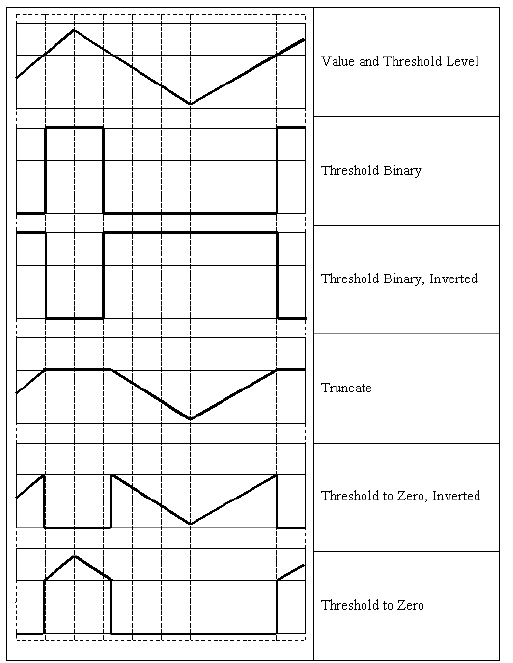
\includegraphics[width=0.5\textwidth]{pics/threshold.png}


\fi

\ifCpp

\cvCppFunc{adaptiveThreshold}
Applies an adaptive threshold to an array.

\cvdefCpp{void adaptiveThreshold( const Mat\& src, Mat\& dst, double maxValue,\par
                        int adaptiveMethod, int thresholdType,\par
                        int blockSize, double C );}
\begin{description}
\cvarg{src}{Source 8-bit single-channel image}
\cvarg{dst}{Destination image; will have the same size and the same type as \texttt{src}}
\cvarg{maxValue}{The non-zero value assigned to the pixels for which the condition is satisfied. See the discussion}
\cvarg{adaptiveMethod}{Adaptive thresholding algorithm to use,
   \texttt{ADAPTIVE\_THRESH\_MEAN\_C} or \texttt{ADAPTIVE\_THRESH\_GAUSSIAN\_C} (see the discussion)}
\cvarg{thresholdType}{Thresholding type; must be one of \texttt{THRESH\_BINARY} or \texttt{THRESH\_BINARY\_INV}}
\cvarg{blockSize}{The size of a pixel neighborhood that is used to calculate a threshold value for the pixel: 3, 5, 7, and so on}
\cvarg{C}{The constant subtracted from the mean or weighted mean (see the discussion); normally, it's positive, but may be zero or negative as well}
\end{description}

The function transforms a grayscale image to a binary image according to the formulas:

\begin{description}
\cvarg{THRESH\_BINARY}{\[ dst(x,y) = \fork{\texttt{maxValue}}{if $src(x,y) > T(x,y)$}{0}{otherwise} \]}
\cvarg{THRESH\_BINARY\_INV}{\[ dst(x,y) = \fork{0}{if $src(x,y) > T(x,y)$}{\texttt{maxValue}}{otherwise} \]}
\end{description}

where $T(x,y)$ is a threshold calculated individually for each pixel.

\begin{enumerate}
    \item
For the method \texttt{ADAPTIVE\_THRESH\_MEAN\_C} the threshold value $T(x,y)$ is the mean of a $\texttt{blockSize} \times \texttt{blockSize}$ neighborhood of $(x, y)$, minus \texttt{C}.
    \item
For the method \texttt{ADAPTIVE\_THRESH\_GAUSSIAN\_C} the threshold value $T(x, y)$ is the weighted sum (i.e. cross-correlation with a Gaussian window) of a $\texttt{blockSize} \times \texttt{blockSize}$ neighborhood of $(x, y)$, minus \texttt{C}. The default sigma (standard deviation) is used for the specified \texttt{blockSize}, see \cvCppCross{getGaussianKernel}.
\end{enumerate}

The function can process the image in-place.

See also: \cvCppCross{threshold}, \cvCppCross{blur}, \cvCppCross{GaussianBlur}


\cvCppFunc{cvtColor}
Converts image from one color space to another

\cvdefCpp{void cvtColor( const Mat\& src, Mat\& dst, int code, int dstCn=0 );}
\begin{description}
\cvarg{src}{The source image, 8-bit unsigned, 16-bit unsigned (\texttt{CV\_16UC...}) or single-precision floating-point}
\cvarg{dst}{The destination image; will have the same size and the same depth as \texttt{src}}
\cvarg{code}{The color space conversion code; see the discussion}
\cvarg{dstCn}{The number of channels in the destination image; if the parameter is 0, the number of the channels will be derived automatically from \texttt{src} and the \texttt{code}}
\end{description}

The function converts the input image from one color
space to another. In the case of transformation to-from RGB color space the ordering of the channels should be specified explicitly (RGB or BGR).

The conventional ranges for R, G and B channel values are:

\begin{itemize}
 \item 0 to 255 for \texttt{CV\_8U} images
 \item 0 to 65535 for \texttt{CV\_16U} images and
 \item 0 to 1 for \texttt{CV\_32F} images.
\end{itemize}

Of course, in the case of linear transformations the range does not matter,
but in the non-linear cases the input RGB image should be normalized to the proper value range in order to get the correct results, e.g. for RGB$\rightarrow$L*u*v* transformation. For example, if you have a 32-bit floating-point image directly converted from 8-bit image without any scaling, then it will have 0..255 value range, instead of the assumed by the function 0..1. So, before calling \texttt{cvtColor}, you need first to scale the image down:
\begin{lstlisting}
img *= 1./255;
cvtColor(img, img, CV_BGR2Luv);
\end{lstlisting}

The function can do the following transformations:

\begin{itemize}
 \item Transformations within RGB space like adding/removing the alpha channel, reversing the channel order, conversion to/from 16-bit RGB color (R5:G6:B5 or R5:G5:B5), as well as conversion to/from grayscale using:
 \[
 \text{RGB[A] to Gray:}\quad Y \leftarrow 0.299 \cdot R + 0.587 \cdot G + 0.114 \cdot B
 \]
 and
 \[
 \text{Gray to RGB[A]:}\quad R \leftarrow Y, G \leftarrow Y, B \leftarrow Y, A \leftarrow 0
 \]

The conversion from a RGB image to gray is done with:
\begin{lstlisting}
cvtColor(src, bwsrc, CV_RGB2GRAY);
\end{lstlisting}

Some more advanced channel reordering can also be done with \cvCppCross{mixChannels}.

 \item RGB $\leftrightarrow$ CIE XYZ.Rec 709 with D65 white point (\texttt{CV\_BGR2XYZ, CV\_RGB2XYZ, CV\_XYZ2BGR, CV\_XYZ2RGB}):
 \[
 \begin{bmatrix}
 X \\
 Y \\
 Z
 \end{bmatrix}
 \leftarrow
 \begin{bmatrix}
0.412453 & 0.357580 & 0.180423\\
0.212671 & 0.715160 & 0.072169\\
0.019334 & 0.119193 & 0.950227
 \end{bmatrix}
 \cdot
 \begin{bmatrix}
 R \\
 G \\
 B
 \end{bmatrix}
 \]
 \[
 \begin{bmatrix}
 R \\
 G \\
 B
 \end{bmatrix}
 \leftarrow
 \begin{bmatrix}
3.240479 & -1.53715 & -0.498535\\
-0.969256 &  1.875991 & 0.041556\\
0.055648 & -0.204043 & 1.057311
 \end{bmatrix}
 \cdot
 \begin{bmatrix}
 X \\
 Y \\
 Z
 \end{bmatrix}
 \]
$X$, $Y$ and $Z$ cover the whole value range (in the case of floating-point images $Z$ may exceed 1).

 \item RGB $\leftrightarrow$ YCrCb JPEG (a.k.a. YCC) (\texttt{CV\_BGR2YCrCb, CV\_RGB2YCrCb, CV\_YCrCb2BGR, CV\_YCrCb2RGB})
 \[ Y \leftarrow 0.299 \cdot R + 0.587 \cdot G + 0.114 \cdot B \]
 \[  Cr \leftarrow (R-Y) \cdot 0.713 + delta \]
 \[  Cb \leftarrow (B-Y) \cdot 0.564 + delta \]
 \[  R \leftarrow Y + 1.403 \cdot (Cr - delta) \]
 \[  G \leftarrow Y - 0.344 \cdot (Cr - delta) - 0.714 \cdot (Cb - delta) \]
 \[  B \leftarrow Y + 1.773 \cdot (Cb - delta) \]
where
 \[
  delta = \left\{
  \begin{array}{l l}
  128 & \mbox{for 8-bit images}\\
  32768 & \mbox{for 16-bit images}\\
  0.5 & \mbox{for floating-point images}
  \end{array} \right.
 \]
Y, Cr and Cb cover the whole value range.

 \item RGB $\leftrightarrow$ HSV (\texttt{CV\_BGR2HSV, CV\_RGB2HSV, CV\_HSV2BGR, CV\_HSV2RGB})
  in the case of 8-bit and 16-bit images
  R, G and B are converted to floating-point format and scaled to fit the 0 to 1 range
  \[ V \leftarrow max(R,G,B) \]

\[ S \leftarrow \fork{\frac{V-min(R,G,B)}{V}}{if $V \neq 0$}{0}{otherwise} \]
\[ H \leftarrow \forkthree
{{60(G - B)}/{S}}{if $V=R$}
{{120+60(B - R)}/{S}}{if $V=G$}
{{240+60(R - G)}/{S}}{if $V=B$} \]
if $H<0$ then $H \leftarrow H+360$

On output $0 \leq V \leq 1$, $0 \leq S \leq 1$, $0 \leq H \leq 360$.

The values are then converted to the destination data type:
\begin{description}
\item[8-bit images]
\[ V \leftarrow 255 V, S \leftarrow 255 S, H \leftarrow H/2 \text{(to fit to 0 to 255)} \]
\item[16-bit images (currently not supported)]
\[ V <- 65535 V, S <- 65535 S, H <- H \]
\item[32-bit images]
H, S, V are left as is
\end{description}

 \item RGB $\leftrightarrow$ HLS (\texttt{CV\_BGR2HLS, CV\_RGB2HLS, CV\_HLS2BGR, CV\_HLS2RGB}).
  in the case of 8-bit and 16-bit images
  R, G and B are converted to floating-point format and scaled to fit the 0 to 1 range.
  \[ V_{max} \leftarrow {max}(R,G,B) \]
  \[ V_{min} \leftarrow {min}(R,G,B) \]
  \[ L \leftarrow \frac{V_{max} - V_{min}}{2} \]
  \[ S \leftarrow \fork
    {\frac{V_{max} - V_{min}}{V_{max} + V_{min}}}{if $L < 0.5$}
    {\frac{V_{max} - V_{min}}{2 - (V_{max} + V_{min})}}{if $L \ge 0.5$} \]
  \[ H \leftarrow \forkthree
  {{60(G - B)}/{S}}{if $V_{max}=R$}
  {{120+60(B - R)}/{S}}{if $V_{max}=G$}
  {{240+60(R - G)}/{S}}{if $V_{max}=B$} \]
  if $H<0$ then $H \leftarrow H+360$
On output $0 \leq V \leq 1$, $0 \leq S \leq 1$, $0 \leq H \leq 360$.

The values are then converted to the destination data type:
\begin{description}
\item[8-bit images]
\[ V \leftarrow 255\cdot V, S \leftarrow 255\cdot S, H \leftarrow H/2\; \text{(to fit to 0 to 255)} \]
\item[16-bit images (currently not supported)]
\[ V <- 65535\cdot V, S <- 65535\cdot S, H <- H \]
\item[32-bit images]
H, S, V are left as is
\end{description}

 \item RGB $\leftrightarrow$ CIE L*a*b* (\texttt{CV\_BGR2Lab, CV\_RGB2Lab, CV\_Lab2BGR, CV\_Lab2RGB})
  in the case of 8-bit and 16-bit images
  R, G and B are converted to floating-point format and scaled to fit the 0 to 1 range
\[ \vecthree{X}{Y}{Z} \leftarrow \vecthreethree
{0.412453}{0.357580}{0.180423}
{0.212671}{0.715160}{0.072169}
{0.019334}{0.119193}{0.950227}
\cdot
\vecthree{R}{G}{B} \]
\[ X \leftarrow X/X_n, \text{where} X_n = 0.950456 \]
\[ Z \leftarrow Z/Z_n, \text{where} Z_n = 1.088754 \]
\[ L \leftarrow \fork
{116*Y^{1/3}-16}{for $Y>0.008856$}
{903.3*Y}{for $Y \le 0.008856$} \]
\[ a \leftarrow 500 (f(X)-f(Y)) + delta \]
\[ b \leftarrow 200 (f(Y)-f(Z)) + delta \]
where
\[f(t)=\fork
{t^{1/3}}{for $t>0.008856$}
{7.787 t+16/116}{for $t\leq 0.008856$} \]
and
\[ delta = \fork{128}{for 8-bit images}{0}{for floating-point images} \]
On output $0 \leq L \leq 100$, $-127 \leq a \leq 127$, $-127 \leq b \leq 127$

The values are then converted to the destination data type:
\begin{description}
\item[8-bit images]
\[L \leftarrow L*255/100,\; a \leftarrow a + 128,\; b \leftarrow b + 128\]
\item[16-bit images] currently not supported
\item[32-bit images]
L, a, b are left as is
\end{description}

 \item RGB $\leftrightarrow$ CIE L*u*v* (\texttt{CV\_BGR2Luv, CV\_RGB2Luv, CV\_Luv2BGR, CV\_Luv2RGB})
  in the case of 8-bit and 16-bit images
  R, G and B are converted to floating-point format and scaled to fit 0 to 1 range
  \[ \vecthree{X}{Y}{Z} \leftarrow \vecthreethree
{0.412453}{0.357580}{0.180423}
{0.212671}{0.715160}{0.072169}
{0.019334}{0.119193}{0.950227}
\cdot
\vecthree{R}{G}{B} \]
\[ L \leftarrow \fork
{116 Y^{1/3}}{for $Y>0.008856$}
{903.3 Y}{for $Y\leq 0.008856$} \]
\[ u' \leftarrow 4*X/(X + 15*Y + 3 Z) \]
\[ v' \leftarrow 9*Y/(X + 15*Y + 3 Z) \]
\[ u \leftarrow 13*L*(u' - u_n) \quad \text{where} \quad u_n=0.19793943 \]
\[ v \leftarrow 13*L*(v' - v_n) \quad \text{where} \quad v_n=0.46831096 \]
On output $0 \leq L \leq 100$, $-134 \leq u \leq 220$, $-140 \leq v \leq 122$.

The values are then converted to the destination data type:
\begin{description}
\item[8-bit images]
\[L \leftarrow 255/100 L,\; u \leftarrow 255/354 (u + 134),\; v \leftarrow 255/256 (v + 140) \]
\item[16-bit images] currently not supported
\item[32-bit images] L, u, v are left as is
\end{description}

The above formulas for converting RGB to/from various color spaces have been taken from multiple sources on Web, primarily from the Charles Poynton site \url{http://www.poynton.com/ColorFAQ.html}

 \item Bayer $\rightarrow$ RGB (\texttt{CV\_BayerBG2BGR, CV\_BayerGB2BGR, CV\_BayerRG2BGR, CV\_BayerGR2BGR, CV\_BayerBG2RGB, CV\_BayerGB2RGB, CV\_BayerRG2RGB, CV\_BayerGR2RGB}) The Bayer pattern is widely used in CCD and CMOS cameras. It allows one to get color pictures from a single plane where R,G and B pixels (sensors of a particular component) are interleaved like this:

\[
\newcommand{\Rcell}{\color{red}R}
\newcommand{\Gcell}{\color{green}G}
\newcommand{\Bcell}{\color{blue}B}
\definecolor{BackGray}{rgb}{0.8,0.8,0.8}
\begin{array}{ c c c c c }
\Rcell&\Gcell&\Rcell&\Gcell&\Rcell\\
\Gcell&\colorbox{BackGray}{\Bcell}&\colorbox{BackGray}{\Gcell}&\Bcell&\Gcell\\
\Rcell&\Gcell&\Rcell&\Gcell&\Rcell\\
\Gcell&\Bcell&\Gcell&\Bcell&\Gcell\\
\Rcell&\Gcell&\Rcell&\Gcell&\Rcell
\end{array}
\]

The output RGB components of a pixel are interpolated from 1, 2 or
4 neighbors of the pixel having the same color. There are several
modifications of the above pattern that can be achieved by shifting
the pattern one pixel left and/or one pixel up. The two letters
$C_1$ and $C_2$
in the conversion constants
\texttt{CV\_Bayer} $ C_1 C_2 $ \texttt{2BGR}
and
\texttt{CV\_Bayer} $ C_1 C_2 $ \texttt{2RGB}
indicate the particular pattern
type - these are components from the second row, second and third
columns, respectively. For example, the above pattern has very
popular "BG" type.
\end{itemize}



\cvCppFunc{distanceTransform}
Calculates the distance to the closest zero pixel for each pixel of the source image.

\cvdefCpp{void distanceTransform( const Mat\& src, Mat\& dst,\par
                        int distanceType, int maskSize );\newline
void distanceTransform( const Mat\& src, Mat\& dst, Mat\& labels,\par
                        int distanceType, int maskSize );}
\begin{description}
\cvarg{src}{8-bit, single-channel (binary) source image}
\cvarg{dst}{Output image with calculated distances; will be 32-bit floating-point, single-channel image of the same size as \texttt{src}}
\cvarg{distanceType}{Type of distance; can be \texttt{CV\_DIST\_L1, CV\_DIST\_L2} or \texttt{CV\_DIST\_C}}
\cvarg{maskSize}{Size of the distance transform mask; can be 3, 5 or \texttt{CV\_DIST\_MASK\_PRECISE} (the latter option is only supported by the first of the functions). In the case of \texttt{CV\_DIST\_L1} or \texttt{CV\_DIST\_C} distance type the parameter is forced to 3, because a $3\times 3$ mask gives the same result as a $5\times 5$ or any larger aperture.}
\cvarg{labels}{The optional output 2d array of labels - the discrete Voronoi diagram; will have type \texttt{CV\_32SC1} and the same size as \texttt{src}. See the discussion}
\end{description}

The functions \texttt{distanceTransform} calculate the approximate or precise
distance from every binary image pixel to the nearest zero pixel.
(for zero image pixels the distance will obviously be zero).

When \texttt{maskSize == CV\_DIST\_MASK\_PRECISE} and \texttt{distanceType == CV\_DIST\_L2}, the function runs the algorithm described in \cite{Felzenszwalb04}.

In other cases the algorithm \cite{Borgefors86} is used, that is,
for pixel the function finds the shortest path to the nearest zero pixel
consisting of basic shifts: horizontal,
vertical, diagonal or knight's move (the latest is available for a
$5\times 5$ mask). The overall distance is calculated as a sum of these
basic distances. Because the distance function should be symmetric,
all of the horizontal and vertical shifts must have the same cost (that
is denoted as \texttt{a}), all the diagonal shifts must have the
same cost (denoted \texttt{b}), and all knight's moves must have
the same cost (denoted \texttt{c}). For \texttt{CV\_DIST\_C} and
\texttt{CV\_DIST\_L1} types the distance is calculated precisely,
whereas for \texttt{CV\_DIST\_L2} (Euclidian distance) the distance
can be calculated only with some relative error (a $5\times 5$ mask
gives more accurate results). For \texttt{a}, \texttt{b} and \texttt{c}
OpenCV uses the values suggested in the original paper:


\begin{tabular}{| c | c | c |}
\hline
\texttt{CV\_DIST\_C}  & $(3\times 3)$ & a = 1, b = 1\\ \hline
\texttt{CV\_DIST\_L1} & $(3\times 3)$ & a = 1, b = 2\\ \hline
\texttt{CV\_DIST\_L2} & $(3\times 3)$ & a=0.955, b=1.3693\\ \hline
\texttt{CV\_DIST\_L2} & $(5\times 5)$ & a=1, b=1.4, c=2.1969\\ \hline
\end{tabular}


Typically, for a fast, coarse distance estimation \texttt{CV\_DIST\_L2},
a $3\times 3$ mask is used, and for a more accurate distance estimation
\texttt{CV\_DIST\_L2}, a $5\times 5$ mask or the precise algorithm is used.
Note that both the precise and the approximate algorithms are linear on the number of pixels.

The second variant of the function does not only compute the minimum distance for each pixel $(x, y)$,
but it also identifies the nearest the nearest connected
component consisting of zero pixels. Index of the component is stored in $\texttt{labels}(x, y)$.
The connected components of zero pixels are also found and marked by the function.

In this mode the complexity is still linear.
That is, the function provides a very fast way to compute Voronoi diagram for the binary image.
Currently, this second variant can only use the approximate distance transform algorithm.


\cvCppFunc{floodFill}
Fills a connected component with the given color.

\cvdefCpp{int floodFill( Mat\& image,\par
               Point seed, Scalar newVal, Rect* rect=0,\par
               Scalar loDiff=Scalar(), Scalar upDiff=Scalar(),\par
               int flags=4 );\newline
int floodFill( Mat\& image, Mat\& mask,\par
               Point seed, Scalar newVal, Rect* rect=0,\par
               Scalar loDiff=Scalar(), Scalar upDiff=Scalar(),\par
               int flags=4 );}
\begin{description}
\cvarg{image}{Input/output 1- or 3-channel, 8-bit or floating-point image. It is modified by the function unless the \texttt{FLOODFILL\_MASK\_ONLY} flag is set (in the second variant of the function; see below)}
\cvarg{mask}{(For the second function only) Operation mask, should be a single-channel 8-bit image, 2 pixels wider and 2 pixels taller. The function uses and updates the mask, so the user takes responsibility of initializing the \texttt{mask} content. Flood-filling can't go across non-zero pixels in the mask, for example, an edge detector output can be used as a mask to stop filling at edges. It is possible to use the same mask in multiple calls to the function to make sure the filled area do not overlap. \textbf{Note}: because the mask is larger than the filled image, a pixel $(x, y)$ in \texttt{image} will correspond to the pixel $(x+1, y+1)$ in the \texttt{mask}}
\cvarg{seed}{The starting point}
\cvarg{newVal}{New value of the repainted domain pixels}
\cvarg{loDiff}{Maximal lower brightness/color difference between the currently observed pixel and one of its neighbors belonging to the component, or a seed pixel being added to the component}
\cvarg{upDiff}{Maximal upper brightness/color difference between the currently observed pixel and one of its neighbors belonging to the component, or a seed pixel being added to the component}
\cvarg{rect}{The optional output parameter that the function sets to the minimum bounding rectangle of the repainted domain}
\cvarg{flags}{The operation flags. Lower bits contain connectivity value, 4 (by default) or 8, used within the function. Connectivity determines which neighbors of a pixel are considered. Upper bits can be 0 or a combination of the following flags:
\begin{description}
  \cvarg{FLOODFILL\_FIXED\_RANGE}{if set, the difference between the current pixel and seed pixel is considered, otherwise the difference between neighbor pixels is considered (i.e. the range is floating)}
  \cvarg{FLOODFILL\_MASK\_ONLY}{(for the second variant only) if set, the function does not change the image (\texttt{newVal} is ignored), but fills the mask}
\end{description}}
\end{description}

The functions \texttt{floodFill} fill a connected component starting from the seed point with the specified color. The connectivity is determined by the color/brightness closeness of the neighbor pixels. The pixel at $(x,y)$ is considered to belong to the repainted domain if:

\begin{description}

\item[grayscale image, floating range] \[
\texttt{src}(x',y')-\texttt{loDiff} \leq \texttt{src}(x,y) \leq \texttt{src}(x',y')+\texttt{upDiff} \]

\item[grayscale image, fixed range] \[
\texttt{src}(\texttt{seed}.x,\texttt{seed}.y)-\texttt{loDiff}\leq \texttt{src}(x,y) \leq \texttt{src}(\texttt{seed}.x,\texttt{seed}.y)+\texttt{upDiff} \]

\item[color image, floating range]
\[ \texttt{src}(x',y')_r-\texttt{loDiff}_r\leq \texttt{src}(x,y)_r\leq \texttt{src}(x',y')_r+\texttt{upDiff}_r \]
\[ \texttt{src}(x',y')_g-\texttt{loDiff}_g\leq \texttt{src}(x,y)_g\leq \texttt{src}(x',y')_g+\texttt{upDiff}_g \]
\[ \texttt{src}(x',y')_b-\texttt{loDiff}_b\leq \texttt{src}(x,y)_b\leq \texttt{src}(x',y')_b+\texttt{upDiff}_b \]

\item[color image, fixed range]
\[ \texttt{src}(\texttt{seed}.x,\texttt{seed}.y)_r-\texttt{loDiff}_r\leq \texttt{src}(x,y)_r\leq \texttt{src}(\texttt{seed}.x,\texttt{seed}.y)_r+\texttt{upDiff}_r \]
\[ \texttt{src}(\texttt{seed}.x,\texttt{seed}.y)_g-\texttt{loDiff}_g\leq \texttt{src}(x,y)_g\leq \texttt{src}(\texttt{seed}.x,\texttt{seed}.y)_g+\texttt{upDiff}_g \]
\[ \texttt{src}(\texttt{seed}.x,\texttt{seed}.y)_b-\texttt{loDiff}_b\leq \texttt{src}(x,y)_b\leq \texttt{src}(\texttt{seed}.x,\texttt{seed}.y)_b+\texttt{upDiff}_b \]
\end{description}

where $src(x',y')$ is the value of one of pixel neighbors that is already known to belong to the component. That is, to be added to the connected component, a pixel's color/brightness should be close enough to the:
\begin{itemize}
  \item color/brightness of one of its neighbors that are already referred to the connected component in the case of floating range
  \item color/brightness of the seed point in the case of fixed range.
\end{itemize}

By using these functions you can either mark a connected component with the specified color in-place, or build a mask and then extract the contour or copy the region to another image etc. Various modes of the function are demonstrated in \texttt{floodfill.c} sample.

See also: \cvCppCross{findContours}


\cvCppFunc{inpaint}
Inpaints the selected region in the image.

\cvdefCpp{void inpaint( const Mat\& src, const Mat\& inpaintMask,\par
              Mat\& dst, double inpaintRadius, int flags );}

\begin{description}
\cvarg{src}{The input 8-bit 1-channel or 3-channel image.}
\cvarg{inpaintMask}{The inpainting mask, 8-bit 1-channel image. Non-zero pixels indicate the area that needs to be inpainted.}
\cvarg{dst}{The output image; will have the same size and the same type as \texttt{src}}
\cvarg{inpaintRadius}{The radius of a circlular neighborhood of each point inpainted that is considered by the algorithm.}
\cvarg{flags}{The inpainting method, one of the following:
\begin{description}
\cvarg{INPAINT\_NS}{Navier-Stokes based method.}
\cvarg{INPAINT\_TELEA}{The method by Alexandru Telea \cite{Telea04}}
\end{description}}
\end{description}

The function reconstructs the selected image area from the pixel near the area boundary. The function may be used to remove dust and scratches from a scanned photo, or to remove undesirable objects from still images or video. See \url{http://en.wikipedia.org/wiki/Inpainting} for more details.


\cvCppFunc{integral}
Calculates the integral of an image.

\cvdefCpp{void integral( const Mat\& image, Mat\& sum, int sdepth=-1 );\newline
void integral( const Mat\& image, Mat\& sum, Mat\& sqsum, int sdepth=-1 );\newline
void integral( const Mat\& image, Mat\& sum, \par Mat\& sqsum, Mat\& tilted, int sdepth=-1 );}
\begin{description}
\cvarg{image}{The source image, $W \times H$, 8-bit or floating-point (32f or 64f)}
\cvarg{sum}{The integral image, $(W+1)\times (H+1)$, 32-bit integer or floating-point (32f or 64f)}
\cvarg{sqsum}{The integral image for squared pixel values, $(W+1)\times (H+1)$, double precision floating-point (64f)}
\cvarg{tilted}{The integral for the image rotated by 45 degrees, $(W+1)\times (H+1)$, the same data type as \texttt{sum}}
\cvarg{sdepth}{The desired depth of the integral and the tilted integral images, \texttt{CV\_32S},  \texttt{CV\_32F} or \texttt{CV\_64F}}
\end{description}

The functions \texttt{integral} calculate one or more integral images for the source image as following:

\[
\texttt{sum}(X,Y) = \sum_{x<X,y<Y} \texttt{image}(x,y)
\]

\[
\texttt{sqsum}(X,Y) = \sum_{x<X,y<Y} \texttt{image}(x,y)^2
\]

\[
\texttt{tilted}(X,Y) = \sum_{y<Y,abs(x-X+1)\leq Y-y-1} \texttt{image}(x,y)
\]

Using these integral images, one may calculate sum, mean and standard deviation over a specific up-right or rotated rectangular region of the image in a constant time, for example:

\[
\sum_{x_1\leq x < x_2, \, y_1 \leq y < y_2} \texttt{image}(x,y) = \texttt{sum}(x_2,y_2)-\texttt{sum}(x_1,y_2)-\texttt{sum}(x_2,y_1)+\texttt{sum}(x_1,x_1)
\]

It makes possible to do a fast blurring or fast block correlation with variable window size, for example. In the case of multi-channel images, sums for each channel are accumulated independently.

As a practical example, the next figure shows the calculation of the integral of a straight rectangle \texttt{Rect(3,3,3,2)} and of a tilted rectangle \texttt{Rect(5,1,2,3)}. The selected pixels in the original \texttt{image} are shown, as well as the relative pixels in the integral images \texttt{sum} and \texttt{tilted}.
 
\begin{center}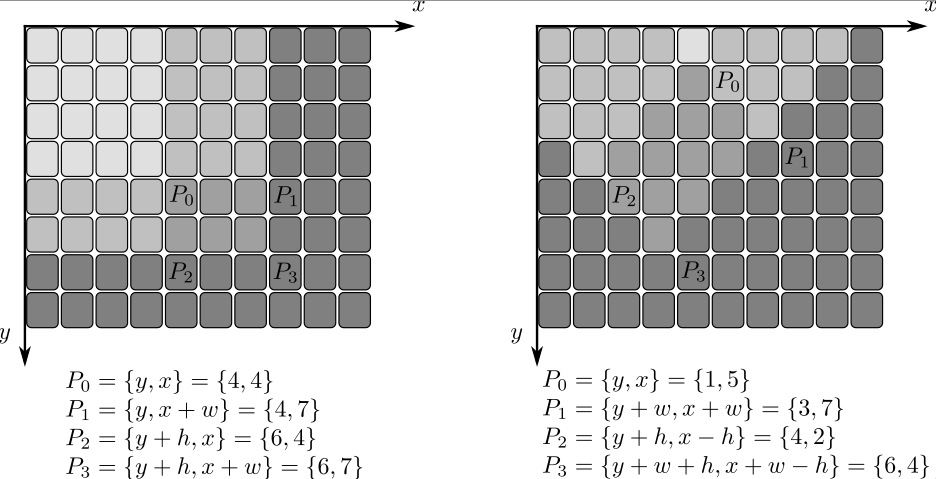
\includegraphics[width=0.8\textwidth]{pics/integral.png}\end{center}

\cvCppFunc{threshold}
Applies a fixed-level threshold to each array element

\cvdefCpp{double threshold( const Mat\& src, Mat\& dst, double thresh,\par
                  double maxVal, int thresholdType );}
\begin{description}
\cvarg{src}{Source array (single-channel, 8-bit of 32-bit floating point)}
\cvarg{dst}{Destination array; will have the same size and the same type as \texttt{src}}
\cvarg{thresh}{Threshold value}
\cvarg{maxVal}{Maximum value to use with \texttt{THRESH\_BINARY} and \texttt{THRESH\_BINARY\_INV} thresholding types}
\cvarg{thresholdType}{Thresholding type (see the discussion)}
\end{description}

The function applies fixed-level thresholding
to a single-channel array. The function is typically used to get a
bi-level (binary) image out of a grayscale image (\cvCppCross{compare} could
be also used for this purpose) or for removing a noise, i.e. filtering
out pixels with too small or too large values. There are several
types of thresholding that the function supports that are determined by
\texttt{thresholdType}:

\begin{description}
\cvarg{THRESH\_BINARY}{\[ \texttt{dst}(x,y) = \fork{\texttt{maxVal}}{if $\texttt{src}(x,y) > \texttt{thresh}$}{0}{otherwise} \]}
\cvarg{THRESH\_BINARY\_INV}{\[ \texttt{dst}(x,y) = \fork{0}{if $\texttt{src}(x,y) > \texttt{thresh}$}{\texttt{maxVal}}{otherwise} \]}
\cvarg{THRESH\_TRUNC}{\[ \texttt{dst}(x,y) = \fork{\texttt{threshold}}{if $\texttt{src}(x,y) > \texttt{thresh}$}{\texttt{src}(x,y)}{otherwise} \]}
\cvarg{THRESH\_TOZERO}{\[ \texttt{dst}(x,y) = \fork{\texttt{src}(x,y)}{if $\texttt{src}(x,y) > \texttt{thresh}$}{0}{otherwise} \]}
\cvarg{THRESH\_TOZERO\_INV}{\[ \texttt{dst}(x,y) = \fork{0}{if $\texttt{src}(x,y) > \texttt{thresh}$}{\texttt{src}(x,y)}{otherwise} \]}
\end{description}

Also, the special value \texttt{THRESH\_OTSU} may be combined with
one of the above values. In this case the function determines the optimal threshold
value using Otsu's algorithm and uses it instead of the specified \texttt{thresh}.
The function returns the computed threshold value.
Currently, Otsu's method is implemented only for 8-bit images.

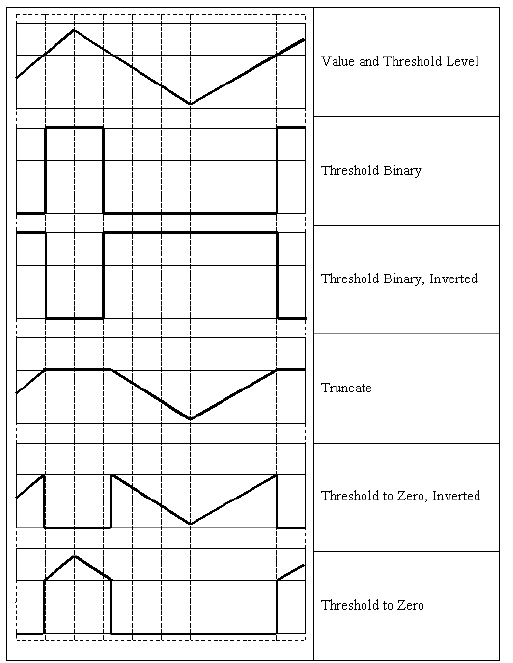
\includegraphics[width=0.5\textwidth]{pics/threshold.png}

See also: \cvCppCross{adaptiveThreshold}, \cvCppCross{findContours}, \cvCppCross{compare}, \cvCppCross{min}, \cvCppCross{max}

\cvCppFunc{watershed}
Does marker-based image segmentation using watershed algrorithm

\cvdefCpp{void watershed( const Mat\& image, Mat\& markers );}
\begin{description}
\cvarg{image}{The input 8-bit 3-channel image.} 
\cvarg{markers}{The input/output 32-bit single-channel image (map) of markers. It should have the same size as \texttt{image}}
\end{description}

The function implements one of the variants
of watershed, non-parametric marker-based segmentation algorithm,
described in \cite{Meyer92}. Before passing the image to the
function, user has to outline roughly the desired regions in the image
\texttt{markers} with positive ($>0$) indices, i.e. every region is
represented as one or more connected components with the pixel values
1, 2, 3 etc (such markers can be retrieved from a binary mask
using \cvCppCross{findContours}and \cvCppCross{drawContours}, see \texttt{watershed.cpp} demo).
The markers will be "seeds" of the future image
regions. All the other pixels in \texttt{markers}, which relation to the
outlined regions is not known and should be defined by the algorithm,
should be set to 0's. On the output of the function, each pixel in
markers is set to one of values of the "seed" components, or to -1 at
boundaries between the regions.

Note, that it is not necessary that every two neighbor connected
components are separated by a watershed boundary (-1's pixels), for
example, in case when such tangent components exist in the initial
marker image. Visual demonstration and usage example of the function
can be found in OpenCV samples directory; see \texttt{watershed.cpp} demo.

See also: \cvCppCross{findContours}

\fi

\section{Histograms}

\ifCPy

\ifC
\cvfunc{CvHistogram}\label{CvHistogram}
Multi-dimensional histogram.

\begin{lstlisting}
typedef struct CvHistogram
{
    int     type;
    CvArr*  bins;
    float   thresh[CV_MAX_DIM][2]; /* for uniform histograms */
    float** thresh2; /* for non-uniform histograms */
    CvMatND mat; /* embedded matrix header for array histograms */
}
CvHistogram;
\end{lstlisting}
\fi

\cvCPyFunc{CalcBackProject}
Calculates the back projection.

\cvdefC{
void cvCalcBackProject( \par IplImage** image,\par CvArr* back\_project,\par const CvHistogram* hist );
}\cvdefPy{CalcBackProject(image,back\_project,hist)-> None}

\begin{description}
\cvarg{image}{Source images (though you may pass CvMat** as well)}
\cvarg{back\_project}{Destination back projection image of the same type as the source images}
\cvarg{hist}{Histogram}
\end{description}

The function calculates the back project of the histogram. For each tuple of pixels at the same position of all input single-channel images the function puts the value of the histogram bin, corresponding to the tuple in the destination image. In terms of statistics, the value of each output image pixel is the probability of the observed tuple given the distribution (histogram). For example, to find a red object in the picture, one may do the following:

\begin{enumerate}
 \item Calculate a hue histogram for the red object assuming the image contains only this object. The histogram is likely to have a strong maximum, corresponding to red color.
 \item Calculate back projection of a hue plane of input image where the object is searched, using the histogram. Threshold the image.
 \item Find connected components in the resulting picture and choose the right component using some additional criteria, for example, the largest connected component.
\end{enumerate}

That is the approximate algorithm of Camshift color object tracker, except for the 3rd step, instead of which CAMSHIFT algorithm is used to locate the object on the back projection given the previous object position.

\cvCPyFunc{CalcBackProjectPatch}
Locates a template within an image by using a histogram comparison.

\cvdefC{
void cvCalcBackProjectPatch( \par IplImage** image,\par CvArr* dst,\par CvSize patch\_size,\par CvHistogram* hist,\par int method,\par float factor );
}\cvdefPy{CalcBackProjectPatch(images,dst,patch\_size,hist,method,factor)-> None}

\begin{description}
\cvarg{image}{Source images (though, you may pass CvMat** as well)}
\cvarg{dst}{Destination image}
\cvarg{patch\_size}{Size of the patch slid though the source image}
\cvarg{hist}{Histogram}
\cvarg{method}{Compasion method, passed to \cvCPyCross{CompareHist} (see description of that function)}
\cvarg{factor}{Normalization factor for histograms, will affect the normalization scale of the destination image, pass 1 if unsure}
\end{description}

The function calculates the back projection by comparing histograms of the source image patches with the given histogram. Taking measurement results from some image at each location over ROI creates an array \texttt{image}. These results might be one or more of hue, \texttt{x} derivative, \texttt{y} derivative, Laplacian filter, oriented Gabor filter, etc. Each measurement output is collected into its own separate image. The \texttt{image} image array is a collection of these measurement images. A multi-dimensional histogram \texttt{hist} is constructed by sampling from the \texttt{image} image array. The final histogram is normalized. The \texttt{hist} histogram has as many dimensions as the number of elements in \texttt{image} array.

Each new image is measured and then converted into an \texttt{image} image array over a chosen ROI. Histograms are taken from this \texttt{image} image in an area covered by a "patch" with an anchor at center as shown in the picture below. The histogram is normalized using the parameter \texttt{norm\_factor} so that it may be compared with \texttt{hist}. The calculated histogram is compared to the model histogram; \texttt{hist} uses The function \texttt{cvCompareHist} with the comparison method=\texttt{method}). The resulting output is placed at the location corresponding to the patch anchor in the probability image \texttt{dst}. This process is repeated as the patch is slid over the ROI. Iterative histogram update by subtracting trailing pixels covered by the patch and adding newly covered pixels to the histogram can save a lot of operations, though it is not implemented yet.

\cvfunc{Back Project Calculation by Patches}

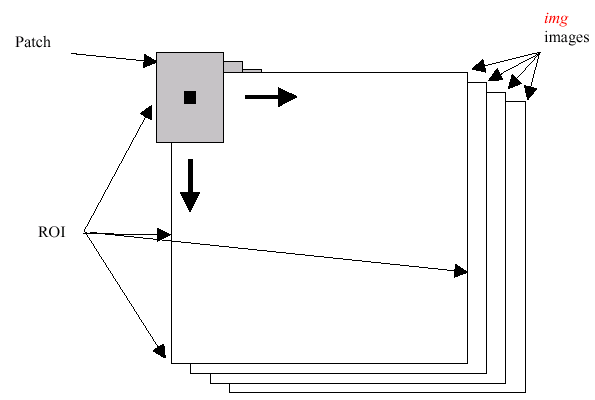
\includegraphics[width=0.5\textwidth]{pics/backprojectpatch.png}

\cvCPyFunc{CalcHist}
Calculates the histogram of image(s).

\cvdefC{
void cvCalcHist( \par IplImage** image,\par CvHistogram* hist,\par int accumulate=0,\par const CvArr* mask=NULL );
}\cvdefPy{CalcHist(image,hist,ccumulate=0,mask=NULL)-> None}

\begin{description}
\cvarg{image}{Source images (though you may pass CvMat** as well)}
\cvarg{hist}{Pointer to the histogram}
\cvarg{accumulate}{Accumulation flag. If it is set, the histogram is not cleared in the beginning. This feature allows user to compute a single histogram from several images, or to update the histogram online}
\cvarg{mask}{The operation mask, determines what pixels of the source images are counted}
\end{description}

The function calculates the histogram of one or more
single-channel images. The elements of a tuple that is used to increment
a histogram bin are taken at the same location from the corresponding
input images.

% ===== Sample. Calculating and displaying 2D Hue-Saturation histogram of a color image =====
\begin{lstlisting}
#include <cv.h>
#include <highgui.h>

int main( int argc, char** argv )
{
    IplImage* src;
    if( argc == 2 && (src=cvLoadImage(argv[1], 1))!= 0)
    {
        IplImage* h_plane = cvCreateImage( cvGetSize(src), 8, 1 );
        IplImage* s_plane = cvCreateImage( cvGetSize(src), 8, 1 );
        IplImage* v_plane = cvCreateImage( cvGetSize(src), 8, 1 );
        IplImage* planes[] = { h_plane, s_plane };
        IplImage* hsv = cvCreateImage( cvGetSize(src), 8, 3 );
        int h_bins = 30, s_bins = 32;
        int hist_size[] = {h_bins, s_bins};
        /* hue varies from 0 (~0 deg red) to 180 (~360 deg red again) */
        float h_ranges[] = { 0, 180 };
        /* saturation varies from 0 (black-gray-white) to
           255 (pure spectrum color) */
        float s_ranges[] = { 0, 255 };
        float* ranges[] = { h_ranges, s_ranges };
        int scale = 10;
        IplImage* hist_img =
            cvCreateImage( cvSize(h_bins*scale,s_bins*scale), 8, 3 );
        CvHistogram* hist;
        float max_value = 0;
        int h, s;

        cvCvtColor( src, hsv, CV_BGR2HSV );
        cvCvtPixToPlane( hsv, h_plane, s_plane, v_plane, 0 );
        hist = cvCreateHist( 2, hist_size, CV_HIST_ARRAY, ranges, 1 );
        cvCalcHist( planes, hist, 0, 0 );
        cvGetMinMaxHistValue( hist, 0, &max_value, 0, 0 );
        cvZero( hist_img );

        for( h = 0; h < h_bins; h++ )
        {
            for( s = 0; s < s_bins; s++ )
            {
                float bin_val = cvQueryHistValue_2D( hist, h, s );
                int intensity = cvRound(bin_val*255/max_value);
                cvRectangle( hist_img, cvPoint( h*scale, s*scale ),
                             cvPoint( (h+1)*scale - 1, (s+1)*scale - 1),
                             CV_RGB(intensity,intensity,intensity),
                             CV_FILLED );
            }
        }

        cvNamedWindow( "Source", 1 );
        cvShowImage( "Source", src );

        cvNamedWindow( "H-S Histogram", 1 );
        cvShowImage( "H-S Histogram", hist_img );

        cvWaitKey(0);
    }
}
\end{lstlisting}

\cvCPyFunc{CalcProbDensity}
Divides one histogram by another.

\cvdefC{
void  cvCalcProbDensity( \par const CvHistogram* hist1,\par const CvHistogram* hist2,\par CvHistogram* dst\_hist,\par double scale=255 );
}\cvdefPy{CalcProbDensity(hist1,hist2,dst\_hst,scale=255)-> None}

\begin{description}
\cvarg{hist1}{first histogram (the divisor)}
\cvarg{hist2}{second histogram}
\cvarg{dst\_hist}{destination histogram}
\cvarg{scale}{scale factor for the destination histogram}
\end{description}

The function calculates the object probability density from the two histograms as:

\[
\texttt{dist\_hist}(I)=
\forkthree
{0}{if $\texttt{hist1}(I)=0$}
{\texttt{scale}}{if $\texttt{hist1}(I) \ne 0$ and $\texttt{hist2}(I) > \texttt{hist1}(I)$}
{\frac{\texttt{hist2}(I) \cdot \texttt{scale}}{\texttt{hist1}(I)}}{if $\texttt{hist1}(I) \ne 0$ and $\texttt{hist2}(I) \le \texttt{hist1}(I)$}
\]

So the destination histogram bins are within less than \texttt{scale}.

\cvCPyFunc{ClearHist}
Clears the histogram.

\cvdefC{
void cvClearHist( CvHistogram* hist );
}\cvdefPy{ClearHist(hist)-> None}

\begin{description}
\cvarg{hist}{Histogram}
\end{description}

The function sets all of the histogram bins to 0 in the case of a dense histogram and removes all histogram bins in the case of a sparse array.

\cvCPyFunc{CompareHist}
Compares two dense histograms.

\cvdefC{
double cvCompareHist( \par const CvHistogram* hist1,\par const CvHistogram* hist2,\par int method );
}\cvdefPy{CompareHist(hist1,hist2,method)->float}

\begin{description}
\cvarg{hist1}{The first dense histogram}
\cvarg{hist2}{The second dense histogram}
\cvarg{method}{Comparison method, one of the following:
\begin{description}
  \cvarg{CV\_COMP\_CORREL}{Correlation}
  \cvarg{CV\_COMP\_CHISQR}{Chi-Square}
  \cvarg{CV\_COMP\_INTERSECT}{Intersection}
  \cvarg{CV\_COMP\_BHATTACHARYYA}{Bhattacharyya distance}
\end{description}}
\end{description}

The function compares two dense histograms using the specified method ($H_1$ denotes the first histogram, $H_2$ the second):

\begin{description}
\item[Correlation (method=CV\_COMP\_CORREL)]
\[
d(H_1,H_2) = \frac
{\sum_I (H'_1(I) \cdot H'_2(I))}
{\sqrt{\sum_I(H'_1(I)^2) \cdot \sum_I(H'_2(I)^2)}}
\]
where
\[
H'_k(I) = \frac{H_k(I) - 1}{N \cdot \sum_J H_k(J)}
\]
where N is the number of histogram bins.

\item[Chi-Square (method=CV\_COMP\_CHISQR)]
\[ d(H_1,H_2) = \sum_I \frac{(H_1(I)-H_2(I))^2}{H_1(I)+H_2(I)} \]

\item[Intersection (method=CV\_COMP\_INTERSECT)]
\[ d(H_1,H_2) = \sum_I \min (H_1(I), H_2(I)) \]

\item[Bhattacharyya distance (method=CV\_COMP\_BHATTACHARYYA)]
\[ d(H_1,H_2) = \sqrt{1 - \sum_I \frac{\sqrt{H_1(I) \cdot H_2(I)}}{ \sqrt { \sum_I H_1(I) \cdot \sum_I H_2(I) }}} \]

\end{description}

The function returns $d(H_1, H_2)$.

Note: the method \texttt{CV\_COMP\_BHATTACHARYYA} only works with normalized histograms.

To compare a sparse histogram or more general sparse configurations of weighted points, consider using the \cvCPyCross{CalcEMD2} function.

\ifC
\cvCPyFunc{CopyHist}
Copies a histogram.

\cvdefC{
void cvCopyHist( const CvHistogram* src, CvHistogram** dst );
}

\begin{description}
\cvarg{src}{Source histogram}
\cvarg{dst}{Pointer to destination histogram}
\end{description}

The function makes a copy of the histogram. If the
second histogram pointer \texttt{*dst} is NULL, a new histogram of the
same size as \texttt{src} is created. Otherwise, both histograms must
have equal types and sizes. Then the function copies the source histogram's
bin values to the destination histogram and sets the same bin value ranges
as in \texttt{src}.

\fi

\cvCPyFunc{CreateHist}
Creates a histogram.

\cvdefC{
CvHistogram* cvCreateHist(\par int dims,\par int* sizes,\par int type,\par float** ranges=NULL,\par int uniform=1 );
}\cvdefPy{CreateHist(dims, type, ranges, uniform = 1) -> hist}

\begin{description}
\cvC{\cvarg{dims}{Number of histogram dimensions}
\cvarg{sizes}{Array of the histogram dimension sizes}}
\cvPy{\cvarg{dims}{for an N-dimensional histogram, list of length N giving the size of each dimension}}
\cvarg{type}{Histogram representation format: \texttt{CV\_HIST\_ARRAY} means that the histogram data is represented as a multi-dimensional dense array CvMatND; \texttt{CV\_HIST\_SPARSE} means that histogram data is represented as a multi-dimensional sparse array CvSparseMat}
\cvarg{ranges}{Array of ranges for the histogram bins. Its meaning depends on the \texttt{uniform} parameter value. The ranges are used for when the histogram is calculated or backprojected to determine which histogram bin corresponds to which value/tuple of values from the input image(s)}
\cvarg{uniform}{Uniformity flag; if not 0, the histogram has evenly
spaced bins and for every $0<=i<cDims$ \texttt{ranges[i]}
is an array of two numbers: lower and upper boundaries for the i-th
histogram dimension.
The whole range [lower,upper] is then split
into \texttt{dims[i]} equal parts to determine the \texttt{i-th} input
tuple value ranges for every histogram bin. And if \texttt{uniform=0},
then \texttt{i-th} element of \texttt{ranges} array contains
\texttt{dims[i]+1} elements:
$\texttt{lower}_0, \texttt{upper}_0, 
\texttt{lower}_1, \texttt{upper}_1 = \texttt{lower}_2,
...
\texttt{upper}_{dims[i]-1} $
where
$\texttt{lower}_j$ and $\texttt{upper}_j$
are lower and upper
boundaries of \texttt{i-th} input tuple value for \texttt{j-th}
bin, respectively. In either case, the input values that are beyond
the specified range for a histogram bin are not counted by
\cvCPyCross{CalcHist} and filled with 0 by \cvCPyCross{CalcBackProject}}
\end{description}

The function creates a histogram of the specified
size and returns a pointer to the created histogram. If the array
\texttt{ranges} is 0, the histogram bin ranges must be specified later
via the function \cvCPyCross{SetHistBinRanges}. Though \cvCPyCross{CalcHist}
and \cvCPyCross{CalcBackProject} may process 8-bit images without setting
bin ranges, they assume thy are equally spaced in 0 to 255 bins.

\cvCPyFunc{GetHistValue*D}
Returns a pointer to the histogram bin.

\begin{lstlisting}
#define cvGetHistValue_1D( hist, idx0 ) 
    ((float*)(cvPtr1D( (hist)->bins, (idx0), 0 ))
#define cvGetHistValue_2D( hist, idx0, idx1 ) 
    ((float*)(cvPtr2D( (hist)->bins, (idx0), (idx1), 0 )))
#define cvGetHistValue_3D( hist, idx0, idx1, idx2 ) 
    ((float*)(cvPtr3D( (hist)->bins, (idx0), (idx1), (idx2), 0 )))
#define cvGetHistValue_nD( hist, idx ) 
    ((float*)(cvPtrND( (hist)->bins, (idx), 0 )))
\end{lstlisting}

\begin{description}
\cvarg{hist}{Histogram}
\cvarg{idx0, idx1, idx2, idx3}{Indices of the bin}
\cvarg{idx}{Array of indices}
\end{description}

The macros \texttt{GetHistValue} return a pointer to the specified bin of the 1D, 2D, 3D or N-D histogram. In the case of a sparse histogram the function creates a new bin and sets it to 0, unless it exists already.


\cvCPyFunc{GetMinMaxHistValue}
Finds the minimum and maximum histogram bins.

\cvdefC{
void cvGetMinMaxHistValue( \par const CvHistogram* hist,\par float* min\_value,\par float* max\_value,\par int* min\_idx=NULL,\par int* max\_idx=NULL );

}\cvdefPy{GetMinMaxHistValue(hist)-> min\_val,max\_val,min\_loc,max\_loc}

\begin{description}
\cvarg{hist}{Histogram}
\cvarg{min\_value}{Pointer to the minimum value of the histogram}
\cvarg{max\_value}{Pointer to the maximum value of the histogram}
\cvarg{min\_idx}{Pointer to the array of coordinates for the minimum}
\cvarg{max\_idx}{Pointer to the array of coordinates for the maximum}
\end{description}

The function finds the minimum and
maximum histogram bins and their positions. All of output arguments are
optional. Among several extremas with the same value the ones with the
minimum index (in lexicographical order) are returned. In the case of several maximums
or minimums, the earliest in lexicographical order (extrema locations)
is returned.

\ifC % {
\cvCPyFunc{MakeHistHeaderForArray}
Makes a histogram out of an array.

\cvdefC{
CvHistogram*  cvMakeHistHeaderForArray( \par int dims,\par int* sizes,\par CvHistogram* hist,\par float* data,\par float** ranges=NULL,\par int uniform=1 );
}

\begin{description}
\cvarg{dims}{Number of histogram dimensions}
\cvarg{sizes}{Array of the histogram dimension sizes}
\cvarg{hist}{The histogram header initialized by the function}
\cvarg{data}{Array that will be used to store histogram bins}
\cvarg{ranges}{Histogram bin ranges, see \cvCPyCross{CreateHist}}
\cvarg{uniform}{Uniformity flag, see \cvCPyCross{CreateHist}}
\end{description}

The function initializes the histogram, whose header and bins are allocated by th user. \cvCPyCross{ReleaseHist} does not need to be called afterwards. Only dense histograms can be initialized this way. The function returns \texttt{hist}.
\fi % }

\cvCPyFunc{NormalizeHist}
Normalizes the histogram.

\cvdefC{
void cvNormalizeHist( CvHistogram* hist, double factor );
}\cvdefPy{NormalizeHist(hist,factor)-> None}

\begin{description}
\cvarg{hist}{Pointer to the histogram}
\cvarg{factor}{Normalization factor}
\end{description}

The function normalizes the histogram bins by scaling them, such that the sum of the bins becomes equal to \texttt{factor}.

\cvCPyFunc{QueryHistValue*D}
Queries the value of the histogram bin.

\begin{lstlisting}
#define cvQueryHistValue\_1D( hist, idx0 ) \
    cvGetReal1D( (hist)->bins, (idx0) )
#define cvQueryHistValue\_2D( hist, idx0, idx1 ) \
    cvGetReal2D( (hist)->bins, (idx0), (idx1) )
#define cvQueryHistValue\_3D( hist, idx0, idx1, idx2 ) \
    cvGetReal3D( (hist)->bins, (idx0), (idx1), (idx2) )
#define cvQueryHistValue\_nD( hist, idx ) \
    cvGetRealND( (hist)->bins, (idx) )
\end{lstlisting}

\begin{description}
\cvarg{hist}{Histogram}
\cvarg{idx0, idx1, idx2, idx3}{Indices of the bin}
\cvarg{idx}{Array of indices}
\end{description}

The macros return the value of the specified bin of the 1D, 2D, 3D or N-D histogram. In the case of a sparse histogram the function returns 0, if the bin is not present in the histogram no new bin is created.

\ifC
\cvCPyFunc{ReleaseHist}
Releases the histogram.

\cvdefC{
void cvReleaseHist( CvHistogram** hist );
}

\begin{description}
\cvarg{hist}{Double pointer to the released histogram}
\end{description}

The function releases the histogram (header and the data). The pointer to the histogram is cleared by the function. If \texttt{*hist} pointer is already \texttt{NULL}, the function does nothing.

\cvCPyFunc{SetHistBinRanges}
Sets the bounds of the histogram bins.

\cvdefC{
void cvSetHistBinRanges( \par CvHistogram* hist,\par float** ranges,\par int uniform=1 );
}

\begin{description}
\cvarg{hist}{Histogram}
\cvarg{ranges}{Array of bin ranges arrays, see \cvCPyCross{CreateHist}}
\cvarg{uniform}{Uniformity flag, see \cvCPyCross{CreateHist}}
\end{description}

The function is a stand-alone function for setting bin ranges in the histogram. For a more detailed description of the parameters \texttt{ranges} and \texttt{uniform} see the \cvCPyCross{CalcHist} function, that can initialize the ranges as well. Ranges for the histogram bins must be set before the histogram is calculated or the backproject of the histogram is calculated.

\fi

\cvCPyFunc{ThreshHist}
Thresholds the histogram.

\cvdefC{
void cvThreshHist( CvHistogram* hist, double threshold );
}\cvdefPy{ThreshHist(hist,threshold)-> None}

\begin{description}
\cvarg{hist}{Pointer to the histogram}
\cvarg{threshold}{Threshold level}
\end{description}

The function clears histogram bins that are below the specified threshold.

\fi

\ifCpp

\cvCppFunc{calcHist}
Calculates histogram of a set of arrays

\cvdefCpp{void calcHist( const Mat* arrays, int narrays,\par
               const int* channels, const Mat\& mask,\par
               MatND\& hist, int dims, const int* histSize,\par
               const float** ranges, bool uniform=true,\par
               bool accumulate=false );\newline
void calcHist( const Mat* arrays, int narrays,\par
               const int* channels, const Mat\& mask,\par
               SparseMat\& hist, int dims, const int* histSize,\par
               const float** ranges, bool uniform=true,\par
               bool accumulate=false );}
\begin{description}
\cvarg{arrays}{Source arrays. They all should have the same depth, \texttt{CV\_8U} or \texttt{CV\_32F}, and the same size. Each of them can have an arbitrary number of channels}
\cvarg{narrays}{The number of source arrays}
\cvarg{channels}{The list of \texttt{dims} channels that are used to compute the histogram. The first array channels are numerated from 0 to \texttt{arrays[0].channels()-1}, the second array channels are counted from \texttt{arrays[0].channels()} to \texttt{arrays[0].channels() + arrays[1].channels()-1} etc.}
\cvarg{mask}{The optional mask. If the matrix is not empty, it must be 8-bit array of the same size as \texttt{arrays[i]}. The non-zero mask elements mark the array elements that are counted in the histogram}
\cvarg{hist}{The output histogram, a dense or sparse \texttt{dims}-dimensional array}
\cvarg{dims}{The histogram dimensionality; must be positive and not greater than \texttt{CV\_MAX\_DIMS}(=32 in the current OpenCV version)}
\cvarg{histSize}{The array of histogram sizes in each dimension}
\cvarg{ranges}{The array of \texttt{dims} arrays of the histogram bin boundaries in each dimension. When the histogram is uniform (\texttt{uniform}=true), then for each dimension \texttt{i} it's enough to specify the lower (inclusive) boundary $L_0$ of the 0-th histogram bin and the upper (exclusive) boundary $U_{\texttt{histSize}[i]-1}$ for the last histogram bin \texttt{histSize[i]-1}. That is, in the case of uniform histogram each of \texttt{ranges[i]} is an array of 2 elements. When the histogram is not uniform (\texttt{uniform=false}), then each of \texttt{ranges[i]} contains \texttt{histSize[i]+1} elements: $L_0, U_0=L_1, U_1=L_2, ..., U_{\texttt{histSize[i]}-2}=L_{\texttt{histSize[i]}-1}, U_{\texttt{histSize[i]}-1}$. The array elements, which are not between $L_0$ and $U_{\texttt{histSize[i]}-1}$, are not counted in the histogram}
\cvarg{uniform}{Indicates whether the histogram is uniform or not, see above}
\cvarg{accumulate}{Accumulation flag. If it is set, the histogram is not cleared in the beginning (when it is allocated). This feature allows user to compute a single histogram from several sets of arrays, or to update the histogram in time}
\end{description}

The functions \texttt{calcHist} calculate the histogram of one or more
arrays. The elements of a tuple that is used to increment
a histogram bin are taken at the same location from the corresponding
input arrays. The sample below shows how to compute 2D Hue-Saturation histogram for a color imag

\begin{lstlisting}
#include <cv.h>
#include <highgui.h>

using namespace cv;

int main( int argc, char** argv )
{
    Mat src;
    if( argc != 2 || !(src=imread(argv[1], 1)).data )
        return -1;

    Mat hsv;
    cvtColor(src, hsv, CV_BGR2HSV);

    // let's quantize the hue to 30 levels
    // and the saturation to 32 levels
    int hbins = 30, sbins = 32;
    int histSize[] = {hbins, sbins};
    // hue varies from 0 to 179, see cvtColor
    float hranges[] = { 0, 180 };
    // saturation varies from 0 (black-gray-white) to
    // 255 (pure spectrum color)
    float sranges[] = { 0, 256 };
    float* ranges[] = { hranges, sranges };
    MatND hist;
    // we compute the histogram from the 0-th and 1-st channels
    int channels[] = {0, 1};
    
    calcHist( &hsv, 1, channels, Mat(), // do not use mask
        hist, 2, histSize, ranges,
        true, // the histogram is uniform
        false );
    double maxVal=0;
    minMaxLoc(hist, 0, &maxVal, 0, 0);
    
    int scale = 10;
    Mat histImg = Mat::zeros(sbins*scale, hbins*10, CV_8UC3);        

    for( int h = 0; h < hbins; h++ )
        for( int s = 0; s < sbins; s++ )
        {
            float binVal = hist.at<float>(h, s);
            int intensity = cvRound(binVal*255/maxValue);
            cvRectangle( histImg, Point(h*scale, s*scale),
                         Point( (h+1)*scale - 1, (s+1)*scale - 1),
                         Scalar::all(intensity),
                         CV_FILLED );
        }

    namedWindow( "Source", 1 );
    imshow( "Source", src );

    namedWindow( "H-S Histogram", 1 );
    imshow( "H-S Histogram", histImg );

    waitKey();
}
\end{lstlisting}


\cvCppFunc{calcBackProject}
Calculates the back projection of a histogram.

\cvdefCpp{void calcBackProject( const Mat* arrays, int narrays,\par
                      const int* channels, const MatND\& hist,\par
                      Mat\& backProject, const float** ranges,\par
                      double scale=1, bool uniform=true );\newline
void calcBackProject( const Mat* arrays, int narrays,\par
                      const int* channels, const SparseMat\& hist,\par
                      Mat\& backProject, const float** ranges,\par
                      double scale=1, bool uniform=true );}
\begin{description}
\cvarg{arrays}{Source arrays. They all should have the same depth, \texttt{CV\_8U} or \texttt{CV\_32F}, and the same size. Each of them can have an arbitrary number of channels}
\cvarg{narrays}{The number of source arrays}
\cvarg{channels}{The list of channels that are used to compute the back projection. The number of channels must match the histogram dimensionality. The first array channels are numerated from 0 to \texttt{arrays[0].channels()-1}, the second array channels are counted from \texttt{arrays[0].channels()} to \texttt{arrays[0].channels() + arrays[1].channels()-1} etc.}
\cvarg{hist}{The input histogram, a dense or sparse}
\cvarg{backProject}{Destination back projection aray; will be a single-channel array of the same size and the same depth as \texttt{arrays[0]}}
\cvarg{ranges}{The array of arrays of the histogram bin boundaries in each dimension. See \cvCppCross{calcHist}}
\cvarg{scale}{The optional scale factor for the output back projection}
\cvarg{uniform}{Indicates whether the histogram is uniform or not, see above}
\end{description}

The functions \texttt{calcBackProject} calculate the back project of the histogram. That is, similarly to \texttt{calcHist}, at each location \texttt{(x, y)} the function collects the values from the selected channels in the input images and finds the corresponding histogram bin. But instead of incrementing it, the function reads the bin value, scales it by \texttt{scale} and stores in \texttt{backProject(x,y)}. In terms of statistics, the function computes probability of each element value in respect with the empirical probability distribution represented by the histogram. Here is how, for example, you can find and track a bright-colored object in a scene:

\begin{enumerate}
 \item Before the tracking, show the object to the camera such that covers almost the whole frame. Calculate a hue histogram. The histogram will likely have a strong maximums, corresponding to the dominant colors in the object.
 \item During the tracking, calculate back projection of a hue plane of each input video frame using that pre-computed histogram. Threshold the back projection to suppress weak colors. It may also have sense to suppress pixels with non sufficient color saturation and too dark or too bright pixels.
 \item Find connected components in the resulting picture and choose, for example, the largest component.
\end{enumerate}

That is the approximate algorithm of \cvCppCross{CAMShift} color object tracker.

See also: \cvCppCross{calcHist}

\cvCppFunc{compareHist}
Compares two histograms

\cvdefCpp{double compareHist( const MatND\& H1, const MatND\& H2, int method );\newline
double compareHist( const SparseMat\& H1, \par const SparseMat\& H2, int method );}
\begin{description}
\cvarg{H1}{The first compared histogram}
\cvarg{H2}{The second compared histogram of the same size as \texttt{H1}}
\cvarg{method}{The comparison method, one of the following:
\begin{description}
  \cvarg{CV\_COMP\_CORREL}{Correlation}
  \cvarg{CV\_COMP\_CHISQR}{Chi-Square}
  \cvarg{CV\_COMP\_INTERSECT}{Intersection}
  \cvarg{CV\_COMP\_BHATTACHARYYA}{Bhattacharyya distance}
\end{description}}
\end{description}

The functions \texttt{compareHist} compare two dense or two sparse histograms using the specified method:

\begin{description}
\item[Correlation (method=CV\_COMP\_CORREL)]
\[
d(H_1,H_2) = \frac
{\sum_I (H_1(I) - \bar{H_1}) (H_2(I) - \bar{H_2})}
{\sqrt{\sum_I(H_1(I) - \bar{H_1})^2 \sum_I(H_2(I) - \bar{H_2})^2}}
\]
where
\[
\bar{H_k} = \frac{1}{N} \sum_J H_k(J)
\]
and $N$ is the total number of histogram bins.

\item[Chi-Square (method=CV\_COMP\_CHISQR)]
\[ d(H_1,H_2) = \sum_I \frac{\left(H_1(I)-H_2(I)\right)^2}{H_1(I)+H_2(I)} \]

\item[Intersection (method=CV\_COMP\_INTERSECT)]
\[ d(H_1,H_2) = \sum_I \min (H_1(I), H_2(I)) \]

\item[Bhattacharyya distance (method=CV\_COMP\_BHATTACHARYYA)]
\[ d(H_1,H_2) = \sqrt{1 - \frac{1}{\sqrt{\bar{H_1} \bar{H_2} N^2}} \sum_I \sqrt{H_1(I) \cdot H_2(I)}} \]

\end{description}

The function returns $d(H_1, H_2)$.

While the function works well with 1-, 2-, 3-dimensional dense histograms, it may not be suitable for high-dimensional sparse histograms, where, because of aliasing and sampling problems the coordinates of non-zero histogram bins can slightly shift. To compare such histograms or more general sparse configurations of weighted points, consider using the \cvCppCross{calcEMD} function.

\cvCppFunc{equalizeHist}
Equalizes the histogram of a grayscale image.

\cvdefCpp{void equalizeHist( const Mat\& src, Mat\& dst );}
\begin{description}
\cvarg{src}{The source 8-bit single channel image}
\cvarg{dst}{The destination image; will have the same size and the same type as \texttt{src}}
\end{description}

The function equalizes the histogram of the input image using the following algorithm:

\begin{enumerate}
\item calculate the histogram $H$ for \texttt{src}.
\item normalize the histogram so that the sum of histogram bins is 255.
\item compute the integral of the histogram:
\[
H'_i = \sum_{0 \le j < i} H(j)
\]
\item transform the image using $H'$ as a look-up table: $\texttt{dst}(x,y) = H'(\texttt{src}(x,y))$
\end{enumerate}

The algorithm normalizes the brightness and increases the contrast of the image.

\fi

\section{Feature Detection}

\ifCPy

\cvCPyFunc{Canny}
Implements the Canny algorithm for edge detection.

\cvdefC{
void cvCanny(\par const CvArr* image,
\par CvArr* edges,
\par double threshold1,
\par double threshold2,
\par int aperture\_size=3 );
}\cvdefPy{Canny(image,edges,threshold1,threshold2,aperture\_size=3)-> None}
\begin{description}
\cvarg{image}{Single-channel input image}
\cvarg{edges}{Single-channel image to store the edges found by the function}
\cvarg{threshold1}{The first threshold}
\cvarg{threshold2}{The second threshold}
\cvarg{aperture\_size}{Aperture parameter for the Sobel operator (see \cvCPyCross{Sobel})}
\end{description}

The function finds the edges on the input image \texttt{image} and marks them in the output image \texttt{edges} using the Canny algorithm. The smallest value between \texttt{threshold1} and \texttt{threshold2} is used for edge linking, the largest value is used to find the initial segments of strong edges.

\cvCPyFunc{CornerEigenValsAndVecs}
Calculates eigenvalues and eigenvectors of image blocks for corner detection.

\cvdefC{
void cvCornerEigenValsAndVecs( \par const CvArr* image,\par CvArr* eigenvv,\par int blockSize,\par int aperture\_size=3 );

}\cvdefPy{CornerEigenValsAndVecs(image,eigenvv,blockSize,aperture\_size=3)-> None}

\begin{description}
\cvarg{image}{Input image}
\cvarg{eigenvv}{Image to store the results. It must be 6 times wider than the input image}
\cvarg{blockSize}{Neighborhood size (see discussion)}
\cvarg{aperture\_size}{Aperture parameter for the Sobel operator (see \cvCPyCross{Sobel})}
\end{description}

For every pixel, the function \texttt{cvCornerEigenValsAndVecs} considers a $\texttt{blockSize} \times \texttt{blockSize}$ neigborhood S(p). It calcualtes the covariation matrix of derivatives over the neigborhood as:

\[
M = \begin{bmatrix}
\sum_{S(p)}(dI/dx)^2 & \sum_{S(p)}(dI/dx \cdot dI/dy)^2 \\
\sum_{S(p)}(dI/dx \cdot dI/dy)^2 & \sum_{S(p)}(dI/dy)^2
\end{bmatrix}
\]

After that it finds eigenvectors and eigenvalues of the matrix and stores them into destination image in form
$(\lambda_1, \lambda_2, x_1, y_1, x_2, y_2)$ where
\begin{description}
\item[$\lambda_1, \lambda_2$]are the eigenvalues of $M$; not sorted
\item[$x_1, y_1$]are the eigenvectors corresponding to $\lambda_1$
\item[$x_2, y_2$]are the eigenvectors corresponding to $\lambda_2$
\end{description}

\cvCPyFunc{CornerHarris}
Harris edge detector.

\cvdefC{
void cvCornerHarris(
\par const CvArr* image,
\par CvArr* harris\_responce,
\par int blockSize,
\par int aperture\_size=3,
\par double k=0.04 );
}\cvdefPy{CornerHarris(image,harris\_dst,blockSize,aperture\_size=3,k=0.04)-> None}

\begin{description}
\cvarg{image}{Input image}
\cvarg{harris\_responce}{Image to store the Harris detector responses. Should have the same size as \texttt{image}}
\cvarg{blockSize}{Neighborhood size (see the discussion of \cvCPyCross{CornerEigenValsAndVecs})}
\cvarg{aperture\_size}{Aperture parameter for the Sobel operator (see \cvCPyCross{Sobel}).}
% format. In the case of floating-point input format this parameter is the number of the fixed float filter used for differencing
\cvarg{k}{Harris detector free parameter. See the formula below}
\end{description}

The function runs the Harris edge detector on the image. Similarly to \cvCPyCross{CornerMinEigenVal} and \cvCPyCross{CornerEigenValsAndVecs}, for each pixel it calculates a $2\times2$ gradient covariation matrix $M$ over a $\texttt{blockSize} \times \texttt{blockSize}$ neighborhood. Then, it stores

\[
det(M) - k \, trace(M)^2
\]

to the destination image. Corners in the image can be found as the local maxima of the destination image.

\cvCPyFunc{CornerMinEigenVal}
Calculates the minimal eigenvalue of gradient matrices for corner detection.

\cvdefC{
void cvCornerMinEigenVal(
\par const CvArr* image,
\par CvArr* eigenval,
\par int blockSize,
\par int aperture\_size=3 );
}\cvdefPy{CornerMinEigenVal(image,eigenval,blockSize,aperture\_size=3)-> None}
\begin{description}
\cvarg{image}{Input image}
\cvarg{eigenval}{Image to store the minimal eigenvalues. Should have the same size as \texttt{image}}
\cvarg{blockSize}{Neighborhood size (see the discussion of \cvCPyCross{CornerEigenValsAndVecs})}
\cvarg{aperture\_size}{Aperture parameter for the Sobel operator (see \cvCPyCross{Sobel}).}
%  format. In the case of floating-point input format this parameter is the number of the fixed float filter used for differencing
\end{description}

The function is similar to \cvCPyCross{CornerEigenValsAndVecs} but it calculates and stores only the minimal eigen value of derivative covariation matrix for every pixel, i.e. $min(\lambda_1, \lambda_2)$ in terms of the previous function.

\cvCPyFunc{ExtractSURF}
Extracts Speeded Up Robust Features from an image.

\cvdefC{
void cvExtractSURF( \par const CvArr* image,\par const CvArr* mask,\par CvSeq** keypoints,\par CvSeq** descriptors,\par CvMemStorage* storage,\par CvSURFParams params );
}\cvdefPy{ExtractSURF(image,mask,storage,params)-> keypoints,descriptors}

\begin{description}
\cvarg{image}{The input 8-bit grayscale image}
\cvarg{mask}{The optional input 8-bit mask. The features are only found in the areas that contain more than 50\% of non-zero mask pixels}
\cvarg{keypoints}{The output parameter; double pointer to the sequence of keypoints. The sequence of CvSURFPoint structures is as follows:}
\begin{lstlisting}
 typedef struct CvSURFPoint
 {
    CvPoint2D32f pt; // position of the feature within the image
    int laplacian;   // -1, 0 or +1. sign of the laplacian at the point.
                     // can be used to speedup feature comparison
                     // (normally features with laplacians of different 
             // signs can not match)
    int size;        // size of the feature
    float dir;       // orientation of the feature: 0..360 degrees
    float hessian;   // value of the hessian (can be used to 
             // approximately estimate the feature strengths;
                     // see also params.hessianThreshold)
 }
 CvSURFPoint;
\end{lstlisting}
\cvarg{descriptors}{The optional output parameter; double pointer to the sequence of descriptors. Depending on the params.extended value, each element of the sequence will be either a 64-element or a 128-element floating-point (\texttt{CV\_32F}) vector. If the parameter is NULL, the descriptors are not computed}
\cvarg{storage}{Memory storage where keypoints and descriptors will be stored}
\cvarg{params}{Various algorithm parameters put to the structure CvSURFParams:}
\begin{lstlisting}
 typedef struct CvSURFParams
 {
    int extended; // 0 means basic descriptors (64 elements each),
                  // 1 means extended descriptors (128 elements each)
    double hessianThreshold; // only features with keypoint.hessian 
          // larger than that are extracted.
                  // good default value is ~300-500 (can depend on the 
          // average local contrast and sharpness of the image).
                  // user can further filter out some features based on 
          // their hessian values and other characteristics.
    int nOctaves; // the number of octaves to be used for extraction.
                  // With each next octave the feature size is doubled 
          // (3 by default)
    int nOctaveLayers; // The number of layers within each octave 
          // (4 by default)
 }
 CvSURFParams;

 CvSURFParams cvSURFParams(double hessianThreshold, int extended=0); 
          // returns default parameters
\end{lstlisting}
\end{description}

The function cvExtractSURF finds robust features in the image, as
described in
Bay06
. For each feature it returns its location, size,
orientation and optionally the descriptor, basic or extended. The function
can be used for object tracking and localization, image stitching etc. See the
\texttt{find\_obj.cpp} demo in OpenCV samples directory.

\cvCPyFunc{FindCornerSubPix}
Refines the corner locations.

\cvdefC{
void cvFindCornerSubPix(
\par const CvArr* image,
\par CvPoint2D32f* corners,
\par int count,
\par CvSize win,
\par CvSize zero\_zone,
\par CvTermCriteria criteria );
}\cvdefPy{FindCornerSubPix(image,corners,win,zero\_zone,criteria)-> corners}

\begin{description}
\cvarg{image}{Input image}
\ifC
\cvarg{corners}{Initial coordinates of the input corners; refined coordinates on output}
\cvarg{count}{Number of corners}
\fi
\ifPy
\cvarg{corners}{Initial coordinates of the input corners as a list of (x, y) pairs}
\fi
\cvarg{win}{Half of the side length of the search window. For example, if \texttt{win}=(5,5), then a $5*2+1 \times 5*2+1 = 11 \times 11$ search window would be used}
\cvarg{zero\_zone}{Half of the size of the dead region in the middle of the search zone over which the summation in the formula below is not done. It is used sometimes to avoid possible singularities of the autocorrelation matrix. The value of (-1,-1) indicates that there is no such size}
\cvarg{criteria}{Criteria for termination of the iterative process of corner refinement. That is, the process of corner position refinement stops either after a certain number of iterations or when a required accuracy is achieved. The \texttt{criteria} may specify either of or both the maximum number of iteration and the required accuracy}
\end{description}

The function iterates to find the sub-pixel accurate location of corners, or radial saddle points, as shown in on the picture below.
\ifPy
It returns the refined coordinates as a list of (x, y) pairs.
\fi

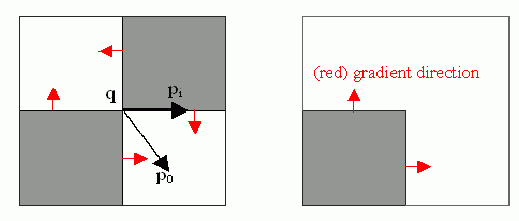
\includegraphics[width=1.0\textwidth]{pics/cornersubpix.png}

Sub-pixel accurate corner locator is based on the observation that every vector from the center $q$ to a point $p$ located within a neighborhood of $q$ is orthogonal to the image gradient at $p$ subject to image and measurement noise. Consider the expression:

\[
\epsilon_i = {DI_{p_i}}^T \cdot (q - p_i)
\]

where ${DI_{p_i}}$ is the image gradient at the one of the points $p_i$ in a neighborhood of $q$. The value of $q$ is to be found such that $\epsilon_i$ is minimized. A system of equations may be set up with $\epsilon_i$ set to zero:

\[
\sum_i(DI_{p_i} \cdot {DI_{p_i}}^T) - \sum_i(DI_{p_i} \cdot {DI_{p_i}}^T \cdot p_i)
\]

where the gradients are summed within a neighborhood ("search window") of $q$. Calling the first gradient term $G$ and the second gradient term $b$ gives:

\[
q = G^{-1} \cdot b
\]

The algorithm sets the center of the neighborhood window at this new center $q$ and then iterates until the center keeps within a set threshold.

\cvCPyFunc{GetStarKeypoints}
Retrieves keypoints using the StarDetector algorithm.

\cvdefC{
CvSeq* cvGetStarKeypoints( \par const CvArr* image,\par CvMemStorage* storage,\par CvStarDetectorParams params=cvStarDetectorParams() );
}\cvdefPy{GetStarKeypoints(image,storage,params)-> keypoints}

\begin{description}
\cvarg{image}{The input 8-bit grayscale image}
\cvarg{storage}{Memory storage where the keypoints will be stored}
\cvarg{params}{Various algorithm parameters given to the structure CvStarDetectorParams:}
\begin{lstlisting}
 typedef struct CvStarDetectorParams
 {
    int maxSize; // maximal size of the features detected. The following 
                 // values of the parameter are supported:
                 // 4, 6, 8, 11, 12, 16, 22, 23, 32, 45, 46, 64, 90, 128
    int responseThreshold; // threshold for the approximatd laplacian,
                           // used to eliminate weak features
    int lineThresholdProjected; // another threshold for laplacian to 
                // eliminate edges
    int lineThresholdBinarized; // another threshold for the feature 
                // scale to eliminate edges
    int suppressNonmaxSize; // linear size of a pixel neighborhood 
                // for non-maxima suppression
 }
 CvStarDetectorParams;
\end{lstlisting}
\end{description}

The function GetStarKeypoints extracts keypoints that are local
scale-space extremas. The scale-space is constructed by computing
approximate values of laplacians with different sigma's at each
pixel. Instead of using pyramids, a popular approach to save computing
time, all of the laplacians are computed at each pixel of the original
high-resolution image. But each approximate laplacian value is computed
in O(1) time regardless of the sigma, thanks to the use of integral
images. The algorithm is based on the paper 
Agrawal08
, but instead
of a square, hexagon or octagon it uses an 8-end star shape, hence the name,
consisting of overlapping upright and tilted squares.

Each computed feature is represented by the following structure:

\begin{lstlisting}
typedef struct CvStarKeypoint
{
    CvPoint pt; // coordinates of the feature
    int size; // feature size, see CvStarDetectorParams::maxSize
    float response; // the approximated laplacian value at that point.
}
CvStarKeypoint;

inline CvStarKeypoint cvStarKeypoint(CvPoint pt, int size, float response);
\end{lstlisting}

\ifC
Below is the small usage sample:

\begin{lstlisting}
#include "cv.h"
#include "highgui.h"

int main(int argc, char** argv)
{
    const char* filename = argc > 1 ? argv[1] : "lena.jpg";
    IplImage* img = cvLoadImage( filename, 0 ), *cimg;
    CvMemStorage* storage = cvCreateMemStorage(0);
    CvSeq* keypoints = 0;
    int i;

    if( !img )
        return 0;
    cvNamedWindow( "image", 1 );
    cvShowImage( "image", img );
    cvNamedWindow( "features", 1 );
    cimg = cvCreateImage( cvGetSize(img), 8, 3 );
    cvCvtColor( img, cimg, CV_GRAY2BGR );

    keypoints = cvGetStarKeypoints( img, storage, cvStarDetectorParams(45) );

    for( i = 0; i < (keypoints ? keypoints->total : 0); i++ )
    {
        CvStarKeypoint kpt = *(CvStarKeypoint*)cvGetSeqElem(keypoints, i);
        int r = kpt.size/2;
        cvCircle( cimg, kpt.pt, r, CV_RGB(0,255,0));
        cvLine( cimg, cvPoint(kpt.pt.x + r, kpt.pt.y + r),
            cvPoint(kpt.pt.x - r, kpt.pt.y - r), CV_RGB(0,255,0));
        cvLine( cimg, cvPoint(kpt.pt.x - r, kpt.pt.y + r),
            cvPoint(kpt.pt.x + r, kpt.pt.y - r), CV_RGB(0,255,0));
    }
    cvShowImage( "features", cimg );
    cvWaitKey();
}
\end{lstlisting}
\fi

\cvCPyFunc{GoodFeaturesToTrack}
Determines strong corners on an image.

\cvdefC{
void cvGoodFeaturesToTrack(
\par const CvArr* image
\par CvArr* eigImage, CvArr* tempImage
\par CvPoint2D32f* corners
\par int* cornerCount
\par double qualityLevel
\par double minDistance
\par const CvArr* mask=NULL
\par int blockSize=3
\par int useHarris=0
\par double k=0.04 );
}
\cvdefPy{GoodFeaturesToTrack(image,eigImage,tempImage,qualityLevel,minDistance,mask=NULL,blockSize=3,useHarris=0,k=0.04)-> corners}

\begin{description}
\cvarg{image}{The source 8-bit or floating-point 32-bit, single-channel image}
\cvarg{eigImage}{Temporary floating-point 32-bit image, the same size as \texttt{image}}
\cvarg{tempImage}{Another temporary image, the same size and format as \texttt{eigImage}}
\cvarg{corners}{Output parameter; detected corners}
\cvarg{cornerCount}{Output parameter; number of detected corners}
\cvarg{qualityLevel}{Multiplier for the max/min eigenvalue; specifies the minimal accepted quality of image corners}
\cvarg{minDistance}{Limit, specifying the minimum possible distance between the returned corners; Euclidian distance is used}
\cvarg{mask}{Region of interest. The function selects points either in the specified region or in the whole image if the mask is NULL}
\cvarg{blockSize}{Size of the averaging block, passed to the underlying \cvCPyCross{CornerMinEigenVal} or \cvCPyCross{CornerHarris} used by the function}
\cvarg{useHarris}{If nonzero, Harris operator (\cvCPyCross{CornerHarris}) is used instead of default \cvCPyCross{CornerMinEigenVal}}
\cvarg{k}{Free parameter of Harris detector; used only if ($\texttt{useHarris} != 0$)}
\end{description}

The function finds corners with big
eigenvalues in the image. The function first calculates the minimal
eigenvalue for every source image pixel using the \cvCPyCross{CornerMinEigenVal}
function and stores them in \texttt{eigImage}. Then it performs
non-maxima suppression (only local maxima in $3\times 3$ neighborhood
remain). The next step is rejecting the corners with the minimal
eigenvalue less than
$\texttt{qualityLevel} \cdot max(\texttt{eigImage}(x,y))$
.
Finally, the function ensures that all the corners found are distanced
enough from one another by considering the corners (the strongest
corners are considered first) and checking that the distance between
the newly considered feature and the features considered earlier
is larger than \texttt{minDistance}. So, the function removes the
features than are too close to the stronger features.

\cvCPyFunc{HoughLines2}
Finds lines in a binary image using a Hough transform.

\cvdefC{
CvSeq* cvHoughLines2( \par CvArr* image,\par void* line\_storage,\par int method,\par double rho,\par double theta,\par int threshold,\par double param1=0,\par double param2=0 );
}\cvdefPy{HoughLines2(image,storage,method,rho,theta,threshold,param1=0,parma2=0)-> lines}

\begin{description}
\cvarg{image}{The 8-bit, single-channel, binary source image. In the case of a probabilistic method, the image is modified by the function}
\cvarg{line\_storage}{The storage for the lines that are detected. It can
be a memory storage (in this case a sequence of lines is created in
the storage and returned by the function) or single row/single column
matrix (CvMat*) of a particular type (see below) to which the lines'
parameters are written. The matrix header is modified by the function
so its \texttt{cols} or \texttt{rows} will contain the number of lines
detected. If \texttt{line\_storage} is a matrix and the actual number
of lines exceeds the matrix size, the maximum possible number of lines
is returned (in the case of standard hough transform the lines are sorted
by the accumulator value)}
\cvarg{method}{The Hough transform variant, one of the following:
\begin{description}
  \cvarg{CV\_HOUGH\_STANDARD}{classical or standard Hough transform. Every line is represented by two floating-point numbers $(\rho, \theta)$, where $\rho$ is a distance between (0,0) point and the line, and $\theta$ is the angle between x-axis and the normal to the line. Thus, the matrix must be (the created sequence will be) of \texttt{CV\_32FC2} type}
  \cvarg{CV\_HOUGH\_PROBABILISTIC}{probabilistic Hough transform (more efficient in case if picture contains a few long linear segments). It returns line segments rather than the whole line. Each segment is represented by starting and ending points, and the matrix must be (the created sequence will be) of \texttt{CV\_32SC4} type}
  \cvarg{CV\_HOUGH\_MULTI\_SCALE}{multi-scale variant of the classical Hough transform. The lines are encoded the same way as \texttt{CV\_HOUGH\_STANDARD}}
\end{description}}
\cvarg{rho}{Distance resolution in pixel-related units}
\cvarg{theta}{Angle resolution measured in radians}
\cvarg{threshold}{Threshold parameter. A line is returned by the function if the corresponding accumulator value is greater than \texttt{threshold}}
\cvarg{param1}{The first method-dependent parameter:
\begin{itemize}
  \item For the classical Hough transform it is not used (0).
  \item For the probabilistic Hough transform it is the minimum line length.
  \item For the multi-scale Hough transform it is the divisor for the distance resolution $\rho$. (The coarse distance resolution will be $\rho$ and the accurate resolution will be $(\rho / \texttt{param1})$).
\end{itemize}}
\cvarg{param2}{The second method-dependent parameter:
\begin{itemize}
  \item For the classical Hough transform it is not used (0).
  \item For the probabilistic Hough transform it is the maximum gap between line segments lying on the same line to treat them as a single line segment (i.e. to join them).
  \item For the multi-scale Hough transform it is the divisor for the angle resolution $\theta$. (The coarse angle resolution will be $\theta$ and the accurate resolution will be $(\theta / \texttt{param2})$).
\end{itemize}}
\end{description}

The function implements a few variants of the Hough transform for line detection.

\ifC
\textbf{Example. Detecting lines with Hough transform.}
\begin{lstlisting}
/* This is a standalone program. Pass an image name as a first parameter
of the program.  Switch between standard and probabilistic Hough transform
by changing "#if 1" to "#if 0" and back */
#include <cv.h>
#include <highgui.h>
#include <math.h>

int main(int argc, char** argv)
{
    IplImage* src;
    if( argc == 2 && (src=cvLoadImage(argv[1], 0))!= 0)
    {
        IplImage* dst = cvCreateImage( cvGetSize(src), 8, 1 );
        IplImage* color_dst = cvCreateImage( cvGetSize(src), 8, 3 );
        CvMemStorage* storage = cvCreateMemStorage(0);
        CvSeq* lines = 0;
        int i;
        cvCanny( src, dst, 50, 200, 3 );
        cvCvtColor( dst, color_dst, CV_GRAY2BGR );
#if 1
        lines = cvHoughLines2( dst,
                               storage,
                               CV_HOUGH_STANDARD,
                               1,
                               CV_PI/180,
                               100,
                               0,
                               0 );

        for( i = 0; i < MIN(lines->total,100); i++ )
        {
            float* line = (float*)cvGetSeqElem(lines,i);
            float rho = line[0];
            float theta = line[1];
            CvPoint pt1, pt2;
            double a = cos(theta), b = sin(theta);
            double x0 = a*rho, y0 = b*rho;
            pt1.x = cvRound(x0 + 1000*(-b));
            pt1.y = cvRound(y0 + 1000*(a));
            pt2.x = cvRound(x0 - 1000*(-b));
            pt2.y = cvRound(y0 - 1000*(a));
            cvLine( color_dst, pt1, pt2, CV_RGB(255,0,0), 3, 8 );
        }
#else
        lines = cvHoughLines2( dst,
                               storage,
                               CV_HOUGH_PROBABILISTIC,
                               1,
                               CV_PI/180,
                               80,
                               30,
                               10 );
        for( i = 0; i < lines->total; i++ )
        {
            CvPoint* line = (CvPoint*)cvGetSeqElem(lines,i);
            cvLine( color_dst, line[0], line[1], CV_RGB(255,0,0), 3, 8 );
        }
#endif
        cvNamedWindow( "Source", 1 );
        cvShowImage( "Source", src );

        cvNamedWindow( "Hough", 1 );
        cvShowImage( "Hough", color_dst );

        cvWaitKey(0);
    }
}
\end{lstlisting}

This is the sample picture the function parameters have been tuned for:

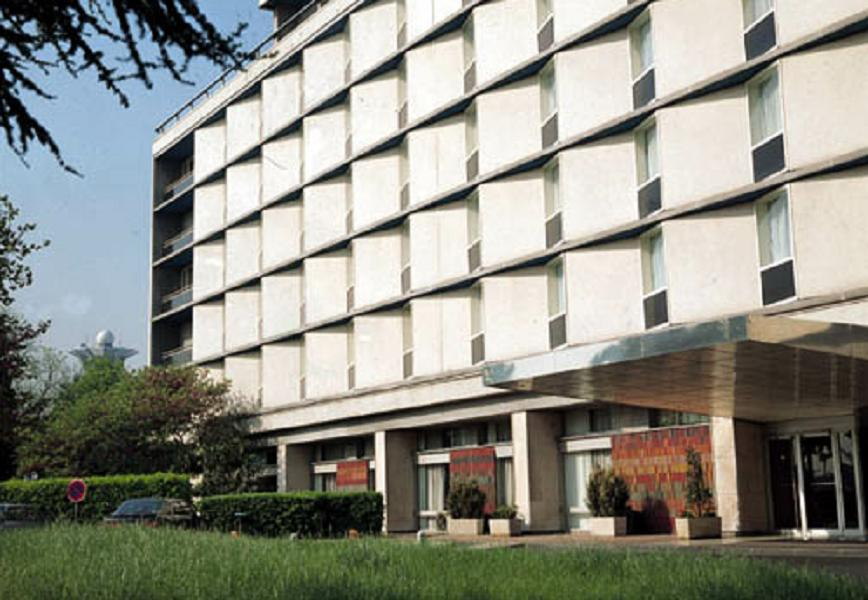
\includegraphics[width=0.5\textwidth]{pics/building.jpg}

And this is the output of the above program in the case of probabilistic Hough transform (\texttt{\#if 0} case):

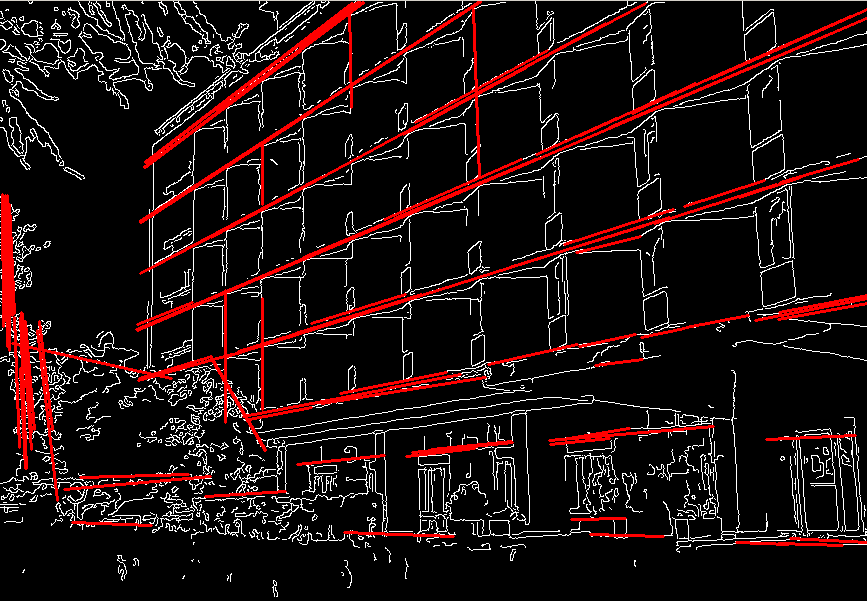
\includegraphics[width=0.5\textwidth]{pics/houghp.png}
\fi

\cvCPyFunc{PreCornerDetect}
Calculates the feature map for corner detection.

\cvdefC{
void cvPreCornerDetect(
\par const CvArr* image,
\par CvArr* corners,
\par int apertureSize=3 );
}\cvdefPy{PreCornerDetect(image,corners,aperture\_size=3)-> None}
\begin{description}
\cvarg{image}{Input image}
\cvarg{corners}{Image to store the corner candidates}
\cvarg{apertureSize}{Aperture parameter for the Sobel operator (see \cvCPyCross{Sobel})}
\end{description}

The function calculates the function

\[
D_x^2 D_{yy} + D_y^2 D_{xx} - 2 D_x D_y D_{xy}
\]

where $D_?$ denotes one of the first image derivatives and $D_{??}$ denotes a second image derivative.

The corners can be found as local maximums of the function below:

\begin{lstlisting}
// assume that the image is floating-point
IplImage* corners = cvCloneImage(image);
IplImage* dilated_corners = cvCloneImage(image);
IplImage* corner_mask = cvCreateImage( cvGetSize(image), 8, 1 );
cvPreCornerDetect( image, corners, 3 );
cvDilate( corners, dilated_corners, 0, 1 );
cvSubS( corners, dilated_corners, corners );
cvCmpS( corners, 0, corner_mask, CV_CMP_GE );
cvReleaseImage( &corners );
cvReleaseImage( &dilated_corners );
\end{lstlisting}

\ifC
\cvCPyFunc{SampleLine}
Reads the raster line to the buffer.

\cvdefC{
int cvSampleLine(
\par const CvArr* image
\par CvPoint pt1
\par CvPoint pt2
\par void* buffer
\par int connectivity=8 );
}

\begin{description}
\cvarg{image}{Image to sample the line from}
\cvarg{pt1}{Starting line point}
\cvarg{pt2}{Ending line point}
\cvarg{buffer}{Buffer to store the line points; must have enough size to store
$max( |\texttt{pt2.x} - \texttt{pt1.x}|+1, |\texttt{pt2.y} - \texttt{pt1.y}|+1 )$
points in the case of an 8-connected line and
$ (|\texttt{pt2.x}-\texttt{pt1.x}|+|\texttt{pt2.y}-\texttt{pt1.y}|+1) $
in the case of a 4-connected line}
\cvarg{connectivity}{The line connectivity, 4 or 8}
\end{description}

The function implements a particular application of line iterators. The function reads all of the image points lying on the line between \texttt{pt1} and \texttt{pt2}, including the end points, and stores them into the buffer.

\fi

\fi


\ifCpp

\cvCppFunc{Canny}
Finds edges in an image using Canny algorithm.

\cvdefCpp{void Canny( const Mat\& image, Mat\& edges,\par
            double threshold1, double threshold2,\par
            int apertureSize=3, bool L2gradient=false );}
\begin{description}
\cvarg{image}{Single-channel 8-bit input image}
\cvarg{edges}{The output edge map. It will have the same size and the same type as \texttt{image}}
\cvarg{threshold1}{The first threshold for the hysteresis procedure}
\cvarg{threshold2}{The second threshold for the hysteresis procedure}
\cvarg{apertureSize}{Aperture size for the \cvCppCross{Sobel} operator}
\cvarg{L2gradient}{Indicates, whether the more accurate $L_2$ norm $=\sqrt{(dI/dx)^2 + (dI/dy)^2}$ should be used to compute the image gradient magnitude (\texttt{L2gradient=true}), or a faster default $L_1$ norm $=|dI/dx|+|dI/dy|$ is enough (\texttt{L2gradient=false})}
\end{description}

The function finds edges in the input image \texttt{image} and marks them in the output map \texttt{edges} using the Canny algorithm. The smallest value between \texttt{threshold1} and \texttt{threshold2} is used for edge linking, the largest value is used to find the initial segments of strong edges, see
\url{http://en.wikipedia.org/wiki/Canny_edge_detector}

\cvCppFunc{cornerEigenValsAndVecs}
Calculates eigenvalues and eigenvectors of image blocks for corner detection.

\cvdefCpp{void cornerEigenValsAndVecs( const Mat\& src, Mat\& dst,\par
                            int blockSize, int apertureSize,\par
                            int borderType=BORDER\_DEFAULT );}
\begin{description}
\cvarg{src}{Input single-channel 8-bit or floating-point image}
\cvarg{dst}{Image to store the results. It will have the same size as \texttt{src} and the type \texttt{CV\_32FC(6)}}
\cvarg{blockSize}{Neighborhood size (see discussion)}
\cvarg{apertureSize}{Aperture parameter for the \cvCppCross{Sobel} operator}
\cvarg{boderType}{Pixel extrapolation method; see \cvCppCross{borderInterpolate}}
\end{description}

For every pixel $p$, the function \texttt{cornerEigenValsAndVecs} considers a \texttt{blockSize} $\times$ \texttt{blockSize} neigborhood $S(p)$. It calculates the covariation matrix of derivatives over the neighborhood as:

\[
M = \begin{bmatrix}
\sum_{S(p)}(dI/dx)^2 & \sum_{S(p)}(dI/dx dI/dy)^2 \\
\sum_{S(p)}(dI/dx dI/dy)^2 & \sum_{S(p)}(dI/dy)^2
\end{bmatrix}
\]

Where the derivatives are computed using \cvCppCross{Sobel} operator.

After that it finds eigenvectors and eigenvalues of $M$ and stores them into destination image in the form
$(\lambda_1, \lambda_2, x_1, y_1, x_2, y_2)$ where
\begin{description}
\item[$\lambda_1, \lambda_2$]are the eigenvalues of $M$; not sorted
\item[$x_1, y_1$]are the eigenvectors corresponding to $\lambda_1$
\item[$x_2, y_2$]are the eigenvectors corresponding to $\lambda_2$
\end{description}

The output of the function can be used for robust edge or corner detection.

See also: \cvCppCross{cornerMinEigenVal}, \cvCppCross{cornerHarris}, \cvCppCross{preCornerDetect}

\cvCppFunc{cornerHarris}
Harris edge detector.

\cvdefCpp{void cornerHarris( const Mat\& src, Mat\& dst, int blockSize,\par
                  int apertureSize, double k,\par
                  int borderType=BORDER\_DEFAULT );}
\begin{description}
\cvarg{src}{Input single-channel 8-bit or floating-point image}
\cvarg{dst}{Image to store the Harris detector responses; will have type \texttt{CV\_32FC1} and the same size as \texttt{src}}
\cvarg{blockSize}{Neighborhood size (see the discussion of \cvCppCross{cornerEigenValsAndVecs})}
\cvarg{apertureSize}{Aperture parameter for the \cvCppCross{Sobel} operator}
\cvarg{k}{Harris detector free parameter. See the formula below}
\cvarg{boderType}{Pixel extrapolation method; see \cvCppCross{borderInterpolate}}
\end{description}

The function runs the Harris edge detector on the image. Similarly to \cvCppCross{cornerMinEigenVal} and \cvCppCross{cornerEigenValsAndVecs}, for each pixel $(x, y)$ it calculates a $2\times2$ gradient covariation matrix $M^{(x,y)}$ over a $\texttt{blockSize} \times \texttt{blockSize}$ neighborhood. Then, it computes the following characteristic:

\[
\texttt{dst}(x,y) = \mathrm{det} M^{(x,y)} - k \cdot \left(\mathrm{tr} M^{(x,y)}\right)^2
\]

Corners in the image can be found as the local maxima of this response map.

\cvCppFunc{cornerMinEigenVal}
Calculates the minimal eigenvalue of gradient matrices for corner detection.

\cvdefCpp{void cornerMinEigenVal( const Mat\& src, Mat\& dst,\par
                        int blockSize, int apertureSize=3,\par
                        int borderType=BORDER\_DEFAULT );}
\begin{description}
\cvarg{src}{Input single-channel 8-bit or floating-point image}
\cvarg{dst}{Image to store the minimal eigenvalues; will have type \texttt{CV\_32FC1} and the same size as \texttt{src}}
\cvarg{blockSize}{Neighborhood size (see the discussion of \cvCppCross{cornerEigenValsAndVecs})}
\cvarg{apertureSize}{Aperture parameter for the \cvCppCross{Sobel} operator}
\cvarg{boderType}{Pixel extrapolation method; see \cvCppCross{borderInterpolate}}
\end{description}

The function is similar to \cvCppCross{cornerEigenValsAndVecs} but it calculates and stores only the minimal eigenvalue of the covariation matrix of derivatives, i.e. $\min(\lambda_1, \lambda_2)$ in terms of the formulae in \cvCppCross{cornerEigenValsAndVecs} description.

\cvCppFunc{cornerSubPix}
Refines the corner locations.

\cvdefCpp{void cornerSubPix( const Mat\& image, vector<Point2f>\& corners,\par
                   Size winSize, Size zeroZone,\par
                   TermCriteria criteria );}
\begin{description}
\cvarg{image}{Input image}
\cvarg{corners}{Initial coordinates of the input corners; refined coordinates on output}
\cvarg{winSize}{Half of the side length of the search window. For example, if \texttt{winSize=Size(5,5)}, then a $5*2+1 \times 5*2+1 = 11 \times 11$ search window would be used}
\cvarg{zeroZone}{Half of the size of the dead region in the middle of the search zone over which the summation in the formula below is not done. It is used sometimes to avoid possible singularities of the autocorrelation matrix. The value of (-1,-1) indicates that there is no such size}
\cvarg{criteria}{Criteria for termination of the iterative process of corner refinement. That is, the process of corner position refinement stops either after a certain number of iterations or when a required accuracy is achieved. The \texttt{criteria} may specify either of or both the maximum number of iteration and the required accuracy}
\end{description}

The function iterates to find the sub-pixel accurate location of corners, or radial saddle points, as shown in on the picture below.

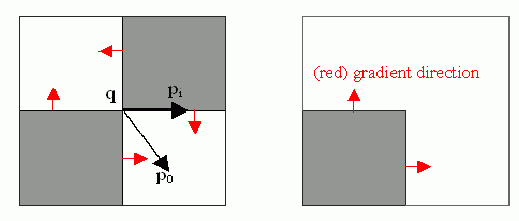
\includegraphics[width=1.0\textwidth]{pics/cornersubpix.png}

Sub-pixel accurate corner locator is based on the observation that every vector from the center $q$ to a point $p$ located within a neighborhood of $q$ is orthogonal to the image gradient at $p$ subject to image and measurement noise. Consider the expression:

\[
\epsilon_i = {DI_{p_i}}^T \cdot (q - p_i)
\]

where ${DI_{p_i}}$ is the image gradient at the one of the points $p_i$ in a neighborhood of $q$. The value of $q$ is to be found such that $\epsilon_i$ is minimized. A system of equations may be set up with $\epsilon_i$ set to zero:

\[
\sum_i(DI_{p_i} \cdot {DI_{p_i}}^T) - \sum_i(DI_{p_i} \cdot {DI_{p_i}}^T \cdot p_i)
\]

where the gradients are summed within a neighborhood ("search window") of $q$. Calling the first gradient term $G$ and the second gradient term $b$ gives:

\[
q = G^{-1} \cdot b
\]

The algorithm sets the center of the neighborhood window at this new center $q$ and then iterates until the center keeps within a set threshold.


\cvCppFunc{goodFeaturesToTrack}
Determines strong corners on an image.

\cvdefCpp{void goodFeaturesToTrack( const Mat\& image, vector<Point2f>\& corners,\par
                         int maxCorners, double qualityLevel, double minDistance,\par
                         const Mat\& mask=Mat(), int blockSize=3,\par
                         bool useHarrisDetector=false, double k=0.04 );}
\begin{description}
\cvarg{image}{The input 8-bit or floating-point 32-bit, single-channel image}
\cvarg{corners}{The output vector of detected corners}
\cvarg{maxCorners}{The maximum number of corners to return. If there are more corners than that will be found, the strongest of them will be returned}
\cvarg{qualityLevel}{Characterizes the minimal accepted quality of image corners; the value of the parameter is multiplied by the by the best corner quality measure (which is the min eigenvalue, see \cvCppCross{cornerMinEigenVal}, or the Harris function response, see \cvCppCross{cornerHarris}). The corners, which quality measure is less than the product, will be rejected. For example, if the best corner has the quality measure = 1500, and the \texttt{qualityLevel=0.01}, then all the corners which quality measure is less than 15 will be rejected.}
\cvarg{minDistance}{The minimum possible Euclidean distance between the returned corners}
\cvarg{mask}{The optional region of interest. If the image is not empty (then it needs to have the type \texttt{CV\_8UC1} and the same size as \texttt{image}), it will specify the region in which the corners are detected}
\cvarg{blockSize}{Size of the averaging block for computing derivative covariation matrix over each pixel neighborhood, see \cvCppCross{cornerEigenValsAndVecs}}
\cvarg{useHarrisDetector}{Indicates, whether to use \hyperref[cornerHarris]{Harris} operator or \cvCppCross{cornerMinEigenVal}}
\cvarg{k}{Free parameter of Harris detector}
\end{description}

The function finds the most prominent corners in the image or in the specified image region, as described
in \cite{Shi94}:
\begin{enumerate}
\item the function first calculates the corner quality measure at every source image pixel using the \cvCppCross{cornerMinEigenVal} or \cvCppCross{cornerHarris}
\item then it performs non-maxima suppression (the local maxima in $3\times 3$ neighborhood
are retained).
\item the next step rejects the corners with the minimal eigenvalue less than $\texttt{qualityLevel} \cdot \max_{x,y} qualityMeasureMap(x,y)$.
\item the remaining corners are then sorted by the quality measure in the descending order.
\item finally, the function throws away each corner $pt_j$ if there is a stronger corner $pt_i$ ($i < j$) such that the distance between them is less than \texttt{minDistance}
\end{enumerate}

The function can be used to initialize a point-based tracker of an object.

See also: \cvCppCross{cornerMinEigenVal}, \cvCppCross{cornerHarris}, \cvCppCross{calcOpticalFlowPyrLK}, \cvCppCross{estimateRigidMotion}, \cvCppCross{PlanarObjectDetector}, \cvCppCross{OneWayDescriptor}

\cvCppFunc{HoughCircles}
Finds circles in a grayscale image using a Hough transform.

\cvdefCpp{void HoughCircles( Mat\& image, vector<Vec3f>\& circles,\par
                 int method, double dp, double minDist,\par
                 double param1=100, double param2=100,\par
                 int minRadius=0, int maxRadius=0 );}
\begin{description}
\cvarg{image}{The 8-bit, single-channel, grayscale input image}
\cvarg{circles}{The output vector of found circles. Each vector is encoded as 3-element floating-point vector $(x, y, radius)$}
\cvarg{method}{Currently, the only implemented method is \texttt{CV\_HOUGH\_GRADIENT}, which is basically \emph{21HT}, described in \cite{Yuen90}.}
\cvarg{dp}{The inverse ratio of the accumulator resolution to the image resolution. For example, if \texttt{dp=1}, the accumulator will have the same resolution as the input image, if \texttt{dp=2} - accumulator will have half as big width and height, etc}
\cvarg{minDist}{Minimum distance between the centers of the detected circles. If the parameter is too small, multiple neighbor circles may be falsely detected in addition to a true one. If it is too large, some circles may be missed}
\cvarg{param1}{The first method-specific parameter. in the case of \texttt{CV\_HOUGH\_GRADIENT} it is the higher threshold of the two passed to \cvCppCross{Canny} edge detector (the lower one will be twice smaller)}
\cvarg{param2}{The second method-specific parameter. in the case of \texttt{CV\_HOUGH\_GRADIENT} it is the accumulator threshold at the center detection stage. The smaller it is, the more false circles may be detected. Circles, corresponding to the larger accumulator values, will be returned first}
\cvarg{minRadius}{Minimum circle radius}
\cvarg{maxRadius}{Maximum circle radius}
\end{description}

The function finds circles in a grayscale image using some modification of Hough transform. Here is a short usage example:

\begin{lstlisting}
#include <cv.h>
#include <highgui.h>
#include <math.h>

using namespace cv;

int main(int argc, char** argv)
{
    Mat img, gray;
    if( argc != 2 && !(img=imread(argv[1], 1)).data)
        return -1;
    cvtColor(img, gray, CV_BGR2GRAY);
    // smooth it, otherwise a lot of false circles may be detected
    GaussianBlur( gray, gray, 9, 9, 2, 2 );
    vector<Vec3f> circles;
    houghCircles(gray, circles, CV_HOUGH_GRADIENT,
                 2, gray->rows/4, 200, 100 );
    for( size_t i = 0; i < circles.size(); i++ )
    {
         Point center(cvRound(circles[i][0]), cvRound(circles[i][1]));
         int radius = cvRound(circles[i][2]);
         // draw the circle center
         circle( img, center, 3, Scalar(0,255,0), -1, 8, 0 );
         // draw the circle outline
         circle( img, center, radius, Scalar(0,0,255), 3, 8, 0 );
    }
    namedWindow( "circles", 1 );
    imshow( "circles", img );
    return 0;
}
\end{lstlisting}

Note that usually the function detects the circles' centers well, however it may fail to find the correct radii. You can assist the function by specifying the radius range (\texttt{minRadius} and \texttt{maxRadius}) if you know it, or you may ignore the returned radius, use only the center and find the correct radius using some additional procedure.

See also: \cvCppCross{fitEllipse}, \cvCppCross{minEnclosingCircle}

\cvCppFunc{HoughLines}
Finds lines in a binary image using standard Hough transform.

\cvdefCpp{void HoughLines( Mat\& image, vector<Vec2f>\& lines,\par
                 double rho, double theta, int threshold,\par
                 double srn=0, double stn=0 );}
\begin{description}
\cvarg{image}{The 8-bit, single-channel, binary source image. The image may be modified by the function}
\cvarg{lines}{The output vector of lines. Each line is represented by a two-element vector $(\rho, \theta)$. $\rho$ is the distance from the coordinate origin $(0,0)$ (top-left corner of the image) and $\theta$ is the line rotation angle in radians ($0 \sim \textrm{vertical line}, \pi/2 \sim \textrm{horizontal line}$)}
\cvarg{rho}{Distance resolution of the accumulator in pixels}
\cvarg{theta}{Angle resolution of the accumulator in radians}
\cvarg{threshold}{The accumulator threshold parameter. Only those lines are returned that get enough votes ($>\texttt{threshold}$)}
\cvarg{srn}{For the multi-scale Hough transform it is the divisor for the distance resolution \texttt{rho}. The coarse accumulator distance resolution will be \texttt{rho} and the accurate accumulator resolution will be \texttt{rho/srn}. If both \texttt{srn=0} and \texttt{stn=0} then the classical Hough transform is used, otherwise both these parameters should be positive.}
\cvarg{stn}{For the multi-scale Hough transform it is the divisor for the distance resolution \texttt{theta}}
\end{description}

The function implements standard or standard multi-scale Hough transform algorithm for line detection. See \cvCppCross{HoughLinesP} for the code example.


\cvCppFunc{HoughLinesP}
Finds lines segments in a binary image using probabilistic Hough transform.

\cvdefCpp{void HoughLinesP( Mat\& image, vector<Vec4i>\& lines,\par
                  double rho, double theta, int threshold,\par
                  double minLineLength=0, double maxLineGap=0 );}
\begin{description}
\cvarg{image}{The 8-bit, single-channel, binary source image. The image may be modified by the function}
\cvarg{lines}{The output vector of lines. Each line is represented by a 4-element vector $(x_1, y_1, x_2, y_2)$, where $(x_1,y_1)$ and $(x_2, y_2)$ are the ending points of each line segment detected.}
\cvarg{rho}{Distance resolution of the accumulator in pixels}
\cvarg{theta}{Angle resolution of the accumulator in radians}
\cvarg{threshold}{The accumulator threshold parameter. Only those lines are returned that get enough votes ($>\texttt{threshold}$)}
\cvarg{minLineLength}{The minimum line length. Line segments shorter than that will be rejected}
\cvarg{maxLineGap}{The maximum allowed gap between points on the same line to link them.}
\end{description}

The function implements probabilistic Hough transform algorithm for line detection, described in \cite{Matas00}. Below is line detection example:

\begin{lstlisting}
/* This is a standalone program. Pass an image name as a first parameter
of the program.  Switch between standard and probabilistic Hough transform
by changing "#if 1" to "#if 0" and back */
#include <cv.h>
#include <highgui.h>
#include <math.h>

using namespace cv;

int main(int argc, char** argv)
{
    Mat src, dst, color_dst;
    if( argc != 2 || !(src=imread(argv[1], 0)).data)
        return -1;
        
    Canny( src, dst, 50, 200, 3 );
    cvtColor( dst, color_dst, CV_GRAY2BGR );    
        
#if 0
    vector<Vec2f> lines;
    HoughLines( dst, lines, 1, CV_PI/180, 100 );

    for( size_t i = 0; i < lines.size(); i++ )
    {
        float rho = lines[i][0];
        float theta = lines[i][1];
        double a = cos(theta), b = sin(theta);
        double x0 = a*rho, y0 = b*rho;
        Point pt1(cvRound(x0 + 1000*(-b)),
                  cvRound(y0 + 1000*(a)));
        Point pt2(cvRound(x0 - 1000*(-b)),
                  cvRound(y0 - 1000*(a)));
        line( color_dst, pt1, pt2, Scalar(0,0,255), 3, 8 );
    }
#else
    vector<Vec4i> lines;
    HoughLinesP( dst, lines, 1, CV_PI/180, 80, 30, 10 );
    for( size_t i = 0; i < lines.size(); i++ )
    {
        line( color_dst, Point(lines[i][0], lines[i][1]),
            Point(lines[i][2], lines[i][3]), Scalar(0,0,255), 3, 8 );
    }
#endif
    namedWindow( "Source", 1 );
    imshow( "Source", src );

    namedWindow( "Detected Lines", 1 );
    imshow( "Detected Lines", color_dst );

    waitKey(0);
    return 0;
}
\end{lstlisting}


This is the sample picture the function parameters have been tuned for:

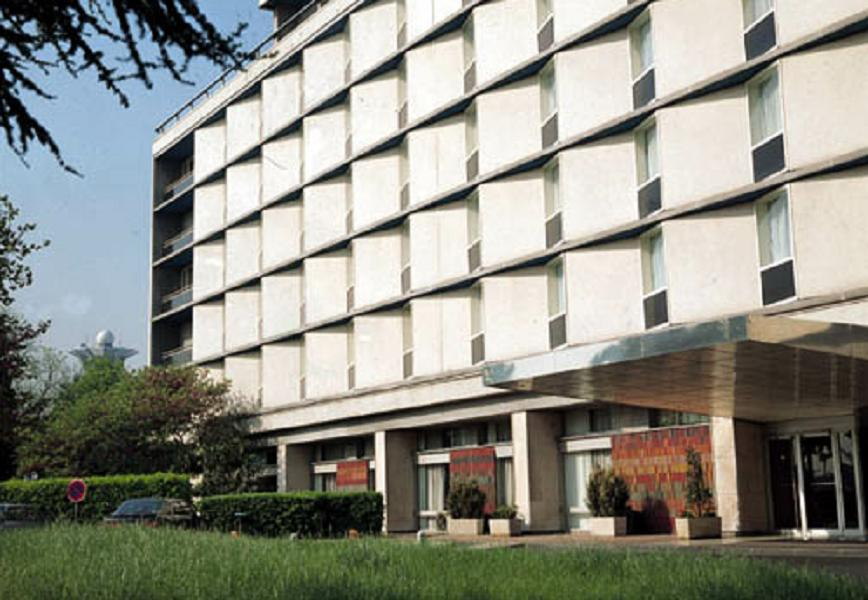
\includegraphics[width=0.5\textwidth]{pics/building.jpg}

And this is the output of the above program in the case of probabilistic Hough transform

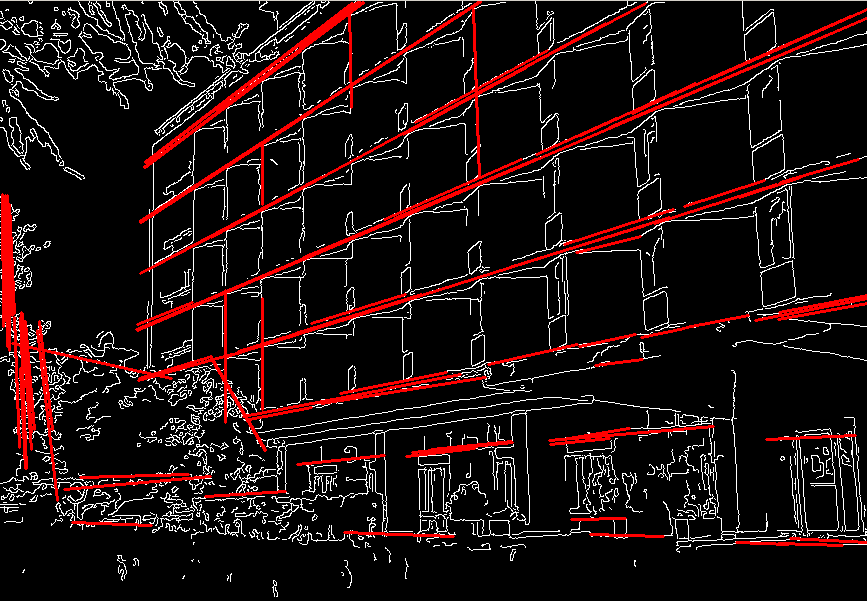
\includegraphics[width=0.5\textwidth]{pics/houghp.png}

\cvCppFunc{perCornerDetect}
Calculates the feature map for corner detection

\cvdefCpp{void preCornerDetect( const Mat\& src, Mat\& dst, int apertureSize,\par
                     int borderType=BORDER\_DEFAULT );}
\begin{description}
\cvarg{src}{The source single-channel 8-bit of floating-point image}
\cvarg{dst}{The output image; will have type \texttt{CV\_32F} and the same size as \texttt{src}}
\cvarg{apertureSize}{Aperture size of \cvCppCross{Sobel}}
\cvarg{borderType}{The pixel extrapolation method; see \cvCppCross{borderInterpolate}}
\end{description}

The function calculates the complex spatial derivative-based function of the source image

\[
\texttt{dst} = (D_x \texttt{src})^2 \cdot D_{yy} \texttt{src} + (D_y \texttt{src})^2 \cdot D_{xx} \texttt{src} - 2 D_x \texttt{src} \cdot D_y \texttt{src} \cdot D_{xy} \texttt{src}
\]

where $D_x$, $D_y$ are the first image derivatives, $D_{xx}$, $D_{yy}$ are the second image derivatives and $D_{xy}$ is the mixed derivative.

The corners can be found as local maximums of the functions, as shown below:

\begin{lstlisting}
Mat corners, dilated_corners;
preCornerDetect(image, corners, 3);
// dilation with 3x3 rectangular structuring element
dilate(corners, dilated_corners, Mat(), 1);
Mat corner_mask = corners == dilated_corners;
\end{lstlisting}


\cvCppFunc{KeyPoint}
Data structure for salient point detectors

\begin{lstlisting}
KeyPoint
{
public:
    // default constructor
    KeyPoint();
    // two complete constructors
    KeyPoint(Point2f _pt, float _size, float _angle=-1,
            float _response=0, int _octave=0, int _class_id=-1);
    KeyPoint(float x, float y, float _size, float _angle=-1,
             float _response=0, int _octave=0, int _class_id=-1);
    // coordinate of the point
    Point2f pt;
    // feature size
    float size;
    // feature orintation in degrees
    // (has negative value if the orientation
    // is not defined/not computed)
    float angle;
    // feature strength
    // (can be used to select only
    // the most prominent key points)
    float response;
    // scale-space octave in which the feature has been found;
    // may correlate with the size
    int octave;
    // point (can be used by feature
    // classifiers or object detectors)
    int class_id;
};

// reading/writing a vector of keypoints to a file storage
void write(FileStorage& fs, const string& name, const vector<KeyPoint>& keypoints);
void read(const FileNode& node, vector<KeyPoint>& keypoints);    
\end{lstlisting}


\cvCppFunc{MSER}
Maximally-Stable Extremal Region Extractor

\begin{lstlisting}
class MSER : public CvMSERParams
{
public:
    // default constructor
    MSER();
    // constructor that initializes all the algorithm parameters
    MSER( int _delta, int _min_area, int _max_area,
          float _max_variation, float _min_diversity,
          int _max_evolution, double _area_threshold,
          double _min_margin, int _edge_blur_size );
    // runs the extractor on the specified image; returns the MSERs,
    // each encoded as a contour (vector<Point>, see findContours)
    // the optional mask marks the area where MSERs are searched for
    void operator()(Mat& image, vector<vector<Point> >& msers, const Mat& mask) const;
};
\end{lstlisting}

The class encapsulates all the parameters of MSER (see \url{http://en.wikipedia.org/wiki/Maximally_stable_extremal_regions}) extraction algorithm. 

\cvCppFunc{SURF}
Class for extracting Speeded Up Robust Features from an image.

\begin{lstlisting}
class SURF : public CvSURFParams
{
public:
    // default constructor
    SURF();
    // constructor that initializes all the algorithm parameters
    SURF(double _hessianThreshold, int _nOctaves=4,
         int _nOctaveLayers=2, bool _extended=false);
    // returns the number of elements in each descriptor (64 or 128)
    int descriptorSize() const;
    // detects keypoints using fast multi-scale Hessian detector
    void operator()(const Mat& img, const Mat& mask,
                    vector<KeyPoint>& keypoints) const;
    // detects keypoints and computes the SURF descriptors for them
    void operator()(const Mat& img, const Mat& mask,
                    vector<KeyPoint>& keypoints,
                    vector<float>& descriptors,
                    bool useProvidedKeypoints=false) const;
};
\end{lstlisting}

The class \texttt{SURF} implements Speeded Up Robust Features descriptor \cite{Bay06}.
There is fast multi-scale Hessian keypoint detector that can be used to find the keypoints
(which is the default option), but the descriptors can be also computed for the user-specified keypoints.
The function can be used for object tracking and localization, image stitching etc. See the
\texttt{find\_obj.cpp} demo in OpenCV samples directory.


\cvCppFunc{StarDetector}
Implements Star keypoint detector

\begin{lstlisting}
class StarDetector : CvStarDetectorParams
{
public:
    // default constructor
    StarDetector();
    // the full constructor initialized all the algorithm parameters:
    // maxSize - maximum size of the features. The following 
    //      values of the parameter are supported:
    //      4, 6, 8, 11, 12, 16, 22, 23, 32, 45, 46, 64, 90, 128
    // responseThreshold - threshold for the approximated laplacian,
    //      used to eliminate weak features. The larger it is,
    //      the less features will be retrieved
    // lineThresholdProjected - another threshold for the laplacian to 
    //      eliminate edges
    // lineThresholdBinarized - another threshold for the feature 
    //      size to eliminate edges.
    // The larger the 2 threshold, the more points you get.
    StarDetector(int maxSize, int responseThreshold,
                 int lineThresholdProjected,
                 int lineThresholdBinarized,
                 int suppressNonmaxSize);

    // finds keypoints in an image
    void operator()(const Mat& image, vector<KeyPoint>& keypoints) const;
};
\end{lstlisting}

The class implements a modified version of CenSurE keypoint detector described in
\cite{Agrawal08}

\fi

\section{Motion Analysis and Object Tracking}

\ifCPy

\cvCPyFunc{Acc}
Adds a frame to an accumulator.

\cvdefC{
void cvAcc( \par const CvArr* image,\par CvArr* sum,\par const CvArr* mask=NULL );
}\cvdefPy{Acc(image,smu,mask=NULL)-> None}

\begin{description}
\cvarg{image}{Input image, 1- or 3-channel, 8-bit or 32-bit floating point. (each channel of multi-channel image is processed independently)}
\cvarg{sum}{Accumulator with the same number of channels as input image, 32-bit or 64-bit floating-point}
\cvarg{mask}{Optional operation mask}
\end{description}

The function adds the whole image \texttt{image} or its selected region to the accumulator \texttt{sum}:

\[ \texttt{sum}(x,y) \leftarrow \texttt{sum}(x,y) + \texttt{image}(x,y) \quad \text{if} \quad \texttt{mask}(x,y) \ne 0 \]

\cvCPyFunc{CalcGlobalOrientation}
Calculates the global motion orientation of some selected region.

\cvdefC{
double cvCalcGlobalOrientation( \par const CvArr* orientation,\par const CvArr* mask,\par const CvArr* mhi,\par double timestamp,\par double duration );
}\cvdefPy{CalcGlobalOrientation(orientation,mask,mhi,timestamp,duration)-> float}

\begin{description}
\cvarg{orientation}{Motion gradient orientation image; calculated by the function \cvCPyCross{CalcMotionGradient}}
\cvarg{mask}{Mask image. It may be a conjunction of a valid gradient mask, obtained with \cvCPyCross{CalcMotionGradient} and the mask of the region, whose direction needs to be calculated}
\cvarg{mhi}{Motion history image}
\cvarg{timestamp}{Current time in milliseconds or other units, it is better to store time passed to \cvCPyCross{UpdateMotionHistory} before and reuse it here, because running \cvCPyCross{UpdateMotionHistory} and \cvCPyCross{CalcMotionGradient} on large images may take some time}
\cvarg{duration}{Maximal duration of motion track in milliseconds, the same as \cvCPyCross{UpdateMotionHistory}}
\end{description}

The function calculates the general
motion direction in the selected region and returns the angle between
0 degrees  and 360 degrees . At first the function builds the orientation histogram
and finds the basic orientation as a coordinate of the histogram
maximum. After that the function calculates the shift relative to the
basic orientation as a weighted sum of all of the orientation vectors: the more
recent the motion, the greater the weight. The resultant angle is
a circular sum of the basic orientation and the shift.

\cvCPyFunc{CalcMotionGradient}
Calculates the gradient orientation of a motion history image.

\cvdefC{
void cvCalcMotionGradient( \par const CvArr* mhi,\par CvArr* mask,\par CvArr* orientation,\par double delta1,\par double delta2,\par int apertureSize=3 );
}\cvdefPy{CalcMotionGradient(mhi,mask,orientation,delta1,delta2,apertureSize=3)-> None}

\begin{description}
\cvarg{mhi}{Motion history image}
\cvarg{mask}{Mask image; marks pixels where the motion gradient data is correct; output parameter}
\cvarg{orientation}{Motion gradient orientation image; contains angles from 0 to ~360 degrees }
\cvarg{delta1, delta2}{The function finds the minimum ($m(x,y)$) and maximum ($M(x,y)$) mhi values over each pixel $(x,y)$ neighborhood and assumes the gradient is valid only if
\[
\min(\texttt{delta1} , \texttt{delta2} ) \le M(x,y)-m(x,y) \le \max(\texttt{delta1} ,\texttt{delta2} ).
\]}
\cvarg{apertureSize}{Aperture size of derivative operators used by the function: CV\_SCHARR, 1, 3, 5 or 7 (see \cvCPyCross{Sobel})}
\end{description}

The function calculates the derivatives $Dx$ and $Dy$ of \texttt{mhi} and then calculates gradient orientation as:

\[
\texttt{orientation}(x,y)=\arctan{\frac{Dy(x,y)}{Dx(x,y)}}
\]

where both $Dx(x,y)$ and $Dy(x,y)$ signs are taken into account (as in the \cvCPyCross{CartToPolar} function). After that \texttt{mask} is filled to indicate where the orientation is valid (see the \texttt{delta1} and \texttt{delta2} description).

\cvCPyFunc{CalcOpticalFlowBM}
Calculates the optical flow for two images by using the block matching method.

\cvdefC{
void cvCalcOpticalFlowBM( \par const CvArr* prev,\par const CvArr* curr,\par CvSize blockSize,\par CvSize shiftSize,\par CvSize max\_range,\par int usePrevious,\par CvArr* velx,\par CvArr* vely );
}\cvdefPy{CalcOpticalFlowBM(prev,curr,blockSize,shiftSize,max\_range,usePrevious,velx,vely)-> None}

\begin{description}
\cvarg{prev}{First image, 8-bit, single-channel}
\cvarg{curr}{Second image, 8-bit, single-channel}
\cvarg{blockSize}{Size of basic blocks that are compared}
\cvarg{shiftSize}{Block coordinate increments}
\cvarg{max\_range}{Size of the scanned neighborhood in pixels around the block}
\cvarg{usePrevious}{Uses the previous (input) velocity field}
\cvarg{velx}{Horizontal component of the optical flow of
\[
\left\lfloor \frac{\texttt{prev->width} - \texttt{blockSize.width}}{\texttt{shiftSize.width}} \right\rfloor
\times
\left\lfloor \frac{\texttt{prev->height} - \texttt{blockSize.height}}{\texttt{shiftSize.height}} \right\rfloor
\]
size, 32-bit floating-point, single-channel}
\cvarg{vely}{Vertical component of the optical flow of the same size \texttt{velx}, 32-bit floating-point, single-channel}
\end{description}

The function calculates the optical
flow for overlapped blocks $\texttt{blockSize.width} \times \texttt{blockSize.height}$ pixels each, thus the velocity
fields are smaller than the original images. For every block in \texttt{prev} the functions tries to find a similar block in
\texttt{curr} in some neighborhood of the original block or shifted by (velx(x0,y0),vely(x0,y0)) block as has been calculated by previous
function call (if \texttt{usePrevious=1})

\cvCPyFunc{CalcOpticalFlowHS}
Calculates the optical flow for two images.

\cvdefC{
void cvCalcOpticalFlowHS( \par const CvArr* prev,\par const CvArr* curr,\par int usePrevious,\par CvArr* velx,\par CvArr* vely,\par double lambda,\par CvTermCriteria criteria );
}\cvdefPy{CalcOpticalFlowHS(prev,curr,usePrevious,velx,vely,lambda,criteria)-> None}

\begin{description}
\cvarg{prev}{First image, 8-bit, single-channel}
\cvarg{curr}{Second image, 8-bit, single-channel}
\cvarg{usePrevious}{Uses the previous (input) velocity field}
\cvarg{velx}{Horizontal component of the optical flow of the same size as input images, 32-bit floating-point, single-channel}
\cvarg{vely}{Vertical component of the optical flow of the same size as input images, 32-bit floating-point, single-channel}
\cvarg{lambda}{Lagrangian multiplier}
\cvarg{criteria}{Criteria of termination of velocity computing}
\end{description}

The function computes the flow for every pixel of the first input image using the Horn and Schunck algorithm
\cvCPyCross{Horn81}.

\cvCPyFunc{CalcOpticalFlowLK}
Calculates the optical flow for two images.

\cvdefC{
void cvCalcOpticalFlowLK( \par const CvArr* prev,\par const CvArr* curr,\par CvSize winSize,\par CvArr* velx,\par CvArr* vely );
}\cvdefPy{CalcOpticalFlowLK(prev,curr,winSize,velx,vely)-> None}
\begin{description}

\cvarg{prev}{First image, 8-bit, single-channel}
\cvarg{curr}{Second image, 8-bit, single-channel}
\cvarg{winSize}{Size of the averaging window used for grouping pixels}
\cvarg{velx}{Horizontal component of the optical flow of the same size as input images, 32-bit floating-point, single-channel}
\cvarg{vely}{Vertical component of the optical flow of the same size as input images, 32-bit floating-point, single-channel}
\end{description}

The function computes the flow for every pixel of the first input image using the Lucas and Kanade algorithm
\cvCPyCross{Lucas81}.

\cvCPyFunc{CalcOpticalFlowPyrLK}
Calculates the optical flow for a sparse feature set using the iterative Lucas-Kanade method with pyramids.

\cvdefC{
void cvCalcOpticalFlowPyrLK( \par const CvArr* prev,\par const CvArr* curr,\par CvArr* prevPyr,\par CvArr* currPyr,\par const CvPoint2D32f* prevFeatures,\par CvPoint2D32f* currFeatures,\par int count,\par CvSize winSize,\par int level,\par char* status,\par float* track\_error,\par CvTermCriteria criteria,\par int flags );
}\cvdefPy{
CalcOpticalFlowPyrLK(  prev, curr, prevPyr, currPyr, prevFeatures, CvSize winSize, int level, criteria, flags, guesses = None) -> (currFeatures, status, track\_error)
}

\begin{description}
\cvarg{prev}{First frame, at time \texttt{t}}
\cvarg{curr}{Second frame, at time \texttt{t + dt} }
\cvarg{prevPyr}{Buffer for the pyramid for the first frame. If the pointer is not \texttt{NULL} , the buffer must have a sufficient size to store the pyramid from level \texttt{1} to level \texttt{level} ; the total size of \texttt{(image\_width+8)*image\_height/3} bytes is sufficient}
\cvarg{currPyr}{Similar to \texttt{prevPyr}, used for the second frame}
\cvarg{prevFeatures}{Array of points for which the flow needs to be found}
\cvarg{currFeatures}{Array of 2D points containing the calculated new positions of the input features in the second image}
\cvarg{count}{Number of feature points}
\cvarg{winSize}{Size of the search window of each pyramid level}
\cvarg{level}{Maximal pyramid level number. If \texttt{0} , pyramids are not used (single level), if \texttt{1} , two levels are used, etc}
\cvarg{status}{Array. Every element of the array is set to \texttt{1} if the flow for the corresponding feature has been found, \texttt{0} otherwise}
\cvarg{error}{Array of double numbers containing the difference between patches around the original and moved points. Optional parameter; can be \texttt{NULL }}
\cvarg{criteria}{Specifies when the iteration process of finding the flow for each point on each pyramid level should be stopped}
\cvarg{flags}{Miscellaneous flags:
\begin{description}
  \cvarg{CV\_LKFLOWPyr\_A\_READY}{pyramid for the first frame is precalculated before the call}
  \cvarg{CV\_LKFLOWPyr\_B\_READY}{ pyramid for the second frame is precalculated before the call}
  \cvC{\cvarg{CV\_LKFLOW\_INITIAL\_GUESSES}{array B contains initial coordinates of features before the function call}}
\end{description}}
\cvPy{\cvarg{guesses}{optional array of estimated coordinates of features in second frame, with same length as \texttt{prevFeatures}}}
\end{description}

The function implements the sparse iterative version of the Lucas-Kanade optical flow in pyramids
\cvCPyCross{Bouguet00}
. It calculates the coordinates of the feature points on the current video
frame given their coordinates on the previous frame. The function finds
the coordinates with sub-pixel accuracy.

Both parameters \texttt{prevPyr} and \texttt{currPyr} comply with the
following rules: if the image pointer is 0, the function allocates the
buffer internally, calculates the pyramid, and releases the buffer after
processing. Otherwise, the function calculates the pyramid and stores
it in the buffer unless the flag \texttt{CV\_LKFLOWPyr\_A[B]\_READY}
is set. The image should be large enough to fit the Gaussian pyramid
data. After the function call both pyramids are calculated and the
readiness flag for the corresponding image can be set in the next call
(i.e., typically, for all the image pairs except the very first one
\texttt{CV\_LKFLOWPyr\_A\_READY} is set).


\cvCPyFunc{CamShift}
Finds the object center, size, and orientation.

\cvdefC{
int cvCamShift( \par const CvArr* prob\_image,\par CvRect window,\par CvTermCriteria criteria,\par CvConnectedComp* comp,\par CvBox2D* box=NULL );
}\cvdefPy{CamShift(prob\_image,window,criteria,box=NULL)-> comp}

\begin{description}
\cvarg{prob\_image}{Back projection of object histogram (see \cvCPyCross{CalcBackProject})}
\cvarg{window}{Initial search window}
\cvarg{criteria}{Criteria applied to determine when the window search should be finished}
\cvarg{comp}{Resultant structure that contains the converged search window coordinates (\texttt{comp->rect} field) and the sum of all of the pixels inside the window (\texttt{comp->area} field)}
\cvarg{box}{Circumscribed box for the object. If not \texttt{NULL}, it contains object size and orientation}
\end{description}

The function implements the CAMSHIFT object tracking algrorithm
\cvCPyCross{Bradski98}.
First, it finds an object center using \cvCPyCross{MeanShift} and, after that, calculates the object size and orientation. The function returns number of iterations made within \cvCPyCross{MeanShift}.

The \cvCPyCross{CvCamShiftTracker} class declared in cv.hpp implements the color object tracker that uses the function.

\cvCPyFunc{CvConDensation}
ConDenstation state.

\begin{lstlisting}
    typedef struct CvConDensation
    {
        int MP;     //Dimension of measurement vector
        int DP;     // Dimension of state vector
        float* DynamMatr;       // Matrix of the linear Dynamics system
        float* State;           // Vector of State
        int SamplesNum;         // Number of the Samples
        float** flSamples;      // array of the Sample Vectors
        float** flNewSamples;   // temporary array of the Sample Vectors
        float* flConfidence;    // Confidence for each Sample
        float* flCumulative;    // Cumulative confidence
        float* Temp;            // Temporary vector
        float* RandomSample;    // RandomVector to update sample set
        CvRandState* RandS;     // Array of structures to generate random vectors
    } CvConDensation;

\end{lstlisting}
The structure \texttt{CvConDensation} stores the CONditional DENSity propagATION tracker state. The information about the algorithm can be found at \url{http://www.dai.ed.ac.uk/CVonline/LOCAL\_COPIES/ISARD1/condensation.html}.

\cvCPyFunc{CreateConDensation}
Allocates the ConDensation filter structure.

\cvdefC{
CvConDensation* cvCreateConDensation( \par int dynam\_params,\par int measure\_params,\par int sample\_count );
}

\begin{description}
\cvarg{dynam\_params}{Dimension of the state vector}
\cvarg{measure\_params}{Dimension of the measurement vector}
\cvarg{sample\_count}{Number of samples}
\end{description}

The function creates a \texttt{CvConDensation} structure and returns a pointer to the structure.

\cvCPyFunc{ConDensInitSampleSet}
Initializes the sample set for the ConDensation algorithm.

\cvdefC{
void cvConDensInitSampleSet( CvConDensation* condens, \par CvMat* lower\_bound, \par CvMat* upper\_bound );
}

\begin{description}
\cvarg{condens}{Pointer to a structure to be initialized}
\cvarg{lower\_bound}{Vector of the lower boundary for each dimension}
\cvarg{upper\_bound}{Vector of the upper boundary for each dimension}
\end{description}

The function fills the samples arrays in the structure \cvCPyCross{CvConDensation} with values within the specified ranges.


\cvfunc{CvKalman}\label{CvKalman}
Kalman filter state.

\begin{lstlisting}
typedef struct CvKalman
{
    int MP;                     /* number of measurement vector dimensions */
    int DP;                     /* number of state vector dimensions */
    int CP;                     /* number of control vector dimensions */

    /* backward compatibility fields */
#if 1
    float* PosterState;         /* =state_pre->data.fl */
    float* PriorState;          /* =state_post->data.fl */
    float* DynamMatr;           /* =transition_matrix->data.fl */
    float* MeasurementMatr;     /* =measurement_matrix->data.fl */
    float* MNCovariance;        /* =measurement_noise_cov->data.fl */
    float* PNCovariance;        /* =process_noise_cov->data.fl */
    float* KalmGainMatr;        /* =gain->data.fl */
    float* PriorErrorCovariance;/* =error_cov_pre->data.fl */
    float* PosterErrorCovariance;/* =error_cov_post->data.fl */
    float* Temp1;               /* temp1->data.fl */
    float* Temp2;               /* temp2->data.fl */
#endif

    CvMat* state_pre;           /* predicted state (x'(k)):
                                    x(k)=A*x(k-1)+B*u(k) */
    CvMat* state_post;          /* corrected state (x(k)):
                                    x(k)=x'(k)+K(k)*(z(k)-H*x'(k)) */
    CvMat* transition_matrix;   /* state transition matrix (A) */
    CvMat* control_matrix;      /* control matrix (B)
                                   (it is not used if there is no control)*/
    CvMat* measurement_matrix;  /* measurement matrix (H) */
    CvMat* process_noise_cov;   /* process noise covariance matrix (Q) */
    CvMat* measurement_noise_cov; /* measurement noise covariance matrix (R) */
    CvMat* error_cov_pre;       /* priori error estimate covariance matrix (P'(k)):
                                    P'(k)=A*P(k-1)*At + Q*/
    CvMat* gain;                /* Kalman gain matrix (K(k)):
                                    K(k)=P'(k)*Ht*inv(H*P'(k)*Ht+R)*/
    CvMat* error_cov_post;      /* posteriori error estimate covariance matrix (P(k)):
                                    P(k)=(I-K(k)*H)*P'(k) */
    CvMat* temp1;               /* temporary matrices */
    CvMat* temp2;
    CvMat* temp3;
    CvMat* temp4;
    CvMat* temp5;
}
CvKalman;
\end{lstlisting}

The structure \texttt{CvKalman} is used to keep the Kalman filter
state. It is created by the \cvCPyCross{CreateKalman} function, updated
by the \cvCPyCross{KalmanPredict} and \cvCPyCross{KalmanCorrect} functions
and released by the \cvCPyCross{ReleaseKalman} function. Normally, the
structure is used for the standard Kalman filter (notation and the
formulas below are borrowed from the excellent Kalman tutorial
\cite{Welch95})

\[
\begin{array}{l}
x_k=A \cdot x_{k-1}+B \cdot u_k+w_k\\
z_k=H \cdot x_k+v_k
\end{array}
\]

where:

\[
\begin{array}{l l}
x_k\;(x_{k-1})& \text{state of the system at the moment \emph{k} (\emph{k-1})}\\
z_k & \text{measurement of the system state at the moment \emph{k}}\\
u_k & \text{external control applied at the moment \emph{k}}
\end{array}
\]

$w_k$ and $v_k$ are normally-distributed process and measurement noise, respectively:

\[
\begin{array}{l}
p(w) \sim N(0,Q)\\
p(v) \sim N(0,R)
\end{array}
\]

that is,

$Q$ process noise covariance matrix, constant or variable,

$R$ measurement noise covariance matrix, constant or variable

In the case of the standard Kalman filter, all of the matrices: A, B, H, Q and R are initialized once after the \cvCPyCross{CvKalman} structure is allocated via \cvCPyCross{CreateKalman}. However, the same structure and the same functions may be used to simulate the extended Kalman filter by linearizing the extended Kalman filter equation in the current system state neighborhood, in this case A, B, H (and, probably, Q and R) should be updated on every step.

\cvCPyFunc{CreateKalman}
Allocates the Kalman filter structure.

\cvdefC{
CvKalman* cvCreateKalman( \par int dynam\_params,\par int measure\_params,\par int control\_params=0 );
}

\cvdefPy{
CreateKalman(dynam\_params, measure\_params, control\_params=0) -> CvKalman
}

\begin{description}
\cvarg{dynam\_params}{dimensionality of the state vector}
\cvarg{measure\_params}{dimensionality of the measurement vector}
\cvarg{control\_params}{dimensionality of the control vector}
\end{description}

The function allocates \cvCPyCross{CvKalman} and all its matrices and initializes them somehow.


\cvCPyFunc{KalmanCorrect}
Adjusts the model state.

\cvdefC{
const CvMat* cvKalmanCorrect( CvKalman* kalman, const CvMat* measurement );
}
\cvdefPy{
KalmanCorrect(kalman, measurement) -> cvmat
}

\begin{lstlisting}
#define cvKalmanUpdateByMeasurement cvKalmanCorrect
\end{lstlisting}

\begin{description}
\ifC
\cvarg{kalman}{Pointer to the structure to be updated}
\else
\cvarg{kalman}{Kalman filter object returned by \cvCPyCross{CreateKalman}}
\fi
\cvarg{measurement}{CvMat containing the measurement vector}
\end{description}

The function adjusts the stochastic model state on the basis of the given measurement of the model state:

\[
\begin{array}{l}
K_k=P'_k \cdot H^T \cdot (H \cdot P'_k \cdot H^T+R)^{-1}\\
x_k=x'_k+K_k \cdot (z_k-H \cdot x'_k)\\
P_k=(I-K_k \cdot H) \cdot P'_k
\end{array}
\]

where

\begin{tabular}{l p{4 in}}
$z_k$ & given measurement (\texttt{mesurement} parameter)\\
$K_k$ & Kalman "gain" matrix.
\end{tabular}

The function stores the adjusted state at \texttt{kalman->state\_post} and returns it on output.

\ifC
Example. Using Kalman filter to track a rotating point
\begin{lstlisting}
#include "cv.h"
#include "highgui.h"
#include <math.h>

int main(int argc, char** argv)
{
    /* A matrix data */
    const float A[] = { 1, 1, 0, 1 };

    IplImage* img = cvCreateImage( cvSize(500,500), 8, 3 );
    CvKalman* kalman = cvCreateKalman( 2, 1, 0 );
    /* state is (phi, delta_phi) - angle and angle increment */
    CvMat* state = cvCreateMat( 2, 1, CV_32FC1 );
    CvMat* process_noise = cvCreateMat( 2, 1, CV_32FC1 );
    /* only phi (angle) is measured */
    CvMat* measurement = cvCreateMat( 1, 1, CV_32FC1 );
    CvRandState rng;
    int code = -1;

    cvRandInit( &rng, 0, 1, -1, CV_RAND_UNI );

    cvZero( measurement );
    cvNamedWindow( "Kalman", 1 );

    for(;;)
    {
        cvRandSetRange( &rng, 0, 0.1, 0 );
        rng.disttype = CV_RAND_NORMAL;

        cvRand( &rng, state );

        memcpy( kalman->transition_matrix->data.fl, A, sizeof(A));
        cvSetIdentity( kalman->measurement_matrix, cvRealScalar(1) );
        cvSetIdentity( kalman->process_noise_cov, cvRealScalar(1e-5) );
        cvSetIdentity( kalman->measurement_noise_cov, cvRealScalar(1e-1) );
        cvSetIdentity( kalman->error_cov_post, cvRealScalar(1));
        /* choose random initial state */
        cvRand( &rng, kalman->state_post );

        rng.disttype = CV_RAND_NORMAL;

        for(;;)
        {
            #define calc_point(angle)                                      \
                cvPoint( cvRound(img->width/2 + img->width/3*cos(angle)),  \
                         cvRound(img->height/2 - img->width/3*sin(angle)))

            float state_angle = state->data.fl[0];
            CvPoint state_pt = calc_point(state_angle);

            /* predict point position */
            const CvMat* prediction = cvKalmanPredict( kalman, 0 );
            float predict_angle = prediction->data.fl[0];
            CvPoint predict_pt = calc_point(predict_angle);
            float measurement_angle;
            CvPoint measurement_pt;

            cvRandSetRange( &rng,
                            0,
                            sqrt(kalman->measurement_noise_cov->data.fl[0]),
                            0 );
            cvRand( &rng, measurement );

            /* generate measurement */
            cvMatMulAdd( kalman->measurement_matrix, state, measurement, measurement );

            measurement_angle = measurement->data.fl[0];
            measurement_pt = calc_point(measurement_angle);

            /* plot points */
            #define draw_cross( center, color, d )                        \
                cvLine( img, cvPoint( center.x - d, center.y - d ),       \
                             cvPoint( center.x + d, center.y + d ),       \
                             color, 1, 0 );                               \
                cvLine( img, cvPoint( center.x + d, center.y - d ),       \
                             cvPoint( center.x - d, center.y + d ),       \
                             color, 1, 0 )

            cvZero( img );
            draw_cross( state_pt, CV_RGB(255,255,255), 3 );
            draw_cross( measurement_pt, CV_RGB(255,0,0), 3 );
            draw_cross( predict_pt, CV_RGB(0,255,0), 3 );
            cvLine( img, state_pt, predict_pt, CV_RGB(255,255,0), 3, 0 );

            /* adjust Kalman filter state */
            cvKalmanCorrect( kalman, measurement );

            cvRandSetRange( &rng,
                            0,
                            sqrt(kalman->process_noise_cov->data.fl[0]),
                            0 );
            cvRand( &rng, process_noise );
            cvMatMulAdd( kalman->transition_matrix,
                         state,
                         process_noise,
                         state );

            cvShowImage( "Kalman", img );
            code = cvWaitKey( 100 );

            if( code > 0 ) /* break current simulation by pressing a key */
                break;
        }
        if( code == 27 ) /* exit by ESCAPE */
            break;
    }

    return 0;
}
\end{lstlisting}
\fi

\cvCPyFunc{KalmanPredict}
Estimates the subsequent model state.

\cvdefC{
const CvMat* cvKalmanPredict( \par CvKalman* kalman, \par const CvMat* control=NULL );
}
\cvdefPy{
cvKalmanPredict(kalman, control=None) -> cvmat
}
\begin{lstlisting}
#define cvKalmanUpdateByTime cvKalmanPredict
\end{lstlisting}

\begin{description}
\ifC
\cvarg{kalman}{Kalman filter state}
\else
\cvarg{kalman}{Kalman filter object returned by \cvCPyCross{CreateKalman}}
\fi
\cvarg{control}{Control vector $u_k$, should be NULL iff there is no external control (\texttt{control\_params} =0)}
\end{description}

The function estimates the subsequent stochastic model state by its current state and stores it at \texttt{kalman->state\_pre}:

\[
\begin{array}{l}
x'_k=A \cdot x_{k-1}+B \cdot u_k\\
P'_k=A \cdot P_{k-1}+A^T + Q
\end{array}
\]

where

\begin{tabular}{l p{5 in}}
$x'_k$ & is predicted state \texttt{kalman->state\_pre},\\
$x_{k-1}$ & is corrected state on the previous step \texttt{kalman->state\_post}
                (should be initialized somehow in the beginning, zero vector by default),\\
$u_k$ & is external control (\texttt{control} parameter),\\
$P'_k$ & is priori error covariance matrix \texttt{kalman->error\_cov\_pre}\\
$P_{k-1}$ & is posteriori error covariance matrix on the previous step \texttt{kalman->error\_cov\_post}
                (should be initialized somehow in the beginning, identity matrix by default),
\end{tabular}

The function returns the estimated state.

\cvCPyFunc{MeanShift}
Finds the object center on back projection.

\cvdefC{
int cvMeanShift( \par const CvArr* prob\_image,\par CvRect window,\par CvTermCriteria criteria,\par CvConnectedComp* comp );
}\cvdefPy{MeanShift(prob\_image,window,criteria)-> comp}

\begin{description}
\cvarg{prob\_image}{Back projection of the object histogram (see \cvCPyCross{CalcBackProject})}
\cvarg{window}{Initial search window}
\cvarg{criteria}{Criteria applied to determine when the window search should be finished}
\cvarg{comp}{Resultant structure that contains the converged search window coordinates (\texttt{comp->rect} field) and the sum of all of the pixels inside the window (\texttt{comp->area} field)}
\end{description}

The function iterates to find the object center
given its back projection and initial position of search window. The
iterations are made until the search window center moves by less than
the given value and/or until the function has done the maximum number
of iterations. The function returns the number of iterations made.

\cvCPyFunc{MultiplyAcc}
Adds the product of two input images to the accumulator.

\cvdefC{
void cvMultiplyAcc( \par const CvArr* image1,\par const CvArr* image2,\par CvArr* acc,\par const CvArr* mask=NULL );
}\cvdefPy{MulitplyAcc(image1,image2,acc,mask=NULL)-> None}

\begin{description}
\cvarg{image1}{First input image, 1- or 3-channel, 8-bit or 32-bit floating point (each channel of multi-channel image is processed independently)}
\cvarg{image2}{Second input image, the same format as the first one}
\cvarg{acc}{Accumulator with the same number of channels as input images, 32-bit or 64-bit floating-point}
\cvarg{mask}{Optional operation mask}
\end{description}

The function adds the product of 2 images or their selected regions to the accumulator \texttt{acc}:

\[ \texttt{acc}(x,y) \leftarrow \texttt{acc}(x,y) + \texttt{image1}(x,y) \cdot \texttt{image2}(x,y) \quad \text{if} \quad \texttt{mask}(x,y) \ne 0 \]

\cvCPyFunc{ReleaseConDensation}
Deallocates the ConDensation filter structure.

\cvdefC{
void cvReleaseConDensation( CvConDensation** condens );

}
\begin{description}
\cvarg{condens}{Pointer to the pointer to the structure to be released}
\end{description}

The function releases the structure \cvCPyCross{CvConDensation}) and frees all memory previously allocated for the structure.

\cvCPyFunc{ReleaseKalman}
Deallocates the Kalman filter structure.

\cvdefC{
void cvReleaseKalman( \par CvKalman** kalman );
}

\begin{description}
\cvarg{kalman}{double pointer to the Kalman filter structure}
\end{description}

The function releases the structure \cvCPyCross{CvKalman} and all of the underlying matrices.

\cvCPyFunc{RunningAvg}
Updates the running average.

\cvdefC{
void cvRunningAvg( \par const CvArr* image,\par CvArr* acc,\par double alpha,\par const CvArr* mask=NULL );
}\cvdefPy{RunningAvg(image,acc,alpha,mask=NULL)-> None}

\begin{description}
\cvarg{image}{Input image, 1- or 3-channel, 8-bit or 32-bit floating point (each channel of multi-channel image is processed independently)}
\cvarg{acc}{Accumulator with the same number of channels as input image, 32-bit or 64-bit floating-point}
\cvarg{alpha}{Weight of input image}
\cvarg{mask}{Optional operation mask}
\end{description}

The function calculates the weighted sum of the input image
\texttt{image} and the accumulator \texttt{acc} so that \texttt{acc}
becomes a running average of frame sequence:

\[ \texttt{acc}(x,y) \leftarrow (1-\alpha) \cdot \texttt{acc}(x,y) + \alpha \cdot \texttt{image}(x,y) \quad \text{if} \quad \texttt{mask}(x,y) \ne 0 \]

where $\alpha$ (\texttt{alpha}) regulates the update speed (how fast the accumulator forgets about previous frames).


\cvCPyFunc{SegmentMotion}
Segments a whole motion into separate moving parts.

\cvdefC{
CvSeq* cvSegmentMotion( \par const CvArr* mhi,\par CvArr* seg\_mask,\par CvMemStorage* storage,\par double timestamp,\par double seg\_thresh );
}\cvdefPy{SegmentMotion(mhi,seg\_mask,storage,timestamp,seg\_thresh)-> None}

\begin{description}
\cvarg{mhi}{Motion history image}
\cvarg{seg\_mask}{Image where the mask found should be stored, single-channel, 32-bit floating-point}
\cvarg{storage}{Memory storage that will contain a sequence of motion connected components}
\cvarg{timestamp}{Current time in milliseconds or other units}
\cvarg{seg\_thresh}{Segmentation threshold; recommended to be equal to the interval between motion history "steps" or greater}
\end{description}

The function finds all of the motion segments and
marks them in \texttt{seg\_mask} with individual values (1,2,...). It
also returns a sequence of \cvCPyCross{CvConnectedComp}
structures, one for each motion component. After that the
motion direction for every component can be calculated with
\cvCPyCross{CalcGlobalOrientation} using the extracted mask of the particular
component \cvCPyCross{Cmp}.

\cvCPyFunc{SnakeImage}
Changes the contour position to minimize its energy.

\cvdefC{
void cvSnakeImage( \par const IplImage* image,\par CvPoint* points,\par int length,\par float* alpha,\par float* beta,\par float* gamma,\par int coeff\_usage,\par CvSize win,\par CvTermCriteria criteria,\par int calc\_gradient=1 );
}\cvdefPy{SnakeImage(image,points,alpha,beta,gamma,coeff\_usage,win,criteria,calc\_gradient=1)-> None}

\begin{description}
\cvarg{image}{The source image or external energy field}
\cvarg{points}{Contour points (snake)}
\cvarg{length}{Number of points in the contour}
\cvarg{alpha}{Weight[s] of continuity energy, single float or array of \texttt{length} floats, one for each contour point}
\cvarg{beta}{Weight[s] of curvature energy, similar to \texttt{alpha}}
\cvarg{gamma}{Weight[s] of image energy, similar to \texttt{alpha}}
\cvarg{coeff\_usage}{Different uses of the previous three parameters:
\begin{description}
  \cvarg{CV\_VALUE}{indicates that each of \texttt{alpha, beta, gamma} is a pointer to a single value to be used for all points;}
  \cvarg{CV\_ARRAY}{indicates that each of \texttt{alpha, beta, gamma} is a pointer to an array of coefficients different for all the points of the snake. All the arrays must have the size equal to the contour size.}
\end{description}}
\cvarg{win}{Size of neighborhood of every point used to search the minimum, both \texttt{win.width} and \texttt{win.height} must be odd}
\cvarg{criteria}{Termination criteria}
\cvarg{calc\_gradient}{Gradient flag; if not 0, the function calculates the gradient magnitude for every image pixel and consideres it as the energy field, otherwise the input image itself is considered}
\end{description}

The function updates the snake in order to minimize its
total energy that is a sum of internal energy that depends on the contour
shape (the smoother contour is, the smaller internal energy is) and
external energy that depends on the energy field and reaches minimum at
the local energy extremums that correspond to the image edges in the case
of using an image gradient.

The parameter \texttt{criteria.epsilon} is used to define the minimal
number of points that must be moved during any iteration to keep the
iteration process running.

If at some iteration the number of moved points is less
than \texttt{criteria.epsilon} or the function performed
\texttt{criteria.max\_iter} iterations, the function terminates.

\cvCPyFunc{SquareAcc}
Adds the square of the source image to the accumulator.

\cvdefC{
void cvSquareAcc( \par const CvArr* image,\par CvArr* sqsum,\par const CvArr* mask=NULL );
}\cvdefPy{SquareAcc(image,sqsum,mask=NULL)-> None}

\begin{description}
\cvarg{image}{Input image, 1- or 3-channel, 8-bit or 32-bit floating point (each channel of multi-channel image is processed independently)}
\cvarg{sqsum}{Accumulator with the same number of channels as input image, 32-bit or 64-bit floating-point}
\cvarg{mask}{Optional operation mask}
\end{description}

The function adds the input image \texttt{image} or its selected region, raised to power 2, to the accumulator \texttt{sqsum}:

\[ \texttt{sqsum}(x,y) \leftarrow \texttt{sqsum}(x,y) + \texttt{image}(x,y)^2 \quad \text{if} \quad \texttt{mask}(x,y) \ne 0 \]

\cvCPyFunc{UpdateMotionHistory}
Updates the motion history image by a moving silhouette.

\cvdefC{
void cvUpdateMotionHistory( \par const CvArr* silhouette,\par CvArr* mhi,\par double timestamp,\par double duration );
}\cvdefPy{UpdateMotionHistory(silhouette,mhi,timestamp,duration)-> None}

\begin{description}
\cvarg{silhouette}{Silhouette mask that has non-zero pixels where the motion occurs}
\cvarg{mhi}{Motion history image, that is updated by the function (single-channel, 32-bit floating-point)}
\cvarg{timestamp}{Current time in milliseconds or other units}
\cvarg{duration}{Maximal duration of the motion track in the same units as \texttt{timestamp}}
\end{description}

The function updates the motion history image as following:

\[
\texttt{mhi}(x,y)=\forkthree
{\texttt{timestamp}}{if $\texttt{silhouette}(x,y) \ne 0$}
{0}{if $\texttt{silhouette}(x,y) = 0$ and $\texttt{mhi} < (\texttt{timestamp} - \texttt{duration})$}
{\texttt{mhi}(x,y)}{otherwise}
\]
That is, MHI pixels where motion occurs are set to the current timestamp, while the pixels where motion happened far ago are cleared.

\fi

\ifCpp

\cvCppFunc{accumulate}
Adds image to the accumulator.

\cvdefCpp{void accumulate( const Mat\& src, Mat\& dst, const Mat\& mask=Mat() );}
\begin{description}
\cvarg{src}{The input image, 1- or 3-channel, 8-bit or 32-bit floating point}
\cvarg{dst}{The accumulator image with the same number of channels as input image, 32-bit or 64-bit floating-point}
\cvarg{mask}{Optional operation mask}
\end{description}

The function adds \texttt{src}, or some of its elements, to \texttt{dst}:

\[ \texttt{dst}(x,y) \leftarrow \texttt{dst}(x,y) + \texttt{src}(x,y) \quad \text{if} \quad \texttt{mask}(x,y) \ne 0 \]

The function supports multi-channel images; each channel is processed independently.

The functions \texttt{accumulate*} can be used, for example, to collect statistic of background of a scene, viewed by a still camera, for the further foreground-background segmentation.

See also: \cvCppCross{accumulateSquare}, \cvCppCross{accumulateProduct}, \cvCppCross{accumulateWeighted}

\cvCppFunc{accumulateSquare}
Adds the square of the source image to the accumulator.

\cvdefCpp{void accumulateSquare( const Mat\& src, Mat\& dst, \par const Mat\& mask=Mat() );}
\begin{description}
\cvarg{src}{The input image, 1- or 3-channel, 8-bit or 32-bit floating point}
\cvarg{dst}{The accumulator image with the same number of channels as input image, 32-bit or 64-bit floating-point}
\cvarg{mask}{Optional operation mask}
\end{description}

The function adds the input image \texttt{src} or its selected region, raised to power 2, to the accumulator \texttt{dst}:

\[ \texttt{dst}(x,y) \leftarrow \texttt{dst}(x,y) + \texttt{src}(x,y)^2 \quad \text{if} \quad \texttt{mask}(x,y) \ne 0 \]

The function supports multi-channel images; each channel is processed independently.

See also: \cvCppCross{accumulateSquare}, \cvCppCross{accumulateProduct}, \cvCppCross{accumulateWeighted}

\cvCppFunc{accumulateProduct}
Adds the per-element product of two input images to the accumulator.

\cvdefCpp{void accumulateProduct( const Mat\& src1, const Mat\& src2,\par
                        Mat\& dst, const Mat\& mask=Mat() );}
\begin{description}
\cvarg{src1}{The first input image, 1- or 3-channel, 8-bit or 32-bit floating point}
\cvarg{src2}{The second input image of the same type and the same size as \texttt{src1}}
\cvarg{dst}{Accumulator with the same number of channels as input images, 32-bit or 64-bit floating-point}
\cvarg{mask}{Optional operation mask}
\end{description}

The function adds the product of 2 images or their selected regions to the accumulator \texttt{dst}:

\[ \texttt{dst}(x,y) \leftarrow \texttt{dst}(x,y) + \texttt{src1}(x,y) \cdot \texttt{src2}(x,y) \quad \text{if} \quad \texttt{mask}(x,y) \ne 0 \]

The function supports multi-channel images; each channel is processed independently.

See also: \cvCppCross{accumulate}, \cvCppCross{accumulateSquare}, \cvCppCross{accumulateWeighted}

\cvCppFunc{accumulateWeighted}
Updates the running average.

\cvdefCpp{void accumulateWeighted( const Mat\& src, Mat\& dst,\par
                         double alpha, const Mat\& mask=Mat() );}
\begin{description}
\cvarg{src}{The input image, 1- or 3-channel, 8-bit or 32-bit floating point}
\cvarg{dst}{The accumulator image with the same number of channels as input image, 32-bit or 64-bit floating-point}
\cvarg{alpha}{Weight of the input image}
\cvarg{mask}{Optional operation mask}
\end{description}

The function calculates the weighted sum of the input image
\texttt{src} and the accumulator \texttt{dst} so that \texttt{dst}
becomes a running average of frame sequence:

\[ \texttt{dst}(x,y) \leftarrow (1-\texttt{alpha}) \cdot \texttt{dst}(x,y) + \texttt{alpha} \cdot \texttt{src}(x,y) \quad \text{if} \quad \texttt{mask}(x,y) \ne 0 \]

that is, \texttt{alpha} regulates the update speed (how fast the accumulator "forgets" about earlier images).
The function supports multi-channel images; each channel is processed independently.

See also: \cvCppCross{accumulate}, \cvCppCross{accumulateSquare}, \cvCppCross{accumulateProduct}

\cvCppFunc{calcOpticalFlowPyrLK}
Calculates the optical flow for a sparse feature set using the iterative Lucas-Kanade method with pyramids

\cvdefCpp{void calcOpticalFlowPyrLK( const Mat\& prevImg, const Mat\& nextImg,\par
        const vector<Point2f>\& prevPts, vector<Point2f>\& nextPts,\par
        vector<uchar>\& status, vector<float>\& err, \par
        Size winSize=Size(15,15), int maxLevel=3,\par
        TermCriteria criteria=TermCriteria(\par
            TermCriteria::COUNT+TermCriteria::EPS, 30, 0.01),\par
        double derivLambda=0.5, int flags=0 );}
\begin{description}
\cvarg{prevImg}{The first 8-bit single-channel or 3-channel input image}
\cvarg{nextImg}{The second input image of the same size and the same type as \texttt{prevImg}}
\cvarg{prevPts}{Vector of points for which the flow needs to be found}
\cvarg{nextPts}{The output vector of points containing the calculated new positions of the input features in the second image}
\cvarg{status}{The output status vector. Each element of the vector is set to 1 if the flow for the corresponding features has been found, 0 otherwise}
\cvarg{err}{The output vector that will contain the difference between patches around the original and moved points}
\cvarg{winSize}{Size of the search window at each pyramid level}
\cvarg{maxLevel}{0-based maximal pyramid level number. If 0, pyramids are not used (single level), if 1, two levels are used etc.}
\cvarg{criteria}{Specifies the termination criteria of the iterative search algorithm (after the specified maximum number of iterations \texttt{criteria.maxCount} or when the search window moves by less than \texttt{criteria.epsilon}}
\cvarg{derivLambda}{The relative weight of the spatial image derivatives impact to the optical flow estimation. If \texttt{derivLambda=0}, only the image intensity is used, if \texttt{derivLambda=1}, only derivatives are used. Any other values between 0 and 1 means that both derivatives and the image intensity are used (in the corresponding proportions).}
\cvarg{flags}{The operation flags:
\begin{description}
  \cvarg{OPTFLOW\_USE\_INITIAL\_FLOW}{use initial estimations stored in \texttt{nextPts}. If the flag is not set, then initially $\texttt{nextPts}\leftarrow\texttt{prevPts}$}
\end{description}}
\end{description}

The function implements the sparse iterative version of the Lucas-Kanade optical flow in pyramids, see \cite{Bouguet00}.

\cvCppFunc{calcOpticalFlowFarneback}
Computes dense optical flow using Gunnar Farneback's algorithm

\cvdefCpp{void calcOpticalFlowFarneback( const Mat\& prevImg, const Mat\& nextImg,\par
                               Mat\& flow, double pyrScale, int levels, int winsize,\par
                               int iterations, int polyN, double polySigma, int flags );}
\begin{description}
\cvarg{prevImg}{The first 8-bit single-channel input image}
\cvarg{nextImg}{The second input image of the same size and the same type as \texttt{prevImg}}
\cvarg{flow}{The computed flow image; will have the same size as \texttt{prevImg} and type \texttt{CV\_32FC2}}
\cvarg{pyrScale}{Specifies the image scale (<1) to build the pyramids for each image. \texttt{pyrScale=0.5} means the classical pyramid, where each next layer is twice smaller than the previous}
\cvarg{levels}{The number of pyramid layers, including the initial image. \texttt{levels=1} means that no extra layers are created and only the original images are used}
\cvarg{winsize}{The averaging window size; The larger values increase the algorithm robustness to image noise and give more chances for fast motion detection, but yield more blurred motion field}
\cvarg{iterations}{The number of iterations the algorithm does at each pyramid level}
\cvarg{polyN}{Size of the pixel neighborhood used to find polynomial expansion in each pixel. The larger values mean that the image will be approximated with smoother surfaces, yielding more robust algorithm and more blurred  motion field. Typically, \texttt{polyN}=5 or 7}
\cvarg{polySigma}{Standard deviation of the Gaussian that is used to smooth derivatives that are used as a basis for the polynomial expansion. For \texttt{polyN=5} you can set \texttt{polySigma=1.1}, for \texttt{polyN=7} a good value would be \texttt{polySigma=1.5}}
\cvarg{flags}{The operation flags; can be a combination of the following:
\begin{description}
    \cvarg{OPTFLOW\_USE\_INITIAL\_FLOW}{Use the input \texttt{flow} as the initial flow approximation}
    \cvarg{OPTFLOW\_FARNEBACK\_GAUSSIAN}{Use a Gaussian $\texttt{winsize}\times\texttt{winsize}$ filter instead of box filter of the same size for optical flow estimation. Usually, this option gives more accurate flow than with a box filter, at the cost of lower speed (and normally \texttt{winsize} for a Gaussian window should be set to a larger value to achieve the same level of robustness)}
\end{description}}
\end{description}

The function finds optical flow for each \texttt{prevImg} pixel using the alorithm so that

\[\texttt{prevImg}(x,y) \sim \texttt{nextImg}(\texttt{flow}(x,y)[0], \texttt{flow}(x,y)[1])\]


\cvCppFunc{updateMotionHistory}
Updates the motion history image by a moving silhouette.

\cvdefCpp{void updateMotionHistory( const Mat\& silhouette, Mat\& mhi,\par
                          double timestamp, double duration );}
\begin{description}
\cvarg{silhouette}{Silhouette mask that has non-zero pixels where the motion occurs}
\cvarg{mhi}{Motion history image, that is updated by the function (single-channel, 32-bit floating-point)}
\cvarg{timestamp}{Current time in milliseconds or other units}
\cvarg{duration}{Maximal duration of the motion track in the same units as \texttt{timestamp}}
\end{description}

The function updates the motion history image as following:

\[
\texttt{mhi}(x,y)=\forkthree
{\texttt{timestamp}}{if $\texttt{silhouette}(x,y) \ne 0$}
{0}{if $\texttt{silhouette}(x,y) = 0$ and $\texttt{mhi} < (\texttt{timestamp} - \texttt{duration})$}
{\texttt{mhi}(x,y)}{otherwise}
\]
That is, MHI pixels where motion occurs are set to the current \texttt{timestamp}, while the pixels where motion happened last time a long time ago are cleared.

The function, together with \cvCppCross{calcMotionGradient} and \cvCppCross{calcGlobalOrientation}, implements the motion templates technique, described in \cite{Davis97} and \cite{Bradski00}.
See also the OpenCV sample \texttt{motempl.c} that demonstrates the use of all the motion template functions.

\cvCppFunc{calcMotionGradient}
Calculates the gradient orientation of a motion history image.

\cvdefCpp{void calcMotionGradient( const Mat\& mhi, Mat\& mask,\par
                         Mat\& orientation,\par
                         double delta1, double delta2,\par
                         int apertureSize=3 );}
\begin{description}
\cvarg{mhi}{Motion history single-channel floating-point image}
\cvarg{mask}{The output mask image; will have the type \texttt{CV\_8UC1} and the same size as \texttt{mhi}. Its non-zero elements will mark pixels where the motion gradient data is correct}
\cvarg{orientation}{The output motion gradient orientation image; will have the same type and the same size as \texttt{mhi}. Each pixel of it will the motion orientation in degrees, from 0 to 360.}
\cvarg{delta1, delta2}{The minimal and maximal allowed difference between \texttt{mhi} values within a pixel neighorhood. That is, the function finds the minimum ($m(x,y)$) and maximum ($M(x,y)$) \texttt{mhi} values over $3 \times 3$ neighborhood of each pixel and marks the motion orientation at $(x, y)$ as valid only if
\[
\min(\texttt{delta1} , \texttt{delta2} ) \le M(x,y)-m(x,y) \le \max(\texttt{delta1} ,\texttt{delta2}).
\]}
\cvarg{apertureSize}{The aperture size of \cvCppCross{Sobel} operator}
\end{description}

The function calculates the gradient orientation at each pixel $(x, y)$ as:

\[
\texttt{orientation}(x,y)=\arctan{\frac{d\texttt{mhi}/dy}{d\texttt{mhi}/dx}}
\]

(in fact, \cvCppCross{fastArctan} and \cvCppCross{phase} are used, so that the computed angle is measured in degrees and covers the full range 0..360). Also, the \texttt{mask} is filled to indicate pixels where the computed angle is valid.

\cvCppFunc{calcGlobalOrientation}
Calculates the global motion orientation in some selected region.

\cvdefCpp{double calcGlobalOrientation( const Mat\& orientation, const Mat\& mask,\par
                              const Mat\& mhi, double timestamp,\par
                              double duration );}
\begin{description}
\cvarg{orientation}{Motion gradient orientation image, calculated by the function \cvCppCross{calcMotionGradient}}
\cvarg{mask}{Mask image. It may be a conjunction of a valid gradient mask, also calculated by \cvCppCross{calcMotionGradient}, and the mask of the region, whose direction needs to be calculated}
\cvarg{mhi}{The motion history image, calculated by \cvCppCross{updateMotionHistory}}
\cvarg{timestamp}{The timestamp passed to \cvCppCross{updateMotionHistory}}
\cvarg{duration}{Maximal duration of motion track in milliseconds, passed to \cvCppCross{updateMotionHistory}}
\end{description}

The function calculates the average
motion direction in the selected region and returns the angle between
0 degrees  and 360 degrees. The average direction is computed from
the weighted orientation histogram, where a recent motion has larger
weight and the motion occurred in the past has smaller weight, as recorded in \texttt{mhi}.

\cvCppFunc{CamShift}
Finds the object center, size, and orientation

\cvdefCpp{RotatedRect CamShift( const Mat\& probImage, Rect\& window,\par
                      TermCriteria criteria );}
\begin{description}
\cvarg{probImage}{Back projection of the object histogram; see \cvCppCross{calcBackProject}}
\cvarg{window}{Initial search window}
\cvarg{criteria}{Stop criteria for the underlying \cvCppCross{meanShift}}
\end{description}

The function implements the CAMSHIFT object tracking algrorithm
\cvCppCross{Bradski98}.
First, it finds an object center using \cvCppCross{meanShift} and then adjust the window size and finds the optimal rotation. The function returns the rotated rectangle structure that includes the object position, size and the orientation. The next position of the search window can be obtained with \texttt{RotatedRect::boundingRect()}.

See the OpenCV sample \texttt{camshiftdemo.c} that tracks colored objects.

\cvCppFunc{meanShift}
Finds the object on a back projection image.

\cvdefCpp{int meanShift( const Mat\& probImage, Rect\& window,\par
               TermCriteria criteria );}
\begin{description}
\cvarg{probImage}{Back projection of the object histogram; see \cvCppCross{calcBackProject}}
\cvarg{window}{Initial search window}
\cvarg{criteria}{The stop criteria for the iterative search algorithm}
\end{description}

The function implements iterative object search algorithm. It takes the object back projection on input and the initial position. The mass center in \texttt{window} of the back projection image is computed and the search window center shifts to the mass center. The procedure is repeated until the specified number of iterations \texttt{criteria.maxCount} is done or until the window center shifts by less than \texttt{criteria.epsilon}. The algorithm is used inside \cvCppCross{CamShift} and, unlike \cvCppCross{CamShift}, the search window size or orientation do not change during the search. You can simply pass the output of \cvCppCross{calcBackProject} to this function, but better results can be obtained if you pre-filter the back projection and remove the noise (e.g. by retrieving connected components with \cvCppCross{findContours}, throwing away contours with small area (\cvCppCross{contourArea}) and rendering the  remaining contours with \cvCppCross{drawContours})


\cvCppFunc{KalmanFilter}
Kalman filter class

\begin{lstlisting}
class KalmanFilter
{
public:
    KalmanFilter();newline
    KalmanFilter(int dynamParams, int measureParams, int controlParams=0);newline
    void init(int dynamParams, int measureParams, int controlParams=0);newline
    // predicts statePre from statePost
    const Mat& predict(const Mat& control=Mat());newline
    // corrects statePre based on the input measurement vector
    // and stores the result to statePost. 
    const Mat& correct(const Mat& measurement);newline

    Mat statePre;           // predicted state (x'(k)):
                            //    x(k)=A*x(k-1)+B*u(k)
    Mat statePost;          // corrected state (x(k)):
                            //    x(k)=x'(k)+K(k)*(z(k)-H*x'(k))
    Mat transitionMatrix;   // state transition matrix (A)
    Mat controlMatrix;      // control matrix (B)
                            //   (it is not used if there is no control)
    Mat measurementMatrix;  // measurement matrix (H)
    Mat processNoiseCov;    // process noise covariance matrix (Q)
    Mat measurementNoiseCov;// measurement noise covariance matrix (R)
    Mat errorCovPre;        // priori error estimate covariance matrix (P'(k)):
                            //    P'(k)=A*P(k-1)*At + Q)*/
    Mat gain;               // Kalman gain matrix (K(k)):
                            //    K(k)=P'(k)*Ht*inv(H*P'(k)*Ht+R)
    Mat errorCovPost;       // posteriori error estimate covariance matrix (P(k)):
                            //    P(k)=(I-K(k)*H)*P'(k)
    ...
};
\end{lstlisting}

The class implements standard Kalman filter \url{http://en.wikipedia.org/wiki/Kalman_filter}. However, you can modify \texttt{transitionMatrix}, \texttt{controlMatrix} and \texttt{measurementMatrix} to get the extended Kalman filter functionality. See the OpenCV sample \texttt{kalman.c}

\fi

\section{Structural Analysis and Shape Descriptors}

\ifCPy

\cvCPyFunc{ApproxChains}
Approximates Freeman chain(s) with a polygonal curve.

\cvdefC{
CvSeq* cvApproxChains( \par CvSeq* src\_seq,\par CvMemStorage* storage,\par int method=CV\_CHAIN\_APPROX\_SIMPLE,\par double parameter=0,\par int minimal\_perimeter=0,\par int recursive=0 );
}\cvdefPy{ApproxChains(src\_seq,storage,method=CV\_CHAIN\_APPROX\_SIMPLE,parameter=0,minimal\_perimiter=0,recursive=0)-> chains}

\begin{description}
\cvarg{src\_seq}{Pointer to the chain that can refer to other chains}
\cvarg{storage}{Storage location for the resulting polylines}
\cvarg{method}{Approximation method (see the description of the function \cvCPyCross{FindContours})}
\cvarg{parameter}{Method parameter (not used now)}
\cvarg{minimal\_perimeter}{Approximates only those contours whose perimeters are not less than \texttt{minimal\_perimeter}. Other chains are removed from the resulting structure}
\cvarg{recursive}{If not 0, the function approximates all chains that access can be obtained to from \texttt{src\_seq} by using the \texttt{h\_next} or \texttt{v\_next links}. If 0, the single chain is approximated}
\end{description}

This is a stand-alone approximation routine. The function \texttt{cvApproxChains} works exactly in the same way as \cvCPyCross{FindContours} with the corresponding approximation flag. The function returns pointer to the first resultant contour. Other approximated contours, if any, can be accessed via the \texttt{v\_next} or \texttt{h\_next} fields of the returned structure.

\cvCPyFunc{ApproxPoly}
Approximates polygonal curve(s) with the specified precision.

\cvdefC{
CvSeq* cvApproxPoly( \par const void* src\_seq,\par int header\_size,\par CvMemStorage* storage,\par int method,\par double parameter,\par int parameter2=0 );
}\cvdefPy{
ApproxPoly(src\_seq, storage, method, parameter=0, parameter2=0)
}

\begin{description}
\cvarg{src\_seq}{Sequence of an array of points}
\cvarg{header\_size}{Header size of the approximated curve[s]}
\cvarg{storage}{Container for the approximated contours. If it is NULL, the input sequences' storage is used}
\cvarg{method}{Approximation method; only \texttt{CV\_POLY\_APPROX\_DP} is supported, that corresponds to the Douglas-Peucker algorithm}
\cvarg{parameter}{Method-specific parameter; in the case of \texttt{CV\_POLY\_APPROX\_DP} it is a desired approximation accuracy}
\cvarg{parameter2}{If case if \texttt{src\_seq} is a sequence, the parameter determines whether the single sequence should be approximated or all sequences on the same level or below \texttt{src\_seq} (see \cvCPyCross{FindContours} for description of hierarchical contour structures). If \texttt{src\_seq} is an array CvMat* of points, the parameter specifies whether the curve is closed (\texttt{parameter2}!=0) or not (\texttt{parameter2} =0)}
\end{description}

The function approximates one or more curves and
returns the approximation result[s]. In the case of multiple curves,
the resultant tree will have the same structure as the input one (1:1
correspondence).

\cvCPyFunc{ArcLength}
Calculates the contour perimeter or the curve length.

\cvdefC{
double cvArcLength( \par const void* curve,\par CvSlice slice=CV\_WHOLE\_SEQ,\par int isClosed=-1 );
}\cvdefPy{ArcLength(curve,slice=CV\_WHOLE\_SEQ,isClosed=-1)-> double}

\begin{description}
\cvarg{curve}{Sequence or array of the curve points}
\cvarg{slice}{Starting and ending points of the curve, by default, the whole curve length is calculated}
\cvarg{isClosed}{Indicates whether the curve is closed or not. There are 3 cases:
\begin{itemize}
  \item $\texttt{isClosed}=0$ the curve is assumed to be unclosed.
  \item $\texttt{isClosed}>0$ the curve is assumed to be closed.
  \item $\texttt{isClosed}<0$ if curve is sequence, the flag \texttt{CV\_SEQ\_FLAG\_CLOSED} of \texttt{((CvSeq*)curve)->flags} is checked to determine if the curve is closed or not, otherwise (curve is represented by array (CvMat*) of points) it is assumed to be unclosed.
\end{itemize}}
\end{description}

The function calculates the length or curve as the sum of lengths of segments between subsequent points

\cvCPyFunc{BoundingRect}
Calculates the up-right bounding rectangle of a point set.

\cvdefC{
CvRect cvBoundingRect( CvArr* points, int update=0 );
}\cvdefPy{BoundingRect(points,update=0)-> CvRect}

\begin{description}
\cvarg{points}{2D point set, either a sequence or vector (\texttt{CvMat}) of points}
\cvarg{update}{The update flag. See below.}
\end{description}

The function returns the up-right bounding rectangle for a 2d point set.
Here is the list of possible combination of the flag values and type of \texttt{points}:

\begin{tabular}{|c|c|p{3in}|}
\hline
update & points & action \\ \hline
0 & \texttt{CvContour\*} & the bounding rectangle is not calculated, but it is taken from \texttt{rect} field of the contour header.\\ \hline
1 & \texttt{CvContour\*} & the bounding rectangle is calculated and written to \texttt{rect} field of the contour header.\\ \hline
0 & \texttt{CvSeq\*} or \texttt{CvMat\*} & the bounding rectangle is calculated and returned.\\ \hline
1 & \texttt{CvSeq\*} or \texttt{CvMat\*} & runtime error is raised.\\ \hline
\end{tabular}

\cvCPyFunc{BoxPoints}
Finds the box vertices.

\cvdefC{
void cvBoxPoints( \par CvBox2D box,\par CvPoint2D32f pt[4] );
}\cvdefPy{BoxPoints(box)-> points}

\begin{description}
\cvarg{box}{Box}
\cvarg{pt}{Array of vertices}
\end{description}

The function calculates the vertices of the input 2d box. Here is the function code:

\begin{lstlisting}
void cvBoxPoints( CvBox2D box, CvPoint2D32f pt[4] )
{
    float a = (float)cos(box.angle)*0.5f;
    float b = (float)sin(box.angle)*0.5f;

    pt[0].x = box.center.x - a*box.size.height - b*box.size.width;
    pt[0].y = box.center.y + b*box.size.height - a*box.size.width;
    pt[1].x = box.center.x + a*box.size.height - b*box.size.width;
    pt[1].y = box.center.y - b*box.size.height - a*box.size.width;
    pt[2].x = 2*box.center.x - pt[0].x;
    pt[2].y = 2*box.center.y - pt[0].y;
    pt[3].x = 2*box.center.x - pt[1].x;
    pt[3].y = 2*box.center.y - pt[1].y;
}
\end{lstlisting}

\cvCPyFunc{CalcPGH}
Calculates a pair-wise geometrical histogram for a contour.

\cvdefC{
void cvCalcPGH( const CvSeq* contour, CvHistogram* hist );
}\cvdefPy{CalcPGH(contour,hist)-> None}

\begin{description}
\cvarg{contour}{Input contour. Currently, only integer point coordinates are allowed}
\cvarg{hist}{Calculated histogram; must be two-dimensional}
\end{description}

The function calculates a
2D pair-wise geometrical histogram (PGH), described in
\cvCPyCross{Iivarinen97}
for the contour. The algorithm considers every pair of contour
edges. The angle between the edges and the minimum/maximum distances
are determined for every pair. To do this each of the edges in turn
is taken as the base, while the function loops through all the other
edges. When the base edge and any other edge are considered, the minimum
and maximum distances from the points on the non-base edge and line of
the base edge are selected. The angle between the edges defines the row
of the histogram in which all the bins that correspond to the distance
between the calculated minimum and maximum distances are incremented
(that is, the histogram is transposed relatively to the \cvCPyCross{Iivarninen97}
definition). The histogram can be used for contour matching.

\cvCPyFunc{CalcEMD2}
Computes the "minimal work" distance between two weighted point configurations.

\cvdefC{
float cvCalcEMD2( \par const CvArr* signature1,\par const CvArr* signature2,\par int distance\_type,\par CvDistanceFunction distance\_func=NULL,\par const CvArr* cost\_matrix=NULL,\par CvArr* flow=NULL,\par float* lower\_bound=NULL,\par void* userdata=NULL );
}\cvdefPy{CalcEMD2(signature1, signature2, distance\_type, distance\_func = None, cost\_matrix=None, flow=None, lower\_bound=None, userdata = None) -> float}

\begin{lstlisting}
typedef float (*CvDistanceFunction)(const float* f1, const float* f2, void* userdata);
\end{lstlisting}

\begin{description}
\cvarg{signature1}{First signature, a $\texttt{size1}\times \texttt{dims}+1$ floating-point matrix. Each row stores the point weight followed by the point coordinates. The matrix is allowed to have a single column (weights only) if the user-defined cost matrix is used}
\cvarg{signature2}{Second signature of the same format as \texttt{signature1}, though the number of rows may be different. The total weights may be different, in this case an extra "dummy" point is added to either \texttt{signature1} or \texttt{signature2}}
\cvarg{distance\_type}{Metrics used; \texttt{CV\_DIST\_L1, CV\_DIST\_L2}, and \texttt{CV\_DIST\_C} stand for one of the standard metrics; \texttt{CV\_DIST\_USER} means that a user-defined function \texttt{distance\_func} or pre-calculated \texttt{cost\_matrix} is used}
\cvarg{distance\_func}{The user-defined distance function. It takes coordinates of two points and returns the distance between the points}
\cvarg{cost\_matrix}{The user-defined $\texttt{size1}\times \texttt{size2}$ cost matrix. At least one of \texttt{cost\_matrix} and \texttt{distance\_func} must be NULL. Also, if a cost matrix is used, lower boundary (see below) can not be calculated, because it needs a metric function}
\cvarg{flow}{The resultant $\texttt{size1} \times \texttt{size2}$ flow matrix: $\texttt{flow}_{i,j}$ is a flow from $i$ th point of \texttt{signature1} to $j$ th point of \texttt{signature2}}
\cvarg{lower\_bound}{Optional input/output parameter: lower boundary of distance between the two signatures that is a distance between mass centers. The lower boundary may not be calculated if the user-defined cost matrix is used, the total weights of point configurations are not equal, or if the signatures consist of weights only (i.e. the signature matrices have a single column). The user \textbf{must} initialize \texttt{*lower\_bound}. If the calculated distance between mass centers is greater or equal to \texttt{*lower\_bound} (it means that the signatures are far enough) the function does not calculate EMD. In any case \texttt{*lower\_bound} is set to the calculated distance between mass centers on return. Thus, if user wants to calculate both distance between mass centers and EMD, \texttt{*lower\_bound} should be set to 0}
\cvarg{userdata}{Pointer to optional data that is passed into the user-defined distance function}
\end{description}

The function computes the earth mover distance and/or
a lower boundary of the distance between the two weighted point
configurations. One of the applications described in \cvCPyCross{RubnerSept98} is
multi-dimensional histogram comparison for image retrieval. EMD is a a
transportation problem that is solved using some modification of a simplex
algorithm, thus the complexity is exponential in the worst case, though, on average
it is much faster. In the case of a real metric the lower boundary
can be calculated even faster (using linear-time algorithm) and it can
be used to determine roughly whether the two signatures are far enough
so that they cannot relate to the same object.

\cvCPyFunc{CheckContourConvexity}
Tests contour convexity.

\cvdefC{
int cvCheckContourConvexity( const CvArr* contour );
}\cvdefPy{CheckContourConvexity(contour)-> int}

\begin{description}
\cvarg{contour}{Tested contour (sequence or array of points)}
\end{description}

The function tests whether the input contour is convex or not. The contour must be simple, without self-intersections.

\cvfunc{CvConvexityDefect}\label{CvConvexityDefect}

Structure describing a single contour convexity defect.

\begin{lstlisting}
typedef struct CvConvexityDefect
{
    CvPoint* start; /* point of the contour where the defect begins */
    CvPoint* end; /* point of the contour where the defect ends */
    CvPoint* depth_point; /* the farthest from the convex hull point within the defect */
    float depth; /* distance between the farthest point and the convex hull */
} CvConvexityDefect;
\end{lstlisting}

% ===== Picture. Convexity defects of hand contour. =====
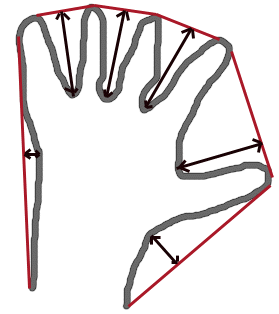
\includegraphics[width=0.5\textwidth]{pics/defects.png}

\cvCPyFunc{ContourArea}
Calculates the area of a whole contour or a contour section.

\cvdefC{
double cvContourArea( \par const CvArr* contour, \par CvSlice slice=CV\_WHOLE\_SEQ );
}\cvdefPy{ContourAres(contour,slice=CV\_WHOLE\_SEQ)-> double}

\begin{description}
\cvarg{contour}{Contour (sequence or array of vertices)}
\cvarg{slice}{Starting and ending points of the contour section of interest, by default, the area of the whole contour is calculated}
\end{description}

The function calculates the area of a whole contour
or a contour section. In the latter case the total area bounded by the
contour arc and the chord connecting the 2 selected points is calculated
as shown on the picture below:

\includegraphics[width=0.5\textwidth]{pics/contoursecarea.png}

Orientation of the contour affects the area sign, thus the function may return a \emph{negative} result. Use the \texttt{fabs()} function from C runtime to get the absolute value of the area.

\cvCPyFunc{ContourFromContourTree}
Restores a contour from the tree.

\cvdefC{
CvSeq* cvContourFromContourTree( \par const CvContourTree* tree,\par CvMemStorage* storage,\par CvTermCriteria criteria );
}\cvdefPy{ContourFromContourTree(tree,storage,criteria)-> contour}

\begin{description}
\cvarg{tree}{Contour tree}
\cvarg{storage}{Container for the reconstructed contour}
\cvarg{criteria}{Criteria, where to stop reconstruction}
\end{description}

The function restores the contour from its binary tree representation. The parameter \texttt{criteria} determines the accuracy and/or the number of tree levels used for reconstruction, so it is possible to build an approximated contour. The function returns the reconstructed contour.

\cvCPyFunc{ConvexHull2}
Finds the convex hull of a point set.

\cvdefC{
CvSeq* cvConvexHull2( \par const CvArr* input,\par void* hull\_storage=NULL,\par int orientation=CV\_CLOCKWISE,\par int return\_points=0 );
}\cvdefPy{ConvexHull2(points,storage,orientaton=CV\_CLOCKWISE,return\_points=0)-> convex\_hull}

\begin{description}
\cvarg{points}{Sequence or array of 2D points with 32-bit integer or floating-point coordinates}
\cvarg{hull\_storage}{The destination array (CvMat*) or memory storage (CvMemStorage*) that will store the convex hull. If it is an array, it should be 1d and have the same number of elements as the input array/sequence. On output the header is modified as to truncate the array down to the hull size.  If \texttt{hull\_storage} is NULL then the convex hull will be stored in the same storage as the input sequence}
\cvarg{orientation}{Desired orientation of convex hull: \texttt{CV\_CLOCKWISE} or \texttt{CV\_COUNTER\_CLOCKWISE}}
\cvarg{return\_points}{If non-zero, the points themselves will be stored in the hull instead of indices if \texttt{hull\_storage} is an array, or pointers if \texttt{hull\_storage} is memory storage}
\end{description}

The function finds the convex hull of a 2D point set using Sklansky's algorithm. If \texttt{hull\_storage} is memory storage, the function creates a sequence containing the hull points or pointers to them, depending on \texttt{return\_points} value and returns the sequence on output.  If \texttt{hull\_storage} is a CvMat, the function returns NULL.

% ===== Example. Building convex hull for a sequence or array of points =====
\begin{lstlisting}
#include "cv.h"
#include "highgui.h"
#include <stdlib.h>

#define ARRAY  0 /* switch between array/sequence method by replacing 0<=>1 */

void main( int argc, char** argv )
{
    IplImage* img = cvCreateImage( cvSize( 500, 500 ), 8, 3 );
    cvNamedWindow( "hull", 1 );

#if !ARRAY
        CvMemStorage* storage = cvCreateMemStorage();
#endif

    for(;;)
    {
        int i, count = rand()%100 + 1, hullcount;
        CvPoint pt0;
#if !ARRAY
        CvSeq* ptseq = cvCreateSeq( CV_SEQ_KIND_GENERIC|CV_32SC2,
                                    sizeof(CvContour),
                                    sizeof(CvPoint),
                                    storage );
        CvSeq* hull;

        for( i = 0; i < count; i++ )
        {
            pt0.x = rand() % (img->width/2) + img->width/4;
            pt0.y = rand() % (img->height/2) + img->height/4;
            cvSeqPush( ptseq, &pt0 );
        }
        hull = cvConvexHull2( ptseq, 0, CV_CLOCKWISE, 0 );
        hullcount = hull->total;
#else
        CvPoint* points = (CvPoint*)malloc( count * sizeof(points[0]));
        int* hull = (int*)malloc( count * sizeof(hull[0]));
        CvMat point_mat = cvMat( 1, count, CV_32SC2, points );
        CvMat hull_mat = cvMat( 1, count, CV_32SC1, hull );

        for( i = 0; i < count; i++ )
        {
            pt0.x = rand() % (img->width/2) + img->width/4;
            pt0.y = rand() % (img->height/2) + img->height/4;
            points[i] = pt0;
        }
        cvConvexHull2( &point_mat, &hull_mat, CV_CLOCKWISE, 0 );
        hullcount = hull_mat.cols;
#endif
        cvZero( img );
        for( i = 0; i < count; i++ )
        {
#if !ARRAY
            pt0 = *CV_GET_SEQ_ELEM( CvPoint, ptseq, i );
#else
            pt0 = points[i];
#endif
            cvCircle( img, pt0, 2, CV_RGB( 255, 0, 0 ), CV_FILLED );
        }

#if !ARRAY
        pt0 = **CV_GET_SEQ_ELEM( CvPoint*, hull, hullcount - 1 );
#else
        pt0 = points[hull[hullcount-1]];
#endif

        for( i = 0; i < hullcount; i++ )
        {
#if !ARRAY
            CvPoint pt = **CV_GET_SEQ_ELEM( CvPoint*, hull, i );
#else
            CvPoint pt = points[hull[i]];
#endif
            cvLine( img, pt0, pt, CV_RGB( 0, 255, 0 ));
            pt0 = pt;
        }

        cvShowImage( "hull", img );

        int key = cvWaitKey(0);
        if( key == 27 ) // 'ESC'
            break;

#if !ARRAY
        cvClearMemStorage( storage );
#else
        free( points );
        free( hull );
#endif
    }
}
\end{lstlisting}

\cvCPyFunc{ConvexityDefects}
Finds the convexity defects of a contour.

\cvdefC{
CvSeq* cvConvexityDefects( \par const CvArr* contour,\par const CvArr* convexhull,\par CvMemStorage* storage=NULL );
}\cvdefPy{ConvexityDefects(contour,convexhull,storage)-> convexity\_defects}

\begin{description}
\cvarg{contour}{Input contour}
\cvarg{convexhull}{Convex hull obtained using \cvCPyCross{ConvexHull2} that should contain pointers or indices to the contour points, not the hull points themselves (the \texttt{return\_points} parameter in \cvCPyCross{ConvexHull2} should be 0)}
\cvarg{storage}{Container for the output sequence of convexity defects. If it is NULL, the contour or hull (in that order) storage is used}
\end{description}

The function finds all convexity defects of the input contour and returns a sequence of the CvConvexityDefect structures.

\cvCPyFunc{CreateContourTree}
Creates a hierarchical representation of a contour.

\cvdefC{
CvContourTree* cvCreateContourTree( \par const CvSeq* contour,\par CvMemStorage* storage,\par double threshold );
}\cvdefPy{CreateCountourTree(contour,storage,threshold)-> contour\_tree}

\begin{description}
\cvarg{contour}{Input contour}
\cvarg{storage}{Container for output tree}
\cvarg{threshold}{Approximation accuracy}
\end{description}

The function creates a binary tree representation for the input \texttt{contour} and returns the pointer to its root. If the parameter \texttt{threshold} is less than or equal to 0, the function creates a full binary tree representation. If the threshold is greater than 0, the function creates a representation with the precision \texttt{threshold}: if the vertices with the interceptive area of its base line are less than \texttt{threshold}, the tree should not be built any further. The function returns the created tree.

\cvCPyFunc{EndFindContours}
Finishes the scanning process.

\cvdefC{
CvSeq* cvEndFindContours( \par CvContourScanner* scanner );
}

\begin{description}
\cvarg{scanner}{Pointer to the contour scanner}
\end{description}

The function finishes the scanning process and returns a pointer to the first contour on the highest level.

\cvCPyFunc{FindContours}
Finds the contours in a binary image.

\cvdefC{
int cvFindContours(\par CvArr* image,\par CvMemStorage* storage,\par CvSeq** first\_contour,\par
                    int header\_size=sizeof(CvContour),\par int mode=CV\_RETR\_LIST,\par
                    int method=CV\_CHAIN\_APPROX\_SIMPLE,\par CvPoint offset=cvPoint(0,0) );
}\cvdefPy{FindContours(image, storage, mode=CV\_RETR\_LIST, method=CV\_CHAIN\_APPROX\_SIMPLE, offset=(0,0)) -> cvseq}

\begin{description}
\cvarg{image}{The source, an 8-bit single channel image. Non-zero pixels are treated as 1's, zero pixels remain 0's - the image is treated as \texttt{binary}. To get such a binary image from grayscale, one may use \cvCPyCross{Threshold}, \cvCPyCross{AdaptiveThreshold} or \cvCPyCross{Canny}. The function modifies the source image's content}
\cvarg{storage}{Container of the retrieved contours}
\cvarg{first\_contour}{Output parameter, will contain the pointer to the first outer contour}
\cvarg{header\_size}{Size of the sequence header, $\ge \texttt{sizeof(CvChain)}$ if $\texttt{method} =\texttt{CV\_CHAIN\_CODE}$,
and $\ge \texttt{sizeof(CvContour)}$ otherwise}
\cvarg{mode}{Retrieval mode
\begin{description}
  \cvarg{CV\_RETR\_EXTERNAL}{retrives only the extreme outer contours}
  \cvarg{CV\_RETR\_LIST}{retrieves all of the contours and puts them in the list}
  \cvarg{CV\_RETR\_CCOMP}{retrieves all of the contours and organizes them into a two-level hierarchy: on the top level are the external boundaries of the components, on the second level are the boundaries of the holes}
  \cvarg{CV\_RETR\_TREE}{retrieves all of the contours and reconstructs the full hierarchy of nested contours}
\end{description}}
\cvarg{method}{Approximation method (for all the modes, except \texttt{CV\_LINK\_RUNS}, which uses built-in approximation)
\begin{description}
  \cvarg{CV\_CHAIN\_CODE}{outputs contours in the Freeman chain code. All other methods output polygons (sequences of vertices)}
  \cvarg{CV\_CHAIN\_APPROX\_NONE}{translates all of the points from the chain code into points}
  \cvarg{CV\_CHAIN\_APPROX\_SIMPLE}{compresses horizontal, vertical, and diagonal segments and leaves only their end points}
  \cvarg{CV\_CHAIN\_APPROX\_TC89\_L1,CV\_CHAIN\_APPROX\_TC89\_KCOS}{applies one of the flavors of the Teh-Chin chain approximation algorithm.}
  \cvarg{CV\_LINK\_RUNS}{uses a completely different contour retrieval algorithm by linking horizontal segments of 1's. Only the \texttt{CV\_RETR\_LIST} retrieval mode can be used with this method.}
\end{description}}
\cvarg{offset}{Offset, by which every contour point is shifted. This is useful if the contours are extracted from the image ROI and then they should be analyzed in the whole image context}
\end{description}

The function retrieves contours from the
binary image and returns the number of retrieved contours. The
pointer \texttt{first\_contour} is filled by the function. It will
contain a pointer to the first outermost contour or \texttt{NULL} if no
contours are detected (if the image is completely black). Other
contours may be reached from \texttt{first\_contour} using the
\texttt{h\_next} and \texttt{v\_next} links. The sample in the
\cvCPyCross{DrawContours} discussion shows how to use contours for
connected component detection. Contours can be also used for shape
analysis and object recognition - see \texttt{squares.c} in the OpenCV
sample directory.


\cvCPyFunc{FindNextContour}
Finds the next contour in the image.

\cvdefC{
CvSeq* cvFindNextContour( \par CvContourScanner scanner );
}

\begin{description}
\cvarg{scanner}{Contour scanner initialized by \cvCPyCross{StartFindContours} }
\end{description}

The function locates and retrieves the next contour in the image and returns a pointer to it. The function returns NULL if there are no more contours.

\cvCPyFunc{FitEllipse}
Fits an ellipse around a set of 2D points.

\cvdefC{
CvBox2D cvFitEllipse2( \par const CvArr* points );
}\cvdefPy{FitEllipse2(points)-> Box2D}

\begin{description}
\cvarg{points}{Sequence or array of points}
\end{description}

The function calculates the ellipse that fits best
(in least-squares sense) around a set of 2D points. The meaning of the
returned structure fields is similar to those in \cvCPyCross{Ellipse} except
that \texttt{size} stores the full lengths of the ellipse axises,
not half-lengths.

\cvCPyFunc{FitLine}
Fits a line to a 2D or 3D point set.

\cvdefC{
void  cvFitLine( \par const CvArr* points,\par int dist\_type,\par double param,\par double reps,\par double aeps,\par float* line );
}\cvdefPy{FitLine(points, dist\_type, param, reps, aeps) -> line}

\begin{description}
\cvarg{points}{Sequence or array of 2D or 3D points with 32-bit integer or floating-point coordinates}
\cvarg{dist\_type}{The distance used for fitting (see the discussion)}
\cvarg{param}{Numerical parameter (\texttt{C}) for some types of distances, if 0 then some optimal value is chosen}
\cvarg{reps, aeps}{Sufficient accuracy for the radius (distance between the coordinate origin and the line) and angle, respectively; 0.01 would be a good default value for both.}
\cvarg{line}{The output line parameters. In the case of a 2d fitting,
it is \cvC{an array} \cvPy{a tuple} of 4 floats \texttt{(vx, vy,
x0, y0)} where \texttt{(vx, vy)} is a normalized vector collinear to the
line and \texttt{(x0, y0)} is some point on the line. in the case of a
3D fitting it is \cvC{an array} \cvPy{a tuple} of 6 floats \texttt{(vx, vy, vz, x0, y0, z0)}
where \texttt{(vx, vy, vz)} is a normalized vector collinear to the line
and \texttt{(x0, y0, z0)} is some point on the line}
\end{description}

The function fits a line to a 2D or 3D point set by minimizing $\sum_i \rho(r_i)$ where $r_i$ is the distance between the $i$ th point and the line and $\rho(r)$ is a distance function, one of:

\begin{description}

\item[dist\_type=CV\_DIST\_L2]
\[ \rho(r) = r^2/2 \quad \text{(the simplest and the fastest least-squares method)} \]

\item[dist\_type=CV\_DIST\_L1]
\[ \rho(r) = r \]

\item[dist\_type=CV\_DIST\_L12]
\[ \rho(r) = 2 \cdot (\sqrt{1 + \frac{r^2}{2}} - 1) \]

\item[dist\_type=CV\_DIST\_FAIR]
\[ \rho\left(r\right) = C^2 \cdot \left( \frac{r}{C} - \log{\left(1 + \frac{r}{C}\right)}\right) \quad \text{where} \quad C=1.3998 \]

\item[dist\_type=CV\_DIST\_WELSCH]
\[ \rho\left(r\right) = \frac{C^2}{2} \cdot \left( 1 - \exp{\left(-\left(\frac{r}{C}\right)^2\right)}\right) \quad \text{where} \quad C=2.9846 \]

\item[dist\_type=CV\_DIST\_HUBER]
\[ \rho(r) = \fork
{r^2/2}{if $r < C$}
{C \cdot (r-C/2)}{otherwise}  \quad \text{where} \quad C=1.345
\]
\end{description}

\cvCPyFunc{GetCentralMoment}
Retrieves the central moment from the moment state structure.

\cvdefC{
double cvGetCentralMoment( \par CvMoments* moments,\par int x\_order,\par int y\_order );
}\cvdefPy{GetCentralMoment(cvmoments, x\_order, y\_order) -> double}

\begin{description}
\cvarg{moments}{Pointer to the moment state structure}
\cvarg{x\_order}{x order of the retrieved moment, $\texttt{x\_order} >= 0$}
\cvarg{y\_order}{y order of the retrieved moment, $\texttt{y\_order} >= 0$ and $\texttt{x\_order} + \texttt{y\_order} <= 3$}
\end{description}

The function retrieves the central moment, which in the case of image moments is defined as:

\[
\mu_{x\_order, \, y\_order} = \sum_{x,y} (I(x,y) \cdot (x-x_c)^{x\_order} \cdot (y-y_c)^{y\_order})
\]

where $x_c,y_c$ are the coordinates of the gravity center:

\[
x_c=\frac{M_{10}}{M_{00}}, y_c=\frac{M_{01}}{M_{00}}
\]

\cvCPyFunc{GetHuMoments}
Calculates the seven Hu invariants.

\cvdefC{void cvGetHuMoments( const CvMoments* moments,CvHuMoments* hu );}
\begin{description}
\cvarg{moments}{The input moments, computed with \cvCPyCross{Moments}}
\cvarg{hu}{The output Hu invariants}
\end{description}

The function calculates the seven Hu invariants, see \url{http://en.wikipedia.org/wiki/Image_moment}, that are defined as:

\[ \begin{array}{l}
hu_1=\eta_{20}+\eta_{02}\\
hu_2=(\eta_{20}-\eta_{02})^{2}+4\eta_{11}^{2}\\
hu_3=(\eta_{30}-3\eta_{12})^{2}+ (3\eta_{21}-\eta_{03})^{2}\\
hu_4=(\eta_{30}+\eta_{12})^{2}+ (\eta_{21}+\eta_{03})^{2}\\
hu_5=(\eta_{30}-3\eta_{12})(\eta_{30}+\eta_{12})[(\eta_{30}+\eta_{12})^{2}-3(\eta_{21}+\eta_{03})^{2}]+(3\eta_{21}-\eta_{03})(\eta_{21}+\eta_{03})[3(\eta_{30}+\eta_{12})^{2}-(\eta_{21}+\eta_{03})^{2}]\\
hu_6=(\eta_{20}-\eta_{02})[(\eta_{30}+\eta_{12})^{2}- (\eta_{21}+\eta_{03})^{2}]+4\eta_{11}(\eta_{30}+\eta_{12})(\eta_{21}+\eta_{03})\\
hu_7=(3\eta_{21}-\eta_{03})(\eta_{21}+\eta_{03})[3(\eta_{30}+\eta_{12})^{2}-(\eta_{21}+\eta_{03})^{2}]-(\eta_{30}-3\eta_{12})(\eta_{21}+\eta_{03})[3(\eta_{30}+\eta_{12})^{2}-(\eta_{21}+\eta_{03})^{2}]\\
\end{array}
\]

where $\eta_{ji}$ denote the normalized central moments.

These values are proved to be invariant to the image scale, rotation, and reflection except the seventh one, whose sign is changed by reflection. Of course, this invariance was proved with the assumption of infinite image resolution. In case of a raster images the computed Hu invariants for the original and transformed images will be a bit different.


\cvCPyFunc{GetNormalizedCentralMoment}
Retrieves the normalized central moment from the moment state structure.

\cvdefC{
double cvGetNormalizedCentralMoment( \par CvMoments* moments,\par int x\_order,\par int y\_order );
}\cvdefPy{GetNormalizedCentralMoment(cvmoments, x\_order, y\_order) -> double}

\begin{description}
\cvarg{moments}{Pointer to the moment state structure}
\cvarg{x\_order}{x order of the retrieved moment, $\texttt{x\_order} >= 0$}
\cvarg{y\_order}{y order of the retrieved moment, $\texttt{y\_order} >= 0$ and $\texttt{x\_order} + \texttt{y\_order} <= 3$}
\end{description}

The function retrieves the normalized central moment:

\[
\eta_{x\_order, \, y\_order} = \frac{\mu_{x\_order, \, y\_order}}{M_{00}^{(y\_order+x\_order)/2+1}}
\]

\cvCPyFunc{GetSpatialMoment}
Retrieves the spatial moment from the moment state structure.

\cvdefC{
double cvGetSpatialMoment( \par CvMoments* moments, \par int x\_order, \par int y\_order );
}\cvdefPy{GetSpatialMoment(cvmoments, x\_order, y\_order) -> double}

\begin{description}
\cvarg{moments}{The moment state, calculated by \cvCPyCross{Moments}}
\cvarg{x\_order}{x order of the retrieved moment, $\texttt{x\_order} >= 0$}
\cvarg{y\_order}{y order of the retrieved moment, $\texttt{y\_order} >= 0$ and $\texttt{x\_order} + \texttt{y\_order} <= 3$}
\end{description}

The function retrieves the spatial moment, which in the case of image moments is defined as:

\[
M_{x\_order, \, y\_order} = \sum_{x,y} (I(x,y) \cdot x^{x\_order} \cdot y^{y\_order})
\]

where $I(x,y)$ is the intensity of the pixel $(x, y)$.

\cvCPyFunc{MatchContourTrees}
Compares two contours using their tree representations.

\cvdefC{
double cvMatchContourTrees( \par const CvContourTree* tree1,\par const CvContourTree* tree2,\par int method,\par double threshold );
}\cvdefPy{MatchContourTrees(tree1,tree2,method,threshold)-> double}

\begin{description}
\cvarg{tree1}{First contour tree}
\cvarg{tree2}{Second contour tree}
\cvarg{method}{Similarity measure, only \texttt{CV\_CONTOUR\_TREES\_MATCH\_I1} is supported}
\cvarg{threshold}{Similarity threshold}
\end{description}

The function calculates the value of the matching measure for two contour trees. The similarity measure is calculated level by level from the binary tree roots. If at a certain level the difference between contours becomes less than \texttt{threshold}, the reconstruction process is interrupted and the current difference is returned.

\cvCPyFunc{MatchShapes}
Compares two shapes.

\cvdefC{
double cvMatchShapes( \par const void* object1,\par const void* object2,\par int method,\par double parameter=0 );
}\cvdefPy{MatchShapes(object1,object2,method,parameter=0)-> None}

\begin{description}
\cvarg{object1}{First contour or grayscale image}
\cvarg{object2}{Second contour or grayscale image}
\cvarg{method}{Comparison method;
 \texttt{CV\_CONTOUR\_MATCH\_I1}, 
 \texttt{CV\_CONTOURS\_MATCH\_I2} 
or 
 \texttt{CV\_CONTOURS\_MATCH\_I3}}
\cvarg{parameter}{Method-specific parameter (is not used now)}
\end{description}

The function compares two shapes. The 3 implemented methods all use Hu moments (see \cvCPyCross{GetHuMoments}) ($A$ is \texttt{object1}, $B$ is \texttt{object2}):

\begin{description}
\item[method=CV\_CONTOUR\_MATCH\_I1]
\[ I_1(A,B) = \sum_{i=1...7} \left| \frac{1}{m^A_i} - \frac{1}{m^B_i} \right| \]

\item[method=CV\_CONTOUR\_MATCH\_I2]
\[ I_2(A,B) = \sum_{i=1...7} \left| m^A_i - m^B_i \right| \]

\item[method=CV\_CONTOUR\_MATCH\_I3]
\[ I_3(A,B) = \sum_{i=1...7} \frac{ \left| m^A_i - m^B_i \right| }{ \left| m^A_i \right| } \]
\end{description}

where

\[
\begin{array}{l}
m^A_i = sign(h^A_i) \cdot \log{h^A_i}
m^B_i = sign(h^B_i) \cdot \log{h^B_i}
\end{array}
\]

and $h^A_i, h^B_i$ are the Hu moments of $A$ and $B$ respectively.


\cvCPyFunc{MinAreaRect2}
Finds the circumscribed rectangle of minimal area for a given 2D point set.

\cvdefC{
CvBox2D  cvMinAreaRect2( \par const CvArr* points,\par CvMemStorage* storage=NULL );
}\cvdefPy{MinAreaRect2(points,storage)-> CvBox2D}

\begin{description}
\cvarg{points}{Sequence or array of points}
\cvarg{storage}{Optional temporary memory storage}
\end{description}

The function finds a circumscribed rectangle of the minimal area for a 2D point set by building a convex hull for the set and applying the rotating calipers technique to the hull.

\cvfunc{Picture. Minimal-area bounding rectangle for contour}

\includegraphics[width=0.5\textwidth]{pics/minareabox.png}

\cvCPyFunc{MinEnclosingCircle}
Finds the circumscribed circle of minimal area for a given 2D point set.

\cvdefC{
int cvMinEnclosingCircle( \par const CvArr* points,\par CvPoint2D32f* center,\par float* radius );
}\cvdefPy{MinEnclosingCircle(points)-> int,center,radius}

\begin{description}
\cvarg{points}{Sequence or array of 2D points}
\cvarg{center}{Output parameter; the center of the enclosing circle}
\cvarg{radius}{Output parameter; the radius of the enclosing circle}
\end{description}

The function finds the minimal circumscribed
circle for a 2D point set using an iterative algorithm. It returns nonzero
if the resultant circle contains all the input points and zero otherwise
(i.e. the algorithm failed).

\cvCPyFunc{Moments}
Calculates all of the moments up to the third order of a polygon or rasterized shape.

\cvdefC{
void cvMoments( \par const CvArr* arr,\par CvMoments* moments,\par int binary=0 );
}\cvdefPy{Moments(arr) -> cvmoments}

\begin{description}
\cvarg{arr}{Image (1-channel or 3-channel with COI set) or polygon (CvSeq of points or a vector of points)}
\cvarg{moments}{Pointer to returned moment's state structure}
\cvarg{binary}{(For images only) If the flag is non-zero, all of the zero pixel values are treated as zeroes, and all of the others are treated as 1's}
\end{description}

The function calculates spatial and central moments up to the third order and writes them to \texttt{moments}. The moments may then be used then to calculate the gravity center of the shape, its area, main axises and various shape characeteristics including 7 Hu invariants.

\cvCPyFunc{PointPolygonTest}
Point in contour test.

\cvdefC{
double cvPointPolygonTest( \par const CvArr* contour,\par CvPoint2D32f pt,\par int measure\_dist );
}\cvdefPy{PointPolygonTest(contour,pt,measure\_dist)-> double}

\begin{description}
\cvarg{contour}{Input contour}
\cvarg{pt}{The point tested against the contour}
\cvarg{measure\_dist}{If it is non-zero, the function estimates the distance from the point to the nearest contour edge}
\end{description}

The function determines whether the
point is inside a contour, outside, or lies on an edge (or coinsides
with a vertex). It returns positive, negative or zero value,
correspondingly. When $\texttt{measure\_dist} =0$, the return value
is +1, -1 and 0, respectively. When $\texttt{measure\_dist} \ne 0$,
it is a signed distance between the point and the nearest contour
edge.

Here is the sample output of the function, where each image pixel is tested against the contour.

\includegraphics[width=0.5\textwidth]{pics/pointpolygon.png}

\ifC

\cvCPyFunc{PointSeqFromMat}
Initializes a point sequence header from a point vector.

\cvdefC{
CvSeq* cvPointSeqFromMat( \par int seq\_kind,\par const CvArr* mat,\par CvContour* contour\_header,\par CvSeqBlock* block );
}

\begin{description}
\cvarg{seq\_kind}{Type of the point sequence: point set (0), a curve (\texttt{CV\_SEQ\_KIND\_CURVE}), closed curve (\texttt{CV\_SEQ\_KIND\_CURVE+CV\_SEQ\_FLAG\_CLOSED}) etc.}
\cvarg{mat}{Input matrix. It should be a continuous, 1-dimensional vector of points, that is, it should have type \texttt{CV\_32SC2} or \texttt{CV\_32FC2}}
\cvarg{contour\_header}{Contour header, initialized by the function}
\cvarg{block}{Sequence block header, initialized by the function}
\end{description}

The function initializes a sequence
header to create a "virtual" sequence in which elements reside in
the specified matrix. No data is copied. The initialized sequence
header may be passed to any function that takes a point sequence
on input. No extra elements can be added to the sequence,
but some may be removed. The function is a specialized variant of
\cvCPyCross{MakeSeqHeaderForArray} and uses
the latter internally. It returns a pointer to the initialized contour
header. Note that the bounding rectangle (field \texttt{rect} of
\texttt{CvContour} strucuture) is not initialized by the function. If
you need one, use \cvCPyCross{BoundingRect}.

Here is a simple usage example.

\begin{lstlisting}
CvContour header;
CvSeqBlock block;
CvMat* vector = cvCreateMat( 1, 3, CV_32SC2 );

CV_MAT_ELEM( *vector, CvPoint, 0, 0 ) = cvPoint(100,100);
CV_MAT_ELEM( *vector, CvPoint, 0, 1 ) = cvPoint(100,200);
CV_MAT_ELEM( *vector, CvPoint, 0, 2 ) = cvPoint(200,100);

IplImage* img = cvCreateImage( cvSize(300,300), 8, 3 );
cvZero(img);

cvDrawContours( img,
    cvPointSeqFromMat(CV_SEQ_KIND_CURVE+CV_SEQ_FLAG_CLOSED,
                      vector,
                      &header,
                      &block),
                CV_RGB(255,0,0),
                CV_RGB(255,0,0),
                0, 3, 8, cvPoint(0,0));
\end{lstlisting}


\cvCPyFunc{ReadChainPoint}
Gets the next chain point.

\cvdefC{
CvPoint cvReadChainPoint( CvChainPtReader* reader );
}

\begin{description}
\cvarg{reader}{Chain reader state}
\end{description}

The function returns the current chain point and updates the reader position.

\cvCPyFunc{StartFindContours}
Initializes the contour scanning process.

\cvdefC{
CvContourScanner cvStartFindContours(\par CvArr* image,\par CvMemStorage* storage,\par
                                      int header\_size=sizeof(CvContour),\par
                                      int mode=CV\_RETR\_LIST,\par
                                      int method=CV\_CHAIN\_APPROX\_SIMPLE,\par
                                      CvPoint offset=cvPoint(0,\par0) );
}

\begin{description}
\cvarg{image}{The 8-bit, single channel, binary source image}
\cvarg{storage}{Container of the retrieved contours}
\cvarg{header\_size}{Size of the sequence header, $>=sizeof(CvChain)$ if \texttt{method} =CV\_CHAIN\_CODE, and $>=sizeof(CvContour)$ otherwise}
\cvarg{mode}{Retrieval mode; see \cvCPyCross{FindContours}}
\cvarg{method}{Approximation method. It has the same meaning in \cvCPyCross{FindContours}, but \texttt{CV\_LINK\_RUNS} can not be used here}
\cvarg{offset}{ROI offset; see \cvCPyCross{FindContours}}
\end{description}

The function initializes and returns a pointer to the contour scanner. The scanner is used in \cvCPyCross{FindNextContour} to retrieve the rest of the contours.

\cvCPyFunc{StartReadChainPoints}
Initializes the chain reader.

\cvdefC{
void cvStartReadChainPoints( CvChain* chain, CvChainPtReader* reader );
}

The function initializes a special reader.

\cvCPyFunc{SubstituteContour}
Replaces a retrieved contour.

\cvdefC{
void cvSubstituteContour( \par CvContourScanner scanner, \par CvSeq* new\_contour );
}

\begin{description}
\cvarg{scanner}{Contour scanner initialized by \cvCPyCross{StartFindContours} }
\cvarg{new\_contour}{Substituting contour}
\end{description}

The function replaces the retrieved
contour, that was returned from the preceding call of
\cvCPyCross{FindNextContour} and stored inside the contour scanner
state, with the user-specified contour. The contour is inserted
into the resulting structure, list, two-level hierarchy, or tree,
depending on the retrieval mode. If the parameter \texttt{new\_contour}
is \texttt{NULL}, the retrieved contour is not included in the
resulting structure, nor are any of its children that might be added
to this structure later.

\fi

\fi


\ifCpp

\cvCppFunc{moments}
Calculates all of the moments up to the third order of a polygon or rasterized shape.

\cvdefCpp{Moments moments( const Mat\& array, bool binaryImage=false );}

where the class \texttt{Moments} is defined as:
\begin{lstlisting}
class Moments
{
public:
    Moments();
    Moments(double m00, double m10, double m01, double m20, double m11,
            double m02, double m30, double m21, double m12, double m03 );
    Moments( const CvMoments\& moments );
    operator CvMoments() const;
    
    // spatial moments
    double  m00, m10, m01, m20, m11, m02, m30, m21, m12, m03;
    // central moments
    double  mu20, mu11, mu02, mu30, mu21, mu12, mu03;
    // central normalized moments
    double  nu20, nu11, nu02, nu30, nu21, nu12, nu03;
};
\end{lstlisting}

\begin{description}
\cvarg{array}{A raster image (single-channel, 8-bit or floating-point 2D array) or an array
    ($1 \times N$ or $N \times 1$) of 2D points (\texttt{Point} or \texttt{Point2f})}
\cvarg{binaryImage}{(For images only) If it is true, then all the non-zero image pixels are treated as 1's}
\end{description}

The function computes moments, up to the 3rd order, of a vector shape or a rasterized shape.
In case of a raster image, the spatial moments $\texttt{Moments::m}_{ji}$ are computed as:

\[\texttt{m}_{ji}=\sum_{x,y} \left(\texttt{array}(x,y) \cdot x^j \cdot y^i\right),\]

the central moments $\texttt{Moments::mu}_{ji}$ are computed as:
\[\texttt{mu}_{ji}=\sum_{x,y} \left(\texttt{array}(x,y) \cdot (x - \bar{x})^j \cdot (y - \bar{y})^i\right)\]
where $(\bar{x}, \bar{y})$ is the mass center:

\[
\bar{x}=\frac{\texttt{m}_{10}}{\texttt{m}_{00}},\; \bar{y}=\frac{\texttt{m}_{01}}{\texttt{m}_{00}}
\]

and the normalized central moments $\texttt{Moments::nu}_{ij}$ are computed as:
\[\texttt{nu}_{ji}=\frac{\texttt{mu}_{ji}}{\texttt{m}_{00}^{(i+j)/2+1}}.\]

Note that $\texttt{mu}_{00}=\texttt{m}_{00}$, $\texttt{nu}_{00}=1$ $\texttt{nu}_{10}=\texttt{mu}_{10}=\texttt{mu}_{01}=\texttt{mu}_{10}=0$, hence the values are not stored.

The moments of a contour are defined in the same way, but computed using Green's formula
(see \url{http://en.wikipedia.org/wiki/Green_theorem}), therefore, because of a limited raster resolution, the moments computed for a contour will be slightly different from the moments computed for the same contour rasterized.

See also: \cvCppCross{contourArea}, \cvCppCross{arcLength}

\cvCppFunc{HuMoments}
Calculates the seven Hu invariants.

\cvdefCpp{void HuMoments( const Moments\& moments, double h[7] );}
\begin{description}
\cvarg{moments}{The input moments, computed with \cvCppCross{moments}}
\cvarg{h}{The output Hu invariants}
\end{description}

The function calculates the seven Hu invariants, see \url{http://en.wikipedia.org/wiki/Image_moment}, that are defined as:

\[ \begin{array}{l}
h[0]=\eta_{20}+\eta_{02}\\
h[1]=(\eta_{20}-\eta_{02})^{2}+4\eta_{11}^{2}\\
h[2]=(\eta_{30}-3\eta_{12})^{2}+ (3\eta_{21}-\eta_{03})^{2}\\
h[3]=(\eta_{30}+\eta_{12})^{2}+ (\eta_{21}+\eta_{03})^{2}\\
h[4]=(\eta_{30}-3\eta_{12})(\eta_{30}+\eta_{12})[(\eta_{30}+\eta_{12})^{2}-3(\eta_{21}+\eta_{03})^{2}]+(3\eta_{21}-\eta_{03})(\eta_{21}+\eta_{03})[3(\eta_{30}+\eta_{12})^{2}-(\eta_{21}+\eta_{03})^{2}]\\
h[5]=(\eta_{20}-\eta_{02})[(\eta_{30}+\eta_{12})^{2}- (\eta_{21}+\eta_{03})^{2}]+4\eta_{11}(\eta_{30}+\eta_{12})(\eta_{21}+\eta_{03})\\
h[6]=(3\eta_{21}-\eta_{03})(\eta_{21}+\eta_{03})[3(\eta_{30}+\eta_{12})^{2}-(\eta_{21}+\eta_{03})^{2}]-(\eta_{30}-3\eta_{12})(\eta_{21}+\eta_{03})[3(\eta_{30}+\eta_{12})^{2}-(\eta_{21}+\eta_{03})^{2}]\\
\end{array}
\]

where $\eta_{ji}$ stand for $\texttt{Moments::nu}_{ji}$.

These values are proved to be invariant to the image scale, rotation, and reflection except the seventh one, whose sign is changed by reflection. Of course, this invariance was proved with the assumption of infinite image resolution. In case of a raster images the computed Hu invariants for the original and transformed images will be a bit different.

See also: \cvCppCross{matchShapes}

\cvCppFunc{findContours}
Finds the contours in a binary image.

\cvdefCpp{void findContours( const Mat\& image, vector<vector<Point> >\& contours,\par
                   vector<Vec4i>\& hierarchy, int mode,\par
                   int method, Point offset=Point());\newline
void findContours( const Mat\& image, vector<vector<Point> >\& contours,\par
                   int mode, int method, Point offset=Point());
}
\begin{description}
\cvarg{image}{The source, an 8-bit single-channel image. Non-zero pixels are treated as 1's, zero pixels remain 0's - the image is treated as \texttt{binary}. You can use \cvCppCross{compare}, \cvCppCross{inRange}, \cvCppCross{threshold}, \cvCppCross{adaptiveThreshold}, \cvCppCross{Canny} etc. to create a binary image out of a grayscale or color one. The function modifies the \texttt{image} while extracting the contours}
\cvarg{contours}{The detected contours. Each contour is stored as a vector of points}
\cvarg{hiararchy}{The optional output vector that will contain information about the image topology. It will have as many elements as the number of contours. For each contour \texttt{contours[i]}, the elements \texttt{hierarchy[i][0]}, \texttt{hiearchy[i][1]}, \texttt{hiearchy[i][2]}, \texttt{hiearchy[i][3]} will be set to 0-based indices in \texttt{contours} of the next and previous contours at the same hierarchical level, the first child contour and the parent contour, respectively. If for some contour \texttt{i} there is no next, previous, parent or nested contours, the corresponding elements of \texttt{hierarchy[i]} will be negative}
\cvarg{mode}{The contour retrieval mode
\begin{description}
  \cvarg{CV\_RETR\_EXTERNAL}{retrieves only the extreme outer contours; It will set \texttt{hierarchy[i][2]=hierarchy[i][3]=-1} for all the contours}
  \cvarg{CV\_RETR\_LIST}{retrieves all of the contours without establishing any hierarchical relationships}
  \cvarg{CV\_RETR\_CCOMP}{retrieves all of the contours and organizes them into a two-level hierarchy: on the top level are the external boundaries of the components, on the second level are the boundaries of the holes. If inside a hole of a connected component there is another contour, it will still be put on the top level}
  \cvarg{CV\_RETR\_TREE}{retrieves all of the contours and reconstructs the full hierarchy of nested contours. This full hierarchy is built and shown in OpenCV \texttt{contours.c} demo}
\end{description}}
\cvarg{method}{The contour approximation method.
\begin{description}
  \cvarg{CV\_CHAIN\_APPROX\_NONE}{stores absolutely all the contour points. That is, every 2 points of a contour stored with this method are 8-connected neighbors of each other}
  \cvarg{CV\_CHAIN\_APPROX\_SIMPLE}{compresses horizontal, vertical, and diagonal segments and leaves only their end points. E.g. an up-right rectangular contour will be encoded with 4 points}
  \cvarg{CV\_CHAIN\_APPROX\_TC89\_L1,CV\_CHAIN\_APPROX\_TC89\_KCOS}{applies one of the flavors of the Teh-Chin chain approximation algorithm; see \cite{TehChin89}}
\end{description}}
\cvarg{offset}{The optional offset, by which every contour point is shifted. This is useful if the contours are extracted from the image ROI and then they should be analyzed in the whole image context}
\end{description}

The function retrieves contours from the
binary image using the algorithm \cite{Suzuki85}. The contours are a useful tool for shape analysis and object detection and recognition. See \texttt{squares.c} in the OpenCV sample directory.

\cvCppFunc{drawContours}
Draws contours' outlines or filled contours.

\cvdefCpp{void drawContours( Mat\& image, const vector<vector<Point> >\& contours,\par
                   int contourIdx, const Scalar\& color, int thickness=1,\par
                   int lineType=8, const vector<Vec4i>\& hierarchy=vector<Vec4i>(),\par
                   int maxLevel=INT\_MAX, Point offset=Point() );}
\begin{description}
\cvarg{image}{The destination image}
\cvarg{contours}{All the input contours. Each contour is stored as a point vector}
\cvarg{contourIdx}{Indicates the contour to draw. If it is negative, all the contours are drawn}
\cvarg{color}{The contours' color}
\cvarg{thickness}{Thickness of lines the contours are drawn with.
If it is negative (e.g. \texttt{thickness=CV\_FILLED}), the contour interiors are
drawn.}
\cvarg{lineType}{The line connectivity; see \cvCppCross{line} description}
\cvarg{hierarchy}{The optional information about hierarchy. It is only needed if you want to draw only some of the  contours (see \texttt{maxLevel})}
\cvarg{maxLevel}{Maximal level for drawn contours. If 0, only
the specified contour is drawn. If 1, the function draws the contour(s) and all the nested contours. If 2, the function draws the contours, all the nested contours and all the nested into nested contours etc. This parameter is only taken into account when there is \texttt{hierarchy} available.}
\cvarg{offset}{The optional contour shift parameter. Shift all the drawn contours by the specified $\texttt{offset}=(dx,dy)$}
\end{description}

The function draws contour outlines in the image if $\texttt{thickness} \ge 0$ or fills the area bounded by the contours if $ \texttt{thickness}<0$. Here is the example on how to retrieve connected components from the binary image and label them

\begin{lstlisting}
#include "cv.h"
#include "highgui.h"

using namespace cv;

int main( int argc, char** argv )
{
    Mat src;
    // the first command line parameter must be file name of binary 
    // (black-n-white) image
    if( argc != 2 || !(src=imread(argv[1], 0)).data)
        return -1;

    Mat dst = Mat::zeros(src.rows, src.cols, CV_8UC3);

    src = src > 1;
    namedWindow( "Source", 1 );
    imshow( "Source", src );

    vector<vector<Point> > contours;
    vector<Vec4i> hierarchy;
    
    findContours( src, contours, hierarchy, 
        CV_RETR_CCOMP, CV_CHAIN_APPROX_SIMPLE );

    // iterate through all the top-level contours,
    // draw each connected component with its own random color
    int idx = 0;
    for( ; idx >= 0; idx = hiearchy[idx][0] )
    {
        Scalar color( rand()&255, rand()&255, rand()&255 );
        drawContours( dst, contours, idx, color, CV_FILLED, 8, hiearchy );
    }

    namedWindow( "Components", 1 );
    imshow( "Components", dst );
    waitKey(0);
}
\end{lstlisting}


\cvCppFunc{approxPolyDP}
Approximates polygonal curve(s) with the specified precision.

\cvdefCpp{void approxPolyDP( const Mat\& curve,\par
                   vector<Point>\& approxCurve,\par
                   double epsilon, bool closed );\newline
void approxPolyDP( const Mat\& curve,\par
                   vector<Point2f>\& approxCurve,\par
                   double epsilon, bool closed );}
\begin{description}
\cvarg{curve}{The polygon or curve to approximate. Must be $1 \times N$ or $N \times 1$ matrix of type \texttt{CV\_32SC2} or \texttt{CV\_32FC2}. You can also pass \texttt{vector<Point>} or \texttt{vector<Point2f} that will be automatically converted to the matrix of the proper size and type}
\cvarg{approxCurve}{The result of the approximation; The type should match the type of the input curve}
\cvarg{epsilon}{Specifies the approximation accuracy. This is the maximum distance between the original curve and its approximation}
\cvarg{closed}{If true, the approximated curve is closed (i.e. its first and last vertices are connected), otherwise it's not}
\end{description}

The functions \texttt{approxPolyDP} approximate a curve or a polygon with another curve/polygon with less vertices, so that the distance between them is less or equal to the specified precision. It used Douglas-Peucker algorithm \url{http://en.wikipedia.org/wiki/Ramer-Douglas-Peucker_algorithm}

\cvCppFunc{arcLength}
Calculates a contour perimeter or a curve length.

\cvdefCpp{double arcLength( const Mat\& curve, bool closed );}
\begin{description}
\cvarg{curve}{The input vector of 2D points, represented by \texttt{CV\_32SC2} or \texttt{CV\_32FC2} matrix or by \texttt{vector<Point>} or \texttt{vector<Point2f>}}
\cvarg{closed}{Indicates, whether the curve is closed or not}
\end{description}

The function computes the curve length or the closed contour perimeter.

\cvCppFunc{boundingRect}
Calculates the up-right bounding rectangle of a point set.

\cvdefCpp{Rect boundingRect( const Mat\& points );}
\begin{description}
\cvarg{points}{The input 2D point set, represented by \texttt{CV\_32SC2} or \texttt{CV\_32FC2} matrix or by \texttt{vector<Point>} or \texttt{vector<Point2f>}}
\end{description}

The function calculates and returns the minimal up-right bounding rectangle for the specified point set.


\cvCppFunc{estimateRigidTransform}
Computes optimal affine transformation between two 2D point sets

\cvdefCpp{Mat estimateRigidTransform( const Mat\& srcpt, const Mat\& dstpt,\par
                            bool fullAffine );}
\begin{description}
\cvarg{srcpt}{The first input 2D point set}
\cvarg{dst}{The second input 2D point set of the same size and the same type as \texttt{A}}
\cvarg{fullAffine}{If true, the function finds the optimal affine transformation with no any additional resrictions (i.e. there are 6 degrees of freedom); otherwise, the class of transformations to choose from is limited to combinations of translation, rotation and uniform scaling (i.e. there are 5 degrees of freedom)}
\end{description}

The function finds the optimal affine transform $[A|b]$ (a $2 \times 3$ floating-point matrix) that approximates best the transformation from $\texttt{srcpt}_i$ to $\texttt{dstpt}_i$:

\[ [A^*|b^*] = arg \min_{[A|b]} \sum_i \|\texttt{dstpt}_i - A {\texttt{srcpt}_i}^T - b \|^2 \]

where $[A|b]$ can be either arbitrary (when \texttt{fullAffine=true}) or have form
\[\begin{bmatrix}a_{11} & a_{12} & b_1 \\ -a_{12} & a_{11} & b_2 \end{bmatrix}\] when \texttt{fullAffine=false}.

See also: \cvCppCross{getAffineTransform}, \cvCppCross{getPerspectiveTransform}, \cvCppCross{findHomography}

\cvCppFunc{estimateAffine3D}
Computes optimal affine transformation between two 3D point sets

\cvdefCpp{int estimateAffine3D(const Mat\& srcpt, const Mat\& dstpt, Mat\& out,\par
                     vector<uchar>\& outliers,\par
                     double ransacThreshold = 3.0,\par
                     double confidence = 0.99);}
\begin{description}
\cvarg{srcpt}{The first input 3D point set}
\cvarg{dstpt}{The second input 3D point set}
\cvarg{out}{The output 3D affine transformation matrix $3 \times 4$}
\cvarg{outliers}{The output vector indicating which points are outliers}
\cvarg{ransacThreshold}{The maximum reprojection error in RANSAC algorithm to consider a point an inlier}
\cvarg{confidence}{The confidence level, between 0 and 1, with which the matrix is estimated}
\end{description}

The function estimates the optimal 3D affine transformation between two 3D point sets using RANSAC algorithm.


\cvCppFunc{contourArea}
Calculates the contour area

\cvdefCpp{double contourArea( const Mat\& contour );    }
\begin{description}
\cvarg{contour}{The contour vertices, represented by \texttt{CV\_32SC2} or \texttt{CV\_32FC2} matrix or by \texttt{vector<Point>} or \texttt{vector<Point2f>}}
\end{description}

The function computes the contour area. Similarly to \cvCppCross{moments} the area is computed using the Green formula, thus the returned area and the number of non-zero pixels, if you draw the contour using \cvCppCross{drawContours} or \cvCppCross{fillPoly}, can be different.
Here is a short example:

\begin{lstlisting}
vector<Point> contour;
contour.push_back(Point2f(0, 0));
contour.push_back(Point2f(10, 0));
contour.push_back(Point2f(10, 10));
contour.push_back(Point2f(5, 4));

double area0 = contourArea(contour);
vector<Point> approx;
approxPolyDP(contour, approx, 5, true);
double area1 = contourArea(approx);

cout << "area0 =" << area0 << endl <<
        "area1 =" << area1 << endl <<
        "approx poly vertices" << approx.size() << endl; 
\end{lstlisting}

\cvCppFunc{convexHull}    
Finds the convex hull of a point set.

\cvdefCpp{void convexHull( const Mat\& points, vector<int>\& hull,\par
                 bool clockwise=false );\newline
void convexHull( const Mat\& points, vector<Point>\& hull,\par
                 bool clockwise=false );\newline
void convexHull( const Mat\& points, vector<Point2f>\& hull,\par
                 bool clockwise=false );}
\begin{description}
\cvarg{points}{The input 2D point set, represented by \texttt{CV\_32SC2} or \texttt{CV\_32FC2} matrix or by
\texttt{vector<Point>} or \texttt{vector<Point2f>}}
\cvarg{hull}{The output convex hull. It is either a vector of points that form the hull, or a vector of 0-based point indices of the hull points in the original array (since the set of convex hull points is a subset of the original point set).}
\cvarg{clockwise}{If true, the output convex hull will be oriented clockwise, otherwise it will be oriented counter-clockwise. Here, the usual screen coordinate system is assumed - the origin is at the top-left corner, x axis is oriented to the right, and y axis is oriented downwards.}
\end{description}

The functions find the convex hull of a 2D point set using Sklansky's algorithm \cite{Sklansky82} that has $O(N logN)$ or $O(N)$ complexity (where $N$ is the number of input points), depending on how the initial sorting is implemented (currently it is $O(N logN)$. See the OpenCV sample \texttt{convexhull.c} that demonstrates the use of the different function variants. 


\cvCppFunc{fitEllipse}
Fits an ellipse around a set of 2D points.

\cvdefCpp{RotatedRect fitEllipse( const Mat\& points );}
\begin{description}
\cvarg{points}{The input 2D point set, represented by \texttt{CV\_32SC2} or \texttt{CV\_32FC2} matrix or by
\texttt{vector<Point>} or \texttt{vector<Point2f>}}
\end{description}

The function calculates the ellipse that fits best
(in least-squares sense) a set of 2D points. It returns the rotated rectangle in which the ellipse is inscribed.

\cvCppFunc{fitLine}
Fits a line to a 2D or 3D point set.

\cvdefCpp{void fitLine( const Mat\& points, Vec4f\& line, int distType,\par
              double param, double reps, double aeps );\newline
void fitLine( const Mat\& points, Vec6f\& line, int distType,\par
              double param, double reps, double aeps );}
\begin{description}
\cvarg{points}{The input 2D point set, represented by \texttt{CV\_32SC2} or \texttt{CV\_32FC2} matrix or by
\texttt{vector<Point>}, \texttt{vector<Point2f>}, \texttt{vector<Point3i>} or \texttt{vector<Point3f>}}
\cvarg{line}{The output line parameters. In the case of a 2d fitting,
it is a vector of 4 floats \texttt{(vx, vy,
x0, y0)} where \texttt{(vx, vy)} is a normalized vector collinear to the
line and \texttt{(x0, y0)} is some point on the line. in the case of a
3D fitting it is vector of 6 floats \texttt{(vx, vy, vz, x0, y0, z0)}
where \texttt{(vx, vy, vz)} is a normalized vector collinear to the line
and \texttt{(x0, y0, z0)} is some point on the line}
\cvarg{distType}{The distance used by the M-estimator (see the discussion)}
\cvarg{param}{Numerical parameter (\texttt{C}) for some types of distances, if 0 then some optimal value is chosen}
\cvarg{reps, aeps}{Sufficient accuracy for the radius (distance between the coordinate origin and the line) and angle, respectively; 0.01 would be a good default value for both.}
\end{description}

The functions \texttt{fitLine} fit a line to a 2D or 3D point set by minimizing $\sum_i \rho(r_i)$ where $r_i$ is the distance between the $i^{th}$ point and the line and $\rho(r)$ is a distance function, one of:

\begin{description}
\item[distType=CV\_DIST\_L2]
\[ \rho(r) = r^2/2 \quad \text{(the simplest and the fastest least-squares method)} \]

\item[distType=CV\_DIST\_L1]
\[ \rho(r) = r \]

\item[distType=CV\_DIST\_L12]
\[ \rho(r) = 2 \cdot (\sqrt{1 + \frac{r^2}{2}} - 1) \]

\item[distType=CV\_DIST\_FAIR]
\[ \rho\left(r\right) = C^2 \cdot \left( \frac{r}{C} - \log{\left(1 + \frac{r}{C}\right)}\right) \quad \text{where} \quad C=1.3998 \]

\item[distType=CV\_DIST\_WELSCH]
\[ \rho\left(r\right) = \frac{C^2}{2} \cdot \left( 1 - \exp{\left(-\left(\frac{r}{C}\right)^2\right)}\right) \quad \text{where} \quad C=2.9846 \]

\item[distType=CV\_DIST\_HUBER]
\[ \rho(r) = \fork
{r^2/2}{if $r < C$}
{C \cdot (r-C/2)}{otherwise}  \quad \text{where} \quad C=1.345
\]
\end{description}

The algorithm is based on the M-estimator (\url{http://en.wikipedia.org/wiki/M-estimator}) technique, that iteratively fits the line using weighted least-squares algorithm and after each iteration the weights $w_i$ are adjusted to beinversely proportional to $\rho(r_i)$. 


\cvCppFunc{isContourConvex}
Tests contour convexity.

\cvdefCpp{bool isContourConvex( const Mat\& contour );}
\begin{description}
\cvarg{contour}{The tested contour, a matrix of type \texttt{CV\_32SC2} or \texttt{CV\_32FC2}, or \texttt{vector<Point>} or \texttt{vector<Point2f>}}
\end{description}

The function tests whether the input contour is convex or not. The contour must be simple, i.e. without self-intersections, otherwise the function output is undefined.


\cvCppFunc{minAreaRect}
Finds the minimum area rotated rectangle enclosing a 2D point set.

\cvdefCpp{RotatedRect minAreaRect( const Mat\& points );}
\begin{description}
\cvarg{points}{The input 2D point set, represented by \texttt{CV\_32SC2} or \texttt{CV\_32FC2} matrix or by \texttt{vector<Point>} or \texttt{vector<Point2f>}}
\end{description}

The function calculates and returns the minimum area bounding rectangle (possibly rotated) for the specified point set. See the OpenCV sample \texttt{minarea.c}

\cvCppFunc{minEnclosingCircle}
Finds the minimum area circle enclosing a 2D point set.

\cvdefCpp{void minEnclosingCircle( const Mat\& points, Point2f\& center, float\& radius );    }
\begin{description}
\cvarg{points}{The input 2D point set, represented by \texttt{CV\_32SC2} or \texttt{CV\_32FC2} matrix or by \texttt{vector<Point>} or \texttt{vector<Point2f>}}
\cvarg{center}{The output center of the circle}
\cvarg{radius}{The output radius of the circle}
\end{description}

The function finds the minimal enclosing circle of a 2D point set using iterative algorithm. See the OpenCV sample \texttt{minarea.c}

\cvCppFunc{matchShapes}
Compares two shapes.

\cvdefCpp{double matchShapes( const Mat\& object1,\par
                    const Mat\& object2,\par
                    int method, double parameter=0 );}
\begin{description}
\cvarg{object1}{The first contour or grayscale image}
\cvarg{object2}{The second contour or grayscale image}
\cvarg{method}{Comparison method:
 \texttt{CV\_CONTOUR\_MATCH\_I1},\\ 
 \texttt{CV\_CONTOURS\_MATCH\_I2}\\ 
or 
 \texttt{CV\_CONTOURS\_MATCH\_I3} (see the discussion below)}
\cvarg{parameter}{Method-specific parameter (is not used now)}
\end{description}

The function compares two shapes. The 3 implemented methods all use Hu invariants (see \cvCppCross{HuMoments}) as following ($A$ denotes \texttt{object1}, $B$ denotes \texttt{object2}):

\begin{description}
\item[method=CV\_CONTOUR\_MATCH\_I1]
\[ I_1(A,B) = \sum_{i=1...7} \left| \frac{1}{m^A_i} - \frac{1}{m^B_i} \right| \]

\item[method=CV\_CONTOUR\_MATCH\_I2]
\[ I_2(A,B) = \sum_{i=1...7} \left| m^A_i - m^B_i \right| \]

\item[method=CV\_CONTOUR\_MATCH\_I3]
\[ I_3(A,B) = \sum_{i=1...7} \frac{ \left| m^A_i - m^B_i \right| }{ \left| m^A_i \right| } \]
\end{description}

where

\[
\begin{array}{l}
m^A_i = \mathrm{sign}(h^A_i) \cdot \log{h^A_i} \\
m^B_i = \mathrm{sign}(h^B_i) \cdot \log{h^B_i}
\end{array}
\]

and $h^A_i, h^B_i$ are the Hu moments of $A$ and $B$ respectively.


\cvCppFunc{pointPolygonTest}
Performs point-in-contour test.

\cvdefCpp{double pointPolygonTest( const Mat\& contour,\par
                         Point2f pt, bool measureDist );}
\begin{description}
\cvarg{contour}{The input contour}
\cvarg{pt}{The point tested against the contour}
\cvarg{measureDist}{If true, the function estimates the signed distance from the point to the nearest contour edge; otherwise, the function only checks if the point is inside or not.}
\end{description}

The function determines whether the
point is inside a contour, outside, or lies on an edge (or coincides
with a vertex). It returns positive (inside), negative (outside) or zero (on an edge) value,
correspondingly. When \texttt{measureDist=false}, the return value
is +1, -1 and 0, respectively. Otherwise, the return value
it is a signed distance between the point and the nearest contour
edge.

Here is the sample output of the function, where each image pixel is tested against the contour.

\includegraphics[width=0.5\textwidth]{pics/pointpolygon.png}

\fi

\section{Planar Subdivisions}

\ifCPy

\cvfunc{CvSubdiv2D}\label{CvSubdiv2D}

Planar subdivision.

\begin{lstlisting}
#define CV_SUBDIV2D_FIELDS()    \
    CV_GRAPH_FIELDS()           \
    int  quad_edges;            \
    int  is_geometry_valid;     \
    CvSubdiv2DEdge recent_edge; \
    CvPoint2D32f  topleft;      \
    CvPoint2D32f  bottomright;

typedef struct CvSubdiv2D
{
    CV_SUBDIV2D_FIELDS()
}
CvSubdiv2D;
\end{lstlisting}

Planar subdivision is the subdivision of a plane into a set of
non-overlapped regions (facets) that cover the whole plane. The above
structure describes a subdivision built on a 2d point set, where the points
are linked together and form a planar graph, which, together with a few
edges connecting the exterior subdivision points (namely, convex hull points)
with infinity, subdivides a plane into facets by its edges.

For every subdivision there exists a dual subdivision in which facets and
points (subdivision vertices) swap their roles, that is, a facet is
treated as a vertex (called a virtual point below) of the dual subdivision and
the original subdivision vertices become facets. On the picture below
original subdivision is marked with solid lines and dual subdivision
with dotted lines.

\includegraphics[width=0.5\textwidth]{pics/subdiv.png}

OpenCV subdivides a plane into triangles using Delaunay's
algorithm. Subdivision is built iteratively starting from a dummy
triangle that includes all the subdivision points for sure. In this
case the dual subdivision is a Voronoi diagram of the input 2d point set. The
subdivisions can be used for the 3d piece-wise transformation of a plane,
morphing, fast location of points on the plane, building special graphs
(such as NNG,RNG) and so forth.

\cvfunc{CvQuadEdge2D}\label{CvQuadEdge2D}

Quad-edge of planar subdivision.

\begin{lstlisting}
/* one of edges within quad-edge, lower 2 bits is index (0..3)
   and upper bits are quad-edge pointer */
typedef long CvSubdiv2DEdge;

/* quad-edge structure fields */
#define CV_QUADEDGE2D_FIELDS()     \
    int flags;                     \
    struct CvSubdiv2DPoint* pt[4]; \
    CvSubdiv2DEdge  next[4];

typedef struct CvQuadEdge2D
{
    CV_QUADEDGE2D_FIELDS()
}
CvQuadEdge2D;

\end{lstlisting}

Quad-edge is a basic element of subdivision containing four edges (e, eRot, reversed e and reversed eRot):

\includegraphics[width=0.5\textwidth]{pics/quadedge.png}

\cvfunc{CvSubdiv2DPoint}\label{CvSubdiv2DPoint}

Point of original or dual subdivision.

\begin{lstlisting}
#define CV_SUBDIV2D_POINT_FIELDS()\
    int            flags;      \
    CvSubdiv2DEdge first;      \
    CvPoint2D32f   pt;

#define CV_SUBDIV2D_VIRTUAL_POINT_FLAG (1 << 30)

typedef struct CvSubdiv2DPoint
{
    CV_SUBDIV2D_POINT_FIELDS()
}
CvSubdiv2DPoint;
\end{lstlisting}

\cvCPyFunc{CalcSubdivVoronoi2D}
Calculates the coordinates of Voronoi diagram cells.

\cvdefC{
void cvCalcSubdivVoronoi2D( \par CvSubdiv2D* subdiv );
}\cvdefPy{CalcSubdivVoronoi2D(subdiv)-> None}

\begin{description}
\cvarg{subdiv}{Delaunay subdivision, in which all the points are already added}
\end{description}

The function calculates the coordinates
of virtual points. All virtual points corresponding to some vertex of the
original subdivision form (when connected together) a boundary of the Voronoi
cell at that point.

\cvCPyFunc{ClearSubdivVoronoi2D}
Removes all virtual points.

\cvdefC{
void cvClearSubdivVoronoi2D( CvSubdiv2D* subdiv );
}\cvdefPy{ClearSubdivVoronoi2D(subdiv)-> None}

\begin{description}
\cvarg{subdiv}{Delaunay subdivision}
\end{description}

The function removes all of the virtual points. It
is called internally in \cvCPyCross{CalcSubdivVoronoi2D} if the subdivision
was modified after previous call to the function.


\cvCPyFunc{CreateSubdivDelaunay2D}
Creates an empty Delaunay triangulation.

\cvdefC{
CvSubdiv2D* cvCreateSubdivDelaunay2D( \par CvRect rect,\par CvMemStorage* storage );
}\cvdefPy{CreateSubdivDelaunay2D(rect,storage)-> delaunay\_triangulation}

\begin{description}
\cvarg{rect}{Rectangle that includes all of the 2d points that are to be added to the subdivision}
\cvarg{storage}{Container for subdivision}
\end{description}

The function creates an empty Delaunay
subdivision, where 2d points can be added using the function
\cvCPyCross{SubdivDelaunay2DInsert}. All of the points to be added must be within
the specified rectangle, otherwise a runtime error will be raised.

Note that the triangulation is a single large triangle that covers the given rectangle.  Hence the three vertices of this triangle are outside the rectangle \texttt{rect}.

\cvCPyFunc{FindNearestPoint2D}
Finds the closest subdivision vertex to the given point.

\cvdefC{
CvSubdiv2DPoint* cvFindNearestPoint2D( \par CvSubdiv2D* subdiv,\par CvPoint2D32f pt );
}\cvdefPy{FindNearestPoint2D(subdiv,pt)-> point}

\begin{description}
\cvarg{subdiv}{Delaunay or another subdivision}
\cvarg{pt}{Input point}
\end{description}

The function is another function that
locates the input point within the subdivision. It finds the subdivision vertex that
is the closest to the input point. It is not necessarily one of vertices
of the facet containing the input point, though the facet (located using
\cvCPyCross{Subdiv2DLocate}) is used as a starting
point. The function returns a pointer to the found subdivision vertex.

\cvCPyFunc{Subdiv2DEdgeDst}
Returns the edge destination.

\cvdefC{
CvSubdiv2DPoint* cvSubdiv2DEdgeDst( \par CvSubdiv2DEdge edge );
}\cvdefPy{Subdiv2DEdgeDist(edge)-> point}

\begin{description}
\cvarg{edge}{Subdivision edge (not a quad-edge)}
\end{description}

The function returns the edge destination. The
returned pointer may be NULL if the edge is from dual subdivision and
the virtual point coordinates are not calculated yet. The virtual points
can be calculated using the function \cvCPyCross{CalcSubdivVoronoi2D}.

\cvCPyFunc{Subdiv2DEdgeOrg}
Returns the edge origin.

\cvdefC{
CvSubdiv2DPoint* cvSubdiv2DEdgeOrg( \par CvSubdiv2DEdge edge );
}\cvdefPy{Subdiv2DEdgeOrg(edge)-> point}

\begin{description}
\cvarg{edge}{Subdivision edge (not a quad-edge)}
\end{description}

The function returns the edge
origin. The returned pointer may be NULL if the edge is from dual
subdivision and the virtual point coordinates are not calculated
yet. The virtual points can be calculated using the function
\cvCPyCross{CalcSubdivVoronoi2D}.

\cvCPyFunc{Subdiv2DGetEdge}
Returns one of the edges related to the given edge.

\cvdefC{
CvSubdiv2DEdge  cvSubdiv2DGetEdge( CvSubdiv2DEdge edge, CvNextEdgeType type );


}\cvdefPy{Subdiv2DGetEdge(edge,type)-> CvSubdiv2DEdge}
\begin{lstlisting}
#define cvSubdiv2DNextEdge( edge ) cvSubdiv2DGetEdge( edge, CV_NEXT_AROUND_ORG )
\end{lstlisting}

\begin{description}
\cvarg{edge}{Subdivision edge (not a quad-edge)}
\cvarg{type}{Specifies which of the related edges to return, one of the following:}
\begin{description}
  \cvarg{CV\_NEXT\_AROUND\_ORG}{next around the edge origin (\texttt{eOnext} on the picture above if \texttt{e} is the input edge)}
  \cvarg{CV\_NEXT\_AROUND\_DST}{next around the edge vertex (\texttt{eDnext})}
  \cvarg{CV\_PREV\_AROUND\_ORG}{previous around the edge origin (reversed \texttt{eRnext})}
  \cvarg{CV\_PREV\_AROUND\_DST}{previous around the edge destination (reversed \texttt{eLnext})}
  \cvarg{CV\_NEXT\_AROUND\_LEFT}{next around the left facet (\texttt{eLnext})}
  \cvarg{CV\_NEXT\_AROUND\_RIGHT}{next around the right facet (\texttt{eRnext})}
  \cvarg{CV\_PREV\_AROUND\_LEFT}{previous around the left facet (reversed \texttt{eOnext})}
  \cvarg{CV\_PREV\_AROUND\_RIGHT}{previous around the right facet (reversed \texttt{eDnext})}
\end{description}
\end{description}

The function returns one of the edges related to the input edge.

\cvCPyFunc{Subdiv2DLocate}
Returns the location of a point within a Delaunay triangulation.

\cvdefC{
CvSubdiv2DPointLocation  cvSubdiv2DLocate( \par CvSubdiv2D* subdiv,\par CvPoint2D32f pt,\par CvSubdiv2DEdge* edge,\par CvSubdiv2DPoint** vertex=NULL );
}\cvdefPy{Subdiv2DLocate(subdiv, pt) -> (loc, where)}

\begin{description}
\cvarg{subdiv}{Delaunay or another subdivision}
\cvarg{pt}{The point to locate}
\cvC{\cvarg{edge}{The output edge the point falls onto or right to}}
\cvC{\cvarg{vertex}{Optional output vertex double pointer the input point coinsides with}}
\cvPy{\cvarg{loc}{The location of the point within the triangulation}}
\cvPy{\cvarg{where}{The edge or vertex.  See below.}}
\end{description}

The function locates the input point within the subdivision. There are 5 cases:

\ifC
\begin{itemize}
 \item The point falls into some facet. The function returns \texttt{CV\_PTLOC\_INSIDE} and \texttt{*edge} will contain one of edges of the facet.
 \item The point falls onto the edge. The function returns \texttt{CV\_PTLOC\_ON\_EDGE} and \texttt{*edge} will contain this edge.
 \item The point coincides with one of the subdivision vertices. The function returns \texttt{CV\_PTLOC\_VERTEX} and \texttt{*vertex} will contain a pointer to the vertex.
 \item The point is outside the subdivsion reference rectangle. The function returns \texttt{CV\_PTLOC\_OUTSIDE\_RECT} and no pointers are filled.
 \item One of input arguments is invalid. A runtime error is raised or, if silent or "parent" error processing mode is selected, \\texttt{CV\_PTLOC\_ERROR} is returnd.
\end{itemize}
\fi

\ifPy
\begin{itemize}
 \item The point falls into some facet.                          \texttt{loc} is \texttt{CV\_PTLOC\_INSIDE} and \texttt{where} is one of edges of the facet.
 \item The point falls onto the edge.                            \texttt{loc} is \texttt{CV\_PTLOC\_ON\_EDGE} and \texttt{where} is the edge.
 \item The point coincides with one of the subdivision vertices. \texttt{loc} is \texttt{CV\_PTLOC\_VERTEX} and \texttt{where} is the vertex.
 \item The point is outside the subdivsion reference rectangle.  \texttt{loc} is \texttt{CV\_PTLOC\_OUTSIDE\_RECT} and \texttt{where} is None.
 \item One of input arguments is invalid. The function raises an exception.
\end{itemize}
\fi

\cvCPyFunc{Subdiv2DRotateEdge}
Returns another edge of the same quad-edge.

\cvdefC{
CvSubdiv2DEdge  cvSubdiv2DRotateEdge( \par CvSubdiv2DEdge edge,\par int rotate );
}\cvdefPy{Subdiv2DRotateEdge(edge,rotate)-> CvSubdiv2DEdge}

\begin{description}
\cvarg{edge}{Subdivision edge (not a quad-edge)}
\cvarg{type}{Specifies which of the edges of the same quad-edge as the input one to return, one of the following:
\begin{description}
  \cvarg{0}{the input edge (\texttt{e} on the picture above if \texttt{e} is the input edge)}
  \cvarg{1}{the rotated edge (\texttt{eRot})}
  \cvarg{2}{the reversed edge (reversed \texttt{e} (in green))}
  \cvarg{3}{the reversed rotated edge (reversed \texttt{eRot} (in green))}
\end{description}}
\end{description}

The function returns one of the edges of the same quad-edge as the input edge.

\cvCPyFunc{SubdivDelaunay2DInsert}
Inserts a single point into a Delaunay triangulation.

\cvdefC{
CvSubdiv2DPoint*  cvSubdivDelaunay2DInsert( \par CvSubdiv2D* subdiv,\par CvPoint2D32f pt);
}\cvdefPy{SubdivDelaunay2DInsert(subdiv,pt)-> point}

\begin{description}
\cvarg{subdiv}{Delaunay subdivision created by the function \cvCPyCross{CreateSubdivDelaunay2D}}
\cvarg{pt}{Inserted point}
\end{description}

The function inserts a single point into a subdivision and modifies the subdivision topology appropriately. If a point with the same coordinates exists already, no new point is added. The function returns a pointer to the allocated point. No virtual point coordinates are calculated at this stage.

\fi
\section{Object Detection}

\ifCPy

\cvCPyFunc{MatchTemplate}
Compares a template against overlapped image regions.

\cvdefC{
void cvMatchTemplate( \par const CvArr* image,\par const CvArr* templ,\par CvArr* result,\par int method );
}\cvdefPy{MatchTemplate(image,templ,result,method)-> None}

\begin{description}
\cvarg{image}{Image where the search is running; should be 8-bit or 32-bit floating-point}
\cvarg{templ}{Searched template; must be not greater than the source image and the same data type as the image}
\cvarg{result}{A map of comparison results; single-channel 32-bit floating-point.
If \texttt{image} is $W \times H$ and
\texttt{templ} is $w \times h$ then \texttt{result} must be $(W-w+1) \times (H-h+1)$}
\cvarg{method}{Specifies the way the template must be compared with the image regions (see below)}
\end{description}

The function is similar to
\cvCPyCross{CalcBackProjectPatch}. It slides through \texttt{image}, compares the
overlapped patches of size $w \times h$ against \texttt{templ}
using the specified method and stores the comparison results to
\texttt{result}. Here are the formulas for the different comparison
methods one may use ($I$ denotes \texttt{image}, $T$ \texttt{template},
$R$ \texttt{result}). The summation is done over template and/or the
image patch: $x' = 0...w-1, y' = 0...h-1$

% \texttt{x'=0..w-1, y'=0..h-1}):

\begin{description}
\item[method=CV\_TM\_SQDIFF]
\[ R(x,y)=\sum_{x',y'} (T(x',y')-I(x+x',y+y'))^2 \]

\item[method=CV\_TM\_SQDIFF\_NORMED]
\[ R(x,y)=\frac
{\sum_{x',y'} (T(x',y')-I(x+x',y+y'))^2}
{\sqrt{\sum_{x',y'}T(x',y')^2 \cdot \sum_{x',y'} I(x+x',y+y')^2}}
\]

\item[method=CV\_TM\_CCORR]
\[ R(x,y)=\sum_{x',y'} (T(x',y') \cdot I(x+x',y+y')) \]

\item[method=CV\_TM\_CCORR\_NORMED]
\[ R(x,y)=\frac
{\sum_{x',y'} (T(x',y') \cdot I'(x+x',y+y'))}
{\sqrt{\sum_{x',y'}T(x',y')^2 \cdot \sum_{x',y'} I(x+x',y+y')^2}}
\]

\item[method=CV\_TM\_CCOEFF]
\[ R(x,y)=\sum_{x',y'} (T'(x',y') \cdot I(x+x',y+y')) \]

where
\[ 
\begin{array}{l}
T'(x',y')=T(x',y') - 1/(w \cdot h) \cdot \sum_{x'',y''} T(x'',y'')\\
I'(x+x',y+y')=I(x+x',y+y') - 1/(w \cdot h) \cdot \sum_{x'',y''} I(x+x'',y+y'')
\end{array}
\]

\item[method=CV\_TM\_CCOEFF\_NORMED]
\[ R(x,y)=\frac
{ \sum_{x',y'} (T'(x',y') \cdot I'(x+x',y+y')) }
{ \sqrt{\sum_{x',y'}T'(x',y')^2 \cdot \sum_{x',y'} I'(x+x',y+y')^2} }
\]
\end{description}

After the function finishes the comparison, the best matches can be found as global minimums (\texttt{CV\_TM\_SQDIFF}) or maximums (\texttt{CV\_TM\_CCORR} and \texttt{CV\_TM\_CCOEFF}) using the \cvCPyCross{MinMaxLoc} function. In the case of a color image, template summation in the numerator and each sum in the denominator is done over all of the channels (and separate mean values are used for each channel).

\subsection{Haar Feature-based Cascade Classifier for Object Detection}

The object detector described below has been initially proposed by Paul Viola
\cvCPyCross{Viola01}
and improved by Rainer Lienhart
\cvCPyCross{Lienhart02}
. First, a classifier (namely a \emph{cascade of boosted classifiers working with haar-like features}) is trained with a few hundred sample views of a particular object (i.e., a face or a car), called positive examples, that are scaled to the same size (say, 20x20), and negative examples - arbitrary images of the same size.

After a classifier is trained, it can be applied to a region of interest
(of the same size as used during the training) in an input image. The
classifier outputs a "1" if the region is likely to show the object
(i.e., face/car), and "0" otherwise. To search for the object in the
whole image one can move the search window across the image and check
every location using the classifier. The classifier is designed so that
it can be easily "resized" in order to be able to find the objects of
interest at different sizes, which is more efficient than resizing the
image itself. So, to find an object of an unknown size in the image the
scan procedure should be done several times at different scales.

The word "cascade" in the classifier name means that the resultant
classifier consists of several simpler classifiers (\emph{stages}) that
are applied subsequently to a region of interest until at some stage the
candidate is rejected or all the stages are passed. The word "boosted"
means that the classifiers at every stage of the cascade are complex
themselves and they are built out of basic classifiers using one of four
different \texttt{boosting} techniques (weighted voting). Currently
Discrete Adaboost, Real Adaboost, Gentle Adaboost and Logitboost are
supported. The basic classifiers are decision-tree classifiers with at
least 2 leaves. Haar-like features are the input to the basic classifers,
and are calculated as described below. The current algorithm uses the
following Haar-like features:

\includegraphics[width=0.5\textwidth]{pics/haarfeatures.png}

The feature used in a particular classifier is specified by its shape (1a, 2b etc.), position within the region of interest and the scale (this scale is not the same as the scale used at the detection stage, though these two scales are multiplied). For example, in the case of the third line feature (2c) the response is calculated as the difference between the sum of image pixels under the rectangle covering the whole feature (including the two white stripes and the black stripe in the middle) and the sum of the image pixels under the black stripe multiplied by 3 in order to compensate for the differences in the size of areas. The sums of pixel values over a rectangular regions are calculated rapidly using integral images (see below and the \cvCPyCross{Integral} description).

\ifPy
A simple demonstration of face detection, which draws a rectangle around each detected face:

\begin{lstlisting}

hc = cv.Load("haarcascade_frontalface_default.xml")
img = cv.LoadImage("faces.jpg", 0)
faces = cv.HaarDetectObjects(img, hc, cv.CreateMemStorage())
for (x,y,w,h),n in faces:
    cv.Rectangle(img, (x,y), (x+w,y+h), 255)
cv.SaveImage("faces_detected.jpg", img)

\end{lstlisting}

\fi

\ifC
To see the object detector at work, have a look at the HaarFaceDetect demo.

The following reference is for the detection part only. There
is a separate application called \texttt{haartraining} that can
train a cascade of boosted classifiers from a set of samples. See
\texttt{opencv/apps/haartraining} for details.

\cvclass{CvHaarFeature, CvHaarClassifier, CvHaarStageClassifier, CvHaarClassifierCascade}
\label{CvHaarFeature}
\label{CvHaarClassifier}
\label{CvHaarStageClassifier}
\label{CvHaarClassifierCascade}

Boosted Haar classifier structures.

\begin{lstlisting}
#define CV_HAAR_FEATURE_MAX  3

/* a haar feature consists of 2-3 rectangles with appropriate weights */
typedef struct CvHaarFeature
{
    int  tilted;  /* 0 means up-right feature, 1 means 45--rotated feature */

    /* 2-3 rectangles with weights of opposite signs and
       with absolute values inversely proportional to the areas of the 
       rectangles.  If rect[2].weight !=0, then
       the feature consists of 3 rectangles, otherwise it consists of 2 */
    struct
    {
        CvRect r;
        float weight;
    } rect[CV_HAAR_FEATURE_MAX];
}
CvHaarFeature;

/* a single tree classifier (stump in the simplest case) that returns the 
   response for the feature at the particular image location (i.e. pixel 
   sum over subrectangles of the window) and gives out a value depending 
   on the response */
typedef struct CvHaarClassifier
{
    int count;  /* number of nodes in the decision tree */

    /* these are "parallel" arrays. Every index \texttt{i}
       corresponds to a node of the decision tree (root has 0-th index).

       left[i] - index of the left child (or negated index if the 
         left child is a leaf)
       right[i] - index of the right child (or negated index if the 
          right child is a leaf)
       threshold[i] - branch threshold. if feature responce is <= threshold, 
                    left branch is chosen, otherwise right branch is chosen.
       alpha[i] - output value correponding to the leaf. */
    CvHaarFeature* haar_feature;
    float* threshold;
    int* left;
    int* right;
    float* alpha;
}
CvHaarClassifier;

/* a boosted battery of classifiers(=stage classifier):
   the stage classifier returns 1
   if the sum of the classifiers responses
   is greater than \texttt{threshold} and 0 otherwise */
typedef struct CvHaarStageClassifier
{
    int  count;  /* number of classifiers in the battery */
    float threshold; /* threshold for the boosted classifier */
    CvHaarClassifier* classifier; /* array of classifiers */

    /* these fields are used for organizing trees of stage classifiers,
       rather than just stright cascades */
    int next;
    int child;
    int parent;
}
CvHaarStageClassifier;

typedef struct CvHidHaarClassifierCascade CvHidHaarClassifierCascade;

/* cascade or tree of stage classifiers */
typedef struct CvHaarClassifierCascade
{
    int  flags; /* signature */
    int  count; /* number of stages */
    CvSize orig_window_size; /* original object size (the cascade is 
                            trained for) */

    /* these two parameters are set by cvSetImagesForHaarClassifierCascade */
    CvSize real_window_size; /* current object size */
    double scale; /* current scale */
    CvHaarStageClassifier* stage_classifier; /* array of stage classifiers */
    CvHidHaarClassifierCascade* hid_cascade; /* hidden optimized 
                        representation of the 
                        cascade, created by 
                cvSetImagesForHaarClassifierCascade */
}
CvHaarClassifierCascade;
\end{lstlisting}

All the structures are used for representing a cascaded of boosted Haar classifiers. The cascade has the following hierarchical structure:

\begin{verbatim}
    Cascade:
        Stage,,1,,:
            Classifier,,11,,:
                Feature,,11,,
            Classifier,,12,,:
                Feature,,12,,
            ...
        Stage,,2,,:
            Classifier,,21,,:
                Feature,,21,,
            ...
        ...
\end{verbatim}

The whole hierarchy can be constructed manually or loaded from a file or an embedded base using the function \cvCPyCross{LoadHaarClassifierCascade}.

\cvCPyFunc{LoadHaarClassifierCascade}
Loads a trained cascade classifier from a file or the classifier database embedded in OpenCV.

\cvdefC{
CvHaarClassifierCascade* cvLoadHaarClassifierCascade( \par const char* directory,\par CvSize orig\_window\_size );
}

\begin{description}
\cvarg{directory}{Name of the directory containing the description of a trained cascade classifier}
\cvarg{orig\_window\_size}{Original size of the objects the cascade has been trained on. Note that it is not stored in the cascade and therefore must be specified separately}
\end{description}

The function loads a trained cascade
of haar classifiers from a file or the classifier database embedded in
OpenCV. The base can be trained using the \texttt{haartraining} application
(see opencv/apps/haartraining for details).

\textbf{The function is obsolete}. Nowadays object detection classifiers are stored in XML or YAML files, rather than in directories. To load a cascade from a file, use the \cvCPyCross{Load} function.

\fi

\cvCPyFunc{HaarDetectObjects}
Detects objects in the image.

\ifC
\begin{lstlisting}
typedef struct CvAvgComp
{
    CvRect rect; /* bounding rectangle for the object (average rectangle of a group) */
    int neighbors; /* number of neighbor rectangles in the group */
}
CvAvgComp;
\end{lstlisting}
\fi

\cvdefC{
CvSeq* cvHaarDetectObjects( \par const CvArr* image,\par CvHaarClassifierCascade* cascade,\par CvMemStorage* storage,\par double scale\_factor=1.1,\par int min\_neighbors=3,\par int flags=0,\par CvSize min\_size=cvSize(0,\par0) );
}\cvdefPy{HaarDetectObjects(image,cascade,storage,scale\_factor=1.1,min\_neighbors=3,flags=0,min\_size=(0,0))-> detected\_objects}

\begin{description}
\cvarg{image}{Image to detect objects in}
\cvarg{cascade}{Haar classifier cascade in internal representation}
\cvarg{storage}{Memory storage to store the resultant sequence of the object candidate rectangles}
\cvarg{scale\_factor}{The factor by which the search window is scaled between the subsequent scans, 1.1 means increasing window by 10\% }
\cvarg{min\_neighbors}{Minimum number (minus 1) of neighbor rectangles that makes up an object. All the groups of a smaller number of rectangles than \texttt{min\_neighbors}-1 are rejected. If \texttt{min\_neighbors} is 0, the function does not any grouping at all and returns all the detected candidate rectangles, which may be useful if the user wants to apply a customized grouping procedure}
\cvarg{flags}{Mode of operation. Currently the only flag that may be specified is \texttt{CV\_HAAR\_DO\_CANNY\_PRUNING}. If it is set, the function uses Canny edge detector to reject some image regions that contain too few or too much edges and thus can not contain the searched object. The particular threshold values are tuned for face detection and in this case the pruning speeds up the processing}
\cvarg{min\_size}{Minimum window size. By default, it is set to the size of samples the classifier has been trained on ($\sim 20\times 20$ for face detection)}
\end{description}

The function finds rectangular regions in the given image that are likely to contain objects the cascade has been trained for and returns those regions as a sequence of rectangles. The function scans the image several times at different scales (see \cvCPyCross{SetImagesForHaarClassifierCascade}). Each time it considers overlapping regions in the image and applies the classifiers to the regions using \cvCPyCross{RunHaarClassifierCascade}. It may also apply some heuristics to reduce number of analyzed regions, such as Canny prunning. After it has proceeded and collected the candidate rectangles (regions that passed the classifier cascade), it groups them and returns a sequence of average rectangles for each large enough group. The default parameters (\texttt{scale\_factor} =1.1, \texttt{min\_neighbors} =3, \texttt{flags} =0) are tuned for accurate yet slow object detection. For a faster operation on real video images the settings are: \texttt{scale\_factor} =1.2, \texttt{min\_neighbors} =2, \texttt{flags} =\texttt{CV\_HAAR\_DO\_CANNY\_PRUNING}, \texttt{min\_size} =\textit{minimum possible face size} (for example, $\sim$ 1/4 to 1/16 of the image area in the case of video conferencing).

\ifPy
The function returns a list of tuples, \texttt{(rect, neighbors)}, where rect is a \cross{CvRect} specifying the object's extents
and neighbors is a number of neighbors.

\begin{lstlisting}
>>> import cv
>>> image = cv.LoadImageM("lena.jpg", cv.CV_LOAD_IMAGE_GRAYSCALE)
>>> cascade = cv.Load("../../data/haarcascades/haarcascade_frontalface_alt.xml")
>>> print cv.HaarDetectObjects(image, cascade, cv.CreateMemStorage(0), 1.2, 2, 0, (20, 20))
[((217, 203, 169, 169), 24)]
\end{lstlisting}
\fi

\ifC
% ===== Example. Using cascade of Haar classifiers to find objects (e.g. faces). =====
\begin{lstlisting}
#include "cv.h"
#include "highgui.h"

CvHaarClassifierCascade* load_object_detector( const char* cascade_path )
{
    return (CvHaarClassifierCascade*)cvLoad( cascade_path );
}

void detect_and_draw_objects( IplImage* image,
                              CvHaarClassifierCascade* cascade,
                              int do_pyramids )
{
    IplImage* small_image = image;
    CvMemStorage* storage = cvCreateMemStorage(0);
    CvSeq* faces;
    int i, scale = 1;

    /* if the flag is specified, down-scale the input image to get a
       performance boost w/o loosing quality (perhaps) */
    if( do_pyramids )
    {
        small_image = cvCreateImage( cvSize(image->width/2,image->height/2), IPL_DEPTH_8U, 3 );
        cvPyrDown( image, small_image, CV_GAUSSIAN_5x5 );
        scale = 2;
    }

    /* use the fastest variant */
    faces = cvHaarDetectObjects( small_image, cascade, storage, 1.2, 2, CV_HAAR_DO_CANNY_PRUNING );

    /* draw all the rectangles */
    for( i = 0; i < faces->total; i++ )
    {
        /* extract the rectanlges only */
        CvRect face_rect = *(CvRect*)cvGetSeqElem( faces, i );
        cvRectangle( image, cvPoint(face_rect.x*scale,face_rect.y*scale),
                     cvPoint((face_rect.x+face_rect.width)*scale,
                             (face_rect.y+face_rect.height)*scale),
                     CV_RGB(255,0,0), 3 );
    }

    if( small_image != image )
        cvReleaseImage( &small_image );
    cvReleaseMemStorage( &storage );
}

/* takes image filename and cascade path from the command line */
int main( int argc, char** argv )
{
    IplImage* image;
    if( argc==3 && (image = cvLoadImage( argv[1], 1 )) != 0 )
    {
        CvHaarClassifierCascade* cascade = load_object_detector(argv[2]);
        detect_and_draw_objects( image, cascade, 1 );
        cvNamedWindow( "test", 0 );
        cvShowImage( "test", image );
        cvWaitKey(0);
        cvReleaseHaarClassifierCascade( &cascade );
        cvReleaseImage( &image );
    }

    return 0;
}
\end{lstlisting}


\cvCPyFunc{SetImagesForHaarClassifierCascade}
Assigns images to the hidden cascade.

\cvdefC{
void cvSetImagesForHaarClassifierCascade( \par CvHaarClassifierCascade* cascade,\par const CvArr* sum,\par const CvArr* sqsum,\par const CvArr* tilted\_sum,\par double scale );
}

\begin{description}
\cvarg{cascade}{Hidden Haar classifier cascade, created by \cvCPyCross{CreateHidHaarClassifierCascade}}
\cvarg{sum}{Integral (sum) single-channel image of 32-bit integer format. This image as well as the two subsequent images are used for fast feature evaluation and brightness/contrast normalization. They all can be retrieved from input 8-bit or floating point single-channel image using the function \cvCPyCross{Integral}}
\cvarg{sqsum}{Square sum single-channel image of 64-bit floating-point format}
\cvarg{tilted\_sum}{Tilted sum single-channel image of 32-bit integer format}
\cvarg{scale}{Window scale for the cascade. If \texttt{scale} =1, the original window size is used (objects of that size are searched) - the same size as specified in \cvCPyCross{LoadHaarClassifierCascade} (24x24 in the case of \texttt{default\_face\_cascade}), if \texttt{scale} =2, a two times larger window is used (48x48 in the case of default face cascade). While this will speed-up search about four times, faces smaller than 48x48 cannot be detected}
\end{description}

The function assigns images and/or window scale to the hidden classifier cascade. If image pointers are NULL, the previously set images are used further (i.e. NULLs mean "do not change images"). Scale parameter has no such a "protection" value, but the previous value can be retrieved by the \cvCPyCross{GetHaarClassifierCascadeScale} function and reused again. The function is used to prepare cascade for detecting object of the particular size in the particular image. The function is called internally by \cvCPyCross{HaarDetectObjects}, but it can be called by the user if they are using the lower-level function \cvCPyCross{RunHaarClassifierCascade}.

\cvCPyFunc{ReleaseHaarClassifierCascade}
Releases the haar classifier cascade.

\cvdefC{
void cvReleaseHaarClassifierCascade( \par CvHaarClassifierCascade** cascade );
}

\begin{description}
\cvarg{cascade}{Double pointer to the released cascade. The pointer is cleared by the function}
\end{description}

The function deallocates the cascade that has been created manually or loaded using \cvCPyCross{LoadHaarClassifierCascade} or \cvCPyCross{Load}.

\cvCPyFunc{RunHaarClassifierCascade}
Runs a cascade of boosted classifiers at the given image location.

\cvdefC{
int cvRunHaarClassifierCascade( \par CvHaarClassifierCascade* cascade,\par CvPoint pt,\par int start\_stage=0 );
}

\begin{description}
\cvarg{cascade}{Haar classifier cascade}
\cvarg{pt}{Top-left corner of the analyzed region. Size of the region is a original window size scaled by the currenly set scale. The current window size may be retrieved using the \cvCPyCross{GetHaarClassifierCascadeWindowSize} function}
\cvarg{start\_stage}{Initial zero-based index of the cascade stage to start from. The function assumes that all the previous stages are passed. This feature is used internally by \cvCPyCross{HaarDetectObjects} for better processor cache utilization}
\end{description}

The function runs the Haar classifier
cascade at a single image location. Before using this function the
integral images and the appropriate scale (window size) should be set
using \cvCPyCross{SetImagesForHaarClassifierCascade}. The function returns
a positive value if the analyzed rectangle passed all the classifier stages
(it is a candidate) and a zero or negative value otherwise.

\fi

\fi

\ifCpp

\cvclass{FeatureEvaluator}
Base class for computing feature values in cascade classifiers.

\begin{lstlisting}
class CV_EXPORTS FeatureEvaluator
{
public:    
    enum { HAAR = 0, LBP = 1 }; // supported feature types 
    virtual ~FeatureEvaluator(); // destructor
    virtual bool read(const FileNode& node);
    virtual Ptr<FeatureEvaluator> clone() const;
    virtual int getFeatureType() const;
    
    virtual bool setImage(const Mat& img, Size origWinSize);
    virtual bool setWindow(Point p);

    virtual double calcOrd(int featureIdx) const;
    virtual int calcCat(int featureIdx) const;

    static Ptr<FeatureEvaluator> create(int type);
};
\end{lstlisting}

\cvCppFunc{FeatureEvaluator::read}
Reads parameters of the features from a FileStorage node.

\begin{lstlisting}
bool FeatureEvaluator::read(const FileNode& node);
\end{lstlisting}

\begin{description}
\cvarg{node}{File node from which the feature parameters are read.}
\end{description}

\cvCppFunc{FeatureEvaluator::clone}
Returns a full copy of the feature evaluator.

\begin{lstlisting}
Ptr<FeatureEvaluator> FeatureEvaluator::clone() const;
\end{lstlisting}

\cvCppFunc{FeatureEvaluator::getFeatureType}
Returns the feature type (HAAR or LBP for now).

\begin{lstlisting}
int FeatureEvaluator::getFeatureType() const;
\end{lstlisting}

\cvCppFunc{FeatureEvaluator::setImage}
Sets the image in which to compute the features.

\begin{lstlisting}
bool FeatureEvaluator::setImage(const Mat& img, Size origWinSize);
\end{lstlisting}

\begin{description}
\cvarg{img}{Matrix of type  \texttt{CV\_8UC1} containing the image in which to compute the features.}
\cvarg{origWinSize}{Size of training images.}
\end{description}

\cvCppFunc{FeatureEvaluator::setWindow}
Sets window in the current image in which the features will be computed (called by \cvCppCross{CascadeClassifier::runAt}).

\begin{lstlisting}
bool FeatureEvaluator::setWindow(Point p); 
\end{lstlisting}

\begin{description}
\cvarg{p}{The upper left point of window in which the features will be computed. Size of the window is equal to size of training images.}
\end{description}

\cvCppFunc{FeatureEvaluator::calcOrd}
Computes value of an ordered (numerical) feature.

\begin{lstlisting}
double FeatureEvaluator::calcOrd(int featureIdx) const;
\end{lstlisting}

\begin{description}
\cvarg{featureIdx}{Index of feature whose value will be computed.}
\end{description}
Returns computed value of ordered feature.

\cvCppFunc{FeatureEvaluator::calcCat}
Computes value of a categorical feature.

\begin{lstlisting}
int FeatureEvaluator::calcCat(int featureIdx) const;
\end{lstlisting}

\begin{description}
\cvarg{featureIdx}{Index of feature whose value will be computed.}
\end{description}
Returns computed label of categorical feature, i.e. value from [0,... (number of categories - 1)].

\cvCppFunc{FeatureEvaluator::create}
Constructs feature evaluator.

\begin{lstlisting}
static Ptr<FeatureEvaluator> FeatureEvaluator::create(int type);
\end{lstlisting}

\begin{description}
\cvarg{type}{Type of features evaluated by cascade (HAAR or LBP for now).}
\end{description}

\cvclass{CascadeClassifier}
The cascade classifier class for object detection.

\begin{lstlisting}
class CascadeClassifier
{
public:
	// structure for storing tree node
    struct CV_EXPORTS DTreeNode 
    {
        int featureIdx; // feature index on which is a split
        float threshold; // split threshold of ordered features only
        int left; // left child index in the tree nodes array
        int right; // right child index in the tree nodes array
    };
    
    // structure for storing desision tree
    struct CV_EXPORTS DTree 
    {
        int nodeCount; // nodes count
    };
    
    // structure for storing cascade stage (BOOST only for now)
    struct CV_EXPORTS Stage
    {
        int first; // first tree index in tree array
        int ntrees; // number of trees
        float threshold; // treshold of stage sum
    };
    
    enum { BOOST = 0 }; // supported stage types
    
    // mode of detection (see parameter flags in function HaarDetectObjects)
    enum { DO_CANNY_PRUNING = CV_HAAR_DO_CANNY_PRUNING,
           SCALE_IMAGE = CV_HAAR_SCALE_IMAGE,
           FIND_BIGGEST_OBJECT = CV_HAAR_FIND_BIGGEST_OBJECT,
           DO_ROUGH_SEARCH = CV_HAAR_DO_ROUGH_SEARCH }; 

    CascadeClassifier(); // default constructor
    CascadeClassifier(const string& filename);
    ~CascadeClassifier(); // destructor
    
    bool empty() const;
    bool load(const string& filename);
    bool read(const FileNode& node);

    void detectMultiScale( const Mat& image, vector<Rect>& objects, 
                           double scaleFactor=1.1, int minNeighbors=3, 
						   int flags=0, Size minSize=Size());
    
    bool setImage( Ptr<FeatureEvaluator>&, const Mat& );
    int runAt( Ptr<FeatureEvaluator>&, Point );

    bool is_stump_based; // true, if the trees are stumps

    int stageType; // stage type (BOOST only for now)
    int featureType; // feature type (HAAR or LBP for now)
    int ncategories; // number of categories (for categorical features only) 
    Size origWinSize; // size of training images
    
    vector<Stage> stages; // vector of stages (BOOST for now)
    vector<DTree> classifiers; // vector of decision trees
    vector<DTreeNode> nodes; // vector of tree nodes
    vector<float> leaves; // vector of leaf values
    vector<int> subsets; // subsets of split by categorical feature

    Ptr<FeatureEvaluator> feval; // pointer to feature evaluator
    Ptr<CvHaarClassifierCascade> oldCascade; // pointer to old cascade
};
\end{lstlisting}

\cvCppFunc{CascadeClassifier::CascadeClassifier}
Loads the classifier from file.

\begin{lstlisting}
CascadeClassifier::CascadeClassifier(const string& filename);
\end{lstlisting}

\begin{description}
\cvarg{filename}{Name of file from which classifier will be load.}
\end{description}

\cvCppFunc{CascadeClassifier::empty}
Checks if the classifier has been loaded or not.

\begin{lstlisting}
bool CascadeClassifier::empty() const;
\end{lstlisting}

\cvCppFunc{CascadeClassifier::load}
Loads the classifier from file. The previous content is destroyed.

\begin{lstlisting}
bool CascadeClassifier::load(const string& filename);
\end{lstlisting}

\begin{description}
\cvarg{filename}{Name of file from which classifier will be load. File may contain as old haar classifier (trained by haartraining application) or new cascade classifier (trained traincascade application).}
\end{description}

\cvCppFunc{CascadeClassifier::read}
Reads the classifier from a FileStorage node. File may contain a new cascade classifier (trained traincascade application) only.

\begin{lstlisting}
bool CascadeClassifier::read(const FileNode& node);
\end{lstlisting}

\cvCppFunc{CascadeClassifier::detectMultiScale}
Detects objects of different sizes in the input image. The detected objects are returned as a list of rectangles.

\begin{lstlisting}
void CascadeClassifier::detectMultiScale( const Mat& image,
                           vector<Rect>& objects,
                           double scaleFactor=1.1,
                           int minNeighbors=3, int flags=0,
                           Size minSize=Size());
\end{lstlisting}

\begin{description}
\cvarg{image}{Matrix of type  \texttt{CV\_8U} containing the image in which to detect objects.}
\cvarg{objects}{Vector of rectangles such that each rectangle contains the detected object.}
\cvarg{scaleFactor}{Specifies how much the image size is reduced at each image scale.}
\cvarg{minNeighbors}{Speficifes how many neighbors should each candiate rectangle have to retain it.}
\cvarg{flags}{This parameter is not used for new cascade and have the same meaning for old cascade as in function cvHaarDetectObjects.}
\cvarg{minSize}{The minimum possible object size. Objects smaller than that are ignored.}
\end{description}

\cvCppFunc{CascadeClassifier::setImage}
Sets the image for detection (called by detectMultiScale at each image level).

\begin{lstlisting}
bool CascadeClassifier::setImage( Ptr<FeatureEvaluator>& feval, const Mat& image );
\end{lstlisting}

\begin{description}
\cvarg{feval}{Pointer to feature evaluator which is used for computing features.}
\cvarg{image}{Matrix of type  \texttt{CV\_8UC1} containing the image in which to compute the features.}
\end{description}

\cvCppFunc{CascadeClassifier::runAt}
Runs the detector at the specified point (the image that the detector is working with should be set by setImage).

\begin{lstlisting}
int CascadeClassifier::runAt( Ptr<FeatureEvaluator>& feval, Point pt );
\end{lstlisting}

\begin{description}
\cvarg{feval}{Feature evaluator which is used for computing features.}
\cvarg{pt}{The upper left point of window in which the features will be computed. Size of the window is equal to size of training images.}
\end{description}
Returns:
1 - if cascade classifier detects object in the given location.
-si - otherwise. si is an index of stage which first predicted that given window is a background image.

\cvCppFunc{groupRectangles}
Groups the object candidate rectangles

\cvdefCpp{void groupRectangles(vector<Rect>\& rectList,\par
                     int groupThreshold, double eps=0.2);}
\begin{description}
\cvarg{rectList}{The input/output vector of rectangles. On output there will be retained and grouped rectangles}
\cvarg{groupThreshold}{The minimum possible number of rectangles, minus 1, in a group of rectangles to retain it.}
\cvarg{eps}{The relative difference between sides of the rectangles to merge them into a group}
\end{description}

The function is a wrapper for a generic function \cvCppCross{partition}. It clusters all the input rectangles using the rectangle equivalence criteria, that combines rectangles that have similar sizes and similar locations (the similarity is defined by \texttt{eps}). When \texttt{eps=0}, no clustering is done at all. If $\texttt{eps}\rightarrow +\inf$, all the rectangles will be put in one cluster. Then, the small clusters, containing less than or equal to \texttt{groupThreshold} rectangles, will be rejected. In each other cluster the average rectangle will be computed and put into the output rectangle list.  

\cvCppFunc{matchTemplate}
Compares a template against overlapped image regions.

\cvdefCpp{void matchTemplate( const Mat\& image, const Mat\& templ,\par
                    Mat\& result, int method );}
\begin{description}
\cvarg{image}{Image where the search is running; should be 8-bit or 32-bit floating-point}
\cvarg{templ}{Searched template; must be not greater than the source image and have the same data type}
\cvarg{result}{A map of comparison results; will be single-channel 32-bit floating-point.
If \texttt{image} is $W \times H$ and
\texttt{templ} is $w \times h$ then \texttt{result} will be $(W-w+1) \times (H-h+1)$}
\cvarg{method}{Specifies the comparison method (see below)}
\end{description}

The function slides through \texttt{image}, compares the
overlapped patches of size $w \times h$ against \texttt{templ}
using the specified method and stores the comparison results to
\texttt{result}. Here are the formulas for the available comparison
methods ($I$ denotes \texttt{image}, $T$ \texttt{template},
$R$ \texttt{result}). The summation is done over template and/or the
image patch: $x' = 0...w-1, y' = 0...h-1$

% \texttt{x'=0..w-1, y'=0..h-1}):

\begin{description}
\item[method=CV\_TM\_SQDIFF]
\[ R(x,y)=\sum_{x',y'} (T(x',y')-I(x+x',y+y'))^2 \]

\item[method=CV\_TM\_SQDIFF\_NORMED]
\[ R(x,y)=\frac
{\sum_{x',y'} (T(x',y')-I(x+x',y+y'))^2}
{\sqrt{\sum_{x',y'}T(x',y')^2 \cdot \sum_{x',y'} I(x+x',y+y')^2}}
\]

\item[method=CV\_TM\_CCORR]
\[ R(x,y)=\sum_{x',y'} (T(x',y') \cdot I(x+x',y+y')) \]

\item[method=CV\_TM\_CCORR\_NORMED]
\[ R(x,y)=\frac
{\sum_{x',y'} (T(x',y') \cdot I'(x+x',y+y'))}
{\sqrt{\sum_{x',y'}T(x',y')^2 \cdot \sum_{x',y'} I(x+x',y+y')^2}}
\]

\item[method=CV\_TM\_CCOEFF]
\[ R(x,y)=\sum_{x',y'} (T'(x',y') \cdot I(x+x',y+y')) \]

where
\[ 
\begin{array}{l}
T'(x',y')=T(x',y') - 1/(w \cdot h) \cdot \sum_{x'',y''} T(x'',y'')\\
I'(x+x',y+y')=I(x+x',y+y') - 1/(w \cdot h) \cdot \sum_{x'',y''} I(x+x'',y+y'')
\end{array}
\]

\item[method=CV\_TM\_CCOEFF\_NORMED]
\[ R(x,y)=\frac
{ \sum_{x',y'} (T'(x',y') \cdot I'(x+x',y+y')) }
{ \sqrt{\sum_{x',y'}T'(x',y')^2 \cdot \sum_{x',y'} I'(x+x',y+y')^2} }
\]
\end{description}

After the function finishes the comparison, the best matches can be found as global minimums (when \texttt{CV\_TM\_SQDIFF} was used) or maximums (when \texttt{CV\_TM\_CCORR} or \texttt{CV\_TM\_CCOEFF} was used) using the \cvCppCross{minMaxLoc} function. In the case of a color image, template summation in the numerator and each sum in the denominator is done over all of the channels (and separate mean values are used for each channel). That is, the function can take a color template and a color image; the result will still be a single-channel image, which is easier to analyze.

\fi

\section{Camera Calibration and 3D Reconstruction}

The functions in this section use the so-called pinhole camera model. That
is, a scene view is formed by projecting 3D points into the image plane
using a perspective transformation.

\[
s \; m' = A [R|t] M'
\]

or

\[
s \vecthree{u}{v}{1} = \vecthreethree
{f_x}{0}{c_x}
{0}{f_y}{c_y}
{0}{0}{1}
\begin{bmatrix}
 r_{11} & r_{12} & r_{13} & t_1 \\
 r_{21} & r_{22} & r_{23} & t_2 \\
 r_{31} & r_{32} & r_{33} & t_3
\end{bmatrix}
\begin{bmatrix}X\\Y\\Z\\1 \end{bmatrix}
\]

Where $(X, Y, Z)$ are the coordinates of a 3D point in the world
coordinate space, $(u, v)$ are the coordinates of the projection point
in pixels. $A$ is called a camera matrix, or a matrix of
intrinsic parameters. $(cx, cy)$ is a principal point (that is
usually at the image center), and $fx, fy$ are the focal lengths
expressed in pixel-related units. Thus, if an image from camera is
scaled by some factor, all of these parameters should
be scaled (multiplied/divided, respectively) by the same factor. The
matrix of intrinsic parameters does not depend on the scene viewed and,
once estimated, can be re-used (as long as the focal length is fixed (in
case of zoom lens)). The joint rotation-translation matrix $[R|t]$
is called a matrix of extrinsic parameters. It is used to describe the
camera motion around a static scene, or vice versa, rigid motion of an
object in front of still camera. That is, $[R|t]$ translates
coordinates of a point $(X, Y, Z)$ to some coordinate system,
fixed with respect to the camera. The transformation above is equivalent
to the following (when $z \ne 0$):

\[
\begin{array}{l}
\vecthree{x}{y}{z} = R \vecthree{X}{Y}{Z} + t\\
x' = x/z\\
y' = y/z\\
u = f_x*x' + c_x\\
v = f_y*y' + c_y
\end{array}
\]

Real lenses usually have some distortion, mostly
radial distorion and slight tangential distortion. So, the above model
is extended as:

\[
\begin{array}{l}
\vecthree{x}{y}{z} = R \vecthree{X}{Y}{Z} + t\\
x' = x/z\\
y' = y/z\\
x'' = x' (1 + k_1 r^2 + k_2 r^4 + k_3 r^6) + 2 p_1 x' y' + p_2(r^2 + 2 x'^2) \\
y'' = y' (1 + k_1 r^2 + k_2 r^4 + k_3 r^6) + p_1 (r^2 + 2 y'^2) + 2 p_2 x' y' \\
\text{where} \quad r^2 = x'^2 + y'^2 \\
u = f_x*x'' + c_x\\
v = f_y*y'' + c_y
\end{array}
\]

$k_1$, $k_2$, $k_3$ are radial distortion coefficients, $p_1$, $p_2$ are tangential distortion coefficients.
Higher-order coefficients are not considered in OpenCV. In the functions below the coefficients are passed or returned as
\label{k123p12}
\[ (k_1, k_2, p_1, p_2[, k_3]) \]vector. That is, if the vector contains 4 elements, it means that $k_3=0$.
The distortion coefficients do not depend on the scene viewed, thus they also belong to the intrinsic camera parameters.
\emph{And they remain the same regardless of the captured image resolution.}
That is, if, for example, a camera has been calibrated on images of $320
\times 240$ resolution, absolutely the same distortion coefficients can
be used for images of $640 \times 480$ resolution from the same camera (while $f_x$,
$f_y$, $c_x$ and $c_y$ need to be scaled appropriately).

The functions below use the above model to

\begin{itemize}
 \item Project 3D points to the image plane given intrinsic and extrinsic parameters
 \item Compute extrinsic parameters given intrinsic parameters, a few 3D points and their projections.
 \item Estimate intrinsic and extrinsic camera parameters from several views of a known calibration pattern (i.e. every view is described by several 3D-2D point correspodences).
\end{itemize}

\ifCPy

\cvCPyFunc{CalcImageHomography}
Calculates the homography matrix for an oblong planar object (e.g. arm).

\cvdefC{
void cvCalcImageHomography( \par float* line,\par CvPoint3D32f* center,\par float* intrinsic,\par float* homography );
}\cvdefPy{CalcImageHomography(line,points)-> intrinsic,homography}

\begin{description}
\cvarg{line}{the main object axis direction (vector (dx,dy,dz))}
\cvarg{center}{object center ((cx,cy,cz))}
\cvarg{intrinsic}{intrinsic camera parameters (3x3 matrix)}
\cvarg{homography}{output homography matrix (3x3)}
\end{description}

The function calculates the homography
matrix for the initial image transformation from image plane to the
plane, defined by a 3D oblong object line (See \_\_Figure 6-10\_\_
in the OpenCV Guide 3D Reconstruction Chapter).


\cvCPyFunc{CalibrateCamera2}
Finds the intrinsic and extrinsic camera parameters using a calibration pattern.

\cvdefC{
void cvCalibrateCamera2( \par const CvMat* objectPoints,\par const CvMat* imagePoints,\par const CvMat* pointCounts,\par CvSize imageSize,\par CvMat* intrinsicMatrix,\par CvMat* distortionCoeffs,\par CvMat* rotationVectors=NULL,\par CvMat* translationVectors=NULL,\par int flags=0 );
}\cvdefPy{CalibrateCamera2(objectPoints,imagePoints,pointCounts,imageSize,intrinsicMatrix,distortionCoeffs,rotationVectors,translationVectors,flags=0)-> None}

\begin{description}
\cvarg{objectPoints}{The joint matrix of object points, 3xN or Nx3, where N is the total number of points in all views}
\cvarg{imagePoints}{The joint matrix of corresponding image points, 2xN or Nx2, where N is the total number of points in all views}
\cvarg{pointCounts}{Vector containing the number of points in each particular view, 1xM or Mx1, where M is the number of points in a scene}
\cvarg{imageSize}{Size of the image, used only to initialize the intrinsic camera matrix}
\cvarg{intrinsicMatrix}{The output camera matrix $A = \vecthreethree{f_x}{0}{c_x}{0}{f_y}{c_y}{0}{0}{1} $. If \texttt{CV\_CALIB\_USE\_INTRINSIC\_GUESS} and/or \texttt{CV\_CALIB\_FIX\_ASPECT\_RATION} are specified, some or all of \texttt{fx, fy, cx, cy} must be initialized}
\cvarg{distortionCoeffs}{The output 4x1, 1x4, 5x1 or 1x5 vector of distortion coefficients \hyperref[k123p12]{$(k_1, k_2, p_1, p_2[, k_3])$}}.
\cvarg{rotationVectors}{The output 3xM or Mx3 array of rotation vectors (compact representation of rotation matrices, \cvCPyCross{Rodrigues2})}
\cvarg{translationVectors}{The output 3xM or Mx3 array of translation vectors}
\cvarg{flags}{Different flags, may be 0 or combination of the following values:
\begin{description}
\cvarg{CV\_CALIB\_USE\_INTRINSIC\_GUESS}{\texttt{intrinsicMatrix} contains the valid initial values of \texttt{fx, fy, cx, cy} that are optimized further. Otherwise, \texttt{(cx, cy)} is initially set to the image center (\texttt{imageSize} is used here), and focal distances are computed in some least-squares fashion. Note, that if intrinsic parameters are known, there is no need to use this function. Use \cvCPyCross{FindExtrinsicCameraParams2} instead.}
\cvarg{CV\_CALIB\_FIX\_PRINCIPAL\_POINT}{The principal point is not changed during the global optimization, it stays at the center and at the other location specified (when \texttt{CV\_CALIB\_USE\_INTRINSIC\_GUESS} is set as well)}
\cvarg{CV\_CALIB\_FIX\_ASPECT\_RATIO}{The optimization procedure considers only one of \texttt{fx} and \texttt{fy} as independent variables and keeps the aspect ratio \texttt{fx/fy} the same as it was set initially in \texttt{intrinsicMatrix}. In this case the actual initial values of \texttt{(fx, fy)} are either taken from the matrix (when \texttt{CV\_CALIB\_USE\_INTRINSIC\_GUESS} is set) or estimated somehow (in the latter case \texttt{fx, fy} may be set to arbitrary values, only their ratio is used).}
\cvarg{CV\_CALIB\_ZERO\_TANGENT\_DIST}{Tangential distortion coefficients are set to zeros and do not change during the optimization.}}
\end{description}
\end{description}

The function estimates the intrinsic camera
parameters and extrinsic parameters for each of the views. The
coordinates of 3D object points and their correspondent 2D projections
in each view must be specified. That may be achieved by using an
object with known geometry and easily detectable feature points.
Such an object is called a calibration rig or calibration pattern,
and OpenCV has built-in support for a chessboard as a calibration
rig (see \cvCPyCross{FindChessboardCornerGuesses}). Currently, initialization
of intrinsic parameters (when \texttt{CV\_CALIB\_USE\_INTRINSIC\_GUESS}
is not set) is only implemented for planar calibration rigs
(z-coordinates of object points must be all 0's or all 1's). 3D
rigs can still be used as long as initial \texttt{intrinsicMatrix}
is provided. After the initial values of intrinsic and extrinsic
parameters are computed, they are optimized to minimize the total
back-projection error - the sum of squared differences between the
actual coordinates of image points and the ones computed using
\cvCPyCross{ProjectPoints2}.

Note: if you're using a non-square (=non-NxN) grid and
\cvCPyCross{FindChessboardCorners} for calibration, and cvCalibrateCamera2 returns
bad values (i.e. zero distortion coefficients, an image center of
(w/2-0.5,h/2-0.5), and / or large differences between $fx$ and $fy$ (ratios of
10:1 or more)), then you've probaby  used patternSize=cvSize(rows,cols),
but should use patternSize=cvSize(cols,rows) in \cvCPyCross{FindChessboardCorners}.

\cvCPyFunc{ComputeCorrespondEpilines}
For points in one image of a stereo pair, computes the corresponding epilines in the other image.

\cvdefC{
void cvComputeCorrespondEpilines( \par const CvMat* points,\par int which\_image,\par const CvMat* fundamentalMatrix,\par CvMat* correspondent\_lines);
}\cvdefPy{ComputeCorrespondEpilines(points, which\_image, fundamentalMatrix, correspondent\_lines) -> None}

\begin{description}
\cvarg{points}{The input points. \texttt{2xN, Nx2, 3xN} or \texttt{Nx3} array (where \texttt{N} number of points). Multi-channel \texttt{1xN} or \texttt{Nx1} array is also acceptable}
\cvarg{which\_image}{Index of the image (1 or 2) that contains the \texttt{points}}
\cvarg{fundamentalMatrix}{Fundamental matrix}
\cvarg{correspondent\_lines}{Computed epilines, a \texttt{3xN} or \texttt{Nx3} array}
\end{description}

For every point in one of the two images of a stereo-pair the function
\texttt{ComputeCorrespondEpilines} finds the equation of a line that
contains the corresponding point (i.e. projection of the same 3D
point) in the other image. Each line is encoded by a vector of 3
elements $l = \vecthree{a}{b}{c}$ so that:

\[ l^T \vecthree{x}{y}{1} = 0 \]
or
\[ a x + b y + c = 0 \]

From the fundamental matrix definition (see \cvCPyCross{FindFundamentalMatrix}
discussion), line $l_1$ for a point $p_1$ in the first image
$(\texttt{which\_image} =1)$ can be computed as:

\[ l_2 = F p_1 \]

and the line $l_1$ for a point $p_2$ in the second image $(\texttt{which\_image} =1)$ can be computed as:

\[ l_1 = F^T p_2 \]

Line coefficients are defined up to a scale. They are normalized $(a^2+b^2=1)$ are stored into \texttt{correspondent\_lines}.

\ifC

\cvCPyFunc{ConvertPointsHomogenious}
Convert points to/from homogenious coordinates.

\cvdefC{
void cvConvertPointsHomogenious( \par const CvMat* src,\par CvMat* dst );
}

\begin{description}
\cvarg{src}{The input point array, \texttt{2xN, Nx2, 3xN, Nx3, 4xN or Nx4 (where \texttt{N} is the number of points)}. Multi-channel \texttt{1xN} or \texttt{Nx1} array is also acceptable}
\cvarg{dst}{The output point array, must contain the same number of points as the input; The dimensionality must be the same, 1 less or 1 more than the input, and also within 2 to 4}
\end{description}

The function converts 2D or 3D points from/to homogenious coordinates, or simply copies or transposes the array. If the input array dimensionality is larger than the output, each coordinate is divided by the last coordinate:

\[
\begin{array}{l}
(x,y[,z],w) -> (x',y'[,z'])\\
\text{where} \\
x' = x/w \\
y' = y/w \\
z' = z/w \quad \text{(if output is 3D)}
\end{array}
\]

If the output array dimensionality is larger, an extra 1 is appended to each point.  Otherwise, the input array is simply copied (with optional tranposition) to the output.

\textbf{Note} because the function accepts a large variety of array layouts, it may report an error when input/output array dimensionality is ambiguous. It is always safe to use the function with number of points $\texttt{N} \ge 5$, or to use multi-channel \texttt{Nx1} or \texttt{1xN} arrays.

\fi

\cvCPyFunc{CreatePOSITObject}
Initializes a structure containing object information.

\cvdefC{
CvPOSITObject* cvCreatePOSITObject( \par CvPoint3D32f* points,\par int point\_count );
}\cvdefPy{CreatePOSITObject(points)-> POSITObject}

\begin{description}
\cvarg{points}{Pointer to the points of the 3D object model}
\cvarg{point\_count}{Number of object points}
\end{description}

The function allocates memory for the object structure and computes the object inverse matrix.

The preprocessed object data is stored in the structure \cvCPyCross{CvPOSITObject}, internal for OpenCV, which means that the user cannot directly access the structure data. The user may only create this structure and pass its pointer to the function.

An object is defined as a set of points given in a coordinate system. The function \cvCPyCross{POSIT} computes a vector that begins at a camera-related coordinate system center and ends at the \texttt{points[0]} of the object.

Once the work with a given object is finished, the function \cvCPyCross{ReleasePOSITObject} must be called to free memory.

\cvCPyFunc{CreateStereoBMState}
Creates block matching stereo correspondence structure.

\begin{lstlisting}
#define CV_STEREO_BM_BASIC 0
#define CV_STEREO_BM_FISH_EYE 1
#define CV_STEREO_BM_NARROW 2
\end{lstlisting}

\cvdefC{

CvStereoBMState* cvCreateStereoBMState( int preset=CV\_STEREO\_BM\_BASIC,
                                        int numberOfDisparities=0 );

}\cvdefPy{CreateStereoBMState(preset=CV\_STEREO\_BM\_BASIC,numberOfDisparities=0)-> StereoBMState}

\begin{description}
\cvarg{preset}{ID of one of the pre-defined parameter sets. Any of the parameters can be overridden after creating the structure.}
\cvarg{numberOfDisparities}{The number of disparities. If the parameter is 0, it is taken from the preset, otherwise the supplied value overrides the one from preset.}
\end{description}

The function creates the stereo correspondence structure and initializes it. It is possible to override any of the parameters at any time between the calls to \cvCPyCross{cvFindStereoCorrespondenceBM}.

\cvCPyFunc{CreateStereoGCState}
Creates the state of graph cut-based stereo correspondence algorithm.

\cvdefC{

CvStereoGCState* cvCreateStereoGCState( int numberOfDisparities,
                                        int maxIters );

}\cvdefPy{CreateStereoGCState(numberOfDispaities,maxIters)-> StereoGCState}

\begin{description}
\cvarg{numberOfDisparities}{The number of disparities. The disparity search range will be $\texttt{state->minDisparity} \le disparity < \texttt{state->minDisparity} + \texttt{state->numberOfDisparities}$}
\cvarg{maxIters}{Maximum number of iterations. On each iteration all possible (or reasonable) alpha-expansions are tried. The algorithm may terminate earlier if it could not find an alpha-expansion that decreases the overall cost function value. See \href{\#Kolmogorov03}{[Kolmogorov03]}  for details. }
\end{description}

The function creates the stereo correspondence structure and initializes it. It is possible to override any of the parameters at any time between the calls to \cvCPyCross{cvFindStereoCorrespondenceGC}.

\cvCPyFunc{CvStereoBMState}
The structure for block matching stereo correspondence algorithm.

\begin{lstlisting}
typedef struct CvStereoBMState
{
    //pre filters (normalize input images):
    int       preFilterType; // 0 for now
    int       preFilterSize; // ~5x5..21x21
    int       preFilterCap;  // up to ~31
    //correspondence using Sum of Absolute Difference (SAD):
    int       SADWindowSize; // Could be 5x5..21x21
    int       minDisparity;  // minimum disparity (=0)
    int       numberOfDisparities; // maximum disparity - minimum disparity
    //post filters (knock out bad matches):
    int       textureThreshold; // areas with no texture are ignored
    float     uniquenessRatio;// filter out pixels if there are other close matches
                              // with different disparity
    int       speckleWindowSize;// Disparity variation window (not used)
    int       speckleRange; // Acceptable range of variation in window (not used)
    // internal buffers, do not modify (!)
    CvMat* preFilteredImg0;
    CvMat* preFilteredImg1;
    CvMat* slidingSumBuf;
}
CvStereoBMState;
\end{lstlisting}

The block matching stereo correspondence algorithm, by Kurt Konolige, is very fast one-pass stereo matching algorithm that uses sliding sums of absolute differences between pixels in the left image and the pixels in the right image, shifted by some varying amount of pixels (from \texttt{minDisparity} to \texttt{minDisparity+numberOfDisparities}). On a pair of images WxH the algorithm computes disparity in \texttt{O(W*H*numberOfDisparities)} time. In order to improve quality and reability of the disparity map, the algorithm includes pre-filtering and post-filtering procedures.

Note that the algorithm searches for the corresponding blocks in x direction only. It means that the supplied stereo pair should be rectified. Vertical stereo layout is not directly supported, but in such a case the images could be transposed by user.

\cvCPyFunc{CvStereoGCState}
The structure for graph cuts-based stereo correspondence algorithm

\begin{lstlisting}
typedef struct CvStereoGCState
{
    int Ithreshold; // threshold for piece-wise linear data cost function (5 by default)
    int interactionRadius; // radius for smoothness cost function (1 by default; means Potts model)
    float K, lambda, lambda1, lambda2; // parameters for the cost function
                                       // (usually computed adaptively from the input data)
    int occlusionCost; // 10000 by default
    int minDisparity; // 0 by default; see CvStereoBMState
    int numberOfDisparities; // defined by user; see CvStereoBMState
    int maxIters; // number of iterations; defined by user.

    // internal buffers
    CvMat* left;
    CvMat* right;
    CvMat* dispLeft;
    CvMat* dispRight;
    CvMat* ptrLeft;
    CvMat* ptrRight;
    CvMat* vtxBuf;
    CvMat* edgeBuf;
}
CvStereoGCState;
\end{lstlisting}

The graph cuts stereo correspondence algorithm, described in \href{\#Kolmogrov03}{[Kolmogorov03]} (as \textbf{KZ1}), is non-realtime stereo correpsondence algorithm that usually gives very accurate depth map with well-defined object boundaries. The algorithm represents stereo problem as a sequence of binary optimization problems, each of those is solved using maximum graph flow algorithm. The state structure above should not be allocated and initialized manually; instead, use \cvCPyCross{cvCreateStereoGCState} and then override necessary parameters if needed.

\cvCPyFunc{DecomposeProjectionMatrix}
Computes the `RQ' decomposition of 3x3 matrices.

\cvdefC{
void cvDecomposeProjectionMatrix( \par const CvMat *projMatr,\par CvMat *calibMatr,\par CvMat *rotMatr,\par CvMat *posVect,\par CvMat *rotMatrX=NULL,\par CvMat *rotMatrY=NULL,\par CvMat *rotMatrZ=NULL,\par CvPoint3D64f *eulerAngles=NULL);
}\cvdefPy{DecomposeProjectionMatrix(projMatr, calibMatr, rotMatr, posVect, rotMatrX = None, rotMatrY = None, rotMatrZ = None) -> eulerAngles}

\begin{description}
\cvarg{projMatr}{The 3x4 input projection matrix P}
\cvarg{calibMatr}{The output 3x3 internal calibration matrix K}
\cvarg{rotMatr}{The output 3x3 external rotation matrix R}
\cvarg{posVect}{The output 4x1 external homogenious position vector C}
\cvarg{rotMatrX}{Optional 3x3 rotation matrix around x-axis}
\cvarg{rotMatrY}{Optional 3x3 rotation matrix around y-axis}
\cvarg{rotMatrZ}{Optional 3x3 rotation matrix around z-axis}
\cvarg{eulerAngles}{Optional 3 points containing the three Euler angles of rotation}
\end{description}

The function computes a decomposition of a projection matrix into a calibration and a rotation matrix and the position of the camera.

It optionally returns three rotation matrices, one for each axis, and the three Euler angles that could be used in OpenGL.


\cvCPyFunc{DrawChessBoardCorners}
Renders the detected chessboard corners.

\cvdefC{
void cvDrawChessboardCorners( \par CvArr* image,\par CvSize patternSize,\par CvPoint2D32f* corners,\par int count,\par int pattern\_was\_found );
}\cvdefPy{DrawChessboardCorners(image,patternSize,corners,pattern\_was\_found)-> None}

\begin{description}
\cvarg{image}{The destination image; it must be an 8-bit color image}
\cvarg{patternSize}{The number of inner corners per chessboard row and column. ( patternSize = cvSize(points\_per\_row,points\_per\_colum) = cvSize(columns,rows) )}
\cvarg{corners}{The array of corners detected}
\cvarg{count}{The number of corners}
\cvarg{pattern\_was\_found}{Indicates whether the complete board was found $(\ne 0)$ or not $(=0)$. One may just pass the return value \cvCPyCross{FindChessboardCorners} here}
\end{description}

The function draws the individual chessboard corners detected as red circles if the board was not found $(\texttt{pattern\_was\_found} =0)$ or as colored corners connected with lines if the board was found $(\texttt{pattern\_was\_found} \ne 0)$.


\cvCPyFunc{FindChessboardCorners}
Finds the positions of the internal corners of the chessboard.

\cvdefC{
int cvFindChessboardCorners( \par const void* image,\par CvSize patternSize,\par CvPoint2D32f* corners,\par int* corner\_count=NULL,\par int flags=CV\_CALIB\_CB\_ADAPTIVE\_THRESH );
}\cvdefPy{FindChessboardCorners(image, patternSize, flags=CV\_CALIB\_CB\_ADAPTIVE\_THRESH) -> corners}

\begin{description}
\cvarg{image}{Source chessboard view; it must be an 8-bit grayscale or color image}
\cvarg{patternSize}{The number of inner corners per chessboard row and column}
( patternSize = cvSize(points\_per\_row,points\_per\_colum) = cvSize(columns,rows) )
\cvarg{corners}{The output array of corners detected}
\cvC{\cvarg{corner\_count}{The output corner counter. If it is not NULL, it stores the number of corners found}}
\cvarg{flags}{Various operation flags, can be 0 or a combination of the following values:
\begin{description}
 \cvarg{CV\_CALIB\_CB\_ADAPTIVE\_THRESH}{use adaptive thresholding to convert the image to black and white, rather than a fixed threshold level (computed from the average image brightness).}
 \cvarg{CV\_CALIB\_CB\_NORMALIZE\_IMAGE}{normalize the image using \cvCPyCross{NormalizeHist} before applying fixed or adaptive thresholding.}
 \cvarg{CV\_CALIB\_CB\_FILTER\_QUADS}{use additional criteria (like contour area, perimeter, square-like shape) to filter out false quads that are extracted at the contour retrieval stage.}
\end{description}}
\end{description}

The function attempts to determine
whether the input image is a view of the chessboard pattern and
locate the internal chessboard corners. The function returns a non-zero
value if all of the corners have been found and they have been placed
in a certain order (row by row, left to right in every row),
otherwise, if the function fails to find all the corners or reorder
them, it returns 0. For example, a regular chessboard has 8 x 8
squares and 7 x 7 internal corners, that is, points, where the black
squares touch each other. The coordinates detected are approximate,
and to determine their position more accurately, the user may use
the function \cvCPyCross{FindCornerSubPix}.

\cvCPyFunc{FindExtrinsicCameraParams2}
Finds the extrinsic camera parameters for a particular view.

\cvdefC{
void cvFindExtrinsicCameraParams2( \par const CvMat* objectPoints,\par const CvMat* imagePoints,\par const CvMat* intrinsicMatrix,\par const CvMat* distortionCoeffs,\par CvMat* rotation\_vector,\par CvMat* translation\_vector );
}\cvdefPy{FindExtrinsicCameraParams2(objectPoints,imagePoints,intrinsicMatrix,distortionCoeffs,rotation\_vector,translation\_vector)-> None}

\begin{description}
\cvarg{objectPoints}{The array of object points, 3xN or Nx3, where N is the number of points in the view}
\cvarg{imagePoints}{The array of corresponding image points, 2xN or Nx2, where N is the number of points in the view}
\cvarg{intrinsicMatrix}{The input camera matrix $A = \vecthreethree{fx}{0}{cx}{0}{fy}{cy}{0}{0}{1} $}
\cvarg{distortionCoeffs}{The input 4x1, 1x4, 5x1 or 1x5 vector of distortion coefficients \hyperref[k123p12]{$(k_1, k_2, p_1, p_2[, k_3])$}. If it is NULL, all of the distortion coefficients are set to 0}
\cvarg{rotation\_vector}{The output 3x1 or 1x3 rotation vector (compact representation of a rotation matrix, \cvCPyCross{Rodrigues2}}
\cvarg{translation\_vector}{The output 3x1 or 1x3 translation vector}
\end{description}

The function estimates the extrinsic camera parameters using known intrinsic parameters and extrinsic parameters for each view. The coordinates of 3D object points and their correspondent 2D projections must be specified. This function also minimizes back-projection error.

\cvCPyFunc{FindFundamentalMat}
Calculates the fundamental matrix from the corresponding points in two images.

\cvdefC{
int cvFindFundamentalMat( \par const CvMat* points1,\par const CvMat* points2,\par CvMat* fundamentalMatrix,\par int    method=CV\_FM\_RANSAC,\par double param1=1.,\par double param2=0.99,\par CvMat* status=NULL);
}\cvdefPy{FindFundamentalMat(points1, points2, fundamentalMatrix, method=CV\_FM\_RANSAC, param1=1., double param2=0.99, status = None) -> None}

\begin{description}
\cvarg{points1}{Array of the first image points of \texttt{2xN, Nx2, 3xN} or \texttt{Nx3} size (where \texttt{N} is number of points). Multi-channel \texttt{1xN} or \texttt{Nx1} array is also acceptable. The point coordinates should be floating-point (single or double precision)}
\cvarg{points2}{Array of the second image points of the same size and format as \texttt{points1}}
\cvarg{fundamentalMatrix}{The output fundamental matrix or matrices. The size should be 3x3 or 9x3 (7-point method may return up to 3 matrices)}
\cvarg{method}{Method for computing the fundamental matrix
\begin{description}
  \cvarg{CV\_FM\_7POINT}{for a 7-point algorithm. $N = 7$}
  \cvarg{CV\_FM\_8POINT}{for an 8-point algorithm. $N \ge 8$}
  \cvarg{CV\_FM\_RANSAC}{for the RANSAC algorithm. $N \ge 8$}
  \cvarg{CV\_FM\_LMEDS}{for the LMedS algorithm. $N \ge 8$}
\end{description}}
\cvarg{param1}{The parameter is used for RANSAC or LMedS methods only. It is the maximum distance from point to epipolar line in pixels, beyond which the point is considered an outlier and is not used for computing the final fundamental matrix. Usually it is set to 0.5 or 1.0}
\cvarg{param2}{The parameter is used for RANSAC or LMedS methods only. It denotes the desirable level of confidence that the matrix is correct}
\cvarg{status}{The optional output array of N elements, every element of which is set to 0 for outliers and to 1 for the other points. The array is computed only in RANSAC and LMedS methods. For other methods it is set to 1}
\end{description}

The epipolar geometry is described by the following equation:

\[ p_2^T F p1=0 \]

where $F$ is fundamental matrix, $p_1$ and $p_2$ are corresponding points in the first and the second images, respectively.

The function calculates the fundamental
matrix using one of four methods listed above and returns the number
of fundamental matrices found (1 or 3) and 0, if no matrix is found.

The calculated fundamental matrix may be passed further to
\texttt{cvComputeCorrespondEpilines} that finds the epipolar lines
corresponding to the specified points.

\cvfunc{Example. Estimation of fundamental matrix using RANSAC algorithm}
\begin{lstlisting}
int point_count = 100;
CvMat* points1;
CvMat* points2;
CvMat* status;
CvMat* fundamental_matrix;

points1 = cvCreateMat(1,point_count,CV_32FC2);
points2 = cvCreateMat(1,point_count,CV_32FC2);
status = cvCreateMat(1,point_count,CV_8UC1);

/* Fill the points here ... */
for( i = 0; i < point_count; i++ )
{
    points1->data.fl[i*2] = <x,,1,i,,>;
    points1->data.fl[i*2+1] = <y,,1,i,,>;
    points2->data.fl[i*2] = <x,,2,i,,>;
    points2->data.fl[i*2+1] = <y,,2,i,,>;
}

fundamental_matrix = cvCreateMat(3,3,CV_32FC1);
int fm_count = cvFindFundamentalMat( points1,points2,fundamental_matrix,
                                     CV_FM_RANSAC,1.0,0.99,status );
\end{lstlisting}

\cvCPyFunc{FindHomography}
Finds the perspective transformation between two planes.

\cvdefC{
void cvFindHomography( \par const CvMat* srcPoints,\par const CvMat* dstPoints,\par CvMat* homography \par
int method=0, \par double ransacReprojThreshold=0, \par CvMat* mask=NULL);
}\cvdefPy{FindHomography(srcPoints,dstPoints)-> homography}

\begin{description}
\cvarg{srcPoints}{Point coordinates in the original plane, 2xN, Nx2, 3xN or Nx3 array (the latter two are for representation in homogenious coordinates), where N is the number of points}
\cvarg{dstPoints}{Point coordinates in the destination plane, 2xN, Nx2, 3xN or Nx3 array (the latter two are for representation in homogenious coordinates)}
\cvarg{homography}{Output 3x3 homography matrix}
\cvarg{method}{ The method used to computed homography matrix; one of the following:
\begin{description}
\cvarg{0}{regular method using all the point pairs}
\cvarg{CV\_RANSAC}{RANSAC-based robust method}
\cvarg{CV\_LMEDS}{Least-Median robust method}
\end{description}}
\cvarg{ransacReprojThreshold}{The maximum allowed reprojection error to treat a point pair as an inlier. The parameter is only used in RANSAC-based homography estimation. E.g. if \texttt{dstPoints} coordinates are measured in pixels with pixel-accurate precision, it makes sense to set this parameter somewhere in the range 1 to 3. }
\cvarg{mask}{The optional output mask set by a robust method (\texttt{CV\_RANSAC} or \texttt{CV\_LMEDS}).}
\end{description}

The function finds the perspective transformation $H$ between the source and the destination planes:

\[
s_i \vecthree{x'_i}{y'_i}{1} \sim H \vecthree{x_i}{y_i}{1}
\]

So that the back-projection error is minimized:

\[
\sum_i
\left( x'_i-\frac{h_{11} x_i + h_{12} y_i + h_{13}}{h_{31} x_i + h_{32} y_i + h_{33}} \right)^2+
\left( y'_i-\frac{h_{21} x_i + h_{22} y_i + h_{23}}{h_{31} x_i + h_{32} y_i + h_{33}} \right)^2
\]

If the parameter method is set to the default value 0, the function
uses all the point pairs and estimates the best suitable homography
matrix. However, if not all of the point pairs ($srcPoints_i$,
$dstPoints_i$) fit the rigid perspective transformation (i.e. there
can be outliers), it is still possible to estimate the correct
transformation using one of the robust methods available. Both
methods, \texttt{CV\_RANSAC} and \texttt{CV\_LMEDS}, try many different random subsets
of the corresponding point pairs (of 5 pairs each), estimate
the homography matrix using this subset and a simple least-square
algorithm and then compute the quality/goodness of the computed homography
(which is the number of inliers for RANSAC or the median reprojection
error for LMeDs). The best subset is then used to produce the initial
estimate of the homography matrix and the mask of inliers/outliers.

Regardless of the method, robust or not, the computed homography
matrix is refined further (using inliers only in the case of a robust
method) with the Levenberg-Marquardt method in order to reduce the
reprojection error even more.

The method \texttt{CV\_RANSAC} can handle practically any ratio of outliers,
but it needs the threshold to distinguish inliers from outliers.
The method \texttt{CV\_LMEDS} does not need any threshold, but it works
correctly only when there are more than 50\% of inliers. Finally,
if you are sure in the computed features and there can be only some
small noise, but no outliers, the default method could be the best
choice.

The function is used to find initial intrinsic and extrinsic matrices.
Homography matrix is determined up to a scale, thus it is normalized
to make $h_{33} =1$.

\cvCPyFunc{FindStereoCorrespondenceBM}
Computes the disparity map using block matching algorithm.

\cvdefC{

void cvFindStereoCorrespondenceBM( \par const CvArr* left, \par const CvArr* right,
                                   \par CvArr* disparity, \par CvStereoBMState* state );

}\cvdefPy{FindStereoCorrespondenceBM(left,right,disparity,state)-> None}

\begin{description}
\cvarg{left}{The left single-channel, 8-bit image.}
\cvarg{right}{The right image of the same size and the same type.}
\cvarg{disparity}{The output single-channel 16-bit signed disparity map of the same size as input images. Its elements will be the computed disparities, multiplied by 16 and rounded to integers.}
\cvarg{state}{Stereo correspondence structure.}
\end{description}

The function cvFindStereoCorrespondenceBM computes disparity map for the input rectified stereo pair.

\cvCPyFunc{FindStereoCorrespondenceGC}
Computes the disparity map using graph cut-based algorithm.

\cvdefC{

void cvFindStereoCorrespondenceGC( \par const CvArr* left, \par const CvArr* right,
                                   \par CvArr* dispLeft, \par CvArr* dispRight,
                                   \par CvStereoGCState* state,
                                   \par int useDisparityGuess = CV\_DEFAULT(0) );

}\cvdefPy{FindStereoCorrespondenceGC(\par left,\par right,\par dispLeft,\par dispRight,\par state,\par useDisparityGuess=CV\_DEFAULT(0))-> None}

\begin{description}
\cvarg{left}{The left single-channel, 8-bit image.}
\cvarg{right}{The right image of the same size and the same type.}
\cvarg{dispLeft}{The optional output single-channel 16-bit signed left disparity map of the same size as input images.}
\cvarg{dispRight}{The optional output single-channel 16-bit signed right disparity map of the same size as input images.}
\cvarg{state}{Stereo correspondence structure.}
\cvarg{useDisparityGuess}{If the parameter is not zero, the algorithm will start with pre-defined disparity maps. Both dispLeft and dispRight should be valid disparity maps. Otherwise, the function starts with blank disparity maps (all pixels are marked as occlusions).}
\end{description}

The function computes disparity maps for the input rectified stereo pair. Note that the left disparity image will contain values in the following range: 

\[
-\texttt{state->numberOfDisparities}-\texttt{state->minDisparity}
< dispLeft(x,y) \le -\texttt{state->minDisparity},
\]

or
\[
dispLeft(x,y) == \texttt{CV\_STEREO\_GC\_OCCLUSION}
\]

and for the right disparity image the following will be true: 

\[
\texttt{state->minDisparity} \le dispRight(x,y) 
< \texttt{state->minDisparity} + \texttt{state->numberOfDisparities}
\]

or

\[
dispRight(x,y) == \texttt{CV\_STEREO\_GC\_OCCLUSION}
\]

that is, the range for the left disparity image will be inversed,
and the pixels for which no good match has been found, will be marked
as occlusions.

Here is how the function can be called:

\begin{lstlisting}
// image_left and image_right are the input 8-bit single-channel images
// from the left and the right cameras, respectively
CvSize size = cvGetSize(image_left);
CvMat* disparity_left = cvCreateMat( size.height, size.width, CV_16S );
CvMat* disparity_right = cvCreateMat( size.height, size.width, CV_16S );
CvStereoGCState* state = cvCreateStereoGCState( 16, 2 );
cvFindStereoCorrespondenceGC( image_left, image_right,
    disparity_left, disparity_right, state, 0 );
cvReleaseStereoGCState( &state );
// now process the computed disparity images as you want ...
\end{lstlisting}

and this is the output left disparity image computed from the well-known Tsukuba stereo pair and multiplied by -16 (because the values in the left disparity images are usually negative): 

\begin{lstlisting}
CvMat* disparity_left_visual = cvCreateMat( size.height, size.width, CV_8U );
cvConvertScale( disparity_left, disparity_left_visual, -16 );
cvSave( "disparity.png", disparity_left_visual );
\end{lstlisting}

\includegraphics{pics/disparity.png}

\cvCPyFunc{POSIT}
Implements the POSIT algorithm.

\cvdefC{
void cvPOSIT( \par CvPOSITObject* posit\_object,\par CvPoint2D32f* imagePoints,\par double focal\_length,\par CvTermCriteria criteria,\par CvMatr32f rotationMatrix,\par CvVect32f translation\_vector );
}\cvdefPy{POSIT(posit\_object,imagePoints,focal\_length,criteria)-> rotationMatrix,translation\_vector}

\begin{description}
\cvarg{posit\_object}{Pointer to the object structure}
\cvarg{imagePoints}{Pointer to the object points projections on the 2D image plane}
\cvarg{focal\_length}{Focal length of the camera used}
\cvarg{criteria}{Termination criteria of the iterative POSIT algorithm}
\cvarg{rotationMatrix}{Matrix of rotations}
\cvarg{translation\_vector}{Translation vector}
\end{description}

The function implements the POSIT algorithm. Image coordinates are given in a camera-related coordinate system. The focal length may be retrieved using the camera calibration functions. At every iteration of the algorithm a new perspective projection of the estimated pose is computed.

Difference norm between two projections is the maximal distance between corresponding points. The parameter \texttt{criteria.epsilon} serves to stop the algorithm if the difference is small.

\ifC
\cvCPyFunc{ProjectPoints2}
Projects 3D points on to an image plane.

\cvdefC{
void cvProjectPoints2( \par const CvMat* objectPoints,\par const CvMat* rotation\_vector,\par const CvMat* translation\_vector,\par const CvMat* intrinsicMatrix,\par const CvMat* distortionCoeffs,\par CvMat* imagePoints,\par CvMat* dpdrot=NULL,\par CvMat* dpdt=NULL,\par CvMat* dpdf=NULL,\par CvMat* dpdc=NULL,\par CvMat* dpddist=NULL );
}\cvdefPy{ProjectPoints2(objectPoints,rotation\_vector,translation\_vector,intrinsicMatrix,distortionCoeffs, imagePoints,dpdrot=NULL,dpdt=NULL,dpdf=NULL,dpdc=NULL,dpddist=NULL)-> None}

\begin{description}
\cvarg{objectPoints}{The array of object points, 3xN or Nx3, where N is the number of points in the view}
\cvarg{rotation\_vector}{The rotation vector, 1x3 or 3x1}
\cvarg{translation\_vector}{The translation vector, 1x3 or 3x1}
\cvarg{intrinsicMatrix}{The camera matrix $A = \vecthreethree{fx}{0}{cx}{0}{fy}{cy}{0}{0}{1} $}
\cvarg{distortionCoeffs}{The input 4x1, 1x4, 5x1 or 1x5 vector of distortion coefficients \hyperref[k123p12]{$(k_1, k_2, p_1, p_2[, k_3])$}. If it is NULL, all of the distortion coefficients are considered 0's}
\cvarg{imagePoints}{The output array of image points, 2xN or Nx2, where N is the total number of points in the view}
\cvarg{dpdrot}{Optional Nx3 matrix of derivatives of image points with respect to components of the rotation vector}
\cvarg{dpdt}{Optional Nx3 matrix of derivatives of image points with respect to components of the translation vector}
\cvarg{dpdf}{Optional Nx2 matrix of derivatives of image points with respect to $fx$ and $fy$}
\cvarg{dpdc}{Optional Nx2 matrix of derivatives of image points with respect to $cx$ and $cy$}
\cvarg{dpddist}{Optional Nx4 matrix of derivatives of image points with respect to distortion coefficients}
\end{description}

The function computes projections of 3D
points to the image plane given intrinsic and extrinsic camera
parameters. Optionally, the function computes jacobians - matrices
of partial derivatives of image points as functions of all the
input parameters with respect to the particular parameters, intrinsic and/or
extrinsic. The jacobians are used during the global optimization
in \cvCPyCross{CalibrateCamera2} and
\cvCPyCross{FindExtrinsicCameraParams2}. The
function itself is also used to compute back-projection error for with
current intrinsic and extrinsic parameters.

Note, that with intrinsic and/or extrinsic parameters set to special
values, the function can be used to compute just an extrinsic transformation
or just an intrinsic transformation (i.e. distortion of a sparse set
of points).

\cvCPyFunc{RQDecomp3x3}
Computes the `RQ' decomposition of 3x3 matrices.

\cvdefC{
void cvRQDecomp3x3( \par const CvMat *matrixM,\par CvMat *matrixR,\par CvMat *matrixQ,\par CvMat *matrixQx=NULL,\par CvMat *matrixQy=NULL,\par CvMat *matrixQz=NULL,\par CvPoint3D64f *eulerAngles=NULL);
}\cvdefPy{RQDecomp3x3(matrixM, matrixR, matrixQ, matrixQx = None, matrixQy = None, matrixQz = None) -> eulerAngles}

\begin{description}
\cvarg{matrixM}{The 3x3 input matrix M}
\cvarg{matrixR}{The output 3x3 upper-triangular matrix R}
\cvarg{matrixQ}{The output 3x3 orthogonal matrix Q}
\cvarg{matrixQx}{Optional 3x3 rotation matrix around x-axis}
\cvarg{matrixQy}{Optional 3x3 rotation matrix around y-axis}
\cvarg{matrixQz}{Optional 3x3 rotation matrix around z-axis}
\cvarg{eulerAngles}{Optional 3 points containing the three Euler angles of rotation}
\end{description}

The function computes a RQ decomposition using the given rotations. This function is used in \cvCPyCross{DecomposeProjectionMatrix} to decompose the left 3x3 submatrix of a projection matrix into a calibration and a rotation matrix.

It optionally returns three rotation matrices, one for each axis, and the three Euler angles that could be used in OpenGL.


\cvCPyFunc{ReleasePOSITObject}
Deallocates a 3D object structure.

\cvdefC{
void cvReleasePOSITObject( \par CvPOSITObject** posit\_object );
}

\begin{description}
\cvarg{posit\_object}{Double pointer to \texttt{CvPOSIT} structure}
\end{description}

The function releases memory previously allocated by the function \cvCPyCross{CreatePOSITObject}.

\fi

\cvCPyFunc{ReleaseStereoBMState}
Releases block matching stereo correspondence structure.

\cvdefC{

void cvReleaseStereoBMState( CvStereoBMState** state );

}\cvdefPy{ReleaseStereoBMState(state)-> None}

\begin{description}
\cvarg{state}{Double pointer to the released structure.}
\end{description}

The function releases the stereo correspondence structure and all the associated internal buffers. 

\cvCPyFunc{ReleaseStereoGCState}
Releases the state structure of the graph cut-based stereo correspondence algorithm.

\cvdefC{

void cvReleaseStereoGCState( CvStereoGCState** state );

}\cvdefPy{ReleaseStereoGCState(state)-> None}

\begin{description}
\cvarg{state}{Double pointer to the released structure.}
\end{description}

The function releases the stereo correspondence structure and all the associated internal buffers. 


\cvCPyFunc{Rodrigues2}
Converts a rotation matrix to a rotation vector or vice versa.

\cvdefC{
int  cvRodrigues2( \par const CvMat* src,\par CvMat* dst,\par CvMat* jacobian=0 );
}\cvdefPy{Rodrigues2(src,dst,jacobian=0)-> None}

\begin{description}
\cvarg{src}{The input rotation vector (3x1 or 1x3) or rotation matrix (3x3)}
\cvarg{dst}{The output rotation matrix (3x3) or rotation vector (3x1 or 1x3), respectively}
\cvarg{jacobian}{Optional output Jacobian matrix, 3x9 or 9x3 - partial derivatives of the output array components with respect to the input array components}
\end{description}

The function converts a rotation vector to a rotation matrix or vice versa. A rotation vector is a compact representation of rotation matrix. Direction of the rotation vector is the rotation axis and the length of the vector is the rotation angle around the axis. The rotation matrix $R$, corresponding to the rotation vector $r$, is computed as following:

\[
\begin{array}{l}
\theta \leftarrow norm(r)\\
r \leftarrow r/\theta\\
R = \cos{\theta} I + (1-\cos{\theta}) r r^T + \sin{\theta}
\vecthreethree
{0}{-r_z}{r_y}
{r_z}{0}{-r_x}
{-r_y}{r_x}{0}
\end{array}
\]

Inverse transformation can also be done easily as

\[
\sin(\theta)
\vecthreethree
{0}{-r_z}{r_y}
{r_z}{0}{-r_x}
{-r_y}{r_x}{0}
=
\frac{R - R^T}{2}
\]

A rotation vector is a convenient representation of a rotation matrix
as a matrix with only 3 degrees of freedom. The representation is
used in the global optimization procedures inside
\cvCPyCross{FindExtrinsicCameraParams2}
and \cvCPyCross{CalibrateCamera2}.


\cvCPyFunc{StereoCalibrate}
Calibrates stereo camera.

\cvdefC{

void cvStereoCalibrate( \par const CvMat* objectPoints, \par const CvMat* imagePoints1,
                        \par const CvMat* imagePoints2, \par const CvMat* pointCounts,
                        \par CvMat* cameraMatrix1, \par CvMat* distCoeffs1,
                        \par CvMat* cameraMatrix2, \par CvMat* distCoeffs2,
                       \par CvSize imageSize, \par CvMat* R, \par CvMat* T,
                        \par CvMat* E=0, \par CvMat* F=0,
                        \par CvTermCriteria term\_crit=cvTermCriteria(
                               \par CV\_TERMCRIT\_ITER+CV\_TERMCRIT\_EPS,30,1e-6),
                        \par int flags=CV\_CALIB\_FIX\_INTRINSIC );

}\cvdefPy{StereoCalibrate(\par objectPoints,\par imagePoints1,\par imagePoints2,\par pointCounts,\par cameraMatrix1,\par distCoeffs1,\par cameraMatrix2,\par distCoeffs2,\par imageSize,\par R,\par T,\par E=NULL,\par F=NULL,\par term\_crit=cvTermCriteria(CV\_TERMCRIT\_ITER+CV\_TERMCRIT\_EPS,30,1e-6),\par flags=CV\_CALIB\_FIX\_INTRINSIC)-> None}

\begin{description}
\cvarg{objectPoints}{The joint matrix of object points, 3xN or Nx3, where N is the total number of points in all views.}
\cvarg{imagePoints1}{The joint matrix of corresponding image points in the views from the 1st camera, 2xN or Nx2, where N is the total number of points in all views.}
\cvarg{imagePoints2}{The joint matrix of corresponding image points in the views from the 2nd camera, 2xN or Nx2, where N is the total number of points in all views.}
\cvarg{pointCounts}{Vector containing numbers of points in each view, 1xM or Mx1, where M is the number of views.}
\cvarg{cameraMatrix1, cameraMatrix2}{The input/output camera matrices $[{f_x}^(j) 0 {c_x}^(j); 0 {f_y}^(j) {c_y}^(j); 0 0 1]$. If \texttt{CV\_CALIB\_USE\_INTRINSIC\_GUESS} or \texttt{CV\_CALIB\_FIX\_ASPECT\_RATIO} are specified, some or all of the elements of the matrices must be initialized.}
\cvarg{distCoeffs1, distCoeffs2}{The input/output vectors of distortion coefficients for each camera, \hyperref[k123p12]{${k_1}^(j), {k_2}^(j), {p_1}^(j), {p_2}^(j) [, {k_3}^(j)]$}}
\cvarg{imageSize}{Size of the image, used only to initialize intrinsic camera matrix.} 
\cvarg{R}{The rotation matrix between the 1st and the 2nd cameras' coordinate systems.}
\cvarg{T}{The translation vector between the cameras' coordinate systems.}
\cvarg{E}{The optional output essential matrix.}
\cvarg{F}{The optional output fundamental matrix.}
\cvarg{term\_crit}{Termination criteria for the iterative optimiziation algorithm.}
\cvarg{flags}{Different flags, may be 0 or combination of the following values:
\begin{description}
\cvarg{CV\_CALIB\_FIX\_INTRINSIC}{If it is set, \texttt{cameraMatrix1,2}, as well as \texttt{distCoeffs1,2} are fixed, so that only extrinsic parameters are optimized.}
\cvarg{CV\_CALIB\_USE\_INTRINSIC\_GUESS}{The flag allows the function to optimize some or all of the intrinsic parameters, depending on the other flags, but the initial values are provided by the user.}
\cvarg{CV\_CALIB\_FIX\_PRINCIPAL\_POINT}{The principal points are fixed during the optimization.}
\cvarg{CV\_CALIB\_FIX\_FOCAL\_LENGTH}{${f_x}^(j)$ and ${f_y}^(j)$ are fixed.}
\cvarg{CV\_CALIB\_FIX\_ASPECT\_RATIO}{${f_y}^(j)$ is optimized, but the ratio ${fx}_k/{fy}_k$ is fixed.}
\cvarg{CV\_CALIB\_SAME\_FOCAL\_LENGTH}{Enforces ${f_x}^(0)={f_x}^(1)$ and ${f_y}^(0)={f_y}^(1)$. \texttt{CV\_CALIB\_ZERO\_TANGENT\_DIST} - Tangential distortion coefficients for each camera are set to zeros and fixed there.}
\cvarg{CV\_CALIB\_FIX\_K1}{The 0-th distortion coefficients (k1) are fixed.}
\cvarg{CV\_CALIB\_FIX\_K2}{The 1-st distortion coefficients (k2) are fixed.}
\cvarg{CV\_CALIB\_FIX\_K3}{The 4-th distortion coefficients (k3) are fixed.}
\end{description}}
\end{description}

The function estimates transformation between the 2 cameras making a stereo pair. If we have a stereo camera, where the relative position and orientatation of the 2 cameras is fixed, and if we computed poses of an object relative to the fist camera and to the second camera, (R1, T1) and (R2, T2), respectively (that can be done with \cvCPyCross{cvFindExtrinsicCameraParams2}), obviously, those poses will relate to each other, i.e. given ($R_1$, $T_1$) it should be possible to compute ($R_2$, $T_2$) - we only need to know the position and orientation of the 2nd camera relative to the 1st camera. That's what the described function does. It computes ($R$, $T$) such that:

\[
R_2=R*R_1
T_2=R*T_1 + T,
\]

Optionally, it computes the essential matrix E:

\[
E=
\vecthreethree
{0}{-T_2}{T_1}
{T_2}{0}{-T_0}
{-T_1}{T_0}{0}
*R
\]

where $T_i$ are components of the translation vector $T$: $T=[T_0, T_1, T_2]^T$. And also the function can compute the fundamental matrix F:

$F = inv(cameraMatrix2)^T*E*inv(cameraMatrix1)$

Besides the stereo-related information, the function can also perform full calibration of each of the 2 cameras. However, because of the high dimensionality of the parameter space and noise in the input data the function can diverge from the correct solution. Thus, if intrinsic parameters can be estimated with high accuracy for each of the cameras individually (e.g. using \cvCPyCross{cvCalibrateCamera2}), it is recommended to do so and then pass \texttt{CV\_CALIB\_FIX\_INTRINSIC} flag to the function along with the computed intrinsic parameters. Otherwise, if all the parameters are estimated at once, it makes sense to restrict some parameters, e.g. pass \texttt{CV\_CALIB\_SAME\_FOCAL\_LENGTH} and \texttt{CV\_CALIB\_ZERO\_TANGENT\_DIST} flags, which are usually reasonable assumptions. 

\cvCPyFunc{StereoRectify}
Computes rectification transform for stereo camera.

\cvdefC{void cvStereoRectify( \par const CvMat* cameraMatrix1, \par const CvMat* cameraMatrix2,
                      \par const CvMat* distCoeffs1, \par const CvMat* distCoeffs2,
                      \par CvSize imageSize, \par const CvMat* R, \par const CvMat* T,
                      \par CvMat* R1, \par CvMat* R2, \par CvMat* P1, \par CvMat* P2,
                      \par CvMat* Q=0, \par int flags=CV\_CALIB\_ZERO\_DISPARITY );}
\cvdefPy{StereoRectify(\par cameraMatrix1,\par cameraMatrix2,\par distCoeffs1,\par distCoeffs2,\par imageSize,\par R,\par T,\par R1,\par R2,\par P1,\par P2,\par Q=NULL,\par flags=CV\_CALIB\_ZERO\_DISPARITY)-> None}

\begin{description}
\cvarg{cameraMatrix1, cameraMatrix2}{The camera matrices $[{f_x}^(j) 0 {c_x}^(j); 0 {f_y}^(j) {c_y}^(j); 0 0 1]$.}
\cvarg{distCoeffs1, distCoeffs2}{The input distortion coefficients for each camera, \hyperref[k123p12]{${k_1}^(j), {k_2}^(j), {p_1}^(j), {p_2}^(j) [, {k_3}^(j)]$}}
\cvarg{imageSize}{Size of the image used for stereo calibration.}
\cvarg{R}{The rotation matrix between the 1st and the 2nd cameras' coordinate systems.}
\cvarg{T}{The translation vector between the cameras' coordinate systems.}
\cvarg{R1, R2}{3x3 Rectification transforms (rotation matrices) for the first and the second cameras, respectively.}
\cvarg{P1, P2}{3x4 Projection matrices in the new (rectified) coordinate systems.}
\cvarg{Q}{The optional output disparity-to-depth mapping matrix, 4x4, see \cvCPyCross{cvReprojectImageTo3D}.}
\cvarg{flags}{The operation flags; may be 0 or \texttt{CV\_CALIB\_ZERO\_DISPARITY}. If the flag is set, the function makes the principal points of each camera have the same pixel coordinates in the rectified views. And if the flag is not set, the function can shift one of the image in horizontal or vertical direction (depending on the orientation of epipolar lines) in order to maximise the useful image area. }
\end{description}

The function computes the rotation matrices for each camera that (virtually) make both camera image planes the same plane. Consequently, that makes all the epipolar lines parallel and thus simplifies the dense stereo correspondence problem. On input the function takes the matrices computed by \cvCPyCross{cvStereoCalibrate} and on output it gives 2 rotation matrices and also 2 projection matrices in the new coordinates. The function is normally called after \cvCPyCross{cvStereoCalibrate} that computes both camera matrices, the distortion coefficients, R and T. The 2 cases are distinguished by the function: 

\begin{enumerate}
\item Horizontal stereo, when 1st and 2nd camera views are shifted relative to each other mainly along the x axis (with possible small vertical shift). Then in the rectified images the corresponding epipolar lines in left and right cameras will be horizontal and have the same y-coordinate. P1 and P2 will look as: 

\[
P1=
\begin{bmatrix}
f & 0 & cx1 & 0\\
0 & f & cy & 0\\
0 & 0 & 1 & 0
\end{bmatrix}
\]
\[
P2=
\begin{bmatrix}
f & 0 & cx2 & Tx*f\\
0 & f & cy & 0\\
0 & 0 & 1 & 0
\end{bmatrix}
,
\]

where $T_x$ is horizontal shift between the cameras and cx1=cx2 if \texttt{CV\_CALIB\_ZERO\_DISPARITY} is set.
\item Vertical stereo, when 1st and 2nd camera views are shifted relative to each other mainly in vertical direction (and probably a bit in the horizontal direction too). Then the epipolar lines in the rectified images will be vertical and have the same x coordinate. P1 and P2 will look as:

\[
P1=
\begin{bmatrix}
f & 0 & cx & 0\\
0 & f & cy1 & 0\\
0 & 0 & 1 & 0
\end{bmatrix}
\]
\[
P2=
\begin{bmatrix}
f & 0 & cx & 0\\
0 & f & cy2 & Ty*f\\
0 & 0 & 1 & 0
\end{bmatrix}
,
\]

where $T_y$ is vertical shift between the cameras and cy1=cy2 if \texttt{CV\_CALIB\_ZERO\_DISPARITY} is set.
\end{enumerate} 

As you can see, the first 3 columns of P1 and P2 will effectively be the new "rectified" camera matrices. 

\cvCPyFunc{StereoRectifyUncalibrated}
Computes rectification transform for uncalibrated stereo camera.

\cvdefC{

void cvStereoRectifyUncalibrated( \par const CvMat* points1, \par const CvMat* points2,
                                  \par const CvMat* F, \par CvSize imageSize,
                                  \par CvMat* H1, \par CvMat* H2,
                                  \par double threshold=5 );

}\cvdefPy{StereoRectifyUncalibrated(points1,points2,F,imageSize,H1,H2,threshold=5)-> None}

\begin{description}
\cvarg{points1, points2}{The 2 arrays of corresponding 2D points.}
\cvarg{F}{Fundamental matrix. It can be computed using the same set of point pairs points1 and points2  using \cvCPyCross{cvFindFundamentalMat}.}
\cvarg{imageSize}{Size of the image.}
\cvarg{H1, H2}{The rectification homography matrices for the first and for the second images.}
\cvarg{threshold}{Optional threshold used to filter out the outliers. If the parameter is greater than zero, then all the point pairs that do not comply the epipolar geometry well enough (that is, the points for which $fabs(points2[i]^T*F*points1[i])>threshold$) are rejected prior to computing the homographies. }
\end{description}

The function computes the rectification transformations without knowing intrinsic parameters of the cameras and their relative position in space, hence the suffix "Uncalibrated". Another related difference from \cvCPyCross{cvStereoRectify} is that the function outputs not the rectification transformations in the object (3D) space, but the planar perspective transformations, encoded by the homography matrices H1 and H2. The function implements the following algorithm \href{\#Hartly99}{[Hartley99]}. 

Note that while the algorithm does not need to know the intrinsic parameters of the cameras, it heavily depends on the epipolar geometry. Therefore, if the camera lenses have significant distortion, it would better be corrected before computing the fundamental matrix and calling this function. For example, distortion coefficients can be estimated for each head of stereo camera separately by using \cvCPyCross{cvCalibrateCamera2} and then the images can be corrected using \cvCPyCross{cvUndistort2}. 

\cvCPyFunc{UndistortPoints}
Computes the ideal point coordinates from the observed point coordinates.

\cvdefC{void cvUndistortPoints( \par const CvMat* src, \par CvMat* dst,
                        \par const CvMat* cameraMatrix,
                        \par const CvMat* distCoeffs,
                        \par const CvMat* R=NULL,
                        \par const CvMat* P=NULL);}
\cvdefPy{UndistortPoints(src,dst,cameraMatrix,distCoeffs,R=NULL,P=NULL)-> None}

\begin{description}
\cvarg{src}{The observed point coordinates}
\cvarg{dst}{The ideal point coordinates, after undistortion and reverse perspective transformation}
\cvarg{cameraMatrix}{The camera matrix $A=[fx 0 cx; 0 fy cy; 0 0 1]$}
\cvarg{distCoeffs}{he vector of distortion coefficients, \cvCPyCross{4x1, 1x4, 5x1 or 1x5}}
\cvarg{R}{The rectification transformation in object space (3x3 matrix). \texttt{R1} or \texttt{R2}, computed by \cvCPyCross{StereoRectify} can be passed here. If the parameter is NULL, the identity matrix is used}
\cvarg{P}{The new camera matrix (3x3) or the new projection matrix (3x4). \texttt{P1} or \texttt{P2}, computed by \cvCPyCross{StereoRectify} can be passed here. If the parameter is NULL, the identity matrix is used}
\end{description}

The function is similar to \cvCPyCross{InitUndistortRectifyMap} and is opposite to it at the same time. The functions are similar in that they both are used to correct lens distortion and to perform the optional perspective (rectification) transformation. They are opposite because the function \cvCPyCross{InitUndistortRectifyMap} does actually perform the reverse transformation in order to initialize the maps properly, while this function does the forward transformation. That is, in pseudo-code it can be expressed as:

\begin{lstlisting}
// (u,v) is the input point, (u', v') is the output point
// camera_matrix=[fx 0 cx; 0 fy cy; 0 0 1]
// P=[fx' 0 cx' tx; 0 fy' cy' ty; 0 0 1 tz]
x" = (u - cx)/fx
y" = (v - cy)/fy
(x',y') = undistort(x",y",dist_coeffs)
[X,Y,W]T = R*[x' y' 1]T
x = X/W, y = Y/W
u' = x*fx' + cx'
v' = y*fy' + cy',
\end{lstlisting}

where undistort() is approximate iterative algorithm that estimates the normalized original point coordinates out of the normalized distorted point coordinates ("normalized" means that the coordinates do not depend on the camera matrix).

The function can be used as for stereo cameras, as well as for individual cameras when R=NULL. 

\fi


\ifCpp

\cvCppFunc{calibrateCamera}
Finds the camera matrix and the camera poses from several views of the calibration pattern.

\cvdefCpp{void calibrateCamera( const vector<vector<Point3f> >\& objectPoints,\par
                      const vector<vector<Point2f> >\& imagePoints,\par
                      Size imageSize,\par
                      Mat\& cameraMatrix, Mat\& distCoeffs,\par
                      vector<Mat>\& rvecs, vector<Mat>\& tvecs,\par
                      int flags=0 );}
\begin{description}
\cvarg{objectPoints}{The vector of vectors of points on the calibration rig in its coordinate system, one vector per a view of the rig. If the the same calibration rig is shown in each view and it's fully visible, all the vectors can be the same (though, you may change the numbering from one view to another). The points are 3D, but since they are in the rig coordinate system, then if the rig is planar, it may have sense to put the model to the XY coordinate plane, so that Z-coordinate of each input object point is 0}
\cvarg{imagePoints}{The vector of vectors of the object point projections on the calibration rig views, one vector per a view. The projections must be in the same order as the corresponding object points.}
\cvarg{imageSize}{Size of the image, used only to initialize the intrinsic camera matrix}
\cvarg{cameraMatrix}{The input/output matrix of intrinsic camera parameters $A = \vecthreethree{fx}{0}{cx}{0}{fy}{cy}{0}{0}{1}$. If any of \texttt{CALIB\_USE\_INTRINSIC\_GUESS}, \texttt{CALIB\_FIX\_ASPECT\_RATIO}, \texttt{CALIB\_FIX\_FOCAL\_LENGTH} are specified, some or all of \texttt{fx, fy, cx, cy} must be initialized}
\cvarg{distCoeffs}{The input/output lens distortion coefficients, 4x1, 5x1, 1x4 or 1x5 floating-point vector $(k_1, k_2, p_1, p_2[, k_3])$. If any of \texttt{CALIB\_FIX\_K1}, \texttt{CALIB\_FIX\_K2} or \texttt{CALIB\_FIX\_K3} is specified, then the corresponding elements of \texttt{distCoeffs} must be initialized.}
\cvarg{rvecs}{The output vector of rotation vectors (see \cvCppCross{Rodrigues}) estimated for each camera view}
\cvarg{tvecsrans}{The output vector of translation vectors estimated for each camera view}
\cvarg{flags}{Different flags, may be 0 or a combination of the following values:
\begin{description}
\cvarg{CALIB\_USE\_INTRINSIC\_GUESS}{\texttt{cameraMatrix} contains the valid initial values of \texttt{fx, fy, cx, cy} that are optimized further. Otherwise, \texttt{(cx, cy)} is initially set to the image center (computed from the input \texttt{imageSize}), and focal distances are computed in some least-squares fashion. Note, that if the focal distance initialization is currently supported only for planar calibration rigs. That is, if the calibration rig is 3D, then you must initialize \texttt{cameraMatrix} and pass \texttt{CALIB\_USE\_INTRINSIC\_GUESS} flag. Also, note that distortion coefficients are not regulated by this function; use \texttt{CALIB\_ZERO\_TANGENT\_DIST} and \texttt{CALIB\_FIX\_K?} to fix them}
\cvarg{CALIB\_FIX\_PRINCIPAL\_POINT}{The principal point is not changed during the global optimization, it stays at the center or, when \texttt{CALIB\_USE\_INTRINSIC\_GUESS} is set too, at the other specified location}
\cvarg{CALIB\_FIX\_ASPECT\_RATIO}{The optimization procedure considers only one of \texttt{fx} and \texttt{fy} as independent variables and keeps the aspect ratio \texttt{fx/fy} the same as it was set initially in the input \texttt{cameraMatrix}. In this case the actual initial values of \texttt{(fx, fy)} are either taken from the matrix (when \texttt{CALIB\_USE\_INTRINSIC\_GUESS} is set) or estimated.}
\cvarg{CALIB\_ZERO\_TANGENT\_DIST}{Tangential distortion coefficients are set to zeros and do not change during the optimization.}
\cvarg{CALIB\_FIX\_FOCAL\_LENGTH}{Both \texttt{fx} and \texttt{fy} are fixed (taken from \texttt{cameraMatrix} and do not change during the optimization.}
\cvarg{CALIB\_FIX\_K1, CALIB\_FIX\_K2, CALIB\_FIX\_K3}{The particular distortion coefficients is read from the input \texttt{distCoeffs} and stays the same during optimization}
\end{description}}
\end{description}

The function estimates the intrinsic camera
parameters and the extrinsic parameters for each of the views. The
coordinates of 3D object points and their correspondent 2D projections
in each view must be specified. You can use a calibration rig with a known geometry and easily and precisely detectable feature points, e.g. a checkerboard (see \cvCppCross{findChessboardCorners}).

The algorithm does the following:
\begin{enumerate}
    \item First, it computes the initial intrinsic parameters (only for planar calibration rigs) or reads them from the input parameters. The distortion coefficients are all set to zeros initially (unless some of \texttt{CALIB\_FIX\_K?} are specified).
    \item The the initial camera pose is estimated as if the intrinsic parameters have been already known. This is done using \cvCppCross{solvePnP}
    \item After that the global Levenberg-Marquardt optimization algorithm is run to minimize the reprojection error, i.e. the total sum of squared distances between the observed feature points \texttt{imagePoints} and the projected (using the current estimates for camera parameters and the poses) object points \texttt{objectPoints}; see \cvCppCross{projectPoints}.
\end{enumerate}

Note: if you're using a non-square (=non-NxN) grid and
\cvCppCross{findChessboardCorners} for calibration, and \texttt{calibrateCamera} returns
bad values (i.e. zero distortion coefficients, an image center very far from
$(w/2-0.5,h/2-0.5)$, and / or large differences between $f_x$ and $f_y$ (ratios of
10:1 or more)), then you've probaby used \texttt{patternSize=cvSize(rows,cols)},
but should use \texttt{patternSize=cvSize(cols,rows)} in \cvCppCross{findChessboardCorners}.

See also: \cvCppCross{findChessboardCorners}, \cvCppCross{solvePnP}, \cvCppCross{initCameraMatrix2D}, \cvCppCross{stereoCalibrate}, \cvCppCross{undistort}


\cvCppFunc{calibrationMatrixValues}
Computes some useful camera characteristics from the camera matrix

\cvdefCpp{void calibrationMatrixValues( const Mat\& cameraMatrix,\par
                              Size imageSize,\par
                              double apertureWidth,\par
                              double apertureHeight,\par
                              double\& fovx,\par
                              double\& fovy,\par
                              double\& focalLength,\par
                              Point2d\& principalPoint,\par
                              double\& aspectRatio );}
\begin{description}
\cvarg{cameraMatrix}{The input camera matrix that can be estimated by \cvCppCross{calibrateCamera} or \cvCppCross{stereoCalibrate}}
\cvarg{imageSize}{The input image size in pixels}
\cvarg{apertureWidth}{Physical width of the sensor}
\cvarg{apertureHeight}{Physical height of the sensor}
\cvarg{fovx}{The output field of view in degrees along the horizontal sensor axis}
\cvarg{fovy}{The output field of view in degrees along the vertical sensor axis}
\cvarg{focalLength}{The focal length of the lens in mm}
\cvarg{prinicialPoint}{The principal point in pixels}
\cvarg{aspectRatio}{$f_y/f_x$}
\end{description}

The function computes various useful camera characteristics from the previously estimated camera matrix.

\cvCppFunc{composeRT}
Combines two rotation-and-shift transformations

\cvdefCpp{void composeRT( const Mat\& rvec1, const Mat\& tvec1,\par
                const Mat\& rvec2, const Mat\& tvec2,\par
                Mat\& rvec3, Mat\& tvec3 );\newline
void composeRT( const Mat\& rvec1, const Mat\& tvec1,\par
                const Mat\& rvec2, const Mat\& tvec2,\par
                Mat\& rvec3, Mat\& tvec3,\par
                Mat\& dr3dr1, Mat\& dr3dt1,\par
                Mat\& dr3dr2, Mat\& dr3dt2,\par
                Mat\& dt3dr1, Mat\& dt3dt1,\par
                Mat\& dt3dr2, Mat\& dt3dt2 );}
\begin{description}
\cvarg{rvec1}{The first rotation vector}
\cvarg{tvec1}{The first translation vector}
\cvarg{rvec2}{The second rotation vector}
\cvarg{tvec2}{The second translation vector}
\cvarg{rvec3}{The output rotation vector of the superposition}
\cvarg{tvec3}{The output translation vector of the superposition}
\cvarg{d??d??}{The optional output derivatives of \texttt{rvec3} or \texttt{tvec3} w.r.t. \texttt{rvec?} or \texttt{tvec?}}
\end{description}

The functions compute:

\[ \begin{array}{l}
\texttt{rvec3} = \mathrm{rodrigues}^{-1}\left(\mathrm{rodrigues}(\texttt{rvec2}) \cdot
\mathrm{rodrigues}(\texttt{rvec1})\right) \\
\texttt{tvec3} = \mathrm{rodrigues}(\texttt{rvec2}) \cdot \texttt{tvec1} + \texttt{tvec2}
\end{array}, \]

where $\mathrm{rodrigues}$ denotes a rotation vector to rotation matrix transformation, and $\mathrm{rodrigues}^{-1}$ denotes the inverse transformation, see \cvCppCross{Rodrigues}.

Also, the functions can compute the derivatives of the output vectors w.r.t the input vectors (see \cvCppCross{matMulDeriv}).
The functions are used inside \cvCppCross{stereoCalibrate} but can also be used in your own code where Levenberg-Marquardt or another gradient-based solver is used to optimize a function that contains matrix multiplication.


\cvCppFunc{computeCorrespondEpilines}
For points in one image of a stereo pair, computes the corresponding epilines in the other image.

\cvdefCpp{void computeCorrespondEpilines( const Mat\& points,\par
                                int whichImage, const Mat\& F,\par
                                vector<Vec3f>\& lines );}
\begin{description}
\cvarg{points}{The input points. $N \times 1$ or $1 \times N$ matrix of type \texttt{CV\_32FC2} or \texttt{vector<Point2f>}}
\cvarg{whichImage}{Index of the image (1 or 2) that contains the \texttt{points}}
\cvarg{F}{The fundamental matrix that can be estimated using \cvCppCross{findFundamentalMat} or \texttt{stereoRectify}}
\cvarg{lines}{The output vector of the corresponding to the points epipolar lines in the other image. Each line $ax + by + c=0$ is encoded as 3-element vector $(a, b, c)$}
\end{description}

For every point in one of the two images of a stereo-pair the function
\texttt{computeCorrespondEpilines} finds the equation of the
corresponding epipolar line in the other image.

From the fundamental matrix definition (see \cvCppCross{findFundamentalMatrix}),
line $l^{(2)}_i$ in the second image for the point $p^{(1)}_i$ in the first image (i.e. when \texttt{whichImage=1}) is computed as:

\[ l^{(2)}_i = F p^{(1)}_i \]

and, vice versa, when \texttt{whichImage=2}, $l^{(1)}_i$ is computed from $p^{(2)}_i$ as:

\[ l^{(1)}_i = F^T p^{(2)}_i \]

Line coefficients are defined up to a scale. They are normalized, such that $a_i^2+b_i^2=1$.

\cvCppFunc{convertPointHomogeneous}
Converts 2D points to/from homogeneous coordinates.

\cvdefCpp{void convertPointsHomogeneous( const Mat\& src, vector<Point3f>\& dst );\newline
void convertPointsHomogeneous( const Mat\& src, vector<Point2f>\& dst );}

\begin{description}
\cvarg{src}{The input array or vector of 2D or 3D points}
\cvarg{dst}{The output vector of 3D or 2D points, respectively}
\end{description}

The first of the functions converts 2D points to the homogeneous coordinates by adding extra \texttt{1} component to each point. When the input vector already contains 3D points, it is simply copied to \texttt{dst}. The second function converts 3D points to 2D points by dividing 1st and 2nd components by the 3rd one. If the input vector already contains 2D points, it is simply copied to \texttt{dst}.

\cvCppFunc{decomposeProjectionMatrix}
Decomposes the projection matrix into a rotation matrix and a camera matrix.

\cvdefCpp{void decomposeProjectionMatrix( const Mat\& projMatrix,\par
                                Mat\& cameraMatrix,\par
                                Mat\& rotMatrix, Mat\& transVect );\newline
void decomposeProjectionMatrix( const Mat\& projMatrix, \par
                                Mat\& cameraMatrix,\par
                                Mat\& rotMatrix, Mat\& transVect,\par
                                Mat\& rotMatrixX, Mat\& rotMatrixY,\par
                                Mat\& rotMatrixZ, Vec3d\& eulerAngles );}
\begin{description}
\cvarg{projMatrix}{The input $3 \times 4$ projection matrix}
\cvarg{cameraMatrix}{The output $3 \times 3$ camera matrix}
\cvarg{rotMatrix}{The output $3 \times 3$ rotation matrix}
\cvarg{transVect}{The output $3 \times 1$ translation vector}
\cvarg{rotMatrixX}{The optional output rotation matrix around x-axis}
\cvarg{rotMatrixY}{The optional output rotation matrix around y-axis}
\cvarg{rotMatrixZ}{The optional output rotation matrix around z-axis}
\cvarg{eulerAngles}{The optional output 3-vector of the Euler rotation angles}
\end{description}

The function computes a decomposition of a projection matrix into a calibration and a rotation matrix and the position of the camera.

It optionally returns three rotation matrices, one for each axis, and the three Euler angles that could be used in OpenGL.

The function is based on \cvCppCross{RQDecomp3x3}.

\cvCppFunc{drawChessboardCorners}
Draws the detected chessboard corners.

\cvdefCpp{void drawChessboardCorners( Mat\& image, Size patternSize,\par
                            const Mat\& corners,\par
                            bool patternWasFound );}
\begin{description}
\cvarg{image}{The destination image; it must be an 8-bit color image}
\cvarg{patternSize}{The number of inner corners per chessboard row and column, i.e. \texttt{Size(<corners per row>, <corners per column>)}}
\cvarg{corners}{The array of detected corners; \texttt{vector<Point2f>} can be passed here as well}
\cvarg{patternWasFound}{Indicates whether the complete board was found. Just pass the return value of \cvCppCross{findChessboardCorners} here}
\end{description}

The function draws the detected chessboard corners. If no complete board was found, the detected corners will be marked with small red circles. Otherwise, a colored board (each board row with a different color) will be drawn.

\cvCppFunc{findFundamentalMat}
Calculates the fundamental matrix from the corresponding points in two images.

\cvdefCpp{Mat findFundamentalMat( const Mat\& points1, const Mat\& points2,\par
                        vector<uchar>\& mask, int method=FM\_RANSAC,\par
                        double param1=3., double param2=0.99 );\newline
Mat findFundamentalMat( const Mat\& points1, const Mat\& points2,\par
                        int method=FM\_RANSAC,\par
                        double param1=3., double param2=0.99 );}
\begin{description}
\cvarg{points1}{Array of $N$ points in the first image, a matrix of \texttt{CV\_32FC2} type or \texttt{vector<Point2f>}. The points in homogeneous coordinates can also be passed.}
\cvarg{points2}{Array of the corresponding points in the second image of the same size and the same type as \texttt{points1}}
\cvarg{method}{Method for computing the fundamental matrix
\begin{description}
  \cvarg{FM\_7POINT}{for a 7-point algorithm. $N = 7$}
  \cvarg{FM\_8POINT}{for an 8-point algorithm. $N \ge 8$}
  \cvarg{FM\_RANSAC}{for the RANSAC algorithm. $N \ge 8$}
  \cvarg{FM\_LMEDS}{for the LMedS algorithm. $N \ge 8$}
\end{description}}
\cvarg{param1}{The parameter is used for RANSAC only. It is the maximum distance in pixels from point to epipolar line in pixels, beyond which the point is considered an outlier and is not used for computing the final fundamental matrix. It can be set to something like 1-3, depending on the accuracy of the point localization, image resolution and the image noise}
\cvarg{param2}{The parameter is used for RANSAC or LMedS methods only. It denotes the desirable level of confidence (between 0 and 1) that the estimated matrix is correct}
\cvarg{mask}{The optional output array of $N$ elements, every element of which is set to 0 for outliers and to 1 for the other points. The array is computed only in RANSAC and LMedS methods. Other methods set every element to 1}
\end{description}

The epipolar geometry is described by the following equation:

\[ [p_2; 1]^T F [p_1; 1] = 0 \]

where $F$ is fundamental matrix, $p_1$ and $p_2$ are corresponding points in the first and the second images, respectively.

The function calculates the fundamental
matrix using one of four methods listed above and returns the found fundamental matrix. In the case of \texttt{FM\_7POINT} the function may return a $9 \times 3$ matrix. It means that the 3 fundamental matrices are possible and they are all found and stored sequentially.

The calculated fundamental matrix may be passed further to
\texttt{computeCorrespondEpilines} that finds the epipolar lines
corresponding to the specified points. It can also be passed to \cvCppCross{stereoRectifyUncalibrated} to compute the rectification transformation.

\begin{lstlisting}
// Example. Estimation of fundamental matrix using RANSAC algorithm
int point_count = 100;
vector<Point2f> points1(point_count);
vector<Point2f> points2(point_count);

// initialize the points here ... */
for( int i = 0; i < point_count; i++ )
{
    points1[i] = ...;
    points2[i] = ...;
}

Mat fundamental_matrix =
 findFundamentalMat(points1, points2, FM_RANSAC, 3, 0.99);
\end{lstlisting}


\cvCppFunc{findChessboardCorners}
Finds the positions of the internal corners of the chessboard.

\cvdefCpp{bool findChessboardCorners( const Mat\& image, Size patternSize,\par
                            vector<Point2f>\& corners,\par
                            int flags=CV\_CALIB\_CB\_ADAPTIVE\_THRESH+\par
                                 CV\_CALIB\_CB\_NORMALIZE\_IMAGE );}
\begin{description}
\cvarg{image}{The input chessboard (a.k.a. checkerboard) view; it must be an 8-bit grayscale or color image}
\cvarg{patternSize}{The number of inner corners per chessboard row and column, i.e.
\texttt{patternSize = cvSize(<points per row>, <points per column>)}}
\cvarg{corners}{The output vector of the corners detected. If the board is found (the function returned true), the corners should be properly ordered.}
\cvarg{flags}{Various operation flags, can be 0 or a combination of the following values:
\begin{description}
 \cvarg{CALIB\_CB\_ADAPTIVE\_THRESH}{use adaptive thresholding, instead of a fixed-level threshold, to convert the image to black and white rather than a fixed threshold level}
 \cvarg{CALIB\_CB\_NORMALIZE\_IMAGE}{normalize the image brightness and contrast using \cvCppCross{equalizeHist} before applying fixed or adaptive thresholding}
 \cvarg{CALIB\_CB\_FILTER\_QUADS}{use some additional criteria (like contour area, perimeter, square-like shape) to filter out false quads that are extracted at the contour retrieval stage. Since the current corner grouping engine is smart enough, usually this parameter is omitted.}
\end{description}}
\end{description}

The function attempts to determine
whether the input image is a view of the chessboard pattern and, if yes,
locate the internal chessboard corners. The function returns true if all
of the chessboard corners have been found and they have been placed
in a certain order (row by row, left to right in every row),
otherwise, if the function fails to find all the corners or reorder
them, it returns 0. For example, a regular chessboard has 8 x 8
squares and 7 x 7 internal corners, that is, points, where the black
squares touch each other. The coordinates detected are approximate,
and to determine their position more accurately, the user may use
the function \cvCppCross{cornerSubPix} or other subpixel adjustment technique.

Sometimes the function fails to find the board because the image is too large or too small. If so, try to resize it and then scale the found corners coordinates back (or even scale the computed \texttt{cameraMatrix} back).


\cvCppFunc{getDefaultNewCameraMatrix}
Returns the default new camera matrix

\cvdefCpp{Mat getDefaultNewCameraMatrix(\par
                               const Mat\& cameraMatrix,\par
                               Size imgSize=Size(),\par
                               bool centerPrincipalPoint=false );}
\begin{description}
\cvarg{cameraMatrix}{The input camera matrix}
\cvarg{imageSize}{The camera view image size in pixels}
\cvarg{centerPrincipalPoint}{Indicates whether in the new camera matrix the principal point should be at the image center or not}
\end{description}

The function returns the camera matrix that is either an exact copy of the input \texttt{cameraMatrix} (when \texttt{centerPrinicipalPoint=false}), or the modified one (when \texttt{centerPrincipalPoint}=true).

In the latter case the new camera matrix will be:

\[\begin{bmatrix}
f_x && 0 && (\texttt{imgSize.width}-1)*0.5 \\
0 && f_y && (\texttt{imgSize.height}-1)*0.5 \\
0 && 0 && 1
\end{bmatrix},\]

where $f_x$ and $f_y$ are $(0,0)$ and $(1,1)$ elements of \texttt{cameraMatrix}, respectively.

By default, the undistortion functions in OpenCV (see \texttt{initUndistortRectifyMap}, \texttt{undistort}) do not move the principal point. However, when you work with stereo, it's important to move the principal points in both views to the same y-coordinate (which is required by most of stereo correspondence algorithms), and maybe to the same x-coordinate too. So you can form the new camera matrix for each view, where the principal points will be at the center. 

\cvCppFunc{initCameraMatrix2D}
Finds the initial camera matrix from the 3D-2D point correspondences

\cvdefCpp{Mat initCameraMatrix2D( const vector<vector<Point3f> >\& objectPoints,\par
                        const vector<vector<Point2f> >\& imagePoints,\par
                        Size imageSize, double aspectRatio=1. );}
\begin{description}
\cvarg{objectPoints}{The vector of vectors of the object points. See \cvCppCross{calibrateCamera}}
\cvarg{imagePoints}{The vector of vectors of the corresponding image points. See \cvCppCross{calibrateCamera}}
\cvarg{imageSize}{The image size in pixels; used to initialize the principal point}
\cvarg{aspectRatio}{If it is zero or negative, both $f_x$ and $f_y$ are estimated independently. Otherwise $f_x = f_y * \texttt{aspectRatio}$}
\end{description}

The function estimates and returns the initial camera matrix for camera calibration process.
Currently, the function only supports planar calibration rigs, i.e. the rig for which the $3 \times 3$ covariance matrix of object points is singular.


\cvCppFunc{Rodrigues}
Converts a rotation matrix to a rotation vector or vice versa.

\cvdefCpp{void Rodrigues(const Mat\& src, Mat\& dst);\newline
void Rodrigues(const Mat\& src, Mat\& dst, Mat\& jacobian);}

\begin{description}
\cvarg{src}{The input rotation vector (3x1 or 1x3) or a rotation matrix (3x3)}
\cvarg{dst}{The output rotation matrix (3x3) or a rotation vector (3x1 or 1x3), respectively}
\cvarg{jacobian}{The optional output Jacobian matrix, 3x9 or 9x3 - partial derivatives of the output array components with respect to the input array components}
\end{description}

The functions convert a rotation vector to a rotation matrix or vice versa. A rotation vector is a compact representation of rotation matrix. Direction of the rotation vector is the rotation axis and the length of the vector is the rotation angle around the axis. The rotation matrix $R$, corresponding to the rotation vector $r$, is computed as following:

\[
\begin{array}{l}
\theta \leftarrow norm(r)\\
r \leftarrow r/\theta\\
R = \cos{\theta} I + (1-\cos{\theta}) r r^T + \sin{\theta}
\vecthreethree
{0}{-r_z}{r_y}
{r_z}{0}{-r_x}
{-r_y}{r_x}{0}
\end{array}
\]

Inverse transformation can also be done easily, since

\[
\sin(\theta)
\vecthreethree
{0}{-r_z}{r_y}
{r_z}{0}{-r_x}
{-r_y}{r_x}{0}
=
\frac{R - R^T}{2}
\]

A rotation vector is a convenient and most-compact representation of a rotation matrix
(since any rotation matrix has just 3 degrees of freedom). The representation is
used in the global 3D geometry optimization procedures like \cvCppCross{calibrateCamera}, \cvCppCross{stereoCalibrate} or \cvCppCross{solvePnP}.


\cvCppFunc{RQDecomp3x3}
Computes the 'RQ' decomposition of 3x3 matrices.

\cvdefCpp{void RQDecomp3x3( const Mat\& M, Mat\& R, Mat\& Q );\newline
Vec3d RQDecomp3x3( const Mat\& M, Mat\& R, Mat\& Q,\par
                   Mat\& Qx, Mat\& Qy, Mat\& Qz );}
\begin{description}
\cvarg{M}{The input $3 \times 3$ floating-point matrix}
\cvarg{R}{The output $3 \times 3$ upper-triangular matrix}
\cvarg{Q}{The output $3 \times 3$ orthogonal matrix}
\cvarg{Qx, Qy, Qz}{The optional output matrices that decompose the rotation matrix Q into separate rotation matrices for each coordinate axis}
\end{description}

The function implements RQ decomposition of a $3 \times 3$ matrix. The function is by \cvCppCross{decomposeProjectionMatrix}.

\cvCppFunc{matMulDeriv}
Computes partial derivatives of the matrix product w.r.t each multiplied matrix

\cvdefCpp{void matMulDeriv( const Mat\& A, const Mat\& B, Mat\& dABdA, Mat\& dABdB );}
\begin{description}
\cvarg{A}{The first multiplied matrix}
\cvarg{B}{The second multiplied matrix}
\cvarg{dABdA}{The first output derivative matrix \texttt{d(A*B)/dA} of size $\texttt{A.rows*B.cols} \times {A.rows*A.cols}$}
\cvarg{dABdA}{The second output derivative matrix \texttt{d(A*B)/dB} of size $\texttt{A.rows*B.cols} \times {B.rows*B.cols}$}
\end{description}

The function computes the partial derivatives of the elements of the matrix product $A*B$ w.r.t. the elements of each of the two input matrices. The function is used to compute Jacobian matrices in \cvCppCross{stereoCalibrate}, but can also be used in any other similar optimization function.

\cvCppFunc{projectPoints}
Projects 3D points on to an image plane.

\cvdefCpp{void projectPoints( const Mat\& objectPoints,\par
                    const Mat\& rvec, const Mat\& tvec,\par
                    const Mat\& cameraMatrix,\par
                    const Mat\& distCoeffs,\par
                    vector<Point2f>\& imagePoints );\newline
void projectPoints( const Mat\& objectPoints,\par
                    const Mat\& rvec, const Mat\& tvec,\par
                    const Mat\& cameraMatrix,\par
                    const Mat\& distCoeffs,\par
                    vector<Point2f>\& imagePoints,\par
                    Mat\& dpdrot, Mat\& dpdt, Mat\& dpdf,\par
                    Mat\& dpdc, Mat\& dpddist,\par
                    double aspectRatio=0 );}
\begin{description}
\cvarg{objectPoints}{The input array of 3D object points, a matrix of type \texttt{CV\_32FC3} or \texttt{vector<Point3f>}}
\cvarg{imagePoints}{The output array of 2D image points}
\cvarg{rvec}{The rotation vector, 1x3 or 3x1}
\cvarg{tvec}{The translation vector, 1x3 or 3x1}
\cvarg{cameraMatrix}{The camera matrix $\vecthreethree{f_x}{0}{c_x}{0}{f_y}{c_y}{0}{0}{1}$}
\cvarg{distCoeffs}{The array of distortion coefficients, 4x1, 5x1, 1x4 or 1x5: $(k_1, k_2, p_1, p_2[, k_3])$. If the matrix is empty, the function uses zero distortion coefficients}
\cvarg{dpdrot, dpdt, dpdf, dpdc, dpdist}{The optional matrices of the partial derivatives of the computed point projections w.r.t the rotation vector, the translation vector, $f_x$ and $f_y$, $c_x$ and $c_y$ and the distortion coefficients respectively. Each matrix has $2*N$ rows (where $N$ is the number of points) - even rows (0th, 2nd ...) are the derivatives of the x-coordinates w.r.t. the camera parameters and odd rows (1st, 3rd ...) are the derivatives of the y-coordinates.}
\cvarg{aspectRatio}{If zero or negative, $f_x$ and $f_y$ are treated as independent variables, otherwise they $f_x = f_y*\texttt{aspectRatio}$, so the derivatives are adjusted appropriately}
\end{description}

The function computes projections of 3D
points to the image plane given intrinsic and extrinsic camera
parameters. Optionally, the function computes jacobians - matrices
of partial derivatives of image points as functions of all the
input parameters with respect to the particular camera parameters, intrinsic and/or
extrinsic. The computed jacobians are used during the global optimization
in \cvCppCross{calibrateCamera}, \cvCppCross{stereoCalibrate} and \cvCppCross{solvePnP}.

Note, that by setting \texttt{rvec=tvec=(0,0,0)} or by setting \texttt{cameraMatrix=Mat::eye(3,3,CV\_64F)} or by setting \texttt{distCoeffs=Mat()} you can get various useful partial cases of the function, i.e. you can computed the distorted coordinates for a sparse set of points, or apply a perspective transformation (and also compute the derivatives) in the ideal zero-distortion setup etc.

\cvCppFunc{reprojectImageTo3D}
Reprojects disparity image to 3D space.

\cvdefCpp{void reprojectImageTo3D( const Mat\& disparity,\par
                         Mat\& \_3dImage, const Mat\& Q,\par
                         bool handleMissingValues=false );}
\begin{description}
\cvarg{disparity}{The input single-channel 16-bit signed or 32-bit floating-point disparity image}
\cvarg{\_3dImage}{The output 3-channel floating-point image of the same size as \texttt{disparity}.
 Each element of \texttt{\_3dImage(x,y)} will contain the 3D coordinates of the point \texttt{(x,y)}, computed from the disparity map.}
\cvarg{Q}{The $4 \times 4$ perspective transformation matrix that can be obtained with \cvCppCross{stereoRectify}}
\cvarg{handleMissingValues}{If true, when the pixels with the minimal disparity (that corresponds to the ouliers; see \cvCppCross{StereoBM}) will be transformed to 3D points with some very large Z value (currently set to 10000)}
\end{description}
 
The function transforms 1-channel disparity map to 3-channel image representing a 3D surface. That is, for each pixel \texttt{(x,y)} and the corresponding disparity \texttt{d=disparity(x,y)} it computes: 

\[\begin{array}{l}
[X\; Y\; Z\; W]^T = \texttt{Q}*[x\; y\; \texttt{disparity}(x,y)\; 1]^T \\
\texttt{\_3dImage}(x,y) = (X/W,\; Y/W,\; Z/W)
\end{array}\]

The matrix \texttt{Q} can be arbitrary $4 \times 4$ matrix, e.g. the one computed by \cvCppCross{stereoRectify}. To reproject a sparse set of points {(x,y,d),...} to 3D space, use \cvCppCross{perspectiveTransform}.  


\cvCppFunc{solvePnP}
Finds the camera pose from the 3D-2D point correspondences

\cvdefCpp{void solvePnP( const Mat\& objectPoints,\par
               const Mat\& imagePoints,\par
               const Mat\& cameraMatrix,\par
               const Mat\& distCoeffs,\par
               Mat\& rvec, Mat\& tvec,\par
               bool useExtrinsicGuess=false );}
\begin{description}
\cvarg{objectPoints}{The array of object points, a matrix of type \texttt{CV\_32FC3} or \texttt{vector<Point3f>}}
\cvarg{imagePoints}{The array of the corresponding image points, a matrix of type{CV\_32FC2} or \texttt{vector<Point2f>}}
\cvarg{cameraMatrix}{The input camera matrix $\vecthreethree{f_x}{0}{c_x}{0}{f_y}{c_y}{0}{0}{1}$}
\cvarg{distCoeffs}{The input 4x1, 5x1, 1x4 or 1x5 array of distortion coefficients $(k_1, k_2, p_1, p_2[, k_3])$. If it is NULL, all of the distortion coefficients are set to 0}
\cvarg{rvec}{The output camera view rotation vector (compact representation of a rotation matrix, \cvCppCross{Rodrigues} that (together with \texttt{tvec}) brings points from the model coordinate system to the camera coordinate system}
\cvarg{tvec}{The output camera view translation vector}
\end{description}

The function estimates the camera pose given a set of object points, their corresponding image projections, as well as the camera matrix and the distortion coefficients. This function finds such a pose that minimizes back-projection error, i.e. the sum of squared distances between the observed projections \texttt{imagePoints} and the projected with \cvCppCross{projectPoints} \texttt{objectPoints}.

\cvCppFunc{stereoCalibrate}
Calibrates stereo camera.

\cvdefCpp{void stereoCalibrate( const vector<vector<Point3f> >\& objectPoints,\par
                      const vector<vector<Point2f> >\& imagePoints1,\par
                      const vector<vector<Point2f> >\& imagePoints2,\par
                      Mat\& cameraMatrix1, Mat\& distCoeffs1,\par
                      Mat\& cameraMatrix2, Mat\& distCoeffs2,\par
                      Size imageSize, Mat\& R, Mat\& T,\par
                      Mat\& E, Mat\& F,\par
                      TermCriteria criteria = TermCriteria(TermCriteria::COUNT+\par
                         TermCriteria::EPS, 30, 1e-6),\par
                      int flags=CALIB\_FIX\_INTRINSIC );}
\begin{description}
\cvarg{objectPoints}{The vector of vectors of points on the calibration rig in its coordinate system, one vector per a view of the rig. See \cvCppCross{calibrateCamera}}
\cvarg{imagePoints1}{The vector of vectors of the object point projections to the first camera views, one vector per a view. The projections must be in the same order as the corresponding object points.}
\cvarg{imagePoints2}{The vector of vectors of the object point projections to the second camera views, one vector per a view. The projections must be in the same order as the corresponding object points.}
\cvarg{imageSize}{Size of the image, used only to initialize the intrinsic camera matrices}
\cvarg{cameraMatrix1, cameraMatrix2}{The input/output first and second camera matrices, respectively: $ \vecthreethree{f_x^{(j)}}{0}{c_x^{(j)}}{0}{f_y^{(j)}}{c_y^{(j)}}{0}{0}{1}$, $j = 0,\, 1$. If any of \texttt{CALIB\_USE\_INTRINSIC\_GUESS}, \texttt{CALIB\_FIX\_ASPECT\_RATIO},
\texttt{CALIB\_FIX\_INTRINSIC} or \texttt{CALIB\_FIX\_FOCAL\_LENGTH} are specified, some or all of the matrices' components must be initialized}
\cvarg{distCoeffs1, distCoeffs2}{The input/output lens distortion coefficients for the first and the second cameras, 4x1, 5x1, 1x4 or 1x5 floating-point vectors $(k_1^{(j)}, k_2^{(j)}, p_1^{(j)}, p_2^{(j)}[, k_3^{(j)}])$, $j = 0,\, 1$. If any of \texttt{CALIB\_FIX\_K1}, \texttt{CALIB\_FIX\_K2} or \texttt{CALIB\_FIX\_K3} is specified, then the corresponding elements of the distortion coefficients must be initialized.}
\cvarg{R}{The output rotation matrix between the 1st and the 2nd cameras' coordinate systems.}
\cvarg{T}{The output translation vector between the cameras' coordinate systems.}
\cvarg{E}{The output essential matrix.}
\cvarg{F}{The output fundamental matrix.}
\cvarg{criteria}{The termination criteria for the iterative optimiziation algorithm.}
\cvarg{flags}{Different flags, may be 0 or combination of the following values:
\begin{description}
\cvarg{CALIB\_FIX\_INTRINSIC}{If it is set, \texttt{cameraMatrix?}, as well as \texttt{distCoeffs?} are fixed, so that only \texttt{R, T, E} and \texttt{F} are estimated.}
\cvarg{CALIB\_USE\_INTRINSIC\_GUESS}{The flag allows the function to optimize some or all of the intrinsic parameters, depending on the other flags, but the initial values are provided by the user.}
\cvarg{CALIB\_FIX\_PRINCIPAL\_POINT}{The principal points are fixed during the optimization.}
\cvarg{CALIB\_FIX\_FOCAL\_LENGTH}{$f^{(j)}_x$ and $f^{(j)}_y$ are fixed.}
\cvarg{CALIB\_FIX\_ASPECT\_RATIO}{$f^{(j)}_y$ is optimized, but the ratio $f^{(j)}_x/f^{(j)}_y$ is fixed.}
\cvarg{CALIB\_SAME\_FOCAL\_LENGTH}{Enforces $f^{(0)}_x=f^{(1)}_x$ and $f^{(0)}_y=f^{(1)}_y$} \cvarg{CALIB\_ZERO\_TANGENT\_DIST}{Tangential distortion coefficients for each camera are set to zeros and fixed there.}
\cvarg{CALIB\_FIX\_K1, CALIB\_FIX\_K2, CALIB\_FIX\_K3}{Fixes the corresponding radial distortion coefficient (the coefficient must be passed to the function)}
\end{description}}
\end{description}

The function estimates transformation between the 2 cameras - heads of a stereo pair. If we have a stereo camera, where the relative position and orientatation of the 2 cameras is fixed, and if we computed poses of an object relative to the fist camera and to the second camera, $(R^{(1)}, T^{(1)})$ and $(R^{(2)}, T^{(2)})$, respectively (that can be done with \cvCppCross{solvePnP}), then, obviously, those poses will relate to each other, by knowing only one of $(R^{(j)}, T^{(j)})$ we can compute the other one:

\[\begin{array}{l}
R^{(2)}=R*R^{(1)} \\
T^{(2)}=R*T^{(1)} + T,
\end{array}
\]

And, vice versa, if we computed both $(R^{(1)}, T^{(1)})$ and $(R^{(2)}, T^{(2)})$, we can compute the relative position and orientation of the 2 cameras as following:

\[\begin{array}{l}
R=R^{(2)} {R^{(1)}}^{-1} \\
T=T^{(2)} - R^{(2)} {R^{(1)}}^{-1}*T^{(1)}
\end{array}
\]

The function uses this idea, but the actual algorithm is more complex to take all the available pairs of the camera views into account.

Also, the function computes the essential matrix \texttt{E}:

\[
E=
\vecthreethree
{0}{-T_2}{T_1}
{T_2}{0}{-T_0}
{-T_1}{T_0}{0}
*R,
\]

where $T_i$ are components of the translation vector $T:\,T=[T_0, T_1, T_2]^T$,
and the fundamental matrix \texttt{F}:

\[F = cameraMatrix2^{-T} \cdot E \cdot cameraMatrix1^{-1}\]

Besides the stereo-related information, the function can also perform full calibration of each of the 2 cameras. However, because of the high dimensionality of the parameter space and noise in the input data the function can diverge from the correct solution. Thus, if the intrinsic parameters can be estimated with high accuracy for each of the cameras individually (e.g. using \cvCppCross{calibrateCamera}), it is recommended to do so and then pass \texttt{CALIB\_FIX\_INTRINSIC} flag to the function along with the computed intrinsic parameters. Otherwise, if all the parameters are needed to be estimated at once, it makes sense to restrict some parameters, e.g. pass \texttt{CALIB\_SAME\_FOCAL\_LENGTH} and \texttt{CALIB\_ZERO\_TANGENT\_DIST} flags, which are usually reasonable assumptions. 


\cvCppFunc{stereoRectify}
Computes rectification transforms for each head of a calibrated stereo camera.

\cvdefCpp{void stereoRectify( const Mat\& cameraMatrix1, const Mat\& distCoeffs1,\par
                    const Mat\& cameraMatrix2, const Mat\& distCoeffs2,\par
                    Size imageSize, const Mat\& R, const Mat\& T,\par
                    Mat\& R1, Mat\& R2, Mat\& P1, Mat\& P2, Mat\& Q,\par
                    int flags=CALIB\_ZERO\_DISPARITY );}
\begin{description}
\cvarg{cameraMatrix1, cameraMatrix2}{The camera matrices $\vecthreethree{f_x^{(j)}}{0}{c_x^{(j)}}{0}{f_y^{(j)}}{c_y^{(j)}}{0}{0}{1}$}
\cvarg{distCoeffs1, distCoeffs2}{The vectors of distortion coefficients for each camera, $(k_1^{(j)}, k_2^{(j)}, p_1^{(j)}, p_2^{(j)}[, k_3^{(j)}])$}
\cvarg{imageSize}{Size of the image used for stereo calibration.}
\cvarg{R}{The input rotation matrix between the 1st and the 2nd cameras' coordinate systems; can be computed with \cvCppCross{stereoCalibrate}.}
\cvarg{T}{The translation vector between the cameras' coordinate systems; can be computed with \cvCppCross{stereoCalibrate}.}
\cvarg{R1, R2}{The output $3 \times 3$ rectification transforms (rotation matrices) for the first and the second cameras, respectively.}
\cvarg{P1, P2}{The output $3 \times 4$ projection matrices in the new (rectified) coordinate systems.}
\cvarg{Q}{The output $4 \times 4$ disparity-to-depth mapping matrix, see \cvCppCross{reprojectImageTo3D}.}
\cvarg{flags}{The operation flags; may be 0 or \texttt{CALIB\_ZERO\_DISPARITY}. If the flag is set, the function makes the principal points of each camera have the same pixel coordinates in the rectified views. And if the flag is not set, the function may still shift the images in horizontal or vertical direction (depending on the orientation of epipolar lines) in order to maximize the useful image area.}
\end{description}

The function computes the rotation matrices for each camera that (virtually) make both camera image planes the same plane. Consequently, that makes all the epipolar lines parallel and thus simplifies the dense stereo correspondence problem. On input the function takes the matrices computed by \cvCppCross{stereoCalibrate} and on output it gives 2 rotation matrices and also 2 projection matrices in the new coordinates. The 2 cases are distinguished by the function are: 

\begin{enumerate}
\item Horizontal stereo, when 1st and 2nd camera views are shifted relative to each other mainly along the x axis (with possible small vertical shift). Then in the rectified images the corresponding epipolar lines in left and right cameras will be horizontal and have the same y-coordinate. P1 and P2 will look as: 

\[\texttt{P1}=
\begin{bmatrix}
f & 0 & cx_1 & 0\\
0 & f & cy & 0\\
0 & 0 & 1 & 0
\end{bmatrix}
\]
\[\texttt{P2}=
\begin{bmatrix}
f & 0 & cx_2 & T_x*f\\
0 & f & cy & 0\\
0 & 0 & 1 & 0
\end{bmatrix}
,
\]

where $T_x$ is horizontal shift between the cameras and $cx_1=cx_2$ if \texttt{CALIB\_ZERO\_DISPARITY} is set.
\item Vertical stereo, when 1st and 2nd camera views are shifted relative to each other mainly in vertical direction (and probably a bit in the horizontal direction too). Then the epipolar lines in the rectified images will be vertical and have the same x coordinate. P2 and P2 will look as:

\[
\texttt{P1}=
\begin{bmatrix}
f & 0 & cx & 0\\
0 & f & cy_1 & 0\\
0 & 0 & 1 & 0
\end{bmatrix}
\]
\[
\texttt{P2}=
\begin{bmatrix}
f & 0 & cx & 0\\
0 & f & cy_2 & T_y*f\\
0 & 0 & 1 & 0
\end{bmatrix}
,
\]

where $T_y$ is vertical shift between the cameras and $cy_1=cy_2$ if \texttt{CALIB\_ZERO\_DISPARITY} is set.
\end{enumerate} 

As you can see, the first 3 columns of \texttt{P1} and \texttt{P2} will effectively be the new "rectified" camera matrices. 
The matrices, together with \texttt{R1} and \texttt{R2}, can then be passed to \cvCppCross{initUndistortRectifyMap} to initialize the rectification map for each camera.  

\cvCppFunc{stereoRectifyUncalibrated}
Computes rectification transforms for each head of an uncalibrated stereo camera.

\cvdefCpp{bool stereoRectifyUncalibrated( const Mat\& points1,\par
                                const Mat\& points2,\par
                                const Mat\& F, Size imgSize,\par
                                Mat\& H1, Mat\& H2,\par
                                double threshold=5 );}
\begin{description}
\cvarg{points1, points2}{The two arrays of corresponding 2D points.}
\cvarg{F}{Fundamental matrix. It can be computed using the same set of point pairs \texttt{points1} and \texttt{points2}  using \cvCppCross{findFundamentalMat}.}
\cvarg{imageSize}{Size of the image.}
\cvarg{H1, H2}{The output rectification homography matrices for the first and for the second images.}
\cvarg{threshold}{Optional threshold used to filter out the outliers. If the parameter is greater than zero, then all the point pairs that do not comply the epipolar geometry well enough (that is, the points for which $|\texttt{points2[i]}^T*\texttt{F}*\texttt{points1[i]}|>\texttt{threshold}$) are rejected prior to computing the homographies.}
\end{description}

The function computes the rectification transformations without knowing intrinsic parameters of the cameras and their relative position in space, hence the suffix "Uncalibrated". Another related difference from \cvCppCross{stereoRectify} is that the function outputs not the rectification transformations in the object (3D) space, but the planar perspective transformations, encoded by the homography matrices \texttt{H1} and \texttt{H2}. The function implements the algorithm \cite{Hartley99}. 

Note that while the algorithm does not need to know the intrinsic parameters of the cameras, it heavily depends on the epipolar geometry. Therefore, if the camera lenses have significant distortion, it would better be corrected before computing the fundamental matrix and calling this function. For example, distortion coefficients can be estimated for each head of stereo camera separately by using \cvCppCross{calibrateCamera} and then the images can be corrected using \cvCppCross{undistort}, or just the point coordinates can be corrected with \cvCppCross{undistortPoints}. 

\cvCppFunc{StereoBM}
The class for computing stereo correspondence using block matching algorithm.

\begin{lstlisting}
// Block matching stereo correspondence algorithm\par
class StereoBM
{
    enum { NORMALIZED_RESPONSE = CV_STEREO_BM_NORMALIZED_RESPONSE,
        BASIC_PRESET=CV_STEREO_BM_BASIC,
        FISH_EYE_PRESET=CV_STEREO_BM_FISH_EYE,
        NARROW_PRESET=CV_STEREO_BM_NARROW };

    StereoBM();
    // the preset is one of ..._PRESET above.
    // ndisparities is the size of disparity range,
    // in which the optimal disparity at each pixel is searched for.
    // SADWindowSize is the size of averaging window used to match pixel blocks
    //    (larger values mean better robustness to noise, but yield blurry disparity maps)
    StereoBM(int preset, int ndisparities=0, int SADWindowSize=21);
    // separate initialization function
    void init(int preset, int ndisparities=0, int SADWindowSize=21);
    // computes the disparity for the two rectified 8-bit single-channel images.
    // the disparity will be 16-bit singed image of the same size as left.
    void operator()( const Mat& left, const Mat& right, Mat& disparity );

    Ptr<CvStereoBMState> state;
};
\end{lstlisting}


\cvCppFunc{undistortPoints}
Computes the ideal point coordinates from the observed point coordinates.

\cvdefCpp{void undistortPoints( const Mat\& src, vector<Point2f>\& dst,\par
                      const Mat\& cameraMatrix, const Mat\& distCoeffs,\par
                      const Mat\& R=Mat(), const Mat\& P=Mat());\newline
void undistortPoints( const Mat\& src, Mat\& dst,\par
                      const Mat\& cameraMatrix, const Mat\& distCoeffs,\par
                      const Mat\& R=Mat(), const Mat\& P=Mat());}
\begin{description}
\cvarg{src}{The observed point coordinates, a matrix or vector of 2D points.}
\cvarg{dst}{The ideal point coordinates, after undistortion and reverse perspective transformation}
\cvarg{cameraMatrix}{The camera matrix $\vecthreethree{f_x}{0}{c_x}{0}{f_y}{c_y}{0}{0}{1}$}
\cvarg{distCoeffs}{he vector of distortion coefficients, $(k_1^{(j)}, k_2^{(j)}, p_1^{(j)}, p_2^{(j)}[, k_3^{(j)}])$}
\cvarg{R}{The rectification transformation in object space (3x3 matrix). \texttt{R1} or \texttt{R2}, computed by \cvCppCross{StereoRectify} can be passed here. If the matrix is empty, the identity transformation is used}
\cvarg{P}{The new camera matrix (3x3) or the new projection matrix (3x4). \texttt{P1} or \texttt{P2}, computed by \cvCppCross{StereoRectify} can be passed here. If the matrix is empty, the identity new camera matrix is used}
\end{description}

The function is similar to \cvCppCross{undistort} and \cvCppCross{initUndistortRectifyMap}, but it operates on a sparse set of points instead of a raster image. Also the function does some kind of reverse transformation to \cvCppCross{projectPoints} (in the case of 3D object it will not reconstruct its 3D coordinates, of course; but for a planar object it will, up to a translation vector, if the proper \texttt{R} is specified).

\fi

\section{Object Recognition}

\subsection{Bag of Visual Words Matching}

The functions and classes described in this section are used to allow OpenCV's 2D feature descriptors to be used in a bag of words framework, first described in \cite{sivic_zisserman_2003}.

\cvclass{BasicBOWTrainer}
Class used for training visual vocabularies using the bag of words approach.

\begin{lstlisting}
class BasicBOWTrainer : public BOWTrainer
{
public:
    BasicBOWTrainer(const int ClusterCenters);
    //generate vocabulary - input should contain one row per descriptor
    void compute(const Mat& descriptors, Mat& vocabulary);
    void saveVocabulary(const std::string filename, const Mat& vocabulary);
};
\end{lstlisting}

The class must be initialized using \texttt{BasicBOWTrainer(clusterCenterCount)}, where clusterCenterCount specifies how many visual words to learn during the training stage.

\cvCppFunc{BasicBOWTrainer::compute}
Computes a code-book of visual words or \emph{vocabulary} given a set of input descriptor vectors.

\cvdefCpp{void compute(const Mat\& descriptors, Mat\& vocabulary);}
\begin{description}
\cvarg{descriptors}{ Matrix of type CV\_32F containing the features (descriptors) to cluster to generate the code book. The size of the matrix is num\_features x feature\_dimensionality.}
\cvarg{vocabulary}{ Matrix of type CV\_32F which is filled with the code book visual words trained from the input descriptor set. The size of the matrix is cluster\_center\_count x feature\_dimensionality.}
\end{description}

\cvCppFunc{BasicBOWTrainer::saveVocabulary}
Saves a trained vocabulary to file for use later e.g. by the BOWGenerator class.

\cvdefCpp{void saveVocabulary(const std::string filename, const Mat\& vocabulary);}
\begin{description}
\cvarg{filename}{ Filename to save the vocabulary to.}
\cvarg{vocabulary}{ Matrix of type CV\_32F as returned from BasicBOWTrainer::compute.}
\end{description}

\cvclass{BOWGenerator}
Class used for generating image descriptors or `bag-of-visual-words' vectors for a given image given a set of keypoints and a vocabulary of visual words.

\begin{lstlisting}
template<class dExtractor>
class BOWGenerator: public ImagedescGenerator
{
public:
    /* constructors */
    BOWGenerator(const Mat& vocabulary);
    BOWGenerator(const std::string vocabulary);
    /* 'Bag of visual word' descriptor computation */
    void compute(KeyPointCollection& keypoints, Mat& image_descs);
    void compute(const Mat& image, std::vector<KeyPoint>& points,
        Mat& image_desc);
    void compute(const Mat& image, std::vector<KeyPoint>& points,
        Mat& image_desc, std::vector<std::vector<KeyPoint> >& keypoint_data);
    void compute(KeyPointCollection& keypoints, Mat& image_descs,
        std::vector<std::vector<std::vector<KeyPoint> > >& keypoint_data);
};
\end{lstlisting}

The class must first be initialized with a vocabulary of visual words trained using the BasicBOWTrainer class. Such a vocabulary can be specified directly by calling the \texttt{BOWGenerator(const Mat\& vocabulary)} with a pre-computed vocabulary in the form of an OpenCV matrix. Alternatively, the \texttt{BOWGenerator(const std::string vocabulary)} constructor can be used which loads in a visual vocabulary previously saved to file using \texttt{BasicBOWTrainer::saveVocabulary}.

This is a template class, and it must also be initialized with a class type parameter derived from the features\_2d::DescriptorExtractor abstract base class. A simple example of usage in conjunction with the BasicBowTrainer class and using SURF descriptors might be as follows:

\begin{lstlisting}
cv::Mat all_descriptors, voc_vocab
//-- load descriptors from training images into all_descriptors matrix --
//Train a vocabulary of visual words using BasicBOWTrainer class
cv::BasicBOWTrainer bow_trainer(5000);
bow_trainer.compute(all_descriptors, voc_vocab);
//Initialize BOWGenerator using the trained visual vocabulary and
// specify that SURF visual features should be used when extracting
// feature descriptors
cv::BOWGenerator<cv::SurfDescriptorExtractor> bow_gen(voc_vocab);
\end{lstlisting}

Once the class has been properly initialized with a visual vocabulary and extractor type, the \texttt{BOWGenerator::compute} member function can be used to compute image descriptors using the vocabulary.

\cvCppFunc{BOWGenerator::compute}
Computes the `bag-of-visual-words' vector for a set of keypoints using the currently loaded visual vocabulary. There are several different ways in which this can be called. The most basic way is to compute the image descriptor for a single image using:

\cvdefCpp{void compute(const Mat\& image, std::vector<KeyPoint>\& points,
    Mat\& image\_desc);}
\begin{description}
\cvarg{image}{ Source image for which to compute the image descriptor.}
\cvarg{points}{ A vector of keypoints extracted from the image using a class derived from features\_2d::FeatureDetector.}
\cvarg{image\_desc}{ A vector of type CV\_32F in which the bag of words vector for \texttt{image} is returned. The vector is of the same length as the size of the visual vocabulary in use.}
\end{description}

If information about the specific keypoint to which a given visual word occurence in the returned image descriptor relates is required (e.g. to incorporate a spatial verification stage when matching bag of words vectors) the following overloaded version of the function can be used:

\cvdefCpp{void compute(const Mat\& image, std::vector<KeyPoint>\& points,
    Mat\& image\_desc, std::vector<std::vector<KeyPoint> >\& keypoint\_data);}
A three dimensional vector of keypoints is returned in \texttt{keypoint\_data} which can be used to establish which keypoint in the \texttt{points} input array each visual word occurence in \texttt{image\_desc} relates to. Keypoints can be indexed in the form:
\[
\texttt{keypoint\_data}[\texttt{visual\_word\_index}][\texttt{occurence\_index}]
\]

Finally, bag of words vectors can be returned for multiple images at the same time by passing image and keypoint data to the function using a KeyPointCollection structure. There are two versions which correspond to the overloaded function calls for single images above:

\cvdefCpp{void compute(KeyPointCollection\& keypoints, Mat\& image\_descs);
void compute(KeyPointCollection\& keypoints, Mat\& image\_descs, std::vector<std::vector<std::vector<KeyPoint> > >\& keypoint\_data);}

In the case of the version which returns keypoint data, as the keypoints from multiple images have now been used \texttt{keypoint\_data} is now indexed in the form:
\[
\texttt{keypoint\_data}[\texttt{image\_index}][\texttt{visual\_word\_index}][\texttt{occurence\_index}]
\].

\subsection{PASCAL VOC Datasets}

This section documents OpenCV's interface to the PASCAL Visual Object Classes Challenge datasets\footnote{http://pascallin.ecs.soton.ac.uk/challenges/VOC/}. This can be used to load in data from all VOC datasets from VOC2007 up to and including the most recent (VOC 2010) and evaluate the performance of a given approach to object recognition in a standardized manner. The VOC2005 and VOC2006 dataset are currently unsupported due to differences in the way these older datasets store ground truth data.

The interface conforms to the guidelines provided by the PASCAL VOC development kit\footnote{http://pascallin.ecs.soton.ac.uk/challenges/VOC/voc2010/index.html\#devkit} and can be used to evaluate (and output standard VOC results files) for both the classification and detection tasks as well as output standard classification performance metrics such as precision/recall/ap for a given object classification/query result.

\cvclass{VocData}
Class used to encapsulate all input/output operations to the PASCAL VOC dataset and compute standard performance metrics for a given object classification/query result.

\begin{lstlisting}
class VocData : public ObdData
{
public:
    /* constructors */
    VocData(std::string rootDir, bool useTestDataset,
        VocDataset dataset = CV_VOC2010);
    /* functions for returning classification/object data for multiple
        images given an object class */
    void getClassImages(const std::string& obj_class,
        const ObdDatasetType dataset, vector<ObdImage>& images,
        vector<bool>& object_present);
    void getClassObjects(const std::string& obj_class,
        const ObdDatasetType dataset, vector<ObdImage>& images,
        vector<vector<ObdObject> >& objects);
    void getClassObjects(const std::string& obj_class,
        const ObdDatasetType dataset, vector<ObdImage>& images,
        vector<vector<ObdObject> >& objects,
        vector<vector<VocObjectData> >& object_data,
        vector<VocGT>& ground_truth);
    /* functions for returning object data for a single image
        given an image id */
    ObdImage getObjects(const std::string& id, vector<ObdObject>& objects);
    ObdImage getObjects(const std::string& id, vector<ObdObject>& objects,
        vector<VocObjectData>& object_data);
    ObdImage getObjects(const std::string& obj_class, const std::string id,
        vector<ObdObject>& objects, vector<VocObjectData>& object_data,
        VocGT& ground_truth);
    /* functions for returning the ground truth (present/absent) for
        groups of images */
    void getClassifierGroundTruth(const std::string& obj_class,
        const vector<ObdImage>& images, vector<bool>& ground_truth);
    void getClassifierGroundTruth(const std::string& obj_class,
        const vector<std::string>& images, vector<bool>& ground_truth);
    void getDetectorGroundTruth(const std::string& obj_class,
        const ObdDatasetType dataset, const vector<ObdImage>& images,
        const vector<vector<Rect> >& bounding_boxes,
        const vector<vector<float> >& scores,
        vector<vector<bool> >& ground_truth,
        vector<vector<bool> >& detection_difficult,
        bool ignore_difficult = true);
    /* functions for writing VOC-compatible results files */
    void writeClassifierResultsFile(const std::string& obj_class,
        const ObdDatasetType dataset, const vector<ObdImage>& images,
        const vector<float>& scores, const int competition = 1,
        const bool overwrite_ifexists = false);
    void writeDetectorResultsFile(const std::string& obj_class,
        const ObdDatasetType dataset, const vector<ObdImage>& images,
        const vector<vector<float> >& scores,
        const vector<vector<Rect> >& bounding_boxes,
        const int competition = 3,
        const bool overwrite_ifexists = false);
    /* functions for calculating metrics from a set of
        classification/detection results */
    string getResultsFilename(const std::string& obj_class,
        const VocTask task, const ObdDatasetType dataset,
        const int competition = -1, const int number = -1);
    void calcClassifierPrecRecall(const std::string& obj_class,
        const vector<ObdImage>& images, const vector<float>& scores,
        vector<float>& precision, vector<float>& recall, float& ap);
    void calcClassifierPrecRecall(const std::string& obj_class,
        const vector<ObdImage>& images, const vector<float>& scores,
        vector<float>& precision, vector<float>& recall, float& ap,
        vector<size_t>& ranking);
    void calcClassifierPrecRecall(const std::string& input_file,
        vector<float>& precision, vector<float>& recall, float& ap,
        bool outputRankingFile = false);
    void calcDetectorPrecRecall(const std::string& obj_class,
        const ObdDatasetType dataset, const vector<ObdImage>& images,
        const vector<vector<float> >& scores,
        const vector<vector<Rect> >& bounding_boxes,
        vector<float>& precision, vector<float>& recall, float& ap,
        bool ignore_difficult = true);
    void calcDetectorPrecRecall(const std::string& input_file,
        vector<float>& precision, vector<float>& recall, float& ap,
        bool ignore_difficult = true);
    /* functions for calculating confusion matrices */
    void calcClassifierConfMatRow(const std::string& obj_class,
        const vector<ObdImage>& images, const vector<float>& scores,
        const VocConfCond cond, const float threshold,
        vector<string>& output_headers, vector<float>& output_values);
    void calcDetectorConfMatRow(const std::string& obj_class,
        const ObdDatasetType dataset, const vector<ObdImage>& images,
        const vector<vector<float> >& scores,
        const vector<vector<Rect> >& bounding_boxes, const VocConfCond cond,
        const float threshold, vector<string>& output_headers,
        vector<float>& output_values, bool ignore_difficult = true);
    /* functions for outputting gnuplot output files */
    void savePrecRecallToGnuplot(const std::string output_file,
        const vector<float>& precision, const vector<float>& recall,
        const float ap, const std::string title = std::string(),
        const VocPlotType plot_type = CV_VOC_PLOT_SCREEN);
    /* functions for reading in result/ground truth files */
    void readClassifierGroundTruth(const std::string& obj_class,
        const ObdDatasetType dataset, vector<ObdObject>& images,
        vector<bool>& object_present);
    void readClassifierResultsFile(const std:: string& input_file,
        vector<ObdImage>& images, vector<float>& socres);
    void readDetectorResultsFile(const std::string& input_file,
        vector<ObdImage>& images, vector<vector<float> >& scores,
        vector<vector<Rect> >& bounding_boxes);
    /* functions for getting dataset info */
    std::vector<std::string> getObjectClasses();
    std::string getResultsDirectory();
};
\end{lstlisting}
The first step in using the class is to initialize it with the desired VOC dataset and the path to the root directory where the VOC ground truth data is stored. Below is the description of the class constructor.

\cvCppFunc{VocData::VocData}

\cvdefCpp{VocData(std::string rootDir, bool useTestDataset, VocDataset dataset = CV\_VOC2010)}
\begin{description}
\cvarg{rootDir}{ The path to the directory which contains the ground truth data for the VOC dataset to load. For example, in the case of the VOC2010 dataset, this would be set to the location of the `VOC2010' directory. The VOC datasets can be downloaded from the PASCAL VOC website\footnote{http://pascallin.ecs.soton.ac.uk/challenges/VOC/}.}
\cvarg{useTestDataset}{ Determines whether the VOC test dataset is also available in the VOC dataset folder. This in general needs to be obtained seperately from the VOC training/validation set and is the dataset used to evaluate performance in the final challenge. If the VOC test dataset is available, the combination of the VOC training and validation datasets are used as the class `training' dataset when retrieving ground truth data using the interface and the VOC test dataset is used as the class `test' dataset. If the VOC test dataset is not available, the VOC training dataset is used as the class `training' dataset and the VOC validation dataset is used as the class `test' dataset.}
\cvarg{VocDataset}{ Specifies the VOC dataset to use. Must correspond to the ground truth data available at the location specified by \texttt{rootDir}. Can be one of the following values: \texttt{\{CV\_VOC2007, CV\_VOC2008, CV\_VOC2009, CV\_VOC2010\}}.}
\end{description}

\cvCppFunc{VocData::getClassImages}

Return the classification ground truth data for all images of a given VOC object class.

\cvdefCpp{void getClassImages(const std::string\& obj\_class, const ObdDatasetType dataset, vector<ObdImage>\& images, vector<bool>\& object\_present)}
\begin{description}
\cvarg{obj\_class}{ The VOC object class identifier string for the object class for which to retrieve ground truth data.}
\cvarg{dataset}{ Either \texttt{CV\_OBD\_TRAIN} or \texttt{CV\_OBD\_TEST}. Specifies whether to extract images from the training or test set.}
\cvarg{images}{ Used to return an array of \texttt{ObdImage} containing info of all images extracted from the ground truth file for the given object class.}
\cvarg{object\_present}{ An array of bools specifying whether the object specified by \texttt{obj\_class} is present in each image or not.}
\end{description}

This function is primarily useful for the classification task, where only whether a given object is present or not in an image is required, and not each object instance's position etc. For the detection task \texttt{getClassObjects} is more suitable.

\cvCppFunc{VocData::getClassObjects}

Return the object data for all images of a given VOC object class. This function returns extended object information in addition to the absent/present classification data returned by \texttt{getClassImages}.

\cvdefCpp{void getClassObjects(const std::string\& obj\_class, const ObdDatasetType dataset, 
vector<ObdImage>\& images, vector<vector<ObdObject> >\& objects)}
\begin{description}
\cvarg{obj\_class}{ The VOC object class identifier string for the object class for which to retrieve ground truth data.}
\cvarg{dataset}{ Either \texttt{CV\_OBD\_TRAIN} or \texttt{CV\_OBD\_TEST}. Specifies whether to extract images from the training or test set.}
\cvarg{images}{ Used to return an array of \texttt{ObdImage} containing info of all images extracted from the ground truth file for the given object class.}
\cvarg{objects}{ A 2D vector returning the extended object info (bounding box etc.) for each object instance in each image. The first dimension indexes the image, and the second the objects within that image. See \texttt{ObdObject} for more details.}
\end{description}

There is a further overloaded version of the function which returns extended information in addition to the basic object bounding box data encapsulated in the array of \texttt{ObdObject}'s:

\cvdefCpp{void getClassObjects(const std::string\& obj\_class, const ObdDatasetType dataset, 
vector<ObdImage>\& images, vector<vector<ObdObject> >\& objects,
vector<vector<VocObjectData> >\& object\_data, vector<VocGT>\& ground\_truth}
\begin{description}
\cvarg{object\_data}{ A 2D vector returning VOC-specific extended object info (marked difficult etc.). See \texttt{VocObjectData} for more details.}
\cvarg{ground\_truth}{ Returns whether there are any difficult/non-difficult instances of the current object class within each image. If there are non-difficult instances, the value corresponding to any image is set to \texttt{CV\_VOC\_GT\_PRESENT}. If there are only difficult instances it is set to \texttt{CV\_VOC\_GT\_DIFFICULT}. Otherwise the object is not present, and it is set to \texttt{CV\_VOC\_GT\_NONE}.}
\end{description}

\cvCppFunc{VocData::getObjects}

Return ground truth data for the objects present in an image with a given VOC image code. This is used to retrieve the ground truth data for a specific image from the VOC dataset given it's identifier in the format \texttt{YYYY\_XXXXXX} where \texttt{YYYY} specifies the year of the VOC dataset the image was originally from (e.g. 2010 in the case of the VOC 2010 dataset) and \texttt{XXXXXX} is a unique identifying code\footnote{The VOC2007 dataset lacks the year portion of the code}.

\cvdefCpp{ObdImage getObjects(const std::string\& id, vector<ObdObject>\& objects)}
\begin{description}
\cvarg{id}{ VOC unique identifier of the image for which ground truth data should be retrieved (string code in form YYYY\_XXXXXX where YYYY is the year)}
\cvarg{objects}{ Returns the extended object info (bounding box etc.) for each object in the image. See \texttt{ObdObject} for more details.}
\end{description}

The function returns an instance of \texttt{ObdImage} containing the path of the image in the filesystem with the given code. There are also two extended versions of this function which return additional information:

\cvdefCpp{ObdImage getObjects(const std::string\& id, vector<ObdObject>\& objects, vector<VocObjectData>\& object\_data)}
\begin{description}
\cvarg{object\_data}{ Returns VOC-specific extended object info (marked difficult etc.) for the objects in the image. See \texttt{VocObjectData} for more details.}
\end{description}

\cvdefCpp{ObdImage getObjects(const std::string\& obj\_class, const std::string id, vector<ObdObject>\& objects, 
vector<VocObjectData>\& object\_data, VocGT\& ground\_truth)}
\begin{description}
\cvarg{ground\_truth}{ Returns whether there are any difficult/non-difficult instances of the object class specified by \texttt{obj\_class} within the image. If there are non-difficult instances, the value corresponding to any image is set to \texttt{CV\_VOC\_GT\_PRESENT}. If there are only difficult instances it is set to \texttt{CV\_VOC\_GT\_DIFFICULT}. Otherwise the object is not present, and it is set to \texttt{CV\_VOC\_GT\_NONE}.}
\end{description}

\cvCppFunc{VocData::getClassifierGroundTruth}

Return ground truth classification data for the presence/absence of a given object class in an arbitrary array of images.

\cvdefCpp{void getClassifierGroundTruth(const std::string\& obj\_class, const vector<ObdImage>\& images, 
vector<bool>\& ground\_truth);}
\begin{description}
\cvarg{obj\_class}{ The VOC object class identifier string for the object class for which to retrieve ground truth data for.}
\cvarg{images}{ An input array of \texttt{ObdImage} containing the images for which ground truth data will be returned.}
\cvarg{ground\_truth}{ An output array indicating the presence/absence of \texttt{obj\_class} within each image}
\end{description}

There is also an overloaded version which accepts a vector of image code strings instead of a vector of ObdImage:

\cvdefCpp{void getClassifierGroundTruth(const std::string\& obj\_class, const vector<std::string>\& images, 
vector<bool>\& ground\_truth);}

\cvCppFunc{VocData::getDetectorGroundTruth}

Return ground truth detection data for the accuracy of an array of object detections.

\cvdefCpp{void getDetectorGroundTruth(const std::string\& obj\_class, const ObdDatasetType dataset, const vector<ObdImage>\& images, const vector<vector<Rect> >\& bounding\_boxes, const vector<vector<float> >\& scores, vector<vector<bool> >\& ground\_truth, vector<vector<bool> >\& detection\_difficult, bool ignore\_difficult = true);}
\begin{description}
\cvarg{obj\_class}{ The VOC object class identifier string for the object class represented by the detections in \texttt{bounding\_boxes}.}
\cvarg{dataset}{ Either \texttt{CV\_OBD\_TRAIN} or \texttt{CV\_OBD\_TEST}. Specifies whether to extract ground truth for the training or test set.}
\cvarg{images}{ An input array of image code strings relating to the images in which objects have been detected.}
\cvarg{bounding\_boxes}{ A 2D input array of detection bounding boxes. The first dimension relates to the image in which the object was detected, and the second dimension relates to the index of the detected object.}
\cvarg{scores}{ An input array containing the pre-calculated match score for each detection. This is used as in the case of multiple detections of the same object (see below), the detection with the highest match will be assigned as a true positive with all others being marked as false positives.}
\cvarg{ground\_truth}{ A 2D output array of booleans which is set to \texttt{true} for every successful detection and \texttt{false} otherwise.}
\cvarg{detection\_difficult}{ A 2D output array indicating whether the detection fired on an object marked as `difficult'. This allows it to be ignored if necessary (the VOC documentation specifies objects marked as difficult have no effects on the results and are effectively ignored).}
\cvarg{ignore\_difficult}{ Determines whether objects marked as 'difficult' should be ignored for the purposes of evaluation or not (default true - as specified in the voc documentation, in this case objects marked as difficult have no effects on the results, and even accurate detections of difficult objects are marked as \texttt{false}.)}
\end{description}

Note that as specified in the VOC development kit documentation, multiple detections of the same object in an image are considered FALSE detections e.g. 5 detections of a single object is counted as one true positive (the detection with the highest score, as per the implementation in the VOC development kit) with the remaining 4 detections being marked as false positives. This is generally not the behaviour desired, and as such it is the responsibility of the participant's system to filter such multiple detections from its output.

\cvCppFunc{VocData::writeClassifierResultsFile}

Write VOC-compliant classifier results file to the current dataset results directory (at the location defined by the VOC documentation).

\cvdefCpp{void writeClassifierResultsFile(const std::string\& obj\_class, const ObdDatasetType dataset, const vector<ObdImage>\& images, const vector<float>\& scores, const int competition = 1, const bool overwrite\_ifexists = false)}
\begin{description}
\cvarg{obj\_class}{ The VOC object class identifier string for the object class for which to write a results file.}
\cvarg{dataset}{ Either \texttt{CV\_OBD\_TRAIN} or \texttt{CV\_OBD\_TEST}. Specifies whether to extract images from the training or test set.}
\cvarg{images}{ An input array of \texttt{ObdImage} containing the images for which data will be saved to the result file.}
\cvarg{scores}{ A corresponding input array of confidence scores for the presence of the specified object class in each image of the \texttt{images} array.}
\cvarg{competition}{ If specified, defines which competition the results are for (see VOC development kit documentation -- default 1).}
\cvarg{overwrite\_ifexists}{ Specifies whether the classifier results file should be overwritten if it exists. By default, this is false and instead a new file with a numbered postfix will be created.}
\end{description}

Note that if the dataset results directory does not exist, the function call will fail. Therefore, it is important to make sure that this directory is created beforehand. Details as to it's location can be found in the VOC documentation, but in general it is a sub-directory named `results' within the dataset root directory.

\cvCppFunc{VocData::writeDetectorResultsFile}

Write VOC-compliant detector results file to the current dataset results directory (at the location defined by the VOC documentation).

\cvdefCpp{void writeDetectorResultsFile(const std::string\& obj\_class, const ObdDatasetType dataset, const vector<ObdImage>\& images, const vector<vector<float> >\& scores, const vector<vector<Rect> >\& bounding\_boxes, const int competition = 3, const bool overwrite\_ifexists = false)}
\begin{description}
\cvarg{obj\_class}{ The VOC object class identifier string for the object class for which to write a results file.}
\cvarg{dataset}{ Either \texttt{CV\_OBD\_TRAIN} or \texttt{CV\_OBD\_TEST}. Specifies whether to extract images from the training or test set.}
\cvarg{images}{ An input array of \texttt{ObdImage} containing the images for which data will be saved to the result file.}
\cvarg{scores}{ A corresponding input array of confidence scores for the presence of the specified object class in each object detection within each image of the \texttt{images} array (the first array dimension corresponds to a given image, and the second dimension corresponds to a given object detection).}
\cvarg{bounding\_boxes}{ A corresponding input array of bounding boxes for the presence of the specified object class in each object detection within each image of the \texttt{images} array.}
\cvarg{competition}{ If specified, defines which competition the results are for (see VOC development kit documentation -- default 3).}
\cvarg{overwrite\_ifexists}{ Specifies whether the classifier results file should be overwritten if it exists. By default, this is false and instead a new file with a numbered postfix will be created.}
\end{description}

Note that as with \texttt{writeClassifierResultsFile} if the dataset results directory does not exist, the function call will fail. Therefore, it is important to make sure that this directory is created beforehand. Details as to it's location can be found in the VOC documentation, but in general it is a sub-directory named `results' within the dataset root directory.

\cvCppFunc{VocData::getResultsFilename}

Used to construct the filename of a VOC-standard classification/detection results file from the object class and active dataset (see the VOC development kit documentation for more details). By default \texttt{writeClassifierResultsFile} and \texttt{writeDetectorResultsFile} both save a file in this format to the current dataset results directory (again, at the location defined by the VOC documentation), and this function can be used to reconstruct this filename to allow the saved results to again be loaded to, for example, calculate the precision-recall for the result set. An example of this usage might be as follows:

\begin{lstlisting}
VocData voc_data("/home/user/VOC/",false);
voc_data.writeClassifierResultsFile("chair", cv::CV_OBD_TEST, images,
    confidences);
/* -- later read in results written by writeClassifierResultsFile and
    calculate precision-recall for the result set */
const std::string result_file =
    voc_data.getResultsFilename("chair", cv::CV_VOC_TASK_CLASSIFICATION,
    cv::CV_OBD_TEST);
voc_data.calcClassifierPrecRecall(result_file, precision, recall, ap);
\end{lstlisting}

\cvdefCpp{std::string getResultsFilename(const std::string obj\_class, const VocTask task, 
const ObdDatasetType dataset, const int competition, const int number)}
\begin{description}
\cvarg{obj\_class}{ The VOC object class identifier string for the object class for which to construct a filename.}
\cvarg{task}{ Specifies whether to generate a filename for the classification (\texttt{CV\_VOC\_TASK\_CLASSIFICATION}) or detection (\texttt{CV\_VOC\_TASK\_DETECTION}) task.}
\cvarg{dataset}{ Either \texttt{CV\_OBD\_TRAIN} or \texttt{CV\_OBD\_TEST}. Specifies whether to extract images from the training or test set.}
\cvarg{competition}{ If specified, defines which competition the results are for (see VOC development kit documentation -- default -1 sets competition number 1 for the classification task or competition number 3 for the detection task).}
\cvarg{number}{If specified and above 0, defines which of a number of duplicate results file produced for a given set of settings should be used (this number will be added as a postfix to the filename. Default -1)}
\end{description}

\cvCppFunc{VocData::calcClassifierPrecRecall}

Used to calculate precision, recall and average precision (AP) over a given set of classification results. The most straightforward way to use this function is to provide the filename of a VOC standard classification results file:

\cvdefCpp{void calcClassifierPrecRecall(const std::string input\_file, vector<float>\& precision, 
vector<float>\& recall, float\& ap, bool outputRankingFile = false);}
\begin{description}
\cvarg{input\_file}{ The VOC standard classification results file from which to read data and calculate precision/recall. If a full path is not specified, it is assumed that this file is in the current dataset results directory. The filename itself can be constructed using \texttt{getResultsFilename}.}
\cvarg{precision}{ Returns a vector containing the precision calculated at each datapoint of a p-r curve generated from the result set.}
\cvarg{recall}{ Returns a vector containing the recall calculated at each datapoint of a p-r curve generated from the result set.}
\cvarg{ap}{ Returns the AP (average precision) metric calculated from the result set. This is equivalent to the area under the precision-recall curve.}
\cvarg{outputRankingFile}{ If true, also outputs a plain-text file in the same directory as the input file containing the ranking order (with scores) of the images contained in \texttt{input\_file}. This filename will be named `scoregt\_$\langle$ class$\rangle$ \_name.txt'.}
\end{description}

There is also a version of the function which can be used to calculate precision and recall from a set of input arrays instead of a VOC results file:

\cvdefCpp{void calcClassifierPrecRecall(const std::string\& obj\_class, const vector<ObdImage>\& images, 
const vector<float>\& scores, vector<float>\& precision, vector<float>\& recall, float\& ap)}
\begin{description}
\cvarg{obj\_class}{ The VOC object class identifier string for the object class for which to calculate precision/recall metrics.}
\cvarg{images}{ An input array of \texttt{ObdImage} containing the images for which precision/recall will be calculated.}
\cvarg{scores}{ An input vector containing the similarity score for each input image (higher is more similar).}
\end{description}

There is no need for the input arrays (images and scores) to be sorted in any way. However, internally both are sorted in order of descending score. This ordering may be useful for constructing an ordered ranking list of results, and so there is another version of the function which returns this sorting order:

\cvdefCpp{void calcClassifierPrecRecall(const std::string\& obj\_class, const vector<ObdImage>\& images, 
const vector<float>\& scores, vector<float>\& precision, vector<float>\& recall, float\& ap, vector<size\_t>\& ranking)}
\begin{description}
\cvarg{ranking}{ A output vector containing indices which can subsequently be used to retrieve elements of \texttt{images} and \texttt{scores} in descending order of similarity score. For example, to access the first sorted item in the ranked list in the \texttt{images} array use:
\[
\texttt{images}[\texttt{ranking}[\texttt{0}]]}
\]
\end{description}

Note that to calculate the average precision (AP) instead of taking the area beneath the precision-recall curve as-is, a monotonically decreasing version of the curve is generated with the precision $p_o$ at a given recall $r_o$ given by the maximum precision acheived at any recall $r \ge r_o$. Furthermore, for datasets prior to VOC2010, this curve is then sampled at discrete points $r = 0.0, 0.1, 0.2, \cdots , 0.9, 1.0$ when calculating the bounded area.

\cvCppFunc{VocData::calcDetectorPrecRecall}

Used to calculate precision, recall and average precision (AP) over a given set of detection results. The most straightforward way to use this function is to provide the filename of a VOC standard detection results file:

\cvdefCpp{void calcDetectorPrecRecall(const std::string\& input\_file, vector<float>\& precision, 
vector<float>\& recall, float\& ap, bool ignore\_difficult = true);}
\begin{description}
\cvarg{input\_file}{ The VOC standard detection results file from which to read data and calculate precision/recall. If a full path is not specified, it is assumed that this file is in the current dataset results directory. The filename itself can be constructed using \texttt{getResultsFilename}.}
\cvarg{precision}{ Returns a vector containing the precision calculated at each datapoint of a p-r curve generated from the result set.}
\cvarg{recall}{ Returns a vector containing the recall calculated at each datapoint of a p-r curve generated from the result set.}
\cvarg{ap}{ Returns the AP (average precision) metric calculated from the result set. This is equivalent to the area under the precision-recall curve.}
\cvarg{ignore\_difficult}{ Determines whether objects marked as `difficult' should be ignored for the purposes of evaluation or not (default true - as specified in the voc documentation, in this case objects marked as difficult have no effects on the results.)}
\end{description}

There is also a version of the function which can be used to calculate precision and recall from a set of input arrays instead of a VOC results file:

\cvdefCpp{void calcDetectorPrecRecall(const std::string\& obj\_class, const ObdDatasetType dataset, const vector<ObdImage>\& images, const vector<vector<float> >\& scores, const vector<vector<Rect> >\& bounding\_boxes, vector<float>\& precision, vector<float>\& recall, float\& ap, bool ignore\_difficult = true);}
\begin{description}
\cvarg{obj\_class}{ The VOC object class identifier string for the object class for which to calculate precision/recall metrics.}
\cvarg{dataset}{ Either \texttt{CV\_OBD\_TRAIN} or \texttt{CV\_OBD\_TEST}. Specifies whether to extract ground truth for the training or test set.}
\cvarg{images}{ An input array of \texttt{ObdImage} containing the images for which precision/recall will be calculated.}
\cvarg{scores}{ A 2D input vector containing the similarity score for each detected object (higher is more similar -- the first dimension indexes the image within which the object was detected, and the second dimension indexes the collection of detected objects within each image).}
\cvarg{bounding\_boxes}{ A 2D input vector containing the predicted boundary box for each detected object.}
\end{description}

In both cases, the validity of a detection in the results set is calculated internally using \texttt{getDetectorGroundTruth} and the overlap criterion specified in the VOC documentation is used to determine whether a particular detection is accurate or not.

\cvCppFunc{VocData::calcClassifierConfMatRow}

Used to calculate the row of a confusion matrix given a set of classifier results for a VOC object class.

\cvdefCpp{void calcClassifierConfMatRow(const std::string\& obj\_class, 
const vector<ObdImage>\& images, const vector<float>\& scores, const VocConfCond cond, 
const float threshold, vector<string>\& output\_headers, vector<float>\& output\_values);}
\begin{description}
\cvarg{obj\_class}{ The VOC object class identifier string for the object class for which to calculate the confusion matrix row.}
\cvarg{images}{ An input array of \texttt{ObdImage} containing the images for which the confusion matrix row will be calculated.}
\cvarg{scores}{ An input vector containing the similarity score for each input image (higher is more similar).}
\cvarg{cond}{ The condition to use when determining the number of images which should be taken into account when calculating the confusion matrix row. If set to \texttt{CV\_VOC\_CCOND\_RECALL} all images up to a proportion recall specified by \texttt{threshold} are considered. If set to \texttt{CV\_VOC\_CCOND\_SCORETHRESH} all images with a score above the value specified by \texttt{threshold} are considered.}
\cvarg{threshold}{ The threshold to use when determining the number of images which should be taken into account when calculating the confusion matrix row. Used in conjunction with \texttt{cond}.}
\cvarg{output\_headers}{ An output vector of object class headers for the confusion matrix row.}
\cvarg{output\_values}{ An output vector of values for the confusion matrix row corresponding to the classes defined in \texttt{output\_headers}. This is normalized such that $\sum output\_headers = 1$.}
\end{description}

For the \texttt{cond} parameter \texttt{CV\_VOC\_CCOND\_SCORETHRESH} is particularly useful when the scores for each image are the output of a classifier, with +1 defining positives, -1 defining negatives and 0 being the class boundary. In this case, to account for only cases in which the object class was detected, use \texttt{CV\_VOC\_CCOND\_SCORETHRESH} and set \texttt{threshold} to 0. Alternatively, when setting \texttt{cond} to \texttt{CV\_VOC\_CCOND\_RECALL} the confusion matrix row at 50\% recall could be calculated by setting \texttt{threshold} to 0.5, for example.

The methodology used by the classifier version of this function is that true positives have a single unit added to the column corresponding to \texttt{obj\_class} in the confusion matrix row, whereas false positives have a single unit distributed in proportion between all the columns in the confusion matrix row corresponding to the objects present in the image.

A full confusion matrix can be constructed by calling this function recursively with classification results for each one of the classes of the current dataset (retrieved using \texttt{getObjectClasses}) The individual rows calculated in this way can then be concatenated into a single confusion matrix. This can be useful for inspecting the performance of a given approach to classification more thoroughly, allowing frequently confused object classes to be identified and the classification algorithm to be optimised.

\cvCppFunc{VocData::calcDetectorConfMatRow}

Used to calculate the row of a confusion matrix given a set of detection results for a VOC object class.

\cvdefCpp{virtual void calcDetectorConfMatRow(const std::string\& obj\_class, ObdDatasetType dataset, const vector<ObdImage>\& images, const vector<vector<float> >\& scores, const vector<vector<Rect> >\& bounding\_boxes, const VocConfCond cond, const float threshold, vector<string>\& output\_headers, vector<float>\& output\_values, bool ignore\_difficult = true);}
\begin{description}
\cvarg{obj\_class}{ The VOC object class identifier string for the object class for which to calculate the confusion matrix row.}
\cvarg{dataset}{ Either \texttt{CV\_OBD\_TRAIN} or \texttt{CV\_OBD\_TEST}. Specifies whether to extract ground truth for the training or test set.}
\cvarg{images}{ An input array of \texttt{ObdImage} containing the images for which the confusion matrix row will be calculated.}
\cvarg{scores}{ A 2D input vector containing the similarity score for each object detected in each input image (higher is more similar).}
\cvarg{bounding\_boxes}{ A 2D input vector containing the predicted boundary box for each detected object.}
\cvarg{cond}{ The condition to use when determining the number of images which should be taken into account when calculating the confusion matrix row. If set to \texttt{CV\_VOC\_CCOND\_RECALL} all images up to a proportion recall specified by \texttt{threshold} are considered. If set to \texttt{CV\_VOC\_CCOND\_SCORETHRESH} all images with a score above the value specified by \texttt{threshold} are considered.}
\cvarg{threshold}{ The threshold to use when determining the number of images which should be taken into account when calculating the confusion matrix row. Used in conjunction with \texttt{cond}.}
\cvarg{output\_headers}{ An output vector of object class headers for the confusion matrix row. In addition to the object classes present in the currently active dataset, a further additional object class labelled `background' is added to the end of this array and object detections are assigned to this when their bounding boxes do not overlap any objects in their parent images (as defined by the dataset groundtruth) and thus are `background'.}
\cvarg{output\_values}{ An output vector of values for the confusion matrix row corresponding to the classes defined in \texttt{output\_headers}. This is normalized such that $\sum output\_headers = 1$.}
\cvarg{ignore\_difficult}{ Determines whether objects marked as `difficult' should be ignored for the purposes of evaluation or not (default true - as specified in the voc documentation, in this case objects marked as difficult have no effects on the results.)}
\end{description}

The methodology used by the detection version of this function is as follows: each object detection is assigned to the closest matching object in the ground truth as specified by the overlap score defined in the voc development kit documentation. If the object detection passes the overlap condition, and thus counts as a true positive detection, for the class defined by \texttt{obj\_class} but the overlap score is higher for a class \emph{other} than \texttt{obj\_class}, the detection will not be assigned to \texttt{obj\_class} but to the second object category. Furthermore, unlike the ground truth returned by \texttt{getDetectorGroundTruth} and used in the \texttt{calcDetectorPrecRecall} function, multiple detections \emph{are not} accounted for explicitly. This means that if three detections overlap the same object in the ground truth, they will all be assigned to that object's class (whereas when using \texttt{getDetectorGroundTruth} only the first such detection would be counted as a valid detection). This is another reason to follow the guidelines specified by the voc development kit detection and first filter multiple detections from the input arrays before calling this function.

A full confusion matrix can be constructed by calling this function recursively with detection results for each one of the classes of the current dataset (retrieved using \texttt{getObjectClasses}) The individual rows calculated in this way can then be concatenated into a single confusion matrix. This can be useful for inspecting the performance of a given approach to detection more thoroughly, allowing frequently confused object classes to be identified and the detection algorithm to be optimised.

For further notes about the \texttt{cond} and \texttt{threshold} parameters, see the documentation for the \texttt{calcClassifierConfMatRow} function.

\cvCppFunc{VocData::savePrecRecallToGnuplot}

Used to output a set of precision-recall results (generated using \texttt{calcClassifierPrecRecall} or \texttt{calcDetectorPrecRecall}) to a GNUPlot\footnote{http://www.gnuplot.info/} compatible data file. In conjunction with GNUPlot, this can be used to easily produce a precision-recall plot and display that plot on screen or save it to a PDF file by passing the data file to GNUPlot as a parameter. For example:
\[
\texttt{>> gnuplot "datafile.dat"}
\]

\cvdefCpp{void savePrecRecallToGnuplot(const std::string\& output\_file, const vector<float>\& precision, 
const vector<float>\& recall, const float ap, const std::string title, const VocPlotType plot\_type)}
\begin{description}
\cvarg{output\_file}{ The filename to save the GNUPlot datafile. If a full path is not specified, it is assumed that this file should be save to the current dataset results directory.}
\cvarg{precision}{ An input vector of precision values as returned from \texttt{calcClassifierPrecRecall} or \texttt{calcDetectorPrecRecall}.}
\cvarg{recall}{ An input vector of recall values as returned from \texttt{calcClassifierPrecRecall} or \texttt{calcDetectorPrecRecall}.}
\cvarg{ap}{ The AP (average precision) as returned from \texttt{calcClassifierPrecRecall} or \texttt{calcDetectorPrecRecall}.}
\cvarg{title}{ Title to use for the plot (if not specified, just the AP is printed as the title). This also specifies the filename of the output file if printing to pdf.}
\cvarg{plot\_type}{ Specifies whether to instruct GNUPlot to save to a PDF file (\texttt{CV\_VOC\_PLOT\_PDF}) or directly to screen (\texttt{CV\_VOC\_PLOT\_SCREEN}) in the datafile.}
\end{description}

Note that no plot file is produced nor is any plot displayed on the screen when this function is called. In order to do this, pass the generated datafile to GNUPlot via the command line as described above.

\cvCppFunc{VocData::readClassifierGroundTruth}

Utility function which extracts data from the classification ground truth file for a given object class and dataset into a set of output vectors.

\cvdefCpp{void readClassifierGroundTruth(const std::string\& obj\_class, 
const ObdDatasetType dataset, vector<ObdObject>\& images, vector<bool>\& object\_present);}
\begin{description}
\cvarg{obj\_class}{ The VOC object class identifier string for the object class for which to retrieve the classifier ground truth.}
\cvarg{dataset}{ Either \texttt{CV\_OBD\_TRAIN} or \texttt{CV\_OBD\_TEST}. Specifies whether to extract ground truth for the training or test set.}
\cvarg{images}{ An output array of \texttt{ObdImage} containing the images extracted from the ground truth file.}
\cvarg{object\_present}{ An output array of bools specifying whether the object specified by \texttt{obj\_class} is present in each image extracted from the ground truth file or not.}
\end{description}

\cvCppFunc{VocData::readClassifierResultsFile}

Utility function which extracts data from a given classifier results file into a set of output vectors.

\cvdefCpp{void readClassifierResultsFile(const std:: string\& input\_file, 
vector<ObdImage>\& images, vector<float>\& scores);}
\begin{description}
\cvarg{input\_file}{ The VOC standard classification results file from which to read data. If a full path is not specified, it is assumed that this file is in the current dataset results directory. The filename itself can be constructed using \texttt{getResultsFilename}.}
\cvarg{images}{ An output array of \texttt{ObdImage} containing the images extracted from the results file.}
\cvarg{scores}{ An output array containing the similarity scores of each image extracted from the results file.}
\end{description}

\cvCppFunc{VocData::readDetectorResultsFile}

Utility function which extracts data from a given detector results file into a set of output vectors.

\cvdefCpp{void readDetectorResultsFile(const std::string\& input\_file, 
vector<ObdImage>\& images, vector<vector<float> >\& scores, 
vector<vector<Rect> >\& bounding\_boxes);}
\begin{description}
\cvarg{input\_file}{ The VOC standard detection results file from which to read data and calculate precision/recall. If a full path is not specified, it is assumed that this file is in the current dataset results directory. The filename itself can be constructed using \texttt{getResultsFilename}.}
\cvarg{images}{ An output array of \texttt{ObdImage} containing the images extracted from the results file.}
\cvarg{scores}{ A 2D output array containing the similarity scores of each object extracted from the results file.}
\cvarg{bounding\_boxes}{ A 2D output array containing the bounding boxes of each object extracted from the results file.}
\end{description}

\cvCppFunc{VocData::getObjectClasses}

\cvdefCpp{std::vector<std::string> getObjectClasses()}

Returns an array of valid object categroy class identifiers for the current dataset.

\cvCppFunc{VocData::getResultsDirectory}

\cvdefCpp{std::string getResultsDirectory()}

Returns the path to the results directory of the current dataset.

\cvclass{ObdImage}

Used to store information related to a single image within a dataset.

\begin{lstlisting}
class ObdImage
{
public:
    ObdImage(std::string p_id, std::string p_path):
        id(p_id), path(p_path) {};
    /* unique identifier code e.g. for VOC is in the form YYYY\_XXXXXX */
    std::string id;
    /* path to the image in the filesystem */
    std::string path;
};
\end{lstlisting}

\cvclass{ObdObject}
Used to store bounding box information about object instances within a parent image.

\begin{lstlisting}
class ObdObject
{
public:
    /* object class of the defined object */
    std::string object_class;
    /* bounding box coordinates of the object in the parent image */
    Rect boundingBox;
};
\end{lstlisting}

\cvclass{VocObjectData}
Used to store VOC-specific datafields related to object instances as described in the VOC development kit documentation.

\begin{lstlisting}
class VocObjectData
{
public:
    /* determines whether the object is marked difficult or not */
    bool difficult;
    /* determines whether the object is mainly occluded by other
        objects or not */
    bool occluded;
    /* determines whether the object is truncated by the edge of the
        image frame or not */
    bool truncated;
    /* the pose of the object. Can be one of: CV_VOC_POSE_UNSPECIFIED,
        CV_VOC_POSE_FRONTAL, CV_VOC_POSE_REAR, CV_VOC_POSE_LEFT,
        CV_VOC_POSE_RIGHT */
    VocPose pose;
};
\end{lstlisting}

\subsection{Extended Visual Features}

\cvclass{DenseFeatureDetector}
Class used for extracting features densely from an image.

\begin{lstlisting}
class DenseFeatureDetector : public FeatureDetector
{
public:
    DenseFeatureDetector(const float feature_scale, const int bound,
        const int sampling_step = 6, const int scale_levels = 1,
        const float scale_mul = 0.1,
        const bool step_varies_with_scale = true,
        const bool bound_varies_with_scale = false);

    virtual void detectImpl(const cv::Mat& image, const cv::Mat& mask,
        std::vector<cv::KeyPoint>& keypoints) const;

    int getStep();

    void setStep(const int step);
\end{lstlisting}

\cvclass{ColorSurfDescriptorExtractor}
Class used for extracting color SURF features (calculated in the Opponent color space) from an image.

\begin{lstlisting}
class ColorSurfDescriptorExtractor : public SurfDescriptorExtractor
{
public:
    ColorSurfDescriptorExtractor(int nOctaves=4,
            int nOctaveLayers=2, bool extended=false);

    virtual void compute( const Mat& image,
        vector<KeyPoint>& keypoints, Mat& descriptors) const;
};
\end{lstlisting}


\chapter{cvaux. Extra Computer Vision Functionality}
\input{cvaux_bgfg}
\section{Object detection and descriptors}
\ifCpp

\cvclass{RandomizedTree}
The class contains base structure for \texttt{RTreeClassifier}

\begin{lstlisting}
class CV_EXPORTS RandomizedTree
{  
public:
	friend class RTreeClassifier;  

	RandomizedTree();
	~RandomizedTree();

	void train(std::vector<BaseKeypoint> const& base_set,
		 cv::RNG &rng, int depth, int views,
		 size_t reduced_num_dim, int num_quant_bits);
	void train(std::vector<BaseKeypoint> const& base_set,
		 cv::RNG &rng, PatchGenerator &make_patch, int depth,
		 int views, size_t reduced_num_dim, int num_quant_bits);

	// following two funcs are EXPERIMENTAL 
	//(do not use unless you know exactly what you do)
	static void quantizeVector(float *vec, int dim, int N, float bnds[2],
		 int clamp_mode=0);
	static void quantizeVector(float *src, int dim, int N, float bnds[2],
		 uchar *dst);  

	// patch_data must be a 32x32 array (no row padding)
	float* getPosterior(uchar* patch_data);
	const float* getPosterior(uchar* patch_data) const;
	uchar* getPosterior2(uchar* patch_data);

	void read(const char* file_name, int num_quant_bits);
	void read(std::istream &is, int num_quant_bits);
	void write(const char* file_name) const;
	void write(std::ostream &os) const;

	int classes() { return classes_; }
	int depth() { return depth_; }

	void discardFloatPosteriors() { freePosteriors(1); }

	inline void applyQuantization(int num_quant_bits)
		 { makePosteriors2(num_quant_bits); }

private:
	int classes_;
	int depth_;
	int num_leaves_;  
	std::vector<RTreeNode> nodes_;  
	float **posteriors_;        // 16-bytes aligned posteriors
	uchar **posteriors2_;     // 16-bytes aligned posteriors
	std::vector<int> leaf_counts_;

	void createNodes(int num_nodes, cv::RNG &rng);
	void allocPosteriorsAligned(int num_leaves, int num_classes);
	void freePosteriors(int which);   
		 // which: 1=posteriors_, 2=posteriors2_, 3=both
	void init(int classes, int depth, cv::RNG &rng);
	void addExample(int class_id, uchar* patch_data);
	void finalize(size_t reduced_num_dim, int num_quant_bits);  
	int getIndex(uchar* patch_data) const;
	inline float* getPosteriorByIndex(int index);
	inline uchar* getPosteriorByIndex2(int index);
	inline const float* getPosteriorByIndex(int index) const;
	void convertPosteriorsToChar();
	void makePosteriors2(int num_quant_bits);
	void compressLeaves(size_t reduced_num_dim);  
	void estimateQuantPercForPosteriors(float perc[2]);
};
\end{lstlisting}

\cvCppFunc{RandomizedTree::train}
Trains a randomized tree using input set of keypoints

\cvdefCpp{
void train(std::vector<BaseKeypoint> const\& base\_set, cv::RNG \&rng,
			PatchGenerator \&make\_patch, int depth, int views, size\_t reduced\_num\_dim,
			int num\_quant\_bits);	
			}
\cvdefCpp{
void train(std::vector<BaseKeypoint> const\& base\_set, cv::RNG \&rng,
			PatchGenerator \&make\_patch, int depth, int views, size\_t reduced\_num\_dim,
			int num\_quant\_bits);	
			}				
\begin{description}
\cvarg{base\_set} {Vector of \texttt{BaseKeypoint} type. Contains keypoints from the image are used for training}
\cvarg{rng} {Random numbers generator is used for training}
\cvarg{make\_patch} {Patch generator is used for training}
\cvarg{depth} {Maximum tree depth}
%\cvarg{views} {}
\cvarg{reduced\_num\_dim} {Number of dimensions are used in compressed signature}
\cvarg{num\_quant\_bits} {Number of bits are used for quantization}
\end{description}		

\cvCppFunc {RandomizedTree::read}
Reads pre-saved randomized tree from file or stream
\cvdefCpp{read(const char* file\_name, int num\_quant\_bits)}	
\cvdefCpp{read(std::istream \&is, int num\_quant\_bits)}	
\begin{description}
\cvarg{file\_name}{Filename of file contains randomized tree data}
\cvarg{is}{Input stream associated with file contains randomized tree data}
\cvarg{num\_quant\_bits} {Number of bits are used for quantization}
\end{description}

\cvCppFunc {RandomizedTree::write}
Writes current randomized tree to a file or stream
\cvdefCpp{void write(const char* file\_name) const;}	
\cvdefCpp{void write(std::ostream \&os) const;}	
\begin{description}
\cvarg{file\_name}{Filename of file where randomized tree data will be stored}
\cvarg{is}{Output stream associated with file where randomized tree data will be stored}
\end{description}


\cvCppFunc {RandomizedTree::applyQuantization}
Applies quantization to the current randomized tree
\cvdefCpp{void applyQuantization(int num\_quant\_bits)}
\begin{description}
\cvarg{num\_quant\_bits} {Number of bits are used for quantization}
\end{description}
		
		


\cvstruct{RTreeNode}
The class contains base structure for \texttt{RandomizedTree}

\begin{lstlisting}
struct RTreeNode
{
	short offset1, offset2;

	RTreeNode() {}

	RTreeNode(uchar x1, uchar y1, uchar x2, uchar y2)
		: offset1(y1*PATCH_SIZE + x1),
		offset2(y2*PATCH_SIZE + x2)
	{}

	//! Left child on 0, right child on 1
	inline bool operator() (uchar* patch_data) const
	{
		return patch_data[offset1] > patch_data[offset2];
	}
};
\end{lstlisting}


\cvclass{RTreeClassifier}
The class contains \texttt{RTreeClassifier}. It represents calonder descriptor which was originally introduced by Michael Calonder

\begin{lstlisting}
class CV_EXPORTS RTreeClassifier
{   
public:
	static const int DEFAULT_TREES = 48;
	static const size_t DEFAULT_NUM_QUANT_BITS = 4;  

	RTreeClassifier();

	void train(std::vector<BaseKeypoint> const& base_set, 
		cv::RNG &rng,
		int num_trees = RTreeClassifier::DEFAULT_TREES,
		int depth = DEFAULT_DEPTH,
		int views = DEFAULT_VIEWS,
		size_t reduced_num_dim = DEFAULT_REDUCED_NUM_DIM,
		int num_quant_bits = DEFAULT_NUM_QUANT_BITS,
			 bool print_status = true);
	void train(std::vector<BaseKeypoint> const& base_set,
		cv::RNG &rng, 
		PatchGenerator &make_patch,
		int num_trees = RTreeClassifier::DEFAULT_TREES,
		int depth = DEFAULT_DEPTH,
		int views = DEFAULT_VIEWS,
		size_t reduced_num_dim = DEFAULT_REDUCED_NUM_DIM,
		int num_quant_bits = DEFAULT_NUM_QUANT_BITS,
		 bool print_status = true);

	// sig must point to a memory block of at least 
	//classes()*sizeof(float|uchar) bytes
	void getSignature(IplImage *patch, uchar *sig);
	void getSignature(IplImage *patch, float *sig);
	void getSparseSignature(IplImage *patch, float *sig,
		 float thresh);
		 
	static int countNonZeroElements(float *vec, int n, double tol=1e-10);
	static inline void safeSignatureAlloc(uchar **sig, int num_sig=1,
			int sig_len=176);
	static inline uchar* safeSignatureAlloc(int num_sig=1,
			 int sig_len=176);  

	inline int classes() { return classes_; }
	inline int original_num_classes()
		 { return original_num_classes_; }

	void setQuantization(int num_quant_bits);
	void discardFloatPosteriors();

	void read(const char* file_name);
	void read(std::istream &is);
	void write(const char* file_name) const;
	void write(std::ostream &os) const;

	std::vector<RandomizedTree> trees_;

private:    
	int classes_;
	int num_quant_bits_;
	uchar **posteriors_;
	ushort *ptemp_;
	int original_num_classes_;  
	bool keep_floats_;
};
\end{lstlisting}

\cvCppFunc{RTreeClassifier::train}
Trains a randomized tree classificator using input set of keypoints
\cvdefCpp{
		void train(std::vector<BaseKeypoint> const\& base\_set, 
			cv::RNG \&rng,
			int num\_trees = RTreeClassifier::DEFAULT\_TREES,
			int depth = DEFAULT\_DEPTH,
			int views = DEFAULT\_VIEWS,
			size\_t reduced\_num\_dim = DEFAULT\_REDUCED\_NUM\_DIM,
			int num\_quant\_bits = DEFAULT\_NUM\_QUANT\_BITS, bool print\_status = true);
			}
\cvdefCpp{
		void train(std::vector<BaseKeypoint> const\& base\_set,
			cv::RNG \&rng, 
			PatchGenerator \&make\_patch,
			int num\_trees = RTreeClassifier::DEFAULT\_TREES,
			int depth = DEFAULT\_DEPTH,
			int views = DEFAULT\_VIEWS,
			size\_t reduced\_num\_dim = DEFAULT\_REDUCED\_NUM\_DIM,
			int num\_quant\_bits = DEFAULT\_NUM\_QUANT\_BITS, bool print\_status = true);
}			
\begin{description}
\cvarg{base\_set} {Vector of \texttt{BaseKeypoint} type. Contains keypoints from the image are used for training}
\cvarg{rng} {Random numbers generator is used for training}
\cvarg{make\_patch} {Patch generator is used for training}
\cvarg{num\_trees} {Number of randomized trees used in RTreeClassificator}
\cvarg{depth} {Maximum tree depth}
%\cvarg{views} {}
\cvarg{reduced\_num\_dim} {Number of dimensions are used in compressed signature}
\cvarg{num\_quant\_bits} {Number of bits are used for quantization}
\cvarg{print\_status} {Print current status of training on the console}
\end{description}		

\cvCppFunc{RTreeClassifier::getSignature}
Returns signature for image patch 
\cvdefCpp{
void getSignature(IplImage *patch, uchar *sig)
}
\cvdefCpp{
void getSignature(IplImage *patch, float *sig)
}
\begin{description}
\cvarg{patch} {Image patch to calculate signature for}
\cvarg{sig} {Output signature (array dimension is \texttt{reduced\_num\_dim)}}
\end{description}

\cvCppFunc{RTreeClassifier::getSparseSignature}
The function is simular to \texttt{getSignature} but uses the threshold for removing all signature elements less than the threshold. So that the signature is compressed
\cvdefCpp{
	void getSparseSignature(IplImage *patch, float *sig,
		 float thresh);
}
\begin{description}
\cvarg{patch} {Image patch to calculate signature for}
\cvarg{sig} {Output signature (array dimension is \texttt{reduced\_num\_dim)}}
\cvarg{tresh} {The threshold that is used for compressing the signature}
\end{description}

\cvCppFunc{RTreeClassifier::countNonZeroElements}
The function returns the number of non-zero elements in the input array. 
\cvdefCpp{
static int countNonZeroElements(float *vec, int n, double tol=1e-10);
}
\begin{description}
\cvarg{vec}{Input vector contains float elements}
\cvarg{n}{Input vector size}
\cvarg{tol} {The threshold used for elements counting. We take all elements are less than \texttt{tol} as zero elements}
\end{description}

\cvCppFunc {RTreeClassifier::read}
Reads pre-saved RTreeClassifier from file or stream
\cvdefCpp{read(const char* file\_name)}	
\cvdefCpp{read(std::istream \&is)}	
\begin{description}
\cvarg{file\_name}{Filename of file contains randomized tree data}
\cvarg{is}{Input stream associated with file contains randomized tree data}
\end{description}

\cvCppFunc {RTreeClassifier::write}
Writes current RTreeClassifier to a file or stream
\cvdefCpp{void write(const char* file\_name) const;}	
\cvdefCpp{void write(std::ostream \&os) const;}	
\begin{description}
\cvarg{file\_name}{Filename of file where randomized tree data will be stored}
\cvarg{is}{Output stream associated with file where randomized tree data will be stored}
\end{description}


\cvCppFunc {RTreeClassifier::setQuantization}
Applies quantization to the current randomized tree
\cvdefCpp{void setQuantization(int num\_quant\_bits)}
\begin{description}
\cvarg{num\_quant\_bits} {Number of bits are used for quantization}
\end{description}		

Below there is an example of \texttt{RTreeClassifier} usage for feature matching. There are test and train images and we extract features from both with SURF. Output is $best\_corr$ and $best\_corr\_idx$ arrays which keep the best probabilities and corresponding features indexes for every train feature.
% ===== Example. Using RTreeClassifier for features matching =====
\begin{lstlisting}
CvMemStorage* storage = cvCreateMemStorage(0);
CvSeq *objectKeypoints = 0, *objectDescriptors = 0;
CvSeq *imageKeypoints = 0, *imageDescriptors = 0;
CvSURFParams params = cvSURFParams(500, 1);
cvExtractSURF( test_image, 0, &imageKeypoints, &imageDescriptors,
		 storage, params );
cvExtractSURF( train_image, 0, &objectKeypoints, &objectDescriptors,
		 storage, params );

cv::RTreeClassifier detector;
int patch_width = cv::PATCH_SIZE;
iint patch_height = cv::PATCH_SIZE;
vector<cv::BaseKeypoint> base_set;
int i=0;
CvSURFPoint* point;
for (i=0;i<(n_points > 0 ? n_points : objectKeypoints->total);i++)
{
	point=(CvSURFPoint*)cvGetSeqElem(objectKeypoints,i);
	base_set.push_back(
		cv::BaseKeypoint(point->pt.x,point->pt.y,train_image));
}

	//Detector training
 cv::RNG rng( cvGetTickCount() );
cv::PatchGenerator gen(0,255,2,false,0.7,1.3,-CV_PI/3,CV_PI/3,
			-CV_PI/3,CV_PI/3);

printf("RTree Classifier training...\n");
detector.train(base_set,rng,gen,24,cv::DEFAULT_DEPTH,2000,
	(int)base_set.size(), detector.DEFAULT_NUM_QUANT_BITS);
printf("Done\n");

float* signature = new float[detector.original_num_classes()];
float* best_corr;
int* best_corr_idx;
if (imageKeypoints->total > 0)
{
	best_corr = new float[imageKeypoints->total];
	best_corr_idx = new int[imageKeypoints->total];
}

for(i=0; i < imageKeypoints->total; i++)
{
	point=(CvSURFPoint*)cvGetSeqElem(imageKeypoints,i);
	int part_idx = -1;
	float prob = 0.0f;

	CvRect roi = cvRect((int)(point->pt.x) - patch_width/2,
		(int)(point->pt.y) - patch_height/2,
		 patch_width, patch_height);
	cvSetImageROI(test_image, roi);
	roi = cvGetImageROI(test_image);
	if(roi.width != patch_width || roi.height != patch_height)
	{
		best_corr_idx[i] = part_idx;
		best_corr[i] = prob;
	}
	else
	{
		cvSetImageROI(test_image, roi);
		IplImage* roi_image =
			 cvCreateImage(cvSize(roi.width, roi.height),
			 test_image->depth, test_image->nChannels);
		cvCopy(test_image,roi_image);

		detector.getSignature(roi_image, signature);
		for (int j = 0; j< detector.original_num_classes();j++)
		{
			if (prob < signature[j])
			{
				part_idx = j;
				prob = signature[j];
			}
		}

		best_corr_idx[i] = part_idx;
		best_corr[i] = prob;

			
		if (roi_image)
			cvReleaseImage(&roi_image);
	}
	cvResetImageROI(test_image);
}
	
\end{lstlisting}

\fi
\input{cvaux_3d}

\chapter{highgui. High-level GUI and Media I/O}
\chapter{HighGui}

\subsection{HighGUI overview}

While OpenCV was designed for use in production level
applications, HighGUI was designed soley as an addendum for quick software prototypes
and experimental setups. The general idea behind HighGUI's design was to
have a small set of directly useable functions allowing your computer's
vision code to interact with the environment.

Simple methods to display
images on screen and to allow (limited) user input are provided, as these are common 
HighGUI tasks.

Note: None of the methods implemented in HighGUI allow for building
sleek user interfaces with production level error handling. Because of
this, HighGUI is not the tool to build end-user applications. For
example: camera input methods in HighGUI are designed to be easily
useable, but there are no means to react to cameras being plugged
in or out during run time.

\subsection{Simple GUI}

\cvfunc{NamedWindow}

Creates a window.

\cvexp{
int cvNamedWindow( const char* name, int flags );

}{CPP}{NamedWindow(name,flags=CV\_WINDOW\_AUTOSIZE)-> None}

\begin{description}
\cvarg{ name}{Name of the window in the window caption that may be used as a window identifier.}
\cvarg{ flags}{Flags of the window. Currently the only supported flag is \texttt{CV\_WINDOW\_AUTOSIZE}. If this is set, window size is automatically adjusted to fit the displayed image (see \cross{ShowImage}), and the user can not change the window size manually.}
\end{description}

The function \texttt{cvNamedWindow} creates a window which can be used as a placeholder for images and trackbars. Created windows are referred to by their names.

If a window with the same name already exists, the function does nothing.

\cvfunc{DestroyWindow}

Destroys a window.

\cvexp{
void cvDestroyWindow( const char* name );

}{CPP}{DestroyWindow(name)-> None}

\begin{description}
\cvarg{ name}{Name of the window to be destroyed.}
\end{description}

The function \texttt{cvDestroyWindow} destroys the window with the given name.

\cvfunc{DestroyAllWindows} 

Destroys all of the HighGUI windows.

\cvexp{
void cvDestroyAllWindows(void);

}{CPP}{DestroyAllWindows()-> None}

The function \texttt{cvDestroyAllWindows} destroys all of the opened HighGUI windows.

\cvfunc{ResizeWindow} 

Sets the window size.

\cvexp{
void cvResizeWindow( const char* name, int width, int height );

}{CPP}{ResizeWindow(name,width,height)-> None}

\begin{description}
\cvarg{ name}{Name of the window to be resized.}
\cvarg{ width}{New width}
\cvarg{ height}{New height}
\end{description}

The function \texttt{cvResizeWindow} changes the size of the window.

\cvfunc{MoveWindow} 

Sets the position of the window.

\cvexp{
void cvMoveWindow( const char* name, int x, int y );

}{CPP}{MoveWindow(name,x,y)-> None}

\begin{description}
\cvarg{ name}{Name of the window to be resized.}
\cvarg{ x}{New x coordinate of the top-left corner}
\cvarg{ y}{New y coordinate of the top-left corner}
\end{description}

The function \texttt{cvMoveWindow} changes the position of the window.

\ifC
\cvfunc{GetWindowHandle}

Gets the window's handle by its name.

\cvexp{
void* cvGetWindowHandle( const char* name );

}{CPP}{PYTHON}

\begin{description}
\cvarg{ name}{Name of the window}.
\end{description}

The function \texttt{cvGetWindowHandle} returns the native window handle (HWND in case of Win32 and GtkWidget in case of GTK+).

\cvfunc{GetWindowName} 

Gets the window's name by its handle.

\cvexp{
const char* cvGetWindowName( void* window\_handle );

}{CPP}{PYTHON}

\begin{description}
\cvarg{ window\_handle}{Handle of the window.}
\end{description}

The function \texttt{cvGetWindowName} returns the name of the window given its native handle (HWND in case of Win32 and GtkWidget in case of GTK+).
\fi

\cvfunc{ShowImage} 

Displays the image in the specified window

\cvexp{
void cvShowImage( const char* name, const CvArr* image );

}{CPP}{ShowImage(name,image)-> None}

\begin{description}
\cvarg{ name}{Name of the window.}
\cvarg{ image}{Image to be shown.}
\end{description}

The function \texttt{cvShowImage} displays the image in the specified window. If the window was created with the \texttt{CV\_WINDOW\_AUTOSIZE} flag then the image is shown with its original size, otherwise the image is scaled to fit in the window.

\cvfunc{CreateTrackbar} 

Creates a trackbar and attaches it to the specified window

\cvexp{
int cvCreateTrackbar( \par const char* trackbar\_name, \par const char* window\_name,
                      \par int* value, \par int count, \par CvTrackbarCallback on\_change );

}{CPP}{
CreateTrackbar(trackbar\_name, window\_name, value, count, on\_change)
}
\begin{lstlisting}
CV_EXTERN_C_FUNCPTR( void (*CvTrackbarCallback)(int pos) );
\end{lstlisting}

\begin{description}
\cvarg{ trackbar\_name}{Name of the created trackbar.}
\cvarg{ window\_name}{Name of the window which will be used as a parent for created trackbar.}
\cvarg{ value}{Pointer to an integer variable, whose value will reflect the position of the slider. Upon creation, the slider position is defined by this variable.}
\cvarg{ count}{Maximal position of the slider. Minimal position is always 0.}
\cvarg{ on\_change}{Pointer to the function to be called every time the slider changes position. This function should be prototyped as \texttt{void Foo(int);}Can be NULL if callback is not required.}
\end{description}

The function \texttt{cvCreateTrackbar} creates a trackbar (a.k.a. slider or range control) with the specified name and range, assigns a variable to be syncronized with trackbar position and specifies a callback function to be called on trackbar position change. The created trackbar is displayed on the top of the given window.

\cvfunc{GetTrackbarPos} 

Returns the trackbar position.

\cvexp{
int cvGetTrackbarPos( \par const char* trackbar\_name, \par const char* window\_name );

}{CPP}{GetTrackbarPos(trackbar\_name,window\_name)-> None}

\begin{description}
\cvarg{ trackbar\_name}{Name of the trackbar.}
\cvarg{ window\_name}{Name of the window which is the parent of the trackbar.}
\end{description}

The function \texttt{cvGetTrackbarPos} returns the current position of the specified trackbar.

\cvfunc{SetTrackbarPos} 

Sets the trackbar position.

\cvexp{
void cvSetTrackbarPos( \par const char* trackbar\_name, \par const char* window\_name, \par int pos );

}{CPP}{SetTrackbarPos(trackbar\_name,window\_name)-> None}

\begin{description}
\cvarg{ trackbar\_name}{Name of the trackbar.}
\cvarg{ window\_name}{Name of the window which is the parent of trackbar.}
\cvarg{ pos}{New position.}
\end{description}

The function \texttt{cvSetTrackbarPos} sets the position of the specified trackbar.

\cvfunc{SetMouseCallback} %XXX Weird URL Formatting

Assigns callback for mouse events.

\cvexp{
void cvSetMouseCallback( const char* window\_name, CvMouseCallback on\_mouse, void* param=NULL );
}{CPP}{SetMouseCallback(window\_name, on\_mouse, param) -> None}

\begin{lstlisting}
#define CV_EVENT_MOUSEMOVE      0
#define CV_EVENT_LBUTTONDOWN    1
#define CV_EVENT_RBUTTONDOWN    2
#define CV_EVENT_MBUTTONDOWN    3
#define CV_EVENT_LBUTTONUP      4
#define CV_EVENT_RBUTTONUP      5
#define CV_EVENT_MBUTTONUP      6
#define CV_EVENT_LBUTTONDBLCLK  7
#define CV_EVENT_RBUTTONDBLCLK  8
#define CV_EVENT_MBUTTONDBLCLK  9

#define CV_EVENT_FLAG_LBUTTON   1
#define CV_EVENT_FLAG_RBUTTON   2
#define CV_EVENT_FLAG_MBUTTON   4
#define CV_EVENT_FLAG_CTRLKEY   8
#define CV_EVENT_FLAG_SHIFTKEY  16
#define CV_EVENT_FLAG_ALTKEY    32

CV_EXTERN_C_FUNCPTR( void (*CvMouseCallback )(int event, 
					      int x, 
					      int y, 
					      int flags, 
				              void* param) );
\end{lstlisting}

\begin{description}
\cvarg{ window\_name}{Name of the window.}
\cvarg{ on\_mouse}{Pointer to the function to be called every time a mouse event occurs in the specified window. This function should be prototyped as

\cvexp{
void Foo(int event, int x, int y, int flags, void* param);
}{CPP}{Foo(event,x,y,flags,param)-> None}

where \texttt{event} is one of \texttt{CV\_EVENT\_*}, \texttt{x} and \texttt{y} are the coordinates of the mouse pointer in image coordinates (not window coordinates), \texttt{flags} is a combination of \texttt{CV\_EVENT\_FLAG}, and \texttt{param} is a user-defined parameter passed to the \texttt{cvSetMouseCallback} function call.}
\cvarg{param}{User-defined parameter to be passed to the callback function.}
\end{description}

The function \texttt{cvSetMouseCallback} sets the callback function for mouse events occuring within the specified window. To see how it works, look at 

\url{http://opencvlibrary.sourceforge.net/../../samples/c/ffilldemo.c|opencv/samples/c/ffilldemo.c} 

\cvfunc{WaitKey} 

Waits for a pressed key.

\cvexp{
int cvWaitKey( int delay=0 );

}{CPP}{WaitKey(delay=0)-> int}

\begin{description}
\cvarg{ delay}{Delay in milliseconds.}
\end{description}

The function \texttt{cvWaitKey} waits for key event infinitely ($ \texttt{delay} <= 0$) or for \texttt{delay} milliseconds. Returns the code of the pressed key or -1 if no key was pressed before the specified time had elapsed.

\textbf{Note:} This function is the only method in HighGUI that can fetch and handle events, so it needs to be called periodically for normal event processing, unless HighGUI is used within some environment that takes care of event processing.

\subsection{Loading and Saving Images}

\cvfunc{LoadImage} % XXX:Doesn't match manual

Loads an image from a file.

\cvexp{
IplImage* cvLoadImage( \par const char* filename, \par int iscolor=CV\_LOAD\_IMAGE\_COLOR );
}{CPP}{LoadImage(filename, iscolor=CV\_LOAD\_IMAGE\_COLOR)}

\begin{lstlisting}
#define CV_LOAD_IMAGE_COLOR       1
#define CV_LOAD_IMAGE_GRAYSCALE   0
#define CV_LOAD_IMAGE_UNCHANGED  -1
\end{lstlisting}

\begin{description}
\cvarg{ filename}{Name of file to be loaded.}
\cvarg{ iscolor}{Specific color type of the loaded image: if $ > 0 $, the loaded image is forced to be a 3-channel color image; if 0, the loaded image is forced to be grayscale; if $ < 0 $, the loaded image will be loaded as is.}
\end{description}

The function \texttt{cvLoadImage} loads an image from the specified file and returns the pointer to the loaded image. Currently the following file formats are supported:
\begin{itemize}
\item Windows bitmaps - BMP, DIB
\item JPEG files - JPEG, JPG, JPE
\item Portable Network Graphics - PNG
\item Portable image format - PBM, PGM, PPM
\item Sun rasters - SR, RAS
\item TIFF files - TIFF, TIF
\end{itemize}

\cvfunc{SaveImage} 

Saves an image to a specified file.

\cvexp{
int cvSaveImage( const char* filename, const CvArr* image );

}{CPP}{SaveImage(filename,image)-> None}

\begin{description}
\cvarg{ filename}{Name of the file.}
\cvarg{ image}{Image to be saved.}
\end{description}

The function \texttt{cvSaveImage} saves the image to the specified file. The image format is chosen based on the \texttt{filename} extension, see \cross{LoadImage}. Only 8-bit single-channel or 3-channel (with 'BGR' channel order) images can be saved using this function. If the format, depth or channel order is different, use \texttt{cvCvtScale} and \texttt{cvCvtColor} to convert it before saving, or use universal \texttt{cvSave} to save the image to XML or YAML format.

\subsection{Video I/O functions}

\cvstruct{CvCapture}\label{CvCapture}

Video capturing structure.

\ifC
\cvexp{
typedef struct CvCapture CvCapture;

}{CPP}{PYTHON}
\fi

The structure \texttt{CvCapture} does not have a public interface and is used only as a parameter for video capturing functions.

\cvfunc{CaptureFromFile} % XXX:Called cvCreateFileCapture in manual

Initializes capturing a video from a file.

\cvexp{
CvCapture* cvCaptureFromFile( const char* filename );

}{CPP}{CaptureFromFile(filename) -> CvCapture}

\begin{description}
\cvarg{ filename}{Name of the video file.}
\end{description}

The function \texttt{cvCaptureFromFile} allocates and initializes the CvCapture structure for reading the video stream from the specified file. Which codecs and file formats are supported depends on the back end library. On Windows HighGui uses Video for Windows (VfW), on Linux ffmpeg is used and on Mac OS X the back end is QuickTime. See VideoCodecs for some discussion on what to expect and how to prepare your video files.

After the allocated structure is not used any more it should be released by the \cross{ReleaseCapture} function.

\cvfunc{CaptureFromCAM} % XXX:Called cvCreateCameraCapture in manual

Initializes capturing a video from a camera.

\cvexp{
CvCapture* cvCaptureFromCAM( int index );

}{CPP}{CaptureFromCAM(index) -> CvCapture}

\begin{description}
\cvarg{ index}{Index of the camera to be used. If there is only one camera or it does not matter what camera is used -1 may be passed.}
\end{description}

The function \texttt{cvCaptureFromCAM} allocates and initializes the CvCapture structure for reading a video stream from the camera. Currently two camera interfaces can be used on Windows: Video for Windows (VFW) and Matrox Imaging Library (MIL); and two on Linux: V4L and FireWire (IEEE1394).

To release the structure, use \cross{ReleaseCapture}.

\ifC
\cvfunc{ReleaseCapture} 

Releases the CvCapture structure.

\cvexp{
void cvReleaseCapture( CvCapture** capture );

}{CPP}{PYTHON}

\begin{description}
\cvarg{ capture}{Pointer to video the capturing structure.}
\end{description}

The function \texttt{cvReleaseCapture} releases the CvCapture structure allocated by \cross{CaptureFromFile} or \cross{CaptureFromCAM}.
\fi

\cvfunc{GrabFrame} 

Grabs the frame from a camera or file.

\cvexp{
int cvGrabFrame( CvCapture* capture );

}{CPP}{GrabFrame(capture) -> int}

\begin{description}
\cvarg{ capture}{video capturing structure.}
\end{description}

The function \texttt{cvGrabFrame} grabs the frame from a camera or file. The grabbed frame is stored internally. The purpose of this function is to grab the frame \emph{quickly} so that syncronization can occur if it has to read from several cameras simultaneously. The grabbed frames are not exposed because they may be stored in a compressed format (as defined by the camera/driver). To retrieve the grabbed frame, \cross{RetrieveFrame} should be used.

\cvfunc{RetrieveFrame} % XXX:Different than manual

Gets the image grabbed with cvGrabFrame.

\cvexp{
IplImage* cvRetrieveFrame( CvCapture* capture );

}{CPP}{RetrieveFrame(capture) -> iplimage}

\begin{description}
\cvarg{ capture}{video capturing structure.}
\end{description}

The function \texttt{cvRetrieveFrame} returns the pointer to the image grabbed with the \cross{GrabFrame} function. The returned image should not be released or modified by the user.  In the event of an error, the return value may be NULL.

\cvfunc{QueryFrame} 

Grabs and returns a frame from a camera or file.

\cvexp{
IplImage* cvQueryFrame( CvCapture* capture );

}{CPP}{QueryFrame(capture) -> iplimage}

\begin{description}
\cvarg{ capture}{video capturing structure.}
\end{description}

The function \texttt{cvQueryFrame} grabs a frame from a camera or video file, decompresses it and returns it. This function is just a combination of \cross{GrabFrame} and \cross{RetrieveFrame}, but in one call. The returned image should not be released or modified by the user.  In the event of an error, the return value may be NULL.

\cvfunc{GetCaptureProperty}

Gets video capturing properties.

\cvexp{
double cvGetCaptureProperty( CvCapture* capture, int property\_id );

}{CPP}{GetCaptureProperty(capture, property\_id)->double}

\begin{description}
\cvarg{capture}{video capturing structure.}
\cvarg{property\_id}{Property identifier. Can be one of the following:
\begin{description}
\cvarg{CV\_CAP\_PROP\_POS\_MSEC}{Film current position in milliseconds or video capture timestamp}
\cvarg{CV\_CAP\_PROP\_POS\_FRAMES}{0-based index of the frame to be decoded/captured next}
\cvarg{CV\_CAP\_PROP\_POS\_AVI\_RATIO}{Relative position of the video file (0 - start of the film, 1 - end of the film)}
\cvarg{CV\_CAP\_PROP\_FRAME\_WIDTH}{Width of the frames in the video stream}
\cvarg{CV\_CAP\_PROP\_FRAME\_HEIGHT}{Height of the frames in the video stream}
\cvarg{CV\_CAP\_PROP\_FPS}{Frame rate}
\cvarg{CV\_CAP\_PROP\_FOURCC}{4-character code of codec}
\cvarg{CV\_CAP\_PROP\_FRAME\_COUNT}{Number of frames in the video file}
\cvarg{CV\_CAP\_PROP\_BRIGHTNESS}{Brightness of the image (only for cameras)}
\cvarg{CV\_CAP\_PROP\_CONTRAST}{Contrast of the image (only for cameras)}
\cvarg{CV\_CAP\_PROP\_SATURATION}{Saturation of the image (only for cameras)}
\cvarg{CV\_CAP\_PROP\_HUE}{Hue of the image (only for cameras)}
\end{description} }
\end{description}

The function \texttt{cvGetCaptureProperty} retrieves the specified property of the camera or video file.

\cvfunc{SetCaptureProperty} 

Sets video capturing properties.

\cvexp{
int cvSetCaptureProperty( \par CvCapture* capture, \par int property\_id, \par double value );

}{CPP}{SetCaptureProperty(capture, property\_id,double)}

\begin{description}
\cvarg{ capture}{video capturing structure.}
\cvarg{ property\_id}{property identifier. Can be one of the following:

\begin{description}
\cvarg{CV\_CAP\_PROP\_POS\_MSEC}{Film current position in milliseconds or video capture timestamp}
\cvarg{CV\_CAP\_PROP\_POS\_FRAMES}{0-based index of the frame to be decoded/captured next}
\cvarg{CV\_CAP\_PROP\_POS\_AVI\_RATIO}{Relative position of the video file (0 - start of the film, 1 - end of the film)}
\cvarg{CV\_CAP\_PROP\_FRAME\_WIDTH}{Width of the frames in the video stream}
\cvarg{CV\_CAP\_PROP\_FRAME\_HEIGHT}{Height of the frames in the video stream}
\cvarg{CV\_CAP\_PROP\_FPS}{Frame rate}
\cvarg{CV\_CAP\_PROP\_FOURCC}{4-character code of codec}
\cvarg{CV\_CAP\_PROP\_BRIGHTNESS}{Brightness of the image (only for cameras)}
\cvarg{CV\_CAP\_PROP\_CONTRAST}{Contrast of the image (only for cameras)}
\cvarg{CV\_CAP\_PROP\_SATURATION}{Saturation of the image (only for cameras)}
\cvarg{CV\_CAP\_PROP\_HUE}{Hue of the image (only for cameras)}
\end{description} }

\cvarg{ value}{value of the property.}
\end{description}

The function \texttt{cvSetCaptureProperty} sets the specified property of video capturing. Currently the function supports only video files: \texttt{CV\_CAP\_PROP\_POS\_MSEC, CV\_CAP\_PROP\_POS\_FRAMES, CV\_CAP\_PROP\_POS\_AVI\_RATIO}.

NB This function currently does nothing when using the latest CVS download on linux with FFMPEG (the function contents are hidden if 0 is used and returned).

\cvfunc{CreateVideoWriter} % XXX Different than manual

Creates the video file writer.

\cvexp{
typedef struct CvVideoWriter CvVideoWriter;
CvVideoWriter* cvCreateVideoWriter( \par const char* filename, \par int fourcc, \par double fps, \par CvSize frame\_size, \par int is\_color=1 );

}{CPP}{CreateVideoWriter(filename, fourcc, fps, frame\_size, is\_color) -> CvVideoWriter}

\begin{description}
\cvarg{ filename}{Name of the output video file.}
\cvarg{ fourcc}{4-character code of codec used to compress the frames. For example,
\texttt{CV\_FOURCC('P','I','M,'1')} is a MPEG-1 codec,
\texttt{CV\_FOURCC('M','J','P','G')} is a motion-jpeg codec etc.
Under Win32 it is possible to pass -1 in order to choose compression method and additional compression parameters from dialog. Under Win32 if 0 is passed while using an avi filename it will create a video writer that creates an uncompressed avi file.}
\cvarg{ fps}{Framerate of the created video stream.}
\cvarg{ frame\_size}{Size of the  video frames.}
\cvarg{ is\_color}{If it is not zero, the encoder will expect and encode color frames, otherwise it will work with grayscale frames (the flag is currently supported on Windows only).}
\end{description}

The function \texttt{cvCreateVideoWriter} creates the video writer structure.

Which codecs and file formats are supported depends on the back end library. On Windows HighGui uses Video for Windows (VfW), on Linux ffmpeg is used and on Mac OS X the back end is QuickTime. See VideoCodecs for some discussion on what to expect.

\ifC
\cvfunc{ReleaseVideoWriter}

Releases the AVI writer.

\cvexp{
void cvReleaseVideoWriter( CvVideoWriter** writer );

}{CPP}{PYTHON}

\begin{description}
\cvarg{ writer}{Pointer to the video file writer structure.}
\end{description}

The function \texttt{cvReleaseVideoWriter} finishes writing to the video file and releases the structure.
\fi

\cvfunc{WriteFrame} 

Writes a frame to a video file.

\cvexp{
int cvWriteFrame( CvVideoWriter* writer, const IplImage* image );

}{CPP}{WriteFrame(writer, image)->int}

\begin{description}
\cvarg{ writer}{Video writer structure}
\cvarg{ image}{The written frame}
\end{description}

The function \texttt{cvWriteFrame} writes/appends one frame to a video file.

\ifC
\subsection{Utility and System Functions}

\cvfunc{InitSystem}

Initializes HighGUI.

\cvexp{
int cvInitSystem( int argc, char** argv );

}{CPP}{PYTHON}

\begin{description}
\cvarg{ argc}{Number of command line arguments}
\cvarg{ argv}{Array of command line arguments}
\end{description}

The function \texttt{cvInitSystem} initializes HighGUI. If it wasn't
called explicitly by the user before the first window was created, it is
called implicitly then with \texttt{argc=0}, \texttt{argv=NULL}. Under
Win32 there is no need to call it explicitly. Under X Window the arguments
may be used to customize a look of HighGUI windows and controls.

\cvfunc{ConvertImage} % XXX:TBD

Converts one image to another with an optional vertical flip.

\cvexp{
void cvConvertImage( const CvArr* src, CvArr* dst, int flags=0 );

}{CPP}{PYTHON}

\begin{description}
\cvarg{ src}{Source image.}
\cvarg{ dst}{Destination image. Must be single-channel or 3-channel 8-bit image.}
\cvarg{ flags}{The operation flags:
\begin{description}
\cvarg{CV\_CVTIMG\_FLIP}{Flips the image vertically}
\cvarg{CV\_CVTIMG\_SWAP\_RB}{Swaps the red and blue channels. In OpenCV color images have \texttt{BGR} channel order, however on some systems the order needs to be reversed before displaying the image (\cross{ShowImage} does this automatically).}
\end{description}}
\end{description}

The function \texttt{cvConvertImage} converts one image to another and flips the result vertically if desired. The function is used by \cross{ShowImage}.
\fi

\ifPy     %Qt is for C and Cpp, so do nothing
\else

% ----- This section is now integrated in HighGui.tex

%\section{Qt updated functions}
%\ifC
%\section{C Language}
%\cvCPyFunc{ConvertImage} % XXX:TBD
%Converts one image to another with an optional vertical flip.
%
%\cvdefC{void cvConvertImage( const CvArr* src, CvArr* dst, int flags=0 );}
%
%\begin{description}
%\cvarg{src}{Source image.}
%\cvarg{dst}{Destination image. Must be single-channel or 3-channel 8-bit image.}
%\cvarg{flags}{The operation flags:
%\begin{description}
%\cvarg{CV\_CVTIMG\_FLIP}{Flips the image vertically}
%\cvarg{CV\_CVTIMG\_SWAP\_RB}{Swaps the red and blue channels. In OpenCV color images have \texttt{BGR} channel order, however on some systems the order needs to be reversed before displaying the image (\cross{ShowImage} does this automatically).}
%\end{description}}
%\end{description}
%
%The function \texttt{cvConvertImage} converts one image to another and flips the result vertically if desired. The function is used by \cross{ShowImage}.


%\cvCPyFunc{CreateTrackbar} 
%Creates a trackbar and attaches it to the specified window
%
%\cvdefC{
%int cvCreateTrackbar( \par const char* trackbarName, \par const char* windowName,
%                      \par int* value, \par int count, \par CvTrackbarCallback onChange );
%}
%
%\begin{description}
%\cvarg{trackbarName}{Name of the created trackbar.}
%\cvarg{windowName}{Name of the window which will be used as a parent for created trackbar. Can be NULL if the trackbar should be attached to the control panel.}
%\cvarg{value}{Pointer to an integer variable, whose value will reflect the position of the slider. Upon creation, the slider position is defined by this variable.}
%
%\cvarg{count}{Maximal position of the slider. Minimal position is always 0.}
%
%\cvarg{onChange}{
%Pointer to the function to be called every time the slider changes position.
%This function should be prototyped as \texttt{void Foo(int);}  Can be NULL if callback is not required.}
%
%\end{description}
%
%The function \texttt{cvCreateTrackbar} creates a trackbar (a.k.a. slider or range control) with the specified name and range, assigns a variable to be syncronized with trackbar position and specifies a callback function to be called on trackbar position change. The created trackbar is displayed at the bottom of the given window if \emph{windowName} is correctly provided, or displayed on the control panel if \emph{windowName} is NULL.
%\begin{lstlisting}
%CV_EXTERN_C_FUNCPTR( void (*CvTrackbarCallback)(int pos) );
%\end{lstlisting}

%By clicking on the label of each trackbar, it is possible to edit the trackbar's value manually for a more accurate control of it.

%\cvCPyFunc{DestroyAllWindows} 
%Destroys all of the HighGUI windows.
%
%\cvdefC{void cvDestroyAllWindows(void);}
%
%The function \texttt{cvDestroyAllWindows} destroys all of the opened HighGUI windows.
%
%\cvCPyFunc{DestroyWindow}
%Destroys a window.
%
%\cvdefC{void cvDestroyWindow( const char* name );}
%
%\begin{description}
%\cvarg{name}{Name of the window to be destroyed.}
%\end{description}
%
%The function \texttt{cvDestroyWindow} destroys the window with the given name.

%\cvCPyFunc{GetTrackbarPos} 
%Returns the trackbar position.
%
%\cvdefC{int cvGetTrackbarPos( \par const char* trackbarName, \par const char* windowName );}
%
%\begin{description}
%\cvarg{trackbarName}{Name of the trackbar.}
%\cvarg{windowName}{Name of the window which is the parent of the trackbar. Can be NULL if the trackbar is attached to the control panel.} 
%\end{description}
%
%The function \texttt{cvGetTrackbarPos} returns the current position of the specified trackbar.

%\cvCPyFunc{GetWindowHandle}
%Gets the window's handle by its name.
%
%\cvdefC{void* cvGetWindowHandle( const char* name );}
%
%\begin{description}
%\cvarg{name}{Name of the window}.
%\end{description}
%
%The function \texttt{cvGetWindowHandle} returns the native window handle. (QWidget)

%\cvCPyFunc{GetWindowName} 
%Gets the window's name by its handle.
%
%\cvdefC{const char* cvGetWindowName( void* windowHandle );}
%
%\begin{description}
%\cvarg{windowHandle}{Handle of the window.}
%\end{description}
%
%The function \texttt{cvGetWindowName} returns the name of the window given its native handle (QWidget).
%
%\cvCPyFunc{InitSystem}
%Initializes HighGUI.
%
%\cvdefC{int cvInitSystem( int argc, char** argv );}
%
%\begin{description}
%\cvarg{argc}{Number of command line arguments}
%\cvarg{argv}{Array of command line arguments}
%\end{description}
%
%The function \texttt{cvInitSystem} initializes HighGUI. If it wasn't
%called explicitly by the user before the first window was created, it is
%called implicitly then with \texttt{argc=0}, \texttt{argv=NULL}. Under
%Win32 there is no need to call it explicitly. Under X Window the arguments
%may be used to customize a look of HighGUI windows and controls.


%\cvCPyFunc{MoveWindow} 
%Sets the position of the window.
%
%\cvdefC{void cvMoveWindow( const char* name, int x, int y );}
%
%\begin{description}
%\cvarg{name}{Name of the window to be moved.}
%\cvarg{x}{New x coordinate of the top-left corner}
%\cvarg{y}{New y coordinate of the top-left corner}
%\end{description}
%
%The function \texttt{cvMoveWindow} changes the position of the window.

%\cvCPyFunc{NamedWindow}
%Creates a window.
%
%\cvdefC{int cvNamedWindow( const char* name, int flags = 0 );}
%
%\begin{description}
%\cvarg{name}{Name of the window in the window caption that may be used as a window identifier.}
%\cvarg{flags}{Flags of the window. Currently the supported flags are:
%\begin{description}
%		\cvarg{CV\_WINDOW\_NORMAL or CV\_WINDOW\_AUTOSIZE:}
%{ \texttt{CV\_WINDOW\_NORMAL} let the user resize the window, whereas  \texttt{CV\_WINDOW\_AUTOSIZE} adjusts automatically the window's size to fit the displayed image (see \cross{ShowImage}), and the user can not change the window size manually.}
%		\cvarg{CV\_WINDOW\_FREERATIO or CV\_WINDOW\_KEEPRATIO:}
%{\texttt{CV\_WINDOW\_FREERATIO} adjust the image without respect the its ration, whereas \texttt{CV\_WINDOW\_KEEPRATIO} keep the image's ratio.}
%		\cvarg{CV\_GUI\_NORMAL or CV\_GUI\_EXPANDED:}
%{ \texttt{CV\_GUI\_NORMAL} is the old way to draw the window without statusbar and toolbar, whereas \texttt{CV\_GUI\_EXPANDED} is the new enhance GUI.}
%\end{description}
%
%This parameter is optional. The default flags set for a new window are \texttt{CV\_WINDOW\_AUTOSIZE}, \texttt{CV\_WINDOW\_KEEPRATIO}, and \texttt{CV\_GUI\_EXPANDED}.
%
%However, if you want to modify the flags, you can combine them using OR operator, ie:
%cvNamedWindow( ``myWindow'', \texttt{CV\_WINDOW\_NORMAL} \textbar \texttt{CV\_GUI\_NORMAL});}
%\end{description}
%
%The function \texttt{cvNamedWindow} creates a window which can be used as a placeholder for images and trackbars. Created windows are referred to by their names.
%
%
%If a window with the same name already exists, the function does nothing.

%\cvCPyFunc{ResizeWindow} 
%Sets the window size.
%
%\cvdefC{void cvResizeWindow( const char* name, int width, int height );}
%
%\begin{description}
%\cvarg{name}{Name of the window to be resized.}
%\cvarg{width}{New width}
%\cvarg{height}{New height}
%\end{description}
%
%The function \texttt{cvResizeWindow} changes the size of the window.

%\cvCPyFunc{SetMouseCallback}
%Assigns callback for mouse events.
%
%\cvdefC{void cvSetMouseCallback( const char* windowName, CvMouseCallback onMouse, void* param=NULL );}
%
%
%\begin{description}
%\cvarg{windowName}{Name of the window.}
%
%\cvarg{onMouse}{Pointer to the function to be called every time a mouse event occurs in the specified window. This function should be prototyped as
%\texttt{void Foo(int event, int x, int y, int flags, void* param);}
%where \texttt{event} is one of \texttt{CV\_EVENT\_*}, \texttt{x} and \texttt{y} are the coordinates of the mouse pointer in image coordinates (not window coordinates), \texttt{flags} is a combination of \texttt{CV\_EVENT\_FLAG\_*}, and \texttt{param} is a user-defined parameter passed to the \texttt{cvSetMouseCallback} function call.}
%
%\cvarg{param}{User-defined parameter to be passed to the callback function.}
%\end{description}
%
%The function \texttt{cvSetMouseCallback} sets the callback function for mouse events occuring within the specified window. 
%
%The \texttt{event} parameter is one of:
%
%\begin{description}
%\cvarg{CV\_EVENT\_MOUSEMOVE}{Mouse movement}
%\cvarg{CV\_EVENT\_LBUTTONDOWN}{Left button down}
%\cvarg{CV\_EVENT\_RBUTTONDOWN}{Right button down}
%\cvarg{CV\_EVENT\_MBUTTONDOWN}{Middle button down}
%\cvarg{CV\_EVENT\_LBUTTONUP}{Left button up}
%\cvarg{CV\_EVENT\_RBUTTONUP}{Right button up}
%\cvarg{CV\_EVENT\_MBUTTONUP}{Middle button up}
%\cvarg{CV\_EVENT\_LBUTTONDBLCLK}{Left button double click}
%\cvarg{CV\_EVENT\_RBUTTONDBLCLK}{Right button double click}
%\cvarg{CV\_EVENT\_MBUTTONDBLCLK}{Middle button double click}
%\end{description}
%
%The \texttt{flags} parameter is a combination of :
%
%\begin{description}
%\cvarg{CV\_EVENT\_FLAG\_LBUTTON}{Left button pressed}
%\cvarg{CV\_EVENT\_FLAG\_RBUTTON}{Right button pressed}
%\cvarg{CV\_EVENT\_FLAG\_MBUTTON}{Middle button pressed}
%\cvarg{CV\_EVENT\_FLAG\_CTRLKEY}{Control key pressed}
%\cvarg{CV\_EVENT\_FLAG\_SHIFTKEY}{Shift key pressed}
%\cvarg{CV\_EVENT\_FLAG\_ALTKEY}{Alt key pressed}
%\end{description}

%\cvCPyFunc{SetTrackbarPos} 
%Sets the trackbar position.
%
%\cvdefC{void cvSetTrackbarPos( \par const char* trackbarName, \par const char* windowName, \par int pos );}
%
%\begin{description}
%\cvarg{trackbarName}{Name of the trackbar.}
%\cvarg{windowName}{Name of the window which is the parent of trackbar.  Can be NULL if the trackbar is attached to the control panel.}
%\cvarg{pos}{New position.}
%\end{description}
%
%The function \texttt{cvSetTrackbarPos} sets the position of the specified trackbar.
%
%\cvCPyFunc{ShowImage} 
%Displays the image in the specified window
%
%\cvdefC{void cvShowImage( const char* name, const CvArr* image );}
%
%\begin{description}
%\cvarg{name}{Name of the window.}
%\cvarg{image}{Image to be shown.}
%\end{description}
%
%The function \texttt{cvShowImage} displays the image in the specified window. If the window was created with the \texttt{CV\_WINDOW\_AUTOSIZE} flag then the image is shown with its original size, otherwise the image is scaled to fit in the window. The function may scale the image, depending on its depth:
%\begin{itemize}
%    \item If the image is 8-bit unsigned, it is displayed as is.
%    \item If the image is 16-bit unsigned or 32-bit integer, the pixels are divided by 256. That is, the value range [0,255*256] is mapped to [0,255].
%    \item If the image is 32-bit floating-point, the pixel values are multiplied by 255. That is, the value range [0,1] is mapped to [0,255].
%\end{itemize}

%\cvCPyFunc{WaitKey} 
%Waits for a pressed key.
%
%\cvdefC{int cvWaitKey( int delay=0 );}
%\cvdefPy{WaitKey(delay=0)-> int}
%
%\begin{description}
%\cvarg{delay}{Delay in milliseconds.}
%\end{description}
%
%The function \texttt{cvWaitKey} waits for key event infinitely ($ \texttt{delay} <= 0$) or for \texttt{delay} milliseconds. Returns the code of the pressed key or -1 if no key was pressed before the specified time had elapsed.
%
%\textbf{Note:} This function is the only method in HighGUI that can fetch and handle events, so it needs to be called periodically for normal event processing, unless HighGUI is used within some environment that takes care of event processing. With this current Qt implementation, this is the only way to process event such as repaint for the windows, and so on \ldots
%
%\fi

%\ifCpp

%%%%%%%%%%%%%%%%%%% HERE CPP
%\section{C++ Language}

%\cvCppFunc{createTrackbar}
%Creates a trackbar and attaches it to the specified window
%
%\cvdefCpp{int createTrackbar( const string\& trackbarname,\par
%                    const string\& winname,\par
%                    int* value, int count,\par
%                    TrackbarCallback onChange CV\_DEFAULT(0),\par
%                    void* userdata CV\_DEFAULT(0));}
%\begin{description}
%\cvarg{trackbarname}{Name of the created trackbar.}
%\cvarg{winname}{Name of the window which will be used as a parent for created trackbar. Can be NULL if the trackbar should be attached to the control panel.}
%\cvarg{value}{The optional pointer to an integer variable, whose value will reflect the position of the slider. Upon creation, the slider position is defined by this variable.}
%\cvarg{count}{The maximal position of the slider. The minimal position is always 0.}
%\cvarg{onChange}{Pointer to the function to be called every time the slider changes position. This function should be prototyped as \texttt{void Foo(int,void*);}, where the first parameter is the trackbar position and the second parameter is the user data (see the next parameter). If the callback is NULL pointer, then no callbacks is called, but only \texttt{value} is updated}
%\cvarg{userdata}{The user data that is passed as-is to the callback; it can be used to handle trackbar events without using global variables}
%\end{description}
%
%The function \texttt{createTrackbar} creates a trackbar (a.k.a. slider or range control) with the specified name and range, assigns a variable \texttt{value} to be syncronized with trackbar position and specifies a callback function \texttt{onChange} to be called on the trackbar position change. The created trackbar is displayed at the bottom of the given window if \emph{winname} is correctly provided, or displayed on the control panel if \emph{winname} is NULL.
%
%By clicking on the label of each trackbar, it is possible to edit the trackbar's value manually for a more accurate control of it.

%\cvCppFunc{getTrackbarPos}
%Returns the trackbar position.
%
%\cvdefCpp{int getTrackbarPos( const string\& trackbarname, \par const string\& winname );}
%\begin{description}
%\cvarg{trackbarname}{Name of the trackbar.}
%\cvarg{winname}{Name of the window which is the parent of the trackbar. Can be NULL if the trackbar is attached to the control panel.}
%\end{description}
%
%The function returns the current position of the specified trackbar.

%
%\cvCppFunc{imshow}
%Displays the image in the specified window
%
%\cvdefCpp{void imshow( const string\& winname, \par const Mat\& image );}
%\begin{description}
%\cvarg{winname}{Name of the window.}
%\cvarg{image}{Image to be shown.}
%\end{description}
%
%The function \texttt{imshow} displays the image in the specified window. If the window was created with the \texttt{CV\_WINDOW\_AUTOSIZE} flag then the image is shown with its original size, otherwise the image is scaled to fit in the window. The function may scale the image, depending on its depth:
%\begin{itemize}
%    \item If the image is 8-bit unsigned, it is displayed as is.
%    \item If the image is 16-bit unsigned or 32-bit integer, the pixels are divided by 256. That is, the value range [0,255*256] is mapped to [0,255].
%    \item If the image is 32-bit floating-point, the pixel values are multiplied by 255. That is, the value range [0,1] is mapped to [0,255].
%\end{itemize}


%\cvCppFunc{namedWindow}
%Creates a window.
%
%\cvdefCpp{void namedWindow( const string\& winname, \par int flags = 0 );}
%\begin{description}
%\cvarg{name}{Name of the window in the window caption that may be used as a window identifier.}
%\cvarg{flags}{Flags of the window. Currently the supported flags are:
%\begin{description}
%		\cvarg{CV\_WINDOW\_NORMAL or CV\_WINDOW\_AUTOSIZE:}
%{ \texttt{CV\_WINDOW\_NORMAL} let the user resize the window, whereas  \texttt{CV\_WINDOW\_AUTOSIZE} adjusts automatically the window's size to fit the displayed image (see \cross{ShowImage}), and the user can not change the window size manually.}
%		\cvarg{CV\_WINDOW\_FREERATIO or CV\_WINDOW\_KEEPRATIO:}
%{\texttt{CV\_WINDOW\_FREERATIO} adjust the image without respect the its ration, whereas \texttt{CV\_WINDOW\_KEEPRATIO} keep the image's ratio.}
%		\cvarg{CV\_GUI\_NORMAL or CV\_GUI\_EXPANDED:}
%{ \texttt{CV\_GUI\_NORMAL} is the old way to draw the window without statusbar and toolbar, whereas \texttt{CV\_GUI\_EXPANDED} is the new enhance GUI.}
%\end{description}
%
%This parameter is optional. The default flags set for a new window are \texttt{CV\_WINDOW\_AUTOSIZE}, \texttt{CV\_WINDOW\_KEEPRATIO}, and \texttt{CV\_GUI\_EXPANDED}.
%
%However, if you want to modify the flags, you can combine them using OR operator, ie:
%namedWindow( ``myWindow'', \texttt{CV\_WINDOW\_NORMAL} \textbar \texttt{CV\_GUI\_NORMAL});}
%\end{description}
%
%The function \texttt{namedWindow} creates a window which can be used as a placeholder for images and trackbars. Created windows are referred to by their names.
%
%If a window with the same name already exists, the function does nothing.
%
%\cvCppFunc{setTrackbarPos}
%Sets the trackbar position.
%
%\cvdefCpp{void setTrackbarPos( const string\& trackbarname, \par const string\& winname, int pos );}
%\begin{description}
%\cvarg{trackbarname}{Name of the trackbar.}
%\cvarg{winname}{Name of the window which is the parent of trackbar. Can be NULL if the trackbar is attached to the control panel.}
%\cvarg{pos}{The new position.}
%\end{description}
%
%The function sets the position of the specified trackbar.


%\cvCppFunc{waitKey}
%Waits for a pressed key.
%
%\cvdefCpp{int waitKey(int delay=0);}
%\begin{description}
%\cvarg{delay}{Delay in milliseconds. 0 is the special value that means "forever"}
%\end{description}
%
%The function \texttt{waitKey} waits for key event infinitely (when $\texttt{delay}\leq 0$) or for \texttt{delay} milliseconds, when it's positive. Returns the code of the pressed key or -1 if no key was pressed before the specified time had elapsed.
%
%\textbf{Note:} This function is the only method in HighGUI that can fetch and handle events, so it needs to be called periodically for normal event processing, unless HighGUI is used within some environment that takes care of event processing. With this current Qt implementation, this is the only way to process event such as repaint for the windows, and so on \ldots
%
%\textbf{Note 2:} The function only works if there is at least one HighGUI window created and the window is active. If there are several HighGUI windows, any of them can be active.

%\fi










\section{Qt new functions}

%here explain and picture
\includegraphics[width=1.1\textwidth]{pics/Qt_GUI.png}

This figure explains the new functionalities implemented with Qt GUI. As we can see, the new GUI provides a statusbar, a toolbar, and a control panel. The control panel can have trackbars and buttonbars attached to it.
\begin{itemize}
    \item  To attach a trackbar, the window\_name parameter must be NULL.
    \item  To attach a buttonbar, a button must be created. 
If the last bar attached to the control panel is a buttonbar, the new button is added on the right of the last button. 
If the last bar attached to the control panel is a trackbar, or the control panel is empty, a new buttonbar is created. Then a new button is attached to it.
\end{itemize}

The following code is an example used to generate the figure.
\begin{lstlisting}
int main(int argc, char *argv[])
    int value = 50;
    int value2 = 0;

    cvNamedWindow("main1",CV_WINDOW_NORMAL);
    cvNamedWindow("main2",CV_WINDOW_AUTOSIZE | CV_GUI_NORMAL);

    cvCreateTrackbar( "track1", "main1", &value, 255,  NULL);//OK tested
    char* nameb1 = "button1";
    char* nameb2 = "button2";
    cvCreateButton(nameb1,callbackButton,nameb1,CV_CHECKBOX,1);
	
    cvCreateButton(nameb2,callbackButton,nameb2,CV_CHECKBOX,0);
    cvCreateTrackbar( "track2", NULL, &value2, 255, NULL);
    cvCreateButton("button5",callbackButton1,NULL,CV_RADIOBOX,0);
    cvCreateButton("button6",callbackButton2,NULL,CV_RADIOBOX,1);

    cvSetMouseCallback( "main2",on_mouse,NULL );

    IplImage* img1 = cvLoadImage("files/flower.jpg");
    IplImage* img2 = cvCreateImage(cvGetSize(img1),8,3);
    CvCapture* video = cvCaptureFromFile("files/hockey.avi");
    IplImage* img3 = cvCreateImage(cvGetSize(cvQueryFrame(video)),8,3);

    while(cvWaitKey(33) != 27)
    {
        cvAddS(img1,cvScalarAll(value),img2);
        cvAddS(cvQueryFrame(video),cvScalarAll(value2),img3);
        cvShowImage("main1",img2);
        cvShowImage("main2",img3);
    }

    cvDestroyAllWindows();
    cvReleaseImage(&img1);
    cvReleaseImage(&img2);
    cvReleaseImage(&img3);
    cvReleaseCapture(&video);
    return 0;
}
\end{lstlisting}

\ifC
%CVAPI(void) cvSetWindowProperty(const char* name, int prop_id, double prop_value);
\cvCPyFunc{SetWindowProperty}
Change the parameters of the window dynamically.

\cvdefC{void  cvSetWindowProperty(const char* name, int prop\_id, double prop\_value);}

\begin{description}
\cvarg{name}{Name of the window.}
\cvarg{prop\_id}{Window's property to edit. The operation flags:
\begin{description}
\cvarg{CV\_WND\_PROP\_FULLSCREEN}{Change if the window is fullscreen (\texttt{CV\_WINDOW\_NORMAL} or \texttt{CV\_WINDOW\_FULLSCREEN}).}
\cvarg{CV\_WND\_PROP\_AUTOSIZE}{Change if the user can resize the window (texttt{CV\_WINDOW\_NORMAL} or  \texttt{CV\_WINDOW\_AUTOSIZE}).}
\cvarg{CV\_WND\_PROP\_ASPECTRATIO}{Change if the image's aspect ratio is preserved  (texttt{CV\_WINDOW\_FREERATIO} or \texttt{CV\_WINDOW\_KEEPRATIO}).}
\end{description}}
\cvarg{prop\_value}{New value of the Window's property. The operation flags:
\begin{description}
\cvarg{CV\_WINDOW\_NORMAL}{Change the window in normal size, or allows the user to resize the window.}
\cvarg{CV\_WINDOW\_AUTOSIZE}{The user cannot resize the window, the size is constrainted by the image displayed.}
\cvarg{CV\_WINDOW\_FULLSCREEN}{Change the window to fullscreen.}
\cvarg{CV\_WINDOW\_FREERATIO}{The image expends as much as it can (no ratio constraint)}
\cvarg{CV\_WINDOW\_KEEPRATIO}{The ration image is respected.}
\end{description}}
\end{description}

The function \texttt{ cvSetWindowProperty} allows to change the window's properties.



%CVAPI(double) cvGetWindowProperty(const char* name, int prop_id);
\cvCPyFunc{GetWindowProperty}
Get the parameters of the window.

\cvdefC{void  cvGetWindowProperty(const char* name, int prop\_id);}

\begin{description}
\cvarg{name}{Name of the window.}
\cvarg{prop\_id}{Window's property to retrive. The operation flags:
\begin{description}
\cvarg{CV\_WND\_PROP\_FULLSCREEN}{Change if the window is fullscreen (\texttt{CV\_WINDOW\_NORMAL} or \texttt{CV\_WINDOW\_FULLSCREEN}).}
\cvarg{CV\_WND\_PROP\_AUTOSIZE}{Change if the user can resize the window (texttt{CV\_WINDOW\_NORMAL} or  \texttt{CV\_WINDOW\_AUTOSIZE}).}
\cvarg{CV\_WND\_PROP\_ASPECTRATIO}{Change if the image's aspect ratio is preserved  (texttt{CV\_WINDOW\_FREERATIO} or \texttt{CV\_WINDOW\_KEEPRATIO}).}
\end{description}}
\end{description}
See \cross{SetWindowProperty} to know the meaning of the returned values.

The function \texttt{ cvGetWindowProperty} return window's properties.


\cvCPyFunc{FontQt}
Create the font to be used to draw text on an image (with \cross{addText}).

\cvdefC{CvFont cvFontQt(const char* nameFont, int pointSize  = -1, CvScalar color = cvScalarAll(0), int weight = CV\_FONT\_NORMAL,  int style = CV\_STYLE\_NORMAL, int spacing = 0);}

\begin{description}
\cvarg{nameFont}{Name of the font. The name should match the name of a system font (such as ``Times''). If the font is not found, a default one will be used.}
\cvarg{pointSize}{Size of the font. If not specified, equal zero or negative, the point size of the font is set to a system-dependent default value. Generally, this is 12 points.}
\cvarg{color}{Color of the font in BGRA --  A = 255 is fully transparent. Use the macro CV\_RGB for simplicity.}
\cvarg{weight}{The operation flags:
\begin{description}
\cvarg{CV\_FONT\_LIGHT}{Weight of 25}
\cvarg{CV\_FONT\_NORMAL}{Weight of 50}
\cvarg{CV\_FONT\_DEMIBOLD}{Weight of 63}
\cvarg{CV\_FONT\_BOLD}{Weight of 75}
\cvarg{CV\_FONT\_BLACK}{Weight of 87}
You can also specify a positive integer for more control.
\end{description}}
\cvarg{style}{The operation flags:
\begin{description}
\cvarg{CV\_STYLE\_NORMAL}{Font is normal}
\cvarg{CV\_STYLE\_ITALIC}{Font is in italic}
\cvarg{CV\_STYLE\_OBLIQUE}{Font is oblique}
\end{description}}
\cvarg{spacing}{Spacing between characters. Can be negative or positive}
\end{description}

The function \texttt{cvFontQt} creates a CvFont object to be used with \cross{addText}. This CvFont is not compatible with cvPutText. 

A basic usage of this function is:
\begin{lstlisting}
CvFont font = cvFontQt(''Times'');
cvAddText( img1, ``Hello World !'', cvPoint(50,50), &font);
\end{lstlisting}


\cvCPyFunc{addText}
Create the font to be used to draw text on an image 
\cvdefC{void cvAddText(const CvArr* img, const char* text, CvPoint location, CvFont *font);}

\begin{description}
\cvarg{img}{Image where the text should be drawn}
\cvarg{text}{Text to write on the image}
\cvarg{location}{Point(x,y) where the text should start on the image}
\cvarg{font}{Font to use to draw the text}
\end{description}

The function \texttt{cvAddText} draw \emph{text} on the image \emph{img} using a specific font \emph{font} (see example \cross{FontQt})


%CVAPI(void) cvDisplayOverlay(const char* name, const char* text, int delay);
\cvCPyFunc{displayOverlay}
Display text on the window's image as an overlay for delay milliseconds. This is not editing the image's data. The text is display on the top of the image.
\cvdefC{void cvDisplayOverlay(const char* name, const char* text, int delay);}

\begin{description}
\cvarg{name}{Name of the window}
\cvarg{text}{Overlay text to write on the window's image}
\cvarg{delay}{Delay to display the overlay text. If this function is called before the previous overlay text time out, the timer is restarted and the text updated. . If this value is zero, the text never disapers.}
\end{description}

The function \texttt{cvDisplayOverlay} aims at displaying useful information/tips on the window for a certain amount of time \emph{delay}. This information is display on the top of the window.


%CVAPI(void) cvDisplayStatusBar(const char* name, const char* text, int delayms);
\cvCPyFunc{displayStatusBar}
Display text on the window's statusbar as for delay milliseconds.
\cvdefC{void cvDisplayStatusBar(const char* name, const char* text, int delayms);}

\begin{description}
\cvarg{name}{Name of the window}
\cvarg{text}{Text to write on the window's statusbar}
\cvarg{delay}{Delay to display the text. If this function is called before the previous text time out, the timer is restarted and the text updated. If this value is zero, the text never disapers.}
\end{description}

The function \texttt{cvDisplayOverlay} aims at displaying useful information/tips on the window for a certain amount of time \emph{delay}. This information is displayed on the window's statubar (the window must be created with \texttt{CV\_GUI\_EXPANDED} flags).



%CVAPI(void) cvCreateOpenGLCallback( const char* window_name, CvOpenGLCallback callbackOpenGL, void* userdata CV_DEFAULT(NULL), double angle CV_DEFAULT(-1), double zmin CV_DEFAULT(-1), double zmax CV_DEFAULT(-1));
\cvCPyFunc{createOpenGLCallback}
Create a callback function called to draw OpenGL on top the the image display by \emph{window\_name}.
\cvdefC{void cvCreateOpenGLCallback( const char* window\_name, CvOpenGLCallback callbackOpenGL, void* userdata CV\_DEFAULT(NULL), double angle CV\_DEFAULT(-1), double zmin CV\_DEFAULT(-1), double zmax CV\_DEFAULT(-1);}

\begin{description}
\cvarg{window\_name}{Name of the window}
\cvarg{callbackOpenGL}{
Pointer to the function to be called every frame.
This function should be prototyped as \texttt{void Foo(*void);}.}
\cvarg{userdata}{pointer passed to the callback function. \emph{(Optional)}}
\cvarg{angle}{Specifies the field of view angle, in degrees, in the y direction.. \emph{(Optional - Default 45 degree)}}
\cvarg{zmin}{Specifies the distance from the viewer to the near clipping plane (always positive). \emph{(Optional - Default 0.01)}}
\cvarg{zmax}{Specifies the distance from the viewer to the far clipping plane (always positive). \emph{(Optional - Default 1000)}}    									
\end{description}

The function \texttt{cvCreateOpenGLCallback} can be used to draw 3D data on the window.  An example of callback could be:
\begin{lstlisting}
void on_opengl(void* param)
{
    //draw scene here
    glLoadIdentity();

    glTranslated(0.0, 0.0, -1.0);

    glRotatef( 55, 1, 0, 0 );
    glRotatef( 45, 0, 1, 0 );
    glRotatef( 0, 0, 0, 1 );

    static const int coords[6][4][3] = {
        { { +1, -1, -1 }, { -1, -1, -1 }, { -1, +1, -1 }, { +1, +1, -1 } },
        { { +1, +1, -1 }, { -1, +1, -1 }, { -1, +1, +1 }, { +1, +1, +1 } },
        { { +1, -1, +1 }, { +1, -1, -1 }, { +1, +1, -1 }, { +1, +1, +1 } },
        { { -1, -1, -1 }, { -1, -1, +1 }, { -1, +1, +1 }, { -1, +1, -1 } },
        { { +1, -1, +1 }, { -1, -1, +1 }, { -1, -1, -1 }, { +1, -1, -1 } },
        { { -1, -1, +1 }, { +1, -1, +1 }, { +1, +1, +1 }, { -1, +1, +1 } }
    };

    for (int i = 0; i < 6; ++i) {
                glColor3ub( i*20, 100+i*10, i*42 );
                glBegin(GL_QUADS);
                for (int j = 0; j < 4; ++j) {
                        glVertex3d(0.2 * coords[i][j][0], 0.2 * coords[i][j][1], 0.2 * coords[i][j][2]);
                }
                glEnd();
    }
}
\end{lstlisting}

\begin{lstlisting}
CV_EXTERN_C_FUNCPTR( *CvOpenGLCallback)(void* userdata));
\end{lstlisting}


%CVAPI(void) cvSaveWindowParameters(const char* name);
\cvCPyFunc{saveWindowParameters}
Save parameters of the window \emph{window\_name}.
\cvdefC{void cvSaveWindowParameters(const char* name);}

\begin{description}
\cvarg{name}{Name of the window}							
\end{description}

The function \texttt{cvSaveWindowParameters} saves size, location, flags,  trackbars' value, zoom and panning location of the window \emph{window\_name}


%CVAPI(void) cvLoadWindowParameters(const char* name);
\cvCPyFunc{loadWindowParameters}
Load parameters of the window \emph{window\_name}.
\cvdefC{void cvLoadWindowParameters(const char* name);}

\begin{description}
\cvarg{name}{Name of the window}							
\end{description}

The function \texttt{cvLoadWindowParameters} load size, location, flags,  trackbars' value, zoom and panning location of the window \emph{window\_name}


%CVAPI(int) cvCreateButton( const char* button_name CV_DEFAULT(NULL),CvButtonCallback on_change CV_DEFAULT(NULL), void* userdata CV_DEFAULT(NULL) , int button_type CV_DEFAULT(CV_PUSH_BUTTON), int initial_button_state CV_DEFAULT(0));
\cvCPyFunc{createButton}
Create a callback function called to draw OpenGL on top the the image display by \emph{window\_name}.
\cvdefC{cvCreateButton( const char* button\_name CV\_DEFAULT(NULL),CvButtonCallback on\_change CV\_DEFAULT(NULL), void* userdata CV\_DEFAULT(NULL) , int button\_type CV\_DEFAULT(CV\_PUSH\_BUTTON), int initial\_button\_state CV\_DEFAULT(0);}

\begin{description}
\cvarg{ button\_name}{Name of the button  \emph{( if NULL, the name will be "button <number of boutton>")}}
\cvarg{on\_change}{
Pointer to the function to be called every time the button changed its state.
This function should be prototyped as \texttt{void Foo(int state,*void);}. \emph{state} is the current state of the button. It could be -1 for a push button, 0 or 1 for a check/radio box button.}
\cvarg{userdata}{pointer passed to the callback function. \emph{(Optional)}}
\end{description}

The \texttt{button\_type} parameter can be :  \emph{(Optional -- Will be a push button by default.)
\begin{description}
\cvarg{CV\_PUSH\_BUTTON}{The button will be a push button.}
\cvarg{CV\_CHECKBOX}{The button will be a checkbox button.}
\cvarg{CV\_RADIOBOX}{The button will be a radiobox button. The radiobox on the same buttonbar (same line) are exclusive; one on can be select at the time.}
\end{description}}	
\begin{description}
\cvarg{initial\_button\_state}{Default state of the button. Use for checkbox and radiobox, its value could be 0 or 1. \emph{(Optional)}}							
\end{description}

The function \texttt{cvCreateButton} attach button to the control panel. Each button is added to a buttonbar on the right of the last button.
A new buttonbar is create if nothing was attached to the control panel before, or if the last element attached to the control panel was a trackbar.

Here are various example of \texttt{cvCreateButton}  function call:
\begin{lstlisting}
cvCreateButton(NULL,callbackButton);//create a push button "button 0", that will call callbackButton. 
cvCreateButton("button2",callbackButton,NULL,CV\_CHECKBOX,0);
cvCreateButton("button3",callbackButton,&value);
cvCreateButton("button5",callbackButton1,NULL,CV\_RADIOBOX);
cvCreateButton("button6",callbackButton2,NULL,CV\_PUSH\_BUTTON,1);
\end{lstlisting}

\begin{lstlisting}
CV_EXTERN_C_FUNCPTR( *CvButtonCallback)(int state, void* userdata));
\end{lstlisting}

\fi





\ifCpp


%CVAPI(void) cvSetWindowProperty(const char* name, int prop_id, double prop_value);
\cvCppFunc{setWindowProperty}
Change the parameters of the window dynamically.

\cvdefCpp{void  setWindowProperty(const string\& name, int prop\_id, double prop\_value);}

\begin{description}
\cvarg{name}{Name of the window.}
\cvarg{prop\_id}{Window's property to edit. The operation flags:
\begin{description}
\cvarg{CV\_WND\_PROP\_FULLSCREEN}{Change if the window is fullscreen (\texttt{CV\_WINDOW\_NORMAL} or \texttt{CV\_WINDOW\_FULLSCREEN}).}
\cvarg{CV\_WND\_PROP\_AUTOSIZE}{Change if the user can resize the window (texttt{CV\_WINDOW\_NORMAL} or  \texttt{CV\_WINDOW\_AUTOSIZE}).}
\cvarg{CV\_WND\_PROP\_ASPECTRATIO}{Change if the image's aspect ratio is preserved  (texttt{CV\_WINDOW\_FREERATIO} or \texttt{CV\_WINDOW\_KEEPRATIO}).}
\end{description}}
\cvarg{prop\_value}{New value of the Window's property. The operation flags:
\begin{description}
\cvarg{CV\_WINDOW\_NORMAL}{Change the window in normal size, or allows the user to resize the window.}
\cvarg{CV\_WINDOW\_AUTOSIZE}{The user cannot resize the window, the size is constrainted by the image displayed.}
\cvarg{CV\_WINDOW\_FULLSCREEN}{Change the window to fullscreen.}
\cvarg{CV\_WINDOW\_FREERATIO}{The image expends as much as it can (no ratio constraint)}
\cvarg{CV\_WINDOW\_KEEPRATIO}{The ration image is respected.}
\end{description}}
\end{description}

The function \texttt{ setWindowProperty} allows to change the window's properties.



%CVAPI(double) cvGetWindowProperty(const char* name, int prop_id);
\cvCppFunc{getWindowProperty}
Get the parameters of the window.

\cvdefCpp{void  getWindowProperty(const char* name, int prop\_id);}

\begin{description}
\cvarg{name}{Name of the window.}
\cvarg{prop\_id}{Window's property to retrive. The operation flags:
\begin{description}
\cvarg{CV\_WND\_PROP\_FULLSCREEN}{Change if the window is fullscreen (\texttt{CV\_WINDOW\_NORMAL} or \texttt{CV\_WINDOW\_FULLSCREEN}).}
\cvarg{CV\_WND\_PROP\_AUTOSIZE}{Change if the user can resize the window (texttt{CV\_WINDOW\_NORMAL} or  \texttt{CV\_WINDOW\_AUTOSIZE}).}
\cvarg{CV\_WND\_PROP\_ASPECTRATIO}{Change if the image's aspect ratio is preserved  (texttt{CV\_WINDOW\_FREERATIO} or \texttt{CV\_WINDOW\_KEEPRATIO}).}
\end{description}}
\end{description}
See \cross{setWindowProperty} to know the meaning of the returned values.

The function \texttt{ getWindowProperty} return window's properties.


\cvCppFunc{fontQt}
Create the font to be used to draw text on an image.

\cvdefCpp{CvFont fontQt(const string\& nameFont, int pointSize  = -1, Scalar color = Scalar::all(0), int weight = CV\_FONT\_NORMAL,  int style = CV\_STYLE\_NORMAL, int spacing = 0);}

\begin{description}
\cvarg{nameFont}{Name of the font. The name should match the name of a system font (such as ``Times''). If the font is not found, a default one will be used.}
\cvarg{pointSize}{Size of the font. If not specified, equal zero or negative, the point size of the font is set to a system-dependent default value. Generally, this is 12 points.}
\cvarg{color}{Color of the font in BGRA --  A = 255 is fully transparent. Use the macro CV\_RGB for simplicity.}
\cvarg{weight}{The operation flags:
\begin{description}
\cvarg{CV\_FONT\_LIGHT}{Weight of 25}
\cvarg{CV\_FONT\_NORMAL}{Weight of 50}
\cvarg{CV\_FONT\_DEMIBOLD}{Weight of 63}
\cvarg{CV\_FONT\_BOLD}{Weight of 75}
\cvarg{CV\_FONT\_BLACK}{Weight of 87}
You can also specify a positive integer for more control.
\end{description}}
\cvarg{style}{The operation flags:
\begin{description}
\cvarg{CV\_STYLE\_NORMAL}{Font is normal}
\cvarg{CV\_STYLE\_ITALIC}{Font is in italic}
\cvarg{CV\_STYLE\_OBLIQUE}{Font is oblique}
\end{description}}
\cvarg{spacing}{Spacing between characters. Can be negative or positive}
\end{description}

The function \texttt{fontQt} creates a CvFont object. This CvFont is not compatible with putText. 

A basic usage of this function is:
\begin{lstlisting}
CvFont font = fontQt(''Times'');
addText( img1, ``Hello World !'', Point(50,50), &font);
\end{lstlisting}

\cvCppFunc{addText}
Create the font to be used to draw text on an image 
\cvdefCpp{void addText(const Mat\& img, const string\& text, Point location, CvFont *font);}

\begin{description}
\cvarg{img}{Image where the text should be drawn}
\cvarg{text}{Text to write on the image}
\cvarg{location}{Point(x,y) where the text should start on the image}
\cvarg{font}{Font to use to draw the text}
\end{description}

The function \texttt{addText} draw \emph{text} on the image \emph{img} using a specific font \emph{font} (see example \cross{fontQt})


%CVAPI(void) cvDisplayOverlay(const char* name, const char* text, int delay);
\cvCppFunc{displayOverlay}
Display text on the window's image as an overlay for delay milliseconds. This is not editing the image's data. The text is display on the top of the image.
\cvdefCpp{void displayOverlay(const string\& name, const string\& text, int delay);}

\begin{description}
\cvarg{name}{Name of the window}
\cvarg{text}{Overlay text to write on the window's image}
\cvarg{delay}{Delay to display the overlay text. If this function is called before the previous overlay text time out, the timer is restarted and the text updated. . If this value is zero, the text never disapers.}
\end{description}

The function \texttt{displayOverlay} aims at displaying useful information/tips on the window for a certain amount of time \emph{delay}. This information is display on the top of the window.


%CVAPI(void) cvDisplayStatusBar(const char* name, const char* text, int delayms);
\cvCppFunc{displayStatusBar}
Display text on the window's statusbar as for delay milliseconds.
\cvdefCpp{void displayStatusBar(const string\& name, const string\& text, int delayms);}

\begin{description}
\cvarg{name}{Name of the window}
\cvarg{text}{Text to write on the window's statusbar}
\cvarg{delay}{Delay to display the text. If this function is called before the previous text time out, the timer is restarted and the text updated. If this value is zero, the text never disapers.}
\end{description}

The function \texttt{displayOverlay} aims at displaying useful information/tips on the window for a certain amount of time \emph{delay}. This information is displayed on the window's statubar (the window must be created with \texttt{CV\_GUI\_EXPANDED} flags).



%CVAPI(void) cvCreateOpenGLCallback( const char* window_name, CvOpenGLCallback callbackOpenGL, void* userdata CV_DEFAULT(NULL), double angle CV_DEFAULT(-1), double zmin CV_DEFAULT(-1), double zmax CV_DEFAULT(-1));
\cvCppFunc{createOpenGLCallback}
Create a callback function called to draw OpenGL on top the the image display by \emph{window\_name}.
\cvdefCpp{void createOpenGLCallback( const string\& window\_name, OpenGLCallback callbackOpenGL, void* userdata CV\_DEFAULT(NULL), double angle CV\_DEFAULT(-1), double zmin CV\_DEFAULT(-1), double zmax CV\_DEFAULT(-1);}

\begin{description}
\cvarg{window\_name}{Name of the window}
\cvarg{callbackOpenGL}{
Pointer to the function to be called every frame.
This function should be prototyped as \texttt{void Foo(*void);}.}
\cvarg{userdata}{pointer passed to the callback function. \emph{(Optional)}}
\cvarg{angle}{Specifies the field of view angle, in degrees, in the y direction.. \emph{(Optional - Default 45 degree)}}
\cvarg{zmin}{Specifies the distance from the viewer to the near clipping plane (always positive). \emph{(Optional - Default 0.01)}}
\cvarg{zmax}{Specifies the distance from the viewer to the far clipping plane (always positive). \emph{(Optional - Default 1000)}}    									
\end{description}

The function \texttt{createOpenGLCallback} can be used to draw 3D data on the window.  An example of callback could be:
\begin{lstlisting}
void on_opengl(void* param)
{
    glLoadIdentity();

    glTranslated(0.0, 0.0, -1.0);

    glRotatef( 55, 1, 0, 0 );
    glRotatef( 45, 0, 1, 0 );
    glRotatef( 0, 0, 0, 1 );

    static const int coords[6][4][3] = {
        { { +1, -1, -1 }, { -1, -1, -1 }, { -1, +1, -1 }, { +1, +1, -1 } },
        { { +1, +1, -1 }, { -1, +1, -1 }, { -1, +1, +1 }, { +1, +1, +1 } },
        { { +1, -1, +1 }, { +1, -1, -1 }, { +1, +1, -1 }, { +1, +1, +1 } },
        { { -1, -1, -1 }, { -1, -1, +1 }, { -1, +1, +1 }, { -1, +1, -1 } },
        { { +1, -1, +1 }, { -1, -1, +1 }, { -1, -1, -1 }, { +1, -1, -1 } },
        { { -1, -1, +1 }, { +1, -1, +1 }, { +1, +1, +1 }, { -1, +1, +1 } }
    };

    for (int i = 0; i < 6; ++i) {
                glColor3ub( i*20, 100+i*10, i*42 );
                glBegin(GL_QUADS);
                for (int j = 0; j < 4; ++j) {
                        glVertex3d(0.2 * coords[i][j][0], 0.2 * coords[i][j][1], 0.2 * coords[i][j][2]);
                }
                glEnd();
    }
}
\end{lstlisting}


%CVAPI(void) cvSaveWindowParameters(const char* name);
\cvCppFunc{saveWindowParameters}
Save parameters of the window \emph{window\_name}.
\cvdefCpp{void saveWindowParameters(const string\& name);}

\begin{description}
\cvarg{name}{Name of the window}							
\end{description}

The function \texttt{saveWindowParameters} saves size, location, flags,  trackbars' value, zoom and panning location of the window \emph{window\_name}


%CVAPI(void) cvLoadWindowParameters(const char* name);
\cvCppFunc{loadWindowParameters}
Load parameters of the window \emph{window\_name}.
\cvdefCpp{void loadWindowParameters(const string\& name);}

\begin{description}
\cvarg{name}{Name of the window}							
\end{description}

The function \texttt{loadWindowParameters} load size, location, flags,  trackbars' value, zoom and panning location of the window \emph{window\_name}


%CVAPI(int) cvCreateButton( const char* button_name CV_DEFAULT(NULL),CvButtonCallback on_change CV_DEFAULT(NULL), void* userdata CV_DEFAULT(NULL) , int button_type CV_DEFAULT(CV_PUSH_BUTTON), int initial_button_state CV_DEFAULT(0));
\cvCppFunc{createButton}
Create a callback function called to draw OpenGL on top the the image display by \emph{window\_name}.
\cvdefCpp{createButton( const string\& button\_name CV\_DEFAULT(NULL),ButtonCallback on\_change CV\_DEFAULT(NULL), void* userdata CV\_DEFAULT(NULL) , int button\_type CV\_DEFAULT(CV\_PUSH\_BUTTON), int initial\_button\_state CV\_DEFAULT(0);}

\begin{description}
\cvarg{ button\_name}{Name of the button  \emph{( if NULL, the name will be "button <number of boutton>")}}
\cvarg{on\_change}{
Pointer to the function to be called every time the button changed its state.
This function should be prototyped as \texttt{void Foo(int state,*void);}. \emph{state} is the current state of the button. It could be -1 for a push button, 0 or 1 for a check/radio box button.}
\cvarg{userdata}{pointer passed to the callback function. \emph{(Optional)}}
\end{description}

The \texttt{button\_type} parameter can be :  \emph{(Optional -- Will be a push button by default.)
\begin{description}
\cvarg{CV\_PUSH\_BUTTON}{The button will be a push button.}
\cvarg{CV\_CHECKBOX}{The button will be a checkbox button.}
\cvarg{CV\_RADIOBOX}{The button will be a radiobox button. The radiobox on the same buttonbar (same line) are exclusive; one on can be select at the time.}
\end{description}}	
\begin{description}
\cvarg{initial\_button\_state}{Default state of the button. Use for checkbox and radiobox, its value could be 0 or 1. \emph{(Optional)}}							
\end{description}

The function \texttt{createButton} attach a button to the control panel. Each button is added to a buttonbar on the right of the last button.
A new buttonbar is create if nothing was attached to the control panel before, or if the last element attached to the control panel was a trackbar.

Here are various example of \texttt{createButton}  function call:
\begin{lstlisting}
createButton(NULL,callbackButton);//create a push button "button 0", that will call callbackButton. 
createButton("button2",callbackButton,NULL,CV\_CHECKBOX,0);
createButton("button3",callbackButton,&value);
createButton("button5",callbackButton1,NULL,CV\_RADIOBOX);
createButton("button6",callbackButton2,NULL,CV\_PUSH\_BUTTON,1);
\end{lstlisting}

\fi
\fi

\chapter{ml. Machine Learning}
The Machine Learning Library (MLL) is a set of classes and functions for statistical classification, regression and clustering of data.

Most of the classification and regression algorithms are implemented as C++ classes. As the algorithms have different seta of features (like the ability to handle missing measurements, or categorical input variables etc.), there is a little common ground between the classes. This common ground is defined by the class `CvStatModel` that all the other ML classes are derived from.

\ifCpp

\section{Statistical Models}

\cvfunc{CvStatModel}
Base class for the statistical models in ML.

\begin{lstlisting}
class CvStatModel
{
public:
    /* CvStatModel(); */
    /* CvStatModel( const CvMat* train_data ... ); */

    virtual ~CvStatModel();

    virtual void clear()=0;

    /* virtual bool train( const CvMat* train_data, [int tflag,] ..., const 
	CvMat* responses, ...,
     [const CvMat* var_idx,] ..., [const CvMat* sample_idx,] ...
     [const CvMat* var_type,] ..., [const CvMat* missing_mask,] 
	<misc_training_alg_params> ... )=0;
      */

    /* virtual float predict( const CvMat* sample ... ) const=0; */

    virtual void save( const char* filename, const char* name=0 )=0;
    virtual void load( const char* filename, const char* name=0 )=0;

    virtual void write( CvFileStorage* storage, const char* name )=0;
    virtual void read( CvFileStorage* storage, CvFileNode* node )=0;
};
\end{lstlisting}

In this declaration some methods are commented off. Actually, these are methods for which there is no unified API (with the exception of the default constructor), however, there are many similarities in the syntax and semantics that are briefly described below in this section, as if they are a part of the base class.


\cvfunc{CvStatModel::CvStatModel}
Default constructor.

\cvdefCpp{
CvStatModel::CvStatModel();
}

Each statistical model class in ML has a default constructor without parameters. This constructor is useful for 2-stage model construction, when the default constructor is followed by \texttt{train()} or \texttt{load()}.


\cvfunc{CvStatModel::CvStatModel(...)}
Training constructor.

\cvdefCpp{
CvStatModel::CvStatModel( const CvMat* train\_data ... ); 
}

Most ML classes provide single-step construct and train constructors. This constructor is equivalent to the default constructor, followed by the \texttt{train()} method with the parameters that are passed to the constructor.


\cvfunc{CvStatModel::~CvStatModel}
Virtual destructor.

\cvdefCpp{
CvStatModel::~CvStatModel();
}

The destructor of the base class is declared as virtual, so it is safe to write the following code:

\begin{lstlisting}
CvStatModel* model;
if( use\_svm )
    model = new CvSVM(... /* SVM params */);
else
    model = new CvDTree(... /* Decision tree params */);
...
delete model;
\end{lstlisting}

Normally, the destructor of each derived class does nothing, but in this instance it calls the overridden method \texttt{clear()} that deallocates all the memory.


\cvfunc{CvStatModel::clear}
Deallocates memory and resets the model state.

\cvdefCpp{
void CvStatModel::clear();
}

The method \texttt{clear} does the same job as the destructor; it deallocates all the memory occupied by the class members. But the object itself is not destructed, and can be reused further. This method is called from the destructor, from the \texttt{train} methods of the derived classes, from the methods \texttt{load()}, \texttt{read()} or even explicitly by the user.


\cvfunc{CvStatModel::save}
Saves the model to a file.

\cvdefCpp{
void CvStatModel::save( const char* filename, const char* name=0 );
}

The method \texttt{save} stores the complete model state to the specified XML or YAML file with the specified name or default name (that depends on the particular class). \texttt{Data persistence} functionality from CxCore is used.


\cvfunc{CvStatModel::load}
Loads the model from a file.

\cvdefCpp{
void CvStatModel::load( const char* filename, const char* name=0 );
}

The method \texttt{load} loads the complete model state with the specified name (or default model-dependent name) from the specified XML or YAML file. The previous model state is cleared by \texttt{clear()}.

Note that the method is virtual, so any model can be loaded using this virtual method. However, unlike the C types of OpenCV that can be loaded using the generic \\cross{cvLoad}, here the model type must be known, because an empty model must be constructed beforehand. This limitation will be removed in the later ML versions.


\cvfunc{CvStatModel::write}
Writes the model to file storage.

\cvdefCpp{
void CvStatModel::write( CvFileStorage* storage, const char* name );
}

The method \texttt{write} stores the complete model state to the file storage with the specified name or default name (that depends on the particular class). The method is called by \texttt{save()}.


\cvfunc{CvStatModel::read}
Reads the model from file storage.

\cvdefCpp{
void CvStatMode::read( CvFileStorage* storage, CvFileNode* node );
}

The method \texttt{read} restores the complete model state from the specified node of the file storage. The node must be located by the user using the function \cross{GetFileNodeByName}.

The previous model state is cleared by \texttt{clear()}.


\cvfunc{CvStatModel::train}
Trains the model.

\cvdefCpp{bool CvStatMode::train( const CvMat* train\_data, [int tflag,] ..., const CvMat* responses, ..., \par
    [const CvMat* var\_idx,] ..., [const CvMat* sample\_idx,] ... \par
    [const CvMat* var\_type,] ..., [const CvMat* missing\_mask,] <misc\_training\_alg\_params> ... );}

The method trains the statistical model using a set of input feature vectors and the corresponding output values (responses). Both input and output vectors/values are passed as matrices. By default the input feature vectors are stored as \texttt{train\_data} rows, i.e. all the components (features) of a training vector are stored continuously. However, some algorithms can handle the transposed representation, when all values of each particular feature (component/input variable) over the whole input set are stored continuously. If both layouts are supported, the method includes \texttt{tflag} parameter that specifies the orientation:
\begin{itemize}
 \item \texttt{tflag=CV\_ROW\_SAMPLE} means that the feature vectors are stored as rows,
 \item \texttt{tflag=CV\_COL\_SAMPLE} means that the feature vectors are stored as columns.
\end{itemize}
The \texttt{train\_data} must have a \texttt{CV\_32FC1} (32-bit floating-point, single-channel) format. Responses are usually stored in the 1d vector (a row or a column) of \texttt{CV\_32SC1} (only in the classification problem) or \texttt{CV\_32FC1} format, one value per input vector (although some algorithms, like various flavors of neural nets, take vector responses).

For classification problems the responses are discrete class labels; for regression problems the responses are values of the function to be approximated. Some algorithms can deal only with classification problems, some - only with regression problems, and some can deal with both problems. In the latter case the type of output variable is either passed as separate parameter, or as a last element of \texttt{var\_type} vector:
\begin{itemize}
 \item \texttt{CV\_VAR\_CATEGORICAL} means that the output values are discrete class labels,
 \item \texttt{CV\_VAR\_ORDERED(=CV\_VAR\_NUMERICAL)} means that the output values are ordered, i.e. 2 different values can be compared as numbers, and this is a regression problem
\end{itemize}
The types of input variables can be also specified using \texttt{var\_type}. Most algorithms can handle only ordered input variables.

Many models in the ML may be trained on a selected feature subset, and/or on a selected sample subset of the training set. To make it easier for the user, the method \texttt{train} usually includes \texttt{var\_idx} and \texttt{sample\_idx} parameters. The former identifies variables (features) of interest, and the latter identifies samples of interest. Both vectors are either integer (\texttt{CV\_32SC1}) vectors, i.e. lists of 0-based indices, or 8-bit (\texttt{CV\_8UC1}) masks of active variables/samples. The user may pass \texttt{NULL} pointers instead of either of the arguments, meaning that all of the variables/samples are used for training.

Additionally some algorithms can handle missing measurements, that is when certain features of certain training samples have unknown values (for example, they forgot to measure a temperature of patient A on Monday). The parameter \texttt{missing\_mask}, an 8-bit matrix the same size as \texttt{train\_data}, is used to mark the missed values (non-zero elements of the mask).

Usually, the previous model state is cleared by \texttt{clear()} before running the training procedure. However, some algorithms may optionally update the model state with the new training data, instead of resetting it.


\cvfunc{CvStatModel::predict}
Predicts the response for the sample.

\cvdefCpp{
float CvStatMode::predict( const CvMat* sample[, <prediction\_params>] ) const;
}

The method is used to predict the response for a new sample. In the case of classification the method returns the class label, in the case of regression - the output function value. The input sample must have as many components as the \texttt{train\_data} passed to \texttt{train} contains. If the \texttt{var\_idx} parameter is passed to \texttt{train}, it is remembered and then is used to extract only the necessary components from the input sample in the method \texttt{predict}.

The suffix "const" means that prediction does not affect the internal model state, so the method can be safely called from within different threads.

\section{Normal Bayes Classifier}

This is a simple classification model assuming that feature vectors from each class are normally distributed (though, not necessarily independently distributed), so the whole data distribution function is assumed to be a Gaussian mixture, one component per  class. Using the training data the algorithm estimates mean vectors and covariance matrices for every class, and then it uses them for prediction.

\textbf{[Fukunaga90] K. Fukunaga. Introduction to Statistical Pattern Recognition. second ed., New York: Academic Press, 1990.}


\cvfunc{CvNormalBayesClassifier}

Bayes classifier for normally distributed data.

\begin{lstlisting}
class CvNormalBayesClassifier : public CvStatModel
{
public:
    CvNormalBayesClassifier();
    virtual ~CvNormalBayesClassifier();

    CvNormalBayesClassifier( const CvMat* _train_data, const CvMat* _responses,
        const CvMat* _var_idx=0, const CvMat* _sample_idx=0 );

    virtual bool train( const CvMat* _train_data, const CvMat* _responses,
        const CvMat* _var_idx = 0, const CvMat* _sample_idx=0, bool update=false );

    virtual float predict( const CvMat* _samples, CvMat* results=0 ) const;
    virtual void clear();

    virtual void save( const char* filename, const char* name=0 );
    virtual void load( const char* filename, const char* name=0 );

    virtual void write( CvFileStorage* storage, const char* name );
    virtual void read( CvFileStorage* storage, CvFileNode* node );
protected:
    ...
};
\end{lstlisting}



\cvfunc{CvNormalBayesClassifier::train}
Trains the model.

\cvdefCpp{
bool CvNormalBayesClassifier::train( \par const CvMat* \_train\_data, \par const CvMat* \_responses,
               \par const CvMat* \_var\_idx =0, \par const CvMat* \_sample\_idx=0, \par bool update=false );
}

The method trains the Normal Bayes classifier. It follows the conventions of the generic \texttt{train} "method" with the following limitations: only CV\_ROW\_SAMPLE data layout is supported; the input variables are all ordered; the output variable is categorical (i.e. elements of \texttt{\_responses} must be integer numbers, though the vector may have \texttt{CV\_32FC1} type), and missing measurements are not supported.

In addition, there is an \texttt{update} flag that identifies whether the model should be trained from scratch (\texttt{update=false}) or should be updated using the new training data (\texttt{update=true}).

\cvfunc{CvNormalBayesClassifier::predict}
Predicts the response for sample(s)

\cvdefCpp{
float CvNormalBayesClassifier::predict( \par const CvMat* samples, \par CvMat* results=0 ) const;
}

The method \texttt{predict} estimates the most probable classes for the input vectors. The input vectors (one or more) are stored as rows of the matrix \texttt{samples}. In the case of multiple input vectors, there should be one output vector \texttt{results}. The predicted class for a single input vector is returned by the method.

\section{K Nearest Neighbors}

The algorithm caches all of the training samples, and predicts the response for a new sample by analyzing a certain number (\textbf{K}) of the nearest neighbors of the sample (using voting, calculating weighted sum etc.) The method is sometimes referred to as "learning by example", because for prediction it looks for the feature vector with a known response that is closest to the given vector.


\cvfunc{CvKNearest}
K Nearest Neighbors model.

\begin{lstlisting}
class CvKNearest : public CvStatModel
{
public:

    CvKNearest();
    virtual ~CvKNearest();

    CvKNearest( const CvMat* _train_data, const CvMat* _responses,
                const CvMat* _sample_idx=0, bool _is_regression=false, int max_k=32 );

    virtual bool train( const CvMat* _train_data, const CvMat* _responses,
                        const CvMat* _sample_idx=0, bool is_regression=false,
                        int _max_k=32, bool _update_base=false );

    virtual float find_nearest( const CvMat* _samples, int k, CvMat* results,
        const float** neighbors=0, CvMat* neighbor_responses=0, CvMat* dist=0 ) const;

    virtual void clear();
    int get_max_k() const;
    int get_var_count() const;
    int get_sample_count() const;
    bool is_regression() const;

protected:
    ...
};
\end{lstlisting}



\cvfunc{CvKNearest::train}
Trains the model.

\cvdefCpp{
bool CvKNearest::train( \par const CvMat* \_train\_data, \par const CvMat* \_responses,
                        \par const CvMat* \_sample\_idx=0, \par bool is\_regression=false,
                        \par int \_max\_k=32, \par bool \_update\_base=false );

}

The method trains the K-Nearest model. It follows the conventions of generic \texttt{train} "method" with the following limitations: only CV\_ROW\_SAMPLE data layout is supported, the input variables are all ordered, the output variables can be either categorical (\texttt{is\_regression=false}) or ordered (\texttt{is\_regression=true}), variable subsets (\texttt{var\_idx}) and missing measurements are not supported.

The parameter \texttt{\_max\_k} specifies the number of maximum neighbors that may be passed to the method \texttt{find\_nearest}.

The parameter \texttt{\_update\_base} specifies whether the model is trained from scratch \newline (\texttt{\_update\_base=false}), or it is updated using the new training data (\texttt{\_update\_base=true}). In the latter case the parameter \texttt{\_max\_k} must not be larger than the original value.


\cvfunc{CvKNearest::find\_nearest}

Finds the neighbors for the input vectors.

\cvdefCpp{

float CvKNearest::find\_nearest( \par const CvMat* \_samples, \par int k, CvMat* results=0,
        \par const float** neighbors=0, \par CvMat* neighbor\_responses=0, \par CvMat* dist=0 ) const;

}

For each input vector (which are the rows of the matrix
\texttt{\_samples}) the method finds the $ \texttt{k} \le
\texttt{get\_max\_k()} $ nearest neighbor.  In the case of regression,
the predicted result will be a mean value of the particular vector's
neighbor responses. In the case of classification the class is determined
by voting.

For custom classification/regression prediction, the method can optionally return pointers to the neighbor vectors themselves (\texttt{neighbors}, an array of \texttt{k*\_samples->rows} pointers), their corresponding output values (\texttt{neighbor\_responses}, a vector of \texttt{k*\_samples->rows} elements) and the distances from the input vectors to the neighbors (\texttt{dist}, also a vector of \texttt{k*\_samples->rows} elements).

For each input vector the neighbors are sorted by their distances to the vector.

If only a single input vector is passed, all output matrices are optional and the predicted value is returned by the method.

\cvfunc{Example. Classification of 2D samples from a Gaussian mixture with the k-nearest classifier}

\begin{lstlisting}
#include "ml.h"
#include "highgui.h"

int main( int argc, char** argv )
{
    const int K = 10;
    int i, j, k, accuracy;
    float response;
    int train_sample_count = 100;
    CvRNG rng_state = cvRNG(-1);
    CvMat* trainData = cvCreateMat( train_sample_count, 2, CV_32FC1 );
    CvMat* trainClasses = cvCreateMat( train_sample_count, 1, CV_32FC1 );
    IplImage* img = cvCreateImage( cvSize( 500, 500 ), 8, 3 );
    float _sample[2];
    CvMat sample = cvMat( 1, 2, CV_32FC1, _sample );
    cvZero( img );

    CvMat trainData1, trainData2, trainClasses1, trainClasses2;

    // form the training samples
    cvGetRows( trainData, &trainData1, 0, train_sample_count/2 );
    cvRandArr( &rng_state, &trainData1, CV_RAND_NORMAL, cvScalar(200,200), cvScalar(50,50) );

    cvGetRows( trainData, &trainData2, train_sample_count/2, train_sample_count );
    cvRandArr( &rng_state, &trainData2, CV_RAND_NORMAL, cvScalar(300,300), cvScalar(50,50) );

    cvGetRows( trainClasses, &trainClasses1, 0, train_sample_count/2 );
    cvSet( &trainClasses1, cvScalar(1) );

    cvGetRows( trainClasses, &trainClasses2, train_sample_count/2, train_sample_count );
    cvSet( &trainClasses2, cvScalar(2) );

    // learn classifier
    CvKNearest knn( trainData, trainClasses, 0, false, K );
    CvMat* nearests = cvCreateMat( 1, K, CV_32FC1);

    for( i = 0; i < img->height; i++ )
    {
        for( j = 0; j < img->width; j++ )
        {
            sample.data.fl[0] = (float)j;
            sample.data.fl[1] = (float)i;

            // estimates the response and get the neighbors' labels
            response = knn.find_nearest(&sample,K,0,0,nearests,0);

            // compute the number of neighbors representing the majority
            for( k = 0, accuracy = 0; k < K; k++ )
            {
                if( nearests->data.fl[k] == response)
                    accuracy++;
            }
            // highlight the pixel depending on the accuracy (or confidence)
            cvSet2D( img, i, j, response == 1 ?
                (accuracy > 5 ? CV_RGB(180,0,0) : CV_RGB(180,120,0)) :
                (accuracy > 5 ? CV_RGB(0,180,0) : CV_RGB(120,120,0)) );
        }
    }

    // display the original training samples
    for( i = 0; i < train_sample_count/2; i++ )
    {
        CvPoint pt;
        pt.x = cvRound(trainData1.data.fl[i*2]);
        pt.y = cvRound(trainData1.data.fl[i*2+1]);
        cvCircle( img, pt, 2, CV_RGB(255,0,0), CV_FILLED );
        pt.x = cvRound(trainData2.data.fl[i*2]);
        pt.y = cvRound(trainData2.data.fl[i*2+1]);
        cvCircle( img, pt, 2, CV_RGB(0,255,0), CV_FILLED );
    }

    cvNamedWindow( "classifier result", 1 );
    cvShowImage( "classifier result", img );
    cvWaitKey(0);

    cvReleaseMat( &trainClasses );
    cvReleaseMat( &trainData );
    return 0;
}
\end{lstlisting}


\section{Support Vector Machines}

Originally, support vector machines (SVM) was a technique for building an optimal (in some sense) binary (2-class) classifier. Then the technique has been extended to regression and clustering problems. SVM is a partial case of kernel-based methods, it maps feature vectors into higher-dimensional space using some kernel function, and then it builds an optimal linear discriminating function in this space (or an optimal hyper-plane that fits into the training data, ...). in the case of SVM the kernel is not defined explicitly. Instead, a distance between any 2 points in the hyper-space needs to be defined.

The solution is optimal in a sense that the margin between the separating hyper-plane and the nearest feature vectors from the both classes (in the case of 2-class classifier) is maximal. The feature vectors that are the closest to the hyper-plane are called "support vectors", meaning that the position of other vectors does not affect the hyper-plane (the decision function).

There are a lot of good references on SVM. Here are only a few ones to start with.
\begin{itemize}
\item \textbf{[Burges98] C. Burges. "A tutorial on support vector machines for pattern recognition", Knowledge Discovery and Data Mining 2(2), 1998.} (available online at \url{http://citeseer.ist.psu.edu/burges98tutorial.html}).
\item \textbf{LIBSVM - A Library for Support Vector Machines. By Chih-Chung Chang and Chih-Jen Lin} (\url{http://www.csie.ntu.edu.tw/~cjlin/libsvm/})
\end{itemize}

\cvfunc{CvSVM}
Support Vector Machines.

\begin{lstlisting}
class CvSVM : public CvStatModel
{
public:
    // SVM type
    enum { C_SVC=100, NU_SVC=101, ONE_CLASS=102, EPS_SVR=103, NU_SVR=104 };

    // SVM kernel type
    enum { LINEAR=0, POLY=1, RBF=2, SIGMOID=3 };

    // SVM params type
    enum { C=0, GAMMA=1, P=2, NU=3, COEF=4, DEGREE=5 };

    CvSVM();
    virtual ~CvSVM();

    CvSVM( const CvMat* _train_data, const CvMat* _responses,
           const CvMat* _var_idx=0, const CvMat* _sample_idx=0,
           CvSVMParams _params=CvSVMParams() );

    virtual bool train( const CvMat* _train_data, const CvMat* _responses,
                        const CvMat* _var_idx=0, const CvMat* _sample_idx=0,
                        CvSVMParams _params=CvSVMParams() );

    virtual bool train_auto( const CvMat* _train_data, const CvMat* _responses,
        const CvMat* _var_idx, const CvMat* _sample_idx, CvSVMParams _params,
        int k_fold = 10,
        CvParamGrid C_grid      = get_default_grid(CvSVM::C),
        CvParamGrid gamma_grid  = get_default_grid(CvSVM::GAMMA),
        CvParamGrid p_grid      = get_default_grid(CvSVM::P),
        CvParamGrid nu_grid     = get_default_grid(CvSVM::NU),
        CvParamGrid coef_grid   = get_default_grid(CvSVM::COEF),
        CvParamGrid degree_grid = get_default_grid(CvSVM::DEGREE) );

    virtual float predict( const CvMat* _sample ) const;
    virtual int get_support_vector_count() const;
    virtual const float* get_support_vector(int i) const;
    virtual CvSVMParams get_params() const { return params; };
    virtual void clear();

    static CvParamGrid get_default_grid( int param_id );

    virtual void save( const char* filename, const char* name=0 );
    virtual void load( const char* filename, const char* name=0 );

    virtual void write( CvFileStorage* storage, const char* name );
    virtual void read( CvFileStorage* storage, CvFileNode* node );
    int get_var_count() const { return var_idx ? var_idx->cols : var_all; }

protected:
    ...
};
\end{lstlisting}


\cvfunc{CvSVMParams}
SVM training parameters.

\begin{lstlisting}
struct CvSVMParams
{
    CvSVMParams();
    CvSVMParams( int _svm_type, int _kernel_type,
                 double _degree, double _gamma, double _coef0,
                 double _C, double _nu, double _p,
                 CvMat* _class_weights, CvTermCriteria _term_crit );

    int         svm_type;
    int         kernel_type;
    double      degree; // for poly
    double      gamma;  // for poly/rbf/sigmoid
    double      coef0;  // for poly/sigmoid

    double      C;  // for CV_SVM_C_SVC, CV_SVM_EPS_SVR and CV_SVM_NU_SVR
    double      nu; // for CV_SVM_NU_SVC, CV_SVM_ONE_CLASS, and CV_SVM_NU_SVR
    double      p; // for CV_SVM_EPS_SVR
    CvMat*      class_weights; // for CV_SVM_C_SVC
    CvTermCriteria term_crit; // termination criteria
};

\end{lstlisting}

%\begin{description}
%\cvarg{svm\_type}{Type of SVM, one of the following types:
%\begin{description}
%\cvarg{CvSVM::C\_SVC}{n-class classification ($n>=2$), allows imperfect separation of classes with penalty multiplier \texttt{C} for outliers.}
%\cvarg{CvSVM::NU\_SVC}{n-class classification with possible imperfect separation. Parameter \texttt{nu} (in the range 0..1, the larger the value, the smoother the decision boundary) is used instead of \texttt{C}.}
%\cvarg{CvSVM::ONE\_CLASS}{one-class SVM. All of the training data is from the same class, SVM builds a boundary that separates the class from the rest of the feature space.}
%\cvarg{CvSVM::EPS\_SVR}{regression. The distance between feature vectors from the training set and the fitting hyper-plane must be less than \texttt{p}. For outliers the penalty multiplier \texttt{C} is used.}
%\cvarg{CvSVM::NU\_SVR}{regression; \texttt{nu} is used instead of \texttt{p}.}
%\end{description}}
%\cvarg{kernel\_type}{The kernel type, one of the following types:
%\begin{description}
%\cvarg{CvSVM::LINEAR}{no mapping is done, linear discrimination (or regression) is done in the original feature space. It is the fastest option $d(x,y) = x•y == (x,y)$.}
%\cvarg{CvSVM::POLY}{polynomial kernel: $d(x,y) = (gamma*(x•y)+coef0)^{degree}$.}
%\cvarg{CvSVM::RBF}{radial-basis-function kernel; a good choice in most cases: $d(x,y) = exp(-gamma*|x-y|^2)$}
%\cvarg{CvSVM::SIGMOID}{sigmoid function is used as a kernel: $d(x,y) = tanh(gamma*(x•y)+coef0)'$}
%\end{description}}
%\cvarg{degree, gamma, coef0}{Parameters of the kernel, see the formulas above.}
%\cvarg{C, nu, p}{Parameters in the generalized SVM optimization problem.}
%\cvarg{class\_weights}{Optional weights, assigned to particular classes. They are multiplied by \texttt{C} and thus affect the misclassification penalty for different classes. The larger weight, the larger penalty on misclassification of data from the corresponding class.}
%\cvarg{term\_crit}{Termination procedure for the iterative SVM training procedure (which solves a partial case of constrained quadratic optimization problem)}
%\end{description}

The structure must be initialized and passed to the training method of \cross{CvSVM}.


\cvfunc{CvSVM::train}
Trains SVM.

\cvdefCpp{
bool CvSVM::train( \par const CvMat* \_train\_data, \par const CvMat* \_responses,
                   \par const CvMat* \_var\_idx=0, \par const CvMat* \_sample\_idx=0,
                   \par CvSVMParams \_params=CvSVMParams() );

}

The method trains the SVM model. It follows the conventions of the generic \texttt{train} "method" with the following limitations: only the CV\_ROW\_SAMPLE data layout is supported, the input variables are all ordered, the output variables can be either categorical (\texttt{\_params.svm\_type=CvSVM::C\_SVC} or \texttt{\_params.svm\_type=CvSVM::NU\_SVC}), or ordered (\texttt{\_params.svm\_type=CvSVM::EPS\_SVR} or \texttt{\_params.svm\_type=CvSVM::NU\_SVR}), or not required at all (\texttt{\_params.svm\_type=CvSVM::ONE\_CLASS}), missing measurements are not supported.

All the other parameters are gathered in \cross{CvSVMParams} structure.


\cvfunc{CvSVM::train\_auto} % XXX not in manual
Trains SVM with optimal parameters.

\cvdefCpp{
train\_auto( \par const CvMat* \_train\_data, \par const CvMat* \_responses,
        \par const CvMat* \_var\_idx, \par const CvMat* \_sample\_idx,
        \par CvSVMParams params, \par int k\_fold = 10,
        \par CvParamGrid C\_grid      = get\_default\_grid(CvSVM::C),
        \par CvParamGrid gamma\_grid  = get\_default\_grid(CvSVM::GAMMA),
        \par CvParamGrid p\_grid      = get\_default\_grid(CvSVM::P),
        \par CvParamGrid nu\_grid     = get\_default\_grid(CvSVM::NU),
        \par CvParamGrid coef\_grid   = get\_default\_grid(CvSVM::COEF),
        \par CvParamGrid degree\_grid = get\_default\_grid(CvSVM::DEGREE) );
}

\begin{description}
\cvarg{k\_fold}{Cross-validation parameter. The training set is divided into \texttt{k\_fold} subsets, one subset being used to train the model, the others forming the test set. So, the SVM algorithm is executed \texttt{k\_fold} times.}
\end{description}

The method trains the SVM model automatically by choosing the optimal
parameters \texttt{C}, \texttt{gamma}, \texttt{p}, \texttt{nu},
\texttt{coef0}, \texttt{degree} from \cross{CvSVMParams}. By optimal
one means that the cross-validation estimate of the test set error
is minimal. The parameters are iterated by a logarithmic grid, for
example, the parameter \texttt{gamma} takes the values in the set
( $min$, $min*step$, $min*{step}^2$, ... $min*{step}^n$ )
where $min$ is \texttt{gamma\_grid.min\_val}, $step$ is
\texttt{gamma\_grid.step}, and $n$ is the maximal index such, that

\[ \texttt{gamma\_grid.min\_val}*\texttt{gamma\_grid.step}^n < \texttt{gamma\_grid.max\_val} \]
So \texttt{step} must always be greater than 1.

If there is no need in optimization in some parameter, the according grid step should be set to any value less or equal to 1. For example, to avoid optimization in \texttt{gamma} one should set \texttt{gamma\_grid.step = 0}, \texttt{gamma\_grid.min\_val}, \texttt{gamma\_grid.max\_val} being arbitrary numbers. In this case, the value \texttt{params.gamma} will be taken for \texttt{gamma}.

And, finally, if the optimization in some parameter is required, but
there is no idea of the corresponding grid, one may call the function
\texttt{CvSVM::get\_default\_grid}. In
order to generate a grid, say, for \texttt{gamma}, call
\texttt{CvSVM::get\_default\_grid(CvSVM::GAMMA)}.

This function works for the case of classification 
(\texttt{params.svm\_type=CvSVM::C\_SVC} or \texttt{params.svm\_type=CvSVM::NU\_SVC}) 
as well as for the regression 
(\texttt{params.svm\_type=CvSVM::EPS\_SVR} or \texttt{params.svm\_type=CvSVM::NU\_SVR}). If 
\texttt{params.svm\_type=CvSVM::ONE\_CLASS}, no optimization is made and the usual SVM with specified in \texttt{params} parameters is executed.

\cvfunc{CvSVM::get\_default\_grid} % XXX not in manual
Generates a grid for the SVM parameters.

\cvdefCpp{
CvParamGrid CvSVM::get\_default\_grid( int param\_id );
}

\begin{description}
\cvarg{param\_id}{Must be one of the following:
\begin{description}
\cvarg{CvSVM::C}{}
\cvarg{CvSVM::GAMMA}{}
\cvarg{CvSVM::P}{}
\cvarg{CvSVM::NU}{}
\cvarg{CvSVM::COEF}{}
\cvarg{CvSVM::DEGREE}{}. 
\end{description}
The grid will be generated for the parameter with this ID.}
\end{description}

The function generates a grid for the specified parameter of the SVM algorithm. The grid may be passed to the function \texttt{CvSVM::train\_auto}.


\cvfunc{CvSVM::get\_params} % XXX not in manual
Returns the current SVM parameters.

\cvdefCpp{
CvSVMParams CvSVM::get\_params() const;
}

This function may be used to get the optimal parameters that were obtained while automatically training \texttt{CvSVM::train\_auto}.


\cvfunc{CvSVM::get\_support\_vector*}
Retrieves the number of support vectors and the particular vector.

\cvdefCpp{
int CvSVM::get\_support\_vector\_count() const;
\newline
const float* CvSVM::get\_support\_vector(int i) const;

}

The methods can be used to retrieve the set of support vectors.

\section{Decision Trees}


The ML classes discussed in this section implement Classification And Regression Tree algorithms, which are described in \href{#paper_Breiman84}{[Breiman84]}.

The class \cross{CvDTree} represents a single decision tree that may be used alone, or as a base class in tree ensembles (see \cross{Boosting} and \cross{Random Trees}).

A decision tree is a binary tree (i.e. tree where each non-leaf node has exactly 2 child nodes). It can be used either for classification, when each tree leaf is marked with some class label (multiple leafs may have the same label), or for regression, when each tree leaf is also assigned a constant (so the approximation function is piecewise constant).

\subsection{Predicting with Decision Trees}

To reach a leaf node, and to obtain a response for the input feature
vector, the prediction procedure starts with the root node. From each
non-leaf node the procedure goes to the left (i.e. selects the left
child node as the next observed node), or to the right based on the
value of a certain variable, whose index is stored in the observed
node. The variable can be either ordered or categorical. In the first
case, the variable value is compared with the certain threshold (which
is also stored in the node); if the value is less than the threshold,
the procedure goes to the left, otherwise, to the right (for example,
if the weight is less than 1 kilogram, the procedure goes to the left,
else to the right). And in the second case the discrete variable value is
tested to see if it belongs to a certain subset of values (also stored
in the node) from a limited set of values the variable could take; if
yes, the procedure goes to the left, else - to the right (for example,
if the color is green or red, go to the left, else to the right). That
is, in each node, a pair of entities (variable\_index, decision\_rule
(threshold/subset)) is used. This pair is called a split (split on
the variable variable\_index). Once a leaf node is reached, the value
assigned to this node is used as the output of prediction procedure.

Sometimes, certain features of the input vector are missed (for example, in the darkness it is difficult to determine the object color), and the prediction procedure may get stuck in the certain node (in the mentioned example if the node is split by color). To avoid such situations, decision trees use so-called surrogate splits. That is, in addition to the best "primary" split, every tree node may also be split on one or more other variables with nearly the same results.

\subsection{Training Decision Trees}

The tree is built recursively, starting from the root node. All of the training data (feature vectors and the responses) is used to split the root node. In each node the optimum decision rule (i.e. the best "primary" split) is found based on some criteria (in ML \texttt{gini} "purity" criteria is used for classification, and sum of squared errors is used for regression). Then, if necessary, the surrogate splits are found that resemble the results of the primary split on the training data; all of the data is divided using the primary and the surrogate splits (just like it is done in the prediction procedure) between the left and the right child node. Then the procedure recursively splits both left and right nodes. At each node the recursive procedure may stop (i.e. stop splitting the node further) in one of the following cases:
\begin{itemize}
\item{depth of the tree branch being constructed has reached the specified maximum value.}
\item{number of training samples in the node is less than the specified threshold, when it is not statistically representative to split the node further.}
\item{all the samples in the node belong to the same class (or, in the case of regression, the variation is too small).}
\item{the best split found does not give any noticeable improvement compared to a random choice.}
\end{itemize}
When the tree is built, it may be pruned using a cross-validation procedure, if necessary. That is, some branches of the tree that may lead to the model overfitting are cut off. Normally this procedure is only applied to standalone decision trees, while tree ensembles usually build small enough trees and use their own protection schemes against overfitting.

\subsection{Variable importance}

Besides the obvious use of decision trees - prediction, the tree can be also used for various data analysis. One of the key properties of the constructed decision tree algorithms is that it is possible to compute importance (relative decisive power) of each variable. For example, in a spam filter that uses a set of words occurred in the message as a feature vector, the variable importance rating can be used to determine the most "spam-indicating" words and thus help to keep the dictionary size reasonable.

Importance of each variable is computed over all the splits on this variable in the tree, primary and surrogate ones. Thus, to compute variable importance correctly, the surrogate splits must be enabled in the training parameters, even if there is no missing data.

\textbf{[Breiman84] Breiman, L., Friedman, J. Olshen, R. and Stone, C. (1984), "Classification and Regression Trees", Wadsworth.}


\cvfunc{CvDTreeSplit}
Decision tree node split.

\begin{lstlisting}
struct CvDTreeSplit
{
    int var_idx;
    int inversed;
    float quality;
    CvDTreeSplit* next;
    union
    {
        int subset[2];
        struct
        {
            float c;
            int split_point;
        }
        ord;
    };
};
\end{lstlisting}

%\begin{description}
%\cvarg{var\_idx}{Index of the variable used in the split.}
%\cvarg{inversed}{When it equals 1, the inverse split rule is used (i.e. left and right branches are exchanged in the expressions below).}
%\cvarg{quality}{The split quality, a positive number. It is used to choose the best primary split, then to choose and sort the surrogate splits. After the tree is constructed, it is also used to compute variable importance.}
%\cvarg{next}{Pointer to the next split in the node split list.}
%\cvarg{subset}{Bit array indicating the value subset in the case of split on a categorical variable.
%
%The rule is:\texttt{if var\_value in subset then next\_node<-left else next\_node<-right}.}
%\cvarg{c}{The threshold value in the case of a split on an ordered variable.
%
%The rule is:\texttt{if var\_value in subset then next\_node<-left else next\_node<-right}.}
%\cvarg{split\_point}{Used internally by the training algorithm.}
%\end{description}


\cvfunc{CvDTreeNode}
Decision tree node.

\begin{lstlisting}
struct CvDTreeNode
{
    int class_idx;
    int Tn;
    double value;

    CvDTreeNode* parent;
    CvDTreeNode* left;
    CvDTreeNode* right;

    CvDTreeSplit* split;

    int sample_count;
    int depth;
    ...
};
\end{lstlisting}

%\begin{description}
%\cvarg{value}{The value assigned to the tree node. It is either a class label, or the estimated function value.}
%\cvarg{class\_idx}{The assigned to the node normalized class index (to 0 to class\_count-1 range), it is used internally in classification trees and tree ensembles.}
%\cvarg{Tn}{The tree index in an ordered sequence of trees. The indices are used during and after the pruning procedure. The root node has the maximum value \texttt{Tn} of the whole tree, child nodes have \texttt{Tn} less than or equal to the parent's \texttt{Tn}, and the nodes with 
%$ \texttt{Tn} \le \texttt{CvDTree::pruned\_tree\_idx} $ are not taken into consideration at the prediction stage (the corresponding branches are considered as cut-off), even if they have not been physically deleted from the tree at the pruning stage.}
%\cvarg{parent, left, right}{Pointers to the parent node, left and right child nodes.}\cvarg{split}{Pointer to the first (primary) split.}
%\cvarg{sample\_count}{The number of samples that fall into the node at the training stage. It is used to resolve the difficult cases - when the variable for the primary split is missing, and all the variables for the other surrogate splits are missing too,the sample is directed to the left if \texttt{left->sample\_count$>$right->sample\_count} and to the right otherwise.}
%\cvarg{depth}{The node depth, the root node depth is 0, the child nodes depth is the parent's depth + 1.}
%\end{description}

Other numerous fields of \texttt{CvDTreeNode} are used internally at the training stage.


\cvfunc{CvDTreeParams}
Decision tree training parameters.

\begin{lstlisting}
struct CvDTreeParams
{
    int max_categories;
    int max_depth;
    int min_sample_count;
    int cv_folds;
    bool use_surrogates;
    bool use_1se_rule;
    bool truncate_pruned_tree;
    float regression_accuracy;
    const float* priors;

    CvDTreeParams() : max_categories(10), max_depth(INT_MAX), min_sample_count(10),
        cv_folds(10), use_surrogates(true), use_1se_rule(true),
        truncate_pruned_tree(true), regression_accuracy(0.01f), priors(0)
    {}

    CvDTreeParams( int _max_depth, int _min_sample_count,
                   float _regression_accuracy, bool _use_surrogates,
                   int _max_categories, int _cv_folds,
                   bool _use_1se_rule, bool _truncate_pruned_tree,
                   const float* _priors );
};
\end{lstlisting}

%\begin{description}
%\cvarg{max\_depth}{This parameter specifies the maximum possible depth of the tree. That is the training algorithms attempts to split a node while its depth is less than \texttt{max\_depth}. The actual depth may be smaller if the other termination criteria are met (see the outline of the training procedure in the beginning of the section), and/or if the tree is pruned.}
%\cvarg{min\_sample\_count}{A node is not split if the number of samples directed to the node is less than the parameter value.}
%\cvarg{regression\_accuracy}{Another stop criteria - only for regression trees. As soon as the estimated node value differs from the node training samples responses by less than the parameter value, the node is not split further.}
%\cvarg{use\_surrogates}{If \texttt{true}, surrogate splits are built. Surrogate splits are needed to handle missing measurements and for variable importance estimation.}
%\cvarg{max\_categories}{If a discrete variable, on which the training procedure tries to make a split, takes more than \texttt{max\_categories} values, the precise best subset estimation may take a very long time (as the algorithm is exponential). Instead, many decision trees engines (including ML) try to find sub-optimal split in this case by clustering all the samples into \texttt{max\_categories} clusters (i.e. some categories are merged together).
%
%Note that this technique is used only in \texttt{N($>$2)}-class classification problems. in the case of regression and 2-class classification the optimal split can be found efficiently without employing clustering, thus the parameter is not used in these cases.}
%\cvarg{cv\_folds}{If this parameter is $>$1, the tree is pruned using \texttt{cv\_folds}-fold cross validation.}
%\cvarg{use\_1se\_rule}{If \texttt{true}, the tree is truncated a bit more by the pruning procedure. That leads to compact, and more resistant to the training data noise, but a bit less accurate decision tree.}
%\cvarg{truncate\_pruned\_tree}{If \texttt{true}, the cut off nodes (with
% $ \texttt{Tn} \le \texttt{CvDTree::pruned\_tree\_idx} $ ) are physically
% removed from the tree. Otherwise they are kept, and by decreasing

% \texttt{CvDTree::pruned\_tree\_idx} (e.g. setting it to -1) it is still possible to get the results from the original un-pruned (or pruned less aggressively) tree.}
%\cvarg{priors}{The array of a priori class probabilities, sorted by the class label value. The parameter can be used to tune the decision tree preferences toward a certain class. For example, if users want to detect some rare anomaly occurrence, the training base will likely contain many more normal cases than anomalies, so a very good classification performance will be achieved just by considering every case as normal. To avoid this, the priors can be specified, where the anomaly probability is artificially increased (up to 0.5 or even greater), so the weight of the misclassified anomalies becomes much bigger, and the tree is adjusted properly.

%
%A note about memory management: the field \texttt{priors} is a pointer to the array of floats. The array should be allocated by the user, and released just after the \texttt{CvDTreeParams} structure is passed to \cross{CvDTreeTrainData} or \cross{CvDTree} constructors/methods (as the methods make a copy of the array).}
%\end{description}

The structure contains all the decision tree training parameters. There is a default constructor that initializes all the parameters with the default values tuned for standalone classification tree. Any of the parameters can be overridden then, or the structure may be fully initialized using the advanced variant of the constructor.


\cvfunc{CvDTreeTrainData}
Decision tree training data and shared data for tree ensembles.

\begin{lstlisting}
struct CvDTreeTrainData
{
    CvDTreeTrainData();
    CvDTreeTrainData( const CvMat* _train_data, int _tflag,
                      const CvMat* _responses, const CvMat* _var_idx=0,
                      const CvMat* _sample_idx=0, const CvMat* _var_type=0,
                      const CvMat* _missing_mask=0,
                      const CvDTreeParams& _params=CvDTreeParams(),
                      bool _shared=false, bool _add_labels=false );
    virtual ~CvDTreeTrainData();

    virtual void set_data( const CvMat* _train_data, int _tflag,
                          const CvMat* _responses, const CvMat* _var_idx=0,
                          const CvMat* _sample_idx=0, const CvMat* _var_type=0,
                          const CvMat* _missing_mask=0,
                          const CvDTreeParams& _params=CvDTreeParams(),
                          bool _shared=false, bool _add_labels=false,
                          bool _update_data=false );

    virtual void get_vectors( const CvMat* _subsample_idx,
         float* values, uchar* missing, float* responses, 
	 bool get_class_idx=false );

    virtual CvDTreeNode* subsample_data( const CvMat* _subsample_idx );

    virtual void write_params( CvFileStorage* fs );
    virtual void read_params( CvFileStorage* fs, CvFileNode* node );

    // release all the data
    virtual void clear();

    int get_num_classes() const;
    int get_var_type(int vi) const;
    int get_work_var_count() const;

    virtual int* get_class_labels( CvDTreeNode* n );
    virtual float* get_ord_responses( CvDTreeNode* n );
    virtual int* get_labels( CvDTreeNode* n );
    virtual int* get_cat_var_data( CvDTreeNode* n, int vi );
    virtual CvPair32s32f* get_ord_var_data( CvDTreeNode* n, int vi );
    virtual int get_child_buf_idx( CvDTreeNode* n );

    ////////////////////////////////////

    virtual bool set_params( const CvDTreeParams& params );
    virtual CvDTreeNode* new_node( CvDTreeNode* parent, int count,
                                   int storage_idx, int offset );

    virtual CvDTreeSplit* new_split_ord( int vi, float cmp_val,
                int split_point, int inversed, float quality );
    virtual CvDTreeSplit* new_split_cat( int vi, float quality );
    virtual void free_node_data( CvDTreeNode* node );
    virtual void free_train_data();
    virtual void free_node( CvDTreeNode* node );

    int sample_count, var_all, var_count, max_c_count;
    int ord_var_count, cat_var_count;
    bool have_labels, have_priors;
    bool is_classifier;

    int buf_count, buf_size;
    bool shared;

    CvMat* cat_count;
    CvMat* cat_ofs;
    CvMat* cat_map;

    CvMat* counts;
    CvMat* buf;
    CvMat* direction;
    CvMat* split_buf;

    CvMat* var_idx;
    CvMat* var_type; // i-th element =
                     //   k<0  - ordered
                     //   k>=0 - categorical, see k-th element of cat_* arrays
    CvMat* priors;

    CvDTreeParams params;

    CvMemStorage* tree_storage;
    CvMemStorage* temp_storage;

    CvDTreeNode* data_root;

    CvSet* node_heap;
    CvSet* split_heap;
    CvSet* cv_heap;
    CvSet* nv_heap;

    CvRNG rng;
};
\end{lstlisting}


This structure is mostly used internally for storing both standalone trees and tree ensembles efficiently. Basically, it contains 3 types of information:
\begin{enumerate}
\item{The training parameters, an instance of \cross{CvDTreeParams}.}
\item{The training data, preprocessed in order to find the best splits more efficiently. For tree ensembles this preprocessed data is reused by all the trees. Additionally, the training data characteristics that are shared by all trees in the ensemble are stored here: variable types, the number of classes, class label compression map etc.}
\item{Buffers, memory storages for tree nodes, splits and other elements of the trees constructed.}
\end{enumerate}
There are 2 ways of using this structure. In simple cases (e.g. a standalone tree, or the ready-to-use "black box" tree ensemble from ML, like \cross{Random Trees} or \cross{Boosting}) there is no need to care or even to know about the structure - just construct the needed statistical model, train it and use it. The \texttt{CvDTreeTrainData} structure will be constructed and used internally. However, for custom tree algorithms, or another sophisticated cases, the structure may be constructed and used explicitly. The scheme is the following:
\begin{itemize}
\item The structure is initialized using the default constructor, followed by \texttt{set\_data} (or it is built using the full form of constructor). The parameter \texttt{\_shared} must be set to \texttt{true}.
\item One or more trees are trained using this data, see the special form of the method \texttt{CvDTree::train}.
\item Finally, the structure can be released only after all the trees using it are released.
\end{itemize}


\cvfunc{CvDTree}
Decision tree.

\begin{lstlisting}
class CvDTree : public CvStatModel
{
public:
    CvDTree();
    virtual ~CvDTree();

    virtual bool train( const CvMat* _train_data, int _tflag,
                        const CvMat* _responses, const CvMat* _var_idx=0,
                        const CvMat* _sample_idx=0, const CvMat* _var_type=0,
                        const CvMat* _missing_mask=0,
                        CvDTreeParams params=CvDTreeParams() );

    virtual bool train( CvDTreeTrainData* _train_data, 
			const CvMat* _subsample_idx );

    virtual CvDTreeNode* predict( const CvMat* _sample, 
				  const CvMat* _missing_data_mask=0,
                                  bool raw_mode=false ) const;
    virtual const CvMat* get_var_importance();
    virtual void clear();

    virtual void read( CvFileStorage* fs, CvFileNode* node );
    virtual void write( CvFileStorage* fs, const char* name );

    // special read & write methods for trees in the tree ensembles
    virtual void read( CvFileStorage* fs, CvFileNode* node,
                       CvDTreeTrainData* data );
    virtual void write( CvFileStorage* fs );

    const CvDTreeNode* get_root() const;
    int get_pruned_tree_idx() const;
    CvDTreeTrainData* get_data();

protected:

    virtual bool do_train( const CvMat* _subsample_idx );

    virtual void try_split_node( CvDTreeNode* n );
    virtual void split_node_data( CvDTreeNode* n );
    virtual CvDTreeSplit* find_best_split( CvDTreeNode* n );
    virtual CvDTreeSplit* find_split_ord_class( CvDTreeNode* n, int vi );
    virtual CvDTreeSplit* find_split_cat_class( CvDTreeNode* n, int vi );
    virtual CvDTreeSplit* find_split_ord_reg( CvDTreeNode* n, int vi );
    virtual CvDTreeSplit* find_split_cat_reg( CvDTreeNode* n, int vi );
    virtual CvDTreeSplit* find_surrogate_split_ord( CvDTreeNode* n, int vi );
    virtual CvDTreeSplit* find_surrogate_split_cat( CvDTreeNode* n, int vi );
    virtual double calc_node_dir( CvDTreeNode* node );
    virtual void complete_node_dir( CvDTreeNode* node );
    virtual void cluster_categories( const int* vectors, int vector_count,
        int var_count, int* sums, int k, int* cluster_labels );

    virtual void calc_node_value( CvDTreeNode* node );

    virtual void prune_cv();
    virtual double update_tree_rnc( int T, int fold );
    virtual int cut_tree( int T, int fold, double min_alpha );
    virtual void free_prune_data(bool cut_tree);
    virtual void free_tree();

    virtual void write_node( CvFileStorage* fs, CvDTreeNode* node );
    virtual void write_split( CvFileStorage* fs, CvDTreeSplit* split );
    virtual CvDTreeNode* read_node( CvFileStorage* fs, 
				    CvFileNode* node, 
				    CvDTreeNode* parent );
    virtual CvDTreeSplit* read_split( CvFileStorage* fs, CvFileNode* node );
    virtual void write_tree_nodes( CvFileStorage* fs );
    virtual void read_tree_nodes( CvFileStorage* fs, CvFileNode* node );

    CvDTreeNode* root;

    int pruned_tree_idx;
    CvMat* var_importance;

    CvDTreeTrainData* data;
};
\end{lstlisting}


\cvfunc{CvDTree::train}

Trains a decision tree.

\cvdefCpp{
bool CvDTree::train( \par const CvMat* \_train\_data, \par int \_tflag,
                     \par const CvMat* \_responses, \par const CvMat* \_var\_idx=0,
                     \par const CvMat* \_sample\_idx=0, \par const CvMat* \_var\_type=0,
                     \par const CvMat* \_missing\_mask=0,
                     \par CvDTreeParams params=CvDTreeParams() );
\newline
\newline
bool CvDTree::train( CvDTreeTrainData* \_train\_data, const CvMat* \_subsample\_idx );
}

There are 2 \texttt{train} methods in \texttt{CvDTree}.

The first method follows the generic \texttt{CvStatModel::train} conventions,  it is the most complete form. Both data layouts (\texttt{\_tflag=CV\_ROW\_SAMPLE} and \texttt{\_tflag=CV\_COL\_SAMPLE}) are supported, as well as sample and variable subsets, missing measurements, arbitrary combinations of input and output variable types etc. The last parameter contains all of the necessary training parameters, see the \cross{CvDTreeParams} description.

The second method \texttt{train} is mostly used for building tree ensembles. It takes the pre-constructed \cross{CvDTreeTrainData} instance and the optional subset of training set. The indices in \texttt{\_subsample\_idx} are counted relatively to the \texttt{\_sample\_idx}, passed to \texttt{CvDTreeTrainData} constructor. For example, if \texttt{\_sample\_idx=[1, 5, 7, 100]}, then \texttt{\_subsample\_idx=[0,3]} means that the samples \texttt{[1, 100]} of the original training set are used.


\cvfunc{CvDTree::predict}
Returns the leaf node of the decision tree corresponding to the input vector.

\cvdefCpp{
CvDTreeNode* CvDTree::predict( \par const CvMat* \_sample, \par const CvMat* \_missing\_data\_mask=0,
                               \par bool raw\_mode=false ) const;

}

The method takes the feature vector and the optional missing measurement mask on input, traverses the decision tree and returns the reached leaf node on output. The prediction result, either the class label or the estimated function value, may be retrieved as the \texttt{value} field of the \cross{CvDTreeNode} structure, for example: dtree-$>$predict(sample,mask)-$>$value.

The last parameter is normally set to \texttt{false}, implying a regular
input. If it is \texttt{true}, the method assumes that all the values of
the discrete input variables have been already normalized to $0$
to $num\_of\_categories_i-1$ ranges. (as the decision tree uses such
normalized representation internally). It is useful for faster prediction
with tree ensembles. For ordered input variables the flag is not used.

Example: Building A Tree for Classifying Mushrooms.  See the
\texttt{mushroom.cpp} sample that demonstrates how to build and use the
decision tree.

\section{Boosting} % XXX make sure the math is right

A common machine learning task is supervised learning. In supervised learning, the goal is to learn the functional relationship $F: y = F(x)$ between the input $x$ and the output $y$. Predicting the qualitative output is called classification, while predicting the quantitative output is called regression.

Boosting is a powerful learning concept, which provide a solution to the supervised classification learning task. It combines the performance of many "weak" classifiers to produce a powerful 'committee' \cross{HTF01}. A weak classifier is only required to be better than chance, and thus can be very simple and computationally inexpensive. Many of them smartly combined, however, results in a strong classifier, which often outperforms most 'monolithic' strong classifiers such as SVMs and Neural Networks.

Decision trees are the most popular weak classifiers used in boosting schemes. Often the simplest decision trees with only a single split node per tree (called stumps) are sufficient.

The boosted model is based on $N$ training examples ${(x_i,y_i)}1N$ with $x_i \in{R^K}$ and $y_i \in{-1, +1}$. $x_i$ is a $K$-component vector. Each component encodes a feature relevant for the learning task at hand. The desired two-class output is encoded as -1 and +1.

Different variants of boosting are known such as Discrete Adaboost, Real AdaBoost, LogitBoost, and Gentle AdaBoost \cross{FHT98}. All of them are very similar in their overall structure. Therefore, we will look only at the standard two-class Discrete AdaBoost algorithm as shown in the box below. Each sample is initially assigned the same weight (step 2). Next a weak classifier $f_{m(x)}$ is trained on the weighted training data (step 3a). Its weighted training error and scaling factor $c_m$ is computed (step 3b). The weights are increased for training samples, which have been misclassified (step 3c). All weights are then normalized, and the process of finding the next weak classifier continues for another $M$-1 times. The final classifier $F(x)$ is the sign of the weighted sum over the individual weak classifiers (step 4).

\begin{itemize}
\item Given $N$ examples ${(x_i,y_i)}1N$ with $x_i \in{R^K}, y_i \in{-1, +1}$.
\item Start with weights $w_i = 1/N, i = 1,...,N$.
\item Repeat for $m$ = $1,2,...,M$:
\begin{itemize}
\item Fit the classifier $f_m(x) \in{-1,1}$, using weights $w_i$ on the training data.
\item Compute $err_m = E_w [1_{(y =\neq f_m(x))}], c_m = log((1 - err_m)/err_m)$.
\item Set $w_i \Leftarrow w_i exp[c_m 1_{(y_i \neq f_m(x_i))}], i = 1,2,...,N,$ and renormalize so that $\Sigma i w_i = 1$.
\item Output the classifier sign$[\Sigma m = 1M c_m f_m(x)]$.
\end{itemize}
\end{itemize}

Two-class Discrete AdaBoost Algorithm: Training (steps 1 to 3) and Evaluation (step 4)
\newline
\newline
\textbf{NOTE:} As well as the classical boosting methods, the current implementation supports 2-class classifiers only. For M$>$2 classes there is the \textbf{AdaBoost.MH} algorithm, described in \cross{FHT98}, that reduces the problem to the 2-class problem, yet with a much larger training set.

In order to reduce computation time for boosted models without substantially losing accuracy, the influence trimming technique may be employed. As the training algorithm proceeds and the number of trees in the ensemble is increased, a larger number of the training samples are classified correctly and with increasing confidence, thereby those samples receive smaller weights on the subsequent iterations. Examples with very low relative weight have small impact on training of the weak classifier. Thus such examples may be excluded during the weak classifier training without having much effect on the induced classifier. This process is controlled with the weight\_trim\_rate parameter. Only examples with the summary fraction weight\_trim\_rate of the total weight mass are used in the weak classifier training. Note that the weights for \textbf{all} training examples are recomputed at each training iteration. Examples deleted at a particular iteration may be used again for learning some of the weak classifiers further \cross{FHT98}.

\textbf{[HTF01] Hastie, T., Tibshirani, R., Friedman, J. H. The Elements of Statistical Learning: Data Mining, Inference, and Prediction. Springer Series in Statistics. 2001.}

\textbf{[FHT98] Friedman, J. H., Hastie, T. and Tibshirani, R. Additive Logistic Regression: a Statistical View of Boosting. Technical Report, Dept. of Statistics, Stanford University, 1998.}


\cvfunc{CvBoostParams}
Boosting training parameters.

\begin{lstlisting}
struct CvBoostParams : public CvDTreeParams
{
    int boost_type;
    int weak_count;
    int split_criteria;
    double weight_trim_rate;

    CvBoostParams();
    CvBoostParams( int boost_type, int weak_count, double weight_trim_rate,
                   int max_depth, bool use_surrogates, const float* priors );
};
\end{lstlisting}

%\begin{description}
%\cvarg{boost\_type}{Boosting type, one of the following:
%\begin{description}
%\cvarg{CvBoost::DISCRETE}{Discrete AdaBoost}
%\cvarg{CvBoost::REAL}{Real AdaBoost}
%\cvarg{CvBoost::LOGIT}{LogitBoost}
%\cvarg{CvBoost::GENTLE}{Gentle AdaBoost}
%\end{description}
%Gentle AdaBoost and Real AdaBoost are often the preferable choices.}
%\cvarg{weak\_count}{The number of weak classifiers to build.}
%\cvarg{split\_criteria}{Splitting criteria, used to choose optimal splits during a weak tree construction:
%\begin{description}
%\cvarg{CvBoost::DEFAULT}{Use the default criteria for the particular boosting method, see below.}
%\cvarg{CvBoost::GINI}{Use the Gini index. This is the default option for Real AdaBoost; may be also used for Discrete AdaBoost.}
%\cvarg{CvBoost::MISCLASS}{Use the misclassification rate. This is the default option for Discrete AdaBoost; may be also used for Real AdaBoost.}
%\cvarg{CvBoost::SQERR}{Use the least squares criteria. This is the default and the only option for LogitBoost and Gentle AdaBoost.}
%\end{description}
%test.}
%\cvarg{weight\_trim\_rate}{The weight trimming ratio, between 0 and 1. See the discussion of it above. If the parameter is $ \le 0 $ or $ >1 $, the trimming is not used and all of the samples are used at each iteration. The default value is 0.95.}
%\end{description}

The structure is derived from \cross{CvDTreeParams}, but not all of the decision tree parameters are supported. In particular, cross-validation is not supported.


\cvfunc{CvBoostTree}
Weak tree classifier.

\begin{lstlisting}
class CvBoostTree: public CvDTree
{
public:
    CvBoostTree();
    virtual ~CvBoostTree();

    virtual bool train( CvDTreeTrainData* _train_data,
                        const CvMat* subsample_idx, CvBoost* ensemble );
    virtual void scale( double s );
    virtual void read( CvFileStorage* fs, CvFileNode* node,
                       CvBoost* ensemble, CvDTreeTrainData* _data );
    virtual void clear();

protected:
    ...
    CvBoost* ensemble;
};
\end{lstlisting}


The weak classifier, a component of the boosted tree classifier \cross{CvBoost}, is a derivative of \cross{CvDTree}. Normally, there is no need to use the weak classifiers directly, however they can be accessed as elements of the sequence \texttt{CvBoost::weak}, retrieved by \texttt{CvBoost::get\_weak\_predictors}.

Note, that in the case of LogitBoost and Gentle AdaBoost each weak predictor is a regression tree, rather than a classification tree. Even in the case of Discrete AdaBoost and Real AdaBoost the \texttt{CvBoostTree::predict} return value (\texttt{CvDTreeNode::value}) is not the output class label; a negative value "votes" for class \#0, a positive - for class \#1. And the votes are weighted. The weight of each individual tree may be increased or decreased using the method \texttt{CvBoostTree::scale}.


\cvfunc{CvBoost}
Boosted tree classifier.

\begin{lstlisting}
class CvBoost : public CvStatModel
{
public:
    // Boosting type
    enum { DISCRETE=0, REAL=1, LOGIT=2, GENTLE=3 };

    // Splitting criteria
    enum { DEFAULT=0, GINI=1, MISCLASS=3, SQERR=4 };

    CvBoost();
    virtual ~CvBoost();

    CvBoost( const CvMat* _train_data, int _tflag,
             const CvMat* _responses, const CvMat* _var_idx=0,
             const CvMat* _sample_idx=0, const CvMat* _var_type=0,
             const CvMat* _missing_mask=0,
             CvBoostParams params=CvBoostParams() );

    virtual bool train( const CvMat* _train_data, int _tflag,
             const CvMat* _responses, const CvMat* _var_idx=0,
             const CvMat* _sample_idx=0, const CvMat* _var_type=0,
             const CvMat* _missing_mask=0,
             CvBoostParams params=CvBoostParams(),
             bool update=false );

    virtual float predict( const CvMat* _sample, const CvMat* _missing=0,
                           CvMat* weak_responses=0, CvSlice slice=CV_WHOLE_SEQ,
                           bool raw_mode=false ) const;

    virtual void prune( CvSlice slice );

    virtual void clear();

    virtual void write( CvFileStorage* storage, const char* name );
    virtual void read( CvFileStorage* storage, CvFileNode* node );

    CvSeq* get_weak_predictors();
    const CvBoostParams& get_params() const;
    ...

protected:
    virtual bool set_params( const CvBoostParams& _params );
    virtual void update_weights( CvBoostTree* tree );
    virtual void trim_weights();
    virtual void write_params( CvFileStorage* fs );
    virtual void read_params( CvFileStorage* fs, CvFileNode* node );

    CvDTreeTrainData* data;
    CvBoostParams params;
    CvSeq* weak;
    ...
};
\end{lstlisting}

\cvfunc{CvBoost::train}
Trains a boosted tree classifier.

\cvdefCpp{
bool CvBoost::train( \par const CvMat* \_train\_data, \par int \_tflag,
             \par const CvMat* \_responses, \par const CvMat* \_var\_idx=0,
             \par const CvMat* \_sample\_idx=0, \par const CvMat* \_var\_type=0,
             \par const CvMat* \_missing\_mask=0,
             \par CvBoostParams params=CvBoostParams(),
             \par bool update=false );
}

The train method follows the common template; the last parameter \texttt{update} specifies whether the classifier needs to be updated (i.e. the new weak tree classifiers added to the existing ensemble), or the classifier needs to be rebuilt from scratch. The responses must be categorical, i.e. boosted trees can not be built for regression, and there should be 2 classes.


\cvfunc{CvBoost::predict}
Predicts a response for the input sample.

\cvdefCpp{
float CvBoost::predict( \par const CvMat* sample, \par const CvMat* missing=0,
                        \par CvMat* weak\_responses=0, \par CvSlice slice=CV\_WHOLE\_SEQ,
                        \par bool raw\_mode=false ) const;
}

%\begin{description}
%\cvarg{sample}{The input sample.}
%\cvarg{missing}{The optional mask of missing measurements. To handle missing measurements, the weak classifiers must include surrogate splits (see \texttt{CvDTreeParams::use\_surrogates}).}
%\cvarg{weak\_responses}{The optional output parameter, a floating-point vector of responses from each individual weak classifier. The number of elements in the vector must be equal to the \texttt{slice} length.}
%\cvarg{slice}{The continuous subset of the sequence of weak classifiers to be used for prediction. By default, all the weak classifiers are used.}
%\cvarg{raw\_mode}{It has the same meaning as in \texttt{CvDTree::predict}. Normally, it should be set to false.}
%\end{description}

The method \texttt{CvBoost::predict} runs the sample through the trees in the ensemble and returns the output class label based on the weighted voting.


\cvfunc{CvBoost::prune}
Removes the specified weak classifiers.

\cvdefCpp{
void CvBoost::prune( CvSlice slice );
}

The method removes the specified weak classifiers from the sequence. Note that this method should not be confused with the pruning of individual decision trees, which is currently not supported.


\cvfunc{CvBoost::get\_weak\_predictors}
Returns the sequence of weak tree classifiers.

\cvdefCpp{
CvSeq* CvBoost::get\_weak\_predictors();
}

The method returns the sequence of weak classifiers. Each element of the sequence is a pointer to a \texttt{CvBoostTree} class (or, probably, to some of its derivatives).

\section{Random Trees}


Random trees have been introduced by Leo Breiman and Adele Cutler: \url{http://www.stat.berkeley.edu/users/breiman/RandomForests/}. The algorithm can deal with both classification and regression problems. Random trees is a collection (ensemble) of tree predictors that is called \textbf{forest} further in this section (the term has been also introduced by L. Breiman). The classification works as follows: the random trees classifier takes the input feature vector, classifies it with every tree in the forest, and outputs the class label that recieved the majority of "votes". In the case of regression the classifier response is the average of the responses over all the trees in the forest.

All the trees are trained with the same parameters, but on the different training sets, which are generated from the original training set using the bootstrap procedure: for each training set we randomly select the same number of vectors as in the original set (\texttt{=N}). The vectors are chosen with replacement. That is, some vectors will occur more than once and some will be absent. At each node of each tree trained not all the variables are used to find the best split, rather than a random subset of them. With each node a new subset is generated, however its size is fixed for all the nodes and all the trees. It is a training parameter, set to $\sqrt{number\_of\_variables}$ by default. None of the trees that are built are pruned.

In random trees there is no need for any accuracy estimation procedures, such as cross-validation or bootstrap, or a separate test set to get an estimate of the training error. The error is estimated internally during the training. When the training set for the current tree is drawn by sampling with replacement, some vectors are left out (so-called \emph{oob (out-of-bag) data}). The size of oob data is about \texttt{N/3}. The classification error is estimated by using this oob-data as following:
\begin{itemize}
\item Get a prediction for each vector, which is oob relatively to the i-th tree, using the very i-th tree.
\item After all the trees have been trained, for each vector that has ever been oob, find the class-"winner" for it (i.e. the class that has got the majority of votes in the trees, where the vector was oob) and compare it to the ground-truth response.
\item Then the classification error estimate is computed as ratio of number of misclassified oob vectors to all the vectors in the original data. In the case of regression the oob-error is computed as the squared error for oob vectors difference divided by the total number of vectors.
\end{itemize}

\textbf{References:}
\begin{itemize}
\item Machine Learning, Wald I, July 2002.
    \url{http://stat-www.berkeley.edu/users/breiman/wald2002-1.pdf}
\item Looking Inside the Black Box, Wald II, July 2002.
    \url{http://stat-www.berkeley.edu/users/breiman/wald2002-2.pdf}
\item Software for the Masses, Wald III, July 2002.
    \url{http://stat-www.berkeley.edu/users/breiman/wald2002-3.pdf}
\item And other articles from the web site \url{http://www.stat.berkeley.edu/users/breiman/RandomForests/cc_home.htm}.
\end{itemize}

\cvfunc{CvRTParams}
Training Parameters of Random Trees.

\begin{lstlisting}
struct CvRTParams : public CvDTreeParams
{
    bool calc_var_importance;
    int nactive_vars;
    CvTermCriteria term_crit;

    CvRTParams() : CvDTreeParams( 5, 10, 0, false, 10, 0, false, false, 0 ),
        calc_var_importance(false), nactive_vars(0)
    {
        term_crit = cvTermCriteria( CV_TERMCRIT_ITER+CV_TERMCRIT_EPS, 50, 0.1 );
    }

    CvRTParams( int _max_depth, int _min_sample_count,
                float _regression_accuracy, bool _use_surrogates,
                int _max_categories, const float* _priors,
                bool _calc_var_importance,
                int _nactive_vars, int max_tree_count,
                float forest_accuracy, int termcrit_type );
};
\end{lstlisting}

%\begin{description}
%\cvarg{calc\_var\_importance}{If it is set, then variable importance is computed by the training procedure. To retrieve the computed variable importance array, call the method \newline \texttt{CvRTrees::get\_var\_importance().}}
%\cvarg{nactive\_vars}{The number of variables that are randomly selected at each tree node and that are used to find the best split(s).}
%\cvarg{term\_crit}{Termination criteria for growing the forest: \texttt{term\_crit.max\_iter} is the maximum number of trees in the forest (see also \texttt{max\_tree\_count} parameter of the constructor, by default it is set to 50).
%
%\texttt{term\_crit.epsilon} is the sufficient accuracy (\cross{OOB error}).}
%\end{description}

The set of training parameters for the forest is the superset of the training parameters for a single tree. However, Random trees do not need all the functionality/features of decision trees, most noticeably, the trees are not pruned, so the cross-validation parameters are not used.


\cvfunc{CvRTrees}
Random Trees.

\begin{lstlisting}
class CvRTrees : public CvStatModel
{
public:
    CvRTrees();
    virtual ~CvRTrees();
    virtual bool train( const CvMat* _train_data, int _tflag,
                        const CvMat* _responses, const CvMat* _var_idx=0,
                        const CvMat* _sample_idx=0, const CvMat* _var_type=0,
                        const CvMat* _missing_mask=0,
                        CvRTParams params=CvRTParams() );
    virtual float predict( const CvMat* sample, const CvMat* missing = 0 ) 
								const;
    virtual void clear();

    virtual const CvMat* get_var_importance();
    virtual float get_proximity( const CvMat* sample_1, const CvMat* sample_2 ) 
									const;

    virtual void read( CvFileStorage* fs, CvFileNode* node );
    virtual void write( CvFileStorage* fs, const char* name );

    CvMat* get_active_var_mask();
    CvRNG* get_rng();

    int get_tree_count() const;
    CvForestTree* get_tree(int i) const;

protected:

    bool grow_forest( const CvTermCriteria term_crit );

    // array of the trees of the forest
    CvForestTree** trees;
    CvDTreeTrainData* data;
    int ntrees;
    int nclasses;
    ...
};
\end{lstlisting}


\cvfunc{CvRTrees::train}
Trains the Random Trees model.

\cvdefCpp{
bool CvRTrees::train( \par const CvMat* train\_data, \par int tflag,
                    \par const CvMat* responses, \par const CvMat* comp\_idx=0,
                    \par const CvMat* sample\_idx=0, \par const CvMat* var\_type=0,
                    \par const CvMat* missing\_mask=0,
                    \par CvRTParams params=CvRTParams() );
}

The method \texttt{CvRTrees::train} is very similar to the first form of \texttt{CvDTree::train}() and follows the generic method \texttt{CvStatModel::train} conventions. All of the specific to the algorithm training parameters are passed as a \cross{CvRTParams} instance. The estimate of the training error (\texttt{oob-error}) is stored in the protected class member \texttt{oob\_error}.


\cvfunc{CvRTrees::predict}
Predicts the output for the input sample.

\cvdefCpp{
double CvRTrees::predict( \par const CvMat* sample, \par const CvMat* missing=0 ) const;
}

The input parameters of the prediction method are the same as in \texttt{CvDTree::predict}, but the return value type is different. This method returns the cumulative result from all the trees in the forest (the class that receives the majority of voices, or the mean of the regression function estimates).


\cvfunc{CvRTrees::get\_var\_importance}
Retrieves the variable importance array.

\cvdefCpp{
const CvMat* CvRTrees::get\_var\_importance() const;
}

The method returns the variable importance vector, computed at the training stage when \texttt{\cross{CvRTParams}::calc\_var\_importance} is set. If the training flag is not set, then the \texttt{NULL} pointer is returned. This is unlike decision trees, where variable importance can be computed anytime after the training.


\cvfunc{CvRTrees::get\_proximity}
Retrieves the proximity measure between two training samples.

\cvdefCpp{
float CvRTrees::get\_proximity( \par const CvMat* sample\_1, \par const CvMat* sample\_2 ) const;
}

The method returns proximity measure between any two samples (the ratio of the those trees in the ensemble, in which the samples fall into the same leaf node, to the total number of the trees).


Example: Prediction of mushroom goodness using random trees classifier

\begin{lstlisting}
#include <float.h>
#include <stdio.h>
#include <ctype.h>
#include "ml.h"

int main( void )
{
    CvStatModel*    cls = NULL;
    CvFileStorage*  storage = cvOpenFileStorage( "Mushroom.xml", 
						  NULL,CV_STORAGE_READ );
    CvMat*          data = (CvMat*)cvReadByName(storage, NULL, "sample", 0 );
    CvMat           train_data, test_data;
    CvMat           response;
    CvMat*          missed = NULL;
    CvMat*          comp_idx = NULL;
    CvMat*          sample_idx = NULL;
    CvMat*          type_mask = NULL;
    int             resp_col = 0;
    int             i,j;
    CvRTreesParams  params;
    CvTreeClassifierTrainParams cart_params;
    const int       ntrain_samples = 1000;
    const int       ntest_samples  = 1000;
    const int       nvars = 23;

    if(data == NULL || data->cols != nvars)
    {
        puts("Error in source data");
        return -1;
    }

    cvGetSubRect( data, &train_data, cvRect(0, 0, nvars, ntrain_samples) );
    cvGetSubRect( data, &test_data, cvRect(0, ntrain_samples, nvars,
        ntrain_samples + ntest_samples) );

    resp_col = 0;
    cvGetCol( &train_data, &response, resp_col);

    /* create missed variable matrix */
    missed = cvCreateMat(train_data.rows, train_data.cols, CV_8UC1);
    for( i = 0; i < train_data.rows; i++ )
        for( j = 0; j < train_data.cols; j++ )
            CV_MAT_ELEM(*missed,uchar,i,j)  
	  = (uchar)(CV_MAT_ELEM(train_data,float,i,j) < 0);

    /* create comp_idx vector */
    comp_idx = cvCreateMat(1, train_data.cols-1, CV_32SC1);
    for( i = 0; i < train_data.cols; i++ )
    {
        if(i<resp_col)CV_MAT_ELEM(*comp_idx,int,0,i) = i;
        if(i>resp_col)CV_MAT_ELEM(*comp_idx,int,0,i-1) = i;
    }

    /* create sample_idx vector */
    sample_idx = cvCreateMat(1, train_data.rows, CV_32SC1);
    for( j = i = 0; i < train_data.rows; i++ )
    {
        if(CV_MAT_ELEM(response,float,i,0) < 0) continue;
        CV_MAT_ELEM(*sample_idx,int,0,j) = i;
        j++;
    }
    sample_idx->cols = j;

    /* create type mask */
    type_mask = cvCreateMat(1, train_data.cols+1, CV_8UC1);
    cvSet( type_mask, cvRealScalar(CV_VAR_CATEGORICAL), 0);

    // initialize training parameters
    cvSetDefaultParamTreeClassifier((CvStatModelParams*)&cart_params);
    cart_params.wrong_feature_as_unknown = 1;
    params.tree_params = &cart_params;
    params.term_crit.max_iter = 50;
    params.term_crit.epsilon = 0.1;
    params.term_crit.type = CV_TERMCRIT_ITER|CV_TERMCRIT_EPS;

    puts("Random forest results");
    cls = cvCreateRTreesClassifier( &train_data, 
				    CV_ROW_SAMPLE, 
				    &response,
        			    (CvStatModelParams*)& 
				    params, 
				    comp_idx, 
				    sample_idx, 
				    type_mask, 
				    missed );
    if( cls )
    {
        CvMat sample = cvMat( 1, nvars, CV_32FC1, test_data.data.fl );
        CvMat test_resp;
        int wrong = 0, total = 0;
        cvGetCol( &test_data, &test_resp, resp_col);
        for( i = 0; i < ntest_samples; i++, sample.data.fl += nvars )
        {
            if( CV_MAT_ELEM(test_resp,float,i,0) >= 0 )
            {
                float resp = cls->predict( cls, &sample, NULL );
                wrong += (fabs(resp-response.data.fl[i]) > 1e-3 ) ? 1 : 0;
                total++;
            }
        }
        printf( "Test set error = %.2f\n", wrong*100.f/(float)total );
    }
    else
       puts("Error forest creation");

    cvReleaseMat(&missed);
    cvReleaseMat(&sample_idx);
    cvReleaseMat(&comp_idx);
    cvReleaseMat(&type_mask);
    cvReleaseMat(&data);
    cvReleaseStatModel(&cls);
    cvReleaseFileStorage(&storage);
    return 0;
}
\end{lstlisting}

\section{Expectation-Maximization}

The EM (Expectation-Maximization) algorithm estimates the parameters of the multivariate probability density function in the form of a Gaussian mixture distribution with a specified number of mixtures.

Consider the set of the feature vectors $x_1, x_2,...,x_{N}$ : N vectors from a d-dimensional Euclidean space drawn from a Gaussian mixture:

\[
p(x;a_k,S_k,\pi_k) = \sum_{k=1}^{m}\pi_kp_k(x), \quad \pi_k \geq 0, \quad \sum_{k=1}^{m}\pi_k=1,
\]

\[
p_k(x)=\varphi(x;a_k,S_k)=\frac{1}{(2\pi)^{d/2}\mid{S_k}\mid^{1/2}}exp\left\{-\frac{1}{2}(x-a_k)^TS_k^{-1}(x-a_k)\right\},
\]

where $m$ is the number of mixtures, $p_k$ is the normal distribution
density with the mean $a_k$ and covariance matrix $S_k$, $\pi_k$
is the weight of the k-th mixture. Given the number of mixtures
$M$ and the samples $x_i$, $i=1..N$ the algorithm finds the
maximum-likelihood estimates (MLE) of the all the mixture parameters,
i.e. $a_k$, $S_k$ and $\pi_k$ :

\[
L(x,\theta)=logp(x,\theta)=\sum_{i=1}^{N}log\left(\sum_{k=1}^{m}\pi_kp_k(x)\right)\to\max_{\theta\in\Theta},
\]

\[
\Theta=\left\{(a_k,S_k,\pi_k): a_k \in \mathbbm{R} ^d,S_k=S_k^T>0,S_k \in \mathbbm{R} ^{d \times d},\pi_k\geq 0,\sum_{k=1}^{m}\pi_k=1\right\}.
\]

EM algorithm is an iterative procedure. Each iteration of it includes
two steps. At the first step (Expectation-step, or E-step), we find a
probability $p_{i,k}$ (denoted $\alpha_{i,k}$ in the formula below) of
sample \texttt{i} to belong to mixture \texttt{k} using the currently
available mixture parameter estimates:

\[
\alpha_{ki} = \frac{\pi_k\varphi(x;a_k,S_k)}{\sum\limits_{j=1}^{m}\pi_j\varphi(x;a_j,S_j)}.
\]

At the second step (Maximization-step, or M-step) the mixture parameter estimates are refined using the computed probabilities:

\[
\pi_k=\frac{1}{N}\sum_{i=1}^{N}\alpha_{ki}, \quad a_k=\frac{\sum\limits_{i=1}^{N}\alpha_{ki}x_i}{\sum\limits_{i=1}^{N}\alpha_{ki}}, \quad S_k=\frac{\sum\limits_{i=1}^{N}\alpha_{ki}(x_i-a_k)(x_i-a_k)^T}{\sum\limits_{i=1}^{N}\alpha_{ki}},
\]

Alternatively, the algorithm may start with the M-step when the initial values for $p_{i,k}$ can be provided. Another alternative when $p_{i,k}$ are unknown, is to use a simpler clustering algorithm to pre-cluster the input samples and thus obtain initial $p_{i,k}$. Often (and in ML) the \cross{KMeans2} algorithm is used for that purpose.

One of the main that EM algorithm should deal with is the large number
of parameters to estimate. The majority of the parameters sits in
covariance matrices, which are $d \times d$ elements each
(where $d$ is the feature space dimensionality). However, in
many practical problems the covariance matrices are close to diagonal,
or even to $\mu_k*I$, where $I$ is identity matrix and
$\mu_k$ is mixture-dependent "scale" parameter. So a robust computation
scheme could be to start with the harder constraints on the covariance
matrices and then use the estimated parameters as an input for a less
constrained optimization problem (often a diagonal covariance matrix is
already a good enough approximation).

\textbf{References:}
\begin{itemize}
\item Bilmes98 J. A. Bilmes. A Gentle Tutorial of the EM Algorithm and its Application to Parameter Estimation for Gaussian Mixture and Hidden Markov Models. Technical Report TR-97-021, International Computer Science Institute and Computer Science Division, University of California at Berkeley, April 1998.
\end{itemize}


\cvfunc{CvEMParams}
Parameters of the EM algorithm.

\begin{lstlisting}
struct CvEMParams
{
    CvEMParams() : nclusters(10), cov_mat_type(CvEM::COV_MAT_DIAGONAL),
        start_step(CvEM::START_AUTO_STEP), probs(0), weights(0), means(0), 
						     covs(0)
    {
        term_crit=cvTermCriteria( CV_TERMCRIT_ITER+CV_TERMCRIT_EPS, 
						100, FLT_EPSILON );
    }

    CvEMParams( int _nclusters, int _cov_mat_type=1/*CvEM::COV_MAT_DIAGONAL*/,
                int _start_step=0/*CvEM::START_AUTO_STEP*/,
                CvTermCriteria _term_crit=cvTermCriteria(
					CV_TERMCRIT_ITER+CV_TERMCRIT_EPS, 
					100, FLT_EPSILON),
                CvMat* _probs=0, CvMat* _weights=0, 
		CvMat* _means=0, CvMat** _covs=0 ) :
                nclusters(_nclusters), cov_mat_type(_cov_mat_type), 
		start_step(_start_step),
                probs(_probs), weights(_weights), means(_means), covs(_covs), 
		term_crit(_term_crit)
    {}

    int nclusters;
    int cov_mat_type;
    int start_step;
    const CvMat* probs;
    const CvMat* weights;
    const CvMat* means;
    const CvMat** covs;
    CvTermCriteria term_crit;
};
\end{lstlisting}

%\begin{description}
%\cvarg{nclusters}{The number of mixtures. Some EM implementation could determine the optimal number of mixtures within a specified value range, but that is not the case in ML yet.}
%\cvarg{cov\_mat\_type}{The type of the mixture covariance matrices; should be one of the following:
%\begin{description}
%\cvarg{CvEM::COV\_MAT\_GENERIC}{a covariance matrix of each mixture may be an arbitrary, symmetrical, positively defined matrix, so the number of free parameters in each matrix is about $\texttt{d}^2/2$. It is not recommended to use this option, unless there is pretty accurate initial estimation of the parameters and/or a huge number of training samples.}
%\cvarg{CvEM::COV\_MAT\_DIAGONAL}{a covariance matrix of each mixture may be an arbitrary diagonal matrix with positive diagonal elements, that is, non-diagonal elements are forced to be 0's, so the number of free parameters is \texttt{d} for each matrix. This is the most commonly used option yielding good estimation results.}
%\cvarg{CvEM::COV\_MAT\_SPHERICAL}{a covariance matrix of each mixture is a scaled identity matrix, $\mu_k*\texttt{I}$, so the only parameter to be estimated is $\mu_k$. The option may be used in special cases, when the constraint is relevant, or as a first step in the optimization (e.g. in case when the data is preprocessed with \cross{CalcPCA}). The results of such preliminary estimation may be passed again to the optimization procedure, this time with \texttt{cov\_mat\_type=CvEM::COV\_MAT\_DIAGONAL}.}
%\end{description}}
%\cvarg{start\_step}{The initial step the algorithm starts from; should be one of the following:
%\begin{description}
%\cvarg{CvEM::START\_E\_STEP}{the algorithm starts with E-step. At least, the initial values of mean vectors, \texttt{CvEMParams::means} must be passed. Optionally, the user may also provide initial values for weights (\texttt{CvEMParams::weights}) and/or covariance matrices (\texttt{CvEMParams::covs}).}
%\cvarg{CvEM::START\_M\_STEP}{the algorithm starts with M-step. The initial probabilities $p_{i,k}$ must be provided.}
%\cvarg{CvEM::START\_AUTO\_STEP}{No values are required from the user, k-means algorithm is used to estimate initial mixtures parameters.}
%\end{description}}
%\cvarg{term\_crit}{Termination criteria of the procedure. EM algorithm stops either after a certain number of iterations (\texttt{term\_crit.num\_iter}), or when the parameters change too little (no more than \texttt{term\_crit.epsilon}) from iteration to iteration.}
%\cvarg{probs}{Initial probabilities $p_{i,k}$; are used (and must be not \texttt{NULL}) only when  \newline \texttt{start\_step=CvEM::START\_M\_STEP}.}
%\cvarg{weights}{Initial mixture weights $\pi_k$; are used (if not \texttt{NULL}) only when  \newline \texttt{start\_step=CvEM::START\_E\_STEP}.}
%\cvarg{covs}{Initial mixture covariance matrices $S_k$; are used (if not \texttt{NULL}) only when  \newline \texttt{start\_step=CvEM::START\_E\_STEP}.}
%\cvarg{means}{Initial mixture means $a_k$; are used (and must be not \texttt{NULL}) only when  \newline \texttt{start\_step=CvEM::START\_E\_STEP}.}
%\end{description}

The structure has 2 constructors, the default one represents a rough rule-of-thumb, with another one it is possible to override a variety of parameters, from a single number of mixtures (the only essential problem-dependent parameter), to the initial values for the mixture parameters.


\cvfunc{CvEM}
EM model.

\begin{lstlisting}
class CV_EXPORTS CvEM : public CvStatModel
{
public:
    // Type of covariance matrices
    enum { COV_MAT_SPHERICAL=0, COV_MAT_DIAGONAL=1, COV_MAT_GENERIC=2 };

    // The initial step
    enum { START_E_STEP=1, START_M_STEP=2, START_AUTO_STEP=0 };

    CvEM();
    CvEM( const CvMat* samples, const CvMat* sample_idx=0,
          CvEMParams params=CvEMParams(), CvMat* labels=0 );
    virtual ~CvEM();

    virtual bool train( const CvMat* samples, const CvMat* sample_idx=0,
                        CvEMParams params=CvEMParams(), CvMat* labels=0 );

    virtual float predict( const CvMat* sample, CvMat* probs ) const;
    virtual void clear();

    int get_nclusters() const { return params.nclusters; }
    const CvMat* get_means() const { return means; }
    const CvMat** get_covs() const { return covs; }
    const CvMat* get_weights() const { return weights; }
    const CvMat* get_probs() const { return probs; }

protected:

    virtual void set_params( const CvEMParams& params,
                             const CvVectors& train_data );
    virtual void init_em( const CvVectors& train_data );
    virtual double run_em( const CvVectors& train_data );
    virtual void init_auto( const CvVectors& samples );
    virtual void kmeans( const CvVectors& train_data, int nclusters,
                         CvMat* labels, CvTermCriteria criteria,
                         const CvMat* means );
    CvEMParams params;
    double log_likelihood;

    CvMat* means;
    CvMat** covs;
    CvMat* weights;
    CvMat* probs;

    CvMat* log_weight_div_det;
    CvMat* inv_eigen_values;
    CvMat** cov_rotate_mats;
};
\end{lstlisting}


\cvfunc{CvEM::train}

Estimates the Gaussian mixture parameters from the sample set.

\cvdefCpp{

void CvEM::train( \par const CvMat* samples, \par const CvMat*  sample\_idx=0,
                  \par CvEMParams params=CvEMParams(), \par CvMat* labels=0 );

}

Unlike many of the ML models, EM is an unsupervised learning algorithm and it does not take responses (class labels or the function values) on input. Instead, it computes the \cross{MLE} of the Gaussian mixture parameters from the input sample set, stores all the parameters inside the structure: $p_{i,k}$ in \texttt{probs}, $a_k$ in \texttt{means} $S_k$ in \texttt{covs[k]}, $\pi_k$ in \texttt{weights} and optionally computes the output "class label" for each sample: $\texttt{labels}_i=\texttt{arg max}_k(p_{i,k}), i=1..N$ (i.e. indices of the most-probable mixture for each sample).

The trained model can be used further for prediction, just like any other classifier. The model trained is similar to the \cross{Bayes classifier}.


Example: Clustering random samples of multi-Gaussian distribution using EM

\begin{lstlisting}
#include "ml.h"
#include "highgui.h"

int main( int argc, char** argv )
{
    const int N = 4;
    const int N1 = (int)sqrt((double)N);
    const CvScalar colors[] = \cvdefCpp{0,0,255}},{{0,255,0}},
				    {{0,255,255}},{{255,255,0}
				    ;
    int i, j;
    int nsamples = 100;
    CvRNG rng_state = cvRNG(-1);
    CvMat* samples = cvCreateMat( nsamples, 2, CV_32FC1 );
    CvMat* labels = cvCreateMat( nsamples, 1, CV_32SC1 );
    IplImage* img = cvCreateImage( cvSize( 500, 500 ), 8, 3 );
    float _sample[2];
    CvMat sample = cvMat( 1, 2, CV_32FC1, _sample );
    CvEM em_model;
    CvEMParams params;
    CvMat samples_part;

    cvReshape( samples, samples, 2, 0 );
    for( i = 0; i < N; i++ )
    {
        CvScalar mean, sigma;

        // form the training samples
        cvGetRows( samples, &samples_part, i*nsamples/N, 
					   (i+1)*nsamples/N );
        mean = cvScalar(((i%N1)+1.)*img->width/(N1+1), 
		       ((i/N1)+1.)*img->height/(N1+1));
        sigma = cvScalar(30,30);
        cvRandArr( &rng_state, &samples_part, CV_RAND_NORMAL, 
							mean, sigma );
    }
    cvReshape( samples, samples, 1, 0 );

    // initialize model's parameters
    params.covs      = NULL;
    params.means     = NULL;
    params.weights   = NULL;
    params.probs     = NULL;
    params.nclusters = N;
    params.cov_mat_type       = CvEM::COV_MAT_SPHERICAL;
    params.start_step         = CvEM::START_AUTO_STEP;
    params.term_crit.max_iter = 10;
    params.term_crit.epsilon  = 0.1;
    params.term_crit.type     = CV_TERMCRIT_ITER|CV_TERMCRIT_EPS;

    // cluster the data
    em_model.train( samples, 0, params, labels );

#if 0
    // the piece of code shows how to repeatedly optimize the model
    // with less-constrained parameters 
    //(COV_MAT_DIAGONAL instead of COV_MAT_SPHERICAL)
    // when the output of the first stage is used as input for the second.
    CvEM em_model2;
    params.cov_mat_type = CvEM::COV_MAT_DIAGONAL;
    params.start_step = CvEM::START_E_STEP;
    params.means = em_model.get_means();
    params.covs = (const CvMat**)em_model.get_covs();
    params.weights = em_model.get_weights();

    em_model2.train( samples, 0, params, labels );
    // to use em_model2, replace em_model.predict() 
    // with em_model2.predict() below
#endif
    // classify every image pixel
    cvZero( img );
    for( i = 0; i < img->height; i++ )
    {
        for( j = 0; j < img->width; j++ )
        {
            CvPoint pt = cvPoint(j, i);
            sample.data.fl[0] = (float)j;
            sample.data.fl[1] = (float)i;
            int response = cvRound(em_model.predict( &sample, NULL ));
            CvScalar c = colors[response];

            cvCircle( img, pt, 1, cvScalar(c.val[0]*0.75,
		c.val[1]*0.75,c.val[2]*0.75), CV_FILLED );
        }
    }

    //draw the clustered samples
    for( i = 0; i < nsamples; i++ )
    {
        CvPoint pt;
        pt.x = cvRound(samples->data.fl[i*2]);
        pt.y = cvRound(samples->data.fl[i*2+1]);
        cvCircle( img, pt, 1, colors[labels->data.i[i]], CV_FILLED );
    }

    cvNamedWindow( "EM-clustering result", 1 );
    cvShowImage( "EM-clustering result", img );
    cvWaitKey(0);

    cvReleaseMat( &samples );
    cvReleaseMat( &labels );
    return 0;
}

\end{lstlisting}

\section{Neural Networks}

ML implements feed-forward artificial neural networks, more particularly, multi-layer perceptrons (MLP), the most commonly used type of neural networks. MLP consists of the input layer, output layer and one or more hidden layers. Each layer of MLP includes one or more neurons that are directionally linked with the neurons from the previous and the next layer. Here is an example of a 3-layer perceptron with 3 inputs, 2 outputs and the hidden layer including 5 neurons:

\includegraphics{pics/mlp_.png}

All the neurons in MLP are similar. Each of them has several input links (i.e. it takes the output values from several neurons in the previous layer on input) and several output links (i.e. it passes the response to several neurons in the next layer). The values retrieved from the previous layer are summed with certain weights, individual for each neuron, plus the bias term, and the sum is transformed using the activation function $f$ that may be also different for different neurons. Here is the picture:

\includegraphics{pics/neuron_model.png}

In other words, given the outputs $x_j$ of the layer $n$, the outputs $y_i$ of the layer $n+1$ are computed as:

\[
    u_i = \sum_j (w^{n+1}_{i,j}*x_j) + w^{n+1}_{i,bias}
\]

\[
    y_i = f(u_i)
\]

Different activation functions may be used, ML implements 3 standard ones:
\begin{itemize}
\item Identity function (\texttt{CvANN\_MLP::IDENTITY}): $f(x)=x$
\item Symmetrical sigmoid (\texttt{CvANN\_MLP::SIGMOID\_SYM}): $f(x)=\beta*(1-e^{-\alpha x})/(1+e^{-\alpha x}$), the default choice for MLP; the standard sigmoid with $\beta =1, \alpha =1$ is shown below:

\includegraphics{pics/sigmoid_bipolar.png} 

\item Gaussian function (\texttt{CvANN\_MLP::GAUSSIAN}): $f(x)=\beta e^{-\alpha x*x}$, not completely supported by the moment.
\end{itemize}
In ML all the neurons have the same activation functions, with the same free parameters ($\alpha, \beta$) that are specified by user and are not altered by the training algorithms.

So the whole trained network works as follows: It takes the feature vector on input, the vector size is equal to the size of the input layer, when the values are passed as input to the first hidden layer, the outputs of the hidden layer are computed using the weights and the activation functions and passed further downstream, until we compute the output layer.

So, in order to compute the network one needs to know all the
weights $w^{n+1)}_{i,j}$. The weights are computed by the training
algorithm. The algorithm takes a training set: multiple input vectors
with the corresponding output vectors, and iteratively adjusts the
weights to try to make the network give the desired response on the
provided input vectors.

The larger the network size (the number of hidden layers and their sizes),
the more is the potential network flexibility, and the error on the
training set could be made arbitrarily small. But at the same time the
learned network will also "learn" the noise present in the training set,
so the error on the test set usually starts increasing after the network
size reaches some limit. Besides, the larger networks are train much
longer than the smaller ones, so it is reasonable to preprocess the data
(using \cross{CalcPCA} or similar technique) and train a smaller network
on only the essential features.

Another feature of the MLP's is their inability to handle categorical
data as is, however there is a workaround. If a certain feature in the
input or output (i.e. in the case of \texttt{n}-class classifier for
$n>2$) layer is categorical and can take $M>2$
different values, it makes sense to represent it as binary tuple of
\texttt{M} elements, where \texttt{i}-th element is 1 if and only if the
feature is equal to the \texttt{i}-th value out of \texttt{M} possible. It
will increase the size of the input/output layer, but will speedup the
training algorithm convergence and at the same time enable "fuzzy" values
of such variables, i.e. a tuple of probabilities instead of a fixed value.

ML implements 2 algorithms for training MLP's. The first is the classical
random sequential back-propagation algorithm
and the second (default one) is batch RPROP algorithm.

References:
\begin{itemize}
\item \url{http://en.wikipedia.org/wiki/Backpropagation}. Wikipedia article about the back-propagation algorithm.
\item Y. LeCun, L. Bottou, G.B. Orr and K.-R. Muller, "Efficient backprop", in Neural Networks---Tricks of the Trade, Springer Lecture Notes in Computer Sciences 1524, pp.5-50, 1998.
\item M. Riedmiller and H. Braun, "A Direct Adaptive Method for Faster Backpropagation Learning: The RPROP Algorithm", Proc. ICNN, San Francisco (1993).
\end{itemize}

\cvfunc{CvANN\_MLP\_TrainParams}
Parameters of the MLP training algorithm.

\begin{lstlisting}
struct CvANN_MLP_TrainParams
{
    CvANN_MLP_TrainParams();
    CvANN_MLP_TrainParams( CvTermCriteria term_crit, int train_method,
                           double param1, double param2=0 );
    ~CvANN_MLP_TrainParams();

    enum { BACKPROP=0, RPROP=1 };

    CvTermCriteria term_crit;
    int train_method;

    // backpropagation parameters
    double bp_dw_scale, bp_moment_scale;

    // rprop parameters
    double rp_dw0, rp_dw_plus, rp_dw_minus, rp_dw_min, rp_dw_max;
};
\end{lstlisting}

%\begin{description}
%\cvarg{term\_crit}{The termination criteria for the training algorithm. It identifies how many iterations are done by the algorithm (for sequential backpropagation algorithm the number is multiplied by the size of the training set) and how much the weights could change between the iterations to make the algorithm continue.}
%\cvarg{train\_method}{The training algorithm to use; can be one of \texttt{CvANN\_MLP\_TrainParams::BACKPROP} (sequential backpropagation algorithm) or \texttt{CvANN\_MLP\_TrainParams::RPROP} (RPROP algorithm, default value).}
%\cvarg{bp\_dw\_scale}{(Backpropagation only): The coefficient to multiply the computed weight gradient by. The recommended value is about 0.1. The parameter can be set via \texttt{param1} of the constructor.}
%\cvarg{bp\_moment\_scale}{(Backpropagation only): The coefficient to multiply the difference between weights on the 2 previous iterations. This parameter provides some inertia to smooth the random fluctuations of the weights. It can vary from 0 (the feature is disabled) to 1 and beyond. The value 0.1 or so is good enough. The parameter can be set via \texttt{param2} of the constructor.}
%\cvarg{rp\_dw0}{(RPROP only): Initial magnitude of the weight delta. The default value is 0.1. This parameter can be set via \texttt{param1} of the constructor.}
%\cvarg{rp\_dw\_plus}{(RPROP only): The increase factor for the weight delta. It must be $>1$, the default value is 1.2, which should work well in most cases, according to the algorithm's author. The parameter can only be changed explicitly by modifying the structure member.}
%\cvarg{rp\_dw\_minus}{(RPROP only): The decrease factor for the weight delta. It must be $<1$, the default value is 0.5, which should work well in most cases, according to the algorithm's author. The parameter can only be changed explicitly by modifying the structure member.}
%\cvarg{rp\_dw\_min}{(RPROP only): The minimum value of the weight delta. It must be $>0$, the default value is \texttt{FLT\_EPSILON}. The parameter can be set via \texttt{param2} of the constructor.}
%\cvarg{rp\_dw\_max}{(RPROP only): The maximum value of the weight delta. It must be $>1$, the default value is 50. The parameter can only be changed explicitly by modifying the structure member.}
%\end{description}

The structure has default constructor that initializes parameters for \texttt{RPROP} algorithm. There is also more advanced constructor to customize the parameters and/or choose backpropagation algorithm. Finally, the individual parameters can be adjusted after the structure is created.


\cvfunc{CvANN\_MLP}
MLP model.

\begin{lstlisting}
class CvANN_MLP : public CvStatModel
{
public:
    CvANN_MLP();
    CvANN_MLP( const CvMat* _layer_sizes,
               int _activ_func=SIGMOID_SYM,
               double _f_param1=0, double _f_param2=0 );

    virtual ~CvANN_MLP();

    virtual void create( const CvMat* _layer_sizes,
                         int _activ_func=SIGMOID_SYM,
                         double _f_param1=0, double _f_param2=0 );

    virtual int train( const CvMat* _inputs, const CvMat* _outputs,
                       const CvMat* _sample_weights, 
		       const CvMat* _sample_idx=0,
                       CvANN_MLP_TrainParams _params = CvANN_MLP_TrainParams(),
                       int flags=0 );
    virtual float predict( const CvMat* _inputs,
                           CvMat* _outputs ) const;

    virtual void clear();

    // possible activation functions
    enum { IDENTITY = 0, SIGMOID_SYM = 1, GAUSSIAN = 2 };

    // available training flags
    enum { UPDATE_WEIGHTS = 1, NO_INPUT_SCALE = 2, NO_OUTPUT_SCALE = 4 };

    virtual void read( CvFileStorage* fs, CvFileNode* node );
    virtual void write( CvFileStorage* storage, const char* name );

    int get_layer_count() { return layer_sizes ? layer_sizes->cols : 0; }
    const CvMat* get_layer_sizes() { return layer_sizes; }

protected:

    virtual bool prepare_to_train( const CvMat* _inputs, const CvMat* _outputs,
            const CvMat* _sample_weights, const CvMat* _sample_idx,
            CvANN_MLP_TrainParams _params,
            CvVectors* _ivecs, CvVectors* _ovecs, double** _sw, int _flags );

    // sequential random backpropagation
    virtual int train_backprop( CvVectors _ivecs, CvVectors _ovecs, 
						const double* _sw );

    // RPROP algorithm
    virtual int train_rprop( CvVectors _ivecs, CvVectors _ovecs, 
					     const double* _sw );

    virtual void calc_activ_func( CvMat* xf, const double* bias ) const;
    virtual void calc_activ_func_deriv( CvMat* xf, CvMat* deriv, 
					     const double* bias ) const;
    virtual void set_activ_func( int _activ_func=SIGMOID_SYM,
                                 double _f_param1=0, double _f_param2=0 );
    virtual void init_weights();
    virtual void scale_input( const CvMat* _src, CvMat* _dst ) const;
    virtual void scale_output( const CvMat* _src, CvMat* _dst ) const;
    virtual void calc_input_scale( const CvVectors* vecs, int flags );
    virtual void calc_output_scale( const CvVectors* vecs, int flags );

    virtual void write_params( CvFileStorage* fs );
    virtual void read_params( CvFileStorage* fs, CvFileNode* node );

    CvMat* layer_sizes;
    CvMat* wbuf;
    CvMat* sample_weights;
    double** weights;
    double f_param1, f_param2;
    double min_val, max_val, min_val1, max_val1;
    int activ_func;
    int max_count, max_buf_sz;
    CvANN_MLP_TrainParams params;
    CvRNG rng;
};
\end{lstlisting}

Unlike many other models in ML that are constructed and trained at once, in the MLP model these steps are separated. First, a network with the specified topology is created using the non-default constructor or the method \texttt{create}. All the weights are set to zeros. Then the network is trained using the set of input and output vectors. The training procedure can be repeated more than once, i.e. the weights can be adjusted based on the new training data.


\cvfunc{CvANN\_MLP::create}
Constructs the MLP with the specified topology

\cvdefCpp{
void CvANN\_MLP::create( \par const CvMat* \_layer\_sizes,
                        \par int \_activ\_func=SIGMOID\_SYM,
                        \par double \_f\_param1=0, \par double \_f\_param2=0 );
}

\begin{description}
\cvarg{\_layer\_sizes}{The integer vector specifies the number of neurons in each layer including the input and output layers.}
\cvarg{\_activ\_func}{Specifies the activation function for each neuron; one of \texttt{CvANN\_MLP::IDENTITY}, \texttt{CvANN\_MLP::SIGMOID\_SYM} and \texttt{CvANN\_MLP::GAUSSIAN}.}
\cvarg{\_f\_param1,\_f\_param2}{Free parameters of the activation function, $\alpha$ and $\beta$, respectively. See the formulas in the introduction section.}
\end{description}

The method creates a MLP network with the specified topology and assigns the same activation function to all the neurons.

\cvfunc{CvANN\_MLP::train}
Trains/updates MLP.

\cvdefCpp{
int CvANN\_MLP::train( \par const CvMat* \_inputs, \par const CvMat* \_outputs,
                      \par const CvMat* \_sample\_weights, \par const CvMat* \_sample\_idx=0,
                      \par CvANN\_MLP\_TrainParams \_params = CvANN\_MLP\_TrainParams(),
                      \par int flags=0 );
}

\begin{description}
\cvarg{\_inputs}{A floating-point matrix of input vectors, one vector per row.}
\cvarg{\_outputs}{A floating-point matrix of the corresponding output vectors, one vector per row.}
\cvarg{\_sample\_weights}{(RPROP only) The optional floating-point vector of weights for each sample. Some samples may be more important than others for training, and the user may want to raise the weight of certain classes to find the right balance between hit-rate and false-alarm rate etc.}
\cvarg{\_sample\_idx}{The optional integer vector indicating the samples (i.e. rows of \texttt{\_inputs} and \texttt{\_outputs}) that are taken into account.}
\cvarg{\_params}{The training params. See \texttt{CvANN\_MLP\_TrainParams} description.}
\cvarg{\_flags}{The various parameters to control the training algorithm. May be a combination of the following:
\begin{description}
\cvarg{UPDATE\_WEIGHTS = 1}{algorithm updates the network weights, rather than computes them from scratch (in the latter case the weights are initialized using \emph{Nguyen-Widrow} algorithm).}
\cvarg{NO\_INPUT\_SCALE}{algorithm does not normalize the input vectors. If this flag is not set, the training algorithm normalizes each input feature independently, shifting its mean value to 0 and making the standard deviation =1. If the network is assumed to be updated frequently, the new training data could be much different from original one. In this case user should take care of proper normalization.}
\cvarg{NO\_OUTPUT\_SCALE}{algorithm does not normalize the output vectors. If the flag is not set, the training algorithm normalizes each output features independently, by transforming it to the certain range depending on the activation function used.}
\end{description}}
\end{description}

This method applies the specified training algorithm to compute/adjust the network weights. It returns the number of done iterations.

\fi




\Cfalse
\Cppfalse
\Pytrue
\CPytrue
\def\targetlang{python}
\part{Python API Reference}
\ifCpp
\chapter{Introduction}

Starting from OpenCV 2.0 the new modern C++ interface has been introduced.
It is crisp (less typing is needed to code the same thing), type-safe (no more \texttt{CvArr*} a.k.a. \texttt{void*})
and, in general, more convenient to use. Here is a short example of what it looks like:

\begin{lstlisting}
//
// Simple retro-style photo effect done by adding noise to
// the luminance channel and reducing intensity of the chroma channels
//

// include standard OpenCV headers, same as before
#include "cv.h"
#include "highgui.h"

// all the new API is put into "cv" namespace. Export its content
using namespace cv;

// enable/disable use of mixed API in the code below.
#define DEMO_MIXED_API_USE 1

int main( int argc, char** argv )
{
    const char* imagename = argc > 1 ? argv[1] : "lena.jpg";
#if DEMO_MIXED_API_USE
    // Ptr<T> is safe ref-conting pointer class
    Ptr<IplImage> iplimg = cvLoadImage(imagename);
    
    // cv::Mat replaces the CvMat and IplImage, but it's easy to convert
    // between the old and the new data structures
    // (by default, only the header is converted and the data is shared)
    Mat img(iplimg); 
#else
    // the newer cvLoadImage alternative with MATLAB-style name
    Mat img = imread(imagename);
#endif

    if( !img.data ) // check if the image has been loaded properly
        return -1;

    Mat img_yuv;
    // convert image to YUV color space.
    // The output image will be allocated automatically
    cvtColor(img, img_yuv, CV_BGR2YCrCb); 

    // split the image into separate color planes
    vector<Mat> planes;
    split(img_yuv, planes);

    // another Mat constructor; allocates a matrix of the specified
	// size and type
    Mat noise(img.size(), CV_8U);
    
    // fills the matrix with normally distributed random values;
    // there is also randu() for uniformly distributed random numbers. 
    // Scalar replaces CvScalar, Scalar::all() replaces cvScalarAll().
    randn(noise, Scalar::all(128), Scalar::all(20));
                                                     
    // blur the noise a bit, kernel size is 3x3 and both sigma's 
	// are set to 0.5
    GaussianBlur(noise, noise, Size(3, 3), 0.5, 0.5);

    const double brightness_gain = 0;
    const double contrast_gain = 1.7;
#if DEMO_MIXED_API_USE
    // it's easy to pass the new matrices to the functions that
    // only work with IplImage or CvMat:
    // step 1) - convert the headers, data will not be copied
    IplImage cv_planes_0 = planes[0], cv_noise = noise;
    // step 2) call the function; do not forget unary "&" to form pointers
    cvAddWeighted(&cv_planes_0, contrast_gain, &cv_noise, 1,
                 -128 + brightness_gain, &cv_planes_0);
#else
    addWeighted(planes[0], constrast_gain, noise, 1,
                -128 + brightness_gain, planes[0]);
#endif
    const double color_scale = 0.5;
    // Mat::convertTo() replaces cvConvertScale.
    // One must explicitly specify the output matrix type
    // (we keep it intact, i.e. pass planes[1].type())
    planes[1].convertTo(planes[1], planes[1].type(),
                        color_scale, 128*(1-color_scale));

    // alternative form of convertTo if we know the datatype
    // at compile time ("uchar" here).
    // This expression will not create any temporary arrays
    // and should be almost as fast as the above variant
    planes[2] = Mat_<uchar>(planes[2]*color_scale + 128*(1-color_scale));

    // Mat::mul replaces cvMul(). Again, no temporary arrays are
    // created in the case of simple expressions.
    planes[0] = planes[0].mul(planes[0], 1./255);

    // now merge the results back
    merge(planes, img_yuv);
    // and produce the output RGB image
    cvtColor(img_yuv, img, CV_YCrCb2BGR);

    // this is counterpart for cvNamedWindow
    namedWindow("image with grain", CV_WINDOW_AUTOSIZE);
#if DEMO_MIXED_API_USE
    // this is to demonstrate that img and iplimg really share the data -
    // the result of the above processing is stored to img and thus 
	// in iplimg too.
    cvShowImage("image with grain", iplimg);
#else
    imshow("image with grain", img);
#endif
    waitKey();

    return 0;
    // all the memory will automatically be released
    // by vector<>, Mat and Ptr<> destructors.
}
\end{lstlisting}

Following a summary "cheatsheet" below, the rest of the introduction will discuss the key features of the new interface in more detail.



\section{C++ Cheatsheet}\label{cheatSheet}
 The section is just a summary "cheatsheet" of common things you may want to do with cv::Mat:. The code snippets below all assume the correct 
 namespace is used:
 \begin{lstlisting}
using namespace cv;
using namespace std; 
 \end{lstlisting} 
 
 
 Convert an IplImage or CvMat to an cv::Mat and a cv::Mat to an IplImage or CvMat:
 \begin{lstlisting}
 // Assuming somewhere IplImage *iplimg; exists 
 // and has been allocated and cv::Mat Mimg has been defined
 Mat imgMat(iplimg);  //Construct an Mat image "img" out of an IplImage
 Mimg = iplimg;       //Or just set the header of pre existing cv::Mat 
                      //Ming to iplimg's data (no copying is done)
 
 //Convert to IplImage or CvMat, no data copying
 IplImage ipl_img = img;
 CvMat cvmat = img; // convert cv::Mat -> CvMat
 \end{lstlisting} 
 
 A very simple way to operate on a rectanglular sub-region of an image (ROI -- "Region of Interest"):
\begin{lstlisting}
 //Make a rectangle 
 Rect roi(10, 20, 100, 50);
 //Point a cv::Mat header at it (no allocation is done)
 Mat image_roi = image(roi);
\end{lstlisting}

A bit advanced, but should you want efficiently to sample from a circular region in an image  
(below, instead of sampling, we just draw into a BGR image) :

\begin{lstlisting}
// the function returns x boundary coordinates of 
// the circle for each y. RxV[y1] = x1 means that 
// when y=y1, -x1 <=x<=x1 is inside the circle
void getCircularROI(int R, vector < int > & RxV)
{
    RxV.resize(R+1);
    for( int y = 0; y <= R; y++ )
        RxV[y] = cvRound(sqrt((double)R*R - y*y));
}

// This draws a circle in the green channel
// (note the "[1]" for a BGR" image,
// blue and red channels are not modified),
// but is really an example of how to *sample* from a circular region. 
void drawCircle(Mat &image, int R, Point center)
{
    vector<int> RxV;
    getCircularROI(R, RxV);
	
    Mat_<Vec3b>& img = (Mat_<Vec3b>&)image; //3 channel pointer to image
    for( int dy = -R; dy <= R; dy++ )
    {
        int Rx = RxV[abs(dy)];
        for( int dx = -Rx; dx <= Rx; dx++ )
            img(center.y+dy, center.x+dx)[1] = 255;
    }
}
\end{lstlisting}

\section{Namespace \texttt{cv} and Function Naming}

All the newly introduced classes and functions are placed into \texttt{cv} namespace. Therefore, to access this functionality from your code, use \texttt{cv::} specifier or \texttt{"using namespace cv;"} directive:
\begin{lstlisting}
#include "cv.h"

...
cv::Mat H = cv::findHomography(points1, points2, cv::RANSAC, 5);
...
\end{lstlisting}
or
\begin{lstlisting}
#include "cv.h"

using namespace cv;

...
Mat H = findHomography(points1, points2, RANSAC, 5 );
...
\end{lstlisting}

It is probable that some of the current or future OpenCV external names conflict with STL
or other libraries, in this case use explicit namespace specifiers to resolve the name conflicts:
\begin{lstlisting}
Mat a(100, 100, CV_32F);
randu(a, Scalar::all(1), Scalar::all(std::rand()%256+1));
cv::log(a, a);
a /= std::log(2.);
\end{lstlisting}

For the most of the C functions and structures from OpenCV 1.x you may find the direct counterparts in the new C++ interface. The name is usually formed by omitting \texttt{cv} or \texttt{Cv} prefix and turning the first letter to the low case (unless it's a own name, like Canny, Sobel etc). In case when there is no the new-style counterpart, it's possible to use the old functions with the new structures, as shown the first sample in the chapter.

\section{Memory Management}

When using the new interface, the most of memory deallocation and even memory allocation operations are done automatically when needed.

First of all, \cross{Mat}, \cross{SparseMat} and other classes have destructors
that deallocate memory buffers occupied by the structures when needed.

Secondly, this "when needed" means that the destructors do not always deallocate the buffers, they take into account possible data sharing.
That is, in a destructor the reference counter associated with the underlying data is decremented and the data is deallocated
if and only if the reference counter becomes zero, that is, when no other structures refer to the same buffer. When such a structure
containing a reference counter is copied, usually just the header is duplicated, while the underlying data is not; instead, the reference counter is incremented to memorize that there is another owner of the same data.
Also, some structures, such as \texttt{Mat}, can refer to the user-allocated data.
In this case the reference counter is \texttt{NULL} pointer and then no reference counting is done - the data is not deallocated by the destructors and should be deallocated manually by the user. We saw this scheme in the first example in the chapter:
\begin{lstlisting}
// allocates IplImages and wraps it into shared pointer class.
Ptr<IplImage> iplimg = cvLoadImage(...);

// constructs Mat header for IplImage data;
// does not copy the data;
// the reference counter will be NULL
Mat img(iplimg);
...
// in the end of the block img destructor is called,
// which does not try to deallocate the data because
// of NULL pointer to the reference counter.
//
// Then Ptr<IplImage> destructor is called that decrements
// the reference counter and, as the counter becomes 0 in this case,
// the destructor calls cvReleaseImage().
\end{lstlisting}

The copying semantics was mentioned in the above paragraph, but deserves a dedicated discussion.
By default, the new OpenCV structures implement shallow, so called O(1) (i.e. constant-time) assignment operations. It gives user possibility to pass quite big data structures to functions (though, e.g. passing \texttt{const Mat\&} is still faster than passing \texttt{Mat}), return them (e.g. see the example with \cross{findHomography} above), store them in OpenCV and STL containers etc. - and do all of this very efficiently. On the other hand, most of the new data structures provide \texttt{clone()} method that creates a full copy of an object. Here is the sample:
\begin{lstlisting}
// create a big 8Mb matrix
Mat A(1000, 1000, CV_64F);

// create another header for the same matrix;
// this is instant operation, regardless of the matrix size.
Mat B = A;
// create another header for the 3-rd row of A; no data is copied either
Mat C = B.row(3);
// now create a separate copy of the matrix
Mat D = B.clone();
// copy the 5-th row of B to C, that is, copy the 5-th row of A 
// to the 3-rd row of A.
B.row(5).copyTo(C);
// now let A and D share the data; after that the modified version
// of A is still referenced by B and C.
A = D;
// now make B an empty matrix (which references no memory buffers),
// but the modified version of A will still be referenced by C,
// despite that C is just a single row of the original A
B.release(); 
             
// finally, make a full copy of C. In result, the big modified
// matrix will be deallocated, since it's not referenced by anyone
C = C.clone();
\end{lstlisting}

Memory management of the new data structures is automatic and thus easy. If, however, your code uses \cross{IplImage},
\cross{CvMat} or other C data structures a lot, memory management can still be automated without immediate migration
to \cross{Mat} by using the already mentioned template class \cross{Ptr}, similar to \texttt{shared\_ptr} from Boost and C++ TR1.
It wraps a pointer to an arbitrary object, provides transparent access to all the object fields and associates a reference counter with it.
Instance of the class can be passed to any function that expects the original pointer. For correct deallocation of the object, you should specialize \texttt{Ptr<T>::delete\_obj()} method. Such specialized methods already exist for the classical OpenCV structures, e.g.:
\begin{lstlisting}
// cxoperations.hpp:
...
template<> inline Ptr<IplImage>::delete_obj() {
    cvReleaseImage(&obj);
}
...
\end{lstlisting}
See \cross{Ptr} description for more details and other usage scenarios.


\section{Memory Management Part II. Automatic Data Allocation}\label{AutomaticMemoryManagement2}

With the new interface not only explicit memory deallocation is not needed anymore,
but the memory allocation is often done automatically too. That was demonstrated in the example
in the beginning of the chapter when \texttt{cvtColor} was called, and here are some more details.

\cross{Mat} and other array classes provide method \texttt{create} that allocates a new buffer for array
data if and only if the currently allocated array is not of the required size and type.
If a new buffer is needed, the previously allocated buffer is released
(by engaging all the reference counting mechanism described in the previous section).
Now, since it is very quick to check whether the needed memory buffer is already allocated,
most new OpenCV functions that have arrays as output parameters call the \texttt{create} method and
this way the \emph{automatic data allocation} concept is implemented. Here is the example:
\begin{lstlisting}
#include "cv.h"
#include "highgui.h"

using namespace cv;

int main(int, char**)
{
    VideoCapture cap(0);
    if(!cap.isOpened()) return -1;

    Mat edges;
    namedWindow("edges",1);
    for(;;)
    {
        Mat frame;
        cap >> frame;
        cvtColor(frame, edges, CV_BGR2GRAY);
        GaussianBlur(edges, edges, Size(7,7), 1.5, 1.5);
        Canny(edges, edges, 0, 30, 3);
        imshow("edges", edges);
        if(waitKey(30) >= 0) break;
    }
    return 0;
}
\end{lstlisting}
The matrix \texttt{edges} is allocated during the first frame processing and unless the resolution will suddenly change,
the same buffer will be reused for every next frame's edge map.

In many cases the output array type and size can be inferenced from the input arrays' respective characteristics, but not always.
In these rare cases the corresponding functions take separate input parameters that specify the data type and/or size of the output arrays,
like \cross{resize}. Anyway, a vast majority of the new-style array processing functions call \texttt{create}
for each of the output array, with just a few exceptions like \texttt{mixChannels}, \texttt{RNG::fill} and some others.

Note that this output array allocation semantic is only implemented in the new functions. If you want to pass the new structures to some old OpenCV function, you should first allocate the output arrays using \texttt{create} method, then make \texttt{CvMat} or \texttt{IplImage} headers and after that call the function.

\section{Algebraic Operations}

Just like in v1.x, OpenCV 2.x provides some basic functions operating on matrices, like \texttt{add},
\texttt{subtract}, \texttt{gemm} etc. In addition, it introduces overloaded operators that give the user a convenient
algebraic notation, which is nearly as fast as using the functions directly. For example, here is how the least squares problem $Ax=b$
can be solved using normal equations:
\begin{lstlisting}
Mat x = (A.t()*A).inv()*(A.t()*b);
\end{lstlisting}

The complete list of overloaded operators can be found in \cross{Matrix Expressions}.

\section{Fast Element Access}

Historically, OpenCV provided many different ways to access image and matrix elements, and none of them was both fast and convenient.
With the new data structures, OpenCV 2.x introduces a few more alternatives, hopefully more convenient than before. For detailed description of the operations, please, check \cross{Mat} and \hyperref[MatT]{Mat\_} description. Here is part of the retro-photo-styling example rewritten (in simplified form) using the element access operations:

\begin{lstlisting}
...
// split the image into separate color planes
vector<Mat> planes;
split(img_yuv, planes);

// method 1. process Y plane using an iterator
MatIterator_<uchar> it = planes[0].begin<uchar>(),
                    it_end = planes[0].end<uchar>();
for(; it != it_end; ++it)
{
    double v = *it*1.7 + rand()%21-10;
    *it = saturate_cast<uchar>(v*v/255.);
}

// method 2. process the first chroma plane using pre-stored row pointer.
// method 3. process the second chroma plane using
//           individual element access operations
for( int y = 0; y < img_yuv.rows; y++ )
{
    uchar* Uptr = planes[1].ptr<uchar>(y);
    for( int x = 0; x < img_yuv.cols; x++ )
    {
        Uptr[x] = saturate_cast<uchar>((Uptr[x]-128)/2 + 128);
        uchar& Vxy = planes[2].at<uchar>(y, x);
        Vxy = saturate_cast<uchar>((Vxy-128)/2 + 128);
    }
}

merge(planes, img_yuv);
...
\end{lstlisting}


\section{Saturation Arithmetics}

In the above sample you may have noticed \hyperref[saturatecast]{saturate\_cast} operator, and that's how all the pixel processing is done in OpenCV. When a result of image operation is 8-bit image with pixel values ranging from 0 to 255, each output pixel value is clipped to this available range:

\[
I(x,y)=\min(\max(value, 0), 255)
\]

and the similar rules are applied to 8-bit signed and 16-bit signed and unsigned types. This "saturation" semantics (different from usual C language "wrapping" semantics, where lowest bits are taken, is implemented in every image processing function, from the simple \texttt{cv::add} to 
\texttt{cv::cvtColor}, \texttt{cv::resize}, \texttt{cv::filter2D} etc.
It is not a new feature of OpenCV v2.x, it was there from very beginning. In the new version this special \hyperref[saturatecast]{saturate\_cast} template operator is introduced to simplify implementation of this semantic in your own functions.


\section{Error handling}

The modern error handling mechanism in OpenCV uses exceptions, as opposite to the manual stack unrolling used in previous versions. When OpenCV is built in DEBUG configuration, the error handler provokes memory access violation, so that the full call stack and context can be analyzed with debugger.

\section{Threading and Reenterability}

OpenCV uses OpenMP to run some time-consuming operations in parallel. Threading can be explicitly controlled by \cross{setNumThreads} function. Also, functions and "const" methods of the classes are generally re-enterable, that is, they can be called from different threads asynchronously.

\fi

\ifPy
\chapter{Introduction}

Starting with release 2.0, OpenCV has a new Python interface. This replaces the previous 
\href{http://opencv.willowgarage.com/wiki/SwigPythonInterface}{SWIG-based Python interface}.

Some highlights of the new bindings:

\begin{itemize}
\item{single import of all of OpenCV using \texttt{import cv}}
\item{OpenCV functions no longer have the "cv" prefix}
\item{simple types like CvRect and CvScalar use Python tuples}
\item{sharing of Image storage, so image transport between OpenCV and other systems (e.g. numpy and ROS) is very efficient}
\item{complete documentation for the Python functions}
\end{itemize}

This.

\section{Cookbook}

Here is a collection of code fragments demonstrating some features
of the OpenCV Python bindings.

\subsection{Convert an image}

\begin{lstlisting}
>>> import cv
>>> im = cv.LoadImageM("building.jpg")
>>> print type(im)
<type 'cv.cvmat'>
>>> cv.SaveImage("foo.png", im)
\end{lstlisting}

\subsection{Resize an image}

To resize an image in OpenCV, create a destination image of the appropriate size, then call \cross{Resize}.

\begin{lstlisting}
>>> import cv
>>> original = cv.LoadImageM("building.jpg")
>>> thumbnail = cv.CreateMat(original.rows / 10, original.cols / 10, cv.CV_8UC3)
>>> cv.Resize(original, thumbnail)
\end{lstlisting}

\subsection{Compute the Laplacian}

\begin{lstlisting}
>>> import cv
>>> im = cv.LoadImageM("building.jpg", 1)
>>> dst = cv.CreateImage(cv.GetSize(im), cv.IPL_DEPTH_16S, 3)
>>> laplace = cv.Laplace(im, dst)
>>> cv.SaveImage("foo-laplace.png", dst)
\end{lstlisting}


\subsection{Using GoodFeaturesToTrack}

To find the 10 strongest corner features in an image, use \cross{GoodFeaturesToTrack} like this:

\begin{lstlisting}
>>> import cv
>>> img = cv.LoadImageM("building.jpg", cv.CV_LOAD_IMAGE_GRAYSCALE)
>>> eig_image = cv.CreateMat(img.rows, img.cols, cv.CV_32FC1)
>>> temp_image = cv.CreateMat(img.rows, img.cols, cv.CV_32FC1)
>>> for (x,y) in cv.GoodFeaturesToTrack(img, eig_image, temp_image, 10, 0.04, 1.0, useHarris = True):
...    print "good feature at", x,y
good feature at 198.0 514.0
good feature at 791.0 260.0
good feature at 370.0 467.0
good feature at 374.0 469.0
good feature at 490.0 520.0
good feature at 262.0 278.0
good feature at 781.0 134.0
good feature at 3.0 247.0
good feature at 667.0 321.0
good feature at 764.0 304.0
\end{lstlisting}


\subsection{Using GetSubRect}

GetSubRect returns a rectangular part of another image.  It does this without copying any data.

\begin{lstlisting}
>>> import cv
>>> img = cv.LoadImageM("building.jpg")
>>> sub = cv.GetSubRect(img, (60, 70, 32, 32))  # sub is 32x32 patch within img
>>> cv.SetZero(sub)                             # clear sub to zero, which also clears 32x32 pixels in img
\end{lstlisting}

\subsection{Using CreateMat, and accessing an element}

\begin{lstlisting}
>>> import cv
>>> mat = cv.CreateMat(5, 5, cv.CV_32FC1)
>>> cv.Set(mat, 1.0)
>>> mat[3,1] += 0.375
>>> print mat[3,1]
1.375
>>> print [mat[3,i] for i in range(5)]
[1.0, 1.375, 1.0, 1.0, 1.0]
\end{lstlisting}

\subsection{ROS image message to OpenCV}

See this tutorial: \href{http://www.ros.org/wiki/cv\_bridge/Tutorials/UsingCvBridgeToConvertBetweenROSImagesAndOpenCVImages}{Using CvBridge to convert between ROS images And OpenCV images}.

\subsection{PIL Image to OpenCV}

(For details on PIL see the \href{http://www.pythonware.com/library/pil/handbook/image.htm}{PIL handbook}.)

\begin{lstlisting}
>>> import Image, cv
>>> pi = Image.open('building.jpg')       # PIL image
>>> cv_im = cv.CreateImageHeader(pi.size, cv.IPL_DEPTH_8U, 3)
>>> cv.SetData(cv_im, pi.tostring())
>>> print pi.size, cv.GetSize(cv_im)
(868, 600) (868, 600)
>>> print pi.tostring() == cv_im.tostring()
True
\end{lstlisting}

\subsection{OpenCV to PIL Image}

\begin{lstlisting}
>>> import Image, cv
>>> cv_im = cv.CreateImage((320,200), cv.IPL_DEPTH_8U, 1)
>>> pi = Image.fromstring("L", cv.GetSize(cv_im), cv_im.tostring())
>>> print pi.size
(320, 200)
\end{lstlisting}

\subsection{NumPy and OpenCV}

Using the \href{http://docs.scipy.org/doc/numpy/reference/arrays.interface.html}{array interface}, to use an OpenCV CvMat in NumPy:

\begin{lstlisting}
>>> import cv, numpy
>>> mat = cv.CreateMat(3, 5, cv.CV_32FC1)
>>> cv.Set(mat, 7)
>>> a = numpy.asarray(mat)
>>> print a
[[ 7.  7.  7.  7.  7.]
 [ 7.  7.  7.  7.  7.]
 [ 7.  7.  7.  7.  7.]]
\end{lstlisting}

and to use a NumPy array in OpenCV:

\begin{lstlisting}
>>> import cv, numpy
>>> a = numpy.ones((480, 640))
>>> mat = cv.fromarray(a)
>>> print mat.rows
480
>>> print mat.cols
640
\end{lstlisting}

also, most OpenCV functions can work on NumPy arrays directly, for example:

\begin{lstlisting}
>>> picture = numpy.ones((640, 480))
>>> cv.Smooth(picture, picture, cv.CV_GAUSSIAN, 15, 15)
\end{lstlisting}

Given a 2D array, 
the \cross{fromarray} function (or the implicit version shown above)
returns a single-channel \cross{CvMat} of the same size.
For a 3D array of size $j \times k \times l$, it returns a 
\cross{CvMat} sized $j \times k$ with $l$ channels.

Alternatively, use \cross{fromarray} with the \texttt{allowND} option to always return a \cross{cvMatND}.

\fi


\chapter{cxcore. The Core Functionality}
\section{Basic Structures}

%%%%%%%%%%%%%%%%%%%%%%%%%%%%%%%%%%%%%%%%%%%%%%%%%%%%%%%%%%%%%%%%%%%%%%%%%%%%%%%%%%%%%%
%                                                                                    %
%                                         C                                          %
%                                                                                    %
%%%%%%%%%%%%%%%%%%%%%%%%%%%%%%%%%%%%%%%%%%%%%%%%%%%%%%%%%%%%%%%%%%%%%%%%%%%%%%%%%%%%%%

\ifCPy
\label{CvPoint}\cvclass{CvPoint}
2D point with integer coordinates (usually zero-based).

\begin{lstlisting}
typedef struct CvPoint
{
    int x; 
    int y; 
}
CvPoint;
\end{lstlisting}

\begin{description}
\cvarg{x}{x-coordinate}
\cvarg{y}{y-coordinate} 
\end{description}

\begin{lstlisting}
/* Constructor */
inline CvPoint cvPoint( int x, int y );

/* Conversion from CvPoint2D32f */
inline CvPoint cvPointFrom32f( CvPoint2D32f point );
\end{lstlisting}


\label{CvPoint2D32f}\cvclass{CvPoint2D32f}
2D point with floating-point coordinates

\begin{lstlisting}
typedef struct CvPoint2D32f
{
    float x;
    float y; 
}
CvPoint2D32f;
\end{lstlisting}

\begin{description}
\cvarg{x}{x-coordinate}
\cvarg{y}{y-coordinate}
\end{description}

\begin{lstlisting}
/* Constructor */
inline CvPoint2D32f cvPoint2D32f( double x, double y );

/* Conversion from CvPoint */
inline CvPoint2D32f cvPointTo32f( CvPoint point );
\end{lstlisting}


\label{CvPoint3D32f}\cvclass{CvPoint3D32f}
3D point with floating-point coordinates

\begin{lstlisting}
typedef struct CvPoint3D32f
{
    float x; 
    float y; 
    float z; 
}
CvPoint3D32f;
\end{lstlisting}

\begin{description}
\cvarg{x}{x-coordinate}
\cvarg{y}{y-coordinate}
\cvarg{z}{z-coordinate}
\end{description}

\begin{lstlisting}
/* Constructor */
inline CvPoint3D32f cvPoint3D32f( double x, double y, double z );
\end{lstlisting}

\label{CvPoint2D64f}\cvclass{CvPoint2D64f}
2D point with double precision floating-point coordinates

\begin{lstlisting}
typedef struct CvPoint2D64f
{
    double x; 
    double y; 
}
CvPoint2D64f;
\end{lstlisting}

\begin{description}
\cvarg{x}{x-coordinate}
\cvarg{y}{y-coordinate}
\end{description}

\begin{lstlisting}
/* Constructor */
inline CvPoint2D64f cvPoint2D64f( double x, double y );

/* Conversion from CvPoint */
inline CvPoint2D64f cvPointTo64f( CvPoint point );
\end{lstlisting}

\label{CvPoint3D64f}\cvclass{CvPoint3D64f}
3D point with double precision floating-point coordinates

\begin{lstlisting}
typedef struct CvPoint3D64f
{
    double x; 
    double y; 
    double z; 
}
CvPoint3D64f;
\end{lstlisting}

\begin{description}
\cvarg{x}{x-coordinate}
\cvarg{y}{y-coordinate}
\cvarg{z}{z-coordinate}
\end{description}

\begin{lstlisting}
/* Constructor */
inline CvPoint3D64f cvPoint3D64f( double x, double y, double z );
\end{lstlisting}

\label{CvSize}\cvclass{CvSize}
Pixel-accurate size of a rectangle.

\ifC % {
\begin{lstlisting}
typedef struct CvSize
{
    int width; 
    int height; 
}
CvSize;
\end{lstlisting}

\begin{description}
\cvarg{width}{Width of the rectangle}
\cvarg{height}{Height of the rectangle}
\end{description}

\begin{lstlisting}
/* Constructor */
inline CvSize cvSize( int width, int height );
\end{lstlisting}
\else % }{
Size of a rectangle, represented as a tuple \texttt{(width, height)}, where width and height are integers.
\fi % }

\label{CvSize2D32f}\cvclass{CvSize2D32f}
Sub-pixel accurate size of a rectangle.

\ifC % {
\begin{lstlisting}
typedef struct CvSize2D32f
{
    float width; 
    float height; 
}
CvSize2D32f;
\end{lstlisting}

\begin{description}
\cvarg{width}{Width of the rectangle}
\cvarg{height}{Height of the rectangle}
\end{description}

\begin{lstlisting}
/* Constructor */
inline CvSize2D32f cvSize2D32f( double width, double height );
\end{lstlisting}
\else % }{
Size of a rectangle, represented as a tuple \texttt{(width, height)}, where width and height are floats.
\fi % }

\label{CvRect}\cvclass{CvRect}
Offset (usually the top-left corner) and size of a rectangle.

\begin{lstlisting}
typedef struct CvRect
{
    int x; 
    int y; 
    int width; 
    int height; 
}
CvRect;
\end{lstlisting}

\begin{description}
\cvarg{x}{x-coordinate of the top-left corner}
\cvarg{y}{y-coordinate of the top-left corner (bottom-left for Windows bitmaps)}
\cvarg{width}{Width of the rectangle}
\cvarg{height}{Height of the rectangle}
\end{description}

\begin{lstlisting}
/* Constructor */
inline CvRect cvRect( int x, int y, int width, int height );
\end{lstlisting}

\label{CvScalar}\cvclass{CvScalar}
A container for 1-,2-,3- or 4-tuples of doubles.

\ifC % {
\begin{lstlisting}
typedef struct CvScalar
{
    double val[4];
}
CvScalar;
\end{lstlisting}

\begin{lstlisting}
/* Constructor: 
initializes val[0] with val0, val[1] with val1, etc. 
*/
inline CvScalar cvScalar( double val0, double val1=0,
                          double val2=0, double val3=0 );
/* Constructor: 
initializes all of val[0]...val[3] with val0123 
*/
inline CvScalar cvScalarAll( double val0123 );

/* Constructor: 
initializes val[0] with val0, and all of val[1]...val[3] with zeros 
*/
inline CvScalar cvRealScalar( double val0 );
\end{lstlisting}
\else % }{

CvScalar is always represented as a 4-tuple.

\begin{lstlisting}
>>> import cv
>>> cv.Scalar(1, 2, 3, 4)
(1.0, 2.0, 3.0, 4.0)
>>> cv.ScalarAll(7)
(7.0, 7.0, 7.0, 7.0)
>>> cv.RealScalar(7)
(7.0, 0.0, 0.0, 0.0)
>>> cv.RGB(17, 110, 255)
(255.0, 110.0, 17.0, 0.0)
\end{lstlisting}
\fi % }

\label{CvTermCriteria}\cvclass{CvTermCriteria}
Termination criteria for iterative algorithms.

\ifC % {
\begin{lstlisting}
#define CV_TERMCRIT_ITER    1
#define CV_TERMCRIT_NUMBER  CV_TERMCRIT_ITER
#define CV_TERMCRIT_EPS     2

typedef struct CvTermCriteria
{
    int    type;
    int    max_iter; 
    double epsilon; 
}
CvTermCriteria;
\end{lstlisting}

\begin{description}
\cvarg{type}{A combination of CV\_TERMCRIT\_ITER and CV\_TERMCRIT\_EPS}
\cvarg{max\_iter}{Maximum number of iterations}
\cvarg{epsilon}{Required accuracy}
\end{description}

\begin{lstlisting}
/* Constructor */
inline CvTermCriteria cvTermCriteria( int type, int max_iter, double epsilon );

/* Check and transform a CvTermCriteria so that 
   type=CV_TERMCRIT_ITER+CV_TERMCRIT_EPS
   and both max_iter and epsilon are valid */
CvTermCriteria cvCheckTermCriteria( CvTermCriteria criteria,
                                    double default_eps,
                                    int default_max_iters );
\end{lstlisting}
\else % }{
Represented by a tuple \texttt{(type, max\_iter, epsilon)}.

\begin{description}
\cvarg{type}{\texttt{CV\_TERMCRIT\_ITER}, \texttt{CV\_TERMCRIT\_EPS} or \texttt{CV\_TERMCRIT\_ITER | CV\_TERMCRIT\_EPS}}
\cvarg{max\_iter}{Maximum number of iterations}
\cvarg{epsilon}{Required accuracy}
\end{description}

\fi % }

\label{CvMat}\cvclass{CvMat}
A multi-channel matrix.

\begin{lstlisting}
typedef struct CvMat
{
    int type; 
    int step; 

    int* refcount; 

    union
    {
        uchar* ptr;
        short* s;
        int* i;
        float* fl;
        double* db;
    } data; 

#ifdef __cplusplus
    union
    {
        int rows;
        int height;
    };

    union
    {
        int cols;
        int width;
    };
#else
    int rows; 
    int cols; 
#endif

} CvMat;
\end{lstlisting}

\begin{description}
\cvarg{type}{A CvMat signature (CV\_MAT\_MAGIC\_VAL) containing the type of elements and flags}
\cvarg{step}{Full row length in bytes}
\cvarg{refcount}{Underlying data reference counter}
\cvarg{data}{Pointers to the actual matrix data}
\cvarg{rows}{Number of rows}
\cvarg{cols}{Number of columns}
\end{description}

Matrices are stored row by row. All of the rows are aligned by 4 bytes.


\label{CvMatND}\cvclass{CvMatND}
Multi-dimensional dense multi-channel array.

\begin{lstlisting}
typedef struct CvMatND
{
    int type; 
    int dims;

    int* refcount; 

    union
    {
        uchar* ptr;
        short* s;
        int* i;
        float* fl;
        double* db;
    } data; 

    struct
    {
        int size;
        int step;
    }
    dim[CV_MAX_DIM];

} CvMatND;
\end{lstlisting}

\begin{description}
\cvarg{type}{A CvMatND signature (CV\_MATND\_MAGIC\_VAL), combining the type of elements and flags}
\cvarg{dims}{The number of array dimensions}
\cvarg{refcount}{Underlying data reference counter}
\cvarg{data}{Pointers to the actual matrix data}
\cvarg{dim}{For each dimension, the pair (number of elements, distance between elements in bytes)}
\end{description}

\label{CvSparseMat}\cvclass{CvSparseMat}
Multi-dimensional sparse multi-channel array.

\begin{lstlisting}
typedef struct CvSparseMat
{
    int type;
    int dims; 
    int* refcount; 
    struct CvSet* heap; 
    void** hashtable; 
    int hashsize;
    int total; 
    int valoffset; 
    int idxoffset; 
    int size[CV_MAX_DIM]; 

} CvSparseMat;
\end{lstlisting}

\begin{description}
\cvarg{type}{A CvSparseMat signature (CV\_SPARSE\_MAT\_MAGIC\_VAL), combining the type of elements and flags.}
\cvarg{dims}{Number of dimensions}
\cvarg{refcount}{Underlying reference counter. Not used.}
\cvarg{heap}{A pool of hash table nodes}
\cvarg{hashtable}{The hash table. Each entry is a list of nodes.}
\cvarg{hashsize}{Size of the hash table}
\cvarg{total}{Total number of sparse array nodes}
\cvarg{valoffset}{The value offset of the array nodes, in bytes}
\cvarg{idxoffset}{The index offset of the array nodes, in bytes}
\cvarg{size}{Array of dimension sizes}
\end{description}

\label{IplImage}\cvclass{IplImage}
IPL image header

\begin{lstlisting}
typedef struct _IplImage
{
    int  nSize;         
    int  ID;            
    int  nChannels;     
    int  alphaChannel;  
    int  depth;         
    char colorModel[4]; 
    char channelSeq[4]; 
    int  dataOrder;     
    int  origin;        
    int  align;         
    int  width;         
    int  height;        
    struct _IplROI *roi; 
    struct _IplImage *maskROI; 
    void  *imageId;     
    struct _IplTileInfo *tileInfo; 
    int  imageSize;                             
    char *imageData;  
    int  widthStep;   
    int  BorderMode[4]; 
    int  BorderConst[4]; 
    char *imageDataOrigin; 
}
IplImage;
\end{lstlisting}

\begin{description}
\cvarg{nSize}{\texttt{sizeof(IplImage)}}
\cvarg{ID}{Version, always equals 0}
\cvarg{nChannels}{Number of channels. Most OpenCV functions support 1-4 channels.}
\cvarg{alphaChannel}{Ignored by OpenCV}
\cvarg{depth}{Pixel depth in bits. The supported depths are:
\begin{description}
\cvarg{IPL\_DEPTH\_8U}{Unsigned 8-bit integer}
\cvarg{IPL\_DEPTH\_8S}{Signed 8-bit integer}
\cvarg{IPL\_DEPTH\_16U}{Unsigned 16-bit integer}
\cvarg{IPL\_DEPTH\_16S}{Signed 16-bit integer}
\cvarg{IPL\_DEPTH\_32S}{Signed 32-bit integer}
\cvarg{IPL\_DEPTH\_32F}{Single-precision floating point}
\cvarg{IPL\_DEPTH\_64F}{Double-precision floating point}
\end{description}}
\cvarg{colorModel}{Ignored by OpenCV. The OpenCV function \cross{CvtColor} requires the source and destination color spaces as parameters.}
\cvarg{channelSeq}{Ignored by OpenCV}
\cvarg{dataOrder}{0 = \texttt{IPL\_DATA\_ORDER\_PIXEL} - interleaved color channels, 1 - separate color channels. \cross{CreateImage} only creates images with interleaved channels. For example, the usual layout of a color image is: $ b_{00} g_{00} r_{00} b_{10} g_{10} r_{10} ...$}
\cvarg{origin}{0 - top-left origin, 1 - bottom-left origin (Windows bitmap style)}
\cvarg{align}{Alignment of image rows (4 or 8). OpenCV ignores this and uses widthStep instead.}
\cvarg{width}{Image width in pixels}
\cvarg{height}{Image height in pixels}
\cvarg{roi}{Region Of Interest (ROI). If not NULL, only this image region will be processed.}
\cvarg{maskROI}{Must be NULL in OpenCV}
\cvarg{imageId}{Must be NULL in OpenCV}
\cvarg{tileInfo}{Must be NULL in OpenCV}
\cvarg{imageSize}{Image data size in bytes. For interleaved data, this equals $\texttt{image->height} \cdot \texttt{image->widthStep}$ }
\cvarg{imageData}{A pointer to the aligned image data}
\cvarg{widthStep}{The size of an aligned image row, in bytes}
\cvarg{BorderMode}{Border completion mode, ignored by OpenCV}
\cvarg{BorderConst}{Border completion mode, ignored by OpenCV}
\cvarg{imageDataOrigin}{A pointer to the origin of the image data (not necessarily aligned). This is used for image deallocation.}
\end{description}

The \cross{IplImage} structure was inherited from the Intel Image Processing Library, in which the format is native. OpenCV only supports a subset of possible \cross{IplImage} formats, as outlined in the parameter list above.

In addition to the above restrictions, OpenCV handles ROIs differently. OpenCV functions require that the image size or ROI size of all source and destination images match exactly. On the other hand, the Intel Image Processing Library processes the area of intersection between the source and destination images (or ROIs), allowing them to vary independently. 

\label{CvArr}\cvclass{CvArr}
Arbitrary array

\begin{lstlisting}
typedef void CvArr;
\end{lstlisting}

The metatype \texttt{CvArr} is used \textit{only} as a function parameter to specify that the function accepts arrays of multiple types, such as IplImage*, CvMat* or even CvSeq* sometimes. The particular array type is determined at runtime by analyzing the first 4 bytes of the header.
\fi

%%%%%%%%%%%%%%%%%%%%%%%%%%%%%%%%%%%%%%%%%%%%%%%%%%%%%%%%%%%%%%%%%%%%%%%%%%%%%%%%%%%%%%
%                                                                                    %
%                                        C++                                         %
%                                                                                    %
%%%%%%%%%%%%%%%%%%%%%%%%%%%%%%%%%%%%%%%%%%%%%%%%%%%%%%%%%%%%%%%%%%%%%%%%%%%%%%%%%%%%%%

\ifCpp
\subsection{DataType}\label{DataType}
Template "traits" class for other OpenCV primitive data types

\begin{lstlisting}
template<typename _Tp> class DataType
{
    // value_type is always a synonym for _Tp.
    typedef _Tp value_type;
    
    // intermediate type used for operations on _Tp.
    // it is int for uchar, signed char, unsigned short, signed short and int,
    // float for float, double for double, ...
    typedef <...> work_type;
    // in the case of multi-channel data it is the data type of each channel
    typedef <...> channel_type;
    enum
    {
        // CV_8U ... CV_64F
        depth = DataDepth<channel_type>::value,
        // 1 ... 
        channels = <...>,
        // '1u', '4i', '3f', '2d' etc.
        fmt=<...>,
        // CV_8UC3, CV_32FC2 ...
        type = CV_MAKETYPE(depth, channels)
    };
};
\end{lstlisting}

The template class \texttt{DataType} is descriptive class for OpenCV primitive data types and other types that comply with the following definition. A primitive OpenCV data type is one of \texttt{unsigned char, bool ($\sim$unsigned char), signed char, unsigned short, signed short, int, float, double} or a tuple of values of one of these types, where all the values in the tuple have the same type. If you are familiar with OpenCV \cross{CvMat}'s type notation, CV\_8U ... CV\_32FC3, CV\_64FC2 etc., then a primitive type can be defined as a type for which you can give a unique identifier in a form \verb*"CV\_<bit-depth>{U|S|F}C<number_of_channels>". A universal OpenCV structure able to store a single instance of such primitive data type is \cross{Vec}. Multiple instances of such a type can be stored to a \texttt{std::vector}, \texttt{Mat}, \texttt{Mat\_}, \texttt{MatND}, \texttt{MatND\_}, \texttt{SparseMat}, \texttt{SparseMat\_} or any other container that is able to store \cross{Vec} instances.
 
The class \texttt{DataType} is basically used to provide some description of such primitive data types without adding any fields or methods to the corresponding classes (and it is actually impossible to add anything to primitive C/C++ data types). This technique is known in C++ as class traits. It's not \texttt{DataType} itself that is used, but its specialized versions, such as:

\begin{lstlisting}
template<> class DataType<uchar>
{
    typedef uchar value_type;
    typedef int work_type;
    typedef uchar channel_type;
    enum { channel_type = CV_8U, channels = 1, fmt='u', type = CV_8U };
};
...
template<typename _Tp> DataType<std::complex<_Tp> >
{
    typedef std::complex<_Tp> value_type;
    typedef std::complex<_Tp> work_type;
    typedef _Tp channel_type;
    // DataDepth is another helper trait class
    enum { depth = DataDepth<_Tp>::value, channels=2,
        fmt=(channels-1)*256+DataDepth<_Tp>::fmt,
        type=CV_MAKETYPE(depth, channels) };
};
...
\end{lstlisting}

The main purpose of the classes is to convert compile-time type information to OpenCV-compatible data type identifier, for example:

\begin{lstlisting}
// allocates 30x40 floating-point matrix
Mat A(30, 40, DataType<float>::type);

Mat B = Mat_<std::complex<double> >(3, 3);
// the statement below will print 6, 2 /* i.e. depth == CV_64F, channels == 2 */ 
cout << B.depth() << ", " << B.channels() << endl; 
\end{lstlisting}

that is, such traits are used to tell OpenCV which data type you are working with, even if such a type is not native to OpenCV (the matrix \texttt{B} intialization above compiles because OpenCV defines the proper specialized template class \texttt{DataType<complex<\_Tp> >}). Also, this mechanism is useful (and used in OpenCV this way) for generic algorithms implementations.

\subsection{Point\_}
Template class for 2D points

\begin{lstlisting}
template<typename _Tp> class Point_
{
public:
    typedef _Tp value_type;
    
    Point_();
    Point_(_Tp _x, _Tp _y);
    Point_(const Point_& pt);
    Point_(const CvPoint& pt);
    Point_(const CvPoint2D32f& pt);
    Point_(const Size_<_Tp>& sz);
    Point_(const Vec<_Tp, 2>& v);
    Point_& operator = (const Point_& pt);
    template<typename _Tp2> operator Point_<_Tp2>() const;
    operator CvPoint() const;
    operator CvPoint2D32f() const;
    operator Vec<_Tp, 2>() const;

    // computes dot-product (this->x*pt.x + this->y*pt.y)
    _Tp dot(const Point_& pt) const;
    // computes dot-product using double-precision arithmetics
    double ddot(const Point_& pt) const;
    // returns true if the point is inside the rectangle "r".
    bool inside(const Rect_<_Tp>& r) const;
    
    _Tp x, y;
};
\end{lstlisting}

The class represents a 2D point, specified by its coordinates $x$ and $y$.
Instance of the class is interchangeable with C structures \texttt{CvPoint} and \texttt{CvPoint2D32f}. There is also cast operator to convert point coordinates to the specified type. The conversion from floating-point coordinates to integer coordinates is done by rounding; in general case the conversion uses \hyperref[saturatecast]{saturate\_cast} operation on each of the coordinates. Besides the class members listed in the declaration above, the following operations on points are implemented:

\begin{lstlisting}
    pt1 = pt2 + pt3;
    pt1 = pt2 - pt3;
    pt1 = pt2 * a;
    pt1 = a * pt2;
    pt1 += pt2;
    pt1 -= pt2;
    pt1 *= a;
    double value = norm(pt); // L2 norm
    pt1 == pt2;
    pt1 != pt2;
\end{lstlisting}

For user convenience, the following type aliases are defined:
\begin{lstlisting}
typedef Point_<int> Point2i;
typedef Point2i Point;
typedef Point_<float> Point2f;
typedef Point_<double> Point2d;
\end{lstlisting}

Here is a short example:
\begin{lstlisting}
Point2f a(0.3f, 0.f), b(0.f, 0.4f);
Point pt = (a + b)*10.f;
cout << pt.x << ", " << pt.y << endl; 
\end{lstlisting}

\subsection{Point3\_}

Template class for 3D points

\begin{lstlisting}

template<typename _Tp> class Point3_
{
public:
    typedef _Tp value_type;
    
    Point3_();
    Point3_(_Tp _x, _Tp _y, _Tp _z);
    Point3_(const Point3_& pt);
    explicit Point3_(const Point_<_Tp>& pt);
    Point3_(const CvPoint3D32f& pt);
    Point3_(const Vec<_Tp, 3>& v);
    Point3_& operator = (const Point3_& pt);
    template<typename _Tp2> operator Point3_<_Tp2>() const;
    operator CvPoint3D32f() const;
    operator Vec<_Tp, 3>() const;

    _Tp dot(const Point3_& pt) const;
    double ddot(const Point3_& pt) const;
    
    _Tp x, y, z;
};
\end{lstlisting}

The class represents a 3D point, specified by its coordinates $x$, $y$ and $z$.
Instance of the class is interchangeable with C structure \texttt{CvPoint2D32f}. Similarly to \texttt{Point\_}, the 3D points' coordinates can be converted to another type, and the vector arithmetic and comparison operations are also supported.

The following type aliases are available:

\begin{lstlisting}
typedef Point3_<int> Point3i;
typedef Point3_<float> Point3f;
typedef Point3_<double> Point3d;
\end{lstlisting}

\subsection{Size\_}

Template class for specfying image or rectangle size.

\begin{lstlisting}
template<typename _Tp> class Size_
{
public:
    typedef _Tp value_type;
    
    Size_();
    Size_(_Tp _width, _Tp _height);
    Size_(const Size_& sz);
    Size_(const CvSize& sz);
    Size_(const CvSize2D32f& sz);
    Size_(const Point_<_Tp>& pt);
    Size_& operator = (const Size_& sz);
    _Tp area() const;

    operator Size_<int>() const;
    operator Size_<float>() const;
    operator Size_<double>() const;
    operator CvSize() const;
    operator CvSize2D32f() const;

    _Tp width, height;
};
\end{lstlisting}

The class \texttt{Size\_} is similar to \texttt{Point\_}, except that the two members are called \texttt{width} and \texttt{height} instead of \texttt{x} and \texttt{y}. The structure can be converted to and from the old OpenCV structures \cross{CvSize} and \cross{CvSize2D32f}. The same set of arithmetic and comparison operations as for \texttt{Point\_} is available. 

OpenCV defines the following type aliases:

\begin{lstlisting}
typedef Size_<int> Size2i;
typedef Size2i Size;
typedef Size_<float> Size2f;
\end{lstlisting}

\subsection{Rect\_}

Template class for 2D rectangles

\begin{lstlisting}
template<typename _Tp> class Rect_
{
public:
    typedef _Tp value_type;
    
    Rect_();
    Rect_(_Tp _x, _Tp _y, _Tp _width, _Tp _height);
    Rect_(const Rect_& r);
    Rect_(const CvRect& r);
    // (x, y) <- org, (width, height) <- sz
    Rect_(const Point_<_Tp>& org, const Size_<_Tp>& sz);
    // (x, y) <- min(pt1, pt2), (width, height) <- max(pt1, pt2) - (x, y)
    Rect_(const Point_<_Tp>& pt1, const Point_<_Tp>& pt2);
    Rect_& operator = ( const Rect_& r );
    // returns Point_<_Tp>(x, y)
    Point_<_Tp> tl() const;
    // returns Point_<_Tp>(x+width, y+height)
    Point_<_Tp> br() const;
    
    // returns Size_<_Tp>(width, height)
    Size_<_Tp> size() const;
    // returns width*height
    _Tp area() const;

    operator Rect_<int>() const;
    operator Rect_<float>() const;
    operator Rect_<double>() const;
    operator CvRect() const;

    // x <= pt.x && pt.x < x + width &&
    // y <= pt.y && pt.y < y + height ? true : false
    bool contains(const Point_<_Tp>& pt) const;

    _Tp x, y, width, height;
};
\end{lstlisting}

The rectangle is described by the coordinates of the top-left corner (which is the default interpretation of \texttt{Rect\_::x} and \texttt{Rect\_::y} in OpenCV; though, in your algorithms you may count \texttt{x} and \texttt{y} from the bottom-left corner), the rectangle width and height.

Another assumption OpenCV usually makes is that the top and left boundary of the rectangle are inclusive, while the right and bottom boundaries are not, for example, the method \texttt{Rect\_::contains} returns true if
\begin{eqnarray*}
      x \leq pt.x < x+width,\\
      y \leq pt.y < y+height
\end{eqnarray*}
And virtually every loop over an image \cross{ROI} in OpenCV (where ROI is specified by \texttt{Rect\_<int>}) is implemented as:
\begin{lstlisting}
for(int y = roi.y; y < roi.y + rect.height; y++)
    for(int x = roi.x; x < roi.x + rect.width; x++)
    {
        // ...
    }
\end{lstlisting}

In addition to the class members, the following operations on rectangles are implemented:
\begin{itemize}
    \item $\texttt{rect} = \texttt{rect} \pm \texttt{point}$ (shifting rectangle by a certain offset)
    \item $\texttt{rect} = \texttt{rect} \pm \texttt{size}$ (expanding or shrinking rectangle by a certain amount)
    \item \texttt{rect += point, rect -= point, rect += size, rect -= size} (augmenting operations)
    \item \texttt{rect = rect1 \& rect2} (rectangle intersection)
    \item \texttt{rect = rect1 | rect2} (minimum area rectangle containing \texttt{rect2} and \texttt{rect3})
    \item \texttt{rect \&= rect1, rect |= rect1} (and the corresponding augmenting operations)
    \item \texttt{rect == rect1, rect != rect1} (rectangle comparison)
\end{itemize}

Example. Here is how the partial ordering on rectangles can be established (rect1 $\subseteq$ rect2):
\begin{lstlisting}
template<typename _Tp> inline bool
operator <= (const Rect_<_Tp>& r1, const Rect_<_Tp>& r2)
{
    return (r1 & r2) == r1;
}
\end{lstlisting}

For user convenience, the following type alias is available:
\begin{lstlisting}
typedef Rect_<int> Rect;
\end{lstlisting}

\subsection{RotatedRect}\label{RotatedRect}
Possibly rotated rectangle

\begin{lstlisting}
class RotatedRect
{
public:
    // constructors
    RotatedRect();
    RotatedRect(const Point2f& _center, const Size2f& _size, float _angle);
    RotatedRect(const CvBox2D& box);
    
    // returns minimal up-right rectangle that contains the rotated rectangle
    Rect boundingRect() const;
    // backward conversion to CvBox2D
    operator CvBox2D() const;
    
    // mass center of the rectangle
    Point2f center;
    // size
    Size2f size;
    // rotation angle in degrees
    float angle;
};
\end{lstlisting}

The class \texttt{RotatedRect} replaces the old \cross{CvBox2D} and fully compatible with it.

\subsection{TermCriteria}\label{TermCriteria}

Termination criteria for iterative algorithms

\begin{lstlisting}
class TermCriteria
{
public:
    enum { COUNT=1, MAX_ITER=COUNT, EPS=2 };

    // constructors
    TermCriteria();
    // type can be MAX_ITER, EPS or MAX_ITER+EPS.
    // type = MAX_ITER means that only the number of iterations does matter;
    // type = EPS means that only the required precision (epsilon) does matter
    //    (though, most algorithms put some limit on the number of iterations anyway)
    // type = MAX_ITER + EPS means that algorithm stops when
    // either the specified number of iterations is made,
    // or when the specified accuracy is achieved - whatever happens first.
    TermCriteria(int _type, int _maxCount, double _epsilon);
    TermCriteria(const CvTermCriteria& criteria);
    operator CvTermCriteria() const;

    int type;
    int maxCount;
    double epsilon;
};
\end{lstlisting}

The class \texttt{TermCriteria} replaces the old \cross{CvTermCriteria} and fully compatible with it.


\subsection{Vec}\label{Vec}
Template class for short numerical vectors

\begin{lstlisting}
template<typename _Tp, int cn> class Vec
{
public:
    typedef _Tp value_type;
    enum { depth = DataDepth<_Tp>::value, channels = cn,
           type = CV_MAKETYPE(depth, channels) };
    
    // default constructor: all elements are set to 0
    Vec();
    // constructors taking up to 10 first elements as parameters
    Vec(_Tp v0);
    Vec(_Tp v0, _Tp v1);
    Vec(_Tp v0, _Tp v1, _Tp v2);
    ...
    Vec(_Tp v0, _Tp v1, _Tp v2, _Tp v3, _Tp v4,
        _Tp v5, _Tp v6, _Tp v7, _Tp v8, _Tp v9);
    Vec(const Vec<_Tp, cn>& v);
    // constructs vector with all the components set to alpha.
    static Vec all(_Tp alpha);
    
    // two variants of dot-product
    _Tp dot(const Vec& v) const;
    double ddot(const Vec& v) const;
    
    // cross-product; valid only when cn == 3.
    Vec cross(const Vec& v) const;
    
    // element type conversion
    template<typename T2> operator Vec<T2, cn>() const;
    
    // conversion to/from CvScalar (valid only when cn==4)
    operator CvScalar() const;
    
    // element access
    _Tp operator [](int i) const;
    _Tp& operator[](int i);

    _Tp val[cn];
};
\end{lstlisting}

The class is the most universal representation of short numerical vectors or tuples. It is possible to convert \texttt{Vec<T,2>} to/from \texttt{Point\_}, \texttt{Vec<T,3>} to/from \texttt{Point3\_}, and \texttt{Vec<T,4>} to \cross{CvScalar}~. The elements of \texttt{Vec} are accessed using \texttt{operator[]}. All the expected vector operations are implemented too:

\begin{itemize}
    \item \texttt{v1 = $v2 \pm v3$, v1 = v2 * $\alpha$, v1 = $\alpha$ * v2} (plus the corresponding augmenting operations; note that these operations apply \hyperref[saturatecast]{saturate\_cast.3C.3E} to the each computed vector component)
    \item \texttt{v1 == v2, v1 != v2}
    \item \texttt{double n = norm(v1); // $L_2$-norm}
\end{itemize}

For user convenience, the following type aliases are introduced:
\begin{lstlisting}
typedef Vec<uchar, 2> Vec2b;
typedef Vec<uchar, 3> Vec3b;
typedef Vec<uchar, 4> Vec4b;

typedef Vec<short, 2> Vec2s;
typedef Vec<short, 3> Vec3s;
typedef Vec<short, 4> Vec4s;

typedef Vec<int, 2> Vec2i;
typedef Vec<int, 3> Vec3i;
typedef Vec<int, 4> Vec4i;

typedef Vec<float, 2> Vec2f;
typedef Vec<float, 3> Vec3f;
typedef Vec<float, 4> Vec4f;
typedef Vec<float, 6> Vec6f;

typedef Vec<double, 2> Vec2d;
typedef Vec<double, 3> Vec3d;
typedef Vec<double, 4> Vec4d;
typedef Vec<double, 6> Vec6d;
\end{lstlisting}

The class \texttt{Vec} can be used for declaring various numerical objects, e.g. \texttt{Vec<double,9>} can be used to store a 3x3 double-precision matrix. It is also very useful for declaring and processing multi-channel arrays, see \texttt{Mat\_} description.

\subsection{Scalar\_}
4-element vector

\begin{lstlisting}
template<typename _Tp> class Scalar_ : public Vec<_Tp, 4>
{
public:
    Scalar_();
    Scalar_(_Tp v0, _Tp v1, _Tp v2=0, _Tp v3=0);
    Scalar_(const CvScalar& s);
    Scalar_(_Tp v0);
    static Scalar_<_Tp> all(_Tp v0);
    operator CvScalar() const;

    template<typename T2> operator Scalar_<T2>() const;

    Scalar_<_Tp> mul(const Scalar_<_Tp>& t, double scale=1 ) const;
    template<typename T2> void convertTo(T2* buf, int channels, int unroll_to=0) const;
};

typedef Scalar_<double> Scalar;
\end{lstlisting}

The template class \texttt{Scalar\_} and it's double-precision instantiation \texttt{Scalar} represent 4-element vector. Being derived from \texttt{Vec<\_Tp, 4>}, they can be used as typical 4-element vectors, but in addition they can be converted to/from \texttt{CvScalar}. The type \texttt{Scalar} is widely used in OpenCV for passing pixel values and it is a drop-in replacement for \cross{CvScalar} that was used for the same purpose in the earlier versions of OpenCV.

\subsection{Range}\label{Range}
Specifies a continuous subsequence (a.k.a. slice) of a sequence.

\begin{lstlisting}
class Range
{
public:
    Range();
    Range(int _start, int _end);
    Range(const CvSlice& slice);
    int size() const;
    bool empty() const;
    static Range all();
    operator CvSlice() const;

    int start, end;
};
\end{lstlisting}

The class is used to specify a row or column span in a matrix (\cross{Mat}), and for many other purposes. \texttt{Range(a,b)} is basically the same as \texttt{a:b} in Matlab or \texttt{a..b} in Python. As in Python, \texttt{start} is inclusive left boundary of the range, and \texttt{end} is exclusive right boundary of the range. Such a half-opened interval is usually denoted as $[start,end)$.

The static method \texttt{Range::all()} returns some special variable that means "the whole sequence" or "the whole range", just like "\texttt{:}" in Matlab or "\texttt{...}" in Python. All the methods and functions in OpenCV that take \texttt{Range} support this special \texttt{Range::all()} value, but of course, in the case of your own custom processing you will probably have to check and handle it explicitly:
\begin{lstlisting}
void my_function(..., const Range& r, ....)
{
    if(r == Range::all()) {
        // process all the data
    }
    else {
        // process [r.start, r.end)
    } 
}
\end{lstlisting}

\subsection{Ptr}\label{Ptr}

A template class for smart reference-counting pointers

\begin{lstlisting}
template<typename _Tp> class Ptr
{
public:
    // default constructor
    Ptr();
    // constructor that wraps the object pointer
    Ptr(_Tp* _obj);
    // destructor: calls release()
    ~Ptr();
    // copy constructor; increments ptr's reference counter
    Ptr(const Ptr& ptr);
    // assignment operator; decrements own reference counter
    // (with release()) and increments ptr's reference counter 
    Ptr& operator = (const Ptr& ptr);
    // increments reference counter
    void addref();
    // decrements reference counter; when it becomes 0,
    // delete_obj() is called
    void release();
    // user-specified custom object deletion operation.
    // by default, "delete obj;" is called
    void delete_obj();
    // returns true if obj == 0;
    bool empty() const;

    // provide access to the object fields and methods
    _Tp* operator -> ();
    const _Tp* operator -> () const;

    // return the underlying object pointer;
    // thanks to the methods, the Ptr<_Tp> can be
    // used instead of _Tp*
    operator _Tp* ();
    operator const _Tp*() const;
protected:
    // the incapsulated object pointer
    _Tp* obj;
    // the associated reference counter
    int* refcount;
};
\end{lstlisting}

The class \texttt{Ptr<\_Tp>} is a template class that wraps pointers of the corresponding type. It is similar to \texttt{shared\_ptr} that is a part of Boost library (\url{http://www.boost.org/doc/libs/1_40_0/libs/smart_ptr/shared_ptr.htm}) and also a part of the
\href{http://en.wikipedia.org/wiki/C++0x}{C++0x} standard. 

By using this class you can get the following capabilities:

\begin{itemize}
    \item default constructor, copy constructor and assignment operator for an arbitrary C++ class or a C structure. For some objects, like files, windows, mutexes, sockets etc, copy constructor or assignment operator are difficult to define. For some other objects, like complex classifiers in OpenCV, copy constructors are absent and not easy to implement. Finally, some of complex OpenCV and your own data structures may have been written in C. However, copy constructors and default constructors can simplify programming a lot; besides, they are often required (e.g. by STL containers). By wrapping a pointer to such a complex object \texttt{TObj} to \texttt{Ptr<TObj>} you will automatically get all of the necessary constructors and the assignment operator.
    \item all the above-mentioned operations running very fast, regardless of the data size, i.e. as "O(1)" operations. Indeed, while some structures, like \texttt{std::vector} provide a copy constructor and an assignment operator, the operations may take considerable time if the data structures are big. But if the structures are put into \texttt{Ptr<>}, the overhead becomes small and independent of the data size.
    \item automatic destruction, even for C structures. See the example below with \texttt{FILE*}.  
    \item heterogeneous collections of objects. The standard STL and most other C++ and OpenCV containers can only store objects of the same type and the same size. The classical solution to store objects of different types in the same container is to store pointers to the base class \texttt{base\_class\_t*} instead, but when you loose the automatic memory management. Again, by using \texttt{Ptr<base\_class\_t>()} instead of the raw pointers, you can solve the problem.
\end{itemize}    

The class \texttt{Ptr} treats the wrapped object as a black box, the reference counter is allocated and managed separately. The only thing the pointer class needs to know about the object is how to deallocate it. This knowledge is incapsulated in \texttt{Ptr::delete\_obj()} method, which is called when the reference counter becomes 0. If the object is a C++ class instance, no additional coding is needed, because the default implementation of this method calls \texttt{delete obj;}.
However, if the object is deallocated in a different way, then the specialized method should be created. For example, if you want to wrap \texttt{FILE}, the \texttt{delete\_obj} may be implemented as following:

\begin{lstlisting}
template<> inline void Ptr<FILE>::delete_obj()
{
    fclose(obj); // no need to clear the pointer afterwards,
                 // it is done externally.
}
...

// now use it:
Ptr<FILE> f(fopen("myfile.txt", "r"));
if(f.empty())
    throw ...;
fprintf(f, ....);
...
// the file will be closed automatically by the Ptr<FILE> destructor.
\end{lstlisting}  

\textbf{Note}: The reference increment/decrement operations are implemented as atomic operations, and therefore it is normally safe to use the classes in multi-threaded applications. The same is true for \cross{Mat} and other C++ OpenCV classes that operate on the reference counters.

\subsection{Mat}\label{Mat}

OpenCV C++ matrix class.

\begin{lstlisting}
class Mat
{
public:
    // constructors
    Mat();
    // constructs matrix of the specified size and type
    // (_type is CV_8UC1, CV_64FC3, CV_32SC(12) etc.)
    Mat(int _rows, int _cols, int _type);
    // constucts matrix and fills it with the specified value _s.
    Mat(int _rows, int _cols, int _type, const Scalar& _s);
    Mat(Size _size, int _type);
    // copy constructor
    Mat(const Mat& m);
    // constructor for matrix headers pointing to user-allocated data
    Mat(int _rows, int _cols, int _type, void* _data, size_t _step=AUTO_STEP);
    Mat(Size _size, int _type, void* _data, size_t _step=AUTO_STEP);
    // creates a matrix header for a part of the bigger matrix
    Mat(const Mat& m, const Range& rowRange, const Range& colRange);
    Mat(const Mat& m, const Rect& roi);
    // converts old-style CvMat to the new matrix; the data is not copied by default
    Mat(const CvMat* m, bool copyData=false);
    // converts old-style IplImage to the new matrix; the data is not copied by default
    Mat(const IplImage* img, bool copyData=false);
    // builds matrix from std::vector with or without copying the data
    template<typename _Tp> Mat(const vector<_Tp>& vec, bool copyData=false);
    // helper constructor to compile matrix expressions
    Mat(const MatExpr_Base& expr);
    // destructor - calls release()
    ~Mat();
    // assignment operators
    Mat& operator = (const Mat& m);
    Mat& operator = (const MatExpr_Base& expr);

    ...
    // returns a new matrix header for the specified row
    Mat row(int y) const;
    // returns a new matrix header for the specified column
    Mat col(int x) const;
    // ... for the specified row span
    Mat rowRange(int startrow, int endrow) const;
    Mat rowRange(const Range& r) const;
    // ... for the specified column span
    Mat colRange(int startcol, int endcol) const;
    Mat colRange(const Range& r) const;
    // ... for the specified diagonal
    // (d=0 - the main diagonal,
    //  >0 - a diagonal from the lower half,
    //  <0 - a diagonal from the upper half)
    Mat diag(int d=0) const;
    // constructs a square diagonal matrix which main diagonal is vector "d"
    static Mat diag(const Mat& d);

    // returns deep copy of the matrix, i.e. the data is copied
    Mat clone() const;
    // copies the matrix content to "m".
    // It calls m.create(this->size(), this->type()).
    void copyTo( Mat& m ) const;
    // copies those matrix elements to "m" that are marked with non-zero mask elements.
    void copyTo( Mat& m, const Mat& mask ) const;
    // converts matrix to another datatype with optional scalng. See cvConvertScale.
    void convertTo( Mat& m, int rtype, double alpha=1, double beta=0 ) const;

    ...
    // sets every matrix element to s
    Mat& operator = (const Scalar& s);
    // sets some of the matrix elements to s, according to the mask
    Mat& setTo(const Scalar& s, const Mat& mask=Mat());
    // creates alternative matrix header for the same data, with different
    // number of channels and/or different number of rows. see cvReshape.
    Mat reshape(int _cn, int _rows=0) const;

    // matrix transposition by means of matrix expressions
    MatExpr_<...> t() const;
    // matrix inversion by means of matrix expressions
    MatExpr_<...> inv(int method=DECOMP_LU) const;
    // per-element matrix multiplication by means of matrix expressions
    MatExpr_<...> mul(const Mat& m, double scale=1) const;
    MatExpr_<...> mul(const MatExpr_<...>& m, double scale=1) const;

    // computes cross-product of 2 3D vectors
    Mat cross(const Mat& m) const;
    // computes dot-product
    double dot(const Mat& m) const;

    // Matlab-style matrix initialization. see the description
    static MatExpr_Initializer zeros(int rows, int cols, int type);
    static MatExpr_Initializer zeros(Size size, int type);
    static MatExpr_Initializer ones(int rows, int cols, int type);
    static MatExpr_Initializer ones(Size size, int type);
    static MatExpr_Initializer eye(int rows, int cols, int type);
    static MatExpr_Initializer eye(Size size, int type);
    
    // allocates new matrix data unless the matrix already has specified size and type.
    // previous data is unreferenced if needed.
    void create(int _rows, int _cols, int _type);
    void create(Size _size, int _type);
    // increases the reference counter; use with care to avoid memleaks
    void addref();
    // decreases reference counter;
    // deallocate the data when reference counter reaches 0.
    void release();

    // locates matrix header within a parent matrix. See below
    void locateROI( Size& wholeSize, Point& ofs ) const;
    // moves/resizes the current matrix ROI inside the parent matrix.
    Mat& adjustROI( int dtop, int dbottom, int dleft, int dright );
    // extracts a rectangular sub-matrix
    // (this is a generalized form of row, rowRange etc.)
    Mat operator()( Range rowRange, Range colRange ) const;
    Mat operator()( const Rect& roi ) const;

    // converts header to CvMat; no data is copied
    operator CvMat() const;
    // converts header to IplImage; no data is copied
    operator IplImage() const;
    
    // returns true iff the matrix data is continuous
    // (i.e. when there are no gaps between successive rows).
    // similar to CV_IS_MAT_CONT(cvmat->type)
    bool isContinuous() const;
    // returns element size in bytes,
    // similar to CV_ELEM_SIZE(cvmat->type)
    size_t elemSize() const;
    // returns the size of element channel in bytes.
    size_t elemSize1() const;
    // returns element type, similar to CV_MAT_TYPE(cvmat->type)
    int type() const;
    // returns element type, similar to CV_MAT_DEPTH(cvmat->type)
    int depth() const;
    // returns element type, similar to CV_MAT_CN(cvmat->type)
    int channels() const;
    // returns step/elemSize1()
    size_t step1() const;
    // returns matrix size:
    // width == number of columns, height == number of rows
    Size size() const;
    // returns true if matrix data is NULL
    bool empty() const;

    // returns pointer to y-th row
    uchar* ptr(int y=0);
    const uchar* ptr(int y=0) const;

    // template version of the above method
    template<typename _Tp> _Tp* ptr(int y=0);
    template<typename _Tp> const _Tp* ptr(int y=0) const;
    
    // template methods for read-write or read-only element access.
    // note that _Tp must match the actual matrix type -
    // the functions do not do any on-fly type conversion
    template<typename _Tp> _Tp& at(int y, int x);
    template<typename _Tp> _Tp& at(Point pt);
    template<typename _Tp> const _Tp& at(int y, int x) const;
    template<typename _Tp> const _Tp& at(Point pt) const;
    
    // template methods for iteration over matrix elements.
    // the iterators take care of skipping gaps in the end of rows (if any)
    template<typename _Tp> MatIterator_<_Tp> begin();
    template<typename _Tp> MatIterator_<_Tp> end();
    template<typename _Tp> MatConstIterator_<_Tp> begin() const;
    template<typename _Tp> MatConstIterator_<_Tp> end() const;

    enum { MAGIC_VAL=0x42FF0000, AUTO_STEP=0, CONTINUOUS_FLAG=CV_MAT_CONT_FLAG };

    // includes several bit-fields:
    //  * the magic signature
    //  * continuity flag
    //  * depth
    //  * number of channels
    int flags;
    // the number of rows and columns
    int rows, cols;
    // a distance between successive rows in bytes; includes the gap if any
    size_t step;
    // pointer to the data
    uchar* data;

    // pointer to the reference counter;
    // when matrix points to user-allocated data, the pointer is NULL
    int* refcount;
    
    // helper fields used in locateROI and adjustROI
    uchar* datastart;
    uchar* dataend;
};
\end{lstlisting}

The class \texttt{Mat} represents a 2D numerical array that can act as a matrix (and further it's referred to as a matrix), image, optical flow map etc. It is very similar to \cross{CvMat} type from earlier versions of OpenCV, and similarly to \texttt{CvMat}, the matrix can be multi-channel, but it also fully supports \cross{ROI} mechanism, just like \cross{IplImage}.

There are many different ways to create \texttt{Mat} object. Here are the some popular ones:
\begin{itemize}
\item using \texttt{create(nrows, ncols, type)} method or
    the similar constructor \texttt{Mat(nrows, ncols, type[, fill\_value])} constructor.
    A new matrix of the specified size and specifed type will be allocated.
    \texttt{type} has the same meaning as in \cvCppCross{cvCreateMat} method,
    e.g. \texttt{CV\_8UC1} means 8-bit single-channel matrix,
    \texttt{CV\_32FC2} means 2-channel (i.e. complex) floating-point matrix etc:
        
\begin{lstlisting}
// make 7x7 complex matrix filled with 1+3j.
cv::Mat M(7,7,CV_32FC2,Scalar(1,3));
// and now turn M to 100x60 15-channel 8-bit matrix.
// The old content will be deallocated
M.create(100,60,CV_8UC(15));
\end{lstlisting}
        
    As noted in the introduction of this chapter, \texttt{create()}
    will only allocate a new matrix when the current matrix dimensionality
    or type are different from the specified.
        
\item by using a copy constructor or assignment operator, where on the right side it can
      be a matrix or expression, see below. Again, as noted in the introduction,
      matrix assignment is O(1) operation because it only copies the header
      and increases the reference counter. \texttt{Mat::clone()} method can be used to get a full
      (a.k.a. deep) copy of the matrix when you need it.
          
\item by constructing a header for a part of another matrix. It can be a single row, single column,
      several rows, several columns, rectangular region in the matrix (called a minor in algebra) or
      a diagonal. Such operations are also O(1), because the new header will reference the same data.
      You can actually modify a part of the matrix using this feature, e.g.
          
\begin{lstlisting}
// add 5-th row, multiplied by 3 to the 3rd row
M.row(3) = M.row(3) + M.row(5)*3;

// now copy 7-th column to the 1-st column
// M.col(1) = M.col(7); // this will not work
Mat M1 = M.col(1);
M.col(7).copyTo(M1);

// create new 320x240 image
cv::Mat img(Size(320,240),CV_8UC3);
// select a roi
cv::Mat roi(img, Rect(10,10,100,100));
// fill the ROI with (0,255,0) (which is green in RGB space);
// the original 320x240 image will be modified
roi = Scalar(0,255,0);
\end{lstlisting}

      Thanks to the additional \texttt{datastart} and \texttt{dataend} members, it is possible to
      compute the relative sub-matrix position in the main \emph{"container"} matrix using \texttt{locateROI()}:
      
\begin{lstlisting}
Mat A = Mat::eye(10, 10, CV_32S);
// extracts A columns, 1 (inclusive) to 3 (exclusive).
Mat B = A(Range::all(), Range(1, 3));
// extracts B rows, 5 (inclusive) to 9 (exclusive).
// that is, C ~ A(Range(5, 9), Range(1, 3))
Mat C = B(Range(5, 9), Range::all());
Size size; Point ofs;
C.locateROI(size, ofs);
// size will be (width=10,height=10) and the ofs will be (x=1, y=5)
\end{lstlisting}
          
      As in the case of whole matrices, if you need a deep copy, use \texttt{clone()} method
      of the extracted sub-matrices.
          
\item by making a header for user-allocated-data. It can be useful for
    \begin{enumerate}
        \item processing "foreign" data using OpenCV (e.g. when you implement
        a DirectShow filter or a processing module for gstreamer etc.), e.g.
            
\begin{lstlisting}
void process_video_frame(const unsigned char* pixels,
                         int width, int height, int step)
{
    cv::Mat img(height, width, CV_8UC3, pixels, step);
    cv::GaussianBlur(img, img, cv::Size(7,7), 1.5, 1.5);
}
\end{lstlisting}
            
        \item for quick initialization of small matrices and/or super-fast element access
\begin{lstlisting}
double m[3][3] = {{a, b, c}, {d, e, f}, {g, h, i}};
cv::Mat M = cv::Mat(3, 3, CV_64F, m).inv();
\end{lstlisting}
        \end{enumerate}
        
        partial yet very common cases of this "user-allocated data" case are conversions
        from \cross{CvMat} and \cross{IplImage} to \texttt{Mat}. For this purpose there are special constructors
        taking pointers to \texttt{CvMat} or \texttt{IplImage} and the optional
        flag indicating whether to copy the data or not.
        
        Backward conversion from \texttt{Mat} to \texttt{CvMat} or \texttt{IplImage} is provided via cast operators
        \texttt{Mat::operator CvMat() const} an \texttt{Mat::operator IplImage()}.
        The operators do \emph{not} copy the data.
        
\begin{lstlisting}
IplImage* img = cvLoadImage("greatwave.jpg", 1);
Mat mtx(img); // convert IplImage* -> cv::Mat
CvMat oldmat = mtx; // convert cv::Mat -> CvMat
CV_Assert(oldmat.cols == img->width && oldmat.rows == img->height &&
    oldmat.data.ptr == (uchar*)img->imageData && oldmat.step == img->widthStep);
\end{lstlisting}
        
\item by using MATLAB-style matrix initializers, \texttt{zeros(), ones(), eye()}, e.g.:

\begin{lstlisting}
// create a double-precision identity martix and add it to M.
M += Mat::eye(M.rows, M.cols, CV_64F);
\end{lstlisting}

\item by using comma-separated initializer:
\begin{lstlisting}
// create 3x3 double-precision identity matrix
Mat M = (Mat_<double>(3,3) << 1, 0, 0, 0, 1, 0, 0, 0, 1);
\end{lstlisting}

here we first call constructor of \texttt{Mat\_} class (that we describe further) with the proper matrix, and then we just put \texttt{<<} operator followed by comma-separated values that can be constants, variables, expressions etc. Also, note the extra parentheses that are needed to avoid compiler errors.
        
\end{itemize}

Once matrix is created, it will be automatically managed by using reference-counting mechanism (unless the matrix header is built on top of user-allocated data, in which case you should handle the data by yourself).
The matrix data will be deallocated when no one points to it; if you want to release the data pointed by a matrix header before the matrix destructor is called, use \texttt{Mat::release()}.

The next important thing to learn about the matrix class is element access. Here is how the matrix is stored. The elements are stored in row-major order (row by row). The \texttt{Mat::data} member points to the first element of the first row, \texttt{Mat::rows} contains the number of matrix rows and \texttt{Mat::cols} -- the number of matrix columns. There is yet another member, called \texttt{Mat::step} that is used to actually compute address of a matrix element. The \texttt{Mat::step} is needed because the matrix can be a part of another matrix or because there can some padding space in the end of each row for a proper alignment.
%\includegraphics[width=1.0\textwidth]{pics/roi.png}

Given these parameters, address of the matrix element $M_{ij}$ is computed as following:


\texttt{addr($M_{ij}$)=M.data + M.step*i + j*M.elemSize()}


if you know the matrix element type, e.g. it is \texttt{float}, then you can use \texttt{at<>()} method:


\texttt{addr($M_{ij}$)=\&M.at<float>(i,j)}

(where \& is used to convert the reference returned by \texttt{at} to a pointer).
if you need to process a whole row of matrix, the most efficient way is to get the pointer to the row first, and then just use plain C operator \texttt{[]}:

\begin{lstlisting}
// compute sum of positive matrix elements
// (assuming that M is double-precision matrix)
double sum=0;
for(int i = 0; i < M.rows; i++)
{
    const double* Mi = M.ptr<double>(i);
    for(int j = 0; j < M.cols; j++)
        sum += std::max(Mi[j], 0.);
}
\end{lstlisting}

Some operations, like the above one, do not actually depend on the matrix shape, they just process elements of a matrix one by one (or elements from multiple matrices that are sitting in the same place, e.g. matrix addition). Such operations are called element-wise and it makes sense to check whether all the input/output matrices are continuous, i.e. have no gaps in the end of each row, and if yes, process them as a single long row:

\begin{lstlisting}
// compute sum of positive matrix elements, optimized variant
double sum=0;
int cols = M.cols, rows = M.rows;
if(M.isContinuous())
{
    cols *= rows;
    rows = 1;
}
for(int i = 0; i < rows; i++)
{
    const double* Mi = M.ptr<double>(i);
    for(int j = 0; j < cols; j++)
        sum += std::max(Mi[j], 0.);
}
\end{lstlisting}
in the case of continuous matrix the outer loop body will be executed just once, so the overhead will be smaller, which will be especially noticeable in the case of small matrices.

Finally, there are STL-style iterators that are smart enough to skip gaps between successive rows:
\begin{lstlisting}
// compute sum of positive matrix elements, iterator-based variant
double sum=0;
MatConstIterator_<double> it = M.begin<double>(), it_end = M.end<double>();
for(; it != it_end; ++it)
    sum += std::max(*it, 0.);
\end{lstlisting}

The matrix iterators are random-access iterators, so they can be passed to any STL algorithm, including \texttt{std::sort()}.

\subsection{Matrix Expressions}

This is a list of implemented matrix operations that can be combined in arbitrary complex expressions
(here \emph{A}, \emph{B} stand for matrices (\texttt{Mat}), \emph{s} for a scalar (\texttt{Scalar}),
\emph{$\alpha$} for a real-valued scalar (\texttt{double})):

\begin{itemize}
    \item addition, subtraction, negation: $\texttt{A}\pm \texttt{B},\;\texttt{A}\pm \texttt{s},\;\texttt{s}\pm \texttt{A},\;-\texttt{A}$
    \item scaling: \texttt{A*$\alpha$, A/$\alpha$}
    \item per-element multiplication and division: \texttt{A.mul(B), A/B, $\alpha$/A}
    \item matrix multiplication: \texttt{A*B}
    \item transposition: \texttt{A.t() $\sim A^t$}
    \item matrix inversion and pseudo-inversion, solving linear systems and least-squares problems:
        \texttt{A.inv([method]) $\sim A^{-1}$}, \texttt{A.inv([method])*B $\sim X:\,AX=B$}
    \item comparison: $\texttt{A}\gtreqqless \texttt{B},\;\texttt{A} \ne \texttt{B},\;\texttt{A}\gtreqqless \alpha,\; \texttt{A} \ne \alpha$.
          The result of comparison is 8-bit single channel mask, which elements are set to 255
          (if the particular element or pair of elements satisfy the condition) and 0 otherwise.
    \item bitwise logical operations: \verb"A & B, A & s, A | B, A | s, A ^ B, A ^ s, ~A"
    \item element-wise minimum and maximum: \texttt{min(A, B), min(A, $\alpha$), max(A, B), max(A, $\alpha$)}
    \item element-wise absolute value: \texttt{abs(A)}
    \item cross-product, dot-product: \texttt{A.cross(B), A.dot(B)}
    \item any function of matrix or matrices and scalars that returns a matrix or a scalar, such as
          \cvCppCross{norm}, \cvCppCross{mean}, \cvCppCross{sum}, \cvCppCross{countNonZero}, \cvCppCross{trace},
          \cvCppCross{determinant}, \cvCppCross{repeat} etc.
    \item matrix initializers (\texttt{eye(), zeros(), ones()}), matrix comma-separated initializers,
          matrix constructors and operators that extract sub-matrices (see \cross{Mat} description).
    \item \verb"Mat_<destination_type>()" constructors to cast the result to the proper type.
\end{itemize}
Note, however, that comma-separated initializers and probably some other operations may require additional explicit \texttt{Mat()} or \verb"Mat_<T>()" constuctor calls to resolve possible ambiguity.

\subsection{Mat\_}\label{MatT}
Template matrix class derived from \cross{Mat}

\begin{lstlisting}
template<typename _Tp> class Mat_ : public Mat
{
public:
    typedef _Tp value_type;
    typedef typename DataType<_Tp>::channel_type channel_type;
    typedef MatIterator_<_Tp> iterator;
    typedef MatConstIterator_<_Tp> const_iterator;

    Mat_();
    // equivalent to Mat(_rows, _cols, DataType<_Tp>::type)
    Mat_(int _rows, int _cols);
    // other forms of the above constructor
    Mat_(int _rows, int _cols, const _Tp& value);
    explicit Mat_(Size _size);
    Mat_(Size _size, const _Tp& value);
    // copy/conversion contructor. If m is of different type, it's converted
    Mat_(const Mat& m);
    // copy constructor
    Mat_(const Mat_& m);
    // construct a matrix on top of user-allocated data.
    // step is in bytes(!!!), regardless of the type
    Mat_(int _rows, int _cols, _Tp* _data, size_t _step=AUTO_STEP);
    // minor selection
    Mat_(const Mat_& m, const Range& rowRange, const Range& colRange);
    Mat_(const Mat_& m, const Rect& roi);
    // to support complex matrix expressions
    Mat_(const MatExpr_Base& expr);
    // makes a matrix out of Vec or std::vector. The matrix will have a single column
    template<int n> explicit Mat_(const Vec<_Tp, n>& vec);
    Mat_(const vector<_Tp>& vec, bool copyData=false);

    Mat_& operator = (const Mat& m);
    Mat_& operator = (const Mat_& m);
    // set all the elements to s.
    Mat_& operator = (const _Tp& s);

    // iterators; they are smart enough to skip gaps in the end of rows
    iterator begin();
    iterator end();
    const_iterator begin() const;
    const_iterator end() const;

    // equivalent to Mat::create(_rows, _cols, DataType<_Tp>::type)
    void create(int _rows, int _cols);
    void create(Size _size);
    // cross-product
    Mat_ cross(const Mat_& m) const;
    // to support complex matrix expressions
    Mat_& operator = (const MatExpr_Base& expr);
    // data type conversion
    template<typename T2> operator Mat_<T2>() const;
    // overridden forms of Mat::row() etc.
    Mat_ row(int y) const;
    Mat_ col(int x) const;
    Mat_ diag(int d=0) const;
    Mat_ clone() const;

    // transposition, inversion, per-element multiplication
    MatExpr_<...> t() const;
    MatExpr_<...> inv(int method=DECOMP_LU) const;

    MatExpr_<...> mul(const Mat_& m, double scale=1) const;
    MatExpr_<...> mul(const MatExpr_<...>& m, double scale=1) const;

    // overridden forms of Mat::elemSize() etc.
    size_t elemSize() const;
    size_t elemSize1() const;
    int type() const;
    int depth() const;
    int channels() const;
    size_t step1() const;
    // returns step()/sizeof(_Tp)
    size_t stepT() const;

    // overridden forms of Mat::zeros() etc. Data type is omitted, of course
    static MatExpr_Initializer zeros(int rows, int cols);
    static MatExpr_Initializer zeros(Size size);
    static MatExpr_Initializer ones(int rows, int cols);
    static MatExpr_Initializer ones(Size size);
    static MatExpr_Initializer eye(int rows, int cols);
    static MatExpr_Initializer eye(Size size);

    // some more overriden methods
    Mat_ reshape(int _rows) const;
    Mat_& adjustROI( int dtop, int dbottom, int dleft, int dright );
    Mat_ operator()( const Range& rowRange, const Range& colRange ) const;
    Mat_ operator()( const Rect& roi ) const;

    // more convenient forms of row and element access operators 
    _Tp* operator [](int y);
    const _Tp* operator [](int y) const;

    _Tp& operator ()(int row, int col);
    const _Tp& operator ()(int row, int col) const;
    _Tp& operator ()(Point pt);
    const _Tp& operator ()(Point pt) const;

    // to support matrix expressions
    operator MatExpr_<Mat_, Mat_>() const;
    
    // conversion to vector.
    operator vector<_Tp>() const;
};
\end{lstlisting}

The class \texttt{Mat\_<\_Tp>} is a "thin" template wrapper on top of \texttt{Mat} class. It does not have any extra data fields, nor it or \texttt{Mat} have any virtual methods and thus references or pointers to these two classes can be freely converted one to another. But do it with care, e.g.:

\begin{lstlisting}
// create 100x100 8-bit matrix
Mat M(100,100,CV_8U);
// this will compile fine. no any data conversion will be done.
Mat_<float>& M1 = (Mat_<float>&)M;
// the program will likely crash at the statement below
M1(99,99) = 1.f;
\end{lstlisting}

While \texttt{Mat} is sufficient in most cases, \texttt{Mat\_} can be more convenient if you use a lot of element access operations and if you know matrix type at compile time. Note that \texttt{Mat::at<\_Tp>(int y, int x)} and \texttt{Mat\_<\_Tp>::operator ()(int y, int x)} do absolutely the same and run at the same speed, but the latter is certainly shorter:

\begin{lstlisting}
Mat_<double> M(20,20);
for(int i = 0; i < M.rows; i++)
    for(int j = 0; j < M.cols; j++)
        M(i,j) = 1./(i+j+1);
Mat E, V;
eigen(M,E,V);
cout << E.at<double>(0,0)/E.at<double>(M.rows-1,0);
\end{lstlisting}

\emph{How to use \texttt{Mat\_} for multi-channel images/matrices?}

This is simple - just pass \texttt{Vec} as \texttt{Mat\_} parameter:
\begin{lstlisting}
// allocate 320x240 color image and fill it with green (in RGB space)
Mat_<Vec3b> img(240, 320, Vec3b(0,255,0));
// now draw a diagonal white line
for(int i = 0; i < 100; i++)
    img(i,i)=Vec3b(255,255,255);
// and now scramble the 2nd (red) channel of each pixel
for(int i = 0; i < img.rows; i++)
    for(int j = 0; j < img.cols; j++)
        img(i,j)[2] ^= (uchar)(i ^ j);
\end{lstlisting}

\subsection{MatND}\label{MatND}
n-dimensional dense array

\begin{lstlisting}
class MatND
{
public:
    // default constructor
    MatND();
    // constructs array with specific size and data type
    MatND(int _ndims, const int* _sizes, int _type);
    // constructs array and fills it with the specified value
    MatND(int _ndims, const int* _sizes, int _type, const Scalar& _s);
    // copy constructor. only the header is copied.
    MatND(const MatND& m);
    // sub-array selection. only the header is copied
    MatND(const MatND& m, const Range* ranges);
    // converts old-style nd array to MatND; optionally, copies the data
    MatND(const CvMatND* m, bool copyData=false);
    ~MatND();
    MatND& operator = (const MatND& m);

    // creates a complete copy of the matrix (all the data is copied)
    MatND clone() const;
    // sub-array selection; only the header is copied
    MatND operator()(const Range* ranges) const;

    // copies the data to another matrix.
    // Calls m.create(this->size(), this->type()) prior to
    // copying the data
    void copyTo( MatND& m ) const;
    // copies only the selected elements to another matrix.
    void copyTo( MatND& m, const MatND& mask ) const;
    // converts data to the specified data type.
    // calls m.create(this->size(), rtype) prior to the conversion
    void convertTo( MatND& m, int rtype, double alpha=1, double beta=0 ) const;

    // assigns "s" to each array element. 
    MatND& operator = (const Scalar& s);
    // assigns "s" to the selected elements of array
    // (or to all the elements if mask==MatND())
    MatND& setTo(const Scalar& s, const MatND& mask=MatND());
    // modifies geometry of array without copying the data
    MatND reshape(int _newcn, int _newndims=0, const int* _newsz=0) const;

    // allocates a new buffer for the data unless the current one already
    // has the specified size and type.
    void create(int _ndims, const int* _sizes, int _type);
    // manually increment reference counter (use with care !!!)
    void addref();
    // decrements the reference counter. Dealloctes the data when
    // the reference counter reaches zero.
    void release();

    // converts the matrix to 2D Mat or to the old-style CvMatND.
    // In either case the data is not copied.
    operator Mat() const;
    operator CvMatND() const;
    // returns true if the array data is stored continuously 
    bool isContinuous() const;
    // returns size of each element in bytes
    size_t elemSize() const;
    // returns size of each element channel in bytes
    size_t elemSize1() const;
    // returns OpenCV data type id (CV_8UC1, ... CV_64FC4,...)
    int type() const;
    // returns depth (CV_8U ... CV_64F)
    int depth() const;
    // returns the number of channels
    int channels() const;
    // step1() ~ step()/elemSize1()
    size_t step1(int i) const;

    // return pointer to the element (versions for 1D, 2D, 3D and generic nD cases)
    uchar* ptr(int i0);
    const uchar* ptr(int i0) const;
    uchar* ptr(int i0, int i1);
    const uchar* ptr(int i0, int i1) const;
    uchar* ptr(int i0, int i1, int i2);
    const uchar* ptr(int i0, int i1, int i2) const;
    uchar* ptr(const int* idx);
    const uchar* ptr(const int* idx) const;

    // convenient template methods for element access.
    // note that _Tp must match the actual matrix type -
    // the functions do not do any on-fly type conversion
    template<typename _Tp> _Tp& at(int i0);
    template<typename _Tp> const _Tp& at(int i0) const;
    template<typename _Tp> _Tp& at(int i0, int i1);
    template<typename _Tp> const _Tp& at(int i0, int i1) const;
    template<typename _Tp> _Tp& at(int i0, int i1, int i2);
    template<typename _Tp> const _Tp& at(int i0, int i1, int i2) const;
    template<typename _Tp> _Tp& at(const int* idx);
    template<typename _Tp> const _Tp& at(const int* idx) const;

    enum { MAGIC_VAL=0x42FE0000, AUTO_STEP=-1,
        CONTINUOUS_FLAG=CV_MAT_CONT_FLAG, MAX_DIM=CV_MAX_DIM };

    // combines data type, continuity flag, signature (magic value) 
    int flags;
    // the array dimensionality
    int dims;

    // data reference counter
    int* refcount;
    // pointer to the data
    uchar* data;
    // and its actual beginning and end
    uchar* datastart;
    uchar* dataend;

    // step and size for each dimension, MAX_DIM at max
    int size[MAX_DIM];
    size_t step[MAX_DIM];
};
\end{lstlisting}

The class \texttt{MatND} describes n-dimensional dense numerical single-channel or multi-channel array. This is a convenient representation for multi-dimensional histograms (when they are not very sparse, otherwise \texttt{SparseMat} will do better), voxel volumes, stacked motion fields etc. The data layout of matrix $M$ is defined by the array of \texttt{M.step[]}, so that the address of element $(i_0,...,i_{M.dims-1})$, where $0\leq i_k<M.size[k]$ is computed as:
\[
addr(M_{i_0,...,i_{M.dims-1}}) = M.data + M.step[0]*i_0 + M.step[1]*i_1 + ... + M.step[M.dims-1]*i_{M.dims-1}
\]
which is more general form of the respective formula for \cross{Mat}, wherein $\texttt{size[0]}\sim\texttt{rows}$,
$\texttt{size[1]}\sim\texttt{cols}$, \texttt{step[0]} was simply called \texttt{step}, and \texttt{step[1]} was not stored at all but computed as \texttt{Mat::elemSize()}.

In other aspects \texttt{MatND} is also very similar to \texttt{Mat}, with the following limitations and differences:
\begin{itemize}
    \item much less operations are implemented for \texttt{MatND}
    \item currently, algebraic expressions with \texttt{MatND}'s are not supported
    \item the \texttt{MatND} iterator is completely different from \texttt{Mat} and \texttt{Mat\_} iterators. The latter are per-element iterators, while the former is per-slice iterator, see below.
\end{itemize}

Here is how you can use \texttt{MatND} to compute NxNxN histogram of color 8bpp image (i.e. each channel value ranges from 0..255 and we quantize it to 0..N-1):

\begin{lstlisting}
void computeColorHist(const Mat& image, MatND& hist, int N)
{
    const int histSize[] = {N, N, N};
    
    // make sure that the histogram has proper size and type
    hist.create(3, histSize, CV_32F);
    
    // and clear it
    hist = Scalar(0);
    
    // the loop below assumes that the image
    // is 8-bit 3-channel, so let's check it.
    CV_Assert(image.type() == CV_8UC3);
    MatConstIterator_<Vec3b> it = image.begin<Vec3b>(),
                             it_end = image.end<Vec3b>();    
    for( ; it != it_end; ++it )
    {
        const Vec3b& pix = *it;
        
        // we could have incremented the cells by 1.f/(image.rows*image.cols)
        // instead of 1.f to make the histogram normalized.
        hist.at<float>(pix[0]*N/256, pix[1]*N/256, pix[2]*N/256) += 1.f;
    }
}
\end{lstlisting}

And here is how you can iterate through \texttt{MatND} elements:

\begin{lstlisting}
void normalizeColorHist(MatND& hist)
{
#if 1    
    // intialize iterator (the style is different from STL).
    // after initialization the iterator will contain
    // the number of slices or planes
    // the iterator will go through
    MatNDIterator it(hist);
    double s = 0;
    // iterate through the matrix. on each iteration
    // it.planes[*] (of type Mat) will be set to the current plane.
    for(int p = 0; p < it.nplanes; p++, ++it)
        s += sum(it.planes[0])[0];
    it = MatNDIterator(hist);
    s = 1./s;
    for(int p = 0; p < it.nplanes; p++, ++it)
        it.planes[0] *= s;
#elif 1
    // this is a shorter implementation of the above
    // using built-in operations on MatND
    double s = sum(hist)[0];
    hist.convertTo(hist, hist.type(), 1./s, 0);
#else
    // and this is even shorter one
    // (assuming that the histogram elements are non-negative)
    normalize(hist, hist, 1, 0, NORM_L1);
#endif
}
\end{lstlisting}

You can iterate though several matrices simultaneously as long as they have the same geometry (dimensionality and all the dimension sizes are the same), which is useful for binary and n-ary operations on such matrices. Just pass those matrices to \texttt{MatNDIterator}. Then, during the iteration \texttt{it.planes[0]}, \texttt{it.planes[1]}, ... will be the slices of the corresponding matrices.

\subsection{MatND\_}
Template class for n-dimensional dense array derived from \cross{MatND}.

\begin{lstlisting}
template<typename _Tp> class MatND_ : public MatND
{
public:
    typedef _Tp value_type;
    typedef typename DataType<_Tp>::channel_type channel_type;

    // constructors, the same as in MatND, only the type is omitted
    MatND_();
    MatND_(int dims, const int* _sizes);
    MatND_(int dims, const int* _sizes, const _Tp& _s);
    MatND_(const MatND& m);
    MatND_(const MatND_& m);
    MatND_(const MatND_& m, const Range* ranges);
    MatND_(const CvMatND* m, bool copyData=false);
    MatND_& operator = (const MatND& m);
    MatND_& operator = (const MatND_& m);
    // different initialization function
    // where we take _Tp instead of Scalar
    MatND_& operator = (const _Tp& s);

    // no special destructor is needed; use the one from MatND

    void create(int dims, const int* _sizes);
    template<typename T2> operator MatND_<T2>() const;
    MatND_ clone() const;
    MatND_ operator()(const Range* ranges) const;

    size_t elemSize() const;
    size_t elemSize1() const;
    int type() const;
    int depth() const;
    int channels() const;
    // step[i]/elemSize()
    size_t stepT(int i) const;
    size_t step1(int i) const;

    // shorter alternatives for MatND::at<_Tp>.
    _Tp& operator ()(const int* idx);
    const _Tp& operator ()(const int* idx) const;
    _Tp& operator ()(int idx0);
    const _Tp& operator ()(int idx0) const;
    _Tp& operator ()(int idx0, int idx1);
    const _Tp& operator ()(int idx0, int idx1) const;
    _Tp& operator ()(int idx0, int idx1, int idx2);
    const _Tp& operator ()(int idx0, int idx1, int idx2) const;
    _Tp& operator ()(int idx0, int idx1, int idx2);
    const _Tp& operator ()(int idx0, int idx1, int idx2) const;
};
\end{lstlisting}

\texttt{MatND\_} relates to \texttt{MatND}  almost like \texttt{Mat\_} to \texttt{Mat} - it provides a bit more convenient element access operations and adds no extra members of virtual methods to the base class, thus references/pointers to \texttt{MatND\_} and \texttt{MatND} can be easily converted one to another, e.g.

\begin{lstlisting}
// alternative variant of the above histogram accumulation loop
...
CV_Assert(hist.type() == CV_32FC1);
MatND_<float>& _hist = (MatND_<float>&)hist;
for( ; it != it_end; ++it )
{
    const Vec3b& pix = *it;
    _hist(pix[0]*N/256, pix[1]*N/256, pix[2]*N/256) += 1.f;
}
...
\end{lstlisting}

\subsection{SparseMat}\label{SparseMat}
Sparse n-dimensional array.

\begin{lstlisting}
class SparseMat
{
public:
    typedef SparseMatIterator iterator;
    typedef SparseMatConstIterator const_iterator;

    // internal structure - sparse matrix header
    struct Hdr
    {
        ...
    };

    // sparse matrix node - element of a hash table
    struct Node
    {
        size_t hashval;
        size_t next;
        int idx[CV_MAX_DIM];
    };

    ////////// constructors and destructor //////////
    // default constructor
    SparseMat();
    // creates matrix of the specified size and type
    SparseMat(int dims, const int* _sizes, int _type);
    // copy constructor
    SparseMat(const SparseMat& m);
    // converts dense 2d matrix to the sparse form,
    // if try1d is true and matrix is a single-column matrix (Nx1),
    // then the sparse matrix will be 1-dimensional.
    SparseMat(const Mat& m, bool try1d=false);
    // converts dense n-d matrix to the sparse form
    SparseMat(const MatND& m);
    // converts old-style sparse matrix to the new-style.
    // all the data is copied, so that "m" can be safely
    // deleted after the conversion
    SparseMat(const CvSparseMat* m);
    // destructor
    ~SparseMat();
    
    ///////// assignment operations /////////// 
    
    // this is O(1) operation; no data is copied
    SparseMat& operator = (const SparseMat& m);
    // (equivalent to the corresponding constructor with try1d=false)
    SparseMat& operator = (const Mat& m);
    SparseMat& operator = (const MatND& m);

    // creates full copy of the matrix
    SparseMat clone() const;
    
    // copy all the data to the destination matrix.
    // the destination will be reallocated if needed.
    void copyTo( SparseMat& m ) const;
    // converts 1D or 2D sparse matrix to dense 2D matrix.
    // If the sparse matrix is 1D, then the result will
    // be a single-column matrix.
    void copyTo( Mat& m ) const;
    // converts arbitrary sparse matrix to dense matrix.
    // watch out the memory!
    void copyTo( MatND& m ) const;
    // multiplies all the matrix elements by the specified scalar
    void convertTo( SparseMat& m, int rtype, double alpha=1 ) const;
    // converts sparse matrix to dense matrix with optional type conversion and scaling.
    // When rtype=-1, the destination element type will be the same
    // as the sparse matrix element type.
    // Otherwise rtype will specify the depth and
    // the number of channels will remain the same is in the sparse matrix
    void convertTo( Mat& m, int rtype, double alpha=1, double beta=0 ) const;
    void convertTo( MatND& m, int rtype, double alpha=1, double beta=0 ) const;

    // not used now
    void assignTo( SparseMat& m, int type=-1 ) const;

    // reallocates sparse matrix. If it was already of the proper size and type,
    // it is simply cleared with clear(), otherwise,
    // the old matrix is released (using release()) and the new one is allocated.
    void create(int dims, const int* _sizes, int _type);
    // sets all the matrix elements to 0, which means clearing the hash table.
    void clear();
    // manually increases reference counter to the header.
    void addref();
    // decreses the header reference counter, when it reaches 0,
    // the header and all the underlying data are deallocated.
    void release();

    // converts sparse matrix to the old-style representation.
    // all the elements are copied.
    operator CvSparseMat*() const;
    // size of each element in bytes
    // (the matrix nodes will be bigger because of
    //  element indices and other SparseMat::Node elements).
    size_t elemSize() const;
    // elemSize()/channels()
    size_t elemSize1() const;
    
    // the same is in Mat and MatND
    int type() const;
    int depth() const;
    int channels() const;
    
    // returns the array of sizes and 0 if the matrix is not allocated
    const int* size() const;
    // returns i-th size (or 0)
    int size(int i) const;
    // returns the matrix dimensionality
    int dims() const;
    // returns the number of non-zero elements
    size_t nzcount() const;
    
    // compute element hash value from the element indices:
    // 1D case
    size_t hash(int i0) const;
    // 2D case
    size_t hash(int i0, int i1) const;
    // 3D case
    size_t hash(int i0, int i1, int i2) const;
    // n-D case
    size_t hash(const int* idx) const;
    
    // low-level element-acccess functions,
    // special variants for 1D, 2D, 3D cases and the generic one for n-D case.
    //
    // return pointer to the matrix element.
    //  if the element is there (it's non-zero), the pointer to it is returned
    //  if it's not there and createMissing=false, NULL pointer is returned
    //  if it's not there and createMissing=true, then the new element
    //    is created and initialized with 0. Pointer to it is returned
    //  If the optional hashval pointer is not NULL, the element hash value is
    //  not computed, but *hashval is taken instead.
    uchar* ptr(int i0, bool createMissing, size_t* hashval=0);
    uchar* ptr(int i0, int i1, bool createMissing, size_t* hashval=0);
    uchar* ptr(int i0, int i1, int i2, bool createMissing, size_t* hashval=0);
    uchar* ptr(const int* idx, bool createMissing, size_t* hashval=0);

    // higher-level element access functions:
    // ref<_Tp>(i0,...[,hashval]) - equivalent to *(_Tp*)ptr(i0,...true[,hashval]).
    //    always return valid reference to the element.
    //    If it's did not exist, it is created.
    // find<_Tp>(i0,...[,hashval]) - equivalent to (_const Tp*)ptr(i0,...false[,hashval]).
    //    return pointer to the element or NULL pointer if the element is not there.
    // value<_Tp>(i0,...[,hashval]) - equivalent to
    //    { const _Tp* p = find<_Tp>(i0,...[,hashval]); return p ? *p : _Tp(); }
    //    that is, 0 is returned when the element is not there.
    // note that _Tp must match the actual matrix type -
    // the functions do not do any on-fly type conversion
    
    // 1D case
    template<typename _Tp> _Tp& ref(int i0, size_t* hashval=0);   
    template<typename _Tp> _Tp value(int i0, size_t* hashval=0) const;
    template<typename _Tp> const _Tp* find(int i0, size_t* hashval=0) const;

    // 2D case
    template<typename _Tp> _Tp& ref(int i0, int i1, size_t* hashval=0);   
    template<typename _Tp> _Tp value(int i0, int i1, size_t* hashval=0) const;
    template<typename _Tp> const _Tp* find(int i0, int i1, size_t* hashval=0) const;
    
    // 3D case
    template<typename _Tp> _Tp& ref(int i0, int i1, int i2, size_t* hashval=0);
    template<typename _Tp> _Tp value(int i0, int i1, int i2, size_t* hashval=0) const;
    template<typename _Tp> const _Tp* find(int i0, int i1, int i2, size_t* hashval=0) const;

    // n-D case
    template<typename _Tp> _Tp& ref(const int* idx, size_t* hashval=0);
    template<typename _Tp> _Tp value(const int* idx, size_t* hashval=0) const;
    template<typename _Tp> const _Tp* find(const int* idx, size_t* hashval=0) const;

    // erase the specified matrix element.
    // When there is no such element, the methods do nothing
    void erase(int i0, int i1, size_t* hashval=0);
    void erase(int i0, int i1, int i2, size_t* hashval=0);
    void erase(const int* idx, size_t* hashval=0);

    // return the matrix iterators,
    //   pointing to the first sparse matrix element,
    SparseMatIterator begin();
    SparseMatConstIterator begin() const;
    //   ... or to the point after the last sparse matrix element
    SparseMatIterator end();
    SparseMatConstIterator end() const;
    
    // and the template forms of the above methods.
    // _Tp must match the actual matrix type.
    template<typename _Tp> SparseMatIterator_<_Tp> begin();
    template<typename _Tp> SparseMatConstIterator_<_Tp> begin() const;
    template<typename _Tp> SparseMatIterator_<_Tp> end();
    template<typename _Tp> SparseMatConstIterator_<_Tp> end() const;

    // return value stored in the sparse martix node
    template<typename _Tp> _Tp& value(Node* n);
    template<typename _Tp> const _Tp& value(const Node* n) const;
    
    ////////////// some internal-use methods ///////////////
    ...

    // pointer to the sparse matrix header
    Hdr* hdr;
};
\end{lstlisting}

The class \texttt{SparseMat} represents multi-dimensional sparse numerical arrays. Such a sparse array can store elements of any type that \cross{Mat} and \cross{MatND} can store. "Sparse" means that only non-zero elements are stored (though, as a result of operations on a sparse matrix, some of its stored elements can actually become 0. It's up to the user to detect such elements and delete them using \texttt{SparseMat::erase}). The non-zero elements are stored in a hash table that grows when it's filled enough, so that the search time is O(1) in average (regardless of whether element is there or not). Elements can be accessed using the following methods:

\begin{enumerate}
    \item query operations (\texttt{SparseMat::ptr} and the higher-level \texttt{SparseMat::ref}, \texttt{SparseMat::value} and \texttt{SparseMat::find}), e.g.:
    \begin{lstlisting}
    const int dims = 5;
    int size[] = {10, 10, 10, 10, 10};
    SparseMat sparse_mat(dims, size, CV_32F);
    for(int i = 0; i < 1000; i++)
    {
        int idx[dims];
        for(int k = 0; k < dims; k++)
            idx[k] = rand()%sparse_mat.size(k);
        sparse_mat.ref<float>(idx) += 1.f;
    }
    \end{lstlisting}
    \item sparse matrix iterators. Like \cross{Mat} iterators and unlike \cross{MatND} iterators, the sparse matrix iterators are STL-style, that is, the iteration loop is familiar to C++ users:
    \begin{lstlisting}
    // prints elements of a sparse floating-point matrix
    // and the sum of elements.
    SparseMatConstIterator_<float>
        it = sparse_mat.begin<float>(),
        it_end = sparse_mat.end<float>();
    double s = 0;
    int dims = sparse_mat.dims();
    for(; it != it_end; ++it)
    {
        // print element indices and the element value
        const Node* n = it.node();
        printf("(")
        for(int i = 0; i < dims; i++)
            printf("%3d%c", n->idx[i], i < dims-1 ? ',' : ')');
        printf(": %f\n", *it);    
        s += *it;
    }
    printf("Element sum is %g\n", s);
    \end{lstlisting}
    If you run this loop, you will notice that elements are enumerated in no any logical order (lexicographical etc.), they come in the same order as they stored in the hash table, i.e. semi-randomly. You may collect pointers to the nodes and sort them to get the proper ordering. Note, however, that pointers to the nodes may become invalid when you add more elements to the matrix; this is because of possible buffer reallocation.
    \item a combination of the above 2 methods when you need to process 2 or more sparse matrices simultaneously, e.g. this is how you can compute unnormalized cross-correlation of the 2 floating-point sparse matrices:
    \begin{lstlisting}
    double cross_corr(const SparseMat& a, const SparseMat& b)
    {
        const SparseMat *_a = &a, *_b = &b;
        // if b contains less elements than a,
        // it's faster to iterate through b
        if(_a->nzcount() > _b->nzcount())
            std::swap(_a, _b);
        SparseMatConstIterator_<float> it = _a->begin<float>(),
                                       it_end = _a->end<float>();
        double ccorr = 0;
        for(; it != it_end; ++it)
        {
            // take the next element from the first matrix
            float avalue = *it;
            const Node* anode = it.node();
            // and try to find element with the same index in the second matrix.
            // since the hash value depends only on the element index,
            // we reuse hashvalue stored in the node
            float bvalue = _b->value<float>(anode->idx,&anode->hashval);
            ccorr += avalue*bvalue;
        }
        return ccorr;
    }
    \end{lstlisting}
\end{enumerate}

\subsection{SparseMat\_}
Template sparse n-dimensional array class derived from \cross{SparseMat}

\begin{lstlisting}
template<typename _Tp> class SparseMat_ : public SparseMat
{
public:
    typedef SparseMatIterator_<_Tp> iterator;
    typedef SparseMatConstIterator_<_Tp> const_iterator;

    // constructors;
    // the created matrix will have data type = DataType<_Tp>::type
    SparseMat_();
    SparseMat_(int dims, const int* _sizes);
    SparseMat_(const SparseMat& m);
    SparseMat_(const SparseMat_& m);
    SparseMat_(const Mat& m);
    SparseMat_(const MatND& m);
    SparseMat_(const CvSparseMat* m);
    // assignment operators; data type conversion is done when necessary
    SparseMat_& operator = (const SparseMat& m);
    SparseMat_& operator = (const SparseMat_& m);
    SparseMat_& operator = (const Mat& m);
    SparseMat_& operator = (const MatND& m);

    // equivalent to the correspoding parent class methods
    SparseMat_ clone() const;
    void create(int dims, const int* _sizes);
    operator CvSparseMat*() const;

    // overriden methods that do extra checks for the data type
    int type() const;
    int depth() const;
    int channels() const;
    
    // more convenient element access operations.
    // ref() is retained (but <_Tp> specification is not need anymore);
    // operator () is equivalent to SparseMat::value<_Tp>
    _Tp& ref(int i0, size_t* hashval=0);
    _Tp operator()(int i0, size_t* hashval=0) const;
    _Tp& ref(int i0, int i1, size_t* hashval=0);
    _Tp operator()(int i0, int i1, size_t* hashval=0) const;
    _Tp& ref(int i0, int i1, int i2, size_t* hashval=0);
    _Tp operator()(int i0, int i1, int i2, size_t* hashval=0) const;
    _Tp& ref(const int* idx, size_t* hashval=0);
    _Tp operator()(const int* idx, size_t* hashval=0) const;

    // iterators
    SparseMatIterator_<_Tp> begin();
    SparseMatConstIterator_<_Tp> begin() const;
    SparseMatIterator_<_Tp> end();
    SparseMatConstIterator_<_Tp> end() const;
};
\end{lstlisting}

\texttt{SparseMat\_} is a thin wrapper on top of \cross{SparseMat}, made in the same way as \texttt{Mat\_} and \texttt{MatND\_}.
It simplifies notation of some operations, and that's it.
\begin{lstlisting}
int sz[] = {10, 20, 30};
SparseMat_<double> M(3, sz);
...
M.ref(1, 2, 3) = M(4, 5, 6) + M(7, 8, 9);
\end{lstlisting}
\fi

\section{Operations on Arrays}

%%%%%%%%%%%%%%%%%%%%%%%%%%%%%%%%%%%%%%%%%%%%%%%%%%%%%%%%%%%%%%%%%%%%%%%%%%%%%%%%%%%%%%
%                                                                                    %
%                                         C                                          %
%                                                                                    %
%%%%%%%%%%%%%%%%%%%%%%%%%%%%%%%%%%%%%%%%%%%%%%%%%%%%%%%%%%%%%%%%%%%%%%%%%%%%%%%%%%%%%%

\ifCPy

\cvCPyFunc{AbsDiff}
Calculates absolute difference between two arrays.

\cvdefC{void cvAbsDiff(const CvArr* src1, const CvArr* src2, CvArr* dst);}
\cvdefPy{AbsDiff(src1,src2,dst)-> None}

\begin{description}
\cvarg{src1}{The first source array}
\cvarg{src2}{The second source array}
\cvarg{dst}{The destination array}
\end{description}

The function calculates absolute difference between two arrays.

\[ \texttt{dst}(i)_c = |\texttt{src1}(I)_c - \texttt{src2}(I)_c| \]

All the arrays must have the same data type and the same size (or ROI size).

\cvCPyFunc{AbsDiffS}
Calculates absolute difference between an array and a scalar.

\cvdefC{void cvAbsDiffS(const CvArr* src, CvArr* dst, CvScalar value);}
\cvdefPy{AbsDiffS(src,value,dst)-> None}
\ifC
\begin{lstlisting}
#define cvAbs(src, dst) cvAbsDiffS(src, dst, cvScalarAll(0))
\end{lstlisting}
\fi
\begin{description}
\cvarg{src}{The source array}
\cvarg{dst}{The destination array}
\cvarg{value}{The scalar}
\end{description}

The function calculates absolute difference between an array and a scalar.

\[ \texttt{dst}(i)_c = |\texttt{src}(I)_c - \texttt{value}_c| \]

All the arrays must have the same data type and the same size (or ROI size).


\cvCPyFunc{Add}
Computes the per-element sum of two arrays.

\cvdefC{void cvAdd(const CvArr* src1, const CvArr* src2, CvArr* dst, const CvArr* mask=NULL);}
\cvdefPy{Add(src1,src2,dst,mask=NULL)-> None}

\begin{description}
\cvarg{src1}{The first source array}
\cvarg{src2}{The second source array}
\cvarg{dst}{The destination array}
\cvarg{mask}{Operation mask, 8-bit single channel array; specifies elements of the destination array to be changed}
\end{description}

The function adds one array to another:

\begin{lstlisting}
dst(I)=src1(I)+src2(I) if mask(I)!=0
\end{lstlisting}

All the arrays must have the same type, except the mask, and the same size (or ROI size).
For types that have limited range this operation is saturating.

\cvCPyFunc{AddS}
Computes the sum of an array and a scalar.

\cvdefC{void cvAddS(const CvArr* src, CvScalar value, CvArr* dst, const CvArr* mask=NULL);}
\cvdefPy{AddS(src,value,dst,mask=NULL)-> None}

\begin{description}
\cvarg{src}{The source array}
\cvarg{value}{Added scalar}
\cvarg{dst}{The destination array}
\cvarg{mask}{Operation mask, 8-bit single channel array; specifies elements of the destination array to be changed}
\end{description}

The function adds a scalar \texttt{value} to every element in the source array \texttt{src1} and stores the result in \texttt{dst}.
For types that have limited range this operation is saturating.

\begin{lstlisting}
dst(I)=src(I)+value if mask(I)!=0
\end{lstlisting}

All the arrays must have the same type, except the mask, and the same size (or ROI size).


\cvCPyFunc{AddWeighted}
Computes the weighted sum of two arrays.

\cvdefC{void  cvAddWeighted(const CvArr* src1, double alpha,
                     const CvArr* src2, double beta,
                     double gamma, CvArr* dst);}
\cvdefPy{AddWeighted(src1,alpha,src2,beta,gamma,dst)-> None}

\begin{description}
\cvarg{src1}{The first source array}
\cvarg{alpha}{Weight for the first array elements}
\cvarg{src2}{The second source array}
\cvarg{beta}{Weight for the second array elements}
\cvarg{dst}{The destination array}
\cvarg{gamma}{Scalar, added to each sum}
\end{description}

The function calculates the weighted sum of two arrays as follows:

\begin{lstlisting}
dst(I)=src1(I)*alpha+src2(I)*beta+gamma
\end{lstlisting}

All the arrays must have the same type and the same size (or ROI size).
For types that have limited range this operation is saturating.


\cvCPyFunc{And}
Calculates per-element bit-wise conjunction of two arrays.

\cvdefC{void cvAnd(const CvArr* src1, const CvArr* src2, CvArr* dst, const CvArr* mask=NULL);}
\cvdefPy{And(src1,src2,dst,mask=NULL)-> None}

\begin{description}
\cvarg{src1}{The first source array}
\cvarg{src2}{The second source array}
\cvarg{dst}{The destination array}
\cvarg{mask}{Operation mask, 8-bit single channel array; specifies elements of the destination array to be changed}
\end{description}

The function calculates per-element bit-wise logical conjunction of two arrays:

\begin{lstlisting}
dst(I)=src1(I)&src2(I) if mask(I)!=0
\end{lstlisting}

In the case of floating-point arrays their bit representations are used for the operation. All the arrays must have the same type, except the mask, and the same size.

\cvCPyFunc{AndS}
Calculates per-element bit-wise conjunction of an array and a scalar.

\cvdefC{void cvAndS(const CvArr* src, CvScalar value, CvArr* dst, const CvArr* mask=NULL);}
\cvdefPy{AndS(src,value,dst,mask=NULL)-> None}

\begin{description}
\cvarg{src}{The source array}
\cvarg{value}{Scalar to use in the operation}
\cvarg{dst}{The destination array}
\cvarg{mask}{Operation mask, 8-bit single channel array; specifies elements of the destination array to be changed}
\end{description}

The function calculates per-element bit-wise conjunction of an array and a scalar:

\begin{lstlisting}
dst(I)=src(I)&value if mask(I)!=0
\end{lstlisting}

Prior to the actual operation, the scalar is converted to the same type as that of the array(s). In the case of floating-point arrays their bit representations are used for the operation. All the arrays must have the same type, except the mask, and the same size.

The following sample demonstrates how to calculate the absolute value of floating-point array elements by clearing the most-significant bit:

\begin{lstlisting}
float a[] = { -1, 2, -3, 4, -5, 6, -7, 8, -9 };
CvMat A = cvMat(3, 3, CV\_32F, &a);
int i, absMask = 0x7fffffff;
cvAndS(&A, cvRealScalar(*(float*)&absMask), &A, 0);
for(i = 0; i < 9; i++ )
    printf("%.1f ", a[i]);
\end{lstlisting}

The code should print:

\begin{lstlisting}
1.0 2.0 3.0 4.0 5.0 6.0 7.0 8.0 9.0
\end{lstlisting}


\cvCPyFunc{Avg}
Calculates average (mean) of array elements.

\cvdefC{CvScalar cvAvg(const CvArr* arr, const CvArr* mask=NULL);}
\cvdefPy{Avg(arr,mask=NULL)-> CvScalar}

\begin{description}
\cvarg{arr}{The array}
\cvarg{mask}{The optional operation mask}
\end{description}

The function calculates the average value \texttt{M} of array elements, independently for each channel:

\[
\begin{array}{l}
N = \sum_I (\texttt{mask}(I) \ne 0)\\
M_c = \frac{\sum_{ I, \, \texttt{mask}(I) \ne 0} \texttt{arr}(I)_c}{N}
\end{array}
\]

If the array is \texttt{IplImage} and COI is set, the function processes the selected channel only and stores the average to the first scalar component $ S_0 $ .

\cvCPyFunc{AvgSdv}
Calculates average (mean) of array elements.

\cvdefC{void cvAvgSdv(const CvArr* arr, CvScalar* mean, CvScalar* stdDev, const CvArr* mask=NULL);}
\cvdefPy{AvgSdv(arr,mask=NULL)-> (mean, stdDev)}

\begin{description}
\cvarg{arr}{The array}
\ifC
\cvarg{mean}{Pointer to the output mean value, may be NULL if it is not needed}
\cvarg{stdDev}{Pointer to the output standard deviation}
\fi
\cvarg{mask}{The optional operation mask}
\ifPy
\cvarg{mean}{Mean value, a CvScalar}
\cvarg{stdDev}{Standard deviation, a CvScalar}
\fi

\end{description}

The function calculates the average value and standard deviation of array elements, independently for each channel:

\[
\begin{array}{l}
N = \sum_I (\texttt{mask}(I) \ne 0)\\
mean_c = \frac{1}{N} \, \sum_{ I, \, \texttt{mask}(I) \ne 0} \texttt{arr}(I)_c\\
stdDev_c = \sqrt{\frac{1}{N} \, \sum_{ I, \, \texttt{mask}(I) \ne 0} (\texttt{arr}(I)_c - mean_c)^2}
\end{array}
\]

If the array is \texttt{IplImage} and COI is set, the function processes the selected channel only and stores the average and standard deviation to the first components of the output scalars ($mean_0$ and $stdDev_0$).

\cvCPyFunc{CalcCovarMatrix}
Calculates covariance matrix of a set of vectors.

\cvdefC{
void cvCalcCovarMatrix(\par const CvArr** vects,\par int count,\par CvArr* covMat,\par CvArr* avg,\par int flags);}
\cvdefPy{CalcCovarMatrix(vects,covMat,avg,flags)-> None}

\begin{description}
\cvarg{vects}{The input vectors, all of which must have the same type and the same size. The vectors do not have to be 1D, they can be 2D (e.g., images) and so forth}
\ifC
\cvarg{count}{The number of input vectors}
\fi
\cvarg{covMat}{The output covariance matrix that should be floating-point and square}
\cvarg{avg}{The input or output (depending on the flags) array - the mean (average) vector of the input vectors}
\cvarg{flags}{The operation flags, a combination of the following values
\begin{description}
\cvarg{CV\_COVAR\_SCRAMBLED}{The output covariance matrix is calculated as:
\[
 \texttt{scale} * [ \texttt{vects} [0]- \texttt{avg} ,\texttt{vects} [1]- \texttt{avg} ,...]^T \cdot [\texttt{vects} [0]-\texttt{avg} ,\texttt{vects} [1]-\texttt{avg} ,...] 
\],
that is, the covariance matrix is
$\texttt{count} \times \texttt{count}$.
Such an unusual covariance matrix is used for fast PCA
of a set of very large vectors (see, for example, the EigenFaces technique
for face recognition). Eigenvalues of this "scrambled" matrix will
match the eigenvalues of the true covariance matrix and the "true"
eigenvectors can be easily calculated from the eigenvectors of the
"scrambled" covariance matrix.}
\cvarg{CV\_COVAR\_NORMAL}{The output covariance matrix is calculated as:
\[
 \texttt{scale} * [ \texttt{vects} [0]- \texttt{avg} ,\texttt{vects} [1]- \texttt{avg} ,...] \cdot [\texttt{vects} [0]-\texttt{avg} ,\texttt{vects} [1]-\texttt{avg} ,...]^T 
\],
that is, \texttt{covMat} will be a covariance matrix
with the same linear size as the total number of elements in each
input vector. One and only one of \texttt{CV\_COVAR\_SCRAMBLED} and
\texttt{CV\_COVAR\_NORMAL} must be specified}
\cvarg{CV\_COVAR\_USE\_AVG}{If the flag is specified, the function does not calculate \texttt{avg} from the input vectors, but, instead, uses the passed \texttt{avg} vector. This is useful if \texttt{avg} has been already calculated somehow, or if the covariance matrix is calculated by parts - in this case, \texttt{avg} is not a mean vector of the input sub-set of vectors, but rather the mean vector of the whole set.}
\cvarg{CV\_COVAR\_SCALE}{If the flag is specified, the covariance matrix is scaled. In the "normal" mode \texttt{scale} is '1./count'; in the "scrambled" mode \texttt{scale} is the reciprocal of the total number of elements in each input vector. By default (if the flag is not specified) the covariance matrix is not scaled ('scale=1').}

\cvarg{CV\_COVAR\_ROWS}{Means that all the input vectors are stored as rows of a single matrix, \texttt{vects[0]}. \texttt{count} is ignored in this case, and \texttt{avg} should be a single-row vector of an appropriate size.}
\cvarg{CV\_COVAR\_COLS}{Means that all the input vectors are stored as columns of a single matrix, \texttt{vects[0]}. \texttt{count} is ignored in this case, and \texttt{avg} should be a single-column vector of an appropriate size.}

\end{description}}
\end{description}

The function calculates the covariance matrix
and, optionally, the mean vector of the set of input vectors. The function
can be used for PCA, for comparing vectors using Mahalanobis distance and so forth.

\cvCPyFunc{CartToPolar}
Calculates the magnitude and/or angle of 2d vectors.

\cvdefC{void cvCartToPolar(\par const CvArr* x,\par const CvArr* y,\par CvArr* magnitude,\par CvArr* angle=NULL,\par int angleInDegrees=0);}
\cvdefPy{CartToPolar(x,y,magnitude,angle=NULL,angleInDegrees=0)-> None}

\begin{description}
\cvarg{x}{The array of x-coordinates}
\cvarg{y}{The array of y-coordinates}
\cvarg{magnitude}{The destination array of magnitudes, may be set to NULL if it is not needed}
\cvarg{angle}{The destination array of angles, may be set to NULL if it is not needed. The angles are measured in radians $(0$ to $2 \pi )$ or in degrees (0 to 360 degrees).}
\cvarg{angleInDegrees}{The flag indicating whether the angles are measured in radians, which is default mode, or in degrees}
\end{description}

The function calculates either the magnitude, angle, or both of every 2d vector (x(I),y(I)):

\begin{lstlisting}

magnitude(I)=sqrt(x(I)^2^+y(I)^2^ ),
angle(I)=atan(y(I)/x(I) )

\end{lstlisting}

The angles are calculated with 0.1 degree accuracy. For the (0,0) point, the angle is set to 0.

\cvCPyFunc{Cbrt}
Calculates the cubic root

\cvdefC{float cvCbrt(float value);}
\cvdefPy{Cbrt(value)-> float}

\begin{description}
\cvarg{value}{The input floating-point value}
\end{description}


The function calculates the cubic root of the argument, and normally it is faster than \texttt{pow(value,1./3)}. In addition, negative arguments are handled properly. Special values ($\pm \infty $, NaN) are not handled.

\cvCPyFunc{ClearND}
Clears a specific array element.
\cvdefC{void cvClearND(CvArr* arr, int* idx);}
\cvdefPy{ClearND(arr,idx)-> None}

\begin{description}
\cvarg{arr}{Input array}
\cvarg{idx}{Array of the element indices}
\end{description}

The function \cvCPyCross{ClearND} clears (sets to zero) a specific element of a dense array or deletes the element of a sparse array. If the sparse array element does not exists, the function does nothing.

\cvCPyFunc{CloneImage}
Makes a full copy of an image, including the header, data, and ROI.

\cvdefC{IplImage* cvCloneImage(const IplImage* image);}
\cvdefPy{CloneImage(image)-> copy}

\begin{description}
\cvarg{image}{The original image}
\end{description}

The returned \texttt{IplImage*} points to the image copy.

\cvCPyFunc{CloneMat}
Creates a full matrix copy.

\cvdefC{CvMat* cvCloneMat(const CvMat* mat);}
\cvdefPy{CloneMat(mat)-> copy}

\begin{description}
\cvarg{mat}{Matrix to be copied}
\end{description}

Creates a full copy of a matrix and returns a pointer to the copy.

\cvCPyFunc{CloneMatND}
Creates full copy of a multi-dimensional array and returns a pointer to the copy.

\cvdefC{CvMatND* cvCloneMatND(const CvMatND* mat);}
\cvdefPy{CloneMatND(mat)-> copy}

\begin{description}
\cvarg{mat}{Input array}
\end{description}


\cvCPyFunc{CloneSparseMat}
Creates full copy of sparse array.

\cvdefC{CvSparseMat* cvCloneSparseMat(const CvSparseMat* mat);}
\cvdefPy{CloneSparseMat(mat) -> mat}

\begin{description}
\cvarg{mat}{Input array}
\end{description}

The function creates a copy of the input array and returns pointer to the copy.

\cvCPyFunc{Cmp}
Performs per-element comparison of two arrays.

\cvdefC{void cvCmp(const CvArr* src1, const CvArr* src2, CvArr* dst, int cmpOp);}
\cvdefPy{Cmp(src1,src2,dst,cmpOp)-> None}

\begin{description}
\cvarg{src1}{The first source array}
\cvarg{src2}{The second source array. Both source arrays must have a single channel.}
\cvarg{dst}{The destination array, must have 8u or 8s type}
\cvarg{cmpOp}{The flag specifying the relation between the elements to be checked
\begin{description}
 \cvarg{CV\_CMP\_EQ}{src1(I) "equal to" value}
 \cvarg{CV\_CMP\_GT}{src1(I) "greater than" value}
 \cvarg{CV\_CMP\_GE}{src1(I) "greater or equal" value}
 \cvarg{CV\_CMP\_LT}{src1(I) "less than" value}
 \cvarg{CV\_CMP\_LE}{src1(I) "less or equal" value}
 \cvarg{CV\_CMP\_NE}{src1(I) "not equal" value}
\end{description}}
\end{description}

The function compares the corresponding elements of two arrays and fills the destination mask array:

\begin{lstlisting}
dst(I)=src1(I) op src2(I),
\end{lstlisting}

\texttt{dst(I)} is set to 0xff (all \texttt{1}-bits) if the specific relation between the elements is true and 0 otherwise. All the arrays must have the same type, except the destination, and the same size (or ROI size)

\cvCPyFunc{CmpS}
Performs per-element comparison of an array and a scalar.

\cvdefC{void cvCmpS(const CvArr* src, double value, CvArr* dst, int cmpOp);}
\cvdefPy{CmpS(src,value,dst,cmpOp)-> None}

\begin{description}
\cvarg{src}{The source array, must have a single channel}
\cvarg{value}{The scalar value to compare each array element with}
\cvarg{dst}{The destination array, must have 8u or 8s type}
\cvarg{cmpOp}{The flag specifying the relation between the elements to be checked
\begin{description}
 \cvarg{CV\_CMP\_EQ}{src1(I) "equal to" value}
 \cvarg{CV\_CMP\_GT}{src1(I) "greater than" value}
 \cvarg{CV\_CMP\_GE}{src1(I) "greater or equal" value}
 \cvarg{CV\_CMP\_LT}{src1(I) "less than" value}
 \cvarg{CV\_CMP\_LE}{src1(I) "less or equal" value}
 \cvarg{CV\_CMP\_NE}{src1(I) "not equal" value}
\end{description}}
\end{description}

The function compares the corresponding elements of an array and a scalar and fills the destination mask array:

\begin{lstlisting}
dst(I)=src(I) op scalar
\end{lstlisting}

where \texttt{op} is $=,\; >,\; \ge,\; <,\; \le\; or\; \ne$.

\texttt{dst(I)} is set to 0xff (all \texttt{1}-bits) if the specific relation between the elements is true and 0 otherwise. All the arrays must have the same size (or ROI size).

\cvCPyFunc{ConvertScale}
Converts one array to another with optional linear transformation.

\cvdefC{void cvConvertScale(const CvArr* src, CvArr* dst, double scale=1, double shift=0);}
\cvdefPy{ConvertScale(src,dst,scale=1.0,shift=0.0)-> None}

\begin{lstlisting}
#define cvCvtScale cvConvertScale
#define cvScale  cvConvertScale
#define cvConvert(src, dst )  cvConvertScale((src), (dst), 1, 0 )
\end{lstlisting}

\begin{description}
\cvarg{src}{Source array}
\cvarg{dst}{Destination array}
\cvarg{scale}{Scale factor}
\cvarg{shift}{Value added to the scaled source array elements}
\end{description}


The function has several different purposes, and thus has several different names. It copies one array to another with optional scaling, which is performed first, and/or optional type conversion, performed after:

\[
\texttt{dst}(I) = \texttt{scale} \texttt{src}(I) + (\texttt{shift}_0,\texttt{shift}_1,...)
\]

All the channels of multi-channel arrays are processed independently.

The type of conversion is done with rounding and saturation, that is if the
result of scaling + conversion can not be represented exactly by a value
of the destination array element type, it is set to the nearest representable
value on the real axis.

In the case of \texttt{scale=1, shift=0} no prescaling is done. This is a specially
optimized case and it has the appropriate \cvCPyCross{Convert} name. If
source and destination array types have equal types, this is also a
special case that can be used to scale and shift a matrix or an image
and that is caled \cvCPyCross{Scale}.

\cvCPyFunc{ConvertScaleAbs}
Converts input array elements to another 8-bit unsigned integer with optional linear transformation.

\cvdefC{void cvConvertScaleAbs(const CvArr* src, CvArr* dst, double scale=1, double shift=0);}
\cvdefPy{ConvertScaleAbs(src,dst,scale=1.0,shift=0.0)-> None}

\begin{lstlisting}
#define cvCvtScaleAbs cvConvertScaleAbs
\end{lstlisting}

\begin{description}
\cvarg{src}{Source array}
\cvarg{dst}{Destination array (should have 8u depth)}
\cvarg{scale}{ScaleAbs factor}
\cvarg{shift}{Value added to the scaled source array elements}
\end{description}


The function is similar to \cvCPyCross{ConvertScale}, but it stores absolute values of the conversion results:

\[
\texttt{dst}(I) = |\texttt{scale} \texttt{src}(I) + (\texttt{shift}_0,\texttt{shift}_1,...)|
\]

The function supports only destination arrays of 8u (8-bit unsigned integers) type; for other types the function can be emulated by a combination of \cvCPyCross{ConvertScale} and \cvCPyCross{Abs} functions.

\cvCPyFunc{Copy}
Copies one array to another.

\cvdefC{void cvCopy(const CvArr* src, CvArr* dst, const CvArr* mask=NULL);}
\cvdefPy{Copy(src,dst,mask=NULL)-> None}

\begin{description}
\cvarg{src}{The source array}
\cvarg{dst}{The destination array}
\cvarg{mask}{Operation mask, 8-bit single channel array; specifies elements of the destination array to be changed}
\end{description}


The function copies selected elements from an input array to an output array:

\[
\texttt{dst}(I)=\texttt{src}(I) \quad \text{if} \quad \texttt{mask}(I) \ne 0.
\]

If any of the passed arrays is of \texttt{IplImage} type, then its ROI
and COI fields are used. Both arrays must have the same type, the same
number of dimensions, and the same size. The function can also copy sparse
arrays (mask is not supported in this case).

\cvCPyFunc{CountNonZero}
Counts non-zero array elements.

\cvdefC{int cvCountNonZero(const CvArr* arr);}
\cvdefPy{CountNonZero(arr)-> int}

\begin{description}
\cvarg{arr}{The array must be a single-channel array or a multi-channel image with COI set}
\end{description}


The function returns the number of non-zero elements in arr:

\[ \sum_I (\texttt{arr}(I) \ne 0) \]

In the case of \texttt{IplImage} both ROI and COI are supported.


\cvCPyFunc{CreateData}
Allocates array data

\cvdefC{void cvCreateData(CvArr* arr);}
\cvdefPy{CreateData(arr) -> None}

\begin{description}
\cvarg{arr}{Array header}
\end{description}


The function allocates image, matrix or
multi-dimensional array data. Note that in the case of matrix types OpenCV
allocation functions are used and in the case of IplImage they are used
unless \texttt{CV\_TURN\_ON\_IPL\_COMPATIBILITY} was called. In the
latter case IPL functions are used to allocate the data.

\cvCPyFunc{CreateImage}
Creates an image header and allocates the image data.

\cvdefC{IplImage* cvCreateImage(CvSize size, int depth, int channels);}
\cvdefPy{CreateImage(size, depth, channels)->image}

\begin{description}
\cvarg{size}{Image width and height}
\cvarg{depth}{Bit depth of image elements. See \cross{IplImage} for valid depths.}
\cvarg{channels}{Number of channels per pixel. See \cross{IplImage} for details. This function only creates images with interleaved channels.}
\end{description}

This call is a shortened form of
\begin{lstlisting}
header = cvCreateImageHeader(size, depth, channels);
cvCreateData(header);
\end{lstlisting}


\cvCPyFunc{CreateImageHeader}
Creates an image header but does not allocate the image data.

\cvdefC{IplImage* cvCreateImageHeader(CvSize size, int depth, int channels);}
\cvdefPy{CreateImageHeader(size, depth, channels) -> image}

\begin{description}
\cvarg{size}{Image width and height}
\cvarg{depth}{Image depth (see \cvCPyCross{CreateImage})}
\cvarg{channels}{Number of channels (see \cvCPyCross{CreateImage})}
\end{description}

This call is an analogue of
\begin{lstlisting}
hdr=iplCreateImageHeader(channels, 0, depth,
                      channels == 1 ? "GRAY" : "RGB",
                      channels == 1 ? "GRAY" : channels == 3 ? "BGR" :
                      channels == 4 ? "BGRA" : "",
                      IPL_DATA_ORDER_PIXEL, IPL_ORIGIN_TL, 4,
                      size.width, size.height,
                      0,0,0,0);
\end{lstlisting}
but it does not use IPL functions by default (see the \texttt{CV\_TURN\_ON\_IPL\_COMPATIBILITY} macro).

\cvCPyFunc{CreateMat}\label{cvCreateMat}
Creates a matrix header and allocates the matrix data. 

\cvdefC{CvMat* cvCreateMat(\par int rows,\par int cols,\par int type);}
\cvdefPy{CreateMat(rows, cols, type) -> mat}

\begin{description}
\cvarg{rows}{Number of rows in the matrix}
\cvarg{cols}{Number of columns in the matrix}
\cvarg{type}{The type of the matrix elements in the form \texttt{CV\_<bit depth><S|U|F>C<number of channels>}, where S=signed, U=unsigned, F=float. For example, CV\_8UC1 means the elements are 8-bit unsigned and the there is 1 channel, and CV\_32SC2 means the elements are 32-bit signed and there are 2 channels.}
\end{description}

This is the concise form for:

\begin{lstlisting}
CvMat* mat = cvCreateMatHeader(rows, cols, type);
cvCreateData(mat);
\end{lstlisting}

\cvCPyFunc{CreateMatHeader}
Creates a matrix header but does not allocate the matrix data.

\cvdefC{CvMat* cvCreateMatHeader(\par int rows,\par int cols,\par int type);}
\cvdefPy{CreateMatHeader(rows, cols, type) -> mat}

\begin{description}
\cvarg{rows}{Number of rows in the matrix}
\cvarg{cols}{Number of columns in the matrix}
\cvarg{type}{Type of the matrix elements, see \cvCPyCross{CreateMat}}
\end{description}

The function allocates a new matrix header and returns a pointer to it. The matrix data can then be allocated using \cvCPyCross{CreateData} or set explicitly to user-allocated data via \cvCPyCross{SetData}.

\cvCPyFunc{CreateMatND}
Creates the header and allocates the data for a multi-dimensional dense array.

\cvdefC{CvMatND* cvCreateMatND(\par int dims,\par const int* sizes,\par int type);}
\cvdefPy{CreateMatND(dims, type) -> None}

\begin{description}
\ifPy
\cvarg{dims}{List or tuple of array dimensions, up to 32 in length.}
\else
\cvarg{dims}{Number of array dimensions. This must not exceed CV\_MAX\_DIM (32 by default, but can be changed at build time).}
\cvarg{sizes}{Array of dimension sizes.}
\fi
\cvarg{type}{Type of array elements, see \cvCPyCross{CreateMat}.}
\end{description}

This is a short form for:

\begin{lstlisting}
CvMatND* mat = cvCreateMatNDHeader(dims, sizes, type);
cvCreateData(mat);
\end{lstlisting}

\cvCPyFunc{CreateMatNDHeader}
Creates a new matrix header but does not allocate the matrix data.

\cvdefC{CvMatND* cvCreateMatNDHeader(\par int dims,\par const int* sizes,\par int type);}
\cvdefPy{CreateMatNDHeader(dims, type) -> None}

\begin{description}
\ifPy
\cvarg{dims}{List or tuple of array dimensions, up to 32 in length.}
\else
\cvarg{dims}{Number of array dimensions}
\cvarg{sizes}{Array of dimension sizes}
\fi
\cvarg{type}{Type of array elements, see \cvCPyCross{CreateMat}}
\end{description}

The function allocates a header for a multi-dimensional dense array. The array data can further be allocated using \cvCPyCross{CreateData} or set explicitly to user-allocated data via \cvCPyCross{SetData}.

\cvCPyFunc{CreateSparseMat}
Creates sparse array.

\cvdefC{CvSparseMat* cvCreateSparseMat(int dims, const int* sizes, int type);}
\cvdefPy{CreateSparseMat(dims, type) -> cvmat}

\begin{description}
\ifC
\cvarg{dims}{Number of array dimensions. In contrast to the dense matrix, the number of dimensions is practically unlimited (up to $2^{16}$).}
\cvarg{sizes}{Array of dimension sizes}
\else
\cvarg{dims}{List or tuple of array dimensions.}
\fi
\cvarg{type}{Type of array elements. The same as for CvMat}
\end{description}

The function allocates a multi-dimensional sparse array. Initially the array contain no elements, that is \cvCPyCross{Get} or \cvCPyCross{GetReal} returns zero for every index.


\cvCPyFunc{CrossProduct}
Calculates the cross product of two 3D vectors.

\cvdefC{void cvCrossProduct(const CvArr* src1, const CvArr* src2, CvArr* dst);}
\cvdefPy{CrossProduct(src1,src2,dst)-> None}

\begin{description}
\cvarg{src1}{The first source vector}
\cvarg{src2}{The second source vector}
\cvarg{dst}{The destination vector}
\end{description}


The function calculates the cross product of two 3D vectors:

\[ \texttt{dst} = \texttt{src1} \times \texttt{src2} \]
or:
\[
\begin{array}{l}
\texttt{dst}_1 = \texttt{src1}_2 \texttt{src2}_3 - \texttt{src1}_3 \texttt{src2}_2\\
\texttt{dst}_2 = \texttt{src1}_3 \texttt{src2}_1 - \texttt{src1}_1 \texttt{src2}_3\\
\texttt{dst}_3 = \texttt{src1}_1 \texttt{src2}_2 - \texttt{src1}_2 \texttt{src2}_1
\end{array}
\]

\cvCPyFunc{DCT}
Performs a forward or inverse Discrete Cosine transform of a 1D or 2D floating-point array.

\cvdefC{void cvDCT(const CvArr* src, CvArr* dst, int flags);}
\cvdefPy{DCT(src,dst,flags)-> None}

\begin{lstlisting}
#define CV_DXT_FORWARD  0
#define CV_DXT_INVERSE  1
#define CV_DXT_ROWS     4
\end{lstlisting}

\begin{description}
\cvarg{src}{Source array, real 1D or 2D array}
\cvarg{dst}{Destination array of the same size and same type as the source}
\cvarg{flags}{Transformation flags, a combination of the following values
\begin{description}
\cvarg{CV\_DXT\_FORWARD}{do a forward 1D or 2D transform.}
\cvarg{CV\_DXT\_INVERSE}{do an inverse 1D or 2D transform.}
\cvarg{CV\_DXT\_ROWS}{do a forward or inverse transform of every individual row of the input matrix. This flag allows user to transform multiple vectors simultaneously and can be used to decrease the overhead (which is sometimes several times larger than the processing itself), to do 3D and higher-dimensional transforms and so forth.}
\end{description}}
\end{description}

The function performs a forward or inverse transform of a 1D or 2D floating-point array:

Forward Cosine transform of 1D vector of $N$ elements:
\[Y = C^{(N)} \cdot X\]
where
\[C^{(N)}_{jk}=\sqrt{\alpha_j/N}\cos\left(\frac{\pi(2k+1)j}{2N}\right)\]
and $\alpha_0=1$, $\alpha_j=2$ for $j > 0$.

Inverse Cosine transform of 1D vector of N elements:
\[X = \left(C^{(N)}\right)^{-1} \cdot Y = \left(C^{(N)}\right)^T \cdot Y\]
(since $C^{(N)}$ is orthogonal matrix, $C^{(N)} \cdot \left(C^{(N)}\right)^T = I$)

Forward Cosine transform of 2D $M \times N$ matrix:
\[Y = C^{(N)} \cdot X \cdot \left(C^{(N)}\right)^T\]

Inverse Cosine transform of 2D vector of $M \times N$ elements:
\[X = \left(C^{(N)}\right)^T \cdot X \cdot C^{(N)}\]


\cvCPyFunc{DFT}
Performs a forward or inverse Discrete Fourier transform of a 1D or 2D floating-point array.

\cvdefC{void cvDFT(const CvArr* src, CvArr* dst, int flags, int nonzeroRows=0);}
\cvdefPy{DFT(src,dst,flags,nonzeroRows=0)-> None}

\begin{lstlisting}
#define CV_DXT_FORWARD  0
#define CV_DXT_INVERSE  1
#define CV_DXT_SCALE    2
#define CV_DXT_ROWS     4
#define CV_DXT_INV_SCALE (CV_DXT_SCALE|CV_DXT_INVERSE)
#define CV_DXT_INVERSE_SCALE CV_DXT_INV_SCALE
\end{lstlisting}

\begin{description}
\cvarg{src}{Source array, real or complex}
\cvarg{dst}{Destination array of the same size and same type as the source}
\cvarg{flags}{Transformation flags, a combination of the following values
\begin{description}
\cvarg{CV\_DXT\_FORWARD}{do a forward 1D or 2D transform. The result is not scaled.}
\cvarg{CV\_DXT\_INVERSE}{do an inverse 1D or 2D transform. The result is not scaled. \texttt{CV\_DXT\_FORWARD} and \texttt{CV\_DXT\_INVERSE} are mutually exclusive, of course.}
\cvarg{CV\_DXT\_SCALE}{scale the result: divide it by the number of array elements. Usually, it is combined with \texttt{CV\_DXT\_INVERSE}, and one may use a shortcut \texttt{CV\_DXT\_INV\_SCALE}.}
\cvarg{CV\_DXT\_ROWS}{do a forward or inverse transform of every individual row of the input matrix. This flag allows the user to transform multiple vectors simultaneously and can be used to decrease the overhead (which is sometimes several times larger than the processing itself), to do 3D and higher-dimensional transforms and so forth.}
\end{description}}
\cvarg{nonzeroRows}{Number of nonzero rows in the source array
(in the case of a forward 2d transform), or a number of rows of interest in
the destination array (in the case of an inverse 2d transform). If the value
is negative, zero, or greater than the total number of rows, it is
ignored. The parameter can be used to speed up 2d convolution/correlation
when computing via DFT. See the example below.}
\end{description}

The function performs a forward or inverse transform of a 1D or 2D floating-point array:


Forward Fourier transform of 1D vector of N elements:
\[y = F^{(N)} \cdot x, where F^{(N)}_{jk}=exp(-i \cdot 2\pi \cdot j \cdot k/N)\], 
\[i=sqrt(-1)\]

Inverse Fourier transform of 1D vector of N elements:
\[x'= (F^{(N)})^{-1} \cdot y = conj(F^(N)) \cdot y
x = (1/N) \cdot x\]

Forward Fourier transform of 2D vector of M $\times$ N elements:
\[Y = F^{(M)} \cdot X \cdot F^{(N)}\]

Inverse Fourier transform of 2D vector of M $\times$ N elements:
\[X'= conj(F^{(M)}) \cdot Y \cdot conj(F^{(N)})
X = (1/(M \cdot N)) \cdot X'\]


In the case of real (single-channel) data, the packed format, borrowed from IPL, is used to represent the result of a forward Fourier transform or input for an inverse Fourier transform:

\[\begin{bmatrix}
Re Y_{0,0} & Re Y_{0,1} & Im Y_{0,1} & Re Y_{0,2} & Im Y_{0,2} & \cdots & Re Y_{0,N/2-1} & Im Y_{0,N/2-1} & Re Y_{0,N/2} \\
Re Y_{1,0} & Re Y_{1,1} & Im Y_{1,1} & Re Y_{1,2} & Im Y_{1,2} & \cdots & Re Y_{1,N/2-1} & Im Y_{1,N/2-1} & Re Y_{1,N/2} \\
Im Y_{1,0} & Re Y_{2,1} & Im Y_{2,1} & Re Y_{2,2} & Im Y_{2,2} & \cdots & Re Y_{2,N/2-1} & Im Y_{2,N/2-1} & Im Y_{1,N/2} \\
\hdotsfor{9} \\
Re Y_{M/2-1,0} &  Re Y_{M-3,1}  & Im Y_{M-3,1} & \hdotsfor{3} & Re Y_{M-3,N/2-1} & Im Y_{M-3,N/2-1}& Re Y_{M/2-1,N/2} \\
Im Y_{M/2-1,0} &  Re Y_{M-2,1}  & Im Y_{M-2,1} & \hdotsfor{3} & Re Y_{M-2,N/2-1} & Im Y_{M-2,N/2-1}& Im Y_{M/2-1,N/2} \\
Re Y_{M/2,0}  &  Re Y_{M-1,1} &  Im Y_{M-1,1} & \hdotsfor{3} & Re Y_{M-1,N/2-1} & Im Y_{M-1,N/2-1}& Re Y_{M/2,N/2}
\end{bmatrix}
\]


Note: the last column is present if \texttt{N} is even, the last row is present if \texttt{M} is even.
In the case of 1D real transform the result looks like the first row of the above matrix.

Here is the example of how to compute 2D convolution using DFT.

\begin{lstlisting}
CvMat* A = cvCreateMat(M1, N1, CVg32F);
CvMat* B = cvCreateMat(M2, N2, A->type);

// it is also possible to have only abs(M2-M1)+1 times abs(N2-N1)+1
// part of the full convolution result
CvMat* conv = cvCreateMat(A->rows + B->rows - 1, A->cols + B->cols - 1, 
			   A->type);

// initialize A and B
...

int dftgM = cvGetOptimalDFTSize(A->rows + B->rows - 1);
int dftgN = cvGetOptimalDFTSize(A->cols + B->cols - 1);

CvMat* dftgA = cvCreateMat(dft\_M, dft\_N, A->type);
CvMat* dftgB = cvCreateMat(dft\_M, dft\_N, B->type);
CvMat tmp;

// copy A to dftgA and pad dft\_A with zeros
cvGetSubRect(dftgA, &tmp, cvRect(0,0,A->cols,A->rows));
cvCopy(A, &tmp);
cvGetSubRect(dftgA, &tmp, cvRect(A->cols,0,dft\_A->cols - A->cols,A->rows));
cvZero(&tmp);
// no need to pad bottom part of dftgA with zeros because of
// use nonzerogrows parameter in cvDFT() call below

cvDFT(dftgA, dft\_A, CV\_DXT\_FORWARD, A->rows);

// repeat the same with the second array
cvGetSubRect(dftgB, &tmp, cvRect(0,0,B->cols,B->rows));
cvCopy(B, &tmp);
cvGetSubRect(dftgB, &tmp, cvRect(B->cols,0,dft\_B->cols - B->cols,B->rows));
cvZero(&tmp);
// no need to pad bottom part of dftgB with zeros because of
// use nonzerogrows parameter in cvDFT() call below

cvDFT(dftgB, dft\_B, CV\_DXT\_FORWARD, B->rows);

cvMulSpectrums(dftgA, dft\_B, dft\_A, 0 /* or CV\_DXT\_MUL\_CONJ to get 
		correlation rather than convolution */);

cvDFT(dftgA, dft\_A, CV\_DXT\_INV\_SCALE, conv->rows); // calculate only 
							 // the top part
cvGetSubRect(dftgA, &tmp, cvRect(0,0,conv->cols,conv->rows));

cvCopy(&tmp, conv);
\end{lstlisting}

\ifC

\cvCPyFunc{DecRefData}
Decrements an array data reference counter.

\cvdefC{void cvDecRefData(CvArr* arr);}

\begin{description}
\cvarg{arr}{Pointer to an array header}
\end{description}

The function decrements the data reference counter in a \cross{CvMat} or
\cross{CvMatND} if the reference counter pointer
is not NULL. If the counter reaches zero, the data is deallocated. In the
current implementation the reference counter is not NULL only if the data
was allocated using the \cvCPyCross{CreateData} function. The counter will be NULL in other cases such as:
external data was assigned to the header using \cvCPyCross{SetData}, the matrix
header is part of a larger matrix or image, or the header was converted from an image or n-dimensional matrix header. 

\fi


\cvCPyFunc{Det}
Returns the determinant of a matrix.

\cvdefC{double cvDet(const CvArr* mat);}
\cvdefPy{Det(mat)-> double}

\begin{description}
\cvarg{mat}{The source matrix}
\end{description}

The function returns the determinant of the square matrix \texttt{mat}. The direct method is used for small matrices and Gaussian elimination is used for larger matrices. For symmetric positive-determined matrices, it is also possible to run
\cvCPyCross{SVD}
with $U = V = 0$ and then calculate the determinant as a product of the diagonal elements of $W$.

\cvCPyFunc{Div}
Performs per-element division of two arrays.

\cvdefC{void cvDiv(const CvArr* src1, const CvArr* src2, CvArr* dst, double scale=1);}
\cvdefPy{Div(src1,src2,dst,scale)-> None}

\begin{description}
\cvarg{src1}{The first source array. If the pointer is NULL, the array is assumed to be all 1's.}
\cvarg{src2}{The second source array}
\cvarg{dst}{The destination array}
\cvarg{scale}{Optional scale factor}
\end{description}

The function divides one array by another:

\[
\texttt{dst}(I)=\fork
{\texttt{scale} \cdot \texttt{src1}(I)/\texttt{src2}(I)}{if \texttt{src1} is not \texttt{NULL}}
{\texttt{scale}/\texttt{src2}(I)}{otherwise}
\]

All the arrays must have the same type and the same size (or ROI size).


\cvCPyFunc{DotProduct}
Calculates the dot product of two arrays in Euclidian metrics.

\cvdefC{double cvDotProduct(const CvArr* src1, const CvArr* src2);}
\cvdefPy{DotProduct(src1,src2)-> double}

\begin{description}
\cvarg{src1}{The first source array}
\cvarg{src2}{The second source array}
\end{description}

The function calculates and returns the Euclidean dot product of two arrays.

\[
src1 \bullet src2 = \sum_I (\texttt{src1}(I) \texttt{src2}(I))
\]

In the case of multiple channel arrays, the results for all channels are accumulated. In particular, \texttt{cvDotProduct(a,a)} where \texttt{a} is a complex vector, will return $||\texttt{a}||^2$.
The function can process multi-dimensional arrays, row by row, layer by layer, and so on.

\cvCPyFunc{EigenVV}
Computes eigenvalues and eigenvectors of a symmetric matrix.

\cvdefC{
void cvEigenVV(\par CvArr* mat,\par CvArr* evects,\par CvArr* evals,\par double eps=0,
\par int lowindex = 0, \par int highindex = 0);}
\cvdefPy{EigenVV(mat,evects,evals,eps,lowindex,highindex)-> None}

\begin{description}
\cvarg{mat}{The input symmetric square matrix, modified during the processing}
\cvarg{evects}{The output matrix of eigenvectors, stored as subsequent rows}
\cvarg{evals}{The output vector of eigenvalues, stored in the descending order (order of eigenvalues and eigenvectors is syncronized, of course)}
\cvarg{eps}{Accuracy of diagonalization. Typically, \texttt{DBL\_EPSILON} (about $ 10^{-15} $) works well.
THIS PARAMETER IS CURRENTLY IGNORED.}
\cvarg{lowindex}{Optional index of largest eigenvalue/-vector to calculate.
(See below.)}
\cvarg{highindex}{Optional index of smallest eigenvalue/-vector to calculate.
(See below.)}
\end{description}


The function computes the eigenvalues and eigenvectors of matrix \texttt{A}:

\begin{lstlisting}
mat*evects(i,:)' = evals(i)*evects(i,:)' (in MATLAB notation)
\end{lstlisting}

If either low- or highindex is supplied the other is required, too.
Indexing is 1-based. Example: To calculate the largest eigenvector/-value set
lowindex = highindex = 1.
For legacy reasons this function always returns a square matrix the same size
as the source matrix with eigenvectors and a vector the length of the source
matrix with eigenvalues. The selected eigenvectors/-values are always in the
first highindex - lowindex + 1 rows.

The contents of matrix \texttt{A} is destroyed by the function.

Currently the function is slower than \cvCPyCross{SVD} yet less accurate,
so if \texttt{A} is known to be positively-defined (for example, it
is a covariance matrix)it is recommended to use \cvCPyCross{SVD} to find
eigenvalues and eigenvectors of \texttt{A}, especially if eigenvectors
are not required.

\cvCPyFunc{Exp}
Calculates the exponent of every array element.

\cvdefC{void cvExp(const CvArr* src, CvArr* dst);}
\cvdefPy{Exp(src,dst)-> None}

\begin{description}
\cvarg{src}{The source array}
\cvarg{dst}{The destination array, it should have \texttt{double} type or the same type as the source}
\end{description}


The function calculates the exponent of every element of the input array:

\[
\texttt{dst} [I] = e^{\texttt{src}(I)}
\]

The maximum relative error is about $7 \times 10^{-6}$. Currently, the function converts denormalized values to zeros on output.

\cvCPyFunc{FastArctan}
Calculates the angle of a 2D vector.

\cvdefC{float cvFastArctan(float y, float x);}
\cvdefPy{FastArctan(y,x)-> float}

\begin{description}
\cvarg{x}{x-coordinate of 2D vector}
\cvarg{y}{y-coordinate of 2D vector}
\end{description}


The function calculates the full-range angle of an input 2D vector. The angle is 
measured in degrees and varies from 0 degrees to 360 degrees. The accuracy is about 0.1 degrees.

\cvCPyFunc{Flip}
Flip a 2D array around vertical, horizontal or both axes.

\cvdefC{void  cvFlip(const CvArr* src, CvArr* dst=NULL, int flipMode=0);}
\cvdefPy{Flip(src,dst=NULL,flipMode=0)-> None}

\begin{lstlisting}
#define cvMirror cvFlip
\end{lstlisting}

\begin{description}
\cvarg{src}{Source array}
\cvarg{dst}{Destination array.
If $\texttt{dst} = \texttt{NULL}$ the flipping is done in place.}
\cvarg{flipMode}{Specifies how to flip the array:
0 means flipping around the x-axis, positive (e.g., 1) means flipping around y-axis, and negative (e.g., -1) means flipping around both axes. See also the discussion below for the formulas:}
\end{description}

The function flips the array in one of three different ways (row and column indices are 0-based):

\[
dst(i,j) = \forkthree
{\texttt{src}(rows(\texttt{src})-i-1,j)}{if $\texttt{flipMode} = 0$}
{\texttt{src}(i,cols(\texttt{src})-j-1)}{if $\texttt{flipMode} > 0$}
{\texttt{src}(rows(\texttt{src})-i-1,cols(\texttt{src})-j-1)}{if $\texttt{flipMode} < 0$}
\]

The example scenarios of function use are:
\begin{itemize}
  \item vertical flipping of the image (flipMode = 0) to switch between top-left and bottom-left image origin, which is a typical operation in video processing under Win32 systems.
  \item horizontal flipping of the image with subsequent horizontal shift and absolute difference calculation to check for a vertical-axis symmetry (flipMode $>$ 0)
  \item simultaneous horizontal and vertical flipping of the image with subsequent shift and absolute difference calculation to check for a central symmetry (flipMode $<$ 0)
  \item reversing the order of 1d point arrays (flipMode > 0)
\end{itemize}

\cvCPyFunc{GEMM}
Performs generalized matrix multiplication.

\cvdefC{void cvGEMM(\par const CvArr* src1, \par const CvArr* src2, double alpha,
              \par const CvArr* src3, \par double beta, \par CvArr* dst, \par int tABC=0);\newline
\#define cvMatMulAdd(src1, src2, src3, dst ) cvGEMM(src1, src2, 1, src3, 1, dst, 0 )\par
\#define cvMatMul(src1, src2, dst ) cvMatMulAdd(src1, src2, 0, dst )}
              
\cvdefPy{GEMM(src1,src2,alphs,src3,beta,dst,tABC=0)-> None}

\begin{description}
\cvarg{src1}{The first source array}
\cvarg{src2}{The second source array}
\cvarg{src3}{The third source array (shift). Can be NULL, if there is no shift.}
\cvarg{dst}{The destination array}
\cvarg{tABC}{The operation flags that can be 0 or a combination of the following values
\begin{description}
\cvarg{CV\_GEMM\_A\_T}{transpose src1}
\cvarg{CV\_GEMM\_B\_T}{transpose src2}
\cvarg{CV\_GEMM\_C\_T}{transpose src3}
\end{description}

For example, \texttt{CV\_GEMM\_A\_T+CV\_GEMM\_C\_T} corresponds to
\[
\texttt{alpha} \, \texttt{src1} ^T \, \texttt{src2} + \texttt{beta} \, \texttt{src3} ^T
\]}
\end{description}

The function performs generalized matrix multiplication:

\[
\texttt{dst} = \texttt{alpha} \, op(\texttt{src1}) \, op(\texttt{src2}) + \texttt{beta} \, op(\texttt{src3}) \quad \text{where $op(X)$ is $X$ or $X^T$}
\]

All the matrices should have the same data type and coordinated sizes. Real or complex floating-point matrices are supported.

\ifC  % {

\cvCPyFunc{Get?D}
Return a specific array element.

\cvdefC{
CvScalar cvGet1D(const CvArr* arr, int idx0);
CvScalar cvGet2D(const CvArr* arr, int idx0, int idx1);
CvScalar cvGet3D(const CvArr* arr, int idx0, int idx1, int idx2);
CvScalar cvGetND(const CvArr* arr, int* idx);
}

\begin{description}
\cvarg{arr}{Input array}
\cvarg{idx0}{The first zero-based component of the element index}
\cvarg{idx1}{The second zero-based component of the element index}
\cvarg{idx2}{The third zero-based component of the element index}
\cvarg{idx}{Array of the element indices}
\end{description}

The functions return a specific array element. In the case of a sparse array the functions return 0 if the requested node does not exist (no new node is created by the functions).
\else % }{

\cvCPyFunc{Get1D}
Return a specific array element.

\cvdefPy{ Get1D(arr, idx) -> scalar }

\begin{description}
\cvarg{arr}{Input array}
\cvarg{idx}{Zero-based element index}
\end{description}

Return a specific array element.  Array must have dimension 3.

\cvCPyFunc{Get2D}
Return a specific array element.

\cvdefPy{ Get2D(arr, idx0, idx1) -> scalar }

\begin{description}
\cvarg{arr}{Input array}
\cvarg{idx0}{Zero-based element row index}
\cvarg{idx1}{Zero-based element column index}
\end{description}

Return a specific array element.  Array must have dimension 2.

\cvCPyFunc{Get3D}
Return a specific array element.

\cvdefPy{ Get3D(arr, idx0, idx1, idx2) -> scalar }

\begin{description}
\cvarg{arr}{Input array}
\cvarg{idx0}{Zero-based element index}
\cvarg{idx1}{Zero-based element index}
\cvarg{idx2}{Zero-based element index}
\end{description}

Return a specific array element.  Array must have dimension 3.

\cvCPyFunc{GetND}
Return a specific array element.

\cvdefPy{ GetND(arr, indices) -> scalar }

\begin{description}
\cvarg{arr}{Input array}
\cvarg{indices}{List of zero-based element indices}
\end{description}

Return a specific array element.  The length of array indices must be the same as the dimension of the array.

\fi % }

\ifC % {
\cvCPyFunc{GetCol(s)}
Returns array column or column span.

\cvdefC{CvMat* cvGetCol(const CvArr* arr, CvMat* submat, int col);}
\cvdefPy{GetCol(arr,row)-> submat}
\cvdefC{CvMat* cvGetCols(const CvArr* arr, CvMat* submat, int startCol, int endCol);}
\cvdefPy{GetCols(arr,startCol,endCol)-> submat}

\begin{description}
\cvarg{arr}{Input array}
\cvarg{submat}{Pointer to the resulting sub-array header}
\cvarg{col}{Zero-based index of the selected column}
\cvarg{startCol}{Zero-based index of the starting column (inclusive) of the span}
\cvarg{endCol}{Zero-based index of the ending column (exclusive) of the span}
\end{description}

The functions \texttt{GetCol} and \texttt{GetCols} return the header, corresponding to a specified column span of the input array. \texttt{GetCol} is a shortcut for \cvCPyCross{GetCols}:

\begin{lstlisting}
cvGetCol(arr, submat, col); // ~ cvGetCols(arr, submat, col, col + 1);
\end{lstlisting}

\else % }{

\cvCPyFunc{GetCol}
Returns array column.

\cvdefPy{GetCol(arr,col)-> submat}

\begin{description}
\cvarg{arr}{Input array}
\cvarg{col}{Zero-based index of the selected column}
\cvarg{submat}{resulting single-column array}
\end{description}

The function \texttt{GetCol} returns a single column from the input array.

\cvCPyFunc{GetCols}
Returns array column span.

\cvdefPy{GetCols(arr,startCol,endCol)-> submat}

\begin{description}
\cvarg{arr}{Input array}
\cvarg{startCol}{Zero-based index of the starting column (inclusive) of the span}
\cvarg{endCol}{Zero-based index of the ending column (exclusive) of the span}
\cvarg{submat}{resulting multi-column array}
\end{description}

The function \texttt{GetCols} returns a column span from the input array.

\fi % }

\cvCPyFunc{GetDiag}
Returns one of array diagonals.

\cvdefC{CvMat* cvGetDiag(const CvArr* arr, CvMat* submat, int diag=0);}
\cvdefPy{GetDiag(arr,diag=0)-> submat}

\begin{description}
\cvarg{arr}{Input array}
\cvarg{submat}{Pointer to the resulting sub-array header}
\cvarg{diag}{Array diagonal. Zero corresponds to the main diagonal, -1 corresponds to the diagonal above the main , 1 corresponds to the diagonal below the main, and so forth.}
\end{description}

The function returns the header, corresponding to a specified diagonal of the input array.

\ifC
\subsection{cvGetDims, cvGetDimSize}\label{cvGetDims}

Return number of array dimensions and their sizes or the size of a particular dimension.

\cvdefC{int cvGetDims(const CvArr* arr, int* sizes=NULL);}
\cvdefC{int cvGetDimSize(const CvArr* arr, int index);}

\begin{description}
\cvarg{arr}{Input array}
\cvarg{sizes}{Optional output vector of the array dimension sizes. For
2d arrays the number of rows (height) goes first, number of columns
(width) next.}
\cvarg{index}{Zero-based dimension index (for matrices 0 means number
of rows, 1 means number of columns; for images 0 means height, 1 means
width)}
\end{description}

The function \texttt{cvGetDims} returns the array dimensionality and the
array of dimension sizes. In the case of \texttt{IplImage} or \cross{CvMat} it always
returns 2 regardless of number of image/matrix rows. The function
\texttt{cvGetDimSize} returns the particular dimension size (number of
elements per that dimension). For example, the following code calculates
total number of array elements in two ways:

\begin{lstlisting}
// via cvGetDims()
int sizes[CV_MAX_DIM];
int i, total = 1;
int dims = cvGetDims(arr, size);
for(i = 0; i < dims; i++ )
    total *= sizes[i];

// via cvGetDims() and cvGetDimSize()
int i, total = 1;
int dims = cvGetDims(arr);
for(i = 0; i < dims; i++ )
    total *= cvGetDimsSize(arr, i);
\end{lstlisting}
\fi

\ifPy
\cvCPyFunc{GetDims}
Returns list of array dimensions

\cvdefPy{GetDims(arr)-> list}

\begin{description}
\cvarg{arr}{Input array}
\end{description}

The function returns a list of array dimensions.
In the case of \texttt{IplImage} or \cross{CvMat} it always
returns a list of length 2.
\fi


\cvCPyFunc{GetElemType}
Returns type of array elements.

\cvdefC{int cvGetElemType(const CvArr* arr);}
\cvdefPy{GetElemType(arr)-> int}

\begin{description}
\cvarg{arr}{Input array}
\end{description}

The function returns type of the array elements
as described in \cvCPyCross{CreateMat} discussion: \texttt{CV\_8UC1} ... \texttt{CV\_64FC4}.


\cvCPyFunc{GetImage}
Returns image header for arbitrary array.

\cvdefC{IplImage* cvGetImage(const CvArr* arr, IplImage* imageHeader);}
\cvdefPy{GetImage(arr) -> iplimage}

\begin{description}
\cvarg{arr}{Input array}
\ifC
\cvarg{imageHeader}{Pointer to \texttt{IplImage} structure used as a temporary buffer}
\fi
\end{description}

The function returns the image header for the input array
that can be a matrix - \cross{CvMat}, or an image - \texttt{IplImage*}. In
the case of an image the function simply returns the input pointer. In the
case of \cross{CvMat} it initializes an \texttt{imageHeader} structure
with the parameters of the input matrix. Note that if we transform
\texttt{IplImage} to \cross{CvMat} and then transform CvMat back to
IplImage, we can get different headers if the ROI is set, and thus some
IPL functions that calculate image stride from its width and align may
fail on the resultant image.

\cvCPyFunc{GetImageCOI}
Returns the index of the channel of interest. 

\cvdefC{int cvGetImageCOI(const IplImage* image);}
\cvdefPy{GetImageCOI(image)-> channel}

\begin{description}
\cvarg{image}{A pointer to the image header}
\end{description}

Returns the channel of interest of in an IplImage. Returned values correspond to the \texttt{coi} in \cvCPyCross{SetImageCOI}.

\cvCPyFunc{GetImageROI}
Returns the image ROI.

\cvdefC{CvRect cvGetImageROI(const IplImage* image);}
\cvdefPy{GetImageROI(image)-> CvRect}

\begin{description}
\cvarg{image}{A pointer to the image header}
\end{description}

If there is no ROI set, \texttt{cvRect(0,0,image->width,image->height)} is returned.

\cvCPyFunc{GetMat}
Returns matrix header for arbitrary array.

\cvdefC{CvMat* cvGetMat(const CvArr* arr, CvMat* header, int* coi=NULL, int allowND=0);}
\cvdefPy{GetMat(arr) -> cvmat }

\begin{description}
\cvarg{arr}{Input array}
\ifC
\cvarg{header}{Pointer to \cross{CvMat} structure used as a temporary buffer}
\cvarg{coi}{Optional output parameter for storing COI}
\cvarg{allowND}{If non-zero, the function accepts multi-dimensional dense arrays (CvMatND*) and returns 2D (if CvMatND has two dimensions) or 1D matrix (when CvMatND has 1 dimension or more than 2 dimensions). The array must be continuous.}
\fi
\end{description}

The function returns a matrix header for the input array that can be a matrix - 

\cross{CvMat}, an image - \texttt{IplImage} or a multi-dimensional dense array - \cross{CvMatND} (latter case is allowed only if \texttt{allowND != 0}) . In the case of matrix the function simply returns the input pointer. In the case of \texttt{IplImage*} or \cross{CvMatND} it initializes the \texttt{header} structure with parameters of the current image ROI and returns the pointer to this temporary structure. Because COI is not supported by \cross{CvMat}, it is returned separately.

The function provides an easy way to handle both types of arrays - \texttt{IplImage} and \cross{CvMat} - using the same code. Reverse transform from \cross{CvMat} to \texttt{IplImage} can be done using the \cvCPyCross{GetImage} function.

Input array must have underlying data allocated or attached, otherwise the function fails.

If the input array is \texttt{IplImage} with planar data layout and COI set, the function returns the pointer to the selected plane and COI = 0. It enables per-plane processing of multi-channel images with planar data layout using OpenCV functions.

\ifC
\cvCPyFunc{GetNextSparseNode} 
Returns the next sparse matrix element

\cvdefC{CvSparseNode* cvGetNextSparseNode(CvSparseMatIterator* matIterator);}

\begin{description}
\cvarg{matIterator}{Sparse array iterator}
\end{description}


The function moves iterator to the next sparse matrix element and returns pointer to it. In the current version there is no any particular order of the elements, because they are stored in the hash table. The sample below demonstrates how to iterate through the sparse matrix:

Using \cvCPyCross{InitSparseMatIterator} and \cvCPyCross{GetNextSparseNode} to calculate sum of floating-point sparse array.

\begin{lstlisting}
double sum;
int i, dims = cvGetDims(array);
CvSparseMatIterator mat_iterator;
CvSparseNode* node = cvInitSparseMatIterator(array, &mat_iterator);

for(; node != 0; node = cvGetNextSparseNode(&mat_iterator ))
{
    /* get pointer to the element indices */
    int* idx = CV_NODE_IDX(array, node);
    /* get value of the element (assume that the type is CV_32FC1) */
    float val = *(float*)CV_NODE_VAL(array, node);
    printf("(");
    for(i = 0; i < dims; i++ )
        printf("%4d%s", idx[i], i < dims - 1 "," : "): ");
    printf("%g\n", val);

    sum += val;
}

printf("\nTotal sum = %g\n", sum);
\end{lstlisting}

\fi

\cvCPyFunc{GetOptimalDFTSize}
Returns optimal DFT size for a given vector size.

\cvdefC{int cvGetOptimalDFTSize(int size0);}
\cvdefPy{GetOptimalDFTSize(size0)-> int}

\begin{description}
\cvarg{size0}{Vector size}
\end{description}

The function returns the minimum number
\texttt{N} that is greater than or equal to \texttt{size0}, such that the DFT
of a vector of size \texttt{N} can be computed fast. In the current
implementation $N=2^p \times 3^q \times 5^r$, for some $p$, $q$, $r$.

The function returns a negative number if \texttt{size0} is too large
(very close to \texttt{INT\_MAX})


\ifC
\cvCPyFunc{GetRawData}
Retrieves low-level information about the array.

\cvdefC{void cvGetRawData(const CvArr* arr, uchar** data,
                   int* step=NULL, CvSize* roiSize=NULL);}

\begin{description}
\cvarg{arr}{Array header}
\cvarg{data}{Output pointer to the whole image origin or ROI origin if ROI is set}
\cvarg{step}{Output full row length in bytes}
\cvarg{roiSize}{Output ROI size}
\end{description}

The function fills output variables with low-level information about the array data. All output parameters are optional, so some of the pointers may be set to \texttt{NULL}. If the array is \texttt{IplImage} with ROI set, the parameters of ROI are returned.

The following example shows how to get access to array elements. GetRawData calculates the absolute value of the elements in a single-channel, floating-point array.

\begin{lstlisting}
float* data;
int step;

CvSize size;
int x, y;

cvGetRawData(array, (uchar**)&data, &step, &size);
step /= sizeof(data[0]);

for(y = 0; y < size.height; y++, data += step )
    for(x = 0; x < size.width; x++ )
        data[x] = (float)fabs(data[x]);

\end{lstlisting}

\cvCPyFunc{GetReal?D}
Return a specific element of single-channel array.

\begin{lstlisting}
double cvGetReal1D(const CvArr* arr, int idx0);
double cvGetReal2D(const CvArr* arr, int idx0, int idx1);
double cvGetReal3D(const CvArr* arr, int idx0, int idx1, int idx2);
double cvGetRealND(const CvArr* arr, int* idx);
\end{lstlisting}

\begin{description}
\cvarg{arr}{Input array. Must have a single channel.}
\cvarg{idx0}{The first zero-based component of the element index}
\cvarg{idx1}{The second zero-based component of the element index}
\cvarg{idx2}{The third zero-based component of the element index}
\cvarg{idx}{Array of the element indices}
\end{description}


The functions \texttt{cvGetReal*D} return a specific element of a single-channel array. If the array has multiple channels, a runtime error is raised. Note that \cvCPyCross{Get} function can be used safely for both single-channel and multiple-channel arrays though they are a bit slower.

In the case of a sparse array the functions return 0 if the requested node does not exist (no new node is created by the functions).

\fi

\ifC %{
\cvCPyFunc{GetRow(s)}
Returns array row or row span.

\cvdefC{CvMat* cvGetRow(const CvArr* arr, CvMat* submat, int row);}
\cvdefPy{GetRow(arr,row)-> submat}
\cvdefC{CvMat* cvGetRows(const CvArr* arr, CvMat* submat, int startRow, int endRow, int deltaRow=1);}
\cvdefPy{GetRows(arr,startRow,endRow,deltaRow=1)-> submat}

\begin{description}
\cvarg{arr}{Input array}
\cvarg{submat}{Pointer to the resulting sub-array header}
\cvarg{row}{Zero-based index of the selected row}
\cvarg{startRow}{Zero-based index of the starting row (inclusive) of the span}
\cvarg{endRow}{Zero-based index of the ending row (exclusive) of the span}
\cvarg{deltaRow}{Index step in the row span. That is, the function extracts every \texttt{deltaRow}-th row from \texttt{startRow} and up to (but not including) \texttt{endRow}.}
\end{description}

The functions return the header, corresponding to a specified row/row span of the input array. Note that \texttt{GetRow} is a shortcut for \cvCPyCross{GetRows}:

\begin{lstlisting}
cvGetRow(arr, submat, row ) ~ cvGetRows(arr, submat, row, row + 1, 1);
\end{lstlisting}

\else % }{

\cvCPyFunc{GetRow}
Returns array row.

\cvdefPy{GetRow(arr,row)-> submat}

\begin{description}
\cvarg{arr}{Input array}
\cvarg{row}{Zero-based index of the selected row}
\cvarg{submat}{resulting single-row array}
\end{description}

The function \texttt{GetRow} returns a single row from the input array.

\cvCPyFunc{GetRows}
Returns array row span.

\cvdefPy{GetRows(arr,startRow,endRow)-> submat}

\begin{description}
\cvarg{arr}{Input array}
\cvarg{startRow}{Zero-based index of the starting row (inclusive) of the span}
\cvarg{endRow}{Zero-based index of the ending row (exclusive) of the span}
\cvarg{submat}{resulting multi-row array}
\end{description}

The function \texttt{GetRows} returns a row span from the input array.

\fi % }

\cvCPyFunc{GetSize}
Returns size of matrix or image ROI.

\cvdefC{CvSize cvGetSize(const CvArr* arr);}
\cvdefPy{GetSize(arr)-> CvSize}

\begin{description}
\cvarg{arr}{array header}
\end{description}

The function returns number of rows (CvSize::height) and number of columns (CvSize::width) of the input matrix or image. In the case of image the size of ROI is returned.


\cvCPyFunc{GetSubRect}
Returns matrix header corresponding to the rectangular sub-array of input image or matrix.

\cvdefC{CvMat* cvGetSubRect(const CvArr* arr, CvMat* submat, CvRect rect);}
\cvdefPy{GetSubRect(arr, rect) -> cvmat}

\begin{description}
\cvarg{arr}{Input array}
\ifC
\cvarg{submat}{Pointer to the resultant sub-array header}
\fi
\cvarg{rect}{Zero-based coordinates of the rectangle of interest}
\end{description}

The function returns header, corresponding to
a specified rectangle of the input array. In other words, it allows
the user to treat a rectangular part of input array as a stand-alone
array. ROI is taken into account by the function so the sub-array of
ROI is actually extracted.

\cvCPyFunc{InRange}
Checks that array elements lie between the elements of two other arrays.

\cvdefC{void cvInRange(const CvArr* src, const CvArr* lower, const CvArr* upper, CvArr* dst);}
\cvdefPy{InRange(src,lower,upper,dst)-> None}

\begin{description}
\cvarg{src}{The first source array}
\cvarg{lower}{The inclusive lower boundary array}
\cvarg{upper}{The exclusive upper boundary array}
\cvarg{dst}{The destination array, must have 8u or 8s type}
\end{description}


The function does the range check for every element of the input array:

\[
\texttt{dst}(I)=\texttt{lower}(I)_0 <= \texttt{src}(I)_0 < \texttt{upper}(I)_0
\]

For single-channel arrays,

\[
\texttt{dst}(I)=
\texttt{lower}(I)_0 <= \texttt{src}(I)_0 < \texttt{upper}(I)_0 \land
\texttt{lower}(I)_1 <= \texttt{src}(I)_1 < \texttt{upper}(I)_1
\]

For two-channel arrays and so forth,

dst(I) is set to 0xff (all \texttt{1}-bits) if src(I) is within the range and 0 otherwise. All the arrays must have the same type, except the destination, and the same size (or ROI size).


\cvCPyFunc{InRangeS}
Checks that array elements lie between two scalars.

\cvdefC{void cvInRangeS(const CvArr* src, CvScalar lower, CvScalar upper, CvArr* dst);}
\cvdefPy{InRangeS(src,lower,upper,dst)-> None}

\begin{description}
\cvarg{src}{The first source array}
\cvarg{lower}{The inclusive lower boundary}
\cvarg{upper}{The exclusive upper boundary}
\cvarg{dst}{The destination array, must have 8u or 8s type}
\end{description}


The function does the range check for every element of the input array:

\[
\texttt{dst}(I)=\texttt{lower}_0 <= \texttt{src}(I)_0 < \texttt{upper}_0
\]

For single-channel arrays,

\[
\texttt{dst}(I)=
\texttt{lower}_0 <= \texttt{src}(I)_0 < \texttt{upper}_0 \land
\texttt{lower}_1 <= \texttt{src}(I)_1 < \texttt{upper}_1
\]

For two-channel arrays nd so forth,

'dst(I)' is set to 0xff (all \texttt{1}-bits) if 'src(I)' is within the range and 0 otherwise. All the arrays must have the same size (or ROI size).

\ifC
\cvCPyFunc{IncRefData}
Increments array data reference counter.

\cvdefC{int cvIncRefData(CvArr* arr);}

\begin{description}
\cvarg{arr}{Array header}
\end{description}

The function increments \cross{CvMat} or
\cross{CvMatND} data reference counter and returns the new counter value
if the reference counter pointer is not NULL, otherwise it returns zero.

\cvCPyFunc{InitImageHeader}
Initializes an image header that was previously allocated.

\cvdefC{IplImage* cvInitImageHeader(\par IplImage* image,\par CvSize size,\par int depth,\par int channels,\par int origin=0,\par int align=4);}

\begin{description}
\cvarg{image}{Image header to initialize}
\cvarg{size}{Image width and height}
\cvarg{depth}{Image depth (see \cvCPyCross{CreateImage})}
\cvarg{channels}{Number of channels (see \cvCPyCross{CreateImage})}
\cvarg{origin}{Top-left \texttt{IPL\_ORIGIN\_TL} or bottom-left \texttt{IPL\_ORIGIN\_BL}}
\cvarg{align}{Alignment for image rows, typically 4 or 8 bytes}
\end{description}

The returned \texttt{IplImage*} points to the initialized header.

\cvCPyFunc{InitMatHeader}
Initializes a pre-allocated matrix header.

\cvdefC{
CvMat* cvInitMatHeader(\par CvMat* mat,\par int rows,\par int cols,\par int type, \par void* data=NULL,\par int step=CV\_AUTOSTEP);
}

\begin{description}
\cvarg{mat}{A pointer to the matrix header to be initialized}
\cvarg{rows}{Number of rows in the matrix}
\cvarg{cols}{Number of columns in the matrix}
\cvarg{type}{Type of the matrix elements, see \cvCPyCross{CreateMat}.}
\cvarg{data}{Optional: data pointer assigned to the matrix header}
\cvarg{step}{Optional: full row width in bytes of the assigned data. By default, the minimal possible step is used which assumes there are no gaps between subsequent rows of the matrix.}
\end{description}

This function is often used to process raw data with OpenCV matrix functions. For example, the following code computes the matrix product of two matrices, stored as ordinary arrays:

\begin{lstlisting}
double a[] = { 1, 2, 3, 4,
               5, 6, 7, 8,
               9, 10, 11, 12 };

double b[] = { 1, 5, 9,
               2, 6, 10,
               3, 7, 11,
               4, 8, 12 };

double c[9];
CvMat Ma, Mb, Mc ;

cvInitMatHeader(&Ma, 3, 4, CV_64FC1, a);
cvInitMatHeader(&Mb, 4, 3, CV_64FC1, b);
cvInitMatHeader(&Mc, 3, 3, CV_64FC1, c);

cvMatMulAdd(&Ma, &Mb, 0, &Mc);
// the c array now contains the product of a (3x4) and b (4x3)

\end{lstlisting}

\cvCPyFunc{InitMatNDHeader}
Initializes a pre-allocated multi-dimensional array header.

\cvdefC{CvMatND* cvInitMatNDHeader(\par CvMatND* mat,\par int dims,\par const int* sizes,\par int type,\par void* data=NULL);}

\begin{description}
\cvarg{mat}{A pointer to the array header to be initialized}
\cvarg{dims}{The number of array dimensions}
\cvarg{sizes}{An array of dimension sizes}
\cvarg{type}{Type of array elements, see \cvCPyCross{CreateMat}}
\cvarg{data}{Optional data pointer assigned to the matrix header}
\end{description}

\cvCPyFunc{InitSparseMatIterator}
Initializes sparse array elements iterator.

\cvdefC{CvSparseNode* cvInitSparseMatIterator(const CvSparseMat* mat,
                                       CvSparseMatIterator* matIterator);}

\begin{description}
\cvarg{mat}{Input array}
\cvarg{matIterator}{Initialized iterator}
\end{description}

The function initializes iterator of
sparse array elements and returns pointer to the first element, or NULL
if the array is empty.

\fi

\cvCPyFunc{InvSqrt}
Calculates the inverse square root.

\cvdefC{float cvInvSqrt(float value);}
\cvdefPy{InvSqrt(value)-> float}

\begin{description}
\cvarg{value}{The input floating-point value}
\end{description}


The function calculates the inverse square root of the argument, and normally it is faster than \texttt{1./sqrt(value)}. If the argument is zero or negative, the result is not determined. Special values ($\pm \infty $ , NaN) are not handled.

\cvCPyFunc{Invert}
Finds the inverse or pseudo-inverse of a matrix.

\cvdefC{double cvInvert(const CvArr* src, CvArr* dst, int method=CV\_LU);}
\cvdefPy{Invert(src,dst,method=CV\_LU)-> double}
\begin{lstlisting}
#define cvInv cvInvert
\end{lstlisting}

\begin{description}
\cvarg{src}{The source matrix}
\cvarg{dst}{The destination matrix}
\cvarg{method}{Inversion method
\begin{description}
 \cvarg{CV\_LU}{Gaussian elimination with optimal pivot element chosen}
 \cvarg{CV\_SVD}{Singular value decomposition (SVD) method}
 \cvarg{CV\_SVD\_SYM}{SVD method for a symmetric positively-defined matrix}
\end{description}}
\end{description}

The function inverts matrix \texttt{src1} and stores the result in \texttt{src2}.

In the case of \texttt{LU} method, the function returns the \texttt{src1} determinant (src1 must be square). If it is 0, the matrix is not inverted and \texttt{src2} is filled with zeros.

In the case of \texttt{SVD} methods, the function returns the inversed condition of \texttt{src1} (ratio of the smallest singular value to the largest singular value) and 0 if \texttt{src1} is all zeros. The SVD methods calculate a pseudo-inverse matrix if \texttt{src1} is singular.


\cvCPyFunc{IsInf}
Determines if the argument is Infinity.

\cvdefC{int cvIsInf(double value);}
\cvdefPy{IsInf(value)-> int}

\begin{description}
\cvarg{value}{The input floating-point value}
\end{description}

The function returns 1 if the argument is $\pm \infty $ (as defined by IEEE754 standard), 0 otherwise.

\cvCPyFunc{IsNaN}
Determines if the argument is Not A Number.

\cvdefC{int cvIsNaN(double value);}
\cvdefPy{IsNaN(value)-> int}

\begin{description}
\cvarg{value}{The input floating-point value}
\end{description}

The function returns 1 if the argument is Not A Number (as defined by IEEE754 standard), 0 otherwise.


\cvCPyFunc{LUT}
Performs a look-up table transform of an array.

\cvdefC{void cvLUT(const CvArr* src, CvArr* dst, const CvArr* lut);}
\cvdefPy{LUT(src,dst,lut)-> None}

\begin{description}
\cvarg{src}{Source array of 8-bit elements}
\cvarg{dst}{Destination array of a given depth and of the same number of channels as the source array}
\cvarg{lut}{Look-up table of 256 elements; should have the same depth as the destination array. In the case of multi-channel source and destination arrays, the table should either have a single-channel (in this case the same table is used for all channels) or the same number of channels as the source/destination array.}
\end{description}

The function fills the destination array with values from the look-up table. Indices of the entries are taken from the source array. That is, the function processes each element of \texttt{src} as follows:

\[
\texttt{dst}_i \leftarrow \texttt{lut}_{\texttt{src}_i + d}
\]

where

\[
d = \fork
{0}{if \texttt{src} has depth \texttt{CV\_8U}}
{128}{if \texttt{src} has depth \texttt{CV\_8S}}
\]

\cvCPyFunc{Log}
Calculates the natural logarithm of every array element's absolute value.

\cvdefC{void cvLog(const CvArr* src, CvArr* dst);}
\cvdefPy{Log(src,dst)-> None}

\begin{description}
\cvarg{src}{The source array}
\cvarg{dst}{The destination array, it should have \texttt{double} type or the same type as the source}
\end{description}

The function calculates the natural logarithm of the absolute value of every element of the input array:

\[
\texttt{dst} [I] = \fork
{\log{|\texttt{src}(I)}}{if $\texttt{src}[I] \ne 0$ }
{\texttt{C}}{otherwise}
\]

Where \texttt{C} is a large negative number (about -700 in the current implementation).

\cvCPyFunc{Mahalonobis}
Calculates the Mahalonobis distance between two vectors.

\cvdefC{double cvMahalanobis(\par const CvArr* vec1,\par const CvArr* vec2,\par CvArr* mat);}
\cvdefPy{Mahalonobis(vec1,vec2,mat)-> None}

\begin{description}
\cvarg{vec1}{The first 1D source vector}
\cvarg{vec2}{The second 1D source vector}
\cvarg{mat}{The inverse covariance matrix}
\end{description}


The function calculates and returns the weighted distance between two vectors:

\[
d(\texttt{vec1},\texttt{vec2})=\sqrt{\sum_{i,j}{\texttt{icovar(i,j)}\cdot(\texttt{vec1}(I)-\texttt{vec2}(I))\cdot(\texttt{vec1(j)}-\texttt{vec2(j)})}}
\]

The covariance matrix may be calculated using the \cvCPyCross{CalcCovarMatrix} function and further inverted using the \cvCPyCross{Invert} function (CV\_SVD method is the prefered one because the matrix might be singular).


\ifC
\cvCPyFunc{Mat}
Initializes matrix header (lightweight variant).

\cvdefC{CvMat cvMat(\par int rows,\par int cols,\par int type,\par void* data=NULL);}

\begin{description}
\cvarg{rows}{Number of rows in the matrix}
\cvarg{cols}{Number of columns in the matrix}
\cvarg{type}{Type of the matrix elements - see \cvCPyCross{CreateMat}}
\cvarg{data}{Optional data pointer assigned to the matrix header}
\end{description}

Initializes a matrix header and assigns data to it. The matrix is filled \textit{row}-wise (the first \texttt{cols} elements of data form the first row of the matrix, etc.)

This function is a fast inline substitution for \cvCPyCross{InitMatHeader}. Namely, it is equivalent to:

\begin{lstlisting}
CvMat mat;
cvInitMatHeader(&mat, rows, cols, type, data, CV\_AUTOSTEP);
\end{lstlisting}
\fi

\cvCPyFunc{Max}
Finds per-element maximum of two arrays.

\cvdefC{void cvMax(const CvArr* src1, const CvArr* src2, CvArr* dst);}
\cvdefPy{Max(src1,src2,dst)-> None}

\begin{description}
\cvarg{src1}{The first source array}
\cvarg{src2}{The second source array}
\cvarg{dst}{The destination array}
\end{description}

The function calculates per-element maximum of two arrays:

\[
\texttt{dst}(I)=\max(\texttt{src1}(I), \texttt{src2}(I))
\]

All the arrays must have a single channel, the same data type and the same size (or ROI size).


\cvCPyFunc{MaxS}
Finds per-element maximum of array and scalar.

\cvdefC{void cvMaxS(const CvArr* src, double value, CvArr* dst);}
\cvdefPy{MaxS(src,value,dst)-> None}

\begin{description}
\cvarg{src}{The first source array}
\cvarg{value}{The scalar value}
\cvarg{dst}{The destination array}
\end{description}

The function calculates per-element maximum of array and scalar:

\[
\texttt{dst}(I)=\max(\texttt{src}(I), \texttt{value})
\]

All the arrays must have a single channel, the same data type and the same size (or ROI size).


\cvCPyFunc{Merge}
Composes a multi-channel array from several single-channel arrays or inserts a single channel into the array.

\cvdefC{void cvMerge(const CvArr* src0, const CvArr* src1,
              const CvArr* src2, const CvArr* src3, CvArr* dst);}
\ifC
\begin{lstlisting}
#define cvCvtPlaneToPix cvMerge
\end{lstlisting}
\fi
\cvdefPy{Merge(src0,src1,src2,src3,dst)-> None}

\begin{description}
\cvarg{src0}{Input channel 0}
\cvarg{src1}{Input channel 1}
\cvarg{src2}{Input channel 2}
\cvarg{src3}{Input channel 3}
\cvarg{dst}{Destination array}
\end{description}

The function is the opposite to \cvCPyCross{Split}. If the destination array has N channels then if the first N input channels are not NULL, they all are copied to the destination array; if only a single source channel of the first N is not NULL, this particular channel is copied into the destination array; otherwise an error is raised. The rest of the source channels (beyond the first N) must always be NULL. For IplImage \cvCPyCross{Copy} with COI set can be also used to insert a single channel into the image.

\cvCPyFunc{Min}
Finds per-element minimum of two arrays.

\cvdefC{void cvMin(const CvArr* src1, const CvArr* src2, CvArr* dst);}
\cvdefPy{Min(src1,src2,dst)-> None}

\begin{description}
\cvarg{src1}{The first source array}
\cvarg{src2}{The second source array}
\cvarg{dst}{The destination array}
\end{description}


The function calculates per-element minimum of two arrays:

\[
\texttt{dst}(I)=\min(\texttt{src1}(I),\texttt{src2}(I))
\]

All the arrays must have a single channel, the same data type and the same size (or ROI size).


\cvCPyFunc{MinMaxLoc}
Finds global minimum and maximum in array or subarray.

\cvdefC{void cvMinMaxLoc(const CvArr* arr, double* minVal, double* maxVal,
                  CvPoint* minLoc=NULL, CvPoint* maxLoc=NULL, const CvArr* mask=NULL);}
\cvdefPy{MinMaxLoc(arr,mask=NULL)-> (minVal,maxVal,minLoc,maxLoc)}

\begin{description}
\cvarg{arr}{The source array, single-channel or multi-channel with COI set}
\cvarg{minVal}{Pointer to returned minimum value}
\cvarg{maxVal}{Pointer to returned maximum value}
\cvarg{minLoc}{Pointer to returned minimum location}
\cvarg{maxLoc}{Pointer to returned maximum location}
\cvarg{mask}{The optional mask used to select a subarray}
\end{description}

The function finds minimum and maximum element values
and their positions. The extremums are searched across the whole array,
selected \texttt{ROI} (in the case of \texttt{IplImage}) or, if \texttt{mask}
is not \texttt{NULL}, in the specified array region. If the array has
more than one channel, it must be \texttt{IplImage} with \texttt{COI}
set. In the case of multi-dimensional arrays, \texttt{minLoc->x} and \texttt{maxLoc->x}
will contain raw (linear) positions of the extremums.

\cvCPyFunc{MinS}
Finds per-element minimum of an array and a scalar.

\cvdefC{void cvMinS(const CvArr* src, double value, CvArr* dst);}
\cvdefPy{MinS(src,value,dst)-> None}

\begin{description}
\cvarg{src}{The first source array}
\cvarg{value}{The scalar value}
\cvarg{dst}{The destination array}
\end{description}

The function calculates minimum of an array and a scalar:

\[
\texttt{dst}(I)=\min(\texttt{src}(I), \texttt{value})
\]

All the arrays must have a single channel, the same data type and the same size (or ROI size).


\cvCPyFunc{MixChannels}
Copies several channels from input arrays to certain channels of output arrays

\cvdefC{void cvMixChannels(const CvArr** src, int srcCount, \par
                    CvArr** dst, int dstCount, \par
                    const int* fromTo, int pairCount);}
\cvdefPy{MixChannels(src, dst, fromTo) -> None}

\begin{description}
\cvarg{src}{Input arrays}
\cvC{\cvarg{srcCount}{The number of input arrays.}}
\cvarg{dst}{Destination arrays}
\cvC{\cvarg{dstCount}{The number of output arrays.}}
\cvarg{fromTo}{The array of pairs of indices of the planes
copied. \cvC{\texttt{fromTo[k*2]} is the 0-based index of the input channel in \texttt{src} and
\texttt{fromTo[k*2+1]} is the index of the output channel in \texttt{dst}.
Here the continuous channel numbering is used, that is, the first input image channels are indexed
from \texttt{0} to \texttt{channels(src[0])-1}, the second input image channels are indexed from
\texttt{channels(src[0])} to \texttt{channels(src[0]) + channels(src[1])-1} etc., and the same
scheme is used for the output image channels.
As a special case, when \texttt{fromTo[k*2]} is negative,
the corresponding output channel is filled with zero.}\cvPy{Each pair \texttt{fromTo[k]=(i,j)}
means that i-th plane from \texttt{src} is copied to the j-th plane in \texttt{dst}, where continuous
plane numbering is used both in the input array list and the output array list.
As a special case, when the \texttt{fromTo[k][0]} is negative, the corresponding output plane \texttt{j}
 is filled with zero.}}
\end{description}

The function is a generalized form of \cvCPyCross{cvSplit} and \cvCPyCross{Merge}
and some forms of \cross{CvtColor}. It can be used to change the order of the
planes, add/remove alpha channel, extract or insert a single plane or
multiple planes etc.

As an example, this code splits a 4-channel RGBA image into a 3-channel
BGR (i.e. with R and B swapped) and separate alpha channel image:

\ifPy
\begin{lstlisting}
        rgba = cv.CreateMat(100, 100, cv.CV_8UC4)
        bgr =  cv.CreateMat(100, 100, cv.CV_8UC3)
        alpha = cv.CreateMat(100, 100, cv.CV_8UC1)
        cv.Set(rgba, (1,2,3,4))
        cv.MixChannels([rgba], [bgr, alpha], [
           (0, 2),    # rgba[0] -> bgr[2]
           (1, 1),    # rgba[1] -> bgr[1]
           (2, 0),    # rgba[2] -> bgr[0]
           (3, 3)     # rgba[3] -> alpha[0]
        ])
\end{lstlisting}
\fi

\ifC
\begin{lstlisting}
    CvMat* rgba = cvCreateMat(100, 100, CV_8UC4);
    CvMat* bgr = cvCreateMat(rgba->rows, rgba->cols, CV_8UC3);
    CvMat* alpha = cvCreateMat(rgba->rows, rgba->cols, CV_8UC1);
    cvSet(rgba, cvScalar(1,2,3,4));

    CvArr* out[] = { bgr, alpha };
    int from_to[] = { 0,2,  1,1,  2,0,  3,3 };
    cvMixChannels(&bgra, 1, out, 2, from_to, 4);
\end{lstlisting}
\fi

\cvCPyFunc{Mul}
Calculates the per-element product of two arrays.

\cvdefC{void cvMul(const CvArr* src1, const CvArr* src2, CvArr* dst, double scale=1);}
\cvdefPy{Mul(src1,src2,dst,scale)-> None}

\begin{description}
\cvarg{src1}{The first source array}
\cvarg{src2}{The second source array}
\cvarg{dst}{The destination array}
\cvarg{scale}{Optional scale factor}
\end{description}


The function calculates the per-element product of two arrays:

\[
\texttt{dst}(I)=\texttt{scale} \cdot \texttt{src1}(I) \cdot \texttt{src2}(I)
\]

All the arrays must have the same type and the same size (or ROI size).
For types that have limited range this operation is saturating.

\cvCPyFunc{MulSpectrums}
Performs per-element multiplication of two Fourier spectrums.

\cvdefC{void cvMulSpectrums(\par const CvArr* src1,\par const CvArr* src2,\par CvArr* dst,\par int flags);}
\cvdefPy{MulSpectrums(src1,src2,dst,flags)-> None}

\begin{description}
\cvarg{src1}{The first source array}
\cvarg{src2}{The second source array}
\cvarg{dst}{The destination array of the same type and the same size as the source arrays}
\cvarg{flags}{A combination of the following values;
\begin{description}
\cvarg{CV\_DXT\_ROWS}{treats each row of the arrays as a separate spectrum (see \cvCPyCross{DFT} parameters description).}
\cvarg{CV\_DXT\_MUL\_CONJ}{conjugate the second source array before the multiplication.}
\end{description}}

\end{description}

The function performs per-element multiplication of the two CCS-packed or complex matrices that are results of a real or complex Fourier transform.

The function, together with \cvCPyCross{DFT}, may be used to calculate convolution of two arrays rapidly.


\cvCPyFunc{MulTransposed}
Calculates the product of an array and a transposed array.

\cvdefC{void cvMulTransposed(const CvArr* src, CvArr* dst, int order, const CvArr* delta=NULL, double scale=1.0);}
\cvdefPy{MulTransposed(src,dst,order,delta=NULL,scale)-> None}

\begin{description}
\cvarg{src}{The source matrix}
\cvarg{dst}{The destination matrix. Must be \texttt{CV\_32F} or \texttt{CV\_64F}.}
\cvarg{order}{Order of multipliers}
\cvarg{delta}{An optional array, subtracted from \texttt{src} before multiplication}
\cvarg{scale}{An optional scaling}
\end{description}

The function calculates the product of src and its transposition:

\[
\texttt{dst}=\texttt{scale} (\texttt{src}-\texttt{delta}) (\texttt{src}-\texttt{delta})^T
\]

if $\texttt{order}=0$, and

\[
\texttt{dst}=\texttt{scale} (\texttt{src}-\texttt{delta})^T (\texttt{src}-\texttt{delta})
\]

otherwise.

\cvCPyFunc{Norm}
Calculates absolute array norm, absolute difference norm, or relative difference norm.

\cvdefC{double cvNorm(const CvArr* arr1, const CvArr* arr2=NULL, int normType=CV\_L2, const CvArr* mask=NULL);}
\cvdefPy{Norm(arr1,arr2,normType=CV\_L2,mask=NULL)-> double}

\begin{description}
\cvarg{arr1}{The first source image}
\cvarg{arr2}{The second source image. If it is NULL, the absolute norm of \texttt{arr1} is calculated, otherwise the absolute or relative norm of \texttt{arr1}-\texttt{arr2} is calculated.}
\cvarg{normType}{Type of norm, see the discussion}
\cvarg{mask}{The optional operation mask}
\end{description}

The function calculates the absolute norm of \texttt{arr1} if \texttt{arr2} is NULL:
\[
norm = \forkthree
{||\texttt{arr1}||_C    = \max_I |\texttt{arr1}(I)|}{if $\texttt{normType} = \texttt{CV\_C}$}
{||\texttt{arr1}||_{L1} = \sum_I |\texttt{arr1}(I)|}{if $\texttt{normType} = \texttt{CV\_L1}$}
{||\texttt{arr1}||_{L2} = \sqrt{\sum_I \texttt{arr1}(I)^2}}{if $\texttt{normType} = \texttt{CV\_L2}$}
\]

or the absolute difference norm if \texttt{arr2} is not NULL:
\[
norm = \forkthree
{||\texttt{arr1}-\texttt{arr2}||_C    = \max_I |\texttt{arr1}(I) - \texttt{arr2}(I)|}{if $\texttt{normType} = \texttt{CV\_C}$}
{||\texttt{arr1}-\texttt{arr2}||_{L1} = \sum_I |\texttt{arr1}(I) - \texttt{arr2}(I)|}{if $\texttt{normType} = \texttt{CV\_L1}$}
{||\texttt{arr1}-\texttt{arr2}||_{L2} = \sqrt{\sum_I (\texttt{arr1}(I) - \texttt{arr2}(I))^2}}{if $\texttt{normType} = \texttt{CV\_L2}$}
\]

or the relative difference norm if \texttt{arr2} is not NULL and \texttt{(normType \& CV\_RELATIVE) != 0}:

\[
norm = \forkthree
{\frac{||\texttt{arr1}-\texttt{arr2}||_C    }{||\texttt{arr2}||_C   }}{if $\texttt{normType} = \texttt{CV\_RELATIVE\_C}$}
{\frac{||\texttt{arr1}-\texttt{arr2}||_{L1} }{||\texttt{arr2}||_{L1}}}{if $\texttt{normType} = \texttt{CV\_RELATIVE\_L1}$}
{\frac{||\texttt{arr1}-\texttt{arr2}||_{L2} }{||\texttt{arr2}||_{L2}}}{if $\texttt{normType} = \texttt{CV\_RELATIVE\_L2}$}
\]

The function returns the calculated norm. A multiple-channel array is treated as a single-channel, that is, the results for all channels are combined.

\cvCPyFunc{Not}
Performs per-element bit-wise inversion of array elements.

\cvdefC{void cvNot(const CvArr* src, CvArr* dst);}
\cvdefPy{Not(src,dst)-> None}

\begin{description}
\cvarg{src}{The source array}
\cvarg{dst}{The destination array}
\end{description}


The function Not inverses every bit of every array element:

\begin{lstlisting}
dst(I)=~src(I)
\end{lstlisting}


\cvCPyFunc{Or}
Calculates per-element bit-wise disjunction of two arrays.

\cvdefC{void cvOr(const CvArr* src1, const CvArr* src2, CvArr* dst, const CvArr* mask=NULL);}
\cvdefPy{Or(src1,src2,dst,mask=NULL)-> None}

\begin{description}
\cvarg{src1}{The first source array}
\cvarg{src2}{The second source array}
\cvarg{dst}{The destination array}
\cvarg{mask}{Operation mask, 8-bit single channel array; specifies elements of the destination array to be changed}
\end{description}


The function calculates per-element bit-wise disjunction of two arrays:

\begin{lstlisting}
dst(I)=src1(I)|src2(I)
\end{lstlisting}

In the case of floating-point arrays their bit representations are used for the operation. All the arrays must have the same type, except the mask, and the same size.

\cvCPyFunc{OrS}
Calculates a per-element bit-wise disjunction of an array and a scalar.

\cvdefC{void cvOrS(const CvArr* src, CvScalar value, CvArr* dst, const CvArr* mask=NULL);}
\cvdefPy{OrS(src1,value,dst,mask=NULL)-> None}

\begin{description}
\cvarg{src1}{The source array}
\cvarg{value}{Scalar to use in the operation}
\cvarg{dst}{The destination array}
\cvarg{mask}{Operation mask, 8-bit single channel array; specifies elements of the destination array to be changed}
\end{description}


The function OrS calculates per-element bit-wise disjunction of an array and a scalar:

\begin{lstlisting}
dst(I)=src(I)|value if mask(I)!=0
\end{lstlisting}

Prior to the actual operation, the scalar is converted to the same type as that of the array(s). In the case of floating-point arrays their bit representations are used for the operation. All the arrays must have the same type, except the mask, and the same size.


\cvCPyFunc{PerspectiveTransform}
Performs perspective matrix transformation of a vector array.

\cvdefC{void cvPerspectiveTransform(const CvArr* src, CvArr* dst, const CvMat* mat);}
\cvdefPy{PerspectiveTransform(src,dst,mat)-> None}

\begin{description}
\cvarg{src}{The source three-channel floating-point array}
\cvarg{dst}{The destination three-channel floating-point array}
\cvarg{mat}{$3\times 3$ or $4 \times 4$ transformation matrix}
\end{description}


The function transforms every element of \texttt{src} (by treating it as 2D or 3D vector) in the following way:

\[ (x, y, z) \rightarrow (x'/w, y'/w, z'/w) \]

where

\[
(x', y', z', w') = \texttt{mat} \cdot
\begin{bmatrix} x & y & z & 1 \end{bmatrix}
\]

and
\[ w = \fork{w'}{if $w' \ne 0$}{\infty}{otherwise} \]

\cvCPyFunc{PolarToCart}
Calculates Cartesian coordinates of 2d vectors represented in polar form.

\cvdefC{void cvPolarToCart(\par const CvArr* magnitude,\par const CvArr* angle,\par CvArr* x,\par CvArr* y,\par int angleInDegrees=0);}
\cvdefPy{PolarToCart(magnitude,angle,x,y,angleInDegrees=0)-> None}

\begin{description}
\cvarg{magnitude}{The array of magnitudes. If it is NULL, the magnitudes are assumed to be all 1's.}
\cvarg{angle}{The array of angles, whether in radians or degrees}
\cvarg{x}{The destination array of x-coordinates, may be set to NULL if it is not needed}
\cvarg{y}{The destination array of y-coordinates, mau be set to NULL if it is not needed}
\cvarg{angleInDegrees}{The flag indicating whether the angles are measured in radians, which is default mode, or in degrees}
\end{description}

The function calculates either the x-coodinate, y-coordinate or both of every vector \texttt{magnitude(I)*exp(angle(I)*j), j=sqrt(-1)}:

\begin{lstlisting}
x(I)=magnitude(I)*cos(angle(I)),
y(I)=magnitude(I)*sin(angle(I))
\end{lstlisting}


\cvCPyFunc{Pow}
Raises every array element to a power.

\cvdefC{void cvPow(\par const CvArr* src,\par CvArr* dst,\par double power);}
\cvdefPy{Pow(src,dst,power)-> None}

\begin{description}
\cvarg{src}{The source array}
\cvarg{dst}{The destination array, should be the same type as the source}
\cvarg{power}{The exponent of power}
\end{description}


The function raises every element of the input array to \texttt{p}:

\[
\texttt{dst} [I] = \fork
{\texttt{src}(I)^p}{if \texttt{p} is integer}
{|\texttt{src}(I)^p|}{otherwise}
\]

That is, for a non-integer power exponent the absolute values of input array elements are used. However, it is possible to get true values for negative values using some extra operations, as the following example, computing the cube root of array elements, shows:

\begin{lstlisting}
CvSize size = cvGetSize(src);
CvMat* mask = cvCreateMat(size.height, size.width, CVg8UC1);
cvCmpS(src, 0, mask, CVgCMPgLT); /* find negative elements */
cvPow(src, dst, 1./3);
cvSubRS(dst, cvScalarAll(0), dst, mask); /* negate the results of negative inputs */
cvReleaseMat(&mask);
\end{lstlisting}

For some values of \texttt{power}, such as integer values, 0.5, and -0.5, specialized faster algorithms are used.

\ifC
\cvCPyFunc{Ptr?D}
Return pointer to a particular array element.

\begin{lstlisting}
uchar* cvPtr1D(const CvArr* arr, int idx0, int* type=NULL);
uchar* cvPtr2D(const CvArr* arr, int idx0, int idx1, int* type=NULL);
uchar* cvPtr3D(const CvArr* arr, int idx0, int idx1, int idx2, int* type=NULL);
uchar* cvPtrND(const CvArr* arr, int* idx, int* type=NULL, int createNode=1, unsigned* precalcHashval=NULL);
\end{lstlisting}

\begin{description}
\cvarg{arr}{Input array}
\cvarg{idx0}{The first zero-based component of the element index}
\cvarg{idx1}{The second zero-based component of the element index}
\cvarg{idx2}{The third zero-based component of the element index}
\cvarg{idx}{Array of the element indices}
\cvarg{type}{Optional output parameter: type of matrix elements}
\cvarg{createNode}{Optional input parameter for sparse matrices. Non-zero value of the parameter means that the requested element is created if it does not exist already.}
\cvarg{precalcHashval}{Optional input parameter for sparse matrices. If the pointer is not NULL, the function does not recalculate the node hash value, but takes it from the specified location. It is useful for speeding up pair-wise operations (TODO: provide an example)}
\end{description}

The functions return a pointer to a specific array element. Number of array dimension should match to the number of indices passed to the function except for \texttt{cvPtr1D} function that can be used for sequential access to 1D, 2D or nD dense arrays.

The functions can be used for sparse arrays as well - if the requested node does not exist they create it and set it to zero.

All these as well as other functions accessing array elements (\cvCPyCross{Get}, \cvCPyCross{GetReal}, 
\cvCPyCross{Set}, \cvCPyCross{SetReal}) raise an error in case if the element index is out of range.

\fi

\cvCPyFunc{RNG}
Initializes a random number generator state.

\cvdefC{CvRNG cvRNG(int64 seed=-1);}
\cvdefPy{RNG(seed=-1LL)-> CvRNG}

\begin{description}
\cvarg{seed}{64-bit value used to initiate a random sequence}
\end{description}

The function initializes a random number generator
and returns the state. The pointer to the state can be then passed to the
\cvCPyCross{RandInt}, \cvCPyCross{RandReal} and \cvCPyCross{RandArr} functions. In the
current implementation a multiply-with-carry generator is used.

\cvCPyFunc{RandArr}
Fills an array with random numbers and updates the RNG state.

\cvdefC{void cvRandArr(\par CvRNG* rng,\par CvArr* arr,\par int distType,\par CvScalar param1,\par CvScalar param2);}
\cvdefPy{RandArr(rng,arr,distType,param1,param2)-> None}

\begin{description}
\cvarg{rng}{RNG state initialized by \cvCPyCross{RNG}}
\cvarg{arr}{The destination array}
\cvarg{distType}{Distribution type
\begin{description}
\cvarg{CV\_RAND\_UNI}{uniform distribution}
\cvarg{CV\_RAND\_NORMAL}{normal or Gaussian distribution}
\end{description}}
\cvarg{param1}{The first parameter of the distribution. In the case of a uniform distribution it is the inclusive lower boundary of the random numbers range. In the case of a normal distribution it is the mean value of the random numbers.}
\cvarg{param2}{The second parameter of the distribution. In the case of a uniform distribution it is the exclusive upper boundary of the random numbers range. In the case of a normal distribution it is the standard deviation of the random numbers.}
\end{description}

The function fills the destination array with uniformly
or normally distributed random numbers.

\ifC
In the example below, the function
is used to add a few normally distributed floating-point numbers to
random locations within a 2d array.

\begin{lstlisting}
/* let noisy_screen be the floating-point 2d array that is to be "crapped" */
CvRNG rng_state = cvRNG(0xffffffff);
int i, pointCount = 1000;
/* allocate the array of coordinates of points */
CvMat* locations = cvCreateMat(pointCount, 1, CV_32SC2);
/* arr of random point values */
CvMat* values = cvCreateMat(pointCount, 1, CV_32FC1);
CvSize size = cvGetSize(noisy_screen);

/* initialize the locations */
cvRandArr(&rng_state, locations, CV_RAND_UNI, cvScalar(0,0,0,0), 
	   cvScalar(size.width,size.height,0,0));

/* generate values */
cvRandArr(&rng_state, values, CV_RAND_NORMAL,
           cvRealScalar(100), // average intensity
           cvRealScalar(30) // deviation of the intensity
          );

/* set the points */
for(i = 0; i < pointCount; i++ )
{
    CvPoint pt = *(CvPoint*)cvPtr1D(locations, i, 0);
    float value = *(float*)cvPtr1D(values, i, 0);
    *((float*)cvPtr2D(noisy_screen, pt.y, pt.x, 0 )) += value;
}

/* not to forget to release the temporary arrays */
cvReleaseMat(&locations);
cvReleaseMat(&values);

/* RNG state does not need to be deallocated */
\end{lstlisting}
\fi

\cvCPyFunc{RandInt}
Returns a 32-bit unsigned integer and updates RNG.

\cvdefC{unsigned cvRandInt(CvRNG* rng);}
\cvdefPy{RandInt(rng)-> unsigned}

\begin{description}
\cvarg{rng}{RNG state initialized by \texttt{RandInit} and, optionally, customized by \texttt{RandSetRange} (though, the latter function does not affect the discussed function outcome)}
\end{description}

The function returns a uniformly-distributed random
32-bit unsigned integer and updates the RNG state. It is similar to the rand()
function from the C runtime library, but it always generates a 32-bit number
whereas rand() returns a number in between 0 and \texttt{RAND\_MAX}
which is $2^{16}$ or $2^{32}$, depending on the platform.

The function is useful for generating scalar random numbers, such as
points, patch sizes, table indices, etc., where integer numbers of a certain
range can be generated using a modulo operation and floating-point numbers
can be generated by scaling from 0 to 1 or any other specific range.

\ifC
Here is the example from the previous function discussion rewritten using
\cvCPyCross{RandInt}:

\begin{lstlisting}
/* the input and the task is the same as in the previous sample. */
CvRNG rnggstate = cvRNG(0xffffffff);
int i, pointCount = 1000;
/* ... - no arrays are allocated here */
CvSize size = cvGetSize(noisygscreen);
/* make a buffer for normally distributed numbers to reduce call overhead */
#define bufferSize 16
float normalValueBuffer[bufferSize];
CvMat normalValueMat = cvMat(bufferSize, 1, CVg32F, normalValueBuffer);
int valuesLeft = 0;

for(i = 0; i < pointCount; i++ )
{
    CvPoint pt;
    /* generate random point */
    pt.x = cvRandInt(&rnggstate ) % size.width;
    pt.y = cvRandInt(&rnggstate ) % size.height;

    if(valuesLeft <= 0 )
    {
        /* fulfill the buffer with normally distributed numbers 
	   if the buffer is empty */
        cvRandArr(&rnggstate, &normalValueMat, CV\_RAND\_NORMAL, 
		   cvRealScalar(100), cvRealScalar(30));
        valuesLeft = bufferSize;
    }
    *((float*)cvPtr2D(noisygscreen, pt.y, pt.x, 0 ) = 
				normalValueBuffer[--valuesLeft];
}

/* there is no need to deallocate normalValueMat because we have
both the matrix header and the data on stack. It is a common and efficient
practice of working with small, fixed-size matrices */
\end{lstlisting}
\fi

\cvCPyFunc{RandReal}
Returns a floating-point random number and updates RNG.

\cvdefC{double cvRandReal(CvRNG* rng);}
\cvdefPy{RandReal(rng)-> double}

\begin{description}
\cvarg{rng}{RNG state initialized by \cvCPyCross{RNG}}
\end{description}


The function returns a uniformly-distributed random floating-point number between 0 and 1 (1 is not included).

\cvCPyFunc{Reduce}
Reduces a matrix to a vector.

\cvdefC{void cvReduce(const CvArr* src, CvArr* dst, int dim = -1, int op=CV\_REDUCE\_SUM);}
\cvdefPy{Reduce(src,dst,dim=-1,op=CV\_REDUCE\_SUM)-> None}

\begin{description}
\cvarg{src}{The input matrix.}
\cvarg{dst}{The output single-row/single-column vector that accumulates somehow all the matrix rows/columns.}
\cvarg{dim}{The dimension index along which the matrix is reduced. 0 means that the matrix is reduced to a single row, 1 means that the matrix is reduced to a single column and -1 means that the dimension is chosen automatically by analysing the dst size.}
\cvarg{op}{The reduction operation. It can take of the following values:
\begin{description}
\cvarg{CV\_REDUCE\_SUM}{The output is the sum of all of the matrix's rows/columns.}
\cvarg{CV\_REDUCE\_AVG}{The output is the mean vector of all of the matrix's rows/columns.}
\cvarg{CV\_REDUCE\_MAX}{The output is the maximum (column/row-wise) of all of the matrix's rows/columns.}
\cvarg{CV\_REDUCE\_MIN}{The output is the minimum (column/row-wise) of all of the matrix's rows/columns.}
\end{description}}
\end{description}

The function reduces matrix to a vector by treating the matrix rows/columns as a set of 1D vectors and performing the specified operation on the vectors until a single row/column is obtained. For example, the function can be used to compute horizontal and vertical projections of an raster image. In the case of \texttt{CV\_REDUCE\_SUM} and \texttt{CV\_REDUCE\_AVG} the output may have a larger element bit-depth to preserve accuracy. And multi-channel arrays are also supported in these two reduction modes. 

\ifC
\cvCPyFunc{ReleaseData}
Releases array data.

\cvdefC{void cvReleaseData(CvArr* arr);}

\begin{description}
\cvarg{arr}{Array header}
\end{description}

The function releases the array data. In the case of \cross{CvMat} or \cross{CvMatND} it simply calls cvDecRefData(), that is the function can not deallocate external data. See also the note to \cvCPyCross{CreateData}.

\cvCPyFunc{ReleaseImage}
Deallocates the image header and the image data.

\cvdefC{void cvReleaseImage(IplImage** image);}

\begin{description}
\cvarg{image}{Double pointer to the image header}
\end{description}

This call is a shortened form of

\begin{lstlisting}
if(*image )
{
    cvReleaseData(*image);
    cvReleaseImageHeader(image);
}
\end{lstlisting}


\cvCPyFunc{ReleaseImageHeader}
Deallocates an image header.

\cvdefC{void cvReleaseImageHeader(IplImage** image);}

\begin{description}
\cvarg{image}{Double pointer to the image header}
\end{description}

This call is an analogue of
\begin{lstlisting}
if(image )
{
    iplDeallocate(*image, IPL_IMAGE_HEADER | IPL_IMAGE_ROI);
    *image = 0;
}
\end{lstlisting}
but it does not use IPL functions by default (see the \texttt{CV\_TURN\_ON\_IPL\_COMPATIBILITY} macro).


\cvCPyFunc{ReleaseMat}
Deallocates a matrix.

\cvdefC{void cvReleaseMat(CvMat** mat);}

\begin{description}
\cvarg{mat}{Double pointer to the matrix}
\end{description}


The function decrements the matrix data reference counter and deallocates matrix header. If the data reference counter is 0, it also deallocates the data.

\begin{lstlisting}
if(*mat )
    cvDecRefData(*mat);
cvFree((void**)mat);
\end{lstlisting}


\cvCPyFunc{ReleaseMatND}
Deallocates a multi-dimensional array.

\cvdefC{void cvReleaseMatND(CvMatND** mat);}

\begin{description}
\cvarg{mat}{Double pointer to the array}
\end{description}

The function decrements the array data reference counter and releases the array header. If the reference counter reaches 0, it also deallocates the data.

\begin{lstlisting}
if(*mat )
    cvDecRefData(*mat);
cvFree((void**)mat);
\end{lstlisting}

\cvCPyFunc{ReleaseSparseMat}
Deallocates sparse array.

\cvdefC{void cvReleaseSparseMat(CvSparseMat** mat);}

\begin{description}
\cvarg{mat}{Double pointer to the array}
\end{description}

The function releases the sparse array and clears the array pointer upon exit.

\fi

\cvCPyFunc{Repeat}
Fill the destination array with repeated copies of the source array.

\cvdefC{void cvRepeat(const CvArr* src, CvArr* dst);}
\cvdefPy{Repeat(src,dst)-> None}

\begin{description}
\cvarg{src}{Source array, image or matrix}
\cvarg{dst}{Destination array, image or matrix}
\end{description}

The function fills the destination array with repeated copies of the source array:

\begin{lstlisting}
dst(i,j)=src(i mod rows(src), j mod cols(src))
\end{lstlisting}

So the destination array may be as larger as well as smaller than the source array.

\cvCPyFunc{ResetImageROI}
Resets the image ROI to include the entire image and releases the ROI structure.

\cvdefC{void cvResetImageROI(IplImage* image);}
\cvdefPy{ResetImageROI(image)-> None}

\begin{description}
\cvarg{image}{A pointer to the image header}
\end{description}

This produces a similar result to the following, but in addition it releases the ROI structure.

\begin{lstlisting}
cvSetImageROI(image, cvRect(0, 0, image->width, image->height ));
cvSetImageCOI(image, 0);
\end{lstlisting}


\cvCPyFunc{Reshape}
Changes shape of matrix/image without copying data.

\cvdefC{CvMat* cvReshape(const CvArr* arr, CvMat* header, int newCn, int newRows=0);}
\cvdefPy{Reshape(arr, newCn, newRows=0) -> cvmat}

\begin{description}
\cvarg{arr}{Input array}
\ifC
\cvarg{header}{Output header to be filled}
\fi
\cvarg{newCn}{New number of channels. 'newCn = 0' means that the number of channels remains unchanged.}
\cvarg{newRows}{New number of rows. 'newRows = 0' means that the number of rows remains unchanged unless it needs to be changed according to \texttt{newCn} value.}
\end{description}

The function initializes the CvMat header so that it points to the same data as the original array but has a different shape - different number of channels, different number of rows, or both.

\ifC
The following example code creates one image buffer and two image headers, the first is for a 320x240x3 image and the second is for a 960x240x1 image:

\begin{lstlisting}
IplImage* color_img = cvCreateImage(cvSize(320,240), IPL_DEPTH_8U, 3);
CvMat gray_mat_hdr;
IplImage gray_img_hdr, *gray_img;
cvReshape(color_img, &gray_mat_hdr, 1);
gray_img = cvGetImage(&gray_mat_hdr, &gray_img_hdr);
\end{lstlisting}

And the next example converts a 3x3 matrix to a single 1x9 vector:

\begin{lstlisting}
CvMat* mat = cvCreateMat(3, 3, CV_32F);
CvMat row_header, *row;
row = cvReshape(mat, &row_header, 0, 1);
\end{lstlisting}
\fi

\cvCPyFunc{ReshapeMatND}
Changes the shape of a multi-dimensional array without copying the data.

\cvdefC{CvArr* cvReshapeMatND(const CvArr* arr,
                       int sizeofHeader, CvArr* header,
                       int newCn, int newDims, int* newSizes);}
\cvdefPy{ReshapeMatND(arr, newCn, newDims) -> cvmat}

\ifC
\begin{lstlisting}
#define cvReshapeND(arr, header, newCn, newDims, newSizes )   \
      cvReshapeMatND((arr), sizeof(*(header)), (header),         \
                      (newCn), (newDims), (newSizes))
\end{lstlisting}
\fi

\begin{description}
\cvarg{arr}{Input array}
\ifC
\cvarg{sizeofHeader}{Size of output header to distinguish between IplImage, CvMat and CvMatND output headers}
\cvarg{header}{Output header to be filled}
\cvarg{newCn}{New number of channels. $\texttt{newCn} = 0$ means that the number of channels remains unchanged.}
\cvarg{newDims}{New number of dimensions. $\texttt{newDims} = 0$ means that the number of dimensions remains the same.}
\cvarg{newSizes}{Array of new dimension sizes. Only $\texttt{newDims}-1$ values are used, because the total number of elements must remain the same.
Thus, if $\texttt{newDims} = 1$, \texttt{newSizes} array is not used.}
\else
\cvarg{newDims}{List of new dimensions.}
\fi
\end{description}

The function is an advanced version of \cvCPyCross{Reshape} that can work with multi-dimensional arrays as well (though it can work with ordinary images and matrices) and change the number of dimensions.

\ifC
Below are the two samples from the \cvCPyCross{Reshape} description rewritten using \cvCPyCross{ReshapeMatND}:

\begin{lstlisting}

IplImage* color_img = cvCreateImage(cvSize(320,240), IPL_DEPTH_8U, 3);
IplImage gray_img_hdr, *gray_img;
gray_img = (IplImage*)cvReshapeND(color_img, &gray_img_hdr, 1, 0, 0);

...

/* second example is modified to convert 2x2x2 array to 8x1 vector */
int size[] = { 2, 2, 2 };
CvMatND* mat = cvCreateMatND(3, size, CV_32F);
CvMat row_header, *row;
row = (CvMat*)cvReshapeND(mat, &row_header, 0, 1, 0);

\end{lstlisting}
\fi

\ifC
\cvfunc{cvRound, cvFloor, cvCeil}\label{cvRound}

Converts a floating-point number to an integer.

\cvdefC{
int cvRound(double value);
int cvFloor(double value);
int cvCeil(double value);

}\cvdefPy{Round, Floor, Ceil(value)-> int}

\begin{description}
\cvarg{value}{The input floating-point value}
\end{description}


The functions convert the input floating-point number to an integer using one of the rounding
modes. \texttt{Round} returns the nearest integer value to the
argument. \texttt{Floor} returns the maximum integer value that is not
larger than the argument. \texttt{Ceil} returns the minimum integer
value that is not smaller than the argument. On some architectures the
functions work much faster than the standard cast
operations in C. If the absolute value of the argument is greater than
$2^{31}$, the result is not determined. Special values ($\pm \infty$ , NaN)
are not handled.

\else

\cvfunc{Round}

Converts a floating-point number to the nearest integer value.

\cvdefPy{Round(value) -> int}

\begin{description}
\cvarg{value}{The input floating-point value}
\end{description}

On some architectures this function is much faster than the standard cast
operations. If the absolute value of the argument is greater than
$2^{31}$, the result is not determined. Special values ($\pm \infty$ , NaN)
are not handled.

\cvfunc{Floor}

Converts a floating-point number to the nearest integer value that is not larger than the argument.

\cvdefPy{Floor(value) -> int}

\begin{description}
\cvarg{value}{The input floating-point value}
\end{description}

On some architectures this function is much faster than the standard cast
operations. If the absolute value of the argument is greater than
$2^{31}$, the result is not determined. Special values ($\pm \infty$ , NaN)
are not handled.

\cvfunc{Ceil}

Converts a floating-point number to the nearest integer value that is not smaller than the argument.

\cvdefPy{Ceil(value) -> int}

\begin{description}
\cvarg{value}{The input floating-point value}
\end{description}

On some architectures this function is much faster than the standard cast
operations. If the absolute value of the argument is greater than
$2^{31}$, the result is not determined. Special values ($\pm \infty$ , NaN)
are not handled.

\fi


\cvCPyFunc{ScaleAdd}
Calculates the sum of a scaled array and another array.

\cvdefC{void cvScaleAdd(const CvArr* src1, CvScalar scale, const CvArr* src2, CvArr* dst);}
\cvdefPy{ScaleAdd(src1,scale,src2,dst)-> None}

\begin{description}
\cvarg{src1}{The first source array}
\cvarg{scale}{Scale factor for the first array}
\cvarg{src2}{The second source array}
\cvarg{dst}{The destination array}
\end{description}

\begin{lstlisting}
#define cvMulAddS cvScaleAdd
\end{lstlisting}

The function calculates the sum of a scaled array and another array:

\[
\texttt{dst}(I)=\texttt{scale} \, \texttt{src1}(I) + \texttt{src2}(I)
\]

All array parameters should have the same type and the same size.

\cvCPyFunc{Set}
Sets every element of an array to a given value.

\cvdefC{void cvSet(CvArr* arr, CvScalar value, const CvArr* mask=NULL);}
\cvdefPy{Set(arr,value,mask=NULL)-> None}

\begin{description}
\cvarg{arr}{The destination array}
\cvarg{value}{Fill value}
\cvarg{mask}{Operation mask, 8-bit single channel array; specifies elements of the destination array to be changed}
\end{description}


The function copies the scalar \texttt{value} to every selected element of the destination array:

\[
\texttt{arr}(I)=\texttt{value} \quad \text{if} \quad \texttt{mask}(I) \ne 0
\]

If array \texttt{arr} is of \texttt{IplImage} type, then is ROI used, but COI must not be set.

\ifC % {
\cvCPyFunc{Set?D}
Change the particular array element.

\begin{lstlisting}
void cvSet1D(CvArr* arr, int idx0, CvScalar value);
void cvSet2D(CvArr* arr, int idx0, int idx1, CvScalar value);
void cvSet3D(CvArr* arr, int idx0, int idx1, int idx2, CvScalar value);
void cvSetND(CvArr* arr, int* idx, CvScalar value);
\end{lstlisting}

\begin{description}
\cvarg{arr}{Input array}
\cvarg{idx0}{The first zero-based component of the element index}
\cvarg{idx1}{The second zero-based component of the element index}
\cvarg{idx2}{The third zero-based component of the element index}
\cvarg{idx}{Array of the element indices}
\cvarg{value}{The assigned value}
\end{description}

The functions assign the new value to a particular array element. In the case of a sparse array the functions create the node if it does not exist yet.

\else % }{

\cvCPyFunc{Set1D}
Set a specific array element.

\cvdefPy{ Set1D(arr, idx, value) -> None }

\begin{description}
\cvarg{arr}{Input array}
\cvarg{idx}{Zero-based element index}
\cvarg{value}{The value to assign to the element}
\end{description}

Sets a specific array element.  Array must have dimension 1.

\cvCPyFunc{Set2D}
Set a specific array element.

\cvdefPy{ Set2D(arr, idx0, idx1, value) -> None }

\begin{description}
\cvarg{arr}{Input array}
\cvarg{idx0}{Zero-based element row index}
\cvarg{idx1}{Zero-based element column index}
\cvarg{value}{The value to assign to the element}
\end{description}

Sets a specific array element.  Array must have dimension 2.

\cvCPyFunc{Set3D}
Set a specific array element.

\cvdefPy{ Set3D(arr, idx0, idx1, idx2, value) -> None }

\begin{description}
\cvarg{arr}{Input array}
\cvarg{idx0}{Zero-based element index}
\cvarg{idx1}{Zero-based element index}
\cvarg{idx2}{Zero-based element index}
\cvarg{value}{The value to assign to the element}
\end{description}

Sets a specific array element.  Array must have dimension 3.

\cvCPyFunc{SetND}
Set a specific array element.

\cvdefPy{ SetND(arr, indices, value) -> None }

\begin{description}
\cvarg{arr}{Input array}
\cvarg{indices}{List of zero-based element indices}
\cvarg{value}{The value to assign to the element}
\end{description}

Sets a specific array element.  The length of array indices must be the same as the dimension of the array.
\fi % }

\cvCPyFunc{SetData}
Assigns user data to the array header.

\cvdefC{void cvSetData(CvArr* arr, void* data, int step);}
\cvdefPy{SetData(arr, data, step)-> None}

\begin{description}
\cvarg{arr}{Array header}
\cvarg{data}{User data}
\cvarg{step}{Full row length in bytes}
\end{description}

The function assigns user data to the array header. Header should be initialized before using \texttt{cvCreate*Header}, \texttt{cvInit*Header} or \cvCPyCross{Mat} (in the case of matrix) function.

\cvCPyFunc{SetIdentity}
Initializes a scaled identity matrix.

\cvdefC{void cvSetIdentity(CvArr* mat, CvScalar value=cvRealScalar(1));}
\cvdefPy{SetIdentity(mat,value=1)-> None}

\begin{description}
\cvarg{mat}{The matrix to initialize (not necesserily square)}
\cvarg{value}{The value to assign to the diagonal elements}
\end{description}

The function initializes a scaled identity matrix:

\[
\texttt{arr}(i,j)=\fork{\texttt{value}}{ if $i=j$}{0}{otherwise}
\]

\cvCPyFunc{SetImageCOI}
Sets the channel of interest in an IplImage.

\cvdefC{void cvSetImageCOI(\par IplImage* image,\par int coi);}
\cvdefPy{SetImageCOI(image, coi)-> None}

\begin{description}
\cvarg{image}{A pointer to the image header}
\cvarg{coi}{The channel of interest. 0 - all channels are selected, 1 - first channel is selected, etc. Note that the channel indices become 1-based.}
\end{description}

If the ROI is set to \texttt{NULL} and the coi is \textit{not} 0,
the ROI is allocated. Most OpenCV functions do \textit{not} support
the COI setting, so to process an individual image/matrix channel one
may copy (via \cvCPyCross{Copy} or \cvCPyCross{Split}) the channel to a separate
image/matrix, process it and then copy the result back (via \cvCPyCross{Copy}
or \cvCPyCross{Merge}) if needed.

\cvCPyFunc{SetImageROI}
Sets an image Region Of Interest (ROI) for a given rectangle.

\cvdefC{void cvSetImageROI(\par IplImage* image,\par CvRect rect);}
\cvdefPy{SetImageROI(image, rect)-> None}

\begin{description}
\cvarg{image}{A pointer to the image header}
\cvarg{rect}{The ROI rectangle}
\end{description}

If the original image ROI was \texttt{NULL} and the \texttt{rect} is not the whole image, the ROI structure is allocated.

Most OpenCV functions support the use of ROI and treat the image rectangle as a separate image. For example, all of the pixel coordinates are counted from the top-left (or bottom-left) corner of the ROI, not the original image.

\if % {
\cvCPyFunc{SetReal?D}
Change a specific array element.

\begin{lstlisting}
void cvSetReal1D(CvArr* arr, int idx0, double value);
void cvSetReal2D(CvArr* arr, int idx0, int idx1, double value);
void cvSetReal3D(CvArr* arr, int idx0, int idx1, int idx2, double value);
void cvSetRealND(CvArr* arr, int* idx, double value);
\end{lstlisting}

\begin{description}
\cvarg{arr}{Input array}
\cvarg{idx0}{The first zero-based component of the element index}
\cvarg{idx1}{The second zero-based component of the element index}
\cvarg{idx2}{The third zero-based component of the element index}
\cvarg{idx}{Array of the element indices}
\cvarg{value}{The assigned value}
\end{description}

The functions assign a new value to a specific
element of a single-channel array. If the array has multiple channels,
a runtime error is raised. Note that the \cvCPyCross{Set*D} function can be used
safely for both single-channel and multiple-channel arrays, though they
are a bit slower.

In the case of a sparse array the functions create the node if it does not yet exist.

\else % }{

\cvCPyFunc{SetReal1D}
Set a specific array element.

\cvdefPy{ SetReal1D(arr, idx, value) -> None }

\begin{description}
\cvarg{arr}{Input array}
\cvarg{idx}{Zero-based element index}
\cvarg{value}{The value to assign to the element}
\end{description}

Sets a specific array element.  Array must have dimension 1.

\cvCPyFunc{SetReal2D}
Set a specific array element.

\cvdefPy{ SetReal2D(arr, idx0, idx1, value) -> None }

\begin{description}
\cvarg{arr}{Input array}
\cvarg{idx0}{Zero-based element row index}
\cvarg{idx1}{Zero-based element column index}
\cvarg{value}{The value to assign to the element}
\end{description}

Sets a specific array element.  Array must have dimension 2.

\cvCPyFunc{SetReal3D}
Set a specific array element.

\cvdefPy{ SetReal3D(arr, idx0, idx1, idx2, value) -> None }

\begin{description}
\cvarg{arr}{Input array}
\cvarg{idx0}{Zero-based element index}
\cvarg{idx1}{Zero-based element index}
\cvarg{idx2}{Zero-based element index}
\cvarg{value}{The value to assign to the element}
\end{description}

Sets a specific array element.  Array must have dimension 3.

\cvCPyFunc{SetRealND}
Set a specific array element.

\cvdefPy{ SetRealND(arr, indices, value) -> None }

\begin{description}
\cvarg{arr}{Input array}
\cvarg{indices}{List of zero-based element indices}
\cvarg{value}{The value to assign to the element}
\end{description}

Sets a specific array element.  The length of array indices must be the same as the dimension of the array.
\fi % }

\cvCPyFunc{SetZero}
Clears the array.

\cvdefC{void cvSetZero(CvArr* arr);}
\cvdefPy{SetZero(arr)-> None}

\ifC
\begin{lstlisting}
#define cvZero cvSetZero
\end{lstlisting}
\fi

\begin{description}
\cvarg{arr}{Array to be cleared}
\end{description}

The function clears the array. In the case of dense arrays (CvMat, CvMatND or IplImage), cvZero(array) is equivalent to cvSet(array,cvScalarAll(0),0).
In the case of sparse arrays all the elements are removed.

\cvCPyFunc{Solve}
Solves a linear system or least-squares problem.

\cvdefC{int cvSolve(const CvArr* src1, const CvArr* src2, CvArr* dst, int method=CV\_LU);}
\cvdefPy{Solve(A,B,X,method=CV\_LU)-> None}

\begin{description}
\cvarg{A}{The source matrix}
\cvarg{B}{The right-hand part of the linear system}
\cvarg{X}{The output solution}
\cvarg{method}{The solution (matrix inversion) method
\begin{description}
 \cvarg{CV\_LU}{Gaussian elimination with optimal pivot element chosen}
 \cvarg{CV\_SVD}{Singular value decomposition (SVD) method}
 \cvarg{CV\_SVD\_SYM}{SVD method for a symmetric positively-defined matrix.}
\end{description}}
\end{description}

The function solves a linear system or least-squares problem (the latter is possible with SVD methods):

\[
\texttt{dst} = argmin_X||\texttt{src1} \, \texttt{X} - \texttt{src2}||
\]

If \texttt{CV\_LU} method is used, the function returns 1 if \texttt{src1} is non-singular and 0 otherwise; in the latter case \texttt{dst} is not valid.

\cvCPyFunc{SolveCubic}
Finds the real roots of a cubic equation.

\cvdefC{void cvSolveCubic(const CvArr* coeffs, CvArr* roots);}
\cvdefPy{SolveCubic(coeffs,roots)-> None}

\begin{description}
\cvarg{coeffs}{The equation coefficients, an array of 3 or 4 elements}
\cvarg{roots}{The output array of real roots which should have 3 elements}
\end{description}

The function finds the real roots of a cubic equation:

If coeffs is a 4-element vector:

\[
\texttt{coeffs}[0] x^3 + \texttt{coeffs}[1] x^2 + \texttt{coeffs}[2] x + \texttt{coeffs}[3] = 0
\]

or if coeffs is 3-element vector:

\[
x^3 + \texttt{coeffs}[0] x^2 + \texttt{coeffs}[1] x + \texttt{coeffs}[2] = 0
\]

The function returns the number of real roots found. The roots are
stored to \texttt{root} array, which is padded with zeros if there is
only one root.

\cvCPyFunc{Split}
Divides multi-channel array into several single-channel arrays or extracts a single channel from the array.

\cvdefC{void cvSplit(const CvArr* src, CvArr* dst0, CvArr* dst1,
              CvArr* dst2, CvArr* dst3);}
\cvdefPy{Split(src,dst0,dst1,dst2,dst3)-> None}

\begin{lstlisting}
#define cvCvtPixToPlane cvSplit
\end{lstlisting}

\begin{description}
\cvarg{src}{Source array}
\cvarg{dst0}{Destination channel 0}
\cvarg{dst1}{Destination channel 1}
\cvarg{dst2}{Destination channel 2}
\cvarg{dst3}{Destination channel 3}
\end{description}

The function divides a multi-channel array into separate
single-channel arrays. Two modes are available for the operation. If the
source array has N channels then if the first N destination channels
are not NULL, they all are extracted from the source array;
if only a single destination channel of the first N is not NULL, this
particular channel is extracted; otherwise an error is raised. The rest
of the destination channels (beyond the first N) must always be NULL. For
IplImage \cvCPyCross{Copy} with COI set can be also used to extract a single
channel from the image.


\cvCPyFunc{Sqrt}
Calculates the square root.

\cvdefC{float cvSqrt(float value);}
\cvdefPy{Sqrt(value)-> float}

\begin{description}
\cvarg{value}{The input floating-point value}
\end{description}


The function calculates the square root of the argument. If the argument is negative, the result is not determined.

\cvCPyFunc{Sub}
Computes the per-element difference between two arrays.

\cvdefC{void cvSub(const CvArr* src1, const CvArr* src2, CvArr* dst, const CvArr* mask=NULL);}
\cvdefPy{Sub(src1,src2,dst,mask=NULL)-> None}

\begin{description}
\cvarg{src1}{The first source array}
\cvarg{src2}{The second source array}
\cvarg{dst}{The destination array}
\cvarg{mask}{Operation mask, 8-bit single channel array; specifies elements of the destination array to be changed}
\end{description}


The function subtracts one array from another one:

\begin{lstlisting}
dst(I)=src1(I)-src2(I) if mask(I)!=0
\end{lstlisting}

All the arrays must have the same type, except the mask, and the same size (or ROI size).
For types that have limited range this operation is saturating.

\cvCPyFunc{SubRS}
Computes the difference between a scalar and an array.

\cvdefC{void cvSubRS(const CvArr* src, CvScalar value, CvArr* dst, const CvArr* mask=NULL);}
\cvdefPy{SubRS(src,value,dst,mask=NULL)-> None}

\begin{description}
\cvarg{src}{The first source array}
\cvarg{value}{Scalar to subtract from}
\cvarg{dst}{The destination array}
\cvarg{mask}{Operation mask, 8-bit single channel array; specifies elements of the destination array to be changed}
\end{description}

The function subtracts every element of source array from a scalar:

\begin{lstlisting}
dst(I)=value-src(I) if mask(I)!=0
\end{lstlisting}

All the arrays must have the same type, except the mask, and the same size (or ROI size).
For types that have limited range this operation is saturating.

\cvCPyFunc{SubS}
Computes the difference between an array and a scalar.

\cvdefC{void cvSubS(const CvArr* src, CvScalar value, CvArr* dst, const CvArr* mask=NULL);}
\cvdefPy{SubS(src,value,dst,mask=NULL)-> None}

\begin{description}
\cvarg{src}{The source array}
\cvarg{value}{Subtracted scalar}
\cvarg{dst}{The destination array}
\cvarg{mask}{Operation mask, 8-bit single channel array; specifies elements of the destination array to be changed}
\end{description}

The function subtracts a scalar from every element of the source array:

\begin{lstlisting}
dst(I)=src(I)-value if mask(I)!=0
\end{lstlisting}

All the arrays must have the same type, except the mask, and the same size (or ROI size).
For types that have limited range this operation is saturating.


\cvCPyFunc{Sum}
Adds up array elements.

\cvdefC{CvScalar cvSum(const CvArr* arr);}
\cvdefPy{Sum(arr)-> CvScalar}

\begin{description}
\cvarg{arr}{The array}
\end{description}


The function calculates the sum \texttt{S} of array elements, independently for each channel:

\[ \sum_I \texttt{arr}(I)_c \]

If the array is \texttt{IplImage} and COI is set, the function processes the selected channel only and stores the sum to the first scalar component.


\cvCPyFunc{SVBkSb}
Performs singular value back substitution.

\cvdefC{
void  cvSVBkSb(\par const CvArr* W,\par const CvArr* U,\par const CvArr* V,\par const CvArr* B,\par CvArr* X,\par int flags);}
\cvdefPy{SVBkSb(W,U,V,B,X,flags)-> None}

\begin{description}
\cvarg{W}{Matrix or vector of singular values}
\cvarg{U}{Left orthogonal matrix (tranposed, perhaps)}
\cvarg{V}{Right orthogonal matrix (tranposed, perhaps)}
\cvarg{B}{The matrix to multiply the pseudo-inverse of the original matrix \texttt{A} by. This is an optional parameter. If it is omitted then it is assumed to be an identity matrix of an appropriate size (so that \texttt{X} will be the reconstructed pseudo-inverse of \texttt{A}).}
\cvarg{X}{The destination matrix: result of back substitution}
\cvarg{flags}{Operation flags, should match exactly to the \texttt{flags} passed to \cvCPyCross{SVD}}
\end{description}

The function calculates back substitution for decomposed matrix \texttt{A} (see \cvCPyCross{SVD} description) and matrix \texttt{B}:

\[
\texttt{X} = \texttt{V} \texttt{W}^{-1} \texttt{U}^T \texttt{B}
\]

where

\[
W^{-1}_{(i,i)}=
\fork
{1/W_{(i,i)}}{if $W_{(i,i)} > \epsilon \sum_i{W_{(i,i)}}$ }
{0}{otherwise}
\]

and $\epsilon$ is a small number that depends on the matrix data type.

This function together with \cvCPyCross{SVD} is used inside \cvCPyCross{Invert}
and \cvCPyCross{Solve}, and the possible reason to use these (svd and bksb)
"low-level" function, is to avoid allocation of temporary matrices inside
the high-level counterparts (inv and solve).

\cvCPyFunc{SVD}
Performs singular value decomposition of a real floating-point matrix.

\cvdefC{void cvSVD(\par CvArr* A, \par CvArr* W, \par CvArr* U=NULL, \par CvArr* V=NULL, \par int flags=0);}
\cvdefPy{SVD(A,flags=0)-> (W,U,V)}

\begin{description}
\cvarg{A}{Source $\texttt{M} \times \texttt{N}$ matrix}
\cvarg{W}{Resulting singular value diagonal matrix ($\texttt{M} \times \texttt{N}$ or $\min(\texttt{M}, \texttt{N})  \times \min(\texttt{M}, \texttt{N})$) or $\min(\texttt{M},\texttt{N}) \times 1$ vector of the singular values}
\cvarg{U}{Optional left orthogonal matrix, $\texttt{M} \times \min(\texttt{M}, \texttt{N})$ (when \texttt{CV\_SVD\_U\_T} is not set), or $\min(\texttt{M},\texttt{N}) \times \texttt{M}$ (when \texttt{CV\_SVD\_U\_T} is set), or $\texttt{M} \times \texttt{M}$ (regardless of \texttt{CV\_SVD\_U\_T} flag).}
\cvarg{V}{Optional right orthogonal matrix, $\texttt{N} \times \min(\texttt{M}, \texttt{N})$ (when \texttt{CV\_SVD\_V\_T} is not set), or $\min(\texttt{M},\texttt{N}) \times \texttt{N}$ (when \texttt{CV\_SVD\_V\_T} is set), or $\texttt{N} \times \texttt{N}$ (regardless of \texttt{CV\_SVD\_V\_T} flag).}
\cvarg{flags}{Operation flags; can be 0 or a combination of the following values:
\begin{description}
  \cvarg{CV\_SVD\_MODIFY\_A}{enables modification of matrix \texttt{A} during the operation. It speeds up the processing.}
  \cvarg{CV\_SVD\_U\_T}{means that the transposed matrix \texttt{U} is returned. Specifying the flag speeds up the processing.}
  \cvarg{CV\_SVD\_V\_T}{means that the transposed matrix \texttt{V} is returned. Specifying the flag speeds up the processing.}
\end{description}}
\end{description}

The function decomposes matrix \texttt{A} into the product of a diagonal matrix and two 

orthogonal matrices:

\[
A=U \, W \, V^T
\]

where $W$ is a diagonal matrix of singular values that can be coded as a
1D vector of singular values and $U$ and $V$. All the singular values
are non-negative and sorted (together with $U$ and $V$ columns)
in descending order.

An SVD algorithm is numerically robust and its typical applications include:

\begin{itemize}
  \item accurate eigenvalue problem solution when matrix \texttt{A}
  is a square, symmetric, and positively defined matrix, for example, when
  it is a covariance matrix. $W$ in this case will be a vector/matrix
  of the eigenvalues, and $U = V$ will be a matrix of the eigenvectors.
  \item accurate solution of a poor-conditioned linear system.
  \item least-squares solution of an overdetermined linear system. This and the preceeding is done by using the \cvCPyCross{Solve} function with the \texttt{CV\_SVD} method.
  \item accurate calculation of different matrix characteristics such as the matrix rank (the number of non-zero singular values), condition number (ratio of the largest singular value to the smallest one), and determinant (absolute value of the determinant is equal to the product of singular values). 
\end{itemize}

\cvCPyFunc{Trace}
Returns the trace of a matrix.

\cvdefC{CvScalar cvTrace(const CvArr* mat);}
\cvdefPy{Trace(mat)-> CvScalar}

\begin{description}
\cvarg{mat}{The source matrix}
\end{description}


The function returns the sum of the diagonal elements of the matrix \texttt{src1}.

\[ tr(\texttt{mat}) = \sum_i \texttt{mat}(i,i) \]

\cvCPyFunc{Transform}

Performs matrix transformation of every array element.

\cvdefC{void cvTransform(const CvArr* src, CvArr* dst, const CvMat* transmat, const CvMat* shiftvec=NULL);}
\cvdefPy{Transform(src,dst,transmat,shiftvec=NULL)-> None}

\begin{description}
\cvarg{src}{The first source array}
\cvarg{dst}{The destination array}
\cvarg{transmat}{Transformation matrix}
\cvarg{shiftvec}{Optional shift vector}
\end{description}

The function performs matrix transformation of every element of array \texttt{src} and stores the results in \texttt{dst}:

\[
dst(I) = transmat \cdot src(I) + shiftvec %  or   dst(I),,k,,=sum,,j,,(transmat(k,j)*src(I),,j,,) + shiftvec(k)
\]

That is, every element of an \texttt{N}-channel array \texttt{src} is
considered as an \texttt{N}-element vector which is transformed using
a $\texttt{M} \times \texttt{N}$ matrix \texttt{transmat} and shift
vector \texttt{shiftvec} into an element of \texttt{M}-channel array
\texttt{dst}. There is an option to embedd \texttt{shiftvec} into
\texttt{transmat}. In this case \texttt{transmat} should be a $\texttt{M}
\times (N+1)$ matrix and the rightmost column is treated as the shift
vector.

Both source and destination arrays should have the same depth and the
same size or selected ROI size. \texttt{transmat} and \texttt{shiftvec}
should be real floating-point matrices.

The function may be used for geometrical transformation of n dimensional
point set, arbitrary linear color space transformation, shuffling the
channels and so forth.

\cvCPyFunc{Transpose}
Transposes a matrix.

\cvdefC{void cvTranspose(const CvArr* src, CvArr* dst);}
\cvdefPy{Transpose(src,dst)-> None}

\begin{lstlisting}
#define cvT cvTranspose
\end{lstlisting}

\begin{description}
\cvarg{src}{The source matrix}
\cvarg{dst}{The destination matrix}
\end{description}

The function transposes matrix \texttt{src1}:

\[ \texttt{dst}(i,j) = \texttt{src}(j,i) \]

Note that no complex conjugation is done in the case of a complex
matrix. Conjugation should be done separately: look at the sample code
in \cvCPyCross{XorS} for an example.

\cvCPyFunc{Xor}
Performs per-element bit-wise "exclusive or" operation on two arrays.

\cvdefC{void cvXor(const CvArr* src1, const CvArr* src2, CvArr* dst, const CvArr* mask=NULL);}
\cvdefPy{Xor(src1,src2,dst,mask=NULL)-> None}

\begin{description}
\cvarg{src1}{The first source array}
\cvarg{src2}{The second source array}
\cvarg{dst}{The destination array}
\cvarg{mask}{Operation mask, 8-bit single channel array; specifies elements of the destination array to be changed}
\end{description}

The function calculates per-element bit-wise logical conjunction of two arrays:

\begin{lstlisting}
dst(I)=src1(I)^src2(I) if mask(I)!=0
\end{lstlisting}

In the case of floating-point arrays their bit representations are used for the operation. All the arrays must have the same type, except the mask, and the same size.

\cvCPyFunc{XorS}
Performs per-element bit-wise "exclusive or" operation on an array and a scalar.

\cvdefC{void cvXorS(const CvArr* src, CvScalar value, CvArr* dst, const CvArr* mask=NULL);}
\cvdefPy{XorS(src,value,dst,mask=NULL)-> None}

\begin{description}
\cvarg{src}{The source array}
\cvarg{value}{Scalar to use in the operation}
\cvarg{dst}{The destination array}
\cvarg{mask}{Operation mask, 8-bit single channel array; specifies elements of the destination array to be changed}
\end{description}


The function XorS calculates per-element bit-wise conjunction of an array and a scalar:

\begin{lstlisting}
dst(I)=src(I)^value if mask(I)!=0
\end{lstlisting}

Prior to the actual operation, the scalar is converted to the same type as that of the array(s). In the case of floating-point arrays their bit representations are used for the operation. All the arrays must have the same type, except the mask, and the same size

The following sample demonstrates how to conjugate complex vector by switching the most-significant bit of imaging part:

\begin{lstlisting}

float a[] = { 1, 0, 0, 1, -1, 0, 0, -1 }; /* 1, j, -1, -j */
CvMat A = cvMat(4, 1, CV\_32FC2, &a);
int i, negMask = 0x80000000;
cvXorS(&A, cvScalar(0, *(float*)&negMask, 0, 0 ), &A, 0);
for(i = 0; i < 4; i++ )
    printf("(%.1f, %.1f) ", a[i*2], a[i*2+1]);

\end{lstlisting}

The code should print:

\begin{lstlisting}
(1.0,0.0) (0.0,-1.0) (-1.0,0.0) (0.0,1.0)
\end{lstlisting}

\cvCPyFunc{mGet}
Returns the particular element of single-channel floating-point matrix.

\cvdefC{double cvmGet(const CvMat* mat, int row, int col);}
\cvdefPy{mGet(mat,row,col)-> double}

\begin{description}
\cvarg{mat}{Input matrix}
\cvarg{row}{The zero-based index of row}
\cvarg{col}{The zero-based index of column}
\end{description}

The function is a fast replacement for \cvCPyCross{GetReal2D}
in the case of single-channel floating-point matrices. It is faster because
it is inline, it does fewer checks for array type and array element type,
and it checks for the row and column ranges only in debug mode.

\cvCPyFunc{mSet}
Returns a specific element of a single-channel floating-point matrix.

\cvdefC{void cvmSet(CvMat* mat, int row, int col, double value);}
\cvdefPy{mSet(mat,row,col,value)-> None}

\begin{description}
\cvarg{mat}{The matrix}
\cvarg{row}{The zero-based index of row}
\cvarg{col}{The zero-based index of column}
\cvarg{value}{The new value of the matrix element}
\end{description}


The function is a fast replacement for \cvCPyCross{SetReal2D}
in the case of single-channel floating-point matrices. It is faster because
it is inline, it does fewer checks for array type and array element type, 
and it checks for the row and column ranges only in debug mode.

\fi

%%%%%%%%%%%%%%%%%%%%%%%%%%%%%%%%%%%%%%%%%%%%%%%%%%%%%%%%%%%%%%%%%%%%%%%%%%%%%%%%
%                                                                              %
%                                  C++ API                                     % 
%                                                                              %
%%%%%%%%%%%%%%%%%%%%%%%%%%%%%%%%%%%%%%%%%%%%%%%%%%%%%%%%%%%%%%%%%%%%%%%%%%%%%%%%

\ifCpp

\cvCppFunc{abs}
Computes absolute value of each matrix element

\cvdefCpp{MatExpr<...> abs(const Mat\& src);\newline
MatExpr<...> abs(const MatExpr<...>\& src);}

\begin{description}
\cvarg{src}{matrix or matrix expression}
\end{description}

\texttt{abs} is a meta-function that is expanded to one of \cvCppCross{absdiff} forms:

\begin{itemize}
    \item \texttt{C = abs(A-B)} is equivalent to \texttt{absdiff(A, B, C)} and
    \item \texttt{C = abs(A)} is equivalent to \texttt{absdiff(A, Scalar::all(0), C)}.
    \item \texttt{C = Mat\_<Vec<uchar,\emph{n}> >(abs(A*$\alpha$ + $\beta$))} is equivalent to \texttt{convertScaleAbs(A, C, alpha, beta)}
\end{itemize}

The output matrix will have the same size and the same type as the input one
(except for the last case, where \texttt{C} will be \texttt{depth=CV\_8U}).

See also: \cross{Matrix Expressions}, \cvCppCross{absdiff}, \hyperref[cppfunc.saturatecast]{saturate\_cast}

\cvCppFunc{absdiff}
Computes per-element absolute difference between 2 arrays or between array and a scalar.

\cvdefCpp{void absdiff(const Mat\& src1, const Mat\& src2, Mat\& dst);\newline
void absdiff(const Mat\& src1, const Scalar\& sc, Mat\& dst);\newline
void absdiff(const MatND\& src1, const MatND\& src2, MatND\& dst);\newline
void absdiff(const MatND\& src1, const Scalar\& sc, MatND\& dst);}

\begin{description}
\cvarg{src1}{The first input array}
\cvarg{src2}{The second input array; Must be the same size and same type as \texttt{src1}}
\cvarg{sc}{Scalar; the second input parameter}
\cvarg{dst}{The destination array; it will have the same size and same type as \texttt{src1}; see \texttt{Mat::create}}
\end{description}

The functions \texttt{absdiff} compute:
\begin{itemize}
    \item absolute difference between two arrays
    \[\texttt{dst}(I) = \texttt{saturate}(|\texttt{src1}(I) - \texttt{src2}(I)|)\]
    \item or absolute difference between array and a scalar:
    \[\texttt{dst}(I) = \texttt{saturate}(|\texttt{src1}(I) - \texttt{sc}|)\]
\end{itemize}
where \texttt{I} is multi-dimensional index of array elements.
in the case of multi-channel arrays each channel is processed independently.

See also: \cvCppCross{abs}, \hyperref[cppfunc.saturatecast]{saturate\_cast}

\cvCppFunc{add}
Computes the per-element sum of two arrays or an array and a scalar.

\cvdefCpp{void add(const Mat\& src1, const Mat\& src2, Mat\& dst);\newline
void add(const Mat\& src1, const Mat\& src2, \par Mat\& dst, const Mat\& mask);\newline
void add(const Mat\& src1, const Scalar\& sc, \par Mat\& dst, const Mat\& mask=Mat());\newline
void add(const MatND\& src1, const MatND\& src2, MatND\& dst);\newline
void add(const MatND\& src1, const MatND\& src2, \par MatND\& dst, const MatND\& mask);\newline
void add(const MatND\& src1, const Scalar\& sc, \par MatND\& dst, const MatND\& mask=MatND());}

\begin{description}
\cvarg{src1}{The first source array}
\cvarg{src2}{The second source array. It must have the same size and same type as \texttt{src1}}
\cvarg{sc}{Scalar; the second input parameter}
\cvarg{dst}{The destination array; it will have the same size and same type as \texttt{src1}; see \texttt{Mat::create}}
\cvarg{mask}{The optional operation mask, 8-bit single channel array;
             specifies elements of the destination array to be changed}
\end{description}

The functions \texttt{add} compute:
\begin{itemize}
    \item the sum of two arrays:
    \[\texttt{dst}(I) = \texttt{saturate}(\texttt{src1}(I) + \texttt{src2}(I))\quad\texttt{if mask}(I)\ne0\]
    \item or the sum of array and a scalar:
    \[\texttt{dst}(I) = \texttt{saturate}(\texttt{src1}(I) + \texttt{sc})\quad\texttt{if mask}(I)\ne0\]
\end{itemize}
where \texttt{I} is multi-dimensional index of array elements.

The first function in the above list can be replaced with matrix expressions:
\begin{lstlisting}
dst = src1 + src2;
dst += src1; // equivalent to add(dst, src1, dst);
\end{lstlisting}

in the case of multi-channel arrays each channel is processed independently.

See also: \cvCppCross{subtract}, \cvCppCross{addWeighted}, \cvCppCross{scaleAdd}, \cvCppCross{convertScale},
\cross{Matrix Expressions}, \hyperref[cppfunc.saturatecast]{saturate\_cast}.

\cvCppFunc{addWeighted}
Computes the weighted sum of two arrays.

\cvdefCpp{void addWeighted(const Mat\& src1, double alpha, const Mat\& src2,\par
                 double beta, double gamma, Mat\& dst);\newline
void addWeighted(const MatND\& src1, double alpha, const MatND\& src2,\par
                 double beta, double gamma, MatND\& dst);
}

\begin{description}
\cvarg{src1}{The first source array}
\cvarg{alpha}{Weight for the first array elements}
\cvarg{src2}{The second source array; must have the same size and same type as \texttt{src1}}
\cvarg{beta}{Weight for the second array elements}
\cvarg{dst}{The destination array; it will have the same size and same type as \texttt{src1}}
\cvarg{gamma}{Scalar, added to each sum}
\end{description}

The functions \texttt{addWeighted} calculate the weighted sum of two arrays as follows:
\[\texttt{dst}(I)=\texttt{saturate}(\texttt{src1}(I)*\texttt{alpha} + \texttt{src2}(I)*\texttt{beta} + \texttt{gamma})\]
where \texttt{I} is multi-dimensional index of array elements.

The first function can be replaced with a matrix expression:
\begin{lstlisting}
dst = src1*alpha + src2*beta + gamma;
\end{lstlisting}

In the case of multi-channel arrays each channel is processed independently.

See also: \cvCppCross{add}, \cvCppCross{subtract}, \cvCppCross{scaleAdd}, \cvCppCross{convertScale},
\cross{Matrix Expressions}, \hyperref[cppfunc.saturatecast]{saturate\_cast}.

\subsection{cv::bitwise\_and}\label{cppfunc.bitwise.and}
Calculates per-element bit-wise conjunction of two arrays and an array and a scalar.

\cvdefCpp{void bitwise\_and(const Mat\& src1, const Mat\& src2,\par Mat\& dst, const Mat\& mask=Mat());\newline
void bitwise\_and(const Mat\& src1, const Scalar\& sc,\par  Mat\& dst, const Mat\& mask=Mat());\newline
void bitwise\_and(const MatND\& src1, const MatND\& src2,\par  MatND\& dst, const MatND\& mask=MatND());\newline
void bitwise\_and(const MatND\& src1, const Scalar\& sc,\par  MatND\& dst, const MatND\& mask=MatND());}

\begin{description}
\cvarg{src1}{The first source array}
\cvarg{src2}{The second source array. It must have the same size and same type as \texttt{src1}}
\cvarg{sc}{Scalar; the second input parameter}
\cvarg{dst}{The destination array; it will have the same size and same type as \texttt{src1}; see \texttt{Mat::create}}
\cvarg{mask}{The optional operation mask, 8-bit single channel array;
             specifies elements of the destination array to be changed}
\end{description}

The functions \texttt{bitwise\_and} compute per-element bit-wise logical conjunction:
\begin{itemize}
    \item of two arrays
    \[\texttt{dst}(I) = \texttt{src1}(I) \wedge \texttt{src2}(I)\quad\texttt{if mask}(I)\ne0\]
    \item or array and a scalar:
    \[\texttt{dst}(I) = \texttt{src1}(I) \wedge \texttt{sc}\quad\texttt{if mask}(I)\ne0\]
\end{itemize}

In the case of floating-point arrays their machine-specific bit representations (usually IEEE754-compliant) are used for the operation, and in the case of multi-channel arrays each channel is processed independently.

See also: \hyperref[cppfunc.bitwise.and]{bitwise\_and}, \hyperref[cppfunc.bitwise.not]{bitwise\_not}, \hyperref[cppfunc.bitwise.xor]{bitwise\_xor}

\subsection{cv::bitwise\_not}\label{cppfunc.bitwise.not}
Inverts every bit of array

\cvdefCpp{void bitwise\_not(const Mat\& src, Mat\& dst);\newline
void bitwise\_not(const MatND\& src, MatND\& dst);}
\begin{description}
\cvarg{src1}{The source array}
\cvarg{dst}{The destination array; it is reallocated to be of the same size and
            the same type as \texttt{src}; see \texttt{Mat::create}}
\cvarg{mask}{The optional operation mask, 8-bit single channel array;
             specifies elements of the destination array to be changed}
\end{description}

The functions \texttt{bitwise\_not} compute per-element bit-wise inversion of the source array:
\[\texttt{dst}(I) = \neg\texttt{src}(I)\]

In the case of floating-point source array its machine-specific bit representation (usually IEEE754-compliant) is used for the operation. in the case of multi-channel arrays each channel is processed independently.

See also: \hyperref[cppfunc.bitwise.and]{bitwise\_and}, \hyperref[cppfunc.bitwise.or]{bitwise\_or}, \hyperref[cppfunc.bitwise.xor]{bitwise\_xor}


\subsection{cv::bitwise\_or}\label{cppfunc.bitwise.or}
Calculates per-element bit-wise disjunction of two arrays and an array and a scalar.

\cvdefCpp{void bitwise\_or(const Mat\& src1, const Mat\& src2,\par Mat\& dst, const Mat\& mask=Mat());\newline
void bitwise\_or(const Mat\& src1, const Scalar\& sc,\par  Mat\& dst, const Mat\& mask=Mat());\newline
void bitwise\_or(const MatND\& src1, const MatND\& src2,\par  MatND\& dst, const MatND\& mask=MatND());\newline
void bitwise\_or(const MatND\& src1, const Scalar\& sc,\par  MatND\& dst, const MatND\& mask=MatND());}
\begin{description}
\cvarg{src1}{The first source array}
\cvarg{src2}{The second source array. It must have the same size and same type as \texttt{src1}}
\cvarg{sc}{Scalar; the second input parameter}
\cvarg{dst}{The destination array; it is reallocated to be of the same size and
            the same type as \texttt{src1}; see \texttt{Mat::create}}
\cvarg{mask}{The optional operation mask, 8-bit single channel array;
             specifies elements of the destination array to be changed}
\end{description}

The functions \texttt{bitwise\_or} compute per-element bit-wise logical disjunction
\begin{itemize}
    \item of two arrays
    \[\texttt{dst}(I) = \texttt{src1}(I) \vee \texttt{src2}(I)\quad\texttt{if mask}(I)\ne0\]
    \item or array and a scalar:
    \[\texttt{dst}(I) = \texttt{src1}(I) \vee \texttt{sc}\quad\texttt{if mask}(I)\ne0\]
\end{itemize}

In the case of floating-point arrays their machine-specific bit representations (usually IEEE754-compliant) are used for the operation. in the case of multi-channel arrays each channel is processed independently.

See also: \hyperref[cppfunc.bitwise.and]{bitwise\_and}, \hyperref[cppfunc.bitwise.not]{bitwise\_not}, \hyperref[cppfunc.bitwise.or]{bitwise\_or}

\subsection{cv::bitwise\_xor}\label{cppfunc.bitwise.xor}
Calculates per-element bit-wise "exclusive or" operation on two arrays and an array and a scalar.

\cvdefCpp{void bitwise\_xor(const Mat\& src1, const Mat\& src2,\par Mat\& dst, const Mat\& mask=Mat());\newline
void bitwise\_xor(const Mat\& src1, const Scalar\& sc,\par  Mat\& dst, const Mat\& mask=Mat());\newline
void bitwise\_xor(const MatND\& src1, const MatND\& src2,\par  MatND\& dst, const MatND\& mask=MatND());\newline
void bitwise\_xor(const MatND\& src1, const Scalar\& sc,\par  MatND\& dst, const MatND\& mask=MatND());}
\begin{description}
\cvarg{src1}{The first source array}
\cvarg{src2}{The second source array. It must have the same size and same type as \texttt{src1}}
\cvarg{sc}{Scalar; the second input parameter}
\cvarg{dst}{The destination array; it is reallocated to be of the same size and
            the same type as \texttt{src1}; see \texttt{Mat::create}}
\cvarg{mask}{The optional operation mask, 8-bit single channel array;
             specifies elements of the destination array to be changed}
\end{description}

The functions \texttt{bitwise\_xor} compute per-element bit-wise logical "exclusive or" operation

\begin{itemize}
    \item on two arrays
    \[\texttt{dst}(I) = \texttt{src1}(I) \oplus \texttt{src2}(I)\quad\texttt{if mask}(I)\ne0\]
    \item or array and a scalar:
    \[\texttt{dst}(I) = \texttt{src1}(I) \oplus \texttt{sc}\quad\texttt{if mask}(I)\ne0\]
\end{itemize}

In the case of floating-point arrays their machine-specific bit representations (usually IEEE754-compliant) are used for the operation. in the case of multi-channel arrays each channel is processed independently.

See also: \hyperref[cppfunc.bitwise.and]{bitwise\_and}, \hyperref[cppfunc.bitwise.not]{bitwise\_not}, \hyperref[cppfunc.bitwise.or]{bitwise\_or}

\cvCppFunc{calcCovarMatrix}
Calculates covariation matrix of a set of vectors

\cvdefCpp{void calcCovarMatrix( const Mat* samples, int nsamples,\par
                      Mat\& covar, Mat\& mean,\par
                      int flags, int ctype=CV\_64F);\newline
void calcCovarMatrix( const Mat\& samples, Mat\& covar, Mat\& mean,\par
                      int flags, int ctype=CV\_64F);}
\begin{description}
\cvarg{samples}{The samples, stored as separate matrices, or as rows or columns of a single matrix}
\cvarg{nsamples}{The number of samples when they are stored separately}
\cvarg{covar}{The output covariance matrix; it will have type=\texttt{ctype} and square size}
\cvarg{mean}{The input or output (depending on the flags) array - the mean (average) vector of the input vectors}
\cvarg{flags}{The operation flags, a combination of the following values
\begin{description}
\cvarg{CV\_COVAR\_SCRAMBLED}{The output covariance matrix is calculated as:
\[
 \texttt{scale} \cdot [ \texttt{vects} [0]- \texttt{mean} ,\texttt{vects} [1]- \texttt{mean} ,...]^T \cdot [\texttt{vects} [0]-\texttt{mean} ,\texttt{vects} [1]-\texttt{mean} ,...] 
\],
that is, the covariance matrix will be $\texttt{nsamples} \times \texttt{nsamples}$.
Such an unusual covariance matrix is used for fast PCA
of a set of very large vectors (see, for example, the EigenFaces technique
for face recognition). Eigenvalues of this "scrambled" matrix will
match the eigenvalues of the true covariance matrix and the "true"
eigenvectors can be easily calculated from the eigenvectors of the
"scrambled" covariance matrix.}
\cvarg{CV\_COVAR\_NORMAL}{The output covariance matrix is calculated as:
\[
 \texttt{scale} \cdot [ \texttt{vects} [0]- \texttt{mean} ,\texttt{vects} [1]- \texttt{mean} ,...] \cdot [\texttt{vects} [0]-\texttt{mean} ,\texttt{vects} [1]-\texttt{mean} ,...]^T 
\],
that is, \texttt{covar} will be a square matrix
of the same size as the total number of elements in each
input vector. One and only one of \texttt{CV\_COVAR\_SCRAMBLED} and
\texttt{CV\_COVAR\_NORMAL} must be specified}
\cvarg{CV\_COVAR\_USE\_AVG}{If the flag is specified, the function does not calculate \texttt{mean} from the input vectors, but, instead, uses the passed \texttt{mean} vector. This is useful if \texttt{mean} has been pre-computed or known a-priori, or if the covariance matrix is calculated by parts - in this case, \texttt{mean} is not a mean vector of the input sub-set of vectors, but rather the mean vector of the whole set.}
\cvarg{CV\_COVAR\_SCALE}{If the flag is specified, the covariance matrix is scaled. In the "normal" mode \texttt{scale} is \texttt{1./nsamples}; in the "scrambled" mode \texttt{scale} is the reciprocal of the total number of elements in each input vector. By default (if the flag is not specified) the covariance matrix is not scaled (i.e. \texttt{scale=1}).}

\cvarg{CV\_COVAR\_ROWS}{[Only useful in the second variant of the function] The flag means that all the input vectors are stored as rows of the \texttt{samples} matrix. \texttt{mean} should be a single-row vector in this case.}
\cvarg{CV\_COVAR\_COLS}{[Only useful in the second variant of the function] The flag means that all the input vectors are stored as columns of the \texttt{samples} matrix. \texttt{mean} should be a single-column vector in this case.}

\end{description}}
\end{description}

The functions \texttt{calcCovarMatrix} calculate the covariance matrix
and, optionally, the mean vector of the set of input vectors.

See also: \cvCppCross{PCA}, \cvCppCross{mulTransposed}, \cvCppCross{Mahalanobis}

\cvCppFunc{cartToPolar}
Calculates the magnitude and angle of 2d vectors.

\cvdefCpp{void cartToPolar(const Mat\& x, const Mat\& y,\par
                 Mat\& magnitude, Mat\& angle,\par
                 bool angleInDegrees=false);}
\begin{description}
\cvarg{x}{The array of x-coordinates; must be single-precision or double-precision floating-point array}
\cvarg{y}{The array of y-coordinates; it must have the same size and same type as \texttt{x}}
\cvarg{magnitude}{The destination array of magnitudes of the same size and same type as \texttt{x}}
\cvarg{angle}{The destination array of angles of the same size and same type as \texttt{x}.
The angles are measured in radians $(0$ to $2 \pi )$ or in degrees (0 to 360 degrees).}
\cvarg{angleInDegrees}{The flag indicating whether the angles are measured in radians, which is default mode, or in degrees}
\end{description}

The function \texttt{cartToPolar} calculates either the magnitude, angle, or both of every 2d vector (x(I),y(I)):

\[
\begin{array}{l}
\texttt{magnitude}(I)=\sqrt{\texttt{x}(I)^2+\texttt{y}(I)^2},\\
\texttt{angle}(I)=\texttt{atan2}(\texttt{y}(I), \texttt{x}(I))[\cdot180/\pi]
\end{array}
\]

The angles are calculated with $\sim\,0.3^\circ$ accuracy. For the (0,0) point, the angle is set to 0.

\cvCppFunc{checkRange}
Checks every element of an input array for invalid values.

\cvdefCpp{bool checkRange(const Mat\& src, bool quiet=true, Point* pos=0,\par
                double minVal=-DBL\_MAX, double maxVal=DBL\_MAX);\newline
bool checkRange(const MatND\& src, bool quiet=true, int* pos=0,\par
                double minVal=-DBL\_MAX, double maxVal=DBL\_MAX);}
\begin{description}
\cvarg{src}{The array to check}
\cvarg{quiet}{The flag indicating whether the functions quietly return false when the array elements are out of range, or they throw an exception.}
\cvarg{pos}{The optional output parameter, where the position of the first outlier is stored. In the second function \texttt{pos}, when not NULL, must be a pointer to array of \texttt{src.dims} elements}
\cvarg{minVal}{The inclusive lower boundary of valid values range}
\cvarg{maxVal}{The exclusive upper boundary of valid values range}
\end{description}

The functions \texttt{checkRange} check that every array element is
neither NaN nor $\pm \infty $. When \texttt{minVal < -DBL\_MAX} and \texttt{maxVal < DBL\_MAX}, then the functions also check that
each value is between \texttt{minVal} and \texttt{maxVal}. in the case of multi-channel arrays each channel is processed independently.
If some values are out of range, position of the first outlier is stored in \texttt{pos} (when $\texttt{pos}\ne0$), and then the functions either return false (when \texttt{quiet=true}) or throw an exception.


\cvCppFunc{compare}
Performs per-element comparison of two arrays or an array and scalar value.

\cvdefCpp{void compare(const Mat\& src1, const Mat\& src2, Mat\& dst, int cmpop);\newline
void compare(const Mat\& src1, double value, \par Mat\& dst, int cmpop);\newline
void compare(const MatND\& src1, const MatND\& src2, \par MatND\& dst, int cmpop);\newline
void compare(const MatND\& src1, double value, \par MatND\& dst, int cmpop);}
\begin{description}
\cvarg{src1}{The first source array}
\cvarg{src2}{The second source array; must have the same size and same type as \texttt{src1}}
\cvarg{value}{The scalar value to compare each array element with}
\cvarg{dst}{The destination array; will have the same size as \texttt{src1} and type=\texttt{CV\_8UC1}}
\cvarg{cmpop}{The flag specifying the relation between the elements to be checked
\begin{description}
 \cvarg{CMP\_EQ}{$\texttt{src1}(I) = \texttt{src2}(I)$ or $\texttt{src1}(I) = \texttt{value}$}
 \cvarg{CMP\_GT}{$\texttt{src1}(I) > \texttt{src2}(I)$ or $\texttt{src1}(I) > \texttt{value}$}
 \cvarg{CMP\_GE}{$\texttt{src1}(I) \geq \texttt{src2}(I)$ or $\texttt{src1}(I) \geq \texttt{value}$}
 \cvarg{CMP\_LT}{$\texttt{src1}(I) < \texttt{src2}(I)$ or $\texttt{src1}(I) < \texttt{value}$}
 \cvarg{CMP\_LE}{$\texttt{src1}(I) \leq \texttt{src2}(I)$ or $\texttt{src1}(I) \leq \texttt{value}$}
 \cvarg{CMP\_NE}{$\texttt{src1}(I) \ne \texttt{src2}(I)$ or $\texttt{src1}(I) \ne \texttt{value}$}
\end{description}}
\end{description}

The functions \texttt{compare} compare each element of \texttt{src1} with the corresponding element of \texttt{src2}
or with real scalar \texttt{value}. When the comparison result is true, the corresponding element of destination array is set to 255, otherwise it is set to 0:
\begin{itemize}
    \item \texttt{dst(I) = src1(I) cmpop src2(I) ? 255 : 0}
    \item \texttt{dst(I) = src1(I) cmpop value ? 255 : 0}
\end{itemize}

The comparison operations can be replaced with the equivalent matrix expressions:

\begin{lstlisting}
Mat dst1 = src1 >= src2;
Mat dst2 = src1 < 8;
...
\end{lstlisting}

See also: \cvCppCross{checkRange}, \cvCppCross{min}, \cvCppCross{max}, \cvCppCross{threshold}, \cross{Matrix Expressions}

\cvCppFunc{completeSymm}
Copies the lower or the upper half of a square matrix to another half.

\cvdefCpp{void completeSymm(Mat\& mtx, bool lowerToUpper=false);}
\begin{description}
\cvarg{mtx}{Input-output floating-point square matrix}
\cvarg{lowerToUpper}{If true, the lower half is copied to the upper half, otherwise the upper half is copied to the lower half}
\end{description}

The function \texttt{completeSymm} copies the lower half of a square matrix to its another half; the matrix diagonal remains unchanged:

\begin{itemize}
    \item $\texttt{mtx}_{ij}=\texttt{mtx}_{ji}$ for $i > j$ if \texttt{lowerToUpper=false}
    \item $\texttt{mtx}_{ij}=\texttt{mtx}_{ji}$ for $i < j$ if \texttt{lowerToUpper=true}
\end{itemize}

See also: \cvCppCross{flip}, \cvCppCross{transpose}

\cvCppFunc{convertScaleAbs}
Scales, computes absolute values and converts the result to 8-bit.

\cvdefCpp{void convertScaleAbs(const Mat\& src, Mat\& dst, double alpha=1, double beta=0);}
\begin{description}
\cvarg{src}{The source array}
\cvarg{dst}{The destination array}
\cvarg{alpha}{The optional scale factor}
\cvarg{beta}{The optional delta added to the scaled values}
\end{description}

On each element of the input array the function \texttt{convertScaleAbs} performs 3 operations sequentially: scaling, taking absolute value, conversion to unsigned 8-bit type:
\[\texttt{dst}(I)=\texttt{saturate\_cast<uchar>}(|\texttt{src}(I)*\texttt{alpha} + \texttt{beta}|)\]

in the case of multi-channel arrays the function processes each channel independently. When the output is not 8-bit, the operation can be emulated by calling \texttt{Mat::convertTo} method (or by using matrix expressions) and then by computing absolute value of the result, for example:

\begin{lstlisting}
Mat_<float> A(30,30);
randu(A, Scalar(-100), Scalar(100));
Mat_<float> B = A*5 + 3;
B = abs(B);
// Mat_<float> B = abs(A*5+3) will also do the job,
// but it will allocate a temporary matrix
\end{lstlisting}

See also: \cvCppCross{Mat::convertTo}, \cvCppCross{abs}

\cvCppFunc{countNonZero}
Counts non-zero array elements.

\cvdefCpp{int countNonZero( const Mat\& mtx );\newline
int countNonZero( const MatND\& mtx );}
\begin{description}
\cvarg{mtx}Single-channel array
\end{description}

The function \texttt{cvCountNonZero} returns the number of non-zero elements in mtx:

\[ \sum_{I:\;\texttt{mtx}(I)\ne0} 1 \]

See also: \cvCppCross{mean}, \cvCppCross{meanStdDev}, \cvCppCross{norm}, \cvCppCross{minMaxLoc}, \cvCppCross{calcCovarMatrix}

\cvCppFunc{cubeRoot}
Computes cube root of the argument

\cvdefCpp{float cubeRoot(float val);}
\begin{description}
\cvarg{val}The function argument
\end{description}

The function \texttt{cubeRoot} computes $\sqrt[3]{\texttt{val}}$.
Negative arguments are handled correctly, \emph{NaN} and $\pm\infty$ are not handled.
The accuracy approaches the maximum possible accuracy for single-precision data.

\cvCppFunc{cvarrToMat}
Converts CvMat, IplImage or CvMatND to cv::Mat.

\cvdefCpp{Mat cvarrToMat(const CvArr* src, bool copyData=false, bool allowND=true, int coiMode=0);}
\begin{description}
\cvarg{src}{The source \texttt{CvMat}, \texttt{IplImage} or \texttt{CvMatND}}
\cvarg{copyData}{When it is false (default value), no data is copied, only the new header is created.
 In this case the original array should not be deallocated while the new matrix header is used. The the parameter is true, all the data is copied, then user may deallocate the original array right after the conversion}
\cvarg{allowND}{When it is true (default value), then \texttt{CvMatND} is converted to \texttt{Mat} if it's possible
(e.g. then the data is contiguous). If it's not possible, or when the parameter is false, the function will report an error}
\cvarg{coiMode}{The parameter specifies how the IplImage COI (when set) is handled.
\begin{itemize}
    \item If \texttt{coiMode=0}, the function will report an error if COI is set.
    \item If \texttt{coiMode=1}, the function will never report an error; instead it returns the header to the whole original image and user will have to check and process COI manually, see \cvCppCross{extractImageCOI}.
%    \item If \texttt{coiMode=2}, the function will extract the COI into the separate matrix. \emph{This is also done when the COI is set and }\texttt{copyData=true}}
\end{itemize}}
\end{description}

The function \texttt{cvarrToMat} converts \cross{CvMat}, \cross{IplImage} or \cross{CvMatND} header to \cvCppCross{Mat} header, and optionally duplicates the underlying data. The constructed header is returned by the function.

When \texttt{copyData=false}, the conversion is done really fast (in O(1) time) and the newly created matrix header will have \texttt{refcount=0}, which means that no reference counting is done for the matrix data, and user has to preserve the data until the new header is destructed. Otherwise, when \texttt{copyData=true}, the new buffer will be allocated and managed as if you created a new matrix from scratch and copy the data there. That is,
\texttt{cvarrToMat(src, true) $\sim$ cvarrToMat(src, false).clone()} (assuming that COI is not set). The function provides uniform way of supporting \cross{CvArr} paradigm in the code that is migrated to use new-style data structures internally. The reverse transformation, from \cvCppCross{Mat} to \cross{CvMat} or \cross{IplImage} can be done by simple assignment:

\begin{lstlisting}
CvMat* A = cvCreateMat(10, 10, CV_32F);
cvSetIdentity(A);
IplImage A1; cvGetImage(A, &A1);
Mat B = cvarrToMat(A);
Mat B1 = cvarrToMat(&A1);
IplImage C = B;
CvMat C1 = B1;
// now A, A1, B, B1, C and C1 are different headers
// for the same 10x10 floating-point array.
// note, that you will need to use "&"
// to pass C & C1 to OpenCV functions, e.g:
printf("%g", cvDet(&C1));
\end{lstlisting}

Normally, the function is used to convert an old-style 2D array (\cross{CvMat} or \cross{IplImage}) to \texttt{Mat}, however, the function can also take \cross{CvMatND} on input and create \cvCppCross{Mat} for it, if it's possible. And for \texttt{CvMatND A} it is possible if and only if \texttt{A.dim[i].size*A.dim.step[i] == A.dim.step[i-1]} for all or for all but one \texttt{i, 0 < i < A.dims}. That is, the matrix data should be continuous or it should be representable as a sequence of continuous matrices. By using this function in this way, you can process \cross{CvMatND} using arbitrary element-wise function. But for more complex operations, such as filtering functions, it will not work, and you need to convert \cross{CvMatND} to \cvCppCross{MatND} using the corresponding constructor of the latter.

The last parameter, \texttt{coiMode}, specifies how to react on an image with COI set: by default it's 0, and then the function reports an error when an image with COI comes in. And \texttt{coiMode=1} means that no error is signaled - user has to check COI presence and handle it manually. The modern structures, such as \cvCppCross{Mat} and \cvCppCross{MatND} do not support COI natively. To process individual channel of an new-style array, you will need either to organize loop over the array (e.g. using matrix iterators) where the channel of interest will be processed, or extract the COI using \cvCppCross{mixChannels} (for new-style arrays) or \cvCppCross{extractImageCOI} (for old-style arrays), process this individual channel and insert it back to the destination array if need (using \cvCppCross{mixChannel} or \cvCppCross{insertImageCOI}, respectively).

See also: \cvCppCross{cvGetImage}, \cvCppCross{cvGetMat}, \cvCppCross{cvGetMatND}, \cvCppCross{extractImageCOI}, \cvCppCross{insertImageCOI}, \cvCppCross{mixChannels}


\cvCppFunc{dct}
Performs a forward or inverse discrete cosine transform of 1D or 2D array

\cvdefCpp{void dct(const Mat\& src, Mat\& dst, int flags=0);}
\begin{description}
\cvarg{src}{The source floating-point array}
\cvarg{dst}{The destination array; will have the same size and same type as \texttt{src}}
\cvarg{flags}\cvarg{flags}{Transformation flags, a combination of the following values
\begin{description}
\cvarg{DCT\_INVERSE}{do an inverse 1D or 2D transform instead of the default forward transform.}
\cvarg{DCT\_ROWS}{do a forward or inverse transform of every individual row of the input matrix. This flag allows user to transform multiple vectors simultaneously and can be used to decrease the overhead (which is sometimes several times larger than the processing itself), to do 3D and higher-dimensional transforms and so forth.}
\end{description}}
\end{description}

The function \texttt{dct} performs a forward or inverse discrete cosine transform (DCT) of a 1D or 2D floating-point array:

Forward Cosine transform of 1D vector of $N$ elements:
\[Y = C^{(N)} \cdot X\]
where
\[C^{(N)}_{jk}=\sqrt{\alpha_j/N}\cos\left(\frac{\pi(2k+1)j}{2N}\right)\]
and $\alpha_0=1$, $\alpha_j=2$ for $j > 0$.

Inverse Cosine transform of 1D vector of N elements:
\[X = \left(C^{(N)}\right)^{-1} \cdot Y = \left(C^{(N)}\right)^T \cdot Y\]
(since $C^{(N)}$ is orthogonal matrix, $C^{(N)} \cdot \left(C^{(N)}\right)^T = I$)

Forward Cosine transform of 2D $M \times N$ matrix:
\[Y = C^{(N)} \cdot X \cdot \left(C^{(N)}\right)^T\]

Inverse Cosine transform of 2D vector of $M \times N$ elements:
\[X = \left(C^{(N)}\right)^T \cdot X \cdot C^{(N)}\]

The function chooses the mode of operation by looking at the flags and size of the input array:
\begin{itemize}
    \item if \texttt{(flags \& DCT\_INVERSE) == 0}, the function does forward 1D or 2D transform, otherwise it is inverse 1D or 2D transform.
    \item if \texttt{(flags \& DCT\_ROWS) $\ne$ 0}, the function performs 1D transform of each row.
    \item otherwise, if the array is a single column or a single row, the function performs 1D transform
    \item otherwise it performs 2D transform.
\end{itemize}

\textbf{Important note}: currently cv::dct supports even-size arrays (2, 4, 6 ...). For data analysis and approximation you can pad the array when necessary.

Also, the function's performance depends very much, and not monotonically, on the array size, see \cvCppCross{getOptimalDFTSize}. In the current implementation DCT of a vector of size \texttt{N} is computed via DFT of a vector of size \texttt{N/2}, thus the optimal DCT size $\texttt{N}^*\geq\texttt{N}$ can be computed as:

\begin{lstlisting}
size_t getOptimalDCTSize(size_t N) { return 2*getOptimalDFTSize((N+1)/2); }
\end{lstlisting}

See also: \cvCppCross{dft}, \cvCppCross{getOptimalDFTSize}, \cvCppCross{idct}


\cvCppFunc{dft}
Performs a forward or inverse Discrete Fourier transform of 1D or 2D floating-point array.

\cvdefCpp{void dft(const Mat\& src, Mat\& dst, int flags=0, int nonzeroRows=0);}
\begin{description}
\cvarg{src}{The source array, real or complex}
\cvarg{dst}{The destination array, which size and type depends on the \texttt{flags}}
\cvarg{flags}{Transformation flags, a combination of the following values
\begin{description}
\cvarg{DFT\_INVERSE}{do an inverse 1D or 2D transform instead of the default forward transform.}
\cvarg{DFT\_SCALE}{scale the result: divide it by the number of array elements. Normally, it is combined with \texttt{DFT\_INVERSE}}.
\cvarg{DFT\_ROWS}{do a forward or inverse transform of every individual row of the input matrix. This flag allows the user to transform multiple vectors simultaneously and can be used to decrease the overhead (which is sometimes several times larger than the processing itself), to do 3D and higher-dimensional transforms and so forth.}
\cvarg{DFT\_COMPLEX\_OUTPUT}{then the function performs forward transformation of 1D or 2D real array, the result, though being a complex array, has complex-conjugate symmetry (\emph{CCS}), see the description below. Such an array can be packed into real array of the same size as input, which is the fastest option and which is what the function does by default. However, you may wish to get the full complex array (for simpler spectrum analysis etc.). Pass the flag to tell the function to produce full-size complex output array.}
\cvarg{DFT\_REAL\_OUTPUT}{then the function performs inverse transformation of 1D or 2D complex array, the result is normally a complex array of the same size. However, if the source array has conjugate-complex symmetry (for example, it is a result of forward transformation with \texttt{DFT\_COMPLEX\_OUTPUT} flag), then the output is real array. While the function itself does not check whether the input is symmetrical or not, you can pass the flag and then the function will assume the symmetry and produce the real output array. Note that when the input is packed real array and inverse transformation is executed, the function treats the input as packed complex-conjugate symmetrical array, so the output will also be real array}
\end{description}}
\cvarg{nonzeroRows}{When the parameter $\ne 0$, the function assumes that only the first \texttt{nonzeroRows} rows of the input array (\texttt{DFT\_INVERSE} is not set) or only the first \texttt{nonzeroRows} of the output array (\texttt{DFT\_INVERSE} is set) contain non-zeros, thus the function can handle the rest of the rows more efficiently and thus save some time. This technique is very useful for computing array cross-correlation or convolution using DFT}
\end{description}

Forward Fourier transform of 1D vector of N elements:
\[Y = F^{(N)} \cdot X,\]
where $F^{(N)}_{jk}=\exp(-2\pi i j k/N)$ and $i=\sqrt{-1}$

Inverse Fourier transform of 1D vector of N elements:
\[
\begin{array}{l}
X'= \left(F^{(N)}\right)^{-1} \cdot Y = \left(F^{(N)}\right)^* \cdot y \\
X = (1/N) \cdot X,
\end{array}
\]
where $F^*=\left(\textrm{Re}(F^{(N)})-\textrm{Im}(F^{(N)})\right)^T$

Forward Fourier transform of 2D vector of $M \times N$ elements:
\[Y = F^{(M)} \cdot X \cdot F^{(N)}\]

Inverse Fourier transform of 2D vector of $M \times N$ elements:
\[
\begin{array}{l}
X'= \left(F^{(M)}\right)^* \cdot Y \cdot \left(F^{(N)}\right)^*\\
X = \frac{1}{M \cdot N} \cdot X'
\end{array}
\]

In the case of real (single-channel) data, the packed format called \emph{CCS} (complex-conjugate-symmetrical) that was borrowed from IPL and used to represent the result of a forward Fourier transform or input for an inverse Fourier transform:

\[\begin{bmatrix}
Re Y_{0,0} & Re Y_{0,1} & Im Y_{0,1} & Re Y_{0,2} & Im Y_{0,2} & \cdots & Re Y_{0,N/2-1} & Im Y_{0,N/2-1} & Re Y_{0,N/2} \\
Re Y_{1,0} & Re Y_{1,1} & Im Y_{1,1} & Re Y_{1,2} & Im Y_{1,2} & \cdots & Re Y_{1,N/2-1} & Im Y_{1,N/2-1} & Re Y_{1,N/2} \\
Im Y_{1,0} & Re Y_{2,1} & Im Y_{2,1} & Re Y_{2,2} & Im Y_{2,2} & \cdots & Re Y_{2,N/2-1} & Im Y_{2,N/2-1} & Im Y_{1,N/2} \\
\hdotsfor{9} \\
Re Y_{M/2-1,0} &  Re Y_{M-3,1}  & Im Y_{M-3,1} & \hdotsfor{3} & Re Y_{M-3,N/2-1} & Im Y_{M-3,N/2-1}& Re Y_{M/2-1,N/2} \\
Im Y_{M/2-1,0} &  Re Y_{M-2,1}  & Im Y_{M-2,1} & \hdotsfor{3} & Re Y_{M-2,N/2-1} & Im Y_{M-2,N/2-1}& Im Y_{M/2-1,N/2} \\
Re Y_{M/2,0}  &  Re Y_{M-1,1} &  Im Y_{M-1,1} & \hdotsfor{3} & Re Y_{M-1,N/2-1} & Im Y_{M-1,N/2-1}& Re Y_{M/2,N/2}
\end{bmatrix}
\]

in the case of 1D transform of real vector, the output will look as the first row of the above matrix. 

So, the function chooses the operation mode depending on the flags and size of the input array:
\begin{itemize}
    \item if \texttt{DFT\_ROWS} is set or the input array has single row or single column then the function performs 1D forward or inverse transform (of each row of a matrix when \texttt{DFT\_ROWS} is set, otherwise it will be 2D transform.
    \item if input array is real and \texttt{DFT\_INVERSE} is not set, the function does forward 1D or 2D transform:
    \begin{itemize}
        \item when \texttt{DFT\_COMPLEX\_OUTPUT} is set then the output will be complex matrix of the same size as input.
        \item otherwise the output will be a real matrix of the same size as input. in the case of 2D transform it will use the packed format as shown above; in the case of single 1D transform it will look as the first row of the above matrix; in the case of multiple 1D transforms (when using \texttt{DCT\_ROWS} flag) each row of the output matrix will look like the first row of the above matrix.
    \end{itemize}
    \item otherwise, if the input array is complex and either \texttt{DFT\_INVERSE} or \texttt{DFT\_REAL\_OUTPUT} are not set then the output will be a complex array of the same size as input and the function will perform the forward or inverse 1D or 2D transform of the whole input array or each row of the input array independently, depending on the flags \texttt{DFT\_INVERSE} and \texttt{DFT\_ROWS}.
    \item otherwise, i.e. when \texttt{DFT\_INVERSE} is set, the input array is real, or it is complex but \texttt{DFT\_REAL\_OUTPUT} is set, the output will be a real array of the same size as input, and the function will perform 1D or 2D inverse transformation of the whole input array or each individual row, depending on the flags \texttt{DFT\_INVERSE} and \texttt{DFT\_ROWS}.
\end{itemize}

The scaling is done after the transformation if \texttt{DFT\_SCALE} is set.

Unlike \cvCppCross{dct}, the function supports arrays of arbitrary size, but only those arrays are processed efficiently, which sizes can be factorized in a product of small prime numbers (2, 3 and 5 in the current implementation). Such an efficient DFT size can be computed using \cvCppCross{getOptimalDFTSize} method.

Here is the sample on how to compute DFT-based convolution of two 2D real arrays:
\begin{lstlisting}
void convolveDFT(const Mat& A, const Mat& B, Mat& C)
{
    // reallocate the output array if needed
    C.create(abs(A.rows - B.rows)+1, abs(A.cols - B.cols)+1, A.type());
    Size dftSize;
    // compute the size of DFT transform
    dftSize.width = getOptimalDFTSize(A.cols + B.cols - 1);
    dftSize.height = getOptimalDFTSize(A.rows + B.rows - 1);
    
    // allocate temporary buffers and initialize them with 0's
    Mat tempA(dftSize, A.type(), Scalar::all(0));
    Mat tempB(dftSize, B.type(), Scalar::all(0));
    
    // copy A and B to the top-left corners of tempA and tempB, respectively
    Mat roiA(tempA, Rect(0,0,A.cols,A.rows));
    A.copyTo(roiA);
    Mat roiB(tempB, Rect(0,0,B.cols,B.rows));
    B.copyTo(roiB);
    
    // now transform the padded A & B in-place;
    // use "nonzeroRows" hint for faster processing
    dft(tempA, tempA, 0, A.rows);
    dft(tempB, tempB, 0, B.rows);
    
    // multiply the spectrums;
    // the function handles packed spectrum representations well
    mulSpectrums(tempA, tempB, tempA);
    
    // transform the product back from the frequency domain.
    // Even though all the result rows will be non-zero,
    // we need only the first C.rows of them, and thus we
    // pass nonzeroRows == C.rows
    dft(tempA, tempA, DFT_INVERSE + DFT_SCALE, C.rows);
    
    // now copy the result back to C.
    tempA(Rect(0, 0, C.cols, C.rows)).copyTo(C);
    
    // all the temporary buffers will be deallocated automatically
}
\end{lstlisting}

What can be optimized in the above sample?
\begin{itemize}
    \item since we passed $\texttt{nonzeroRows} \ne 0$ to the forward transform calls and
    since we copied \texttt{A}/\texttt{B} to the top-left corners of \texttt{tempA}/\texttt{tempB}, respectively,
    it's not necessary to clear the whole \texttt{tempA} and \texttt{tempB};
    it is only necessary to clear the \texttt{tempA.cols - A.cols} (\texttt{tempB.cols - B.cols})
    rightmost columns of the matrices.
    \item this DFT-based convolution does not have to be applied to the whole big arrays,
    especially if \texttt{B} is significantly smaller than \texttt{A} or vice versa.
    Instead, we can compute convolution by parts. For that we need to split the destination array
    \texttt{C} into multiple tiles and for each tile estimate, which parts of \texttt{A} and \texttt{B}
    are required to compute convolution in this tile. If the tiles in \texttt{C} are too small,
    the speed will decrease a lot, because of repeated work - in the ultimate case, when each tile in \texttt{C} is a single pixel,
    the algorithm becomes equivalent to the naive convolution algorithm.
    If the tiles are too big, the temporary arrays \texttt{tempA} and \texttt{tempB} become too big
    and there is also slowdown because of bad cache locality. So there is optimal tile size somewhere in the middle.
    \item if the convolution is done by parts, since different tiles in \texttt{C} can be computed in parallel, the loop can be threaded.
\end{itemize}

All of the above improvements have been implemented in \cvCppCross{matchTemplate} and \cvCppCross{filter2D}, therefore, by using them, you can get even better performance than with the above theoretically optimal implementation (though, those two functions actually compute cross-correlation, not convolution, so you will need to "flip" the kernel or the image around the center using \cvCppCross{flip}).

See also: \cvCppCross{dct}, \cvCppCross{getOptimalDFTSize}, \cvCppCross{mulSpectrums}, \cvCppCross{filter2D}, \cvCppCross{matchTemplate}, \cvCppCross{flip}, \cvCppCross{cartToPolar}, \cvCppCross{magnitude}, \cvCppCross{phase}

\cvCppFunc{divide}

Performs per-element division of two arrays or a scalar by an array.

\cvdefCpp{void divide(const Mat\& src1, const Mat\& src2, \par Mat\& dst, double scale=1);\newline
void divide(double scale, const Mat\& src2, Mat\& dst);\newline
void divide(const MatND\& src1, const MatND\& src2, \par MatND\& dst, double scale=1);\newline
void divide(double scale, const MatND\& src2, MatND\& dst);}
\begin{description}
\cvarg{src1}{The first source array}
\cvarg{src2}{The second source array; should have the same size and same type as \texttt{src1}}
\cvarg{scale}{Scale factor}
\cvarg{dst}{The destination array; will have the same size and same type as \texttt{src2}}
\end{description}

The functions \texttt{divide} divide one array by another:
\[\texttt{dst(I) = saturate(src1(I)*scale/src2(I))} \]

or a scalar by array, when there is no \texttt{src1}:
\[\texttt{dst(I) = saturate(scale/src2(I))} \]

The result will have the same type as \texttt{src1}. When \texttt{src2(I)=0}, \texttt{dst(I)=0} too.

See also: \cvCppCross{multiply}, \cvCppCross{add}, \cvCppCross{subtract}, \cross{Matrix Expressions}

\cvCppFunc{determinant}

Returns determinant of a square floating-point matrix.

\cvdefCpp{double determinant(const Mat\& mtx);}
\begin{description}
\cvarg{mtx}{The input matrix; must have \texttt{CV\_32FC1} or \texttt{CV\_64FC1} type and square size}
\end{description}

The function \texttt{determinant} computes and returns determinant of the specified matrix. For small matrices (\texttt{mtx.cols=mtx.rows<=3})
the direct method is used; for larger matrices the function uses LU factorization.

For symmetric positive-determined matrices, it is also possible to compute \cvCppCross{SVD}: $\texttt{mtx}=U \cdot W \cdot V^T$ and then calculate the determinant as a product of the diagonal elements of $W$.

See also: \cvCppCross{SVD}, \cvCppCross{trace}, \cvCppCross{invert}, \cvCppCross{solve}, \cross{Matrix Expressions}

\cvCppFunc{eigen}
Computes eigenvalues and eigenvectors of a symmetric matrix.

\cvdefCpp{bool eigen(const Mat\& src, Mat\& eigenvalues, \par int lowindex=-1, int highindex=-1);\newline
bool eigen(const Mat\& src, Mat\& eigenvalues, \par Mat\& eigenvectors, int lowindex=-1,\par
int highindex=-1);}
\begin{description}
\cvarg{src}{The input matrix; must have \texttt{CV\_32FC1} or \texttt{CV\_64FC1} type, square size and be symmetric: $\texttt{src}^T=\texttt{src}$}
\cvarg{eigenvalues}{The output vector of eigenvalues of the same type as \texttt{src}; The eigenvalues are stored in the descending order.}
\cvarg{eigenvectors}{The output matrix of eigenvectors; It will have the same size and the same type as \texttt{src}; The eigenvectors are stored as subsequent matrix rows, in the same order as the corresponding eigenvalues}
\cvarg{lowindex}{Optional index of largest eigenvalue/-vector to calculate.
(See below.)}
\cvarg{highindex}{Optional index of smallest eigenvalue/-vector to calculate.
(See below.)}
\end{description}

The functions \texttt{eigen} compute just eigenvalues, or eigenvalues and eigenvectors of symmetric matrix \texttt{src}:

\begin{lstlisting}
src*eigenvectors(i,:)' = eigenvalues(i)*eigenvectors(i,:)' (in MATLAB notation)
\end{lstlisting}

If either low- or highindex is supplied the other is required, too.
Indexing is 0-based. Example: To calculate the largest eigenvector/-value set
lowindex = highindex = 0.
For legacy reasons this function always returns a square matrix the same size
as the source matrix with eigenvectors and a vector the length of the source
matrix with eigenvalues. The selected eigenvectors/-values are always in the
first highindex - lowindex + 1 rows.

See also: \cvCppCross{SVD}, \cvCppCross{completeSymm}, \cvCppCross{PCA}

\cvCppFunc{exp}
Calculates the exponent of every array element.

\cvdefCpp{void exp(const Mat\& src, Mat\& dst);\newline
void exp(const MatND\& src, MatND\& dst);}
\begin{description}
\cvarg{src}{The source array}
\cvarg{dst}{The destination array; will have the same size and same type as \texttt{src}}
\end{description}

The function \texttt{exp} calculates the exponent of every element of the input array:

\[
\texttt{dst} [I] = e^{\texttt{src}}(I)
\]

The maximum relative error is about $7 \times 10^{-6}$ for single-precision and less than $10^{-10}$ for double-precision. Currently, the function converts denormalized values to zeros on output. Special values (NaN, $\pm \infty$) are not handled.

See also: \cvCppCross{log}, \cvCppCross{cartToPolar}, \cvCppCross{polarToCart}, \cvCppCross{phase}, \cvCppCross{pow}, \cvCppCross{sqrt}, \cvCppCross{magnitude}

\cvCppFunc{extractImageCOI}

Extract the selected image channel

\cvdefCpp{void extractImageCOI(const CvArr* src, Mat\& dst, int coi=-1);}
\begin{description}
\cvarg{src}{The source array. It should be a pointer to \cross{CvMat} or \cross{IplImage}}
\cvarg{dst}{The destination array; will have single-channel, and the same size and the same depth as \texttt{src}}
\cvarg{coi}{If the parameter is \texttt{>=0}, it specifies the channel to extract;
If it is \texttt{<0}, \texttt{src} must be a pointer to \texttt{IplImage} with valid COI set - then the selected COI is extracted.}
\end{description}

The function \texttt{extractImageCOI} is used to extract image COI from an old-style array and put the result to the new-style C++ matrix. As usual, the destination matrix is reallocated using \texttt{Mat::create} if needed.

To extract a channel from a new-style matrix, use \cvCppCross{mixChannels} or \cvCppCross{split}

See also: \cvCppCross{mixChannels}, \cvCppCross{split}, \cvCppCross{merge}, \cvCppCross{cvarrToMat}, \cvCppCross{cvSetImageCOI}, \cvCppCross{cvGetImageCOI}


\cvCppFunc{fastAtan2}
Calculates the angle of a 2D vector in degrees

\cvdefCpp{float fastAtan2(float y, float x);}
\begin{description}
\cvarg{x}{x-coordinate of the vector}
\cvarg{y}{y-coordinate of the vector}
\end{description}

The function \texttt{fastAtan2} calculates the full-range angle of an input 2D vector. The angle is 
measured in degrees and varies from $0^\circ$ to $360^\circ$. The accuracy is about $0.3^\circ$.

\cvCppFunc{flip}
Flips a 2D array around vertical, horizontal or both axes.

\cvdefCpp{void flip(const Mat\& src, Mat\& dst, int flipCode);}
\begin{description}
\cvarg{src}{The source array}
\cvarg{dst}{The destination array; will have the same size and same type as \texttt{src}}
\cvarg{flipCode}{Specifies how to flip the array:
0 means flipping around the x-axis, positive (e.g., 1) means flipping around y-axis, and negative (e.g., -1) means flipping around both axes. See also the discussion below for the formulas.}
\end{description}

The function \texttt{flip} flips the array in one of three different ways (row and column indices are 0-based):

\[
\texttt{dst}_{ij} = \forkthree
{\texttt{src}_{\texttt{src.rows}-i-1,j}}{if \texttt{flipCode} = 0}
{\texttt{src}_{i,\texttt{src.cols}-j-1}}{if \texttt{flipCode} > 0}
{\texttt{src}_{\texttt{src.rows}-i-1,\texttt{src.cols}-j-1}}{if \texttt{flipCode} < 0}
\]

The example scenarios of function use are:
\begin{itemize}
  \item vertical flipping of the image ($\texttt{flipCode} = 0$) to switch between top-left and bottom-left image origin, which is a typical operation in video processing in Windows.
  \item horizontal flipping of the image with subsequent horizontal shift and absolute difference calculation to check for a vertical-axis symmetry ($\texttt{flipCode} > 0$)
  \item simultaneous horizontal and vertical flipping of the image with subsequent shift and absolute difference calculation to check for a central symmetry ($\texttt{flipCode} < 0$)
  \item reversing the order of 1d point arrays ($\texttt{flipCode} > 0$ or $\texttt{flipCode} = 0$)
\end{itemize}

See also: \cvCppCross{transpose}, \cvCppCross{repeat}, \cvCppCross{completeSymm}

\cvCppFunc{gemm}
Performs generalized matrix multiplication.

\cvdefCpp{void gemm(const Mat\& src1, const Mat\& src2, double alpha,\par
          const Mat\& src3, double beta, Mat\& dst, int flags=0);}
\begin{description}
\cvarg{src1}{The first multiplied input matrix; should have \texttt{CV\_32FC1}, \texttt{CV\_64FC1}, \texttt{CV\_32FC2} or \texttt{CV\_64FC2} type}
\cvarg{src2}{The second multiplied input matrix; should have the same type as \texttt{src1}}
\cvarg{alpha}{The weight of the matrix product}
\cvarg{src3}{The third optional delta matrix added to the matrix product; should have the same type as \texttt{src1} and \texttt{src2}}
\cvarg{beta}{The weight of \texttt{src3}}
\cvarg{dst}{The destination matrix; It will have the proper size and the same type as input matrices}
\cvarg{flags}{Operation flags:
\begin{description}
    \cvarg{GEMM\_1\_T}{transpose \texttt{src1}}
    \cvarg{GEMM\_2\_T}{transpose \texttt{src2}}
    \cvarg{GEMM\_3\_T}{transpose \texttt{src3}}
\end{description}}
\end{description}

The function performs generalized matrix multiplication and similar to the corresponding functions \texttt{*gemm} in BLAS level 3.
For example, \texttt{gemm(src1, src2, alpha, src3, beta, dst, GEMM\_1\_T + GEMM\_3\_T)} corresponds to
\[
\texttt{dst} = \texttt{alpha} \cdot \texttt{src1} ^T \cdot \texttt{src2} + \texttt{beta} \cdot \texttt{src3} ^T
\]

The function can be replaced with a matrix expression, e.g. the above call can be replaced with:
\begin{lstlisting}
dst = alpha*src1.t()*src2 + beta*src3.t();
\end{lstlisting}

See also: \cvCppCross{mulTransposed}, \cvCppCross{transform}, \cross{Matrix Expressions}


\cvCppFunc{getConvertElem}
Returns conversion function for a single pixel

\cvdefCpp{ConvertData getConvertElem(int fromType, int toType);\newline
ConvertScaleData getConvertScaleElem(int fromType, int toType);\newline
typedef void (*ConvertData)(const void* from, void* to, int cn);\newline
typedef void (*ConvertScaleData)(const void* from, void* to,\par
                                 int cn, double alpha, double beta);}
\begin{description}
\cvarg{fromType}{The source pixel type}
\cvarg{toType}{The destination pixel type}
\cvarg{from}{Callback parameter: pointer to the input pixel}
\cvarg{to}{Callback parameter: pointer to the output pixel}
\cvarg{cn}{Callback parameter: the number of channels; can be arbitrary, 1, 100, 100000, ...}
\cvarg{alpha}{ConvertScaleData callback optional parameter: the scale factor}
\cvarg{beta}{ConvertScaleData callback optional parameter: the delta or offset}
\end{description}

The functions \texttt{getConvertElem} and \texttt{getConvertScaleElem} return pointers to the functions for converting individual pixels from one type to another. While the main function purpose is to convert single pixels (actually, for converting sparse matrices from one type to another), you can use them to convert the whole row of a dense matrix or the whole matrix at once, by setting \texttt{cn = matrix.cols*matrix.rows*matrix.channels()} if the matrix data is continuous.

See also: \cvCppCross{Mat::convertTo}, \cvCppCross{MatND::convertTo}, \cvCppCross{SparseMat::convertTo}


\cvCppFunc{getOptimalDFTSize}
Returns optimal DFT size for a given vector size.

\cvdefCpp{int getOptimalDFTSize(int vecsize);}
\begin{description}
\cvarg{vecsize}{Vector size}
\end{description}

DFT performance is not a monotonic function of a vector size, therefore, when you compute convolution of two arrays or do a spectral analysis of array, it usually makes sense to pad the input data with zeros to get a bit larger array that can be transformed much faster than the original one.
Arrays, which size is a power-of-two (2, 4, 8, 16, 32, ...) are the fastest to process, though, the arrays, which size is a product of 2's, 3's and 5's (e.g. 300 = 5*5*3*2*2), are also processed quite efficiently.

The function \texttt{getOptimalDFTSize} returns the minimum number \texttt{N} that is greater than or equal to \texttt{vecsize}, such that the DFT
of a vector of size \texttt{N} can be computed efficiently. In the current implementation $N=2^p \times 3^q \times 5^r$, for some $p$, $q$, $r$.

The function returns a negative number if \texttt{vecsize} is too large (very close to \texttt{INT\_MAX}).

While the function cannot be used directly to estimate the optimal vector size for DCT transform (since the current DCT implementation supports only even-size vectors), it can be easily computed as \texttt{getOptimalDFTSize((vecsize+1)/2)*2}.

See also: \cvCppCross{dft}, \cvCppCross{dct}, \cvCppCross{idft}, \cvCppCross{idct}, \cvCppCross{mulSpectrums}

\cvCppFunc{idct}
Computes inverse Discrete Cosine Transform of a 1D or 2D array

\cvdefCpp{void idct(const Mat\& src, Mat\& dst, int flags=0);}
\begin{description}
\cvarg{src}{The source floating-point single-channel array}
\cvarg{dst}{The destination array. Will have the same size and same type as \texttt{src}}
\cvarg{flags}{The operation flags.}
\end{description}

\texttt{idct(src, dst, flags)} is equivalent to \texttt{dct(src, dst, flags | DCT\_INVERSE)}.
See \cvCppCross{dct} for details.

See also: \cvCppCross{dct}, \cvCppCross{dft}, \cvCppCross{idft}, \cvCppCross{getOptimalDFTSize}


\cvCppFunc{idft}
Computes inverse Discrete Fourier Transform of a 1D or 2D array

\cvdefCpp{void idft(const Mat\& src, Mat\& dst, int flags=0, int outputRows=0);}
\begin{description}
\cvarg{src}{The source floating-point real or complex array}
\cvarg{dst}{The destination array, which size and type depends on the \texttt{flags}}
\cvarg{flags}{The operation flags. See \cvCppCross{dft}}
\cvarg{nonzeroRows}{The number of \texttt{dst} rows to compute.
The rest of the rows will have undefined content.
See the convolution sample in \cvCppCross{dft} description}
\end{description}

\texttt{idft(src, dst, flags)} is equivalent to \texttt{dct(src, dst, flags | DFT\_INVERSE)}.
See \cvCppCross{dft} for details.
Note, that none of \texttt{dft} and \texttt{idft} scale the result by default.
Thus, you should pass \texttt{DFT\_SCALE} to one of \texttt{dft} or \texttt{idft}
explicitly to make these transforms mutually inverse.

See also: \cvCppCross{dft}, \cvCppCross{dct}, \cvCppCross{idct}, \cvCppCross{mulSpectrums}, \cvCppCross{getOptimalDFTSize}


\cvCppFunc{inRange}
Checks if array elements lie between the elements of two other arrays.

\cvdefCpp{void inRange(const Mat\& src, const Mat\& lowerb,\par
             const Mat\& upperb, Mat\& dst);\newline
void inRange(const Mat\& src, const Scalar\& lowerb,\par
             const Scalar\& upperb, Mat\& dst);\newline
void inRange(const MatND\& src, const MatND\& lowerb,\par
             const MatND\& upperb, MatND\& dst);\newline
void inRange(const MatND\& src, const Scalar\& lowerb,\par
             const Scalar\& upperb, MatND\& dst);}
\begin{description}
\cvarg{src}{The first source array}
\cvarg{lowerb}{The inclusive lower boundary array of the same size and type as \texttt{src}}
\cvarg{upperb}{The exclusive upper boundary array of the same size and type as \texttt{src}}
\cvarg{dst}{The destination array, will have the same size as \texttt{src} and \texttt{CV\_8U} type}
\end{description}

The functions \texttt{inRange} do the range check for every element of the input array:

\[
\texttt{dst}(I)=\texttt{lowerb}(I)_0 \leq \texttt{src}(I)_0 < \texttt{upperb}(I)_0
\]

for single-channel arrays,

\[
\texttt{dst}(I)=
\texttt{lowerb}(I)_0 \leq \texttt{src}(I)_0 < \texttt{upperb}(I)_0 \land
\texttt{lowerb}(I)_1 \leq \texttt{src}(I)_1 < \texttt{upperb}(I)_1
\]

for two-channel arrays and so forth.
\texttt{dst}(I) is set to 255 (all \texttt{1}-bits) if \texttt{src}(I) is within the specified range and 0 otherwise.


\cvCppFunc{invert}
Finds the inverse or pseudo-inverse of a matrix

\cvdefCpp{double invert(const Mat\& src, Mat\& dst, int method=DECOMP\_LU);}
\begin{description}
\cvarg{src}{The source floating-point $M \times N$ matrix}
\cvarg{dst}{The destination matrix; will have $N \times M$ size and the same type as \texttt{src}}
\cvarg{flags}{The inversion method :
\begin{description}
 \cvarg{DECOMP\_LU}{Gaussian elimination with optimal pivot element chosen}
 \cvarg{DECOMP\_SVD}{Singular value decomposition (SVD) method}
 \cvarg{DECOMP\_CHOLESKY}{Cholesky decomposion. The matrix must be symmetrical and positively defined}
\end{description}}
\end{description}

The function \texttt{invert} inverts matrix \texttt{src} and stores the result in \texttt{dst}.
When the matrix \texttt{src} is singular or non-square, the function computes the pseudo-inverse matrix, i.e. the matrix \texttt{dst}, such that $\|\texttt{src} \cdot \texttt{dst} - I\|$ is minimal.

In the case of \texttt{DECOMP\_LU} method, the function returns the \texttt{src} determinant (\texttt{src} must be square). If it is 0, the matrix is not inverted and \texttt{dst} is filled with zeros.

In the case of \texttt{DECOMP\_SVD} method, the function returns the inversed condition number of \texttt{src} (the ratio of the smallest singular value to the largest singular value) and 0 if \texttt{src} is singular. The SVD method calculates a pseudo-inverse matrix if \texttt{src} is singular.

Similarly to \texttt{DECOMP\_LU}, the method \texttt{DECOMP\_CHOLESKY} works only with non-singular square matrices. In this case the function stores the inverted matrix in \texttt{dst} and returns non-zero, otherwise it returns 0.

See also: \cvCppCross{solve}, \cvCppCross{SVD}


\cvCppFunc{log}
Calculates the natural logarithm of every array element.

\cvdefCpp{void log(const Mat\& src, Mat\& dst);\newline
void log(const MatND\& src, MatND\& dst);}
\begin{description}
\cvarg{src}{The source array}
\cvarg{dst}{The destination array; will have the same size and same type as \texttt{src}}
\end{description}

The function \texttt{log} calculates the natural logarithm of the absolute value of every element of the input array:

\[
\texttt{dst}(I) = \fork
{\log |\texttt{src}(I)|}{if $\texttt{src}(I) \ne 0$ }
{\texttt{C}}{otherwise}
\]

Where \texttt{C} is a large negative number (about -700 in the current implementation).
The maximum relative error is about $7 \times 10^{-6}$ for single-precision input and less than $10^{-10}$ for double-precision input. Special values (NaN, $\pm \infty$) are not handled.

See also: \cvCppCross{exp}, \cvCppCross{cartToPolar}, \cvCppCross{polarToCart}, \cvCppCross{phase}, \cvCppCross{pow}, \cvCppCross{sqrt}, \cvCppCross{magnitude}


\cvCppFunc{LUT}
Performs a look-up table transform of an array.

\cvdefCpp{void LUT(const Mat\& src, const Mat\& lut, Mat\& dst);}
\begin{description}
\cvarg{src}{Source array of 8-bit elements}
\cvarg{lut}{Look-up table of 256 elements. In the case of multi-channel source array, the table should either have a single channel (in this case the same table is used for all channels) or the same number of channels as in the source array}
\cvarg{dst}{Destination array; will have the same size and the same number of channels as \texttt{src}, and the same depth as \texttt{lut}}
\end{description}

The function \texttt{LUT} fills the destination array with values from the look-up table. Indices of the entries are taken from the source array. That is, the function processes each element of \texttt{src} as follows:

\[
\texttt{dst}(I) \leftarrow \texttt{lut(src(I) + d)}
\]

where

\[
d = \fork
{0}{if \texttt{src} has depth \texttt{CV\_8U}}
{128}{if \texttt{src} has depth \texttt{CV\_8S}}
\]

See also: \cvCppCross{convertScaleAbs}, \texttt{Mat::convertTo}

\cvCppFunc{magnitude}
Calculates magnitude of 2D vectors.

\cvdefCpp{void magnitude(const Mat\& x, const Mat\& y, Mat\& magnitude);}
\begin{description}
\cvarg{x}{The floating-point array of x-coordinates of the vectors}
\cvarg{y}{The floating-point array of y-coordinates of the vectors; must have the same size as \texttt{x}}
\cvarg{dst}{The destination array; will have the same size and same type as \texttt{x}}
\end{description}

The function \texttt{magnitude} calculates magnitude of 2D vectors formed from the corresponding elements of \texttt{x} and \texttt{y} arrays:

\[
\texttt{dst}(I) = \sqrt{\texttt{x}(I)^2 + \texttt{y}(I)^2}
\]

See also: \cvCppCross{cartToPolar}, \cvCppCross{polarToCart}, \cvCppCross{phase}, \cvCppCross{sqrt}


\cvCppFunc{Mahalanobis}
Calculates the Mahalanobis distance between two vectors.

\cvdefCpp{double Mahalanobis(const Mat\& vec1, const Mat\& vec2, \par const Mat\& icovar);}
\begin{description}
\cvarg{vec1}{The first 1D source vector}
\cvarg{vec2}{The second 1D source vector}
\cvarg{icovar}{The inverse covariance matrix}
\end{description}

The function \texttt{cvMahalonobis} calculates and returns the weighted distance between two vectors:

\[
d(\texttt{vec1},\texttt{vec2})=\sqrt{\sum_{i,j}{\texttt{icovar(i,j)}\cdot(\texttt{vec1}(I)-\texttt{vec2}(I))\cdot(\texttt{vec1(j)}-\texttt{vec2(j)})}}
\]

The covariance matrix may be calculated using the \cvCppCross{calcCovarMatrix} function and then inverted using the \cvCppCross{invert} function (preferably using DECOMP\_SVD method, as the most accurate).


\cvCppFunc{max}
Calculates per-element maximum of two arrays or array and a scalar

\cvdefCpp{Mat\_Expr<...> max(const Mat\& src1, const Mat\& src2);\newline
Mat\_Expr<...> max(const Mat\& src1, double value);\newline
Mat\_Expr<...> max(double value, const Mat\& src1);\newline
void max(const Mat\& src1, const Mat\& src2, Mat\& dst);\newline
void max(const Mat\& src1, double value, Mat\& dst);\newline
void max(const MatND\& src1, const MatND\& src2, MatND\& dst);\newline
void max(const MatND\& src1, double value, MatND\& dst);}
\begin{description}
\cvarg{src1}{The first source array}
\cvarg{src2}{The second source array of the same size and type as \texttt{src1}}
\cvarg{value}{The real scalar value}
\cvarg{dst}{The destination array; will have the same size and type as \texttt{src1}}
\end{description}

The functions \texttt{max} compute per-element maximum of two arrays:
\[\texttt{dst}(I)=\max(\texttt{src1}(I), \texttt{src2}(I))\]
or array and a scalar:
\[\texttt{dst}(I)=\max(\texttt{src1}(I), \texttt{value})\]

In the second variant, when the source array is multi-channel, each channel is compared with \texttt{value} independently.

The first 3 variants of the function listed above are actually a part of \cross{Matrix Expressions}, they return the expression object that can be further transformed, or assigned to a matrix, or passed to a function etc.

See also: \cvCppCross{min}, \cvCppCross{compare}, \cvCppCross{inRange}, \cvCppCross{minMaxLoc}, \cross{Matrix Expressions}

\cvCppFunc{mean}
Calculates average (mean) of array elements

\cvdefCpp{Scalar mean(const Mat\& mtx);\newline
Scalar mean(const Mat\& mtx, const Mat\& mask);\newline
Scalar mean(const MatND\& mtx);\newline
Scalar mean(const MatND\& mtx, const MatND\& mask);}
\begin{description}
\cvarg{mtx}{The source array; it should have 1 to 4 channels (so that the result can be stored in \cvCppCross{Scalar})}
\cvarg{mask}{The optional operation mask}
\end{description}

The functions \texttt{mean} compute mean value \texttt{M} of array elements, independently for each channel, and return it:

\[
\begin{array}{l}
N = \sum_{I:\;\texttt{mask}(I)\ne 0} 1\\
M_c = \left(\sum_{I:\;\texttt{mask}(I)\ne 0}{\texttt{mtx}(I)_c}\right)/N
\end{array}
\]

When all the mask elements are 0's, the functions return \texttt{Scalar::all(0)}.

See also: \cvCppCross{countNonZero}, \cvCppCross{meanStdDev}, \cvCppCross{norm}, \cvCppCross{minMaxLoc}

\cvCppFunc{meanStdDev}
Calculates mean and standard deviation of array elements

\cvdefCpp{void meanStdDev(const Mat\& mtx, Scalar\& mean, \par Scalar\& stddev, const Mat\& mask=Mat());\newline
void meanStdDev(const MatND\& mtx, Scalar\& mean, \par Scalar\& stddev, const MatND\& mask=MatND());}
\begin{description}
\cvarg{mtx}{The source array; it should have 1 to 4 channels (so that the results can be stored in \cvCppCross{Scalar}'s)}
\cvarg{mean}{The output parameter: computed mean value}
\cvarg{stddev}{The output parameter: computed standard deviation}
\cvarg{mask}{The optional operation mask}
\end{description}

The functions \texttt{meanStdDev} compute the mean and the standard deviation \texttt{M} of array elements, independently for each channel, and return it via the output parameters:

\[
\begin{array}{l}
N = \sum_{I, \texttt{mask}(I) \ne 0} 1\\
\texttt{mean}_c = \frac{\sum_{ I: \; \texttt{mask}(I) \ne 0} \texttt{src}(I)_c}{N}\\
\texttt{stddev}_c = \sqrt{\sum_{ I: \; \texttt{mask}(I) \ne 0} \left(\texttt{src}(I)_c - \texttt{mean}_c\right)^2}
\end{array}
\]

When all the mask elements are 0's, the functions return \texttt{mean=stddev=Scalar::all(0)}.
Note that the computed standard deviation is only the diagonal of the complete normalized covariance matrix. If the full matrix is needed, you can reshape the multi-channel array $M \times N$ to the single-channel array $M*N \times \texttt{mtx.channels}()$ (only possible when the matrix is continuous) and then pass the matrix to \cvCppCross{calcCovarMatrix}.

See also: \cvCppCross{countNonZero}, \cvCppCross{mean}, \cvCppCross{norm}, \cvCppCross{minMaxLoc}, \cvCppCross{calcCovarMatrix}


\cvCppFunc{merge}
Composes a multi-channel array from several single-channel arrays.

\cvdefCpp{void merge(const Mat* mv, size\_t count, Mat\& dst);\newline
void merge(const vector<Mat>\& mv, Mat\& dst);\newline
void merge(const MatND* mv, size\_t count, MatND\& dst);\newline
void merge(const vector<MatND>\& mv, MatND\& dst);}
\begin{description}
\cvarg{mv}{The source array or vector of the single-channel matrices to be merged. All the matrices in \texttt{mv} must have the same size and the same type}
\cvarg{count}{The number of source matrices when \texttt{mv} is a plain C array; must be greater than zero}
\cvarg{dst}{The destination array; will have the same size and the same depth as \texttt{mv[0]}, the number of channels will match the number of source matrices}
\end{description}
    
The functions \texttt{merge} merge several single-channel arrays (or rather interleave their elements) to make a single multi-channel array.

\[\texttt{dst}(I)_c = \texttt{mv}[c](I)\]

The function \cvCppCross{split} does the reverse operation and if you need to merge several multi-channel images or shuffle channels in some other advanced way, use \cvCppCross{mixChannels}

See also: \cvCppCross{mixChannels}, \cvCppCross{split}, \cvCppCross{reshape}

\cvCppFunc{min}
Calculates per-element minimum of two arrays or array and a scalar

\cvdefCpp{Mat\_Expr<...> min(const Mat\& src1, const Mat\& src2);\newline
Mat\_Expr<...> min(const Mat\& src1, double value);\newline
Mat\_Expr<...> min(double value, const Mat\& src1);\newline
void min(const Mat\& src1, const Mat\& src2, Mat\& dst);\newline
void min(const Mat\& src1, double value, Mat\& dst);\newline
void min(const MatND\& src1, const MatND\& src2, MatND\& dst);\newline
void min(const MatND\& src1, double value, MatND\& dst);}
\begin{description}
\cvarg{src1}{The first source array}
\cvarg{src2}{The second source array of the same size and type as \texttt{src1}}
\cvarg{value}{The real scalar value}
\cvarg{dst}{The destination array; will have the same size and type as \texttt{src1}}
\end{description}

The functions \texttt{min} compute per-element minimum of two arrays:
\[\texttt{dst}(I)=\min(\texttt{src1}(I), \texttt{src2}(I))\]
or array and a scalar:
\[\texttt{dst}(I)=\min(\texttt{src1}(I), \texttt{value})\]

In the second variant, when the source array is multi-channel, each channel is compared with \texttt{value} independently.

The first 3 variants of the function listed above are actually a part of \cross{Matrix Expressions}, they return the expression object that can be further transformed, or assigned to a matrix, or passed to a function etc.

See also: \cvCppCross{max}, \cvCppCross{compare}, \cvCppCross{inRange}, \cvCppCross{minMaxLoc}, \cross{Matrix Expressions}

\cvCppFunc{minMaxLoc}
Finds global minimum and maximum in a whole array or sub-array

\cvdefCpp{void minMaxLoc(const Mat\& src, double* minVal,\par
               double* maxVal=0, Point* minLoc=0,\par
               Point* maxLoc=0, const Mat\& mask=Mat());\newline
void minMaxLoc(const MatND\& src, double* minVal,\par
               double* maxVal, int* minIdx=0, int* maxIdx=0,\par
               const MatND\& mask=MatND());\newline
void minMaxLoc(const SparseMat\& src, double* minVal,\par
               double* maxVal, int* minIdx=0, int* maxIdx=0);}
\begin{description}
\cvarg{src}{The source single-channel array}
\cvarg{minVal}{Pointer to returned minimum value; \texttt{NULL} if not required}
\cvarg{maxVal}{Pointer to returned maximum value; \texttt{NULL} if not required}
\cvarg{minLoc}{Pointer to returned minimum location (in 2D case); \texttt{NULL} if not required}
\cvarg{maxLoc}{Pointer to returned maximum location (in 2D case); \texttt{NULL} if not required}
\cvarg{minIdx}{Pointer to returned minimum location (in nD case);
 \texttt{NULL} if not required, otherwise must point to an array of \texttt{src.dims} elements and the coordinates of minimum element in each dimensions will be stored sequentially there.}
\cvarg{maxIdx}{Pointer to returned maximum location (in nD case); \texttt{NULL} if not required}
\cvarg{mask}{The optional mask used to select a sub-array}
\end{description}

The functions \texttt{ninMaxLoc} find minimum and maximum element values
and their positions. The extremums are searched across the whole array, or,
if \texttt{mask} is not an empty array, in the specified array region.

The functions do not work with multi-channel arrays. If you need to find minimum or maximum elements across all the channels, use \cvCppCross{reshape} first to reinterpret the array as single-channel. Or you may extract the particular channel using \cvCppCross{extractImageCOI} or \cvCppCross{mixChannels} or \cvCppCross{split}.

in the case of a sparse matrix the minimum is found among non-zero elements only.

See also: \cvCppCross{max}, \cvCppCross{min}, \cvCppCross{compare}, \cvCppCross{inRange}, \cvCppCross{extractImageCOI}, \cvCppCross{mixChannels}, \cvCppCross{split}, \cvCppCross{reshape}.

\cvCppFunc{mixChannels}
Copies specified channels from input arrays to the specified channels of output arrays

\cvdefCpp{void mixChannels(const Mat* srcv, int nsrc, Mat* dstv, int ndst,\par
                 const int* fromTo, size\_t npairs);\newline
void mixChannels(const MatND* srcv, int nsrc, MatND* dstv, int ndst,\par
                 const int* fromTo, size\_t npairs);\newline
void mixChannels(const vector<Mat>\& srcv, vector<Mat>\& dstv,\par
                 const int* fromTo, int npairs);\newline
void mixChannels(const vector<MatND>\& srcv, vector<MatND>\& dstv,\par
                 const int* fromTo, int npairs);}
\begin{description}
\cvarg{srcv}{The input array or vector of matrices.
All the matrices must have the same size and the same depth}
\cvarg{nsrc}{The number of elements in \texttt{srcv}}
\cvarg{dstv}{The output array or vector of matrices.
All the matrices \emph{must be allocated}, their size and depth must be the same as in \texttt{srcv[0]}}
\cvarg{ndst}{The number of elements in \texttt{dstv}}
\cvarg{fromTo}{The array of index pairs, specifying which channels are copied and where.
\texttt{fromTo[k*2]} is the 0-based index of the input channel in \texttt{srcv} and
\texttt{fromTo[k*2+1]} is the index of the output channel in \texttt{dstv}. Here the continuous channel numbering is used, that is,
the first input image channels are indexed from \texttt{0} to \texttt{srcv[0].channels()-1},
the second input image channels are indexed from \texttt{srcv[0].channels()} to
\texttt{srcv[0].channels() + srcv[1].channels()-1} etc., and the same scheme is used for the output image channels.
As a special case, when \texttt{fromTo[k*2]} is negative, the corresponding output channel is filled with zero.
}
\texttt{npairs}{The number of pairs. In the latter case the parameter is not passed explicitly, but computed as \texttt{srcv.size()} (=\texttt{dstv.size()})}
\end{description}

The functions \texttt{mixChannels} provide an advanced mechanism for shuffling image channels. \cvCppCross{split} and \cvCppCross{merge} and some forms of \cvCppCross{cvtColor} are partial cases of \texttt{mixChannels}.

As an example, this code splits a 4-channel RGBA image into a 3-channel
BGR (i.e. with R and B channels swapped) and separate alpha channel image:

\begin{lstlisting}
Mat rgba( 100, 100, CV_8UC4, Scalar(1,2,3,4) );
Mat bgr( rgba.rows, rgba.cols, CV_8UC3 );
Mat alpha( rgba.rows, rgba.cols, CV_8UC1 );

// forming array of matrices is quite efficient operations,
// because the matrix data is not copied, only the headers
Mat out[] = { bgr, alpha };
// rgba[0] -> bgr[2], rgba[1] -> bgr[1],
// rgba[2] -> bgr[0], rgba[3] -> alpha[0]
int from_to[] = { 0,2,  1,1,  2,0,  3,3 };
mixChannels( &rgba, 1, out, 2, from_to, 4 );
\end{lstlisting}

Note that, unlike many other new-style C++ functions in OpenCV (see the introduction section and \cvCppCross{Mat::create}),
\texttt{mixChannels} requires the destination arrays be pre-allocated before calling the function.

See also: \cvCppCross{split}, \cvCppCross{merge}, \cvCppCross{cvtColor} 


\cvCppFunc{mulSpectrums}
Performs per-element multiplication of two Fourier spectrums.

\cvdefCpp{void mulSpectrums(const Mat\& src1, const Mat\& src2, Mat\& dst,\par
                  int flags, bool conj=false);}
\begin{description}
\cvarg{src1}{The first source array}
\cvarg{src2}{The second source array; must have the same size and the same type as \texttt{src1}}
\cvarg{dst}{The destination array; will have the same size and the same type as \texttt{src1}}
\cvarg{flags}{The same flags as passed to \cvCppCross{dft}; only the flag \texttt{DFT\_ROWS} is checked for}
\cvarg{conj}{The optional flag that conjugate the second source array before the multiplication (true) or not (false)}
\end{description}

The function \texttt{mulSpectrums} performs per-element multiplication of the two CCS-packed or complex matrices that are results of a real or complex Fourier transform.

The function, together with \cvCppCross{dft} and \cvCppCross{idft}, may be used to calculate convolution (pass \texttt{conj=false}) or correlation (pass \texttt{conj=false}) of two arrays rapidly. When the arrays are complex, they are simply multiplied (per-element) with optional conjugation of the second array elements. When the arrays are real, they assumed to be CCS-packed (see \cvCppCross{dft} for details).

\cvCppFunc{multiply}
Calculates the per-element scaled product of two arrays

\cvdefCpp{void multiply(const Mat\& src1, const Mat\& src2, \par Mat\& dst, double scale=1);\newline
void multiply(const MatND\& src1, const MatND\& src2, \par MatND\& dst, double scale=1);}
\begin{description}
\cvarg{src1}{The first source array}
\cvarg{src2}{The second source array of the same size and the same type as \texttt{src1}}
\cvarg{dst}{The destination array; will have the same size and the same type as \texttt{src1}}
\cvarg{scale}{The optional scale factor}
\end{description}

The function \texttt{multiply} calculates the per-element product of two arrays:

\[
\texttt{dst}(I)=\texttt{saturate}(\texttt{scale} \cdot \texttt{src1}(I) \cdot \texttt{src2}(I))
\]

There is also \cross{Matrix Expressions}-friendly variant of the first function, see \cvCppCross{Mat::mul}.

If you are looking for a matrix product, not per-element product, see \cvCppCross{gemm}.

See also: \cvCppCross{add}, \cvCppCross{substract}, \cvCppCross{divide}, \cross{Matrix Expressions}, \cvCppCross{scaleAdd}, \cvCppCross{addWeighted}, \cvCppCross{accumulate}, \cvCppCross{accumulateProduct}, \cvCppCross{accumulateSquare}, \cvCppCross{Mat::convertTo}

\cvCppFunc{mulTransposed}
Calculates the product of a matrix and its transposition.

\cvdefCpp{void mulTransposed( const Mat\& src, Mat\& dst, bool aTa,\par
                    const Mat\& delta=Mat(),\par
                    double scale=1, int rtype=-1 );}
\begin{description}
\cvarg{src}{The source matrix}
\cvarg{dst}{The destination square matrix}
\cvarg{aTa}{Specifies the multiplication ordering; see the description below}
\cvarg{delta}{The optional delta matrix, subtracted from \texttt{src} before the multiplication. When the matrix is empty (\texttt{delta=Mat()}), it's assumed to be zero, i.e. nothing is subtracted, otherwise if it has the same size as \texttt{src}, then it's simply subtracted, otherwise it is "repeated" (see \cvCppCross{repeat}) to cover the full \texttt{src} and then subtracted. Type of the delta matrix, when it's not empty, must be the same as the type of created destination matrix, see the \texttt{rtype} description}
\cvarg{scale}{The optional scale factor for the matrix product}
\cvarg{rtype}{When it's negative, the destination matrix will have the same type as \texttt{src}. Otherwise, it will have \texttt{type=CV\_MAT\_DEPTH(rtype)}, which should be either \texttt{CV\_32F} or \texttt{CV\_64F}}
\end{description}

The function \texttt{mulTransposed} calculates the product of \texttt{src} and its transposition:
\[
\texttt{dst}=\texttt{scale} (\texttt{src}-\texttt{delta})^T (\texttt{src}-\texttt{delta})
\]
if \texttt{aTa=true}, and

\[
\texttt{dst}=\texttt{scale} (\texttt{src}-\texttt{delta}) (\texttt{src}-\texttt{delta})^T
\]

otherwise. The function is used to compute covariance matrix and with zero delta can be used as a faster substitute for general matrix product $A*B$ when $B=A^T$.

See also: \cvCppCross{calcCovarMatrix}, \cvCppCross{gemm}, \cvCppCross{repeat}, \cvCppCross{reduce}


\cvCppFunc{norm}
Calculates absolute array norm, absolute difference norm, or relative difference norm.

\cvdefCpp{double norm(const Mat\& src1, int normType=NORM\_L2);\newline
double norm(const Mat\& src1, const Mat\& src2, int normType=NORM\_L2);\newline
double norm(const Mat\& src1, int normType, const Mat\& mask);\newline
double norm(const Mat\& src1, const Mat\& src2, \par int normType, const Mat\& mask);\newline
double norm(const MatND\& src1, int normType=NORM\_L2, \par const MatND\& mask=MatND());\newline
double norm(const MatND\& src1, const MatND\& src2,\par
            int normType=NORM\_L2, const MatND\& mask=MatND());\newline
double norm( const SparseMat\& src, int normType );}
\begin{description}
\cvarg{src1}{The first source array}
\cvarg{src2}{The second source array of the same size and the same type as \texttt{src1}}
\cvarg{normType}{Type of the norm; see the discussion below}
\cvarg{mask}{The optional operation mask}
\end{description}

The functions \texttt{norm} calculate the absolute norm of \texttt{src1} (when there is no \texttt{src2}):
\[
norm = \forkthree
{\|\texttt{src1}\|_{L_{\infty}}    = \max_I |\texttt{src1}(I)|}{if $\texttt{normType} = \texttt{NORM\_INF}$}
{\|\texttt{src1}\|_{L_1} = \sum_I |\texttt{src1}(I)|}{if $\texttt{normType} = \texttt{NORM\_L1}$}
{\|\texttt{src1}\|_{L_2} = \sqrt{\sum_I \texttt{src1}(I)^2}}{if $\texttt{normType} = \texttt{NORM\_L2}$}
\]

or an absolute or relative difference norm if \texttt{src2} is there:
\[
norm = \forkthree
{\|\texttt{src1}-\texttt{src2}\|_{L_{\infty}}    = \max_I |\texttt{src1}(I) - \texttt{src2}(I)|}{if $\texttt{normType} = \texttt{NORM\_INF}$}
{\|\texttt{src1}-\texttt{src2}\|_{L_1} = \sum_I |\texttt{src1}(I) - \texttt{src2}(I)|}{if $\texttt{normType} = \texttt{NORM\_L1}$}
{\|\texttt{src1}-\texttt{src2}\|_{L_2} = \sqrt{\sum_I (\texttt{src1}(I) - \texttt{src2}(I))^2}}{if $\texttt{normType} = \texttt{NORM\_L2}$}
\]

or

\[
norm = \forkthree
{\frac{\|\texttt{src1}-\texttt{src2}\|_{L_{\infty}}    }{\|\texttt{src2}\|_{L_{\infty}}   }}{if $\texttt{normType} = \texttt{NORM\_RELATIVE\_INF}$}
{\frac{\|\texttt{src1}-\texttt{src2}\|_{L_1} }{\|\texttt{src2}\|_{L_1}}}{if $\texttt{normType} = \texttt{NORM\_RELATIVE\_L1}$}
{\frac{\|\texttt{src1}-\texttt{src2}\|_{L_2} }{\|\texttt{src2}\|_{L_2}}}{if $\texttt{normType} = \texttt{NORM\_RELATIVE\_L2}$}
\]

The functions \texttt{norm} return the calculated norm.

When there is \texttt{mask} parameter, and it is not empty (then it should have type \texttt{CV\_8U} and the same size as \texttt{src1}), the norm is computed only over the specified by the mask region.

A multiple-channel source arrays are treated as a single-channel, that is, the results for all channels are combined.


\cvCppFunc{normalize}
Normalizes array's norm or the range

\cvdefCpp{void normalize( const Mat\& src, Mat\& dst, \par double alpha=1, double beta=0,\par
                int normType=NORM\_L2, int rtype=-1, \par const Mat\& mask=Mat());\newline
void normalize( const MatND\& src, MatND\& dst, \par double alpha=1, double beta=0,\par
                int normType=NORM\_L2, int rtype=-1, \par const MatND\& mask=MatND());\newline
void normalize( const SparseMat\& src, SparseMat\& dst, \par double alpha, int normType );}
\begin{description}
\cvarg{src}{The source array}
\cvarg{dst}{The destination array; will have the same size as \texttt{src}}
\cvarg{alpha}{The norm value to normalize to or the lower range boundary in the case of range normalization}
\cvarg{beta}{The upper range boundary in the case of range normalization; not used for norm normalization}
\cvarg{normType}{The normalization type, see the discussion}
\cvarg{rtype}{When the parameter is negative, the destination array will have the same type as \texttt{src}, otherwise it will have the same number of channels as \texttt{src} and the depth\texttt{=CV\_MAT\_DEPTH(rtype)}}
\cvarg{mask}{The optional operation mask}
\end{description}

The functions \texttt{normalize} scale and shift the source array elements, so that
\[\|\texttt{dst}\|_{L_p}=\texttt{alpha}\]
(where $p=\infty$, 1 or 2) when \texttt{normType=NORM\_INF}, \texttt{NORM\_L1} or \texttt{NORM\_L2},
or so that
\[\min_I \texttt{dst}(I)=\texttt{alpha},\,\,\max_I \texttt{dst}(I)=\texttt{beta}\]
when \texttt{normType=NORM\_MINMAX} (for dense arrays only).

The optional mask specifies the sub-array to be normalize, that is, the norm or min-n-max are computed over the sub-array and then this sub-array is modified to be normalized. If you want to only use the mask to compute the norm or min-max, but modify the whole array, you can use \cvCppCross{norm} and \cvCppCross{Mat::convertScale}/\cvCppCross{MatND::convertScale}/cross{SparseMat::convertScale} separately.

in the case of sparse matrices, only the non-zero values are analyzed and transformed. Because of this, the range transformation for sparse matrices is not allowed, since it can shift the zero level. 

See also: \cvCppCross{norm}, \cvCppCross{Mat::convertScale}, \cvCppCross{MatND::convertScale}, \cvCppCross{SparseMat::convertScale}


\cvCppFunc{PCA}
Class for Principal Component Analysis

\begin{lstlisting}
class PCA
{
public:
    // default constructor
    PCA();newline
    // computes PCA for a set of vectors stored as data rows or columns.
    PCA(const Mat& data, const Mat& mean, int flags, int maxComponents=0);newline
    // computes PCA for a set of vectors stored as data rows or columns
    PCA& operator()(const Mat& data, const Mat& mean, int flags, int maxComponents=0);newline
    // projects vector into the principal components space
    Mat project(const Mat& vec) const;newline
    void project(const Mat& vec, Mat& result) const;newline
    // reconstructs the vector from its PC projection
    Mat backProject(const Mat& vec) const;newline
    void backProject(const Mat& vec, Mat& result) const;newline

    // eigenvectors of the PC space, stored as the matrix rows
    Mat eigenvectors;newline
    // the corresponding eigenvalues; not used for PCA compression/decompression
    Mat eigenvalues;newline
    // mean vector, subtracted from the projected vector
    // or added to the reconstructed vector
    Mat mean;
};
\end{lstlisting}

The class \texttt{PCA} is used to compute the special basis for a set of vectors. The basis will consist of eigenvectors of the covariance matrix computed from the input set of vectors. And also the class \texttt{PCA} can transform vectors to/from the new coordinate space, defined by the basis. Usually, in this new coordinate system each vector from the original set (and any linear combination of such vectors) can be quite accurately approximated by taking just the first few its components, corresponding to the eigenvectors of the largest eigenvalues of the covariance matrix. Geometrically it means that we compute projection of the vector to a subspace formed by a few eigenvectors corresponding to the dominant eigenvalues of the covariation matrix. And usually such a projection is very close to the original vector. That is, we can represent the original vector from a high-dimensional space with a much shorter vector consisting of the projected vector's coordinates in the subspace. Such a transformation is also known as Karhunen-Loeve Transform, or KLT. See \url{http://en.wikipedia.org/wiki/Principal\_component\_analysis}

The following sample is the function that takes two matrices. The first one stores the set of vectors (a row per vector) that is used to compute PCA, the second one stores another "test" set of vectors (a row per vector) that are first compressed with PCA, then reconstructed back and then the reconstruction error norm is computed and printed for each vector.
\begin{lstlisting}
PCA compressPCA(const Mat& pcaset, int maxComponents,
                const Mat& testset, Mat& compressed)
{
    PCA pca(pcaset, // pass the data
            Mat(), // we do not have a pre-computed mean vector,
                   // so let the PCA engine to compute it
            CV_PCA_DATA_AS_ROW, // indicate that the vectors
                                // are stored as matrix rows
                                // (use CV_PCA_DATA_AS_COL if the vectors are
                                // the matrix columns)
            maxComponents // specify, how many principal components to retain
            );
    // if there is no test data, just return the computed basis, ready-to-use
    if( !testset.data )
        return pca;
    CV_Assert( testset.cols == pcaset.cols );

    compressed.create(testset.rows, maxComponents, testset.type());

    Mat reconstructed;
    for( int i = 0; i < testset.rows; i++ )
    {
        Mat vec = testset.row(i), coeffs = compressed.row(i);
        // compress the vector, the result will be stored
        // in the i-th row of the output matrix
        pca.project(vec, coeffs);
        // and then reconstruct it
        pca.backProject(coeffs, reconstructed);
        // and measure the error
        printf("%d. diff = %g\n", i, norm(vec, reconstructed, NORM_L2));
    }
    return pca;
}
\end{lstlisting}

See also: \cvCppCross{calcCovarMatrix}, \cvCppCross{mulTransposed}, \cvCppCross{SVD}, \cvCppCross{dft}, \cvCppCross{dct}

\cvCppFunc{perspectiveTransform}
Performs perspective matrix transformation of vectors.

\cvdefCpp{void perspectiveTransform(const Mat\& src, \par Mat\& dst, const Mat\& mtx );}
\begin{description}
\cvarg{src}{The source two-channel or three-channel floating-point array;
            each element is 2D/3D vector to be transformed}
\cvarg{dst}{The destination array; it will have the same size and same type as \texttt{src}}
\cvarg{mtx}{$3\times 3$ or $4 \times 4$ transformation matrix}
\end{description}

The function \texttt{perspectiveTransform} transforms every element of \texttt{src},
by treating it as 2D or 3D vector, in the following way (here 3D vector transformation is shown; in the case of 2D vector transformation the $z$ component is omitted):

\[ (x, y, z) \rightarrow (x'/w, y'/w, z'/w) \]

where

\[
(x', y', z', w') = \texttt{mat} \cdot
\begin{bmatrix} x & y & z & 1 \end{bmatrix}
\]

and
\[ w = \fork{w'}{if $w' \ne 0$}{\infty}{otherwise} \]

Note that the function transforms a sparse set of 2D or 3D vectors. If you want to transform an image using perspective transformation, use \cvCppCross{warpPerspective}. If you have an inverse task, i.e. want to compute the most probable perspective transformation out of several pairs of corresponding points, you can use \cvCppCross{getPerspectiveTransform} or \cvCppCross{findHomography}.

See also: \cvCppCross{transform}, \cvCppCross{warpPerspective}, \cvCppCross{getPerspectiveTransform}, \cvCppCross{findHomography}

\cvCppFunc{phase}
Calculates the rotation angle of 2d vectors

\cvdefCpp{void phase(const Mat\& x, const Mat\& y, Mat\& angle,\par
           bool angleInDegrees=false);}
\begin{description}
\cvarg{x}{The source floating-point array of x-coordinates of 2D vectors}
\cvarg{y}{The source array of y-coordinates of 2D vectors; must have the same size and the same type as \texttt{x}}
\cvarg{angle}{The destination array of vector angles; it will have the same size and same type as \texttt{x}}
\cvarg{angleInDegrees}{When it is true, the function will compute angle in degrees, otherwise they will be measured in radians}
\end{description}

The function \texttt{phase} computes the rotation angle of each 2D vector that is formed from the corresponding elements of \texttt{x} and \texttt{y}:

\[\texttt{angle}(I) = \texttt{atan2}(\texttt{y}(I), \texttt{x}(I))\]

The angle estimation accuracy is $\sim\,0.3^\circ$, when \texttt{x(I)=y(I)=0}, the corresponding \texttt{angle}(I) is set to $0$.

See also:

\cvCppFunc{polarToCart}
Computes x and y coordinates of 2D vectors from their magnitude and angle.

\cvdefCpp{void polarToCart(const Mat\& magnitude, const Mat\& angle,\par
                 Mat\& x, Mat\& y, bool angleInDegrees=false);}
\begin{description}
\cvarg{magnitude}{The source floating-point array of magnitudes of 2D vectors. It can be an empty matrix (\texttt{=Mat()}) - in this case the function assumes that all the magnitudes are =1. If it's not empty, it must have the same size and same type as \texttt{angle}}
\cvarg{angle}{The source floating-point array of angles of the 2D vectors}
\cvarg{x}{The destination array of x-coordinates of 2D vectors; will have the same size and the same type as \texttt{angle}}
\cvarg{y}{The destination array of y-coordinates of 2D vectors; will have the same size and the same type as \texttt{angle}}
\cvarg{angleInDegrees}{When it is true, the input angles are measured in degrees, otherwise they are measured in radians}
\end{description}

The function \texttt{polarToCart} computes the cartesian coordinates of each 2D vector represented by the corresponding elements of \texttt{magnitude} and \texttt{angle}:

\[
\begin{array}{l}
\texttt{x}(I) = \texttt{magnitude}(I)\cos(\texttt{angle}(I))\\
\texttt{y}(I) = \texttt{magnitude}(I)\sin(\texttt{angle}(I))\\
\end{array}
\]

The relative accuracy of the estimated coordinates is $\sim\,10^{-6}$.

See also: \cvCppCross{cartToPolar}, \cvCppCross{magnitude}, \cvCppCross{phase}, \cvCppCross{exp}, \cvCppCross{log}, \cvCppCross{pow}, \cvCppCross{sqrt}

\cvCppFunc{pow}
Raises every array element to a power.

\cvdefCpp{void pow(const Mat\& src, double p, Mat\& dst);\newline
void pow(const MatND\& src, double p, MatND\& dst);}
\begin{description}
\cvarg{src}{The source array}
\cvarg{p}{The exponent of power}
\cvarg{dst}{The destination array; will have the same size and the same type as \texttt{src}}
\end{description}

The function \texttt{pow} raises every element of the input array to \texttt{p}:

\[
\texttt{dst}(I) = \fork
{\texttt{src}(I)^p}{if \texttt{p} is integer}
{|\texttt{src}(I)|^p}{otherwise}
\]

That is, for a non-integer power exponent the absolute values of input array elements are used. However, it is possible to get true values for negative values using some extra operations, as the following example, computing the 5th root of array \texttt{src}, shows:

\begin{lstlisting}
Mat mask = src < 0;
pow(src, 1./5, dst);
subtract(Scalar::all(0), dst, dst, mask);
\end{lstlisting}

For some values of \texttt{p}, such as integer values, 0.5, and -0.5, specialized faster algorithms are used.

See also: \cvCppCross{sqrt}, \cvCppCross{exp}, \cvCppCross{log}, \cvCppCross{cartToPolar}, \cvCppCross{polarToCart}

\cvCppFunc{randu}
Generates a single uniformly-distributed random number or array of random numbers

\cvdefCpp{template<typename \_Tp> \_Tp randu();\newline
void randu(Mat\& mtx, const Scalar\& low, const Scalar\& high);}
\begin{description}
\cvarg{mtx}{The output array of random numbers. The array must be pre-allocated and have 1 to 4 channels}
\cvarg{low}{The inclusive lower boundary of the generated random numbers}
\cvarg{high}{The exclusive upper boundary of the generated random numbers}
\end{description}

The template functions \texttt{randu} generate and return the next uniformly-distributed random value of the specified type. \texttt{randu<int>()} is equivalent to \texttt{(int)theRNG();} etc. See \cvCppCross{RNG} description.

The second non-template variant of the function fills the matrix \texttt{mtx} with uniformly-distributed random numbers from the specified range:

\[\texttt{low}_c \leq \texttt{mtx}(I)_c < \texttt{high}_c\]

See also: \cvCppCross{RNG}, \cvCppCross{randn}, \cvCppCross{theRNG}.

\cvCppFunc{randn}
Fills array with normally distributed random numbers

\cvdefCpp{void randn(Mat\& mtx, const Scalar\& mean, const Scalar\& stddev);}
\begin{description}
\cvarg{mtx}{The output array of random numbers. The array must be pre-allocated and have 1 to 4 channels}
\cvarg{mean}{The mean value (expectation) of the generated random numbers}
\cvarg{stddev}{The standard deviation of the generated random numbers}
\end{description}

The function \texttt{randn} fills the matrix \texttt{mtx} with normally distributed random numbers with the specified mean and standard deviation. \hyperref[cppfunc.saturatecast]{saturate\_cast} is applied to the generated numbers (i.e. the values are clipped)

See also: \cvCppCross{RNG}, \cvCppCross{randu}

\cvCppFunc{randShuffle}
Shuffles the array elements randomly

\cvdefCpp{void randShuffle(Mat\& mtx, double iterFactor=1., RNG* rng=0);}
\begin{description}
\cvarg{mtx}{The input/output numerical 1D array}
\cvarg{iterFactor}{The scale factor that determines the number of random swap operations. See the discussion}
\cvarg{rng}{The optional random number generator used for shuffling. If it is zero, \cvCppCross{theRNG}() is used instead}
\end{description}

The function \texttt{randShuffle} shuffles the specified 1D array by randomly choosing pairs of elements and swapping them. The number of such swap operations will be \texttt{mtx.rows*mtx.cols*iterFactor}

See also: \cvCppCross{RNG}, \cvCppCross{sort}

\cvCppFunc{reduce}
Reduces a matrix to a vector

\cvdefCpp{void reduce(const Mat\& mtx, Mat\& vec, \par int dim, int reduceOp, int dtype=-1);}
\begin{description}
\cvarg{mtx}{The source 2D matrix}
\cvarg{vec}{The destination vector. Its size and type is defined by \texttt{dim} and \texttt{dtype} parameters}
\cvarg{dim}{The dimension index along which the matrix is reduced. 0 means that the matrix is reduced to a single row and 1 means that the matrix is reduced to a single column}
\cvarg{reduceOp}{The reduction operation, one of:
\begin{description}
\cvarg{CV\_REDUCE\_SUM}{The output is the sum of all of the matrix's rows/columns.}
\cvarg{CV\_REDUCE\_AVG}{The output is the mean vector of all of the matrix's rows/columns.}
\cvarg{CV\_REDUCE\_MAX}{The output is the maximum (column/row-wise) of all of the matrix's rows/columns.}
\cvarg{CV\_REDUCE\_MIN}{The output is the minimum (column/row-wise) of all of the matrix's rows/columns.}
\end{description}}
\cvarg{dtype}{When it is negative, the destination vector will have the same type as the source matrix, otherwise, its type will be \texttt{CV\_MAKE\_TYPE(CV\_MAT\_DEPTH(dtype), mtx.channels())}}
\end{description}

The function \texttt{reduce} reduces matrix to a vector by treating the matrix rows/columns as a set of 1D vectors and performing the specified operation on the vectors until a single row/column is obtained. For example, the function can be used to compute horizontal and vertical projections of an raster image. In the case of \texttt{CV\_REDUCE\_SUM} and \texttt{CV\_REDUCE\_AVG} the output may have a larger element bit-depth to preserve accuracy. And multi-channel arrays are also supported in these two reduction modes. 

See also: \cvCppCross{repeat}

\cvCppFunc{repeat}
Fill the destination array with repeated copies of the source array.

\cvdefCpp{void repeat(const Mat\& src, int ny, int nx, Mat\& dst);\newline
Mat repeat(const Mat\& src, int ny, int nx);}
\begin{description}
\cvarg{src}{The source array to replicate}
\cvarg{dst}{The destination array; will have the same type as \texttt{src}}
\cvarg{ny}{How many times the \texttt{src} is repeated along the vertical axis}
\cvarg{nx}{How many times the \texttt{src} is repeated along the horizontal axis}
\end{description}

The functions \cvCppCross{repeat} duplicate the source array one or more times along each of the two axes:

\[\texttt{dst}_{ij}=\texttt{src}_{i\mod\texttt{src.rows},\;j\mod\texttt{src.cols}}\]

The second variant of the function is more convenient to use with \cross{Matrix Expressions}

See also: \cvCppCross{reduce}, \cross{Matrix Expressions}

\ifplastex
\subsection{saturate\_cast}\label{cppfunc.saturatecast}
\else
\subsection{cv::saturate\_cast}\label{cppfunc.saturatecast}
\fi
Template function for accurate conversion from one primitive type to another

\cvdefCpp{template<typename \_Tp> inline \_Tp saturate\_cast(unsigned char v);\newline
template<typename \_Tp> inline \_Tp saturate\_cast(signed char v);\newline
template<typename \_Tp> inline \_Tp saturate\_cast(unsigned short v);\newline
template<typename \_Tp> inline \_Tp saturate\_cast(signed short v);\newline
template<typename \_Tp> inline \_Tp saturate\_cast(int v);\newline
template<typename \_Tp> inline \_Tp saturate\_cast(unsigned int v);\newline
template<typename \_Tp> inline \_Tp saturate\_cast(float v);\newline
template<typename \_Tp> inline \_Tp saturate\_cast(double v);}

\begin{description}
\cvarg{v}{The function parameter}
\end{description}

The functions \texttt{saturate\_cast} resembles the standard C++ cast operations, such as \texttt{static\_cast<T>()} etc. They perform an efficient and accurate conversion from one primitive type to another, see the introduction. "saturate" in the name means that when the input value \texttt{v} is out of range of the target type, the result will not be formed just by taking low bits of the input, but instead the value will be clipped. For example:

\begin{lstlisting}
uchar a = saturate_cast<uchar>(-100); // a = 0 (UCHAR_MIN)
short b = saturate_cast<short>(33333.33333); // b = 32767 (SHRT_MAX)
\end{lstlisting}

Such clipping is done when the target type is \texttt{unsigned char, signed char, unsigned short or signed short} - for 32-bit integers no clipping is done.

When the parameter is floating-point value and the target type is an integer (8-, 16- or 32-bit), the floating-point value is first rounded to the nearest integer and then clipped if needed (when the target type is 8- or 16-bit).

This operation is used in most simple or complex image processing functions in OpenCV.

See also: \cvCppCross{add}, \cvCppCross{subtract}, \cvCppCross{multiply}, \cvCppCross{divide}, \cvCppCross{Mat::convertTo}

\cvCppFunc{scaleAdd}
Calculates the sum of a scaled array and another array.

\cvdefCpp{void scaleAdd(const Mat\& src1, double scale, \par const Mat\& src2, Mat\& dst);\newline
void scaleAdd(const MatND\& src1, double scale, \par const MatND\& src2, MatND\& dst);}
\begin{description}
\cvarg{src1}{The first source array}
\cvarg{scale}{Scale factor for the first array}
\cvarg{src2}{The second source array; must have the same size and the same type as \texttt{src1}}
\cvarg{dst}{The destination array; will have the same size and the same type as \texttt{src1}}
\end{description}

The function \texttt{cvScaleAdd} is one of the classical primitive linear algebra operations, known as \texttt{DAXPY} or \texttt{SAXPY} in \href{http://en.wikipedia.org/wiki/Basic_Linear_Algebra_Subprograms}{BLAS}. It calculates the sum of a scaled array and another array:

\[
\texttt{dst}(I)=\texttt{scale} \cdot \texttt{src1}(I) + \texttt{src2}(I)
\]

The function can also be emulated with a matrix expression, for example:

\begin{lstlisting}
Mat A(3, 3, CV_64F);
...
A.row(0) = A.row(1)*2 + A.row(2);
\end{lstlisting}

See also: \cvCppCross{add}, \cvCppCross{addWeighted}, \cvCppCross{subtract}, \cvCppCross{Mat::dot}, \cvCppCross{Mat::convertTo}, \cross{Matrix Expressions}

\cvCppFunc{setIdentity}
Initializes a scaled identity matrix

\cvdefCpp{void setIdentity(Mat\& dst, const Scalar\& value=Scalar(1));}
\begin{description}
\cvarg{dst}{The matrix to initialize (not necessarily square)}
\cvarg{value}{The value to assign to the diagonal elements}
\end{description}

The function \cvCppCross{setIdentity} initializes a scaled identity matrix:

\[
\texttt{dst}(i,j)=\fork{\texttt{value}}{ if $i=j$}{0}{otherwise}
\]

The function can also be emulated using the matrix initializers and the matrix expressions:
\begin{lstlisting}
Mat A = Mat::eye(4, 3, CV_32F)*5;
// A will be set to [[5, 0, 0], [0, 5, 0], [0, 0, 5], [0, 0, 0]]
\end{lstlisting}

See also: \cvCppCross{Mat::zeros}, \cvCppCross{Mat::ones}, \cross{Matrix Expressions},
\cvCppCross{Mat::setTo}, \cvCppCross{Mat::operator=},

\cvCppFunc{solve}
Solves one or more linear systems or least-squares problems.

\cvdefCpp{bool solve(const Mat\& src1, const Mat\& src2, \par Mat\& dst, int flags=DECOMP\_LU);}
\begin{description}
\cvarg{src1}{The input matrix on the left-hand side of the system}
\cvarg{src2}{The input matrix on the right-hand side of the system}
\cvarg{dst}{The output solution}
\cvarg{flags}{The solution (matrix inversion) method
\begin{description}
 \cvarg{DECOMP\_LU}{Gaussian elimination with optimal pivot element chosen}
 \cvarg{DECOMP\_CHOLESKY}{Cholesky $LL^T$ factorization; the matrix \texttt{src1} must be symmetrical and positively defined}
 \cvarg{DECOMP\_EIG}{Eigenvalue decomposition; the matrix \texttt{src1} must be symmetrical}
 \cvarg{DECOMP\_SVD}{Singular value decomposition (SVD) method; the system can be over-defined and/or the matrix \texttt{src1} can be singular}
 \cvarg{DECOMP\_QR}{QR factorization; the system can be over-defined and/or the matrix \texttt{src1} can be singular}
 \cvarg{DECOMP\_NORMAL}{While all the previous flags are mutually exclusive, this flag can be used together with any of the previous. It means that the normal equations $\texttt{src1}^T\cdot\texttt{src1}\cdot\texttt{dst}=\texttt{src1}^T\texttt{src2}$ are solved instead of the original system $\texttt{src1}\cdot\texttt{dst}=\texttt{src2}$}
\end{description}}
\end{description}

The function \texttt{solve} solves a linear system or least-squares problem (the latter is possible with SVD or QR methods, or by specifying the flag \texttt{DECOMP\_NORMAL}):

\[
\texttt{dst} = \arg \min_X\|\texttt{src1}\cdot\texttt{X} - \texttt{src2}\|
\]

If \texttt{DECOMP\_LU} or \texttt{DECOMP\_CHOLESKY} method is used, the function returns 1 if \texttt{src1} (or $\texttt{src1}^T\texttt{src1}$) is non-singular and 0 otherwise; in the latter case \texttt{dst} is not valid. Other methods find some pseudo-solution in the case of singular left-hand side part.

Note that if you want to find unity-norm solution of an under-defined singular system $\texttt{src1}\cdot\texttt{dst}=0$, the function \texttt{solve} will not do the work. Use \cvCppCross{SVD::solveZ} instead.

See also: \cvCppCross{invert}, \cvCppCross{SVD}, \cvCppCross{eigen}

\cvCppFunc{solveCubic}
Finds the real roots of a cubic equation.

\cvdefCpp{void solveCubic(const Mat\& coeffs, Mat\& roots);}
\begin{description}
\cvarg{coeffs}{The equation coefficients, an array of 3 or 4 elements}
\cvarg{roots}{The destination array of real roots which will have 1 or 3 elements}
\end{description}

The function \texttt{solveCubic} finds the real roots of a cubic equation:

(if coeffs is a 4-element vector)

\[
\texttt{coeffs}[0] x^3 + \texttt{coeffs}[1] x^2 + \texttt{coeffs}[2] x + \texttt{coeffs}[3] = 0
\]

or (if coeffs is 3-element vector):

\[
x^3 + \texttt{coeffs}[0] x^2 + \texttt{coeffs}[1] x + \texttt{coeffs}[2] = 0
\]

The roots are stored to \texttt{roots} array.

\cvCppFunc{solvePoly}
Finds the real or complex roots of a polynomial equation

\cvdefCpp{void solvePoly(const Mat\& coeffs, Mat\& roots, \par int maxIters=20, int fig=100);}
\begin{description}
\cvarg{coeffs}{The array of polynomial coefficients}
\cvarg{roots}{The destination (complex) array of roots}
\cvarg{maxIters}{The maximum number of iterations the algorithm does}
\cvarg{fig}{}
\end{description}

The function \texttt{solvePoly} finds real and complex roots of a polynomial equation:
\[
\texttt{coeffs}[0] x^{n} + \texttt{coeffs}[1] x^{n-1} + ... + \texttt{coeffs}[n-1] x + \texttt{coeffs}[n] = 0
\]

\cvCppFunc{sort}
Sorts each row or each column of a matrix

\cvdefCpp{void sort(const Mat\& src, Mat\& dst, int flags);}
\begin{description}
\cvarg{src}{The source single-channel array}
\cvarg{dst}{The destination array of the same size and the same type as \texttt{src}}
\cvarg{flags}{The operation flags, a combination of the following values:
\begin{description}
    \cvarg{CV\_SORT\_EVERY\_ROW}{Each matrix row is sorted independently}
    \cvarg{CV\_SORT\_EVERY\_COLUMN}{Each matrix column is sorted independently. This flag and the previous one are mutually exclusive}
    \cvarg{CV\_SORT\_ASCENDING}{Each matrix row is sorted in the ascending order}
    \cvarg{CV\_SORT\_DESCENDING}{Each matrix row is sorted in the descending order. This flag and the previous one are also mutually exclusive}
\end{description}}
\end{description}

The function \texttt{sort} sorts each matrix row or each matrix column in ascending or descending order. If you want to sort matrix rows or columns lexicographically, you can use STL \texttt{std::sort} generic function with the proper comparison predicate.

See also: \cvCppCross{sortIdx}, \cvCppCross{randShuffle}

\cvCppFunc{sortIdx}
Sorts each row or each column of a matrix

\cvdefCpp{void sortIdx(const Mat\& src, Mat\& dst, int flags);}
\begin{description}
\cvarg{src}{The source single-channel array}
\cvarg{dst}{The destination integer array of the same size as \texttt{src}}
\cvarg{flags}{The operation flags, a combination of the following values:
\begin{description}
    \cvarg{CV\_SORT\_EVERY\_ROW}{Each matrix row is sorted independently}
    \cvarg{CV\_SORT\_EVERY\_COLUMN}{Each matrix column is sorted independently. This flag and the previous one are mutually exclusive}
    \cvarg{CV\_SORT\_ASCENDING}{Each matrix row is sorted in the ascending order}
    \cvarg{CV\_SORT\_DESCENDING}{Each matrix row is sorted in the descending order. This flag and the previous one are also mutually exclusive}
\end{description}}
\end{description}

The function \texttt{sortIdx} sorts each matrix row or each matrix column in ascending or descending order. Instead of reordering the elements themselves, it stores the indices of sorted elements in the destination array. For example:

\begin{lstlisting}
Mat A = Mat::eye(3,3,CV_32F), B;
sortIdx(A, B, CV_SORT_EVERY_ROW + CV_SORT_ASCENDING);
// B will probably contain
// (because of equal elements in A some permutations are possible):
// [[1, 2, 0], [0, 2, 1], [0, 1, 2]]
\end{lstlisting}

See also: \cvCppCross{sort}, \cvCppCross{randShuffle}

\cvCppFunc{split}
Divides multi-channel array into several single-channel arrays

\cvdefCpp{void split(const Mat\& mtx, Mat* mv);\newline
void split(const Mat\& mtx, vector<Mat>\& mv);\newline
void split(const MatND\& mtx, MatND* mv);\newline
void split(const MatND\& mtx, vector<MatND>\& mv);}
\begin{description}
\cvarg{mtx}{The source multi-channel array}
\cvarg{mv}{The destination array or vector of arrays; The number of arrays must match \texttt{mtx.channels()}. The arrays themselves will be reallocated if needed}
\end{description}

The functions \texttt{split} split multi-channel array into separate single-channel arrays:

\[ \texttt{mv}[c](I) = \texttt{mtx}(I)_c \]

If you need to extract a single-channel or do some other sophisticated channel permutation, use \cvCppCross{mixChannels}

See also: \cvCppCross{merge}, \cvCppCross{mixChannels}, \cvCppCross{cvtColor}

\cvCppFunc{sqrt}
Calculates square root of array elements

\cvdefCpp{void sqrt(const Mat\& src, Mat\& dst);\newline
void sqrt(const MatND\& src, MatND\& dst);}
\begin{description}
\cvarg{src}{The source floating-point array}
\cvarg{dst}{The destination array; will have the same size and the same type as \texttt{src}}
\end{description}

The functions \texttt{sqrt} calculate square root of each source array element. in the case of multi-channel arrays each channel is processed independently. The function accuracy is approximately the same as of the built-in \texttt{std::sqrt}.

See also: \cvCppCross{pow}, \cvCppCross{magnitude}

\cvCppFunc{subtract}
Calculates per-element difference between two arrays or array and a scalar

\cvdefCpp{void subtract(const Mat\& src1, const Mat\& src2, Mat\& dst);\newline
void subtract(const Mat\& src1, const Mat\& src2, \par Mat\& dst, const Mat\& mask);\newline
void subtract(const Mat\& src1, const Scalar\& sc, \par Mat\& dst, const Mat\& mask=Mat());\newline
void subtract(const Scalar\& sc, const Mat\& src2, \par Mat\& dst, const Mat\& mask=Mat());\newline
void subtract(const MatND\& src1, const MatND\& src2, MatND\& dst);\newline
void subtract(const MatND\& src1, const MatND\& src2, \par MatND\& dst, const MatND\& mask);\newline
void subtract(const MatND\& src1, const Scalar\& sc, \par MatND\& dst, const MatND\& mask=MatND());\newline
void subtract(const Scalar\& sc, const MatND\& src2, \par MatND\& dst, const MatND\& mask=MatND());}
\begin{description}
\cvarg{src1}{The first source array}
\cvarg{src2}{The second source array. It must have the same size and same type as \texttt{src1}}
\cvarg{sc}{Scalar; the first or the second input parameter}
\cvarg{dst}{The destination array; it will have the same size and same type as \texttt{src1}; see \texttt{Mat::create}}
\cvarg{mask}{The optional operation mask, 8-bit single channel array;
             specifies elements of the destination array to be changed}
\end{description}

The functions \texttt{subtract} compute

\begin{itemize}
    \item the difference between two arrays
    \[\texttt{dst}(I) = \texttt{saturate}(\texttt{src1}(I) - \texttt{src2}(I))\quad\texttt{if mask}(I)\ne0\]
    \item the difference between array and a scalar:
    \[\texttt{dst}(I) = \texttt{saturate}(\texttt{src1}(I) - \texttt{sc})\quad\texttt{if mask}(I)\ne0\]
    \item the difference between scalar and an array:
    \[\texttt{dst}(I) = \texttt{saturate}(\texttt{sc} - \texttt{src2}(I))\quad\texttt{if mask}(I)\ne0\]
\end{itemize}

where \texttt{I} is multi-dimensional index of array elements.

The first function in the above list can be replaced with matrix expressions:
\begin{lstlisting}
dst = src1 - src2;
dst -= src2; // equivalent to subtract(dst, src2, dst);
\end{lstlisting}

See also: \cvCppCross{add}, \cvCppCross{addWeighted}, \cvCppCross{scaleAdd}, \cvCppCross{convertScale},
\cross{Matrix Expressions}, \hyperref[cppfunc.saturatecast]{saturate\_cast}.

\cvCppFunc{SVD}
Class for computing Singular Value Decomposition

\begin{lstlisting}
class SVD
{
public:
    enum { MODIFY_A=1, NO_UV=2, FULL_UV=4 };newline
    // default empty constructor
    SVD();newline
    // decomposes m into u, w and vt: m = u*w*vt;newline
    // u and vt are orthogonal, w is diagonal
    SVD( const Mat& m, int flags=0 );newline
    // decomposes m into u, w and vt.
    SVD& operator ()( const Mat& m, int flags=0 );newline

    // finds such vector x, norm(x)=1, so that m*x = 0,
    // where m is singular matrix
    static void solveZ( const Mat& m, Mat& dst );newline
    // does back-subsitution:
    // dst = vt.t()*inv(w)*u.t()*rhs ~ inv(m)*rhs
    void backSubst( const Mat& rhs, Mat& dst ) const;newline

    Mat u, w, vt;
};
\end{lstlisting}

The class \texttt{SVD} is used to compute Singular Value Decomposition of a floating-point matrix and then use it to solve least-square problems, under-determined linear systems, invert matrices, compute condition numbers etc.
For a bit faster operation you can pass \texttt{flags=SVD::MODIFY\_A|...} to modify the decomposed matrix when it is not necessarily to preserve it. If you want to compute condition number of a matrix or absolute value of its determinant - you do not need \texttt{u} and \texttt{vt}, so you can pass \texttt{flags=SVD::NO\_UV|...}. Another flag \texttt{FULL\_UV} indicates that full-size \texttt{u} and \texttt{vt} must be computed, which is not necessary most of the time.

See also: \cvCppCross{invert}, \cvCppCross{solve}, \cvCppCross{eigen}, \cvCppCross{determinant}

\cvCppFunc{sum}
Calculates sum of array elements

\cvdefCpp{Scalar sum(const Mat\& mtx);\newline
Scalar sum(const MatND\& mtx);}
\begin{description}
\cvarg{mtx}{The source array; must have 1 to 4 channels}
\end{description}

The functions \texttt{sum} calculate and return the sum of array elements, independently for each channel.

See also: \cvCppCross{countNonZero}, \cvCppCross{mean}, \cvCppCross{meanStdDev}, \cvCppCross{norm}, \cvCppCross{minMaxLoc}, \cvCppCross{reduce}

\cvCppFunc{theRNG}
Returns the default random number generator

\cvdefCpp{RNG\& theRNG();}

The function \texttt{theRNG} returns the default random number generator. For each thread there is separate random number generator, so you can use the function safely in multi-thread environments. If you just need to get a single random number using this generator or initialize an array, you can use \cvCppCross{randu} or \cvCppCross{randn} instead. But if you are going to generate many random numbers inside a loop, it will be much faster to use this function to retrieve the generator and then use \texttt{RNG::operator \_Tp()}.

See also: \cvCppCross{RNG}, \cvCppCross{randu}, \cvCppCross{randn}

\cvCppFunc{trace}
Returns the trace of a matrix

\cvdefCpp{Scalar trace(const Mat\& mtx);}
\begin{description}
\cvarg{mtx}{The source matrix}
\end{description}

The function \texttt{trace} returns the sum of the diagonal elements of the matrix \texttt{mtx}.

\[ \mathrm{tr}(\texttt{mtx}) = \sum_i \texttt{mtx}(i,i) \]


\cvCppFunc{transform}
Performs matrix transformation of every array element.

\cvdefCpp{void transform(const Mat\& src, \par Mat\& dst, const Mat\& mtx );}
\begin{description}
\cvarg{src}{The source array; must have as many channels (1 to 4) as \texttt{mtx.cols} or \texttt{mtx.cols-1}}
\cvarg{dst}{The destination array; will have the same size and depth as \texttt{src} and as many channels as \texttt{mtx.rows}}
\cvarg{mtx}{The transformation matrix}
\end{description}

The function \texttt{transform} performs matrix transformation of every element of array \texttt{src} and stores the results in \texttt{dst}:

\[
\texttt{dst}(I) = \texttt{mtx} \cdot \texttt{src}(I)
\]
(when \texttt{mtx.cols=src.channels()}), or

\[
\texttt{dst}(I) = \texttt{mtx} \cdot [\texttt{src}(I); 1]
\]
(when \texttt{mtx.cols=src.channels()+1})

That is, every element of an \texttt{N}-channel array \texttt{src} is
considered as \texttt{N}-element vector, which is transformed using
a $\texttt{M} \times \texttt{N}$ or $\texttt{M} \times \texttt{N+1}$ matrix \texttt{mtx} into
an element of \texttt{M}-channel array \texttt{dst}.

The function may be used for geometrical transformation of $N$-dimensional
points, arbitrary linear color space transformation (such as various kinds of RGB$\rightarrow$YUV transforms), shuffling the image channels and so forth.

See also: \cvCppCross{perspectiveTransform}, \cvCppCross{getAffineTransform}, \cvCppCross{estimateRigidTransform}, \cvCppCross{warpAffine}, \cvCppCross{warpPerspective}

\cvCppFunc{transpose}
Transposes a matrix

\cvdefCpp{void transpose(const Mat\& src, Mat\& dst);}
\begin{description}
\cvarg{src}{The source array}
\cvarg{dst}{The destination array of the same type as \texttt{src}}
\end{description}

The function \cvCppCross{transpose} transposes the matrix \texttt{src}:

\[ \texttt{dst}(i,j) = \texttt{src}(j,i) \]

Note that no complex conjugation is done in the case of a complex
matrix, it should be done separately if needed.

\fi

\section{Dynamic Structures}

\ifCPy

\ifC

\cvfunc{CvMemStorage}\label{CvMemStorage}
Growing memory storage.

\begin{lstlisting}
typedef struct CvMemStorage
{
    struct CvMemBlock* bottom;/* first allocated block */
    struct CvMemBlock* top; /* the current memory block - top of the stack */
    struct CvMemStorage* parent; /* borrows new blocks from */
    int block\_size; /* block size */
    int free\_space; /* free space in the \texttt{top} block (in bytes) */
} CvMemStorage;
\end{lstlisting}

Memory storage is a low-level structure used to store dynamicly growing
data structures such as sequences, contours, graphs, subdivisions, etc. It
is organized as a list of memory blocks of equal size - \texttt{bottom}
field is the beginning of the list of blocks and \texttt{top} is the
currently used block, but not necessarily the last block of the list. All
blocks between \texttt{bottom} and \texttt{top}, not including the
latter, are considered fully occupied; all blocks between \texttt{top}
and the last block, not including \texttt{top}, are considered free
and \texttt{top} itself is partly ocupied - \texttt{free\_space}
contains the number of free bytes left in the end of \texttt{top}.

A new memory buffer that may be allocated explicitly by
\cvCPyCross{MemStorageAlloc} function or implicitly by higher-level functions,
such as \cvCPyCross{SeqPush}, \cvCPyCross{GraphAddEdge}, etc., \texttt{always}
starts in the end of the current block if it fits there. After allocation,
\texttt{free\_space} is decremented by the size of the allocated buffer
plus some padding to keep the proper alignment. When the allocated buffer
does not fit into the available portion of \texttt{top}, the next storage
block from the list is taken as \texttt{top} and \texttt{free\_space}
is reset to the whole block size prior to the allocation.

If there are no more free blocks, a new block is allocated (or borrowed
from the parent, see \cvCPyCross{CreateChildMemStorage}) and added to the end of
list. Thus, the storage behaves as a stack with \texttt{bottom} indicating
bottom of the stack and the pair (\texttt{top}, \texttt{free\_space})
indicating top of the stack. The stack top may be saved via
\cvCPyCross{SaveMemStoragePos}, restored via \cvCPyCross{RestoreMemStoragePos},
or reset via \cvCPyCross{ClearStorage}.

\cvfunc{CvMemBlock}\label{CvMemBlock}
Memory storage block.

\begin{lstlisting}
typedef struct CvMemBlock
{
    struct CvMemBlock* prev;
    struct CvMemBlock* next;
} CvMemBlock;
\end{lstlisting}

The structure \cross{CvMemBlock} represents a single block of memory
storage. The actual data in the memory blocks follows the header, that is,
the $i_{th}$ byte of the memory block can be retrieved with the expression
\texttt{((char*)(mem\_block\_ptr+1))[i]}. However, there is normally no need
to access the storage structure fields directly.

\cvfunc{CvMemStoragePos}\label{CvMemStoragePos}
Memory storage position.

\begin{lstlisting}
typedef struct CvMemStoragePos
{
    CvMemBlock* top;
    int free\_space;
} CvMemStoragePos;
\end{lstlisting}

The structure described above stores the position of the stack top that can be saved via \cvCPyCross{SaveMemStoragePos} and restored via \cvCPyCross{RestoreMemStoragePos}.

\fi

\cvclass{CvSeq}\label{CvSeq}
Growable sequence of elements.

\ifPy
Many OpenCV functions return a CvSeq object.  The CvSeq obect is a sequence, so these are all legal:
\begin{lstlisting}
seq = cv.FindContours(scribble, storage, cv.CV_RETR_CCOMP, cv.CV_CHAIN_APPROX_SIMPLE)
# seq is a sequence of point pairs
print len(seq)
# FindContours returns a sequence of (x,y) points, so to print them out:
for (x,y) in seq:
   print (x,y)
print seq[10]            # tenth entry in the seqeuence
print seq[::-1]          # reversed sequence
print sorted(list(seq))  # sorted sequence
\end{lstlisting}

Also, a CvSeq object has methods
\texttt{h\_next()},
\texttt{h\_prev()},
\texttt{v\_next()} and
\texttt{v\_prev()}.
Some OpenCV functions (for example \cvCPyCross{FindContours}) can return multiple CvSeq objects, connected by these relations.
In this case the methods return the other sequences.  If no relation between sequences exists, then the methods return \texttt{None}.

\fi

\ifC
\begin{lstlisting}

#define CV_SEQUENCE\_FIELDS() \
    int flags; /* micsellaneous flags */ \
    int header_size; /* size of sequence header */ \
    struct CvSeq* h_prev; /* previous sequence */ \
    struct CvSeq* h_next; /* next sequence */ \
    struct CvSeq* v_prev; /* 2nd previous sequence */ \
    struct CvSeq* v_next; /* 2nd next sequence */ \
    int total; /* total number of elements */ \
    int elem_size;/* size of sequence element in bytes */ \
    char* block_max;/* maximal bound of the last block */ \
    char* ptr; /* current write pointer */ \
    int delta_elems; /* how many elements allocated when the sequence grows 
			(sequence granularity) */ \
    CvMemStorage* storage; /* where the seq is stored */ \
    CvSeqBlock* free_blocks; /* free blocks list */ \
    CvSeqBlock* first; /* pointer to the first sequence block */

typedef struct CvSeq
{
    CV_SEQUENCE_FIELDS()
} CvSeq;

\end{lstlisting}

The structure \cross{CvSeq} is a base for all of OpenCV dynamic data structures.

Such an unusual definition via a helper macro simplifies the extension
of the structure \cross{CvSeq} with additional parameters. To extend
\cross{CvSeq} the user may define a new structure and put user-defined
fields after all \cross{CvSeq} fields that are included via the macro
\texttt{CV\_SEQUENCE\_FIELDS()}.

There are two types of sequences - dense and sparse. The base type for dense
sequences is \cross{CvSeq} and such sequences are used to represent
growable 1d arrays - vectors, stacks, queues, and deques. They have no gaps
in the middle - if an element is removed from the middle or inserted
into the middle of the sequence, the elements from the closer end are
shifted. Sparse sequences have \cross{CvSet} as a base class and they are
discussed later in more detail. They are sequences of nodes; each may be either occupied or free as indicated by the node flag. Such
sequences are used for unordered data structures such as sets of elements,
graphs, hash tables and so forth.

The field \texttt{header\_size} contains the actual size of the sequence
header and should be greater than or equal to \texttt{sizeof(CvSeq)}.

The fields
\texttt{h\_prev}, \texttt{h\_next}, \texttt{v\_prev}, \texttt{v\_next}
can be used to create hierarchical structures from separate sequences. The
fields \texttt{h\_prev} and \texttt{h\_next} point to the previous and
the next sequences on the same hierarchical level, while the fields
\texttt{v\_prev} and \texttt{v\_next} point to the previous and the
next sequences in the vertical direction, that is, the parent and its first
child. But these are just names and the pointers can be used in a
different way.

The field \texttt{first} points to the first sequence block, whose structure is described below.

The field \texttt{total} contains the actual number of dense sequence elements and number of allocated nodes in a sparse sequence.

The field \texttt{flags} contains the particular dynamic type
signature (\texttt{CV\_SEQ\_MAGIC\_VAL} for dense sequences and
\texttt{CV\_SET\_MAGIC\_VAL} for sparse sequences) in the highest 16
bits and miscellaneous information about the sequence. The lowest
\texttt{CV\_SEQ\_ELTYPE\_BITS} bits contain the ID of the element
type. Most of sequence processing functions do not use element type but rather
element size stored in \texttt{elem\_size}. If a sequence contains the
numeric data for one of the \cross{CvMat} type then the element type matches
to the corresponding \cross{CvMat} element type, e.g., \texttt{CV\_32SC2} may be
used for a sequence of 2D points, \texttt{CV\_32FC1} for sequences of floating-point
values, etc. A \texttt{CV\_SEQ\_ELTYPE(seq\_header\_ptr)} macro retrieves the
type of sequence elements. Processing functions that work with numerical
sequences check that \texttt{elem\_size} is equal to that calculated from
the type element size. Besides \cross{CvMat} compatible types, there
are few extra element types defined in the \texttt{cvtypes.h} header:

Standard Types of Sequence Elements

\begin{lstlisting}

#define CV_SEQ_ELTYPE_POINT          CV_32SC2  /* (x,y) */
#define CV_SEQ_ELTYPE_CODE           CV_8UC1   /* freeman code: 0..7 */
#define CV_SEQ_ELTYPE_GENERIC        0 /* unspecified type of 
					sequence elements */
#define CV_SEQ_ELTYPE_PTR            CV_USRTYPE1 /* =6 */
#define CV_SEQ_ELTYPE_PPOINT         CV_SEQ_ELTYPE_PTR  /* &elem: pointer to 
						element of other sequence */
#define CV_SEQ_ELTYPE_INDEX          CV_32SC1  /* #elem: index of element of 
						      some other sequence */
#define CV_SEQ_ELTYPE_GRAPH_EDGE     CV_SEQ_ELTYPE_GENERIC  /* &next_o, 
						  &next_d, &vtx_o, &vtx_d */
#define CV_SEQ_ELTYPE_GRAPH_VERTEX   CV_SEQ_ELTYPE_GENERIC  /* first_edge, 
								   &(x,y) */
#define CV_SEQ_ELTYPE_TRIAN_ATR      CV_SEQ_ELTYPE_GENERIC  /* vertex of the 
							    binary tree   */
#define CV_SEQ_ELTYPE_CONNECTED_COMP CV_SEQ_ELTYPE_GENERIC  /* connected 
							       component  */
#define CV_SEQ_ELTYPE_POINT3D        CV_32FC3  /* (x,y,z)  */

\end{lstlisting}

The next \texttt{CV\_SEQ\_KIND\_BITS} bits specify the kind of sequence:

Standard Kinds of Sequences

\begin{lstlisting}

/* generic (unspecified) kind of sequence */
#define CV_SEQ_KIND_GENERIC     (0 << CV_SEQ_ELTYPE_BITS)

/* dense sequence suntypes */
#define CV_SEQ_KIND_CURVE       (1 << CV_SEQ_ELTYPE_BITS)
#define CV_SEQ_KIND_BIN_TREE    (2 << CV_SEQ_ELTYPE_BITS)

/* sparse sequence (or set) subtypes */
#define CV_SEQ_KIND_GRAPH       (3 << CV_SEQ_ELTYPE_BITS)
#define CV_SEQ_KIND_SUBDIV2D    (4 << CV_SEQ_ELTYPE_BITS)

\end{lstlisting}

The remaining bits are used to identify different features specific
to certain sequence kinds and element types. For example, curves
made of points \texttt{(CV\_SEQ\_KIND\_CURVE|CV\_SEQ\_ELTYPE\_POINT)},
together with the flag \texttt{CV\_SEQ\_FLAG\_CLOSED}, belong to the
type \texttt{CV\_SEQ\_POLYGON} or, if other flags are used, to its
subtype. Many contour processing functions check the type of the input
sequence and report an error if they do not support this type. The
file \texttt{cvtypes.h} stores the complete list of all supported
predefined sequence types and helper macros designed to get the sequence
type of other properties. The definition of the building
blocks of sequences can be found below.

\cvclass{CvSeqBlock}\label{CvSeqBlock}

Continuous sequence block.

\begin{lstlisting}

typedef struct CvSeqBlock
{
    struct CvSeqBlock* prev; /* previous sequence block */
    struct CvSeqBlock* next; /* next sequence block */
    int start_index; /* index of the first element in the block +
    sequence->first->start_index */
    int count; /* number of elements in the block */
    char* data; /* pointer to the first element of the block */
} CvSeqBlock;

\end{lstlisting}

Sequence blocks make up a circular double-linked list, so the pointers
\texttt{prev} and \texttt{next} are never \texttt{NULL} and point to the
previous and the next sequence blocks within the sequence. It means that
\texttt{next} of the last block is the first block and \texttt{prev} of
the first block is the last block. The fields \texttt{startIndex} and
\texttt{count} help to track the block location within the sequence. For
example, if the sequence consists of 10 elements and splits into three
blocks of 3, 5, and 2 elements, and the first block has the parameter
\texttt{startIndex = 2}, then pairs \texttt{(startIndex, count)} for the sequence
blocks are
(2,3), (5, 5), and (10, 2)
correspondingly. The parameter
\texttt{startIndex} of the first block is usually \texttt{0} unless
some elements have been inserted at the beginning of the sequence.

\cvclass{CvSlice}\label{CvSlice}
A sequence slice.

\begin{lstlisting}
typedef struct CvSlice
{
    int start_index;
    int end_index;
} CvSlice;

inline CvSlice cvSlice( int start, int end );
#define CV_WHOLE_SEQ_END_INDEX 0x3fffffff
#define CV_WHOLE_SEQ  cvSlice(0, CV_WHOLE_SEQ_END_INDEX)

/* calculates the sequence slice length */
int cvSliceLength( CvSlice slice, const CvSeq* seq );
\end{lstlisting}

Some of functions that operate on sequences take a \texttt{CvSlice slice}
parameter that is often set to the whole sequence (CV\_WHOLE\_SEQ) by
default. Either of the \texttt{startIndex} and \texttt{endIndex}
may be negative or exceed the sequence length, \texttt{startIndex} is
inclusive, and \texttt{endIndex} is an exclusive boundary. If they are equal,
the slice is considered empty (i.e., contains no elements). Because
sequences are treated as circular structures, the slice may select a
few elements in the end of a sequence followed by a few elements at the
beginning of the sequence. For example, \texttt{cvSlice(-2, 3)} in the case of
a 10-element sequence will select a 5-element slice, containing the pre-last
(8th), last (9th), the very first (0th), second (1th) and third (2nd)
elements. The functions normalize the slice argument in the following way:
first, \cvCPyCross{SliceLength} is called to determine the length of the slice,
then, \texttt{startIndex} of the slice is normalized similarly to the
argument of \cvCPyCross{GetSeqElem} (i.e., negative indices are allowed). The
actual slice to process starts at the normalized \texttt{startIndex}
and lasts \cvCPyCross{SliceLength} elements (again, assuming the sequence is
a circular structure).

If a function does not accept a slice argument, but you want to process
only a part of the sequence, the sub-sequence may be extracted
using the \cvCPyCross{SeqSlice} function, or stored into a continuous
buffer with \cross{CvtSeqToArray} (optionally, followed by
\cvCPyCross{MakeSeqHeaderForArray}).

\fi

\cvclass{CvSet}\label{CvSet}
Collection of nodes.

\ifPy
Some OpenCV functions return a CvSet object. The CvSet obect is iterable, for example:

\begin{lstlisting}
for i in s:
  print i
print set(s)
print list(s)
\end{lstlisting}

\fi

\ifC
\begin{lstlisting}
typedef struct CvSetElem
{
    int flags; /* it is negative if the node is free and zero or positive otherwise */
    struct CvSetElem* next_free; /* if the node is free, the field is a
                                    pointer to next free node */
}
CvSetElem;

#define CV_SET_FIELDS()    \
    CV_SEQUENCE_FIELDS()   /* inherits from [#CvSeq CvSeq] */ \
    struct CvSetElem* free_elems; /* list of free nodes */

typedef struct CvSet
{
    CV_SET_FIELDS()
} CvSet;
\end{lstlisting}

The structure \cross{CvSet} is a base for OpenCV sparse data structures.

As follows from the above declaration, \cross{CvSet} inherits from
\cross{CvSeq} and it adds the \texttt{free\_elems} field, which
is a list of free nodes, to it. Every set node, whether free or not, is an
element of the underlying sequence. While there are no restrictions on
elements of dense sequences, the set (and derived structures) elements
must start with an integer field and be able to fit CvSetElem structure,
because these two fields (an integer followed by a pointer) are required
for the organization of a node set with the list of free nodes. If a node is
free, the \texttt{flags} field is negative (the most-significant bit, or
MSB, of the field is set), and the \texttt{next\_free} points to the next
free node (the first free node is referenced by the \texttt{free\_elems}
field of \cross{CvSet}). And if a node is occupied, the \texttt{flags} field
is positive and contains the node index that may be retrieved using the
(\texttt{set\_elem->flags \& CV\_SET\_ELEM\_IDX\_MASK}) expressions, the rest of
the node content is determined by the user. In particular, the occupied
nodes are not linked as the free nodes are, so the second field can be
used for such a link as well as for some different purpose. The macro
\texttt{CV\_IS\_SET\_ELEM(set\_elem\_ptr)} can be used to determined whether
the specified node is occupied or not.

Initially the set and the list are empty. When a new node is requested
from the set, it is taken from the list of free nodes, which is then updated. If the list appears to be empty, a new sequence block is allocated
and all the nodes within the block are joined in the list of free
nodes. Thus, the \texttt{total} field of the set is the total number of nodes
both occupied and free. When an occupied node is released, it is added
to the list of free nodes. The node released last will be occupied first.

In OpenCV \cross{CvSet} is used for representing graphs (\cross{CvGraph}),
sparse multi-dimensional arrays (\cross{CvSparseMat}), and planar subdivisions
\cross{CvSubdiv2D}.


\cvclass{CvGraph}\label{CvGraph}
Oriented or unoriented weighted graph.

\begin{lstlisting}
#define CV_GRAPH_VERTEX_FIELDS()    \
    int flags; /* vertex flags */   \
    struct CvGraphEdge* first; /* the first incident edge */

typedef struct CvGraphVtx
{
    CV_GRAPH_VERTEX_FIELDS()
}
CvGraphVtx;

#define CV_GRAPH_EDGE_FIELDS()      \
    int flags; /* edge flags */     \
    float weight; /* edge weight */ \
    struct CvGraphEdge* next[2]; /* the next edges in the incidence lists for staring (0) */ \
                                  /* and ending (1) vertices */ \
    struct CvGraphVtx* vtx[2]; /* the starting (0) and ending (1) vertices */

typedef struct CvGraphEdge
{
    CV_GRAPH_EDGE_FIELDS()
}
CvGraphEdge;

#define  CV_GRAPH_FIELDS()                  \
    CV_SET_FIELDS() /* set of vertices */   \
    CvSet* edges;   /* set of edges */

typedef struct CvGraph
{
    CV_GRAPH_FIELDS()
}
CvGraph;

\end{lstlisting}

The structure \cross{CvGraph} is a base for graphs used in OpenCV.

The graph structure inherits from \cross{CvSet} - which describes common graph properties and the graph vertices, and contains another set as a member - which describes the graph edges.

The vertex, edge, and the graph header structures are declared using the
same technique as other extendible OpenCV structures - via macros, which
simplify extension and customization of the structures. While the vertex
and edge structures do not inherit from \cross{CvSetElem} explicitly, they
satisfy both conditions of the set elements: having an integer field in
the beginning and fitting within the CvSetElem structure. The \texttt{flags} fields are
used as for indicating occupied vertices and edges as well as for other
purposes, for example, for graph traversal (see \cvCPyCross{CreateGraphScanner}
et al.), so it is better not to use them directly.

The graph is represented as a set of edges each of which has a list of
incident edges. The incidence lists for different vertices are interleaved
to avoid information duplication as much as posssible.

The graph may be oriented or unoriented. In the latter case there is no
distiction between the edge connecting vertex $A$ with vertex $B$ and the edge
connecting vertex $B$ with vertex $A$ - only one of them can exist in the
graph at the same moment and it represents both $A \rightarrow B$ and
$B \rightarrow A$ edges.

\cvclass{CvGraphScanner}\label{CvGraphScanner}
Graph traversal state.

\begin{lstlisting}
typedef struct CvGraphScanner
{
    CvGraphVtx* vtx;       /* current graph vertex (or current edge origin) */
    CvGraphVtx* dst;       /* current graph edge destination vertex */
    CvGraphEdge* edge;     /* current edge */

    CvGraph* graph;        /* the graph */
    CvSeq*   stack;        /* the graph vertex stack */
    int      index;        /* the lower bound of certainly visited vertices */
    int      mask;         /* event mask */
}
CvGraphScanner;

\end{lstlisting}

The structure \cross{CvGraphScanner} is used for depth-first graph traversal. See discussion of the functions below.

\cvmacro{CV\_TREE\_NODE\_FIELDS}\label{CV_TREE_NODE_FIELDS}
Helper macro for a tree node type declaration.

The macro \texttt{CV\_TREE\_NODE\_FIELDS()} is used to declare structures
that can be organized into hierarchical strucutures (trees), such as
\cross{CvSeq} - the basic type for all dynamic structures. The trees
created with nodes declared using this macro can be processed using the
functions described below in this section.

\cvclass{CvTreeNodeIterator}\label{CvTreeNodeIterator}
Opens existing or creates new file storage.

\begin{lstlisting}
typedef struct CvTreeNodeIterator
{
    const void* node;
    int level;
    int max_level;
}
CvTreeNodeIterator;
\end{lstlisting}

\begin{lstlisting}
#define CV_TREE_NODE_FIELDS(node_type)                          \
    int       flags;         /* micsellaneous flags */          \
    int       header_size;   /* size of sequence header */      \
    struct    node_type* h_prev; /* previous sequence */        \
    struct    node_type* h_next; /* next sequence */            \
    struct    node_type* v_prev; /* 2nd previous sequence */    \
    struct    node_type* v_next; /* 2nd next sequence */

\end{lstlisting}

The structure \cross{CvTreeNodeIterator} is used to traverse trees. Each tree node should start with the certain fields which are defined by \texttt{CV\_TREE\_NODE\_FIELDS(...)} macro. In C++ terms, each tree node should be a structure "derived" from

\begin{lstlisting}
struct _BaseTreeNode
{
    CV_TREE_NODE_FIELDS(_BaseTreeNode);
}
\end{lstlisting}

\texttt{CvSeq}, \texttt{CvSet}, \texttt{CvGraph} and other dynamic structures derived from \texttt{CvSeq} comply with the requirement.

\cvCPyFunc{ClearGraph}
Clears a graph.

\cvdefC{
void cvClearGraph( CvGraph* graph );
}

\begin{description}
\cvarg{graph}{Graph}
\end{description}

The function removes all vertices and edges from a graph. The function has O(1) time complexity.

\cvCPyFunc{ClearMemStorage}
Clears memory storage.

\cvdefC{void cvClearMemStorage( CvMemStorage* storage );}

\begin{description}
\cvarg{storage}{Memory storage}
\end{description}

The function resets the top (free space
boundary) of the storage to the very beginning. This function does not
deallocate any memory. If the storage has a parent, the function returns
all blocks to the parent.

\cvCPyFunc{ClearSeq}
Clears a sequence.

\cvdefC{void cvClearSeq( CvSeq* seq );}
\cvdefPy{ClearSeq(seq)-> None}

\begin{description}
\cvarg{seq}{Sequence}
\end{description}

The function removes all elements from a
sequence. The function does not return the memory to the storage block, but this
memory is reused later when new elements are added to the sequence. The function has
'O(1)' time complexity.


\cvCPyFunc{ClearSet}
Clears a set.

\cvdefC{void cvClearSet( CvSet* setHeader );}

\begin{description}
\cvarg{setHeader}{Cleared set}
\end{description}


The function removes all elements from set. It has O(1) time complexity.


\cvCPyFunc{CloneGraph}
Clones a graph.

\cvdefC{CvGraph* cvCloneGraph( \par const CvGraph* graph,\par CvMemStorage* storage );}

\begin{description}
\cvarg{graph}{The graph to copy}
\cvarg{storage}{Container for the copy}
\end{description}


The function creates a full copy of the specified graph. If the
graph vertices or edges have pointers to some external data, it can still be
shared between the copies. The vertex and edge indices in the new graph
may be different from the original because the function defragments
the vertex and edge sets.

\fi

\cvCPyFunc{CloneSeq}
Creates a copy of a sequence.

\cvdefC{CvSeq* cvCloneSeq( \par const CvSeq* seq,\par CvMemStorage* storage=NULL );}
\cvdefPy{CloneSeq(seq,storage)-> None}

\begin{description}
\cvarg{seq}{Sequence}
\cvarg{storage}{The destination storage block to hold the new sequence header and the copied data, if any. If it is NULL, the function uses the storage block containing the input sequence.} 
\end{description}

The function makes a complete copy of the input sequence and returns it.

\ifC
The call
\begin{lstlisting}
cvCloneSeq( seq, storage )
\end{lstlisting}

is equivalent to

\begin{lstlisting}
cvSeqSlice( seq, CV_WHOLE_SEQ, storage, 1 )
\end{lstlisting}

\cvCPyFunc{CreateChildMemStorage}
Creates child memory storage.

\cvdefC{CvMemStorage* cvCreateChildMemStorage(CvMemStorage* parent);}

\begin{description}
\cvarg{parent}{Parent memory storage}
\end{description}

The function creates a child memory
storage that is similar to simple memory storage except for the
differences in the memory allocation/deallocation mechanism. When a
child storage needs a new block to add to the block list, it tries
to get this block from the parent. The first unoccupied parent block
available is taken and excluded from the parent block list. If no blocks
are available, the parent either allocates a block or borrows one from
its own parent, if any. In other words, the chain, or a more complex
structure, of memory storages where every storage is a child/parent of
another is possible. When a child storage is released or even cleared,
it returns all blocks to the parent. In other aspects, child storage
is the same as simple storage.

Child storage is useful in the following situation. Imagine
that the user needs to process dynamic data residing in a given storage area and
put the result back to that same storage area. With the simplest approach,
when temporary data is resided in the same storage area as the input and
output data, the storage area will look as follows after processing:

Dynamic data processing without using child storage

\includegraphics[width=0.5\textwidth]{pics/memstorage1.png}

That is, garbage appears in the middle of the storage. However, if
one creates a child memory storage at the beginning of processing,
writes temporary data there, and releases the child storage at the end,
no garbage will appear in the source/destination storage:

Dynamic data processing using a child storage

\includegraphics[width=0.5\textwidth]{pics/memstorage2.png}

\cvCPyFunc{CreateGraph}
Creates an empty graph.

\cvdefC{CvGraph* cvCreateGraph( \par int graph\_flags,\par int header\_size,\par int vtx\_size,\par int edge\_size,\par CvMemStorage* storage );}

\begin{description}
\cvarg{graph\_flags}{Type of the created graph. Usually, it is either \texttt{CV\_SEQ\_KIND\_GRAPH} for generic unoriented graphs and
\texttt{CV\_SEQ\_KIND\_GRAPH | CV\_GRAPH\_FLAG\_ORIENTED} for generic oriented graphs.}
\cvarg{header\_size}{Graph header size; may not be less than \texttt{sizeof(CvGraph)}}
\cvarg{vtx\_size}{Graph vertex size; the custom vertex structure must start with \cross{CvGraphVtx} (use \texttt{CV\_GRAPH\_VERTEX\_FIELDS()})}
\cvarg{edge\_size}{Graph edge size; the custom edge structure must start with \cross{CvGraphEdge} (use \texttt{CV\_GRAPH\_EDGE\_FIELDS()})}
\cvarg{storage}{The graph container}
\end{description}

The function creates an empty graph and returns a pointer to it.

\cvCPyFunc{CreateGraphScanner}
Creates structure for depth-first graph traversal.

\cvdefC{
CvGraphScanner*  cvCreateGraphScanner( \par CvGraph* graph,\par CvGraphVtx* vtx=NULL,\par int mask=CV\_GRAPH\_ALL\_ITEMS );
}

\begin{description}
\cvarg{graph}{Graph}
\cvarg{vtx}{Initial vertex to start from. If NULL, the traversal starts from the first vertex (a vertex with the minimal index in the sequence of vertices).}
\cvarg{mask}{Event mask indicating which events are of interest to the user (where \cvCPyCross{NextGraphItem} function returns control to the user) It can be \texttt{CV\_GRAPH\_ALL\_ITEMS} (all events are of interest) or a combination of the following flags:

\begin{description}
\cvarg{CV\_GRAPH\_VERTEX}{stop at the graph vertices visited for the first time}
\cvarg{CV\_GRAPH\_TREE\_EDGE}{stop at tree edges (\texttt{tree edge} is the edge connecting the last visited vertex and the vertex to be visited next)}
\cvarg{CV\_GRAPH\_BACK\_EDGE}{stop at back edges (\texttt{back edge} is an edge connecting the last visited vertex with some of its ancestors in the search tree)}
\cvarg{CV\_GRAPH\_FORWARD\_EDGE}{stop at forward edges (\texttt{forward edge} is an edge conecting the last visited vertex with some of its descendants in the search tree. The forward edges are only possible during oriented graph traversal)}
\cvarg{CV\_GRAPH\_CROSS\_EDGE}{stop at cross edges (\texttt{cross edge} is an edge connecting different search trees or branches of the same tree. The \texttt{cross edges} are only possible during oriented graph traversal)}
\cvarg{CV\_GRAPH\_ANY\_EDGE}{stop at any edge (\texttt{tree, back, forward}, and \texttt{cross edges})}
\cvarg{CV\_GRAPH\_NEW\_TREE}{stop in the beginning of every new search tree. When the traversal procedure visits all vertices and edges reachable from the initial vertex (the visited vertices together with tree edges make up a tree), it searches for some unvisited vertex in the graph and resumes the traversal process from that vertex. Before starting a new tree (including the very first tree when \texttt{cvNextGraphItem} is called for the first time) it generates a \texttt{CV\_GRAPH\_NEW\_TREE} event. For unoriented graphs, each search tree corresponds to a connected component of the graph.}
\cvarg{CV\_GRAPH\_BACKTRACKING}{stop at every already visited vertex during backtracking - returning to already visited vertexes of the traversal tree.}
\end{description}}
\end{description}

The function creates a structure for depth-first graph traversal/search. The initialized structure is used in the \cvCPyCross{NextGraphItem} function - the incremental traversal procedure.

\fi

\cvCPyFunc{CreateMemStorage}
Creates memory storage.

\cvdefC{CvMemStorage* cvCreateMemStorage( int blockSize=0 );}
\cvdefPy{CreateMemStorage(blockSize = 0) -> memstorage}

\begin{description}
\cvarg{blockSize}{Size of the storage blocks in bytes. If it is 0, the block size is set to a default value - currently it is  about 64K.}
\end{description}

The function creates an empty memory storage. See \cross{CvMemStorage} description.

\ifC

\cvCPyFunc{CreateSeq}
Creates a sequence.

\cvdefC{CvSeq* cvCreateSeq( \par int seqFlags,\par int headerSize,\par int elemSize,\par CvMemStorage* storage);}

\begin{description}
\cvarg{seqFlags}{Flags of the created sequence. If the sequence is not passed to any function working with a specific type of sequences, the sequence value may be set to 0, otherwise the appropriate type must be selected from the list of predefined sequence types.}
\cvarg{headerSize}{Size of the sequence header; must be greater than or equal to \texttt{sizeof(CvSeq)}. If a specific type or its extension is indicated, this type must fit the base type header.}
\cvarg{elemSize}{Size of the sequence elements in bytes. The size must be consistent with the sequence type. For example, for a sequence of points to be created, the element type \newline \texttt{CV\_SEQ\_ELTYPE\_POINT} should be specified and the parameter \texttt{elemSize} must be equal to \texttt{sizeof(CvPoint)}.}
\cvarg{storage}{Sequence location}
\end{description}

The function creates a sequence and returns
the pointer to it. The function allocates the sequence header in
the storage block as one continuous chunk and sets the structure
fields \texttt{flags}, \texttt{elemSize}, \texttt{headerSize}, and
\texttt{storage} to passed values, sets \texttt{delta\_elems} to the
default value (that may be reassigned using the \cvCPyCross{SetSeqBlockSize}
function), and clears other header fields, including the space following
the first \texttt{sizeof(CvSeq)} bytes.

\cvCPyFunc{CreateSet}
Creates an empty set.

\cvdefC{CvSet* cvCreateSet( \par int set\_flags,\par int header\_size,\par int elem\_size,\par CvMemStorage* storage );}

\begin{description}
\cvarg{set\_flags}{Type of the created set}
\cvarg{header\_size}{Set header size; may not be less than \texttt{sizeof(CvSet)}}
\cvarg{elem\_size}{Set element size; may not be less than \cross{CvSetElem}}
\cvarg{storage}{Container for the set}
\end{description}

The function creates an empty set with a specified header size and element size, and returns the pointer to the set. This function is just a thin layer on top of \cvCPyCross{CreateSeq}.

\cvCPyFunc{CvtSeqToArray}
Copies a sequence to one continuous block of memory.

\cvdefC{void* cvCvtSeqToArray( \par const CvSeq* seq,\par void* elements,\par CvSlice slice=CV\_WHOLE\_SEQ );}

\begin{description}
\cvarg{seq}{Sequence}
\cvarg{elements}{Pointer to the destination array that must be large enough. It should be a pointer to data, not a matrix header.}
\cvarg{slice}{The sequence portion to copy to the array}
\end{description}

The function copies the entire sequence or subsequence to the specified buffer and returns the pointer to the buffer.

\cvCPyFunc{EndWriteSeq}
Finishes the process of writing a sequence.

\cvdefC{CvSeq* cvEndWriteSeq( CvSeqWriter* writer );}

\begin{description}
\cvarg{writer}{Writer state}
\end{description}


The function finishes the writing process and
returns the pointer to the written sequence. The function also truncates
the last incomplete sequence block to return the remaining part of the
block to memory storage. After that, the sequence can be read and
modified safely. See \cvCPyCross{cvStartWriteSeq} and \cvCPyCross{cvStartAppendToSeq}

\cvCPyFunc{FindGraphEdge}
Finds an edge in a graph.

\cvdefC{
CvGraphEdge* cvFindGraphEdge( const CvGraph* graph, int start\_idx, int end\_idx );
}

\begin{lstlisting}

#define cvGraphFindEdge cvFindGraphEdge

\end{lstlisting}

\begin{description}
\cvarg{graph}{Graph}
\cvarg{start\_idx}{Index of the starting vertex of the edge}
\cvarg{end\_idx}{Index of the ending vertex of the edge. For an unoriented graph, the order of the vertex parameters does not matter.}
\end{description}

The function finds the graph edge connecting two specified vertices and returns a pointer to it or NULL if the edge does not exist.

\cvCPyFunc{FindGraphEdgeByPtr}
Finds an edge in a graph by using its pointer.

\cvdefC{
CvGraphEdge* cvFindGraphEdgeByPtr( \par const CvGraph* graph,\par const CvGraphVtx* startVtx,\par const CvGraphVtx* endVtx );
}

\begin{lstlisting}
#define cvGraphFindEdgeByPtr cvFindGraphEdgeByPtr
\end{lstlisting}

\begin{description}
\cvarg{graph}{Graph}
\cvarg{startVtx}{Pointer to the starting vertex of the edge}
\cvarg{endVtx}{Pointer to the ending vertex of the edge. For an unoriented graph, the order of the vertex parameters does not matter.}
\end{description}

The function finds the graph edge connecting two specified vertices and returns pointer to it or NULL if the edge does not exists.

\cvCPyFunc{FlushSeqWriter}
Updates sequence headers from the writer.

\cvdefC{void cvFlushSeqWriter( CvSeqWriter* writer );}

\begin{description}
\cvarg{writer}{Writer state}
\end{description}

The function is intended to enable the user to
read sequence elements, whenever required, during the writing process,
e.g., in order to check specific conditions. The function updates the
sequence headers to make reading from the sequence possible. The writer
is not closed, however, so that the writing process can be continued at
any time. If an algorithm requires frequent flushes, consider using
\cvCPyCross{SeqPush} instead.

\cvCPyFunc{GetGraphVtx}
Finds a graph vertex by using its index.

\cvdefC{CvGraphVtx* cvGetGraphVtx( \par CvGraph* graph,\par int vtx\_idx );}

\begin{description}
\cvarg{graph}{Graph}
\cvarg{vtx\_idx}{Index of the vertex}
\end{description}


The function finds the graph vertex by using its index and returns the pointer to it or NULL if the vertex does not belong to the graph.


\cvCPyFunc{GetSeqElem}
Returns a pointer to a sequence element according to its index.

\cvdefC{char* cvGetSeqElem( const CvSeq* seq, int index );}

\begin{lstlisting}
#define CV_GET_SEQ_ELEM( TYPE, seq, index )  (TYPE*)cvGetSeqElem( (CvSeq*)(seq), (index) )
\end{lstlisting}

\begin{description}
\cvarg{seq}{Sequence}
\cvarg{index}{Index of element}
\end{description}

The function finds the element with the given
index in the sequence and returns the pointer to it. If the element
is not found, the function returns 0. The function supports negative
indices, where -1 stands for the last sequence element, -2 stands for
the one before last, etc. If the sequence is most likely to consist of
a single sequence block or the desired element is likely to be located
in the first block, then the macro
\texttt{CV\_GET\_SEQ\_ELEM( elemType, seq, index )}
should be used, where the parameter \texttt{elemType} is the
type of sequence elements ( \cross{CvPoint} for example), the parameter
\texttt{seq} is a sequence, and the parameter \texttt{index} is the index
of the desired element. The macro checks first whether the desired element
belongs to the first block of the sequence and returns it if it does;
otherwise the macro calls the main function \texttt{GetSeqElem}. Negative
indices always cause the \cvCPyCross{GetSeqElem} call. The function has O(1)
time complexity assuming that the number of blocks is much smaller than the
number of elements.

\cvCPyFunc{GetSeqReaderPos}
Returns the current reader position.

\cvdefC{int cvGetSeqReaderPos( CvSeqReader* reader );}

\begin{description}
\cvarg{reader}{Reader state}
\end{description}


The function returns the current reader position (within 0 ... \texttt{reader->seq->total} - 1).

\cvCPyFunc{GetSetElem}
Finds a set element by its index.

\cvdefC{CvSetElem* cvGetSetElem( \par const CvSet* setHeader,\par int index );}

\begin{description}
\cvarg{setHeader}{Set}
\cvarg{index}{Index of the set element within a sequence}
\end{description}

The function finds a set element by its index. The function returns the pointer to it or 0 if the index is invalid or the corresponding node is free. The function supports negative indices as it uses \cvCPyCross{GetSeqElem} to locate the node.

\cvCPyFunc{GraphAddEdge}
Adds an edge to a graph.

\cvdefC{int cvGraphAddEdge( \par CvGraph* graph,\par int start\_idx,\par int end\_idx,\par const CvGraphEdge* edge=NULL,\par CvGraphEdge** inserted\_edge=NULL );
}

\begin{description}
\cvarg{graph}{Graph}
\cvarg{start\_idx}{Index of the starting vertex of the edge}
\cvarg{end\_idx}{Index of the ending vertex of the edge. For an unoriented graph, the order of the vertex parameters does not matter.}
\cvarg{edge}{Optional input parameter, initialization data for the edge}
\cvarg{inserted\_edge}{Optional output parameter to contain the address of the inserted edge}
\end{description}


The function connects two specified vertices. The function returns 1 if the edge has been added successfully, 0 if the edge connecting the two vertices exists already and -1 if either of the vertices was not found, the starting and the ending vertex are the same, or there is some other critical situation. In the latter case (i.e., when the result is negative), the function also reports an error by default.

\cvCPyFunc{GraphAddEdgeByPtr}
Adds an edge to a graph by using its pointer.

\cvdefC{int cvGraphAddEdgeByPtr( \par CvGraph* graph,\par CvGraphVtx* start\_vtx,\par CvGraphVtx* end\_vtx,\par const CvGraphEdge* edge=NULL,\par CvGraphEdge** inserted\_edge=NULL );}

\begin{description}
\cvarg{graph}{Graph}
\cvarg{start\_vtx}{Pointer to the starting vertex of the edge}
\cvarg{end\_vtx}{Pointer to the ending vertex of the edge. For an unoriented graph, the order of the vertex parameters does not matter.}
\cvarg{edge}{Optional input parameter, initialization data for the edge}
\cvarg{inserted\_edge}{Optional output parameter to contain the address of the inserted edge within the edge set}
\end{description}

The function connects two specified vertices. The
function returns 1 if the edge has been added successfully, 0 if the
edge connecting the two vertices exists already, and -1 if either of the
vertices was not found, the starting and the ending vertex are the same
or there is some other critical situation. In the latter case (i.e., when
the result is negative), the function also reports an error by default.

\cvCPyFunc{GraphAddVtx}
Adds a vertex to a graph.

\cvdefC{
int cvGraphAddVtx( \par CvGraph* graph,\par const CvGraphVtx* vtx=NULL,\par CvGraphVtx** inserted\_vtx=NULL );}

\begin{description}
\cvarg{graph}{Graph}
\cvarg{vtx}{Optional input argument used to initialize the added vertex (only user-defined fields beyond \texttt{sizeof(CvGraphVtx)} are copied)}
\cvarg{inserted\_vertex}{Optional output argument. If not \texttt{NULL}, the address of the new vertex is written here.}
\end{description}

The function adds a vertex to the graph and returns the vertex index.

\cvCPyFunc{GraphEdgeIdx}
Returns the index of a graph edge.

\cvdefC{
int cvGraphEdgeIdx( \par CvGraph* graph,\par CvGraphEdge* edge );
}

\begin{description}
\cvarg{graph}{Graph}
\cvarg{edge}{Pointer to the graph edge}
\end{description}

The function returns the index of a graph edge.

\cvCPyFunc{GraphRemoveEdge}
Removes an edge from a graph.

\cvdefC{void cvGraphRemoveEdge( \par CvGraph* graph,\par int start\_idx,\par int end\_idx );}

\begin{description}
\cvarg{graph}{Graph}
\cvarg{start\_idx}{Index of the starting vertex of the edge}
\cvarg{end\_idx}{Index of the ending vertex of the edge. For an unoriented graph, the order of the vertex parameters does not matter.}
\end{description}

The function removes the edge connecting two specified vertices. If the vertices are not connected [in that order], the function does nothing.

\cvCPyFunc{GraphRemoveEdgeByPtr}

Removes an edge from a graph by using its pointer.

\cvdefC{void cvGraphRemoveEdgeByPtr( \par CvGraph* graph,\par CvGraphVtx* start\_vtx,\par CvGraphVtx* end\_vtx );}

\begin{description}
\cvarg{graph}{Graph}
\cvarg{start\_vtx}{Pointer to the starting vertex of the edge}
\cvarg{end\_vtx}{Pointer to the ending vertex of the edge. For an unoriented graph, the order of the vertex parameters does not matter.}
\end{description}

The function removes the edge connecting two specified vertices. If the vertices are not connected [in that order], the function does nothing.

\cvCPyFunc{GraphRemoveVtx}
Removes a vertex from a graph.

\cvdefC{int cvGraphRemoveVtx( \par CvGraph* graph,\par int index );}

\begin{description}
\cvarg{graph}{Graph}
\cvarg{vtx\_idx}{Index of the removed vertex}
\end{description}

The function removes a vertex from a graph
together with all the edges incident to it. The function reports an error
if the input vertex does not belong to the graph. The return value is the
number of edges deleted, or -1 if the vertex does not belong to the graph.

\cvCPyFunc{GraphRemoveVtxByPtr}
Removes a vertex from a graph by using its pointer.

\cvdefC{int cvGraphRemoveVtxByPtr( \par CvGraph* graph,\par CvGraphVtx* vtx );}

\begin{description}
\cvarg{graph}{Graph}
\cvarg{vtx}{Pointer to the removed vertex}
\end{description}


The function removes a vertex from the graph by using its pointer together with all the edges incident to it. The function reports an error if the vertex does not belong to the graph. The return value is the number of edges deleted, or -1 if the vertex does not belong to the graph.

\cvCPyFunc{GraphVtxDegree}
Counts the number of edges indicent to the vertex.

\cvdefC{
int cvGraphVtxDegree( const CvGraph* graph, int vtxIdx );
}

\begin{description}
\cvarg{graph}{Graph}
\cvarg{vtxIdx}{Index of the graph vertex}
\end{description}

The function returns the number of edges incident to the specified vertex, both incoming and outgoing. To count the edges, the following code is used:

\begin{lstlisting}
CvGraphEdge* edge = vertex->first; int count = 0;
while( edge )
{
    edge = CV_NEXT_GRAPH_EDGE( edge, vertex );
    count++;
}
\end{lstlisting}

The macro \texttt{CV\_NEXT\_GRAPH\_EDGE( edge, vertex )} returns the edge incident to \texttt{vertex} that follows after \texttt{edge}.

\cvCPyFunc{GraphVtxDegreeByPtr}
Finds an edge in a graph.

\cvdefC{
int cvGraphVtxDegreeByPtr( \par const CvGraph* graph,\par const CvGraphVtx* vtx );
}

\begin{description}
\cvarg{graph}{Graph}
\cvarg{vtx}{Pointer to the graph vertex}
\end{description}

The function returns the number of edges incident to the specified vertex, both incoming and outcoming.


\cvCPyFunc{GraphVtxIdx}
Returns the index of a graph vertex.

\cvdefC{int cvGraphVtxIdx( \par CvGraph* graph,\par CvGraphVtx* vtx );}

\begin{description}
\cvarg{graph}{Graph}
\cvarg{vtx}{Pointer to the graph vertex}
\end{description}

The function returns the index of a graph vertex.

\cvCPyFunc{InitTreeNodeIterator}

Initializes the tree node iterator.

\cvdefC{

void cvInitTreeNodeIterator( \par CvTreeNodeIterator* tree\_iterator,\par const void* first,\par int max\_level );

}

\begin{description}
\cvarg{tree\_iterator}{Tree iterator initialized by the function}
\cvarg{first}{The initial node to start traversing from}
\cvarg{max\_level}{The maximal level of the tree (\texttt{first} node assumed to be at the first level) to traverse up to. For example, 1 means that only nodes at the same level as \texttt{first} should be visited, 2 means that the nodes on the same level as \texttt{first} and their direct children should be visited, and so forth.}
\end{description}

The function initializes the tree iterator. The tree is traversed in depth-first order.

\cvCPyFunc{InsertNodeIntoTree}

Adds a new node to a tree.

\cvdefC{void cvInsertNodeIntoTree( \par void* node,\par void* parent,\par void* frame );}

\begin{description}
\cvarg{node}{The inserted node}
\cvarg{parent}{The parent node that is already in the tree}
\cvarg{frame}{The top level node. If \texttt{parent} and \texttt{frame} are the same, the \texttt{v\_prev} field of \texttt{node} is set to NULL rather than \texttt{parent}.}
\end{description}

The function adds another node into tree. The function does not allocate any memory, it can only modify links of the tree nodes.

\cvCPyFunc{MakeSeqHeaderForArray}
Constructs a sequence header for an array.

\cvdefC{CvSeq* cvMakeSeqHeaderForArray( \par int seq\_type,\par int header\_size,\par int elem\_size,\par void* elements,\par int total,\par CvSeq* seq,\par CvSeqBlock* block );}

\begin{description}
\cvarg{seq\_type}{Type of the created sequence}
\cvarg{header\_size}{Size of the header of the sequence. Parameter sequence must point to the structure of that size or greater}
\cvarg{elem\_size}{Size of the sequence elements}
\cvarg{elements}{Elements that will form a sequence}
\cvarg{total}{Total number of elements in the sequence. The number of array elements must be equal to the value of this parameter.}
\cvarg{seq}{Pointer to the local variable that is used as the sequence header}
\cvarg{block}{Pointer to the local variable that is the header of the single sequence block}
\end{description}

The function initializes a sequence
header for an array. The sequence header as well as the sequence block are
allocated by the user (for example, on stack). No data is copied by the
function. The resultant sequence will consists of a single block and
have NULL storage pointer; thus, it is possible to read its elements,
but the attempts to add elements to the sequence will raise an error in
most cases.

\cvCPyFunc{MemStorageAlloc}
Allocates a memory buffer in a storage block.

\cvdefC{void* cvMemStorageAlloc( \par CvMemStorage* storage,\par size\_t size );}

\begin{description}
\cvarg{storage}{Memory storage}
\cvarg{size}{Buffer size}
\end{description}

The function allocates a memory buffer in
a storage block. The buffer size must not exceed the storage block size,
otherwise a runtime error is raised. The buffer address is aligned by
\texttt{CV\_STRUCT\_ALIGN=sizeof(double)} (for the moment) bytes.

\cvCPyFunc{MemStorageAllocString}
Allocates a text string in a storage block.

\cvdefC{CvString cvMemStorageAllocString(CvMemStorage* storage, const char* ptr, int len=-1);}

\begin{lstlisting}
typedef struct CvString
{
    int len;
    char* ptr;
}
CvString;
\end{lstlisting}

\begin{description}
\cvarg{storage}{Memory storage}
\cvarg{ptr}{The string}
\cvarg{len}{Length of the string (not counting the ending \texttt{NUL}) . If the parameter is negative, the function computes the length.}
\end{description}

The function creates copy of the string
in memory storage. It returns the structure that contains user-passed
or computed length of the string and pointer to the copied string.

\cvCPyFunc{NextGraphItem}
Executes one or more steps of the graph traversal procedure.

\cvdefC{
int cvNextGraphItem( CvGraphScanner* scanner );
}

\begin{description}
\cvarg{scanner}{Graph traversal state. It is updated by this function.}
\end{description}

The function traverses through the graph
until an event of interest to the user (that is, an event, specified
in the \texttt{mask} in the \cvCPyCross{CreateGraphScanner} call) is met or the
traversal is completed. In the first case, it returns one of the events
listed in the description of the \texttt{mask} parameter above and with
the next call it resumes the traversal. In the latter case, it returns
\texttt{CV\_GRAPH\_OVER} (-1). When the event is \texttt{CV\_GRAPH\_VERTEX},
\texttt{CV\_GRAPH\_BACKTRACKING}, or \texttt{CV\_GRAPH\_NEW\_TREE},
the currently observed vertex is stored in \texttt{scanner-$>$vtx}. And if the
event is edge-related, the edge itself is stored at \texttt{scanner-$>$edge},
the previously visited vertex - at \texttt{scanner-$>$vtx} and the other ending
vertex of the edge - at \texttt{scanner-$>$dst}.

\cvCPyFunc{NextTreeNode}

Returns the currently observed node and moves the iterator toward the next node.

\cvdefC{

void* cvNextTreeNode( CvTreeNodeIterator* tree\_iterator );

}

\begin{description}
\cvarg{tree\_iterator}{Tree iterator initialized by the function}
\end{description}


The function returns the currently observed node and then updates the iterator - moving it toward the next node. In other words, the function behavior is similar to the *p++ expression on a typical C pointer or C++ collection iterator. The function returns NULL if there are no more nodes.


\cvCPyFunc{PrevTreeNode}

Returns the currently observed node and moves the iterator toward the previous node.

\cvdefC{

void* cvPrevTreeNode( CvTreeNodeIterator* tree\_iterator );

}

\begin{description}
\cvarg{tree\_iterator}{Tree iterator initialized by the function}
\end{description}


The function returns the currently observed node and then updates the iterator - moving it toward the previous node. In other words, the function behavior is similar to the *p-- expression on a typicl C pointer or C++ collection iterator. The function returns NULL if there are no more nodes.


\cvCPyFunc{ReleaseGraphScanner}
Completes the graph traversal procedure.

\cvdefC{
void cvReleaseGraphScanner( CvGraphScanner** scanner );
}

\begin{description}
\cvarg{scanner}{Double pointer to graph traverser}
\end{description}


The function completes the graph traversal procedure and releases the traverser state.



\cvCPyFunc{ReleaseMemStorage}
Releases memory storage.

\cvdefC{void cvReleaseMemStorage( CvMemStorage** storage );}

\begin{description}
\cvarg{storage}{Pointer to the released storage}
\end{description}

The function deallocates all storage memory
blocks or returns them to the parent, if any. Then it deallocates the
storage header and clears the pointer to the storage. All child storage 
associated with a given parent storage block must be released before the 
parent storage block is released.

\cvCPyFunc{RestoreMemStoragePos}
Restores memory storage position.

\cvdefC{void cvRestoreMemStoragePos(\par CvMemStorage* storage,\par CvMemStoragePos* pos);}

\begin{description}
\cvarg{storage}{Memory storage}
\cvarg{pos}{New storage top position}
\end{description}

The function restores the position of the storage top from the parameter \texttt{pos}. This function and the function \texttt{cvClearMemStorage} are the only methods to release memory occupied in memory blocks. Note again that there is no way to free memory in the middle of an occupied portion of a storage block.


\cvCPyFunc{SaveMemStoragePos}
Saves memory storage position.

\cvdefC{void cvSaveMemStoragePos(\par const CvMemStorage* storage,\par CvMemStoragePos* pos);}

\begin{description}
\cvarg{storage}{Memory storage}
\cvarg{pos}{The output position of the storage top}
\end{description}

The function saves the current position
of the storage top to the parameter \texttt{pos}. The function
\texttt{cvRestoreMemStoragePos} can further retrieve this position.

\cvCPyFunc{SeqElemIdx}
Returns the index of a specific sequence element.

\cvdefC{int cvSeqElemIdx( \par const CvSeq* seq,\par const void* element,\par CvSeqBlock** block=NULL );}

\begin{description}
\cvarg{seq}{Sequence}
\cvarg{element}{Pointer to the element within the sequence}
\cvarg{block}{Optional argument. If the pointer is not \texttt{NULL}, the address of the sequence block that contains the element is stored in this location.}
\end{description}

The function returns the index of a sequence element or a negative number if the element is not found.

\cvCPyFunc{SeqInsert}
Inserts an element in the middle of a sequence.

\cvdefC{char* cvSeqInsert( \par CvSeq* seq,\par int beforeIndex,\par void* element=NULL );}

\begin{description}
\cvarg{seq}{Sequence}
\cvarg{beforeIndex}{Index before which the element is inserted. Inserting before 0 (the minimal allowed value of the parameter) is equal to \cvCPyCross{SeqPushFront} and inserting before \texttt{seq->total} (the maximal allowed value of the parameter) is equal to \cvCPyCross{SeqPush}.}
\cvarg{element}{Inserted element} 
\end{description}

The function shifts the sequence elements from the inserted position to the nearest end of the sequence and copies the \texttt{element} content there if the pointer is not NULL. The function returns a pointer to the inserted element.


\cvCPyFunc{SeqInsertSlice}
Inserts an array in the middle of a sequence.

\cvdefC{void cvSeqInsertSlice( \par CvSeq* seq,\par int beforeIndex,\par const CvArr* fromArr );}

\begin{description}
\cvarg{seq}{Sequence}
\cvarg{slice}{The part of the sequence to remove}
\cvarg{fromArr}{The array to take elements from}
\end{description}


The function inserts all \texttt{fromArr}
array elements at the specified position of the sequence. The array
\texttt{fromArr} can be a matrix or another sequence.

\fi

\cvCPyFunc{SeqInvert}
Reverses the order of sequence elements.

\cvdefC{void cvSeqInvert( CvSeq* seq );}
\cvdefPy{SeqInvert(seq)-> None}

\begin{description}
\cvarg{seq}{Sequence}
\end{description}


The function reverses the sequence in-place - makes the first element go last, the last element go first and so forth.

\ifC

\cvCPyFunc{SeqPop}
Removes an element from the end of a sequence.

\cvdefC{void cvSeqPop( \par CvSeq* seq,\par void* element=NULL );}

\begin{description}
\cvarg{seq}{Sequence}
\cvarg{element}{Optional parameter . If the pointer is not zero, the function copies the removed element to this location.}
\end{description}

The function removes an element from a sequence. The function reports an error if the sequence is already empty. The function has O(1) complexity.

\cvCPyFunc{SeqPopFront}
Removes an element from the beginning of a sequence.

\cvdefC{void cvSeqPopFront( \par \par CvSeq* seq,\par\par void* element=NULL );}

\begin{description}
\cvarg{seq}{Sequence}
\cvarg{element}{Optional parameter. If the pointer is not zero, the function copies the removed element to this location.}
\end{description}

The function removes an element from the beginning of a sequence. The function reports an error if the sequence is already empty. The function has O(1) complexity.

\cvCPyFunc{SeqPopMulti}
Removes several elements from either end of a sequence.

\cvdefC{void cvSeqPopMulti( \par CvSeq* seq,\par void* elements,\par int count,\par int in\_front=0 );}

\begin{description}
\cvarg{seq}{Sequence}
\cvarg{elements}{Removed elements}
\cvarg{count}{Number of elements to pop}
\cvarg{in\_front}{The flags specifying which end of the modified sequence.
\begin{description}
\cvarg{CV\_BACK}{the elements are added to the end of the sequence}
\cvarg{CV\_FRONT}{the elements are added to the beginning of the sequence}
\end{description}}
\end{description}

The function removes several elements from either end of the sequence. If the number of the elements to be removed exceeds the total number of elements in the sequence, the function removes as many elements as possible.

\cvCPyFunc{SeqPush}
Adds an element to the end of a sequence.

\cvdefC{char* cvSeqPush( \par CvSeq* seq,\par void* element=NULL );}

\begin{description}
\cvarg{seq}{Sequence}
\cvarg{element}{Added element}
\end{description}

The function adds an element to the end of a sequence and returns a pointer to the allocated element. If the input \texttt{element} is NULL, the function simply allocates a space for one more element.

The following code demonstrates how to create a new sequence using this function:

\begin{lstlisting}
CvMemStorage* storage = cvCreateMemStorage(0);
CvSeq* seq = cvCreateSeq( CV_32SC1, /* sequence of integer elements */
                          sizeof(CvSeq), /* header size - no extra fields */
                          sizeof(int), /* element size */
                          storage /* the container storage */ );
int i;
for( i = 0; i < 100; i++ )
{
    int* added = (int*)cvSeqPush( seq, &i );
    printf( "%d is added\n", *added );
}

...
/* release memory storage in the end */
cvReleaseMemStorage( &storage );
\end{lstlisting}

The function has O(1) complexity, but there is a faster method for writing large sequences (see \cvCPyCross{StartWriteSeq} and related functions).


\cvCPyFunc{SeqPushFront}
Adds an element to the beginning of a sequence.

\cvdefC{char* cvSeqPushFront( CvSeq* seq, void* element=NULL );}

\begin{description}
\cvarg{seq}{Sequence}
\cvarg{element}{Added element}
\end{description}

The function is similar to \cvCPyCross{SeqPush} but it adds the new element to the beginning of the sequence. The function has O(1) complexity.

\cvCPyFunc{SeqPushMulti}
Pushes several elements to either end of a sequence.

\cvdefC{void cvSeqPushMulti( \par CvSeq* seq,\par void* elements,\par int count,\par int in\_front=0 );}

\begin{description}
\cvarg{seq}{Sequence}
\cvarg{elements}{Added elements}
\cvarg{count}{Number of elements to push}
\cvarg{in\_front}{The flags specifying which end of the modified sequence.
\begin{description}
\cvarg{CV\_BACK}{the elements are added to the end of the sequence}
\cvarg{CV\_FRONT}{the elements are added to the beginning of the sequence}
\end{description}}
\end{description}

The function adds several elements to either
end of a sequence. The elements are added to the sequence in the same
order as they are arranged in the input array but they can fall into
different sequence blocks.

\fi

\cvCPyFunc{SeqRemove}
Removes an element from the middle of a sequence.

\cvdefC{void cvSeqRemove( \par CvSeq* seq,\par int index );}
\cvdefPy{SeqRemove(seq,index)-> None}

\begin{description}
\cvarg{seq}{Sequence}
\cvarg{index}{Index of removed element}
\end{description}

The function removes elements with the given
index. If the index is out of range the function reports an error. An
attempt to remove an element from an empty sequence is a special
case of this situation. The function removes an element by shifting
the sequence elements between the nearest end of the sequence and the
\texttt{index}-th position, not counting the latter.


\cvCPyFunc{SeqRemoveSlice}
Removes a sequence slice.

\cvdefC{void cvSeqRemoveSlice( CvSeq* seq, CvSlice slice );}
\cvdefPy{SeqRemoveSlice(seq,slice)-> None}

\begin{description}
\cvarg{seq}{Sequence}
\cvarg{slice}{The part of the sequence to remove}
\end{description}

The function removes a slice from the sequence.

\ifC

\cvCPyFunc{SeqSearch}
Searches for an element in a sequence.

\begin{lstlisting}
/* a < b ? -1 : a > b ? 1 : 0 */
typedef int (CV_CDECL* CvCmpFunc)(const void* a, const void* b, void* userdata);

char* cvSeqSearch( CvSeq* seq, const void* elem, CvCmpFunc func,
                   int is_sorted, int* elem_idx, void* userdata=NULL );
\end{lstlisting}

\begin{description}
\cvarg{seq}{The sequence}
\cvarg{elem}{The element to look for}
\cvarg{func}{The comparison function that returns negative, zero or positive value depending on the relationships among the elements (see also \cvCPyCross{SeqSort})}
\cvarg{is\_sorted}{Whether the sequence is sorted or not}
\cvarg{elem\_idx}{Output parameter; index of the found element}
\cvarg{userdata}{The user parameter passed to the compasion function; helps to avoid global variables in some cases}
\end{description}

The function searches for the element in the sequence. If
the sequence is sorted, a binary O(log(N)) search is used; otherwise, a
simple linear search is used. If the element is not found, the function
returns a NULL pointer and the index is set to the number of sequence
elements if a linear search is used, or to the smallest index
\texttt{i, seq(i)>elem}.

\cvCPyFunc{SeqSlice}
Makes a separate header for a sequence slice.

\cvdefC{CvSeq* cvSeqSlice( \par const CvSeq* seq,\par CvSlice slice,\par CvMemStorage* storage=NULL,\par int copy\_data=0 );}

\begin{description}
\cvarg{seq}{Sequence}
\cvarg{slice}{The part of the sequence to be extracted}
\cvarg{storage}{The destination storage block to hold the new sequence header and the copied data, if any. If it is NULL, the function uses the storage block containing the input sequence.}
\cvarg{copy\_data}{The flag that indicates whether to copy the elements of the extracted slice (\texttt{copy\_data!=0}) or not (\texttt{copy\_data=0})}
\end{description}

The function creates a sequence that represents the specified slice of the input sequence. The new sequence either shares the elements with the original sequence or has its own copy of the elements. So if one needs to process a part of sequence but the processing function does not have a slice parameter, the required sub-sequence may be extracted using this function.

\cvCPyFunc{SeqSort}
Sorts sequence element using the specified comparison function.

\cvdefC{void cvSeqSort( CvSeq* seq, CvCmpFunc func, void* userdata=NULL );}

\begin{lstlisting}
/* a < b ? -1 : a > b ? 1 : 0 */
typedef int (CV_CDECL* CvCmpFunc)(const void* a, const void* b, void* userdata);
\end{lstlisting}

\begin{description}
\cvarg{seq}{The sequence to sort}
\cvarg{func}{The comparison function that returns a negative, zero, or positive value depending on the relationships among the elements (see the above declaration and the example below) - a similar function is used by \texttt{qsort} from C runline except that in the latter, \texttt{userdata} is not used}
\cvarg{userdata}{The user parameter passed to the compasion function; helps to avoid global variables in some cases}
\end{description}

The function sorts the sequence in-place using the specified criteria. Below is an example of using this function:

\begin{lstlisting}
/* Sort 2d points in top-to-bottom left-to-right order */
static int cmp_func( const void* _a, const void* _b, void* userdata )
{
    CvPoint* a = (CvPoint*)_a;
    CvPoint* b = (CvPoint*)_b;
    int y_diff = a->y - b->y;
    int x_diff = a->x - b->x;
    return y_diff ? y_diff : x_diff;
}

...

CvMemStorage* storage = cvCreateMemStorage(0);
CvSeq* seq = cvCreateSeq( CV_32SC2, sizeof(CvSeq), sizeof(CvPoint), storage );
int i;

for( i = 0; i < 10; i++ )
{
    CvPoint pt;
    pt.x = rand() % 1000;
    pt.y = rand() % 1000;
    cvSeqPush( seq, &pt );
}

cvSeqSort( seq, cmp_func, 0 /* userdata is not used here */ );

/* print out the sorted sequence */
for( i = 0; i < seq->total; i++ )
{
    CvPoint* pt = (CvPoint*)cvSeqElem( seq, i );
    printf( "(%d,%d)\n", pt->x, pt->y );
}

cvReleaseMemStorage( &storage );
\end{lstlisting}


\cvCPyFunc{SetAdd}
Occupies a node in the set.

\cvdefC{int cvSetAdd( \par CvSet* setHeader,\par CvSetElem* elem=NULL,\par CvSetElem** inserted\_elem=NULL );}

\begin{description}
\cvarg{setHeader}{Set}
\cvarg{elem}{Optional input argument, an inserted element. If not NULL, the function copies the data to the allocated node (the MSB of the first integer field is cleared after copying).}
\cvarg{inserted\_elem}{Optional output argument; the pointer to the allocated cell}
\end{description}

The function allocates a new node, optionally copies
input element data to it, and returns the pointer and the index to the
node. The index value is taken from the lower bits of the \texttt{flags}
field of the node. The function has O(1) complexity; however, there exists
a faster function for allocating set nodes (see \cvCPyCross{SetNew}).

\cvCPyFunc{SetNew}
Adds an element to a set (fast variant).

\cvdefC{CvSetElem* cvSetNew( CvSet* setHeader );}

\begin{description}
\cvarg{setHeader}{Set}
\end{description}

The function is an inline lightweight variant of \cvCPyCross{SetAdd}. It occupies a new node and returns a pointer to it rather than an index.


\cvCPyFunc{SetRemove}
Removes an element from a set.

\cvdefC{void cvSetRemove( \par CvSet* setHeader,\par int index );}

\begin{description}
\cvarg{setHeader}{Set}
\cvarg{index}{Index of the removed element}
\end{description}

The function removes an element with a specified
index from the set. If the node at the specified location is not occupied,
the function does nothing. The function has O(1) complexity; however,
\cvCPyCross{SetRemoveByPtr} provides a quicker way to remove a set element
if it is located already.

\cvCPyFunc{SetRemoveByPtr}
Removes a set element based on its pointer.

\cvdefC{void cvSetRemoveByPtr( \par CvSet* setHeader,\par void* elem );}

\begin{description}
\cvarg{setHeader}{Set}
\cvarg{elem}{Removed element}
\end{description}

The function is an inline lightweight variant of \cvCPyCross{SetRemove} that requires an element pointer. The function does not check whether the node is occupied or not - the user should take care of that.


\cvCPyFunc{SetSeqBlockSize}
Sets up sequence block size.

\cvdefC{void cvSetSeqBlockSize( \par CvSeq* seq,\par int deltaElems );}

\begin{description}
\cvarg{seq}{Sequence}
\cvarg{deltaElems}{Desirable sequence block size for elements}
\end{description}

The function affects memory allocation
granularity. When the free space in the sequence buffers has run out,
the function allocates the space for \texttt{deltaElems} sequence
elements. If this block immediately follows the one previously allocated,
the two blocks are concatenated; otherwise, a new sequence block is
created. Therefore, the bigger the parameter is, the lower the possible
sequence fragmentation, but the more space in the storage block is wasted. When
the sequence is created, the parameter \texttt{deltaElems} is set to
the default value of about 1K. The function can be called any time after
the sequence is created and affects future allocations. The function
can modify the passed value of the parameter to meet memory storage
constraints.

\cvCPyFunc{SetSeqReaderPos}
Moves the reader to the specified position.

\cvdefC{void cvSetSeqReaderPos( \par CvSeqReader* reader,\par int index,\par int is\_relative=0 );}

\begin{description}
\cvarg{reader}{Reader state}
\cvarg{index}{The destination position. If the positioning mode is used (see the next parameter), the actual position will be \texttt{index} mod \texttt{reader->seq->total}.}
\cvarg{is\_relative}{If it is not zero, then \texttt{index} is a relative to the current position}
\end{description}

The function moves the read position to an absolute position or relative to the current position.


\cvCPyFunc{StartAppendToSeq}
Initializes the process of writing data to a sequence.

\cvdefC{void cvStartAppendToSeq( \par CvSeq* seq,\par CvSeqWriter* writer );}

\begin{description}
\cvarg{seq}{Pointer to the sequence}
\cvarg{writer}{Writer state; initialized by the function}
\end{description}

The function initializes the process of
writing data to a sequence. Written elements are added to the end of the
sequence by using the
\texttt{CV\_WRITE\_SEQ\_ELEM( written\_elem, writer )}
macro. Note
that during the writing process, other operations on the sequence may
yield an incorrect result or even corrupt the sequence (see description of
\cvCPyCross{FlushSeqWriter}, which helps to avoid some of these problems).

\cvCPyFunc{StartReadSeq}
Initializes the process of sequential reading from a sequence.

\cvdefC{void cvStartReadSeq( \par const CvSeq* seq,\par CvSeqReader* reader,\par int reverse=0 );}

\begin{description}
\cvarg{seq}{Sequence}
\cvarg{reader}{Reader state; initialized by the function}
\cvarg{reverse}{Determines the direction of the sequence traversal. If \texttt{reverse} is 0, the reader is positioned at the first sequence element; otherwise it is positioned at the last element. }
\end{description}

The function initializes the reader state. After
that, all the sequence elements from the first one down to the last one
can be read by subsequent calls of the macro
\texttt{CV\_READ\_SEQ\_ELEM( read\_elem, reader )}
in the case of forward reading and by using
\texttt{CV\_REV\_READ\_SEQ\_ELEM( read\_elem, reader )}
in the case of reverse
reading. Both macros put the sequence element to \texttt{read\_elem} and
move the reading pointer toward the next element. A circular structure
of sequence blocks is used for the reading process, that is, after the
last element has been read by the macro \texttt{CV\_READ\_SEQ\_ELEM}, the
first element is read when the macro is called again. The same applies to
\texttt{CV\_REV\_READ\_SEQ\_ELEM}. There is no function to finish the reading
process, since it neither changes the sequence nor creates any temporary
buffers. The reader field \texttt{ptr} points to the current element of
the sequence that is to be read next. The code below demonstrates how
to use the sequence writer and reader.

\begin{lstlisting}
CvMemStorage* storage = cvCreateMemStorage(0);
CvSeq* seq = cvCreateSeq( CV_32SC1, sizeof(CvSeq), sizeof(int), storage );
CvSeqWriter writer;
CvSeqReader reader;
int i;

cvStartAppendToSeq( seq, &writer );
for( i = 0; i < 10; i++ )
{
    int val = rand()%100;
    CV_WRITE_SEQ_ELEM( val, writer );
    printf("%d is written\n", val );
}
cvEndWriteSeq( &writer );

cvStartReadSeq( seq, &reader, 0 );
for( i = 0; i < seq->total; i++ )
{
    int val;
#if 1
    CV_READ_SEQ_ELEM( val, reader );
    printf("%d is read\n", val );
#else /* alternative way, that is prefferable if sequence elements are large,
         or their size/type is unknown at compile time */
    printf("%d is read\n", *(int*)reader.ptr );
    CV_NEXT_SEQ_ELEM( seq->elem_size, reader );
#endif
}
...

cvReleaseStorage( &storage );
\end{lstlisting}

\cvCPyFunc{StartWriteSeq}
Creates a new sequence and initializes a writer for it.

\cvdefC{
void cvStartWriteSeq( \par int seq\_flags,\par int header\_size,\par int elem\_size,\par CvMemStorage* storage,\par CvSeqWriter* writer );
}

\begin{description}
\cvarg{seq\_flags}{Flags of the created sequence. If the sequence is not passed to any function working with a specific type of sequences, the sequence value may be equal to 0; otherwise the appropriate type must be selected from the list of predefined sequence types.}
\cvarg{header\_size}{Size of the sequence header. The parameter value may not be less than \texttt{sizeof(CvSeq)}. If a certain type or extension is specified, it must fit within the base type header.}
\cvarg{elem\_size}{Size of the sequence elements in bytes; must be consistent with the sequence type. For example, if a sequence of points is created (element type \texttt{CV\_SEQ\_ELTYPE\_POINT} ), then the parameter \texttt{elem\_size} must be equal to \texttt{sizeof(CvPoint)}.}
\cvarg{storage}{Sequence location}
\cvarg{writer}{Writer state; initialized by the function}
\end{description}

The function is a combination of
\cvCPyCross{CreateSeq} and \cvCPyCross{StartAppendToSeq}. The pointer to the
created sequence is stored at
\texttt{writer->seq}
and is also returned by the
\cvCPyCross{EndWriteSeq} function that should be called at the end.

\cvCPyFunc{TreeToNodeSeq}
Gathers all node pointers to a single sequence.

\cvdefC{

CvSeq* cvTreeToNodeSeq( \par const void* first,\par int header\_size,\par CvMemStorage* storage );

}

\begin{description}
\cvarg{first}{The initial tree node}
\cvarg{header\_size}{Header size of the created sequence (sizeof(CvSeq) is the most frequently used value)}
\cvarg{storage}{Container for the sequence}
\end{description}

The function puts pointers of all nodes reacheable from \texttt{first} into a single sequence. The pointers are written sequentially in the depth-first order.

\fi

\fi


\section{Drawing Functions}

Drawing functions work with matrices/images of arbitrary depth.
The boundaries of the shapes can be rendered with antialiasing (implemented only for 8-bit images for now).
All the functions include the parameter color that uses a rgb value (that may be constructed
with \texttt{CV\_RGB} \cvC{macro or the \cvCppCross{cvScalar} function}
\cvCpp{or the \cross{Scalar} constructor}) for color
images and brightness for grayscale images. For color images the order channel
is normally \emph{Blue, Green, Red}, this is what \cvCppCross{imshow}, \cvCppCross{imread} and \cvCppCross{imwrite} expect
\ifCpp
, so if you form a color using \cross{Scalar} constructor, it should look like:
\[\texttt{Scalar}(blue\_component, green\_component, red\_component[, alpha\_component])\]
\fi
\ifC
, so if you form a color using \cvCppCross{cvScalar}, it should look like:
\[\texttt{cvScalar}(blue\_component, green\_component, red\_component[, alpha\_component])\]
\fi

If you are using your own image rendering and I/O functions, you can use any channel ordering, the drawing functions process each channel independently and do not depend on the channel order or even on the color space used. The whole image can be converted from BGR to RGB or to a different color space using \cvCppCross{cvtColor}.

If a drawn figure is partially or completely outside the image, the drawing functions clip it. Also, many drawing functions can handle pixel coordinates specified with sub-pixel accuracy, that is, the coordinates can be passed as fixed-point numbers, encoded as integers. The number of fractional bits is specified by the \texttt{shift} parameter and the real point coordinates are calculated as $\texttt{Point}(x,y)\rightarrow\texttt{Point2f}(x*2^{-shift},y*2^{-shift})$. This feature is especially effective wehn rendering antialiased shapes.

Also, note that the functions do not support alpha-transparency - when the target image is 4-channnel, then the \texttt{color[3]} is simply copied to the repainted pixels. Thus, if you want to paint semi-transparent shapes, you can paint them in a separate buffer and then blend it with the main image.

\ifCPy

\cvCPyFunc{Circle}
Draws a circle.

\cvdefC{void cvCircle( \par CvArr* img,\par CvPoint center,\par int radius,\par CvScalar color,\par int thickness=1,\par int lineType=8,\par int shift=0 );}
\cvdefPy{Circle(img,center,radius,color,thickness=1,lineType=8,shift=0)-> None}

\begin{description}
\cvarg{img}{Image where the circle is drawn}
\cvarg{center}{Center of the circle}
\cvarg{radius}{Radius of the circle}
\cvarg{color}{Circle color}
\cvarg{thickness}{Thickness of the circle outline if positive, otherwise this indicates that a filled circle is to be drawn}
\cvarg{lineType}{Type of the circle boundary, see \cross{Line} description}
\cvarg{shift}{Number of fractional bits in the center coordinates and radius value}
\end{description}

The function draws a simple or filled circle with a
given center and radius.

\cvCPyFunc{ClipLine}
Clips the line against the image rectangle.

\cvdefC{int cvClipLine( \par CvSize imgSize,\par CvPoint* pt1,\par CvPoint* pt2 );}
\cvdefPy{ClipLine(img, pt1, pt2) -> (clipped\_pt1, clipped\_pt2)}
\begin{description}
\cvarg{imgSize}{Size of the image \cvPy{as a 2-tuple}}
\cvarg{pt1}{First ending point of the line segment. \cvC{It is modified by the function.}}
\cvarg{pt2}{Second ending point of the line segment. \cvC{It is modified by the function.}}
\end{description}

The function calculates a part of the line segment which is entirely within the image.
\cvC{It returns 0 if the line segment is completely outside the image and 1 otherwise.}
\cvPy{If the line segment is outside the image, it returns None. If the line segment is inside the image it returns a new pair of points.}

\cvCPyFunc{DrawContours}
Draws contour outlines or interiors in an image.

\cvdefC{
void cvDrawContours( \par CvArr *img,\par CvSeq* contour,\par CvScalar external\_color,\par CvScalar hole\_color,\par int max\_level,\par int thickness=1,\par int lineType=8 );
}
\cvdefPy{DrawContours(img,contour,external\_color,hole\_color,max\_level,thickness=1,lineType=8,offset=(0,0))-> None}

\begin{description}
\cvarg{img}{Image where the contours are to be drawn. As with any other drawing function, the contours are clipped with the ROI.}
\cvarg{contour}{Pointer to the first contour}
\cvarg{external\_color}{Color of the external contours}
\cvarg{hole\_color}{Color of internal contours (holes)}
\cvarg{max\_level}{Maximal level for drawn contours. If 0, only
\texttt{contour} is drawn. If 1, the contour and all contours following
it on the same level are drawn. If 2, all contours following and all
contours one level below the contours are drawn, and so forth. If the value
is negative, the function does not draw the contours following after
\texttt{contour} but draws the child contours of \texttt{contour} up
to the $|\texttt{max\_level}|-1$ level.}
\cvarg{thickness}{Thickness of lines the contours are drawn with.
If it is negative (For example, =CV\_FILLED), the contour interiors are
drawn.}
\cvarg{lineType}{Type of the contour segments, see \cross{Line} description}
\end{description}

The function draws contour outlines in the image if $\texttt{thickness} \ge 0$ or fills the area bounded by the contours if $ \texttt{thickness}<0$.

\ifC
\subsection{Example: Connected component detection via contour functions}
\begin{lstlisting}
#include "cv.h"
#include "highgui.h"

int main( int argc, char** argv )
{
    IplImage* src;
    // the first command line parameter must be file name of binary 
    // (black-n-white) image
    if( argc == 2 && (src=cvLoadImage(argv[1], 0))!= 0)
    {
        IplImage* dst = cvCreateImage( cvGetSize(src), 8, 3 );
        CvMemStorage* storage = cvCreateMemStorage(0);
        CvSeq* contour = 0;

        cvThreshold( src, src, 1, 255, CV_THRESH_BINARY );
        cvNamedWindow( "Source", 1 );
        cvShowImage( "Source", src );

        cvFindContours( src, storage, &contour, sizeof(CvContour), 
			CV_RETR_CCOMP, CV_CHAIN_APPROX_SIMPLE );
        cvZero( dst );

        for( ; contour != 0; contour = contour->h_next )
        {
            CvScalar color = CV_RGB( rand()&255, rand()&255, rand()&255 );
            /* replace CV_FILLED with 1 to see the outlines */
            cvDrawContours( dst, contour, color, color, -1, CV_FILLED, 8 );
        }

        cvNamedWindow( "Components", 1 );
        cvShowImage( "Components", dst );
        cvWaitKey(0);
    }
}
\end{lstlisting}
\fi

\cvCPyFunc{Ellipse}
Draws a simple or thick elliptic arc or an fills ellipse sector.

\cvdefC{void cvEllipse( \par CvArr* img,\par CvPoint center,\par CvSize axes,\par double angle,\par double start\_angle,\par double end\_angle,\par CvScalar color,\par int thickness=1,\par int lineType=8,\par int shift=0 );}
\cvdefPy{Ellipse(img,pt1,axes,angle,start\_angle,end\_angle,color,thickness=1,lineType=8,shift=0)-> None}

\begin{description}
\cvarg{img}{The image}
\cvarg{center}{Center of the ellipse}
\cvarg{axes}{Length of the ellipse axes}
\cvarg{angle}{Rotation angle}
\cvarg{start\_angle}{Starting angle of the elliptic arc}
\cvarg{end\_angle}{Ending angle of the elliptic arc.}
\cvarg{color}{Ellipse color}
\cvarg{thickness}{Thickness of the ellipse arc outline if positive, otherwise this indicates that a filled ellipse sector is to be drawn}
\cvarg{lineType}{Type of the ellipse boundary, see \cross{Line} description}
\cvarg{shift}{Number of fractional bits in the center coordinates and axes' values}
\end{description}

The function draws a simple or thick elliptic
arc or fills an ellipse sector. The arc is clipped by the ROI rectangle.
A piecewise-linear approximation is used for antialiased arcs and
thick arcs. All the angles are given in degrees. The picture below
explains the meaning of the parameters.

Parameters of Elliptic Arc

\includegraphics[width=0.5\textwidth]{pics/ellipse.png}

\cvCPyFunc{EllipseBox}

Draws a simple or thick elliptic arc or fills an ellipse sector.

\cvdefC{void cvEllipseBox( \par CvArr* img, \par CvBox2D box, \par CvScalar color,
                   \par int thickness=1, \par int lineType=8, \par int shift=0 );}
\cvdefPy{EllipseBox(img,box,color,thickness=1,lineType=8,shift=0)-> None}

\begin{description}
\cvarg{img}{Image}
\cvarg{box}{The enclosing box of the ellipse drawn}
\cvarg{thickness}{Thickness of the ellipse boundary}
\cvarg{lineType}{Type of the ellipse boundary, see \cross{Line} description}
\cvarg{shift}{Number of fractional bits in the box vertex coordinates}
\end{description}

The function draws a simple or thick ellipse outline, or fills an ellipse. The functions provides a convenient way to draw an ellipse approximating some shape; that is what \cross{CamShift} and \cross{FitEllipse} do. The ellipse drawn is clipped by ROI rectangle. A piecewise-linear approximation is used for antialiased arcs and thick arcs.

\cvCPyFunc{FillConvexPoly}
Fills a convex polygon.

\cvdefC{
void cvFillConvexPoly( \par CvArr* img,\par CvPoint* pts,\par int npts,\par CvScalar color,\par int lineType=8,\par int shift=0 );}
\cvdefPy{FillConvexPoly(img,pn,color,lineType=8,shift=0)-> None}

\begin{description}
\cvarg{img}{Image}
\cvarg{pts}{Array of pointers to a single polygon}
\cvarg{npts}{Polygon vertex counter}
\cvarg{color}{Polygon color}
\cvarg{lineType}{Type of the polygon boundaries, see \cross{Line} description}
\cvarg{shift}{Number of fractional bits in the vertex coordinates}
\end{description}

The function fills a convex polygon's interior.
This function is much faster than the function \texttt{cvFillPoly}
and can fill not only convex polygons but any monotonic polygon,
i.e., a polygon whose contour intersects every horizontal line (scan
line) twice at the most.


\cvCPyFunc{FillPoly}
Fills a polygon's interior.

\cvdefC{
void cvFillPoly( \par CvArr* img,\par CvPoint** pts,\par int* npts,\par int contours,\par CvScalar color,\par int lineType=8,\par int shift=0 );
}
\cvdefPy{FillPoly(img,polys,color,lineType=8,shift=0)-> None}

\begin{description}
\cvarg{img}{Image}
\ifC
\cvarg{pts}{Array of pointers to polygons}
\cvarg{npts}{Array of polygon vertex counters}
\cvarg{contours}{Number of contours that bind the filled region}
\fi
\ifPy
\cvarg{polys}{List of lists of (x,y) pairs.  Each list of points is a polygon.}
\fi
\cvarg{color}{Polygon color}
\cvarg{lineType}{Type of the polygon boundaries, see \cross{Line} description}
\cvarg{shift}{Number of fractional bits in the vertex coordinates}
\end{description}


The function fills an area bounded by several
polygonal contours. The function fills complex areas, for example,
areas with holes, contour self-intersection, and so forth.

\cvCPyFunc{GetTextSize}
Retrieves the width and height of a text string.

\cvdefC{
void cvGetTextSize( \par const char* textString,\par const CvFont* font,\par CvSize* textSize,\par int* baseline );}
\cvdefPy{GetTextSize(textString,font)-> (textSize,baseline)}

\begin{description}
\cvarg{font}{Pointer to the font structure}
\cvarg{textString}{Input string}
\cvarg{textSize}{Resultant size of the text string. Height of the text does not include the height of character parts that are below the baseline.}
\cvarg{baseline}{y-coordinate of the baseline relative to the bottom-most text point}
\end{description}

The function calculates the dimensions of a rectangle to enclose a text string when a specified font is used.

\cvCPyFunc{InitFont}
Initializes font structure.

\cvdefC{
void cvInitFont( \par CvFont* font,\par int fontFace,\par double hscale,\par double vscale,\par double shear=0,\par int thickness=1,\par int lineType=8 );}
\cvdefPy{InitFont(fontFace,hscale,vscale,shear=0,thickness=1,lineType=8)-> font}

\begin{description}
\cvarg{font}{Pointer to the font structure initialized by the function}
\cvarg{fontFace}{Font name identifier. Only a subset of Hershey fonts \url{http://sources.isc.org/utils/misc/hershey-font.txt} are supported now:
 \begin{description}
 \cvarg{CV\_FONT\_HERSHEY\_SIMPLEX}{normal size sans-serif font}
 \cvarg{CV\_FONT\_HERSHEY\_PLAIN}{small size sans-serif font}
 \cvarg{CV\_FONT\_HERSHEY\_DUPLEX}{normal size sans-serif font (more complex than \par \texttt{CV\_FONT\_HERSHEY\_SIMPLEX})}
 \cvarg{CV\_FONT\_HERSHEY\_COMPLEX}{normal size serif font}
 \cvarg{CV\_FONT\_HERSHEY\_TRIPLEX}{normal size serif font (more complex than \texttt{CV\_FONT\_HERSHEY\_COMPLEX})}
 \cvarg{CV\_FONT\_HERSHEY\_COMPLEX\_SMALL}{smaller version of \texttt{CV\_FONT\_HERSHEY\_COMPLEX}}
 \cvarg{CV\_FONT\_HERSHEY\_SCRIPT\_SIMPLEX}{hand-writing style font}
 \cvarg{CV\_FONT\_HERSHEY\_SCRIPT\_COMPLEX}{more complex variant of \texttt{CV\_FONT\_HERSHEY\_SCRIPT\_SIMPLEX}}
 \end{description}
 The parameter can be composited from one of the values above and an optional \texttt{CV\_FONT\_ITALIC} flag, which indicates italic or oblique font.}
\cvarg{hscale}{Horizontal scale.  If equal to \texttt{1.0f}, the characters have the original width depending on the font type. If equal to \texttt{0.5f}, the characters are of half the original width.}
\cvarg{vscale}{Vertical scale. If equal to \texttt{1.0f}, the characters have the original height depending on the font type. If equal to \texttt{0.5f}, the characters are of half the original height.}
\cvarg{shear}{Approximate tangent of the character slope relative to the vertical line.  A zero value means a non-italic font, \texttt{1.0f} means about a 45 degree slope, etc.} 
\cvarg{thickness}{Thickness of the text strokes}
\cvarg{lineType}{Type of the strokes, see \cross{Line} description}
\end{description}

The function initializes the font structure that can be passed to text rendering functions.


\cvCPyFunc{InitLineIterator}
Initializes the line iterator.

\cvdefC{
int cvInitLineIterator( \par const CvArr* image,\par CvPoint pt1,\par CvPoint pt2,\par CvLineIterator* line\_iterator,\par int connectivity=8,\par int left\_to\_right=0 );
}
\cvdefPy{InitLineIterator(image, pt1, pt2, connectivity=8, left\_to\_right=0) -> None}

\begin{description}
\cvarg{image}{Image to sample the line from}
\cvarg{pt1}{First ending point of the line segment}
\cvarg{pt2}{Second ending point of the line segment}
\cvC{\cvarg{line\_iterator}{Pointer to the line iterator state structure}}
\cvarg{connectivity}{The scanned line connectivity, 4 or 8.}
\cvarg{left\_to\_right}{
If ($ \texttt{left\_to\_right} = 0 $ ) then the line is scanned in the specified order, from \texttt{pt1} to \texttt{pt2}.
If ($ \texttt{left\_to\_right} \ne 0$) the line is scanned from left-most point to right-most.}
\end{description}

The function initializes the line
iterator and returns the number of pixels between the two end points.
Both points must be inside the image. After the iterator has been
initialized, all the points on the raster line that connects the
two ending points may be retrieved by successive calls of
\texttt{CV\_NEXT\_LINE\_POINT} point. The points on the line are
calculated one by one using a 4-connected or 8-connected Bresenham
algorithm.

\ifC
\cvfunc{Example: Using line iterator to calculate the sum of pixel values along the color line}

\begin{lstlisting}

CvScalar sum_line_pixels( IplImage* image, CvPoint pt1, CvPoint pt2 )
{
    CvLineIterator iterator;
    int blue_sum = 0, green_sum = 0, red_sum = 0;
    int count = cvInitLineIterator( image, pt1, pt2, &iterator, 8, 0 );

    for( int i = 0; i < count; i++ ){
        blue_sum += iterator.ptr[0];
        green_sum += iterator.ptr[1];
        red_sum += iterator.ptr[2];
        CV_NEXT_LINE_POINT(iterator);

        /* print the pixel coordinates: demonstrates how to calculate the 
							coordinates */
        {
        int offset, x, y;
        /* assume that ROI is not set, otherwise need to take it 
						into account. */
        offset = iterator.ptr - (uchar*)(image->imageData);
        y = offset/image->widthStep;
        x = (offset - y*image->widthStep)/(3*sizeof(uchar) 
					/* size of pixel */);
        printf("(%d,%d)\n", x, y );
        }
    }
    return cvScalar( blue_sum, green_sum, red_sum );
}

\end{lstlisting}
\fi

\cvCPyFunc{Line}
Draws a line segment connecting two points.

\cvdefC{
void cvLine( \par CvArr* img,\par CvPoint pt1,\par CvPoint pt2,\par CvScalar color,\par int thickness=1,\par int lineType=8,\par int shift=0 );
}
\cvdefPy{Line(img,pt1,pt2,color,thickness=1,lineType=8,shift=0)-> None}

\begin{description}
\cvarg{img}{The image}
\cvarg{pt1}{First point of the line segment}
\cvarg{pt2}{Second point of the line segment}
\cvarg{color}{Line color}
\cvarg{thickness}{Line thickness}
\cvarg{lineType}{Type of the line:
  \begin{description}
  \cvarg{8}{(or omitted) 8-connected line.}
  \cvarg{4}{4-connected line.}
  \cvarg{CV\_AA}{antialiased line.}
  \end{description}}
\cvarg{shift}{Number of fractional bits in the point coordinates}
\end{description}

The function draws the line segment between
\texttt{pt1} and \texttt{pt2} points in the image. The line is
clipped by the image or ROI rectangle. For non-antialiased lines
with integer coordinates the 8-connected or 4-connected Bresenham
algorithm is used. Thick lines are drawn with rounding endings.
Antialiased lines are drawn using Gaussian filtering. To specify
the line color, the user may use the macro
\texttt{CV\_RGB( r, g, b )}.

\cvCPyFunc{PolyLine}
Draws simple or thick polygons.

\cvdefC{
void cvPolyLine( \par CvArr* img,\par CvPoint** pts,\par int* npts,\par int contours,\par int is\_closed,\par CvScalar color,\par int thickness=1,\par int lineType=8,\par int shift=0 );}
\cvdefPy{PolyLine(img,pts,is\_closed,color,thickness=1,lineType=8,shift=0)-> None}

\begin{description}
\ifC
\cvarg{pts}{Array of pointers to polygons}
\cvarg{npts}{Array of polygon vertex counters}
\cvarg{contours}{Number of contours that bind the filled region}
\fi
\ifPy
\cvarg{polys}{List of lists of (x,y) pairs.  Each list of points is a polygon.}
\fi
\cvarg{img}{Image}
\cvarg{is\_closed}{Indicates whether the polylines must be drawn
closed. If closed, the function draws the line from the last vertex
of every contour to the first vertex.}
\cvarg{color}{Polyline color}
\cvarg{thickness}{Thickness of the polyline edges}
\cvarg{lineType}{Type of the line segments, see \cross{Line} description}
\cvarg{shift}{Number of fractional bits in the vertex coordinates}
\end{description}

The function draws single or multiple polygonal curves.

\cvCPyFunc{PutText}
Draws a text string.

\cvdefC{
void cvPutText( \par CvArr* img,\par const char* text,\par CvPoint org,\par const CvFont* font,\par CvScalar color );}
\cvdefPy{PutText(img,text,org,font,color)-> None}

\begin{description}
\cvarg{img}{Input image}
\cvarg{text}{String to print}
\cvarg{org}{Coordinates of the bottom-left corner of the first letter}
\cvarg{font}{Pointer to the font structure}
\cvarg{color}{Text color}
\end{description}


The function renders the text in the image with
the specified font and color. The printed text is clipped by the ROI
rectangle. Symbols that do not belong to the specified font are
replaced with the symbol for a rectangle.

\cvCPyFunc{Rectangle}
Draws a simple, thick, or filled rectangle.

\cvdefC{void cvRectangle( \par CvArr* img,\par CvPoint pt1,\par CvPoint pt2,\par CvScalar color,\par int thickness=1,\par int lineType=8,\par int shift=0 );}
\cvdefPy{Rectangle(img,pt1,pt2,color,thickness=1,lineType=8,shift=0)-> None}

\begin{description}
\cvarg{img}{Image}
\cvarg{pt1}{One of the rectangle's vertices}
\cvarg{pt2}{Opposite rectangle vertex}
\cvarg{color}{Line color (RGB) or brightness (grayscale image)}
\cvarg{thickness}{Thickness of lines that make up the rectangle. Negative values, e.g., CV\_FILLED, cause the function to draw a filled rectangle.}
\cvarg{lineType}{Type of the line, see \cross{Line} description}
\cvarg{shift}{Number of fractional bits in the point coordinates}
\end{description}

The function draws a rectangle with two opposite corners \texttt{pt1} and \texttt{pt2}.

\cvfunc{CV\_RGB}\label{CV_RGB}
Constructs a color value.

\cvdefC{\#define CV\_RGB( r, g, b )  cvScalar( (b), (g), (r) )}
\cvdefPy{CV\_RGB(red,grn,blu)->CvScalar}

\fi

\ifCpp

\cvCppFunc{circle}
Draws a circle

\cvdefCpp{
void circle(Mat\& img, Point center, int radius,\par
            const Scalar\& color, int thickness=1,\par
            int lineType=8, int shift=0);\newline
}
\begin{description}
\cvarg{img}{Image where the circle is drawn}
\cvarg{center}{Center of the circle}
\cvarg{radius}{Radius of the circle}
\cvarg{color}{Circle color}
\cvarg{thickness}{Thickness of the circle outline if positive; negative thickness means that a filled circle is to be drawn}
\cvarg{lineType}{Type of the circle boundary, see \cvCppCross{line} description}
\cvarg{shift}{Number of fractional bits in the center coordinates and radius value}
\end{description}

The function \texttt{circle} draws a simple or filled circle with a
given center and radius.

\cvCppFunc{clipLine}
Clips the line against the image rectangle

\cvdefCpp{
bool clipLine(Size imgSize, Point\& pt1, Point\& pt2);\newline
bool clipLine(Rect imgRect, Point\& pt1, Point\& pt2);\newline
}
\begin{description}
\cvarg{imgSize}{The image size; the image rectangle will be \texttt{Rect(0, 0, imgSize.width, imgSize.height)}}
\cvarg{imgSize}{The image rectangle}
\cvarg{pt1}{The first line point}
\cvarg{pt2}{The second line point}
\end{description}

The functions \texttt{clipLine} calculate a part of the line
segment which is entirely within the specified rectangle.
They return \texttt{false} if the line segment is completely outside the rectangle and \texttt{true} otherwise.


\cvCppFunc{ellipse}
Draws a simple or thick elliptic arc or an fills ellipse sector.

\cvdefCpp{
void ellipse(Mat\& img, Point center, Size axes,\par
             double angle, double startAngle, double endAngle,\par
             const Scalar\& color, int thickness=1,\par
             int lineType=8, int shift=0);\newline
void ellipse(Mat\& img, const RotatedRect\& box, const Scalar\& color,\par
             int thickness=1, int lineType=8);\newline
}
\begin{description}
\cvarg{img}{The image}
\cvarg{center}{Center of the ellipse}
\cvarg{axes}{Length of the ellipse axes}
\cvarg{angle}{The ellipse rotation angle in degrees}
\cvarg{startAngle}{Starting angle of the elliptic arc in degrees}
\cvarg{endAngle}{Ending angle of the elliptic arc in degrees}
\cvarg{box}{Alternative ellipse representation via a \cross{RotatedRect}, i.e. the function draws an ellipse inscribed in the rotated rectangle}
\cvarg{color}{Ellipse color}
\cvarg{thickness}{Thickness of the ellipse arc outline if positive, otherwise this indicates that a filled ellipse sector is to be drawn}
\cvarg{lineType}{Type of the ellipse boundary, see \cvCppCross{line} description}
\cvarg{shift}{Number of fractional bits in the center coordinates and axes' values}
\end{description}

The functions \texttt{ellipse} with less parameters draw an ellipse outline, a filled ellipse, an elliptic
arc or a filled ellipse sector. 
A piecewise-linear curve is used to approximate the elliptic arc boundary. If you need more control of the ellipse rendering, you can retrieve the curve using \cvCppCross{ellipse2Poly} and then render it with \cvCppCross{polylines} or fill it with \cvCppCross{fillPoly}. If you use the first variant of the function and want to draw the whole ellipse, not an arc, pass \texttt{startAngle=0} and \texttt{endAngle=360}. The picture below
explains the meaning of the parameters.

Parameters of Elliptic Arc

\includegraphics[width=0.5\textwidth]{pics/ellipse.png}

\cvCppFunc{ellipse2Poly}
Approximates an elliptic arc with a polyline

\cvdefCpp{
void ellipse2Poly( Point center, Size axes, int angle,\par
                   int startAngle, int endAngle, int delta,\par
                   vector<Point>\& pts );\newline
}
\begin{description}
\cvarg{center}{Center of the arc}
\cvarg{axes}{Half-sizes of the arc. See \cvCppCross{ellipse}}
\cvarg{angle}{Rotation angle of the ellipse in degrees. See \cvCppCross{ellipse}}
\cvarg{startAngle}{Starting angle of the elliptic arc in degrees}
\cvarg{endAngle}{Ending angle of the elliptic arc in degrees}
\cvarg{delta}{Angle between the subsequent polyline vertices. It defines the approximation accuracy.}
\cvarg{pts}{The output vector of polyline vertices}
\end{description}

The function \texttt{ellipse2Poly} computes the vertices of a polyline that approximates the specified elliptic arc. It is used by \cvCppCross{ellipse}.

\cvCppFunc{fillConvexPoly}
Fills a convex polygon.

\cvdefCpp{
void fillConvexPoly(Mat\& img, const Point* pts, int npts,\par
                    const Scalar\& color, int lineType=8,\par
                    int shift=0);\newline
}
\begin{description}
\cvarg{img}{Image}
\cvarg{pts}{The polygon vertices}
\cvarg{npts}{The number of polygon vertices}
\cvarg{color}{Polygon color}
\cvarg{lineType}{Type of the polygon boundaries, see \cvCppCross{line} description}
\cvarg{shift}{The number of fractional bits in the vertex coordinates}
\end{description}

The function \texttt{fillConvexPoly} draws a filled convex polygon.
This function is much faster than the function \texttt{fillPoly}
and can fill not only convex polygons but any monotonic polygon without self-intersections,
i.e., a polygon whose contour intersects every horizontal line (scan
line) twice at the most (though, its top-most and/or the bottom edge could be horizontal).

\cvCppFunc{fillPoly}
Fills the area bounded by one or more polygons

\cvdefCpp{void fillPoly(Mat\& img, const Point** pts, \par
              const int* npts, int ncontours,\par
              const Scalar\& color, int lineType=8,\par
              int shift=0, Point offset=Point() );}
\begin{description}
\cvarg{img}{Image}
\cvarg{pts}{Array of polygons, each represented as an array of points}
\cvarg{npts}{The array of polygon vertex counters}
\cvarg{ncontours}{The number of contours that bind the filled region}
\cvarg{color}{Polygon color}
\cvarg{lineType}{Type of the polygon boundaries, see \cvCppCross{line} description}
\cvarg{shift}{The number of fractional bits in the vertex coordinates}
\end{description}

The function \texttt{fillPoly} fills an area bounded by several
polygonal contours. The function can fills complex areas, for example,
areas with holes, contours with self-intersections (some of thier parts), and so forth.

\cvCppFunc{getTextSize}
Calculates the width and height of a text string.

\cvdefCpp{Size getTextSize(const string\& text, int fontFace,\par
                 double fontScale, int thickness,\par
                 int* baseLine);\newline}
\begin{description}
\cvarg{text}{The input text string}
\cvarg{fontFace}{The font to use; see \cvCppCross{putText}}
\cvarg{fontScale}{The font scale; see \cvCppCross{putText}}
\cvarg{thickness}{The thickness of lines used to render the text; see \cvCppCross{putText}}
\cvarg{baseLine}{The output parameter - y-coordinate of the baseline relative to the bottom-most text point}
\end{description}

The function \texttt{getTextSize} calculates and returns size of the box that contain the specified text.
That is, the following code will render some text, the tight box surrounding it and the baseline:

\begin{lstlisting}
// Use "y" to show that the baseLine is about
string text = "Funny text inside the box";
int fontFace = FONT_HERSHEY_SCRIPT_SIMPLEX;
double fontScale = 2;
int thickness = 3;

Mat img(600, 800, CV_8UC3, Scalar::all(0));

int baseline=0;
Size textSize = getTextSize(text, fontFace,
                            fontScale, thickness, &baseline);
baseline += thickness;

// center the text
Point textOrg((img.cols - textSize.width)/2,
              (img.rows + textSize.height)/2);

// draw the box
rectangle(img, textOrg + Point(0, baseline),
          textOrg + Point(textSize.width, -textSize.height),
          Scalar(0,0,255));
// ... and the baseline first
line(img, textOrg + Point(0, thickness),
     textOrg + Point(textSize.width, thickness),
     Scalar(0, 0, 255));

// then put the text itself
putText(img, text, textOrg, fontFace, fontScale,
        Scalar::all(255), thickness, 8);
\end{lstlisting}
        
        
\cvCppFunc{line}
Draws a line segment connecting two points

\cvdefCpp{void line(Mat\& img, Point pt1, Point pt2, const Scalar\& color,\par
          int thickness=1, int lineType=8, int shift=0);\newline}
\begin{description}
\cvarg{img}{The image}
\cvarg{pt1}{First point of the line segment}
\cvarg{pt2}{Second point of the line segment}
\cvarg{color}{Line color}
\cvarg{thickness}{Line thickness}
\cvarg{lineType}{Type of the line:
  \begin{description}
  \cvarg{8}{(or omitted) 8-connected line.}
  \cvarg{4}{4-connected line.}
  \cvarg{CV\_AA}{antialiased line.}
  \end{description}}
\cvarg{shift}{Number of fractional bits in the point coordinates}
\end{description}

The function \texttt{line} draws the line segment between
\texttt{pt1} and \texttt{pt2} points in the image. The line is
clipped by the image boundaries. For non-antialiased lines
with integer coordinates the 8-connected or 4-connected Bresenham
algorithm is used. Thick lines are drawn with rounding endings.
Antialiased lines are drawn using Gaussian filtering. To specify
the line color, the user may use the macro
\texttt{CV\_RGB(r, g, b)}.


\cvCppFunc{LineIterator}
Class for iterating pixels on a raster line

\begin{lstlisting}
class LineIterator
{
public:
    // creates iterators for the line connecting pt1 and pt2
    // the line will be clipped on the image boundaries
    // the line is 8-connected or 4-connected
    // If leftToRight=true, then the iteration is always done
    // from the left-most point to the right most,
    // not to depend on the ordering of pt1 and pt2 parameters
    LineIterator(const Mat& img, Point pt1, Point pt2,
                 int connectivity=8, bool leftToRight=false);newline
    // returns pointer to the current line pixel
    uchar* operator *();newline
    // move the iterator to the next pixel
    LineIterator& operator ++();newline
    LineIterator operator ++(int);newline

    // internal state of the iterator
    uchar* ptr;newline
    int err, count;newline
    int minusDelta, plusDelta;newline
    int minusStep, plusStep;newline
};
\end{lstlisting}

The class \texttt{LineIterator} is used to get each pixel of a raster line. It can be treated as versatile implementation of the Bresenham algorithm, where you can stop at each pixel and do some extra processing, for example, grab pixel values along the line, or draw a line with some effect (e.g. with XOR operation).

The number of pixels along the line is store in \texttt{LineIterator::count}.

\begin{lstlisting}
// grabs pixels along the line (pt1, pt2)
// from 8-bit 3-channel image to the buffer
LineIterator it(img, pt1, pt2, 8);
vector<Vec3b> buf(it.count);

for(int i = 0; i < it.count; i++, ++it)
    buf[i] = *(const Vec3b)*it;
\end{lstlisting}


\cvCppFunc{rectangle}
Draws a simple, thick, or filled up-right rectangle.

\cvdefCpp{void rectangle(Mat\& img, Point pt1, Point pt2,\par
               const Scalar\& color, int thickness=1,\par
               int lineType=8, int shift=0);}
\begin{description}
\cvarg{img}{Image}
\cvarg{pt1}{One of the rectangle's vertices}
\cvarg{pt2}{Opposite to \texttt{pt1} rectangle vertex}
\cvarg{color}{Rectangle color or brightness (grayscale image)}
\cvarg{thickness}{Thickness of lines that make up the rectangle. Negative values, e.g. \texttt{CV\_FILLED}, mean that the function has to draw a filled rectangle.}
\cvarg{lineType}{Type of the line, see \cvCppCross{line} description}
\cvarg{shift}{Number of fractional bits in the point coordinates}
\end{description}

The function \texttt{rectangle} draws a rectangle outline or a filled rectangle, which two opposite corners are \texttt{pt1} and \texttt{pt2}.
               

\cvCppFunc{polylines}
Draws several polygonal curves

\cvdefCpp{void polylines(Mat\& img, const Point** pts, const int* npts,\par
               int ncontours, bool isClosed, const Scalar\& color,\par
               int thickness=1, int lineType=8, int shift=0 );\newline}
\begin{description}
\cvarg{img}{The image}
\cvarg{pts}{Array of polygonal curves}
\cvarg{npts}{Array of polygon vertex counters}
\cvarg{ncontours}{The number of curves}
\cvarg{isClosed}{Indicates whether the drawn polylines are closed or not. If they are closed, the function draws the line from the last vertex of each curve to its first vertex}
\cvarg{color}{Polyline color}
\cvarg{thickness}{Thickness of the polyline edges}
\cvarg{lineType}{Type of the line segments, see \cvCppCross{line} description}
\cvarg{shift}{The number of fractional bits in the vertex coordinates}
\end{description}

The function \texttt{polylines} draws one or more polygonal curves.

\cvCppFunc{putText}
Draws a text string

\cvdefCpp{void putText( Mat\& img, const string\& text, Point org,\par
              int fontFace, double fontScale, Scalar color,\par
              int thickness=1, int lineType=8,\par
              bool bottomLeftOrigin=false );}
\begin{description}
\cvarg{img}{The image}
\cvarg{text}{The text string to be drawn}
\cvarg{org}{The bottom-left corner of the text string in the image}
\cvarg{fontFace}{The font type, one of \cvarg{FONT\_HERSHEY\_SIMPLEX}, \cvarg{FONT\_HERSHEY\_PLAIN},
 \cvarg{FONT\_HERSHEY\_DUPLEX}, \cvarg{FONT\_HERSHEY\_COMPLEX}, \cvarg{FONT\_HERSHEY\_TRIPLEX},
 \cvarg{FONT\_HERSHEY\_COMPLEX\_SMALL}, \cvarg{FONT\_HERSHEY\_SCRIPT\_SIMPLEX} or \cvarg{FONT\_HERSHEY\_SCRIPT\_COMPLEX},
   where each of the font id's can be combined with \cvarg{FONT\_HERSHEY\_ITALIC} to get the slanted letters.}
\cvarg{fontScale}{The font scale factor that is multiplied by the font-specific base size}
\cvarg{thickness}{Thickness of the lines used to draw the text}
\cvarg{lineType}{The line type; see \texttt{line} for details}
\cvarg{bottomLeftOrigin}{When true, the image data origin is at the bottom-left corner, otherwise it's at the top-left corner}
\end{description}

The function \texttt{putText} draws a text string in the image.
Symbols that can not be rendered using the specified font are
replaced question marks. See \cvCppCross{getTextSize} for a text rendering code example.

\fi

\subsection{XML/YAML Persistence}

\ifCPy

\ifC
\cvstruct{CvFileStorage}\label{CvFileStorage}
File Storage.

\begin{lstlisting}
typedef struct CvFileStorage
{
    ...       // hidden fields
} CvFileStorage;
\end{lstlisting}

The structure \cross{CvFileStorage} is a "black box" representation
of the file storage associated with a file on disk. Several
functions that are described below take \texttt{CvFileStorage} as
inputs and allow theuser to save or to load hierarchical collections
that consist of scalar values, standard CXCore objects (such as
matrices, sequences, graphs), and user-defined objects.

CXCore can read and write data in XML (http://www.w3c.org/XML) or YAML
(http://www.yaml.org) formats. Below is an example of $3 \times 3$
floating-point identity matrix \texttt{A}, stored in XML and YAML files
using CXCore functions:

XML:

\begin{verbatim}
<?xml version="1.0">
<opencv_storage>
<A type_id="opencv-matrix">
  <rows>3</rows>
  <cols>3</cols>
  <dt>f</dt>
  <data>1. 0. 0. 0. 1. 0. 0. 0. 1.</data>
</A>
</opencv_storage>
\end{verbatim}

YAML:

\begin{verbatim}
%YAML:1.0
A: !!opencv-matrix
  rows: 3
  cols: 3
  dt: f
  data: [ 1., 0., 0., 0., 1., 0., 0., 0., 1.]
\end{verbatim}

As it can be seen from the examples, XML uses nested tags to represent
hierarchy, while YAML uses indentation for that purpose (similar
to the Python programming language).

The same CXCore functions can read and write data in both formats;
the particular format is determined by the extension of the opened
file, .xml for XML files and .yml or .yaml for YAML.


\cvstruct{CvFileNode}\label{CvFileNode}
File Storage Node.

\begin{lstlisting}
/* file node type */
#define CV_NODE_NONE        0
#define CV_NODE_INT         1
#define CV_NODE_INTEGER     CV_NODE_INT
#define CV_NODE_REAL        2
#define CV_NODE_FLOAT       CV_NODE_REAL
#define CV_NODE_STR         3
#define CV_NODE_STRING      CV_NODE_STR
#define CV_NODE_REF         4 /* not used */
#define CV_NODE_SEQ         5
#define CV_NODE_MAP         6
#define CV_NODE_TYPE_MASK   7

/* optional flags */
#define CV_NODE_USER        16
#define CV_NODE_EMPTY       32
#define CV_NODE_NAMED       64

#define CV_NODE_TYPE(tag)  ((tag) & CV_NODE_TYPE_MASK)

#define CV_NODE_IS_INT(tag)        (CV_NODE_TYPE(tag) == CV_NODE_INT)
#define CV_NODE_IS_REAL(tag)       (CV_NODE_TYPE(tag) == CV_NODE_REAL)
#define CV_NODE_IS_STRING(tag)     (CV_NODE_TYPE(tag) == CV_NODE_STRING)
#define CV_NODE_IS_SEQ(tag)        (CV_NODE_TYPE(tag) == CV_NODE_SEQ)
#define CV_NODE_IS_MAP(tag)        (CV_NODE_TYPE(tag) == CV_NODE_MAP)
#define CV_NODE_IS_COLLECTION(tag) (CV_NODE_TYPE(tag) >= CV_NODE_SEQ)
#define CV_NODE_IS_FLOW(tag)       (((tag) & CV_NODE_FLOW) != 0)
#define CV_NODE_IS_EMPTY(tag)      (((tag) & CV_NODE_EMPTY) != 0)
#define CV_NODE_IS_USER(tag)       (((tag) & CV_NODE_USER) != 0)
#define CV_NODE_HAS_NAME(tag)      (((tag) & CV_NODE_NAMED) != 0)

#define CV_NODE_SEQ_SIMPLE 256
#define CV_NODE_SEQ_IS_SIMPLE(seq) (((seq)->flags & CV_NODE_SEQ_SIMPLE) != 0)

typedef struct CvString
{
    int len;
    char* ptr;
}
CvString;

/* all the keys (names) of elements in the readed file storage
   are stored in the hash to speed up the lookup operations */
typedef struct CvStringHashNode
{
    unsigned hashval;
    CvString str;
    struct CvStringHashNode* next;
}
CvStringHashNode;

/* basic element of the file storage - scalar or collection */
typedef struct CvFileNode
{
    int tag;
    struct CvTypeInfo* info; /* type information
            (only for user-defined object, for others it is 0) */
    union
    {
        double f; /* scalar floating-point number */
        int i;    /* scalar integer number */
        CvString str; /* text string */
        CvSeq* seq; /* sequence (ordered collection of file nodes) */
        struct CvMap* map; /* map (collection of named file nodes) */
    } data;
}
CvFileNode;
\end{lstlisting}

The structure is used only for retrieving data from file storage
(i.e., for loading data from the file). When data is written to a file,
it is done sequentially, with minimal buffering. No data is stored
in the file storage.

In opposite, when data is read from a file, the whole file is parsed
and represented in memory as a tree. Every node of the tree is
represented by \cross{CvFileNode}. The type of file node \texttt{N}
can be retrieved as \texttt{CV\_NODE\_TYPE(N->tag)}. Some file nodes
(leaves) are scalars: text strings, integers, or floating-point
numbers. Other file nodes are collections of file nodes, which can
be scalars or collections in their turn. There are two types of
collections: sequences and maps (we use YAML notation, however, the
same is true for XML streams). Sequences (do not mix them with
\cross{CvSeq}) are ordered collections of unnamed file nodes; maps
are unordered collections of named file nodes. Thus, elements of
sequences are accessed by index (\cross{GetSeqElem}), while elements
of maps are accessed by name (\cross{GetFileNodeByName}). The table
below describes the different types of file nodes:

\begin{tabular}{| c | c | c |}
\hline
Type           & \texttt{CV\_NODE\_TYPE(node->tag)} & Value\\ \hline \hline
Integer        & \texttt{CV\_NODE\_INT}             & \texttt{node->data.i} \\ \hline
Floating-point & \texttt{CV\_NODE\_REAL}            & \texttt{node->data.f} \\ \hline
Text string    & \texttt{CV\_NODE\_STR}             & \texttt{node->data.str.ptr} \\ \hline
Sequence       & \texttt{CV\_NODE\_SEQ}             & \texttt{node->data.seq} \\ \hline
Map            & \texttt{CV\_NODE\_MAP}             & \texttt{node->data.map} (see below)\\ \hline
\end{tabular}

There is no need to access the \texttt{map} field directly (by the way,
\texttt{CvMap} is a hidden structure). The elements of the map can
be retrieved with the \cross{GetFileNodeByName} function that takes a
pointer to the "map" file node.

A user (custom) object is an instance of either one of the standard CxCore
types, such as \cross{CvMat}, \cross{CvSeq} etc., or any type
registered with \cross{RegisterTypeInfo}. Such an object is initially
represented in a file as a map (as shown in XML and YAML example files
above) after the file storage has been opened and parsed. Then the
object can be decoded (coverted to native representation) by
request - when a user calls the \cross{Read} or \cross{ReadByName} functions.


\cvstruct{CvAttrList}\label{CvAttrList}
List of attributes.

\begin{lstlisting}
typedef struct CvAttrList
{
    const char** attr; /* NULL-terminated array of (attribute\_name,attribute\_value) pairs */
    struct CvAttrList* next; /* pointer to next chunk of the attributes list */
}
CvAttrList;

/* initializes CvAttrList structure */
inline CvAttrList cvAttrList( const char** attr=NULL, CvAttrList* next=NULL );

/* returns attribute value or 0 (NULL) if there is no such attribute */
const char* cvAttrValue( const CvAttrList* attr, const char* attr\_name );
\end{lstlisting}

In the current implementation, attributes are used to pass extra parameters when writing user objects (see \cross{Write}). XML attributes inside tags are not supported, aside from the object type specification (\texttt{type\_id} attribute).


\cvstruct{CvTypeInfo}\label{CvTypeInfo}
Type information.

\begin{lstlisting}
typedef int (CV_CDECL *CvIsInstanceFunc)( const void* structPtr );
typedef void (CV_CDECL *CvReleaseFunc)( void** structDblPtr );
typedef void* (CV_CDECL *CvReadFunc)( CvFileStorage* storage, CvFileNode* node );
typedef void (CV_CDECL *CvWriteFunc)( CvFileStorage* storage,
                                      const char* name,
                                      const void* structPtr,
                                      CvAttrList attributes );
typedef void* (CV_CDECL *CvCloneFunc)( const void* structPtr );

typedef struct CvTypeInfo
{
    int flags; /* not used */
    int header_size; /* sizeof(CvTypeInfo) */
    struct CvTypeInfo* prev; /* previous registered type in the list */
    struct CvTypeInfo* next; /* next registered type in the list */
    const char* type_name; /* type name, written to file storage */

    /* methods */
    CvIsInstanceFunc is_instance; /* checks if the passed object belongs to the type */
    CvReleaseFunc release; /* releases object (memory etc.) */
    CvReadFunc read; /* reads object from file storage */
    CvWriteFunc write; /* writes object to file storage */
    CvCloneFunc clone; /* creates a copy of the object */
}
CvTypeInfo;

\end{lstlisting}

The structure \cross{CvTypeInfo} contains information about one of the
standard or user-defined types. Instances of the type may or may not
contain a pointer to the corresponding \cross{CvTypeInfo} structure. In
any case, there is a way to find the type info structure for a given object
using the \cross{TypeOf} function. Aternatively, type info can be found by
type name using \cross{FindType}, which is used when an object is read
from file storage. The user can register a new type with \cross{RegisterType}
that adds the type information structure into the beginning of the type
list. Thus, it is possible to create specialized types from generic
standard types and override the basic methods.


\cvCPyFunc{Clone}
Makes a clone of an object.

\cvcodeC{void* cvClone( const void* structPtr );}

\begin{description}
\cvarg{structPtr}{The object to clone}
\end{description}

The function finds the type of a given object and calls \texttt{clone} with the passed object.

\cvCPyFunc{EndWriteStruct}
Ends the writing of a structure.

\cvcodeC{void  cvEndWriteStruct(CvFileStorage* fs);}

\begin{description}
\cvarg{fs}{File storage}
\end{description}

The function finishes the currently written structure.

\cvCPyFunc{FindType}
Finds a type by its name.

\cvcodeC{CvTypeInfo* cvFindType(const char* typeName);}

\begin{description}
\cvarg{typeName}{Type name}
\end{description}

The function finds a registered type by its name. It returns NULL if there is no type with the specified name.


\cvCPyFunc{FirstType}
Returns the beginning of a type list.

\cvcodeC{CvTypeInfo* cvFirstType(void);}

The function returns the first type in the list of registered types. Navigation through the list can be done via the \texttt{prev} and \texttt{next} fields of the \cross{CvTypeInfo} structure.

\cvCPyFunc{GetFileNode}
Finds a node in a map or file storage.

\cvcodeC{CvFileNode* cvGetFileNode( \par CvFileStorage* fs,\par CvFileNode* map,\par const CvStringHashNode* key,\par int createMissing=0 );}

\begin{description}
\cvarg{fs}{File storage}
\cvarg{map}{The parent map. If it is NULL, the function searches a top-level node. If both \texttt{map} and \texttt{key} are NULLs, the function returns the root file node - a map that contains top-level nodes.}
\cvarg{key}{Unique pointer to the node name, retrieved with \cross{GetHashedKey}}
\cvarg{createMissing}{Flag that specifies whether an absent node should be added to the map}
\end{description}


The function finds a file node. It is a faster version of \cross{GetFileNodeByName} (see \cross{GetHashedKey} discussion). Also, the function can insert a new node, if it is not in the map yet.

\cvCPyFunc{GetFileNodeByName}
Finds a node in a map or file storage.

\cvcodeC{CvFileNode* cvGetFileNodeByName( \par const CvFileStorage* fs,\par const CvFileNode* map,\par const char* name);}

\begin{description}
\cvarg{fs}{File storage}
\cvarg{map}{The parent map. If it is NULL, the function searches in all the top-level nodes (streams), starting with the first one.}
\cvarg{name}{The file node name}
\end{description}


The function finds a file node by
\texttt{name}. The node is searched either in \texttt{map} or, if the
pointer is NULL, among the top-level file storage nodes. Using
this function for maps and \cross{GetSeqElem} (or sequence reader)
for sequences, it is possible to nagivate through the file storage. To
speed up multiple queries for a certain key (e.g., in the case of an array
of structures) one may use a combination of \cross{GetHashedKey} and
\cross{GetFileNode}.

\cvCPyFunc{GetFileNodeName}
Returns the name of a file node.

\cvcodeC{const char* cvGetFileNodeName( const CvFileNode* node );}

\begin{description}
\cvarg{node}{File node}
\end{description}

The function returns the name of a file node or NULL, if the file node does not have a name or if \texttt{node} is \texttt{NULL}.


\cvCPyFunc{GetHashedKey}
Returns a unique pointer for a given name.

\cvcodeC{CvStringHashNode* cvGetHashedKey( \par CvFileStorage* fs,\par const char* name,\par int len=-1,\par int createMissing=0 );}

\begin{description}
\cvarg{fs}{File storage}
\cvarg{name}{Literal node name}
\cvarg{len}{Length of the name (if it is known apriori), or -1 if it needs to be calculated}
\cvarg{createMissing}{Flag that specifies, whether an absent key should be added into the hash table}
\end{description}

The function returns a unique pointer for
each particular file node name. This pointer can be then passed to the
\cross{GetFileNode} function that is faster than \cross{GetFileNodeByName}
because it compares text strings by comparing pointers rather than the
strings' content.

Consider the following example where an array of points is encoded as a sequence of 2-entry maps:

\begin{lstlisting}

%YAML:1.0
points:
  - { x: 10, y: 10 }
  - { x: 20, y: 20 }
  - { x: 30, y: 30 }
  # ...

\end{lstlisting}

Then, it is possible to get hashed "x" and "y" pointers to speed up decoding of the points.
\cvfunc{Example: Reading an array of structures from file storage}

\begin{lstlisting}

#include "cxcore.h"

int main( int argc, char** argv )
{
    CvFileStorage* fs = cvOpenFileStorage( "points.yml", 0, CV\_STORAGE\_READ );
    CvStringHashNode* x\_key = cvGetHashedNode( fs, "x", -1, 1 );
    CvStringHashNode* y\_key = cvGetHashedNode( fs, "y", -1, 1 );
    CvFileNode* points = cvGetFileNodeByName( fs, 0, "points" );

    if( CV\_NODE\_IS\_SEQ(points->tag) )
    {
        CvSeq* seq = points->data.seq;
        int i, total = seq->total;
        CvSeqReader reader;
        cvStartReadSeq( seq, &reader, 0 );
        for( i = 0; i < total; i++ )
        {
            CvFileNode* pt = (CvFileNode*)reader.ptr;
#if 1 /* faster variant */
            CvFileNode* xnode = cvGetFileNode( fs, pt, x\_key, 0 );
            CvFileNode* ynode = cvGetFileNode( fs, pt, y\_key, 0 );
            assert( xnode && CV\_NODE\_IS\_INT(xnode->tag) &&
                    ynode && CV\_NODE\_IS\_INT(ynode->tag));
            int x = xnode->data.i; // or x = cvReadInt( xnode, 0 );
            int y = ynode->data.i; // or y = cvReadInt( ynode, 0 );
#elif 1 /* slower variant; does not use x\_key & y\_key */
            CvFileNode* xnode = cvGetFileNodeByName( fs, pt, "x" );
            CvFileNode* ynode = cvGetFileNodeByName( fs, pt, "y" );
            assert( xnode && CV\_NODE\_IS\_INT(xnode->tag) &&
                    ynode && CV\_NODE\_IS\_INT(ynode->tag));
            int x = xnode->data.i; // or x = cvReadInt( xnode, 0 );
            int y = ynode->data.i; // or y = cvReadInt( ynode, 0 );
#else /* the slowest yet the easiest to use variant */
            int x = cvReadIntByName( fs, pt, "x", 0 /* default value */ );
            int y = cvReadIntByName( fs, pt, "y", 0 /* default value */ );
#endif
            CV\_NEXT\_SEQ\_ELEM( seq->elem\_size, reader );
            printf("%d: (%d, %d)\n", i, x, y );
        }
    }
    cvReleaseFileStorage( &fs );
    return 0;
}

\end{lstlisting}

Please note that whatever method of accessing a map you are using, it is
still much slower than using plain sequences; for example, in the above
example, it is more efficient to encode the points as pairs of integers
in a single numeric sequence.

\cvCPyFunc{GetRootFileNode}
Retrieves one of the top-level nodes of the file storage.

\cvcodeC{CvFileNode* cvGetRootFileNode( \par const CvFileStorage* fs,\par int stream\_index=0 );}

\begin{description}
\cvarg{fs}{File storage}
\cvarg{stream\_index}{Zero-based index of the stream. See \cross{StartNextStream}. In most cases, there is only one stream in the file; however, there can be several.}
\end{description}

The function returns one of the top-level file
nodes. The top-level nodes do not have a name, they correspond to the
streams that are stored one after another in the file storage. If the
index is out of range, the function returns a NULL pointer, so all the
top-level nodes may be iterated by subsequent calls to the function with
\texttt{stream\_index=0,1,...}, until the NULL pointer is returned. This function
may be used as a base for recursive traversal of the file storage.

\fi

\cvCPyFunc{Load}
Loads an object from a file.

\cvcodeC{void* cvLoad( \par const char* filename,\par CvMemStorage* memstorage=NULL,\par const char* name=NULL,\par const char** realName=NULL );}
\cvcodePy{Load(filename,storage=NULL,name=NULL)-> generic}

\begin{description}
\cvarg{filename}{File name}
\cvarg{memstorage}{Memory storage for dynamic structures, such as \cross{CvSeq} or \cross{CvGraph} . It is not used for matrices or images.}
\cvarg{name}{Optional object name. If it is NULL, the first top-level object in the storage will be loaded.}
\cvC{\cvarg{realName}{Optional output parameter that will contain the name of the loaded object (useful if \texttt{name=NULL})}}
\end{description}

The function loads an object from a file. It provides a
simple interface to \cvCPyCross{Read}. After the object is loaded, the file
storage is closed and all the temporary buffers are deleted. Thus,
to load a dynamic structure, such as a sequence, contour, or graph, one
should pass a valid memory storage destination to the function.

\ifC

\cvCPyFunc{OpenFileStorage}
Opens file storage for reading or writing data.

\cvcodeC{CvFileStorage* cvOpenFileStorage(\par const char* filename,\par CvMemStorage* memstorage,\par int flags);}

\begin{description}
\cvarg{filename}{Name of the file associated with the storage}
\cvarg{memstorage}{Memory storage used for temporary data and for
storing dynamic structures, such as \cross{CvSeq} or \cross{CvGraph}.
If it is NULL, a temporary memory storage is created and used.}
\cvarg{flags}{Can be one of the following:
  \begin{description}
  \cvarg{CV\_STORAGE\_READ}{the storage is open for reading}
  \cvarg{CV\_STORAGE\_WRITE}{the storage is open for writing}
  \end{description}}
\end{description}

The function opens file storage for
reading or writing data. In the latter case, a new file is created
or an existing file is rewritten. The type of the read or written file is
determined by the filename extension: \texttt{.xml} for \texttt{XML}
and \texttt{.yml} or \texttt{.yaml} for \texttt{YAML}. The function
returns a pointer to the \cross{CvFileStorage} structure.

\cvCPyFunc{Read}
Decodes an object and returns a pointer to it.

\cvcodeC{void* cvRead( \par CvFileStorage* fs,\par CvFileNode* node,\par CvAttrList* attributes=NULL );}

\begin{description}
\cvarg{fs}{File storage}
\cvarg{node}{The root object node}
\cvarg{attributes}{Unused parameter}
\end{description}

The function decodes a user object (creates an object in a
native representation from the file storage subtree) and returns it. The
object to be decoded must be an instance of a registered type that supports the
\texttt{read} method (see \cross{CvTypeInfo}). The type of the object is
determined by the type name that is encoded in the file. If the object
is a dynamic structure, it is created either in memory storage and passed to
\cross{OpenFileStorage} or, if a NULL pointer was passed, in temporary
memory storage, which is released when \cross{ReleaseFileStorage} is
called. Otherwise, if the object is not a dynamic structure, it is
created in a heap and should be released with a specialized function or by
using the generic \cross{Release}.

\cvCPyFunc{ReadByName}
Finds an object by name and decodes it.

\cvcodeC{void* cvReadByName( \par CvFileStorage* fs,\par const CvFileNode* map,\par const char* name,\par CvAttrList* attributes=NULL );}

\begin{description}
\cvarg{fs}{File storage}
\cvarg{map}{The parent map. If it is NULL, the function searches a top-level node.}
\cvarg{name}{The node name}
\cvarg{attributes}{Unused parameter}
\end{description}

The function is a simple superposition of \cross{GetFileNodeByName} and \cross{Read}.

\cvCPyFunc{ReadInt}
Retrieves an integer value from a file node.

\cvcodeC{int cvReadInt( \par const CvFileNode* node,\par int defaultValue=0 );}

\begin{description}
\cvarg{node}{File node}
\cvarg{defaultValue}{The value that is returned if \texttt{node} is NULL}
\end{description}


The function returns an integer that is represented
by the file node. If the file node is NULL, the \texttt{defaultValue}
is returned (thus, it is convenient to call the function right after
\cross{GetFileNode} without checking for a NULL pointer). If
the file node has type \texttt{CV\_NODE\_INT}, then \texttt{node->data.i} is
returned. If the file node has type \texttt{CV\_NODE\_REAL},
then \texttt{node->data.f} is converted to an integer and returned. Otherwise the
result is not determined.

\cvCPyFunc{ReadIntByName}
Finds a file node and returns its value.

\cvcodeC{int cvReadIntByName( \par const CvFileStorage* fs,\par const CvFileNode* map,\par const char* name,\par int defaultValue=0 );}

\begin{description}
\cvarg{fs}{File storage}
\cvarg{map}{The parent map. If it is NULL, the function searches a top-level node.}
\cvarg{name}{The node name}
\cvarg{defaultValue}{The value that is returned if the file node is not found}
\end{description}

The function is a simple superposition of \cross{GetFileNodeByName} and \cross{ReadInt}.


\cvCPyFunc{ReadRawData}
Reads multiple numbers.

\cvcodeC{void cvReadRawData(\par const CvFileStorage* fs,\par const CvFileNode* src,\par void* dst,\par const char* dt);}

\begin{description}
\cvarg{fs}{File storage}
\cvarg{src}{The file node (a sequence) to read numbers from}
\cvarg{dst}{Pointer to the destination array}
\cvarg{dt}{Specification of each array element. It has the same format as in \cross{WriteRawData}.}
\end{description}

The function reads elements from a file node that represents a sequence of scalars.

\cvCPyFunc{ReadRawDataSlice}
Initializes file node sequence reader.

\cvcodeC{void cvReadRawDataSlice( \par const CvFileStorage* fs,\par CvSeqReader* reader,\par int count,\par void* dst,\par const char* dt );}

\begin{description}
\cvarg{fs}{File storage}
\cvarg{reader}{The sequence reader. Initialize it with \cross{StartReadRawData}.}
\cvarg{count}{The number of elements to read}
\cvarg{dst}{Pointer to the destination array}
\cvarg{dt}{Specification of each array element. It has the same format as in \cross{WriteRawData}.}
\end{description}

The function reads one or more elements from
the file node, representing a sequence, to a user-specified array. The
total number of read sequence elements is a product of \texttt{total}
and the number of components in each array element. For example, if
dt=\texttt{2if}, the function will read $\texttt{total} \times 3$
sequence elements. As with any sequence, some parts of the file node
sequence may be skipped or read repeatedly by repositioning the reader
using \cross{SetSeqReaderPos}.


\cvCPyFunc{ReadReal}
Retrieves a floating-point value from a file node.

\cvcodeC{double cvReadReal( \par const CvFileNode* node,\par double defaultValue=0. );}

\begin{description}
\cvarg{node}{File node}
\cvarg{defaultValue}{The value that is returned if \texttt{node} is NULL}
\end{description}

The function returns a floating-point value
that is represented by the file node. If the file node is NULL, the
\texttt{defaultValue} is returned (thus, it is convenient to call
the function right after \cross{GetFileNode} without checking for a NULL
pointer). If the file node has type \texttt{CV\_NODE\_REAL},
then \texttt{node->data.f} is returned. If the file node has type
\texttt{CV\_NODE\_INT}, then \texttt{node-$>$data.f} is converted to floating-point
and returned. Otherwise the result is not determined.

\cvCPyFunc{ReadRealByName}
Finds a file node and returns its value.

\cvcodeC{double  cvReadRealByName(\par const CvFileStorage* fs,\par const CvFileNode* map,\par const char* name,\par double defaultValue=0.);}

\begin{description}
\cvarg{fs}{File storage}
\cvarg{map}{The parent map. If it is NULL, the function searches a top-level node.}
\cvarg{name}{The node name}
\cvarg{defaultValue}{The value that is returned if the file node is not found}
\end{description}

The function is a simple superposition of \cross{GetFileNodeByName} and \cross{ReadReal}.

\cvCPyFunc{ReadString}
Retrieves a text string from a file node.

\cvcodeC{const char* cvReadString( \par const CvFileNode* node,\par const char* defaultValue=NULL );}

\begin{description}
\cvarg{node}{File node}
\cvarg{defaultValue}{The value that is returned if \texttt{node} is NULL}
\end{description}

The function returns a text string that is represented
by the file node. If the file node is NULL, the \texttt{defaultValue}
is returned (thus, it is convenient to call the function right after
\cross{GetFileNode} without checking for a NULL pointer). If
the file node has type \texttt{CV\_NODE\_STR}, then \texttt{node-$>$data.str.ptr}
is returned. Otherwise the result is not determined.

\cvCPyFunc{ReadStringByName}
Finds a file node by its name and returns its value.

\cvcodeC{const char* cvReadStringByName( \par const CvFileStorage* fs,\par const CvFileNode* map,\par const char* name,\par const char* defaultValue=NULL );}

\begin{description}
\cvarg{fs}{File storage}
\cvarg{map}{The parent map. If it is NULL, the function searches a top-level node.}
\cvarg{name}{The node name}
\cvarg{defaultValue}{The value that is returned if the file node is not found}
\end{description}

The function is a simple superposition of \cross{GetFileNodeByName} and \cross{ReadString}.

\cvCPyFunc{RegisterType}
Registers a new type.

\cvcodeC{void cvRegisterType(const CvTypeInfo* info);}

\begin{description}
\cvarg{info}{Type info structure}
\end{description}

The function registers a new type, which is
described by \texttt{info}. The function creates a copy of the structure,
so the user should delete it after calling the function.

\cvCPyFunc{Release}
Releases an object.

\cvcodeC{void cvRelease( void** structPtr );}

\begin{description}
\cvarg{structPtr}{Double pointer to the object}
\end{description}

The function finds the type of a given object and calls \texttt{release} with the double pointer.

\cvCPyFunc{ReleaseFileStorage}
Releases file storage.

\cvcodeC{void  cvReleaseFileStorage(CvFileStorage** fs);}

\begin{description}
\cvarg{fs}{Double pointer to the released file storage}
\end{description}


The function closes the file associated with the storage and releases all the temporary structures. It must be called after all I/O operations with the storage are finished.

\fi

\cvCPyFunc{Save}
Saves an object to a file.

\cvcodeC{void cvSave( \par const char* filename,\par const void* structPtr,\par const char* name=NULL,\par const char* comment=NULL,\par CvAttrList attributes=cvAttrList());}
\cvcodePy{Save(filename,structPtr,name=NULL,comment=NULL)-> None}

\begin{description}
\cvarg{filename}{File name}
\cvarg{structPtr}{Object to save}
\cvarg{name}{Optional object name. If it is NULL, the name will be formed from \texttt{filename}.}
\cvarg{comment}{Optional comment to put in the beginning of the file}
\cvC{\cvarg{attributes}{Optional attributes passed to \cross{Write}}}
\end{description}

The function saves an object to a file. It provides a simple interface to \cross{Write}.

\ifC

\cvCPyFunc{StartNextStream}
Starts the next stream.

\cvcodeC{void cvStartNextStream(CvFileStorage* fs);}

\begin{description}
\cvarg{fs}{File storage}
\end{description}

The function starts the next stream in file storage. Both YAML and XML support multiple "streams." This is useful for concatenating files or for resuming the writing process.

\cvCPyFunc{StartReadRawData}
Initializes the file node sequence reader.

\cvcodeC{void cvStartReadRawData( \par const CvFileStorage* fs,\par const CvFileNode* src,\par CvSeqReader* reader);}

\begin{description}
\cvarg{fs}{File storage}
\cvarg{src}{The file node (a sequence) to read numbers from}
\cvarg{reader}{Pointer to the sequence reader}
\end{description}

The function initializes the sequence reader to read data from a file node. The initialized reader can be then passed to \cross{ReadRawDataSlice}.

\cvCPyFunc{StartWriteStruct}
Starts writing a new structure.

\cvcodeC{void  cvStartWriteStruct( CvFileStorage* fs,\par const char* name,\par int struct\_flags,\par const char* typeName=NULL,\par CvAttrList attributes=cvAttrList( \par));}

\begin{description}
\cvarg{fs}{File storage}
\cvarg{name}{Name of the written structure. The structure can be accessed by this name when the storage is read.}
\cvarg{struct\_flags}{A combination one of the following values:
\begin{description}
\cvarg{CV\_NODE\_SEQ}{the written structure is a sequence (see discussion of \cross{CvFileStorage}), that is, its elements do not have a name.}
\cvarg{CV\_NODE\_MAP}{the written structure is a map (see discussion of \cross{CvFileStorage}), that is, all its elements have names.\end{description}}
 One and only one of the two above flags must be specified}

\cvarg{CV\_NODE\_FLOW}{the optional flag that makes sense only for YAML streams. It means that the structure is written as a flow (not as a block), which is more compact. It is recommended to use this flag for structures or arrays whose elements are all scalars.}
\cvarg{typeName}{Optional parameter - the object type name. In
case of XML it is written as a \texttt{type\_id} attribute of the
structure opening tag. In the case of YAML it is written after a colon
following the structure name (see the example in \cross{CvFileStorage}
description). Mainly it is used with user objects. When the storage
is read, the encoded type name is used to determine the object type
(see \cross{CvTypeInfo} and \cross{FindTypeInfo}).}
\cvarg{attributes}{This parameter is not used in the current implementation}
\end{description}

The function starts writing a compound
structure (collection) that can be a sequence or a map. After all
the structure fields, which can be scalars or structures, are
written, \cross{EndWriteStruct} should be called. The function can
be used to group some objects or to implement the \texttt{write}
function for a some user object (see \cross{CvTypeInfo}).

\cvCPyFunc{TypeOf}
Returns the type of an object.

\cvcodeC{CvTypeInfo* cvTypeOf( const void* structPtr );}

\begin{description}
\cvarg{structPtr}{The object pointer}
\end{description}

The function finds the type of a given object. It iterates
through the list of registered types and calls the \texttt{is\_instance}
function/method for every type info structure with that object until one
of them returns non-zero or until the whole list has been traversed. In
the latter case, the function returns NULL.

\cvCPyFunc{UnregisterType}
Unregisters the type.

\cvcodeC{void cvUnregisterType( const char* typeName );}

\begin{description}
\cvarg{typeName}{Name of an unregistered type}
\end{description}

The function unregisters a type with
a specified name. If the name is unknown, it is possible to locate
the type info by an instance of the type using \cross{TypeOf} or by
iterating the type list, starting from \cross{FirstType}, and then calling
\texttt{cvUnregisterType(info->typeName)}.

\cvCPyFunc{Write}
Writes a user object.

\cvcodeC{void  cvWrite( CvFileStorage* fs,\par const char* name,\par const void* ptr,\par CvAttrList attributes=cvAttrList(\par) );}

\begin{description}
\cvarg{fs}{File storage}
\cvarg{name}{Name of the written object. Should be NULL if and only if the parent structure is a sequence.}
\cvarg{ptr}{Pointer to the object}
\cvarg{attributes}{The attributes of the object. They are specific for each particular type (see the dicsussion below).}
\end{description}

The function writes an object to file storage. First, the appropriate type info is found using \cross{TypeOf}. Then, the \texttt{write} method associated with the type info is called.

Attributes are used to customize the writing procedure. The standard types support the following attributes (all the \texttt{*dt} attributes have the same format as in \cross{WriteRawData}):

\begin{enumerate}
\item CvSeq
  \begin{description}
  \cvarg{header\_dt}{description of user fields of the sequence header that follow CvSeq, or CvChain (if the sequence is a Freeman chain) or CvContour (if the sequence is a contour or point sequence)}
  \cvarg{dt}{description of the sequence elements.}
  \cvarg{recursive}{if the attribute is present and is not equal to "0" or "false", the whole tree of sequences (contours) is stored.}
  \end{description}
 \item Cvgraph
  \begin{description}
  \cvarg{header\_dt}{description of user fields of the graph header that follows CvGraph;}
  \cvarg{vertex\_dt}{description of user fields of graph vertices}
  \cvarg{edge\_dt}{description of user fields of graph edges (note that the edge weight is always written, so there is no need to specify it explicitly)}
  \end{description}
\end{enumerate}

Below is the code that creates the YAML file shown in the \texttt{CvFileStorage} description:

\begin{lstlisting}
#include "cxcore.h"

int main( int argc, char** argv )
{
    CvMat* mat = cvCreateMat( 3, 3, CV\_32F );
    CvFileStorage* fs = cvOpenFileStorage( "example.yml", 0, CV\_STORAGE\_WRITE );

    cvSetIdentity( mat );
    cvWrite( fs, "A", mat, cvAttrList(0,0) );

    cvReleaseFileStorage( &fs );
    cvReleaseMat( &mat );
    return 0;
}
\end{lstlisting}


\cvCPyFunc{WriteComment}
Writes a comment.

\cvcodeC{void  cvWriteComment(\par CvFileStorage* fs,\par const char* comment,\par int eolComment);}

\begin{description}
\cvarg{fs}{File storage}
\cvarg{comment}{The written comment, single-line or multi-line}
\cvarg{eolComment}{If non-zero, the function tries to put the comment at the end of current line. If the flag is zero, if the comment is multi-line, or if it does not fit at the end of the current line, the comment starts  a new line.}
\end{description}

The function writes a comment into file storage. The comments are skipped when the storage is read, so they may be used only for debugging or descriptive purposes.

\cvCPyFunc{WriteFileNode}
Writes a file node to another file storage.

\cvcodeC{void cvWriteFileNode( \par CvFileStorage* fs,\par const char* new\_node\_name,\par const CvFileNode* node,\par int embed );}

\begin{description}
\cvarg{fs}{Destination file storage}
\cvarg{new\_file\_node}{New name of the file node in the destination file storage. To keep the existing name, use \cross{cvGetFileNodeName}}
\cvarg{node}{The written node}
\cvarg{embed}{If the written node is a collection and this parameter is not zero, no extra level of hiararchy is created. Instead, all the elements of \texttt{node} are written into the currently written structure. Of course, map elements may be written only to a map, and sequence elements may be written only to a sequence.}
\end{description}

The function writes a copy of a file node to file storage. Possible applications of the function are merging several file storages into one and conversion between XML and YAML formats.


\cvCPyFunc{WriteInt}
Writes an integer value.

\cvcodeC{void  cvWriteInt(\par CvFileStorage* fs,\par const char* name,\par int value);}

\begin{description}
\cvarg{fs}{File storage}
\cvarg{name}{Name of the written value. Should be NULL if and only if the parent structure is a sequence.}
\cvarg{value}{The written value}
\end{description}

The function writes a single integer value (with or without a name) to the file storage.

\cvCPyFunc{WriteRawData}
Writes multiple numbers.

\cvcodeC{void  cvWriteRawData( \par CvFileStorage* fs,\par const void* src,\par int len,\par const char* dt );}

\begin{description}
\cvarg{fs}{File storage}
\cvarg{src}{Pointer to the written array}
\cvarg{len}{Number of the array elements to write}
\cvarg{dt}{Specification of each array element that has the following format \newline
\texttt{([count]\{'u'|'c'|'w'|'s'|'i'|'f'|'d'\})...}
where the characters correspond to fundamental C types:
\begin{description}
 \cvarg{u}{8-bit unsigned number}
 \cvarg{c}{8-bit signed number}
 \cvarg{w}{16-bit unsigned number}
 \cvarg{s}{16-bit signed number}
 \cvarg{i}{32-bit signed number}
 \cvarg{f}{single precision floating-point number}
 \cvarg{d}{double precision floating-point number}
 \cvarg{r}{pointer, 32 lower bits of which are written as a signed integer. The type can be used to store structures with links between the elements.
\texttt{count} is the optional counter of values of a given type. For
example, \texttt{2if} means that each array element is a structure
of 2 integers, followed by a single-precision floating-point number. The
equivalent notations of the above specification are '\texttt{iif}',
'\texttt{2i1f}' and so forth. Other examples: \texttt{u} means that the
array consists of bytes, and \texttt{2d} means the array consists of pairs
of doubles.}
\end{description}}
\end{description}

The function writes an array, whose elements consist
of single or multiple numbers. The function call can be replaced with
a loop containing a few \cross{WriteInt} and \cross{WriteReal} calls, but
a single call is more efficient. Note that because none of the elements
have a name, they should be written to a sequence rather than a map.

\cvCPyFunc{WriteReal}
Writes a floating-point value.

\cvcodeC{void  cvWriteReal( \par CvFileStorage* fs,\par const char* name,\par double value );}

\begin{description}
\cvarg{fs}{File storage}
\cvarg{name}{Name of the written value. Should be NULL if and only if the parent structure is a sequence.}
\cvarg{value}{The written value}
\end{description}

The function writes a single floating-point
value (with or without a name) to file storage. Special
values are encoded as follows: NaN (Not A Number) as .NaN, $ \pm \infty $ as +.Inf
(-.Inf).

The following example shows how to use the low-level writing functions
to store custom structures, such as termination criteria, without
registering a new type.

\begin{lstlisting}
void write_termcriteria( CvFileStorage* fs, const char* struct_name,
                         CvTermCriteria* termcrit )
{
    cvStartWriteStruct( fs, struct_name, CV_NODE_MAP, NULL, cvAttrList(0,0));
    cvWriteComment( fs, "termination criteria", 1 ); // just a description
    if( termcrit->type & CV_TERMCRIT_ITER )
        cvWriteInteger( fs, "max_iterations", termcrit->max_iter );
    if( termcrit->type & CV_TERMCRIT_EPS )
        cvWriteReal( fs, "accuracy", termcrit->epsilon );
    cvEndWriteStruct( fs );
}
\end{lstlisting}

\cvCPyFunc{WriteString}
Writes a text string.

\cvcodeC{void  cvWriteString( \par CvFileStorage* fs,\par const char* name,\par const char* str,\par int quote=0 );}

\begin{description}
\cvarg{fs}{File storage}
\cvarg{name}{Name of the written string . Should be NULL if and only if the parent structure is a sequence.}
\cvarg{str}{The written text string}
\cvarg{quote}{If non-zero, the written string is put in quotes, regardless of whether they are required. Otherwise, if the flag is zero, quotes are used only when they are required (e.g. when the string starts with a digit or contains spaces).}
\end{description}

The function writes a text string to file storage.

\fi

\fi

\ifCpp

\cvfunc{FileStorage}\label{FileStorage}
The XML/YAML file storage class

\begin{lstlisting}
class FileStorage
{
public:
    enum { READ=0, WRITE=1, APPEND=2 };
    enum { UNDEFINED=0, VALUE_EXPECTED=1, NAME_EXPECTED=2, INSIDE_MAP=4 };
    // the default constructor
    FileStorage();
    // the constructor that opens the file for reading
    // (flags=FileStorage::READ) or writing (flags=FileStorage::WRITE)
    FileStorage(const string& filename, int flags);
    // wraps the already opened CvFileStorage*
    FileStorage(CvFileStorage* fs);
    // the destructor; closes the file if needed
    virtual ~FileStorage();

    // opens the specified file for reading (flags=FileStorage::READ)
    // or writing (flags=FileStorage::WRITE)
    virtual bool open(const string& filename, int flags);
    // checks if the storage is opened
    virtual bool isOpened() const;
    // closes the file
    virtual void release();

    // returns the first top-level node
    FileNode getFirstTopLevelNode() const;
    // returns the root file node
    // (it's the parent of the first top-level node)
    FileNode root(int streamidx=0) const;
    // returns the top-level node by name
    FileNode operator[](const string& nodename) const;
    FileNode operator[](const char* nodename) const;

    // returns the underlying CvFileStorage*
    CvFileStorage* operator *() { return fs; }
    const CvFileStorage* operator *() const { return fs; }
    
    // writes the certain number of elements of the specified format
    // (see DataType) without any headers
    void writeRaw( const string& fmt, const uchar* vec, size_t len );
    
    // writes an old-style object (CvMat, CvMatND etc.)
    void writeObj( const string& name, const void* obj );

    // returns the default object name from the filename
    // (used by cvSave() with the default object name etc.)
    static string getDefaultObjectName(const string& filename);

    Ptr<CvFileStorage> fs;
    string elname;
    vector<char> structs;
    int state;
};
\end{lstlisting}


\cvfunc{FileNode}\label{FileNode}
The XML/YAML file node class

\begin{lstlisting}
class CV_EXPORTS FileNode
{
public:
    enum { NONE=0, INT=1, REAL=2, FLOAT=REAL, STR=3,
        STRING=STR, REF=4, SEQ=5, MAP=6, TYPE_MASK=7,
        FLOW=8, USER=16, EMPTY=32, NAMED=64 };
    FileNode();
    FileNode(const CvFileStorage* fs, const CvFileNode* node);
    FileNode(const FileNode& node);
    FileNode operator[](const string& nodename) const;
    FileNode operator[](const char* nodename) const;
    FileNode operator[](int i) const;
    int type() const;
    int rawDataSize(const string& fmt) const;
    bool empty() const;
    bool isNone() const;
    bool isSeq() const;
    bool isMap() const;
    bool isInt() const;
    bool isReal() const;
    bool isString() const;
    bool isNamed() const;
    string name() const;
    size_t size() const;
    operator int() const;
    operator float() const;
    operator double() const;
    operator string() const;

    FileNodeIterator begin() const;
    FileNodeIterator end() const;

    void readRaw( const string& fmt, uchar* vec, size_t len ) const;
    void* readObj() const;

    // do not use wrapper pointer classes for better efficiency
    const CvFileStorage* fs;
    const CvFileNode* node;
};
\end{lstlisting}

\cvfunc{FileNodeIterator}\label{FileNodeIterator}
The XML/YAML file node iterator class

\begin{lstlisting}
class CV_EXPORTS FileNodeIterator
{
public:
    FileNodeIterator();
    FileNodeIterator(const CvFileStorage* fs,
        const CvFileNode* node, size_t ofs=0);
    FileNodeIterator(const FileNodeIterator& it);
    FileNode operator *() const;
    FileNode operator ->() const;

    FileNodeIterator& operator ++();
    FileNodeIterator operator ++(int);
    FileNodeIterator& operator --();
    FileNodeIterator operator --(int);
    FileNodeIterator& operator += (int);
    FileNodeIterator& operator -= (int);

    FileNodeIterator& readRaw( const string& fmt, uchar* vec,
                               size_t maxCount=(size_t)INT_MAX );

    const CvFileStorage* fs;
    const CvFileNode* container;
    CvSeqReader reader;
    size_t remaining;
};
\end{lstlisting}

\fi


\section{Clustering and Search in Multi-Dimensional Spaces}

\ifCPy

\cvCPyFunc{KMeans2}
Splits set of vectors by a given number of clusters.

\cvdefC{int cvKMeans2(const CvArr* samples, int nclusters,\par
                      CvArr* labels, CvTermCriteria termcrit,\par
                      int attempts=1, CvRNG* rng=0, \par
                      int flags=0, CvArr* centers=0,\par
                      double* compactness=0);}
\cvdefPy{KMeans2(samples,nclusters,labels,termcrit)-> None}

\begin{description}
\cvarg{samples}{Floating-point matrix of input samples, one row per sample}
\cvarg{nclusters}{Number of clusters to split the set by}
\cvarg{labels}{Output integer vector storing cluster indices for every sample}
\cvarg{termcrit}{Specifies maximum number of iterations and/or accuracy (distance the centers can move by between subsequent iterations)}
\ifC
\cvarg{attempts}{How many times the algorithm is executed using different initial labelings. The algorithm returns labels that yield the best compactness (see the last function parameter)}
\cvarg{rng}{Optional external random number generator; can be used to fully control the function behaviour}
\cvarg{flags}{Can be 0 or \texttt{CV\_KMEANS\_USE\_INITIAL\_LABELS}. The latter
value means that during the first (and possibly the only) attempt, the
function uses the user-supplied labels as the initial approximation
instead of generating random labels. For the second and further attempts,
the function will use randomly generated labels in any case}
\cvarg{centers}{The optional output array of the cluster centers}
\cvarg{compactness}{The optional output parameter, which is computed as
$\sum_i ||\texttt{samples}_i - \texttt{centers}_{\texttt{labels}_i}||^2$
after every attempt; the best (minimum) value is chosen and the
corresponding labels are returned by the function. Basically, the
user can use only the core of the function, set the number of
attempts to 1, initialize labels each time using a custom algorithm
(\texttt{flags=CV\_KMEAN\_USE\_INITIAL\_LABELS}) and, based on the output compactness
or any other criteria, choose the best clustering.}
\fi
\end{description}

The function \texttt{cvKMeans2} implements a k-means algorithm that finds the
centers of \texttt{nclusters} clusters and groups the input samples
around the clusters. On output, $\texttt{labels}_i$ contains a cluster index for
samples stored in the i-th row of the \texttt{samples} matrix.

\ifC
\cvfunc{Example: Clustering random samples of multi-gaussian distribution with k-means}
\begin{lstlisting}
#include "cxcore.h"
#include "highgui.h"

void main( int argc, char** argv )
{
    #define MAX_CLUSTERS 5
    CvScalar color_tab[MAX_CLUSTERS];
    IplImage* img = cvCreateImage( cvSize( 500, 500 ), 8, 3 );
    CvRNG rng = cvRNG(0xffffffff);

    color_tab[0] = CV_RGB(255,0,0);
    color_tab[1] = CV_RGB(0,255,0);
    color_tab[2] = CV_RGB(100,100,255);
    color_tab[3] = CV_RGB(255,0,255);
    color_tab[4] = CV_RGB(255,255,0);

    cvNamedWindow( "clusters", 1 );

    for(;;)
    {
        int k, cluster_count = cvRandInt(&rng)%MAX_CLUSTERS + 1;
        int i, sample_count = cvRandInt(&rng)%1000 + 1;
        CvMat* points = cvCreateMat( sample_count, 1, CV_32FC2 );
        CvMat* clusters = cvCreateMat( sample_count, 1, CV_32SC1 );

        /* generate random sample from multigaussian distribution */
        for( k = 0; k < cluster_count; k++ )
        {
            CvPoint center;
            CvMat point_chunk;
            center.x = cvRandInt(&rng)%img->width;
            center.y = cvRandInt(&rng)%img->height;
            cvGetRows( points,
                       &point_chunk,
                       k*sample_count/cluster_count,
                       (k == (cluster_count - 1)) ?
                           sample_count :
                           (k+1)*sample_count/cluster_count );
            cvRandArr( &rng, &point_chunk, CV_RAND_NORMAL,
                       cvScalar(center.x,center.y,0,0),
                       cvScalar(img->width/6, img->height/6,0,0) );
        }

        /* shuffle samples */
        for( i = 0; i < sample_count/2; i++ )
        {
            CvPoint2D32f* pt1 =
                (CvPoint2D32f*)points->data.fl + cvRandInt(&rng)%sample_count;
            CvPoint2D32f* pt2 =
                (CvPoint2D32f*)points->data.fl + cvRandInt(&rng)%sample_count;
            CvPoint2D32f temp;
            CV_SWAP( *pt1, *pt2, temp );
        }

        cvKMeans2( points, cluster_count, clusters,
                   cvTermCriteria( CV_TERMCRIT_EPS+CV_TERMCRIT_ITER, 10, 1.0 ));

        cvZero( img );

        for( i = 0; i < sample_count; i++ )
        {
            CvPoint2D32f pt = ((CvPoint2D32f*)points->data.fl)[i];
            int cluster_idx = clusters->data.i[i];
            cvCircle( img,
                      cvPointFrom32f(pt),
                      2,
                      color_tab[cluster_idx],
                      CV_FILLED );
        }

        cvReleaseMat( &points );
        cvReleaseMat( &clusters );

        cvShowImage( "clusters", img );

        int key = cvWaitKey(0);
        if( key == 27 )
            break;
    }
}
\end{lstlisting}

\cvCPyFunc{SeqPartition}
Splits a sequence into equivalency classes.

\begin{lstlisting}
typedef int (CV_CDECL* CvCmpFunc)(const void* a, const void* b, void* userdata);
\end{lstlisting}

\cvdefC{
int cvSeqPartition( \par const CvSeq* seq,\par CvMemStorage* storage,\par CvSeq** labels,\par CvCmpFunc is\_equal,\par void* userdata );
}

\begin{description}
\cvarg{seq}{The sequence to partition}
\cvarg{storage}{The storage block to store the sequence of equivalency classes. If it is NULL, the function uses \texttt{seq->storage} for output labels}
\cvarg{labels}{Ouput parameter. Double pointer to the sequence of 0-based labels of input sequence elements}
\cvarg{is\_equal}{The relation function that should return non-zero if the two particular sequence elements are from the same class, and zero otherwise. The partitioning algorithm uses transitive closure of the relation function as an equivalency critria}
\cvarg{userdata}{Pointer that is transparently passed to the \texttt{is\_equal} function}
\end{description}

The function \texttt{cvSeqPartition} implements a quadratic algorithm for
splitting a set into one or more equivalancy classes. The function
returns the number of equivalency classes.

\cvfunc{Example: Partitioning a 2d point set}
\begin{lstlisting}

#include "cxcore.h"
#include "highgui.h"
#include <stdio.h>

CvSeq* point_seq = 0;
IplImage* canvas = 0;
CvScalar* colors = 0;
int pos = 10;

int is_equal( const void* _a, const void* _b, void* userdata )
{
    CvPoint a = *(const CvPoint*)_a;
    CvPoint b = *(const CvPoint*)_b;
    double threshold = *(double*)userdata;
    return (double)((a.x - b.x)*(a.x - b.x) + (a.y - b.y)*(a.y - b.y)) <=
        threshold;
}

void on_track( int pos )
{
    CvSeq* labels = 0;
    double threshold = pos*pos;
    int i, class_count = cvSeqPartition( point_seq,
                                         0,
                                         &labels,
                                         is_equal,
                                         &threshold );
    printf("%4d classes\n", class_count );
    cvZero( canvas );

    for( i = 0; i < labels->total; i++ )
    {
        CvPoint pt = *(CvPoint*)cvGetSeqElem( point_seq, i );
        CvScalar color = colors[*(int*)cvGetSeqElem( labels, i )];
        cvCircle( canvas, pt, 1, color, -1 );
    }

    cvShowImage( "points", canvas );
}

int main( int argc, char** argv )
{
    CvMemStorage* storage = cvCreateMemStorage(0);
    point_seq = cvCreateSeq( CV_32SC2,
                             sizeof(CvSeq),
                             sizeof(CvPoint),
                             storage );
    CvRNG rng = cvRNG(0xffffffff);

    int width = 500, height = 500;
    int i, count = 1000;
    canvas = cvCreateImage( cvSize(width,height), 8, 3 );

    colors = (CvScalar*)cvAlloc( count*sizeof(colors[0]) );
    for( i = 0; i < count; i++ )
    {
        CvPoint pt;
        int icolor;
        pt.x = cvRandInt( &rng ) % width;
        pt.y = cvRandInt( &rng ) % height;
        cvSeqPush( point_seq, &pt );
        icolor = cvRandInt( &rng ) | 0x00404040;
        colors[i] = CV_RGB(icolor & 255,
                           (icolor >> 8)&255,
                           (icolor >> 16)&255);
    }

    cvNamedWindow( "points", 1 );
    cvCreateTrackbar( "threshold", "points", &pos, 50, on_track );
    on_track(pos);
    cvWaitKey(0);
    return 0;
}
\end{lstlisting}

\fi

\fi

\ifCpp

\cvCppFunc{kmeans}

\cvdefCpp{double kmeans( const Mat\& samples, int clusterCount, Mat\& labels,\par
               TermCriteria termcrit, int attempts,\par
               int flags, Mat* centers );}
\begin{description}
\cvarg{samples}{Floating-point matrix of input samples, one row per sample}
\cvarg{clusterCount}{The number of clusters to split the set by}
\cvarg{labels}{The input/output integer array that will store the cluster indices for every sample}
\cvarg{termcrit}{Specifies maximum number of iterations and/or accuracy (distance the centers can move by between subsequent iterations)}

\cvarg{attempts}{How many times the algorithm is executed using different initial labelings. The algorithm returns the labels that yield the best compactness (see the last function parameter)}
\cvarg{flags}{It can take the following values:
\begin{description}
\cvarg{KMEANS\_RANDOM\_CENTERS}{Random initial centers are selected in each attempt}
\cvarg{KMEANS\_PP\_CENTERS}{Use kmeans++ center initialization by Arthur and Vassilvitskii}
\cvarg{KMEANS\_USE\_INITIAL\_LABELS}{During the first (and possibly the only) attempt, the
function uses the user-supplied labels instaed of computing them from the initial centers. For the second and further attempts, the function will use the random or semi-random centers (use one of \texttt{KMEANS\_*\_CENTERS} flag to specify the exact method)}
\end{description}}
\cvarg{centers}{The output matrix of the cluster centers, one row per each cluster center}
\end{description}

The function \texttt{kmeans} implements a k-means algorithm that finds the
centers of \texttt{clusterCount} clusters and groups the input samples
around the clusters. On output, $\texttt{labels}_i$ contains a 0-based cluster index for
the sample stored in the $i^{th}$ row of the \texttt{samples} matrix.

The function returns the compactness measure, which is computed as
\[
\sum_i \|\texttt{samples}_i - \texttt{centers}_{\texttt{labels}_i}\|^2
\]
after every attempt; the best (minimum) value is chosen and the
corresponding labels and the compactness value are returned by the function.
Basically, the user can use only the core of the function, set the number of
attempts to 1, initialize labels each time using some custom algorithm and pass them with
\par (\texttt{flags}=\texttt{KMEANS\_USE\_INITIAL\_LABELS}) flag, and then choose the best (most-compact) clustering.

\cvCppFunc{partition}
Splits an element set into equivalency classes.

\cvdefCpp{template<typename \_Tp, class \_EqPredicate> int\newline
    partition( const vector<\_Tp>\& vec, vector<int>\& labels,\par
               \_EqPredicate predicate=\_EqPredicate());}
\begin{description}
\cvarg{vec}{The set of elements stored as a vector}
\cvarg{labels}{The output vector of labels; will contain as many elements as \texttt{vec}. Each label \texttt{labels[i]} is 0-based cluster index of \texttt{vec[i]}}
\cvarg{predicate}{The equivalence predicate (i.e. pointer to a boolean function of two arguments or an instance of the class that has the method \texttt{bool operator()(const \_Tp\& a, const \_Tp\& b)}. The predicate returns true when the elements are certainly if the same class, and false if they may or may not be in the same class}
\end{description}

The generic function \texttt{partition} implements an $O(N^2)$ algorithm for
splitting a set of $N$ elements into one or more equivalency classes, as described in \url{http://en.wikipedia.org/wiki/Disjoint-set_data_structure}. The function
returns the number of equivalency classes.

\subsection{Fast Approximate Nearest Neighbor Search}

\def\urltilda{\kern -.05em\lower .7ex\hbox{\~{}}\kern .04em}

This section documents OpenCV's interface to the FLANN\footnote{http://people.cs.ubc.ca/\urltilda mariusm/flann} library. FLANN (Fast Library for Approximate Nearest Neighbors) is a library that
contains a collection of algorithms optimized for fast nearest neighbor search in large datasets and for high dimensional features. More 
information about FLANN can be found in \cite{muja_flann_2009}.

\cvCppFunc{flann::Index}
The FLANN nearest neighbor index class.

\begin{lstlisting}
namespace flann
{
    class Index 
    {
    public:
	    Index(const Mat& features, const IndexParams& params);

	    void knnSearch(const vector<float>& query, 
			   vector<int>& indices, 
			   vector<float>& dists, 
			   int knn, 
			   const SearchParams& params);
	    void knnSearch(const Mat& queries, 
                           Mat& indices, 
                           Mat& dists, 
                           int knn, 
		           const SearchParams& params);

	    int radiusSearch(const vector<float>& query, 
			     vector<int>& indices, 
			     vector<float>& dists, 
			     float radius, 
			     const SearchParams& params);
	    int radiusSearch(const Mat& query, 
			     Mat& indices, 
			     Mat& dists, 
			     float radius, 
			     const SearchParams& params);

	    void save(std::string filename);

	    int veclen() const;

	    int size() const;
    };
}
\end{lstlisting}

\cvCppFunc{flann::Index::Index}
Constructs a nearest neighbor search index for a given dataset.

\cvdefCpp{Index::Index(const Mat\& features, const IndexParams\& params);}
\begin{description}
\cvarg{features}{ Matrix of type CV\_32F containing the features(points) to index. The size of the matrix is num\_features x feature\_dimensionality.}
\cvarg{params}{Structure containing the index parameters. The type of index that will be constructed depends on the type of this parameter.
The possible parameter types are:

\begin{description}
 \cvarg{LinearIndexParams}{When passing an object of this type, the index will perform a linear, brute-force search.
   \cvcode{
    struct LinearIndexParams : public IndexParams\newline
  \{\newline
  \};}
  }

\cvarg{KDTreeIndexParams}{When passing an object of this type the index constructed will consist of a set 
of randomized kd-trees which will be searched in parallel.
 \cvcode{
  struct KDTreeIndexParams : public IndexParams\newline
  \{\newline
	KDTreeIndexParams( int trees = 4 );\newline
  \};}
\begin{description}
\cvarg{trees}{The number of parallel kd-trees to use. Good values are in the range [1..16]}
\end{description}
}
\cvarg{KMeansIndexParams}{When passing an object of this type the index constructed will be a hierarchical k-means tree. 
\cvcode{
  struct KMeansIndexParams : public IndexParams\newline
  \{\newline
	    KMeansIndexParams( int branching = 32,\par
			   int iterations = 11,\par
			   flann\_centers\_init\_t centers\_init = CENTERS\_RANDOM,\par
			   float cb\_index = 0.2 );\newline
  \};}
\begin{description}
\cvarg{branching}{ The branching factor to use for the hierarchical k-means tree }
\cvarg{iterations}{ The maximum number of iterations to use in the k-means clustering 
		    stage when building the k-means tree. A value of -1 used here means
		    that the k-means clustering should be iterated until convergence}
\cvarg{centers\_init}{ The algorithm to use for selecting the initial
		  centers when performing a k-means clustering step. The possible values are
		  CENTERS\_RANDOM (picks the initial cluster centers randomly), CENTERS\_GONZALES (picks the
		  initial centers using Gonzales' algorithm) and CENTERS\_KMEANSPP (picks the initial
		centers using the algorithm suggested in \cite{arthur_kmeanspp_2007}) }
\cvarg{cb\_index}{ This parameter (cluster boundary index) influences the
		  way exploration is performed in the hierarchical kmeans tree. When \texttt{cb\_index} is zero
		  the next kmeans domain to be explored is choosen to be the one with the closest center. 
		  A value greater then zero also takes into account the size of the domain.}
\end{description}
}
\cvarg{CompositeIndexParams}{When using a parameters object of this type the index created combines the randomized kd-trees 
	and the hierarchical k-means tree.
\cvcode{
  struct CompositeIndexParams : public IndexParams\newline 
  \{\newline
	    CompositeIndexParams( int trees = 4,\par
			      int branching = 32,\par
			      int iterations = 11,\par
			      flann\_centers\_init\_t centers\_init = CENTERS\_RANDOM,\par 
			      float cb\_index = 0.2 );\newline
  \};}
}
\cvarg{AutotunedIndexParams}{When passing an object of this type the index created is automatically tuned to offer 
the best performance, by choosing the optimal index type (randomized kd-trees, hierarchical kmeans, linear) and parameters for the
dataset provided.
\cvcode{
  struct AutotunedIndexParams : public IndexParams\newline 
  \{\newline
	    AutotunedIndexParams( float target\_precision = 0.9,\par
			      float build\_weight = 0.01,\par
			      float memory\_weight = 0,\par
			      float sample\_fraction = 0.1 );\newline
  \};}
\begin{description}
\cvarg{target\_precision}{ Is a number between 0 and 1 specifying the
percentage of the approximate nearest-neighbor searches that return the
exact nearest-neighbor. Using a higher value for this parameter gives
more accurate results, but the search takes longer. The optimum value
usually depends on the application. }

\cvarg{build\_weight}{ Specifies the importance of the
index build time raported to the nearest-neighbor search time. In some
applications it's acceptable for the index build step to take a long time
if the subsequent searches in the index can be performed very fast. In
other applications it's required that the index be build as fast as
possible even if that leads to slightly longer search times.}

\cvarg{memory\_weight} {Is used to specify the tradeoff between
time (index build time and search time) and memory used by the index. A
value less than 1 gives more importance to the time spent and a value
greater than 1 gives more importance to the memory usage.}

\cvarg{sample\_fraction} {Is a number between 0 and 1 indicating what fraction
of the dataset to use in the automatic parameter configuration algorithm. Running the 
algorithm on the full dataset gives the most accurate results, but for
very large datasets can take longer than desired. In such case using just a fraction of the
data helps speeding up this algorithm while still giving good approximations of the
optimum parameters.}
\end{description}
}
 \cvarg{SavedIndexParams}{This object type is used for loading a previously saved index from the disk.
\cvcode{
  struct SavedIndexParams : public IndexParams\newline
  \{\newline
	   SavedIndexParams( std::string filename );\newline
  \};}
\begin{description}
\cvarg{filename}{ The filename in which the index was saved. }
\end{description}
}
\end {description}
}
\end{description}

\cvCppFunc{flann::Index::knnSearch}
Performs a K-nearest neighbor search for a given query point using the index.
\cvdefCpp{void Index::knnSearch(const vector<float>\& query, \par
		vector<int>\& indices, \par
		vector<float>\& dists, \par
		int knn, \par
		const SearchParams\& params);}
\begin{description}
\cvarg{query}{The query point}
\cvarg{indices}{Vector that will contain the indices of the K-nearest neighbors found. It must have at least knn size.}
\cvarg{dists}{Vector that will contain the distances to the K-nearest neighbors found. It must have at least knn size.}
\cvarg{knn}{Number of nearest neighbors to search for.}
\cvarg{params}{Search parameters}
\begin{lstlisting}
  struct SearchParams {
	  SearchParams(int checks = 32);
  };
\end{lstlisting}
\begin{description}
\cvarg{checks}{ The number of times the tree(s) in the index should be recursively traversed. A
higher value for this parameter would give better search precision, but
also take more time. If automatic configuration was used when the
index was created, the number of checks required to achieve the specified
precision was also computed, in which case this parameter is ignored.}
\end{description}
\end{description}

\cvCppFunc{flann::Index::knnSearch}
Performs a K-nearest neighbor search for multiple query points.

\cvdefCpp{void Index::knnSearch(const Mat\& queries,\par
		Mat\& indices, Mat\& dists,\par
		int knn, const SearchParams\& params);}

\begin{description}
\cvarg{queries}{The query points, one per row}
\cvarg{indices}{Indices of the nearest neighbors found }
\cvarg{dists}{Distances to the nearest neighbors found}
\cvarg{knn}{Number of nearest neighbors to search for}
\cvarg{params}{Search parameters}
\end{description}


\cvCppFunc{flann::Index::radiusSearch}
Performs a radius nearest neighbor search for a given query point.
\cvdefCpp{int Index::radiusSearch(const vector<float>\& query, \par
		  vector<int>\& indices, \par
		  vector<float>\& dists, \par
		  float radius, \par
		  const SearchParams\& params);}
\begin{description}
\cvarg{query}{The query point}
\cvarg{indices}{Vector that will contain the indices of the points found within the search radius in decreasing order of the distance to the query point. If the number of neighbors in the search radius is bigger than the size of this vector, the ones that don't fit in the vector are ignored. }
\cvarg{dists}{Vector that will contain the distances to the points found within the search radius}
\cvarg{radius}{The search radius}
\cvarg{params}{Search parameters}
\end{description}


\cvCppFunc{flann::Index::radiusSearch}
Performs a radius nearest neighbor search for multiple query points.
\cvdefCpp{int Index::radiusSearch(const Mat\& query, \par
		  Mat\& indices, \par
		  Mat\& dists, \par
		  float radius, \par
		  const SearchParams\& params);}
\begin{description}
\cvarg{queries}{The query points, one per row}
\cvarg{indices}{Indices of the nearest neighbors found}
\cvarg{dists}{Distances to the nearest neighbors found}
\cvarg{radius}{The search radius}
\cvarg{params}{Search parameters}
\end{description}


\cvCppFunc{flann::Index::save}
Saves the index to a file.
\cvdefCpp{void Index::save(std::string filename);}
\begin{description}
\cvarg{filename}{The file to save the index to}
\end{description}


\cvCppFunc{flann::hierarchicalClustering}
Clusters the given points by constructing a hierarchical k-means tree and choosing a cut in the tree that minimizes the cluster's variance.
\cvdefCpp{int hierarchicalClustering(const Mat\& features, Mat\& centers,\par
                                      const KMeansIndexParams\& params);}
\begin{description}
\cvarg{features}{The points to be clustered}
\cvarg{centers}{The centers of the clusters obtained. The number of rows in this matrix represents the number of clusters desired, 
however, because of the way the cut in the hierarchical tree is choosen, the number of clusters computed will be
 the highest number of the form $(branching-1)*k+1$ that's lower than the number of clusters desired, where $branching$ is the tree's 
branching factor (see description of the KMeansIndexParams).  }
\cvarg{params}{Parameters used in the construction of the hierarchical k-means tree}
\end{description}
The function returns the number of clusters computed.

\fi
\section{Utility and System Functions and Macros}

\ifCPy
\subsection{Error Handling}\label{Error handling}

\ifPy
Errors in argument type cause a \texttt{TypeError} exception.
OpenCV errors cause an \texttt{cv.error} exception.

For example a function argument that is the wrong type produces a \texttt{TypeError}:

\begin{lstlisting}
>>> import cv
>>> cv.LoadImage(4)
Traceback (most recent call last):
  File "<stdin>", line 1, in <module>
TypeError: argument 1 must be string, not int
\end{lstlisting}

A function with the 

\begin{lstlisting}
>>> cv.CreateMat(-1, -1, cv.CV_8UC1)
Traceback (most recent call last):
  File "<stdin>", line 1, in <module>
error: Non-positive width or height
\end{lstlisting}

\fi

\ifC % {
Error handling in OpenCV is similar to IPL (Image Processing
Library). In the case of an error, functions do not return the error
code. Instead, they raise an error using \texttt{CV\_ERROR}
macro that calls \cvCPyCross{Error} that, in its turn, sets the error
status with \cvCPyCross{SetErrStatus} and calls a standard or user-defined
error handler (that can display a message box, write to log, etc., see
\cvCPyCross{RedirectError}).  There is a global variable, one per each program
thread, that contains current error status (an integer value). The status
can be retrieved with the \cvCPyCross{GetErrStatus} function.

There are three modes of error handling (see \cvCPyCross{SetErrMode} and
\cvCPyCross{GetErrMode}):

\begin{itemize}
\item \textbf{Leaf}. The program is terminated after the error handler is
called. This is the default value. It is useful for debugging, as the
error is signalled immediately after it occurs. However, for production
systems, other two methods may be preferable as they provide more
control.
\item \textbf{Parent}. The program is not terminated, but the error handler
is called. The stack is unwound (it is done w/o using a C++ exception
mechanism). The user may check error code after calling the \texttt{CxCore} function with
\cvCPyCross{GetErrStatus} and react.
\item \textbf{Silent}. Similar to \texttt{Parent} mode, but no error handler
is called.
\end{itemize}

Actually, the semantics of the \texttt{Leaf} and \texttt{Parent} modes are implemented by error handlers and the above description is true for them. \cvCPyCross{GuiBoxReport} behaves slightly differently, and some custom error handlers may implement quite different semantics.  

Macros for raising an error, checking for errors, etc.
\begin{lstlisting}

/* special macros for enclosing processing statements within a function and separating
   them from prologue (resource initialization) and epilogue (guaranteed resource release) */
#define __BEGIN__       {
#define __END__         goto exit; exit: ; }
/* proceeds to "resource release" stage */
#define EXIT            goto exit

/* Declares locally the function name for CV_ERROR() use */
#define CV_FUNCNAME( Name )  \
    static char cvFuncName[] = Name

/* Raises an error within the current context */
#define CV_ERROR( Code, Msg )                                       \
{                                                                   \
     cvError( (Code), cvFuncName, Msg, __FILE__, __LINE__ );        \
     EXIT;                                                          \
}

/* Checks status after calling CXCORE function */
#define CV_CHECK()                                                  \
{                                                                   \
    if( cvGetErrStatus() < 0 )                                   \
        CV_ERROR( CV_StsBackTrace, "Inner function failed." );      \
}

/* Provies shorthand for CXCORE function call and CV_CHECK() */
#define CV_CALL( Statement )                                        \
{                                                                   \
    Statement;                                                      \
    CV_CHECK();                                                     \
}

/* Checks some condition in both debug and release configurations */
#define CV_ASSERT( Condition )                                          \
{                                                                       \
    if( !(Condition) )                                                  \
        CV_ERROR( CV_StsInternal, "Assertion: " #Condition " failed" ); \
}

/* these macros are similar to their CV_... counterparts, but they
   do not need exit label nor cvFuncName to be defined */
#define OPENCV_ERROR(status,func_name,err_msg) ...
#define OPENCV_ERRCHK(func_name,err_msg) ...
#define OPENCV_ASSERT(condition,func_name,err_msg) ...
#define OPENCV_CALL(statement) ...

\end{lstlisting}

Instead of a discussion, below is a documented example of a typical CXCORE function and an example of the function use.

\subsection{Example: Use of Error Handling Macros}
\begin{lstlisting}

#include "cxcore.h"
#include <stdio.h>

void cvResizeDCT( CvMat* input_array, CvMat* output_array )
{
    CvMat* temp_array = 0; // declare pointer that should be released anyway.

    CV_FUNCNAME( "cvResizeDCT" ); // declare cvFuncName

    __BEGIN__; // start processing. There may be some declarations just after 
              // this macro, but they could not be accessed from the epilogue.

    if( !CV_IS_MAT(input_array) || !CV_IS_MAT(output_array) )
        // use CV_ERROR() to raise an error
        CV_ERROR( CV_StsBadArg, 
	"input_array or output_array are not valid matrices" );

    // some restrictions that are going to be removed later, may be checked 
    // with CV_ASSERT()
    CV_ASSERT( input_array->rows == 1 && output_array->rows == 1 );

    // use CV_CALL for safe function call
    CV_CALL( temp_array = cvCreateMat( input_array->rows,
                                       MAX(input_array->cols,
				       output_array->cols),
                                       input_array->type ));

    if( output_array->cols > input_array->cols )
        CV_CALL( cvZero( temp_array ));

    temp_array->cols = input_array->cols;
    CV_CALL( cvDCT( input_array, temp_array, CV_DXT_FORWARD ));
    temp_array->cols = output_array->cols;
    CV_CALL( cvDCT( temp_array, output_array, CV_DXT_INVERSE ));
    CV_CALL( cvScale( output_array,
                      output_array,
                      1./sqrt((double)input_array->cols*output_array->cols), 0 ));

    __END__; // finish processing. Epilogue follows after the macro.

    // release temp_array. If temp_array has not been allocated
    // before an error occured, cvReleaseMat
    // takes care of it and does nothing in this case.
    cvReleaseMat( &temp_array );
}

int main( int argc, char** argv )
{
    CvMat* src = cvCreateMat( 1, 512, CV_32F );
#if 1 /* no errors */
    CvMat* dst = cvCreateMat( 1, 256, CV_32F );
#else
    CvMat* dst = 0; /* test error processing mechanism */
#endif
    cvSet( src, cvRealScalar(1.), 0 );
#if 0 /* change 0 to 1 to suppress error handler invocation */
    cvSetErrMode( CV_ErrModeSilent );
#endif
    cvResizeDCT( src, dst ); // if some error occurs, the message
                             // box will popup, or a message will be
                             // written to log, or some user-defined
                             // processing will be done
    if( cvGetErrStatus() < 0 )
        printf("Some error occured" );
    else
        printf("Everything is OK" );
    return 0;
}
\end{lstlisting}

\cvCPyFunc{GetErrStatus}
Returns the current error status.

\cvdefC{int cvGetErrStatus( void );}

The function returns the current error status -
the value set with the last \cvCPyCross{SetErrStatus} call. Note that in
\texttt{Leaf} mode, the program terminates immediately after an
error occurs, so to always gain control after the function call,
one should call \cvCPyCross{SetErrMode} and set the \texttt{Parent}
or \texttt{Silent} error mode.

\cvCPyFunc{SetErrStatus}
Sets the error status.

\cvdefC{void cvSetErrStatus( int status );}

\begin{description}
\cvarg{status}{The error status}
\end{description}

The function sets the error status to the specified value. Mostly, the function is used to reset the error status (set to it \texttt{CV\_StsOk}) to recover after an error. In other cases it is more natural to call \cvCPyCross{Error} or \texttt{CV\_ERROR}.

\cvCPyFunc{GetErrMode}
Returns the current error mode.

\cvdefC{int cvGetErrMode(void);}

The function returns the current error mode - the value set with the last \cvCPyCross{SetErrMode} call.

\cvCPyFunc{SetErrMode}
Sets the error mode.

\begin{lstlisting}
#define CV_ErrModeLeaf    0
#define CV_ErrModeParent  1
#define CV_ErrModeSilent  2
\end{lstlisting}

\cvdefC{int cvSetErrMode( int mode );}

\begin{description}
\cvarg{mode}{The error mode}
\end{description}

The function sets the specified error mode. For descriptions of different error modes, see the beginning of the error section.

\cvCPyFunc{Error}
Raises an error.

\cvdefC{int cvError( \par int status,\par const char* func\_name,\par const char* err\_msg,\par const char* filename,\par int line );}

\begin{description}
\cvarg{status}{The error status}
\cvarg{func\_name}{Name of the function where the error occured}
\cvarg{err\_msg}{Additional information/diagnostics about the error}
\cvarg{filename}{Name of the file where the error occured}
\cvarg{line}{Line number, where the error occured}
\end{description}

The function sets the error status to the specified value (via \cvCPyCross{SetErrStatus}) and, if the error mode is not \texttt{Silent}, calls the error handler.

\cvCPyFunc{ErrorStr}
Returns textual description of an error status code.

\cvdefC{const char* cvErrorStr( int status );}

\begin{description}
\cvarg{status}{The error status}
\end{description}

The function returns the textual description for
the specified error status code. In the case of unknown status, the function
returns a NULL pointer.

\cvCPyFunc{RedirectError}
Sets a new error handler.


\cvdefC{CvErrorCallback cvRedirectError( \par CvErrorCallback error\_handler,\par void* userdata=NULL,\par void** prevUserdata=NULL );}

\begin{description}
\cvarg{error\_handler}{The new error\_handler}
\cvarg{userdata}{Arbitrary pointer that is transparently passed to the error handler}
\cvarg{prevUserdata}{Pointer to the previously assigned user data pointer}
\end{description}

\begin{lstlisting}
typedef int (CV_CDECL *CvErrorCallback)( int status, const char* func_name,
                    const char* err_msg, const char* file_name, int line );
\end{lstlisting}

The function sets a new error handler that
can be one of the standard handlers or a custom handler
that has a specific interface. The handler takes the same parameters
as the \cvCPyCross{Error} function. If the handler returns a non-zero value, the
program is terminated; otherwise, it continues. The error handler may
check the current error mode with \cvCPyCross{GetErrMode} to make a decision.


\cvfunc{cvNulDevReport cvStdErrReport cvGuiBoxReport}
\label{cvNulDevReport}
\label{cvStdErrReport}
\label{cvGuiBoxReport}

Provide standard error handling.

\cvdefC{
int cvNulDevReport( int status, const char* func\_name,
                    const char* err\_msg, const char* file\_name,
                    int line, void* userdata ); \newline

int cvStdErrReport( int status, const char* func\_name,
                    const char* err\_msg, const char* file\_name,
                    int line, void* userdata ); \newline

int cvGuiBoxReport( int status, const char* func\_name,
                    const char* err\_msg, const char* file\_name,
                    int line, void* userdata );
}

\begin{description}
\cvarg{status}{The error status}
\cvarg{func\_name}{Name of the function where the error occured}
\cvarg{err\_msg}{Additional information/diagnostics about the error}
\cvarg{filename}{Name of the file where the error occured}
\cvarg{line}{Line number, where the error occured}
\cvarg{userdata}{Pointer to the user data. Ignored by the standard handlers}
\end{description}

The functions \texttt{cvNullDevReport}, \texttt{cvStdErrReport},
and \texttt{cvGuiBoxReport} provide standard error
handling. \texttt{cvGuiBoxReport} is the default error
handler on Win32 systems, \texttt{cvStdErrReport} is the default on other
systems. \texttt{cvGuiBoxReport} pops up a message box with the error
description and suggest a few options. Below is an example message box
that may be recieved with the sample code above, if one introduces an
error as described in the sample.

\textbf{Error Message Box}
\includegraphics[width=0.5\textwidth]{pics/errmsg.png}

If the error handler is set to \texttt{cvStdErrReport}, the above message will be printed to standard error output and the program will be terminated or continued, depending on the current error mode.

\textbf{Error Message printed to Standard Error Output (in \texttt{Leaf} mode)}

\begin{lstlisting}
OpenCV ERROR: Bad argument (input_array or output_array are not valid matrices)
        in function cvResizeDCT, D:\User\VP\Projects\avl\_proba\a.cpp(75)
Terminating the application...
\end{lstlisting}

\cvCPyFunc{Alloc}
Allocates a memory buffer.

\cvdefC{void* cvAlloc( size\_t size );}

\begin{description}
\cvarg{size}{Buffer size in bytes}
\end{description}

The function allocates \texttt{size} bytes and returns
a pointer to the allocated buffer. In the case of an error the function reports an
error and returns a NULL pointer. By default, \texttt{cvAlloc} calls
\texttt{icvAlloc} which
itself calls \texttt{malloc}. However it is possible to assign user-defined memory
allocation/deallocation functions using the \cvCPyCross{SetMemoryManager} function.

\cvCPyFunc{Free}
Deallocates a memory buffer.

\cvdefC{void cvFree( void** ptr );}

\begin{description}
\cvarg{ptr}{Double pointer to released buffer}
\end{description}

The function deallocates a memory buffer allocated by
\cvCPyCross{Alloc}. It clears the pointer to buffer upon exit, which is why
the double pointer is used. If the \texttt{*buffer} is already NULL, the function
does nothing.

\fi % }

\cvCPyFunc{GetTickCount}
Returns the number of ticks.

\cvdefC{int64 cvGetTickCount( void );}
\cvdefPy{GetTickCount() -> long}

The function returns number of the ticks starting from some platform-dependent event (number of CPU ticks from the startup, number of milliseconds from 1970th year, etc.). The function is useful for accurate measurement of a function/user-code execution time. To convert the number of ticks to time units, use \cvCPyCross{GetTickFrequency}.

\cvCPyFunc{GetTickFrequency}
Returns the number of ticks per microsecond.

\cvdefC{double cvGetTickFrequency( void );}
\cvdefPy{GetTickFrequency() -> long}

The function returns the number of ticks per microsecond. Thus, the quotient of \cvCPyCross{GetTickCount} and \cvCPyCross{GetTickFrequency} will give the number of microseconds starting from the platform-dependent event.

\ifC % {

\cvCPyFunc{RegisterModule}
Registers another module.

\begin{lstlisting}
typedef struct CvPluginFuncInfo
{
    void** func_addr;
    void* default_func_addr;
    const char* func_names;
    int search_modules;
    int loaded_from;
}
CvPluginFuncInfo;

typedef struct CvModuleInfo
{
    struct CvModuleInfo* next;
    const char* name;
    const char* version;
    CvPluginFuncInfo* func_tab;
}
CvModuleInfo;
\end{lstlisting}

\cvdefC{int cvRegisterModule( const CvModuleInfo* moduleInfo );}

\begin{description}
\cvarg{moduleInfo}{Information about the module}
\end{description}

The function adds a module to the list of
registered modules. After the module is registered, information about
it can be retrieved using the \cvCPyCross{GetModuleInfo} function. Also, the
registered module makes full use of optimized plugins (IPP, MKL, ...),
supported by CXCORE. CXCORE itself, CV (computer vision), CVAUX (auxilary
computer vision), and HIGHGUI (visualization and image/video acquisition) are
examples of modules. Registration is usually done when the shared library
is loaded. See \texttt{cxcore/src/cxswitcher.cpp} and
\texttt{cv/src/cvswitcher.cpp} for details about how registration is done
and look at \texttt{cxcore/src/cxswitcher.cpp}, \texttt{cxcore/src/\_cxipp.h}
on how IPP and MKL are connected to the modules.

\cvCPyFunc{GetModuleInfo}
Retrieves information about registered module(s) and plugins.

\cvdefC{
void  cvGetModuleInfo( \par const char* moduleName,\par const char** version,\par const char** loadedAddonPlugins);
}

\begin{description}
\cvarg{moduleName}{Name of the module of interest, or NULL, which means all the modules}
\cvarg{version}{The output parameter. Information about the module(s), including version}
\cvarg{loadedAddonPlugins}{The list of names and versions of the optimized plugins that CXCORE was able to find and load}
\end{description}

The function returns information about one or
all of the registered modules. The returned information is stored inside
the libraries, so the user should not deallocate or modify the returned
text strings.

\cvCPyFunc{UseOptimized}
Switches between optimized/non-optimized modes.

\cvdefC{int cvUseOptimized( int onoff );}

\begin{description}
\cvarg{onoff}{Use optimized ($\ne 0$) or not ($=0$)}
\end{description}

The function switches between the mode, where
only pure C implementations from cxcore, OpenCV, etc. are used, and
the mode, where IPP and MKL functions are used if available. When
\texttt{cvUseOptimized(0)} is called, all the optimized libraries are
unloaded. The function may be useful for debugging, IPP and MKL upgrading on
the fly, online speed comparisons, etc. It returns the number of optimized
functions loaded. Note that by default, the optimized plugins are loaded,
so it is not necessary to call \texttt{cvUseOptimized(1)} in the beginning of
the program (actually, it will only increase the startup time).

\cvCPyFunc{SetMemoryManager}
Accesses custom/default memory managing functions.

\begin{lstlisting}
typedef void* (CV_CDECL *CvAllocFunc)(size_t size, void* userdata);
typedef int (CV_CDECL *CvFreeFunc)(void* pptr, void* userdata);
\end{lstlisting}

\cvdefC{
void cvSetMemoryManager( \par CvAllocFunc allocFunc=NULL,\par CvFreeFunc freeFunc=NULL,\par void* userdata=NULL );
}

\begin{description}
\cvarg{allocFunc}{Allocation function; the interface is similar to \texttt{malloc}, except that \texttt{userdata} may be used to determine the context}
\cvarg{freeFunc}{Deallocation function; the interface is similar to \texttt{free}}
\cvarg{userdata}{User data that is transparently passed to the custom functions}
\end{description}

The function sets user-defined memory
managment functions (substitutes for \texttt{malloc} and \texttt{free}) that will be called
by \texttt{cvAlloc, cvFree} and higher-level functions (e.g., \texttt{cvCreateImage}). Note
that the function should be called when there is data allocated using
\texttt{cvAlloc}. Also, to avoid infinite recursive calls, it is not
allowed to call \texttt{cvAlloc} and \cvCPyCross{Free} from the custom
allocation/deallocation functions.

If the \texttt{alloc\_func} and \texttt{free\_func} pointers are
\texttt{NULL}, the default memory managing functions are restored.

\cvCPyFunc{SetIPLAllocators}
Switches to IPL functions for image allocation/deallocation.

\begin{lstlisting}
typedef IplImage* (CV_STDCALL* Cv_iplCreateImageHeader)
                            (int,int,int,char*,char*,int,int,int,int,int,
                            IplROI*,IplImage*,void*,IplTileInfo*);
typedef void (CV_STDCALL* Cv_iplAllocateImageData)(IplImage*,int,int);
typedef void (CV_STDCALL* Cv_iplDeallocate)(IplImage*,int);
typedef IplROI* (CV_STDCALL* Cv_iplCreateROI)(int,int,int,int,int);
typedef IplImage* (CV_STDCALL* Cv_iplCloneImage)(const IplImage*);

#define CV_TURN_ON_IPL_COMPATIBILITY()                                  \
    cvSetIPLAllocators( iplCreateImageHeader, iplAllocateImage,         \
                        iplDeallocate, iplCreateROI, iplCloneImage )
\end{lstlisting}

\cvdefC{
void cvSetIPLAllocators( \par
                         Cv\_iplCreateImageHeader create\_header, \par
                         Cv\_iplAllocateImageData allocate\_data, \par
                         Cv\_iplDeallocate deallocate, \par
                         Cv\_iplCreateROI create\_roi, \par
                         Cv\_iplCloneImage clone\_image );
}

\begin{description}
\cvarg{create\_header}{Pointer to iplCreateImageHeader}
\cvarg{allocate\_data}{Pointer to iplAllocateImage}
\cvarg{deallocate}{Pointer to iplDeallocate}
\cvarg{create\_roi}{Pointer to iplCreateROI}
\cvarg{clone\_image}{Pointer to iplCloneImage}
\end{description}


The function causes CXCORE to use IPL functions
for image allocation/deallocation operations. For convenience, there
is the wrapping macro \texttt{CV\_TURN\_ON\_IPL\_COMPATIBILITY}. The
function is useful for applications where IPL and CXCORE/OpenCV are used
together and still there are calls to \texttt{iplCreateImageHeader},
etc. The function is not necessary if IPL is called only for data
processing and all the allocation/deallocation is done by CXCORE, or
if all the allocation/deallocation is done by IPL and some of OpenCV
functions are used to process the data.

\fi

\fi

\ifCpp

\cvCppFunc{alignPtr}
Aligns pointer to the specified number of bytes

\cvdefCpp{template<typename \_Tp> \_Tp* alignPtr(\_Tp* ptr, int n=sizeof(\_Tp));}
\begin{description}
\cvarg{ptr}{The aligned pointer}
\cvarg{n}{The alignment size; must be a power of two}
\end{description}

The function returns the aligned pointer of the same type as the input pointer:
\[\texttt{(\_Tp*)(((size\_t)ptr + n-1) \& -n)}\]


\cvCppFunc{alignSize}
Aligns a buffer size to the specified number of bytes

\cvdefCpp{size\_t alignSize(size\_t sz, int n);}
\begin{description}
\cvarg{sz}{The buffer size to align}
\cvarg{n}{The alignment size; must be a power of two}
\end{description}

The function returns the minimum number that is greater or equal to \texttt{sz} and is divisble by \texttt{n}:
\[\texttt{(sz + n-1) \& -n}\]


\cvCppFunc{allocate}
Allocates an array of elements

\cvdefCpp{template<typename \_Tp> \_Tp* allocate(size\_t n);}
\begin{description}
\cvarg{n}{The number of elements to allocate}
\end{description}

The generic function \texttt{allocate} allocates buffer for the specified number of elements. For each element the default constructor is called.


\cvCppFunc{deallocate}
Allocates an array of elements

\cvdefCpp{template<typename \_Tp> void deallocate(\_Tp* ptr, size\_t n);}
\begin{description}
\cvarg{ptr}{Pointer to the deallocated buffer}
\cvarg{n}{The number of elements in the buffer}
\end{description}

The generic function \texttt{deallocate} deallocates the buffer allocated with \cvCppCross{allocate}. The number of elements must match the number passed to \cvCppCross{allocate}.

\cvfunc{CV\_Assert}\label{CV Assert}
Checks a condition at runtime.

\cvdefC{CV\_Assert(expr)}
\cvdefCpp{CV\_Assert(expr)}
\cvdefPy{CV\_Assert(expr)}

\begin{lstlisting}
#define CV_Assert( expr ) ...
#define CV_DbgAssert(expr) ...
\end{lstlisting}

\begin{description}
\cvarg{expr}{The checked expression}
\end{description}

The macros \texttt{CV\_Assert} and \texttt{CV\_DbgAssert} evaluate the specified expression and if it is 0, the macros raise an error (see \cvCppCross{error}). The macro \texttt{CV\_Assert} checks the condition in both Debug and Release configurations, while \texttt{CV\_DbgAssert} is only retained in the Debug configuration.

\cvCppFunc{error}
Signals an error and raises the exception

\cvdefCpp{void error( const Exception\& exc );\newline
\#define CV\_Error( code, msg ) <...>\newline
\#define CV\_Error\_( code, args ) <...>}
\begin{description}
\cvarg{exc}{The exception to throw}
\cvarg{code}{The error code, normally, a negative value. The list of pre-defined error codes can be found in \texttt{cxerror.h}}
\cvarg{msg}{Text of the error message}
\cvarg{args}{printf-like formatted error message in parantheses}
\end{description}

The function and the helper macros \texttt{CV\_Error} and \texttt{CV\_Error\_} call the error handler. Currently, the error handler prints the error code (\texttt{exc.code}), the context (\texttt{exc.file}, \texttt{exc.line} and the error message \texttt{exc.err} to the standard error stream \texttt{stderr}. In Debug configuration it then provokes memory access violation, so that the execution stack and all the parameters can be analyzed in debugger. In Release configuration the exception \texttt{exc} is thrown.

The macro \texttt{CV\_Error\_} can be used to construct the error message on-fly to include some dynamic information, for example:

\begin{lstlisting}
// note the extra parentheses around the formatted text message
CV_Error_(CV_StsOutOfRange,
    ("the matrix element (%d,%d)=%g is out of range",
    i, j, mtx.at<float>(i,j)))
\end{lstlisting}


\cvclass{Exception}\label{Exception}
The exception class passed to error

\begin{lstlisting}
class  Exception
{
public:
    // various constructors and the copy operation
    Exception() { code = 0; line = 0; }
    Exception(int _code, const string& _err,
              const string& _func, const string& _file, int _line);newline
    Exception(const Exception& exc);newline
    Exception& operator = (const Exception& exc);newline

    // the error code
    int code;newline
    // the error text message
    string err;newline
    // function name where the error happened
    string func;newline
    // the source file name where the error happened
    string file;newline
    // the source file line where the error happened
    int line;
};
\end{lstlisting}

The class \texttt{Exception} encapsulates all or almost all the necessary information about the error happened in the program. The exception is usually constructed and thrown implicitly, via \texttt{CV\_Error} and \texttt{CV\_Error\_} macros, see \cvCppCross{error}.


\cvCppFunc{fastMalloc}
Allocates aligned memory buffer

\cvdefCpp{void* fastMalloc(size\_t size);}
\begin{description}
\cvarg{size}{The allocated buffer size}
\end{description}
 
The function allocates buffer of the specified size and returns it. When the buffer size is 16 bytes or more, the returned buffer is aligned on 16 bytes.

\cvCppFunc{fastFree}
Deallocates memory buffer

\cvdefCpp{void fastFree(void* ptr);}
\begin{description}
\cvarg{ptr}{Pointer to the allocated buffer}
\end{description}

The function deallocates the buffer, allocated with \cvCppCross{fastMalloc}.
If NULL pointer is passed, the function does nothing.

\cvCppFunc{format}
Returns a text string formatted using printf-like expression

\cvdefCpp{string format( const char* fmt, ... );}
\begin{description}
\cvarg{fmt}{The printf-compatible formatting specifiers}
\end{description}

The function acts like \texttt{sprintf}, but forms and returns STL string. It can be used for form the error message in \cvCppCross{Exception} constructor.

\cvCppFunc{getNumThreads}
Returns the number of threads used by OpenCV

\cvdefCpp{int getNumThreads();}

The function returns the number of threads that is used by OpenCV.

See also: \cvCppCross{setNumThreads}, \cvCppCross{getThreadNum}.


\cvCppFunc{getThreadNum}
Returns index of the currently executed thread

\cvdefCpp{int getThreadNum();}

The function returns 0-based index of the currently executed thread. The function is only valid inside a parallel OpenMP region. When OpenCV is built without OpenMP support, the function always returns 0.

See also: \cvCppCross{setNumThreads}, \cvCppCross{getNumThreads}.

\cvCppFunc{getTickCount}
Returns the number of ticks

\cvdefCpp{int64 getTickCount();}

The function returns the number of ticks since the certain event (e.g. when the machine was turned on).
It can be used to initialize \cvCppCross{RNG} or to measure a function execution time by reading the tick count before and after the function call. See also the tick frequency.

\cvCppFunc{getTickFrequency}
Returns the number of ticks per second

\cvdefCpp{double getTickFrequency();}

The function returns the number of ticks per second.
That is, the following code computes the execution time in seconds.
\begin{lstlisting}
double t = (double)getTickCount();
// do something ...
t = ((double)getTickCount() - t)/getTickFrequency();
\end{lstlisting}

\cvCppFunc{setNumThreads}
Sets the number of threads used by OpenCV

\cvdefCpp{void setNumThreads(int nthreads);}
\begin{description}
\cvarg{nthreads}{The number of threads used by OpenCV}
\end{description}

The function sets the number of threads used by OpenCV in parallel OpenMP regions. If \texttt{nthreads=0}, the function will use the default number of threads, which is usually equal to the number of the processing cores.

See also: \cvCppCross{getNumThreads}, \cvCppCross{getThreadNum}

\fi


\chapter{cv. Image Processing and Computer Vision}
\section{Image Filtering}

Functions and classes described in this section are used to perform various linear or non-linear filtering operations on 2D images (represented as \cvCppCross{Mat}'s), that is, for each pixel location $(x,y)$ in the source image some its (normally rectangular) neighborhood is considered and used to compute the response. In case of a linear filter it is a weighted sum of pixel values, in case of morphological operations it is the minimum or maximum etc. The computed response is stored to the destination image at the same location $(x,y)$. It means, that the output image will be of the same size as the input image. Normally, the functions supports multi-channel arrays, in which case every channel is processed independently, therefore the output image will also have the same number of channels as the input one.

Another common feature of the functions and classes described in this section is that, unlike simple arithmetic functions, they need to extrapolate values of some non-existing pixels. For example, if we want to smooth an image using a Gaussian $3 \times 3$ filter, then during the processing of the left-most pixels in each row we need pixels to the left of them, i.e. outside of the image. We can let those pixels be the same as the left-most image pixels (i.e. use "replicated border" extrapolation method), or assume that all the non-existing pixels are zeros ("contant border" extrapolation method) etc. \cvCpp{OpenCV let the user to specify the extrapolation method; see the function \cvCppCross{borderInterpolate} and discussion of \texttt{borderType} parameter in various functions below.}

\ifCPy

\cvCPyFunc{CopyMakeBorder}
Copies an image and makes a border around it.

\cvdefC{
void cvCopyMakeBorder(
\par const CvArr* src,
\par CvArr* dst,
\par CvPoint offset,
\par int bordertype,
\par CvScalar value=cvScalarAll(0) );}
\cvdefPy{CopyMakeBorder(src,dst,offset,bordrtype,value=cvScalarAll(0))-> None}

\begin{description}
\cvarg{src}{The source image}
\cvarg{dst}{The destination image}
\cvarg{offset}{Coordinates of the top-left corner (or bottom-left in the case of images with bottom-left origin) of the destination image rectangle where the source image (or its ROI) is copied. Size of the rectanlge matches the source image size/ROI size}
\cvarg{bordertype}{Type of the border to create around the copied source image rectangle; types inlude:
\begin{description}
\cvarg{IPL\_BORDER\_CONSTANT}{border is filled with the fixed value, passed as last parameter of the function.}
\cvarg{IPL\_BORDER\_REPLICATE}{the pixels from the top and bottom rows, the left-most and right-most columns are replicated to fill the border.}
\end{description}
(The other two border types from IPL, \texttt{IPL\_BORDER\_REFLECT} and \texttt{IPL\_BORDER\_WRAP}, are currently unsupported)}
\cvarg{value}{Value of the border pixels if \texttt{bordertype} is \texttt{IPL\_BORDER\_CONSTANT}}
\end{description}

The function copies the source 2D array into the interior of the destination array and makes a border of the specified type around the copied area. The function is useful when one needs to emulate border type that is different from the one embedded into a specific algorithm implementation. For example, morphological functions, as well as most of other filtering functions in OpenCV, internally use replication border type, while the user may need a zero border or a border, filled with 1's or 255's.

\cvCPyFunc{CreateStructuringElementEx}
Creates a structuring element.

\cvdefC{IplConvKernel* cvCreateStructuringElementEx(\par int cols,
 \par int rows, \par int anchorX, \par int anchorY, \par int shape, \par int* values=NULL );}
\cvdefPy{CreateStructuringElementEx(cols,rows,anchorX,anchorY,shape,values={NULL,0})-> kernel}

\begin{description}
\cvarg{cols}{Number of columns in the structuring element}
\cvarg{rows}{Number of rows in the structuring element}
\cvarg{anchorX}{Relative horizontal offset of the anchor point}
\cvarg{anchorY}{Relative vertical offset of the anchor point}
\cvarg{shape}{Shape of the structuring element; may have the following values:
\begin{description}
  \cvarg{CV\_SHAPE\_RECT}{a rectangular element}
  \cvarg{CV\_SHAPE\_CROSS}{a cross-shaped element}
  \cvarg{CV\_SHAPE\_ELLIPSE}{an elliptic element}
  \cvarg{CV\_SHAPE\_CUSTOM}{a user-defined element. In this case the parameter \texttt{values} specifies the mask, that is, which neighbors of the pixel must be considered}
\end{description}}
\cvarg{values}{Pointer to the structuring element data, a plane array, representing row-by-row scanning of the element matrix. Non-zero values indicate points that belong to the element. If the pointer is \texttt{NULL}, then all values are considered non-zero, that is, the element is of a rectangular shape. This parameter is considered only if the shape is \texttt{CV\_SHAPE\_CUSTOM} }
\end{description}

The function CreateStructuringElementEx allocates and fills the structure \texttt{IplConvKernel}, which can be used as a structuring element in the morphological operations.

\cvCPyFunc{Dilate}
Dilates an image by using a specific structuring element.

\cvdefC{void cvDilate(\par const CvArr* src,\par CvArr* dst,\par IplConvKernel* element=NULL,\par int iterations=1 );}
\cvdefPy{Dilate(src,dst,element=NULL,iterations=1)-> None}

\begin{description}
\cvarg{src}{Source image}
\cvarg{dst}{Destination image}
\cvarg{element}{Structuring element used for dilation. If it is \texttt{NULL}, a $3\times 3$ rectangular structuring element is used}
\cvarg{iterations}{Number of times dilation is applied}
\end{description}

The function dilates the source image using the specified structuring element that determines the shape of a pixel neighborhood over which the maximum is taken:

\[
\max_{(x',y') \, in \, \texttt{element}}src(x+x',y+y')
\]

The function supports the in-place mode. Dilation can be applied several (\texttt{iterations}) times. For color images, each channel is processed independently.

\cvCPyFunc{Erode}
Erodes an image by using a specific structuring element.

\cvdefC{void cvErode(\par const CvArr* src,\par  CvArr* dst,\par  IplConvKernel* element=NULL,\par  int iterations=1);}
\cvdefPy{Erode(src,dst,element=NULL,itertions=1)-> None}

\begin{description}
\cvarg{src}{Source image}
\cvarg{dst}{Destination image}
\cvarg{element}{Structuring element used for erosion. If it is \texttt{NULL}, a $3\times 3$ rectangular structuring element is used}
\cvarg{iterations}{Number of times erosion is applied}
\end{description}

The function erodes the source image using the specified structuring element that determines the shape of a pixel neighborhood over which the minimum is taken:

\[
\min_{(x',y') \, in \, \texttt{element}}src(x+x',y+y')
\]

The function supports the in-place mode. Erosion can be applied several (\texttt{iterations}) times. For color images, each channel is processed independently.

\cvCPyFunc{Filter2D}
Convolves an image with the kernel.

\cvdefC{void cvFilter2D(
\par const CvArr* src,\par  CvArr* dst,\par  const CvMat* kernel,\par  CvPoint anchor=cvPoint(-1,-1));}
\cvdefPy{Filter2D(src,dst,kernel,anchor=(-1,-1))-> None}

\begin{description}
\cvarg{src}{The source image}
\cvarg{dst}{The destination image}
\cvarg{kernel}{Convolution kernel, a single-channel floating point matrix. If you want to apply different kernels to different channels, split the image into separate color planes using \cvCPyCross{Split} and process them individually}
\cvarg{anchor}{The anchor of the kernel that indicates the relative position of a filtered point within the kernel. The anchor shoud lie within the kernel. The special default value (-1,-1) means that it is at the kernel center}
\end{description}

The function applies an arbitrary linear filter to the image. In-place operation is supported. When the aperture is partially outside the image, the function interpolates outlier pixel values from the nearest pixels that are inside the image.

\cvCPyFunc{Laplace}
Calculates the Laplacian of an image.

\cvdefC{void cvLaplace(\par const CvArr* src,\par  CvArr* dst,\par  int apertureSize=3);}
\cvdefPy{Laplace(src,dst,apertureSize=3)-> None}
\begin{description}
\cvarg{src}{Source image}
\cvarg{dst}{Destination image}
\cvarg{apertureSize}{Aperture size (it has the same meaning as \cvCPyCross{Sobel})}
\end{description}

The function calculates the Laplacian of the source image by adding up the second x and y derivatives calculated using the Sobel operator:

\[
\texttt{dst}(x,y) = \frac{d^2 \texttt{src}}{dx^2} + \frac{d^2 \texttt{src}}{dy^2}
\]

Setting \texttt{apertureSize} = 1 gives the fastest variant that is equal to convolving the image with the following kernel:

\[ \vecthreethree {0}{1}{0}{1}{-4}{1}{0}{1}{0} \]

Similar to the \cvCPyCross{Sobel} function, no scaling is done and the same combinations of input and output formats are supported.

\cvCPyFunc{MorphologyEx}
Performs advanced morphological transformations.

\cvdefC{void cvMorphologyEx(
\par const CvArr* src,\par  CvArr* dst,\par  CvArr* temp,\par  IplConvKernel* element,
\par int operation,\par  int iterations=1 );}
\cvdefPy{MorphologyEx(src,dst,temp,element,operation,iterations=1)-> None}

\begin{description}
\cvarg{src}{Source image}
\cvarg{dst}{Destination image}
\cvarg{temp}{Temporary image, required in some cases}
\cvarg{element}{Structuring element}
\cvarg{operation}{Type of morphological operation, one of the following:
\begin{description}
\cvarg{CV\_MOP\_OPEN}{opening}
\cvarg{CV\_MOP\_CLOSE}{closing}
\cvarg{CV\_MOP\_GRADIENT}{morphological gradient}
\cvarg{CV\_MOP\_TOPHAT}{"top hat"}
\cvarg{CV\_MOP\_BLACKHAT}{"black hat"}
\end{description}}
\cvarg{iterations}{Number of times erosion and dilation are applied}
\end{description}

The function can perform advanced morphological transformations using erosion and dilation as basic operations.

Opening:

\[
dst=open(src,element)=dilate(erode(src,element),element)
\]

Closing:

\[
dst=close(src,element)=erode(dilate(src,element),element)
\]

Morphological gradient:

\[
dst=morph\_grad(src,element)=dilate(src,element)-erode(src,element)
\]

"Top hat":

\[
dst=tophat(src,element)=src-open(src,element)
\]

"Black hat":

\[
dst=blackhat(src,element)=close(src,element)-src
\]

The temporary image \texttt{temp} is required for a morphological gradient and, in the case of in-place operation, for "top hat" and "black hat".

\cvCPyFunc{PyrDown}
Downsamples an image.

\cvdefC{void cvPyrDown(\par const CvArr* src,\par CvArr* dst,\par int filter=CV\_GAUSSIAN\_5x5 );}
\cvdefPy{PyrDown(src,dst,filter=CV\_GAUSSIAN\_5X5)-> None}

\begin{description}
\cvarg{src}{The source image}
\cvarg{dst}{The destination image, should have a half as large width and height than the source}
\cvarg{filter}{Type of the filter used for convolution; only \texttt{CV\_GAUSSIAN\_5x5} is currently supported}
\end{description}

The function performs the downsampling step of the Gaussian pyramid decomposition. First it convolves the source image with the specified filter and then downsamples the image by rejecting even rows and columns.

\ifC
\cvCPyFunc{ReleaseStructuringElement}
Deletes a structuring element.

\cvdefC{void cvReleaseStructuringElement( IplConvKernel** element );}

\begin{description}
\cvarg{element}{Pointer to the deleted structuring element}
\end{description}

The function releases the structure \texttt{IplConvKernel} that is no longer needed. If \texttt{*element} is \texttt{NULL}, the function has no effect.
\fi

\cvCPyFunc{Smooth}
Smooths the image in one of several ways.

\cvdefC{void cvSmooth(\par const CvArr* src,
\par CvArr* dst,\par  int smoothtype=CV\_GAUSSIAN,\par  int param1=3,\par  int param2=0,\par  double param3=0, \par double param4=0);}
\cvdefPy{Smooth(src,dst,smoothtype=CV\_GAUSSIAN,param1=3,param2=0,param3=0,param4=0)-> None}

\begin{description}
\cvarg{src}{The source image}
\cvarg{dst}{The destination image}
\cvarg{smoothtype}{Type of the smoothing:
\begin{description}
  \cvarg{CV\_BLUR\_NO\_SCALE}{linear convolution with $\texttt{param1}\times\texttt{param2}$ box kernel (all 1's). If you want to smooth different pixels with different-size box kernels, you can use the integral image that is computed using \cvCPyCross{Integral}}
  \cvarg{CV\_BLUR}{linear convolution with $\texttt{param1}\times\texttt{param2}$ box kernel (all 1's) with subsequent scaling by $1/(\texttt{param1}\cdot\texttt{param2})$}
  \cvarg{CV\_GAUSSIAN}{linear convolution with a $\texttt{param1}\times\texttt{param2}$ Gaussian kernel}
  \cvarg{CV\_MEDIAN}{median filter with a $\texttt{param1}\times\texttt{param1}$ square aperture}
  \cvarg{CV\_BILATERAL}{bilateral filter with a $\texttt{param1}\times\texttt{param1}$ square aperture, color sigma=\texttt{param3} and spatial sigma=\texttt{param4}. If \texttt{param1=0}, the aperture square side is set to \newline \texttt{cvRound(param4*1.5)*2+1}. Information about bilateral filtering can be found at \url{http://www.dai.ed.ac.uk/CVonline/LOCAL\_COPIES/MANDUCHI1/Bilateral\_Filtering.html}}
\end{description}}
\cvarg{param1}{The first parameter of the smoothing operation, the aperture width. Must be a positive odd number (1, 3, 5, ...)}
\cvarg{param2}{The second parameter of the smoothing operation, the aperture height. Ignored by \texttt{CV\_MEDIAN} and \texttt{CV\_BILATERAL} methods. In the case of simple scaled/non-scaled and Gaussian blur if \texttt{param2} is zero, it is set to \texttt{param1}. Otherwise it must be a positive odd number.}
\cvarg{param3}{In the case of a Gaussian parameter this parameter may specify Gaussian $\sigma$ (standard deviation). If it is zero, it is calculated from the kernel size:
\[
\sigma = 0.3 (n/2 - 1) + 0.8 \quad \text{where} \quad n=
\begin{array}{l l}
\mbox{\texttt{param1} for horizontal kernel}\\
\mbox{\texttt{param2} for vertical kernel}
\end{array}
\]

Using standard sigma for small kernels ($3\times 3$ to $7\times 7$) gives better speed. If \texttt{param3} is not zero, while \texttt{param1} and \texttt{param2} are zeros, the kernel size is calculated from the sigma (to provide accurate enough operation).}
\end{description}

The function smooths an image using one of several methods. Every of the methods has some features and restrictions listed below

Blur with no scaling works with single-channel images only and supports accumulation of 8-bit to 16-bit format (similar to \cvCPyCross{Sobel} and \cvCPyCross{Laplace}) and 32-bit floating point to 32-bit floating-point format.

Simple blur and Gaussian blur support 1- or 3-channel, 8-bit and 32-bit floating point images. These two methods can process images in-place.

Median and bilateral filters work with 1- or 3-channel 8-bit images and can not process images in-place.

\cvCPyFunc{Sobel}
Calculates the first, second, third or mixed image derivatives using an extended Sobel operator.

\cvdefC{void cvSobel(\par const CvArr* src,\par  CvArr* dst,\par  int xorder,\par  int yorder,\par  int apertureSize=3 );}
\cvdefPy{Sobel(src,dst,xorder,yorder,apertureSize = 3)-> None}

\begin{description}
\cvarg{src}{Source image of type CvArr*}
\cvarg{dst}{Destination image}
\cvarg{xorder}{Order of the derivative x}
\cvarg{yorder}{Order of the derivative y}
\cvarg{apertureSize}{Size of the extended Sobel kernel, must be 1, 3, 5 or 7}
\end{description}

In all cases except 1, an $\texttt{apertureSize} \times
\texttt{apertureSize}$ separable kernel will be used to calculate the
derivative. For $\texttt{apertureSize} = 1$ $ 3 \times 1$ or $ 1 \times 3$
a kernel is used (Gaussian smoothing is not done). There is also the special
value \texttt{CV\_SCHARR} (-1) that corresponds to a $3\times3$ Scharr
filter that may give more accurate results than a $3\times3$ Sobel. Scharr
aperture is

\[ \vecthreethree
{-3}{0}{3}
{-10}{0}{10}
{-3}{0}{3}
\]

for the x-derivative or transposed for the y-derivative.

The function calculates the image derivative by convolving the image with the appropriate kernel:

\[
\texttt{dst}(x,y) = \frac{d^{xorder+yorder} \texttt{src}}{dx^{xorder} \cdot dy^{yorder}}
\]

The Sobel operators combine Gaussian smoothing and differentiation
so the result is more or less resistant to the noise. Most often,
the function is called with (\texttt{xorder} = 1, \texttt{yorder} = 0,
\texttt{apertureSize} = 3) or (\texttt{xorder} = 0, \texttt{yorder} = 1,
\texttt{apertureSize} = 3) to calculate the first x- or y- image
derivative. The first case corresponds to a kernel of:

\[ \vecthreethree
{-1}{0}{1}
{-2}{0}{2}
{-1}{0}{1}
\]

and the second one corresponds to a kernel of:
\[ \vecthreethree
{-1}{-2}{-1}
{0}{0}{0}
{1}{2}{1}
\]
or a kernel of:
\[ \vecthreethree
{1}{2}{1}
{0}{0}{0}
{-1}{2}{-1}
\]

depending on the image origin (\texttt{origin} field of
\texttt{IplImage} structure). No scaling is done, so the destination image
usually has larger numbers (in absolute values) than the source image does. To
avoid overflow, the function requires a 16-bit destination image if the
source image is 8-bit. The result can be converted back to 8-bit using the
\cvCPyCross{ConvertScale} or the \cvCPyCross{ConvertScaleAbs} function. Besides 8-bit images
the function can process 32-bit floating-point images. Both the source and the 
destination must be single-channel images of equal size or equal ROI size.

\fi

\ifCpp

\cvCppFunc{BaseColumnFilter}
Base class for filters with single-column kernels

\begin{lstlisting}
class BaseColumnFilter
{
public:
    virtual ~BaseColumnFilter();
    
    // To be overriden by the user.
    //
    // runs filtering operation on the set of rows,
    // "dstcount + ksize - 1" rows on input,
    // "dstcount" rows on output,
    // each input and output row has "width" elements
    // the filtered rows are written into "dst" buffer.
    virtual void operator()(const uchar** src, uchar* dst, int dststep,
                            int dstcount, int width) = 0;
    // resets the filter state (may be needed for IIR filters)
    virtual void reset();
    
    int ksize; // the aperture size
    int anchor; // position of the anchor point,
                // normally not used during the processing
};
\end{lstlisting}

The class \texttt{BaseColumnFilter} is the base class for filtering data using single-column kernels. The filtering does not have to be a linear operation. In general, it could be written as following:

\[\texttt{dst}(x,y) = F(\texttt{src}[y](x),\;\texttt{src}[y+1](x),\;...,\;\texttt{src}[y+\texttt{ksize}-1](x)\]

where $F$ is the filtering function, but, as it is represented as a class, it can produce any side effects, memorize previously processed data etc. The class only defines the interface and is not used directly. Instead, there are several functions in OpenCV (and you can add more) that return pointers to the derived classes that implement specific filtering operations. Those pointers are then passed to \cvCppCross{FilterEngine} constructor. While the filtering operation interface uses \texttt{uchar} type, a particular implementation is not limited to 8-bit data.

See also: \cvCppCross{BaseRowFilter}, \cvCppCross{BaseFilter}, \cvCppCross{FilterEngine},
    \cvCppCross{getColumnSumFilter}, \cvCppCross{getLinearColumnFilter}, \cvCppCross{getMorphologyColumnFilter}


\cvCppFunc{BaseFilter}
Base class for 2D image filters

\begin{lstlisting}
class BaseFilter
{
public:
    virtual ~BaseFilter();
    
    // To be overriden by the user.
    //
    // runs filtering operation on the set of rows,
    // "dstcount + ksize.height - 1" rows on input,
    // "dstcount" rows on output,
    // each input row has "(width + ksize.width-1)*cn" elements
    // each output row has "width*cn" elements.
    // the filtered rows are written into "dst" buffer.
    virtual void operator()(const uchar** src, uchar* dst, int dststep,
                            int dstcount, int width, int cn) = 0;
    // resets the filter state (may be needed for IIR filters)                        
    virtual void reset();
    Size ksize;
    Point anchor;
};
\end{lstlisting}

The class \texttt{BaseFilter} is the base class for filtering data using 2D kernels. The filtering does not have to be a linear operation. In general, it could be written as following:

\[
  \begin{array}{l}
  \texttt{dst}(x,y) = F( \texttt{src}[y](x),\;\texttt{src}[y](x+1),\;...,\;\texttt{src}[y](x+\texttt{ksize.width}-1), \\
  \texttt{src}[y+1](x),\;\texttt{src}[y+1](x+1),\;...,\;\texttt{src}[y+1](x+\texttt{ksize.width}-1), \\
  ......................................................................................... \\
  \texttt{src}[y+\texttt{ksize.height-1}](x),\\
  \texttt{src}[y+\texttt{ksize.height-1}](x+1),\\
  ...
  \texttt{src}[y+\texttt{ksize.height-1}](x+\texttt{ksize.width}-1))
  \end{array}
  \]

where $F$ is the filtering function. The class only defines the interface and is not used directly. Instead, there are several functions in OpenCV (and you can add more) that return pointers to the derived classes that implement specific filtering operations. Those pointers are then passed to \cvCppCross{FilterEngine} constructor. While the filtering operation interface uses \texttt{uchar} type, a particular implementation is not limited to 8-bit data.

See also: \cvCppCross{BaseColumnFilter}, \cvCppCross{BaseRowFilter}, \cvCppCross{FilterEngine},
    \cvCppCross{getLinearFilter}, \cvCppCross{getMorphologyFilter}

\cvCppFunc{BaseRowFilter}
Base class for filters with single-row kernels

\begin{lstlisting}
class BaseRowFilter
{
public:
    virtual ~BaseRowFilter();
    
    // To be overriden by the user.
    //
    // runs filtering operation on the single input row
    // of "width" element, each element is has "cn" channels.
    // the filtered row is written into "dst" buffer.
    virtual void operator()(const uchar* src, uchar* dst,
                            int width, int cn) = 0;
    int ksize, anchor;
};
\end{lstlisting}

The class \texttt{BaseRowFilter} is the base class for filtering data using single-row kernels. The filtering does not have to be a linear operation. In general, it could be written as following:

\[\texttt{dst}(x,y) = F(\texttt{src}[y](x),\;\texttt{src}[y](x+1),\;...,\;\texttt{src}[y](x+\texttt{ksize.width}-1))\]

where $F$ is the filtering function. The class only defines the interface and is not used directly. Instead, there are several functions in OpenCV (and you can add more) that return pointers to the derived classes that implement specific filtering operations. Those pointers are then passed to \cvCppCross{FilterEngine} constructor. While the filtering operation interface uses \texttt{uchar} type, a particular implementation is not limited to 8-bit data.

See also: \cvCppCross{BaseColumnFilter}, \cvCppCross{Filter}, \cvCppCross{FilterEngine},
 \cvCppCross{getLinearRowFilter}, \cvCppCross{getMorphologyRowFilter}, \cvCppCross{getRowSumFilter}

\cvCppFunc{FilterEngine}
Generic image filtering class

\begin{lstlisting}
class FilterEngine
{
public:
    // empty constructor
    FilterEngine();
    // builds a 2D non-separable filter (!_filter2D.empty()) or
    // a separable filter (!_rowFilter.empty() && !_columnFilter.empty())
    // the input data type will be "srcType", the output data type will be "dstType",
    // the intermediate data type is "bufType".
    // _rowBorderType and _columnBorderType determine how the image
    // will be extrapolated beyond the image boundaries.
    // _borderValue is only used when _rowBorderType and/or _columnBorderType
    // == cv::BORDER_CONSTANT
    FilterEngine(const Ptr<BaseFilter>& _filter2D,
                 const Ptr<BaseRowFilter>& _rowFilter,
                 const Ptr<BaseColumnFilter>& _columnFilter,
                 int srcType, int dstType, int bufType,
                 int _rowBorderType=BORDER_REPLICATE,
                 int _columnBorderType=-1, // use _rowBorderType by default 
                 const Scalar& _borderValue=Scalar());
    virtual ~FilterEngine();
    // separate function for the engine initialization
    void init(const Ptr<BaseFilter>& _filter2D,
              const Ptr<BaseRowFilter>& _rowFilter,
              const Ptr<BaseColumnFilter>& _columnFilter,
              int srcType, int dstType, int bufType,
              int _rowBorderType=BORDER_REPLICATE, int _columnBorderType=-1,
              const Scalar& _borderValue=Scalar());
    // starts filtering of the ROI in an image of size "wholeSize".
    // returns the starting y-position in the source image.
    virtual int start(Size wholeSize, Rect roi, int maxBufRows=-1);
    // alternative form of start that takes the image
    // itself instead of "wholeSize". Set isolated to true to pretend that
    // there are no real pixels outside of the ROI
    // (so that the pixels will be extrapolated using the specified border modes)
    virtual int start(const Mat& src, const Rect& srcRoi=Rect(0,0,-1,-1),
                      bool isolated=false, int maxBufRows=-1);
    // processes the next portion of the source image,
    // "srcCount" rows starting from "src" and
    // stores the results to "dst".
    // returns the number of produced rows
    virtual int proceed(const uchar* src, int srcStep, int srcCount,
                        uchar* dst, int dstStep);
    // higher-level function that processes the whole
    // ROI or the whole image with a single call
    virtual void apply( const Mat& src, Mat& dst,
                        const Rect& srcRoi=Rect(0,0,-1,-1),
                        Point dstOfs=Point(0,0),
                        bool isolated=false);
    bool isSeparable() const { return filter2D.empty(); }
    // how many rows from the input image are not yet processed
    int remainingInputRows() const;
    // how many output rows are not yet produced
    int remainingOutputRows() const;
    ...
    // the starting and the ending rows in the source image
    int startY, endY;
    
    // pointers to the filters
    Ptr<BaseFilter> filter2D;
    Ptr<BaseRowFilter> rowFilter;
    Ptr<BaseColumnFilter> columnFilter;
};
\end{lstlisting}

The class \texttt{FilterEngine} can be used to apply an arbitrary filtering operation to an image.
It contains all the necessary intermediate buffers, it computes extrapolated values
of the "virtual" pixels outside of the image etc. Pointers to the initialized \texttt{FilterEngine} instances
are returned by various \texttt{create*Filter} functions, see below, and they are used inside high-level functions such as \cvCppCross{filter2D}, \cvCppCross{erode}, \cvCppCross{dilate} etc, that is, the class is the workhorse in many of OpenCV filtering functions.

This class makes it easier (though, maybe not very easy yet) to combine filtering operations with other operations, such as color space conversions, thresholding, arithmetic operations, etc. By combining several operations together you can get much better performance because your data will stay in cache. For example, below is the implementation of Laplace operator for a floating-point images, which is a simplified implementation of \cvCppCross{Laplacian}:

\begin{lstlisting}
void laplace_f(const Mat& src, Mat& dst)
{
    CV_Assert( src.type() == CV_32F );
    dst.create(src.size(), src.type());
    
    // get the derivative and smooth kernels for d2I/dx2.
    // for d2I/dy2 we could use the same kernels, just swapped
    Mat kd, ks;
    getSobelKernels( kd, ks, 2, 0, ksize, false, ktype );
    
    // let's process 10 source rows at once
    int DELTA = std::min(10, src.rows);
    Ptr<FilterEngine> Fxx = createSeparableLinearFilter(src.type(),
        dst.type(), kd, ks, Point(-1,-1), 0, borderType, borderType, Scalar() ); 
    Ptr<FilterEngine> Fyy = createSeparableLinearFilter(src.type(),
        dst.type(), ks, kd, Point(-1,-1), 0, borderType, borderType, Scalar() );

    int y = Fxx->start(src), dsty = 0, dy = 0;
    Fyy->start(src);
    const uchar* sptr = src.data + y*src.step;

    // allocate the buffers for the spatial image derivatives;
    // the buffers need to have more than DELTA rows, because at the
    // last iteration the output may take max(kd.rows-1,ks.rows-1)
    // rows more than the input.
    Mat Ixx( DELTA + kd.rows - 1, src.cols, dst.type() );
    Mat Iyy( DELTA + kd.rows - 1, src.cols, dst.type() );
    
    // inside the loop we always pass DELTA rows to the filter
    // (note that the "proceed" method takes care of possibe overflow, since
    // it was given the actual image height in the "start" method)
    // on output we can get:
    //  * < DELTA rows (the initial buffer accumulation stage)
    //  * = DELTA rows (settled state in the middle)
    //  * > DELTA rows (then the input image is over, but we generate
    //                  "virtual" rows using the border mode and filter them)
    // this variable number of output rows is dy.
    // dsty is the current output row.
    // sptr is the pointer to the first input row in the portion to process
    for( ; dsty < dst.rows; sptr += DELTA*src.step, dsty += dy )
    {
        Fxx->proceed( sptr, (int)src.step, DELTA, Ixx.data, (int)Ixx.step );
        dy = Fyy->proceed( sptr, (int)src.step, DELTA, d2y.data, (int)Iyy.step );
        if( dy > 0 )
        {
            Mat dstripe = dst.rowRange(dsty, dsty + dy);
            add(Ixx.rowRange(0, dy), Iyy.rowRange(0, dy), dstripe);
        }
    }
}
\end{lstlisting}

If you do not need that much control of the filtering process, you can simply use the \texttt{FilterEngine::apply} method. Here is how the method is actually implemented:

\begin{lstlisting}
void FilterEngine::apply(const Mat& src, Mat& dst,
    const Rect& srcRoi, Point dstOfs, bool isolated)
{
    // check matrix types
    CV_Assert( src.type() == srcType && dst.type() == dstType );
    
    // handle the "whole image" case
    Rect _srcRoi = srcRoi;
    if( _srcRoi == Rect(0,0,-1,-1) )
        _srcRoi = Rect(0,0,src.cols,src.rows);
    
    // check if the destination ROI is inside the dst.
    // and FilterEngine::start will check if the source ROI is inside src.
    CV_Assert( dstOfs.x >= 0 && dstOfs.y >= 0 &&
        dstOfs.x + _srcRoi.width <= dst.cols &&
        dstOfs.y + _srcRoi.height <= dst.rows );

    // start filtering
    int y = start(src, _srcRoi, isolated);
    
    // process the whole ROI. Note that "endY - startY" is the total number
    // of the source rows to process
    // (including the possible rows outside of srcRoi but inside the source image)
    proceed( src.data + y*src.step,
             (int)src.step, endY - startY,
             dst.data + dstOfs.y*dst.step +
             dstOfs.x*dst.elemSize(), (int)dst.step );
}
\end{lstlisting}

Unlike the earlier versions of OpenCV, now the filtering operations fully support the notion of image ROI, that is, pixels outside of the ROI but inside the image can be used in the filtering operations. For example, you can take a ROI of a single pixel and filter it - that will be a filter response at that particular pixel (however, it's possible to emulate the old behavior by passing \texttt{isolated=false} to \texttt{FilterEngine::start} or \texttt{FilterEngine::apply}). You can pass the ROI explicitly to \texttt{FilterEngine::apply}, or construct a new matrix headers:

\begin{lstlisting}
// compute dI/dx derivative at src(x,y)

// method 1:
// form a matrix header for a single value
float val1 = 0;
Mat dst1(1,1,CV_32F,&val1);

Ptr<FilterEngine> Fx = createDerivFilter(CV_32F, CV_32F,
                        1, 0, 3, BORDER_REFLECT_101);
Fx->apply(src, Rect(x,y,1,1), Point(), dst1);

// method 2:
// form a matrix header for a single value
float val2 = 0;
Mat dst2(1,1,CV_32F,&val2);

Mat pix_roi(src, Rect(x,y,1,1));
Sobel(pix_roi, dst2, dst2.type(), 1, 0, 3, 1, 0, BORDER_REFLECT_101);

printf("method1 = %g, method2 = %g\n", val1, val2);
\end{lstlisting}

Note on the data types. As it was mentioned in \cvCppCross{BaseFilter} description, the specific filters can process data of any type, despite that \texttt{Base*Filter::operator()} only takes \texttt{uchar} pointers and no information about the actual types. To make it all work, the following rules are used:

\begin{itemize}
    \item in case of separable filtering \texttt{FilterEngine::rowFilter} applied first. It transforms the input image data (of type \texttt{srcType}) to the intermediate results stored in the internal buffers (of type \texttt{bufType}). Then these intermediate results are processed \emph{as single-channel data} with \texttt{FilterEngine::columnFilter} and stored in the output image (of type \texttt{dstType}). Thus, the input type for \texttt{rowFilter} is \texttt{srcType} and the output type is \texttt{bufType}; the input type for \texttt{columnFilter} is \texttt{CV\_MAT\_DEPTH(bufType)} and the output type is \texttt{CV\_MAT\_DEPTH(dstType)}.
    
    \item in case of non-separable filtering \texttt{bufType} must be the same as \texttt{srcType}. The source data is copied to the temporary buffer if needed and then just passed to \texttt{FilterEngine::filter2D}. That is, the input type for \texttt{filter2D} is \texttt{srcType} (=\texttt{bufType}) and the output type is \texttt{dstType}.
\end{itemize}

See also: \cvCppCross{BaseColumnFilter}, \cvCppCross{BaseFilter}, \cvCppCross{BaseRowFilter}, \cvCppCross{createBoxFilter},
\cvCppCross{createDerivFilter}, \cvCppCross{createGaussianFilter}, \cvCppCross{createLinearFilter},
\cvCppCross{createMorphologyFilter}, \cvCppCross{createSeparableLinearFilter}

\cvCppFunc{bilateralFilter}
Applies bilateral filter to the image

\cvdefCpp{void bilateralFilter( const Mat\& src, Mat\& dst, int d,\par
                      double sigmaColor, double sigmaSpace,\par
                      int borderType=BORDER\_DEFAULT );}
\begin{description}
\cvarg{src}{The source 8-bit or floating-point, 1-channel or 3-channel image}
\cvarg{dst}{The destination image; will have the same size and the same type as \texttt{src}}
\cvarg{d}{The diameter of each pixel neighborhood, that is used during filtering. If it is non-positive, it's computed from \texttt{sigmaSpace}}
\cvarg{sigmaColor}{Filter sigma in the color space. Larger value of the parameter means that farther colors within the pixel neighborhood (see \texttt{sigmaSpace}) will be mixed together, resulting in larger areas of semi-equal color}
\cvarg{sigmaSpace}{Filter sigma in the coordinate space. Larger value of the parameter means that farther pixels will influence each other (as long as their colors are close enough; see \texttt{sigmaColor}). Then \texttt{d>0}, it specifies the neighborhood size regardless of \texttt{sigmaSpace}, otherwise \texttt{d} is proportional to \texttt{sigmaSpace}}
\end{description}

The function applies bilateral filtering to the input image, as described in
\url{http://www.dai.ed.ac.uk/CVonline/LOCAL\_COPIES/MANDUCHI1/Bilateral\_Filtering.html}

\cvCppFunc{blur}
Smoothes image using normalized box filter

\cvdefCpp{void blur( const Mat\& src, Mat\& dst,\par
           Size ksize, Point anchor=Point(-1,-1),\par
           int borderType=BORDER\_DEFAULT );}
\begin{description}
\cvarg{src}{The source image}
\cvarg{dst}{The destination image; will have the same size and the same type as \texttt{src}}
\cvarg{ksize}{The smoothing kernel size}
\cvarg{anchor}{The anchor point. The default value \texttt{Point(-1,-1)} means that the anchor is at the kernel center}
\cvarg{borderType}{The border mode used to extrapolate pixels outside of the image}
\end{description}

The function smoothes the image using the kernel:

\[ \texttt{K} = \frac{1}{\texttt{ksize.width*ksize.height}}
\begin{bmatrix}
1 & 1 & 1 & \cdots & 1 & 1 \\
1 & 1 & 1 & \cdots & 1 & 1 \\
\hdotsfor{6} \\
1 & 1 & 1 & \cdots & 1 & 1 \\
\end{bmatrix}
\]

The call \texttt{blur(src, dst, ksize, anchor, borderType)} is equivalent to
\texttt{boxFilter(src, dst, src.type(), anchor, true, borderType)}.

See also: \cvCppCross{boxFilter}, \cvCppCross{bilateralFilter}, \cvCppCross{GaussianBlur}, \cvCppCross{medianBlur}.

\cvCppFunc{borderInterpolate}
Computes source location of extrapolated pixel

\cvdefCpp{int borderInterpolate( int p, int len, int borderType );}
\begin{description}
\cvarg{p}{0-based coordinate of the extrapolated pixel along one of the axes, likely <0 or >=\texttt{len}}
\cvarg{len}{length of the array along the corresponding axis}
\cvarg{borderType}{the border type, one of the \texttt{BORDER\_*}, except for \texttt{BORDER\_TRANSPARENT} and \texttt{BORDER\_ISOLATED}. When \texttt{borderType==BORDER\_CONSTANT} the function always returns -1, regardless of \texttt{p} and \texttt{len}}
\end{description}

The function computes and returns the coordinate of the donor pixel, corresponding to the specified extrapolated pixel when using the specified extrapolation border mode. For example, if we use \texttt{BORDER\_WRAP} mode in the horizontal direction, \texttt{BORDER\_REFLECT\_101} in the vertical direction and want to compute value of the "virtual" pixel \texttt{Point(-5, 100)} in a floating-point image \texttt{img}, it will be

\begin{lstlisting}
float val = img.at<float>(borderInterpolate(100, img.rows, BORDER_REFLECT_101),
                          borderInterpolate(-5, img.cols, BORDER_WRAP));
\end{lstlisting}

Normally, the function is not called directly; it is used inside \cvCppCross{FilterEngine} and \cvCppCross{copyMakeBorder} to compute tables for quick extrapolation.

See also: \cvCppCross{FilterEngine}, \cvCppCross{copyMakeBorder}

\cvCppFunc{boxFilter}
Smoothes image using box filter

\cvdefCpp{void boxFilter( const Mat\& src, Mat\& dst, int ddepth,\par
                Size ksize, Point anchor=Point(-1,-1),\par
                bool normalize=true,\par
                int borderType=BORDER\_DEFAULT );}
\begin{description}
\cvarg{src}{The source image}
\cvarg{dst}{The destination image; will have the same size and the same type as \texttt{src}}
\cvarg{ksize}{The smoothing kernel size}
\cvarg{anchor}{The anchor point. The default value \texttt{Point(-1,-1)} means that the anchor is at the kernel center}
\cvarg{normalize}{Indicates, whether the kernel is normalized by its area or not}
\cvarg{borderType}{The border mode used to extrapolate pixels outside of the image}
\end{description}

The function smoothes the image using the kernel:

\[ \texttt{K} = \alpha
\begin{bmatrix}
1 & 1 & 1 & \cdots & 1 & 1 \\
1 & 1 & 1 & \cdots & 1 & 1 \\
\hdotsfor{6} \\
1 & 1 & 1 & \cdots & 1 & 1
\end{bmatrix}
\]

where

\[\alpha=\fork
{\frac{1}{\texttt{ksize.width*ksize.height}}}{when \texttt{normalize=true}}
{1}{otherwise} \]

Unnormalized box filter is useful for computing various integral characteristics over each pixel neighborhood, such as covariation matrices of image derivatives (used in dense optical flow algorithms, \hyperref[conerHarris]{Harris corner detector} etc.). If you need to compute pixel sums over variable-size windows, use \cvCppCross{integral}.

See also: \cvCppCross{boxFilter}, \cvCppCross{bilateralFilter}, \cvCppCross{GaussianBlur}, \cvCppCross{medianBlur}, \cvCppCross{integral}.

\cvCppFunc{buildPyramid}
Constructs Gaussian pyramid for an image

\cvdefCpp{void buildPyramid( const Mat\& src, vector<Mat>\& dst, int maxlevel );}
\begin{description}
\cvarg{src}{The source image; check \cvCppCross{pyrDown} for the list of supported types}
\cvarg{dst}{The destination vector of \texttt{maxlevel+1} images of the same type as \texttt{src};
\texttt{dst[0]} will be the same as \texttt{src}, \texttt{dst[1]} is the next pyramid layer,
a smoothed and down-sized \texttt{src} etc.}
\cvarg{maxlevel}{The 0-based index of the last (i.e. the smallest) pyramid layer; it must be non-negative}
\end{description}

The function constructs a vector of images and builds the gaussian pyramid by recursively applying \cvCppCross{pyrDown} to the previously built pyramid layers, starting from \texttt{dst[0]==src}.

\cvCppFunc{copyMakeBorder}
Forms a border around the image

\cvdefCpp{void copyMakeBorder( const Mat\& src, Mat\& dst,\par
                    int top, int bottom, int left, int right,\par
                    int borderType, const Scalar\& value=Scalar() );}
\begin{description}
\cvarg{src}{The source image}
\cvarg{dst}{The destination image; will have the same type as \texttt{src} and the size \texttt{Size(src.cols+left+right, src.rows+top+bottom)}}
\cvarg{top, bottom, left, right}{Specify how much pixels in each direction from the source image rectangle one needs to extrapolate, e.g. \texttt{top=1, bottom=1, left=1, right=1} mean that 1 pixel-wide border needs to be built}
\cvarg{borderType}{The border type; see \cvCppCross{borderInterpolate}}
\cvarg{value}{The border value if \texttt{borderType==BORDER\_CONSTANT}}
\end{description}

The function copies the source image into the middle of the destination image. The areas to the left, to the right, above and below the copied source image will be filled with extrapolated pixels. This is not what \cvCppCross{FilterEngine} or based on it filtering functions do (they extrapolate pixels on-fly), but what other more complex functions, including your own, may do to simplify image boundary handling.

The function supports the mode when \texttt{src} is already in the middle of \texttt{dst}. In this case the function does not copy \texttt{src} itself, but simply constructs the border, e.g.:

\begin{lstlisting}
// let border be the same in all directions
int border=2;
// constructs a larger image to fit both the image and the border
Mat gray_buf(rgb.rows + border*2, rgb.cols + border*2, rgb.depth());
// select the middle part of it w/o copying data
Mat gray(gray_canvas, Rect(border, border, rgb.cols, rgb.rows));
// convert image from RGB to grayscale
cvtColor(rgb, gray, CV_RGB2GRAY);
// form a border in-place
copyMakeBorder(gray, gray_buf, border, border,
               border, border, BORDER_REPLICATE);
// now do some custom filtering ...
...
\end{lstlisting}

See also: \cvCppCross{borderInterpolate}

\cvCppFunc{createBoxFilter}
Returns box filter engine

\cvdefCpp{Ptr<FilterEngine> createBoxFilter( int srcType, int dstType,\par
                                 Size ksize, Point anchor=Point(-1,-1),\par
                                 bool normalize=true,\par
                                 int borderType=BORDER\_DEFAULT);\newline
Ptr<BaseRowFilter> getRowSumFilter(int srcType, int sumType,\par
                                   int ksize, int anchor=-1);\newline
Ptr<BaseColumnFilter> getColumnSumFilter(int sumType, int dstType,\par
                                   int ksize, int anchor=-1, double scale=1);}
\begin{description}
\cvarg{srcType}{The source image type}
\cvarg{sumType}{The intermediate horizontal sum type; must have as many channels as \texttt{srcType}}
\cvarg{dstType}{The destination image type; must have as many channels as \texttt{srcType}}
\cvarg{ksize}{The aperture size}
\cvarg{anchor}{The anchor position with the kernel; negative values mean that the anchor is at the kernel center}
\cvarg{normalize}{Whether the sums are normalized or not; see \cvCppCross{boxFilter}}
\cvarg{scale}{Another way to specify normalization in lower-level \texttt{getColumnSumFilter}}
\cvarg{borderType}{Which border type to use; see \cvCppCross{borderInterpolate}}
\end{description}

The function is a convenience function that retrieves horizontal sum primitive filter with \cvCppCross{getRowSumFilter}, vertical sum filter with \cvCppCross{getColumnSumFilter}, constructs new \cvCppCross{FilterEngine} and passes both of the primitive filters there. The constructed filter engine can be used for image filtering with normalized or unnormalized box filter.

The function itself is used by \cvCppCross{blur} and \cvCppCross{boxFilter}.

See also: \cvCppCross{FilterEngine}, \cvCppCross{blur}, \cvCppCross{boxFilter}.

\cvCppFunc{createDerivFilter}
Returns engine for computing image derivatives 

\cvdefCpp{Ptr<FilterEngine> createDerivFilter( int srcType, int dstType,\par
                                     int dx, int dy, int ksize,\par
                                     int borderType=BORDER\_DEFAULT );}
\begin{description}
\cvarg{srcType}{The source image type}
\cvarg{dstType}{The destination image type; must have as many channels as \texttt{srcType}}
\cvarg{dx}{The derivative order in respect with x}
\cvarg{dy}{The derivative order in respect with y}
\cvarg{ksize}{The aperture size; see \cvCppCross{getDerivKernels}}
\cvarg{borderType}{Which border type to use; see \cvCppCross{borderInterpolate}}
\end{description}

The function \cvCppCross{createDerivFilter} is a small convenience function that retrieves linear filter coefficients for computing image derivatives using \cvCppCross{getDerivKernels} and then creates a separable linear filter with \cvCppCross{createSeparableLinearFilter}. The function is used by \cvCppCross{Sobel} and \cvCppCross{Scharr}.

See also: \cvCppCross{createSeparableLinearFilter}, \cvCppCross{getDerivKernels}, \cvCppCross{Scharr}, \cvCppCross{Sobel}.

\cvCppFunc{createGaussianFilter}
Returns engine for smoothing images with a Gaussian filter

\cvdefCpp{Ptr<FilterEngine> createGaussianFilter( int type, Size ksize,\par
                                   double sigmaX, double sigmaY=0,\par
                                   int borderType=BORDER\_DEFAULT);}
\begin{description}
\cvarg{type}{The source and the destination image type}
\cvarg{ksize}{The aperture size; see \cvCppCross{getGaussianKernel}}
\cvarg{sigmaX}{The Gaussian sigma in the horizontal direction; see \cvCppCross{getGaussianKernel}}
\cvarg{sigmaY}{The Gaussian sigma in the vertical direction; if 0, then $\texttt{sigmaY}\leftarrow\texttt{sigmaX}$}
\cvarg{borderType}{Which border type to use; see \cvCppCross{borderInterpolate}}
\end{description}

The function \cvCppCross{createGaussianFilter} computes Gaussian kernel coefficients and then returns separable linear filter for that kernel. The function is used by \cvCppCross{GaussianBlur}. Note that while the function takes just one data type, both for input and output, you can pass by this limitation by calling \cvCppCross{getGaussianKernel} and then \cvCppCross{createSeparableFilter} directly.

See also: \cvCppCross{createSeparableLinearFilter}, \cvCppCross{getGaussianKernel}, \cvCppCross{GaussianBlur}.

\cvCppFunc{createLinearFilter}
Creates non-separable linear filter engine

\cvdefCpp{Ptr<FilterEngine> createLinearFilter(int srcType, int dstType,\par
               const Mat\& kernel, Point \_anchor=Point(-1,-1),\par
               double delta=0, int rowBorderType=BORDER\_DEFAULT,\par
               int columnBorderType=-1, const Scalar\& borderValue=Scalar());\newline
Ptr<BaseFilter> getLinearFilter(int srcType, int dstType,\par
                               const Mat\& kernel,\par
                               Point anchor=Point(-1,-1),\par
                               double delta=0, int bits=0);}
\begin{description}
\cvarg{srcType}{The source image type}
\cvarg{dstType}{The destination image type; must have as many channels as \texttt{srcType}}
\cvarg{kernel}{The 2D array of filter coefficients}
\cvarg{anchor}{The anchor point within the kernel; special value \texttt{Point(-1,-1)} means that the anchor is at the kernel center}
\cvarg{delta}{The value added to the filtered results before storing them}
\cvarg{bits}{When the kernel is an integer matrix representing fixed-point filter coefficients,
             the parameter specifies the number of the fractional bits}
\cvarg{rowBorderType, columnBorderType}{The pixel extrapolation methods in the horizontal and the vertical directions; see \cvCppCross{borderInterpolate}}
\cvarg{borderValue}{Used in case of constant border}
\end{description}

The function returns pointer to 2D linear filter for the specified kernel, the source array type and the destination array type. The function is a higher-level function that calls \texttt{getLinearFilter} and passes the retrieved 2D filter to \cvCppCross{FilterEngine} constructor.

See also: \cvCppCross{createSeparableLinearFilter}, \cvCppCross{FilterEngine}, \cvCppCross{filter2D}

\cvCppFunc{createMorphologyFilter}
Creates engine for non-separable morphological operations

\cvdefCpp{Ptr<FilterEngine> createMorphologyFilter(int op, int type,\par
    const Mat\& element, Point anchor=Point(-1,-1),\par
    int rowBorderType=BORDER\_CONSTANT,\par
    int columnBorderType=-1,\par
    const Scalar\& borderValue=morphologyDefaultBorderValue());\newline
Ptr<BaseFilter> getMorphologyFilter(int op, int type, const Mat\& element,\par
                                    Point anchor=Point(-1,-1));\newline
Ptr<BaseRowFilter> getMorphologyRowFilter(int op, int type,\par
                                          int esize, int anchor=-1);\newline
Ptr<BaseColumnFilter> getMorphologyColumnFilter(int op, int type,\par
                                                int esize, int anchor=-1);\newline
static inline Scalar morphologyDefaultBorderValue()\par
{ return Scalar::all(DBL\_MAX); }}
\begin{description}
\cvarg{op}{The morphology operation id, \texttt{MORPH\_ERODE} or \texttt{MORPH\_DILATE}}
\cvarg{type}{The input/output image type}
\cvarg{element}{The 2D 8-bit structuring element for the morphological operation. Non-zero elements indicate the pixels that belong to the element}
\cvarg{esize}{The horizontal or vertical structuring element size for separable morphological operations}
\cvarg{anchor}{The anchor position within the structuring element; negative values mean that the anchor is at the center}
\cvarg{rowBorderType, columnBorderType}{The pixel extrapolation methods in the horizontal and the vertical directions; see \cvCppCross{borderInterpolate}}
\cvarg{borderValue}{The border value in case of a constant border. The default value,\\ \texttt{morphologyDefaultBorderValue}, has the special meaning. It is transformed $+\inf$ for the erosion and to $-\inf$ for the dilation, which means that the minimum (maximum) is effectively computed only over the pixels that are inside the image.}
\end{description}

The functions construct primitive morphological filtering operations or a filter engine based on them. Normally it's enough to use \cvCppCross{createMorphologyFilter} or even higher-level \cvCppCross{erode}, \cvCppCross{dilate} or \cvCppCross{morphologyEx}, Note, that \cvCppCross{createMorphologyFilter} analyses the structuring element shape and builds a separable morphological filter engine when the structuring element is square.

See also: \cvCppCross{erode}, \cvCppCross{dilate}, \cvCppCross{morphologyEx}, \cvCppCross{FilterEngine}

\cvCppFunc{createSeparableLinearFilter}
Creates engine for separable linear filter

\cvdefCpp{Ptr<FilterEngine> createSeparableLinearFilter(int srcType, int dstType,\par
                         const Mat\& rowKernel, const Mat\& columnKernel,\par
                         Point anchor=Point(-1,-1), double delta=0,\par
                         int rowBorderType=BORDER\_DEFAULT,\par
                         int columnBorderType=-1,\par
                         const Scalar\& borderValue=Scalar());\newline
Ptr<BaseColumnFilter> getLinearColumnFilter(int bufType, int dstType,\par
                         const Mat\& columnKernel, int anchor,\par
                         int symmetryType, double delta=0,\par
                         int bits=0);\newline
Ptr<BaseRowFilter> getLinearRowFilter(int srcType, int bufType,\par
                         const Mat\& rowKernel, int anchor,\par
                         int symmetryType);}
\begin{description}
\cvarg{srcType}{The source array type}
\cvarg{dstType}{The destination image type; must have as many channels as \texttt{srcType}}
\cvarg{bufType}{The inermediate buffer type; must have as many channels as \texttt{srcType}}
\cvarg{rowKernel}{The coefficients for filtering each row}
\cvarg{columnKernel}{The coefficients for filtering each column}
\cvarg{anchor}{The anchor position within the kernel; negative values mean that anchor is positioned at the aperture center}
\cvarg{delta}{The value added to the filtered results before storing them}
\cvarg{bits}{When the kernel is an integer matrix representing fixed-point filter coefficients,
             the parameter specifies the number of the fractional bits}
\cvarg{rowBorderType, columnBorderType}{The pixel extrapolation methods in the horizontal and the vertical directions; see \cvCppCross{borderInterpolate}}
\cvarg{borderValue}{Used in case of a constant border}
\cvarg{symmetryType}{The type of each of the row and column kernel; see \cvCppCross{getKernelType}.}
\end{description}

The functions construct primitive separable linear filtering operations or a filter engine based on them. Normally it's enough to use \cvCppCross{createSeparableLinearFilter} or even higher-level \cvCppCross{sepFilter2D}. The function \cvCppCross{createMorphologyFilter} is smart enough to figure out the \texttt{symmetryType} for each of the two kernels, the intermediate \texttt{bufType}, and, if the filtering can be done in integer arithmetics, the number of \texttt{bits} to encode the filter coefficients. If it does not work for you, it's possible to call \texttt{getLinearColumnFilter}, \texttt{getLinearRowFilter} directly and then pass them to \cvCppCross{FilterEngine} constructor.

See also: \cvCppCross{sepFilter2D}, \cvCppCross{createLinearFilter}, \cvCppCross{FilterEngine}, \cvCppCross{getKernelType}


\cvCppFunc{dilate}
Dilates an image by using a specific structuring element.

\cvdefCpp{void dilate( const Mat\& src, Mat\& dst, const Mat\& element,\par
             Point anchor=Point(-1,-1), int iterations=1,\par
             int borderType=BORDER\_CONSTANT,\par
             const Scalar\& borderValue=morphologyDefaultBorderValue() );}
\begin{description}
\cvarg{src}{The source image}
\cvarg{dst}{The destination image. It will have the same size and the same type as \texttt{src}}
\cvarg{element}{The structuring element used for dilation. If \texttt{element=Mat()}, a $3\times 3$ rectangular structuring element is used}
\cvarg{anchor}{Position of the anchor within the element. The default value $(-1, -1)$ means that the anchor is at the element center}
\cvarg{iterations}{The number of times dilation is applied}
\cvarg{borderType}{The pixel extrapolation method; see \cvCppCross{borderInterpolate}}
\cvarg{borderValue}{The border value in case of a constant border. The default value has a special meaning, see \cvCppCross{createMorphologyFilter}}
\end{description}

The function dilates the source image using the specified structuring element that determines the shape of a pixel neighborhood over which the maximum is taken:

\[
\texttt{dst}(x,y) = \max_{(x',y'): \, \texttt{element}(x',y')\ne0}\texttt{src}(x+x',y+y')
\]

The function supports the in-place mode. Dilation can be applied several (\texttt{iterations}) times. In the case of multi-channel images each channel is processed independently.

See also: \cvCppCross{erode}, \cvCppCross{morphologyEx}, \cvCppCross{createMorphologyFilter}

\cvCppFunc{erode}
Erodes an image by using a specific structuring element.

\cvdefCpp{void erode( const Mat\& src, Mat\& dst, const Mat\& element,\par
            Point anchor=Point(-1,-1), int iterations=1,\par
            int borderType=BORDER\_CONSTANT,\par
            const Scalar\& borderValue=morphologyDefaultBorderValue() );}
\begin{description}
\cvarg{src}{The source image}
\cvarg{dst}{The destination image. It will have the same size and the same type as \texttt{src}}
\cvarg{element}{The structuring element used for dilation. If \texttt{element=Mat()}, a $3\times 3$ rectangular structuring element is used}
\cvarg{anchor}{Position of the anchor within the element. The default value $(-1, -1)$ means that the anchor is at the element center}
\cvarg{iterations}{The number of times erosion is applied}
\cvarg{borderType}{The pixel extrapolation method; see \cvCppCross{borderInterpolate}}
\cvarg{borderValue}{The border value in case of a constant border. The default value has a special meaning, see \cvCppCross{createMorphoogyFilter}}
\end{description}

The function erodes the source image using the specified structuring element that determines the shape of a pixel neighborhood over which the minimum is taken:

\[
\texttt{dst}(x,y) = \min_{(x',y'): \, \texttt{element}(x',y')\ne0}\texttt{src}(x+x',y+y')
\]

The function supports the in-place mode. Erosion can be applied several (\texttt{iterations}) times. In the case of multi-channel images each channel is processed independently.

See also: \cvCppCross{dilate}, \cvCppCross{morphologyEx}, \cvCppCross{createMorphologyFilter}

\cvCppFunc{filter2D}
Convolves an image with the kernel

\cvdefCpp{void filter2D( const Mat\& src, Mat\& dst, int ddepth,\par
               const Mat\& kernel, Point anchor=Point(-1,-1),\par
               double delta=0, int borderType=BORDER\_DEFAULT );}
\begin{description}
\cvarg{src}{The source image}
\cvarg{dst}{The destination image. It will have the same size and the same number of channels as \texttt{src}}
\cvarg{ddepth}{The desired depth of the destination image. If it is negative, it will be the same as \texttt{src.depth()}}
\cvarg{kernel}{Convolution kernel (or rather a correlation kernel), a single-channel floating point matrix. If you want to apply different kernels to different channels, split the image into separate color planes using \cvCppCross{split} and process them individually}
\cvarg{anchor}{The anchor of the kernel that indicates the relative position of a filtered point within the kernel. The anchor should lie within the kernel. The special default value (-1,-1) means that the anchor is at the kernel center}
\cvarg{delta}{The optional value added to the filtered pixels before storing them in \texttt{dst}}
\cvarg{borderType}{The pixel extrapolation method; see \cvCppCross{borderInterpolate}}
\end{description}

The function applies an arbitrary linear filter to the image. In-place operation is supported. When the aperture is partially outside the image, the function interpolates outlier pixel values according to the specified border mode.

The function does actually computes correlation, not the convolution:

\[
\texttt{dst}(x,y) = \sum_{\stackrel{0\leq x' < \texttt{kernel.cols},}{0\leq y' < \texttt{kernel.rows}}} \texttt{kernel}(x',y')*\texttt{src}(x+x'-\texttt{anchor.x},y+y'-\texttt{anchor.y})
\]

That is, the kernel is not mirrored around the anchor point. If you need a real convolution, flip the kernel using \cvCppCross{flip} and set the new anchor to \texttt{(kernel.cols - anchor.x - 1, kernel.rows - anchor.y - 1)}.

The function uses \hyperref[dft]{DFT}-based algorithm in case of sufficiently large kernels (~$11\times11$) and the direct algorithm (that uses the engine retrieved by \cvCppCross{createLinearFilter}) for small kernels.

See also: \cvCppCross{sepFilter2D}, \cvCppCross{createLinearFilter}, \cvCppCross{dft}, \cvCppCross{matchTemplate}

\cvCppFunc{GaussianBlur}
Smoothes image using a Gaussian filter

\cvdefCpp{void GaussianBlur( const Mat\& src, Mat\& dst, Size ksize,\par
                   double sigmaX, double sigmaY=0,\par
                   int borderType=BORDER\_DEFAULT );}
\begin{description}
\cvarg{src}{The source image}
\cvarg{dst}{The destination image; will have the same size and the same type as \texttt{src}}
\cvarg{ksize}{The Gaussian kernel size; \texttt{ksize.width} and \texttt{ksize.height} can differ, but they both must be positive and odd. Or, they can be zero's, then they are computed from \texttt{sigma*}}
\cvarg{sigmaX, sigmaY}{The Gaussian kernel standard deviations in X and Y direction. If \texttt{sigmaY} is zero, it is set to be equal to \texttt{sigmaX}. If they are both zeros, they are computed from \texttt{ksize.width} and \texttt{ksize.height}, respectively, see \cvCppCross{getGaussianKernel}. To fully control the result regardless of possible future modification of all this semantics, it is recommended to specify all of \texttt{ksize}, \texttt{sigmaX} and \texttt{sigmaY}}
\cvarg{borderType}{The pixel extrapolation method; see \cvCppCross{borderInterpolate}}
\end{description}

The function convolves the source image with the specified Gaussian kernel. In-place filtering is supported.

See also: \cvCppCross{sepFilter2D}, \cvCppCross{filter2D}, \cvCppCross{blur}, \cvCppCross{boxFilter}, \cvCppCross{bilateralFilter}, \cvCppCross{medianBlur}

\cvCppFunc{getDerivKernels}
Returns filter coefficients for computing spatial image derivatives

\cvdefCpp{void getDerivKernels( Mat\& kx, Mat\& ky, int dx, int dy, int ksize,\par
                      bool normalize=false, int ktype=CV\_32F );}
\begin{description}
\cvarg{kx}{The output matrix of row filter coefficients; will have type \texttt{ktype}}
\cvarg{ky}{The output matrix of column filter coefficients; will have type \texttt{ktype}}
\cvarg{dx}{The derivative order in respect with x}
\cvarg{dy}{The derivative order in respect with y}
\cvarg{ksize}{The aperture size. It can be \texttt{CV\_SCHARR}, 1, 3, 5 or 7}
\cvarg{normalize}{Indicates, whether to normalize (scale down) the filter coefficients or not. In theory the coefficients should have the denominator $=2^{ksize*2-dx-dy-2}$. If you are going to filter floating-point images, you will likely want to use the normalized kernels. But if you compute derivatives of a 8-bit image, store the results in 16-bit image and wish to preserve all the fractional bits, you may want to set \texttt{normalize=false}.}
\cvarg{ktype}{The type of filter coefficients. It can be \texttt{CV\_32f} or \texttt{CV\_64F}}
\end{description}

The function computes and returns the filter coefficients for spatial image derivatives. When \texttt{ksize=CV\_SCHARR}, the Scharr $3 \times 3$ kernels are generated, see \cvCppCross{Scharr}. Otherwise, Sobel kernels are generated, see \cvCppCross{Sobel}. The filters are normally passed to \cvCppCross{sepFilter2D} or to \cvCppCross{createSeparableLinearFilter}.

\cvCppFunc{getGaussianKernel}
Returns Gaussian filter coefficients

\cvdefCpp{Mat getGaussianKernel( int ksize, double sigma, int ktype=CV\_64F );}
\begin{description}
\cvarg{ksize}{The aperture size. It should be odd ($\texttt{ksize} \mod 2 = 1$) and positive.}
\cvarg{sigma}{The Gaussian standard deviation. If it is non-positive, it is computed from \texttt{ksize} as \\
\texttt{sigma = 0.3*(ksize/2 - 1) + 0.8}}
\cvarg{ktype}{The type of filter coefficients. It can be \texttt{CV\_32f} or \texttt{CV\_64F}}
\end{description}

The function computes and returns the $\texttt{ksize} \times 1$ matrix of Gaussian filter coefficients:

\[G_i=\alpha*e^{-(i-(\texttt{ksize}-1)/2)^2/(2*\texttt{sigma})^2},\]
 
where $i=0..\texttt{ksize}-1$ and $\alpha$ is the scale factor chosen so that $\sum_i G_i=1$

Two of such generated kernels can be passed to \cvCppCross{sepFilter2D} or to \cvCppCross{createSeparableLinearFilter} that will automatically detect that these are smoothing kernels and handle them accordingly. Also you may use the higher-level \cvCppCross{GaussianBlur}.

See also: \cvCppCross{sepFilter2D}, \cvCppCross{createSeparableLinearFilter}, \cvCppCross{getDerivKernels}, \cvCppCross{getStructuringElement}, \cvCppCross{GaussianBlur}.

\cvCppFunc{getKernelType}
Returns the kernel type

\cvdefCpp{int getKernelType(const Mat\& kernel, Point anchor);}

\begin{description}
\cvarg{kernel}{1D array of the kernel coefficients to analyze}
\cvarg{anchor}{The anchor position within the kernel}
\end{description}

The function analyzes the kernel coefficients and returns the corresponding kernel type:
\begin{description}
    \cvarg{KERNEL\_GENERAL}{Generic kernel - when there is no any type of symmetry or other properties}
    \cvarg{KERNEL\_SYMMETRICAL}{The kernel is symmetrical: $\texttt{kernel}_i == \texttt{kernel}_{ksize-i-1}$ and the anchor is at the center}
    \cvarg{KERNEL\_ASYMMETRICAL}{The kernel is asymmetrical: $\texttt{kernel}_i == -\texttt{kernel}_{ksize-i-1}$ and the anchor is at the center}
    \cvarg{KERNEL\_SMOOTH}{All the kernel elements are non-negative and sum to 1. E.g. the Gaussian kernel is both smooth kernel and symmetrical, so the function will return \texttt{KERNEL\_SMOOTH | KERNEL\_SYMMETRICAL}}
    \cvarg{KERNEL\_INTEGER}{Al the kernel coefficients are integer numbers. This flag can be combined with \texttt{KERNEL\_SYMMETRICAL} or \texttt{KERNEL\_ASYMMETRICAL}}
\end{description}

\cvCppFunc{getStructuringElement}
Returns the structuring element of the specified size and shape for morphological operations

\cvdefCpp{Mat getStructuringElement(int shape, Size esize,\par Point anchor=Point(-1,-1));}

\begin{description}
\cvarg{shape}{The element shape, one of:
    
    \begin{itemize}
        \item \texttt{MORPH\_RECT} - rectangular structuring element
            \[E_{ij}=1\]

        \item \texttt{MORPH\_ELLIPSE} - elliptic structuring element, i.e. a filled
            ellipse inscribed into the rectangle
            \texttt{Rect(0, 0, esize.width, 0.esize.height)}

        \item \texttt{MORPH\_CROSS} - cross-shaped structuring element:
            \[
            E_{ij} = \fork
            {1}{if i=\texttt{anchor.y} or j=\texttt{anchor.x}}
            {0}{otherwise}
            \]
        
    \end{itemize}}
\cvarg{esize}{Size of the structuring element}
\cvarg{anchor}{The anchor position within the element. The default value $(-1, -1)$ means that the anchor is at the center. Note that only the cross-shaped element's shape depends on the anchor position; in other cases the anchor just regulates by how much the result of the morphological operation is shifted}
\end{description}

The function constructs and returns the structuring element that can be then passed to \cvCppCross{createMorphologyFilter}, \cvCppCross{erode}, \cvCppCross{dilate} or \cvCppCross{morphologyEx}. But also you can construct an arbitrary binary mask yourself and use it as the structuring element.  

\cvCppFunc{medianBlur}
Smoothes image using median filter

\cvdefCpp{void medianBlur( const Mat\& src, Mat\& dst, int ksize );}
\begin{description}
\cvarg{src}{The source 1-, 3- or 4-channel image. When \texttt{ksize} is 3 or 5, the image depth should be \texttt{CV\_8U}, \texttt{CV\_16U} or \texttt{CV\_32F}. For larger aperture sizes it can only be \texttt{CV\_8U}}
\cvarg{dst}{The destination array; will have the same size and the same type as \texttt{src}}
\cvarg{ksize}{The aperture linear size. It must be odd and more than 1, i.e. 3, 5, 7 ...}
\end{description}

The function smoothes image using the median filter with $\texttt{ksize} \times \texttt{ksize}$ aperture. Each channel of a multi-channel image is processed independently. In-place operation is supported.

See also: \cvCppCross{bilateralFilter}, \cvCppCross{blur}, \cvCppCross{boxFilter}, \cvCppCross{GaussianBlur}

\cvCppFunc{morphologyEx}
Performs advanced morphological transformations

\cvdefCpp{void morphologyEx( const Mat\& src, Mat\& dst, \par
                   int op, const Mat\& element,\par
                   Point anchor=Point(-1,-1), int iterations=1,\par
                   int borderType=BORDER\_CONSTANT,\par
                   const Scalar\& borderValue=morphologyDefaultBorderValue() );}
\begin{description}
\cvarg{src}{Source image}
\cvarg{dst}{Destination image. It will have the same size and the same type as \texttt{src}}
\cvarg{element}{Structuring element}
\cvarg{op}{Type of morphological operation, one of the following:
\begin{description}
\cvarg{MORPH\_OPEN}{opening}
\cvarg{MORPH\_CLOSE}{closing}
\cvarg{MORPH\_GRADIENT}{morphological gradient}
\cvarg{MORPH\_TOPHAT}{"top hat"}
\cvarg{MORPH\_BLACKHAT}{"black hat"}
\end{description}}
\cvarg{iterations}{Number of times erosion and dilation are applied}
\cvarg{borderType}{The pixel extrapolation method; see \cvCppCross{borderInterpolate}}
\cvarg{borderValue}{The border value in case of a constant border. The default value has a special meaning, see \cvCppCross{createMorphoogyFilter}}
\end{description}

The function can perform advanced morphological transformations using erosion and dilation as basic operations.

Opening:

\[
\texttt{dst}=\mathrm{open}(\texttt{src},\texttt{element})=\mathrm{dilate}(\mathrm{erode}(\texttt{src},\texttt{element}))
\]

Closing:

\[
\texttt{dst}=\mathrm{close}(\texttt{src},\texttt{element})=\mathrm{erode}(\mathrm{dilate}(\texttt{src},\texttt{element}))
\]

Morphological gradient:

\[
\texttt{dst}=\mathrm{morph\_grad}(\texttt{src},\texttt{element})=\mathrm{dilate}(\texttt{src},\texttt{element})-\mathrm{erode}(\texttt{src},\texttt{element})
\]

"Top hat":

\[
\texttt{dst}=\mathrm{tophat}(\texttt{src},\texttt{element})=\texttt{src}-\mathrm{open}(\texttt{src},\texttt{element})
\]

"Black hat":

\[
\texttt{dst}=\mathrm{blackhat}(\texttt{src},\texttt{element})=\mathrm{close}(\texttt{src},\texttt{element})-\texttt{src}
\]

Any of the operations can be done in-place.

See also: \cvCppCross{dilate}, \cvCppCross{erode}, \cvCppCross{createMorphologyFilter}

\cvCppFunc{Laplacian}
Calculates the Laplacian of an image

\cvdefCpp{void Laplacian( const Mat\& src, Mat\& dst, int ddepth,\par
               int ksize=1, double scale=1, double delta=0,\par
               int borderType=BORDER\_DEFAULT );}
\begin{description}
\cvarg{src}{Source image}
\cvarg{dst}{Destination image; will have the same size and the same number of channels as \texttt{src}}
\cvarg{ddepth}{The desired depth of the destination image}
\cvarg{ksize}{The aperture size used to compute the second-derivative filters, see \cvCppCross{getDerivKernels}. It must be positive and odd}
\cvarg{scale}{The optional scale factor for the computed Laplacian values (by default, no scaling is applied, see \cvCppCross{getDerivKernels})}
\cvarg{delta}{The optional delta value, added to the results prior to storing them in \texttt{dst}}
\cvarg{borderType}{The pixel extrapolation method, see \cvCppCross{borderInterpolate}}
\end{description}

The function calculates the Laplacian of the source image by adding up the second x and y derivatives calculated using the Sobel operator:

\[
\texttt{dst} = \Delta \texttt{src} = \frac{\partial^2 \texttt{src}}{\partial x^2} + \frac{\partial^2 \texttt{src}}{\partial y^2}
\]


This is done when \texttt{ksize > 1}. When \texttt{ksize == 1}, the Laplacian is computed by filtering the image with the following $3 \times 3$ aperture:

\[ \vecthreethree {0}{1}{0}{1}{-4}{1}{0}{1}{0} \]

See also: \cvCppCross{Sobel}, \cvCppCross{Scharr} 

\cvCppFunc{pyrDown}
Smoothes an image and downsamples it.

\cvdefCpp{void pyrDown( const Mat\& src, Mat\& dst, const Size\& dstsize=Size());}
\begin{description}
\cvarg{src}{The source image}
\cvarg{dst}{The destination image. It will have the specified size and the same type as \texttt{src}}
\cvarg{dstsize}{Size of the destination image. By default it is computed as \texttt{Size((src.cols+1)/2, (src.rows+1)/2)}. But in any case the following conditions should be satisfied:
\[
\begin{array}{l}
|\texttt{dstsize.width}*2-src.cols|\leq 2 \\
|\texttt{dstsize.height}*2-src.rows|\leq 2
\end{array}
\]
}
\end{description}

The function performs the downsampling step of the Gaussian pyramid construction. First it convolves the source image with the kernel:

\[\frac{1}{16}
\begin{bmatrix}
    1 & 4 & 6 & 4 & 1 \\
    4 & 16 & 24 & 16 & 4 \\
    6 & 24 & 36 & 24 & 6 \\
    4 & 16 & 24 & 16 & 4 \\
    1 & 4 & 6 & 4 & 1
\end{bmatrix}
\]    

and then downsamples the image by rejecting even rows and columns.

\cvCppFunc{pyrUp}
Upsamples an image and then smoothes it

\cvdefCpp{void pyrUp( const Mat\& src, Mat\& dst, const Size\& dstsize=Size());}
\begin{description}
\cvarg{src}{The source image}
\cvarg{dst}{The destination image. It will have the specified size and the same type as \texttt{src}}
\cvarg{dstsize}{Size of the destination image. By default it is computed as \texttt{Size(src.cols*2, (src.rows*2)}. But in any case the following conditions should be satisfied:
\[
\begin{array}{l}
|\texttt{dstsize.width}-src.cols*2|\leq (\texttt{dstsize.width} \mod 2) \\
|\texttt{dstsize.height}-src.rows*2|\leq (\texttt{dstsize.height} \mod 2)
\end{array}
\]
}
\end{description}

The function performs the upsampling step of the Gaussian pyramid construction (it can actually be used to construct the Laplacian pyramid). First it upsamples the source image by injecting even zero rows and columns and then convolves the result with the same kernel as in \cvCppCross{pyrDown}, multiplied by 4.

\cvCppFunc{sepFilter2D}
Applies separable linear filter to an image

\cvdefCpp{void sepFilter2D( const Mat\& src, Mat\& dst, int ddepth,\par
                  const Mat\& rowKernel, const Mat\& columnKernel,\par
                  Point anchor=Point(-1,-1),\par
                  double delta=0, int borderType=BORDER\_DEFAULT );}
\begin{description}
\cvarg{src}{The source image}
\cvarg{dst}{The destination image; will have the same size and the same number of channels as \texttt{src}}
\cvarg{ddepth}{The destination image depth}
\cvarg{rowKernel}{The coefficients for filtering each row}
\cvarg{columnKernel}{The coefficients for filtering each column}
\cvarg{anchor}{The anchor position within the kernel; The default value $(-1, 1)$ means that the anchor is at the kernel center}
\cvarg{delta}{The value added to the filtered results before storing them}
\cvarg{borderType}{The pixel extrapolation method; see \cvCppCross{borderInterpolate}}
\end{description}

The function applies a separable linear filter to the image. That is, first, every row of \texttt{src} is filtered with 1D kernel \texttt{rowKernel}. Then, every column of the result is filtered with 1D kernel \texttt{columnKernel} and the final result shifted by \texttt{delta} is stored in \texttt{dst}.

See also: \cvCppCross{createSeparableLinearFilter}, \cvCppCross{filter2D}, \cvCppCross{Sobel}, \cvCppCross{GaussianBlur}, \cvCppCross{boxFilter}, \cvCppCross{blur}.

\cvCppFunc{Sobel}
Calculates the first, second, third or mixed image derivatives using an extended Sobel operator

\cvdefCpp{void Sobel( const Mat\& src, Mat\& dst, int ddepth,\par
            int xorder, int yorder, int ksize=3,\par
            double scale=1, double delta=0,\par
            int borderType=BORDER\_DEFAULT );}
\begin{description}
\cvarg{src}{The source image}
\cvarg{dst}{The destination image; will have the same size and the same number of channels as \texttt{src}}
\cvarg{ddepth}{The destination image depth}
\cvarg{xorder}{Order of the derivative x}
\cvarg{yorder}{Order of the derivative y}
\cvarg{ksize}{Size of the extended Sobel kernel, must be 1, 3, 5 or 7}
\cvarg{scale}{The optional scale factor for the computed derivative values (by default, no scaling is applied, see \cvCppCross{getDerivKernels})}
\cvarg{delta}{The optional delta value, added to the results prior to storing them in \texttt{dst}}
\cvarg{borderType}{The pixel extrapolation method, see \cvCppCross{borderInterpolate}}
\end{description}

In all cases except 1, an $\texttt{ksize} \times
\texttt{ksize}$ separable kernel will be used to calculate the
derivative. When $\texttt{ksize = 1}$, a $ 3 \times 1$ or $ 1 \times 3$
kernel will be used (i.e. no Gaussian smoothing is done). \texttt{ksize = 1} can only be used for the first or the second x- or y- derivatives.

There is also the special value \texttt{ksize = CV\_SCHARR} (-1) that corresponds to a $3\times3$ Scharr
filter that may give more accurate results than a $3\times3$ Sobel. The Scharr
aperture is

\[ \vecthreethree
{-3}{0}{3}
{-10}{0}{10}
{-3}{0}{3}
\]

for the x-derivative or transposed for the y-derivative.

The function calculates the image derivative by convolving the image with the appropriate kernel:

\[
\texttt{dst} = \frac{\partial^{xorder+yorder} \texttt{src}}{\partial x^{xorder} \partial y^{yorder}}
\]

The Sobel operators combine Gaussian smoothing and differentiation,
so the result is more or less resistant to the noise. Most often,
the function is called with (\texttt{xorder} = 1, \texttt{yorder} = 0,
\texttt{ksize} = 3) or (\texttt{xorder} = 0, \texttt{yorder} = 1,
\texttt{ksize} = 3) to calculate the first x- or y- image
derivative. The first case corresponds to a kernel of:

\[ \vecthreethree
{-1}{0}{1}
{-2}{0}{2}
{-1}{0}{1}
\]

and the second one corresponds to a kernel of:
\[ \vecthreethree
{-1}{-2}{-1}
{0}{0}{0}
{1}{2}{1}
\]

See also: \cvCppCross{Scharr}, \cvCppCross{Lapacian}, \cvCppCross{sepFilter2D}, \cvCppCross{filter2D}, \cvCppCross{GaussianBlur}

\cvCppFunc{Scharr}
Calculates the first x- or y- image derivative using Scharr operator

\cvdefCpp{void Scharr( const Mat\& src, Mat\& dst, int ddepth,\par
            int xorder, int yorder,\par
            double scale=1, double delta=0,\par
            int borderType=BORDER\_DEFAULT );}
\begin{description}
\cvarg{src}{The source image}
\cvarg{dst}{The destination image; will have the same size and the same number of channels as \texttt{src}}
\cvarg{ddepth}{The destination image depth}
\cvarg{xorder}{Order of the derivative x}
\cvarg{yorder}{Order of the derivative y}
\cvarg{scale}{The optional scale factor for the computed derivative values (by default, no scaling is applied, see \cvCppCross{getDerivKernels})}
\cvarg{delta}{The optional delta value, added to the results prior to storing them in \texttt{dst}}
\cvarg{borderType}{The pixel extrapolation method, see \cvCppCross{borderInterpolate}}
\end{description}

The function computes the first x- or y- spatial image derivative using Scharr operator. The call
\[\texttt{Scharr(src, dst, ddepth, xorder, yorder, scale, delta, borderType)}\]
is equivalent to
\[\texttt{Sobel(src, dst, ddepth, xorder, yorder, CV\_SCHARR, scale, delta, borderType)}.\]

\fi

\section{Geometric Image Transformations}

The functions in this section perform various geometrical transformations of 2D images. That is, they do not change the image content, but deform the pixel grid, and map this deformed grid to the destination image. In fact, to avoid sampling artifacts, the mapping is done in the reverse order, from destination to the source. That is, for each pixel $(x, y)$ of the destination image, the functions compute coordinates of the corresponding "donor" pixel in the source image and copy the pixel value, that is:

\[\texttt{dst}(x,y)=\texttt{src}(f_x(x,y), f_y(x,y))\]

In the case when the user specifies the forward mapping: $\left<g_x, g_y\right>: \texttt{src} \rightarrow \texttt{dst}$, the OpenCV functions first compute the corresponding inverse mapping: $\left<f_x, f_y\right>: \texttt{dst} \rightarrow \texttt{src}$ and then use the above formula.

The actual implementations of the geometrical transformations, from the most generic \cvCross{Remap}{remap} and to the simplest and the fastest \cvCross{Resize}{resize}, need to solve the 2 main problems with the above formula:
\begin{enumerate}
    \item extrapolation of non-existing pixels. Similarly to the filtering functions, described in the previous section, for some $(x,y)$ one of $f_x(x,y)$ or $f_y(x,y)$, or they both, may fall outside of the image, in which case some extrapolation method needs to be used. OpenCV provides the same selection of the extrapolation methods as in the filtering functions, but also an additional method \texttt{BORDER\_TRANSPARENT}, which means that the corresponding pixels in the destination image will not be modified at all.
    \item interpolation of pixel values. Usually $f_x(x,y)$ and $f_y(x,y)$ are floating-point numbers (i.e. $\left<f_x, f_y\right>$ can be an affine or perspective transformation, or radial lens distortion correction etc.), so a pixel values at fractional coordinates needs to be retrieved. In the simplest case the coordinates can be just rounded to the nearest integer coordinates and the corresponding pixel used, which is called nearest-neighbor interpolation. However, a better result can be achieved by using more sophisticated \href{http://en.wikipedia.org/wiki/Multivariate_interpolation}{interpolation methods}, where a polynomial function is fit into some neighborhood of the computed pixel $(f_x(x,y), f_y(x,y))$ and then the value of the polynomial at $(f_x(x,y), f_y(x,y))$ is taken as the interpolated pixel value. In OpenCV you can choose between several interpolation methods, see \cvCross{Resize}{resize}. 
\end{enumerate}

\ifCPy

\cvCPyFunc{2DRotationMatrix}
Calculates the affine matrix of 2d rotation.

\cvdefC{
CvMat* cv2DRotationMatrix(
\par CvPoint2D32f center,
\par double angle,
\par double scale,
\par CvMat* mapMatrix );
}\cvdefPy{2DRotationMatrix(center,angle,scale,mapMatrix)-> None}

\begin{description}
\cvarg{center}{Center of the rotation in the source image}
\cvarg{angle}{The rotation angle in degrees. Positive values mean counter-clockwise rotation (the coordinate origin is assumed to be the top-left corner)}
\cvarg{scale}{Isotropic scale factor}
\cvarg{mapMatrix}{Pointer to the destination $2\times 3$ matrix}
\end{description}

The function \texttt{cv2DRotationMatrix} calculates the following matrix:

\[
\begin{bmatrix}
\alpha & \beta & (1-\alpha) \cdot \texttt{center.x} - \beta \cdot \texttt{center.y} \\
-\beta & \alpha & \beta \cdot \texttt{center.x} - (1-\alpha) \cdot \texttt{center.y}
\end{bmatrix}
\]

where

\[
\alpha = \texttt{scale} \cdot cos(\texttt{angle}), \beta = \texttt{scale} \cdot sin(\texttt{angle})
\]

The transformation maps the rotation center to itself. If this is not the purpose, the shift should be adjusted.

\cvCPyFunc{GetAffineTransform}
Calculates the affine transform from 3 corresponding points.

\cvdefC{
CvMat* cvGetAffineTransform(
\par const CvPoint2D32f* src,
\par const CvPoint2D32f* dst, 
\par CvMat* mapMatrix );
}\cvdefPy{GetAffineTransform(src,dst,mapMatrix)-> None}

\begin{description}
\cvarg{src}{ Coordinates of 3 triangle vertices in the source image}
\cvarg{dst}{ Coordinates of the 3 corresponding triangle vertices in the destination image}
\cvarg{mapMatrix}{ Pointer to the destination $2 \times 3$ matrix}
\end{description}

The function cvGetAffineTransform calculates the matrix of an affine transform such that:

\[
\begin{bmatrix}
x'_i\\
y'_i
\end{bmatrix}
=
\texttt{mapMatrix}
\cdot
\begin{bmatrix}
x_i\\
y_i\\
1
\end{bmatrix}
\]

where

\[
dst(i)=(x'_i,y'_i),
src(i)=(x_i, y_i),
i=0,1,2
\]

\cvCPyFunc{GetPerspectiveTransform}
Calculates the perspective transform from 4 corresponding points.

\cvdefC{
CvMat* cvGetPerspectiveTransform(
\par const CvPoint2D32f* src,
\par const CvPoint2D32f* dst,
\par CvMat* mapMatrix );
}\cvdefPy{GetPerspectiveTransform(src,dst,mapMatrix)-> None}

\begin{description}
\cvarg{src}{Coordinates of 4 quadrangle vertices in the source image}
\cvarg{dst}{Coordinates of the 4 corresponding quadrangle vertices in the destination image}
\cvarg{mapMatrix}{Pointer to the destination $3\times 3$ matrix}
\end{description}

The function \texttt{cvGetPerspectiveTransform} calculates a matrix of perspective transforms such that:

\[
\begin{bmatrix}
x'_i\\
y'_i
\end{bmatrix}
=
\texttt{mapMatrix}
\cdot
\begin{bmatrix}
x_i\\
y_i\\
1
\end{bmatrix}
\]

where

\[
dst(i)=(x'_i,y'_i),
src(i)=(x_i, y_i),
i=0,1,2,3
\]

\cvCPyFunc{GetQuadrangleSubPix}
Retrieves the pixel quadrangle from an image with sub-pixel accuracy.

\cvdefC{
void cvGetQuadrangleSubPix(
\par const CvArr* src,
\par CvArr* dst,
\par const CvMat* mapMatrix );
}\cvdefPy{GetQuadrangleSubPix(src,dst,mapMatrix)-> None}

\begin{description}
\cvarg{src}{Source image}
\cvarg{dst}{Extracted quadrangle}
\cvarg{mapMatrix}{The transformation $2 \times 3$ matrix $[A|b]$ (see the discussion)}
\end{description}

The function \texttt{cvGetQuadrangleSubPix} extracts pixels from \texttt{src} at sub-pixel accuracy and stores them to \texttt{dst} as follows:

\[
dst(x, y)= src( A_{11} x' + A_{12} y' + b_1, A_{21} x' + A_{22} y' + b_2)
\]

where

\[
x'=x-\frac{(width(dst)-1)}{2}, 
y'=y-\frac{(height(dst)-1)}{2}
\]

and

\[
\texttt{mapMatrix} = \begin{bmatrix}
A_{11} & A_{12} & b_1\\
A_{21} & A_{22} & b_2
\end{bmatrix}
\]

The values of pixels at non-integer coordinates are retrieved using bilinear interpolation. When the function needs pixels outside of the image, it uses replication border mode to reconstruct the values. Every channel of multiple-channel images is processed independently.


\cvCPyFunc{GetRectSubPix}
Retrieves the pixel rectangle from an image with sub-pixel accuracy.
 
\cvdefC{void cvGetRectSubPix(
\par const CvArr* src,
\par CvArr* dst,
\par CvPoint2D32f center );
}\cvdefPy{GetRectSubPix(src,dst,center)-> None}

\begin{description}
\cvarg{src}{Source image}
\cvarg{dst}{Extracted rectangle}
\cvarg{center}{Floating point coordinates of the extracted rectangle center within the source image. The center must be inside the image}
\end{description}

The function \texttt{cvGetRectSubPix} extracts pixels from \texttt{src}:

\[
dst(x, y) = src(x + \texttt{center.x} - (width(\texttt{dst})-1)*0.5, y + \texttt{center.y} - (height(\texttt{dst} )-1)*0.5)
\]

where the values of the pixels at non-integer coordinates are retrieved
using bilinear interpolation. Every channel of multiple-channel
images is processed independently. While the rectangle center
must be inside the image, parts of the rectangle may be
outside. In this case, the replication border mode is used to get
pixel values beyond the image boundaries.


\cvCPyFunc{InitUndistortMap}
Computes an undistortion map.

\cvdefC{void cvInitUndistortMap( \par const CvMat* intrinsic\_matrix,\par const CvMat* distortion\_coeffs,\par CvArr* mapx,\par CvArr* mapy );
}\cvdefPy{InitUndistortMap(camera\_matrix,distortion\_coeffs,mapx,mapy)-> None}

\begin{description}
\cvarg{intrinsic\_matrix}{The output camera matrix $A = \vecthreethree{fx}{0}{cx}{0}{fy}{cy}{0}{0}{1} $}
\cvarg{distortion\_coeffs}{The output 4x1 or 1x4 vector of distortion coefficients $k_1, k_2, k_3, k_4$.}
\cvarg{mapx}{The output array of x-coordinates of the map}
\cvarg{mapy}{The output array of y-coordinates of the map}
\end{description}

The function \texttt{cvInitUndistortMap} pre-computes the undistortion map - coordinates of the corresponding pixel in the distorted image for every pixel in the corrected image. Then, the map (together with input and output images) can be passed to the \cvCPyCross{Remap} function.

\cvCPyFunc{InitUndistortRectifyMap}
Computes the undistortion and rectification transformation map of a head of a stereo camera.

\cvdefC{
void cvInitUndistortRectifyMap( \par const CvMat* camera\_matrix,
                                \par const CvMat* dist\_coeffs,
                                \par const CvMat* R,
                                \par const CvMat* new\_camera\_matrix,
                                \par CvArr* mapx, \par CvArr* mapy );

}\cvdefPy{InitUndistortRectifyMap(camera\_matrix,dist\_coeffs,R,new\_camera\_matrix,mapx,mapy)-> None}

\begin{description}
\cvarg{camera\_matrix}{The camera matrix $A=[fx 0 cx; 0 fy cy; 0 0 1]$}
\cvarg{dist\_coeffs}{The vector of distortion coefficients, \cross{4x1, 1x4, 5x1 or 1x5}}
\cvarg{R}{The rectification transformation in object space (3x3 matrix). R1 or R2, computed by \cvCPyCross{StereoRectify} can be passed here. If the parameter is NULL, the identity matrix is used}
\cvarg{new\_camera\_matrix}{The new camera matrix $A'=[fx' 0 cx'; 0 fy' cy'; 0 0 1]$}
\cvarg{mapx}{The output array of x-coordinates of the map}
\cvarg{mapy}{The output array of y-coordinates of the map}
\end{description}

The function \texttt{InitUndistortRectifyMap} is an extended version of \cvCPyCross{InitUndistortMap}. That is, in addition to the correction of lens distortion, the function can also apply arbitrary perspective transformation R and finally it can scale and shift the image according to the new camera matrix. That is, in pseudo code the transformation can be represented as:

\begin{lstlisting}
// (u,v) is the input point,
// camera_matrix=[fx 0 cx; 0 fy cy; 0 0 1]
// new_camera_matrix=[fx' 0 cx'; 0 fy' cy'; 0 0 1]
x = (u - cx')/fx'
y = (v - cy')/fy'
[X,Y,W]T = R-1*[x y 1]T
x' = X/W, y' = Y/W
x" = x'*(1 + k1r2 + k2r4 + k3r6) + 2*p1x'*y' + p2(r2+2*x'2)
y" = y'*(1 + k1r2 + k2r4 + k3r6) + p1(r2+2*y'2) + 2*p2*x'*y'
mapx(u,v) = x"*fx + cx
mapy(u,v) = y"*fy + cy
\end{lstlisting}

Note that the code above does the reverse transformation from the target image (i.e. the ideal one, after undistortion and rectification) to the original "raw" image straight from the camera. That's for bilinear interpolation purposes and in order to fill the whole destination image w/o gaps using \cvCPyCross{Remap}.
 
Normally, this function is called [twice, once for each head of stereo camera] after \cvCPyCross{StereoRectify}. But it is also possible to compute the rectification transformations directly from the fundamental matrix, e.g. by using \cvCPyCross{StereoRectifyUncalibrated}. Such functions work with pixels and produce homographies as rectification transformations, not rotation matrices R in 3D space. In this case, the R can be computed from the homography matrix \texttt{H} as 

\begin{lstlisting}
R = inv(camera_matrix)*H*camera_matrix
\end{lstlisting}

\cvCPyFunc{LogPolar}
Remaps an image to log-polar space.

\cvdefC{
void cvLogPolar(
\par const CvArr* src,
\par CvArr* dst,
\par CvPoint2D32f center,
\par double M,
\par int flags=CV\_INTER\_LINEAR+CV\_WARP\_FILL\_OUTLIERS );}
\cvdefPy{LogPolar(src,dst,center,M,flags=CV\_INNER\_LINEAR+CV\_WARP\_FILL\_OUTLIERS)-> None}

\begin{description}
\cvarg{src}{Source image}
\cvarg{dst}{Destination image}
\cvarg{center}{The transformation center; where the output precision is maximal}
\cvarg{M}{Magnitude scale parameter. See below}
\cvarg{flags}{A combination of interpolation methods and the following optional flags:
\begin{description}
  \cvarg{CV\_WARP\_FILL\_OUTLIERS}{fills all of the destination image pixels. If some of them correspond to outliers in the source image, they are set to zero}
  \cvarg{CV\_WARP\_INVERSE\_MAP}{See below}
\end{description}}
\end{description}

The function \texttt{cvLogPolar} transforms the source image using the following transformation:

Forward transformation (\texttt{CV\_WARP\_INVERSE\_MAP} is not set):

\[
dst(\phi,\rho) = src(x,y)
\]

Inverse transformation (\texttt{CV\_WARP\_INVERSE\_MAP} is set):

\[
dst(x,y) = src(\phi,\rho)
\]

where

\[
\rho = M \cdot \log{\sqrt{x^2 + y^2}},
\phi=atan(y/x)
\]

The function emulates the human "foveal" vision and can be used for fast scale and rotation-invariant template matching, for object tracking and so forth.
The function can not operate in-place.

\ifC
\cvfunc{Example: Log-polar transformation}
\begin{lstlisting}
#include <cv.h>
#include <highgui.h>

int main(int argc, char** argv)
{
    IplImage* src;

    if( argc == 2 && (src=cvLoadImage(argv[1],1) != 0 )
    {
        IplImage* dst = cvCreateImage( cvSize(256,256), 8, 3 );
        IplImage* src2 = cvCreateImage( cvGetSize(src), 8, 3 );
        cvLogPolar( src, dst, cvPoint2D32f(src->width/2,src->height/2), 40, 
        CV_INTER_LINEAR+CV_WARP_FILL_OUTLIERS );
        cvLogPolar( dst, src2, cvPoint2D32f(src->width/2,src->height/2), 40, 
        CV_INTER_LINEAR+CV_WARP_FILL_OUTLIERS+CV_WARP_INVERSE_MAP );
        cvNamedWindow( "log-polar", 1 );
        cvShowImage( "log-polar", dst );
        cvNamedWindow( "inverse log-polar", 1 );
        cvShowImage( "inverse log-polar", src2 );
        cvWaitKey();
    }
    return 0;
}
\end{lstlisting}

And this is what the program displays when \texttt{opencv/samples/c/fruits.jpg} is passed to it
\includegraphics[width=0.4\textwidth]{pics/logpolar.jpg}
\includegraphics[width=0.4\textwidth]{pics/inv_logpolar.jpg}
\fi

\cvCPyFunc{Remap}
Applies a generic geometrical transformation to the image.

\cvdefC{
void cvRemap(
\par const CvArr* src,
\par CvArr* dst,
\par const CvArr* mapx,
\par const CvArr* mapy,
\par int flags=CV\_INTER\_LINEAR+CV\_WARP\_FILL\_OUTLIERS,
\par CvScalar fillval=cvScalarAll(0) );}
\cvdefPy{Remap(src,dst,mapx,mapy,flags=CV\_INNER\_LINEAR+CV\_WARP\_FILL\_OUTLIERS,fillval=cvScalarAll0))-> None}

\begin{description}
\cvarg{src}{Source image}
\cvarg{dst}{Destination image}
\cvarg{mapx}{The map of x-coordinates (32fC1 image)}
\cvarg{mapy}{The map of y-coordinates (32fC1 image)}
\cvarg{flags}{A combination of interpolation method and the following optional flag(s):
\begin{description}
  \cvarg{CV\_WARP\_FILL\_OUTLIERS}{fills all of the destination image pixels. If some of them correspond to outliers in the source image, they are set to \texttt{fillval}}
\end{description}}
\cvarg{fillval}{A value used to fill outliers}
\end{description}

The function \texttt{cvRemap} transforms the source image using the specified map:

\[
\texttt{dst}(x,y) = \texttt{src}(\texttt{mapx}(x,y),\texttt{mapy}(x,y))
\]

Similar to other geometrical transformations, some interpolation method (specified by user) is used to extract pixels with non-integer coordinates.
Note that the function can not operate in-place.

\cvCPyFunc{Resize}
Resizes an image.

\cvdefC{
void cvResize(
\par const CvArr* src,
\par CvArr* dst,
\par int interpolation=CV\_INTER\_LINEAR );}
\cvdefPy{Resize(src,dst,interpolation=CV\_INTER\_LINEAR)-> None}

\begin{description}
\cvarg{src}{Source image}
\cvarg{dst}{Destination image}
\cvarg{interpolation}{Interpolation method:
\begin{description}
\cvarg{CV\_INTER\_NN}{nearest-neigbor interpolation}
\cvarg{CV\_INTER\_LINEAR}{bilinear interpolation (used by default)}
\cvarg{CV\_INTER\_AREA}{resampling using pixel area relation. It is the preferred method for image decimation that gives moire-free results. In terms of zooming it is similar to the \texttt{CV\_INTER\_NN} method}
\cvarg{CV\_INTER\_CUBIC}{bicubic interpolation}
\end{description}}
\end{description}

The function \texttt{cvResize} resizes an image \texttt{src} so that it fits exactly into \texttt{dst}. If ROI is set, the function considers the ROI as supported.

\cvCPyFunc{Undistort2}
Transforms an image to compensate for lens distortion.

\cvdefC{void cvUndistort2( \par const CvArr* src,\par CvArr* dst,\par const CvMat* intrinsic\_matrix,\par const CvMat* distortion\_coeffs );
}
\cvdefPy{Undistort2(src,dst,intrinsic\_matrix,distortion\_coeffs)-> None}

\begin{description}
\cvarg{src}{The input (distorted) image}
\cvarg{dst}{The output (corrected) image}
\cvarg{intrinsic\_matrix}{The camera matrix $A = \vecthreethree{fx}{0}{cx}{0}{fy}{cy}{0}{0}{1} $}
\cvarg{distortion\_coeffs}{The 4x1 or 1x4 vector of distortion coefficients $k_1, k_2, k_3, k_4$.}
\end{description}

The function \texttt{cvUndistort2} transforms the image to compensate
radial and tangential lens distortion. The camera matrix and
distortion parameters can be determined using
\cvCPyCross{CalibrateCamera2}. For every
pixel in the output image the function computes the coordinates of the
corresponding location in the input image using the formulas in the
section beginning. Then, the pixel value is computed using bilinear
interpolation. If the resolution of images is different from what
was used at the calibration stage, $fx, fy, cx$ and $cy$
need to be adjusted appropriately, while the distortion coefficients
remain the same.

The function can not operate in-place.

\cvCPyFunc{WarpAffine}
Applies an affine transformation to an image.

\cvdefC{
void cvWarpAffine(
\par const CvArr* src,
\par CvArr* dst,
\par const CvMat* mapMatrix,
\par int flags=CV\_INTER\_LINEAR+CV\_WARP\_FILL\_OUTLIERS,
\par CvScalar fillval=cvScalarAll(0) );
}
\cvdefPy{WarpAffline(src,dst,mapMatrix,flags=CV\_INTER\_LINEAR+CV\_WARP\_FILL\_OUTLIERS,fillval=cvScalarAll(0))-> None}

\begin{description}
\cvarg{src}{Source image}
\cvarg{dst}{Destination image}
\cvarg{mapMatrix}{$2\times 3$ transformation matrix}
\cvarg{flags}{A combination of interpolation methods and the following optional flags:
\begin{description}
  \cvarg{CV\_WARP\_FILL\_OUTLIERS}{fills all of the destination image pixels; if some of them correspond to outliers in the source image, they are set to \texttt{fillval}}
  \cvarg{CV\_WARP\_INVERSE\_MAP}{indicates that \texttt{matrix} is inversely
  transformed from the destination image to the source and, thus, can be used
  directly for pixel interpolation. Otherwise, the function finds
  the inverse transform from \texttt{mapMatrix}}}
\end{description}
\cvarg{fillval}{A value used to fill outliers}
\end{description}

The function \texttt{cvWarpAffine} transforms the source image using the specified matrix:

\[
dst(x',y') = src(x,y)
\]

where

\[
\begin{matrix}
\begin{bmatrix}
x'\\
y'
\end{bmatrix} = \texttt{mapMatrix} \cdot \begin{bmatrix}
x\\
y\\
1
\end{bmatrix} & \mbox{if CV\_WARP\_INVERSE\_MAP is not set}\\
\begin{bmatrix}
x\\
y
\end{bmatrix} = \texttt{mapMatrix} \cdot \begin{bmatrix}
x'\\
y'\\
1
\end{bmatrix}& \mbox{otherwise}
\end{matrix}
\]

The function is similar to \cvCPyCross{GetQuadrangleSubPix} but they are not exactly the same. \cvCPyCross{WarpAffine} requires input and output image have the same data type, has larger overhead (so it is not quite suitable for small images) and can leave part of destination image unchanged. While \cvCPyCross{GetQuadrangleSubPix} may extract quadrangles from 8-bit images into floating-point buffer, has smaller overhead and always changes the whole destination image content.
Note that the function can not operate in-place.

To transform a sparse set of points, use the \cvCPyCross{Transform} function from cxcore.

\cvCPyFunc{WarpPerspective}
Applies a perspective transformation to an image.

\cvdefC{
void cvWarpPerspective(
\par const CvArr* src,
\par CvArr* dst,
\par const CvMat* mapMatrix,
\par int flags=CV\_INTER\_LINEAR+CV\_WARP\_FILL\_OUTLIERS,
\par CvScalar fillval=cvScalarAll(0) );
}\cvdefPy{WarpPerspective(src,dst,mapMatrix,flags=CV\_I
NNER\_LINEAR+CV\_WARP\_FILL\_OUTLIERS,fillval=cvScalarAll(0
))-> None}

\begin{description}
\cvarg{src}{Source image}
\cvarg{dst}{Destination image}
\cvarg{mapMatrix}{$3\times 3$ transformation matrix}
\cvarg{flags}{A combination of interpolation methods and the following optional flags:
\begin{description}
  \cvarg{CV\_WARP\_FILL\_OUTLIERS}{fills all of the destination image pixels; if some of them correspond to outliers in the source image, they are set to \texttt{fillval}}
  \cvarg{CV\_WARP\_INVERSE\_MAP}{indicates that \texttt{matrix} is inversely transformed from the destination image to the source and, thus, can be used directly for pixel interpolation. Otherwise, the function finds the inverse transform from \texttt{mapMatrix}}
\end{description}}
\cvarg{fillval}{A value used to fill outliers}
\end{description}

The function \texttt{cvWarpPerspective} transforms the source image using the specified matrix:

\[
\begin{matrix}
\begin{bmatrix}
x'\\
y'
\end{bmatrix} = \texttt{mapMatrix} \cdot \begin{bmatrix}
x\\
y\\
1
\end{bmatrix} & \mbox{if CV\_WARP\_INVERSE\_MAP is not set}\\
\begin{bmatrix}
x\\
y
\end{bmatrix} = \texttt{mapMatrix} \cdot \begin{bmatrix}
x'\\
y'\\
1
\end{bmatrix}& \mbox{otherwise}
\end{matrix}
\]

Note that the function can not operate in-place.
For a sparse set of points use the \cvCPyCross{PerspectiveTransform} function from CxCore.

\fi

\ifCpp

\cvCppFunc{convertMaps}
Converts image transformation maps from one representation to another

\cvdefCpp{void convertMaps( const Mat\& map1, const Mat\& map2,\par
                  Mat\& dstmap1, Mat\& dstmap2,\par
                  int dstmap1type, bool nninterpolation=false );}
\begin{description}
\cvarg{map1}{The first input map of type \texttt{CV\_16SC2} or \texttt{CV\_32FC1} or \texttt{CV\_32FC2}}
\cvarg{map2}{The second input map of type \texttt{CV\_16UC1} or \texttt{CV\_32FC1} or none (empty matrix), respectively}
\cvarg{dstmap1}{The first output map; will have type \texttt{dstmap1type} and the same size as \texttt{src}}
\cvarg{dstmap2}{The second output map}
\cvarg{dstmap1type}{The type of the first output map; should be \texttt{CV\_16SC2}, \texttt{CV\_32FC1} or \texttt{CV\_32FC2}}
\cvarg{nninterpolation}{Indicates whether the fixed-point maps will be used for nearest-neighbor or for more complex interpolation}
\end{description}

The function converts a pair of maps for \cvCppCross{remap} from one representation to another. The following options (\texttt{(map1.type(), map2.type())} $\rightarrow$ \texttt{(dstmap1.type(), dstmap2.type())}) are supported:
\begin{enumerate}
    \item $\texttt{(CV\_32FC1, CV\_32FC1)} \rightarrow \texttt{(CV\_16SC2, CV\_16UC1)}$. This is the most frequently used conversion operation, in which the original floating-point maps (see \cvCppCross{remap}) are converted to more compact and much faster fixed-point representation. The first output array will contain the rounded coordinates and the second array (created only when \texttt{nninterpolation=false}) will contain indices in the interpolation tables.   
    \item $\texttt{(CV\_32FC2)} \rightarrow \texttt{(CV\_16SC2, CV\_16UC1)}$. The same as above, but the original maps are stored in one 2-channel matrix.
    \item the reverse conversion. Obviously, the reconstructed floating-point maps will not be exactly the same as the originals.
\end{enumerate} 

See also: \cvCppCross{remap}, \cvCppCross{undisort}, \cvCppCross{initUndistortRectifyMap}

\cvCppFunc{getAffineTransform}
Calculates the affine transform from 3 pairs of the corresponding points

\cvdefCpp{Mat getAffineTransform( const Point2f src[], const Point2f dst[] );}

\begin{description}
\cvarg{src}{Coordinates of a triangle vertices in the source image}
\cvarg{dst}{Coordinates of the corresponding triangle vertices in the destination image}
\end{description}

The function calculates the $2 \times 3$ matrix of an affine transform such that:

\[
\begin{bmatrix}
x'_i\\
y'_i
\end{bmatrix}
=
\texttt{map\_matrix}
\cdot
\begin{bmatrix}
x_i\\
y_i\\
1
\end{bmatrix}
\]

where

\[
dst(i)=(x'_i,y'_i),
src(i)=(x_i, y_i),
i=0,1,2
\]

See also: \cvCppCross{warpAffine}, \cvCppCross{transform}

\cvCppFunc{getPerspectiveTransform}
Calculates the perspective transform from 4 pairs of the corresponding points

\cvdefCpp{Mat getPerspectiveTransform( const Point2f src[], \par const Point2f dst[] );}

\begin{description}
\cvarg{src}{Coordinates of a quadrange vertices in the source image}
\cvarg{dst}{Coordinates of the corresponding quadrangle vertices in the destination image}
\end{description}

The function calculates the $3 \times 3$ matrix of a perspective transform such that:

\[
\begin{bmatrix}
t_i x'_i\\
t_i y'_i\\
t_i
\end{bmatrix}
=
\texttt{map\_matrix}
\cdot
\begin{bmatrix}
x_i\\
y_i\\
1
\end{bmatrix}
\]

where

\[
dst(i)=(x'_i,y'_i),
src(i)=(x_i, y_i),
i=0,1,2
\]

See also: \cvCppCross{findHomography}, \cvCppCross{warpPerspective}, \cvCppCross{perspectiveTransform}

\cvCppFunc{getRectSubPix}
Retrieves the pixel rectangle from an image with sub-pixel accuracy

\cvdefCpp{void getRectSubPix( const Mat\& image, Size patchSize,\par
                    Point2f center, Mat\& dst, int patchType=-1 );}
\begin{description}
\cvarg{src}{Source image}
\cvarg{patchSize}{Size of the extracted patch}
\cvarg{center}{Floating point coordinates of the extracted rectangle center within the source image. The center must be inside the image}
\cvarg{dst}{The extracted patch; will have the size \texttt{patchSize} and the same number of channels as \texttt{src}}
\cvarg{patchType}{The depth of the extracted pixels. By default they will have the same depth as \texttt{src}}
\end{description}

The function \texttt{getRectSubPix} extracts pixels from \texttt{src}:

\[
dst(x, y) = src(x + \texttt{center.x} - (\texttt{dst.cols}-1)*0.5, y + \texttt{center.y} - (\texttt{dst.rows}-1)*0.5)
\]

where the values of the pixels at non-integer coordinates are retrieved
using bilinear interpolation. Every channel of multiple-channel
images is processed independently. While the rectangle center
must be inside the image, parts of the rectangle may be
outside. In this case, the replication border mode (see \cvCppCross{borderInterpolate}) is used to extrapolate
the pixel values outside of the image.

See also: \cvCppCross{warpAffine}, \cvCppCross{warpPerspective}

\cvCppFunc{getRotationMatrix2D}
Calculates the affine matrix of 2d rotation.

\cvdefCpp{Mat getRotationMatrix2D( Point2f center, double angle, double scale );}
\begin{description}
\cvarg{center}{Center of the rotation in the source image}
\cvarg{angle}{The rotation angle in degrees. Positive values mean counter-clockwise rotation (the coordinate origin is assumed to be the top-left corner)}
\cvarg{scale}{Isotropic scale factor}
\end{description}

The function calculates the following matrix:

\[
\begin{bmatrix}
\alpha & \beta & (1-\alpha) \cdot \texttt{center.x} - \beta \cdot \texttt{center.y} \\
-\beta & \alpha & \beta \cdot \texttt{center.x} - (1-\alpha) \cdot \texttt{center.y}
\end{bmatrix}
\]

where

\[
\begin{array}{l}
\alpha = \texttt{scale} \cdot \cos \texttt{angle},\\
\beta = \texttt{scale} \cdot \sin \texttt{angle}
\end{array}
\]

The transformation maps the rotation center to itself. If this is not the purpose, the shift should be adjusted.

See also: \cvCppCross{getAffineTransform}, \cvCppCross{warpAffine}, \cvCppCross{transform}

\cvCppFunc{initUndistortRectifyMap}
Computes the undistortion and rectification transformation map of a head of a stereo camera.

\cvdefCpp{void initUndistortRectifyMap( const Mat\& cameraMatrix,\par
                           const Mat\& distCoeffs, const Mat\& R,\par
                           const Mat\& newCameraMatrix,\par
                           Size size, int m1type,\par
                           Mat\& map1, Mat\& map2 );}
\begin{description}
\cvarg{cameraMatrix}{The camera matrix $A=\vecthreethree{f_x}{0}{c_x}{0}{f_y}{c_y}{0}{0}{1}$}
\cvarg{distCoeffs}{The vector of distortion coefficients, \cvCppCross{4x1, 1x4, 5x1 or 1x5}}
\cvarg{R}{The rectification transformation in object space (3x3 matrix). \texttt{R1} or \texttt{R2}, computed by \cvCppCross{stereoRectify} can be passed here. If the matrix is empty, the identity transformation is assumed}
\cvarg{newCameraMatrix}{The new camera matrix $A'=\vecthreethree{f_x'}{0}{c_x'}{0}{f_y'}{c_y'}{0}{0}{1}$}
\cvarg{size}{The image size}
\cvarg{m1type}{The type of the first output map, can be \texttt{CV\_32FC1} or \texttt{CV\_16SC2}. See \cvCppCross{convertMaps}}
\cvarg{map1}{The first output map}
\cvarg{map2}{The second output map}
\end{description}

The function computes the joint undistortion+rectification transformation and represents the result in the form of maps for \cvCppCross{remap}. The undistorted image will look like the original, as if it was captured with a camera with camera matrix \texttt{=newCameraMatrix} and zero distortion. Also, this new camera will be oriented differently in the coordinate space, according to \texttt{R}. That, for example, helps to align a stereo pair so that the epipolar lines on both images become horizontal and have the same y- coordinate (in case of horizontally aligned stereo camera).

The function actually builds the maps for the inverse mapping algorithm that is used by \cvCppCross{remap}. That is, for each pixel $(u, v)$ in the destination (corrected and rectified) image the function computes the corresponding coordinates in the source image (i.e. the original image from camera). The process is the following:

\[
\begin{array}{l}
x \leftarrow (u - {c'}_x)/{f'}_x \\
y \leftarrow (v - {c'}_y)/{f'}_y \\
{[X\,Y\,W]}^T \leftarrow R^{-1}*[x\,y\,1]^T \\
x' \leftarrow X/W \\
y' \leftarrow Y/W \\
x" \leftarrow x' (1 + k_1 r^2 + k_2 r^4 + k_3 r^6) + 2p_1 x' y' + p_2(r^2 + 2 x'^2) \\
y" \leftarrow y' (1 + k_1 r^2 + k_2 r^4 + k_3 r^6) + p_1 (r^2 + 2 y'^2) + 2 p_2 x' y' \\
map_x(u,v) \leftarrow x" f_x + c_x \\
map_y(u,v) \leftarrow y" f_y + c_y
\end{array}
\]
where $(k_1, k_2, p_1, p_2[, k_3])$\label{4x1, 1x4, 5x1 or 1x5} are the distortion coefficients. 
 
In the case of a stereo camera this function is called twice, once for each camera head, after \cvCppCross{stereoRectify}. But it is also possible to compute the rectification transformations directly from the fundamental matrix, e.g. by using \cvCppCross{stereoRectifyUncalibrated}. Such functions work with pixels and produce homographies \texttt{H} as rectification transformations, not rotation matrices \texttt{R} in 3D space. In this case, the \texttt{R} can be computed from the homography matrix \texttt{H} as 

\[ \texttt{R} = \texttt{cameraMatrix}^{-1} \cdot \texttt{H} \cdot \texttt{cameraMatrix} \]

\cvCppFunc{invertAffineTransform}
Inverts an affine transformation

\cvdefCpp{void invertAffineTransform(const Mat\& M, Mat\& iM);}
\begin{description}
\cvarg{M}{The original affine transformation}
\cvarg{iM}{The output reverse affine transformation}
\end{description}

The function computes inverse affine transformation represented by $2 \times 3$ matrix \texttt{M}:

\[\begin{bmatrix}
a_{11} & a_{12} & b_1 \\
a_{21} & a_{22} & b_2
\end{bmatrix}
\]

The result will also be a $2 \times 3$ matrix of the same type as \texttt{M}.

\cvCppFunc{remap}
Applies a generic geometrical transformation to an image.

\cvdefCpp{void remap( const Mat\& src, Mat\& dst, const Mat\& map1, const Mat\& map2,\par
            int interpolation, int borderMode=BORDER\_CONSTANT,\par
            const Scalar\& borderValue=Scalar());}
\begin{description}
\cvarg{src}{Source image}
\cvarg{dst}{Destination image. It will have the same size as \texttt{map1} and the same type as \texttt{src}}
\cvarg{map1}{The first map of type \texttt{CV\_16SC2}, \texttt{CV\_32FC1} or \texttt{CV\_32FC2}. See \cvCppCross{convertMaps}}
\cvarg{map2}{The second map of type \texttt{CV\_16UC1}, \texttt{CV\_32FC1} or none (empty map), respectively}
\cvarg{interpolation}{The interpolation method, see \cvCppCross{resize}. The method \texttt{INTER\_AREA} is not supported by this function}
\cvarg{borderMode}{The pixel extrapolation method, see \cvCppCross{borderInterpolate}. When the\\ \texttt{borderMode=BORDER\_TRANSPARENT}, it means that the pixels in the destination image that corresponds to the "outliers" in the source image are not modified by the function}
\cvarg{borderValue}{A value used in the case of a constant border. By default it is 0}
\end{description}

The function \texttt{remap} transforms the source image using the specified map:

\[
\texttt{dst}(x,y) = \texttt{src}(map_x(x,y),map_y(x,y))
\]

Where values of pixels with non-integer coordinates are computed using one of the available interpolation methods. $map_x$ and $map_y$ can be encoded as separate floating-point maps, interleaved floating-point maps or fixed-point maps.
The function can not operate in-place.

\cvCppFunc{resize}
Resizes an image

\cvdefCpp{void resize( const Mat\& src, Mat\& dst,\par
             Size dsize, double fx=0, double fy=0,\par
             int interpolation=INTER\_LINEAR );}
\begin{description}
\cvarg{src}{Source image}
\cvarg{dst}{Destination image. It will have size \texttt{dsize} (when it is non-zero) or the size computed from \texttt{src.size()}
and \texttt{fx} and \texttt{fy}. The type of \texttt{dst} will be the same as of \texttt{src}.}
\cvarg{dsize}{The destination image size. If it is zero, then it is computed as:
\[\texttt{dsize = Size(round(fx*src.cols), round(fy*src.rows))}\].
Either \texttt{dsize} or both \texttt{fx} or \texttt{fy} must be non-zero.}
\cvarg{fx}{The scale factor along the horizontal axis. When 0, it is computed as
\[\texttt{(double)dsize.width/src.cols}\]}
\cvarg{fy}{The scale factor along the vertical axis. When 0, it is computed as
\[\texttt{(double)dsize.height/src.rows}\]}
\cvarg{interpolation}{The interpolation method:
\begin{description}
\cvarg{INTER\_NEAREST}{nearest-neighbor interpolation}
\cvarg{INTER\_LINEAR}{bilinear interpolation (used by default)}
\cvarg{INTER\_AREA}{resampling using pixel area relation. It may be the preferred method for image decimation, as it gives moire-free results. But when the image is zoomed, it is similar to the \texttt{INTER\_NEAREST} method}
\cvarg{INTER\_CUBIC}{bicubic interpolation over 4x4 pixel neighborhood}
\cvarg{INTER\_LANCZOS4}{Lanczos interpolation over 8x8 pixel neighborhood}
\end{description}}
\end{description}

The function \texttt{resize} resizes an image \texttt{src} down to or up to the specified size.
Note that the initial \texttt{dst} type or size are not taken into account. Instead the size and type are derived from the \texttt{src}, \texttt{dsize}, \texttt{fx} and \texttt{fy}. If you want to resize \texttt{src} so that it fits the pre-created \texttt{dst}, you may call the function as:

\begin{lstlisting}
// explicitly specify dsize=dst.size(); fx and fy will be computed from that.
resize(src, dst, dst.size(), 0, 0, interpolation);
\end{lstlisting}

If you want to decimate the image by factor of 2 in each direction, you can call the function this way:

\begin{lstlisting}
// specify fx and fy and let the function to compute the destination image size.
resize(src, dst, Size(), 0.5, 0.5, interpolation);
\end{lstlisting}

See also: \cvCppCross{warpAffine}, \cvCppCross{warpPerspective}, \cvCppCross{remap}.

\cvCppFunc{undistort}
Transforms an image to compensate for lens distortion.

\cvdefCpp{void undistort( const Mat\& src, Mat\& dst, const Mat\& cameraMatrix,\par
                const Mat\& distCoeffs, const Mat\& newCameraMatrix=Mat() );}
\begin{description}
\cvarg{src}{The input (distorted) image}
\cvarg{dst}{The output (corrected) image; will have the same size and the same type as \texttt{src}}
\cvarg{cameraMatrix}{The camera matrix $A = \vecthreethree{f_x}{0}{c_x}{0}{f_y}{c_y}{0}{0}{1} $}
\cvarg{distortion\_coeffs}{The 4x1, 5x1, 1x4 or 1x5 vector of distortion coefficients $(k_1, k_2, p_1, p_2[, k_3])$.}
\cvarg{newCameraMatrix}{Camera matrix of the distorted image. By default it is the same as \texttt{cameraMatrix}, but you may additionally scale and shift the result by using some different matrix}
\end{description}

The function \texttt{undistort} transforms the image to compensate
radial and tangential lens distortion. The function is simply a combination of \cvCppCross{initUndistortRectifyMap} (with unity \texttt{R}) and \cvCppCross{remap} (with bilinear interpolation) put into one loop.

The camera matrix and the distortion parameters can be determined using
\cvCppCross{calibrateCamera}. If the resolution of images is different from the used at the calibration stage, $f_x, f_y, c_x$ and $c_y$
need to be scaled accordingly, while the distortion coefficients remain the same.

\cvCppFunc{warpAffine}
Applies an affine transformation to an image.

\cvdefCpp{void warpAffine( const Mat\& src, Mat\& dst,\par
                 const Mat\& M, Size dsize,\par
                 int flags=INTER\_LINEAR,\par
                 int borderMode=BORDER\_CONSTANT,\par
                 const Scalar\& borderValue=Scalar());}
\begin{description}
\cvarg{src}{Source image}
\cvarg{dst}{Destination image; will have size \texttt{dsize} and the same type as \texttt{src}}
\cvarg{M}{$2\times 3$ transformation matrix}
\cvarg{dsize}{Size of the destination image}
\cvarg{flags}{A combination of interpolation methods, see \cvCppCross{resize}, and the optional flag \texttt{WARP\_INVERSE\_MAP} that means that \texttt{M} is the inverse transformation ($\texttt{dst}\rightarrow\texttt{src}$)}
\cvarg{borderMode}{The pixel extrapolation method, see \cvCppCross{borderInterpolate}. When the \\ \texttt{borderMode=BORDER\_TRANSPARENT}, it means that the pixels in the destination image that corresponds to the "outliers" in the source image are not modified by the function}
\cvarg{borderValue}{A value used in case of a constant border. By default it is 0}
\end{description}

The function \texttt{warpAffine} transforms the source image using the specified matrix:

\[
\texttt{dst}(x,y) = \texttt{src}(\texttt{M}_{11} x + \texttt{M}_{12} y + \texttt{M}_{13}, \texttt{M}_{21} x + \texttt{M}_{22} y + \texttt{M}_{23})
\]
when the flag \texttt{WARP\_INVERSE\_MAP} is set. Otherwise, the transformation is first inverted with \cvCppCross{invertAffineTransform} and then put in the formula above instead of \texttt{M}.
The function can not operate in-place.

See also: \cvCppCross{warpPerspective}, \cvCppCross{resize}, \cvCppCross{remap}, \cvCppCross{getRectSubPix}, \cvCppCross{transform}

\cvCppFunc{warpPerspective}
Applies a perspective transformation to an image.

\cvdefCpp{void warpPerspective( const Mat\& src, Mat\& dst,\par
                      const Mat\& M, Size dsize,\par
                      int flags=INTER\_LINEAR,\par
                      int borderMode=BORDER\_CONSTANT,\par
                      const Scalar\& borderValue=Scalar());}
\begin{description}
\cvarg{src}{Source image}
\cvarg{dst}{Destination image; will have size \texttt{dsize} and the same type as \texttt{src}}
\cvarg{M}{$3\times 3$ transformation matrix}
\cvarg{dsize}{Size of the destination image}
\cvarg{flags}{A combination of interpolation methods, see \cvCppCross{resize}, and the optional flag \texttt{WARP\_INVERSE\_MAP} that means that \texttt{M} is the inverse transformation ($\texttt{dst}\rightarrow\texttt{src}$)}
\cvarg{borderMode}{The pixel extrapolation method, see \cvCppCross{borderInterpolate}. When the \\ \texttt{borderMode=BORDER\_TRANSPARENT}, it means that the pixels in the destination image that corresponds to the "outliers" in the source image are not modified by the function}
\cvarg{borderValue}{A value used in case of a constant border. By default it is 0}
\end{description}

The function \texttt{warpPerspective} transforms the source image using the specified matrix:

\[
\texttt{dst}(x,y) = \texttt{src}\left(\frac{M_{11} x + M_{12} y + M_{13}}{M_{31} x + M_{32} y + M_{33}},
    \frac{M_{21} x + M_{22} y + M_{23}}{M_{31} x + M_{32} y + M_{33}}\right)
\]
when the flag \texttt{WARP\_INVERSE\_MAP} is set. Otherwise, the transformation is first inverted with \cvCppCross{invert} and then put in the formula above instead of \texttt{M}.
The function can not operate in-place.

See also: \cvCppCross{warpAffine}, \cvCppCross{resize}, \cvCppCross{remap}, \cvCppCross{getRectSubPix}, \cvCppCross{perspectiveTransform}

\fi


\section{Miscellaneous Image Transformations}

\ifCPy

\cvCPyFunc{AdaptiveThreshold}
Applies an adaptive threshold to an array.

\cvdefC{
void cvAdaptiveThreshold(
\par const CvArr* src,\par CvArr* dst,\par double maxValue,\par
int adaptive\_method=CV\_ADAPTIVE\_THRESH\_MEAN\_C,\par
int thresholdType=CV\_THRESH\_BINARY,\par
int blockSize=3,\par double param1=5 );
}

\cvdefPy{AdaptiveThreshold(src,dst,maxValue, adaptive\_method=CV\_ADAPTIVE\_THRESH\_MEAN\_C, thresholdType=CV\_THRESH\_BINARY,blockSize=3,param1=5)-> None}

\begin{description}
\cvarg{src}{Source image}
\cvarg{dst}{Destination image}
\cvarg{maxValue}{Maximum value that is used with \texttt{CV\_THRESH\_BINARY} and \texttt{CV\_THRESH\_BINARY\_INV}}
\cvarg{adaptive\_method}{Adaptive thresholding algorithm to use: \texttt{CV\_ADAPTIVE\_THRESH\_MEAN\_C} or \texttt{CV\_ADAPTIVE\_THRESH\_GAUSSIAN\_C} (see the discussion)}
\cvarg{thresholdType}{Thresholding type; must be one of
\begin{description}
\cvarg{CV\_THRESH\_BINARY}{xxx}
\cvarg{CV\_THRESH\_BINARY\_INV}{xxx}
\end{description}}
\cvarg{blockSize}{The size of a pixel neighborhood that is used to calculate a threshold value for the pixel: 3, 5, 7, and so on}
\cvarg{param1}{The method-dependent parameter. For the methods \texttt{CV\_ADAPTIVE\_THRESH\_MEAN\_C} and \texttt{CV\_ADAPTIVE\_THRESH\_GAUSSIAN\_C} it is a constant subtracted from the mean or weighted mean (see the discussion), though it may be negative}
\end{description}

The function transforms a grayscale image to a binary image according to the formulas:

\begin{description}
\cvarg{CV\_THRESH\_BINARY}{\[ dst(x,y) = \fork{\texttt{maxValue}}{if $src(x,y) > T(x,y)$}{0}{otherwise} \]}
\cvarg{CV\_THRESH\_BINARY\_INV}{\[ dst(x,y) = \fork{0}{if $src(x,y) > T(x,y)$}{\texttt{maxValue}}{otherwise} \]}
\end{description}

where $T(x,y)$ is a threshold calculated individually for each pixel.

For the method \texttt{CV\_ADAPTIVE\_THRESH\_MEAN\_C} it is the mean of a $\texttt{blockSize} \times \texttt{blockSize}$ pixel neighborhood, minus \texttt{param1}.

For the method \texttt{CV\_ADAPTIVE\_THRESH\_GAUSSIAN\_C} it is the weighted sum (gaussian) of a $\texttt{blockSize} \times \texttt{blockSize}$ pixel neighborhood, minus \texttt{param1}.

\cvCPyFunc{CvtColor}
Converts an image from one color space to another.

\cvdefC{
void cvCvtColor(
\par const CvArr* src,
\par CvArr* dst,
\par int code );
}\cvdefPy{CvtColor(src,dst,code)-> None}

\begin{description}
\cvarg{src}{The source 8-bit (8u), 16-bit (16u) or single-precision floating-point (32f) image}
\cvarg{dst}{The destination image of the same data type as the source. The number of channels may be different}
\cvarg{code}{Color conversion operation that can be specifed using \texttt{CV\_ \textit{src\_color\_space} 2 \textit{dst\_color\_space}} constants (see below)}
\end{description}

The function converts the input image from one color
space to another. The function ignores the \texttt{colorModel} and
\texttt{channelSeq} fields of the \texttt{IplImage} header, so the
source image color space should be specified correctly (including
order of the channels in the case of RGB space. For example, BGR means 24-bit
format with $B_0, G_0, R_0, B_1, G_1, R_1, ...$ layout
whereas RGB means 24-format with $R_0, G_0, B_0, R_1, G_1, B_1, ...$
layout).

The conventional range for R,G,B channel values is:

\begin{itemize}
\item 0 to 255 for 8-bit images
\item 0 to 65535 for 16-bit images and
\item 0 to 1 for floating-point images.
\end{itemize}

Of course, in the case of linear transformations the range can be
specific, but in order to get correct results in the case of non-linear
transformations, the input image should be scaled.

The function can do the following transformations:

\begin{itemize}
\item Transformations within RGB space like adding/removing the alpha channel, reversing the channel order, conversion to/from 16-bit RGB color (R5:G6:B5 or R5:G5:B5), as well as conversion to/from grayscale using:
\[
\text{RGB[A] to Gray:} Y \leftarrow 0.299 \cdot R + 0.587 \cdot G + 0.114 \cdot B
\]
and
\[
\text{Gray to RGB[A]:} R \leftarrow Y, G \leftarrow Y, B \leftarrow Y, A \leftarrow 0
\]

The conversion from a RGB image to gray is done with:
\begin{lstlisting}
cvCvtColor(src ,bwsrc, CV_RGB2GRAY)
\end{lstlisting}

\item RGB $\leftrightarrow$ CIE XYZ.Rec 709 with D65 white point (\texttt{CV\_BGR2XYZ, CV\_RGB2XYZ, CV\_XYZ2BGR, CV\_XYZ2RGB}):
\[
\begin{bmatrix}
X \\
Y \\
Z
\end{bmatrix}
\leftarrow
\begin{bmatrix}
0.412453 & 0.357580 & 0.180423\\
0.212671 & 0.715160 & 0.072169\\
0.019334 & 0.119193 & 0.950227
\end{bmatrix}
\cdot
\begin{bmatrix}
R \\
G \\
B
\end{bmatrix}
\]
\[
\begin{bmatrix}
R \\
G \\
B
\end{bmatrix}
\leftarrow
\begin{bmatrix}
3.240479 & -1.53715 & -0.498535\\
-0.969256 &  1.875991 & 0.041556\\
0.055648 & -0.204043 & 1.057311
\end{bmatrix}
\cdot
\begin{bmatrix}
X \\
Y \\
Z
\end{bmatrix}
\]
$X$, $Y$ and $Z$ cover the whole value range (in the case of floating-point images $Z$ may exceed 1).

\item RGB $\leftrightarrow$ YCrCb JPEG (a.k.a. YCC) (\texttt{CV\_BGR2YCrCb, CV\_RGB2YCrCb, CV\_YCrCb2BGR, CV\_YCrCb2RGB})
\[ Y \leftarrow 0.299 \cdot R + 0.587 \cdot G + 0.114 \cdot B \]
\[  Cr \leftarrow (R-Y) \cdot 0.713 + delta \]
\[  Cb \leftarrow (B-Y) \cdot 0.564 + delta \]
\[  R \leftarrow Y + 1.403 \cdot (Cr - delta) \]
\[  G \leftarrow Y - 0.344 \cdot (Cr - delta) - 0.714 \cdot (Cb - delta) \]
\[  B \leftarrow Y + 1.773 \cdot (Cb - delta) \]
where
\[
delta = \left\{
\begin{array}{l l}
128 & \mbox{for 8-bit images}\\
32768 & \mbox{for 16-bit images}\\
0.5 & \mbox{for floating-point images}
\end{array} \right.
\]
Y, Cr and Cb cover the whole value range.

\item RGB $\leftrightarrow$ HSV (\texttt{CV\_BGR2HSV, CV\_RGB2HSV, CV\_HSV2BGR, CV\_HSV2RGB})
in the case of 8-bit and 16-bit images
R, G and B are converted to floating-point format and scaled to fit the 0 to 1 range
\[ V \leftarrow max(R,G,B) \]

\[ S \leftarrow \fork{\frac{V-min(R,G,B)}{V}}{if $V \neq 0$}{0}{otherwise} \]
\[ H \leftarrow \forkthree
{{60(G - B)}/{S}}{if $V=R$}
{{120+60(B - R)}/{S}}{if $V=G$}
{{240+60(R - G)}/{S}}{if $V=B$} \]
if $H<0$ then $H \leftarrow H+360$

On output $0 \leq V \leq 1$, $0 \leq S \leq 1$, $0 \leq H \leq 360$.

The values are then converted to the destination data type:
\begin{description}
\item[8-bit images]
\[ V \leftarrow 255 V, S \leftarrow 255 S, H \leftarrow H/2 \text{(to fit to 0 to 255)} \]
\item[16-bit images (currently not supported)]
\[ V <- 65535 V, S <- 65535 S, H <- H \]
\item[32-bit images]
H, S, V are left as is
\end{description}

\item RGB $\leftrightarrow$ HLS (\texttt{CV\_BGR2HLS, CV\_RGB2HLS, CV\_HLS2BGR, CV\_HLS2RGB}).
in the case of 8-bit and 16-bit images
R, G and B are converted to floating-point format and scaled to fit the 0 to 1 range.
\[ V_{max} \leftarrow {max}(R,G,B) \]
\[ V_{min} \leftarrow {min}(R,G,B) \]
\[ L \leftarrow \frac{V_{max} - V_{min}}{2} \]
\[ S \leftarrow \fork
{\frac{V_{max} - V_{min}}{V_{max} + V_{min}}}{if $L < 0.5$}
{\frac{V_{max} - V_{min}}{2 - (V_{max} + V_{min})}}{if $L \ge 0.5$} \]
\[ H \leftarrow \forkthree
{{60(G - B)}/{S}}{if $V_{max}=R$}
{{120+60(B - R)}/{S}}{if $V_{max}=G$}
{{240+60(R - G)}/{S}}{if $V_{max}=B$} \]
if $H<0$ then $H \leftarrow H+360$
On output $0 \leq V \leq 1$, $0 \leq S \leq 1$, $0 \leq H \leq 360$.

The values are then converted to the destination data type:
\begin{description}
\item[8-bit images]
\[ V \leftarrow 255 V, S \leftarrow 255 S, H \leftarrow H/2 \text{(to fit to 0 to 255)} \]
\item[16-bit images (currently not supported)]
\[ V <- 65535 V, S <- 65535 S, H <- H \]
\item[32-bit images]
H, S, V are left as is
\end{description}

\item RGB $\leftrightarrow$ CIE L*a*b* (\texttt{CV\_BGR2Lab, CV\_RGB2Lab, CV\_Lab2BGR, CV\_Lab2RGB})
in the case of 8-bit and 16-bit images
R, G and B are converted to floating-point format and scaled to fit the 0 to 1 range
\[ \vecthree{X}{Y}{Z} \leftarrow \vecthreethree
{0.412453}{0.357580}{0.180423}
{0.212671}{0.715160}{0.072169}
{0.019334}{0.119193}{0.950227}
\cdot
\vecthree{R}{G}{B} \]
\[ X \leftarrow X/X_n, \text{where} X_n = 0.950456 \]
\[ Z \leftarrow Z/Z_n, \text{where} Z_n = 1.088754 \]
\[ L \leftarrow \fork
{116*Y^{1/3}-16}{for $Y>0.008856$}
{903.3*Y}{for $Y \le 0.008856$} \]
\[ a \leftarrow 500 (f(X)-f(Y)) + delta \]
\[ b \leftarrow 200 (f(Y)-f(Z)) + delta \]
where
\[f(t)=\fork
{t^{1/3}}{for $t>0.008856$}
{7.787 t+16/116}{for $t<=0.008856$} \]
and
\[ delta = \fork{128}{for 8-bit images}{0}{for floating-point images} \]
On output $0 \leq L \leq 100$, $-127 \leq a \leq 127$, $-127 \leq b \leq 127$

The values are then converted to the destination data type:
\begin{description}
\item[8-bit images]
\[L \leftarrow L*255/100, a \leftarrow a + 128, b \leftarrow b + 128\]
\item[16-bit images] currently not supported
\item[32-bit images]
L, a, b are left as is
\end{description}

\item RGB $\leftrightarrow$ CIE L*u*v* (\texttt{CV\_BGR2Luv, CV\_RGB2Luv, CV\_Luv2BGR, CV\_Luv2RGB})
in the case of 8-bit and 16-bit images
R, G and B are converted to floating-point format and scaled to fit 0 to 1 range
\[ \vecthree{X}{Y}{Z} \leftarrow \vecthreethree
{0.412453}{0.357580}{0.180423}
{0.212671}{0.715160}{0.072169}
{0.019334}{0.119193}{0.950227}
\cdot
\vecthree{R}{G}{B} \]
\[ L \leftarrow \fork
{116 Y^{1/3}}{for $Y>0.008856$}
{903.3 Y}{for $Y<=0.008856$} \]
\[ u' \leftarrow 4*X/(X + 15*Y + 3 Z) \]
\[ v' \leftarrow 9*Y/(X + 15*Y + 3 Z) \]
\[ u \leftarrow 13*L*(u' - u_n) \quad \text{where} \quad u_n=0.19793943 \]
\[ v \leftarrow 13*L*(v' - v_n) \quad \text{where} \quad v_n=0.46831096 \]
On output $0 \leq L \leq 100$, $-134 \leq u \leq 220$, $-140 \leq v \leq 122$.

The values are then converted to the destination data type:
\begin{description}
\item[8-bit images]
\[L \leftarrow 255/100 L, u \leftarrow 255/354 (u + 134), v \leftarrow 255/256 (v + 140) \]
\item[16-bit images] currently not supported
\item[32-bit images] L, u, v are left as is
\end{description}

The above formulas for converting RGB to/from various color spaces have been taken from multiple sources on Web, primarily from
the Ford98
at the Charles Poynton site.

\item Bayer $\rightarrow$ RGB (\texttt{CV\_BayerBG2BGR, CV\_BayerGB2BGR, CV\_BayerRG2BGR, CV\_BayerGR2BGR, CV\_BayerBG2RGB, CV\_BayerGB2RGB, CV\_BayerRG2RGB, CV\_BayerGR2RGB}) The Bayer pattern is widely used in CCD and CMOS cameras. It allows one to get color pictures from a single plane where R,G and B pixels (sensors of a particular component) are interleaved like this:



\[
\newcommand{\Rcell}{\color{red}R}
\newcommand{\Gcell}{\color{green}G}
\newcommand{\Bcell}{\color{blue}B}
\definecolor{BackGray}{rgb}{0.8,0.8,0.8}
\begin{array}{ c c c c c }
\Rcell&\Gcell&\Rcell&\Gcell&\Rcell\\
\Gcell&\colorbox{BackGray}{\Bcell}&\colorbox{BackGray}{\Gcell}&\Bcell&\Gcell\\
\Rcell&\Gcell&\Rcell&\Gcell&\Rcell\\
\Gcell&\Bcell&\Gcell&\Bcell&\Gcell\\
\Rcell&\Gcell&\Rcell&\Gcell&\Rcell
\end{array}
\]

The output RGB components of a pixel are interpolated from 1, 2 or
4 neighbors of the pixel having the same color. There are several
modifications of the above pattern that can be achieved by shifting
the pattern one pixel left and/or one pixel up. The two letters
$C_1$ and $C_2$
in the conversion constants
\texttt{CV\_Bayer} $ C_1 C_2 $ \texttt{2BGR}
and
\texttt{CV\_Bayer} $ C_1 C_2 $ \texttt{2RGB}
indicate the particular pattern
type - these are components from the second row, second and third
columns, respectively. For example, the above pattern has very
popular "BG" type.
\end{itemize}

\cvCPyFunc{DistTransform}
Calculates the distance to the closest zero pixel for all non-zero pixels of the source image.

\cvdefC{
void cvDistTransform( \par const CvArr* src,\par CvArr* dst,\par int distance\_type=CV\_DIST\_L2,\par int mask\_size=3,\par const float* mask=NULL,\par CvArr* labels=NULL );
}
\cvdefPy{DistTransform(src,dst,distance\_type=CV\_DIST\_L2,mask\_size=3,mask=None,labels=NULL)-> None}

\begin{description}
\cvarg{src}{8-bit, single-channel (binary) source image}
\cvarg{dst}{Output image with calculated distances (32-bit floating-point, single-channel)}
\cvarg{distance\_type}{Type of distance; can be \texttt{CV\_DIST\_L1, CV\_DIST\_L2, CV\_DIST\_C} or \texttt{CV\_DIST\_USER}}
\cvarg{mask\_size}{Size of the distance transform mask; can be 3 or 5. in the case of \texttt{CV\_DIST\_L1} or \texttt{CV\_DIST\_C} the parameter is forced to 3, because a $3\times 3$ mask gives the same result as a $5\times 5 $ yet it is faster}
\cvarg{mask}{User-defined mask in the case of a user-defined distance, it consists of 2 numbers (horizontal/vertical shift cost, diagonal shift cost) in the case ofa  $3\times 3$ mask and 3 numbers (horizontal/vertical shift cost, diagonal shift cost, knight's move cost) in the case of a $5\times 5$ mask}
\cvarg{labels}{The optional output 2d array of integer type labels, the same size as \texttt{src} and \texttt{dst}}
\end{description}

The function calculates the approximated
distance from every binary image pixel to the nearest zero pixel.
For zero pixels the function sets the zero distance, for others it
finds the shortest path consisting of basic shifts: horizontal,
vertical, diagonal or knight's move (the latest is available for a
$5\times 5$ mask). The overall distance is calculated as a sum of these
basic distances. Because the distance function should be symmetric,
all of the horizontal and vertical shifts must have the same cost (that
is denoted as \texttt{a}), all the diagonal shifts must have the
same cost (denoted \texttt{b}), and all knight's moves must have
the same cost (denoted \texttt{c}). For \texttt{CV\_DIST\_C} and
\texttt{CV\_DIST\_L1} types the distance is calculated precisely,
whereas for \texttt{CV\_DIST\_L2} (Euclidian distance) the distance
can be calculated only with some relative error (a $5\times 5$ mask
gives more accurate results), OpenCV uses the values suggested in
\cite{Borgefors86}:


\begin{tabular}{| c | c | c |}
\hline
\texttt{CV\_DIST\_C}  & $(3\times 3)$ & a = 1, b = 1\\ \hline
\texttt{CV\_DIST\_L1} & $(3\times 3)$ & a = 1, b = 2\\ \hline
\texttt{CV\_DIST\_L2} & $(3\times 3)$ & a=0.955, b=1.3693\\ \hline
\texttt{CV\_DIST\_L2} & $(5\times 5)$ & a=1, b=1.4, c=2.1969\\ \hline
\end{tabular}

And below are samples of the distance field (black (0) pixel is in the middle of white square) in the case of a user-defined distance:

User-defined $3 \times 3$ mask (a=1, b=1.5)

\begin{tabular}{| c | c | c | c | c | c | c |}
\hline
4.5 & 4 & 3.5 & 3 & 3.5 & 4 & 4.5\\ \hline
4 & 3 & 2.5 & 2 & 2.5 & 3 & 4\\ \hline
3.5 & 2.5 & 1.5 & 1 & 1.5 & 2.5 & 3.5\\ \hline
3 & 2 & 1 &     & 1 & 2 & 3\\ \hline
3.5 & 2.5 & 1.5 & 1 & 1.5 & 2.5 & 3.5\\ \hline
4 & 3 & 2.5 & 2 & 2.5 & 3 & 4\\ \hline
4.5 & 4 & 3.5 & 3 & 3.5 & 4 & 4.5\\ \hline
\end{tabular}

User-defined $5 \times 5$ mask (a=1, b=1.5, c=2)

\begin{tabular}{| c | c | c | c | c | c | c |}
\hline
4.5 & 3.5 & 3 & 3 & 3 & 3.5 & 4.5\\ \hline
3.5 & 3 & 2 & 2 & 2 & 3 & 3.5\\ \hline
3 & 2 & 1.5 & 1 & 1.5 & 2 & 3\\ \hline
3 & 2 & 1 & & 1 & 2 & 3\\ \hline
3 & 2 & 1.5 & 1 & 1.5 & 2 & 3\\ \hline
3.5 & 3 & 2 & 2 & 2 & 3 & 3.5\\ \hline
4 & 3.5 & 3 & 3 & 3 & 3.5 & 4\\ \hline
\end{tabular}


Typically, for a fast, coarse distance estimation \texttt{CV\_DIST\_L2},
a $3\times 3$ mask is used, and for a more accurate distance estimation
\texttt{CV\_DIST\_L2}, a $5\times 5$ mask is used.

When the output parameter \texttt{labels} is not \texttt{NULL}, for
every non-zero pixel the function also finds the nearest connected
component consisting of zero pixels. The connected components
themselves are found as contours in the beginning of the function.

In this mode the processing time is still O(N), where N is the number of
pixels. Thus, the function provides a very fast way to compute approximate
Voronoi diagram for the binary image.

\cvclass{CvConnectedComp}

\ifC
\begin{lstlisting}
typedef struct CvConnectedComp
{
    double area;    /* area of the segmented component */
    CvScalar value; /* average color of the connected component */
    CvRect rect;    /* ROI of the segmented component */
    CvSeq* contour; /* optional component boundary
                      (the contour might have child contours corresponding to the holes) */
} CvConnectedComp;

\end{lstlisting}
\fi

\ifPy
Connected component, represented as a tuple (area, value, rect), where
area is the area of the component as a float, value is the average color
as a \cross{CvScalar}, and rect is the ROI of the component, as a \cross{CvRect}.
\fi

\cvCPyFunc{FloodFill}
Fills a connected component with the given color.

\cvdefC{
void cvFloodFill(\par CvArr* image,\par CvPoint seed\_point,\par CvScalar new\_val,\par
                  CvScalar lo\_diff=cvScalarAll(0),\par CvScalar up\_diff=cvScalarAll(0),\par
                  CvConnectedComp* comp=NULL,\par int flags=4,\par CvArr* mask=NULL );

}
\cvdefPy{FloodFill(image,seed\_point,new\_val,lo\_diff=(0,0,0,0),up\_diff=(0,0,0,0),flags=4,mask=NULL)-> comp}


\begin{description}
\cvarg{image}{Input 1- or 3-channel, 8-bit or floating-point image. It is modified by the function unless the \texttt{CV\_FLOODFILL\_MASK\_ONLY} flag is set (see below)}
\cvarg{seed\_point}{The starting point}
\cvarg{new\_val}{New value of the repainted domain pixels}
\cvarg{lo\_diff}{Maximal lower brightness/color difference between the currently observed pixel and one of its neighbors belonging to the component, or a seed pixel being added to the component. In the case of 8-bit color images it is a packed value}
\cvarg{up\_diff}{Maximal upper brightness/color difference between the currently observed pixel and one of its neighbors belonging to the component, or a seed pixel being added to the component. In the case of 8-bit color images it is a packed value}
\ifC % {
\cvarg{comp}{Pointer to the structure that the function fills with the information about the repainted domain.
Note that the function does not fill \texttt{comp->contour} field. The boundary of the filled component can be retrieved from the output mask image using \cvCPyCross{FindContours}}
\else % }{
\cvarg{comp}{Returned connected component for the repainted domain. Note that the function does not fill \texttt{comp->contour} field. The boundary of the filled component can be retrieved from the output mask image using \cvCPyCross{FindContours}}
\fi % }
\cvarg{flags}{The operation flags. Lower bits contain connectivity value, 4 (by default) or 8, used within the function. Connectivity determines which neighbors of a pixel are considered. Upper bits can be 0 or a combination of the following flags:
\begin{description}
  \cvarg{CV\_FLOODFILL\_FIXED\_RANGE}{if set, the difference between the current pixel and seed pixel is considered, otherwise the difference between neighbor pixels is considered (the range is floating)}
  \cvarg{CV\_FLOODFILL\_MASK\_ONLY}{if set, the function does not fill the image (\texttt{new\_val} is ignored), but fills the mask (that must be non-NULL in this case)}
\end{description}}
\cvarg{mask}{Operation mask, should be a single-channel 8-bit image, 2 pixels wider and 2 pixels taller than \texttt{image}. If not NULL, the function uses and updates the mask, so the user takes responsibility of initializing the \texttt{mask} content. Floodfilling can't go across non-zero pixels in the mask, for example, an edge detector output can be used as a mask to stop filling at edges. It is possible to use the same mask in multiple calls to the function to make sure the filled area do not overlap. \textbf{Note}: because the mask is larger than the filled image, a pixel in \texttt{mask} that corresponds to $(x,y)$ pixel in \texttt{image} will have coordinates $(x+1,y+1)$ }
\end{description}

The function fills a connected component starting from the seed point with the specified color. The connectivity is determined by the closeness of pixel values. The pixel at $(x,y)$ is considered to belong to the repainted domain if:

\begin{description}

\item[grayscale image, floating range] \[
src(x',y')-\texttt{lo\_diff} <= src(x,y) <= src(x',y')+\texttt{up\_diff} \]

\item[grayscale image, fixed range] \[
src(seed.x,seed.y)-\texttt{lo\_diff}<=src(x,y)<=src(seed.x,seed.y)+\texttt{up\_diff} \]

\item[color image, floating range]
\[ src(x',y')_r-\texttt{lo\_diff}_r<=src(x,y)_r<=src(x',y')_r+\texttt{up\_diff}_r \]
\[ src(x',y')_g-\texttt{lo\_diff}_g<=src(x,y)_g<=src(x',y')_g+\texttt{up\_diff}_g \]
\[ src(x',y')_b-\texttt{lo\_diff}_b<=src(x,y)_b<=src(x',y')_b+\texttt{up\_diff}_b \]

\item[color image, fixed range]
\[ src(seed.x,seed.y)_r-\texttt{lo\_diff}_r<=src(x,y)_r<=src(seed.x,seed.y)_r+\texttt{up\_diff}_r \]
\[ src(seed.x,seed.y)_g-\texttt{lo\_diff}_g<=src(x,y)_g<=src(seed.x,seed.y)_g+\texttt{up\_diff}_g \]
\[ src(seed.x,seed.y)_b-\texttt{lo\_diff}_b<=src(x,y)_b<=src(seed.x,seed.y)_b+\texttt{up\_diff}_b \]
\end{description}

where $src(x',y')$ is the value of one of pixel neighbors. That is, to be added to the connected component, a pixel's color/brightness should be close enough to the:
\begin{itemize}
  \item color/brightness of one of its neighbors that are already referred to the connected component in the case of floating range
  \item color/brightness of the seed point in the case of fixed range.
\end{itemize}

\cvCPyFunc{Inpaint}
Inpaints the selected region in the image.

\cvdefC{
void cvInpaint( \par const CvArr* src, \par const CvArr* mask, \par CvArr* dst,
                \par double inpaintRadius, \par int flags);

}\cvdefPy{Inpaint(src,mask,dst,inpaintRadius,flags) -> None}

\begin{description}
\cvarg{src}{The input 8-bit 1-channel or 3-channel image.}
\cvarg{mask}{The inpainting mask, 8-bit 1-channel image. Non-zero pixels indicate the area that needs to be inpainted.}
\cvarg{dst}{The output image of the same format and the same size as input.}
\cvarg{inpaintRadius}{The radius of circlular neighborhood of each point inpainted that is considered by the algorithm.}
\cvarg{flags}{The inpainting method, one of the following:
\begin{description}
\cvarg{CV\_INPAINT\_NS}{Navier-Stokes based method.}
\cvarg{CV\_INPAINT\_TELEA}{The method by Alexandru Telea \cite{Telea04}}
\end{description}}
\end{description}

The function reconstructs the selected image area from the pixel near the area boundary. The function may be used to remove dust and scratches from a scanned photo, or to remove undesirable objects from still images or video.

\cvCPyFunc{Integral}
Calculates the integral of an image.

\cvdefC{
void cvIntegral(
\par const CvArr* image,
\par CvArr* sum,
\par CvArr* sqsum=NULL,
\par CvArr* tiltedSum=NULL );
}\cvdefPy{Integral(image,sum,sqsum=NULL,tiltedSum=NULL)-> None}

\begin{description}
\cvarg{image}{The source image, $W\times H$, 8-bit or floating-point (32f or 64f)}
\cvarg{sum}{The integral image, $(W+1)\times (H+1)$, 32-bit integer or double precision floating-point (64f)}
\cvarg{sqsum}{The integral image for squared pixel values, $(W+1)\times (H+1)$, double precision floating-point (64f)}
\cvarg{tiltedSum}{The integral for the image rotated by 45 degrees, $(W+1)\times (H+1)$, the same data type as \texttt{sum}}
\end{description}

The function calculates one or more integral images for the source image as following:

\[
\texttt{sum}(X,Y) = \sum_{x<X,y<Y} \texttt{image}(x,y)
\]

\[
\texttt{sqsum}(X,Y) = \sum_{x<X,y<Y} \texttt{image}(x,y)^2
\]

\[
\texttt{tiltedSum}(X,Y) = \sum_{y<Y,abs(x-X+1)\leq Y-y-1} \texttt{image}(x,y)
\]

Using these integral images, one may calculate sum, mean and standard deviation over a specific up-right or rotated rectangular region of the image in a constant time, for example:

\[
\sum_{x_1<=x<x_2, \, y_1<=y<y_2} = \texttt{sum}(x_2,y_2)-\texttt{sum}(x_1,y_2)-\texttt{sum}(x_2,y_1)+\texttt{sum}(x_1,x_1)
\]

It makes possible to do a fast blurring or fast block correlation with variable window size, for example. In the case of multi-channel images, sums for each channel are accumulated independently.


\cvCPyFunc{PyrMeanShiftFiltering}
Does meanshift image segmentation

\cvdefC{

void cvPyrMeanShiftFiltering( \par const CvArr* src, \par CvArr* dst,
     \par double sp, \par double sr, \par int max\_level=1,
     \par CvTermCriteria termcrit=\par cvTermCriteria(CV\_TERMCRIT\_ITER+CV\_TERMCRIT\_EPS,5,1));

}\cvdefPy{PyrMeanShiftFiltering(src,dst,sp,sr,max\_level=1,termcrit=(CV\_TERMCRIT\_ITER+CV\_TERMCRIT\_EPS,5,1))-> None}

\begin{description}
\cvarg{src}{The source 8-bit, 3-channel image.}
\cvarg{dst}{The destination image of the same format and the same size as the source.}
\cvarg{sp}{The spatial window radius.}
\cvarg{sr}{The color window radius.}
\cvarg{max\_level}{Maximum level of the pyramid for the segmentation.}
\cvarg{termcrit}{Termination criteria: when to stop meanshift iterations.}
\end{description}

The function implements the filtering
stage of meanshift segmentation, that is, the output of the function is
the filtered "posterized" image with color gradients and fine-grain
texture flattened. At every pixel $(X,Y)$ of the input image (or
down-sized input image, see below) the function executes meanshift
iterations, that is, the pixel $(X,Y)$ neighborhood in the joint
space-color hyperspace is considered:

\[
(x,y): X-\texttt{sp} \le x \le X+\texttt{sp} , Y-\texttt{sp} \le y \le Y+\texttt{sp} , ||(R,G,B)-(r,g,b)||  \le  \texttt{sr}
\]

where \texttt{(R,G,B)} and \texttt{(r,g,b)} are the vectors of color components at \texttt{(X,Y)} and \texttt{(x,y)}, respectively (though, the algorithm does not depend on the color space used, so any 3-component color space can be used instead). Over the neighborhood the average spatial value \texttt{(X',Y')} and average color vector \texttt{(R',G',B')} are found and they act as the neighborhood center on the next iteration: 

$(X,Y)~(X',Y'), (R,G,B)~(R',G',B').$

After the iterations over, the color components of the initial pixel (that is, the pixel from where the iterations started) are set to the final value (average color at the last iteration): 

$I(X,Y) <- (R*,G*,B*)$

Then $\texttt{max\_level}>0$ , the gaussian pyramid of
$\texttt{max\_level}+1$ levels is built, and the above procedure is run
on the smallest layer. After that, the results are propagated to the
larger layer and the iterations are run again only on those pixels where
the layer colors differ much ( $>\texttt{sr}$ ) from the lower-resolution
layer, that is, the boundaries of the color regions are clarified. Note,
that the results will be actually different from the ones obtained by
running the meanshift procedure on the whole original image (i.e. when
$\texttt{max\_level}==0$ ).

\cvCPyFunc{PyrSegmentation}
Implements image segmentation by pyramids.

\cvdefC{
void cvPyrSegmentation(\par IplImage* src,\par IplImage* dst,\par
                        CvMemStorage* storage,\par CvSeq** comp,\par
                        int level,\par double threshold1,\par double threshold2 );
}\cvdefPy{PyrSegmentation(src,dst,storage,level,threshold1,threshold2)-> comp}

\begin{description}
\cvarg{src}{The source image}
\cvarg{dst}{The destination image}
\cvarg{storage}{Storage; stores the resulting sequence of connected components}
\cvarg{comp}{Pointer to the output sequence of the segmented components}
\cvarg{level}{Maximum level of the pyramid for the segmentation}
\cvarg{threshold1}{Error threshold for establishing the links}
\cvarg{threshold2}{Error threshold for the segments clustering}
\end{description}

The function implements image segmentation by pyramids. The pyramid builds up to the level \texttt{level}. The links between any pixel \texttt{a} on level \texttt{i} and its candidate father pixel \texttt{b} on the adjacent level are established if
$p(c(a),c(b))<threshold1$.
After the connected components are defined, they are joined into several clusters.
Any two segments A and B belong to the same cluster, if $p(c(A),c(B))<threshold2$.
If the input image has only one channel, then $p(c^1,c^2)=|c^1-c^2|$.
If the input image has three channels (red, green and blue), then
\[
  p(c^1,c^2) = 0.30 (c^1_r - c^2_r) +
               0.59 (c^1_g - c^2_g) +
               0.11 (c^1_b - c^2_b).
\]

There may be more than one connected component per a cluster. The images \texttt{src} and \texttt{dst} should be 8-bit single-channel or 3-channel images or equal size.

\cvCPyFunc{Threshold}
Applies a fixed-level threshold to array elements.

\cvdefC{
double cvThreshold(
\par const CvArr* src,
\par CvArr* dst,
\par double threshold,
\par double maxValue,
\par int thresholdType );
}
\cvdefPy{Threshold(src,dst,threshold,maxValue,thresholdType)-> None}

\begin{description}
\cvarg{src}{Source array (single-channel, 8-bit or 32-bit floating point)}
\cvarg{dst}{Destination array; must be either the same type as \texttt{src} or 8-bit}
\cvarg{threshold}{Threshold value}
\cvarg{maxValue}{Maximum value to use with \texttt{CV\_THRESH\_BINARY} and \texttt{CV\_THRESH\_BINARY\_INV} thresholding types}
\cvarg{thresholdType}{Thresholding type (see the discussion)}
\end{description}

The function applies fixed-level thresholding
to a single-channel array. The function is typically used to get a
bi-level (binary) image out of a grayscale image (\cvCPyCross{CmpS} could
be also used for this purpose) or for removing a noise, i.e. filtering
out pixels with too small or too large values. There are several
types of thresholding that the function supports that are determined by
\texttt{thresholdType}:

\begin{description}
\cvarg{CV\_THRESH\_BINARY}{\[ \texttt{dst}(x,y) = \fork{\texttt{maxValue}}{if $\texttt{src}(x,y) > \texttt{threshold}$}{0}{otherwise} \]}
\cvarg{CV\_THRESH\_BINARY\_INV}{\[ \texttt{dst}(x,y) = \fork{0}{if $\texttt{src}(x,y) > \texttt{threshold}$}{\texttt{maxValue}}{otherwise} \]}
\cvarg{CV\_THRESH\_TRUNC}{\[ \texttt{dst}(x,y) = \fork{\texttt{threshold}}{if $\texttt{src}(x,y) > \texttt{threshold}$}{\texttt{src}(x,y)}{otherwise} \]}
\cvarg{CV\_THRESH\_TOZERO}{\[ \texttt{dst}(x,y) = \fork{\texttt{src}(x,y)}{if $\texttt{src}(x,y) > \texttt{threshold}$}{0}{otherwise} \]}
\cvarg{CV\_THRESH\_TOZERO\_INV}{\[ \texttt{dst}(x,y) = \fork{0}{if $\texttt{src}(x,y) > \texttt{threshold}$}{\texttt{src}(x,y)}{otherwise} \]}
\end{description}

Also, the special value \texttt{CV\_THRESH\_OTSU} may be combined with
one of the above values. In this case the function determines the optimal threshold
value using Otsu's algorithm and uses it instead of the specified \texttt{thresh}.
The function returns the computed threshold value.
Currently, Otsu's method is implemented only for 8-bit images.

\includegraphics[width=0.5\textwidth]{pics/threshold.png}


\fi

\ifCpp

\cvCppFunc{adaptiveThreshold}
Applies an adaptive threshold to an array.

\cvdefCpp{void adaptiveThreshold( const Mat\& src, Mat\& dst, double maxValue,\par
                        int adaptiveMethod, int thresholdType,\par
                        int blockSize, double C );}
\begin{description}
\cvarg{src}{Source 8-bit single-channel image}
\cvarg{dst}{Destination image; will have the same size and the same type as \texttt{src}}
\cvarg{maxValue}{The non-zero value assigned to the pixels for which the condition is satisfied. See the discussion}
\cvarg{adaptiveMethod}{Adaptive thresholding algorithm to use,
   \texttt{ADAPTIVE\_THRESH\_MEAN\_C} or \texttt{ADAPTIVE\_THRESH\_GAUSSIAN\_C} (see the discussion)}
\cvarg{thresholdType}{Thresholding type; must be one of \texttt{THRESH\_BINARY} or \texttt{THRESH\_BINARY\_INV}}
\cvarg{blockSize}{The size of a pixel neighborhood that is used to calculate a threshold value for the pixel: 3, 5, 7, and so on}
\cvarg{C}{The constant subtracted from the mean or weighted mean (see the discussion); normally, it's positive, but may be zero or negative as well}
\end{description}

The function transforms a grayscale image to a binary image according to the formulas:

\begin{description}
\cvarg{THRESH\_BINARY}{\[ dst(x,y) = \fork{\texttt{maxValue}}{if $src(x,y) > T(x,y)$}{0}{otherwise} \]}
\cvarg{THRESH\_BINARY\_INV}{\[ dst(x,y) = \fork{0}{if $src(x,y) > T(x,y)$}{\texttt{maxValue}}{otherwise} \]}
\end{description}

where $T(x,y)$ is a threshold calculated individually for each pixel.

\begin{enumerate}
    \item
For the method \texttt{ADAPTIVE\_THRESH\_MEAN\_C} the threshold value $T(x,y)$ is the mean of a $\texttt{blockSize} \times \texttt{blockSize}$ neighborhood of $(x, y)$, minus \texttt{C}.
    \item
For the method \texttt{ADAPTIVE\_THRESH\_GAUSSIAN\_C} the threshold value $T(x, y)$ is the weighted sum (i.e. cross-correlation with a Gaussian window) of a $\texttt{blockSize} \times \texttt{blockSize}$ neighborhood of $(x, y)$, minus \texttt{C}. The default sigma (standard deviation) is used for the specified \texttt{blockSize}, see \cvCppCross{getGaussianKernel}.
\end{enumerate}

The function can process the image in-place.

See also: \cvCppCross{threshold}, \cvCppCross{blur}, \cvCppCross{GaussianBlur}


\cvCppFunc{cvtColor}
Converts image from one color space to another

\cvdefCpp{void cvtColor( const Mat\& src, Mat\& dst, int code, int dstCn=0 );}
\begin{description}
\cvarg{src}{The source image, 8-bit unsigned, 16-bit unsigned (\texttt{CV\_16UC...}) or single-precision floating-point}
\cvarg{dst}{The destination image; will have the same size and the same depth as \texttt{src}}
\cvarg{code}{The color space conversion code; see the discussion}
\cvarg{dstCn}{The number of channels in the destination image; if the parameter is 0, the number of the channels will be derived automatically from \texttt{src} and the \texttt{code}}
\end{description}

The function converts the input image from one color
space to another. In the case of transformation to-from RGB color space the ordering of the channels should be specified explicitly (RGB or BGR).

The conventional ranges for R, G and B channel values are:

\begin{itemize}
 \item 0 to 255 for \texttt{CV\_8U} images
 \item 0 to 65535 for \texttt{CV\_16U} images and
 \item 0 to 1 for \texttt{CV\_32F} images.
\end{itemize}

Of course, in the case of linear transformations the range does not matter,
but in the non-linear cases the input RGB image should be normalized to the proper value range in order to get the correct results, e.g. for RGB$\rightarrow$L*u*v* transformation. For example, if you have a 32-bit floating-point image directly converted from 8-bit image without any scaling, then it will have 0..255 value range, instead of the assumed by the function 0..1. So, before calling \texttt{cvtColor}, you need first to scale the image down:
\begin{lstlisting}
img *= 1./255;
cvtColor(img, img, CV_BGR2Luv);
\end{lstlisting}

The function can do the following transformations:

\begin{itemize}
 \item Transformations within RGB space like adding/removing the alpha channel, reversing the channel order, conversion to/from 16-bit RGB color (R5:G6:B5 or R5:G5:B5), as well as conversion to/from grayscale using:
 \[
 \text{RGB[A] to Gray:}\quad Y \leftarrow 0.299 \cdot R + 0.587 \cdot G + 0.114 \cdot B
 \]
 and
 \[
 \text{Gray to RGB[A]:}\quad R \leftarrow Y, G \leftarrow Y, B \leftarrow Y, A \leftarrow 0
 \]

The conversion from a RGB image to gray is done with:
\begin{lstlisting}
cvtColor(src, bwsrc, CV_RGB2GRAY);
\end{lstlisting}

Some more advanced channel reordering can also be done with \cvCppCross{mixChannels}.

 \item RGB $\leftrightarrow$ CIE XYZ.Rec 709 with D65 white point (\texttt{CV\_BGR2XYZ, CV\_RGB2XYZ, CV\_XYZ2BGR, CV\_XYZ2RGB}):
 \[
 \begin{bmatrix}
 X \\
 Y \\
 Z
 \end{bmatrix}
 \leftarrow
 \begin{bmatrix}
0.412453 & 0.357580 & 0.180423\\
0.212671 & 0.715160 & 0.072169\\
0.019334 & 0.119193 & 0.950227
 \end{bmatrix}
 \cdot
 \begin{bmatrix}
 R \\
 G \\
 B
 \end{bmatrix}
 \]
 \[
 \begin{bmatrix}
 R \\
 G \\
 B
 \end{bmatrix}
 \leftarrow
 \begin{bmatrix}
3.240479 & -1.53715 & -0.498535\\
-0.969256 &  1.875991 & 0.041556\\
0.055648 & -0.204043 & 1.057311
 \end{bmatrix}
 \cdot
 \begin{bmatrix}
 X \\
 Y \\
 Z
 \end{bmatrix}
 \]
$X$, $Y$ and $Z$ cover the whole value range (in the case of floating-point images $Z$ may exceed 1).

 \item RGB $\leftrightarrow$ YCrCb JPEG (a.k.a. YCC) (\texttt{CV\_BGR2YCrCb, CV\_RGB2YCrCb, CV\_YCrCb2BGR, CV\_YCrCb2RGB})
 \[ Y \leftarrow 0.299 \cdot R + 0.587 \cdot G + 0.114 \cdot B \]
 \[  Cr \leftarrow (R-Y) \cdot 0.713 + delta \]
 \[  Cb \leftarrow (B-Y) \cdot 0.564 + delta \]
 \[  R \leftarrow Y + 1.403 \cdot (Cr - delta) \]
 \[  G \leftarrow Y - 0.344 \cdot (Cr - delta) - 0.714 \cdot (Cb - delta) \]
 \[  B \leftarrow Y + 1.773 \cdot (Cb - delta) \]
where
 \[
  delta = \left\{
  \begin{array}{l l}
  128 & \mbox{for 8-bit images}\\
  32768 & \mbox{for 16-bit images}\\
  0.5 & \mbox{for floating-point images}
  \end{array} \right.
 \]
Y, Cr and Cb cover the whole value range.

 \item RGB $\leftrightarrow$ HSV (\texttt{CV\_BGR2HSV, CV\_RGB2HSV, CV\_HSV2BGR, CV\_HSV2RGB})
  in the case of 8-bit and 16-bit images
  R, G and B are converted to floating-point format and scaled to fit the 0 to 1 range
  \[ V \leftarrow max(R,G,B) \]

\[ S \leftarrow \fork{\frac{V-min(R,G,B)}{V}}{if $V \neq 0$}{0}{otherwise} \]
\[ H \leftarrow \forkthree
{{60(G - B)}/{S}}{if $V=R$}
{{120+60(B - R)}/{S}}{if $V=G$}
{{240+60(R - G)}/{S}}{if $V=B$} \]
if $H<0$ then $H \leftarrow H+360$

On output $0 \leq V \leq 1$, $0 \leq S \leq 1$, $0 \leq H \leq 360$.

The values are then converted to the destination data type:
\begin{description}
\item[8-bit images]
\[ V \leftarrow 255 V, S \leftarrow 255 S, H \leftarrow H/2 \text{(to fit to 0 to 255)} \]
\item[16-bit images (currently not supported)]
\[ V <- 65535 V, S <- 65535 S, H <- H \]
\item[32-bit images]
H, S, V are left as is
\end{description}

 \item RGB $\leftrightarrow$ HLS (\texttt{CV\_BGR2HLS, CV\_RGB2HLS, CV\_HLS2BGR, CV\_HLS2RGB}).
  in the case of 8-bit and 16-bit images
  R, G and B are converted to floating-point format and scaled to fit the 0 to 1 range.
  \[ V_{max} \leftarrow {max}(R,G,B) \]
  \[ V_{min} \leftarrow {min}(R,G,B) \]
  \[ L \leftarrow \frac{V_{max} - V_{min}}{2} \]
  \[ S \leftarrow \fork
    {\frac{V_{max} - V_{min}}{V_{max} + V_{min}}}{if $L < 0.5$}
    {\frac{V_{max} - V_{min}}{2 - (V_{max} + V_{min})}}{if $L \ge 0.5$} \]
  \[ H \leftarrow \forkthree
  {{60(G - B)}/{S}}{if $V_{max}=R$}
  {{120+60(B - R)}/{S}}{if $V_{max}=G$}
  {{240+60(R - G)}/{S}}{if $V_{max}=B$} \]
  if $H<0$ then $H \leftarrow H+360$
On output $0 \leq V \leq 1$, $0 \leq S \leq 1$, $0 \leq H \leq 360$.

The values are then converted to the destination data type:
\begin{description}
\item[8-bit images]
\[ V \leftarrow 255\cdot V, S \leftarrow 255\cdot S, H \leftarrow H/2\; \text{(to fit to 0 to 255)} \]
\item[16-bit images (currently not supported)]
\[ V <- 65535\cdot V, S <- 65535\cdot S, H <- H \]
\item[32-bit images]
H, S, V are left as is
\end{description}

 \item RGB $\leftrightarrow$ CIE L*a*b* (\texttt{CV\_BGR2Lab, CV\_RGB2Lab, CV\_Lab2BGR, CV\_Lab2RGB})
  in the case of 8-bit and 16-bit images
  R, G and B are converted to floating-point format and scaled to fit the 0 to 1 range
\[ \vecthree{X}{Y}{Z} \leftarrow \vecthreethree
{0.412453}{0.357580}{0.180423}
{0.212671}{0.715160}{0.072169}
{0.019334}{0.119193}{0.950227}
\cdot
\vecthree{R}{G}{B} \]
\[ X \leftarrow X/X_n, \text{where} X_n = 0.950456 \]
\[ Z \leftarrow Z/Z_n, \text{where} Z_n = 1.088754 \]
\[ L \leftarrow \fork
{116*Y^{1/3}-16}{for $Y>0.008856$}
{903.3*Y}{for $Y \le 0.008856$} \]
\[ a \leftarrow 500 (f(X)-f(Y)) + delta \]
\[ b \leftarrow 200 (f(Y)-f(Z)) + delta \]
where
\[f(t)=\fork
{t^{1/3}}{for $t>0.008856$}
{7.787 t+16/116}{for $t\leq 0.008856$} \]
and
\[ delta = \fork{128}{for 8-bit images}{0}{for floating-point images} \]
On output $0 \leq L \leq 100$, $-127 \leq a \leq 127$, $-127 \leq b \leq 127$

The values are then converted to the destination data type:
\begin{description}
\item[8-bit images]
\[L \leftarrow L*255/100,\; a \leftarrow a + 128,\; b \leftarrow b + 128\]
\item[16-bit images] currently not supported
\item[32-bit images]
L, a, b are left as is
\end{description}

 \item RGB $\leftrightarrow$ CIE L*u*v* (\texttt{CV\_BGR2Luv, CV\_RGB2Luv, CV\_Luv2BGR, CV\_Luv2RGB})
  in the case of 8-bit and 16-bit images
  R, G and B are converted to floating-point format and scaled to fit 0 to 1 range
  \[ \vecthree{X}{Y}{Z} \leftarrow \vecthreethree
{0.412453}{0.357580}{0.180423}
{0.212671}{0.715160}{0.072169}
{0.019334}{0.119193}{0.950227}
\cdot
\vecthree{R}{G}{B} \]
\[ L \leftarrow \fork
{116 Y^{1/3}}{for $Y>0.008856$}
{903.3 Y}{for $Y\leq 0.008856$} \]
\[ u' \leftarrow 4*X/(X + 15*Y + 3 Z) \]
\[ v' \leftarrow 9*Y/(X + 15*Y + 3 Z) \]
\[ u \leftarrow 13*L*(u' - u_n) \quad \text{where} \quad u_n=0.19793943 \]
\[ v \leftarrow 13*L*(v' - v_n) \quad \text{where} \quad v_n=0.46831096 \]
On output $0 \leq L \leq 100$, $-134 \leq u \leq 220$, $-140 \leq v \leq 122$.

The values are then converted to the destination data type:
\begin{description}
\item[8-bit images]
\[L \leftarrow 255/100 L,\; u \leftarrow 255/354 (u + 134),\; v \leftarrow 255/256 (v + 140) \]
\item[16-bit images] currently not supported
\item[32-bit images] L, u, v are left as is
\end{description}

The above formulas for converting RGB to/from various color spaces have been taken from multiple sources on Web, primarily from the Charles Poynton site \url{http://www.poynton.com/ColorFAQ.html}

 \item Bayer $\rightarrow$ RGB (\texttt{CV\_BayerBG2BGR, CV\_BayerGB2BGR, CV\_BayerRG2BGR, CV\_BayerGR2BGR, CV\_BayerBG2RGB, CV\_BayerGB2RGB, CV\_BayerRG2RGB, CV\_BayerGR2RGB}) The Bayer pattern is widely used in CCD and CMOS cameras. It allows one to get color pictures from a single plane where R,G and B pixels (sensors of a particular component) are interleaved like this:

\[
\newcommand{\Rcell}{\color{red}R}
\newcommand{\Gcell}{\color{green}G}
\newcommand{\Bcell}{\color{blue}B}
\definecolor{BackGray}{rgb}{0.8,0.8,0.8}
\begin{array}{ c c c c c }
\Rcell&\Gcell&\Rcell&\Gcell&\Rcell\\
\Gcell&\colorbox{BackGray}{\Bcell}&\colorbox{BackGray}{\Gcell}&\Bcell&\Gcell\\
\Rcell&\Gcell&\Rcell&\Gcell&\Rcell\\
\Gcell&\Bcell&\Gcell&\Bcell&\Gcell\\
\Rcell&\Gcell&\Rcell&\Gcell&\Rcell
\end{array}
\]

The output RGB components of a pixel are interpolated from 1, 2 or
4 neighbors of the pixel having the same color. There are several
modifications of the above pattern that can be achieved by shifting
the pattern one pixel left and/or one pixel up. The two letters
$C_1$ and $C_2$
in the conversion constants
\texttt{CV\_Bayer} $ C_1 C_2 $ \texttt{2BGR}
and
\texttt{CV\_Bayer} $ C_1 C_2 $ \texttt{2RGB}
indicate the particular pattern
type - these are components from the second row, second and third
columns, respectively. For example, the above pattern has very
popular "BG" type.
\end{itemize}



\cvCppFunc{distanceTransform}
Calculates the distance to the closest zero pixel for each pixel of the source image.

\cvdefCpp{void distanceTransform( const Mat\& src, Mat\& dst,\par
                        int distanceType, int maskSize );\newline
void distanceTransform( const Mat\& src, Mat\& dst, Mat\& labels,\par
                        int distanceType, int maskSize );}
\begin{description}
\cvarg{src}{8-bit, single-channel (binary) source image}
\cvarg{dst}{Output image with calculated distances; will be 32-bit floating-point, single-channel image of the same size as \texttt{src}}
\cvarg{distanceType}{Type of distance; can be \texttt{CV\_DIST\_L1, CV\_DIST\_L2} or \texttt{CV\_DIST\_C}}
\cvarg{maskSize}{Size of the distance transform mask; can be 3, 5 or \texttt{CV\_DIST\_MASK\_PRECISE} (the latter option is only supported by the first of the functions). In the case of \texttt{CV\_DIST\_L1} or \texttt{CV\_DIST\_C} distance type the parameter is forced to 3, because a $3\times 3$ mask gives the same result as a $5\times 5$ or any larger aperture.}
\cvarg{labels}{The optional output 2d array of labels - the discrete Voronoi diagram; will have type \texttt{CV\_32SC1} and the same size as \texttt{src}. See the discussion}
\end{description}

The functions \texttt{distanceTransform} calculate the approximate or precise
distance from every binary image pixel to the nearest zero pixel.
(for zero image pixels the distance will obviously be zero).

When \texttt{maskSize == CV\_DIST\_MASK\_PRECISE} and \texttt{distanceType == CV\_DIST\_L2}, the function runs the algorithm described in \cite{Felzenszwalb04}.

In other cases the algorithm \cite{Borgefors86} is used, that is,
for pixel the function finds the shortest path to the nearest zero pixel
consisting of basic shifts: horizontal,
vertical, diagonal or knight's move (the latest is available for a
$5\times 5$ mask). The overall distance is calculated as a sum of these
basic distances. Because the distance function should be symmetric,
all of the horizontal and vertical shifts must have the same cost (that
is denoted as \texttt{a}), all the diagonal shifts must have the
same cost (denoted \texttt{b}), and all knight's moves must have
the same cost (denoted \texttt{c}). For \texttt{CV\_DIST\_C} and
\texttt{CV\_DIST\_L1} types the distance is calculated precisely,
whereas for \texttt{CV\_DIST\_L2} (Euclidian distance) the distance
can be calculated only with some relative error (a $5\times 5$ mask
gives more accurate results). For \texttt{a}, \texttt{b} and \texttt{c}
OpenCV uses the values suggested in the original paper:


\begin{tabular}{| c | c | c |}
\hline
\texttt{CV\_DIST\_C}  & $(3\times 3)$ & a = 1, b = 1\\ \hline
\texttt{CV\_DIST\_L1} & $(3\times 3)$ & a = 1, b = 2\\ \hline
\texttt{CV\_DIST\_L2} & $(3\times 3)$ & a=0.955, b=1.3693\\ \hline
\texttt{CV\_DIST\_L2} & $(5\times 5)$ & a=1, b=1.4, c=2.1969\\ \hline
\end{tabular}


Typically, for a fast, coarse distance estimation \texttt{CV\_DIST\_L2},
a $3\times 3$ mask is used, and for a more accurate distance estimation
\texttt{CV\_DIST\_L2}, a $5\times 5$ mask or the precise algorithm is used.
Note that both the precise and the approximate algorithms are linear on the number of pixels.

The second variant of the function does not only compute the minimum distance for each pixel $(x, y)$,
but it also identifies the nearest the nearest connected
component consisting of zero pixels. Index of the component is stored in $\texttt{labels}(x, y)$.
The connected components of zero pixels are also found and marked by the function.

In this mode the complexity is still linear.
That is, the function provides a very fast way to compute Voronoi diagram for the binary image.
Currently, this second variant can only use the approximate distance transform algorithm.


\cvCppFunc{floodFill}
Fills a connected component with the given color.

\cvdefCpp{int floodFill( Mat\& image,\par
               Point seed, Scalar newVal, Rect* rect=0,\par
               Scalar loDiff=Scalar(), Scalar upDiff=Scalar(),\par
               int flags=4 );\newline
int floodFill( Mat\& image, Mat\& mask,\par
               Point seed, Scalar newVal, Rect* rect=0,\par
               Scalar loDiff=Scalar(), Scalar upDiff=Scalar(),\par
               int flags=4 );}
\begin{description}
\cvarg{image}{Input/output 1- or 3-channel, 8-bit or floating-point image. It is modified by the function unless the \texttt{FLOODFILL\_MASK\_ONLY} flag is set (in the second variant of the function; see below)}
\cvarg{mask}{(For the second function only) Operation mask, should be a single-channel 8-bit image, 2 pixels wider and 2 pixels taller. The function uses and updates the mask, so the user takes responsibility of initializing the \texttt{mask} content. Flood-filling can't go across non-zero pixels in the mask, for example, an edge detector output can be used as a mask to stop filling at edges. It is possible to use the same mask in multiple calls to the function to make sure the filled area do not overlap. \textbf{Note}: because the mask is larger than the filled image, a pixel $(x, y)$ in \texttt{image} will correspond to the pixel $(x+1, y+1)$ in the \texttt{mask}}
\cvarg{seed}{The starting point}
\cvarg{newVal}{New value of the repainted domain pixels}
\cvarg{loDiff}{Maximal lower brightness/color difference between the currently observed pixel and one of its neighbors belonging to the component, or a seed pixel being added to the component}
\cvarg{upDiff}{Maximal upper brightness/color difference between the currently observed pixel and one of its neighbors belonging to the component, or a seed pixel being added to the component}
\cvarg{rect}{The optional output parameter that the function sets to the minimum bounding rectangle of the repainted domain}
\cvarg{flags}{The operation flags. Lower bits contain connectivity value, 4 (by default) or 8, used within the function. Connectivity determines which neighbors of a pixel are considered. Upper bits can be 0 or a combination of the following flags:
\begin{description}
  \cvarg{FLOODFILL\_FIXED\_RANGE}{if set, the difference between the current pixel and seed pixel is considered, otherwise the difference between neighbor pixels is considered (i.e. the range is floating)}
  \cvarg{FLOODFILL\_MASK\_ONLY}{(for the second variant only) if set, the function does not change the image (\texttt{newVal} is ignored), but fills the mask}
\end{description}}
\end{description}

The functions \texttt{floodFill} fill a connected component starting from the seed point with the specified color. The connectivity is determined by the color/brightness closeness of the neighbor pixels. The pixel at $(x,y)$ is considered to belong to the repainted domain if:

\begin{description}

\item[grayscale image, floating range] \[
\texttt{src}(x',y')-\texttt{loDiff} \leq \texttt{src}(x,y) \leq \texttt{src}(x',y')+\texttt{upDiff} \]

\item[grayscale image, fixed range] \[
\texttt{src}(\texttt{seed}.x,\texttt{seed}.y)-\texttt{loDiff}\leq \texttt{src}(x,y) \leq \texttt{src}(\texttt{seed}.x,\texttt{seed}.y)+\texttt{upDiff} \]

\item[color image, floating range]
\[ \texttt{src}(x',y')_r-\texttt{loDiff}_r\leq \texttt{src}(x,y)_r\leq \texttt{src}(x',y')_r+\texttt{upDiff}_r \]
\[ \texttt{src}(x',y')_g-\texttt{loDiff}_g\leq \texttt{src}(x,y)_g\leq \texttt{src}(x',y')_g+\texttt{upDiff}_g \]
\[ \texttt{src}(x',y')_b-\texttt{loDiff}_b\leq \texttt{src}(x,y)_b\leq \texttt{src}(x',y')_b+\texttt{upDiff}_b \]

\item[color image, fixed range]
\[ \texttt{src}(\texttt{seed}.x,\texttt{seed}.y)_r-\texttt{loDiff}_r\leq \texttt{src}(x,y)_r\leq \texttt{src}(\texttt{seed}.x,\texttt{seed}.y)_r+\texttt{upDiff}_r \]
\[ \texttt{src}(\texttt{seed}.x,\texttt{seed}.y)_g-\texttt{loDiff}_g\leq \texttt{src}(x,y)_g\leq \texttt{src}(\texttt{seed}.x,\texttt{seed}.y)_g+\texttt{upDiff}_g \]
\[ \texttt{src}(\texttt{seed}.x,\texttt{seed}.y)_b-\texttt{loDiff}_b\leq \texttt{src}(x,y)_b\leq \texttt{src}(\texttt{seed}.x,\texttt{seed}.y)_b+\texttt{upDiff}_b \]
\end{description}

where $src(x',y')$ is the value of one of pixel neighbors that is already known to belong to the component. That is, to be added to the connected component, a pixel's color/brightness should be close enough to the:
\begin{itemize}
  \item color/brightness of one of its neighbors that are already referred to the connected component in the case of floating range
  \item color/brightness of the seed point in the case of fixed range.
\end{itemize}

By using these functions you can either mark a connected component with the specified color in-place, or build a mask and then extract the contour or copy the region to another image etc. Various modes of the function are demonstrated in \texttt{floodfill.c} sample.

See also: \cvCppCross{findContours}


\cvCppFunc{inpaint}
Inpaints the selected region in the image.

\cvdefCpp{void inpaint( const Mat\& src, const Mat\& inpaintMask,\par
              Mat\& dst, double inpaintRadius, int flags );}

\begin{description}
\cvarg{src}{The input 8-bit 1-channel or 3-channel image.}
\cvarg{inpaintMask}{The inpainting mask, 8-bit 1-channel image. Non-zero pixels indicate the area that needs to be inpainted.}
\cvarg{dst}{The output image; will have the same size and the same type as \texttt{src}}
\cvarg{inpaintRadius}{The radius of a circlular neighborhood of each point inpainted that is considered by the algorithm.}
\cvarg{flags}{The inpainting method, one of the following:
\begin{description}
\cvarg{INPAINT\_NS}{Navier-Stokes based method.}
\cvarg{INPAINT\_TELEA}{The method by Alexandru Telea \cite{Telea04}}
\end{description}}
\end{description}

The function reconstructs the selected image area from the pixel near the area boundary. The function may be used to remove dust and scratches from a scanned photo, or to remove undesirable objects from still images or video. See \url{http://en.wikipedia.org/wiki/Inpainting} for more details.


\cvCppFunc{integral}
Calculates the integral of an image.

\cvdefCpp{void integral( const Mat\& image, Mat\& sum, int sdepth=-1 );\newline
void integral( const Mat\& image, Mat\& sum, Mat\& sqsum, int sdepth=-1 );\newline
void integral( const Mat\& image, Mat\& sum, \par Mat\& sqsum, Mat\& tilted, int sdepth=-1 );}
\begin{description}
\cvarg{image}{The source image, $W \times H$, 8-bit or floating-point (32f or 64f)}
\cvarg{sum}{The integral image, $(W+1)\times (H+1)$, 32-bit integer or floating-point (32f or 64f)}
\cvarg{sqsum}{The integral image for squared pixel values, $(W+1)\times (H+1)$, double precision floating-point (64f)}
\cvarg{tilted}{The integral for the image rotated by 45 degrees, $(W+1)\times (H+1)$, the same data type as \texttt{sum}}
\cvarg{sdepth}{The desired depth of the integral and the tilted integral images, \texttt{CV\_32S},  \texttt{CV\_32F} or \texttt{CV\_64F}}
\end{description}

The functions \texttt{integral} calculate one or more integral images for the source image as following:

\[
\texttt{sum}(X,Y) = \sum_{x<X,y<Y} \texttt{image}(x,y)
\]

\[
\texttt{sqsum}(X,Y) = \sum_{x<X,y<Y} \texttt{image}(x,y)^2
\]

\[
\texttt{tilted}(X,Y) = \sum_{y<Y,abs(x-X+1)\leq Y-y-1} \texttt{image}(x,y)
\]

Using these integral images, one may calculate sum, mean and standard deviation over a specific up-right or rotated rectangular region of the image in a constant time, for example:

\[
\sum_{x_1\leq x < x_2, \, y_1 \leq y < y_2} \texttt{image}(x,y) = \texttt{sum}(x_2,y_2)-\texttt{sum}(x_1,y_2)-\texttt{sum}(x_2,y_1)+\texttt{sum}(x_1,x_1)
\]

It makes possible to do a fast blurring or fast block correlation with variable window size, for example. In the case of multi-channel images, sums for each channel are accumulated independently.

As a practical example, the next figure shows the calculation of the integral of a straight rectangle \texttt{Rect(3,3,3,2)} and of a tilted rectangle \texttt{Rect(5,1,2,3)}. The selected pixels in the original \texttt{image} are shown, as well as the relative pixels in the integral images \texttt{sum} and \texttt{tilted}.
 
\begin{center}\includegraphics[width=0.8\textwidth]{pics/integral.png}\end{center}

\cvCppFunc{threshold}
Applies a fixed-level threshold to each array element

\cvdefCpp{double threshold( const Mat\& src, Mat\& dst, double thresh,\par
                  double maxVal, int thresholdType );}
\begin{description}
\cvarg{src}{Source array (single-channel, 8-bit of 32-bit floating point)}
\cvarg{dst}{Destination array; will have the same size and the same type as \texttt{src}}
\cvarg{thresh}{Threshold value}
\cvarg{maxVal}{Maximum value to use with \texttt{THRESH\_BINARY} and \texttt{THRESH\_BINARY\_INV} thresholding types}
\cvarg{thresholdType}{Thresholding type (see the discussion)}
\end{description}

The function applies fixed-level thresholding
to a single-channel array. The function is typically used to get a
bi-level (binary) image out of a grayscale image (\cvCppCross{compare} could
be also used for this purpose) or for removing a noise, i.e. filtering
out pixels with too small or too large values. There are several
types of thresholding that the function supports that are determined by
\texttt{thresholdType}:

\begin{description}
\cvarg{THRESH\_BINARY}{\[ \texttt{dst}(x,y) = \fork{\texttt{maxVal}}{if $\texttt{src}(x,y) > \texttt{thresh}$}{0}{otherwise} \]}
\cvarg{THRESH\_BINARY\_INV}{\[ \texttt{dst}(x,y) = \fork{0}{if $\texttt{src}(x,y) > \texttt{thresh}$}{\texttt{maxVal}}{otherwise} \]}
\cvarg{THRESH\_TRUNC}{\[ \texttt{dst}(x,y) = \fork{\texttt{threshold}}{if $\texttt{src}(x,y) > \texttt{thresh}$}{\texttt{src}(x,y)}{otherwise} \]}
\cvarg{THRESH\_TOZERO}{\[ \texttt{dst}(x,y) = \fork{\texttt{src}(x,y)}{if $\texttt{src}(x,y) > \texttt{thresh}$}{0}{otherwise} \]}
\cvarg{THRESH\_TOZERO\_INV}{\[ \texttt{dst}(x,y) = \fork{0}{if $\texttt{src}(x,y) > \texttt{thresh}$}{\texttt{src}(x,y)}{otherwise} \]}
\end{description}

Also, the special value \texttt{THRESH\_OTSU} may be combined with
one of the above values. In this case the function determines the optimal threshold
value using Otsu's algorithm and uses it instead of the specified \texttt{thresh}.
The function returns the computed threshold value.
Currently, Otsu's method is implemented only for 8-bit images.

\includegraphics[width=0.5\textwidth]{pics/threshold.png}

See also: \cvCppCross{adaptiveThreshold}, \cvCppCross{findContours}, \cvCppCross{compare}, \cvCppCross{min}, \cvCppCross{max}

\cvCppFunc{watershed}
Does marker-based image segmentation using watershed algrorithm

\cvdefCpp{void watershed( const Mat\& image, Mat\& markers );}
\begin{description}
\cvarg{image}{The input 8-bit 3-channel image.} 
\cvarg{markers}{The input/output 32-bit single-channel image (map) of markers. It should have the same size as \texttt{image}}
\end{description}

The function implements one of the variants
of watershed, non-parametric marker-based segmentation algorithm,
described in \cite{Meyer92}. Before passing the image to the
function, user has to outline roughly the desired regions in the image
\texttt{markers} with positive ($>0$) indices, i.e. every region is
represented as one or more connected components with the pixel values
1, 2, 3 etc (such markers can be retrieved from a binary mask
using \cvCppCross{findContours}and \cvCppCross{drawContours}, see \texttt{watershed.cpp} demo).
The markers will be "seeds" of the future image
regions. All the other pixels in \texttt{markers}, which relation to the
outlined regions is not known and should be defined by the algorithm,
should be set to 0's. On the output of the function, each pixel in
markers is set to one of values of the "seed" components, or to -1 at
boundaries between the regions.

Note, that it is not necessary that every two neighbor connected
components are separated by a watershed boundary (-1's pixels), for
example, in case when such tangent components exist in the initial
marker image. Visual demonstration and usage example of the function
can be found in OpenCV samples directory; see \texttt{watershed.cpp} demo.

See also: \cvCppCross{findContours}

\fi

\section{Histograms}

\ifCPy

\ifC
\cvfunc{CvHistogram}\label{CvHistogram}
Multi-dimensional histogram.

\begin{lstlisting}
typedef struct CvHistogram
{
    int     type;
    CvArr*  bins;
    float   thresh[CV_MAX_DIM][2]; /* for uniform histograms */
    float** thresh2; /* for non-uniform histograms */
    CvMatND mat; /* embedded matrix header for array histograms */
}
CvHistogram;
\end{lstlisting}
\fi

\cvCPyFunc{CalcBackProject}
Calculates the back projection.

\cvdefC{
void cvCalcBackProject( \par IplImage** image,\par CvArr* back\_project,\par const CvHistogram* hist );
}\cvdefPy{CalcBackProject(image,back\_project,hist)-> None}

\begin{description}
\cvarg{image}{Source images (though you may pass CvMat** as well)}
\cvarg{back\_project}{Destination back projection image of the same type as the source images}
\cvarg{hist}{Histogram}
\end{description}

The function calculates the back project of the histogram. For each tuple of pixels at the same position of all input single-channel images the function puts the value of the histogram bin, corresponding to the tuple in the destination image. In terms of statistics, the value of each output image pixel is the probability of the observed tuple given the distribution (histogram). For example, to find a red object in the picture, one may do the following:

\begin{enumerate}
 \item Calculate a hue histogram for the red object assuming the image contains only this object. The histogram is likely to have a strong maximum, corresponding to red color.
 \item Calculate back projection of a hue plane of input image where the object is searched, using the histogram. Threshold the image.
 \item Find connected components in the resulting picture and choose the right component using some additional criteria, for example, the largest connected component.
\end{enumerate}

That is the approximate algorithm of Camshift color object tracker, except for the 3rd step, instead of which CAMSHIFT algorithm is used to locate the object on the back projection given the previous object position.

\cvCPyFunc{CalcBackProjectPatch}
Locates a template within an image by using a histogram comparison.

\cvdefC{
void cvCalcBackProjectPatch( \par IplImage** image,\par CvArr* dst,\par CvSize patch\_size,\par CvHistogram* hist,\par int method,\par float factor );
}\cvdefPy{CalcBackProjectPatch(images,dst,patch\_size,hist,method,factor)-> None}

\begin{description}
\cvarg{image}{Source images (though, you may pass CvMat** as well)}
\cvarg{dst}{Destination image}
\cvarg{patch\_size}{Size of the patch slid though the source image}
\cvarg{hist}{Histogram}
\cvarg{method}{Compasion method, passed to \cvCPyCross{CompareHist} (see description of that function)}
\cvarg{factor}{Normalization factor for histograms, will affect the normalization scale of the destination image, pass 1 if unsure}
\end{description}

The function calculates the back projection by comparing histograms of the source image patches with the given histogram. Taking measurement results from some image at each location over ROI creates an array \texttt{image}. These results might be one or more of hue, \texttt{x} derivative, \texttt{y} derivative, Laplacian filter, oriented Gabor filter, etc. Each measurement output is collected into its own separate image. The \texttt{image} image array is a collection of these measurement images. A multi-dimensional histogram \texttt{hist} is constructed by sampling from the \texttt{image} image array. The final histogram is normalized. The \texttt{hist} histogram has as many dimensions as the number of elements in \texttt{image} array.

Each new image is measured and then converted into an \texttt{image} image array over a chosen ROI. Histograms are taken from this \texttt{image} image in an area covered by a "patch" with an anchor at center as shown in the picture below. The histogram is normalized using the parameter \texttt{norm\_factor} so that it may be compared with \texttt{hist}. The calculated histogram is compared to the model histogram; \texttt{hist} uses The function \texttt{cvCompareHist} with the comparison method=\texttt{method}). The resulting output is placed at the location corresponding to the patch anchor in the probability image \texttt{dst}. This process is repeated as the patch is slid over the ROI. Iterative histogram update by subtracting trailing pixels covered by the patch and adding newly covered pixels to the histogram can save a lot of operations, though it is not implemented yet.

\cvfunc{Back Project Calculation by Patches}

\includegraphics[width=0.5\textwidth]{pics/backprojectpatch.png}

\cvCPyFunc{CalcHist}
Calculates the histogram of image(s).

\cvdefC{
void cvCalcHist( \par IplImage** image,\par CvHistogram* hist,\par int accumulate=0,\par const CvArr* mask=NULL );
}\cvdefPy{CalcHist(image,hist,ccumulate=0,mask=NULL)-> None}

\begin{description}
\cvarg{image}{Source images (though you may pass CvMat** as well)}
\cvarg{hist}{Pointer to the histogram}
\cvarg{accumulate}{Accumulation flag. If it is set, the histogram is not cleared in the beginning. This feature allows user to compute a single histogram from several images, or to update the histogram online}
\cvarg{mask}{The operation mask, determines what pixels of the source images are counted}
\end{description}

The function calculates the histogram of one or more
single-channel images. The elements of a tuple that is used to increment
a histogram bin are taken at the same location from the corresponding
input images.

% ===== Sample. Calculating and displaying 2D Hue-Saturation histogram of a color image =====
\begin{lstlisting}
#include <cv.h>
#include <highgui.h>

int main( int argc, char** argv )
{
    IplImage* src;
    if( argc == 2 && (src=cvLoadImage(argv[1], 1))!= 0)
    {
        IplImage* h_plane = cvCreateImage( cvGetSize(src), 8, 1 );
        IplImage* s_plane = cvCreateImage( cvGetSize(src), 8, 1 );
        IplImage* v_plane = cvCreateImage( cvGetSize(src), 8, 1 );
        IplImage* planes[] = { h_plane, s_plane };
        IplImage* hsv = cvCreateImage( cvGetSize(src), 8, 3 );
        int h_bins = 30, s_bins = 32;
        int hist_size[] = {h_bins, s_bins};
        /* hue varies from 0 (~0 deg red) to 180 (~360 deg red again) */
        float h_ranges[] = { 0, 180 };
        /* saturation varies from 0 (black-gray-white) to
           255 (pure spectrum color) */
        float s_ranges[] = { 0, 255 };
        float* ranges[] = { h_ranges, s_ranges };
        int scale = 10;
        IplImage* hist_img =
            cvCreateImage( cvSize(h_bins*scale,s_bins*scale), 8, 3 );
        CvHistogram* hist;
        float max_value = 0;
        int h, s;

        cvCvtColor( src, hsv, CV_BGR2HSV );
        cvCvtPixToPlane( hsv, h_plane, s_plane, v_plane, 0 );
        hist = cvCreateHist( 2, hist_size, CV_HIST_ARRAY, ranges, 1 );
        cvCalcHist( planes, hist, 0, 0 );
        cvGetMinMaxHistValue( hist, 0, &max_value, 0, 0 );
        cvZero( hist_img );

        for( h = 0; h < h_bins; h++ )
        {
            for( s = 0; s < s_bins; s++ )
            {
                float bin_val = cvQueryHistValue_2D( hist, h, s );
                int intensity = cvRound(bin_val*255/max_value);
                cvRectangle( hist_img, cvPoint( h*scale, s*scale ),
                             cvPoint( (h+1)*scale - 1, (s+1)*scale - 1),
                             CV_RGB(intensity,intensity,intensity),
                             CV_FILLED );
            }
        }

        cvNamedWindow( "Source", 1 );
        cvShowImage( "Source", src );

        cvNamedWindow( "H-S Histogram", 1 );
        cvShowImage( "H-S Histogram", hist_img );

        cvWaitKey(0);
    }
}
\end{lstlisting}

\cvCPyFunc{CalcProbDensity}
Divides one histogram by another.

\cvdefC{
void  cvCalcProbDensity( \par const CvHistogram* hist1,\par const CvHistogram* hist2,\par CvHistogram* dst\_hist,\par double scale=255 );
}\cvdefPy{CalcProbDensity(hist1,hist2,dst\_hst,scale=255)-> None}

\begin{description}
\cvarg{hist1}{first histogram (the divisor)}
\cvarg{hist2}{second histogram}
\cvarg{dst\_hist}{destination histogram}
\cvarg{scale}{scale factor for the destination histogram}
\end{description}

The function calculates the object probability density from the two histograms as:

\[
\texttt{dist\_hist}(I)=
\forkthree
{0}{if $\texttt{hist1}(I)=0$}
{\texttt{scale}}{if $\texttt{hist1}(I) \ne 0$ and $\texttt{hist2}(I) > \texttt{hist1}(I)$}
{\frac{\texttt{hist2}(I) \cdot \texttt{scale}}{\texttt{hist1}(I)}}{if $\texttt{hist1}(I) \ne 0$ and $\texttt{hist2}(I) \le \texttt{hist1}(I)$}
\]

So the destination histogram bins are within less than \texttt{scale}.

\cvCPyFunc{ClearHist}
Clears the histogram.

\cvdefC{
void cvClearHist( CvHistogram* hist );
}\cvdefPy{ClearHist(hist)-> None}

\begin{description}
\cvarg{hist}{Histogram}
\end{description}

The function sets all of the histogram bins to 0 in the case of a dense histogram and removes all histogram bins in the case of a sparse array.

\cvCPyFunc{CompareHist}
Compares two dense histograms.

\cvdefC{
double cvCompareHist( \par const CvHistogram* hist1,\par const CvHistogram* hist2,\par int method );
}\cvdefPy{CompareHist(hist1,hist2,method)->float}

\begin{description}
\cvarg{hist1}{The first dense histogram}
\cvarg{hist2}{The second dense histogram}
\cvarg{method}{Comparison method, one of the following:
\begin{description}
  \cvarg{CV\_COMP\_CORREL}{Correlation}
  \cvarg{CV\_COMP\_CHISQR}{Chi-Square}
  \cvarg{CV\_COMP\_INTERSECT}{Intersection}
  \cvarg{CV\_COMP\_BHATTACHARYYA}{Bhattacharyya distance}
\end{description}}
\end{description}

The function compares two dense histograms using the specified method ($H_1$ denotes the first histogram, $H_2$ the second):

\begin{description}
\item[Correlation (method=CV\_COMP\_CORREL)]
\[
d(H_1,H_2) = \frac
{\sum_I (H'_1(I) \cdot H'_2(I))}
{\sqrt{\sum_I(H'_1(I)^2) \cdot \sum_I(H'_2(I)^2)}}
\]
where
\[
H'_k(I) = \frac{H_k(I) - 1}{N \cdot \sum_J H_k(J)}
\]
where N is the number of histogram bins.

\item[Chi-Square (method=CV\_COMP\_CHISQR)]
\[ d(H_1,H_2) = \sum_I \frac{(H_1(I)-H_2(I))^2}{H_1(I)+H_2(I)} \]

\item[Intersection (method=CV\_COMP\_INTERSECT)]
\[ d(H_1,H_2) = \sum_I \min (H_1(I), H_2(I)) \]

\item[Bhattacharyya distance (method=CV\_COMP\_BHATTACHARYYA)]
\[ d(H_1,H_2) = \sqrt{1 - \sum_I \frac{\sqrt{H_1(I) \cdot H_2(I)}}{ \sqrt { \sum_I H_1(I) \cdot \sum_I H_2(I) }}} \]

\end{description}

The function returns $d(H_1, H_2)$.

Note: the method \texttt{CV\_COMP\_BHATTACHARYYA} only works with normalized histograms.

To compare a sparse histogram or more general sparse configurations of weighted points, consider using the \cvCPyCross{CalcEMD2} function.

\ifC
\cvCPyFunc{CopyHist}
Copies a histogram.

\cvdefC{
void cvCopyHist( const CvHistogram* src, CvHistogram** dst );
}

\begin{description}
\cvarg{src}{Source histogram}
\cvarg{dst}{Pointer to destination histogram}
\end{description}

The function makes a copy of the histogram. If the
second histogram pointer \texttt{*dst} is NULL, a new histogram of the
same size as \texttt{src} is created. Otherwise, both histograms must
have equal types and sizes. Then the function copies the source histogram's
bin values to the destination histogram and sets the same bin value ranges
as in \texttt{src}.

\fi

\cvCPyFunc{CreateHist}
Creates a histogram.

\cvdefC{
CvHistogram* cvCreateHist(\par int dims,\par int* sizes,\par int type,\par float** ranges=NULL,\par int uniform=1 );
}\cvdefPy{CreateHist(dims, type, ranges, uniform = 1) -> hist}

\begin{description}
\cvC{\cvarg{dims}{Number of histogram dimensions}
\cvarg{sizes}{Array of the histogram dimension sizes}}
\cvPy{\cvarg{dims}{for an N-dimensional histogram, list of length N giving the size of each dimension}}
\cvarg{type}{Histogram representation format: \texttt{CV\_HIST\_ARRAY} means that the histogram data is represented as a multi-dimensional dense array CvMatND; \texttt{CV\_HIST\_SPARSE} means that histogram data is represented as a multi-dimensional sparse array CvSparseMat}
\cvarg{ranges}{Array of ranges for the histogram bins. Its meaning depends on the \texttt{uniform} parameter value. The ranges are used for when the histogram is calculated or backprojected to determine which histogram bin corresponds to which value/tuple of values from the input image(s)}
\cvarg{uniform}{Uniformity flag; if not 0, the histogram has evenly
spaced bins and for every $0<=i<cDims$ \texttt{ranges[i]}
is an array of two numbers: lower and upper boundaries for the i-th
histogram dimension.
The whole range [lower,upper] is then split
into \texttt{dims[i]} equal parts to determine the \texttt{i-th} input
tuple value ranges for every histogram bin. And if \texttt{uniform=0},
then \texttt{i-th} element of \texttt{ranges} array contains
\texttt{dims[i]+1} elements:
$\texttt{lower}_0, \texttt{upper}_0, 
\texttt{lower}_1, \texttt{upper}_1 = \texttt{lower}_2,
...
\texttt{upper}_{dims[i]-1} $
where
$\texttt{lower}_j$ and $\texttt{upper}_j$
are lower and upper
boundaries of \texttt{i-th} input tuple value for \texttt{j-th}
bin, respectively. In either case, the input values that are beyond
the specified range for a histogram bin are not counted by
\cvCPyCross{CalcHist} and filled with 0 by \cvCPyCross{CalcBackProject}}
\end{description}

The function creates a histogram of the specified
size and returns a pointer to the created histogram. If the array
\texttt{ranges} is 0, the histogram bin ranges must be specified later
via the function \cvCPyCross{SetHistBinRanges}. Though \cvCPyCross{CalcHist}
and \cvCPyCross{CalcBackProject} may process 8-bit images without setting
bin ranges, they assume thy are equally spaced in 0 to 255 bins.

\cvCPyFunc{GetHistValue*D}
Returns a pointer to the histogram bin.

\begin{lstlisting}
#define cvGetHistValue_1D( hist, idx0 ) 
    ((float*)(cvPtr1D( (hist)->bins, (idx0), 0 ))
#define cvGetHistValue_2D( hist, idx0, idx1 ) 
    ((float*)(cvPtr2D( (hist)->bins, (idx0), (idx1), 0 )))
#define cvGetHistValue_3D( hist, idx0, idx1, idx2 ) 
    ((float*)(cvPtr3D( (hist)->bins, (idx0), (idx1), (idx2), 0 )))
#define cvGetHistValue_nD( hist, idx ) 
    ((float*)(cvPtrND( (hist)->bins, (idx), 0 )))
\end{lstlisting}

\begin{description}
\cvarg{hist}{Histogram}
\cvarg{idx0, idx1, idx2, idx3}{Indices of the bin}
\cvarg{idx}{Array of indices}
\end{description}

The macros \texttt{GetHistValue} return a pointer to the specified bin of the 1D, 2D, 3D or N-D histogram. In the case of a sparse histogram the function creates a new bin and sets it to 0, unless it exists already.


\cvCPyFunc{GetMinMaxHistValue}
Finds the minimum and maximum histogram bins.

\cvdefC{
void cvGetMinMaxHistValue( \par const CvHistogram* hist,\par float* min\_value,\par float* max\_value,\par int* min\_idx=NULL,\par int* max\_idx=NULL );

}\cvdefPy{GetMinMaxHistValue(hist)-> min\_val,max\_val,min\_loc,max\_loc}

\begin{description}
\cvarg{hist}{Histogram}
\cvarg{min\_value}{Pointer to the minimum value of the histogram}
\cvarg{max\_value}{Pointer to the maximum value of the histogram}
\cvarg{min\_idx}{Pointer to the array of coordinates for the minimum}
\cvarg{max\_idx}{Pointer to the array of coordinates for the maximum}
\end{description}

The function finds the minimum and
maximum histogram bins and their positions. All of output arguments are
optional. Among several extremas with the same value the ones with the
minimum index (in lexicographical order) are returned. In the case of several maximums
or minimums, the earliest in lexicographical order (extrema locations)
is returned.

\ifC % {
\cvCPyFunc{MakeHistHeaderForArray}
Makes a histogram out of an array.

\cvdefC{
CvHistogram*  cvMakeHistHeaderForArray( \par int dims,\par int* sizes,\par CvHistogram* hist,\par float* data,\par float** ranges=NULL,\par int uniform=1 );
}

\begin{description}
\cvarg{dims}{Number of histogram dimensions}
\cvarg{sizes}{Array of the histogram dimension sizes}
\cvarg{hist}{The histogram header initialized by the function}
\cvarg{data}{Array that will be used to store histogram bins}
\cvarg{ranges}{Histogram bin ranges, see \cvCPyCross{CreateHist}}
\cvarg{uniform}{Uniformity flag, see \cvCPyCross{CreateHist}}
\end{description}

The function initializes the histogram, whose header and bins are allocated by th user. \cvCPyCross{ReleaseHist} does not need to be called afterwards. Only dense histograms can be initialized this way. The function returns \texttt{hist}.
\fi % }

\cvCPyFunc{NormalizeHist}
Normalizes the histogram.

\cvdefC{
void cvNormalizeHist( CvHistogram* hist, double factor );
}\cvdefPy{NormalizeHist(hist,factor)-> None}

\begin{description}
\cvarg{hist}{Pointer to the histogram}
\cvarg{factor}{Normalization factor}
\end{description}

The function normalizes the histogram bins by scaling them, such that the sum of the bins becomes equal to \texttt{factor}.

\cvCPyFunc{QueryHistValue*D}
Queries the value of the histogram bin.

\begin{lstlisting}
#define cvQueryHistValue\_1D( hist, idx0 ) \
    cvGetReal1D( (hist)->bins, (idx0) )
#define cvQueryHistValue\_2D( hist, idx0, idx1 ) \
    cvGetReal2D( (hist)->bins, (idx0), (idx1) )
#define cvQueryHistValue\_3D( hist, idx0, idx1, idx2 ) \
    cvGetReal3D( (hist)->bins, (idx0), (idx1), (idx2) )
#define cvQueryHistValue\_nD( hist, idx ) \
    cvGetRealND( (hist)->bins, (idx) )
\end{lstlisting}

\begin{description}
\cvarg{hist}{Histogram}
\cvarg{idx0, idx1, idx2, idx3}{Indices of the bin}
\cvarg{idx}{Array of indices}
\end{description}

The macros return the value of the specified bin of the 1D, 2D, 3D or N-D histogram. In the case of a sparse histogram the function returns 0, if the bin is not present in the histogram no new bin is created.

\ifC
\cvCPyFunc{ReleaseHist}
Releases the histogram.

\cvdefC{
void cvReleaseHist( CvHistogram** hist );
}

\begin{description}
\cvarg{hist}{Double pointer to the released histogram}
\end{description}

The function releases the histogram (header and the data). The pointer to the histogram is cleared by the function. If \texttt{*hist} pointer is already \texttt{NULL}, the function does nothing.

\cvCPyFunc{SetHistBinRanges}
Sets the bounds of the histogram bins.

\cvdefC{
void cvSetHistBinRanges( \par CvHistogram* hist,\par float** ranges,\par int uniform=1 );
}

\begin{description}
\cvarg{hist}{Histogram}
\cvarg{ranges}{Array of bin ranges arrays, see \cvCPyCross{CreateHist}}
\cvarg{uniform}{Uniformity flag, see \cvCPyCross{CreateHist}}
\end{description}

The function is a stand-alone function for setting bin ranges in the histogram. For a more detailed description of the parameters \texttt{ranges} and \texttt{uniform} see the \cvCPyCross{CalcHist} function, that can initialize the ranges as well. Ranges for the histogram bins must be set before the histogram is calculated or the backproject of the histogram is calculated.

\fi

\cvCPyFunc{ThreshHist}
Thresholds the histogram.

\cvdefC{
void cvThreshHist( CvHistogram* hist, double threshold );
}\cvdefPy{ThreshHist(hist,threshold)-> None}

\begin{description}
\cvarg{hist}{Pointer to the histogram}
\cvarg{threshold}{Threshold level}
\end{description}

The function clears histogram bins that are below the specified threshold.

\fi

\ifCpp

\cvCppFunc{calcHist}
Calculates histogram of a set of arrays

\cvdefCpp{void calcHist( const Mat* arrays, int narrays,\par
               const int* channels, const Mat\& mask,\par
               MatND\& hist, int dims, const int* histSize,\par
               const float** ranges, bool uniform=true,\par
               bool accumulate=false );\newline
void calcHist( const Mat* arrays, int narrays,\par
               const int* channels, const Mat\& mask,\par
               SparseMat\& hist, int dims, const int* histSize,\par
               const float** ranges, bool uniform=true,\par
               bool accumulate=false );}
\begin{description}
\cvarg{arrays}{Source arrays. They all should have the same depth, \texttt{CV\_8U} or \texttt{CV\_32F}, and the same size. Each of them can have an arbitrary number of channels}
\cvarg{narrays}{The number of source arrays}
\cvarg{channels}{The list of \texttt{dims} channels that are used to compute the histogram. The first array channels are numerated from 0 to \texttt{arrays[0].channels()-1}, the second array channels are counted from \texttt{arrays[0].channels()} to \texttt{arrays[0].channels() + arrays[1].channels()-1} etc.}
\cvarg{mask}{The optional mask. If the matrix is not empty, it must be 8-bit array of the same size as \texttt{arrays[i]}. The non-zero mask elements mark the array elements that are counted in the histogram}
\cvarg{hist}{The output histogram, a dense or sparse \texttt{dims}-dimensional array}
\cvarg{dims}{The histogram dimensionality; must be positive and not greater than \texttt{CV\_MAX\_DIMS}(=32 in the current OpenCV version)}
\cvarg{histSize}{The array of histogram sizes in each dimension}
\cvarg{ranges}{The array of \texttt{dims} arrays of the histogram bin boundaries in each dimension. When the histogram is uniform (\texttt{uniform}=true), then for each dimension \texttt{i} it's enough to specify the lower (inclusive) boundary $L_0$ of the 0-th histogram bin and the upper (exclusive) boundary $U_{\texttt{histSize}[i]-1}$ for the last histogram bin \texttt{histSize[i]-1}. That is, in the case of uniform histogram each of \texttt{ranges[i]} is an array of 2 elements. When the histogram is not uniform (\texttt{uniform=false}), then each of \texttt{ranges[i]} contains \texttt{histSize[i]+1} elements: $L_0, U_0=L_1, U_1=L_2, ..., U_{\texttt{histSize[i]}-2}=L_{\texttt{histSize[i]}-1}, U_{\texttt{histSize[i]}-1}$. The array elements, which are not between $L_0$ and $U_{\texttt{histSize[i]}-1}$, are not counted in the histogram}
\cvarg{uniform}{Indicates whether the histogram is uniform or not, see above}
\cvarg{accumulate}{Accumulation flag. If it is set, the histogram is not cleared in the beginning (when it is allocated). This feature allows user to compute a single histogram from several sets of arrays, or to update the histogram in time}
\end{description}

The functions \texttt{calcHist} calculate the histogram of one or more
arrays. The elements of a tuple that is used to increment
a histogram bin are taken at the same location from the corresponding
input arrays. The sample below shows how to compute 2D Hue-Saturation histogram for a color imag

\begin{lstlisting}
#include <cv.h>
#include <highgui.h>

using namespace cv;

int main( int argc, char** argv )
{
    Mat src;
    if( argc != 2 || !(src=imread(argv[1], 1)).data )
        return -1;

    Mat hsv;
    cvtColor(src, hsv, CV_BGR2HSV);

    // let's quantize the hue to 30 levels
    // and the saturation to 32 levels
    int hbins = 30, sbins = 32;
    int histSize[] = {hbins, sbins};
    // hue varies from 0 to 179, see cvtColor
    float hranges[] = { 0, 180 };
    // saturation varies from 0 (black-gray-white) to
    // 255 (pure spectrum color)
    float sranges[] = { 0, 256 };
    float* ranges[] = { hranges, sranges };
    MatND hist;
    // we compute the histogram from the 0-th and 1-st channels
    int channels[] = {0, 1};
    
    calcHist( &hsv, 1, channels, Mat(), // do not use mask
        hist, 2, histSize, ranges,
        true, // the histogram is uniform
        false );
    double maxVal=0;
    minMaxLoc(hist, 0, &maxVal, 0, 0);
    
    int scale = 10;
    Mat histImg = Mat::zeros(sbins*scale, hbins*10, CV_8UC3);        

    for( int h = 0; h < hbins; h++ )
        for( int s = 0; s < sbins; s++ )
        {
            float binVal = hist.at<float>(h, s);
            int intensity = cvRound(binVal*255/maxValue);
            cvRectangle( histImg, Point(h*scale, s*scale),
                         Point( (h+1)*scale - 1, (s+1)*scale - 1),
                         Scalar::all(intensity),
                         CV_FILLED );
        }

    namedWindow( "Source", 1 );
    imshow( "Source", src );

    namedWindow( "H-S Histogram", 1 );
    imshow( "H-S Histogram", histImg );

    waitKey();
}
\end{lstlisting}


\cvCppFunc{calcBackProject}
Calculates the back projection of a histogram.

\cvdefCpp{void calcBackProject( const Mat* arrays, int narrays,\par
                      const int* channels, const MatND\& hist,\par
                      Mat\& backProject, const float** ranges,\par
                      double scale=1, bool uniform=true );\newline
void calcBackProject( const Mat* arrays, int narrays,\par
                      const int* channels, const SparseMat\& hist,\par
                      Mat\& backProject, const float** ranges,\par
                      double scale=1, bool uniform=true );}
\begin{description}
\cvarg{arrays}{Source arrays. They all should have the same depth, \texttt{CV\_8U} or \texttt{CV\_32F}, and the same size. Each of them can have an arbitrary number of channels}
\cvarg{narrays}{The number of source arrays}
\cvarg{channels}{The list of channels that are used to compute the back projection. The number of channels must match the histogram dimensionality. The first array channels are numerated from 0 to \texttt{arrays[0].channels()-1}, the second array channels are counted from \texttt{arrays[0].channels()} to \texttt{arrays[0].channels() + arrays[1].channels()-1} etc.}
\cvarg{hist}{The input histogram, a dense or sparse}
\cvarg{backProject}{Destination back projection aray; will be a single-channel array of the same size and the same depth as \texttt{arrays[0]}}
\cvarg{ranges}{The array of arrays of the histogram bin boundaries in each dimension. See \cvCppCross{calcHist}}
\cvarg{scale}{The optional scale factor for the output back projection}
\cvarg{uniform}{Indicates whether the histogram is uniform or not, see above}
\end{description}

The functions \texttt{calcBackProject} calculate the back project of the histogram. That is, similarly to \texttt{calcHist}, at each location \texttt{(x, y)} the function collects the values from the selected channels in the input images and finds the corresponding histogram bin. But instead of incrementing it, the function reads the bin value, scales it by \texttt{scale} and stores in \texttt{backProject(x,y)}. In terms of statistics, the function computes probability of each element value in respect with the empirical probability distribution represented by the histogram. Here is how, for example, you can find and track a bright-colored object in a scene:

\begin{enumerate}
 \item Before the tracking, show the object to the camera such that covers almost the whole frame. Calculate a hue histogram. The histogram will likely have a strong maximums, corresponding to the dominant colors in the object.
 \item During the tracking, calculate back projection of a hue plane of each input video frame using that pre-computed histogram. Threshold the back projection to suppress weak colors. It may also have sense to suppress pixels with non sufficient color saturation and too dark or too bright pixels.
 \item Find connected components in the resulting picture and choose, for example, the largest component.
\end{enumerate}

That is the approximate algorithm of \cvCppCross{CAMShift} color object tracker.

See also: \cvCppCross{calcHist}

\cvCppFunc{compareHist}
Compares two histograms

\cvdefCpp{double compareHist( const MatND\& H1, const MatND\& H2, int method );\newline
double compareHist( const SparseMat\& H1, \par const SparseMat\& H2, int method );}
\begin{description}
\cvarg{H1}{The first compared histogram}
\cvarg{H2}{The second compared histogram of the same size as \texttt{H1}}
\cvarg{method}{The comparison method, one of the following:
\begin{description}
  \cvarg{CV\_COMP\_CORREL}{Correlation}
  \cvarg{CV\_COMP\_CHISQR}{Chi-Square}
  \cvarg{CV\_COMP\_INTERSECT}{Intersection}
  \cvarg{CV\_COMP\_BHATTACHARYYA}{Bhattacharyya distance}
\end{description}}
\end{description}

The functions \texttt{compareHist} compare two dense or two sparse histograms using the specified method:

\begin{description}
\item[Correlation (method=CV\_COMP\_CORREL)]
\[
d(H_1,H_2) = \frac
{\sum_I (H_1(I) - \bar{H_1}) (H_2(I) - \bar{H_2})}
{\sqrt{\sum_I(H_1(I) - \bar{H_1})^2 \sum_I(H_2(I) - \bar{H_2})^2}}
\]
where
\[
\bar{H_k} = \frac{1}{N} \sum_J H_k(J)
\]
and $N$ is the total number of histogram bins.

\item[Chi-Square (method=CV\_COMP\_CHISQR)]
\[ d(H_1,H_2) = \sum_I \frac{\left(H_1(I)-H_2(I)\right)^2}{H_1(I)+H_2(I)} \]

\item[Intersection (method=CV\_COMP\_INTERSECT)]
\[ d(H_1,H_2) = \sum_I \min (H_1(I), H_2(I)) \]

\item[Bhattacharyya distance (method=CV\_COMP\_BHATTACHARYYA)]
\[ d(H_1,H_2) = \sqrt{1 - \frac{1}{\sqrt{\bar{H_1} \bar{H_2} N^2}} \sum_I \sqrt{H_1(I) \cdot H_2(I)}} \]

\end{description}

The function returns $d(H_1, H_2)$.

While the function works well with 1-, 2-, 3-dimensional dense histograms, it may not be suitable for high-dimensional sparse histograms, where, because of aliasing and sampling problems the coordinates of non-zero histogram bins can slightly shift. To compare such histograms or more general sparse configurations of weighted points, consider using the \cvCppCross{calcEMD} function.

\cvCppFunc{equalizeHist}
Equalizes the histogram of a grayscale image.

\cvdefCpp{void equalizeHist( const Mat\& src, Mat\& dst );}
\begin{description}
\cvarg{src}{The source 8-bit single channel image}
\cvarg{dst}{The destination image; will have the same size and the same type as \texttt{src}}
\end{description}

The function equalizes the histogram of the input image using the following algorithm:

\begin{enumerate}
\item calculate the histogram $H$ for \texttt{src}.
\item normalize the histogram so that the sum of histogram bins is 255.
\item compute the integral of the histogram:
\[
H'_i = \sum_{0 \le j < i} H(j)
\]
\item transform the image using $H'$ as a look-up table: $\texttt{dst}(x,y) = H'(\texttt{src}(x,y))$
\end{enumerate}

The algorithm normalizes the brightness and increases the contrast of the image.

\fi

\section{Feature Detection}

\ifCPy

\cvCPyFunc{Canny}
Implements the Canny algorithm for edge detection.

\cvdefC{
void cvCanny(\par const CvArr* image,
\par CvArr* edges,
\par double threshold1,
\par double threshold2,
\par int aperture\_size=3 );
}\cvdefPy{Canny(image,edges,threshold1,threshold2,aperture\_size=3)-> None}
\begin{description}
\cvarg{image}{Single-channel input image}
\cvarg{edges}{Single-channel image to store the edges found by the function}
\cvarg{threshold1}{The first threshold}
\cvarg{threshold2}{The second threshold}
\cvarg{aperture\_size}{Aperture parameter for the Sobel operator (see \cvCPyCross{Sobel})}
\end{description}

The function finds the edges on the input image \texttt{image} and marks them in the output image \texttt{edges} using the Canny algorithm. The smallest value between \texttt{threshold1} and \texttt{threshold2} is used for edge linking, the largest value is used to find the initial segments of strong edges.

\cvCPyFunc{CornerEigenValsAndVecs}
Calculates eigenvalues and eigenvectors of image blocks for corner detection.

\cvdefC{
void cvCornerEigenValsAndVecs( \par const CvArr* image,\par CvArr* eigenvv,\par int blockSize,\par int aperture\_size=3 );

}\cvdefPy{CornerEigenValsAndVecs(image,eigenvv,blockSize,aperture\_size=3)-> None}

\begin{description}
\cvarg{image}{Input image}
\cvarg{eigenvv}{Image to store the results. It must be 6 times wider than the input image}
\cvarg{blockSize}{Neighborhood size (see discussion)}
\cvarg{aperture\_size}{Aperture parameter for the Sobel operator (see \cvCPyCross{Sobel})}
\end{description}

For every pixel, the function \texttt{cvCornerEigenValsAndVecs} considers a $\texttt{blockSize} \times \texttt{blockSize}$ neigborhood S(p). It calcualtes the covariation matrix of derivatives over the neigborhood as:

\[
M = \begin{bmatrix}
\sum_{S(p)}(dI/dx)^2 & \sum_{S(p)}(dI/dx \cdot dI/dy)^2 \\
\sum_{S(p)}(dI/dx \cdot dI/dy)^2 & \sum_{S(p)}(dI/dy)^2
\end{bmatrix}
\]

After that it finds eigenvectors and eigenvalues of the matrix and stores them into destination image in form
$(\lambda_1, \lambda_2, x_1, y_1, x_2, y_2)$ where
\begin{description}
\item[$\lambda_1, \lambda_2$]are the eigenvalues of $M$; not sorted
\item[$x_1, y_1$]are the eigenvectors corresponding to $\lambda_1$
\item[$x_2, y_2$]are the eigenvectors corresponding to $\lambda_2$
\end{description}

\cvCPyFunc{CornerHarris}
Harris edge detector.

\cvdefC{
void cvCornerHarris(
\par const CvArr* image,
\par CvArr* harris\_responce,
\par int blockSize,
\par int aperture\_size=3,
\par double k=0.04 );
}\cvdefPy{CornerHarris(image,harris\_dst,blockSize,aperture\_size=3,k=0.04)-> None}

\begin{description}
\cvarg{image}{Input image}
\cvarg{harris\_responce}{Image to store the Harris detector responses. Should have the same size as \texttt{image}}
\cvarg{blockSize}{Neighborhood size (see the discussion of \cvCPyCross{CornerEigenValsAndVecs})}
\cvarg{aperture\_size}{Aperture parameter for the Sobel operator (see \cvCPyCross{Sobel}).}
% format. In the case of floating-point input format this parameter is the number of the fixed float filter used for differencing
\cvarg{k}{Harris detector free parameter. See the formula below}
\end{description}

The function runs the Harris edge detector on the image. Similarly to \cvCPyCross{CornerMinEigenVal} and \cvCPyCross{CornerEigenValsAndVecs}, for each pixel it calculates a $2\times2$ gradient covariation matrix $M$ over a $\texttt{blockSize} \times \texttt{blockSize}$ neighborhood. Then, it stores

\[
det(M) - k \, trace(M)^2
\]

to the destination image. Corners in the image can be found as the local maxima of the destination image.

\cvCPyFunc{CornerMinEigenVal}
Calculates the minimal eigenvalue of gradient matrices for corner detection.

\cvdefC{
void cvCornerMinEigenVal(
\par const CvArr* image,
\par CvArr* eigenval,
\par int blockSize,
\par int aperture\_size=3 );
}\cvdefPy{CornerMinEigenVal(image,eigenval,blockSize,aperture\_size=3)-> None}
\begin{description}
\cvarg{image}{Input image}
\cvarg{eigenval}{Image to store the minimal eigenvalues. Should have the same size as \texttt{image}}
\cvarg{blockSize}{Neighborhood size (see the discussion of \cvCPyCross{CornerEigenValsAndVecs})}
\cvarg{aperture\_size}{Aperture parameter for the Sobel operator (see \cvCPyCross{Sobel}).}
%  format. In the case of floating-point input format this parameter is the number of the fixed float filter used for differencing
\end{description}

The function is similar to \cvCPyCross{CornerEigenValsAndVecs} but it calculates and stores only the minimal eigen value of derivative covariation matrix for every pixel, i.e. $min(\lambda_1, \lambda_2)$ in terms of the previous function.

\cvCPyFunc{ExtractSURF}
Extracts Speeded Up Robust Features from an image.

\cvdefC{
void cvExtractSURF( \par const CvArr* image,\par const CvArr* mask,\par CvSeq** keypoints,\par CvSeq** descriptors,\par CvMemStorage* storage,\par CvSURFParams params );
}\cvdefPy{ExtractSURF(image,mask,storage,params)-> keypoints,descriptors}

\begin{description}
\cvarg{image}{The input 8-bit grayscale image}
\cvarg{mask}{The optional input 8-bit mask. The features are only found in the areas that contain more than 50\% of non-zero mask pixels}
\cvarg{keypoints}{The output parameter; double pointer to the sequence of keypoints. The sequence of CvSURFPoint structures is as follows:}
\begin{lstlisting}
 typedef struct CvSURFPoint
 {
    CvPoint2D32f pt; // position of the feature within the image
    int laplacian;   // -1, 0 or +1. sign of the laplacian at the point.
                     // can be used to speedup feature comparison
                     // (normally features with laplacians of different 
             // signs can not match)
    int size;        // size of the feature
    float dir;       // orientation of the feature: 0..360 degrees
    float hessian;   // value of the hessian (can be used to 
             // approximately estimate the feature strengths;
                     // see also params.hessianThreshold)
 }
 CvSURFPoint;
\end{lstlisting}
\cvarg{descriptors}{The optional output parameter; double pointer to the sequence of descriptors. Depending on the params.extended value, each element of the sequence will be either a 64-element or a 128-element floating-point (\texttt{CV\_32F}) vector. If the parameter is NULL, the descriptors are not computed}
\cvarg{storage}{Memory storage where keypoints and descriptors will be stored}
\cvarg{params}{Various algorithm parameters put to the structure CvSURFParams:}
\begin{lstlisting}
 typedef struct CvSURFParams
 {
    int extended; // 0 means basic descriptors (64 elements each),
                  // 1 means extended descriptors (128 elements each)
    double hessianThreshold; // only features with keypoint.hessian 
          // larger than that are extracted.
                  // good default value is ~300-500 (can depend on the 
          // average local contrast and sharpness of the image).
                  // user can further filter out some features based on 
          // their hessian values and other characteristics.
    int nOctaves; // the number of octaves to be used for extraction.
                  // With each next octave the feature size is doubled 
          // (3 by default)
    int nOctaveLayers; // The number of layers within each octave 
          // (4 by default)
 }
 CvSURFParams;

 CvSURFParams cvSURFParams(double hessianThreshold, int extended=0); 
          // returns default parameters
\end{lstlisting}
\end{description}

The function cvExtractSURF finds robust features in the image, as
described in
Bay06
. For each feature it returns its location, size,
orientation and optionally the descriptor, basic or extended. The function
can be used for object tracking and localization, image stitching etc. See the
\texttt{find\_obj.cpp} demo in OpenCV samples directory.

\cvCPyFunc{FindCornerSubPix}
Refines the corner locations.

\cvdefC{
void cvFindCornerSubPix(
\par const CvArr* image,
\par CvPoint2D32f* corners,
\par int count,
\par CvSize win,
\par CvSize zero\_zone,
\par CvTermCriteria criteria );
}\cvdefPy{FindCornerSubPix(image,corners,win,zero\_zone,criteria)-> corners}

\begin{description}
\cvarg{image}{Input image}
\ifC
\cvarg{corners}{Initial coordinates of the input corners; refined coordinates on output}
\cvarg{count}{Number of corners}
\fi
\ifPy
\cvarg{corners}{Initial coordinates of the input corners as a list of (x, y) pairs}
\fi
\cvarg{win}{Half of the side length of the search window. For example, if \texttt{win}=(5,5), then a $5*2+1 \times 5*2+1 = 11 \times 11$ search window would be used}
\cvarg{zero\_zone}{Half of the size of the dead region in the middle of the search zone over which the summation in the formula below is not done. It is used sometimes to avoid possible singularities of the autocorrelation matrix. The value of (-1,-1) indicates that there is no such size}
\cvarg{criteria}{Criteria for termination of the iterative process of corner refinement. That is, the process of corner position refinement stops either after a certain number of iterations or when a required accuracy is achieved. The \texttt{criteria} may specify either of or both the maximum number of iteration and the required accuracy}
\end{description}

The function iterates to find the sub-pixel accurate location of corners, or radial saddle points, as shown in on the picture below.
\ifPy
It returns the refined coordinates as a list of (x, y) pairs.
\fi

\includegraphics[width=1.0\textwidth]{pics/cornersubpix.png}

Sub-pixel accurate corner locator is based on the observation that every vector from the center $q$ to a point $p$ located within a neighborhood of $q$ is orthogonal to the image gradient at $p$ subject to image and measurement noise. Consider the expression:

\[
\epsilon_i = {DI_{p_i}}^T \cdot (q - p_i)
\]

where ${DI_{p_i}}$ is the image gradient at the one of the points $p_i$ in a neighborhood of $q$. The value of $q$ is to be found such that $\epsilon_i$ is minimized. A system of equations may be set up with $\epsilon_i$ set to zero:

\[
\sum_i(DI_{p_i} \cdot {DI_{p_i}}^T) - \sum_i(DI_{p_i} \cdot {DI_{p_i}}^T \cdot p_i)
\]

where the gradients are summed within a neighborhood ("search window") of $q$. Calling the first gradient term $G$ and the second gradient term $b$ gives:

\[
q = G^{-1} \cdot b
\]

The algorithm sets the center of the neighborhood window at this new center $q$ and then iterates until the center keeps within a set threshold.

\cvCPyFunc{GetStarKeypoints}
Retrieves keypoints using the StarDetector algorithm.

\cvdefC{
CvSeq* cvGetStarKeypoints( \par const CvArr* image,\par CvMemStorage* storage,\par CvStarDetectorParams params=cvStarDetectorParams() );
}\cvdefPy{GetStarKeypoints(image,storage,params)-> keypoints}

\begin{description}
\cvarg{image}{The input 8-bit grayscale image}
\cvarg{storage}{Memory storage where the keypoints will be stored}
\cvarg{params}{Various algorithm parameters given to the structure CvStarDetectorParams:}
\begin{lstlisting}
 typedef struct CvStarDetectorParams
 {
    int maxSize; // maximal size of the features detected. The following 
                 // values of the parameter are supported:
                 // 4, 6, 8, 11, 12, 16, 22, 23, 32, 45, 46, 64, 90, 128
    int responseThreshold; // threshold for the approximatd laplacian,
                           // used to eliminate weak features
    int lineThresholdProjected; // another threshold for laplacian to 
                // eliminate edges
    int lineThresholdBinarized; // another threshold for the feature 
                // scale to eliminate edges
    int suppressNonmaxSize; // linear size of a pixel neighborhood 
                // for non-maxima suppression
 }
 CvStarDetectorParams;
\end{lstlisting}
\end{description}

The function GetStarKeypoints extracts keypoints that are local
scale-space extremas. The scale-space is constructed by computing
approximate values of laplacians with different sigma's at each
pixel. Instead of using pyramids, a popular approach to save computing
time, all of the laplacians are computed at each pixel of the original
high-resolution image. But each approximate laplacian value is computed
in O(1) time regardless of the sigma, thanks to the use of integral
images. The algorithm is based on the paper 
Agrawal08
, but instead
of a square, hexagon or octagon it uses an 8-end star shape, hence the name,
consisting of overlapping upright and tilted squares.

Each computed feature is represented by the following structure:

\begin{lstlisting}
typedef struct CvStarKeypoint
{
    CvPoint pt; // coordinates of the feature
    int size; // feature size, see CvStarDetectorParams::maxSize
    float response; // the approximated laplacian value at that point.
}
CvStarKeypoint;

inline CvStarKeypoint cvStarKeypoint(CvPoint pt, int size, float response);
\end{lstlisting}

\ifC
Below is the small usage sample:

\begin{lstlisting}
#include "cv.h"
#include "highgui.h"

int main(int argc, char** argv)
{
    const char* filename = argc > 1 ? argv[1] : "lena.jpg";
    IplImage* img = cvLoadImage( filename, 0 ), *cimg;
    CvMemStorage* storage = cvCreateMemStorage(0);
    CvSeq* keypoints = 0;
    int i;

    if( !img )
        return 0;
    cvNamedWindow( "image", 1 );
    cvShowImage( "image", img );
    cvNamedWindow( "features", 1 );
    cimg = cvCreateImage( cvGetSize(img), 8, 3 );
    cvCvtColor( img, cimg, CV_GRAY2BGR );

    keypoints = cvGetStarKeypoints( img, storage, cvStarDetectorParams(45) );

    for( i = 0; i < (keypoints ? keypoints->total : 0); i++ )
    {
        CvStarKeypoint kpt = *(CvStarKeypoint*)cvGetSeqElem(keypoints, i);
        int r = kpt.size/2;
        cvCircle( cimg, kpt.pt, r, CV_RGB(0,255,0));
        cvLine( cimg, cvPoint(kpt.pt.x + r, kpt.pt.y + r),
            cvPoint(kpt.pt.x - r, kpt.pt.y - r), CV_RGB(0,255,0));
        cvLine( cimg, cvPoint(kpt.pt.x - r, kpt.pt.y + r),
            cvPoint(kpt.pt.x + r, kpt.pt.y - r), CV_RGB(0,255,0));
    }
    cvShowImage( "features", cimg );
    cvWaitKey();
}
\end{lstlisting}
\fi

\cvCPyFunc{GoodFeaturesToTrack}
Determines strong corners on an image.

\cvdefC{
void cvGoodFeaturesToTrack(
\par const CvArr* image
\par CvArr* eigImage, CvArr* tempImage
\par CvPoint2D32f* corners
\par int* cornerCount
\par double qualityLevel
\par double minDistance
\par const CvArr* mask=NULL
\par int blockSize=3
\par int useHarris=0
\par double k=0.04 );
}
\cvdefPy{GoodFeaturesToTrack(image,eigImage,tempImage,qualityLevel,minDistance,mask=NULL,blockSize=3,useHarris=0,k=0.04)-> corners}

\begin{description}
\cvarg{image}{The source 8-bit or floating-point 32-bit, single-channel image}
\cvarg{eigImage}{Temporary floating-point 32-bit image, the same size as \texttt{image}}
\cvarg{tempImage}{Another temporary image, the same size and format as \texttt{eigImage}}
\cvarg{corners}{Output parameter; detected corners}
\cvarg{cornerCount}{Output parameter; number of detected corners}
\cvarg{qualityLevel}{Multiplier for the max/min eigenvalue; specifies the minimal accepted quality of image corners}
\cvarg{minDistance}{Limit, specifying the minimum possible distance between the returned corners; Euclidian distance is used}
\cvarg{mask}{Region of interest. The function selects points either in the specified region or in the whole image if the mask is NULL}
\cvarg{blockSize}{Size of the averaging block, passed to the underlying \cvCPyCross{CornerMinEigenVal} or \cvCPyCross{CornerHarris} used by the function}
\cvarg{useHarris}{If nonzero, Harris operator (\cvCPyCross{CornerHarris}) is used instead of default \cvCPyCross{CornerMinEigenVal}}
\cvarg{k}{Free parameter of Harris detector; used only if ($\texttt{useHarris} != 0$)}
\end{description}

The function finds corners with big
eigenvalues in the image. The function first calculates the minimal
eigenvalue for every source image pixel using the \cvCPyCross{CornerMinEigenVal}
function and stores them in \texttt{eigImage}. Then it performs
non-maxima suppression (only local maxima in $3\times 3$ neighborhood
remain). The next step is rejecting the corners with the minimal
eigenvalue less than
$\texttt{qualityLevel} \cdot max(\texttt{eigImage}(x,y))$
.
Finally, the function ensures that all the corners found are distanced
enough from one another by considering the corners (the strongest
corners are considered first) and checking that the distance between
the newly considered feature and the features considered earlier
is larger than \texttt{minDistance}. So, the function removes the
features than are too close to the stronger features.

\cvCPyFunc{HoughLines2}
Finds lines in a binary image using a Hough transform.

\cvdefC{
CvSeq* cvHoughLines2( \par CvArr* image,\par void* line\_storage,\par int method,\par double rho,\par double theta,\par int threshold,\par double param1=0,\par double param2=0 );
}\cvdefPy{HoughLines2(image,storage,method,rho,theta,threshold,param1=0,parma2=0)-> lines}

\begin{description}
\cvarg{image}{The 8-bit, single-channel, binary source image. In the case of a probabilistic method, the image is modified by the function}
\cvarg{line\_storage}{The storage for the lines that are detected. It can
be a memory storage (in this case a sequence of lines is created in
the storage and returned by the function) or single row/single column
matrix (CvMat*) of a particular type (see below) to which the lines'
parameters are written. The matrix header is modified by the function
so its \texttt{cols} or \texttt{rows} will contain the number of lines
detected. If \texttt{line\_storage} is a matrix and the actual number
of lines exceeds the matrix size, the maximum possible number of lines
is returned (in the case of standard hough transform the lines are sorted
by the accumulator value)}
\cvarg{method}{The Hough transform variant, one of the following:
\begin{description}
  \cvarg{CV\_HOUGH\_STANDARD}{classical or standard Hough transform. Every line is represented by two floating-point numbers $(\rho, \theta)$, where $\rho$ is a distance between (0,0) point and the line, and $\theta$ is the angle between x-axis and the normal to the line. Thus, the matrix must be (the created sequence will be) of \texttt{CV\_32FC2} type}
  \cvarg{CV\_HOUGH\_PROBABILISTIC}{probabilistic Hough transform (more efficient in case if picture contains a few long linear segments). It returns line segments rather than the whole line. Each segment is represented by starting and ending points, and the matrix must be (the created sequence will be) of \texttt{CV\_32SC4} type}
  \cvarg{CV\_HOUGH\_MULTI\_SCALE}{multi-scale variant of the classical Hough transform. The lines are encoded the same way as \texttt{CV\_HOUGH\_STANDARD}}
\end{description}}
\cvarg{rho}{Distance resolution in pixel-related units}
\cvarg{theta}{Angle resolution measured in radians}
\cvarg{threshold}{Threshold parameter. A line is returned by the function if the corresponding accumulator value is greater than \texttt{threshold}}
\cvarg{param1}{The first method-dependent parameter:
\begin{itemize}
  \item For the classical Hough transform it is not used (0).
  \item For the probabilistic Hough transform it is the minimum line length.
  \item For the multi-scale Hough transform it is the divisor for the distance resolution $\rho$. (The coarse distance resolution will be $\rho$ and the accurate resolution will be $(\rho / \texttt{param1})$).
\end{itemize}}
\cvarg{param2}{The second method-dependent parameter:
\begin{itemize}
  \item For the classical Hough transform it is not used (0).
  \item For the probabilistic Hough transform it is the maximum gap between line segments lying on the same line to treat them as a single line segment (i.e. to join them).
  \item For the multi-scale Hough transform it is the divisor for the angle resolution $\theta$. (The coarse angle resolution will be $\theta$ and the accurate resolution will be $(\theta / \texttt{param2})$).
\end{itemize}}
\end{description}

The function implements a few variants of the Hough transform for line detection.

\ifC
\textbf{Example. Detecting lines with Hough transform.}
\begin{lstlisting}
/* This is a standalone program. Pass an image name as a first parameter
of the program.  Switch between standard and probabilistic Hough transform
by changing "#if 1" to "#if 0" and back */
#include <cv.h>
#include <highgui.h>
#include <math.h>

int main(int argc, char** argv)
{
    IplImage* src;
    if( argc == 2 && (src=cvLoadImage(argv[1], 0))!= 0)
    {
        IplImage* dst = cvCreateImage( cvGetSize(src), 8, 1 );
        IplImage* color_dst = cvCreateImage( cvGetSize(src), 8, 3 );
        CvMemStorage* storage = cvCreateMemStorage(0);
        CvSeq* lines = 0;
        int i;
        cvCanny( src, dst, 50, 200, 3 );
        cvCvtColor( dst, color_dst, CV_GRAY2BGR );
#if 1
        lines = cvHoughLines2( dst,
                               storage,
                               CV_HOUGH_STANDARD,
                               1,
                               CV_PI/180,
                               100,
                               0,
                               0 );

        for( i = 0; i < MIN(lines->total,100); i++ )
        {
            float* line = (float*)cvGetSeqElem(lines,i);
            float rho = line[0];
            float theta = line[1];
            CvPoint pt1, pt2;
            double a = cos(theta), b = sin(theta);
            double x0 = a*rho, y0 = b*rho;
            pt1.x = cvRound(x0 + 1000*(-b));
            pt1.y = cvRound(y0 + 1000*(a));
            pt2.x = cvRound(x0 - 1000*(-b));
            pt2.y = cvRound(y0 - 1000*(a));
            cvLine( color_dst, pt1, pt2, CV_RGB(255,0,0), 3, 8 );
        }
#else
        lines = cvHoughLines2( dst,
                               storage,
                               CV_HOUGH_PROBABILISTIC,
                               1,
                               CV_PI/180,
                               80,
                               30,
                               10 );
        for( i = 0; i < lines->total; i++ )
        {
            CvPoint* line = (CvPoint*)cvGetSeqElem(lines,i);
            cvLine( color_dst, line[0], line[1], CV_RGB(255,0,0), 3, 8 );
        }
#endif
        cvNamedWindow( "Source", 1 );
        cvShowImage( "Source", src );

        cvNamedWindow( "Hough", 1 );
        cvShowImage( "Hough", color_dst );

        cvWaitKey(0);
    }
}
\end{lstlisting}

This is the sample picture the function parameters have been tuned for:

\includegraphics[width=0.5\textwidth]{pics/building.jpg}

And this is the output of the above program in the case of probabilistic Hough transform (\texttt{\#if 0} case):

\includegraphics[width=0.5\textwidth]{pics/houghp.png}
\fi

\cvCPyFunc{PreCornerDetect}
Calculates the feature map for corner detection.

\cvdefC{
void cvPreCornerDetect(
\par const CvArr* image,
\par CvArr* corners,
\par int apertureSize=3 );
}\cvdefPy{PreCornerDetect(image,corners,aperture\_size=3)-> None}
\begin{description}
\cvarg{image}{Input image}
\cvarg{corners}{Image to store the corner candidates}
\cvarg{apertureSize}{Aperture parameter for the Sobel operator (see \cvCPyCross{Sobel})}
\end{description}

The function calculates the function

\[
D_x^2 D_{yy} + D_y^2 D_{xx} - 2 D_x D_y D_{xy}
\]

where $D_?$ denotes one of the first image derivatives and $D_{??}$ denotes a second image derivative.

The corners can be found as local maximums of the function below:

\begin{lstlisting}
// assume that the image is floating-point
IplImage* corners = cvCloneImage(image);
IplImage* dilated_corners = cvCloneImage(image);
IplImage* corner_mask = cvCreateImage( cvGetSize(image), 8, 1 );
cvPreCornerDetect( image, corners, 3 );
cvDilate( corners, dilated_corners, 0, 1 );
cvSubS( corners, dilated_corners, corners );
cvCmpS( corners, 0, corner_mask, CV_CMP_GE );
cvReleaseImage( &corners );
cvReleaseImage( &dilated_corners );
\end{lstlisting}

\ifC
\cvCPyFunc{SampleLine}
Reads the raster line to the buffer.

\cvdefC{
int cvSampleLine(
\par const CvArr* image
\par CvPoint pt1
\par CvPoint pt2
\par void* buffer
\par int connectivity=8 );
}

\begin{description}
\cvarg{image}{Image to sample the line from}
\cvarg{pt1}{Starting line point}
\cvarg{pt2}{Ending line point}
\cvarg{buffer}{Buffer to store the line points; must have enough size to store
$max( |\texttt{pt2.x} - \texttt{pt1.x}|+1, |\texttt{pt2.y} - \texttt{pt1.y}|+1 )$
points in the case of an 8-connected line and
$ (|\texttt{pt2.x}-\texttt{pt1.x}|+|\texttt{pt2.y}-\texttt{pt1.y}|+1) $
in the case of a 4-connected line}
\cvarg{connectivity}{The line connectivity, 4 or 8}
\end{description}

The function implements a particular application of line iterators. The function reads all of the image points lying on the line between \texttt{pt1} and \texttt{pt2}, including the end points, and stores them into the buffer.

\fi

\fi


\ifCpp

\cvCppFunc{Canny}
Finds edges in an image using Canny algorithm.

\cvdefCpp{void Canny( const Mat\& image, Mat\& edges,\par
            double threshold1, double threshold2,\par
            int apertureSize=3, bool L2gradient=false );}
\begin{description}
\cvarg{image}{Single-channel 8-bit input image}
\cvarg{edges}{The output edge map. It will have the same size and the same type as \texttt{image}}
\cvarg{threshold1}{The first threshold for the hysteresis procedure}
\cvarg{threshold2}{The second threshold for the hysteresis procedure}
\cvarg{apertureSize}{Aperture size for the \cvCppCross{Sobel} operator}
\cvarg{L2gradient}{Indicates, whether the more accurate $L_2$ norm $=\sqrt{(dI/dx)^2 + (dI/dy)^2}$ should be used to compute the image gradient magnitude (\texttt{L2gradient=true}), or a faster default $L_1$ norm $=|dI/dx|+|dI/dy|$ is enough (\texttt{L2gradient=false})}
\end{description}

The function finds edges in the input image \texttt{image} and marks them in the output map \texttt{edges} using the Canny algorithm. The smallest value between \texttt{threshold1} and \texttt{threshold2} is used for edge linking, the largest value is used to find the initial segments of strong edges, see
\url{http://en.wikipedia.org/wiki/Canny_edge_detector}

\cvCppFunc{cornerEigenValsAndVecs}
Calculates eigenvalues and eigenvectors of image blocks for corner detection.

\cvdefCpp{void cornerEigenValsAndVecs( const Mat\& src, Mat\& dst,\par
                            int blockSize, int apertureSize,\par
                            int borderType=BORDER\_DEFAULT );}
\begin{description}
\cvarg{src}{Input single-channel 8-bit or floating-point image}
\cvarg{dst}{Image to store the results. It will have the same size as \texttt{src} and the type \texttt{CV\_32FC(6)}}
\cvarg{blockSize}{Neighborhood size (see discussion)}
\cvarg{apertureSize}{Aperture parameter for the \cvCppCross{Sobel} operator}
\cvarg{boderType}{Pixel extrapolation method; see \cvCppCross{borderInterpolate}}
\end{description}

For every pixel $p$, the function \texttt{cornerEigenValsAndVecs} considers a \texttt{blockSize} $\times$ \texttt{blockSize} neigborhood $S(p)$. It calculates the covariation matrix of derivatives over the neighborhood as:

\[
M = \begin{bmatrix}
\sum_{S(p)}(dI/dx)^2 & \sum_{S(p)}(dI/dx dI/dy)^2 \\
\sum_{S(p)}(dI/dx dI/dy)^2 & \sum_{S(p)}(dI/dy)^2
\end{bmatrix}
\]

Where the derivatives are computed using \cvCppCross{Sobel} operator.

After that it finds eigenvectors and eigenvalues of $M$ and stores them into destination image in the form
$(\lambda_1, \lambda_2, x_1, y_1, x_2, y_2)$ where
\begin{description}
\item[$\lambda_1, \lambda_2$]are the eigenvalues of $M$; not sorted
\item[$x_1, y_1$]are the eigenvectors corresponding to $\lambda_1$
\item[$x_2, y_2$]are the eigenvectors corresponding to $\lambda_2$
\end{description}

The output of the function can be used for robust edge or corner detection.

See also: \cvCppCross{cornerMinEigenVal}, \cvCppCross{cornerHarris}, \cvCppCross{preCornerDetect}

\cvCppFunc{cornerHarris}
Harris edge detector.

\cvdefCpp{void cornerHarris( const Mat\& src, Mat\& dst, int blockSize,\par
                  int apertureSize, double k,\par
                  int borderType=BORDER\_DEFAULT );}
\begin{description}
\cvarg{src}{Input single-channel 8-bit or floating-point image}
\cvarg{dst}{Image to store the Harris detector responses; will have type \texttt{CV\_32FC1} and the same size as \texttt{src}}
\cvarg{blockSize}{Neighborhood size (see the discussion of \cvCppCross{cornerEigenValsAndVecs})}
\cvarg{apertureSize}{Aperture parameter for the \cvCppCross{Sobel} operator}
\cvarg{k}{Harris detector free parameter. See the formula below}
\cvarg{boderType}{Pixel extrapolation method; see \cvCppCross{borderInterpolate}}
\end{description}

The function runs the Harris edge detector on the image. Similarly to \cvCppCross{cornerMinEigenVal} and \cvCppCross{cornerEigenValsAndVecs}, for each pixel $(x, y)$ it calculates a $2\times2$ gradient covariation matrix $M^{(x,y)}$ over a $\texttt{blockSize} \times \texttt{blockSize}$ neighborhood. Then, it computes the following characteristic:

\[
\texttt{dst}(x,y) = \mathrm{det} M^{(x,y)} - k \cdot \left(\mathrm{tr} M^{(x,y)}\right)^2
\]

Corners in the image can be found as the local maxima of this response map.

\cvCppFunc{cornerMinEigenVal}
Calculates the minimal eigenvalue of gradient matrices for corner detection.

\cvdefCpp{void cornerMinEigenVal( const Mat\& src, Mat\& dst,\par
                        int blockSize, int apertureSize=3,\par
                        int borderType=BORDER\_DEFAULT );}
\begin{description}
\cvarg{src}{Input single-channel 8-bit or floating-point image}
\cvarg{dst}{Image to store the minimal eigenvalues; will have type \texttt{CV\_32FC1} and the same size as \texttt{src}}
\cvarg{blockSize}{Neighborhood size (see the discussion of \cvCppCross{cornerEigenValsAndVecs})}
\cvarg{apertureSize}{Aperture parameter for the \cvCppCross{Sobel} operator}
\cvarg{boderType}{Pixel extrapolation method; see \cvCppCross{borderInterpolate}}
\end{description}

The function is similar to \cvCppCross{cornerEigenValsAndVecs} but it calculates and stores only the minimal eigenvalue of the covariation matrix of derivatives, i.e. $\min(\lambda_1, \lambda_2)$ in terms of the formulae in \cvCppCross{cornerEigenValsAndVecs} description.

\cvCppFunc{cornerSubPix}
Refines the corner locations.

\cvdefCpp{void cornerSubPix( const Mat\& image, vector<Point2f>\& corners,\par
                   Size winSize, Size zeroZone,\par
                   TermCriteria criteria );}
\begin{description}
\cvarg{image}{Input image}
\cvarg{corners}{Initial coordinates of the input corners; refined coordinates on output}
\cvarg{winSize}{Half of the side length of the search window. For example, if \texttt{winSize=Size(5,5)}, then a $5*2+1 \times 5*2+1 = 11 \times 11$ search window would be used}
\cvarg{zeroZone}{Half of the size of the dead region in the middle of the search zone over which the summation in the formula below is not done. It is used sometimes to avoid possible singularities of the autocorrelation matrix. The value of (-1,-1) indicates that there is no such size}
\cvarg{criteria}{Criteria for termination of the iterative process of corner refinement. That is, the process of corner position refinement stops either after a certain number of iterations or when a required accuracy is achieved. The \texttt{criteria} may specify either of or both the maximum number of iteration and the required accuracy}
\end{description}

The function iterates to find the sub-pixel accurate location of corners, or radial saddle points, as shown in on the picture below.

\includegraphics[width=1.0\textwidth]{pics/cornersubpix.png}

Sub-pixel accurate corner locator is based on the observation that every vector from the center $q$ to a point $p$ located within a neighborhood of $q$ is orthogonal to the image gradient at $p$ subject to image and measurement noise. Consider the expression:

\[
\epsilon_i = {DI_{p_i}}^T \cdot (q - p_i)
\]

where ${DI_{p_i}}$ is the image gradient at the one of the points $p_i$ in a neighborhood of $q$. The value of $q$ is to be found such that $\epsilon_i$ is minimized. A system of equations may be set up with $\epsilon_i$ set to zero:

\[
\sum_i(DI_{p_i} \cdot {DI_{p_i}}^T) - \sum_i(DI_{p_i} \cdot {DI_{p_i}}^T \cdot p_i)
\]

where the gradients are summed within a neighborhood ("search window") of $q$. Calling the first gradient term $G$ and the second gradient term $b$ gives:

\[
q = G^{-1} \cdot b
\]

The algorithm sets the center of the neighborhood window at this new center $q$ and then iterates until the center keeps within a set threshold.


\cvCppFunc{goodFeaturesToTrack}
Determines strong corners on an image.

\cvdefCpp{void goodFeaturesToTrack( const Mat\& image, vector<Point2f>\& corners,\par
                         int maxCorners, double qualityLevel, double minDistance,\par
                         const Mat\& mask=Mat(), int blockSize=3,\par
                         bool useHarrisDetector=false, double k=0.04 );}
\begin{description}
\cvarg{image}{The input 8-bit or floating-point 32-bit, single-channel image}
\cvarg{corners}{The output vector of detected corners}
\cvarg{maxCorners}{The maximum number of corners to return. If there are more corners than that will be found, the strongest of them will be returned}
\cvarg{qualityLevel}{Characterizes the minimal accepted quality of image corners; the value of the parameter is multiplied by the by the best corner quality measure (which is the min eigenvalue, see \cvCppCross{cornerMinEigenVal}, or the Harris function response, see \cvCppCross{cornerHarris}). The corners, which quality measure is less than the product, will be rejected. For example, if the best corner has the quality measure = 1500, and the \texttt{qualityLevel=0.01}, then all the corners which quality measure is less than 15 will be rejected.}
\cvarg{minDistance}{The minimum possible Euclidean distance between the returned corners}
\cvarg{mask}{The optional region of interest. If the image is not empty (then it needs to have the type \texttt{CV\_8UC1} and the same size as \texttt{image}), it will specify the region in which the corners are detected}
\cvarg{blockSize}{Size of the averaging block for computing derivative covariation matrix over each pixel neighborhood, see \cvCppCross{cornerEigenValsAndVecs}}
\cvarg{useHarrisDetector}{Indicates, whether to use \hyperref[cornerHarris]{Harris} operator or \cvCppCross{cornerMinEigenVal}}
\cvarg{k}{Free parameter of Harris detector}
\end{description}

The function finds the most prominent corners in the image or in the specified image region, as described
in \cite{Shi94}:
\begin{enumerate}
\item the function first calculates the corner quality measure at every source image pixel using the \cvCppCross{cornerMinEigenVal} or \cvCppCross{cornerHarris}
\item then it performs non-maxima suppression (the local maxima in $3\times 3$ neighborhood
are retained).
\item the next step rejects the corners with the minimal eigenvalue less than $\texttt{qualityLevel} \cdot \max_{x,y} qualityMeasureMap(x,y)$.
\item the remaining corners are then sorted by the quality measure in the descending order.
\item finally, the function throws away each corner $pt_j$ if there is a stronger corner $pt_i$ ($i < j$) such that the distance between them is less than \texttt{minDistance}
\end{enumerate}

The function can be used to initialize a point-based tracker of an object.

See also: \cvCppCross{cornerMinEigenVal}, \cvCppCross{cornerHarris}, \cvCppCross{calcOpticalFlowPyrLK}, \cvCppCross{estimateRigidMotion}, \cvCppCross{PlanarObjectDetector}, \cvCppCross{OneWayDescriptor}

\cvCppFunc{HoughCircles}
Finds circles in a grayscale image using a Hough transform.

\cvdefCpp{void HoughCircles( Mat\& image, vector<Vec3f>\& circles,\par
                 int method, double dp, double minDist,\par
                 double param1=100, double param2=100,\par
                 int minRadius=0, int maxRadius=0 );}
\begin{description}
\cvarg{image}{The 8-bit, single-channel, grayscale input image}
\cvarg{circles}{The output vector of found circles. Each vector is encoded as 3-element floating-point vector $(x, y, radius)$}
\cvarg{method}{Currently, the only implemented method is \texttt{CV\_HOUGH\_GRADIENT}, which is basically \emph{21HT}, described in \cite{Yuen90}.}
\cvarg{dp}{The inverse ratio of the accumulator resolution to the image resolution. For example, if \texttt{dp=1}, the accumulator will have the same resolution as the input image, if \texttt{dp=2} - accumulator will have half as big width and height, etc}
\cvarg{minDist}{Minimum distance between the centers of the detected circles. If the parameter is too small, multiple neighbor circles may be falsely detected in addition to a true one. If it is too large, some circles may be missed}
\cvarg{param1}{The first method-specific parameter. in the case of \texttt{CV\_HOUGH\_GRADIENT} it is the higher threshold of the two passed to \cvCppCross{Canny} edge detector (the lower one will be twice smaller)}
\cvarg{param2}{The second method-specific parameter. in the case of \texttt{CV\_HOUGH\_GRADIENT} it is the accumulator threshold at the center detection stage. The smaller it is, the more false circles may be detected. Circles, corresponding to the larger accumulator values, will be returned first}
\cvarg{minRadius}{Minimum circle radius}
\cvarg{maxRadius}{Maximum circle radius}
\end{description}

The function finds circles in a grayscale image using some modification of Hough transform. Here is a short usage example:

\begin{lstlisting}
#include <cv.h>
#include <highgui.h>
#include <math.h>

using namespace cv;

int main(int argc, char** argv)
{
    Mat img, gray;
    if( argc != 2 && !(img=imread(argv[1], 1)).data)
        return -1;
    cvtColor(img, gray, CV_BGR2GRAY);
    // smooth it, otherwise a lot of false circles may be detected
    GaussianBlur( gray, gray, 9, 9, 2, 2 );
    vector<Vec3f> circles;
    houghCircles(gray, circles, CV_HOUGH_GRADIENT,
                 2, gray->rows/4, 200, 100 );
    for( size_t i = 0; i < circles.size(); i++ )
    {
         Point center(cvRound(circles[i][0]), cvRound(circles[i][1]));
         int radius = cvRound(circles[i][2]);
         // draw the circle center
         circle( img, center, 3, Scalar(0,255,0), -1, 8, 0 );
         // draw the circle outline
         circle( img, center, radius, Scalar(0,0,255), 3, 8, 0 );
    }
    namedWindow( "circles", 1 );
    imshow( "circles", img );
    return 0;
}
\end{lstlisting}

Note that usually the function detects the circles' centers well, however it may fail to find the correct radii. You can assist the function by specifying the radius range (\texttt{minRadius} and \texttt{maxRadius}) if you know it, or you may ignore the returned radius, use only the center and find the correct radius using some additional procedure.

See also: \cvCppCross{fitEllipse}, \cvCppCross{minEnclosingCircle}

\cvCppFunc{HoughLines}
Finds lines in a binary image using standard Hough transform.

\cvdefCpp{void HoughLines( Mat\& image, vector<Vec2f>\& lines,\par
                 double rho, double theta, int threshold,\par
                 double srn=0, double stn=0 );}
\begin{description}
\cvarg{image}{The 8-bit, single-channel, binary source image. The image may be modified by the function}
\cvarg{lines}{The output vector of lines. Each line is represented by a two-element vector $(\rho, \theta)$. $\rho$ is the distance from the coordinate origin $(0,0)$ (top-left corner of the image) and $\theta$ is the line rotation angle in radians ($0 \sim \textrm{vertical line}, \pi/2 \sim \textrm{horizontal line}$)}
\cvarg{rho}{Distance resolution of the accumulator in pixels}
\cvarg{theta}{Angle resolution of the accumulator in radians}
\cvarg{threshold}{The accumulator threshold parameter. Only those lines are returned that get enough votes ($>\texttt{threshold}$)}
\cvarg{srn}{For the multi-scale Hough transform it is the divisor for the distance resolution \texttt{rho}. The coarse accumulator distance resolution will be \texttt{rho} and the accurate accumulator resolution will be \texttt{rho/srn}. If both \texttt{srn=0} and \texttt{stn=0} then the classical Hough transform is used, otherwise both these parameters should be positive.}
\cvarg{stn}{For the multi-scale Hough transform it is the divisor for the distance resolution \texttt{theta}}
\end{description}

The function implements standard or standard multi-scale Hough transform algorithm for line detection. See \cvCppCross{HoughLinesP} for the code example.


\cvCppFunc{HoughLinesP}
Finds lines segments in a binary image using probabilistic Hough transform.

\cvdefCpp{void HoughLinesP( Mat\& image, vector<Vec4i>\& lines,\par
                  double rho, double theta, int threshold,\par
                  double minLineLength=0, double maxLineGap=0 );}
\begin{description}
\cvarg{image}{The 8-bit, single-channel, binary source image. The image may be modified by the function}
\cvarg{lines}{The output vector of lines. Each line is represented by a 4-element vector $(x_1, y_1, x_2, y_2)$, where $(x_1,y_1)$ and $(x_2, y_2)$ are the ending points of each line segment detected.}
\cvarg{rho}{Distance resolution of the accumulator in pixels}
\cvarg{theta}{Angle resolution of the accumulator in radians}
\cvarg{threshold}{The accumulator threshold parameter. Only those lines are returned that get enough votes ($>\texttt{threshold}$)}
\cvarg{minLineLength}{The minimum line length. Line segments shorter than that will be rejected}
\cvarg{maxLineGap}{The maximum allowed gap between points on the same line to link them.}
\end{description}

The function implements probabilistic Hough transform algorithm for line detection, described in \cite{Matas00}. Below is line detection example:

\begin{lstlisting}
/* This is a standalone program. Pass an image name as a first parameter
of the program.  Switch between standard and probabilistic Hough transform
by changing "#if 1" to "#if 0" and back */
#include <cv.h>
#include <highgui.h>
#include <math.h>

using namespace cv;

int main(int argc, char** argv)
{
    Mat src, dst, color_dst;
    if( argc != 2 || !(src=imread(argv[1], 0)).data)
        return -1;
        
    Canny( src, dst, 50, 200, 3 );
    cvtColor( dst, color_dst, CV_GRAY2BGR );    
        
#if 0
    vector<Vec2f> lines;
    HoughLines( dst, lines, 1, CV_PI/180, 100 );

    for( size_t i = 0; i < lines.size(); i++ )
    {
        float rho = lines[i][0];
        float theta = lines[i][1];
        double a = cos(theta), b = sin(theta);
        double x0 = a*rho, y0 = b*rho;
        Point pt1(cvRound(x0 + 1000*(-b)),
                  cvRound(y0 + 1000*(a)));
        Point pt2(cvRound(x0 - 1000*(-b)),
                  cvRound(y0 - 1000*(a)));
        line( color_dst, pt1, pt2, Scalar(0,0,255), 3, 8 );
    }
#else
    vector<Vec4i> lines;
    HoughLinesP( dst, lines, 1, CV_PI/180, 80, 30, 10 );
    for( size_t i = 0; i < lines.size(); i++ )
    {
        line( color_dst, Point(lines[i][0], lines[i][1]),
            Point(lines[i][2], lines[i][3]), Scalar(0,0,255), 3, 8 );
    }
#endif
    namedWindow( "Source", 1 );
    imshow( "Source", src );

    namedWindow( "Detected Lines", 1 );
    imshow( "Detected Lines", color_dst );

    waitKey(0);
    return 0;
}
\end{lstlisting}


This is the sample picture the function parameters have been tuned for:

\includegraphics[width=0.5\textwidth]{pics/building.jpg}

And this is the output of the above program in the case of probabilistic Hough transform

\includegraphics[width=0.5\textwidth]{pics/houghp.png}

\cvCppFunc{perCornerDetect}
Calculates the feature map for corner detection

\cvdefCpp{void preCornerDetect( const Mat\& src, Mat\& dst, int apertureSize,\par
                     int borderType=BORDER\_DEFAULT );}
\begin{description}
\cvarg{src}{The source single-channel 8-bit of floating-point image}
\cvarg{dst}{The output image; will have type \texttt{CV\_32F} and the same size as \texttt{src}}
\cvarg{apertureSize}{Aperture size of \cvCppCross{Sobel}}
\cvarg{borderType}{The pixel extrapolation method; see \cvCppCross{borderInterpolate}}
\end{description}

The function calculates the complex spatial derivative-based function of the source image

\[
\texttt{dst} = (D_x \texttt{src})^2 \cdot D_{yy} \texttt{src} + (D_y \texttt{src})^2 \cdot D_{xx} \texttt{src} - 2 D_x \texttt{src} \cdot D_y \texttt{src} \cdot D_{xy} \texttt{src}
\]

where $D_x$, $D_y$ are the first image derivatives, $D_{xx}$, $D_{yy}$ are the second image derivatives and $D_{xy}$ is the mixed derivative.

The corners can be found as local maximums of the functions, as shown below:

\begin{lstlisting}
Mat corners, dilated_corners;
preCornerDetect(image, corners, 3);
// dilation with 3x3 rectangular structuring element
dilate(corners, dilated_corners, Mat(), 1);
Mat corner_mask = corners == dilated_corners;
\end{lstlisting}


\cvCppFunc{KeyPoint}
Data structure for salient point detectors

\begin{lstlisting}
KeyPoint
{
public:
    // default constructor
    KeyPoint();
    // two complete constructors
    KeyPoint(Point2f _pt, float _size, float _angle=-1,
            float _response=0, int _octave=0, int _class_id=-1);
    KeyPoint(float x, float y, float _size, float _angle=-1,
             float _response=0, int _octave=0, int _class_id=-1);
    // coordinate of the point
    Point2f pt;
    // feature size
    float size;
    // feature orintation in degrees
    // (has negative value if the orientation
    // is not defined/not computed)
    float angle;
    // feature strength
    // (can be used to select only
    // the most prominent key points)
    float response;
    // scale-space octave in which the feature has been found;
    // may correlate with the size
    int octave;
    // point (can be used by feature
    // classifiers or object detectors)
    int class_id;
};

// reading/writing a vector of keypoints to a file storage
void write(FileStorage& fs, const string& name, const vector<KeyPoint>& keypoints);
void read(const FileNode& node, vector<KeyPoint>& keypoints);    
\end{lstlisting}


\cvCppFunc{MSER}
Maximally-Stable Extremal Region Extractor

\begin{lstlisting}
class MSER : public CvMSERParams
{
public:
    // default constructor
    MSER();
    // constructor that initializes all the algorithm parameters
    MSER( int _delta, int _min_area, int _max_area,
          float _max_variation, float _min_diversity,
          int _max_evolution, double _area_threshold,
          double _min_margin, int _edge_blur_size );
    // runs the extractor on the specified image; returns the MSERs,
    // each encoded as a contour (vector<Point>, see findContours)
    // the optional mask marks the area where MSERs are searched for
    void operator()(Mat& image, vector<vector<Point> >& msers, const Mat& mask) const;
};
\end{lstlisting}

The class encapsulates all the parameters of MSER (see \url{http://en.wikipedia.org/wiki/Maximally_stable_extremal_regions}) extraction algorithm. 

\cvCppFunc{SURF}
Class for extracting Speeded Up Robust Features from an image.

\begin{lstlisting}
class SURF : public CvSURFParams
{
public:
    // default constructor
    SURF();
    // constructor that initializes all the algorithm parameters
    SURF(double _hessianThreshold, int _nOctaves=4,
         int _nOctaveLayers=2, bool _extended=false);
    // returns the number of elements in each descriptor (64 or 128)
    int descriptorSize() const;
    // detects keypoints using fast multi-scale Hessian detector
    void operator()(const Mat& img, const Mat& mask,
                    vector<KeyPoint>& keypoints) const;
    // detects keypoints and computes the SURF descriptors for them
    void operator()(const Mat& img, const Mat& mask,
                    vector<KeyPoint>& keypoints,
                    vector<float>& descriptors,
                    bool useProvidedKeypoints=false) const;
};
\end{lstlisting}

The class \texttt{SURF} implements Speeded Up Robust Features descriptor \cite{Bay06}.
There is fast multi-scale Hessian keypoint detector that can be used to find the keypoints
(which is the default option), but the descriptors can be also computed for the user-specified keypoints.
The function can be used for object tracking and localization, image stitching etc. See the
\texttt{find\_obj.cpp} demo in OpenCV samples directory.


\cvCppFunc{StarDetector}
Implements Star keypoint detector

\begin{lstlisting}
class StarDetector : CvStarDetectorParams
{
public:
    // default constructor
    StarDetector();
    // the full constructor initialized all the algorithm parameters:
    // maxSize - maximum size of the features. The following 
    //      values of the parameter are supported:
    //      4, 6, 8, 11, 12, 16, 22, 23, 32, 45, 46, 64, 90, 128
    // responseThreshold - threshold for the approximated laplacian,
    //      used to eliminate weak features. The larger it is,
    //      the less features will be retrieved
    // lineThresholdProjected - another threshold for the laplacian to 
    //      eliminate edges
    // lineThresholdBinarized - another threshold for the feature 
    //      size to eliminate edges.
    // The larger the 2 threshold, the more points you get.
    StarDetector(int maxSize, int responseThreshold,
                 int lineThresholdProjected,
                 int lineThresholdBinarized,
                 int suppressNonmaxSize);

    // finds keypoints in an image
    void operator()(const Mat& image, vector<KeyPoint>& keypoints) const;
};
\end{lstlisting}

The class implements a modified version of CenSurE keypoint detector described in
\cite{Agrawal08}

\fi

\section{Motion Analysis and Object Tracking}

\ifCPy

\cvCPyFunc{Acc}
Adds a frame to an accumulator.

\cvdefC{
void cvAcc( \par const CvArr* image,\par CvArr* sum,\par const CvArr* mask=NULL );
}\cvdefPy{Acc(image,smu,mask=NULL)-> None}

\begin{description}
\cvarg{image}{Input image, 1- or 3-channel, 8-bit or 32-bit floating point. (each channel of multi-channel image is processed independently)}
\cvarg{sum}{Accumulator with the same number of channels as input image, 32-bit or 64-bit floating-point}
\cvarg{mask}{Optional operation mask}
\end{description}

The function adds the whole image \texttt{image} or its selected region to the accumulator \texttt{sum}:

\[ \texttt{sum}(x,y) \leftarrow \texttt{sum}(x,y) + \texttt{image}(x,y) \quad \text{if} \quad \texttt{mask}(x,y) \ne 0 \]

\cvCPyFunc{CalcGlobalOrientation}
Calculates the global motion orientation of some selected region.

\cvdefC{
double cvCalcGlobalOrientation( \par const CvArr* orientation,\par const CvArr* mask,\par const CvArr* mhi,\par double timestamp,\par double duration );
}\cvdefPy{CalcGlobalOrientation(orientation,mask,mhi,timestamp,duration)-> float}

\begin{description}
\cvarg{orientation}{Motion gradient orientation image; calculated by the function \cvCPyCross{CalcMotionGradient}}
\cvarg{mask}{Mask image. It may be a conjunction of a valid gradient mask, obtained with \cvCPyCross{CalcMotionGradient} and the mask of the region, whose direction needs to be calculated}
\cvarg{mhi}{Motion history image}
\cvarg{timestamp}{Current time in milliseconds or other units, it is better to store time passed to \cvCPyCross{UpdateMotionHistory} before and reuse it here, because running \cvCPyCross{UpdateMotionHistory} and \cvCPyCross{CalcMotionGradient} on large images may take some time}
\cvarg{duration}{Maximal duration of motion track in milliseconds, the same as \cvCPyCross{UpdateMotionHistory}}
\end{description}

The function calculates the general
motion direction in the selected region and returns the angle between
0 degrees  and 360 degrees . At first the function builds the orientation histogram
and finds the basic orientation as a coordinate of the histogram
maximum. After that the function calculates the shift relative to the
basic orientation as a weighted sum of all of the orientation vectors: the more
recent the motion, the greater the weight. The resultant angle is
a circular sum of the basic orientation and the shift.

\cvCPyFunc{CalcMotionGradient}
Calculates the gradient orientation of a motion history image.

\cvdefC{
void cvCalcMotionGradient( \par const CvArr* mhi,\par CvArr* mask,\par CvArr* orientation,\par double delta1,\par double delta2,\par int apertureSize=3 );
}\cvdefPy{CalcMotionGradient(mhi,mask,orientation,delta1,delta2,apertureSize=3)-> None}

\begin{description}
\cvarg{mhi}{Motion history image}
\cvarg{mask}{Mask image; marks pixels where the motion gradient data is correct; output parameter}
\cvarg{orientation}{Motion gradient orientation image; contains angles from 0 to ~360 degrees }
\cvarg{delta1, delta2}{The function finds the minimum ($m(x,y)$) and maximum ($M(x,y)$) mhi values over each pixel $(x,y)$ neighborhood and assumes the gradient is valid only if
\[
\min(\texttt{delta1} , \texttt{delta2} ) \le M(x,y)-m(x,y) \le \max(\texttt{delta1} ,\texttt{delta2} ).
\]}
\cvarg{apertureSize}{Aperture size of derivative operators used by the function: CV\_SCHARR, 1, 3, 5 or 7 (see \cvCPyCross{Sobel})}
\end{description}

The function calculates the derivatives $Dx$ and $Dy$ of \texttt{mhi} and then calculates gradient orientation as:

\[
\texttt{orientation}(x,y)=\arctan{\frac{Dy(x,y)}{Dx(x,y)}}
\]

where both $Dx(x,y)$ and $Dy(x,y)$ signs are taken into account (as in the \cvCPyCross{CartToPolar} function). After that \texttt{mask} is filled to indicate where the orientation is valid (see the \texttt{delta1} and \texttt{delta2} description).

\cvCPyFunc{CalcOpticalFlowBM}
Calculates the optical flow for two images by using the block matching method.

\cvdefC{
void cvCalcOpticalFlowBM( \par const CvArr* prev,\par const CvArr* curr,\par CvSize blockSize,\par CvSize shiftSize,\par CvSize max\_range,\par int usePrevious,\par CvArr* velx,\par CvArr* vely );
}\cvdefPy{CalcOpticalFlowBM(prev,curr,blockSize,shiftSize,max\_range,usePrevious,velx,vely)-> None}

\begin{description}
\cvarg{prev}{First image, 8-bit, single-channel}
\cvarg{curr}{Second image, 8-bit, single-channel}
\cvarg{blockSize}{Size of basic blocks that are compared}
\cvarg{shiftSize}{Block coordinate increments}
\cvarg{max\_range}{Size of the scanned neighborhood in pixels around the block}
\cvarg{usePrevious}{Uses the previous (input) velocity field}
\cvarg{velx}{Horizontal component of the optical flow of
\[
\left\lfloor \frac{\texttt{prev->width} - \texttt{blockSize.width}}{\texttt{shiftSize.width}} \right\rfloor
\times
\left\lfloor \frac{\texttt{prev->height} - \texttt{blockSize.height}}{\texttt{shiftSize.height}} \right\rfloor
\]
size, 32-bit floating-point, single-channel}
\cvarg{vely}{Vertical component of the optical flow of the same size \texttt{velx}, 32-bit floating-point, single-channel}
\end{description}

The function calculates the optical
flow for overlapped blocks $\texttt{blockSize.width} \times \texttt{blockSize.height}$ pixels each, thus the velocity
fields are smaller than the original images. For every block in \texttt{prev} the functions tries to find a similar block in
\texttt{curr} in some neighborhood of the original block or shifted by (velx(x0,y0),vely(x0,y0)) block as has been calculated by previous
function call (if \texttt{usePrevious=1})

\cvCPyFunc{CalcOpticalFlowHS}
Calculates the optical flow for two images.

\cvdefC{
void cvCalcOpticalFlowHS( \par const CvArr* prev,\par const CvArr* curr,\par int usePrevious,\par CvArr* velx,\par CvArr* vely,\par double lambda,\par CvTermCriteria criteria );
}\cvdefPy{CalcOpticalFlowHS(prev,curr,usePrevious,velx,vely,lambda,criteria)-> None}

\begin{description}
\cvarg{prev}{First image, 8-bit, single-channel}
\cvarg{curr}{Second image, 8-bit, single-channel}
\cvarg{usePrevious}{Uses the previous (input) velocity field}
\cvarg{velx}{Horizontal component of the optical flow of the same size as input images, 32-bit floating-point, single-channel}
\cvarg{vely}{Vertical component of the optical flow of the same size as input images, 32-bit floating-point, single-channel}
\cvarg{lambda}{Lagrangian multiplier}
\cvarg{criteria}{Criteria of termination of velocity computing}
\end{description}

The function computes the flow for every pixel of the first input image using the Horn and Schunck algorithm
\cvCPyCross{Horn81}.

\cvCPyFunc{CalcOpticalFlowLK}
Calculates the optical flow for two images.

\cvdefC{
void cvCalcOpticalFlowLK( \par const CvArr* prev,\par const CvArr* curr,\par CvSize winSize,\par CvArr* velx,\par CvArr* vely );
}\cvdefPy{CalcOpticalFlowLK(prev,curr,winSize,velx,vely)-> None}
\begin{description}

\cvarg{prev}{First image, 8-bit, single-channel}
\cvarg{curr}{Second image, 8-bit, single-channel}
\cvarg{winSize}{Size of the averaging window used for grouping pixels}
\cvarg{velx}{Horizontal component of the optical flow of the same size as input images, 32-bit floating-point, single-channel}
\cvarg{vely}{Vertical component of the optical flow of the same size as input images, 32-bit floating-point, single-channel}
\end{description}

The function computes the flow for every pixel of the first input image using the Lucas and Kanade algorithm
\cvCPyCross{Lucas81}.

\cvCPyFunc{CalcOpticalFlowPyrLK}
Calculates the optical flow for a sparse feature set using the iterative Lucas-Kanade method with pyramids.

\cvdefC{
void cvCalcOpticalFlowPyrLK( \par const CvArr* prev,\par const CvArr* curr,\par CvArr* prevPyr,\par CvArr* currPyr,\par const CvPoint2D32f* prevFeatures,\par CvPoint2D32f* currFeatures,\par int count,\par CvSize winSize,\par int level,\par char* status,\par float* track\_error,\par CvTermCriteria criteria,\par int flags );
}\cvdefPy{
CalcOpticalFlowPyrLK(  prev, curr, prevPyr, currPyr, prevFeatures, CvSize winSize, int level, criteria, flags, guesses = None) -> (currFeatures, status, track\_error)
}

\begin{description}
\cvarg{prev}{First frame, at time \texttt{t}}
\cvarg{curr}{Second frame, at time \texttt{t + dt} }
\cvarg{prevPyr}{Buffer for the pyramid for the first frame. If the pointer is not \texttt{NULL} , the buffer must have a sufficient size to store the pyramid from level \texttt{1} to level \texttt{level} ; the total size of \texttt{(image\_width+8)*image\_height/3} bytes is sufficient}
\cvarg{currPyr}{Similar to \texttt{prevPyr}, used for the second frame}
\cvarg{prevFeatures}{Array of points for which the flow needs to be found}
\cvarg{currFeatures}{Array of 2D points containing the calculated new positions of the input features in the second image}
\cvarg{count}{Number of feature points}
\cvarg{winSize}{Size of the search window of each pyramid level}
\cvarg{level}{Maximal pyramid level number. If \texttt{0} , pyramids are not used (single level), if \texttt{1} , two levels are used, etc}
\cvarg{status}{Array. Every element of the array is set to \texttt{1} if the flow for the corresponding feature has been found, \texttt{0} otherwise}
\cvarg{error}{Array of double numbers containing the difference between patches around the original and moved points. Optional parameter; can be \texttt{NULL }}
\cvarg{criteria}{Specifies when the iteration process of finding the flow for each point on each pyramid level should be stopped}
\cvarg{flags}{Miscellaneous flags:
\begin{description}
  \cvarg{CV\_LKFLOWPyr\_A\_READY}{pyramid for the first frame is precalculated before the call}
  \cvarg{CV\_LKFLOWPyr\_B\_READY}{ pyramid for the second frame is precalculated before the call}
  \cvC{\cvarg{CV\_LKFLOW\_INITIAL\_GUESSES}{array B contains initial coordinates of features before the function call}}
\end{description}}
\cvPy{\cvarg{guesses}{optional array of estimated coordinates of features in second frame, with same length as \texttt{prevFeatures}}}
\end{description}

The function implements the sparse iterative version of the Lucas-Kanade optical flow in pyramids
\cvCPyCross{Bouguet00}
. It calculates the coordinates of the feature points on the current video
frame given their coordinates on the previous frame. The function finds
the coordinates with sub-pixel accuracy.

Both parameters \texttt{prevPyr} and \texttt{currPyr} comply with the
following rules: if the image pointer is 0, the function allocates the
buffer internally, calculates the pyramid, and releases the buffer after
processing. Otherwise, the function calculates the pyramid and stores
it in the buffer unless the flag \texttt{CV\_LKFLOWPyr\_A[B]\_READY}
is set. The image should be large enough to fit the Gaussian pyramid
data. After the function call both pyramids are calculated and the
readiness flag for the corresponding image can be set in the next call
(i.e., typically, for all the image pairs except the very first one
\texttt{CV\_LKFLOWPyr\_A\_READY} is set).


\cvCPyFunc{CamShift}
Finds the object center, size, and orientation.

\cvdefC{
int cvCamShift( \par const CvArr* prob\_image,\par CvRect window,\par CvTermCriteria criteria,\par CvConnectedComp* comp,\par CvBox2D* box=NULL );
}\cvdefPy{CamShift(prob\_image,window,criteria,box=NULL)-> comp}

\begin{description}
\cvarg{prob\_image}{Back projection of object histogram (see \cvCPyCross{CalcBackProject})}
\cvarg{window}{Initial search window}
\cvarg{criteria}{Criteria applied to determine when the window search should be finished}
\cvarg{comp}{Resultant structure that contains the converged search window coordinates (\texttt{comp->rect} field) and the sum of all of the pixels inside the window (\texttt{comp->area} field)}
\cvarg{box}{Circumscribed box for the object. If not \texttt{NULL}, it contains object size and orientation}
\end{description}

The function implements the CAMSHIFT object tracking algrorithm
\cvCPyCross{Bradski98}.
First, it finds an object center using \cvCPyCross{MeanShift} and, after that, calculates the object size and orientation. The function returns number of iterations made within \cvCPyCross{MeanShift}.

The \cvCPyCross{CvCamShiftTracker} class declared in cv.hpp implements the color object tracker that uses the function.

\cvCPyFunc{CvConDensation}
ConDenstation state.

\begin{lstlisting}
    typedef struct CvConDensation
    {
        int MP;     //Dimension of measurement vector
        int DP;     // Dimension of state vector
        float* DynamMatr;       // Matrix of the linear Dynamics system
        float* State;           // Vector of State
        int SamplesNum;         // Number of the Samples
        float** flSamples;      // array of the Sample Vectors
        float** flNewSamples;   // temporary array of the Sample Vectors
        float* flConfidence;    // Confidence for each Sample
        float* flCumulative;    // Cumulative confidence
        float* Temp;            // Temporary vector
        float* RandomSample;    // RandomVector to update sample set
        CvRandState* RandS;     // Array of structures to generate random vectors
    } CvConDensation;

\end{lstlisting}
The structure \texttt{CvConDensation} stores the CONditional DENSity propagATION tracker state. The information about the algorithm can be found at \url{http://www.dai.ed.ac.uk/CVonline/LOCAL\_COPIES/ISARD1/condensation.html}.

\cvCPyFunc{CreateConDensation}
Allocates the ConDensation filter structure.

\cvdefC{
CvConDensation* cvCreateConDensation( \par int dynam\_params,\par int measure\_params,\par int sample\_count );
}

\begin{description}
\cvarg{dynam\_params}{Dimension of the state vector}
\cvarg{measure\_params}{Dimension of the measurement vector}
\cvarg{sample\_count}{Number of samples}
\end{description}

The function creates a \texttt{CvConDensation} structure and returns a pointer to the structure.

\cvCPyFunc{ConDensInitSampleSet}
Initializes the sample set for the ConDensation algorithm.

\cvdefC{
void cvConDensInitSampleSet( CvConDensation* condens, \par CvMat* lower\_bound, \par CvMat* upper\_bound );
}

\begin{description}
\cvarg{condens}{Pointer to a structure to be initialized}
\cvarg{lower\_bound}{Vector of the lower boundary for each dimension}
\cvarg{upper\_bound}{Vector of the upper boundary for each dimension}
\end{description}

The function fills the samples arrays in the structure \cvCPyCross{CvConDensation} with values within the specified ranges.


\cvfunc{CvKalman}\label{CvKalman}
Kalman filter state.

\begin{lstlisting}
typedef struct CvKalman
{
    int MP;                     /* number of measurement vector dimensions */
    int DP;                     /* number of state vector dimensions */
    int CP;                     /* number of control vector dimensions */

    /* backward compatibility fields */
#if 1
    float* PosterState;         /* =state_pre->data.fl */
    float* PriorState;          /* =state_post->data.fl */
    float* DynamMatr;           /* =transition_matrix->data.fl */
    float* MeasurementMatr;     /* =measurement_matrix->data.fl */
    float* MNCovariance;        /* =measurement_noise_cov->data.fl */
    float* PNCovariance;        /* =process_noise_cov->data.fl */
    float* KalmGainMatr;        /* =gain->data.fl */
    float* PriorErrorCovariance;/* =error_cov_pre->data.fl */
    float* PosterErrorCovariance;/* =error_cov_post->data.fl */
    float* Temp1;               /* temp1->data.fl */
    float* Temp2;               /* temp2->data.fl */
#endif

    CvMat* state_pre;           /* predicted state (x'(k)):
                                    x(k)=A*x(k-1)+B*u(k) */
    CvMat* state_post;          /* corrected state (x(k)):
                                    x(k)=x'(k)+K(k)*(z(k)-H*x'(k)) */
    CvMat* transition_matrix;   /* state transition matrix (A) */
    CvMat* control_matrix;      /* control matrix (B)
                                   (it is not used if there is no control)*/
    CvMat* measurement_matrix;  /* measurement matrix (H) */
    CvMat* process_noise_cov;   /* process noise covariance matrix (Q) */
    CvMat* measurement_noise_cov; /* measurement noise covariance matrix (R) */
    CvMat* error_cov_pre;       /* priori error estimate covariance matrix (P'(k)):
                                    P'(k)=A*P(k-1)*At + Q*/
    CvMat* gain;                /* Kalman gain matrix (K(k)):
                                    K(k)=P'(k)*Ht*inv(H*P'(k)*Ht+R)*/
    CvMat* error_cov_post;      /* posteriori error estimate covariance matrix (P(k)):
                                    P(k)=(I-K(k)*H)*P'(k) */
    CvMat* temp1;               /* temporary matrices */
    CvMat* temp2;
    CvMat* temp3;
    CvMat* temp4;
    CvMat* temp5;
}
CvKalman;
\end{lstlisting}

The structure \texttt{CvKalman} is used to keep the Kalman filter
state. It is created by the \cvCPyCross{CreateKalman} function, updated
by the \cvCPyCross{KalmanPredict} and \cvCPyCross{KalmanCorrect} functions
and released by the \cvCPyCross{ReleaseKalman} function. Normally, the
structure is used for the standard Kalman filter (notation and the
formulas below are borrowed from the excellent Kalman tutorial
\cite{Welch95})

\[
\begin{array}{l}
x_k=A \cdot x_{k-1}+B \cdot u_k+w_k\\
z_k=H \cdot x_k+v_k
\end{array}
\]

where:

\[
\begin{array}{l l}
x_k\;(x_{k-1})& \text{state of the system at the moment \emph{k} (\emph{k-1})}\\
z_k & \text{measurement of the system state at the moment \emph{k}}\\
u_k & \text{external control applied at the moment \emph{k}}
\end{array}
\]

$w_k$ and $v_k$ are normally-distributed process and measurement noise, respectively:

\[
\begin{array}{l}
p(w) \sim N(0,Q)\\
p(v) \sim N(0,R)
\end{array}
\]

that is,

$Q$ process noise covariance matrix, constant or variable,

$R$ measurement noise covariance matrix, constant or variable

In the case of the standard Kalman filter, all of the matrices: A, B, H, Q and R are initialized once after the \cvCPyCross{CvKalman} structure is allocated via \cvCPyCross{CreateKalman}. However, the same structure and the same functions may be used to simulate the extended Kalman filter by linearizing the extended Kalman filter equation in the current system state neighborhood, in this case A, B, H (and, probably, Q and R) should be updated on every step.

\cvCPyFunc{CreateKalman}
Allocates the Kalman filter structure.

\cvdefC{
CvKalman* cvCreateKalman( \par int dynam\_params,\par int measure\_params,\par int control\_params=0 );
}

\cvdefPy{
CreateKalman(dynam\_params, measure\_params, control\_params=0) -> CvKalman
}

\begin{description}
\cvarg{dynam\_params}{dimensionality of the state vector}
\cvarg{measure\_params}{dimensionality of the measurement vector}
\cvarg{control\_params}{dimensionality of the control vector}
\end{description}

The function allocates \cvCPyCross{CvKalman} and all its matrices and initializes them somehow.


\cvCPyFunc{KalmanCorrect}
Adjusts the model state.

\cvdefC{
const CvMat* cvKalmanCorrect( CvKalman* kalman, const CvMat* measurement );
}
\cvdefPy{
KalmanCorrect(kalman, measurement) -> cvmat
}

\begin{lstlisting}
#define cvKalmanUpdateByMeasurement cvKalmanCorrect
\end{lstlisting}

\begin{description}
\ifC
\cvarg{kalman}{Pointer to the structure to be updated}
\else
\cvarg{kalman}{Kalman filter object returned by \cvCPyCross{CreateKalman}}
\fi
\cvarg{measurement}{CvMat containing the measurement vector}
\end{description}

The function adjusts the stochastic model state on the basis of the given measurement of the model state:

\[
\begin{array}{l}
K_k=P'_k \cdot H^T \cdot (H \cdot P'_k \cdot H^T+R)^{-1}\\
x_k=x'_k+K_k \cdot (z_k-H \cdot x'_k)\\
P_k=(I-K_k \cdot H) \cdot P'_k
\end{array}
\]

where

\begin{tabular}{l p{4 in}}
$z_k$ & given measurement (\texttt{mesurement} parameter)\\
$K_k$ & Kalman "gain" matrix.
\end{tabular}

The function stores the adjusted state at \texttt{kalman->state\_post} and returns it on output.

\ifC
Example. Using Kalman filter to track a rotating point
\begin{lstlisting}
#include "cv.h"
#include "highgui.h"
#include <math.h>

int main(int argc, char** argv)
{
    /* A matrix data */
    const float A[] = { 1, 1, 0, 1 };

    IplImage* img = cvCreateImage( cvSize(500,500), 8, 3 );
    CvKalman* kalman = cvCreateKalman( 2, 1, 0 );
    /* state is (phi, delta_phi) - angle and angle increment */
    CvMat* state = cvCreateMat( 2, 1, CV_32FC1 );
    CvMat* process_noise = cvCreateMat( 2, 1, CV_32FC1 );
    /* only phi (angle) is measured */
    CvMat* measurement = cvCreateMat( 1, 1, CV_32FC1 );
    CvRandState rng;
    int code = -1;

    cvRandInit( &rng, 0, 1, -1, CV_RAND_UNI );

    cvZero( measurement );
    cvNamedWindow( "Kalman", 1 );

    for(;;)
    {
        cvRandSetRange( &rng, 0, 0.1, 0 );
        rng.disttype = CV_RAND_NORMAL;

        cvRand( &rng, state );

        memcpy( kalman->transition_matrix->data.fl, A, sizeof(A));
        cvSetIdentity( kalman->measurement_matrix, cvRealScalar(1) );
        cvSetIdentity( kalman->process_noise_cov, cvRealScalar(1e-5) );
        cvSetIdentity( kalman->measurement_noise_cov, cvRealScalar(1e-1) );
        cvSetIdentity( kalman->error_cov_post, cvRealScalar(1));
        /* choose random initial state */
        cvRand( &rng, kalman->state_post );

        rng.disttype = CV_RAND_NORMAL;

        for(;;)
        {
            #define calc_point(angle)                                      \
                cvPoint( cvRound(img->width/2 + img->width/3*cos(angle)),  \
                         cvRound(img->height/2 - img->width/3*sin(angle)))

            float state_angle = state->data.fl[0];
            CvPoint state_pt = calc_point(state_angle);

            /* predict point position */
            const CvMat* prediction = cvKalmanPredict( kalman, 0 );
            float predict_angle = prediction->data.fl[0];
            CvPoint predict_pt = calc_point(predict_angle);
            float measurement_angle;
            CvPoint measurement_pt;

            cvRandSetRange( &rng,
                            0,
                            sqrt(kalman->measurement_noise_cov->data.fl[0]),
                            0 );
            cvRand( &rng, measurement );

            /* generate measurement */
            cvMatMulAdd( kalman->measurement_matrix, state, measurement, measurement );

            measurement_angle = measurement->data.fl[0];
            measurement_pt = calc_point(measurement_angle);

            /* plot points */
            #define draw_cross( center, color, d )                        \
                cvLine( img, cvPoint( center.x - d, center.y - d ),       \
                             cvPoint( center.x + d, center.y + d ),       \
                             color, 1, 0 );                               \
                cvLine( img, cvPoint( center.x + d, center.y - d ),       \
                             cvPoint( center.x - d, center.y + d ),       \
                             color, 1, 0 )

            cvZero( img );
            draw_cross( state_pt, CV_RGB(255,255,255), 3 );
            draw_cross( measurement_pt, CV_RGB(255,0,0), 3 );
            draw_cross( predict_pt, CV_RGB(0,255,0), 3 );
            cvLine( img, state_pt, predict_pt, CV_RGB(255,255,0), 3, 0 );

            /* adjust Kalman filter state */
            cvKalmanCorrect( kalman, measurement );

            cvRandSetRange( &rng,
                            0,
                            sqrt(kalman->process_noise_cov->data.fl[0]),
                            0 );
            cvRand( &rng, process_noise );
            cvMatMulAdd( kalman->transition_matrix,
                         state,
                         process_noise,
                         state );

            cvShowImage( "Kalman", img );
            code = cvWaitKey( 100 );

            if( code > 0 ) /* break current simulation by pressing a key */
                break;
        }
        if( code == 27 ) /* exit by ESCAPE */
            break;
    }

    return 0;
}
\end{lstlisting}
\fi

\cvCPyFunc{KalmanPredict}
Estimates the subsequent model state.

\cvdefC{
const CvMat* cvKalmanPredict( \par CvKalman* kalman, \par const CvMat* control=NULL );
}
\cvdefPy{
cvKalmanPredict(kalman, control=None) -> cvmat
}
\begin{lstlisting}
#define cvKalmanUpdateByTime cvKalmanPredict
\end{lstlisting}

\begin{description}
\ifC
\cvarg{kalman}{Kalman filter state}
\else
\cvarg{kalman}{Kalman filter object returned by \cvCPyCross{CreateKalman}}
\fi
\cvarg{control}{Control vector $u_k$, should be NULL iff there is no external control (\texttt{control\_params} =0)}
\end{description}

The function estimates the subsequent stochastic model state by its current state and stores it at \texttt{kalman->state\_pre}:

\[
\begin{array}{l}
x'_k=A \cdot x_{k-1}+B \cdot u_k\\
P'_k=A \cdot P_{k-1}+A^T + Q
\end{array}
\]

where

\begin{tabular}{l p{5 in}}
$x'_k$ & is predicted state \texttt{kalman->state\_pre},\\
$x_{k-1}$ & is corrected state on the previous step \texttt{kalman->state\_post}
                (should be initialized somehow in the beginning, zero vector by default),\\
$u_k$ & is external control (\texttt{control} parameter),\\
$P'_k$ & is priori error covariance matrix \texttt{kalman->error\_cov\_pre}\\
$P_{k-1}$ & is posteriori error covariance matrix on the previous step \texttt{kalman->error\_cov\_post}
                (should be initialized somehow in the beginning, identity matrix by default),
\end{tabular}

The function returns the estimated state.

\cvCPyFunc{MeanShift}
Finds the object center on back projection.

\cvdefC{
int cvMeanShift( \par const CvArr* prob\_image,\par CvRect window,\par CvTermCriteria criteria,\par CvConnectedComp* comp );
}\cvdefPy{MeanShift(prob\_image,window,criteria)-> comp}

\begin{description}
\cvarg{prob\_image}{Back projection of the object histogram (see \cvCPyCross{CalcBackProject})}
\cvarg{window}{Initial search window}
\cvarg{criteria}{Criteria applied to determine when the window search should be finished}
\cvarg{comp}{Resultant structure that contains the converged search window coordinates (\texttt{comp->rect} field) and the sum of all of the pixels inside the window (\texttt{comp->area} field)}
\end{description}

The function iterates to find the object center
given its back projection and initial position of search window. The
iterations are made until the search window center moves by less than
the given value and/or until the function has done the maximum number
of iterations. The function returns the number of iterations made.

\cvCPyFunc{MultiplyAcc}
Adds the product of two input images to the accumulator.

\cvdefC{
void cvMultiplyAcc( \par const CvArr* image1,\par const CvArr* image2,\par CvArr* acc,\par const CvArr* mask=NULL );
}\cvdefPy{MulitplyAcc(image1,image2,acc,mask=NULL)-> None}

\begin{description}
\cvarg{image1}{First input image, 1- or 3-channel, 8-bit or 32-bit floating point (each channel of multi-channel image is processed independently)}
\cvarg{image2}{Second input image, the same format as the first one}
\cvarg{acc}{Accumulator with the same number of channels as input images, 32-bit or 64-bit floating-point}
\cvarg{mask}{Optional operation mask}
\end{description}

The function adds the product of 2 images or their selected regions to the accumulator \texttt{acc}:

\[ \texttt{acc}(x,y) \leftarrow \texttt{acc}(x,y) + \texttt{image1}(x,y) \cdot \texttt{image2}(x,y) \quad \text{if} \quad \texttt{mask}(x,y) \ne 0 \]

\cvCPyFunc{ReleaseConDensation}
Deallocates the ConDensation filter structure.

\cvdefC{
void cvReleaseConDensation( CvConDensation** condens );

}
\begin{description}
\cvarg{condens}{Pointer to the pointer to the structure to be released}
\end{description}

The function releases the structure \cvCPyCross{CvConDensation}) and frees all memory previously allocated for the structure.

\cvCPyFunc{ReleaseKalman}
Deallocates the Kalman filter structure.

\cvdefC{
void cvReleaseKalman( \par CvKalman** kalman );
}

\begin{description}
\cvarg{kalman}{double pointer to the Kalman filter structure}
\end{description}

The function releases the structure \cvCPyCross{CvKalman} and all of the underlying matrices.

\cvCPyFunc{RunningAvg}
Updates the running average.

\cvdefC{
void cvRunningAvg( \par const CvArr* image,\par CvArr* acc,\par double alpha,\par const CvArr* mask=NULL );
}\cvdefPy{RunningAvg(image,acc,alpha,mask=NULL)-> None}

\begin{description}
\cvarg{image}{Input image, 1- or 3-channel, 8-bit or 32-bit floating point (each channel of multi-channel image is processed independently)}
\cvarg{acc}{Accumulator with the same number of channels as input image, 32-bit or 64-bit floating-point}
\cvarg{alpha}{Weight of input image}
\cvarg{mask}{Optional operation mask}
\end{description}

The function calculates the weighted sum of the input image
\texttt{image} and the accumulator \texttt{acc} so that \texttt{acc}
becomes a running average of frame sequence:

\[ \texttt{acc}(x,y) \leftarrow (1-\alpha) \cdot \texttt{acc}(x,y) + \alpha \cdot \texttt{image}(x,y) \quad \text{if} \quad \texttt{mask}(x,y) \ne 0 \]

where $\alpha$ (\texttt{alpha}) regulates the update speed (how fast the accumulator forgets about previous frames).


\cvCPyFunc{SegmentMotion}
Segments a whole motion into separate moving parts.

\cvdefC{
CvSeq* cvSegmentMotion( \par const CvArr* mhi,\par CvArr* seg\_mask,\par CvMemStorage* storage,\par double timestamp,\par double seg\_thresh );
}\cvdefPy{SegmentMotion(mhi,seg\_mask,storage,timestamp,seg\_thresh)-> None}

\begin{description}
\cvarg{mhi}{Motion history image}
\cvarg{seg\_mask}{Image where the mask found should be stored, single-channel, 32-bit floating-point}
\cvarg{storage}{Memory storage that will contain a sequence of motion connected components}
\cvarg{timestamp}{Current time in milliseconds or other units}
\cvarg{seg\_thresh}{Segmentation threshold; recommended to be equal to the interval between motion history "steps" or greater}
\end{description}

The function finds all of the motion segments and
marks them in \texttt{seg\_mask} with individual values (1,2,...). It
also returns a sequence of \cvCPyCross{CvConnectedComp}
structures, one for each motion component. After that the
motion direction for every component can be calculated with
\cvCPyCross{CalcGlobalOrientation} using the extracted mask of the particular
component \cvCPyCross{Cmp}.

\cvCPyFunc{SnakeImage}
Changes the contour position to minimize its energy.

\cvdefC{
void cvSnakeImage( \par const IplImage* image,\par CvPoint* points,\par int length,\par float* alpha,\par float* beta,\par float* gamma,\par int coeff\_usage,\par CvSize win,\par CvTermCriteria criteria,\par int calc\_gradient=1 );
}\cvdefPy{SnakeImage(image,points,alpha,beta,gamma,coeff\_usage,win,criteria,calc\_gradient=1)-> None}

\begin{description}
\cvarg{image}{The source image or external energy field}
\cvarg{points}{Contour points (snake)}
\cvarg{length}{Number of points in the contour}
\cvarg{alpha}{Weight[s] of continuity energy, single float or array of \texttt{length} floats, one for each contour point}
\cvarg{beta}{Weight[s] of curvature energy, similar to \texttt{alpha}}
\cvarg{gamma}{Weight[s] of image energy, similar to \texttt{alpha}}
\cvarg{coeff\_usage}{Different uses of the previous three parameters:
\begin{description}
  \cvarg{CV\_VALUE}{indicates that each of \texttt{alpha, beta, gamma} is a pointer to a single value to be used for all points;}
  \cvarg{CV\_ARRAY}{indicates that each of \texttt{alpha, beta, gamma} is a pointer to an array of coefficients different for all the points of the snake. All the arrays must have the size equal to the contour size.}
\end{description}}
\cvarg{win}{Size of neighborhood of every point used to search the minimum, both \texttt{win.width} and \texttt{win.height} must be odd}
\cvarg{criteria}{Termination criteria}
\cvarg{calc\_gradient}{Gradient flag; if not 0, the function calculates the gradient magnitude for every image pixel and consideres it as the energy field, otherwise the input image itself is considered}
\end{description}

The function updates the snake in order to minimize its
total energy that is a sum of internal energy that depends on the contour
shape (the smoother contour is, the smaller internal energy is) and
external energy that depends on the energy field and reaches minimum at
the local energy extremums that correspond to the image edges in the case
of using an image gradient.

The parameter \texttt{criteria.epsilon} is used to define the minimal
number of points that must be moved during any iteration to keep the
iteration process running.

If at some iteration the number of moved points is less
than \texttt{criteria.epsilon} or the function performed
\texttt{criteria.max\_iter} iterations, the function terminates.

\cvCPyFunc{SquareAcc}
Adds the square of the source image to the accumulator.

\cvdefC{
void cvSquareAcc( \par const CvArr* image,\par CvArr* sqsum,\par const CvArr* mask=NULL );
}\cvdefPy{SquareAcc(image,sqsum,mask=NULL)-> None}

\begin{description}
\cvarg{image}{Input image, 1- or 3-channel, 8-bit or 32-bit floating point (each channel of multi-channel image is processed independently)}
\cvarg{sqsum}{Accumulator with the same number of channels as input image, 32-bit or 64-bit floating-point}
\cvarg{mask}{Optional operation mask}
\end{description}

The function adds the input image \texttt{image} or its selected region, raised to power 2, to the accumulator \texttt{sqsum}:

\[ \texttt{sqsum}(x,y) \leftarrow \texttt{sqsum}(x,y) + \texttt{image}(x,y)^2 \quad \text{if} \quad \texttt{mask}(x,y) \ne 0 \]

\cvCPyFunc{UpdateMotionHistory}
Updates the motion history image by a moving silhouette.

\cvdefC{
void cvUpdateMotionHistory( \par const CvArr* silhouette,\par CvArr* mhi,\par double timestamp,\par double duration );
}\cvdefPy{UpdateMotionHistory(silhouette,mhi,timestamp,duration)-> None}

\begin{description}
\cvarg{silhouette}{Silhouette mask that has non-zero pixels where the motion occurs}
\cvarg{mhi}{Motion history image, that is updated by the function (single-channel, 32-bit floating-point)}
\cvarg{timestamp}{Current time in milliseconds or other units}
\cvarg{duration}{Maximal duration of the motion track in the same units as \texttt{timestamp}}
\end{description}

The function updates the motion history image as following:

\[
\texttt{mhi}(x,y)=\forkthree
{\texttt{timestamp}}{if $\texttt{silhouette}(x,y) \ne 0$}
{0}{if $\texttt{silhouette}(x,y) = 0$ and $\texttt{mhi} < (\texttt{timestamp} - \texttt{duration})$}
{\texttt{mhi}(x,y)}{otherwise}
\]
That is, MHI pixels where motion occurs are set to the current timestamp, while the pixels where motion happened far ago are cleared.

\fi

\ifCpp

\cvCppFunc{accumulate}
Adds image to the accumulator.

\cvdefCpp{void accumulate( const Mat\& src, Mat\& dst, const Mat\& mask=Mat() );}
\begin{description}
\cvarg{src}{The input image, 1- or 3-channel, 8-bit or 32-bit floating point}
\cvarg{dst}{The accumulator image with the same number of channels as input image, 32-bit or 64-bit floating-point}
\cvarg{mask}{Optional operation mask}
\end{description}

The function adds \texttt{src}, or some of its elements, to \texttt{dst}:

\[ \texttt{dst}(x,y) \leftarrow \texttt{dst}(x,y) + \texttt{src}(x,y) \quad \text{if} \quad \texttt{mask}(x,y) \ne 0 \]

The function supports multi-channel images; each channel is processed independently.

The functions \texttt{accumulate*} can be used, for example, to collect statistic of background of a scene, viewed by a still camera, for the further foreground-background segmentation.

See also: \cvCppCross{accumulateSquare}, \cvCppCross{accumulateProduct}, \cvCppCross{accumulateWeighted}

\cvCppFunc{accumulateSquare}
Adds the square of the source image to the accumulator.

\cvdefCpp{void accumulateSquare( const Mat\& src, Mat\& dst, \par const Mat\& mask=Mat() );}
\begin{description}
\cvarg{src}{The input image, 1- or 3-channel, 8-bit or 32-bit floating point}
\cvarg{dst}{The accumulator image with the same number of channels as input image, 32-bit or 64-bit floating-point}
\cvarg{mask}{Optional operation mask}
\end{description}

The function adds the input image \texttt{src} or its selected region, raised to power 2, to the accumulator \texttt{dst}:

\[ \texttt{dst}(x,y) \leftarrow \texttt{dst}(x,y) + \texttt{src}(x,y)^2 \quad \text{if} \quad \texttt{mask}(x,y) \ne 0 \]

The function supports multi-channel images; each channel is processed independently.

See also: \cvCppCross{accumulateSquare}, \cvCppCross{accumulateProduct}, \cvCppCross{accumulateWeighted}

\cvCppFunc{accumulateProduct}
Adds the per-element product of two input images to the accumulator.

\cvdefCpp{void accumulateProduct( const Mat\& src1, const Mat\& src2,\par
                        Mat\& dst, const Mat\& mask=Mat() );}
\begin{description}
\cvarg{src1}{The first input image, 1- or 3-channel, 8-bit or 32-bit floating point}
\cvarg{src2}{The second input image of the same type and the same size as \texttt{src1}}
\cvarg{dst}{Accumulator with the same number of channels as input images, 32-bit or 64-bit floating-point}
\cvarg{mask}{Optional operation mask}
\end{description}

The function adds the product of 2 images or their selected regions to the accumulator \texttt{dst}:

\[ \texttt{dst}(x,y) \leftarrow \texttt{dst}(x,y) + \texttt{src1}(x,y) \cdot \texttt{src2}(x,y) \quad \text{if} \quad \texttt{mask}(x,y) \ne 0 \]

The function supports multi-channel images; each channel is processed independently.

See also: \cvCppCross{accumulate}, \cvCppCross{accumulateSquare}, \cvCppCross{accumulateWeighted}

\cvCppFunc{accumulateWeighted}
Updates the running average.

\cvdefCpp{void accumulateWeighted( const Mat\& src, Mat\& dst,\par
                         double alpha, const Mat\& mask=Mat() );}
\begin{description}
\cvarg{src}{The input image, 1- or 3-channel, 8-bit or 32-bit floating point}
\cvarg{dst}{The accumulator image with the same number of channels as input image, 32-bit or 64-bit floating-point}
\cvarg{alpha}{Weight of the input image}
\cvarg{mask}{Optional operation mask}
\end{description}

The function calculates the weighted sum of the input image
\texttt{src} and the accumulator \texttt{dst} so that \texttt{dst}
becomes a running average of frame sequence:

\[ \texttt{dst}(x,y) \leftarrow (1-\texttt{alpha}) \cdot \texttt{dst}(x,y) + \texttt{alpha} \cdot \texttt{src}(x,y) \quad \text{if} \quad \texttt{mask}(x,y) \ne 0 \]

that is, \texttt{alpha} regulates the update speed (how fast the accumulator "forgets" about earlier images).
The function supports multi-channel images; each channel is processed independently.

See also: \cvCppCross{accumulate}, \cvCppCross{accumulateSquare}, \cvCppCross{accumulateProduct}

\cvCppFunc{calcOpticalFlowPyrLK}
Calculates the optical flow for a sparse feature set using the iterative Lucas-Kanade method with pyramids

\cvdefCpp{void calcOpticalFlowPyrLK( const Mat\& prevImg, const Mat\& nextImg,\par
        const vector<Point2f>\& prevPts, vector<Point2f>\& nextPts,\par
        vector<uchar>\& status, vector<float>\& err, \par
        Size winSize=Size(15,15), int maxLevel=3,\par
        TermCriteria criteria=TermCriteria(\par
            TermCriteria::COUNT+TermCriteria::EPS, 30, 0.01),\par
        double derivLambda=0.5, int flags=0 );}
\begin{description}
\cvarg{prevImg}{The first 8-bit single-channel or 3-channel input image}
\cvarg{nextImg}{The second input image of the same size and the same type as \texttt{prevImg}}
\cvarg{prevPts}{Vector of points for which the flow needs to be found}
\cvarg{nextPts}{The output vector of points containing the calculated new positions of the input features in the second image}
\cvarg{status}{The output status vector. Each element of the vector is set to 1 if the flow for the corresponding features has been found, 0 otherwise}
\cvarg{err}{The output vector that will contain the difference between patches around the original and moved points}
\cvarg{winSize}{Size of the search window at each pyramid level}
\cvarg{maxLevel}{0-based maximal pyramid level number. If 0, pyramids are not used (single level), if 1, two levels are used etc.}
\cvarg{criteria}{Specifies the termination criteria of the iterative search algorithm (after the specified maximum number of iterations \texttt{criteria.maxCount} or when the search window moves by less than \texttt{criteria.epsilon}}
\cvarg{derivLambda}{The relative weight of the spatial image derivatives impact to the optical flow estimation. If \texttt{derivLambda=0}, only the image intensity is used, if \texttt{derivLambda=1}, only derivatives are used. Any other values between 0 and 1 means that both derivatives and the image intensity are used (in the corresponding proportions).}
\cvarg{flags}{The operation flags:
\begin{description}
  \cvarg{OPTFLOW\_USE\_INITIAL\_FLOW}{use initial estimations stored in \texttt{nextPts}. If the flag is not set, then initially $\texttt{nextPts}\leftarrow\texttt{prevPts}$}
\end{description}}
\end{description}

The function implements the sparse iterative version of the Lucas-Kanade optical flow in pyramids, see \cite{Bouguet00}.

\cvCppFunc{calcOpticalFlowFarneback}
Computes dense optical flow using Gunnar Farneback's algorithm

\cvdefCpp{void calcOpticalFlowFarneback( const Mat\& prevImg, const Mat\& nextImg,\par
                               Mat\& flow, double pyrScale, int levels, int winsize,\par
                               int iterations, int polyN, double polySigma, int flags );}
\begin{description}
\cvarg{prevImg}{The first 8-bit single-channel input image}
\cvarg{nextImg}{The second input image of the same size and the same type as \texttt{prevImg}}
\cvarg{flow}{The computed flow image; will have the same size as \texttt{prevImg} and type \texttt{CV\_32FC2}}
\cvarg{pyrScale}{Specifies the image scale (<1) to build the pyramids for each image. \texttt{pyrScale=0.5} means the classical pyramid, where each next layer is twice smaller than the previous}
\cvarg{levels}{The number of pyramid layers, including the initial image. \texttt{levels=1} means that no extra layers are created and only the original images are used}
\cvarg{winsize}{The averaging window size; The larger values increase the algorithm robustness to image noise and give more chances for fast motion detection, but yield more blurred motion field}
\cvarg{iterations}{The number of iterations the algorithm does at each pyramid level}
\cvarg{polyN}{Size of the pixel neighborhood used to find polynomial expansion in each pixel. The larger values mean that the image will be approximated with smoother surfaces, yielding more robust algorithm and more blurred  motion field. Typically, \texttt{polyN}=5 or 7}
\cvarg{polySigma}{Standard deviation of the Gaussian that is used to smooth derivatives that are used as a basis for the polynomial expansion. For \texttt{polyN=5} you can set \texttt{polySigma=1.1}, for \texttt{polyN=7} a good value would be \texttt{polySigma=1.5}}
\cvarg{flags}{The operation flags; can be a combination of the following:
\begin{description}
    \cvarg{OPTFLOW\_USE\_INITIAL\_FLOW}{Use the input \texttt{flow} as the initial flow approximation}
    \cvarg{OPTFLOW\_FARNEBACK\_GAUSSIAN}{Use a Gaussian $\texttt{winsize}\times\texttt{winsize}$ filter instead of box filter of the same size for optical flow estimation. Usually, this option gives more accurate flow than with a box filter, at the cost of lower speed (and normally \texttt{winsize} for a Gaussian window should be set to a larger value to achieve the same level of robustness)}
\end{description}}
\end{description}

The function finds optical flow for each \texttt{prevImg} pixel using the alorithm so that

\[\texttt{prevImg}(x,y) \sim \texttt{nextImg}(\texttt{flow}(x,y)[0], \texttt{flow}(x,y)[1])\]


\cvCppFunc{updateMotionHistory}
Updates the motion history image by a moving silhouette.

\cvdefCpp{void updateMotionHistory( const Mat\& silhouette, Mat\& mhi,\par
                          double timestamp, double duration );}
\begin{description}
\cvarg{silhouette}{Silhouette mask that has non-zero pixels where the motion occurs}
\cvarg{mhi}{Motion history image, that is updated by the function (single-channel, 32-bit floating-point)}
\cvarg{timestamp}{Current time in milliseconds or other units}
\cvarg{duration}{Maximal duration of the motion track in the same units as \texttt{timestamp}}
\end{description}

The function updates the motion history image as following:

\[
\texttt{mhi}(x,y)=\forkthree
{\texttt{timestamp}}{if $\texttt{silhouette}(x,y) \ne 0$}
{0}{if $\texttt{silhouette}(x,y) = 0$ and $\texttt{mhi} < (\texttt{timestamp} - \texttt{duration})$}
{\texttt{mhi}(x,y)}{otherwise}
\]
That is, MHI pixels where motion occurs are set to the current \texttt{timestamp}, while the pixels where motion happened last time a long time ago are cleared.

The function, together with \cvCppCross{calcMotionGradient} and \cvCppCross{calcGlobalOrientation}, implements the motion templates technique, described in \cite{Davis97} and \cite{Bradski00}.
See also the OpenCV sample \texttt{motempl.c} that demonstrates the use of all the motion template functions.

\cvCppFunc{calcMotionGradient}
Calculates the gradient orientation of a motion history image.

\cvdefCpp{void calcMotionGradient( const Mat\& mhi, Mat\& mask,\par
                         Mat\& orientation,\par
                         double delta1, double delta2,\par
                         int apertureSize=3 );}
\begin{description}
\cvarg{mhi}{Motion history single-channel floating-point image}
\cvarg{mask}{The output mask image; will have the type \texttt{CV\_8UC1} and the same size as \texttt{mhi}. Its non-zero elements will mark pixels where the motion gradient data is correct}
\cvarg{orientation}{The output motion gradient orientation image; will have the same type and the same size as \texttt{mhi}. Each pixel of it will the motion orientation in degrees, from 0 to 360.}
\cvarg{delta1, delta2}{The minimal and maximal allowed difference between \texttt{mhi} values within a pixel neighorhood. That is, the function finds the minimum ($m(x,y)$) and maximum ($M(x,y)$) \texttt{mhi} values over $3 \times 3$ neighborhood of each pixel and marks the motion orientation at $(x, y)$ as valid only if
\[
\min(\texttt{delta1} , \texttt{delta2} ) \le M(x,y)-m(x,y) \le \max(\texttt{delta1} ,\texttt{delta2}).
\]}
\cvarg{apertureSize}{The aperture size of \cvCppCross{Sobel} operator}
\end{description}

The function calculates the gradient orientation at each pixel $(x, y)$ as:

\[
\texttt{orientation}(x,y)=\arctan{\frac{d\texttt{mhi}/dy}{d\texttt{mhi}/dx}}
\]

(in fact, \cvCppCross{fastArctan} and \cvCppCross{phase} are used, so that the computed angle is measured in degrees and covers the full range 0..360). Also, the \texttt{mask} is filled to indicate pixels where the computed angle is valid.

\cvCppFunc{calcGlobalOrientation}
Calculates the global motion orientation in some selected region.

\cvdefCpp{double calcGlobalOrientation( const Mat\& orientation, const Mat\& mask,\par
                              const Mat\& mhi, double timestamp,\par
                              double duration );}
\begin{description}
\cvarg{orientation}{Motion gradient orientation image, calculated by the function \cvCppCross{calcMotionGradient}}
\cvarg{mask}{Mask image. It may be a conjunction of a valid gradient mask, also calculated by \cvCppCross{calcMotionGradient}, and the mask of the region, whose direction needs to be calculated}
\cvarg{mhi}{The motion history image, calculated by \cvCppCross{updateMotionHistory}}
\cvarg{timestamp}{The timestamp passed to \cvCppCross{updateMotionHistory}}
\cvarg{duration}{Maximal duration of motion track in milliseconds, passed to \cvCppCross{updateMotionHistory}}
\end{description}

The function calculates the average
motion direction in the selected region and returns the angle between
0 degrees  and 360 degrees. The average direction is computed from
the weighted orientation histogram, where a recent motion has larger
weight and the motion occurred in the past has smaller weight, as recorded in \texttt{mhi}.

\cvCppFunc{CamShift}
Finds the object center, size, and orientation

\cvdefCpp{RotatedRect CamShift( const Mat\& probImage, Rect\& window,\par
                      TermCriteria criteria );}
\begin{description}
\cvarg{probImage}{Back projection of the object histogram; see \cvCppCross{calcBackProject}}
\cvarg{window}{Initial search window}
\cvarg{criteria}{Stop criteria for the underlying \cvCppCross{meanShift}}
\end{description}

The function implements the CAMSHIFT object tracking algrorithm
\cvCppCross{Bradski98}.
First, it finds an object center using \cvCppCross{meanShift} and then adjust the window size and finds the optimal rotation. The function returns the rotated rectangle structure that includes the object position, size and the orientation. The next position of the search window can be obtained with \texttt{RotatedRect::boundingRect()}.

See the OpenCV sample \texttt{camshiftdemo.c} that tracks colored objects.

\cvCppFunc{meanShift}
Finds the object on a back projection image.

\cvdefCpp{int meanShift( const Mat\& probImage, Rect\& window,\par
               TermCriteria criteria );}
\begin{description}
\cvarg{probImage}{Back projection of the object histogram; see \cvCppCross{calcBackProject}}
\cvarg{window}{Initial search window}
\cvarg{criteria}{The stop criteria for the iterative search algorithm}
\end{description}

The function implements iterative object search algorithm. It takes the object back projection on input and the initial position. The mass center in \texttt{window} of the back projection image is computed and the search window center shifts to the mass center. The procedure is repeated until the specified number of iterations \texttt{criteria.maxCount} is done or until the window center shifts by less than \texttt{criteria.epsilon}. The algorithm is used inside \cvCppCross{CamShift} and, unlike \cvCppCross{CamShift}, the search window size or orientation do not change during the search. You can simply pass the output of \cvCppCross{calcBackProject} to this function, but better results can be obtained if you pre-filter the back projection and remove the noise (e.g. by retrieving connected components with \cvCppCross{findContours}, throwing away contours with small area (\cvCppCross{contourArea}) and rendering the  remaining contours with \cvCppCross{drawContours})


\cvCppFunc{KalmanFilter}
Kalman filter class

\begin{lstlisting}
class KalmanFilter
{
public:
    KalmanFilter();newline
    KalmanFilter(int dynamParams, int measureParams, int controlParams=0);newline
    void init(int dynamParams, int measureParams, int controlParams=0);newline
    // predicts statePre from statePost
    const Mat& predict(const Mat& control=Mat());newline
    // corrects statePre based on the input measurement vector
    // and stores the result to statePost. 
    const Mat& correct(const Mat& measurement);newline

    Mat statePre;           // predicted state (x'(k)):
                            //    x(k)=A*x(k-1)+B*u(k)
    Mat statePost;          // corrected state (x(k)):
                            //    x(k)=x'(k)+K(k)*(z(k)-H*x'(k))
    Mat transitionMatrix;   // state transition matrix (A)
    Mat controlMatrix;      // control matrix (B)
                            //   (it is not used if there is no control)
    Mat measurementMatrix;  // measurement matrix (H)
    Mat processNoiseCov;    // process noise covariance matrix (Q)
    Mat measurementNoiseCov;// measurement noise covariance matrix (R)
    Mat errorCovPre;        // priori error estimate covariance matrix (P'(k)):
                            //    P'(k)=A*P(k-1)*At + Q)*/
    Mat gain;               // Kalman gain matrix (K(k)):
                            //    K(k)=P'(k)*Ht*inv(H*P'(k)*Ht+R)
    Mat errorCovPost;       // posteriori error estimate covariance matrix (P(k)):
                            //    P(k)=(I-K(k)*H)*P'(k)
    ...
};
\end{lstlisting}

The class implements standard Kalman filter \url{http://en.wikipedia.org/wiki/Kalman_filter}. However, you can modify \texttt{transitionMatrix}, \texttt{controlMatrix} and \texttt{measurementMatrix} to get the extended Kalman filter functionality. See the OpenCV sample \texttt{kalman.c}

\fi

\section{Structural Analysis and Shape Descriptors}

\ifCPy

\cvCPyFunc{ApproxChains}
Approximates Freeman chain(s) with a polygonal curve.

\cvdefC{
CvSeq* cvApproxChains( \par CvSeq* src\_seq,\par CvMemStorage* storage,\par int method=CV\_CHAIN\_APPROX\_SIMPLE,\par double parameter=0,\par int minimal\_perimeter=0,\par int recursive=0 );
}\cvdefPy{ApproxChains(src\_seq,storage,method=CV\_CHAIN\_APPROX\_SIMPLE,parameter=0,minimal\_perimiter=0,recursive=0)-> chains}

\begin{description}
\cvarg{src\_seq}{Pointer to the chain that can refer to other chains}
\cvarg{storage}{Storage location for the resulting polylines}
\cvarg{method}{Approximation method (see the description of the function \cvCPyCross{FindContours})}
\cvarg{parameter}{Method parameter (not used now)}
\cvarg{minimal\_perimeter}{Approximates only those contours whose perimeters are not less than \texttt{minimal\_perimeter}. Other chains are removed from the resulting structure}
\cvarg{recursive}{If not 0, the function approximates all chains that access can be obtained to from \texttt{src\_seq} by using the \texttt{h\_next} or \texttt{v\_next links}. If 0, the single chain is approximated}
\end{description}

This is a stand-alone approximation routine. The function \texttt{cvApproxChains} works exactly in the same way as \cvCPyCross{FindContours} with the corresponding approximation flag. The function returns pointer to the first resultant contour. Other approximated contours, if any, can be accessed via the \texttt{v\_next} or \texttt{h\_next} fields of the returned structure.

\cvCPyFunc{ApproxPoly}
Approximates polygonal curve(s) with the specified precision.

\cvdefC{
CvSeq* cvApproxPoly( \par const void* src\_seq,\par int header\_size,\par CvMemStorage* storage,\par int method,\par double parameter,\par int parameter2=0 );
}\cvdefPy{
ApproxPoly(src\_seq, storage, method, parameter=0, parameter2=0)
}

\begin{description}
\cvarg{src\_seq}{Sequence of an array of points}
\cvarg{header\_size}{Header size of the approximated curve[s]}
\cvarg{storage}{Container for the approximated contours. If it is NULL, the input sequences' storage is used}
\cvarg{method}{Approximation method; only \texttt{CV\_POLY\_APPROX\_DP} is supported, that corresponds to the Douglas-Peucker algorithm}
\cvarg{parameter}{Method-specific parameter; in the case of \texttt{CV\_POLY\_APPROX\_DP} it is a desired approximation accuracy}
\cvarg{parameter2}{If case if \texttt{src\_seq} is a sequence, the parameter determines whether the single sequence should be approximated or all sequences on the same level or below \texttt{src\_seq} (see \cvCPyCross{FindContours} for description of hierarchical contour structures). If \texttt{src\_seq} is an array CvMat* of points, the parameter specifies whether the curve is closed (\texttt{parameter2}!=0) or not (\texttt{parameter2} =0)}
\end{description}

The function approximates one or more curves and
returns the approximation result[s]. In the case of multiple curves,
the resultant tree will have the same structure as the input one (1:1
correspondence).

\cvCPyFunc{ArcLength}
Calculates the contour perimeter or the curve length.

\cvdefC{
double cvArcLength( \par const void* curve,\par CvSlice slice=CV\_WHOLE\_SEQ,\par int isClosed=-1 );
}\cvdefPy{ArcLength(curve,slice=CV\_WHOLE\_SEQ,isClosed=-1)-> double}

\begin{description}
\cvarg{curve}{Sequence or array of the curve points}
\cvarg{slice}{Starting and ending points of the curve, by default, the whole curve length is calculated}
\cvarg{isClosed}{Indicates whether the curve is closed or not. There are 3 cases:
\begin{itemize}
  \item $\texttt{isClosed}=0$ the curve is assumed to be unclosed.
  \item $\texttt{isClosed}>0$ the curve is assumed to be closed.
  \item $\texttt{isClosed}<0$ if curve is sequence, the flag \texttt{CV\_SEQ\_FLAG\_CLOSED} of \texttt{((CvSeq*)curve)->flags} is checked to determine if the curve is closed or not, otherwise (curve is represented by array (CvMat*) of points) it is assumed to be unclosed.
\end{itemize}}
\end{description}

The function calculates the length or curve as the sum of lengths of segments between subsequent points

\cvCPyFunc{BoundingRect}
Calculates the up-right bounding rectangle of a point set.

\cvdefC{
CvRect cvBoundingRect( CvArr* points, int update=0 );
}\cvdefPy{BoundingRect(points,update=0)-> CvRect}

\begin{description}
\cvarg{points}{2D point set, either a sequence or vector (\texttt{CvMat}) of points}
\cvarg{update}{The update flag. See below.}
\end{description}

The function returns the up-right bounding rectangle for a 2d point set.
Here is the list of possible combination of the flag values and type of \texttt{points}:

\begin{tabular}{|c|c|p{3in}|}
\hline
update & points & action \\ \hline
0 & \texttt{CvContour\*} & the bounding rectangle is not calculated, but it is taken from \texttt{rect} field of the contour header.\\ \hline
1 & \texttt{CvContour\*} & the bounding rectangle is calculated and written to \texttt{rect} field of the contour header.\\ \hline
0 & \texttt{CvSeq\*} or \texttt{CvMat\*} & the bounding rectangle is calculated and returned.\\ \hline
1 & \texttt{CvSeq\*} or \texttt{CvMat\*} & runtime error is raised.\\ \hline
\end{tabular}

\cvCPyFunc{BoxPoints}
Finds the box vertices.

\cvdefC{
void cvBoxPoints( \par CvBox2D box,\par CvPoint2D32f pt[4] );
}\cvdefPy{BoxPoints(box)-> points}

\begin{description}
\cvarg{box}{Box}
\cvarg{pt}{Array of vertices}
\end{description}

The function calculates the vertices of the input 2d box. Here is the function code:

\begin{lstlisting}
void cvBoxPoints( CvBox2D box, CvPoint2D32f pt[4] )
{
    float a = (float)cos(box.angle)*0.5f;
    float b = (float)sin(box.angle)*0.5f;

    pt[0].x = box.center.x - a*box.size.height - b*box.size.width;
    pt[0].y = box.center.y + b*box.size.height - a*box.size.width;
    pt[1].x = box.center.x + a*box.size.height - b*box.size.width;
    pt[1].y = box.center.y - b*box.size.height - a*box.size.width;
    pt[2].x = 2*box.center.x - pt[0].x;
    pt[2].y = 2*box.center.y - pt[0].y;
    pt[3].x = 2*box.center.x - pt[1].x;
    pt[3].y = 2*box.center.y - pt[1].y;
}
\end{lstlisting}

\cvCPyFunc{CalcPGH}
Calculates a pair-wise geometrical histogram for a contour.

\cvdefC{
void cvCalcPGH( const CvSeq* contour, CvHistogram* hist );
}\cvdefPy{CalcPGH(contour,hist)-> None}

\begin{description}
\cvarg{contour}{Input contour. Currently, only integer point coordinates are allowed}
\cvarg{hist}{Calculated histogram; must be two-dimensional}
\end{description}

The function calculates a
2D pair-wise geometrical histogram (PGH), described in
\cvCPyCross{Iivarinen97}
for the contour. The algorithm considers every pair of contour
edges. The angle between the edges and the minimum/maximum distances
are determined for every pair. To do this each of the edges in turn
is taken as the base, while the function loops through all the other
edges. When the base edge and any other edge are considered, the minimum
and maximum distances from the points on the non-base edge and line of
the base edge are selected. The angle between the edges defines the row
of the histogram in which all the bins that correspond to the distance
between the calculated minimum and maximum distances are incremented
(that is, the histogram is transposed relatively to the \cvCPyCross{Iivarninen97}
definition). The histogram can be used for contour matching.

\cvCPyFunc{CalcEMD2}
Computes the "minimal work" distance between two weighted point configurations.

\cvdefC{
float cvCalcEMD2( \par const CvArr* signature1,\par const CvArr* signature2,\par int distance\_type,\par CvDistanceFunction distance\_func=NULL,\par const CvArr* cost\_matrix=NULL,\par CvArr* flow=NULL,\par float* lower\_bound=NULL,\par void* userdata=NULL );
}\cvdefPy{CalcEMD2(signature1, signature2, distance\_type, distance\_func = None, cost\_matrix=None, flow=None, lower\_bound=None, userdata = None) -> float}

\begin{lstlisting}
typedef float (*CvDistanceFunction)(const float* f1, const float* f2, void* userdata);
\end{lstlisting}

\begin{description}
\cvarg{signature1}{First signature, a $\texttt{size1}\times \texttt{dims}+1$ floating-point matrix. Each row stores the point weight followed by the point coordinates. The matrix is allowed to have a single column (weights only) if the user-defined cost matrix is used}
\cvarg{signature2}{Second signature of the same format as \texttt{signature1}, though the number of rows may be different. The total weights may be different, in this case an extra "dummy" point is added to either \texttt{signature1} or \texttt{signature2}}
\cvarg{distance\_type}{Metrics used; \texttt{CV\_DIST\_L1, CV\_DIST\_L2}, and \texttt{CV\_DIST\_C} stand for one of the standard metrics; \texttt{CV\_DIST\_USER} means that a user-defined function \texttt{distance\_func} or pre-calculated \texttt{cost\_matrix} is used}
\cvarg{distance\_func}{The user-defined distance function. It takes coordinates of two points and returns the distance between the points}
\cvarg{cost\_matrix}{The user-defined $\texttt{size1}\times \texttt{size2}$ cost matrix. At least one of \texttt{cost\_matrix} and \texttt{distance\_func} must be NULL. Also, if a cost matrix is used, lower boundary (see below) can not be calculated, because it needs a metric function}
\cvarg{flow}{The resultant $\texttt{size1} \times \texttt{size2}$ flow matrix: $\texttt{flow}_{i,j}$ is a flow from $i$ th point of \texttt{signature1} to $j$ th point of \texttt{signature2}}
\cvarg{lower\_bound}{Optional input/output parameter: lower boundary of distance between the two signatures that is a distance between mass centers. The lower boundary may not be calculated if the user-defined cost matrix is used, the total weights of point configurations are not equal, or if the signatures consist of weights only (i.e. the signature matrices have a single column). The user \textbf{must} initialize \texttt{*lower\_bound}. If the calculated distance between mass centers is greater or equal to \texttt{*lower\_bound} (it means that the signatures are far enough) the function does not calculate EMD. In any case \texttt{*lower\_bound} is set to the calculated distance between mass centers on return. Thus, if user wants to calculate both distance between mass centers and EMD, \texttt{*lower\_bound} should be set to 0}
\cvarg{userdata}{Pointer to optional data that is passed into the user-defined distance function}
\end{description}

The function computes the earth mover distance and/or
a lower boundary of the distance between the two weighted point
configurations. One of the applications described in \cvCPyCross{RubnerSept98} is
multi-dimensional histogram comparison for image retrieval. EMD is a a
transportation problem that is solved using some modification of a simplex
algorithm, thus the complexity is exponential in the worst case, though, on average
it is much faster. In the case of a real metric the lower boundary
can be calculated even faster (using linear-time algorithm) and it can
be used to determine roughly whether the two signatures are far enough
so that they cannot relate to the same object.

\cvCPyFunc{CheckContourConvexity}
Tests contour convexity.

\cvdefC{
int cvCheckContourConvexity( const CvArr* contour );
}\cvdefPy{CheckContourConvexity(contour)-> int}

\begin{description}
\cvarg{contour}{Tested contour (sequence or array of points)}
\end{description}

The function tests whether the input contour is convex or not. The contour must be simple, without self-intersections.

\cvfunc{CvConvexityDefect}\label{CvConvexityDefect}

Structure describing a single contour convexity defect.

\begin{lstlisting}
typedef struct CvConvexityDefect
{
    CvPoint* start; /* point of the contour where the defect begins */
    CvPoint* end; /* point of the contour where the defect ends */
    CvPoint* depth_point; /* the farthest from the convex hull point within the defect */
    float depth; /* distance between the farthest point and the convex hull */
} CvConvexityDefect;
\end{lstlisting}

% ===== Picture. Convexity defects of hand contour. =====
\includegraphics[width=0.5\textwidth]{pics/defects.png}

\cvCPyFunc{ContourArea}
Calculates the area of a whole contour or a contour section.

\cvdefC{
double cvContourArea( \par const CvArr* contour, \par CvSlice slice=CV\_WHOLE\_SEQ );
}\cvdefPy{ContourAres(contour,slice=CV\_WHOLE\_SEQ)-> double}

\begin{description}
\cvarg{contour}{Contour (sequence or array of vertices)}
\cvarg{slice}{Starting and ending points of the contour section of interest, by default, the area of the whole contour is calculated}
\end{description}

The function calculates the area of a whole contour
or a contour section. In the latter case the total area bounded by the
contour arc and the chord connecting the 2 selected points is calculated
as shown on the picture below:

\includegraphics[width=0.5\textwidth]{pics/contoursecarea.png}

Orientation of the contour affects the area sign, thus the function may return a \emph{negative} result. Use the \texttt{fabs()} function from C runtime to get the absolute value of the area.

\cvCPyFunc{ContourFromContourTree}
Restores a contour from the tree.

\cvdefC{
CvSeq* cvContourFromContourTree( \par const CvContourTree* tree,\par CvMemStorage* storage,\par CvTermCriteria criteria );
}\cvdefPy{ContourFromContourTree(tree,storage,criteria)-> contour}

\begin{description}
\cvarg{tree}{Contour tree}
\cvarg{storage}{Container for the reconstructed contour}
\cvarg{criteria}{Criteria, where to stop reconstruction}
\end{description}

The function restores the contour from its binary tree representation. The parameter \texttt{criteria} determines the accuracy and/or the number of tree levels used for reconstruction, so it is possible to build an approximated contour. The function returns the reconstructed contour.

\cvCPyFunc{ConvexHull2}
Finds the convex hull of a point set.

\cvdefC{
CvSeq* cvConvexHull2( \par const CvArr* input,\par void* hull\_storage=NULL,\par int orientation=CV\_CLOCKWISE,\par int return\_points=0 );
}\cvdefPy{ConvexHull2(points,storage,orientaton=CV\_CLOCKWISE,return\_points=0)-> convex\_hull}

\begin{description}
\cvarg{points}{Sequence or array of 2D points with 32-bit integer or floating-point coordinates}
\cvarg{hull\_storage}{The destination array (CvMat*) or memory storage (CvMemStorage*) that will store the convex hull. If it is an array, it should be 1d and have the same number of elements as the input array/sequence. On output the header is modified as to truncate the array down to the hull size.  If \texttt{hull\_storage} is NULL then the convex hull will be stored in the same storage as the input sequence}
\cvarg{orientation}{Desired orientation of convex hull: \texttt{CV\_CLOCKWISE} or \texttt{CV\_COUNTER\_CLOCKWISE}}
\cvarg{return\_points}{If non-zero, the points themselves will be stored in the hull instead of indices if \texttt{hull\_storage} is an array, or pointers if \texttt{hull\_storage} is memory storage}
\end{description}

The function finds the convex hull of a 2D point set using Sklansky's algorithm. If \texttt{hull\_storage} is memory storage, the function creates a sequence containing the hull points or pointers to them, depending on \texttt{return\_points} value and returns the sequence on output.  If \texttt{hull\_storage} is a CvMat, the function returns NULL.

% ===== Example. Building convex hull for a sequence or array of points =====
\begin{lstlisting}
#include "cv.h"
#include "highgui.h"
#include <stdlib.h>

#define ARRAY  0 /* switch between array/sequence method by replacing 0<=>1 */

void main( int argc, char** argv )
{
    IplImage* img = cvCreateImage( cvSize( 500, 500 ), 8, 3 );
    cvNamedWindow( "hull", 1 );

#if !ARRAY
        CvMemStorage* storage = cvCreateMemStorage();
#endif

    for(;;)
    {
        int i, count = rand()%100 + 1, hullcount;
        CvPoint pt0;
#if !ARRAY
        CvSeq* ptseq = cvCreateSeq( CV_SEQ_KIND_GENERIC|CV_32SC2,
                                    sizeof(CvContour),
                                    sizeof(CvPoint),
                                    storage );
        CvSeq* hull;

        for( i = 0; i < count; i++ )
        {
            pt0.x = rand() % (img->width/2) + img->width/4;
            pt0.y = rand() % (img->height/2) + img->height/4;
            cvSeqPush( ptseq, &pt0 );
        }
        hull = cvConvexHull2( ptseq, 0, CV_CLOCKWISE, 0 );
        hullcount = hull->total;
#else
        CvPoint* points = (CvPoint*)malloc( count * sizeof(points[0]));
        int* hull = (int*)malloc( count * sizeof(hull[0]));
        CvMat point_mat = cvMat( 1, count, CV_32SC2, points );
        CvMat hull_mat = cvMat( 1, count, CV_32SC1, hull );

        for( i = 0; i < count; i++ )
        {
            pt0.x = rand() % (img->width/2) + img->width/4;
            pt0.y = rand() % (img->height/2) + img->height/4;
            points[i] = pt0;
        }
        cvConvexHull2( &point_mat, &hull_mat, CV_CLOCKWISE, 0 );
        hullcount = hull_mat.cols;
#endif
        cvZero( img );
        for( i = 0; i < count; i++ )
        {
#if !ARRAY
            pt0 = *CV_GET_SEQ_ELEM( CvPoint, ptseq, i );
#else
            pt0 = points[i];
#endif
            cvCircle( img, pt0, 2, CV_RGB( 255, 0, 0 ), CV_FILLED );
        }

#if !ARRAY
        pt0 = **CV_GET_SEQ_ELEM( CvPoint*, hull, hullcount - 1 );
#else
        pt0 = points[hull[hullcount-1]];
#endif

        for( i = 0; i < hullcount; i++ )
        {
#if !ARRAY
            CvPoint pt = **CV_GET_SEQ_ELEM( CvPoint*, hull, i );
#else
            CvPoint pt = points[hull[i]];
#endif
            cvLine( img, pt0, pt, CV_RGB( 0, 255, 0 ));
            pt0 = pt;
        }

        cvShowImage( "hull", img );

        int key = cvWaitKey(0);
        if( key == 27 ) // 'ESC'
            break;

#if !ARRAY
        cvClearMemStorage( storage );
#else
        free( points );
        free( hull );
#endif
    }
}
\end{lstlisting}

\cvCPyFunc{ConvexityDefects}
Finds the convexity defects of a contour.

\cvdefC{
CvSeq* cvConvexityDefects( \par const CvArr* contour,\par const CvArr* convexhull,\par CvMemStorage* storage=NULL );
}\cvdefPy{ConvexityDefects(contour,convexhull,storage)-> convexity\_defects}

\begin{description}
\cvarg{contour}{Input contour}
\cvarg{convexhull}{Convex hull obtained using \cvCPyCross{ConvexHull2} that should contain pointers or indices to the contour points, not the hull points themselves (the \texttt{return\_points} parameter in \cvCPyCross{ConvexHull2} should be 0)}
\cvarg{storage}{Container for the output sequence of convexity defects. If it is NULL, the contour or hull (in that order) storage is used}
\end{description}

The function finds all convexity defects of the input contour and returns a sequence of the CvConvexityDefect structures.

\cvCPyFunc{CreateContourTree}
Creates a hierarchical representation of a contour.

\cvdefC{
CvContourTree* cvCreateContourTree( \par const CvSeq* contour,\par CvMemStorage* storage,\par double threshold );
}\cvdefPy{CreateCountourTree(contour,storage,threshold)-> contour\_tree}

\begin{description}
\cvarg{contour}{Input contour}
\cvarg{storage}{Container for output tree}
\cvarg{threshold}{Approximation accuracy}
\end{description}

The function creates a binary tree representation for the input \texttt{contour} and returns the pointer to its root. If the parameter \texttt{threshold} is less than or equal to 0, the function creates a full binary tree representation. If the threshold is greater than 0, the function creates a representation with the precision \texttt{threshold}: if the vertices with the interceptive area of its base line are less than \texttt{threshold}, the tree should not be built any further. The function returns the created tree.

\cvCPyFunc{EndFindContours}
Finishes the scanning process.

\cvdefC{
CvSeq* cvEndFindContours( \par CvContourScanner* scanner );
}

\begin{description}
\cvarg{scanner}{Pointer to the contour scanner}
\end{description}

The function finishes the scanning process and returns a pointer to the first contour on the highest level.

\cvCPyFunc{FindContours}
Finds the contours in a binary image.

\cvdefC{
int cvFindContours(\par CvArr* image,\par CvMemStorage* storage,\par CvSeq** first\_contour,\par
                    int header\_size=sizeof(CvContour),\par int mode=CV\_RETR\_LIST,\par
                    int method=CV\_CHAIN\_APPROX\_SIMPLE,\par CvPoint offset=cvPoint(0,0) );
}\cvdefPy{FindContours(image, storage, mode=CV\_RETR\_LIST, method=CV\_CHAIN\_APPROX\_SIMPLE, offset=(0,0)) -> cvseq}

\begin{description}
\cvarg{image}{The source, an 8-bit single channel image. Non-zero pixels are treated as 1's, zero pixels remain 0's - the image is treated as \texttt{binary}. To get such a binary image from grayscale, one may use \cvCPyCross{Threshold}, \cvCPyCross{AdaptiveThreshold} or \cvCPyCross{Canny}. The function modifies the source image's content}
\cvarg{storage}{Container of the retrieved contours}
\cvarg{first\_contour}{Output parameter, will contain the pointer to the first outer contour}
\cvarg{header\_size}{Size of the sequence header, $\ge \texttt{sizeof(CvChain)}$ if $\texttt{method} =\texttt{CV\_CHAIN\_CODE}$,
and $\ge \texttt{sizeof(CvContour)}$ otherwise}
\cvarg{mode}{Retrieval mode
\begin{description}
  \cvarg{CV\_RETR\_EXTERNAL}{retrives only the extreme outer contours}
  \cvarg{CV\_RETR\_LIST}{retrieves all of the contours and puts them in the list}
  \cvarg{CV\_RETR\_CCOMP}{retrieves all of the contours and organizes them into a two-level hierarchy: on the top level are the external boundaries of the components, on the second level are the boundaries of the holes}
  \cvarg{CV\_RETR\_TREE}{retrieves all of the contours and reconstructs the full hierarchy of nested contours}
\end{description}}
\cvarg{method}{Approximation method (for all the modes, except \texttt{CV\_LINK\_RUNS}, which uses built-in approximation)
\begin{description}
  \cvarg{CV\_CHAIN\_CODE}{outputs contours in the Freeman chain code. All other methods output polygons (sequences of vertices)}
  \cvarg{CV\_CHAIN\_APPROX\_NONE}{translates all of the points from the chain code into points}
  \cvarg{CV\_CHAIN\_APPROX\_SIMPLE}{compresses horizontal, vertical, and diagonal segments and leaves only their end points}
  \cvarg{CV\_CHAIN\_APPROX\_TC89\_L1,CV\_CHAIN\_APPROX\_TC89\_KCOS}{applies one of the flavors of the Teh-Chin chain approximation algorithm.}
  \cvarg{CV\_LINK\_RUNS}{uses a completely different contour retrieval algorithm by linking horizontal segments of 1's. Only the \texttt{CV\_RETR\_LIST} retrieval mode can be used with this method.}
\end{description}}
\cvarg{offset}{Offset, by which every contour point is shifted. This is useful if the contours are extracted from the image ROI and then they should be analyzed in the whole image context}
\end{description}

The function retrieves contours from the
binary image and returns the number of retrieved contours. The
pointer \texttt{first\_contour} is filled by the function. It will
contain a pointer to the first outermost contour or \texttt{NULL} if no
contours are detected (if the image is completely black). Other
contours may be reached from \texttt{first\_contour} using the
\texttt{h\_next} and \texttt{v\_next} links. The sample in the
\cvCPyCross{DrawContours} discussion shows how to use contours for
connected component detection. Contours can be also used for shape
analysis and object recognition - see \texttt{squares.c} in the OpenCV
sample directory.


\cvCPyFunc{FindNextContour}
Finds the next contour in the image.

\cvdefC{
CvSeq* cvFindNextContour( \par CvContourScanner scanner );
}

\begin{description}
\cvarg{scanner}{Contour scanner initialized by \cvCPyCross{StartFindContours} }
\end{description}

The function locates and retrieves the next contour in the image and returns a pointer to it. The function returns NULL if there are no more contours.

\cvCPyFunc{FitEllipse}
Fits an ellipse around a set of 2D points.

\cvdefC{
CvBox2D cvFitEllipse2( \par const CvArr* points );
}\cvdefPy{FitEllipse2(points)-> Box2D}

\begin{description}
\cvarg{points}{Sequence or array of points}
\end{description}

The function calculates the ellipse that fits best
(in least-squares sense) around a set of 2D points. The meaning of the
returned structure fields is similar to those in \cvCPyCross{Ellipse} except
that \texttt{size} stores the full lengths of the ellipse axises,
not half-lengths.

\cvCPyFunc{FitLine}
Fits a line to a 2D or 3D point set.

\cvdefC{
void  cvFitLine( \par const CvArr* points,\par int dist\_type,\par double param,\par double reps,\par double aeps,\par float* line );
}\cvdefPy{FitLine(points, dist\_type, param, reps, aeps) -> line}

\begin{description}
\cvarg{points}{Sequence or array of 2D or 3D points with 32-bit integer or floating-point coordinates}
\cvarg{dist\_type}{The distance used for fitting (see the discussion)}
\cvarg{param}{Numerical parameter (\texttt{C}) for some types of distances, if 0 then some optimal value is chosen}
\cvarg{reps, aeps}{Sufficient accuracy for the radius (distance between the coordinate origin and the line) and angle, respectively; 0.01 would be a good default value for both.}
\cvarg{line}{The output line parameters. In the case of a 2d fitting,
it is \cvC{an array} \cvPy{a tuple} of 4 floats \texttt{(vx, vy,
x0, y0)} where \texttt{(vx, vy)} is a normalized vector collinear to the
line and \texttt{(x0, y0)} is some point on the line. in the case of a
3D fitting it is \cvC{an array} \cvPy{a tuple} of 6 floats \texttt{(vx, vy, vz, x0, y0, z0)}
where \texttt{(vx, vy, vz)} is a normalized vector collinear to the line
and \texttt{(x0, y0, z0)} is some point on the line}
\end{description}

The function fits a line to a 2D or 3D point set by minimizing $\sum_i \rho(r_i)$ where $r_i$ is the distance between the $i$ th point and the line and $\rho(r)$ is a distance function, one of:

\begin{description}

\item[dist\_type=CV\_DIST\_L2]
\[ \rho(r) = r^2/2 \quad \text{(the simplest and the fastest least-squares method)} \]

\item[dist\_type=CV\_DIST\_L1]
\[ \rho(r) = r \]

\item[dist\_type=CV\_DIST\_L12]
\[ \rho(r) = 2 \cdot (\sqrt{1 + \frac{r^2}{2}} - 1) \]

\item[dist\_type=CV\_DIST\_FAIR]
\[ \rho\left(r\right) = C^2 \cdot \left( \frac{r}{C} - \log{\left(1 + \frac{r}{C}\right)}\right) \quad \text{where} \quad C=1.3998 \]

\item[dist\_type=CV\_DIST\_WELSCH]
\[ \rho\left(r\right) = \frac{C^2}{2} \cdot \left( 1 - \exp{\left(-\left(\frac{r}{C}\right)^2\right)}\right) \quad \text{where} \quad C=2.9846 \]

\item[dist\_type=CV\_DIST\_HUBER]
\[ \rho(r) = \fork
{r^2/2}{if $r < C$}
{C \cdot (r-C/2)}{otherwise}  \quad \text{where} \quad C=1.345
\]
\end{description}

\cvCPyFunc{GetCentralMoment}
Retrieves the central moment from the moment state structure.

\cvdefC{
double cvGetCentralMoment( \par CvMoments* moments,\par int x\_order,\par int y\_order );
}\cvdefPy{GetCentralMoment(cvmoments, x\_order, y\_order) -> double}

\begin{description}
\cvarg{moments}{Pointer to the moment state structure}
\cvarg{x\_order}{x order of the retrieved moment, $\texttt{x\_order} >= 0$}
\cvarg{y\_order}{y order of the retrieved moment, $\texttt{y\_order} >= 0$ and $\texttt{x\_order} + \texttt{y\_order} <= 3$}
\end{description}

The function retrieves the central moment, which in the case of image moments is defined as:

\[
\mu_{x\_order, \, y\_order} = \sum_{x,y} (I(x,y) \cdot (x-x_c)^{x\_order} \cdot (y-y_c)^{y\_order})
\]

where $x_c,y_c$ are the coordinates of the gravity center:

\[
x_c=\frac{M_{10}}{M_{00}}, y_c=\frac{M_{01}}{M_{00}}
\]

\cvCPyFunc{GetHuMoments}
Calculates the seven Hu invariants.

\cvdefC{void cvGetHuMoments( const CvMoments* moments,CvHuMoments* hu );}
\begin{description}
\cvarg{moments}{The input moments, computed with \cvCPyCross{Moments}}
\cvarg{hu}{The output Hu invariants}
\end{description}

The function calculates the seven Hu invariants, see \url{http://en.wikipedia.org/wiki/Image_moment}, that are defined as:

\[ \begin{array}{l}
hu_1=\eta_{20}+\eta_{02}\\
hu_2=(\eta_{20}-\eta_{02})^{2}+4\eta_{11}^{2}\\
hu_3=(\eta_{30}-3\eta_{12})^{2}+ (3\eta_{21}-\eta_{03})^{2}\\
hu_4=(\eta_{30}+\eta_{12})^{2}+ (\eta_{21}+\eta_{03})^{2}\\
hu_5=(\eta_{30}-3\eta_{12})(\eta_{30}+\eta_{12})[(\eta_{30}+\eta_{12})^{2}-3(\eta_{21}+\eta_{03})^{2}]+(3\eta_{21}-\eta_{03})(\eta_{21}+\eta_{03})[3(\eta_{30}+\eta_{12})^{2}-(\eta_{21}+\eta_{03})^{2}]\\
hu_6=(\eta_{20}-\eta_{02})[(\eta_{30}+\eta_{12})^{2}- (\eta_{21}+\eta_{03})^{2}]+4\eta_{11}(\eta_{30}+\eta_{12})(\eta_{21}+\eta_{03})\\
hu_7=(3\eta_{21}-\eta_{03})(\eta_{21}+\eta_{03})[3(\eta_{30}+\eta_{12})^{2}-(\eta_{21}+\eta_{03})^{2}]-(\eta_{30}-3\eta_{12})(\eta_{21}+\eta_{03})[3(\eta_{30}+\eta_{12})^{2}-(\eta_{21}+\eta_{03})^{2}]\\
\end{array}
\]

where $\eta_{ji}$ denote the normalized central moments.

These values are proved to be invariant to the image scale, rotation, and reflection except the seventh one, whose sign is changed by reflection. Of course, this invariance was proved with the assumption of infinite image resolution. In case of a raster images the computed Hu invariants for the original and transformed images will be a bit different.


\cvCPyFunc{GetNormalizedCentralMoment}
Retrieves the normalized central moment from the moment state structure.

\cvdefC{
double cvGetNormalizedCentralMoment( \par CvMoments* moments,\par int x\_order,\par int y\_order );
}\cvdefPy{GetNormalizedCentralMoment(cvmoments, x\_order, y\_order) -> double}

\begin{description}
\cvarg{moments}{Pointer to the moment state structure}
\cvarg{x\_order}{x order of the retrieved moment, $\texttt{x\_order} >= 0$}
\cvarg{y\_order}{y order of the retrieved moment, $\texttt{y\_order} >= 0$ and $\texttt{x\_order} + \texttt{y\_order} <= 3$}
\end{description}

The function retrieves the normalized central moment:

\[
\eta_{x\_order, \, y\_order} = \frac{\mu_{x\_order, \, y\_order}}{M_{00}^{(y\_order+x\_order)/2+1}}
\]

\cvCPyFunc{GetSpatialMoment}
Retrieves the spatial moment from the moment state structure.

\cvdefC{
double cvGetSpatialMoment( \par CvMoments* moments, \par int x\_order, \par int y\_order );
}\cvdefPy{GetSpatialMoment(cvmoments, x\_order, y\_order) -> double}

\begin{description}
\cvarg{moments}{The moment state, calculated by \cvCPyCross{Moments}}
\cvarg{x\_order}{x order of the retrieved moment, $\texttt{x\_order} >= 0$}
\cvarg{y\_order}{y order of the retrieved moment, $\texttt{y\_order} >= 0$ and $\texttt{x\_order} + \texttt{y\_order} <= 3$}
\end{description}

The function retrieves the spatial moment, which in the case of image moments is defined as:

\[
M_{x\_order, \, y\_order} = \sum_{x,y} (I(x,y) \cdot x^{x\_order} \cdot y^{y\_order})
\]

where $I(x,y)$ is the intensity of the pixel $(x, y)$.

\cvCPyFunc{MatchContourTrees}
Compares two contours using their tree representations.

\cvdefC{
double cvMatchContourTrees( \par const CvContourTree* tree1,\par const CvContourTree* tree2,\par int method,\par double threshold );
}\cvdefPy{MatchContourTrees(tree1,tree2,method,threshold)-> double}

\begin{description}
\cvarg{tree1}{First contour tree}
\cvarg{tree2}{Second contour tree}
\cvarg{method}{Similarity measure, only \texttt{CV\_CONTOUR\_TREES\_MATCH\_I1} is supported}
\cvarg{threshold}{Similarity threshold}
\end{description}

The function calculates the value of the matching measure for two contour trees. The similarity measure is calculated level by level from the binary tree roots. If at a certain level the difference between contours becomes less than \texttt{threshold}, the reconstruction process is interrupted and the current difference is returned.

\cvCPyFunc{MatchShapes}
Compares two shapes.

\cvdefC{
double cvMatchShapes( \par const void* object1,\par const void* object2,\par int method,\par double parameter=0 );
}\cvdefPy{MatchShapes(object1,object2,method,parameter=0)-> None}

\begin{description}
\cvarg{object1}{First contour or grayscale image}
\cvarg{object2}{Second contour or grayscale image}
\cvarg{method}{Comparison method;
 \texttt{CV\_CONTOUR\_MATCH\_I1}, 
 \texttt{CV\_CONTOURS\_MATCH\_I2} 
or 
 \texttt{CV\_CONTOURS\_MATCH\_I3}}
\cvarg{parameter}{Method-specific parameter (is not used now)}
\end{description}

The function compares two shapes. The 3 implemented methods all use Hu moments (see \cvCPyCross{GetHuMoments}) ($A$ is \texttt{object1}, $B$ is \texttt{object2}):

\begin{description}
\item[method=CV\_CONTOUR\_MATCH\_I1]
\[ I_1(A,B) = \sum_{i=1...7} \left| \frac{1}{m^A_i} - \frac{1}{m^B_i} \right| \]

\item[method=CV\_CONTOUR\_MATCH\_I2]
\[ I_2(A,B) = \sum_{i=1...7} \left| m^A_i - m^B_i \right| \]

\item[method=CV\_CONTOUR\_MATCH\_I3]
\[ I_3(A,B) = \sum_{i=1...7} \frac{ \left| m^A_i - m^B_i \right| }{ \left| m^A_i \right| } \]
\end{description}

where

\[
\begin{array}{l}
m^A_i = sign(h^A_i) \cdot \log{h^A_i}
m^B_i = sign(h^B_i) \cdot \log{h^B_i}
\end{array}
\]

and $h^A_i, h^B_i$ are the Hu moments of $A$ and $B$ respectively.


\cvCPyFunc{MinAreaRect2}
Finds the circumscribed rectangle of minimal area for a given 2D point set.

\cvdefC{
CvBox2D  cvMinAreaRect2( \par const CvArr* points,\par CvMemStorage* storage=NULL );
}\cvdefPy{MinAreaRect2(points,storage)-> CvBox2D}

\begin{description}
\cvarg{points}{Sequence or array of points}
\cvarg{storage}{Optional temporary memory storage}
\end{description}

The function finds a circumscribed rectangle of the minimal area for a 2D point set by building a convex hull for the set and applying the rotating calipers technique to the hull.

\cvfunc{Picture. Minimal-area bounding rectangle for contour}

\includegraphics[width=0.5\textwidth]{pics/minareabox.png}

\cvCPyFunc{MinEnclosingCircle}
Finds the circumscribed circle of minimal area for a given 2D point set.

\cvdefC{
int cvMinEnclosingCircle( \par const CvArr* points,\par CvPoint2D32f* center,\par float* radius );
}\cvdefPy{MinEnclosingCircle(points)-> int,center,radius}

\begin{description}
\cvarg{points}{Sequence or array of 2D points}
\cvarg{center}{Output parameter; the center of the enclosing circle}
\cvarg{radius}{Output parameter; the radius of the enclosing circle}
\end{description}

The function finds the minimal circumscribed
circle for a 2D point set using an iterative algorithm. It returns nonzero
if the resultant circle contains all the input points and zero otherwise
(i.e. the algorithm failed).

\cvCPyFunc{Moments}
Calculates all of the moments up to the third order of a polygon or rasterized shape.

\cvdefC{
void cvMoments( \par const CvArr* arr,\par CvMoments* moments,\par int binary=0 );
}\cvdefPy{Moments(arr) -> cvmoments}

\begin{description}
\cvarg{arr}{Image (1-channel or 3-channel with COI set) or polygon (CvSeq of points or a vector of points)}
\cvarg{moments}{Pointer to returned moment's state structure}
\cvarg{binary}{(For images only) If the flag is non-zero, all of the zero pixel values are treated as zeroes, and all of the others are treated as 1's}
\end{description}

The function calculates spatial and central moments up to the third order and writes them to \texttt{moments}. The moments may then be used then to calculate the gravity center of the shape, its area, main axises and various shape characeteristics including 7 Hu invariants.

\cvCPyFunc{PointPolygonTest}
Point in contour test.

\cvdefC{
double cvPointPolygonTest( \par const CvArr* contour,\par CvPoint2D32f pt,\par int measure\_dist );
}\cvdefPy{PointPolygonTest(contour,pt,measure\_dist)-> double}

\begin{description}
\cvarg{contour}{Input contour}
\cvarg{pt}{The point tested against the contour}
\cvarg{measure\_dist}{If it is non-zero, the function estimates the distance from the point to the nearest contour edge}
\end{description}

The function determines whether the
point is inside a contour, outside, or lies on an edge (or coinsides
with a vertex). It returns positive, negative or zero value,
correspondingly. When $\texttt{measure\_dist} =0$, the return value
is +1, -1 and 0, respectively. When $\texttt{measure\_dist} \ne 0$,
it is a signed distance between the point and the nearest contour
edge.

Here is the sample output of the function, where each image pixel is tested against the contour.

\includegraphics[width=0.5\textwidth]{pics/pointpolygon.png}

\ifC

\cvCPyFunc{PointSeqFromMat}
Initializes a point sequence header from a point vector.

\cvdefC{
CvSeq* cvPointSeqFromMat( \par int seq\_kind,\par const CvArr* mat,\par CvContour* contour\_header,\par CvSeqBlock* block );
}

\begin{description}
\cvarg{seq\_kind}{Type of the point sequence: point set (0), a curve (\texttt{CV\_SEQ\_KIND\_CURVE}), closed curve (\texttt{CV\_SEQ\_KIND\_CURVE+CV\_SEQ\_FLAG\_CLOSED}) etc.}
\cvarg{mat}{Input matrix. It should be a continuous, 1-dimensional vector of points, that is, it should have type \texttt{CV\_32SC2} or \texttt{CV\_32FC2}}
\cvarg{contour\_header}{Contour header, initialized by the function}
\cvarg{block}{Sequence block header, initialized by the function}
\end{description}

The function initializes a sequence
header to create a "virtual" sequence in which elements reside in
the specified matrix. No data is copied. The initialized sequence
header may be passed to any function that takes a point sequence
on input. No extra elements can be added to the sequence,
but some may be removed. The function is a specialized variant of
\cvCPyCross{MakeSeqHeaderForArray} and uses
the latter internally. It returns a pointer to the initialized contour
header. Note that the bounding rectangle (field \texttt{rect} of
\texttt{CvContour} strucuture) is not initialized by the function. If
you need one, use \cvCPyCross{BoundingRect}.

Here is a simple usage example.

\begin{lstlisting}
CvContour header;
CvSeqBlock block;
CvMat* vector = cvCreateMat( 1, 3, CV_32SC2 );

CV_MAT_ELEM( *vector, CvPoint, 0, 0 ) = cvPoint(100,100);
CV_MAT_ELEM( *vector, CvPoint, 0, 1 ) = cvPoint(100,200);
CV_MAT_ELEM( *vector, CvPoint, 0, 2 ) = cvPoint(200,100);

IplImage* img = cvCreateImage( cvSize(300,300), 8, 3 );
cvZero(img);

cvDrawContours( img,
    cvPointSeqFromMat(CV_SEQ_KIND_CURVE+CV_SEQ_FLAG_CLOSED,
                      vector,
                      &header,
                      &block),
                CV_RGB(255,0,0),
                CV_RGB(255,0,0),
                0, 3, 8, cvPoint(0,0));
\end{lstlisting}


\cvCPyFunc{ReadChainPoint}
Gets the next chain point.

\cvdefC{
CvPoint cvReadChainPoint( CvChainPtReader* reader );
}

\begin{description}
\cvarg{reader}{Chain reader state}
\end{description}

The function returns the current chain point and updates the reader position.

\cvCPyFunc{StartFindContours}
Initializes the contour scanning process.

\cvdefC{
CvContourScanner cvStartFindContours(\par CvArr* image,\par CvMemStorage* storage,\par
                                      int header\_size=sizeof(CvContour),\par
                                      int mode=CV\_RETR\_LIST,\par
                                      int method=CV\_CHAIN\_APPROX\_SIMPLE,\par
                                      CvPoint offset=cvPoint(0,\par0) );
}

\begin{description}
\cvarg{image}{The 8-bit, single channel, binary source image}
\cvarg{storage}{Container of the retrieved contours}
\cvarg{header\_size}{Size of the sequence header, $>=sizeof(CvChain)$ if \texttt{method} =CV\_CHAIN\_CODE, and $>=sizeof(CvContour)$ otherwise}
\cvarg{mode}{Retrieval mode; see \cvCPyCross{FindContours}}
\cvarg{method}{Approximation method. It has the same meaning in \cvCPyCross{FindContours}, but \texttt{CV\_LINK\_RUNS} can not be used here}
\cvarg{offset}{ROI offset; see \cvCPyCross{FindContours}}
\end{description}

The function initializes and returns a pointer to the contour scanner. The scanner is used in \cvCPyCross{FindNextContour} to retrieve the rest of the contours.

\cvCPyFunc{StartReadChainPoints}
Initializes the chain reader.

\cvdefC{
void cvStartReadChainPoints( CvChain* chain, CvChainPtReader* reader );
}

The function initializes a special reader.

\cvCPyFunc{SubstituteContour}
Replaces a retrieved contour.

\cvdefC{
void cvSubstituteContour( \par CvContourScanner scanner, \par CvSeq* new\_contour );
}

\begin{description}
\cvarg{scanner}{Contour scanner initialized by \cvCPyCross{StartFindContours} }
\cvarg{new\_contour}{Substituting contour}
\end{description}

The function replaces the retrieved
contour, that was returned from the preceding call of
\cvCPyCross{FindNextContour} and stored inside the contour scanner
state, with the user-specified contour. The contour is inserted
into the resulting structure, list, two-level hierarchy, or tree,
depending on the retrieval mode. If the parameter \texttt{new\_contour}
is \texttt{NULL}, the retrieved contour is not included in the
resulting structure, nor are any of its children that might be added
to this structure later.

\fi

\fi


\ifCpp

\cvCppFunc{moments}
Calculates all of the moments up to the third order of a polygon or rasterized shape.

\cvdefCpp{Moments moments( const Mat\& array, bool binaryImage=false );}

where the class \texttt{Moments} is defined as:
\begin{lstlisting}
class Moments
{
public:
    Moments();
    Moments(double m00, double m10, double m01, double m20, double m11,
            double m02, double m30, double m21, double m12, double m03 );
    Moments( const CvMoments\& moments );
    operator CvMoments() const;
    
    // spatial moments
    double  m00, m10, m01, m20, m11, m02, m30, m21, m12, m03;
    // central moments
    double  mu20, mu11, mu02, mu30, mu21, mu12, mu03;
    // central normalized moments
    double  nu20, nu11, nu02, nu30, nu21, nu12, nu03;
};
\end{lstlisting}

\begin{description}
\cvarg{array}{A raster image (single-channel, 8-bit or floating-point 2D array) or an array
    ($1 \times N$ or $N \times 1$) of 2D points (\texttt{Point} or \texttt{Point2f})}
\cvarg{binaryImage}{(For images only) If it is true, then all the non-zero image pixels are treated as 1's}
\end{description}

The function computes moments, up to the 3rd order, of a vector shape or a rasterized shape.
In case of a raster image, the spatial moments $\texttt{Moments::m}_{ji}$ are computed as:

\[\texttt{m}_{ji}=\sum_{x,y} \left(\texttt{array}(x,y) \cdot x^j \cdot y^i\right),\]

the central moments $\texttt{Moments::mu}_{ji}$ are computed as:
\[\texttt{mu}_{ji}=\sum_{x,y} \left(\texttt{array}(x,y) \cdot (x - \bar{x})^j \cdot (y - \bar{y})^i\right)\]
where $(\bar{x}, \bar{y})$ is the mass center:

\[
\bar{x}=\frac{\texttt{m}_{10}}{\texttt{m}_{00}},\; \bar{y}=\frac{\texttt{m}_{01}}{\texttt{m}_{00}}
\]

and the normalized central moments $\texttt{Moments::nu}_{ij}$ are computed as:
\[\texttt{nu}_{ji}=\frac{\texttt{mu}_{ji}}{\texttt{m}_{00}^{(i+j)/2+1}}.\]

Note that $\texttt{mu}_{00}=\texttt{m}_{00}$, $\texttt{nu}_{00}=1$ $\texttt{nu}_{10}=\texttt{mu}_{10}=\texttt{mu}_{01}=\texttt{mu}_{10}=0$, hence the values are not stored.

The moments of a contour are defined in the same way, but computed using Green's formula
(see \url{http://en.wikipedia.org/wiki/Green_theorem}), therefore, because of a limited raster resolution, the moments computed for a contour will be slightly different from the moments computed for the same contour rasterized.

See also: \cvCppCross{contourArea}, \cvCppCross{arcLength}

\cvCppFunc{HuMoments}
Calculates the seven Hu invariants.

\cvdefCpp{void HuMoments( const Moments\& moments, double h[7] );}
\begin{description}
\cvarg{moments}{The input moments, computed with \cvCppCross{moments}}
\cvarg{h}{The output Hu invariants}
\end{description}

The function calculates the seven Hu invariants, see \url{http://en.wikipedia.org/wiki/Image_moment}, that are defined as:

\[ \begin{array}{l}
h[0]=\eta_{20}+\eta_{02}\\
h[1]=(\eta_{20}-\eta_{02})^{2}+4\eta_{11}^{2}\\
h[2]=(\eta_{30}-3\eta_{12})^{2}+ (3\eta_{21}-\eta_{03})^{2}\\
h[3]=(\eta_{30}+\eta_{12})^{2}+ (\eta_{21}+\eta_{03})^{2}\\
h[4]=(\eta_{30}-3\eta_{12})(\eta_{30}+\eta_{12})[(\eta_{30}+\eta_{12})^{2}-3(\eta_{21}+\eta_{03})^{2}]+(3\eta_{21}-\eta_{03})(\eta_{21}+\eta_{03})[3(\eta_{30}+\eta_{12})^{2}-(\eta_{21}+\eta_{03})^{2}]\\
h[5]=(\eta_{20}-\eta_{02})[(\eta_{30}+\eta_{12})^{2}- (\eta_{21}+\eta_{03})^{2}]+4\eta_{11}(\eta_{30}+\eta_{12})(\eta_{21}+\eta_{03})\\
h[6]=(3\eta_{21}-\eta_{03})(\eta_{21}+\eta_{03})[3(\eta_{30}+\eta_{12})^{2}-(\eta_{21}+\eta_{03})^{2}]-(\eta_{30}-3\eta_{12})(\eta_{21}+\eta_{03})[3(\eta_{30}+\eta_{12})^{2}-(\eta_{21}+\eta_{03})^{2}]\\
\end{array}
\]

where $\eta_{ji}$ stand for $\texttt{Moments::nu}_{ji}$.

These values are proved to be invariant to the image scale, rotation, and reflection except the seventh one, whose sign is changed by reflection. Of course, this invariance was proved with the assumption of infinite image resolution. In case of a raster images the computed Hu invariants for the original and transformed images will be a bit different.

See also: \cvCppCross{matchShapes}

\cvCppFunc{findContours}
Finds the contours in a binary image.

\cvdefCpp{void findContours( const Mat\& image, vector<vector<Point> >\& contours,\par
                   vector<Vec4i>\& hierarchy, int mode,\par
                   int method, Point offset=Point());\newline
void findContours( const Mat\& image, vector<vector<Point> >\& contours,\par
                   int mode, int method, Point offset=Point());
}
\begin{description}
\cvarg{image}{The source, an 8-bit single-channel image. Non-zero pixels are treated as 1's, zero pixels remain 0's - the image is treated as \texttt{binary}. You can use \cvCppCross{compare}, \cvCppCross{inRange}, \cvCppCross{threshold}, \cvCppCross{adaptiveThreshold}, \cvCppCross{Canny} etc. to create a binary image out of a grayscale or color one. The function modifies the \texttt{image} while extracting the contours}
\cvarg{contours}{The detected contours. Each contour is stored as a vector of points}
\cvarg{hiararchy}{The optional output vector that will contain information about the image topology. It will have as many elements as the number of contours. For each contour \texttt{contours[i]}, the elements \texttt{hierarchy[i][0]}, \texttt{hiearchy[i][1]}, \texttt{hiearchy[i][2]}, \texttt{hiearchy[i][3]} will be set to 0-based indices in \texttt{contours} of the next and previous contours at the same hierarchical level, the first child contour and the parent contour, respectively. If for some contour \texttt{i} there is no next, previous, parent or nested contours, the corresponding elements of \texttt{hierarchy[i]} will be negative}
\cvarg{mode}{The contour retrieval mode
\begin{description}
  \cvarg{CV\_RETR\_EXTERNAL}{retrieves only the extreme outer contours; It will set \texttt{hierarchy[i][2]=hierarchy[i][3]=-1} for all the contours}
  \cvarg{CV\_RETR\_LIST}{retrieves all of the contours without establishing any hierarchical relationships}
  \cvarg{CV\_RETR\_CCOMP}{retrieves all of the contours and organizes them into a two-level hierarchy: on the top level are the external boundaries of the components, on the second level are the boundaries of the holes. If inside a hole of a connected component there is another contour, it will still be put on the top level}
  \cvarg{CV\_RETR\_TREE}{retrieves all of the contours and reconstructs the full hierarchy of nested contours. This full hierarchy is built and shown in OpenCV \texttt{contours.c} demo}
\end{description}}
\cvarg{method}{The contour approximation method.
\begin{description}
  \cvarg{CV\_CHAIN\_APPROX\_NONE}{stores absolutely all the contour points. That is, every 2 points of a contour stored with this method are 8-connected neighbors of each other}
  \cvarg{CV\_CHAIN\_APPROX\_SIMPLE}{compresses horizontal, vertical, and diagonal segments and leaves only their end points. E.g. an up-right rectangular contour will be encoded with 4 points}
  \cvarg{CV\_CHAIN\_APPROX\_TC89\_L1,CV\_CHAIN\_APPROX\_TC89\_KCOS}{applies one of the flavors of the Teh-Chin chain approximation algorithm; see \cite{TehChin89}}
\end{description}}
\cvarg{offset}{The optional offset, by which every contour point is shifted. This is useful if the contours are extracted from the image ROI and then they should be analyzed in the whole image context}
\end{description}

The function retrieves contours from the
binary image using the algorithm \cite{Suzuki85}. The contours are a useful tool for shape analysis and object detection and recognition. See \texttt{squares.c} in the OpenCV sample directory.

\cvCppFunc{drawContours}
Draws contours' outlines or filled contours.

\cvdefCpp{void drawContours( Mat\& image, const vector<vector<Point> >\& contours,\par
                   int contourIdx, const Scalar\& color, int thickness=1,\par
                   int lineType=8, const vector<Vec4i>\& hierarchy=vector<Vec4i>(),\par
                   int maxLevel=INT\_MAX, Point offset=Point() );}
\begin{description}
\cvarg{image}{The destination image}
\cvarg{contours}{All the input contours. Each contour is stored as a point vector}
\cvarg{contourIdx}{Indicates the contour to draw. If it is negative, all the contours are drawn}
\cvarg{color}{The contours' color}
\cvarg{thickness}{Thickness of lines the contours are drawn with.
If it is negative (e.g. \texttt{thickness=CV\_FILLED}), the contour interiors are
drawn.}
\cvarg{lineType}{The line connectivity; see \cvCppCross{line} description}
\cvarg{hierarchy}{The optional information about hierarchy. It is only needed if you want to draw only some of the  contours (see \texttt{maxLevel})}
\cvarg{maxLevel}{Maximal level for drawn contours. If 0, only
the specified contour is drawn. If 1, the function draws the contour(s) and all the nested contours. If 2, the function draws the contours, all the nested contours and all the nested into nested contours etc. This parameter is only taken into account when there is \texttt{hierarchy} available.}
\cvarg{offset}{The optional contour shift parameter. Shift all the drawn contours by the specified $\texttt{offset}=(dx,dy)$}
\end{description}

The function draws contour outlines in the image if $\texttt{thickness} \ge 0$ or fills the area bounded by the contours if $ \texttt{thickness}<0$. Here is the example on how to retrieve connected components from the binary image and label them

\begin{lstlisting}
#include "cv.h"
#include "highgui.h"

using namespace cv;

int main( int argc, char** argv )
{
    Mat src;
    // the first command line parameter must be file name of binary 
    // (black-n-white) image
    if( argc != 2 || !(src=imread(argv[1], 0)).data)
        return -1;

    Mat dst = Mat::zeros(src.rows, src.cols, CV_8UC3);

    src = src > 1;
    namedWindow( "Source", 1 );
    imshow( "Source", src );

    vector<vector<Point> > contours;
    vector<Vec4i> hierarchy;
    
    findContours( src, contours, hierarchy, 
        CV_RETR_CCOMP, CV_CHAIN_APPROX_SIMPLE );

    // iterate through all the top-level contours,
    // draw each connected component with its own random color
    int idx = 0;
    for( ; idx >= 0; idx = hiearchy[idx][0] )
    {
        Scalar color( rand()&255, rand()&255, rand()&255 );
        drawContours( dst, contours, idx, color, CV_FILLED, 8, hiearchy );
    }

    namedWindow( "Components", 1 );
    imshow( "Components", dst );
    waitKey(0);
}
\end{lstlisting}


\cvCppFunc{approxPolyDP}
Approximates polygonal curve(s) with the specified precision.

\cvdefCpp{void approxPolyDP( const Mat\& curve,\par
                   vector<Point>\& approxCurve,\par
                   double epsilon, bool closed );\newline
void approxPolyDP( const Mat\& curve,\par
                   vector<Point2f>\& approxCurve,\par
                   double epsilon, bool closed );}
\begin{description}
\cvarg{curve}{The polygon or curve to approximate. Must be $1 \times N$ or $N \times 1$ matrix of type \texttt{CV\_32SC2} or \texttt{CV\_32FC2}. You can also pass \texttt{vector<Point>} or \texttt{vector<Point2f} that will be automatically converted to the matrix of the proper size and type}
\cvarg{approxCurve}{The result of the approximation; The type should match the type of the input curve}
\cvarg{epsilon}{Specifies the approximation accuracy. This is the maximum distance between the original curve and its approximation}
\cvarg{closed}{If true, the approximated curve is closed (i.e. its first and last vertices are connected), otherwise it's not}
\end{description}

The functions \texttt{approxPolyDP} approximate a curve or a polygon with another curve/polygon with less vertices, so that the distance between them is less or equal to the specified precision. It used Douglas-Peucker algorithm \url{http://en.wikipedia.org/wiki/Ramer-Douglas-Peucker_algorithm}

\cvCppFunc{arcLength}
Calculates a contour perimeter or a curve length.

\cvdefCpp{double arcLength( const Mat\& curve, bool closed );}
\begin{description}
\cvarg{curve}{The input vector of 2D points, represented by \texttt{CV\_32SC2} or \texttt{CV\_32FC2} matrix or by \texttt{vector<Point>} or \texttt{vector<Point2f>}}
\cvarg{closed}{Indicates, whether the curve is closed or not}
\end{description}

The function computes the curve length or the closed contour perimeter.

\cvCppFunc{boundingRect}
Calculates the up-right bounding rectangle of a point set.

\cvdefCpp{Rect boundingRect( const Mat\& points );}
\begin{description}
\cvarg{points}{The input 2D point set, represented by \texttt{CV\_32SC2} or \texttt{CV\_32FC2} matrix or by \texttt{vector<Point>} or \texttt{vector<Point2f>}}
\end{description}

The function calculates and returns the minimal up-right bounding rectangle for the specified point set.


\cvCppFunc{estimateRigidTransform}
Computes optimal affine transformation between two 2D point sets

\cvdefCpp{Mat estimateRigidTransform( const Mat\& srcpt, const Mat\& dstpt,\par
                            bool fullAffine );}
\begin{description}
\cvarg{srcpt}{The first input 2D point set}
\cvarg{dst}{The second input 2D point set of the same size and the same type as \texttt{A}}
\cvarg{fullAffine}{If true, the function finds the optimal affine transformation with no any additional resrictions (i.e. there are 6 degrees of freedom); otherwise, the class of transformations to choose from is limited to combinations of translation, rotation and uniform scaling (i.e. there are 5 degrees of freedom)}
\end{description}

The function finds the optimal affine transform $[A|b]$ (a $2 \times 3$ floating-point matrix) that approximates best the transformation from $\texttt{srcpt}_i$ to $\texttt{dstpt}_i$:

\[ [A^*|b^*] = arg \min_{[A|b]} \sum_i \|\texttt{dstpt}_i - A {\texttt{srcpt}_i}^T - b \|^2 \]

where $[A|b]$ can be either arbitrary (when \texttt{fullAffine=true}) or have form
\[\begin{bmatrix}a_{11} & a_{12} & b_1 \\ -a_{12} & a_{11} & b_2 \end{bmatrix}\] when \texttt{fullAffine=false}.

See also: \cvCppCross{getAffineTransform}, \cvCppCross{getPerspectiveTransform}, \cvCppCross{findHomography}

\cvCppFunc{estimateAffine3D}
Computes optimal affine transformation between two 3D point sets

\cvdefCpp{int estimateAffine3D(const Mat\& srcpt, const Mat\& dstpt, Mat\& out,\par
                     vector<uchar>\& outliers,\par
                     double ransacThreshold = 3.0,\par
                     double confidence = 0.99);}
\begin{description}
\cvarg{srcpt}{The first input 3D point set}
\cvarg{dstpt}{The second input 3D point set}
\cvarg{out}{The output 3D affine transformation matrix $3 \times 4$}
\cvarg{outliers}{The output vector indicating which points are outliers}
\cvarg{ransacThreshold}{The maximum reprojection error in RANSAC algorithm to consider a point an inlier}
\cvarg{confidence}{The confidence level, between 0 and 1, with which the matrix is estimated}
\end{description}

The function estimates the optimal 3D affine transformation between two 3D point sets using RANSAC algorithm.


\cvCppFunc{contourArea}
Calculates the contour area

\cvdefCpp{double contourArea( const Mat\& contour );    }
\begin{description}
\cvarg{contour}{The contour vertices, represented by \texttt{CV\_32SC2} or \texttt{CV\_32FC2} matrix or by \texttt{vector<Point>} or \texttt{vector<Point2f>}}
\end{description}

The function computes the contour area. Similarly to \cvCppCross{moments} the area is computed using the Green formula, thus the returned area and the number of non-zero pixels, if you draw the contour using \cvCppCross{drawContours} or \cvCppCross{fillPoly}, can be different.
Here is a short example:

\begin{lstlisting}
vector<Point> contour;
contour.push_back(Point2f(0, 0));
contour.push_back(Point2f(10, 0));
contour.push_back(Point2f(10, 10));
contour.push_back(Point2f(5, 4));

double area0 = contourArea(contour);
vector<Point> approx;
approxPolyDP(contour, approx, 5, true);
double area1 = contourArea(approx);

cout << "area0 =" << area0 << endl <<
        "area1 =" << area1 << endl <<
        "approx poly vertices" << approx.size() << endl; 
\end{lstlisting}

\cvCppFunc{convexHull}    
Finds the convex hull of a point set.

\cvdefCpp{void convexHull( const Mat\& points, vector<int>\& hull,\par
                 bool clockwise=false );\newline
void convexHull( const Mat\& points, vector<Point>\& hull,\par
                 bool clockwise=false );\newline
void convexHull( const Mat\& points, vector<Point2f>\& hull,\par
                 bool clockwise=false );}
\begin{description}
\cvarg{points}{The input 2D point set, represented by \texttt{CV\_32SC2} or \texttt{CV\_32FC2} matrix or by
\texttt{vector<Point>} or \texttt{vector<Point2f>}}
\cvarg{hull}{The output convex hull. It is either a vector of points that form the hull, or a vector of 0-based point indices of the hull points in the original array (since the set of convex hull points is a subset of the original point set).}
\cvarg{clockwise}{If true, the output convex hull will be oriented clockwise, otherwise it will be oriented counter-clockwise. Here, the usual screen coordinate system is assumed - the origin is at the top-left corner, x axis is oriented to the right, and y axis is oriented downwards.}
\end{description}

The functions find the convex hull of a 2D point set using Sklansky's algorithm \cite{Sklansky82} that has $O(N logN)$ or $O(N)$ complexity (where $N$ is the number of input points), depending on how the initial sorting is implemented (currently it is $O(N logN)$. See the OpenCV sample \texttt{convexhull.c} that demonstrates the use of the different function variants. 


\cvCppFunc{fitEllipse}
Fits an ellipse around a set of 2D points.

\cvdefCpp{RotatedRect fitEllipse( const Mat\& points );}
\begin{description}
\cvarg{points}{The input 2D point set, represented by \texttt{CV\_32SC2} or \texttt{CV\_32FC2} matrix or by
\texttt{vector<Point>} or \texttt{vector<Point2f>}}
\end{description}

The function calculates the ellipse that fits best
(in least-squares sense) a set of 2D points. It returns the rotated rectangle in which the ellipse is inscribed.

\cvCppFunc{fitLine}
Fits a line to a 2D or 3D point set.

\cvdefCpp{void fitLine( const Mat\& points, Vec4f\& line, int distType,\par
              double param, double reps, double aeps );\newline
void fitLine( const Mat\& points, Vec6f\& line, int distType,\par
              double param, double reps, double aeps );}
\begin{description}
\cvarg{points}{The input 2D point set, represented by \texttt{CV\_32SC2} or \texttt{CV\_32FC2} matrix or by
\texttt{vector<Point>}, \texttt{vector<Point2f>}, \texttt{vector<Point3i>} or \texttt{vector<Point3f>}}
\cvarg{line}{The output line parameters. In the case of a 2d fitting,
it is a vector of 4 floats \texttt{(vx, vy,
x0, y0)} where \texttt{(vx, vy)} is a normalized vector collinear to the
line and \texttt{(x0, y0)} is some point on the line. in the case of a
3D fitting it is vector of 6 floats \texttt{(vx, vy, vz, x0, y0, z0)}
where \texttt{(vx, vy, vz)} is a normalized vector collinear to the line
and \texttt{(x0, y0, z0)} is some point on the line}
\cvarg{distType}{The distance used by the M-estimator (see the discussion)}
\cvarg{param}{Numerical parameter (\texttt{C}) for some types of distances, if 0 then some optimal value is chosen}
\cvarg{reps, aeps}{Sufficient accuracy for the radius (distance between the coordinate origin and the line) and angle, respectively; 0.01 would be a good default value for both.}
\end{description}

The functions \texttt{fitLine} fit a line to a 2D or 3D point set by minimizing $\sum_i \rho(r_i)$ where $r_i$ is the distance between the $i^{th}$ point and the line and $\rho(r)$ is a distance function, one of:

\begin{description}
\item[distType=CV\_DIST\_L2]
\[ \rho(r) = r^2/2 \quad \text{(the simplest and the fastest least-squares method)} \]

\item[distType=CV\_DIST\_L1]
\[ \rho(r) = r \]

\item[distType=CV\_DIST\_L12]
\[ \rho(r) = 2 \cdot (\sqrt{1 + \frac{r^2}{2}} - 1) \]

\item[distType=CV\_DIST\_FAIR]
\[ \rho\left(r\right) = C^2 \cdot \left( \frac{r}{C} - \log{\left(1 + \frac{r}{C}\right)}\right) \quad \text{where} \quad C=1.3998 \]

\item[distType=CV\_DIST\_WELSCH]
\[ \rho\left(r\right) = \frac{C^2}{2} \cdot \left( 1 - \exp{\left(-\left(\frac{r}{C}\right)^2\right)}\right) \quad \text{where} \quad C=2.9846 \]

\item[distType=CV\_DIST\_HUBER]
\[ \rho(r) = \fork
{r^2/2}{if $r < C$}
{C \cdot (r-C/2)}{otherwise}  \quad \text{where} \quad C=1.345
\]
\end{description}

The algorithm is based on the M-estimator (\url{http://en.wikipedia.org/wiki/M-estimator}) technique, that iteratively fits the line using weighted least-squares algorithm and after each iteration the weights $w_i$ are adjusted to beinversely proportional to $\rho(r_i)$. 


\cvCppFunc{isContourConvex}
Tests contour convexity.

\cvdefCpp{bool isContourConvex( const Mat\& contour );}
\begin{description}
\cvarg{contour}{The tested contour, a matrix of type \texttt{CV\_32SC2} or \texttt{CV\_32FC2}, or \texttt{vector<Point>} or \texttt{vector<Point2f>}}
\end{description}

The function tests whether the input contour is convex or not. The contour must be simple, i.e. without self-intersections, otherwise the function output is undefined.


\cvCppFunc{minAreaRect}
Finds the minimum area rotated rectangle enclosing a 2D point set.

\cvdefCpp{RotatedRect minAreaRect( const Mat\& points );}
\begin{description}
\cvarg{points}{The input 2D point set, represented by \texttt{CV\_32SC2} or \texttt{CV\_32FC2} matrix or by \texttt{vector<Point>} or \texttt{vector<Point2f>}}
\end{description}

The function calculates and returns the minimum area bounding rectangle (possibly rotated) for the specified point set. See the OpenCV sample \texttt{minarea.c}

\cvCppFunc{minEnclosingCircle}
Finds the minimum area circle enclosing a 2D point set.

\cvdefCpp{void minEnclosingCircle( const Mat\& points, Point2f\& center, float\& radius );    }
\begin{description}
\cvarg{points}{The input 2D point set, represented by \texttt{CV\_32SC2} or \texttt{CV\_32FC2} matrix or by \texttt{vector<Point>} or \texttt{vector<Point2f>}}
\cvarg{center}{The output center of the circle}
\cvarg{radius}{The output radius of the circle}
\end{description}

The function finds the minimal enclosing circle of a 2D point set using iterative algorithm. See the OpenCV sample \texttt{minarea.c}

\cvCppFunc{matchShapes}
Compares two shapes.

\cvdefCpp{double matchShapes( const Mat\& object1,\par
                    const Mat\& object2,\par
                    int method, double parameter=0 );}
\begin{description}
\cvarg{object1}{The first contour or grayscale image}
\cvarg{object2}{The second contour or grayscale image}
\cvarg{method}{Comparison method:
 \texttt{CV\_CONTOUR\_MATCH\_I1},\\ 
 \texttt{CV\_CONTOURS\_MATCH\_I2}\\ 
or 
 \texttt{CV\_CONTOURS\_MATCH\_I3} (see the discussion below)}
\cvarg{parameter}{Method-specific parameter (is not used now)}
\end{description}

The function compares two shapes. The 3 implemented methods all use Hu invariants (see \cvCppCross{HuMoments}) as following ($A$ denotes \texttt{object1}, $B$ denotes \texttt{object2}):

\begin{description}
\item[method=CV\_CONTOUR\_MATCH\_I1]
\[ I_1(A,B) = \sum_{i=1...7} \left| \frac{1}{m^A_i} - \frac{1}{m^B_i} \right| \]

\item[method=CV\_CONTOUR\_MATCH\_I2]
\[ I_2(A,B) = \sum_{i=1...7} \left| m^A_i - m^B_i \right| \]

\item[method=CV\_CONTOUR\_MATCH\_I3]
\[ I_3(A,B) = \sum_{i=1...7} \frac{ \left| m^A_i - m^B_i \right| }{ \left| m^A_i \right| } \]
\end{description}

where

\[
\begin{array}{l}
m^A_i = \mathrm{sign}(h^A_i) \cdot \log{h^A_i} \\
m^B_i = \mathrm{sign}(h^B_i) \cdot \log{h^B_i}
\end{array}
\]

and $h^A_i, h^B_i$ are the Hu moments of $A$ and $B$ respectively.


\cvCppFunc{pointPolygonTest}
Performs point-in-contour test.

\cvdefCpp{double pointPolygonTest( const Mat\& contour,\par
                         Point2f pt, bool measureDist );}
\begin{description}
\cvarg{contour}{The input contour}
\cvarg{pt}{The point tested against the contour}
\cvarg{measureDist}{If true, the function estimates the signed distance from the point to the nearest contour edge; otherwise, the function only checks if the point is inside or not.}
\end{description}

The function determines whether the
point is inside a contour, outside, or lies on an edge (or coincides
with a vertex). It returns positive (inside), negative (outside) or zero (on an edge) value,
correspondingly. When \texttt{measureDist=false}, the return value
is +1, -1 and 0, respectively. Otherwise, the return value
it is a signed distance between the point and the nearest contour
edge.

Here is the sample output of the function, where each image pixel is tested against the contour.

\includegraphics[width=0.5\textwidth]{pics/pointpolygon.png}

\fi

\section{Planar Subdivisions}

\ifCPy

\cvfunc{CvSubdiv2D}\label{CvSubdiv2D}

Planar subdivision.

\begin{lstlisting}
#define CV_SUBDIV2D_FIELDS()    \
    CV_GRAPH_FIELDS()           \
    int  quad_edges;            \
    int  is_geometry_valid;     \
    CvSubdiv2DEdge recent_edge; \
    CvPoint2D32f  topleft;      \
    CvPoint2D32f  bottomright;

typedef struct CvSubdiv2D
{
    CV_SUBDIV2D_FIELDS()
}
CvSubdiv2D;
\end{lstlisting}

Planar subdivision is the subdivision of a plane into a set of
non-overlapped regions (facets) that cover the whole plane. The above
structure describes a subdivision built on a 2d point set, where the points
are linked together and form a planar graph, which, together with a few
edges connecting the exterior subdivision points (namely, convex hull points)
with infinity, subdivides a plane into facets by its edges.

For every subdivision there exists a dual subdivision in which facets and
points (subdivision vertices) swap their roles, that is, a facet is
treated as a vertex (called a virtual point below) of the dual subdivision and
the original subdivision vertices become facets. On the picture below
original subdivision is marked with solid lines and dual subdivision
with dotted lines.

\includegraphics[width=0.5\textwidth]{pics/subdiv.png}

OpenCV subdivides a plane into triangles using Delaunay's
algorithm. Subdivision is built iteratively starting from a dummy
triangle that includes all the subdivision points for sure. In this
case the dual subdivision is a Voronoi diagram of the input 2d point set. The
subdivisions can be used for the 3d piece-wise transformation of a plane,
morphing, fast location of points on the plane, building special graphs
(such as NNG,RNG) and so forth.

\cvfunc{CvQuadEdge2D}\label{CvQuadEdge2D}

Quad-edge of planar subdivision.

\begin{lstlisting}
/* one of edges within quad-edge, lower 2 bits is index (0..3)
   and upper bits are quad-edge pointer */
typedef long CvSubdiv2DEdge;

/* quad-edge structure fields */
#define CV_QUADEDGE2D_FIELDS()     \
    int flags;                     \
    struct CvSubdiv2DPoint* pt[4]; \
    CvSubdiv2DEdge  next[4];

typedef struct CvQuadEdge2D
{
    CV_QUADEDGE2D_FIELDS()
}
CvQuadEdge2D;

\end{lstlisting}

Quad-edge is a basic element of subdivision containing four edges (e, eRot, reversed e and reversed eRot):

\includegraphics[width=0.5\textwidth]{pics/quadedge.png}

\cvfunc{CvSubdiv2DPoint}\label{CvSubdiv2DPoint}

Point of original or dual subdivision.

\begin{lstlisting}
#define CV_SUBDIV2D_POINT_FIELDS()\
    int            flags;      \
    CvSubdiv2DEdge first;      \
    CvPoint2D32f   pt;

#define CV_SUBDIV2D_VIRTUAL_POINT_FLAG (1 << 30)

typedef struct CvSubdiv2DPoint
{
    CV_SUBDIV2D_POINT_FIELDS()
}
CvSubdiv2DPoint;
\end{lstlisting}

\cvCPyFunc{CalcSubdivVoronoi2D}
Calculates the coordinates of Voronoi diagram cells.

\cvdefC{
void cvCalcSubdivVoronoi2D( \par CvSubdiv2D* subdiv );
}\cvdefPy{CalcSubdivVoronoi2D(subdiv)-> None}

\begin{description}
\cvarg{subdiv}{Delaunay subdivision, in which all the points are already added}
\end{description}

The function calculates the coordinates
of virtual points. All virtual points corresponding to some vertex of the
original subdivision form (when connected together) a boundary of the Voronoi
cell at that point.

\cvCPyFunc{ClearSubdivVoronoi2D}
Removes all virtual points.

\cvdefC{
void cvClearSubdivVoronoi2D( CvSubdiv2D* subdiv );
}\cvdefPy{ClearSubdivVoronoi2D(subdiv)-> None}

\begin{description}
\cvarg{subdiv}{Delaunay subdivision}
\end{description}

The function removes all of the virtual points. It
is called internally in \cvCPyCross{CalcSubdivVoronoi2D} if the subdivision
was modified after previous call to the function.


\cvCPyFunc{CreateSubdivDelaunay2D}
Creates an empty Delaunay triangulation.

\cvdefC{
CvSubdiv2D* cvCreateSubdivDelaunay2D( \par CvRect rect,\par CvMemStorage* storage );
}\cvdefPy{CreateSubdivDelaunay2D(rect,storage)-> delaunay\_triangulation}

\begin{description}
\cvarg{rect}{Rectangle that includes all of the 2d points that are to be added to the subdivision}
\cvarg{storage}{Container for subdivision}
\end{description}

The function creates an empty Delaunay
subdivision, where 2d points can be added using the function
\cvCPyCross{SubdivDelaunay2DInsert}. All of the points to be added must be within
the specified rectangle, otherwise a runtime error will be raised.

Note that the triangulation is a single large triangle that covers the given rectangle.  Hence the three vertices of this triangle are outside the rectangle \texttt{rect}.

\cvCPyFunc{FindNearestPoint2D}
Finds the closest subdivision vertex to the given point.

\cvdefC{
CvSubdiv2DPoint* cvFindNearestPoint2D( \par CvSubdiv2D* subdiv,\par CvPoint2D32f pt );
}\cvdefPy{FindNearestPoint2D(subdiv,pt)-> point}

\begin{description}
\cvarg{subdiv}{Delaunay or another subdivision}
\cvarg{pt}{Input point}
\end{description}

The function is another function that
locates the input point within the subdivision. It finds the subdivision vertex that
is the closest to the input point. It is not necessarily one of vertices
of the facet containing the input point, though the facet (located using
\cvCPyCross{Subdiv2DLocate}) is used as a starting
point. The function returns a pointer to the found subdivision vertex.

\cvCPyFunc{Subdiv2DEdgeDst}
Returns the edge destination.

\cvdefC{
CvSubdiv2DPoint* cvSubdiv2DEdgeDst( \par CvSubdiv2DEdge edge );
}\cvdefPy{Subdiv2DEdgeDist(edge)-> point}

\begin{description}
\cvarg{edge}{Subdivision edge (not a quad-edge)}
\end{description}

The function returns the edge destination. The
returned pointer may be NULL if the edge is from dual subdivision and
the virtual point coordinates are not calculated yet. The virtual points
can be calculated using the function \cvCPyCross{CalcSubdivVoronoi2D}.

\cvCPyFunc{Subdiv2DEdgeOrg}
Returns the edge origin.

\cvdefC{
CvSubdiv2DPoint* cvSubdiv2DEdgeOrg( \par CvSubdiv2DEdge edge );
}\cvdefPy{Subdiv2DEdgeOrg(edge)-> point}

\begin{description}
\cvarg{edge}{Subdivision edge (not a quad-edge)}
\end{description}

The function returns the edge
origin. The returned pointer may be NULL if the edge is from dual
subdivision and the virtual point coordinates are not calculated
yet. The virtual points can be calculated using the function
\cvCPyCross{CalcSubdivVoronoi2D}.

\cvCPyFunc{Subdiv2DGetEdge}
Returns one of the edges related to the given edge.

\cvdefC{
CvSubdiv2DEdge  cvSubdiv2DGetEdge( CvSubdiv2DEdge edge, CvNextEdgeType type );


}\cvdefPy{Subdiv2DGetEdge(edge,type)-> CvSubdiv2DEdge}
\begin{lstlisting}
#define cvSubdiv2DNextEdge( edge ) cvSubdiv2DGetEdge( edge, CV_NEXT_AROUND_ORG )
\end{lstlisting}

\begin{description}
\cvarg{edge}{Subdivision edge (not a quad-edge)}
\cvarg{type}{Specifies which of the related edges to return, one of the following:}
\begin{description}
  \cvarg{CV\_NEXT\_AROUND\_ORG}{next around the edge origin (\texttt{eOnext} on the picture above if \texttt{e} is the input edge)}
  \cvarg{CV\_NEXT\_AROUND\_DST}{next around the edge vertex (\texttt{eDnext})}
  \cvarg{CV\_PREV\_AROUND\_ORG}{previous around the edge origin (reversed \texttt{eRnext})}
  \cvarg{CV\_PREV\_AROUND\_DST}{previous around the edge destination (reversed \texttt{eLnext})}
  \cvarg{CV\_NEXT\_AROUND\_LEFT}{next around the left facet (\texttt{eLnext})}
  \cvarg{CV\_NEXT\_AROUND\_RIGHT}{next around the right facet (\texttt{eRnext})}
  \cvarg{CV\_PREV\_AROUND\_LEFT}{previous around the left facet (reversed \texttt{eOnext})}
  \cvarg{CV\_PREV\_AROUND\_RIGHT}{previous around the right facet (reversed \texttt{eDnext})}
\end{description}
\end{description}

The function returns one of the edges related to the input edge.

\cvCPyFunc{Subdiv2DLocate}
Returns the location of a point within a Delaunay triangulation.

\cvdefC{
CvSubdiv2DPointLocation  cvSubdiv2DLocate( \par CvSubdiv2D* subdiv,\par CvPoint2D32f pt,\par CvSubdiv2DEdge* edge,\par CvSubdiv2DPoint** vertex=NULL );
}\cvdefPy{Subdiv2DLocate(subdiv, pt) -> (loc, where)}

\begin{description}
\cvarg{subdiv}{Delaunay or another subdivision}
\cvarg{pt}{The point to locate}
\cvC{\cvarg{edge}{The output edge the point falls onto or right to}}
\cvC{\cvarg{vertex}{Optional output vertex double pointer the input point coinsides with}}
\cvPy{\cvarg{loc}{The location of the point within the triangulation}}
\cvPy{\cvarg{where}{The edge or vertex.  See below.}}
\end{description}

The function locates the input point within the subdivision. There are 5 cases:

\ifC
\begin{itemize}
 \item The point falls into some facet. The function returns \texttt{CV\_PTLOC\_INSIDE} and \texttt{*edge} will contain one of edges of the facet.
 \item The point falls onto the edge. The function returns \texttt{CV\_PTLOC\_ON\_EDGE} and \texttt{*edge} will contain this edge.
 \item The point coincides with one of the subdivision vertices. The function returns \texttt{CV\_PTLOC\_VERTEX} and \texttt{*vertex} will contain a pointer to the vertex.
 \item The point is outside the subdivsion reference rectangle. The function returns \texttt{CV\_PTLOC\_OUTSIDE\_RECT} and no pointers are filled.
 \item One of input arguments is invalid. A runtime error is raised or, if silent or "parent" error processing mode is selected, \\texttt{CV\_PTLOC\_ERROR} is returnd.
\end{itemize}
\fi

\ifPy
\begin{itemize}
 \item The point falls into some facet.                          \texttt{loc} is \texttt{CV\_PTLOC\_INSIDE} and \texttt{where} is one of edges of the facet.
 \item The point falls onto the edge.                            \texttt{loc} is \texttt{CV\_PTLOC\_ON\_EDGE} and \texttt{where} is the edge.
 \item The point coincides with one of the subdivision vertices. \texttt{loc} is \texttt{CV\_PTLOC\_VERTEX} and \texttt{where} is the vertex.
 \item The point is outside the subdivsion reference rectangle.  \texttt{loc} is \texttt{CV\_PTLOC\_OUTSIDE\_RECT} and \texttt{where} is None.
 \item One of input arguments is invalid. The function raises an exception.
\end{itemize}
\fi

\cvCPyFunc{Subdiv2DRotateEdge}
Returns another edge of the same quad-edge.

\cvdefC{
CvSubdiv2DEdge  cvSubdiv2DRotateEdge( \par CvSubdiv2DEdge edge,\par int rotate );
}\cvdefPy{Subdiv2DRotateEdge(edge,rotate)-> CvSubdiv2DEdge}

\begin{description}
\cvarg{edge}{Subdivision edge (not a quad-edge)}
\cvarg{type}{Specifies which of the edges of the same quad-edge as the input one to return, one of the following:
\begin{description}
  \cvarg{0}{the input edge (\texttt{e} on the picture above if \texttt{e} is the input edge)}
  \cvarg{1}{the rotated edge (\texttt{eRot})}
  \cvarg{2}{the reversed edge (reversed \texttt{e} (in green))}
  \cvarg{3}{the reversed rotated edge (reversed \texttt{eRot} (in green))}
\end{description}}
\end{description}

The function returns one of the edges of the same quad-edge as the input edge.

\cvCPyFunc{SubdivDelaunay2DInsert}
Inserts a single point into a Delaunay triangulation.

\cvdefC{
CvSubdiv2DPoint*  cvSubdivDelaunay2DInsert( \par CvSubdiv2D* subdiv,\par CvPoint2D32f pt);
}\cvdefPy{SubdivDelaunay2DInsert(subdiv,pt)-> point}

\begin{description}
\cvarg{subdiv}{Delaunay subdivision created by the function \cvCPyCross{CreateSubdivDelaunay2D}}
\cvarg{pt}{Inserted point}
\end{description}

The function inserts a single point into a subdivision and modifies the subdivision topology appropriately. If a point with the same coordinates exists already, no new point is added. The function returns a pointer to the allocated point. No virtual point coordinates are calculated at this stage.

\fi
\section{Object Detection}

\ifCPy

\cvCPyFunc{MatchTemplate}
Compares a template against overlapped image regions.

\cvdefC{
void cvMatchTemplate( \par const CvArr* image,\par const CvArr* templ,\par CvArr* result,\par int method );
}\cvdefPy{MatchTemplate(image,templ,result,method)-> None}

\begin{description}
\cvarg{image}{Image where the search is running; should be 8-bit or 32-bit floating-point}
\cvarg{templ}{Searched template; must be not greater than the source image and the same data type as the image}
\cvarg{result}{A map of comparison results; single-channel 32-bit floating-point.
If \texttt{image} is $W \times H$ and
\texttt{templ} is $w \times h$ then \texttt{result} must be $(W-w+1) \times (H-h+1)$}
\cvarg{method}{Specifies the way the template must be compared with the image regions (see below)}
\end{description}

The function is similar to
\cvCPyCross{CalcBackProjectPatch}. It slides through \texttt{image}, compares the
overlapped patches of size $w \times h$ against \texttt{templ}
using the specified method and stores the comparison results to
\texttt{result}. Here are the formulas for the different comparison
methods one may use ($I$ denotes \texttt{image}, $T$ \texttt{template},
$R$ \texttt{result}). The summation is done over template and/or the
image patch: $x' = 0...w-1, y' = 0...h-1$

% \texttt{x'=0..w-1, y'=0..h-1}):

\begin{description}
\item[method=CV\_TM\_SQDIFF]
\[ R(x,y)=\sum_{x',y'} (T(x',y')-I(x+x',y+y'))^2 \]

\item[method=CV\_TM\_SQDIFF\_NORMED]
\[ R(x,y)=\frac
{\sum_{x',y'} (T(x',y')-I(x+x',y+y'))^2}
{\sqrt{\sum_{x',y'}T(x',y')^2 \cdot \sum_{x',y'} I(x+x',y+y')^2}}
\]

\item[method=CV\_TM\_CCORR]
\[ R(x,y)=\sum_{x',y'} (T(x',y') \cdot I(x+x',y+y')) \]

\item[method=CV\_TM\_CCORR\_NORMED]
\[ R(x,y)=\frac
{\sum_{x',y'} (T(x',y') \cdot I'(x+x',y+y'))}
{\sqrt{\sum_{x',y'}T(x',y')^2 \cdot \sum_{x',y'} I(x+x',y+y')^2}}
\]

\item[method=CV\_TM\_CCOEFF]
\[ R(x,y)=\sum_{x',y'} (T'(x',y') \cdot I(x+x',y+y')) \]

where
\[ 
\begin{array}{l}
T'(x',y')=T(x',y') - 1/(w \cdot h) \cdot \sum_{x'',y''} T(x'',y'')\\
I'(x+x',y+y')=I(x+x',y+y') - 1/(w \cdot h) \cdot \sum_{x'',y''} I(x+x'',y+y'')
\end{array}
\]

\item[method=CV\_TM\_CCOEFF\_NORMED]
\[ R(x,y)=\frac
{ \sum_{x',y'} (T'(x',y') \cdot I'(x+x',y+y')) }
{ \sqrt{\sum_{x',y'}T'(x',y')^2 \cdot \sum_{x',y'} I'(x+x',y+y')^2} }
\]
\end{description}

After the function finishes the comparison, the best matches can be found as global minimums (\texttt{CV\_TM\_SQDIFF}) or maximums (\texttt{CV\_TM\_CCORR} and \texttt{CV\_TM\_CCOEFF}) using the \cvCPyCross{MinMaxLoc} function. In the case of a color image, template summation in the numerator and each sum in the denominator is done over all of the channels (and separate mean values are used for each channel).

\subsection{Haar Feature-based Cascade Classifier for Object Detection}

The object detector described below has been initially proposed by Paul Viola
\cvCPyCross{Viola01}
and improved by Rainer Lienhart
\cvCPyCross{Lienhart02}
. First, a classifier (namely a \emph{cascade of boosted classifiers working with haar-like features}) is trained with a few hundred sample views of a particular object (i.e., a face or a car), called positive examples, that are scaled to the same size (say, 20x20), and negative examples - arbitrary images of the same size.

After a classifier is trained, it can be applied to a region of interest
(of the same size as used during the training) in an input image. The
classifier outputs a "1" if the region is likely to show the object
(i.e., face/car), and "0" otherwise. To search for the object in the
whole image one can move the search window across the image and check
every location using the classifier. The classifier is designed so that
it can be easily "resized" in order to be able to find the objects of
interest at different sizes, which is more efficient than resizing the
image itself. So, to find an object of an unknown size in the image the
scan procedure should be done several times at different scales.

The word "cascade" in the classifier name means that the resultant
classifier consists of several simpler classifiers (\emph{stages}) that
are applied subsequently to a region of interest until at some stage the
candidate is rejected or all the stages are passed. The word "boosted"
means that the classifiers at every stage of the cascade are complex
themselves and they are built out of basic classifiers using one of four
different \texttt{boosting} techniques (weighted voting). Currently
Discrete Adaboost, Real Adaboost, Gentle Adaboost and Logitboost are
supported. The basic classifiers are decision-tree classifiers with at
least 2 leaves. Haar-like features are the input to the basic classifers,
and are calculated as described below. The current algorithm uses the
following Haar-like features:

\includegraphics[width=0.5\textwidth]{pics/haarfeatures.png}

The feature used in a particular classifier is specified by its shape (1a, 2b etc.), position within the region of interest and the scale (this scale is not the same as the scale used at the detection stage, though these two scales are multiplied). For example, in the case of the third line feature (2c) the response is calculated as the difference between the sum of image pixels under the rectangle covering the whole feature (including the two white stripes and the black stripe in the middle) and the sum of the image pixels under the black stripe multiplied by 3 in order to compensate for the differences in the size of areas. The sums of pixel values over a rectangular regions are calculated rapidly using integral images (see below and the \cvCPyCross{Integral} description).

\ifPy
A simple demonstration of face detection, which draws a rectangle around each detected face:

\begin{lstlisting}

hc = cv.Load("haarcascade_frontalface_default.xml")
img = cv.LoadImage("faces.jpg", 0)
faces = cv.HaarDetectObjects(img, hc, cv.CreateMemStorage())
for (x,y,w,h),n in faces:
    cv.Rectangle(img, (x,y), (x+w,y+h), 255)
cv.SaveImage("faces_detected.jpg", img)

\end{lstlisting}

\fi

\ifC
To see the object detector at work, have a look at the HaarFaceDetect demo.

The following reference is for the detection part only. There
is a separate application called \texttt{haartraining} that can
train a cascade of boosted classifiers from a set of samples. See
\texttt{opencv/apps/haartraining} for details.

\cvclass{CvHaarFeature, CvHaarClassifier, CvHaarStageClassifier, CvHaarClassifierCascade}
\label{CvHaarFeature}
\label{CvHaarClassifier}
\label{CvHaarStageClassifier}
\label{CvHaarClassifierCascade}

Boosted Haar classifier structures.

\begin{lstlisting}
#define CV_HAAR_FEATURE_MAX  3

/* a haar feature consists of 2-3 rectangles with appropriate weights */
typedef struct CvHaarFeature
{
    int  tilted;  /* 0 means up-right feature, 1 means 45--rotated feature */

    /* 2-3 rectangles with weights of opposite signs and
       with absolute values inversely proportional to the areas of the 
       rectangles.  If rect[2].weight !=0, then
       the feature consists of 3 rectangles, otherwise it consists of 2 */
    struct
    {
        CvRect r;
        float weight;
    } rect[CV_HAAR_FEATURE_MAX];
}
CvHaarFeature;

/* a single tree classifier (stump in the simplest case) that returns the 
   response for the feature at the particular image location (i.e. pixel 
   sum over subrectangles of the window) and gives out a value depending 
   on the response */
typedef struct CvHaarClassifier
{
    int count;  /* number of nodes in the decision tree */

    /* these are "parallel" arrays. Every index \texttt{i}
       corresponds to a node of the decision tree (root has 0-th index).

       left[i] - index of the left child (or negated index if the 
         left child is a leaf)
       right[i] - index of the right child (or negated index if the 
          right child is a leaf)
       threshold[i] - branch threshold. if feature responce is <= threshold, 
                    left branch is chosen, otherwise right branch is chosen.
       alpha[i] - output value correponding to the leaf. */
    CvHaarFeature* haar_feature;
    float* threshold;
    int* left;
    int* right;
    float* alpha;
}
CvHaarClassifier;

/* a boosted battery of classifiers(=stage classifier):
   the stage classifier returns 1
   if the sum of the classifiers responses
   is greater than \texttt{threshold} and 0 otherwise */
typedef struct CvHaarStageClassifier
{
    int  count;  /* number of classifiers in the battery */
    float threshold; /* threshold for the boosted classifier */
    CvHaarClassifier* classifier; /* array of classifiers */

    /* these fields are used for organizing trees of stage classifiers,
       rather than just stright cascades */
    int next;
    int child;
    int parent;
}
CvHaarStageClassifier;

typedef struct CvHidHaarClassifierCascade CvHidHaarClassifierCascade;

/* cascade or tree of stage classifiers */
typedef struct CvHaarClassifierCascade
{
    int  flags; /* signature */
    int  count; /* number of stages */
    CvSize orig_window_size; /* original object size (the cascade is 
                            trained for) */

    /* these two parameters are set by cvSetImagesForHaarClassifierCascade */
    CvSize real_window_size; /* current object size */
    double scale; /* current scale */
    CvHaarStageClassifier* stage_classifier; /* array of stage classifiers */
    CvHidHaarClassifierCascade* hid_cascade; /* hidden optimized 
                        representation of the 
                        cascade, created by 
                cvSetImagesForHaarClassifierCascade */
}
CvHaarClassifierCascade;
\end{lstlisting}

All the structures are used for representing a cascaded of boosted Haar classifiers. The cascade has the following hierarchical structure:

\begin{verbatim}
    Cascade:
        Stage,,1,,:
            Classifier,,11,,:
                Feature,,11,,
            Classifier,,12,,:
                Feature,,12,,
            ...
        Stage,,2,,:
            Classifier,,21,,:
                Feature,,21,,
            ...
        ...
\end{verbatim}

The whole hierarchy can be constructed manually or loaded from a file or an embedded base using the function \cvCPyCross{LoadHaarClassifierCascade}.

\cvCPyFunc{LoadHaarClassifierCascade}
Loads a trained cascade classifier from a file or the classifier database embedded in OpenCV.

\cvdefC{
CvHaarClassifierCascade* cvLoadHaarClassifierCascade( \par const char* directory,\par CvSize orig\_window\_size );
}

\begin{description}
\cvarg{directory}{Name of the directory containing the description of a trained cascade classifier}
\cvarg{orig\_window\_size}{Original size of the objects the cascade has been trained on. Note that it is not stored in the cascade and therefore must be specified separately}
\end{description}

The function loads a trained cascade
of haar classifiers from a file or the classifier database embedded in
OpenCV. The base can be trained using the \texttt{haartraining} application
(see opencv/apps/haartraining for details).

\textbf{The function is obsolete}. Nowadays object detection classifiers are stored in XML or YAML files, rather than in directories. To load a cascade from a file, use the \cvCPyCross{Load} function.

\fi

\cvCPyFunc{HaarDetectObjects}
Detects objects in the image.

\ifC
\begin{lstlisting}
typedef struct CvAvgComp
{
    CvRect rect; /* bounding rectangle for the object (average rectangle of a group) */
    int neighbors; /* number of neighbor rectangles in the group */
}
CvAvgComp;
\end{lstlisting}
\fi

\cvdefC{
CvSeq* cvHaarDetectObjects( \par const CvArr* image,\par CvHaarClassifierCascade* cascade,\par CvMemStorage* storage,\par double scale\_factor=1.1,\par int min\_neighbors=3,\par int flags=0,\par CvSize min\_size=cvSize(0,\par0) );
}\cvdefPy{HaarDetectObjects(image,cascade,storage,scale\_factor=1.1,min\_neighbors=3,flags=0,min\_size=(0,0))-> detected\_objects}

\begin{description}
\cvarg{image}{Image to detect objects in}
\cvarg{cascade}{Haar classifier cascade in internal representation}
\cvarg{storage}{Memory storage to store the resultant sequence of the object candidate rectangles}
\cvarg{scale\_factor}{The factor by which the search window is scaled between the subsequent scans, 1.1 means increasing window by 10\% }
\cvarg{min\_neighbors}{Minimum number (minus 1) of neighbor rectangles that makes up an object. All the groups of a smaller number of rectangles than \texttt{min\_neighbors}-1 are rejected. If \texttt{min\_neighbors} is 0, the function does not any grouping at all and returns all the detected candidate rectangles, which may be useful if the user wants to apply a customized grouping procedure}
\cvarg{flags}{Mode of operation. Currently the only flag that may be specified is \texttt{CV\_HAAR\_DO\_CANNY\_PRUNING}. If it is set, the function uses Canny edge detector to reject some image regions that contain too few or too much edges and thus can not contain the searched object. The particular threshold values are tuned for face detection and in this case the pruning speeds up the processing}
\cvarg{min\_size}{Minimum window size. By default, it is set to the size of samples the classifier has been trained on ($\sim 20\times 20$ for face detection)}
\end{description}

The function finds rectangular regions in the given image that are likely to contain objects the cascade has been trained for and returns those regions as a sequence of rectangles. The function scans the image several times at different scales (see \cvCPyCross{SetImagesForHaarClassifierCascade}). Each time it considers overlapping regions in the image and applies the classifiers to the regions using \cvCPyCross{RunHaarClassifierCascade}. It may also apply some heuristics to reduce number of analyzed regions, such as Canny prunning. After it has proceeded and collected the candidate rectangles (regions that passed the classifier cascade), it groups them and returns a sequence of average rectangles for each large enough group. The default parameters (\texttt{scale\_factor} =1.1, \texttt{min\_neighbors} =3, \texttt{flags} =0) are tuned for accurate yet slow object detection. For a faster operation on real video images the settings are: \texttt{scale\_factor} =1.2, \texttt{min\_neighbors} =2, \texttt{flags} =\texttt{CV\_HAAR\_DO\_CANNY\_PRUNING}, \texttt{min\_size} =\textit{minimum possible face size} (for example, $\sim$ 1/4 to 1/16 of the image area in the case of video conferencing).

\ifPy
The function returns a list of tuples, \texttt{(rect, neighbors)}, where rect is a \cross{CvRect} specifying the object's extents
and neighbors is a number of neighbors.

\begin{lstlisting}
>>> import cv
>>> image = cv.LoadImageM("lena.jpg", cv.CV_LOAD_IMAGE_GRAYSCALE)
>>> cascade = cv.Load("../../data/haarcascades/haarcascade_frontalface_alt.xml")
>>> print cv.HaarDetectObjects(image, cascade, cv.CreateMemStorage(0), 1.2, 2, 0, (20, 20))
[((217, 203, 169, 169), 24)]
\end{lstlisting}
\fi

\ifC
% ===== Example. Using cascade of Haar classifiers to find objects (e.g. faces). =====
\begin{lstlisting}
#include "cv.h"
#include "highgui.h"

CvHaarClassifierCascade* load_object_detector( const char* cascade_path )
{
    return (CvHaarClassifierCascade*)cvLoad( cascade_path );
}

void detect_and_draw_objects( IplImage* image,
                              CvHaarClassifierCascade* cascade,
                              int do_pyramids )
{
    IplImage* small_image = image;
    CvMemStorage* storage = cvCreateMemStorage(0);
    CvSeq* faces;
    int i, scale = 1;

    /* if the flag is specified, down-scale the input image to get a
       performance boost w/o loosing quality (perhaps) */
    if( do_pyramids )
    {
        small_image = cvCreateImage( cvSize(image->width/2,image->height/2), IPL_DEPTH_8U, 3 );
        cvPyrDown( image, small_image, CV_GAUSSIAN_5x5 );
        scale = 2;
    }

    /* use the fastest variant */
    faces = cvHaarDetectObjects( small_image, cascade, storage, 1.2, 2, CV_HAAR_DO_CANNY_PRUNING );

    /* draw all the rectangles */
    for( i = 0; i < faces->total; i++ )
    {
        /* extract the rectanlges only */
        CvRect face_rect = *(CvRect*)cvGetSeqElem( faces, i );
        cvRectangle( image, cvPoint(face_rect.x*scale,face_rect.y*scale),
                     cvPoint((face_rect.x+face_rect.width)*scale,
                             (face_rect.y+face_rect.height)*scale),
                     CV_RGB(255,0,0), 3 );
    }

    if( small_image != image )
        cvReleaseImage( &small_image );
    cvReleaseMemStorage( &storage );
}

/* takes image filename and cascade path from the command line */
int main( int argc, char** argv )
{
    IplImage* image;
    if( argc==3 && (image = cvLoadImage( argv[1], 1 )) != 0 )
    {
        CvHaarClassifierCascade* cascade = load_object_detector(argv[2]);
        detect_and_draw_objects( image, cascade, 1 );
        cvNamedWindow( "test", 0 );
        cvShowImage( "test", image );
        cvWaitKey(0);
        cvReleaseHaarClassifierCascade( &cascade );
        cvReleaseImage( &image );
    }

    return 0;
}
\end{lstlisting}


\cvCPyFunc{SetImagesForHaarClassifierCascade}
Assigns images to the hidden cascade.

\cvdefC{
void cvSetImagesForHaarClassifierCascade( \par CvHaarClassifierCascade* cascade,\par const CvArr* sum,\par const CvArr* sqsum,\par const CvArr* tilted\_sum,\par double scale );
}

\begin{description}
\cvarg{cascade}{Hidden Haar classifier cascade, created by \cvCPyCross{CreateHidHaarClassifierCascade}}
\cvarg{sum}{Integral (sum) single-channel image of 32-bit integer format. This image as well as the two subsequent images are used for fast feature evaluation and brightness/contrast normalization. They all can be retrieved from input 8-bit or floating point single-channel image using the function \cvCPyCross{Integral}}
\cvarg{sqsum}{Square sum single-channel image of 64-bit floating-point format}
\cvarg{tilted\_sum}{Tilted sum single-channel image of 32-bit integer format}
\cvarg{scale}{Window scale for the cascade. If \texttt{scale} =1, the original window size is used (objects of that size are searched) - the same size as specified in \cvCPyCross{LoadHaarClassifierCascade} (24x24 in the case of \texttt{default\_face\_cascade}), if \texttt{scale} =2, a two times larger window is used (48x48 in the case of default face cascade). While this will speed-up search about four times, faces smaller than 48x48 cannot be detected}
\end{description}

The function assigns images and/or window scale to the hidden classifier cascade. If image pointers are NULL, the previously set images are used further (i.e. NULLs mean "do not change images"). Scale parameter has no such a "protection" value, but the previous value can be retrieved by the \cvCPyCross{GetHaarClassifierCascadeScale} function and reused again. The function is used to prepare cascade for detecting object of the particular size in the particular image. The function is called internally by \cvCPyCross{HaarDetectObjects}, but it can be called by the user if they are using the lower-level function \cvCPyCross{RunHaarClassifierCascade}.

\cvCPyFunc{ReleaseHaarClassifierCascade}
Releases the haar classifier cascade.

\cvdefC{
void cvReleaseHaarClassifierCascade( \par CvHaarClassifierCascade** cascade );
}

\begin{description}
\cvarg{cascade}{Double pointer to the released cascade. The pointer is cleared by the function}
\end{description}

The function deallocates the cascade that has been created manually or loaded using \cvCPyCross{LoadHaarClassifierCascade} or \cvCPyCross{Load}.

\cvCPyFunc{RunHaarClassifierCascade}
Runs a cascade of boosted classifiers at the given image location.

\cvdefC{
int cvRunHaarClassifierCascade( \par CvHaarClassifierCascade* cascade,\par CvPoint pt,\par int start\_stage=0 );
}

\begin{description}
\cvarg{cascade}{Haar classifier cascade}
\cvarg{pt}{Top-left corner of the analyzed region. Size of the region is a original window size scaled by the currenly set scale. The current window size may be retrieved using the \cvCPyCross{GetHaarClassifierCascadeWindowSize} function}
\cvarg{start\_stage}{Initial zero-based index of the cascade stage to start from. The function assumes that all the previous stages are passed. This feature is used internally by \cvCPyCross{HaarDetectObjects} for better processor cache utilization}
\end{description}

The function runs the Haar classifier
cascade at a single image location. Before using this function the
integral images and the appropriate scale (window size) should be set
using \cvCPyCross{SetImagesForHaarClassifierCascade}. The function returns
a positive value if the analyzed rectangle passed all the classifier stages
(it is a candidate) and a zero or negative value otherwise.

\fi

\fi

\ifCpp

\cvclass{FeatureEvaluator}
Base class for computing feature values in cascade classifiers.

\begin{lstlisting}
class CV_EXPORTS FeatureEvaluator
{
public:    
    enum { HAAR = 0, LBP = 1 }; // supported feature types 
    virtual ~FeatureEvaluator(); // destructor
    virtual bool read(const FileNode& node);
    virtual Ptr<FeatureEvaluator> clone() const;
    virtual int getFeatureType() const;
    
    virtual bool setImage(const Mat& img, Size origWinSize);
    virtual bool setWindow(Point p);

    virtual double calcOrd(int featureIdx) const;
    virtual int calcCat(int featureIdx) const;

    static Ptr<FeatureEvaluator> create(int type);
};
\end{lstlisting}

\cvCppFunc{FeatureEvaluator::read}
Reads parameters of the features from a FileStorage node.

\begin{lstlisting}
bool FeatureEvaluator::read(const FileNode& node);
\end{lstlisting}

\begin{description}
\cvarg{node}{File node from which the feature parameters are read.}
\end{description}

\cvCppFunc{FeatureEvaluator::clone}
Returns a full copy of the feature evaluator.

\begin{lstlisting}
Ptr<FeatureEvaluator> FeatureEvaluator::clone() const;
\end{lstlisting}

\cvCppFunc{FeatureEvaluator::getFeatureType}
Returns the feature type (HAAR or LBP for now).

\begin{lstlisting}
int FeatureEvaluator::getFeatureType() const;
\end{lstlisting}

\cvCppFunc{FeatureEvaluator::setImage}
Sets the image in which to compute the features.

\begin{lstlisting}
bool FeatureEvaluator::setImage(const Mat& img, Size origWinSize);
\end{lstlisting}

\begin{description}
\cvarg{img}{Matrix of type  \texttt{CV\_8UC1} containing the image in which to compute the features.}
\cvarg{origWinSize}{Size of training images.}
\end{description}

\cvCppFunc{FeatureEvaluator::setWindow}
Sets window in the current image in which the features will be computed (called by \cvCppCross{CascadeClassifier::runAt}).

\begin{lstlisting}
bool FeatureEvaluator::setWindow(Point p); 
\end{lstlisting}

\begin{description}
\cvarg{p}{The upper left point of window in which the features will be computed. Size of the window is equal to size of training images.}
\end{description}

\cvCppFunc{FeatureEvaluator::calcOrd}
Computes value of an ordered (numerical) feature.

\begin{lstlisting}
double FeatureEvaluator::calcOrd(int featureIdx) const;
\end{lstlisting}

\begin{description}
\cvarg{featureIdx}{Index of feature whose value will be computed.}
\end{description}
Returns computed value of ordered feature.

\cvCppFunc{FeatureEvaluator::calcCat}
Computes value of a categorical feature.

\begin{lstlisting}
int FeatureEvaluator::calcCat(int featureIdx) const;
\end{lstlisting}

\begin{description}
\cvarg{featureIdx}{Index of feature whose value will be computed.}
\end{description}
Returns computed label of categorical feature, i.e. value from [0,... (number of categories - 1)].

\cvCppFunc{FeatureEvaluator::create}
Constructs feature evaluator.

\begin{lstlisting}
static Ptr<FeatureEvaluator> FeatureEvaluator::create(int type);
\end{lstlisting}

\begin{description}
\cvarg{type}{Type of features evaluated by cascade (HAAR or LBP for now).}
\end{description}

\cvclass{CascadeClassifier}
The cascade classifier class for object detection.

\begin{lstlisting}
class CascadeClassifier
{
public:
	// structure for storing tree node
    struct CV_EXPORTS DTreeNode 
    {
        int featureIdx; // feature index on which is a split
        float threshold; // split threshold of ordered features only
        int left; // left child index in the tree nodes array
        int right; // right child index in the tree nodes array
    };
    
    // structure for storing desision tree
    struct CV_EXPORTS DTree 
    {
        int nodeCount; // nodes count
    };
    
    // structure for storing cascade stage (BOOST only for now)
    struct CV_EXPORTS Stage
    {
        int first; // first tree index in tree array
        int ntrees; // number of trees
        float threshold; // treshold of stage sum
    };
    
    enum { BOOST = 0 }; // supported stage types
    
    // mode of detection (see parameter flags in function HaarDetectObjects)
    enum { DO_CANNY_PRUNING = CV_HAAR_DO_CANNY_PRUNING,
           SCALE_IMAGE = CV_HAAR_SCALE_IMAGE,
           FIND_BIGGEST_OBJECT = CV_HAAR_FIND_BIGGEST_OBJECT,
           DO_ROUGH_SEARCH = CV_HAAR_DO_ROUGH_SEARCH }; 

    CascadeClassifier(); // default constructor
    CascadeClassifier(const string& filename);
    ~CascadeClassifier(); // destructor
    
    bool empty() const;
    bool load(const string& filename);
    bool read(const FileNode& node);

    void detectMultiScale( const Mat& image, vector<Rect>& objects, 
                           double scaleFactor=1.1, int minNeighbors=3, 
						   int flags=0, Size minSize=Size());
    
    bool setImage( Ptr<FeatureEvaluator>&, const Mat& );
    int runAt( Ptr<FeatureEvaluator>&, Point );

    bool is_stump_based; // true, if the trees are stumps

    int stageType; // stage type (BOOST only for now)
    int featureType; // feature type (HAAR or LBP for now)
    int ncategories; // number of categories (for categorical features only) 
    Size origWinSize; // size of training images
    
    vector<Stage> stages; // vector of stages (BOOST for now)
    vector<DTree> classifiers; // vector of decision trees
    vector<DTreeNode> nodes; // vector of tree nodes
    vector<float> leaves; // vector of leaf values
    vector<int> subsets; // subsets of split by categorical feature

    Ptr<FeatureEvaluator> feval; // pointer to feature evaluator
    Ptr<CvHaarClassifierCascade> oldCascade; // pointer to old cascade
};
\end{lstlisting}

\cvCppFunc{CascadeClassifier::CascadeClassifier}
Loads the classifier from file.

\begin{lstlisting}
CascadeClassifier::CascadeClassifier(const string& filename);
\end{lstlisting}

\begin{description}
\cvarg{filename}{Name of file from which classifier will be load.}
\end{description}

\cvCppFunc{CascadeClassifier::empty}
Checks if the classifier has been loaded or not.

\begin{lstlisting}
bool CascadeClassifier::empty() const;
\end{lstlisting}

\cvCppFunc{CascadeClassifier::load}
Loads the classifier from file. The previous content is destroyed.

\begin{lstlisting}
bool CascadeClassifier::load(const string& filename);
\end{lstlisting}

\begin{description}
\cvarg{filename}{Name of file from which classifier will be load. File may contain as old haar classifier (trained by haartraining application) or new cascade classifier (trained traincascade application).}
\end{description}

\cvCppFunc{CascadeClassifier::read}
Reads the classifier from a FileStorage node. File may contain a new cascade classifier (trained traincascade application) only.

\begin{lstlisting}
bool CascadeClassifier::read(const FileNode& node);
\end{lstlisting}

\cvCppFunc{CascadeClassifier::detectMultiScale}
Detects objects of different sizes in the input image. The detected objects are returned as a list of rectangles.

\begin{lstlisting}
void CascadeClassifier::detectMultiScale( const Mat& image,
                           vector<Rect>& objects,
                           double scaleFactor=1.1,
                           int minNeighbors=3, int flags=0,
                           Size minSize=Size());
\end{lstlisting}

\begin{description}
\cvarg{image}{Matrix of type  \texttt{CV\_8U} containing the image in which to detect objects.}
\cvarg{objects}{Vector of rectangles such that each rectangle contains the detected object.}
\cvarg{scaleFactor}{Specifies how much the image size is reduced at each image scale.}
\cvarg{minNeighbors}{Speficifes how many neighbors should each candiate rectangle have to retain it.}
\cvarg{flags}{This parameter is not used for new cascade and have the same meaning for old cascade as in function cvHaarDetectObjects.}
\cvarg{minSize}{The minimum possible object size. Objects smaller than that are ignored.}
\end{description}

\cvCppFunc{CascadeClassifier::setImage}
Sets the image for detection (called by detectMultiScale at each image level).

\begin{lstlisting}
bool CascadeClassifier::setImage( Ptr<FeatureEvaluator>& feval, const Mat& image );
\end{lstlisting}

\begin{description}
\cvarg{feval}{Pointer to feature evaluator which is used for computing features.}
\cvarg{image}{Matrix of type  \texttt{CV\_8UC1} containing the image in which to compute the features.}
\end{description}

\cvCppFunc{CascadeClassifier::runAt}
Runs the detector at the specified point (the image that the detector is working with should be set by setImage).

\begin{lstlisting}
int CascadeClassifier::runAt( Ptr<FeatureEvaluator>& feval, Point pt );
\end{lstlisting}

\begin{description}
\cvarg{feval}{Feature evaluator which is used for computing features.}
\cvarg{pt}{The upper left point of window in which the features will be computed. Size of the window is equal to size of training images.}
\end{description}
Returns:
1 - if cascade classifier detects object in the given location.
-si - otherwise. si is an index of stage which first predicted that given window is a background image.

\cvCppFunc{groupRectangles}
Groups the object candidate rectangles

\cvdefCpp{void groupRectangles(vector<Rect>\& rectList,\par
                     int groupThreshold, double eps=0.2);}
\begin{description}
\cvarg{rectList}{The input/output vector of rectangles. On output there will be retained and grouped rectangles}
\cvarg{groupThreshold}{The minimum possible number of rectangles, minus 1, in a group of rectangles to retain it.}
\cvarg{eps}{The relative difference between sides of the rectangles to merge them into a group}
\end{description}

The function is a wrapper for a generic function \cvCppCross{partition}. It clusters all the input rectangles using the rectangle equivalence criteria, that combines rectangles that have similar sizes and similar locations (the similarity is defined by \texttt{eps}). When \texttt{eps=0}, no clustering is done at all. If $\texttt{eps}\rightarrow +\inf$, all the rectangles will be put in one cluster. Then, the small clusters, containing less than or equal to \texttt{groupThreshold} rectangles, will be rejected. In each other cluster the average rectangle will be computed and put into the output rectangle list.  

\cvCppFunc{matchTemplate}
Compares a template against overlapped image regions.

\cvdefCpp{void matchTemplate( const Mat\& image, const Mat\& templ,\par
                    Mat\& result, int method );}
\begin{description}
\cvarg{image}{Image where the search is running; should be 8-bit or 32-bit floating-point}
\cvarg{templ}{Searched template; must be not greater than the source image and have the same data type}
\cvarg{result}{A map of comparison results; will be single-channel 32-bit floating-point.
If \texttt{image} is $W \times H$ and
\texttt{templ} is $w \times h$ then \texttt{result} will be $(W-w+1) \times (H-h+1)$}
\cvarg{method}{Specifies the comparison method (see below)}
\end{description}

The function slides through \texttt{image}, compares the
overlapped patches of size $w \times h$ against \texttt{templ}
using the specified method and stores the comparison results to
\texttt{result}. Here are the formulas for the available comparison
methods ($I$ denotes \texttt{image}, $T$ \texttt{template},
$R$ \texttt{result}). The summation is done over template and/or the
image patch: $x' = 0...w-1, y' = 0...h-1$

% \texttt{x'=0..w-1, y'=0..h-1}):

\begin{description}
\item[method=CV\_TM\_SQDIFF]
\[ R(x,y)=\sum_{x',y'} (T(x',y')-I(x+x',y+y'))^2 \]

\item[method=CV\_TM\_SQDIFF\_NORMED]
\[ R(x,y)=\frac
{\sum_{x',y'} (T(x',y')-I(x+x',y+y'))^2}
{\sqrt{\sum_{x',y'}T(x',y')^2 \cdot \sum_{x',y'} I(x+x',y+y')^2}}
\]

\item[method=CV\_TM\_CCORR]
\[ R(x,y)=\sum_{x',y'} (T(x',y') \cdot I(x+x',y+y')) \]

\item[method=CV\_TM\_CCORR\_NORMED]
\[ R(x,y)=\frac
{\sum_{x',y'} (T(x',y') \cdot I'(x+x',y+y'))}
{\sqrt{\sum_{x',y'}T(x',y')^2 \cdot \sum_{x',y'} I(x+x',y+y')^2}}
\]

\item[method=CV\_TM\_CCOEFF]
\[ R(x,y)=\sum_{x',y'} (T'(x',y') \cdot I(x+x',y+y')) \]

where
\[ 
\begin{array}{l}
T'(x',y')=T(x',y') - 1/(w \cdot h) \cdot \sum_{x'',y''} T(x'',y'')\\
I'(x+x',y+y')=I(x+x',y+y') - 1/(w \cdot h) \cdot \sum_{x'',y''} I(x+x'',y+y'')
\end{array}
\]

\item[method=CV\_TM\_CCOEFF\_NORMED]
\[ R(x,y)=\frac
{ \sum_{x',y'} (T'(x',y') \cdot I'(x+x',y+y')) }
{ \sqrt{\sum_{x',y'}T'(x',y')^2 \cdot \sum_{x',y'} I'(x+x',y+y')^2} }
\]
\end{description}

After the function finishes the comparison, the best matches can be found as global minimums (when \texttt{CV\_TM\_SQDIFF} was used) or maximums (when \texttt{CV\_TM\_CCORR} or \texttt{CV\_TM\_CCOEFF} was used) using the \cvCppCross{minMaxLoc} function. In the case of a color image, template summation in the numerator and each sum in the denominator is done over all of the channels (and separate mean values are used for each channel). That is, the function can take a color template and a color image; the result will still be a single-channel image, which is easier to analyze.

\fi

\section{Camera Calibration and 3D Reconstruction}

The functions in this section use the so-called pinhole camera model. That
is, a scene view is formed by projecting 3D points into the image plane
using a perspective transformation.

\[
s \; m' = A [R|t] M'
\]

or

\[
s \vecthree{u}{v}{1} = \vecthreethree
{f_x}{0}{c_x}
{0}{f_y}{c_y}
{0}{0}{1}
\begin{bmatrix}
 r_{11} & r_{12} & r_{13} & t_1 \\
 r_{21} & r_{22} & r_{23} & t_2 \\
 r_{31} & r_{32} & r_{33} & t_3
\end{bmatrix}
\begin{bmatrix}X\\Y\\Z\\1 \end{bmatrix}
\]

Where $(X, Y, Z)$ are the coordinates of a 3D point in the world
coordinate space, $(u, v)$ are the coordinates of the projection point
in pixels. $A$ is called a camera matrix, or a matrix of
intrinsic parameters. $(cx, cy)$ is a principal point (that is
usually at the image center), and $fx, fy$ are the focal lengths
expressed in pixel-related units. Thus, if an image from camera is
scaled by some factor, all of these parameters should
be scaled (multiplied/divided, respectively) by the same factor. The
matrix of intrinsic parameters does not depend on the scene viewed and,
once estimated, can be re-used (as long as the focal length is fixed (in
case of zoom lens)). The joint rotation-translation matrix $[R|t]$
is called a matrix of extrinsic parameters. It is used to describe the
camera motion around a static scene, or vice versa, rigid motion of an
object in front of still camera. That is, $[R|t]$ translates
coordinates of a point $(X, Y, Z)$ to some coordinate system,
fixed with respect to the camera. The transformation above is equivalent
to the following (when $z \ne 0$):

\[
\begin{array}{l}
\vecthree{x}{y}{z} = R \vecthree{X}{Y}{Z} + t\\
x' = x/z\\
y' = y/z\\
u = f_x*x' + c_x\\
v = f_y*y' + c_y
\end{array}
\]

Real lenses usually have some distortion, mostly
radial distorion and slight tangential distortion. So, the above model
is extended as:

\[
\begin{array}{l}
\vecthree{x}{y}{z} = R \vecthree{X}{Y}{Z} + t\\
x' = x/z\\
y' = y/z\\
x'' = x' (1 + k_1 r^2 + k_2 r^4 + k_3 r^6) + 2 p_1 x' y' + p_2(r^2 + 2 x'^2) \\
y'' = y' (1 + k_1 r^2 + k_2 r^4 + k_3 r^6) + p_1 (r^2 + 2 y'^2) + 2 p_2 x' y' \\
\text{where} \quad r^2 = x'^2 + y'^2 \\
u = f_x*x'' + c_x\\
v = f_y*y'' + c_y
\end{array}
\]

$k_1$, $k_2$, $k_3$ are radial distortion coefficients, $p_1$, $p_2$ are tangential distortion coefficients.
Higher-order coefficients are not considered in OpenCV. In the functions below the coefficients are passed or returned as
\label{k123p12}
\[ (k_1, k_2, p_1, p_2[, k_3]) \]vector. That is, if the vector contains 4 elements, it means that $k_3=0$.
The distortion coefficients do not depend on the scene viewed, thus they also belong to the intrinsic camera parameters.
\emph{And they remain the same regardless of the captured image resolution.}
That is, if, for example, a camera has been calibrated on images of $320
\times 240$ resolution, absolutely the same distortion coefficients can
be used for images of $640 \times 480$ resolution from the same camera (while $f_x$,
$f_y$, $c_x$ and $c_y$ need to be scaled appropriately).

The functions below use the above model to

\begin{itemize}
 \item Project 3D points to the image plane given intrinsic and extrinsic parameters
 \item Compute extrinsic parameters given intrinsic parameters, a few 3D points and their projections.
 \item Estimate intrinsic and extrinsic camera parameters from several views of a known calibration pattern (i.e. every view is described by several 3D-2D point correspodences).
\end{itemize}

\ifCPy

\cvCPyFunc{CalcImageHomography}
Calculates the homography matrix for an oblong planar object (e.g. arm).

\cvdefC{
void cvCalcImageHomography( \par float* line,\par CvPoint3D32f* center,\par float* intrinsic,\par float* homography );
}\cvdefPy{CalcImageHomography(line,points)-> intrinsic,homography}

\begin{description}
\cvarg{line}{the main object axis direction (vector (dx,dy,dz))}
\cvarg{center}{object center ((cx,cy,cz))}
\cvarg{intrinsic}{intrinsic camera parameters (3x3 matrix)}
\cvarg{homography}{output homography matrix (3x3)}
\end{description}

The function calculates the homography
matrix for the initial image transformation from image plane to the
plane, defined by a 3D oblong object line (See \_\_Figure 6-10\_\_
in the OpenCV Guide 3D Reconstruction Chapter).


\cvCPyFunc{CalibrateCamera2}
Finds the intrinsic and extrinsic camera parameters using a calibration pattern.

\cvdefC{
void cvCalibrateCamera2( \par const CvMat* objectPoints,\par const CvMat* imagePoints,\par const CvMat* pointCounts,\par CvSize imageSize,\par CvMat* intrinsicMatrix,\par CvMat* distortionCoeffs,\par CvMat* rotationVectors=NULL,\par CvMat* translationVectors=NULL,\par int flags=0 );
}\cvdefPy{CalibrateCamera2(objectPoints,imagePoints,pointCounts,imageSize,intrinsicMatrix,distortionCoeffs,rotationVectors,translationVectors,flags=0)-> None}

\begin{description}
\cvarg{objectPoints}{The joint matrix of object points, 3xN or Nx3, where N is the total number of points in all views}
\cvarg{imagePoints}{The joint matrix of corresponding image points, 2xN or Nx2, where N is the total number of points in all views}
\cvarg{pointCounts}{Vector containing the number of points in each particular view, 1xM or Mx1, where M is the number of points in a scene}
\cvarg{imageSize}{Size of the image, used only to initialize the intrinsic camera matrix}
\cvarg{intrinsicMatrix}{The output camera matrix $A = \vecthreethree{f_x}{0}{c_x}{0}{f_y}{c_y}{0}{0}{1} $. If \texttt{CV\_CALIB\_USE\_INTRINSIC\_GUESS} and/or \texttt{CV\_CALIB\_FIX\_ASPECT\_RATION} are specified, some or all of \texttt{fx, fy, cx, cy} must be initialized}
\cvarg{distortionCoeffs}{The output 4x1, 1x4, 5x1 or 1x5 vector of distortion coefficients \hyperref[k123p12]{$(k_1, k_2, p_1, p_2[, k_3])$}}.
\cvarg{rotationVectors}{The output 3xM or Mx3 array of rotation vectors (compact representation of rotation matrices, \cvCPyCross{Rodrigues2})}
\cvarg{translationVectors}{The output 3xM or Mx3 array of translation vectors}
\cvarg{flags}{Different flags, may be 0 or combination of the following values:
\begin{description}
\cvarg{CV\_CALIB\_USE\_INTRINSIC\_GUESS}{\texttt{intrinsicMatrix} contains the valid initial values of \texttt{fx, fy, cx, cy} that are optimized further. Otherwise, \texttt{(cx, cy)} is initially set to the image center (\texttt{imageSize} is used here), and focal distances are computed in some least-squares fashion. Note, that if intrinsic parameters are known, there is no need to use this function. Use \cvCPyCross{FindExtrinsicCameraParams2} instead.}
\cvarg{CV\_CALIB\_FIX\_PRINCIPAL\_POINT}{The principal point is not changed during the global optimization, it stays at the center and at the other location specified (when \texttt{CV\_CALIB\_USE\_INTRINSIC\_GUESS} is set as well)}
\cvarg{CV\_CALIB\_FIX\_ASPECT\_RATIO}{The optimization procedure considers only one of \texttt{fx} and \texttt{fy} as independent variables and keeps the aspect ratio \texttt{fx/fy} the same as it was set initially in \texttt{intrinsicMatrix}. In this case the actual initial values of \texttt{(fx, fy)} are either taken from the matrix (when \texttt{CV\_CALIB\_USE\_INTRINSIC\_GUESS} is set) or estimated somehow (in the latter case \texttt{fx, fy} may be set to arbitrary values, only their ratio is used).}
\cvarg{CV\_CALIB\_ZERO\_TANGENT\_DIST}{Tangential distortion coefficients are set to zeros and do not change during the optimization.}}
\end{description}
\end{description}

The function estimates the intrinsic camera
parameters and extrinsic parameters for each of the views. The
coordinates of 3D object points and their correspondent 2D projections
in each view must be specified. That may be achieved by using an
object with known geometry and easily detectable feature points.
Such an object is called a calibration rig or calibration pattern,
and OpenCV has built-in support for a chessboard as a calibration
rig (see \cvCPyCross{FindChessboardCornerGuesses}). Currently, initialization
of intrinsic parameters (when \texttt{CV\_CALIB\_USE\_INTRINSIC\_GUESS}
is not set) is only implemented for planar calibration rigs
(z-coordinates of object points must be all 0's or all 1's). 3D
rigs can still be used as long as initial \texttt{intrinsicMatrix}
is provided. After the initial values of intrinsic and extrinsic
parameters are computed, they are optimized to minimize the total
back-projection error - the sum of squared differences between the
actual coordinates of image points and the ones computed using
\cvCPyCross{ProjectPoints2}.

Note: if you're using a non-square (=non-NxN) grid and
\cvCPyCross{FindChessboardCorners} for calibration, and cvCalibrateCamera2 returns
bad values (i.e. zero distortion coefficients, an image center of
(w/2-0.5,h/2-0.5), and / or large differences between $fx$ and $fy$ (ratios of
10:1 or more)), then you've probaby  used patternSize=cvSize(rows,cols),
but should use patternSize=cvSize(cols,rows) in \cvCPyCross{FindChessboardCorners}.

\cvCPyFunc{ComputeCorrespondEpilines}
For points in one image of a stereo pair, computes the corresponding epilines in the other image.

\cvdefC{
void cvComputeCorrespondEpilines( \par const CvMat* points,\par int which\_image,\par const CvMat* fundamentalMatrix,\par CvMat* correspondent\_lines);
}\cvdefPy{ComputeCorrespondEpilines(points, which\_image, fundamentalMatrix, correspondent\_lines) -> None}

\begin{description}
\cvarg{points}{The input points. \texttt{2xN, Nx2, 3xN} or \texttt{Nx3} array (where \texttt{N} number of points). Multi-channel \texttt{1xN} or \texttt{Nx1} array is also acceptable}
\cvarg{which\_image}{Index of the image (1 or 2) that contains the \texttt{points}}
\cvarg{fundamentalMatrix}{Fundamental matrix}
\cvarg{correspondent\_lines}{Computed epilines, a \texttt{3xN} or \texttt{Nx3} array}
\end{description}

For every point in one of the two images of a stereo-pair the function
\texttt{ComputeCorrespondEpilines} finds the equation of a line that
contains the corresponding point (i.e. projection of the same 3D
point) in the other image. Each line is encoded by a vector of 3
elements $l = \vecthree{a}{b}{c}$ so that:

\[ l^T \vecthree{x}{y}{1} = 0 \]
or
\[ a x + b y + c = 0 \]

From the fundamental matrix definition (see \cvCPyCross{FindFundamentalMatrix}
discussion), line $l_1$ for a point $p_1$ in the first image
$(\texttt{which\_image} =1)$ can be computed as:

\[ l_2 = F p_1 \]

and the line $l_1$ for a point $p_2$ in the second image $(\texttt{which\_image} =1)$ can be computed as:

\[ l_1 = F^T p_2 \]

Line coefficients are defined up to a scale. They are normalized $(a^2+b^2=1)$ are stored into \texttt{correspondent\_lines}.

\ifC

\cvCPyFunc{ConvertPointsHomogenious}
Convert points to/from homogenious coordinates.

\cvdefC{
void cvConvertPointsHomogenious( \par const CvMat* src,\par CvMat* dst );
}

\begin{description}
\cvarg{src}{The input point array, \texttt{2xN, Nx2, 3xN, Nx3, 4xN or Nx4 (where \texttt{N} is the number of points)}. Multi-channel \texttt{1xN} or \texttt{Nx1} array is also acceptable}
\cvarg{dst}{The output point array, must contain the same number of points as the input; The dimensionality must be the same, 1 less or 1 more than the input, and also within 2 to 4}
\end{description}

The function converts 2D or 3D points from/to homogenious coordinates, or simply copies or transposes the array. If the input array dimensionality is larger than the output, each coordinate is divided by the last coordinate:

\[
\begin{array}{l}
(x,y[,z],w) -> (x',y'[,z'])\\
\text{where} \\
x' = x/w \\
y' = y/w \\
z' = z/w \quad \text{(if output is 3D)}
\end{array}
\]

If the output array dimensionality is larger, an extra 1 is appended to each point.  Otherwise, the input array is simply copied (with optional tranposition) to the output.

\textbf{Note} because the function accepts a large variety of array layouts, it may report an error when input/output array dimensionality is ambiguous. It is always safe to use the function with number of points $\texttt{N} \ge 5$, or to use multi-channel \texttt{Nx1} or \texttt{1xN} arrays.

\fi

\cvCPyFunc{CreatePOSITObject}
Initializes a structure containing object information.

\cvdefC{
CvPOSITObject* cvCreatePOSITObject( \par CvPoint3D32f* points,\par int point\_count );
}\cvdefPy{CreatePOSITObject(points)-> POSITObject}

\begin{description}
\cvarg{points}{Pointer to the points of the 3D object model}
\cvarg{point\_count}{Number of object points}
\end{description}

The function allocates memory for the object structure and computes the object inverse matrix.

The preprocessed object data is stored in the structure \cvCPyCross{CvPOSITObject}, internal for OpenCV, which means that the user cannot directly access the structure data. The user may only create this structure and pass its pointer to the function.

An object is defined as a set of points given in a coordinate system. The function \cvCPyCross{POSIT} computes a vector that begins at a camera-related coordinate system center and ends at the \texttt{points[0]} of the object.

Once the work with a given object is finished, the function \cvCPyCross{ReleasePOSITObject} must be called to free memory.

\cvCPyFunc{CreateStereoBMState}
Creates block matching stereo correspondence structure.

\begin{lstlisting}
#define CV_STEREO_BM_BASIC 0
#define CV_STEREO_BM_FISH_EYE 1
#define CV_STEREO_BM_NARROW 2
\end{lstlisting}

\cvdefC{

CvStereoBMState* cvCreateStereoBMState( int preset=CV\_STEREO\_BM\_BASIC,
                                        int numberOfDisparities=0 );

}\cvdefPy{CreateStereoBMState(preset=CV\_STEREO\_BM\_BASIC,numberOfDisparities=0)-> StereoBMState}

\begin{description}
\cvarg{preset}{ID of one of the pre-defined parameter sets. Any of the parameters can be overridden after creating the structure.}
\cvarg{numberOfDisparities}{The number of disparities. If the parameter is 0, it is taken from the preset, otherwise the supplied value overrides the one from preset.}
\end{description}

The function creates the stereo correspondence structure and initializes it. It is possible to override any of the parameters at any time between the calls to \cvCPyCross{cvFindStereoCorrespondenceBM}.

\cvCPyFunc{CreateStereoGCState}
Creates the state of graph cut-based stereo correspondence algorithm.

\cvdefC{

CvStereoGCState* cvCreateStereoGCState( int numberOfDisparities,
                                        int maxIters );

}\cvdefPy{CreateStereoGCState(numberOfDispaities,maxIters)-> StereoGCState}

\begin{description}
\cvarg{numberOfDisparities}{The number of disparities. The disparity search range will be $\texttt{state->minDisparity} \le disparity < \texttt{state->minDisparity} + \texttt{state->numberOfDisparities}$}
\cvarg{maxIters}{Maximum number of iterations. On each iteration all possible (or reasonable) alpha-expansions are tried. The algorithm may terminate earlier if it could not find an alpha-expansion that decreases the overall cost function value. See \href{\#Kolmogorov03}{[Kolmogorov03]}  for details. }
\end{description}

The function creates the stereo correspondence structure and initializes it. It is possible to override any of the parameters at any time between the calls to \cvCPyCross{cvFindStereoCorrespondenceGC}.

\cvCPyFunc{CvStereoBMState}
The structure for block matching stereo correspondence algorithm.

\begin{lstlisting}
typedef struct CvStereoBMState
{
    //pre filters (normalize input images):
    int       preFilterType; // 0 for now
    int       preFilterSize; // ~5x5..21x21
    int       preFilterCap;  // up to ~31
    //correspondence using Sum of Absolute Difference (SAD):
    int       SADWindowSize; // Could be 5x5..21x21
    int       minDisparity;  // minimum disparity (=0)
    int       numberOfDisparities; // maximum disparity - minimum disparity
    //post filters (knock out bad matches):
    int       textureThreshold; // areas with no texture are ignored
    float     uniquenessRatio;// filter out pixels if there are other close matches
                              // with different disparity
    int       speckleWindowSize;// Disparity variation window (not used)
    int       speckleRange; // Acceptable range of variation in window (not used)
    // internal buffers, do not modify (!)
    CvMat* preFilteredImg0;
    CvMat* preFilteredImg1;
    CvMat* slidingSumBuf;
}
CvStereoBMState;
\end{lstlisting}

The block matching stereo correspondence algorithm, by Kurt Konolige, is very fast one-pass stereo matching algorithm that uses sliding sums of absolute differences between pixels in the left image and the pixels in the right image, shifted by some varying amount of pixels (from \texttt{minDisparity} to \texttt{minDisparity+numberOfDisparities}). On a pair of images WxH the algorithm computes disparity in \texttt{O(W*H*numberOfDisparities)} time. In order to improve quality and reability of the disparity map, the algorithm includes pre-filtering and post-filtering procedures.

Note that the algorithm searches for the corresponding blocks in x direction only. It means that the supplied stereo pair should be rectified. Vertical stereo layout is not directly supported, but in such a case the images could be transposed by user.

\cvCPyFunc{CvStereoGCState}
The structure for graph cuts-based stereo correspondence algorithm

\begin{lstlisting}
typedef struct CvStereoGCState
{
    int Ithreshold; // threshold for piece-wise linear data cost function (5 by default)
    int interactionRadius; // radius for smoothness cost function (1 by default; means Potts model)
    float K, lambda, lambda1, lambda2; // parameters for the cost function
                                       // (usually computed adaptively from the input data)
    int occlusionCost; // 10000 by default
    int minDisparity; // 0 by default; see CvStereoBMState
    int numberOfDisparities; // defined by user; see CvStereoBMState
    int maxIters; // number of iterations; defined by user.

    // internal buffers
    CvMat* left;
    CvMat* right;
    CvMat* dispLeft;
    CvMat* dispRight;
    CvMat* ptrLeft;
    CvMat* ptrRight;
    CvMat* vtxBuf;
    CvMat* edgeBuf;
}
CvStereoGCState;
\end{lstlisting}

The graph cuts stereo correspondence algorithm, described in \href{\#Kolmogrov03}{[Kolmogorov03]} (as \textbf{KZ1}), is non-realtime stereo correpsondence algorithm that usually gives very accurate depth map with well-defined object boundaries. The algorithm represents stereo problem as a sequence of binary optimization problems, each of those is solved using maximum graph flow algorithm. The state structure above should not be allocated and initialized manually; instead, use \cvCPyCross{cvCreateStereoGCState} and then override necessary parameters if needed.

\cvCPyFunc{DecomposeProjectionMatrix}
Computes the `RQ' decomposition of 3x3 matrices.

\cvdefC{
void cvDecomposeProjectionMatrix( \par const CvMat *projMatr,\par CvMat *calibMatr,\par CvMat *rotMatr,\par CvMat *posVect,\par CvMat *rotMatrX=NULL,\par CvMat *rotMatrY=NULL,\par CvMat *rotMatrZ=NULL,\par CvPoint3D64f *eulerAngles=NULL);
}\cvdefPy{DecomposeProjectionMatrix(projMatr, calibMatr, rotMatr, posVect, rotMatrX = None, rotMatrY = None, rotMatrZ = None) -> eulerAngles}

\begin{description}
\cvarg{projMatr}{The 3x4 input projection matrix P}
\cvarg{calibMatr}{The output 3x3 internal calibration matrix K}
\cvarg{rotMatr}{The output 3x3 external rotation matrix R}
\cvarg{posVect}{The output 4x1 external homogenious position vector C}
\cvarg{rotMatrX}{Optional 3x3 rotation matrix around x-axis}
\cvarg{rotMatrY}{Optional 3x3 rotation matrix around y-axis}
\cvarg{rotMatrZ}{Optional 3x3 rotation matrix around z-axis}
\cvarg{eulerAngles}{Optional 3 points containing the three Euler angles of rotation}
\end{description}

The function computes a decomposition of a projection matrix into a calibration and a rotation matrix and the position of the camera.

It optionally returns three rotation matrices, one for each axis, and the three Euler angles that could be used in OpenGL.


\cvCPyFunc{DrawChessBoardCorners}
Renders the detected chessboard corners.

\cvdefC{
void cvDrawChessboardCorners( \par CvArr* image,\par CvSize patternSize,\par CvPoint2D32f* corners,\par int count,\par int pattern\_was\_found );
}\cvdefPy{DrawChessboardCorners(image,patternSize,corners,pattern\_was\_found)-> None}

\begin{description}
\cvarg{image}{The destination image; it must be an 8-bit color image}
\cvarg{patternSize}{The number of inner corners per chessboard row and column. ( patternSize = cvSize(points\_per\_row,points\_per\_colum) = cvSize(columns,rows) )}
\cvarg{corners}{The array of corners detected}
\cvarg{count}{The number of corners}
\cvarg{pattern\_was\_found}{Indicates whether the complete board was found $(\ne 0)$ or not $(=0)$. One may just pass the return value \cvCPyCross{FindChessboardCorners} here}
\end{description}

The function draws the individual chessboard corners detected as red circles if the board was not found $(\texttt{pattern\_was\_found} =0)$ or as colored corners connected with lines if the board was found $(\texttt{pattern\_was\_found} \ne 0)$.


\cvCPyFunc{FindChessboardCorners}
Finds the positions of the internal corners of the chessboard.

\cvdefC{
int cvFindChessboardCorners( \par const void* image,\par CvSize patternSize,\par CvPoint2D32f* corners,\par int* corner\_count=NULL,\par int flags=CV\_CALIB\_CB\_ADAPTIVE\_THRESH );
}\cvdefPy{FindChessboardCorners(image, patternSize, flags=CV\_CALIB\_CB\_ADAPTIVE\_THRESH) -> corners}

\begin{description}
\cvarg{image}{Source chessboard view; it must be an 8-bit grayscale or color image}
\cvarg{patternSize}{The number of inner corners per chessboard row and column}
( patternSize = cvSize(points\_per\_row,points\_per\_colum) = cvSize(columns,rows) )
\cvarg{corners}{The output array of corners detected}
\cvC{\cvarg{corner\_count}{The output corner counter. If it is not NULL, it stores the number of corners found}}
\cvarg{flags}{Various operation flags, can be 0 or a combination of the following values:
\begin{description}
 \cvarg{CV\_CALIB\_CB\_ADAPTIVE\_THRESH}{use adaptive thresholding to convert the image to black and white, rather than a fixed threshold level (computed from the average image brightness).}
 \cvarg{CV\_CALIB\_CB\_NORMALIZE\_IMAGE}{normalize the image using \cvCPyCross{NormalizeHist} before applying fixed or adaptive thresholding.}
 \cvarg{CV\_CALIB\_CB\_FILTER\_QUADS}{use additional criteria (like contour area, perimeter, square-like shape) to filter out false quads that are extracted at the contour retrieval stage.}
\end{description}}
\end{description}

The function attempts to determine
whether the input image is a view of the chessboard pattern and
locate the internal chessboard corners. The function returns a non-zero
value if all of the corners have been found and they have been placed
in a certain order (row by row, left to right in every row),
otherwise, if the function fails to find all the corners or reorder
them, it returns 0. For example, a regular chessboard has 8 x 8
squares and 7 x 7 internal corners, that is, points, where the black
squares touch each other. The coordinates detected are approximate,
and to determine their position more accurately, the user may use
the function \cvCPyCross{FindCornerSubPix}.

\cvCPyFunc{FindExtrinsicCameraParams2}
Finds the extrinsic camera parameters for a particular view.

\cvdefC{
void cvFindExtrinsicCameraParams2( \par const CvMat* objectPoints,\par const CvMat* imagePoints,\par const CvMat* intrinsicMatrix,\par const CvMat* distortionCoeffs,\par CvMat* rotation\_vector,\par CvMat* translation\_vector );
}\cvdefPy{FindExtrinsicCameraParams2(objectPoints,imagePoints,intrinsicMatrix,distortionCoeffs,rotation\_vector,translation\_vector)-> None}

\begin{description}
\cvarg{objectPoints}{The array of object points, 3xN or Nx3, where N is the number of points in the view}
\cvarg{imagePoints}{The array of corresponding image points, 2xN or Nx2, where N is the number of points in the view}
\cvarg{intrinsicMatrix}{The input camera matrix $A = \vecthreethree{fx}{0}{cx}{0}{fy}{cy}{0}{0}{1} $}
\cvarg{distortionCoeffs}{The input 4x1, 1x4, 5x1 or 1x5 vector of distortion coefficients \hyperref[k123p12]{$(k_1, k_2, p_1, p_2[, k_3])$}. If it is NULL, all of the distortion coefficients are set to 0}
\cvarg{rotation\_vector}{The output 3x1 or 1x3 rotation vector (compact representation of a rotation matrix, \cvCPyCross{Rodrigues2}}
\cvarg{translation\_vector}{The output 3x1 or 1x3 translation vector}
\end{description}

The function estimates the extrinsic camera parameters using known intrinsic parameters and extrinsic parameters for each view. The coordinates of 3D object points and their correspondent 2D projections must be specified. This function also minimizes back-projection error.

\cvCPyFunc{FindFundamentalMat}
Calculates the fundamental matrix from the corresponding points in two images.

\cvdefC{
int cvFindFundamentalMat( \par const CvMat* points1,\par const CvMat* points2,\par CvMat* fundamentalMatrix,\par int    method=CV\_FM\_RANSAC,\par double param1=1.,\par double param2=0.99,\par CvMat* status=NULL);
}\cvdefPy{FindFundamentalMat(points1, points2, fundamentalMatrix, method=CV\_FM\_RANSAC, param1=1., double param2=0.99, status = None) -> None}

\begin{description}
\cvarg{points1}{Array of the first image points of \texttt{2xN, Nx2, 3xN} or \texttt{Nx3} size (where \texttt{N} is number of points). Multi-channel \texttt{1xN} or \texttt{Nx1} array is also acceptable. The point coordinates should be floating-point (single or double precision)}
\cvarg{points2}{Array of the second image points of the same size and format as \texttt{points1}}
\cvarg{fundamentalMatrix}{The output fundamental matrix or matrices. The size should be 3x3 or 9x3 (7-point method may return up to 3 matrices)}
\cvarg{method}{Method for computing the fundamental matrix
\begin{description}
  \cvarg{CV\_FM\_7POINT}{for a 7-point algorithm. $N = 7$}
  \cvarg{CV\_FM\_8POINT}{for an 8-point algorithm. $N \ge 8$}
  \cvarg{CV\_FM\_RANSAC}{for the RANSAC algorithm. $N \ge 8$}
  \cvarg{CV\_FM\_LMEDS}{for the LMedS algorithm. $N \ge 8$}
\end{description}}
\cvarg{param1}{The parameter is used for RANSAC or LMedS methods only. It is the maximum distance from point to epipolar line in pixels, beyond which the point is considered an outlier and is not used for computing the final fundamental matrix. Usually it is set to 0.5 or 1.0}
\cvarg{param2}{The parameter is used for RANSAC or LMedS methods only. It denotes the desirable level of confidence that the matrix is correct}
\cvarg{status}{The optional output array of N elements, every element of which is set to 0 for outliers and to 1 for the other points. The array is computed only in RANSAC and LMedS methods. For other methods it is set to 1}
\end{description}

The epipolar geometry is described by the following equation:

\[ p_2^T F p1=0 \]

where $F$ is fundamental matrix, $p_1$ and $p_2$ are corresponding points in the first and the second images, respectively.

The function calculates the fundamental
matrix using one of four methods listed above and returns the number
of fundamental matrices found (1 or 3) and 0, if no matrix is found.

The calculated fundamental matrix may be passed further to
\texttt{cvComputeCorrespondEpilines} that finds the epipolar lines
corresponding to the specified points.

\cvfunc{Example. Estimation of fundamental matrix using RANSAC algorithm}
\begin{lstlisting}
int point_count = 100;
CvMat* points1;
CvMat* points2;
CvMat* status;
CvMat* fundamental_matrix;

points1 = cvCreateMat(1,point_count,CV_32FC2);
points2 = cvCreateMat(1,point_count,CV_32FC2);
status = cvCreateMat(1,point_count,CV_8UC1);

/* Fill the points here ... */
for( i = 0; i < point_count; i++ )
{
    points1->data.fl[i*2] = <x,,1,i,,>;
    points1->data.fl[i*2+1] = <y,,1,i,,>;
    points2->data.fl[i*2] = <x,,2,i,,>;
    points2->data.fl[i*2+1] = <y,,2,i,,>;
}

fundamental_matrix = cvCreateMat(3,3,CV_32FC1);
int fm_count = cvFindFundamentalMat( points1,points2,fundamental_matrix,
                                     CV_FM_RANSAC,1.0,0.99,status );
\end{lstlisting}

\cvCPyFunc{FindHomography}
Finds the perspective transformation between two planes.

\cvdefC{
void cvFindHomography( \par const CvMat* srcPoints,\par const CvMat* dstPoints,\par CvMat* homography \par
int method=0, \par double ransacReprojThreshold=0, \par CvMat* mask=NULL);
}\cvdefPy{FindHomography(srcPoints,dstPoints)-> homography}

\begin{description}
\cvarg{srcPoints}{Point coordinates in the original plane, 2xN, Nx2, 3xN or Nx3 array (the latter two are for representation in homogenious coordinates), where N is the number of points}
\cvarg{dstPoints}{Point coordinates in the destination plane, 2xN, Nx2, 3xN or Nx3 array (the latter two are for representation in homogenious coordinates)}
\cvarg{homography}{Output 3x3 homography matrix}
\cvarg{method}{ The method used to computed homography matrix; one of the following:
\begin{description}
\cvarg{0}{regular method using all the point pairs}
\cvarg{CV\_RANSAC}{RANSAC-based robust method}
\cvarg{CV\_LMEDS}{Least-Median robust method}
\end{description}}
\cvarg{ransacReprojThreshold}{The maximum allowed reprojection error to treat a point pair as an inlier. The parameter is only used in RANSAC-based homography estimation. E.g. if \texttt{dstPoints} coordinates are measured in pixels with pixel-accurate precision, it makes sense to set this parameter somewhere in the range 1 to 3. }
\cvarg{mask}{The optional output mask set by a robust method (\texttt{CV\_RANSAC} or \texttt{CV\_LMEDS}).}
\end{description}

The function finds the perspective transformation $H$ between the source and the destination planes:

\[
s_i \vecthree{x'_i}{y'_i}{1} \sim H \vecthree{x_i}{y_i}{1}
\]

So that the back-projection error is minimized:

\[
\sum_i
\left( x'_i-\frac{h_{11} x_i + h_{12} y_i + h_{13}}{h_{31} x_i + h_{32} y_i + h_{33}} \right)^2+
\left( y'_i-\frac{h_{21} x_i + h_{22} y_i + h_{23}}{h_{31} x_i + h_{32} y_i + h_{33}} \right)^2
\]

If the parameter method is set to the default value 0, the function
uses all the point pairs and estimates the best suitable homography
matrix. However, if not all of the point pairs ($srcPoints_i$,
$dstPoints_i$) fit the rigid perspective transformation (i.e. there
can be outliers), it is still possible to estimate the correct
transformation using one of the robust methods available. Both
methods, \texttt{CV\_RANSAC} and \texttt{CV\_LMEDS}, try many different random subsets
of the corresponding point pairs (of 5 pairs each), estimate
the homography matrix using this subset and a simple least-square
algorithm and then compute the quality/goodness of the computed homography
(which is the number of inliers for RANSAC or the median reprojection
error for LMeDs). The best subset is then used to produce the initial
estimate of the homography matrix and the mask of inliers/outliers.

Regardless of the method, robust or not, the computed homography
matrix is refined further (using inliers only in the case of a robust
method) with the Levenberg-Marquardt method in order to reduce the
reprojection error even more.

The method \texttt{CV\_RANSAC} can handle practically any ratio of outliers,
but it needs the threshold to distinguish inliers from outliers.
The method \texttt{CV\_LMEDS} does not need any threshold, but it works
correctly only when there are more than 50\% of inliers. Finally,
if you are sure in the computed features and there can be only some
small noise, but no outliers, the default method could be the best
choice.

The function is used to find initial intrinsic and extrinsic matrices.
Homography matrix is determined up to a scale, thus it is normalized
to make $h_{33} =1$.

\cvCPyFunc{FindStereoCorrespondenceBM}
Computes the disparity map using block matching algorithm.

\cvdefC{

void cvFindStereoCorrespondenceBM( \par const CvArr* left, \par const CvArr* right,
                                   \par CvArr* disparity, \par CvStereoBMState* state );

}\cvdefPy{FindStereoCorrespondenceBM(left,right,disparity,state)-> None}

\begin{description}
\cvarg{left}{The left single-channel, 8-bit image.}
\cvarg{right}{The right image of the same size and the same type.}
\cvarg{disparity}{The output single-channel 16-bit signed disparity map of the same size as input images. Its elements will be the computed disparities, multiplied by 16 and rounded to integers.}
\cvarg{state}{Stereo correspondence structure.}
\end{description}

The function cvFindStereoCorrespondenceBM computes disparity map for the input rectified stereo pair.

\cvCPyFunc{FindStereoCorrespondenceGC}
Computes the disparity map using graph cut-based algorithm.

\cvdefC{

void cvFindStereoCorrespondenceGC( \par const CvArr* left, \par const CvArr* right,
                                   \par CvArr* dispLeft, \par CvArr* dispRight,
                                   \par CvStereoGCState* state,
                                   \par int useDisparityGuess = CV\_DEFAULT(0) );

}\cvdefPy{FindStereoCorrespondenceGC(\par left,\par right,\par dispLeft,\par dispRight,\par state,\par useDisparityGuess=CV\_DEFAULT(0))-> None}

\begin{description}
\cvarg{left}{The left single-channel, 8-bit image.}
\cvarg{right}{The right image of the same size and the same type.}
\cvarg{dispLeft}{The optional output single-channel 16-bit signed left disparity map of the same size as input images.}
\cvarg{dispRight}{The optional output single-channel 16-bit signed right disparity map of the same size as input images.}
\cvarg{state}{Stereo correspondence structure.}
\cvarg{useDisparityGuess}{If the parameter is not zero, the algorithm will start with pre-defined disparity maps. Both dispLeft and dispRight should be valid disparity maps. Otherwise, the function starts with blank disparity maps (all pixels are marked as occlusions).}
\end{description}

The function computes disparity maps for the input rectified stereo pair. Note that the left disparity image will contain values in the following range: 

\[
-\texttt{state->numberOfDisparities}-\texttt{state->minDisparity}
< dispLeft(x,y) \le -\texttt{state->minDisparity},
\]

or
\[
dispLeft(x,y) == \texttt{CV\_STEREO\_GC\_OCCLUSION}
\]

and for the right disparity image the following will be true: 

\[
\texttt{state->minDisparity} \le dispRight(x,y) 
< \texttt{state->minDisparity} + \texttt{state->numberOfDisparities}
\]

or

\[
dispRight(x,y) == \texttt{CV\_STEREO\_GC\_OCCLUSION}
\]

that is, the range for the left disparity image will be inversed,
and the pixels for which no good match has been found, will be marked
as occlusions.

Here is how the function can be called:

\begin{lstlisting}
// image_left and image_right are the input 8-bit single-channel images
// from the left and the right cameras, respectively
CvSize size = cvGetSize(image_left);
CvMat* disparity_left = cvCreateMat( size.height, size.width, CV_16S );
CvMat* disparity_right = cvCreateMat( size.height, size.width, CV_16S );
CvStereoGCState* state = cvCreateStereoGCState( 16, 2 );
cvFindStereoCorrespondenceGC( image_left, image_right,
    disparity_left, disparity_right, state, 0 );
cvReleaseStereoGCState( &state );
// now process the computed disparity images as you want ...
\end{lstlisting}

and this is the output left disparity image computed from the well-known Tsukuba stereo pair and multiplied by -16 (because the values in the left disparity images are usually negative): 

\begin{lstlisting}
CvMat* disparity_left_visual = cvCreateMat( size.height, size.width, CV_8U );
cvConvertScale( disparity_left, disparity_left_visual, -16 );
cvSave( "disparity.png", disparity_left_visual );
\end{lstlisting}

\includegraphics{pics/disparity.png}

\cvCPyFunc{POSIT}
Implements the POSIT algorithm.

\cvdefC{
void cvPOSIT( \par CvPOSITObject* posit\_object,\par CvPoint2D32f* imagePoints,\par double focal\_length,\par CvTermCriteria criteria,\par CvMatr32f rotationMatrix,\par CvVect32f translation\_vector );
}\cvdefPy{POSIT(posit\_object,imagePoints,focal\_length,criteria)-> rotationMatrix,translation\_vector}

\begin{description}
\cvarg{posit\_object}{Pointer to the object structure}
\cvarg{imagePoints}{Pointer to the object points projections on the 2D image plane}
\cvarg{focal\_length}{Focal length of the camera used}
\cvarg{criteria}{Termination criteria of the iterative POSIT algorithm}
\cvarg{rotationMatrix}{Matrix of rotations}
\cvarg{translation\_vector}{Translation vector}
\end{description}

The function implements the POSIT algorithm. Image coordinates are given in a camera-related coordinate system. The focal length may be retrieved using the camera calibration functions. At every iteration of the algorithm a new perspective projection of the estimated pose is computed.

Difference norm between two projections is the maximal distance between corresponding points. The parameter \texttt{criteria.epsilon} serves to stop the algorithm if the difference is small.

\ifC
\cvCPyFunc{ProjectPoints2}
Projects 3D points on to an image plane.

\cvdefC{
void cvProjectPoints2( \par const CvMat* objectPoints,\par const CvMat* rotation\_vector,\par const CvMat* translation\_vector,\par const CvMat* intrinsicMatrix,\par const CvMat* distortionCoeffs,\par CvMat* imagePoints,\par CvMat* dpdrot=NULL,\par CvMat* dpdt=NULL,\par CvMat* dpdf=NULL,\par CvMat* dpdc=NULL,\par CvMat* dpddist=NULL );
}\cvdefPy{ProjectPoints2(objectPoints,rotation\_vector,translation\_vector,intrinsicMatrix,distortionCoeffs, imagePoints,dpdrot=NULL,dpdt=NULL,dpdf=NULL,dpdc=NULL,dpddist=NULL)-> None}

\begin{description}
\cvarg{objectPoints}{The array of object points, 3xN or Nx3, where N is the number of points in the view}
\cvarg{rotation\_vector}{The rotation vector, 1x3 or 3x1}
\cvarg{translation\_vector}{The translation vector, 1x3 or 3x1}
\cvarg{intrinsicMatrix}{The camera matrix $A = \vecthreethree{fx}{0}{cx}{0}{fy}{cy}{0}{0}{1} $}
\cvarg{distortionCoeffs}{The input 4x1, 1x4, 5x1 or 1x5 vector of distortion coefficients \hyperref[k123p12]{$(k_1, k_2, p_1, p_2[, k_3])$}. If it is NULL, all of the distortion coefficients are considered 0's}
\cvarg{imagePoints}{The output array of image points, 2xN or Nx2, where N is the total number of points in the view}
\cvarg{dpdrot}{Optional Nx3 matrix of derivatives of image points with respect to components of the rotation vector}
\cvarg{dpdt}{Optional Nx3 matrix of derivatives of image points with respect to components of the translation vector}
\cvarg{dpdf}{Optional Nx2 matrix of derivatives of image points with respect to $fx$ and $fy$}
\cvarg{dpdc}{Optional Nx2 matrix of derivatives of image points with respect to $cx$ and $cy$}
\cvarg{dpddist}{Optional Nx4 matrix of derivatives of image points with respect to distortion coefficients}
\end{description}

The function computes projections of 3D
points to the image plane given intrinsic and extrinsic camera
parameters. Optionally, the function computes jacobians - matrices
of partial derivatives of image points as functions of all the
input parameters with respect to the particular parameters, intrinsic and/or
extrinsic. The jacobians are used during the global optimization
in \cvCPyCross{CalibrateCamera2} and
\cvCPyCross{FindExtrinsicCameraParams2}. The
function itself is also used to compute back-projection error for with
current intrinsic and extrinsic parameters.

Note, that with intrinsic and/or extrinsic parameters set to special
values, the function can be used to compute just an extrinsic transformation
or just an intrinsic transformation (i.e. distortion of a sparse set
of points).

\cvCPyFunc{RQDecomp3x3}
Computes the `RQ' decomposition of 3x3 matrices.

\cvdefC{
void cvRQDecomp3x3( \par const CvMat *matrixM,\par CvMat *matrixR,\par CvMat *matrixQ,\par CvMat *matrixQx=NULL,\par CvMat *matrixQy=NULL,\par CvMat *matrixQz=NULL,\par CvPoint3D64f *eulerAngles=NULL);
}\cvdefPy{RQDecomp3x3(matrixM, matrixR, matrixQ, matrixQx = None, matrixQy = None, matrixQz = None) -> eulerAngles}

\begin{description}
\cvarg{matrixM}{The 3x3 input matrix M}
\cvarg{matrixR}{The output 3x3 upper-triangular matrix R}
\cvarg{matrixQ}{The output 3x3 orthogonal matrix Q}
\cvarg{matrixQx}{Optional 3x3 rotation matrix around x-axis}
\cvarg{matrixQy}{Optional 3x3 rotation matrix around y-axis}
\cvarg{matrixQz}{Optional 3x3 rotation matrix around z-axis}
\cvarg{eulerAngles}{Optional 3 points containing the three Euler angles of rotation}
\end{description}

The function computes a RQ decomposition using the given rotations. This function is used in \cvCPyCross{DecomposeProjectionMatrix} to decompose the left 3x3 submatrix of a projection matrix into a calibration and a rotation matrix.

It optionally returns three rotation matrices, one for each axis, and the three Euler angles that could be used in OpenGL.


\cvCPyFunc{ReleasePOSITObject}
Deallocates a 3D object structure.

\cvdefC{
void cvReleasePOSITObject( \par CvPOSITObject** posit\_object );
}

\begin{description}
\cvarg{posit\_object}{Double pointer to \texttt{CvPOSIT} structure}
\end{description}

The function releases memory previously allocated by the function \cvCPyCross{CreatePOSITObject}.

\fi

\cvCPyFunc{ReleaseStereoBMState}
Releases block matching stereo correspondence structure.

\cvdefC{

void cvReleaseStereoBMState( CvStereoBMState** state );

}\cvdefPy{ReleaseStereoBMState(state)-> None}

\begin{description}
\cvarg{state}{Double pointer to the released structure.}
\end{description}

The function releases the stereo correspondence structure and all the associated internal buffers. 

\cvCPyFunc{ReleaseStereoGCState}
Releases the state structure of the graph cut-based stereo correspondence algorithm.

\cvdefC{

void cvReleaseStereoGCState( CvStereoGCState** state );

}\cvdefPy{ReleaseStereoGCState(state)-> None}

\begin{description}
\cvarg{state}{Double pointer to the released structure.}
\end{description}

The function releases the stereo correspondence structure and all the associated internal buffers. 


\cvCPyFunc{Rodrigues2}
Converts a rotation matrix to a rotation vector or vice versa.

\cvdefC{
int  cvRodrigues2( \par const CvMat* src,\par CvMat* dst,\par CvMat* jacobian=0 );
}\cvdefPy{Rodrigues2(src,dst,jacobian=0)-> None}

\begin{description}
\cvarg{src}{The input rotation vector (3x1 or 1x3) or rotation matrix (3x3)}
\cvarg{dst}{The output rotation matrix (3x3) or rotation vector (3x1 or 1x3), respectively}
\cvarg{jacobian}{Optional output Jacobian matrix, 3x9 or 9x3 - partial derivatives of the output array components with respect to the input array components}
\end{description}

The function converts a rotation vector to a rotation matrix or vice versa. A rotation vector is a compact representation of rotation matrix. Direction of the rotation vector is the rotation axis and the length of the vector is the rotation angle around the axis. The rotation matrix $R$, corresponding to the rotation vector $r$, is computed as following:

\[
\begin{array}{l}
\theta \leftarrow norm(r)\\
r \leftarrow r/\theta\\
R = \cos{\theta} I + (1-\cos{\theta}) r r^T + \sin{\theta}
\vecthreethree
{0}{-r_z}{r_y}
{r_z}{0}{-r_x}
{-r_y}{r_x}{0}
\end{array}
\]

Inverse transformation can also be done easily as

\[
\sin(\theta)
\vecthreethree
{0}{-r_z}{r_y}
{r_z}{0}{-r_x}
{-r_y}{r_x}{0}
=
\frac{R - R^T}{2}
\]

A rotation vector is a convenient representation of a rotation matrix
as a matrix with only 3 degrees of freedom. The representation is
used in the global optimization procedures inside
\cvCPyCross{FindExtrinsicCameraParams2}
and \cvCPyCross{CalibrateCamera2}.


\cvCPyFunc{StereoCalibrate}
Calibrates stereo camera.

\cvdefC{

void cvStereoCalibrate( \par const CvMat* objectPoints, \par const CvMat* imagePoints1,
                        \par const CvMat* imagePoints2, \par const CvMat* pointCounts,
                        \par CvMat* cameraMatrix1, \par CvMat* distCoeffs1,
                        \par CvMat* cameraMatrix2, \par CvMat* distCoeffs2,
                       \par CvSize imageSize, \par CvMat* R, \par CvMat* T,
                        \par CvMat* E=0, \par CvMat* F=0,
                        \par CvTermCriteria term\_crit=cvTermCriteria(
                               \par CV\_TERMCRIT\_ITER+CV\_TERMCRIT\_EPS,30,1e-6),
                        \par int flags=CV\_CALIB\_FIX\_INTRINSIC );

}\cvdefPy{StereoCalibrate(\par objectPoints,\par imagePoints1,\par imagePoints2,\par pointCounts,\par cameraMatrix1,\par distCoeffs1,\par cameraMatrix2,\par distCoeffs2,\par imageSize,\par R,\par T,\par E=NULL,\par F=NULL,\par term\_crit=cvTermCriteria(CV\_TERMCRIT\_ITER+CV\_TERMCRIT\_EPS,30,1e-6),\par flags=CV\_CALIB\_FIX\_INTRINSIC)-> None}

\begin{description}
\cvarg{objectPoints}{The joint matrix of object points, 3xN or Nx3, where N is the total number of points in all views.}
\cvarg{imagePoints1}{The joint matrix of corresponding image points in the views from the 1st camera, 2xN or Nx2, where N is the total number of points in all views.}
\cvarg{imagePoints2}{The joint matrix of corresponding image points in the views from the 2nd camera, 2xN or Nx2, where N is the total number of points in all views.}
\cvarg{pointCounts}{Vector containing numbers of points in each view, 1xM or Mx1, where M is the number of views.}
\cvarg{cameraMatrix1, cameraMatrix2}{The input/output camera matrices $[{f_x}^(j) 0 {c_x}^(j); 0 {f_y}^(j) {c_y}^(j); 0 0 1]$. If \texttt{CV\_CALIB\_USE\_INTRINSIC\_GUESS} or \texttt{CV\_CALIB\_FIX\_ASPECT\_RATIO} are specified, some or all of the elements of the matrices must be initialized.}
\cvarg{distCoeffs1, distCoeffs2}{The input/output vectors of distortion coefficients for each camera, \hyperref[k123p12]{${k_1}^(j), {k_2}^(j), {p_1}^(j), {p_2}^(j) [, {k_3}^(j)]$}}
\cvarg{imageSize}{Size of the image, used only to initialize intrinsic camera matrix.} 
\cvarg{R}{The rotation matrix between the 1st and the 2nd cameras' coordinate systems.}
\cvarg{T}{The translation vector between the cameras' coordinate systems.}
\cvarg{E}{The optional output essential matrix.}
\cvarg{F}{The optional output fundamental matrix.}
\cvarg{term\_crit}{Termination criteria for the iterative optimiziation algorithm.}
\cvarg{flags}{Different flags, may be 0 or combination of the following values:
\begin{description}
\cvarg{CV\_CALIB\_FIX\_INTRINSIC}{If it is set, \texttt{cameraMatrix1,2}, as well as \texttt{distCoeffs1,2} are fixed, so that only extrinsic parameters are optimized.}
\cvarg{CV\_CALIB\_USE\_INTRINSIC\_GUESS}{The flag allows the function to optimize some or all of the intrinsic parameters, depending on the other flags, but the initial values are provided by the user.}
\cvarg{CV\_CALIB\_FIX\_PRINCIPAL\_POINT}{The principal points are fixed during the optimization.}
\cvarg{CV\_CALIB\_FIX\_FOCAL\_LENGTH}{${f_x}^(j)$ and ${f_y}^(j)$ are fixed.}
\cvarg{CV\_CALIB\_FIX\_ASPECT\_RATIO}{${f_y}^(j)$ is optimized, but the ratio ${fx}_k/{fy}_k$ is fixed.}
\cvarg{CV\_CALIB\_SAME\_FOCAL\_LENGTH}{Enforces ${f_x}^(0)={f_x}^(1)$ and ${f_y}^(0)={f_y}^(1)$. \texttt{CV\_CALIB\_ZERO\_TANGENT\_DIST} - Tangential distortion coefficients for each camera are set to zeros and fixed there.}
\cvarg{CV\_CALIB\_FIX\_K1}{The 0-th distortion coefficients (k1) are fixed.}
\cvarg{CV\_CALIB\_FIX\_K2}{The 1-st distortion coefficients (k2) are fixed.}
\cvarg{CV\_CALIB\_FIX\_K3}{The 4-th distortion coefficients (k3) are fixed.}
\end{description}}
\end{description}

The function estimates transformation between the 2 cameras making a stereo pair. If we have a stereo camera, where the relative position and orientatation of the 2 cameras is fixed, and if we computed poses of an object relative to the fist camera and to the second camera, (R1, T1) and (R2, T2), respectively (that can be done with \cvCPyCross{cvFindExtrinsicCameraParams2}), obviously, those poses will relate to each other, i.e. given ($R_1$, $T_1$) it should be possible to compute ($R_2$, $T_2$) - we only need to know the position and orientation of the 2nd camera relative to the 1st camera. That's what the described function does. It computes ($R$, $T$) such that:

\[
R_2=R*R_1
T_2=R*T_1 + T,
\]

Optionally, it computes the essential matrix E:

\[
E=
\vecthreethree
{0}{-T_2}{T_1}
{T_2}{0}{-T_0}
{-T_1}{T_0}{0}
*R
\]

where $T_i$ are components of the translation vector $T$: $T=[T_0, T_1, T_2]^T$. And also the function can compute the fundamental matrix F:

$F = inv(cameraMatrix2)^T*E*inv(cameraMatrix1)$

Besides the stereo-related information, the function can also perform full calibration of each of the 2 cameras. However, because of the high dimensionality of the parameter space and noise in the input data the function can diverge from the correct solution. Thus, if intrinsic parameters can be estimated with high accuracy for each of the cameras individually (e.g. using \cvCPyCross{cvCalibrateCamera2}), it is recommended to do so and then pass \texttt{CV\_CALIB\_FIX\_INTRINSIC} flag to the function along with the computed intrinsic parameters. Otherwise, if all the parameters are estimated at once, it makes sense to restrict some parameters, e.g. pass \texttt{CV\_CALIB\_SAME\_FOCAL\_LENGTH} and \texttt{CV\_CALIB\_ZERO\_TANGENT\_DIST} flags, which are usually reasonable assumptions. 

\cvCPyFunc{StereoRectify}
Computes rectification transform for stereo camera.

\cvdefC{void cvStereoRectify( \par const CvMat* cameraMatrix1, \par const CvMat* cameraMatrix2,
                      \par const CvMat* distCoeffs1, \par const CvMat* distCoeffs2,
                      \par CvSize imageSize, \par const CvMat* R, \par const CvMat* T,
                      \par CvMat* R1, \par CvMat* R2, \par CvMat* P1, \par CvMat* P2,
                      \par CvMat* Q=0, \par int flags=CV\_CALIB\_ZERO\_DISPARITY );}
\cvdefPy{StereoRectify(\par cameraMatrix1,\par cameraMatrix2,\par distCoeffs1,\par distCoeffs2,\par imageSize,\par R,\par T,\par R1,\par R2,\par P1,\par P2,\par Q=NULL,\par flags=CV\_CALIB\_ZERO\_DISPARITY)-> None}

\begin{description}
\cvarg{cameraMatrix1, cameraMatrix2}{The camera matrices $[{f_x}^(j) 0 {c_x}^(j); 0 {f_y}^(j) {c_y}^(j); 0 0 1]$.}
\cvarg{distCoeffs1, distCoeffs2}{The input distortion coefficients for each camera, \hyperref[k123p12]{${k_1}^(j), {k_2}^(j), {p_1}^(j), {p_2}^(j) [, {k_3}^(j)]$}}
\cvarg{imageSize}{Size of the image used for stereo calibration.}
\cvarg{R}{The rotation matrix between the 1st and the 2nd cameras' coordinate systems.}
\cvarg{T}{The translation vector between the cameras' coordinate systems.}
\cvarg{R1, R2}{3x3 Rectification transforms (rotation matrices) for the first and the second cameras, respectively.}
\cvarg{P1, P2}{3x4 Projection matrices in the new (rectified) coordinate systems.}
\cvarg{Q}{The optional output disparity-to-depth mapping matrix, 4x4, see \cvCPyCross{cvReprojectImageTo3D}.}
\cvarg{flags}{The operation flags; may be 0 or \texttt{CV\_CALIB\_ZERO\_DISPARITY}. If the flag is set, the function makes the principal points of each camera have the same pixel coordinates in the rectified views. And if the flag is not set, the function can shift one of the image in horizontal or vertical direction (depending on the orientation of epipolar lines) in order to maximise the useful image area. }
\end{description}

The function computes the rotation matrices for each camera that (virtually) make both camera image planes the same plane. Consequently, that makes all the epipolar lines parallel and thus simplifies the dense stereo correspondence problem. On input the function takes the matrices computed by \cvCPyCross{cvStereoCalibrate} and on output it gives 2 rotation matrices and also 2 projection matrices in the new coordinates. The function is normally called after \cvCPyCross{cvStereoCalibrate} that computes both camera matrices, the distortion coefficients, R and T. The 2 cases are distinguished by the function: 

\begin{enumerate}
\item Horizontal stereo, when 1st and 2nd camera views are shifted relative to each other mainly along the x axis (with possible small vertical shift). Then in the rectified images the corresponding epipolar lines in left and right cameras will be horizontal and have the same y-coordinate. P1 and P2 will look as: 

\[
P1=
\begin{bmatrix}
f & 0 & cx1 & 0\\
0 & f & cy & 0\\
0 & 0 & 1 & 0
\end{bmatrix}
\]
\[
P2=
\begin{bmatrix}
f & 0 & cx2 & Tx*f\\
0 & f & cy & 0\\
0 & 0 & 1 & 0
\end{bmatrix}
,
\]

where $T_x$ is horizontal shift between the cameras and cx1=cx2 if \texttt{CV\_CALIB\_ZERO\_DISPARITY} is set.
\item Vertical stereo, when 1st and 2nd camera views are shifted relative to each other mainly in vertical direction (and probably a bit in the horizontal direction too). Then the epipolar lines in the rectified images will be vertical and have the same x coordinate. P1 and P2 will look as:

\[
P1=
\begin{bmatrix}
f & 0 & cx & 0\\
0 & f & cy1 & 0\\
0 & 0 & 1 & 0
\end{bmatrix}
\]
\[
P2=
\begin{bmatrix}
f & 0 & cx & 0\\
0 & f & cy2 & Ty*f\\
0 & 0 & 1 & 0
\end{bmatrix}
,
\]

where $T_y$ is vertical shift between the cameras and cy1=cy2 if \texttt{CV\_CALIB\_ZERO\_DISPARITY} is set.
\end{enumerate} 

As you can see, the first 3 columns of P1 and P2 will effectively be the new "rectified" camera matrices. 

\cvCPyFunc{StereoRectifyUncalibrated}
Computes rectification transform for uncalibrated stereo camera.

\cvdefC{

void cvStereoRectifyUncalibrated( \par const CvMat* points1, \par const CvMat* points2,
                                  \par const CvMat* F, \par CvSize imageSize,
                                  \par CvMat* H1, \par CvMat* H2,
                                  \par double threshold=5 );

}\cvdefPy{StereoRectifyUncalibrated(points1,points2,F,imageSize,H1,H2,threshold=5)-> None}

\begin{description}
\cvarg{points1, points2}{The 2 arrays of corresponding 2D points.}
\cvarg{F}{Fundamental matrix. It can be computed using the same set of point pairs points1 and points2  using \cvCPyCross{cvFindFundamentalMat}.}
\cvarg{imageSize}{Size of the image.}
\cvarg{H1, H2}{The rectification homography matrices for the first and for the second images.}
\cvarg{threshold}{Optional threshold used to filter out the outliers. If the parameter is greater than zero, then all the point pairs that do not comply the epipolar geometry well enough (that is, the points for which $fabs(points2[i]^T*F*points1[i])>threshold$) are rejected prior to computing the homographies. }
\end{description}

The function computes the rectification transformations without knowing intrinsic parameters of the cameras and their relative position in space, hence the suffix "Uncalibrated". Another related difference from \cvCPyCross{cvStereoRectify} is that the function outputs not the rectification transformations in the object (3D) space, but the planar perspective transformations, encoded by the homography matrices H1 and H2. The function implements the following algorithm \href{\#Hartly99}{[Hartley99]}. 

Note that while the algorithm does not need to know the intrinsic parameters of the cameras, it heavily depends on the epipolar geometry. Therefore, if the camera lenses have significant distortion, it would better be corrected before computing the fundamental matrix and calling this function. For example, distortion coefficients can be estimated for each head of stereo camera separately by using \cvCPyCross{cvCalibrateCamera2} and then the images can be corrected using \cvCPyCross{cvUndistort2}. 

\cvCPyFunc{UndistortPoints}
Computes the ideal point coordinates from the observed point coordinates.

\cvdefC{void cvUndistortPoints( \par const CvMat* src, \par CvMat* dst,
                        \par const CvMat* cameraMatrix,
                        \par const CvMat* distCoeffs,
                        \par const CvMat* R=NULL,
                        \par const CvMat* P=NULL);}
\cvdefPy{UndistortPoints(src,dst,cameraMatrix,distCoeffs,R=NULL,P=NULL)-> None}

\begin{description}
\cvarg{src}{The observed point coordinates}
\cvarg{dst}{The ideal point coordinates, after undistortion and reverse perspective transformation}
\cvarg{cameraMatrix}{The camera matrix $A=[fx 0 cx; 0 fy cy; 0 0 1]$}
\cvarg{distCoeffs}{he vector of distortion coefficients, \cvCPyCross{4x1, 1x4, 5x1 or 1x5}}
\cvarg{R}{The rectification transformation in object space (3x3 matrix). \texttt{R1} or \texttt{R2}, computed by \cvCPyCross{StereoRectify} can be passed here. If the parameter is NULL, the identity matrix is used}
\cvarg{P}{The new camera matrix (3x3) or the new projection matrix (3x4). \texttt{P1} or \texttt{P2}, computed by \cvCPyCross{StereoRectify} can be passed here. If the parameter is NULL, the identity matrix is used}
\end{description}

The function is similar to \cvCPyCross{InitUndistortRectifyMap} and is opposite to it at the same time. The functions are similar in that they both are used to correct lens distortion and to perform the optional perspective (rectification) transformation. They are opposite because the function \cvCPyCross{InitUndistortRectifyMap} does actually perform the reverse transformation in order to initialize the maps properly, while this function does the forward transformation. That is, in pseudo-code it can be expressed as:

\begin{lstlisting}
// (u,v) is the input point, (u', v') is the output point
// camera_matrix=[fx 0 cx; 0 fy cy; 0 0 1]
// P=[fx' 0 cx' tx; 0 fy' cy' ty; 0 0 1 tz]
x" = (u - cx)/fx
y" = (v - cy)/fy
(x',y') = undistort(x",y",dist_coeffs)
[X,Y,W]T = R*[x' y' 1]T
x = X/W, y = Y/W
u' = x*fx' + cx'
v' = y*fy' + cy',
\end{lstlisting}

where undistort() is approximate iterative algorithm that estimates the normalized original point coordinates out of the normalized distorted point coordinates ("normalized" means that the coordinates do not depend on the camera matrix).

The function can be used as for stereo cameras, as well as for individual cameras when R=NULL. 

\fi


\ifCpp

\cvCppFunc{calibrateCamera}
Finds the camera matrix and the camera poses from several views of the calibration pattern.

\cvdefCpp{void calibrateCamera( const vector<vector<Point3f> >\& objectPoints,\par
                      const vector<vector<Point2f> >\& imagePoints,\par
                      Size imageSize,\par
                      Mat\& cameraMatrix, Mat\& distCoeffs,\par
                      vector<Mat>\& rvecs, vector<Mat>\& tvecs,\par
                      int flags=0 );}
\begin{description}
\cvarg{objectPoints}{The vector of vectors of points on the calibration rig in its coordinate system, one vector per a view of the rig. If the the same calibration rig is shown in each view and it's fully visible, all the vectors can be the same (though, you may change the numbering from one view to another). The points are 3D, but since they are in the rig coordinate system, then if the rig is planar, it may have sense to put the model to the XY coordinate plane, so that Z-coordinate of each input object point is 0}
\cvarg{imagePoints}{The vector of vectors of the object point projections on the calibration rig views, one vector per a view. The projections must be in the same order as the corresponding object points.}
\cvarg{imageSize}{Size of the image, used only to initialize the intrinsic camera matrix}
\cvarg{cameraMatrix}{The input/output matrix of intrinsic camera parameters $A = \vecthreethree{fx}{0}{cx}{0}{fy}{cy}{0}{0}{1}$. If any of \texttt{CALIB\_USE\_INTRINSIC\_GUESS}, \texttt{CALIB\_FIX\_ASPECT\_RATIO}, \texttt{CALIB\_FIX\_FOCAL\_LENGTH} are specified, some or all of \texttt{fx, fy, cx, cy} must be initialized}
\cvarg{distCoeffs}{The input/output lens distortion coefficients, 4x1, 5x1, 1x4 or 1x5 floating-point vector $(k_1, k_2, p_1, p_2[, k_3])$. If any of \texttt{CALIB\_FIX\_K1}, \texttt{CALIB\_FIX\_K2} or \texttt{CALIB\_FIX\_K3} is specified, then the corresponding elements of \texttt{distCoeffs} must be initialized.}
\cvarg{rvecs}{The output vector of rotation vectors (see \cvCppCross{Rodrigues}) estimated for each camera view}
\cvarg{tvecsrans}{The output vector of translation vectors estimated for each camera view}
\cvarg{flags}{Different flags, may be 0 or a combination of the following values:
\begin{description}
\cvarg{CALIB\_USE\_INTRINSIC\_GUESS}{\texttt{cameraMatrix} contains the valid initial values of \texttt{fx, fy, cx, cy} that are optimized further. Otherwise, \texttt{(cx, cy)} is initially set to the image center (computed from the input \texttt{imageSize}), and focal distances are computed in some least-squares fashion. Note, that if the focal distance initialization is currently supported only for planar calibration rigs. That is, if the calibration rig is 3D, then you must initialize \texttt{cameraMatrix} and pass \texttt{CALIB\_USE\_INTRINSIC\_GUESS} flag. Also, note that distortion coefficients are not regulated by this function; use \texttt{CALIB\_ZERO\_TANGENT\_DIST} and \texttt{CALIB\_FIX\_K?} to fix them}
\cvarg{CALIB\_FIX\_PRINCIPAL\_POINT}{The principal point is not changed during the global optimization, it stays at the center or, when \texttt{CALIB\_USE\_INTRINSIC\_GUESS} is set too, at the other specified location}
\cvarg{CALIB\_FIX\_ASPECT\_RATIO}{The optimization procedure considers only one of \texttt{fx} and \texttt{fy} as independent variables and keeps the aspect ratio \texttt{fx/fy} the same as it was set initially in the input \texttt{cameraMatrix}. In this case the actual initial values of \texttt{(fx, fy)} are either taken from the matrix (when \texttt{CALIB\_USE\_INTRINSIC\_GUESS} is set) or estimated.}
\cvarg{CALIB\_ZERO\_TANGENT\_DIST}{Tangential distortion coefficients are set to zeros and do not change during the optimization.}
\cvarg{CALIB\_FIX\_FOCAL\_LENGTH}{Both \texttt{fx} and \texttt{fy} are fixed (taken from \texttt{cameraMatrix} and do not change during the optimization.}
\cvarg{CALIB\_FIX\_K1, CALIB\_FIX\_K2, CALIB\_FIX\_K3}{The particular distortion coefficients is read from the input \texttt{distCoeffs} and stays the same during optimization}
\end{description}}
\end{description}

The function estimates the intrinsic camera
parameters and the extrinsic parameters for each of the views. The
coordinates of 3D object points and their correspondent 2D projections
in each view must be specified. You can use a calibration rig with a known geometry and easily and precisely detectable feature points, e.g. a checkerboard (see \cvCppCross{findChessboardCorners}).

The algorithm does the following:
\begin{enumerate}
    \item First, it computes the initial intrinsic parameters (only for planar calibration rigs) or reads them from the input parameters. The distortion coefficients are all set to zeros initially (unless some of \texttt{CALIB\_FIX\_K?} are specified).
    \item The the initial camera pose is estimated as if the intrinsic parameters have been already known. This is done using \cvCppCross{solvePnP}
    \item After that the global Levenberg-Marquardt optimization algorithm is run to minimize the reprojection error, i.e. the total sum of squared distances between the observed feature points \texttt{imagePoints} and the projected (using the current estimates for camera parameters and the poses) object points \texttt{objectPoints}; see \cvCppCross{projectPoints}.
\end{enumerate}

Note: if you're using a non-square (=non-NxN) grid and
\cvCppCross{findChessboardCorners} for calibration, and \texttt{calibrateCamera} returns
bad values (i.e. zero distortion coefficients, an image center very far from
$(w/2-0.5,h/2-0.5)$, and / or large differences between $f_x$ and $f_y$ (ratios of
10:1 or more)), then you've probaby used \texttt{patternSize=cvSize(rows,cols)},
but should use \texttt{patternSize=cvSize(cols,rows)} in \cvCppCross{findChessboardCorners}.

See also: \cvCppCross{findChessboardCorners}, \cvCppCross{solvePnP}, \cvCppCross{initCameraMatrix2D}, \cvCppCross{stereoCalibrate}, \cvCppCross{undistort}


\cvCppFunc{calibrationMatrixValues}
Computes some useful camera characteristics from the camera matrix

\cvdefCpp{void calibrationMatrixValues( const Mat\& cameraMatrix,\par
                              Size imageSize,\par
                              double apertureWidth,\par
                              double apertureHeight,\par
                              double\& fovx,\par
                              double\& fovy,\par
                              double\& focalLength,\par
                              Point2d\& principalPoint,\par
                              double\& aspectRatio );}
\begin{description}
\cvarg{cameraMatrix}{The input camera matrix that can be estimated by \cvCppCross{calibrateCamera} or \cvCppCross{stereoCalibrate}}
\cvarg{imageSize}{The input image size in pixels}
\cvarg{apertureWidth}{Physical width of the sensor}
\cvarg{apertureHeight}{Physical height of the sensor}
\cvarg{fovx}{The output field of view in degrees along the horizontal sensor axis}
\cvarg{fovy}{The output field of view in degrees along the vertical sensor axis}
\cvarg{focalLength}{The focal length of the lens in mm}
\cvarg{prinicialPoint}{The principal point in pixels}
\cvarg{aspectRatio}{$f_y/f_x$}
\end{description}

The function computes various useful camera characteristics from the previously estimated camera matrix.

\cvCppFunc{composeRT}
Combines two rotation-and-shift transformations

\cvdefCpp{void composeRT( const Mat\& rvec1, const Mat\& tvec1,\par
                const Mat\& rvec2, const Mat\& tvec2,\par
                Mat\& rvec3, Mat\& tvec3 );\newline
void composeRT( const Mat\& rvec1, const Mat\& tvec1,\par
                const Mat\& rvec2, const Mat\& tvec2,\par
                Mat\& rvec3, Mat\& tvec3,\par
                Mat\& dr3dr1, Mat\& dr3dt1,\par
                Mat\& dr3dr2, Mat\& dr3dt2,\par
                Mat\& dt3dr1, Mat\& dt3dt1,\par
                Mat\& dt3dr2, Mat\& dt3dt2 );}
\begin{description}
\cvarg{rvec1}{The first rotation vector}
\cvarg{tvec1}{The first translation vector}
\cvarg{rvec2}{The second rotation vector}
\cvarg{tvec2}{The second translation vector}
\cvarg{rvec3}{The output rotation vector of the superposition}
\cvarg{tvec3}{The output translation vector of the superposition}
\cvarg{d??d??}{The optional output derivatives of \texttt{rvec3} or \texttt{tvec3} w.r.t. \texttt{rvec?} or \texttt{tvec?}}
\end{description}

The functions compute:

\[ \begin{array}{l}
\texttt{rvec3} = \mathrm{rodrigues}^{-1}\left(\mathrm{rodrigues}(\texttt{rvec2}) \cdot
\mathrm{rodrigues}(\texttt{rvec1})\right) \\
\texttt{tvec3} = \mathrm{rodrigues}(\texttt{rvec2}) \cdot \texttt{tvec1} + \texttt{tvec2}
\end{array}, \]

where $\mathrm{rodrigues}$ denotes a rotation vector to rotation matrix transformation, and $\mathrm{rodrigues}^{-1}$ denotes the inverse transformation, see \cvCppCross{Rodrigues}.

Also, the functions can compute the derivatives of the output vectors w.r.t the input vectors (see \cvCppCross{matMulDeriv}).
The functions are used inside \cvCppCross{stereoCalibrate} but can also be used in your own code where Levenberg-Marquardt or another gradient-based solver is used to optimize a function that contains matrix multiplication.


\cvCppFunc{computeCorrespondEpilines}
For points in one image of a stereo pair, computes the corresponding epilines in the other image.

\cvdefCpp{void computeCorrespondEpilines( const Mat\& points,\par
                                int whichImage, const Mat\& F,\par
                                vector<Vec3f>\& lines );}
\begin{description}
\cvarg{points}{The input points. $N \times 1$ or $1 \times N$ matrix of type \texttt{CV\_32FC2} or \texttt{vector<Point2f>}}
\cvarg{whichImage}{Index of the image (1 or 2) that contains the \texttt{points}}
\cvarg{F}{The fundamental matrix that can be estimated using \cvCppCross{findFundamentalMat} or \texttt{stereoRectify}}
\cvarg{lines}{The output vector of the corresponding to the points epipolar lines in the other image. Each line $ax + by + c=0$ is encoded as 3-element vector $(a, b, c)$}
\end{description}

For every point in one of the two images of a stereo-pair the function
\texttt{computeCorrespondEpilines} finds the equation of the
corresponding epipolar line in the other image.

From the fundamental matrix definition (see \cvCppCross{findFundamentalMatrix}),
line $l^{(2)}_i$ in the second image for the point $p^{(1)}_i$ in the first image (i.e. when \texttt{whichImage=1}) is computed as:

\[ l^{(2)}_i = F p^{(1)}_i \]

and, vice versa, when \texttt{whichImage=2}, $l^{(1)}_i$ is computed from $p^{(2)}_i$ as:

\[ l^{(1)}_i = F^T p^{(2)}_i \]

Line coefficients are defined up to a scale. They are normalized, such that $a_i^2+b_i^2=1$.

\cvCppFunc{convertPointHomogeneous}
Converts 2D points to/from homogeneous coordinates.

\cvdefCpp{void convertPointsHomogeneous( const Mat\& src, vector<Point3f>\& dst );\newline
void convertPointsHomogeneous( const Mat\& src, vector<Point2f>\& dst );}

\begin{description}
\cvarg{src}{The input array or vector of 2D or 3D points}
\cvarg{dst}{The output vector of 3D or 2D points, respectively}
\end{description}

The first of the functions converts 2D points to the homogeneous coordinates by adding extra \texttt{1} component to each point. When the input vector already contains 3D points, it is simply copied to \texttt{dst}. The second function converts 3D points to 2D points by dividing 1st and 2nd components by the 3rd one. If the input vector already contains 2D points, it is simply copied to \texttt{dst}.

\cvCppFunc{decomposeProjectionMatrix}
Decomposes the projection matrix into a rotation matrix and a camera matrix.

\cvdefCpp{void decomposeProjectionMatrix( const Mat\& projMatrix,\par
                                Mat\& cameraMatrix,\par
                                Mat\& rotMatrix, Mat\& transVect );\newline
void decomposeProjectionMatrix( const Mat\& projMatrix, \par
                                Mat\& cameraMatrix,\par
                                Mat\& rotMatrix, Mat\& transVect,\par
                                Mat\& rotMatrixX, Mat\& rotMatrixY,\par
                                Mat\& rotMatrixZ, Vec3d\& eulerAngles );}
\begin{description}
\cvarg{projMatrix}{The input $3 \times 4$ projection matrix}
\cvarg{cameraMatrix}{The output $3 \times 3$ camera matrix}
\cvarg{rotMatrix}{The output $3 \times 3$ rotation matrix}
\cvarg{transVect}{The output $3 \times 1$ translation vector}
\cvarg{rotMatrixX}{The optional output rotation matrix around x-axis}
\cvarg{rotMatrixY}{The optional output rotation matrix around y-axis}
\cvarg{rotMatrixZ}{The optional output rotation matrix around z-axis}
\cvarg{eulerAngles}{The optional output 3-vector of the Euler rotation angles}
\end{description}

The function computes a decomposition of a projection matrix into a calibration and a rotation matrix and the position of the camera.

It optionally returns three rotation matrices, one for each axis, and the three Euler angles that could be used in OpenGL.

The function is based on \cvCppCross{RQDecomp3x3}.

\cvCppFunc{drawChessboardCorners}
Draws the detected chessboard corners.

\cvdefCpp{void drawChessboardCorners( Mat\& image, Size patternSize,\par
                            const Mat\& corners,\par
                            bool patternWasFound );}
\begin{description}
\cvarg{image}{The destination image; it must be an 8-bit color image}
\cvarg{patternSize}{The number of inner corners per chessboard row and column, i.e. \texttt{Size(<corners per row>, <corners per column>)}}
\cvarg{corners}{The array of detected corners; \texttt{vector<Point2f>} can be passed here as well}
\cvarg{patternWasFound}{Indicates whether the complete board was found. Just pass the return value of \cvCppCross{findChessboardCorners} here}
\end{description}

The function draws the detected chessboard corners. If no complete board was found, the detected corners will be marked with small red circles. Otherwise, a colored board (each board row with a different color) will be drawn.

\cvCppFunc{findFundamentalMat}
Calculates the fundamental matrix from the corresponding points in two images.

\cvdefCpp{Mat findFundamentalMat( const Mat\& points1, const Mat\& points2,\par
                        vector<uchar>\& mask, int method=FM\_RANSAC,\par
                        double param1=3., double param2=0.99 );\newline
Mat findFundamentalMat( const Mat\& points1, const Mat\& points2,\par
                        int method=FM\_RANSAC,\par
                        double param1=3., double param2=0.99 );}
\begin{description}
\cvarg{points1}{Array of $N$ points in the first image, a matrix of \texttt{CV\_32FC2} type or \texttt{vector<Point2f>}. The points in homogeneous coordinates can also be passed.}
\cvarg{points2}{Array of the corresponding points in the second image of the same size and the same type as \texttt{points1}}
\cvarg{method}{Method for computing the fundamental matrix
\begin{description}
  \cvarg{FM\_7POINT}{for a 7-point algorithm. $N = 7$}
  \cvarg{FM\_8POINT}{for an 8-point algorithm. $N \ge 8$}
  \cvarg{FM\_RANSAC}{for the RANSAC algorithm. $N \ge 8$}
  \cvarg{FM\_LMEDS}{for the LMedS algorithm. $N \ge 8$}
\end{description}}
\cvarg{param1}{The parameter is used for RANSAC only. It is the maximum distance in pixels from point to epipolar line in pixels, beyond which the point is considered an outlier and is not used for computing the final fundamental matrix. It can be set to something like 1-3, depending on the accuracy of the point localization, image resolution and the image noise}
\cvarg{param2}{The parameter is used for RANSAC or LMedS methods only. It denotes the desirable level of confidence (between 0 and 1) that the estimated matrix is correct}
\cvarg{mask}{The optional output array of $N$ elements, every element of which is set to 0 for outliers and to 1 for the other points. The array is computed only in RANSAC and LMedS methods. Other methods set every element to 1}
\end{description}

The epipolar geometry is described by the following equation:

\[ [p_2; 1]^T F [p_1; 1] = 0 \]

where $F$ is fundamental matrix, $p_1$ and $p_2$ are corresponding points in the first and the second images, respectively.

The function calculates the fundamental
matrix using one of four methods listed above and returns the found fundamental matrix. In the case of \texttt{FM\_7POINT} the function may return a $9 \times 3$ matrix. It means that the 3 fundamental matrices are possible and they are all found and stored sequentially.

The calculated fundamental matrix may be passed further to
\texttt{computeCorrespondEpilines} that finds the epipolar lines
corresponding to the specified points. It can also be passed to \cvCppCross{stereoRectifyUncalibrated} to compute the rectification transformation.

\begin{lstlisting}
// Example. Estimation of fundamental matrix using RANSAC algorithm
int point_count = 100;
vector<Point2f> points1(point_count);
vector<Point2f> points2(point_count);

// initialize the points here ... */
for( int i = 0; i < point_count; i++ )
{
    points1[i] = ...;
    points2[i] = ...;
}

Mat fundamental_matrix =
 findFundamentalMat(points1, points2, FM_RANSAC, 3, 0.99);
\end{lstlisting}


\cvCppFunc{findChessboardCorners}
Finds the positions of the internal corners of the chessboard.

\cvdefCpp{bool findChessboardCorners( const Mat\& image, Size patternSize,\par
                            vector<Point2f>\& corners,\par
                            int flags=CV\_CALIB\_CB\_ADAPTIVE\_THRESH+\par
                                 CV\_CALIB\_CB\_NORMALIZE\_IMAGE );}
\begin{description}
\cvarg{image}{The input chessboard (a.k.a. checkerboard) view; it must be an 8-bit grayscale or color image}
\cvarg{patternSize}{The number of inner corners per chessboard row and column, i.e.
\texttt{patternSize = cvSize(<points per row>, <points per column>)}}
\cvarg{corners}{The output vector of the corners detected. If the board is found (the function returned true), the corners should be properly ordered.}
\cvarg{flags}{Various operation flags, can be 0 or a combination of the following values:
\begin{description}
 \cvarg{CALIB\_CB\_ADAPTIVE\_THRESH}{use adaptive thresholding, instead of a fixed-level threshold, to convert the image to black and white rather than a fixed threshold level}
 \cvarg{CALIB\_CB\_NORMALIZE\_IMAGE}{normalize the image brightness and contrast using \cvCppCross{equalizeHist} before applying fixed or adaptive thresholding}
 \cvarg{CALIB\_CB\_FILTER\_QUADS}{use some additional criteria (like contour area, perimeter, square-like shape) to filter out false quads that are extracted at the contour retrieval stage. Since the current corner grouping engine is smart enough, usually this parameter is omitted.}
\end{description}}
\end{description}

The function attempts to determine
whether the input image is a view of the chessboard pattern and, if yes,
locate the internal chessboard corners. The function returns true if all
of the chessboard corners have been found and they have been placed
in a certain order (row by row, left to right in every row),
otherwise, if the function fails to find all the corners or reorder
them, it returns 0. For example, a regular chessboard has 8 x 8
squares and 7 x 7 internal corners, that is, points, where the black
squares touch each other. The coordinates detected are approximate,
and to determine their position more accurately, the user may use
the function \cvCppCross{cornerSubPix} or other subpixel adjustment technique.

Sometimes the function fails to find the board because the image is too large or too small. If so, try to resize it and then scale the found corners coordinates back (or even scale the computed \texttt{cameraMatrix} back).


\cvCppFunc{getDefaultNewCameraMatrix}
Returns the default new camera matrix

\cvdefCpp{Mat getDefaultNewCameraMatrix(\par
                               const Mat\& cameraMatrix,\par
                               Size imgSize=Size(),\par
                               bool centerPrincipalPoint=false );}
\begin{description}
\cvarg{cameraMatrix}{The input camera matrix}
\cvarg{imageSize}{The camera view image size in pixels}
\cvarg{centerPrincipalPoint}{Indicates whether in the new camera matrix the principal point should be at the image center or not}
\end{description}

The function returns the camera matrix that is either an exact copy of the input \texttt{cameraMatrix} (when \texttt{centerPrinicipalPoint=false}), or the modified one (when \texttt{centerPrincipalPoint}=true).

In the latter case the new camera matrix will be:

\[\begin{bmatrix}
f_x && 0 && (\texttt{imgSize.width}-1)*0.5 \\
0 && f_y && (\texttt{imgSize.height}-1)*0.5 \\
0 && 0 && 1
\end{bmatrix},\]

where $f_x$ and $f_y$ are $(0,0)$ and $(1,1)$ elements of \texttt{cameraMatrix}, respectively.

By default, the undistortion functions in OpenCV (see \texttt{initUndistortRectifyMap}, \texttt{undistort}) do not move the principal point. However, when you work with stereo, it's important to move the principal points in both views to the same y-coordinate (which is required by most of stereo correspondence algorithms), and maybe to the same x-coordinate too. So you can form the new camera matrix for each view, where the principal points will be at the center. 

\cvCppFunc{initCameraMatrix2D}
Finds the initial camera matrix from the 3D-2D point correspondences

\cvdefCpp{Mat initCameraMatrix2D( const vector<vector<Point3f> >\& objectPoints,\par
                        const vector<vector<Point2f> >\& imagePoints,\par
                        Size imageSize, double aspectRatio=1. );}
\begin{description}
\cvarg{objectPoints}{The vector of vectors of the object points. See \cvCppCross{calibrateCamera}}
\cvarg{imagePoints}{The vector of vectors of the corresponding image points. See \cvCppCross{calibrateCamera}}
\cvarg{imageSize}{The image size in pixels; used to initialize the principal point}
\cvarg{aspectRatio}{If it is zero or negative, both $f_x$ and $f_y$ are estimated independently. Otherwise $f_x = f_y * \texttt{aspectRatio}$}
\end{description}

The function estimates and returns the initial camera matrix for camera calibration process.
Currently, the function only supports planar calibration rigs, i.e. the rig for which the $3 \times 3$ covariance matrix of object points is singular.


\cvCppFunc{Rodrigues}
Converts a rotation matrix to a rotation vector or vice versa.

\cvdefCpp{void Rodrigues(const Mat\& src, Mat\& dst);\newline
void Rodrigues(const Mat\& src, Mat\& dst, Mat\& jacobian);}

\begin{description}
\cvarg{src}{The input rotation vector (3x1 or 1x3) or a rotation matrix (3x3)}
\cvarg{dst}{The output rotation matrix (3x3) or a rotation vector (3x1 or 1x3), respectively}
\cvarg{jacobian}{The optional output Jacobian matrix, 3x9 or 9x3 - partial derivatives of the output array components with respect to the input array components}
\end{description}

The functions convert a rotation vector to a rotation matrix or vice versa. A rotation vector is a compact representation of rotation matrix. Direction of the rotation vector is the rotation axis and the length of the vector is the rotation angle around the axis. The rotation matrix $R$, corresponding to the rotation vector $r$, is computed as following:

\[
\begin{array}{l}
\theta \leftarrow norm(r)\\
r \leftarrow r/\theta\\
R = \cos{\theta} I + (1-\cos{\theta}) r r^T + \sin{\theta}
\vecthreethree
{0}{-r_z}{r_y}
{r_z}{0}{-r_x}
{-r_y}{r_x}{0}
\end{array}
\]

Inverse transformation can also be done easily, since

\[
\sin(\theta)
\vecthreethree
{0}{-r_z}{r_y}
{r_z}{0}{-r_x}
{-r_y}{r_x}{0}
=
\frac{R - R^T}{2}
\]

A rotation vector is a convenient and most-compact representation of a rotation matrix
(since any rotation matrix has just 3 degrees of freedom). The representation is
used in the global 3D geometry optimization procedures like \cvCppCross{calibrateCamera}, \cvCppCross{stereoCalibrate} or \cvCppCross{solvePnP}.


\cvCppFunc{RQDecomp3x3}
Computes the 'RQ' decomposition of 3x3 matrices.

\cvdefCpp{void RQDecomp3x3( const Mat\& M, Mat\& R, Mat\& Q );\newline
Vec3d RQDecomp3x3( const Mat\& M, Mat\& R, Mat\& Q,\par
                   Mat\& Qx, Mat\& Qy, Mat\& Qz );}
\begin{description}
\cvarg{M}{The input $3 \times 3$ floating-point matrix}
\cvarg{R}{The output $3 \times 3$ upper-triangular matrix}
\cvarg{Q}{The output $3 \times 3$ orthogonal matrix}
\cvarg{Qx, Qy, Qz}{The optional output matrices that decompose the rotation matrix Q into separate rotation matrices for each coordinate axis}
\end{description}

The function implements RQ decomposition of a $3 \times 3$ matrix. The function is by \cvCppCross{decomposeProjectionMatrix}.

\cvCppFunc{matMulDeriv}
Computes partial derivatives of the matrix product w.r.t each multiplied matrix

\cvdefCpp{void matMulDeriv( const Mat\& A, const Mat\& B, Mat\& dABdA, Mat\& dABdB );}
\begin{description}
\cvarg{A}{The first multiplied matrix}
\cvarg{B}{The second multiplied matrix}
\cvarg{dABdA}{The first output derivative matrix \texttt{d(A*B)/dA} of size $\texttt{A.rows*B.cols} \times {A.rows*A.cols}$}
\cvarg{dABdA}{The second output derivative matrix \texttt{d(A*B)/dB} of size $\texttt{A.rows*B.cols} \times {B.rows*B.cols}$}
\end{description}

The function computes the partial derivatives of the elements of the matrix product $A*B$ w.r.t. the elements of each of the two input matrices. The function is used to compute Jacobian matrices in \cvCppCross{stereoCalibrate}, but can also be used in any other similar optimization function.

\cvCppFunc{projectPoints}
Projects 3D points on to an image plane.

\cvdefCpp{void projectPoints( const Mat\& objectPoints,\par
                    const Mat\& rvec, const Mat\& tvec,\par
                    const Mat\& cameraMatrix,\par
                    const Mat\& distCoeffs,\par
                    vector<Point2f>\& imagePoints );\newline
void projectPoints( const Mat\& objectPoints,\par
                    const Mat\& rvec, const Mat\& tvec,\par
                    const Mat\& cameraMatrix,\par
                    const Mat\& distCoeffs,\par
                    vector<Point2f>\& imagePoints,\par
                    Mat\& dpdrot, Mat\& dpdt, Mat\& dpdf,\par
                    Mat\& dpdc, Mat\& dpddist,\par
                    double aspectRatio=0 );}
\begin{description}
\cvarg{objectPoints}{The input array of 3D object points, a matrix of type \texttt{CV\_32FC3} or \texttt{vector<Point3f>}}
\cvarg{imagePoints}{The output array of 2D image points}
\cvarg{rvec}{The rotation vector, 1x3 or 3x1}
\cvarg{tvec}{The translation vector, 1x3 or 3x1}
\cvarg{cameraMatrix}{The camera matrix $\vecthreethree{f_x}{0}{c_x}{0}{f_y}{c_y}{0}{0}{1}$}
\cvarg{distCoeffs}{The array of distortion coefficients, 4x1, 5x1, 1x4 or 1x5: $(k_1, k_2, p_1, p_2[, k_3])$. If the matrix is empty, the function uses zero distortion coefficients}
\cvarg{dpdrot, dpdt, dpdf, dpdc, dpdist}{The optional matrices of the partial derivatives of the computed point projections w.r.t the rotation vector, the translation vector, $f_x$ and $f_y$, $c_x$ and $c_y$ and the distortion coefficients respectively. Each matrix has $2*N$ rows (where $N$ is the number of points) - even rows (0th, 2nd ...) are the derivatives of the x-coordinates w.r.t. the camera parameters and odd rows (1st, 3rd ...) are the derivatives of the y-coordinates.}
\cvarg{aspectRatio}{If zero or negative, $f_x$ and $f_y$ are treated as independent variables, otherwise they $f_x = f_y*\texttt{aspectRatio}$, so the derivatives are adjusted appropriately}
\end{description}

The function computes projections of 3D
points to the image plane given intrinsic and extrinsic camera
parameters. Optionally, the function computes jacobians - matrices
of partial derivatives of image points as functions of all the
input parameters with respect to the particular camera parameters, intrinsic and/or
extrinsic. The computed jacobians are used during the global optimization
in \cvCppCross{calibrateCamera}, \cvCppCross{stereoCalibrate} and \cvCppCross{solvePnP}.

Note, that by setting \texttt{rvec=tvec=(0,0,0)} or by setting \texttt{cameraMatrix=Mat::eye(3,3,CV\_64F)} or by setting \texttt{distCoeffs=Mat()} you can get various useful partial cases of the function, i.e. you can computed the distorted coordinates for a sparse set of points, or apply a perspective transformation (and also compute the derivatives) in the ideal zero-distortion setup etc.

\cvCppFunc{reprojectImageTo3D}
Reprojects disparity image to 3D space.

\cvdefCpp{void reprojectImageTo3D( const Mat\& disparity,\par
                         Mat\& \_3dImage, const Mat\& Q,\par
                         bool handleMissingValues=false );}
\begin{description}
\cvarg{disparity}{The input single-channel 16-bit signed or 32-bit floating-point disparity image}
\cvarg{\_3dImage}{The output 3-channel floating-point image of the same size as \texttt{disparity}.
 Each element of \texttt{\_3dImage(x,y)} will contain the 3D coordinates of the point \texttt{(x,y)}, computed from the disparity map.}
\cvarg{Q}{The $4 \times 4$ perspective transformation matrix that can be obtained with \cvCppCross{stereoRectify}}
\cvarg{handleMissingValues}{If true, when the pixels with the minimal disparity (that corresponds to the ouliers; see \cvCppCross{StereoBM}) will be transformed to 3D points with some very large Z value (currently set to 10000)}
\end{description}
 
The function transforms 1-channel disparity map to 3-channel image representing a 3D surface. That is, for each pixel \texttt{(x,y)} and the corresponding disparity \texttt{d=disparity(x,y)} it computes: 

\[\begin{array}{l}
[X\; Y\; Z\; W]^T = \texttt{Q}*[x\; y\; \texttt{disparity}(x,y)\; 1]^T \\
\texttt{\_3dImage}(x,y) = (X/W,\; Y/W,\; Z/W)
\end{array}\]

The matrix \texttt{Q} can be arbitrary $4 \times 4$ matrix, e.g. the one computed by \cvCppCross{stereoRectify}. To reproject a sparse set of points {(x,y,d),...} to 3D space, use \cvCppCross{perspectiveTransform}.  


\cvCppFunc{solvePnP}
Finds the camera pose from the 3D-2D point correspondences

\cvdefCpp{void solvePnP( const Mat\& objectPoints,\par
               const Mat\& imagePoints,\par
               const Mat\& cameraMatrix,\par
               const Mat\& distCoeffs,\par
               Mat\& rvec, Mat\& tvec,\par
               bool useExtrinsicGuess=false );}
\begin{description}
\cvarg{objectPoints}{The array of object points, a matrix of type \texttt{CV\_32FC3} or \texttt{vector<Point3f>}}
\cvarg{imagePoints}{The array of the corresponding image points, a matrix of type{CV\_32FC2} or \texttt{vector<Point2f>}}
\cvarg{cameraMatrix}{The input camera matrix $\vecthreethree{f_x}{0}{c_x}{0}{f_y}{c_y}{0}{0}{1}$}
\cvarg{distCoeffs}{The input 4x1, 5x1, 1x4 or 1x5 array of distortion coefficients $(k_1, k_2, p_1, p_2[, k_3])$. If it is NULL, all of the distortion coefficients are set to 0}
\cvarg{rvec}{The output camera view rotation vector (compact representation of a rotation matrix, \cvCppCross{Rodrigues} that (together with \texttt{tvec}) brings points from the model coordinate system to the camera coordinate system}
\cvarg{tvec}{The output camera view translation vector}
\end{description}

The function estimates the camera pose given a set of object points, their corresponding image projections, as well as the camera matrix and the distortion coefficients. This function finds such a pose that minimizes back-projection error, i.e. the sum of squared distances between the observed projections \texttt{imagePoints} and the projected with \cvCppCross{projectPoints} \texttt{objectPoints}.

\cvCppFunc{stereoCalibrate}
Calibrates stereo camera.

\cvdefCpp{void stereoCalibrate( const vector<vector<Point3f> >\& objectPoints,\par
                      const vector<vector<Point2f> >\& imagePoints1,\par
                      const vector<vector<Point2f> >\& imagePoints2,\par
                      Mat\& cameraMatrix1, Mat\& distCoeffs1,\par
                      Mat\& cameraMatrix2, Mat\& distCoeffs2,\par
                      Size imageSize, Mat\& R, Mat\& T,\par
                      Mat\& E, Mat\& F,\par
                      TermCriteria criteria = TermCriteria(TermCriteria::COUNT+\par
                         TermCriteria::EPS, 30, 1e-6),\par
                      int flags=CALIB\_FIX\_INTRINSIC );}
\begin{description}
\cvarg{objectPoints}{The vector of vectors of points on the calibration rig in its coordinate system, one vector per a view of the rig. See \cvCppCross{calibrateCamera}}
\cvarg{imagePoints1}{The vector of vectors of the object point projections to the first camera views, one vector per a view. The projections must be in the same order as the corresponding object points.}
\cvarg{imagePoints2}{The vector of vectors of the object point projections to the second camera views, one vector per a view. The projections must be in the same order as the corresponding object points.}
\cvarg{imageSize}{Size of the image, used only to initialize the intrinsic camera matrices}
\cvarg{cameraMatrix1, cameraMatrix2}{The input/output first and second camera matrices, respectively: $ \vecthreethree{f_x^{(j)}}{0}{c_x^{(j)}}{0}{f_y^{(j)}}{c_y^{(j)}}{0}{0}{1}$, $j = 0,\, 1$. If any of \texttt{CALIB\_USE\_INTRINSIC\_GUESS}, \texttt{CALIB\_FIX\_ASPECT\_RATIO},
\texttt{CALIB\_FIX\_INTRINSIC} or \texttt{CALIB\_FIX\_FOCAL\_LENGTH} are specified, some or all of the matrices' components must be initialized}
\cvarg{distCoeffs1, distCoeffs2}{The input/output lens distortion coefficients for the first and the second cameras, 4x1, 5x1, 1x4 or 1x5 floating-point vectors $(k_1^{(j)}, k_2^{(j)}, p_1^{(j)}, p_2^{(j)}[, k_3^{(j)}])$, $j = 0,\, 1$. If any of \texttt{CALIB\_FIX\_K1}, \texttt{CALIB\_FIX\_K2} or \texttt{CALIB\_FIX\_K3} is specified, then the corresponding elements of the distortion coefficients must be initialized.}
\cvarg{R}{The output rotation matrix between the 1st and the 2nd cameras' coordinate systems.}
\cvarg{T}{The output translation vector between the cameras' coordinate systems.}
\cvarg{E}{The output essential matrix.}
\cvarg{F}{The output fundamental matrix.}
\cvarg{criteria}{The termination criteria for the iterative optimiziation algorithm.}
\cvarg{flags}{Different flags, may be 0 or combination of the following values:
\begin{description}
\cvarg{CALIB\_FIX\_INTRINSIC}{If it is set, \texttt{cameraMatrix?}, as well as \texttt{distCoeffs?} are fixed, so that only \texttt{R, T, E} and \texttt{F} are estimated.}
\cvarg{CALIB\_USE\_INTRINSIC\_GUESS}{The flag allows the function to optimize some or all of the intrinsic parameters, depending on the other flags, but the initial values are provided by the user.}
\cvarg{CALIB\_FIX\_PRINCIPAL\_POINT}{The principal points are fixed during the optimization.}
\cvarg{CALIB\_FIX\_FOCAL\_LENGTH}{$f^{(j)}_x$ and $f^{(j)}_y$ are fixed.}
\cvarg{CALIB\_FIX\_ASPECT\_RATIO}{$f^{(j)}_y$ is optimized, but the ratio $f^{(j)}_x/f^{(j)}_y$ is fixed.}
\cvarg{CALIB\_SAME\_FOCAL\_LENGTH}{Enforces $f^{(0)}_x=f^{(1)}_x$ and $f^{(0)}_y=f^{(1)}_y$} \cvarg{CALIB\_ZERO\_TANGENT\_DIST}{Tangential distortion coefficients for each camera are set to zeros and fixed there.}
\cvarg{CALIB\_FIX\_K1, CALIB\_FIX\_K2, CALIB\_FIX\_K3}{Fixes the corresponding radial distortion coefficient (the coefficient must be passed to the function)}
\end{description}}
\end{description}

The function estimates transformation between the 2 cameras - heads of a stereo pair. If we have a stereo camera, where the relative position and orientatation of the 2 cameras is fixed, and if we computed poses of an object relative to the fist camera and to the second camera, $(R^{(1)}, T^{(1)})$ and $(R^{(2)}, T^{(2)})$, respectively (that can be done with \cvCppCross{solvePnP}), then, obviously, those poses will relate to each other, by knowing only one of $(R^{(j)}, T^{(j)})$ we can compute the other one:

\[\begin{array}{l}
R^{(2)}=R*R^{(1)} \\
T^{(2)}=R*T^{(1)} + T,
\end{array}
\]

And, vice versa, if we computed both $(R^{(1)}, T^{(1)})$ and $(R^{(2)}, T^{(2)})$, we can compute the relative position and orientation of the 2 cameras as following:

\[\begin{array}{l}
R=R^{(2)} {R^{(1)}}^{-1} \\
T=T^{(2)} - R^{(2)} {R^{(1)}}^{-1}*T^{(1)}
\end{array}
\]

The function uses this idea, but the actual algorithm is more complex to take all the available pairs of the camera views into account.

Also, the function computes the essential matrix \texttt{E}:

\[
E=
\vecthreethree
{0}{-T_2}{T_1}
{T_2}{0}{-T_0}
{-T_1}{T_0}{0}
*R,
\]

where $T_i$ are components of the translation vector $T:\,T=[T_0, T_1, T_2]^T$,
and the fundamental matrix \texttt{F}:

\[F = cameraMatrix2^{-T} \cdot E \cdot cameraMatrix1^{-1}\]

Besides the stereo-related information, the function can also perform full calibration of each of the 2 cameras. However, because of the high dimensionality of the parameter space and noise in the input data the function can diverge from the correct solution. Thus, if the intrinsic parameters can be estimated with high accuracy for each of the cameras individually (e.g. using \cvCppCross{calibrateCamera}), it is recommended to do so and then pass \texttt{CALIB\_FIX\_INTRINSIC} flag to the function along with the computed intrinsic parameters. Otherwise, if all the parameters are needed to be estimated at once, it makes sense to restrict some parameters, e.g. pass \texttt{CALIB\_SAME\_FOCAL\_LENGTH} and \texttt{CALIB\_ZERO\_TANGENT\_DIST} flags, which are usually reasonable assumptions. 


\cvCppFunc{stereoRectify}
Computes rectification transforms for each head of a calibrated stereo camera.

\cvdefCpp{void stereoRectify( const Mat\& cameraMatrix1, const Mat\& distCoeffs1,\par
                    const Mat\& cameraMatrix2, const Mat\& distCoeffs2,\par
                    Size imageSize, const Mat\& R, const Mat\& T,\par
                    Mat\& R1, Mat\& R2, Mat\& P1, Mat\& P2, Mat\& Q,\par
                    int flags=CALIB\_ZERO\_DISPARITY );}
\begin{description}
\cvarg{cameraMatrix1, cameraMatrix2}{The camera matrices $\vecthreethree{f_x^{(j)}}{0}{c_x^{(j)}}{0}{f_y^{(j)}}{c_y^{(j)}}{0}{0}{1}$}
\cvarg{distCoeffs1, distCoeffs2}{The vectors of distortion coefficients for each camera, $(k_1^{(j)}, k_2^{(j)}, p_1^{(j)}, p_2^{(j)}[, k_3^{(j)}])$}
\cvarg{imageSize}{Size of the image used for stereo calibration.}
\cvarg{R}{The input rotation matrix between the 1st and the 2nd cameras' coordinate systems; can be computed with \cvCppCross{stereoCalibrate}.}
\cvarg{T}{The translation vector between the cameras' coordinate systems; can be computed with \cvCppCross{stereoCalibrate}.}
\cvarg{R1, R2}{The output $3 \times 3$ rectification transforms (rotation matrices) for the first and the second cameras, respectively.}
\cvarg{P1, P2}{The output $3 \times 4$ projection matrices in the new (rectified) coordinate systems.}
\cvarg{Q}{The output $4 \times 4$ disparity-to-depth mapping matrix, see \cvCppCross{reprojectImageTo3D}.}
\cvarg{flags}{The operation flags; may be 0 or \texttt{CALIB\_ZERO\_DISPARITY}. If the flag is set, the function makes the principal points of each camera have the same pixel coordinates in the rectified views. And if the flag is not set, the function may still shift the images in horizontal or vertical direction (depending on the orientation of epipolar lines) in order to maximize the useful image area.}
\end{description}

The function computes the rotation matrices for each camera that (virtually) make both camera image planes the same plane. Consequently, that makes all the epipolar lines parallel and thus simplifies the dense stereo correspondence problem. On input the function takes the matrices computed by \cvCppCross{stereoCalibrate} and on output it gives 2 rotation matrices and also 2 projection matrices in the new coordinates. The 2 cases are distinguished by the function are: 

\begin{enumerate}
\item Horizontal stereo, when 1st and 2nd camera views are shifted relative to each other mainly along the x axis (with possible small vertical shift). Then in the rectified images the corresponding epipolar lines in left and right cameras will be horizontal and have the same y-coordinate. P1 and P2 will look as: 

\[\texttt{P1}=
\begin{bmatrix}
f & 0 & cx_1 & 0\\
0 & f & cy & 0\\
0 & 0 & 1 & 0
\end{bmatrix}
\]
\[\texttt{P2}=
\begin{bmatrix}
f & 0 & cx_2 & T_x*f\\
0 & f & cy & 0\\
0 & 0 & 1 & 0
\end{bmatrix}
,
\]

where $T_x$ is horizontal shift between the cameras and $cx_1=cx_2$ if \texttt{CALIB\_ZERO\_DISPARITY} is set.
\item Vertical stereo, when 1st and 2nd camera views are shifted relative to each other mainly in vertical direction (and probably a bit in the horizontal direction too). Then the epipolar lines in the rectified images will be vertical and have the same x coordinate. P2 and P2 will look as:

\[
\texttt{P1}=
\begin{bmatrix}
f & 0 & cx & 0\\
0 & f & cy_1 & 0\\
0 & 0 & 1 & 0
\end{bmatrix}
\]
\[
\texttt{P2}=
\begin{bmatrix}
f & 0 & cx & 0\\
0 & f & cy_2 & T_y*f\\
0 & 0 & 1 & 0
\end{bmatrix}
,
\]

where $T_y$ is vertical shift between the cameras and $cy_1=cy_2$ if \texttt{CALIB\_ZERO\_DISPARITY} is set.
\end{enumerate} 

As you can see, the first 3 columns of \texttt{P1} and \texttt{P2} will effectively be the new "rectified" camera matrices. 
The matrices, together with \texttt{R1} and \texttt{R2}, can then be passed to \cvCppCross{initUndistortRectifyMap} to initialize the rectification map for each camera.  

\cvCppFunc{stereoRectifyUncalibrated}
Computes rectification transforms for each head of an uncalibrated stereo camera.

\cvdefCpp{bool stereoRectifyUncalibrated( const Mat\& points1,\par
                                const Mat\& points2,\par
                                const Mat\& F, Size imgSize,\par
                                Mat\& H1, Mat\& H2,\par
                                double threshold=5 );}
\begin{description}
\cvarg{points1, points2}{The two arrays of corresponding 2D points.}
\cvarg{F}{Fundamental matrix. It can be computed using the same set of point pairs \texttt{points1} and \texttt{points2}  using \cvCppCross{findFundamentalMat}.}
\cvarg{imageSize}{Size of the image.}
\cvarg{H1, H2}{The output rectification homography matrices for the first and for the second images.}
\cvarg{threshold}{Optional threshold used to filter out the outliers. If the parameter is greater than zero, then all the point pairs that do not comply the epipolar geometry well enough (that is, the points for which $|\texttt{points2[i]}^T*\texttt{F}*\texttt{points1[i]}|>\texttt{threshold}$) are rejected prior to computing the homographies.}
\end{description}

The function computes the rectification transformations without knowing intrinsic parameters of the cameras and their relative position in space, hence the suffix "Uncalibrated". Another related difference from \cvCppCross{stereoRectify} is that the function outputs not the rectification transformations in the object (3D) space, but the planar perspective transformations, encoded by the homography matrices \texttt{H1} and \texttt{H2}. The function implements the algorithm \cite{Hartley99}. 

Note that while the algorithm does not need to know the intrinsic parameters of the cameras, it heavily depends on the epipolar geometry. Therefore, if the camera lenses have significant distortion, it would better be corrected before computing the fundamental matrix and calling this function. For example, distortion coefficients can be estimated for each head of stereo camera separately by using \cvCppCross{calibrateCamera} and then the images can be corrected using \cvCppCross{undistort}, or just the point coordinates can be corrected with \cvCppCross{undistortPoints}. 

\cvCppFunc{StereoBM}
The class for computing stereo correspondence using block matching algorithm.

\begin{lstlisting}
// Block matching stereo correspondence algorithm\par
class StereoBM
{
    enum { NORMALIZED_RESPONSE = CV_STEREO_BM_NORMALIZED_RESPONSE,
        BASIC_PRESET=CV_STEREO_BM_BASIC,
        FISH_EYE_PRESET=CV_STEREO_BM_FISH_EYE,
        NARROW_PRESET=CV_STEREO_BM_NARROW };

    StereoBM();
    // the preset is one of ..._PRESET above.
    // ndisparities is the size of disparity range,
    // in which the optimal disparity at each pixel is searched for.
    // SADWindowSize is the size of averaging window used to match pixel blocks
    //    (larger values mean better robustness to noise, but yield blurry disparity maps)
    StereoBM(int preset, int ndisparities=0, int SADWindowSize=21);
    // separate initialization function
    void init(int preset, int ndisparities=0, int SADWindowSize=21);
    // computes the disparity for the two rectified 8-bit single-channel images.
    // the disparity will be 16-bit singed image of the same size as left.
    void operator()( const Mat& left, const Mat& right, Mat& disparity );

    Ptr<CvStereoBMState> state;
};
\end{lstlisting}


\cvCppFunc{undistortPoints}
Computes the ideal point coordinates from the observed point coordinates.

\cvdefCpp{void undistortPoints( const Mat\& src, vector<Point2f>\& dst,\par
                      const Mat\& cameraMatrix, const Mat\& distCoeffs,\par
                      const Mat\& R=Mat(), const Mat\& P=Mat());\newline
void undistortPoints( const Mat\& src, Mat\& dst,\par
                      const Mat\& cameraMatrix, const Mat\& distCoeffs,\par
                      const Mat\& R=Mat(), const Mat\& P=Mat());}
\begin{description}
\cvarg{src}{The observed point coordinates, a matrix or vector of 2D points.}
\cvarg{dst}{The ideal point coordinates, after undistortion and reverse perspective transformation}
\cvarg{cameraMatrix}{The camera matrix $\vecthreethree{f_x}{0}{c_x}{0}{f_y}{c_y}{0}{0}{1}$}
\cvarg{distCoeffs}{he vector of distortion coefficients, $(k_1^{(j)}, k_2^{(j)}, p_1^{(j)}, p_2^{(j)}[, k_3^{(j)}])$}
\cvarg{R}{The rectification transformation in object space (3x3 matrix). \texttt{R1} or \texttt{R2}, computed by \cvCppCross{StereoRectify} can be passed here. If the matrix is empty, the identity transformation is used}
\cvarg{P}{The new camera matrix (3x3) or the new projection matrix (3x4). \texttt{P1} or \texttt{P2}, computed by \cvCppCross{StereoRectify} can be passed here. If the matrix is empty, the identity new camera matrix is used}
\end{description}

The function is similar to \cvCppCross{undistort} and \cvCppCross{initUndistortRectifyMap}, but it operates on a sparse set of points instead of a raster image. Also the function does some kind of reverse transformation to \cvCppCross{projectPoints} (in the case of 3D object it will not reconstruct its 3D coordinates, of course; but for a planar object it will, up to a translation vector, if the proper \texttt{R} is specified).

\fi

\section{Object Recognition}

\subsection{Bag of Visual Words Matching}

The functions and classes described in this section are used to allow OpenCV's 2D feature descriptors to be used in a bag of words framework, first described in \cite{sivic_zisserman_2003}.

\cvclass{BasicBOWTrainer}
Class used for training visual vocabularies using the bag of words approach.

\begin{lstlisting}
class BasicBOWTrainer : public BOWTrainer
{
public:
    BasicBOWTrainer(const int ClusterCenters);
    //generate vocabulary - input should contain one row per descriptor
    void compute(const Mat& descriptors, Mat& vocabulary);
    void saveVocabulary(const std::string filename, const Mat& vocabulary);
};
\end{lstlisting}

The class must be initialized using \texttt{BasicBOWTrainer(clusterCenterCount)}, where clusterCenterCount specifies how many visual words to learn during the training stage.

\cvCppFunc{BasicBOWTrainer::compute}
Computes a code-book of visual words or \emph{vocabulary} given a set of input descriptor vectors.

\cvdefCpp{void compute(const Mat\& descriptors, Mat\& vocabulary);}
\begin{description}
\cvarg{descriptors}{ Matrix of type CV\_32F containing the features (descriptors) to cluster to generate the code book. The size of the matrix is num\_features x feature\_dimensionality.}
\cvarg{vocabulary}{ Matrix of type CV\_32F which is filled with the code book visual words trained from the input descriptor set. The size of the matrix is cluster\_center\_count x feature\_dimensionality.}
\end{description}

\cvCppFunc{BasicBOWTrainer::saveVocabulary}
Saves a trained vocabulary to file for use later e.g. by the BOWGenerator class.

\cvdefCpp{void saveVocabulary(const std::string filename, const Mat\& vocabulary);}
\begin{description}
\cvarg{filename}{ Filename to save the vocabulary to.}
\cvarg{vocabulary}{ Matrix of type CV\_32F as returned from BasicBOWTrainer::compute.}
\end{description}

\cvclass{BOWGenerator}
Class used for generating image descriptors or `bag-of-visual-words' vectors for a given image given a set of keypoints and a vocabulary of visual words.

\begin{lstlisting}
template<class dExtractor>
class BOWGenerator: public ImagedescGenerator
{
public:
    /* constructors */
    BOWGenerator(const Mat& vocabulary);
    BOWGenerator(const std::string vocabulary);
    /* 'Bag of visual word' descriptor computation */
    void compute(KeyPointCollection& keypoints, Mat& image_descs);
    void compute(const Mat& image, std::vector<KeyPoint>& points,
        Mat& image_desc);
    void compute(const Mat& image, std::vector<KeyPoint>& points,
        Mat& image_desc, std::vector<std::vector<KeyPoint> >& keypoint_data);
    void compute(KeyPointCollection& keypoints, Mat& image_descs,
        std::vector<std::vector<std::vector<KeyPoint> > >& keypoint_data);
};
\end{lstlisting}

The class must first be initialized with a vocabulary of visual words trained using the BasicBOWTrainer class. Such a vocabulary can be specified directly by calling the \texttt{BOWGenerator(const Mat\& vocabulary)} with a pre-computed vocabulary in the form of an OpenCV matrix. Alternatively, the \texttt{BOWGenerator(const std::string vocabulary)} constructor can be used which loads in a visual vocabulary previously saved to file using \texttt{BasicBOWTrainer::saveVocabulary}.

This is a template class, and it must also be initialized with a class type parameter derived from the features\_2d::DescriptorExtractor abstract base class. A simple example of usage in conjunction with the BasicBowTrainer class and using SURF descriptors might be as follows:

\begin{lstlisting}
cv::Mat all_descriptors, voc_vocab
//-- load descriptors from training images into all_descriptors matrix --
//Train a vocabulary of visual words using BasicBOWTrainer class
cv::BasicBOWTrainer bow_trainer(5000);
bow_trainer.compute(all_descriptors, voc_vocab);
//Initialize BOWGenerator using the trained visual vocabulary and
// specify that SURF visual features should be used when extracting
// feature descriptors
cv::BOWGenerator<cv::SurfDescriptorExtractor> bow_gen(voc_vocab);
\end{lstlisting}

Once the class has been properly initialized with a visual vocabulary and extractor type, the \texttt{BOWGenerator::compute} member function can be used to compute image descriptors using the vocabulary.

\cvCppFunc{BOWGenerator::compute}
Computes the `bag-of-visual-words' vector for a set of keypoints using the currently loaded visual vocabulary. There are several different ways in which this can be called. The most basic way is to compute the image descriptor for a single image using:

\cvdefCpp{void compute(const Mat\& image, std::vector<KeyPoint>\& points,
    Mat\& image\_desc);}
\begin{description}
\cvarg{image}{ Source image for which to compute the image descriptor.}
\cvarg{points}{ A vector of keypoints extracted from the image using a class derived from features\_2d::FeatureDetector.}
\cvarg{image\_desc}{ A vector of type CV\_32F in which the bag of words vector for \texttt{image} is returned. The vector is of the same length as the size of the visual vocabulary in use.}
\end{description}

If information about the specific keypoint to which a given visual word occurence in the returned image descriptor relates is required (e.g. to incorporate a spatial verification stage when matching bag of words vectors) the following overloaded version of the function can be used:

\cvdefCpp{void compute(const Mat\& image, std::vector<KeyPoint>\& points,
    Mat\& image\_desc, std::vector<std::vector<KeyPoint> >\& keypoint\_data);}
A three dimensional vector of keypoints is returned in \texttt{keypoint\_data} which can be used to establish which keypoint in the \texttt{points} input array each visual word occurence in \texttt{image\_desc} relates to. Keypoints can be indexed in the form:
\[
\texttt{keypoint\_data}[\texttt{visual\_word\_index}][\texttt{occurence\_index}]
\]

Finally, bag of words vectors can be returned for multiple images at the same time by passing image and keypoint data to the function using a KeyPointCollection structure. There are two versions which correspond to the overloaded function calls for single images above:

\cvdefCpp{void compute(KeyPointCollection\& keypoints, Mat\& image\_descs);
void compute(KeyPointCollection\& keypoints, Mat\& image\_descs, std::vector<std::vector<std::vector<KeyPoint> > >\& keypoint\_data);}

In the case of the version which returns keypoint data, as the keypoints from multiple images have now been used \texttt{keypoint\_data} is now indexed in the form:
\[
\texttt{keypoint\_data}[\texttt{image\_index}][\texttt{visual\_word\_index}][\texttt{occurence\_index}]
\].

\subsection{PASCAL VOC Datasets}

This section documents OpenCV's interface to the PASCAL Visual Object Classes Challenge datasets\footnote{http://pascallin.ecs.soton.ac.uk/challenges/VOC/}. This can be used to load in data from all VOC datasets from VOC2007 up to and including the most recent (VOC 2010) and evaluate the performance of a given approach to object recognition in a standardized manner. The VOC2005 and VOC2006 dataset are currently unsupported due to differences in the way these older datasets store ground truth data.

The interface conforms to the guidelines provided by the PASCAL VOC development kit\footnote{http://pascallin.ecs.soton.ac.uk/challenges/VOC/voc2010/index.html\#devkit} and can be used to evaluate (and output standard VOC results files) for both the classification and detection tasks as well as output standard classification performance metrics such as precision/recall/ap for a given object classification/query result.

\cvclass{VocData}
Class used to encapsulate all input/output operations to the PASCAL VOC dataset and compute standard performance metrics for a given object classification/query result.

\begin{lstlisting}
class VocData : public ObdData
{
public:
    /* constructors */
    VocData(std::string rootDir, bool useTestDataset,
        VocDataset dataset = CV_VOC2010);
    /* functions for returning classification/object data for multiple
        images given an object class */
    void getClassImages(const std::string& obj_class,
        const ObdDatasetType dataset, vector<ObdImage>& images,
        vector<bool>& object_present);
    void getClassObjects(const std::string& obj_class,
        const ObdDatasetType dataset, vector<ObdImage>& images,
        vector<vector<ObdObject> >& objects);
    void getClassObjects(const std::string& obj_class,
        const ObdDatasetType dataset, vector<ObdImage>& images,
        vector<vector<ObdObject> >& objects,
        vector<vector<VocObjectData> >& object_data,
        vector<VocGT>& ground_truth);
    /* functions for returning object data for a single image
        given an image id */
    ObdImage getObjects(const std::string& id, vector<ObdObject>& objects);
    ObdImage getObjects(const std::string& id, vector<ObdObject>& objects,
        vector<VocObjectData>& object_data);
    ObdImage getObjects(const std::string& obj_class, const std::string id,
        vector<ObdObject>& objects, vector<VocObjectData>& object_data,
        VocGT& ground_truth);
    /* functions for returning the ground truth (present/absent) for
        groups of images */
    void getClassifierGroundTruth(const std::string& obj_class,
        const vector<ObdImage>& images, vector<bool>& ground_truth);
    void getClassifierGroundTruth(const std::string& obj_class,
        const vector<std::string>& images, vector<bool>& ground_truth);
    void getDetectorGroundTruth(const std::string& obj_class,
        const ObdDatasetType dataset, const vector<ObdImage>& images,
        const vector<vector<Rect> >& bounding_boxes,
        const vector<vector<float> >& scores,
        vector<vector<bool> >& ground_truth,
        vector<vector<bool> >& detection_difficult,
        bool ignore_difficult = true);
    /* functions for writing VOC-compatible results files */
    void writeClassifierResultsFile(const std::string& obj_class,
        const ObdDatasetType dataset, const vector<ObdImage>& images,
        const vector<float>& scores, const int competition = 1,
        const bool overwrite_ifexists = false);
    void writeDetectorResultsFile(const std::string& obj_class,
        const ObdDatasetType dataset, const vector<ObdImage>& images,
        const vector<vector<float> >& scores,
        const vector<vector<Rect> >& bounding_boxes,
        const int competition = 3,
        const bool overwrite_ifexists = false);
    /* functions for calculating metrics from a set of
        classification/detection results */
    string getResultsFilename(const std::string& obj_class,
        const VocTask task, const ObdDatasetType dataset,
        const int competition = -1, const int number = -1);
    void calcClassifierPrecRecall(const std::string& obj_class,
        const vector<ObdImage>& images, const vector<float>& scores,
        vector<float>& precision, vector<float>& recall, float& ap);
    void calcClassifierPrecRecall(const std::string& obj_class,
        const vector<ObdImage>& images, const vector<float>& scores,
        vector<float>& precision, vector<float>& recall, float& ap,
        vector<size_t>& ranking);
    void calcClassifierPrecRecall(const std::string& input_file,
        vector<float>& precision, vector<float>& recall, float& ap,
        bool outputRankingFile = false);
    void calcDetectorPrecRecall(const std::string& obj_class,
        const ObdDatasetType dataset, const vector<ObdImage>& images,
        const vector<vector<float> >& scores,
        const vector<vector<Rect> >& bounding_boxes,
        vector<float>& precision, vector<float>& recall, float& ap,
        bool ignore_difficult = true);
    void calcDetectorPrecRecall(const std::string& input_file,
        vector<float>& precision, vector<float>& recall, float& ap,
        bool ignore_difficult = true);
    /* functions for calculating confusion matrices */
    void calcClassifierConfMatRow(const std::string& obj_class,
        const vector<ObdImage>& images, const vector<float>& scores,
        const VocConfCond cond, const float threshold,
        vector<string>& output_headers, vector<float>& output_values);
    void calcDetectorConfMatRow(const std::string& obj_class,
        const ObdDatasetType dataset, const vector<ObdImage>& images,
        const vector<vector<float> >& scores,
        const vector<vector<Rect> >& bounding_boxes, const VocConfCond cond,
        const float threshold, vector<string>& output_headers,
        vector<float>& output_values, bool ignore_difficult = true);
    /* functions for outputting gnuplot output files */
    void savePrecRecallToGnuplot(const std::string output_file,
        const vector<float>& precision, const vector<float>& recall,
        const float ap, const std::string title = std::string(),
        const VocPlotType plot_type = CV_VOC_PLOT_SCREEN);
    /* functions for reading in result/ground truth files */
    void readClassifierGroundTruth(const std::string& obj_class,
        const ObdDatasetType dataset, vector<ObdObject>& images,
        vector<bool>& object_present);
    void readClassifierResultsFile(const std:: string& input_file,
        vector<ObdImage>& images, vector<float>& socres);
    void readDetectorResultsFile(const std::string& input_file,
        vector<ObdImage>& images, vector<vector<float> >& scores,
        vector<vector<Rect> >& bounding_boxes);
    /* functions for getting dataset info */
    std::vector<std::string> getObjectClasses();
    std::string getResultsDirectory();
};
\end{lstlisting}
The first step in using the class is to initialize it with the desired VOC dataset and the path to the root directory where the VOC ground truth data is stored. Below is the description of the class constructor.

\cvCppFunc{VocData::VocData}

\cvdefCpp{VocData(std::string rootDir, bool useTestDataset, VocDataset dataset = CV\_VOC2010)}
\begin{description}
\cvarg{rootDir}{ The path to the directory which contains the ground truth data for the VOC dataset to load. For example, in the case of the VOC2010 dataset, this would be set to the location of the `VOC2010' directory. The VOC datasets can be downloaded from the PASCAL VOC website\footnote{http://pascallin.ecs.soton.ac.uk/challenges/VOC/}.}
\cvarg{useTestDataset}{ Determines whether the VOC test dataset is also available in the VOC dataset folder. This in general needs to be obtained seperately from the VOC training/validation set and is the dataset used to evaluate performance in the final challenge. If the VOC test dataset is available, the combination of the VOC training and validation datasets are used as the class `training' dataset when retrieving ground truth data using the interface and the VOC test dataset is used as the class `test' dataset. If the VOC test dataset is not available, the VOC training dataset is used as the class `training' dataset and the VOC validation dataset is used as the class `test' dataset.}
\cvarg{VocDataset}{ Specifies the VOC dataset to use. Must correspond to the ground truth data available at the location specified by \texttt{rootDir}. Can be one of the following values: \texttt{\{CV\_VOC2007, CV\_VOC2008, CV\_VOC2009, CV\_VOC2010\}}.}
\end{description}

\cvCppFunc{VocData::getClassImages}

Return the classification ground truth data for all images of a given VOC object class.

\cvdefCpp{void getClassImages(const std::string\& obj\_class, const ObdDatasetType dataset, vector<ObdImage>\& images, vector<bool>\& object\_present)}
\begin{description}
\cvarg{obj\_class}{ The VOC object class identifier string for the object class for which to retrieve ground truth data.}
\cvarg{dataset}{ Either \texttt{CV\_OBD\_TRAIN} or \texttt{CV\_OBD\_TEST}. Specifies whether to extract images from the training or test set.}
\cvarg{images}{ Used to return an array of \texttt{ObdImage} containing info of all images extracted from the ground truth file for the given object class.}
\cvarg{object\_present}{ An array of bools specifying whether the object specified by \texttt{obj\_class} is present in each image or not.}
\end{description}

This function is primarily useful for the classification task, where only whether a given object is present or not in an image is required, and not each object instance's position etc. For the detection task \texttt{getClassObjects} is more suitable.

\cvCppFunc{VocData::getClassObjects}

Return the object data for all images of a given VOC object class. This function returns extended object information in addition to the absent/present classification data returned by \texttt{getClassImages}.

\cvdefCpp{void getClassObjects(const std::string\& obj\_class, const ObdDatasetType dataset, 
vector<ObdImage>\& images, vector<vector<ObdObject> >\& objects)}
\begin{description}
\cvarg{obj\_class}{ The VOC object class identifier string for the object class for which to retrieve ground truth data.}
\cvarg{dataset}{ Either \texttt{CV\_OBD\_TRAIN} or \texttt{CV\_OBD\_TEST}. Specifies whether to extract images from the training or test set.}
\cvarg{images}{ Used to return an array of \texttt{ObdImage} containing info of all images extracted from the ground truth file for the given object class.}
\cvarg{objects}{ A 2D vector returning the extended object info (bounding box etc.) for each object instance in each image. The first dimension indexes the image, and the second the objects within that image. See \texttt{ObdObject} for more details.}
\end{description}

There is a further overloaded version of the function which returns extended information in addition to the basic object bounding box data encapsulated in the array of \texttt{ObdObject}'s:

\cvdefCpp{void getClassObjects(const std::string\& obj\_class, const ObdDatasetType dataset, 
vector<ObdImage>\& images, vector<vector<ObdObject> >\& objects,
vector<vector<VocObjectData> >\& object\_data, vector<VocGT>\& ground\_truth}
\begin{description}
\cvarg{object\_data}{ A 2D vector returning VOC-specific extended object info (marked difficult etc.). See \texttt{VocObjectData} for more details.}
\cvarg{ground\_truth}{ Returns whether there are any difficult/non-difficult instances of the current object class within each image. If there are non-difficult instances, the value corresponding to any image is set to \texttt{CV\_VOC\_GT\_PRESENT}. If there are only difficult instances it is set to \texttt{CV\_VOC\_GT\_DIFFICULT}. Otherwise the object is not present, and it is set to \texttt{CV\_VOC\_GT\_NONE}.}
\end{description}

\cvCppFunc{VocData::getObjects}

Return ground truth data for the objects present in an image with a given VOC image code. This is used to retrieve the ground truth data for a specific image from the VOC dataset given it's identifier in the format \texttt{YYYY\_XXXXXX} where \texttt{YYYY} specifies the year of the VOC dataset the image was originally from (e.g. 2010 in the case of the VOC 2010 dataset) and \texttt{XXXXXX} is a unique identifying code\footnote{The VOC2007 dataset lacks the year portion of the code}.

\cvdefCpp{ObdImage getObjects(const std::string\& id, vector<ObdObject>\& objects)}
\begin{description}
\cvarg{id}{ VOC unique identifier of the image for which ground truth data should be retrieved (string code in form YYYY\_XXXXXX where YYYY is the year)}
\cvarg{objects}{ Returns the extended object info (bounding box etc.) for each object in the image. See \texttt{ObdObject} for more details.}
\end{description}

The function returns an instance of \texttt{ObdImage} containing the path of the image in the filesystem with the given code. There are also two extended versions of this function which return additional information:

\cvdefCpp{ObdImage getObjects(const std::string\& id, vector<ObdObject>\& objects, vector<VocObjectData>\& object\_data)}
\begin{description}
\cvarg{object\_data}{ Returns VOC-specific extended object info (marked difficult etc.) for the objects in the image. See \texttt{VocObjectData} for more details.}
\end{description}

\cvdefCpp{ObdImage getObjects(const std::string\& obj\_class, const std::string id, vector<ObdObject>\& objects, 
vector<VocObjectData>\& object\_data, VocGT\& ground\_truth)}
\begin{description}
\cvarg{ground\_truth}{ Returns whether there are any difficult/non-difficult instances of the object class specified by \texttt{obj\_class} within the image. If there are non-difficult instances, the value corresponding to any image is set to \texttt{CV\_VOC\_GT\_PRESENT}. If there are only difficult instances it is set to \texttt{CV\_VOC\_GT\_DIFFICULT}. Otherwise the object is not present, and it is set to \texttt{CV\_VOC\_GT\_NONE}.}
\end{description}

\cvCppFunc{VocData::getClassifierGroundTruth}

Return ground truth classification data for the presence/absence of a given object class in an arbitrary array of images.

\cvdefCpp{void getClassifierGroundTruth(const std::string\& obj\_class, const vector<ObdImage>\& images, 
vector<bool>\& ground\_truth);}
\begin{description}
\cvarg{obj\_class}{ The VOC object class identifier string for the object class for which to retrieve ground truth data for.}
\cvarg{images}{ An input array of \texttt{ObdImage} containing the images for which ground truth data will be returned.}
\cvarg{ground\_truth}{ An output array indicating the presence/absence of \texttt{obj\_class} within each image}
\end{description}

There is also an overloaded version which accepts a vector of image code strings instead of a vector of ObdImage:

\cvdefCpp{void getClassifierGroundTruth(const std::string\& obj\_class, const vector<std::string>\& images, 
vector<bool>\& ground\_truth);}

\cvCppFunc{VocData::getDetectorGroundTruth}

Return ground truth detection data for the accuracy of an array of object detections.

\cvdefCpp{void getDetectorGroundTruth(const std::string\& obj\_class, const ObdDatasetType dataset, const vector<ObdImage>\& images, const vector<vector<Rect> >\& bounding\_boxes, const vector<vector<float> >\& scores, vector<vector<bool> >\& ground\_truth, vector<vector<bool> >\& detection\_difficult, bool ignore\_difficult = true);}
\begin{description}
\cvarg{obj\_class}{ The VOC object class identifier string for the object class represented by the detections in \texttt{bounding\_boxes}.}
\cvarg{dataset}{ Either \texttt{CV\_OBD\_TRAIN} or \texttt{CV\_OBD\_TEST}. Specifies whether to extract ground truth for the training or test set.}
\cvarg{images}{ An input array of image code strings relating to the images in which objects have been detected.}
\cvarg{bounding\_boxes}{ A 2D input array of detection bounding boxes. The first dimension relates to the image in which the object was detected, and the second dimension relates to the index of the detected object.}
\cvarg{scores}{ An input array containing the pre-calculated match score for each detection. This is used as in the case of multiple detections of the same object (see below), the detection with the highest match will be assigned as a true positive with all others being marked as false positives.}
\cvarg{ground\_truth}{ A 2D output array of booleans which is set to \texttt{true} for every successful detection and \texttt{false} otherwise.}
\cvarg{detection\_difficult}{ A 2D output array indicating whether the detection fired on an object marked as `difficult'. This allows it to be ignored if necessary (the VOC documentation specifies objects marked as difficult have no effects on the results and are effectively ignored).}
\cvarg{ignore\_difficult}{ Determines whether objects marked as 'difficult' should be ignored for the purposes of evaluation or not (default true - as specified in the voc documentation, in this case objects marked as difficult have no effects on the results, and even accurate detections of difficult objects are marked as \texttt{false}.)}
\end{description}

Note that as specified in the VOC development kit documentation, multiple detections of the same object in an image are considered FALSE detections e.g. 5 detections of a single object is counted as one true positive (the detection with the highest score, as per the implementation in the VOC development kit) with the remaining 4 detections being marked as false positives. This is generally not the behaviour desired, and as such it is the responsibility of the participant's system to filter such multiple detections from its output.

\cvCppFunc{VocData::writeClassifierResultsFile}

Write VOC-compliant classifier results file to the current dataset results directory (at the location defined by the VOC documentation).

\cvdefCpp{void writeClassifierResultsFile(const std::string\& obj\_class, const ObdDatasetType dataset, const vector<ObdImage>\& images, const vector<float>\& scores, const int competition = 1, const bool overwrite\_ifexists = false)}
\begin{description}
\cvarg{obj\_class}{ The VOC object class identifier string for the object class for which to write a results file.}
\cvarg{dataset}{ Either \texttt{CV\_OBD\_TRAIN} or \texttt{CV\_OBD\_TEST}. Specifies whether to extract images from the training or test set.}
\cvarg{images}{ An input array of \texttt{ObdImage} containing the images for which data will be saved to the result file.}
\cvarg{scores}{ A corresponding input array of confidence scores for the presence of the specified object class in each image of the \texttt{images} array.}
\cvarg{competition}{ If specified, defines which competition the results are for (see VOC development kit documentation -- default 1).}
\cvarg{overwrite\_ifexists}{ Specifies whether the classifier results file should be overwritten if it exists. By default, this is false and instead a new file with a numbered postfix will be created.}
\end{description}

Note that if the dataset results directory does not exist, the function call will fail. Therefore, it is important to make sure that this directory is created beforehand. Details as to it's location can be found in the VOC documentation, but in general it is a sub-directory named `results' within the dataset root directory.

\cvCppFunc{VocData::writeDetectorResultsFile}

Write VOC-compliant detector results file to the current dataset results directory (at the location defined by the VOC documentation).

\cvdefCpp{void writeDetectorResultsFile(const std::string\& obj\_class, const ObdDatasetType dataset, const vector<ObdImage>\& images, const vector<vector<float> >\& scores, const vector<vector<Rect> >\& bounding\_boxes, const int competition = 3, const bool overwrite\_ifexists = false)}
\begin{description}
\cvarg{obj\_class}{ The VOC object class identifier string for the object class for which to write a results file.}
\cvarg{dataset}{ Either \texttt{CV\_OBD\_TRAIN} or \texttt{CV\_OBD\_TEST}. Specifies whether to extract images from the training or test set.}
\cvarg{images}{ An input array of \texttt{ObdImage} containing the images for which data will be saved to the result file.}
\cvarg{scores}{ A corresponding input array of confidence scores for the presence of the specified object class in each object detection within each image of the \texttt{images} array (the first array dimension corresponds to a given image, and the second dimension corresponds to a given object detection).}
\cvarg{bounding\_boxes}{ A corresponding input array of bounding boxes for the presence of the specified object class in each object detection within each image of the \texttt{images} array.}
\cvarg{competition}{ If specified, defines which competition the results are for (see VOC development kit documentation -- default 3).}
\cvarg{overwrite\_ifexists}{ Specifies whether the classifier results file should be overwritten if it exists. By default, this is false and instead a new file with a numbered postfix will be created.}
\end{description}

Note that as with \texttt{writeClassifierResultsFile} if the dataset results directory does not exist, the function call will fail. Therefore, it is important to make sure that this directory is created beforehand. Details as to it's location can be found in the VOC documentation, but in general it is a sub-directory named `results' within the dataset root directory.

\cvCppFunc{VocData::getResultsFilename}

Used to construct the filename of a VOC-standard classification/detection results file from the object class and active dataset (see the VOC development kit documentation for more details). By default \texttt{writeClassifierResultsFile} and \texttt{writeDetectorResultsFile} both save a file in this format to the current dataset results directory (again, at the location defined by the VOC documentation), and this function can be used to reconstruct this filename to allow the saved results to again be loaded to, for example, calculate the precision-recall for the result set. An example of this usage might be as follows:

\begin{lstlisting}
VocData voc_data("/home/user/VOC/",false);
voc_data.writeClassifierResultsFile("chair", cv::CV_OBD_TEST, images,
    confidences);
/* -- later read in results written by writeClassifierResultsFile and
    calculate precision-recall for the result set */
const std::string result_file =
    voc_data.getResultsFilename("chair", cv::CV_VOC_TASK_CLASSIFICATION,
    cv::CV_OBD_TEST);
voc_data.calcClassifierPrecRecall(result_file, precision, recall, ap);
\end{lstlisting}

\cvdefCpp{std::string getResultsFilename(const std::string obj\_class, const VocTask task, 
const ObdDatasetType dataset, const int competition, const int number)}
\begin{description}
\cvarg{obj\_class}{ The VOC object class identifier string for the object class for which to construct a filename.}
\cvarg{task}{ Specifies whether to generate a filename for the classification (\texttt{CV\_VOC\_TASK\_CLASSIFICATION}) or detection (\texttt{CV\_VOC\_TASK\_DETECTION}) task.}
\cvarg{dataset}{ Either \texttt{CV\_OBD\_TRAIN} or \texttt{CV\_OBD\_TEST}. Specifies whether to extract images from the training or test set.}
\cvarg{competition}{ If specified, defines which competition the results are for (see VOC development kit documentation -- default -1 sets competition number 1 for the classification task or competition number 3 for the detection task).}
\cvarg{number}{If specified and above 0, defines which of a number of duplicate results file produced for a given set of settings should be used (this number will be added as a postfix to the filename. Default -1)}
\end{description}

\cvCppFunc{VocData::calcClassifierPrecRecall}

Used to calculate precision, recall and average precision (AP) over a given set of classification results. The most straightforward way to use this function is to provide the filename of a VOC standard classification results file:

\cvdefCpp{void calcClassifierPrecRecall(const std::string input\_file, vector<float>\& precision, 
vector<float>\& recall, float\& ap, bool outputRankingFile = false);}
\begin{description}
\cvarg{input\_file}{ The VOC standard classification results file from which to read data and calculate precision/recall. If a full path is not specified, it is assumed that this file is in the current dataset results directory. The filename itself can be constructed using \texttt{getResultsFilename}.}
\cvarg{precision}{ Returns a vector containing the precision calculated at each datapoint of a p-r curve generated from the result set.}
\cvarg{recall}{ Returns a vector containing the recall calculated at each datapoint of a p-r curve generated from the result set.}
\cvarg{ap}{ Returns the AP (average precision) metric calculated from the result set. This is equivalent to the area under the precision-recall curve.}
\cvarg{outputRankingFile}{ If true, also outputs a plain-text file in the same directory as the input file containing the ranking order (with scores) of the images contained in \texttt{input\_file}. This filename will be named `scoregt\_$\langle$ class$\rangle$ \_name.txt'.}
\end{description}

There is also a version of the function which can be used to calculate precision and recall from a set of input arrays instead of a VOC results file:

\cvdefCpp{void calcClassifierPrecRecall(const std::string\& obj\_class, const vector<ObdImage>\& images, 
const vector<float>\& scores, vector<float>\& precision, vector<float>\& recall, float\& ap)}
\begin{description}
\cvarg{obj\_class}{ The VOC object class identifier string for the object class for which to calculate precision/recall metrics.}
\cvarg{images}{ An input array of \texttt{ObdImage} containing the images for which precision/recall will be calculated.}
\cvarg{scores}{ An input vector containing the similarity score for each input image (higher is more similar).}
\end{description}

There is no need for the input arrays (images and scores) to be sorted in any way. However, internally both are sorted in order of descending score. This ordering may be useful for constructing an ordered ranking list of results, and so there is another version of the function which returns this sorting order:

\cvdefCpp{void calcClassifierPrecRecall(const std::string\& obj\_class, const vector<ObdImage>\& images, 
const vector<float>\& scores, vector<float>\& precision, vector<float>\& recall, float\& ap, vector<size\_t>\& ranking)}
\begin{description}
\cvarg{ranking}{ A output vector containing indices which can subsequently be used to retrieve elements of \texttt{images} and \texttt{scores} in descending order of similarity score. For example, to access the first sorted item in the ranked list in the \texttt{images} array use:
\[
\texttt{images}[\texttt{ranking}[\texttt{0}]]}
\]
\end{description}

Note that to calculate the average precision (AP) instead of taking the area beneath the precision-recall curve as-is, a monotonically decreasing version of the curve is generated with the precision $p_o$ at a given recall $r_o$ given by the maximum precision acheived at any recall $r \ge r_o$. Furthermore, for datasets prior to VOC2010, this curve is then sampled at discrete points $r = 0.0, 0.1, 0.2, \cdots , 0.9, 1.0$ when calculating the bounded area.

\cvCppFunc{VocData::calcDetectorPrecRecall}

Used to calculate precision, recall and average precision (AP) over a given set of detection results. The most straightforward way to use this function is to provide the filename of a VOC standard detection results file:

\cvdefCpp{void calcDetectorPrecRecall(const std::string\& input\_file, vector<float>\& precision, 
vector<float>\& recall, float\& ap, bool ignore\_difficult = true);}
\begin{description}
\cvarg{input\_file}{ The VOC standard detection results file from which to read data and calculate precision/recall. If a full path is not specified, it is assumed that this file is in the current dataset results directory. The filename itself can be constructed using \texttt{getResultsFilename}.}
\cvarg{precision}{ Returns a vector containing the precision calculated at each datapoint of a p-r curve generated from the result set.}
\cvarg{recall}{ Returns a vector containing the recall calculated at each datapoint of a p-r curve generated from the result set.}
\cvarg{ap}{ Returns the AP (average precision) metric calculated from the result set. This is equivalent to the area under the precision-recall curve.}
\cvarg{ignore\_difficult}{ Determines whether objects marked as `difficult' should be ignored for the purposes of evaluation or not (default true - as specified in the voc documentation, in this case objects marked as difficult have no effects on the results.)}
\end{description}

There is also a version of the function which can be used to calculate precision and recall from a set of input arrays instead of a VOC results file:

\cvdefCpp{void calcDetectorPrecRecall(const std::string\& obj\_class, const ObdDatasetType dataset, const vector<ObdImage>\& images, const vector<vector<float> >\& scores, const vector<vector<Rect> >\& bounding\_boxes, vector<float>\& precision, vector<float>\& recall, float\& ap, bool ignore\_difficult = true);}
\begin{description}
\cvarg{obj\_class}{ The VOC object class identifier string for the object class for which to calculate precision/recall metrics.}
\cvarg{dataset}{ Either \texttt{CV\_OBD\_TRAIN} or \texttt{CV\_OBD\_TEST}. Specifies whether to extract ground truth for the training or test set.}
\cvarg{images}{ An input array of \texttt{ObdImage} containing the images for which precision/recall will be calculated.}
\cvarg{scores}{ A 2D input vector containing the similarity score for each detected object (higher is more similar -- the first dimension indexes the image within which the object was detected, and the second dimension indexes the collection of detected objects within each image).}
\cvarg{bounding\_boxes}{ A 2D input vector containing the predicted boundary box for each detected object.}
\end{description}

In both cases, the validity of a detection in the results set is calculated internally using \texttt{getDetectorGroundTruth} and the overlap criterion specified in the VOC documentation is used to determine whether a particular detection is accurate or not.

\cvCppFunc{VocData::calcClassifierConfMatRow}

Used to calculate the row of a confusion matrix given a set of classifier results for a VOC object class.

\cvdefCpp{void calcClassifierConfMatRow(const std::string\& obj\_class, 
const vector<ObdImage>\& images, const vector<float>\& scores, const VocConfCond cond, 
const float threshold, vector<string>\& output\_headers, vector<float>\& output\_values);}
\begin{description}
\cvarg{obj\_class}{ The VOC object class identifier string for the object class for which to calculate the confusion matrix row.}
\cvarg{images}{ An input array of \texttt{ObdImage} containing the images for which the confusion matrix row will be calculated.}
\cvarg{scores}{ An input vector containing the similarity score for each input image (higher is more similar).}
\cvarg{cond}{ The condition to use when determining the number of images which should be taken into account when calculating the confusion matrix row. If set to \texttt{CV\_VOC\_CCOND\_RECALL} all images up to a proportion recall specified by \texttt{threshold} are considered. If set to \texttt{CV\_VOC\_CCOND\_SCORETHRESH} all images with a score above the value specified by \texttt{threshold} are considered.}
\cvarg{threshold}{ The threshold to use when determining the number of images which should be taken into account when calculating the confusion matrix row. Used in conjunction with \texttt{cond}.}
\cvarg{output\_headers}{ An output vector of object class headers for the confusion matrix row.}
\cvarg{output\_values}{ An output vector of values for the confusion matrix row corresponding to the classes defined in \texttt{output\_headers}. This is normalized such that $\sum output\_headers = 1$.}
\end{description}

For the \texttt{cond} parameter \texttt{CV\_VOC\_CCOND\_SCORETHRESH} is particularly useful when the scores for each image are the output of a classifier, with +1 defining positives, -1 defining negatives and 0 being the class boundary. In this case, to account for only cases in which the object class was detected, use \texttt{CV\_VOC\_CCOND\_SCORETHRESH} and set \texttt{threshold} to 0. Alternatively, when setting \texttt{cond} to \texttt{CV\_VOC\_CCOND\_RECALL} the confusion matrix row at 50\% recall could be calculated by setting \texttt{threshold} to 0.5, for example.

The methodology used by the classifier version of this function is that true positives have a single unit added to the column corresponding to \texttt{obj\_class} in the confusion matrix row, whereas false positives have a single unit distributed in proportion between all the columns in the confusion matrix row corresponding to the objects present in the image.

A full confusion matrix can be constructed by calling this function recursively with classification results for each one of the classes of the current dataset (retrieved using \texttt{getObjectClasses}) The individual rows calculated in this way can then be concatenated into a single confusion matrix. This can be useful for inspecting the performance of a given approach to classification more thoroughly, allowing frequently confused object classes to be identified and the classification algorithm to be optimised.

\cvCppFunc{VocData::calcDetectorConfMatRow}

Used to calculate the row of a confusion matrix given a set of detection results for a VOC object class.

\cvdefCpp{virtual void calcDetectorConfMatRow(const std::string\& obj\_class, ObdDatasetType dataset, const vector<ObdImage>\& images, const vector<vector<float> >\& scores, const vector<vector<Rect> >\& bounding\_boxes, const VocConfCond cond, const float threshold, vector<string>\& output\_headers, vector<float>\& output\_values, bool ignore\_difficult = true);}
\begin{description}
\cvarg{obj\_class}{ The VOC object class identifier string for the object class for which to calculate the confusion matrix row.}
\cvarg{dataset}{ Either \texttt{CV\_OBD\_TRAIN} or \texttt{CV\_OBD\_TEST}. Specifies whether to extract ground truth for the training or test set.}
\cvarg{images}{ An input array of \texttt{ObdImage} containing the images for which the confusion matrix row will be calculated.}
\cvarg{scores}{ A 2D input vector containing the similarity score for each object detected in each input image (higher is more similar).}
\cvarg{bounding\_boxes}{ A 2D input vector containing the predicted boundary box for each detected object.}
\cvarg{cond}{ The condition to use when determining the number of images which should be taken into account when calculating the confusion matrix row. If set to \texttt{CV\_VOC\_CCOND\_RECALL} all images up to a proportion recall specified by \texttt{threshold} are considered. If set to \texttt{CV\_VOC\_CCOND\_SCORETHRESH} all images with a score above the value specified by \texttt{threshold} are considered.}
\cvarg{threshold}{ The threshold to use when determining the number of images which should be taken into account when calculating the confusion matrix row. Used in conjunction with \texttt{cond}.}
\cvarg{output\_headers}{ An output vector of object class headers for the confusion matrix row. In addition to the object classes present in the currently active dataset, a further additional object class labelled `background' is added to the end of this array and object detections are assigned to this when their bounding boxes do not overlap any objects in their parent images (as defined by the dataset groundtruth) and thus are `background'.}
\cvarg{output\_values}{ An output vector of values for the confusion matrix row corresponding to the classes defined in \texttt{output\_headers}. This is normalized such that $\sum output\_headers = 1$.}
\cvarg{ignore\_difficult}{ Determines whether objects marked as `difficult' should be ignored for the purposes of evaluation or not (default true - as specified in the voc documentation, in this case objects marked as difficult have no effects on the results.)}
\end{description}

The methodology used by the detection version of this function is as follows: each object detection is assigned to the closest matching object in the ground truth as specified by the overlap score defined in the voc development kit documentation. If the object detection passes the overlap condition, and thus counts as a true positive detection, for the class defined by \texttt{obj\_class} but the overlap score is higher for a class \emph{other} than \texttt{obj\_class}, the detection will not be assigned to \texttt{obj\_class} but to the second object category. Furthermore, unlike the ground truth returned by \texttt{getDetectorGroundTruth} and used in the \texttt{calcDetectorPrecRecall} function, multiple detections \emph{are not} accounted for explicitly. This means that if three detections overlap the same object in the ground truth, they will all be assigned to that object's class (whereas when using \texttt{getDetectorGroundTruth} only the first such detection would be counted as a valid detection). This is another reason to follow the guidelines specified by the voc development kit detection and first filter multiple detections from the input arrays before calling this function.

A full confusion matrix can be constructed by calling this function recursively with detection results for each one of the classes of the current dataset (retrieved using \texttt{getObjectClasses}) The individual rows calculated in this way can then be concatenated into a single confusion matrix. This can be useful for inspecting the performance of a given approach to detection more thoroughly, allowing frequently confused object classes to be identified and the detection algorithm to be optimised.

For further notes about the \texttt{cond} and \texttt{threshold} parameters, see the documentation for the \texttt{calcClassifierConfMatRow} function.

\cvCppFunc{VocData::savePrecRecallToGnuplot}

Used to output a set of precision-recall results (generated using \texttt{calcClassifierPrecRecall} or \texttt{calcDetectorPrecRecall}) to a GNUPlot\footnote{http://www.gnuplot.info/} compatible data file. In conjunction with GNUPlot, this can be used to easily produce a precision-recall plot and display that plot on screen or save it to a PDF file by passing the data file to GNUPlot as a parameter. For example:
\[
\texttt{>> gnuplot "datafile.dat"}
\]

\cvdefCpp{void savePrecRecallToGnuplot(const std::string\& output\_file, const vector<float>\& precision, 
const vector<float>\& recall, const float ap, const std::string title, const VocPlotType plot\_type)}
\begin{description}
\cvarg{output\_file}{ The filename to save the GNUPlot datafile. If a full path is not specified, it is assumed that this file should be save to the current dataset results directory.}
\cvarg{precision}{ An input vector of precision values as returned from \texttt{calcClassifierPrecRecall} or \texttt{calcDetectorPrecRecall}.}
\cvarg{recall}{ An input vector of recall values as returned from \texttt{calcClassifierPrecRecall} or \texttt{calcDetectorPrecRecall}.}
\cvarg{ap}{ The AP (average precision) as returned from \texttt{calcClassifierPrecRecall} or \texttt{calcDetectorPrecRecall}.}
\cvarg{title}{ Title to use for the plot (if not specified, just the AP is printed as the title). This also specifies the filename of the output file if printing to pdf.}
\cvarg{plot\_type}{ Specifies whether to instruct GNUPlot to save to a PDF file (\texttt{CV\_VOC\_PLOT\_PDF}) or directly to screen (\texttt{CV\_VOC\_PLOT\_SCREEN}) in the datafile.}
\end{description}

Note that no plot file is produced nor is any plot displayed on the screen when this function is called. In order to do this, pass the generated datafile to GNUPlot via the command line as described above.

\cvCppFunc{VocData::readClassifierGroundTruth}

Utility function which extracts data from the classification ground truth file for a given object class and dataset into a set of output vectors.

\cvdefCpp{void readClassifierGroundTruth(const std::string\& obj\_class, 
const ObdDatasetType dataset, vector<ObdObject>\& images, vector<bool>\& object\_present);}
\begin{description}
\cvarg{obj\_class}{ The VOC object class identifier string for the object class for which to retrieve the classifier ground truth.}
\cvarg{dataset}{ Either \texttt{CV\_OBD\_TRAIN} or \texttt{CV\_OBD\_TEST}. Specifies whether to extract ground truth for the training or test set.}
\cvarg{images}{ An output array of \texttt{ObdImage} containing the images extracted from the ground truth file.}
\cvarg{object\_present}{ An output array of bools specifying whether the object specified by \texttt{obj\_class} is present in each image extracted from the ground truth file or not.}
\end{description}

\cvCppFunc{VocData::readClassifierResultsFile}

Utility function which extracts data from a given classifier results file into a set of output vectors.

\cvdefCpp{void readClassifierResultsFile(const std:: string\& input\_file, 
vector<ObdImage>\& images, vector<float>\& scores);}
\begin{description}
\cvarg{input\_file}{ The VOC standard classification results file from which to read data. If a full path is not specified, it is assumed that this file is in the current dataset results directory. The filename itself can be constructed using \texttt{getResultsFilename}.}
\cvarg{images}{ An output array of \texttt{ObdImage} containing the images extracted from the results file.}
\cvarg{scores}{ An output array containing the similarity scores of each image extracted from the results file.}
\end{description}

\cvCppFunc{VocData::readDetectorResultsFile}

Utility function which extracts data from a given detector results file into a set of output vectors.

\cvdefCpp{void readDetectorResultsFile(const std::string\& input\_file, 
vector<ObdImage>\& images, vector<vector<float> >\& scores, 
vector<vector<Rect> >\& bounding\_boxes);}
\begin{description}
\cvarg{input\_file}{ The VOC standard detection results file from which to read data and calculate precision/recall. If a full path is not specified, it is assumed that this file is in the current dataset results directory. The filename itself can be constructed using \texttt{getResultsFilename}.}
\cvarg{images}{ An output array of \texttt{ObdImage} containing the images extracted from the results file.}
\cvarg{scores}{ A 2D output array containing the similarity scores of each object extracted from the results file.}
\cvarg{bounding\_boxes}{ A 2D output array containing the bounding boxes of each object extracted from the results file.}
\end{description}

\cvCppFunc{VocData::getObjectClasses}

\cvdefCpp{std::vector<std::string> getObjectClasses()}

Returns an array of valid object categroy class identifiers for the current dataset.

\cvCppFunc{VocData::getResultsDirectory}

\cvdefCpp{std::string getResultsDirectory()}

Returns the path to the results directory of the current dataset.

\cvclass{ObdImage}

Used to store information related to a single image within a dataset.

\begin{lstlisting}
class ObdImage
{
public:
    ObdImage(std::string p_id, std::string p_path):
        id(p_id), path(p_path) {};
    /* unique identifier code e.g. for VOC is in the form YYYY\_XXXXXX */
    std::string id;
    /* path to the image in the filesystem */
    std::string path;
};
\end{lstlisting}

\cvclass{ObdObject}
Used to store bounding box information about object instances within a parent image.

\begin{lstlisting}
class ObdObject
{
public:
    /* object class of the defined object */
    std::string object_class;
    /* bounding box coordinates of the object in the parent image */
    Rect boundingBox;
};
\end{lstlisting}

\cvclass{VocObjectData}
Used to store VOC-specific datafields related to object instances as described in the VOC development kit documentation.

\begin{lstlisting}
class VocObjectData
{
public:
    /* determines whether the object is marked difficult or not */
    bool difficult;
    /* determines whether the object is mainly occluded by other
        objects or not */
    bool occluded;
    /* determines whether the object is truncated by the edge of the
        image frame or not */
    bool truncated;
    /* the pose of the object. Can be one of: CV_VOC_POSE_UNSPECIFIED,
        CV_VOC_POSE_FRONTAL, CV_VOC_POSE_REAR, CV_VOC_POSE_LEFT,
        CV_VOC_POSE_RIGHT */
    VocPose pose;
};
\end{lstlisting}

\subsection{Extended Visual Features}

\cvclass{DenseFeatureDetector}
Class used for extracting features densely from an image.

\begin{lstlisting}
class DenseFeatureDetector : public FeatureDetector
{
public:
    DenseFeatureDetector(const float feature_scale, const int bound,
        const int sampling_step = 6, const int scale_levels = 1,
        const float scale_mul = 0.1,
        const bool step_varies_with_scale = true,
        const bool bound_varies_with_scale = false);

    virtual void detectImpl(const cv::Mat& image, const cv::Mat& mask,
        std::vector<cv::KeyPoint>& keypoints) const;

    int getStep();

    void setStep(const int step);
\end{lstlisting}

\cvclass{ColorSurfDescriptorExtractor}
Class used for extracting color SURF features (calculated in the Opponent color space) from an image.

\begin{lstlisting}
class ColorSurfDescriptorExtractor : public SurfDescriptorExtractor
{
public:
    ColorSurfDescriptorExtractor(int nOctaves=4,
            int nOctaveLayers=2, bool extended=false);

    virtual void compute( const Mat& image,
        vector<KeyPoint>& keypoints, Mat& descriptors) const;
};
\end{lstlisting}


\chapter{cvaux. Extra Computer Vision Functionality}
\input{cvaux_bgfg}
\section{Object detection and descriptors}
\ifCpp

\cvclass{RandomizedTree}
The class contains base structure for \texttt{RTreeClassifier}

\begin{lstlisting}
class CV_EXPORTS RandomizedTree
{  
public:
	friend class RTreeClassifier;  

	RandomizedTree();
	~RandomizedTree();

	void train(std::vector<BaseKeypoint> const& base_set,
		 cv::RNG &rng, int depth, int views,
		 size_t reduced_num_dim, int num_quant_bits);
	void train(std::vector<BaseKeypoint> const& base_set,
		 cv::RNG &rng, PatchGenerator &make_patch, int depth,
		 int views, size_t reduced_num_dim, int num_quant_bits);

	// following two funcs are EXPERIMENTAL 
	//(do not use unless you know exactly what you do)
	static void quantizeVector(float *vec, int dim, int N, float bnds[2],
		 int clamp_mode=0);
	static void quantizeVector(float *src, int dim, int N, float bnds[2],
		 uchar *dst);  

	// patch_data must be a 32x32 array (no row padding)
	float* getPosterior(uchar* patch_data);
	const float* getPosterior(uchar* patch_data) const;
	uchar* getPosterior2(uchar* patch_data);

	void read(const char* file_name, int num_quant_bits);
	void read(std::istream &is, int num_quant_bits);
	void write(const char* file_name) const;
	void write(std::ostream &os) const;

	int classes() { return classes_; }
	int depth() { return depth_; }

	void discardFloatPosteriors() { freePosteriors(1); }

	inline void applyQuantization(int num_quant_bits)
		 { makePosteriors2(num_quant_bits); }

private:
	int classes_;
	int depth_;
	int num_leaves_;  
	std::vector<RTreeNode> nodes_;  
	float **posteriors_;        // 16-bytes aligned posteriors
	uchar **posteriors2_;     // 16-bytes aligned posteriors
	std::vector<int> leaf_counts_;

	void createNodes(int num_nodes, cv::RNG &rng);
	void allocPosteriorsAligned(int num_leaves, int num_classes);
	void freePosteriors(int which);   
		 // which: 1=posteriors_, 2=posteriors2_, 3=both
	void init(int classes, int depth, cv::RNG &rng);
	void addExample(int class_id, uchar* patch_data);
	void finalize(size_t reduced_num_dim, int num_quant_bits);  
	int getIndex(uchar* patch_data) const;
	inline float* getPosteriorByIndex(int index);
	inline uchar* getPosteriorByIndex2(int index);
	inline const float* getPosteriorByIndex(int index) const;
	void convertPosteriorsToChar();
	void makePosteriors2(int num_quant_bits);
	void compressLeaves(size_t reduced_num_dim);  
	void estimateQuantPercForPosteriors(float perc[2]);
};
\end{lstlisting}

\cvCppFunc{RandomizedTree::train}
Trains a randomized tree using input set of keypoints

\cvdefCpp{
void train(std::vector<BaseKeypoint> const\& base\_set, cv::RNG \&rng,
			PatchGenerator \&make\_patch, int depth, int views, size\_t reduced\_num\_dim,
			int num\_quant\_bits);	
			}
\cvdefCpp{
void train(std::vector<BaseKeypoint> const\& base\_set, cv::RNG \&rng,
			PatchGenerator \&make\_patch, int depth, int views, size\_t reduced\_num\_dim,
			int num\_quant\_bits);	
			}				
\begin{description}
\cvarg{base\_set} {Vector of \texttt{BaseKeypoint} type. Contains keypoints from the image are used for training}
\cvarg{rng} {Random numbers generator is used for training}
\cvarg{make\_patch} {Patch generator is used for training}
\cvarg{depth} {Maximum tree depth}
%\cvarg{views} {}
\cvarg{reduced\_num\_dim} {Number of dimensions are used in compressed signature}
\cvarg{num\_quant\_bits} {Number of bits are used for quantization}
\end{description}		

\cvCppFunc {RandomizedTree::read}
Reads pre-saved randomized tree from file or stream
\cvdefCpp{read(const char* file\_name, int num\_quant\_bits)}	
\cvdefCpp{read(std::istream \&is, int num\_quant\_bits)}	
\begin{description}
\cvarg{file\_name}{Filename of file contains randomized tree data}
\cvarg{is}{Input stream associated with file contains randomized tree data}
\cvarg{num\_quant\_bits} {Number of bits are used for quantization}
\end{description}

\cvCppFunc {RandomizedTree::write}
Writes current randomized tree to a file or stream
\cvdefCpp{void write(const char* file\_name) const;}	
\cvdefCpp{void write(std::ostream \&os) const;}	
\begin{description}
\cvarg{file\_name}{Filename of file where randomized tree data will be stored}
\cvarg{is}{Output stream associated with file where randomized tree data will be stored}
\end{description}


\cvCppFunc {RandomizedTree::applyQuantization}
Applies quantization to the current randomized tree
\cvdefCpp{void applyQuantization(int num\_quant\_bits)}
\begin{description}
\cvarg{num\_quant\_bits} {Number of bits are used for quantization}
\end{description}
		
		


\cvstruct{RTreeNode}
The class contains base structure for \texttt{RandomizedTree}

\begin{lstlisting}
struct RTreeNode
{
	short offset1, offset2;

	RTreeNode() {}

	RTreeNode(uchar x1, uchar y1, uchar x2, uchar y2)
		: offset1(y1*PATCH_SIZE + x1),
		offset2(y2*PATCH_SIZE + x2)
	{}

	//! Left child on 0, right child on 1
	inline bool operator() (uchar* patch_data) const
	{
		return patch_data[offset1] > patch_data[offset2];
	}
};
\end{lstlisting}


\cvclass{RTreeClassifier}
The class contains \texttt{RTreeClassifier}. It represents calonder descriptor which was originally introduced by Michael Calonder

\begin{lstlisting}
class CV_EXPORTS RTreeClassifier
{   
public:
	static const int DEFAULT_TREES = 48;
	static const size_t DEFAULT_NUM_QUANT_BITS = 4;  

	RTreeClassifier();

	void train(std::vector<BaseKeypoint> const& base_set, 
		cv::RNG &rng,
		int num_trees = RTreeClassifier::DEFAULT_TREES,
		int depth = DEFAULT_DEPTH,
		int views = DEFAULT_VIEWS,
		size_t reduced_num_dim = DEFAULT_REDUCED_NUM_DIM,
		int num_quant_bits = DEFAULT_NUM_QUANT_BITS,
			 bool print_status = true);
	void train(std::vector<BaseKeypoint> const& base_set,
		cv::RNG &rng, 
		PatchGenerator &make_patch,
		int num_trees = RTreeClassifier::DEFAULT_TREES,
		int depth = DEFAULT_DEPTH,
		int views = DEFAULT_VIEWS,
		size_t reduced_num_dim = DEFAULT_REDUCED_NUM_DIM,
		int num_quant_bits = DEFAULT_NUM_QUANT_BITS,
		 bool print_status = true);

	// sig must point to a memory block of at least 
	//classes()*sizeof(float|uchar) bytes
	void getSignature(IplImage *patch, uchar *sig);
	void getSignature(IplImage *patch, float *sig);
	void getSparseSignature(IplImage *patch, float *sig,
		 float thresh);
		 
	static int countNonZeroElements(float *vec, int n, double tol=1e-10);
	static inline void safeSignatureAlloc(uchar **sig, int num_sig=1,
			int sig_len=176);
	static inline uchar* safeSignatureAlloc(int num_sig=1,
			 int sig_len=176);  

	inline int classes() { return classes_; }
	inline int original_num_classes()
		 { return original_num_classes_; }

	void setQuantization(int num_quant_bits);
	void discardFloatPosteriors();

	void read(const char* file_name);
	void read(std::istream &is);
	void write(const char* file_name) const;
	void write(std::ostream &os) const;

	std::vector<RandomizedTree> trees_;

private:    
	int classes_;
	int num_quant_bits_;
	uchar **posteriors_;
	ushort *ptemp_;
	int original_num_classes_;  
	bool keep_floats_;
};
\end{lstlisting}

\cvCppFunc{RTreeClassifier::train}
Trains a randomized tree classificator using input set of keypoints
\cvdefCpp{
		void train(std::vector<BaseKeypoint> const\& base\_set, 
			cv::RNG \&rng,
			int num\_trees = RTreeClassifier::DEFAULT\_TREES,
			int depth = DEFAULT\_DEPTH,
			int views = DEFAULT\_VIEWS,
			size\_t reduced\_num\_dim = DEFAULT\_REDUCED\_NUM\_DIM,
			int num\_quant\_bits = DEFAULT\_NUM\_QUANT\_BITS, bool print\_status = true);
			}
\cvdefCpp{
		void train(std::vector<BaseKeypoint> const\& base\_set,
			cv::RNG \&rng, 
			PatchGenerator \&make\_patch,
			int num\_trees = RTreeClassifier::DEFAULT\_TREES,
			int depth = DEFAULT\_DEPTH,
			int views = DEFAULT\_VIEWS,
			size\_t reduced\_num\_dim = DEFAULT\_REDUCED\_NUM\_DIM,
			int num\_quant\_bits = DEFAULT\_NUM\_QUANT\_BITS, bool print\_status = true);
}			
\begin{description}
\cvarg{base\_set} {Vector of \texttt{BaseKeypoint} type. Contains keypoints from the image are used for training}
\cvarg{rng} {Random numbers generator is used for training}
\cvarg{make\_patch} {Patch generator is used for training}
\cvarg{num\_trees} {Number of randomized trees used in RTreeClassificator}
\cvarg{depth} {Maximum tree depth}
%\cvarg{views} {}
\cvarg{reduced\_num\_dim} {Number of dimensions are used in compressed signature}
\cvarg{num\_quant\_bits} {Number of bits are used for quantization}
\cvarg{print\_status} {Print current status of training on the console}
\end{description}		

\cvCppFunc{RTreeClassifier::getSignature}
Returns signature for image patch 
\cvdefCpp{
void getSignature(IplImage *patch, uchar *sig)
}
\cvdefCpp{
void getSignature(IplImage *patch, float *sig)
}
\begin{description}
\cvarg{patch} {Image patch to calculate signature for}
\cvarg{sig} {Output signature (array dimension is \texttt{reduced\_num\_dim)}}
\end{description}

\cvCppFunc{RTreeClassifier::getSparseSignature}
The function is simular to \texttt{getSignature} but uses the threshold for removing all signature elements less than the threshold. So that the signature is compressed
\cvdefCpp{
	void getSparseSignature(IplImage *patch, float *sig,
		 float thresh);
}
\begin{description}
\cvarg{patch} {Image patch to calculate signature for}
\cvarg{sig} {Output signature (array dimension is \texttt{reduced\_num\_dim)}}
\cvarg{tresh} {The threshold that is used for compressing the signature}
\end{description}

\cvCppFunc{RTreeClassifier::countNonZeroElements}
The function returns the number of non-zero elements in the input array. 
\cvdefCpp{
static int countNonZeroElements(float *vec, int n, double tol=1e-10);
}
\begin{description}
\cvarg{vec}{Input vector contains float elements}
\cvarg{n}{Input vector size}
\cvarg{tol} {The threshold used for elements counting. We take all elements are less than \texttt{tol} as zero elements}
\end{description}

\cvCppFunc {RTreeClassifier::read}
Reads pre-saved RTreeClassifier from file or stream
\cvdefCpp{read(const char* file\_name)}	
\cvdefCpp{read(std::istream \&is)}	
\begin{description}
\cvarg{file\_name}{Filename of file contains randomized tree data}
\cvarg{is}{Input stream associated with file contains randomized tree data}
\end{description}

\cvCppFunc {RTreeClassifier::write}
Writes current RTreeClassifier to a file or stream
\cvdefCpp{void write(const char* file\_name) const;}	
\cvdefCpp{void write(std::ostream \&os) const;}	
\begin{description}
\cvarg{file\_name}{Filename of file where randomized tree data will be stored}
\cvarg{is}{Output stream associated with file where randomized tree data will be stored}
\end{description}


\cvCppFunc {RTreeClassifier::setQuantization}
Applies quantization to the current randomized tree
\cvdefCpp{void setQuantization(int num\_quant\_bits)}
\begin{description}
\cvarg{num\_quant\_bits} {Number of bits are used for quantization}
\end{description}		

Below there is an example of \texttt{RTreeClassifier} usage for feature matching. There are test and train images and we extract features from both with SURF. Output is $best\_corr$ and $best\_corr\_idx$ arrays which keep the best probabilities and corresponding features indexes for every train feature.
% ===== Example. Using RTreeClassifier for features matching =====
\begin{lstlisting}
CvMemStorage* storage = cvCreateMemStorage(0);
CvSeq *objectKeypoints = 0, *objectDescriptors = 0;
CvSeq *imageKeypoints = 0, *imageDescriptors = 0;
CvSURFParams params = cvSURFParams(500, 1);
cvExtractSURF( test_image, 0, &imageKeypoints, &imageDescriptors,
		 storage, params );
cvExtractSURF( train_image, 0, &objectKeypoints, &objectDescriptors,
		 storage, params );

cv::RTreeClassifier detector;
int patch_width = cv::PATCH_SIZE;
iint patch_height = cv::PATCH_SIZE;
vector<cv::BaseKeypoint> base_set;
int i=0;
CvSURFPoint* point;
for (i=0;i<(n_points > 0 ? n_points : objectKeypoints->total);i++)
{
	point=(CvSURFPoint*)cvGetSeqElem(objectKeypoints,i);
	base_set.push_back(
		cv::BaseKeypoint(point->pt.x,point->pt.y,train_image));
}

	//Detector training
 cv::RNG rng( cvGetTickCount() );
cv::PatchGenerator gen(0,255,2,false,0.7,1.3,-CV_PI/3,CV_PI/3,
			-CV_PI/3,CV_PI/3);

printf("RTree Classifier training...\n");
detector.train(base_set,rng,gen,24,cv::DEFAULT_DEPTH,2000,
	(int)base_set.size(), detector.DEFAULT_NUM_QUANT_BITS);
printf("Done\n");

float* signature = new float[detector.original_num_classes()];
float* best_corr;
int* best_corr_idx;
if (imageKeypoints->total > 0)
{
	best_corr = new float[imageKeypoints->total];
	best_corr_idx = new int[imageKeypoints->total];
}

for(i=0; i < imageKeypoints->total; i++)
{
	point=(CvSURFPoint*)cvGetSeqElem(imageKeypoints,i);
	int part_idx = -1;
	float prob = 0.0f;

	CvRect roi = cvRect((int)(point->pt.x) - patch_width/2,
		(int)(point->pt.y) - patch_height/2,
		 patch_width, patch_height);
	cvSetImageROI(test_image, roi);
	roi = cvGetImageROI(test_image);
	if(roi.width != patch_width || roi.height != patch_height)
	{
		best_corr_idx[i] = part_idx;
		best_corr[i] = prob;
	}
	else
	{
		cvSetImageROI(test_image, roi);
		IplImage* roi_image =
			 cvCreateImage(cvSize(roi.width, roi.height),
			 test_image->depth, test_image->nChannels);
		cvCopy(test_image,roi_image);

		detector.getSignature(roi_image, signature);
		for (int j = 0; j< detector.original_num_classes();j++)
		{
			if (prob < signature[j])
			{
				part_idx = j;
				prob = signature[j];
			}
		}

		best_corr_idx[i] = part_idx;
		best_corr[i] = prob;

			
		if (roi_image)
			cvReleaseImage(&roi_image);
	}
	cvResetImageROI(test_image);
}
	
\end{lstlisting}

\fi
\input{cvaux_3d}

\chapter{highgui. High-level GUI and Media I/O}
\chapter{HighGui}

\subsection{HighGUI overview}

While OpenCV was designed for use in production level
applications, HighGUI was designed soley as an addendum for quick software prototypes
and experimental setups. The general idea behind HighGUI's design was to
have a small set of directly useable functions allowing your computer's
vision code to interact with the environment.

Simple methods to display
images on screen and to allow (limited) user input are provided, as these are common 
HighGUI tasks.

Note: None of the methods implemented in HighGUI allow for building
sleek user interfaces with production level error handling. Because of
this, HighGUI is not the tool to build end-user applications. For
example: camera input methods in HighGUI are designed to be easily
useable, but there are no means to react to cameras being plugged
in or out during run time.

\subsection{Simple GUI}

\cvfunc{NamedWindow}

Creates a window.

\cvexp{
int cvNamedWindow( const char* name, int flags );

}{CPP}{NamedWindow(name,flags=CV\_WINDOW\_AUTOSIZE)-> None}

\begin{description}
\cvarg{ name}{Name of the window in the window caption that may be used as a window identifier.}
\cvarg{ flags}{Flags of the window. Currently the only supported flag is \texttt{CV\_WINDOW\_AUTOSIZE}. If this is set, window size is automatically adjusted to fit the displayed image (see \cross{ShowImage}), and the user can not change the window size manually.}
\end{description}

The function \texttt{cvNamedWindow} creates a window which can be used as a placeholder for images and trackbars. Created windows are referred to by their names.

If a window with the same name already exists, the function does nothing.

\cvfunc{DestroyWindow}

Destroys a window.

\cvexp{
void cvDestroyWindow( const char* name );

}{CPP}{DestroyWindow(name)-> None}

\begin{description}
\cvarg{ name}{Name of the window to be destroyed.}
\end{description}

The function \texttt{cvDestroyWindow} destroys the window with the given name.

\cvfunc{DestroyAllWindows} 

Destroys all of the HighGUI windows.

\cvexp{
void cvDestroyAllWindows(void);

}{CPP}{DestroyAllWindows()-> None}

The function \texttt{cvDestroyAllWindows} destroys all of the opened HighGUI windows.

\cvfunc{ResizeWindow} 

Sets the window size.

\cvexp{
void cvResizeWindow( const char* name, int width, int height );

}{CPP}{ResizeWindow(name,width,height)-> None}

\begin{description}
\cvarg{ name}{Name of the window to be resized.}
\cvarg{ width}{New width}
\cvarg{ height}{New height}
\end{description}

The function \texttt{cvResizeWindow} changes the size of the window.

\cvfunc{MoveWindow} 

Sets the position of the window.

\cvexp{
void cvMoveWindow( const char* name, int x, int y );

}{CPP}{MoveWindow(name,x,y)-> None}

\begin{description}
\cvarg{ name}{Name of the window to be resized.}
\cvarg{ x}{New x coordinate of the top-left corner}
\cvarg{ y}{New y coordinate of the top-left corner}
\end{description}

The function \texttt{cvMoveWindow} changes the position of the window.

\ifC
\cvfunc{GetWindowHandle}

Gets the window's handle by its name.

\cvexp{
void* cvGetWindowHandle( const char* name );

}{CPP}{PYTHON}

\begin{description}
\cvarg{ name}{Name of the window}.
\end{description}

The function \texttt{cvGetWindowHandle} returns the native window handle (HWND in case of Win32 and GtkWidget in case of GTK+).

\cvfunc{GetWindowName} 

Gets the window's name by its handle.

\cvexp{
const char* cvGetWindowName( void* window\_handle );

}{CPP}{PYTHON}

\begin{description}
\cvarg{ window\_handle}{Handle of the window.}
\end{description}

The function \texttt{cvGetWindowName} returns the name of the window given its native handle (HWND in case of Win32 and GtkWidget in case of GTK+).
\fi

\cvfunc{ShowImage} 

Displays the image in the specified window

\cvexp{
void cvShowImage( const char* name, const CvArr* image );

}{CPP}{ShowImage(name,image)-> None}

\begin{description}
\cvarg{ name}{Name of the window.}
\cvarg{ image}{Image to be shown.}
\end{description}

The function \texttt{cvShowImage} displays the image in the specified window. If the window was created with the \texttt{CV\_WINDOW\_AUTOSIZE} flag then the image is shown with its original size, otherwise the image is scaled to fit in the window.

\cvfunc{CreateTrackbar} 

Creates a trackbar and attaches it to the specified window

\cvexp{
int cvCreateTrackbar( \par const char* trackbar\_name, \par const char* window\_name,
                      \par int* value, \par int count, \par CvTrackbarCallback on\_change );

}{CPP}{
CreateTrackbar(trackbar\_name, window\_name, value, count, on\_change)
}
\begin{lstlisting}
CV_EXTERN_C_FUNCPTR( void (*CvTrackbarCallback)(int pos) );
\end{lstlisting}

\begin{description}
\cvarg{ trackbar\_name}{Name of the created trackbar.}
\cvarg{ window\_name}{Name of the window which will be used as a parent for created trackbar.}
\cvarg{ value}{Pointer to an integer variable, whose value will reflect the position of the slider. Upon creation, the slider position is defined by this variable.}
\cvarg{ count}{Maximal position of the slider. Minimal position is always 0.}
\cvarg{ on\_change}{Pointer to the function to be called every time the slider changes position. This function should be prototyped as \texttt{void Foo(int);}Can be NULL if callback is not required.}
\end{description}

The function \texttt{cvCreateTrackbar} creates a trackbar (a.k.a. slider or range control) with the specified name and range, assigns a variable to be syncronized with trackbar position and specifies a callback function to be called on trackbar position change. The created trackbar is displayed on the top of the given window.

\cvfunc{GetTrackbarPos} 

Returns the trackbar position.

\cvexp{
int cvGetTrackbarPos( \par const char* trackbar\_name, \par const char* window\_name );

}{CPP}{GetTrackbarPos(trackbar\_name,window\_name)-> None}

\begin{description}
\cvarg{ trackbar\_name}{Name of the trackbar.}
\cvarg{ window\_name}{Name of the window which is the parent of the trackbar.}
\end{description}

The function \texttt{cvGetTrackbarPos} returns the current position of the specified trackbar.

\cvfunc{SetTrackbarPos} 

Sets the trackbar position.

\cvexp{
void cvSetTrackbarPos( \par const char* trackbar\_name, \par const char* window\_name, \par int pos );

}{CPP}{SetTrackbarPos(trackbar\_name,window\_name)-> None}

\begin{description}
\cvarg{ trackbar\_name}{Name of the trackbar.}
\cvarg{ window\_name}{Name of the window which is the parent of trackbar.}
\cvarg{ pos}{New position.}
\end{description}

The function \texttt{cvSetTrackbarPos} sets the position of the specified trackbar.

\cvfunc{SetMouseCallback} %XXX Weird URL Formatting

Assigns callback for mouse events.

\cvexp{
void cvSetMouseCallback( const char* window\_name, CvMouseCallback on\_mouse, void* param=NULL );
}{CPP}{SetMouseCallback(window\_name, on\_mouse, param) -> None}

\begin{lstlisting}
#define CV_EVENT_MOUSEMOVE      0
#define CV_EVENT_LBUTTONDOWN    1
#define CV_EVENT_RBUTTONDOWN    2
#define CV_EVENT_MBUTTONDOWN    3
#define CV_EVENT_LBUTTONUP      4
#define CV_EVENT_RBUTTONUP      5
#define CV_EVENT_MBUTTONUP      6
#define CV_EVENT_LBUTTONDBLCLK  7
#define CV_EVENT_RBUTTONDBLCLK  8
#define CV_EVENT_MBUTTONDBLCLK  9

#define CV_EVENT_FLAG_LBUTTON   1
#define CV_EVENT_FLAG_RBUTTON   2
#define CV_EVENT_FLAG_MBUTTON   4
#define CV_EVENT_FLAG_CTRLKEY   8
#define CV_EVENT_FLAG_SHIFTKEY  16
#define CV_EVENT_FLAG_ALTKEY    32

CV_EXTERN_C_FUNCPTR( void (*CvMouseCallback )(int event, 
					      int x, 
					      int y, 
					      int flags, 
				              void* param) );
\end{lstlisting}

\begin{description}
\cvarg{ window\_name}{Name of the window.}
\cvarg{ on\_mouse}{Pointer to the function to be called every time a mouse event occurs in the specified window. This function should be prototyped as

\cvexp{
void Foo(int event, int x, int y, int flags, void* param);
}{CPP}{Foo(event,x,y,flags,param)-> None}

where \texttt{event} is one of \texttt{CV\_EVENT\_*}, \texttt{x} and \texttt{y} are the coordinates of the mouse pointer in image coordinates (not window coordinates), \texttt{flags} is a combination of \texttt{CV\_EVENT\_FLAG}, and \texttt{param} is a user-defined parameter passed to the \texttt{cvSetMouseCallback} function call.}
\cvarg{param}{User-defined parameter to be passed to the callback function.}
\end{description}

The function \texttt{cvSetMouseCallback} sets the callback function for mouse events occuring within the specified window. To see how it works, look at 

\url{http://opencvlibrary.sourceforge.net/../../samples/c/ffilldemo.c|opencv/samples/c/ffilldemo.c} 

\cvfunc{WaitKey} 

Waits for a pressed key.

\cvexp{
int cvWaitKey( int delay=0 );

}{CPP}{WaitKey(delay=0)-> int}

\begin{description}
\cvarg{ delay}{Delay in milliseconds.}
\end{description}

The function \texttt{cvWaitKey} waits for key event infinitely ($ \texttt{delay} <= 0$) or for \texttt{delay} milliseconds. Returns the code of the pressed key or -1 if no key was pressed before the specified time had elapsed.

\textbf{Note:} This function is the only method in HighGUI that can fetch and handle events, so it needs to be called periodically for normal event processing, unless HighGUI is used within some environment that takes care of event processing.

\subsection{Loading and Saving Images}

\cvfunc{LoadImage} % XXX:Doesn't match manual

Loads an image from a file.

\cvexp{
IplImage* cvLoadImage( \par const char* filename, \par int iscolor=CV\_LOAD\_IMAGE\_COLOR );
}{CPP}{LoadImage(filename, iscolor=CV\_LOAD\_IMAGE\_COLOR)}

\begin{lstlisting}
#define CV_LOAD_IMAGE_COLOR       1
#define CV_LOAD_IMAGE_GRAYSCALE   0
#define CV_LOAD_IMAGE_UNCHANGED  -1
\end{lstlisting}

\begin{description}
\cvarg{ filename}{Name of file to be loaded.}
\cvarg{ iscolor}{Specific color type of the loaded image: if $ > 0 $, the loaded image is forced to be a 3-channel color image; if 0, the loaded image is forced to be grayscale; if $ < 0 $, the loaded image will be loaded as is.}
\end{description}

The function \texttt{cvLoadImage} loads an image from the specified file and returns the pointer to the loaded image. Currently the following file formats are supported:
\begin{itemize}
\item Windows bitmaps - BMP, DIB
\item JPEG files - JPEG, JPG, JPE
\item Portable Network Graphics - PNG
\item Portable image format - PBM, PGM, PPM
\item Sun rasters - SR, RAS
\item TIFF files - TIFF, TIF
\end{itemize}

\cvfunc{SaveImage} 

Saves an image to a specified file.

\cvexp{
int cvSaveImage( const char* filename, const CvArr* image );

}{CPP}{SaveImage(filename,image)-> None}

\begin{description}
\cvarg{ filename}{Name of the file.}
\cvarg{ image}{Image to be saved.}
\end{description}

The function \texttt{cvSaveImage} saves the image to the specified file. The image format is chosen based on the \texttt{filename} extension, see \cross{LoadImage}. Only 8-bit single-channel or 3-channel (with 'BGR' channel order) images can be saved using this function. If the format, depth or channel order is different, use \texttt{cvCvtScale} and \texttt{cvCvtColor} to convert it before saving, or use universal \texttt{cvSave} to save the image to XML or YAML format.

\subsection{Video I/O functions}

\cvstruct{CvCapture}\label{CvCapture}

Video capturing structure.

\ifC
\cvexp{
typedef struct CvCapture CvCapture;

}{CPP}{PYTHON}
\fi

The structure \texttt{CvCapture} does not have a public interface and is used only as a parameter for video capturing functions.

\cvfunc{CaptureFromFile} % XXX:Called cvCreateFileCapture in manual

Initializes capturing a video from a file.

\cvexp{
CvCapture* cvCaptureFromFile( const char* filename );

}{CPP}{CaptureFromFile(filename) -> CvCapture}

\begin{description}
\cvarg{ filename}{Name of the video file.}
\end{description}

The function \texttt{cvCaptureFromFile} allocates and initializes the CvCapture structure for reading the video stream from the specified file. Which codecs and file formats are supported depends on the back end library. On Windows HighGui uses Video for Windows (VfW), on Linux ffmpeg is used and on Mac OS X the back end is QuickTime. See VideoCodecs for some discussion on what to expect and how to prepare your video files.

After the allocated structure is not used any more it should be released by the \cross{ReleaseCapture} function.

\cvfunc{CaptureFromCAM} % XXX:Called cvCreateCameraCapture in manual

Initializes capturing a video from a camera.

\cvexp{
CvCapture* cvCaptureFromCAM( int index );

}{CPP}{CaptureFromCAM(index) -> CvCapture}

\begin{description}
\cvarg{ index}{Index of the camera to be used. If there is only one camera or it does not matter what camera is used -1 may be passed.}
\end{description}

The function \texttt{cvCaptureFromCAM} allocates and initializes the CvCapture structure for reading a video stream from the camera. Currently two camera interfaces can be used on Windows: Video for Windows (VFW) and Matrox Imaging Library (MIL); and two on Linux: V4L and FireWire (IEEE1394).

To release the structure, use \cross{ReleaseCapture}.

\ifC
\cvfunc{ReleaseCapture} 

Releases the CvCapture structure.

\cvexp{
void cvReleaseCapture( CvCapture** capture );

}{CPP}{PYTHON}

\begin{description}
\cvarg{ capture}{Pointer to video the capturing structure.}
\end{description}

The function \texttt{cvReleaseCapture} releases the CvCapture structure allocated by \cross{CaptureFromFile} or \cross{CaptureFromCAM}.
\fi

\cvfunc{GrabFrame} 

Grabs the frame from a camera or file.

\cvexp{
int cvGrabFrame( CvCapture* capture );

}{CPP}{GrabFrame(capture) -> int}

\begin{description}
\cvarg{ capture}{video capturing structure.}
\end{description}

The function \texttt{cvGrabFrame} grabs the frame from a camera or file. The grabbed frame is stored internally. The purpose of this function is to grab the frame \emph{quickly} so that syncronization can occur if it has to read from several cameras simultaneously. The grabbed frames are not exposed because they may be stored in a compressed format (as defined by the camera/driver). To retrieve the grabbed frame, \cross{RetrieveFrame} should be used.

\cvfunc{RetrieveFrame} % XXX:Different than manual

Gets the image grabbed with cvGrabFrame.

\cvexp{
IplImage* cvRetrieveFrame( CvCapture* capture );

}{CPP}{RetrieveFrame(capture) -> iplimage}

\begin{description}
\cvarg{ capture}{video capturing structure.}
\end{description}

The function \texttt{cvRetrieveFrame} returns the pointer to the image grabbed with the \cross{GrabFrame} function. The returned image should not be released or modified by the user.  In the event of an error, the return value may be NULL.

\cvfunc{QueryFrame} 

Grabs and returns a frame from a camera or file.

\cvexp{
IplImage* cvQueryFrame( CvCapture* capture );

}{CPP}{QueryFrame(capture) -> iplimage}

\begin{description}
\cvarg{ capture}{video capturing structure.}
\end{description}

The function \texttt{cvQueryFrame} grabs a frame from a camera or video file, decompresses it and returns it. This function is just a combination of \cross{GrabFrame} and \cross{RetrieveFrame}, but in one call. The returned image should not be released or modified by the user.  In the event of an error, the return value may be NULL.

\cvfunc{GetCaptureProperty}

Gets video capturing properties.

\cvexp{
double cvGetCaptureProperty( CvCapture* capture, int property\_id );

}{CPP}{GetCaptureProperty(capture, property\_id)->double}

\begin{description}
\cvarg{capture}{video capturing structure.}
\cvarg{property\_id}{Property identifier. Can be one of the following:
\begin{description}
\cvarg{CV\_CAP\_PROP\_POS\_MSEC}{Film current position in milliseconds or video capture timestamp}
\cvarg{CV\_CAP\_PROP\_POS\_FRAMES}{0-based index of the frame to be decoded/captured next}
\cvarg{CV\_CAP\_PROP\_POS\_AVI\_RATIO}{Relative position of the video file (0 - start of the film, 1 - end of the film)}
\cvarg{CV\_CAP\_PROP\_FRAME\_WIDTH}{Width of the frames in the video stream}
\cvarg{CV\_CAP\_PROP\_FRAME\_HEIGHT}{Height of the frames in the video stream}
\cvarg{CV\_CAP\_PROP\_FPS}{Frame rate}
\cvarg{CV\_CAP\_PROP\_FOURCC}{4-character code of codec}
\cvarg{CV\_CAP\_PROP\_FRAME\_COUNT}{Number of frames in the video file}
\cvarg{CV\_CAP\_PROP\_BRIGHTNESS}{Brightness of the image (only for cameras)}
\cvarg{CV\_CAP\_PROP\_CONTRAST}{Contrast of the image (only for cameras)}
\cvarg{CV\_CAP\_PROP\_SATURATION}{Saturation of the image (only for cameras)}
\cvarg{CV\_CAP\_PROP\_HUE}{Hue of the image (only for cameras)}
\end{description} }
\end{description}

The function \texttt{cvGetCaptureProperty} retrieves the specified property of the camera or video file.

\cvfunc{SetCaptureProperty} 

Sets video capturing properties.

\cvexp{
int cvSetCaptureProperty( \par CvCapture* capture, \par int property\_id, \par double value );

}{CPP}{SetCaptureProperty(capture, property\_id,double)}

\begin{description}
\cvarg{ capture}{video capturing structure.}
\cvarg{ property\_id}{property identifier. Can be one of the following:

\begin{description}
\cvarg{CV\_CAP\_PROP\_POS\_MSEC}{Film current position in milliseconds or video capture timestamp}
\cvarg{CV\_CAP\_PROP\_POS\_FRAMES}{0-based index of the frame to be decoded/captured next}
\cvarg{CV\_CAP\_PROP\_POS\_AVI\_RATIO}{Relative position of the video file (0 - start of the film, 1 - end of the film)}
\cvarg{CV\_CAP\_PROP\_FRAME\_WIDTH}{Width of the frames in the video stream}
\cvarg{CV\_CAP\_PROP\_FRAME\_HEIGHT}{Height of the frames in the video stream}
\cvarg{CV\_CAP\_PROP\_FPS}{Frame rate}
\cvarg{CV\_CAP\_PROP\_FOURCC}{4-character code of codec}
\cvarg{CV\_CAP\_PROP\_BRIGHTNESS}{Brightness of the image (only for cameras)}
\cvarg{CV\_CAP\_PROP\_CONTRAST}{Contrast of the image (only for cameras)}
\cvarg{CV\_CAP\_PROP\_SATURATION}{Saturation of the image (only for cameras)}
\cvarg{CV\_CAP\_PROP\_HUE}{Hue of the image (only for cameras)}
\end{description} }

\cvarg{ value}{value of the property.}
\end{description}

The function \texttt{cvSetCaptureProperty} sets the specified property of video capturing. Currently the function supports only video files: \texttt{CV\_CAP\_PROP\_POS\_MSEC, CV\_CAP\_PROP\_POS\_FRAMES, CV\_CAP\_PROP\_POS\_AVI\_RATIO}.

NB This function currently does nothing when using the latest CVS download on linux with FFMPEG (the function contents are hidden if 0 is used and returned).

\cvfunc{CreateVideoWriter} % XXX Different than manual

Creates the video file writer.

\cvexp{
typedef struct CvVideoWriter CvVideoWriter;
CvVideoWriter* cvCreateVideoWriter( \par const char* filename, \par int fourcc, \par double fps, \par CvSize frame\_size, \par int is\_color=1 );

}{CPP}{CreateVideoWriter(filename, fourcc, fps, frame\_size, is\_color) -> CvVideoWriter}

\begin{description}
\cvarg{ filename}{Name of the output video file.}
\cvarg{ fourcc}{4-character code of codec used to compress the frames. For example,
\texttt{CV\_FOURCC('P','I','M,'1')} is a MPEG-1 codec,
\texttt{CV\_FOURCC('M','J','P','G')} is a motion-jpeg codec etc.
Under Win32 it is possible to pass -1 in order to choose compression method and additional compression parameters from dialog. Under Win32 if 0 is passed while using an avi filename it will create a video writer that creates an uncompressed avi file.}
\cvarg{ fps}{Framerate of the created video stream.}
\cvarg{ frame\_size}{Size of the  video frames.}
\cvarg{ is\_color}{If it is not zero, the encoder will expect and encode color frames, otherwise it will work with grayscale frames (the flag is currently supported on Windows only).}
\end{description}

The function \texttt{cvCreateVideoWriter} creates the video writer structure.

Which codecs and file formats are supported depends on the back end library. On Windows HighGui uses Video for Windows (VfW), on Linux ffmpeg is used and on Mac OS X the back end is QuickTime. See VideoCodecs for some discussion on what to expect.

\ifC
\cvfunc{ReleaseVideoWriter}

Releases the AVI writer.

\cvexp{
void cvReleaseVideoWriter( CvVideoWriter** writer );

}{CPP}{PYTHON}

\begin{description}
\cvarg{ writer}{Pointer to the video file writer structure.}
\end{description}

The function \texttt{cvReleaseVideoWriter} finishes writing to the video file and releases the structure.
\fi

\cvfunc{WriteFrame} 

Writes a frame to a video file.

\cvexp{
int cvWriteFrame( CvVideoWriter* writer, const IplImage* image );

}{CPP}{WriteFrame(writer, image)->int}

\begin{description}
\cvarg{ writer}{Video writer structure}
\cvarg{ image}{The written frame}
\end{description}

The function \texttt{cvWriteFrame} writes/appends one frame to a video file.

\ifC
\subsection{Utility and System Functions}

\cvfunc{InitSystem}

Initializes HighGUI.

\cvexp{
int cvInitSystem( int argc, char** argv );

}{CPP}{PYTHON}

\begin{description}
\cvarg{ argc}{Number of command line arguments}
\cvarg{ argv}{Array of command line arguments}
\end{description}

The function \texttt{cvInitSystem} initializes HighGUI. If it wasn't
called explicitly by the user before the first window was created, it is
called implicitly then with \texttt{argc=0}, \texttt{argv=NULL}. Under
Win32 there is no need to call it explicitly. Under X Window the arguments
may be used to customize a look of HighGUI windows and controls.

\cvfunc{ConvertImage} % XXX:TBD

Converts one image to another with an optional vertical flip.

\cvexp{
void cvConvertImage( const CvArr* src, CvArr* dst, int flags=0 );

}{CPP}{PYTHON}

\begin{description}
\cvarg{ src}{Source image.}
\cvarg{ dst}{Destination image. Must be single-channel or 3-channel 8-bit image.}
\cvarg{ flags}{The operation flags:
\begin{description}
\cvarg{CV\_CVTIMG\_FLIP}{Flips the image vertically}
\cvarg{CV\_CVTIMG\_SWAP\_RB}{Swaps the red and blue channels. In OpenCV color images have \texttt{BGR} channel order, however on some systems the order needs to be reversed before displaying the image (\cross{ShowImage} does this automatically).}
\end{description}}
\end{description}

The function \texttt{cvConvertImage} converts one image to another and flips the result vertically if desired. The function is used by \cross{ShowImage}.
\fi

\ifPy     %Qt is for C and Cpp, so do nothing
\else

% ----- This section is now integrated in HighGui.tex

%\section{Qt updated functions}
%\ifC
%\section{C Language}
%\cvCPyFunc{ConvertImage} % XXX:TBD
%Converts one image to another with an optional vertical flip.
%
%\cvdefC{void cvConvertImage( const CvArr* src, CvArr* dst, int flags=0 );}
%
%\begin{description}
%\cvarg{src}{Source image.}
%\cvarg{dst}{Destination image. Must be single-channel or 3-channel 8-bit image.}
%\cvarg{flags}{The operation flags:
%\begin{description}
%\cvarg{CV\_CVTIMG\_FLIP}{Flips the image vertically}
%\cvarg{CV\_CVTIMG\_SWAP\_RB}{Swaps the red and blue channels. In OpenCV color images have \texttt{BGR} channel order, however on some systems the order needs to be reversed before displaying the image (\cross{ShowImage} does this automatically).}
%\end{description}}
%\end{description}
%
%The function \texttt{cvConvertImage} converts one image to another and flips the result vertically if desired. The function is used by \cross{ShowImage}.


%\cvCPyFunc{CreateTrackbar} 
%Creates a trackbar and attaches it to the specified window
%
%\cvdefC{
%int cvCreateTrackbar( \par const char* trackbarName, \par const char* windowName,
%                      \par int* value, \par int count, \par CvTrackbarCallback onChange );
%}
%
%\begin{description}
%\cvarg{trackbarName}{Name of the created trackbar.}
%\cvarg{windowName}{Name of the window which will be used as a parent for created trackbar. Can be NULL if the trackbar should be attached to the control panel.}
%\cvarg{value}{Pointer to an integer variable, whose value will reflect the position of the slider. Upon creation, the slider position is defined by this variable.}
%
%\cvarg{count}{Maximal position of the slider. Minimal position is always 0.}
%
%\cvarg{onChange}{
%Pointer to the function to be called every time the slider changes position.
%This function should be prototyped as \texttt{void Foo(int);}  Can be NULL if callback is not required.}
%
%\end{description}
%
%The function \texttt{cvCreateTrackbar} creates a trackbar (a.k.a. slider or range control) with the specified name and range, assigns a variable to be syncronized with trackbar position and specifies a callback function to be called on trackbar position change. The created trackbar is displayed at the bottom of the given window if \emph{windowName} is correctly provided, or displayed on the control panel if \emph{windowName} is NULL.
%\begin{lstlisting}
%CV_EXTERN_C_FUNCPTR( void (*CvTrackbarCallback)(int pos) );
%\end{lstlisting}

%By clicking on the label of each trackbar, it is possible to edit the trackbar's value manually for a more accurate control of it.

%\cvCPyFunc{DestroyAllWindows} 
%Destroys all of the HighGUI windows.
%
%\cvdefC{void cvDestroyAllWindows(void);}
%
%The function \texttt{cvDestroyAllWindows} destroys all of the opened HighGUI windows.
%
%\cvCPyFunc{DestroyWindow}
%Destroys a window.
%
%\cvdefC{void cvDestroyWindow( const char* name );}
%
%\begin{description}
%\cvarg{name}{Name of the window to be destroyed.}
%\end{description}
%
%The function \texttt{cvDestroyWindow} destroys the window with the given name.

%\cvCPyFunc{GetTrackbarPos} 
%Returns the trackbar position.
%
%\cvdefC{int cvGetTrackbarPos( \par const char* trackbarName, \par const char* windowName );}
%
%\begin{description}
%\cvarg{trackbarName}{Name of the trackbar.}
%\cvarg{windowName}{Name of the window which is the parent of the trackbar. Can be NULL if the trackbar is attached to the control panel.} 
%\end{description}
%
%The function \texttt{cvGetTrackbarPos} returns the current position of the specified trackbar.

%\cvCPyFunc{GetWindowHandle}
%Gets the window's handle by its name.
%
%\cvdefC{void* cvGetWindowHandle( const char* name );}
%
%\begin{description}
%\cvarg{name}{Name of the window}.
%\end{description}
%
%The function \texttt{cvGetWindowHandle} returns the native window handle. (QWidget)

%\cvCPyFunc{GetWindowName} 
%Gets the window's name by its handle.
%
%\cvdefC{const char* cvGetWindowName( void* windowHandle );}
%
%\begin{description}
%\cvarg{windowHandle}{Handle of the window.}
%\end{description}
%
%The function \texttt{cvGetWindowName} returns the name of the window given its native handle (QWidget).
%
%\cvCPyFunc{InitSystem}
%Initializes HighGUI.
%
%\cvdefC{int cvInitSystem( int argc, char** argv );}
%
%\begin{description}
%\cvarg{argc}{Number of command line arguments}
%\cvarg{argv}{Array of command line arguments}
%\end{description}
%
%The function \texttt{cvInitSystem} initializes HighGUI. If it wasn't
%called explicitly by the user before the first window was created, it is
%called implicitly then with \texttt{argc=0}, \texttt{argv=NULL}. Under
%Win32 there is no need to call it explicitly. Under X Window the arguments
%may be used to customize a look of HighGUI windows and controls.


%\cvCPyFunc{MoveWindow} 
%Sets the position of the window.
%
%\cvdefC{void cvMoveWindow( const char* name, int x, int y );}
%
%\begin{description}
%\cvarg{name}{Name of the window to be moved.}
%\cvarg{x}{New x coordinate of the top-left corner}
%\cvarg{y}{New y coordinate of the top-left corner}
%\end{description}
%
%The function \texttt{cvMoveWindow} changes the position of the window.

%\cvCPyFunc{NamedWindow}
%Creates a window.
%
%\cvdefC{int cvNamedWindow( const char* name, int flags = 0 );}
%
%\begin{description}
%\cvarg{name}{Name of the window in the window caption that may be used as a window identifier.}
%\cvarg{flags}{Flags of the window. Currently the supported flags are:
%\begin{description}
%		\cvarg{CV\_WINDOW\_NORMAL or CV\_WINDOW\_AUTOSIZE:}
%{ \texttt{CV\_WINDOW\_NORMAL} let the user resize the window, whereas  \texttt{CV\_WINDOW\_AUTOSIZE} adjusts automatically the window's size to fit the displayed image (see \cross{ShowImage}), and the user can not change the window size manually.}
%		\cvarg{CV\_WINDOW\_FREERATIO or CV\_WINDOW\_KEEPRATIO:}
%{\texttt{CV\_WINDOW\_FREERATIO} adjust the image without respect the its ration, whereas \texttt{CV\_WINDOW\_KEEPRATIO} keep the image's ratio.}
%		\cvarg{CV\_GUI\_NORMAL or CV\_GUI\_EXPANDED:}
%{ \texttt{CV\_GUI\_NORMAL} is the old way to draw the window without statusbar and toolbar, whereas \texttt{CV\_GUI\_EXPANDED} is the new enhance GUI.}
%\end{description}
%
%This parameter is optional. The default flags set for a new window are \texttt{CV\_WINDOW\_AUTOSIZE}, \texttt{CV\_WINDOW\_KEEPRATIO}, and \texttt{CV\_GUI\_EXPANDED}.
%
%However, if you want to modify the flags, you can combine them using OR operator, ie:
%cvNamedWindow( ``myWindow'', \texttt{CV\_WINDOW\_NORMAL} \textbar \texttt{CV\_GUI\_NORMAL});}
%\end{description}
%
%The function \texttt{cvNamedWindow} creates a window which can be used as a placeholder for images and trackbars. Created windows are referred to by their names.
%
%
%If a window with the same name already exists, the function does nothing.

%\cvCPyFunc{ResizeWindow} 
%Sets the window size.
%
%\cvdefC{void cvResizeWindow( const char* name, int width, int height );}
%
%\begin{description}
%\cvarg{name}{Name of the window to be resized.}
%\cvarg{width}{New width}
%\cvarg{height}{New height}
%\end{description}
%
%The function \texttt{cvResizeWindow} changes the size of the window.

%\cvCPyFunc{SetMouseCallback}
%Assigns callback for mouse events.
%
%\cvdefC{void cvSetMouseCallback( const char* windowName, CvMouseCallback onMouse, void* param=NULL );}
%
%
%\begin{description}
%\cvarg{windowName}{Name of the window.}
%
%\cvarg{onMouse}{Pointer to the function to be called every time a mouse event occurs in the specified window. This function should be prototyped as
%\texttt{void Foo(int event, int x, int y, int flags, void* param);}
%where \texttt{event} is one of \texttt{CV\_EVENT\_*}, \texttt{x} and \texttt{y} are the coordinates of the mouse pointer in image coordinates (not window coordinates), \texttt{flags} is a combination of \texttt{CV\_EVENT\_FLAG\_*}, and \texttt{param} is a user-defined parameter passed to the \texttt{cvSetMouseCallback} function call.}
%
%\cvarg{param}{User-defined parameter to be passed to the callback function.}
%\end{description}
%
%The function \texttt{cvSetMouseCallback} sets the callback function for mouse events occuring within the specified window. 
%
%The \texttt{event} parameter is one of:
%
%\begin{description}
%\cvarg{CV\_EVENT\_MOUSEMOVE}{Mouse movement}
%\cvarg{CV\_EVENT\_LBUTTONDOWN}{Left button down}
%\cvarg{CV\_EVENT\_RBUTTONDOWN}{Right button down}
%\cvarg{CV\_EVENT\_MBUTTONDOWN}{Middle button down}
%\cvarg{CV\_EVENT\_LBUTTONUP}{Left button up}
%\cvarg{CV\_EVENT\_RBUTTONUP}{Right button up}
%\cvarg{CV\_EVENT\_MBUTTONUP}{Middle button up}
%\cvarg{CV\_EVENT\_LBUTTONDBLCLK}{Left button double click}
%\cvarg{CV\_EVENT\_RBUTTONDBLCLK}{Right button double click}
%\cvarg{CV\_EVENT\_MBUTTONDBLCLK}{Middle button double click}
%\end{description}
%
%The \texttt{flags} parameter is a combination of :
%
%\begin{description}
%\cvarg{CV\_EVENT\_FLAG\_LBUTTON}{Left button pressed}
%\cvarg{CV\_EVENT\_FLAG\_RBUTTON}{Right button pressed}
%\cvarg{CV\_EVENT\_FLAG\_MBUTTON}{Middle button pressed}
%\cvarg{CV\_EVENT\_FLAG\_CTRLKEY}{Control key pressed}
%\cvarg{CV\_EVENT\_FLAG\_SHIFTKEY}{Shift key pressed}
%\cvarg{CV\_EVENT\_FLAG\_ALTKEY}{Alt key pressed}
%\end{description}

%\cvCPyFunc{SetTrackbarPos} 
%Sets the trackbar position.
%
%\cvdefC{void cvSetTrackbarPos( \par const char* trackbarName, \par const char* windowName, \par int pos );}
%
%\begin{description}
%\cvarg{trackbarName}{Name of the trackbar.}
%\cvarg{windowName}{Name of the window which is the parent of trackbar.  Can be NULL if the trackbar is attached to the control panel.}
%\cvarg{pos}{New position.}
%\end{description}
%
%The function \texttt{cvSetTrackbarPos} sets the position of the specified trackbar.
%
%\cvCPyFunc{ShowImage} 
%Displays the image in the specified window
%
%\cvdefC{void cvShowImage( const char* name, const CvArr* image );}
%
%\begin{description}
%\cvarg{name}{Name of the window.}
%\cvarg{image}{Image to be shown.}
%\end{description}
%
%The function \texttt{cvShowImage} displays the image in the specified window. If the window was created with the \texttt{CV\_WINDOW\_AUTOSIZE} flag then the image is shown with its original size, otherwise the image is scaled to fit in the window. The function may scale the image, depending on its depth:
%\begin{itemize}
%    \item If the image is 8-bit unsigned, it is displayed as is.
%    \item If the image is 16-bit unsigned or 32-bit integer, the pixels are divided by 256. That is, the value range [0,255*256] is mapped to [0,255].
%    \item If the image is 32-bit floating-point, the pixel values are multiplied by 255. That is, the value range [0,1] is mapped to [0,255].
%\end{itemize}

%\cvCPyFunc{WaitKey} 
%Waits for a pressed key.
%
%\cvdefC{int cvWaitKey( int delay=0 );}
%\cvdefPy{WaitKey(delay=0)-> int}
%
%\begin{description}
%\cvarg{delay}{Delay in milliseconds.}
%\end{description}
%
%The function \texttt{cvWaitKey} waits for key event infinitely ($ \texttt{delay} <= 0$) or for \texttt{delay} milliseconds. Returns the code of the pressed key or -1 if no key was pressed before the specified time had elapsed.
%
%\textbf{Note:} This function is the only method in HighGUI that can fetch and handle events, so it needs to be called periodically for normal event processing, unless HighGUI is used within some environment that takes care of event processing. With this current Qt implementation, this is the only way to process event such as repaint for the windows, and so on \ldots
%
%\fi

%\ifCpp

%%%%%%%%%%%%%%%%%%% HERE CPP
%\section{C++ Language}

%\cvCppFunc{createTrackbar}
%Creates a trackbar and attaches it to the specified window
%
%\cvdefCpp{int createTrackbar( const string\& trackbarname,\par
%                    const string\& winname,\par
%                    int* value, int count,\par
%                    TrackbarCallback onChange CV\_DEFAULT(0),\par
%                    void* userdata CV\_DEFAULT(0));}
%\begin{description}
%\cvarg{trackbarname}{Name of the created trackbar.}
%\cvarg{winname}{Name of the window which will be used as a parent for created trackbar. Can be NULL if the trackbar should be attached to the control panel.}
%\cvarg{value}{The optional pointer to an integer variable, whose value will reflect the position of the slider. Upon creation, the slider position is defined by this variable.}
%\cvarg{count}{The maximal position of the slider. The minimal position is always 0.}
%\cvarg{onChange}{Pointer to the function to be called every time the slider changes position. This function should be prototyped as \texttt{void Foo(int,void*);}, where the first parameter is the trackbar position and the second parameter is the user data (see the next parameter). If the callback is NULL pointer, then no callbacks is called, but only \texttt{value} is updated}
%\cvarg{userdata}{The user data that is passed as-is to the callback; it can be used to handle trackbar events without using global variables}
%\end{description}
%
%The function \texttt{createTrackbar} creates a trackbar (a.k.a. slider or range control) with the specified name and range, assigns a variable \texttt{value} to be syncronized with trackbar position and specifies a callback function \texttt{onChange} to be called on the trackbar position change. The created trackbar is displayed at the bottom of the given window if \emph{winname} is correctly provided, or displayed on the control panel if \emph{winname} is NULL.
%
%By clicking on the label of each trackbar, it is possible to edit the trackbar's value manually for a more accurate control of it.

%\cvCppFunc{getTrackbarPos}
%Returns the trackbar position.
%
%\cvdefCpp{int getTrackbarPos( const string\& trackbarname, \par const string\& winname );}
%\begin{description}
%\cvarg{trackbarname}{Name of the trackbar.}
%\cvarg{winname}{Name of the window which is the parent of the trackbar. Can be NULL if the trackbar is attached to the control panel.}
%\end{description}
%
%The function returns the current position of the specified trackbar.

%
%\cvCppFunc{imshow}
%Displays the image in the specified window
%
%\cvdefCpp{void imshow( const string\& winname, \par const Mat\& image );}
%\begin{description}
%\cvarg{winname}{Name of the window.}
%\cvarg{image}{Image to be shown.}
%\end{description}
%
%The function \texttt{imshow} displays the image in the specified window. If the window was created with the \texttt{CV\_WINDOW\_AUTOSIZE} flag then the image is shown with its original size, otherwise the image is scaled to fit in the window. The function may scale the image, depending on its depth:
%\begin{itemize}
%    \item If the image is 8-bit unsigned, it is displayed as is.
%    \item If the image is 16-bit unsigned or 32-bit integer, the pixels are divided by 256. That is, the value range [0,255*256] is mapped to [0,255].
%    \item If the image is 32-bit floating-point, the pixel values are multiplied by 255. That is, the value range [0,1] is mapped to [0,255].
%\end{itemize}


%\cvCppFunc{namedWindow}
%Creates a window.
%
%\cvdefCpp{void namedWindow( const string\& winname, \par int flags = 0 );}
%\begin{description}
%\cvarg{name}{Name of the window in the window caption that may be used as a window identifier.}
%\cvarg{flags}{Flags of the window. Currently the supported flags are:
%\begin{description}
%		\cvarg{CV\_WINDOW\_NORMAL or CV\_WINDOW\_AUTOSIZE:}
%{ \texttt{CV\_WINDOW\_NORMAL} let the user resize the window, whereas  \texttt{CV\_WINDOW\_AUTOSIZE} adjusts automatically the window's size to fit the displayed image (see \cross{ShowImage}), and the user can not change the window size manually.}
%		\cvarg{CV\_WINDOW\_FREERATIO or CV\_WINDOW\_KEEPRATIO:}
%{\texttt{CV\_WINDOW\_FREERATIO} adjust the image without respect the its ration, whereas \texttt{CV\_WINDOW\_KEEPRATIO} keep the image's ratio.}
%		\cvarg{CV\_GUI\_NORMAL or CV\_GUI\_EXPANDED:}
%{ \texttt{CV\_GUI\_NORMAL} is the old way to draw the window without statusbar and toolbar, whereas \texttt{CV\_GUI\_EXPANDED} is the new enhance GUI.}
%\end{description}
%
%This parameter is optional. The default flags set for a new window are \texttt{CV\_WINDOW\_AUTOSIZE}, \texttt{CV\_WINDOW\_KEEPRATIO}, and \texttt{CV\_GUI\_EXPANDED}.
%
%However, if you want to modify the flags, you can combine them using OR operator, ie:
%namedWindow( ``myWindow'', \texttt{CV\_WINDOW\_NORMAL} \textbar \texttt{CV\_GUI\_NORMAL});}
%\end{description}
%
%The function \texttt{namedWindow} creates a window which can be used as a placeholder for images and trackbars. Created windows are referred to by their names.
%
%If a window with the same name already exists, the function does nothing.
%
%\cvCppFunc{setTrackbarPos}
%Sets the trackbar position.
%
%\cvdefCpp{void setTrackbarPos( const string\& trackbarname, \par const string\& winname, int pos );}
%\begin{description}
%\cvarg{trackbarname}{Name of the trackbar.}
%\cvarg{winname}{Name of the window which is the parent of trackbar. Can be NULL if the trackbar is attached to the control panel.}
%\cvarg{pos}{The new position.}
%\end{description}
%
%The function sets the position of the specified trackbar.


%\cvCppFunc{waitKey}
%Waits for a pressed key.
%
%\cvdefCpp{int waitKey(int delay=0);}
%\begin{description}
%\cvarg{delay}{Delay in milliseconds. 0 is the special value that means "forever"}
%\end{description}
%
%The function \texttt{waitKey} waits for key event infinitely (when $\texttt{delay}\leq 0$) or for \texttt{delay} milliseconds, when it's positive. Returns the code of the pressed key or -1 if no key was pressed before the specified time had elapsed.
%
%\textbf{Note:} This function is the only method in HighGUI that can fetch and handle events, so it needs to be called periodically for normal event processing, unless HighGUI is used within some environment that takes care of event processing. With this current Qt implementation, this is the only way to process event such as repaint for the windows, and so on \ldots
%
%\textbf{Note 2:} The function only works if there is at least one HighGUI window created and the window is active. If there are several HighGUI windows, any of them can be active.

%\fi










\section{Qt new functions}

%here explain and picture
\includegraphics[width=1.1\textwidth]{pics/Qt_GUI.png}

This figure explains the new functionalities implemented with Qt GUI. As we can see, the new GUI provides a statusbar, a toolbar, and a control panel. The control panel can have trackbars and buttonbars attached to it.
\begin{itemize}
    \item  To attach a trackbar, the window\_name parameter must be NULL.
    \item  To attach a buttonbar, a button must be created. 
If the last bar attached to the control panel is a buttonbar, the new button is added on the right of the last button. 
If the last bar attached to the control panel is a trackbar, or the control panel is empty, a new buttonbar is created. Then a new button is attached to it.
\end{itemize}

The following code is an example used to generate the figure.
\begin{lstlisting}
int main(int argc, char *argv[])
    int value = 50;
    int value2 = 0;

    cvNamedWindow("main1",CV_WINDOW_NORMAL);
    cvNamedWindow("main2",CV_WINDOW_AUTOSIZE | CV_GUI_NORMAL);

    cvCreateTrackbar( "track1", "main1", &value, 255,  NULL);//OK tested
    char* nameb1 = "button1";
    char* nameb2 = "button2";
    cvCreateButton(nameb1,callbackButton,nameb1,CV_CHECKBOX,1);
	
    cvCreateButton(nameb2,callbackButton,nameb2,CV_CHECKBOX,0);
    cvCreateTrackbar( "track2", NULL, &value2, 255, NULL);
    cvCreateButton("button5",callbackButton1,NULL,CV_RADIOBOX,0);
    cvCreateButton("button6",callbackButton2,NULL,CV_RADIOBOX,1);

    cvSetMouseCallback( "main2",on_mouse,NULL );

    IplImage* img1 = cvLoadImage("files/flower.jpg");
    IplImage* img2 = cvCreateImage(cvGetSize(img1),8,3);
    CvCapture* video = cvCaptureFromFile("files/hockey.avi");
    IplImage* img3 = cvCreateImage(cvGetSize(cvQueryFrame(video)),8,3);

    while(cvWaitKey(33) != 27)
    {
        cvAddS(img1,cvScalarAll(value),img2);
        cvAddS(cvQueryFrame(video),cvScalarAll(value2),img3);
        cvShowImage("main1",img2);
        cvShowImage("main2",img3);
    }

    cvDestroyAllWindows();
    cvReleaseImage(&img1);
    cvReleaseImage(&img2);
    cvReleaseImage(&img3);
    cvReleaseCapture(&video);
    return 0;
}
\end{lstlisting}

\ifC
%CVAPI(void) cvSetWindowProperty(const char* name, int prop_id, double prop_value);
\cvCPyFunc{SetWindowProperty}
Change the parameters of the window dynamically.

\cvdefC{void  cvSetWindowProperty(const char* name, int prop\_id, double prop\_value);}

\begin{description}
\cvarg{name}{Name of the window.}
\cvarg{prop\_id}{Window's property to edit. The operation flags:
\begin{description}
\cvarg{CV\_WND\_PROP\_FULLSCREEN}{Change if the window is fullscreen (\texttt{CV\_WINDOW\_NORMAL} or \texttt{CV\_WINDOW\_FULLSCREEN}).}
\cvarg{CV\_WND\_PROP\_AUTOSIZE}{Change if the user can resize the window (texttt{CV\_WINDOW\_NORMAL} or  \texttt{CV\_WINDOW\_AUTOSIZE}).}
\cvarg{CV\_WND\_PROP\_ASPECTRATIO}{Change if the image's aspect ratio is preserved  (texttt{CV\_WINDOW\_FREERATIO} or \texttt{CV\_WINDOW\_KEEPRATIO}).}
\end{description}}
\cvarg{prop\_value}{New value of the Window's property. The operation flags:
\begin{description}
\cvarg{CV\_WINDOW\_NORMAL}{Change the window in normal size, or allows the user to resize the window.}
\cvarg{CV\_WINDOW\_AUTOSIZE}{The user cannot resize the window, the size is constrainted by the image displayed.}
\cvarg{CV\_WINDOW\_FULLSCREEN}{Change the window to fullscreen.}
\cvarg{CV\_WINDOW\_FREERATIO}{The image expends as much as it can (no ratio constraint)}
\cvarg{CV\_WINDOW\_KEEPRATIO}{The ration image is respected.}
\end{description}}
\end{description}

The function \texttt{ cvSetWindowProperty} allows to change the window's properties.



%CVAPI(double) cvGetWindowProperty(const char* name, int prop_id);
\cvCPyFunc{GetWindowProperty}
Get the parameters of the window.

\cvdefC{void  cvGetWindowProperty(const char* name, int prop\_id);}

\begin{description}
\cvarg{name}{Name of the window.}
\cvarg{prop\_id}{Window's property to retrive. The operation flags:
\begin{description}
\cvarg{CV\_WND\_PROP\_FULLSCREEN}{Change if the window is fullscreen (\texttt{CV\_WINDOW\_NORMAL} or \texttt{CV\_WINDOW\_FULLSCREEN}).}
\cvarg{CV\_WND\_PROP\_AUTOSIZE}{Change if the user can resize the window (texttt{CV\_WINDOW\_NORMAL} or  \texttt{CV\_WINDOW\_AUTOSIZE}).}
\cvarg{CV\_WND\_PROP\_ASPECTRATIO}{Change if the image's aspect ratio is preserved  (texttt{CV\_WINDOW\_FREERATIO} or \texttt{CV\_WINDOW\_KEEPRATIO}).}
\end{description}}
\end{description}
See \cross{SetWindowProperty} to know the meaning of the returned values.

The function \texttt{ cvGetWindowProperty} return window's properties.


\cvCPyFunc{FontQt}
Create the font to be used to draw text on an image (with \cross{addText}).

\cvdefC{CvFont cvFontQt(const char* nameFont, int pointSize  = -1, CvScalar color = cvScalarAll(0), int weight = CV\_FONT\_NORMAL,  int style = CV\_STYLE\_NORMAL, int spacing = 0);}

\begin{description}
\cvarg{nameFont}{Name of the font. The name should match the name of a system font (such as ``Times''). If the font is not found, a default one will be used.}
\cvarg{pointSize}{Size of the font. If not specified, equal zero or negative, the point size of the font is set to a system-dependent default value. Generally, this is 12 points.}
\cvarg{color}{Color of the font in BGRA --  A = 255 is fully transparent. Use the macro CV\_RGB for simplicity.}
\cvarg{weight}{The operation flags:
\begin{description}
\cvarg{CV\_FONT\_LIGHT}{Weight of 25}
\cvarg{CV\_FONT\_NORMAL}{Weight of 50}
\cvarg{CV\_FONT\_DEMIBOLD}{Weight of 63}
\cvarg{CV\_FONT\_BOLD}{Weight of 75}
\cvarg{CV\_FONT\_BLACK}{Weight of 87}
You can also specify a positive integer for more control.
\end{description}}
\cvarg{style}{The operation flags:
\begin{description}
\cvarg{CV\_STYLE\_NORMAL}{Font is normal}
\cvarg{CV\_STYLE\_ITALIC}{Font is in italic}
\cvarg{CV\_STYLE\_OBLIQUE}{Font is oblique}
\end{description}}
\cvarg{spacing}{Spacing between characters. Can be negative or positive}
\end{description}

The function \texttt{cvFontQt} creates a CvFont object to be used with \cross{addText}. This CvFont is not compatible with cvPutText. 

A basic usage of this function is:
\begin{lstlisting}
CvFont font = cvFontQt(''Times'');
cvAddText( img1, ``Hello World !'', cvPoint(50,50), &font);
\end{lstlisting}


\cvCPyFunc{addText}
Create the font to be used to draw text on an image 
\cvdefC{void cvAddText(const CvArr* img, const char* text, CvPoint location, CvFont *font);}

\begin{description}
\cvarg{img}{Image where the text should be drawn}
\cvarg{text}{Text to write on the image}
\cvarg{location}{Point(x,y) where the text should start on the image}
\cvarg{font}{Font to use to draw the text}
\end{description}

The function \texttt{cvAddText} draw \emph{text} on the image \emph{img} using a specific font \emph{font} (see example \cross{FontQt})


%CVAPI(void) cvDisplayOverlay(const char* name, const char* text, int delay);
\cvCPyFunc{displayOverlay}
Display text on the window's image as an overlay for delay milliseconds. This is not editing the image's data. The text is display on the top of the image.
\cvdefC{void cvDisplayOverlay(const char* name, const char* text, int delay);}

\begin{description}
\cvarg{name}{Name of the window}
\cvarg{text}{Overlay text to write on the window's image}
\cvarg{delay}{Delay to display the overlay text. If this function is called before the previous overlay text time out, the timer is restarted and the text updated. . If this value is zero, the text never disapers.}
\end{description}

The function \texttt{cvDisplayOverlay} aims at displaying useful information/tips on the window for a certain amount of time \emph{delay}. This information is display on the top of the window.


%CVAPI(void) cvDisplayStatusBar(const char* name, const char* text, int delayms);
\cvCPyFunc{displayStatusBar}
Display text on the window's statusbar as for delay milliseconds.
\cvdefC{void cvDisplayStatusBar(const char* name, const char* text, int delayms);}

\begin{description}
\cvarg{name}{Name of the window}
\cvarg{text}{Text to write on the window's statusbar}
\cvarg{delay}{Delay to display the text. If this function is called before the previous text time out, the timer is restarted and the text updated. If this value is zero, the text never disapers.}
\end{description}

The function \texttt{cvDisplayOverlay} aims at displaying useful information/tips on the window for a certain amount of time \emph{delay}. This information is displayed on the window's statubar (the window must be created with \texttt{CV\_GUI\_EXPANDED} flags).



%CVAPI(void) cvCreateOpenGLCallback( const char* window_name, CvOpenGLCallback callbackOpenGL, void* userdata CV_DEFAULT(NULL), double angle CV_DEFAULT(-1), double zmin CV_DEFAULT(-1), double zmax CV_DEFAULT(-1));
\cvCPyFunc{createOpenGLCallback}
Create a callback function called to draw OpenGL on top the the image display by \emph{window\_name}.
\cvdefC{void cvCreateOpenGLCallback( const char* window\_name, CvOpenGLCallback callbackOpenGL, void* userdata CV\_DEFAULT(NULL), double angle CV\_DEFAULT(-1), double zmin CV\_DEFAULT(-1), double zmax CV\_DEFAULT(-1);}

\begin{description}
\cvarg{window\_name}{Name of the window}
\cvarg{callbackOpenGL}{
Pointer to the function to be called every frame.
This function should be prototyped as \texttt{void Foo(*void);}.}
\cvarg{userdata}{pointer passed to the callback function. \emph{(Optional)}}
\cvarg{angle}{Specifies the field of view angle, in degrees, in the y direction.. \emph{(Optional - Default 45 degree)}}
\cvarg{zmin}{Specifies the distance from the viewer to the near clipping plane (always positive). \emph{(Optional - Default 0.01)}}
\cvarg{zmax}{Specifies the distance from the viewer to the far clipping plane (always positive). \emph{(Optional - Default 1000)}}    									
\end{description}

The function \texttt{cvCreateOpenGLCallback} can be used to draw 3D data on the window.  An example of callback could be:
\begin{lstlisting}
void on_opengl(void* param)
{
    //draw scene here
    glLoadIdentity();

    glTranslated(0.0, 0.0, -1.0);

    glRotatef( 55, 1, 0, 0 );
    glRotatef( 45, 0, 1, 0 );
    glRotatef( 0, 0, 0, 1 );

    static const int coords[6][4][3] = {
        { { +1, -1, -1 }, { -1, -1, -1 }, { -1, +1, -1 }, { +1, +1, -1 } },
        { { +1, +1, -1 }, { -1, +1, -1 }, { -1, +1, +1 }, { +1, +1, +1 } },
        { { +1, -1, +1 }, { +1, -1, -1 }, { +1, +1, -1 }, { +1, +1, +1 } },
        { { -1, -1, -1 }, { -1, -1, +1 }, { -1, +1, +1 }, { -1, +1, -1 } },
        { { +1, -1, +1 }, { -1, -1, +1 }, { -1, -1, -1 }, { +1, -1, -1 } },
        { { -1, -1, +1 }, { +1, -1, +1 }, { +1, +1, +1 }, { -1, +1, +1 } }
    };

    for (int i = 0; i < 6; ++i) {
                glColor3ub( i*20, 100+i*10, i*42 );
                glBegin(GL_QUADS);
                for (int j = 0; j < 4; ++j) {
                        glVertex3d(0.2 * coords[i][j][0], 0.2 * coords[i][j][1], 0.2 * coords[i][j][2]);
                }
                glEnd();
    }
}
\end{lstlisting}

\begin{lstlisting}
CV_EXTERN_C_FUNCPTR( *CvOpenGLCallback)(void* userdata));
\end{lstlisting}


%CVAPI(void) cvSaveWindowParameters(const char* name);
\cvCPyFunc{saveWindowParameters}
Save parameters of the window \emph{window\_name}.
\cvdefC{void cvSaveWindowParameters(const char* name);}

\begin{description}
\cvarg{name}{Name of the window}							
\end{description}

The function \texttt{cvSaveWindowParameters} saves size, location, flags,  trackbars' value, zoom and panning location of the window \emph{window\_name}


%CVAPI(void) cvLoadWindowParameters(const char* name);
\cvCPyFunc{loadWindowParameters}
Load parameters of the window \emph{window\_name}.
\cvdefC{void cvLoadWindowParameters(const char* name);}

\begin{description}
\cvarg{name}{Name of the window}							
\end{description}

The function \texttt{cvLoadWindowParameters} load size, location, flags,  trackbars' value, zoom and panning location of the window \emph{window\_name}


%CVAPI(int) cvCreateButton( const char* button_name CV_DEFAULT(NULL),CvButtonCallback on_change CV_DEFAULT(NULL), void* userdata CV_DEFAULT(NULL) , int button_type CV_DEFAULT(CV_PUSH_BUTTON), int initial_button_state CV_DEFAULT(0));
\cvCPyFunc{createButton}
Create a callback function called to draw OpenGL on top the the image display by \emph{window\_name}.
\cvdefC{cvCreateButton( const char* button\_name CV\_DEFAULT(NULL),CvButtonCallback on\_change CV\_DEFAULT(NULL), void* userdata CV\_DEFAULT(NULL) , int button\_type CV\_DEFAULT(CV\_PUSH\_BUTTON), int initial\_button\_state CV\_DEFAULT(0);}

\begin{description}
\cvarg{ button\_name}{Name of the button  \emph{( if NULL, the name will be "button <number of boutton>")}}
\cvarg{on\_change}{
Pointer to the function to be called every time the button changed its state.
This function should be prototyped as \texttt{void Foo(int state,*void);}. \emph{state} is the current state of the button. It could be -1 for a push button, 0 or 1 for a check/radio box button.}
\cvarg{userdata}{pointer passed to the callback function. \emph{(Optional)}}
\end{description}

The \texttt{button\_type} parameter can be :  \emph{(Optional -- Will be a push button by default.)
\begin{description}
\cvarg{CV\_PUSH\_BUTTON}{The button will be a push button.}
\cvarg{CV\_CHECKBOX}{The button will be a checkbox button.}
\cvarg{CV\_RADIOBOX}{The button will be a radiobox button. The radiobox on the same buttonbar (same line) are exclusive; one on can be select at the time.}
\end{description}}	
\begin{description}
\cvarg{initial\_button\_state}{Default state of the button. Use for checkbox and radiobox, its value could be 0 or 1. \emph{(Optional)}}							
\end{description}

The function \texttt{cvCreateButton} attach button to the control panel. Each button is added to a buttonbar on the right of the last button.
A new buttonbar is create if nothing was attached to the control panel before, or if the last element attached to the control panel was a trackbar.

Here are various example of \texttt{cvCreateButton}  function call:
\begin{lstlisting}
cvCreateButton(NULL,callbackButton);//create a push button "button 0", that will call callbackButton. 
cvCreateButton("button2",callbackButton,NULL,CV\_CHECKBOX,0);
cvCreateButton("button3",callbackButton,&value);
cvCreateButton("button5",callbackButton1,NULL,CV\_RADIOBOX);
cvCreateButton("button6",callbackButton2,NULL,CV\_PUSH\_BUTTON,1);
\end{lstlisting}

\begin{lstlisting}
CV_EXTERN_C_FUNCPTR( *CvButtonCallback)(int state, void* userdata));
\end{lstlisting}

\fi





\ifCpp


%CVAPI(void) cvSetWindowProperty(const char* name, int prop_id, double prop_value);
\cvCppFunc{setWindowProperty}
Change the parameters of the window dynamically.

\cvdefCpp{void  setWindowProperty(const string\& name, int prop\_id, double prop\_value);}

\begin{description}
\cvarg{name}{Name of the window.}
\cvarg{prop\_id}{Window's property to edit. The operation flags:
\begin{description}
\cvarg{CV\_WND\_PROP\_FULLSCREEN}{Change if the window is fullscreen (\texttt{CV\_WINDOW\_NORMAL} or \texttt{CV\_WINDOW\_FULLSCREEN}).}
\cvarg{CV\_WND\_PROP\_AUTOSIZE}{Change if the user can resize the window (texttt{CV\_WINDOW\_NORMAL} or  \texttt{CV\_WINDOW\_AUTOSIZE}).}
\cvarg{CV\_WND\_PROP\_ASPECTRATIO}{Change if the image's aspect ratio is preserved  (texttt{CV\_WINDOW\_FREERATIO} or \texttt{CV\_WINDOW\_KEEPRATIO}).}
\end{description}}
\cvarg{prop\_value}{New value of the Window's property. The operation flags:
\begin{description}
\cvarg{CV\_WINDOW\_NORMAL}{Change the window in normal size, or allows the user to resize the window.}
\cvarg{CV\_WINDOW\_AUTOSIZE}{The user cannot resize the window, the size is constrainted by the image displayed.}
\cvarg{CV\_WINDOW\_FULLSCREEN}{Change the window to fullscreen.}
\cvarg{CV\_WINDOW\_FREERATIO}{The image expends as much as it can (no ratio constraint)}
\cvarg{CV\_WINDOW\_KEEPRATIO}{The ration image is respected.}
\end{description}}
\end{description}

The function \texttt{ setWindowProperty} allows to change the window's properties.



%CVAPI(double) cvGetWindowProperty(const char* name, int prop_id);
\cvCppFunc{getWindowProperty}
Get the parameters of the window.

\cvdefCpp{void  getWindowProperty(const char* name, int prop\_id);}

\begin{description}
\cvarg{name}{Name of the window.}
\cvarg{prop\_id}{Window's property to retrive. The operation flags:
\begin{description}
\cvarg{CV\_WND\_PROP\_FULLSCREEN}{Change if the window is fullscreen (\texttt{CV\_WINDOW\_NORMAL} or \texttt{CV\_WINDOW\_FULLSCREEN}).}
\cvarg{CV\_WND\_PROP\_AUTOSIZE}{Change if the user can resize the window (texttt{CV\_WINDOW\_NORMAL} or  \texttt{CV\_WINDOW\_AUTOSIZE}).}
\cvarg{CV\_WND\_PROP\_ASPECTRATIO}{Change if the image's aspect ratio is preserved  (texttt{CV\_WINDOW\_FREERATIO} or \texttt{CV\_WINDOW\_KEEPRATIO}).}
\end{description}}
\end{description}
See \cross{setWindowProperty} to know the meaning of the returned values.

The function \texttt{ getWindowProperty} return window's properties.


\cvCppFunc{fontQt}
Create the font to be used to draw text on an image.

\cvdefCpp{CvFont fontQt(const string\& nameFont, int pointSize  = -1, Scalar color = Scalar::all(0), int weight = CV\_FONT\_NORMAL,  int style = CV\_STYLE\_NORMAL, int spacing = 0);}

\begin{description}
\cvarg{nameFont}{Name of the font. The name should match the name of a system font (such as ``Times''). If the font is not found, a default one will be used.}
\cvarg{pointSize}{Size of the font. If not specified, equal zero or negative, the point size of the font is set to a system-dependent default value. Generally, this is 12 points.}
\cvarg{color}{Color of the font in BGRA --  A = 255 is fully transparent. Use the macro CV\_RGB for simplicity.}
\cvarg{weight}{The operation flags:
\begin{description}
\cvarg{CV\_FONT\_LIGHT}{Weight of 25}
\cvarg{CV\_FONT\_NORMAL}{Weight of 50}
\cvarg{CV\_FONT\_DEMIBOLD}{Weight of 63}
\cvarg{CV\_FONT\_BOLD}{Weight of 75}
\cvarg{CV\_FONT\_BLACK}{Weight of 87}
You can also specify a positive integer for more control.
\end{description}}
\cvarg{style}{The operation flags:
\begin{description}
\cvarg{CV\_STYLE\_NORMAL}{Font is normal}
\cvarg{CV\_STYLE\_ITALIC}{Font is in italic}
\cvarg{CV\_STYLE\_OBLIQUE}{Font is oblique}
\end{description}}
\cvarg{spacing}{Spacing between characters. Can be negative or positive}
\end{description}

The function \texttt{fontQt} creates a CvFont object. This CvFont is not compatible with putText. 

A basic usage of this function is:
\begin{lstlisting}
CvFont font = fontQt(''Times'');
addText( img1, ``Hello World !'', Point(50,50), &font);
\end{lstlisting}

\cvCppFunc{addText}
Create the font to be used to draw text on an image 
\cvdefCpp{void addText(const Mat\& img, const string\& text, Point location, CvFont *font);}

\begin{description}
\cvarg{img}{Image where the text should be drawn}
\cvarg{text}{Text to write on the image}
\cvarg{location}{Point(x,y) where the text should start on the image}
\cvarg{font}{Font to use to draw the text}
\end{description}

The function \texttt{addText} draw \emph{text} on the image \emph{img} using a specific font \emph{font} (see example \cross{fontQt})


%CVAPI(void) cvDisplayOverlay(const char* name, const char* text, int delay);
\cvCppFunc{displayOverlay}
Display text on the window's image as an overlay for delay milliseconds. This is not editing the image's data. The text is display on the top of the image.
\cvdefCpp{void displayOverlay(const string\& name, const string\& text, int delay);}

\begin{description}
\cvarg{name}{Name of the window}
\cvarg{text}{Overlay text to write on the window's image}
\cvarg{delay}{Delay to display the overlay text. If this function is called before the previous overlay text time out, the timer is restarted and the text updated. . If this value is zero, the text never disapers.}
\end{description}

The function \texttt{displayOverlay} aims at displaying useful information/tips on the window for a certain amount of time \emph{delay}. This information is display on the top of the window.


%CVAPI(void) cvDisplayStatusBar(const char* name, const char* text, int delayms);
\cvCppFunc{displayStatusBar}
Display text on the window's statusbar as for delay milliseconds.
\cvdefCpp{void displayStatusBar(const string\& name, const string\& text, int delayms);}

\begin{description}
\cvarg{name}{Name of the window}
\cvarg{text}{Text to write on the window's statusbar}
\cvarg{delay}{Delay to display the text. If this function is called before the previous text time out, the timer is restarted and the text updated. If this value is zero, the text never disapers.}
\end{description}

The function \texttt{displayOverlay} aims at displaying useful information/tips on the window for a certain amount of time \emph{delay}. This information is displayed on the window's statubar (the window must be created with \texttt{CV\_GUI\_EXPANDED} flags).



%CVAPI(void) cvCreateOpenGLCallback( const char* window_name, CvOpenGLCallback callbackOpenGL, void* userdata CV_DEFAULT(NULL), double angle CV_DEFAULT(-1), double zmin CV_DEFAULT(-1), double zmax CV_DEFAULT(-1));
\cvCppFunc{createOpenGLCallback}
Create a callback function called to draw OpenGL on top the the image display by \emph{window\_name}.
\cvdefCpp{void createOpenGLCallback( const string\& window\_name, OpenGLCallback callbackOpenGL, void* userdata CV\_DEFAULT(NULL), double angle CV\_DEFAULT(-1), double zmin CV\_DEFAULT(-1), double zmax CV\_DEFAULT(-1);}

\begin{description}
\cvarg{window\_name}{Name of the window}
\cvarg{callbackOpenGL}{
Pointer to the function to be called every frame.
This function should be prototyped as \texttt{void Foo(*void);}.}
\cvarg{userdata}{pointer passed to the callback function. \emph{(Optional)}}
\cvarg{angle}{Specifies the field of view angle, in degrees, in the y direction.. \emph{(Optional - Default 45 degree)}}
\cvarg{zmin}{Specifies the distance from the viewer to the near clipping plane (always positive). \emph{(Optional - Default 0.01)}}
\cvarg{zmax}{Specifies the distance from the viewer to the far clipping plane (always positive). \emph{(Optional - Default 1000)}}    									
\end{description}

The function \texttt{createOpenGLCallback} can be used to draw 3D data on the window.  An example of callback could be:
\begin{lstlisting}
void on_opengl(void* param)
{
    glLoadIdentity();

    glTranslated(0.0, 0.0, -1.0);

    glRotatef( 55, 1, 0, 0 );
    glRotatef( 45, 0, 1, 0 );
    glRotatef( 0, 0, 0, 1 );

    static const int coords[6][4][3] = {
        { { +1, -1, -1 }, { -1, -1, -1 }, { -1, +1, -1 }, { +1, +1, -1 } },
        { { +1, +1, -1 }, { -1, +1, -1 }, { -1, +1, +1 }, { +1, +1, +1 } },
        { { +1, -1, +1 }, { +1, -1, -1 }, { +1, +1, -1 }, { +1, +1, +1 } },
        { { -1, -1, -1 }, { -1, -1, +1 }, { -1, +1, +1 }, { -1, +1, -1 } },
        { { +1, -1, +1 }, { -1, -1, +1 }, { -1, -1, -1 }, { +1, -1, -1 } },
        { { -1, -1, +1 }, { +1, -1, +1 }, { +1, +1, +1 }, { -1, +1, +1 } }
    };

    for (int i = 0; i < 6; ++i) {
                glColor3ub( i*20, 100+i*10, i*42 );
                glBegin(GL_QUADS);
                for (int j = 0; j < 4; ++j) {
                        glVertex3d(0.2 * coords[i][j][0], 0.2 * coords[i][j][1], 0.2 * coords[i][j][2]);
                }
                glEnd();
    }
}
\end{lstlisting}


%CVAPI(void) cvSaveWindowParameters(const char* name);
\cvCppFunc{saveWindowParameters}
Save parameters of the window \emph{window\_name}.
\cvdefCpp{void saveWindowParameters(const string\& name);}

\begin{description}
\cvarg{name}{Name of the window}							
\end{description}

The function \texttt{saveWindowParameters} saves size, location, flags,  trackbars' value, zoom and panning location of the window \emph{window\_name}


%CVAPI(void) cvLoadWindowParameters(const char* name);
\cvCppFunc{loadWindowParameters}
Load parameters of the window \emph{window\_name}.
\cvdefCpp{void loadWindowParameters(const string\& name);}

\begin{description}
\cvarg{name}{Name of the window}							
\end{description}

The function \texttt{loadWindowParameters} load size, location, flags,  trackbars' value, zoom and panning location of the window \emph{window\_name}


%CVAPI(int) cvCreateButton( const char* button_name CV_DEFAULT(NULL),CvButtonCallback on_change CV_DEFAULT(NULL), void* userdata CV_DEFAULT(NULL) , int button_type CV_DEFAULT(CV_PUSH_BUTTON), int initial_button_state CV_DEFAULT(0));
\cvCppFunc{createButton}
Create a callback function called to draw OpenGL on top the the image display by \emph{window\_name}.
\cvdefCpp{createButton( const string\& button\_name CV\_DEFAULT(NULL),ButtonCallback on\_change CV\_DEFAULT(NULL), void* userdata CV\_DEFAULT(NULL) , int button\_type CV\_DEFAULT(CV\_PUSH\_BUTTON), int initial\_button\_state CV\_DEFAULT(0);}

\begin{description}
\cvarg{ button\_name}{Name of the button  \emph{( if NULL, the name will be "button <number of boutton>")}}
\cvarg{on\_change}{
Pointer to the function to be called every time the button changed its state.
This function should be prototyped as \texttt{void Foo(int state,*void);}. \emph{state} is the current state of the button. It could be -1 for a push button, 0 or 1 for a check/radio box button.}
\cvarg{userdata}{pointer passed to the callback function. \emph{(Optional)}}
\end{description}

The \texttt{button\_type} parameter can be :  \emph{(Optional -- Will be a push button by default.)
\begin{description}
\cvarg{CV\_PUSH\_BUTTON}{The button will be a push button.}
\cvarg{CV\_CHECKBOX}{The button will be a checkbox button.}
\cvarg{CV\_RADIOBOX}{The button will be a radiobox button. The radiobox on the same buttonbar (same line) are exclusive; one on can be select at the time.}
\end{description}}	
\begin{description}
\cvarg{initial\_button\_state}{Default state of the button. Use for checkbox and radiobox, its value could be 0 or 1. \emph{(Optional)}}							
\end{description}

The function \texttt{createButton} attach a button to the control panel. Each button is added to a buttonbar on the right of the last button.
A new buttonbar is create if nothing was attached to the control panel before, or if the last element attached to the control panel was a trackbar.

Here are various example of \texttt{createButton}  function call:
\begin{lstlisting}
createButton(NULL,callbackButton);//create a push button "button 0", that will call callbackButton. 
createButton("button2",callbackButton,NULL,CV\_CHECKBOX,0);
createButton("button3",callbackButton,&value);
createButton("button5",callbackButton1,NULL,CV\_RADIOBOX);
createButton("button6",callbackButton2,NULL,CV\_PUSH\_BUTTON,1);
\end{lstlisting}

\fi
\fi

\chapter{ml. Machine Learning}
The Machine Learning Library (MLL) is a set of classes and functions for statistical classification, regression and clustering of data.

Most of the classification and regression algorithms are implemented as C++ classes. As the algorithms have different seta of features (like the ability to handle missing measurements, or categorical input variables etc.), there is a little common ground between the classes. This common ground is defined by the class `CvStatModel` that all the other ML classes are derived from.

\ifCpp

\section{Statistical Models}

\cvfunc{CvStatModel}
Base class for the statistical models in ML.

\begin{lstlisting}
class CvStatModel
{
public:
    /* CvStatModel(); */
    /* CvStatModel( const CvMat* train_data ... ); */

    virtual ~CvStatModel();

    virtual void clear()=0;

    /* virtual bool train( const CvMat* train_data, [int tflag,] ..., const 
	CvMat* responses, ...,
     [const CvMat* var_idx,] ..., [const CvMat* sample_idx,] ...
     [const CvMat* var_type,] ..., [const CvMat* missing_mask,] 
	<misc_training_alg_params> ... )=0;
      */

    /* virtual float predict( const CvMat* sample ... ) const=0; */

    virtual void save( const char* filename, const char* name=0 )=0;
    virtual void load( const char* filename, const char* name=0 )=0;

    virtual void write( CvFileStorage* storage, const char* name )=0;
    virtual void read( CvFileStorage* storage, CvFileNode* node )=0;
};
\end{lstlisting}

In this declaration some methods are commented off. Actually, these are methods for which there is no unified API (with the exception of the default constructor), however, there are many similarities in the syntax and semantics that are briefly described below in this section, as if they are a part of the base class.


\cvfunc{CvStatModel::CvStatModel}
Default constructor.

\cvdefCpp{
CvStatModel::CvStatModel();
}

Each statistical model class in ML has a default constructor without parameters. This constructor is useful for 2-stage model construction, when the default constructor is followed by \texttt{train()} or \texttt{load()}.


\cvfunc{CvStatModel::CvStatModel(...)}
Training constructor.

\cvdefCpp{
CvStatModel::CvStatModel( const CvMat* train\_data ... ); 
}

Most ML classes provide single-step construct and train constructors. This constructor is equivalent to the default constructor, followed by the \texttt{train()} method with the parameters that are passed to the constructor.


\cvfunc{CvStatModel::~CvStatModel}
Virtual destructor.

\cvdefCpp{
CvStatModel::~CvStatModel();
}

The destructor of the base class is declared as virtual, so it is safe to write the following code:

\begin{lstlisting}
CvStatModel* model;
if( use\_svm )
    model = new CvSVM(... /* SVM params */);
else
    model = new CvDTree(... /* Decision tree params */);
...
delete model;
\end{lstlisting}

Normally, the destructor of each derived class does nothing, but in this instance it calls the overridden method \texttt{clear()} that deallocates all the memory.


\cvfunc{CvStatModel::clear}
Deallocates memory and resets the model state.

\cvdefCpp{
void CvStatModel::clear();
}

The method \texttt{clear} does the same job as the destructor; it deallocates all the memory occupied by the class members. But the object itself is not destructed, and can be reused further. This method is called from the destructor, from the \texttt{train} methods of the derived classes, from the methods \texttt{load()}, \texttt{read()} or even explicitly by the user.


\cvfunc{CvStatModel::save}
Saves the model to a file.

\cvdefCpp{
void CvStatModel::save( const char* filename, const char* name=0 );
}

The method \texttt{save} stores the complete model state to the specified XML or YAML file with the specified name or default name (that depends on the particular class). \texttt{Data persistence} functionality from CxCore is used.


\cvfunc{CvStatModel::load}
Loads the model from a file.

\cvdefCpp{
void CvStatModel::load( const char* filename, const char* name=0 );
}

The method \texttt{load} loads the complete model state with the specified name (or default model-dependent name) from the specified XML or YAML file. The previous model state is cleared by \texttt{clear()}.

Note that the method is virtual, so any model can be loaded using this virtual method. However, unlike the C types of OpenCV that can be loaded using the generic \\cross{cvLoad}, here the model type must be known, because an empty model must be constructed beforehand. This limitation will be removed in the later ML versions.


\cvfunc{CvStatModel::write}
Writes the model to file storage.

\cvdefCpp{
void CvStatModel::write( CvFileStorage* storage, const char* name );
}

The method \texttt{write} stores the complete model state to the file storage with the specified name or default name (that depends on the particular class). The method is called by \texttt{save()}.


\cvfunc{CvStatModel::read}
Reads the model from file storage.

\cvdefCpp{
void CvStatMode::read( CvFileStorage* storage, CvFileNode* node );
}

The method \texttt{read} restores the complete model state from the specified node of the file storage. The node must be located by the user using the function \cross{GetFileNodeByName}.

The previous model state is cleared by \texttt{clear()}.


\cvfunc{CvStatModel::train}
Trains the model.

\cvdefCpp{bool CvStatMode::train( const CvMat* train\_data, [int tflag,] ..., const CvMat* responses, ..., \par
    [const CvMat* var\_idx,] ..., [const CvMat* sample\_idx,] ... \par
    [const CvMat* var\_type,] ..., [const CvMat* missing\_mask,] <misc\_training\_alg\_params> ... );}

The method trains the statistical model using a set of input feature vectors and the corresponding output values (responses). Both input and output vectors/values are passed as matrices. By default the input feature vectors are stored as \texttt{train\_data} rows, i.e. all the components (features) of a training vector are stored continuously. However, some algorithms can handle the transposed representation, when all values of each particular feature (component/input variable) over the whole input set are stored continuously. If both layouts are supported, the method includes \texttt{tflag} parameter that specifies the orientation:
\begin{itemize}
 \item \texttt{tflag=CV\_ROW\_SAMPLE} means that the feature vectors are stored as rows,
 \item \texttt{tflag=CV\_COL\_SAMPLE} means that the feature vectors are stored as columns.
\end{itemize}
The \texttt{train\_data} must have a \texttt{CV\_32FC1} (32-bit floating-point, single-channel) format. Responses are usually stored in the 1d vector (a row or a column) of \texttt{CV\_32SC1} (only in the classification problem) or \texttt{CV\_32FC1} format, one value per input vector (although some algorithms, like various flavors of neural nets, take vector responses).

For classification problems the responses are discrete class labels; for regression problems the responses are values of the function to be approximated. Some algorithms can deal only with classification problems, some - only with regression problems, and some can deal with both problems. In the latter case the type of output variable is either passed as separate parameter, or as a last element of \texttt{var\_type} vector:
\begin{itemize}
 \item \texttt{CV\_VAR\_CATEGORICAL} means that the output values are discrete class labels,
 \item \texttt{CV\_VAR\_ORDERED(=CV\_VAR\_NUMERICAL)} means that the output values are ordered, i.e. 2 different values can be compared as numbers, and this is a regression problem
\end{itemize}
The types of input variables can be also specified using \texttt{var\_type}. Most algorithms can handle only ordered input variables.

Many models in the ML may be trained on a selected feature subset, and/or on a selected sample subset of the training set. To make it easier for the user, the method \texttt{train} usually includes \texttt{var\_idx} and \texttt{sample\_idx} parameters. The former identifies variables (features) of interest, and the latter identifies samples of interest. Both vectors are either integer (\texttt{CV\_32SC1}) vectors, i.e. lists of 0-based indices, or 8-bit (\texttt{CV\_8UC1}) masks of active variables/samples. The user may pass \texttt{NULL} pointers instead of either of the arguments, meaning that all of the variables/samples are used for training.

Additionally some algorithms can handle missing measurements, that is when certain features of certain training samples have unknown values (for example, they forgot to measure a temperature of patient A on Monday). The parameter \texttt{missing\_mask}, an 8-bit matrix the same size as \texttt{train\_data}, is used to mark the missed values (non-zero elements of the mask).

Usually, the previous model state is cleared by \texttt{clear()} before running the training procedure. However, some algorithms may optionally update the model state with the new training data, instead of resetting it.


\cvfunc{CvStatModel::predict}
Predicts the response for the sample.

\cvdefCpp{
float CvStatMode::predict( const CvMat* sample[, <prediction\_params>] ) const;
}

The method is used to predict the response for a new sample. In the case of classification the method returns the class label, in the case of regression - the output function value. The input sample must have as many components as the \texttt{train\_data} passed to \texttt{train} contains. If the \texttt{var\_idx} parameter is passed to \texttt{train}, it is remembered and then is used to extract only the necessary components from the input sample in the method \texttt{predict}.

The suffix "const" means that prediction does not affect the internal model state, so the method can be safely called from within different threads.

\section{Normal Bayes Classifier}

This is a simple classification model assuming that feature vectors from each class are normally distributed (though, not necessarily independently distributed), so the whole data distribution function is assumed to be a Gaussian mixture, one component per  class. Using the training data the algorithm estimates mean vectors and covariance matrices for every class, and then it uses them for prediction.

\textbf{[Fukunaga90] K. Fukunaga. Introduction to Statistical Pattern Recognition. second ed., New York: Academic Press, 1990.}


\cvfunc{CvNormalBayesClassifier}

Bayes classifier for normally distributed data.

\begin{lstlisting}
class CvNormalBayesClassifier : public CvStatModel
{
public:
    CvNormalBayesClassifier();
    virtual ~CvNormalBayesClassifier();

    CvNormalBayesClassifier( const CvMat* _train_data, const CvMat* _responses,
        const CvMat* _var_idx=0, const CvMat* _sample_idx=0 );

    virtual bool train( const CvMat* _train_data, const CvMat* _responses,
        const CvMat* _var_idx = 0, const CvMat* _sample_idx=0, bool update=false );

    virtual float predict( const CvMat* _samples, CvMat* results=0 ) const;
    virtual void clear();

    virtual void save( const char* filename, const char* name=0 );
    virtual void load( const char* filename, const char* name=0 );

    virtual void write( CvFileStorage* storage, const char* name );
    virtual void read( CvFileStorage* storage, CvFileNode* node );
protected:
    ...
};
\end{lstlisting}



\cvfunc{CvNormalBayesClassifier::train}
Trains the model.

\cvdefCpp{
bool CvNormalBayesClassifier::train( \par const CvMat* \_train\_data, \par const CvMat* \_responses,
               \par const CvMat* \_var\_idx =0, \par const CvMat* \_sample\_idx=0, \par bool update=false );
}

The method trains the Normal Bayes classifier. It follows the conventions of the generic \texttt{train} "method" with the following limitations: only CV\_ROW\_SAMPLE data layout is supported; the input variables are all ordered; the output variable is categorical (i.e. elements of \texttt{\_responses} must be integer numbers, though the vector may have \texttt{CV\_32FC1} type), and missing measurements are not supported.

In addition, there is an \texttt{update} flag that identifies whether the model should be trained from scratch (\texttt{update=false}) or should be updated using the new training data (\texttt{update=true}).

\cvfunc{CvNormalBayesClassifier::predict}
Predicts the response for sample(s)

\cvdefCpp{
float CvNormalBayesClassifier::predict( \par const CvMat* samples, \par CvMat* results=0 ) const;
}

The method \texttt{predict} estimates the most probable classes for the input vectors. The input vectors (one or more) are stored as rows of the matrix \texttt{samples}. In the case of multiple input vectors, there should be one output vector \texttt{results}. The predicted class for a single input vector is returned by the method.

\section{K Nearest Neighbors}

The algorithm caches all of the training samples, and predicts the response for a new sample by analyzing a certain number (\textbf{K}) of the nearest neighbors of the sample (using voting, calculating weighted sum etc.) The method is sometimes referred to as "learning by example", because for prediction it looks for the feature vector with a known response that is closest to the given vector.


\cvfunc{CvKNearest}
K Nearest Neighbors model.

\begin{lstlisting}
class CvKNearest : public CvStatModel
{
public:

    CvKNearest();
    virtual ~CvKNearest();

    CvKNearest( const CvMat* _train_data, const CvMat* _responses,
                const CvMat* _sample_idx=0, bool _is_regression=false, int max_k=32 );

    virtual bool train( const CvMat* _train_data, const CvMat* _responses,
                        const CvMat* _sample_idx=0, bool is_regression=false,
                        int _max_k=32, bool _update_base=false );

    virtual float find_nearest( const CvMat* _samples, int k, CvMat* results,
        const float** neighbors=0, CvMat* neighbor_responses=0, CvMat* dist=0 ) const;

    virtual void clear();
    int get_max_k() const;
    int get_var_count() const;
    int get_sample_count() const;
    bool is_regression() const;

protected:
    ...
};
\end{lstlisting}



\cvfunc{CvKNearest::train}
Trains the model.

\cvdefCpp{
bool CvKNearest::train( \par const CvMat* \_train\_data, \par const CvMat* \_responses,
                        \par const CvMat* \_sample\_idx=0, \par bool is\_regression=false,
                        \par int \_max\_k=32, \par bool \_update\_base=false );

}

The method trains the K-Nearest model. It follows the conventions of generic \texttt{train} "method" with the following limitations: only CV\_ROW\_SAMPLE data layout is supported, the input variables are all ordered, the output variables can be either categorical (\texttt{is\_regression=false}) or ordered (\texttt{is\_regression=true}), variable subsets (\texttt{var\_idx}) and missing measurements are not supported.

The parameter \texttt{\_max\_k} specifies the number of maximum neighbors that may be passed to the method \texttt{find\_nearest}.

The parameter \texttt{\_update\_base} specifies whether the model is trained from scratch \newline (\texttt{\_update\_base=false}), or it is updated using the new training data (\texttt{\_update\_base=true}). In the latter case the parameter \texttt{\_max\_k} must not be larger than the original value.


\cvfunc{CvKNearest::find\_nearest}

Finds the neighbors for the input vectors.

\cvdefCpp{

float CvKNearest::find\_nearest( \par const CvMat* \_samples, \par int k, CvMat* results=0,
        \par const float** neighbors=0, \par CvMat* neighbor\_responses=0, \par CvMat* dist=0 ) const;

}

For each input vector (which are the rows of the matrix
\texttt{\_samples}) the method finds the $ \texttt{k} \le
\texttt{get\_max\_k()} $ nearest neighbor.  In the case of regression,
the predicted result will be a mean value of the particular vector's
neighbor responses. In the case of classification the class is determined
by voting.

For custom classification/regression prediction, the method can optionally return pointers to the neighbor vectors themselves (\texttt{neighbors}, an array of \texttt{k*\_samples->rows} pointers), their corresponding output values (\texttt{neighbor\_responses}, a vector of \texttt{k*\_samples->rows} elements) and the distances from the input vectors to the neighbors (\texttt{dist}, also a vector of \texttt{k*\_samples->rows} elements).

For each input vector the neighbors are sorted by their distances to the vector.

If only a single input vector is passed, all output matrices are optional and the predicted value is returned by the method.

\cvfunc{Example. Classification of 2D samples from a Gaussian mixture with the k-nearest classifier}

\begin{lstlisting}
#include "ml.h"
#include "highgui.h"

int main( int argc, char** argv )
{
    const int K = 10;
    int i, j, k, accuracy;
    float response;
    int train_sample_count = 100;
    CvRNG rng_state = cvRNG(-1);
    CvMat* trainData = cvCreateMat( train_sample_count, 2, CV_32FC1 );
    CvMat* trainClasses = cvCreateMat( train_sample_count, 1, CV_32FC1 );
    IplImage* img = cvCreateImage( cvSize( 500, 500 ), 8, 3 );
    float _sample[2];
    CvMat sample = cvMat( 1, 2, CV_32FC1, _sample );
    cvZero( img );

    CvMat trainData1, trainData2, trainClasses1, trainClasses2;

    // form the training samples
    cvGetRows( trainData, &trainData1, 0, train_sample_count/2 );
    cvRandArr( &rng_state, &trainData1, CV_RAND_NORMAL, cvScalar(200,200), cvScalar(50,50) );

    cvGetRows( trainData, &trainData2, train_sample_count/2, train_sample_count );
    cvRandArr( &rng_state, &trainData2, CV_RAND_NORMAL, cvScalar(300,300), cvScalar(50,50) );

    cvGetRows( trainClasses, &trainClasses1, 0, train_sample_count/2 );
    cvSet( &trainClasses1, cvScalar(1) );

    cvGetRows( trainClasses, &trainClasses2, train_sample_count/2, train_sample_count );
    cvSet( &trainClasses2, cvScalar(2) );

    // learn classifier
    CvKNearest knn( trainData, trainClasses, 0, false, K );
    CvMat* nearests = cvCreateMat( 1, K, CV_32FC1);

    for( i = 0; i < img->height; i++ )
    {
        for( j = 0; j < img->width; j++ )
        {
            sample.data.fl[0] = (float)j;
            sample.data.fl[1] = (float)i;

            // estimates the response and get the neighbors' labels
            response = knn.find_nearest(&sample,K,0,0,nearests,0);

            // compute the number of neighbors representing the majority
            for( k = 0, accuracy = 0; k < K; k++ )
            {
                if( nearests->data.fl[k] == response)
                    accuracy++;
            }
            // highlight the pixel depending on the accuracy (or confidence)
            cvSet2D( img, i, j, response == 1 ?
                (accuracy > 5 ? CV_RGB(180,0,0) : CV_RGB(180,120,0)) :
                (accuracy > 5 ? CV_RGB(0,180,0) : CV_RGB(120,120,0)) );
        }
    }

    // display the original training samples
    for( i = 0; i < train_sample_count/2; i++ )
    {
        CvPoint pt;
        pt.x = cvRound(trainData1.data.fl[i*2]);
        pt.y = cvRound(trainData1.data.fl[i*2+1]);
        cvCircle( img, pt, 2, CV_RGB(255,0,0), CV_FILLED );
        pt.x = cvRound(trainData2.data.fl[i*2]);
        pt.y = cvRound(trainData2.data.fl[i*2+1]);
        cvCircle( img, pt, 2, CV_RGB(0,255,0), CV_FILLED );
    }

    cvNamedWindow( "classifier result", 1 );
    cvShowImage( "classifier result", img );
    cvWaitKey(0);

    cvReleaseMat( &trainClasses );
    cvReleaseMat( &trainData );
    return 0;
}
\end{lstlisting}


\section{Support Vector Machines}

Originally, support vector machines (SVM) was a technique for building an optimal (in some sense) binary (2-class) classifier. Then the technique has been extended to regression and clustering problems. SVM is a partial case of kernel-based methods, it maps feature vectors into higher-dimensional space using some kernel function, and then it builds an optimal linear discriminating function in this space (or an optimal hyper-plane that fits into the training data, ...). in the case of SVM the kernel is not defined explicitly. Instead, a distance between any 2 points in the hyper-space needs to be defined.

The solution is optimal in a sense that the margin between the separating hyper-plane and the nearest feature vectors from the both classes (in the case of 2-class classifier) is maximal. The feature vectors that are the closest to the hyper-plane are called "support vectors", meaning that the position of other vectors does not affect the hyper-plane (the decision function).

There are a lot of good references on SVM. Here are only a few ones to start with.
\begin{itemize}
\item \textbf{[Burges98] C. Burges. "A tutorial on support vector machines for pattern recognition", Knowledge Discovery and Data Mining 2(2), 1998.} (available online at \url{http://citeseer.ist.psu.edu/burges98tutorial.html}).
\item \textbf{LIBSVM - A Library for Support Vector Machines. By Chih-Chung Chang and Chih-Jen Lin} (\url{http://www.csie.ntu.edu.tw/~cjlin/libsvm/})
\end{itemize}

\cvfunc{CvSVM}
Support Vector Machines.

\begin{lstlisting}
class CvSVM : public CvStatModel
{
public:
    // SVM type
    enum { C_SVC=100, NU_SVC=101, ONE_CLASS=102, EPS_SVR=103, NU_SVR=104 };

    // SVM kernel type
    enum { LINEAR=0, POLY=1, RBF=2, SIGMOID=3 };

    // SVM params type
    enum { C=0, GAMMA=1, P=2, NU=3, COEF=4, DEGREE=5 };

    CvSVM();
    virtual ~CvSVM();

    CvSVM( const CvMat* _train_data, const CvMat* _responses,
           const CvMat* _var_idx=0, const CvMat* _sample_idx=0,
           CvSVMParams _params=CvSVMParams() );

    virtual bool train( const CvMat* _train_data, const CvMat* _responses,
                        const CvMat* _var_idx=0, const CvMat* _sample_idx=0,
                        CvSVMParams _params=CvSVMParams() );

    virtual bool train_auto( const CvMat* _train_data, const CvMat* _responses,
        const CvMat* _var_idx, const CvMat* _sample_idx, CvSVMParams _params,
        int k_fold = 10,
        CvParamGrid C_grid      = get_default_grid(CvSVM::C),
        CvParamGrid gamma_grid  = get_default_grid(CvSVM::GAMMA),
        CvParamGrid p_grid      = get_default_grid(CvSVM::P),
        CvParamGrid nu_grid     = get_default_grid(CvSVM::NU),
        CvParamGrid coef_grid   = get_default_grid(CvSVM::COEF),
        CvParamGrid degree_grid = get_default_grid(CvSVM::DEGREE) );

    virtual float predict( const CvMat* _sample ) const;
    virtual int get_support_vector_count() const;
    virtual const float* get_support_vector(int i) const;
    virtual CvSVMParams get_params() const { return params; };
    virtual void clear();

    static CvParamGrid get_default_grid( int param_id );

    virtual void save( const char* filename, const char* name=0 );
    virtual void load( const char* filename, const char* name=0 );

    virtual void write( CvFileStorage* storage, const char* name );
    virtual void read( CvFileStorage* storage, CvFileNode* node );
    int get_var_count() const { return var_idx ? var_idx->cols : var_all; }

protected:
    ...
};
\end{lstlisting}


\cvfunc{CvSVMParams}
SVM training parameters.

\begin{lstlisting}
struct CvSVMParams
{
    CvSVMParams();
    CvSVMParams( int _svm_type, int _kernel_type,
                 double _degree, double _gamma, double _coef0,
                 double _C, double _nu, double _p,
                 CvMat* _class_weights, CvTermCriteria _term_crit );

    int         svm_type;
    int         kernel_type;
    double      degree; // for poly
    double      gamma;  // for poly/rbf/sigmoid
    double      coef0;  // for poly/sigmoid

    double      C;  // for CV_SVM_C_SVC, CV_SVM_EPS_SVR and CV_SVM_NU_SVR
    double      nu; // for CV_SVM_NU_SVC, CV_SVM_ONE_CLASS, and CV_SVM_NU_SVR
    double      p; // for CV_SVM_EPS_SVR
    CvMat*      class_weights; // for CV_SVM_C_SVC
    CvTermCriteria term_crit; // termination criteria
};

\end{lstlisting}

%\begin{description}
%\cvarg{svm\_type}{Type of SVM, one of the following types:
%\begin{description}
%\cvarg{CvSVM::C\_SVC}{n-class classification ($n>=2$), allows imperfect separation of classes with penalty multiplier \texttt{C} for outliers.}
%\cvarg{CvSVM::NU\_SVC}{n-class classification with possible imperfect separation. Parameter \texttt{nu} (in the range 0..1, the larger the value, the smoother the decision boundary) is used instead of \texttt{C}.}
%\cvarg{CvSVM::ONE\_CLASS}{one-class SVM. All of the training data is from the same class, SVM builds a boundary that separates the class from the rest of the feature space.}
%\cvarg{CvSVM::EPS\_SVR}{regression. The distance between feature vectors from the training set and the fitting hyper-plane must be less than \texttt{p}. For outliers the penalty multiplier \texttt{C} is used.}
%\cvarg{CvSVM::NU\_SVR}{regression; \texttt{nu} is used instead of \texttt{p}.}
%\end{description}}
%\cvarg{kernel\_type}{The kernel type, one of the following types:
%\begin{description}
%\cvarg{CvSVM::LINEAR}{no mapping is done, linear discrimination (or regression) is done in the original feature space. It is the fastest option $d(x,y) = x•y == (x,y)$.}
%\cvarg{CvSVM::POLY}{polynomial kernel: $d(x,y) = (gamma*(x•y)+coef0)^{degree}$.}
%\cvarg{CvSVM::RBF}{radial-basis-function kernel; a good choice in most cases: $d(x,y) = exp(-gamma*|x-y|^2)$}
%\cvarg{CvSVM::SIGMOID}{sigmoid function is used as a kernel: $d(x,y) = tanh(gamma*(x•y)+coef0)'$}
%\end{description}}
%\cvarg{degree, gamma, coef0}{Parameters of the kernel, see the formulas above.}
%\cvarg{C, nu, p}{Parameters in the generalized SVM optimization problem.}
%\cvarg{class\_weights}{Optional weights, assigned to particular classes. They are multiplied by \texttt{C} and thus affect the misclassification penalty for different classes. The larger weight, the larger penalty on misclassification of data from the corresponding class.}
%\cvarg{term\_crit}{Termination procedure for the iterative SVM training procedure (which solves a partial case of constrained quadratic optimization problem)}
%\end{description}

The structure must be initialized and passed to the training method of \cross{CvSVM}.


\cvfunc{CvSVM::train}
Trains SVM.

\cvdefCpp{
bool CvSVM::train( \par const CvMat* \_train\_data, \par const CvMat* \_responses,
                   \par const CvMat* \_var\_idx=0, \par const CvMat* \_sample\_idx=0,
                   \par CvSVMParams \_params=CvSVMParams() );

}

The method trains the SVM model. It follows the conventions of the generic \texttt{train} "method" with the following limitations: only the CV\_ROW\_SAMPLE data layout is supported, the input variables are all ordered, the output variables can be either categorical (\texttt{\_params.svm\_type=CvSVM::C\_SVC} or \texttt{\_params.svm\_type=CvSVM::NU\_SVC}), or ordered (\texttt{\_params.svm\_type=CvSVM::EPS\_SVR} or \texttt{\_params.svm\_type=CvSVM::NU\_SVR}), or not required at all (\texttt{\_params.svm\_type=CvSVM::ONE\_CLASS}), missing measurements are not supported.

All the other parameters are gathered in \cross{CvSVMParams} structure.


\cvfunc{CvSVM::train\_auto} % XXX not in manual
Trains SVM with optimal parameters.

\cvdefCpp{
train\_auto( \par const CvMat* \_train\_data, \par const CvMat* \_responses,
        \par const CvMat* \_var\_idx, \par const CvMat* \_sample\_idx,
        \par CvSVMParams params, \par int k\_fold = 10,
        \par CvParamGrid C\_grid      = get\_default\_grid(CvSVM::C),
        \par CvParamGrid gamma\_grid  = get\_default\_grid(CvSVM::GAMMA),
        \par CvParamGrid p\_grid      = get\_default\_grid(CvSVM::P),
        \par CvParamGrid nu\_grid     = get\_default\_grid(CvSVM::NU),
        \par CvParamGrid coef\_grid   = get\_default\_grid(CvSVM::COEF),
        \par CvParamGrid degree\_grid = get\_default\_grid(CvSVM::DEGREE) );
}

\begin{description}
\cvarg{k\_fold}{Cross-validation parameter. The training set is divided into \texttt{k\_fold} subsets, one subset being used to train the model, the others forming the test set. So, the SVM algorithm is executed \texttt{k\_fold} times.}
\end{description}

The method trains the SVM model automatically by choosing the optimal
parameters \texttt{C}, \texttt{gamma}, \texttt{p}, \texttt{nu},
\texttt{coef0}, \texttt{degree} from \cross{CvSVMParams}. By optimal
one means that the cross-validation estimate of the test set error
is minimal. The parameters are iterated by a logarithmic grid, for
example, the parameter \texttt{gamma} takes the values in the set
( $min$, $min*step$, $min*{step}^2$, ... $min*{step}^n$ )
where $min$ is \texttt{gamma\_grid.min\_val}, $step$ is
\texttt{gamma\_grid.step}, and $n$ is the maximal index such, that

\[ \texttt{gamma\_grid.min\_val}*\texttt{gamma\_grid.step}^n < \texttt{gamma\_grid.max\_val} \]
So \texttt{step} must always be greater than 1.

If there is no need in optimization in some parameter, the according grid step should be set to any value less or equal to 1. For example, to avoid optimization in \texttt{gamma} one should set \texttt{gamma\_grid.step = 0}, \texttt{gamma\_grid.min\_val}, \texttt{gamma\_grid.max\_val} being arbitrary numbers. In this case, the value \texttt{params.gamma} will be taken for \texttt{gamma}.

And, finally, if the optimization in some parameter is required, but
there is no idea of the corresponding grid, one may call the function
\texttt{CvSVM::get\_default\_grid}. In
order to generate a grid, say, for \texttt{gamma}, call
\texttt{CvSVM::get\_default\_grid(CvSVM::GAMMA)}.

This function works for the case of classification 
(\texttt{params.svm\_type=CvSVM::C\_SVC} or \texttt{params.svm\_type=CvSVM::NU\_SVC}) 
as well as for the regression 
(\texttt{params.svm\_type=CvSVM::EPS\_SVR} or \texttt{params.svm\_type=CvSVM::NU\_SVR}). If 
\texttt{params.svm\_type=CvSVM::ONE\_CLASS}, no optimization is made and the usual SVM with specified in \texttt{params} parameters is executed.

\cvfunc{CvSVM::get\_default\_grid} % XXX not in manual
Generates a grid for the SVM parameters.

\cvdefCpp{
CvParamGrid CvSVM::get\_default\_grid( int param\_id );
}

\begin{description}
\cvarg{param\_id}{Must be one of the following:
\begin{description}
\cvarg{CvSVM::C}{}
\cvarg{CvSVM::GAMMA}{}
\cvarg{CvSVM::P}{}
\cvarg{CvSVM::NU}{}
\cvarg{CvSVM::COEF}{}
\cvarg{CvSVM::DEGREE}{}. 
\end{description}
The grid will be generated for the parameter with this ID.}
\end{description}

The function generates a grid for the specified parameter of the SVM algorithm. The grid may be passed to the function \texttt{CvSVM::train\_auto}.


\cvfunc{CvSVM::get\_params} % XXX not in manual
Returns the current SVM parameters.

\cvdefCpp{
CvSVMParams CvSVM::get\_params() const;
}

This function may be used to get the optimal parameters that were obtained while automatically training \texttt{CvSVM::train\_auto}.


\cvfunc{CvSVM::get\_support\_vector*}
Retrieves the number of support vectors and the particular vector.

\cvdefCpp{
int CvSVM::get\_support\_vector\_count() const;
\newline
const float* CvSVM::get\_support\_vector(int i) const;

}

The methods can be used to retrieve the set of support vectors.

\section{Decision Trees}


The ML classes discussed in this section implement Classification And Regression Tree algorithms, which are described in \href{#paper_Breiman84}{[Breiman84]}.

The class \cross{CvDTree} represents a single decision tree that may be used alone, or as a base class in tree ensembles (see \cross{Boosting} and \cross{Random Trees}).

A decision tree is a binary tree (i.e. tree where each non-leaf node has exactly 2 child nodes). It can be used either for classification, when each tree leaf is marked with some class label (multiple leafs may have the same label), or for regression, when each tree leaf is also assigned a constant (so the approximation function is piecewise constant).

\subsection{Predicting with Decision Trees}

To reach a leaf node, and to obtain a response for the input feature
vector, the prediction procedure starts with the root node. From each
non-leaf node the procedure goes to the left (i.e. selects the left
child node as the next observed node), or to the right based on the
value of a certain variable, whose index is stored in the observed
node. The variable can be either ordered or categorical. In the first
case, the variable value is compared with the certain threshold (which
is also stored in the node); if the value is less than the threshold,
the procedure goes to the left, otherwise, to the right (for example,
if the weight is less than 1 kilogram, the procedure goes to the left,
else to the right). And in the second case the discrete variable value is
tested to see if it belongs to a certain subset of values (also stored
in the node) from a limited set of values the variable could take; if
yes, the procedure goes to the left, else - to the right (for example,
if the color is green or red, go to the left, else to the right). That
is, in each node, a pair of entities (variable\_index, decision\_rule
(threshold/subset)) is used. This pair is called a split (split on
the variable variable\_index). Once a leaf node is reached, the value
assigned to this node is used as the output of prediction procedure.

Sometimes, certain features of the input vector are missed (for example, in the darkness it is difficult to determine the object color), and the prediction procedure may get stuck in the certain node (in the mentioned example if the node is split by color). To avoid such situations, decision trees use so-called surrogate splits. That is, in addition to the best "primary" split, every tree node may also be split on one or more other variables with nearly the same results.

\subsection{Training Decision Trees}

The tree is built recursively, starting from the root node. All of the training data (feature vectors and the responses) is used to split the root node. In each node the optimum decision rule (i.e. the best "primary" split) is found based on some criteria (in ML \texttt{gini} "purity" criteria is used for classification, and sum of squared errors is used for regression). Then, if necessary, the surrogate splits are found that resemble the results of the primary split on the training data; all of the data is divided using the primary and the surrogate splits (just like it is done in the prediction procedure) between the left and the right child node. Then the procedure recursively splits both left and right nodes. At each node the recursive procedure may stop (i.e. stop splitting the node further) in one of the following cases:
\begin{itemize}
\item{depth of the tree branch being constructed has reached the specified maximum value.}
\item{number of training samples in the node is less than the specified threshold, when it is not statistically representative to split the node further.}
\item{all the samples in the node belong to the same class (or, in the case of regression, the variation is too small).}
\item{the best split found does not give any noticeable improvement compared to a random choice.}
\end{itemize}
When the tree is built, it may be pruned using a cross-validation procedure, if necessary. That is, some branches of the tree that may lead to the model overfitting are cut off. Normally this procedure is only applied to standalone decision trees, while tree ensembles usually build small enough trees and use their own protection schemes against overfitting.

\subsection{Variable importance}

Besides the obvious use of decision trees - prediction, the tree can be also used for various data analysis. One of the key properties of the constructed decision tree algorithms is that it is possible to compute importance (relative decisive power) of each variable. For example, in a spam filter that uses a set of words occurred in the message as a feature vector, the variable importance rating can be used to determine the most "spam-indicating" words and thus help to keep the dictionary size reasonable.

Importance of each variable is computed over all the splits on this variable in the tree, primary and surrogate ones. Thus, to compute variable importance correctly, the surrogate splits must be enabled in the training parameters, even if there is no missing data.

\textbf{[Breiman84] Breiman, L., Friedman, J. Olshen, R. and Stone, C. (1984), "Classification and Regression Trees", Wadsworth.}


\cvfunc{CvDTreeSplit}
Decision tree node split.

\begin{lstlisting}
struct CvDTreeSplit
{
    int var_idx;
    int inversed;
    float quality;
    CvDTreeSplit* next;
    union
    {
        int subset[2];
        struct
        {
            float c;
            int split_point;
        }
        ord;
    };
};
\end{lstlisting}

%\begin{description}
%\cvarg{var\_idx}{Index of the variable used in the split.}
%\cvarg{inversed}{When it equals 1, the inverse split rule is used (i.e. left and right branches are exchanged in the expressions below).}
%\cvarg{quality}{The split quality, a positive number. It is used to choose the best primary split, then to choose and sort the surrogate splits. After the tree is constructed, it is also used to compute variable importance.}
%\cvarg{next}{Pointer to the next split in the node split list.}
%\cvarg{subset}{Bit array indicating the value subset in the case of split on a categorical variable.
%
%The rule is:\texttt{if var\_value in subset then next\_node<-left else next\_node<-right}.}
%\cvarg{c}{The threshold value in the case of a split on an ordered variable.
%
%The rule is:\texttt{if var\_value in subset then next\_node<-left else next\_node<-right}.}
%\cvarg{split\_point}{Used internally by the training algorithm.}
%\end{description}


\cvfunc{CvDTreeNode}
Decision tree node.

\begin{lstlisting}
struct CvDTreeNode
{
    int class_idx;
    int Tn;
    double value;

    CvDTreeNode* parent;
    CvDTreeNode* left;
    CvDTreeNode* right;

    CvDTreeSplit* split;

    int sample_count;
    int depth;
    ...
};
\end{lstlisting}

%\begin{description}
%\cvarg{value}{The value assigned to the tree node. It is either a class label, or the estimated function value.}
%\cvarg{class\_idx}{The assigned to the node normalized class index (to 0 to class\_count-1 range), it is used internally in classification trees and tree ensembles.}
%\cvarg{Tn}{The tree index in an ordered sequence of trees. The indices are used during and after the pruning procedure. The root node has the maximum value \texttt{Tn} of the whole tree, child nodes have \texttt{Tn} less than or equal to the parent's \texttt{Tn}, and the nodes with 
%$ \texttt{Tn} \le \texttt{CvDTree::pruned\_tree\_idx} $ are not taken into consideration at the prediction stage (the corresponding branches are considered as cut-off), even if they have not been physically deleted from the tree at the pruning stage.}
%\cvarg{parent, left, right}{Pointers to the parent node, left and right child nodes.}\cvarg{split}{Pointer to the first (primary) split.}
%\cvarg{sample\_count}{The number of samples that fall into the node at the training stage. It is used to resolve the difficult cases - when the variable for the primary split is missing, and all the variables for the other surrogate splits are missing too,the sample is directed to the left if \texttt{left->sample\_count$>$right->sample\_count} and to the right otherwise.}
%\cvarg{depth}{The node depth, the root node depth is 0, the child nodes depth is the parent's depth + 1.}
%\end{description}

Other numerous fields of \texttt{CvDTreeNode} are used internally at the training stage.


\cvfunc{CvDTreeParams}
Decision tree training parameters.

\begin{lstlisting}
struct CvDTreeParams
{
    int max_categories;
    int max_depth;
    int min_sample_count;
    int cv_folds;
    bool use_surrogates;
    bool use_1se_rule;
    bool truncate_pruned_tree;
    float regression_accuracy;
    const float* priors;

    CvDTreeParams() : max_categories(10), max_depth(INT_MAX), min_sample_count(10),
        cv_folds(10), use_surrogates(true), use_1se_rule(true),
        truncate_pruned_tree(true), regression_accuracy(0.01f), priors(0)
    {}

    CvDTreeParams( int _max_depth, int _min_sample_count,
                   float _regression_accuracy, bool _use_surrogates,
                   int _max_categories, int _cv_folds,
                   bool _use_1se_rule, bool _truncate_pruned_tree,
                   const float* _priors );
};
\end{lstlisting}

%\begin{description}
%\cvarg{max\_depth}{This parameter specifies the maximum possible depth of the tree. That is the training algorithms attempts to split a node while its depth is less than \texttt{max\_depth}. The actual depth may be smaller if the other termination criteria are met (see the outline of the training procedure in the beginning of the section), and/or if the tree is pruned.}
%\cvarg{min\_sample\_count}{A node is not split if the number of samples directed to the node is less than the parameter value.}
%\cvarg{regression\_accuracy}{Another stop criteria - only for regression trees. As soon as the estimated node value differs from the node training samples responses by less than the parameter value, the node is not split further.}
%\cvarg{use\_surrogates}{If \texttt{true}, surrogate splits are built. Surrogate splits are needed to handle missing measurements and for variable importance estimation.}
%\cvarg{max\_categories}{If a discrete variable, on which the training procedure tries to make a split, takes more than \texttt{max\_categories} values, the precise best subset estimation may take a very long time (as the algorithm is exponential). Instead, many decision trees engines (including ML) try to find sub-optimal split in this case by clustering all the samples into \texttt{max\_categories} clusters (i.e. some categories are merged together).
%
%Note that this technique is used only in \texttt{N($>$2)}-class classification problems. in the case of regression and 2-class classification the optimal split can be found efficiently without employing clustering, thus the parameter is not used in these cases.}
%\cvarg{cv\_folds}{If this parameter is $>$1, the tree is pruned using \texttt{cv\_folds}-fold cross validation.}
%\cvarg{use\_1se\_rule}{If \texttt{true}, the tree is truncated a bit more by the pruning procedure. That leads to compact, and more resistant to the training data noise, but a bit less accurate decision tree.}
%\cvarg{truncate\_pruned\_tree}{If \texttt{true}, the cut off nodes (with
% $ \texttt{Tn} \le \texttt{CvDTree::pruned\_tree\_idx} $ ) are physically
% removed from the tree. Otherwise they are kept, and by decreasing

% \texttt{CvDTree::pruned\_tree\_idx} (e.g. setting it to -1) it is still possible to get the results from the original un-pruned (or pruned less aggressively) tree.}
%\cvarg{priors}{The array of a priori class probabilities, sorted by the class label value. The parameter can be used to tune the decision tree preferences toward a certain class. For example, if users want to detect some rare anomaly occurrence, the training base will likely contain many more normal cases than anomalies, so a very good classification performance will be achieved just by considering every case as normal. To avoid this, the priors can be specified, where the anomaly probability is artificially increased (up to 0.5 or even greater), so the weight of the misclassified anomalies becomes much bigger, and the tree is adjusted properly.

%
%A note about memory management: the field \texttt{priors} is a pointer to the array of floats. The array should be allocated by the user, and released just after the \texttt{CvDTreeParams} structure is passed to \cross{CvDTreeTrainData} or \cross{CvDTree} constructors/methods (as the methods make a copy of the array).}
%\end{description}

The structure contains all the decision tree training parameters. There is a default constructor that initializes all the parameters with the default values tuned for standalone classification tree. Any of the parameters can be overridden then, or the structure may be fully initialized using the advanced variant of the constructor.


\cvfunc{CvDTreeTrainData}
Decision tree training data and shared data for tree ensembles.

\begin{lstlisting}
struct CvDTreeTrainData
{
    CvDTreeTrainData();
    CvDTreeTrainData( const CvMat* _train_data, int _tflag,
                      const CvMat* _responses, const CvMat* _var_idx=0,
                      const CvMat* _sample_idx=0, const CvMat* _var_type=0,
                      const CvMat* _missing_mask=0,
                      const CvDTreeParams& _params=CvDTreeParams(),
                      bool _shared=false, bool _add_labels=false );
    virtual ~CvDTreeTrainData();

    virtual void set_data( const CvMat* _train_data, int _tflag,
                          const CvMat* _responses, const CvMat* _var_idx=0,
                          const CvMat* _sample_idx=0, const CvMat* _var_type=0,
                          const CvMat* _missing_mask=0,
                          const CvDTreeParams& _params=CvDTreeParams(),
                          bool _shared=false, bool _add_labels=false,
                          bool _update_data=false );

    virtual void get_vectors( const CvMat* _subsample_idx,
         float* values, uchar* missing, float* responses, 
	 bool get_class_idx=false );

    virtual CvDTreeNode* subsample_data( const CvMat* _subsample_idx );

    virtual void write_params( CvFileStorage* fs );
    virtual void read_params( CvFileStorage* fs, CvFileNode* node );

    // release all the data
    virtual void clear();

    int get_num_classes() const;
    int get_var_type(int vi) const;
    int get_work_var_count() const;

    virtual int* get_class_labels( CvDTreeNode* n );
    virtual float* get_ord_responses( CvDTreeNode* n );
    virtual int* get_labels( CvDTreeNode* n );
    virtual int* get_cat_var_data( CvDTreeNode* n, int vi );
    virtual CvPair32s32f* get_ord_var_data( CvDTreeNode* n, int vi );
    virtual int get_child_buf_idx( CvDTreeNode* n );

    ////////////////////////////////////

    virtual bool set_params( const CvDTreeParams& params );
    virtual CvDTreeNode* new_node( CvDTreeNode* parent, int count,
                                   int storage_idx, int offset );

    virtual CvDTreeSplit* new_split_ord( int vi, float cmp_val,
                int split_point, int inversed, float quality );
    virtual CvDTreeSplit* new_split_cat( int vi, float quality );
    virtual void free_node_data( CvDTreeNode* node );
    virtual void free_train_data();
    virtual void free_node( CvDTreeNode* node );

    int sample_count, var_all, var_count, max_c_count;
    int ord_var_count, cat_var_count;
    bool have_labels, have_priors;
    bool is_classifier;

    int buf_count, buf_size;
    bool shared;

    CvMat* cat_count;
    CvMat* cat_ofs;
    CvMat* cat_map;

    CvMat* counts;
    CvMat* buf;
    CvMat* direction;
    CvMat* split_buf;

    CvMat* var_idx;
    CvMat* var_type; // i-th element =
                     //   k<0  - ordered
                     //   k>=0 - categorical, see k-th element of cat_* arrays
    CvMat* priors;

    CvDTreeParams params;

    CvMemStorage* tree_storage;
    CvMemStorage* temp_storage;

    CvDTreeNode* data_root;

    CvSet* node_heap;
    CvSet* split_heap;
    CvSet* cv_heap;
    CvSet* nv_heap;

    CvRNG rng;
};
\end{lstlisting}


This structure is mostly used internally for storing both standalone trees and tree ensembles efficiently. Basically, it contains 3 types of information:
\begin{enumerate}
\item{The training parameters, an instance of \cross{CvDTreeParams}.}
\item{The training data, preprocessed in order to find the best splits more efficiently. For tree ensembles this preprocessed data is reused by all the trees. Additionally, the training data characteristics that are shared by all trees in the ensemble are stored here: variable types, the number of classes, class label compression map etc.}
\item{Buffers, memory storages for tree nodes, splits and other elements of the trees constructed.}
\end{enumerate}
There are 2 ways of using this structure. In simple cases (e.g. a standalone tree, or the ready-to-use "black box" tree ensemble from ML, like \cross{Random Trees} or \cross{Boosting}) there is no need to care or even to know about the structure - just construct the needed statistical model, train it and use it. The \texttt{CvDTreeTrainData} structure will be constructed and used internally. However, for custom tree algorithms, or another sophisticated cases, the structure may be constructed and used explicitly. The scheme is the following:
\begin{itemize}
\item The structure is initialized using the default constructor, followed by \texttt{set\_data} (or it is built using the full form of constructor). The parameter \texttt{\_shared} must be set to \texttt{true}.
\item One or more trees are trained using this data, see the special form of the method \texttt{CvDTree::train}.
\item Finally, the structure can be released only after all the trees using it are released.
\end{itemize}


\cvfunc{CvDTree}
Decision tree.

\begin{lstlisting}
class CvDTree : public CvStatModel
{
public:
    CvDTree();
    virtual ~CvDTree();

    virtual bool train( const CvMat* _train_data, int _tflag,
                        const CvMat* _responses, const CvMat* _var_idx=0,
                        const CvMat* _sample_idx=0, const CvMat* _var_type=0,
                        const CvMat* _missing_mask=0,
                        CvDTreeParams params=CvDTreeParams() );

    virtual bool train( CvDTreeTrainData* _train_data, 
			const CvMat* _subsample_idx );

    virtual CvDTreeNode* predict( const CvMat* _sample, 
				  const CvMat* _missing_data_mask=0,
                                  bool raw_mode=false ) const;
    virtual const CvMat* get_var_importance();
    virtual void clear();

    virtual void read( CvFileStorage* fs, CvFileNode* node );
    virtual void write( CvFileStorage* fs, const char* name );

    // special read & write methods for trees in the tree ensembles
    virtual void read( CvFileStorage* fs, CvFileNode* node,
                       CvDTreeTrainData* data );
    virtual void write( CvFileStorage* fs );

    const CvDTreeNode* get_root() const;
    int get_pruned_tree_idx() const;
    CvDTreeTrainData* get_data();

protected:

    virtual bool do_train( const CvMat* _subsample_idx );

    virtual void try_split_node( CvDTreeNode* n );
    virtual void split_node_data( CvDTreeNode* n );
    virtual CvDTreeSplit* find_best_split( CvDTreeNode* n );
    virtual CvDTreeSplit* find_split_ord_class( CvDTreeNode* n, int vi );
    virtual CvDTreeSplit* find_split_cat_class( CvDTreeNode* n, int vi );
    virtual CvDTreeSplit* find_split_ord_reg( CvDTreeNode* n, int vi );
    virtual CvDTreeSplit* find_split_cat_reg( CvDTreeNode* n, int vi );
    virtual CvDTreeSplit* find_surrogate_split_ord( CvDTreeNode* n, int vi );
    virtual CvDTreeSplit* find_surrogate_split_cat( CvDTreeNode* n, int vi );
    virtual double calc_node_dir( CvDTreeNode* node );
    virtual void complete_node_dir( CvDTreeNode* node );
    virtual void cluster_categories( const int* vectors, int vector_count,
        int var_count, int* sums, int k, int* cluster_labels );

    virtual void calc_node_value( CvDTreeNode* node );

    virtual void prune_cv();
    virtual double update_tree_rnc( int T, int fold );
    virtual int cut_tree( int T, int fold, double min_alpha );
    virtual void free_prune_data(bool cut_tree);
    virtual void free_tree();

    virtual void write_node( CvFileStorage* fs, CvDTreeNode* node );
    virtual void write_split( CvFileStorage* fs, CvDTreeSplit* split );
    virtual CvDTreeNode* read_node( CvFileStorage* fs, 
				    CvFileNode* node, 
				    CvDTreeNode* parent );
    virtual CvDTreeSplit* read_split( CvFileStorage* fs, CvFileNode* node );
    virtual void write_tree_nodes( CvFileStorage* fs );
    virtual void read_tree_nodes( CvFileStorage* fs, CvFileNode* node );

    CvDTreeNode* root;

    int pruned_tree_idx;
    CvMat* var_importance;

    CvDTreeTrainData* data;
};
\end{lstlisting}


\cvfunc{CvDTree::train}

Trains a decision tree.

\cvdefCpp{
bool CvDTree::train( \par const CvMat* \_train\_data, \par int \_tflag,
                     \par const CvMat* \_responses, \par const CvMat* \_var\_idx=0,
                     \par const CvMat* \_sample\_idx=0, \par const CvMat* \_var\_type=0,
                     \par const CvMat* \_missing\_mask=0,
                     \par CvDTreeParams params=CvDTreeParams() );
\newline
\newline
bool CvDTree::train( CvDTreeTrainData* \_train\_data, const CvMat* \_subsample\_idx );
}

There are 2 \texttt{train} methods in \texttt{CvDTree}.

The first method follows the generic \texttt{CvStatModel::train} conventions,  it is the most complete form. Both data layouts (\texttt{\_tflag=CV\_ROW\_SAMPLE} and \texttt{\_tflag=CV\_COL\_SAMPLE}) are supported, as well as sample and variable subsets, missing measurements, arbitrary combinations of input and output variable types etc. The last parameter contains all of the necessary training parameters, see the \cross{CvDTreeParams} description.

The second method \texttt{train} is mostly used for building tree ensembles. It takes the pre-constructed \cross{CvDTreeTrainData} instance and the optional subset of training set. The indices in \texttt{\_subsample\_idx} are counted relatively to the \texttt{\_sample\_idx}, passed to \texttt{CvDTreeTrainData} constructor. For example, if \texttt{\_sample\_idx=[1, 5, 7, 100]}, then \texttt{\_subsample\_idx=[0,3]} means that the samples \texttt{[1, 100]} of the original training set are used.


\cvfunc{CvDTree::predict}
Returns the leaf node of the decision tree corresponding to the input vector.

\cvdefCpp{
CvDTreeNode* CvDTree::predict( \par const CvMat* \_sample, \par const CvMat* \_missing\_data\_mask=0,
                               \par bool raw\_mode=false ) const;

}

The method takes the feature vector and the optional missing measurement mask on input, traverses the decision tree and returns the reached leaf node on output. The prediction result, either the class label or the estimated function value, may be retrieved as the \texttt{value} field of the \cross{CvDTreeNode} structure, for example: dtree-$>$predict(sample,mask)-$>$value.

The last parameter is normally set to \texttt{false}, implying a regular
input. If it is \texttt{true}, the method assumes that all the values of
the discrete input variables have been already normalized to $0$
to $num\_of\_categories_i-1$ ranges. (as the decision tree uses such
normalized representation internally). It is useful for faster prediction
with tree ensembles. For ordered input variables the flag is not used.

Example: Building A Tree for Classifying Mushrooms.  See the
\texttt{mushroom.cpp} sample that demonstrates how to build and use the
decision tree.

\section{Boosting} % XXX make sure the math is right

A common machine learning task is supervised learning. In supervised learning, the goal is to learn the functional relationship $F: y = F(x)$ between the input $x$ and the output $y$. Predicting the qualitative output is called classification, while predicting the quantitative output is called regression.

Boosting is a powerful learning concept, which provide a solution to the supervised classification learning task. It combines the performance of many "weak" classifiers to produce a powerful 'committee' \cross{HTF01}. A weak classifier is only required to be better than chance, and thus can be very simple and computationally inexpensive. Many of them smartly combined, however, results in a strong classifier, which often outperforms most 'monolithic' strong classifiers such as SVMs and Neural Networks.

Decision trees are the most popular weak classifiers used in boosting schemes. Often the simplest decision trees with only a single split node per tree (called stumps) are sufficient.

The boosted model is based on $N$ training examples ${(x_i,y_i)}1N$ with $x_i \in{R^K}$ and $y_i \in{-1, +1}$. $x_i$ is a $K$-component vector. Each component encodes a feature relevant for the learning task at hand. The desired two-class output is encoded as -1 and +1.

Different variants of boosting are known such as Discrete Adaboost, Real AdaBoost, LogitBoost, and Gentle AdaBoost \cross{FHT98}. All of them are very similar in their overall structure. Therefore, we will look only at the standard two-class Discrete AdaBoost algorithm as shown in the box below. Each sample is initially assigned the same weight (step 2). Next a weak classifier $f_{m(x)}$ is trained on the weighted training data (step 3a). Its weighted training error and scaling factor $c_m$ is computed (step 3b). The weights are increased for training samples, which have been misclassified (step 3c). All weights are then normalized, and the process of finding the next weak classifier continues for another $M$-1 times. The final classifier $F(x)$ is the sign of the weighted sum over the individual weak classifiers (step 4).

\begin{itemize}
\item Given $N$ examples ${(x_i,y_i)}1N$ with $x_i \in{R^K}, y_i \in{-1, +1}$.
\item Start with weights $w_i = 1/N, i = 1,...,N$.
\item Repeat for $m$ = $1,2,...,M$:
\begin{itemize}
\item Fit the classifier $f_m(x) \in{-1,1}$, using weights $w_i$ on the training data.
\item Compute $err_m = E_w [1_{(y =\neq f_m(x))}], c_m = log((1 - err_m)/err_m)$.
\item Set $w_i \Leftarrow w_i exp[c_m 1_{(y_i \neq f_m(x_i))}], i = 1,2,...,N,$ and renormalize so that $\Sigma i w_i = 1$.
\item Output the classifier sign$[\Sigma m = 1M c_m f_m(x)]$.
\end{itemize}
\end{itemize}

Two-class Discrete AdaBoost Algorithm: Training (steps 1 to 3) and Evaluation (step 4)
\newline
\newline
\textbf{NOTE:} As well as the classical boosting methods, the current implementation supports 2-class classifiers only. For M$>$2 classes there is the \textbf{AdaBoost.MH} algorithm, described in \cross{FHT98}, that reduces the problem to the 2-class problem, yet with a much larger training set.

In order to reduce computation time for boosted models without substantially losing accuracy, the influence trimming technique may be employed. As the training algorithm proceeds and the number of trees in the ensemble is increased, a larger number of the training samples are classified correctly and with increasing confidence, thereby those samples receive smaller weights on the subsequent iterations. Examples with very low relative weight have small impact on training of the weak classifier. Thus such examples may be excluded during the weak classifier training without having much effect on the induced classifier. This process is controlled with the weight\_trim\_rate parameter. Only examples with the summary fraction weight\_trim\_rate of the total weight mass are used in the weak classifier training. Note that the weights for \textbf{all} training examples are recomputed at each training iteration. Examples deleted at a particular iteration may be used again for learning some of the weak classifiers further \cross{FHT98}.

\textbf{[HTF01] Hastie, T., Tibshirani, R., Friedman, J. H. The Elements of Statistical Learning: Data Mining, Inference, and Prediction. Springer Series in Statistics. 2001.}

\textbf{[FHT98] Friedman, J. H., Hastie, T. and Tibshirani, R. Additive Logistic Regression: a Statistical View of Boosting. Technical Report, Dept. of Statistics, Stanford University, 1998.}


\cvfunc{CvBoostParams}
Boosting training parameters.

\begin{lstlisting}
struct CvBoostParams : public CvDTreeParams
{
    int boost_type;
    int weak_count;
    int split_criteria;
    double weight_trim_rate;

    CvBoostParams();
    CvBoostParams( int boost_type, int weak_count, double weight_trim_rate,
                   int max_depth, bool use_surrogates, const float* priors );
};
\end{lstlisting}

%\begin{description}
%\cvarg{boost\_type}{Boosting type, one of the following:
%\begin{description}
%\cvarg{CvBoost::DISCRETE}{Discrete AdaBoost}
%\cvarg{CvBoost::REAL}{Real AdaBoost}
%\cvarg{CvBoost::LOGIT}{LogitBoost}
%\cvarg{CvBoost::GENTLE}{Gentle AdaBoost}
%\end{description}
%Gentle AdaBoost and Real AdaBoost are often the preferable choices.}
%\cvarg{weak\_count}{The number of weak classifiers to build.}
%\cvarg{split\_criteria}{Splitting criteria, used to choose optimal splits during a weak tree construction:
%\begin{description}
%\cvarg{CvBoost::DEFAULT}{Use the default criteria for the particular boosting method, see below.}
%\cvarg{CvBoost::GINI}{Use the Gini index. This is the default option for Real AdaBoost; may be also used for Discrete AdaBoost.}
%\cvarg{CvBoost::MISCLASS}{Use the misclassification rate. This is the default option for Discrete AdaBoost; may be also used for Real AdaBoost.}
%\cvarg{CvBoost::SQERR}{Use the least squares criteria. This is the default and the only option for LogitBoost and Gentle AdaBoost.}
%\end{description}
%test.}
%\cvarg{weight\_trim\_rate}{The weight trimming ratio, between 0 and 1. See the discussion of it above. If the parameter is $ \le 0 $ or $ >1 $, the trimming is not used and all of the samples are used at each iteration. The default value is 0.95.}
%\end{description}

The structure is derived from \cross{CvDTreeParams}, but not all of the decision tree parameters are supported. In particular, cross-validation is not supported.


\cvfunc{CvBoostTree}
Weak tree classifier.

\begin{lstlisting}
class CvBoostTree: public CvDTree
{
public:
    CvBoostTree();
    virtual ~CvBoostTree();

    virtual bool train( CvDTreeTrainData* _train_data,
                        const CvMat* subsample_idx, CvBoost* ensemble );
    virtual void scale( double s );
    virtual void read( CvFileStorage* fs, CvFileNode* node,
                       CvBoost* ensemble, CvDTreeTrainData* _data );
    virtual void clear();

protected:
    ...
    CvBoost* ensemble;
};
\end{lstlisting}


The weak classifier, a component of the boosted tree classifier \cross{CvBoost}, is a derivative of \cross{CvDTree}. Normally, there is no need to use the weak classifiers directly, however they can be accessed as elements of the sequence \texttt{CvBoost::weak}, retrieved by \texttt{CvBoost::get\_weak\_predictors}.

Note, that in the case of LogitBoost and Gentle AdaBoost each weak predictor is a regression tree, rather than a classification tree. Even in the case of Discrete AdaBoost and Real AdaBoost the \texttt{CvBoostTree::predict} return value (\texttt{CvDTreeNode::value}) is not the output class label; a negative value "votes" for class \#0, a positive - for class \#1. And the votes are weighted. The weight of each individual tree may be increased or decreased using the method \texttt{CvBoostTree::scale}.


\cvfunc{CvBoost}
Boosted tree classifier.

\begin{lstlisting}
class CvBoost : public CvStatModel
{
public:
    // Boosting type
    enum { DISCRETE=0, REAL=1, LOGIT=2, GENTLE=3 };

    // Splitting criteria
    enum { DEFAULT=0, GINI=1, MISCLASS=3, SQERR=4 };

    CvBoost();
    virtual ~CvBoost();

    CvBoost( const CvMat* _train_data, int _tflag,
             const CvMat* _responses, const CvMat* _var_idx=0,
             const CvMat* _sample_idx=0, const CvMat* _var_type=0,
             const CvMat* _missing_mask=0,
             CvBoostParams params=CvBoostParams() );

    virtual bool train( const CvMat* _train_data, int _tflag,
             const CvMat* _responses, const CvMat* _var_idx=0,
             const CvMat* _sample_idx=0, const CvMat* _var_type=0,
             const CvMat* _missing_mask=0,
             CvBoostParams params=CvBoostParams(),
             bool update=false );

    virtual float predict( const CvMat* _sample, const CvMat* _missing=0,
                           CvMat* weak_responses=0, CvSlice slice=CV_WHOLE_SEQ,
                           bool raw_mode=false ) const;

    virtual void prune( CvSlice slice );

    virtual void clear();

    virtual void write( CvFileStorage* storage, const char* name );
    virtual void read( CvFileStorage* storage, CvFileNode* node );

    CvSeq* get_weak_predictors();
    const CvBoostParams& get_params() const;
    ...

protected:
    virtual bool set_params( const CvBoostParams& _params );
    virtual void update_weights( CvBoostTree* tree );
    virtual void trim_weights();
    virtual void write_params( CvFileStorage* fs );
    virtual void read_params( CvFileStorage* fs, CvFileNode* node );

    CvDTreeTrainData* data;
    CvBoostParams params;
    CvSeq* weak;
    ...
};
\end{lstlisting}

\cvfunc{CvBoost::train}
Trains a boosted tree classifier.

\cvdefCpp{
bool CvBoost::train( \par const CvMat* \_train\_data, \par int \_tflag,
             \par const CvMat* \_responses, \par const CvMat* \_var\_idx=0,
             \par const CvMat* \_sample\_idx=0, \par const CvMat* \_var\_type=0,
             \par const CvMat* \_missing\_mask=0,
             \par CvBoostParams params=CvBoostParams(),
             \par bool update=false );
}

The train method follows the common template; the last parameter \texttt{update} specifies whether the classifier needs to be updated (i.e. the new weak tree classifiers added to the existing ensemble), or the classifier needs to be rebuilt from scratch. The responses must be categorical, i.e. boosted trees can not be built for regression, and there should be 2 classes.


\cvfunc{CvBoost::predict}
Predicts a response for the input sample.

\cvdefCpp{
float CvBoost::predict( \par const CvMat* sample, \par const CvMat* missing=0,
                        \par CvMat* weak\_responses=0, \par CvSlice slice=CV\_WHOLE\_SEQ,
                        \par bool raw\_mode=false ) const;
}

%\begin{description}
%\cvarg{sample}{The input sample.}
%\cvarg{missing}{The optional mask of missing measurements. To handle missing measurements, the weak classifiers must include surrogate splits (see \texttt{CvDTreeParams::use\_surrogates}).}
%\cvarg{weak\_responses}{The optional output parameter, a floating-point vector of responses from each individual weak classifier. The number of elements in the vector must be equal to the \texttt{slice} length.}
%\cvarg{slice}{The continuous subset of the sequence of weak classifiers to be used for prediction. By default, all the weak classifiers are used.}
%\cvarg{raw\_mode}{It has the same meaning as in \texttt{CvDTree::predict}. Normally, it should be set to false.}
%\end{description}

The method \texttt{CvBoost::predict} runs the sample through the trees in the ensemble and returns the output class label based on the weighted voting.


\cvfunc{CvBoost::prune}
Removes the specified weak classifiers.

\cvdefCpp{
void CvBoost::prune( CvSlice slice );
}

The method removes the specified weak classifiers from the sequence. Note that this method should not be confused with the pruning of individual decision trees, which is currently not supported.


\cvfunc{CvBoost::get\_weak\_predictors}
Returns the sequence of weak tree classifiers.

\cvdefCpp{
CvSeq* CvBoost::get\_weak\_predictors();
}

The method returns the sequence of weak classifiers. Each element of the sequence is a pointer to a \texttt{CvBoostTree} class (or, probably, to some of its derivatives).

\section{Random Trees}


Random trees have been introduced by Leo Breiman and Adele Cutler: \url{http://www.stat.berkeley.edu/users/breiman/RandomForests/}. The algorithm can deal with both classification and regression problems. Random trees is a collection (ensemble) of tree predictors that is called \textbf{forest} further in this section (the term has been also introduced by L. Breiman). The classification works as follows: the random trees classifier takes the input feature vector, classifies it with every tree in the forest, and outputs the class label that recieved the majority of "votes". In the case of regression the classifier response is the average of the responses over all the trees in the forest.

All the trees are trained with the same parameters, but on the different training sets, which are generated from the original training set using the bootstrap procedure: for each training set we randomly select the same number of vectors as in the original set (\texttt{=N}). The vectors are chosen with replacement. That is, some vectors will occur more than once and some will be absent. At each node of each tree trained not all the variables are used to find the best split, rather than a random subset of them. With each node a new subset is generated, however its size is fixed for all the nodes and all the trees. It is a training parameter, set to $\sqrt{number\_of\_variables}$ by default. None of the trees that are built are pruned.

In random trees there is no need for any accuracy estimation procedures, such as cross-validation or bootstrap, or a separate test set to get an estimate of the training error. The error is estimated internally during the training. When the training set for the current tree is drawn by sampling with replacement, some vectors are left out (so-called \emph{oob (out-of-bag) data}). The size of oob data is about \texttt{N/3}. The classification error is estimated by using this oob-data as following:
\begin{itemize}
\item Get a prediction for each vector, which is oob relatively to the i-th tree, using the very i-th tree.
\item After all the trees have been trained, for each vector that has ever been oob, find the class-"winner" for it (i.e. the class that has got the majority of votes in the trees, where the vector was oob) and compare it to the ground-truth response.
\item Then the classification error estimate is computed as ratio of number of misclassified oob vectors to all the vectors in the original data. In the case of regression the oob-error is computed as the squared error for oob vectors difference divided by the total number of vectors.
\end{itemize}

\textbf{References:}
\begin{itemize}
\item Machine Learning, Wald I, July 2002.
    \url{http://stat-www.berkeley.edu/users/breiman/wald2002-1.pdf}
\item Looking Inside the Black Box, Wald II, July 2002.
    \url{http://stat-www.berkeley.edu/users/breiman/wald2002-2.pdf}
\item Software for the Masses, Wald III, July 2002.
    \url{http://stat-www.berkeley.edu/users/breiman/wald2002-3.pdf}
\item And other articles from the web site \url{http://www.stat.berkeley.edu/users/breiman/RandomForests/cc_home.htm}.
\end{itemize}

\cvfunc{CvRTParams}
Training Parameters of Random Trees.

\begin{lstlisting}
struct CvRTParams : public CvDTreeParams
{
    bool calc_var_importance;
    int nactive_vars;
    CvTermCriteria term_crit;

    CvRTParams() : CvDTreeParams( 5, 10, 0, false, 10, 0, false, false, 0 ),
        calc_var_importance(false), nactive_vars(0)
    {
        term_crit = cvTermCriteria( CV_TERMCRIT_ITER+CV_TERMCRIT_EPS, 50, 0.1 );
    }

    CvRTParams( int _max_depth, int _min_sample_count,
                float _regression_accuracy, bool _use_surrogates,
                int _max_categories, const float* _priors,
                bool _calc_var_importance,
                int _nactive_vars, int max_tree_count,
                float forest_accuracy, int termcrit_type );
};
\end{lstlisting}

%\begin{description}
%\cvarg{calc\_var\_importance}{If it is set, then variable importance is computed by the training procedure. To retrieve the computed variable importance array, call the method \newline \texttt{CvRTrees::get\_var\_importance().}}
%\cvarg{nactive\_vars}{The number of variables that are randomly selected at each tree node and that are used to find the best split(s).}
%\cvarg{term\_crit}{Termination criteria for growing the forest: \texttt{term\_crit.max\_iter} is the maximum number of trees in the forest (see also \texttt{max\_tree\_count} parameter of the constructor, by default it is set to 50).
%
%\texttt{term\_crit.epsilon} is the sufficient accuracy (\cross{OOB error}).}
%\end{description}

The set of training parameters for the forest is the superset of the training parameters for a single tree. However, Random trees do not need all the functionality/features of decision trees, most noticeably, the trees are not pruned, so the cross-validation parameters are not used.


\cvfunc{CvRTrees}
Random Trees.

\begin{lstlisting}
class CvRTrees : public CvStatModel
{
public:
    CvRTrees();
    virtual ~CvRTrees();
    virtual bool train( const CvMat* _train_data, int _tflag,
                        const CvMat* _responses, const CvMat* _var_idx=0,
                        const CvMat* _sample_idx=0, const CvMat* _var_type=0,
                        const CvMat* _missing_mask=0,
                        CvRTParams params=CvRTParams() );
    virtual float predict( const CvMat* sample, const CvMat* missing = 0 ) 
								const;
    virtual void clear();

    virtual const CvMat* get_var_importance();
    virtual float get_proximity( const CvMat* sample_1, const CvMat* sample_2 ) 
									const;

    virtual void read( CvFileStorage* fs, CvFileNode* node );
    virtual void write( CvFileStorage* fs, const char* name );

    CvMat* get_active_var_mask();
    CvRNG* get_rng();

    int get_tree_count() const;
    CvForestTree* get_tree(int i) const;

protected:

    bool grow_forest( const CvTermCriteria term_crit );

    // array of the trees of the forest
    CvForestTree** trees;
    CvDTreeTrainData* data;
    int ntrees;
    int nclasses;
    ...
};
\end{lstlisting}


\cvfunc{CvRTrees::train}
Trains the Random Trees model.

\cvdefCpp{
bool CvRTrees::train( \par const CvMat* train\_data, \par int tflag,
                    \par const CvMat* responses, \par const CvMat* comp\_idx=0,
                    \par const CvMat* sample\_idx=0, \par const CvMat* var\_type=0,
                    \par const CvMat* missing\_mask=0,
                    \par CvRTParams params=CvRTParams() );
}

The method \texttt{CvRTrees::train} is very similar to the first form of \texttt{CvDTree::train}() and follows the generic method \texttt{CvStatModel::train} conventions. All of the specific to the algorithm training parameters are passed as a \cross{CvRTParams} instance. The estimate of the training error (\texttt{oob-error}) is stored in the protected class member \texttt{oob\_error}.


\cvfunc{CvRTrees::predict}
Predicts the output for the input sample.

\cvdefCpp{
double CvRTrees::predict( \par const CvMat* sample, \par const CvMat* missing=0 ) const;
}

The input parameters of the prediction method are the same as in \texttt{CvDTree::predict}, but the return value type is different. This method returns the cumulative result from all the trees in the forest (the class that receives the majority of voices, or the mean of the regression function estimates).


\cvfunc{CvRTrees::get\_var\_importance}
Retrieves the variable importance array.

\cvdefCpp{
const CvMat* CvRTrees::get\_var\_importance() const;
}

The method returns the variable importance vector, computed at the training stage when \texttt{\cross{CvRTParams}::calc\_var\_importance} is set. If the training flag is not set, then the \texttt{NULL} pointer is returned. This is unlike decision trees, where variable importance can be computed anytime after the training.


\cvfunc{CvRTrees::get\_proximity}
Retrieves the proximity measure between two training samples.

\cvdefCpp{
float CvRTrees::get\_proximity( \par const CvMat* sample\_1, \par const CvMat* sample\_2 ) const;
}

The method returns proximity measure between any two samples (the ratio of the those trees in the ensemble, in which the samples fall into the same leaf node, to the total number of the trees).


Example: Prediction of mushroom goodness using random trees classifier

\begin{lstlisting}
#include <float.h>
#include <stdio.h>
#include <ctype.h>
#include "ml.h"

int main( void )
{
    CvStatModel*    cls = NULL;
    CvFileStorage*  storage = cvOpenFileStorage( "Mushroom.xml", 
						  NULL,CV_STORAGE_READ );
    CvMat*          data = (CvMat*)cvReadByName(storage, NULL, "sample", 0 );
    CvMat           train_data, test_data;
    CvMat           response;
    CvMat*          missed = NULL;
    CvMat*          comp_idx = NULL;
    CvMat*          sample_idx = NULL;
    CvMat*          type_mask = NULL;
    int             resp_col = 0;
    int             i,j;
    CvRTreesParams  params;
    CvTreeClassifierTrainParams cart_params;
    const int       ntrain_samples = 1000;
    const int       ntest_samples  = 1000;
    const int       nvars = 23;

    if(data == NULL || data->cols != nvars)
    {
        puts("Error in source data");
        return -1;
    }

    cvGetSubRect( data, &train_data, cvRect(0, 0, nvars, ntrain_samples) );
    cvGetSubRect( data, &test_data, cvRect(0, ntrain_samples, nvars,
        ntrain_samples + ntest_samples) );

    resp_col = 0;
    cvGetCol( &train_data, &response, resp_col);

    /* create missed variable matrix */
    missed = cvCreateMat(train_data.rows, train_data.cols, CV_8UC1);
    for( i = 0; i < train_data.rows; i++ )
        for( j = 0; j < train_data.cols; j++ )
            CV_MAT_ELEM(*missed,uchar,i,j)  
	  = (uchar)(CV_MAT_ELEM(train_data,float,i,j) < 0);

    /* create comp_idx vector */
    comp_idx = cvCreateMat(1, train_data.cols-1, CV_32SC1);
    for( i = 0; i < train_data.cols; i++ )
    {
        if(i<resp_col)CV_MAT_ELEM(*comp_idx,int,0,i) = i;
        if(i>resp_col)CV_MAT_ELEM(*comp_idx,int,0,i-1) = i;
    }

    /* create sample_idx vector */
    sample_idx = cvCreateMat(1, train_data.rows, CV_32SC1);
    for( j = i = 0; i < train_data.rows; i++ )
    {
        if(CV_MAT_ELEM(response,float,i,0) < 0) continue;
        CV_MAT_ELEM(*sample_idx,int,0,j) = i;
        j++;
    }
    sample_idx->cols = j;

    /* create type mask */
    type_mask = cvCreateMat(1, train_data.cols+1, CV_8UC1);
    cvSet( type_mask, cvRealScalar(CV_VAR_CATEGORICAL), 0);

    // initialize training parameters
    cvSetDefaultParamTreeClassifier((CvStatModelParams*)&cart_params);
    cart_params.wrong_feature_as_unknown = 1;
    params.tree_params = &cart_params;
    params.term_crit.max_iter = 50;
    params.term_crit.epsilon = 0.1;
    params.term_crit.type = CV_TERMCRIT_ITER|CV_TERMCRIT_EPS;

    puts("Random forest results");
    cls = cvCreateRTreesClassifier( &train_data, 
				    CV_ROW_SAMPLE, 
				    &response,
        			    (CvStatModelParams*)& 
				    params, 
				    comp_idx, 
				    sample_idx, 
				    type_mask, 
				    missed );
    if( cls )
    {
        CvMat sample = cvMat( 1, nvars, CV_32FC1, test_data.data.fl );
        CvMat test_resp;
        int wrong = 0, total = 0;
        cvGetCol( &test_data, &test_resp, resp_col);
        for( i = 0; i < ntest_samples; i++, sample.data.fl += nvars )
        {
            if( CV_MAT_ELEM(test_resp,float,i,0) >= 0 )
            {
                float resp = cls->predict( cls, &sample, NULL );
                wrong += (fabs(resp-response.data.fl[i]) > 1e-3 ) ? 1 : 0;
                total++;
            }
        }
        printf( "Test set error = %.2f\n", wrong*100.f/(float)total );
    }
    else
       puts("Error forest creation");

    cvReleaseMat(&missed);
    cvReleaseMat(&sample_idx);
    cvReleaseMat(&comp_idx);
    cvReleaseMat(&type_mask);
    cvReleaseMat(&data);
    cvReleaseStatModel(&cls);
    cvReleaseFileStorage(&storage);
    return 0;
}
\end{lstlisting}

\section{Expectation-Maximization}

The EM (Expectation-Maximization) algorithm estimates the parameters of the multivariate probability density function in the form of a Gaussian mixture distribution with a specified number of mixtures.

Consider the set of the feature vectors $x_1, x_2,...,x_{N}$ : N vectors from a d-dimensional Euclidean space drawn from a Gaussian mixture:

\[
p(x;a_k,S_k,\pi_k) = \sum_{k=1}^{m}\pi_kp_k(x), \quad \pi_k \geq 0, \quad \sum_{k=1}^{m}\pi_k=1,
\]

\[
p_k(x)=\varphi(x;a_k,S_k)=\frac{1}{(2\pi)^{d/2}\mid{S_k}\mid^{1/2}}exp\left\{-\frac{1}{2}(x-a_k)^TS_k^{-1}(x-a_k)\right\},
\]

where $m$ is the number of mixtures, $p_k$ is the normal distribution
density with the mean $a_k$ and covariance matrix $S_k$, $\pi_k$
is the weight of the k-th mixture. Given the number of mixtures
$M$ and the samples $x_i$, $i=1..N$ the algorithm finds the
maximum-likelihood estimates (MLE) of the all the mixture parameters,
i.e. $a_k$, $S_k$ and $\pi_k$ :

\[
L(x,\theta)=logp(x,\theta)=\sum_{i=1}^{N}log\left(\sum_{k=1}^{m}\pi_kp_k(x)\right)\to\max_{\theta\in\Theta},
\]

\[
\Theta=\left\{(a_k,S_k,\pi_k): a_k \in \mathbbm{R} ^d,S_k=S_k^T>0,S_k \in \mathbbm{R} ^{d \times d},\pi_k\geq 0,\sum_{k=1}^{m}\pi_k=1\right\}.
\]

EM algorithm is an iterative procedure. Each iteration of it includes
two steps. At the first step (Expectation-step, or E-step), we find a
probability $p_{i,k}$ (denoted $\alpha_{i,k}$ in the formula below) of
sample \texttt{i} to belong to mixture \texttt{k} using the currently
available mixture parameter estimates:

\[
\alpha_{ki} = \frac{\pi_k\varphi(x;a_k,S_k)}{\sum\limits_{j=1}^{m}\pi_j\varphi(x;a_j,S_j)}.
\]

At the second step (Maximization-step, or M-step) the mixture parameter estimates are refined using the computed probabilities:

\[
\pi_k=\frac{1}{N}\sum_{i=1}^{N}\alpha_{ki}, \quad a_k=\frac{\sum\limits_{i=1}^{N}\alpha_{ki}x_i}{\sum\limits_{i=1}^{N}\alpha_{ki}}, \quad S_k=\frac{\sum\limits_{i=1}^{N}\alpha_{ki}(x_i-a_k)(x_i-a_k)^T}{\sum\limits_{i=1}^{N}\alpha_{ki}},
\]

Alternatively, the algorithm may start with the M-step when the initial values for $p_{i,k}$ can be provided. Another alternative when $p_{i,k}$ are unknown, is to use a simpler clustering algorithm to pre-cluster the input samples and thus obtain initial $p_{i,k}$. Often (and in ML) the \cross{KMeans2} algorithm is used for that purpose.

One of the main that EM algorithm should deal with is the large number
of parameters to estimate. The majority of the parameters sits in
covariance matrices, which are $d \times d$ elements each
(where $d$ is the feature space dimensionality). However, in
many practical problems the covariance matrices are close to diagonal,
or even to $\mu_k*I$, where $I$ is identity matrix and
$\mu_k$ is mixture-dependent "scale" parameter. So a robust computation
scheme could be to start with the harder constraints on the covariance
matrices and then use the estimated parameters as an input for a less
constrained optimization problem (often a diagonal covariance matrix is
already a good enough approximation).

\textbf{References:}
\begin{itemize}
\item Bilmes98 J. A. Bilmes. A Gentle Tutorial of the EM Algorithm and its Application to Parameter Estimation for Gaussian Mixture and Hidden Markov Models. Technical Report TR-97-021, International Computer Science Institute and Computer Science Division, University of California at Berkeley, April 1998.
\end{itemize}


\cvfunc{CvEMParams}
Parameters of the EM algorithm.

\begin{lstlisting}
struct CvEMParams
{
    CvEMParams() : nclusters(10), cov_mat_type(CvEM::COV_MAT_DIAGONAL),
        start_step(CvEM::START_AUTO_STEP), probs(0), weights(0), means(0), 
						     covs(0)
    {
        term_crit=cvTermCriteria( CV_TERMCRIT_ITER+CV_TERMCRIT_EPS, 
						100, FLT_EPSILON );
    }

    CvEMParams( int _nclusters, int _cov_mat_type=1/*CvEM::COV_MAT_DIAGONAL*/,
                int _start_step=0/*CvEM::START_AUTO_STEP*/,
                CvTermCriteria _term_crit=cvTermCriteria(
					CV_TERMCRIT_ITER+CV_TERMCRIT_EPS, 
					100, FLT_EPSILON),
                CvMat* _probs=0, CvMat* _weights=0, 
		CvMat* _means=0, CvMat** _covs=0 ) :
                nclusters(_nclusters), cov_mat_type(_cov_mat_type), 
		start_step(_start_step),
                probs(_probs), weights(_weights), means(_means), covs(_covs), 
		term_crit(_term_crit)
    {}

    int nclusters;
    int cov_mat_type;
    int start_step;
    const CvMat* probs;
    const CvMat* weights;
    const CvMat* means;
    const CvMat** covs;
    CvTermCriteria term_crit;
};
\end{lstlisting}

%\begin{description}
%\cvarg{nclusters}{The number of mixtures. Some EM implementation could determine the optimal number of mixtures within a specified value range, but that is not the case in ML yet.}
%\cvarg{cov\_mat\_type}{The type of the mixture covariance matrices; should be one of the following:
%\begin{description}
%\cvarg{CvEM::COV\_MAT\_GENERIC}{a covariance matrix of each mixture may be an arbitrary, symmetrical, positively defined matrix, so the number of free parameters in each matrix is about $\texttt{d}^2/2$. It is not recommended to use this option, unless there is pretty accurate initial estimation of the parameters and/or a huge number of training samples.}
%\cvarg{CvEM::COV\_MAT\_DIAGONAL}{a covariance matrix of each mixture may be an arbitrary diagonal matrix with positive diagonal elements, that is, non-diagonal elements are forced to be 0's, so the number of free parameters is \texttt{d} for each matrix. This is the most commonly used option yielding good estimation results.}
%\cvarg{CvEM::COV\_MAT\_SPHERICAL}{a covariance matrix of each mixture is a scaled identity matrix, $\mu_k*\texttt{I}$, so the only parameter to be estimated is $\mu_k$. The option may be used in special cases, when the constraint is relevant, or as a first step in the optimization (e.g. in case when the data is preprocessed with \cross{CalcPCA}). The results of such preliminary estimation may be passed again to the optimization procedure, this time with \texttt{cov\_mat\_type=CvEM::COV\_MAT\_DIAGONAL}.}
%\end{description}}
%\cvarg{start\_step}{The initial step the algorithm starts from; should be one of the following:
%\begin{description}
%\cvarg{CvEM::START\_E\_STEP}{the algorithm starts with E-step. At least, the initial values of mean vectors, \texttt{CvEMParams::means} must be passed. Optionally, the user may also provide initial values for weights (\texttt{CvEMParams::weights}) and/or covariance matrices (\texttt{CvEMParams::covs}).}
%\cvarg{CvEM::START\_M\_STEP}{the algorithm starts with M-step. The initial probabilities $p_{i,k}$ must be provided.}
%\cvarg{CvEM::START\_AUTO\_STEP}{No values are required from the user, k-means algorithm is used to estimate initial mixtures parameters.}
%\end{description}}
%\cvarg{term\_crit}{Termination criteria of the procedure. EM algorithm stops either after a certain number of iterations (\texttt{term\_crit.num\_iter}), or when the parameters change too little (no more than \texttt{term\_crit.epsilon}) from iteration to iteration.}
%\cvarg{probs}{Initial probabilities $p_{i,k}$; are used (and must be not \texttt{NULL}) only when  \newline \texttt{start\_step=CvEM::START\_M\_STEP}.}
%\cvarg{weights}{Initial mixture weights $\pi_k$; are used (if not \texttt{NULL}) only when  \newline \texttt{start\_step=CvEM::START\_E\_STEP}.}
%\cvarg{covs}{Initial mixture covariance matrices $S_k$; are used (if not \texttt{NULL}) only when  \newline \texttt{start\_step=CvEM::START\_E\_STEP}.}
%\cvarg{means}{Initial mixture means $a_k$; are used (and must be not \texttt{NULL}) only when  \newline \texttt{start\_step=CvEM::START\_E\_STEP}.}
%\end{description}

The structure has 2 constructors, the default one represents a rough rule-of-thumb, with another one it is possible to override a variety of parameters, from a single number of mixtures (the only essential problem-dependent parameter), to the initial values for the mixture parameters.


\cvfunc{CvEM}
EM model.

\begin{lstlisting}
class CV_EXPORTS CvEM : public CvStatModel
{
public:
    // Type of covariance matrices
    enum { COV_MAT_SPHERICAL=0, COV_MAT_DIAGONAL=1, COV_MAT_GENERIC=2 };

    // The initial step
    enum { START_E_STEP=1, START_M_STEP=2, START_AUTO_STEP=0 };

    CvEM();
    CvEM( const CvMat* samples, const CvMat* sample_idx=0,
          CvEMParams params=CvEMParams(), CvMat* labels=0 );
    virtual ~CvEM();

    virtual bool train( const CvMat* samples, const CvMat* sample_idx=0,
                        CvEMParams params=CvEMParams(), CvMat* labels=0 );

    virtual float predict( const CvMat* sample, CvMat* probs ) const;
    virtual void clear();

    int get_nclusters() const { return params.nclusters; }
    const CvMat* get_means() const { return means; }
    const CvMat** get_covs() const { return covs; }
    const CvMat* get_weights() const { return weights; }
    const CvMat* get_probs() const { return probs; }

protected:

    virtual void set_params( const CvEMParams& params,
                             const CvVectors& train_data );
    virtual void init_em( const CvVectors& train_data );
    virtual double run_em( const CvVectors& train_data );
    virtual void init_auto( const CvVectors& samples );
    virtual void kmeans( const CvVectors& train_data, int nclusters,
                         CvMat* labels, CvTermCriteria criteria,
                         const CvMat* means );
    CvEMParams params;
    double log_likelihood;

    CvMat* means;
    CvMat** covs;
    CvMat* weights;
    CvMat* probs;

    CvMat* log_weight_div_det;
    CvMat* inv_eigen_values;
    CvMat** cov_rotate_mats;
};
\end{lstlisting}


\cvfunc{CvEM::train}

Estimates the Gaussian mixture parameters from the sample set.

\cvdefCpp{

void CvEM::train( \par const CvMat* samples, \par const CvMat*  sample\_idx=0,
                  \par CvEMParams params=CvEMParams(), \par CvMat* labels=0 );

}

Unlike many of the ML models, EM is an unsupervised learning algorithm and it does not take responses (class labels or the function values) on input. Instead, it computes the \cross{MLE} of the Gaussian mixture parameters from the input sample set, stores all the parameters inside the structure: $p_{i,k}$ in \texttt{probs}, $a_k$ in \texttt{means} $S_k$ in \texttt{covs[k]}, $\pi_k$ in \texttt{weights} and optionally computes the output "class label" for each sample: $\texttt{labels}_i=\texttt{arg max}_k(p_{i,k}), i=1..N$ (i.e. indices of the most-probable mixture for each sample).

The trained model can be used further for prediction, just like any other classifier. The model trained is similar to the \cross{Bayes classifier}.


Example: Clustering random samples of multi-Gaussian distribution using EM

\begin{lstlisting}
#include "ml.h"
#include "highgui.h"

int main( int argc, char** argv )
{
    const int N = 4;
    const int N1 = (int)sqrt((double)N);
    const CvScalar colors[] = \cvdefCpp{0,0,255}},{{0,255,0}},
				    {{0,255,255}},{{255,255,0}
				    ;
    int i, j;
    int nsamples = 100;
    CvRNG rng_state = cvRNG(-1);
    CvMat* samples = cvCreateMat( nsamples, 2, CV_32FC1 );
    CvMat* labels = cvCreateMat( nsamples, 1, CV_32SC1 );
    IplImage* img = cvCreateImage( cvSize( 500, 500 ), 8, 3 );
    float _sample[2];
    CvMat sample = cvMat( 1, 2, CV_32FC1, _sample );
    CvEM em_model;
    CvEMParams params;
    CvMat samples_part;

    cvReshape( samples, samples, 2, 0 );
    for( i = 0; i < N; i++ )
    {
        CvScalar mean, sigma;

        // form the training samples
        cvGetRows( samples, &samples_part, i*nsamples/N, 
					   (i+1)*nsamples/N );
        mean = cvScalar(((i%N1)+1.)*img->width/(N1+1), 
		       ((i/N1)+1.)*img->height/(N1+1));
        sigma = cvScalar(30,30);
        cvRandArr( &rng_state, &samples_part, CV_RAND_NORMAL, 
							mean, sigma );
    }
    cvReshape( samples, samples, 1, 0 );

    // initialize model's parameters
    params.covs      = NULL;
    params.means     = NULL;
    params.weights   = NULL;
    params.probs     = NULL;
    params.nclusters = N;
    params.cov_mat_type       = CvEM::COV_MAT_SPHERICAL;
    params.start_step         = CvEM::START_AUTO_STEP;
    params.term_crit.max_iter = 10;
    params.term_crit.epsilon  = 0.1;
    params.term_crit.type     = CV_TERMCRIT_ITER|CV_TERMCRIT_EPS;

    // cluster the data
    em_model.train( samples, 0, params, labels );

#if 0
    // the piece of code shows how to repeatedly optimize the model
    // with less-constrained parameters 
    //(COV_MAT_DIAGONAL instead of COV_MAT_SPHERICAL)
    // when the output of the first stage is used as input for the second.
    CvEM em_model2;
    params.cov_mat_type = CvEM::COV_MAT_DIAGONAL;
    params.start_step = CvEM::START_E_STEP;
    params.means = em_model.get_means();
    params.covs = (const CvMat**)em_model.get_covs();
    params.weights = em_model.get_weights();

    em_model2.train( samples, 0, params, labels );
    // to use em_model2, replace em_model.predict() 
    // with em_model2.predict() below
#endif
    // classify every image pixel
    cvZero( img );
    for( i = 0; i < img->height; i++ )
    {
        for( j = 0; j < img->width; j++ )
        {
            CvPoint pt = cvPoint(j, i);
            sample.data.fl[0] = (float)j;
            sample.data.fl[1] = (float)i;
            int response = cvRound(em_model.predict( &sample, NULL ));
            CvScalar c = colors[response];

            cvCircle( img, pt, 1, cvScalar(c.val[0]*0.75,
		c.val[1]*0.75,c.val[2]*0.75), CV_FILLED );
        }
    }

    //draw the clustered samples
    for( i = 0; i < nsamples; i++ )
    {
        CvPoint pt;
        pt.x = cvRound(samples->data.fl[i*2]);
        pt.y = cvRound(samples->data.fl[i*2+1]);
        cvCircle( img, pt, 1, colors[labels->data.i[i]], CV_FILLED );
    }

    cvNamedWindow( "EM-clustering result", 1 );
    cvShowImage( "EM-clustering result", img );
    cvWaitKey(0);

    cvReleaseMat( &samples );
    cvReleaseMat( &labels );
    return 0;
}

\end{lstlisting}

\section{Neural Networks}

ML implements feed-forward artificial neural networks, more particularly, multi-layer perceptrons (MLP), the most commonly used type of neural networks. MLP consists of the input layer, output layer and one or more hidden layers. Each layer of MLP includes one or more neurons that are directionally linked with the neurons from the previous and the next layer. Here is an example of a 3-layer perceptron with 3 inputs, 2 outputs and the hidden layer including 5 neurons:

\includegraphics{pics/mlp_.png}

All the neurons in MLP are similar. Each of them has several input links (i.e. it takes the output values from several neurons in the previous layer on input) and several output links (i.e. it passes the response to several neurons in the next layer). The values retrieved from the previous layer are summed with certain weights, individual for each neuron, plus the bias term, and the sum is transformed using the activation function $f$ that may be also different for different neurons. Here is the picture:

\includegraphics{pics/neuron_model.png}

In other words, given the outputs $x_j$ of the layer $n$, the outputs $y_i$ of the layer $n+1$ are computed as:

\[
    u_i = \sum_j (w^{n+1}_{i,j}*x_j) + w^{n+1}_{i,bias}
\]

\[
    y_i = f(u_i)
\]

Different activation functions may be used, ML implements 3 standard ones:
\begin{itemize}
\item Identity function (\texttt{CvANN\_MLP::IDENTITY}): $f(x)=x$
\item Symmetrical sigmoid (\texttt{CvANN\_MLP::SIGMOID\_SYM}): $f(x)=\beta*(1-e^{-\alpha x})/(1+e^{-\alpha x}$), the default choice for MLP; the standard sigmoid with $\beta =1, \alpha =1$ is shown below:

\includegraphics{pics/sigmoid_bipolar.png} 

\item Gaussian function (\texttt{CvANN\_MLP::GAUSSIAN}): $f(x)=\beta e^{-\alpha x*x}$, not completely supported by the moment.
\end{itemize}
In ML all the neurons have the same activation functions, with the same free parameters ($\alpha, \beta$) that are specified by user and are not altered by the training algorithms.

So the whole trained network works as follows: It takes the feature vector on input, the vector size is equal to the size of the input layer, when the values are passed as input to the first hidden layer, the outputs of the hidden layer are computed using the weights and the activation functions and passed further downstream, until we compute the output layer.

So, in order to compute the network one needs to know all the
weights $w^{n+1)}_{i,j}$. The weights are computed by the training
algorithm. The algorithm takes a training set: multiple input vectors
with the corresponding output vectors, and iteratively adjusts the
weights to try to make the network give the desired response on the
provided input vectors.

The larger the network size (the number of hidden layers and their sizes),
the more is the potential network flexibility, and the error on the
training set could be made arbitrarily small. But at the same time the
learned network will also "learn" the noise present in the training set,
so the error on the test set usually starts increasing after the network
size reaches some limit. Besides, the larger networks are train much
longer than the smaller ones, so it is reasonable to preprocess the data
(using \cross{CalcPCA} or similar technique) and train a smaller network
on only the essential features.

Another feature of the MLP's is their inability to handle categorical
data as is, however there is a workaround. If a certain feature in the
input or output (i.e. in the case of \texttt{n}-class classifier for
$n>2$) layer is categorical and can take $M>2$
different values, it makes sense to represent it as binary tuple of
\texttt{M} elements, where \texttt{i}-th element is 1 if and only if the
feature is equal to the \texttt{i}-th value out of \texttt{M} possible. It
will increase the size of the input/output layer, but will speedup the
training algorithm convergence and at the same time enable "fuzzy" values
of such variables, i.e. a tuple of probabilities instead of a fixed value.

ML implements 2 algorithms for training MLP's. The first is the classical
random sequential back-propagation algorithm
and the second (default one) is batch RPROP algorithm.

References:
\begin{itemize}
\item \url{http://en.wikipedia.org/wiki/Backpropagation}. Wikipedia article about the back-propagation algorithm.
\item Y. LeCun, L. Bottou, G.B. Orr and K.-R. Muller, "Efficient backprop", in Neural Networks---Tricks of the Trade, Springer Lecture Notes in Computer Sciences 1524, pp.5-50, 1998.
\item M. Riedmiller and H. Braun, "A Direct Adaptive Method for Faster Backpropagation Learning: The RPROP Algorithm", Proc. ICNN, San Francisco (1993).
\end{itemize}

\cvfunc{CvANN\_MLP\_TrainParams}
Parameters of the MLP training algorithm.

\begin{lstlisting}
struct CvANN_MLP_TrainParams
{
    CvANN_MLP_TrainParams();
    CvANN_MLP_TrainParams( CvTermCriteria term_crit, int train_method,
                           double param1, double param2=0 );
    ~CvANN_MLP_TrainParams();

    enum { BACKPROP=0, RPROP=1 };

    CvTermCriteria term_crit;
    int train_method;

    // backpropagation parameters
    double bp_dw_scale, bp_moment_scale;

    // rprop parameters
    double rp_dw0, rp_dw_plus, rp_dw_minus, rp_dw_min, rp_dw_max;
};
\end{lstlisting}

%\begin{description}
%\cvarg{term\_crit}{The termination criteria for the training algorithm. It identifies how many iterations are done by the algorithm (for sequential backpropagation algorithm the number is multiplied by the size of the training set) and how much the weights could change between the iterations to make the algorithm continue.}
%\cvarg{train\_method}{The training algorithm to use; can be one of \texttt{CvANN\_MLP\_TrainParams::BACKPROP} (sequential backpropagation algorithm) or \texttt{CvANN\_MLP\_TrainParams::RPROP} (RPROP algorithm, default value).}
%\cvarg{bp\_dw\_scale}{(Backpropagation only): The coefficient to multiply the computed weight gradient by. The recommended value is about 0.1. The parameter can be set via \texttt{param1} of the constructor.}
%\cvarg{bp\_moment\_scale}{(Backpropagation only): The coefficient to multiply the difference between weights on the 2 previous iterations. This parameter provides some inertia to smooth the random fluctuations of the weights. It can vary from 0 (the feature is disabled) to 1 and beyond. The value 0.1 or so is good enough. The parameter can be set via \texttt{param2} of the constructor.}
%\cvarg{rp\_dw0}{(RPROP only): Initial magnitude of the weight delta. The default value is 0.1. This parameter can be set via \texttt{param1} of the constructor.}
%\cvarg{rp\_dw\_plus}{(RPROP only): The increase factor for the weight delta. It must be $>1$, the default value is 1.2, which should work well in most cases, according to the algorithm's author. The parameter can only be changed explicitly by modifying the structure member.}
%\cvarg{rp\_dw\_minus}{(RPROP only): The decrease factor for the weight delta. It must be $<1$, the default value is 0.5, which should work well in most cases, according to the algorithm's author. The parameter can only be changed explicitly by modifying the structure member.}
%\cvarg{rp\_dw\_min}{(RPROP only): The minimum value of the weight delta. It must be $>0$, the default value is \texttt{FLT\_EPSILON}. The parameter can be set via \texttt{param2} of the constructor.}
%\cvarg{rp\_dw\_max}{(RPROP only): The maximum value of the weight delta. It must be $>1$, the default value is 50. The parameter can only be changed explicitly by modifying the structure member.}
%\end{description}

The structure has default constructor that initializes parameters for \texttt{RPROP} algorithm. There is also more advanced constructor to customize the parameters and/or choose backpropagation algorithm. Finally, the individual parameters can be adjusted after the structure is created.


\cvfunc{CvANN\_MLP}
MLP model.

\begin{lstlisting}
class CvANN_MLP : public CvStatModel
{
public:
    CvANN_MLP();
    CvANN_MLP( const CvMat* _layer_sizes,
               int _activ_func=SIGMOID_SYM,
               double _f_param1=0, double _f_param2=0 );

    virtual ~CvANN_MLP();

    virtual void create( const CvMat* _layer_sizes,
                         int _activ_func=SIGMOID_SYM,
                         double _f_param1=0, double _f_param2=0 );

    virtual int train( const CvMat* _inputs, const CvMat* _outputs,
                       const CvMat* _sample_weights, 
		       const CvMat* _sample_idx=0,
                       CvANN_MLP_TrainParams _params = CvANN_MLP_TrainParams(),
                       int flags=0 );
    virtual float predict( const CvMat* _inputs,
                           CvMat* _outputs ) const;

    virtual void clear();

    // possible activation functions
    enum { IDENTITY = 0, SIGMOID_SYM = 1, GAUSSIAN = 2 };

    // available training flags
    enum { UPDATE_WEIGHTS = 1, NO_INPUT_SCALE = 2, NO_OUTPUT_SCALE = 4 };

    virtual void read( CvFileStorage* fs, CvFileNode* node );
    virtual void write( CvFileStorage* storage, const char* name );

    int get_layer_count() { return layer_sizes ? layer_sizes->cols : 0; }
    const CvMat* get_layer_sizes() { return layer_sizes; }

protected:

    virtual bool prepare_to_train( const CvMat* _inputs, const CvMat* _outputs,
            const CvMat* _sample_weights, const CvMat* _sample_idx,
            CvANN_MLP_TrainParams _params,
            CvVectors* _ivecs, CvVectors* _ovecs, double** _sw, int _flags );

    // sequential random backpropagation
    virtual int train_backprop( CvVectors _ivecs, CvVectors _ovecs, 
						const double* _sw );

    // RPROP algorithm
    virtual int train_rprop( CvVectors _ivecs, CvVectors _ovecs, 
					     const double* _sw );

    virtual void calc_activ_func( CvMat* xf, const double* bias ) const;
    virtual void calc_activ_func_deriv( CvMat* xf, CvMat* deriv, 
					     const double* bias ) const;
    virtual void set_activ_func( int _activ_func=SIGMOID_SYM,
                                 double _f_param1=0, double _f_param2=0 );
    virtual void init_weights();
    virtual void scale_input( const CvMat* _src, CvMat* _dst ) const;
    virtual void scale_output( const CvMat* _src, CvMat* _dst ) const;
    virtual void calc_input_scale( const CvVectors* vecs, int flags );
    virtual void calc_output_scale( const CvVectors* vecs, int flags );

    virtual void write_params( CvFileStorage* fs );
    virtual void read_params( CvFileStorage* fs, CvFileNode* node );

    CvMat* layer_sizes;
    CvMat* wbuf;
    CvMat* sample_weights;
    double** weights;
    double f_param1, f_param2;
    double min_val, max_val, min_val1, max_val1;
    int activ_func;
    int max_count, max_buf_sz;
    CvANN_MLP_TrainParams params;
    CvRNG rng;
};
\end{lstlisting}

Unlike many other models in ML that are constructed and trained at once, in the MLP model these steps are separated. First, a network with the specified topology is created using the non-default constructor or the method \texttt{create}. All the weights are set to zeros. Then the network is trained using the set of input and output vectors. The training procedure can be repeated more than once, i.e. the weights can be adjusted based on the new training data.


\cvfunc{CvANN\_MLP::create}
Constructs the MLP with the specified topology

\cvdefCpp{
void CvANN\_MLP::create( \par const CvMat* \_layer\_sizes,
                        \par int \_activ\_func=SIGMOID\_SYM,
                        \par double \_f\_param1=0, \par double \_f\_param2=0 );
}

\begin{description}
\cvarg{\_layer\_sizes}{The integer vector specifies the number of neurons in each layer including the input and output layers.}
\cvarg{\_activ\_func}{Specifies the activation function for each neuron; one of \texttt{CvANN\_MLP::IDENTITY}, \texttt{CvANN\_MLP::SIGMOID\_SYM} and \texttt{CvANN\_MLP::GAUSSIAN}.}
\cvarg{\_f\_param1,\_f\_param2}{Free parameters of the activation function, $\alpha$ and $\beta$, respectively. See the formulas in the introduction section.}
\end{description}

The method creates a MLP network with the specified topology and assigns the same activation function to all the neurons.

\cvfunc{CvANN\_MLP::train}
Trains/updates MLP.

\cvdefCpp{
int CvANN\_MLP::train( \par const CvMat* \_inputs, \par const CvMat* \_outputs,
                      \par const CvMat* \_sample\_weights, \par const CvMat* \_sample\_idx=0,
                      \par CvANN\_MLP\_TrainParams \_params = CvANN\_MLP\_TrainParams(),
                      \par int flags=0 );
}

\begin{description}
\cvarg{\_inputs}{A floating-point matrix of input vectors, one vector per row.}
\cvarg{\_outputs}{A floating-point matrix of the corresponding output vectors, one vector per row.}
\cvarg{\_sample\_weights}{(RPROP only) The optional floating-point vector of weights for each sample. Some samples may be more important than others for training, and the user may want to raise the weight of certain classes to find the right balance between hit-rate and false-alarm rate etc.}
\cvarg{\_sample\_idx}{The optional integer vector indicating the samples (i.e. rows of \texttt{\_inputs} and \texttt{\_outputs}) that are taken into account.}
\cvarg{\_params}{The training params. See \texttt{CvANN\_MLP\_TrainParams} description.}
\cvarg{\_flags}{The various parameters to control the training algorithm. May be a combination of the following:
\begin{description}
\cvarg{UPDATE\_WEIGHTS = 1}{algorithm updates the network weights, rather than computes them from scratch (in the latter case the weights are initialized using \emph{Nguyen-Widrow} algorithm).}
\cvarg{NO\_INPUT\_SCALE}{algorithm does not normalize the input vectors. If this flag is not set, the training algorithm normalizes each input feature independently, shifting its mean value to 0 and making the standard deviation =1. If the network is assumed to be updated frequently, the new training data could be much different from original one. In this case user should take care of proper normalization.}
\cvarg{NO\_OUTPUT\_SCALE}{algorithm does not normalize the output vectors. If the flag is not set, the training algorithm normalizes each output features independently, by transforming it to the certain range depending on the activation function used.}
\end{description}}
\end{description}

This method applies the specified training algorithm to compute/adjust the network weights. It returns the number of done iterations.

\fi




%\part{Common Information}
\addcontentsline{toc}{part}{Bibliography}
\bibliographystyle{plain}
{\small
\bibliography{opencv}
}

\addcontentsline{toc}{part}{Index}
\printindex

\end{document}             % End of document.
